% !TeX root
% !TEX encoding = UTF-8 Unicode
% !TeX program = xelatex -synctex=1 -interaction=nonstopmode --output-driver="xdvipdfmx -q -E -V 7" %.tex

\documentclass[oneside,openright,headings=optiontohead]{book}
\renewcommand{\baselinestretch}{1.0}  %行間距倍率
\columnsep 7mm
%\renewcommand\thepage{}
\usepackage{setspace}


\usepackage[
a4paper=true,
%CJKbookmarks,
unicode=true,
bookmarksnumbered,
bookmarksopen,
hyperfigures=true,
hyperindex=true,
pdfpagelayout = SinglePage,
%pdfpagelayout = TwoPageRight,
pdfpagelabels = true,
pdfstartview = FitV,
colorlinks,
pdfborder=001,
linkcolor=black,
anchorcolor=black,
citecolor=black,
pdftitle={明朝那些事儿},
pdfauthor={当年明月},
pdfsubject={明朝那些事儿(全七卷)},
pdfkeywords={本书主要讲述的是从1344年到1644年这三百年间关于明朝的一些事情,以史料为基础,以年代和具体人物为主线,并加入了小说的笔法,对明朝十七帝和其他王公权贵和小人物的命运进行全景展示,尤其对官场政治、战争、帝王心术着墨最多,并加入对当时政治经济制度、人伦道德的演义。},
pdfcreator={https://m-mono.github.io}
]{hyperref}

%\setcounter{tocdepth}{2}
%\usepackage{titlesec} %用于取消标题编号 \caption*{abc}
%\titleformat{\part}{\centering\Huge\textbf}{第\,\thepart\,部}{3em}{}
%\titleformat{\chapter}{\centering\huge\textbf}{第\,\thechapter\,章}{2em}{}
%\titleformat{\section}{\centering\LARGE}{第\,\thesection\,节}{2em}{}

\usepackage{graphics,graphicx,pdfpages}
\usepackage{caption} %用于取消标题编号 \caption*{abc}

%自动加注拼音
\usepackage{xpinyin}
\xpinyinsetup{format={\color{PinYinColor}}}
%手动加注外语及日语振假名
\usepackage{ruby}
\renewcommand\rubysize{0.4} %匹配 xpinyin 默认标注字体大小
\renewcommand\rubysep{-0.3em} %匹配 xpinyin 默认标注高度

\usepackage{xeCJK}
\usepackage{indentfirst}
\setlength{\parindent}{2.0em}

%正文字体
% for use package "fontawesome" under MacTeX 2017
\usepackage{fontspec}
\defaultfontfeatures{Extension = .otf}% adds .otf to end of path when font loaded without ext parameter e.g. 
\setCJKmainfont[Path=Fonts/,
BoldFont={SourceHanSerifSC-Bold.otf},
ItalicFont={SourceHanSerifSC-Regular.otf},
BoldItalicFont={SourceHanSerifSC-Bold.otf},
SlantedFont={SourceHanSerifSC-Regular.otf},
BoldSlantedFont={SourceHanSerifSC-Bold.otf},
SmallCapsFont={SourceHanSerifSC-Regular.otf}
]{SourceHanSerifSC-Regular.otf}
\setCJKsansfont[Path=Fonts/]{SourceHanSansCN-Regular.otf}
\setCJKmonofont[Path=Fonts/]{SourceHanSansCN-Regular.otf}
\setmainfont[Path=Fonts/]{SourceHanSerifSC-Regular.otf}
\setsansfont[Path=Fonts/]{SourceHanSansCN-Regular.otf}
\setmonofont[Path=Fonts/]{SourceHanSansCN-Regular.otf}
% Icon 字体
%\newfontfamily{\FA}[Path=Fonts/]{FontAwesome.otf}
\usepackage{fontawesome}

% 頁面及文字顏色
\usepackage{xcolor}
\definecolor{TEXTColor}{RGB}{50,50,50} % TEXT Color
\definecolor{PinYinColor}{RGB}{180,180,180} % TEXT Color
\definecolor{NOTEXTColor}{RGB}{0,0,0} % No TEXT Color
\definecolor{BGColor}{RGB}{240,240,240} % BG Color
\definecolor{Gray}{RGB}{246,246,246}

\usepackage{qrcode}
\usepackage{multicol}

\makeindex
\renewcommand{\contentsname}{{明朝那些事儿}}
\usepackage{fancyhdr} % 設置頁眉頁腳
\pagestyle{fancy}
%\addtolength{\headwidth}{\marginparsep}
\addtolength{\headwidth}{\marginparwidth}
\fancyhf{} % 清空當前設置
\renewcommand{\headrulewidth}{0pt}  %頁眉線寬,設為0可以去頁眉線
\renewcommand{\footrulewidth}{0pt}  %頁眉線寬,設為0可以去頁眉線

\usepackage{geometry}
\geometry{left=3cm,right=3cm,top=4cm,bottom=3cm,foot=4cm}
\newcommand{\Icon}{\fontsize{600pt}{\baselineskip}\selectfont}

\newcounter{paracolNo}
\newcounter{kindle}
\setcounter{paracolNo}{2}
\setcounter{kindle}{0}

\begin{document}
	\frontmatter
	\begin{figure}[ht]
		\begin{center}
			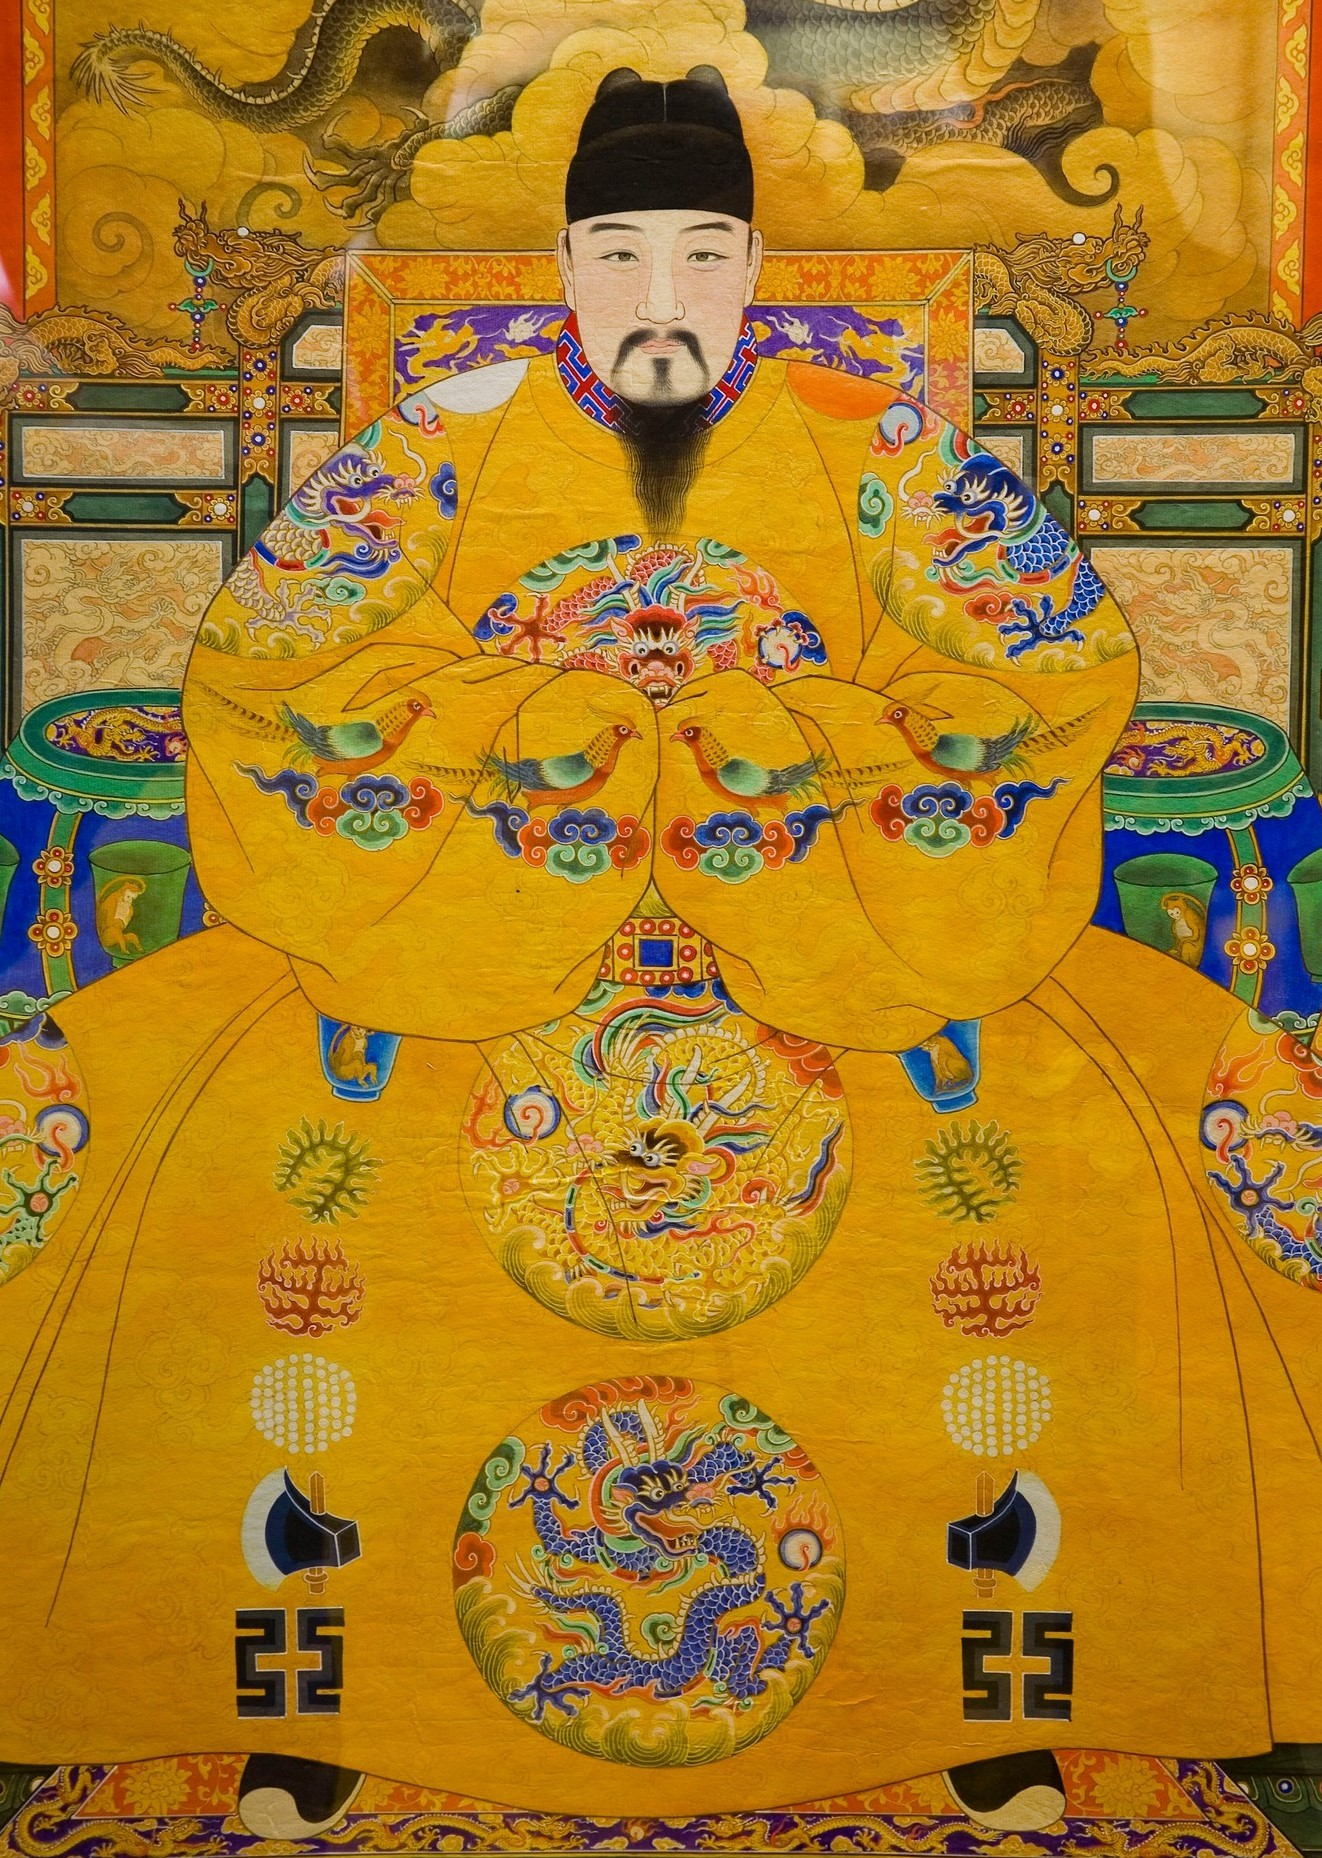
\includepdf[width=\paperwidth, height=\paperheight]{./Images/Frontmatter.jpg}
		\end{center}
	\end{figure}
	\begin{center}
	\phantom {placeholder}
	\vspace{130mm}
		\begin{figure}[!h]
			
\includegraphics[width=18cm]{./Images/Title.png} %http://www.diyiziti.com
		\end{figure}
	\end{center}
	\newpage
	\begin{center}
		\phantom {placeholder}
		\vspace{3cm}
		{\Huge \textbf{明朝那些事儿}}\\
		\vspace{1cm}
		{\Large \textbf{当年明月}}
	\end{center}
	\newpage
	{\color{TEXTColor}
		\ifnum\theparacolNo=2
		\begin{multicols}{\theparacolNo}
			\fi
			\tableofcontents
			\ifnum\theparacolNo=2
		\end{multicols}
		\fi
		\newpage
		\mainmatter
		\ifnum\thekindle=1
\AddToShipoutPicture{\YM}
\fi	
\fancyhead[LO]{{\scriptsize \faBookmark\ 明朝那些事儿 \faAngleRight\ \textbf{\rightmark}}}%奇數頁眉的左邊
\fancyhead[RO]{{\tiny{\textcolor{Gray}{\faQuoteRight\ }}}\thepage}
\fancyhead[LE]{{\tiny{\textcolor{Gray}{\faQuoteRight\ }}}\thepage}
\fancyhead[RE]{{\scriptsize \faBookmark\ 明朝那些事儿 \faAngleRight\ \textbf{\rightmark}}}%偶數頁眉的右邊
\fancyfoot[LE,RO]{}
\fancyfoot[LO,CE]{}
\fancyfoot[CO,RE]{}
\chapter*{前言}
\addcontentsline{toc}{chapter}{前言}
%\vspace{5mm}
\ifnum\theparacolNo=2
	\begin{multicols}{\theparacolNo}
\fi
好了,今天晚上开始工作吧!

说起来,我也写了不少东西了,主要是心理和历史方面的,偶尔也写点经济,本来只是娱乐下自己,没有想到发表后居然还有人捧场,于是便轻飘飘起来,客观来说,我的写作态度很不认真,每次都是想到哪里写到哪里,有些历史史料记录也凑合着用,记得多少写多少,直到有一天,终于因为我这不严谨的写作态度与人发生了矛盾。

也是这件事,让我反思了自己的行为和态度,明白了自己其实还差得远。所以我希望能重新开始,下面的这篇文章我构思了六个月左右,主要讲述的是从1344年到1644年这三百年间关于明的一些事情,以史料为基础,以年代和具体人物为主线,并加入了小说的笔法和对人物的心理分析,以及对当时政治经济制度的一些评价。

我写文章有个习惯,由于早年读了太多学究书,所以很痛恨那些故作高深的文章,其实历史本身很精彩,所有的历史都可以写得很好看,我希望自己也能做到。望大家能给予评价。

其实我也不知道自己写的算什么,不是小说,不是史书,就姑且叫《明札记》吧,从我们的第一位主人公写起,要写三百多年,希望我能写完。

\begin{flushright}
	2006-3-10
	首记于天涯煮酒
\end{flushright}
\ifnum\theparacolNo=2
	\end{multicols}
\fi

		\fancyhead[LO]{{\scriptsize \faBookmark\ 明朝那些事儿 \faAngleRight\ \textbf{\rightmark}}}%奇數頁眉的左邊
\fancyhead[RO]{{\tiny{\textcolor{Gray}{\faQuoteRight\ }}}\thepage}
\fancyhead[LE]{{\tiny{\textcolor{Gray}{\faQuoteRight\ }}}\thepage}
\fancyhead[RE]{{\scriptsize \faBookmark\ 明朝那些事儿 \faAngleRight\ \textbf{\rightmark}}}%偶數頁眉的右邊
\fancyfoot[LE,RO]{}
\fancyfoot[LO,CE]{}
\fancyfoot[CO,RE]{}
\setcounter{part}{0}
\setcounter{chapter}{1}
\setcounter{section}{0}
\part{洪武大帝}
\chapter*{引子}
\addcontentsline{toc}{chapter}{引子}
\ifnum\theparacolNo=2
	\begin{multicols}{\theparacolNo}
\fi
这篇文章我构思了六个月左右,主要讲述的是从1344年到1644年这三百年间关于明的一些事情,以史料为基础,以年代和具体人物为主线,并加入了小说的笔法和对人物的心理分析,以及对当时政治经济制度的一些评价。\\

要说明的是,这篇文章是描写正史的,资料来源包括《明实录》、《明通鉴》、《明史》、《明史纪事本末》等二十余种明代史料和笔记杂谈,虽然用了很多流行文学的描写手法和表现方式,但文中绝大部分的历史事件和人物,甚至人物的对话都是有史料来源的,为了文章的流畅,出处就不一一列出了。\\

我写文章有个习惯,由于早年读了太多学究书,所以很痛恨那些故作高深的文章,其实历史本身很精彩,所有的历史都可以写得很好看,我希望自己也能做到。\\

其实我也不知道自己写的算什么体裁,不是小说,不是史书,但在我看来,体裁似乎并不重要。\\

我想写的,是一部可以在轻松中了解历史的书,一部好看的历史。\\

仅此而已。\\
\ifnum\theparacolNo=2
	\end{multicols}
\fi
\newpage
\chapter*{朱元璋篇}
\addcontentsline{toc}{chapter}{朱元璋篇}
\section{童年}
\ifnum\theparacolNo=2
	\begin{multicols}{\theparacolNo}
\fi
我们从一份档案开始。
{\footnotesize \begin{quote}
	姓名: 朱元璋\\
	别名(外号): 朱重八、朱国瑞\\
	性别: 男\\
	民族: 汉\\
	血型: ?\\
	学历: 无文凭,秀才举人进士统统的不是,后曾自学过\\
	职业: 皇帝\\
	家庭出身:(至少三代)贫农\\
	生卒: 1328 - 1398\\
	最喜欢的颜色: 黄色(这个好像没得选)\\

	社会关系:\\
	父亲: 朱五四,农民\\
	母亲: 陈氏,农民(不好意思,史书中好像没有她的名字)\\
	座右铭: 你的就是我的,我还是我的\\

	主要经历:\\
	1328年 - 1344年: 放牛\\
	1344年 - 1347年: 做和尚,主要工作是出去讨饭(这个……)\\
	1347年 - 1352年: 做和尚主要工作是撞钟\\
	1352年 - 1368年: 造反(这个猛)\\
	1368年 - 1398年: 主要工作是做皇帝\\
\end{quote}}

一切的事情都从1328年的那个夜晚开始,农民朱五四的妻子陈氏生下了一个男婴,大家都知道了,这个男婴就是后来的朱元璋。大凡皇帝出世,后来的史书上都会有一些类似的怪象记载。\\

比如刮风啊,下暴雨啊,冒香气啊,天上星星闪啊,到处放红光啊,反正就是要告诉你,这个人和别人不一样。朱元璋先生也不例外,他出生时,红光满地,夜间房屋中出现异光,以致于邻居以为失火了,跑来相救\footnote{明实录。}。\\

然而当时农民朱五四的心情并不像今天我们在医院产房外看到的那些焦急中带着喜悦的父亲们,作为已经有了三个儿子、两个女儿的父亲而言,首先要考虑的是吃饭问题。\\

农民朱五四的工作由两部分构成,他有一个豆腐店,但主要还是要靠种地主家的土地讨生活,这就决定了作为这个劳动家庭的一员,要活下去只能不停的干活。\\

在小朱五四出生一个月后,父母为他取了一个名字\footnote{元时惯例。}:朱重八,这个名字也可以叫做朱八八,我们这里再介绍一下,朱重八家族的名字,都很有特点。
{\footnotesize \begin{quote}
	朱重八高祖名字:朱百六;\\
	朱重八曾祖名字:朱四九;\\
	朱重八祖父名字:朱初一;\\
	他的父亲我们介绍过了,叫朱五四。\\
\end{quote}}

取这样的名字不是因为朱家是搞数学的,而是因为在元朝,老百姓如果不能上学和当官就没有名字,只能以父母年龄相加或者出生的日期命名。\footnote{登记户口的人一定会眼花。}\\

朱重八的童年在一间冬凉夏暖、四面通风、采光良好的破茅草屋里度过,他的主要工作是为地主刘德家放牛。他曾经很想读书,可是朱五四是付不起学费的,他没有李密牛角挂书那样的情操,自然也没有杨素那样的大官来赏识他,于是,他很老实的帮刘德放了十二年的牛。\\

因为,他要吃饭。\\

在此时,朱重八的梦想是好好的活下去,到十六岁的时候,托村口的吴老太作媒,找一个手脚勤快、能干活的姑娘当媳妇,然后生下自己的儿女,儿女的名字可能是朱三二、或者朱四零,等到朱三二等人大了,就让他们去地主刘小德家放牛。\\

这就是十六岁时的朱重八对未来生活的幸福向往。\\

此时的中国,正在极其腐败的元王朝的统治下,那些来自蒙古的征服者似乎不认为在自己统治下的老百姓是人,他们甚至经常考虑把这些占地方的家伙都杀掉,然后把土地用来放牧\footnote{元史。},从赋税到徭役,只要是人能想出来的科目,都能用来收钱,过节要收“过节钱”、干活有“常例钱”、打官司有“公事钱”,怕了吧,那我不出去还不行吗?不干事还不行吗?那也不行,平白无故也要钱,要收“撒花钱”。服了吧。\\

于是,在这个马上民族统治中国六十余年后,他们的国家机器已经到了无法承受的地步,此时的元帝国就好像是一匹不堪重负的骆驼,只等那最后一根稻草。\\

这根稻草很快就到了。\\

1344年是一个有特殊意义的年份,在这一年,上天终于准备抛弃元了,他给中国带来了两个灾难,同时也给元挖了一个墓坑,并写好了墓志铭:石人一只眼,挑动黄河天下反。\\

他想的很周到,还为元准备了一个填土的人:朱重八。\\

当然朱重八不会想到上天会交给他这样一个重要的任务。\\

这一年,他十七岁。\\

很快一场灾难就要降临到他的身上,但同时,一个伟大的事业也在等待着他,只有像传说中的凤凰一样,历经苦难,投入火中,经过千锤百炼,才能浴火重生,成为光芒万丈的神鸟。\\

朱重八,来吧,命运之神正在等待着你!\\
\ifnum\theparacolNo=2
	\end{multicols}
\fi
\newpage
\section{灾难}
\ifnum\theparacolNo=2
	\begin{multicols}{\theparacolNo}
\fi
元至正四年(1344年)到来了,这一年刚开始,元帝国的头头脑脑们就收到了两个消息,首先是黄河泛滥了,沿岸山东河南几十万人沦为难民。即使不把老百姓当人,但还要防着他们造反,所以修黄河河堤就成为了必须要做的事情。\\

可是令人意外的是,在元的政府中,竟然出现了两种不同的意见,一种认为一定要修,另一种认为不能修。在现在看来,这似乎是不可思议的事情,黄河泛滥居然不去修,难道要任黄河改道淹死那么多人?在中国历史上有着太多不可思议的事情,这个也不例外。\\

客观的讲,在这样一件事上,就维护元朝的统治而言,主要修的不一定是忠臣,反对修的也未必就是奸臣,其中奥妙何处?要到七年后才会见分晓。\\

极力主张修的是元朝的著名宰相脱脱,他可以说是元朝的最后一个名臣,实行了很多的改革政策,为政清廉,而且十分能干\footnote{宋史就是他主持修的。},可是他没有想到的是,他的极力主张,已经给元朝埋下了一个大大的炸药包,拉好了引线,只等着那微弱的火光。\\

另一个是淮河沿岸遭遇严重瘟疫和旱灾,对于元政府来说,这个比较简单一点,反正饿死病死了就没麻烦了,当然表面功夫还是要做的,皇帝\footnote{元顺帝。}要下诏赈灾,中书省的高级官员们要联系粮食和银两,当然了自己趁机拿一点也是可以理解的。赈灾物品拨到各路\footnote{元代地方行政单位。},地方长官们再留下点,之后是州、县。一层一层下来,到老百姓手中就剩谷壳了。然后地方上的各级官员们上书向皇帝表示感谢,照例也要说些感谢天恩的话,并把历史上的尧舜禹汤与皇上比较一下,皇帝看到了报告,深感自己做了大好事,于是就在自己的心中给自己记上一笔。\\

皆大欢喜,皆大欢喜,大家都很满意。\\

但老百姓是不满意的,很多人都不满意。\\

朱重八肯定是那些极其不满意的人中的一个。\\

灾难到来后,四月初六朱重八的父亲饿死,初九大哥饿死,十二日,大哥长子饿死、二十二日,母亲饿死。\\

如果说这是日记的话,那应该是世界上最悲惨的日记之一。\\

朱重八的愿望并不过分,他只是想要一个家,想要自己的子女,想要给辛劳一生,从没欺负过别人,老实巴交的父母一个安详的晚年,起码有口饭吃。\\

他的家虽然不大,但家庭成员关系和睦,相互依靠,父母虽然贫穷,但每天下地干活回来仍然会带给重八惊喜,有时是一个小巧的竹蜻蜓,有时是地主家不吃的猪头肉,这就是朱重八的家,然而现在什么都没有了。\\

朱重八的姐姐已经出嫁,三哥去了倒插门。除了朱重八的二哥,这个家庭已经没有了其他成员。\\

十七岁的朱重八,眼睁睁的看着他的亲人一个一个死去,而他却无能为力。人世间最大的痛苦莫过于此!\\

他唯一的宣泄方式是痛哭,可是哭完了,他还要面对一个重要的问题,要埋葬他的父母,可是没有棺材、没有寿衣、没有坟地,他只能去找地主刘德,求刘德看在父亲给他当了一辈子佃户的分上,找个地方埋了他爹。\\

刘德干净利落的拒绝了他,原因简单,你父母死了,关我何事,给我干活,我也给过他饭吃。\\

朱重八没有办法,只能和他的二哥用草席盖着亲人的尸体,然后拿门板抬着到处走,希望能够找到一个地方埋葬父母。可是天下虽大,到处都是土地,却没有一块是属于他们的。\\

幸好有好心人看到他们确实可怜,终于给了他们一块地方埋葬父母。“魂悠悠而觅父母无有,志落魄而泱佯”,这是后来能吃饱饭的朱元璋的情感回忆。\\

朱重八不明白,自己的父母在土地上耕作了一辈子,却在死后连入土为安都做不到。地主从来不种地,却衣食无忧。为什么?可他此时也无法思考这个问题,因为他也要吃饭,他要活下去。\\

在绝望的时候,朱重八不止一次的祈求上天,从道教的太上老君到佛教的如来佛祖,只要他能知道名字的,祈祷的唯一内容只是希望与父母在一起生活下去,有口饭吃。\\

但结果让他很失望,于是他那幼小的心灵开始变得冰冷,他知道没有人能救他,除了他自己。\\

复仇的火焰开始在他心底燃烧。\\

如此的痛苦,使他从脆弱到坚强。\\

为了有饭吃,他决定去当和尚。\\

\subsection{和尚的生涯}
朱重八选择的地方是附近的皇觉寺,在寺里,他从事着类似长工的工作,他突然发现那些和尚除了没有头发,对待他的态度比刘德好不了多少,这些和尚自己有田地,还能结婚\footnote{元代。},如果钱多还可以去开当铺。\\

但他们也需要人给他们打杂,在那里的和尚不念经,不拜佛,甚至连佛祖金身也不擦,这些活自然而然的由刚进庙的新人朱重八来完成。\\

朱重八一直忍耐着,然而除了要做这些粗活外,他还要兼任清洁工,仓库保管员,添油工\footnote{长明灯。}。即使这样,他还是经常挨骂,在那些和尚喝酒吃肉的时候,他还要擦洗香客踩踏的地板,每一个孤独的夜晚,他只能独坐在柴房中,看着窗外的天空,思念着只与自己相处了十余年的父母。\\

他已经很知足了,他能吃饱饭,这就够了,不是吗?\\

然而命运似乎要锻炼他的意志,他入寺仅五十余天后,由于饥荒过于严重,所有的和尚都要出去化缘,所谓化缘就是讨饭,我们熟悉的唐僧同志每次的口头禅就是:悟空,你去化些斋来。用俗话来说就是,悟空,你去讨点饭来。我曾经考察过化缘这个问题,发现朱重八同志连化缘也被人欺负。由于和尚多,往往对化缘地有界定,哪些地方富点,就指派领导的亲戚去,那些地方穷,就安排朱重八同志去。\\

反正饿死也该,谁让你是朱重八。\\

朱重八被指派的地点是在淮西和河南。这里也是饥荒的主要地带,谁能化给他呢?\\

然而,就从这里开始,命运之神向他微笑。\\

在游方的生活中,朱重八只能走路,没有顺风车可搭,是名副其实的驴行。他一边走,一边讨饭,穿城越村,挨家挨户,山栖露宿,每敲开一扇门,对他都是一种考验,因为面对他的往往只是白眼、冷嘲热讽,对朱重八来说,敲开那扇门可能意味着侮辱,但不敲那扇门就会饿死。\\

朱重八已经没有了父母,没有了家,他所有的只是那么一点可怜的自尊,然而讨饭的生活使他失去了最后的保护。要讨饭就不能有尊严。\\

生命的尊严和生存的压力,哪个更重要?\\

是的,朱重八,只有失去一切,你才能明白自己的力量和伟大。\\

朱重八和别的乞丐不同,也正是因为不同,他才没有一直当乞丐\footnote{请注意这句话。}。\\

在讨饭的时候,他仔细研究了淮西的地理、山脉、风土人情,他开阔了视野,丰富了见识,认识了很多豪杰\footnote{实际上也是讨饭者。}。此时,他还有了自己的宗教信仰——明教,他相信当黑暗笼罩大地的时候,伟大的弥勒佛一定会降世的。其实就他的身世遭遇来说,他是不是真的相信弥勒倒是很难说的,我们有理由相信,他心中真正的弥勒是他自己。\\

但朱重八最重要的收获是:他已经从一个只能无助的看着父母死去的孩童,一个被人欺负后只能躲在柴堆里小声哭的杂役,变成了能坚强面对一切困难的战士。一个武装到心灵的战士。\\

长期的困难生活,最能磨练一个人的意志,有很多人在遇到困难后,只能怨天尤人,得过且过,而另外一些人虽然也不得不在困难面前低头,但他们的心从未屈服,他们不断的努力,相信一定能够取得最后的胜利。\\

朱重八毫无疑问是后一种。\\

如果说,在出来讨饭前,他还是一个不知所措的少年,在他经过三年漂泊的生活回到皇觉寺时,他已经是一个有自信战胜一切的人。\\

这是一个伟大的转变,很多人可能究其一辈子也无法完成。转变的关键在于心。\\

对于我们很多人来说,心是最柔弱的地方,它特别容易被伤害,爱情的背叛,亲情的失去,友情的丢失,都将是重重的一击。然而对于朱重八来说,还有什么不可承受的呢?他已经失去一切,还有什么比亲眼看着父母死去而无能为力,为了活下去和狗抢饭吃、被人唾骂,鄙视更让人痛苦!我们有理由相信,就在某一个痛苦思考的夜晚,朱重八把这个最脆弱的地方变成了最强大的力量的来源。\\

是的,即使你拥有人人羡慕的容貌,博览群书的才学,挥之不尽的财富,也不能证明你的强大,因为心的强大,才是真正的强大。\\

当朱重八准备离开自己讨饭的淮西,回到皇觉寺时,他仔细的回忆了这个他呆了三年的地方,思考了他在这里得到的和失去的,然后收拾自己的包裹踏上了回家的路。\\

也许我还会回来的,朱重八这样想。\\
\ifnum\theparacolNo=2
	\end{multicols}
\fi
\newpage
\section{踏上征途}
\ifnum\theparacolNo=2
	\begin{multicols}{\theparacolNo}
\fi
至正十一年(1351年),上天给元朝的最后一根稻草终于压了下来,元朝的末日到了。\\

我们的谜底也揭开了,现在看来,脱脱坚决要求治黄河的愿望是好的,然而他不懂得那些反对的人的苦心,元朝那腐败到极点的官吏也是他所不了解的。现在他终于要尝到苦果了。\\

当元朝命令沿岸十七万劳工修河堤时,各级的官吏也异常兴奋,首先,皇帝拨给的修河工钱是可以克扣的,民工的口粮是可以克扣的,反正他们不吃不喝也事不关己。这就是一大笔收入,工程的费用也是可以克扣的,反正黄河泛滥也淹不死自己这些当官的。\\

这是管河务的,那么不管河务的怎么捞钱呢,其实也简单,既然这么大工程,必然有徭役指标,找几十个人,到各个乡村去,看到男人就带走,理由?修河堤,不想去?拿钱来。\\

没有钱?有什么值钱的都带走!\\

可怜的脱脱,一个好的理论家,却不是一个实践家。\\

老把戏出场了,当民工们挖到山东时,他们从河道下挖出了一个一只眼睛石人,背部刻着石人一只眼,挑动黄河天下反。民工们突然发现,这正是他们在工地上传唱了几年的歌词。于是人心思动。\\

这真是老把戏,简直可以编成电脑程序,在起义之前总要搞点这种封建迷信,但也没办法,人家就吃这一套。\\

接着的事情似乎就是理所应当的了,几天后,在朱重八讨过饭的地方\footnote{颖州,今安徽阜阳。},韩山童和刘福通起义了,他们的起义与以往起义并没有不同,照例要搞个宗教组织,这次是白莲教,当然既然敢起义,身份也应该有所不同,于是,可能是八辈子贫农的韩山童突然姓了赵,成了宋朝的皇室,刘福通也成了刘光世大将的后人。\\

他们的命运和以往第一个起义的农民领袖也类似,起义、被镇压、后来者居上,这似乎是陈胜吴广们的宿命。\\

尽管他们的起义形式毫无新意,但这并不妨碍他们的伟大和在历史上的地位,在史书上,将永远的纪录着:公元1351年,韩山童、刘福通第一个举起了反抗元朝封建统治的大旗。\\

自古以来,建立一个王朝很难,毁灭一个却相对容易得多,所谓墙倒众人推,破鼓万人捶,不是没有来由的。\\

在元代这个把人分为四个等级的朝代里,最高等级的蒙古人杀掉最低等级的南人,唯一的惩罚是赔偿一头驴,碰到个闲散民工之类的人,可能连驴都省了。蒙古贵族们的思维似乎很奇怪,他们即使在占据了中国后,好像仍然把自己当成客人,主人家的东西想抢就抢,想拿就拿,反正不关自己的事。在他们的思维中,这些南人只会忍受也只能忍受他们的折磨。\\

但他们错了,这些奴隶会起来反抗的,当愤怒和不满超过了限度,当连像狗一样生存下去都成为一种奢望的时候,反抗是唯一的道路。反抗是为了生存。\\

这把火终于烧起来了,而且是燎原之势。\\

在短短的一年时间里,看似强大的元帝国发生了几十起暴动,数百万人参加了起义军,即使那纵横天下无敌手的蒙古骑兵也不复当年之勇,无力拯救危局。元帝国就像一堵朽墙,只要再踢一脚,就会倒下来。\\

此时的朱重八却仍然在寺庙里撞着钟,从种种迹象看,他并没有参加起义军的企图。虽然他与元朝有着不共戴天的仇恨,但对于一个普通人朱重八来说,起义是要冒风险的,捉住后是要杀头的,这使得他不得不仔细的考虑。\\

在很多的书中,朱重八被塑造成一个天生英雄的形象,于是在这样的剧本里,天生英雄的朱重八一听说起义了,马上回寺庙里操起家伙就投奔了起义军,表现了他彻底的革命性等等。\\

我认为,这不是真实的朱重八。\\

作为一个正常人,在做出一个可能会掉脑袋的决定的选择上,是绝对不会如此轻率的,如果朱重八真的是这样莽撞的一个人,他就不是一个真正的英雄。\\

真正的朱重八是一个有畏惧心理的人,他遭受过极大的痛苦,对元有着刻骨的仇恨,但他也知道生的可贵,一旦选择了造反,就没有回头路。\\

知道可能面对的困难和痛苦,在死亡的恐惧中不断挣扎,而仍然能战胜自己,选择这条道路,才是真正的勇气。\\

我认为这样的朱重八才是真正的英雄,一个战胜自己,不畏惧死亡的英雄。\\

朱重八在庙里的生活是枯燥而有规律的,但这枯燥而规律的生活被起义的熊熊烈火打乱了。具有讽刺意义的是,具体打乱这一切的并不是起义军,而是那些元的官吏们。\\

在镇压起义军的战斗中,如果吃了败仗,是要被上司处罚的,但镇压起义的任务又是必须要完成的,于是元朝的官吏们毅然决然的决定,拿老百姓开刀,既然无法打败起义军,那就把那些可以欺负的老百姓抓去交差,把他们当起义军杀掉。\\

从这个角度来看,元的腐朽官吏为推翻元朝的统治实在是不遗余力,立了大功。\\

此时摆在朱重八面前的形势严重了,如果不去起义,很有可能被某一个官吏抓去当起义者杀掉,然后冠以张三或者李四的名字。但投奔起义军也有很大的风险,一旦被元军打败,也是性命难保。\\

就在此时,一封信彻底改变了他的命运。\\

他幼年时候的朋友汤和写了一封信给他,信的内容是自己做了起义军的千户,希望朱重八也来参加起义军,共图富贵,朱重八看过后,不动声色,将信烧掉了。他还没有去参加起义的心理准备。\\

然而晚上,他的师兄告诉他,有人已经知道了他看义军信件的事情,准备去告发他。\\

朱重八终于被逼上了绝路。\\

接下来的是痛苦的思考和抉择朱重八面前有三条路:一、守在寺庙里;二、逃跑;三、造反。\\

朱重八也拿不定主意,他找到了一个人,问他的意见,这个人叫周德兴,我们后面还要经常提到他。\\

周德兴似乎也没有什么好主意,他给朱重八的建议是算一卦\footnote{这是什么主意。},看什么条路合适。\\

算卦的结果是“卜逃卜守则不吉,将就凶而不妨”,意思是逃跑,呆在这里都不吉利,去造反还可能没事。\\

朱重八明白自己已经没有退路了,自己不过想要老老实实的过日子,种两亩地,孝敬父母,却做不到,父母负担着沉重的田赋和徭役,没有一天不是勤勤恳恳的干活,还落得个家破人亡的下场。躲到寺庙里不过想混口饭吃,如今又被人告发,可能要掉脑袋。\\

忍无可忍。\\

那就反了吧!反他娘的!\\

这是一个真实版本的逼上梁山,也是那封建时代贫苦农民的唯一选择。谁不珍惜自己的生命?谁愿意打仗?在活不下去时,那些农民被迫以自己的鲜血和生命去推动封建社会的发展,直至它的灭亡。\\

这是他们的宿命。\\

所以我认为中国历史上的农民起义确实是值得肯定的,他们也许不是那么厚道,他们也许有着自己的各种打算,但他们确实别无选择。\\

汤和就这样成了朱重八的第一个战友。他在今后的日子里将陪同朱重八一起走完这条艰苦的道路。\\

然而汤和也绝对不会想到,自己居然是唯一一个陪他走完这条路的人。\\
\ifnum\theparacolNo=2
	\end{multicols}
\fi
\newpage
\section{就从这里起步}
\ifnum\theparacolNo=2
	\begin{multicols}{\theparacolNo}
\fi
至正十二年(1352年),濠州城。\\

城池的守卫者郭子兴正在他的元帅府里,苦苦思索着对策,濠州城已经被元军围了很久,这样下去是坚守不了多久了。\\

就在此时,手下的军士前来报告,抓住了一个奸细,要请令旗去杀人,如果是以往,郭子兴是不会过问的,让士兵直接拿了令旗去杀就是了,但今天,他开口问了一句:“你怎么知道那个人是奸细?”军士回答道:“这个人说是来投军的,现在元军围困,哪里还有人来投军,他一定是元军奸细。”\\

郭子兴差点笑了出来,投军?元军快打进城来了,还有来投军的,这个借口可是真不高明,他不禁起了好奇心,想去看看这个奸细。\\

于是他骑马赶到了城门口,看见了一个相貌奇怪的人,用今天的话来说,这个人的相貌是地包天,下巴突出,更奇特的是,他的额头也是向前凸出的,具体形状大概类似独门兵器月牙铲,上下凸,中间凹\footnote{参见朱元璋同志画像。}。\\

这个人当然就是我们的朱重八。\\

郭子兴走到朱重八的面前,让人松开绑,问他:“你是奸细么?来干什么?”\\

朱重八平静的回答:“我不是奸细,我是来投军的。”\\

郭子兴大笑:“什么时候了,还有人来投军,你不用狡辩,等会就把你拉出去杀头!”\\

朱重八只是应了一声:“喔。”\\

郭子兴看着朱重八的眼睛,希望能看到慌乱,这是他平时的乐趣之一。\\

但在这个人眼睛里,他看到的只有镇定。\\

郭子兴不敢小看这个人了,很明显,这是一个吓不倒的人。于是他认真的询问了朱重八的名字,来历,当朱重八说出是千户长汤和介绍他来时,郭子兴这才明白,这个人真的是来投军的。\\

朱重八给他的印象实在是太深了,于是他没有将朱重八编入汤和的部队,而是将他放在自己身边,当自己的亲兵\footnote{警卫员。}。\\

在军队里,朱重八很快就表现出了他的才能,比起其他的农民兵士,他是一个很突出的人,不但作战勇敢,而且很有计谋,处事冷静,思虑深远\footnote{注意这个特点。},而且很讲义气,有危险的时候第一个上,这一切都让他有了崇高的威信。加上他的同乡汤和帮忙,他在当士兵两个月后,被提拔为九人长,这是他的第一个官职。\\

作为郭子兴的亲兵长,朱重八是很称职的,他不像其他的士兵,从不贪图财物,每次得到战利品,就献给郭子兴,如果得到赏赐,就分给士兵,由于他很有天赋,自学过一些字,分析问题准确,郭子兴渐渐把他当成自己的智囊,朱重八在军中的地位也逐渐重要起来。\\

也就在此时,朱重八将他的名字改成了朱元璋,所谓璋,是一种尖锐的玉器,这个朱元璋实际上就是诛元璋,朱重八把他自己比成诛灭元朝的利器,而这一利器正是元朝的统治者自己铸造出来的。在今后的二十年里,他们都将畏惧这个名字。\\

\subsection{汤和}
在军队中,汤和算是个奇特的人,他在朱元璋刚参军时,已经是千户,但他却很尊敬朱元璋,在军营里,人们可以看到一个奇特的现象,官职高得多的汤和总是走在士兵朱元璋的后边,并且毫不在意他人的眼神,更奇特的是朱元璋似乎认为这是理所应当的事情,也没有推托过。\\

我们不得不佩服汤和的远见,他知道朱元璋远非池中物,用今天的话说,他很识实务。相信也正是这个优点,使得他能够在后来的腥风血雨中幸存下来。\\

在军队里,朱元璋娶了老婆,与后来的那些众多妃嫔相比,这个老婆可以算是朱元璋成功的关键因素之一。这个女孩是郭子兴的义女,她的父亲姓马,是郭子兴的朋友,后来死去,将这个女孩托付给郭子兴,女孩名字不详,军队里的人都叫她马姑娘。就这样,朱元璋成了元帅的女婿,而郭子兴则多了一个帮手。\\

我们可以想象到朱元璋喜悦的心情,他终于有了一个自己的家,不再是那个没人管、没人问的朱重八,他饿了,有人做饭给他吃,冷了,有人送衣服给他,有家的感觉真好。这种感情一直陪伴了他很多年。\\

此时,朱元璋已经升任了军队中的总管,这个职位大致相当于起义军的办公室主任,他干得不错,对于某些喜欢贪公家便宜,胡乱报销的人,朱元璋是讲原则的,由于他严于律己,大家也没有什么话说,如果就这么干下去,他可能会成为一个优秀的财务管理人员。可是上天偏偏不让他舒服的过下去,不久的将来,他将面对更大的麻烦。\\

主要问题是,郭子兴的成分问题,他并不是农民,而是地主\footnote{想不通他怎么会起义。},当时在濠州的统帅除了郭子兴外,还有四个人,以孙德崖为首,而这四个人都是农民,他们和郭子兴之间存在着深刻的矛盾。\\

不久,矛盾爆发了,一天郭子兴在濠州城里逛街,突然被一群来路不明的人绑票,这些人似乎对索取酬金之类也没有什么兴趣,把郭子兴死打一顿,然后关了禁闭。朱元璋得到消息,大吃一惊,立刻赶去孙德崖家里要人,孙德崖开始还装傻,表情惊讶,要出去找郭子兴,并且说了一些与绑架者不共戴天之类的话,充分表现出了一个业余演员的演技。\\

朱元璋只把参与打人的军士带到孙德崖面前,并且告诉孙,你的那些贪污公款、胡乱报销的烂账都在我这里,自己看着办。\\

于是,朱元璋从孙家的地窖中将已经打得半死的郭子兴救了出来,这件事情让朱元璋意识到,跟着这些人不会有前途。\\

而郭子兴也越来越讨厌朱元璋,原因很简单,朱元璋比他强,对于郭子兴这样一个性情暴躁、不能容人的统帅来说,他是不能容忍一个可能取代他地位的人在身边的。终于有一天,他把朱元璋关了起来,落井下石一向是某些人的优良传统,郭子兴的儿子就是某些人中的一个。他吩咐守兵不能给朱元璋送饭,想要把朱元璋饿死,善良的马姑娘为了救朱元璋,便把刚烫好的烙饼揣在怀中,到牢中探望朱元璋时送给他吃,每次胸口都会烫伤,但每次都送。\\

有妻如此,夫复何求。\\

郭子兴毕竟还是不想杀朱元璋,于是将他放了出来,朱元璋经历此事后,终于下了决心,和这些鼠目寸光的人决裂。他向郭子兴申请带兵出征,郭子兴高兴的答应了。\\

这就是朱元璋霸业的开始,一旦开始,就不会停止。\\

就从这里起步吧!\\

朱元璋奉命带兵攻击郭子兴的老家,定远,从这一点可以看出他的岳父实在存心不良,当时的定远有重兵看守,估计郭子兴让他去就是不想再看到活着的朱元璋,但朱元璋就是朱元璋,他找到了元军的一个缝隙,攻克了定远,然后在元军回援前撤出,此后,连续攻击怀远、安奉、含山、虹县,四战四胜,锐不可当!\\

在召集\footnote{也可能是抢。}了壮丁后,朱元璋来到了钟离\footnote{今安徽凤阳东面。},这是他的家乡,在这里他遇到了二十四个来朱元璋队伍里找工作的人。\\

朱元璋经理招收的二十四个人素质是相当高的,这其中有为他算过命的周德兴,还有堪称天下第一名将的徐达。\\

这些人还有亲戚,一传十,十传百,什么叔叔、舅舅、子侄、外甥都来了,很快,他的部队\footnote{直属。}就有了七百人。\\

当朱元璋再次回到濠州的时候,他已经完全明白了自己的前途所在,所以他向郭子兴辞职,郭子兴非常高兴,这个讨厌的人终于可以走得远远的了。\\

朱元璋在出发前,又做了一件出人意料的事,他从自己的七百人中重新挑选了二十四个人,然后将其余的人都给了郭子兴,郭子兴多少有些意外,但仍然高兴的接受了。\\

朱元璋的这个行动似乎可以定义为一次挑选公务员的工作,比例是三十比一,没有笔试,考官就是朱元璋和他的眼光。\\

他挑的确实很准,看看这些人的名字:徐达、汤和、周德兴,这二十四个人后来都成为了明王朝的高级干部。\\

唐时的黄巢在考试落榜后,站在长安城门前,惆怅之余,豪气丛生,作诗一首,大大的有名——《咏菊》:
\begin{quote}
	\begin{spacing}{0.5}  %行間距倍率
		\textit{{\footnotesize
				\begin{description}
					\item[\textcolor{Gray}{\faQuoteRight}] 待得秋来九月八,我花开时百花杀。
					\item[\textcolor{Gray}{\faQuoteRight}] 冲天香阵透长安,满城尽带黄金甲。
				\end{description}
		}}
	\end{spacing}
\end{quote}

数年后,他带领着十余万大军,打进长安。\\

此时的朱元璋,站在濠州的城门前,看着自己身后的二十四个人,他知道,迈出这一步,他就将孤军奋战,或者兵败身死,或者开创霸业。\\

他仰望天空,还是那样阴暗,这个时候作出这个选择,似乎并不吉利,他又想起了那次无奈的占卜。\\

父母去世的时候,在庙里干苦力的时候,夜里望天痛哭的时候,也是这样的天空。\\

什么都没有变,变的只是我而已。
\begin{quote}
	\begin{spacing}{0.5}  %行間距倍率
		\textit{{\footnotesize
				\begin{description}
					\item[\textcolor{Gray}{\faQuoteRight}] 百花发时我不发,我若发时都吓杀。
					\item[\textcolor{Gray}{\faQuoteRight}] 要与西风战一场,遍身穿就黄金甲。
				\end{description}
		}}
	\end{spacing}
\end{quote}

什么都不能阻挡我,就从这里开始吧!\\

出发!\\
\ifnum\theparacolNo=2
	\end{multicols}
\fi
\newpage
\section{储蓄资本}
\ifnum\theparacolNo=2
	\begin{multicols}{\theparacolNo}
\fi
\subsection{朱元璋的第一桶金}
朱元璋又来到了定远,对于他而言,拉壮丁已经是轻车熟路,很快他组织了上千人的部队,他听说在定远附近的张家堡有一支三千人的部队,现在孤立无援,需要找个新老板,于是朱元璋打起了这支部队的注意。\\

他亲自来到张家堡,一看寨主,大喜过望:“原来是你啊。”\\

这个寨主他认识,原来还打过交道,而寨主叫他“朱公子”。\\

两人见面后,照例自然要叙叙交情,我认识谁,你认识不,喔,你说的是那个谁啊,认识认识,还是兄弟啊,还有张三死了,李四病了等等,越说感情越好,就一起吃饭。\\

在饭桌上,朱元璋终于说出了他的来意,既然目前你们没有主,不如跟着我混,将来混出名堂,有你们的股份。寨主也真是个实在人,马上就答应了。\\

朱元璋非常高兴,可是他忘了中国人的习惯,酒桌上的话只能信一半,有时一半都不到。\\

朱元璋后来估计会想:当时实在应该签个合同的。\\

三天后,朱元璋的使者到了寨中,寨主热情的接待了他:\\

来啦,快点请坐啊,别客气,您这趟来是?什么,让我们一起走,这个我们还要考虑下啊。\\

什么?我已经答应过了?\\

什么时候啊?三天前?好像没有吧,\footnote{回顾手下。}你们想想,当时有吗?是吧,没有啊。\\

误会,误会啊,你说的我们一定好好考虑,让朱公子不要急啊。\\

什么,你要走,别走,再坐会,啊,有事就不留你了,回去给朱公子带个好,有空来玩啊!\\

就这样,朱元璋被结结实实的忽悠了一回。\\

可是朱元璋岂是容易欺负的,他让部下去请寨主吃饭,特别交待是准备了很久的名菜,寨主一听有饭局,屁颠屁颠的就来了,一到大营,朱元璋就把他捆了起来,饭没有吃成,倒是自己成了粽子。然后朱元璋以寨主的名义传令山寨的人转移,就这样三千人变成了朱元璋的属下。\\

下一个目标是横涧山,这个地方有两万军队,但这却不是一支可以劝降的部队,此部队的主帅叫缪大亨\footnote{从这个名字就可以看出身份。},原先跟随元军围攻濠州,希望能顺便抢个劫,不料没有攻下来,于是带领部队守在这里,朱元璋带领了四千人对他发起了进攻。\\

这是朱元璋第一次领导的以少对多的战斗。\\

朱元璋很聪明的避开了白天,而选在晚上对这支武装发动了夜袭,像缪大亨这种土包子当然不是对手,他没有怎么抵抗就投降了,于是朱元璋的部队变成了两万人。\\

朱元璋对部队进行了改编,出人意料的是,他并没有说一些类似同生共死,有福共享之类的话,而是对这些投降的士兵进行了谴责,让他们反思为什么这么大的一支部队,如此没有战斗力,轻易的投降了,然后他说出了结论,这是因为没有纪律和训练,要想成就事业,只有加强训练,建立严格纪律。\\

这一番话,有理有节,大家听了都很服气。\\

也就是在这次之后,朱元璋的部队与那些乌合之众的农民暴动军有了本质的区别,在他的手中,有了一支精兵。\\

此时,两兄弟从定远来投奔了朱元璋,一个叫冯国用,另一个叫冯国胜,朱元璋觉得这两个人都是人才,就留下了他们,这个冯国胜就是后来的威震天下、横扫蒙古的冯胜。\\

至正十三年(1353年),朱元璋决定攻击滁州,也就在此时,一个人走进了他的军营。\\

这是一个穿着书生装的中年人,相貌温文尔雅,朱元璋开始时并未在意此人,只是看他字写得好,便让他当了文书,此人倒也不在意,依然干好自己的工作,有一天,朱元璋在营房里烤火,似乎是自言自语的说了一句:“天天处处打仗,何时是个头啊”\footnote{四方战斗,何时定乎。}。\\

此人从容答道:“秦朝乱时,汉高祖刘邦也是百姓出身,他豁达大度,知人善任,只用了五年就成就了帝王之业,现在天下已不是元的了,元帅你的户口在濠州\footnote{公濠产。},离刘邦老家不远,就算没有王气所在,也多少能沾点边。”说到这里,他停了下来,然后说出了最关键的两句话:\\

“只要元帅能向刘邦学习,按照他的行为去做,天下就一定是你的!”\\

朱元璋诧异的看着眼前的这个读书人,是的,这正是自己的方向,刘邦做得到的,我为什么做不到。于是,他摆正了自己的坐姿,向眼前的这个人行礼。\\

这个人就是开国第一功臣李善长。\\

滁州,地势险要,宋欧阳修曾有过“环滁皆山也”的议论,可见这确实是一块易守难攻的要害之地。\\

但滁州的守军却远不像地形那么难以对付,开战之初,朱元璋手下勇将花云即率领上千骑兵以中央突破战术直冲对方阵地,元军溃败,朱元璋率领全军一举攻占滁州。\\

在占据了滁州后,朱元璋又迎来了三个重要的人,分别是他的侄子朱文正、姐夫李贞和外甥李文忠。请大家记住这几个名字,他们都将是后来那场惊天动地的战争的主角。\\

这样看来,朱元璋出生的位置实在是人才多多,他招纳的谋士和将领无论和哪个时代的人才相比都不逊色,何安徽之多才邪!\\

此时的朱元璋手下精兵强将,谋士如云,并占据了滁州这个进可攻退可守的险要之地,他的眼界已经不是小小的濠州,也不是滁州,而是天下。\\

这一年,他二十六岁。\\

\subsection{最后一个障碍}
朱元璋的顺利似乎并不能给他的岳父带来好运,郭子兴此时正被整得够呛,用今天的话说就是批斗,每次开会总是四个批一个,孙德崖几次都想下手,想想朱元璋就在不远的地方,实在不好善后,于是他就把郭子兴挤出了濠州城,让他下岗,自谋出路。\\

此时的郭子兴才明白了人生的艰难,他没有其它选择,只能去投靠他的女婿朱元璋,但想想自己以前那样对他,他还能善待自己吗?\\

到了滁州,他的顾虑打消了,朱元璋不但不念旧恶,而且还把统帅的位置让给了他,更让人吃惊的是,朱元璋做出了一个谁也想不到的决定。\\

他决定把自己属下三万精兵的指挥权让给郭子兴,统帅的位置也就罢了,毕竟是个虚的,但兵权也交出去,就让人吃惊了,郭子兴百感交集,他其实从来没有信任过这个女婿,甚至还考虑过害他,他也曾问过朱元璋,为什么要这样对自己。朱元璋诚恳地说,如果没有您,就没有我的今天,我不能忘记您的恩德。\\

郭子兴终于明白,自己错了,朱元璋是对的。\\

当得知这个消息后,原先企图杀害朱元璋的人也对他敬佩万分,这中间包括郭子兴的儿子郭天叙。\\

一个人要显示自己的力量,从来不是靠暴力,挑战这一准则的人必然会被历史从强者的行列中淘汰,历来如此。\\

郭子兴带了自己的几万人来,滁州的粮食不够吃了,朱元璋进攻和州,攻下来后就住在那里,将滁州让给了郭子兴。\\

而此时濠州城中的孙德崖由于兵多粮少,强行要求到和州混饭吃,朱元璋正头疼,此时却得到了另一个消息,郭子兴得知孙德崖来了,也带了几万人来,要打孙德崖。于是小小的和州一下子挤了十几万人,而且两个对头正好碰上了,那就打吧。\\

可是打不起来,为什么呢?\\

因为人太多了,何州只是一个小县城,一下子来十几万人,城里城外水泄不通,就好像我们今天的黄金周旅游景点一样,别说打仗,想转个身都难。\\

既然不能打,那就谈吧!\\

看来孙德崖还是讲道理的,他表示,自己毕竟是外来的,还是自己走吧,朱元璋当即去为他送行,此时孙德崖在城内,他的士兵在城外由朱元璋陪同,但谁也没有想到,还有一个人在蠢蠢欲动。\\

这就是郭子兴,郭子兴是不讲道理的,他只记得孙德崖多次羞辱过他,也管不了什么信义了,看到城内的孙德崖身边没有什么士兵,就命令手下人将孙德崖抓起来,这就害了还在城外的朱元璋。\\

孙德崖的士兵听说主帅被抓,就认定是朱元璋指使的,而此时朱元璋也得到了这个消息,场面极其紧张,朱元璋一看势头不妙,拔马就往回走,士兵早就有准备,铁索往朱元璋的头上一套,下来吧您呐。孙德崖的士兵抓住了朱元璋,就去找郭子兴谈判。\\

郭子兴正在一边喝酒一边欣赏者孙德崖的表情,突然消息传来,说朱元璋被抓住了,他一下子懵了,孙德崖固然不想放,可是朱元璋也是不能少的,于是他只好决定放人。\\

可谁先放,就又成了问题,此时,徐达站了出来,他愿意用自己去换朱元璋,朱元璋回去后,再放孙德崖,孙德崖回去后再放徐达,这简直成了顺口溜,麻烦啊。\\

总算解决了这个问题,可是郭子兴临到手的敌人跑了,一时咽不下这口气,得了心病,过了一个月居然死掉了,可见心胸不宽广的人实在不能做大事。\\

但这对朱元璋来说并不是个坏消息,他仁至义尽,现在终于可以放开手干了,真正的事业在等待着他。\\
\ifnum\theparacolNo=2
	\end{multicols}
\fi
\newpage
\section{霸业的开始}
\ifnum\theparacolNo=2
	\begin{multicols}{\theparacolNo}
\fi
和州太小了。\\

朱元璋迫切的感受到了这一点,在这个小县城不可能有大的发展,他的眼睛转向了集庆\footnote{南京。}。\\

迷信是封建时代人们的通病,要想占有天下,必须要占据王气之地,南京就是这么一个地方,紫金山纵横南北,恰似巨龙潜伏,而石头山则临江陡峭,如虎盘踞,这就是南京龙蟠虎踞的来历,此外在南京的前方还有一条长江,皇帝和我们一样,买房子前都要看风水,南京背山面水,实在风水好得爆棚。在明之前,已经有六朝定都于此,到了元朝,这个地方叫集庆路。不但地势险要,而且还很富呢。\\

附近不但是重要的粮食产区,还兼顾着商业中心的作用,最重要的是,这里有运河之利,在那个从北京走到南京要几个月的年代,水路实在是太重要了。\\

冯国胜\footnote{冯胜。}此人不但作战勇敢,而且非常有远见,他向朱元璋建议,应立即渡过长江,占领集庆,这个建议深深打动了朱元璋,他下定了决心,占领集庆!\\

可是船呢,朱元璋的这班人马不是骑兵就是步兵,唯独少了水军,他正急得不行,一个人的到来带给了他解决的方法。\\

此人名叫俞通海,明史上说他是水军头目,其实这人就是沿江打劫的海盗,经常干的就是类似水浒传上“到得江心,且问你要吃板刀面还是吃馄饨”的那路勾当。\\

但是到朱元璋那里,他就是个重要的人物,杀点人,抢点钱没关系,有用就行。\\

于是他召集了上千条战船先攻采石,再破太平,终于到达了最后的目的地,集庆。\\

这所谓的上千条战船其实只是些小渔船,朱元璋的这一重大军事缺陷——水军,也成为制约他后来军事作战方法的主要因素。\\

集庆就在眼前!\\

此时的朱元璋是义军的左副元帅,而郭天叙是都元帅,郭子兴的妻弟张天祐是右都副元帅,这个职位是刘福通封的,朱元璋的地位最低,但是显而易见,这两个人根本没有与朱元璋抗衡的本钱,军队的实际统帅是朱元璋。此时元朝的统治者们已经十分头疼,到处都是起义军,没有工夫去理会小小的朱元璋,朱元璋正是抓住这个机会,向集庆发动了总攻。\\

由于船只太差,而且过于小看集庆的城防,朱元璋于至正十五年(1355年)八月和九月连续两次攻击集庆,都被元军击败,然而失败对朱元璋来说并不一定是坏事,因为在这两次战斗中,郭天叙和张天祐都战死了,朱元璋顺理成章的成为了都元帅。\\

第二年(1356年)朱元璋亲自带兵分三路进攻集庆,用了十天时间攻破了集庆,并改集庆为应天。\\

穷人朱元璋终于摆脱了凤阳,摆脱了濠州,摆脱了滁州,来到了富裕的南京,但真正的事业才刚开始,继续努力!\\

\subsection{不好惹的邻居}
朱元璋占据了应天,对他来说是件好事,但从历史大势上看,他的形势并不乐观,自古占据北方即有天时地利,中国地势由北向南,由南方起兵进攻北方最后获得胜利,少有先例。\\

可是朱元璋此时占据应天,却是占了个大便宜。\\

我们介绍一下朱元璋的邻居们,住在他东边镇江的是元朝军队,而住东南方平江\footnote{苏州。}的是张士诚,东北面的是张明鉴的起义军,南面是元将八思尔不花\footnote{名字很有特点。},西面是徐寿辉。\\

表面上看,朱元璋的邻居们个个都比他强,家大业大,朱元璋被他们围在中间,就好像是到外地打工的民工,寄人篱下,而这些邻居们虽然并不喜欢朱元璋,但也正是因为他过于弱小,谁也没把他看在眼里,自己打来打去,没空搭理他。\\

更关键的是,朱元璋北面的邻居是刘福通,这个是兄弟单位的部队。帮助朱元璋挡住了元朝军队的进攻。元朝的统治者倒是很重视朱元璋,可是打不着。于是就出现了这样的情形,能打的不想打,想打的不能打。\\

朱元璋充分利用了这一特点,对他而言,元朝虽然是他苦大仇深的报复对象,但还不到时候,他先要料理他的两个邻居。对他而言,这两个邻居才是真正可怕的对手。\\

下面我们要介绍他的两个邻居,他们的名字分别是张士诚和陈友谅。\\
\ifnum\theparacolNo=2
	\end{multicols}
\fi
\newpage
\section{可怕的对手}
\ifnum\theparacolNo=2
	\begin{multicols}{\theparacolNo}
\fi
这两个人都是当世之豪杰,如果他们分别出现在不同的朝代,应该都能成就大业,可惜,历史注定要让这个时代热闹一点。\\

这是一场淘汰赛,只有坚持到最后的人才能获得胜利。\\

根据顾恺之吃甘蔗的理论,我们先介绍弱一点的:\\

张士诚,男,1321年生人,职业是贩私盐,泰州人,在这里要先说一下贩私盐这一封建时代长期存在的行业。盐是国家管制的物品,非经允许不能贩卖,但海水就在那里放着,不晒白不晒,不卖白不卖,所以很多人都看上了这条发财之道。\\

根据经济学的理论,垄断必然造成行业的退化和官僚化,古代盐业也不例外,老百姓只要花三分之一的价钱就可以买到比官盐好得多的私盐。为了严格控制这一行业利益,历代封建政府,无论是汉、魏、南北朝、隋唐、五代十国、宋元,也不管他们治国的方法是道家、儒家还是法家,在对这一问题的处理上,他们都遵照了韩非子的理论。\\

这一理论认为:老百姓明知去河里捞金要处死刑还要去干,是因为存在着侥幸心理,所以要加大处罚力度。\\

对待贩卖私盐的处罚也是不断的加重,到了隋唐时期,贩卖一石\footnote{约一百斤。}私盐就要处死刑,大家知道,程咬金就是私盐贩子,看他的个头,应该不止卖一百斤私盐,居然还能通过大赦出狱,确实让人费解。\\

那么张士诚的性格就很清楚了,首先他应该是一个不怕死的人,怕死就不能干这个,此外,他应该是一个比较有钱的人,有钱就能交到很多朋友,最后,他对元朝统治应该有着刻骨的仇恨,因为这个政府不让他卖私盐,还处死了他的很多朋友。\\

至正十三年(1353年),张士诚在泰州起义,他是私盐贩子,所以他的起义兄弟也大都是干这行的,他不属于以贫苦农民为主的红巾军序列,这就为他和朱元璋的长期矛盾打下了伏笔。\\

作为当时众多起义者中的一个,张士诚是通过一场艰苦卓绝的战役决定他的历史地位的。\\

\subsection{最艰苦的战役:高邮之战}
至正十三年(1353年),张士诚起兵后,连续攻占泰州、兴化等地,在高邮建都,称诚王,国号大周,以天祐为纪年。\\

现在看来,这个天祐的名字实在是取得好。\\

张士诚的王位还没有坐多久,元朝就派兵打来了,其实元朝的官员们也是认死理的,谁称王就去打谁,要是碰到个埋头造反不称王的,他反倒是不理的,朱元璋就是占了这个便宜。\\

我们上文提到过的元朝名臣脱脱率领百万大军\footnote{注意,这个是实数。}攻击高邮,所谓“出师之盛,未有过之者”\footnote{元史。},此时私盐贩子张士诚表现了他的勇气和决心。\\

当时很多人都建议放弃高邮,张士诚考虑良久,说出了一句话:“我们还能去哪里呢”。\\

是啊,还能去哪里呢。\\

死也要死在这里!\\

元军用各种武器攻城,包括多种火炮,张士诚和他的两个弟弟张士义、张士德就在城楼上坚守,所有的将士都可以看到他们的身影。更重要的是,这些起义者的心中有着这样一个信念。\\

投降也是死,抵抗也是死,不如抵抗而死!至少死得悲壮!\\

于是,看似柔弱的小城高邮就在这种精神的支持下抵抗了百万元军三个月,这就是敢于拚命的力量。\\

正在高邮即将被攻下时,元朝政府内部出现了问题。\\

在以往的史书中,我们总是看到很多奸臣,这些人只顾自己不顾国家,是大家痛恨的对象,比如秦侩,比如贾似道,总是在关键时刻来那么一下,坏了国家大事。事实证明,少数民族政权也有奸臣,也会来这么一手。\\

之后的内容就是俗套了,小人向皇帝进谗言,皇帝担心外面的将军造反,限令立刻回来,于是脱脱撤离了高邮,他挽救元王朝的努力也就这么付之东流。\\

关键时候有天祐,名字固然取得好,但如果不能坚持那三个月,也不会有最后的胜利,所以决定张士诚命运的不是好的年号,而是他的勇气。\\

此战之后,张士诚名扬天下,他再接再厉,连续攻克江苏、浙江的富饶地区,成为占地不是最大,却最富有的人\footnote{不愧是做私盐生意的。}。\\

然而从此之后,张士诚就变了,从来都是做小本生意的他,突然间有了全国最富的地盘,再也不用贩私盐了,有钱了,有房子了,拿着馒头,想蘸白糖蘸白糖,想蘸红糖蘸红糖。\\

朱元璋对他有一个精准的评价,器小。\\

这个人确实没有大志向,但他的的确确是个好人,还是个大好人,他生来就沉默寡言,待人宽大,免除了江浙一带的赋税,江浙一带的百姓受了他的恩惠,纷纷为他修建祠堂。但他的过于宽大和无主见也使得他无法成为枭雄,而只能做一个豪杰。\\

下面我们要介绍的陈友谅是一个真正的枭雄。\\

但在介绍他之前,我们必须介绍他原来的老板,徐寿辉。\\

徐寿辉,出生年月不详\footnote{死期倒是很精确。},湖北罗田人,是个布贩,据说小伙子长得很精神,而且为人正直,是罗田第一美男子,由于经常被元朝的官吏勒索,所以对元朝心怀不满,至正十一年(1351年),刘福通起义经过他的家乡,徐寿辉长期积累的怒火终于压抑不住,准备造反,他的手段还是宣传封建迷信,这次是明教。\\

为了搞宣传,他还找了两个帮手,一个是在麻城打铁的邹普胜\footnote{强人。},另一个是江西和尚彭莹玉\footnote{大家应该熟悉。},在宣传明教几个月后,他在大别山区发动起义,一举攻克罗田,他是红巾军的支流,所以也戴红巾,起义军连续作战,先后攻克黄州和浠水,并最终定都浠水县城。\\

他的国号很值得一提,堪称自古以来最为奇特,叫天完\footnote{不是年号。},这年号是怎么来的呢,请大家和我一起做一个拆字游戏,把天完两个字的上面去掉,就可以发现是大元,这位布贩子唯恐自己的国号不能压制元朝,就想了这么个馊主意,在字上面讨个便宜。我每次看到这个年号总觉得是过几天就完蛋的意思。\\

当时徐寿辉的地盘很小,只有黄州和浠水这一片地方,但他的排场却很大,元朝有的机构他都有,才那么几千人,就设置了统军元帅府、中书省、枢密院、中央六部,真不知道他手下还有没有兵,估计是都去当干部了。另邹普胜为太师,倪文俊为领军元帅,此时一个人参加了他的队伍,此人相貌不凡,写得一手好字,正是陈友谅。\\

\subsection{厉害的陈友谅}
在那些元朝末年的起义军中,很多的领袖没有抵挡住元朝糖衣炮弹的攻击,被招安,即使是朱元璋也曾经与元朝暗通消息,只有这个人从头到尾反抗元朝外族统治,敢作敢当,不屈不挠,坚持到底,端的是一条好汉!\\

陈友谅,男,1320年生人,原姓谢,工作是渔民,沔阳\footnote{今湖北仙桃。}人,曾经在县里干过文书,当徐寿辉起义军来到他的家乡后,他参加了徐寿辉的部队,由于他很有文化,外加有计谋,很快得到了徐寿辉和当时的丞相倪文俊的信任。\\

至正十三年(1353年),由于当时徐寿辉已经称帝\footnote{不识时务。},元统治者调集几省军队,围剿徐寿辉,攻破国都,彭莹玉战死,徐寿辉这才清醒过来,他率领部队退到湖北黄梅一带打游击,同时对军队也进行整顿。然后红巾军大举反攻,重新夺取江西、湖南,并于汉阳县城\footnote{今武汉汉阳。}重新建都,改年号为太平。\\

当时的徐寿辉整编部队的手法实在厉害,他在每个士兵的背后写下了一个佛字,并说这样可以刀枪不入,这个谎话似乎容易被揭穿,因为士兵到了战场上就会发现不是真的\footnote{不信扎你一枪试试。},这个谎话还有下半部分,如果你不幸阵亡,那并不是这个字不灵,而是因为你的心不诚。也就是说没有死就是因为我写了字,死了怪自己,谁让你心不诚!\\

这种类似二十二条军规的荒唐逻辑在当时倒是很有市场,所以他的士兵在上战场前都要念经,搞得很多元朝政府军也莫名其妙,还以为是碰上了和尚。\\

与之相对的是他的将领们,这些人可不是吃素的,都是一等一的名将,在徐寿辉手下有所谓四大金刚之称,分别是邹普胜\footnote{总司令。}、丁普郎\footnote{狂人,原因后来会说到。}、赵普胜\footnote{双刀无敌。}、傅友德\footnote{从来没有打过败仗。}。此四人带领部队横扫元朝军队,创立了天完政权。\\

在徐寿辉的部队里,兄弟义气是为人看重的,如果有谁背叛了兄弟,是要受到大家的鄙视和惩罚的,这种组织体系很容易让我们想起著名的洪兴帮,可是有讲义气的就一定会有不讲义气的。自古以来从无例外。\\

丞相倪文俊就是这样一个人,他一直在徐寿辉身边,深知此人除了长得帅,并没有什么突出的才能,自己是博学通才,文武双全,凭什么在徐寿辉手下干活,于是他企图暗杀徐寿辉,篡夺帝位。却被人捅破,没有办法,只能自汉阳逃往黄州,因为黄州是陈友谅的老巢。\\

倪文俊一直很相信陈友谅,他不但是陈友谅的领导,还提拔了陈友谅,让他成为了军队中间的高级干部,可以算是他的师傅。\\

可他忘记了一条中国人的古话,有什么样的老师,就有什么样的学生。\\

陈友谅是一个什么样的人呢,用八个字可以形容他,心黑手狠,胆大妄为,从他后来的行为看,确实没有什么是他不敢干的,别人把义气看得比什么都重要,他却把义气当成狗屎。\\

别人不敢杀上司,杀兄弟,他干起来毫不犹豫,干完后还大大咧咧的承认,就是我干的,你能怎么地。\\

要分析这个人物,需要从他的童年说起,他本是渔民,而且还是那种最低等的渔民,这种渔民在元代一般不上岸,吃住都在船上,村民都不和他们打交道,因为他们身上总是有着挥之不尽的鱼腥味,陈友谅就在这样的环境中长大。\\

从小就饱受别人的歧视,唾骂,以及那种看见他就躲得远远的行动和眼神,使得他心中有着深厚的自卑感,对他而言,要改变自己的命运只有靠自己!\\

他努力读书,终于在当地县衙找到了一份写作文书的工作,但这个工作并没有给他带来尊严,那些瞧不起他的人依旧瞧不起他,时常听见的低语声和议论声让他发疯。\\

原来读书也无法改变自己的身份,在长时间的思考后,陈友谅似乎终于找到了一条可以让别人敬重自己的方法。\\

往上爬,不断的往上爬,直到那最高的顶点,那些瞧不起我的人最终要在我的面前低下头来。\\

于是,当徐寿辉的起义军来到家乡时,本是元朝政府公务员的陈友谅参加了起义,将矛头对准了发工资给他的元朝,他参加起义的动机明显与那些贫苦农民不同,这动机是一个信号,代表着在陈友谅的心中,信义和忠诚不存在。\\

在他的心中,唯一重要的就是权力和地位,是当他高高在上的时候,无人再敢藐视他!\\

在陈友谅所学习的东西中,四书五经和经史子集都是不重要的,他掌握的最好的是“杀人灭口”“斩草除根”“无毒不丈夫”之类的人生哲学,厚黑学应该也是他的专长,倪文俊欣赏的也就他这一点,但他想不到的是,有一天,陈友谅会把这一招用在自己身上。\\

倪文俊鼻子不是鼻子、脸不是脸的跑到陈友谅处时,陈友谅仍然友善的接待了他,为他准备了房间和换洗的衣服,陪他谈话,倪文俊顿感自己没有看错人,便把内幕合盘托出,越说越气愤,留下了眼泪,陈友谅平静的看着他,问出了关键的一句话:\\

“赵普胜他们怎么样了?”\\

听到这话,倪文俊更是悲从心中起,“他们那几个人,你还不知道,都是徐寿辉死党,不过,我们联手,一定可以打败他们。”\\

好了,这就够了,我不用再问了。\\

一天之后,汉阳的徐寿辉收到了倪文俊的头颅。\\
\ifnum\theparacolNo=2
	\end{multicols}
\fi
\newpage
\section{可怕的陈友谅}
\ifnum\theparacolNo=2
	\begin{multicols}{\theparacolNo}
\fi
陈友谅在杀掉倪文俊后,以所谓匡扶之功成为了天完国的第一重臣,他的能力也充分表现了出来,他知人善任,有很强的组织能力,更为难得的是,他是一个很有带兵才能的人。\\

汉高祖刘邦问过韩信,自己能带多少兵,韩信告诉他只有十万,这件事充分说明了兵不是越多越好,关键看在谁的手里,怎么使用,而陈友谅的能力远远不是十万兵可以包容的。\\

与他相比,徐寿辉就差得太远了,这个人确实是个好人,但除了好人,他什么也不是,陈友谅每天看见徐寿辉高高在上的坐在宝座上就来气,这个废物为什么坐在上面,我还要向他请示,当这个念头出现的频率越来越多,越来越频繁时,思想中的图谋就将变成行动。\\

要除掉徐寿辉很容易,但之前一定要先解决他的那些明教兄弟,第一个就是赵普胜。\\

于是,不久后,赵普胜以图谋不轨的名义被杀掉,丁普郎和傅友德不是白痴,看情形不对,就溜了,跑到朱元璋处继续当差。\\

此时的徐寿辉真正成为光杆司令,是陈友谅手中的棋子,于是在几乎所有的历史书中都出现了这么一段奇怪的描述:至正二十年(1360年),徐寿辉在陈友谅的挟持下进攻朱元璋。\\

进攻,还是被人挟持的,做皇帝到了这个地步,还不如死了好。\\

徐寿辉并不想死,他把权力交给了陈友谅,只是希望活下去。\\

陈友谅是属于那种“卧榻之前岂容他人酣睡”的人,他绝不会放过徐寿辉。\\

这一天终于来到了,至正二十年(1360年)六月十六日\footnote{够精确。},陈友谅率领十万军队顺江而下攻克朱元璋的采石,他邀请徐寿辉去采石城的五通庙拜神,徐寿辉一向对这些活动很是热衷。于是他应邀来到了庙里。\\

当他来到庙里时,陈友谅正站在窗前,身边站着两个卫士,外面下着很大的雨。\\

陈友谅没有理他,徐寿辉多少有些尴尬,他走到陈友谅身边,以一种近乎讨好的语气说道:“我们就要打下应天了,这都是你的功劳啊。”\\

陈友谅没有回头,只是淡淡的说:“可惜你看不到那一天了。”\\

徐寿辉懵了,他不是没有想过这一天的到来,但当它到来时,还是那么残酷。\\

两个人都不说话了。\\

死一般的沉默。\\

徐寿辉的汗和眼泪都下来了,他心中的恐惧就像一只大手将他拖入无底深渊。\\

“我把皇位让给你,我做平章,你看这样行吗?”\\

陈友谅终于回头了,他用一种难以置信的眼神看着徐寿辉,说出了他一生中听到的最后一句话,“你是怎么在这个乱世上生存下来的?”\\

卫士上前,从预先准备好的铁锤打碎了徐寿辉的脑袋。\\

徐寿辉倒下时最后看到的是陈友谅那冰冷的目光。\\

卫士们洗干了前任老板的血迹,布置好大殿,因为这里马上就要举行新皇帝的登基大典。\\

至正二十年(1360年)六月十六日,陈友谅在暴风雨中,于五通庙登基为帝,定国号为汉。\\

这就是乱世的生存法则,徐寿辉,你不懂。\\

陈友谅虽然算是个不折不扣的不讲道义的人,但他却是一个敢做敢当的人,他的大汉国的年号是“大义”。\\

真是够狠,弑君夺位的人居然敢把自己的年号取名大义,这又告诉了我们一个信息,这是一个不遵守游戏规则的人,在他眼里,什么仁义道德都是狗屁,你们不是不耻于弑君的行为吗,道学先生们,我就做给你们看看,我的年号就叫大义!\\

诚然,这样的一个人是难于对付的,要对付这样的人,君子的做法是不行的,守规矩是不行的。\\

谁能够对抗这样一个可怕的人。\\

看来只有朱元璋了。\\

在朱元璋攻占应天后,陈友谅和张士诚都感觉到了这个对手的潜力。他们都是非常厉害的人,谁对他们威胁最大,他们的心里很清楚。虽然朱元璋还很弱小,但绝不能小看他。\\

但是陈友谅当时并未掌控天完国的政权,所以最先与朱元璋发生冲突的是张士诚,双方从至正十六年(1356年)朱元璋攻克应天后,就没消停过,大大小小打了上百仗,朱元璋对张士诚极为头疼,自己只是占了点地盘,干嘛总和自己过不去,本来兵力已经不堪敷用,但屋漏偏逢连夜雨,同年六月,朱元璋的部将投降了张士诚,此时朱元璋做出了一个重要的决定。\\

他要和张士诚谈判,并写信给张士诚,大致内容是:我是贫苦农民,你是私盐贩子,大家都是苦人啊,干嘛非要打我呢,咱们两家和平相处吧,时不时去串个门不是很好吗。\\

朱元璋这样做是因为他已经和徐寿辉开战,两线作战非常不利于他,可张士诚也不是等闲之辈,看出了朱元璋的计谋,他回信给朱元璋,大意是:你是从哪里来的就滚回哪里去,我已经和徐寿辉约好,非灭了你不可。\\

谈不拢,那就打吧。\\

同年七月,张士诚大举进攻朱元璋控制的镇江,朱元璋早有准备,命令当时手下的王牌将领徐达和常遇春应战,大败张军于龙潭,然后猛将常遇春一路打过去,到了第二年(1357年)攻克了常州,之后在攻克宁国的战斗中,常遇春充分继承了夏侯敦受伤不下火线的精神,身中三箭\footnote{贯通伤。}仍然坚持作战,又攻下了宁国。张士诚一败涂地。\\

其实张士诚的军队战斗力并不差,人数也多于朱元璋军,但却惨败,从以上情况我们可以得出千军易得,一将难求的结论。\\

\subsection{常遇春}
常遇春跟随朱元璋的时间并不长,他于至正十五年(1355年)朱元璋攻克和州的时候才来投奔,虽然晚来,他却一点也不客气,开口就说,我到这里来就是当先锋的,把先锋印给我吧。\\

朱元璋见过的狂人不少,但从来没有见过这么狂的,他很生气的说:你小子不过是个吃不饱饭的难民,到我这里来混饭吃的,我怎么可能给你这样的官位呢\footnote{明史纪事本末。}。常遇春却笑着说:你等着看吧。\\

他用行动证明了自己的实力。\\

在朱元璋攻克采石的战役中,元朝军队在岸边列阵,朱元璋的水军无法靠近,看着干着急,正在此时,常遇春的船只经过,朱元璋顿时想起了他的话,对常遇春大喝道:小子,你不是要当先锋吗,现在是时候了!常遇春应声奋勇向前,单枪匹马持长戈向岸边元军刺去,元军接住了他的长戈\footnote{遇春应声,奋戈直前,敌接其矛。},却没有想到常遇春的目的正是在此,他手握长戈顺势跳上了岸边\footnote{这似乎是个撑杆跳的动作。},连杀数人开辟了滩头阵地,后面士兵一拥而上,占领了采石。\\

此战后,朱元璋重新认识了这个叫常遇春的年轻人,并亲自授予他总督府先锋的官位。\\

常遇春是个天生的先锋材料,他善于使用骑兵进行突破,选择进攻位置准确,能冷静判断战场形势,除此之外,他还是一个武林高手,个人武艺也甚是了得,这一优点在后来起了极大的作用。\\

但他也有个致命的弱点,他嗜好杀戮,而且是最不道德的那种——杀降。\\

古语有云,杀降不祥,从道义上说,对方已经投降,再动手似乎就不那么光彩,可他偏偏嗜好这个,这个嗜好也为朱元璋惹来了大祸。\\
\ifnum\theparacolNo=2
	\end{multicols}
\fi
\newpage
\section{决战不可避免}
\ifnum\theparacolNo=2
	\begin{multicols}{\theparacolNo}
\fi
朱元璋击败了张士诚后,便把主要精力放在对付徐寿辉身上,但他明白,自己真正的对手并不是那个虚有其表的徐寿辉,而是他背后那巨大阴影——陈友谅。\\

在这段时间里,朱元璋做出的两个决策使得他成为了最终的战争胜利者,第一个决策是高筑墙、广积粮、缓称王,正是这个决定让他避开了天下人的注意,当其他农民起义领袖帝王思想膨胀,扯张虎皮做大旗,锅里没几两米就敢开几千人的饭时,朱元璋充分利用了时间,不断发展自己的实力。\\

另一个决策是在陈友谅和张士诚两个人中间拿谁开刀,当时大家普遍认为张士诚比较弱,希望先对付他,并利用占据的江浙一带土地扩张自己的势力,从而与陈友谅决战。应该说这个决策无论从哪个角度看都是正确的,但朱元璋在此时体现了他的天才的战略眼光。\\

在实际决策中,不受他人,特别是多数人的意见的影响是很困难的,当许多人众口一辞时,很多人都会从大流,甚至改变自己原来的看法,而朱元璋用他的智慧告诉了人们,真理往往是站在少数人一边的。\\

朱元璋对他的谋士们说,你们的看法是有道理的,但你们没有看到问题的关键,张士诚的特点是器小,陈友谅的特点是志骄,器小无远见,志骄好生事。如果我进攻陈友谅,张士诚必然不会救他,而进攻张士诚,陈友谅就一定会动员全国兵力来救,我就要两线作战,到时就很难说了。\\

精彩!真精彩!\\

如此之见识,此人不取天下,何人可取!\\

\subsection{大战的序幕}
无论怎么躲避,决战这一天终究会到来,这是朱元璋和陈友谅的共识。\\

至元十九年(1359年),陈友谅已经完全控制了天完国,他的兵比朱元璋多,训练水平也比朱元璋的士兵高,更要命的是,他的长处正是朱元璋的短处——水军。\\

陈友谅占据了湖北和江西,也就是说,他占据了长江上游,而朱元璋占据的应天是下游,必须要仰首而战,由于他们正好在一条水路上,水战就成为不可避免的战争方式。朱元璋一再避免决战的原因也就在于此。\\

虽然朱元璋不懂物理,但他也知道拿渔船去和战船决战于水上,无异于自杀。\\

恰在此时,一件事情的发生使决战提前爆发了。这是朱元璋万万没有想到的。\\

至元十九年(1359年)11月,常遇春率部攻克池州,陈友谅大为吃惊,准备安排部队夺回,但事情泄漏,朱元璋有了准备,命令徐达与常遇春采用伏击方式作战,常遇春与徐达在九华山下设伏,打败了陈友谅的军队,并俘获了三千人。\\

此时,常遇春的老毛病犯了,他对徐达说,我要杀掉这三千人,徐达坚决不同意,并表示要上报朱元璋,但他没有想到常遇春胆子大到惊人的程度,竟敢不经过请示,连夜将三千人全部活埋了!\\

常遇春杀降是有目的的,他留下了几个人没有活埋,让他们回去给陈友谅带去了一句话:\\

我是常遇春,是我打败了你!\\

麻烦大了。\\

\subsection{陈友谅的愤怒}
陈友谅真的愤怒了,自他从军以来,没有人敢再欺负他,在他面前总是畏畏缩缩的,常遇春何许人也,居然敢向自己挑衅!\\

他终于动手了,这次不再是小打小闹了,打到应天,把朱元璋赶回去种田!\\

当然这是朱元璋所不愿意看到的。\\

这次常遇春是真的把狼招来了。\\

至正二十年,陈友谅率领他全中国最强大的舰队向应天进发,他的战船名字十分威风,在此要详细说说,分别是混江龙、塞断江、撞倒山、江海鳖等,就差取名为惊破天了。\\

船名威风,那么战船呢,应该说战船也很厉害,这些战船大都有三层楼高,各种火炮齐备,用这样的船来与朱元璋的渔船打仗是不用攻击的,只要用撞就可以了。\\

陈友谅在攻击前通知了张士诚,让他夹攻朱元璋,然后他以迅雷不及掩耳之势命令他的无敌舰队向应天出发。\\

陈友谅指挥作战有个很大的特点,这个人似乎从来不去仔细研究作战计划,而是率意而为,打到哪算哪,这个特点也一直让他为军事专家所垢,但客观看来,这正是他的作战特点,也是他的指挥艺术的精华之处。\\

连他自己都不知道要攻击什么地方,敌人能知道么?碰到这种不按常理出牌的人,谁能顶得住?朱元璋就吃了他的亏。\\

当朱元璋得知陈友谅率领大军攻击时,陈友谅的舰队已经攻占了军事要地采石,速度之快,让朱元璋咂舌,而应天最重要的屏障太平现在就孤零零的屹立在陈友谅的十万大军面前,由于没有想到陈的汉军攻击如此迅速,城内只有三千士兵,由花云任统帅,陈友谅在攻击太平的战役中充分显示了他的舰队的可怕实力。\\

他并没有让士兵去攻城,只是让士兵将船只开到太平城靠江的城墙边,用短梯从容的爬上了城头,一举歼灭了三千守军,当陈友谅的汉军从城墙爬下来时,很多守军还没反应过来,呆呆的看着汉军,他们无论如何想不通,这么高的城墙,还有长江天险,难道这些人是飞过来的?!!\\

太平被攻破了,应天就像一个赤裸的孩子,暴露在陈友谅的利剑下,陈友谅已经杀了徐寿辉,成为了皇帝,现在他的目标只有朱元璋,仅有一万水军,看似不堪一击的朱元璋。\\

天下已经在我手里!\\

看来上天要抛弃朱元璋了,无论从哪个角度来看,他都没有赢的希望,每次当他到玄武湖看到那些破烂的渔船时,总有想一把火把这些垃圾烧掉的冲动。\\

但事情总是有转机的,就在陈友谅大军南下之前不久,上天送了一份大礼给他,这份大礼是一个人。\\

\subsection{天文学很重要}
至正二十年(1360年)四月,朱元璋的部下胡大海攻下了处州,胡大海是一个爱惜人才的将领,他听说附近有几个隐士很有才能,便派人去请,所谓隐士,是指神龙见首不见尾,别人已经吃完午饭,他还在洗脸的那种人,未必真有本事,但不管如何,多拉一个人下水总是好的。\\

这几位隐士的名字分别是叶琛、章溢、刘基。\\

前两个人接到邀请,立刻就来了,可是最后的这个刘基是怎么请都不来。\\

胡大海觉得此人架子太大,不想再去请了,可有人对他说,叶琛和章溢请不请无所谓,这个刘基一定要请,因为这个人懂天文。\\

今天的人们对天文学的兴趣有限,可在当时,这可是一项了不起的本事,不是什么人都能学的,属于帝王之学的一种,地上的君王们觉得辽阔的土地已经不能满足自己的欲望和虚荣,便把自己的命运和天上的星星联系在一起,出生的时候是天星下凡\footnote{一般要刮风下雨。},即位时候是紫微星闪耀,被人夺位是异星夺宫,死的时候的是流星落地。\\

总而言之,都和星星有关,懂这门学问的何止是人才,简直是奇才。\\

于是胡大海就上报朱元璋,朱元璋甚是感兴趣,便派了一个叫孙炎的人来召刘基,但刘基就是不给面子,逼急了就回赠了一把宝剑给孙炎,这是一个不友好的举动,而孙炎眼见使命不能完成,也急了,撕下了温情的面具,对刘基说了一句意味深长的话:你这把剑应该应该献给天子,天子用剑专门斩杀那些不听话的人\footnote{剑当献天子,斩不顺命者。}。\\

刘基明白了,这个眼前亏吃不得,乖乖的去朱元璋的手下干活。但当时的朱元璋对他的真实能力并不了解,把他看成算命先生之类的角色。\\

金子总会发光的。\\

\subsection{决断}
当太平失守的消息传到应天后,朱元璋召集他的谋士们商量对策,在会议出现了不同的意见,大部分\footnote{注意这个词。}主张逃跑,另外一部分主张退守紫金山,但这两部分人在一个问题上是一致的,那就是放弃应天。\\

这些平日自吹神机妙算的谋士在此时露出了他们的真面目,除了痛骂常遇春外,他们做的事情也只是吹嘘汉军的强大,太平如何失守,自己的军队如何差等等。\\

总而言之,言而总之,绝不能战,战则必亡。\\

朱元璋失望的看着这些人,他相信他们中的大部分人都打好了包裹,给老婆孩子准备了逃跑的车辆,随时准备投靠新的老板,然后在他摔跤倒地的时候再踩上一脚。落井下石、趁火打劫从来都是这些人的特长。\\

此时,他看到了脸色阴晴不定的刘基,似乎有话要说,他开口问道:“刘基,你有话说?说吧。”\\

刘基的那些同僚们停止了议论,看着刘基,自从这个人到了朱元璋手下担任谋士后,沉默寡言,也没有出过什么主意,大家不怎么瞧得起他,只是因为此人脾气很好,从不发火,人缘倒还不差。\\

刘基站了起来,长时间的等待和倾听已经消磨了他所有的耐心,他露出了自己的真面目,不再是一个好好先生,是上知天文,下知地理,运筹帷幄,决胜千里的刘伯温!\\

他用轻蔑的眼光俯视着这些平日自视甚高的所谓才子们,用一种几乎歇斯底里的语气大声说道:\\

“那些说要投降和逃跑的人应该立刻杀掉!你们就这么胆怯吗!现在敌人虽然强大,但却骄横,只要我们诱敌深入,使用伏兵攻击,打败陈友谅是很容易的!一味只想着逃跑的人,难道也有脸自称为臣吗?!”\\

他训斥了那些懦弱的人,并详细分析了局势,告诉所有的人,陈友谅并不是不可战胜的,周围的人被他惊呆了,愣愣的看着他。\\

“如果我们失去了应天,还能去哪里呢,我虽力薄,也能拼命!要走你们走,我绝不走!”\\

“我哪里也不去,誓与应天共存亡!”\\

他的声音如同狂风暴雨,扫荡着大殿的每一个角落。\\

朱元璋百感交集,看着这么多的所谓从龙之臣只为自己打算,而这个刚刚到自己手下干活的人却能以自己的勇气说出与城共存亡这样的话,他不是没有畏惧感,他很明白,如果陈友谅攻下了应天,自己多年奋斗的心血会毁之一旦,他也会像徐寿辉一样成为陈友谅皇位的垫脚石,不可能做和尚,不可能做农民,等待他的只有死亡。\\

他当然想一战歼灭陈友谅,让这个讨厌的人从世界上消失,可是陈友谅太强大了,强大到似乎无法战胜,那庞大的战船就象可怕的怪兽,会将他和他那弱小的水军吞没。\\

那就躲躲吧,可是又能躲到哪里去呢,滁州?濠州?像狗一样被人追来追去,最后又像狗一样被人杀死?\\

刘基的话给了他勇气,一个弱不禁风的书生尚有如此决心,我又畏惧什么!我本一无所有,经过多少的艰难险阻才走到今天,难道就不能放手一搏吗!\\

他站了起来,用威严的目光扫视着每一个人,斩钉截铁的吐出了四个字:此地决战!\\

在确定了战略方向后,他召集谋士谈论如何对敌,大凡这个时候,狗头军师们会提出一大堆建议,好的坏的都有,就看拿主意的人识不识货,这是个一本万利的工作,如果建议对了,而且被使用了,自己就会成为大功臣,如果没有被使用,事后也可以证明自己有先见之明,如果出的是坏主意,那也没关系,老婆不好找,老板还是好找的,换一个就是了。\\

有谋士说,应该先攻下太平,然后以太平为屏障与陈友谅决战。\\

又有谋士说,应趁陈友谅立足未稳,马上出击与他决战,击敌半渡,可收全功。\\

我们客观的来看,这两种主意似乎都不错,提出谋略的人也是很有见识的,但真的行得通吗?\\

朱元璋再度表现出了他的军事天才,这种天份将在今后的军事生涯中不断地帮助他。\\

他分析道,先攻太平是不行的,因为太平城坚固,不能保证一定能攻下来,即使攻下来后,也无法在短时间内守住,陈友谅就会一鼓作气攻克太平继而攻击应天,而那时主力部队已经极为疲劳,根本守不住应天。主动出击决战也是不可取的,因为舍弃坚城不守,贸然出击,一旦未能与敌军进行决战或是战败,整个战局就会陷入被动。\\

最后,他说出了自己的见解,用手指向了应天城外的龙湾:\\

“就在这里。”\\

\subsection{计划与阴谋}
朱元璋的计划是这样的,考虑到自己的水军不如陈友谅,他决定把陈友谅诱上岸来,引他进入预定地点,设伏打他。他分析了陈友谅水军的进攻方向,认为陈友谅的水军一定会经过长江,进入秦淮河并直抵南京城墙之下,在这条水路上,战船唯一的阻碍是长江到南京西城墙的三叉江上的一座木制桥,这座桥的名字叫江东桥。\\

如果陈友谅走这条路,朱元璋的军队将直接面对汉军的可怕舰队,所以不能让陈友谅走这条路。\\

朱元璋为陈友谅的汉军选定的墓地是龙湾。龙湾有一大片的开阔地,汉军到此地只能上岸,而自己的军队能利用当地的石灰山作屏蔽,随时可以在后面突袭汉军。这里是最好的伏击地点。\\

朱元璋召集了他的高级将领们,这些人和他一起从濠州打到应天,个个身经百战,朱元璋充分地信任他们,在这些将领面前,朱元璋一扫之前的犹豫和踌躇,带着自信的表情宣布了他的计划。\\

首先,他指示驻守城正北方的邵荣放弃阵地,因为他镇守正是那个关键的地方——龙湾。\\

其次,他命令杨靖、赵德胜、常遇春、徐达带领部队埋伏在龙湾和南城,一旦汉军进入伏击圈就进行攻击。\\

最后,他本人带着预备队驻扎在西北面的狮子山,作为最后的决战力量。\\

“此次攻击,我为总指挥,当我挥舞红色旗帜时,即代表敌军已经到达,当我挥舞黄色旗帜时,你们就要全力进攻,决战只在此时!”\\

然而徐达提出了疑问:如果陈友谅军不攻占龙湾,而直接从秦淮河攻击应天,这个计划是无法执行的。\\

是的,说的有道理,陈友谅带领的是水军,必定会走水路,他又凭什么放弃自己的优势去和朱元璋打陆地战呢。\\

朱元璋的脸上浮现出了一丝狡黠的微笑,他指着将领中的一个人说道:“这就要靠你了。”\\

这个人叫康茂才。\\

这是一个战略意义上的阴谋,康茂才原先是陈友谅手下大将,后来投奔朱元璋,但他仍在朱元璋的指示下与陈友谅有着秘密接触,用今天的话说,他是一个两面间谍,是朱元璋埋在陈友谅身边的一颗棋子。\\

康茂才早已派人送信给陈友谅,说他将倒戈,建议陈友谅采取水路进攻,他将会在江东桥与陈友谅回合,并将这座唯一阻挡水军前进的桥梁挪开,让陈友谅的水军经过秦淮河直抵南京城墙之下。陈友谅大喜过望,并表示一定会在胜利后重赏康茂才,在得到陈友谅的回音后,朱元璋命令李善长连夜重造了一座石桥。\\

这座石桥将给予陈友谅最为沉重的精神打击。\\

朱元璋宣布了他的全部作战计划,以坚定的目光看着他的将领们:“我们自濠州出发以来,经历了无数困苦,打败了无数敌人,才取得今天的一方土地,虽然陈友谅比我们强大,但只要我们敢于迎战,胜利一定属于我们!”\\

\subsection{我相信我是对的}
朱元璋是一个了不起的人。\\

在通往胜利之门的路上,你会捡到很多钥匙,这些钥匙有的古色古香,有的金光闪闪,但只有一把才能打开那扇门。\\

在进行决策时,会有很多人在你耳边提出他们自己的意见,将他们手中的钥匙交给你,让你去选择,但这个游戏最残酷的地方在于:\\

你只有一次尝试的机会。\\

如果失败了,你将失去一切。\\

在战役实施中,只有一个时机是最适合的,能抓住这个时机的,即是天才——拿破仑。\\

朱元璋在那纷繁复杂的环境中,在无数的建议中,坚持了自己的看法,牢牢地抓住了那把开启胜利之门的钥匙。\\

他的成功不是侥幸的,他当之无愧。\\

他正等待着陈友谅的到来。\\

陈友谅此时正沉浸在巨大的喜悦中,他已经成为了皇帝,现在所有的文武百官都在面前低着头,聆听他的训示,他的舰队已经兵临城下,应天指日可克,朱元璋将永远消失在世界上,这片大地上的百姓将在他的管理下,成为他的臣民。\\

我不是渔民的后代,从来都不是!\\

好消息一个接着一个,安插在朱元璋军中的康茂才已经成为我的内线,他将在明天为我打开通往应天的道路,我的舰队将一往无前,征服这个富庶的地方,然后就是张士诚,他不过是个软弱的家伙,决不会是我的对手,我将是最后的胜利者!\\

\subsection{龙湾的圈套}
至正二十年(1360年)6月23日,也就是徐寿辉被杀后的第七天,陈友谅率领他的舰队沿秦淮河一路进攻,到达了江东桥,陈友谅难掩激动的心情,亲自登岸,在夜色中轻声叫出了联络的暗号:\\

老康!\\

无人应答。\\

第二声:\\

老康!\\

仍旧无人回答。\\

陈友谅借着皎洁的月光仔细观察了江东桥,他惊奇的发现这并不是康茂才所说的木桥,而是石桥!\\

陈友谅感觉血液凝固了,他喊出了之前无数人喊过,之后还会有无数人喊的名言:\\

中计!\\

按照他的估计,此时应该是“火把丛生,杀声遍地,伏兵杀出”,可是在他惊慌一阵后,却发现什么也没有发生,这是怎么回事,一向精明的陈友谅现在也是丈二金刚摸不着头脑,康茂才莫非是有事来不了了?\\

无论如何,这里很危险,不能久留。\\

正在此时,他得到了消息,自己的弟弟陈友仁已经统率一万人马在新河口之北的龙湾登陆,并击败了驻守在此地的军队,正等待大军的到来。\\

那就去龙湾登陆吧。\\

陈友谅命令船队加快速度,于当日下午到达了龙湾,之后他组织士兵上岸,一切都很顺利,但他不知道的是,一双眼睛正在不远处的狮子山上看着他。\\

那是朱元璋的眼睛。\\

他的预料没有错,陈友谅果然放弃了在江东桥进攻的企图,他是一个疑心重的人,必然选择稳妥的进攻方法。\\

在确定所有的士兵都进入了伏击圈后,朱元璋摇动了红旗。\\

此时,隐藏在石灰山后、应天南城、大胜关的五路军队从不同的地方出现,但他们并没有摇旗呐喊,而是静静的看着汉军,他们没有接到进攻的命令。\\

汉军的士兵们终于发现自己掉进了一个大大的麻袋里,敌人就在眼前,甚至可以看见他们盔甲上的反光,而这些敌人纹丝不动,正用一种奇怪的眼神看着他们,那种眼神好似家乡过年时屠户看着圈里的猪羊。\\

战场上出现了可怕的宁静。\\

比死亡更可怕的宁静。\\

这是令人毛骨悚然的一幕。\\

他们并没有在这种可怕的沉默中等待多久,狮子山上的朱元璋挥动了黄旗。\\

五路军队在徐达、常遇春、冯胜的率领下对汉军展开了轮番冲击,骑兵来往纵横,所向披靡!早已经惊慌失措的汉军无法抵抗,他们纷纷奔向自己的船只,然而此时正是退潮之时,船只搁浅,大多数汉军只能跳入长江逃生。陈友谅挤进能够开动的小船上逃命,一路逃到九江,胜利的梦想就此破灭。\\

此战汉军在战场上留下了20000具尸体,7000名俘虏,而朱元璋的军队几乎没有受到什么损失,还俘获了100艘大舶和数百条小船,朱元璋借助这些船只为即将到来的最后决战做好了准备。\\

陈友谅打了败仗,逃回了江西,而张士诚正如朱元璋所说的那样“器小”,眼睁睁的看着陈友谅被痛打一顿,只派了几千兵马在江浙与朱元璋接壤一带武装游行了一番,就打道回府了,这个人确实如陈友谅所说,刀架在脖子上才会着急。\\

\subsection{不速之客}
龙湾之战胜利后的一天,紫金山上的禅寺迎来了一位香客。当时的应天虽然已经为朱元璋所管辖,但治安情况仍然不好,所以寺中僧众一到晚上就会紧闭寺门,这天黄昏时分,这个香客走进了寺庙的大门,口称天晚无法赶路,希望留宿一夜,看门的小僧看此人相貌不俗\footnote{很丑。}且十分凶恶,竟然不敢阻拦,让他进了内寺。\\

禅寺的主持闻听此事,慌忙出来看,当他初见此人,也不禁吃了一惊,但他毕竟是见惯大场面的人,细看之下顿觉此人身上自有一股豪迈之气,且带一把宝剑在身,他暗自揣测这人极有可能是出外打劫的强盗,像这种人一定不能得罪,如果激怒了他,一把火烧了禅寺,自己和老婆孩子怎么办,于是作主留他一晚。\\

此人正是应天的镇守者朱元璋,在龙湾战胜后,他也颇有些得意,常微服出巡,这也成为他之后几十年的习惯,这天他来到紫金山下,见山上有一座禅寺,回忆起自己当年做和尚的情景,便到寺中一游。\\

这天夜里,住持左思右想睡不着,他怕那个强盗嫌疑极重的人晚上会出来搞事,可这话也不能直说,他思虑良久,终于想出了个好主意。他决定邀请这个人去大殿讲禅。\\

所谓讲禅和魏晋时期的清谈差不多,一群人吃饱了饭,坐在一起吹牛,反正吹牛也不上税。\\

朱元璋深更半夜被吵醒,得知居然是让他去讲禅,哭笑不得,他是何等精明的人,自然明白住持的意思,住的还是人家的地方,礼貌起见,他随住持来到了大殿。\\

此时,空旷的大殿里,只有他们两个人,分东西坐定后,住持开始仔细的打量起朱元璋来,他发现此人衣着朴素,虽面相凶恶,但举止还透着一股土气,顿时对此人大为藐视。\\

做强盗做到这个地步,连件好点的衣服都没有,说他是强盗都抬举他了,顶多是个乡巴佬。\\

但既然是讲禅,还是要说点什么的,于是住持开口了:“施主何方人氏?”\\

朱元璋答道:“敢烦禅师下问,在下祖籍淮右。”\\

“所持何业?”\\

“目下无业,唯四处游侠而已。”\\

住持一听此言,便觉自己判断不错,他准备教训一下这个乡巴佬。\\

“我观施主面相,似有杀气,目下天下大乱,望施主早择良业,安分守己,闲来无事探研佛道,可悟人生之理。”\\

朱元璋不动声色的问道:“不知何谓人生之理。”\\

“人生之理即心境二字,我送施主两句真言,望好自揣摩。”\\

“敢情赐教。”\\

“先祖有云:境忘心自灭,心灭境无侵,人生无非虚幻,得此境界即可安享太平。”\\

朱元璋看着眼前这个面露轻蔑之色的和尚,沉默良久,突然大笑!\\

笑声在空旷的大殿里回荡,久久不去。\\

住持大惊失色,朱元璋站起身来,缓步走向住持,突然抽出腰间宝剑,将剑架在他的脖子上!\\

住持再也掩饰不住,惊慌失措,颤声说道:“你想干什么,如要钱财,可以给你。”\\

朱元璋厉声说道:“禅师心境如此了得,为何也会害怕!方今天下,所以大乱,唯因民不聊生,兵荒马乱,只由隔岸观火!如天下太平,谁愿游侠,如尔等人,饱食终日,娶妻生子,只是妄谈心境,苟且偷生,可耻!!”\\

言毕,朱元璋归剑回鞘,朝自己的禅房走去。\\

住持此时才发现,眼前的这个衣着简朴的人实在深不可测。\\

他对着朱元璋的背影大声喊道:“贫僧有眼不识泰山,敢问施主高姓大名?!”\\

朱元璋的背影没有停留,越走越远。\\

住持归房一夜未眠,他的直觉告诉他,这个人是个了不起的人物,他决定第二天要问个明白。\\

第二天,他起身后,便跑到朱元璋的禅房,但已是人去房空,在大殿的墙壁上,却留着用朱砂写就的的几行大字:
\begin{quote}
	\begin{spacing}{0.5}  %行間距倍率
		\textit{{\footnotesize
				\begin{description}
					\item[\textcolor{Gray}{\faQuoteRight}] 杀尽江南百万兵,腰间宝剑血犹腥!
					\item[\textcolor{Gray}{\faQuoteRight}] 老僧不识英雄汉,只管哓哓问姓名。
				\end{description}
		}}
	\end{spacing}
\end{quote}


\ifnum\theparacolNo=2
	\end{multicols}
\fi
\newpage
\section{等待最好的时机}
\ifnum\theparacolNo=2
	\begin{multicols}{\theparacolNo}
\fi
对于陈友谅来说,失败是他所不能承受的,毕竟一直以来,他都是成功者,但这次他是彻彻底底的输了。他认为上次战败的教训在于没有充分利用自己的水军,所以他更加用心调教自己的舰队,应该说陈友谅为我国的造船事业做出了贡献,后来伟大的郑和船队使用的航船技术和造船技巧就是从陈友谅那里继承过来的,当然,也算是抢过来的。\\

这次,他制造了一种秘密武器,这是一种非常可怕的战船,这种战船高数丈,上下居然有三层,每层都可以骑马来往,下层只管划船,上下层相隔,这种设计非常科学,上面打得天翻地覆,下面还能保持动力,更为可怕的是,每条船外面还用铁皮裹着,这应该是当时名副其实的航空母舰。\\

另一个设计就很能体现陈友谅的性格了,这种战船上下之间的隔音效果非常好,下面只隔一层木板,就是听不见上面说话,看来陈友谅还是中国隔音技术的开创人之一。这种设计最大的好处是,能够把人隔绝开,即使上面吃了败仗,下面还是照样会拼命,还能防止泄密。反正要跟着我陈友谅一条路走到黑。\\

这种心思机巧的人,真是不能不服啊。\\

此时在他下游的朱元璋也不轻松,他知道上次的失败损失对于财大气粗的陈友谅来说只是九牛一毛,大户人家,家里有的是粮,碰到灾荒什么的不用怕,挺一挺就过去了,可是自己还是名副其实的贫农,手里有的只是那一点从陈友谅手中缴获来的家伙,万一出点什么事,这个秋风向谁去打?\\

更让他烦恼的是,陈友谅在上游,他在下游,让他很不舒服,这种心理其实我们很容易理解,好比你住在山坡下面,他住山坡上面,每次都要抬头看人家,很难受。\\

陈友谅在江里洗脸,朱元璋就要喝他的洗脸水。\\

陈友谅在江里洗脚,朱元璋就要喝他的洗脚水。\\

陈友谅在江里撒尿,朱元璋……\\

这个挥之不去的人就像达摩克利斯之剑,总是高悬在朱元璋的头上,哪有一夜得好眠。\\

一定要打败他。\\

陈友谅有了新式武器,他非常高兴,从至元二十一年(1361年)开始,他不断和朱元璋打水战,结果是胜多败少,他更加迷信武器的威力。\\

应该说陈友谅的失败很大原因就是他没有认识到什么样的武器是最强大的,不是军队的人数,不是武器是否先进,不是强大的舰队,而是人心。\\

\subsection{转变}
赵普胜是一个优秀的将领,每次进攻他总是手持双刀带头向对方发起进攻,从来不是叫着“弟兄们上”的那种人,威信非常高,他对陈友谅也不错,由于自己是个大老粗,他很敬佩会读书写字的陈友谅,每次都叫他陈秀才,把他当自己的兄弟看,而陈友谅为了能够控制天完国,杀害了他,赵普胜临死也没有想到平日笑面迎人的陈秀才会杀他。\\

陈友谅达到了自己的目的,可是他不知道的是,自己失去的远比得到的多。从士兵的窃窃私语和议论中,从部下那异样的眼神中,他似乎感觉到了什么,但他并不在乎,自己控制了最强大的战争机器,自己就是最强大的人。\\

变化就在人们的心里,这是一个背信弃义的人,人们对陈友谅的评价大抵如此,从此天完的士兵们不再为了建立自己那理想的天完国打仗,他们打仗只是要拿饷银,活下去。\\

而一支没有理想,只是为吃饭打仗的军队是没有战斗力的,而且很不稳定。\\

陈友谅很快就会尝到恶果了。\\

当陈友谅的水军不断取得胜利时,他的部下向他报告了一个不好的消息,镇守洪都的将领叛变了,投降了朱元璋,这个消息惊呆了陈友谅。\\

所谓洪都就是今天的江西南昌,王勃的滕王阁序中就有洪都新府之言,这个地方对陈友谅太重要了,因为他的吴国首都在江洲\footnote{今江西九江。},这两个地方有多近,去过江西的朋友应该知道,这相当于是在自己眼皮底下安了个钉子。他决不允许这种情况的发生。\\

但出乎意料的是,这次陈友谅没有匆忙进攻,从他一贯的军事风格来看,他是属于那种想了就干,干了再想的人。\\

可是这次的情况不同,他吸取了教训,要准备好一切再去作战,他不是一个有耐心的人,和朱元璋从至正二十一年打到至正二十二年,都是小打小闹,他没有这个心情和贫农朱元璋闹下去。\\

他在等待一个最佳的时机,在此之前,先忍耐吧,朱元璋,你终究会露出破绽的。\\

他确实等到了这个机会。\\

至元二十三年(1363年)二月,张士诚突然向朱元璋北边邻居韩林儿和刘福通发动了进攻,他攻击的是韩系红巾军的重要据点——安丰\footnote{今安徽寿县。},更为致命的是,韩林儿和刘福通都在城中,一旦城破,他们就完了。\\

张士诚攻击韩林儿的原因很简单,他已经于至元十七年(1357年)投降了元朝,现在他是正规的元朝政府军了。和坏事做尽、做绝还敢洋洋得意的陈友谅相比,他是个软骨头,更具有讽刺意味的是,之后不久,他又恢复了自己的国号吴,真是个私盐贩子啊。\\

刘福通正在绝望之中,徐寿辉是红巾军系统的,可是他不在了,还能指望谁呢,自己打了一辈子仗,就是这样的下场?\\

只能靠朱元璋了,虽然自己没有把都元帅的位置封给他,但相信他还是能念在同是红巾军的面子上来救我的。\\

他向朱元璋送出了求救信,朱元璋收到了,他找来了刘基商量这件事,刘基不说话,先问朱元璋的意见,朱元璋认为一定要救,原因有二,其一,自己也是红巾军,而且韩林儿从名义上说还是自己的皇帝。其二最关键的是,安丰是南京的门户,如果安丰失守,南京也会受到威胁,唇亡齿寒。\\

这又是一个看似无懈可击的理由,而且作出这个决定的还是朱元璋本人,但刘基反对。\\

他能用什么理由反对呢。\\

\subsection{致命的错误}
刘基与朱元璋针锋相对,对朱元璋的两点理由作出了逐条批驳。\\

首先韩林儿已经没有利用价值,去救韩林儿,不救出来还好,救出来了怎么处理呢。\\

其次,安丰失守是小事,如果陈友谅趁机打来,该怎么办?!\\

真是难于抉择啊,朱元璋经过苦苦的思考,决定还是采取自己的意见,出兵安丰。\\

刘基十分少有的坚持自己的意见,他拉住朱元璋的衣袖,不让他走,一定要他放弃进攻安丰的计划。\\

朱元璋是一个很顽固的人,长久以来,他的感觉都是对的,这次他仍然相信自己的感觉。\\

从这件事情上看刘基,就会发现此人确是奇才,不但懂得天文地理,厚黑学水平也丝毫不低于陈友谅,他明白,要想避免弑君的恶名,最好的方法就是让君主自己死掉。\\

刘伯温的名声果然不是白白得来的。\\

而朱元璋当时\footnote{注意这个词。}在这方面的水平明显不如刘基。\\

朱元璋终于率领他的大军出发了。\\

大错就此铸成。\\

与三年前他站在狮子山上看着陈友谅一样,此时陈友谅也在江洲看着他。\\

一股强烈的喜悦感冲击着他。\\

机会终于到来!\\

朱元璋去了安丰,陈友谅对他的行动了如指掌,但令人费解的是,他居然没有采取任何行动!\\

他为什么不珍惜这个机会,是一个难解之谜。\\

后来的军事分析家们往往以他反应迟钝,判断错误来解释,然而事实上可能并非如此。\\

作为陈友谅的忠实同盟,张士诚在此时攻击安丰本来就带着威胁应天的意味。在之后的战争进程中,他还会给朱元璋设计一个圈套,一个大大的圈套。\\

至正二十三年(1363年)三月初一,朱元璋出发救援安丰,他此行的战果可能是:\\

一、安丰解围成功,韩林儿和刘福通得救,他将获得巨大的威望,韩林儿从此成为他的傀儡。\\

二、安丰失守,韩林儿和刘福通死去,自己将不受任何人管辖。\\

三月十三日,朱元璋到达了安丰,并且得到了他最后的战果。\\

安丰失守,刘福通战死,韩林儿却于乱军中被他救了出来。\\

这是一个让朱元璋哭笑不得的结果,不但没有守住门户,反而多了个累赘。\\

而他不知道的是,一张更大的罗网已经向他张开。\\

陈友谅正在饶有兴趣的看着朱元璋的表演,并准备着自己的下一步计划。\\

是的,安丰还不够远,远远不够,这里不是一个理想的地点,必须找一个地方让朱元璋耗尽他的全部力量,然后再与他决战。\\

洪都背弃了我,我却没有攻击洪都,不是我不想,只是时候未到,在此之前,我只能忍耐。当你被那张罗网困住的时候,就是我出击的时候。\\

朱元璋,我改主意了,我不赶你走了,我要杀了你!\\

敢于与我为敌,不服从我的人,只有灭亡一途!\\

朱元璋带着失望的情绪踏上了回应天的路,看着身边的这个韩林儿,不知该如何是好。\\

与此同时,张士诚的军队并未就此罢手,在朱元璋撤退的路上,他们组成小股武装对朱元璋的数万大军不停的进行骚扰,这个让人厌烦的私盐贩子!这种不打不逃的游击战术让朱元璋很是恼火,于是他做出了他军事生涯中最错误的一个决定:\\

进攻庐州!\\

朱元璋终于钻入了圈套。\\

出征!\\

庐州就是今天的安徽合肥,此城非常坚固,而且有张士诚的重兵把守,朱元璋的打算很明显,他攻下了庐州,就打开了通往张士诚老巢江浙一带的道路,这也可以算是此来徒劳无功的一种补偿。\\

但徐达坚决反对他的主张。\\

在朱元璋的营帐中,徐达反复陈述着他的主张,救援安丰已经是失策,而现在进攻庐州,坚城之下,必然难克,如陈友谅此时出兵,必有不测之祸。\\

朱元璋却不以为然,自己出军安丰,陈友谅毫无动静,此人见识不过如此,有何可惧?\\

徐达仍然坚持自己的观点。\\

朱元璋突然大喝一声,打断了徐达,他的眼中燃烧着怒火,此行不但毫无建树,还给自己弄来个不清不楚的领导。如此狼狈,回去有何面目见刘基。他下定了决心:\\

“你不用再说了,我决心已下,必取庐州!”\\

“出征!”\\

与此同时,被朱元璋认为毫无见识的陈友谅正在他的行宫里,最后一次打量着他的王宫,在他身后,站着汉军的所有高级将领。\\

他一刻也没有闲着,在这里的几十个日夜里,他已经动员了这个最强大战争机器里所有的潜力,组成了六十万大军,将乘着无敌的战舰,对朱元璋发起最后的攻击!\\

再也不用忍耐了,朱元璋,你的末日到了!\\

他端起了酒碗,对着他的将领们说出了最后的话:\\

“此次出征,我军空国而攻,是取不留后路,破釜沉舟之意!此战有进无退,有生无死!荡平朱逆,只在一役,天下必为我大汉所有!”\\

他一饮而尽,将酒碗碎之于地。\\

“出征!”\\

两支军队,从不同起点,向着不同的目标出征了,但他们终将到达那宿命中的战场,迎接最后的决战!\\
\ifnum\theparacolNo=2
	\end{multicols}
\fi
\newpage
\section{洪都的奇迹}
\ifnum\theparacolNo=2
	\begin{multicols}{\theparacolNo}
\fi
至正二十三年(1363年)四月,陈友谅率领他的军队开始了自己最后的征程。\\

也就是在此之前不久,一个人来到了洪都,他是受朱元璋委派来此地镇守的。\\

这个人叫朱文正。\\

此人是朱元璋的亲侄子,由于洪都的位置很重要,不容有失,很多人都没有想到朱元璋会把镇守洪都如此重要的工作交给这个嘴上还没有长毛的家伙。\\

他不过是个纨绔子弟。这是朱文正还未上任前人们对他的评价。\\

从实际情况来看,这个评价并没有错的。\\

这位朱文正同志一到洪都就留连于烟花之所,整日饮酒作乐,还谱了曲,让使女们日夜排演。而军事布防等重要工作则交给下属去操办,自己并不打理。\\

他的所作所为十分符合花花公子、败家子、浪荡子弟等不良形象的典型特征。\\

每次看到朱文正喝得醉醺醺,不省人事,属下只能摇头叹气,这真是个大爷,什么也指望不上他了。洪都危矣……\\

陈友谅的第一个进攻目标正是洪都。\\

后人一直为陈友谅的这个决定不解,为什么不直接进攻应天呢,那样朱元璋将腹背受敌,不堪一击,陈友谅为什么现成的便宜不捡呢。\\

这似乎是个很难解释的问题,但我相信,在陈友谅那里,这个问题很好解释。\\

陈友谅的性格弱点注定了他一定会进攻洪都。\\

他是一个心黑手狠的人,一直都在背叛和欺骗中生活,对这些东西并不陌生,洪都的投敌对他而言应该并不是什么意想不到的事。\\

但从心理学上来说,像他这样的人最忌讳的就是被人所背叛,对一个人而言,他最厌恶的往往就是自己所擅长的。\\

属于我的东西,一定要拿回来!\\

攻下洪都,就可以教训那些背叛我的人,让他们懂得,对我陈友谅要绝对的忠诚!\\

只许我负天下人,不许天下人负我,是这类人的通病。\\

当然了,攻下洪都还有很多好处,此处可以作为进攻应天的基地,进可攻,退可守,如果攻击不利,也可以控制下游,徐图再战。\\

纨绔子弟朱文正的各种轶事自然也传到了陈友谅的耳朵里。这对他而言又是一个极大的鼓励。\\

攻下洪都,易如反掌!\\

但他似乎少考虑了一点。\\

以朱元璋之精明,不可能不知道朱文正的言行,怎么会把如此重要的一个位置交给这样的人?\\

就在陈友谅向洪都进军的当天,收到这一消息的朱文正收起了他那套饮酒取乐的行头,对陈友谅露出了狰狞面目。\\

\subsection{天下第五名将}
人们的传统观念中,往往以是否热衷于吃喝嫖赌作为标准来衡量人的好坏,如果按照这个标准,朱文正同志就一定是个坏人了。\\

但人们往往忽视了这样一个事实,这个世界上还存在着有用的坏人和无用的好人。\\

朱文正是一个不折不扣的坏人,这也导致了他后来的悲剧,但毫无疑问的是,他是一个有用的人。\\

在朱元璋手下,有着很多天才将领,他们的军事才能和功绩不逊色于历史上任何名将。在这众多的将星中,朱文正是耀眼的一颗。\\

按照军事天赋和功劳,朱文正大致可以排在将领中的第五位,这并不是因为他不够优秀,而是因为他前面的四个人都是无法超越的。后面将讲述他们几位的故事。\\

与朱文正共同守卫洪都的还有一个人,邓愈,这也是个关键人物,如果要排名的话,他应该排在第六。因为他就是后来的开国六公爵之一。\\

朱文正在大敌当前之下,显示了自己的能力,洪都是一个坚固的城池,但有一个缺点——门太多,我统一了一下,共有抚州、宫步、土步、桥步、章江、新城、琉璃、澹台八个门,此外还有水道门。\\

多门是大城市繁华的象征,但当这座城市面对六十万大军的时候,这种繁华就变成了噩梦。由于人多,攻城的军队大可以同时攻打各门,防守方却会顾此失彼。\\

但朱文正确实是一个不世出的军事天才,城里可用的兵用来防守实在是捉襟见肘,但他却能调配得井井有条。\\

他应该感到幸运,在城中驻守的都是身经百战的将领,他根据这些将领的特点作出了调配:\\

最重要的抚州门由邓愈防守;\\

赵德胜防守宫步、土步、桥步三门\footnote{这个比较累,任务最重。};\\

薛显\footnote{猛人。}守章江、新城两门;\\

牛海龙、赵国旺守琉璃、澹台两门。\\

朱文正可能是学会计出身的,他在安排好防守兵力后,居然还能剩下两千人\footnote{怎么挤出的。},用来随时支援各门。\\

万事俱备,只等陈友谅了。\\

洪都之战将成为陈友谅的噩梦。\\

\subsection{最后的动员}
陈友谅率领大军向洪都前进,关于他军队的实际人数,历来有争论,我根据其战船的规模估计出了一个大概数字,他的战船最大的可以装两三千人,小的也能装一千余人,而他此次出征的战船有两百多艘,那么人数大约在四十万到六十万之间。是名副其实的大军团。所谓“投鞭断江”并不夸张。\\

至元二十三年(1363年)四月二十三日,陈友谅的大军到达了洪都。朱文正和他的将领们看到了最恐怖的景象,几十万人将城池围得水泻不同,江面上停满了巨大的战船,士兵的铠甲和兵器闪耀出的光芒比阳光更刺眼,飘扬的旌旗几十里连成一片,如同一件大大的斗篷笼罩着洪都。\\

黑云压城城欲摧。\\

朱文正在都督府召开了最后一次全体军事会议,他一反以往那玩世不恭的态度,庄严肃穆的站立着,这让以往背后议论他无武将之容的将领们非常吃惊,他那肃杀的表情和严厉的语气令人喘不过气,他们都低着头听他训话。\\

“我知道你们不喜欢我,在背后议论我,没有关系,我也并不喜欢你们,但此时陈友谅六十万大军已在城下,诸位如要投降,可即出行,我并不阻拦,但若不走,唯有同我一途,战至城破人亡,一死方休!”\\

他看着眼前的这些将领们,突然心中涌起了一股巨大的悲凉感,在这场战争中,有多少人可以活下来呢,还能看见他们吗,自己呢。\\

他用可能是一生中最温和的口吻结束了这次训话:\\

“诸位珍重,望来日以富贵相见。”\\

将领们听到了这句话,都抬起头来,他们惊奇的发现,朱文正的眼中竟似含着泪水。\\

什么都不用说了,对于这些在刀口上度日的人来说,他们很明白目前的形势,他们不喜欢朱文正,不喜欢他的放荡不羁,但他们明白,现在他们是真正意义上的战友。\\

他们分别向自己驻守的城门走去,对于他们中间的很多人来说,那里就是生命的终点。\\

所谓战友,就是同生共死的伙伴。\\

四月二十四日,陈友谅发动了进攻,洪都战役开始。\\

\subsection{意志的较量}
陈友谅的军队首先选择的进攻目标正是邓愈守护的抚州门,此门四面开阔,十分适合进攻,陈友谅决定,就从这里进城!\\

拂晓时分,汉军向抚州门进攻,战况十分激烈,城内的士兵不断的把准备好的大石头、大木头向城楼下的士兵砸去,陈友谅的士兵使用的是竹盾,对于从天而降的大家伙显然没有什么抵抗力,死伤惨重。\\

这种情况持续了三天,汉军的尸体在抚州门前堆成了山,却没有能够前进一步。\\

陈友谅这才感觉到,问题不像他想的那么简单。\\

他严令士兵,如果不能拿下抚州门,军法从事!\\

二十七日,对抚州门最猛烈的进攻开始了。\\

陈友谅的士兵们在后退必斩的威逼下,向抚州门发动了冲击,由于城楼上的箭弩和木石太猛,攻城木无法使用,士兵像发疯一样,用手中兵器猛砍城墙,居然把城墙冲出一个十余丈的大口子\footnote{豆腐渣工程。},大凡到了这个时候,城门的指挥官会下令后撤,进行巷战,但名将邓愈用他自己的方法告诉了我们城墙是怎样炼成的。\\

\subsection{邓愈的杀手锏}
邓愈得知城墙被突破后,并未惊慌,他早有预料,准备了后着。\\

当陈友谅的士兵们越过城墙破口准备进入城中时,发现城里的士兵用一种奇怪的东西对准了他们。\\

枪声大作。\\

枪?是的,邓愈的后着就是火铳,元末的火枪经过宋代和元代的改造,已经非常先进,可以大规模投入使用,但由于这种东西操作麻烦,很多人\footnote{如陈友谅。}不愿意装备,虽然他们也偶尔使用,但真正将火枪作为一个单独兵种使用的只有朱元璋,后来的明军三大营中的神机营就是火枪营。\\

这种火枪给陈友谅的士兵造成了极大的心理震慑,一时不敢进攻,邓愈不愧为名将,他知道汉军很快就会卷土重来,没有呆板的去修理城墙,而是迅速的用树木修建了临时城墙——木栏。\\

这种随机应变的细节最能反应将领的水平。\\

果然,不久后,汉军重来,与邓愈军争夺木栏,守军用弓箭和火枪还击,但由于敌军太多,渐渐不支,此时,闲着没事干的琉璃、澹台两门守卫牛海龙、赵国旺带领士兵前来助战,朱文正此时正确分析了战场形势,带领主力亲自赶来增援,守军士气大振,与汉军死战,朱文正考虑到城墙如果不修好,迟早抵挡不住对方的进攻,便命令一边作战,一边修城墙。\\

说实话,我现在还无法想象那是个什么景象,前面的士兵在拿刀拼杀,他们后边的人用水泥刀砌墙。\\

陈友谅也认识到抚州门的城墙是一个绝好的突破机会,他亲自督战,务求必克。\\

陈友谅和朱文正就在不远的地方对望,当他看到守军的勇猛,才感觉到自己可能错误的估计了朱文正的能力。\\

这场惨烈的战役,从早上打倒晚上,双方似乎都没有回去休息的愿望,为鼓舞士气,双方将领都亲自上阵,洪都总管李继先、跑来帮忙的牛海龙、赵国旺全部战死,一直打到第二天早上,朱文正的施工队修好了城墙,汉军见攻城无望,终于退去。\\

此战是开战以来最为艰苦的一战,双方以命相博,最后的胜利属于朱文正,但他的损失也极为惨重,自己也负了伤。\\

回去一定要宰了那个承包抚州城墙工程的家伙,我相信这是朱文正最想做的事情。\\

此战的惨烈也让陈友谅心有余悸,在之后的几天内没有发动大规模的进攻,而是分兵占领了吉安,作为后盾。城内的士兵在经历了残酷的战斗考验后,逐渐成长和适应了战争,事实证明,陈友谅此时的松懈是一个巨大的失误,不久之后,他将面对更为顽强的防守。\\

在经历了一个星期的小规模进攻后,陈友谅重新发动了大规模的进攻。\\

五月初七,陈友谅在实地勘查城防后,决定攻打新城门。\\

这不是一个好的抉择,因为守卫新城门的是薛显。\\

薛显此人,用今天的话说,应该算是个亡命之徒。一向以彪悍无理闻名,在洪都城内也是一霸,无人敢惹,陈友谅很快就会吃亏了。\\

五月初八,陈友谅命令大军攻击新城门,新一轮的攻击开始。\\

然而当陈友谅的士兵们穿着铠甲,拿着竹盾小心翼翼的向城门接近时,却意外的发现城上的箭石并不猛烈,不禁大喜,陈友谅随即决定,使用吕公车!\\

吕公车是一种巨型攻城车,但由于拆卸复杂,不易活动,所以在激烈的战斗中很少使用,此时不用,更待何时?\\

城内的薛显等待的就是这个时刻。\\

此时,他打开了城门,汉军士兵们顿时激动起来,他们死活进不去的城门居然打开了。\\

出来的是薛显和他率领的骑兵。\\

正在准备攻城机器的士兵没有想到,城内的人如此大胆,居然还敢冲出来,大乱,薛显带着骑兵耀武扬威般的冲杀了一阵后,退了回去。\\

之后,汉军再也没敢猛烈进攻新城门。\\

真可谓我是流氓我怕谁啊。\\

从五月打到六月,陈友谅一直在望城兴叹,难道洪都是攻不下的?\\

他决定攻击水路。\\

六月十四日,他出奇不意的从洪都的水关进攻,然而等待他的是早已守候在那里的长矛队。汉军士兵刚接近水关,守军就用特制的长矛穿过铁栅攻击他们,刺死刺伤不计其数,汉军拼死用手抓住刺出的长矛,才算暂时稳定住了局势,此时里面的守军的长矛刺击停顿了下来,汉军大喜,以为守军已经逃跑,谁知过了一会,里面又开始用长矛向外刺,汉军习以为常,仍旧用手去抓,谁知一抓便惨叫起来,细看才发现,守军将长矛和铁钩在火上烤红后,再用来刺击汉军。\\

原来刚才是去加热了。\\

陈友谅狼狈不堪,他用尽一切方法攻城,但洪都近在眼前,就是进不去。\\

无计可施之下,他又去攻击赵德胜守卫的土步门,此战倒不是没有收获,守城大将赵德胜被汉军的冷箭射死,但立刻有人接替了他的指挥位置,仍然牢牢的控制着城门。\\

陈友谅陷入绝望。\\

这是个什么样的地方啊!什么时候才能进去!\\

其实,城内的朱文正也有着同样的痛苦。\\

什么时候能出去啊!\\

围城,真正的围城。\\

\subsection{钢铁战士朱文正}
朱文正已经有一个多月没有睡好觉了,他在陈友谅大军到来前做好了部署,八个门来回转,督促将领做好准备工作,作战之时,他总是穿着盔甲睡觉,一有危险,他要立刻起身,带领自己手下那点少得可怜的兵力去增援,是名副其实的救火队员。\\

当领导真不容易啊。\\

但他确实坚持下来了,他用他顽强的意志抵抗了六十万大军的进攻,把他们阻拦在城下,完全无法动弹。\\

顽强的意志是可以战胜强大敌人,朱文正证明了这一点。\\

大家可能也发现了一个问题,为什么援兵还不到呢?\\

如此大的战役,朱元璋一定已经得到了消息,为何他还不增援朱文正?\\

这并不能怪朱元璋。\\

因为朱文正根本就没有向他求援!\\

大凡这种敌众我寡的防御战,守将都会在第一时间向主帅求援,写上诸如你再不来,大家就一起完蛋之类的话,交给送信人,并且还会反复交待:让他快点来,不然老子就没命了!\\

朱文正真是个奇人!\\

他似乎把陈友谅当成了到洪都露营的游客。\\

洪都战役打了一个多月,朱文正以豆腐渣工程的城墙和有限的士兵与陈友谅的无敌舰队反复较量,靠着他的军事天才一直支撑了下来,他似乎认为自己还有力量去对抗陈友谅,更大的消耗对方的实力,为决战做好准备。\\

但他也小看了陈友谅,一个能够统管六十万大军的指挥者,怎么会被小小的洪都难住。\\

洪都,只不过是个时间问题。\\

六月,陈友谅发动了更大规模的进攻,朱文正敏锐的军事嗅觉告诉了他自己,洪都的抵抗已经接近了极限。再也不能拖延了,他派了一个人去找朱元璋。\\

这是一个值得一提的人,他的名字叫张子明。\\

张子明从洪都出发,去找朱元璋,为了保险起见,他白天不赶路,而是找地方睡觉,晚上趁人少才出发\footnote{有点类似倒时差。}。这种没有效率的走路方法,使得他走了半个月才到应天找到朱元璋。\\

此时的朱元璋也是一头包,他派徐达去攻打庐州,所受到的待遇和陈友谅差不多,始终无法攻破城池。\\

朱元璋问张子明朱文正的情况,张子明是个聪明人,他没有说朱文正撑不住了之类的话,而是说:陈友谅来了很多人,但死伤已经十分惨重,而且出师时间过长,粮食差不多了,如果你出兵的话,一定能击败他\footnote{师久粮乏,援兵至,必可破。}。\\

朱元璋听了这话后,十分高兴,马上派人去庐州让徐达班师\footnote{早干什么去了。},准备决战!\\

然后他告诉张子明:你先回去吧,我准备准备,不久就去洪都。\\

不久是多久呢?\\

朱元璋接着说:让朱文正再坚持一个月,一个月后我就到了!\\

一个月?到时朱文正的骨头可能已经拿去敲鼓了!\\

\subsection{张子明的勇气}
话虽如此,张子明还是上路了,这次为了赶时间,他日夜兼程,谁知到达湖口时,被陈友谅的士兵擒获,陈友谅亲自接见了张子明。\\

张子明给陈友谅的第一印象,是一个呆子,站在那里,手都不知往哪里放。\\

这个人容易对付。\\

陈友谅开始给张子明做思想工作,从拉家常开始,到天下一统、民族大义等等等等,张子明只是不断的点头,到最后他也说烦了,表达了自己的真实想法:\\

和我合作,诱降洪都,你就能活,不合作,就死。\\

张子明连忙说,我合作,我合作。\\

于是,陈友谅派人押着张子明到了洪都城下,让他对城内喊话,让城里的人投降。\\

张子明连声答应,走到城下,大声喊道:\\

“请大家坚守下去,我们的大军马上就到了!”\\

陈友谅傻眼了,他没有想到这个柔弱的读书人有这样的胆量,气急败坏,拿刀杀了张子明。\\

他这才明白,这个书生并不怕死,只是他的使命没有完成,他还不能死。\\

他还一直记得张子明临死前那嘲弄的眼神。\\

更让他不安的是,从他的将领们的眼神中,看到的是对这个读书人的敬佩。\\

这些杀人不眨眼的家伙居然会佩服这个人?\\

不对,事情不应该是这个样子的,拥有最强力量的人就可以决定一切,不是吗?\\

当我弱小的时候,那些比我强大的人肆无忌惮的欺辱我,现在我拥有最强大的军队和力量,这个世界上的所有人都应该怕我,畏惧我,尊敬我!\\

那么为什么这个微不足道的读书人不怕死,不怕我呢?\\

陈友谅第一次对自己的行为方式产生了怀疑。\\

这个世界上有很多事情用暴力和权威解决不了的,陈友谅不明白这个道理,就如同徐寿辉不懂得陈友谅的生存方式一样。\\

\subsection{赌局的开始}
至元二十三年六月,在确定了与陈友谅决战的方针后,朱元璋从庐州调回了徐达的部队,并召集了他所有的精锐力量,包括二十万士兵,和他手下的优秀将领徐达、常遇春、冯胜、郭兴等人,连刘基这样的文人谋士也随军出征,与陈友谅一样,朱元璋这次也算是空国而来。\\

迟早有这一仗,躲也躲不过,那就打吧。\\

陈友谅和朱元璋就像两个赌徒,一个带了六十万,一个带了二十万,去进行一场危险的赌局。他们使用的筹码是无数人的生命,赌注是自己的生命,财富和所有的一切。\\

但这个赌局最吸引人的地方在于,赢的人将获得这片大地的统治权。这个奖励太让人动心了,没有人能够拒绝。\\

至正二十三年(1363年)七月六日,朱元璋带着他的全部赌注从应天出发,去参加这场赌局。\\

朱元璋不会真的让朱文正守一个月,他的军队以急行军向洪都前进,不分昼夜,不停的走,向着他们的宿命中的战场前进。\\

朱元璋在行军的路上,这是一个晴朗的白天,江上不时刮起阵风,却让人感觉相当温和舒爽。\\

朱元璋却没有欣赏景色的心情,他的旗舰正向洪都前进,当他回头时,看到的是他的众多战船,以及统帅战船的文臣武将,这是二十万的大军。朱元璋每当想到这里,心里就止不住的激动。\\

从一个一无所有的放牛娃,到今天千军万马的统帅者,我是怎样走到这一步的啊,那么多的艰难与困苦,悲凉与绝望,我都挺过来了,现在我要去争夺天下!\\

陈友谅是如此的强大,无敌的战船,勇猛的士兵,他一直都比我强,一直都是。\\

已经不是三年前了,已经没有伏击这样的便宜可捡了。这一次我要面对的是他真正的力量,只能硬碰硬!\\

朱元璋的手不禁的颤抖起来,这种颤抖是畏惧,也是期望。\\

当面对强大的敌人时,人们的第一反应往往是初生牛犊不怕虎,先上去拼一拼,不行再说。这个行为的错误之处在于,牛犊并非不怕虎,而是因为它不知道虎的可怕。\\

当朱元璋弱小时,他专注于扩大自己的地盘,占据滁州!占据和州!陈友谅、张士诚算是什么东西!\\

然而随着他自己的不断强大,他才意识到自己面前的是怎样的一个庞然大物,是怎样的可怕与不可战胜。他终于开始畏惧。\\

越接近对方的水平,就越了解对方的强大,就会越来越畏惧。当他的畏惧达到极点的时候,也就是他能与对手匹敌的时候!\\

朱元璋不断的追赶陈友谅,不断的了解陈友谅的可怕,也不断的增强着自己的实力,只为那最后的决战,战胜了他,天下再无可惧!\\

以颤抖之身追赶,以敬畏之心挑战。\\

陈友谅,我已经有了和你决战的本钱,你已经在洪都耗了两个月,士气和粮食还能剩下多少,我虽兵少,但绝不怕你!\\

只要打倒了陈友谅,我就是天下之主!\\

此时江上突然狂风大作,朱元璋的坐船摇晃起来,他也从沉思中猛然醒来,这里不是决战的战场,陈友谅也不是那么容易打败的,要战胜他,还有很长的路要走。
\begin{quote}
	\begin{spacing}{0.5}  %行間距倍率
		\textit{{\footnotesize
				\begin{description}
					\item[\textcolor{Gray}{\faQuoteRight}] 马渡江头苜蓿香,片云片雨渡潇湘。
					\item[\textcolor{Gray}{\faQuoteRight}] 东风吹醒英雄梦,不是咸阳是洛阳。
				\end{description}
		}}
	\end{spacing}
\end{quote}

胜利仍然遥不可及,还是考虑一下怎么作战吧。\\

陈友谅,我来了!\\

七月十六日,朱元璋大军到达湖口,为了达到与陈友谅决战的目的,他分兵两路,分别占领了经江口和南湖口,同时还封锁了陈友谅唯一可以退却的武阳渡口,堵塞了陈友谅的退路。\\

朱元璋经过反复考虑,正确的认识到,要彻底战胜陈友谅,唯一的方法是彻底摧毁它的水军,他决心与陈友谅在水上决出胜负。\\

七月十九日,陈友谅在得知朱元璋来援并且封锁自己退路的情况后,主动从洪都撤退,前往鄱阳湖寻求与朱元璋决战。\\

他彻底腻烦了和这个人打交道,也不想再等了。他没有寻求突围,回到江洲,虽然这对他来说很容易,朱元璋封锁江口的那些破船根本不放在他的眼里。\\

我已经没有耐心了,既然你要水战,那就来吧,就在水上决一雌雄!\\

七月二十日,朱元璋水军与陈友谅水军分别来到了鄱阳湖,在康郎山相遇,两只军队经过无数的波折,终于走到了最后决战的地点。\\

大战就在明日!\\

鄱阳湖,又称彭泽,北起湖口,南达三阳,西起关城,东达波阳,南北相望三百余里,对当时的朱元璋和陈友谅来说,可谓是浩瀚无边。它上承赣、抚、信、饶、修五江之水,下通长江,由于南宽北窄,形状象一个巨大的葫芦。\\

毫无疑问,就地形而言这是一个理想的战场。\\

公元675年,不世出的天才王勃前往交趾看望自己的父亲,路过滕王阁,为壮美的山色湖光所感,一挥而就了流芳千古的滕王阁序。\\

当王勃登上滕王阁,远眺碧波万顷、水天相连的鄱阳湖,不禁壮怀激烈,写下了为后人传颂千古的名句:
\begin{quote}
	\begin{spacing}{0.5}  %行間距倍率
		\textit{{\footnotesize
				\begin{description}
					\item[\textcolor{Gray}{\faQuoteRight}] 落霞与孤鹜齐飞,秋水共长天一色。
				\end{description}
		}}
	\end{spacing}
\end{quote}

现在,这个映照着无上光芒的地方,将成为一个更为光彩的舞台,在这个舞台上,将上演这场战争中最为精彩的一幕。\\

\subsection{决战前夜}
朱元璋的舰队停靠在南鄱阳湖的康山,与陈友谅的舰队对望,可以清晰的看到敌方船上的灯火。\\

明天就要决战了,这是朱元璋畏惧的,也是他所盼望的,输掉战争就将一无所有,赢得战争就获得一切。\\

朱元璋的思绪又回到了二十年前,他接到汤和来信的时候。\\

如果那时,我不选择投军,现在我的人生会是如何呢,也许在某一个地方平静的生活着,过完自己的一生。\\

事实证明,现在我走的这条路是最为艰难的,从郭子兴到韩林儿,从滁州到应天,这是怎样的一条路啊,在阴谋和背叛,流血和杀戮中生存下来,就是我的宿命吗?\\

已经不能回头了,和尚不能做了,农民不能做了,甚至乞丐也不行,要么成为九五至尊,要么战败身死!\\

我经历了常人不能忍受的磨难,忍受了常人不能忍受的痛苦,这是我应得的!我所等待的就是这一天!\\

一定要胜!\\

胜利必定属于我!\\

陈友谅,以性命相搏吧!\\

对岸的陈友谅也在沉思,但他考虑的却是另一个问题。\\

从自己参加起义开始,脑海中似乎就没有信义这两个字,为了走到现在的位置,我杀了很多人。\\

倪文俊赏识我,提拔了我,对我有知遇之恩,我杀了他。\\

赵普胜是个老实人,对我很尊重,把我当兄弟看待,我杀了他。\\

徐寿辉把权力让给我,只想活下去,我杀了他。\\

这个世界就是这样的,不是吗,心黑手狠才能取得胜利,因为在你弱小的时候没有人会可怜你!\\

我相信我所做的没有错。\\

为了今天的权势和地位,我不稀罕什么名声,让那些道学先生骂好了,手中的权力和武力才是最重要的。我背叛了很多人,他们不再信任我,随时可能背叛我,但只要我拥有最强的力量,我就能控制一切!\\

终于走到今天这一步了。\\

一定不能输,如果我输了,一切就全完了!\\

我不想再被人唾弃,被人看不起,我要属于我的尊严!\\

朱元璋,来吧,我在这里等着你!\\

这是一场真正意义上的决战,决定的不仅是朱元璋和陈友谅的命运,也决定着天下人的命运。\\

在这场决战中,没有正义与邪恶的区分,胜利的人拥有一切,失败的人失去一切。\\

这场决战没有规则,没有裁判,这些东西在胜负面前显得苍白无力。对决战双方而言,胜利就是阿弥陀佛,胜利就是原始天尊,胜利就是四书五经,胜利就是仁义道德!\\

决一死战吧!\\

成王!\\

败寇!\\
\ifnum\theparacolNo=2
	\end{multicols}
\fi
\newpage
\section{鄱阳湖!决死战!}
\ifnum\theparacolNo=2
	\begin{multicols}{\theparacolNo}
\fi
七月二十一日,鄱阳湖战役正式开始。\\

双方在湖上布阵,此时朱元璋的士兵们才发现一个严重的问题。\\

他们的战船太小,在陈友谅的巨舰前就像玩具,陈友谅的战船中,最大的长十五丈,宽两丈,高三丈,大家可以自己去换算一下这船有多大,船只分三层,船面上居然有士兵骑马来回巡视。从船的前面看不到船尾\footnote{首尾不相望。},士兵们站在自己的战船上只能仰视敌船\footnote{仰不能攻。}。\\

而朱元璋的战船居然还是以至元二十年龙湾之战中缴获陈友谅的船只为主力的,还有若干渔船在内。虽然朱元璋的士兵们早已听说陈友谅的战船厉害,但只有近距离观察,才发现这是多么可怕的舰队。\\

这仗怎么打?\\

这一场景应该给朱元璋留下了很深的印象,之后明朝的船只制造一直都以巨舰为目标,郑和下西洋时,最大的“宝船”居然有127米长,似乎是在向几十年前的陈友谅示威。\\

但在这个情况下,退却也是不可能了,只能打了。\\

先攻!徐达的猛击!\\

朱元璋在一片哀叹声中说出了他破敌的方法,他认为敌人的船只虽然大,但机动性不好,利用自己船只的灵活性,是可以击破敌人的\footnote{不利进退,可破也。}。\\

话是这么说,可谁去打呢?\\

此时,徐达站了出来。\\

“我做先锋!”\\

徐达并非匹夫之勇,他仔细分析了敌方船只的弱点,命令他的船只列为小队,带上火枪和箭弩,在靠近敌船后,先发射火枪和弩箭,在靠近对方船只后,便攀上敌船,与敌人作短兵相接。\\

在经过仔细考虑后,徐达与常遇春、廖永忠等制定了详细的作战计划,准备给陈友谅沉重的一击。\\

第二天,徐达率领他的舰队开始了突击。\\

他身先士卒,带领前军前进,在靠近陈友谅军后,出奇不意的带领自己的部队向陈友谅的前军发动了突然袭击。\\

陈友谅军大为慌乱,万不料朱元璋军竟然主动发起进攻,急忙派出舰队迎击,此时,徐达的舰队突然分成十一队,从不同角度围攻巨舰\footnote{类似群狼战术。},由于巨舰行动不便,顾此失彼,无法打退徐达的攻击,而徐达军乘势攀上其中一条巨舰,杀敌一千余人,并俘获该舰,陈友谅前军被打败。\\

陈友谅军发现了徐达攻击的特点,便集中几十艘巨舰发动集群攻击。徐达急忙将舰队后撤,陈友谅军顺势发动攻击,然而他们没有想到,这是一个圈套。\\

陈友谅军尾随追击徐达,此时,风向突然转为逆风,在中军舰队里等候多时的俞海通立刻集中大量火炮,向进入射程的陈友谅军猛烈轰击,陈友谅前锋舰队几乎全军覆没,二十余条战船被焚毁。\\

朱元璋军旗开得胜。\\

但陈友谅毕竟是陈友谅,在初期的失败后,他及时整顿了舰队,发挥自己巨舰的优势,利用船只上的火炮对徐达军发动猛攻。\\

在这次攻击中,徐达的战舰被击中,他不得不放弃旗舰,转移到其他船只上,暂时失去了对舰队的指挥能力。陈友谅军趁机发动反攻,连续击沉朱元璋军几十条战船,朱元璋军损失惨重,溺水死亡者不计其数。\\

双方回到了僵持状态。\\

然而,朱元璋军的噩梦才刚刚开始,陈友谅军即将发起一次出人意料的攻击。\\

这次攻击是陈友谅也没有预料到的,对朱元璋而言,却几乎是致命的。\\

\subsection{第一猛将张定边的冲锋}
元末是一个名将辈出的时代,在各路诸侯手下都有一大批勇猛的将领,这之中又以朱元璋将领为最强,这些人各有专长,如徐达善谋略,李文忠善奔袭,常遇春善突击,冯胜善侧击,朱文正善防守。但要说到勇猛,天下无出张定边之右!\\

张定边,1318年生人,原籍湖北沔阳,与陈友谅一样,他也出身渔家。此人不但勇猛善战,而且知天文识地理,甚至还懂得算卦,是陈友谅的儿时伙伴,也是他的死党,早在湖北时就陈友谅、张必先结拜为兄弟,发誓生死与共,陈友谅一生多疑,唯有对此人极为信任。\\

在战局出现僵持状态后,张定边决定实施他的行动,这一行动事先并不为陈友谅所知,相信如果他知道的话,也是绝对不会同意实施的。\\

张定边率领他的旗舰和两艘副舰从陈友谅水军阵型中驶出,陈朱两军都以为他是出来巡航的,并未在意,谁知意想不到的事情发生了。\\

张定边率领他的三条战船一刻不停,直接冲向朱元璋旗舰!\\

百万军中取元璋首级!\\

张定边勇不可挡,以孤军冲进朱元璋水军前阵,此时作战双方都被他惊呆了,陈友谅军也不知为何出现这一情况,而朱元璋军更是没有提防,前锋纷纷败退,张定边也不理睬,直奔朱元璋而去。\\

一直冲到中军,朱元璋水军才反应过来,他的目标是全军主帅朱元璋!\\

被惊呆的将领们纷纷缓过神来,立刻指挥自己的战舰前去阻挡,张定边冲到中军,已经被三十余条战舰围住,前无去路,后有追兵,在这些将领看来,张定边的表演已经结束了。\\

可更让他们目瞪口呆的事情还在后面。\\

张定边简直堪称一身都是胆,身陷重围,孤军奋战,却越战越勇,锐不可当!\\

他虽然孤军深入,实在勇猛无比,为鼓舞士气,亲自持剑站立在船头,以示决不后退之心,士兵为其勇气所感,无不尽力而战,舰船竟然从重围中杀出,一路击败朱元璋各路将领,先后斩杀大将韩成、陈兆先、宋贵等人。冲出一条血路,朱元璋水军竟被他冲成两半,一路直奔朱元璋而来。\\

此时在后军的朱元璋眼见张定边战船一路冲过来,也慌了手脚,连忙命令船只躲避,谁知屋漏偏逢连夜雨,由于转舵太急,船只竟然搁浅!\\

朱元璋已经是束手无策,以无战船前来相救,眼看就要当俘虏。\\

在武侠小说中,大凡遇到类似情形,都是美女受难,武林高手前来相救,事实告诉我们,在真实的历史中,危机时刻,也会有武林高手出面的,此时的朱元璋就是例子。\\

虽然不是英雄救美\footnote{形象差的远了点。},但也颇具传奇色彩。\\

\subsection{射击冠军常遇春}
此时,常遇春的战船就在朱元璋不远处,在众人都急得团团转的时候,他手持一弓,来到瞭望军士身边,沉稳的对他说:“不要慌乱,告诉我,哪个是张定边?”\\

军士用手指向前方战船舰首一人,常遇春拉弓搭箭,军士手还未放下,箭已离弦,一箭正中张定边!\footnote{射的还是移动靶。}\\

张定边被射中后,无力指挥战斗,就此退出朱元璋水军,竟无人阻挡。\\

张定边算是结结实实的当了一回赵子龙。可惜朱元璋不是曹操,没有规定不能放箭。\\

第二天的战役就此结束,这实在是惊心动魄的一天。\\

当天夜里,陈友谅召开作战会议,总结了当天作战的经验,他认为要发挥自己战船的长处,必须保证集群突击,而船只的行进速度不同,无法保证统一,于是他创造性\footnote{自认为。}的想出了一个主意:把船只用铁索连起来!\footnote{眼熟吧。}\\

这实在是不应该的,据说陈友谅和施耐庵的关系很好,如此说来,他应该也认识罗贯中,那就实在不应该犯这个错误,不知何故,陈友谅竟然会采用当年曹操用过的昏招,看来罗贯中写完三国演义出版后并没有送他一本。\\

第三天。\\

朱元璋先攻,他亲自吹响号角,召集众军前来布阵进行决战,此时,陈友谅的铁索连环舰队发挥了巨大的威力,相连在一起,绵延竟有十里之远,望之如山。\\

朱元璋连续派出三支舰队轮番进攻,都被打败,而陈友谅敏锐的察觉到朱元璋的右翼薄弱,便指挥大军猛攻朱元璋军队右翼,这一招十分厉害,朱元璋军队抵挡不住,眼见形势不妙,朱元璋亲自仗剑守在船前,以旗舰为底线,退后者亲手立斩!\\

但他连杀十余名后退的千户后,仍然阻挡不住败势,眼看就要全军崩溃,谁知此时,他的军中也出了一个类似张定边的猛将。\\

丁普朗是赵普胜的结拜兄弟,也是当年徐军四大金刚之一,他投奔朱元璋并非出于自愿,而是不得已,所以作战一向并不积极,但此时的对手却让他露出了自己的狂人本色。\\

对他而言,什么都在其次,只有兄弟义气是最重要的,陈友谅这个卑鄙小人,杀了赵普胜,今天一定要他偿命!\\

据说他在自己的船头树起七尺白布,上书八个大字“旁人不问唯诛九四”,因为传言陈友谅小名为陈九四,这意思就是说,老子只找陈友谅算账,无关人等都闪一边去。\\

陈九四、朱重八,从名字来看,都是苦命人啊!\\

\subsection{丁普朗的冲锋}
在张定边上演好戏后,丁普朗演了续集,他也率领自己的战舰冲向敌阵。此时正是朱元璋败退的时候,所以他的攻击带动了军队的士气,使得朱元璋能够撑到决战的时候。\\

不过他的冲锋方向并不理想,与张定边不同,他是哪里人多就向哪里冲击。勇则勇矣,却无效果,自己却吃了不少亏\footnote{身被十余创。},这就是名将之勇与匹夫之勇的区别。\\

百万军中如何取上将首级?\\

这里分析一下战争中的这种奇特现象,百万军中如何取上将首级,如果经过仔细研究就会发现,这是个技术活。\\

大家应该玩过三国志过关游戏,要想打倒后面的大将夏侯敦、曹操等人,你必须先打一大批诸如小兵,赵熊、胖胖等等,本人技术不行,每次见不到大将,就已经死在无名之辈手中。\\

实际战争也差不多,要想越过万军杀大将,谈何容易!\\

我们以三国大将关羽为例,他斩杀颜良\footnote{此为史实。}的过程就很值得研究,首先,颜良站在阵前,并不知道关羽要来杀他,其次关羽依靠快速的交通工具\footnote{马。},“大喝一声,冲将下来”,颜良还不知怎么回事,就没了脑袋。\\

可见这种杀法有几个特征,用简单语言表达就是找个空子、趁你不备、给你一刀,很有些捅黑刀的意思。\\

综合来说,要实现这一目标,任重道远。\\

首先,要具备突然性,你不能对对方军队喊话:我要来杀你们上将,准备好。这样是不行的。就要专打没准备的。\\

其次,你要看得准,不能往人堆里冲,要学习羽毛球选手,专朝人缝里打,也就是所谓的结合部。比如今天的黄金周旅游点,千万不能往人堆里冲锋,那样的话,你不被打死,也会被挤死。\\

最后,你要速度够快,有先进的交通工具\footnote{快马、快船。},此外还要使用一定的配音\footnote{如大喝。}迷惑对方,让对方丈二金刚摸不着头脑,再来一刀,头就没了。\\

大功告成,可以看到,这种军事行动是有很高的技术含量的。\\

张定边就是具备这些条件的人,他深知兵法,能掌握时间和机会,所以可以给朱元璋猛烈地打击。\\

而丁普郎却只是匹夫而已。他左冲右杀,不但无法接近陈友谅,自己还被团团围住。性命不保,却也相当悲壮,明史记载,他身受重伤,头已经掉了,人还拿兵器稳稳站立,陈友谅的士兵以为天神下凡\footnote{首脱犹直立,持兵作斗状,敌惊为神。}。但我看到的其他史料上记载,他是在被包围后,不愿做俘虏,自杀的,按说自杀不会如此生猛,连自己的头都能砍掉。也算存一疑点吧。\\

无论如何,丁普郎是个够义气的人,他没有和兄弟同死,却也求仁得仁,死得其所了。\\

丁普郎的攻击给了朱元璋军支持下去的勇气,让他们等到了下午那个决定胜负的时刻。\\

\subsection{大风!大风!}
在不断的败退中,朱元璋意识到,这样下去就会全军覆没,此时,他的部将郭兴向他建议:现在敌情严重,并非士兵们不卖力,实在是没有办法,敌人的船只太大,我们无法打败他们,只能用火攻!\\

朱元璋深以为然,他立即布置,命令七条船装载火药,并把稻草人穿上盔甲,摆出动作,组织敢死队操纵船只,并派人接应。\\

一切布置好了,却无法实行。\\

因为朱元璋遇到了和周瑜一样的问题——\\

没风!\\

朱元璋再有本事,也拿老天爷没办法,他看着郭兴,那意思是你还有什么主意,这次郭兴也没办法了,他对朱元璋说:那就等吧。\\

这风是说来就来的么,朱元璋只能组织他的部队拼死抵抗。\\

就这样苦苦支撑,到了下午三点,奇迹发生了。\\

东北风起!\\

朱元璋随即命令,火船出发!\\

这七条船在点火后靠近陈友谅战舰,火借风势,风助火威!陈友谅的战船由于铁索连江,无法脱离,顿时陷入一片火海。\\

朱元璋趁机命令军队发动总攻,一时间,杀声震天。\\

此时的陈友谅正在中军休息,还在做着歼灭朱元璋的美梦,突然士兵慌乱的跑进来,大喊道:大事不好!\\

陈友谅心知不妙,不等士兵说完,立刻出舱察看。\\

他最先看到的是战船上士兵的眼睛——\\

恐怖的红色!\\

耀眼的火光将每个士兵的眼睛映成了红色。\\

无力回天了!\\

此时,已是黄昏时刻,天上残阳如血,地上血流成河,被杀死的士兵们的血水染红了湖水,壮阔的鄱阳湖变成了血湖。\\

晴日浮光跃金,舟发鸟翔,雨时云水茫茫,风急浪高,这是平日鄱阳湖的美丽景色,而此时的鄱阳湖却是喊声杀声一片,火光映天,血水横流。\\

陈友谅的数十条战船全部被焚毁,船只火光冲天,不时传出被烧死和杀死士兵的惨叫声。陈友谅明白,他已经完了。\\

火光、鲜血与天空映成令人恐惧的红色,这是真正的秋水共长天一色!\\

在这片可怕的红色中,数十万人手持刀剑,拼死厮杀,他们彼此并不认识,也谈不上有多大仇恨,但此刻,他们就是不同戴天的仇人,死神牢牢抓住了每一个人,士兵的惨叫声和哀号声让人闻之胆寒。\\

这是真正的人间地狱!\\

烈火初张照云海,赤壁楼船一扫空!\\

陈友谅是真的一败涂地了,他收拾了自己的军队,原先的舰队如今只剩下一半,但他也绝对不能回江洲了。\\

这场赌局一旦开始,无论你赢或是输,都不能走,赌局会继续进行,直到其中一个人输掉一切,才会结束。\\

\subsection{陈友谅的最后一击!白色旗舰}
陈友谅召集了他的将领们,用发红的眼睛看着他们,他已经不能再输了,出人意料的是,他并没有责怪他的将领们,因为他明白,到了这个地步,只能同舟共济了。\\

“虽然我们今天战败,但胜利仍然属于我们!”\\

将领们惊奇的看着他,难道还有什么取胜的方法不成?\\

“是的,我们还有办法!”\\

与此同时,朱元璋的旗舰上,将领们十分兴奋,有的甚至已经开始准备庆祝胜利,朱元璋也不例外,他对将领们说,陈友谅已经兵败,他的灭亡只在旦夕之间,我们一定能够消灭他\footnote{兵败气沮,亡在旦夕,今将全力灭之。}!\\

徐达却保持了难得的冷静,他提醒朱元璋,陈友谅还有相当的实力,一旦他要狗急跳墙,我们也要小心对付,千万不可大意。\\

朱元璋转过他那张兴奋的脸,看着徐达,露出了一丝狡黠的微笑……\\

“我知道。”\\

第四天。\\

陈友谅的自信来自他的情报,在目前的情况下,要想全歼朱元璋的舰队已经不可能了,只能采用最后的方法,杀掉朱元璋!\\

他已经通过情报得知,朱元璋的旗舰被刷成了白色,只要集中所有的兵力攻打白色战舰,杀了朱元璋,就能获胜!\\

但当他一到达战场,顿时目瞪口呆,一夜之间,朱元璋军队的很多战舰都被刷成了白色,再也认不出哪个是旗舰。\\

还没等他楞完神,朱元璋已经命令军队发动了总攻,在前两天战果的鼓励下,朱元璋军异常勇猛,大量使用分船战术,利用陈友谅巨舰运动不灵活的特点,连续击沉陈友谅军多艘战舰。此战从清晨打倒晚上,陈友谅的军队终于不支,全面退却。\\

鄱阳湖大战到此结束了第一阶段,陈友谅惨败,被迫退守鄱阳湖西岸的渚溪。\\

\subsection{陈友谅的失败}
陈友谅陷入了绝望,不但是军事上的绝望,也是人生的绝望,一直以来的行为模式告诉他,只要心黑手狠就能获得一切,但事实就摆在眼前,看上去不堪一击的洪都守了三个月,看上去柔弱不堪的张子明居然不怕死。\\

难道我错了?\\

不,不可能,这只是意外,我不会错的!\\

但是之后的事情,却让他不得不承认自己的错误。\\

他手下的左右金吾将军带领自己的军队投降了朱元璋。\\

陈友谅听到这个消息后,愤怒掩盖了他所有的理智,他下令凡是抓到朱元璋的士兵和将领,就地处决!\\

而朱元璋得知此命令后,却下了一道相反的命令,凡是抓到陈友谅军的俘虏,一律好好对待,然后放走。\\

这两道命令的发布彻底断送了陈友谅的军心。士兵们对陈友谅极其不满,纷纷逃亡。\\

陈友谅在西岸等待了很久,与朱元璋大战三十余天,也没有等到任何机会,相反,他的士兵却是不断的减少,将领们也不再为他效忠。\\

八月二十六日,他终于做出了决定:逃跑!\\

他最后看了一眼这片宽阔的湖面,一统天下的梦想和雄心壮志就这样破灭,来时的庞大舰队和六十万军队,如今只剩下败卒残兵,这对于枭雄陈友谅而言,其实并不算什么。兵没有可以再招,舰船可以再造,让他不理解的是,自己为什么会失败?\\

我不缺乏驾驭手下的谋略,没有妇人之仁,我敢于杀掉所有阻挡我前进的人,而不畏惧人言,这是常人无法做到的,我比所有的人都心黑手狠,为什么会失败?我已经拥有了最强的军队和战争机器,我的部下为什么会背叛我?\\

陈友谅是永远找不到答案的,因为答案就在他的行为模式中,从他杀害自己的兄弟和首领的那一刻开始,他的将领们已经充分理解了他的准则,那就是谁有力量,谁更狠毒,谁就能控制一切!\\

仁义、道德、诚信都是不存在的。当这些行为被他的将领们当成人生的信条后,他的军队就成为了千万个狠毒的陈友谅的集合体。这样的集合体就类似金庸小说里的星宿派,一旦陈友谅倒霉,每个人都不会继续效忠于他,而是上去狠狠地踩上一脚,落井下石。\\

当然,失败后的陈友谅对他们而言也不是毫无价值,至少他的脑袋还是很值钱的。\\

陈友谅阴险毒辣,他的将领们比他还要阴险毒辣。陈友谅迷信暴力统治一切,他的将领们比他更迷信暴力。\\

当他的生存基础——暴力,被人掀翻后,他也就没有任何底牌了,等待他的只有灭亡。\\

饱经风霜的张学良曾经用他一生的经历对日本的年轻人说:不要相信暴力,历史已经证明,暴力不能解决问题。\\

我相信,这就是陈友谅失败的根本原因。\\

陈友谅率领军队希望能够撤退,他选择的突破口是湖口,但此时的陈友谅不是原来的陈友谅了,他拚死作战,损失惨重,才勉强打开湖口通道。\\

此时他才松了一口气,但朱元璋不会放过他。\\

朱元璋被陈友谅敲打多年,对他早已深恶痛绝,必置之于死地,率领十余万大军追来。\\

陈友谅闻讯,亲自出来站在船头指挥作战,也就在此时,一支冷箭射来,穿透了他的头颅。\\

一切就此结束了!\\

不对,事情不应该是这样的,我做错了吗?\\

陈友谅死后,张定边尽到了自己的责任,他将陈友谅的儿子陈理和陈友谅的尸体抢回,并带回了武昌。\\

至此,历时三十六天的鄱阳湖之战,以朱元璋的全面胜利,陈友谅的全面失败而告终。\\

这一战奠定了朱元璋问鼎天下的基础。鄱阳湖之战也作为中国历史上最著名的战役之一而载入史册。\\

对于朱元璋的胜利,生活在周围的老百姓自然也有自己的一套解释,由于决战的地点在康山,老百姓认为陈友谅失败的根本原因在于地点选得不好,“猪\footnote{朱。}见糠\footnote{康。},喜洋洋”,所以陈友谅才失败。如果陈友谅泉下有知,只怕会气活过来。\\

朱元璋并没有放过陈友谅的后代陈理,即使他根本不可能给朱元璋带来任何威胁。斩草固然是重要的,顺便除个根也是必须的。\\

至元二十四年(1364年)二月,朱元璋亲自赶往陈理所在地,陈友谅的最后地盘武昌督战,主帅张定边不愧是抓住时机的老手,眼看形势不妙,就带着陈理投降了。\\

朱元璋终于战胜了这个中国大地上他最头疼的敌人,陈友谅。\\

“天下足定矣!”\\

值得一提的是张定边,他把对陈友谅的忠诚保留到了最后,部分履行了他当年结拜的诺言,他拒绝了朱元璋的任用,去干了朱元璋原先干过的工作,出家当了和尚。\\

具有讽刺意味的是,他似乎要和朱元璋斗气,一口气活到永乐十五年(1417年)才死,年一百岁,朱元璋死后,他还活了二十年。也算是给陈友谅报了仇。诸位可以借鉴,遇到恨透一个人,想要拿刀去砍人的时候,用张定边的事迹勉励一下自己,不要生气,修身养性,活得比他长就是了。\\

我们回头来看陈友谅的一生,给他一个公正的评价:\\

毫无疑问,陈友谅是一个传统意义上的坏人,但在那个乱世里,他的行为法则却是当时通用的选择。如果要生存下去,这似乎又是必然的选择,他的错误在于将这种法则发展到了极致。直到走火入魔的地步,迷信暴力,不讲基本的信义,使他丧失了人心。\\

但他又是一个真正的枭雄,他坏事作尽,却又敢作敢当\footnote{后来的朱元璋也没有能够做到。},具有极强的军事和政治才能,反抗元朝统治,能够自始至终,从来没有向元朝妥协,坚持到了最后。\\

从这个角度看,他也是条好汉。\\

可惜,在这个乱世里,他只是个枭雄,真正的英雄是朱元璋。\\

有的朋友可能已经注意到了,此时的朱元璋已经不再是那个贫农乞丐,他已经成为了地主,他是怎样变成地主的,这其中牵涉到一个封建社会的历史规律问题,我们有必要探讨一下。\\

在前面的文章中,我已经提到,此文是希望在轻松之中将明朝的事情和一些制度规律讲述给大家,所以这些有一定深度的问题,我们也要探讨,这样才能对明朝有一个理性和规律性的认识。这样的讨论之后还有很多。\\

当然了,还是用我的叙述方式,我相信再深刻、抽象的规律和制度分析都是可以用通俗的语言表达出来,让大家共同分享的。\\

在封建社会中,农民起义成功后,那些以平分土地为目标的农民领袖都变成了大地主。几千年来,历史无非是姓刘的地主赶走姓项的地主,姓李的地主取代姓杨的地主,从无例外。这似乎是个魔咒。\\

要解释这个问题,完全可以写一篇论文,文章的名字应当是《论农民起义后土地生产关系的变更与土地契约从属的再分割》,当然了,这样的文章大家有无兴趣看,那是要打个问号的,所以我们会用另一种方式来解释。\\

\subsection{地主是怎样炼成的}
比如一个农民领袖张三,起义后召集了三万人,占据了一块地盘,他有一件事情是必须要做的,就是吃饭。因为农民起义军也是军队,也是人,是人就要吃饭,怎么养活三万人呢,这个时候张三最直接的解决方法应该是去抢地主家的粮食,但问题在于,地主家也不是银行的提款机,想取多少就有多少,把地主抢光了,吃什么呢?\\

地主\footnote{这两字要读重音。}家也没余粮啊!\\

这个时候,张三手中有的只是土地,而所有的粮食都被吃光了,他就必须召集农民,将地分给他们,然后向他们收租,于是农民领袖张三就变成了地主张三。\\

而封建社会的中国,不存在其他的选择,不是做农民,就是做地主,商人固然可以成为另一个选择,但当时商人没有形成一股独立的政治力量。他们不可能提出自己的政治主张,你也不可能到一群饥饿的农民面前要求他们为商人争取权利。封建社会的农民也不可能要求实施资本主义。\\

这就告诉我们,每一种主张的背后,都隐藏着某种势力或者利益的群体。如房地产商一定说房价会不停的涨,电信公司一定说自己的收费很便宜一样。而农民的主张只可能是种地或者收租。\\

一位著名的历史学家说过,农民两千年的起义只是为了一块土地!\\

不是农民就是地主!别无选择!\\
\ifnum\theparacolNo=2
	\end{multicols}
\fi
\newpage
\section{下一个目标,张士诚!}
\ifnum\theparacolNo=2
	\begin{multicols}{\theparacolNo}
\fi
在解决了陈友谅的问题后,朱地主向比他更有钱的张地主发动了进攻。\\

朱元璋和张士诚可谓是不共戴天,尤其让朱元璋想不通的是,自己并没怎么招惹对方,怎么就把自己当成最大的敌人呢?\\

现在陈友谅已经完了,是时候收拾张士诚这个私盐贩子了。\\

张士诚本不是容易欺负的,说来也巧,他的小名也叫九四,与陈友谅的名是传言中来的不同,他的这个小名在正史中有着明确的记载,他打仗和统治地方主要是靠他的几个兄弟:张士义、张士德、张士信。除了张士信之外,另两个人都很厉害,但已经战死了,现在的吴在花花公子张士信的带领下,已经走了下坡路。\\

看来这次再没有天祐了。\\

至元二十四年(1364年)正月,朱元璋即吴王位,他终于完成了从农民向王侯的转变过程\footnote{之前他一直没有封王。},事实证明,艰苦的道路走下去,得到的成果也会更多。历史上为了将他与张士诚的吴区分开来,称这个政权为西吴,张士诚为东吴。\\

然而有的史料上记载着朱元璋自立为吴王的字样,大家仔细研究一下就会发现,这句话里自立二字很值得推敲。因为韩林儿此时还是名义上的皇帝,要成为吴王要经过他的批准,批准后就是合法的,如果朱元璋是自立,明显就是一种犯上的行为,并没有得到韩林儿的诏书。韩林儿是否心怀不满,不肯下诏书任命朱元璋呢,这也是一个值得探讨的问题。\\

至元二十五年,朱元璋在经过周密准备后,发兵进攻东吴。\\

八月出兵,不到半年,便工区了江苏一带的大片地区,如徐州、盐城、泰州等,甚至还包括张士诚原先的根据地高邮。\\

眼看朱元璋就要踢开他前进路上最后一块拦路石,与元朝政府决战,此时,一个意想不到的消息让他惊呆了。\\

\subsection{意想不到的背叛}
正在他征战江苏的时候,密探告诉他,他的亲侄子,战功卓著的朱文正已经勾结了张士诚,准备出兵讨伐他。\\

朱元璋之前也曾被人背叛过,至正二十二年,大将绍荣和赵继祖密谋杀害他,被告发,朱元璋将其二人处死,至元二十三年,正在与陈友谅决战的关键时刻,大将谢再兴叛变,朱元璋处理及时,将叛乱镇压。\\

然而,朱文正的叛变,却让他真正陷入了痛苦中,连自己最信任的亲侄子,得力大将都要背叛自己,到底是为了什么!\\

其实原因很简单,只是为了官位。\\

在朱元璋打败陈友谅后,他论功行赏,由于朱文正是他的侄子,立功最大。所以他先问朱文正有什么要求,要封什么官。朱文正颇有些大将风度,对朱元璋说,咱俩是亲戚啊,你先封别人吧,我对这些没什么兴趣。\\

朱元璋听了大喜过望,觉得自己的这个侄子真是个人才,识大体,顾大局。于是就把好的位置封给了别人,仍旧让朱文正来守江西。\\

他哪里知道,朱文正是跟他客气客气的,就如同拍卖行里的叫价,他是等着朱元璋提高价钱,挽留他一下,说出如你一定不能推辞这类的话,没有想到朱元璋居然不抬价,直接敲了榔头。\\

成交!\\

朱文正的不满终于爆发了,守洪都是我功劳最大,论功行赏却没有我,他怎么想也想不通,整日借酒浇愁,还公然出外强抢民女,卖官赚钱。但这仍然不能让他达到心理平衡,每当他看到那些手下在应天这些富庶的地方耀武扬威,而自己只能守着江西,都会从心底里对朱元璋表示不满。当这种不满到达顶点,他就必然走向极端。\\

天下谁还可以和朱元璋抗衡?\\

只有张士诚了。\\

就在他紧锣密鼓的准备时,朱元璋知道了这个消息。\\

他丢下了手中的工作,亲自来到洪都。\\

他要清理门户。\\

朱文正和朱元璋的见面很有戏剧性,看到朱元璋时,朱文正就懵了。朱元璋却一点也不懵,他充分表现了自己质朴的本性,没有讲诸如今天天气很好啊,你好象长胖了之类的寒暄话,一点也不玩虚的,直接用鞭子去抽朱文正,一边打还一边说:小子,你想干什么!\\

朱元璋本来想处死朱文正,但由于马皇后的劝阻,他没有这样做,而是将他关了起来。客观的讲,朱元璋对朱文正还是不错的,他在之后的洪武三年(1370年)封朱文正年仅八岁的儿子为王,并就藩桂林。\\

无论怎么说,错误在朱文正的一边。\\

这个战功卓著,颇具天才的将领就这么结束了他的光辉一生,最后在囚禁中死去。他的悲剧源自于他的性格,这个有着军事天才的人,却不懂得怎么为人,他性格乖张,心胸狭窄,品行不佳,即使不坏在这件事上,总有一天,也会因为其他事情惹祸。从这个角度看,他的悲剧是注定的。\\

性格决定命运啊!\\

这件事情却给朱元璋造成了极大的心理阴影,他从此不敢相信任何人,连自己最放心,最得力的侄子都背叛自己,还有何人可以相信?\\

对于朱元璋来说,火药已经埋藏在他的心里,就看何时爆发了。\\

解决这件事情后,朱元璋接着对付他的老对头,张士诚。\\

至元二十五年的战争已经把张士诚赶出了长江以北,东吴军缩在江杭一带,也就是今天的苏州和杭州。张士诚似乎还不明白自己的处境,他还想占据所谓的江南半壁,当他的富地主。\\

可是朱地主用行动告诉了他,天下只能有一个最大的地主,而这个人绝对不会是你张士诚。\\

至元二十六年(1366年),朱元璋率领他的全部精英,以徐达常遇春为主帅讨伐张士诚。\\

在讨论作战计划时,发生了争执,常遇春认为应该直接攻取东吴的老巢平江\footnote{今为苏州。},徐达也赞成他的这一意见,他们都认为,只要取得了平江,张士诚的所有地盘都将不战而降。\\

朱元璋不同意。\\

朱元璋又一次展现了他的天才战略眼光,他认为如果直接攻击平江,张士诚在杭州的兵力一定来救,那么平江就会极难攻克。而先攻击杭州和其他地区,就能够剪除张士诚的羽翼,平江自然也会成为囊中之物。\\

事实证明,朱元璋确实是一个天才的军事家,他这次又对了。\\

在临出发前,朱元璋反复强调了一件事,那就是在攻克城池之后不可以随便杀戮,因为杀完了人,得到空地,有什么用呢\footnote{克城无多杀,苟得地,无民何益。}。\\

这话不是说给徐达听的,是说给常遇春听的。\\

这位老兄,自九华山后,恶习一直不改,攻城之后必行杀戮,朱元璋多次严重警告他,才有所收敛。\\

大军出发了,朱元璋坐在营帐里,有着一种说不出的兴奋感。\\

天下就要到手了!\\

这次朱元璋又集合了二十万大军,并交给徐达和常遇春指挥,这两位名将没有让朱元璋失望,他们相约分兵进攻杭州和湖州,并很快攻下。\\

现在只剩下平江了。\\

\subsection{平江攻击战}
平江号称第一坚城,张士诚这几年窝在家里,看着陈友谅被打垮,看着自己的地盘被朱元璋一点点蚕食,只干了一件事情,那就是修城。\\

平江诚共有八个门,分别是葑门、虎丘门、娄门、胥门、阊门、盘门、西门、北门。每个门的城墙都极其坚固,是用大块条石混合糯米制成,城上设置有固定的弓弩位,有靠近城墙者瞬间就会被射成刺猬。城内还有大量的粮食,足够守备数年。\\

张士诚虽然是一个不思进取的人,但他却是一个意志坚强的人,当年元召集百万士兵进攻小小的高邮,历时三月不能攻克,就充分说明了他的意志力。\\

而此时,张士诚更加明白,如果平江失守,他就无处可去了。\\

他决定拼死一搏。\\

对这样的一个城池采取攻击行动,是需要周密的计划的,可是当朱元璋的部下来询问主攻哪个门时,朱元璋却对他们大喊道:几十万军队,还要分哪个门主攻吗,都给我往死里打!\\

看来几百年的李云龙并不是这一招唯一的使用者。\\

朱元璋做出了军事部署,他将自己的名将们充分调动起来,分配了任务,具体如下:\\

徐达攻葑门,常遇春攻虎丘,郭兴攻娄门,华云龙攻胥门,汤和攻阊门,王弼攻盘门,张温攻西门,康茂才攻北门。\\

眼花了吧,还有呢!\\

他嫌这些人不够,另外安排耿炳文攻城东北,仇成攻城西南,何文辉攻城西北。\\

数了一下,他在平江城外布置了十一支军队,从不同的角度方位攻打,别说是人,神仙也受不了。其实不用打,这么多人只要挤进城去,也能把张士诚挤死。\\

朱元璋尚觉得做的不够绝,在城外构筑长围,把平江城团团围住,岂止是人,兔子也跑不出来。\\

为了解决平江城过高,士兵仰攻不方便的问题,他在城外动工兴建新式房地产——木塔,共分三层,站在塔上可以俯视城内的所有情况,并在每层配备弓弩、火铳和襄阳炮\footnote{新式火炮。}。真正做到了指哪打哪。\\

按说这么几套行头摆出来,张士诚要是识时务,就该投降了。\\

可这个私盐贩子硬是认死理,一定要抵抗到底。\\

至元二十七年元月,攻击开始。\\

朱元璋的步兵、弓箭兵、炮兵协同作战,日夜不停的攻击城池,步兵从城下进攻,炮兵从木塔上不停往下射箭、开枪、开炮。\\

张士诚的士兵在承受城楼下士兵进攻的同时,还要注意防空,而且木塔日夜都派人坚守,这些木塔上的士兵一旦碰上了值夜班,就不能下塔,吃喝拉撒都在塔上,吐个痰,小个便之类的行为,理所当然的往城楼上的东吴士兵身上招呼。\\

实在是苦啊,这才是真正的胯下之辱!\\

就是在这样艰苦的环境中,张士诚和他的士兵们以惊人的毅力坚持了八个月,直到至正二十七年(1367年)九月,平江才被攻陷。\\

\subsection{张士诚的结局}
张士诚是很有几分骨气的,他在城破之时还在城中坚持巷战,即使朱元璋反复宣传,只要张士诚投降,不但不会杀他,还会善待他和他的亲属。但张士诚抱定了决死的信念,他杀死了自己的所有亲属后,准备上吊自杀,被部将解救下来。后被俘押往应天。\\

在押往应天的船上,他闭口不言,也不吃饭,表示自己决不屈服的决心。\\

朱元璋派重臣李善长审问张士诚,李善长厉言喝斥张士诚,却得不到对方的任何回应。\\

从始至终,张士诚都用蔑视的眼光看着李善长。\\

李善长被他看得发毛,又见他不说话,气得暴跳如雷。\\

张士诚看完了李善长的表演,说出了他在这次审讯中唯一的供词。\\

“你不过是条狗而已,让你的主人出来吧!”\\

没办法了,朱元璋出场。\\

他看着这个打了十年仗的老对手,这是个怎样的人啊!\\

要彻底的打败他,要彻底的征服他!\\

于是他用少有的和蔼语气劝降张士诚,希望自己能感动他,而他得到的答复也只是一句话:\\

“你并不比我强,我之所以失败,只是上天照顾你,不照顾我而已”\footnote{天日照尔不照我而已。}。\\

朱元璋终于被激怒了,他杀死了张士诚,并把张士诚的尸体烧成灰,所谓锉骨扬灰是也。\\

张士诚是一个有着坚强的意志的人,他白手起家,最终成就一方霸业。但他的缺点和他的优点一样突出,作为乱世群雄中的一个,他有着小富即安的心理,却并不明白,在这样的环境中进行的,只能是淘汰赛,胜利者只有一个。\\

做不成天子,就不能再做人了!\\

但他仍然是值得我们敬佩的,他意志坚强,反抗元的暴虐统治,虽曾投降过,但毕竟只是权宜之计。在死亡面前毫不畏惧,把自己的信念坚持到了最后一刻。\\

不怕死的人是值得我们尊敬的!\\

朱元璋终于扫清了自己前进路上的两大障碍,即将面对自己的最后一个对手。\\

对他而言,这个对手才是真正的敌人和仇人。\\
\ifnum\theparacolNo=2
	\end{multicols}
\fi
\newpage
\section{复仇}
\ifnum\theparacolNo=2
	\begin{multicols}{\theparacolNo}
\fi
平心而论,陈友谅和张士诚确实是他最强的对手,但从个人感情上而言,他与此二人并无仇恨,甚至还有惺惺相惜之感。\\

但元就不一样了,正是在这个残暴王朝的统治之下,朱元璋失去了他的父母,家破人亡。自己流离失所,乞讨度日,不得已才去造反。\\

在朱元璋的心里,埋藏着对元的刻骨仇恨。\\

不但有家仇,还有国恨。\\

在朱元璋扫平陈友谅、张士诚的战争中,为了麻痹元朝,朱元璋不称王,不称帝,并暗中表示不与元朝为敌。他还给当时的元朝大将察罕贴木儿送去了厚礼。\\

这么看来,他确实是个搞关系的能手。\\

在元朝看来,这是一个只想在战争中捞点好处的乡巴佬,给点好处就行了。\\

如果他们去调查一下朱元璋童年时候的悲惨经历,再思考一下是谁造成了朱元璋的痛苦,就会发现自己的这个想法是多么的荒谬。\\

朱元璋的策略获得了巨大的成功。\\

当他解决了陈友谅,即将扫平江南的时候,元朝政府连忙派户部尚书张昶来封他为官,他们总是觉得这个人是可以为他们所利用的,给点钱就是了。\\

朱元璋的反应却大大出乎他们的意料,他把官辞了,却把张昶留下了。朱元璋挖了元的墙脚,还对刘基说:元朝送了个贤人给我,你们没事可以和他多谈谈。\\

如果这一行为还不能让元朝明白朱元璋的真正用意,那他们就太蠢了。\\

在朱元璋与陈友谅、张士诚作战,打得你死我活的时候。元朝政府曾经非常高兴的做了一回拳击比赛的旁观者,对于他们来说,最好的结果是三个人都倒下,然后自己上去宣布胜利。\\

元朝政府最愚蠢之处就在于,他不知道这场比赛是一场淘汰赛,而最后胜利的奖品是与自己决战的资格!\\

当朱元璋历尽艰难,从尸山血河中走出,从陈友谅和张士诚的尸体上爬起来时,元朝政府才畏惧的发现,这个胜利者比以往任何一个对手都可怕。\\

他有着精良的军队,善断的谋臣,勇猛的武将,他率领的不再是那种一攻即破的农民起义军,而是一支战斗力绝不逊于自己的强悍之师。\\

元朝政府为了挽救自己的命运,想尽了各种办法,他们送了大量的金银财宝给朱元璋,希望他能接受招抚,继续做他们的奴隶。\\

可是他们慢慢发现,眼前的这个朱元璋不但想要自己的钱,更想要自己的命。\\

比赛就要开始了!\\

让我们看一下双方的选手,现在我们先欢迎元朝选手,元顺帝出场!\\

下面请元顺帝用一句话表达他现在的心情。\\

元顺帝:就剩一句啊,那我说了,希望对方选手下手轻点,我怕疼。\\

现在请朱元璋选手说自己的感想,哎,朱元璋选手哪里去了。\\

喔,我们找到他了,他正在磨刀,那我们就不打扰了。\\

现在比赛开始!\\

\subsection{参赛选手背景介绍}
在此之前,我们还要介绍一下朱元璋的对手,元。\\

元是蒙古建立的政权,蒙古强大起源于十二世纪,1206年,蒙古族首领铁木真统一漠北,代表着蒙古进入全盛时期。\\

要说明一下的是,很多人都认为蒙古的强大是自铁木真之后才开始,这个观点是值得商榷的。实际上蒙古人的战斗力一直相当的强,他们是天生的战士。\\

这个强悍的民族之所以一直没有登上历史舞台,只是因为自身的分裂。而当铁木真解决了这个问题后,其可怕的破环力和战争能力就如狂风暴雨宣泄到世界各地。\\

文化先进的民族被相对落后的民族征服,在历史上并不少见,如西晋和北宋的灭亡等等,但其中存在着一个误区。那就是人们一直认为这些落后民族能够成为征服者,是因为他们的士兵英勇善战,并不是他们的军事机构先进。\\

在那些人看来,这些连字都不认识的野蛮人,只是凭借着所谓的勇猛作战,怎么可能在军事谋略上胜过长期受到系统军事理论训练的文化先进民族的军官们。\\

事实证明,他们可能是错的。\\

军事和经济的发展往往是脱离的,这句话已经被历史多次证明。\\

蒙古的军事制度虽然简单,却很实用,他们没有南宋那些无用的官僚机构,作战时采用小股骑兵试探,然后采取突然袭击的方法对敌方薄弱部位实施冲击。一旦攻击受挫,立刻撤走,然后寻机从侧面突破。\\

机动,这是蒙古军队的最大优点。\\

更让人难以相信的是,蒙古军队的武器也比南宋更先进,他们天才的发明了当时最为可怕的弓,其射程可达300米,无论多厚的铠甲都难以抵挡。只有最精锐的南宋军队装备的神臂弓才能与之相比。但战争中,武器从来都不是最重要的,作战的士兵才是决定胜负的关键。\\

和蒙古人打仗是一种很痛苦的事,因为他们并不与对方直接用刀剑厮杀,其最重要的武器就是弓箭。\\

当你碰到蒙古骑兵时,你的噩梦就开始了。进攻前射箭,进攻的过程中射箭,甚至在他逃跑时,还在射箭。你追也追不上,打也打不着,这种类似无赖的打法可以把人逼疯!\\

这也是为什么后来的蒙古军队进攻东欧时,那些体格远远比他们健壮的欧洲人被打得落花流水的原因。\\

他们基本上都不是被刀剑砍死的,而是被箭射死。\\

而蒙古人的另一个特点是大家都比较熟悉的,那就是屠城。\\

蒙古人从东亚打到西亚,再打到欧洲,一直都来这一套,他们的屠城是比较有特点的,值得一说。\\

从各方面资料来看\footnote{多桑蒙古史、元史。},蒙古人的屠城并不是放纵军纪造成的,他们的屠城带有明显的政治色彩\footnote{注意这一特点。}。\\

屠城是为了让对手屈服。\\

在攻城前他们一般会打好招呼,投降就不屠城,不投降后果你们自己去想。\\

但他们缺德之处在于,不投降他们必然会屠城,但是投降的他们也并不放过,这是为什么呢。\\

这是为了保障后方的需要,他们认为,有人留在自己的身后是不安全的,一定要杀光才安心\footnote{盖蒙古兵不欲后路有居民,而使其有后顾之忧也。}。\\

蒙古的狂潮席卷全球,不过欧洲人似乎更有自律精神,他们认为无端出来这么些恐怖的家伙,是因为自己犯的错太多,上帝用鞭子来教训自己,所以他们称呼蒙古人为“上帝之鞭”。\\

这一荣誉称号的授予在欧洲历史上是第二次,第一次给了匈奴王阿提拉。\\

历史学家们给了蒙古军队的这种屠杀行为一个非常确切的定义——国家恐怖主义。\\

蒙古军队似乎也有某些人相当爱好行为艺术,其具体表现为西亚战役中,将被杀死的人脑袋砍下来,推成一座三角型山。\\

此外他们也是颇有些黑色幽默感的,比如在攻克巴格达后,他们将最高领袖哈里发关在一座装满金银珠宝的房子里,让他活活饿死。\\

他们在全世界范围内解决了几千万人吃饭的问题,却是用最残酷的方式——屠杀!\\

这是一个可怕的敌人,他们的破坏力是极其惊人的。此处我们要列举几个数字。\\

这些数字让人看了不寒而栗。\\

蒙古攻灭金国时留存人口的数字如下:\\

金全盛时(1207年)有户768万,元灭金时(1235年)剩下87万户,下降89%。\\

蒙古灭南宋时留存人口的数字如下:\\

南宋嘉定16年(1223年)有户1267万,元灭宋时剩下937万,下降26%\\

这么看来,蒙古对南宋还是相当宽大的,当然这其中是有原因的,我们后来会说到。\\

蒙古军队对中原诸国的攻击确实厉害,灭掉西夏国用了二十二年(1205 - 1227年),灭掉曾横扫天下的金国用了二十三年(1211 - 1234年)。\\

此时的蒙古认识到了自己的可怕实力,他们将下一个矛头指向了南宋。\\

在他们看来,与他们同样健壮勇敢的金国人也不堪一击,何况是整天只会吟诗作画、体格瘦弱的南人?\\

南宋端平元年(1234年),蒙古人做好了一切准备,进攻南宋。\\

他们认为,十年之内必然灭宋。\\

可他们没有想到,这一仗打了近五十年,还搭上了一个大汗的命。\\

在他们屠城的威胁下,这些柔弱的南人似乎并不害怕,从两淮到襄阳再到四川,无不遇到激烈的抵抗。\\

他们在合州遭受到了最大的挫折。\\

宋宝祐七年(1259年)二月,大汗蒙哥亲自带领军队攻击四川合州,这一仗打了五个月。守将王坚坚守合州钓鱼城,不但打退了蒙古军队的进攻,还在战斗中击伤了大汗蒙哥。\\

发生的这一切,让蒙古贵族们很不理解,是什么样的力量支持着这些柔弱的人,让他们如此坚强呢?\\

他们决心找出答案。\\

虽然南宋进行了激烈的抵抗,但最终还是无法挡住蒙古军队的铁骑。\\

1279年,在激烈抵抗后,南宋最后一个战时丞相陆秀夫在海上向幼年的皇帝赵昺行礼,说出了最后的话:\\

“国家到了这个地步,陛下也只好以身许国了”。\\

然后他背着皇帝,跳入了大海中。\\

南宋灭亡了,但蒙古贵族们心中的谜团始终没有解开。\\

此时,他们发现自己有可能从一个人身上找到答案。\\

这个人叫文天祥。\\

\subsection{道义}
此时的文天祥已经在元的监狱里待了很久,他是在南宋最危急的时刻起兵的,组织义兵抗元,战败后被俘。\\

这样一个明知不可为而为之的人,正是元朝统治者们理想的研究对象。是什么支持着他去做这样一件根本没有可能达成的事呢?\\

于是,从投降的宋朝丞相到皇帝,再到元朝的丞相、皇帝,个个都来劝降,但他们得到的回答都是一样的。\\

绝不投降!\\

在一次又一次的交锋中,蒙古贵族们认识到,这个人心中有一样东西在支持着他。\\

这样东西叫做道义!\\

道义是个什么玩意儿?\\

看不见也摸不着,但蒙古贵族们还是把握住了一点,那就是只要降伏了这个人,就能树立一个典型,道义是可以被打败的。\\

于是他们换着法子折磨文天祥,从舒适的暖房到臭气熏天的黑牢,从软到硬,无所不用。\\

但文天祥软硬不吃。\\

文天祥在艰苦的环境下,坚持了自己的信念,写下了千古名篇——《正气歌》。\\

其中有两句话,是他内心的写照:
\begin{quote}
	\begin{spacing}{0.5}  %行間距倍率
		\textit{{\footnotesize
				\begin{description}
					\item[\textcolor{Gray}{\faQuoteRight}] 时穷节乃现,一一垂丹青。
				\end{description}
		}}
	\end{spacing}
\end{quote}

一个人的气节和尊严,正是在最困难的时候体现出来的。\\

蒙古贵族们没有办法了,只好让忽必烈出场。\\

忽必烈是一个接受过长时间汉化教育的人,他深知,杀掉文天祥很简单,但要征服他心中的信念是困难的。\\

他以一种近乎哀求的语气,对文天祥说,你是真正的人才,留在我这里做个宰相吧。\\

文天祥拒绝了他!\\

忽必烈反复劝说,都没有效果,他实在无法了,只好对文天祥说:你想干什么,自己说吧。\\

文天祥昂头说道:只求一死!\\

好好的活着不好吗,为什么一定要死呢,那个道义就那么重要?\\

他佩服这个人,但也不理解他。\\

成全了你吧!\\

1283年,文天祥被押往大都的刑场,他到达刑场时,周围围着无数百姓,他们将看着这个英勇不屈的人被处死。\\

文天祥提出了他人生的最后一个问题,南是哪个方向,立刻有百姓指给了他。\\

他向南方跪拜行礼,然后坐下,从容不迫的对行刑的人说:\\

我的事结束了。\\

这一天,文天祥是真正的胜利者!\\

他以自己的勇气和决心告诉了所有的人,在这场以个人对抗一个国家的战争中,他才是不折不扣的胜利者!\\

他至死也没有放弃自己的信念!\\

元朝的统治者们最终还是没有找到答案。\\

其实答案就藏在文天祥的衣带诏中,这也是他的遗书。
\begin{quote}
	\begin{spacing}{0.5}  %行間距倍率
		\textit{{\footnotesize
				\begin{description}
					\item[\textcolor{Gray}{\faQuoteRight}] 孔曰成仁,孟曰取义,惟其义尽,所以仁至。
					\item[\textcolor{Gray}{\faQuoteRight}] 读圣贤书,所学何事?而今而后,庶几无愧。
				\end{description}
		}}
	\end{spacing}
\end{quote}

此诚为光照日月、气壮山河的绝唱!\\

文天祥的行为告诉了所有的人,肉体可以被征服,但道义是不会被征服的。\\

这种道义,不但属于每一个人,也属于他们的国家,民族。\\

道之所在,虽千万人,吾往矣!\\

我们介绍文天祥不但是要介绍他的伟大,还有更重要的原因。\\

作为典型人物,文天祥的行为及思想很值得研究,我们在前面说过,很多看起来不相关的事情,是有着很深刻的联系的,文天祥的行为与后来明朝众多的正臣及东林党的产生有着千丝万缕的关系,我们将在今后的文章中揭示这种隐秘的联系及其产生原因。\\

而元朝就在这种情况下,开始了自己的统治,他们不了解自己统治下的这些人在想些什么,也不想了解,而文天祥却作为一个楷模,成为了被统治者的精神偶像。\\

这样的统治是不会牢固的。\\

蒙古贵族们很注意保持自己的民族特点,他们不接受汉化,不与汉人通婚\footnote{梦想娶赵敏的人就放弃吧。},他们与被统治者之间的差距越来越大,无法达成共识。加上时不时又出来几个贵族叫嚣着把汉人都赶走,拿农田去养牛羊,幸好当时的丞相脱脱阻止,这个愚蠢的主意才没有得以实现。\\

这里要说明一下,这个脱脱不是后来的那个脱脱,这个元初的脱脱是个不折不扣的好人,就是因为他的建议,元朝军队在攻陷很多城市后,没有大肆屠杀当地居民,而是不断向农耕文明发展,此人实在是功不可没。\\

另外说两句,看元朝史书是一件很艰苦的事情,他们的名字经常重复,动不动就是帖木尔,脱脱等,我曾写过一首打油诗:
\begin{quote}
	\begin{spacing}{0.5}  %行間距倍率
		\textit{{\footnotesize
				\begin{description}
					\item[\textcolor{Gray}{\faQuoteRight}] 纸头皆挂帖木尔,抬眼望去尽脱脱。
				\end{description}
		}}
	\end{spacing}
\end{quote}

玩笑而已。\\

在元朝的大家庭里,家长对家庭成员似乎没有什么感情,看中了什么就抢什么,仿佛这个家根本就不是他自己的。这种情况持续了几十年,双方越看对方越不顺眼,既然过不拢,就分家吧。\\

可问题是这个家里干活的都是家庭成员,离开了他们,这些蒙古贵族是无法生存下去的,一方要分,一方不让分,就只好使用家庭暴力了。\\

可是这些曾经纵横天下的蒙古骑兵已经在享乐的生活中沉沦了,有的连马都不会骑了,他们除了欺负家里那些手无寸铁的下人外,并无其他本事。\\

而等到这些下人们拿起了平时干活的菜刀和锄头反抗时,曾经的统治者就将手足无措。\\

比如蒙古军队中最精锐的部队阿速军,这支部队即使在强悍的蒙古军队中也是出类拔萃的,曾立下大功。当起义爆发时,他们被派去镇压,这支部队接到命令后,立刻出发,日夜兼程,以迅雷不及掩耳之势——先去抢了一把老百姓。\\

但是运气不好,在抢劫回来后,正好碰到了起义军,刚看到对方的旗帜,领队的首领便大叫“阿卜,阿卜”\footnote{快跑。},这支最为精锐的部队就是这样败退的,退回去后还反复强调自己是遭遇数倍于自己的起义军才败退的。\\

就是这样的军队素质,才使得元朝军队在起义初期显得不堪一击。\\

但随着起义的扩大,元朝统治者们意识到了问题的严重性,成吉思汗的血液在他们的血管里复苏过来,他们重新整编了部队,战斗力也直线上升,先后镇压了全国很多地方的起义。\\

只要跨上马,我们仍然是伟大的成吉思汗的子孙!\\

而在元朝陷入危急之时,也出现了一些具有丰富作战经验和军事才能的将领。\\

其中最优秀的一个,叫做扩廓帖木尔。\\

他还有个为人所熟知的名字——王保保。\\

扩廓帖木尔这个名字太拗口了,我们就称呼他为王保保吧。\\

王保保是元朝名将察罕帖木尔的外甥,也是他的养子,在察罕被杀后,他承担起了守护元朝的使命,并成为了明朝的主要敌人。\\

这个名字将在很长一段时间里出现在我们的视野中。\\

\subsection{目标,元!}
朱元璋终于可以做他想做的事了,消灭元,为自己的父母报仇,而他提出的口号更能引起人们的共鸣。\\

“驱除胡虏,恢复中华,立纲陈纪,救济斯民”,这也是当时很多人的想法。\\

我们引用著名史学家吴晗先生的话来形容当时的局势:“在这样的情况下,战争的性质改变了,不再是红巾军原来的阶级斗争的性质,而是一个汉族和蒙古族的民族战争。”\\

今天的蒙古族当然是中华民族的一部分,但以历史唯物主义的观点来看,当时的人们是不大可能和蒙古骑兵一同联欢的。\\

事实上,他们等待这一天的到来已经很久了。\\

是的,当时就是这样。\\

\subsection{北伐开始}
至元二十七(1367年)年十月,朱元璋派遣大将徐达、常遇春挥师北伐,这次北伐是有着特殊历史意义的,公元十世纪初,石敬瑭为了自己的荣华富贵,将北边险要之地燕云十六州割让给了契丹。\\

此人堪称中国历史上最大的罪人之一。其人格之无耻,行为之卑劣,脸皮之厚度,后人难于匹敌。\\

他的这一行为使得从此中原王朝在与游牧民族的军事斗争中处于无险可守的被动地位。由于中原以步兵为主,而游牧民族以骑兵为主,割让十六州以后,中原步兵们就要在千里平原上直接面对骑兵的冲击。\\

从某种程度上说,整个宋朝就毁在了石敬瑭的手中,中原的士兵们不得不用自己的血肉之躯去抵抗游牧民族的侵略。直到整个大宋王朝的崩溃。\\

在燕云失陷四百年后,朱元璋开始了他的北伐,开始了中国历史上少有的由南而北的统一战争。\\

朱元璋此时又面临新的选择,该怎么进攻呢。\\

当时朱元璋已经占据了江浙和湖广一带,但元仍然占据着北方的大部分地区。要实现推翻元朝的目的,必须有一个明确的作战计划。\\

朱元璋并没有选择直接进攻元首都大都的策略,他认为要想彻底的击败元朝统治者,必须先攻取山东和河南,然后再图大都。\\

这个策略被证明是正确的,因为此时的元朝实力还很强。\\

为了鼓舞军队的士气,朱元璋在出征前对他的士兵和将领们说了一句话,以鼓舞他们的士气。\\

“天道好还,中国有必伸之理,人心效顺,匹夫无不报之仇。”\\

我们可以想象到,朱元璋应该是咬牙切齿说出这句话的。\\

北伐正式开始,主将是堪称明帝国双璧的徐达和常遇春,他们并未让朱元璋失望。经过残酷战争考验的吴军连续攻破元的防线,仅仅用了三个月的时间就占领了山东。\\

这一过程实在是无甚可写,因为元军实在是不堪一击。\\

在王保保的心中,并没有把朱元璋和徐达当回事,在他看来,徐达军和被他打垮的那些纪律松散,战斗力差的农民起义军没有什么区别。他把自己的主力拿去对付与他争权的李思齐,而只是将防守的任务交给了他的弟弟脱因帖木儿,这位脱因帖木儿倒也是一位不错的将领,但和超一流的徐达常遇春相比,他还差得很远。\\

徐达和常遇春用自己的军事行动给他上了一堂军事理论课,他在济南还没回过味来,就发现自己驻守的山东已经遍插吴军的旗帜。\\

徐达常遇春一刻不停,从山东出发,分兵两路,进攻河南,在这里,他们遇到了北伐途中最顽强的抵抗。\\

驻守在这里的是元梁王阿鲁温,他是一个比较有能力的将领,危急时刻,他正确认识了形势,集中了五万军队,在洛水北岸布阵,等待敌军到来。\\

应该说,他占据了一个很好的位置,这个有利地形带给他两个优势,如果敌军敢于强攻,他就会召集军队击其半渡,打一个措手不及,而且即使作战不力,也方便撤退逃跑。\\

事实证明,他还是充分利用了地形的其中一个优势,当然,不是前者。\\

当徐达军到达洛水时,他们并没有蒙古军队想象中的踌躇,而是在第一时间就发动了进攻,而组织进攻者正是永远当先锋的常遇春。\\

他带领军队象飞一样的度过了洛水,目瞪口呆的元军连部队都还没来得及组织起来,常遇春的钢刀已经架在了他们的脖子上。于是,“敌大溃,追奔五十余里”。梁王阿鲁温做了俘虏。\\

此时王保保才意识到,自己面前对手的可怕。\\

但已经太晚了。\\

\subsection{明朝的建立}
就在徐达与常遇春出征山东,大破元军时,一个新的王朝在应天宣布了它的诞生。\\

1368年正月初四,朱元璋在应天宣布继皇帝位,定年号为洪武,国号为明!\\

当然,在此之前,必然有一大批大臣劝朱元璋登基为皇帝位,而朱元璋的反应自然也是十分惊讶,然后连连推辞。\\

大臣们肯定不会甘休,于是磕头的磕头,寻死的寻死\footnote{当然只是说说。},好像朱元璋不当皇帝他就活不下去。\\

朱元璋为了不让大臣们难过,并挽救那些想寻死的大臣,只好勉为其难的登基了。\\

当然了,最后还要再说两句比如我是被迫的,都是你们逼我之类的话。注意说这几句话的时候脸上一定要露出十分痛苦的表情,就好像马上要被拉去杀头一样难受。\\

历史上的这套把戏大家应该也看惯了,封建社会历来都是如此。但这一套不演也是不行的,大家各有所需,大臣演完后可以升官发财,朱元璋演完后可以做皇帝,可以说是双赢。\\

不管我们如何鄙视这套把戏,但王朝建立的事实及其对历史深远的影响的是存在的。\\

就在这一天,明王朝建立了,它将以自己独特的生存方式延续二百七十六年,并将它的影响扩展到我们每一个人的身上。\\

它的光辉,它的荣耀,是我们每个人共同拥有的。\\

它的阴暗,它的丑恶,是我们每个人共同承受的。\\

1368年正月初四,这个日子将永远被历史所铭记,在这一天,一个伟大的王朝建立了。\\

放牛娃朱元璋坐在他的宝座上,看着跪在下面的文武百官,心中百感交集。\\

他没有想到,这个位置会属于自己,其实他原先所要求的只是一碗饱饭,一个家,一个妻子,如果运气好,能有一头牛帮他耕地。\\

然而现实的残酷逼迫他选择了这一艰苦的道路,在这条道路上没有人可以陪伴他,他所能相信和依靠的,只有他自己。\\

如果再让我选择一次,如果我当时能吃饱饭,能活下去,我还会走这条路吗?\\

这些已经没有意义了,放牛娃朱元璋,不,我们应该称呼他为皇帝朱元璋了,他很明白:\\

走上了这条路,就不能再回头!\\

在这里,我们还要介绍一下韩林儿,这位原先朱元璋的皇上现在哪里呢?\\

他已经在江底沉了一年了。\\

1367年,韩林儿坐船到应天,由朱元璋手下将领廖永忠迎接,结果在路上出了交通事故,船沉了,事后廖永忠承认是自己干的。但问题在于,他有没有得到朱元璋的指示呢?\\

我认为,这种可能性是很大的,朱元璋留着韩林儿只是为了挟天子以令诸侯,但当他灭掉陈友谅和张士诚后,就出现了一个尴尬的局面。\\

诸侯都没了,要天子干什么?\\

朱元璋事后曾经表白过自己,说他本无此意,是廖永忠自作主张,并且还公开指责他,说如果不是你小子自己干这件事情,以你的功劳,我本是要封你公爵的,现在为了惩罚你,只封侯爵。\\

这真是奇谈,以廖永忠的功劳,如何与徐达、李文忠等人相比,可封公爵?给你个侯爵,自己偷着乐吧。\\

无论如何,朱元璋得到了他想要的一切。\\

事情还未结束,朱元璋还有一个敌人,只有消灭了这个敌人,他才能成为真正的华夏之主!\\

在成功占据了山东和河南后,明军向着最后的目标大都\footnote{今北京。}前进,大都是元朝的首都,也是蒙古统治的中心,只要占据了大都,就可以宣告元朝的灭亡。\\

这无疑是极有吸引力的。\\

徐达和常遇春是幸运的,他们得到了这个可以名垂青史的任务。\\

洪武元年(1368年)七月二十七日,徐达军攻克通州,直逼大都,目标就在眼前!\\

大都作为元的中心,城防十分坚固,而且城中有大量的军队和粮食,足以坚守一年以上,而更为严重的是,就在离大都不远的太原,王保保统帅的十万大军正虎视眈眈,随时准备勤王。\\

徐达和常遇春充分估计了困难,做好了应对多种情况的准备,于八月二日才正式包围大都。\\

然而让他们吃惊的是,这里并没有大军驻守,也没有元朝皇帝,这位仁兄听到消息,七月二十八日就带着老婆孩子跑了。\\

看来怕死的还真不少。\\

当徐达纵马奔入齐化门时,他没有意识到,自己已经在历史上留下了重重的一笔。\\

中原政权失去四百年的燕云地区终于收复了,从此它就像母亲的手臂一样保卫着自己的孩子,抵御着游牧民族的侵略。在它的庇佑下,明朝获得了发展政治经济的时间和环境,为中华民族的发展和延续做出了巨大的贡献。\\

在盛唐之后,经历长达四百年的战乱,中原政权终于真正且完全掌握了这片大地的统治权,在这片土地上,在明王朝的保护下,农民勤劳耕作,商人来回奔波,先进的生产力不断的向前发展。\\

这是不朽的历史功绩!\\

光荣属于徐达、常遇春,更属于朱元璋!\\

无论朱元璋所作所为是对还是错,也无论后世对朱元璋如何评价,但属于他的光荣无人可以拿走,他的不朽功勋无人可以否认!\\

朱元璋,历史将证明你的伟大!\\

我们要说明一下,当时的元朝皇帝名叫妥欢贴睦尔,他的谥号是元惠宗,元顺帝这个称号,并不是元朝给他的,而是明朝对这位元朝亡国皇帝的一种调侃,朱元璋在这一点上颇有点幽默感,因为他放弃了坚固的大都,选择了逃走,明朝认为他“顺应天意”,所以称呼他为元顺帝。\\

元顺帝推出了大都后,逃到了上都\footnote{今开平,内蒙古正蓝旗境内。},继续做他的皇帝,历史上称之为北元,元作为一个全国性政权的时代结束。\\

元这个朝代灭亡了,但对于朱元璋和他的将军们来说,挑战才刚刚开始。\\

真正的对决,王保保!\\

在统治全国的元朝灭亡之后,蒙古贵族仍然企图重新入主中原,不断组织力量反攻。当时的局势对于朱元璋来说并不乐观。\\

此时王保保率领十余万军队,占据山西、甘肃。丞相纳哈出带领二十余万军队守辽东。而云南还有十余万元军,甚至高丽\footnote{今朝鲜。}也仍然听从元的统治。\\

这就好比朱元璋睡觉时,帮边站着一群拿着大刀和长棍的人,随时准备给他一下。\\

在这种情况下,徐达和常遇春又开始了进攻,这次他们的目标,正是王保保。\\

此时的元军终于痛定思痛,重新整合了军队,元顺帝也认识到了王保保的实力,将所有的军事指挥权交给了他。王保保终于得到了他梦寐以求的兵权,他将名正言顺的带领精锐元军与统领明军的明朝第一名将徐达决战。\\

徐达、常遇春在攻下大都后,分兵两路,常遇春南下保定,从北路进攻山西。\\

徐达的部队进军漳德,从南路进攻。他们预备在太原合击王保保,将他一举歼灭,由于第一先锋常遇春成为了北路军的统帅,徐达军的前锋由汤和担任。这位朱元璋的老朋友十分想抢头功,他在没有得到徐达许可的情况下,自行突进,攻克了泽州,在他看来,取得山西指日可待!\\

事实证明,他们把王保保看得太简单了。\\

王保保等待的正是这个时刻,他利用汤和孤军深入的机会,连夜集合大军在山西韩店偷袭汤和,汤和率领的明军惨败,死伤数千人。\\

徐达军陷入困境,这是他与今后的老对手王保保的第一次交锋。\\

此时,元顺帝突然不顺了,回到上都后,每天看到的都是草原和沙漠,还是大城市好,他有点后悔,自己为什么要逃出大都,韩店的胜利鼓舞了他,看来明军并不可怕。于是他命令王保保集合主力,北出居庸关,收复大都!\\

王保保经过了周密的准备和计划,带领了十万大军,向大都攻击。但在他的心中,却有着两种打算,如果徐达不去救援,他就趁机攻下大都,迎接元顺帝归位。如果徐达来援,他就以逸待劳,设下圈套,伏击徐达。\\

这是一个万无一失的计划,无论徐达选择哪条路,他都是胜利者。\\

可是徐达却选择了第三条路,一条让他哭笑不得的路。\\

徐达在得到王保保进攻大都的消息后,冷静的分析了局势,他看透了王保保的打算,决心给他一个意料不到的惊喜。\\

你不是要攻打大都吗,我就打你的太原!\\

徐达认为大都有大军驻守,而且城防坚固,不足为虑。退一万步说,即使丢了,再打回来就是了,赔得起。而王保保就不同了,他倾巢而出,太原成了空城,而明军的主力离太原很近,王保保如果没有了太原,就只能去关外放羊了。于是他连夜带领骑兵直捣太原。\\

其实徐达的目标也不是太原,而是王保保,他相信王保保一定会回兵救援的。\\

果不其然,王保保得到这个消息,大为吃惊,立刻率领十万骑兵回救太原,他回击速度十分之快,在太原附近遭遇了徐达。\\

此时徐达的军队以骑兵为主,而步兵大队还未赶到,士兵数量只有王保保的一半。\\

两支骑兵部队就这样相遇了,这也是中原政权的骑兵与纵横天下的蒙古骑兵第一次大规模的交锋。\\

\subsection{怎样战胜骑兵}
自古以来,骑兵都是最具威力的兵种之一,在马的帮助下,原本柔弱的步兵成为了具有高度的突击性和机动性的部队,而不幸的是,在中国历史上,除了少数几个王朝外,其军事力量都是以步兵为主的。这就使得他们在面对骑兵时吃了大亏。\\

但骑兵并不是不可战胜的,事实证明,古罗马的重步兵是可以用长矛阵克制骑兵的,可是中国人向来没有穿几十公斤盔甲的习惯,而且当时并没有中西交流制度。中国人有中国人的办法,他们不断研究着以步兵制骑兵的方法,其中的成功者之一是诸葛亮。\\

在他统治下的蜀军,是曹操军团的噩梦。\\

他发明了若干武器来克制骑兵,首先是绊马钉,这个玩意儿设计独特,不管你怎么扔到地上,总有一面铁钉朝上。打仗前就洒在骑兵即将冲击的地带,骑兵到来时,马蹄就会被扎烂。其使用方法类似今天修自行车的小贩在路上洒图钉。当然,唯一的区别在于,马被扎后,是不会有人帮你补的。\\

第二招是大车,诸葛亮的军队都配备有木车,当发现骑兵时,就将木车挡在步兵前面,用来阻挡骑兵冲击,也算是木械化部队了。\\

最狠的是第三招,也是诸葛亮最神奇的发明,连弩,这绝对是当年的机关枪,据史料记载,这种连弩是一击十发,杀伤力极大,所以当年的魏军骑兵很畏惧与蜀军交锋。\\

但这种方法操作性太强,而且不适合进攻,所以使用的范围并不大。\\

到了宋朝,在与西夏和辽的战斗中,由于步兵长期打不过骑兵,为改变这种被动局面,不知是哪位天才一拍脑袋,想出了以几千名步兵组成大方阵,还取了个学名,所谓“以步制骑”。\\

上阵交锋,其结果是,打也打不了,跑也跑不掉。直到天才将领岳飞出现并组建了专业骑兵岳家军后,中原政权才算是扬眉吐气了一把。抵御住了金国骑兵的攻击。\\

到了元朝,以骑兵起家的蒙古军把骑兵战术发展到了极致,并依仗这一战术横扫天下。他们骄傲的认为,只要自己有马,就不用担心自己的统治被推翻。\\

然而就在蒙古骑兵威风凛凛的在官道上呼啸而过,两边的南人百姓只能俯首躲避时,那些低垂下的头所思考的并不只是往哪里躲避,他们中间的很多人都坚信,一定有办法打败这些骑兵,一定有办法的。\\

其实方法很简单,只是实行起来很困难。\\

\subsection{冲击!骑兵对骑兵}
综观历史上强盛的中原王朝,都有一支强悍的骑兵部队,而此时的明朝也是一样,徐达和常遇春都是非常厉害的骑兵将领。他们对骑兵调配自如,选择突破方向准确,对骑兵的使用已到了得心应手的地步。\\

在被元朝统治的九十余年里,中原的人们不断向他们的敌人——蒙古骑兵学习着使用骑兵以及战胜骑兵的战术。\\

在漫长的积累和等待后,拿起武器反抗的人们终于走到幕前,和他们的骑兵老师蒙古军队决战。而徐达和常遇春正是其中最为优秀的代表。\\

现在,他们正面对着蒙古军队最勇猛的将领王保保。\\

洪武元年(1368年)十二月一日,徐达率领明军骑兵抵达太原城下,与回师救援的王保保军对峙于太原城外。但由于兵力不如王保保,徐达始终没有发动进攻,王保保不知对方葫芦里卖的什么药,自己及时赶到,徐达跑来偷袭太原的目的没有得逞,但他居然不打也不撤,实在无法理解,于是他一时间也不敢动弹。\\

十二月四日,常遇春经过三天的观察和思考,对徐达说出了自己的意见:“我军步兵未到达,如果只以现在这些骑兵与敌人对攻,只会增加自己的伤亡,不如选择深夜偷袭敌营。”\footnote{我骑兵虽集,步卒未至,骤战必多杀伤,夜劫之可得志。}\\

这个意见毫无疑问是正确的,常遇春实在是一代名将,眼光独到,判断准确。似乎是天助徐达,就在这个时候,太原守将豁鼻马派使者投降,并表示愿意充当内应\footnote{这应该算是个蒙奸。}。\\

一切都预备好了,马已喂好,刀已磨亮,只等晚上动手了。\\

当天晚上,王保保没有睡觉\footnote{算他运气好。},这个爱学习的人,此刻正坐于军营之中秉烛夜读兵书,突然听见外面喊声大作,他心知不妙,当机立断,毅然决定逃跑,逃跑时颇为狼狈,光着一只脚跑出大营,匆忙骑上一匹马,就飞奔出营。\\

您问那十万大军怎么办?连我的鞋都不要了,还要军队干什么?可见名将就是名将,懂得权衡利弊,毕竟自己的命最重要,所谓千军易得,一将难求嘛。\\

可那十万大军没有了主帅,就像没头的苍蝇,四万人被歼灭,余者全部逃散,王保保在卫队的保护下一口气逃出上百里,可是常遇春并没有放过他。\\

常遇春深知除恶务尽的道理,连夜出击,王保保叫苦不迭,边逃边战,等他逃往大同时,他的身边只剩下了十八名侍卫。而常遇春一口气追击到了忻州才撤回。\\

这是一场真正的歼灭战,也是中原骑兵对蒙古骑兵的第一次大胜。
\begin{quote}
	\begin{spacing}{0.5}  %行間距倍率
		\textit{{\footnotesize
				\begin{description}
					\item[\textcolor{Gray}{\faQuoteRight}] 月黑雁飞高,单于夜遁逃。
					\item[\textcolor{Gray}{\faQuoteRight}] 欲将轻骑逐,大雪满弓刀!
				\end{description}
		}}
	\end{spacing}
\end{quote}

在攻克山西后,徐达带领军队继续进攻陕西,此时的陕西是由地主武装李思齐和张良弼等人镇守,中国历史上,由于地形问题,大凡从山西进攻陕西,都是极为艰苦,难以攻下。从最初的秦国据守函谷关据六国,到后来的日本人侵略中国,拚了老命,却始终无法踏入陕西一步。\\

但这次情况不同。\\

李思齐身经百战,但他并不想打仗,他对元朝很难说有什么深厚的感情,他组织军队对抗起义军,说到底不过是怕那些泥腿子抢了自家的粮食。所以当徐达军进攻时,他一退再退,一直退到临洮,感觉戏也演够了,对元朝有了交代,就投降了。而张良弼和他的弟弟张良臣可谓是不识时务,先降后叛,坚守庆阳,后被徐达讨平,终究没有掀起什么大风浪。\\

至此,陕西和山西平定,北方的大部地区落入了明军之手,为后来与元的决战做好了准备。\\

新王朝对旧王朝都有赶尽杀绝的习惯,如南宋的残余部队逃到了崖山\footnote{今广东新会。},元朝军队还不放过,硬是把他们赶到了海上全部消灭。世易时移,现在轮到朱元璋了。\\

元顺帝不喜欢荒凉的上都\footnote{开平。},想要回到大都\footnote{北京。},朱元璋却连上都也不想让他呆了。\\

洪武二年六月,常遇春出兵开始了北伐,但他没有想到的是,这竟然是自己的最后一次出征。\\

与他一同出征的是李文忠,两人带领八万步兵,一万骑兵开始了这次远征。在常遇春那种特有的突袭攻击方式下,元军不堪一击。北伐军先攻锦州,击败元将江文清,后攻全宁,击败元丞相也速,军队丝毫不停,进攻大兴州,击败元军并擒获元朝丞相脱火赤。\\

在短短的一个月时间内,元精心设置,号称可防二十年的抵御防线,在常遇春面前就像豆腐一样软弱,这位明朝第一先锋在他人生的最后一战中充分显现了锐不可当的威力。他带领骑兵一路马不停蹄,逼近上都!\\

元顺帝此时正在上都,听说明军攻来,他充分发挥了自己的特长——逃跑,带着老婆孩子连夜遁去。一直逃到了应昌\footnote{今内蒙古达来淖尔湖。},狼狈不堪,在他逃跑的途中,应该可以充分体会一百年前宋朝君主的心情。而后来的事实证明,这并不是他最后一次搬家。\\

常遇春一向是穷追猛打的,他追击几十里,杀掉了宗王庆生和平章鼎珠,此战还俘虏了上万蒙古兵,在打仗的同时,常遇春东西也没少拿,他把元顺帝的家当马三千匹,牛五万头全部带了回来。\\

此战毫无悬念,也没有什么激烈的战斗,这并不是因为元军软弱,而是由于常遇春太快,他就像一个高明的剑客,手持利剑,在对手反应过来之前,已经直插对手的心脏!这样的对手太可怕了。\\

常遇春胜利班师,经过柳河川时,暴病而死,年四十。
\begin{quote}
	\begin{spacing}{0.5}  %行間距倍率
		\textit{{\footnotesize
				\begin{description}
					\item[\textcolor{Gray}{\faQuoteRight}] 醉卧沙场君莫笑,古来征战几人还!
				\end{description}
		}}
	\end{spacing}
\end{quote}

综观常遇春的一生,从太平之战自告奋勇,到北出沙漠,所向无敌,他用自己的行动证明了他是真正的军事天才,是真正的第一先锋。他的生命就像灿烂的流星,虽然短暂,却是那样的光耀照人,他的军事才能和功绩也将永远为人们所传颂。\\

在常遇春北伐的同时,徐达也正在关中奋战,他派遣部将张温\footnote{相当厉害。}前去攻取甘肃,张温进展顺利,很快就攻下了兰州等地,就在徐达节节胜利之时,危险也正向他靠近。\\

\subsection{王保保的计划}
王保保在败退回太原后,并没有采取大的军事行动,他在观察徐达的动向。在经过前两次的交锋后,他已经很清楚地认识到,自己眼前的对手有多可怕。如果没有好的机会,他是绝对不会出击的。\\

高手过招,最忌心浮气躁,王保保的直觉告诉他,现在只能等待。\\

当他发现张温孤军深入,攻取兰州后,一直躲在家睡觉的王保保敏锐的感觉到,机会到了。\\

他立刻动员了十余万大军,兵分两路,先以步骑数万围攻兰州,但兰州并不是他的最终目的,只是一个诱饵。他把主力隐藏起来,驻兵十万在地形险要的定西。这一招在兵法上叫围点打援。\\

他相信自己的判断,兰州对于明军太重要了,他们一定会派兵来救的,现在要做的就是等鱼上钩了。\\

他的判断没有错,很快第一条鱼就来了。\\

在得知兰州被围后,明将于光率部前来救援,当他到达兰州附近时,发现自己已经陷入了元军的包围,在奋战之后,全军覆没,于光战死。\\

王保保终于取得了这次计划中的第一个胜利,但也有一件事情他没有想到,那就是兰州的守将张温的能力。\\

当数万大军把兰州围得水泄不通的时候,张温却毫不慌张,他分析了敌情后,正确的作出了主动出击的判断,他亲自带领三千人突袭城外数万敌军,居然打败元军,使其后撤几十里,为后来的定西之战争取了时间。\\

当然除了这件事情让王保保意外,其他的一切都在计划之中,他仍然采取这种方式,等待着第二条鱼上钩。\\

第二条鱼确实来了,不过却是一条鲨鱼。\\

王保保的军事行动引起了朱元璋的注意,洪武三年(1370年)正月初三,朱元璋召开军事会议,他看透了王保保的企图,制定出了一个更为复杂的计划。\\

计划是这样的,首先命徐达为征虏大将军,李文忠为左副将军,冯胜为右副将军,邓愈为左副副将军,汤和为右副副将军率军出征。当时元顺帝正在应昌,而朱元璋一向是个要么不做,要么做绝的人,他准备让元顺帝再搬远一点,如果能够赶去西伯利亚当然最好,就算不行,也不能让他过得舒服。\\

他命令不要再救援兰州,而是让大将军徐达自潼关出西安直接攻击定西,与王保保决战;另外一路,让左副将军李文忠出居庸关入沙漠攻击应昌,去帮元顺帝搬家。\\

同时,为了迷惑王保保,他还命令大将金朝兴、汪兴祖分别进攻山西、河北北部元军,以吸引元军注意力,策应主力作战。\\

这个计划可谓是天衣无缝,王保保也确实没有识穿朱元璋的计策。他仍然在定西守株待兔,可惜他的对手是朱元璋和徐达,不是兔子。\\

洪武三年(1670年)二月,四路大军同时出发,一时之间,军报纷纷传到王保保处,战局乱成一片,二十五日,王保保得到消息,金朝兴攻克东胜州。三月二十三日,他又得知,汪兴祖攻克朔州。而李文忠已经出居庸关,正在他手忙脚乱之时,真正的敌人已经靠近。\\

三月二十九日,徐达率师进抵定西。王保保已经退无可退,只能决一死战了。\\

定西的沈儿峪即将成为决战的战场。\\

\subsection{王保保的应对}
这一次,徐达带了将近四十万人进攻王保保,为达到突击的效果,他亲自率领十万军队连夜奔袭定西,元军已经做好了迎战的准备,然而接下来发生的事情让他们堕入云里雾里。\\

徐达的十万人到达后,并没有任何作战的表示,相反,他的军队第一个行动是去找木头,修房子和营寨,元军大惑不解,难道他们想在这里常住?\\

统帅王保保却明白徐达的用意,他不住的感叹,徐达真是深通兵法之人,王保保守住定西沈儿峪的目的就是为了诱敌攻坚,并伺机反攻,然而徐达不上他的当,先扎稳阵脚,慢慢对付他。\\

这个人真是不容易对付啊。\\

更让他郁闷的是,明军三月二十九日到达,却不急于出战,只是用小股部队试探,让元军烦恼不已。而到了四月五日,情况出现了恶化。\\

从四月五日起,徐达将士兵分成三班倒,不断派士兵到王保保兵营放火,袭击,如果不搞这些,他们也没有闲着,就在元军营帐前敲锣打鼓,还有吊嗓子的,甚有开场唱戏的苗头,元兵又累又饿,不得休息。逼急了,想要进攻,又碍于敌方营垒坚固,只能看着干着急。\\

王保保再也坐不住了,他明白,这样下去,军队不被打垮,也被闹垮了,他不得不出击了。\\

六日,王保保通过当地人的指引,找到了一条小路,可以抄明军的侧翼,他派遣了一千精兵对明军发动了突然袭击,明军万没有想到元军会突然出现,阵势大乱,左军大将惊慌失措,脱离了指挥位置,元军得以攻入内营,眼看明军就要大乱,此时徐达在中军帐内听到外面大乱,他没有像王保保一样惊慌失措,而是静听动静,并依靠他的军事直觉判断出这不过是小股部队的偷袭,于是他骑马赶往侧翼,并亲自持剑督战,士兵们看到他的身影,顿时士气大震,将元军击溃。\\

在危急时刻判断出敌情,并能够及时应对,是一个将领最重要的素质,徐达不愧名将之威名。\\

元军溃败后,王保保以为明军会收敛一点,没有想到刚收兵回营,明军又开始开台唱戏了,这下子王保保也没有办法了,他晚上也睡不着,只有苦笑着看着对面尽情表演的明军。\\

其实他也烦恼不了多久了,因为明军的目的已经达到了,他们即将采取行动。\\

就在元军被吵得不得安宁却又无计可施时,四月七日夜里,明军突然停止了以往的喧嚣,元军大喜,纷纷开始休息,虽然他们心里也知道,明军的这次安静并不寻常,但长期不能睡觉的痛苦实在让他们无法忍受。于是个个倒头就睡。\\

在元军开始休息的同时,等待多时的徐达正在检阅他的士兵,这么长时间的等待,就是为了今晚!他十分清楚,今晚是最好的时机,也是唯一的机会。王保保占有地利,而且有十万之众,自己远道而来,粮草无法长期维持下去,这个机会一定要抓住,如果不能一鼓作气击败对方,最后的失败者就会是自己。为了取得胜利,他作出了一个决定。\\

最大程度发挥士兵的战斗力,是将领的责任,一般来说,将领们是利用自己的谋略和军事调度来达到这一目的,然而当战斗到了最关键时刻,所有的军事智慧都无法再发挥作用时,将领们就只剩下最后一招,亲自上阵。\\

徐达在出征前,将他的部队放在前列,以保证所有的士兵都能看到他的帅旗,无论士兵们在何处奋战,只要看到这面旗帜,他们就会有勇气战斗下去。\\

这是没有办法的办法,却也是唯一的办法。
\begin{quote}
	\begin{spacing}{0.5}  %行間距倍率
		\textit{{\footnotesize
				\begin{description}
					\item[\textcolor{Gray}{\faQuoteRight}] 故知胜有五:知可以战与不可以战者胜,识众寡之用者胜,上下同欲者胜,以虞待不虞者胜,将能而君不御者胜。——孙子兵法
				\end{description}
		}}
	\end{spacing}
\end{quote}

徐达五条全占,岂有不胜之理!\\

就在元兵熟睡时,徐达以中央突破战法,偷袭元军中军,元军实在过于疲倦,甚至有的士兵听到了喊声,也无力起身,乖乖的做了俘虏。明军在徐达的带领下,以雷霆万钧之势,全歼元军,十万大军就此崩溃。\\

此时王保保正在中军营休息,事实证明,他在逃跑方面是很有点天赋的,这位仁兄在大乱之中,反应仍然十分敏捷,抢过了马,还顺道带上了自己的老婆孩子,向北方逃去。一片混乱之中,尚能如此周全,不服不行啊。\\

此战明军大败元军,生擒元剡王、元济王及文武大臣一千九百余人,蒙古士兵八万四千余人\footnote{可怕的数字。}。王保保又一次全军覆没,这一次,他连十八个侍卫都没有,只带着老婆孩子逃到了黄河边,想起惨况,唯有抱头痛哭。\\

很多史书写到这里就没有了,这是不太符合逻辑的,因为王保保没有长翅膀,也没有摩托车,不可能飞过黄河,所以就在这里丢下王保保也是不太厚道的。其实如果考察历史中的很多细节,就会发现很多有趣的地方。\\

仔细分析王保保过黄河的经历,我们就会发现,平时多学几种技术是多么的重要。\\

王保保到了黄河边后,没有渡河的船只,但名将是不会被难倒的,他不知去哪里找来了根木头,让他的老婆孩子趴在上头,全家老小就抱着这根木头过了河。\footnote{保保与其妻子数人从古城北遁去,至黄河,得流木以度。}\\

可以看出,王保保一定很擅长游泳,另外他应该还有一定操纵船只的能力,定西在甘肃境内,是黄河上游,此地水流湍急,划船也不一定能横渡,而他抱着木头就能过黄河,实在是一种本事。这真是个多才多艺的人啊。\\

王保保上岸后,望着对岸的景色,悲痛欲绝,在不久之前,他还有一支庞大的军队,现在却只剩下了自己和老婆孩子。\\

十万大军,毁于一旦!\\

向对岸遥拜后,他骑上马向和林\footnote{今蒙古乌兰巴托西南。}奔去,在那里他还能够东山再起。\\

事情还没有完,我还有机会的。\\

在王保保溃败的同时,李文忠正在帮元顺帝搬家,他自出居庸关以后,连续击败阻挡他的元太尉蛮子\footnote{不是外号。}、平章沙不丁朵耳只八刺\footnote{名字比较长。},并再次攻克开平,五月二十一日,他到达了元顺帝的老巢应昌。\\

元顺帝确实是个可怜的人,自洪武二年(1369年)被迫搬家后,在应昌只住了几个月,就死掉了,他这个皇帝当真是相当窝囊。可是追悼会还没来得及开,老相识李文忠又一次不请自来,此时的元朝倒是相当硬气,想要固守。可是固守也是要有实力的,何况攻城的是李文忠。\\

李文忠丝毫不客气,既然你不肯自己搬,那就只有帮你了。\\

他攻城效率之高,令人惊叹,攻下应昌只用了一天,蒙古骑兵素来以速度快,机动性强闻名,但面对李文忠这样的进攻速度,他们也只有瞠目结舌了。\\

由于没有想到李文忠如此厉害,城里的王公贵族们都没来得及跑,元顺帝的老婆们全部被俘,王公大臣们全部被抓,其中还包括元顺帝的孙子买的里八刺。\\

唯一跑掉的是元顺帝的儿子爱猷识理达腊,也就是后来的元昭宗。他跑到了和林,和王保保会合,这对难兄难弟抱头痛哭,立志报仇雪恨。\\

说到这里,大家可能有疑问,为什么王保保如此惨败,还要称呼他为名将呢,这涉及到一个很重要的问题,名将是什么样的人。\\

\subsection{名将是怎样炼成的}
如同前面所说,我们会对历史中某些本质性的东西进行分析,当然了,还是用我的方式。\\

很多人都羡慕名将的风采,也很想体会一下在战场上指挥千军万马的感觉,所以军事论坛里往往人满为患,很多军事迷都恨自己没有出生在金戈铁马的年代。\\

但实际情况是,历史上的名将毕竟只是少数,大多数的都是类似三国志游戏里面的小兵,上阵不久就被杀死。而且名将绝不是那么容易炼成的。\\

在下就此谈一下看法,因为这也有助于我们了解后来的明朝大将们的成长过程和经历及明朝军事制度的一些问题。\\

在成为名将的道路上,我们要经历六个坎坷,让我们以六个年级来标明他们,只有战胜眼前的坎坷,才能升入下一个年级。当然,有些天才同学不需要经过这六个年级,生下来就会打仗,也是有的,不过极少,我们可以忽略。\\

好了,名将学校开学了,第一个年级要学习的是军事理论。所有想成为名将的人,必须要学习一些经典的理论知识,包括孙子兵法、吴子兵法等等,只有在积累了大量的理论知识后,你才能跨入下一个年级,但这个年纪有一个很特殊的规定,因为有些同学家里穷,买不起书本,所以他们只能在实战中去学习这些理论。他们之中的优秀代表就是李云龙同学。\\

穷人家的孩子早当家,实在没有说错的,这些在实战中学习理论的同学将可以跳过第二个程序,直接进入第三个程序。\\

我们还是和大多数同学一起,来看看第二个年级要学习些什么,第二个年级学习的内容是实战。这是极为重要的,那些理论中学习的优秀者如果不能过这一关,他们就将被授予一个光荣的称号——纸上谈兵,这个称号的第一个获得者是赵括同学,授予者是二年级的年级主任赵奢。\\

我们来解释一下为什么实战如此重要,这是因为虽然军事理论都是高年级的学长们经验总结,但由于他们写这些东西的时候,情况和现状是不完全一样的,在实战中,如果照搬是要吃大亏的。赵括同学就是没有学好,才不能毕业的。\\

作为一个学员,想成为名将,一般都是从小兵干起,当然除了高干子弟外,比如赵括同学,由于年级主任赵奢是他父亲,所以他一开始就是大将,这是不妥当的。\\

因为只有战场才能让一个人成为真正的名将,他必须亲手持刀去追击敌人,见识战场的惨烈,明白人被刀砍是要死的,了解你不杀我,我就杀你这条战场上永不过时的真理,知道所谓打仗就是以性命相搏,他们才会明白什么是战场,什么是实战。\\

大多数学员会在这一关被淘汰,他们会改行,一生当一个军事票友,这对他们来说并不见得是一件坏事。\\

而留存下来的那些学员,在残酷的实战中逐渐了解了战争的规律,开始真正走上名将之路。\\

好了,我们带领剩下的学员来到三年级,三年级要学习的是冷酷。\\

成为一个名将,就必须和仁慈、温和之类的名词说再见,他必须心如铁石,冷酷无情,当然历史上也有很多以仁出名的儒将,但请大家注意,他们的仁是对士兵和老百姓而言的,对敌人他们比谁都冷酷。\\

所谓仁不带兵,义不行贾,冷酷不是残忍,不是杀戮无辜的老百姓,而是坚忍,比如你的一个很好的朋友触犯了军纪,但你为了执行军纪,一定要杀了他,只有这样,你才能控制军队,即使他是你最要好的朋友,甚至是你的亲人,你也要这样做。\\

这才是真正的冷酷!\\

学员们将在战场上学会冷酷,他们可能都是善良的年轻人,平时从不与人争吵,但当他们走上战场,亲眼看到自己的同乡和战友被敌人杀死,或者身负重伤在地上痛苦的呻吟,他们会被愤怒和痛苦所鼓动,毫不留情的杀死一切与自己敌对的人,给地上的伤兵补上一刀,然后一个人在尸体旁边喃喃自语,就在这地狱一般的环境中,他们变了。\\

从杀鸡都怕见血到敌人的脑浆和鲜血溅到身上浑然不知,从温文尔雅到冷酷无情,他们在残酷的环境中毕业了,不合格者将被淘汰,而那些心如坚石的人将进入四年级的学习,他们离成为名将越来越近。\\

四年级要学习的是理智,这也是极为重要的一个环节,我们作为普通人,生活中会被许多事情左右自己的情绪,比如买彩票中个二等奖几百块,你也会高兴半天,要是炒股票赚了大钱,就更不用说了。那么如果你玩的游戏是以人命为赌注呢?你会有何反应。\\

当你在极度紧张的环境中与敌人僵持了很长时间,突然敌人退却了,你能遏制住心中的激动,先判断形势再去追击吗?当你抵挡不住敌人的进攻,全军即将崩溃时,你能及时冷静下来,发现敌人的弱点吗?\\

是的,这太难了,我们都是凡人,都有感情,容易激动,而我们的学员们就必须保持冷静和理智,在任何时候都不被感情左右,就如同赛车一样,赛车是一项激情四射的运动,然而车手却必须保持绝对的冷静。\\

这就是四年级学员要做到的,能过这一关的人,已经很少了,剩下的精英们,我们继续前进!\\

五年级是最重要的一个年级,在这个年级里,学员们要学习的是判断。\\

这是名将的重要特征,不需要理由,不需要依据,你能依靠的就是你自己的判断。你要明白的是,你所掌握的是无数士兵的生命,而所有的人都等着你拿注意。\\

小兵只管打仗,遇到问题,他会问伍长,伍长会问百户,百户会问千户,千户问指挥,你就是指挥,你还能去问谁?!\\

在士兵的眼中,你就是上帝,就是主宰世界的神!他们能否活下来就看你的了!\\

兵法之所以奇妙,关键在于一个变字,所谓善出奇者,无穷如天地,不竭如江海!战场是一个瞬息万变的世界,决断只在一线之间,进攻还是防守,前进还是退却,都要你拿注意,在你身边也许有一大群参谋,但他们往往并不站在真理一边,决断的还是你。如果参谋比你高明,为什么要你当主帅?!\\

如果你能从那变化莫测的世界中,发现其中的奥妙,并就此做出正确的决断,那么恭喜你,你已经具备了名将最主要的素质。但是还有一关是你必须通过的,只有过了这一关,你才是真正的名将。\\

现在我们来到最后一个年级,这个年级我们要学习的是坚强。\\

从某种意义上说,这是非常重要的一个学习内容,所谓胜败兵家常事,不过安慰自己而已,打了败仗,死几万人,你能承受这样的心理压力吗,你怎么去面对那些士兵的家人,怎么有脸去见将指挥权交给你的上级?那是几万人命,不是几万只鸡!\\

然而你的选择只能是坚强,即使你屡战屡败,但必须屡败屡战!我们可以想象,当你数次败在同一个人手下时,你会畏惧这个人,所谓的恐某症就是这么来的,即使你有着杰出的军事才能,不能战胜自己的软弱,还是不能成为名将的。\\

而那些最优秀的人能够从失败中爬起来,去挑战那个多次战胜自己的人,这才是坚强!\\

当你具备了以上所有条件后,你就成为了真正的名将,但还有一点,是你必须具备的,那就是运气。\\

说起来似乎有点滑稽,这也是很重要的一个因素,没准就在你万事俱备,准备大展身手时,一支冷箭射来,就此死掉,那才是比窦娥还冤,你的一切抱负和能力都无法展现了。战史上只会这样记载,某年某月某日,某某人在战场上被不知名小兵射死,其人具体情况不详。\\

所以名将之路是一条艰苦的道路,非大智大勇,大吉大利之人不能为。
\begin{quote}
	\begin{spacing}{0.5}  %行間距倍率
		\textit{{\footnotesize
				\begin{description}
					\item[\textcolor{Gray}{\faQuoteRight}] 故兵无常势,水无常形。能因敌变化而取胜者,谓之神。
				\end{description}
		}}
	\end{spacing}
\end{quote}

在这变化无穷的战场上,要想成为真正的军神,你必须在一次次的残杀中幸存下来,看着周围的人死去,忍受无尽的痛苦,在战争中学习战争,努力获取那不为人知的奥秘和规律,经历无数次失败,有勇气从无数士兵的尸体上站立起来,去打败对手。\\

这才是真正的名将之路,一条痛苦、孤独、血腥的道路,在这条路上,能信任和依靠的人只有你自己。但只要你走到终点,光荣和胜利就会在那里等待着你。\\

无论是徐达、常遇春、王保保还是后来的戚继光、袁崇焕都是这样的名将,他们就是这样成长起来的。他们完全有理由为自己的成长经历而骄傲和自豪。\\

所以当不成名将的各位学员,你们完全不必为此而悲伤失望,因为这工作不是一般人能干的,甚至可以说,不是人能干的,诸位普通学员,还是回去做老百姓吧,那才是快乐的生活。\\

在对北元战争连续取得胜利后,元军终于明白了眼前的这个敌人已经不是当年那个容易欺负的南宋政权,而是一个可能彻底消灭自己的强大对手。\\

王保保明白,现在要做的就是等待。总会有机会的。\\

两年后,一直龟缩的元军终于慢慢向明朝伸出了触角,他们四面出击,趁明军后撤,他们又占领了东自吉林,西至甘肃、宁夏北部的广大地区,他们以这些要塞为根据地,不断向明军进攻,使用的还是最让人讨厌的游击战术,你打他就跑,你走他又来。\\

在这种情况下,朱元璋与他的将领们开始讨论采取何种方式对付北元,在应对方法上出现了分歧,包括徐达在内的大多数人赞成进攻,一次性解决北元。但也有人反对。\\

反对的人有两个,一个是刘基,另一个是朱元璋。\\

刘基认为北元还有强大的实力,而且更重要的是,王保保还活着\footnote{保保未可轻也。}。至于朱元璋,他更多的是凭借自己那天才的军事直觉。如果在十年前,他可能会坚持自己的看法,以防守为主,但现在不同了。\\

他现在是一个伟大国家的君主,不可能再示弱于人,于是他同意了徐达等人的要求,拟定进攻计划。\\

从这一情况可以看出,刘伯温之名确实并不虚传,他完美的诠释了真理往往掌握在少数人手中的规律。而朱元璋也证明了他获得天下绝无半分侥幸。\\

领导就是有水平啊!\\
\ifnum\theparacolNo=2
	\end{multicols}
\fi
\newpage
\section{远征沙漠}
\ifnum\theparacolNo=2
	\begin{multicols}{\theparacolNo}
\fi
朱元璋这次拟定了一个几乎完美的计划,他手下的名将们全部参与了这次行动计划。他召集了十五万大军,命徐达为征虏大将军、李文忠为左副将军、冯胜为右副将军,各率兵5万人,分三路出征。\\

其中以徐达为中路,出雁门关进攻和林,并沿途宣传要把王保保和北元皇帝赶出老家,然而这只是一个诡计,他的真实目的是引诱元军出战,在野战中歼灭敌人;这个计划可以说明两点,一、当时明军的实力已经相当厉害,可以与元军在野外决战,二、朱元璋的军事思想已经达到了很高的境界,即以歼灭敌人有生力量为主要目的,这是十分难得的。\\

此外,李文忠为右路,出居庸关经应昌靠近和林,在徐达军队与元军决战时出其不意发动攻击,一举切断元军后路。并与徐达合击元军。\\

冯胜为西路,出击甘肃,他没有固定的战略目的,只是起疑兵作用。可以说这一路基本是去观光顺便抢战利品的。\\

朱元璋的这一战略部署,主攻,辅攻,佯攻皆有,分路出击,待时机一到,便可以三路合击。堪称一个完美的军事计划。\\

但就如我们前面所说,战场上的变化实在是太快了,没有人能够完全把握,即使朱元璋和徐达这样的杰出军事家也不能。\\

出征的时刻到了,在三位将领中,冯胜的情绪是最低落的,因为他自认军事能力并不差,却只承担了配角,而徐达和李文忠颇为趾高其昂,作为战争的主角,此战一定要荡平北元!\\

冯胜,其实你完全没有必要沮丧,因为在战争中,主角和配角是经常调换的。\\

洪武五年正月二十二日,三路大军从不同的路线向着北元出击,等待他们的将是不同的命运。\\

在出征之前,朱元璋让主将们自己挑选先锋,出乎很多人意料之外,徐达选择了一名资历尚浅的将领,由于此人是常遇春的内弟,而常遇春是他的老搭档,所以很多人猜测,徐达这次是走了后门,故意让此人立功,以告慰常遇春不能出征之遗憾。由于此次出征北元兵势威武,很多人都认为是必胜之战,大家都想抢着立功,对徐达任用私人很不满意。\\

他们未免太小看徐达了,他是真正的明朝第一名将,用兵如神,为人公正,他之所以挑选这个人出征,只是因为此人确实是最合适的人选。\\

这个人就是蓝玉!\\

郁闷的冯胜也挑选了他的先锋,傅友德,这是一个真正的传奇人物,他之前似乎从来没有打过败仗,但由于表现的机会并不是很多,其名声远远不如郭兴等人。冯胜挑选他为先锋似乎有点破罐子破摔的意思。\\

这两个人的选择在很大程度上挽救了这次并不成功的出征,这只能用无心插柳来形容了。\\

洪武五年(1372年)二月二十九日,徐达大军进入山西境内,蓝玉率领骑兵为先锋,先出雁门关,他的运气不错,在野马川\footnote{今蒙古克鲁伦河。}碰到了王保保的骑兵,蓝玉奋勇当先,一举击败王保保。这是王保保的第一次退却。\\

三月二十日,蓝玉连夜追击,在土剌河\footnote{今蒙古乌兰巴托西。}再次攻击王保保,王保保战败,向北逃去,这是王保保的第二次退却。\\

徐达和蓝玉都很兴奋,在他们看来,击败王保保只在明日!\\

而此时的王保保却终于等来了他的机会,报仇雪恨的机会。早在一个月前,他得到了明军出征的消息,在仔细考虑了自己的军队实力后,他正确地认识到,自己的军事才能不如徐达,军队战斗力也不如明军骑兵,不能与明军正面作战,如战必败,要想击败明军,只能用伏击。\\

为达到这一目的,他与元将贺宗哲商定,在岭北\footnote{今内蒙古北部。}设下了圈套。所以他在战役开始之初,不断出兵与明军接触,故意战败,应该说蓝玉是一个头脑冷静的将领,他并没有孤军深入,而是等待徐达大军的到来。此时的徐达却也已经被胜利冲昏了头脑。他上当了。\\

五月六日,王保保突然出现在岭北,徐达立刻带领军队追击,当他进入岭北山区后,贺宗哲突然出现,偷袭明军,由于没有提防,明军大败,死伤万余人,此时王保保和贺宗哲合军一处,准备一举歼灭徐达的大军。\\

可是徐达毕竟是徐达,他在四年级学到的科目挽救了他,在极为不利的境况下,他以令人难以想象的理智和镇定稳住了局势,将军队安全撤出,并修建了堡垒,挡住了王保保的数十次进攻。蓝玉在作战中十分英勇,多次掩护军队撤退,表现了他名将的素质。\\

王保保看着煮熟的鸭子又飞了,只能望天兴叹,此生胜不过徐达矣!\\

就在中路徐达军失败的同时,李文忠的军事行动也充分体现了祸不单行这句俗语的准确性,六月二十九日,李文忠率领军队抵达口温\footnote{今内蒙古查干诺尔南。},元军败退,李文忠似乎是受了徐达的传染,也开始轻敌冒进,他将辎重留在后方,亲自率领大军轻装追击元军。\\

李文忠并不是毫无战略考虑的,他的用兵特点就在一个快字,如果把徐达比作谋略周详的长跑选手,李文忠就是百米赛跑的能手,在应昌,他创造了一日破城的纪录,这次,他认准了元军没有防备,所以大胆追击,以图一举歼灭元军。\\

当他追击到阿鲁浑河\footnote{今蒙古乌兰巴托西北。}时,终于找到了败退的元军,只不过似乎和他想象中有点不同。这支部队并没有逃跑的狼狈和疲态,相反个个都龙精虎猛,跃跃欲试。\\

似乎上当了。\\

统率这支军队的是元将蛮子哈刺章,这是一个很有才干的将领,他采取了和王保保相同的战略,吸引明军主力进攻,然后寻找时机决战。此时的李文忠军已经连续追记了数日,十分疲劳,而元军利用小股兵力引诱,大部队却得到了充分的休息。他们已经在此等待李文忠很久了。\\

到这份上了,啥也别说了,开打吧。\\

李文忠确实厉害,在极为不利的情况下,他亲自率领部队与元军交锋,激战数日,居然打垮了元军,歼敌上万人,但明军死伤也不少。按说打到这个地步,面子也有了,就该回去了。可李文忠实在不是好惹的。\\

他力排众议,以惊人的意志力和指挥才能率军队追到了称海\footnote{今蒙古哈腊乌斯湖。},一定要把元兵赶尽杀绝,元将蛮子哈刺章自知惹了大麻烦,招惹了这个煞星,他已经命令军队后撤,以躲避李文忠,打不起还躲不起吗?\\

没有想到,李文忠欺人太甚,一点面子也不给,一路追过来,不要自己老命誓不罢休。俗话说狗急还跳墙,何况是人!元军随即以决战架势布阵,意欲与明军决一死战。李文忠虽然勇猛,却并不笨,看见元军要拼老命了,便收兵修建营垒,据险自守与元军对抗,元军十分惊讶,不明白这个追了他们几百里地的家伙为什么突然不打了,但这个人太可怕,他们畏惧明军设有诡计,也不敢轻举妄动。双方就此僵持下来。不久之后,李文中发现粮食不够了,便如同游行一般,大摇大摆的把部队撤走,元军看他如此嚣张,认定必有伏兵,不敢追击,李文忠就此班师而还。\\

徐达和李文忠虽然在一定程度上达到了打击元军的目的,但至多只能算是个平手,并不能算胜仗。\\

而事先最不为人看好的西路军,却创造了奇迹,这一奇迹的缔造者,正是傅友德。\\

西路军前进的方向是兰州,到达兰州以后,冯胜作出了一个决定,分兵!\\

由于此次他的任务只是疑兵,没有什么作战任务,五万人在自己手下闲着也是闲着,还不如让他们去干点事。但冯胜毕竟是一流的军事将领,深知大漠之中,分散兵力是大忌,所以他只给了傅友德五千人而已。更出奇的是,他也没有交给傅友德明确的战略任务,这也不能怪冯胜,因为他自己也没有具体的战略任务。\\

在我看来,冯胜似乎是看着手下的五万人无事可干,让他们出去逛逛的。\\

五千人确实不多,但要看在谁的手里,这些兵到了傅友德的手中,就逛出名堂了。\\

\subsection{神奇的傅友德}
他没有因为自己的兵力少就龟缩不前,在判断当前局势后,他亲自率五千骑兵攻打西凉\footnote{今甘肃武威。},击败元将失刺罕。一胜。\\

取胜之后,傅友德马不停蹄,进攻永昌\footnote{今属甘肃。},击败元太尉朵儿只巴,杀敌数千。二胜。\\

此时的冯胜终于看清了傅友德的实力,他放心大胆的将主力交给了傅友德,对于傅友德来说,这无异于是如虎添翼。他亲自带兵再次攻打元军于扫林山\footnote{今甘肃酒泉北。},活捉元朝平章,并杀死元军五百余人,三胜。\\

此时甘肃的元军陷入了极度的恐慌之中,他们从各处听说有个叫傅友德的疯子看到元军就打,而且战无不胜,非常害怕。唯有求天保佑,这个疯子不要来找自己的麻烦。\\

然而傅友德就像上了发条的闹钟,根本停不下来,六月三日,他继续进攻,这次倒霉的是元将上都驴,他不巧遇到了傅友德,结果全军覆没,自己也被俘投降。四胜。\\

六月十一日,傅友德大军攻打亦集乃路\footnote{今内蒙古额济纳旗。},元军守将伯颜帖木儿听到傅友德前来,连抵抗的勇气也没有了,当即开城投降。五胜。\\

傅友德大军继续前进,在别笃山口遇到了元岐王朵儿只班带领的元军主力,傅友德二话不说,碰到就打,击溃元军上万人,抓获文武官员二十余人。元岐王朵儿孤身一人逃走。六胜。\\

之后,他又率兵追至瓜州\footnote{今甘肃安西。},击败当地元军,缴获牛羊等大量战利品。七胜。\\

一直打到十月份,由于缴获的战利品实在太多,已经严重影响了军队行进速度,而元军已经被打怕了,见到西路军就逃,也无仗可打了,二十四日,明军班师回朝。\\

从五月到十月的这五个月里,元军痛苦不堪,傅友德带领数万大军从甘肃打到蒙古,所向披靡,来回折腾元军,元军又怕又恨,打又打不赢,躲也躲不了,整日在恐惧中生活。\\

傅友德以几万军队在北元境内如入无人之境,纵横南北,竟无人可挡!实在令后人叹服,他七战七胜的不朽传奇也就此记入史册。\\

十一月,中路军徐达、右路军李文忠由于战况不利,也先后班师。在这次北伐中,朱元璋并没有达到他肃清北元的目的,而北元也认识到了明的强大,双方就此进入僵持状态,明朝的第一代名将们也结束了他们的传奇,即将面对未来的命运。\\

这一僵局在十余年后才被打破,打破它的人正是在这次北伐中成长起来的蓝玉。\\
\ifnum\theparacolNo=2
	\end{multicols}
\fi
\newpage
\section{建国}
\ifnum\theparacolNo=2
	\begin{multicols}{\theparacolNo}
\fi
暂时结束北元战争,让我们看看朱元璋是怎样着手建立他的国家的。\\

朱元璋建立了国家后,第一个任务就是给它取一个名字,这可是极其重要的,就如同今天的人们要给孩子们取名字一样,这个名字要叫几百年,马虎不得。\\

在很多人的印象中,蒙古族是马背上的民族,文化修养有限,但他们建立的朝代取名为元,可是大有来历,这个元字是取自于易经“大哉乾元”之义,也代表了其对中华文化的景仰。\\

而朱元璋将自己的朝代取名为明,就有很多争议了,很多人认为,这是因为朱元璋出身于明教,所以才有此名,而另一些人认为,元是北方政权,按照风水来说,是水,属阴,而朱元璋定都南方,要用南方之火明来镇住北方之水阴。\\

当然了,情况到底是怎样,只能去问朱元璋了。\\

在给自己的国家取好了名字后,他也考虑着给自己找个光荣的祖先,虽然他经常自称“淮右布衣”,摆出一副英雄不怕出身低的势头,但大臣们都知道,这些称号只有他自己能说,谁要敢当着他的面说出这些话,就等着掉脑袋吧。他原先考虑要认宋朝的大圣人朱熹为祖先,但有一个客观原因使得他不得不放弃这一想法。\\

因为朱熹生活的年代离他太近了,不太好混水摸鱼,朱百六等人还在那里摆着呢,别说骗人,自己都骗不过去。于是就此作罢了。\\

经过二十余年的混战,中国大地上饿殍遍野,田地荒芜,开国皇帝最主要的工作就是恢复生产,朱元璋在这一点上做的就相当好,他十分关注三农问题,把所有的热情都放在了农民兄弟的身上。洪武三年(1370年),他规定凡是开垦荒地的,就免除三年租税,而且为了鼓舞开荒,他制定法令,只要你开了荒地,这块地就是你的,就算原先的主人找来,你也不用怕,我朱元璋给你撑腰。这就大大的促进了开荒的进行。\\

为了鼓舞种田,他还发布命令,犯罪之人,只要不是杀头的罪,统统发配去种地,也算是干了件好事。值得一提的是,这些所谓的犯罪之人以官员居多,当时仅凤阳一地,就有一万多官员在田里插秧,具体原因我们后面再说。同时,他还大大削减各地的租税,除了一个地方外。\\

这个地方就是张士诚占据过的江浙地区,由于当地的人民支持张士诚,他对此十分不满,规定江浙地区赋税高于其他地方数倍。这一规定直到后期才废除。从这里我们可以看出,朱元璋是个有仇必报的人,请大家记住他这个性格特点,对我们分析他后面的行为大有益处。\\

相对的,他十分痛恨从商的人,这极有可能与他在小时候被屯米的奸商害过有关,当时的著名富商沈万三就成为了他重农抑商政策的牺牲品。这位沈万三十分有钱,据说家里有个聚宝盆,所以钱财源源不断,这位同志也想学习吕不韦,想搞一把政治投机,他主动投靠朱元璋,并出钱修筑了三分之一的南京城墙,这些城墙十分坚固,都用上好的花岗石修建,并用糯米为浆,外面还涂有石灰,堪称铁壁。\\

沈万三花了大价钱,希望朱元璋给他点好处,可他从来就不明白朱元璋是个怎样的人,朱元璋听说此事后,不动声色,等城墙修好,就准备杀了他。沈万三实在太蠢,像朱元璋这样的人怎么会容忍一个商人去修建首都的城墙!还是马皇后反复劝说,朱元璋才没有动手,但他还是没收了沈万三的财产,把他发配到云南。\\

沈万三平生第一次作了亏本生意,但他并不是唯一的不幸者,几乎所有的商人都受到了歧视,朱元璋限制商人的行为看似平常,却在很大程度上改变了自宋朝以商为主的发展方向,对中国的发展有着深远的影响。我们将在后面对此进行详细的阐述。\\

在政治制度上,他几乎照搬了元朝的各项机构,中央设中书省,左右相,主管国家大事,下设六部,当时的很多人认为,朱元璋的明朝政府将继续按照元朝的官制走下去,然而后来发生的事情是他们意想不到的。这也留待后面再说。\\

明朝的制度还有很多,我们之所以介绍上面这些,是为了下面发生的故事作一个铺垫。\\

\subsection{读书人的最高荣誉}
在此,我们还要介绍一下明朝的科举制度,这是明朝的一个特色。\\

科举制度并非自明朝起,却在明朝发扬光大,说来真是有趣,唐宋时虽有科举,但录取名额十分之少,一科往往只取几十人。明朝自洪武三年(1370年)年起开科举,实行扩招,这下子想做官的人就挤破了头。纷纷以读书为业,这些人就是后来明朝文官势力的基础。\\

当时的考试分为三级,第一级是院试,考试者统称为童生,你可不要以为都是小孩来考,七八十岁的童生也是有的,考试范围是州县,在这个考试中合格的人就是我们大家熟悉的“秀才”,你可别以为秀才好考,考试成绩有六等,只有在这个考试中,考到高等的才能得到秀才的称号,而考到一、二等的才能有资格去参加更高一级的考试,叫“录科”。\\

现在你已经当上了秀才,从此就摆脱了平民的身份,大小也是个知识分子了,你有某些特权,比如可以免除一人的徭役,见到县长大人可以不下跪。但你并不是官,还差得远呢。\\

要当秀才已经如此之难,可是为了当官,同志们还要继续奋斗!\\

下一级的考试叫乡试,你可千万别误会,这个所谓乡试不是指乡里的考试,而是省一级的统考。请注意,乡试不是你想考就能考的,三年才有一次,一般在八月,由省出题,而且有名额限制。在这一级别考试中过关的人就叫举人,这个举人可不得了,是有资格做官的。之所以说是有资格,是因为这个级别是不能包你一定当官的,也就类似今天的大学毕业不包分配。\\

那举人怎么才能当官呢,很简单,当官的人死了,你就有机会了。\\

所以你如果在明朝去参加某位官员的追悼会,看到某些人在门口探头探脑,面露喜色,要不是和这家有仇,那一般就都是举人。\\

现在大家知道为什么范进同志考中举人后会发疯吧,换了你也可能会疯的。\\

在这个考试中获得第一名的人叫作解元。这就是三元里的第一元。\\

好了,你已经考中举人了,终于走出了省城,现在向京城出发,为了当官,向前冲!\\

现在你已经是举人了,那么请你打好包袱,准备好笔墨纸砚,明年二月你将要迎接人生的真正考验——会试。\\

这个考试只有获得举人资格的才能参加,也就是说,你的对手将是其他省的精英们,朝廷将在你们中间挑选三百人\footnote{可能有变动。},但要注意,这三百人并不是我们经常所说的进士,他们只是“贡生”,要想当进士,你还要再过一关。\\

会试考试的第一名叫会元,这是三元里的第二元。\\

在说下一关之前,我们要介绍一下科举考试的考场,当时的考场可不是今天光线明亮的教室,还有一大堆家长在外面抱着西瓜等你。明代考试的考场叫做贡院,其实从其结构环境来看,可以称其为牢房。\\

贡院里有上万间房间\footnote{大家可以估计一下录取率。},都是单间,有人可能觉得单间很好,别忙,我来介绍一下这是个什么样的单间,这种单间叫做号房,长五尺,宽四尺,高八尺。\\

大家估量一下就可以感觉到,这几乎就是一个笼子。考生在进去前要先搜身,只能带书具和灯具进去,每人发给三支蜡烛,进去后,号门马上关闭上锁,考生就在里面答题,晚上也在里面休息,但由于房间太小,考生只能蜷缩着睡觉,真是要多难受有多难受。\\

然而就在这样的艰苦环境下,在那盏孤灯下,在难以忍受的孤寂中,我们的先人满怀着报国的理想,用坚强的毅力写出了妙笔生花的文章,实在值得我们尊敬。\\

每一个经历过这场考试的人都应该获得我们的掌声,不仅是那些成功者,也包括那些失败者。\\

通过会试的精英们面对的最后一道考验就是殿试,在这场考试中,他们将面对这个帝国的统治者,考试方式是皇帝提问,考生回答,内容主要是策问。这些可怜的考生是不敢也不能抬头的,他们只能战战兢兢的答完问题,然后退出等待自己的命运。\\

皇帝及大臣根据考生的表现,会划分档次,共有三甲,一甲只有三个人,叫进士及第,分别是状元、榜眼、探花,这是为我们大家熟知的,二甲若干人,叫赐进士出身,三甲若干人,叫赐同进士出身。\\

而状元就是三元中的第三元。\\

如果到了这里,你还榜上有名,那么恭喜你,你将会被派任官职。不过不要期望过高,此时分派的官职都不高,经历这么多苦难,你得到的很可能只是一个八品的县丞而已,离县太爷还远着呢,但不管怎么说,总算是当官了吧。\\

科举考试不但是获取官位的方法,也是读书人追求荣誉的途径。对他们而言,状元就是他们的目标,虽说文无第一,但第一是人人都想要的。状元也是人,凭什么不是我?!\\

事实也是如此,但状元虽很难得,三年才有一个,产量很低,但毕竟还是有的,所以读书人心中的最高荣誉并不是状元,而是另一种称号,这才是每个读书人朝思暮想的,获得这一称号的人将成为传说中的人物,为万人景仰!\\

这一称号就是连中三元,具体说来就是身兼解元、会元、状元三个称号于一身。这是真正的高难度动作,必须保证全省考第一,然后在会试中全国考第一,最后殿试里在皇帝心目中也是第一。这就要求考生光是学问好还不够,必须反应快,长得比较帅,才有可能获得这一称号。所以要得到这一称号是要有一定运气的,祖坟上岂止是冒青烟,简直是要喷火。\\

这种人在明朝276年的历史中只出现过一个,此人就是正统年间的商辂,非常厉害。他在历史上有一定地位,后面我们还要提到他。\\

自隋唐开始科举后,获得这一荣誉的只有十三个人,分别是唐朝两人,宋朝六人,金一人,元一人,明二人,清两人。这些人实在是值得我们崇拜的。\\

要特别说明的是,很多材料记载明朝只有一个连中三元者,这是不对的,在洪武年间,安徽人黄观连中三元,永乐靖难时,黄观为永乐所忌,将其名字从登科录上划去,改第一名为韩克忠,所以在大多数历史记载中,三元并没有黄观的名字。在此特为这位忠臣和读书天才正名。\\

\subsection{当官的秩序}
参加科举考进士是为了当官,随着老百姓做官的人越来越多,世俗的名门望族势力慢慢消退,科举进士们形成了所谓的科举势力,也就是后来的文官群体,这一群体给明朝的政治带来了十分巨大的影响,他们形成了类似黑社会的组织结构。上可威胁皇帝,下可统治百姓,十分之可怕。在此,我们先看看他们的组织内的运行秩序。\\

我们前面说过,进士一录取就可以候补官员,而举人要当官,就难得多了,他们要参加三次会试,如果实在没出息,还是不能考过的话,就可以到吏部去注册,过几\footnote{从一到几十不等。}年,官员死得多了,有了空缺,就会把这些举人翻出来,选择其中一些人去当官。这个叫“大挑”。那么大挑的标准是什么呢,说来大家可能不信,是看你的长相,选择方式类似现在的警察局认人,举人们如同嫌疑犯,几十人一队,站在吏部大臣们面前任人挑选。\\

这个时候,长得丑的可就真是叫天不应了,肯定是没有你的一份了,早点回家吧。\\

其实长得丑不是你的错啊。\\

选中的举人就可以当官了,这些举人虽然没有考上进士,但也算是上过榜的,所以他们叫做一榜出身,而进士就叫两榜出身,大家毕竟都是考试出来的,所以进士们也把举人看成自己的同类。也就是所谓清流。\\

这些清流们内部的秩序区分很有趣,需要详细说说,大家了解这些规则后,就能较好的理解明代中期文官集团中发生的很多历史事件。\\

我们列举出五个官员来说明这个问题,给他们分别命名为甲、乙、丙、丁、戊,这五个人的职务是这样的,甲是兵部侍郎\footnote{三品。},乙是礼部郎中\footnote{五品。},丙是刑部员外郎\footnote{从五品。},丁是翰林院侍讲学士\footnote{从五品。},戊是布政史参议\footnote{从四品。}。\\

这五个人中甲、乙、丙、丁都是进士,戊是举人出身,他们在兵部大堂相遇,分清官位后,他们按照秩序坐下,大家开始谈话,由于说的不是公事,自然要从出身讲起,此时戊一定会先退出,为什么呢。\\

因为他够聪明!虽然他的官位在五人中排第二,但人家谈的是进士的事,你一个举人连殿试都没有参加过,凑什么热闹。这就类似现在开口问学历,他是北大,我是清华,您呢,总不能说是克莱登大学毕业的吧。这个时候上去无异于自讨没趣。而且这些进士出身的人十分喜欢讲登科时候的事情,一开口就是想当年,老子如何在殿试中应对自如等等,就如同围城里的那句名言“兄弟我在英国的时候”,时不时就会抛出一句。其实他很有可能是答非所问,慌不择路爬出去的,谁知道呢。这是见面的第一步,摆出身。\\

下面是第二步,大家既然都是进士,那就好谈了,谈下一个问题,何时中进士的。一谈之下,甲是洪武十六年的,乙是十九年的,丁是二十二年的,丙资格最老,是洪武三年的,这就类似今天见面问人:您的哪一届毕业的啊,喔,是师兄啊,失敬失敬。当时可不是说两句就能解决问题的,这个时候,那三位就要向丙行礼了,这是规矩,不管你官和年纪比对方大多少,遇到比你早登科的就要行礼。这是第二步,摆资历。\\

第三步就是比名次,哪怕都是进士,也有个优等名次的问题吧,甲说:我是三甲同进士出身,乙笑一下:我是二甲进士出身,丙也笑:我是二甲第十五名。\\

这个时候丁说:我是庶吉士。\\

那几位马上就不笑了,乖乖的站起来行礼,这是因为庶吉士实在来头很大。\\

在所有的进士中,只有一甲三人可直接进入翰林院,二甲和三甲中挑选精英考试才可成为庶吉士,他们的职责是给皇帝讲解经史书籍,并帮皇帝起草诏书,是皇帝的秘书,权力很大,到了明朝中期,更形成了不是庶吉士不能当大学士的惯例。\\

你说庶吉士厉害不厉害?\\

这三套摆下来,大家心里都有了数,将来多多关照啊,科举势力就是通过这样的方式排定秩序,形成强大力量的。\\

考上了进士对于当时的人太有诱惑力了,而考一个好的名次也有额外的吸引力,中国人讲究衣锦还乡,也就是穿着官服回家给当年的穷哥们、邻居家大婶大哥看看,这个时候,排场越大,面子就越大。\\

大家在电视上看到过,古代官员出行都要带一大堆人,前面有打锣的,举牌子的开道。不知大家有没有注意到那些举牌子的,学问都在牌子上呢!\\

如果你是状元,那就威风了,牌子上可以写上“状元及第”“钦点翰林”这样的大字,招摇过市,引得无数百姓感叹不已,抓住自己孩子的脑袋使劲晃,将来一定要学他!\\

二甲和三甲怎么写牌子呢,他们的牌子上会列明“同进士出身”“两榜出身”这样的字,也是很多人倾慕的。\\

进士的牌子好写,人家毕竟见过大世面,那举人怎么办,不能写中进士,也不能写两榜,放心,办法是人想出来的,举人出门的时候,由于可写的不多,他们充分发挥了创造力。\\

比如他是丁寅年江西乡试中举的,就写个牌子“丁寅举人”,再想想,老子在县衙是主簿\footnote{正九品。},官位低是低了点,但也是官嘛,于是第二个牌子就写“某县主簿”,此外还有什么何年何月被表彰过,有何政绩,都可以写上去,反正能骗骗老百姓就行了。\\

正是这样的诱惑,使得无数人前仆后继,向着官位前进,可正如前面所说,当官哪有那么容易呢,朱元璋及他的子孙们早就为他们设置了最困难的一道关卡,这道关卡不但改变了历史悠久的科举制度,让无数人陷入极端的痛苦中,在某种程度上,它还影响了中国未来几百年的命运。\\

这道关卡就是八股。\\

\subsection{八股}
这是一个很值得一提的现象,八股可以说是明朝的发明创造,这套玩意自朱元璋起,到明朝中期发展完善,影响了后来近五百年的知识分子,不可不说。\\

学子们的考试科目分为三场,第一场考经义,也就是四书五经,第二场考试实用文体写作,第三场靠时务策论,也就是给你个事情让你分析,颇有点应用文的意识。其中最重要的就是经义,这是取士的关键。\\

那时候的考生们不像现在的学生,考试前要复习很多内容,对他们而言,只要背好四书五经就行了,题目只能在这里出,不可能有别的题目。范围相当小,背起来容易,而且写文章时有规定的字数,一般不超过五百字,不象现在的某些命题作文动不动就要千字以上,这么看来,当年的考试似乎要容易些,然而事实并非如此。\\

关键在于格式和个人发挥,八股文分为破题、承题、起讲、入题、起股、出题、中股、后股、束股、收结几个部分,其中精华部分是起股、中股、后股、束股,这四个部分你不能随便写的,必须用排比对偶句,共有八股,所以叫八股文。\\

这种写法十分古板,你想多写一个字也不行,真是害人不浅,很多人都是一边写一边乱编,只为了凑字数,达到对偶的效果,文字表面上看,十分整齐,细看下内容,废话满篇。\\

痛苦的不仅是考生,还有出题的老师,四书五经只有那么多字,各级考试都从里面出题,而出过的题一般是不能再用的,于是老师们奇计百出,把四书五经上下句割裂开,单独拿来出题,如把一句话斩头去尾,只用中间的几个字拿来考人,这种语句不通,张冠李戴的词句,连老师都不知道是什么意思,何况学生呢。\\

结果就是糊涂考糊涂,出题的人不知道是什么意思,考试的人也不知道,这样考出来的是什么人才?\\

八股说到底是一种形式而已,就算古板,应该也不会造成太大的负面影响,别急,明朝统治者们还有杀手锏,这一招才是最厉害的。\\

明朝规定,所有的文章不能有自己的想法,必须仿照古人立言,要按照圣人的思想去写文章,这个圣人是谁呢——朱熹。\\

朱熹曾经给四书写过注,也就是标注他自己的理解,然而这些理解被统治者看上,要求所有的学子必须按照朱圣人当年的思维来答题。\\

天可怜见!朱圣人当年可能在上茅厕想出一句,写下来,吃饭时又想出一句,写下来,本来就作不得准,而过了上百年居然要所有的人按照他的思维方式来思考,确实是一种折磨。\\

这可就苦了明朝学子们,叫天不应,谁知道这家伙当年到底是什么样的思维,只能自己慢慢猜,慢慢把握,所谓搞不懂就问人,搞得懂就教人,实在没有人懂就去问神,对这些学子而言并不只是玩笑而已。\\

无数考生午夜梦回,脑海中挥之不去的就是朱熹那并不俊朗的外貌和并不魁梧的身材,久而久之,有些醒悟过来的人就开始问候朱熹的父母及祖先,似乎这样才能出口恶气。问题在于骂完后还是要考啊,不考就没有官做,这是实际的问题。\\

在固定的思维,固定的模式下,明的学子们开始完成他们的文章,让我们不得不惊叹的是,在如此困难的环境下,考生们仍然写出了很多锦绣文章,在下曾经看过两篇八股状元文,文辞优美,立意深刻,想到这些文章他们是在如此多的限制下写出的,实在令我们这些后生晚辈佩服不已。\\

这些优秀八股文的作者巧妙的利用既有规则,在有意无意间插入自己的观点,并运用优美的词句表现出来,他们无疑是这场规则竞赛中真正的成功者。\\

八股考试的弊端是很多的,选出的人才很多都是书呆子。著名的明朝学者宋濂形容过八股选出来的某些人才,“与之交谈,两目瞪然视,舌木强不能对”,活脱脱一副白痴面孔。\\

但八股文还是有一定用处的,比如吴敬梓在他的《儒林外史》中曾经写道:“八股文若做的好,随你做什么东西,要诗就诗,要赋就赋,都是一鞭一条痕,一掴一掌血。”可见,八股文是很多文体写作的基础。更重要的是,在这样的限制下,很多优秀人才更能脱颖而出,如后来的徐阶、高拱、张居正,哪一个不是八股文拿高分的?这些人才是高手中的高手。\\

总的看来,这一制度还是弊多利少,禁锢人们的思维,害人不浅啊,其影响深远,直到近代,人们还以考过八股为荣,比如陈独秀和当时的北大校长蒋梦麟都是前清的秀才,陈独秀曾经问蒋梦麟考的是什么秀才,蒋梦麟回答是策论秀才,陈独秀非常得意,哈哈大笑,说自己考的是八股秀才,比策论秀才值钱。蒋梦麟连忙作揖。大家从中可以看到,八股有多么大的影响力。\\

\subsection{朝廷的斗争}
朱元璋在解决了北元后,制定了一系列旨在恢复生产和生活的政策,得到了好的效果,但此时,朝廷内部的矛盾又激烈起来,大臣分成两派,以地域为区分,开始了新的争斗。\\

这些所谓派别,实际上就是老乡会,大家都说一样的方言,朱元璋手下最大的老乡会就是淮西集团,会长本来应该是朱元璋,但考虑到他还兼任皇帝一职,所以当时是由李善长代理,这一集团人多势众,主要成员有李善长、郭兴、郭英、汤和、周德兴,还包括死去的常遇春等人,可以说这些人是朱元璋同志起家的班底。当时的人们见面都以会说淮西话为荣。\\

有的朋友问道,李善长何许人也,为什么是第一功臣,确实,他好像很少出面干什么大事,这是由他的工作特点决定的。此人主要负责后勤和政务办理,如果把刘基比作张良,那么李善长就是萧何。他一直跟随朱元璋打天下,鞍前马后的劳顿,后勤工作不好搞,劳心劳力又不讨好。朱元璋是个明白人,所以在建国后,便以李善长为第一功臣,任命他为丞相。\\

李善长这个人的特点是外表宽厚,却心胸狭窄,谁敢和他过不去,就一定要解决对方。\\

俗话说恶人自有恶人磨,有敢专权的,就有敢分权的,淮西集团很快就遇到了对手,那就是浙东集团,这个集团的首领就是刘基。\\

这两个集团就在朱元璋的眼皮底下开始了斗争,朱元璋似乎也很有兴趣,他准备看一场好戏。\\

这场戏的主角是李善长和刘基,但仅有主角是不够的,下面我们要介绍配角和龙套出场,这些人人多势众,是这场戏不可缺少的组成部分。\\

以找茬为职业的官员。\\

他们的名字叫言官。下面我们将介绍一下这些人。\\

言官到底是什么官呢,顾名思义,就是说话的官,到了明朝后期,也有人把这些人称为骂官,实际上,他们是明朝监察制度的产物。\\

朱元璋建国之初,仿照元朝制度,建立了御史台,到了洪武十五年(1382年),朱元璋将其改名为都察院,都察院的长官是左右都御史,这个官名大家在电视上经常可以听到,而都察院的主要骨干是都察御史,这些都察御史共有十三道,以当时的十三个省区分,共有110人,这些人权力极大,他们什么都管,由于平时并没有什么具体的事务要处理,就整天到处转悠,不是去兵部查吃空额,就是到刑部查冤假错案,办事的官员看到他们就怕。\\

有人可能会问,这些人权力如此之大,要是他们也徇私枉法怎么办呢,说到这里,我们就要大大的佩服一下朱元璋了,他想了一些很绝的方法来规范御史的行为,首先挑选御史的时候,专门找那些书呆子道学先生,认死理的去干这行,因为这工作得罪人,捞不到钱,而道学先生是最合适的人选。其次,他用了以小制大的方法,这些御史都是七品官,可以说是芝麻官,赋予他们监管长官的权利,就使得他们不敢过于张狂。有个官名叫八府巡按\footnote{周星驰电影里出现过。},大家咋一听,八府的巡案,官一定很大,其实这也是个芝麻官,往往是朝廷临时委派监察御史担任的,就相当于以前所谓的特派员,官极小,权极大。但就是这样,朱元璋还是不放心,于是他又建了一套班子,来监督都察院。这就是六科给事中。\\

对应中央六部,朱元璋设立了六科,各科设都给事中一人,官位正七品,左右给事中官位从七品。这些人的权力大到骇人听闻的地步。\\

他们如果认为以皇帝名义发出的敕令有不妥之处,居然可以将敕令退回!而皇帝交派各衙门口办理的事件,由他们每五天检查督办一次,倘若有拖延不办,或是动作迟缓者,他们就要向皇帝打小报告,各部完成任务,还要乖乖的去六科销账,此外官员年终考核,这些给事中进行审核。\\

这些人的行为特点可以概括为:你要打我,我就骂你。这不是一句玩笑话,他们从不动粗,全部功夫都在嘴和奏章上,你要是得罪了他,那就惨了,这些人骂人的功夫极高,都是饱读诗书之辈,骂人也有典籍来历,出自某典某条。如果你书读得少,还以为他在夸你呢。可能回家查了书,看到某个典故方才恍然大悟,连祖宗十八代也给人骂了。这种骂人不带脏字的功夫,实在厉害。这种独门绝技代代相传,到东林党达到了高峰,那可真是口水横飞,引经据典,用意恶毒却又言辞优美。套用葛优的一句话:“人家骂你都听不懂!”\\

朱元璋搞来这群人后,他自己也很快就吃到了苦头。\\

有一件事可以说明言官们的可怕,洪武年间,御史周观政巡视南京奉天门,这里说明一下,周观政是巡城御史,属于最低层的监察御史。在他巡查时,遇见一群太监正领着一伙女乐往奉天门内走去。根据大明的内宫制度,女乐是不准入内的。周观政当即上前制止,领头的太监理都不理他,说了一句:“我有圣旨在身!”\footnote{注意这句话的分量。}。\\

按说一般人也就放他过去了,可周观政坚持说就是有圣旨也不得违背大明的内宫制度,坚决不准女乐入内。太监遇到这么个人,只好回宫禀报朱元璋。朱元璋苦笑一下,便传口谕,不再让女乐入宫,还特意加上一句,周观政你干得好,回去休息吧。无论怎么说,朱元璋已经仁至义尽,给足了周观政面子。可意想不到的事情发生了。\\

周观政死都不走,这个书呆子不依不饶,一定要朱元璋出来和他说,朱元璋明白自己选的这些人都是不会通融的。娱乐也搞不成了,亲自穿上朝服出宫进行安抚,对周观政说,你做得对,我已经反悔,不用女乐了。周观政听到后,才回家睡觉。\\

真是千古奇谈!皇帝口谕还不行,居然还要亲自出来道歉!我们在叹服这个书呆子的同时,不也应该钦佩他的勇气和正直吗,大明王朝正是因为有了这些坚持原则的人,才能够延续两百年长盛不衰。\\

应该说朱元璋搞的这个监察制度是相当不错的。\\

但请注意,如果你不是十三道御史,也不是六科给事中,不属于言官,可千万别多嘴!不要看着言官在皇帝面前摆威风,你也跟上去来两句,不砍了你才怪。言官敢这么做,那是有悠久传统的。\\

自古以来,就有言官的设置,这些人不管具体事情,他们的任务就是提意见,而历来的封建王朝也形成了一个传统——不杀言官。历史上无论多昏庸的皇帝,也很少有胆量敢杀言官的。所以在朝堂上经常出现这样一种情况,言官在下面说皇帝的不是,一点不给皇帝留面子,还洋洋自得,很有点你能把老子怎么样的气魄。而皇帝只能在上面一边听,一边咬牙切齿,想着明天就把你调个位置再整治你。言官确实威风啊。\\

上面说的那个故事并不只是为了说明言官的权力和威严,列出此故事还有一个目的。\\

大家也可以看出,这件事情中,周观政做的过分了,用今天的话说,太较真了。皇帝有很多事情,你把女乐拦住,皇帝也传口谕,表扬了你,这就足够了。非要皇帝出来跟你说清楚,他哪里来的那么多时间和耐心。朱元璋是制度的制定者,所以他要做榜样,但后来的皇帝呢,天刚亮就让他起床顶寒风出来和你说清楚?就算再好的脾气也会被这些御史惹火的,可见,御史的这一特点决定了他们将来的发展方向会出现一定的偏移,我们将在后面看到这股偏移的力量对国家造成的巨大影响。\\

演员到齐了,下面我们来看看这场戏是怎么演的吧。\\

\subsection{刘基与李善长}
先说一下淮西集团的首领李善长,他被朱元璋引为第一功臣,于洪武三年被封为韩国公,这是很了不得的,因为当时朱元璋一共只封了六个公爵,其他五个人分别是徐达、常茂\footnote{常遇春儿子。}、李文忠、冯胜、邓愈。大家已经知道了这五位仁兄有多厉害,他们都是血里火里拼杀出来的一代名将,而出人意料的是,李善长排位居然还在这些人之上,名列第一。\\

他也是公爵里唯一的文臣。\\

相比之下,刘基也为朱元璋打天下立下了大功,却只被封诚意伯\footnote{伯爵。},耐人寻味的是,他的俸禄也是伯爵中最低的,年俸只有240石,而李善长是4000石,多出刘基十几倍。\\

后人往往不解,刘基运筹帷幄,决胜千里,在许多重要决策中,起到了重要作用,为什么只得到这样的待遇?\\

其实只要仔细想想,就会发现这个问题并不是那么难以解释。朱元璋是一个乡土观念很重的人,李善长是他的老乡,而且多年来只在幕后工作,从不抢风头,埋头干活,这样的一个人朱元璋是很放心的。相对的,刘基是一个外乡人,更重要的是,刘基对事情的判断比他还要准确!\\

从龙湾之战到救援安丰,朱元璋想到的,他也想到了,朱元璋没有想到的,他还是想到了。\\

换了你是皇帝,会容许这样的一个人在身边么?而且这些决策并非安民之策,而是权谋之策,用来搞阴谋政变十分有用,外加刘基厚黑学的根底也很深,朱元璋时不时就会想起他劝自己不要去救韩林儿这件事。谁知他将来会不会对自己也来这么一手。\\

不杀他已经不错了,还想要封赏么。\\

刘基一生聪明,但也疏忽了这一点。\\

这也就决定了他在这场斗争中很难成为胜利者。\\

洪武元年,双方第一次交锋。\\

当时的监察机构是仿照元朝机构建立的御史台,刘基的官位是御史中丞,也就是说,他是言官的首领,我们前面介绍过言官们的力量,此时的优势在刘基一边。\\

引发矛盾的导火线是一个叫李彬的人,这个人是李善长的亲信,他由于犯法被刘基抓了起来,查清罪行后,刘基决定要杀掉他,此时正好朱元璋外出,李善长连忙去找刘基说请,刘基却软硬不吃,不但不买他的帐,还将这件事向朱元璋报告。朱元璋大怒,命令立刻处死李彬,不巧的是,这份回复恰巧落在了李善长手里,他虽不敢隐瞒,但也怒不可遏。他明白直接找刘基求情是不行了,为了救自己的亲信一命,他想了一个借口,他相信只要讲出这个借口,刘基是不会拒绝他的求情要求的。\\

他找到刘基,对他说:“京城有很久不下雨了,先生熟知天文,此时不应妄杀人吧。”李善长可谓老奸巨猾,他明知刘基深通天文之道,以此为借口,如刘基坚持要杀李彬,大可将天不下雨的责任推倒刘基的身上,当时又没有天气预报,鬼知道什么时候下雨。\\

然而刘基的回答是:“杀李彬,天必雨!”\\

李彬就这样被杀掉了。\\

李善长被激怒了,他开始准备自己的第一次反击。\\

刘基敢说这样的话,应该说他是有一定把握的,他确实懂得天文气象,可问题在于即使是今天的天气预报,也有不准的时候。\\

这一次刘基的运气不好,过了很久也不下雨,等到朱元璋一回来,李善长积聚已久的能量爆发了出来,他煽动很多人攻击刘基。朱元璋是个明白人,并没有难为刘基,但刘基自己知道,这里是呆不下去了,于是在当年八月,他请假回了老家。\\

临走前,正值当时朱元璋头脑发热,想把首都建在凤阳,同时还积极准备远征北元。刘基给了朱元璋最后的建议,首都建在凤阳是绝对不行的,而北元还有很强的实力,轻易出兵是不妥当的。后来的事实证明,他又对了。\\

应该说,当时的朱元璋是很理解刘基的,他对刘基的儿子说过,现在满朝文武都结党,只有刘基不和他们搞在一起,我是明白人,不会亏待他的。\\

朱元璋这次可真是被刘基给蒙了,刘基并不是什么善男信女,他在临走之前已经布下了自己的棋子,杨宪。\\

杨宪是刘基的死党,他得到了刘基的指示,接任了御史中丞,准备对淮西集团的反攻。\\

这位杨宪也不简单,他韬光养晦,扶植高见贤等人并利用言官的力量,不断收集李善长的把柄,并在朱元璋面前打小报告,说李善长无才无德,不能委以重任。朱元璋不是蠢人,他知道杨宪说这些话的目的何在,开始并未为之所动,但时间长了,他也慢慢对李善长有了看法,对李善长多有指责,十一月,他召回了刘基,并委以重任。淮西集团全面被打压。\\

浙东集团眼看就要成为胜利者,李善长十分忧虑,他明白自己已经成为了靶子,一定要学刘基,找一个代言人,但这个人又不能太有威望,要容易控制。于是他看中了胡惟庸,但他没有想到的是,这个选择最终让他踏上了不归之路。\\

胡惟庸是李善长的老乡,他很早就追随朱元璋,却一直不得意,总是干些知县之类的小官,但他是一个很有能力的人,在得到李善长的首肯后,他成为了淮西集团新的领袖。这场斗争最终将在他手中结束。\\

就在浙东集团最得意的时候,事情又发生了变化,由于刘基这个人言语过于直接,用我们今天的话来说就是没有沟通技巧,很多人开始在朱元璋面前说他的坏话,朱元璋对这个足智多谋的人也起了疑心,于是就有了后来那次决定刘基命运的谈话。\\

\subsection{谈话中的考验}
这一天,朱元璋单独找刘基谈话,初始比较和谐,双方以拉家常开始了这次谈话,就在气氛渐趋融洽时,朱元璋突然变换了脸色,以严肃的口气问刘基,如果换掉李善长,谁可以做丞相。\\

刘基十分警觉,马上说道,这要陛下决定。\\

朱元璋的脸色这才好看了点,他接着问:“你觉得杨宪如何?”\\

这又是一个陷阱,朱元璋明知杨宪是刘基的人,所以先提出此人来试探刘基。\\

刘基现在才明白,这是一次异常凶险的谈话,如果稍有不慎,就会人头落地!他马上回答:“杨宪有丞相的才能,但没有丞相的器量,不可以。”\\

但考验还远远没有结束,朱元璋接着问:“汪广洋如何?”\\

这是第二个陷阱,汪广洋并不是淮西集团的成员,朱元璋怀疑他和刘基勾结,所以第二个提出他。\\

刘基见招拆招,回答道:“此人很浅薄,不可以。”\\

朱元璋佩服的看了刘基一眼,这是个精明的人啊。\\

他说出了第三个人选,“胡惟庸如何?”\\

刘基松了口气,说出了他一生中最准确的判断:“胡惟庸现在是一头小牛,但将来他一定会摆脱牛犁的束缚!”\\

说完这句话,刘基松了口气,他知道考验已经过去了,但他错了,下一个问题才是致命的。\\

朱元璋终于亮出了杀着,他用意味深长的口气说道:“我的相位只有先生能担当了。”\\

大凡在极度紧张后,人们的思想会放松下来,刘基也不例外,他终于犯了一次错误,这次错误却是致命的。\\

他没有细想,回答朱元璋:“我并非不知道自己可以,但我这个人嫉恶如仇,皇上慢慢挑选吧。”这句话说得非常不合适,自居丞相之才不说,还说出所谓嫉恶如仇的话,如刘基所说,谁是恶呢。\\

刘基的昏劲还没有过去,又加上了一句话:“现在的这些人,在我看来并没有合适的”\footnote{目前诸人,臣诚未见其可也。}。\\

朱元璋就此与刘基决裂。\\

至此之后,刘基不再得到朱元璋的信任,他虽明白自己地位不如前,但仍然坚持在朝中为官,为浙东集团撑台。但朱元璋不是那么好打发的。\\

洪武三年,朱元璋亲自下书给刘基,对他说了这样一番话,“你年纪这么老了,应该在家陪老婆孩子,何苦在这里陪着我呢。”\\

这意思就是,我要炒你鱿鱼,走人吧。刘基只好回到了乡下。\\

这时,浙东集团的另一干将杨宪失去了刘基的帮助,很快被淮西派排挤,本人也性命不保,被胡惟庸找个借口杀掉了。\\

在这场斗争中,淮西集团最终大获全胜。\\

刘基明白,自己失败了,他现在唯一的愿望就是好好在家养老,度此一生。可是在这场斗争中,失败的人是要付出代价的。\\

胡惟庸成为了丞相,他没有放过刘基,指使手下状告刘基,此时刘基已经没有官位,还能告他什么呢,但所谓欲加之罪,何患无辞,实在是至理名言。刘基的罪状是占据了一块有王气的地。所谓王气实在是个说不清的东西,说有就有,说没有也没有,只看你的目的是什么。\\

于是朱元璋再次下诏处罚刘基,官都没了,还罚什么呢?朱元璋有办法,他扣除了刘基的退休金。\\

刘基陷入了绝望,但他的智慧又一次发挥了作用,他没有在原地等死,而是出人意料的回到了京城。\\

这实在是很绝的一招,他明白,胡惟庸对付他的根本原因在于朱元璋,只要自己回到京城,在朱元璋的眼皮底下,让他放心,自己的性命就有保证。\\

但这次,他又错了。\\

洪武八年正月,刘基生病了,朱元璋派胡惟庸\footnote{注意这点。}探视刘基,胡惟庸随身的医生给刘基开了药方,刘基吃了药后,病情越来越重,过了不久,就死去了。\\

关于刘基的死因,后来的胡惟庸案发后,医生供认,是胡惟庸授意他毒死刘基的。这也成为了胡惟庸的罪状之一。\\

但很多人都知道,胡惟庸和刘基有仇,朱元璋也知道,却派他去探望刘基。而刘基这样有影响的人,胡惟庸是不敢随便动手的,不然也不会让刘基在他眼皮底下逍遥五年,他很有可能是得到了朱元璋的默许。无论此事是否是朱元璋指使,但毫无疑问的是,刘基之死朱元璋是负有责任的。\\

刘基一生足智多谋,为明王朝的建立立下汗马功劳,他对形势判断准确,思维缜密,能预测事情的发展方向,虽然他本人并非真如民间传说那样,有呼风唤雨的本事,但从他的判断和预测能力来看,料事如神并非过分的评语。他和诸葛亮一样,已经作为智慧的象征被老百姓所铭记。\\

在我看来,他确实无愧于这一殊荣。\\
\ifnum\theparacolNo=2
	\end{multicols}
\fi
\newpage
\section{胡惟庸案件}
\ifnum\theparacolNo=2
	\begin{multicols}{\theparacolNo}
\fi
胡惟庸胜利了,他在朱元璋的帮助下打败了浙东集团,除掉了天下第一谋士刘基,现在他大权在握,李善长也要给他几分面子。\\

但他真的是最后的胜利者吗?\\

他并不明白自己胜利的真正原因,不是他比刘基更强,而是因为朱元璋站在他的一边。朱元璋对于两大集团的斗争情况是很清楚的,他之所以没有出来调解,是因为无论这场斗争谁胜谁负,最后的胜利者都是他。无论是姓胡的地主胜利还是姓刘的地主胜利,只要保证朱地主的最高地位就行了。\\

朱元璋之所以选择胡惟庸,并不是因为他很强,相反,正是因为胡惟庸对朱元璋的威胁小,所以朱元璋才让胡惟庸成为了胜利者。而愚蠢的胡惟庸并不了解这一点。\\

于是,在打垮刘基后,胡惟庸越发猖狂,他贪污受贿,排挤任何不服从他的人,甚至敢于挑战朱元璋的权力,私自截留下属的奏章,官员升降,处决犯人,都不经过朱元璋的批准。\\

洪武六年(1373年),胡惟庸挤走了另一个丞相汪广洋,独揽丞相大权,并掌权七年之久。\\

但让人费解的是,朱元璋却对胡惟庸的犯上行为无任何表示,这是很不寻常的。\\

朱元璋是一个权力欲望极强的人,他自血火之中奋战而出,是那个时代最杰出的人才,李善长仅仅是稍微独断专行了些,就被他勒令退休,胡惟庸何许人也?即无军功,也无政绩,居然敢如此放肆!\\

这就实在让人不解了,很多的历史资料上记载了种种胡惟庸不法及朱元璋置之不理的故事,并由此推断出胡惟庸罪有应得,朱元璋正当防卫的结论。\\

当我们揭开事实的表象,分析其中的本质时,就会发现大有文章。\\

历史上著名的郑庄公,一直不为其母亲所喜爱,他的弟弟也仗着母亲的溺爱,向他提出种种不合理的要求,而郑庄公总是满足他,直到最后,他的弟弟企图谋反,郑庄公才出兵灭掉了他的弟弟。\\

后人往往以为郑庄公仁至义尽,传为美谈,可是也有人指出,郑庄公是真正的伪君子,是想要他弟弟的命,才纵容他的不法。\\

当我们深刻理解了这个故事后,对朱元璋的这种反常举动就会有一个清晰的结论——这是一个阴谋。\\

这个阴谋在不同的语言方式中有不同的说法,成语是欲擒故纵,学名叫捧杀,俗语是将欲取之,必先与之,用小兵张嘎的话来说是“别看今天闹得欢,当心将来拉清单”。\\

但我们还有一个疑问,对付一个小小的胡惟庸,朱元璋需要动这么多脑筋,要忍耐他七年之久吗?\\

不错,当我们仔细的分析历史,就会发现,胡惟庸绝不是朱元璋的真正目标,朱元璋要毁灭的是胡惟庸背后的那个庞然大物。\\

朱元璋甘愿忍受胡惟庸的专横,让这个跳梁小丑尽情表演,套用围棋里的一句话来形容就是“不为小利,必有大谋”,他经历如此多的磨难,陈友谅、张士诚、王保保这些当世豪杰都不是他的对手,何况小小的胡惟庸!\\

他这样委屈自己,只因他的目标对手太过强大,这个对手并不是李善长,也不是淮西集团,而是胡惟庸身后那延续了上千年的丞相制度。\\

自从朱元璋当皇帝后,他一直都觉得这个制度过于限制他的权力,他一向认为自己的天下是靠他的能力争来的,偏偏有人要来分权,真是岂有此理!\\

但是这个制度已经有了很多年的历史,无论是大臣还是一般的百姓都认为丞相是必不可少的。要废除这个制度,必须有一个充分的理由,而胡惟庸这样无德之人的任意妄为正好可以为他提供一个借口。\\

他静静的注视着胡惟庸,等待着机会的到来。\\

\subsection{胡惟庸的对策}
胡惟庸虽然是个不折不扣的小人,但他并不笨。随着自己行为的一步步出格,他对朱元璋的畏惧也越来越大。然而朱元璋却并不对他下手,这让他有了不祥的预感,他还是比较了解朱元璋的,这个人要么不做,要么就做绝,从不妥协。\\

在经过长时间的思考后,胡惟庸想出了一个绝妙的对策,那就是拉人下水。\\

在他看来,要想不被朱元璋杀掉,必须保证有足够的人与他站在同一边。所谓法不责众,你朱元璋总不能把大臣都一网打尽吧。\\

至于手段也是比较简单的,先找好对象,然后封官许愿,大家一起吃个饭,沐个浴,然后搞点娱乐节目,情感交融之后,找一个双方都关注的话题谈话,这期间是要投入点感情的,如果谈话中能流下点“真诚”的泪水,那么效果会更好。\\

这一套下来,双方就成了铁兄弟,然后就是结盟发誓,有福必然共享,有难必然同当。\\

如果细细分析一下拉人下水这个词,就会发现其中问题很多,如果要去的是什么好地方,是不用拉的,下水还要人拉,可见这“水”不是油锅就是火坑,正所谓“有危险你去,黑锅你背”是也。一旦有了什么麻烦,誓言就会转变为有难必然你当,有福自然我享。\\

被他这一套拉下水的有吉安侯陆仲亨、御史大夫陈宁、都督毛骧等一批重臣,一时之间朝中都是胡惟庸的眼线。\\

但胡惟庸并不满足,他还要拉拢一个最重要的人——李善长。\\

因为李善长不但德高望重,身上还有一件难得的宝物,那就是免死铁券。\\

我们有必要说一下免死铁券这玩意,在明朝,皇帝给大臣最高的奖赏就是免死铁券,其作用是将来大臣犯法,锦衣卫去家里杀人的时候,只要你没丢掉\footnote{估计也不会有人丢。},而且在刀砍掉你脑袋前拿出来,就可以免除一死。很多的大臣为脑袋考虑,费尽心思想搞到一张,因为无论什么金券银券都没有这张铁券顶用,那些有幸拿到的,就会放在家里的大堂供起来,逢人来就会展示给对方看,似乎有了这张铁券就有两个脑袋。\\

李善长就有这样宝贝,而且还有两张,胡惟庸拼命巴结他,这两张铁券是重要的原因之一,虽然胡惟庸不能拿去自己用,但李善长不死,自己就有了靠山。\\

但这张铁券的作用其实是有问题的,因为铁券是皇帝给的,就像支票一样,能否兑现要看开票的银行,皇帝就是开票行,他说这东西有效就有效,他说过期就过期。很难想象皇帝下决心杀掉某人,会因为自己曾经开出的一张口头支票改变主意。用我们今天常说的一句话来形容就是“我捧得起你,就踩得倒你!”\\

换个思维来看,其中的变数也很多,皇帝不一定非要杀你不可,他大可把你关起来,打你个半死,然后神不知鬼不觉的找人害你一下,然后报个暴病而死。这样既成全了他的名声,又遂了心愿,一举两得。不是我不守信用,实在是你没福气啊。\\

而当时的胡惟庸和李善长都非常看重这两张空头支票,充分说明了他们的政治水平和朱元璋比起来只是小学生水平。\\

当胡惟庸暴露出他的企图后,李善长并未理睬他,因为他和愚蠢的胡惟庸不一样,他亲眼看到过无数的英雄豪杰都败在朱元璋的手上,十分了解朱元璋的可怕,不会犯和朱元璋作对这样愚蠢的错误。他万万没有想到,自己当年选择的小人物,现在居然不自量力,要和朱元璋较劲,甚至现在还要拉自己下水。事易时移啊,他坚定的拒绝了胡惟庸的要求。\\

胡惟庸这个人看问题不行,看人倒还是有一套的,他发现李善长不吃他那一套,便开始走亲戚路线,恰好李善长的弟弟李存义是胡惟庸的儿女亲家,于是胡惟庸便把李存义拉下了水。李存义得了好处,便不停的游说李善长。李善长刚开始的时候还严辞喝斥李存义,后来听得多了,也就默许了,他说了一句意味深长的话:“我已经老了,等我死后,你们自己看着办吧”\footnote{吾老矣,吾死,汝等自为之。}。\\

李善长就这样被拉下了水。\\

胡惟庸终于放心了,满朝文武都是我的人,你朱元璋能把我怎么样!你能做皇帝,我就不能吗!\\

现在看来,他确实是一个不知天高地厚的小丑。\\

但胡惟庸的这些活动确实给朱元璋出了道难题,毕竟如此之多的大臣都是一党,朱元璋要考虑如何分化瓦解他们,才能消灭胡惟庸的势力,而这又谈何容易,真是一道难题啊。\\

然而朱元璋在听完密探对胡惟庸反常举动的报告后,只用了一句话就解决了这个难题,水平是相当的高。\\

“那就都杀掉吧。”\\

\subsection{杀人偿命}
在杀人这件事情上,朱元璋一向是说到做到的,他冷眼旁观胡惟庸的一举一动,看他能玩出什么花样来。而胡惟庸也积极做着对付朱元璋的准备,他知道自己和朱元璋迟早有一天会正面交锋的。\\

这一天很快到来了。\\

在一次出游中,胡惟庸的儿子坠马,死于路过的马车轮下。胡惟庸一怒之下没有通知司法部门,就杀了马车夫。这件事情传到了朱元璋那里,他命令胡惟庸向他解释这件事情。\\

胡惟庸赶到朱元璋处,他在路上已经想好了所有的借口和说辞,一见到朱元璋,他便忙不迭的诉起苦来,说自己是如何可怜,儿子如何孝顺,马车夫如何不遵守交通规则,违章压线行驶等等,而朱元璋的态度非常奇怪。\\

他只是沉默,用冷冷的眼光看着胡惟庸。\\

胡惟庸仍不知趣,不停的述说着委屈,等到他发现在这场两个人的对话中始终只有一个人说话时,他停住了,看着朱元璋,他发现朱元璋也正看着他。\\

令人恐惧的沉默。\\

朱元璋终于站了起来,他走到胡惟庸面前,用不大却十分清楚地声音平静的说道:“杀人偿命。”\\

然后他飘然而出,没有再看胡惟庸一眼。\\

胡惟庸呆住了,他一直坐在椅子上,呆若木鸡的看着前方。\\

突然,胡惟庸的手颤抖起来,他用身体压住自己的手,但是没有用,他全身都抖动起来,就如同一个抽风的人。\\

他按捺不住心中的恐惧了,这是他身体的自然反应。\\

在家中与那些同党商议的时候,他觉得朱元璋似乎软弱得不堪一击,各个部门都有自己的人,而朱元璋并没有什么亲信。随着他的同党人数的增加,他不断的感觉到自己的强大。在同党的吹捧中,他似乎看到自己将要取朱元璋而代之,成为最高的统治者!\\

而当他真正面对朱元璋的眼神时,他才感觉到,自己和面前的这个人差得太远。自己也算是个人才,但自己的对手似乎并不是人,而是一把寒光闪闪的刀。\\

朱元璋是这样走到这一步的呢,从茅草屋的风雨到皇觉寺的孤灯,从滁州的刀光剑影到鄱阳湖的烽火连天,他从千军万马中奔驰而出,自尸山血海里站立起来。他经历过无数的磨难,忍受过无数的痛苦,他不畏惧所有的权威,不惧怕任何的敌人。一个个盖世枭雄在他面前倒下去,他见过的死人比胡惟庸见过的活人还多!\\

胡惟庸终于明白了为什么李善长不愿意和朱元璋为敌,不是他没有野心,而是因为畏惧。\\

不用交手,胡惟庸已经明白,自己上错了擂台,他跟朱元璋根本不是一个公斤级的选手。\\

但后悔已经太晚了,就一条路走到黑吧。\\

之后发生的事情有很多不同的说法,很多史料记载,是胡惟庸准备谋反,为人揭发,所以朱元璋动手解决了胡惟庸。然而也有一些史料记载,此事另有隐情,在我看来,后者可能更有可信度。\\

洪武十二年(1379年)十月,占城国\footnote{今越南中部。}派使节来南京进贡。但是胡惟庸没有将此事奏报给朱元璋知道,这应该可以算是严重的外交事件,朱元璋得知占城国使团抵达京城时,长期累积的怒火终于爆发,他严辞训斥了应对此事负责的胡惟庸和汪广洋\footnote{时任左都御史。}。\\

其实这个时候,胡惟庸最正确的应对方法是认错,谁没有个打瞌睡的时候呢。他却和汪广洋把责任推给了礼部,他认为这样就可以了事。\\

朱元璋充分显示了他的创意性思维,并将之运用在这件事的处理上,他没有被胡惟庸牵着鼻子走,去查询到底是谁干了这件事,而是先处死了汪广洋,然后囚系了所有与此事有关的官员。\\

既然不是你就是他,那我把你们都抓起来一定是没错的。\\

刀已经架在胡惟庸的脖子上了,何时砍下只是个时间问题。\\

他并没有等太久。\\

涂节是胡惟庸的死党,他当时的职务是御史中丞,相信大家已经熟悉了这个官职。他在胡惟庸集团中的作用非常重要,发动舆论攻击政敌,拉帮结派图谋不轨,哪样都少不了他,胡惟庸一直把他看作自己的亲信。\\

然而这个亲信用自己的行为重新解释了死党这个词的含义——致你于死地的同党。\\

他眼见胡惟庸不行了,便把胡惟庸的阴谋上报给皇帝。朱元璋等待的就是这一刻,他命令立刻处死胡惟庸、陈宁和胡党中的重要成员,并灭了胡惟庸的三族。然后他命令,深入调查还有谁参与此事,如果查证属实,一律处死!\\

于是名留青史的胡惟庸案件拉开了序幕,事实证明,查证属实是很难做到的,因为太麻烦,而一律处死很容易,当时的审讯方式也为此案的发展提供了便利。审案的官员抓住嫌疑人后首先提供的待遇不是咖啡或是清茶,而是死打一顿,打完再说,有些与被审官员有仇的家伙还会趁乱上去过过手瘾,反正也是办公事,顺便报报私仇也是可以理解的嘛。\\

然后就是询问同党,那些读书人哪里经得起打,东扯西拉供出很多所谓同党来,只要自己认识的,有一面之缘的,借过钱的,还过债的,想到什么人就说什么人。审案官员自然大喜,上奏皇帝,再去抓其他人,于是案件越来越大,从洪武十三年(1380年)案发,连续查了好几年,被杀者超过一万人。\\

胡惟庸精心筹划多年的计划和组织就这么被摧毁了,事实证明,朱元璋要消灭他十分容易,就如同捏死一只蚂蚁。\\

无论从哪个角度看,胡惟庸都只是一个跳梁小丑,他唯一的有成效的工作就是拉了上万人和他一起共赴黄泉。\\

我们差点忘记了那个告密的涂节,他的结局颇有戏剧色彩,这个在胡惟庸案件中扮演了滑稽角色的人案发后即被押赴刑场,与胡惟庸一同被处死,不知此二人在刑场上相遇,会有何感慨。\\

胡惟庸死了,这个结果正是朱元璋需要的,现在他正坐在自己的龙椅上,看着下面的大臣们,这些可怜的幸存者,他们和胡惟庸同朝为臣,或多或少都有些接触,眼看着自己的同僚们一个个被拉出去杀掉,他们的心中充满了恐惧。\\

该结束了吧,我们只想活下去。\\

朱元璋却并不这么想,在他看来,要做的事情还很多。\\

不要急,好戏才刚开始。\\

值得注意的是,朱元璋在处死胡惟庸后仅一个月,就撤销了丞相这个延续上千年的职位。取消了中书省的设置,安排机构分流人员,如此大动作,却干得雷厉风行,干净利落,这让我们有理由怀疑他是早有准备的,就如同水浒传的宋江,晁盖死后无论如何不肯继位,一旦“勉为其难”答应了,立刻就能组织大型庆典。\\

无论如何,朱元璋达到了他的目的,丞相这个让人讨厌的职位终于消失了,一切都在他的掌握之中,然而他却没有意识到,对于他的王朝和他的子孙来说,这将是他人生中所犯的最大错误。\\

要解释这个问题,我们首先要介绍一下为什么丞相这个职位是必须存在的。下面我们将开始讲述。\\

\subsection{丞相是怎样炼成的}
很多朋友会问,了解史实不是已经很有趣了吗,为什么还要说这些历史本质类的东西呢,我们有必要让大家知道这样做的好处。\\

大家知道,史实丰富多彩,写起来也有很大的发挥空间,读起来也更有趣,而所谓的历史内涵和规律却相当的枯燥。但请大家注意,掌握这些内涵和规律却可以让你拥有想象不到的能力。\\

相信很多人对诸葛亮和刘伯温这两个智慧化身非常崇拜,他们往往能够预见到事情的发展方向,即使住在农村里,一年进不了几次城,也能够知道天下大势,并能够准确预测未来的走向,如诸葛亮之于隆中对,刘伯温之于安丰之战,他们为什么能够知道未来发生的事情呢。\\

这正是因为他们没有满足于看到事情的表面,而是深刻的理解了其内在的发展规律。我们知道,最让人畏惧的就是未知,如果人人都知道自己的未来,他们就不会再害怕,但在时间机器没有发明之前,我们还是只能向诸葛亮和刘伯温同志学习,比如当我们知道了地主怎样炼成的规律后,下次当你看到史书上的某位农民领袖起义,你不需要再往下看,也能对他的将来作出判断,只要这人没有在起义过程中被人干掉,你就能肯定,下一个王朝中必然多了一个地主。这就是规律的力量。当你掌握了那些旁人不知道的规律和内涵时,你就掌握了打开未来的钥匙!\\

我之所以和大家一起去探讨这些历史规律,其实不仅是要告诉大家这些帝王将相的成长之路,更重要的是,我希望通过这样的探讨,我们的每一个人都能走上刘伯温、诸葛亮之路。\\

我坚信,这是很有可能的。\\

我们就此开始吧,还是用我们自己的方式,这次我们的主角还是张三,他刚刚当完了地主,这次我们仍然用他当主角,但在丞相这一篇中,他不能直接当丞相,而是要先当村长。\\

张三当上了某村的村长,他就要开始管理,每天他会从村东头逛到村西头,看甲家的门有没锁好,乙家的两口子有没有吵架,村子不大,一天可以逛两三趟,完事后回家睡觉,这就是村长的管理生活。\\

不久,张三当上了乡长,乡很大,他要逛一天才能走一圈,于是他开始两天逛一趟,把工作交给村长负责。\\

由于工作出色,张三当上了知县,他每天再也不能去逛了,他全部的时间要用来批示乡长们报告,并完全信任他们。\\

之后张三不断升官,从知府到布政史,再到丞相,全国都归他管\footnote{我们假设没有皇帝。},这下子张三就忙了,他连看奏章的时间都没有,每天见无数的人,忙到晚上还没完,各个部门的头头脑脑都要找他,而他一个人要对这些部门的提议作出决断,他实在太累了,于是他找了一个人帮他的忙,并把自己的权力分一部分给他。\\

大概情况就是这样,张三的位置就类似皇帝,他找来帮忙的那个人就是现实中的丞相。\\

由于全国事情太多,而皇帝的精力有限,所以他不得不找一个人来,把一部分权力交给他。\\

相信大家已经理解了丞相的由来,这个故事虽然简单,但却包含了政治学上一个非常深刻的理论——分权制衡理论。\\

历来的皇帝不乏英明之人,他们并不比朱元璋差,却都使用了丞相制度,作为皇帝专制的封建社会,皇帝是并不愿意将自己的权利交出去的,因为一旦将权力分给别人,自己就有被制约的危险。但皇权的无限扩大性与皇帝的精力有限性的矛盾,必然导致丞相制度的产生。\\

说到底,丞相确实是一个讨人厌的家伙,他不断的给皇帝提意见,并且还能反驳皇帝,作为皇帝是不会喜欢这个家伙的,他认为,这个人只不过是自己招来干活的一个打工仔,自己给了他工作,给了他权力,但这个人却什么都要管。\\

他不但要管国家大事,还要管自己的私事。想修个房子他要管,说是费钱,想出去玩他要管,说是劳民。甚至有些过分的家伙,连自己吃饭休息睡老婆,他也要管,不但要管,还振振有词,美其名曰“为了陛下身体着想”,脸上还经常是一副欠揍的表情,好像自己总是欠他二百块钱似的。\\

到底谁是老板,谁是打工的?\\

问题在于,你还不能发脾气,那些士大夫们都看着呢,你要接受他的意见,态度还要好。如果你忍不住骂了他,甚至于处罚了他。那麻烦就来了,道理总是在丞相一边,史书上会记载他敢于直言,而你就很不幸的背上了不纳谏的恶名。下面那些官员也会站在他的一边,并用崇拜的眼神看着他。\\

那些丞相们心里也清楚着呢,所以干这些事的时候往往是前仆后继,好像巴不得你打他一顿才好。\\

唉,这些讨厌的家伙。\\

因为这些原因,皇帝是并不喜欢那些丞相的,他们都像朱元璋一样,十分想把这个职位取消,但问题在于,如果取消了这个职位,所有的事情就要自己干了。可是辛苦当上皇帝并不只是为了干活的,他们还要享受生活,自己并不是铁人三项赛的选手,没有那么强的精力。所以这个职位一直保留了下来,直到朱元璋干皇帝为止。\\

朱元璋从小吃苦耐劳,小伙子身体棒,精神头儿足,饭量大,一顿能扒好几碗,他不但是铁人赛的冠军级选手,估计练过长跑耐力还很强,在他看来,把丞相赶回家,也不过是多干点活,自己累点,也没什么。于是历史上就留下了劳模朱元璋的光辉事迹。\\

吴晗先生统计过,从洪武十七年(1384年)九月十四日到二十一日,仅仅八天内,他收到了一千六百六十六件公文,合计三千三百九十一件事,平均每天要看两百份文件,处理四百件事情。\\

这真是一个让人胆寒的数字,朱元璋时代没有劳动法,他干八天也不会有人给他加班费。但他就这么不停的干下,这也使得他很讨厌那些半天说不到点子上的人,有一个著名的故事就表现了这一点,当时的户部尚书茹太素曾经上了一篇奏折给朱元璋,朱元璋让人读给他听,结果读到一半就用了将近三个钟头时间,都是什么三皇五帝,仁义道德之类,朱元璋当机立断,命令不要再读下去,数了下字数,已经有一万多字了。\\

朱元璋气极,命令马上传茹太素进见,让侍卫把他狠狠地打了一顿。\\

可以看到,废除丞相制度后,朱元璋付出了沉重的代价,不过他并不在意,因为在他看来,多干点活就行了,然而事情远不像他想得那么简单。\\

为了更清楚地说明皇帝和丞相之间的权力制衡关系,我们用另一种方式来表述。\\

双方的关系其实可以用拔河这个运动来形容。皇帝和大臣分别在绳子的一头,向着自己的方向拉,这项运动并没有裁判,但却有一项不成文的规则,那就是不能太过分。双方的进退都有一定限度。\\

这个限度正是上千年的政治实践划定的,他告诉拔河的双方,哪些事情是皇帝可以做的,大臣不能干涉,而哪些事情是大臣应该管的,皇帝应该允许。\\

在那上千年的皇帝与大臣的博弈中,这一规则在不断的完善。双方都知道自己该做什么,能做什么,就在这样的规则中,权力达到了平衡。\\

而朱元璋不守规则,改变了这一切,他把大臣们拉得东倒西歪,并宣布他们从此被解雇了,然后拿着那根绳子回家晾衣服。\\

他似乎认为这样就解决了问题,权力由他一人掌握就可以了,不再需要所谓的平衡。\\

事实证明他错了,历史规则不是小小的朱元璋能够改变的,既然朱元璋并不喜欢这种平衡,历史之神将给他和他的子孙安排另外的拔河对手,而这个对手与之前的那些人不同。\\

他们也不守规则。\\

我们要说明一下,朱元璋不守规则的行为只是害了他自己和他的子孙辛苦操劳,对于整个明朝政治而言,并不一定是件坏事。朱元璋搬起石头砸了自己的脚,却没有砸到这个朝代。\\

在我们的历史和生活中,有着很多非常奇妙的规则,这些规则看不见,摸不着,却始终起着作用。比如著名的黄金分割,以黄金分割比例确定的图案是最美丽的,划分的结构是最合理的。很多的艺术高超的二胡演奏家发现,在胡弦的某个位置拉出的音色非常优美,经过验证,那个位置正是胡弦的黄金分割位。\\

这些规则实在是太神奇了,如果你依照这些规则去做,你就能够获得事半功倍的效果。而如果你违反这些规则,你将受到它的惩罚。\\

在历史中也存在神奇的规则,这些规则在冥冥中操纵着一切,没有人可以抗拒它。\\

在这场拔河中,历史规则也起着作用,一千余年来,王侯将相们根据这一规则确定了自己的位置,而朱元璋无视这一规则,他认为自己能够彻底消灭丞相制度。从某种意义上来说,他确实做到了。\\

他取消了丞相的官位,并禁止今后设置这一职位。他利用自己的权力消灭了丞相的称呼,但在这场斗争中他真的胜利了吗?\\

事实证明,历史的辩证法跟他开了一个大大的玩笑,它搞出了一批名叫内阁大学士的人,这些人除了名字不是丞相外,其余的一切和丞相都没有什么区别,更具讽刺意味的是,他们的权力甚至要大于前朝的任何丞相。\\

他们无孔不入,无所不管。他们不但管理国家大事,还管理皇帝的私事,他们不准皇帝随意骑马游玩\footnote{正德。},不准皇帝吃伟哥\footnote{隆庆。},不准皇帝选择自己喜欢的继承人\footnote{万历。},他们甚至开创了属于自己的名臣时代,一个几乎没有皇权制约的时代\footnote{高拱、张居正。}!\\

朱元璋想用自己的一己之力改变延续千年的权力制衡,最终受到了历史规则的惩罚,朱元璋来到历史的商店里,想要买一块肥皂,历史辩证法却强行搭配给他一卷手纸。如果朱元璋泉下有知自己的行为导致的却是这样一个结果,估计也只能哭笑不得了。\\

朱元璋,你是伟大的,但也是渺小的。\\

在历史规则这个庞然大物面前,你是那么的弱小,你的抵抗是那么的无力。\\

历史大潮,浩浩荡荡,顺之者昌,逆之者亡!\\

诚如斯言。\\

\subsection{特务}
朱元璋杀掉了胡惟庸,废除了丞相制度,但他并没有罢手,他的眼睛又转向了掌握军权的大都督府。当时掌管都督军权的正是他的外甥李文忠,事实证明,在不信任大臣这一点上,对自己的亲属,他也一视同仁。他改组了大都督府,把这个军事机构分成左、中、右、前、后五部分,至于原来的统帅李文忠,他也没有放过。\\

由于李文忠曾经指责过他滥杀无辜,而且触怒过朱元璋,朱元璋决定送佛送上天,连李文忠一起杀掉。就在他准备动手的时候,马皇后站出来阻止了他,求他看在李文忠立有大功的份上,留他一条命。朱元璋从不卖别人的面子,但马皇后与他共过患难,情深意重,于是他听从了劝告,放过了李文忠,但仍严厉处罚了他,并削去了他的职位。\\

处罚李文忠并不是一个单独事件,它有着更深刻的含义。这件事告诉所有的大臣,朱元璋在剪除异己这个问题上是有着大义灭亲的精神的,无人可以例外。\\

胡惟庸案件牵涉的人越来越多,在某种程度上已经演变为屠杀。那些办案的官吏们手持名单,到各个衙门去找人,找到就抓,抓回就打,然后逼供,再根据逼供得到的名单去抓人。这些人权力极大,即使衙门正在办公,他们也能公然闯入,抓走所谓的犯人。从而导致了很滑稽的现象,往往官老爷刚刚还在堂上威风凛凛的断案,这些人一进门,就把那位仁兄从堂上拉下来拷上枷锁带走。下面的犯人也看得目瞪口呆。\\

侦办此案的线索来源主要是两个部门,一个叫亲军督尉府,大家可能对这个名称并不熟悉,但要说到它后来的名字,那可是无人不知,无人不晓——锦衣卫。\\

另一个其实并不能称为部门,而只能叫群体,这个群体的名字叫检校。他们没有固定的编制,全部直接向朱元璋报告探听到的各种情况。他们是朱元璋最主要的耳目。这些人晚上不睡觉,到处转悠,从史料来看,他们的窃听和跟踪手法十分高明。比如国子监祭酒宋讷有一天上朝,朱元璋问他为什么昨天晚上不高兴,宋讷大吃一惊。朱元璋拿出一幅画,正是宋讷昨夜生气表情的画像。\\

这真是让人毛骨悚然,要知道宋讷并不是睡在街上的,他在自己家里生气,这些检校不但一直在监视他,还居然饶有兴致的把他生气的样子画了下来,大家可以想象一下,在没有照相机的当年,深更半夜,你坐在自家房里,居然就在离你不远处\footnote{很有可能就在你家。},有人正在一边看着你,一边帮你画像。这种情节在现代恐怖片中倒是经常出现。\\

这些检校的来源也很复杂,主要都是些社会闲散人员,也有文武官员,甚至还有朱元璋的老相识——和尚。这些人互相不认识,只受朱元璋调遣。\\

这些人无孔不入,捕风捉影,制造了很多冤案,正是有了这些人的帮助,朱元璋在胡惟庸案件的办理上越来越得心应手,杀人越来越多。\\

官员们惶惶不可终日,牵涉的人也越来越多,甚至连已经退休的人也被抓回来,其中最著名的就是宋濂。\\

宋濂是朱元璋手下著名的文臣,也是一位优秀的学者,他是刘基的老乡,被朱元璋委派了一个重要的任务,当太子朱标的老师。他完美的完成了这个任务,在他的教导下,朱标和他老子朱元璋完全不同,为人宽厚仁慈,甚有明君之状,后来他又被委以修元史的任务,担任总裁官。\\

但朱元璋并不看重他,在朱元璋的心中,宋濂只是一个文人,写点文章还行,并不能出谋划策,所以他授予宋濂的最高官职只是小小的翰林学士\footnote{五品。}。直到洪武十年(1377年)宋濂退休,他的官职还只是学士。\\

朱元璋虽然没有重用宋濂,却相当信任他,这在很大原因上是由于宋濂的个性。宋濂是出名的老实人,无论什么事情,从来都是实话实说。朱元璋曾经感叹过:宋濂侍候我二十年,没有说过一句假话,也没有说过别人一句坏话,真是一个贤人啊。\\

宋濂退休时六十八岁,朱元璋送给他一块布料,并嘱托他三十二年后,拿此料做一件“百寿衣”。宋濂感动得老泪横流。\\

然而还不到三年,朱元璋就为宋濂准备了一件新衣服——囚服。\\

由于宋濂的孙子参与了胡惟庸谋反,朱元璋不远千里将宋濂召了回来,要把他杀掉。这也反映了朱元璋的另一个特性——选择性健忘。\\

关键时刻,还是马皇后站了出来,她成功的劝说了朱元璋,放了宋濂一条生路。\\

朱元璋的行为越来越偏激,手段越来越狠毒,除了马皇后外,很少有人能改变他的决定。\\

洪武十五年(1382年)八月,一个人去世了,这个人的死在历史上似乎并不是什么大事,但对于朱元璋而言,却是一个真正的悲剧。\\

这个人就是马皇后。\\

\subsection{马皇后}
她从朱元璋于危难之中,在朱元璋被困,就快饿死的情况下冒着生命危险给朱元璋送饭。她虽然是个女子,却颇有胆识,陈友谅进攻龙湾时,她捐助自己所有的首饰财物劳军,并组织妇女为军队缝补衣物。\\

即使在大富大贵后,她也保持了简朴的作风,不骄不奢,并劝告朱元璋不要忘记民间的疾苦,甚至在用人上,她也提出了自己的见解:“愿得贤人共理天下”,被朱元璋引为至理名言。\\

更难能可贵的是,他阻止了朱元璋的很多恶行。\\

朱元璋要杀朱文正,她劝告朱元璋,朱文正是你的侄子,立有大功,请你不要杀他。\\

朱元璋要杀李文忠,她劝告朱元璋,李文忠是你的外甥,也是你的养子,留他一命吧。\\

朱元璋要杀宋濂,她跪下求朱元璋,宋濂是太子的老师,老百姓尚且尊师,何况帝王家呢。\\

她就是这样用她的慈爱去关怀每一个她认识或是不认识的人,把他们从朱元璋的屠刀下救出来。\\

她比朱元璋更知道人命的可贵。\\

她重病后,自知很难医好,居然拒绝医生为她医治,朱元璋问她原因,她的回答实在感人心魄。\\

她说:人的生死是由命运决定的,求神拜佛是没有用的,医生只能医病,不能医命,如果让医生为我医治,服药无效,陛下一定会降罪于医生,这是我不想看到的。\\

这是一个始终用自己的爱心关怀他人的人,即使在生命即将结束的时候,她还是那样做的。\\

她在病榻上留下了给朱元璋的遗言:\\

“愿陛下求贤纳谏,有始有终,愿子孙个个贤能,居民安居乐业,江山万年不朽。”\\

说完,她含笑而逝。\\

朱元璋靠在她的身边,这是她一生中最爱的女人,这个女人给了他无数的帮助,却从未向他索取过什么,她的一生就是这样度过的。\\

经过了那么多的磨难,朱元璋的心早已比铁石更加坚硬,自从他的父母死后,无论多么绝望,多么痛苦,他也很少掉泪。因为他知道,哭解决不了任何问题。\\

但此时,他终于控制不住自己的情绪,他放声大哭,只有痛哭才能哀悼眼前的这个人,只有痛哭才能发泄他心中极度的痛苦!\\

因为他终于发现,眼前的这个人就是他的一切,是他的唯一。\\

马姑娘,这个平凡的女子,在困难的岁月里,她没有嫌弃出身贫贱的朱元璋,而是跟随着他,为他奉献了自己的一切,无论环境多么险恶,情况多么复杂,她始终遵守了自己当年的承诺。\\

无论贵贱生死,永不相弃。\\

在他的丈夫成为皇帝后,她仍然以爱心待人,每当朱元璋举起屠刀时,她总是上前阻止。她用女性特有的母性和慈爱关怀和挽救了许多的人。虽然她最终也没能把朱元璋这辆失控的车拉回轨道,但她已经做了她能做的一切事情。\\

在今天,我们可以说,她是一位伟大的女性。\\

生如夏花,逝如冬雪。\\

人生如此,何悔何怨。\\

马皇后的死给了朱元璋巨大的打击,之后朱元璋在错误与偏激的道路上越走越远,直到他生命的终点。\\

胡惟庸案件仍在进行之中,不断有人被抓,不断有人被杀。李善长向朱元璋承认了自己的错误,并接受了处罚,他侥幸逃脱了,但朱元璋的性格决定了李善长必定不得善终。\\

在我们讲述这些前,有必要先介绍一下朱元璋统治时期一个特殊群体的生活状况,这个群体就是官吏。\\

\subsection{官员们的悲惨命运}
做官这个职业在任何时代都是金饭碗,但在洪武年间,官员们的命运只能用一个字来形容——惨。\\

在朱元璋的时代,官员们如同生活在地狱中,这一形容是并不过分的。\\

我们先来介绍一下明代官员的品级,大家知道,一品是最大的官,历朝历代都不乏一品的大员,威风凛凛,甚至连皇帝都要给几分面子。而在明代,一品文官却几乎成为传说中的人物,十分稀罕。自从取消丞相制度后,朱元璋手下文官最高的级别就是各部最高长官尚书\footnote{正二品。},一品不是没有,却只是虚职,即太师、太傅、太保\footnote{正一品。},少师、少傅、少保、太子太师、太子太傅、太子太保\footnote{从一品。}。除此外还有宗人令、宗正、宗人、五军都督等职也是一品,但不是普通文官能够得到的。\\

这些职位看上去十分吸引人,却是很难得到的,如果不是立有什么特殊的功劳,比如打天下\footnote{名额不多,危险性极大。},救过皇帝\footnote{难度高,机会少。},把皇帝摆在一边,自己操纵朝政\footnote{就那么几个人。},除此之外,能熬到二品退休,已经是祖上烧高香了。\\

二品就二品吧,文官们并不是太在乎,反正无论几品也是要干活的,但让他们感到极度不公的是,有那么一群人,什么功劳都没有,却几乎个个都是一品。\\

这些人就是朱元璋的亲戚。\\

朱元璋自小贫困,父母死得早,对自己的亲戚可谓是情深意长,他的儿子、女儿很多都被封为亲王、公主,品位都是一品,亲王的嫡子还是亲王,其他儿子封为郡王,授一品。更有甚者,连倒插门的驸马也是一品\footnote{从。}!\\

这可真是让官员们想不开了,十年寒窗奋斗一生,可能到头来只是个三四品小官,而这些人生出来就是一品、二品的大官。真是“读得好不如长得好\footnote{驸马。},长得好不如生得好”。\\

但更让官员们难受的还在后头,他们很快就会发现,朱元璋这个老板是很小气的。\\

朱元璋给官员们的工资是多少呢,一品大员一年1044石米,往下递减,正七品知县一年只有90石米。\\

我们以知县为例。管理一个县的县官一个月的工资只是7.5石,请注意,这些收入他要拿去养老婆孩子,还有一大批人。\\

明代的知县和今天的县长不同,那年头知县还兼任很多职务,他既是县长,还是县法院院长,检察院检察长,财政局长,税务局长,工商局长,县施工队队长。一个知县管这么多事,打赏下面的小吏是免不了的,要不谁心甘情愿给你干活。\\

他手下还有一大堆的长随,分等级为大爷、二爷。大爷有门政大爷\footnote{看门的。},稿签大爷\footnote{签押房磨墨的。},下面是一群二爷,包括“发审”、“值堂”、“用印”等人,这些人是知县签押房里的办公人员,此外县的重要部门知县都会派人去看着,知县还会带着自己厨师、师爷。\\

这一大帮子人都是县官的手下,全部要他养活。一个月只有7.5石的俸禄,大家就只好去喝西北风了。\\

当官的还要迎来送往,逢年过节到处走动,俸禄是远远不够的。\\

可是就连这点俸禄,也打了折扣。\\

洪武年间,一到发工资的时候,县官就找人提着米袋去拿自己的工资,7.5石米\footnote{活像讨饭的。},还算是按时发放,到成祖时候,就只能领到俸禄的十分之六,其余的部分怎么发呢?\\

——发钞票。\\

这决不是开玩笑,不是银两,而是纸币。明朝初期,纸币通行全国,按说给纸币也没什么,但我们接着往下看就会发现问题了,成祖时,十贯钞可以换一石米,到了仁宗时候,二十五贯钞才能换一石米。\\

大家明白了吧,问题就是通货膨胀。\\

要说到纸币的发行,还要从元朝说起,元朝很多事情办得很糟糕,但这个纸币政策是相当好的,制定该政策的人应该是很有水平的,其钞票政策深刻反映了经济规律的普遍适用性。元朝发行纸币是以金银为准备金的,如果没有金银就不发行纸币,而且发行有定额,持有纸币者可以随时向朝廷换领金银。\\

这是典型的金银本位纸币发行制度,这个制度使用了上千年\footnote{直到二战后布雷顿森林体系破裂才告结束。}。可到了朱元璋手里,这位仁兄对经济不熟悉,看到元朝印钞票可以流通,他也印。问题是他一开始印就不停,明朝初年,每年的收入只有几万两银,可发行的纸币却有好几千万,拿着一张纸,上面印着五千两,就想当五千两用?老百姓可不傻。\\

说实话,官员真是可怜,俸禄已经很低,还发一堆废纸,拿来当手纸还嫌硬。\\

人不能让尿憋死,于是种种捞钱新花样纷纷出炉。\\

官员们主要用的是两招,我们来介绍一下,这两招历史悠久,十分有名。\\

折色火耗,大家可能听说过火耗这个词,当时交赋税往往是实物,如谷物,丝织物等,但有时也会改征银两和铜钱,而熔锻碎银时候可能会有损耗,官府就用这个名义来征收多余的银两,这些多征的赋税就称为火耗。\\

其实到底有没有损耗,也只有官府自己知道,这不过是一个多收钱的借口,这一招可谓流传几百年,长盛不衰,比明朝的历史还要长,一直到雍正时期,采用火耗归公的措施,这一招才从历史上消失。\\

话说回来,这一招是官府说了算,要征多少自己规定,执行中实际操作技巧不算太高,下一招就不同了。\\

这一招叫做淋尖踢斛,十分值得一提,百姓交纳粮食的时候,官府是用斛来装的,百姓将粮食放进斛里,再称重,计算自己完成的粮食份额。谷堆要按尖堆型装起来,会有一部分超出斛壁,就在百姓为交完公粮松一口气时,意外的事情发生了。\\

官吏用迅雷不及掩耳盗铃之势对准斛猛踹一脚!此时超出斛壁的部分谷粒会倒在地上,老百姓慌忙去捡,此时官吏会大声叫喊:别捡,那是损耗!喂,说你呢,还捡!\\

这就是淋尖踢斛,踢出的部分就是所谓粮食运输中的损耗,这部分就成为官吏的合法收入。那么老百姓呢,只能回家再送粮食来。这一招最关键的就是踹斛这个动作。\\

\subsection{那一踹的风情}
要知道,这一踹是很有讲究的,官吏们为了这一踹苦练了很久,具体方式是有可能是先在自己家附近找颗树,从踹树开始,以树干不动,落叶纷纷为最高境界。当然也有某些人选择踹门练习,一定要做到一脚踹开,如超过两脚为不合格,继续修炼。这一修炼对他们也有好处,万一有一天不干了,还可以转行去入户打劫。\\

在交粮这一天,官吏们准备好,一旦斛已经装满,便凝神屏气,闭目深思,然后气沉丹田,大喝一声,部分人加十米助跑,冲到斛前,拼命一踹\footnote{不拼命不行啊,踹下来都是自己的。},如果踹下来的多,就会哈哈大笑。\\

那么老百姓呢,他们只能看着自己的粮食被这些人夺走。\\

请大家注意,这两招只是封建社会最平常的,明朝的很多名臣如三杨、李贤、徐阶、张居正等人都是靠这两招的收益养活自己的。而后来的皇帝也认可这些作为合法收入。\\

虽然朱元璋的工资政策对这些行为的泛滥负有一定责任,但这并不能成为贪污行为的借口,内因才是决定性的因素,官员们还是应该从自身上去找原因。\\

大家可能会问,当时有没有不贪这些便宜的人呢,我回答大家,确实是有的,但是他们付出了沉重的代价。\\

只靠俸禄过日子的人,最出名的莫过于海瑞。\\

这位仁兄实在是第一号正人,他几十年如一日,辛辛苦苦干活,没有什么奢侈的享受\footnote{也没钱。},不该拿的他一分钱也不拿,上面说的火耗和淋尖踢斛的好处他从没有贪过。每月就靠那点俸禄过活,家里穷得叮当响。\\

他最后的官职是南京右都御史,这是个二品官,相当于监察部部长,可以说是文官中俸禄最高的人之一了。但他家里请不起几个仆人,什么事情都要自己动手,吃得也不好,长期营养不良,他死后,佥都御史王用汲来处理后事,一进门看见海瑞的家便痛苦失声。他想不到海瑞临死竟然如此凄惨,家里到处吊着旧布帘子\footnote{买不起新布。},用的箱子破烂不堪,家里人都穿着补丁衣服。用家徒四壁来形容毫不过分。\\

更让他难以置信的是,海瑞家连办丧事的钱都拿不出来,棺材也买不起,出殡的钱还是大家凑起来的。\\

这样的人在朱元璋时代也有,如当时的宏文馆学士罗复仁,为人十分老实,家里很穷,但朱元璋对他仍不放心,有一天跑去他家里看,罗复仁买不起好房子,他只能在郊区买了间破房子度日。朱元璋东拐西拐,终于找到了地方,见两间破瓦房外,有一个人正提着桶刷墙。朱元璋见此人灰头土脸,粉迹满面,以为是给罗复仁干活的民工,便问他:“罗复仁住在这里吗?”\\

没想到,刷墙的这位听到有人问他,回头一看,大惊失色,慌忙跑过来跪拜,说道:“我就是罗复仁!”\\

朱元璋这才看清他的脸,原来这个人真是罗复仁,再看他的打扮,一手拿着刷子,一手提着桶,衣衫褴褛,和叫花子没什么区别,顿时哭笑不得。半天憋出一句话:“你怎么住这样的房子?”\\

罗复仁赔笑着说:“臣家穷,只能将就了。”\\

朱元璋过意不去的说:“你这么有学问的人怎能住这样的房子。”便赐给他一所大宅院。\\

罗复仁算是清贫了,但毕竟他的官位不高,还有比他厉害的。\\

在六部中,以吏部\footnote{人事部。}的地位最为重要,吏部尚书\footnote{部长。}吴琳为官清廉,后退休回家,朱元璋派使者去打探他的近况,使者到吴琳家乡,考虑到他当过大官,应该有很大的房子,便去寻找。但转了一圈,没有见到什么大房子,他便在路边找到一个正在插秧的老农,问道:“请问吴尚书住在哪里啊?”\\

谁知那老农抬头对他说:“我就是吴琳,有啥事儿?”\\

使者十分感动,便将此事回报朱元璋,朱元璋听后也十分感慨。\\

这些人无疑都是优秀典型,但有他们这样高的道德修养的人实在不多。\\

除去工资制度外,明朝时候的休假制度也有必要介绍一下,让我们看看古人的假期都是怎么休的。\\

先说老祖宗汉朝吧,他们实行的是五天一休制,也就是干五天休息一天,可不是休息星期六或者星期天,而是轮到哪天休哪天,这一天还有个名字叫“休沐”,在这一天,官员们可以回家,这样看来汉朝的待遇还是不错的。\\

隋唐时期,改成了十天休息一次,称成“旬休”,好像待遇比汉朝差了不少,实际上不是这样的,在隋唐时期,已经有了今天黄金周的概念,他们每逢新年、冬至会休息七天。这七天时间是带薪假期。除此之外,能想得出来的理由也可以休假,除了我们日常的端午、中秋、重阳外,还有皇帝的生日\footnote{由于皇帝经常变,所以这一个假期也经常变。},让人吃惊的是连如来佛祖的生日、老子的生日,孔子的生日也都放假,估计当年要是基督教传播广泛,上帝的生日也要算在里面。\\

宋朝待遇稍微差点,但是一年假期还是有个几十天的。\\

到了元朝,情况发生了变化。在元朝统治者看来,生命在于运动,工作就是休息,什么旬休,大休都没有了,大家以工作为重,一年只有十几天休息。\\

终于位置传到了朱元璋的手里,这位仁兄的工作精神我们已经介绍过了,他认为,给你们发工资,让你们管事已经很优待了,当年老子连饭都吃不饱,还休息?\\

有的官员提出要恢复前朝的休假制度,被朱元璋驳了回去,然后朱元璋规定了休假的制度,倒还真是简单易行,一年休息三天!分别是过年、冬至、本人朱元璋的生日。\\

还想休几十天,小子们还没睡醒吧!\\

但实际实施后出现很多问题,比如两地分居问题,子女教育问题\footnote{是客观存在的。}都无法解决,于是后来规定从12月起放寒假,为期一个月,才算解决了部分问题。\\

如前所述,由于这些制度的规定,朱元璋和官员之间的矛盾越来越深,而官员们为了自己的利益,必然要违反朱元璋的这些法典,而朱元璋也不会允许这些事情的发生。这些矛盾累积到一定时候,就会爆发。\\

一幕历史剧就此开演。\\
\ifnum\theparacolNo=2
	\end{multicols}
\fi
\newpage
\section{扫除一切腐败者}
\ifnum\theparacolNo=2
	\begin{multicols}{\theparacolNo}
\fi
\subsection{朱元璋肃贪}
在所有的恶行中,朱元璋最憎恶贪污,这也是可以理解的,每当他想起那本该发给自己父母的赈灾粮食被官吏贪污,导致父母饿死的情景,就会忍不住咬牙切齿,这些人个个该杀!\\

他要创造一个真正纯净的王朝,一个官员们人人清廉、百姓安居乐业的王朝。所以他尽一切努力去实现这个梦想。\\

可是梦想不一定会成为现实。\\

洪武二年,朱元璋曾经对他的大臣们说过这样一番动感情的话:“从前我当老百姓时,见到贪官污吏对民间疾苦丝毫不理,心里恨透他们,今后要立法严禁,遇到有贪官敢于危害百姓的,决不宽恕!”\\

朱元璋是说到做到的,他颁布了有史以来最为严厉的肃贪法令:贪污60两以上银子者,立杀!\\

即使在开国之初,60两银子也不是什么大数目,这个命令显示了朱元璋肃贪的决心。\\

为了增加震慑力度,朱元璋还设置了一项骇人听闻的政策。\\

自唐宋以来,政治制度、机构设置多有不同,但县衙的布局是差不多的,都有大门、戒石、鼓楼、二门这些结构,但在明朝却在大门和二门之间多设置了一个土地祠。此土地祠切不可晚上去看,着实吓人。\\

这个土地祠是干什么用的呢,不要吃惊,这个地方是剥皮用的,剥的就是人皮。\\

原来朱元璋命令官员贪污处死后,还要把贪官的皮剥下来,然后在皮内塞上稻草,做成稻草人,并挂于公座之旁,供众人参观。这个稻草人不是用来吓唬鸟的,而是用来威慑贪官的。\\

较早享受到这一高级待遇的是朱元璋的老部下朱亮祖,这位朱亮祖是赫赫有名的开国大将,立有大功,被封为永嘉候\footnote{侯爵。},镇守广州,可谓位高权重。但此人有一个致命的缺点,骄狂。\\

当时的番禺县\footnote{今广州番禺区。}县令叫道同,是一个很清廉的官员,由于执法严厉,与当地的土豪劣绅发生了矛盾。这些土豪吃了亏又拿道同没办法,便拉拢朱亮祖,希望他为自己出头。头脑简单的朱亮祖收了好处,居然就答应了。\\

此后,朱亮祖多次与道同发生矛盾,干涉道同的正常执法,还派黑社会暗中设伏,打了道同一顿。但道同并未屈服,与朱亮祖进行着不懈的斗争。\\

双方矛盾一步步升级,终于达到顶点。道同抓住了恶霸罗氏兄弟,朱亮祖竟敢动用军队包围县衙,强行将人犯给抢了出来。并且还向皇帝上本,弹劾道同一大堆罪状。\\

道同终于忍无可忍,也随后向皇帝递送奏章说明情况,但他忘记了朱亮祖有他不具备的优势——快马。\\

道同派人送奏章的马是驿站的马,而朱亮祖使用的是军马,朱亮祖也料到道同会告状,于是他派人挑最好的马,飞快的赶到京城,狠狠地告了道同一状。朱元璋是个头脑容易发热的人,一看了朱亮祖的告状信,就立马派人去斩杀道同。\\

就在朱元璋发出命令后不久,道同的奏章就到了,朱元璋一对照就发现了问题,连忙派人去追,然而已经来不及了,朱亮祖就这样杀掉了道同。\\

道同为官清廉,家里没有钱,他死前最担心的就是自己的母亲无人供养,便委托好友赡养他的母亲,然后从容就死。\\

他被杀时,无数百姓前来送行。\\

公道自在人心。\\

朱亮祖得意洋洋,自己终于斗倒了道同,他和那些土豪恶霸可以高枕无忧了。\\

话虽如此,但朱亮祖仍然有些不安,他跟随朱元璋打过仗,深知此人要么不做,要么做绝的性格。不过道同只不过是个小小的知县,而自己却是开国大将,御封侯爵,想来朱元璋不会为了一个芝麻官对自己下手的。\\

朱亮祖的估计似乎是对的,过了一段时间,始终未见朱元璋有何反应,他终于安心了。\\

也正是因为这个原因,当大理寺的官员手持朱元璋的手谕来抓他时,朱亮祖才会那样的吃惊。他虽然手下有兵,却还没有神经错乱到敢于朱元璋对抗。他十分老实的把自己的兵权交出,和大理寺的官员一起前往京城请罪。\\

然而大理寺的官员并不急于上路,却询问他:“你的儿子朱暹呢?”\\

这下朱亮祖惊呆了,他明白这句话的含义。\\

因为朱元璋的人生哲学正是:要么不做,要么做绝。\\

一路上,朱亮祖还存有幻想,他认为自己劳苦功高,只不过杀了一个知县,朱元璋最多是责罚一下他而已,并不会杀他。\\

但现实和想象总是有差距的。\\

洪武十三年(1380年)九月初三,朱亮祖与长子朱暹被押到了朱元璋的面前,朱元璋没有跟他废话,充分发挥了自己动手的精神,上来就用鞭子抽了朱亮祖。侍卫们一看皇帝亲自上阵,士气大振,在得到朱元璋默许后,纷纷开始动手。朱亮祖与他的儿子朱暹就这样被活活鞭死。\\

“鞭死”二字,细细品位,实在让人胆寒。\\

杀掉朱亮祖和朱暹后,朱元璋下令将参与此事的恶霸全部杀死。他念及朱亮祖有功,给他留了全尸,但其他人就没有这么好运气了,朱暹等人的皮都被剥了下来,悬挂在闹市,供众人参观,以为后世警戒。\\

朱元璋对这件事情的处理让很多官员胆战心惊。而朱亮祖也在无意中创造了一个记录:他是第一个被当廷打死的大臣。\\

不过他并不是最后一个。此后,当廷打死大臣这一明朝独特的现象就此延续了下去。终明一朝,很多直言大臣都被这种极端的刑罚打掉了性命。\\

此后,朱元璋对待贪官污吏的态度越来越严厉,他创造了一个以往封建统治者想都不敢想的政策,即规定普通百姓只要发现贪官污吏,就可以把他们绑起来,送京治罪,而且路上各检查站必须放行,如果有人敢于阻挡,不但要处死,还要株连九族!这在中国法制史上是绝无仅有的。\\

但这一政策的操作性不强,明代的实施者并不多。\\

与这种群众检举揭发相比,朱元璋肃贪的主要线索来源是他的耳目,也就是我们上面介绍过的检校。这些人遍布全国各地,一旦发现官员有贪赃枉法等问题即可上奏,而朱元璋也拿出了玩命的精神,即使情报送到京城已经是半夜,他也会立刻起床接见。\\

甚至有的贪官今天刚收红包,第二天就会有纪检官员来找他,并将他抓回论罪。其效率不可谓不高。\\

朱元璋使用了这么多的手段,自己也全力配合,按说贪污行为应该绝迹,然而情况远没有他想象的那么简单。\\

朱元璋制定了法律,规定当时的刑罚限于笞、杖、徒、流、死五种,从字面上也很容易理解这五种刑罚,客观来说,在封建社会这些刑罚并不算重。这也是朱元璋考虑到前朝的刑罚过重而做出的一种改进。\\

但朱元璋并不是个按规矩出牌的人,在对付贪官污吏和反对他的大臣上,他用的绝不是这几招。\\

在他实施的刑罚中,最有名的莫过于凌迟,把人绑在柱子上,用刀慢慢割,如果行刑的人技术好,那受刑者就要受苦了,据说最高纪录是割三千多刀,把肉都割完了人还没死。\\

除此外,还有所谓抽肠\footnote{顾名思义。}、刷洗\footnote{用开水浇人,然后用铁刷子刷。}、秤杆\footnote{用铁钩把人吊起风干。}、阉割、挖膝盖等等。\\

然而在这些令人生畏的死亡艺术前,官员们仍然前腐后继,活像一群敢死队,成群结队地走到朱元璋的刑具下。\\

自明朝开国以来,贪污不断,朱元璋杀不尽杀,据统计,因贪污受贿被杀死的官员有几万人,到洪武十九年(1386年),全国十三个省从府到县的官员很少能够做到满任,大部分都被杀掉了。在当时当官未必是件好事,能平平安安的活到退休就已经很不错了,完全可以自豪的说一声阿弥陀佛。\\

朱元璋十分不理解,为什么这些人饱读诗书,以所谓“朝闻道,夕可死”为人生信条,却在当官之后成了“朝获派,夕腐败”。\\

他想破脑袋也不明白,但怎么对付这些人他是清楚的,杀!\\

可是杀完一批,又来一批,朱元璋急眼了,于是他颁布了更严厉的法令:“我想杀贪官污吏,没有想到早上杀完,晚上你们又犯,那就不要怪我了,今后贪污受贿的,不必以六十两为限,全部杀掉!”\\

可就是这样也没能止住,官员反倒是越来越少,于是在当时的史料中出现了这样一个滑稽的记录:该年同批发榜派官三百六十四人,皆为进士监生,一年后,杀六人。\\

似乎这个数字并不多,别急,后面还有:戴死罪、徒流罪办事者三百五十八人。\\

大家明白了吧,这三百多人一个没漏,再说说这个戴死罪、徒流罪。\\

什么叫戴死罪、徒流罪办事呢,这可是明朝的一个奇特景观。很多犯罪的人过堂,上到衙门才发现当官的也戴着镣铐,和自己一模一样,后面还有人监视。除了衣服是官服,活脱脱就是个犯人。\\

这种情况的出现就是因为官员被杀的太多,没有人干活了,朱元璋虽然勤劳,但也不能代替所有的官员。于是他创造了这样一个戴死罪、徒流罪办事的制度,具体操作方法是,官员犯法,判了死罪,先拉下去打几十板子,就在官员给伤口涂药,估计自己小命不保的时候,牢里突然来了个人,不管死活的把受罚官员拉出去,塞到马车上,送到各个衙门去处理公务。\\

想死?便宜了你,活还没干完呢!\\

结果是被判了死罪的官员给下面跪着的犯人判死罪,然后自己再到朱元璋那里去领死。\\

活干完了,要杀要剐您看着办吧。\\

该杀的杀掉,该徒刑、流放的也执行吧,别再折腾了。\\

从上文我们可以看到,朱元璋是下了大力气肃贪的,但效果并不是太好,这是很值得分析的,大凡在封建朝代开国时期,官吏是比较廉洁的,而洪武年间出现如此大范围的官员因贪污被杀,是很不正常的。\\

应该说,朱元璋的某些政策制定和执行出现了问题,官员贪污的主因固然是他们自己不法行为,但官员待遇过低,朱元璋肃贪手法过于急躁,也是重要原因之一。\\
\ifnum\theparacolNo=2
	\end{multicols}
\fi
\newpage
\section{冤案}
\ifnum\theparacolNo=2
	\begin{multicols}{\theparacolNo}
\fi
我们下面要讲述的两个案件就很能说明一些问题。这就是被称为洪武四大案中的空印案和郭桓案。\\

\subsection{空印案}
应该说这确实是一个冤案,然而其影响之广,范围之大,实在罕见。\\

我们先说一下这个案件发生的时间,根据《刑法志》记载,此案发生在洪武十五年(1382年),但根据此案当事人的记载,真实发案时间是在洪武九年(1376年),目前这一问题尚未得到确认,本文采用洪武九年的说法。\\

案件的缘由是这样的,明朝规定,各地每年都要派人到户部报告地方财政账目,而地方账目必须跟户部审核后完全相符,这一年的地方财政计划才能完成。如果对不上,即使只是一个数字,账目就必须重新填造,更让人为难的是所有重修账册必须要盖上原衙门的印章才算有效。\\

这个规定在现在看来似乎不难执行,但在当时可就难了。\\

要知道,当时没有高速公路,也没有铁路,各府各县必须派使者带着账册去京城。这些使者的首要条件是身体好,因为这一路上是很辛苦的,没有汽车火车让你坐,你得骑马、坐船、再骑马,某些时候你可能还要搞些登山运动。\\

比如你是广西某地的官员,要想到京城,最快也得一两个月。就算你年初一就出发,到京城起码也是早春三月了。满头大汗跑去户部,一核对,错了一个数字。\\

行了,啥也别说了,兄弟你打马回去吧,我等你。\\

于是又是一路狂奔,先骑马,再坐船,回去改了账册,盖了公章。我去也!\\

这就是四个月过去了,转眼已是夏天,赶到京城,又见面了。\\

兄弟你终于来了,我等你好久了,接着来吧。\\

这位运气不好,核对后发现还是有地方错了,啥也别说了,还是回去吧,下次过来记得穿多点衣服啊,这边冬天冷!\\

于是又赶回去,赶回来,这回核对上了,可差不多快到第二年了,你也别回去了,在这过年吧,计划又该重新做了。\\

基本情况就是这样,如果总怎么折腾,谁也受不了。经过分析,官员们发现,关键问题在于盖印这个环节,因为纸笔都是现成的,账册错了改就是了,但印是不能让你带的,你把印拿走了,官老爷总不能拿萝卜刻印盖公文吧。当时在街头私刻公章的生意还是没几个人敢做的,于是他们灵机一动,带上事先预备好的盖过印信的空白文册不就行了吗?\\

就这样,带空印文册成了当时一条不成为的规定,朝廷上下都知道,除了一个人例外。\\

很不幸的是,这个人正是朱元璋。\\

洪武九年,朱元璋突然发现了这个所谓的秘密,就在自己眼皮底下,官员们竟然敢搞这些名堂!\\

他震怒了,他认为自己做了一回冤大头,于是他派遣官员对此事进行了详尽的调查。\\

按说只要一调查,这个问题是不难解释的,其实即使是他派去调查的官员也清楚整件事情的来龙去脉,但是一个奇怪的现象出现了,事情的缘由大家都知道,可就是没有人说。\\

于是就出现了这样的滑稽场景,问话的官员也知道,回答的官员也知道,只有朱元璋不知道。\\

这个现象不难解释——官员们害怕。\\

如果上书辩解,很有可能被认为是同党或者包庇,这个黑锅谁背得起。\\

就在此时,一个勇敢的人站了出来,值得敬佩的是,他并不是在职官员,而只是一个平凡的生员。从某种程度上来说,他只是一个老百姓。\\

\subsection{郑士利的直言}
这个人叫郑士利,他没有任何背景,没有任何靠山,只是凭借自己的勇气,只是为了说出真相。\\

他利用当时平民可以直接上书的渠道给朱元璋写了一封很长的书信,这封书信在历史上也很有名,在书信中郑士利明确指出:空印文册所用的是骑缝印,并不是一纸一印,而钱粮数字不同,必须一一核对,所以很难确定。说明了空印出现的原因。\\

其实郑士利不但敢于直言,也是个聪明人,他估计到朱元璋可能羞于认错,便在文章的最后,为朱元璋开脱,写道:其实您也是为了老百姓好,您是怕贪官污吏借机挪用这些空印纸,用来危害老百姓\footnote{恐奸吏得挟空印纸,为文移以虐民。},您也是为了百姓好啊。\\

照郑士利的意思那就是:皇帝大人您也没错,大臣们也没错,当然小人我也没错,大家都没错,误会,误会啊!\\

朱元璋给他的赏赐是送去劳改。\\

因为郑士利把朱元璋看得过于简单了,朱元璋并不是一个糊涂的人,他也不是不肯认错的人。其实从他的无数耳目那里,他是很容易得知事实真相的。如果他连这个问题都搞不清楚的话,明朝的天下就不会姓朱了。\\

那么他为什么还要处罚这些官员呢?\\

真正的原因在他的心里。\\

朱元璋从来就不信任那些官员们,这与他从小的经历是分不开的,他深刻了解这些官员们营私舞弊的本事,在他看来,这些人是靠不住的,即使现在这些官员们为他干活。\\

综合各方面分析,空印案之所以给朱元璋如此大的触动,是因为他认为这些官员们轻视他的权力,居然敢于不向他请示就私下擅自盖印。这是藐视他的权威。\\

真是好大的狗胆!居然为了偷懒就私用权力,今天你们不经过我的允许,把印盖在文书上,要是容了你们,明天就会把印盖到我的头上!不整治你们一下是不行了。\\

郑士利被罚作苦工了,作为一个平凡的人,他没有机会见识皇家的威严,没有福气享受当官的荣耀,他一无所有,却凭借自己的勇气完成了他个人的壮举。由于他的英勇行为,这位即非皇亲国戚也非名臣将相的普通人被记入了明史。\\

在属于他的《明史·郑士利传》上,我们看到的是勇气。\\

这样的人是不会被我们遗忘的。\\

相对于那些空印案中获罪的官员们,郑士利还是幸运的。\\

既然案件已经定性,那么接下来的就是处罚了,问题在于几乎全国所有的府县都存在空印现象,总不能把所有的府县官员都杀掉吧。\\

这又是一个难题,但在朱元璋那里,似乎没有他解不开的题目。\\

他总能做出别人想不到的事情,旁人认为他绝不可能把涉案的所有官员都杀掉,但他真的就这样做了。\\

官员们,无论你们在什么地方,不管是天涯还是海角,山地还是平原,所处的环境繁华或是荒芜,你们的待遇都是一样一样的。\\

在我们宣布处罚结果之前,先说一下当时全国的行政结构,全国共有十三个省,一百四十多个府,一千多个县,这些省府县的官员很多都与空印案有关。\\

处罚如下:主印官员全部杀掉,副手打一百杖充军。除此之外,连各省按察使司的言官也多有获罪者,理由是监管不力。\\

这是名副其实的一扫光,平时都争谁官大,这下倒好,干个副职还能去当兵,正职就得掉脑袋了,真是所谓能力越大,责任越大。\\

在这次空印案中很多素有清廉之名的好官也被杀掉了,最有名的就是千古忠臣方孝孺他爹方克勤,这位仁兄在山东济宁干知府,为政清廉,平时肉都舍不得多吃,衣服上满是补丁,就因为他是主印官,糊里糊涂的没了脑袋。\\

但要说明的是,空印案中所杀官员的数目是有争议的,有些史料记载死者上万人,这应该是不准确的,因为朱元璋处理的只是掌印的官员,对副职他并未杀掉,朱元璋也并不是人们想象中的杀人狂,他是有着清醒的政治头脑的。杀光官员这种蠢事,他不会干的。\\

综合分析空印案,可以看出,此案和肃贪其实并无太大关系。官员们由于工作上的便利采取的一种变通手法,演变成了一件大案。而在大家都心知肚明且有人上书说明真相的情况下,朱元璋还接着处理此案,就值得我们深思了。\\

朱元璋的行为大概可以用《说唐》里秦叔宝进牢房时,衙役喊的一句话来解释:“进得牢来,先打你一百杀威棍,看你老不老实!”\\

这杀威棍真是狠啊。\\

空印案的规模和排场在洪武四大案中只能算是小弟弟,下面这个案件才算是大哥级别的,那才是真正的所到之处,一扫而空。\\

\subsection{郭桓案}
此案与上一案件不同,其中确实存在着贪污问题,但牵涉之广,影响之大在贪污案件中确属罕见,而此案中也确实存在着某些很多疑点。\\

事情的经过是这样的,洪武十八年(1385年)三月,御史余敏、丁廷举告发北平布政使司、按察使司官吏赵全德等与户部侍郎郭桓合谋贪污,在朱元璋的编的《大浩》中,详细列举了郭桓贪污的方式和数量,看了实在让人触目惊心。我们有必要列举一下\footnote{请仔细看,疑点就在其中。},其贪污行为包括:\\

一、郭桓私分了太平、镇江等府的赋税,也就是说这些地方的钱粮朱元璋没有收到,全被郭桓私自吞掉了。\\

二、郭桓私分了浙西的秋粮,具体数字是这样的,当年浙西的钱粮是450万石,郭桓只交给了朱元璋200多万担,其余的他自己私分了。\\

三、郭桓等人在征收赋税的时候,巧立名目,创造性的征收多种赋税:包括水脚钱、车脚钱、口食钱、库子钱、蒲篓钱、竹篓钱、神佛钱等。\\

最后算出总账,他和同党一共贪污了2400多万石粮食。\\

这么看来,郭桓确实是胆大妄为,他勾结其他官吏贪污腐败,朱元璋也并没有放过他的同党。那么郭桓的同党是谁呢,经过朱元璋的追查,六部的大多数官员都成为了郭桓的同党!\\

他们包括礼部\footnote{礼法。}尚书赵瑁、刑部\footnote{司法部。}尚书王惠迪、兵部\footnote{国防部。}侍郎王志、工部\footnote{建设部。}侍郎麦至德等。请注意,这个名单很长,据《刑法志》记载,当时六部除上面所列高级官员外,所有侍郎\footnote{副部长。}以下官员都被干掉了。\\

这也就是说当时的六部,每个部除了尚书\footnote{部长。}一人,侍郎\footnote{副部长。}两人\footnote{上文已列出者除外。},所有的办事官员都被杀掉了。当时的部长真的成了光杆司令,官员们陷入了恐惧之中,见面的第一句话应该就是“你们今天死了几个?”其实到后来这个问题也不用回答,因为一个部里最多只剩下三个人。\\

这是中央官员,还有地方的经办官员,粮食是由省里送来的,往下查,就是各个府县,府县再往下,就是那些所谓的富户、粮长。这些人也大多被杀掉。\\

此案一共杀掉了三万余人,结果是“百姓中产之家大抵皆破”,算得上是把朝廷上下一扫而空了。\\

这样看来,我们不得不佩服在郭桓案件中幸存下来的官员,真不容易啊,怎么把你们给漏了呢?\\

\subsection{案发现场的疑点}
在讲述历史事件的同时,我还会给大家介绍一些历史学的分析方法,当然,还是用我的方式。\\

对郭桓案件的分析,我们会采用一种类似于破案的方法,相信大家会感兴趣的。\\

下面就请大家拿起自己的烟斗,开始对案发现场的勘查吧。\\

以上所列就是史料的记载,也就是我们所谓的案发现场,请大家注意,并非所有史料都是可信的,在这些资料中,互相矛盾的并不少,就如同凶案现场会出现很多将你引入歧途的线索一样。\\

但只要你认真分析,是可以找出真相的。\\

其实历史学家们很重要的一项工作就是从这些互相矛盾的资料中找到真相。这里再提供一件重要的破案工具,也是历史学上很重要的原理之一,那就是大家看史料的时候,一定要考虑到写书人的背景,因为这也或多或少决定了该书的倾向。相信如果不是自虐,写书骂自己的人毕竟还是少数吧。\\

我们就把这个案件的史料让大家来分析,这里就是案发现场,你能从中看出有哪些疑点吗?\\

如果你还在思考,那就先不要看我的结论。\\

下面是我自己的分析,只供大家参考。\\

在我看来,至少有两个疑点:\\

一、贪污的数目应该有一定问题,为什么这么说呢,大家要知道当时明朝一年的收入也只有2400多万石粮食,在朱元璋刚刚处理完胡惟庸,且已经设立了锦衣卫的情况下,郭桓不过一个侍郎,何来包天大胆敢如此妄为,贪污的数量居然赶得上明朝一年的收入?\\

而且我们先前已经介绍过,当时肃贪力度之大,贪官闻风而逃,即使身在穷乡僻壤,白天贪污,晚上就被告发,郭桓等人就在朱元璋眼皮底下,每天无数的密探来来往往,他老兄居然还敢私吞几个省的公粮!朱元璋自废除丞相之后,很多小事他也会亲自处理,如果有几百万石粮食不入库,朱元璋早就跳起来骂人了,何必等到御史告发?\\

二、我们看看历史上著名的贪污案,就会发现其实贪污这种事情,一般都是人越少越好,既安全,分的钱也多。郭桓不过是个户部侍郎,要贪污粮食怎么会和礼部、刑部、兵部、工部、吏部的人一起合作,莫非他是觉得知道他贪污的人太少,想给自己打个广告?不管怎样,郭桓也算是风光了一把,他一个小小的侍郎,其同党的数目居然打破了丞相胡惟庸保持的记录。\\

虽然这个记录并不光彩。\\

综合看来,这个案件是存在着很大疑点的,但这也并不能说明此案就是子虚乌有,郭桓的贪污行为很有可能是存在的,只不过数量没有这么大,所谓的同党没有这么多罢了,不然为何朱元璋不找张三李四,偏要找你郭桓呢。\\

如果你有更多的发现,那么就要恭喜你了,你已经走上了理性分析历史的道路。历史的疑云是永远存在着的,我们在这里所作的分析只是一家之言,并不能给郭桓案件下一个肯定的结论,充其量只是一个推论。\\

重要的是,如果你能从这种分析方式中有所斩获的话,请你相信,打开历史迷雾的钥匙已经离你不远了。\\

郭桓案最终还是结束了,具有讽刺意味的是,在此案中被杀的最后一个人正是此案的主审法官,杀掉无数官员的右审刑吴庸。\\

经过这一连串大案,朝中官员如惊弓之鸟,每天都担心自己脑袋不保,有些好事的人就拿这些官员开涮,说朱元璋上朝时如果玉带系在肚皮下面,就是要杀人了,如果玉带在肚皮上代表今天平安无事。如果这样判断,那是要出问题的,万一哪一天朱元璋吃得太饱,肚子胀,玉带只能放在肚皮上,心情又不好,官员们可就要吃苦头了。\\

史料记载,官员们每天上朝,都要在家门口举行仪式,什么仪式呢,穿戴整齐,抱抱老婆孩子,交待清楚谁还欠我多少债、我的私房钱藏在床底之类的后事,然后诀别而去,老婆孩子就在背后哭,除了人还是活的,和开追悼会没什么区别。\\

散朝的时候,老婆孩子在家门口等着,如果看到活人回家,就会大肆庆祝一番,庆祝的内容是今天我又活了一天。\\

这些并不是玩笑,而是真实的历史景象,在不知明日祸福这种极大的压力下,很多官员承受不住,纷纷表示自己就当白读了几十年书,情愿回家种地。\\

官我也不做了,回家总行了吧。\\

哼哼,没有那么容易。“奸贪无福小人,故行诽谤,皆说朝廷官难做”,诽谤朝廷,这又是一条重罪。于是走也不是,留也不是,正是“你说你,想要逃,偏偏注定要落脚”。\\

人类最伟大的地方就在于总能想出办法解决问题,明朝的官员们在这个矛盾上充分体现出了这一特点。他们想出了一个很绝的方法——装疯。\\

在洪武年间的朝廷里,好好的一个人突然间得了精神病是常见的,具体表现为痴呆、神情木然、披头散发、见到人就叫爹、拿着菜刀四处和人打招呼等,形式多种多样,目的当然只有一个——多活两年。\\

话说回来,这招也是不错的,而且当时也没有精神鉴定这一招,只要你能下血本,多恶心的事都做得出来,就一定能够成功。\\

下面我们就举一个成功者的例子,那装疯意志可真是坚强。\\

这个倒霉\footnote{或者是幸运。}的人叫袁凯,是监察御史,有一次朱元璋派了个工作给他,把处决人犯的名单交给太子朱标。这应该是个很简单的工作,但袁凯没有想到的是,自己的命运就这样改变了。\\

他把名单交给太子,太子看到名单上人太多,主张从宽处理,可问题是他并没有自己去找老爹说这句话,而是转告袁凯,让他去告诉朱元璋自己的意见。\\

袁凯心想,去就去吧,见了朱元璋,老实的把太子的话原样说了一遍,完后叩个头,准备走人。谁知就在此时,朱元璋问他:“太子意见和我相反啊,你看谁说得对呢?”\\

见鬼了,你们父子俩的事情,是我一个小官能掺和的吗,袁凯左右为难,没有办法,想出了回答的话:“皇上也没错,太子也没错,皇上杀人是维持法纪,太子放人是发善心。”\\

真是难为袁凯了。\\

谁知朱元璋听后大怒,当面斥责袁凯狡猾,不说真话,然后把他赶了出去。袁凯回家后越想越怕,下了决心装疯。第二天,他就不上朝了,让家里人传话说自己已经疯了。\\

朱元璋果然不信,派人到他家打探,派去的这个人也不是空手来的,还拿了一件木工钻,传朱元璋的话,疯子是不怕疼的,就看看你是真疯还是假疯。于是便用木钻去扎袁凯。\\

袁凯不愧是装疯高手,发扬了关云长刮骨疗伤的优良品质,任人来钻只是不出声,来人这才相信,便回去报告了朱元璋。袁凯躲过了这一关。\\

然而朱元璋还是不相信他疯了,便偷偷的派另一使者去看袁凯家里的情况,这位使者刚走到袁凯家的院子里,就被一个景象惊呆了,直庆幸自己还没吃饭。\footnote{诸位吃饭前最好也不要看。}\\

原来袁凯脖子被铁链锁住,正趴在地上吃狗屎,还一段段的嚼。使者大倒胃口,到这个地步,如果袁凯还没有疯,那就是自己疯了,连忙回去告诉朱元璋。朱元璋听后也是一阵恶心,便没有继续追究袁凯。\\

大家应该知道,袁凯是装疯的,吃狗屎这一招也太狠了,不过袁凯并不是真吃的狗屎,他在都察院的同僚事先得到消息,便告诉了他,他灵机一动,把面粉和上酱料做成狗屎状物体,当饭给吃了。这才躲过了朱元璋的耳目。\\

朱元璋时期,官员们的日子是不好过的,从肃贪到空印案、郭桓案,朱元璋杀了很多人,有些是该杀的,而有些则是错杀、冤枉的。很多人就此给朱元璋安上了“屠夫”,“杀人狂”的名字,甚至有人怀疑他的精神有问题,那么朱元璋这样做的目的到底是什么呢。\\

我们之前讲述了很多这一时期的情况,对朱元璋肃贪和错杀的事实都进行了列举。这也是希望能从更客观的角度来诉说朱元璋与官员之间的关系。\\

应该说朱元璋的这些行为虽然有些过激,但其行为主体还是正确的,他的目的是消除贪官污吏,如果我们联系朱元璋少年时候的遭遇,就更能理解他的行为。\\

朱元璋从小就被官府欺压,自己的悲惨遭遇很大程度上是贪官污吏造成的,这也使得他很不喜欢这些当官的,即使官员们为他干活,在他的内心中对这些人也存在着极大的不信任感。这种不信任感一旦遇到某些因素的触发,就会迅速扩大,进而蔓延到对整个群体的信心缺失。\\

正如俗话所说“一朝被蛇咬,十年怕草绳”,朱元璋就是这样一个被蛇咬过的人,他被官吏们欺压了几十年,怎么会信任这些人。所以如空印案、郭桓案这样的案件一发生,朱元璋就会迅速将风潮扩大,在他看来,官员都是不可信的。\\

而朱元璋的肃贪行为虽然可敬,效果却不佳,这是因为他过分看重了刑法的力量,而没有注意从各方面加强制度上的完善,一味的猛打猛杀,虽然在他统治时期,贪污现象很少,但他死后,明朝的贪污却十分严重,我们后面还要讲到。\\

朱元璋给官员的待遇很低,很多人认为是故意虐待官员。但我在分析明朝初期俸禄制度后发现,这个看法不一定是正确的,朱元璋制定的俸禄标准应该是经过仔细计算的,这些俸禄是足够明初的官员们生活的。只不过他没有考虑到官员除了自己一家吃饱外,还要养活办事员,还有一定的人际往来,而由于经济的发展,生活水平的提高,原先的俸禄是不够的。\\

也许有人会问,朱元璋如此精明,怎么会想不到这些呢,可是就实际情况看,在这些问题上,朱元璋确实是缺乏远见的。\\

比如他为了不让自己的子孙挨饿,规定凡是自己的子孙,一律不允许出去工作,就算没有官做,也只能在家吃俸禄,由于自己要过饭,而且家破人亡,朱元璋对自己的亲戚十分看重,他制定的世袭爵位制度对子孙们做了充足的打算,即使是象刘备那样,不知是中山靖王多少辈打不着的子孙,他也预留了爵位,并准备了相应的俸禄。\\

然而他没有想到的是,到了一百年后,他的子孙们已经繁衍到了几十万人之多,朝廷一个省的粮食来养活他们都不够,最后某些皇子皇孙得不到粮食,又不能出去工作,就活活饿死在家里。这就是所谓的好心办坏事吧。\\

我想,这样的分析和评价对朱元璋来说应该是公平的。\\

\subsection{李善长的结局}
在朱元璋整肃官吏的同时,另一个大案——胡惟庸案也在进行中,这个案件并没有因为胡惟庸的死亡结束,它仍然延续着,不断有某人因为另一某人的供词被杀,何处是个头?\\

出人意料的是,李善长还活着,他与胡惟庸是亲家,而且他弟弟李存义是板上钉钉的同党,朱元璋考虑到他在朝廷中的巨大影响力,不但没有杀他,连他的弟弟李存义也免死,放逐到崇明岛\footnote{今上海崇明岛。},这应该算是很大的恩典了。\\

然而李善长很明白,自己活不了多久了。他太了解朱元璋了,自己毕竟还是或多或少参与了谋反,以这个人的性格绝不会放过自己。\\

朱元璋,来杀我吧!首级任你来取!\\

洪武二十三年(1390年),李善长家里修房子,他已经不是当年的丞相了,不能再呼风唤雨,但总得找人修啊,难道要自己动手?他想到了带兵的汤和。\\

汤和是他的老乡,也是他的好友,他向汤和请求借三百士兵当劳工。这似乎是一件平常的事情。然而有一件事是他绝没有想到的。\\

汤和出卖了他。\\

在借给李善长三百士兵后,汤和立刻密报了朱元璋,朱元璋又一次对李善长动了杀机。\\

应该说三百人实在是干不了什么的,而且兵还是汤和派出去的,不会听李善长的指挥,即使如此,这件事情已经足以成为骆驼背上的第一根草了。\\

这样看来,汤和能够活到最后,实在是有他的道理。\\

老眼昏花的李善长似乎是嫌自己活得太长,他立刻犯了第二个错误。\\

他的亲信丁斌因为犯法应该被流放,李善长却上书为丁斌求情。朱元璋又一次愤怒了,你以为自己是谁!我处理犯人还要你来管吗?他下令不再流放丁斌,却没有释放他,而是将他关到监狱里,日夜拷打。朱元璋相信,李善长身上一定有着某些秘密,而这个秘密丁斌一定知道。事实证明,他的判断是对的。\\

李善长所作所为对得起丁斌,丁斌却对不起李善长。\\

他供认了李存义与胡惟庸共同谋反的细节。朱元璋当机立断,把李存义抓了回来,还是严刑拷问,李存义于是又供出了他劝说李善长的情况,而李善长的那句“汝等自为之”也成为了朱元璋嘴里出现频率最高的词句之一。\\

骆驼就要倒了,再加一把稻草吧,到了这个时候,稻草是不难找的。\\

李善长的家奴经过仔细的分析,认为时机已到,落水狗不打白不打,打了不白打。他们合谋以受害者的身份向朱元璋申述,自己长期受到李善长的欺压,并状告李善长积极参与胡惟庸谋反,并且将时间地点说得相当清楚,虽然以他们的身份似乎不太可能知道得这么清楚。但在当时,这一点并不重要。\\

此时凑热闹的人也不断的多了起来,御史们纷纷上书,弹劾李善长,从上朝时不注意礼节到贪污受贿,罪名无所不包,似乎恨不得控诉他修建房子过程中砍伐树木,破坏了环境。更让人想不到的是,一个绝对与办案八杆子打不上边的部门也在李善长身上踩了一脚,说来实在让人啼笑皆非。\\

这个部门是钦天监,主要负责天文历法,无论怎么也想不到看天文的还能插一脚,但他们确实做到了,可见世上无难事,只怕有心人。\\

他们向朱元璋奏报,最近出现星变,是不吉利的预兆,然后提出了解决的方法“当移大臣”。\\

要什么来什么,真是不能不服啊。\\

李善长活到头了,别说什么铁券,就是钻石券也救不了他。\\

追随你几十年,终于到了终点,我不能再陪你了,自己走完这条路吧。\\

不管怎么说,李善长都没有谋反的理由,他的儿子娶了公主,他本人不但是朱元璋的亲家,也是第一重臣,即使胡惟庸谋反成功,他最多也只是第一重臣,有谋反的必要吗?\\

朱元璋自然知道李善长没有必要去谋反,但他却有必要杀掉李善长。\\

念及李善长跟随自己多年,在临刑前朱元璋见了李善长最后一面。\\

朱元璋坐在自己的宝座上,看着跪在下面的李善长。\\

这个人曾经是我最信任的部下,现在我要杀他。\\

李善长跪在地上,抬头望着朱元璋。\\

这个人曾经是我最真诚的朋友,现在他要杀我。\\

还能说什么呢,什么都不用说了。\\

李善长看着朱元璋,几十年前,他投奔了这个人,他们彻夜长谈,相见恨晚,共同谋划着将来的远大前景。那一年,李善长四十岁,朱元璋二十六岁。\\

他向现在的皇帝朱元璋叩头谢恩,走出了大殿。\\

李善长走上了刑场,他最后看了一眼天空。\\

今天的天气真好,天很蓝。\\

他突然想到,三十六年前,他走进朱元璋军营的那天,似乎也是个晴朗的天气。\\

洪武二十三年(1390年),朱元璋杀李善长,夷其三族。\\
\ifnum\theparacolNo=2
	\end{multicols}
\fi
\newpage
\section{最后的名将蓝玉}
\ifnum\theparacolNo=2
	\begin{multicols}{\theparacolNo}
\fi
李善长的死终于给延续十年的胡惟庸案件划上了一个小小的句号。官员们终于可以松口气了。\\

朱元璋却没有松气,他似乎是个精力无限的人,在处理胡惟庸、李善长的同时,他在另一个战场上也赢得了胜利。\\

这个战场上的失败者就是已经逃到大漠的北元,虽然在明初的几次战争中,北元的实力受到了严重的削弱,但他们仍然有足够的兵力对明朝的边境进行不断的侵袭。\\

朱元璋并没有因为北元的实力削弱而放松对它的打击,他一直认为蒙古骑兵始终是明朝最大的威胁。坦白的说,在军事上,你不得不佩服朱元璋的眼光,他的预言在几十年后很不幸的得到了应验。\\

朱元璋组织兵力,分别于明洪武十三年(1380年)二月及洪武十四年(1381年)正月,对北元发起两次远征。\\

这两次远征都取得了胜利,但并未对北元形成致命的打击。而北元也认识到,与强大的明朝正面作战是不可能取得胜利的,他们化整为零,采用打了就跑,跑了再打的游击战术不断骚扰明朝边境。\\

此时北元的统治者正是元顺帝的儿子,从乱军中逃出的爱猷识理达腊,他继位为北元皇帝,他奉行的是坚决对抗明朝的政策,其实他采取这一政策也是可以理解的,毕竟本来在大都当皇帝的父亲也被人逼得搬了家,而自己的大部分亲戚都被明朝抓去吃了牢饭。此仇实在不共戴天。\\

而更重要的原因是,他也要吃饭。作为游牧民族,在互市没有开放的情况下,要想得到中原地区的物产,只有一个方法——抢。而且这个办法不是太费劲,虽然有损失,但所得也不少。用经济学上的话来说,叫机会成本低。这样的生意自然是要常做的。\\

朱元璋清醒地认识到了这点,他知道,要想彻底消除北元的威胁,就必须让这位爱猷识理达腊赔上所有的老本,永远无法翻身。\\

但朱元璋也有一个难题,那就是明初的那些名将们都死得差不多了。当然,很多是被他自己杀掉的,最能打仗的几个人中,常遇春死得早,李文忠被他削职流放,冯胜和邓愈虽然还活着,也已垂垂老矣。而第一名将徐达也于洪武十七年(1384年)病死,算是善终。\\

值得一说的是,很多书上记载,徐达得病后不能吃蒸鹅,而朱元璋偏偏就赐给他蒸鹅,徐达含恨而死。这一说法是不太可信的。\\

徐达不但是朱元璋的重要将领,而且还在和州救过朱元璋的命,杀掉他对朱元璋没有任何好处,而且他为人低调,从不招摇。退一步讲,即使朱元璋要杀徐达,也不需要用这么笨的法子,找个人开点毒药,派两个锦衣卫就能解决问题。何苦要用赐蒸鹅这么明目张胆的方法来杀掉徐达。\\

徐达是明朝的优秀将领,他平民出生,却是不世出的军事天才,他从小兵干起,跟随朱元璋出生入死,在残酷的战争中成长为元末明初最优秀的将领。他善于指挥大军团作战,深通谋略,为人宽厚,历数十役,战必胜、攻必取,与北元第一名将王保保的作战更是他军事生涯的最高峰。\\

他告诉我们,一个平凡的人经过自己的努力,也能成为叱姹风云的名将。\\

而他的赫赫战功及传奇经历也告诉了所有的人:\\

我徐达是当之无愧的第一名将!\\

徐达的时代结束了,新的名将时代到来了。\\

这个时代属于另一个人,这个人就是蓝玉。\\

蓝玉是安徽定远人,他是常遇春的内弟,常遇春为人高傲,但却对他的这个亲戚非常推崇,几次在朱元璋面前推荐。但朱元璋并没有轻信常遇春的话,直到蓝玉跟随徐达参加了洪武五年的远征,表现出众,才委他以重任。\\

说是重任,其实也不算,蓝玉的运气其实并不好,在他的那个时代,名将太多。他无论从资历和能力上都还差一截,只能乖乖的给那些前辈们打下手。\\

洪武二十年(1381年),朱元璋又一次下令远征,在当时能够参加征沙漠\footnote{明称伐北元为征沙漠。}的军事行动对每一个将领来说都是一种光荣。而蓝玉在历次征沙漠的行动中只是担任了几次配角,偏偏配角还当得并不顺利,洪武五年的那次演出还是被王保保追着跑回来的。\\

这对于一个军人而言,实在是不光彩的。\\

军人最大的光荣到底是什么?不是攻克了多少城池,杀死了多少敌军,也不是缴获了多少牛羊。\\

对于军人而言,最大的荣耀莫过于找到那个打败过自己的人,然后彻底战胜他!\\

蓝玉永远也忘不了洪武五年的那次战争,王保保的军队突然出现,将自己打得措手不及,他连王保保长得什么样都没有看清,就被击溃。虽然这次失利并不是他的责任,但他明白,要争取自己的光荣,最好的方法就是再此与王保保交锋,彻底击败他,然后站在他的面前,骄傲的对他说:我就是蓝玉,曾经被你击败的蓝玉,现在,你是我的俘虏!\\

自从那之后,蓝玉苦苦思索着用兵之道,他不断的总结经验,熟读兵书,朝思暮想的就是与王保保再战一场。然而他的愿望落空了,洪武八年(1375年),王保保死在了漠北。\\

蓝玉一度失去了目标,但他很快又找到了新的方向——彻底消灭北元!\\

虽然他有着雄心壮志,屡次请命要求指挥征沙漠的战役,但还有几个老资格在那里撑着,哪里轮得到他。他先后跟随着傅友德出征云南,大理,立下了赫赫战功,并被封为永昌侯\footnote{侯爵。}。虽然众人已经承认了他的军事才能,但在他们的眼中,蓝玉始终只是蓝玉,他不可能超越徐达、常遇春、李文忠这些名将。\\

蓝玉是一个要强的人,他从不会承认自己比任何人差。\\

但他也明白,要获得大家的承认,只有做他的前辈徐达、常遇春没有做到的事情,那就是消灭北元。\\

所以洪武二十年(1387年)的这次远征,无疑给蓝玉提供了一个最好的机会,朱元璋同意了蓝玉的请求,给了他右副将军的位置。\\

听到右副将军的名字就知道,蓝玉这次又是副手。但他实在没有任何理由去争取更高的位置,因为主帅是冯胜。\\

蓝玉心又不甘,却又百般无奈的出发了,他知道,现在还轮不到他。\\

不过,机会这样东西总是无处不在的,蓝玉多年的努力将在这次远征中开花结果,虽然是以一种谁也想不到的方式。\\

这次远征的目标是占据松花江以北广大地区的元太尉纳哈出,纳哈出也是一位优秀的将领,在王保保死后,他拥兵二十万,占据辽东的大片地区,严重威胁着明朝的边界。\\

朱元璋很早就想拔掉这颗钉子,因为只有除掉纳哈出,才能放心大胆的攻击北元。\\

与以往一样,重大的军事行动由朱元璋亲自部署,他根据形势,对冯胜做出了如下指示:\\

你们的部队应该首先进驻通州\footnote{今北京通县。},但千万不要急于行动,先派人打探元军的消息,如果在庆州\footnote{今内蒙古巴林左旗。}发现了对方的行踪,就要立即展开攻击,但万不可大军全动,而应先派骑兵对其发动突然袭击。只有在前锋部队攻克庆州之后,大军才能开始进攻,战则必胜。\\

朱元璋停了一下,加重语气说道:但在占据庆州之前,你们万不可动兵,动则必败。\\

朱元璋的这番话好似算卦,仗还没有打,他就已经预测到了战争进行的全部过程。即使是如冯胜、蓝玉这样的优秀将领,也不大敢相信朱元璋的这些话。\\

在明朝的很多次军事决策中,朱元璋都是少数派,但真理往往就站在他那边。这次也不例外。\\

而且就在这次远征的同时,朱元璋暗地里还布置了一个计划,事后证明,这个计划的成功实施彻底的瓦解了纳哈出的二十万大军。\\

朱元璋,真奇人也!\\

\subsection{雪夜中的攻击}
正月初二,朱元璋命宋国公冯胜为征虏大将军,颍国公傅友德、永昌侯蓝玉为左右副将军,率军20万人向辽东进发。\\

二月初三,冯胜率兵抵达通州,他听从了朱元璋的安排,并未出兵,而是派人打探庆州的消息,让他惊讶的是,纳哈出果然在庆州安排了重兵把守。\\

下一步就不用犹豫了,冯胜派遣骑兵先锋攻击庆州,这个先锋的位置自然被蓝玉抢了去。\\

蓝玉终于等到了机会,他看着自己身后的那些骑兵,虽然人数并不多,虽然此行也许很危险,他的心中却充满了兴奋。\\

终于等到了这一天,属于我的时刻到来了!\\

蓝玉看着他的部下们,这些人都是他精心挑选出来的,即将出征去获取更大的光荣。\\

此时天降大雪,万物被白雪覆盖,天地一片苍茫,山川大地似乎已经没有了界限。大军就要在这样的环境中出发,向那不可知的前方挺进。\\

在出征之前,蓝玉对他的士兵们说道:“我们马上就要出征了,此次攻击务求必胜,各位要奋力杀敌!唐时名将李愬冒雪下蔡州,一举荡平藩镇,立下不朽功业,今天又降大雪,岂非天意!望各位以身许国,至死不弃,建立功勋,名留青史!”\\

言罢,他翻身上马,向庆州出发。\\

这支军队就在白茫茫的风雪中开始了行军,严寒之下,万物似乎都没有了生机,一片寂静中,只能听见急促的马蹄声,疾驰而来,又飘然而去。马蹄印很快就被大雪覆盖,仿佛从未有人经过。\\

蓝玉跟随常遇春多年,名虽亲属,实为师徒,深得其兵法之精髓,他的作战风格也与常遇春相似,向来以突击奔袭震慑敌胆。往往敌人还未反应过来,就已被击溃。\\

常遇春泉下有知自己有如此传人,也当含笑。\\

庆州之战中,蓝玉充分发挥了自己用兵的这一特点,连夜奔袭,不作任何停顿,赶到庆州时,敌人毫无准备,城门大开,正在埋锅做饭。当他们看见这些身上白雪覆盖,混似幽灵的人手持马刀向他们冲来时,吓得目瞪口呆。\\

蓝玉没废什么力气,就全歼敌军,杀北元平章果来,占据庆州,并抓获了大批俘虏。\\

他并没有洋洋得意,因为他知道,下一步的行动才是最重要的。\\

冯胜在通州得到了蓝玉的捷报,他意识到,决战的时刻终于到来了。\\

三月初一,冯胜亲率大军出松亭关,驻兵大宁\footnote{今内蒙古宁城。}。冯胜用兵十分谨慎,绝不轻易动兵,在探明敌情后,他终于下定了决心。\\

五月二十一日,冯胜留兵5万人驻守大宁,率大军直捣辽河,获得小胜,打开了通往辽东的通道,纳哈出就在眼前!\\

就在冯胜与蓝玉会师,准备与纳哈出决战之时,一个意外的消息打乱了他们的计划。\\

与以往不同的是,这是个好消息。
\begin{quote}
	\begin{spacing}{0.5}  %行間距倍率
		\textit{{\footnotesize
				\begin{description}
					\item[\textcolor{Gray}{\faQuoteRight}] 故百战百胜,非善之善也;不战而屈人之兵,善之善者也。——孙子兵法。
				\end{description}
		}}
	\end{spacing}
\end{quote}

朱元璋在派出冯胜远征的同时,还召见了一个人,并派给他一个使命。这个人名叫乃剌吾,是纳哈出原来的部下,他得到的使命是劝降纳哈出。\\

朱元璋在军事上从来都不是一个蛮干的人,他很清楚要打败北元很容易,要彻底消灭北元的威胁很难。于是他在军事征讨的同时,用了另一种武器来打击北元。\\

这种武器比任何刀枪剑戟或是火枪大炮都厉害,它的名字叫钱。\\

朱元璋客观的分析了形势,他认识到单靠武力是很难消灭北元的,应该采用一种更为有效地方法,在与北元多次交锋后,朱元璋找到了这个方法。\\

北元是游牧民族组成的政权,经济实力是无法和明朝相比的,他们所凭借的不过是英勇善战的传统而已。既然如此,就以己之长,攻彼之短。北元的士兵善战,朱元璋就用大量的金钱引诱蒙古人内迁,并分给蒙古贵族土地。这一招十分有效,毕竟谁愿意天天在沙漠里吃沙子呢,还是中原好啊,好吃好喝,还有娱乐节目。\\

这一招釜底抽薪十分厉害,许多蒙古人都迁居到中原,北元的人丁逐渐淡薄起来。\\

与此同时,朱元璋还采取了开明的民族政策,他平等的对待所有民族,不搞民族歧视。早在徐达攻击大都时,他就严令徐达进城后不可屠杀蒙古人,对元朝的王公贵族也没有采取清洗政策,还派人守卫宫殿,严禁杀戮。徐达攻克大都当天,城中居民生活如常,商店照常营业。\\

在他的这种开明政策下,即使在明初,也有很多蒙古人在政府中担任官职。如前面说到的道同就是蒙古族。这一政策也成为他处理民族问题的基本政策。\\

就在冯胜准备进攻纳哈出前,乃刺吾也到达了松花河,并劝纳哈出投降。纳哈出被说动,但又觉得自己带这么多人就此投降,似乎太没有面子。他多次犹豫,说了投降又反悔,来回几次后,冯胜和蓝玉都觉得此人实在是个不到黄河心不死的家伙。他们给纳哈出下达了最后通牒,并且把兵营架在了纳哈出的门口。\\

纳哈出估计了一下自己的实力,他还是有些自知之明的,对手是冯胜和蓝玉,且都是精兵强将,要打只有死路一条。\\

“天不复使我有此众矣!”在发出了这样的哀叹后,纳哈出率二十万军队投降明军。\\

投降总是要有一个仪式的,这个也不例外。\\

毕竟纳哈出是带了二十万人投降的,很有点资本,为了表示对他的敬意,蓝玉准备请他吃顿饭,按说吃饭是好事,酒足饭饱后就在饭桌上把投降合同签了,岂不美哉。\\

可这顿饭竟然吃出了意外。\\

\subsection{埋下祸根}
纳哈出带了几百人去参加投降仪式\footnote{按说投降似乎不用这么多人。},蓝玉热情接待了他,亲自把他迎进营房,设盛宴款待他,蓝玉也很注意给对方留面子,尽量不提投降这样的字眼,双方气氛很融洽。\\

就在一切都顺利进行的时候,蓝玉的一个举动彻底打破了这种和谐的气氛。\\

当时纳哈出正向蓝玉敬酒,大概也说了一些不喝就不够兄弟之类的话,蓝玉看见纳哈出的衣服破旧,便脱下了自己身上的外衣,要纳哈出穿上。\\

应该说这是一个友好的举动,但纳哈出拒绝了,为什么呢?这就是蓝玉的疏忽了,他没有想到,自己和纳哈出并不是同一民族,双方衣着习惯是不同的,虽然蓝玉是好意,但在纳哈出看来,这似乎是胜利者对失败者的一种强求和恩赐。\\

蓝玉以为对方客气,便反复要求纳哈出穿上,并表示纳哈出不穿,他就不喝酒,而纳哈出则顺水推舟的表示,蓝玉不喝,他就不穿这件衣服。\\

双方都是武将,不会文人那一套,脾气都很硬,谁也不肯让步。\\

于是一个本来很简单的问题变成了到底是鸡生蛋还蛋生鸡的逻辑辩解上,蓝玉说你不穿我就不喝,纳哈出说你不喝我就不穿。\\

这样争来争去,大家慢慢有了火气,纳哈出性格直爽,首先翻脸,他把敬蓝玉的酒泼在了地上,态度是相当的横。但纳哈出想不到的是,还有比他更横的。\\

这个更横的人并不是蓝玉,此人也在我们的文章中出现过,但由于其本人能力所限一直没有露面的机会。他就是常遇春的儿子常茂。\\

常茂继承了常遇春的爵位和脾气,却没有继承他的军事天分,一直以来都跟着蓝玉到处跑。此时见到蓝玉没了面子,怒发冲冠,二话不说,抽出刀就向纳哈出砍去,就像今天酒桌上一言不合,抄起酒瓶子干架一样。纳哈出身经百战,反应很快,躲过了要害部位,但还是被砍中了肩膀。\\

此时情况急转直下,营外的双方士兵都听到了动静,围拢来准备动手打群架。如果任由发展下去,纳哈出是活不了了,但他的二十万人也不会再投降了。在这关键时刻,都督耿忠保持了冷静,他连忙招呼身边军士把纳哈出扶着去见主帅冯胜。\\

冯胜是一个脾气温和,处事谨慎的人,他一见纳哈出狼狈不堪,身上还带着伤,嘴里不停的喊着他听不懂的蒙古话。便大致明白出了什么事。他马上好语安慰纳哈出,这才将纳哈出的情绪稳定下来。此时纳哈出的部下也得到了消息,以为纳哈出被杀掉了,纷纷表示要报仇雪恨。冯胜立刻派纳哈出手下降将观童去说明情况,才最终顺利招抚。\\

这个事件可以看出蓝玉的性格缺陷,即处事考虑不周,性格过于强横,本来很简单的事情,对方敬酒你喝就是了,给了对方面子,事情也能圆满完成。这也为他后来的悲剧埋下伏笔。\\

洪武二十三年(1387年)的这次远征就这样圆满结束了,纳哈出被迫投降。明军俘虏北元20余万人,缴获辎重无数,最终肃清了元朝在辽东的势力。\\

让人想不到的是,主帅冯胜在回师后被朱元璋定罪抓了起来,蓝玉就以这样一种滑稽的方式得到了他梦想十余年的主帅位置。他无数次想象过自己得到帅位时的荣耀,却也料不到会是这样一种情形。\\

当然他更想不到的是,自己将来的下场比冯胜还要惨,当然了,这是后话,至少现在,蓝玉实现了他的梦想,他将在这个位置上获得更大的光荣。\\

这个机会很快就到了。\\

自至元二十七年(1367年),朱元璋与元朝全面开战以来,双方你来我往,争斗不休,朱元璋虽然把元朝统治者赶出中原地区,但来自蒙古草原的威胁就从来没有停止过,为了解决这个老对手,朱元璋什么手段都用了,虽有成效,却从未根除这个顽强的敌人。\\

他不能再这么无限期的等下去了,北元一定要在他的手中被消灭!\\

只有这样,他才能放心的离开这个世界,离开他亲手创立的帝国。\\

洪武二十年的远征消灭了北元在辽东的势力,解除了朱元璋的后顾之忧,他那敏锐的军事直觉告诉他,最后决战的时刻就要来到了。\\

他已经等了二十年,二十年中,多少士兵跨上战马,踏上征途就再也没有回来,在边塞里,在沙漠中,处处都有战死士兵的尸体,无数的家庭失去了父亲、丈夫、儿子。为了解除北元的威胁,付出的代价太大了。\\

不能再等了,毕其功于一役吧!\\

\subsection{最后的决战}
历史往往是出人意料的,它在二十年前将收复大都、灭亡元朝的光荣赐予了徐达和常遇春,二十年后的今天,它又将消灭北元的使命授予了以前从未担任过主帅的蓝玉。\\

当蓝玉从朱元璋手中接过帅印的时候,他感受到一种难以抑制的兴奋,自己十几年的努力终于没有白费,上天给他的比他要求的还要多。\\

我终于可以开创自己的伟业了,我将和那些传说中的名将一样,名留青史,为万人景仰!\\

朱元璋看着自己眼前这个并不算年轻的人。这是一个多么神奇的时代!那么多伟大的将领都是我的部下,他们率军纵横天下,建立了不朽功勋。\\

徐达、常遇春、李文忠,他们都是那么的优秀。但他们已经不在了,我也老了,不能出征了。\\

蓝玉,我相信你的能力,你一定可以继承他们的遗愿,完成他们没有完成的功业!\\

在军事上,朱元璋几乎从未错判过,这次也不例外。\\

洪武二十一年(1388年)三月,朱元璋将十五万大军交给了蓝玉,这和洪武五年那次远征兵力相同,但不同的是,这次的进军路线只有一条,而唯一的指挥官就是蓝玉。\\

蓝玉将统帅十五万人的大军去进行最后的决战。\\

朱元璋亲自为蓝玉送行,并告诉他:“倍道前进,直抵虏廷”,“肃清沙漠,在此一举!”\\

蓝玉,我将这个使命交给你,我相信你一定不会让我失望!\\

此时北元的皇帝已经不再是爱猷识理达腊。他已经于洪武十一年(1378年)死去,他的儿子脱古思帖木儿继任北元皇帝,定年号为天元。\\

根据史料记载,这位脱古思帖木儿很可能就是洪武三年(1370年)在应昌被李文忠俘虏的买的里八剌。明朝政府为了显示宽大,在得到其不再与明朝为敌的保证后,于洪武七年(1374年)年将其送还给北元,但事实证明,这是一个不守承诺的人,他继位后不断骚扰明朝边界,挑起战争,与明朝继续对抗。这场对抗已经持续了十年。\\

对这位搞对抗的继位者,朱元璋已经表示了足够的诚意,不断派使者通好,却从无效果。他的顽固终于耗尽了明朝政府的耐心,既然如此,就用刀剑来解决吧!\\

蓝玉的军队出征了,他由大宁出发,一路攻击前进,抵达庆州后,有情报传来,脱古思帖木儿驻扎在捕鱼儿海\footnote{今贝加尔湖。}。蓝玉当机立断,决定大军立刻向目标挺进。\\

这是一条艰苦的道路,不但路途遥远,而且路上还要经过荒芜的沙漠,后勤也很难得到保障,一旦迷路,更是后果难以想象,军心也会动摇。\\

但蓝玉是有信心的,后来的事实证明,他所拥有的是一支当时最强大的军队,正是这支军队的优秀素质保证了战争的胜利。\\

那么到底具有什么样素质的军队可以称得上是最强大的军队呢?\\

\subsection{强大的军队}
这是一个值得分析的问题,战争的胜利是将领和士兵共同努力的结果,在我看来,一支军队强大与否可以从其外在表现体现出来。大致分为四等。\\

第四等的军队是乌合之众,他们没有军纪,四处抢劫,没有纪律。这样的军队只要受到有组织的军队的打击,就会一哄而散,他们绝对算不上强大。\\

第三等的军队有着完整的组织结构,他们军容整齐,步伐一致,但斗志不高,士气不盛。他们虽然比第四等要强,但只要遇到更有战斗力的敌人,也必然会被打败。他们也算不上强大。\\

第二等的军队不但有统一的指挥系统,装备精良,而且士气高涨,在行军途中经常会喊出两句“杀敌报国”的口号,士兵们都急于表现自己的英勇。这一档次的军队有气势、有冲劲。他们不畏惧任何敌人,可以称得上是强大的军队,但很遗憾的是,他们也不是最强大的。与最强大的军队相比,他们还缺少一种素质。\\

这种素质就是沉默,最强大的军队是一支沉默的军队。\\

这种沉默并不是指军队里的人都是哑巴,或者不说话。\\

所谓的沉默应该是这样的一种情景:\\

指挥官站在高地上对他的十五万大军训话,这十五万军队漫山遍野,黑压压的占满了山谷、平地。\\

他们不同相貌、不同民族、不同地方、不同习好,却挤在同一片地方,听着同一个声音,看着同一个方向,鸦雀无声。\\

这才是所谓沉默的真意,这才是军队最重要的素质。\\

蓝玉率领的正是这样一支军队,他们攀越高山,渡过大河,进入了沙漠,在这片不毛之地里,有的只是那刺眼的阳光和满天的风沙,他们的后勤无法保障,士兵们只能自己携带笨重的干粮辎重,不断有人倒下,但余下的人继续向前走。\\

士兵饥饿、口渴、疲劳,但这些都挡不住他们前进的脚步,这是一支顽强的军队,支持他们的就是他们心中的信念和目标——彻底消灭敌人。\\

\subsection{痛苦的抉择}
蓝玉看着他的士兵们,他为自己有这样的部下而自豪,但他也明白,这次战争的关键不是排兵布阵,而是找到敌人。\\

很明显,北元已经知道了明军的行动计划,他们躲藏了起来,这可不是平日孩童们玩的躲猫猫游戏,茫茫大漠,又没有侦察卫星,到哪里去找人?\\

部队已经走了很长时间了,现在粮食和水都不够了,虽然士气还算高涨,但能坚持多久呢?\\

他召来了自己最信任的部将王弼,询问他:“我们现在在什么位置?”\\

王弼回答:“这个地方叫百眼井,离捕鱼儿海大约还有四十里。”\\

百眼井?此地名中居然还有个井字?这里已经很靠近捕鱼儿海了,可不但没有敌人,连水都没有。\\

难道情报错误,敌人又转移了?这是很有可能的,但他们又去了哪里呢?\\

正在蓝玉思考的时候,部将郭英向他报告了粮食缺乏和水源殆尽的情况,蓝玉明白,下决断的时候到了。\\

在战斗电影中,到这个时候,经常会出现以下的场景:一个战士满脸愤怒的表情,对部队的指挥官\footnote{一般是排长或连长。}喊道:“连长,打吧!”\\

另一个战士也跑上来,喊道:“打吧!连长!”\\

众人合:“连长,下命令吧!”\\

这时镜头推向连长的脸,给出特写,连长的脸上显现出沉着的表情,然后在房间里踱了几个圈,用沉稳的语气说道:“同志们,不能打!”\\

剧情的发展告诉我们,连长总是对的。\\

这并不是开玩笑,当时的蓝玉就面临着连长的选择。\\

前面我们说过,但凡重大军事决策上拿主意的时候,就会有一群人在你身边叽叽喳喳,这个说前进,那个说后退,这个说东,那个说西。反正说对了就有功劳,说错了也是你做决策,责任推不到自己身上。这种便宜大家都会去拣,最可怜的就是统帅,因为他是最终的决定者,也是责任的承担者。\\

这个责任并不是赔点钱,或者道个歉疚能解决的,因为如果判断失误,付出的代价将是十几万人的性命!\\

蓝玉终于明白了当年徐达被击败后的沮丧和失落,现在他也陷入了这种痛苦之中,何去何从呢?\\

蓝玉思虑再三,决定将将领们召集起来,听取他们的意见。\\

不出所料的是,将领们有的说撤退,有的说前进,其中建议撤退的占多数,而王弼则坚决主张继续前进\footnote{深入漠北,无所得,遽班师,何以复命。}。但他的意见也很快就淹没在一片反对声中。\\

蓝玉终于明白了,召来这些将领是没有用的,主意还要自己拿。\\

就此退回去吗?那自己十几年的心血岂不是白费了,等待了这么久,临到关键时刻功亏一篑?不,我决不甘心!\\

那么继续前进吗?可是敌人在哪里呢,粮食和水也不多了,部队坚持不了几天,十几万人可能就饿死、渴死在这里。到那个时候,自己也只能骑着马踏过无数士兵的尸体逃回去,又有何脸面去见皇帝啊。\\

前进还是撤退,这是个问题。\\

大家都不说话了,他们明白,现在已经到了紧要关头。\\

士兵们看着将领们,将领们看着蓝玉,蓝玉看着天空。\\

\subsection{最终的判断}
如果上天能帮自己拿主意该多好啊,做出选择是容易的,但如果我选择错误,上天能给我第二次改正的机会吗?\\

蓝玉,你要明白,这个游戏最残酷的地方就在于你只有一次机会。如同拍卖行里的一锤定音,贵贱得买,贵贱得卖!\\

到这个地步,兵书已经没用了,谁也不能告诉我敌人在哪里,要作出这个抉择,我还有什么可以依靠的呢?\\

直觉?对,就是直觉!这里满天黄沙,遍地荒芜,没有人烟,但我能感觉到,敌人一定就在附近!\\

可是直觉真的靠得住吗,没有情报,没有线索,没有任何踪迹。就凭自己的感觉作出如此重大的判断?\\

为了作出今天的判断,我已经默默地奋斗了很多年。\\

是的,我要相信自己,要相信无数次战场厮杀累积的经验,要相信无数个夜晚孤灯下熟读兵书,苦苦思索的努力。\\

没有理由,没有线索,没有证据,但敌人一定就在附近!\\

前进!这就是我的判断!我的判断是对的,我的判断一定是对的!\\

他下定了决心,沉稳的对那些等待他的将领们说道:“前进,敌人就在附近。”\\

没有人再提问,因为他们已经从蓝玉的脸上看到了自信,这种自信也感染了他们,感染了整支军队。\\

于是,十五万大军出发了,士兵们向着未知的命运又迈出了一步,但这支荒漠中的军队没有犹豫,没有动摇。因为他们相信,无论如何困难,蓝玉一定是有办法的,这个人一定能够带领他们取得胜利,并活着回家。\\

上下同欲者,胜!\\

蓝玉带着他的军队继续深入荒漠,他们行军路上小心翼翼,就连做饭也要先在地上挖个洞,在洞里做饭,以防止烟火冒出,被敌军发觉\footnote{军士穴地而炊,毋见烟火。}。这实在是一支可怕的军队,在茫茫沙漠中,还注意到这样的细节,这支军队就像一只沙漠中的蝎子,悄悄地前进,隐藏在阴影中,只有看到敌人,才会发出那致命的一击。\\

当大军到达捕鱼儿海南面后,蓝玉终于发现了北元大军的踪迹,但到底有多少人,首领有多高的级别,他并不知道。无论如何,这是最好的机会,他立刻命令王弼为先锋,向捕鱼儿海东北前进,务求一举歼灭北元军队。\\

此时,在捕鱼儿海的东北边,北元的最高统治者脱古思帖木儿正在和他的大臣们举行宴会,他并不是傻瓜,蓝玉的大军一出发,他就得到了消息。他深知平时小打小闹,打完就跑,对方也不能把自己怎么样,但这次朱元璋是来真的了,要跟自己玩命,好汉从来不吃眼前亏,他把自己的主力部队和大大小小的贵族们都转移到了这个地方。\\

此地平素无人居住,茫茫大漠,蓝玉的军队没有后勤保障,更重要的是军马没有水草,蓝玉深知用兵之道,是不会深入大漠的\footnote{军乏水草,不能深入。}。只要等到蓝玉的补给供应不上,粮尽水绝,就可以反守为攻。\\

在等待的时间里,他也曾经不安过,万一蓝玉真的来了呢,但许多天过去了,连人影都没一个,慢慢的,他放松了警惕,甚至连基本的守卫也不再设置,每天和大臣们饮酒取乐,顺便说一句,这次避难,他还带上了自己的老婆和儿子,这本是为了他们的安全。但后来事情的发展却与他的设想完全相反。\\

就在王弼向他的大营挺进的时候,他正坐在自己的帐篷里,这天正好大风扬沙,天空被一层黄沙掩盖,几十米内都看不见人,白天变得如同黑昼,按说这样的天气,明军更不可能发动进攻,他应该更加安心才对,但这漫天的沙尘却似乎打在了他的心上,一种不祥的预感涌上心头。\\

在大漠和草原上英勇善战的蒙古民族,对于危险往往有种先天的预知,这是他们民族长期游牧的生活习惯养成的,可是脱古思帖木儿也说不出到底哪里不对,预感终究只是预感。\\

还是接着喝酒吧。\\

在脱古思帖木儿举行宴会上的帐外,一名百户长喝醉了酒,他向驻防的太尉蛮子打了个招呼,晕晕乎乎的走出了营区,漫天飞沙中,他也不知自己走了多远。等他有点清醒过来时,已经不认得回去的路了。\\

这可不是开玩笑的,他努力使自己镇定下来,分辨出了方向,便回头向大营走去,突然,他发现自己的前方出现了许多人影,由于天空被黄沙覆盖,根本看不清远处人的面孔,他以为这里就是自己的大营。连忙高兴的一路跑了过去,到跟前一看,他才发现迎接他的是一群灰头土脸,就像刚从沙里捞出来一样的士兵。要命的是,这些士兵穿的并不是自己熟悉的军服。\\

他们是明军。\\

这些明军士兵用恶狼般的眼神看着他,脸上露出欣喜的表情,还大声呼喊,很快,更多的明军士兵围拢了来,他们以看待珍惜动物似的眼神注视着他。他很荣幸地成为了第一个俘虏。\\

今天真是倒霉,出门忘了看黄历啊。\\

\subsection{黄沙中的战斗}
危机就在眼前,而北元贵族们却仍在饮酒作乐,但并非所有的人都丧失了警觉。\\

太尉蛮子就是一个比较清醒的人,根据史料推测,这个蛮子很可能就是洪武三年(1370年)在野狐岭被李文忠击败的那个太尉蛮子。如果这一推测属实的话,他倒也真是个人物。十八年过去了,多少名将都雨打风吹去,这位仁兄却一直战斗在前线,也算是老当益壮吧。\\

他作为北元军队的统领者,敏锐的感觉到在不远处漫天风沙的背后,似乎有危险正在向他逼近。于是他增派了士兵加强守卫。可是天气实在太差,沙尘飞起,白昼如同黑夜。士兵们摸黑在营区里走来走去,调度极其困难。这位太尉正在为此发愁,一群人的出现彻底为他解除了这一忧虑。\\

此时,风声小了,代之而起的却是一阵急促的马蹄声,北元士兵们发现,距自己仅仅十几步之处突然杀出一队面目狰狞,凶神恶煞的骑兵!他们伴随着黑夜和飞沙而来,与传说中的妖魔鬼怪的出场方式一模一样。\\

他们不问来由,以千钧之势冲入元军大营,挥舞马刀,见人就砍,无数的北元士兵在黑暗之中恐惧万分,以为这些人真是地狱中的妖魔鬼怪,完全丧失了抵抗的勇气。\\

但太尉蛮子很明显是个无神论者,他很快就意识到了这些不速之客真是他们的死敌——明军,于是迅速跑到后军组织还未被冲击的部队进行抵抗。其头脑不可谓不冷静,反应不可谓不快,但他一个人的努力是无法挽救元军的。\\

他组织部队赶去与明军作战,此时的明军却是士气高涨,他们为了找到这些冤家,在沙漠里吃尽了苦头,受够了累,好不容易找到了对手,积蓄多日的怒火终于发泄出来,个个以一当十,而元军没有堤防,很多人还在饮酒作乐,哪里是他们的对手!明军时而分散,时而集中,把元军大营冲成几段,赶杀来不及上马的元军。太尉蛮子手忙脚乱,疲于应付,正在他指挥抵抗时,一个明军赶到他的身后,狠狠地给了他一刀。这位清醒的抵抗者就此沉睡了。\\

蛮子死后,元军更是大乱,没有人再想去组织反击,大家一哄而散,正是所谓:兵败如山倒,你跑我也跑。\\

营帐内还在喝酒的脱古思帖木儿听见营外大乱,顿时慌了手脚,逃跑也是有天分的,要先抢马匹,看准位置,然后突然冲出,才算大功告成。在这方面,王保保可算是个行家,可惜脱古思帖木儿没有王保保逃跑时的天赋和从容,慌乱之中只带走了自己的长子天保奴和丞相失烈门。把老婆和次子地保奴及十余万部下都留给了明军。\\

这回老底是彻底赔光了。\\

明军继续追赶着慌乱的元军,在他们心目中似乎没有缴枪不杀这一说,只是挥舞马刀四处砍杀,北元军完全陷入混乱,死亡的恐惧笼罩着每一个人,他们本是英勇的战士,他们曾经纵横天下,但现在,他们变成了待宰的羔羊。\\

皇帝已经跑了,统帅也死了,抵抗还有什么用呢,于是很多人放下了武器。\\

牢饭毕竟也是饭,就这么着吧。\\

当蓝玉来到北元军营时,他看到的是成群的俘虏和牛羊,是垂头丧气的北元贵族,是一场真正而彻底的胜利。\\

他遥望天际,仰天长啸:伯仁\footnote{常遇春字伯仁。},终平矣!不负此生!\\

捕鱼儿海战役就此结束,此战彻底歼灭了北元的武装力量,俘获北元皇帝次子地保奴、太子妃并公主内眷等100余人、王公贵族3000余人、士兵7万余人、牛羊十余万头,缴获了元朝皇帝使用了上百年的印玺。\\

以往无论元朝统治者如何败退,每次逃跑时起码还带着印,从大都到上都,从应昌到和林,再到捕鱼儿海,别管多差的地方,支个帐篷就能成立临时政府,大臣是现成的,抓走一批再任命一批,这次连印都丢了,这套把戏也就不用再演了。\\

胜利的消息很快就传到了朱元璋那里,他并没有大臣们想象中的兴奋和欣喜,而是静静的坐着,二十年的努力,二十年的战争,太长了,长的似乎永远没有尽头。\\

现在终于结束了,我的敌人崩溃了,和平和安宁将降临我的帝国和我的臣民。蓝玉,你没有辜负我的希望!\\

他看着满朝文武,说出了他一生中对部下将领的最高评价:“蓝玉就是我的仲卿、药师啊!”\footnote{仲卿是汉大将军卫青,而药师就是唐时名将李靖。}\\

蓝玉在极其困难的条件下,带领十余万大军深入不毛,奋勇作战,彻底击溃了北元,完成了他的先辈没有完成的伟大功业,他确实无愧于这一评价。\\

\subsection{北元的谢幕}
逃往中的脱古斯帖木儿却没有朱元璋和蓝玉的欢快心情,他的军队没有了,大臣没有了,甚至他的亲人也不在了。\\

环顾身边,只剩下了太子天保奴、知院捏怯来和丞相失烈门,十余万大军仅剩数十人。没有了臣民,没有了士兵,本钱没有了,再也不能去干打劫的买卖。这次是真的失败了。\\

为什么会失败呢,如果再走远一点,如果天气不是那么差,如果不是有风沙,如果能多种点树,搞好环境保护,如果还有如果,我会失败吗。\\

说这些都没用了,先到和林吧,王保保能在那里东山再起,我也可以,只要重整旗鼓,我一定能重振元朝,恢复我祖先的光荣!\\

但这个梦想还没有到达它的目的地,就在中途破灭了。\\

梦想破灭的地方叫土剌河,脱古斯帖木儿在这里遇到了一个叫也速迭儿的蒙古人,让他想不到的是,正是这个蒙古人终结了北元。\\

也速迭儿到底是什么人呢,我们还要从一百多年前说起:\\

公元1259年,蒙古大汗蒙哥率军攻击钓鱼城,然而出乎他意料的是,城池没有攻下,自己却被城中发射的炮石击伤,加上水土不服,不久就死去了。\\

蒙哥的死造成了一连串的后果,正在攻击南宋的忽必烈立刻收兵回去争夺汗位,而他的竞争者就是自己的弟弟阿里布哥,在这场王位争夺战中,阿里布哥战败,被幽禁而死。忽必烈最终成为了元朝的开国皇帝,他胜利了。\\

相对于黄金家族\footnote{成吉思汗的子孙称黄金家族}的其他子孙而言,他的胜利延续了上百年,即使在被明军赶出中原之后,他的子孙始终牢牢地把握着至高无上的大汗之位。\\

但失败者是不会永远失败的,忽必烈的胜利在土刺河结束了,结束它的就是也速迭儿。他十分干净利落的杀死了脱古斯帖木儿和他的儿子天保奴,并夺走了大汗的宝座。\\

这个也速迭儿是脱古斯帖木儿的亲戚,但他还有一个身份,他是阿里布哥的子孙。一百多年过去了,他终于等到了这个机会。\\

仇恨往往比爱更有生命力,历史无数次地证明了这一点。\\

也速迭儿杀死脱古思帖木儿后,自己当上了蒙古大汗,称卓里克图汗。但他的胜利也没有延续多久,不久死去,而死亡的魔咒似乎就此附在了黄金家族的身上,他的继任者也都在登基不久后就死掉了,黄金家族的最后一位继承者坤帖木儿死于建文四年(1402年),他的部将鬼力赤篡夺了汗位,取消了元的国号,恢复了鞑靼的古称。\\

元就此灭亡了,黄金家族的光辉消散了。\\

196年前,铁木真在斡难河\footnote{今蒙古鄂嫩河。}召开大会,他豪情万丈的看着臣服于他的诸侯,大声宣告自己即蒙古国大汗位,他从此成为了蒙古的统治者,铁木真这个名字不再被人们提起,取而代之的是伟大的成吉思汗。\\

这个名字从此响遍了整个世界,从东亚到中亚、西亚,再到东欧,黄金家族和它的士兵们呼喊着这个伟大的名字征战全世界,横跨欧亚的帝国就此建立。\\

然而还不到两百年,这个大帝国和统治帝国的家族就此衰败了,这个曾经的庞然大物只剩下了捕鱼儿海的逃亡,土刺河的背叛和谋杀,和那夕阳下形单影只的身影。\\

结束了,一切都结束了。\\

蓝玉开始班师,这一战使他的名望达到了顶峰,从此他不会再被人说成徐达第二或者常遇春第二,他的名字将和这些名将一起为人们所传颂。\\

捕鱼儿海战役是蓝玉一生的最高点,但在此之后,他却频频出错,最终走向了毁灭的终点。\\
\ifnum\theparacolNo=2
	\end{multicols}
\fi
\newpage
\section{蓝玉的覆灭}
\ifnum\theparacolNo=2
	\begin{multicols}{\theparacolNo}
\fi
\subsection{蓝玉的昏着}
昏着是围棋用语,它的意思是指高明的棋手出现不该有的错误,把这个词用在蓝玉身上是很合适的,离开战场后,这位英明神武的大将军似乎就和任意妄为这个词结下了不解之缘。\\

在归途中,蓝玉干出了一件颇为让人不耻的事情,他欺负了元主的老婆,而这位女性性情也甚是刚烈,自杀了。\footnote{私元主妃,妃惭自尽死。}\\

蓝玉的行为违反了朱元璋的民族政策,也十分不得人心,朱元璋十分愤怒,但由于考虑到蓝玉功劳很大,便没有去更深的追究他,而蓝玉却以为这是默许的表现,更加猖狂起来。\\

此后,他的这类表演越来越多,在他回到喜峰关口时,由于已经是黑夜,守关的官员休息了,听到有人叫关就立刻跑去开门,而蓝玉却干出了谁也想不到的事情。\\

他命令自己的士兵攻击关卡,打破城墙强行闯入,还颇为洋洋自得。\\

这就太过分了,守关的官员也是人,人家已经跑去开门了,而你连一会都不愿意等,难道你是赶去救火不成?\\

这两件事让朱元璋十分恼火,他原来准备封蓝玉为梁国公,为了警告蓝玉,他把梁字改成了凉字,大家从中也可以看出朱元璋对蓝玉态度的转变。\\

蓝玉似乎也应该有所警觉了,但他却注定是个有两分颜色就要开染坊的人。不但继续放任自己的行为,居然还把手伸到了军权上,他不经过朱元璋的允许,在军队中任命自己的亲信官员,布置自己的势力。\\

这一切自然没有逃过锦衣卫的眼睛,于是朱元璋开始考虑怎么处理这个胡惟庸第二了。\\

蓝玉是一个优秀的将领,却在获得成功之后做出如此多不法的事情,似乎是难以理解的。但其实只要联系我们前面提到过的纳哈出投降事件,就能合理的解释蓝玉的行为。\\

从宴请纳哈出时的傲慢到喜峰关的骄狂,我们可以给蓝玉下一个结论,那就是:这是个粗人。\\

所谓粗人,不是指他没有文化或是行为粗鲁,而是指他的行为欠考虑,为人处事不通人情,属于那种想了就干,干了再想的人。其实他的性格一向如此,就算不在这件事上犯错误,迟早也会在那件事上捅漏子。\\

这就是所谓的性格决定命运吧,而关键问题在于,蓝玉的命运并不完全掌握在他自己的手中,在很大程度上,他的生死只取决于朱元璋的容忍和耐心,而朱元璋并不是个有耐心的人。\\

蓝玉很快就犯了新的错误,朱元璋考虑到蓝玉的功劳,破例封给他太子太傅的官衔,我们前面已经说过,这是个从一品官职,一般官员只有在梦里才能得到,可以说已经是位极人臣了。\\

而蓝玉就像吃错了药似的,居然在很多人面前大叫:“以我的功劳难道不能给个太师吗?”\footnote{我不堪太师耶?。}\\

这就不是要求进步了,是嫌自己活得太长。\\

朱元璋再也不能忍受了,如果他还能忍,他就不是朱元璋了。\\

他又一次亮出了屠刀。\\

要说明的是,在历史上,蓝玉被杀的原因还有另外一种说法,据《明通鉴》记载,蓝玉被杀和燕王朱棣有莫大的关系。\\

朱棣是朱元璋的第四个儿子,他的行事方法和手段都很接近朱元璋,所以很多人都说他最像朱元璋,此人后来的故事大家应该也有所了解了,这里先不说他,后面自有专题介绍。\\

蓝玉是常遇春的内弟,而常遇春的女儿又是太子朱标的妃子,所以蓝玉和太子的关系很好,在出征纳哈出回来后,这位仁兄找到太子,对他说:“燕王不是一般人,迟早是要造反的,我找过人望他的气,有天子气象,你一定要小心。”\\

蓝玉算是够朋友,把这些话对太子说了,只是希望太子小心,但他忘记了一句成语“疏不间亲”,你蓝玉最多不过是个外戚,怎么能和亲兄弟比!\\

太子后来在闲聊时把蓝玉对他说的话告诉了燕王朱棣,于是朱棣便狠狠地告了蓝玉一状。朱元璋在朱棣的挑拨下才对蓝玉动手。\\

当然这只是一种说法,在我看来,蓝玉被杀的主要原因应该还是他的骄纵不法,无论如何,朱元璋决定要对蓝玉下手了。\\

既然决定要动手,先要给蓝玉一个罪名,毕竟程序还是要走的。总不能无缘无故就拉出去砍头,如果要告蓝玉小偷小摸,应该不会有人相信,而当时包二奶等生活作风问题似乎还是一种荣耀。\\

看来还是谋反这个罪名好一点,标题醒目,主题鲜明,且方便实用一看就懂,我们一直用它。\\

洪武二十六年二月,锦衣卫指挥蒋瓛告发蓝玉谋反,洪武四大案的最后一案——蓝玉案终于拉开了序幕。\\

无数人头即将落地。\\

在锦衣卫告发后,朱元璋很快就逮捕了蓝玉,并将他下狱审理,公正的说,蓝玉狂妄不法是有实据的,但谋反实在没有真凭实据。作为一个新贵将领,没有深厚的根基,没有充足的准备,蓝玉是不敢造反的。\\

欲加之罪,何患无辞。\\

估计蓝玉在牢里是挨了不少黑棍的,因为这个本来没有谋反打算的人居然写出了长篇供词,不但说明了自己造反的企图,还供出了企图谋反的方式、地点,看来他在监狱中应该出演了一次监狱风云的主角。\\

既然蓝玉招认了,那就杀了蓝玉结案吧。可就如前面所说,如果朱元璋真的这样做了,他也就不是朱元璋了。\\

但凡谋反,肯定不会只有一个人的,这就是线索,就要查下去,于是张三李四王二麻子都出来了,锦衣卫搞这一套也是十分有经验的\footnote{具体操作过程及方法参见胡惟庸案件。}。\\

最后一共搞出多少人呢,经查,蓝玉同党共一万五千人。从这个数字看,蓝玉平时的人际关系还是不错的。\\

蓝玉本人被灭族,被他牵连的人数不胜数,因此案被杀的共有一个公爵,十三个侯爵,两个伯爵,各级官员更多,那些在胡惟庸案中幸存下来的人曾经心存侥幸,但他们不会想到的是,自己也不过多活了十几年而已,终究没有逃过这一刀啊。\\

这些因为蓝玉案被杀的人死后也没有得到安息,他们的名字被编为《逆臣录》,我估计了一下,如果列出一万五千人的名字,列名至少是两个字,加上字就是五个字。这份《逆臣录》大概在三万字到七万五千字左右,赶得上一份硕士论文的字数。\\

但这篇论文的不同之处在于,文章中的每一个字都是用血写成的。\\

蓝玉案把洪武年间的功臣宿将几乎一扫而空,从洪武十三年的胡惟庸开始,到此也应该告一段落了,该杀的杀了,不该杀的也杀了,大家歇歇吧。\\

蓝玉的一生是极富戏剧性的,他的前半生一直笼罩在名将的阴影中,没有太多表现的机会,历史并没有亏待他,在他的后半生让他成为了主角,建立了自己的功业,却又在他最出风头的时候将他拉下马,难道这是天意吗?\\

当然不是,蓝玉的悲剧并不是历史造成的,而是他性格缺陷的必然结果,但值得欣慰的是,他终究不负名将之名,用赫赫战功证明了他自己,他的不朽功绩将记入史册,为后人追忆。\\

从这个角度来看,他似乎又是幸运的。\\

那一夜,我梦见百万雄兵。\\

\subsection{真正的动机}
在蓝玉案中朱元璋挥动屠刀,还有更深层次的原因。\\

其实大家也可以想到,杀掉一个小小的蓝玉何必要牵连这么多的人,而且蓝玉并不是胡惟庸,他的同党并不多。朱元璋却不断的把很多无辜的人当作蓝玉的同党杀掉。这就值得我们细细分析了,朱元璋行为的背后到底隐藏着什么目的?\\

我们的侦探又该上场了,前面说过,很多看上去不相干的事情,其实是有着紧密的联系的。在那枯燥的历史资料里面往往隐藏着事实的真相,只等着你去发掘,在蓝玉案中也是如此,答案可能就在那纷繁复杂的历史事件中,各位侦探开始自己的侦查吧。\\

我先说一下自己的思路吧,蓝玉案件发生的时间是在洪武二十六年二月,我们以此为线索,看看在这一年的前后出现过什么事件呢?这些事件应该对蓝玉案的处理有着深远的影响。\\

在经过一段时间的查找和分析后,我找到了自己的答案。\\

史载:洪武二十五年四月,太子朱标病亡,其子朱允炆继太子位。\\

如果联系起来仔细思考一下,朱元璋的行为也就不难理解了。朱标是朱元璋的长子,但并非嫡子\footnote{其母为庶母。},而朱元璋却早早的将他立为太子,可见他对朱标是很满意的。朱元璋对朱标的深厚感情使得他在朱标死后选择了朱标的儿子朱允炆继承皇位。\\

这个选择应该说也是不错的,从后来的情况来看,朱允炆也是个很好的继承人。但问题在于,朱允炆太小了,他不像自己的父亲,经历过开国时期艰苦的考验,也没有驾驭群臣的手段。\\

蓝玉这一批开国功臣,文韬武略,能谋善断,只有朱元璋能够控制他们,朱标也还算有点威信,用俗话说就是还勉强能压得住阵,但朱允炆就完全没办法了。自己辛苦打下的江山,岂能拱手让人,良弓走狗之类的要先清理干净,这样才能保证朱允炆的皇位。\\

现代的史书对朱元璋杀功臣的动机目的也基本持上述观点,但我们不能人云亦云,我们应该通过对史料的联系分析,得出自己的结论,这才是科学的历史观。\\

朱元璋杀掉了那些能干的大臣,但他还要考虑到,必须有人去保卫国家,而那些未经历过战争考验的书呆子是不能完成这一使命的。朱元璋完美的解决了这一矛盾\footnote{至少他自己这样认为。},他把自己的几个儿子分封到了各地,这些人历史上称为藩王,允许他们拥有军队。\\

我们不得不佩服朱元璋,他也想到了这几个藩王有可能会造反,于是他创造了一整套制度来制衡各藩王的权力,这一制度我们将在后面详细介绍。应该说他所制定的藩王制衡体系相当完善,但并不完美。再仔细的人也会有疏漏,朱元璋也不例外,他的这个体系有一个微小的漏洞,后来的事实证明,这个漏洞虽小,却是致命的。\\

另一个故事也可以说明朱元璋杀害功臣的动机。\\

有一次,朱元璋又要杀掉大批功臣,朱标看不过眼,劝他:“陛下杀人太多,恐伤了和气。”朱元璋不作声,叫人找了一根带刺的木棍丢在朱标面前,让朱标去捡。朱标也不是白痴,看见有刺自然不动手。朱元璋冷冷的看着他说:“我杀人就是要替你拔掉这根木棍上的刺,这些都是危险人物。”\\

这件事很清楚地说明了朱元璋的动机,但这个故事还有下半部分,从这一部分里我们能够了解朱标是怎样的一个人,朱标身为太子,却从来没有享受过皇帝的尊容,但他也是一个重要的人物,我们有必要介绍一下他。\\

出乎朱元璋意料的是,他的口气并没有吓倒朱标,这个平时说话轻声细语的儿子居然敢反驳,而且话说得十分难听。\\

朱标以同样冷淡的口气说道:“皇帝是尧舜一样贤德的君主,大臣才会是拥护尧舜的臣民。”\\

这句话分量实在太重,隐含的意思就是有什么样的皇帝,就会有什么样的臣子,你自己不贤明,怎么能够怪大臣呢?\\

朱元璋被惊呆了,这个老实巴交的儿子居然敢挖苦自己!他勃然大怒,拿出当年打天下的气势随手操起武器——座椅,朝太子掷去,朱标身手敏捷,躲了过去,但朱元璋的这一板砖还是让他吓得不轻,回去就生了重病。\\

从这个故事里我们可以看出,朱标确实是一个仁慈的君主,而且他敢于坚持原则,属于外柔内刚的性格。朱元璋一生看人都很有一套,他选择的这个继承人也应该是相当不错的。\\

值得注意的是,我们从朱标的话语里也可以看出他有着卓越的见识,那一句“皇帝是尧舜一样贤德的君主,大臣才会是拥护尧舜的臣民”实在很有见地,如果后来的崇祯皇帝能够懂得这一点,他的天下可能也不会丢得这么快,更不会发出“大臣皆可杀”的感叹了吧。\\

无论从哪个角度看,朱标都是理想的继承人,他自幼跟随朱元璋,谦恭待人,和大臣有着良好的关系,见识过腥风血雨而处变不惊,有着丰富的处理政事的经验。\\

朱元璋对朱标也很重视,他在洪武十年(1377年)已经将很多政事交给朱标处理,并告诉了朱标处理国家大事的四字诀“仁、明、勤、断”,将全部的希望寄托在朱标的身上,可以说当时的朱元璋最信任的只有两个人,一个是马皇后,另一个就是太子。\\

然而上天似乎是要惩罚朱元璋,朱标比朱元璋更早去世,这个噩耗彻底摧垮了朱元璋,他不顾大臣的劝阻,将皇位传给了年纪尚小的朱允炆。这也可以看出他对这个儿子的感情之深。\\

我们从中可以看出,朱标确实是实至名归的继承人。\\

然而在某些史料中却有着截然不同的记载,这又是怎么回事呢。\\

\subsection{历史是可以篡改的}
记载朱元璋事迹最重要的史料之一《明太祖实录》中是这样记载的,首先还是老一套,说朱棣刚生出来的时候,到处冒光及五色满室\footnote{具体描述可参考朱元璋出生记录。}。然后说朱元璋十分喜欢朱棣,不喜欢太子和太孙。甚至说朱元璋屡次要改遗嘱,临死前要传位给朱棣,是被太子矫诏阻止的。\\

这些情节我们都似曾相识,没有什么新意,但这毕竟是史料上的记载,我么不得不慎重的进行分辨。\\

我们说过,此文不但要叙述那段历史,还会告诉大家一些分析历史的方法,如之前讲过,看一段史料先要辨明材料作者是谁,有什么倾向,掌握了这个规律可以让我们少走很多弯路。\\

所谓《明实录》是明朝史官的历史记录,自永乐夺位后,对前朝历史多有篡改,已是不争的事实,朱棣为了说明自己不是夺位,对继承人的确定问题更是极为重视,出现这些记载当不在意料之外。\\

而更具有说服力的是,后世的史官及正统史料都没有采纳这些说法,这些经验丰富的历史学家们仔细分辨和筛选了史料,他们对这些记载的态度是很能说明问题的。\\

根据以上情况,我们应该可以推定,朱标和朱允炆是当之无愧的继承者。不可否认的是,朱元璋和朱棣的性格和做事方法是很相像的,但这并不能成为朱元璋想要传位给朱棣的证据。\\

事实上,朱元璋后来已经认识到其为政过严的问题,他教导太子“以仁治国”,并对早年政策多有修正。朱元璋是一个成熟的政治家,他明白张弛治国的道理,选择仁慈的朱标为继承人是合情合理的。\\

朱标是一个不幸的人,他的一生都生活在朱元璋那庞大的身影中,没有自治、自决的权利,生命线也不长,而他的儿子朱允炆更是不幸。这父子俩算得上是难兄难弟。\\

虽然历史已经过去了几百年,黄沙早已经将那些故往埋葬,但我们还是应该从那写故纸堆中找出真相,还朱标父子一个公道。\\

因为迟到的公道仍然是公道。\\
\ifnum\theparacolNo=2
	\end{multicols}
\fi
\newpage
\section{制度后的秘密}
\ifnum\theparacolNo=2
	\begin{multicols}{\theparacolNo}
\fi
上面我们介绍了朱元璋时代的一些重大事件,是时候对明初的制度作一个概括性的介绍了,这些制度对整个明代都有着深刻的影响,更重要的是,在这些制度背后隐藏着一个秘密,而这个秘密就埋藏在朱元璋的心中。\\

\subsection{朱元璋和明朝法制建设}
说起法制建设,大家可能很难把这个现代化的观点和封建君主联系起来,但朱元璋实在是个了不起的人,他不但制定了完备的法律,还成功的普及了法律。\\

我们之前说过,朱元璋制定了《大明律》,并规定了五种刑罚,分别是笞、杖、徒、流、死。翻译成现代语言就是小竹棍打人、大木板打人、有期徒刑、流放、死刑。当然按照朱元璋的性格,他是不会满足于这几种处罚方式的,这五种只是正刑,另外还有很多花样,之前已经介绍过,这里就不多讲了。\\

而在明初的普法教育中,最重要的并不是《大明律》,而是一本叫做《大诰》的书,这到底是本什么样的书呢?为什么它比《大明律》还重要呢?\\

所谓《大诰》是朱元璋采集一万多个罪犯的案例,将其犯罪过程、处罚方式编写成册,广泛散发。那么为什么朱元璋要推广《大诰》而不是《大明律》呢?只要细细分析,我们就可以发现朱元璋确实是个厉害的人物。\\

根据法理学的分类,《大诰》采用了案例,应属于判例法,这么看来朱元璋还颇有点英美法系的倾向。朱元璋正确的认识到,要老百姓去背那些条文是不可能的,而这些案例生动具体。个个有名有姓,老百姓吃完了饭可以当休闲读物来看,就如同今天我们喜欢看侦破故事一样,更重要的是,里面还详细记述了对这些犯人所使用的各种酷刑,如用铁刷子刮皮、抽肠、剐皮等特殊行为艺术,足可以让人把刚吃进去的东西再吐出来,然后发誓这辈子不犯法。\\

把犯人的罪行和处罚方式写入《大诰》,并起到警示作用,实在是一种创举。\\

但问题还是存在的,因为当时的人们文化程度普遍不高。文盲占人口的大多数,没有希望工程,读过小学\footnote{私塾。}的已经很不错了,大家在电视上经常可以看到,城门口贴着一张告示,一个人读,无数人听,并不是因为读的那个人口才好,而是由于大家都不识字,这是符合客观事实的,老百姓素质低,即使是通俗的案例也很难普及。\\

朱元璋再有办法,也不能代替那么多的老百姓去听,去读。这实在是个难以解决的问题。但奇人就是奇人,朱元璋用一个匪夷所思的办法解决了问题。\\

他的办法具体操作如下:比如张三犯了罪,应该处以刑罚,县官已经定罪,下一步本来应该是该坐牢的去坐牢,该流放的流放,但差役却不忙,他们还要办一件事,那就是把张三押到他自己的家中,去找一样东西,找什么呢?\\

就是这本《大诰》,如果找到了,那就恭喜张三了,如果本来判的流放,就不用去了,回牢房坐牢,如果是杀头的罪,那就能捡一条命。\\

反之,家里没有这本书,那就完蛋了,如果张三被判为流放罪,差役就会先恭喜他省了一笔交通费,然后拉出去咔嚓掉他的脑袋。\\

其实从法理上说,家里有这本书,说明是懂得法律的,按照常规,知法犯法应该是加重情节。不过在当时而言,这也算是朱元璋能够想出来的最好的方法了。\\

朱元璋通过这种方式成功的普及了法典,虽然具体效果不一定很好,但他毕竟做出了尝试。\\

\subsection{朱元璋的特殊规定}
在洪武年间,朱元璋规定了很多奇怪的制度,如果要都写出来,估计要十几万字,这里只简单介绍其中几种。不要小看这些制度,在这些制度的背后隐含着深刻的含义。\\

在那个时候,人去世是不能随便说死的,要先看人的身份,具体规定如下:\\

皇帝死称崩、公侯贵戚死称薨、大臣死称卒、士死称不禄、庶人死才能称死。\\

这个规定给人们制造了很多麻烦。比如当时官员的丧礼,摆出灵堂,众人祭拜。当时有很多人都搞“撞门丧”。所谓“撞门丧”是指祭拜的人和死掉的人不熟,有的根本就不认识。但同朝为官,死者为大,无论好坏都去拜一拜,具体操作过程如下:\\

进到灵堂,看清神位位置,如果不认识这人,就要先记住神位上的名字,然后跪地大哭:某某兄\footnote{一定要记准名字。},你怎么就死了啊,兄弟我晚来一步啊。\\

如果你这样说了,大家就会怀疑你是来砸场子的,你祭拜的是官员,怎么能用庶民的说法呢?\\

正确的方法是这样的,进到灵堂,先去问家属:您家老爷前居何职?\\

家属回答:我家老爷原是兵部武选司郎中。\\

这时心里就有底了,这是个五品官,该用“卒”。\\

那就拜吧。\\

别忙,还要再问一句:您家老爷可有世系爵位?\\

家属回答:我家老爷袭伯爵位。\\

还是仔细点好啊,差点就用错了。这时才能去神位前,跪地大哭:某某兄,你怎么就薨了啊,兄弟我晚来一步啊。\\

大功告成,真累啊。\\

其实称呼上的规定前朝也有,但并没有认真执行过,而在洪武年间,如果违反这些制度规定,是会有大麻烦的,除了称呼外,当时的老百姓也被分成了几个种类。\\

\subsection{职业分配制度}
当时的人按职业划分可大致分为:民户、军户、匠户。\\

其中民户包括儒户、医户等,军户包括校尉、力士、弓兵、铺兵等,匠户分委工匠户、厨役户、裁缝户等。\\

这些户的划分是很严格的,主要是为了用人方便,要打仗就召集军户,要修工程就召集匠户。看上去似乎也没有什么问题,但其实缺陷很大。\\

比如你是军户,你的儿子也一定要是军户,那万一没有儿子呢,这个简单,看你的亲戚里有没有男丁,随便拉一个来充数,如果你连亲戚都没有,那也不能算完,总之你一定要找一个人来干军户,拐来骗来上街拉随便你,去哪里找是你自己的事情。\\

再比如你是匠户中的厨役户,但你说你不懂厨艺,那也不要紧,人去了就行,只要人数对得上就没问题,反正你做的饭我也不吃,谁吃了拉肚子我也不管。\\

我们可以看到,这样的划分实在是不科学的,不但民户军户这些大户之间不能转,同一户内不同的职业也不能转,万一打仗时要召集弓兵户,偏偏这些人从小没有练过拉弓,那也没办法了,每人给一把弓就上吧。这样的军队战斗力是不能保证的,又如召集医户,如果召来的都是一些不懂医术的,那可就要出人命了。\\

这是老百姓,官员们也不轻松,他们衣服穿着和颜色搭配、用料、图案都有着严格的规定,如违反,是要杀头的。\\

如朝服冠上的梁数,一品七梁,二品六梁,往下递减,不能多也不能少,这衣服是祭祀典礼要穿的,平时上朝要穿公服,公服的规定也极为复杂,从一品到九品,从文官到武官,衣服颜色不同、花纹不同、花径不同、衣服上的补片也不同。\\

回家之后也不轻松,不能穿睡衣之类的衣服走来走去,要穿常服,这常服也不能随便穿,不同品级也有规定,如腰带,一品用玉、二品用花犀,以下各不相同。\\

如果你不小心穿了常服去上朝,或是穿了公服去祭祀,系错了腰带,穿了黄色内衣,只要被人发现,就是严重错误,可能要杀头的。\\

这些制度看上去眼花缭乱,但他们之间是存在着联系的,如果我们仔细的对这些制度进行分析,就会发现,这些制度的背后隐藏着某种目的。\\

除了这些制度外,朱元璋还为他的臣民们设定了严格的规定,他贵为天子,却给全国几乎所有的行政机关都分好了工,行政公务、司法裁决、仓储准备、人口统计,甚至连街道清洁都逐一分配到人。不但如此,他还详细说明工作该怎样去做,相当于今天买电器时附送的说明书,一一列举唯恐不能穷尽,如人口统计时要注意哪些事项,如何进行核查,隐瞒人口的常用手段等等都列明出来。估计要是再详细点,他还会规定清扫街道时怎样使用扫帚,出门时该先迈哪只脚。这样看来,在朱元璋手下干活倒也不累,相信只要不是白痴,能看懂朱元璋配发的说明书,都是能够干好工作的。\\

此外他还禁止农民进城打工,规定所有老百姓只能在自己的生活范围内活动,在所有的交通要道上设置了关卡,人们要走出规定地域,必须持有官府出具的路引。这玩意可千万要收好,如果丢了,守关卡的士兵会直接把你当成逃犯,抓走充军,目的地是去不成了,家也不用回去了,很可能过那么几年,这位丢了路引的兄弟也站在关卡当检查员了。\\

说到这里,大家应该也能看出来了,朱元璋要建立的是一个等级分明,秩序严谨,近乎僵化的社会结构,在这个结构中,农民只能种地,商人只能经商,官员按照规定干好自己的工作,无论谁都不能越界。军户、民户、匠户的划分决定了在那个时代找工作从来都不是难题,不用费尽心思设计什么简历,洗干净脸,打好领带去参加面试。因为除了那些读书厉害的人之外,所有人的工作都是在投胎的那一刻决定的,你爹干嘛,你也干嘛。\\

应该说这是一个近乎完美的模型,在这个模型中,所有人都各司其职,互不干扰,他们就像无数条永不相交的平行线,一同组成强大的明帝国。这些制度之严密、周到即使在今天看来,也堪称典范。\\

我们不得不佩服朱元璋,他不但打下了江山,还耗尽心力制定了如此完美的规章制度。他的目的也很明确:\\

明帝国的所有问题我朱元璋都给你们解决了,制度也有了,方法也有了。后世子孙照着做就是了,我辛苦点没有关系,你们就等着享福吧。\\

可惜模型始终只是模型。\\

\subsection{规则的漏洞}
在这个世界上,从来就不存在着完美的东西,任何制度都有缺陷,任何体系都有漏洞。朱元璋的这个体制也不例外。\\

事实证明,他的体系经不起时间的考验,而且还出现了很多朱元璋本人做梦都想不到的意外。\\

朱元璋废除了丞相制度,限制大臣的权力,然而明朝的内阁比以往的任何丞相都更专权。\\

朱元璋规定老百姓不得四处流动,然而明朝中后期流民成风,四处游荡,丝毫不受束缚。\\

朱元璋颁布了抑制商业发展的条令,并规定商人不得穿着绸沙等贵重衣物,然而大规模的工商业发展正是从明朝开始,而那些本应该是社会最底层的商人却穿金戴银,甚至登堂入室,为官经商。\\

朱元璋严令太监不得干政,可是明朝的阉宦却个个都是重量级的。\footnote{这与他废除相权有关。}\\

朱元璋给他的所有子孙都准备了爵位和俸禄,然而一百多年后,他的很多后代都家道中落,穷困潦倒。\\

这些朱元璋认为可以用千年万年的制度,在短短的百余年间已经烟消云散。甚至他的继承者们也不再认真遵守这些规定,他们口中说着太祖成法万年不变,实际上却是各有各的搞法。偶尔有那么一两个脑袋不开窍的叫嚣着要恢复祖制,换来的却是众人嘲笑的眼神,甚至连当时的皇帝也不以为然。\\

实际上,朱元璋为了保障自己的这套制度模式能够贯彻实施下去,对那些敢于改动和违反者,制定了严厉的处罚措施,如他曾铭文规定太监干政者,杀;敢议立丞相者,杀等等。可是这些措辞严厉的规定从来就没有真正发挥过作用。太监还是照常干政,内阁还是行使着丞相的权力,此路不通就绕道走,谁也没把太祖成法当回事。\\

更让朱元璋想不到的是,他规定的事情往往都向着反方向发展,用俗话说就是怕什么来什么。在朱元璋的面前似乎有一个看不见的对手,朱元璋想往东,这个对手偏要向西。朱元璋想吃饭,这个对手却给他喝水。\\

这个对手并不是虚无的,我们之前提到过他的名字——历史规则。\\

如果我们细细分析一下朱元璋制定的这些制度,就会发现很多问题。比如他规定商人不允许穿好衣服,限制商人的政治地位,如有违反,就要处以重刑。\\

然而这规定真的行得通吗?\\

农民有权穿纱,却买不起,商人虽然地位低贱,但他们有钱,有钱才能买得起那些贵重的东西,农民没有钱,所谓的权力也就成了一句空话,他们连饭都不一定吃得饱,哪里还谈得上穿什么衣服?这不是拿穷人开心吗?\footnote{虽然他本意并非如此。}\\

类似的制度缺陷还有很多,这些制度本身并没有什么大问题,但遗憾的是并不一定适应情况的变化。因为朝廷的收入不断的增加,经济不断的发展,在此基础上,人们的生活方式和行为方式也会发生变化,墨守成规的制度最终一定会被历史所淘汰。\\

朱元璋制定的这套政策是适应明朝初年的情况的,事实证明,这些制度促进了生产的发展和恢复。但朱元璋虽是能人,却不是超人,也不会搞“人间大炮”“时间停止”之类的把戏,他不能停滞历史的进程,当他把自己的这些制度和方法作为“万世不变之法”流传下来后,这些过时的玩意在后人眼中就会变得荒谬和不适用,并成为绊脚石。\\

朱元璋这一生有过很多厉害的对手,顽强的张士诚、凶狠的陈友谅,纠缠不清的北元、狡猾的胡惟庸、骄横的蓝玉,这些人都是一代人杰,然而他们都败在了朱元璋手下。直到他遇到了最后一个敌人——历史规则。\\

在历史的进程中,命运之神会从芸芸众生中挑选一些人,给他们建功立业的机会。如果你被挑中,实在是一件幸运的事情。但你同时也必须认识到,这是一场残酷的比赛,当机会到来时,你若要真的有所建树,就必须比其他人更优秀、更强大,因为最终的胜利者只有一个。\\

四十多年前的一个夜晚,命运之神来到了朱重八的床边,将一柄剑和一把钥匙交给了他,他告诉朱重八:用剑去推翻残暴的元朝,用钥匙去打开那扇新的大门,你将建立自己的王朝,获得你应得的荣耀!\\

朱重八庄重的接收了这两份礼物,他没有辜负命运之神的期望。在那漫长而艰苦的岁月里,他用自己天才的军事和政治才能,战胜了所有的竞争者,获得了最终的胜利。\\

他不再是那个穷困潦倒的朱重八,而是重权在握的开国皇帝朱元璋!他认为自己已经有足够的力量改变原先的规则,创造自己的体系。\\

但他错了,无论他如何强大,在历史的眼中,他只不过是一颗小小的棋子。\\

他可以影响少数人于永远,也可以影响多数人于暂时,但他无法影响多数人于永远。\\

毫无疑问,朱元璋是那个时代最杰出的人物,他有着卓越的军事和政治天赋,精力充沛,他执政三十一年,勤勤恳恳日夜不息的处理政务,一个天才加上勤奋,世上还有什么事情是他做不成的呢?\\

他相信自己能够操控一切、改变一切,他已经凭借自己的才能获得了命运之神的垂青,成为了这片广阔大地的统治者。但他并不满足,所以他按照自己的设想创造了一整套独特的社会体系和架构。他相信,就如同以往一样,他会胜利的,事情是会按照他的设想进行下去的。\\

可是历史规则这个对手与之前的都不相同,他无影无形却又无处不在。他没有去招惹朱元璋这位猛人,却不断的缠扰着朱元璋的子孙,而朱元璋的体系也在时间的磨砺下变得千疮百孔,最终失去了控制力和约束力,历史固执的按照自己的逻辑方式走了下去。\\

事实证明,在这场斗争中,朱元璋失败了。\\

原因何在呢,答案看起来似乎深不可测,其实很简单:\\

因为朱元璋只是历史的执行者,他并不是历史的创造者。\\

即使没有朱元璋,也会有李元璋、王元璋来完成历史的使命,推翻旧的王朝,建立新的帝国。历史是一个好客的主人,但却从不容许客人取代它的位置。历史也从来就不是一个人或是几个人可以支配创造的。所谓时势造英雄,实乃至理名言。\\

那么谁才是历史的创造者?又是谁支配着这些历史规则呢?\\

真正创造支配历史的是稻田里辛勤劳作的老农,是官道上来往的商贾,是朝堂上进言的官员,是孤灯下苦读的学子。\\

是的,正是这些普通人创造和支配着历史,他们中的大多数人注定默默无闻,都无法在历史上留下自己的名字,但他们也是伟大的,他们用自己勤奋的工作不断推动着历史的前进,他们才是历史真正的主人。\\

从古至今,从无例外。\\

在解构了朱元璋的体系后,让我们回到洪武时代,还有一些对后世影响深远的事件是必须述说的。\\

\subsection{可怕的锦衣卫}
特务政治是明朝的一个特点,其代表机构就是锦衣卫。\\

锦衣卫这个名字对我们而言只是一个历史概念,但明朝的人们提起这个名字却是谈虎色变。这是一个奇特的机构,它原本只是一支军队,是皇帝的亲军二十六卫之一。这些部队由皇帝本人指挥,各有各的职责。\\

按说亲军应该整日在皇帝身边,是个不错的职业,但你可不要以为当上亲军就能飞黄腾达,比如亲军二十六卫中的孝陵卫就是守坟的。整日只能和陵墓打交道,如果不幸被选入孝陵卫,恐怕一辈子也见不到活着的皇帝了。\\

相比而言,锦衣卫就厉害得多了,它是皇帝的卫队,出行时负责保卫,此外它还是仪仗队,上朝时掌管礼仪。所有锦衣卫的成员服装整齐,穿着飞鱼服,佩戴绣春刀。正是由于锦衣卫承担着如此重要的职责,且都是皇帝身边的人,他们渐渐的成为了皇帝的耳目,负责打探情报和惩处大臣。\\

这个机构的可怕之处在于,他们不受任何部门的管辖,只听皇帝的指挥,其机构也比较简单,指挥使一人\footnote{正三品。}为最高统帅,下各设同知、佥事、镇抚二人、千户十四人,这些是锦衣卫的高级领导。\\

明初加入锦衣卫的人都要进行严格审查和面试,必须保证是良民,无犯罪前科,并经过精心挑选和各种训练,顺利通过这些考验的人才能成为锦衣卫。\\

锦衣卫的主要职责是侦查大臣们的行动,并随时向皇帝报告,他们还掌管着“廷杖”,负责惩处违反皇帝意志的大臣,而在大臣眼中,这是一群极为可怕的人。洪武年间,如果大臣家有锦衣卫上门,他就会收拾好衣物,和家人告别,然后一去不返。\\

此外锦衣卫还负责收集军事情报、策反敌军高级军官的工作,如在后来的万历朝鲜之战中,锦衣卫表现的相当活跃,收集了大量日军情报,为战争的胜利作出了贡献。\\

锦衣卫的另一个可怕之处在于,他们不受司法机关的管辖,可以自己抓捕犯人,并审判判刑。在逮捕犯人前,锦衣卫指挥会发给所谓“驾帖”,大家可能在“新龙门客栈”中看到过这件东西,要说明的是,“驾帖”并不是身份证明,而是逮捕证。\\

锦衣卫持有此物逮捕人犯不受任何人阻拦,如有反抗,可格杀勿论。由于锦衣卫拥有几乎超越一切的权力,无论刑部还是大理寺见到锦衣卫都避而远之。\\

锦衣卫还有自己的监狱,称为“诏狱”,此狱名气之大,甚至超过了刑部的天牢,因为能被关进这个监狱的都绝非普通人,往往不是大忠大善就是大奸大恶。\\

事实证明,这些人的工作效率确实很高,在胡惟庸和蓝玉案中,锦衣卫昼伏夜出,四处打探,以不怕杀错,只怕杀漏的精神找出了许多所谓的同党,并一一处决。这两宗案件也大大提升了锦衣卫的名声。\\

毫无疑问,这是一群可怕的人,他们重权在握,除皇帝外不受任何人管辖,是皇帝重要的统治工具。\\

但这一机构的始创者朱元璋却深刻的认识到了特务政治的危害,他知道如果放任下去,国家法律的约束性和权威性将荡然无存,于是在洪武二十六年(1393年),他命令撤销锦衣卫,并下令所有司法审判行为必须由司法机关执行。\footnote{诏内外狱无得上锦衣卫,大小咸经法司。}\\

为了显示废除锦衣卫的决心,朱元璋还当众焚毁了锦衣卫的刑具,以示永不重开之意。\\

然而很多事情只要开了头,就很难收尾了。\\

锦衣卫这个独特的机构将在后来的明朝历史中扮演重要的角色,我们以后还会经常和它打交道的,现在就先放下吧。\\

\subsection{一个盟友的加入}
就在朱元璋逐步解决国内问题时,明帝国的东北边界发生了一件令人意想不到的事情,这件事将对明朝后来的发展产生深远的影响。\\

事情的发生地是高丽王国。\\

高丽王国是王建于公元十世纪建立的,这个王朝取代了之前的新罗王国,一直延续下来,但这个高丽王朝与明朝的关系并不好,这是有着历史原因的。\\

在元朝建立之后,发兵攻打高丽,高丽最终不敌,被迫屈服蒙元。而元朝统治者按其一贯的方针政策,将本是隶属过的高丽归并为元朝的征东行省。元朝还随意废除高丽国王,其目的在于通过王室的通婚,将高丽牢牢控在手中,他们是这样想的,也是这样做的,从元世祖到元末,元朝皇帝先后将七位公主下嫁高丽国王。\\

这样看来,和亲这一招永远都是有用的,万一有一天双方打起来,只要把七姑八姨的拉出来,读一下家谱,考证出阁下是我姐姐的儿子的堂弟的邻居等等,就能把对方说得目瞪口呆,收兵回家。\\

元朝的目的达到了,经过长期的相亲介绍和血缘分配,三代高丽国王都带有元朝皇室血统。当然了,如果要算出到底是哪一辈的,互相之间怎么称呼还是要翻家谱的。\\

正因为高丽王室与元朝皇室的血统联系,在朱元璋建立明朝,元朝统治者被赶出中原后,高丽仍然依附于元朝。\\

朱元璋很明白一个稳定边界的重要性,他在明朝建立后,就派遣使臣出使高丽通报国号年号,意图与高丽建立宗藩关系。\\

在利害关系面前,亲戚关系是不一定管用的,事情的发展又一次证明了这一点。\\

看到元朝败退,高丽王朝国王王颛便断绝与元朝的关系,受明朝册封,趁机摆脱了元朝的奴役。然而事情总是一波三折,高丽王朝里还有很多人是元朝统治者的亲戚,他们自然不甘心被明朝控制。于是亲元与亲明的势力展开了长达十余年的斗争。\\

后王颛十岁的养子江宁君辛隅继位。这位国王是倾向北元的,但他为了不得罪明朝,也派遣使者去为他的父亲请封谥号\footnote{高丽国王的谥号按例由明朝确认。}。本来事情还是顺利的,明朝派遣使节林密、蔡斌前往高丽,然而此二人在从高丽归国途中被人劫道,不但随身物品被抢,人也被杀掉了。\\

按说这件事不一定是高丽干的,因为在自己地盘上干这些活就等于在凶案现场写下杀人者系某某,太过招摇,此事恐怕是北元派人干的。\\

但朱元璋岂是好得罪的?阴谋居然搞到了他的头上,怎肯干休!他暴跳如雷,收回了给王颛的谥号,表示绝不承认辛隅的国王地位。高丽也是一肚子苦水没办法倒,只好转而向北元请封,获得了高丽国王、征东行省左丞相的封号。\\

至此,明朝与高丽王国决裂,双方亮出了兵刃。眼见一场大战又要开打,但刀剑虽然没得商量,带刀剑的人却是可以商量的。\\

高丽国王决定动手了,洪武二十年(1387年),冯胜和蓝玉率领军队打败纳哈出,控制了辽东,并在辽东设了铁岭卫都指挥使司,控制了铁岭,这可是一个敏感地带,因为铁岭在元朝时就是元朝和高丽之间的国界。高丽一直想占据这个缓冲地带,而明朝的军事行动无疑打乱了高丽王朝的如意算盘。\\

高丽国王辛隅毕竟政治经验不足,居然去找朱元璋要求获得铁岭的领土,这一要求搞得朱元璋啼笑皆非,自己打了几十年仗,就是为了几块地盘,这位少年天子居然异想天开,想找连工资都不愿意多发的朱元璋要土地。\\

结果可想而知,朱元璋严词拒绝了使臣,这位高丽国王也真是血气方刚,他命令调集各道军队于洪武二十一年(1388年)征伐辽东。\\

那么这支远征军有多少人呢?据《李朝太祖实录》,这支部队一共只有近四万人。而他们的敌人——驻守辽东的明军,刚刚打败了纳哈出的二十万元军,在北元已经被击溃,退守沙漠的情况下,高丽的远征军有什么办法和这支久经沙场的明军对抗呢?\\

但辛隅似乎并没有考虑太多,估计他是按照高丽军队以一当十的比率来计算战斗力的。\\

这样看来,辛隅对当时的形势的认识是比较糊涂的,但他派去打仗的将领却并不糊涂。\\

至少李成桂不糊涂。\\

这支军队的统帅是曹敏修和李成桂,他们分任左、右军都统使。李成桂一直反对和明朝决裂,他极力劝阻未能成功。作为一名将领,他清醒的认识到攻击辽东是以卵击石,但迫于上级压力,他还是率领军队出征了。\\

大军到达铁岭后,李成桂并没有发动进攻,他另有打算。\\

这位统兵大将先做通了曹敏修的工作,然后一咬牙、一跺脚、造反了!\\

他带领军队打回了老家,废黜了辛隅,建立了自己的王朝,这就是著名的李氏王朝。\\

为了争取明朝的支持,李成桂派使臣向明朝称臣,他向朱元璋递交了国书,新人新气象,李成桂废除了高丽的称呼,这个新的王朝需要一个新的名字。\\

这个庄严的使命落在了朱元璋的身上,他经过慎重考虑,取“朝日鲜明之国”之意,为这个王朝确定了新的名字——朝鲜。\\

从此这个名字成为王国的统一称呼,并延续至今。朱元璋亲自下令:朝鲜为永不征讨之国,明和朝鲜正式以鸭绿江作为边界。而朝鲜尊明为天朝,并采用明年号,此后朝鲜的历代国王继位后都要派使臣至明朝,得到明朝皇帝的确认并赐予封号。\\

朱元璋和李成桂确定了明王朝和朝鲜和睦友善的关系,也立下了双方守望互助的诺言。后来的历史证明,他们都遵守了自己的承诺。\\

李成桂的建国举动及明朝朝鲜和睦关系的确立,对后来明朝的发展产生了影响,而从某种意义上来说,对今天的文化传播也有一定的因果关系。这是从何说起呢,且听我慢慢道来:\\

在李成桂建立李氏王朝一百多年后的1506年,李朝中宗继位,在他担任国王的三十八年里,有一位医官靠着自己的努力做出了一番事业。四百多年后,这位医官的事迹被拍成了电视剧,流行一时。\\

这部电视剧就是《大长今》。\\

这么看来,李成桂那一咬牙的决定实在影响深远。\\

朝鲜成为了大明的属国,北元也被打得奄奄一息,躲到沙漠里整日吃沙子。强大的明朝终于平定了帝国的边界,自盛唐之后,经过数百年的漫长岁月,中原政权终于不再畏惧游牧民族的进攻,一个庞大的帝国又一次屹立起来,它用自己的实力保证这个国家的臣民可以安居乐业,经济文化可以不受干扰的持续发展。\\

在今天看来,我们不得不说,这是一个了不起的成就。\\
\ifnum\theparacolNo=2
	\end{multicols}
\fi
\newpage
\section{终点,起点}
\ifnum\theparacolNo=2
	\begin{multicols}{\theparacolNo}
\fi
此时大明帝国的内部,也是一片欣欣向荣的景象,战争造成的破坏已成为过去,经济得以恢复,国库渐趋充盈,朱元璋通过自己的努力使这片饱经战火摧残的土地恢复了生机。\\

朱元璋对此也十分满意,应该说,他是一个好父亲,好祖父。幼年的不幸遭遇使得他不愿自己的子孙受苦。为了让继承人可以安心的统治天下,为了维持这种欣欣向荣的景象,他为自己的帝国建立了一整套完备系统,他坚信只要子孙们坚守自己创立的制度,大明帝国将永远延续下去。\\

但要保证皇位永远属于自己的子孙,还必须清除一些人,这些人包括胡惟庸、李善长、蓝玉等\footnote{名单很长。},经过二十余年的不懈努力和胡蓝案的血雨腥风,他基本解决了问题。\\

似乎一切都很完美,该杀的杀了,该整肃的也整肃了,就此结束了吗?\\

不,还没有。\\

还有几位老朋友需要做个了断。\\

\subsection{最后的朋友们}
洪武二十五年(1392年),朱元璋杀掉了四十年前为他算命的周德兴\footnote{大家应该还记得他。},这位已经被封为江夏候的算命先生终于兑现了当年的算卦结果——卜逃卜守则不吉。\\

他确实是无处可逃,也无法可守了。\\

洪武二十七年(1394年),朱元璋杀颖国公傅友德,一代名将就此陨灭。与他同时被杀的还有蓝玉的副将,在捕鱼儿海战役中立有大功的定远候王弼。\\

洪武二十八年(1395年),朱元璋杀宋国公冯胜,这位开国六公爵的硕果仅存者终于没有躲过这一刀。\\

杀吧,杀吧,为了帝国的将来,你不入地狱,谁入地狱?\\

当年的伙伴一个个都被送走了,事情终于可以了解了。\\

对了,还剩下最后一个——汤和。\\

汤和是很懂事的,与胡惟庸蓝玉不同,他一向对朱元璋尊重有加,而且他很早就看出朱元璋的强大与可怕,所以他选择了放弃兵权,安享荣华。\\

其实朱元璋并没有完全赶尽杀绝,曹国公李景隆\footnote{李文忠之子袭父爵。},武定候郭英、长兴侯耿炳文都逃过了朱元璋的屠刀,但汤和与他们不同,作为与朱元璋一同起兵的伙伴,他比别人更有影响力,更有威胁。\\

所以尽管汤和已经不再掌兵,朱元璋还是去看望了汤和,当然,这次探望在某种程度上将决定汤和的生死。\\

当朱元璋看到汤和时,他惊奇的发现,这位当年英勇无畏的将军只能躺在椅子上,嘴角留着涎水,支撑着向他行礼。\\

汤和似乎也了解朱元璋的来意,他以一种常人难以理解的眼神看着朱元璋,那眼神中隐含着乞求。\\

陛下,难道你真的一个都不留吗?\\

朱元璋懂得这种眼神的意义,四十年前,一群出身贫贱却胸怀大志的年青人,为了生存和理想,挺身而出,经历千辛万苦,推翻暴元,建立了大明王朝。他们曾经憧憬过未来,也曾互相许愿,以荣华相见。在走向成功的路上,有人死去,有人活了下来。\\

而此时,幸存者只剩下了一个站着的人和一个躺着的人。\\

朱元璋不会忘记,四十年前的濠州城,一个九夫长的身后跟随着一个谦恭的千户。\\

几十年的刀光剑影和斧声烛影,当年的朋友都远去了,有些是为我而死的,有些是我杀的,想来所谓孤家寡人,就是如此吧。\\

汤和,活下去吧,那激荡岁月里英姿勃发,生死共进的人们,现在只剩下你和我了,陪我走完这段路吧。\\

我很孤独。\\

送走了老朋友,朱元璋终于放心了,大好河山将永远掌握在自己子孙的手中。具有讽刺意味的是,虽然之后发生了很多他做梦也想不到的事情,但这个判断却始终是正确的。\\

烧掉良弓,杀掉走狗固然是好,可问题也随之而来了,蒙古骑兵仍然时不时地骚扰边界,这也是可以理解的,游牧民族不擅长耕田,一旦从统治者的位置上退休,想再就业就很难了,粮食衣服金银不会从天上掉下来,获得这些东西的最好方式只能是重操旧业——抢劫,这也是没办法,总得找条活路吧。\\

朱元璋老了,他不再是那个意气风发、纵横千里的年青人,长期的战争经历和繁重的公务压弯了他的身躯,消磨了他的锐志。且不说眼前的这些打劫者,万一将来又出个蒙古第二,谁去抵抗呢?\\

年青人还是靠不住的,他们只会空读兵书,战争不是儿戏,需要严谨的思维和准确的判断。李景隆年纪不大,可这个人除了是李文忠的儿子外,什么都不是。而此时能带兵、有经验的都被杀掉了,这又是一个难以解决的问题。\\

可就如同以前一样,朱元璋总是能够想出解决的办法。他找到了一个极有军事天赋的人,这个人的能力足以完成保护国家安全的任务,更重要的是,这个人的忠诚是绝对可以信任的。\\

此人就是我们下一幕的主角朱棣。\\

\subsection{祸根}
至正二十年(1360年)四月,根据可靠情报,陈友谅即将率大军进攻应天,兵势极为强大,谋臣武将个个人心惶惶,而就在这战云弥漫之时,一位身份卑贱的妃子为朱元璋生下了一个儿子。当然,这实在不是个生孩子的好时候。很多人都已经准备收拾包裹分行李散伙了,没人顾得上这位母亲和他的儿子,朱元璋照例去看了看,但也仅此而已。对他而言,现在最重要的是保住自己的命,儿子已经有三个了,多一个不多,少一个不少。\\

在险恶环境中出生的这个婴儿,就是朱棣。而按照出生地属地原则,他应该算是南京户口。\\

虽然他是城市户口,但他的出生环境似乎并不比当年的朱重八好,因为至少朱五四全家不用担心脑袋搬家的问题。\\

一位传奇的帝王从此在历史上留下自己的痕迹,从一声啼哭开始。\\

自古有云:善用刀剑者,死于刀剑下。\\

而对于这个婴孩而言,生于战火,死于征途,似乎就是他一生的宿命。\\

朱棣的童年是在一种特殊的环境下度过的,他的母亲并不是马皇后,虽然《明实录——成祖实录》中曾经确定了这一点,但种种证据显示,他的母亲另有其人,其身世十分神秘,我们将在后面对此进行详细的分析和叙述。\\

虽然在他当上皇帝后改动了自己的出生记录,但这只能骗骗后来的人\footnote{现在看来这一目的也未达到。},当年他是不可能拿这些蹩脚的把戏去糊弄朱元璋的,虽然朱元璋很忙,但儿子是哪个老婆生的,他还是有数的。\\

也正是因为他的母亲身份低贱,且并非长子,从小朱棣就没有得到过什么好的待遇,当然,这是相对于他的哥哥朱标而言的。\\

虽然朱标的母亲地位也不高,但他是长子,而且为人忠厚,很得朱元璋的喜爱,在洪武元年(1368年)正月初四,即明朝建立的同日,就被立为太子。\\

而朱棣从小就被告知,自己将来只能做那个高高在上的继承人的臣子,当那个人登上皇位后,每当听到他的指令\footnote{圣旨。},必须跪下并以虔诚的态度接受,即使这道指令是让自己去死,也必须服从,并叩谢圣恩。\\

凭什么?就因为他早生几年?\\

这种不公平的待遇随着朱棣的成长越来越明显,朱元璋十分注意朱标的教育,他为太子设立了东宫,而且派了当时最著名的学者宋濂来教导太子的学业。\\

此外,他还专门指派了李善长兼太子少师,徐达兼太子少傅。如太子有疑问可以随时得到此二人的指点。\\

这堪称当年的最豪华阵容,天下最优秀的文臣武者都聚集在太子身边,在他们的熏陶下,太子受到了良好的教育。\\

反观朱棣就不同了,他出生时,父亲朱元璋只是一个普通的劳动者,虽然他从事的是比较特殊的劳动——造反。但在元末那无数的造反者中,此时的朱元璋只是一个小本经营者。过着有今天无明日的冒险生活,自然顾不上这个并不起眼的儿子。\\

虽然后来朱元璋的环境日渐改善,身份地位都有了进一步的提高,但朱棣并没有得到更多的优待,这是因为随着朱元璋档次的提升,他的老婆也越来越多。而其生殖能力也值得一夸,在没有他人帮忙的前提下,他一共生了二十六个儿子,十多个女儿。\\

此外,他还收了二十多个养子,粗略加一下,这些人足够一个加强排的兵力了。\\

如果朱元璋检阅这支朱家军时喊一声儿子,朱棣被叫到的几率大概是四十到五十分之一。\\

何苦生在帝王家啊。\\

和太子朱标比起来,朱棣的教育也很成问题,他应该没有受过系统的托儿所和幼儿园教育,在他童年时,正是朱元璋抢地盘的黄金时期,除太子外,朱元璋顾不上其他儿子的教育问题,而且当时朱元璋手下最多的是士兵和将领,可做老师的文人并不多。除了寥寥几个像李善长这样主动来投奔的人外,大部分文人都是被“请”来的。\\

这个请字在实际生活中具体表现为威胁、拐骗、绑架等不同方式,如刘基、叶琛、章溢等都是被这样“请”来的。读书人混碗饭吃还是容易的,大可不必去造反。\\

这就注定了朱棣从小整日见到的都是那些拿着明晃晃的刀剑、穿着厚重铠甲出入的将领和缺手缺脚、身负重伤的士兵,耳中终日听到的都是什么今天砍了几个脑袋、昨天抢了多少东西之类的儿童不宜的话语。慢慢的,他也被同化了。\\

即使在环境变好后,朱棣也从来都不是朱元璋教育的重点对象,没有像宋濂那样的学者去教导他,他虽有皇子的名号,却似乎并没有皇子的尊容。如果要以学习成绩来划分的话,皇太子朱标就是班里的优等生,而朱棣则是不用功读书的社会青年。\\

毛泽东曾经对朱棣的文化程度有过一个评价——半文盲,当然这个文盲不是指不识字,而是相对于当时皇家的教育水平而言的。就史料和朱棣批改的奏章来看,这个评价是比较中肯的,他确实没有什么文采,甚至还不如当年的失学青年,后来的自学成才者朱重八。\\

当然在实际生活中,优等生往往干不过社会青年,这也是不争的事实。\\

与他的哥哥不同,在成长的岁月里,他经常和武将们混在一起,似乎谈论战场上的事情才能引起他的兴趣。另外,他和他的一个表哥关系也很好,时常一同出游,按说他的表哥也是皇亲国戚,应该不会给他什么坏的影响,可问题在于这位表哥主抓的工作比较特殊。\\

他的这个表哥就是李文忠。\\

李文忠是仅次于徐达和常遇春的名将,甚至有人认为他的军事能力已经超过了常遇春,与李文忠在一起,除了打仗外,也没有什么可谈的了。这段经历让朱棣受益匪浅,他学到了很多用鲜血和生命换来的军事经验。\\

此外,他还有一个收获,那就是李文忠的儿子李景隆。由于李文忠比朱棣要大很多,李文忠的儿子李景隆自然就成为了朱棣的伙伴。\\

幼年时的经历使得朱棣早熟,在经过一段时间的交往讨论后,他清楚地认识到——与李文忠相比,李景隆是个军事白痴。\\

俗话说,龙生龙,凤生凤,老鼠的儿子会打洞。李文忠虽然比不上龙凤,但也可以称得上是老虎,偏偏他的儿子却只能算是一只老鼠。\\

后来的事实证明,李景隆不但是个军事蠢才,还是个软骨头。当然李景隆的这些性格特点都已被朱棣牢牢地记在心中,他相信,将来总归是会派上用场的。\\

朱棣就是这样成长起来的,母亲身份低贱,得不到朱元璋的多少宠爱,他有三个哥哥,二十二个弟弟,故虽贵为皇子,却没有多少人关注,浑似路边野草般无人照料,但最让他难受的是,哥哥朱标却可以享有一切优待特权,他用的东西是最好的,所用礼仪是最隆重的,文武百官见到他就跪拜行礼,诚惶诚恐。\\

因为大臣们知道,这个叫朱标的人将来会继承皇位,是新一代的统治者,如果要保住脑袋、官位,就一定要拍他的马屁。你朱棣是个什么东西,上不管天,下不管地。还是早点去就藩,当个土财主吧!\\

人不怕穷,只怕比。\\

朱标享受这一切的理由似乎也很充分:因为他是太子。\\

什么是太子?大家都是贫农朱重八的儿子,你穿开裆裤的时候我就认识你,尿床捣蛋哪一样你没干过,还真把自己当龙子龙孙了,谁不知道谁啊?\\

穷人家的孩子早当家,朱棣虽然不穷,却比较惨,因为无论这个家多好,多富,将来都不是他的。所以很早就认识到这一点的朱棣并没有同年龄人的天真。\\

他知道,在这个家里,要想得到什么,必须靠自己去争取。\\

一定要成功。\\

洪武四年(1371年),十一岁的朱棣被封为燕王,这并不表示朱元璋特别看重他,因为据史料记载,他的二十六个儿子都被封了王,这不过是例行公事而已。十七岁时,朱棣经朱氏婚姻介绍所包办,迎娶了他的第一个妻子,而他的这个老婆正是第一名将徐达的长女。\\

这样看来,他的这次婚姻也包含了一定的政治色彩,体现了朱棣和武将之间的某种联盟。\\

二十一岁时,他奉命就藩,地点是北平,即当年之大都,今日之北京。\\

此时的朱棣年纪虽轻,却已饱尝人间冷暖,看透世间悲凉,身为皇子,更能感受到那些大臣内官们趋炎附势、落井下石的卑劣行径。\\

当然他也明白,这些人的行为并没有什么不对的地方,荣耀总是站在成功者那边,这是永恒不变的真理。\\

一定要做一个成功者。\\

他年幼时已历经战火,成长过程中又总是和武将打交道,他见识过惨烈的战场、血腥的杀戮,年青时所经历的这一切已将他的人生角色定格为职业军人,而这个角色也将伴随他的一生,左右着他的性格,即使在他登上皇位之后。\\

当然,客观的讲,此时的朱棣并没有谋反的野心,说到底无非是心理不平衡,最多也只是发发牢骚而已。作为一个不起眼的皇子,他目前最重要的任务是在朱元璋面前表现自己,以便在将来分遗产时多捞点好处。\\

洪武二十三年(1390年),他终于开始了自己人生舞台上的第一次表演。\\

此时距离捕鱼儿海大捷已经过去了两年,当年的统兵大将,日渐骄狂的蓝玉已列入了朱元璋的黑名单,在这种情况下,朱元璋自然不可能把兵权交给他,在经过仔细思考后,他把部队的指挥权授予了自己的两个儿子。\\

燕王朱棣正是其中的一个。\\

自从十年前被封在北平后,朱棣就和自己属地的邻居——蒙古骑兵打起了交道。由于双方住得太近,时常因为宅基地之类的纠纷闹点矛盾,谈不拢就打,打服了再谈,遇到打不服也谈不拢的就让朱元璋出兵远征。\\

名将傅友德、冯胜、蓝玉都曾带兵自北平出击蒙古,朱棣虽是皇子,但他明白,在这些老将面前自己还太嫩,于是他虚心向这些名将们学习,丝毫没有皇室的架子。此外,他还随大军上阵,亲眼见到过刀劈斧砍、你来我往的拼杀和血流成河,尸横遍野的惨烈。\\

当朱标在舒适的皇宫中学习孔孟之道、圣人之言的时候,朱棣正在凄风冷月的大漠里徘徊,在满布尸首的战场上前行。并没有人教导他将来要如何去做一个好皇帝,如何统治他的臣民。对此时的朱棣而言,在战场上活下去就是唯一的目标。兵书是不管用的,别人的经验也不能照搬,而要在这个战争中取得胜利,只能依靠自己。\\

从战争中学习战争,从失败中获取胜利,在经历无数次残酷的考验后,朱棣最终掌握了战争的规律,他成长了,从一个战争的爱好者成长为战争的控制者,良好的判断力和坚强的意志力使他最终具备了一名优秀将领的素质。\\

而无数次残酷的杀戮,无数具无名无姓的尸首也彻底的冷冻住了他的心。\\

昨天还活蹦乱跳的一群人,第二天就变成了一群尸体,在阵亡登记簿上可能也找不到他们的名字,他们的家人更不会知道,甚至在战后统计伤亡人数时,这些人也会被当成零头去掉。\\

谁会知道他们来到过这个世界?谁会知道他们也曾娶妻生子,有年迈的母亲、吃奶的孩子在家里等待着他们?在这样的地方,生命是有价值的吗?\\

残酷的战场让朱棣更加深刻的认识了这个世界的本质,只有强者才能生存下去!\\

带着这样的意志和信念,朱棣统率着他的部队踏上了远征之路。\\

洪武二十三年(1390年),朱棣三十岁,他第一次成为了军队的主帅。\\

成为主帅,发兵远征曾经是他的梦想,儿时他也常看见那些名将们出征时的情景,那是一个多么光荣的时刻,亮甲怒马,旌旗飘扬,数万人将听从自己的命令,在自己的旗帜下勇往直前!\\

其实战争也有它自己的美感,勒马敌前,一声令下,万军齐发,纵横驰骋,这是何等的豪气冲天!\\

朱棣近乎狂热的喜爱上了这种残酷的美感,当他披挂盔甲,骑上战马时,一股兴奋之情便油然而生,长缨在手,试问天下谁敌手!\\

这就是军人的快乐与荣耀。\\

但朱元璋对朱棣并不完全放心,他把兵马一份为二,将另一半交给了晋王。并亲自为他们制定了作战计划,此次远征的目标有两个,分别是北元丞相咬住和太尉乃儿不花。\\

朱棣明白,这次出征可以算是朱元璋的一次考试,如果成绩好,将来就有好的前途,因此他为这次远征作了充足的准备,此次出征与以往一样,难点不在于能否打败敌人,而是在于能否找到他们。\\

基于这个正确的认识,出征后,朱棣并未鲁莽进兵,而是首先派出几支轻骑兵四处侦查,这些人经过仔细探访,果然找到了乃儿不花的确切位置。在做好保密工作后,燕王朱棣带领部队静悄悄的出发了。\\

由于朱棣的军事行动极其隐秘,乃儿不花竟然毫不知情,明军按照朱棣的计划准备向北元发动进攻了,然而就在军队即将达到目的地时,天突降大雪,很多人都认为风雪之中行军不利士气,要求停止进军,军营中也是一片哀怨之声。\\

让人意想不到的是,朱棣却十分高兴,他似乎是从蓝玉的身上得到了启发,严令军队继续前进,很明显,朱棣的决断是正确的。\\

风雪之夜,行军虽然辛苦,但敌人也必然会丧失警惕,因为他们也认为这样的天气不适合行军。然而决胜的时机往往就在出其不意之间。
\begin{quote}
	\begin{spacing}{0.5}  %行間距倍率
		\textit{{\footnotesize
				\begin{description}
					\item[\textcolor{Gray}{\faQuoteRight}] 绝对不要做你的敌人希望你做的事情,原因很简单,因为敌人希望你这样做。——拿破仑
				\end{description}
		}}
	\end{spacing}
\end{quote}

朱棣的大军就如同当年蓝玉夜袭庆州时一样,冒着大雪向着敌人挺进。当他的大军到达乃儿不花的营地时,元军被惊呆了,然而更让他们惊讶的还在后面。\\

这支远道而来的军队并没有发动进攻,而是埋锅做饭,安营扎寨。\\

明军跑了这么远的路,吃了这么多的苦,而自己没有任何准备,毫无提防,如若敌人发动进攻,全军崩溃只在旦夕之间,然而对方却毫无动静,看他们舞刀弄剑的样子也不像是来旅游的,到底打的什么算盘?\\

朱棣并不是傻瓜,他十分清楚此时正是进攻的最好时机,毫无防备的元军可谓是一击即溃,他没有这样做,不是要讲什么风格,混个公平竞赛奖之类的玩意,而是有着更深层次的考虑。\\

在安顿好部队后,他派了一个人去元军大营见乃尔不花,他要给乃尔不花一个惊喜。\\

果然乃尔不花一见此人,大惊失色,张口就叫道:“怎么又是你?”\\

为什么要说又呢?因为来者实在是老熟人了,此人就是观童。大家可能还记得之前洪武二十年冯胜远征纳哈出时,劝降纳哈出的也是这位仁兄,这么看来他也算是老牌地下工作者了,专干这类事情。\\

自纳哈出后,观童劝降之名传遍蒙古,但凡有此人出入的消息,蒙古各部落都如临大敌,唯恐被认为暗通明朝,那可真是跳进捕鱼尔海也洗不清了。偏巧观童和乃尔不花交情很深,当年好友此刻相见,别有一番滋味在心头。\\

照例,观童先讲了一通明军的政策,如优待俘虏等等,然后把形势摆在乃尔不花面前:顽抗到底,死路一条。\\

其实也不用观童说太多了,营外明军磨刀的声音都听得见,再不投降,磨刀石就要换成自己的脑袋了,这个城下之盟不签不行啊。\\

乃尔不花决定投降了,他和观童一起去朱棣的营中办理投降手续,这位北元的太尉对自己的对手朱棣有着浓厚的兴趣和好奇心。时机判断如此准确,行动如此迅速,这是一个怎样的人呢?\\

让他意外的是,一进大营,朱棣竟然以招待贵宾的礼仪来款待他,亲自到营外迎接,乃尔不花不知所措,手忙脚乱,搞了半天才想起自己是来投降的。他小心翼翼的提了几个保证士兵人身安全之类的条件,朱棣表现得十分大度,不但答应了这些要求,还设盛宴款待了乃尔不花。\\

乃尔不花万没想到,向朱棣投降还这么有面子,有这么好的待遇。十分感动,马上回营召集人马列队投降。\\

就这样,燕王朱棣人生中的第一次表演落幕了,他不费一兵一卒歼灭了北元军的主力,完成了战略目的。他在这次演出中的表现堪称完美,连投降的乃尔不花都十分敬佩他,认为他是一个宽宏大量的人。\\

\subsection{可怕的朱棣}
史料的记载大抵如此,简单看上去,这似乎只是一次平常的战役经过,但我细读之后,却有毛骨悚然之感,朱棣实在太可怕了。\\

朱棣的可怕之处不在于他俘获了多少敌人,而在于他在这次军事行动中所表现出来的素质和心智。\\

他率领数万士兵远涉千里,冒雪顶风,历经千难万苦才找到敌人,这就好比寻宝片中,一群海盗费心劳力,疲惫不堪,终于找到了宝藏。相信所有的人在那个环境下都会极度兴奋。\\

就要发财了!命运即将改变!\\

当时的朱棣也是如此,他千辛万苦才找到了敌人,而此时的敌人也不堪一击,只要下个简单的命令,敌人就会被击溃,然而他却没有这样做。这就好比海盗们找到了藏有宝藏的海岛,打开了箱子,看见了无数的金银珠宝,头领却突然发话:大家回家吧,把财宝留在这里,明年再来取!\\

如果有哪个不开窍的头目敢这样说,只怕早就被部下收拾了。\\

简单的占有是小聪明,暂时的放弃才是大智慧。\\

朱棣为了这一刻等待了很久,眼看胜利就在眼前,自己的能力终于得到了展现的机会,父亲也会另眼相看,这是多么大的诱惑!\\

然而他放弃了,虽然是暂时的。\\

他没有理会磨刀霍霍的部下的催促,没有下令去砍杀那些目瞪口呆的元军。他暂时搁置了自己将要获得的荣耀。\\

这需要何等的忍耐力和抑制力!\\

这才是朱棣真正的可怕之处,一个能够忍耐的人,一个能够压抑自己欲望的人。\\

不要小看这个远征中的插曲,如果你进行认真仔细的分析,就可以从这件事情中获知朱棣的性格秘密。\\

在史料中,关于朱棣存在着两种完全不同的记载,也代表着他的两种面孔,一种是仁慈和善,他经常和属地的老百姓在一起,为他们主持正义,爱民如子。另一种是残暴嗜杀,用油锅烹死不服从他的大臣,灭杀他们所有的亲属。\\

这似乎是矛盾的,同一个人怎么会有这样截然不同的两种表现?然而这些都是史实。那么怎么解释这个问题呢?\\

答案很简单:朱棣有着两副不同的面孔不是因为他有精神病或者双重人格,恰恰相反,他是一个头脑极其清醒的人。他很清楚自己在做些什么,这两副面孔决不会同时出现,他们分别有不同的用途。\\

和善慈悲的面孔用来应付服从他的人,残暴凶狠的面孔用来对付他的敌人。\\

对于朱棣而言,残暴是一种手段,怀柔是另一种手段,使用什么样的手段是次要的,达到目的才是根本所在。\\

为了达到目的可以压抑自己的感情,为了达到目的可以勉强自己去做不愿意做的事,为了达到目的可以不择手段!这就是朱棣的人生观和世界观。\\

从一个不通人事的少年,到一个老谋深算的藩王,是尔虞我诈的宫廷斗争,是你死我活的战场拼杀改变了他。\\

朱棣出生在权力编织的网络中,成长于利益交汇的世界里,但凡有利益的地方就有纷争,就算你不去找别人麻烦,但只要你有着皇子的身份,麻烦就会找上你。在这样的人生中,父亲、母亲、兄弟都只是一个符号,他们随时都可能因为某个原因成为你的敌人。\\

亲人都不能信任,还有谁是可以信任的呢?\\

无论何时何地,没有人可以信任,一切都只能依靠自己,这就是朱棣的悲哀。\\

而在这样的世界里,只有变得足够强大,强大到没有人敢来冒犯你,侵害你,才能够保证自己的安全。\\

这就是那些表面上看起来风光无限的封建皇族万年不变的权力规则,不适应规则,就会被规则所淘汰。\\

朱棣就是在这样的环境中逐步丢掉了他的童真和幻想,接受并掌握了这种规则。\\

他成为了强者,却也付出了代价,这是十分合理的,因为世界上本来就没有免费的东西。\\

对乃尔不花的宽大处理就是一种隐忍,朱棣对这个蒙古人谈不上有任何感情,他何尝不想一刀劈死这个害他在冰天雪地里走了无数冤枉路的家伙。从他后来的种种残暴行为来看,他并不是个脾气很好的人,可他不但客客气气的接待了这个人,还设盛宴款待。这需要何等的忍耐力!想到这里,你不得不佩服朱棣,他实在是个可怕的人。\\

三十岁的朱棣做到了这些,在这些方面,他甚至可能胜过了三十岁的朱元璋。\\

三十岁的朱元璋用刀剑去争夺自己的天下,三十岁的朱棣用隐忍去谋划自己的将来。\\

朱棣就像一个优秀的体操运动员,省略了所有花哨和不必要的动作,将全部的心力放在那最后的腾跃,以获得冠军的奖赏——皇位。\\

当然,当时的朱棣还没有足够的实力去做到这一点,他现在最重要的任务是把俘虏人数清点好,然后回去复命。\\

似乎是上天特意要体现朱棣的丰功伟绩,与他同时出征的晋王是个胆小鬼,根本没有进入蒙古腹地。用今天的话来说,他还没有进人家的门,在门口放了两枪,吆喝两声就走人了。\\

有这么个窝囊的兄弟帮忙,朱棣一时之间成为了万众瞩目的焦点,全国人民都把他当成民族英雄,朱元璋也很高兴,他赏赐朱棣一张支票——面额100万锭的宝钞\footnote{明朝纸币。}。\\

其实这个赏赐不算丰厚,因为我们前面介绍过,洪武年间的纸币发行是没有准备金的,估计朱元璋很有可能是在见朱棣之前,让人准备好了纸张,印上了100万锭的数字。反正他是皇帝,想写多大数字都行。\\

如果朱棣聪明的话,就应该早点把这张支票折现,换粮食也好,换布匹也好,总之是在通货膨胀让这张支票变成卫生纸之前。\\

这些都不是最重要的,关键在于朱棣通过这一次的成功表演让朱元璋看到了他的价值,获得了朱元璋的信任。其实演得好不好倒在其次,至少先混了个脸熟。\\

但这次远征带给朱棣的也只有这些,并没有人认为他能够成为皇位的继位者,他心里也清楚,无论自己如何表演,也无非是从龙套变成配角,要想当上主角,必须得到朱元璋导演的同意。可是很明显,朱导演并无意换人。\\

如果事情就这样发展下去,满怀抱负的朱棣可能最终会成为朱标的好弟弟,国家的边界守护者,他的能力将用来为国效力,他的野心将随着时光的流逝被永远埋葬。\\

就在看似事情已经定局的情况下,洪武二十五年(1392年),太子朱标的死使得一切似乎都有了转机。\\

朱标死了,主角的位置终于空了出来,时机到了!\\

朱标的儿子朱允炆不过是个毫无经验、年幼无知的少年,这样的人怎么能承担帝国发展的重任,换人吧,也该搞个公开招考之类的玩意了。退一步说,就算不搞公开竞争,也该给个抓阄的机会啊,老爹,不能再搞一言堂了,多少给点民主吧。\\

朱棣曾经有过无限的期待,他相信只要公开竞争,自己是很有优势的,那个小毛孩子懂得什么,论处理政事出兵打仗,谁能比得上我!当然,宁王打仗也很厉害,不过他只是一介武夫,这样头脑简单四肢发达的家伙也想继承皇位?\\

除了我,还有谁!\\

然而出乎他的意料,朱元璋对朱标的深厚感情使得他又一次搞了暗箱操作,他真的任命只有十五岁的朱允炆为太子。\\

白干了,这下真是白干了。\\

\subsection{等待时机的到来}
朱标虽然文弱,到底是自己的哥哥,长兄为父,论资排辈,心理上还说得过去,毕竟人家参加工作早,可那个十五岁的小毛孩居然也敢在自己头上作威作福,无论如何想不通,无论如何办不到!\\

但这是事实,一旦父亲死去,这个小孩子就会成为帝国皇位的继任者,到时不管自己是否愿意,都将跪倒在这个人的面前,发誓效忠于他。他懂得什么,即无战功,又无政绩,凭什么当皇帝?\\

人生最痛苦的地方不在于有一个悲惨的结局,而在于知道了结局却无法改变。\\

如果说之前的朱棣只是抱怨,那么朱允炆继位后的朱棣就是真的准备图谋不轨了。用法律术语来说,这是一个从犯罪预想到犯罪预备的过程。\\

但朱棣可以不服气,却不能不服从,洪武二十九年(1396年),明太祖决定对北元再次发动远征,主帅仍然是朱棣。这也是朱元璋一生中制定的最后一个作战计划。\\

他真的老了,青年时代的意气风发,纵马驰奔只能在脑海中回味了。但他的意识还很清楚,必须在自己死之前把所有的事情都解决掉,这样大明帝国才能不断的延续下去,永远强大繁荣。国内的问题已经解决了,但卓越的军事直觉告诉他,北元仍然是国家最强大的敌人,一定要把这个邻居连根拔除!\\

而朱棣当任不让地成为了统帅,虽然他已经不再愿意去干这些活,毕竟自己只是打工的,每个月按时拿工资,出兵打仗成了义务劳动,干好了是老板的功劳,干坏了还要负责任,这样的差事谁愿意干?\\

可是即将解任的老板朱元璋不是一个可以商量的人,谁让你当年表现得那么好,就是你了!不干也得干!\\

同年三月,朱棣带着复杂的心情从北平出发了,此次他的战略和上一次大致相同,在军队抵达大宁后,他先派出骑兵去侦察元兵的方位,在确定元军所在位置之后,他带兵至翻山越岭,在彻彻儿山找到了元军,这一次他没有再玩怀柔的那套把戏,连杀带赶,把北元军赶到了数百里外,并活捉了北元大将索林帖木儿等人。\\

按说任务已经完成,也该班师回朝了,北元的难兄难弟也在远处等着呢,既然仗打完了,人也杀了,帐篷也烧了,您就早点走吧,等您走后,我们再建设。但这一次朱棣似乎心情不好,于是北元就成为了他发泄的对象。他一气追出几百里,一直追到兀良哈秃城,打败了北元大将哈剌兀,这才威风凛凛的回了家。\\

郁闷的人真是惹不得啊。\\

朱棣得胜回朝,却没有以往的兴奋,这也是可以理解的,但朱元璋的心思却大不相同,在他看来,国家又多了一名优秀的将领,朱允炆又有一个可以依靠的好叔叔,当然,这只是他自己的想法。\\

\subsection{朱元璋的归宿}
此时的朱元璋才真正感觉到一种解脱,他打了一辈子仗,忙了一辈子公务,不但干了自己的工作,连儿子孙子的那份他也代劳了。\\

此时的大明帝国已经恢复了生机和活力,人民安居乐业,商业活动也有相当的发展,朝鲜归顺了大明,北元已经被打成了游击队。而朱元璋对他制定的那套政策更是信心爆棚,在他看来,后世子孙只要有着基本的行为能力,就能根据他的政策治理大明,并保万世平安。\\

都安排好了,我也可以放心的走了。\\

对大臣们来说,朱元璋可能不是个好君主,但是对朱元璋的子孙们来说,朱元璋是个好父亲、好祖父。其实朱元璋的这种行为反差的理由也很简单,就如同今天独生子女的家长,特别是那些当年曾经挨过饿的人,自然不忍心让孩子受自己那样的苦,他们恨不得代替子女去承担来他们将来要经受的苦难。\\

朱元璋确确实实是一个好父亲,他希望自己的子孙能够团结一致,共同辅佐他选定的继承人朱允炆。但就如今天的所谓“代沟”一样,子孙们有自己的打算,特别是皇族的子孙,他们是无法体会朱元璋这种深厚的父爱的,在他们看来,这个白发苍苍的老者早就应该领退休金走人了。他们关注的只是这个老者所坐的那把椅子。\\

朱元璋奋斗一生,为子孙积攒下了大笔的财富,可当他走到人生的终点时,他的子孙的眼睛却只盯着他手中握着的那笔财富,投向这个老人的只是冷冰冰的目光。\\

这无疑是朱元璋一生中最大的悲哀。\\

是时候了,让我们给朱元璋一个公正的评价吧。\\

朱元璋生于乱世之中,背负着父母双亡的痛苦,从赤贫起家,他没有背景,没有后台,没有依靠,他的一切都是自己争取来的,他经历千辛万苦,无数次躲过死神的掌握,从死人堆里爬起来,掩埋战友的尸体,然后继续前进,继续战斗。\\

朱元璋的那个时代有着无数的厉害角色,陈友谅、张士诚、王保保个个都不是省油的灯。朱元璋用他惊人的军事天赋战胜了这些敌人,可以说,在那个时代,最优秀统帅的称号非朱元璋莫属。\\

他几乎是赤手空拳,单枪匹马凭借着自己的勇气和决心建立了庞大的帝国。\\

是的,谁会想到几十年前的那个衣衫褴褛,沿街乞讨的乞丐会成为一个大帝国的统治者。\\

是的,命运之神其实并不存在,他也不会将什么宝剑和钥匙交给一个乞丐,在那绝望的日子里,并没有人去同情和可怜这个人,他的一切都是自己争取来的。\\

他告诉我们,坚强的意志和决心可以战胜一切困难。\\

他告诉我们,执著的信念和无畏的心灵才是最强大的武器。\\

当朱元璋回望自己几十年的峥嵘岁月,回望自己一手建立的强大国家时,他有充足的理由为之而骄傲和自豪!\\

我是朱元璋,是大明天下的缔造者!\\

六百多年过去了,但笼罩在朱元璋身上的争论似乎并没有停止的迹象。他有过不朽的功勋,也有过严重的过失,这些争论可能再过六百年也不会停止。\\

朱元璋,你就是你,历经时间的磨砺,岁月的侵蚀,你还依然屹立在那里,你的丰功伟绩和成败得失都被记录在史册上,供后人评说。\\

江山如画,一时多少豪杰!\\

\subsection{黄昏京郊马场}
这本是一片宽阔的农田,在一次政府征地中被征收,种上了草,并成为了皇室的专用马场。\\

朱元璋现在就站在这片专属于他的土地上,多年的马上征战使得他对于骑马这项运动有着浓厚的兴趣。他始终不能忘怀当年的纵马驰骋的岁月。\\

岁月催人!\\

当年的风华少年,如今已经年华老去,当年的同伴好友,如今皆已不见踪影。\\

回望这一生,我得到了什么,又失去了什么?\\

为了建立这个伟大的帝国,他付出了自己的青春、精力,牺牲了爱人、朋友和属下,他杀了很多人,做错了很多事,现在终于走到了终点。\\

一个孤独的老人守护着一个庞大的帝国,这就是最终的结局。\\

他又一次跨上了马匹,虽然他的身体早已不适合骑马,也不复当年之勇,但当他骑上马,挥动马鞭,一股熟悉的感觉油然而生,是的,一切又回来了:
\begin{quote}
	\begin{spacing}{0.5}  %行間距倍率
		\textit{{\footnotesize
				\begin{description}
					\item[\textcolor{Gray}{\faQuoteRight}] 皇觉寺里,明月相伴,孤灯一盏,
					\item[\textcolor{Gray}{\faQuoteRight}] 濠州城中,谨小慎微,奋发图强,
					\item[\textcolor{Gray}{\faQuoteRight}] 鄱阳湖畔,碧波千里,火光冲天,
					\item[\textcolor{Gray}{\faQuoteRight}] 茫茫大漠,金戈铁马,剑舞黄沙!
					\item[\textcolor{Gray}{\faQuoteRight}] 开创帝国,保世宏规,光耀后代!
				\end{description}
		}}
	\end{spacing}
\end{quote}

他纵马驰奔,江河大地被他踩在脚下,锦绣山川被他抛在身后。\\

一个个的身影在他眼前浮现:郭子兴、马皇后、陈友谅、徐达、常遇春、王保保、胡惟庸、蓝玉,有的他爱过,有的他恨过,有的他信任过,有的他背叛过,有的是他的朋友,有的是他的敌人。\\

此生足矣,足矣!
\begin{quote}
	\begin{spacing}{0.5}  %行間距倍率
		\textit{{\footnotesize
				\begin{description}
					\item[\textcolor{Gray}{\faQuoteRight}] 少贫贱兮壮志扬,
					\item[\textcolor{Gray}{\faQuoteRight}] 千军如烈怒弦张!
					\item[\textcolor{Gray}{\faQuoteRight}] 我雄武兮大明强!
					\item[\textcolor{Gray}{\faQuoteRight}] 我雄武兮天下壮!
				\end{description}
		}}
	\end{spacing}
\end{quote}

他勒住马头,迎着落日的最后一丝阳光,向壮美河山投下最后的一瞥,仰天大笑:
\begin{quote}
	\begin{spacing}{0.5}  %行間距倍率
		\textit{{\footnotesize
				\begin{description}
					\item[\textcolor{Gray}{\faQuoteRight}] 我本淮右布衣,天下于我何加焉!
				\end{description}
		}}
	\end{spacing}
\end{quote}

洪武三十一年(1398年),明太祖朱元璋崩,年七十一。\\
\ifnum\theparacolNo=2
	\end{multicols}
\fi
\newpage
\setcounter{chapter}{1}
\setcounter{section}{23}
\chapter*{朱允炆篇}
\addcontentsline{toc}{chapter}{朱允炆篇}
\section{建文帝}
\ifnum\theparacolNo=2
	\begin{multicols}{\theparacolNo}
\fi
\subsection{建文的忧虑}
朱元璋病逝前,指定皇太孙朱允炆继位。朱元璋逝世时很是安心,因为他认为朱允炆一定能够继承他的意愿,将大明王朝治理得更好,一个安心的人走了,却留下了一个忧虑的人。\\

朱元璋巨大的身影从朱允炆身上消失了,朱允炆终于可以独自处理政事了,但这个年仅21岁的少年惊奇的发现,他仍然看不到太阳,因为有九个人的身影又笼罩到了他的头上。\\

这九个人就是朱元璋的九个儿子,从东北到西北分别是辽王、宁王、燕王、谷王、代王、晋王、秦王、庆王和肃王。\\

如果说皇帝是最大的地主,那么这九个人就是保卫大地主的地主武装。\\

朱元璋在全国各地封了二十四个儿子和一个孙子为王,这些特殊的人被称为藩王,他们有自己的王府和军队,每个王都有三个护卫,但请注意,这三个护卫不是指三个人。\\

所谓护卫是一个总称,护卫的人数从三千人到一万九千人不等,这样算一下就可以了解藩王们的军事实力。\\

上面那句话的关键所在就是不等,按照这个规定,藩王所能拥有的军力是九千人到伍万七千人,而在实践中,藩王们都倾向于选择后一个数字,枪杆子里出政权,就算不要政权,多养点打手保镖看家护院也是好的。\\

按说这个数字其实也不多,区区五万多人,自然干不过中央。可见朱元璋在安排军队建制时是有所考虑的,但事情往往坏就坏在例外这个词上。\\

可以例外的就是我们上面提到的这九个人的某几个。他们之所以可以例外,是因为他们负担着更为繁重的任务——守护边界。\\

他们的防区我们已经介绍过了,这九个武装地主就如同九大军区,分别负担着不同的任务,其中燕王和晋王势力最大,他们各自带有十余万军队,可谓兵势强大,但这二位还不是九王中最生猛的,公认的打仗第一强人是宁王,此人“带甲八万,革车六千”,看似兵力没有燕王和晋王多,但他手下却有一支当年最为强大的武装——朵颜三卫。\\

这是一支特殊的部队,可以说是明军中的国际纵队,全部由蒙古人组成,战斗力极强。可能有人要问,为何这些蒙古人甘心给明朝打工。\\

其实这个答案也很简单,因为明朝按时发放工资,这些外援们吃饱饭还能去娱乐场所休闲一下,而北元却是经常打白条,打仗前许愿抢到的战利品归个人所有,结果往往抢回来就要先交集体,剩下的才是自己的。\\

这就是明显的赔本买卖了,拼死抢了点东西回来,还要交公,万一死掉了估计还没有人管埋。确实不如给明朝当公务员,按月拿钱还有福利保障,无数的蒙古人就是被这种政策吸引过来的。\\

在利益面前,要保持忠诚是一件很难的事情。\\

另外宁王本人也是极为凶横,据说他每次打仗都领头冲锋,活像第一滴血里的兰博,杀人不眨眼,砍头如切菜,连燕王这样的狠角色看到他都要让三分。\\

这几位镇守边界的武装地主还经常搞联合军事演习,动不动就是十几万人在边界动刀动枪,喊杀冲天,一旦有这样的动静,北元游击队就会立刻转入地下斗争。\\

其实这些喊杀声惊动的不只是北元,还有坐在皇位上的朱允炆,在他看来,这是一种示威。\\

该采取点措施了。\\

朱允炆是一个好人,在他十五岁的时候,父亲朱标患重病,朱允炆尽心伺候。他的孝顺并没有感动上天,挽留住朱标的性命。朱标去世后,朱允炆将他的三个年级还小的弟弟接来和自己一起住,目的很简单,他不想这些年幼的弟弟和自己一样去承受失去父亲的痛苦,他知道他们需要的是亲情。\\

那年,他才十五岁。\\

除此之外,他还担任了朱元璋的护理工作,由于朱元璋脾气本来就不好,伺候他的人总是担心掉脑袋,朱允炆主动承担了责任,他亲自服侍朱元璋,直到朱元璋离开这个世界。他尽到了一个好儿子和好孙子的责任。\\

他也是一个早熟的少年,当然促使他早熟的并不只是父亲的早逝,还有他的那些叔叔们。\\

让朱允炆记忆犹新的有这样两件事:\\

一次,朱元璋老师出了一道上联:风吹马尾千条线,要求学生们对出下联,学生只有两个人,一个是好学生朱允炆,另一个是社会青年朱棣。\\

朱允炆先对,却对得很不高明,他的答案是雨打羊毛一片膻,虽然勉强对得上,却是不雅,而此时社会青年朱棣却灵感突发,脱口而出:日照龙鳞万点金。\\

这句不但对得工整,还突出了一个龙字,确是绝对。朱元璋很高兴,表扬了朱棣,而朱棣也不失时机地看了朱允炆一眼,那意思似乎是你也就这能耐而已。\\

朱允炆虽然还小,但却明白那个眼神的意义。\\

另一次就严重得多了,朱允炆放学后,正巧遇上社会青年朱棣,朱棣一看四下无人,就露出了流氓相,居然用手拍他的后背,说道:没想到你小子也有今天。\footnote{不意儿乃有今日。}\\

朱棣的这种行为在封建社会是大不敬,大概类似今天学校门口的不良少年堵住学生抢劫。\\

朱允炆也没有想到朱棣居然敢如此放肆,一时不知所措,慌了手脚,正在这时,朱元璋老师过来了,他看见如此情景,勃然大怒,狠狠地骂了朱棣一顿,此时朱允炆的反应却十分耐人寻味。\\

他不但没有向朱元璋告状,反而帮朱棣说话,向朱元璋表示这是他们叔侄俩闹着玩的。朱元璋这才没有追究。\\

你不得不佩服朱允炆的反应。这是皇室子孙在复杂环境下的一种天赋,但在我看来,这种天赋似乎是一种悲哀。\\

在朱元璋的眼里,朱棣是一个好儿子,可是在朱允炆的眼里,朱棣是一个坏叔叔。这倒也不矛盾,就如我们前面所说,朱棣本来就有两张脸,一张是给父亲看的,一张是给侄子看的。\\

在这种情况下,就有了那次历史上有名的对话。\\

朱元璋在解决了良弓和走狗的问题后,曾不无得意地对朱允炆说:“我安排你的几个叔叔为你守护边界,站岗放哨,你就可以在家里安心做皇帝了。”\\

朱元璋笑了,朱允炆却没有笑,他一反以往的附和,陷入沉思中。\\

这是一个机会,有些话迟早要说,就趁现在这个机会说出来吧。\\

朱允炆抬起头,用忧虑的口气说出了朱元璋万想不到的话:“外敌入侵,由叔叔们来对付,如果叔叔们要有异心,我怎么对付他们呢?”\\

一生运筹帷幄的朱元璋居然被这个问题问呆了,难道自己的儿子还不能相信吗,他沉默了很久,居然也说了一句朱允炆想不到的话:“你的意思呢?”\\

这下轮到朱允炆傻眼了,皮球又被踢了回来,要靠我还用得着问你老人家么,这爷孙俩被这个问题弄得疲于应付,但问题还是不能不答的,朱允炆经过长时间的思考,用做论文的精神列出五点来回答了这个问题:“首先,用德来争取他们的心,然后用礼来约束他们的行为,再不行就削减他们的属地,下一步就是改封地,如果实在没有办法,那就只好拔刀相向了。”\\

一生精于谋略计算的朱元璋听到这个计划后,也不由得开口称赞:“很好,没有更好的选择方法了。”\\

朱元璋十分高兴,他的判断告诉他,朱允炆列出的方法一定能够解决这个隐忧,但事情真的会如他所想般顺利吗,有没有什么漏洞呢?\\

事实证明确实有一个漏洞,今天我们回头来看这段经典的对话,就会发现两个人说得都很有道理,朱元璋的判断没有错,确实没有比朱允炆所说的更好的方法了,但他忽略了一个关键因素,那就是朱允炆的能力。\\

朱允炆是一个很聪明的孩子,据史料记载,由于他的头型不好,朱元璋曾经十分不喜欢他,但朱元璋慢慢发现,这个孩子十分聪明,背书十分在行,便对他另眼相看,最后立为继承人。\\

这里也说明一下能力的问题,在我小时候,我邻居家有个小孩,才五岁就会帮家里打酱油,居然还会讨价还价,时人皆叹之,因为每次打酱油都能帮家里省一毛钱,被誉为奇才,十几年后,我偶然听人说起他待业在家,找不到工作,不过仍然去买酱油,唯一的区别是副食店的老板再也不肯跟他讨价还价了。\\

打酱油只是个比方,这里主要是说明读书的能力和处理问题的能力是不一样的,书读得好,不代表事情能处理得好,能列出计划,不代表能够执行计划。\\

其实朱元璋也并没有把这个复杂的问题抛给毫无经验的孙子,他为朱允炆留下了一群人,帮助他治理天下,其主要成员有三个人,他们也成为后来建文帝的主要班底。\\

\subsection{第一个人}
洪武年间,朱元璋曾带着几分神秘感,告诉已经被确认为继承人的朱允炆,自己已为他选择了一个可以治理天下的人才,但这个人有个缺点,就是过于傲气,所以现在还不能用他,要压制他一下,将来才能够成大气。然后他说出了这个人的名字:方孝孺。\\

大家应该从朱元璋的话中吸取教训,一般领导提拔你之前总是要打压一下的,所谓磨练就是这样来的,千万不要为此和领导闹意见,否则就真有可能一辈子压制下去了。\\

说来倒也滑稽,这位方孝孺就是在空印案中被错杀的方克勤之子,杀其父而用其子,不知这算不算也是对方孝孺的一种压制。\\

方孝孺自小熟读经书,为人称道,他的老师就是大名鼎鼎的宋濂,而他自己也常常以“明王道,致太平”为己任,但让他莫名其妙的是,自己名声很大,老师又在朝中为官,洪武十五年、二十五年,地方政府两次向朱元璋推荐自己,却一直没有得到任用。\\

我们知道原因,但当时的方孝孺是不知道原因的,他就这样等了十年之久,由此可见,领导的想法确实是高深莫测,不可琢磨的。\\

朱元璋告诉朱允炆,方孝孺是绝对可以信任的,他的一生都会效忠于你,并能为你治理国家,开创太平盛世。\\

这话他只说对了一半。\\

\subsection{第二个人}
洪武年间,京城里的谨身殿由于没有安装避雷针,被雷给劈了,如果是今天大概是要搞个安全宣传的,教育一下大家注意天气变化,修好完事,但在当年,这可是一件不得了的大事,朱元璋认为是上天发怒了,便决定去祷庙祭祀,他大概是认为自己确实干了不少错事,所以这次祭祀他挑选了一批人和他一起去。\\

挑选条件是极为苛刻的,那就是在九年之内(含九年)没有过任何过失的,这在洪武朝可真是难过登天了。那个时候,官员能保住脑袋就不错了,你就是没错,说不准老朱也能给你挑出错来。这么看来,能符合要求者还真是需要一颗纯洁的心灵,至少对老朱纯洁。\\

虽然不多,却也不是没有,齐德就是其中一个,他因为这件事被朱元璋留意,并记在心中,祭祀完毕后,朱元璋亲自为齐德改名为泰,从此齐泰这个名字成为了他一生的代号。\\

此人是个文人,虽未带兵,却被任命为兵部左侍郎,朱元璋也曾放心不下,为他举行了一场单独面试,询问边界将领的名字,齐泰不慌不忙,从东说到西,从南说到北,毫无遗漏,得了满分。之后又问各地的形势,齐泰这次没有说话,从袖子里拿出一本手册,上面的记载十分详细。朱元璋十分惊讶,大为欣赏。\\

要知道,这次面试是突然性的,齐泰并未预先做准备,说明这位仁兄确实是把这些玩意当书来背的,还写成小册子,随走随看,其用功之热情胜似今日在公交车上背单词的四级考生。\\

他也将成为建文帝的重臣。\\

\subsection{第三个人}
这个人比较特殊,他从入朝为官时起就是朱允炆的死党,此人就是黄子澄。\\

黄子澄是江西人,洪武十八年,他一鸣惊人,在当年的高考中以最高分获得会元的称号,后被选拔为东宫伴读,这是一个前途远大的工作,因为太子就是将来的皇帝,能够得到这个职位可见其学问之深。\\

朱允炆为皇太孙时,他一直陪伴在旁,而一件事情的发生更是加深了他与朱允炆之间的感情。\\

有一次,朱允炆在东阁门外唉声叹气,正好被经过此地的黄子澄看见,他便上前问原因,朱允炆看他是自己人,便说了实话,他担心的正是他的那些叔叔们,万一将来要造反可怎么办才好。没想到黄子澄听后微微一笑,要朱允炆不用担心,他说:“诸王的兵力只能用来自保而已,如果他们敢造反,朝廷发兵攻击他们,一定能够取胜!”然后他又列举了汉景帝时七国之乱的故事来鼓励朱允炆,表示只要朝廷出兵,叛乱一定会被平定。\\

朱允炆听见这些话,顿时大感安慰,他把这些话记在心中,并感谢黄子澄为他指出了一条金光大道。\\

这又是一个典型的脱离实际以古论今的例子,试问周亚夫在何处,你黄子澄能带兵打仗吗?\\

总结以上三人,有几个共同特点,都是饱读诗书,都是文人,都有远大理想,都是书呆子。\\

书生误国,并非虚言啊!\\

建文帝登基后,立刻召回方孝孺,任命为翰林侍讲,并提升齐泰为兵部尚书,黄子澄为翰林学士,这三个书生就此成为建文帝的智囊团。\\

当朱允炆正式成为皇帝后,他找到了黄子澄,问了他一个问题:“先生,你还记得当年东阁门所说的话吗?”\\

黄子澄肃然回答道:“从不敢忘记!”\\

那就动手吧,朱棣迟早要反,先下手为强,后下手遭殃,我的判断没有错,他一定会造反的!\\
\ifnum\theparacolNo=2
	\end{multicols}
\fi
\newpage
\section{等待中的朱棣}
\ifnum\theparacolNo=2
	\begin{multicols}{\theparacolNo}
\fi
\subsection{朱棣的痛苦}
朱棣其实并不想造反,他想当皇帝,但他不想造反。\\

这看起来似乎是个矛盾的命题,其实并不矛盾。从权利义务的关系来看,当皇帝是权利,而造反则是义务,因为对于那些投错了胎或者是投晚了胎的人来说,要想享受权利,必须履行义务。\\

从经济学上来说,造反的成本太高,而且很容易亏本,根据以往数据显示,亏本者的结局一般都是死。相信朱棣在造反前还是仔细读过历史书的,古往今来,把五胡十六国和五代十国这些小朝代也算在内,王爷能够造反成功的,扳指头就可以数得出来,估计还不用脚趾。\\

如果把范围再缩小一点,只统计类似明朝这样的大一统时代,朱棣就会惊喜地发现,目前的记录还是零。而朱棣对打破这个记录似乎也不太有信心。如果有人告诉朱棣,出一笔钱,就可以让他造一把反,造反失败赔钱就行,估计朱棣就算是找银行贷款也会把钱凑足的。\\

可惜这个世界上没有这样的机会,也没有这样的担保者。对于朱棣而言,造反的成本实在太大了,当年的朱重八,烂命一条、父母双亡、身无长物,一人吃饱全家不饿,无正当工作,也没有银行存款,简直就是天生的造反苗子。可就是这样,他在造反前还左思右想,犹豫不定。\\

朱棣就不同了,他出生皇族,有自己的房子和老婆孩子,手下有十几万人,随时听从他的指挥。王府休闲娱乐一应俱全,如果想找点刺激,出门左转不远就能碰到邻居——蒙古人,顺便过过打仗的瘾。可万一造反失败,房子女人孩子部下都没了,自己的小命也必然不保。\\

做这样的一笔生意实在是要经过仔细考虑的。\\

因为走上了这条路,就不能再回头。\\

此时有一个人打破了朱棣的犹豫,也改变了他的命运。\\

朱棣还在犹豫之中,建文帝的两位重臣黄子澄和齐泰却已经准备动手了,说来也是滑稽,虽然这两个人都是书生,却是有样学样,指点诸王,说今天灭这个,明天解决那个,很快就发生了争论。偏偏两人都很自负,一个号称满腹韬略,一个自认谋略过人,谁也不服谁。\\

其实他们大可不必争论,因为当时的天下第一谋士另有其人,而更不幸的是,这个人正是他们的敌人,也就是改变朱棣命运的那个人。\\

\subsection{另一个和尚}
洪武十八年(1385年),朱元璋从民间选拔十名僧人,准备分给诸位藩王讲经荐福,对于这些本心并不清静的僧人而言,选择跟随那位王爷就成了一件重要的事情,在藩王们到来前,僧人们纷纷议论,哪个更有钱,哪个更有权,哪里地方好水土佳。\\

只有一个叫道衍的和尚岿然不动,似乎并不在意这些,但实际上,他的内心比谁都激动,因为他等待这个时机,等待那个人已经很久了。\\

不一会藩王们进来了,原先吵杂的僧人们立刻安静下来,他们知道决定自己命运的时刻到来了。\\

道衍用眼睛的余光看见了自己等待的人,他终于来了!\\

朱棣带着招牌似的微笑一路走来,他并没有注意道衍,就在他行将经过的时候,这个沉默的和尚突然开口了:“燕王殿下,贫僧愿意跟随您。”\\

朱棣愣住了,他回头看了一眼这个自荐的和尚,微微一笑,问出了一句似乎很有必要的话:“为何?”\\

“贫僧有大礼相送。”\\

这下朱棣真的感兴趣了,自己贵为藩王,要什么有什么,这个穷和尚还能送什么礼给自己?\\

“喔,何礼?”\\

到关键时刻了,不能再犹豫了,这个礼物一定能够打动他!\\

“大王若能用我,贫僧愿意送一白帽子给大王!”\\

朱棣闻听此言,勃然变色,他虽然读书有限,但王上加白是什么字他还是清楚的,他快步走到道衍面前,用低严的声音怒斥道:“你到底是什么人,不要命了么?!”\\

此时的道衍却是笑而不言,似乎没有听到这句话,闭目打起坐来。\\

这个诱惑太大了,他一定会来找我的。\\

果然,过了一会,一个低沉的声音在他的耳边响起:“跟我来吧。”\\

一丝笑容爬上了他的嘴角,属于我的时代到来了,把这个世界搅得天翻地覆!\\

\subsection{乱世之臣}
这个世界上有很多人,从事着不同的职业,种地的农民,做生意的商人,修修补补的手艺人,他们都是这世上芸芸众生中的一员。而在他们中间,有一些人却不安于从事这些职业,他们选择了另一条路——读书。\\

从圣人之言到经世之道,他们无书不读,而从这些书中,他们掌握了一些本质性和规律性的东西,使得他们能够更为理性和客观的看待这个世界。同时,科举制度也使得读书成为了踏入仕途的一条重要渠道。于是许多读书人沿着这条道路成为了封建皇帝的臣子,协助皇帝统治天下。\\

在这些大臣中,有一些更为优秀的人凭借自己的能力成为了精英中的精英,他们判断问题比别人准确,懂得如何抓住时机,能更好的解决问题,我们称这些人为能臣。\\

所谓能臣并不单指正臣、忠臣,也包括所谓的奸臣,它只用来形容人的能力,而不是立场。\\

这些人都是真正的精英,但他们还可以按照人数多少和不同用途进一步划分为三个层次。\\

第一种叫治世之臣,这种人几乎每个朝代都有,他们所掌握的是圣人之言,君子之道,其共同特点是能够较好的处理公务,理清国家大事,皇帝有了这样的臣子,就能够开创太平盛世,代表人物有很多,如唐代的姚崇宋璟等。这种人并不少见,他们属于建设者。\\

第二种叫乱世之臣,他们并不是所谓的奸臣,而是乱臣,他们掌握的是阴谋诡计,权谋手段,精通厚黑学,与第一种人不同,他们往往在社会上摸爬滚打多年,经历过许多风波,对人生的黑暗面有着清楚地认识。这些人的能量极大,往往能够将一个大好的朝代断送掉,代表人物是安禄山,这种人并不多见,他们属于破坏者。\\

第三种叫救世之臣,这可是稀有品种,其遗传率和现世率比熊猫还低,往往上百年才出一个。这些人兼有上述两种人的特点,既学孔孟之道,又习权谋诡计。他们能够灵活的使用各种手段治理天下,并用自己的能力去延续一个衰败朝代的寿命。其代表人物是张居正,这种人很少见,他们属于维护者。\\

而这位道衍就是一个典型的乱世之臣。\\

他并不是个真正的僧人,在出家以前,他也曾饱读诗书,历经坎坷,满怀报国之志却无处容身,他的名字叫姚广孝。\\

\subsection{姚广孝}
姚广孝,长洲人\footnote{今江苏吴县。},出生于至元十五年,只比朱元璋小七岁,出生于乱世的他从小好学,擅长吟诗作画,十四岁出家为僧,取名道衍。交际广泛,当时的名士如杨基、宋濂等人和他关系都不错。\\

但他所学习的却不是当时流行的程朱理学和经世之道,其实和尚学这些也确实没有什么用,但让人惊奇的是,他也不学佛经。更为人称奇的是,他虽身为和尚,却拜道士为师!宗教信仰居然也可以搞国际主义,确是奇闻。\\

他的那位道士师傅是个不简单的人,他的名字叫席应真,此人也是个奇人,身为道士,不去炼丹修道,却专修阴阳术数之学。\\

所谓阴阳术数之学来源悠久,其内容庞杂,包括算卦、占卜、天文、权谋机断等,这些玩意在当时的人看来是旁门左道,君子之流往往不屑一顾。但实际上,阴阳学中蕴含着对社会现实的深刻理解和分析,是前人经验的总结和概括。\\

话说回来,学习这问学问的一般都不是什么正经人,正经人也不学这些,因为科举也不考阴阳学,但身怀此学之人往往有吞食天地之志,改朝换代之谋,用今天的话说,就是社会的不安定因素。此外学这门学问还是有一定的生活保障的,搞不成阴谋还可以去摆摊算命实现再就业。\\

一个不炼丹的道士,一个不念经的和尚,一支旁门左道之学。道衍就是在这样的环境下一步步成长起来,成长为一个阴谋家,他读了很多书,见过大世面,了解人性的丑恶,掌握了权力斗争的手段,更重要的是,他希望能够做一番事业。\\

问题的关键就在这里,他虽结交名士,胸怀兵甲,却无报国之门,因为考试的主要内容是语文,不考他学的那些课外知识。而且他学的这些似乎在和平时期也派不上用场。有才学,却不能用,也无处用,因此在很长一段时间内,道衍都处于郁闷的状态。\\

可能这辈子都没有出头之日了,他开始消极起来。\\

既然在家里烦闷,就出去玩吧,既然是和尚旅游,地点最好还是寺庙。全国各地的寺庙大都留下了他的足迹,而当他到嵩山寺游玩时,碰见了一个影响他一生的人,这个人给精于算卦的道衍算了一命,准确的预言了他未来的前程和命运。\\

这个人叫袁珙,与业余算命者道衍不同,他的职业就是相士。相士也是一个历史悠久的职业,他们在历史上有很大的名声,主要原因就在于他们往往能提前几十年准确预告一个人的将来,比天气预报还要准,而名人效应更是增加了这一人群的神秘感。最有代表性的就是对曹操的那句乱世奸雄的评语。\\

袁珙原先并不认识道衍,但当他看到道衍时却大吃一惊,便如同今日街上算命的人一样,追上道衍硬要给他算一卦\footnote{收没收钱不知道。},并给了他一个评语:“世上怎么会有你这样奇异的和尚!长得一双三角眼,就像生病的老虎,你这样的人天性嗜好杀戮,将来你一定会成为刘秉忠那样的人!”\\

如果今天街上算命的人给你一个这样的评语,估计你不但不会给钱,还会教训他一顿。但是道衍的反应却大不相同,他十分高兴,三角眼、嗜杀这样的评语居然让道衍如此愉悦。从这里也可以看出,此人实在是个危险分子。\\

这里还要说到刘秉忠,这是个什么人呢,为什么道衍要把此人当成偶像呢?\\

刘秉忠也是个僧人,联系后来的朱重八和道衍来看,当时的和尚实在是个危险的职业,经常聚集了不法分子。刘秉忠是元朝人,在忽必烈还是亲王时,被忽必烈一眼看中并收归属下成为重要谋士,为忽必烈登上帝位立下汗马功劳。\\

以这样的人为偶像,道衍想干些什么,也是不难猜的。\\

道衍并不是一个清心寡欲的人,洪武年间,朱元璋曾下令有学识的僧人去礼部参加考试,道衍抓住了这次招考公务员的机会,也去考了一把,考得如何不清楚,但反正是没有给官他做,这让道衍非常失望,他又要继续等待了。\\

终于,他抓住了洪武十八年(1385年)的这次机会,跟随燕王去了北平,在庆寿寺做了主持。\\

如果他真的只做主持的话,也就不会发生那么多的事了。\\

这位本该在寺里念经的和尚实在不称职,他主要的活动地域并不是寺庙,而是王府,他日复一日、年复一年的用同一个命题劝说着朱棣——造反。\\

从后来的史实看,道衍这个人并不贪图官位,也不喜爱钱财,一个不求名不求利的人却整天把造反这种事情放在嘴边,唯恐天下不乱,是很奇怪的,他到底图什么呢?\\

\subsection{抱负}
很明显,道衍是一个精神正常的人,他也不是那种吃饱了饭没事干的人,造反又不是什么好的娱乐活动,为何他会如此热衷?如果从这个人的经历来分析,应该是不难找到答案的,驱动他的是两个字——抱负。\\

道衍是一个失落的人,他学贯古今、胸有韬略,却因为种种原因得不到重用,在被朱棣带回北平的那年,他已经五十岁了。青春岁月一去不返,时间的流逝增加了他脸上的皱纹,却也磨炼了他的心。一次又一次的等待,一次又一次的失望,使得这个本应在家养老的人变成了一个火药桶,只要有合适的引线和时机就会爆炸。\\

朱棣就是那根引线,这个风云际会的时代就是时机。\\

\subsection{建文的行动}
黄子澄和齐泰准备动手了,但他们在目标的确定上起了争论,齐泰认为先拿燕王开刀为好,而黄子澄却认为,应该先剪除其他各王,除掉燕王的羽翼,然后才对燕王动手。\\

我们今天回头来看这两个计划,似乎都有道理,后人评价时往往认为齐泰的做法是正确的,但我看来,这样的论断似乎有成王败寇之嫌,黄子澄的计划是有其合理性的。毕竟先挑弱者下手还是有一定作用的。\\

这是一盘决定天下命运的棋局,对弈的双方是朱允炆和朱棣,现在身为皇帝的朱允炆猜到了先手,他在棋盘上下出了自己的第一着。\\

\subsection{先着}
周王朱橚是燕王朱棣的同母兄弟,在朱允炆看来,他将是朱棣的有力助手,也正是因为这个原因,他成了最早被清除的人。奉命执行这项任务的就是我们之前介绍过多次的李文忠之子李景隆。\\

事实证明,这位仁兄打仗可能不在行,抓人还是有一套的,他突调大军奔赴河南周王府,把周王的老婆孩子加上他本人一骨脑的押到京城,朱允炆对他的这位叔叔并不客气,把他从国家一级干部直接贬为老百姓,并迁至云南,当时的云南旅游资源还没有充分开发,算是半原始状态的荒芜之地,周王就被放到这个地方去当人猿泰山了。\\

此时,建文帝才登基一个月。但他显然没有到新单位上班的羞涩和谦虚,开始收拾起他的那些叔叔们,周王是第一个,但绝不是最后一个,而且周王很快就会发现与后来者的遭遇相比,去云南旅游未尝不是一件好事。\\

同年十二月,有人告发代王“贪虐残暴”,建文帝表现出了强烈的正义感,毅然履行了皇叔犯法与庶民同罪的法律原则,把他的叔叔迁至蜀地看管起来。\\

第二年五月,建文帝又一次大义灭亲,以“不法事”罪名将岷王朱楄逮捕,并贬成老百姓。说到底,这个“不法事”是个什么事也没说清楚,和那句著名的“莫须有”有一拼,这样看来,在历史上,要整人实在不需要找太多理由。\\

还没等大家反应过来,建文帝又以破坏金融罪——私印钞票,对湘王朱柏下手了,其实那个时代的钞票本来就没有什么计划可言,乱印最多的就是建文帝本人。当然这只不过是一个借口而已,随后朝廷就派使臣至湘王封地去抓人,他们以为这次会像以往一样顺利,但意想不到的事情发生了。\\

湘王朱柏不愧是朱元璋的子孙,甚有骨气,他在得知有人要来抓他的消息后,笑着对自己的手下说:“我亲眼看到很多在太祖手下获罪的大臣都不愿受辱,自杀而死,我是高皇帝的儿子,怎么能够为了求一条活路而被狱吏侮辱!”\\

他没有开门迎接使臣,而是把老婆孩子都召集起来,紧闭宫门,自焚而死。\\

这样的惨剧,并没有停滞建文的行动步伐,他以迅雷不及掩耳之势又连续抓获了齐王朱榑和代王朱桂,此二人皆被废为庶人。\\

真是干净利落,毫不留情!到了这个地步,就是傻瓜也知道建文帝想干什么了。\\

大家可能会奇怪,为什么这些藩王们毫不反抗呢,其实原因很简单,一方面他们并没有燕王那样的反抗资本,而另一个更为重要的原因是,他们没有反抗的理由。\\

在那个时代,皇帝是最高的统治者,所有的藩王都是他的属下,别说你是皇帝的叔叔,就算你是他爷爷,只要他是皇帝,你也得听他的。说句难听点的话,削藩问罪还是客气的,算是给足了面子,如果藩王不服气明着来的话,自然也有大刀大棍伺候。\\

至此,建文帝已经完全违反了他自己向朱元璋做出的承诺,什么以德服人都被丢到九霄云外,他就像是一个刚上擂台的拳击手,疾风暴雨般挥出一轮王八拳,看似痛快凌厉,效果却有限。\\

这是一场残酷的政治斗争,也是一场拳赛。\\

天真的朱允炆不知道他要参加的这场拳赛并不是三个回合的业余赛,而是十二个回合的职业赛。在这样的比赛中,想要乱拳打死老师傅是根本不可能的事情,获得胜利的关键在于隐忍的耐心和准确的判断。\\

朱允炆抢到了先手,却没有抢到先机。朱棣即将作出自己的应对。\\
\ifnum\theparacolNo=2
	\end{multicols}
\fi
\newpage
\section{准备行动}
\ifnum\theparacolNo=2
	\begin{multicols}{\theparacolNo}
\fi
\subsection{应对}
建文帝就要找上门了,这下子不由得朱棣了,要么造反,要么像他的那些兄弟们一样被干掉。此时的朱棣可谓处境艰难,他连当年的朱重八还不如,朱重八就算不去造反,还可以逃出寺庙,去当盲流,混碗饭吃。可是朱棣却没有这样的好运气。天下是朱允炆的,他还能逃到哪里去呢?\\

道衍抓住了眼前的这个时机,继续向朱棣推销他的造反理论。对于这一点,朱棣是早已经习惯了,如果哪一天这位仁兄不说这些大逆不道的话,那才叫奇怪。以往朱棣对这些话还可以一笑置之,因为他很清楚,造反不是吃夜宵,说干就能干的,这个唯恐天下不乱的和尚身无长物,一无所有,才会全身心地投入造反事业。可是自己是藩王,和这些穷光蛋有天壤之别。怎么可能被这些人拖下水。\\

但是到现在他才发现,如果放纵这个侄子搞下去,自己会变得连穷和尚也做不了。\\

于是他开始了自己的准备工作,他招募大批强壮士兵为卫军,并进行军事训练,地点就在自己的王府之内。所谓武器的批判不能代替批判的武器,要想造反,拿着木棍农具是不行的,这就需要大量的兵器,打造兵器的动静很大,而当时又没有隔音设备。朱棣在这个问题上充分发挥了想象力和创造力,他建造了一座很大的地下室,周围树起围墙,并在附近开办了多个养鸡场,就这样,地下室里叮叮当当的敲个不停,外面的人一点也听不见。\\

此外,朱棣还吸取历来农民起义战争中的先进经验,虚心向农民兄弟学习,即在造反前要搞点封建迷信、远古传说之类的东西。为此他招募了一大批特殊人士。这些人被称为异人术士,其实就是街上算命占卜的那些人,他把这些人搞来无非是为了给自己壮胆,顺便做做宣传工作,但他本人也不会想到,这一举措在后来竟然发挥了意想不到的作用。\\

\subsection{步步进逼}
建文帝在解决其他藩王的时候,眼睛却始终看着朱棣,因为他也清楚,这个人才是他最为可怕的对手。为了削减朱棣的实力,他先派工部侍郎张昺接任了北平市市长的职务,然后任命谢贵、张信为北平都指挥使,掌握了北平的军事控制权。之后他还派宋忠\footnote{此名极不吉利。}率兵三万,镇守屯平、山海关一带,随时准备动手。\\

刀已经架到脖子上了,朱棣似乎成为了板上鱼肉,在很多人看来,他只能束手就擒了。\\

然而就在此时,朱棣却做出了一件别人想不到的事情。\\

按照规定,建文帝登基后,藩王应入朝晋见皇帝,由于当时局势十分紧张,很多人都认为朱棣不敢如期拜见新皇帝,但大家万万没有想到,他不但来了,还干出了惊人之举。\\

建文元年三月份,燕王入朝参拜新君,按说来到别人的地盘就老实点吧,可这位仁兄居然在众目睽睽之下“行皇道入,登陛不拜”。可见朱棣嚣张到了何种地步。\\

朱棣的无礼举动引起了群臣的愤怒,户部侍郎卓敬多次上奏,要求就地解决朱棣,建文帝竟然以燕王是自己的至亲为由拒绝了这一正确提议。卓敬气得跳脚,大叫起来:“杨坚、杨广两人难道不是父子吗”?!\\

但建文帝仍然拒绝了他的提议。\\

朱棣就这样在京城逛了一圈,风风光光的回了北平。而齐泰和黄子澄竟然结结实实当了一回看客,平日在地图上运筹帷幄、决胜千里的所谓谋略家就是这样的水平。\\

当然,建文帝手下并非都是一些如齐泰、黄子澄之类的人,事实证明,他还是有许多得力部下的。\\

\subsection{隐蔽战线的斗争}
在这场斗争中,建文帝并非不堪一击,他也使用了很多权谋手段,特别是在地下工作方面,可谓卓有成效。\\

\subsection{成功的策反}
建文元年(1399年)初,朱棣派长史葛诚进京城朝见皇帝,其实这个葛诚也是个间谍,他的真实目的是打探消息,但朱棣万没有想到的是,此人竟然被策反了,而策反葛诚的正是皇帝本人。\\

葛诚一到,建文帝便放下架子,以九五之尊对葛诚礼遇有加,估计也亲切地询问了他的家庭收入情况并鼓励他好好工作之类。葛诚十分感动,皇帝竟然如此看重自己!他一时头热,就主动交待了燕王朱棣的种种不法行为和自己的间谍身份。然后他光荣地接受了建文帝地下工作者的称号,表示回去后一定努力工作,并及时做好情报信息传递工作,争取早日将燕王等人一网打尽。\\

一颗钉子就这样扎下了。\\

如果说葛诚是一个小间谍,那么下面要介绍的这位就是超级间谍,更具讽刺意味的是,此人并不知道自己做了间谍。\\

这个人就是朱棣的老婆,大将军徐达的女儿。\\

将门往往无虎子,如常遇春的儿子常茂,李文忠的儿子李景隆都是如此。但事情总有例外,徐达之子徐辉祖就是一个例外。他虽然出生名门,却从不引以为傲,为人谦虚谨慎,熟知兵法,而且效忠于建文帝。\\

他利用裙带关系,走夫人路线,在与他的妹妹聊天时了解到了很多妹夫朱棣学习工作的情况,并通报给了一直以来都对朱棣关怀备至的朱允炆。\\

就这样,朱棣的很多绝密情报源源不断地传到了朱允炆的耳中。\\

其实在这条战线上,朱棣的工作也毫不逊色,他的情报来源比较特殊,主要是由朱允炆身边的宦官提供的。朱元璋曾经严令不允许太监干政,作为正统继承人的朱允炆对此自然奉为金科玉律,在他手下的太监个个劳累无比又地位极低,其实太监也是人,也有自己的情感倾向,他们对朱允炆十分不满却又无处诉苦。\\

正在此时,救世主朱棣出现了,他不但积极结交宫中宦官,还不断送礼给这些谁也瞧不起的人,于是一时之间,燕王慈爱之名在宦官之中流传开来,大家都甘心为燕王效力。\\

朱允炆从来有没有正眼看过这些他认为很低贱的人,但他想不到的是,就是这些低贱的人在某种程度上决定了这场斗争的胜负。\\

除了这些太监之外,朱棣还和朝中的两个人有着十分秘密的关系,此二人可以说是他的王牌间谍,当然不到关键时刻,朱棣是不会用上这张王牌的,他要等待最后的时刻到来。\\

\subsection{黄子澄的致命错误}
四月,朱棣回到北平后,就向朝廷告病,过了一段时间,病越生越重,居然成了病危。这场病并不是突发的,而是酝酿了相当长的时间。因为在即将到来的五月,朱棣有一件不想做却又不得不做的事情。\\

五月,是太祖朱元璋的忌日,按照礼制朱棣应该自己前来,但朱棣敏锐地感觉到如果这次再去京城,可能就回不来了。可是老爹的忌日不去也是不行的,于是他派长子朱高炽及另外两个儿子朱高煦、朱高燧取代他祭拜。一下子派出三个儿子,除了表示自己重视此事外,另一个目的就是告诉朝廷,自己没有异心。\\

朱棣这次可算是打错了算盘,当时的形势已经很明了,朱允炆摆明了就是要搞掉藩王,此时把自己的儿子派入京城,简直就是送去的人质。\\

果然,朱高炽三兄弟一入京,兵部尚书齐泰就劝建文帝立刻将此三人扣为人质。建文帝本也表示同意,谁知黄子澄竟然认为这样会打草惊蛇,应该把这三个人送还燕王,表明朝廷并无削藩之意,以麻痹燕王。\\

真正是岂有此理!五六个藩王已经被处理掉,事情闹得沸沸扬扬,连路上的叫化子都知道朝廷要向燕王动手,黄子澄的脸上简直已经写上了削藩两个字,居然还要掩耳盗铃!书生办事,真正是不知所谓。\\

建文帝拿不定主意,此时魏国公徐辉祖出来说话了,按亲戚关系算,这三个人都是他的外甥,他看着此三人长大,十分了解此他们的品行,他对朱允炆进言,绝对不能放这三个人回去,因为此三人不但可以作为人质,而且都身负大才,如若放虎归山,后果不堪设想。\\

现在看来,徐辉祖的算命水平已经接近了专业水准,他的预言在不久之后就得到了证实,但更神的还在后头。\\

紧接着,徐辉祖特别说到了朱高煦这个人,他告诉朱允炆,在他这三个外甥中,朱高煦最为勇猛过人也最为无赖,他不但不会忠于陛下,也不会忠于他的父亲。\\

不能不服啊,徐辉祖的这一卦居然算到了二十多年后,准确率达到百分之百,远远超过了天气预报。\\

可是决定权在建文帝手中,他最后作出决定,放走了朱高炽三兄弟。\\

如果朱允炆知道在后来的那场战争中朱高煦起了多大的作用,他一定会为自己做出的这个决定去找个地方一头撞死。也正是为此,他后来才会哀叹:悔不用辉祖之言!\\

可惜,后悔和如果这两个词在历史中从来就没有市场。\\

远在北平的朱棣本来已经为自己的亲率行动后悔,没想到三个儿子毫发无损的回来了,好吃好住,似乎还胖了不少,高兴得从床上跳了起来,大叫道:“我们父子能够重聚,这是上天帮助我啊!”\\

其实帮助他的正是他的对手朱允炆。\\

\subsection{精神病人朱棣}
朱棣明白,该来的迟早会来,躲是躲不过了,皇位去争取不一定会有,但不争取就一定没有,而且现在也没有别的退路了,朱允炆注定不会放过自己,不是天子之路,就是死路!\\

拼一拼吧!\\

不过朱棣仍然缺少一样东西,那就是时间,造反不是去野营,十几万人的粮食衣物兵器都要准备妥当,这些都需要时间,为了争取时间,朱棣从先辈们的事迹中得到启发,他决定装疯。\\

于是,北平又多了一个精神病人朱棣,但奇怪的是,别人都是在家里疯,朱棣却是在闹市里疯,专找人多的地方。\\

精神病人朱棣的具体临床表现如下:\\

一、闹市中大喊大叫,语无伦次\footnote{但可以保证绝无反动口号。}。\\

二、等到吃饭时间擅入民宅,望人发笑,并抢夺他人饭食,但无暴力行为\footnote{很多乞丐也有类似行为。}。\\

三、露宿街头,而且还是一睡一整天,堪称睡神。\\

此事惊动了建文帝的耳目,建文帝便派张昺和谢贵两人前去看个究竟,此时正是六月份,盛夏如火的天气,当两人来到王府时,不禁为眼前的情景惊呆了。\\

可以捂蛆的天气,朱棣竟然披着大棉被呆在大火炉子前“烤火”,就在两人目瞪口呆时,朱棣还说出了经典台词:“冻死我了!”\\

这一定是个精神病人,张昺和谢贵马上就达成了共识,并上奏给建文帝。\\

为避祸竟出此下策,何等耐心!何等隐忍!\\

问世间权为何物,直教人生死相许!\\

收到两人密奏,建文帝很是高兴了一阵子,精神病人朱棣自然也很高兴,他终于有时间去准备自己的计划了。\\

朱棣把事情想得太简单了,由于一个意外的发生,他的计划破产了。\\

朱棣失算了,因为长史葛诚背叛了他,他把朱棣装疯的情况告诉了建文帝,并密报朱棣即将举兵。一向犹豫不决的兵部尚书齐泰终于做出了正确的决断:他下了三道命令:一、立刻命令使臣前往北平;二、授意张昺和谢贵立刻采取行动监视燕王及其亲属,必要时可以直接采取行动;三、命令北平都指挥使张信立刻逮捕朱棣。\\

应该说这是一个很好的应急计划,但就如同我们之前所讲,计划的执行才是最重要的,这个计划的第一点和第二点都没有问题,坏事就坏在第三点上。\\

张信说不上是建文帝的亲信,他是燕王亲任的都指挥使,齐泰居然将如此重要的任务交给他,简直是儿戏!想来这位书呆子是听了太多评书,在他脑子里,抓人就是“埋伏五百刀斧手于帐后,以摔杯为号!”,完全估计不到权力斗争的复杂性和残酷性。\\

张信接到任务后,犹豫了很久,还是拿不定主意,他和燕王的关系很好,但毕竟自己拿的是朝廷的工资,如果通知了燕王,那不但违背了职业道德,而且会从国家高级干部变成反贼,一旦上了这条贼船,可就下不来了。\\

生死系于一线,这条线现在就在我的手中!\\

关键时刻,张信的母亲帮助他做出了抉择,她老人家一听说要逮捕燕王,立刻制止了张信,并说道:“千万不可以这样做\footnote{逮捕燕王。},我经常听人说,燕王将来必定会取得天下,他这样的人是不会死的,也不是你能够抓住的。”\\

我们可能会觉得纳闷,这位老太太平日大门不出,二门不入,她怎么知道这样的“天机”?综合各种情况分析,这位老太太很可能是受到那些散布街头和菜市场的算命先生们传播的谣言影响,得出了这样一个结论。\\

如此重大的决策,竟然受一个如此可笑的理由和论据影响并最终做出,实在让人觉得啼笑皆非。\\

封建迷信害死人啊。\\

\subsection{张信的决断}
张信是一个拿定主意就动手的人,他立刻去燕王府报信,但出乎他意料的是,燕王府竟然不见外客,按说这也算燕王气数已尽,来报信的都不见,还有什么办法,可偏巧这个张信是个很执著的人,下定决心,排除万难,非要做反贼不可。\\

他化妆后混入王府,再表明身份要求见燕王,燕王没有办法,只好见他,但燕王没有忘记自己的精神病人身份,他歪在床上,哼哼唧唧说不出话来,活像中风患者。张信叩拜了半天,这位病人兄弟一句话也没有说。\\

张信等了很久,还是没有等到燕王开口,看来这位病人是不打算开口了。\\

张信终于开口说话:“殿下你别这样了,我有重要的事情要和你说!”那意思就是你别再装孙子了,有火烧眉毛的事要办!\\

谁知朱棣实在是顽固不化,居然继续装糊涂,假装听不懂张信的话。\\

张信实在忍无可忍\footnote{看来想做反贼也不是件容易的事。},站起身来大声说道:“您就别装了吧,我身上有逮捕您的敕令\footnote{逮捕证。},如果您有意的话,就不要再瞒我了!”\\

于是,一幕医学史上的奇迹发生了,长期中风患者兼精神病人朱棣神奇的恢复了健康。在一瞬间完成了起床、站立、跪拜这一系列复杂的动作,着实令人惊叹。\\

朱棣向张信行礼,连声说道:“是您救了我的全家啊!”他立刻唤出在旁边等待多时的道衍,开始商议对策。\\

事情至此发生变化。\\

\subsection{齐泰的后手}
张信迟迟不见动静,应该也在齐泰的意料之中,从事情发展看来,他已经预料到了这一点,因为就在张信去燕王府报信后没过几天,张昺和谢贵就手持逮捕燕王官属的诏书,率领大批部队包围了燕王府。\\

看来齐泰也早就料到张信不可靠,所以才会有两手准备。\\

至此,从削藩开始,事情一步步的发展,终于到了不可收拾的地步。\\

把面具揭去吧!最后决断的时刻来到了!\\

\subsection{燕王府中的对策}
朱棣病好没多久,就立刻精神焕发起来,但他也没有想到敌人来得这么快,千钧一发之刻,他召集大将张玉、朱能率卫队守卫王府。由于事发突然,军队来不及集结,而外面的士兵人数要远远多于王府卫队,朱棣正面对着他人生中最大的挑战之一,要取得天下,必先取得北平,而自己现在连王府都出不去!\\

该怎么办呢?\\

这是朱棣一生中最为凶险的状况之一,外面喊打喊杀,围成铁桶一般,若要硬拼明显是以卵击石,怎么办才好呢,难道要束手就擒?\\

办法不是没有,所谓擒贼先擒王,只要把带头的人解决掉,这些士兵就会成为乌合之众。但要做到这点谈何容易,对方就是冲着自己来的,难道他们会放下武器走进王府让自己来抓?\\

关键时刻,朱棣突然意识到,自己好像忽略了什么!?\\

外面这些人到底是来干什么的?这似乎是一个很明显的问题,从他们整齐的制服,凶狠的面部表情,手中亮晃晃的兵器,都可以判断出他们绝不是来参加联欢的。但问题在于,他们真的是来抓自己的吗?\\

朱棣的判断没有错,张昺和谢贵并没有接到逮捕燕王的命令,他们得到的命令是逮捕燕王的官属,偏偏就是没有逮捕他本人的诏令!\\

这真是百密一疏,而燕王的胆略也可见一斑,所谓做贼心虚,有些犯过法的人在街上见到大檐帽就跑,也不管这人到底是公安还是城管,原因无他,心虚而已。朱棣竟然在政府找上门来后还能冷静思考,做贼而不心虚,确实厉害。\\

于是朱棣下令请张昺和谢贵进王府,此二人并非傻瓜,好说歹说就是不进去。朱棣见状便列出被逮捕人的名单,并表示这些人已经被抓住了,要交给政府。需要带头的来验明犯人的身份。\\

这下子两个人不进也得进了,因为看目前这个形势不进王府工作就无法完成,而诏书也确实没有说要逮捕燕王,两人商量后,决定进府。本来他们还带了很多卫士一起进府,但被王府门卫以其他人级别不够拒绝了。王府重地,闲人免进,本来也是正常的,但在非常时刻,如果依然墨守成规就太迂腐了。偏偏这两位就是这样迂腐,居然主动示意士兵们听从门卫的安排,然后两个人肩并肩,大步踏入了鬼门关。\\

一进王府,可就由不得他们了,到了大堂,他们惊奇的发现精神病人朱棣扶着支拐杖坐在那里,一副有气无力的样子。见到他们来也不起身,只是让人赐坐。此场景极类似今日之黑帮片中瘸腿黑社会老大开堂会的场景。朱棣这位黑老大连正眼都不看他们一下。\\

张昺和谢贵的心中开始打鼓了,可是既然已经来了,说什么也晚了。所幸开头的时候气氛倒还和睦,宾主双方就共同关心的问题交换了若干意见,情况一时大有缓和之迹象。\\

就在二人暗自庆幸之时,有侍女端上瓜片\footnote{估计是西瓜。},燕王朱棣突然腿也不瘸了,亲自拿着两片瓜朝张、谢两人走来。两人诚惶诚恐,起来感谢燕王。但他们哪里知道,燕王这次玩了花样,他似乎觉得摔杯为号太老套了,要搞搞创新。\\

二人正要接瓜,朱棣却不给了,燕王突然间变成了阎王,他满脸怒气,指着二人鼻子大骂道:“连平常老百姓,也讲究兄弟宗族情谊,我身为天子的叔叔,却还要担忧自己的性命,朝廷这样对待我,天下的事就没有什么不能干的了!”\\

说完,朱棣摔瓜为号,燕王府内众卫士把张、谢两人捆了起来,这二位平时上馆子都不要钱,没想到吃片瓜还把脑袋丢了,同时被抓住的还有葛诚。朱棣一声令下将他们全部斩杀。\\

这样看来,那年头想吃片瓜真是不容易啊。\\

朱棣扔掉了手中的拐杖,用庄严的眼光看着周围的人,大声叫道:“我根本就没有病,是奸臣陷害我,不得不这样做而已,事已至此,也就怪不得我了!”\\
\ifnum\theparacolNo=2
	\end{multicols}
\fi
\newpage
\section{不得不反了!}
\ifnum\theparacolNo=2
	\begin{multicols}{\theparacolNo}
\fi
决裂!\\

被杀者的鲜血还未擦净,朱棣就发表了自己的声明,现场陷入了可怕的沉默之中。\\

士兵们知道,就要打仗了,得把脑袋系在裤腰带上去拚命。燕王的亲属们知道,自己的命运将会改变,不是从王侯升格为皇亲,就是降为死囚。无论如何,改变现状,特别是还不错的现状总是让人难以接受的。\\

毕竟大家都是人,都有自己的考虑,类似造反这种事情实在是不值得庆祝的,特别在成功之前。即使是义正言辞的朱棣本人,心底应该也是发虚的。但有一个人却是真正的兴高采烈。\\

这个人就是道衍,对于他而言,这正是最好的机会。他已经六十四岁了,为了等待这个机会,他已经付出了所有的一切!他的一生中没有青春少年的意气风发,也没有声色犬马的享乐,有的只是历经坎坷的生活经历和孤灯下日复一日的苦读。\\

他满腹才学,却未官运亨通,心怀天下,却无人知晓。隐忍这么多年,此时不发,更待何时!\\

反了吧,反了吧,有这么多人相伴,黄泉路上亦不寂寞!\\

不登极乐,即入地狱,不枉此生!\\

张昺和谢贵被杀掉了,可是他们的卫士还在门外等着,士兵们看见人一去不返,最先想到的问题倒不是两人有什么危险,而是自己的肚皮问题。\\

毕竟士兵也是人,拿着刀跟着你来拚命,你就要管饭,但是很明显今天的两位大哥不讲义气。王府里面自然好吃好喝,却把兄弟们晾在外面喝风。时间一长,天也黑了,再等下去也没有加班费给,于是众人回家的回家,搞娱乐的搞娱乐,纷纷散去。\\

但天下没有不透风的墙,不久张、谢两人被燕王杀掉的消息就不胫而走,老大被杀,这还了得,于是众多士兵操起家伙回去包围王府,但他们虽然人多,却没有主将指挥,个别士兵虽然勇猛,也很快就被击溃。\\

开弓没有回头箭,既然干了,就干到底吧!\\

朱棣立刻下达第二道命令,夺取北平!\\

大将张玉率兵乘夜攻击北平九门。此时九门的士兵根本反应不过来,也没有做激烈的抵抗,朱棣没费多少功夫,就取得了九门的控制权。\\

在当时,只要控制了城池的城门,就基本控制了整个城市。所谓关门打狗的成语不是没有道理的,建文帝花了无数心思,调派无数将领控制的北平城在三日内就被燕王朱棣完全占据。\\

城中将领士兵纷纷逃亡,连城外的明将宋忠听到消息,也立刻溜号,率兵三万退到怀来。\\

朱棣终于夺取了北平城,这座曾是元朝大都的城市现在就握在朱棣的手中,他将在这里开始自己的霸业!\\

\subsection{给我一个造反的理由}
朱棣为这一天的到来已经准备了很久,士兵武器粮食都十分充足,但他还缺少一样东西,那就是造反的理由。\\

造反需要理由吗?需要,非常需要。在造反这项活动中,理由看上去无关紧要,但实际上,理由虽不是必须的,却也是必要的。\\

对朱棣而言更是如此,自己是藩王,不是贫农,造反的对象是经过法律认可的皇帝。无论从哪个方面来看,自己都是理亏的。所以找一个理由实在是很有必要的,即使骗不了别人,至少可以骗骗自己。\\

于是朱棣和道衍开始从浩如烟海的大明法条规定中寻找自己的依据,这有点类似今天法庭上开庭的律师翻阅法律条文,寻找法律漏洞。功夫不负有心人,他们终于找到了法律规则的漏洞,打了一个漂亮的擦边球。\\

朱元璋并非完全没有料到自己的儿子将来有可能会造孙子的反,他制定了一套极为复杂的规定,用来制约藩王,但为了防止所谓奸臣作乱,他又规定藩王在危急时刻可以起兵勤王。即所谓“朝无正臣,内有奸恶,则亲王训兵待命,天子密诏诸王,统领镇兵讨平之”。\\

但这个规定有一个关键之处,那就是需要天子密诏。而在朱棣和道衍看来,这个问题是不难解决的,他们充分发挥了自己厚黑学的本领,对这一点视而不见,公然宣称朝中有奸臣,要出兵“靖难”,清君侧。\\

更让人难以置信的是,他们居然还将这一套歪论写成奏折,公然上奏朝廷,向朝廷要人,摆出一副义愤填膺的模样,这就如同街上的地痞打了对方一个耳光,然后激动地询问肇事者的去向,并表示一定要为对方主持公道。\\

“靖难”理论的提出和发展充分说明朱棣已经熟练的掌握了权谋规则中的一条重要原理:
\begin{quote}
	\begin{spacing}{0.5}  %行間距倍率
		\textit{{\footnotesize
				\begin{description}
					\item[\textcolor{Gray}{\faQuoteRight}] 如果你喜欢别人的东西,就把它拿过来,辩护律师总是找得到的。——腓特烈二世原创
				\end{description}
		}}
	\end{spacing}
\end{quote}

\subsection{不祥的预感}
既然一切都准备好了,该干什么就干什么吧,但是中国自古就是礼仪之邦,即使是造反这种事情也是需要搞一个仪式的,领导要先发言,主要概述一下这次造反的目的和伟大意义,并介绍一下具体执行方法以及抚恤金安家费之类的问题。然后由其他人等补充发言,士兵鼓掌表示理解,之后散会,开打。\\

朱棣的这次造反也不例外,早在杀掉张、谢二人之前的一个月,他已经纠集一些部下搞过一次誓师仪式,当然,是秘密进行的。但在那次活动中,出现了一个意外,使得朱棣产生了一种不祥的预感。\\

那是在六月七日,他召集一群参与造反的人宣讲造反的计划,并鼓舞士气。但就在他讲得正高兴的时候,突然风雨大作,房屋上的瓦片纷纷被吹落。众人顿时面如土色。\\

这实在不是一个好的兆头,当时的人可不会从房屋质量、天气情况上找原因,本来商量的就是见不得人的事情,突然来这么一下子,莫不是老天爷反对自己造反?\\

朱棣也慌了,讲得正高兴的时候,老天爷来砸场子,事发突然,他也愣住了。关键时刻,还是道衍发挥了作用,他大声说道:“真龙飞天,一定会有风雨相随,现在瓦片落地,正是大吉大利的预兆!”\\

于是一通封建迷信宣传过后,掉瓦片就成了上天支持朱棣的铁证。看来上天倒真是一个随和的人,总是按照人们的意愿行事,所谓替天行道之言,实在不可深信。\\

小兵们好糊弄,他们没有多少文化,没见过老天爷,也没见过皇帝,上级说什么他们就信什么,可是朱棣不同,他十分清楚所谓的皇帝天子到底是个什么玩意,什么天意归属、天星下凡都是自己编造,用来糊弄别人、安慰自己的。真要到了紧要关头,只能靠自己。\\

他曾经不止一次的把自己和当朝皇帝作比较,无论从军事、政治哪一方面来看,自己都要远远胜过那个小毛孩子。而且他对自己的军队有绝对的信心,京城的那些部队养尊处优,久不经战阵,自然比不上自己手下的这些虎狼之士。\\

但毕竟那个在京城的人才是真正的皇帝,自己只是一个藩王,要想登上那个宝座,还有很长的路要走,凶险难测啊。\\

朱棣的预感并没有错,他即将走上的是一条异常艰苦的道路,贵为皇子的他必须要经历金戈铁马、九死一生的战场拼杀,去夺取自己的天下。而他遇到的敌人决不仅仅是黄子澄那样的无能之辈,还有很多十分厉害的对手在等待着他,他也将在不久之后吃到这些人的苦头。\\

不用再考虑了,前路纵然艰险,总胜过坐地等死!\\

起兵!朱允炆,把你的宝座让给我!\\

\subsection{宋忠的应对}
宋忠是一个名字不太吉利,军事才能也很一般的人,本来在建文帝的布局中他并不是什么重要的人物,事情急转直下,却将他推向了风口浪尖。\\

北平附近的南军全部涌向了他所在的怀来,情况一片混乱,关键时刻,宋忠表现出了惊人的勇气,他在短时间内收容和安排了许多士兵,并将他们重新编队。但是士兵们的慌乱是他无法平息的。在很多时候,平息慌乱的最好方法是愤怒,为了尽快恢复士兵们的战斗力,宋忠决定撒一个谎,他平生可能撒过许多次谎,但事实证明这个谎话是比较蹩脚的。\\

宋忠派人传播谣言,说家在北平的士兵家属们都被燕王杀掉了,士兵们果然群情激奋,准备拚死一战,宋忠这才安下心准备与燕王作战。\\

可是当燕王的军队真的发动进攻时,意想不到的事情发生了,打头阵的敌方士兵们并没有冲上来拼杀,而是不断大喊大叫,喊叫内容类似今天在机场火车站出站口接人时说的那些话,一时间父子兄弟表哥堂弟的喊声此起彼伏。\\

原来朱棣得知了宋忠的这个谎言,他特意安排这些士兵的亲属打头阵,用来瓦解宋忠的军心。这一招十分有效,宋忠手下的士兵顿感上当,于是纷纷逃走。宋忠没有办法,只好自己亲自上阵,但大势已经不可挽回了。战斗结果,宋忠全军覆没,他本人也被活捉。\\

朱棣曾经想劝降宋忠,被他严词拒绝了,最后被朱棣杀害。宋忠虽才具不高,却有决战之勇气,宁死不屈,对得起他名字中的那个忠字。\\

战败的消息很快就传到了朝廷,建文帝大惊失色,他终于明白一直害怕发生的事情最终还是发生了,现在只能用刀剑来说话了。\\

\subsection{唯一的人选}
朱元璋杀戮功臣的恶果终于显现出来,当建文帝朱允炆环顾四周时,惊奇的发现他很难找出一个真正有战斗经验的人去对付朱棣。\\

只剩下耿炳文了。\\

耿炳文是朱元璋的老乡,身经百战,战场经验丰富,为朱元璋所信任,并在战后被封为长兴侯,一等功臣。很明显朱元璋当年杀掉无数功臣却独独留下他,正是为了今日之变。\\

朱允炆的考虑是对的,当时唯一的人选只能是耿炳文,但他也犯了一个错误,他似乎并没有仔细思考一个问题,为什么他的爷爷偏偏要留下耿炳文呢?\\

洪武年间,名将如云,耿炳文虽然是一个不错的将领,但并不十分突出,在那个名将一抓一大把的年代,比他强的将领数不胜数,比他低调的也不在少数。朱元璋杀掉那么多开国功臣,却把他留下来。此人到底有什么过人之处呢?\\

其实秘密就藏在他的封号中,耿炳文之所以被封为长兴侯,是因为当年他驻守长兴十年,抵御张士诚的进攻,城池固若金汤,一直未被攻破,极大地牵制了张士诚的力量。\\

每个将领都有他自己的长处,也有他的短处,耿炳文的长处就是防守。联系起来看,你不得不佩服朱元璋的精明,擅长进攻的蓝玉、王弼都被他杀了,擅长防守的耿炳文却被留了下来,即使将来耿炳文真有异心,也翻不起多大的浪。而如果有外敌入侵,耿炳文就可以派上用场了。\\

可是朱允炆交给他的任务却是进攻,而进攻的对象是从小混迹于名将之中,深通兵法的朱棣。他的军事天赋丝毫不逊色于洪武朝的一流名将,碰巧的是他的长处正是进攻。\\

耿炳文接受了使命,一场矛与盾的交锋即将开始。\\

朱允炆十分清楚,他的叔叔朱棣这次是来玩命的,马虎不得,于是他将三十万大军的指挥权交给了耿炳文,希望他将叛军一举荡平。为了表示对此事的重视,他还亲自送耿炳文出征,也就是在这次送行活动中,朱允炆干出了他一生中最愚蠢的事情。\\

他在将军队交给耿炳文的同时,语重心长的对他说:“请你务必不要让我背上杀害叔叔的罪名啊。”\\

虽然他一生中干过很多蠢事,但我认为这件事是最愚蠢的。\\

这就好比拿上刀去和人家拼命,砍伤目标后就停手,然后送对方去医院,等他出院后接着打。朱允炆虽然从朱元璋那些学到了很多东西,但关键的一条规则他并没有领会,这也是朱元璋一生的信条。\\

要么不做,要么做绝。\\

想必接到朱允炆命令的耿炳文也是一头雾水,打仗还不能伤害对方主帅,是什么道理?但他还是顶着雾水出发了。迎接他的将是凶险未卜的命运。\\

八月,耿炳文率领大军到达了真定,他派遣徐凯驻守河间,潘忠驻守莫州,杨松为先锋进驻雄县,待主力会集后再发动进攻。可以看出,耿炳文确实经验老到,他深知深入敌境作战,应稳扎稳打,他摆出的这个三角形阵势充分体现了其丰富的战斗经验和扎实的几何学功底。\\

万事俱备,只等朱棣了。\\

\subsection{张玉的狂言}
朱棣比他的侄子更了解耿炳文,他明白这位老将并不简单,决不能轻敌。于是在战前他派了自己手下的第一大将张玉去侦察敌情。然而张玉侦察敌情后却给了他一个意想不到的回复。\\

年轻的张玉似乎没有把老前辈放在眼里,他告诉朱棣,敌军的纪律涣散,潘忠和杨松都是无谋之辈,耿炳文不过是个老家伙,打败他们打开南下之路,易如反掌。\\

在我们的经验中战前口出狂言,往往都没有什么好下场,可是有些时候,口出狂言者是有着充足的资本的。\\

张玉就有这个资本,他是经过仔细分析和研究后说出这番话的,而朱棣也认同他的这一看法,他亲自带兵抵达娄桑,准备发动他的第一波进攻。\\

朱棣的进攻对象正是杨松驻守的雄县,他还为自己的这次进攻选择了一个绝妙的时机——中秋之夜。\\

\subsection{中秋夺城夜}
朱棣选择中秋之夜开始进攻是经过充分考虑的,士兵也是人,即使打仗时也要过过节假日,想想家里的爹娘和老婆孩子。可是对于雄县的那些士兵而言,他们的思念将到此为止。\\

朱棣的士兵们没有过中秋节,他们趁着黑夜悄悄爬上了城头,此时城内的士兵们个个喝得大醉,没有任何防备,突然见到这些不速之客,不由得大惊,当然他们也绝对不会把这些人错认为嫦娥或是吴刚的。于是主帅杨松一面派人向潘忠求援,一面组织士兵奋起反抗,杨松知道,己军势如犄角,如若潘忠能及时来援,必能击退敌军。\\

但是遗憾的是,由于寡不敌众,杨松本人及其所部全部战死,他没有能够等到援军到来的那一刻。\\

援军在哪里呢?\\

\subsection{援军的命运}
潘忠确实接到了杨松的求援,他立刻意识到战斗已经开始,境况紧急。如果杨松的雄县失守,自己也要完蛋,于是他亲自带骑兵奔袭雄县。\\

加快速度!杨松你一定要坚持住,援军马上就到!\\

他的速度确实不慢,很快就到达了一座名为月漾桥的石桥,此时的潘忠自然没有心思去管这里到底是什么地方,但如他原先来过这里,再仔细观察一下,就会发现桥底多了很多水草。\\

就在潘忠和他的部队奔过桥后,突然炮声四起,桥底的水草不见了,无数士兵冒了出来,占据了大桥,截断潘军后路,而路边和前方也出现大量燕军,向潘忠发动猛烈进攻。潘忠进退不能,被关起门来猛打,不一刻全军覆没,他本人也被活捉。想来他被捉的时候应该还没有缓过劲来。\\

朱棣不是一个头脑简单的人,他看破了耿炳文的阵势,明白其分军厉害之处就在于互相支持,互为照应,只要雄县出事,潘忠必定来救并内外夹攻。但耿炳文没有想到朱棣动作如此之快,用闪电战打了一个时间差,解决杨松后居然还在援兵必经之路上设下埋伏。一箭双雕,实在是厉害之极。\\

朱棣旗开得胜,但他也明白,真正的决战和考验还在后面,不久之后他将面对耿炳文本人和他的三十万大军。那才是真正的考验。\\

\subsection{战机}
正当朱棣筹划下一步的攻势时,一个人来到了他的军营,这个人叫张保,是耿炳文的部将。此人并非假投降,他向朱棣提供了重要情报,那就是明军目前处于分散状态,三十万部队并未到齐,现在只有十余万人分布在滹沱河南北两岸。如果能够分别击破,将获大胜。\\

听到这个消息,众人都很高兴,他们也认为趁对方兵力分散进行攻击能够获得胜利,应立刻进兵。然而朱棣的反应却大出人们所料。\\

他没有如张保所说去攻击分散的明军,而是安排张保回营告诉耿炳文,自己的大军已经逼近,让耿炳文做好准备。\\

这又是让人疑惑不解的一招,莫非朱棣嫌敌人太少?\\

没错,他就是嫌敌人太少,太分散,他的真实计划是让耿炳文得到消息后合兵一处,然后与自己决战!在他看来,敌人分兵两处反而不容易打败,自己有可能会腹背受敌,还不如把他们集中在一起收拾掉。\\

从这个计划来看,朱棣对自己的指挥能力有着极强的自信心,在他看来耿炳文的军队并不可怕,他所需要的不过是一场面对面的决战!\\

\subsection{耿炳文的无奈}
耿炳文果然如朱棣所料,将自己的部队合兵一处,等待着朱棣的到来。无论张保是不是间谍,这都是他的唯一选择。\\

对于已经六十余岁的耿炳文来说,快到退休的年龄还要打仗实在不是一件让人惬意的事情。而当他得知自己精心布下的阵型被突破,杨、潘二人如切菜一样被朱棣处理掉时,也不禁为这个年仅四十岁的天才将领的军事能力而惊叹。他是见过世面的人,徐达、常遇春、李文忠等人的身影陪伴了他很多年,他们那势如破竹的攻势、鬼神莫测的判断能力都给他留下了深刻的印象。在那个时候,自己只能在这些人的光芒之下做一些力所能及的事情。随着这些人的去世,他也曾自负的认为天下能打仗、会打仗的人不多了。\\

但是现在,他终于完全认识到:自己面对的是一个可怕的敌人,一个很会打仗,很难对付的敌人。\\

他的专长并非进攻,而朱棣的军队不断向他逼近,他没有办法,只能合兵,等待着对方的进攻。这对于一个带领三十万军队的将领而言实在是一种耻辱。是死是活总要有个结果的,朱棣,你来吧!\\

\subsection{李景隆的悲哀}
朱棣正在自己的大营里发愁,耿炳文确实是老狐狸,知道自己不能久战,便坚守不出。这一招使得朱棣焦急无比却又无法可施。\\

时间对于耿炳文来说并不重要,他大可每天喝喝茶,浇浇花打发时间,但对于朱棣来说,时间比黄金还要宝贵。因为朱棣是一个造反者。造反者从某种意义上来说可以归入假冒伪劣产品之列,这种东西在乱世可能还很有市场,但现在是太平天下,对政府不满的人并不多,要想找闹事的人实在并不容易,万一哪一天这些人不想造反了改当良民,把自己一个人丢下当光杆司令,那可就不妙了。\\

必须尽快解决这个问题。\\

也就在此时,他的情报人员告诉他,耿炳文被撤换,由李景隆接任指挥职务。\\

朱棣简直不敢相信自己的耳朵,想什么来什么,他跳了起来,兴高采烈的发表了一番演讲。如果要给这个演讲取个名字的话,可以命名为《论李景隆是军事白痴及其失败之必然性》。\\

演讲共有五点,这里就不列举了,总之推出的结论就是李景隆必败!\\

一个统帅刚走马上任,还未打一仗,居然会让对方主帅高兴的手舞足蹈!\\

悲哀!李景隆,我真为你感到悲哀!\\

无论李景隆在朱棣的眼中是多么的无能,但他毕竟有五十万军队。朱棣可以瞧不起李景隆,但不能瞧不起那些士兵。在短暂的高兴后,他又陷入了沉思。\\

以自己目前的兵力如要硬拚,胜算并不大,而对方的后勤补给能力要远远胜过自己,拚消耗也并不是理想的方法。只有积聚力量给对方一个致命的打击才能从根本上解决问题。\\

但自己的力量是不够的,虽然士兵们战斗力强,但数量并不多,并且还要派人防守北平附近的大片根据地,总不能找那些没有受过训练的老百姓去打仗吧。可是目前能够召集的有战斗力的士兵就这么多了,还有什么力量可以借助呢?\\

只有那个人了,只能借助他的力量才能确保获得胜利,没有其他办法!\\

但这件事情必须要仔细策划,亲自执行,因为别人是对付不了那个人的。可是大敌当前,李景隆就是再白痴,只要知道自己带兵外出,就一定会来攻击北平。北平能够抵挡得住五十万大军的攻击吗?\\

顾不了那么多了!死守在这里也是凶多吉少,反正已经豁出去了,就赌一把吧!\\

朱棣把防守北平的任务交给了自己的长子朱高炽,并郑重地告诉他:“我把城池交给你,你一定要守住,待我大军归来之日即是全胜之时!”\\

身有残疾的朱高炽还是第一次看到父亲用如此严肃的语气和自己说话,他隐约的感到,一场严峻的考验即将到来。\\

朱高炽的感觉没有错,这一战不但将决定朱棣的命运,也将影响他自己未来的人生。\\

\subsection{目标!宁王!}
朱棣一向眼界甚高,在众多藩王中,他瞧得起的也就那么几个人,而宁王绝对是其中的一个。时有人评价诸王,有“燕王善战,宁王善谋”之语。以燕王如此狡猾之辈,竟然还有宁王善谋之语,可见此人确实厉害。\\

而在朱棣看来,宁王最厉害的就是他手下的那支特殊武装——朵颜三卫。这是一支朱棣做梦都想得到的部队,也是当时战斗力最强的军队。但这些部队已经明令归宁王指挥,想要染指只有一个办法,那就是先解决宁王。\\

在这场削藩的斗争中,宁王也未能幸免,建文帝对这个能征善战的叔叔并不放心。在对燕王动手的同时,也把手伸向了宁王,而宁王显然没有朱棣那样的反抗精神,他虽然不愿意服从,却也没有反叛的企图。不过在他的内心确实存在着兔死狐悲的复杂情感。\\

朱棣正是利用了这一点,他率领自己的军队到达了宁王的属地,引起了宁王的警觉,虽然自己目前境况不得意,但还是不想做反贼的。他命令自己的军队做好准备,如有意外,就让这位善战的燕王受点教训。\\

可是朱棣的行为让他大吃一惊,这位王兄把军队部署在城外,单枪匹马进了城,宁王这才接见了他。一见面,朱棣就摆出了一副苦大仇深的模样,痛斥建文帝对他的迫害,并表示自己已经无处可去,只好来找兄弟当中间人向朝廷求情,赦免自己,顺便在这里混吃混喝。\\

宁王终于摸清了朱棣的来意,他欣然答应了朱棣的要求,在他看来,这位一向号称藩王中最强的人也不过是个软蛋,靖难靖到一半就准备投降了,信自然会写,但朝廷是否饶恕他那就不关自己的事了。\\

此时一副可怜相的朱棣小心翼翼的提出了另一个要求,由于自己的部下都在城外,多有不便,能否允许手下部分官吏进城,也好安排相关事宜。当然大批军队是不会入城的。\\

宁王本来有些犹豫,但在得到军队不进入城内的保证后,也就同意了。他相信一群不带武器的人翻不起滔天巨浪。\\

朱棣严格遵守了规定,没有派大批军队入城,但他派入城中的人却带着另一样威力巨大的武器——金钱。\\

朱棣就在宁王的地盘呆了下来,每天除了吃吃喝喝就和是与宁王谈天,出乎意料的是,他并没有劝说宁王参加自己的队伍,也没有提出任何过分的要求。这样的客人自然是受宁王欢迎的,但意思意思也就够了,宁王无时无刻都在提醒自己,眼前的这个人毕竟是反贼,还是早点礼送出门的好。\\

但还没等他表达出这个意思,朱棣自己就主动提出来了,他表示在此地已经待得太久了,希望回去。宁王大喜过望,这个瘟神终于要开路了。他十分高兴,表示要亲自去送行。\\

送行的仪式在郊外举行,无论真情假意,自然也有一番依依话别。宁王此时也有些愧疚,遗憾的对朱棣说:“可惜我没有能够帮上老兄什么啊。”\\

朱棣笑了,他一把拉住宁王,说道:“既然如此,老兄和我一起去靖难如何?”\\

这就不是客气话了,宁王立刻正色说道:“如大哥需要什么可以直说,靖难之事就不要开玩笑了。”\\

朱棣看着他的眼睛,认真的摇了摇头,“我确实需要你,不但需要你,还需要你的朵颜三卫和你所有的一切,你跟我一起走吧。”\\

宁王终于明白朱棣的目的了,但他是不会轻易认输的。“难道你认为在我管辖的地方可以任你胡来吗?”\\

“我明白,”朱棣又笑了,“所以才让你到郊外来送我。”\\

朱棣一声令下,早已布好的伏兵一起杀出,控制了局势,宁王也想动手,却发现自己的手下已经不听使唤,原来那些见钱眼开的朵颜三卫首领已经被朱棣派进城的人买通,变成了朱棣的人。霎那间,朱棣从客人变成了主人,除了大将朱鉴奋力抵抗战死外,其他的人早已放下了武器。\\

人真是靠不住啊,以善谋著称的宁王就这样被另一个善谋的人挟持,一同踏上了靖难之路。他郁闷的心情是可以理解的,但在目前这个环境中,他只能屈服,而他的这种态度也让朱棣十分满意,最后把他和他的子孙安置到了江西,也算给了他一个好的结局。\\

当然朱棣绝不会想到,一百年后,这位宁王的子孙也会依葫芦画瓢,去造他后代的反。这真是应了那句名言:\\

出来混,迟早要还的。\\
\ifnum\theparacolNo=2
	\end{multicols}
\fi
\newpage
\section{你死我活的战争}
\ifnum\theparacolNo=2
	\begin{multicols}{\theparacolNo}
\fi
\subsection{北平的防御}
就在朱棣在宁王处筹划阴谋时,北平也遭到了攻击,李景隆果然如朱棣所料,亲自带领五十万南军围攻北平,他在北平九门都修筑了堡垒,并派兵攻击通州,同时他还在郑坝村设置了九座大营,作为进攻的依托。\\

一切准备停当后,他对北平发动了进攻。\\

此时驻守北平的是朱棣的长子朱高炽,朱高炽是一个身有残疾的人,根据史料分析,他可能在小的时候得过小儿麻痹症之类的病,行动不方便,出入都要人搀扶。在很多人眼里,他只是一个废人。但朱棣却十分了解这个外柔内刚的儿子。他相信这个瘸子的内心远比其外表坚强得多,而他这次将防守北平的任务交给朱高炽,也正说明了对这个儿子的信任。\\

但信任是一回事,守不守得住又是一回事。\\

事实证明,五十万人攻城绝不是开玩笑的,南军使用大量火炮配合攻城,几十万人像蚂蚁一样往城墙上爬,城内守军虽然有思想准备,但还是被如此大的阵势吓坏了,正是这一愣神的功夫,战局出现了变化。\\

顺城门的守军由于准备不足,大部溃散,南军找准机会,猛攻此门,眼看就要攻破,大将梁明赶到,整顿了部队加入防守,而更让人称奇的是,城内的一群妇女也发挥不爱红妆爱武装的精神,使用特殊武器——板砖和瓦片攻击攻城部队,这样看来,板砖拍人之说也算历史悠久,古已有之。\\

当然这种攻击行为有多大作用倒很难说,但是起码它鼓舞了守城士兵的士气,帮助他们抵挡住了这次进攻,经过激战,围攻顺城门的部队被击退,北平暂时保住了。\\

朱高炽的思维远比他的行为要迅速的多,他明白这样下去,北平迟早是不保的,要想守到父亲回来,必须想别的方法,于是他制定了一个大胆的计划。\\

此时的李景隆看着这座摇摇欲坠的北平城,心中十分得意,他是李文忠的儿子,且生得相貌堂堂,但一直都有人说他不过是个纨绔子弟,没有多大本事。当然纨绔子弟从来都不会承认自己纨绔的。他一直在找机会证明自己。\\

这就是一个绝好的机会,他相信只要攻下北平,击败朱棣,就能从父亲的阴影中走出来,让所有的人都承认自己!\\

事实证明,打仗似乎并不难,眼前的这座城市已经坚守不了多久了,孤城一座还能玩出什么花招,胜利入城的日子不远了。\\

然而夜晚来临时,战局却出现了他所想不到的变化,城内的北军居然越城而出,分成小队,主动对城外大军发动了偷袭进攻!南军万没料到城内的孤军竟然还敢主动出击,一时间大乱,为了确保安全,李景隆下令退后十里扎营。\\

但并非所有的人都像李景隆那么无知胆怯,都督瞿能就是一个有见识的人,他从纷乱的战局中发现了战机,他准确的判断出北军的夜袭只是掩人耳目,争取时间,看似混乱的时候正是破城的最好时机!\\

他仔细观察了城池的防守情况后,认准了张掖门是最弱的一环,率领着自己的数千人猛攻此门,情况确实如他所料,北军确实是虚张声势!在他的攻击下张掖门的守军纷纷溃退,眼看城门就要被攻破,李景隆却干出了一件为人不耻的事情。\\

李景隆果然不负其军事白痴的声名,没有辜负朱棣对他突发性弱智的期望,眼看着城门就要攻破,却立刻下令停止攻击,原因很简单,他不想被人把功劳抢走\footnote{景隆忌之。}。\\

有李景隆这样的上司,就是神仙也没有办法打胜仗。\\

所谓天予不取必受其咎是有道理的,就在李景隆准备齐集兵力再次进攻时,老天爷出来说话了。\\

此时正值十一月,气温极低。虽然历时数百年,此地从北平到北京,名字变了多次,但除了沙尘暴日益频繁外,天气是没怎么变的。今天的街道上不断有化雪车清除道路,行人们穿着厚厚的棉衣和防滑鞋上班还要小心翼翼。可当时的南军士兵们要做的却是在冰天雪地中攻城。\\

而城内的朱高炽虽然没有学过物理,但应该也有不错的自然科学造诣,他让人往城池上不断浇水,待得第二日来看时,北平城已变成了一座冰城,这一方法似乎也可以用来制造冰雕,简单且实用。\\

城外士兵们就苦了,别说攻城,眼前的这个大冰砖连个搭手的地方都没有,只能望城兴叹。\\

就在李景隆的愚蠢和老天爷的帮忙下,朱高炽坚守住了城池,并等到了父亲的归来。北平防卫战是李景隆的耻辱,却是朱高炽的机遇,正是这一战为他争取了足够的政治资本。日后他登上皇位时想必也会感谢李景隆吧。\\

\subsection{朱棣归来}
朱棣回来了,此时的朱棣已经不是一个月前的朱棣了。在他的麾下终于聚集了当时最为强悍的朵颜三卫骑兵,对于有了强力外援加盟的优秀将领朱棣而言,手下士兵的强悍程度是与军队的整体战斗力成正比的,而对于李景隆这样的军事蠢材而言,士兵的素质往往只与他本人的逃跑成功率有关系。虽然朱棣的兵力数量仍然远远不如李景隆,但他明白,所谓五十万军队的统帅李景隆不过是一只外硬内软的鸡蛋,现在他就要把李景隆这只鸡蛋彻底碾碎!\\

李景隆的指挥部设在郑村坝\footnote{距北京二十公里。},他虽然反应迟钝,却也知道朱棣离开北平必有返回的一天,在得到朱棣班师的消息后,他派部将陈晖率一万骑兵前去阻击,但令陈晖哭笑不得的是,他并没有攻击的具体地点和目标,这是因为派他出去的李景隆也不知道朱棣在哪里!\\

但命令还是要执行的,于是陈晖就带着自己的一万部下踏上了漫长的寻人之旅。可是这天寒地冻的时候,能见度又低,去哪里找人呢,陈晖只好带着自己的部队到处乱转,但陈晖不知道的是,朱棣就在离他不远的地方向着北平挺进。\\

不知是幸运还是不幸,陈晖与朱棣的军队竟然擦肩而过,未曾相遇。但当陈晖经过朱棣曾经的行军路线是,发现了大量的马蹄印和行军痕迹,终于找到敌人了!陈晖异常兴奋,沿着痕迹一路跟随朱棣的军队,他没有马上动手,而是准备靠近本军大本营后来一个前后夹击。\\

应该说这个计划本来是不错的,但可惜陈晖不是蓝玉,而朱棣更不是捕鱼尔海边的北元皇帝,就在陈晖发现朱棣后不久,朱棣就察觉到自己被跟上了,他也没有和陈晖废话,派遣新进的朵颜骑兵去攻击陈晖,这些蒙古人刚收了朱棣的好处,正想找个机会显示一下自己的能力,他们三下五除二,把陈晖的一万士兵全部打垮,陈晖本人算是运气不错,逃了回去。\\

这一战大大增强了北军的士气,很快北军就到达了李景隆的大本营郑村坝,已经得到消息的李景隆已经整备好了军队,准备迎战他的这位儿时伙伴。而朱棣也将在这里给他这位纸上谈兵的表侄上一堂真正的军事理论课。\\

郑村坝之战就此开始,朱棣派出最强的朵颜三卫以中央突破战术直冲南军大营,这些蒙古骑兵果然名不虚传,以万军不当之势连续攻破南军七营,打得南军四散奔逃,这也深刻地说明,只要给得起价钱,是能够请来好外援的。\\

南军虽然惨败,但毕竟实力尚存,在经过一番整顿后,逐渐稳住阵脚,开始与北军作战,几十万人奋死拼命厮杀,打得天昏地暗,血流成河。战局陷入僵持状态对朱棣是不利的,因为他并不适合打消耗战,为了能够尽快解决战斗,他向身边的人征求作战意见。\\

此时一个叫马三保的人明确指出,南军的要害就在于李景隆的中军,只要李景隆移动位置,便可趁其立足未稳之机以奇兵左右夹击,定可获胜。朱棣经过思考,采纳了马三保的意见,并任命马三保为部将,一同参加战斗。此时已经天黑,李景隆果然按捺不住,亲自带领中军前来作战,朱棣立刻派出奇兵从其两翼发动猛烈攻击,李景隆果然抵挡不住,败下阵来。\\

由于双方都损失太大,不久之后达成默契,各自收兵,朱棣借着这个机会安顿好了士兵,准备明天的大战。然而他想不到的事情发生了。李景隆远比他想得还要无能,他不但没有军事才能,还胆小如鼠,以往从父亲口中听来的战场惨况,他一直并不在意,但等到自己亲眼见到残酷屠杀的场面,他才真的被震慑住了。\\

这不是玩笑,也不是清谈,这是几十万人的厮杀,是无数生命的毁灭,战争不应该是这样的,它应该如兵书上所说,运筹帷幄,决胜千里,那是何等的神气活现!\\

不能再这样下去了,我是不会获胜的,这不是我应该呆的地方。\\

李景隆打定主意,连夜南逃,按说这也算是保存主力的一种方式,因为估计他确实也打不过朱棣,但此人可恶之处在于,他只顾自己逃跑,却忘记通知还在围攻北平的士兵!\\

那些攻打北平的仁兄也真是可怜,遇到这么个破天气,又摊上这么个破主帅,岂有不败之理。在城内城外的围攻下,攻城部队全线崩溃。\\

至此,郑村坝战役以李景隆的彻底失败,朱棣的彻底胜利而告终,此战对很多人都有着重要的意义。在这场战役中,李景隆用实际行动表明了他的无能名声并非虚传,也算是证明了自己。而朱棣获得了大量生力军并初步确立了战场的主动权。朱棣的长子朱高炽借助北平防御战的胜利获得了父亲的重视和喜爱,累积了政治资本。而那位叫马三保的人也因在此战中的优秀表现为朱棣所重用,并引为心腹,此人出生时父母为世道平和,平安成长之意,曾给他取名为和,又由于他在郑村立下大功,被朱棣赐姓“郑”,此后他便改名为郑和。\\

\subsection{第二次机会}
战败的消息很快传到了黄子澄的耳中,他十分惊慌,因为李景隆是自己推荐的,如果李景隆倒霉,自己也会被拖下水,他经过仔细思考,下定决心隐瞒真实情况。保住李景隆的指挥位置。\\

既然已经把宝押在了李景隆身上,就只能和他一起走到黑了,李景隆,我再信你一次!\\

惨败后的李景隆终于有点清醒了,他算是明白了打仗到底怎么一回事,不是风花雪月,不是夜卧谈兵,而是刀剑刺入身体时那令人毛如悚然的声音,是四处喷溅的鲜红的血,是垂死士兵声嘶力竭的惨叫声。\\

李景隆对自己产生了怀疑,在这场残酷的战争中,我真的能够战胜朱棣吗?但是无论他怎么想,只要朝廷没有命令撤换指挥官,他还是几十万人的统帅。\\

箭在弦上,不得不发,没有其他办法了,且把死马当活马医吧。\\

战败之后,李景隆退到德州,整顿自己的部队,并在这里准备下一次的决战。\\

他很清楚,虽然他可以以胜败乃兵家常事来开脱自己,但如果他再次失败,那可就不是常事了。手握几十万重兵却不断输给人数少于自己的北军,别说回到京城无法交待,就连部下的脸色也是不会好看的。\\

他毕竟是名将李文忠的儿子,他还是要面子的。只要击败朱棣,就一定能挽回自己的声誉。\\

可是击败朱棣又谈何容易,很明显,这位儿时伙伴的军事能力要远远强于自己,手下的士兵虽然不如自己的多,质量却比自己的高,还有那些杀人不眨眼的蒙古骑兵,这实在是一个可怕的对手,要想击败他,必须寻求帮助。\\

找谁来帮助自己呢,这个世上有人可以与朱棣匹敌吗?答案是肯定的,李景隆找到了可以为他打败朱棣的人。从某种意义上说,他也确实找对了人。\\

李景隆的心里总算是有了底,他开始认真谋划进攻的准备。\\

其实在李景隆看来,自己打不过朱棣的主要原因在于自己能力不如朱棣,而南军的实力比不上北军。不可否认,这些都是原因之一,但绝对不是主要原因。他和朱棣之间的根本差距在于决心。\\

此时,胜利的朱棣正面带笑容的庆祝自己的胜利,但他的内心仍然是忐忑不安的,他很明白,对他而言,每一次战斗都是决战,从他起兵的那一刻起,自己就已经背上了反贼的罪名。除了那几个唯恐天下不乱的心腹外,天下是没有几个人支持他的。\\

面前这些兴高采烈的部下真的信得过吗,谁能保证他们不会在某一个夜晚把自己的脑袋拿去求一个官位,我有着过人的军事天赋,我的铁蹄曾踏遍蒙古,纵横千里,但我并不是皇帝,我可以击败朱允炆十次,他依然是皇帝,但朱允炆只要击败我一次,我就可能永不翻身,沦为死囚!\\

这实在是一笔风险极大的生意,每一天都可能是最后一天,每一战都可能是最后一战,日复一日的精神压力和折磨使得他必须不断的以性命相搏!而这绝不是李景隆所能懂得的。李景隆输掉战争还可以回家,实在不行就投降,而朱棣如果失败,等待他的只有死亡和屈辱。\\

人生最痛苦的事情,莫过于不得不玩一场绝对不能输的游戏。\\

在死神阴影笼罩下的朱棣必须面对新的挑战了,德州的李景隆已经发出了进攻信号,而他一定要去应战,并击败他。对朱棣而言,获得胜利已不是为了夺取皇位,而是为了活下去。\\

建文二年(1340年),李景隆在做好准备后,带领着他的大军出发了,他的目标是白沟河,他将在那里和自己的帮手会合。\\

他的帮手有两个人,一个是武定侯郭英,另一个是安陆侯吴杰。这两个人也算是前朝老臣了,具有丰富的战斗经验,在即将开始的这场战役中,他们将发挥极大的作用。\\

郭英和吴杰固然是不错的,但李景隆找到的最得力的帮手并不是他们,而是另有其人。\\

就在李景隆准备从德州发动进攻时,朱棣也通过他的情报网络得知了这一军事情报,对于李景隆这样的对手,他并不担心,在他的眼中,李景隆不过是一头羔羊,还肩负着为他运送军需物品的运输大队长职务。\\

他轻松的给诸将分配军事任务,而经过前两次的战役,朱棣的军事才能和威望都得到了众人的承认,他们相信只要跟着朱棣,就不用惧怕任何敌人。\\

如以往一样,朱棣还询问了李景隆手下将领的名字,当得知李景隆军的先锋由一个叫平安的人担任时,他的部下惊奇地看到,朱棣那一贯冷静的面容上居然闪过了一丝惊慌的表情。\\

应该说李景隆在这次战役中还是做了几件正确的事情,挑选都督平安为先锋就是其中之一。\\

平安,对于朱棣而言,是一个极为可怕的敌人。此人不但作战勇猛,而且他对付朱棣还有一个旁人没有的优势,那就是他曾经是朱棣的部下,并跟随作战多年,十分了解朱棣的用兵方法。\\

平安了解朱棣,就如同朱棣了解李景隆一样,要和这样一个知晓自己底细的人作战,实在是一件困难的事情。\\

但事情已经到了这个地步,无论对手是谁,都必须打下去,打到底。\\

朱棣率领着他的军队向白沟河挺进,当他们到达预定地点时,李景隆已经和郭英、吴杰会师,正等待着他。\\

这一次,朱棣看到的是比上次更多的士兵、马匹、营帐,按兵法所布,井井有条。人流来往不息,非常壮观。\\

不壮观是不可能的,因为这次李景隆也准备拼老本了,他一共带来了六十万人,号称百万,一定要击败朱棣。\\

但在朱棣的眼中,李景隆这只羊带领的六十万人并不可怕,在他眼中真正的敌人只有平安。\\

他特地嘱托诸将:“平安这小子,原来曾经跟随我作战,十分了解我用兵的方法,别人都不要管,一定要先把他打败!”\\

其实根本不用朱棣嘱托,因为在得知朱棣大军到来的消息后,平安已经开始了他的第一次冲锋。\\

\subsection{大战的序幕}
北军到达白沟河后,在苏家桥宿营,可是十分不凑巧的是,他们正好遇到了先锋平安的部队。平安应该算是一个极其勇猛的人,在战斗中从来都不喊“兄弟们上”之类的话,却经常表现出“同志们跟我来”的道德风尚。\\

这次也不例外,他操起长枪以身作则,带头向北军冲去,在上次战役中有良好表现的瞿能父子看见主将冲了上去,也不甘示弱,紧跟平安发起了冲锋。他们手下的士兵被这一情景惊呆了,愣神后终于反应过来,领导都冲锋了,小兵怎么能呆着不动!\\

于是平安的先锋军就如发疯般冲入北军营中,大肆砍杀,往来纵横,大败北军。北军也没有想到,在他们眼中一向柔弱的南军竟然如此勇猛,毫无思想准备,纷纷溃退。\\

刚开战就出现这种情况,是北军没有预料到的,无法之下,他们只得撤退。由此可见,榜样的力量是无穷的。\\

但是北军的噩梦还没有结束,因为另一位将领郭英已经为他们准备了一份意外的礼物。\\

郭英从真定出发,比李景隆晚到白沟河,他的军队中虽然没有平安那样的勇将,却携带着大量新式武器——火器。而从史料分析,这些火器可以被埋在土里攻击敌人,那么我们就可以给这种火器一个现代的名字——地雷。\\

在平安与北军交锋时,郭英并没有闲着,他预计到了北军的行动路线,在他们的必经之路上埋下了大量地雷。当北军被击败并撤退时,他们及时收到了郭英的这份大礼。\\

可怜的北军并没有探雷器,也没有所谓的工兵,要想过去,只能拿人来排雷了,于是大家一拥而上,踩上地雷的只能算你运气不好,下辈子再投胎,运气好的算是捡了一条命。史载,此战中燕王朱棣“从三骑殿后”,我曾一直为朱棣同志这种舍己为人的精神所感动,但综合起来看,似乎并不尽然,此举甚有引人为己排雷的嫌疑。\\

殿后的朱棣没有被地雷炸,却也有了不小的麻烦,由于北军大败,情况混乱,等到休战时已是深夜,伸手不见五指,朱棣竟然迷了路。当然,在那个地方,是不可能找民警叔叔问路的。\\

朱棣只好下马趴在地上辨别河流的方向\footnote{这个动作似乎并不雅观。},找了半天,才弄清楚东南西北,这才灰头土脸的回到自己营中。\\

回到营里的朱棣越想越气,自出兵以来,如此狼狈不堪还是第一次,愤怒驱使他作出了一个大胆的决定,不再像以往一样整顿部队。命令各位将领立刻整兵准备出战,天明之时,即是决战之日!\\

李景隆十分兴奋,他终于看到了一次胜利,这说明朱棣也是普通人,他也是可以战胜的,自从战败以来将领们的指责,士兵们的抱怨每时每刻都缠绕着他,无形的压力使得他抬不起头来,现在洗刷耻辱的时候终于到了。\\

朱棣,我的光荣在你身上失去,就从你的身上拿回来!\\

双方在同一个夜晚,准备着同样的事情,擦亮盔甲,磨砺兵器,等待着天明的一刻。对于他们中的很多人来说,这将是最后一个夜晚,他们不会去思考自己人生的意义,对于他们而言,唯一要做的就是等待那个时刻的到来,然后拿起刀剑去杀戮那些自己并不认识的人。\\

这个夜晚无比漫长,却又极其短暂。\\

决战的时刻终于还是到来了。\\

朱棣率领着他的全部人马列队走向了战场,在对岸等待他的是李景隆的六十万大军。\\

\subsection{可怕的平安}
战役仍然是由南军发起的,在昨天有着良好的表现的平安和瞿能更是不讲客套,卷袖子操家伙就上,但你若认为此二人有勇无谋,你就错了。他们冲击的不是北军的正面,而是后翼!\\

平安和瞿能带着自己的军队绕了很大的一个圈子,跑到了北军的后面,他们选择的攻击对象是房宽率领的后军。平安一马当先,杀入敌阵,用长枪横扫北军,先后击伤多名北军大将,竟无人可挡!在这两个狂人的指挥下,房宽军很快崩溃。\\

朱棣的作战计划就这样被打乱,在纷乱的局势中,他作出了冷静的判断,要想取胜,唯一的方法就是全力攻击李景隆中军,只要中军被击退,战局就一定会大为改观。\\

为达到这一目的,他命令大将邱福率军进攻对方中军,邱福领命后奋力攻击李景隆中军,却没有丝毫效果,李景隆的中军巍然不动,在这次战役中,邱福辜负了朱棣的期望,而后来的历史事实证明,这并不是他最后一次让朱棣失望。\\

邱福的失败虽然让朱棣有些失望,但并未影响他的计划,因为从某种程度上来说,邱福只是他引开对方注意的一个棋子,那致命的一着将由他自己去下。\\

与朱棣交过手的人会发现,此人虽有善战之名,却喜欢用阴招。他很少从正面冲击对手,而是常常从对方的侧翼发动突然攻击。此正是兵法中所谓“以正合,以奇胜”。也是朱棣指挥艺术中最大的特点。\\

这次也不例外,就在他对邱福发出进攻中军的命令之后不久,他便亲率大军绕到李景隆军左翼,他将在那里彻底击溃李景隆,在以往的无数次战役中他都是用类似的手段取得了胜利,他相信,这次也不例外。\\

可是当他到达敌军左翼准备发动进攻时,却听见了自己后军的嘈杂声,让他万万没有想到的事情发生了。李景隆军居然以其人之道反其人之身,在朱棣转向的同时抄了他的侧翼,并发动了进攻。现在北军已陷入苦战。\\

这下朱棣傻眼了,他万没有想到战局会发展到这个程度,这其中有很大一部分原因在于他把李景隆当成了真的白痴,要知道李景隆虽然会出现间歇性弱智的病状,大部分时间却还是个正常人,他已经在朱棣的这一招上吃了很多亏,无论如何都会长记性的。\\

此时的朱棣已经陷入极其危险的境况,他深入敌境,已成为众矢之的。南军已经将他团团围住,只等着拿他邀功请赏。\\

\subsection{朱棣的危局}
在这种情况下,朱棣展现了他的勇将风范,等别人来救是不现实的,只有自己救自己。往年征战炼就的真功夫此时派上了用场,朱棣如同困兽一般,奋死拚杀,他先用弓箭射击敌军,随身携带的箭只射完后,他又抽出随身宝剑,乱砍乱杀,结果连剑也被砍断,座下战马已经换了三匹,鲜血染红了他的盔甲,他也实在无法支撑下去了。\\

朱棣明白,继续在这个地方呆下去定会死无全尸,这么多人围着,即使每人只砍一刀,把自己剁成肉馅包饺子也是绰绰有余的,他决定退回河堤。\\

可是仗打到这个地步,不是他想退就能退的,等他千辛万苦到达河堤时,南军大将平安和瞿能也如约赶到,如果不是部下拼死相救,只怕战役就到此结束了。\\

眼见战局大好,李景隆发布了命令:全军总攻!\\

北军只能苦苦支撑,此时的朱棣已经没有任何预备队和后着,而李景隆的大军正向河堤逼近,这是朱棣有生以来最为危急的时刻。眼看九五至尊的梦想就要破灭,万念俱灰的朱棣似乎已能够感受到冰冷的长枪刺入自己身体时的感觉。\\

就在最后的时刻,朱棣居然想出了一个不是办法的办法,他决定再玩一次花招。\\

他不顾危险,骑马跑到河堤的最高处,不断的挥舞马鞭作出召唤人的动作,这似乎有剽窃三国演义中张飞守长坂桥的手法的嫌疑。朱棣这样做并不是想成为箭靶子,他的行为类似今天街上的流氓打架时那一声吆喝:“你小子别走,等我叫人来收拾你!”\\

但这一招是否有用并不决定于朱棣本人,而是取决于另一个人的愚蠢程度,他之所以要跑到高处,也正是希望自己的这个举动被此人看见。\\

这个人就是李景隆,这一次他又没有辜负朱棣的期望,看见朱棣的这一行动后,他作出了错误的判断,即认为北军有埋伏,随即号令南军退后。就趁着这个时机,朱棣终于逃离了河堤,北军也获得了暂时的喘息之机。\\

李景隆虽然判断错误,但他毕竟仍然占据优势,而此时的朱棣却是真正的叫苦不迭。自从起兵到现在,还未经历过如此惨烈的战役,自己的全部军队已经投入战场,再也拿不出一兵一卒,而自己本人也已经身被数创,极度疲惫,难道自己长达十余年的准备和隐忍就要到此结束吗?\\

不会,我绝不甘心!坚持下去,只要能够坚持下去,事情一定会有转机的!\\

就在这样的信念支持下,朱棣率领他的军队继续与南军血战。\\

坚持固然是可贵的,但是坚持就一定能够换来胜利吗,从此时的战局来看,朱棣翻盘的机会微乎其微,看来除了指望老天爷帮他外,其他的可能性都不存在了。\\

而且如果朱棣真的相信有老天爷的话,他恐怕也不会造反了。\\

朱棣的厄运还远没有到头,此时的北军虽然处于劣势,但由于其素质较高,一时之间倒也能够形成僵持的局面,然而就在此刻,南军的一名将领又发动了新的攻势,打破了这个僵局。\\

大将瞿能是南军中最为勇猛的将领之一,仅次于平安,而在这场战役中,他更是极其活跃,状态上佳,如同打了兴奋剂一般。他左冲右突,砍杀了无数北军士兵,勇猛过人。但此人绝非只有匹夫之勇。\\

在僵持的战局中,他以自己敏锐的直觉察觉到了战机,朱棣已经抵挡不住了,只要再来一次冲击,他就会被完全歼灭!成此大功,舍我其谁!\\

此时战场上的士兵们已经杀红了眼,自天明打到中午,双方队形已经完全混乱,夹杂在一起,仅凭衣着展开激战,完全谈不上什么战术了。\\

瞿能以其冷静的头脑重新组织了大群士兵,并将他们重新整队编排,他要发动最后的攻势,彻底打败朱棣!在准备妥当后,他大呼“灭燕!灭燕!”的口号率先向北军发动冲锋,估计队伍中也有人喊“同去,同去!”他手下的士兵见主帅如此拼命,大受鼓舞,纷纷冒死向敌阵冲去。\\

瞿能的冲锋彻底打乱了朱棣的防守体系,原本已经十分薄弱的防线又被南军骑兵分割成几段,看来朱棣的天子之路就要到此为止了。\\

但接下来却发生了一件让人匪夷所思的事情,这件事出乎所有人的意料,而其诡异之程度实在不能无法用历史规律来解释。\\

此事发生在瞿能发动冲锋,朱棣军队即将崩溃时,要形容这件事情,我们必须换用《封神榜》或是《西游记》中的语言:“本是晴空万里之天,突然天地变色,飞沙走石,妖风四起,但见那妖风缠绕营中帅旗,只听得咔喳一声,旗杆折断,大旗落地!”\\

这件事实在令人匪夷所思,这风早不刮晚不刮,单单就在这个时候刮起来,这么大的战场,刮点什么不好,偏偏就把帅旗刮断了。若非此事载于正史,也真是让人难以相信。\\

南军懵了,这个变故是谁也没有想到的,当时的士兵们十个里面有九个都是封建迷信的受害者,朱棣起兵时房上掉两片瓦,都要费尽口舌解释半天。如今连当打仗的旗帜也被吹断了,就如同做生意的被人砸了招牌,惶恐不安之际哪里还有心思去打仗?\\

而朱棣却是大喜过望,他的运气真是太好了,毫无出路之时竟然出现如此转机,其发生概率大概相当于我们今天买两块钱彩票中五百万巨款。当然更让他想不到的是,在他后来的军事生涯中,他还会再中两次五百万。\\

朱棣是一个能够抓住战机的人,他趁着南军惊恐不安之时,绕到南军后侧,发动了猛攻,南军惊慌失措之余无力抵挡,全军溃败。朱棣好人做到底,送佛送上天,借着风势顺便放了一把火,火借风势,风助火威!在漫天大火之中,北军发动了总攻击。\\

突然发生的变化,让瞿能大为意外,回眼望去,大本营已经陷入一片火海,士兵们四散奔逃,北军骑兵到处出击追杀逃跑的南军。败局已定,大势已去,而自己突入敌阵已被重重包围,想要突围也是不可能的事了,他回望一直跟随自己拼杀的儿子,苦笑道:“今日即在此地为国尽忠吧。”随即率军奋死拚杀,父子俩最终都死于阵中。\\

南军大败,最能作战的平安也撑不住了,抵挡不住北军的攻势,率军败走,而素来有逃跑传统的李景隆更是二话不说,率大军向南方逃窜,老前辈郭英也不甘人后,估计他对李景隆失望已极,逃命都不愿意和他一起走,独自向西逃去。\\

此战南军损失十余万人,其余全部逃散,所谓兵败如山倒,朱棣自然不会放过追击的机会,他下令北军全线发动反攻,誓要将南军六十万人全部一网打尽。按照战场的形势,他本来是很容易达成这个愿望的,但一支军队的出现打破了他的美梦。\\

当朱棣追击时,意外地发现一支士气高昂,未受损失的精锐部队挡住了他前进的路线。率领这支军队的正是徐辉祖。徐辉祖怎么会突然率领一支毫发无损的部队殿后呢,这还要从战前说起。\\

在此战开始之前,朱允炆曾单独召见徐辉祖,并交给他为大军殿后的任务。因为朱允炆虽将大军交给李景隆,却也对此人的指挥能力有所怀疑,为以防万一,他特地让徐辉祖断后。没有想到这一招竟然真的起了作用。\\

徐辉祖的掩护为军队的撤退赢得了时间,也为下一次的反攻保留了力量。\\

白沟河战役结束了,在此战中,朱棣战胜了强大的南军,虽然胜得有些侥幸,但毕竟还是胜了,他从此初步掌握了战场的主动权,而此战的胜利也使他的声望达到了顶点,即使是他的敌人也不得不承认,朱棣确实是这个时代最为优秀的将领。\\

而京城的朱允炆应该也从此战中获得了不少教训和经验,在我看来,至少有三条:一、李景隆确实是军事蠢材,应该像扔垃圾一样扔掉;二、环境保护是个大问题,应该多搞点绿化,防止大风扬沙天气的蔓延;三、旗杆应该换成铁制,不可偷工减料。\\

获得胜利的朱棣带着满身的伤痛和疲惫回到了自己的大营。这实在是他经历过的最为艰苦的战役,若不是那场大风,胜负谁属还很难说,但不管怎样,他还是赢了。\\

自从起兵以来,他终于能够睡个安稳觉了,李景隆的六十万大军被打败了,是被仅有十余万军队的自己打败的!这是一个了不起的成就,自信一点点在他的胸中蔓延开来,他甚至开始认为,这个时代就是为自己而设置的舞台,在这个舞台上,没有人可以做他的对手。他将继续独自表演,直至走向这条天子之路的终点。\\

放眼天下,何人是我敌手!\\

就在朱棣为他自己的战绩得意时,李景隆的拙劣表演还没有结束,他抵达德州没多久,北军就追了过来,李景隆二话不说就弃城逃跑,他忠诚的完成了为朱棣运送军用物质的使命。给北军留下了上百万石粮食。而得到粮食的北军似乎从这位运输大队长身上尝到了甜头,继续追着他不放,一直追到了济南。\\
\ifnum\theparacolNo=2
	\end{multicols}
\fi
\newpage
\section{朱棣的对手}
\ifnum\theparacolNo=2
	\begin{multicols}{\theparacolNo}
\fi
朱棣原先的军事行动都是在自己属地附近进行的,所以南军即使被击败,也可以再次组织进攻,但是这次不同了,如果北军占据了济南,他们就将占据这个水陆要冲,退可保北平,进可攻京城。这就好比在朱允炆家门口修了个炮楼,什么时候心血来潮就打两炮过去,到那个时候,南军就真的回天无力了。\\

可是局势已经到了这个地步,南军的最强主力也已经被击败,谁还能挽救危局呢?\\

其实朱棣也是这样想的,朱允炆手下那几条枪他闭着眼睛都能数出来,还有什么人能抵挡自己呢?他已经收拾好行李,准备去城内的大明湖钓鱼了。\\

到此为止吧,朱棣,上天毕竟还是公平的,你所期待的对手已经到来了,他就在你眼前的这座城市里等待着你!\\

\subsection{一个管粮饷的人}
在李景隆进行白沟河之战时,一位山东的官员承担了为李景隆大军押运粮饷的任务,他很尽责,粮饷从来不缺。但他的辛勤工作并不能挽救战役失败的结局。李景隆溃败的时候,他跟随李景隆撤退,但他撤退的速度要远远慢于这位长腿主帅。\\

一路上,他不断的收拢那些被击溃的士兵,并将他们组织起来,在当时人们的眼中。这实在是一种让人很难理解的行为,所谓大厦将倾,独木难支,而且随着李景隆的溃败,沿路的各府县都闻风而降。江山随时可能易主,大家都已经开始为自己将来的前途打算了。可是这个人却仍旧干着这样的工作,其实不只官员和将领们不理解,连他收容的那些士兵们也不理解,他们不知道这个人为什么要收容他们,准备把他们带到哪里去。\\

“济南,”他说道,“我们要去守卫济南。”\\

“主帅都跑了,大人您能守得住吗?”\\

“我是山东参政,是朝廷委派的官员,这是我的职责。”\\

这个按时运送粮饷,尽职尽责,在危急时刻挺身而出的人叫做铁铉。\\

铁铉,河南邓州人\footnote{今河南邓州市。},他的履历并没有什么引人注目之处,但让人吃惊的事,他是一个不懂军事的知识分子,洪武年间他由国子监生直接授官为礼部给事中,建文帝登基后被任命为山东参政。\\

然而就是这么一个不懂军事的知识分子挑起了那副谁也不愿承担的重担——挽救国家危亡。\\

铁铉并不是那种幼年熟读兵法,闻鸡起舞的游侠之人,在此之前,他的人生就是读好书和做好官。第一次看到战场上血腥屠杀的场面,他也曾经犹豫和胆怯过,以他的官职,如果愿意投奔朱棣,是能够捞个好前途的。但他最终选择了坚持自己的原则和信念。\\

因为在他的眼中,朱棣并不是什么遭受奸臣迫害,被逼靖难的英雄,而只是一个搅乱太平盛世,图谋不轨的乱臣贼子。他的道德观念使得他无法去接受这样的一个人成为国家新的主宰。\\

不接受是容易的,但要挺身而出反抗就难了。铁铉虽然是个书生,却也明白战争绝非儿戏,如果选择对抗,他就将面对这个时代最为优秀的统帅——朱棣。\\

拿什么去对抗这个可怕的敌人呢,四书五经?仁义道德?\\

这些都没有用,但铁铉由他自己的武器,那就是爱国的热情和不屈的信念。\\

在他组织士兵赶往济南的路上,他遇到了一个叫高巍的人,正是此人坚定了他的意志。\\

高巍,辽州\footnote{今山西左权县。}人,他与铁铉很早就相识,且情谊深重,就在官员们纷纷跑去投靠朱棣时,高巍却从朱棣的属地里逃了出来,他的目的和铁铉是一致的——以身许国。\\

铁铉在临邑遇到了这位老相识,两人抱头痛哭,表明心迹,立誓尽责守护济南,至死方休!\\

除了铁铉和高巍外,另一个平凡的官员也因为他英勇不屈的事迹在历史上留下了他的名字。\\

这个人叫王省,战争到来之前,他在济阳担任教喻的职务,过着平静的生活。所谓教喻是官方的教职,相当于今天的教育局官员。他的日常工作就是教授学生知识。李景隆溃败之后,他被攻入城中的被军士兵抓获,逼他投降,但他英勇不屈,慷慨陈词,北军士兵竟然为他所感动,放走了他。\\

但更出人意料的事,他被放走后并未回家继续过自己的日子,而是召集他的学生们,在平日上课的明伦堂教授了他人生中的最后一堂课。\\

他对自己的学生说道:“我平时教了你们很多东西,但其中要义你们未必知道,今天我就告诉你们,其中精髓就在于此堂之名明伦二字,请诸君牢记。”说完他便以头撞柱而死。学生们见此惨状嚎啕大哭,上前救护,已然回天乏术。\\

王省不畏强权,不求苟活,为自己的信念而死,死得其所,死得其所。\\

已经死去的王省和正在赶路的铁铉是相同的人,他们都为了自己心中的信念而奋斗,区别只是在于一个报国无门,一个效力有方而已。\\

即使你的敌人无比强大,即使你没有好的应对方法,但只要你有敢于面对强敌的决心和勇气,你就会发现,奇迹是可以创造的。\\

铁铉和高巍两个人以必死的决心带领一群残兵奔赴济南,可当他们到达济南后,却意外的发现李景隆又吃了一次败仗。原来李景隆一口气逃到济南后,整顿了部队,此时他的手下还有十几万人。他本打算抵抗一下,没有想到朱棣没有留给他这个机会。\\

朱棣率领大军向李景隆发动了猛烈的进攻,而李景隆已经被打出了恐朱症,一触即溃,这次他逃得更为彻底,单人匹马跑了回去,把十几万将士都送给了朱棣。\\

铁铉就是在这种情况下进入济南的,他不会想到,作为一介书生的他将在这里立下不朽功绩,并为这个城市的人世代传颂。\\

就在济南城中,铁铉遇到了另一个影响他一生的人,此人叫盛庸,是李景隆手下的都指挥使。这位盛庸名中虽有一个庸字,但他本人却绝不昏庸。相反,他是一个极具军事才能的将领,不过在李景隆的手下,再有才能的人也是没有用的。\\

李景隆的逃走对他们而言也算是一件好事,铁铉和盛庸终于可以摆脱这个蹩脚的家伙,去创造属于他们自己的奇迹。\\

此时的济南城里,挤满了人心惶惶的逃难百姓和打了败仗的残兵败将,治安情况也不好,有战斗力的士兵极度缺乏,铁铉面对的就是这样一个烂摊子。而且上天也没有给他更多的时间,朱棣已经带领着他的十几万军队准备攻城了。\\

这又是一场看似胜负悬殊的较量,很多人如果处在书生铁铉的角色上,早就开门投降了,事实摆在那里,李景隆最强大的六十万军队已经被打垮了,现在城内的不过是些漏网之鱼,而论军事素养,铁铉等人更是无法和朱棣相比。\\

朱棣似乎也是这样认为的,他一反常态,不再畏首畏尾,而是第一次主动采取攻势,他把自己的所有军队列队扎营于城下。他已经打败了所有强大的敌人,拥有了更强的实力,无数的州府都投降于他,但出乎他意料的是,眼前的这座柔弱不堪的城池居然不投降,而且挡住了自己的去路!\\

他决定改变自己的战术,硬拼一下,他要让这座城市彻底屈服于他。\\

朱棣过于得意忘形了,他似乎忘记了他当年是怎样战胜比自己强大的敌人的。决定战争胜负的并不一定是先进的武器和士兵的数量,而是人的决心和智慧。\\

\subsection{善守者潜于九地之下}
铁铉虽然不是科班出生,不懂得军事,但他是一个极有悟性的人,他在严酷的战胜中锻炼了自己,了解了战争的规律,并最终被推举为济南城的镇守者。而具有丰富军事经验的盛庸更是成为了他的得力助手,这两个人的组合将在今后数年内让朱棣寝食难安。\\

朱棣在准备妥当后,派遣士兵向济南发动了进攻,北军日夜攻打,铁铉亲自在城上指挥战斗,身先士卒,他的这种行为感动了原本垂头丧气的士兵们,在这些战败者的眼中,铁铉是一个可以信任和依靠的人。在铁铉的鼓舞下,防守官兵士气大振,连续打退朱棣多次进攻,北军在城下徘徊数日,始终不得门道,每天除了抬回无数具尸体,再无任何进展。\\

朱棣向来不是一个蛮干的人,他观察了济南的地形后,想出了一条很是毒辣的计策,他决堤放水,希望用洪水淹没济南城,并摧毁城内守军的意志,这一招确实厉害,守军是不可能一边游泳一边打水仗的,而这种人为的灌水法用编织袋是堵不住的,眼看城池就要失守,但铁铉并不慌乱,他想出了一个绝妙的方法,不但可以缓解眼前的危机,还有希望毕其功于一役。\\

铁铉的计划是这样的,他预备了一千人前去诈降,并希望朱棣单骑入城接受投降,以表明他的诚意。他相信,在危急时刻的投降,朱棣是不会怀疑的。\\

果然,朱棣上当了,他真的是一个人来的,济南城城门大开,似乎在等待着它的新主人的到来,而实际上,这座不设防的城市是铁铉张开的一口麻袋,正等待着猎物的到来。\\

就在朱棣骑马即将进入城内时,城内忽热有人叫了一声:“千岁!”这正是行动的暗号,叫声未绝,麻袋已经收口,从城门上突然降下类似武侠片中机关的铁板,意图将朱棣困在城内。\\

这算得上是一个极为精妙的设计,可惜,那位操作的仁兄手稍微急了点,铁板没有隔住朱棣,却正好打在他的马头上。朱棣被这道天降铁板搞懵了,他慌不择路,立刻换了一匹马逃命去了。\\

这件事情使得朱棣十分气恼,他难得信一回别人,却被欺骗了,他那并不纯洁的心灵受到了铁铉无情的伤害,于是他再次命令士兵猛攻济南城,但济南仍旧防守严密,朱棣一连打了三个月,都没有任何进展。\\

为了打破僵局,朱棣决定使用他最后的秘密武器——大炮,明代的大炮已经广泛应用于战场,在靖难之战中,南北两军都使用这种武器,但总体而言,北军使用的频率要少得多,究其原因,可能是由于北军以骑兵为主,而朱棣的战术是突袭,这样的战术特点决定了他们不愿意也不可能随时带着这些动辄几百公斤重的大家伙。但现在既然是攻城战,大炮就派得上用场了。\\

这下铁铉终于要面对他镇守济南以来最大的危机了,当时铁铉的手中没有火箭炮,凭着火铳和弓箭也是不可能摧毁对方的炮兵阵地的,他只能眼睁睁的看着北军士兵一边唱着小曲,一边装填弹药,然后点燃引线,把特制的礼物——各种大铁球,以空降的形式送给自己。\\

当然了,能人总是能够从没有办法的地方想出办法来的,如果铁铉真的无计可施,让北军就此攻破城池,相信济南城内就不会到今天还有纪念他的铁公祠了。顺便说一句,我也曾经去拜过,因为即使单凭他处理这次炮轰济南的危机时表现出来的智慧,他也有资格被后人崇拜了。\\

正当朱棣准备好大炮和弹药准备炮轰济南城时,城头上出现的一幕让他目瞪口呆,他立刻下令不许开炮,因为当他看到城头上铁铉挂出来的那些东西时,他知道,打不打得下济南只是小事情,要是开炮把这些玩意打坏,那才真是大麻烦。\\

到底是什么东西让朱棣如此投鼠忌器呢?铁铉手中似乎也没有什么值钱的东西了,而且即使有什么值钱的玩意,只要开炮打进城去,所有的一切都将归自己所有了,还忌讳什么呢?\\

事情滑稽就滑稽在这里,铁铉挂出的这些玩意一点不值钱,但却是真要命,就算你打死朱棣他也是不敢开炮的。原来铁铉找人连夜做了十几个大牌子,上面工工整整地写了“大明太祖高皇帝神牌”几个大字,挂在城墙的四周。\\

这些木牌子真是比防弹衣还顶用,朱棣在城下气急败坏,破口大骂,但就是不敢动真格的,而这一切都早在铁铉的预料之中。\\

要知道这个世界上的事情没有朱棣不敢干的,他敢对皇帝无礼,敢瞧不起皇帝,还敢公开造反,而这些木牌不过是用普通的木头写上几个字而已,为什么铁铉断定朱棣绝对不敢损坏这些木牌呢?\\

如果说当时有心理战的话,那么铁铉应该就是其中高手,他准确地抓住了朱棣的弱点。朱棣弱点并不多,但确实是有的。他的弱点就是出兵的理由。\\

虽然天下所有的人都知道朱棣是反贼,但是朱棣毕竟还是有一定的理论支持的,这个支持就是他老子朱元璋的遗训,所谓藩王靖难,扫除奸臣是也。其实也就是用老子来压孙子。可是现在铁铉挂出这些自己父亲的神牌,如果用大炮攻城的话,岂不是连老爹的神位也敢毁?\\

这是万万使不得的,朱棣何尝不知道这些所谓神牌可能是铁铉派人上山砍了木头下来,找几个测字先生写的,有何神圣性可言。但奇怪就奇怪在这里,大家都知道这玩意是假的,可就是没人敢动手去砸了它。而朱棣这种既当婊子又想立牌坊的心里也被铁铉充分利用,弄出了这么一幕滑稽戏。\\

城下的朱棣大炮齐备,兵马强壮,只要命令开始攻击,济南唾手可得,可他暴跳如雷,有怒难发,就是不敢开炮。城上的铁铉得意洋洋,敲打着那些昨天可能还是山中林木的所谓神牌,以挑衅的眼光看着下面的朱棣,就差喊出“向我开炮”这样的豪言壮语,那意思似乎是说:有种你就开炮啊!\\

朱棣没种开炮,只好收兵回营,这应该是朱棣军事生涯中最为窝囊和郁闷的一天。\\

这一幕后来被很多电视剧引用,皆未注明转载,在此本人也为铁铉先生申明一下,此举为铁铉先生原创,他的智慧和这种玩弄敌军于股掌之间的气魄确实值得我们景仰。\\

朱棣终于感觉到了自己对手的强大,一群残兵败将,一个没有打过仗的书生,一座似乎踢一脚就会落下几块砖头的城池,居然挡住了自己。而这也是他开战的第一次失败。\\

看来上天是不会让我一个人来主宰这个时代的,我失败了,济南并不属于我,至少现在不是,还是班师回去吧。\\

可是他想走就能走得了吗,城中的铁铉敏锐地发觉了朱棣撤退的迹象,他和盛庸率军追击,狠狠地打了一次落水狗,朱棣慌不择路,一退几百里。铁铉趁势进攻,收复德州。\\

铁铉和盛庸在危急时刻挺身而出,敢于迎战强大的朱棣,并凭借自己不懈的努力和坚持的信念获得了济南守备战的胜利,为下一步的反攻争取了时间,可谓挽狂澜于既倒。而铁铉也因他在战役中表现出来的智慧和勇气,作为一位传奇人物为济南人所铭记。\\

此战的胜利给长期以来郁闷无比的建文帝带来了一丝曙光,他晋升铁铉为山东布政使,之后又让他担任了兵部尚书,这位并非干军事出身的书生能够担任最高军事长官,实在要感谢朱元璋的清除功臣活动和李景隆的愚蠢无知。\\

而建文帝终于也做出了一个十分英明的决定,他撤换了李景隆总司令的职务,并将此职授予盛庸,事实证明,在当时,盛庸确实是这个职务最适合的人选。\\

同时,逃跑比赛冠军李景隆一溜烟回到了京城,这位仁兄实在是让人无话可说,出师时候的六十万大军输得一干二净,只剩下了他本人光着屁股跑回来,连当初保举他的黄子澄都想拿把刀砍死他,黄子澄觉得自己罪孽深重,恨透了李景隆,便联同御史大夫练子宁和御史叶希贤向建文帝慷慨陈词:立斩李景隆!\\

但是建文帝拒绝了他们的要求,他拒绝的理由似乎也很充分,李景隆是他的亲戚,建文帝一向以慈悲为怀,具有博爱精神,对造自己反的叔叔都关爱有加,更何况是一个打了败仗的表亲。而且在他看来,李景隆打败仗已经是即成事实,杀掉他没有多大用处,养着他也不过每年多废点粮食,何必一定要取人性命呢?\\

但是建文帝错了,他不会想到这个打了败仗的李景隆其实还有着第二个身份,在不久的将来他会对局势产生重要影响。\\

不管怎样,南军方面终于从开战后的一头雾水,稀里糊涂的状态中恢复过来,他们确实找到了能够对付朱棣的将领,并开始积聚反攻的力量。\\

经过休整后,重新布置的南军准备向朱棣发动反攻,保守的耿炳文和愚蠢的李景隆将不再出现,朱棣将面对由新一代的优秀将领组成的南军最强阵容,也将迎来他人生中最为惨痛的失败。\\

\subsection{善攻者动于九天之上}
朱棣从来都不是一个被动挨打的人,在得知盛庸准备北伐后,他已经提前做好准备,开始了进攻。\\

建文二年(1340年)十一月,朱棣向南军重兵驻守的沧州发动进攻,歼灭数万南军,并俘获大将徐凯,之后朱棣马不停蹄,继续发动猛烈进攻,攻克德州、济宁、临清等地。\\

此时的统帅盛庸在得知朱棣先发制人后,准确地判断了形势,并准备转攻为守,吸引北军前进,他明白小打小闹是解决不了问题的,与朱棣的决战是在所难免了。\\

他在仔细勘查地形后,选定了决战的战场——东昌,这里即将成为北军的集体公墓。\\

为了吸引朱棣前来决战,盛庸放弃了很多城市,避其锋芒,他有步骤地安排自己的军队节节后退,以引诱朱棣继续前进。他相信,济南的失败必然会使得朱棣更具有进攻性,也更容易掉进自己布下的陷阱。\\

盛庸的估计是正确的,此时的朱棣确实有着比以往更强的进攻欲望,济南的失败让他寝食难安,特别是铁铉使用挂神牌这样的手段逼退自己更是让他有被人耍弄的感觉。但他还是有充分的自信的,即使铁铉再聪明,那也只是防守的本事而已。真正决定战场胜负的还是进攻。\\

若论进攻,放眼天下,有何人可与自己匹敌!\\

他并非没有察觉到盛庸的企图,但他有着充分的自信,在他年少时,已经投身军伍,得到过无数名将的指点,经历过战场的血腥厮杀,他战胜了无数可怕的敌人,有着充足的战斗经验,南军的那些将领,不是太老,就是太嫩,不可能成为自己的对手。\\

在南军中堪称自己敌手的只有一个平安,此人确实是一个劲敌,如果他成为南军统帅,倒真是难以对付,但可喜的是朱允炆似乎又犯了一个错误,他任命李景隆手下的都督盛庸接替了指挥位置,让平安做了盛庸的副手。\\

他也曾事先探查过敌军主帅盛庸的情况,果然不出他所料,盛庸并没有什么耀人的功绩,原先只不过是李景隆的部下,而且此人有一个弱点,那就是不善于指挥骑兵。\\

在冷兵器时代,骑兵是战争中的主力兵种,以往在对付外来游牧民族入侵时,骑兵是最主要的军事依靠。而在朱棣的那个时代,南北军中公认最为优秀的骑兵将领恰恰是朱棣本人。他曾亲率大军深入大漠,清剿北元,累积了丰富的军事经验,他还有着足以自傲的指挥能力和强壮的士兵,而对手却只是自己手下败将的部下,与自己相比,盛庸不过是一个无名小卒。\\

在朱棣看来,这场战役是没有悬念的,他坚信在面对面的交锋中,精锐的北军骑兵将摧枯拉朽般把敌人打得粉碎,而自己将注定是战役最后的胜利者。\\

不过事实证明,每个人固然有自己的短处,但也必然有着自己的长处。盛庸虽然没有朱棣那样优秀的骑兵指挥能力,但他也有自己擅长指挥的兵种。\\

朱棣的大军仍在前进,同年十二月份,北军先后攻占了东阿,东平等地,不断向盛庸预先设计的战场——东昌前进。\\

在离东昌不远的滑口,朱棣遭遇了盛庸手下大将孙霖带领的前锋部队,似乎与他所预想的一样,盛庸的军队不堪一击,他没有费多大工夫就击溃了对手。这使他更加相信,盛庸将和李景隆一样,败在他的手下,然后灰溜溜的逃回去。意气风发的朱棣终于摆脱了济南作战的阴影,他率领着十余万大军抵达了最终的决战地点——东昌。\\

盛庸正在这里等待着他,说起盛庸这个人还真是有几分传奇色彩,明史盛庸传第一句话就是:盛庸,不知何许人也。看似滑稽的语言说明这是一个生平不明的人,用今天的话来说就是黑户,出生地,出生日期,父母皆未注明。但有一点是清楚的,那就是他打过很多败仗。\\

他先在耿炳文手下当参将,经历了真定之败,然后随着李景隆代替了耿炳文的位置,他就转而跟随李景隆。应该说在李景隆的手下,盛庸还是学会了很多东西,比如打败仗后如何逃跑、如何选择逃跑路线,如何收拾残兵败将等等。\\

在那一次又一次的失败战役里,他已经习惯了战败者的角色,他似乎是在被人追逐中度过自己前两年的军事生涯的,人家跑,他也跑,从真定跑到北平,再跑到德州、济南,一直以来他都被像赶鸭子一样赶来赶去。\\

对于盛庸来说,所谓军人的尊严在他那里不过是一句笑话而已,失败、逃亡、再失败、再逃亡,如同丧家之犬一样的生活还有什么尊严可言?\\

当然,如果盛庸就这样混下去,那么在历史上也就不会有盛庸传了,他在历史中最多会留下一句诸如某将名盛庸被斩于某役中的记载。后来的事实证明,他是一个有着卓越军事才能的人,虽然他没有跟对领导,但在那一次又一次的失败中,他学到的绝不仅仅是逃跑,失败磨砺了他的心,而他从失败中获得的最珍贵的财富,就是他终于可以从旁人质疑责怪的眼光中站起来,大声说道:“胜利终归是会属于我的!”\\

盛庸曾多次在阵中看到过朱棣的身影,朱棣那快速的进攻和突破,选择时机的突然性和准确的战场判断力都给他留下了深刻的印象,每次当他看到朱棣身先士卒,率领他的精锐骑兵来往纵横,无人可挡的雄姿时,他都会产生无尽的感慨和疑问:这个人是可以战胜的吗?\\

在那一次次的失败中,盛庸不断的学习和总结着经验教训,他渐渐的摸清了朱棣的进攻套路和方法,即以骑兵突击侧翼,正合奇胜的军事策略。而在白沟河之败后,他逃到了济南,见到了并非军伍出身的铁铉,在那危急的时刻,他与铁铉齐心协力,终于第一次击败了朱棣的军队。这件事情让他认识到,朱棣并不是所谓的战神,他也是可以被击败的。\\

在经过仔细谋划后,他根据朱棣的攻击方式专门设定了一套独特的战法,并在东昌设下战场,准备迎击朱棣,其实盛庸的心里也很清楚,济南之战的胜利多少有点侥幸,而要想在野战中战胜朱棣就十分困难了。朱棣统帅的北军长期以来都依靠骑兵为其主力,多次征伐蒙古,极善野外作战,而盛庸也确实如朱棣所料,他并不是一位卓越的骑兵指挥官,但他敢于迎战朱棣,是因为他有着自己擅长使用的秘密武器和应战方略。\\

前哨已经向盛庸报告了朱棣到达东昌的消息,盛庸知道,他终于要面对这个可怕的敌人了,这一次战役中,自己不再需要向任何人去报告军情了,但这未必是一件好事,因为所有的责任和重担都压到了自己的身上,再没有任何人可以依靠。\\

出乎盛庸手下将领的意料,盛庸并没有选择坚守城池,这些将领们都和盛庸一样,在数次败仗中吃够了朱棣的苦,深知其厉害,对于正面与朱棣作战都存在着或多或少的恐惧心理。所以当盛庸宣布他将列队背城迎战时,手下将领一片哗然,争论之声四起。\\

盛庸并没有说话,而是静静地看着他的将领们,慢慢的,将领们也终于安静下来。此时盛庸终于开口说话:“我相信诸位绝非贪生怕死之辈,燕王确实厉害,但若一味死守城池,待其侵掠而来又席卷而去,我等为人驱赶,何日方休!但请各位齐心协力,与其决一死战,胜负虽未可定,忠义必可留名青史!”\\

背城而战,有进无退,有生无死!再也不能逃跑了,即便是为了军人的尊严,也要决一死战!\\

朱棣,就让你看看我这个无名小卒的厉害!\\

\subsection{东昌决战}
朱棣带领着他的精锐部队来到了东昌,开始了与盛庸的决战。正如他所料,盛庸的军队中骑兵既不多也不精,但这些士兵却装备了另一种武器——火器和弓弩。\\

盛庸深知,要在骑兵对冲中战胜朱棣,无异于痴人说梦,于是他发挥了自己的特长,大量装备了火器和弓弩,为了增加杀伤力,他还命人在弓弩的箭只上涂抹了毒药,不给北军负伤后等救护车的时间,务必做到一击必杀。\\

朱棣看见这个阵势,终于明白了来者不善,但箭在弦上,不得不发,就看是你的弓弩快,还是我的精骑快吧!\\

在一声号令之下,朱棣亲自率领骑兵攻击,如以往一样,他选择的攻击方向还是盛庸军的左翼,但在他全力攻击之下,左军竟然岿然不动。朱棣反复冲击,却毫无效果。\\

朱棣的这一招实在是老掉牙了,盛庸对此早有准备,他不但派重兵保护自己的左翼,还设计了一个朱棣做梦也想不到的圈套。他决定将计就计,利用朱棣的这一进攻特点彻底的击败朱棣。\\

进攻失败的朱棣及时调整了军队部署,他决定改变突破口,以中央突破战术攻击盛庸中军,以求获得全线击溃之效。他重整了部队,转移到了中军方向,准备发起一次致命的攻击,但他预料不到的是,当他威风凛凛的整肃队伍准备进攻时,他和他的部队已经站在了盛庸的麻袋口上。\\

很快,朱棣率领他的骑兵发动了最大规模的进攻,如他所料,盛庸的中军一触即溃,纷纷向后逃散,朱棣大喜,发动全军追击敌人。可是他的追击没有持续多久,朱棣就惊奇的发现,越往里突进,南军的人数越多,而且他们并不像是逃散的士兵,手中都拿着火器和弓弩。正瞄准着自己的军队。\\

一个念头瞬间闪过朱棣的脑袋,“上当了!”\\

这正是盛庸的计划,他料定朱棣左翼攻击失败后会转而攻击中军,便设下陷阱,遇朱棣攻击时安排中军后撤,待其进入包围圈后再进行合围发动进攻。\\

朱棣又一次陷入了危机之中,这一次他不可能如白沟河之战那样去欺骗敌军主帅了。盛庸不是李景隆,而且朱棣已经成为囊中之物,他这次就是把马鞭挥断,也不会再有任何效果了。\\

\subsection{救兵}
此时在包围圈外,还聚集着朱棣的大批士兵,但由于主帅被围,大家都不知所措,经验告诉我们,关键时刻总是有英雄人物出现的。这次充当英雄的是朱能。\\

他紧跟朱棣攻击南军,但在一片眼花缭乱的阵法变换之后,他发现自己把主帅给丢了,这还了得,再不把人找到,全军就有崩溃的危险!\\

当他得知朱棣已被包围时,立刻率领自己的亲兵向南军包围圈猛冲,此人实在是少有的勇猛忠义之人,也出了名的不要命,之前他曾有过带领三十余人追击数万大军的光辉记录。这一次他也没有让朱棣失望,左冲右突之后,他居然在乱军中找了朱棣,并和他一同冲出重围。\\

此时远处指挥的盛庸怒不可遏,他没有想到自己花心思设计的圈套居然还是被朱棣跳了出去,既然朱棣已经逃走了,那就去攻击北军士兵,一个也不要让他们溜走!\\

所谓有失必有得,盛庸设置的圈套虽然没有能够套住朱棣,却套住了另一个人。\\

朱棣被包围之后,最为着急并不只是朱能一人,张玉也是其中之一。他是公认的朱棣手下第一大将,在以往的战役中,他身先士卒,居功至伟。朱棣也与他交谊深厚,眼见自己敬爱的领导被陷了进去,张玉也效法朱能,拼命冲进包围圈。\\

经过奋死拚杀,张玉终于冲了进去,但他看到的不是朱棣,而是死神的笑容。\\

此时朱棣已经被朱能救走,而杀红了眼的南军士兵眼看着到手的鸭子飞了,正想找个人发泄一下,而张玉的出现正好满足了他们的愿望。于是众人一拥而上,人手一刀,把张玉砍成肉酱。此时以往被朱棣追着跑的将领们都意识到,有怨报怨,有仇报仇的时候到了。他们不需要盛庸的动员,拼命追杀落水狗,北军随即一溃不可收拾。\\
\ifnum\theparacolNo=2
	\end{multicols}
\fi
\newpage
\section{离胜利只差一步}
\ifnum\theparacolNo=2
	\begin{multicols}{\theparacolNo}
\fi
所谓屋漏偏逢连夜雨,破鼓总有万人捶,在这全军败退之时,偏偏朱棣的另一个克星平安又率部赶到,与盛庸合兵一处,追着朱棣跑,一生几乎从未打过败仗的朱棣就这样败在了一个无名小卒的手上。\\

东昌之战成就了盛庸的名声,他不畏强敌,敢于凭借自己的勇气和意志挑战当时最优秀的将领朱棣,从某种意义上说,正是他打破了朱棣不可战胜的神话。而朱棣也终于领教了这个无名小卒的厉害,此战他苦心经营的北军精锐大部被歼灭,元气大伤。\\

所谓战场之上刀剑无眼,没有人是绝对安全的,即使是胜利的一方统帅盛庸也有被北军箭弩击中的危险,说来十分滑稽,虽然此战中盛庸大量使用了火器和弓弩,并几乎全歼了朱棣的北军,在这场战役中,最安全的人却是败军主帅朱棣,无论南军士兵多么勇猛,那些火器弓弩都不敢朝朱棣身上招呼,这也是为什么朱棣在乱军之中得以幸免的主要原因。\\

这一罕见现象的缔造者正是朱棣的死对头朱允炆,正是他的那道不能伤害朱棣性命的旨意使得朱棣数次死里逃生。而那些打仗的士兵们并不是傻瓜,他们十分了解其中的利害关系。\\

朱棣和朱允炆是叔侄俩,虽然现在刀兵相见,属于敌我矛盾,但万一哪天两人决定不打了,来一场认亲大会,再来个和解,转化为了人民内部矛盾,那可就大大的不妙了。朱棣没准还能当个王爷,闲来无事的时候写本回忆录,记忆起某年某月某日,某某人在某场战役中砍我一刀或者射我一箭,虽然那时朱棣可能仕途上并不得意,但要整个把小兵还是很容易的。\\

正是出于士兵们的这种考虑,朱棣才得以在乱军之中得以幸免,朱允炆的这道指令最厉害的地方并不在于所谓不得伤害朱棣的命令本身,而是在于无数的南军的将领和士兵们从此命令中看到了两人和解的可能性,面前的这个敌人将来有一天甚至可能会成为自己的主人,所以动手杀朱棣这种费力不讨好的事情实在是没有多少人会去做的。\\

朱允炆实在是一个不合格的政治家,在打仗之前,他很体贴的给自己的敌人穿上了一件厚厚的防弹衣,然后鼓励对方向自己进攻,如此作战,岂有不败之理!\\

天与不取,反受其咎啊。\\

穿着防弹衣的朱棣回到了北平,虽然他本人在战役中并没有吃多大亏,但他苦心经营的北军精锐部队几乎被全歼,这才是他最大的损失。此时的北军也终于明白,他们并不是百战百胜,纵横天下的,自己的对手南军也有着很强的实力,而东昌决战的失利使得他们的士气降到了最低点。\\

情绪低落的朱棣照常去找自己的谋士道衍商量应对之策,但这一次他不再是和和气气,礼遇有加了。他看着自己眼前的这个和尚,气不打一处来。如果不是这个和尚,自己也不会毅然决然地走上这条不归之路。现在说什么也晚了,只好问问这个和尚下一步该怎么办?\\

道衍却没有朱棣那样焦急的心态,对他而言,游戏才刚刚开始。\\

他不紧不慢的告诉朱棣,现在已经不能回头了,最紧要的事情应该是立刻整顿士气,为下一次的战役做好准备。\\

北军刚遇大败,要恢复士气又谈何容易?但道衍似乎总是有办法的,他为朱棣提供了一个可以用来做感情文章的人——张玉。\\

张玉被称为朱棣手下第一大将,有着很高的威信,朱棣本也对他的死去痛惜不已,便顺水推舟,为张玉举行了隆重的葬礼,并命令所有部下都要参加。由于张玉是死于乱军之中,估计是没有尸首的,所以遗体告别仪式也没法搞,但朱棣还是下足了功夫,他亲自为张玉写悼文,并当着众人的面脱下了衣服烧掉以示哀悼,虽然根据其财富估计,他的衣服很多,但这一举动却打动了在场的很多人,他们纷纷流下眼泪,表示愿意继续作战,为张玉复仇。\\

朱棣用他精彩的表演告诉了我们一个真理:死人往往比活人更好利用。\\

\subsection{毫无退路}
完成表演任务的朱棣疲惫的坐在椅子上,看着对面打坐的道衍,即使这个奇怪的和尚已经跟了他十余年,但他依然认为这是一个奇怪的人。这个和尚从不安心过日子,一心一意想造反,更奇特的是,此人无论碰到什么紧急情况,他总是不慌不忙,悠然自得。\\

真是个怪异的人啊!\\

朱棣深深的吸了一口气,从出兵到如今,他才真正体会到天子之路的艰难,要想获得那无上的荣光,就必须付出极大的代价。即使自己有着无与伦比的军事政治天赋,但仍然走得无比艰难,而这次失败也又一次重重的提醒了他,前路凶险无比。\\

朱棣似乎有点厌倦了这种生活,每一天都在担惊受怕中度过,何时是个头呢?\\

他又看了一眼坐在对面的道衍,这个始作俑者此刻似乎变成了一个与此事毫无关系的人,他摇摇头,苦笑着对道衍说道:“此次靖难如此艰难,实出意料,若与大师一同出家为僧,倒也不失为一件乐事。”\\

听到朱棣的这番话,一直闭眼打坐的道衍突然间站了起来,走向了对面的朱棣,他没有如同以往一样向朱棣行礼,而是做出了一个出人意料的动作。\\

他一把抓住朱棣的衣袖,用近乎咆哮的语气对朱棣喊道:“殿下,已经无法回头了!我们犯了谋逆之罪,已是乱臣贼子,若然失败,只有死路一条!”\\

朱棣被惊呆了,这些话的意思他不是不知道,他也明白自己失败后的结局只有一个死,但他仍然不愿意面对这残酷的现实。不做天子,就不能再做人了。\\

在道衍那可怕的逼视下,朱棣带着一丝无奈的表情垂下了头,半晌,他又抬起了头,脸上已经恢复了以往那冷酷的表情。\\

“是的,你是对的,我们没有退路了。”\\

\subsection{再战盛庸}
东昌之战成全了盛庸的威名,这位在失败中成长起来的将领终于获得了一次真正的成功,朱允炆大喜过望,决定去祭祀太庙,想来祭祀内容无非是告诉他的爷爷朱元璋,你的孙子朱允炆战胜了你的儿子朱棣。真不知如朱元璋在天有灵,会作何感想。\\

而盛庸则借此战确立了他的统帅地位,朱允炆终于将军队交给了正确的指挥官,但很可惜,此刻已经不是正确的时间了。消灭朱棣的最好时机已经被李景隆错过了。朱棣虽然主力受损,但实力尚存,他终究还会与盛庸在战场上相遇的,但他不会再轻敌了。\\

建文三年(1341年)三月,盛庸率领二十万大军在夹河再次遭遇朱棣的军队,他将在这里第二次挑战朱棣。\\

朱棣已经不敢再小看这位对手了,很明显,盛庸充分研究了自己的攻击特点,并找到了一套行之有效的方法来对付自己。相对而言,自己却不了解盛庸,朱棣明白只有知己知彼,才能百战百胜,这就需要详细的侦察敌军阵型和列队情况,并找出对方的弱点。\\

但问题在于,盛庸所擅长使用的正是火器和弓弩,如果派骑兵去侦查,只怕还没有靠近就被打成了筛子。但如果不了解敌情,此战取胜机会更是渺茫。朱棣灵机一动,他决定利用战场规则上的一个漏洞,派出自己的敢死队去侦察敌情。\\

应该说执行这样任务的人确实是敢死的,因为死亡的是相当的高,可是朱棣派出的这支敢死队却不用担心这个问题,因为率领这支队伍的正是他自己,而他身上穿着朱允炆为他贴身准备的防弹衣。\\

第二天一早,盛庸军全副武装列队出营,他的阵势和上次没有什么区别,以盾牌列于队伍前方及左右翼,防止北军的突袭,并装备大量的火器和弓弩,随时可以打击北军骑兵。\\

盛庸在中军观察着敌人的动向,不久如他所料敌人的先头骑兵就冲了过来,但让他没有想到的是,冲过来的这个人竟然就是朱棣!\\

他曾经梦想过很多次,要亲手抓住朱棣,洗雪以前失败的耻辱,现在这个人竟然孤军冲到了自己的面前,大功就要告成!\\

然而朱棣并为接近自己所布阵型,而是从旁掠过,很明显他的目的是侦察。然而此时盛庸终于发现,自己并不能把朱棣怎么样!对付这种侦察骑兵,最好的方法就是给他一枪,把他打下马来,然而皇帝陛下的教导始终萦绕在耳边,无论如何是不能开枪或者射箭的,因为那会让仁慈的皇帝陛下担负杀害叔叔的罪名。\\

虽然盛庸不止一次的怀疑过皇帝陛下这种近乎弱智的仁爱之心的适当性和可行性,虽然他很难忍受这种看得见却吃不着的极度痛苦和失落,但他还是不敢违抗命令。他只能派出自己的骑兵去追击对方,结果当然是不了了之。\\

穿着防弹衣的朱棣大大方方的检阅了盛庸的军队,虽然队列中的每个人都对他抱以愤怒的眼神和大声地责骂,他却依然从容不迫的完成了这次检阅任务。在这个作战系统中,朱棣是一个利用规则的作弊者,而他首先要感谢的,就是这个愚蠢系统规则的制定者朱允炆。\\

朱棣完成了侦察任务,但却没有更好的攻击方法,因为他发现这个阵势似乎并没有破绽,无论从那个侧面进攻都捞不到好处,盛庸实在不是浪得虚名,此人深得兵法之奥妙。朱棣看似神气的转了一圈,其实也不过是精神胜利法而已。盛庸依然在那里等待着他。\\

经过仔细的考虑后,朱棣仍然选择了攻击对方阵型的左翼,其实朱棣的这一行动无非是要探个虚实而已,并没有全军进攻的意思,但他的部下却不这样想,于是一件出乎朱棣意料之外的事情发生了。\\

就在朱棣发动试探性进攻的同时,朱棣大将谭渊看见左翼大战,估计由于视力不好加上过于兴奋,误认为是正式进攻的开始,二话不说就率领自己所部投入了战斗,但当他到达敌军阵前时,才发现自己从一个凑热闹的龙套变成了主角。\\

盛庸在中军清楚地辨明了形势,他立刻命令后军大将庄得带领大军前去合攻谭渊,庄得是南军中素来以勇猛闻名,他在盛庸的指挥下对谭渊发动夹击,谭渊没有提防,被庄得一刀砍死。\\

谭渊是北军中仅次于张玉和朱能的战将,他的死对北军是一个很大的打击。但朱棣又一次发挥了他利用死人的特长,他迅速的化悲愤为力量,利用谭渊引起的南军短时间混乱发动了总攻!\\

盛庸是一个很小心谨慎的将领,他的战术以防守反击为主,正好克制朱棣的闪击侧翼战术,在没有判断出朱棣准确地行动方针前,他是不会发动进攻的。然而粗人谭渊的判断错误使得他不得不调动中军进行围剿,打败了北军,却也露出了破绽。虽然破绽出现的时间很短。\\

如果他所面对的是一般的将领也就罢了,可惜他的敌人是朱棣。\\

朱棣是一个天生的战争动物,他对时机的把握就如同鲨鱼对血液一样敏感。谭渊用生命换来的这短短的一刻战机被朱棣牢牢地抓在了手里!\\

此时天生已经见黑,黑灯瞎火里搞偷袭正是朱棣的强项,他立刻率领朱能张武等人向出现空挡的南军后侧发动猛攻,在骑兵的突然冲击下,南军阵势被冲垮,军中大将,刚刚斩杀谭渊的庄得也死于乱军之中,他大概不会想到,光荣和死亡原来靠得这么近。\\

但盛庸实在厉害,他及时稳住了阵脚,抵挡住了朱棣的骑兵攻击,朱棣敏锐地发现了南军阵型的恢复,他立刻意识到此仗不能再打下去了,便决定撤走部队。\\

社会青年朱棣又玩了一次作弊的把戏,他仗着自己有防弹衣,便亲率少数骑兵殿后,扬长而去。这种把戏他在今后还会不断使用,并将之作为胜利的重要资本之一。\\

愚蠢的朱允炆并不真正了解他的这位朱棣叔叔,从某种意义上来说,朱棣是一个无赖,他可以使用任何他想用的方法,只要能够达到目的就行。而朱允炆最大的错误就在于他不知道,对付无赖,要用无赖的方法。\\

回到营中的朱棣召集他的将领们召开了军事会议,然而会议上的气氛实在让人压抑,这些将领们个个身近百战,他们都能看出,要想胜过对手很难,而盛庸这个原来的手下败将,无名小卒确实十分厉害。想到前路茫茫,说不定明天就要掉脑袋,这些原先张口就是打到京城,横扫南军的武将都变成了哑巴。\\

没有人说话,因为所有人都知道,在这种关键时刻,该说话的是带他们上这条贼船的人——朱棣。\\

面对着这让人难以忍受的沉默,朱棣终于发言了,他面带笑容,用轻松的口气说到:“谭渊之所以会攻击失败,是因为他的时机把握不准,现在两军对垒,我军机动性强,只要找到敌军的空隙,奋勇作战,一定能够击败敌人!”\\

将领们听到这里才稍微提起了精神,朱棣趁热打铁,拔出手中宝剑,大声喝道:“昔日光武刘秀敢以千人冲破王寻数十万大军,我等又有何惧,两军交阵,勇者必胜!”\\

他结束了自己的演讲,用自信的眼光看着每一个人,他相信自己一定能够鼓舞这些将领的勇气。\\

他确实做到了,原本对胜利失去希望的人们又重新聚拢在他的周围,他们就像三年前一样相信眼前的这个人,相信这个人是真正的真命天子,能够带领他们取得最后的胜利。\\

可是问题在于,朱棣自己相信吗?\\

\subsection{恐惧}
将领们回营了,他们要准备明天的大战,然后享受可能是此生最后的一次美梦。但朱棣却很难睡着,因为他比谁都清楚,自己并没有必胜的把握。要鼓动别人是很容易的,激动人心的话语、封建迷信、必要的时候还可以挤出一点眼泪,就可以这些棋子们为自己去拚命。\\

但他鼓动不了自己,绝对不能。他比谁都清楚自己到底是个什么货色,什么天子天命都是狗屁胡说,只要盛庸那锋利的大刀在自己的脖子上轻轻的作一个旋转动作,他也会像其他人一样多一个大疤且可以保证绝对不会长出第二个头来。\\

盛庸实在太可怕了,他太了解自己了。他的阵势是如此的完美,那令人生惧的火器和箭弩足可以把任何攻击他们的人射成刺猬,除了拼死作战,冲锋陷阵,似乎也没有什么更好的制敌方法。自己固然是刘秀,可是盛庸却绝不是愚蠢的王寻。\\

三年了,这实在是一条过于艰辛的道路,没有一天能够安枕无忧,没有一天可以心无牵挂,整日盼不到头的是方孝孺那言辞尖利的讨伐文书、一批又一批的讨逆军和天下人那鄙夷的目光以及每日挂在口中的“反贼”的光荣称号。\\

而这些并不是朱棣最恐惧的,他真正害怕的是失败,即使天下人都反对自己,但只要造反成功,自然会有人来对他顶礼膜拜。但问题是他真的能够成功吗?打败了无数的敌人,却又出来更多更厉害的对手,胜利遥不可及,遥不可及!难道这就是自己想要的生活吗,在恐惧中度过每一天,然后去面对明天那不可知的命运?\\

坐在黑暗中的朱棣静静的沉思着,但思考解决不了任何问题,事情已经到了这个地步,恐惧也没有任何用处,该来的始终会来,去勇敢地迎接即将到来的命运吧。他站起身,走到营外,注视着那无尽的黑夜。\\

“天快亮了。”\\

\subsection{第二次中奖}
这又是一个晴朗的天气,清澈的河水伴着水声不断奔涌,初春的绿草已经开始发芽,但此时此地的人们并没有欣赏美景的心情。他们身着盔甲,手持刀剑,即将开始第二次拼杀。\\

在战役开始前,双方布置了自己的阵型方位,北军东北向布阵,南军西南向布阵。按说这种布阵方向应该只是无意为之,并没有什么特别之处,但估计朱棣本人也不会想到,正是布阵的方向决定了这场战役的结局。\\

此战仍是朱棣首先发起进攻,他一改之前策略,率领骑兵从盛庸军两翼同时发动进攻,其目的无非是想使盛庸顾此失彼,然后找出他的破绽发动攻击。朱棣打了一个不错的算盘,但盛庸这个精明的商人让朱棣失算了。\\

盛庸早已料到朱棣的这一招,他的军队左右翼都十分强悍,完全没有留给北军任何机会。虽然北军奋力冲击,仍然无法攻破盛庸的军阵。双方鏖战甚久,不分胜负。但两军的主帅心情却是完全不同。\\

盛庸并不着急,他本来就是要通过固阵之法耗尽北军锐气再发动进攻,时间僵持越久对他就越有利。而朱棣则不同,他所率领的是机动化骑兵部队,但并不是机械化坦克部队。骑兵部队的机动性是取决于人和马的,而这二者都是需要吃饭、啃草和充足休息的,喝汽油不能解决问题。如若陷入苦战,必不能持久。\\

朱棣虽然明白这一点,但他却无法改变状况,盛庸活像缩在龟壳里的乌龟,任朱棣攻打就是不露头,时不时还反咬一口。遇到这种敌人,朱棣也无可奈何。\\

双方就在一攻一守中消磨着时间和人的生命,战斗完全陷入了僵局。朱棣和盛庸都在尽全力支撑着,因为他们都知道,无论什么样的僵局,总有打破的那一刻,就看谁能坚持下去了。\\

他们都没有料错,打破僵局的时刻终于来到了,但却是以他们都想不到的一种方式。\\

接下来的诡异的事情又一次发生了,情节是这样的:“本是晴空万里之天,突然天地变色,飞沙走石,妖风四起!”这段话看起来十分眼熟,不错,此段描述曾在白沟河之战中使用过,这里再次使用实在是因为以我之能力,实在无法解释这股妖风为何总是在关键时刻关键地点刮起来。想来当时的作战双方都没有天气预报的能力,大型鼓风机没有发明,战场也并非任何一方所能挑选的,所以应该可以排除人为因素的作用。因此我们对这一现象的反复出现只能感叹道:这是一个神奇的世界。\\

风不但刮了起来,偏偏还是东北风,真是活见鬼,南军的士兵们顶着大风沙,眼睛都睁不开,更别谈什么作战,北军士兵就像赶鸭子一样将他们击溃,盛庸本人见势不妙,立刻收拾人马逃走。他似乎意识到了上天并不站在自己这边。\\

朱棣及时抓住了机会,对南军发动了总攻,并最终打败了盛庸。这是他第二次中奖了,两次都有大风助阵,相信朱棣也会认为自己真有天命在身吧。\\

失败的盛庸并不需要为战败感到羞耻,他已经尽到了自己的最大努力,而他也应该从这次战役中间领悟颇多,他完全可以向天喊出:“天要亡我,非战之罪!”这样的话,因为事实本就如此。而沙尘暴的频繁出现及其影响也告诉了我们,环境保护实在是个大问题,某些时候还会演变成严肃的政治军事问题。\\

夹河之战的胜利大大提升了朱棣军队的士气,而原本接应盛庸军的吴杰、平安部队听到己军战败消息后都闻风而逃,转而驻守真定。战争形势又一次向有利于朱棣的方向发展。\\

朱棣发扬连续作战的精神,并贯彻了他一直以来不用阳谋,只玩阴招的战术思想,诱使真定守军出战,吴杰果然上当,在滹沱河和朱棣又打了一仗。在此战中,朱棣仍然充分发挥了防弹衣的作用,并在战役最关键时刻又得到了大风的帮助,顺风破敌,打败了吴杰军。\\

之所以不对此战做更多地描述,实在是因为此战与之前的战役雷同之处太多。靖难之战本来十分激烈,其中体现出来的军事谋略和战略思想也是值得我们认真分析的。但在这场战争中出现的两个不符合平常战争规律的因素,反而更让人感兴趣。\\

第一个因素是永远打不死的朱棣,说来实在让人难以相信,这位仁兄似乎成为了美国大片中永远打不死的超级英雄,他身经百战,冲锋陷阵,却从未负过重伤。要知道刀剑无眼,在战场上带头冲锋的大将和士兵被打死的几率是没有多大差别的,而朱棣之所以如此厉害并非是因为他有什么超能力,而是因为他的敌人朱允炆愚蠢的命令部下不得伤害他的性命。这种不公平的比赛实在让人觉得兴趣索然。\\

第二个因素是永远刮不停的大风,北方多风沙是正常的事情,问题在于刮风的时间和地点,每次都是早不刮,晚不刮,偏偏在两军交战正激烈时就开始刮风,北方地盘那么大,可风沙就是喜欢光顾那么一小片战场,更让人不可思议的是每次刮风都是有利于朱棣的,不是把敌军帅旗刮断就是对着南军猛吹,让士兵们睁不开眼。我曾经怀疑过朱棣当时是否已经发明了鼓风机之类的玩意,否则这风怎么会如同朱棣家养的一样,想吹就吹,想怎么吹就怎么吹。\\

如果没有以上这两个让人莫名其妙的因素影响,朱棣的坟头只怕已经可以收庄稼了。\\

靖难之战,一场奇特的战争。\\

\subsection{创造性思维}
胜利的朱棣并不轻松,因为他的地盘还是很小,他的军队仍然不多。在战胜吴杰之后他又多次出兵,取得了一些胜利,并在徐州沛县烧掉了南军大批粮草,断了敌军的后勤补给。朱棣本想趁胜追击,但南军却早有准备,河北山西一带将领也纷纷出击朱棣老巢北平。朱棣为保大本营,只好收兵回城。\\

此时的朱棣终于感受到了前所未有的压力,这种压力并不是因为某次战役的失败造成的,而是因为他已经隐约感觉到自己的这次冒险行动似乎不可能成功了。朱允炆占据了全国大部分地区,而自己所有的地盘不过是北平、保定、永平三个郡而已。论人力资源、物资储备自己都远远比不上朱允炆。虽然屡战屡胜,但毕竟无法彻底击败对手。\\

朱棣已经开始相信,战争如果这样继续下去,总有一天,他会率领着越打越少的部下被对方的几个小兵抓住送去领赏,然后屈辱的活着或者是屈辱的死去。\\

失败算不了什么,希望的丧失才是最大的痛苦。\\

一直支撑着朱棣的希望之火看来也已快要熄灭了,还有什么指望呢,那年头搞房地产的不多,也没有那么多工地,总不能企盼朱允炆被天上掉下来的砖头砸死吧。况且就算朱允炆死了,皇位依然轮不到自己。奈何,奈何!\\

就在此时,一个消息改变了朱棣的命运,这个消息是朱棣潜伏在宫中的宦官提供的,他们派人给朱棣送信,表示京师兵力十分空虚,如趁虚而入,一定可以一战而定。\\

这是一个十分重要的情报,但朱棣看后却是气不打一处来,为什么呢,因为朱棣的人并非身在苏杭,从北平打到京城,谈何容易?!自己打了三年仗就是为了达到这个目的,可问题在于朱允炆是决不可能让开一条路让他打到京城的。\\

而在通往京城的路上,最大的障碍就是山东,此地民风彪悍,士兵作战勇猛,而且还有名将镇守,无论如何也是很难打过去的。在朱棣看来这是一个很难克服的障碍。但这个障碍真的存在吗?\\

朱棣不会想到,自己在无意中已经陷入了一个思维的陷阱:去京城就一定要打山东吗?\\

在我们的思维中,经常会出现一些盲点,而创造性思维就是专门来消灭这些盲点的。所谓创造性思维并不一定是提出多么高明的主意,很多时候,这种思维提出的解决方法是很多人都知道和了解的,但问题在于他们都没有意识到这些方法。我们用一个历史实例可以说明这个问题:\\

这件事发生在美国,美国国家航天局发现,航天飞机上的一个零件总是出故障,不是这里坏就是那里坏,花费很多人力物力始终无法解决,最后一个工程师提出,是否可以不要这个零件。事实证明,这个零件确实是多余的。\\

这个啼笑皆非的事件告诉我们,在我们的思维中,是存在着某些盲点的,而我们自己往往会陷入钻牛角尖的困境中。对于朱棣而言,山东就是他的盲点,由于在济南遭受的失败给了他太深的印象,他似乎认为如果不攻下济南就无法打下京城。\\

如果朱棣就这样钻下去,他将不可避免地走向失败,但关键时刻一个具备这种思维的人点醒了他,这个人就是道衍。\\

道衍之所以被认为是那个时代最出色的谋士,是有道理的。他不读死书,不认死理,善于变通,他敏锐地发现了朱棣思维中的这个盲点。\\

朱棣就如同一个高明的小偷,想要入室盗窃,精通撬锁技术,但济南这把锁他却怎么也打不开,无论用什么万能钥匙费多少时间也无济于事。此时老偷道衍来到他的身边,告诉他,其实你的目的并不是打开那把锁,而是进入门内,现在在你眼前的只是一扇木门。\\

于是朱棣放弃了撬锁的企图,抬起他的脚踢开了那扇门。\\

门被打开了,通往京城的道路被打开了,朱棣终于看到了天子之路的终点——那闪闪发光的宝座。\\

在地图上,那扇门的名字叫徐州。\\

建文三年(1401年)十二月,朱棣在他的行宫内又一次披上了盔甲,召集他的将领们,准备出发,但这次的进攻与以往并不相同,因为朱棣已经下定了决心,这将是他的最后一次进攻,他看着自己的将领们,长年的出兵征战,这些身边的人一个接一个的死去,张玉、谭渊、还有很多的人。而自己却总是回到同一个起点。与其这样磨下去等死,不如奋力一博!\\

“打了这么多年仗,什么时候才到头!此次出兵作战,当作最后之决断,有去无回,有生无死!”\\

不成功,便成仁!\\

\subsection{最后的冲击}
建文四年(1402年)元月,朱棣开始了他的最后一次冲击,他的老冤家盛庸、平安、铁铉等人已经得到了消息,修好城墙等待着朱棣来攻坚,然而事情发展让他们大出意料的是,朱棣并没有去找他们的麻烦,而是取道馆陶渡河,连克东阿、东平、单县,兵峰直指徐州!\\

盛庸和铁铉慌乱了,他们明白朱棣的企图,他的目标不再是德州、济南,而是那最终的目的地——京城,如果让朱棣达到目的,一切就全完了,于是他们一反防守的常态,开始了对朱棣的追击。\\

第一个追上来的是平安,他率领四万军队尾随而来,速度极快,在平安看来,朱棣虽然出其不意发动进攻,但徐州城防坚固,足以抵挡北军,至少可以延缓一段时间,到那时可以内外夹攻,彻底击破北军。然而他想不到的是,朱棣竟然没有攻击徐州!\\

原来朱棣在击败城中守军之后,守军便龟缩不出,企图固守。但朱棣玩了一招更绝的,他绕开了徐州,转而攻击宿州。平安得到消息后大吃一惊,朱棣竟然置徐州于不顾,很明显他的目标只是京城!\\

朱棣就如同一头火牛,什么都不顾,只向着自己的目标挺进。这种豁出一切的敌人是最为可怕的。\\

\subsection{追上他,一定要追上他!}
三月,平安得到消息,朱棣已经离开徐州,趋进宿州,眼见北军行动如此迅速,平安命令士兵急行军,终于赶到了宿州附近的淝河,在他看来,朱棣急于打到京城,必然不会多作停留,只要能够追上北军,就是胜利。\\

然而平安万没料到的是,跑步前进的朱棣并没有忘了自己,朱棣已经在淝河预备了礼物相送,权当是感谢平安率军为他送行。\\

当平安上气不接下气的跑到淝河时,立刻遭到了朱棣的伏击,原来朱棣为了切掉这根讨厌的尾巴,已经在这里埋伏了两天,等平安军一到,立刻发动了进攻。平安没有想到,追了一个多月的朱棣竟然在这里等待着自己,全军毫无防备,被轻易击溃。平安反应很快,立刻扯着自己的战马继续狂奔,只是奔跑的方向与刚才的完全不同而已。而他的残余部队也纷纷效仿,这样看来平安这一个月时间的主要工作就是不断的跑来跑去。\\

朱棣的攻击虽然打垮了平安,但也减慢了自己军队的前进速度,而南军也利用这段时间完成了追击的部署,重新集结人马追了上来,而朱棣也终于明白,盛庸等人是不会让他安心上路的,只有解决掉这些后顾之忧,才能获得最终的胜利。\\

五月,南军和北军终于正式相遇在睢水附近的小河,南军的统帅依然是平安,事实证明,如果光明正大的开打,北军是没有多少优势的。双方经过激战,北军虽然略占优势,但一时之间也无法打败这支拦路虎,而此时正值南军粮草不足,朱棣判断,现在正是南军最为虚弱的时候,如果发动总攻是可以解决问题的。但朱棣从来都不是一个光明正大出牌的人,他还是用了自己拿手的方法——偷袭。\\

他如往常一样在河对岸排布士兵,却把主力连夜撤到三十里外,趁着三更半夜渡河对南军发动了进攻。朱棣晚上不睡觉,摸黑出来亲自指挥了偷袭,他本以为这次夜渡对岸一定能够全歼南军,但他也没有料到,在对岸,他会遇到一个曾给他带来很多麻烦的老熟人。\\

朱棣整队上岸之后便对平安军发动了进攻,平安军果然没有防备,阵脚大乱,就在全军即将崩溃之刻,一支军队出现了,这支军队正是南军的援军,带队的就是朱棣的大舅子徐辉组,他带领部队日夜兼程,所谓来得早不如来得巧,他立刻命令军队投入进攻。\\

朱棣万没料到,螳螂捕蝉,黄雀在后,深夜里又多出一支军队来,在糊里糊涂的挨了徐辉祖几闷棍后,他意识到大事不好,随即率领全军撤回。徐辉祖趁势大败北军,并斩杀了北军大将李斌。\\

朱棣的这次夜袭可以用偷鸡不着蚀把米来形容,不但没有完成战略任务,反而丢了不少士兵的性命。而更大的麻烦还在等待着他。\\

回到大营后,将领们长久以来积累的愤怒终于爆发了,他们一直背负着反贼的罪名,拿着自己的脑袋去拚命,虽然朱棣带给过他们很多胜利,但随着战局的发展,他们也已看出,胜利似乎还很遥远。此次出征可以说是孤注一掷,直扑京城,但现在遭遇大败,却连京城的郊区都还没有看到。掉脑袋的事情,是决计不能马虎的,至少要讨个说法。于是他们纷纷向朱棣进言,要求渡河另找地方扎营\footnote{其实就是变相撤退。}。\\

其实朱棣的心中也是七上八下,所谓直捣京城不过是个许诺而已,怎么可能当真?何况路上有这么多车匪路霸,要想唱着歌进城只怕是难上加难,但事情已经到了这个地步,如果后撤军心必然大乱,无论如何都要坚持下去!\\

他一如既往的用坚决的语气说道:“此战有进无退!”然后他下令愿意留在此地的站到右边,愿意渡河的站在左边。朱棣又打起了如意算盘,一般这种类似记名投票之类的群体活动都是做做样子,他相信谁也不敢公开和他作对,但这一次,他错了。\\

将领们呼啦啦的大都站到了左边,这下子朱棣就真没办法了,他十分生气地说道:“你们自己看着办吧!”然后坐下一个人生闷气,在这个困难的时候,朱能站了出来,他支持了朱棣,并大声对那些将领们说道:“请诸位坚持下去吧,当年汉高祖刘邦十战九不胜,最终不也占据天下了吗,现在敌军已经疲弊,坐困于此地,我军胜利在望,怎么能够有退却的念头呢?”\\

将领们都不说话了,这倒未必是他们相信了朱能的话,而是由于张玉死后,朱能已经成为第一大将,素有威信,且军中亲信众多,得罪了他未必有好果子吃。经过这一闹,该出的气也出了,该说的话也说了,反正已经上了贼船,就这么着吧。\\

朱棣以一种近似感恩的眼神看着朱能,看着在这艰难时刻挺身而出支持他的人。他也曾经动摇过,但严酷的现实告诉他,必须坚持下去,就如同以往一样,不管多么困难,只要坚持下去,就一定会有希望的。\\

战争的胜负往往就决定于那“再坚持一下”的努力。\\
\ifnum\theparacolNo=2
	\end{multicols}
\fi
\newpage
\section{殉国、疑团、残暴、软弱}
\ifnum\theparacolNo=2
	\begin{multicols}{\theparacolNo}
\fi
\subsection{灵璧,最后的胜利}
似乎是要配合朱棣的决心,朝廷方面不知是谁出的馊主意,说北军即将失败,应该把徐辉祖调回来保卫京城,于是刚刚取胜的徐辉祖又被调了回去。留在小河与朱棣对峙的只剩下了平安和何福,由于感觉此地不易防守,两人经过商议,决定合兵到灵璧坚守。\\

可是屋漏偏逢连夜雨,两人属下士兵本来就已经疲累交加,护送粮饷的队伍却又被朱棣击败,粮饷全部被夺走,这下子可算是要了南军的老命,饭都吃不饱,还打什么仗。于是两人一碰头,决定明天突围逃跑,为保证行动一致,他们还制定了暗号:三声炮响。\\

第二天,南军士兵正在打包袱,准备溜号,突然之间三声炮响声起,士兵们听到暗号,二话不说,撒腿就跑。可他们万万没有想到,这三声炮并不是自己人放的逃跑暗号,正好相反,这是北军的进攻信号!\\

原来北军也在同一天制定了进攻暗号,而这个暗号正好也是三声炮响!\\

真是命苦不能怨政府啊。\\

这是一个极为滑稽的场面,准备进攻的北军正好遇到了仓皇出逃的南军,哪里还讲什么客气?北军顺势追杀,不但全歼南军,还俘获了平安等三十七员大将,只有何福跑得快,单人匹马逃了回去。\\

朱棣的坚持终于换来了胜利,他踢开了前进路上的最后一颗绊脚石,开始向最后的目标挺进。\\

灵璧之战彻底击溃了南军的主力,至此之后,南军再也没有能够组织起像样的反攻,在历经千辛万苦,战胜无数敌人后,朱棣终于看到了胜利的曙光。\\

盛庸、铁铉、平安已成为过去,没有人能够阻挡我前进的步伐!\\

朱棣的下一个目标是扬州,此时城内的守护者是监察御史王彬,此人本想抵抗,却被属下出卖,扬州不战而降。\\

扬州的失陷沉重的打击了南军的士气,今天的我们不用看地图,只要稍微有点地理常识,也知道扬州和南京有多远,朱棣的靖难之战终于到了最后阶段,他只要再迈出一脚,就能够踏入朝思暮想的京城。\\

坐在皇城里的朱允炆已经慌乱到了极点,他万万想不到,削藩竟然会搞到自己皇位不保。他六神无主,而齐泰和黄子澄此时并不在京城之中,他的智囊团只剩下了方孝孺。既然如此,也只能向这个书呆子讨计策了。\\

方孝孺倒是胸有成竹,他不慌不忙的拿出做学问的态度,列出了几条对策:首先派出大臣外出募兵,然后号召天下勤王,为争取时间,要派人去找朱棣谈判,表示愿意割让土地,麻痹朱棣。\\

朱允炆看他如此有把握,便按照他的计划行事,希望这位书呆子能够在最后时刻拉他一把。\\

后来的事实证明,方孝孺确实是一等忠臣,但却绝对不是一等功臣。他所提出的外出募兵、号召勤王都是无法从根本上解决问题的,朱棣已经打到了门口,怎么来得及?而所谓找朱棣谈判割让土地换取时间就更是痴人说梦了。玩弄诡计争取时间正是朱棣的强项,哪里会上方孝孺的当。朱棣辛辛苦苦,勤勤恳恳的造了四年反,并不是为了拿一块土地当地主,他要的是天下所有的一切。\\

话虽如此,当时的大臣们还是按照方孝孺的部署去安排一切,其中最重要的与朱棣谈判的任务被交给了庆成郡主。请诸位千万不要误从这位郡主的封号来判断她的辈分,事实上,她是朱元璋的侄女,朱允炆的长辈,按照身分和年龄计算,她是朱棣的堂姐。\\

庆成郡主亲自过江去和朱棣谈判,朱棣热情地接待了她,这也使得这位郡主认为朱棣是一个可以商量的人,她晓之以理,动之以情,说了一大堆兄弟骨肉不要相残之类的话,朱棣听得很认真,并不断点头称是。\\

庆成郡主顿觉形势一片大好,便停下来等待朱棣的答复。朱棣看她已经讲完,才终于开口说话,而他所说的话却着实让庆成郡主吓了一跳。\\

朱棣用平静的口气说道:“我这次起兵,只是要为父皇报仇\footnote{不知仇从何来。},诛灭奸臣,仿效当年的周公辅政足矣,希望皇上答应我的要求。”\\

然后他意味深长的看了这位堂姐一眼,接着说道:“如果不答应我的要求,我攻破城池之日,希望诸位兄弟姐妹马上搬家,去父亲的陵墓暂住,我怕到时候惊吓了各位。”\\

说完后,朱棣即沉吟不语。\\

这是恐吓,是赤裸裸的恐吓!庆成郡主以难以置信的眼神看着自己的这个弟弟,原来自己刚才所说的全都是废话,而这位好弟弟不但一意孤行,竟然还敢威胁自己,她这才明白,在这个人眼中根本没有兄弟姐妹,在他看来,世界上只有两种人,不是支持他的,就是反对他的。\\

庆成郡主不了解朱棣,也不可能了解朱棣,她根本无法想象朱棣是经历了多少痛苦的抉择和苦难的煎熬才走到了今天。眼看胜利就在眼前,竟然想用几句话打发走人,简直是白日做梦!\\

朱棣把他与庆成郡主的谈话写成了一封信,并交给她带回去,表明自己的态度。\\

朱允炆知道了谈判的结果,他终于意识到,自己所有的幻想都破灭了,他的对手没有也不会下一道“勿伤我侄”的命令,他审视着皇宫中的一切,那些宦官宫女和大臣们仍旧对他毕恭毕敬,但他心里明白,即使不久之后这里换了新的主人,他们依然会这样做的。\\

因为他们只是仆人,只要保证他们的利益,主人之间的更替对于他们而言实在不是一个很重要的问题。\\

朱允炆终于发现,所谓拥有天下的自己不过是一个孤独的人,一个无助的人,他的一生并不是用来享受富贵和尊荣的,从他坐上皇位的那一天起,痛苦已经开始,他要防备大臣、防备藩王、防备宦官和身边的所有人。他和他的宝座是一个公开的目标,要随时应付外来和内在的压力与打击。\\

他要用自己的一生去守护自己的权力,一旦权力宝座被人夺走,也就同时意味着他生命的终结。因为皇帝这种稀缺产品在一个统一的时代有且仅能有一个。这既是自然法则,也是社会法则。\\

朱允炆最大的错误在于他不知道,朱棣起兵靖难的那一刻其实已经决定了两个人的命运,一个是朱棣自己,另一个就是他,造反的朱棣固然没有回头路,其实他也没有。因为自古以来权力斗争只能有一个获胜者,非此即彼。\\

事情已经到了这步田地,听天由命吧!\\

\subsection{一张空头支票}
朱棣在回绝了朱允炆的求和后,发动了最后的进攻,他陈兵于浦子口,准备从这里渡江攻击京城,而他没有料到的是,在这最后的时刻竟然遇到了顽强的抵抗。\\

抵抗者是盛庸,他率领着南军士兵作了殊死的反击,并打败了北军,暂时挡住了朱棣。盛庸确实无愧于名将之称号,他在最后关头也没有放弃希望,而是选择了顽强的坚持下去。他用行动证明了自己的忠诚。虽然他并没有把这种忠诚保持到底。\\

盛庸的抵抗达到了意想不到的效果,朱棣的军队长期征战也已经到了强弩之末,士兵们十分疲劳,都不愿意再打,希望回去休整。这一次朱棣也动摇了,因为他也看出部队确实已经到了极限,如果再打下去可能会全军崩溃。\\

如果朱棣就此退走,可能历史就要改写了,所谓天助有心人,当年被黄子澄的英明决策放走的无赖朱高煦带领援军前来助战,这可是帮了朱棣的大忙。他十分兴奋,拍着自己儿子的背深情地说道:“努力,世子身体不好!”\\

这个所谓世子就是他的长子朱高炽,这句话在朱高煦听来无疑是一个传位于他的指令。于是便使出吃奶的力气拼命攻打盛庸,在生力军朱高煦的全力支持下,北军大破盛庸,之后一举度过长江,到达了最终的目的地京城。\\

朱高煦是肯定会拚命的,因为打下的江山将来全部都是自己的,自己不拼命谁拼命?不过他似乎并没有仔细分析朱棣的话,朱棣其实只是说是世子身体不好,也没有说要传位给他。这句话绝就绝在看你怎么理解,而后来的历史事实证明,这句隐含了太多自由信息的话对于朱高煦来说只是一张空头支票。\\

朱高煦是大家公认的精明人,但要论机灵程度,他还是不如他的父亲,他似乎忘记了支票只有兑现才有效,而他的父亲很明显并不开银行,却是以抢银行起家的,这样的一个人开出的支票如果能够兑现,那才是怪事。\\

无论后来如何,至少此时的朱棣达到了他的目的,顺利的过了江。下一步就是进城了,可这最后的一步并不那么容易,我们前面说过,当时的京城是由富商沈万三赞助与明朝政府一同修建的,城墙都是用花岗石混合糯米石灰砌成,十分坚固。而城内还有十余万军队,要想攻下谈何容易!\\

城内的朱允炆也认识到了这一点,所以他拒绝了逃往南方的决定,听从了方孝孺的建议,坚守城池。这位方孝孺实在是个硬汉,当朱允炆怕守不住,向他询问如果城池失守该当如何时,他竟然说道:“即使守不住城池,皇帝陛下为江山社稷而死,是理所应当的事!”\\

方孝孺虽是书生,一生未经刀兵,但大难临头却有铮铮傲骨,可佩!可叹!\\

话虽如此,但当时京城的坚固防御也是方孝孺敢说硬话的原因之一,朱棣连济南都攻不下,何况京城?\\

可是方孝孺并不懂得,这个世界上最坚固的堡垒往往都是从内部被攻破的。朱棣也不是傻瓜,他敢于率军围城,自然有破城的方法,而且这个方法十分有效。\\

朱棣的攻城法就是他的间谍,现在是时候介绍他的两位高级间谍了,这两个人负责镇守京城的金川门,一个是谷王朱橞,另一个是李景隆。\\

李景隆与朱棣自幼相识,后虽交战,但李景隆颇有点公私分明的精神,不管打得多厉害,并不影响他和朱棣的感情。而且从他那糟糕的指挥来看,他也算是朱棣夺得天下的功臣。\\

虽然李景隆打过很多败仗,被人骂作草包饭桶,但毕竟在气节上没有什么问题。而其后来私通朱棣的行为却给他戴上了一顶新的帽子——“内奸”。如果把靖难比作一场足球赛,李景隆原先的行为可以被认为是一个蹩脚的后卫踢进了乌龙球,而在他决定出卖自己的主人后,他就变成了一个打假球的人。\\

至此,李景隆终于解下了自己的所有伪装,他不但不要脸,连面具也不要了。此后他在朱棣的统治下继续苟延残喘的活着,综合看来,他的一生是草包的一生,无耻的一生,如果李文忠知道自己生出了这样的儿子,可能会再气死一次。\\

无耻的李景隆无耻的活了下去,并不奇怪,因为这正是他的生活方式。\\

在这两个内奸的帮助下,朱棣的军队攻入了京城,江山易主。\\

\subsection{气节}
所谓气节这样东西,平日被很多人挂在嘴边,也经常被当作大棒来打别人,但真正的气节总是在危急关头表现出来的。而在这种时候,坚持气节的下场往往不会是鲜花和掌声。\\

只有那些真正的英雄,才能在面对屠刀时体现出自己的气节。\\

这种气节才是真正的勇气。\\

朱允炆呆坐在宫中,他并非对这一天的到来毫无预料,但当它终于来临的时候,还是显得那么残酷,皇帝做不成了,老百姓也做不成了。走上了这条路,真的不能回头了。\\

而此时他身边的谋臣已然不见踪影,那些平日高谈阔论的书呆子终于明白理论和实际是有差距的。在这最后的时刻,连齐泰和黄子澄也不见踪影。朱允炆彻底懂得了什么叫做众叛亲离,他愤怒的对着空旷的大殿喊道:“是你们这些人给我出的主意,事到临头却各自逃命!”但此时他的怒喝不会再有群臣的响应了,回应他的只有深邃大殿的回声。\\

到这个时候,无论斥责谁都已经没有意义了,他回望着这座宫殿,在这里他度过了自己的童年,这是一个人人向往尊崇的地方,生在帝王之家,何等显耀、何等荣光!\\

这里的一草一木他都非常熟悉,但身为皇子,他却对此地并无好感,作为皇位的继承人,他一直以来都承担着太多太大的压力。在他看来,这里的每一个人都是怪物,他们不顾一切,使用各种阴谋手段,坑害、诬蔑、残害他人,只是为了一个目标——权力。\\

难道顶峰的风景就真的那么好吗?朱允炆苦笑,他深有体会,高处不胜寒啊,但是富有戏剧性的是,似乎每个人都知道这句话的含义,但每个人都不理会它。他们仍然不断地向着顶峰爬去。\\

烧掉这座宫殿吧,把它彻底毁掉!\\

朱允炆的抱怨和愤怒是有道理的,但他却低估了他的那些谋臣们的气节,齐泰和黄子澄以及许许多多的人没有逃跑,他们正在以一己之力挽救朝廷的危亡。\\

齐泰在广德募兵,黄子澄在苏州募兵,练子宁、黄观在杭州募兵。这些书呆子们的行动虽然并不能真正挽救国家,但他们毕竟尽到了自己的努力,兑现了自己的诺言,所以在今天,我们可以说,他们是一群勇敢,有气节的人。\\

齐泰和黄子澄先后被抓,并被处死,宁死不屈。\\

黄观,我们之前提到过这个人,他就是明朝的另一个连中三元者,当时他的职务是右侍中。\\

他的募兵没有多大效果,但在听到京城即将不保的消息后,他仍然坚持要到京城去,虽然他也明白这一去必无生理。但对于他而言,履行诺言,尽到职责的意义要远远大于苟且偷生。\\

当他走到安庆时,消息传来:京城沦陷了,新皇帝已经登基。黄观明白大势已去,但他却没有人们想象中的慌张,只是哀叹痛哭道:“我的妻子是有气节的人,她一定已经死了。”\\

之后他为妻子招魂,办理完必要的仪式,便坐船沿江而下。到罗刹矶时,他穿戴整齐,向东而拜,投江自尽。\\

黄观没有说错,他的妻子在他之前已经带着两个女儿和十个亲属在淮清桥上投江而死。无论如何,他们夫妇最终还是团圆了。\\

黄观作为朱允炆的亲信和殉节者,遭到了朱棣的妒恨,他把黄观的名字从登科榜上划去,于是明朝的历史上只留下了一位连中三元者的记载。虽然之前我们曾经提到过这件事情,但在此我还是要为这位勇敢的人再次正名:\\

黄观,洪武年间连中三元,其登科名为篡权者朱棣划去,尽忠而死。\\

我相信,真相是永远无法掩盖的。\\

有气节的人并不只有以上的这几个人,与齐泰一同在广德募兵的翰林修撰黄岩、王叔英在听到齐泰被抓的消息后,知道大势已去,便沐浴更衣,写下了他们人生最后的遗言:
\begin{quote}
	\begin{spacing}{0.5}  %行間距倍率
		\textit{{\footnotesize
				\begin{description}
					\item[\textcolor{Gray}{\faQuoteRight}] 生即已矣,未有补于当时。
					\item[\textcolor{Gray}{\faQuoteRight}] 死亦徒然,庶无惭于后世。
				\end{description}
		}}
	\end{spacing}
\end{quote}

然后他们双双自尽而死。对于这两位书生而言,他们已经做得够多了,诚如他们的遗言所述,他们一生光明磊落,无惭于后世。\\

事实证明,气节决不只属于那些士大夫们,普通人也有气节。\\

台州的一位樵夫就是一个有气节的人,他是一个没有在历史上留下自己名字的人,这也很正常,因为在当时,他只不过是一个普通人,每天上山砍柴,然后挑到城里去卖。他卖柴从不开二价,也从不骗人。很多人买他的柴,但无论从哪个角度来看,他都不应该与靖难扯上什么关系。然而他这样的一个人却在听说京城陷落后,投东湖而死。\\

也许有人会觉得他很傻,无论哪个皇帝登基,你不是照样砍你的柴,过你的日子,但我却认为他的行为已经告诉了我们,公道自在人心。\\

他虽是一个普通的樵夫,却心系天下,作为一个普通人,他没有办法去表达自己的愤怒和抗议,投湖自尽就是他唯一的表达方式。\\

普通人也可以成为英雄的,只要你有勇气。\\

除去文人和老百姓外,一位武将也表现出了他的忠诚,此人是盛庸手下的大将张伦,在盛庸兵败投降后,北军也希望招降他,张伦笑着说道:“你觉得我是一个会出卖自己的人吗?”\\

说完毅然赴死。\\

张伦是一个不起眼的将领,我们之前也并没有提到过他,他虽然没有什么战功,却是一个了不起的人,与之相反的事,如盛庸、平安这些职业武将却全部投降了朱棣。\\

盛庸、平安身负大才,素有谋略,历经百战,却反而不如自己的部下和一个普通的樵夫!诚然可叹。\\

\subsection{疑团}
朱允炆当然并不知道臣下的这些义举,他烧毁了自己的宫殿,然后不知所终,于是历史上最大的疑团之一诞生了。但其实这个疑团并不是由朱允炆的失踪开始的,早在朱棣攻入京城时,北军就接到了一个奇怪的命令,即不入皇城,而是退守龙江驿。很明显,朱棣并不想背上杀掉自己侄子的罪名,他围困皇城,给朱允炆自绝或是让位的时间。\\

但朱允炆的选择却出乎他的意料,烧毁宫殿说明朱允炆并不想让位,但这位有几分骨气的侄子却也没有自杀,因为在入宫后,朱棣并没有找到朱允炆的尸体。既不退位,也不自杀,那就只剩下逃跑了。\\

朱允炆的下落从此成了千古之谜,此事后来引起了巨大的反响和连锁效应,而朱允炆的逃走本身就如同一部侦探小说,我们将在后面对此进行详细地分析,这里暂不详述。\\

\subsection{暴行}
朱棣终于坐上了他的宝座,他认为这是自己当之无愧的,因为他为之已经付出了太多太多。多少次命悬一线,多少次功败垂成,才换来了今天的胜利和成功。\\

而在短时间的兴奋后,朱棣立刻意识到,他有更重要的事情要做,那就是清除那些反对他坐上皇帝宝座的人。于是历史上一幕罕见的暴行开演了。\\

朱棣首先找到的是方孝孺,他知道方孝孺名满天下,而且道衍早在他攻下京城之前就对他说过:“殿下攻下京城后,方孝孺一定不会投降,但你一定不能杀他!如果杀了他,天下的读书种子就会绝了!”\\

有这位军师的警告,朱棣自然不敢怠慢,他预料到方孝孺一定不会轻易投降,但他也不会想到事情居然会演变成一次破历史纪录的惨剧。\\

朱棣在大殿接见了方孝孺,他希望方孝孺能够为他起草诏书,其实所谓起草诏书找其他人也可以,但如果是方孝孺亲自写的,能够起到安抚天下人心等更好的作用。所以这份诏书非要方孝孺写不可。\\

但朱棣绝不会想到,方孝孺应召而来,并不是给他写诏书的,而是拿出了言官的本领,要和朱棣来一场继位权的法律辩论。\\

方孝孺哭着进了大殿,不理朱棣,也不行礼,朱棣十分尴尬,劝说道:“先生不要这样了,我不过是仿照周公辅政而已啊。”\\

这句话激起了方孝孺的愤怒,他应声问道:“成王在哪里?!”\\

“自焚死了。”\\

“成王的儿子呢?!”\\

“国家要年长的君主。”\\

“那成王的弟弟呢?!”\\

“这是我的家事。”\\

社会青年朱棣终于领教了最佳辩论手兼继承法专家方孝孺的厉害,他没有那么多的耐心,让人拿出了纸和笔给方孝孺,逼他写。\\

方孝孺不写。\\

继续强逼。\\

方孝孺写下“燕贼篡位”四字。\\

朱棣已经愤怒得丧失了理智:\\

“你不写,不怕我灭你九族吗?!”\\

“诛我十族又如何!”\\

实事求是地看,方孝孺说这句话并不一定真想让朱棣去诛灭自己的九族,然而他却不了解朱棣,朱棣不是那种口口声声威胁说不让你看到明天的太阳之类的话的人,但他却可以保证明年的太阳一定会照在你的坟头。\\

而且他十分精通暴力法则,并且会在适当的时候使用他,至少他的使用技巧已经超过了当年的陈友谅,因为他懂得一条重要准则:\\

暴力不能解决一切,却可以解决你。\\

他让人把方孝孺拉了出去。\\

方孝孺的最终结局是:凌迟,灭十族。\\

历史上从来只有九族,但人类又一次展现了他惊人的的创造力。那多出来的一族要感谢朱棣的发明创造,他为了凑数,在屠杀的目录中加入了方孝孺的朋友和学生。\\

方孝孺是一个敢于反抗强暴的人,他虽然死得很惨,却很有价值,他的行为应该成为读书人的楷模,为我们所怀念。\\

从犯罪心理学的角度来分析,杀人犯在残杀第一个人时是最困难的,但只要开了先例,杀下去是很容易的。\\

于是,朱棣开始了他的屠杀。\\

由于下面的内容过于血腥残暴,我将尽量用简短文言表达,心理承受能力差者可以免观。\\

铁铉,割耳鼻后煮熟,塞入其本人口中,朱棣问:“甘否?”铁铉答:“忠臣孝子之肉,有何不甘!”凌迟,杀其子。\\

黄子澄,凌迟,灭三族。\\

齐秦,凌迟,灭三族。\\

练子宁,凌迟,灭族。\\

卓敬,凌迟,灭族。\\

陈迪,凌迟,杀其子。\\

此外,铁铉妻、女,方孝孺女,齐泰妻,黄子澄妹没入教坊司为妓女。\\

无言以对,无言可评。\\

\subsection{软弱}
很多人在读到这里时,经常会发出朱棣是变态杀人狂之类的感叹,但事实可能并非如此。\\

如我们前面所说,朱棣是一个有两张面孔的人,他的残暴只是对准那些反对他的人,而这些屠杀反对者的暴行并不能说明他的强大,恰恰相反,却说明了他的心虚。\\

古罗马的凯撒在得知自己的妻子与一个政治家通奸后,并未发作,虽然以他的权势地位完全可以惩处那个人。他与自己的妻子离了婚,并在后来重用了那个与他妻子通奸的人。\\

凯撒并不是傻瓜,也不是武大郎,他是一个有着很强的权利欲望的人,他之所以能够不理会自己妻子的背叛行为,是因为他对自己的地位和威望有着极强的自信,他胸怀天下,相信属于他的东西始终是他的。\\

是的,从历史中我们可以知道,宽容从来都不是软弱。\\

朱棣是一个软弱的人,由于他的皇位来源不正,他日夜都担心有另一个人会仿效他夺走自己的位置,他也畏惧那些街头巷尾的议论,所以他不断的屠杀那些反对者,修改了历史。但事实证明反对者是始终存在着的,而历史也留下了他残暴的印记。\\

越过那历史的迷雾,我们看到的并不是一个强大自信朱棣,相反,在那光辉的宝座上,坐着的是一个面色苍白的中年人,用警惕的眼光看着周围的人,并不断地对他们说:\\

“这是我的宝座,你们不要过来。”\\

我相信这就是历史的真相。\\

事情终于告一段落了,朱棣一如既往地陷入了沉思之中,经历了如此的风雨波折,没有人知道他此刻在想什么。一般在这个时候,没有人敢打扰他,但朱能例外,他战功显赫,是朱棣的头号亲信。为了报告搜捕建文余党的消息,他如往常一样走到朱棣的身边,开口打断了沉默:\\

“殿下,……”\\

朱棣的头猛地抬了起来,用一种极其阴冷的眼光注视着朱能。\\

朱能畏惧了,那可怕的目光让他不寒而栗,即使战场上的拼杀也从未让他如此胆寒,他知道自己犯了一个严重的错误,于是他改正了这个错误。\\

“皇上。”\\

朱棣终于还是走入了代表最高权力的大殿,这个大殿他并不陌生,以前他经常来磕头朝拜,或是上贡祈怜。但这次不同了,他已经成为了这里的主人。他正坐在皇帝的宝座上,俯视着群臣。虽然这个位置不久之前还属于他的侄子朱允炆,虽然他的即位无论从法律的实体性和程序性上来说都不正常,但有一条规则却可以保证他合理但不合法的占据这个地位。\\

这条规则的名字叫做成王败寇。\\

朱棣终于胜利了,他接受着群臣的朝拜,这是他应得的,他付出了努力,现在是得到回报的时候了。父亲的身影似乎又在眼前浮现。\\

你虽然没有把皇位交给我,但我还是争取到了,凭借我自己的努力。我会用我的行动证明我才是这个帝国最适合的继任者。我不会让你失望的,这个庞大的帝国将在我的手中变得更加强大!我将把你的光辉传扬下去,让所有的人都仰视我们,仰视我们这个伟大的国家!\\

大明!\\
\ifnum\theparacolNo=2
	\end{multicols}
\fi

		\fancyhead[LO]{{\scriptsize \faBookmark\ 明朝那些事儿 \faAngleRight \textbf{\rightmark}}}%奇數頁眉的左邊
\fancyhead[RO]{{\tiny{\textcolor{Gray}{\faQuoteRight\ }}}\thepage}
\fancyhead[LE]{{\tiny{\textcolor{Gray}{\faQuoteRight\ }}}\thepage}
\fancyhead[RE]{{\scriptsize \faBookmark\ 明朝那些事儿 \faAngleRight \textbf{\rightmark}}}%偶數頁眉的右邊
\fancyfoot[LE,RO]{}
\fancyfoot[LO,CE]{}
\fancyfoot[CO,RE]{}
\setcounter{part}{1}
\setcounter{chapter}{2}
\setcounter{section}{0}
\part{万国来朝}
\chapter*{朱棣篇}
\addcontentsline{toc}{chapter}{朱棣篇}
\section{帝王的烦恼}
\ifnum\theparacolNo=2
	\begin{multicols}{\theparacolNo}
\fi

新的一天又开始了,朱棣坐在皇帝宝座上,俯视着这个帝国的一切,之前那场你死我活的斗争似乎还历历在目,但已经不重要了。因为对于那场斗争中的失败者朱允炆来说,政治地位的完结意味着他的人生已经结束了,无论他本人是生还是死。但对于朱棣而言,今天的阳光是明媚的,他得到了自己想要的一切,在今后的很长时间内,他将用手中的权力去实现自己的梦想,一个富国强兵的梦想。\\

这个梦想不但是他的,也是他父亲的。\\

\subsection{证明}
当然在这之前,他必须先做几件事情,这些事情不完成,他的位子是坐不稳的。\\

最重要的事情是,他要证明自己是合法的皇帝。\\

虽然江山已经在手,但舆论的力量也是不能无视的,自己的身上反正已经被打上了反贼的烙印,没办法了,但至少要让自己的子孙堂堂正正的做皇帝。为了达到这个目的,他使用了两个方法:\\

其一、他颁布了一道命令,下令凡是建文帝时代执行的各项规章制度与朱元璋的成例有不同的,全部废除,以老祖宗成法为准,这倒不是因为朱元璋的成法好用。只是朱棣要想获得众人的承认,必须再借用一下死去老爹的威名,表明自己才是真正领悟太祖治国精神的人。\\

其二、他命令属下重新修订《太祖实录》,此书已经由建文帝修过一次,但很明显,第一版并不符合朱棣的要求,他需要一个更为显赫的出身,因为类似朱元璋那样白手起家打天下,开口就是“我本淮右布衣”,摆出一副天不怕、地不怕的那一套已经行不通了。这个世界上本来就没有人愿意做叫花子的,于是,亲生母亲被他扔到了脑后,马皇后成为了他的嫡母,关于这个问题,我们在后面还会详细叙说。\\

此外,他还指示手下人在实录中加入了大量小说笔法的描写,如朱元璋生前曾反复训斥朱标和朱允炆,总是一副恨铁不成钢的样子,而对朱棣却总是赞赏有加,一看到朱棣就满面笑容,十分高兴。甚至在他死前,还反复询问朱棣的下落,并有意把皇位传给朱棣。但是由于奸诈的朱允炆等人的阴谋行为,合法的继承人朱棣并没有接到朱元璋的这一指示。于是,本该属于朱棣的皇位被无耻的剥夺了。这些内容读来不禁让人在极度痛恨朱允炆等奸邪小人之余,对朱棣终于能够夺得本就属于自己的皇位感到欣慰,并感叹正义终究取得了胜利,好人是有好报的。\\

当朱棣最终完成这两项工作时,他着实松了口气,不利于自己的言论终于被删除了,无数年后,这场靖难战争将被冠以正义的名号广为流传。但作为这段历史地见证人之一,朱棣心里很明白在那些篡改过的地方原本写着历史的真实。他把自己的父亲从坟墓里拖了出来,重新装扮一番,以证明自己的当之无愧。\\

历史证明,朱棣失败了,他没有能够欺骗自己,也没有骗到后来的人,因为真正的史笔并不是史官手下的毛笔,而是人心。\\

\subsection{功臣}
自欺欺人也好,自我安慰也好,毕竟皇位才是最现实的。在处理好继位的合法性问题后,下一步就是打赏功臣,这可是极为重要的一步。虽然历来皇帝最不愿意看到的就是大业已成后的功臣,但这些人毕竟在皇帝的大业中投入了大量资本,持有了股份,到了分红的时候把他们踢到一边,是不好收场的。毕竟任何董事局都不可能是董事长一个人说了算。\\

这里也介绍一下明朝的封赏制度,大家在电视中经常看到皇帝赏赐大臣的镜头,动不动就是“赏银一千两”,然后一个太监拿着一个放满银两的盘子走到大臣面前,大臣谢恩后拿钱回家。大致过程也是如此,但很多时候,电视剧的导演可能没有考虑过一千两银子到底有多重,在他们的剧情中,这些大臣们似乎都应该是在武校练过铁砂掌的,因为无论怎么换算,一千两银子都不是轻易用两只手捧得起来的。在此也提出建议,今后处理该类情节时,可以换个台词,比如“某某,我赏银一千两给你,用马车来拉!”\\

以上所说的赏银在封赏中只是小意思,我们的先人很早就明白细水长流的道理。横财来得快去得快,真正靠得住的是长期饭票。在明朝,这张长期饭票就是封爵。\\

在那个年代,如果你不姓朱,要想得到这张长期饭票是很困难的,老朱家开的食堂是有名额限制的,如非立有大功,是断然不可能到这个食堂里开饭的。\\

具体说来,封爵这张饭票有三个等级,分别是公爵\footnote{小灶。}、侯爵\footnote{中灶。}、伯爵\footnote{大灶。},此外还有流和世的区别,所谓流,就是说这张饭票只能你自己用,你的儿子就不能用了,富不过三代,饿死算他活该。而世就不同了,你死后,你的儿子、儿子的儿子还可以到食堂来吃饭。\\

但凡拿到这张饭票的人,都会由皇帝发给铁券\footnote{证书。},以表彰被封者的英勇行为。这张铁券也不简单,分为普通和特殊两种版本。特殊版本分别颁发于朱元璋时代和朱棣时代,因为在这两个时代要想拿到铁券是要拼老命的。\\

朱元璋时代的铁券上书“开国辅运”四字,代表了你开国功臣的身份。朱棣时代的铁券上书“奉天靖难”四字,代表你奉上天之意帮助我朱棣篡权。这两个版本极为少见,在此之后的明朝二百多年历史中都从未再版。自此之后,所有的铁券统一为文臣铁券上书“守正文臣”,武将铁券上书“宣力功臣”。\\

当然了,如果你有幸拿到前两张铁券,倒也不一定是好事。特别是第一版“开国辅运”,因为据有关部门统计,拿到这张铁券的人80%以上都会由朱元璋同志额外附送一张阴曹地府的观光游览券。\\

此外还附有特别说明:单程票,适用于全家老小,可反复使用多次,不限人数。\\

朱棣分封了跟随他靖难的功臣,如张玉\footnote{其爵位由其子张辅继承。}、朱能等,都被封为世袭公侯,此时所有的将领们都十分高兴,收获的季节到了。\\

但出人意料的是,有一个人对封赏却完全不感兴趣,在他看来,这些人人羡慕的赏赐似乎毫无价值。\\

这个人就是道衍。\\

虽然他并没有上阵打过仗,但毫无疑问的是,他才是朱棣靖难成功的第一功臣,从策划造反到出谋划策,他都是最主要的负责人之一。可以说,正是他把朱棣扶上了皇位。但当他劳心劳力的做成了这件天下第一大事之后,他却谢绝了所有的赏赐。永乐二年(1404年),朱棣授官给道衍,任命他为资善大夫,太子少师\footnote{正二品。},并且正式恢复他原先的名字——姚广孝。\\

此后姚广孝的行为开始变得怪异起来,朱棣让他留头发还俗,他不干,分给他房子,还送给他两个女人做老婆,他不要。这位天下第一谋士每天住在和尚庙里,白天换上制服\footnote{官服。}上朝,晚上回庙里就换上休闲服\footnote{僧服。}。\\

他不但不要官,也不要钱,在回家探亲时,他把朱棣赏赐给他的金银财宝都送给自己的同族。我们不禁要问,他到底为什么要这样做?\\

在我看来,姚广孝这样做的原因有两个,其一,他是个聪明人,像他这样的智谋之人,如果过于放肆,朱棣是一定容不下他的。功高震主这句话始终被他牢牢的记在心里。\\

其二、他与其他人不同,他造反的目的就是造反。\\

相信很多人都曾被问到,你为什么要读书?一般而言这个问题的答案都是建设祖国,为国争光之类,而在人们的心中,读书的真正目的大多是为了升官、发财,为了满足自己的各种欲望。但事实告诉我们,为了名利去做一件事情也许可以获得动力和成功,但要成就大的事业,需要的是另一种决心和回答——为了读书而读书。\\

朱棣造反是为了皇位,他手下的大将们造反是为了开国功臣的身份和荣誉地位。道衍造反就是为了造反。他的眼光从来就没有被金钱权位牵制过,他有着更高的目标。道衍是一颗子弹,四十年的坎坷经历就是火药,他的权谋手段就是弹头,而朱棣对他而言只是引线,这颗子弹射向谁其实并不重要,能被发射出去就是他所有的愿望。\\

姚广孝,一个被后人称为“黑衣宰相”、争论极大的人,一个深入简出、被神秘笼罩的人,他的愿望其实很简单:\\

一展胸中抱负,不负平生所学,足矣。\\

\subsection{兄弟}
建文帝时期,朱棣是藩王,建文帝要削藩,朱棣反对削藩,最后造反,现在朱棣是皇帝了,他也要削藩,那些幸存下来的藩王自然也会反对,但与之前不同的是,他们已经无力造反了。\\

在反对削藩的斗争终于获得胜利后,与他的兄弟们本是同一战线的朱棣突然抽出了宝剑,指向了这些不久之前的战友们,这倒也是理所应当的事情,兄弟情分本来也算不上什么,自古以来父子兄弟相残都是家常便饭。而我们似乎也不能只从人性的冷酷上找原因,他们做出这种行为只是因为受到了不可抗拒的诱惑,这个诱惑就是无上的权力。\\

有权力就可以清除所有自己不喜欢的人,可以得到所有自己想要的东西,可以号令天下,可以任意妄为!自古以来,无数道德先生、谦谦君子都拜倒在它的脚下,无人可以抗拒它的诱惑,兄弟又算得了什么?\\

最先被“安置”的是宁王,他被迫跟随朱棣“靖难”,为了换得他的全心支持,朱棣照例也开给了他一张空白支票“事成中分天下”。当然,朱棣这位从来不兑现支票的银行家这次也没有例外,靖难成功之后,他就把这句话抛在了脑后。\\

宁王朱权也是个明白人,他知道所谓中分天下的诺言纯属虚构,且从无雷同,中分他的脑袋倒是很有可能的,于是他很务实的向朱棣提出,北方我不想去了,也不想掌握兵权,希望你能够把我封到苏州,过两天舒服日子。\\

朱棣的回答是不行。\\

那就去钱塘一带吧,那里也不错。\\

还是不行,朱棣再次向他承诺:除了这两个地方,全国任你挑!\\

宁王朱权苦笑道:“还敢再挑么,你看着办吧。”\\

于是,朱权被封到了南昌,这是朱棣为他精心挑选的地方。而被强行发配的朱权的心情想来是不会愉快的,一向争强好胜的他居然被人狠狠地鱼肉了一番,他是绝不会心服的,这种情绪就如同一颗毒芽,在他的心中不断生长,并传给了他的子孙。\\

报复的机会终究是会到来的。\\

永乐四年(1406年)五月,削去齐王爵位和官属,八月,废其为庶人。\\

永乐六年(1408年),削去岷王官属及护卫。\\

永乐十年(1412年),削去辽王官属及护卫。\\

永乐十九年(1421年),削去周王护卫。\\

于是,建文帝没有解决的问题终于由他的叔叔朱棣代为解决了。削藩这件建文帝时期第一大事居然是由藩王朱棣最终办成的,这真是一个极大的讽刺。\\

完成这些善后事宜之后,朱棣终于可以把精力放在处理国家大事上了,事实证明,他确实具备一个优秀皇帝的素质,而我们也将把历史上明君继位后干的那些恢复生产,勤于政事之类的套话放到他的身上。又是一片歌舞升平、太平盛世。\\

这样看来,下面的叙述应该是极其乏味的。\\

可惜朱棣并不是一个普通的英明皇帝,他的故事远比那些太平天子要曲折、神秘得多,因为在他的身上,始终环绕着两个疑团,这两个疑团困扰了后人数百年之久,下面我们将对这些谜团进行自己的探究,以期找出真相。\\

\subsection{母子不相认}
《永乐实录》记载:高皇后\footnote{马皇后。}生五子,长懿文太子标……次上\footnote{朱棣。},次周王橚。这就是正史的记载,从中可以看出,朱棣是朱元璋和马皇后的第四个儿子。\\

然而事实真是如此吗?\\

元至正二十年(1360年),朱棣在战火中出生,他是朱元璋的第四个儿子,这并没有错,但那个经历痛苦的分娩,给予他生命、并抚育他长大的母亲却并不是马皇后,那个带着幸福的笑容看着他出生的女人早已经被历史湮没。\\

事实上经过历史学家几百年的探究,到如今,我们也并不知道这位母亲的真实姓名,甚至她的真实身份也存在着争议。这些谜是人为造成的。因为有人不希望这位母亲暴露身份,不承认他有一个叫朱棣的儿子。\\

这个隐瞒真相的人正是朱棣自己。\\

因为朱棣是皇帝,而且是抢夺侄子皇位的皇帝,所以他必须是马皇后的儿子,因为只有这样,他才是嫡出,才有足够的资本去继承皇位。\\

他绝不能是一个身份低贱妃子的儿子,绝对不能!\\

正是由于这些政治原因,这位母亲被剥夺了拥有儿子的权利,她永远也不能如同其他母亲一样,欣慰的看着自己的子女成长,并在他们长成后自豪的对周围的人说:“看,那就是我的儿子!”\\

在所有的官方史书中,她只不过是一个普通的妃子,没有显赫的家世,没有值得骄傲的子女,平凡的活着,然后平凡的死去。\\

虽然朱棣反复修改了史书,并消灭了许多证据,但历史无法掩盖这句话实在是很有道理的,破绽是存在的,而更让人难以置信的是,它就存在于官方史书中。\\

第一个破绽在明史《黄子澄传》中,其中记载:“子澄曰:周王,燕王之母弟。”从这句话,我们可以很清楚地了解到一个事实,那就是燕王朱棣和周王是同父同母的兄弟。可能有人会认为这是句废话,因为《永乐实录》中也记载了他们两个是同母兄弟,但问题在于,他们的母亲是谁?\\

于是下面我们将引出第二个破绽,《太祖成穆孙贵妃传》中,有记载如下:“洪武七年九月薨,年三十有二。帝以妃无子,命周王橚行慈母服三年。”这句话的意思是说,贵妃死后,由于没有儿子,所以指派周王为贵妃服三年,但关键的一句话在后面:“庶子为生母服三年,众子为庶母期,自妃始。”\\

“庶子为生母服三年!”看清楚这句话,关键就在这里。正是因为周王是庶子,他才能认庶母为慈母,并为之服三年。再引入我们之前燕王和周王是兄弟的条件,大家对朱棣的身份就应该有一个清楚的认识了。\\

如果有人不明白,我可以用更为简单明了的方式来描述这个推论过程。\\

条件A、周王和燕王是同母兄弟;\\

条件B、周王是庶子;\\

得出结论C、燕王是庶子。\\

这是正式史书上的记载,至于野史那更是数不胜数,由于这是一个极为重要的问题,所以我们不引用野史,但另有一本应属官方史料记载的《南京太常寺志》曾记载朱棣母亲的真实身份——碽妃。\\

这里我们先说一下太常寺是一个什么样的机构,太常寺属于礼仪机关,主要负责祭祀、礼乐之事,凡是册立、测风、冠婚、征讨等事情都要在事先由该机关组织实施礼仪,所以它的记载是最准确的,按说有了太常寺的记载,这件事情就没有什么可争论的了,但好事多磨,又出了一个新的问题。\\

此书已经失传了。\\

可能看到这里,有人就要骂我了,说了这么多,结果是空口说白话,不是逗人玩吗?\\

实在抱歉,因为这书也不是我弄丢的,即使你找遍所有的图书馆,也是找不到这本书的,但是不要着急,因为虽然本人也没有看过这本书,古人却是看过的,并在自己的书中留下了记录。如《国史异考》、《三垣笔记》中都记载过,《南京太常寺志》中确实写明,朱棣的母亲是碽妃,而孝陵神位的摆布为左一位李淑妃,生太子朱标、秦王、晋王,右一位碽妃,生成祖朱棣。\\

要知道,在古代,神位的排序可不是按照姓氏笔排列,是严格按照身份来摆列的。\\

而《三垣笔记》更是指出,钱谦益\footnote{明末大学问家,后投降清朝。}曾于1645年元旦拜谒明孝陵,发现孝陵神位的摆布正如《南京太常寺志》中的记载,碽妃的灵位在右第一位,足见其身份之高。\\

虽然以上所说的这些证明力度不能和明史相比,但从法律角度来说,也算是证人证言,属于间接证据,当我们把所有证据连接起来时,就会发现朱棣生母的身份应该已经很清楚了。\\

这里也特别注明,关于成祖生母的身份问题已经由我国两位著名的史学家吴晗先生和傅斯年先生论证过,在此谨向两位伟大的先人致敬,是他们为我们揭开了历史的谜团,还原了历史的真相。\\

但是遗憾的是,那位生下朱棣的母亲的生平我们已经无从知晓了,我们只知道,他的儿子抹煞了她在人间留下的几乎全部痕迹,不承认自己是她的儿子。\\

\subsection{为了权力}
朱棣又一次向马皇后的神位行礼,虽然马皇后确实是一位慈祥的长辈,虽然她也曾无微不至的关照过自己,但她毕竟不是自己的母亲。\\

我也是迫不得已,为了坐上皇位,已经是九死一生,如果再背上一个庶子的名分,怎能服众?怎能安心?\\

所以我修改了记录,所以我湮灭了证据,我绝不能承认你是我的母亲!我唯一能做的就是排出你的神位,提高你的身份,我能做的就是这些了。我知道这些并不够,也不足以报答你的生养之情,但我没有别的选择。\\

您是我的母亲,只在我的心中,永远。\\

\subsection{兄弟不相容}
建文帝真的死了吗?这曾经是朱棣长时间思考过的一个问题,这个问题他思考了二十二年,从建文四年(1402年)靖难成功开始,到永乐二十一年(1423年)结束。不负有心人,他最终找到了这个问题的答案,仅仅在他临死之前一年。\\

让我们回到建文四年(1402年)的那个夏天,看看谜团的开始。\\

六月十三日,李景隆打开金川门,做了无耻的叛徒,放北军入城,而朱棣却不马上攻击内城,他的目的是等待建文帝自己自杀或者投降,他似乎认为建文帝除了这两条路外,没有别的选择。然而建文帝注定是要和他一生作对的。他选择了第三条路。\\

当扎营于龙江驿的朱棣发现宫城起火时,他十分慌乱,立刻命令士兵进城,救火倒是其次,最重要的是要找一样东西——建文帝,活的死的都行,活要见人!死要见尸!\\

朱棣十分清楚这件事的利害关系,即使建文帝死了,大不了背一个逼死主君罪名,自己的骂名够多了,不差这一个。活着的话关起来就是了,也不怕他飞上天去。\\

但最可怕的事情就是失踪,皇帝不见了那可就麻烦了。\\

朱允炆毕竟是合法的皇帝,而自己不过是占据了京城而已,全国大部分地方还是效忠于他的,万一他要是溜了出去,找一个地方号召大臣勤王,带兵攻打自己,到时候胜负还真是未知之数。\\

可是怕什么来什么,经过清查,真的没有找到朱允炆的尸体!朱棣急得像热锅上蚂蚁,命令士兵加紧排查,仍然一无所获。可能有人会奇怪,朱棣已经控制了政权,要找个人还不容易么?\\

不瞒你说,还真是不容易,因为这个人是不能公开寻找的。\\

首先不能登寻人启事,什么见启事后速回之类的话肯定是不会有效果的,其次也不能贴上通缉令,写上什么抓到后有重赏之类的言语,因为朱棣的行动按他自己的说法是靖难,即所谓扫除奸臣,皇帝是并没有错误的,怎么能够被通缉呢,所以这条也不行。最后,他也不能公开派人大规模寻找,因为这样无异于告诉所有的人,建文帝还活着,心中别有企图的人必然会蠢蠢欲动,这个皇位注定是坐不稳了。\\

但是又不能不找,万一哪天蹦出来一个建文帝,真假且不论,号召力是肯定有的,即使平定下来,明天后天可能会出来两个三个,还让不让人安心过日子了?君不见一个所谓的“朱三太子”闹得清朝一百多年不得安宁,所以这实在是一件要命的事情啊。\\

为解决这个问题,朱棣想出了一个绝佳的计划,这个计划分两个部分:\\

首先,向外界宣布,建文帝已经于宫内自焚,并找到了尸体,那意思就是所有建文帝的忠臣们,你们就死了这条心吧。\\

其次,派人暗中查访建文帝的下落,具体的查访工作由两个人去做,这两个人寻访的路线也不同,分别是本土和海外。这两个人的名字,一个叫胡濙,另一个叫郑和。\\

郑和的故事大家都熟悉,我们在后面的章节也会详细介绍这次偶然事件引出的伟大壮举,在此,我们主要讲一下胡濙这一路的问题。\\

胡濙,江苏常州人,既不是靖难嫡系,也不是重臣之后,其为人“喜怒不幸于色”,当时仅任给事中,没有任何靠山,可谓人微言轻。在朝中是个不起眼的人物。\\

但朱棣却挑中了他,因为正是这样的一个人,才适合去执行这样秘密的任务。\\

无人问津,无人在意,即使出了什么事也可以声明此人与己无关,你不去谁去?\\

永乐五年(1407年),胡濙带着绝密使命出发了,朱棣照例给了他一个公干的名义——寻找仙人。这个名义真是太恰当了,因为仙人本来就是神龙见首不见尾的,但又确实有寻找的价值,一百年找不到也不会有人怀疑。胡濙就此开始了他人生中最重要的一项工作——寻人。\\

当然,朱棣和他本人都知道,他要寻找的不是仙人,而是一个死人,至少是一个已经被开出死亡证明的人。\\

朱棣看着胡濙远去的身影,心中期盼着那个人的消息尽快传到自己的耳朵里,死了也好,活着也好,只要让我知道就好。和以往一样,他相信自己的选择是正确的,这个人一定会告诉我问题的答案。\\

他的判断是正确的,胡濙确实是会给他答案的。他也做好了长期等待的准备,但他没有想到,等待的时间真的很长。\\

胡濙开始忠实地履行他的职责,他“遍行天下州郡乡邑,隐查建文帝安在”,这期间连自己的母亲死去,他也没有回家探望,而是继续着自己的工作,探寻这个秘密已经成为了他人生的一个重要组成部分。他的努力并没有白费,最终,他找到了答案,在十六年之后。\\

既然答案揭晓要到十六年之后了,我们就先来看看为什么建文帝的死亡与否会有如此大的争议,其实明代史料大部分都认为建文帝没有死,而且还有一些野史详细记载了建文帝出逃时候的各种情况,虽不可信,但也可一观。\\

根据明代万历年间出版的《致身录》一书所记载,建文帝在城破之日万念俱灰,想要自杀,此时,一个太监突然站出来说道:“高祖驾崩时,留下了一个箱子,说遇到大难之时才可打开,现在是时候了,请皇上打开箱子吧。”\\

然后,他们把箱子取出并打开,发现里面东西一应俱全,包括和尚的度牒,袈裟、僧帽、剃刀、甚至还有十两白金。更让人称奇的是,里面还有朱元璋同志的亲笔批示,指示了逃跑路线。于是,建文帝等一干人就此逃出升天。\\

看过以上这些记载,相信大家可能都有似曾相识的感觉,没错,这些记载似乎带有武侠小说的写法和情节,朱元璋确实神机妙算,但还不至于到这个程度,就算他预料到自己的孙子将来要跑路,可他还能预先准备服装道具和路费,甚至连跑路的路线都能指示的一清二楚,就明显是在胡扯了。就如同武侠小说中,某位大侠跌下山崖,然后遇到某位几十年不出山的活老前辈或是挖到死老前辈留下的遗物,而这样的传奇情节在历史上是并不多见的。\\

虽然存在着这些近乎荒诞的记载,但明朝史料大都认为建文帝没有死,那么为什么这个问题还能引起那么大的争议呢?这是因为在后来,一件事情的发生使得建文帝的生死变得不再是单纯的历史问题,而是极为复杂的政治问题。\\

这件事情就是“朱三太子”事件,即所谓明朝灭亡之时,朱三太子并没有死,而是活下来继续组织反清的事件,要说这位朱三太子也实在算是个神仙,从顺治到康熙、雍正,历经三个皇朝,如同幽灵般缠绕着清朝统治者,一直捱到三个皇帝都死了他却始终战斗在反清第一线。清朝政府对这个幽灵极其头疼。很明显,建文帝的故事与朱三太子有很多相似之处,故而在修明史时,清朝政府即授意史官更改这段历史,一口咬定建文帝自杀而死。\\

值得肯定的是,很多史官坚持了原则,顶住了压力,坚持建文帝未死之说,但无耻的人无论哪个朝代总是不会缺的,大学者王鸿绪就是这样的一个人。他的人品明显比不上他的学问,为了逢迎清朝政府,他私自修改了明史稿\footnote{明史底稿。},认定建文帝已死。由于明史毕竟是官方史书,故而影响了很多人对建文帝之死的看法,直到近代,史学界对建文帝未死的问题才有了一个比较肯定的意见。\\

历史的真相始终是被笼罩在迷雾中的,无数人为了各种目的去修饰和歪曲它,以适应自己的需要。\\

但我始终相信,真相只有一个,而它必定有被揭开的一天。\\
\ifnum\theparacolNo=2
	\end{multicols}
\fi
\newpage
\section{帝王的荣耀}
\ifnum\theparacolNo=2
	\begin{multicols}{\theparacolNo}
\fi
无论我们从哪个角度来看,朱棣都绝对算不上一个好人,这个人冷酷、残忍、权欲熏心,在日常生活中,我们绝对不想和这样的一个人做朋友。但他却是一个实实在在的好皇帝。\\

一个皇帝从不需要用个人的良好品格来证明自己的英明,恰恰相反,在历史上干皇帝这行的人基本都不是什么好人,因为好人干不了皇帝,朱允炆就是铁证。\\

一个人从登上皇位成为皇帝的那一天起,他所得到的就绝不仅仅是权位而已,还有许许多多的敌人,他不但要和天斗、和地斗,还要和自己身边的几乎每一个人斗,大臣、太监、老婆\footnote{很多。}、老婆的亲戚\footnote{也很多。}、兄弟姐妹,甚至还有父母\footnote{如果都还活着的话。},他成为了所有人的目标。如果不拿出点手段,显示一下自己的能力,很容易被人找到空子踢下皇位,而历史证明,被踢下皇位的皇帝生存率是很低的。\\

为了皇位,为了性命,必须学会权谋诡计,必须六亲不认,他要比最强横的恶霸更强横,比最无赖的流氓更无赖,他不能相信任何人。所以我认为,孤家寡人实在是对皇帝最好的称呼。\\

朱棣就是这样的一个恶霸无赖,也是一个好皇帝。\\

他精力充沛,以劳模朱元璋同志为榜样,每天干到很晚,不停的处理政务。他爱护百姓,关心民间疾苦,实行休养生息政策,在他的统治下,明朝变得越来越强大。荒地被开垦,人们生活水平提高,仓库堆满了粮食和钱币。经济科技文化都有很大的发展,他凭借自己的努力打造出了一个真正的太平盛世。\\

他制定了很多利国利民的政策,也很好地执行了这些政策,使得明朝更为强大,如果要具体说明,还可以列出一大堆经济数字,这些都是套话,具体内容可参考历代历史教科书。我不愿意多写,相信大家也不愿意多看,但值得思考的是,这些举措历史上有很多皇帝都做过,也取得过不错的效果,为什么朱棣却可以超越他们中的绝大多数人,成为中国历史上为数不多的公认的伟大皇帝呢?\\

这是因为他做到了别的皇帝没有能够做到的事情。\\

下面,我们将介绍这位伟大皇帝的功绩,就如同我们之前说过的那样,他绝对不是一个好人,却绝对是一个好皇帝。他用惊人的天赋和能力成就了巨大的功业,给我们留下了不朽的遗产,并在六百多年后依然影响着我们的国家和民族,所以从这个角度来说,他确实是中国历史上一位伟大的皇帝,当之无愧。\\

\subsection{修书}
说起修书这件事,应该是很多人向往的吧,把自己的努力化为书籍确实是一件让人快乐的事情,而对于某些没有能力写书的人而言,要出版一本书还是有办法的。比如我原先上大学的时候,学校的一些教务人员\footnote{不教书的。}眼红教研室的人出书,想写书却没本事,也不知是谁出的主意,到四处抄来一些名人名言,居然搞出了一本书出版。当然,其销量也是可以预料的。\\

说来很难让人相信,早在几百年前的朱棣时代,也有人做过一件类似的事情,做这件事情的就是朱棣。\\

我们之前说过,朱棣文化修养有限,他自己应该是写不出什么传世名著的,所以他只能指示手下的人修书,其目的当然也是为了自己的名声。其实这并没有什么可指责的,哪个皇帝不想青史留名呢?以往的很多皇帝修了很多书,修书其实是一件并不稀罕的事情,但朱棣确实是个雄才大略的人。他要修的是一部前无古人的书,他要做的是一件前人没有做过的事。\\

“我要修一部古往今来最齐备,最完美、最优秀的书,要让千年之后的人们知道我们这个时代的光辉和荣耀!”\\

他做到了,他修成了一部光耀史册,流芳千古的伟大书籍——永乐大典。\\

但就如我们前面说过的那样,他只是一个决策者,无论决策多么英明,没有人执行也是不行的,按照朱棣的构想,他要修一部包含有史以来所有科目,所有类别的大典,毫无疑问,这是一项艰巨的任务,需要一个合适的人担任总编官,这个人必须有广博的学问、清晰的辨别能力、无比的耐心、兼容并包的思想。\\

符合以上条件的人实在是很难找的,但值得庆幸的是,朱棣也确实找到了一个这样的人。\\

而这个人的一生也和永乐大典紧紧地联系在了一起,他的命运如同永乐大典这部书一样,跌宕起伏,却又充满传奇。\\

所以,在我们介绍永乐大典之前,必须先介绍这位伟大的总编官。\\

\subsection{命运}
永乐十三年(1415年),锦衣卫指挥纪纲下达了一道奇怪的命令,他要请自己牢里的一个犯人吃饭。这可是一条大新闻,纪纲是朱棣的红人,锦衣卫的最高统帅,居然会屈尊请一个囚犯吃饭,大家对此议论纷纷。\\

这位囚犯欣然接受了邀请,但饭局开张的时候,纪纲并没有来,只是让人拿了很多酒给这位囚犯饮用,这位心事重重的囚犯一饮便停不住,他回想起了那梦幻般的往事,不一会便酩酊大醉。\\

看他已经喝醉,早已接到指示的锦衣卫打开了大门,把他拖了出去。\\

外面下着很大的雪,此时正是正月。\\

这位囚犯被丢在了雪地里,在漫天大雪之时,在这纯洁的银白色世界里,在对往事的追忆和酒精的麻醉作用中,他迎来了死亡。\\

这个囚犯就是被称为明代第一才子的解缙,永乐大典的主编者。这一年,他四十七岁。\\

\subsection{起点}
解缙,洪武二年(1369年)出生,江西吉安府人,自幼聪明好学,被同乡之人称为才子,大家都认为他将来一定能出人头地。他没有辜负大家的期望,洪武二十一年(1388年),他一举考中了进士,由于在家乡时他的名声已经很大,甚至传到了京城,所以朱元璋对他也十分重视,百忙之中还抽空接见了他。朱元璋的这一举动让所有的人都认为,一颗政治新星即将升起。\\

当时正是政治形势错综复杂之时,胡维庸已经案发,法司各级官员不断逮捕大臣,很多今天同朝为臣的人第二天就不见了踪影,真可谓腥风血雨,变化莫测,在这样的环境下,很多大臣成了逍遥派,遇事睁只眼闭只眼,只求能活到退休。\\

但解缙注定是个出人意料的人,在这种朝不保夕的恶劣政治环境中,他没有退却,畏缩,而是表现出了一个知识分子的骨气和勇敢。\\

他勇敢的向朱元璋本人上书,针砭时弊,斥责不必要的杀戮,并呈上了一篇很有名的文章《太平十策》,在此文中,他详细概述了自己的政治思想和治国理念,为朱元璋勾画了一幅太平天下的图画,并对目前的一些政治制度提出了意见和批评。\\

朱元璋的性格我们之前已经介绍过,你不去惹他,他都会来找你麻烦,可是这位解大胆居然敢摸老虎屁股,这实在是需要极大的勇气的。当时很多人都认为解缙疯了,因为只有疯子才敢去惹疯子。\\

解缙疯没疯不好考证,但至少他没死。朱元璋一反常态,居然接受了他的批评,也没有找他的麻烦,当时的人们被惊呆了,他们想不通为什么解缙还能活下来,于是这位敢说真话的解缙开始名满天下。\\

出了名后,烦恼也就来了,固然有人赞赏他的这种勇敢行为,但也有人说他在搞政治投机,是看准机会才上书的。但解缙用他的行为粉碎了所谓投机的说法。他又干出了一件惊天动地的事情。\\

洪武二十三年(1390年),朱元璋杀掉了李善长,这件事情有着很深的政治背景,当时的大臣们都很清楚,断不敢多说一句话。可是永不畏惧的解缙又开始行动了,他代自己的好友上书朱元璋,为李善长申辩。\\

这是一起非常严重的政治事件,朱元璋十分恼火,他知道文章是解缙写的,但出人意料的是,他仍然没有对解缙怎么样,这件事情给了解缙一个错误的信号,他认为,朱元璋是不会把自己怎么样的。\\

解缙继续他的这种极为危险的游戏,他胸怀壮志,不畏权威,敢于说真话,然而他根本不明白,这种举动注定是要付出沉重代价的。不久,他就得到了处罚。\\

洪武二十四年(1391年),朱元璋把解缙赶回了家,并丢给他一句话“十年之后再用”。\\

于是,解缙沿着三年前他进京赶考的路回到了自己的家,荣华富贵只是美梦一场,沿路的景色并没有什么变化,然而解缙的心却变了。\\

他始终不明白,自己只不过是说了几句实话,就受到了这样的处罚,读书人做官不就是为了天下苍生吗,不就是为国家效力吗?这是什么道理!\\

那些整天不干正事,遇到难题就让,遇到障碍就倒的无耻之徒牢牢的把握着权位,自己这样全心为国效力的人却得到这样的待遇,这不公平。\\

罢官的日子是苦闷的,人类的最大痛苦并不在于一无所有,而是拥有一切后再失去。京城的繁华,众人的仰慕,皇帝的器重,这些以往的场景时刻缠绕在解缙的心头。\\

在故乡的日子,他一直思索着一个问题,那就是,自己为什么会失败?才学?度量?\\

不,不是这些,终于有一天,他开始意识到,自己失败的原因是幼稚,幼稚得一塌糊涂,自己根本就不知道官场是个什么地方。信仰和正直在朝堂之上是没有市场的,要想获得成功,只能迎合皇帝,要使用权谋手段,把握每一个机会,不断的升迁,提高自己的地位!\\

解缙终于找到了他自认为正确的道路,他的一生就此开始转变。\\

洪武三十一年(1398年),朱元璋去世了,此时距解缙回家已经过去了七年,虽然还没有到十年的约定之期,但解缙还是开始行动了,他很清楚,就算到了十年之期,也不会有官做的的,要想当官,只能靠自己!\\

他依靠先前的关系网,不断向高官和皇帝上书,要求获得官职,然而命运又和他开了一个玩笑,建文帝虽然知道他很有才能,却不愿用他,只给了他一个小官。准备把他远远的打发到西部搞开发。幸好他反应快,马上找人疏通关系,终于留在了京城,在翰林院当了一名小官。\\

此时的解缙已经完全没有了青年时期的雄心壮志,他终于明白了政治的黑暗和丑恶,要想往上爬,就不能有原则,不能有尊严,要会溜须拍马,要会逢迎奉承,什么都要,就是不能要脸!\\

黑暗的世界,我把灵魂卖给你,我只要荣华富贵!\\

收下了他的灵魂,上天给了他一次机会。\\

\subsection{转折}
靖难开始了,建文帝眼看就要失败,朱棣已经胜利在望,在这关键时刻,解缙和他的两位好友进行了一次谈话,这是一次载入史册的谈话,就在这次谈话中,三个年轻人确定了不同的人生方向。\\

这里,我们要要先介绍解缙的两位好友,他们的名字分别是胡广、王艮。所谓物以类聚,人以群分,能和解缙这样的才子交朋友的,自然也不是寻常之辈,实际上,这两个人的来头并不比解缙小。\\

说来也巧,他们三个人都是江西吉安府人,是老乡关系,也算是个老乡会吧,解缙是出名的才子,我们前面说过,他是洪武二十一年的进士,高考成绩至少是全国前几十名,可和另两个人比起来,他就差得远了。\\

为什么呢,因为此二人分别是建文二年高考的状元、榜眼。另外还要说一下,第三名叫李贯,也是江西吉安府人,他也是此三人的好友。但由于他没有参加这次的谈话,所以并没有提到他。厉害吧,头三名居然被江西吉安府包揽,实在让人惊叹此地的教育之发达。足以媲美今日之黄冈中学。\\

大家都是同乡,又是饱学之士,自然有很多共同话题,眼下建文帝这个老板就要完蛋了,他们要坐下来商量一下自己的前途,这三个人都是近邻,而他们谈话的地点选在了隔壁邻居吴溥的家里。\\

在他们说出自己的志向前,我们有必要先提一下,解缙、胡广、王艮、李贯都是建文帝的近侍,也就是说他们都是皇帝身边的人,深受皇帝的信任,他们对时局的态度很能反映当时一部分朝臣的看法。而四人中王艮是比较特殊的,他的特殊之处在于他最有理由对皇帝不满,这是为什么呢?\\

因为在建文二年(1400年)的那次科举考试中,他才是真正的状元!\\

王艮经过会试后,参加了殿试,在殿试中,他的策论考了第一名,本来状元应该是他的。但是建文帝嫌他长得不好看,把第一名的位置给了胡广\footnote{貌寝,易以胡靖,即胡广也。}。就这样,到手的状元飞了,按说他应该对建文帝有一肚子怨气才对,可这个世界又一次让我们看到了人性的丑恶和真诚。\\

建文帝就要倒台了,大家的话题自然不会扯到诗词书画上,老板下台自己该怎么办,何去何从?三个人作出了不同的选择。当然这个选择是在心底作出的。\\

三人表现如下:\\

解缙陈说大义,胡广也愤激慷慨,表示与朱棣不共戴天,以身殉国。王艮不说话,只是默默流泪。\\

谈话结束后的表现:\\

解缙结束谈话后,连夜收拾包袱,跑到城外投降了朱棣,而且他跑得很快,历史上也留下了相关证据——“缙驰谒”。胡广第二天投降,十分听话——“召至,叩头谢”。看看,多么有效率,召至,召至,一召就至。第三名李贯也不落人后——“贯亦迎附”。\\

而沉默不语的王艮回家后,对自己的妻子说:“我是领国家俸禄的大臣,到了这个地步,只能以身殉国了。”\\

然后他从容自杀。\\

国家以貌取人,他却未以势取国。\\

那一夜,有两个说话的人,一个不说话的人,说话者说出了自己的诺言,最终变成了谎言。不说话的人沉默,却用行动实现了自己心中的诺言。\\

其实早在他们以不同的方式表现自己时,已经有一个人看出了他们各自的结局,这个人就是冷眼旁观的吴溥。\\

就在胡广慷慨激昂的发表完殉国演讲,并一脸正气的告辞归家之后\footnote{他家就在吴溥家旁边。},吴溥的儿子深有感叹地说道:“胡叔\footnote{指胡广。}有如此气概,能够以身殉国,实在是一件好事啊。”\\

吴溥却微微一笑,说道:“这个人是不会殉国的,此三个人中唯一会以身殉国的只有王艮。”\\

吴溥的儿子到底年轻,对此不以为然,准备反驳他的父亲,谁知就在此时,门外传来了胡广的声音:\\

“现在外面很乱,你们要把家里的东西看好!”\\

两人相对苦笑。\\

话说回来,我们似乎也不能过多责怪这几个投降者,特别是解缙,他受了很多苦,历经了很多坎坷,他太想成功了,而这个机会,是他绝对不能放过的。\\

对于这四个人的行为,人心自有公论。\\

于是,解缙就此成为了朱棣的宠臣,无论他用了什么手段,他毕竟实现了自己的梦想。从此他开始了自己最辉煌的一段人生,但在此之前,我们有必要介绍一下,投降三人组中其余两个组员的下落。\\

李贯:\\

朱棣在掌握政权后,拿到了很多朝臣给建文帝的奏章,里面也有很多要求讨伐他的文字,他以开玩笑似的口吻对朝堂上的大臣们说:“这些奏章你们都有份吧。”下面的大臣个个心惊胆战,其实朱棣不过是想开个玩笑而已,他并不会去追究这些人的责任,但一件意想不到的事情发生了。\\

惹事的正是这个李贯,他从容不迫的说道:“我没有,从来也没有。”然后摆出一副怡然自得的样子。他是一个精明人,很早就注意到了这个问题,为了避祸,他从未上过类似的奏章。\\

现在他的聪明才智终于得到了回报,不过,是以他绝对预料不到的方式。\\

朱棣愤怒了,他走到李贯的面前,把奏章扔到了他的脸上。\\

“你还引以为荣吗!你领国家的俸禄,当国家的官员,危急时刻,你作为近侍竟然一句话都不说,我最厌恶的就是你这种人!”\\

全身发抖的李贯缩成一团,他没有想到,无耻也是要付出代价的。\\

在这之后,他因为犯法被关进监狱,最后死于狱中,在他临死时,终于悔悟了自己的行为,失声泣道:“王敬止\footnote{王艮字敬止。},我实在没脸去见你啊。”\\

胡广:\\

之后一直官运亨通,因为文章写得好,有一定处理政务的能力,与解缙一起被任命为明朝首任内阁七名成员之一,后被封为文渊阁大学士。此人死后被追封为礼部尚书,他还创造了一个记录,那就是他是明朝第一个获得谥号的文臣,他的谥号叫做“文穆”。\\

综观他的一生,此人没有吃过什么亏,似乎还过的很不错,不过一个人的品行终归是会暴露出来的。\\

当年胡广和解缙投奔朱棣后,朱棣看到他们是同乡,关系还很好,便有意让他们成为亲家,但当时解缙虽然已经有了儿子,胡广的老婆却是刚刚怀孕,不知是男是女。此时妇产科专家朱棣在未经B超探查的情况下,断言:“一定是女的。”\\

结果胡广的老婆确实生了个女孩,所以说领导就是有水平,居然在政务活动之余对妇产科这种副业有如此深的造诣。事后证明,这个女孩也确实不简单,可惜我在史料中没有找到她的名字,只知道她肯定姓胡。\\

这个女孩如约与解缙之子完婚,两家都财大气粗,是众人羡慕的佳对。然而天有不测风云,解缙后来被关进监狱,他的儿子也被流放到辽东,此时胡广又露出了他两面三刀的本性,亲家一倒霉掉进井里,他就立刻四处找石头。勒令自己的女儿与对方离婚。\\

在那个时代,父母之命就是一切,然而这位被朱棣赐婚的女孩很有几分朱棣的霸气,她干出了足以让自己父亲羞愧汗颜的行为。胡广几次逼迫劝说,毫无效果,最后他得到了自己女儿的最后态度,不是分离的文书,而是一只耳朵。\\

她的女儿为表明决不分离的决心,割下了自己的耳朵以明志,还怒斥父亲:“我的亲事虽然不幸,但也是皇上做主,你答应过的,怎么能够这样做呢,宁死不分!”\\

这位壮烈女子的行为引起了轰动,众人也借此看清了胡广的面目,而解缙的儿子最终也获得了赦免,回到了那位女子的身边。\\

胡广,羞愧吧,你虽饱读诗书,官运亨通,气节却不如一个女子!\\

还是那句话,人心自有公论。\\

\subsection{飞腾}
朱棣之所以器重解缙,很大的原因就在于他准确地判断出,解缙就是那个能胜任大典主编工作的人。于是,在永乐元年(1403年),朱棣郑重的将这个可以光耀史册也可以累死人的工作交给了解缙。他的要求是“凡书契以来经史子集百家直言,至于天文地志阴阳医卜僧道技艺之言,备辑成一书,毋厌浩繁”。\\

多么豪壮的话语和愿望!请大家不要小看修书这件事,在信息并不发达的当时,书籍即使出版后也是很容易失传的,因为当年也没有出版后送一本给图书馆的习惯,小说之类的书很多人看,但某些经史子集之类的学术书籍就很少有人问津\footnote{这点和现在差不多。},极易失传。而某些不传世的书籍就更像武侠小说中的秘籍一样,隐藏于深山密林之中,不为人知。要采集这些书籍,必须要大量的金钱和人力物力。所以虽然每个朝代都修书,却大有不同。比较穷的朝代官方修书数量有限,只求修好必须修的那一本——前朝的史书。\\

而朱棣要修的不是一本,也不是一部书,他要修的是涵盖古今,包容万象,蕴含一切知识财富的百科全书!\\

这不仅仅是文化,这是包括经济在内的综合实力的体现,是一个国家自信和强大的象征!\\

大典之外,再无它书!\\

我们可以想到,当朱棣将这项工作交给解缙时,他是把希望和重担一起赋予了这个年仅三十四岁的年轻人,可是让人啼笑皆非的是,在朱棣看来无比重要的事情,在解缙那里却成了一项“一般任务”。\\

解缙在这件事情上并没有表现出政治敏锐性,他天真地以为,这不过是皇帝一时的兴趣,想编本书玩一玩,于是在永乐二年(1404年)十一月,他就向皇帝呈送了初稿,名《文献大成》。应该说这套初稿也是花费了解缙很多心血的,但他没有想到,自己的这番心血换来的是朱棣的一顿痛骂。\\

解缙如此之快地完成任务,倒是让朱棣十分高兴,可当他看到解缙送上来的书时,才明白这位书呆子根本就没有领会领导的意图。于是他狠狠地斥责了解缙一顿,然后摆出了大阵势。\\

这个阵势实在是大,完全体现了明朝当时的综合国力,首先,朱棣派了五个翰林学士担任总裁\footnote{不是今天我们社会上的那种总裁。},此五人以王景为首,都是饱学之士。并另派二十名翰林院官员为副总裁,这二十个人也都是著名的学者。此外,朱棣还在全国范围内发起总动员令,召集所有学识渊博的人,不管你是老是少,是贫是富,瘸子跛子也没关系,脑袋能转得动,脚能走得动就行了,全部召集来做编撰,大概相当于我们今天的编辑。\\

这还没完,朱棣拿出了拼命的架势,一定要做到精益求精,他还在全国各个州县寻找有某种特定能力的人,但这种能力并不是学问,那么他到底找的是什么人呢?\\

答案是:字写得好的人。\\

由于当时是修一部全书,所以要采集大量的书籍和资料,这些资料找来之后需要找人抄写,这也情有可原,因为当时并没有电脑排版技术,在编撰过程中只有找人用手来写。\\

既然是大明帝国编的书,自然要体面,书籍的字迹必须要漂亮清晰,如果要找一个类似我这样字迹潦草,每天只会在电脑面前打字的人去抄书,别说朱棣看不惯,我自己都会觉得丢人啊。那年头,你要是写得一手烂字,你都不好意思和人打招呼。\\

这是名副其实的文化总动员,可以说朱棣是集中了全国的精英知识分子来做这件事情。之前我们曾经提到过,修书也能充分体现国家的经济实力,这是因为你要召集这么多的知识分子来为你修书,你就得在招聘广告上写明:包食宿,按月发工资。千万不要以为知识分子读书人就会心甘情愿的干义务劳动,人家也有老婆孩子。\\

朱棣是一个做事干脆的人,他雷厉风行的解决了问题,他将编撰的总部设在了文渊阁,并给这些编书的人安排了住处,要吃饭时自然有光禄寺的人来送饭,编书的人啥也不用管,编好你的书就行了。\\

看了我们以上的介绍,大家应该清楚了,没有钱,没有很多的钱,这书能修成吗?\\

贫穷的王朝整日只能疲于奔命,一点国库收入拿来吃饭就不错了,哪里还有闲钱去修书?\\

盛世修书,实非虚言。\\

除了以上所说的这些人外,朱棣还给解缙派去了一个帮手,和他共同主编此书。这个人说是帮手,实际上应该是监工,因为在此之前,他只做过一次二把手,不巧的是,一把手正是朱棣。\\

这个监工就是姚广孝。\\

姚广孝不但精于权谋,还十分有才学,明朝初年第一学者宋濂也十分欣赏他的才华,而那个时候,解缙还在穿开裆裤呢。\\

把这样的一个重量级人物放在解缙身边,朱棣的决心可想而知。\\

当朱棣以排山倒海之势摆出这样一副豪华阵容时,解缙才终于明白,自己将要完成的是一件多么宏大、光荣的事情。如果不能完成或是完成不好,那就不仅仅是丢官的问题了。\\

啥也别说了,开始玩命干吧!\\

在经过领导批示后,解缙同志终于端正了态度,沿着领导指示的方向前进,事实证明,朱棣确实没有看错人。解缙充分发挥了他的才学,他合理的安排者各项工作,采购、辨析、编写、校对都有条不紊的进行着,每次编写完一部分,他都要亲自审阅,并提出修改意见。作为这支庞大知识分子队伍中的佼佼者,他做得很出色。\\

当这上千人的编撰队伍在他的手中有序运转,所修大典不断接近完成和完善时,解缙终于实现了自己的人生价值和梦想,他不再是怀才不遇的书生,而是国家的栋梁。\\

在修撰大典的过程中,朱棣还不断地给予帮助和关照,永乐四年(1406年)四月,朱棣在百忙之中专门抽出时间探望了日夜战斗在工作岗位上的各位修撰人员,并亲切地询问解缙在工作和生活中有何困难,解缙感谢领导的关心,并表示一定再接再厉,把工作做好,以报答皇帝陛下的恩情,不辜负全国知识分子的期望。最后他提出,大典经史部分已经差不多完成了,但子集部分还有很多缺憾。\\

朱棣当即表示,哪里有困难,就来找我,一定能够解决,不就是缺书吗,给你钱,去买,要多少给多少!之后他立刻责成有关部门\footnote{礼部。}派人出去买书。\\

有了这样的政治支持和经济支持,再加上解缙的得力指挥和安排,无数勤勤恳恳的知识分子日夜不休的工作着,他们在无数个灯火通明的夜晚笔耕不辍,舍弃了自己的家庭和娱乐,付出了健康甚至生命的代价\footnote{其中有不少人因为劳累过度而死。},只为了完成这部古往今来最为伟大的著作。\\

他们中间的很多人可能并没有什么伟大的理想,因为大部分人只是平凡的抄写员,编撰人,在当时,他们也都只是普通的读书人而已。他们的人生似乎和伟大这两个字扯不上任何关系,但他们所做的却是一件伟大的事。历史不会留下他们的名字,但这部伟大著作的每一页、每一行都流淌着他们的心血。\\

所以不管是累得吐血的编撰,还是整日埋头抄书的书者,他们都是英雄,当之无愧的英雄。\\

每一个人都是。\\

在这些人的不懈努力下,永乐五年(1407年)十一月,这部大典终于完成。\\

此书收录上自先秦,下迄明初各种书籍七、八千余种,共计一万一千零九十五册,二万二千八百七十七卷,三亿七千万字。\\

全部由人手一个字一个字地抄写而成。\\

它的内容包括经史子集、天文、地理、阴阳、医术、占卜、释藏、道经、戏剧、工艺、农艺,涵盖了中华民族数千年来的知识财富,它绝不仅仅是一部书,而是一座中华文明史上的金字塔。\\

更为难得的是,以解缙为首的明代知识分子们以广博的胸怀和兼容并包的思想,采集了几乎所有珍贵的文化资料,为我们留下了一笔巨大的财富。\\

朱棣的梦想终于实现了,他郑重的为这部伟大的巨作命名——《永乐大典》。\\

现在,我终于可以说,在我的统治下,编成了一部有史以来最大、最全、最完美的书!终有一天,我会老去,但这部书的光荣将永远光耀着后代的人们,告诉他们我们这个时代的辉煌!\\

光荣!但这绝不仅仅是朱棣的光荣,这是属于我们这个国家,这个民族的光荣!我们经历了数千年的风风雨雨,曾经光耀四方,强盛一时,也曾曲膝受辱,几经危亡。但我们最终没有屈服,我们的文明传承了下来,并引领着我们顽强的站立起来。\\

永乐大典的伟大之处正在于此,它绝不仅仅是一部书,而是一种精神,文化传承、自强不息的精神。\\

我们要感谢这部书,因为如果没有它的诞生,很多古代书籍,今天的我们将永远也看不到了。\\

如果要给这些书开个书单,恐怕会很长,在此我们只列举其中一些书目,让大家了解此书的重要意义,如《旧唐书》、《旧五代史》、《宋会要辑编》、《续资治通鉴长编》等书,后全部失传,直到清代时,方才从永乐大典中辑录出来,流传于世上。\\

所以我们说,永乐大典是中国文化史上的一座金字塔。\\

在这场建筑中国文化金字塔的工程中,解缙是一个出色的总工程师和设计师。他的功劳其实并不亚于征伐开疆的徐达、蓝玉。他虽然没有万军之中攻城拔寨的豪迈,也没有大漠挥刀、金戈铁马的风光,但他也有自己的武器,他的武器就是他的笔墨。正是在他的带领下,无数辛勤的知识分子用笔墨为我们留下了祖先的智慧和知识,让我们了解了那光荣的过往和先人的伟大。\\

事实证明,那些常常被我们嘲笑的手无缚鸡之力的书生和读书人,他们也有力量,他们也很强壮,他们同样值得我们尊重。\\

谁言书生无用,笔下亦显英雄!\\

\subsection{投机}
永乐大典是解缙一生的最辉煌的成就,也是他一生最高点,然而在此书完结时,那些欢欣雀跃的人中却没有解缙的身影,因为此时,他已经从人生的高峰跌落下来,被贬到了当时人迹罕至的广西。为什么才高八斗、功勋卓著的解缙会落到如此境地呢?谁又该对此负责呢?\\

其实解缙落到这步田地完全可以用一个词来形容——咎由自取。\\

因为他做了一件自己并不擅长的事情——投机。\\

要说到投机,解缙并不是生手,我们之前介绍过他拒绝了建文帝方面低微的官职的诱惑,排除万难毅然奔赴朱棣身边的光辉事迹,当然,他的这一举动是有着充分理由的。因为朱棣需要他,而他也需要朱棣。解缙有名气和才能,朱棣有权和钱。\\

读书种子方孝孺已经被杀掉了,为了证明天下的读书人并非都是硬骨头,为了证明这个世界上还是有人愿意和新皇帝合作,朱棣自然把主动投靠的解缙当成宝贝。他不但任命解缙为永乐大典和第二版太祖实录的总编,还在政治上对他委以重任,在明朝的首任内阁中给他留了一个重要的位置。此任内阁总共七人,个个都是精英,后来为明朝“仁宣盛世”做出巨大贡献的“三杨”中的两杨都在此内阁中担任要职。\\

除此之外,朱棣还经常在下班\footnote{散朝。}之后单独找解缙谈话,用今天的话来说,这叫“重点培养”,朱棣不止一次的大臣们面前说:“得到解缙,真是上天垂怜于我啊!”\\

解缙以政治上的正直直言出名,却因政治投机得益,这真是一种讽刺。\\

解缙终于满足了,他似乎意识到,自己多年来没有成功,只是因为当年政治上的幼稚,为什么一定要说那么多违背皇帝意志的话呢,那不是难为自己吗?\\

而这次政治投机的成功也让他认定,今后不要再关心那些与己无关的事情,只有积极投身政治,看准政治方向,并放下自己的政治筹码,才能保证自己的权力和地位。\\

于是,当年的那个一心为民请命、为国效力的单纯的读书人死去了,取而代之的是一个跃跃欲试、胸有城府的政客。\\

也许在很多人看来,这也并没有什么大惊小怪的,只不过是一个人对自己人生的选择罢了,但问题在于,解缙在作出这个选择的时候忘记了一个重要而简单的原则,而正是这个简单的原则断送了他的一生。\\

这条原则就是:不要做你不擅长的事。\\

在我们小的时候,经常会有很多梦想,长大之后要干这个、干那个,现在的小孩想干什么职业我不知道,但在我的那个年代,科学家绝对是第一选择。我当年也曾经憧憬过自己拿着试剂瓶在实验室里不停的摇晃,摇什么并不重要,只是那种感觉实在是太好了。\\

但在长大之后,那些梦想的少年们却并没有真的成为科学家,至少大多数没有。因为在他们的成长过程中,无数的人、无数的事都明确无误的告诉他:“别做梦了,你不是这块料!”\\

这句话倒不一定是打击,在很多情况下,它是真诚的劝诫。\\

上天是很公平的,它会把不同的天赋赋予不同的人,有人擅长这些,有人擅长那些,这才构成了我们这个多姿多彩的世界。综合解缙的一生来看,他所擅长的是做学问,而不是搞政治。\\

可是这位本该埋头做学问的人从政治投机中尝到甜头,在长期的政治斗争中积累了一定的经验,便天真地认为自己已经成为了政治高手,从此他义无反顾地投入到了政治斗争的漩涡之中。\\

很不幸的是,他跳入的还不是一般的漩涡,而是关系到帝国根本的最大漩涡——继承人问题。\\

战争年代,武将造反频繁,原因无它,权位而已,要获得权位,最好的办法是自己当皇帝,但这一方法难度太大\footnote{参见朱元璋同志发展史。},于是很多武将退而求其次,只要能够拥立一个新的皇帝,自己将来就是开国功臣,新老板自然不会忘记穷兄弟,多少是要给点好处的,虽然这行也有风险,比如你遇上的老板不姓赵而是姓朱,那就完蛋了。但和可能的收益比起来,收益还是大于成本的。\\

和平年代就不能这么干了,造反的成本太大,而且十分不容易成功\footnote{可参考朱棣同志的生平经历。},但一步登天、青云直上是每一个人都梦想的事。于是诸位大臣们退而求其次,寻找将来皇位的继承者。因为皇帝总有一天是要死掉的,如果在他死掉之前成为继承人的心腹,将来必能被委以重任。但这一行也有风险,因为考虑到皇帝的特殊身份和兴趣爱好,以及我国长期以来男女不平等的状况,在很多情况下,皇帝的儿子数量皆为N(N大于等于2年)。而如果你遇到一个精力旺盛的皇帝\footnote{比如康熙。},那就麻烦了。\\

所以说拥立继承人可实在不是开玩笑的事情,可以比作一场赌博,万一你押错了宝,下错了筹码,新君并非你所拥立的那位,那就等着倒霉吧,覆巢之下,岂有完卵?你的主子都完蛋了,你还能有出头之日吗?\\

可是解缙决心赌一把,应该说他是一个有远见的人,虽然朱棣现在信任他,但朱棣会老,会死,要想长久保住自己的位置,就必须早作打算,解缙经过长期观察,终于选定了自己的目标。\\

永乐二年(1404年),他在一位皇子的名下押下了自己所有的筹码——朱高炽。\\

关于朱高炽和朱高煦的权位之争,我们后面还要专门介绍,这里只说与解缙有关的一些事情。\\

其实这二位殿下的矛盾从靖难之时起就已经存在了,大臣们心中都有数,朱棣心里也明白。其实就其本心而言,确实是想传位给朱高煦的,因为朱高煦立有大功,而且长得比较帅。而朱高炽却是个残疾,眼睛还有点问题,要当国家领导人,形象上确实差点。\\

但是朱高炽是长子,立长也算是长期以来的传统,所以朱棣一直犹豫不定,于是他便去征求靖难功臣们的意见。不出所料,大部分参加过靖难的人都推荐朱高煦,这也可以理解,毕竟在一条战线上打过仗,有个战友的名头将来好办事。\\

有人反对。\\

只有一个人反对,这个人叫金忠,时任兵部尚书,和那些支持朱高煦的公侯勋贵们比起来,他这个二品官实在算不得什么。然而让人想不到的是,正是这个人影响了最后的结果。\\

这倒不是因为他本人的能力,而是因为在他的身后,有一个巨大的身影在支持着他。\\

这个巨大的身影就是那位不见踪影却又似乎无处不在的姚广孝。\\

如果我们翻开金忠的履历,就会发现他和姚广孝有着纠缠不清的关系,正是姚广孝向朱棣推荐了他,而此人的主要能力和姚广孝如出一辙,都是占卜、谋划、机断这些玩意。很多人甚至怀疑,他就是姚广孝的学生。\\

此人一反常态,面对无数人的攻击始终不改变自己的意见,并向朱棣建议,如果拿不定主意,不如去问当朝的大臣。\\

这真是高明之极,当朝和皇帝最亲近的大臣还有谁呢,不就是那七个人吗,而他们大都是读书人,立长的正统观念十分强烈,且这些人也很有可能已经和姚广孝搭上了关系,后来的事情发展也证实了,正是金忠的这一建议,使得原先一边倒的局面发生了根本性的变化。\\

我们实在有理由怀疑,这一切的幕后策划者就是那位表面上看起来不问世事的姚广孝,我们也不得不佩服这位“黑衣宰相”,他总是在关键时刻、关键问题上插入一脚,是十足的不安定因素,哪里有他出没,哪里就不太平。十处敲锣,九处有他,他活在这个时代,真可以说是生逢其时。\\

下面就轮到我们的解缙先生出场了,他正是被询问的对象之一,在这次历史上著名的谈话中,他展现了自己的智慧,证明了他明代第一才子的评价并非虚妄,而事实证明,也正是他的那一番话\footnote{确切地说是三个字。}奠定了大局。\\

双方开门见山。\\

朱棣问:“你认为该立谁?”\\

解缙答:“世子\footnote{指朱高炽。}仁厚,应该立为太子。”\\

朱棣不说话了,但解缙明白,这是一种否定的表示,他并没有慌乱,因为他还有杀手锏,只要把下一个理由说出来,大位非朱高炽莫属!\\

解缙再拜道:“好圣孙!”\\

朱棣笑了,解缙也笑了,事情就此定局。\\

所谓好圣孙是指朱高炽的儿子朱瞻基\footnote{后来的明宣宗。},此人天生聪慧,深得朱棣喜爱,解缙抓住了最关键的地方,为朱高炽立下了汗马功劳。\\

这是一次载入史册的谈话,在这次谈话中,解缙充分发挥了他扎实的才学和心理学知识,在这件帝国第一大事上做出了巨大的贡献,当然这一贡献是相对于朱高炽而言的。\\

朱高炽了解此事后十分感激解缙,他跛着脚来到解缙的住处,亲自向他道谢。\\

朱高炽放心了,解缙也放心了,一个放心皇位在手,一个放心权位不变。\\

然而事实证明,他们都太乐观了。朱高炽的事情我们后面再讲,这里先讲解缙,解缙的问题在于他根本不明白,所谓的大局已定是相对而言的,只要朱棣一天不死,朱高炽就只能作他的太子,而太子不过是皇位的继承人,并不是所有者,也无法保证解缙的地位和安全。\\

更为严重的是,解缙拥护朱高炽的行为已经使他成为了朱高煦的眼中钉肉中刺。而解缙并不清楚:朱高煦就算解决不了朱高炽,解决一个小小的解缙还是绰绰有余的。\\

然而解缙还沉浸在成功的喜悦中,他太自大了,他似乎认为自己搞权谋手段的能力并不亚于做学问。但他错了,他的那两下子在政治老手面前简直就是小孩子把戏。一场灾难即将向解缙袭来。\\

\subsection{来得还真快}
永乐二年(1404年)朱棣立朱高炽为太子后,事情并没有像解缙所预料的那样进行下去,他也远远低估了朱高煦的政治力量。事实上,随着朱高煦政治力量的不断发展,他的地位和势力甚至已经超过了太子一党。而且他的行为也日渐猖獗,所用的礼仪已经可以赶得上太子了。\\

此时,解缙做出了他人生中最为错误的一个决定,他去向朱棣打了小报告,报告的内容是,应该立刻制止朱高煦的越礼行为,否则会引起更大的争议。\\

真是笑话,朱高煦用什么礼仪自然有人管,你解缙不姓朱,也不是朱棣的什么亲戚,管得着么?此时的解缙脑海中都是那些朱棣对他的正面评价,如我一天也离不开解缙,解缙是上天赐给我的之类肉麻的话。在他看来,朱棣是对他是言听计从的。\\

然而这次朱棣只是冷冷的告诉他:知道了。\\

解缙太天真了,他不知道朱棣从根本上讲是一个政治家,政治家说话是不能信的,你对他有用时或他有求于你时,他会对你百依百顺,恨不得叫你爷爷。但事情办完后,你就会立刻恢复孙子的身份。很明显,解缙搞错了辈分。\\

朱棣给了解缙几分颜色,解缙就准备开染坊了,还忘了向朱棣要经营许可证。\\

这件事情发生后,解缙就在朱棣的心中被戴上了一顶帽子——干涉家庭内政。你解缙是什么东西?第一家庭的内部事务什么时候轮到你来管?\\

此后解缙的地位一落千丈,渐渐失去了朱棣的信任,加上他反对朱棣出兵讨伐安南\footnote{今越南,后面我们会详细介绍此事。},使得朱棣更加讨厌他。于是,这位当年的第一宠臣,永乐大典、太祖实录的主编在朱棣的眼中变成了一个多余的人,他做的每一件事都得不到朱棣的赞许,取而代之的是不断的斥责和批评。\\

朱棣讨厌他,不希望再看到这个人,只想让他走远一点,越远越好。但他并没有急于动手,因为他还需要解缙为他做一件大事。\\

这件大事就是永乐大典的编纂工作,如果此时把解缙赶走,大典的完成必然会受到影响,想到这里,朱棣把一口恶气暂时压在了肚子里。\\

可叹的是,解缙对此一无所知,他还沉浸在天子第一宠臣的美梦中,仍旧我行我素。朱棣终于无法继续忍耐了,解缙实在过于嚣张、不知进退了,于是,在永乐五年(1407年)二月,忍无可忍的朱棣终于把还在编书的解缙赶出了朝廷,远远的打发到了广西当参议。\\

这对于解缙来说是一个晴天霹雳,好端端的书不能编了,翰林学士、内阁成员也干不成了,居然要打起背包去落后地区搞扶贫\footnote{当时广西比较荒凉。},第一大臣的美梦只做了四年多,就要破灭了吗?\\

解缙并没有抗旨\footnote{也不敢。},老老实实的去了广西,此时的解缙心中充满了茫然和失落,但他没有绝望,因为类似的情况他之前已经遇到过一次,他相信机会还会来临的,上天是不会抛弃他的。\\

毕竟自己还只有三十六岁,朝廷还会起用我的。\\

然而他等了四年,等到的只是到化州督饷的工作,督饷就督饷吧,平平安安过日子不就得了,可解缙偏偏就要搞出点事来,这一搞就把自己给搞到牢里去了。\\

事情是这样的,永乐九年(1411年),解缙获得了一个难得的机会,进京汇报督饷情况,一个偏远地区的官员能够捞到这么个进城的机会是很不容易的,按说四处逛逛、买点土特产,回去后吹吹牛也就是了,能闹出什么事情呢?\\

可是大家不要忘了,解缙同志不一样,他是从城里出来的,见过大场面,此刻重新见识京城的繁华,引起了他的无限遐思,就开始忘乎所以了。偏巧朱棣此刻正带着五十万人在蒙古出差未归\footnote{远征鞑靼。},解缙没事干,加上他还存有东山再起的幻想,便在没有请示的情况下,私自去见了太子朱高炽。\\

真是糊涂啊,朱高炽家是什么地方?能够随便去的么?\\

解缙的荒唐行为还不止于此,他私自拜见太子之后,居然不等朱棣回来,也不报告,就这么走了!解缙真是晕了头啊。\\

果然,等到朱棣回来后,朱高煦立刻向朱棣报告了此事,朱棣大为震惊,认定解缙有结交太子,图谋不轨的形迹,便下令逮捕解缙,就这样,一代大才子解缙偷鸡不着蚀把米,官也做不成了,变成了监狱里的一名囚犯。\\

至此,解缙终于断绝了所有希望,皇帝不信任他,太子帮不了他,这下是彻底完了。\\

回望自己的一生,少年得志,意气风发,虽经历坎坷,却能够转危为安,更上一层楼,百官推崇,万人敬仰。那是何等的风光,何等的得意!\\

可是现在呢,除了整日不见光的黑牢、脚上的镣铐和牢房里那令人窒息的恶臭,自己已经一无所有。输了,彻底输了,但愿赌就要服输。\\

解缙想不通的是,为什么最终会失败?自己并不缺乏政治斗争的权谋手段,却落得这个下场,他百思不得其解。\\

其实在解缙之前和之后,有无数与他类似的人都问过这个问题。但他们都没有找到答案,我们也只能说,解缙是在错误的时间、错误的地点,参加了一场错误的赌局。从才子到囚徒,怪谁呢?只能怪他自己。\\

\subsection{终点}
如果事情就这样结束,解缙也许会作为一个囚徒走完自己的一生,或者在某一次大赦中出狱,当一个老百姓,找一份教书先生的工作糊口,但上天注定要让他的一生有一个悲剧的结局,以吸引后来的人们更多的目光。\\

永乐十三年(1415年),锦衣卫纪纲向朱棣上报囚犯名单,朱棣在翻看时找到了解缙的名字,于是他说出了一句水平很高的话:“解缙还在吗?”\footnote{缙犹在耶。}\\

缙犹在耶?这句话的意思很明显,就是问纪纲为什么这个人还活着,但同时这句话的另一层意思就是——他不应该还活着。\\

朱棣是擅长暗语的高手,在此之前的永乐七年(1409年),他说过一句类似的话,而那句话的对象是平安。\\

事情的经过十分类似,朱棣在翻看官员名录时看到了平安的名字,便说了一句:“平安还在吗?”\footnote{平保儿尚在耶。}\\

平安是一个很自觉的人,听到朱棣的话后便自杀了。\\

平安是可怜的,解缙比他更可怜,因为他连自杀的权利都没有。\\

长年干特务工作的纪纲是一个善于领会领导意图的人,他对这种暗语是非常精通的,加上他一直以来就和解缙有矛盾,于是便有了开头的那一幕。\\

解缙就在雪地里结束了自己的一生,洁白的大雪掩盖了解缙的尸体和他那不再洁白的心,当年那个正义直言的解缙大概也想不到自己会有这样的结局。\\

无论如何,解缙的一生是有意义的,因为不管他做了什么事情,是错还是对,都无法掩盖他的功绩,由他主编的永乐大典一直保留至今,为我们留下了大量的知识财富,当我们看到那些宝贵典籍时,我们应该记得,有一个叫解缙的人曾为此费尽心力,仅凭这一点,他就足以为赢得我们后世之人的尊重。\\
\ifnum\theparacolNo=2
	\end{multicols}
\fi
\newpage
\section{帝王的抉择}
\ifnum\theparacolNo=2
	\begin{multicols}{\theparacolNo}
\fi
\subsection{迁都}
朱棣所做的另一件影响深远的事情就是迁都,而迁都这种事情无论在哪个朝代都是一件大事。朱棣的这次迁都无疑是对后世影响最大的一次。今天的北京拥有上千万人口,无数的高楼大厦,是我们国家的首都,也是世界上最繁华的城市之一,而这一切的起点就源自于朱棣的一个决定。\\

永乐元年(1403年)三月,蒙古军队进攻辽东,大肆抢掠了一通,当地的都指挥沈永是个无能之辈,即无法抵御,又不及时向领导汇报,朱棣听说此事,大为恼火,立刻杀掉了沈永,并召集大臣,询问北方军事形势恶化的原因。\\

朱棣质问他的大臣们,北方防御如此之弱,蒙古军队竟然如入无人之境,这样下去怎么得了,谁该为此负责?\\

然而出乎朱棣意料的是,大臣们虽然个个都不开口,却并不胆怯,反而直愣愣的看着他。朱棣心头一阵无名火起,正准备发作,突然心念一转,把话又缩了回去。\\

为什么呢?\\

因为他终于明白这些大臣们为什么一直盯着他了,该为此事负责的人正是他自己!\\

在明朝的防御体系中,负责北方防御的主要就是燕王朱棣和宁王朱权,可是在靖难之战中,朱权被他绑票,他也跑到了南京作了皇帝,北方边界少了他们两个人,基本上就属于不设防地段了,怎么怪得了别人呢?\\

南京是一个很不错的地方,也很适宜建都,因为这里地势险要,风水好,外加是主要粮食产地,由于当时中国的经济中心已经南移,建都于此是很有利于维持明朝统治的。\\

但问题在于,明帝国的住宿地并不是独门独院,在帝国的北方有着几个并不友好的邻居,这些邻居经常不经主人允许就擅自进屋拿走自己喜欢的东西,还从来不写欠条。一次两次也就罢了,长此下去怎么得了?\\

出兵讨伐也没有什么效果,因为这些邻居基本上都是游击队编制,使用的是你进我退,你退我再来的政策,他们自己属于游牧民族,又不种地,每天的工作也就是骑马跑来跑去,闲着也是闲着,不抢你抢谁?\\

讨伐不行,不管更不行,这真是个难题啊。\\

军事政治形势固然是后来迁都的主要原因,但还有一些原因也是不可忽视的,这就是朱棣本人的特点。\\

难道朱棣个人与迁都也有关系吗?\\

答案是肯定的,如果你还记得,我们之前曾经提过朱棣虽然是在南京出生,是南京户口,但他21岁就去了北平,并在那里生活了二十年,虽然并没有转户口\footnote{当年进北平不难。},但他的生活习惯已经完全北方化了。\\

据史料记载,朱棣偏好北方饮食,而且十分喜欢朝鲜泡菜,当时的朝鲜国王李芳远曾派出朝鲜厨师\footnote{火者。}侍奉朱棣,而他也欣然接受,想来喜好北方口味的朱棣对南方菜不会太感兴趣。北方虽然多风沙,远远不如南方的秀美山水,但朱棣一直以来就在这样的环境下生活,对他而言,熟悉的才是最好的。\\

当然了,朱棣迁都的主要原因还是政治需要,既然下定了主意,那就迁吧。\\

且慢!这可不是说迁就能迁的,迁都不是搬家,绝对不是打好包袱,打个电话叫搬家公司来就行的。最大的难题在于,朱棣并不是一个人搬去北平,如果是这样,那倒是省事了。\\

迁都不但要迁走朱棣,还要迁走他的大小老婆若干人,王公大臣若干人,士兵百姓若干人,这些人也要找地方住,也要修房子。北平打了很多年的仗,街道、宫殿都要重修,城市布局也要重新安排。而且跟他去北平的都不是一般人,需要大笔的资金才能安置好这些人。其难度绝对不下于重新建都。\\

这些问题虽然难办,但毕竟还是可以解决的,摆在朱棣面前的还有一个更大的难题,如果这个难题不解决,迁都就等于白迁。\\

我们知道,朱棣迁都的主要原因是为控制北方边界,保证国家安全。按说迁都就能解决这一问题,但诸位想过没有,还有一样东西是必须的。\\

那就是粮食。\\

北平附近不是产粮区,而迁都必然会有很多人口涌入\footnote{中国人向来有往大城市跑的习惯。},这些人要消耗大量的粮食,而且要控制边界,就必须养着大批士兵,虽然明朝实现了军屯\footnote{军人平时种地,战时打仗。},能够解决部分军队的粮食问题,但京城的精锐部队\footnote{如三大营。}是不种地的,这么多人吃什么,总不能喝西北风吧。\\

更严重的问题在于,仅仅保证北平士兵百姓的粮食还不够,因为明朝政府将来可能会经常出去慰问一下那些不太友好的邻居,给他们一点小小的教训,所谓兵马未动,粮草先行,派十万人去打仗,你就要准备十万人的粮食,而北平附近的粮食产量是绝对不足以保障这些行动的。\\

可能有人会说,这算什么难题,从南方产粮区运输粮食到北方不就行了?\\

如果你这样想,那就恭喜你了,你终于找到了这个问题的难点所在。\\

粮食问题之所以成为迁都的最大障碍,难就难在运输上,在那个年代,既没有火车汽车,也没有飞机,要运送粮食只能靠人力,今天我们搭乘现代化交通工具从南京到北京也要花费不少时间,而当年的人们走一趟要花一个多月,而且大家可不要忽略一个问题,那就是运输粮食的人也是要吃饭的。无论他们多么尽忠职守,你也应该有一个清醒地认识:他们在吃光自己所运的粮食之前,是绝对不会饿死的。\\

所以如果你找人从陆路上运输粮食,你就必须额外准备运输者的口粮,让他推两辆粮车上路,运一辆,吃一辆,等到了目的地,交出还没有吃完的那部分,就算交差了。而你额外准备的那部分口粮可能比他运过去的粮食还要多。\\

如果有哪个政府愿意长期用这种方式来运输物资,那么等待这个政府的命运只有一个——破产。\\

所以,明朝政府剩下的唯一选择就是——河运\footnote{又称漕运。}。\\

是啊,问题似乎已经解决了,答案很简单嘛,用船来运输粮食不就能又快又多的完成运输任务吗?那你干嘛还要兜那么大的圈子呢?\\

我可以保证,绝对没有戏弄大家的意思,关于这个问题,我可以用两个字来回答:\\

不通。\\

在当时,从南方主要产粮区到北方的河道是不通畅的,运河栓塞,河流改道给当时的河运带了了极大的不便,除非明代的船只是水陆两用型,否则想一路顺风是绝对不可能的。明太祖朱元璋就在这上面吃过大亏,想当年他老人家打仗的时候,需要从南方向辽东、北平一带调集军粮,但河运不通,无奈之下,只好取道海路,经渤海运输,绕远路不说,还因为风浪太大,很不安全,十斤军粮能送到一半已经是谢天谢地了。\\

可是修整河道决不是一件可以随便提出的事情,大家应该还记得,元朝灭亡的导火线就是治理河道。水利工程无论在哪个年代都绝对是国家重点投入的项目。需要大笔的金钱和众多的劳力。而且万一花钱太多,动摇了国家根本,问题可就严重了\footnote{隋炀帝的京杭大运河就是例子。},所以这件事情和修书一样,不是强国盛世你连想都不要想。\\

朱棣的时代就是盛世。\\

经过洪武年间的长期恢复,加上朱棣正确的治国方略,当时的明朝已经有了足够的经济实力去完成以前无法想象的事情。永乐大典也修出来了,搞点水利自然不在话下。\\

永乐九年(1411年),朱棣命令工部尚书宋礼治理会通河,以保证河道的畅通,宋礼是一个很有能力的水利专家,他完成了任务,此后漕运总督陈瑄进一步疏通了河道,从此南北漕运畅通无阻,所谓“南极江口,北尽大通桥,运道三千余里”,粮食问题最终得到了解决。\\

而迁都的其他工作也一直在紧张地进行之中,中央各部门的办公单位早在永乐七年(1409年)就已经修好,而京城的建设工作于永乐十五年开始,一直进行了三十余年才结束。\\

眼见机会成熟,朱棣于永乐十九年(1421年)正式下令:迁都!\\

原先的京师改名为南京,北京作为明帝国新的都城被确定下来,从此北京这个城市正式成为了明朝首都,并一直延续了二百余年,但它的历史却并未随着明朝的灭亡而结束,相反,它一直富有生气的存在和发展着,并最终成为世界上最有影响力的城市之一。\\

当今天的我们徜徉在北京这个现代化都市,看着高楼林立、车水马龙的繁华景象时,不应该忘记,正是五百多年前的一个叫朱棣的人奠定了这一切的基础。\\

要说明的是,朱棣在建设北京时,是有着相当的现代意识的,他十分注意城市的整体规划,分别修建了数条主线和支线,把北京市区规划成形状整齐的方块,并制定了严厉的规定,禁止乱搭乱盖,还铺设了完整的下水道系统。\\

而现在我们看到的故宫和天坛等北京著名建筑,都是朱棣时代打下的基础\footnote{此后清朝曾经整修过。}。特别值得一提的是故宫,它占地十七万平方米,征用无数劳力,用了二十年完成,它原先只是供皇帝居住的地方,老百姓绝对与之无缘,也没有买票参观这一说,但这并不能影响它在历史上的地位。现在故宫已作为中华民族的历史瑰宝成为我们每个中国人的骄傲。\\

无可否认,这正是朱棣的功绩,不能也无法抹煞。\\

值得一提的是,当年的迁都决不是一帆风顺,众人响应的,实际上,根本没有几个人赞成朱棣的这一决策。\\

原因很简单,除了朱棣靖难带过来的那些人之外,朝廷大部分大臣都是长期在南方生活的,老婆孩子都在南京,狐朋狗友、社会关系也都在这里,谁愿意跟着朱棣去北方吹风?\\

恰好在迁都后不久,皇宫发生火灾,而且全国很多地方都出现自然灾害,当时人们称为“天灾”,大臣们自然而然的就把这些事情归结为——都是迁都惹的祸。\\

朱棣为人虽然够狠够绝,但毕竟自然科学理论知识修养不足,他也有点慌乱,便向群臣征求意见,以便弥补过失。\\

但他没有想到的是,大臣们却借此机会对他发起了猛烈的攻击。\\

许多大臣上书,陈说迁都的害处,并表示之所以有天灾,就是因为迁都造成的。其中主事箫仪的言辞最为激烈,史料记载“仪言之尤峻”,至于他到底说了些什么并未列出,但估计是骂了朱棣,大家知道,朱棣从来就不是个忍气吞声的人,他的回应也很干脆,直接就把箫仪杀掉了。\\

这下可捅了马蜂窝,要知道读书人可不是好惹的,自幼聆听圣贤之言,以圣人门生自居,皇帝又怎么样?怕你不成?\\

于是众多大臣纷纷上书,言论如潮,还在午门外集会公开辩论,说是辩论会,但会上意见完全是一边倒,其实就是针对朱棣的批斗会,如果换个一般的皇帝,看到如此多的手下反对自己,很可能会动摇,但朱棣不是一般的皇帝,他坚持了自己的看法,坚定了迁都的决心。\\

“你们都不要再说了,迁都是我做的决定,一定要迁,我说了算,就这么办了!”\\

朱棣这样做是需要勇气的,他在反对者占多数的情况下,还敢于坚持观点,毫不退让,事实上,很多大臣提出的意见也是很中肯的,如迁都劳民伤财,引发贪污腐败等,都是客观存在的事实。但历史将会证明,朱棣的选择是正确的。\\

在历史上,经常会出现一些十分有水平的人物,他们能够在形势尚不明朗之前预见到事物将来的发展,如诸葛亮在破草房里就能琢磨出天下将来会三分等,但诸葛亮的这种琢磨是不需要成本的,即使他琢磨得不对,也没有人去找他麻烦。\\

容易出麻烦的是抉择,也就是说,必须牺牲某些眼前的利益去换来将来更长远的利益。这种抉择往往是极为痛苦的,因为眼前利益是大家都能看到的,长远的利益却是看不到的,就好比你让大家丢下手中已有的钞票,跟着你去挖金矿,金矿固然诱人,但是否真有却着实要画个大问号,你说有就有?凭什么?\\

一百多年后伟大的改革家张居正就是栽倒在这种抉择上的,因为那些大臣们宁可抱着手上的那点家当等死,也不肯跟他去走那条未知的道路。\\

朱棣就是这样一个很有水平的领导,也是一个敢于抉择的领导,他知道迁都是一项大工程,耗时耗力,但他准确地判断出,影响明帝国的长治久安的最大因素就是北方的蒙古,要想将来平平安安过日子,就必须舍弃眼前的利益,迁都北京。否则明朝将难逃南宋的厄运。\\

与张居正相比,朱棣有一个优势——他是皇帝,而且还是一个铁腕皇帝,一个敢背骂名我行我素的皇帝,所以他能够一直坚持自己的信念,所以他终于完成了迁都这项艰难的工作。\\

朱棣迁都的行为招致了当时众人的反对,很多人也断言此举必不可行,但十九年后站在北京城头遥望远方的于谦应该不会这样想。\\

历史才是事物发展最终的判断者,在不久之后,它将毫无疑问地告诉每一个人:朱棣的抉择是正确的。\\
\ifnum\theparacolNo=2
	\end{multicols}
\fi
\newpage
\section{郑和之后,再无郑和}
\ifnum\theparacolNo=2
	\begin{multicols}{\theparacolNo}
\fi
之前我们曾经介绍过,朱棣曾派出两路人去寻找建文帝,一路是胡濙,他的事情我们已经讲过了,这位胡濙的生平很多人都不熟悉,这也不奇怪,因为他从事是秘密工作,大肆宣传是不好的。\\

但另一路人马的际遇却大不相同,不但闻名于当时,还名留青史,千古流芳。这就是鼎鼎大名的郑和舰队和他们七下西洋的壮举。\\

同样是执行秘密使命,境遇却如此不同,我们不禁要问:同样是人,差距怎么那么大呢?\\

原因很多,如队伍规模、附带使命等等,但在我看来,能成就如此壮举,最大的功劳应当归于这支舰队的指挥者——伟大的郑和。\\

伟大这个词用在郑和身上是绝对不过分的,他不是皇室宗亲,也没有显赫的家世,但他以自己的努力和智慧成就了一段传奇——中国人的海上传奇,在郑和之前历史上有过无数的王侯将相,在他之后还会有很多,但郑和只有一个。\\

\subsection{郑和之后,再无郑和}
\begin{quote}
	\begin{spacing}{0.5}  %行間距倍率
		\textit{{\footnotesize
				\begin{description}
					\item[\textcolor{Gray}{\faQuoteRight}] 郑和之后,再无郑和——梁启超!
				\end{description}
		}}
	\end{spacing}
\end{quote}

下面就让我们来介绍这位伟大航海家波澜壮阔的一生。\\

郑和,洪武四年(1371年)出生,原名马三保,云南人,自小聪明好学,更为难得的是,他从小就对航海有着浓厚的兴趣,按说在当时的中国,航海并不是什么热门学科,而且云南也不是出海之地,为什么郑和会喜欢航海呢?\\

这是因为郑和是一名虔诚的伊斯兰教徒,他的祖父和父亲都信奉伊斯兰教,而所有的伊斯兰教徒心底都有着一个最大的愿望——去圣城麦加朝圣。\\

去麦加朝圣是全世界伊斯兰教徒的最大愿望,居住在麦加的教徒们是幸运的,因为他们可以时刻仰望圣地,但对于当时的郑和来说,这实在是一件极为不易的事情。麦加就在今天的沙特阿拉伯境内,有兴趣的朋友可以在地图上把麦加和云南连起来,再乘以比例尺,就知道有多远了。不过好在他的家庭经济条件并不差,他的祖父和父亲都曾经去过麦加,在郑和小时候,他的父亲经常对他讲述那朝圣途中破浪远航、跋山涉水的惊险经历和万里之外、异国他乡的奇人异事。这些都深深的影响了郑和。\\

也正是因此,幼年的郑和与他同龄的那些孩子并不一样,他没有坐在书桌前日复一日的背诵圣贤之言,以求将来图个功名,而是努力锻炼身体,学习与航海有关的知识,因为在他的心中,有着这样一个信念:有朝一日,必定乘风破浪,朝圣麦加。\\

如果他的一生就这么发展下去,也许在十余年后,他就能实现自己的愿望,完成一个平凡的伊斯兰教徒的夙愿,然后平凡地生活下去。\\

可是某些人注定是不会平凡地度过一生的,伟大的使命和事业似乎必定要由这些被上天选中的人去完成,即使有时是以十分残忍的方式。\\

洪武十四年(1381年),傅友德、蓝玉奉朱元璋之命令,远征云南,明军势如破竹,仅用了半年时间就平定了云南全境,正是这次远征改变了郑和的命运。顺便提一句,在这次战役中,明军中的一名将领戚祥阵亡,他的牺牲为自己的家族换来了世袭武职,改变了自己家族的命运,从此他的子孙代代习武。这位戚祥只是个无名之辈,之所以这里要特意提到他,是因为他有一个十分争气的后代子孙——戚继光。\\

历史真是让人难以捉摸啊。\\

对于明朝政府和朱元璋来说,这不过是无数次远征中的一次,但对于郑和而言,这次远征是他人生的转折,痛苦而未知的转折。\\

战后,很多儿童成为了战俘,按说战俘就战俘吧,拉去干苦力也就是了,可当时对待儿童战俘有一个极为残忍的惯例——阉割。\\

这种惯例的目的不言而喻,也实在让人不忍多说,而年仅11岁的马三保正是这些不幸孩子中的一员。\\

我们不难想象当年马三保的痛苦,无数的梦想似乎都已经离他而去了,但历史已经无数次地告诉我们,悲剧的开端,往往也是荣耀的起点。\\

悲剧,还是荣耀,只取决于你,取决于你是否坚强。\\

从此,这个年仅十一岁的少年开始跟随明军征战四方,北方的风雪、大漠的黄沙,处处都留下了他的痕迹,以他的年龄,本应在家玩耍、嬉戏,却突然变成了战争中的一员,在那血流成河,尸横遍野的战场上飞奔。刀剑和长枪代替了木马和玩偶,在军营里,没有人会把他当孩子看,也不会有人去照顾和看护他,在战争中,谁也不能保证明天还能活下来,所以唯一可以照顾他的就是他自己。\\

可是一个十一岁的孩子怎么能照顾自己呢?\\

我们无法想象当年的马三保吃过多少苦,受过多少累,多少次死里逃生,我们知道的是,悲惨的遭遇并没有磨灭他心中的希望和信念,他顽强地活了下来,并最后成为了伟大的郑和。\\

总结历史上的名人\footnote{如朱元璋等。}的童年经历,我们可以断言:小时候多吃点苦头,实在不是一件坏事。\\

在度过五年颠沛流离的生活后,他遇到了一个影响他一生的人,这个人就是朱棣。\\

当时的朱棣还是燕王,他一眼就看中了这个沉默寡言却又目光坚毅的少年,并挑选他做了自己的贴身侍卫,从此马三保就跟随朱棣左右,成为了他的亲信。\\

金子到哪里都是会发光的,马三保是个注定要成就大事业的人,在之后的靖难之战中,他跟随朱棣出生入死,立下大功,我们之前介绍过,在郑村坝之战中,朱棣正是采用他的计策,连破李景隆七营,大败南军。\\

朱棣从此也重新认识了这个贴身侍卫,永乐元年(1403年),朱棣登基后,立刻封马三保为内官监太监,这已经是内官的最高官职,永乐二年(1404年),朱棣又给予他更大的荣耀,赐姓“郑”,之后,他便改名为郑和,这个名字注定要光耀史册。\\

要知道,皇帝赐姓是明代至高无上的荣耀,后来的郑成功被皇帝赐姓后,便将之作为自己一生中的最大光荣,他的手下也称呼他为“国姓爷”,可见朱棣对郑和的评价之高。\\

上天要你受苦,往往会回报更多给你,这也是屡见不鲜的,郑和受到了朱棣的重用,成为了朝廷中炙手可热的人物,作为朱棣的臣子,他已经得到了很多别人想都不敢想的荣耀,想来当年的郑和应该也知足了。\\

但命运似乎一定要让他成为传奇人物,要让他流芳千古。更大的使命和光荣将会降临到他的头上,更大的事业将等待他去开创。\\

\subsection{出航}
朱棣安排郑和出海是有着深层次目的的,除了寻找建文帝外,郑和还肩负着威服四海,胸怀远人的使命,这大致也可以算是中国历史上的老传统,但凡强盛的朝代,必定会有这样的一些举动,如汉朝时候贯通东西的丝绸之路,唐朝时众多发展中国家及不发达国家留学生来到我国学习先进的科学文化技术,都是这一传统的表现。\\

中国强盛,万国景仰,这大概就是历来皇帝们最大的梦想吧,历史上的中国并没有太多的领土要求,这是因为我们一向都很自负,天朝上国,万物丰盛,何必去抢人家的破衣烂衫?\\

但正如俗话所说,锋芒自有毕现之日,强盛于东方之中国的光辉是无法掩盖的,当它的先进和文明为世界所公认之时,威服四海的时刻自然也就到来了。\\

实话实说,在中国强盛之时,虽然也因其势力的扩大与外国发生过领土争端和战争\footnote{如唐与阿拉伯之战。},也曾发动过对近邻国家的战争\footnote{如征高丽之战。},但总体而言,中国的外交政策还是比较开明的,我们慷慨的给予外来者帮助,并将中华民族的先进科学文化成就传播到世界各地,四大发明就是最大的例证。\\

综合来看,我们可以用四个字来形容中国胸怀远人的传统和宗旨:\\

以德服人。\\

现在中国又成为了一个强盛的国家,经过长期的战乱和恢复,以及几位堪称劳动模范的皇帝的辛勤耕耘和工作,此时的华夏大地已经成为了真正的太平盛世,人民安居乐业,国家粮银充足,是该做点什么的时候了。\\

在我们这个庞大国家的四周到底还有些什么?这是每一个强盛的朝代都很感兴趣的一个问题,明帝国就是一个强盛的朝代,而明帝国四周的陆地区域已由汉唐盛世时的远征英雄们探明,相比而言,帝国那漫长的海岸线更容易引起人们的遐想,在宽阔大海的那一头有着怎样的世界呢?\\

最先映入人们眼帘的就是西洋,需要说明的是西洋这个名词在明朝的意义与今日并不相同,当时的所谓西洋其实是现在的南洋,之前的朝代虽也曾派出船只远航过这些地区,但那只是比较单一的行动,并没有什么大的影响,海的那边到底有些什么,人们并不是十分清楚,而现在强大的明帝国的统治者朱棣是一个与众不同的人,他之所以被认为是历史上少有的英明君主,绝非由于仁慈或是和善,而是因为他做了很多历史上从来没有人做过的事情。\\

现在,朱棣将把一件历史上从来没有人做过的事情交给郑和来完成,这是光荣,也是重托。\\

无论从哪个角度来看,郑和都是最合适的人选,他不但具有丰富的航海知识,还久经战争考验,军事素养很高,性格坚毅顽强,最后,他要去的西洋各国中有很多都信奉伊斯兰教,而郑和自己就是一个虔诚的穆斯林。\\

按说这只是一次航海任务而已,何必要派郑和这样一个多样型人才去呢,然而事实证明,郑和此次远航要面对的,绝不仅仅是大海而已。\\

历史将记住这个日子,永乐三年六月十五日(1405年7月11日),郑和在福建五虎门起航,开始了中国历史上最伟大的远航征程,郑和站在船头,看着即将出发的庞大舰队和眼前的茫茫大海。\\

他明白自己此次航程所负的使命和职责,但他并不知道,此时此刻,他正在创造一段历史,将会被后人永远传颂的历史。\\

他的心中充满了兴奋,自幼年始向往的大海现在就在他的眼前,等待着他去征服!一段伟大的历程就要开始了!\\

扬帆!\\

\subsection{无敌舰队}
我们之前曾不断用舰队这个词语来称呼郑和的船队,似乎略显夸张,一支外交兼寻人的船队怎么能被称为舰队呢,但看了下面的介绍,相信你就会认同,除了舰队外,实在没有别的词语可以形容他的这支船队。\\

托当年一代枭雄陈友谅的服,朱元璋对造船技术十分重视,这也难怪,当年老朱在与老陈的水战中吃了不少亏,连命也差点搭进去。在他的鼓励下,明朝的造船工艺有了极大的发展,据史料记载,当时郑和的船只中最大的叫做宝船,这船到底有多大呢,“大者,长四十四丈四尺,阔一十八丈;中者,长三十七丈,阔一十五丈”。大家可以自己换算一下,按照这个长度,郑和大可在航海之余举办个运动会,设置了百米跑道绝对不成问题。\\

而这条船的帆绝非我们电视上看到的那种单帆,让人难以想象的是,它有十二张帆!它的锚和舵也都是巨无霸型的,转动的时候需要几百人喊口号一起动手才能摆得动,南京市在五十年代曾经挖掘过明代宝船制造遗址,出土过一根木杆,这根木杆长十一米,问题来了,这根木杆是船上的哪个部位呢?\\

鉴定结论出来了,让所有的人都目瞪口呆,这根木杆不是人们预想中的桅杆,而是舵杆!\\

如果你不明白这是个什么概念,我可以说明一下,桅杆是什么大家应该清楚,所谓舵杆只不过是船只舵叶的控制联动杆,经过推算,这根舵杆连接的舵叶高度大约为六米左右。也就是说这条船的舵叶有三层楼高!\\

航空母舰,名副其实的航空母舰。\\

这种宝船就是郑和舰队的主力舰,也就是我们通常所说的旗舰,此外还有专门用于运输的马船,用于作战的战船,用于运粮食的粮船和专门在各大船只之间运人的水船。\\

郑和率领的就是这样的一支舰队,舰队之名实在实至名归。\\

这是郑和船队的情况,那么他带了多少人下西洋呢?\\

“将士卒二万七千八百余人”。\\

说句实话,从这个数字看,这支船队无论如何也不像是去寻人或是办外交的,倒是很让人怀疑是出去找碴打仗的。但事实告诉我们,这确实是一支友好的舰队,所到之处,没有战争和鲜血,只有和平和友善。\\

强而不欺,威而不霸,这才是一个伟大国家和民族的气度与底蕴。\\

郑和的船队向南航行,首先到达了占城,然后他们自占城南下,半个月后到达爪哇\footnote{印度尼西亚爪哇岛。},此地是马六甲海峡的重要据点,但凡由马六甲海峡去非洲必经此地,在当时,这里也是一个人口稠密,物产丰富的地方,当然,当时这地方还没有统一的印度尼西亚政府。而且直到今天,我们也搞不清当时岛上的政府是由什么人组成的。\\

郑和的船队到达此地后,本想继续南下,但一场悲剧突然发生了,船队的航程被迫停止了,而郑和将面对他的航海生涯中的第一次艰难考验。\\

事情是这样的,当是统治爪哇国的有两个国王,互相之间开战,史料记载是“东王”和“西王”,至于到底是些什么人,那也是一笔糊涂账,反正是“西王”战胜了“东王”。“东王”战败后,国家也被灭了,“西王”准备秋后算账,正好此时,郑和船队经过“东王”的领地,“西王”手下的人杀红了眼,也没细看,竟然杀了船队上岸船员一百七十多人。\\

郑和得知这个消息后,感到十分意外,手下的士兵们听说这个巴掌大的地方武装居然敢杀大明的人,十分愤怒和激动,跑到郑和面前,声泪俱下,要求就地解决那个什么“西王”,让他上西天去做一个名副其实的王。\\

郑和冷静地看着围在他四周激动的下属,他明白,这些愤怒的人之所以没有动手攻打爪哇,只是因为还没有接到他的命令。\\

那些受害的船员中有很多人郑和都见过,大家辛辛苦苦跟随他下西洋,是为了完成使命,并不是来送命的,他们的无辜被杀郑和也很气愤,他完全有理由去攻打这位所谓的“西王”,而且毫无疑问,这是一场毫无悬念的战争,自己的军队装备了火炮和火枪等先进武器,而对手不过是当地的一些土著而已,只要他一声令下,自己的舰队将轻易获得胜利,并为死难的船员们报仇雪恨。\\

但他没有下达这样的命令。\\

他镇定地看着那些跃跃欲试的下属,告诉他们,决不能开战,因为我们负有更大的使命。\\

和平的使命。\\

如果我们现在开战,自然可以取得胜利,但那样就会偏离我们下西洋的原意,也会耽误我们的行程,更严重的是,打败爪哇的消息传到西洋各地,各国就会怀疑我们的来意,我们的使命就真的无法达成了。\\

郑和说完后,便力排众议,制止了部下的鲁莽行为,命令派出使者前往西王驻地交涉此事。\\

郑和实在是一个了不起的人,他在手握重兵的情况下能够保持清醒的头脑,克制自己的愤怒,以大局为重,这需要何等的忍耐力!事实证明,郑和的行为决不是懦弱,而是明智的。\\

郑和需要面对的是忍耐,而那位西王面对的却是恐惧,极大的恐惧。\\

当他知道自己的下属杀掉了大明派来的舰队船员时,吓得魂不附体,立刻派出使者去郑和处反复解释误会,他又怕这样做不奏效,便命令派人连夜坐船赶到中国去谢罪,这倒不一定是因为他有多么惭愧和后悔,只是他明白,以大明的实力,要灭掉自己,就如同捏死一只蚂蚁那么简单。\\

朱棣得知此事后,称赞了郑和顾全大局的行为,并狠狠地教训了西王的使者,让他们赔偿六万两黄金\footnote{这个抚恤金的价码相当高。},两年后,西王派人送上了赔偿金,只有一万两黄金,这倒不是因为他们敢于反悔,实在是这么个小岛即使挖地三尺也找不出六万两黄金来。\\

实在是没法子了,家里就这么点家当,该怎么着您就看着办吧。\\

当西王的使者忐忑不安地送上黄金后,却得到了他意想不到的回答,朱棣明确地告诉他,我早知你们是筹不出来的,要你们赔偿黄金,只不过是要你们明白自己的罪过而已,难道还缺你们那点金子吗?\\

朱棣的这一表示完全征服了爪哇,自此之后他们自发自觉地年年向中国进贡。\\

在这一事件中,郑和充分地体现了他冷静的思维和准确的判断能力,也说明朱棣看人的眼光实在独到。\\

在经过这段风波之后,郑和的船队一路南下,先后经过苏门答腊、锡兰山等地,一路上与西洋各国交流联系并开展贸易活动,这些国家也纷纷派出使者,跟随郑和船队航行,准备去中国向永乐皇帝朝贡。\\

带着贸易得来的物品和各国的使者,郑和到达了此次航行的终点——古里。\\

古里就是今天印度的科泽科德,位于印度半岛的西南端。此地是一个重要的中转站,早在洪武年间,朱元璋就曾派使者到过这里,而此次郑和前来,却有着另一个重要的使命。\\

由于古里的统治者曾多次派使者到中国朝贡,并向中国称臣,所以在永乐三年,明成祖给古里统治者发放诏书\footnote{委任状。},正式封其为国王,并赐予印诰等物。当然了,古里人不一定像中国人一样使用印章,但既然是封国王,总是要搞点仪式意思下的。\\

可是诏书写好了,却没那么容易送过去,因为这位受封的老兄还在印度呆着呢,所以郑和此次是带着诏书来到古里的,他拿着诏书,以大明皇帝的名义正式封当地统治者为古里国王。从此两国关系更加紧密,此后郑和下西洋,皆以此地位中转站和落脚点。\\

在办完这件大事后,郑和开始准备回航,此时距离他出航时已经一年有余,他回顾了此次航程中的种种际遇,感慨良多,经历了那么多的风波,终于来到了这个叫古里的国家,完成了自己的最终使命。\\

这里物产丰富,风景优美,人们和善大度,友好热情,这一切都给郑和留下了极其深刻的印象。\\

留个纪念吧。\\

他带领属下和当地人一起建立了一个碑亭,并刻上碑文,以纪念这段历史,文曰:
\begin{quote}
	\begin{spacing}{0.5}  %行間距倍率
		\textit{{\footnotesize
				\begin{description}
					\item[\textcolor{Gray}{\faQuoteRight}] 其国去中国十万余里,民物咸若,熙皞同风,刻石于兹,永昭万世。
				\end{description}
		}}
	\end{spacing}
\end{quote}

这是一座历史的里程碑。\\

郑和的船队开始返航了,迎风站在船上的郑和注视着那渐渐远去的古里海岸,这是一个美丽的地方,我们会再来的!\\

也许是宿命的安排吧,郑和不会想到,美丽的古里不但是他第一次航程的终点,也将会成为他传奇一生的终点!\\

第一次远航就这样完成了,船队浩浩荡荡地向着中国返航,然而上天似乎并不愿意郑和就这样风平浪静地回到祖国,它已经为这些急于回家的人们准备好了最后一道难关,而对于郑和和他的船队来说,这是一场真正的考验,一场生死攸关的考验。\\

自古以来,交通要道都绝不是什么安全的地方,因为很多原本靠天吃饭的人会发现其实靠路吃饭更有效,于是陆路上有了路霸,海上有了海盗,但无论陆路海路,他们的开场白和口号都是一样的——要想从此过,留下买路财。\\

按说郑和的舰队似乎不应该受到这些骚扰,但这决不是因为强盗们为这支舰队的和平使命而感动,而是军事实力的威慑作用。\\

即使是再凶悍的强盗,也要考虑抢劫的成本,像郑和这样带着几万士兵拿着火枪招摇过市,航空母舰上架大炮的主,实在是不好对付的。\\

北欧的海盗再猖獗,也不敢去抢西班牙的无敌舰队,干抢劫之前要先掂掂自己的斤两,这一原则早已被古今中外的诸多精明强盗们都牢记在心。\\

但这个世界上,有精明的强盗就必然有拙劣的强盗,一时头脑发热、误判形势,带支手枪就敢抢坦克的人也不是没有,下面我们要介绍的就是这样一位头脑发热的仁兄。\\

此人名叫陈祖义,他正准备开始自己人生中最大的一次抢劫。\\

当然,也是最后一次。\\

陈祖义,广东潮州人,洪武年间因为犯罪逃往海外,当年没有国际刑警组织,也没有引渡条例,所以也就没人再去管他,后来,他逃到了三佛齐\footnote{今属印度尼西亚。}的渤林邦国,在国王麻那者巫里手下当上了大将。\\

真是厉害,这位陈祖义不过是个逃犯,原先也没发现他担任过什么职务,最多是个村长,到了这个渤林邦国\footnote{不好意思,我实在不知道是现在的哪个地方。},居然成了重臣,中国真是多人才啊。\\

更厉害的还在后面,国王死后,他召集了一批海盗,自立为王,就这样,这位陈祖义成为了渤林邦国的国王。\\

以上就是陈祖义先生的奋斗成功史,估计也算不上为国争光吧。\\

陈祖义有了兵\footnote{海盗。},便经常在马六甲海峡附近干起老本行——抢劫,这也很正常,他手下的都是海盗,海盗不去打劫还能干啥,周围的国家深受其害,但由于这些国家都很弱小,也奈何不得陈祖义。\\

就这样,陈祖义的胆子和胃口都越来越大,逐渐演变到专门打劫大船,商船,猖獗了很多年,直到他遇到了郑和。\\

郑和的船队浩浩荡荡地开过三佛齐时,刚好撞到陈祖义,郑和对此人也早有耳闻,便做好了战斗准备,而陈祖义却做出了一个让所有人都意想不到的决定。\\

他决定向郑和投降。\\

要知道,陈祖义虽然贪婪,但却绝不是个疯子,他能够混到国王的位置\footnote{实际只是一个小部落。},也是不容易的,看着那些堪称庞然大物的战船和黑洞洞的炮口,但凡神智清醒的人都不会甘愿当炮灰的。\\

但海盗毕竟是海盗,陈祖义的投降只不过是权宜之计,郑和船上的那些金银财宝是最大的诱惑,在陈祖义看来只要干成了这一票,今后就一辈子吃穿不愁了。\\

但要怎么干呢,硬拼肯定是不行了,那就智取!\\

陈祖义决定利用假投降麻痹郑和,然后召集大批海盗趁官军不备突袭郑和旗舰,控制中枢打乱明军部署,各个击破。\\

应该说这算是个不错的计划,就陈祖义的实力而言,他也只能选择这样的计划,在经过精心筹划之后,他信心满满地开始布置各项抢劫前的准备工作。\\

在陈祖义看来,郑和是一只羊,一只能够给他带来巨大财富的肥羊。\\

很快就要发财了。\\

陈祖义为了圆满完成这次打劫任务,四处寻找同伙,七拼八凑之下,居然也被他找到了五千多人,战船二十余艘,于是他带领属下踌躇满志地向明军战船逼近,准备打明军一个措手不及。\\

不出陈祖义所料,明军船队毫无动静,连船上的哨兵也比平日要少,陈祖义大喜,命令手下海盗发动进攻,然而就在此时,明军船队突然杀声四起,火炮齐鸣,陈祖义的船队被分割包围,成了大炮的靶子。目瞪口呆的海盗们黄粱美梦还没有醒,就去了黄泉。\\

陈祖义终于明白,自己已经中了明军的埋伏,这下是彻底完蛋了。\\

训练有素的明军给这些纪律松散的海盗们上了一堂军事训练课,他们迅速解决了战斗,全歼海盗五千余人,击沉敌船十余艘,并俘获多艘,而此次行动的组织者陈祖义也被活捉。\\

陈祖义做梦也想不到,那个一脸和气接受他投降的郑和突然从肥羊变成了猛虎,他有一种上当的感觉。\\

其实陈祖义之前之所以会认为自己必胜无疑,一方面是出于自信,另一方面则是因为他不了解郑和是一个什么样的人。\\

可能陈祖义是在三佛齐呆久了,还当上了部落头,每天被一群人当主子贡着,就真把自己当回事了,其实从两个人的身份就可以看出来,陈祖义是在中国混不下去了才逃出来的一般犯人,而郑和却是千里挑一的佼佼者!\\

陈祖义长期以来带着他的海盗部下打劫船只,最多也就指挥几千人,都没有遇到什么抵抗,他似乎天真的以为打仗就这么简单,这个叫郑和的人也必然会成为他的手下败将。\\

而郑和从十一岁起就已经从军,有着丰富的军事经验,他在朱棣手下身经百战,参加的都是指挥几十万军队的大战役,还曾经和那个时代最优秀的将领铁铉、盛庸、平安等人上阵交锋,那些超级猛人都奈何不了他,何况小小的海盗头陈祖义。\\

陈祖义的这些花招根本逃不过郑和的眼睛,郑和之所以没有立刻揭穿陈祖义,是因为他决定将计就计,设置一个更好的圈套让陈祖义跳进去,等到他把四周的海盗都找来,才方便一网打尽。此外,在郑和看来,活捉陈祖义很有必要,因为这个人将来可以派上用场。至于派上什么用场,我们下面会介绍。\\

在清除了这些海盗后,郑和继续扬帆向祖国挺进,永乐五年(1407年)九月,郑和光荣完成使命,回到了京城,并受到了朱棣的热烈欢迎和接见。\\

此时,陈祖义成为了一个有用的人,由于他本就是逃犯,又干过海盗,为纪念此次航海使命的完成和清除海盗行动的成功,朱棣下令当着各国使者的面杀掉了陈祖义,并斩首示众,警示他人。这么看来,陈祖义多少也算为宣传事业做出了点贡献。\\

这次创造历史的远航虽然没有找到建文帝,却带来了一大堆西洋各国的使者,这些使者见证了大明的强盛,十分景仰,纷纷向大明朝贡,而朱棣也终于体会到了君临万邦的滋味。\\

国家强盛就是好啊,感觉实在不错。\\

而朱棣也从他们那里知道了很多远方国家的风土人情,他还得知在更遥远的地方,有着皮肤黝黑的民族和他们那神秘的国度。\\

这实在是一件很有意思的事情,不但可以探访以往不知道的世界,还能够将大明帝国的威名传播海外,顺道做点生意,何乐而不为呢,虽然出航的费用高了点,但这点钱大明朝还是拿得出来的,谁让咱有钱呢?\\

于是,在朱棣的全力支持下,郑和继续着他的远航,此后,他分别于永乐五年(1407年)九月、永乐七年(1409年)九月、永乐十一年(1413年)冬、永乐十五年(1417年)冬、永乐十九年(1421年)春,五次率领船队下西洋。\\

这五次的航海过程与第一次比较类似,除了路线不同,到达地方不同、路上遇事不同外,其他基本相同,所以这里就不一一阐述了。\\

郑和在之后的五次下西洋的主要目的已经转变为了和平交流和官方贸易,当然他和他的舰队在这几次航程中也干过一些小事,如下:\\

调节国家矛盾,维护世界和平\footnote{暹罗与苏门答腊。};\\

收拾拦路打劫,不听招呼的国家\footnote{锡兰山国。},把国王抓回中国坐牢\footnote{够狠。};\\

带其他国家国王到中国观光\footnote{苏禄国代表团,国王亲自带队,总计人数三百四十余人,吃了一个多月才回去。};\\

带回了中国人向往几千年的野兽——麒麟\footnote{后来证实是长颈鹿。}。\\

这么总结一下,发现这些似乎也不是小事。\\

经过郑和的努力,西洋各国于明朝建立了良好的关系,虽然彼此之间生活习惯不同,国力相差很大,但开放的大明并未因此对这些国家另眼相看,它以自己的文明和宽容真正从心底征服了这些国家。\\

大明统治下的中国并没有在船队上架上高音喇叭,宣扬自己是为了和平友善而来,正如后来那些拿着圣经,乘坐着几艘小船,高声叫嚷自己是为了传播福音而来的西方人。\\

郑和的船队带来的是丰富的贸易品和援助品\footnote{某些国家确实很穷。},他的船队从未主动攻击过,即使是自卫也很有分寸\footnote{如那位锡兰山国王,后来也被放了回去。},从不仗势欺人\footnote{虽然他们确实有这个资本。},西洋各国的人们,无论人种,无论贫富,都能从这些陌生的人脸上看到真诚的笑容,他们心中明白,这些人是友善的给予者。\\

而西方探险家们在经历最初的惊奇后,很快发现这些国家有着巨大的财富,却没有强大的军事实力,于是他们用各种暴力手段、杀人放火,只是为了抢夺本就属于当地人的财产。\\

南非的一位著名政治家曾经说过:西方人来到我们面前时,手中拿着圣经,我们手中有黄金,后来就变成了,他们手中有黄金,我们手中拿着圣经。\\

这是一个十分中肯的评价,对于那些西方人,当地人心中明白:这些人是邪恶的掠夺者。\\

即使他们最终被这些西方人所征服,但他们决不会放弃反抗,他们会争取到自由的那一天,因为这种蛮横的征服是不可能稳固的。\\

孰是孰非,一目了然。\\

有一句老话用在这里很合适:要相信群众,群众的眼睛是雪亮的。\\

所以我还是重复那句话:以德服人,这绝对不是一句笑话,君不见今日某大国在世界上呼东喝西,指南打北,很是威风,却也是麻烦不断,反抗四起。\\

暴力可以成为解决问题的后盾,但绝对不能解决问题。\\

当时世界上最强大的大明朝在拥有压倒性军事优势的情况下,能够平等对待那些小国,并尊重他们的主权和领土完整,给予而不抢掠,是很不简单的。\\

它不是武力征服者,却用自己友好的行动真正征服了航海沿途几乎所有的国家。\\

这种征服是心底的征服,它存在于每一个人的心中。当那浩浩荡荡的船队来到时,人们不会四处躲避,而是纷纷出来热烈欢迎这些远方而来的客人。\\

在我看来,这才是真正的征服。\\

圆满完成外交使命之外,郑和还成功地开辟了新的航线,他发现经过印度古里\footnote{今科泽科德。}和溜山\footnote{今马尔代夫群岛。},可以避开风暴区,直接到达阿拉伯半岛红海沿岸和东非国家。这是一个了不起的成就。\\

在前六次航程中,郑和的船队最远到达了非洲东岸,并留下了自己的足迹。他们拜访了许多国家,包括今天的索马里、莫桑比克、肯尼亚等国,这也是古代中国人到达过的最远的地方。\\

大家可能注意到了,上面我们只介绍了郑和六下西洋的经过,却漏掉了第七次,这并不是疏忽,而是因为第七次远航对于郑和而言,有着极为特殊的意义,就在这次远航中,他终于实现了自己心中的最大梦想。\\

之前的六次航程对于郑和来说,固然是难忘的,可是他始终未能完成自己一生的夙愿——朝圣。这也成为了在他心头萦绕不去的牵挂,但他相信,只要继续下西洋的航程,总是会有机会的。\\

可是一个不幸的消息沉重地打击了他,永乐二十二年(1424年),最支持他的航海活动的朱棣去世了,大家忙着争权夺位,谁也没心思去理睬这个已经年近花甲,头发斑白的老人和他那似乎不切实际的航海壮举。\\

郑和被冷落了,他突然之间就变成了一个无人理会,无任何用处的人,等待他的可能只有退休养老这条路了。\\

幼年的梦想终归还是没能实现啊,永乐皇帝已经去世了,远航也就此结束了吧!\\

上天终究没有再次打击这位历经坎坷的老者,他给了郑和实现梦想的机会。\\

宣德五年(1430年),宣德帝朱瞻基突然让人去寻找郑和,并亲自召见了他,告诉他:立刻组织远航,再下西洋!\\

此时距离上次航行已经过去了七年之久,很多准备工作都要重新做起,工作十分艰巨,但郑和仍然十分兴奋,他认为,新皇帝会继续永乐大帝的遗志,不断继续下西洋的航程。\\

事实证明,郑和实在是过于天真了,对于朱瞻基而言,这次远航有着另外的目的,只不过是权宜之计而已,并非一系列航海活动的开始,恰恰相反,是结束。\\

朱瞻基为什么要重新启动航海计划呢,我引用他诏书上的一段,大家看了就清楚了,摘抄如下:
\begin{quote}
	\begin{spacing}{0.5}  %行間距倍率
		\textit{{\footnotesize
				\begin{description}
					\item[\textcolor{Gray}{\faQuoteRight}] 朕祗嗣太祖高皇帝\footnote{这个大家比较熟悉。},太宗文皇帝\footnote{朱棣、爷爷。}、仁宗昭皇帝\footnote{朱高炽、爹。}大统,君临万邦,体祖宗之至仁,普辑宁于庶类,已大敕天下,纪元宣德,咸与维新。尔诸番国远外海外,未有闻知,兹特遣太监郑和、王景弘等赍诏往谕,其各敬顺天道,抚辑人民,以共享太平之福。”
				\end{description}
		}}
	\end{spacing}
\end{quote}

看明白了吧,这位新科皇帝收拾掉自己的叔叔\footnote{这个后面会详细讲。}后,经过几年时间,稳固了皇位,终于也动起了君临万邦的念头,但问题在于,“万邦”比较远,还不通公路,你要让人家来朝贡,先得告诉人家才行。想来想去,只能再次起用郑和,目的也很明确:告诉所有的人,皇帝轮流坐,终于到我朱瞻基了!\\

不管朱瞻基的目的何在,此时的郑和是幸福的,他终于从众人的冷落中走了出来,有机会去实现自己儿时的梦想。\\

作为皇帝的臣子,郑和的第一任务就是完成国家交给他的重任,而他那强烈的愿望只能埋藏在心底,从几岁的顽童到年近花甲的老者,他一直在等待着,现在是时候了。\\

宣德六年(1430年)十二月,郑和又一次出航了,他看着跟随自己二十余年的属下和老船工,回想起当年第一次出航的盛况,不禁感慨万千。经历了那么多的风波,现在终于可以实现梦想了!\\

他回望了不断远去而模糊的大陆海岸线一眼,心中充满了惆怅和喜悦,又要离开自己的祖国了,前往异国的彼岸,和从前六次一样。\\

但郑和想不到的是,这次回望将是他投向祖国的最后一瞥,他永远也无法回来了。\\

\subsection{最后的归宿}
郑和的船队越过马六甲海峡,将消息传递给各个国家,然后穿越曼德海峡,沿红海北上,驶往郑和几十年来日思夜想的地方——麦加。\\

伊斯兰教派有三大圣地,分别是麦加、麦地那、耶路撒冷。其中麦加是第一圣地,伟大的穆罕默德就在这里创建了伊斯兰教。穆斯林一生最大的荣耀就是到此地朝圣。\\

不管你是什么种族、什么出身,也不管你坐船、坐车、还是走路,只要你是穆斯林,只要有一丝的可能性,就一定会来到这里,向圣石和真主安拉吐露你的心声。\\

郑和终于来到这个地方,虽然他是一个优秀的航海家,虽然他是一个开创历史的人,但在此刻,他只是一个普通而虔诚的穆斯林。\\

他终于来到了这片梦想中的地方,他终于触摸到了那神圣的圣石,他终于实现了自己的梦想。\\

这是一次长达五十余年的朝圣之旅,五十年前,梦想开始,五十年后,梦想实现。这正是郑和那传奇一生的轨迹。\\

从幸福的幼年到苦难的童年,再到风云变幻的成年,如今他已经是一个风烛残年的老者,经历残酷的战场厮杀,尔虞我诈的权谋诡计,还有那浩瀚大海上的风风雨雨惊涛骇浪,无数次的考验和折磨终于都挺过来了。\\

我的梦想终于实现了,我已别无所求。\\

朝圣之后,船队开始归航,使命已经完成,梦想也已实现,是时候回家了。\\

但郑和却再也回不去了。\\

长期的航海生活几乎燃尽了郑和所有的精力,在归航途中,他终于病倒了,而且一病不起,当船只到达郑和第一次远航的终点古里时,郑和的生命终于走到了尽头。\\

伟大的航海家郑和就此结束了他的一生,由于他幼年的不幸遭遇,他没有能够成家,留下子女,但这并不妨碍他成为一个伟大的,为后人怀念的人。\\

他历经坎坷,九死一生,终于实现了这一中国历史乃至世界历史上伟大的壮举,他率领庞大船队七下西洋,促进了明朝和东南亚、印度、非洲等国的和平交流,并向他们展示了一个强大、开明的国家的真实面貌。\\

虽然他的个人生活是不幸的,也没有能够享受到夫妻之情和天伦之乐。但他却用自己的行动为我们留下了一段传奇,一段中国人的海上传奇。\\

而创造这段传奇的郑和,是一个英雄,一个真正的英雄,是我们这个国家和民族的骄傲。\\

古里成为了郑和最后到达的地方,似乎是一种天意,二十多年前,他第一次抵达这里,意气风发之余,立下了“刻石于兹,永昭万世”豪言壮语。二十年后,他心满意足的在这里结束了自己传奇的一生。\\

郑和,再看一眼神秘而深邃的大海吧,那里才是你真正的归宿,你永远属于那里。\\

古里的人们再也没有能够看到大明的船队,郑和之后,再无郑和。\\

六十多年后,一支由四艘船只组成的船队又来到了古里,这支船队的率领者叫达·伽马。\\

这些葡萄牙人上岸后的第一件事就是四处寻找所谓的财宝,当他们得知这里盛产香料、丝绸时,欣喜若狂,这下真的要发财了。\\

找到这个可以发大财的地方后,达·伽马十分得意,便在科泽科德竖立了一根标柱,用他自己的话说,这根标柱象征着葡萄牙的主权。\\

在别人的土地上树立自己的主权,这是什么逻辑?其实也不用奇怪,这位达·伽马在他的这次航行的所到之地都竖了类似的标柱,用这种乱搭乱建的方式去树立他所谓的主权,这就是西方殖民者的逻辑。\\

然而这位挂着冒险家头衔的殖民者永远也不会知道,早在六十年多前,有一个叫郑和的人率领着大明国的庞大舰队来到过这里,并树立了一座丰碑。\\

一座代表和平与友好的丰碑。\\
\ifnum\theparacolNo=2
	\end{multicols}
\fi
\newpage
\section{纵横天下}
\ifnum\theparacolNo=2
	\begin{multicols}{\theparacolNo}
\fi
让我们回到永乐大帝的时代,在朱棣的统治下,国泰民安,修书、迁都、远航这些事情都在有条不紊地进行着,此时的中国是亚洲乃至世界上最强大的国家之一,如果考虑到同时代的东罗马帝国已经奄奄一息,英法百年战争还在打,哈布斯堡家族外强中干,德意志帝国四分五裂,我们似乎也可以把前面那句话中的之一两字去掉。\\

我们经常会产生一个疑问,那就是怎样才能获得其它国家及其人民的尊重,在世界上风光自豪一把,其实答案很简单——国家强大。\\

明朝在这方面就是一个典型的例子。\\

自元朝中期,国力衰落后,原先那威风凛凛横跨欧亚的蒙古帝国就已经成为了空架子,元朝皇帝成了名义上的统治者,很多国家再也不来朝贡,甚至断绝了联系。\\

生了病的老虎非但不是老虎,连猫都不如。\\

而自从朱元璋接受这个烂摊子后,励精图治,努力发展生产,国力渐渐强盛,而等到朱棣继位,大明帝国更是扶摇直上,威名远播。\\

于是那些已经“失踪”很久的各国使臣们又纷纷出现,进贡的进贡,朝拜的朝拜,不过你可千万别把这些表面上的礼仪当真,要知道,他们进贡、朝拜后,是有回报的,即所谓的“锦绮、纱罗、金银、细软之物赐之”,要是国家不强盛,没有钱,你看他还来不来拜你?\\

之前我们说过,洪武年间,朝鲜成为了明朝的属国,自此之后,朝鲜国凡册立太子、国王登基必先告知明朝皇帝,并获得皇帝的许可和正式册封,方可生效。永乐元年,新任国王李芳远即派遣使臣到中国朝贡,此惯例之后二百余年一直未变。\\

而郑和下西洋后,许多东南亚国家也纷纷前来朝贡,不过其中某些国家的朝贡方式十分特别。\\

按说朝贡只要派个大臣充当使者来就行了,但某些国家的使臣竟然就是他们的国王!\\

据统计,仅在永乐年间,与郑和下西洋有关的东南亚及非洲国家使节来华共三百余次,平均每年十余次,盛况空前。而文莱、满剌加、苏禄、古麻剌朗国每次来到中国的使团都是国王带队,而且这些国王来访绝不像今天的国家元首访问,呆个两三天就走,他们往往要住上一两个月,带着几百个使团成员吃好玩好再走,与其说是使团,似乎更类似观光旅游团。\\

让人吃惊的还在后面,在这一系列过程中,居然有多达三位国王在率团访问期间在中国病逝,更让人难以置信的是,他们是如此的钦慕中国,在遗嘱中竟都表示要将自己葬于中华大地。而明朝政府尊重他们的选择,按照亲王的礼仪厚葬了他们。\\

贵为一国之君,死后竟不愿回故土,而宁愿埋葬于异国他乡之中国,可见当年大明之吸引力。\\

此外当时的琉球群岛三国:中山、山南、山北,也纷纷派遣使臣来到中国朝贡,其中中山最强,也是最先来的,山南、山北也十分积极,不但定期朝贡,还派遣许多官方子弟来到中国学习先进文化。\\

而亚洲另一个国家的朝贡也是值得仔细一说的,这个国家就是近现代与中国打过许多交道的日本。\\

在当时无数的朝贡使团中,也有日本的身影,永乐元年,日本的实际统治者源道义派遣使臣到中国朝贡,当时朝贡国家很多,大都平安无事,可偏偏日本的朝贡团就出了问题。\\

什么问题呢,原来当时的明朝政府是允许外国使臣携带兵器的,但这些日本朝贡团却不同其他,他们不但自己佩刀,还往往携带大量兵器入境。在完成外交使命后,他们竟然私自将带来的大批武士刀在市场上公开出售,顺便赚点外快\footnote{估计也是因为没有其它的东西可卖。}。按照今天海关和工商局的讲法,这种行为是携带超过合理自用范围的违禁品,并在没有经营许可证的情况下擅自出售,应予处罚,大臣李至刚就建议将违禁者抓起来关两天,教训他们一下。\\

在这个问题上,朱棣显示了开明的态度,他认为日本人冒着掉到海里喂王八的危险,这么远来一趟不容易,就批准他们公开在市场上出售兵器\footnote{外夷修贡,履险蹈危,所费实多……毋阻向化。}。\\

可能有的朋友已经注意到了,我们在上文中并没有说日本国王或是日本天皇,而是用了一个词——实际统治者。因为之后我们还要和这个叫日本的国家打很多交道,这里就先解释一下这样称呼的原因,下面我们将暂时离开明朝,进入日本历史。\\

在日本,天皇一直是至高无上的统治者,但天皇实际统治的时间并不长,真正的实权往往掌控在拥有土地和士兵的大臣手上,他们才是这个国家真正的统治者。到了公元十三世纪,随着一件事情的发生,这个倾向进一步深化。\\

这件事就是日本历史上著名的源平合战,源平两家都是日本著名的武士家族,当时源氏的领军人物源赖朝在他的弟弟,日本第一传奇人物源义经的帮助下打败了平氏,获得了日本的统治权。\\

源赖朝是日本历史上著名的政治家,后来的德川家康一直奉此人为偶像,他为了更好的控制政权,在京都之外建立了幕府,作为武士统治的基地。由于幕府建在镰仓,日本史称镰仓幕府。源赖朝还给了自己一个特别的封号——征夷大将军,这就是后来日本历史上所谓幕府将军的来历。\\

而那位永乐年间来朝贡的源道义就是当时的日本将军,当然,在明朝和之后的清朝史书中都是找不到日本将军这个称呼的,对于这个来历复杂,不清不楚的将军,中国史书全部统称日本王,这倒也是理所应当的,毕竟名分再怎么乱、怎么复杂,那也是日本自己的事情。\\

也正是由于这一原因,日本的国家政治和发布政令\footnote{包括发动侵略战争。}都是由占据统治地位的将军或实权大臣\footnote{如丰臣秀吉就不是将军,而是关白。}主使的。\\

当然了,近现代发动甲午战争和侵华战争的那几位仁兄除外\footnote{明治维新之后,天皇已经掌握了实权。}。\\

但在当时,在强大的明朝面前,日本还是表现得比较友好的,虽然这种友好只是表面上的,暂时的。\\

永乐三年(1405年),日本国派遣使臣向明朝朝贡,此时中国沿海一带已经出现较多倭寇,他们经常四处打家劫舍,杀人放火,朱棣大发雷霆,他严厉质问日本使臣,并让他带话回去,要日本国王\footnote{将军。}好好管管这件事情。这番辞令换成今天的外交语言来说,应该是,如果日本不管,由此造成的一切后果将由日方负责等等。如果按照朱棣的性格直说,那就是,如果你不管,我替你管。\\

当时的日本将军是个聪明人,他明白朱棣这番话的含义,便马上发兵,剿灭了那些作乱的人,并把其中带头的二十个人押送到了中国,朱棣十分满意,他也给足了日本将军面子,又让他们把这些人押回日本自己处置。\\

可是朱棣没有想到的是,使臣走到宁波时,觉得这些人带来带去太麻烦,占位置不说还费粮食,就地把他们解决了,还是用比较特别的方式——“蒸杀之”。\\

从此事可以看出,当时的日本是很识时务的。\\

但好景不长,不久之后,明朝派遣使臣去日本,日本将军竟然私自扣押明朝使臣,此后,日本停止向明朝朝贡,两国关系陷入低谷。\\

总体而言,当时的大多数国家与明朝的关系都是极为融洽的,而在明帝国的西北部,西域各国也与明朝恢复了联系,并开始向明朝朝贡。\\

此时的明朝,疆域虽然不及元朝,但已北抵蒙古,西达西域,东北控制女真,西南拥有西藏,并有朝鲜、安南\footnote{今越南。}为属国,其影响力和控制力更是远播四方。\\

如此辽阔之疆域,如此强大之影响力,当时的大明已经成为堪与汉唐媲美的强大帝国。\\

在大明帝国统治下的百姓们终于摆脱了战乱和流浪,不再畏惧异族的侵扰,因为这个强大的国家足可以让他们引以为傲,并自豪地说:\\

我是大明的子民。\\

\subsection{西南边疆的阴谋}
虽然明帝国十分强大,但捣乱的邻居还是有的,也多多少少带来了一些麻烦,而最早出现麻烦的地方,就是安南。\\

安南\footnote{今越南。},又称交趾,汉唐时为中国的一部分,到了五代时候,中原地区打得昏天黑地,谁也没时间管它,安南便独立了,但仍然是中国的属国,且交往密切。明洪武年间,朱元璋曾册封过安南国王陈氏,双方关系良好,自此安南仿效朝鲜,向大明朝功,且凡国王继位等大事都要向大明皇帝报告,得到正式册封后方可确认为合法。\\

然而在建文帝时期,安南的平静被打破了,它的国内发生了一件惊天动地的大事,由于有人及时封锁了消息,大明对此一无所知。\\

永乐元年,安南国王照例派人朝贺,朱棣和礼部的官员都惊奇的发现,在朝贺文书上,安南国王不再姓陈,而是姓胡。文书中还自称陈氏无后,自己是陈氏外甥,被百姓拥立为国王,请求得到大明皇帝的册封。\\

这篇文书看上去并没有什么破绽,事情似乎也合情合理,但政治经验丰富的朱棣感觉到其中一定有问题,便派遣礼部官员到安南探访实情。\\

被派出的官员名叫杨渤,他带着随从到了安南,由于某些未知原因,他在安南转了一圈,回朝后便证明安南国王所说属实,并无虚构。朱棣这才相信,正式册封其为安南国王。\\

于是安南的秘密被继续掩盖。\\

事后看来,这位杨渤如果不是犯了形式主义错误,就是犯了受贿罪。\\

但黑幕终究会被揭开的。\\

永乐二年,安南国大臣裴伯耆突然出现在中国,并说有紧急事情向皇帝禀报,他随即被送往京城,在得到朱棣接见后,他终于以见证人的身份说出了安南事件的真相。\\

原来在建文帝时期,安南丞相黎季犛突然发难,杀害了原来的国王及拥护国王的大臣,自后他改名为胡一元,并传位给他的儿子胡奃,并设计欺骗大明皇帝,骗取封号。\\

裴伯耆实在是一等一的忠臣,说得深泪俱下,还写了一封书信,其中有几句话实在感人:“臣不自量,敢效申包胥之忠,哀鸣阙下,伏愿兴吊伐之师,隆继绝之义,荡除奸凶,复立陈氏,臣死且不朽!”\\

裴伯耆慷慨陈词,然而效果却不是很好,因为朱棣是一个饱经政治风雨的权场老手,对这一说法也是将信将疑。而且从裴伯耆的书信看来,很明显,此人的用意在于借明朝的大军讨伐安南,这是一件大事,朱棣是不可能仅听一面之辞就发兵的。于是,朱棣并没有马上行动,而是安排裴伯耆先住下,容后再谈。\\

然而同年八月,另一个不速之客的到来打破了朱棣的沉默。\\

这个人就是原先安南陈氏国王的弟弟陈天平,他也来到了京城,并证实了裴伯耆的说法。\\

这下朱棣就为难了,如果此二人所说的是真话,那么这就是一起严重的政治事件,必须出兵了,可谁又能保证他们没有撒谎呢,现任安南国王大权已经在握,自然会否认陈天平的说法,真伪如何判定呢?\\

而且最重要的问题在于,朱棣以前并没有见过陈天平,对他而言,这个所谓的陈天平不过是一个来历不明的人,万一要听了他的话,出兵送他回国,最后证实他是假冒的,那堂堂的大明国就会名誉扫地,难以收拾局面。\\

这真是一个政治难题啊。\\

然而朱棣就是朱棣,他想出了一个绝妙的主意解开了难题。\\

大凡年底,各国都会来提前朝贡,以恭祝大明来年风调雨顺,国泰民安。安南也不例外,就在这一年年底,安南的使臣如同以往一样来到明朝京城,向朱棣朝贡,但他们绝没有想到,一场好戏正等待着他们。\\

使臣们来到宫殿里,正准备下拜,坐在宝座上的朱棣突然发话:“你们看看这个人,还认识他么?”\\

此时陈天平应声站了出来,看着安南来的使臣们。\\

使臣们看清来人后,大惊失色,出于习惯立刻下拜,有的还痛哭流涕。\\

一旁的裴伯耆也十分气愤,他站出来斥责使臣们明知现任国王是篡权贼子,却为虎作伥,不配为人臣。他的几句话击中了使臣们的要害,安南使臣们惶恐不安,无以应对。\\

老到的朱棣立刻从这一幕中明白了事情的真相,他拍案而起,厉声斥责安南使臣串通蒙蔽大明,对篡国奸臣却不闻不问的恶劣行径。\\

在搞清事情经过后,朱棣立刻发布诏书,对现任安南国王胡奃进行严厉指责,并表示这件事情如果没有一个让自己满意的答复,就要他好看。\\

朱棣的这一番狠话很见成效,安南现任胡氏国王的答复很快就传到了京城,在答复的书信中,这位国王进行了深刻的批评和自我批评,表示自己不过是临时占个位置而已,国号纪年都没敢改,现在已经把位置空了出来,诚心诚意等待陈天平回国继承王位。\\

这个回答让朱棣十分满意,他也宽容的表示,如果能够照做,不但不会追究他的责任,还会给他分封土地。\\

然后,朱棣立刻安排陈天平回国。\\

话虽这样说,但朱棣是个十分精明的人,他深知口头协议和文书都是信不过的\footnote{这得益于他早年的经历。},因为当年他自己就从来没有遵守过这些东西。\\

为保障事情的顺利进行,他安排使臣和广西将军黄中率领五千人护送陈天平回国,按照朱棣的设想,陈天平继位之事已是万无一失。\\

可是之后发生的事情只能用一个词语来形容:耸人听闻。\\

黄中护送陈天平到了安南之后,安南军竟然设置伏兵在黄中眼皮底下杀害了陈天平,还顺道杀掉了明朝使臣,封锁道路,阻止明军前进。\\

消息传到了京城之后,朱棣被激怒了,被真正的激怒了。\\

真是胆大包天!\\

阳奉阴违也就罢了,竟然敢当着明军杀掉王位继承人,连大明派去的使臣都一齐杀掉!\\

不抱此仇,大明何用!养兵何用!\\

\subsection{安南平定战}
杀掉了陈天平,胡氏父子安心了,陈氏的后人全部被杀掉了,还顺便干掉了明朝使臣,他虽然知道明朝一定会来找他算账,但他也早已安排好了军队防御,并在显要位置设置了关卡。\\

只要占据有利地势,再拖上了几年,明朝也不得不承认自己的地位。\\

这就是胡氏父子的如意算盘。\\

算盘虽然这样打,但他们也明白,明朝发怒攻打过来不是好玩的,于是他们日夜不停操练军队,布置防御,准备应对。\\

但出乎他们意料的是,过了三个多月,明朝那边一点动静都没有,莫非他们觉得地方偏远,不愿前来?\\

存有侥幸心理的胡氏父子没有高兴多久,战争的消息就传来了,明朝军队已经正式出发准备攻取安南。\\

这早在胡氏父子的预料之中,所以当部下向他们报告军情时,父子俩还故作镇定,表明一切防御工作都已经预备好,没有什么可怕的。\\

这对父子之所以还能如此打肿脸充胖子,强装镇定,很大一部分原因在于这父子两个并不知道为何明朝要过三个月才来攻打他们。\\

那是因为军队太多,需要动员时间。\\

多少军队需要动员几个月?\\

答:三十万。\\

当然了,根据军事家们的习惯,还有一个号称的人数,这次明军军队共三十万,对安南号称八十万,胡氏父子从手下口中听到这个数字后,差点没晕过去。\\

带领这支庞大军队的正是名将朱能,此人我们之前已经介绍过多次,让他出征表明朱棣对此事的重视,朱棣期盼着朱能可以发扬他靖难事后的无畏精神,一举解决问题。\\

可惜天不如人愿,估计朱能也没有想到,他不但没有能够完成这次任务,而且连安南的影子都没能看见。\\

明军的行动计划是这样的,分兵两路,一路以朱能为统帅,自广西进军,另一路由沐晟带领,自云南进军。\\

这是一个历史悠久的军事计划,凡是攻打安南,必从广西和云南分兵两路进行攻击,这几乎已经是固定套路,从古一直用到今。\\

可是意外发生了,朱能在行军途中不幸病倒,经抢救无效逝世,这也难怪,因为大军出发走到广西足足用了三个月。一路上颠簸不定,朱能的所有精力在那场惊天动地的大战中已经消耗得差不多了,再去参加一场战争也太苛责他了,应该休息休息了。\\

朱能的位置空出来了,代替他的倒也不是外人,此人就是被朱棣称为“靖难第一功臣”张玉的儿子——张辅。\\

这是一个艰巨的任务,因为朱能的突然去世让很多人对战争的前景产生了忧虑,而这位威信远不如朱能的人能否胜任主帅职位也很让人怀疑。\\

令人欣慰的是,在这紧急时刻,张玉似乎灵魂附体到了张辅的身上。张辅继承了张玉的优良传统,在这场战争中,他不是一个人在战斗。\\

张辅在接任统帅位置后,面对下属们不信任的目光,召开了第一次军事会议,在这次会议上,他详细地介绍了作战方针和计划,其步骤之周密精确让属下叹服,在会议的最后,张辅说道:“当年开平王\footnote{常遇春。}远征中途去世,岐阳王\footnote{李文忠。}代之,大破元军!我虽不才,愿效前辈,与诸位同生共死,誓破安南!”\\

在稳定士气,准备充分后,张辅自广西凭祥正式向安南进军,与此同时,沐晟自云南进军,明军两路突击,向安南腹地前进。\\

事实证明,安南的胡氏父子的自信是靠不住的,张辅带兵如入无人之境,连破隘留、鸡陵两关,一路攻击前行,并在白鹤与另一路沐晟的军队会师。\\

至此,明军已经攻破了安南外部防线,突入内地,现在横在张辅面前,阻碍他前进的是安南重镇多邦。\\

据史料记载,当时的安南有东西两都,人口共有七百余万,且境内多江,安南沿江布防,不与明军交战,企图拖垮明军。\\

张辅识破了安南的企图,他派出部将朱荣在嘉林江打败安南军,建立了稳固阵地,然后他与沐晟合兵一处,准备向眼前的多邦城进攻。\\

多邦虽然是安南重镇,防御坚固,但在优势明军的面前似乎也并不难攻克,这是当时大多数将领们的看法,然而这些将领们似乎并没有注意到,在历史上,轻敌的情绪往往就是这样出现并导致严重后果的。所幸的是张辅并不是这些将领中的一员,他派出了许多探子去侦查城内的情况,直觉告诉他,这座城池并不那么简单。\\

张辅的感觉是正确的,这座多邦城不但比明军想象的更为坚固,在其城内还有着一种秘密武器——大象。\\

安南军队估计到了自己战斗力的不足,便驯养了很多大象,准备在明军进攻时放出这些庞然大物,突袭明军,好在张辅没有轻敌,及时掌握了这一情况。\\

可是话虽如此,掌握象情的张辅也没有什么好的办法来对付大象,这种动物皮厚、结实又硕大无比,战场之上,仓促之间,一般的刀枪似乎也奈它不何。该怎么办呢?\\

这时有人给张辅出了一个可以克制大象的主意,不过在今天看来,这个主意说了与没说似乎没有多大区别。\\

这条妙计就是找狮子来攻击大象,因为狮子是百兽之王,必定能够吓跑大象。\\

我们暂且不说在动物学上这一观点是否成立,单单只问一句:去哪里找狮子呢?\\

大家知道,中国是不产狮子的,难得的几头狮子都是从外国进口的,据《后汉书》记载,汉章帝时,月氏国曾进贡狮子,此后安息国也曾进贡过,但这种通过进贡方式得来的狮子数量必然不多,而且当年也没有人工繁殖技术,估计也是死一头少一头。就算明朝时还有狮子,应该也是按照今天大熊猫的待遇保护起来的,怎么可能给你去打仗?\\

那该怎么办呢,狮子没有,大象可是活生生的在城里等着呢,难不成画几头狮子出来打仗?\\

答对了!没有真的,就用画的!\\

你没有看错,我也没有写错,当年的张辅就是用画的狮子去打仗的。\\

张辅不是疯子,他也明白用木头和纸糊的玩意儿是不可能和大象这种巨型动物较劲的,不管画得多好,毕竟也只是画出来的,当不得真。作为一名优秀的将领,张辅已经准备好了一整套应对方案,准备攻击防守严密的多邦城。\\

其实到底是真狮子还是假狮子并不重要,关键看在谁的手里,怎么使用,因为最终决定战争胜负的是指挥官的智慧和素质。\\

张辅的数十万大军在多邦城外住了下来,但却迟迟不进攻,城内人的神经也从紧绷状态慢慢松弛了下来,甚至有一些城墙上的守兵也开始和城边的明军士兵打招呼,当然了,这是一种挑衅,在他们看来,自己的战略就要成功了,明军长期呆在这里,补给必然跟不上,而攻城又没有把握,只有撤退这一条路了。\\

安南守军不知道的是,其实明军迟迟不进攻的理由很简单:刀在砍人之前磨的时间越久,就越锋利,用起来杀伤力也会更大。\\

事实正是如此,此时的张辅组织了敢死队,准备攻击多邦城。他所等待的不过是一个好的时机而已。\\

在经过长时间等待后,明军于十二月的一个深夜对多邦城发起了攻击,在战斗中,明军充分发挥了领导带头打仗的先锋模范作用,都督黄中手持火把,率队先行渡过护城河,为部队前进开路,都指挥蔡福亲自架云梯,并率先登上多邦城。这两名高级军官的英勇行为大大鼓舞了明军的士气,士兵们奋勇争先,一举攻破外城,安南士兵们无论如何也想不到,平日毫无动静的明军突然变成了猛虎,如此猛烈之进攻让他们的防线全面崩溃,士兵们四散奔逃。\\

战火蔓延到了内城,此时安南军终于使出了他们的杀手锏,大象,他们驱使大象攻击明军,希望能够挽回败局,然而,早有准备的张辅拿出了应对的方法。\\

考虑到画的狮子虽然威武,但也只能吓人而已,不一定能吓大象,张辅另外准备了很多马匹,并把这些马匹的眼睛蒙了起来,在外面罩上狮子皮\footnote{画的。},等到大象出现的时候便驱赶马匹往前冲,虽然从动物的天性来说,马绝对不敢和大象作对,但蒙上眼睛的马就算是恐龙来了也会往前冲的。与此同时,张辅还大量使用火枪攻击大象,杀伤力可能不大,但是火枪的威慑作用却相当厉害。\\

在张辅的这几招作用下,安南军队的大象吓得不轻,结果纷纷掉头逃跑,冲散了后面准备捡便宜的安南军,在丧失了所有的希望后,安南军彻底失去了抵抗的勇气,明军一举攻克多邦城。\\

多邦战役的胜利沉重地打击了安南的抵抗意志,此后明军一路高歌猛进,先后攻克东都和西都,并于此年\footnote{永乐五年。}五月,攻克安南全境,俘获胡氏父子,并押解回国,安南就此平定。\\

在安南平定后,朱棣曾下旨寻找陈氏后代,但并无结果,此时又有上千安南人向明朝政府请愿,表示安南以前就是中国领地,陈氏已无后代,希望能归入中国,成为中国的一个郡。\\

朱棣同意了这一提议,并于永乐五年(1407年)六月,改安南为交趾,并设置了布政使司,使之成为了中国的一部分,于是自汉唐之后,安南又一次成为中国领土。\\

安南问题的解决使得中国的西南边界获得了安宁和平静,但明朝政府还有着一个更大的烦恼,这个烦恼缠绕了明朝上百年,如同噩梦一般挥之不去。\\
\ifnum\theparacolNo=2
	\end{multicols}
\fi
\newpage
\section{天子守国门}
\ifnum\theparacolNo=2
	\begin{multicols}{\theparacolNo}
\fi
\subsection{蒙古}
自明朝开国以来,蒙古这个邻居就始终让大明头疼不已,打仗无数次,谈判无数次,打完再谈,谈完再打,原来的元朝被打成了北元\footnote{后代称谓。},再从北元被打成鞑靼\footnote{蒙古古称。},可是不管怎么打,就是没消停过。几十年打下来,蒙古军队从政府军、正规军被打成了杂牌军、游击队,但该抢的地方还是抢,该来的时候还是来。\\

这倒也不难理解,本来在中原地区好好的,饭来张口、衣来伸手,全国各地到处走,作为四级民族制度中的头等人,日子过的自然很不错,但是好日子才过了九十几年,平地一声炮响,出来了一个朱元璋,把原来的贵族赶到了草原上去干老本行——放牧,整日顶风和牛羊打交道,又没有什么娱乐节目,如此大的反差,换了是谁也不会甘心啊,更严重的问题在于,他们没有自己的手工业和农业,经济结构严重失衡,除了牛羊肉什么都缺,就算想搞封闭自然经济也没法搞起来。想拿东西和明朝换,干点进出口买卖,可是人家不让干,这也容易理解,毕竟经常打仗,谁知道你是不是想趁机潜入境内干点破坏活动,所以大规模的互市生意是没有办法做起来的。\\

该怎么办呢,需要的、缺少的东西不会从天上掉下来,也不能通过做生意换回来,人不能让尿憋死,那就抢吧!\\

你敢抢我,我就打你,于是就接着上演全武行,你上次杀了我父亲,我这次杀你儿子,仇恨不断加深,子子孙孙无穷匮也!\\

在这样的历史背景下,明朝展开了与蒙古部落的持久战,这一战就是上百年。\\

下面我们介绍一下永乐时期蒙古的形势,之前我们说过,北元统治者脱古思帖木儿被蓝玉击败后,逃到土刺河,被也速迭儿杀死,之后蒙古大汗之位经过多次传递,于建文四年(1402年)被不属于黄金家族的鬼力赤所篡夺,并该国名为鞑靼。我查了一下,这位鬼力赤虽然不是黄金家族直系,但也不算是外人,他的祖先是窝阔台,由于他不是嫡系,传到他这里血统关系已经比较乱了,也许就是因为这个原因,他没有正统黄金家族的那种使命感,所以他废除了元朝国号,并向大明称臣,建立了朝贡关系。从此,北方边境进入了和平时期。\\

可是这个和平时期实在有点短,只有六年。\\

鬼力赤不是黄金家族的人,也对黄金家族没有多少兴趣,可他的手下却不一样,当时的鞑靼太保阿鲁台就是这样一个传统观念很重的人,他对鬼力赤的行为极其不满,整日梦想着恢复蒙古帝国的荣光。在这种动机的驱使下,他杀害了鬼力赤,并拥戴元朝宗室本雅失里为可汗。但这位继承蒙古正统的本雅失里统治的地方实在小得可怜。\\

这是因为经过与明朝的战争,北元的皇帝已经逐渐丧失了对蒙古全境的控制权,当时的蒙古已经分裂为三块,分别是蒙古本部\footnote{也就是后来的鞑靼。},瓦剌\footnote{这个名字大家应该熟悉。},兀良哈三卫。\\

蒙古本部鞑靼我们介绍过了,他们占据着蒙古高原,由黄金家族统治,属于蒙古正统。\\

瓦剌,又称作西蒙古,占据蒙古西部,在明初首领猛可帖木儿死后,瓦剌由马哈木统领。\\

兀良哈三卫,就是我们之前提到过的参加过靖难的精锐朵颜三卫,这个部落是怎么来的呢,那还得从几十年前说起。\\

洪武二十年(1387年),朱元璋派遣冯胜远征辽东,冯胜兵不血刃地降伏了纳哈出,并设置了泰宁、福余、朵颜三卫\footnote{军事单位。},后统称朵颜三卫,并在此安置投降的蒙古人,朱元璋将这些人划归宁王朱权统领之下,靖难之战中,朱棣绑架宁王,其中很大的一个原因就在于他想得到这些战斗力极强的蒙古骑兵。而这些骑兵在靖难中也确实发挥了巨大作用,战后,朱棣封赏了朵颜三卫,并与其互通贸易,他们占据着辽东一带,向明朝朝贡,接受明朝的指挥。\\

昔日的元帝国分裂成了三部分,不得不说是一种悲哀,而此三部分虽然都是蒙古人组成的部落,互相之间的关系却极为复杂,当然,这种复杂关系很大程度上是明朝有意造成的。\\

首先,鞑靼部落自认为是蒙古正统,瞧不起其他两个部落,而且他们和明朝有深仇大恨,一直以来都采取敌对态度。\\

瓦剌就不同了,他们原先受黄金家族管辖,黄金家族衰落后,他们趁机崛起,企图获得蒙古的统治权,明朝政府敏锐地发现了这个问题,并加以利用,他们通过给予瓦剌封号,并提供援助的方式扶持瓦剌势力,以对抗鞑靼。\\

而在瓦剌首领马哈木心中,部落矛盾是大于民族矛盾的,他并不喜欢明朝,但他更加讨厌动不动就指手划脚,以首领自居的鞑靼。\\

都什么时候了,还想摆老大的架子。\\

出于这一考虑,他和明朝政府达成了联盟,当然这种联盟是以外敌的存在为前提的,大家心里都清楚,一旦情况变化,昨日的盟友就是明日的敌人。\\

兀良哈三卫可以算是明朝的老朋友了,但这种朋友关系也是并不稳固的,虽然他们向明朝朝贡,并听从明朝的指挥,但他们毕竟是蒙古人,与鞑靼和瓦剌之间存在着千丝万缕的联系。\\

最后是明朝,他可算是这一切的始作俑者,特长就是煽风点火,北元是他打垮的,瓦剌是他扶持的,兀良哈三卫是他安置的,搞这么多动作,无非只有一个目的,分解元帝国的势力,让他永不翻身。\\

大致情况就是这样,鞑靼和瓦剌打得死去活来,兀良哈在一旁看热闹,明朝不断给双方加油,看到哪方占优势就上去打一拳维护比赛平衡。\\

如果成吉思汗在天有灵,见到这些不肖子孙互相打来打去,昔日风光无限的蒙古帝国四分五裂,不知作何感想。\\

\subsection{一次性解决问题}
蒙古本部鞑靼太师在拥立本雅失里为可汗后,奉行了对抗政策,于明朝断绝了关系,更为恶劣的是,永乐七年(1409年)四月,鞑靼杀害了明朝使节郭骥,他们的这一举动无疑是在向大明示威。但他们没有想到,他们的这一举动实在是利人损己。\\

因为明朝政府其实早已做好准备要收拾鞑靼,缺少的不过是一个借口和机会而已,而这件事情的发生正好提供了他们所需要的一切。\\

鞑靼之所以成为明朝的目标,绝不仅仅因为他们对明朝报有敌对态度。\\

鞑靼的新首领本雅史里与太师阿鲁台都属于那种身无分文却敢于胸怀天下的人,虽然此时鞑靼的实力已经大不如前,他们却一直做着恢复蒙古帝国的美梦,连年出战,东边打兀良哈,西面打瓦剌,虽然没有多大效果,但声势却也颇为吓人。\\

鞑靼的猖狂举动引起了朱棣的主意,为了打压鞑靼的嚣张气焰,他于永乐七年(1409年)封瓦剌首领马哈木为顺宁王,并提供援助,帮助他们作战,瓦剌乘势击败前来进攻的本雅失里和阿鲁台,鞑靼的势力受到了一定的压制。\\

为了一次性解决问题,朱棣决定派出大军远征,兵力为十万,并亲自拟定作战计划,但在最重要的问题上,他犹豫了。\\

这就是指挥官的人选,朱棣常年用兵,十分清楚打仗不是儿戏,必须要有丰富战争经验的人才能胜任这一职务。最好的人选自然是曾经与自己一同靖难的将领们,可是问题在于,当年的靖难名将如今已经死得差不多了,最厉害的张玉在东昌之战中被盛庸干掉了,朱能也已经死了,张玉的儿子张辅倒是个好人选,可惜刚刚平定的安南并不老实,经常闹独立,张辅也走不开。想来想去,只剩下了一个人选:邱福。\\

对于邱福,我们并不陌生,前面我们也曾经介绍过他,在白沟河之战中,他奉命冲击李景隆中军,却没有成功,但这并没有影响他在朱棣心中的地位,此后他多次立下战功,并在战后被封为淇国公\footnote{公爵。}。但朱棣也很清楚,这位仁兄虽然作战勇猛,却并非统帅之才,但目下正是用人之际,比他更能打的差不多都死光了,无奈之下,朱棣只得将十万大军交给了这位老将。\\

永乐七年(1409年)七月,丘福正式领兵十万出发北征,在他出发前,朱棣不无担心地叮嘱他千万不可轻敌,要谨慎用兵,看准时机再与敌决战。邱福表示一定谨记,跟随他出发的还有四名将领,分别是副将王聪、霍亲,左右参将王忠、李远。\\

此四人也绝非等闲之辈,参加此次远征之前都已经被封为侯爵,战场经验丰富。\\

朱棣亲自为大军送行,他相信如此强的兵力,加上有经验的将领,足可以狠狠地教训一下鞑靼。\\

看着大军远去,朱棣的心中却有一种不安感油然而生,多年的军事直觉让他觉得自己似乎漏掉了什么,他思虑再三,终于省起,便立刻派人骑快马赶到邱福军中,只为了传达一句话。\\

这句话是对邱福说的,“如果有人说敌人很容易战胜,你千万不要相信!”\footnote{军中有言敌易取者,慎勿信之。}\\

邱福接收了皇帝指示,并表示一定不辜负皇帝的信任和期望。\\

朱棣不愧为一位优秀的军事家,他敏锐地意识到了这支军队最大的隐患就在于轻敌冒进,而最容易犯这个错误的就是主帅邱福,在军队出发后,竟然还派人专程赶去传达这一指示,实在是用心良苦。\\

后来的事实也证明了朱棣的判断是准确的,问题在于,主帅邱福偏偏就是一个左耳进,右耳出的人,遇到这样的主帅,真是神仙都没办法。\\

邱福率领军队一路猛进,赶到了胪朐河\footnote{今中蒙边境克鲁伦河。},击溃了一些散兵,并抓获了鞑靼的一名尚书,丘福便询问敌情,这位尚书倒是个直爽人,也没等邱福用什么酷刑和利诱手段,就主动交待,鞑靼军队主力就在此地北方三十里,如果现在进攻,必然可以轻易获得大胜。\\

邱福十分高兴,干脆就让这个尚书当向导,照着他所指引的方向前进。这样看来,邱福倒真是有几分国际主义者的潜质,竟然如此信任刚刚抓来的俘虏,而从他的年纪看,似乎也早已过了天真无邪的少年时代,但在这件事情上,他实在是天真地过头了。\\

另一方面,我们也不得不佩服朱棣的料事如神,他好像就是这场战争的剧本编剧,事先已经告诉了男主角邱福应对的台词和接下来的剧情,可惜大牌演员邱福却没有按照剧本来演。\\

在那位向导的的带领下,邱福果然找到了鞑靼的军营,但是并没有多少士兵,那位向导总会解释说,大部队在前面。就这样,不停的追了两天,依然如此,总是那么几百个鞑靼士兵,而且一触即溃。\\

部下们开始担忧了,他们认为那个向导不怀好意,然而邱福却没有这种意识,第三天,他还是下令部队跟随向导前进,这下子他的副将李远也坐不住了。\\

李远劝邱福及时回撤,前面可能有埋伏,可是邱福不听,他固执地认为前方必然有鞑靼的大本营,只要前行必可取胜,李远急得跳脚,也顾不得上下级关系,大喊道:“皇上和你说过的话,你忘记了吗!?”\\

这下可惹恼了邱福,他厉声说道:“不要多说了,不听我的指挥,就杀了你!”\\

邱福如同前两日一样地出发了,带路的还是那位向导,这一次他没有让邱福失望,找了很久的鞑靼军队终于出现了,但与邱福所预期的不一样,这些鞑靼骑兵是主动前来的,而且并没有四散奔逃,也没有惊慌失措,反而看上去吃饱喝足,睡眠充分,此刻正精神焕发地注视着他们。\\

终于找到你们了,找得好苦。\\

终于等到你们了,等了很久。\\

\subsection{亲征}
永乐七年(1409年)八月,远征军的战报传到了京城,战报简单明了:全军覆没。\\

这是一次惨痛的失败,不但十万大军全部被消灭,邱福、王聪、霍亲、王忠、李远五员大将也全部战死沙场。\\

朱棣震怒了,他打了很多年仗,多次死里逃生,恶仗乱仗见得多了,但像这样惨痛的败仗他还真没见过。\\

邱福无能!无能!\\

骂人出气虽然痛快,但骂完后还是要解决问题,明军的战斗力还是很强的,关键问题就在于指挥官的人选。邱福固然无能,但现在朝廷里还有谁能代替邱福出征呢,谁又能保证一定能取胜呢?\\

人选只有一个——朱棣。\\

于是在靖难之战后七年,朱棣再次披上了盔甲,拿起了战刀,准备走上战场去击败他的敌人,与之前的那次战争之不同的是,上一次他是皇子,这一次他是皇帝,上一次是为了皇位,这一次是为了国家。\\

朱棣不但是一个优秀的皇帝,也是一个优秀的将领,这种上马冲锋,下马治国的本领实在是很罕有的,鞑靼已经领教过了皇帝朱棣的外交手段和政治手腕,现在他们将有幸亲身体会到名将朱棣那闪亮刀锋掠过身体的感觉。\\

朱棣完全继承了朱元璋的人生哲学“要么不做,要么做绝”,这次也不例外,为了给鞑靼一个致命的打击,他下达了总动员令,命令凡长江以北全部可以调动的士兵,立刻全部向北方集结,于是长江以北无数人马浩浩荡荡地开始向集结地进发,到永乐八年(1410年)一月,部队集结完毕,共五十万,朱棣自任统帅。\\

与此同时,朱棣派遣使者分别向瓦剌和兀良哈传递消息,大致意思是大明马上就要出击鞑靼,希望你们不要多管闲事,如果多事,大可连你们一起收拾。\\

瓦剌和兀良哈都十分识时务,而且他们与鞑靼本来就有着矛盾,怎么肯花力气替自己的敌人出头?\\

而此时的鞑靼却十分没有自知之明,击败明军后,本雅史里与阿鲁台十分得意,甚至开始谋划恢复元帝国,重新做皇帝。因而对瓦剌和兀良哈更加傲慢。这两位尚在做美梦的仁兄根本不会想到,刀已经架在了他们的脖子上,只等砍下去了。\\

在做好了一切准备工作后,朱棣终于率领着他的五十万大军出塞远征,目标直指鞑靼!\\

八年未经战阵的朱棣终于回到了战场,一切似乎都是那么的熟悉,在他看来,江南水乡的秀丽和宁静远远比不上北方草原的辽阔与豪迈。\\

丝竹之音、轻柔吴语对他没有多少吸引力,万马嘶鸣、号角嘹亮才是他的最爱!\\

这就是朱棣,一个沉迷于战场搏杀,陶醉于金戈铁马的朱棣,一个真正而彻底的战士。\\

朱棣率领着他的大军不断向北方挺进,当军队经过大伯颜山时,朱棣纵马登上山顶,远望大漠,唯见万里黄沙,极尽萧条,二十年前,他曾经远征经过此地,那一年他三十岁,这里还有很多人家,是繁华之地,如今却变成了一片荒漠。朱棣感叹良多,对身边的大臣说道:“元兴盛之时,这里都是民居之地啊。”\\

容不得朱棣的更多感叹,大军于同年五月到达了几个月前邱福全军覆没的胪朐河,由于时间不长,四处仍然可见死难明军的尸骨和盔甲武器,很明显,蒙古军队管杀不管埋。\\

朱棣看到了这一场景,便让手下的士兵们去寻找明军尸骨,并将他们就地埋葬,入土为安,然后他看着那条湍流不息的胪朐河,沉默不语,思索良久,才开口说道:“自此之后,此河就改名为饮马河吧。”\\

言罢,他便率领大军渡过大河。\\

过河之后,明军抓到了少数鞑靼士兵,他们供认鞑靼首领本雅失里就在附近,经过仔细分析,朱棣确认了这一情报的真实性,他立刻下令部将王友就驻扎此地,自己则率领精锐骑兵带上二十天口粮继续追击。\\

兵贵神速,朱棣深深懂得这个道理,而种种迹象表明,自己寻找已久的目标就在附近!\\

朱棣的判断没有错,本雅失里确实统领着大队鞑靼骑兵驻扎在附近,但他的老搭档阿鲁台却不在身边,这是为什么呢?\\

原来他们吵架了。\\

本雅失里是阿鲁台扶植上台的,两人关系一向很好,也甚少争吵,但在得知朱棣亲率五十万大军前来讨伐时,他们慌张之余,竟然发生了激烈的争吵,令人啼笑皆非的是,他们争吵的内容并不是要不要抵抗和怎么抵抗,而是往哪个方向逃跑!\\

这二位仁兄虽然壮志凌云,但还是有自知之明的,听说朱棣亲率五十万人来攻击自己后,他们立刻意识到,这次明朝政府是来玩命的,无论怎么扳指头算,自己手下的这点兵力也绝对不够五十万人打的,向瓦剌和兀良哈求援又没有回音,那就只有跑了。\\

可是往那边跑呢?这是个重要的问题。\\

本雅失里说:往西跑,西边安全。\\

阿鲁台说:西边是瓦剌的地盘,我刚和人家打完仗,哪好意思去投奔,不如往东跑,东边安全。\\

本雅失里反对,他说:东边的兀良哈是明朝的附属,决不肯收留自己这个元朝宗室,要去你去,反正我不去。\\

两人僵持不下,越吵越激烈,后来他们决定停止争吵\footnote{再不停明军就要来了。},分兵突围。\\

就这样,本雅失里一路向西狂跑,可还没有赶到瓦剌就撞到了朱棣的大军,不能不说是运气不好。\\

本雅失里发现了明朝大军的动向,他立刻命令部队加速前进。\\

与此同时,率领精锐骑兵的朱棣也快马加鞭向本雅失里不断靠近。\\

这是一场战场上的赛跑,最终朱棣占据了优势,因为他明智地把辎重和后勤留在了饮马河畔,只带上口粮日夜追击,而本雅失里却舍不得他抢来的那些东西,带着一大堆家当逃跑,自然跑不快。\\

朱棣终于追上了本雅失里,并立刻向他发动了攻击,本雅失里万万没有想到,朱棣来得这么快,毫无招架之功,被朱棣一顿猛打,丢下了所有辎重,只带了七个人逃了出去。战后,朱棣不打收条就全部收走了本雅失里辛辛苦苦带过来,一直舍不得丢的那些金银财宝,而可怜的本雅失里就这样无偿地为朱棣干了一趟搬运工。\\

无论如何,本雅失里总算是捡了一条命,继续着他的逃亡之路,但他却未必知道,他的这次战败不但是他的耻辱,也会让他的祖先蒙羞。\\

或许是宿命的安排吧,朱棣追上并击溃这位成吉思汗子孙的地方,就是斡难河\footnote{今蒙古鄂嫩河。}。\\

朱棣正在马上俯视着这片刚刚经过大战的土地,大风吹拂着一望无际的草原,斡难河水在阳光的照耀下,映出迷人的光彩,刚发生的那场恶战似乎与这片美丽的土地毫无关系。\\

胜利喜悦已经消退的朱棣突然想起了什么,他沉思了一会,对身边的侍卫感叹道:“这里是斡难河,是成吉思汗兴起的地方啊。”\\

是的,两百年前,就在斡难河畔,铁木真统一了蒙古部落,成为了伟大的成吉思汗,术赤、窝阔台、拖雷、哲别等后来威震欧亚大陆的名将们环绕在他的周围,宣誓向他效忠。之后他们各自出征,将自己的宝剑指向了世界的各个角落,并最终建立了横跨欧亚的蒙古帝国。\\

转眼之间,两百年过去了,草原上的大风仍旧呼啸,斡难河水依然流淌,但那雄伟的帝国早已不见了踪影,而就在不久之前,伟大的成吉思汗的子孙在这里被打得落荒而逃。\\

一切都过去了,只有那辽阔的草原和奔流的河水似乎在向后人叙说着这里当年的盛况。\\

百年皇图霸业,过眼烟云耳!\\

\subsection{阿鲁台的厄运}
本雅失里逃走了,他如愿逃到了瓦剌,然而命运和他开了一个小小的玩笑,虽然以往与瓦剌的战争都是太师阿鲁台指挥,本雅失里并未参与过,可是瓦剌的首领马哈木充分发挥了一视同仁的精神,不但没有给他什么优厚待遇,反而从他这里拿走了一样东西——他的脑袋,报旧仇之余,还顺便去向明朝要两个赏钱。\\

朱棣击败了本雅失里,但办事向来十分周到的他并未忘记阿鲁台,他随即命令大军转向攻击阿鲁台。\\

此时的阿鲁台情况比本雅失里好不了多少,兀良哈也不肯接纳他,这倒也怪不得兀良哈,被人追斩的人一般都是不受欢迎的。阿鲁台只好在茫茫草原和大漠间穿行,躲避着明军。\\

明军此时也不断寻找着阿鲁台,但由于阿鲁台采用游击战术,方位变换不定,和明军玩起了捉迷藏,而明军粮食就快接济不上了,无奈之下,只好班师,看上去,阿鲁台算是逃过了这一劫。\\

但人要是倒霉起来,连喝凉水也会塞牙的。\\

明军在班师途中,经过阔滦海子\footnote{今呼伦湖。}时,居然撞上了正在此地闲逛的阿鲁台!这真是踏破铁鞋无觅处,得来全不费功夫。\\

天堂有路你不走,地狱无门偏闯进来!\\

朱棣立刻命令军队摆好阵势,五十万大军随时准备发起攻击。此刻的阿鲁台吓得魂不附体,朱棣抓住了阿鲁台的这一心理,派使者传话,要阿鲁台立刻投降,否则后果自负。\\

阿鲁台十分想投降,他很清楚明军的实力,如果要强行对抗,只有死路一条,但部下们却死不同意,双方争执不下。阿鲁台急得跳脚,却又无计可施,在这情况下,阿鲁台和部下达成了一个共识,那就是能拖多久,就拖多久。\\

阿鲁台以需要考虑的时间为理由,把使者打发走了,然后他接着回去和那些部下们讨论对策,会议中,有人提出趁此机会可以偷偷逃走,明军必然追赶不及。这个观点获得了很多人的支持,阿鲁台也认为不错,便决定派遣部分军队先走。\\

然而就在他们调遣军队之时,外面突然传来了巨大的喧哗声和马鸣声!阿鲁台立刻意识到,明军开始进攻了!\\

然而此刻的明军大营也并没有接到发动总攻的命令,掌管中军的副将安远伯柳升听到外面乱成一片,大为吃惊,马上出营察看。他惊奇地发现有数千骑兵已经奔离营区,杀向敌军。柳升大为恼火,认为是有人违反军纪私自出战,但当他看清那支骑兵的帅旗后,就立刻没有了火气。\\

因为那是皇帝陛下的旗帜。\\

这可了不得,万一出了什么事情不是闹着玩的,柳升立刻命令大营士兵不必列队,立刻紧跟皇帝,发起总攻!\\

这一幕混乱的发起者正是朱棣,自从他排遣使者前往阿鲁台军中后,便一直注视着对方的动向,而阿鲁台的缓兵之计自然瞒不过他的眼睛,要知道,他自己就是搞阴谋诡计的行家里手,当年为了争取时间,还装过一把精神病人,在这方面,阿鲁台做他的学生都不够格。\\

而当他发现敌军迟迟不作答复,阵型似乎有所变化时,他就敏锐的判断出,敌军准备有所动作了,至于是进攻还是逃跑,那并不重要,真正重要的是,要立刻抓住时机,痛击敌军。\\

于是他顾不得通知后军,便亲率数千骑兵猛冲对方大营!在他统率下的骑兵们个个英勇无比,以一当十,要知道,带头冲锋的可是皇帝啊!那可不是一般人,平日神龙见首不见尾,贵为天子的人,现在居然拿起刀和普通士兵一起冲锋,还身先士卒,冲在前面,领导做出了这样的表率,哪里还有人不拼命呢?\\

跟着皇帝冲一把,死了也值啊。\\

榜样的力量是无穷的,在朱棣的鼓舞下,明军如下山猛虎般冲入敌阵,疯狂砍杀蒙古士兵,朱棣更是自己亲自挥刀斩杀敌人,士兵们为了在皇帝面前表现得更好一点,自然更加卖命。经过两三次冲锋,阿鲁台军就彻底崩溃,阿鲁台带头逃跑,而且逃跑效率很高,一下子逃出去上百里地。他本以为安全了,可是明军却紧追不舍,一直跟在他屁股后面追杀,阿鲁台精疲力竭,跑到了回曲津\footnote{地名。},实在跑不动了,便停下来休息,可还没有等他坐稳,明军就已赶到,又是一顿猛砍,阿鲁台二话不说,扭头就逃,并最终以其极强的求生本能再次逃出生天,但他的手下却已几乎全军覆没。\\

在获得全胜后,朱棣班师回朝,经过这次打击,鞑靼的势力基本解体,大汗被杀,实力大大削弱。阿鲁台被明朝的军事打击搞得痛苦不堪,手忙脚乱,四处求援却又无人援助,无奈之下,他于永乐八年(1410年)冬天正式向明朝朝贡,表示愿意顺服于明朝。\\

此战过后,北方各蒙古部落无不心惊胆战,因为明朝的这次军事行动让他们认识到,这个强大的邻居是不能随意得罪的,说打你就打你,绝对不打折扣。\\

朱棣的这次出征虽然没有能够完全解决问题,但也沉重地打击了敌对势力,为北方边界换来了一个长期和平的局面\footnote{至少他本人是这样认为的。}。\\
\ifnum\theparacolNo=2
	\end{multicols}
\fi
\newpage
\section{逆命者必剪除之!}
\ifnum\theparacolNo=2
	\begin{multicols}{\theparacolNo}
\fi
鞑靼战败的消息,震惊了很多蒙古部落,他们没有想到,由黄金家族统领的蒙古本部居然如此不堪一击,而在他们中间,有一个部落对这一结果却十分高兴,这个部落就是瓦剌。\\

我们前面说过,瓦剌和鞑靼之间有很深的仇恨,估计也超过了人民内部矛盾的范畴,在明军进攻时,瓦剌作为与鞑靼同一种族的部落,不但不帮忙,还替明朝政府解决了本雅失里这个祸害。这样的功劳自然得到了明朝政府的嘉奖。作为这场战争中的旁观者,瓦剌得到了许多利益,然而明朝政府想不到的是,不久之后,这位旁观者就将转变为一个参与者。\\

瓦剌首领马哈木是一个比较有才能的统治者,他并不满足于自己的地盘,而自己的最大竞争对手阿鲁台已经被明军打成了无业游民,他所占据的东部蒙古也变得极为空虚,马哈木是个见了便宜就想占的人,他开始不断蚕食西部蒙古的地盘,几年之间,瓦剌的实力开始急剧膨胀,占领了很多地方。此时阿鲁台却缺兵少将,成了没娘的孩子,他只能去向明朝政府哭诉,可是每次得到的都是“知道啦”“你回去吧,我们会和他打招呼的”之类的话。\\

上学时候的经历告诉我们,打小报告的一般都没有好下场,阿鲁台也不例外,他告状之后境况不但没有改变,反而经常挨打,而且一次比一次狠,鞑靼从此陷入了极端困顿的境地。\\

应该说,阿鲁台落得如此下场,不但是因为瓦剌的进攻,明朝政府的默许和支持也是其中一个因素,眼看鞑靼就要一蹶不振,然而此时时局又出现了意想不到的变化。\\

瓦剌变得过于强大了。\\

不管瓦剌和鞑靼有什么样的矛盾,但他们毕竟还是蒙古人,“攘外必先安内”也并不单单是汉族的传统,在打垮了鞑靼后,瓦剌的马哈木也动起了统一蒙古,恢复帝国的念头,他立答里巴\footnote{黄金家族阿里布哥系。}为汗,还侵占了和林。\\

明朝政府终于发现,这个旁观者竟然已经变得如此强大,大有一统蒙古之势。而此时阿鲁台也已经被打得失魂落魄,竟然带着自己的部落跑到长城边上来,说自己已经没有活路了,要求政治避难。\\

事到如今,再也不能不管了,明朝政府如同古往今来的所有政权一样,都遵循一条准则:\\

没有永远的朋友,也没有永远的敌人,只有永远的利益。\\

昔日的朋友终于变成了敌人。\\

明朝对瓦剌说:“从哪里来,就滚回哪里去!”\\

瓦剌说:“我不滚。”\\

“不滚,我就打你!”\\

“你来吧,怕你不成!”\\

不再废话,开打。\\

\subsection{瓦剌的自信}
马哈木敢与明朝如此叫板,决不是一时冲动,他还是有点资本的,当时瓦剌所管辖的西蒙古一直没有受到过明朝的正面打击,而在明朝攻击鞑靼的军事行动中,他还趁机捡了不少便宜,越发耀武扬威起来,这就如同一个小康之家突然中了几百万彩票,便摆起了排场,想去跟人比富。\\

马哈木明白,一旦和明朝撕破脸,就要动真格的了,但马哈木并不畏惧,因为他也有自己的杀手锏——骑兵。\\

在当时,蒙古草原上最强大的骑兵部队已经不再是蒙古本部鞑靼,而是瓦剌。事实证明,蒙古不愧是马上的民族,他们生长在马上,血管里流着游牧民族的血液,即使不复当年之荣光,他们也无愧于最优秀骑兵部队的称号。\\

马哈木仔细观察了明朝和鞑靼的战争,他敏锐地发现明朝的骑兵并不比鞑靼的强,只是因为明军势头很大,而鞑靼却出现了内部分裂,所以才会如此轻易地击败鞑靼。\\

我不会犯那样的错误,瓦剌将在我的统一指挥下诱敌深入,然后发动出其不意的攻击,一举歼灭明军,重现蒙古的辉煌!\\

马哈木并不是一个只会空喊口号的人,他已经准备了一个详尽的作战计划,并预设了决战的地点,他相信,只要明军被引入了这个圈套,他就一定能够取得战役的胜利。\\

他几乎成功了。\\

敌人就在前方!\\

自从瓦剌表示不服从明朝的调遣,不肯回到西蒙古领地后,朱棣就下定决心,要拔掉这一颗钉子,自小以来,只有他抢别人的东西,别人乖乖听他的话,他不去欺负别人已经是谢天谢地,还没有谁敢欺负过他,而如今小小的瓦剌竟然敢于和他公开叫板,不教训一下是不行了。\\

永乐十二年(1414年)二月,他再次带领五十万大军远征,安定侯柳升等部将随同出征,大军浩浩荡荡,向瓦剌出发。\\

朱棣是一个十分有经验的将领,他很清楚,自己的骑兵并不能在与蒙古骑兵的直接冲突中占到多少便宜,毕竟自己手下最精锐的骑兵还是蒙古人组成的朵颜三卫,而这些人还是拿钱的雇佣兵。如今要到瓦剌的土地上与他们作战,瓦剌的骑兵必然会全力以赴,其战斗力是很强大的。\\

骑兵战斗力上的差异不是一朝一夕可以解决的,全民作战的瓦剌也必然会充分利用这一战斗兵种上的优点,加上深入敌境,敌军必有埋伏,如何应付这些问题呢?\\

朱棣早已准备好了对策,他演练了全新的阵型,并带上了一支特殊的军队,他相信,这支军队一定会给马哈木意想不到的打击。\\

大军出发后,行军四个多月,一路扫荡瓦剌势力,但让朱棣吃惊的是,即使在深入瓦剌境内后,他们也并未遇到过像样的抵抗。朱棣与邱福不同,他的直觉告诉他,瓦剌军队正在某个地方等待着他,进行一场决战。\\

六月初三,明军前锋将领刘江到达康哈里海,无意之间发现了瓦剌军队,他立刻发动进攻,将全军击溃,并抓到了俘虏,据俘虏交待,马哈木就在此去百里的忽兰忽失温\footnote{今蒙古图拉河。},且毫无准备。\\

走了几个月的将领和士兵们都十分兴奋,他们已经走了很远的路,希望能够一举打垮瓦剌,如今已经得到了确切敌情,正好可以给对方来一个措手不及。但朱棣的反应却出乎每个人的意料。\\

朱棣在听到这个消息后,仔细分析了敌情,他也认为敌人就在附近,但这些敌人决不是毫无防备的,而是已经做好了决战准备,所以他下令军队不可轻动。\\

属下们听到这个消息都很沮丧,但他们毕竟不敢违背皇帝的军令,但出人意料的是,过了不久,朱棣又改变了主意,命令军队立刻兼程前进,将领们十分高兴,却又摸不着头脑,这位皇帝陛下打的是什么算盘?\\

朱棣陷入了矛盾之中。\\

他长期以来的军事经验告诉他,从种种迹象看,瓦剌军队是有意识地诱敌深入,而刘江打败的先锋部队很明显是瓦剌故意放出来的诱饵,如果继续深入必然会遭到瓦剌的伏击。\\

最好的办法无疑是在此地等待瓦剌前来决战,但这是不可能的。\\

作为一支深入敌境的军队,找到敌人主力速战速决才是关键,粮食就这么多,无论如何是耗不起的。\\

没办法了。\\

敌人就在前方等着我们,那就来吧,龙潭虎穴也要闯上一闯!\\

更何况,我也有自己的杀手锏。\\

明知山有虎,偏向虎山行!\\

\subsection{前方百里,忽兰忽失温!}
此时的瓦剌首领马哈木在沉浸于喜悦之中,他看着部落的另两个首领太平和博罗,得意之情溢于言表。正是在他的周密策划之下,瓦剌保存了实力,并集结了部落最为强大的三万骑兵,在忽兰忽失温设下了圈套,等待着明军的到来。\\

马哈木之所以挑选忽兰忽失温为战场,是有着充分的考虑的,忽兰忽失温附近多山,有利于骑兵部队隐藏,而且将骑兵藏于山上还有着一个很大的优势,那就是一旦发现明军,可以借助山势直冲而下,以难挡之势一举冲垮明军阵型,只要明军阵型一乱,即使人再多也起不了任何作用,只能乖乖地仁自己宰割。\\

马哈木是对的,虽然他肯定没有学过物理,不会懂得势能这个概念,但将骑兵放在高处一冲而下确实有着极强的冲击作用,如果明军没有什么别的办法,阵营必然会被截成几部分,到时首尾无法呼应,形成不了强大的战斗力,就是一盘散沙。\\

这实在是马哈木所能想到的最好的方法,坚壁清野、诱敌深入、居高而下、一举荡平,如同一部完整的动作片,前三个动作是准备,最后一个是结局。但这部动作片要想得到一个完美的结局必有一个前提条件,那就是当瓦剌军队从高处向下冲击时,明军“没有什么别的办法”。\\

明军已是我囊中之物!不久之后,瓦剌和我马哈木必将成为蒙古新的领袖!\\

可惜明军统帅朱棣偏偏是一个“有办法”的人,北平城造反时他有办法,白沟河大战时他也有办法,被挡在山东之外进退两难时,他还是有办法。\\

没有办法,他也走不到今天这一步。\\

六月初七,他带着自己的办法来到了忽兰忽失温,来到了马哈木为他安排的战场。\\

看完四周的环境,朱棣不由得抽了一口冷气,和他想象的丝毫不差,此处山多险峻,是伏击作战的不二之选。\\

无论如何,这里就是决战的地点了。\\

当那浩浩荡荡的大军来到自己眼前的时候,马哈木感觉到了强烈的兴奋,身后的三万大军只等待他的一声号令,就可以杀下山去,把明军击溃,彻底地击溃!\\

离成功只差一步!\\

更让马哈木惊喜的是,明军打头的并不是什么精锐骑兵,而是一些步兵,这简直是天助我也,只要打开了突破口,明军必然无法抵抗自己的攻击。\\

虽然离明军还有一段距离,但在仔细观察了明军阵型后,马哈木已有了必胜的把握,他随即下达了总攻的命令!三万骑兵自山上一冲而下,以猛虎之势扑向山下的明军,杀声遍野,马匹嘶鸣,震天动地。马哈木得意地在山上指挥着他的军队,等待着瓦剌骑兵一举冲垮明军的景象。\\

胜利就在眼前!\\

然而,就在瓦剌骑兵发动冲锋后不久,这场看起来一边倒的战役局势突然出现了意想不到的变化!\\

\subsection{突击!神机营!}
在发现瓦剌军队发动进攻后,明军迅速变换了阵型,原先队伍前列的步兵迅速由中间向两翼后退,中军后阵立刻涌出一支部队填补了空位。\\

这支部队与明军中的骑兵和步兵不同,他们手中拿着的并不是马刀或是长剑,而是火铳。\\

在迅速排布好阵型之后,士兵们将手中的火铳对准了不断逼近中的瓦剌骑兵,他们等待着指挥官柳升的命令。\\

瓦剌骑兵注意到了明军阵营的变化,但他们并未在意,而是继续纵马猛冲。\\

此时山上的马哈木也看到这一幕,和他手下的那些人不同,他是见过世面的,明军阵型的这一突然变化让他汗毛直竖,血液几乎凝固,他声嘶力竭地喊道:“是神机营!快退!”\\

已经来不及了。\\

中军主帅柳升一声令下,万枪齐发,冲锋中的瓦剌骑兵万料不到会有这样的突然打击,纷纷受伤倒地,损失惨重。一时间战场上人仰马翻,惨烈无比。\\

但仗已经打到这个地步,已经冲锋了,难道还能退回去不成,索性拼到底吧!\\

于是剩下的瓦剌骑兵更加拚死向明军冲去。\\

这也是瓦剌骑兵所能做出的最正确的抉择,因为当时明军所使用的火铳是需要装填火药的,而装填火药需要时间,因而在最初的一轮齐射之后,战场上陷入了短暂的宁静之中。\\

瓦剌骑兵见状大喜,他们认定,只要能够冲入明军阵营,一样能够打败明军,获得全胜。\\

然而此时,战场上又出现了意想不到的情况。\\

瓦剌军眼看就要冲入明军阵营,也就在此刻,明军开始了第二次变阵!\\

神机营发动齐射之后,并没有出现手忙脚乱装填火药的情形,相反,他们将火铳收好,开始有条不紊地向阵型两翼迅速后撤,明军大队骑兵随即从后军冲出,并分为三部,左路由部将李彬、谭青指挥,右路由部将王通指挥,中军由朱棣亲自统帅。\\

在朱棣的统一指挥下,明军左右两翼分别向瓦剌骑兵发动侧击,朱棣更是神勇无比,又一次亲率大军冲入敌阵,挥舞马刀砍杀瓦剌骑兵,与敌军展开激战。\\

可怜从山上冲下来的瓦剌骑兵,跑了这么远的路,到了明军跟前却发现原先密集的大队人马突然分散,瓦剌军还没有缓过神来,其左右两翼就受到了明军的猛烈攻击,而自己正面的明军更是勇猛无比,四面受敌,到处挨打,之前看似不堪一击的绵羊突然变成了恶狼,这所有的一切让瓦剌陷入了极端的窘境,几万大军就此溃灭。\\

瓦剌首领马哈木是个聪明人,见势不妙,立刻带头逃跑,而已是一盘散沙的瓦剌军也纷纷掉头鼠窜,要知道,游牧骑兵虽然打仗勇猛,但逃跑起来和一般人也没有什么区别,反而跑得更快。\\

此战明军大胜,“斩其王子数十人”\footnote{不知是谁的儿子。},杀伤瓦剌军万余人,按说人家跑了也就算了,但问题在于这支明军的统帅者是朱棣,他秉承父亲朱元璋同志的优良传统,牢记“凡事做绝”的行为准则,继续猛追马哈木。\\

明军连续追击,马哈木叫苦不迭,跑了上百里地,还是没有摆脱敌军,这样下去不是办法,而且如此狼狈不堪也实在太丢人,马哈木随即鼓起勇气,整合军队,再战明军,用我们今天的话说,叫挽回一点面子。\\

可朱棣实在不给一点面子,瓦剌军整队反攻,正中他下怀,明军势不可挡,一举攻破瓦剌军阵\footnote{又败之。},马哈木十分果断,转身就跑。\\

马哈木接着跑,明军接着追,一直跑到图拉河边,马哈木眼见逃不脱,便耍起了流氓,甩掉了难兄难弟太平和博罗,让他们去殿后,自己一个人逃走。\\

而朱棣这边也不轻松,虽然追击很顺利,但中途的一个突发事件,却把朱棣着实下了一跳。\\

在追击开始时,明军使用以乱打乱的战术,分散追击瓦剌军,本来这一战术没有什么问题,可有一个人过于兴奋,几乎惹下了大祸。\\

这个人就是朱棣内侍李谦,他当时也在痛打落水狗的人群之中,但由于他追击太猛,以致深入敌军之地,被瓦剌军包围,按说李谦并不是什么大人物,死了也就死了吧,但和在他一起的偏偏还有一个朱瞻基。\\

朱瞻基是朱棣的孙子,朱高炽的儿子,即所谓的皇太孙,朱瞻基自幼聪明伶俐,朱棣并不喜欢他的残疾儿子朱高炽,却十分喜爱朱瞻基,而朱高炽之所以能够当上皇帝,很大程度上也是因为有这么一个机灵的好儿子。\\

朱棣一直以来就把朱瞻基当成将来的接班人来培养,此次出征他特意带上朱瞻基,也是希望朱瞻基能够借此机会见见世面,锻炼一下。\\

话虽如此,也不过是锻炼而已,就如同今天的领导下基层体验生活,挂职锻炼,不会真的动刀动枪去上阵拼杀。朱棣喜欢亲自抄家伙砍人,那是因为他长年从事该项运动,经验丰富,且善于躲闪,能够砍人而不被人砍,朱瞻基不过是个毛孩子,带出来转转而已,但这个毛孩子竟然不知深浅,一时头热,跟着李谦逞英雄去了。\\

当朱棣发现自己身边少了朱瞻基时,顿时傻了眼,冷汗直冒,这一仗胜负不要紧,输了可以重来,但要是把接班人弄没了,那才真是得不偿失。他火冒三丈,立刻派人询问朱瞻基和李谦的去向,得知他们已经追到了九龙口\footnote{地名。}后,便火速派出军队接应自己的孙子回来,也算老天有眼,瓦剌军慌乱之间,也没有想到自己围住的是这么个大人物,见有人来接应,也就四散奔逃了。\\

朱瞻基平安回来了,但内侍李谦却不敢回来,他极为后怕,感到自己问题严重,还没等朱棣向他问罪,就自杀了。\\

虽然有这样的一个小插曲,但此次战役,明军还是彻底击败了瓦剌军主力,自此之后几十年内,瓦剌再也不敢向明军挑衅,边境从此太平了一段时间。\\

现代的一位伟人曾经这样描述过战争和和平的关系:\\

一仗打出十年和平。\\

至理名言,古今通用。\\

\subsection{战后总结大会}
下面我们就这次战役开一个总结大会,在召开总结大会之前,有必要先说一下这次会议的必要性和议题,毕竟把朱棣和马哈木同志请来开会并不容易,为了不耽误大家的时间,我们现在开始:\\

这次忽兰忽失温战役虽然并不是什么决定性的战役,但却很值得分析,因为这个看似普通的战役中蕴含了一些明军作战的秘密和规律,是应该认真研究的。\\

这次会议主要探讨两个问题,第一、为什么明军能够战胜?\\

先说一下,马哈木同志不要站起来了,不用激动,事情的经过我们已经知道了,战败是事实,具体分析还是交给我吧。\\

要知道,一场战争的胜负是有很多决定因素的,之前我们介绍过,明军的骑兵个人能力不一定能够胜过瓦剌骑兵,但为什么明军却能在瓦剌占据天时地利人和情况下击败瓦剌呢?\\

这是因为朱棣统帅下的明军有一套极有技术含量的战法和几支高素质的部队。战法问题过于复杂,我们下面再讨论,先说说明军的高素质部队:三大营。\\

三大营是朱棣同志组建的部队,这支部队也是明朝的最精锐部队,它们分别是:五军营、三千营、神机营。\\

先说五军营,五军营并不是指五个军种,实际上,五军营是骑兵和步兵的混合体,分为中军、左军、左掖军、右掖军、右哨军,这支部队是从各个地方抽调上来的精锐部队,担任攻击的主力。\\

下面说一下三千营,我们前面已经说过五军营是明军主力,那么为什么还要单设一个三千营呢,这是因为三千营与五军营并不相同,它主要是由投降的蒙古骑兵组成的。也就是说,三千营实际上是以雇佣兵为主的。\\

之所以叫三千营,是因为组建此营时,是以三千蒙古骑兵为骨干的,当然后来随着部队的发展,实际人数当不止三千人,三千营与五军营不同,它下属全部都是骑兵,这支骑兵部队人数虽然不多,却是朱棣手下最为强悍的骑兵力量,他们在战争中主要担任突击的角色。\\

最后我们要介绍朱棣手下最特殊的一支部队,神机营。\\

之所以说它特殊,是因为这支部队使用的武器是火炮和火铳,在明朝时候,人们称呼这些火器为神机炮,许多游牧民族的骑兵就是丧命于这些神机炮下,马哈木同志就不要哭了,毕竟事情已经过去了。\\

可以说,这支部队就是明朝政府的炮兵部队,朱棣同志之所以要组建这样的一支部队,那是有着深刻原因的。\\

我们看到朱棣同志沉痛地点了点头,没有错,在靖难的时候,朱棣同志主要使用的就是骑兵,但是盛庸先生却大量使用火器袭击他和他的军队,造成了极为不好的影响,朱棣同志自己也几次差点在战场上被干掉。\\

这也使得朱棣同志深刻吸取了教训,在他后来组建军队时,便专门设置了这样一个以使用火器为主的部队,正是这支部队在忽兰忽失温战役中发挥了巨大的作用。\\

好了,以上我们介绍了朱棣的高素质部队,但这并不是他获得胜利的根本原因,明军获胜的真正秘诀在于他们的战法。\\

下面我们就探讨第二个问题:明军使用了怎样的战法?\\

可能出乎很多人的意料,明军的战法是非常先进的,那到底先进到什么水平?\\

客观地说,明军的战术虽不能说领先世界几百年,但放眼全球,至少在当时,绝无可望其项背者。\\

这并不是信口胡说,是有着充分的证据的,请大家坐好,下面我们将详细介绍明朝军队先进战法的发展过程。\\

在朱元璋时代,明朝有徐达、常遇春、李文忠等十分优秀的骑兵将领,这些人使用骑兵作战堪称不世出之奇才,连靠骑兵起家的蒙古人也被他们打得狼狈不堪,但除了他们率领的骑兵之外,明朝在军事上还有另一招看家本领,那就是火器。\\

事实证明,中国人在发明火药之后,并不仅仅用它制作鞭炮,经过上百年的演化改进,明代时候朱元璋的军队中已经开始大规模使用火器,包括火炮和火铳等,而相应于擅长使用骑兵的徐达等人,朱元璋的手下也涌现出了一大批善于使用火器作战的将领。这些将领中的佼佼者就是邓愈和沐英。\\

邓愈是偏好使用火器的,在洪都保卫战中,他的部下就曾经使用火器重创过陈友谅的军队,但朱元璋时代,对火器战术的运用达到登峰造极程度的,却并不是他,而是沐英。\\

在那将星闪耀的年代,沐英并不如徐达等人那么耀眼夺目,但他也是一名十分优秀的将领,洪武十四年,他随同傅友德、蓝玉攻击云南,虽不是主帅,但他的排名仅次于蓝玉,可见绝非等闲之辈,一年之后,云南平定,傅友德、蓝玉先后奉调回京,朱元璋下令,沐英暂不回京,镇守云南。按照当时的说法,这只是一个暂时的安排,然而沐英却迟迟没有等到调动工作的机会,慢慢地,他由临时工变成了合同工,他留在了云南。\\

他死后,他的子孙也留在了云南,接着执行祖辈与朱元璋签订的那份长期镇守合同,从此沐氏就成为了云南的镇守者,而这份合同的年限也实在有点长——二百六十年,直到明朝灭亡。\\

但也正是在这片土地上,沐英创造出了他独特的火器战法。\\

沐英时代的云南决不是我们今天看到的所谓春城和旅游胜地,实际上,当时的云南还是一片蛮荒之地,少数民族众多,且以造反为日常主要活动项目,云南之地少平原,骑兵没有多大作用,大部分的军事行动要靠步兵,本来毫无组织的少数民族应该不是训练有素的明朝步兵的对手,可偏偏当地有一种特产,而这种特产又是少数民族喜闻乐见,并极其乐于使用的。\\

这种特产就是大象。\\

话说大象这种动物,身高体胖皮厚,虽不惹事但也不好惹,连山中王老虎见了也要给它三分面子,当年象牙也没现在这么值钱,所以大象数量很多。当地少数民族造反时,总喜欢使用这种当地特产。\\

明军骑马,反军骑大象,这仗怎么打?\\

克制大象的方法还是有的,那就是火器,火铳和火炮不但能够有效打击大象,在开枪时发出的响声还能起到威吓的作用。事实上,这也是当年明军唯一可以克制大象军团的方法。\\

但事实总是不如人意,沐英时代所使用的火铳是洪武火铳,这种火铳射程不远,且每次发射后都需要换黑火药和铅子,无法形成持续的杀伤力,发射火铳的士兵往往射完第一发子弹后就会被大象踩死,这种赔本买卖沐英是不会做的。\\

在经过无数次失败和思考后,沐英终于创造出了一种先进且足以克制大象的火器战法。\\

这种战法根据敌军大象兵打前阵的特点,将火铳兵列队为三行,发现敌象兵前进后,第一行首先发射火铳,然后第二行、第三行继续发射,在二三行发射时,第一列就可以从容装好子弹,形成完备而持续的强大火力\footnote{置火铳为三行,列阵中……前行退后,次行继之;又不退,次行退后,三行继之。}。\\

这种开创性的战术克服了当时火铳的局限性,三行轮流开火,没有丝毫停歇,足以将任何敢于来犯之敌人\footnote{包括大象。}打成漏斗。\\

正是凭借着这种战法,沐英彻底平定了云南境内的叛乱,这种战法由于其使用的地域性,并没有在明军中广泛流传,但这并不能否定其在军事史上的伟大意义。\\

在沐英发明三行火铳战法的百年之后,普鲁士国王菲特列二世经过长期钻研,发明了与之类似的三线战法,其排兵布阵方法与沐英如出一辙,后来,他凭借着这一战法称雄欧洲。\\

当然,这位普鲁士国王认为自己才是三线战术当之无愧的首创者,如果此事发生在发明权和知识产权制度十分清晰的今天,我们是很有理由向这位国王收取专利权使用费的。\\

沐英的三行火器战法虽然并没有在明军中得以广泛流传和使用,但我们不需要为此感到遗憾,因为就在不久之后,一种威力更大,更先进的战法将代替它的位置,在明朝乃至世界军事史上写下辉煌的一页。\\

发明这种战法的是一位优秀的军事家,他就是我们熟悉的朱棣同志。\\

我们也很荣幸地把这位发明者请到了我们的大会现场,喔,朱棣同志,你不用站起来,坐着就行,下面我们将继续介绍这种新式战法的使用方法。\\

在明朝永乐时期,由于早期的徐达、常遇春等一群猛将都已故去,新一代的骑兵随着生活水平的提高,其吃苦耐劳精神有所退化\footnote{并非玩笑。},不如他们的先辈,明朝骑兵对蒙古骑兵的个体战略优势已经失去,想要克制整日游牧抢劫的蒙古骑兵的冲击力,必须配合使用其他武力手段。\\

朱棣同志根据其长期武装斗争的经验,设置了三大营,并正式将火炮军队引入了明军的战斗序列,他希望用火器来压制蒙古骑兵的冲击,但问题在于,骑兵不同于象兵,其速度极快,由于当时火器杀伤力和射击距离以及换火药时间上的限制,即使朱棣使用沐英的三行火器战法,也是无法抵御骑兵冲击的。\\

在总结经验教训后,明军终于找到了一套能够有效克制蒙古骑兵的战法,本人给明军使用的这套战法取了一个名字,叫“要你命三板斧战斗系统”。\\

\subsection{“要你命三板斧战斗系统”使用说明书}
首先必须承认,这个名字不是我首创的,而是取材于某搞笑电影中的“要你命3000”武器,也许有的朋友看过这部电影,这个所谓的“要你命3000”武器是由西瓜刀,石灰粉,毒药,绳子一系列工具组成,具体使用过程比较复杂,也很多样,比如先洒石灰粉遮住对方眼睛,然后用西瓜刀砍,或是下毒等等。\\

我在这里借鉴其名决不是为了搞笑,恰恰相反,我的态度是很认真的,因为在我看来这个“要你命3000”武器系统正好能够借用来说明永乐时期明军战法的特点。\\

明军的这个三板斧战法是建立在三大营基础上的,与“要你命3000”武器系统类似的是,明军是对三大营军事力量进行合理调配与组合,达到克制蒙古骑兵的目的。\\

所谓的要你命三板斧战法的操作过程是这样的,首先,在发现蒙古骑兵后,神机营的士兵会立刻向阵型前列靠拢,并做好火炮和火铳的发射准备,在统一指挥下进行齐射。这轮齐射是对蒙古骑兵的第一轮打击,也就是第一斧头。\\

神机营射击完毕后,会立刻撤退到队伍的两翼,然后三千营与五军营的骑兵会立刻补上空位,对已经受创的蒙古骑兵发动突击,这就是明军的第二斧头。\\

骑兵突击后,五军营的步兵开始进攻,他们经常手持制骑兵武器\footnote{如长矛等。},对蒙古骑兵发动最后一轮打击,这也是明军的最后一斧头。\\

可以看到,这是一个完整的战斗系统,明军使用火器压制敌人骑兵推进挫其锐气后,立刻发动反突击,然后用步兵巩固战场\footnote{神机铳居前,马队居后,步卒次之。},这一系统的具体使用根据战场条件的不同各异,其细节操作过程也要复杂得多,比如多兵种部队的队形转换等,但其大致过程是相同的。\\

以冲击力见长的蒙古骑兵就是败在了明军的这套战术之下,无论多么凶悍的骑兵也扛不住这三斧头,这套“要你命三板斧战斗系统”经常搞得蒙古人痛苦不堪,却又无可奈何。\\

此外明军使用的武器也是很有特点的,据考证,当时的明军骑兵使用的兵器与蒙古骑兵也多有不同,某些明朝骑兵使用的不是马刀,而是另一种威力更大的独门兵器——狼牙棒。\\

虽然骑兵多数使用的是弯马刀,但据现代科技人员研究表明,高速移动中的骑兵在与敌方骑兵对交锋时,使用狼牙棒的一方是占有优势的,这是因为狼牙棒的打击范围广,使用方便,马刀只有单面开刃,狼牙棒却是圆周面铁刺,无论哪一部分击打对手都会造成伤害,此外还兼具棍棒打击功能,其威力实在堪比现在街头斗殴时使用的王牌武器——三棱刮刀。\\

而且狼牙棒的批量制作费用低廉,没有统一标准,在棍棒上加装铁钉铁签等物体,几十分钟即可制作完成,简单方便,还可自由发挥创造力,如个别心理阴暗者会加装倒钩倒刺等,不死也让你掉层皮,实在让人胆寒,正是所谓价格便宜,量又足,他们一直用它。\\

综合以上的分析,我们可以看出,明军的胜利决不是侥幸,在他们辉煌战绩的背后,是对先进武器的研发、战术的科学分析和战斗过程的细节编排,是无数军事战术科研人员的辛勤汗水的结晶。\\

所以在我看来,科学技术是第一推动力这句话实在是极为正确的。\\

和我们前面介绍过的沐英三行战法一样,朱棣的这套战法在后来的时代里也有很多近似品。\\

三百多年后,一位矮个子开始使用与朱棣类似的战法,他的战术可以用三句话来概括:先用大炮轰,再用骑兵砍,最后步兵上。\\

可以看出,他的这套战法和朱棣时代的明军战法是比较类似的,正是凭借这套战法,他征服了大半个欧洲,并最终找到了一份和朱棣相同的工作——皇帝。\\

这位矮个子就是法国的拿破仑,他威震天下的资本正是他那独特而富于机动性的炮骑结合战术。\\

天才总是有某些共通点的。\\

会议开到现在,也该散会了,希望大家能够从这个总结会议中了解一些明朝的战术思想和技巧,也算没白开这个会。\\

对了,差点说漏了最重要一点,以上我们已经概括了明军的战术思想和战斗方法,虽然这些都是明军取胜的重要原因,但先进的武器和战术并不是影响战争胜负的决定性因素,事实上,古往今来,所有战争的胜负关系都遵循着一个最根本的原理:\\

最终决定胜负的是参加战争的人。\\

马哈木失败了,他的挑衅行为终于换来了教训,明白自己没有与明朝对抗的实力后,他也步阿鲁台后尘,于永乐十三年(1415年)向明朝朝贡称臣。\\

不过总体看来,马哈木这个人还是比较守信用的,至少比阿鲁台强,或者说他很识时务,可能是那惨烈的一仗给他的心灵以沉重的打击,他终其一生再也没有侵犯过明朝边界,这无疑是一件好事,但从史料来看,他也并没有闲着,此后他将所有的精力都投入到了对子孙的培养中。\\

很明显,他认识到了最重要的一点,那就是以瓦剌目前的经济实力和科技实力,绝对不是明朝政府的对手,但他也明白,先进的武器和战术从来都不是胜利的保障,统帅和参与战争的人才是最为关键的。\\

事实证明,他确实培养出了堪称英才的下一代。\\

他的儿子叫脱欢,二十年后杀掉了鞑靼首领阿鲁台,最终统一蒙古。\\

他的孙子叫额森,这位仁兄比他老子还厉害,干出了更加惊天动地的事,他还有一个广为人知的名字——也先。\\
\ifnum\theparacolNo=2
	\end{multicols}
\fi
\newpage
\section{帝王的财产}
\ifnum\theparacolNo=2
	\begin{multicols}{\theparacolNo}
\fi
朱棣对待蒙古部落的这种指哪打哪,横扫一切的军事讨伐有效地震慑了瓦剌和鞑靼,自永乐十二年(1414年)征伐瓦剌得胜归来后,明帝国的边界终于安静了下来,瓦剌奄奄一息,鞑靼心有余悸,“不打不服,打服为止”这句俗语用在此处十分合适。永乐大帝朱棣就这样用武力为自己的国民创造了一个良好的生活环境,此时永乐大典已经修成,边疆平安无事,周边四夷争相向明朝皇帝朝贡,大明帝国可谓风光无比。\\

在朱元璋和朱棣父子的辛苦经营下,明帝国的文治武功达到了最高峰,国家繁荣昌盛、百业兴旺的景象又一次在中国大地上呈现,这固然是朱棣的成就,但究其根本还是朱元璋时代打下的良好基础在起作用,因为朱元璋就如同一个尽职的管家婆,早已为自己的子孙制定了一系列政策,让他们去照着执行。\\

事实上,朱棣时代奉行的仍然是他父亲的那一套系统,但朱棣本人在此基础上也有着自己的发明创造,下面我们将介绍朱棣统治时期出现的几个新机构,这些机构对之后的明代历史有着极为深远的影响,而且这些也确实可以算得上是朱棣辛苦劳动的结果,是超越前人的发明创造,值得一提。\\

我们先从最重要的一个说起。\\

这是一个全新的机构,是由朱棣本人设立的,但这个新机构的设立者朱棣做梦也不会想到,几十年之后,它会成长为一个可怕的庞然大物,庞大到足以威胁皇帝的地位和权力。\\

这个机构就是内阁。\\

永乐初年,被政事累得半死不活的朱棣终于无法忍受下去了,他总算领教了自己老爹朱元璋的工作效率和工作精神,自己纵然全力以赴没日没夜的干工作,还是很难完成,在这种情况下,他任命解缙等七人为殿阁大学士,参与机务。\\

这七个人组成了明朝的第一任内阁,自此之后,朱棣但凡战争、用人、甚至立太子这样的事情都要与这七个人讨论方作决定,其职权责任不可谓不大。\\

但出人意料的是,内阁成员的官职却只有五品,远远低于尚书、侍郎等中央官员,这也是朱棣精心设置的,他对内阁也存有一定戒心,为防止这七个人权势过大,他特意降低了这些所谓阁员的品衔,他似乎认为这样就能够有效的控制内阁。\\

后来的事实证明,他错了。\\

谁也料不到这个当初丝毫不起眼的小机构最终竟然会成为明帝国统治的中枢,当年官位仅五品的阁臣成为了百官的首领,更让人难以置信的是,这个机构的生命力竟然会比明朝这个朝代更长!\\

它已经由一个机构变成了一种制度,在此之后的五百余年一直延续下去,成为中国封建政治制度中极为重要的部分。\\

在我们之后的叙述中,这个机构将经常出现在我们的文章中,无数忠臣、奸臣、乱臣都将在这个舞台上表现他们的一生。\\

内阁固然重要,但下一个机构的知名度却要远远的大于它,这个朱棣出于特殊目的建立的部门几百年来都笼罩着神秘色彩,它的名字也经常和罪恶、阴谋纠缠在一起。\\

这个部门的名字叫东厂。\\

我们前面曾提到过锦衣卫这个特务部门,虽然此部门一度被朱元璋废除,但朱棣登基后不久便恢复了该部门的建制,原因很简单,朱棣需要特务。\\

像朱棣这样靠造反上台的人,虽然嘴上不说,心里却是很虚的,自己搞阴谋的人必然总是认为别人也在搞阴谋,为了更加有效的监视百官,他重新起用了锦衣卫。\\

但不久之后,朱棣就感觉到锦衣卫也不太好用,毕竟这些人都是良民出身,和百官交往也很密,而朱棣本着怀疑一切、否定一切的科学精神,认定这些人也不可靠。\\

这下就难办了,特务还不可靠,谁可靠呢?\\

宦官。\\

宦官最可靠,虽然这些家伙没文化,身体还有残疾\footnote{特等。},大部分还有点变态心理\footnote{可以理解。},但毕竟曾经帮助我篡位,一直在我身边,所以信任他们是没错的。\\

就这么定了,设立一个由宦官主管的机构,向我一个人负责,负责刺探情报,有事直接向我汇报请示,办公地点就设在东安门吧,这样调动也方便点。\\

至于名字,既然总部在东安门,就叫东厂吧。\\

永乐十八年(1420年),朱棣设置东厂,这个明代最大的特务机构就此登上历史舞台,其权力之大、作恶之多、名声之臭实在罕有匹敌。\\

由于其机构位于东安门,所以被命名为东厂,家住北京的朋友有兴趣可以去原址看看,具体地址是今天的北京王府井大街北部,名字还叫东厂胡同。\\

东厂设立之初便十分有气派,主要反映在东厂的关防印上,别的部门官印只是简单写明部门名称而已,东厂的关防印却大不相同,具体说来是十四个大字:“钦差总督东厂官校办事太监关防”,虽然语法不一定通畅,却十分有派头,而在我看来,这样的印记还兼具一定防伪作用,毕竟街头私刻公章的小贩要刻这么多字花费的力气会更多,收费也更贵。\\

最初东厂只负责侦查、抓人,并没有审判的权利,抓获人犯要交给锦衣卫北镇抚司审理,但到后来,为了方便搞冤假错案,本着人无我有,人有我优的精神,东厂充分发挥积极性,也开办了自己的监狱。\\

东厂设置有千户、百户、掌班、领班、司房等职务,但具体干活的是役长和番役,他们职责很广,什么都管,什么都看,朝廷会审案件,东厂要派人听审;朝廷的各个衙门上班,东厂派出人员坐班,六部的各种文件,东厂要派人查看;这还不算,更让人瞠目结舌的是,这些人还负责市场调查,连今天菜市场白菜萝卜多少钱一斤,都要记录在案。\\

这些无孔不入的人不但监视百官,连他们的同行锦衣卫也监视,可见其权力之大。\\

能统率这么大的机构,拥有如此大的权力,东厂首领也就成为了人人称羡的职业,但这个职业有一个先天性的限制条件:必须是宦官\footnote{有得必有失啊。}。\\

东厂的首领称为东厂掌印太监,是宦官中的第二号人物。\\

第一号人物自然是鼎鼎大名的司礼监掌印太监。\\

这些东厂的特务在刺探情报,鱼肉百姓之余,也有着自己敬仰的偶像和信条,在东厂的府衙大厅旁边,设置了一座小厅,专门用于供奉这位偶像。\\

相信大家也绝对不会想到,这位拥有大量东厂崇拜者的偶像竟然是——岳飞。\\

更令人啼笑皆非的是,东厂人员还在东厂大堂前建造了一座牌坊,写上了自己的座右铭——百世流芳。\\

百世流芳相信他们是做不到了,遗臭万年倒是很有可能,而可怜的岳飞如果知道还有这样一群人把他当成偶像,只怕也是高兴不起来的。\\

这里也要特地说明,请大家不要相信新龙门客栈中的所谓绝顶太监高手之类的鬼话,现实中的东厂太监手边也没有什么葵花宝典,抓人逞凶等大部分的具体事情都是由东厂太监手下的那些正常人干的。\\

自从这个机构成立后,不光是朝廷百官倒霉,连锦衣卫也跟着郁闷,因为他们原本就是特务,东厂的人却成了监视特务的特务,锦衣卫的地位大受影响。\\

在东厂成立之前,锦衣卫也算是个有前途的职业,许多“有志青年”出于各种目的,纷纷投身于明朝的特务事业,但东厂机构出现后,其势头就盖过了锦衣卫,抢了锦衣卫的风头。\\

原因也很简单,东厂是直接向皇帝负责的,而且其首领东厂掌印太监是皇帝身边的人,与皇帝的关系不一般,也不是锦衣卫的首领锦衣卫指挥使能够相比的。\\

所以在之后的明代历史发展中,原本是平级的锦衣卫和东厂逐渐变成了上下级关系,有些锦衣卫指挥使见了东厂掌印太监甚至要下跪叩头。\\

不过事情总有例外,在明代的特务历史中,有一位锦衣卫指挥使依靠自己的才能和努力第一次压倒了东厂,这位指挥使十分厉害,在他任指挥使的时期内,锦衣卫的威名和权力要远远大于东厂,可见事在人为。\\

这位堪称明代最强锦衣卫的人是一位重量级的人物,在他的那个时代有着强大势力和深远的政治影响,我们将在以后的文章中详细介绍他的一生。\\

最后一个介绍的是我们经常在电视剧中听到的一个称谓——巡抚。\\

大家对这个名字应该并不陌生,这个名称最初出现在永乐年间,也算是朱棣的发明创造吧,实际上,那个时候的巡抚和之后的巡抚并不是一回事。\\

我们之前曾经介绍过,朱元璋时期废除了中书省,设置布政使司,最高长官为布政使,主管全省事务,地位相当于我们今天的省长。本来布政使管事也算正常,但朱元璋有一个嗜好——分权,他绝不放心把一省的所有大权都交给一个人,于是他还另外设置了两个部门,分管司法和军事。\\

这两个部门分别是提刑按察使司和都指挥使司,最高长官为按察使和都指挥使。\\

老朱搞这么一手,无非是为了便于控制各省事务,防止地方坐大,本意不坏,但后来的事情发展又出乎了他的意料,这是因为他的这一举动正应了中国的一句俗话:\\

三个和尚没水喝。\\

虽然这三位长官的职权并不相同,布政使管民政、财政、按察使管司法、都指挥使管军事,但大家都在省城办公,抬头不见低头见,关系处得不好,也是很麻烦的,平日里三家谁也不服谁,太平时期还好办,万一要有个洪灾旱灾之类天灾,如果没有统一调配,是很麻烦的,特别当时还经常出现农民起义这种群众性活动,没有一个总指挥来管事,没准农民军打进官衙时,这三位大人还在争论谁当老大。\\

为了处理这三个和尚的问题,中央想了一个办法,就是由中央派人下去管理全省事务,这个类似中央特派员的人就叫巡抚。\\

要说明的是,中央可不是随便派个人下来当巡抚的,在论资排辈十分严重的中国,能被派下来管事的都不是等闲之辈,一般来说,这些巡抚都是各部的侍郎\footnote{副部级。}。\\

与很多人所想的不同,在永乐时期,中央官员序列中实际上并没有巡抚这个官名,所谓的巡抚不过是个临时的官职,中央的本意是派个人下去管事,事情办完了你就回来,继续干你的副部级。\\

可是天不随人愿,中央大员下到地方,小事容易办,要是遇到民族纷争问题和农民造反这些大事,就不是一年半年能回来的了。要遇到这种事情,巡抚可就麻烦了,东跑西跑,一忙就是大半年,这里解决了那里又闹,逢年过节的,民工都能回家过年,而有些焦头烂额的巡抚却几年回不了家。\\

本来只是个临时差事,却经常是一去不返,巡抚也有老婆孩子,也有夫妻分居,子女入学这些问题,长期挂在外面也实在苦了这些大人,中央也麻烦,往往是这个刚巡回来,又有汇报何处出事,地方处理不了,需要再派,周而复始,也影响中央人员调配,于是,在后来的历史发展中,巡抚逐渐由临时特派员变成了固定特派员,人还算是中央的人,但具体办公都在地方,也不用一年跑几趟了。\\

既然说到巡抚,我们就不得不说与之相关的两个官职。\\

巡抚虽然是大官,却并非最大的地方官员,事实上,比巡抚大的还有两级,这两级官员才真正称得上是举足轻重的人物。\\

明朝政府确定了巡抚制度后,又出现了新的难题,因为当时的农民起义军们经常会变换地点,也就是所谓的打一枪换一个地方,也算是游击战的一种,山东的往河北跑,湖北的往湖南跑,遇到这种情况,巡抚们就犯难了。比如浙江巡抚带着兵追着起义军跑,眼看就要追上,结果这些人跑到了福建,浙江巡抚地形不熟,也不方便跑到人家地盘里面去,就会要求福建巡抚或是都指挥使司配合,如果关系好也就罢了,算是帮你个忙。关系不好的那就麻烦了,人家可以把眼一抬:“你何许人也,贵姓?凭什么听你指挥?”\\

为了处理这种情况,中央只得再派出更高级别的官员\footnote{一般是尚书正部级。},到地方去处理事务,专门管巡抚。这些人就是所谓的总督。\\

总督一般管两个省或是一个大省\footnote{如四川总督只管四川。},可以对巡抚发令。\\

按说事情到这里就算解决了,可是政策实在跟不上形势,到了明朝后期,如李自成、张献忠这样的猛人出来后,游击队变成了正规军,排场是相当的大,人家手下几十万人,根本不把你小小的巡抚、总督放在眼里,正规军不小打小闹,要打就打省会城市,一闹就几个省,总督也管不了。\\

在这种情况下,中国有史以来最大的地方官出场了,疲于应付的明朝政府最后只得又创造出一个新官名——督师。这个官专门管总督,农民军闹到哪里,他就管到哪里,当然了,这种最高级别的地方官一般都是由中央最高文官大学士兼任的。\\

以上三种机构或官职都是在永乐时期由朱棣首创的,其作用有好有坏,我们在这里介绍它们,是因为在后面的文章中,我们还要经常和他们打交道,所以在这里必须先打个底。\\

与这些制度机构相比,朱棣还给他的子孙后代留下了一样更加珍贵的宝物,也正是这件宝物不但开创了永乐盛世,还在朱棣死后,将这种繁荣富强的局面维持下去。\\

这件宝物就是人才。\\

朱棣和朱元璋一样,都是中国历史上十分有作为的英明君主,但综合来看,朱棣比朱元璋在各个方面都差一个层次,除了一点之外。\\

这一点就是看人才的眼光。\\

之前我们曾经介绍过朱元璋给他的孙子留下的那三个人,事实证明这三个人是名副其实的书呆子,作用极其有限,朱棣也给自己的子孙留下了三个人,这三个人却与之前的齐黄大不相同。\\

他们是真正的治世英才。\\

由于他们三个人都姓杨,所以史称“三杨”。\\

他们是那个时代最为优秀的人物,且各有特长,不但有能力,而且有城府心计,历经四朝而不倒,堪称奇人,下面我们就逐个介绍他们的传奇经历。\\

\subsection{博古守正——杨士奇}
如果要评选中国历史上著名盛世之一——仁宣盛世的第一缔造者,恐怕还轮不到仁宣两位皇帝,此荣誉实非杨士奇莫属,因为如果没有他,朱高炽可能就不是所谓的明仁宗了。\\

这位传奇文臣活跃于四朝,掌控朝政,风光无限,但这一切都是他应得的,为了走到这一步,他付出了太多太多。\\

至正二十五年(1365年),杨士奇出生在袁州,当年正是朱元璋闹革命的时候,各地都兵慌马乱,民不聊生,为了躲避饥荒,杨士奇的父母带着他四处奔走,日子过得很苦。在杨士奇一岁半的时候,他的父亲杨美终于在乱世中彻底得到了解脱——去世了。\\

幼年的杨士奇不懂得悲伤,也没有时间悲伤,因为他还要跟着母亲继续为了生存而奔走,上天还是公平的,他虽然没有给杨士奇幸福的童年,却给了他一个好母亲。\\

杨士奇的母亲是一个十分有远见的人,即使在四处飘流的时候,她也不忘记做一件事——教杨士奇读书。在那遍地烽火的岁月中,她丢弃了很多行李,但始终带着一本书——《大学》,说来惭愧,此书我到二十岁才通读,而杨士奇先生五岁就已经会背了,每看到此,本人都会感叹新社会就是好,如果在下生在那个时代,估计混到四五十岁还是个童生。\\

读书是要讲天分的,杨士奇就十分有天分,可读书还需要另一样更为重要的东西,那就是钱。\\

杨士奇没钱,他的母亲也没钱。\\

没有钱,就上不起私塾,就读不了书,就不能上京考试,就不能当官,毕竟科举考试并不是只考《大学》。\\

杨士奇和他的母亲就这样在贫困的煎熬中迎来了人生的转折。\\

洪武四年(1371年),杨士奇的母亲改嫁了,杨士奇从此便多了一位继父,一位严肃且严厉的继父。\\

这位继父叫罗性,他同时也兼任杨士奇的老师。\\

罗性,字子理,事实上,他并不是一个普通人,此人出生世家,当时已经是著名的名士,且有官职在身,性格耿直,但生性高傲,瞧不起人。\\

杨士奇怀揣着好奇和畏惧住进了罗性的家,当然,也是他自己的家。\\

罗性是一个十分严厉孤傲的人,对这个跟着自己新娶妻子\footnote{或是妾。}一道进门,却并非自家血亲的小孩并没有给什么好脸色。这似乎也是很自然的事。\\

进入罗家后不久,杨士奇就被强令改姓罗,这似乎也很正常,给你饭吃的人总是有着某种权力的。\\

杨士奇就这样在这个陌生的环境下开始了自己的生活,虽然改姓罗,但毕竟不是人家的孩子,差别待遇总是有的,罗性也并不怎么重视他,这一点,即使是幼年的杨士奇也能感觉得到。他唯一能做的就是更加小心翼翼,尽量不去惹祸,以免给他和他的母亲带来麻烦。\\

两年后,年仅八岁的杨士奇的一次惊人之举改变了他的生活状况。\\

洪武六年(1373年),罗家举行祭祀先祖的仪式,还是小孩的杨士奇被触动了,他想起了自己故去的父亲和颠沛流离的生活,他也想祭拜自己的父亲和亲人。\\

可是罗家的祠堂决不会有杨家的位置,而且如果他公开祭祀自己的家人,恐怕是不会让继父罗性高兴的。\\

这个年仅八岁的小男孩却并未放弃,他从外面捡来土块,做成神位的样子,找到一个无人注意的角落,郑重地向自己亡故的父亲跪拜行礼。\\

杨士奇所不知道的是,他这自以为隐秘的行为被一个人看在了眼里,这个人正是罗性。\\

不久之后,罗性找到了杨士奇,告诉他自己看到了他祭拜祖先的行为,还告知他从今往后,恢复他的杨姓,不再跟自己姓罗。\\

杨士奇十分惊慌,他以为是罗性不想再养他,要将他赶出门去。\\

罗性却摇了摇头,叹息道:“我的几个儿子都不争气,希望你将来能够略微照顾一下他们。”\\

他接着感叹道:“你才八岁,却能够寄人篱下而不堕其志,不忘祖先,你将来必成大器!你不必改姓了,将来你必定不会辱没生父的姓氏。”\\

罗性是对的,有志从来不在年高。\\

自此之后,罗性开始对杨士奇另眼相看,并着力培养他,供他读书。\\

如果事情就这样发展下去,杨士奇应该会通过各项考试,最终中进士入朝为官,因为他确实有这个实力,但上天实在弄人。\\

仅仅一年之后,罗性因罪被贬职到远方,杨士奇和他母亲的生活又一次陷入了困境。然而在这艰苦的环境下,有志气的杨士奇却没有放弃希望,他仍然努力读书学习,为自己的将来而奋斗。\\

由于家境贫困,杨士奇没有办法向其他读书人那样上京赶考图个功名,为了贴补家用,他十五岁就去乡村私塾做老师,当时私塾很多,没有形成垄断产业,每个学生入学时候交部分学费,不用开学时去教务处一次性交清,如果觉得先生教得不好,可以随时走人,所以老师的水平是决定其收入的关键,学生多收入就多,由于他学问根基扎实,很多人来作他的学生,但毕竟在农村贫困地区,他的收入还是十分微薄,只能混口饭吃。\\

生活贫困的杨士奇和他的母亲一直过着清贫的生活,不久之后,他又用自己的行动诠释了人穷志不穷这条格言的意义。\\

杨士奇的一个朋友家里也十分穷困,但他没有别的谋生之道,家里还有老人要养,实在过不下去了。杨士奇主动找到他,问他有没有读过四书,这个人虽然穷点,学问还是有的,便回答说读过。杨士奇当即表示,自己可以把教的学生分一半给他,并将教书的报酬也分一半给他。\\

他的这位朋友十分感动,因为他知道,杨士奇也有母亲要养,家境也很贫穷,在如此的情况下,竟然还能这样仗义,实在太不简单。\\

少了一半收入的杨士奇回家将这件事情告诉了母亲,他本以为母亲会不高兴,毕竟本来已经很穷困的家也实在经不起这样的折腾,但出乎他意料的是,母亲却十分高兴地对他说:“你能够这样做,不枉我养育你成人啊!”\\

是的,穷人也是有尊严和信义的,正是因为有这样明理的母亲,后来的杨士奇才能成为一代名臣。\\

杨士奇就是这样成长起来的,在困难中不断努力,在贫困中坚持信念,最终成就事业。\\

人穷,志不可短!\\

没有功名的杨士奇仕途并不顺利,他先在县里做了一个训导\footnote{类似今天的县教育局官员。},训导是个小官,只是整天在衙门里混日子,可杨士奇做官实在很失败,他连混日子都没有混成。\\

不久之后,杨士奇竟然在工作中丢失了学印,在当年那个时代,丢失衙门印章是一件很大的事,比今天的警察丢枪还要严重得多,是有可能要坐牢的。此时,杨士奇显示了他灵活的一面。\\

如果是方孝孺丢了印,估计会写上几十份检讨,然后去当地政府自首,坐牢时还要时刻反省自己,杨士奇没有这么多花样,他直接就弃官逃跑了。\\

杨士奇还真不是书呆子啊。\\

之后逃犯杨士奇流浪江湖,他这个所谓逃犯是应该要画引号的,因为县衙也不会费时费力来追捕他,说得难听一点,他连被追捕的价值都不具备,此后二十多年,他到处给私塾打工养活自己,值得欣慰的是,长年漂泊生活没有让他变成二混子,在工作之余,他继续努力读书,其学术水平已达到了一个相当的高度。\\

在度过长期学习教书的流浪生活后,杨士奇终于等到了他人生的转机。\\

建文二年(1400年),建文帝召集儒生撰写《太祖实录》,三十六岁的杨士奇由于其扎实的史学文学功底,被保举为编撰。\\

在编撰过程中,杨士奇以深厚的文史才学较好地完成了工作,并得到了此书主编方孝孺的赞赏,居然一举成为了《太祖实录》的副总裁。\\

永乐继位后,杨士奇真正得到了重用,他与解缙等人一起被任命为明朝首任内阁七名成员之一,自此之后,他成为了朱棣的重臣。\\

与解缙相同,他也不是个安分的人,此后不久,他卷入了立太子的纷争,他和解缙都拥护朱高炽,但与解缙不同的是,他要聪明得多。\\

青少年时期的艰苦经历磨炼了杨士奇,使他变得老成而有心计。他为人十分谨慎,别人和他说过的话,他都烂在肚子里,从不轻易发言泄密,他是太子的忠实拥护者,却从不明显表现出来,其城府可见一斑。\\

而杨士奇之所以能够有所成就,其经验大致可以概括为一句话:\\

刚出道时要低调,再低调。\\

虽然杨士奇精于权谋诡计,但事实证明,他并不是一个滑头的两面派,在这场你死我活的夺位斗争中,他始终坚定地站在了朱高炽一边,并依靠自己的智慧和忠诚最终战胜了政治对手,将朱高炽扶上了皇帝的宝座。\\

永乐年间,最为残酷的政治斗争就是朱高炽与朱高煦的皇位之争,在这场斗争中,无数人头落地,无数大臣折腰,阴谋诡计层出不穷,双方各出奇谋,经过更是一波三折,跌宕起伏,斗争一直延续到朱棣去世的那个夜晚,一个人冒着极大的风险,秘密连夜出发,奔波一个月赶路报信,方才分出了胜负。\\

事实上,不但杨士奇参加了这场斗争,我们下面要介绍的三杨中的另外两个也没有闲着,他们都是太子党的得力干将。在后面的文章中,我们会详细介绍这场惊天动地的皇位之争。\\

\subsection{足智多谋——杨荣}
我们接着介绍的杨荣是三杨中的第二杨,他虽然没有杨士奇那样出众的政务才能和学问基础,却有一项他人不及的能力——准确的判断力。\\

杨荣,洪武四年(1371年)生,福建人,原名杨子荣\footnote{注意区分。},他虽然没有深入虎穴,剿灭土匪的壮举,但其大智大勇却着实可以和后来的那位战斗英雄相比。\\

与杨士奇不同,他小时候没有吃过那么多苦,家里环境不错的他走的正是读书、应试、做官的这条老路。建文二年(1400年),他考中进士,由于成绩优秀,被授予编修之职,即所谓的翰林。\\

建文帝时代翰林院可谓书呆子云集之地,这也难怪,毕竟掌权的就是黄子澄、方孝孺那样的人,上行下效也很正常。\\

然而后来的事实证明,杨荣这位优等生与他的那些同事们有很大的不同,他实在不是个书呆子,而应该算是一位心思缜密的谋士。\\

与杨士奇一样,这个足智多谋的人也是在永乐时期才被重用的,但他飞黄腾达的经过却很有点传奇色彩,因为他凭借的不是才学,而是一句话。\\

建文四年(1402年),朱棣终于打败了顽强的南军,进入京城,夺得了皇位,现在他只剩下一件事要办——登基即位。\\

然而就在他骑马向大殿进发时,意想不到的事情发生了。\\

一个人站了出来,阻挡了他的去路\footnote{迎于马首。}。\\

这个人正是杨荣。\\

由于当时情况还比较混乱,敌友难分,难保某些忠于建文帝的大臣不会玩类似恐怖分子和荆轲那样的把戏,周围的人十分紧张,而朱棣本人也大为吃惊,但他不会想到,更让他吃惊的还在后面。\\

杨荣竟然对他说,现在不应该进宫即位。\\

不应该即位?笑话!打了那么多年的仗,装了那么久的傻,死了那么多的人,无非只是为了皇位,可眼前的这个书生竟然敢阻止我即位,凭什么!真是可笑!\\

在场的人几乎已经认定杨荣发疯了,准备替他收尸。\\

但杨荣真的阻止了朱棣的即位,还让朱棣心悦诚服照办,而他完成这个不可能的任务竟然只用了一句话。\\

“殿下是应该先去即位呢,还是先去祭陵呢?”\footnote{先遏陵乎,先即位乎?。}\\

一语惊醒梦中人。\\

我们前面说过,朱棣造反是披着合法外衣的,说得粗一点就是即要当婊子,又要立牌坊,胜利冲昏了他的头脑,竟然一时之间忘记了立牌坊,只是一心要当婊子。无论怎么说,如果不先拜一下老爹的坟,那是很不妥当的,朱棣连忙拨转马头,去给老爹上坟。\\

从这件事情上,我们可以看出杨荣已经精明到了极点,他摸透了朱棣的心理,也看透了遮羞布下权力斗争的真相。这样的一个人比他的上级方孝孺、黄子澄不知要高明多少倍。\\

同样老奸巨猾的朱棣从此记住了这个叫杨荣的人,在他即位后便重用杨荣,并将其召入内阁,成为七人内阁中的一员。\\

当时的内阁七人都是名满天下之辈,而在他们中间,杨荣并不显眼,他没有解缙的才学,也没有杨士奇的政务能力,并不是个引人注目的人,但这决不是他的能力不行,事实上,他所擅长的是另一种本领——谋断。\\

所谓谋断就是谋略和判断,这些本应是姚广孝那一类人的专长,而从小熟读四书五经,应该是个老实读书人的杨荣居然会擅长这些,实在令人费解,但他善于判断形势却是不争的事实,下面的这个事例就很能说明问题。\\

一天晚上,边关突然传来急报,宁夏被蒙古军队围攻,守将派人几百里加急报信,这是紧急军情,朱棣也连忙起身去内阁找阁臣讨论如何处理\footnote{内阁有二十四小时值班制度,七天一换。},偏巧那天晚上,值班的正是杨荣。\\

朱棣风风火火地来到内阁,把奏报交给杨荣看,问他有什么意见。\\

出乎朱棣预料,杨荣看完后没有丝毫慌乱,表情轻松自然,大有一副太监不急皇帝急的势头。\\

朱棣又气又急,杨荣却慢条斯理的对他说:“请陛下再等一会,宁夏一定会有第二份解围奏报送来的。”\\

朱棣好奇地看着他,让他说出理由,杨荣此刻也不敢再玩深沉,因为朱棣不是一个对大臣很有耐心的人。\\

杨荣胸有成竹地说道:“我了解宁夏的情况,那里城防坚固,而且长期作战,士兵经验丰富,足以抵御周围的蒙古军队。从他们发出第一份奏报的日期来看,距离今天已过去十余天,此刻宁夏应该已经解围了,必然会发出第二份奏报。”\\

不久之后,朱棣果然收到了第二份解围的奏报,自认料事如神的朱棣对杨荣也十分佩服,并交给他一个更为光荣的任务——从军。\\

朱棣认识到,杨荣是一个能谋善断的人,在对蒙古作战中,这样的人才正是他所需要的,于是在永乐十二年(1414年)的那次远征中,杨荣随同朱棣出行,表现良好,获得了朱棣的信任。朱棣便将军队中最为重要的东西——印信交给杨荣保管,而且军中但凡宣诏等事务,必须得到杨荣的奏报才会发出,可以说,杨荣就是朱棣的私人秘书。\\

朱棣之所以如此信任杨荣,很大的一个原因就在于他这个人处事不偏不倚,也不参与朱高炽与朱高煦的夺位之争,没有帮派背景,当然,这仅仅是朱棣的想法而已。\\

朱棣想不到的是,这个看上去十分听话的杨荣并不像他表面上那么简单,朱棣将印信和奏报之权授予杨荣,只是为了要他好好干活,然而这位杨荣却利用这一便利条件,在关键时刻做出了一件关键的事情。\\

永乐二十二年(1424年)七月,朱棣病逝之时,那个当机立断,驰奔上千里向太子报告朱棣已死的消息,为太子登基争取宝贵时间,制定周密计划的人,正是一向为人低调的杨荣。因为他的真实身份和杨士奇一样,是不折不扣的太子党。\\

\subsection{临危不惧——杨溥}
下面要说的这位杨溥,其名气与功绩和前面介绍过的两位相比有不小的差距,但他却是三人中最具传奇色彩的一个,别人出名、受重用依靠的是才学和能力,他靠的却是蹲监狱。\\

杨溥,洪武五年(1372年)生,湖北石首人,建文二年(1400年)中进士,是杨荣的进士同学,更为难得的是,他也被授予编修,又成为了杨荣的同事,但与杨荣不同的是,杨溥是天生的太子党,因为在永乐元年,他就被派去服侍朱高炽,算是早期党员。\\

朱棣毕竟还是太天真了,杨荣和杨溥这种同学加同事的关系,外加内阁七人文臣集团固有的拥立太子的政治立场,说杨荣不是太子党,真是鬼都不信。\\

杨溥没有杨士奇和杨荣那样突出的才能,他辅佐太子十余年,并没有什么大的成就,也不引人注目,这样下去,即使将来太子即位,他也不会有什么前途,但永乐十二年发生的一个突发事件却改变了他的命运,不过,这个突发事件实在不是一件好事。\\

永乐十二年(1414年),“东宫迎驾事件”事发,这是一个有着极深政治背景的事件,真正的幕后策划者正是朱高煦。在这次事件中,太子党受到严重打击,几乎一蹶不振,许多大臣被关进监狱当替罪羊,而杨溥正是那无数普普通通的替罪羊中的一只。\\

由于杨溥的工作单位就是太子东宫,所以他被认定为直接责任者,享受特殊待遇,被关进了特级监狱——锦衣卫的诏狱。\\

锦衣卫诏狱是一所历史悠久,知名度极高的监狱,级别低者是与之无缘的\footnote{后期开始降低标准,什么人都关。},能进去人的不是穷凶极恶就是达官显贵。所谓身不能至,心向往之,有些普通犯人对这所笼罩神秘色彩的监狱也有着好奇心,这种心理也可以理解,从古至今,蹲监狱一直都是吹牛的资本,如“兄弟我当年在里面的时候”,说出来十分威风。\\

此外,蹲出名的人也绝不在少数。反正在哪里都是坐牢,找个知名度最高的监狱蹲着,将来出来后还可以吹牛“兄弟我当年蹲诏狱的时候”,应该也能吓住不少同道中人。\\

这样看来,蹲监狱也算是出名的一条捷径。\\

然而事实上,在当年,想靠蹲诏狱出名可不是一件容易的事,首先要够级别,其次你还要有足够的运气。\\

因为一旦进了诏狱,就不太容易活着出来了。\\

诏狱是真正的人间地狱,阴冷潮湿,环境恶劣,虽然是高等级监狱,却绝不是卫生模范监狱,蚊虫老鼠到处跑,监狱也从来不搞卫生评比,反正这些东西骚扰的也不是自己。\\

虽然环境恶劣,但北镇抚司的锦衣卫们\footnote{诏狱由北镇抚司直辖。}却从来没有放松过对犯人们的关照,他们秉承着宽于律己,严于待人的管理理念,对犯人们严格要求,并坚持抗拒从严,坦白也从严的审讯原则,经常用犯人练习拳脚功夫,以达到锻炼身体的目的,同时他们还开展各项刑具的科研攻关工作,并无私地在犯人身上试验刑具的实际效果。\\

最初进入诏狱的犯人每天的生活都是在等待——被审讯——被殴打\footnote{拳脚,上刑具。}——等待中度过的,等到每人审你也没人打你的时候,说明你的人生开始出现了三种变数:一、即将被砍头;二、即将被释放;三、你已经被遗忘了。\\

相信所有的犯人都会选择第二种结果,但可惜的是,选择权从来不在他们的手上。\\

这就是诏狱,这里的犯人没有外出放风的机会,没有打牌消遣等娱乐活动,自然更不可能在晚上排队到礼堂看新闻报道。\\

明朝著名的铁汉杨继盛、左光斗等人都蹲过诏狱,他们腿被打断后,骨头露了出来也没人管,任他们自生自灭。所以我们说,这里是真正的地狱。\\

杨溥进的就是这种监狱,刚进来时总是要吃点苦头的,不久之后,他也陷入了坐牢苦等的境况,但杨溥想不到的是,这一等就是十年。\\

更惨的是,杨溥的生命时刻都笼罩着死亡的阴影,“东宫迎驾事件”始终没有了结,而朱高煦更是处心积虑要借此事彻底消灭太子党,在这种情况下,杨溥随时都有被拉出去砍头的危险\footnote{史载“旦夕且死”。},然而杨溥却以一种谁也想不到的行为来应对死亡的威胁。\\

如果明天生命就可能结束,而你却无能为力,你会干些什么?\\

我相信很多人在这种状况下是准备写遗书或是大吃一顿,把以前没玩的都补上,更多的人则是怨天尤人,抱怨上天不公。\\

这些都是人的正常反应,可杨溥奇就奇在他的反应不正常。\\

明天就可能被拉出去砍头,他却仍在读书,而且是不停地读,读了很多书\footnote{读经史诸子书不辍。},这实在是让人难以理解,在那种险恶的环境下,性命随时不保,读书还有什么用呢?\\

可这个人却浑似坐牢的不是自己,每天在散发恶臭、肮脏潮湿的牢房里,却如同身在自己书房里一样,不停地用功读书,他的自学行为让其他犯人很惊讶,到后来,连看守他的狱卒都怀疑他精神不正常。\\

他的这种举动也引起了朱棣的主意,有一次朱棣突然想起他,便问杨溥现在在干什么\footnote{幸好不是问杨溥尚在否。},大臣告诉他杨溥在监狱里每天都不停地读书。\\

朱棣听到这个答案后,沉思良久,向锦衣卫指挥使纪纲下达了命令,要他务必好好看守杨溥,不能出任何问题。\\

我们前面说过,朱棣是一个很有水平的领导,这种水平就体现在对人的认识上,他很清楚杨溥的境况和心理状态,然而就是在这样的情况下,杨溥却能视死如归,毫不畏惧,也绝非伪装\footnote{装不了那么长时间。},这是很不容易的。\\

很明显,这个叫杨溥的人心中根本就没有害怕这两个字。\\

自古以来,最可怕的事情并不是死,而是每天在死亡的威胁下等死。\\

不知何时发生,只知随时可能发生,这种等死的感受才是最为痛苦的。\\

杨溥不怕死,也不怕等死,这样的人,天下还有何可怕?!\\

真是个人才啊!\\

正是因为这个原因,朱棣才特意让人关照杨溥,他虽然不愿用杨溥,却可以留给自己的儿子用。\\

也多亏了朱棣的这种关照,杨溥才能在诏狱中度过长达十年的艰苦生活,最终熬到刑满释放,光荣出狱,并被明仁宗委以重任,成为一代名臣。\\

看了以上这三位的人生经历,我们就能知道:在这个世界上,要混出头实在不容易啊。\\

之所以在这里介绍三杨的经历,不但因为他们将在后来的明代历史中扮演重要角色,更重要的是,他们都参加了那场惨烈的皇位之争,并担任了主角,以上的内容不过是参与这场斗争演员的个人简介,下面我们将开始讲述这场残酷的政治搏斗。\\
\ifnum\theparacolNo=2
	\end{multicols}
\fi
\newpage
\section{生死相搏}
\ifnum\theparacolNo=2
	\begin{multicols}{\theparacolNo}
\fi
朱高煦一直不服气。\\

这也很容易理解,他长得一表人才,相貌英俊,且有优秀的军事才能,相比之下,自己的那个哥哥不但是个大胖子,还是个瘸子,连走路都要人扶,更别谈骑马了。\\

简直就是个废人。\\

可是,偏偏就是这样的一个废人,将来要做自己的主人!\\

谁让人家生得早呢?\\

自己也不是没有努力过,靖难的时候,拼老命为父亲的江山搏杀,数次出生入死,却总是被父亲忽悠,虽得到了一句“勉之,世子多疾!”的空话,却从此就没有了下文。\\

干了那么多的事,却什么回报都没有,朱高煦很愤怒,后果很严重。\\

他恨朱高炽,更恨说话不算数的父亲朱棣。\\

想做皇帝,只能靠自己了。\\

不择手段、不论方法,一定要把皇位抢过来!\\

朱高煦不知道的是,他确实错怪了自己的父亲。\\

朱棣是明代厚黑学的专家,水平很高,说谎抵赖如同吃饭喝水一样正常,但在选择太子这件事情上,他却并没有骗人,他确实是想立朱高煦的。\\

父亲总是喜欢像自己的儿子,朱高煦就很像自己,都很英武、都很擅长军事、都很精明、也都很无赖。\\

朱高炽却大不相同,这个儿子胖得像头猪,臃肿不堪,小时候得病成了瘸子\footnote{可能是小儿麻痹症。},走路都要人扶,简直就是半个废人。朱棣实在想不通,如此英明神武的自己,怎么会有个这样的儿子。\\

除了外貌,朱高炽在性格上也和朱棣截然相反,他是个老实人,品性温和,虽然对父亲十分尊重,但对其对待建文帝大臣的残忍行为十分不满,这样的人自然也不会讨朱棣的喜欢。\\

于是朱棣开始征求群臣的意见,为换人做准备,他先问自己手下的武将,得到的答案几乎是一致的——立朱高煦。\\

武将:战友上台将来好办事啊。\\

之后他又去问文臣,得到的答复也很统一——立朱高炽。\\

文臣:自古君不立长,国家必有大乱。\\

一向精明的朱棣也没了主意,便找来解缙,于是就有了前面所说的那场著名的谈话。从此朱棣开始倾向于立朱高炽。\\

但在此之后,禁不住朱高煦一派大臣的游说,朱棣又有些动摇,立太子一事也就搁置了下来,无数大臣反复劝说,但朱棣就是不立太子,朱高炽派大臣十分明白,朱棣是想立朱高煦的。于是,朱高炽派第一干将解缙开始了他的第二次心理战。\\

不久之后,有大臣画了一幅画\footnote{极有可能是有人预先安排的。},画中一头老虎带着一群幼虎,作父子相亲状。朱棣也亲来观看,此时站在他身边的解缙突然站了出来,拿起毛笔,不由分说地在画上题了这样一首诗:
\begin{quote}
	\begin{spacing}{0.5}  %行間距倍率
		\textit{{\footnotesize
				\begin{description}
					\item[\textcolor{Gray}{\faQuoteRight}] 虎为百兽尊,谁敢触其怒。
					\item[\textcolor{Gray}{\faQuoteRight}] 惟有父子情,一步一回顾。
				\end{description}
		}}
	\end{spacing}
\end{quote}

高!实在是高!\\

解缙的这首打油诗做得并不高明,却很实用,所谓百兽尊不就是皇帝吗,这首诗就是告诉朱棣,你是皇帝,天下归你所有,但父子之情是无法替代也不应抛开的。朱高煦深受你的宠爱,但你也不应该忘记朱高炽和你的父子之情啊。\\

解缙的判断没有错,朱棣停下了脚步,他被深深地打动了。\\

是啊,虽然朱高炽是半个废人,虽然他不如朱高煦能干,但他也是我的儿子,是我亲自抚养长大的亲生儿子啊!他没有什么显赫的功绩,但他一直都是一个忠厚老实的人,从没有犯错,不应该对他不公啊。\\

就在那一刻,朱棣做出了决定。\\

他命令,立刻召见朱高炽,并正式册封他为太子\footnote{上感其意,立召太子归,至是遂立之。}。\\

从此朱高炽成为了太子,他终于放心了,支持他的太子党大臣们也终于放心了。\\

这场夺位之争似乎就要以朱高炽的胜利而告终,然而事实恰恰相反,这场争斗才刚开始。\\

\subsection{朱高煦的阴谋}
朱高炽被册立为太子后,自然风光无限,而朱高煦却祸不单行,不但皇位无望,还被分封到云南。\\

当时的云南十分落后,让他去那里无疑是一种发配,朱高煦自然不愿意去,但这是皇帝的命令,总不能不执行吧,朱高煦经过仔细思考,终于想出了一个不去云南的方法——耍赖。\\

他找到父亲朱棣,不断诉苦,说自己又没有犯错,凭什么要去云南,反复劝说,赖着就是不走。朱棣被他缠得没有办法,加上他也确实比较喜欢这个儿子,便收回了命令,让他跟随自己去北方巡视边界\footnote{当时尚未迁都。}。\\

在跟随朱棣巡边时,朱高煦表现良好,深得朱棣欢心,高兴之余,朱棣便让他自己决定去留之地。\\

朱高煦等的就是这个机会,他告诉朱棣,自己哪里也不去,就留在京城\footnote{南京。}。\\

朱棣同意了他的要求,从此,朱高煦便以京城为基地,开始谋划针对朱高炽的阴谋。\\

他广收朝中大臣为爪牙,四处打探消息,企图抓住机会给太子以致命打击。\\

朱高煦深通权术之道,他明白,要想打倒太子,必须先除去他身边的人,而太子党中最显眼的解缙就成了他首要打击的对象。在朱高煦的策划下,外加解缙本人不知收敛,永乐五年(1407年),解缙被赶出京城,太子党受到了沉重打击。\\

朱高煦的第一次攻击获得了全胜。\\

但搞掉解缙不过是为下一次的进攻做准备,因为朱高煦的真正目标是被太子党保护着的朱高炽。\\

经过周密策划后,永乐十年(1412年),朱高煦发动了第二次进攻。\\

朱高煦深知朝中文臣支持太子的很多,要想把文官集团一网打尽绝无可能,于是他另出奇招,花重金收买了朱棣身边的很多近臣侍卫,并让这些人不断地说太子的坏话,而自永乐七年后,由于朱棣要外出征讨蒙古,便经常安排太子监国\footnote{代理国家大事。},在这种情况下,精于权术的朱高煦终于等到了一个最佳的进攻机会。\\

朱高煦聪明过人,他跟随朱棣多年,深知自己的这位父亲大人虽然十分精明且长于权谋诡计,却有一个弱点——多疑。\\

而太子监国期间,正是他的这种弱点爆发的时刻,因为他多疑的根源就在于对权力的贪婪,虽然由于出征不得不将权力交给太子,但这是迫不得已的,朱高煦相信,所有关于太子急于登基,抢班夺权的传闻都会在朱棣的心中引发一颗颗定时炸弹。\\

朱高煦的策略是正确的,他准确地击中了要害,在身边人的蛊惑下,不容权力有失的朱棣果然开始怀疑一向老实的太子的用心。\\

永乐十年(1412年)九月,朱棣北巡回京,对太子搞了一次突然袭击,审查了其监国期间的各项工作,严厉训斥了太子,并抓了一大批太子身边的官员,更改了太子颁布的多项政令。\\

朱棣的这种没事找事的找茬行为让大臣们十分不满,他们纷纷上书,其中言辞最激烈的是大理寺丞耿通,他直言太子没有错,不应该更改\footnote{太子事无大过误,无可更也。}。\\

但直言的耿通却绝不会想到,他的这一举动可正中朱棣下怀。\\

耿通算是个做官没开窍的人,他根本不懂得朱棣这些行为背后的政治意义,欲加之罪,何患无辞!人家本来就是来找茬踢场子的,不过随意找个借口,是直接奔着人来的,多说何益!\\

朱棣却是一个借题发挥的老手,他由此得到了启发,决定向耿通借一样东西,以达到自己的目的。\\

这样东西就是耿通的脑袋。\\

随后,朱棣便煞费苦心地演了一出好戏。\\

他把文武百官集合到午门,用阴沉的眼光扫视着他们,怒斥耿通的罪行\footnote{好像也没什么罪行。},最后斩钉截铁地说道:像耿通这样的人,一定要杀\footnote{必杀通无赦。}!\\

如此杀气腾腾,群臣无不胆寒,但大臣们并不知道,这场戏的高潮还没有到。\\

耿通被处决后,朱棣集合大臣们开展思想教育,终于说出了他演这场戏最终的目的:\\

“太子犯错,不过是小问题,耿通为太子说话,实际上是离间我们父子,这样的行为绝对不能宽恕,所以我一定要杀了他\footnote{失出,细故耳……离间我父子,不可恕。}!”\\

至此终于原形毕露。\\

耿通无非是说太子没错而已,怎么扯得到离间父子关系上,这个帽子戴得实在不高明却也说出了朱棣的真意:\\

朱高炽,老子还没死呢,你老实点!\\

太子地位岌岌可危,太子党被打下去一批,朱高炽本人经过这场打击,也心灰意冷,既然让自己监国,却又不给干事的权利,做事也不是,不做事也不是,这不是拿人开涮吗?\\

在这关键时刻,一个大臣挺身而出,用他的智慧稳住了太子的地位。\\

这个人就是我们之前说过的杨士奇。\\

杨士奇虽然学问比不上解缙,他的脑袋可比解缙灵活得多,解缙虽然也参与政治斗争,却实在太嫩,一点也不知道低调做官的原则。本来就是个书生,却硬要转行去干政客,隔行如隔山,水平差的太远。\\

杨士奇就大不相同了,此人我们介绍过,他不是科举出身,其履历也很复杂,先后干过老师、教育局小科员、逃犯\footnote{其间曾兼职教师。}等不同职业,社会背景复杂,特别是他在社会上混了二十多年,也算跑过江湖,黑道白道地痞混混估计也见过不少,按照今天的流动人口规定,他这个流动了二十年的人是绝对的盲流,估计还可以算是在道上混过的。\\

朝廷就是一个小社会,皇帝大臣们和地痞混混也没有什么区别,不过是吃得好点,穿得好点,人品更卑劣,斗争更加激烈点而已,在这里杨士奇如鱼得水,灵活运用他在社会上学来的本领,而他学得最好,也用得最好的就是:做官时一定要低调。\\

他虽然为太子继位监国出了很多力,却从不声张,永乐七年(1409年)七月,太子为感谢他一直以来的工作和努力,特别在京城闹市区繁华地带赐给他一座豪宅,换了别人,估计早就高高兴兴地去拿钥匙准备入住,可杨士奇却拒绝了。\\

他推辞了太子的好意,表示自己房子够住,不需要这么大的豪宅。\\

这个世界上没有人会嫌房子多,杨士奇也不例外,他拒绝的原因其实很简单,如果他拿了那栋房子,就会成为朱高煦的重点打击目标,权衡利弊,他明智地拒绝了这笔横财。\\

杨士奇虽然没有接受太子的礼物,但他对太子的忠诚却是旁人比不上的,应该说他成为太子党并不完全是为了投机,很大程度上是因为他对太子的感情。\\

自永乐二年(1404年)朱高炽被立为太子后,杨士奇就被任命为左中允\footnote{官名。},做了太子的部下,朱高炽虽然其貌不扬,却是个真正仁厚老实的人,经常劝阻父亲的残暴行为,弟弟朱高煦屡次向他挑衅,阴谋对付他,朱高炽却一次又一次的容忍了下来,甚至数次还帮这个无赖弟弟说情。\\

这些事情给杨士奇留下了深刻的印象,他虽然历经宦海,城府极深,儿时母亲对他的教诲却始终记在心头,仗义执言已经成为了他性格中的一部分,虽然很多年过去了,他却并没有变,他还是当年的那个正气在胸的杨士奇。\\

眼前的朱高炽虽然形象不好,身体不便,却是一个能够仁怀天下的人,他将来一定能成为一个好皇帝的,我相信自己的判断。\\

秉持着这个信念,杨士奇与太子同甘共苦,携手并肩,走过了二十年历经坎坷的储君岁月。\\

说来也实在让人有些啼笑皆非,可能是由于杨士奇过于低调,连朱棣也以为杨士奇不是太子党,把他当成了中间派,经常向他询问太子的情况,而在永乐十年(1412年)的风波之后,朱棣对太子也产生了怀疑,便向杨士奇询问太子监国时表现如何。\\

这看上去是个很简单的问题,实际上却暗藏杀机。\\

城府极深的杨士奇听到这句问话后,敏锐地感觉到了这一点,他立刻意识到,决定太子命运的关键时刻来到了。\\

他紧张地思索着问题的答案。\\

趁着杨士奇先生还在思考的时间,我们来看一下为什么这个问题难以回答又十分关键。\\

如果回答太子十分积极,勤恳做事,和群众\footnote{大臣。}们打成一片,能独立处理政事,威望很高的话,那太子一定完蛋了。\\

你爹还在呢,现在就拉拢大臣,独立处事,想抢班夺权,让老爹不得好死啊。\\

既然这个答案不行,那么我们换一个答案:\\

太子平时积极参加娱乐活动,不理政事,疏远大臣,有事情就交给下面去办,没有什么威信。\\

这样回答的话,太子的结局估计也是——完蛋。\\

这又是一个非常类似二十二条军规的矛盾逻辑。\\

太子的悲哀也就在此,无数太子就是这样被自己的父亲玩残的,自古以来,一把手和二把手的关系始终是处理不好的,在封建社会,皇帝就是一把手,太子就是二把手,自然逃脱不了这个规则的制约。\\

你积极肯干,说你有野心,你消极怠工,说你没前途。\\

干多了也不行,干少了也不行,其实只是要告诉你,不服我是不行的。\\

让你干,你就不得休息,不让你干,你就不得好死。\\

这似乎是很难理解的,到底是什么使得这一滑稽现象反复发生呢?\\

答案很简单:权力。\\

谁分我的权,我就要谁的命!\footnote{儿子也不例外。}\\

朱棣很明白,他最终是要将权力交给太子的,而在此之前,太子必须有一定的办事能力,为了帝国的未来,无能的废物是不能成为继承人的,所以必须给太子权力和锻炼的机会,但他更明白,要想得一个善终,混个自然死亡,不至于七八十岁还被拉出去砍头,就必须紧紧握住自己手中的权力,直到他死的那一天!\\

儿子是不能相信的,老婆是不能相信的,天下人都是不能相信的。\\

这就是皇帝的悲哀。\\

好了,现在杨士奇先生已经完成了他的思索,让我们来看看他的答案:\\

“太子监国期间努力处理政事,能够听取大臣的合理意见,但对于不对的意见,也绝不会随便同意,对于近臣不恰当的要求,他会当面驳斥和批评。”\\

这就是水平啊,在朱棣举办的现场提问回答活动中,杨士奇能够在规定时间内想出这种两全其美的外交辞令,实在不简单。\\

既勤恳干活礼贤下士,又能够群而不党,与大臣保持距离,在杨士奇的描述下,朱高炽那肥头大耳的形象一下子变得光辉照人。\\

朱棣听了这个答案也十分满意,脸上立刻阴转晴,变得十分安详,当然最后他还不忘夸奖杨士奇,说他是一个尽职尽责的人。\\

在这场看不见硝烟的战争中,朱棣和杨士奇各出绝招,朱棣施展的是武当长拳,外柔内刚,杨士奇则是太极高手,左推右挡,来往自如。\\

从这个角度来看,他们似乎可以算是武当派的同门师兄弟。\\

于是,永乐十年(1412年)的这场纷争就此结束,太子党受到了沉重打击,太子被警告,地位也有所动摇,但由于杨士奇等人的努力,终于稳定住了局势。\\

可是太子前面的路还很长,只要朱棣一天不死,他就会不断受到朱高煦的攻击,直到他登上皇位或是中途死去。\\

事实也是如此,另一个更大的阴谋正在策划之中,对太子而言,这也将是他监国二十年中经受的最严酷的考验。\\

在朱高煦持续不断地诬陷诋毁下,朱棣确实对太子有了看法,但暂时也没有换太子的想法,皇帝这样想,下面的大臣们可不这样想。\\

看到朱棣训斥太子,许多原先投靠太子准备投机的官员们纷纷改换门庭,成为了朱高煦的党羽,但杨士奇却始终没有背弃太子,他一直守护着这个人,守护在这个看上去迟早会被废掉的太子身边。\\

大浪淘沙,始见真金。\\

不久之后,一场更大的风暴到来了,太子和杨士奇将接受真正的考验。\\

永乐十二年(1414年)九月,朱棣北巡归来,当时太子及其下属官员奉命留守南京,闻听这个消息,立刻派人准备迎接,但迎接时由于准备不足,有所延误,朱棣很不高兴。\\

其实说来这也就是个芝麻绿豆的小事,朱棣同志平日经常自行骑马出入大漠等不毛之地,陪同的人也不多,像迎驾这种形象工程有没有是不大在乎的。所以太子朱高炽虽然心中不安,却也没多想。\\

然而后来事情的发展大大出乎了朱高炽的意料。\\

朱棣大发雷霆,把朱高炽狠狠骂了一顿,大概意思是老子在外面打仗那么辛苦,也是为了你将来的江山打基础,你却连个基本迎接工作都做不好,要你这个废物有什么用?\\

朱高炽挨骂了,心里非常委屈:不就是稍微晚了点,至于搞得这么大吗?\\

至于,非常至于。\\

朱高炽不知道的是,在此之前,他的好弟弟朱高煦不断打探他的行动,虽然并没有什么发现,但政治家朱高煦先生整人是从来不需要事实的,他不断编造太子企图不轨的各种小道消息,并密报给朱棣。\\

朱棣开始并不相信,之后禁不住朱高煦长年累月的造谣,加上身边被朱高煦买通的人们也不断说坏话,他渐渐地又开始怀疑起太子来。\\

屋漏偏逢连夜雨,没想到回来就碰上了太子迎驾迟缓这件事,虽然这并不是个大事情,但在朱棣那里却变成了导火线。在朱棣看来,这是太子藐视他的一种表现。\\

自己还没有退休呢,就敢这么怠慢,将来还得了?!\\

在朱高煦的推波助澜下,事情开始一边倒,太子受到严厉斥责的同时,太子党的主要官员如尚书蹇义、学士黄淮、洗马\footnote{官名,不是马夫。}杨溥都被抓了起来,关进了监狱。\\

最黑暗的时刻终于到来了。\\

在朱高煦的精心组织策划和挑拨下,朱棣的怒火越烧越旺,太子党几乎被一网打尽。\\

朱棣已经认定太子党那帮人都想着自己早死,然后拥立太子博一个功名,他对太子的失望情绪也达到了顶点。他不再相信拥护太子的那些东宫文官们,除了一个人外。\\

这个例外的人就是杨士奇。\\

说来奇怪,虽然杨士奇一直在太子身边,朱棣却一直认为他是一个公正客观的人,于是在两年后,朱棣再次召见他,问了他一个问题。\\

与两年前一样,这也是一次生死攸关的问答。\\

\subsection{无畏的杨士奇}
当时的政治局势极为复杂,由于朱棣公开斥责太子,且把太子的很多亲信都关进了监狱,于是很多大臣们都认为太子已经干不了多久了,倒戈的倒戈,退隐的退隐,太子也朱高炽陷入了孤立之中,现实让他又一次见识了世态炎凉,人情冷暖。\\

原先巴结逢迎的大臣们此时都不见了踪影,唯恐自己和太子扯上什么关系,连累自己的前途,在这种情况下,杨士奇开始了他和朱棣的问答较量。\\

这次朱棣没有遮遮掩掩,他直接了当地问杨士奇,太子是否有贰心,不然为何违反礼仪,迟缓接驾?\footnote{这在朱棣看来是藐视自己。}\\

在此之前,也有人也劝过杨士奇要识时务,太子已经不行了,应该自己早作打算。\\

杨士奇用自己的答案回复了朱棣,也回复了这些人的“建议”。\\

杨士奇答道:“太子对您一直尊敬孝顺,这次的事情是我们臣下没有做好准备工作,罪责在我们臣下,与太子无关。”\footnote{太子孝敬,凡所稽迟,皆臣等罪。}\\

说完,他抬起头,无畏地迎接朱棣锐利的目光。\\

朱棣终于释然了,既然不是太子的本意,既然太子并不是有意怠慢,自己也就放心了。\\

就这样,悬崖边上的朱高炽又被杨士奇拉了回来。\\

杨士奇这样做是需要勇气的,在太子势孤的情况下,主动替太子承担责任,需要冒很大的风险,要知道,朱棣不整太子,对他们这些东宫官员们却不会手软。与他一同辅佐太子的人都已经进了监狱,只剩下了他暂时幸免,但他却主动将责任归于自己,宁愿去坐牢,也不愿意牵连太子。\\

杨士奇用行动告诉了那些左右摇摆的人,不是所有的人都能被收买,不是所有的人都趋炎附势。\\

从当时的形势来看,朱高炽的太子地位被摘掉是迟早的事情,继续跟随他并不明智,还很容易成为朱高煦打击的对象,是非常危险的。所以我们可以说,在风雨飘摇中依然坚持支持太子的杨士奇,不是一个投机者。\\

就如同三十年前,他身处穷困,却仍然无私援助那位朋友一样,三十年后,他又做出了足以让自己母亲欣慰的事情。\\

三十年过去了,虽然他已身处高位,锦衣玉食,他的所作所为却并没有违背他的人生信条。\\

\subsection{人穷志不短,患难见真情}
杨士奇最终还是为他的无畏行为付出了代价,朱高煦恨他入骨,指示他买通的人攻击杨士奇\footnote{士奇不当独宥。},本来不打算处置他的朱棣也禁不住身边人的反复煽动,将杨士奇关入了监狱。\\

朱高炽得知杨士奇也即将被关入监狱,十分焦急,但以他目前的处境,仅能自保,是绝对保不住杨士奇的。\\

杨士奇却不以为意,反而在下狱前对太子说:殿下宅心仁厚,将来必成一代英主,望殿下多多保重,无论以后遇到什么情况,都一定要坚持下去,决不可轻言放弃。\\

此时,朱高炽终于意识到,眼前这个即将进入监狱却还心忧自己的杨士奇其实不只是他的属下,更是他的朋友,是患难与共的伙伴。\\

太子的地位保住了,却已经成为了真正的孤家寡人,在朱高煦咄咄逼人的气势下,他还能坚持多久呢?\\

\subsection{朱高煦的失误}
朱高煦终于第一次掌握了主动权,他的阴谋策划终于有了结果,太子受到了沉重打击,而帮太子说话的文官集团也已经奄奄一息,形势一片大好,前途十分光明。\\

话说回来,人有一个很大的缺点,那就是一旦得意就容易忘形,朱高煦也不例外。\\

胜利在望的朱高煦在历史书中找到了自己的偶像,并在之后的岁月中一直以此自居。\\

他的这位偶像就是唐太宗李世民,他经常见人就说:“我这么英明神武,不是很像李世民吗?”\footnote{我英武,岂不类秦王李世民乎。}\\

如此急切表白自我的言语,今日观之,足以让人三伏天里尚感寒气逼人,如果朱高煦出生在现代,定可大展拳脚,拍些个人写真照片,再配上自信的台词,必能一举成名。\\

朱高煦不是花痴,他这样说是有着深厚的政治寓意的。\\

大家只要想一想就能明白他的隐含意思,李世民与朱高煦一样,都是次子,李建成对应朱高炽,都是太子,甚至连他们的弟弟也有对应关系,李元吉对应朱高燧,都是第三子。\\

这样就很清楚了,李世民杀掉了李建成,当上皇帝,朱高煦杀掉朱高炽,登上皇位。\\

朱高煦导演希望把几百年前的那一幕戏再演一遍。\\

我们这里先不说朱高煦先生是否有李世民那样的水平,既然他坚持这样认为,那也没办法,就凑合吧,让他先演李世民,单从这出戏的演员阵容和所处角色上看,似乎和之前的那一幕确实十分相似。\\

但朱高煦导演也出现了一个致命的失误,他忽略了这场戏中另一个大牌演员的感受,强行派给他一个角色,这也导致了他最终的失败。\\

他要派的是这场戏的主要角色之一——李世民的父亲李渊,被挑中的演员正是他的父亲朱棣。\\

这也是没办法的事,要把这场戏演好,演完,搞一个朱高煦突破重重险阻,战胜大坏蛋朱高炽,登基为皇帝的大团圆结局,就必须得到赞助厂商总经理朱棣的全力支持。\\

朱棣不是李渊,事实上,他跟李渊根本就没有任何共通点,但他很清楚,上一幕戏中,李渊在李世民登基后的下场是被迫退位,如果这一次朱高煦像当年的李世民那样来一下,他的结局也是不会超出剧本之外的。\\

朱棣虽然不是导演,却是戏霸。\\

让我演李渊,你小子还没睡醒吧!\\

\subsection{太子党的反击}
就在朱棣渐渐对日益嚣张的朱高煦感到厌恶时,太子党开始了自己的反击。\\

当时正值朱高煦主动向朱棣要求增加自己的护卫,这引起了朱棣的警觉,永乐十三年(1415年)五月,朱棣决定改封朱高煦去青州,按说青州并不是很差的地方,但朱高煦为了夺权的需要,不肯离开京城,又开始耍赖。\\

这次朱棣没有耐心陪朱高煦玩下去了,他直截了当地告诉朱高煦:你既然已经被封,就赶紧去上任,怎么能总是赖在京城不走?!\footnote{既受藩封,岂可常居京邸。}\\

朱棣不断的打击太子,无非是想告诉太子不要急于夺权,但他的这一行动却给了朱高煦错误的信号,他误以为皇位非自己莫属,越发专横跋扈,最终触怒了朱棣。\\

捧得起你,自然也踩得扁你。\\

太子党的精英们抓住了这个机会,发出了致命的一击,而完成这一击的人正是杨士奇。\\

由于平日表现良好,且自我改造态度积极,杨士奇和蹇义连监狱的门都没进,就被放了出来,再次被委以重任。但千万不要由此推出朱棣慈悲为怀的结论,要知道,他们的难兄难弟杨溥还在监狱里看书呢,而且一看就是十年。\\

由此可见,特赦也是有级别限制的。\\

逃离牢狱之灾的杨士奇自然不会洗心革面,与朱高煦和平相处,在经过长期的观察和对时局的揣摩后,他敏锐地抓住了机会,发动了攻击。\\

说来似乎有点不可思议,与前两次一样,他的这次攻击也是通过问答对话的形式完成的。\\

此次对话除了朱棣和杨士奇外,蹇义也在场,不过他的表现实在让人失望。\\

朱棣问:“我最近听到很多汉王\footnote{朱高煦封号。}行为不法的传闻,你们知道这些事情吗?”\\

这话是对杨士奇和蹇义两个人问的,但两人的反应却大不相同。\\

蹇义虽然忠于太子,却也被整怕了,他深恐这又是一个陷阱,要是实话实说,只怕又要遭殃,便推说自己不知道。\\

朱棣失望地转向了另一个人——杨士奇,他注视着杨士奇,等着他的答复。\\

杨士奇等待这一天已经很久了。\\

经历了那么多的波折和阴谋,自己身边的同伴不是被杀掉,就是被朱高煦整垮,为了自己的信念,他忍耐了很久,他曾经有很多机会向朱棣揭发朱高煦的不轨行为,但作为一个政治老手,他十分清楚权力斗争就如同剑客比武,一击必杀才是制胜的王道,因为一旦宝剑出鞘,就没有收回的余地。\\

朱棣已经丧失了对朱高煦的信任,他已经渐渐看清自己这个儿子的真面目,这是最好的机会,机不可失,失不再来!\\

拔剑出鞘!\\

杨士奇从容答道:“我和蹇义一直在东宫服侍太子,人家就把我们看成太子的人\footnote{还装,难道你不是吗。},有什么话也会不跟我们讲,所以我们不知道。”\\

奇怪了,这句回答不是和蹇义一样,啥也没说吗?\\

要知道,自古以来最狠的整人方法就是先夸你,再骂你,杨士奇熟练地运用了这一技巧。所以别急,下面还有个但是呢。\\

“但是,汉王两次被封都不肯到地方就藩,现在陛下要迁都了,在这个时候,他要求留在南京,希望陛下仔细考虑一下他的用意。”\footnote{惟陛下熟察其意。}\\

细细品来,杨士奇此言实在厉害,看似平淡无奇,却处处透着杀机,要把朱高煦往死里整,杨士奇之权谋老到实在让人胆寒。\\

杨士奇终于亮出了他的宝剑,在正确的时间,正确的地点,对正确的人,使出了那一剑。\\

一剑封喉。\\

朱棣被杨士奇的话震惊了,朱高煦三番两次不肯走,如今要迁都了,他却执意留在南京,他到底想干什么?!\\

不能再拖了,让他马上就滚!\\

永乐十五年(1417年)三月,不顾朱高煦的反复哀求,朱棣强行将他封到了乐安州\footnote{今山东广饶。},朱高煦十分不满,但也没有办法,他已经意识到,自己此生注定不可能用合法手段登上皇位了。\\

朱棣确实是一个老谋深算的人,如果我们翻开地图察看的话,就会发现他似乎已经预见到了自己的这个儿子将来不会老实,于是在封地时,便已做好了打算。乐安州离北京很近,离南京却很远,将朱高煦调离他的老巢,安置在天子眼皮底下,将来就算要打,朝发夕至,很快就能解决,不能不说是一招好棋。\\

至少在这一点上,朱棣要比他的父亲高明。\\

至此,储君之争暂时告一段落,太子党经过长期艰苦的斗争,稳住了太子的宝座,也为后来仁宣盛世的出现提供了必要条件。\\

另一方面,朱高煦多年的图谋策划最终付之东流,至少朱棣绝对不会再考虑立他为太子了,但这位仁兄自然也是不会死心的,他把自己的阴谋活动完全转入地下,并勾结他的同党准备东山再起。\\

不过这一次他不打算继续搞和平演变了,因为在他面前只剩下了一条路——武装夺权。\\

虽然方针已经拟定,但朱高煦还是很有自知之明的,自己老爹打仗有多厉害,他比谁都清楚,只要他还是一个精神正常的人,就绝对不会在自己老爹头上动土。\\

朱高煦决定等待,等到时机成熟的那一天。\\
\ifnum\theparacolNo=2
	\end{multicols}
\fi
\newpage
\section{最后的秘密}
\ifnum\theparacolNo=2
	\begin{multicols}{\theparacolNo}
\fi
平定天下,迁都北京,修成大典,沟通南洋,威震四海,平定安南,打压蒙古。\\

以上就是朱棣同志的主要政绩史。在执政的前十几年中,他不停地忙活,不停地工作,付出了许多心血,也获得了许多成就,正是这些成就为他赢得了一代英主的名誉。\\

他做了历史上很多皇帝都没有做到的事情,但他并未感到丝毫疲惫,因为在朱棣的心目中,权力就是他工作的动力,手握权力的他就如同服用了兴奋剂一样,权力对他而言已经变成了一种毒品,一分一秒也离不开,任何人也无法夺走。\\

像他这样的人似乎是没有也不可能有朋友的。\\

但朱棣还是有朋友的,在我看来,至少有一个。\\

\subsection{告别}
永乐十六年(1418年)三月,北京庆寿寺。\\

朱棣带着急促的脚步走进了寺里,他不是来拜佛的,他到这里的目的,是要向一个人告别,向一个朋友告别。\\

八十四岁的姚广孝已经无力起身迎接他的朋友,长年的军旅生涯和极其繁重的参谋工作耗干了他的所有精力,当年那个年过花甲却仍满怀抱负的阴谋家不见了,取而代之的只是一个躺在床上的无力老者。\\

此时的姚广孝感慨良多,洪武十八年(1385年)的那次相遇不但改变了朱棣的一生,也改变了自己的命运。自此之后,他为这位野心家效力,奇计百出,立下汗马功劳,同吃同住同劳动\footnote{造反应该也算是一种劳动。}的生活培养了他和朱棣深厚的感情,朱棣事实上已经成为了他的朋友。\\

这并不奇怪,野心家的朋友一般都是阴谋家。\\

在朱棣取得皇位后,姚广孝也一下子从穷和尚变成了富方丈,他可以向朱棣要房子、车子\footnote{马车。}、美女、金银财宝,而朱棣一定会满足他的要求。因为作为打下这座江山的第一功臣,他完全有这个资格。\\

可他什么也不要。\\

金银赏赐退了回去,宫女退了回去,房屋宅第退了回去,他没有留头发,还是光着脑袋去上朝,回家后换上僧人服装,住在寺庙里,接着做他的和尚。\\

他造反的目的只是为了实现自己的抱负,抱负实现了,也就心满意足了。此外,他还十分清楚自己的那位“朋友”朱棣根本不是什么善类,他是绝对不会容忍一个知道他太多秘密,比他还聪明的人一直守在身边的。\\

所以他隐藏了自己,只求平静地生活下去。\\

综观他的一生,实在没有多少喜剧色彩,中青年时代不得志,到了60岁才开始自己的事业,干的还是造反这个整日担惊受怕,没有劳动保险的特种行业。等到造反成功也不能太过招摇,只能继续在寺庙里吃素,而且他也没有类似抽烟喝酒逛窑子的业余爱好,可以说,他的生活实在很无趣。\\

他谋划推翻了一个政权,又参与重建了一个政权,却并没有得到什么,而在某些人看来,他除了挣下一个助纣为孽的阴谋家名声外,这辈子算是白活了。\\

他的悲剧还不仅于此,他之前的行为不过是各为其主罢了,也算不上是个坏人,他还曾经劝阻过朱棣不要大开杀戒,虽然并没有成功,却也能看出此人并非残忍好杀之辈。\\

但这并不能减轻他的恶名,因为他毕竟是煽动造反的不义之徒,旁人怎么看倒也无所谓,最让他痛苦的是,连他唯一的亲人和身边的密友也对他嗤之以鼻。\\

永乐二年(1404年)八月,姚广孝回到了家乡长州,此时他已经是朝廷的重臣,并被封为太子少师,与之前落魄之时大不相同,可以说是衣锦还乡,但出乎他意料的事情发生了。\\

父母已经去世,他最亲的亲人就是他的姐姐,他兴冲冲地赶去姐姐家,希望自己的亲人能够分享自己的荣耀,但他的姐姐却对他闭而不见\footnote{姊不纳。},无奈之下,他只好去见青年时候的好友王宾,可是王宾也不愿意见他\footnote{宾亦不见。},只是让人带了两句话给他,这两句话言简意赅,深刻表达了王宾对他的情感:\\

和尚误矣!和尚误矣!\\

姚广孝终于体会到了众叛亲离的滋味,原先虽然穷困,但毕竟还有亲人和朋友,现在大权在握,官袍加身,身边的人却纷纷离他而去。\\

耳闻目睹,都带给姚广孝极大的刺激,从此他除了白天上朝干活外,其余的时间都躲在寺庙里过类似苦行僧的生活,似乎是要反省自己以前的行为。\\

这种生活磨练着他的身体,却也给他带来了长寿,这位只比朱元璋小七岁的和尚居然一口气活到了八十四岁,他要是再争口气,估计连朱棣都活不过他,有望打破张定边的纪录。\\

但这一切只是假设,现在已经奄奄一息的他正躺在床上看着自己这位叫朱棣的朋友。\\

心情复杂的朱棣也注视着姚广孝,像他这样靠造反起家的人最为惧怕的就是造反。所以他抓紧了手中的权力,怀疑任何一个靠近他的人,而眼前的这个人是唯一例外的。这个神秘的和尚帮助他夺取了皇位,却又分毫不取,为人低调,他了解自己的脾气,性格和所有的一举一动,权谋水平甚至超过了自己,却从不显露,很有分寸。这真是个聪明人啊!\\

只有这样的聪明人才能做朱棣的朋友。\\

在双方的这最后一次会面中,他们谈了很多,让人奇怪的是,他们谈的都是一些国家大事,姚广孝丝毫未提及自己的私事,这似乎也很正常,大家相处几十年,彼此之间十分了解,也就没有什么私事可说了的吧。\\

朱棣很清楚,姚广孝已经不行了,这是一个做事目的性很强的人,自然不会无缘无故在生命的最后时刻找自己聊国家大事,他一定会提出某个要求。\\

朱棣和姚广孝如同老朋友一般地继续着交谈,但在他们的心底,都等待着最后时刻的到来。\\

话终于说完了,两人陷入了沉默之中。\\

姚广孝终于开口了,他提出了人生中最后一个要求:\\

“请陛下释放溥洽吧。”\\

朱棣默然。\\

不出所料,他果然提出了这个要求。\\

堪称当世第一谋士的姚广孝临死前提出的竟然是这样的一个要求,这个溥洽到底是什么人呢,能够让姚广孝在生命的最后一刻仍然如此挂念他的安危?\\

其实溥洽的个人安危并不是那么重要,只是因为这个人的身上隐藏着一个秘密,隐藏着朱棣追寻十余年而不得的一个答案。\\

这个秘密就是建文帝的下落。\\

十六年前,一场大火焚毁了皇宫,同时也隐灭了建文帝朱允炆的踪迹,等到朱棣带领大群消防队员赶到现场的时候,留给他的只是一堆废墟和活不见人死不见尸的尴尬局面。\\

从此建文帝的下落就成了他的心头大患,为了找出这个问题的答案,朱棣想尽各种办法四处找人,只要有任何蛛丝马迹,他就会抓住不放。\\

也就在此时,有人向他告密,还有一个人知道建文帝的下落,这个人就是溥洽。\\

溥洽是建文帝朱允炆的主录僧,据说当时正是他安排朱允炆出逃的,虽是传闻,但此人与朱允炆关系密切,他确实很有可能知道朱允炆的下落。\\

朱棣听说后大喜,便将溥洽关进了监狱,至于他是否拷打过溥洽,溥洽如何回应,史无记载,我们自然也不知道。但我们可以肯定的是,他并没有从溥洽的口中得到他想要的东西,因为直到二十年后他临死前方才找到了问题的答案。\\

但溥洽却从此开始难见天日,他不但是一个特殊的政治犯,还是一个绝对不会被释放的政治犯,原因很简单,他不说出朱允炆的下落,自然不会放他,而如果他说了出来,朱棣也决不会把这个知情人释放出狱,依着朱棣的性格,还很有可能杀人灭口,一了百了。\\

如无意外,溥洽这一辈子就要在牢房里度过了。\\

但是现在,意外发生了。\\

朱棣知道姚广孝这个要求的分量,溥洽是不能放的,但这毕竟是自己老朋友这一生中的最后一个愿望,实在难以抉择。\\

姚广孝目不转睛地看着沉默中的朱棣,他知道眼前的这位皇帝正在思考,准备做出决定。\\

“好吧,我答应你。”\\

姚广孝释然了,他曾亲眼看见在自己的阴谋策划之下,无数人死于非命,从方孝孺到黄子澄,凌迟、灭族,这些无比残忍的罪行就发生在自己面前,他曾劝阻过,却无能为力。虽然这些人并非直接死在自己手上,但他确实是这一切的始作俑者。\\

虽然他不是善男信女,但他也不是泯灭人性的恶魔。残酷的政治斗争和亲人朋友的离去让他开始反思自己的行为,很多人因为他而死去,他却背负着罪恶活了下来。\\

所以在他生命的最后时刻,他提出了这个要求。\\

不是为了救赎溥洽,而是为了救赎他自己的灵魂。\\

精神上得到解脱的姚广孝最终也得到了肉体的解脱,三月十八日,姚广孝病死于北京庆寿寺,年八十四。\\

这位永乐年间最伟大的阴谋家终于含笑离开了人世,他付出了很多,却似乎并没有得到什么,他的前半生努力实践着自己的抱负,后半生却背负着罪恶感孤独地生活着。\\

无论如何,对于他而言,一切都已结束。\\

朱棣遵守了他的诺言,放出了溥洽,不是因为仁慈,而是出于对老朋友的承诺。\\

皇位夺下来了,首都迁过去了,大典修完了,南洋逛遍了,安南平定了,瓦剌鞑靼没戏唱了。\\

现在唯一的老朋友也走了。\\

这场戏演到现在,也差不多了,当年三十一岁的青年朱棣起兵造反,最终夺得天下,之后他又开始了自己的统治,创造了属于他的时代。\\

在这漫长而短暂的几十年中,该做的事情他做了,不该做的事情他也做了。但综合来看,他确实是一位历史上少有的雄才大略的皇帝。上面列出的那些政绩里的任何一条都很难做到、做好,但他却用短短十几年的时间就全部完成了。\\

做皇帝做到他这个份上,实在不容易啊。\\

按说有如此功绩,朱棣也应该心满意足了,但其实不然,在他坐在皇位上的每一个白天,睡在寝宫里的每一个夜晚,有一件事情总是缠绕在他的心头,如噩梦般挥之不去,斩之不绝。\\

是的,雄才大略的朱棣在他执政的每一个日日夜夜都挂念着这件事,恐惧着这件事。\\

朱允炆,你到底是死是活,现在何方?!\\

朱棣,不用再等多久了,你很快就会知道答案。\\

永乐二十年(1422年),欠收拾的阿鲁台又开始闹事,他率军大举进攻明朝边境,其本意只是小打小闹,想干一票抢劫而已,估计明朝也不会把他怎么样,这一套理论用在别人身上有可能行得通,但可惜的是,他的对手是从不妥协的朱棣。\\

朱棣听说这个十二年前被打服的小弟又不服了,也不多说,虽已年届花甲\footnote{当时五十五岁。},好勇斗狠的个性却从未减退。\\

不服就打到你服为止!\\

同年三月,朱棣又一次亲征,大军浩浩荡荡向鞑靼进发,一路上都没有遇到什么像样的抵抗,到了七月,大军抵达沙珲原\footnote{地名。},接近了阿鲁台的老巢。\\

阿鲁台实行不抵抗政策,是否有什么后着呢?\\

答案是没有。\\

阿鲁台不抵抗的原因很简单,他没有能力抵抗。\\

这位当年曾立志于恢复蒙古帝国的人已经蜕变成了一个小毛贼,只能抢抢劫,闹闹事,他没有退敌的办法,唯一的应对就是带着老婆孩子跑路。\\

荡平了阿鲁台的老巢后,朱棣准备班师回朝,由于当时兀良哈三卫与阿鲁台已经互相勾结,所以朱棣决定回去的路上顺便教训一下这个当年的下属。\\

他命令部队向西开进,并说道:“兀良哈知道我军前来,必然向西撤退,在那里等着他们就是了。”\\

部下们面面相觑,人家往哪边撤退,你是怎么知道的?\\

可是皇帝说话,自然要听,大军随即向西边转移,八月到达齐拉尔河,正好遇到了兀良哈的军队及部落。\\

兀良哈十分惊慌,朱棣却十分兴奋,按照现在的退休制度,他已经到了退休年龄,虽然按照级别划定,他应该是厅级以上干部,估计还能干很长时间,但中国历史上,皇帝到了他这个年纪,还亲自拿刀砍人的实在是少之又少。\\

值此遇敌之时,他横刀立马,以五十五岁之高龄再次带领骑兵亲自冲入敌阵,大破兀良哈\footnote{斩首数百级,余皆走散。}。\\

此后他又率军追击,一举扫平了兀良哈的巢穴,这才心满意足地回了家。\\

从朱棣的种种行为经历来看,他是一个热爱战争陶醉于战争的人,是一个天生的战士。\\

上天并没有亏待这位喜欢打仗,热爱战争的皇帝,仅仅一年之后,他又一次亲征鞑靼,不过这次出征的缘由却十分奇特,很明显是没事找事。\\

永乐二十一年(1423年)七月,边关将领报告阿鲁台有可能\footnote{注意此处。}会进攻边界,本来这不过是一份普通的边关报告,朱棣却二话不说,马上准备亲征。\\

人家都说了,只是可能而已,而且边关既然能够收到情报,必然有准备,何需皇帝陛下亲自出马?\\

就算阿鲁台真的想要袭击边界,估计他也会说:“我还没动手呢,就算打也是小打,你干嘛搞这么大阵势?”\\

其实朱棣的动机十分简单:\\

实话说了吧,就是想打你,你能怎么样?\\

看来先发制人的政策绝非今日某大国首先发明的,这是历史上所有的强者通用的法则。\\

同年八月,朱棣第四次亲征,千里之外的阿鲁台得到消息后,马上就开始收拾东西,准备溜号。他已经习惯了扮演逃亡者,并掌握了这一角色的行动规律和行为准则——你来我就跑,安全第一。\\

这是一次不成功的远征,由于阿鲁台逃得十分彻底,朱棣什么也没有打着,只好班师回朝。\\

虽然此次远征并无收获,朱棣却在远征途中获得了一件意想不到的礼物,一件对他而言价值连城的礼物。\\

这件礼物就是他已苦苦寻觅二十年的答案。\\

\subsection{最后的答案}
胡濙终于回来了。\\

十六年前,他接受了秘密的使命,独自出行两湖江浙,探访大小寺庙,只为了寻找朱允炆的行踪,十年之间费尽心力,却毫无收获。\\

胡濙十分清楚,朱棣绝对不是一个可以商量的人,自他接受这个任务起,自己的命运就只剩下了两种结局,要么找到朱允炆,要么继续寻找,直到自己死去,另一个人来接替他。\\

没有同伴,没有朋友,不能倾诉也无法倾诉,胡濙就这样苦苦寻找了十几年,这期间他没有回过家,连母亲去世他也无法回家探望,因为在使命完成之前,他没有回家的权力。\\

朱棣也并不是刻薄的人,他深知这项工作的辛苦,永乐十四年(1414年),他终于召胡濙回来,并任命他为礼部左侍郎,从小小的给事中一下子提拔为礼部的第二把手,胡濙成为了众人羡慕的对象,但只有朱棣和胡濙本人才知道,这一切不过是对胡濙从事的秘密工作的报答。\\

历时十年,胡濙没有能够找到朱允炆,他只得回到朝廷做他的官。\\

这个人真的还存在吗?或许这一辈子也找不到他了吧。\\

三年后的一次任命打破了胡濙的幻想。\\

永乐十七年(1419年),朱棣再次命令胡濙出巡江浙一带,这次任命看似普普通通,实际上是另一次寻找的开始。我们有理由相信,这次朱棣是获得了准确的情报,朱允炆就在这一带!\\

一定要找到他!\\

然而胡濙这一去又是几年毫无音信,这下子连朱棣也几乎丧失了信心。\\

胡濙一直在找,朱棣一直在等,二十年过去了,两个青年人的约定变成了老年人的约定,朱棣的身体也是一天不如一天,恐怕等不了多久了,但约定还在继续,也必须继续下去。\\

就在看上去朱允炆即将被划入永远失踪人口时,事情出现了意想不到的转机。\\

这个悬疑长达二十年的问题终于得到了解答,在一个神秘的夜里。\\

永乐二十一年(1423年)的一个深夜,远征途中的朱棣正在他的行在内睡觉\footnote{帝已就寐。},忽然内侍前来通报,说有人前来进见。\\

被吵醒了的朱棣很不高兴,这也是人之常情,即使普通人也不愿意在熟睡之际被人从美梦中惊醒,但当内侍说出前来进见的人的名字时,朱棣如同触电一般地立刻睡意全消,他命令马上召见此人。而这个深夜前来吵醒朱棣的人正是胡濙。\footnote{闻濙至,急起召入。}\\

朱棣的心中充满了兴奋、期待、和恐惧,他十分清楚,如果没有他的命令,胡濙是绝不可能私自回来的。而此刻胡濙不经请示,深夜到访必然只有一个原因——他找到了那个人。\\

胡濙见到了朱棣,告诉了他自己所知道的一切,两人交谈了很长时间。\footnote{悉以所闻对,漏下四鼓乃出……至是疑始释。}\\

相信很多人都会问,他们到底谈了些什么,这个悬疑二十年的谜团的谜底到底是什么?\\

我必须饱含悲痛地告诉大家,我也不知道。\\

坦率地说,现在说出这句话,我也很惭愧,胡濙最终没有忽悠朱棣,他虽然让朱棣等了十六年,但确实带给了他答案。\\

而从我讲这个谜团开始,到现在谜团结束,中间穿插了无数历史事件,也已经过去了很长时间,但我最终还是不能给大家一个肯定的答案。\\

说实话,这似乎也不能怪我,之前已经说过,此文是采集多种史料经过本人自己的分析辨别写成,虽然也采用过一些明清笔记杂谈之类的记载,但主要依据的还是明实录、明史等正史资料。\\

我这人胆子并不算小,但如此重大的历史悬疑问题,也实在不敢乱编,史料上没有,我自然也不能写有。不过大家也不用失望,因为我虽然不能给出结论,却能够推理出一个结论。\\

要知道,史料是死的,人却是活的,历史学家的职责之一就是从过往的死文字中发现活的秘密。\\

下面我们就开始这段推理,力争发现历史背后隐藏的真相,在这段推理过程中,我们将得到三个推论:\\

首先,从上面的这段记载我们可以知道,胡濙的使命确实是寻找建文帝,而朱棣在深夜被吵醒还如此兴奋,其原因我们也已经分析过了,除非已经完成使命,胡濙是绝对没有胆子敢擅离职守的。\\

由此我们得到推论一:胡濙完成了他的使命,带来了建文帝的消息。\\

接下来是最重要的部分,也是争议最多的部分,胡濙到底对朱棣说了什么?\\

这似乎是个死无对证的问题,但其实只要在推论一的基础上抓住蛛丝马迹进行一些推理辨别,我们就可以知道在那个夜晚两人交谈的内容。\\

胡濙深夜到访,会对朱棣说些什么呢?有以下几种可能:\\

A:我没有找到建文帝,也没有他的消息,这么晚跑来吵醒你是想逗你玩的。\\

结论:不可能。\\

原因:朱棣不会把如此重要的工作交给一个精神不正常的人。\\

B:我找到了建文帝的下落,但他已经死了。\\

结论:可能性较小。\\

原因:虽然本人当时并不在场,我却可以推定胡濙告诉朱棣的应该不是这句话,因为在史书中有一句极为关键的话可以证明我的推论:\\

“悉以所闻对,漏下四鼓乃出”。\\

看到了吗,“漏下四鼓乃出”!如果说一个人已经死掉,就算你是验尸的,无论如何也不可能讲这么长时间,胡濙为人沉稳寡言,身负绝密使命,绝对不是一个喜欢说废话的人,所以我们可以推定,他告诉朱棣的应该不是这些。\\

我们就此得出最后的结论C。\\

C:我找到了建文帝,并和他交谈过。\\

结论:很有可能。\\

原因:以上两推论皆不对,此为所剩可能性最大的结论。\\

就这样,我们结合史料用排除法得到了第二个推论。\\

推论二:胡濙找到了建文帝,并和他交谈过。\\

结合推论一和推论二,我们最终来到了这个谜团的终点——建文帝对胡濙说过些什么?\\

这看上去似乎是我们绝对不可能知道的,连胡濙对朱棣说了些什么我们都无法肯定,怎么能够了解到建文帝对胡濙说过什么话呢?\\

其实只要细细分析,就会发现,我们是可以知道的。\\

因为建文帝对胡濙说过的话,必然就是胡濙和朱棣的谈话内容!\\

胡濙不是吃饱了没事干四处找人聊天的那种官员,他肩负重要使命,且必须完成,当他找到建文帝并与之交谈后,一定会把所有的谈话内容告诉朱棣,因为这正是他任务中的最重要部分。所以我们可以肯定,在那个神秘夜晚胡濙告诉朱棣的,正是建文帝告诉胡濙的。\\

现在我们已经清楚,只要知道了胡濙和建文帝的谈话内容,就能了解胡濙和朱棣的谈话内容,那么胡濙和建文帝到底谈了些什么呢?\\

可以肯定的是,他们不会谈论天气好坏,物价高低等问题,当年的臣子胡濙除了向建文帝行礼叙旧外,其谈话必然只有一个主题——你的打算。\\

陛下,你还活着,那你到底想怎么样呢?\\

我们有理由相信,朱允炆给了胡濙一个答案。\\

而在那个神秘的夜里,胡濙告诉朱棣的也正是这个答案。\\

建文帝的答案到底是什么,这看上去也是我们不可能知道的秘密。\\

然而事实上,我们是可以了解这个秘密的,因为这个秘密的答案正是我们的第三个推论。\\

解开秘密的钥匙仍然在史料中——“至是疑始释”。\\

解脱了,彻底解脱了,二十年的疑问、忧虑、期待、愧疚、恐惧,在那个夜晚之后,全部烟消云散。\\

需要说明的是,我们同时可以推定胡濙与朱棣谈话之时,建文帝应该还活着。\\

因为胡濙是一个文臣,之后他还因为在此事上立下大功,被任命为尚书,并成为了后来的明宣宗托孤五大臣之一,在寻访过程中,为了保密,他一直是单人作业,像他这样的一个人,是干不出杀人灭口的事情的。而他深夜探访朱棣,也充分说明了在此之前,他并没有向朱棣通报过建文帝的消息。\\

当然,在谈话之后,朱棣会不会派人去斩一下草,除一下根,那也是很难说的。\\

不过我愿意相信,朱棣没有这样做,在我看来,他并不是一个灭绝人性的人,他的残忍行为只是为了保证自己的皇位,如今二十多年过去了,他也变成了一个老人,并且得到了那个答案,他也应该罢手了。\\

推论三:答案。\\

“二十年过去了,我也不想再争了,安心做你的皇帝吧,我只想一个人继续活下去。”\\

我相信,这就是最后的答案,因为只有这样的答案才能平息这场二十多年的纷争,才能彻底解脱这两个人的恐惧。\\

坐在皇位上的那个,解脱的是精神,藏身民间的那个,解脱的是肉体。\\

我不会再和你争了,做一个好皇帝吧。\\

我不会再寻找你了,当一个老百姓,平静地活下去吧。\\

这场叔侄之争终于划上了句号。为了权力,这对亲人彼此之间从猜忌到仇恨,再到兵刃相见,骨肉互残,最终叔叔打败了侄子,抢得了皇位。\\

但事情并未就此结束,登上皇位的人虽然大权在握,却时刻提心吊胆,唯恐自己在某一天夜里醒来,会像上一个失败者那样失去自己刚刚得到的东西。\\

因为一无所有并不可怕,可怕的是得到后再失去。\\

被赶下去的那个人更惨,他必须抛弃荣华富贵的生活,藏身民间,从此不问世事,还要躲避当权者的追寻,唯有隐姓埋名,只求继续活下去。\\

这种残酷的心灵和肉体上的煎熬整整持续了二十年,六千多个日日夜夜的折磨,足以让任何一个人发疯。\\

得到了权力,似乎就得到了一切,但其实很多人并不明白,在权力游戏中,你没有休息的机会,一旦参加进来,就必须一直玩下去,直到你失败或是死亡。\\

得到了很多,但失去的更多。\\

这就是他们必须付出的代价,无论是成功者,还是失败者。\\

走上了这条路,就不能再回头。\\

\subsection{死于征途的宿命}
无论如何,朱棣终于得到了解脱,虽然来得迟了一点,但毕竟还是来了,至少他不会将这个疑问带进棺材。\\

也算是老天开眼吧,因为如果这个答案来得再晚一两年,朱棣也只能带着遗憾去见他父亲了,不过现在他终于可以心无旁顾的过几天舒服日子了。\\

朱棣的精神得到了解放,这之后的日子对他而言应该是放松而愉快的,但这恐怕也是上天对他最后的恩赐了,因为死神已经悄悄逼近了他。\\

永乐二十二年(1424年)元月,阿鲁台又开始重操旧业,在明朝边界沿路抢劫,侵扰大同等地,此时朱棣的身体已经大不如前,但为了彻底解决问题,他还是十分勉强地骑上了战马,第五次率领大军出征。\\

就算不为自己着想,也要为儿子着想,帮他把对头收拾干净,将来才好安心做皇帝,就算留不下多少遗产,也给你留个太平日子吧。\\

古往今来的父爱,大抵都是如此。\\

朱棣与往常一样,挑选了几个大臣与他一同出发远征,而在他挑选的人中,有一个会在不久之后发挥极为重要的作用。\\

这个人就是杨荣。\\

六月,大军出发到达达兰纳木尔河,这里就是原先阿鲁台出没之地,然而此刻已经是人去楼空。抢劫惯犯阿鲁台早已收拾好包袱,逃之夭夭了。\\

经过反复搜寻,仍然不见阿鲁台的身影,朱棣的身体却是一天不如一天,大臣们发生了争论:\\

张辅表示,愿意自己领取一个月的粮食,率领军队深入大漠,一定要把阿鲁台抓回来。\\

杨荣表示,大军已经到此,如果继续呆下去,粮草必然无法充足供应,必须尽早班师。\\

朱棣木然地听完他们的争论,下达了命令:\\

班师。\\

他也已经厌倦了,从少年时起跟随名将远征,到青年时靖难造反,再到成年时远出蒙古,横扫大漠。打了几十年的仗,杀了无数的人,驰骋疆场的生活固然让人意气风发,却也使人疲惫不堪。\\

还是回家吧。\\

七月,大军到达翠微岗,周身患病的朱棣召见了杨荣,君臣二人之间进行了最后一次谈话。\\

朱棣说道:“太子经过这么多年磨练,政务已经十分熟悉,我回去后会将大权交给他,我自己就安度晚年,过几天平安日子吧。”\\

杨荣心中大喜,却并不表露,他回应道:“太子殿下忠厚仁义,一定不会辜负陛下的期望。”\\

重病缠身的朱棣笑了笑,他夺得了江山,也守住了江山,现在儿子已经很能干了,大明帝国必将在他的手中变得更加强大,自己也终于能够安享太平了。\\

但朱棣想不到的是,他已经回不了家了。\\

可能上天也学习了朱棣这种凡事做绝的作风,他注定要让这个喜爱战争和打仗的皇帝在征途中结束他的一生。\\

大军到达榆木川后,朱棣那原本强撑着的身体终于支持不住,于军营中病逝,年六十五。\\

六十五年前,在战火硝烟中诞生的那个婴孩,经历了无数风波,终于在征途中找到了自己的归宿,获得了永久的安宁。\\

在我看来,在远征途中死去,实在是他最佳的落幕方式,这位传奇帝王就此结束了他的一生。\\

这似乎也是一种宿命,生于战火,死于征途的宿命。\\

按照以往的习惯,应该给这位皇帝写一个整体的评价,其实对这位传奇帝王的评价,在以往的明史资料中有很多版本,而我认为最为出色的当属明史的评论。\\

虽然明史有很多错漏和问题,但至少在对朱棣的评价上,在我看来,史料中无出其右者,我之前很少引用古文,最多只是引用只言片语,用来说明出处,但此段文字实在是神来之笔,在下本欲自己动笔写评,奈何实在不敢班门弄斧,故引用如下:\\
\begin{quote}
	\begin{spacing}{0.5}  %行間距倍率
		\textit{{\footnotesize
				\begin{description}
					\item[\textcolor{Gray}{\faQuoteRight}] 赞:
					\item[\textcolor{Gray}{\faQuoteRight}] “文皇少长习兵,据幽燕形胜之地,乘建文孱弱,长驱内向,奄有四海。即位以后,躬行节俭,水旱朝告夕振,无有壅蔽。知人善任,表里洞达,雄武之略,同符高祖。六师屡出,漠北尘清。至其季年,威德遐被,四方宾服,明命而入贡者殆三十国。幅陨之广,远迈汉唐!成功骏烈,卓乎盛矣!然而革除之际,倒行逆施,惭德亦曷可掩哉!”
				\end{description}
		}}
	\end{spacing}
\end{quote}

幅陨之广,远迈汉唐!成功骏烈,卓乎盛矣!\\

得评如此,足当含笑九泉!\\

他不是一个好人,却是一个不折不扣的好皇帝。\\

\subsection{深夜的密谋}
朱棣结束了他传奇性的一生,终于故去了,死人没有了烦恼,也不用再顾虑权力、金钱、前途之类的东西,但活人却是要考虑这些的。\\

在朱棣死去后的那片哀怨愁云下,却隐藏着一股潜流。不同的利益集团正在加紧行动的步伐,他们争夺的就是朱棣留下的最有价值的遗产——皇位。\\

早在朱棣出发远征之时,他的好儿子朱高煦就已经预见到,自己的这位父亲可能很快就要走人了,他加紧了筹划,派出自己的儿子朱瞻圻潜伏在京城,并用快马传递消息,一晚上甚至会有七八批人往来通报,在没有电话的当年,也真是苦了那些报信的。\\

朱高煦做梦都想要皇位,但他十分清楚,必须确认自己的父亲抢救无效死亡后,才能动手,要是情况没摸准,自己就起兵,结果老爹来个诈尸或是借尸还魂,来到自己面前:“小子,想学你爹造反啊!”不用打,自己就败局已定。\\

在造反专家朱棣面前,朱高煦的道行还太浅。\\

所以他耐心地等待着,等待着那个消息的到来。\\

朱棣的内侍马云是个并不起眼的人,平日看上去不偏不倚,然而此时,他也亮出了自己的立场,朱棣死后,他以内侍身份深夜召集两个人开会,这两个人分别是杨荣和金幼孜。\\

他们三人经过密谋,做出了这样的决定,暂不发丧,每日按时给皇帝送膳食,以掩人耳目,并严格控制消息,禁止军营中人擅自外出报信。\\

可能有人会问,皇帝死后,由于尚远征在外,密不发丧不是通常的安排吗,为什么会说是密谋呢?\\

因为这看似寻常的安排实际上暗藏玄机,在朱棣死前,他召见的顾命大臣并不是这两个人,而是张辅!\\

朱棣临死前召见张辅,并传达了传位太子的旨意,这似乎并没有什么让人担心的,但问题就在于张辅这个人。\\

张辅是张玉的儿子,而张玉和邱福与朱高煦的关系十分紧密,他们都是靖难时候的战友,在立储问题上,靖难派是支持朱高煦的。\\

马云召集杨荣、金幼孜两人密谋做出如此重大之决定,竟然没有张辅在场,实在是十分之不寻常。很明显,他们是有所防备的。\\

事实证明,他们的担心并非没有道理,因为就在一年后,朱高煦起兵造反的前夜,派人去京城寻找的那个内应,正是张辅。\\

在封锁消息之后,杨荣被赋予了最为重要的使命——回京向太子报丧,并筹备太子继位事宜,这位潜伏多年的太子党秘密成员终于有了用武之地,他日夜兼程,终于将遗命及时送到了太子手中。\\

朱高煦从头到尾都被蒙在鼓里,等到他知道消息的时候,太子已经做好了各项准备,登基即位了。\\

朱高煦先生,你又没有猜对,吸取教训,下回再来,你还有一次机会。\\

\ifnum\theparacolNo=2
	\end{multicols}
\fi
\newpage

\chapter*{朱高炽篇}
\addcontentsline{toc}{chapter}{朱高炽篇}
\section{朱高炽的勇气和疑团}
\ifnum\theparacolNo=2
	\begin{multicols}{\theparacolNo}
\fi
\subsection{明仁宗朱高炽}
历经千辛万苦的大胖子朱高炽终于登上了皇位,定年号洪熙。\\

事实证明,这个体态臃肿的大胖子确实是一个仁厚宽人的皇帝,在他那肥胖残疾的外表下,是一颗并不残疾的,温和的心。\\

他登上皇位后,立刻下令释放还在牢房里面坚持学习的杨溥同学,并将其召入内阁。此时杨士奇和杨荣已经是内阁成员。明代历史上最强内阁之一——“三杨”内阁就此形成。\\

但此时一个问题出现了,虽然大家都知道内阁是皇帝最为信任的机构,其权力也最大,但由于这些内阁成员仅仅是五品官,要让那些二品尚书们向他们低头确实是很难的。\\

这个问题看似很容易解决,既然如此,那就改吧,把内阁学士提成二品,不就没事了吗?\\

事情哪里有那么简单!你说改就改?你爹留下的制度,尸骨未寒,你就敢动手改造?正统的文官们在这个问题上一向是很有道理的。\\

可是不改似乎又不行,问题总得解决啊。\\

在这个世界上的无数国家民族中,要排聪明程度,中国人绝对可以排在前几位,而其最大的智慧之一就在于变通。这样做不行,那就换个做法,反正达到目的就可以了。\\

所谓此路不通,我就绕路走,正是这一智慧的集中体现。\\

朱高炽没有改动父亲的大学士品位设置,却搞了一套兼职体系。\\

他任命杨荣为太常寺卿,杨士奇为礼部侍郎,金幼孜为户部侍郎,同时还担任内阁大学士。这样原先只有五品的小官一下子成了三品大员,办起事情来也就方便了。\\

目的达到了,父亲的制度也没有违反,从此这一兼职制度延续了二百多年,并成为了内阁的固定制度之一。\\

这类的事情在之后的历史中比比皆是,每看及此,不得不为中国人的智慧而惊叹。\\

登基后的朱高炽并没有忘记那些当年和他共患难的朋友们,洪熙元年(1425年),他用自己的行为回报了他的朋友。\\

在一般人看来,皇帝回报大臣无非是赏赐点东西,夸奖两句,而这位朱高炽的回报方式却着实让人吃惊,在历代皇帝中也算极为罕见了。\\

同年四月的一天,朱高炽散朝后,留下了杨士奇和蹇义,他有话对这两个人说。\\

在当年那场惊心动魄的斗争之中,无数人背叛了他,背离了他,只有这两个人在他极端困难的情况下,依然忠实地跟随着他,杨士奇自不必说,蹇义虽然为人低调,却也一直在他身边。\\

年华逝去,大浪淘沙,这两个历经考验的人决不仅仅是他的属下,也是他的朋友。\\

朱高炽注视着他的两个朋友,深情地说道:“我监国二十年,不断有小人想陷害我,无论时局之艰难,形势之险恶,心中之苦,我们三个人共同承担,最后多亏父亲仁明,我才有今天啊!”\\

回顾以前的艰难岁月,朱高炽感触良多,说着说着竟流下了眼泪。\\

杨士奇和蹇义也泣不成声,说道:“先帝之明,也是被陛下的诚孝仁厚所感动的啊。”\\

就这样,经历苦难辛酸的三个朋友哭成一团。\\

在我看来,这种真情的表述远比那些金银珠宝更能表达朱高炽的谢意。\\

朱高炽没有辜负杨士奇的期望,他确实是一个好皇帝。\\

虽然他是一个短命的皇帝,皇位还没坐热,就去向他父亲报到了,但在其短短一年的执政时间内,他……\footnote{以下略去若干字。},保持了大明帝国的繁荣。\\

为什么要略去呢,因为这些夸奖皇帝的内容千篇一律,什么恢复生产,勤于政务等等等等。这些套话废话我实在不愿写,大家估计也不喜欢看,如有意深入探究,可参考相关教科书。\\

在我看来,这些都是皇帝的本分事情,而真正能够体现朱高炽的宽仁并给他留下不朽名声的,是这样的一件事:\\

我们已经说过,朱棣是永乐二十二年(1424年)七月去世的,根据规定,如无特殊情况,皇太子在父亲死后可以马上登基为帝,但是,绝对不能马上将当年改换成自己的年号元年,必须等到第二年,老爹的尸体凉透了,才能立下自己的字号。\\

比如朱棣永乐二十二年(1424年)七月去世,朱高炽立即即位,并有了自己的年号洪熙。从七月到十二月,实际上已经是他的统治时期,但这段时间还是只能算在永乐二十二年内,只有到第二年(1425年)年,才能被称为洪熙元年。\\

在这段时间内,是皇太子们的适应期,用通俗的话说,就是走出自己父亲的影子,一般在这段时间内,新皇帝们还不敢太放肆,对父亲们留下的各项命令政策都照本宣科,即使想要自己当家作主,改天换地的,也多半不会挑这个时候。\\

可是就是这个忠厚老实的朱高炽,在尚未站稳脚跟的情况下,在这段时间内,就敢于更改自己父亲当年的命令。\\

这在当时的很多大臣们看来,是大逆不道的事情。\\

但在我看来,朱高炽的这一改实在干得好,干得大快人心!\\

十一月的一天,朱高炽突然下达诏令,凡是建文帝时期因为靖难而被罚没为奴的大臣家属们,一律赦免为老百姓,并发给土地,让他们安居乐业。\\

靖难之时,朱棣杀人无数,罚奴无数,齐泰、黄子澄、方孝孺等人也被定性为奸臣,此事已是板上钉钉,断无更改之理。\\

然而此时,他的儿子朱高炽却突然下了这样一道旨意,让很多大臣措手不及。可更让他们吃惊的还在后面。\\

朱高炽接着问大臣:“齐泰和黄子澄还有无后人?”\\

大臣半天才反应过来,答道:“齐泰有一个儿子,当年只有六岁,所以免死,被罚戍边。黄子澄没有后代\footnote{后得知,黄子澄有个儿子当年改姓逃脱,后被赦免。}。”\\

朱高炽沉吟许久,说道:“赦免齐泰的儿子,把他接回来吧。”\\

他接着问:“方孝孺可有后代?”\\

大臣们目瞪口呆。\\

方孝孺?您说的是那个灭了十族的方孝孺?\\

十族都灭了,还去那里找后代?您不会是拿死人开心吧!\\

可皇帝已经下令了,就快去查吧。\\

这一查还查出来了,虽然没有后代,但确实有个亲戚。\\

方孝孺的父亲方克勤有个弟弟叫方克家,这位方克家有个儿子叫方孝复\footnote{方孝孺的堂兄。},当时也被罚充军戍边,至此终于回家了。\\

比起这些宽仁行为,更让人吃惊的是朱高炽所说的一句话。\\

朱高炽当着满朝文武大臣的面说道:“建文时期的很多大臣们,都被杀掉了,但像方孝孺这一类人,都是忠臣啊!”\\

底下的大臣们又是一片目瞪口呆,鸦雀无声。\\

忠臣?您父亲不是说他们是奸党么?到您这里就给改了?那么说您父亲还是杀错了?\\

就在这样的一片争议声中,朱高炽完成了他的壮举。\\

在立足未稳之时,朱高炽敢于凭借自己的正义感和良心改正自己父亲的错误,不畏人言,不怕反对,这是毫无疑问的壮举。\\

真正的仁厚也是需要勇气的。\\

朱高炽是一个勇敢的人。\\

虽然这位明仁宗短命,只做了一年皇帝,在明朝的所有皇帝中排名倒数第二,但他仅凭这一件事情,就足以对得起他谥号中的那个仁字,也无愧他一代英主的美名。\\

如果让这位明仁宗接着干下去,相信大明帝国一定能够繁荣兴盛,欣欣向荣,但还是应了那句老话——“好人不长命”,洪熙元年(1425年)五月,只做了十个月皇帝的朱高炽病重,不久之后就去世了。\\

这位厚道的皇帝就此结束了他的一生,但他的义举将始终为人所牢记。\\

至少那些被赦免的人们会记得。\\

\subsection{谋杀的疑团}
皇帝的位置又空了,但这个位置注定不会太久,很多人都排队等着呢。\\

朱高炽病重,英明神武的太子朱瞻基自然十分关注,但除此之外,还有一双眼睛盯着皇位,这自然就是我们的老朋友朱高煦。\\

朱高煦虽然屡战屡败,却屡败屡战,以帝国主义亡我之心不死的决心和毅力,数十年如一日地坚持搞阴谋,搞破坏,朱高炽十分仁厚,并未因此处罚他,只是警告而已。而这位无赖兄却越发嚣张跋扈,现在眼见朱高炽病重,他也开始了自己的又一次夺位阴谋。\\

吸取上次的教训,朱高煦加强了情报工作,安排了很多眼线时刻盯着朱高炽,当然不是为了保证他的安全,而是要确定他什么时候死。\\

他的计划是这样的,考虑到京城的三大营要收拾自己手下那些虾兵蟹将易如反掌,出兵攻打没有把握,几乎等于自杀,他决定拿朱高炽的儿子朱瞻基开刀。\\

他准备等到朱高炽的死讯后,便立刻在道路上埋伏士兵,等朱瞻基奔丧路过之时,一举将其击灭,然后趁乱登上皇位。\\

朱高煦对自己的计划很有信心,何来信心?来自作案时间。\\

之前说过,他的封地在山东乐安,而太子朱瞻基在南京\footnote{根据惯例,太子守南京。},只要死讯传出,太子必然会从南京出发,所需时日很长,而他却可以从容不迫地安排好士兵等着太子的到来。\\

乐安离京城很近,南京离京城很远,朱高炽一死,最先得到消息的自然是我朱高煦,等你听到风声,赶来京城的时候,我的士兵早就在路上等着你了!\\

我有充分的作案时间,朱瞻基,你就认命吧!\\

朱高煦的主意应该说是不错的,但不幸的是,他遇到了一件十分奇怪的事,这件事情不但使他的计划落空,也在历史上留下了一个谜团。\\

洪熙元年(1425年)五月,朱高炽逝世,朱高煦得到消息,十分高兴,估计到朱瞻基赶到这里还有一段时间,他不慌不忙地安排士兵准备伏击。\\

可出人意料的事情发生了,他做好准备,可是左等右等,朱瞻基就是不来,没等朱高煦吟出今夜你会不会来的词句,就收到了一个不幸的消息——朱瞻基已经赶到京城,继位为皇帝。\\

怪哉,真是怪哉!\\

难道朱瞻基会飞不成,或是他能预知未来,未卜先知?\\

这不但是朱高煦的疑问,也是后人的疑问。\\

关于这一点,史料上有很多不同的记载,有的说朱高煦袭击太子只是传闻,实际上太子是接到丧报后从容赶到京城的,有的说朱高煦是没有准备好,等到太子过去了才派兵出去埋伏的。\\

还有一种说法就比较骇人听闻了:\\

朱瞻基比朱高煦更早知道自己父亲的死讯。\\

路途远近是客观事实,只要报信的人不是在路上扎了帐篷,睡个几天几夜,乐安的朱高煦一定会比南京的朱瞻基更早知道消息。当年没有电话电报,也没有飞机,你就是想破脑袋,也找不出朱瞻基比朱高煦更早知道死讯的理由和方法。\\

其实方法是有的,也是唯一的可能性。\\

如果这一说法属实,我们就只能得出一个结论:\\

朱瞻基不能预知未来,却创造了未来。\\

他谋杀了自己的父亲。\\

如果你对这一推论感到不满,也请不要向我丢砖头,因为这个推论并非我首创,实际上,明仁宗朱高炽的死亡原因一直以来都是历史悬案,到目前为止有几种说法,一种说法认为朱高炽纵欲,加之身体有病,最终病死,另一种说法认为是他的儿子朱瞻基等不及父亲传位,谋杀了他,因为从朱高炽死亡前后的一些迹象\footnote{如登基礼仪已备。}表明,朱瞻基可能已经做好了登基的准备。\\

前一种我们不去说他,单说后一种,事实上,朱高煦极有可能在路上设置埋伏,因为从他在后来朱瞻基已经登基,情况诸多不利的情况下也要造反的行为来看,他犯上作乱的决心是很大的。这么好的机会,他应该不会错过。\\

那么为什么他没有遇上朱瞻基呢,这其中就有几种原因,可能是朱瞻基绕开了大道,也可能是朱瞻基听到父亲病重,提前出发,更有可能是朱高煦有准备好,错失机会。\\

对于这个问题,我不可能给出任何答案甚至推论,这可能注定又是一个永远的谜团。\\

历史的魅力可能就在于他永远有无数的谜团让人们去探究,却总也找不出答案。\\

纵欲而死也好,被谋杀也好,反正不是自然死亡\footnote{很少有皇帝能遇上这个殊荣。}。\\

我们最终也只能得到一个肯定的结论:\\

朱高炽死了,朱瞻基继位。\\

仅此而已。\\

当然了,我们不应该忘记可怜的阴谋家朱高煦,这位同志搞了几十年阴谋,却一事无成,多次眼见煮熟的鸭子飞掉,从父亲到兄弟,再到兄弟的儿子,就是没有自己的份,说实话,搞阴谋居然搞到这个份上,实在可悲,可怜。\\

如果要评最成功的阴谋家,姚广孝一定能排在前三名,而朱高煦注定会名落孙山。\\

但如果要评最可怜搞笑的阴谋家,朱高煦必能当仁不让,名列前茅。\\

真是悲哀,悲哀的阴谋家朱高煦空就是这样等了几十年,他的耐心已经磨灭殆尽,在他的心中,已经立下心愿:\\

下定决心,排除万难,一定造一把反!\\
\ifnum\theparacolNo=2
	\end{multicols}
\fi
\newpage
\chapter*{朱瞻基篇}
\addcontentsline{toc}{chapter}{朱瞻基篇}
\section{朱瞻基是个好同志}
%\addcontentsline{toc}{subsection}{\hspace{5mm}第三章:踏上征途}
\ifnum\theparacolNo=2
	\begin{multicols}{\theparacolNo}
\fi
\subsection{明宣宗朱瞻基}
朱瞻基是个好皇帝,不是小好,是大好。\\

他勤于政事,恢复生产\footnote{不要怪我说废话,好皇帝都是差不多的。},关心民间疾苦,他经常去民间私访,但绝对不是乾隆皇帝那种下江南的方式,他微服出访,不讲排场,不向地方摊派,不给地方增加负担,每次只带侍卫出行。\\

有一次,他去给父亲上坟\footnote{遏陵。},回来时路过昌平\footnote{今北京昌平区。},看到农田里有几个老农在很辛勤地干活,类似这种的劳动模范皇帝自然十分喜欢,他便叫身边侍卫叫了一个农民过来问话,询问为何他们如此勤劳耕作,估计这位农民不知道他的身份,于是皇帝得到了一个自己绝对想不到的答案。\\

农民回答他:我们春天耕种,夏天耕耘,秋天才能收稻子,如果任何一个时候偷懒,这一年的生活就没有着落。连田租也交不起,要养活老婆孩子,只能每天不停地干活了。\\

朱瞻基叹了口气,他这才明白,这些人这么拼命的干,并不是为了他的江山社稷,只是要活下去而已。\\

这样的回答也让朱瞻基十分尴尬,他只好打圆场地说:“那你们冬天可以休息吧。”\\

这次轮到农民叹气了,他说:“冬天的时候,官府的徭役就派下来了,我们还得去出力气呢。”\\

朱瞻基看了看田地里农民那总也直不起的腰,感触良多,吩咐侍卫准备回宫。\\

这位农民想必并不知道问他话的这个人的身份,他也绝对想不到,他和这个人的这番对话将会在历史上流传下来。\\

朱瞻基回到了皇宫,连夜写了一篇文章,把他的这次经历描述了一番,发给各位大臣,他动情地说道:“百姓如此辛苦,才能谋生,我们怎能不爱惜民力啊。”\\

当然了,皇帝陛下的感叹是否能够对下面这些权谋老手有所触动,那倒是很不一定的事情,但是从这个故事我们可以看出,朱瞻基是个明白人,也是一个能够体谅老百姓的疾苦的人。\\

事实上,由于他的爷爷朱棣先生实在过于威猛,谁敢不服他就打谁,甚至有时候是没事找事,主动去找别人麻烦,一来二去虽然确实很威风,但给百姓们也增加了很多的负担,大军出征要粮食,要民工,要很多的钱。朱棣自己既不种地,也不赚钱,他会向下级官吏去要,官吏大人们自然也不会去种地,他们便会把所有的负担加在老百姓身上。\\

所以到了永乐后期,很多地方已经出现了逃荒的现象,生产也遭受了很大的破坏,朱瞻基没有他爷爷那么伟大的志向,但他很明白,现在已到了休养生息的时候了。\\

所幸他的父亲给他留下了像“三杨”这样的助手,面对着民生凋敝的现状,朱瞻基跃跃欲试,要大干一场。\\

可是在大干之前,他必须先料理一个人。\\

终于造反了!\\

朱高煦先生终于忍无可忍了。\\

他感叹自己找错了工作,干什么不好,偏偏要去干阴谋家,这一行虽然竞争不激烈,但对素质要求极高,虽然有姚广孝这样的成功人士作为自己的光荣榜样,但也不能保证自己的成功。\\

要想做一个成功的坏人、阴谋家,关键在于提高自己的素质。\\

朱高煦的素质不行,搞了几十年阴谋却什么结果也没有,几个皇帝就在自己眼前不断上下,现在连自己的晚辈朱瞻基也上台了,作为一位阴谋家,朱高煦的事业是失败的,也实在混得太差。\\

更让人难以接受的是,他想造反已经成了公开的秘密,上到皇帝下到老百姓,大家都知道这位先生想要造反,阴谋家这一职业,最大的特点就在于隐秘工作和地下工作,相比之下,朱高煦先生可以算是这个行业的耻辱,也颇为同行们所嘲笑。\\

二十多年一事无成,造反造得人尽皆知,所有一切不但侮辱了朱高煦先生的人格,也侮辱了他的智商。\\

不想再等,也不想再忍了,兄弟我混二十多年容易么!造反了!\\

朱高煦虽然激动,但并没有丧失理智,他在造反之前,派出了亲信枚青,去京城找一个人,他相信,凭着多年的交情,这个人一定能够站在他的这边,只要能把这个人拉过来,大事必成!\\

宣德元年(1426年)七月,枚青潜入京城,去找朱高煦的好朋友——张辅。\\

张辅热情地接待了他,共叙友谊之后,问清了朱高煦的意图和枚青的来意,要说这张辅为人也实在没话说,是个直爽人,他连睡觉的地方都没来得及给枚青安排,就把他捆起来,连夜送给了朱瞻基。\\

朋友?交情?呸!时务!\\

朱瞻基知道了这个消息,却并不想动手,他希望和平解决。\\

为达到这个目的,他派出了中官侯泰去山东乐安找朱高煦,希望对方能够悬崖勒马。\\

可是下面发生的事情却实在让人大出所料。\\

侯泰奉皇帝之命前来,迎接他的是气焰嚣张的朱高煦,这位造反兄傲气十足,竟然面对天子来使南面而坐,看那架势大有我造反我怕谁的意思。\\

而朱高煦下面所说的话就很明显是他的心里话了:\\

“靖难时候,没有我出力,哪有今天,结果太宗\footnote{朱棣。}听信谗言,把我封到了这个地方,仁宗想用金帛笼络我,现在的皇帝又想用祖制来压制我,我怎么可能久居此地!”\\

接着,他又向侯泰主动出示了自己的兵马军器,明目张胆地说:“这些就可以横行天下了!回去告诉你的主子\footnote{归报尔主。},把那些煽动他的奸臣们抓来送给我,再和他接着谈\footnote{徐议我所欲。}。”\\

看看这些用词,所谓“归报尔主”、“徐议我所欲”,给三分颜色,却想开染坊!无耻一词当之无愧。\\

从古至今,像朱高煦这样的无赖都有一个共同特点,明明自己搞阴谋,却总喜欢诬赖别人,给他留面子,却是给脸不要脸。\\

对付这种无赖,实在是不用讲道理的,最好的方法就是给他一个响亮的耳光。\\

\subsection{其实你很脆弱}
到了这个地步,不打也得打了,朱瞻基召开军事会议,商讨如何平叛,当时大臣们都认为应该派遣阳武侯薛禄带兵平叛,而张辅更是十分积极,希望能带两万兵马去扫荡他的老朋友。\\

但杨荣提出了反对意见,他认为在目前这种情况下,如果皇帝亲征,必定能够一举击败朱高煦。\\

张辅不服气,与杨荣争论了起来,双方争执不下,事情又走到了十字路口。\\

朱瞻基也拿不定主意,派兵出去打固然省事,却不能保证胜利,自己亲征虽有气势,但危险太大,无法保证安全。\\

正在他犹豫不决之时,大臣夏原吉只用了一句话,便坚定了朱瞻基亲征的信念:\\

“皇上忘记了李景隆的事吗?”\\

李景隆?对,就是那个饭桶李景隆。\\

当年建文帝把兵权交给这个饭桶,结果一败涂地,想到这个饭桶的结局,朱瞻基立刻下定决心,亲征!\\

谁说李景隆是饭桶、废物?从这件事情上看,饭桶废物也是有用的,至少他的愚蠢起到了警示后人的作用,功德无量啊!\\

宣德元年(1426年)八月十日,朱瞻基亲征乐安,大军行动迅速,八月二十日已经到达乐安城外。\\

朱高煦固然是无赖,但无赖想要干出点事情来,靠耍赖是不行的,还是需要点本事的。\\

他原先以为是薛禄带兵来平乱,并不放在眼里,没有想到,自己的好侄子竟然亲自前来,一下子慌了手脚,组织士兵们抵抗,却少有听命者。\\

这个时候,朱高煦才发现自己是如此地脆弱。\\

朱瞻基实在不是等闲之辈,在征途之中,他曾经问手下的大臣们:“你们认为朱高煦会如何行动?”\\

有大臣回答:“乐安太小,他可能会进攻济南,以抗拒大军。”\\

也有大臣说:“他曾在南京多年,必然会带兵南下。”\\

朱瞻基笑着摇了摇头,说道:“你们说得都不对,济南虽然很近,却不容易攻,而且大军行军迅速,他也来不及攻击,南京更不可能,他的那些手下们的家属都在乐安,怎么可能愿意往南边走?”\\

“他会一直在乐安等着我的。”\\

事实确实如此,朱高煦一直都在乐安,倒不是因为他想决一死战,而是他别无去处。\\

大军到达之后,并未强攻,只是用火铳和弓箭射击城上守军,虽然没有动真格的,气势却十分吓人,城中守军本来就没有什么斗志,这样一来更是失魂落魄,纷纷逃亡。\\

朱瞻基充分了解了战场局势和士兵心理,派人将敕令捆在箭上射入城中,敕令上说明首恶必办,协从不问的原则,并给朱高煦很周到地标上了生擒和击毙两种价码,城中的人顿时蠢蠢欲动,就连朱高煦身边的侍卫也有自己的打算,他们看着朱高煦时的眼神,就如同看着一个金灿灿的猪头。\\

朱高煦狼狈不堪,只好派人出诚送信,表示愿意出城投降,只是希望有一个晚上的时间告别亲人,就前来自首。\\

朱高煦是这样说的,也是这样做的。\\

第二天他准备打开城门,投降朱瞻基,然而他手下的部将王斌拉住了他,对他说了一番义正严辞的话:\\

“宁可战死,决不做俘虏!”\footnote{宁一战死,毋为人所擒。}\\

朱高煦目瞪口呆,自己都准备投降了,这个部下竟然还如此有骨气。他顿时精神大振,表示自己一定与城池共存亡!\\

发表完慷慨激昂的演讲后,朱高煦昂首挺胸地走回了自己的指挥位置。\\

然后他换了一条小路,偷偷溜出城池,去向朱瞻基投降,还发表了他的投降演讲:\\

“我罪该万死,全由皇上发落!”\footnote{臣罪万万死,惟陛下命。}\\

这场闹剧就此收场。\\

朱高煦是个彻头彻尾的丑角,阴谋家做不成,造反也失败,不但没素质还没人品,一个月前还大言不惭“归报尔主”、“徐议我所欲”,一个月后,就成了“臣罪万万死,惟陛下命”。\\

不做好人,连坏人也做不成,这样的一个活宝实在让人无话可说。\\

朱高煦,你的名字是弱者。\\

在这场滑稽戏里,朱高煦扮演了丑角,但这出戏却也在无意中成就了一位小人物。\\

朱高煦出来投降后,按照规矩,皇帝要派一个人数落他的罪行,通俗点说就是骂人,当然这个工作是不可能由皇帝自己来做的。\\

于是皇帝便指派了身边的一个御史去完成这项骂人的工作,但皇帝绝对想不到的是,自己随意指派的御史竟然骂出了名堂,骂出了精彩。\\

这位御史领命之后,踏步上前,面对这位昔日位高权重的王爷,无丝毫惧色,开始数落其罪状,骂声宏亮,条理清晰,并能配合严厉的表情,众人为之侧目。\footnote{正词崭崭,声色震厉。}\\

朱高煦那脆弱的心灵又一次受到了沉重的打击,在这位御史的凌厉攻势下,他被骂得抬不起头,趴在地上不停地发抖。\footnote{伏地战栗。}\\

这一情景给皇帝朱瞻基留下十分深刻的印象,他认定此人必是可造之才,回去之后,他当即下令派这个人巡按江西。\footnote{注意,不是巡抚。}\\

巡按外地正是御史的职责,也不算什么高升,但皇帝的这一举动明显是想历练此人,然后加以重用。\\

在历史中,奸邪小人依靠一些偶然的闪光表现得到皇帝的欢心和信任,从而为祸国家的事情并不少见\footnote{比如和绅。},但事实证明,这一次,朱瞻基并没看错,这位声音洪亮的御史确实是一位不可多得的人才。\\

在二十年后,他将挺身而出,奋力挽救国家的危亡,并成就伟大的事业,千古流芳。\\

这位御史的名字叫做于谦。\\

\subsection{闹剧的终结}
虽然这次造反以一种极为戏剧性的方式完结了,但搞笑并未就此结束,朱高煦先生将以他那滑稽的表演,为我们上演“朱高煦造反”这部喜剧的续集。\\

朱瞻基确实是个厚道人,虽然很多人劝说他杀掉朱高煦,但他却并没有这样做,只是将其关在了西安门的牢房里,按说他对朱高煦已经是仁至义尽,可朱高煦偏偏就是个死不悔改的人。\\

有一天,朱瞻基想起了他的这位叔叔,便去看望他,两人没说几句话,朱高煦突然伸出一脚,把朱瞻基钩倒在地。\\

我每次看到这个地方,都百思不得其解,总是搞不懂朱高煦是怎么思考的,他的脑袋装的是否都是浆糊。\\

既然脚能钩到,说明两人已经很接近,你上去撞也好,咬也好,掐也好,踢也好,都能起到点作用,这么多方法你不用,偏偏就是钩他一下,如同几岁小孩的恶作剧,实在让人哭笑不得。\\

闹剧还没有完,吃了暗算的朱瞻基十分气愤,老实人也发怒了,便下令用一口三百斤的铜缸把朱高煦盖住,那意思就是不让他再动了。可后来发生的事情实在是让人匪夷所思。\\

朱高煦先生突然又不干喜剧演员了,转而练起了举重,他力气很大,居然把缸顶了起来,但由于头被罩住看不清,只能东倒西歪的到处走。\\

呆着就呆着吧,你干嘛非要动呢?\\

这一动,就把命动没了。\\

朱瞻基从头到尾见识了这场闹剧,他再也无法忍耐了,于是派人把大缸按住,然后找来很多煤炭,压在缸上,把煤点燃烧红,处死了朱高煦。\\

这种死刑方法极其类似江南名菜叫花鸡的做法,不过名字要改成“叫花猪\footnote{朱。}”。\\

朱高煦先生就这样结束了他多姿多彩的一生,他的一生,从阴谋家到喜剧演员,再到举重运动员,无不是一步一个坑,极其失败,但我们实在要感谢他,是他的搞笑举动使得我们的历史如此多姿多彩。\\

我曾数次怀疑这段记载的真实性,因为我实在很难理解这位朱高煦先生的行为规律和原因,怀疑他是一个精神不正常的人。但在历史之中,人的行为确实是很难理解的。\\

不管这位朱高煦先生精神到底正不正常,史料记载是否真实,朱瞻基终于摆脱了这最后一个累赘,一心一意地去做他的明君去了。\\

朱瞻基的统治时间并不长,只有十年,加上他父亲的统治时间,也只有十一年,但他和他父亲统治的这短短十一年,却被后代史学家公认为是堪与“文景之治”相比的“仁宣之治”。是中国历史上的盛世。\\

何以有如此之高的评价,盛世何来?来自休养生息,清静养民。\\

其实封建社会的老百姓们自我发展能力并不差,你就算不对他进行思想教育,他也知道自己要吃饭,要挣钱,要过好日子,只要官府不要天天加收田赋,征收徭役,给这些不堪重负的人们一点喘息之机,他们是会努力工作的。\\

明宣宗就是这样的一个不扰民的皇帝,他没有祖父那样的雄才大略,但他很清楚,老百姓也是普通人,也要过日子,应该给他们生存下去的空间。\\

在他执政的十年里,每天勤勤恳恳,工作加班,听取大臣们的意见,处理各种朝政,能够妥善处理和蒙古的冲突问题,能不动兵尽量不动,所以在他的统治时期,一直没有出什么大事。\\

这对于像我这样叙述故事的人来说,并不是一件好事,但对于当年的百姓们而言,却是功德无量。\\

好的皇帝就如同现代足球场上的好裁判,四处都有他的身影,不知疲倦的奔跑,却从不轻易打断比赛的节奏,即使出现违规行为,也能够及时制止,并及时退出,不使自己成为场上的主角。\\

这样的裁判才是好裁判。\\

不干扰百姓们的生活,增加他们的负担,为其当为之事,治民若水,因势利导,才是皇帝治国的最高境界。\\

这样的皇帝才是好皇帝。\\

朱瞻基就是一个彻头彻尾的好皇帝,而且从治国安民的角度来看,他比他的祖父要强得多。\\

\subsection{朱瞻基的痛苦}
朱瞻基是明君,是好皇帝,但他也有着自己的痛苦。\\

世界上还有人能让皇帝痛苦?\\

是的,确实存在这样的人。他们就是那些平日跪拜在大殿上,看似毕恭毕敬的大臣们。\\

这些大臣们绝非看上去那么听话,在他们谦恭的姿态后面,是一个拥有可怕力量的庞然大物。\\

自唐朝以来科举造就了很多文官,并确定了文官制度。历经几百年,这一制度终于在明朝开花结果,培养出了一个副产品。那些凭借着科举考试跃上龙门的精英们通过同乡、同门、同事的关系结成了一个无比巨大的实力集团——文官集团。\\

明仁宗朱高炽是一个公认的老实人,好皇帝,但就是这位好皇帝,却被一个叫李时勉的大臣狠狠地骂了一顿,朱高炽品行很好,怎么会骂他,这又是从何说起呢?\\

原来朱高炽先生做了这样几件事,他登基之后,要换侍女,新君登基,这个要求似乎也不过分,此外他还整修了宫殿\footnote{规模并不大。},最后由于身体不适,他曾有几天没有上朝见群臣。\\

这些事情似乎并不是什么大事,可是李时勉却写了一封很长的信,数落了皇帝一通,全文逻辑性极强,骂人不吐脏字,水平很高,摘抄如下:\\

所谓整修宫殿——“所谓节民力者此也”;\\

所谓选侍女——“所谓谨嗜欲者此也”\footnote{这句比较狠。};\\

所谓有几天不上朝——“所谓勤政事者此也”\footnote{你李时勉就没有休息过?。};\\

还没有完,最狠的话后面,总结发言——“所谓务正学者此也”。\\

以上,翻译成通俗语言可以理解为穷奢极欲,好色之徒,消极怠工,不务正业。\\

大胖子朱高炽虽然脾气好,但还是忍不住,把李时勉打了一顿,他的愤怒也是有道理的,勤勤恳恳干工作,虽然有这些小问题,却被戴上了这么大的帽子,实在让人难堪,毕竟当年还是封建社会,可这位李时勉却着实有点现代民主意识,把皇帝不当干部,就这么开口训斥,也怪不得朱胖子生气。\\

朱胖子气得生了病,可这位李时勉虽然挨了顿打,但还是活了下来,到了朱瞻基继位,竟然又把这位骂过自己父亲的人放了出来,还表扬了他。\\

坦言之,李时勉所说的这些东西确实是需要改正的,但作为一个封建社会的皇帝,这些行为实在不足以被扣上这么大的帽子。事实上,在这些所谓的直言进谏的背后,有着复杂的历史政治背景。\\

李时勉的行为并不是孤立的,他代表着一群人,这群人就是文官集团。\\

文官集团特点如下:\\

饱读诗书,特别是理学,整日研习所谓圣贤之道。\\

坚持宽于律己,严于待人的原则,以圣人的标准来要求别人。\footnote{一部分。}\\

擅长骂人,掐架,帮派斗争。\\

座右铭:打死不要紧,青史留名在。\\

要说明的是,这不过是文官集团的一般特征,也不是否定文官集团的积极意义,实际上,也有很大一部分的优秀文官是严于律己的。\\

明宣宗辛辛苦苦干活,也不好色,没有什么其他娱乐,按说不应该有什么值得指责的,可善于研究问题的文官们还是找到了漏洞。\\

这位明宣宗没有什么特别喜欢的活动,却有一个小爱好——闲暇之余斗蛐蛐。虽然这不算是健康的文体活动,倒也不是什么不良嗜好。皇帝也有自己消闲方式,你总不能让他每天做一套广播体操当娱乐吧。\\

但就连这点小小的爱好,也被文官们批判了很多次,后来不知是谁缺德,竟然给这位为工作和江山累得半死不活的好皇帝取了个外号“蛐蛐皇帝”。\\

确实过分了。\\

这些人的行为可以用矫枉过正来形容,无论谁当皇帝,恐怕都受不了,你想打他,那还是成全了他,当年因正义直言被打,可是一件光荣的事。\\

如那位李时勉就是一个例子,被打之后不但毫无悔意,还洋洋自得,深以被打为荣。\\

而在明宣宗时代,文官集团的势力得到了进一步的发展,内阁权力也越来越大,出现了所谓“票拟”。\\

票拟,也称条旨,指的是大臣草拟对各种奏章的处理意见,并将这些意见附于奏章之上,送给皇帝御览。\\

票拟的出现是必然的,朱瞻基明显没有他的祖先那样的工作精力,整日劳顿还是忙不过来,很多奏章不可能一一亲自看过处理,于是他便安排内阁人员代为浏览奏章,并提出处理意见,这样他也会轻松得多。\\

可能有人会问,这样的话,皇帝还有什么权力呢,他不就被架空了吗?\\

这个请大家放心,古往今来的皇帝除了极个别之外,都不是白痴,给内阁票拟权只是为了要他们干活的,皇帝还留有一手后着,专门用来压制内阁的权力。\\

这一后着就是同意的权力。\\

不要忘记,大臣只是给皇帝打工的,一项政令是否可以实施,大臣只能提出意见,然后写上请领导审批的字样,送给皇帝大人审阅,如果皇帝大人不同意,你就是下笔千文,上万言书,也是一点作用都没有的。\\

朱瞻基良好地把握了这一点,他有效地发动大臣们的积极性,让他们努力干活,却又卡住了他们仆大欺主,翻身做人的可能性。所有经过票拟的奏章只有经过皇帝的批示,才可以实施。\\

由于皇帝用于批示的是红笔,所以皇帝的这一权力被称为“批红”。\\

至此,到明宣宗时,皇帝的权力被正式分为了“票拟”和“批红”两大部分,朱元璋做梦也不会想到,仅仅过了不到三十年,他苦心经营的政治体系就被轻易地击破并改动。\\

此后明代二百多年的历史中,“票拟”的权力一直为内阁大学士所占有,而“批红”的权力却并非一直握在皇帝的手中,在不久之后,这一权力将被另一群登上政治舞台的人所占据。\\

这些人就是太监。\\

明宣宗这一辈子没干过什么坏事,也不好酒色,除了喜欢斗蛐蛐被人说过几句外,没有什么劣迹,但有一件事情例外。\\

有些后世的人甚至认为,明宣宗做的这件错事给大明王朝的灭亡埋下了伏笔。\\

他到底做了什么伤天害理,灭绝人性的事呢?\\

说穿了其实也没什么,他只不过搞了点教育事业——教太监读书。\\

宣德元年(1426年),明宣宗突然下令,设置“内书堂”,教导宦官们读书,大家应该知道,在传宗接代观念极其严重的中国,去坐太监的都是不得已而为止,混口饭吃而已,这些人自然没有什么文化,而朱瞻基开设学堂的目的,正是为了给这些太监们扫盲。\\

可他不会想到,这次文化启蒙运动不但扫掉了太监们的文盲,也扫掉了阻挡他们进入政坛的最后一道障碍。\\

要知道,当一个坏人并不难,但要做一个坏到极点的极品坏人是很难的。没有文化的坏人干点小偷小摸,拦路抢劫之类的勾当,最多只能骚扰骚扰自己家的邻居老百姓,而读过书的坏人却可以祸国殃民,危害四方。\\

从事情的后续发展来看,朱瞻基的这一举措确实也培养了不少极品坏人。\\

很多人认为,朱瞻基的这一措施确实是错误的,但其本意不过是要这些太监们学点文化,并没有什么其他的企图。\\

真的是这样吗?\\

我认为不是,在我看来,朱瞻基是故意的,从法律上来解释,就是明知其行为会导致太监参权的结果,却希望或者放任这种结果的发生。\\

这位皇帝厚道,却不蠢,他的这一举措带有政治目的。\\

而要揭示他这一行为背后的秘密,就必须引出我们下面的一个话题:\\

太监是怎样炼成的。\\

\subsection{太监是怎样炼成的}
先要说明,这个话题与生理方面无关,也不探究那要人命的一刀,只谈谈这个特殊的群体,及其参与政治的真正原因。\\

太监这个名词大家都十分熟悉,而且大多数人还会在这个称呼前面加个死字,骂起人来十分提神,且通俗易懂。\\

实际上在明代,要想混到太监,可不是一件容易的事情,所谓太监是宦官的首领,不是谁都有资格被称为太监的。\\

别说太监,就是想当普通宦官也很不容易,在明朝,宦官可是个抢手的工作。\\

要知道,在这个世界上,混碗饭吃是不容易的,就算你有勇气挨那一刀,还要有运气进宫才行,不要以为当宦官那么简单,也是要经过挑选面试的。官方的阉割场所只阉割那些已经经过挑选的人。说句寒掺话,要是人家看不上,你连被阉的资格都没有。\\

在明代经常有人在未经官方允许的情况下自行阉割,然后跑到北京去当太监。他们中间有很多人没有被挑中,回家了此一生,当然,也有成功者\footnote{如鼎鼎大名的魏忠贤。}。\\

到了明朝中期,由于想当宦官的人太多,很多有志于投身宦官事业的人没有被官方处理的机会,便以大无畏的勇气自行了断子孙根,可到后来又没能进宫。他们不能成家立业,只能到处游荡,这些人自然成为了社会的不安定因素。\\

为了应对这一情况,后期的明朝政府曾经颁布了一条十分特别的法令:\\

严禁自行阉割!\\

对此我只能说,这是一个奇妙的世界。\\

明代宦官有很多级别,刚进宫时只能当典簿、长随、奉御,如果表现良好,就能被升迁为监丞,监丞再往上升是少监,少监的顶头上司就是闻名遐迩的太监。\\

可见,要想干到太监实在不容易啊。\\

宦官有专门的机构,共二十四个衙门,分别有十二监、四局、八司,其最高统领宦官才能被称作太监,这二十四个衙门各有分工,不但处理宫中事务,还要处理部分政务。\\

事实上,在这些宦官衙门中,也有冷热轻重之分,重者权倾天下,轻者轻如鸿毛。一个刚入宫的宦官要想出头,先要看他被分在哪个部门。\\

如果你被分在了司礼监或是御马监,那就先恭喜了,你的太监前途将一片光明,继续努力下去,光宗耀祖或是遗臭万年都是有可能的。\\

因为这两个监局是权力最大的太监机构,司礼监就是专门掌管内外章奏的,相当于皇帝的私人秘书,我们前面说过,皇帝把票拟的权力给了内阁,自己保留了批红权。\\

而到了明宣宗时候,由于文件太多,朱瞻基自己也没有时间看完,便会让司礼监的人按照票拟的内容抄下来,代理自己行使批红的权力。\\

这个为皇帝代笔的人有一个专门的称呼——司礼监秉笔太监。\\

于是,天下唯一可以压制内阁票拟权的批红权就落在了秉笔太监的手中。\\

到了明朝后期,皇帝不管朝政,某些太监便会自作主张,乱发旨意,下面的官想告状也告不了。因为你告状的奏章最多只能告到皇帝那里,可代皇帝批阅奏章的人很可能就是你要告的人,那你这状能告下来吗?\\

由此可见,秉笔太监实在位高权重。\\

但是这位秉笔太监却还不是权力最大的太监,在他的上头还有一个——司礼监掌印太监。\\

这很好理解,在印章文化十分发达的中国,你写再多,我不给你盖章你也没办法。\\

而一旦司礼监掌印太监兼任了东厂太监\footnote{如冯保和魏忠贤。},那就真是权倾四海,威震天下。事实上,几乎所有明代的著名太监都出自司礼监,如果当年有名监展览馆,司礼监必然是所挂画像最多的地方。\\

司礼监出监才啊。\\

而作为一个有志气的青年宦官,你应该以这些人为偶像,努力奋斗,争取名留青史!\footnote{当然一般来说都是恶名。}\\

如果你有幸能干到司礼监掌印太监,那说明你的太监生涯已经达到了光辉的顶点,你已成为了太监中的佼佼者,是太监中的成功人士。如果你还凑巧干了些坏事,那么你的名声一定不限于当代,而会世代流传下来,供众人茶余饭后谈论和唾骂。\\

如果你没有能够进入司礼监,而是进入了御马监,那我同样要恭喜你,这也是个好地方,虽然这里出的名人没有司礼监多,但也不少,比如著名的汪直、谷大用等,都是你的好榜样。\\

必须说明的是,这个所谓御马监不是管马的,而是管理御用兵符。说到这里大家也应该知道为什么御马监是个有前途的部门了。\\

司礼监和御马监一文一武,成为最为显赫的太监部门,宫中宦官无不尽心竭力,想进入这两个部门。\\

有好必有坏,万一你不幸被分到了直殿监和都知监,那你就惨了。因为这两个监名字虽然气派,却只管理一件事——清洁卫生。\\

这两个监不但条件艰苦,没有人瞧得起,连办公场所都没有\footnote{似乎也不需要。},而且秋扫落叶冬扫雪,工作十分之苦。\\

这样的部门自然是无法吸引众多青年宦官的。\\

介绍完太监的奋斗史,下面就要谈太监参与政治的问题了。\\

在我们很多人的心目中,太监政治大概是这样的一幕场景:\\

在一个月黑风高的夜晚,在一所阴森的房子里,几个面目狰狞的太监在十分微弱的烛光下进行着密谋。\\

一个太监奸笑\footnote{标准表情。}着对旁边的人说道:“尚书王某某阻碍我们的夺权计划,要把他干掉!”\\

这时另一个太监也奸笑\footnote{保持形象。}着说:“我看还是先把侍郎张某某干掉。”\\

最后太监头子\footnote{一般就是最坏的那个。}发话:“照计划行事,把那些忠臣们都清除掉,然后再把皇帝换掉,我们来坐江山!”\\

以往人们心中的太监形象就是如此,只要一提到太监,就会和坏蛋联系起来,然后就是朝廷中的忠臣们为了正义和理想与坏蛋们进行了不懈的斗争,成功了就是正义终于战胜邪恶,失败了就是人间悲剧。\\

真的是这样吗?\\

我认为不是,人们往往过于关注那些所谓忠臣们的行为,却很少发现这些大臣们的可怕之处。\\

之前在我们的丞相怎样炼成的专题中,曾经对明朝的相权君权分立做了分析,并用了一个拔河的比喻,皇帝和大臣各站在绳子的两边,不断的拔河,朱元璋是优秀运动员,体力好,他活着的时候,没有人能拔得过他。\\

他的儿子朱棣也是运动健将,虽然设立了内阁,但还是能够掌握主动权。\\

到了朱瞻基,情况就大不相同了,文官集团十分之强大,连皇帝也奈何他们不得。\\

在我们很多人的印象中,皇帝是想干什么就能干什么的,没有人能够管得了。可是实际上,明朝的皇帝是不容易当的,那些大臣们就像一群苍蝇,不但要向你提意见,甚至有时候还会挖苦你,讽刺你,你还不好把他怎么样。\\

明仁宗心地善良,却因为小事被骂得气急败坏,他的儿子朱瞻基行为端正,只喜欢斗蛐蛐,也被那些人当成罪状来批判,老百姓有自己的爱好,皇帝居然不能有。\\

绳子那一头是一股极其庞大的力量,那些在我们看来无比正直的大臣们有着充分的力量控制朝政,他们有学识,有谋略,有办事能力,有很多的同门、同事。\\

而绳子的这一头,只有皇帝一个人。\\

皇帝那所谓的至高无上的权力在文官集团的大爷们眼中也算不得什么,骂你,讽刺你,那是为了国家大事,那是忠言逆耳,你能说他不对吗?\\

而且这些大爷们既不能杀,也不能轻易打,杀了他们,公务你自己一个人能干吗?\\

劳动模范朱元璋老先生自然可以站出来说:把他们都杀光,我能干!\\

可是朱瞻基不能这样说。\\

于是在太祖皇帝死去二十年后,绳子失去了平衡,获得了票拟权的内阁集团变得更强大,皇帝一个人就要支撑不住了。这样下去,他将被大臣们任意摆布。\\

苦苦支撑的朱瞻基一步步地被拉了过去,正在这时,他看见旁边站着一个人,于是他对这个人说:“你来,和我一起拔!”\\

从此这个人就参加了拔河,并成为这场游戏的一个重要组成部分。\\

这个人的名字就叫太监。\\

\subsection{太监更可靠}
相信现在大家已经理解了皇帝的痛苦,他并非无所不能,他也要求人,大臣们饱读诗书,却并不那么听话,而要制衡这些不听话的人,皇帝能够选择的只有太监。\\

太监真的都是坏人吗?\\

至少皇帝不会这么认为,在他看来,这些人很好,从小陪伴他一起长大,带着他放风筝,陪着他玩耍,给他当马骑,而且十分服从。\\

我们往往误解太监和皇帝之间的关系,实际上,很多自幼和太监一起成长的皇帝是把太监当成自己的亲人的,换了你是皇帝,你到底是喜欢一个从小到大无话不说,十分听话的玩伴,还是那些表情严肃,经常批评自己,干涉自己行为的大臣?\\

我想,任何一个人都会选择前者。\\

明朝的文官集团的权势已经到了十分猖狂的地步,他们不但干预朝政,批评皇帝\footnote{有些确实是故意找茬。},还监控皇帝的私生活,不能随便旷工出去玩,不能好色,不能贪杯,虽然他们自己也干这些事,却不允许皇帝干\footnote{比如张居正。}。\\

于是,皇帝们只剩下了一个选择:\\

让太监去制衡大臣。\\

如果弄清楚了这一点,我们就不必为王振受到的宠爱而吃惊,也不需要为刘瑾魏忠贤等人的专权而愤愤不平。\\

因为他们的出现是明代政治制度发展的必然,没有王振,还有李振,没有刘瑾,会有徐瑾。\\

太监就是这样被强行拉上皇帝的政治战车的,他们并不是天生的奸邪小人,那些文官们的行为也未必比他们好到哪里去,只不过他们出生低贱,且心理有些问题,所以行为比较偏激,更容易被人们反感。\\

综观整个明代,坏太监很多,好太监也不少,但十分神奇的是,无论太监如何猖獗,都无法危及皇帝本人的地位。要知道,中国历史上宦官权力最大、气焰最为嚣张的朝代并不是明朝,而是唐朝。\\

在唐朝后期,宦官完全操纵国家大权,甚至可以立废皇帝,俨然就是国家最高统治者,而在明朝,太监虽然专权结党,但皇帝要动手解决他们,只需要写一张小小的字条\footnote{明武宗。}。\\

经过以上分析,我们应该对明宣宗教太监读书的目的有了一个大致的了解,这位聪明的皇帝是不会干无谓的事情的。\\

他要培养的并不是有文化、有追求的太监,而是战士。\\

为他而战的战士,足以对抗文官集团的战士。\\

太监不过是皇帝手中的棋子,仅此而已。\\

就这样,朱瞻基将他老祖宗朱元璋集中的权力又分散了出去,票拟权给了内阁,批红权由太监代理,但必须说明的是,由于批红权十分重要,所以历代明朝皇帝虽然委托太监代笔,却从未放松过对此权力的掌握,当然也有例外,以下三人就是代表:一个顽童,一个懒虫,还有一个工程师。\\

可以看出,这是一个稳固的政治权力体系,票拟权和批红权的斗争,实际上就是文官集团和皇帝及其代理人太监的斗争。\\

换句话说,如果谁能够同时控制票拟权和批红权,他就是真正的皇帝!\\

有这样的人吗?\\

应该说,确实是有的,在我看来,有三个人做到了。虽然他们同时获得两大权力的途径和原因都各不相同,但很巧的是,这三位国家实际控制者的统治时期,正好对应上面所说的那三位不抓权代表的朝代。\\

这三位并不姓朱的皇帝分别是:“立皇帝”、“首席活太师”、“九千岁”。\\

这三位仁兄也将是我们后面文章中的主角,在这里先说一下“首席活太师”是什么意思。\\

明代的最高文官不是尚书,而是三个名誉称号——太师、太傅、太保。虽然这三个称号都是一品,却也有大小之分,其中以太师为最大。大家知道,所谓荣誉称号很多时候都是送给死人的,而能够在死后混到这三个称号的,也是十分厉害的人。\\

当然也有某些更厉害的人在活着的时候就得到过这三个称号,而第一个被封为最高文官太师的活人,正是这位掌控大权的仁兄。除此之外,他还被封为太傅,“活太师”加“活太傅”的荣誉在明代仅此一人。足见此人之强悍。\\

从某种意义上说,明代后期的政治格局正是在朱瞻基打下的基础上建立起来的,这个结构不能说好,也不能说不好,因为这似乎也是唯一能够制衡各方力量的办法。\\

别折腾了,就这么凑合着过吧。\\
\ifnum\theparacolNo=2
	\end{multicols}
\fi
\newpage
\chapter*{朱祁镇篇}
\addcontentsline{toc}{chapter}{朱祁镇篇}
\section{祸根}
%\addcontentsline{toc}{subsection}{\hspace{5mm}第三章:踏上征途}
\ifnum\theparacolNo=2
	\begin{multicols}{\theparacolNo}
\fi
内阁们对国家大事提出处理意见,并票拟出来送给皇帝,皇帝经过修改,加上自己的意见,或是直接同意,让太监代为批红。\\

这是一个简单而有效的工作流程。\\

大明王朝就在这样的一个流程中平静地向前发展着。\\

然而不久之后,这片宁静就将被打破。\\

\subsection{一个奇特的宦官}
中国人有着十分浓厚的传宗接代观念,所以像宦官这种职业,虽然衣食无忧,但毕竟要挨一刀,比别人少点东西,也不能生儿育女。家里要是出了个宦官,说出去也是十分丢人的。\\

基于这一点,当时的人们也形成了共识:不到万不得已,绝不做宦官!\\

还是那句老话,凡事总有例外。\\

永乐末年,朝廷下达了一道旨意,大致意思是这样的:凡是各省各市教育局的官员,如果长期工作表现不好的,可以调到京城当官。\\

还有这样的好事?地方上都干不出头,竟然还可以调到京城工作当官!\\

按说这样的好消息应该会吸引无数人报名参加,可实际上,根本没有几个人去理会这件事。\\

为什么呢?难道人们都愿意错过这个飞黄腾达的机会?\\

当然不是,无人问津的奥秘就在于,调到京城后干的工作比较特殊——“净身入宫中训女官辈”。\\

开什么玩笑!老子就是不干学官,也能做个老百姓,干嘛要挨一刀进宫当宦官?!\\

是啊,谁会干这种傻事呢?\\

就在众人对此不以为然,把旨意当笑话看的时候,一个因为犯错而即将受到惩罚的学官正在自己的家中犹豫。\\

他已经有了老婆孩子,生活虽然并不宽裕,但是也不穷,大可以安安心心过日子,但在他的心中,却有着别人无法了解的雄心壮志。\\

他自幼就渴望出人头地,苦读多年,虽成儒士被选为学官,却一直无法金榜题名。现在已经成家,但立业却迟迟不见踪影。如今学官也干不下去了,难道就此了结一生?\\

不会的,我总会等到机会的。\\

现在机会终于来了,可惜虽然是一个机会,却不是一个好机会。\\

如果迎接这个机会,等待自己的必然是一条艰苦的道路,会遇到无数人的白眼和歧视,入宫后要出头更是难上加难,而且此后自己与妻子儿女也将天人永隔。\\

不管那么多了,要出人头地就要付出代价!\\

别人不干,我来干!\\

这个干出别人不敢干,也不想干的事情的人,就是王振。\\

正是此人,打破了明宣宗朱瞻基的初衷和他创造的良好氛围,影响了一个王朝的兴衰荣辱。\\

王振,出生年月日不详,山西蔚州人\footnote{今河北。},幼年读书,任当地教官,后自愿净身入宫教育宫内人文化。\\

怀揣着敢为人所不为的勇气,王振进入了宫廷,让他十分惊喜的是,在宫中,他这个原本教不好书的学官竟然得到了大家的尊重,这其实也很自然,因为他的这份工作实在无人与他竞争。\\

由于在一堆文盲和小学文化者中鹤立鸡群,他被大家称为王先生,他的名声也越来越大,并受到了宣宗的关注,朱瞻基感觉到他是个人才,便派他去侍奉太子读书。\\

从此,这位叫王振的太监就和当时还是太子的朱祁镇结下了不解之缘。\\

应该说,王振确实是一个好老师,他教导太子读书,并对其严格管理,以至于朱祁镇对其不敢称呼名字,居然叫他“先生”。\\

姑且不论后来王振的是是非非,但他和朱祁镇之间确实有着极其深厚的感情,然而就是这种过于深厚的感情和信任,最终酿成一场大祸。\\

\subsection{转折的开始}
朱瞻基和他的父亲朱高炽的统治时期是中国历史上的盛世,而他们二人被合称为仁宣,绝不仅仅因为他们是父子关系,实际上,他们两人有很多相同之处。列举部分如下:\\

首先,他们都姓朱。\\

其次,他们都是好皇帝,都是明君。\\

最后,他们的命都不长。\\

朱高炽活了四十八岁,但由于自己老爹太能干,足足干了二十年太子,只做了一年皇帝。\\

朱瞻基比他父亲还少活十年,但由于父亲死得早,自己二十七岁登基,做了十年皇帝。\\

这十一年是明朝的黄金时代,对这段时期的统治,史料中溢美之词不胜枚举。大明帝国空前繁荣强大,一切似乎都在向着更好的方向发展。\\

但长期观看电视剧的习惯告诉我们,一般到了这个时候,就会出现一个转折,电视编剧会特地搞点矛盾闹点事出来,比如什么男主角杀了人,女主角得绝症之类。要是一直都是花好月圆,人人平安,那这电视剧的收视率就不会高,也卖不出广告。\\

历史之神\footnote{如果真有的话。}看来也是一个好编剧,他可能也觉得这样的历史没有意思,便给这出喜剧划上了一个句号。\\

这个句号最终结束了明朝的黄金十年。\\

宣德十年(1435年),一代英主朱瞻基经抢救无效死亡,年仅三十八岁。\\

仁宣之治就此完结。\\

在朱瞻基临死之前,他为自己那年仅九岁的儿子选择了五位顾命大臣,虽然儿子还年幼,但朱瞻基并不担心,因为他相信这五个人决不会让自己失望。\\

此五人分别是:杨士奇、杨荣、杨溥、张辅、胡濙。\\

确实是豪华阵容,文有三杨,武有张辅,还有一个专干秘密工作的,朱瞻基应该走得很安心。\\

但他想不到的是,这五位风云人物,朝廷精英最终还是让他失望了。\\

一场狂风暴雨即将来临。\\

\subsection{明英宗朱祁镇}
说起这位朱祁镇,可能有的人会咬牙切齿,对其恨之入骨,但实际上,如果仔细分析史料,就会发现他应该不算是个坏人,他的政务处理能力也并不差,为人也很勤快,虽然有两大污点\footnote{打错一仗,杀错一人。},也并不能完全抹煞他的能力与贡献。\\

而在明朝的所有皇帝中,要论人生的传奇色彩与命运的跌宕起伏,估计除了朱元璋外,无人可与这位皇帝匹敌。\\

在明英宗的这个时代,除了他本人皇帝——俘虏——囚犯——皇帝的传奇经历外,一位堪称明代第二强人的登场也使得这个朝代的事情更加精彩夺目。\\

就此开始吧。\\

\subsection{从隐藏到暴露}
王振是一个不简单的人,他离别妻儿,愿意受宫刑做宦官,忍受别人的歧视,决不是仅仅是为了混口饭吃,在他的心中,有着很大的抱负。\\

而他很明智地意识到,要想实现自己的抱负,必须牢牢地抓住自己手中的那个稀世珍宝——朱祁镇。\\

朱祁镇是自己一手带大的,也算是自己的学生,虽然他还只是太子,虽然他只有九岁,但他终究会长大,他终究会成为皇帝的。\\

就在这种信念的支持下,王振耐心地等待着机会,等待着独掌大权,权倾天下的机会。\\

机会似乎到来了,朱瞻基驾崩了,这个精明的皇帝离开了人世,只留下了年幼的朱祁镇,而朱祁镇对自己言听计从,大权在握的日子不远了!\\

事实真是这样吗?\\

恐怕不是,因为在王振夺取大权的路上,有两个障碍在阻拦着他。\\

事实上,对王振而言,要克服这两个障碍可以说是不可能完成的任务,而他也并没有什么好的方法,因为阻挡他前进的这两个障碍代表着的是一股他绝对无法匹敌的势力。\\

\subsection{障碍}
英宗即位时,杨士奇已经七十一岁,但这位历经四朝的老臣看上去仍然是不可战胜的,从残忍狡诈的朱棣、阴险无耻的朱高煦到仁厚宽容的朱高炽、精明能干的朱瞻基,什么样的人他都见过,什么样的事情他都处理过。历经大风大浪的考验,使得他处变不惊,深沉老到。\\

王振要想大权独揽,首先要过他这一关,可这似乎是不可能的,小小的王振的那点花招把戏要想在杨士奇面前献丑,还得回家再练几十年。\\

除此之外,杨荣、杨溥都不是等闲之辈,这三个老江湖守在那里,王振就只能乖乖地做他的奴才和太监。\\

这股文官集团的势力正是王振掌权路上的第一个障碍,但是出人意料的是,事后证明,真正能够对王振起到遏制作用的,是第二道障碍,而组成这道障碍的,是一个女人。\\

一个女人能拥有比文官集团更为强大的力量吗?\\

是的,在我看来,还不仅如此。这位伟大的女性不但能够左右朝政,还能废立天子!\\

此人就是朱祁镇的祖母——张太皇太后。\\

十一年前,她是张皇后,十年前,她是张太后,现在,她是张太皇太后。\\

在这十一年中,她失去了自己的丈夫和儿子,令人啼笑皆非的是,每失去一个亲人,她的级别就提升一次。\\

这大概是世界上最让人痛苦的提升。\\

死者已矣,活人还得好好干,张太皇太后擦干眼泪,开始辅佐自己的孙子,实际上,如果不是她的决定,朱祁镇是当不了皇帝的。\\

在朱瞻基死后,由于太子很小,且有传言太子并非其母孙贵妃所生,而是由宫女代生的,所以太子地位很不稳固,外地藩王来当皇帝的谣言传得满天飞。在这关键时刻,张太后坚决地支持了太子朱祁镇,并拥立他为皇帝。\\

这样的一个人,不要说论能力,就是排资历也能吓死人,真正做到了“号令天下,谁敢不从”。\\

而这位祖母级的人物也并不是光说不练的,王振就曾经被她恶整过一次,这件事情也成为了王振心中永远的痛。\\

正统\footnote{英宗年号。}元年(1436年)二月,张太皇太后召集五大臣入朝开会,等到这五个人到齐后,张太皇太后把皇帝领了过来,让他看清楚这五个人,然后语重心长地说道:“这五个人是先帝留给陛下的,如果陛下有什么想做的事情,一定要和这五个人商量。”\\

随后,她又说出了一句很有分量的话:\\

“如果事情没有得到这五个人的赞成,你就不能做!”\\

年幼的朱祁镇畏惧地看着他的这位祖母,似懂非懂地点了点头。\\

一旁的五大臣十分感动,但他们想不到的是,这位太皇太后叫他们来绝不仅仅是要表示对他们的信任,她还有一项重要的工作要做。\\

过了一会,张太皇太后命令宣王振进宫,王振得命后立刻入宫面见,他也绝对想不到,自己人生中的最大一场噩梦即将开始。\\

王振入宫后,看见五位大臣和皇帝都在场,估计是在开高级别会议,召自己前来,莫非是要委以重任?\\

让人意想不到的事情发生了。\\

在此之前,张太皇太后的话已经讲完,她之所以不散会,就是要等王振。\\

王振跪拜行礼后,刚才还和颜悦色地太皇太后一下子从慈母变成了恶煞\footnote{颜色顿异。}!她突然对王振大喝:\\

“你侍候皇帝的起居,不过是个宦官而已,却多有不法的行为,今天,我要杀了你!”\\

就在太后大喝的同时,殿上的侍卫拔出了亮闪闪的刀,架在了王振的脖子上。\\

骂完后立刻就动手,招呼都不打一个,从其动作熟练度和时间连接上看,相信这一连串的举动应该是经过预先彩排的。\\

原先一团和气的大殿突然杀气腾腾,王振顿时魂不附体,他万想不到,今天让他进宫的目的不是委以重任,而是准备让他进鬼门关参观旅游。\\

一脸杀气的太后站在殿上,亮闪闪的刀剑拔了出来,面对着突然发生的一切,王振吓得浑身发抖,不停地打哆嗦。这一景象的突然出现不但出乎王振的意料,也让在场的五位大臣一头雾水。\\

他们这才明白,这位平常神色温和的太后竟然还有这么凶狠的一面,而让他们到场的目的绝不仅仅是交待事情,还同时给他们安排了观众的角色。\\

朱祁镇大为吃惊,便跪下来求祖母开恩,而大臣们也一起求情。其实张太皇太后并不是真想杀掉王振,因为当时的王振实在算是个老实人,也没有犯什么错误,于是她便顺水推舟,饶恕了王振,但同时恶狠狠地警告他:\\

“今天看在有人为你求情的分上,就饶了你,今后不准你干预国事!”\\

王振狼狈不堪地退了出去,太皇太后那可怕的眼神给他留下了深刻的印象,造成了他的心理阴影,自此之后,只要见到这位太皇太后,他就如同老鼠见了猫一样,马上退避三舍,逃之夭夭。\\

事实也是如此,张太皇太后并没有放松对王振的敲打,隔三差五地便会找个时间把王振叫过去骂一顿,这种搞法使得王振痛苦不堪,足足被骂七年。\\

有这样的两个障碍,王振的夺权道路可谓任重道远,因此他及时转变策略,对三杨礼敬有加,每次到内阁去传旨时候,都摆出一副羞涩的表情,像刚上门的女婿见老丈人一样,畏畏缩缩地站在门外,不敢进门。\\

等到三杨发现他站在外面,让他进来招呼他坐的时候,他都会表现得受宠若惊,好像能够和三杨说话就是自己前世修来的福分一样,他的这些举动使得三杨也做出了错误的判断,认为这是一个不错的人。\\

然而在他谦恭的表象之下,却不断地拉帮结伙,扩大自己的势力,他利用司礼监的权力安插自己的侄子王山为锦衣卫同知,并广结党羽,控制朝臣。\\

这位王山先生听说自己的叔伯发达了,远来投奔,得此高官,十分得意,但如果他知道在七年后,等待自己的将是什么,恐怕打死他也不会来当这个官了。\\

三杨可以应付过去,但那个老太婆是应付不过去的,隔那么几天,王振总要被拉过去骂一顿,这也是无可奈何的事情,王振没有办法,这个天不怕地不怕的老前辈是他所对付不了的。\\

只能等她老人家自然死亡了。\\

这一天终于来到了。\\

正统七年(1442年)十月,历经四朝的张太祖太后离开了人间,王振夺权路上最大的阻碍就此消散。\\

此时,三杨中的杨荣已经去世,而剩下的杨士奇和杨溥也已年老多病,回天无术了。\\

王振的机会来了。\\

他从此大权独揽,广结同党,不但控制了锦衣卫,还收了很多属下,其中不乏饱学之辈,圣人门徒,而要论最无耻的一个,莫过于工部侍郎王祐。\\

这位王祐先生曾经有一次到王振家中探望。在明代,大臣们都留有胡须,而王振没有胡须\footnote{身不能至,心向往之。},但当他见到王祐时,才发现这位大臣也没有留胡须,便问他原因。\\

王祐先生是这样回答他的:\footnote{以下内容可能引发呕吐,请先做好思想准备。}\\

“老爷没有胡须,儿子我怎么敢留呢?”\\

在我看来,王祐先生真正达到了无耻无界限的境界,无耻到祖坟上都冒青烟。\\

正是有了这些无耻之徒的帮助,王振在朝廷内的势力越来越大,他排除异己,利用杨士奇儿子杀人的事件,攻击他教子无方,最终打垮了这位四朝老臣,之后他又陆续诬陷户部尚书刘中、祭酒李时勉等不服从他的大臣,并把他们赶出了京城。\\

此时的王振,内得皇帝信任,外有打手帮忙,独掌大权,鱼肉百官,可谓风光无限,成为了明朝开国以来最有权势的太监。\\

大权在手的王振并不满足,他决定做一件前人不敢做甚至不敢想的事情。\\

五十年前,朱元璋先生为了防止今天王振现象的出现,特地在宫门口立了一面三尺高的铁碑,铸上八个大字“内臣不得干预政事”。\\

可是正所谓人走碑凉,谁写的,立在哪里并不重要,重要的是有没有人管,有没有人执行,到了王振当权,这块碑文就被当成了贴在墙上没人管的奖状,再也无一人理睬。\\

大家不理,王振却不一样,他总是觉得这玩意太刺眼,于是便命人移走这座碑。\\

如果老朱还在,他一定会把王振这小子抓起来,剐上三千刀再让他死,可时代不同了,也实在不行了。\\

大家第二天上朝,看见开国皇帝的手迹突然没有了,却都保持了集体沉默,他们都知道是谁干的,到最后却成了打死我也不说,打死我也不管。\\

朝政如此,多言何用?!\\

但就在王振气焰滔天之时,也有一个人就不买他的帐,而这个人也实在不是等闲之辈,虽然吃了点亏,但王振终究还是不能把他怎么样。\\

事情的经过是这样的,正统六年(1441年),当时太祖太后已经病危,无法再训斥王振,三杨也无能为力,王振实际上已经控制了朝政大权,所有外地巡抚官员回京都要照例孝敬王振一些金银财宝,多少倒无所谓,但总得意思一下,表示对这位死太监的尊重。\\

也正是在这个时候,此人从山西巡抚回来,别说金银,连陈醋都没带回来一瓶。王振气得七窍冒烟,大发雷霆,当即把这个人关了起来。\\

王振是一个做事偏激的人,对于这种明摆着不给面子的人,他是不会留情的,他本已准备编织罪名,把这个人干掉。但出乎他意料的是,这个人似乎很有背景。\\

不但地方上的官僚老百姓帮他说话,连朝中重臣杨士奇等人也为他求情,甚至某些藩王也出面了,要王振不要把事情做绝,否则就要他好看。\footnote{藩王可是不好对付的。}\\

一贯整人到底的王振终于意识到,这个人虽然权位不高,却很不简单,是不能“人道毁灭”的,于是他一反常态,放了这个人\footnote{不放也不行。}。\\

此人也确实厉害,他被整得很惨,却一句软话也没有说过,一直痛骂王振,一点面子也不给他,坚持和他对抗到底。大有你能把我怎么样的气势。\\

这位硬骨头有背景的仁兄就是于谦。\\

可惜在当时这样的人太少了。\\

\subsection{抱负}
掌握朝政,统领群臣虽然威风,但这并不是王振的最终目的,事实上,王振并不只是一个贪财贪权的人,他也有自己的追求抱负。\\

王振也有着自己的偶像,他的梦想就是有朝一日像自己的这位偶像一样,横扫千军,锐不可当。他的这位偶像就是朱祁镇的曾祖父朱棣。\\

虽然自己以前只是个文人\footnote{现在是太监。},但却十分向往率军出征的威风凛凛,而先辈郑和的丰功伟业也不断鼓励着他。\\

太监就不能横刀立马么?立给你们看看!\\

这下问题严重了。\\

一个人如果饥饿就会去找东西吃,因为这是他的基本需求。\\

如果他已经吃饱了呢?那么他就会四处闲逛,找点事情干,反正闲着也闲着。\\

如果一个吃饱的人又找不到什么好事干,他可能就会去干坏事,实现自我价值。\\

王振大概就属于后两种情况。\\

他已经大权在握,家财万贯,权和钱都有了,这位死太监也有了新的人生追求——建功立业,名留青史。\\

应该说,有这样的志向是好的,但问题关键在于这位有志太监本身的素质如何。\\

就如同一个贪官污吏,平日只是贪污受贿,这样的恶行固然让人愤慨,但这并不是他们作恶的最高境界。\\

所谓作恶的最高境界,就是明明没有这样的才能,还要打肿脸充胖子,硬要去干一些所谓的好事。\\

这才是恶人中的极品。\\

王振就是这样的一个极品,他明明是个不成器的教书先生,明明是个投机的死太监,明明是个贪图权位的小人,这些我们都不计较了。但他现在居然要把自己往军事天才,战争英雄上面靠,就实在是太不要脸了。\\

偏偏当时的时局给了他这样一个不要脸的机会。\\

\subsection{敌人出现}
我们前面说过,那位被朱棣打得落花流水的马哈木有个好儿子,这话确实不假,永乐十六年(1418年),马哈木的儿子脱欢承袭了父亲的爵位,并从此开始了称霸蒙古的军事行动。\\

事实证明,这位仁兄确实是有本事的,仅仅过了六年,脱欢就击败了瓦剌的其它部落,统一了瓦剌,成为了瓦剌独一无二的首领。\\

之后,他拥立黄金家族成员脱脱不花为汗,并开始攻击阿鲁台。\\

由于当年被朱棣打得太惨,阿鲁台元气不足,在与瓦剌的战斗中被击败,宣德九年(1434年),阿鲁台被脱欢击败,并最终战死于大漠之中,这位曾与永乐第一名将朱棣周旋几十年的风云人物就此结束了一生。\\

脱欢是一个很有野心的人,他的梦想绝不局限于做一个太师,他的真正理想是恢复大元的天下,重新占据中原,但上天没有给他这个机会。\\

正统四年(1439年),壮志未酬的脱欢死掉了,可是明朝并没有因此得到和平,因为替代他的,是一个更为可怕的对手——也先。\\

也先是脱欢的儿子,他比他的父亲更加强悍,也更加聪明,短短几年之内,他向西攻击哈密,控制了西域通道,威逼明朝西北边境,他向东攻击兀良哈,正统十年,瓦剌彻底击败了兀良哈三卫,并控制了当时尚很弱小的女真族,甚至威胁到了朝鲜。\\

此时的蒙古已经完成了统一,而也先与他的父亲一样,也整日梦想着恢复大元天下,所以,在一切就绪之后,他把自己的矛头指向了明朝。\\

虽说也先进攻明朝报有自己的政治目的,但在我看来,引起这场冲突最大的原因还是在于钱。\\

蒙古人很会打仗,不过也很穷,他们不种地,也不纺纱,要想得到生活必需品,只能通过两种途径,一种是交换,另一种是抢劫。\\

在朱棣的那个时代,蒙古人更多采用第二种方法,来得快又方便,但经过朱棣的几堂军事教学课,以及拳脚刀剑的教育方式,蒙古逐渐意识到,继续抢下去会亏本的。\\

而且在抢劫的时候,他们往往不能够拿到自己想要的东西,比如你家缺衣服,想抢几匹布,可出去几次都遇不上\footnote{人家不可能准备好了让你抢。},蒙古人虽然善战,但并不是打不死。他们也只有一个脑袋,而抢劫是刀头舔血的行当,随时可能完蛋。为几匹布就把命丢了,实在不划算。\\

于是,在此之后,蒙古开始走第一条道路——和平发展之路。\\

他们开始和明朝政府做生意,但蒙古有什么生意可做呢?\\

不要忘记,虽然他们不搞农业和手工业,但他们也有畜牧业,蒙古部落家家户户都养马,养羊,发财致富之道就从这里开始了。\\

在部落首领的倡议下,蒙古部落开始大量放牧,生意也越做越大,贸易的形式以朝贡为主,每年蒙古定期入京交易,经常带着牲畜千余头,皮毛几千张,浩浩荡荡地来做生意,随行的还有使者,在我们的印象中,使者应该只有一两个人,不过蒙古部落派来的使者人数却要加个千字——一两千人。\\

从古至今,估计没有哪个国家派外交使节会一下子派出上千人,而这些所谓的使者实际上是蒙古的小商小贩,他们都是赶着自己的牛羊马来做搞对外贸易的。\\

如果就这样做生意做下去也不错,毕竟各取所需,而且明朝总是处于贸易的优势地位,每年都是贸易顺差。\\

因为手工业品的生产已经形成了规模化,从史料分析,当时的明朝政府也确实有抬高物价的嫌疑,各种瓷器、纺织品的价格确实有些偏高,但蒙古人也只能全盘接受。\\

道理也很简单,天下只此一家,别无分店,你想买就买,想卖就卖,不愿意就散伙!\\

明朝的人可以不吃牛羊肉,但蒙古人不能没有纺织品,没有日常用具,所以不能散伙。\\

然而这看似对明朝而言一本万利的生意中,却隐藏着危机。\\

到了也先时期,由于需求量大,朝贡贸易剧增,本来一年只做一次生意,渐渐发展到一年数贡,每次来做生意的有几千人,牲畜皮毛和马的数量也大大增加。要知道,这些牲畜皮毛都不是白送的,明朝政府需要用大量的东西来换,由于皮毛数量过大,而手工业品不是从天上掉下来的,明朝政府一时之间也找不到那么多现货供应。\\

明朝政府逐渐意识到,自己似乎掉入了一个贸易陷阱,看似不懂贸易的蒙古部落实际上十分精明。他们选择这些牛羊作为贸易品是有着很深的考虑的,因为放牧牛羊对于这些游牧民族而言几乎是不需要什么成本的。\\

放牧所需的人工成本其实可以忽略不计,因为他们平日的生活就是放牧,除了这个之外也没有什么工作可干,自然也不需要统计误工费。而牛羊吃的是草,这些都是天然资源,在羊毛衫尚未流行的当年,草原沙漠化似乎还是一个遥不可及的梦想。\\

牛羊养大后,直接送到明朝来交换东西,一头牛可以换到很多明朝的农产品和手工业品。明朝的出口产品也不是从天上掉下来的,迟早会供不应求,这样下去,国家怎么得了。\\

而也先也以自己统一蒙古的声威和武力为后盾,玩了几招阴招。\\

他用劣质的马匹冒充好马,索要更高的价格,此外,他还改组了自己的使者队伍,在其中塞入了大量强盗小偷,搅扰沿途居民,到了后来,他派去的那几千人几乎就不是来做生意的,而是沿路抢劫的盗匪。\\

蒙古部落的这一倾销行为让大明帝国的大臣们十分不满,某些大臣便有意搞点贸易保护措施,限制蒙古肉制产品冲击国内市场。\\

在这些大臣中,有一个人推行这一政策最为积极,相信出乎很多人意料,这人竟然是王振。\\

王振本来就是个只顾自己,不管国家的人,他怎么会这么积极呢?\\

原来在此之前,也先每次来做生意,都会给王振行贿,然而时间一长,也先把这茬给忘了。\\

于是王大人突然之间愤怒起来,命令核实使者人数,然后一下子减去了应付金额的五分之四。\\

就算也先做生意不老实,是个奸商,但人家毕竟还是讲信用的,牛羊还是送给你了,而王振却一下子成了外贸稽查员,竟然几乎全部没收,连发票也不给。\\

也先被彻底激怒了。\\

原本只是用武力威胁,在此基础上再干点奸商的勾当,无非是想捞点好处,然而这次被王振稽查队抓住了要害,狠狠地罚了一次款,也先血本无归。\\

本来就跃跃欲试,想搞点名堂的也先终于坐不住了,这次的事情让他找到了借口,他擦亮刀剑,备好马匹,准备发动攻击。\\

三十五年前,祖父马哈木就是被眼前的这个庞大帝国所击败,现在复仇的机会到了!\\
\ifnum\theparacolNo=2
	\end{multicols}
\fi
\newpage
\section{土木堡}
\ifnum\theparacolNo=2
	\begin{multicols}{\theparacolNo}
\fi
正统十四年(1449年)七月,也先挥刀出鞘。\\

蒙古骑兵分为四路,从四个不同的方向对大明帝国分别发动了进攻。\\

其中第一路攻击辽东,第二路攻击甘肃,第三路攻击宣府,最后一路由也先自己统领,攻击大同。\\

战争就此全面爆发。\\

消息传到京城,大臣们十分紧张,立即召开紧急会议,商量对策,事发突然,很多大臣心中都没底,但有一个人却与众不同,十分兴奋。\\

此人又是王振。\\

受贿的是你,查货的是你,惹事的也是你,现在打仗了,你还有什么可兴奋的?\\

要说明的是,王振从来就不是什么主战派,正统八年(1443年),侍讲学士刘球就曾经给皇帝上过一次奏折,指出蒙古使臣人数日益增多,必然包藏祸心,希望能够尽早整顿兵制,积极备战。\\

刘球没有想到,他出于爱国热情上书,换来的却是杀身之祸。\\

王振看到奏折后,勃然大怒,不知是他收了也先的钱,还是认为刘球是在指责自己没有尽到责任,反正他找了个借口,把刘球关进了监狱,在不久之后,他指使自己的亲信锦衣卫指挥马顺杀害了刘球。\\

这样一个祸国殃民的死太监,自然是不会有什么爱国情操的。\\

他之所以兴奋,是因为在他看来,这是一个实现自己抱负,扬威天下的机会。\\

为了达到自己的目的,他开始秘密地筹划。\\

当时也先的军事实力已经非常强大,明朝的边境将领已然不是对手,大同守军连连失利,纷纷告急,朝廷经过会议,决定派出驸马井源出兵作战。\\

驸马井源是一个很有能力的将领,他的出征缓和了当时的紧张局势。\\

然而就在他出征后第二天,皇宫就传出了一个消息,这个消息震惊了所有的人。\\

皇帝要亲征了!\\

这正是王振捣的鬼。\\

王振想要远征立功,但他没有能力也没有威望带兵出征,为了达到自己的目的,他想到了皇帝。\\

皇帝是自己的学生,一直听自己的话,只有借助他的名义,才能实现自己统帅大军的梦想!\\

在王振的怂恿下,英宗朱祁镇下达了亲征的命令,召集大军共二十万,立刻准备出征。\\

这里要说一下,很多史书都说此次出征共有五十万人,根据本人考证,这是不准确的,因为由当时动员兵力时间及京城附近布防情况分析,几天之内,绝对不可能召集五十万大军,当时京城的三大营总兵力是十七万左右,加上附近军队,共计数量应当在二十万左右。\\

我们知道,兵家有云:兵马未动,粮草先行,打仗的人也要吃饭,要睡觉,这就必须准备好粮食帐篷,从某种意义上来说,打仗就是打后勤。\\

朱棣远征之时,会征用大量的民工、牛马车辆,并设置专门的运粮队,准备后勤时间往往长达几个月。\\

那么王振统领的这二十万大军出发准备用了多长时间呢?\\

答:不到五天!\\

七月中旬接到边关急报,七月十七日就出征了!\\

在王振这个蠢货看来,只要把人凑齐就行了,他事先通过边报得知,也先只有两三万人马,所以他征召二十万大军,认为这样就一定能够取胜。\\

是啊,这个算数小学生也会做,二十万对两万,平均十个人对一个人。似乎不用打,一人踩上一脚也能把对手给踩死。\\

王振就是这样想的,他的作战思想似乎也就源自于此。\\

无知啊,真是极度的无知!王振这个出生市井的小人物此刻终于显出了他的本色,在他看来,战争似乎就等同于街头的黑社会斗殴,双方手持西瓜刀对砍,谁人多,谁气势大,谁就能赢。\\

话说回来,战争到底与斗殴有什么不同,为什么不是人越多越好呢?\\

为了说明这个问题,我们有必要开一个专题:\\

\subsection{战争是怎样炼成的}
一千多年前,一个叫韩信的人对皇帝刘邦说出了一句话:韩信带兵,多多益善!\\

这不仅是一句成语,一句千古名言,也是一句自信的豪言壮语。\\

在我看来,在韩信说出此言之后的一千多年里,有资格有能力以此言自居者,不会超过十五个人。\\

而如果你仔细研究过军事,就会发现,要做到带兵多多益善,实在是太难了。\\

要说明原因,就必须从什么是战争说起。\\

事先说明,请大家不要误会,这里绝对不是要介绍那些让人头疼的政治性质,阶级本质。我们要讲的是战争的形式——人与人之间的搏斗。\\

因为如果我们把战争的所有外表包装脱去,就会发现:\\

战争,就是另一种形式的打架斗殴。\\

下面,我会借用经济学中的模型理论\footnote{先预设基本框架,不断增加条件的经济分析法。}来说明这个问题。\\

先从两个人讲起,相信大家也有过打架的经历,而两个人打架就是我们俗称的“单挑”。\\

“单挑”实际上是一件比较痛苦的事情,因为打人的是你,挨打的也是你,是输是赢全要靠你自己。当然,如果你比对方高大,比对方强壮,凑巧还练过武术\footnote{最好是搏击,套路不怎么管用。},那么胜利多半是属于你的。\\

现在我们把范围扩大,如果你有两个人,而对方还是一个人,那你的赢面就很大了,两个打一个,只要你的脸皮厚一点,不怕人家说你胜之不武,我相信,胜利会是你的。\\

下面我们再加一个人,你有三个人,对手还是一个人,此时,你就不用动手了,你只要让其余两个人上,自己拿杯开水,一边喝一边看,临场指挥就行。\\

就不用一个个的增加了,如果你现在有一千个人,对手一个人,结果会怎样呢?\\

我相信,在这种情况下,你反而不会获得胜利。因为做你对手的那个人肯定早就逃走了。\\

到现在为止,你可能还很乐观,因为一直以来,都是你占优势。\\

然而真正的考验就要来了,如果你有一千个人,对手也有一千个人,你能赢吗?\\

你可以把一千个人分成几队去攻击对方,但对手却可能集中所有人来对你逐个击破,你能保证自己获得胜利吗?\\

觉得棘手了吧,其实我们才刚开始。\\

下面,我们把这个数字乘以一百,你有十万人,对手也有十万人,你怎么打这一仗?\\

这个时候,你就麻烦了,且不说你怎么布置这十万人进攻,单单只说这十万人本身,他们真的会听你的吗?\\

你要明白,你的手下这十万人都是人,有着自己的思维,有的性格开朗,有的阴郁,有的温和,有的暴躁,他们方言不同,习惯不同,你的命令他们不一定愿意听从,即使愿意,他们也不一定听得懂。如果里面还有外国友人\footnote{比如朝鲜。},那你还得找几个翻译。\\

这就是指挥的难度,要想减低这一难度,似乎就只有大力推广汉语和普通话了。\\

要是再考虑他们的智商和理解能力的不同,你就会十分头疼,这十万人文化程度不同,有的是文盲,有的是翰林,对命令的理解能力不同,你让他前进,他可能理解为后退,一来二去,你自己都会晕倒。\\

很难办是吧,别急,还有更难办的。\\

我们接着把这十万人放入战场,现在你不知道你的敌人在哪里,他们可能隐藏起来,也可能分兵几路,准备伏击。而你自己要考虑怎么使用自己这十万人去找到敌人并击败他们。\\

此外,你还要考虑这十万人的吃饭问题,住宿问题,粮食从哪里来,还能坚持多少天。\\

脑子有点乱吧,下面的情况会让你更乱。\\

你还要考虑军队行进时的速度、地形、下雨还是不下雨,河水会不会涨,山路会不会塞,士兵们经过长时间行军,士气会不会下降,会不会造反,你的上级\footnote{如果有的话。}会不会制约你的权力,你的下级会不会哗变。\\

你的士兵有没有装备,装备好不好,士兵训练水平如何,敌人的指挥官的素质如何,敌人的装备如何,敌人的战术是什么,你的心理承受能力有多大,打了败仗怎么撤退,打了胜仗能否追击等等等等……\\

事实上,战场上的情况还要复杂得多。相信看到这里,你已经明白,别说带十万人出去打仗,你就是带十万人出去转一圈,旅个游,能平安无事地回来就已经很不错了。\\

你可能以为事情就此结束了,恰恰相反,真正的考验还在后面,不要忘记,我们的目标是多多益善。\\

如果你再把指挥的人数加上十倍,一百万人,你就会发现,你面对的已经不是一百万可以依靠的人,而是一百万个麻烦,是真正的灾难。\\

从十万到一百万,你的人数增加了十倍,但你的问题却可能增加了一百倍,任何小的问题如果不加以重视,就会一发不可收拾。一百万人,每天要消耗多少粮食不说,他们每个人都有自己的想法,谁也不是傻瓜,你怎么控制一百万个人,让他们去听从你的指挥呢?\\

军事指挥就如同一座金字塔,指挥的人数和指挥官的指挥能力是成正比的,指挥的人数越多,对能力的要求就越高。从古至今,有能力站在塔顶的人是很少的。\\

多多益善是一种境界,它代表着指挥官的能力已经突破了人数的限制,突破了金字塔的塔顶,无论是十万、还是五十万、一百万,对于指挥官而言,都已经没有意义。\\

因为这种指挥官的麾下,他的士兵永远只有一个人,命令前进绝不后退,命令向东绝不向西。\\

同进同退,同生同死。\\

这才是指挥艺术的最高境界。\\

所以,善带兵而多多益善者,是真正的军事天才。\\

这样的人,我们称之为军神。\\

以上就是模型的构建过程,相信大家应该对战争和人数及指挥能力的关系有了一个大致的了解,但这个模型是理想化的,我们在此还要补充两种特殊情况。\\

首先,这个模型设定的是普通的人,不包括特异功能人士,如郭靖、杨过、张无忌等人,能够突破地球引力,一跳十几米,穿墙入室,身负如乾坤大挪移之类的绝学,一个能打几百上千个。\\

如果你手下有一千人,而对手果真是上述传说人物中的一个,那你还是快逃吧,不但是因为对方身负绝学,更重要的原因是,对方是正面入物,主要人物,是主角,根据剧情限定,他就是睡着了你也打不过他的,你才几斤几两,敢和大侠对着干?剧情限定好了,他是稳赢的。\\

其次,双方装备不能过于悬殊,比如对方拿火枪,你拿板砖,就算人再多一倍,估计也是没用的。\\

\subsection{结论}
总之,战争不是打群架,人多就稳赢,实际上现在某些街头斗殴的人也开始注意战术方法了,他们也时不时来个半路偷袭,前后夹击之类的把戏。\\

可见事物总是不断向前发展的。\\

带几十万人出去打仗是很容易的,即使你把全国人口全带出去也没有人管你,问题是你要能保证打赢。而像白起、韩信、陈庆之、李靖这样有能力做到的人,实在是太少了。\\

比如国民党的著名将领胡宗南,手下长期拥兵数十万,却一直被只有几万人的对手牵着鼻子走,最后被打得落花流水,倒不是他不肯用心,实在是心有余而力不足,他的黄埔同学最后给他下了一个定义——“胡宗南,也就是个团长”。\\

司礼监王振,也就是个奴才。\\

他从前不过是个小小的学官,还是个学艺不精的学官,后来还成了宦官,然而这位身残志不坚的仁兄居然一下子当上了二十万人的统帅\footnote{实际统帅权在他手中。}。\\

后果可想而知,也不堪设想。\\

\subsection{准备与抉择}
在这短短的几天中,王振一直做着青史留名的美梦,而其他的人也有着各自的行动。\\

首先是大臣们,当他们听说这个如同惊天霹雳般的消息后,顿时炸了锅,纷纷上书反对,带头的是吏部尚书王直。\\

吏部就是人事部,由于主管官员任命职权,故而位居六部之首,吏部尚书也有了一个专门的称呼——天官,可见其威望之高。\\

在王直的带领下,百官联合上奏折反对出征,但可惜的是,王振是司礼监,并且得到了皇帝的信任,反对无效。\\

除了这些人外,兵部的两位主官也上书反对,他们分别是兵部尚书邝埜和兵部侍郎于谦。\\

邝埜,宜章人,永乐年间进士出身,他为人清廉,十分正直,对于王振的胡作非为很是不满,这次他上书反对,正是他一贯以来正派品行的表现,不出所料,他的反对也被驳回,但这并不是他劝阻行为的结束,事实上,作为一个从始至终参加了这次远征的人,他把自己的忠诚保留到了生命的最后一刻。\\

而这位于谦,正是我们后面篇章的主角,要说这位仁兄实在不是一般的强,他的能力和人望也不是一般的高,他得罪过第一号红人王振,且从未认错,居然就在王振眼皮子底下还能复官至兵部侍郎,而王振也拿他没有办法,可见其根基之牢固,背景之深厚。\\

这两位兵部高级官员的抗议被驳回后,也只好去继续他们的工作,为远征作准备。按照规定,皇帝出征,兵部主要领导应该陪同,经过内部商议,最终做出了决定:\\

邝埜陪同出征,于谦暂时代理兵部事宜。\\

事实证明,正是这一决定挽救了大明帝国的国运。\\

与他们相比,其余两位辅政大臣的表现实在让人失望,三杨已经死了,胡濙没有什么能力,而真正应该起作用的张辅却一言不发。\\

这就太不应该了,张辅率军平定安南,曾身经百战,不可能不知道这一举动的危险性,此人是四朝老臣,王振也不敢把他怎么样,如果要争论起来,王振可能还不是他的对手,但年老心衰的张辅却令人失望地保持了沉默。\\

虽然一言不发,虽然明知危险,但张辅最终还是与皇帝一起出发远征,不是作为指挥官,只是作为一个陪同者。\\

你把儿子交给我,我就陪他走到底吧。\\

大臣们乱成一团,各有各的打算和行动,皇帝也有,皇帝也是人,在出差之前,他也要交接好工作,告别亲人,这才能打好包袱上路。\\

朱祁镇现在就面临着这两项工作,他首先把国家大权交给了自己的弟弟朱祁钰。应该说朱祁镇是一个品行温和的人,他和他的弟弟关系也十分的好,而他的弟弟也十分规矩,对于不该属于自己的东西从不贪心,比如说——皇位。正是因为这个原因,朱祁镇放心地将国家大权交给了他。\\

然而朱祁镇不明白的是,世界是不断变化的,事情会变化,人也是会变的。\\

当一个人习惯了某种权威和特权后,他就无法再忍受失去它们的痛苦。\\

权力在带给人们尊严的同时,也会带给他们自私。\\

交待完国家大事后,朱祁镇去向自己的妻子——钱皇后告别。\\

正统七年(1442年)对大明王朝而言并不是个好的年份,正是在这一年,张太皇太后去世,王振夺取了国家大权,但这一年对于朱祁镇本人而言,却是幸福的。因为就在这一年,他迎娶了自己的皇后钱氏。\\

自古以来,几乎是有多少皇帝就有多少皇后,而且皇后的人数只会多不会少。事实上,皇后一直以来都是不可忽视的一股政治力量,从武则天到慈禧,她们在历史中担任的戏份绝不比某些男主角少,当然,更多的皇后则是默默无闻,被湮没在历史的尘埃中。但也有一些皇后因为她们卓越的政治才能和权谋手段被载入史册,名留青史。\\

这位钱皇后就是其中的一位,她的名字一直流传下来,为后人传颂。\\

但她与历史上的那些权后们不同,她不是靠自己的权术阴谋、政治手段让人们记住她的。\\

她凭借的是最为简单也最为真诚的东西——感情。\\

她用自己的真情打动了历代的史官,于是她的事迹就此流传下来,并感动了更多的人。\\

所以在之后的篇章中,我们也会讲述这位不平凡的女人,讲述她的不朽传奇。\\

一个女人的传奇,因真情而不朽。\\

皇后与皇帝之间有真的感情吗,相信这也是很多人的疑问,在我看来,答案是肯定的。\\

至少在这位钱皇后身上,我看到了真正的感情,没有任何功利、纯真的感情。\\

在那三千佳丽的深宫中,无数阴谋诡计每一天都在不断上演,为了争宠、争权,原本手无缚鸡之力的弱女子会变得比男子更加阴狠毒辣,有的甚至不惜杀掉自己的骨肉去达到自己的政治目的\footnote{武则天。}。\\

但这决不是说她们可恨,可憎,事实上,在我看来,她们是一群可怜的人。\\

在那权力决定一切的世界中,有了皇后和宠妃的名分,有了权力,才能掌握自己的命运,要想稳固自己的地位,就必须消除所有的感情和同情心,变得冷酷无情。除此之外,别无他途。\\

在我看来,这些可怜的女人们的所作所为并不是自私,而是自保。\\

而在我们后人眼中,所谓后宫就是一笔算不清的烂账,争宠、夺位、争嫡周而复始,不厌其烦,乌烟瘴气。\\

这位钱皇后,就是乌烟瘴气的后宫中盛开的一朵莲花。\\

朱祁镇十分喜爱他的这位原配夫人,也十分照顾她,钱皇后并非出生大富大贵之家,懂得生活不易,即使在做了皇后以后,她也没有习惯养尊处优的生活,只是尽心尽力对待自己的丈夫,还经常动手做些针线。而朱祁镇数次要给她的亲戚封侯,都被她推辞。\\

在很多人看来,皇后衣食无忧,母仪天下,做针线不过是消遣。\\

但事实似乎并非如此,如果钱皇后知道,几年以后,她竟然会用自己的针线手艺做活去换取东西,不知会作何感想。\\

总而言之,这个皇后并不一般,她不要官,也不要钱,除了一心一意对自己的丈夫,她似乎没有其他的要求。\\

而后来的事实也证明了,她对朱祁镇的感情是真实的,经得住考验的,在她眼中,这个叫朱祁镇的人的唯一身份只是她的丈夫,无论朱祁镇是皇帝,还是俘虏,或是被自己的亲弟弟关押的囚徒,这个身份始终没有变过。\\

在朱祁镇向他告别,准备出征的那个晚上,没有人知道他们之间说了些什么,但我相信,这位妻子会像所有普普通通的出征士兵的妻子一样,嘱托自己的丈夫要保重身体,注意安全,并说出那句曾被说过无数次,但仍然值得继续说下去的话:\\

“我会等你回来的”。\\

\subsection{出征}
正统十四年(1449年)七月十七日,大军出征。\\

不顾无数人的阻拦,王振执意出征,他要去寻找梦想的光荣。\\

与他一同出征的,有很多堪称国家栋梁的文官武将,他们包括:\\

英国公张辅、成国公朱勇\footnote{朱能之子承父爵。}、内阁成员曹鼎、内阁成员张益、兵部尚书邝埜等等,全部名单很长,就不单列了,总之,朝廷的文武精锐很多都随行而去。\\

能够活着回来得很少。\\

此时的朱祁镇也不会知道,他的传奇经历就要开始了。对于这个年仅二十三岁的年轻人而言,这是一次令人期待的兴奋经历。他一直尊重有加的“王先生”是不会错的,亲征无疑是唯一正确的方法。\\

客观地讲,朱祁镇对这次即将到来的失败是负有责任的,但主要责任绝不在他,因为他不过是个没有多少从政经验,且过于容易相信别人的一个年轻人而已。\\

王振才是这一切的罪魁祸首。\\

暂时不说责任在谁,其实就在大军出发的同一天,几百里外的大同已经爆发了一场大战。\\

战争的地点在阳和,这一战以明军的全军覆没告终,必须说明的是,这场战争完全体现出了也先军队的强悍,因为明军是有备而来,且得到了大同镇守太监郭敬的全力支持。但就是在这样的情况下,明军仍然不是也先军队的对手。\\

除了全军覆没外,领军大将宋瑛也被阵斩,随军的太监郭敬还算聪明,躲在草丛中装死,才最终逃过一劫。\\

只有一个人逃了回来,这个人叫做石亨,也是大军的主将。\\

自己的所有部下都被也先杀死,本人也落荒而逃,这对于一个指挥官而言,是最大的侮辱,但石亨是幸运的,在不久之后,他将有机会亲手拿起武器,为死去的同胞复仇。\\

战胜的也先已经打扫了战场,养精蓄锐,等待着对手的到来。\\

而对于这一切,尚在梦境中的王振是不知道的,他始终天真地认为,只要大军出发,看见敌人,一拥而上,就能得到胜利。\\

二十万大军就在这个白痴的引导下,沿居庸关、怀来,向大同挺进,而前方等着他们的,是死亡的圈套。\\

八月一日,大军到达大同,在阳和差点被干掉的郭敬已经逃回来,并见到了自己的顶头上司王振。\\

看着郭敬那惊魂未定的眼神和体态,王振不禁嘲笑了他一番。\\

“我有二十万大军,还怕也先吗?”\\

但郭敬接下来说的话,却真正震惊了本就是无胆小人的王振。\\

他汇声汇色地向王振讲述了那从前的战斗故事,并添油加醋地描述了战败时的惨况。\\

司礼监王振,也就是个奴才。\\

在他大权在握的日子里,他作威作福,不可一世,还梦想着建功立业。其实在心底,他很清楚,自己不过是骗取了皇帝的信任,狐假虎威的一个小人,一个懦夫。\\

于是他一改之前的豪言壮语,立刻下令班师。\\

此时大军刚刚到达大同,并未走远,如果按时撤回,是不会有任何问题的,也先暂时也摸不透这二十万大军的底细,不会立刻进攻。虽说师出无功,就算是出来旅游了一圈吧。\\

可是王振这个死太监偏要搞出点花样来。\\

王振是一个小人兼暴发户,他的所有行为模式都是依据这一身份而定位的,而像他这一类的暴发户有一个共同的特点——爱炫耀。\\

王振的家在蔚县,当时属于大同府的管辖范围,于是他决定请皇帝到自己的家乡看看,小小的蔚县有什么好看的呢?\\

其实王振的目的很简单,就如同现在的有钱人喜欢开着车回到自己的老家,然后大按几声喇叭,把全村的人都叫醒,然后让全村老小出来看自己的新车、新衣服。\\

王振带了皇帝和二十万人,回自己的家乡也就是这个目的。\\

他无非是想炫耀一下而已,当年那个穷学官,现在出人头地了!\\

虽然已经变成了太监。\\

\subsection{一错再错}
既然王振决定要回家去看看,那就去吧,大军于是调转方向,向蔚县出发。\\

事实上,王振的这个决定倒是正确的,因为从他的家乡蔚县,正是由紫荆关入京的必经之路。只要沿着这条路进发,足可以平安抵达京城。\\

八月三日,大军开始前行,但行进仅五十里,队伍突然停了下来,然后接到命令,所有的部队立刻转向,回到大同,沿来时的居庸关回京。\\

这简直是个让人抓狂的决定,大军已经极其疲惫,如果继续前进,不久就能回京,并确保安全。\\

好好的路不走,走到半路,居然要回头取一条远路回京!\\

发布这条命令的人如果没有正当的理由,那就一定是疯了。\\

王振有正当的理由,而且似乎还很高尚。\\

“秋收在即,大军路过蔚县,必会践踏庄稼,现命大军转向,以免扰民。”\\

真是太高尚了,司礼监王振践踏人命,贪污受贿,祸害国家,诬陷忠良,现在竟然突然关心起蔚县的庄稼起来,实在是明察秋毫。\\

后世的史学家无不对此“高尚行为”深恶痛绝,还有很多人分析,蔚县的田地应该都是王振自己的,所以他才那么在乎。\\

其实在我看来,是不是王振的并不重要,因为即使这些田地不是他的,也不能说明他的品格有多高尚。无非是施以小恩小惠,显示自己的权力而已。\\

王振最终还是挽救了蔚县的庄稼,显示了自己的权威,当然,也付出了一定的代价。\\

这个代价就是数十万条人命。\\

天降大雨,二十万大军行进更加困难,士气极其低落,士兵们怨气冲天,然而事情已经到了这个地步,说什么也没用了,老老实实地走吧。\\

八月十日,经过艰难跋涉,军队到达宣府,眼看大军就可以安全进入居庸关,大家都松了一口气。\\

但也就在此时,一直尾随而来的也先终于看清了这支明军的真实面目,经过数次试探,他已经明白,只要发动攻击,必定能够击败这个所谓的庞然大物。\\

在躲避及尾随了一个月后,也先这只黔虎终于开始了他的第一次冲击。\\

所幸的是,明军发觉了也先的这一企图,立即派出主力部队骑兵五万余人进行阻击,统帅这支军队的人是朱勇。\\

朱勇的父亲朱能是一位优秀的指挥官,就如同张辅的父亲张玉一样,但朱能和张玉的不同之处在于,张玉的儿子张辅也是个优秀的军事人才,但他的儿子不是。\\

朱勇带领着五万大军自信地出发了,他虽然是负责后卫工作,但其实他的兵马要多过也先两倍,因为据可靠情报,也先只有两万骑兵。这也正是朱勇自信的根由所在。\\

盲目的自信往往比自卑更可怕。\\

具体经过就不用多说了,只说结果吧:\\

“鹞儿岭中伏死,所率五万骑皆没”。\\

五万人中了两万人的埋伏,全军覆没,这充分地说明了朱勇不是一个好的指挥官。\\

不过在我看来,死在鹞儿岭的五万大军还是幸运的,至少他们还是奋战而死的。\\

他们没有死在土木堡,没有死得那么窝囊。\\

消灭了朱勇,通往胜利的道路终于打开了,也先的前面,是一片毫无阻拦的坦途。\\

\subsection{土木堡}
虽然朱勇指挥不利,但他的军队还是为皇帝陛下争取到了三天时间。\\

三天救命的时间,但也仅仅只有三天。\\

八月十日从宣府出发,明军用三天时间赶到了土木堡,这里离军事重镇怀来只有二十五里,只要进入怀来,所有的人就都安全了。\\

下面的事情我想我不说大家也能猜得到,又有一个人反对。\\

这个人还是王振。\\

他如同以往一样,找到了一个理由,不过这个理由一点也不高尚。\\

“我还有一千多辆车没有运到,大军暂时不入城,就在这里等待!”\\

一个人犯一次错误不难,难的是从头到尾都犯错误,类似王振如此愚蠢而不自知的人,实在是天下少有。\\

对于这位司礼监先生,我已经无话可说,抛开他的恶行,单单他的愚蠢和无知,就足以让他遗臭万年,为万人唾骂。\\

一个人最可悲的地方不在于被骂,而在于骂无可骂。\\

就这样,明军失去了最后一个脱困的机会。\\

也先终于赶到了,他擦干了朱勇在他刀上留下的血迹,准备再次大开杀戒。\\

八月十四日夜,也先突然发动攻击,明军促不提防,全军败退,但由于人数众多,也先不敢过于深入,明军于是趁此机会结成紧密队形,并挖掘壕沟,准备长期作战。\\

据我估算,也先此时的兵力应该不止两万,应该在五六万左右,但即使是这样的兵力,他也无法击溃固守的明军。\\

于是他想了一个办法。\\

\subsection{溃败}
八月十五日,也先突然派来使臣,表示愿意和谈,王振十分高兴,立刻派出曹鼎参与和谈,此时,似乎是为了表示诚意,也先的军队已退去。\\

面对这种情况,熟知兵法的兵部尚书邝埜冷静地进行了分析,他认为这是也先军队的诡计,不能轻信,应该固守待援。\\

也就在这个时刻,王振终于完成了他人生中的一件大事,他充分地使用了自己的愚蠢,犯了最后一个错误。\\

“大军立刻越出壕沟,马上转移!”\\

在正统十四年的这次军事行动中,王振以错误开头,用错误结尾,他能够一直坚持自己的错误意见,即使明知自己的愚蠢和无知,也能够发扬厚颜无耻的精神,充耳不闻,真正做到了把错误进行到底。\\

李景隆,你在天之灵想必也不会再寂寞,因为一个比你更愚蠢,更白痴,更无知的人已经出现了,而这个人马上就会来陪伴你。\\

不出邝埜所料,大军出发仅三里,已经消失的也先军队就出现了,“铁骑揉阵而入,奋长刀以砍大军”。\\

经过长期奔波,被王振反复折腾得士气已经全无的二十万大军终于到达了极限,并迎来了最后的结局——崩溃。\\

彻底的崩溃,二十万大军毫无组织,人人四散奔逃,此刻不管你是大将,大学士,还是普通士兵,只有一件事情可以做——逃跑。\\

说起逃跑,实在是个技术工作,除了看准方向外,还要有充足的体能作底子,这下子平日不劳动的大臣们遭了殃,因为也先的士兵们在屠杀这件事情上做得相当彻底,不管你是什么身份,是进士及第\footnote{曹鼎是状元。}还是进士出身,马刀之前人人平等。\\

四朝老臣张辅曾横扫安南,威风无比,也于此战中被杀,一代名将就此殒命。\\

此外驸马井源、兵部尚书邝埜、户部尚书王佐、侍郎丁铭、王永和以及内阁成员曹鼎、张益等五十余人全部被杀。\\

财产损失也很严重:\\

“骡马二十余万,并衣甲器械辎重,尽为也先所得”。\\

数十年之积累,数十年之人才,就此一扫而光。\\

二十万大军崩溃,五十余位大臣战死,他们本不该死,这就是最后的结局。\\

不过值得高兴的是,有一个该死的人终于死了。\\

护卫将军樊忠在乱军之中拼杀,他明白,所有的一切都结束了,自己也将死于此地。\\

他自然是不甘心的,二十万大军就此溃灭,只是因为一个人的错误指挥。\\

可惜他没有死在我的手里。\\

似乎是上天要满足他最后的心愿,不久之后,他居然在乱军中找到了这个人。\\

这个人的特征也很明显,他是太监,没有胡须。\\

于是樊忠赶上去扯住了惊慌失措的王振,用手中铁锤捶烂了他的脑袋。\\

“吾为天下诛此贼!”\\

杀得好!杀得痛快!\\

可惜太晚了。\\

\subsection{尾声}
正统十四年(1449年)九月十二日。\\

“臣居庸关巡守都指挥同知杨俊报:近日于土木堡拾所遗军器,得盔六千余顶,甲五千八十领,神枪一万一千余把,神铳六百余个,火药一十八桶。”\\

正统十四年(1449年)九月十三日。\\

“臣宣府总兵杨洪报:于土木所遗军器,得盔三千八百余顶,甲一百二十余领,圆牌二百九十余面,神铳二万二千余把,神箭四十四万枝,大炮八百个。”\\
\ifnum\theparacolNo=2
	\end{multicols}
\fi
\newpage
\section{力挽狂澜}
\ifnum\theparacolNo=2
	\begin{multicols}{\theparacolNo}
\fi
在怀来城内的守将亲眼见到了这一幕惨剧,但他也没有办法,只能派人快马加鞭回去报信,一天之后\footnote{八月十六日。},京城的人们知道了这个消息。\\

天塌了。\\

二十万大军毁于一旦,无数文官武将战死,最为精锐的三大营全军覆没,京城已经不堪一击。\\

后宫太后和皇后哭成一团,大臣们如同热锅上的蚂蚁,急得跳脚却又没有办法,千头万绪从何处做起?\\

姜还是老的辣,此时吏部尚书王直站了出来,他明确地指出了问题的要害,也是当前必须先解决的首要矛盾:\\

皇帝是生是死?\\

是啊,乱成了一团,把皇帝给忘了,要知道,这确实是当前最为重要的问题。\\

兵没有了可以再召,大臣死了可以再考,其实皇帝死了倒也没有什么,再立一个就是了。\\

问题在于你得先确定朱祁镇先生是不是真的死了,万一把他当成死人注销了户口和皇籍,另外立了皇帝,过两天他自己屁颠屁颠地回来了,你还要脑袋不要?\\

社稷为重,君为轻,和国家比起来,你朱祁镇不算啥,但问题在于你得给个准消息,死了开追悼会,活着咱们再想办法。\\

太后和皇后当然希望他还活着,但大臣们就不一定了。\\

从后来的事情发展看,大臣们的意见应该是:皇帝死了比活着好。\\

朱祁镇,你还是死了吧,反正这一次把你祖宗的面子都丢光了,你死后我们好重新立一个皇帝,简单方便,别又搞出个建文帝来,折腾几十年。\\

有的时候,皇帝的命也是不值钱的。\\

虽然很残酷,但这是事实。\\

朱棣为了建文帝的消息足足等了二十一年,但朱祁镇的大臣们是幸运的,他们只等了一天。\\

正当大臣们盘算着这个问题时,有人前来通报,一个叫梁贵的锦衣卫\footnote{千户,随同出征。}有要事禀报,也正是这个梁贵,带来了确定的答案。\\

皇帝陛下还活着。\\

\subsection{人质}
朱祁镇确实还活着。\\

在大军崩溃的时候,他的侍卫不是战死,就是早不见了踪影,人人只顾得上自己逃跑,也先士兵的喊杀声,被砍杀士兵的惨叫声汇成一片,小小的土木堡一下子变成了人间地狱。\\

朱祁镇虽然没有识人之明,却不是个窝囊废。\\

他失去了二十万大军,失去了大臣和侍卫,也失去了随身的所有财产,却保留了一样东西:\\

大明皇帝的尊严。\\

在这情况万分危急的时刻,他没有像其它人一样四散奔逃,而是安静地坐了下来,等待着决定自己命运时刻的来临。\\

此刻陪伴着朱祁镇的,是一个叫喜宁的太监。\\

不过,他可不是个好人。\\

一个瓦剌士兵发现了盘膝而坐的朱祁镇,便上前用刀威逼他,要他脱下身上穿着的贵重衣物。\\

出乎这位士兵意料的是,这个坐着的人根本就不理他,看都不看他一眼。\\

这位瓦剌士兵万万想不到,已经一盘散沙,只顾逃命的明军中居然还有这样的一个沉着镇定的人,自己手持利刃,张牙舞爪,这个人手无寸铁,却镇定自若,他顿时有一种被侮辱的感觉。\\

于是他举起了手中的刀,决定杀了这个人。\\

这一刀如果砍了下去,倒是省事了。\\

但就在此时,他的哥哥赶到了,这是一个见过世面的人,看到此人有如此气度,便阻止了他,说道:“这个人举止特别,不是一般人。”\footnote{此非凡人,举动自别。}\\

他随即请朱祁镇先生去见也先的弟弟——赛刊王。\\

赛刊王是瓦剌的高级人物,世面也算见得多了,但这位被俘的大明天子还是让他吃了一惊。\\

朱祁镇见到赛刊王后,也没有和他说客套话,居然先给他出了一道三选一的选择题。\\

“子额森\footnote{也先。}乎?伯颜帖木尔\footnote{也先之弟。}乎?赛刊王\footnote{猜对了。}乎?”\\

赛刊王大惊失色,俘虏见得多了,但这样的真没有见过。派头实在不是一般的大,胆量也确实过人,他也拿不定主意了,只好跑去找他的领导——也先。\\

也先得知此事后,大为震惊,他认为这个人很可能就是大明的皇帝,于是便让两个见过朱祁镇的部下去看,并最后证实了他的猜想。\\

一场争论就此展开。\\

七十多年前,蒙古贵族们被赶出中原,数十万大军被徐达、常遇春、蓝玉等人打得落花流水,才流落到了茫茫草原大漠。也先虽然不是黄金家族的人,但他已拥立了黄金家族的脱脱不花为大汗,继承了皇室正统,更重要的是,他也是蒙古人。\\

虽无家恨,却有国仇。\\

也先首先发言,他掩饰不住自己的喜悦,对众人说道:“我以前不断向上天祷告,希望大元有朝一日能统一天下,现在果然应验了,明军被我打败,天子也在我手!”\\

此时,一个名叫乃公的人说道:“上天把仇家赐给我们,杀掉他吧!”\\

我查了很多史料,也不知此人到底是个什么身份,估计是个无名小卒,他说这句话可能无非是想凑个热闹,拍个马屁而已,可是这个马屁实在拍得不是地方。\\

要知道,高级贵族谈话,哪有小人物说话的份,就如同电视剧里的黑社会谈判,大哥还没有开口,小弟就先跳出来,一般出现这种情况,小弟都不会有好下场,这次也不例外。\\

听到这句话,另一个重量级人物——朱祁镇选择题中的第二选择伯颜帖木尔开口了,他大怒,跳出来对也先说:“这人是什么东西,哪里有他说话的份!”\\

然后他用一个字打发了这位乃公:“滚\footnote{去。}!”\\

处理完这位小弟后,伯颜帖木尔发表了自己的看法,他说的话很长,大致意思是,打仗这么乱,大明皇帝居然没有死,这说明上天还没有抛弃他,而且大明皇帝对我们一直都还不错,如果也先大人主动把皇帝送回去,能得个好名声,岂不是更好?\\

众人纷纷点头,也先同意他的看法,并把朱祁镇交给伯颜帖木尔看管。\\

史料记载如此,但我认为,这其中有一大半是胡扯的。\\

伯颜帖木尔和某些蒙古贵族不愿意杀朱祁镇,自然是历史的真实,但如此描述,就有点问题了,在这场争论中,看不到真正的反对意见,满篇仁义道德,很明显夹杂着后代史官的人生理念和思想。\\

也先虽然文化不高,但权谋手段还是懂得一些的,他既然与大明开战,就说明双方之间没有什么情分可谈,他又不是读四书五经长大的,所谓的好名声,他又怎么会在乎呢?\\

在我看来,事实应该是这样的:\\

也先:现在怎么处理朱祁镇呢?\\

伯颜帖木尔:杀掉他可能没有什么好处吧,不如留着他。\\

也先:留着他干什么?\\

伯颜帖木尔:真笨,皇帝在手里,还怕没有好处吗,可以带着他去要赎金,还可以带着他去命令边关守军开城门,天下就是我们的了!\\

于是众人纷纷点头,也先同意他的看法,并把朱祁镇交给伯颜帖木尔看管。\\

事实证明,这一推测并不是没有依据的,在后来的数年中,也先玩的也就是这几招。\\

从此,俘虏朱祁镇就成为了人质,而也先也摇身一变,成为了绑匪集团的头目。\\

根据绑匪集团内部安排,朱祁镇由绑匪第二把手伯颜帖木尔看管,但估计这位二当家做梦也没有想到,这个看似手无缚鸡之力的朱祁镇是个有着特殊才能的人。\\

朱祁镇的才能,就是他的人缘。\\

在我们的身边,经常会出现一些人,让我们一见如故,感觉温暖,如沐春风,这种气质往往是天生的,我们都愿意和这样的人交往。而朱祁镇正是一个这样的人。\\

年仅二十三岁的朱祁镇实际上是一个非常宽厚的人,他虽然身为皇帝,却对身边的下人很好,对大臣们也是礼遇有加,用谦谦君子,温润如玉来形容并不过分。\\

正是他的这种特质,使得他创造了一个奇迹。\\

在被敌人俘虏的窘境中,在时刻面临死亡威胁的阴影下,在异国他乡的茫茫大漠里,朱祁镇始终保持着镇定自若的态度,即使对自己的敌人也是有礼有节,时间一长,连看管他的蒙古士兵和军官都心甘情愿为他效力。\\

其中甚至还包括二当家伯颜帖木尔。\\

而朱祁镇的这种能力作用还不限于此,甚至在他回国后被弟弟关押起来时,奉命看守他的大臣也被他感化,心甘情愿任他驱使,为他出力。\\

在心理学中,有一种病症叫“斯得哥尔摩症候群”,这个名称来源于一起抢劫案,案件中的被劫人质一反常态,居然主动掩护枪匪逃走,阻拦警察,让很多人不解。\\

这个现象是可以用心理学来解释的:人质在强大的压力和威胁下,会倾向于服从控制自己的一方,这也正是为什么人质会服从配合绑匪的原因。著名的战争影片《桂河桥》描述的就是这样一群被日军俘虏后,积极配合日军军事行动,患上“斯得哥尔摩症候群”的人。\\

可是朱祁镇先生却开创了历史,他创造了“土木堡症候群”,在他的这种能力的影响下,绑匪竟然会主动站在人质一边!此后伯颜帖木尔不但数次要求释放朱祁镇,还主动为其争取皇位,每每看到这些记载,都让我目瞪口呆。\\

这真是一种可怕的能力。\\

\subsection{忠诚与背叛}
朱祁镇固然是个有亲和力的人,但很明显,他的亲和力并不是无往不胜的,至少对那位叫喜宁的太监就没有作用。\\

在朱祁镇被带走后,喜宁就迫不及待地抛弃了他的主人,投降了也先,现在看来,当初他守在朱祁镇身边,实在是别有企图,更为可恶的是,他还不断为也先出谋划策,并告知边关的防守情况,为蒙古军队带路,活脱脱就是一副汉奸嘴脸。\\

也正是这个喜宁,主动向也先提出,现在京城空虚,可以立刻进攻,必可得中原。\\

估计这位太监与大明有仇,或是本来就是卧底,除此之外,实在无法理解他的行为动机。\\

也先雄心勃勃,在他看来,有了喜宁出谋划策,一统天下的梦想很快就能实现。\\

由于喜宁的背叛,朱祁镇身边没有了人照顾,于是也先为大明天子另外挑选了一个仆人,这个人叫袁彬,也是在大战中被俘虏的。\\

也先不会想到,他的这个随意的决定却给了朱祁镇极大的支持,在后来的岁月里,袁彬用他的忠诚陪伴着朱祁镇,并最终等到了自由的那一天。\\

而此刻以心腹自居,得意洋洋的喜宁也没有料到,在不久的将来,他会死在这个叫袁彬的人的手里。\\

在做好一切准备后,绑匪也先开始实行绑架的最后一个步骤:通知人质家属。\\

这是一件十分紧急的事情,当年没有电话,必须要找人去报信,而且这一次绑架比较特殊,报信的人必须加快速度,如果晚了的话,可能会出现“撕票”的情况。\\

所以他释放了一个叫梁贵的俘虏,让他赶紧回去报信,务必在对方“撕票”之前,把消息送到。\\

这也算是个举世奇闻,绑匪竟然怕“撕票”?\\

千真万确,三条腿的蛤蟆不好找,两条腿的皇帝还是容易立的,大明王朝的子孙繁衍速度是很快的,排队等皇位的人足以从东直门排到西直门。如果不赶紧,万一新立皇帝,手上的这个活宝就不值钱了。\\

于是,大明王朝的精英们就此得知:他们的好皇帝还活着。\\

这就麻烦了。\\

死了最好,死了可以重新立一个,失踪也不错,起码可以先立个皇帝,把事情解决完,等到一切走上正轨,即使前皇帝最终沿途乞讨回来了,也没有什么大的作用了。\\

可是现在的情形恰恰是最差的一种,人不但活着,还做了绑匪的人质,明目张胆地找你要赎金。\\

钱不是问题,要钱给你就是了,问题是即使给了钱,人也不一定能回来,如果让也先尝到了甜头,他可能会每年过年都会来要一次,就当是压岁钱。拿钱后又不放人,你要是敢不给,就是不顾皇帝死活,舆论压力也是顶不住的。\\

然而这并不是最麻烦的,更大的问题在后头。\\

由于王振一味想靠人数压倒也先,所以他出征时带走了京城三大营的全部兵力和北方明军的精锐,此时的北京城中,所剩兵力不到十万,还都是老弱残兵,而且士气低落。也先击溃了明军主力,必然会借助余威攻击北京城。照目前的情况看,凭借着这点兵力是很难抵挡住对方的攻势的。\\

而且也先进攻的时候必然会带着他的人质朱祁镇,作用很简单——当人盾。\\

其实朱祁镇的真正作用不在于他是皇帝,而在于所有的守军都知道他是皇帝!\\

不知道也就算了,问题是大家都知道也先手中的这个人是皇帝,而也先很清楚这一点,只要把大明皇帝放在他的队伍里,明军投鼠忌器,自然不敢真打,万一有哪个不长眼的在乱军中把皇帝打死了,那可就是灭族的罪过。\\

守也守不住,打也不能打,该怎么办呢?\\

在我看来,实在没有办法。\\

大明王朝即将陷入绝境。\\

\subsection{怒吼}
大臣们在思考着对策,他们毕竟经验多,阅历丰富,即使在如此不利的情况下,他们也能够冷静下来,商量解决问题的方法。\\

但后宫就不同了,朱祁镇被俘虏的消息如同晴天霹雳,一下子震晕了钱皇后,在女人看来,自己的丈夫是最重要的,于是她立刻把后宫的所有金银珠宝全部派人送到也先的军营里,希望能够赎回丈夫。\\

人回来了吗?当然没有。\\

也先好不容易抓到这么个稀世珍宝,还指望着慢慢收地租,吃利息,怎么可能把人送回来!\\

于是他耍了流氓,钱收了,人不放,表示这些还不够,要宫里接着给。\\

后宫哪里还有钱呢,钱皇后虽然姓钱,但也变不出钱来,于是只好每天哭天抢地,以泪洗面。\\

没经验就是没经验啊。\\

后宫干了蠢事,大臣们也无计可施,因为他们已经自顾不暇。眼看蒙古军队就要攻入北京,万事无头绪,人心惶惶,贪生怕死的倒是占了多数,很多人主张南迁。\\

这倒也怪不得他们,怕死是人的本性,不过这些怕死一族最担心的,倒不单单是自己的性命,还有他们的前途。\\

他们主张南迁,其实是有着私心的,在他们看来,北京可能保不住了,朝廷如不迁都,很有可能玉石俱焚,而如果南迁,即使半壁江山丢了,自己还是可以接着当官。\\

至于国家社稷,那实在是比较次要的事情。\\

这种情绪一直缠绕着文武百官,很多人也已经准备好包袱,南迁令一下马上就走。\\

但不管自己怎么打算,如果没有皇帝的命令,还是走不成的,于是怕死一族做好了准备,要在第二天的朝会上提出建议,一定要让皇帝同意南迁。\\

在这些逃跑派中,有一个人叫做徐珵。\\

此时的徐珵正跃跃欲试,他将在第二天提出自己南迁的建议,而且他很有自信,自己的建议一定能够得到皇帝的认可。\\

因为他有充分的理论依据。\\

第二天到来了。\\

正统十四年(1449年)八月十八日。\\

大明王朝的国运就在这一天被决定。\\

早上,朝会正式开始,由暂代皇帝执政的朱祁钰主持。\\

这是大明王朝历史上十分重要的一次朝会,会议的主题是如何处理眼前的诸多问题,而其中最关键的问题就是逃还是战。\\

逃就会丢掉半壁江山,战则可能玉石俱焚。\\

朱祁钰初掌大权,十分紧张,他迫切地等待着群臣提出建议。然而接下来发生的事情却大出他的意料。\\

这些文武百官们上朝之后,竟然什么也不说,只是嚎啕大哭,整个朝廷哭成一片。\\

搞得朱祁钰手足无措,呆若木鸡。\\

其实这也容易理解,这些大臣们都有同事亲属在这次战乱中死去,而且好好的一个国家搞到如此地步,实在也让人心寒,多日的痛苦终于在朝会上得以发泄,算是哭了个痛快。\\

于是,这场关键朝会以痛哭拉开了序幕。\\

哭了一阵之后,大臣们渐渐恢复了理智,毕竟伤心总是难免的,活着的人还要应付眼前的难题。目前最关键的就是讨论朝廷是走还是留的问题。\\

徐珵首先发言,我们有理由相信,他已经等得不耐烦了,因为从他后来的表现来看,在他的心目中,最重要的永远是自己的荣华富贵。\\

徐珵大声说道:“我夜观天象,对照历数,发现如今天命已去,只有南迁才可以避过此难。”\\

这似乎是算命先生的说法,在座的人都是饱读诗书之辈,也不是三岁小孩,徐珵怎么会愚蠢到把所谓天象当成理论依据呢?他的这套理论又能说服谁呢,不是自取其辱吗?\\

可是奇怪的是,徐珵本人却洋洋得意,认定大家都会相信他。他到底凭什么如此自信呢?\\

这其中还是有原因的。\\

徐珵,吴县人\footnote{今苏州,姚广孝的同乡。},宣德八年考中进士,正统十二年(1447年)任侍讲学士,大家知道,所谓侍讲学士是个翰林官,如果不是博学之士是当不了的。而翰林院里往往书呆子多,每天只是不停地读圣人之言,四书五经,可是这位徐珵却是工作休闲两不误,除了经学理学外,他还有自己的个人爱好——阴阳术数之学。\\

前面提到过,所谓阴阳术数之学范围很广,包括天文、地理、兵法、算命等,可以说,这门学问如果钻研透了,倒也确实能出人才。著名的阴谋家姚广孝就是研究这个的,不过徐珵和姚广孝有所不同,姚先生研究的主要是前面三项\footnote{天文、地理、兵法。},徐珵却偏偏挑了第四项\footnote{算命。}。\\

算命这玩意可谓历史悠久,源远流长,具体准不准我们不好说,但只要人类对未知的恐惧仍旧存在,它就会不断延续下去。\\

徐珵就是一个有志于研究算命的人,他经常主动给人家算,虽说他不收钱,只是凭兴趣义务劳动,不过他经常算不准,所以人们也不大信他。\\

似乎上天想要挽救他的算命名声,在不久之后,这位失败的算命业余爱好者却对当时的一件重要事件做出了准确地判断。\\

这件事情就是土木堡之败。\\

在明英宗亲征前,他夜观天象,大惊失色,跑回家对老婆说:“我观天象,此战必败,到时瓦剌军队攻来就来不及了。你赶紧回老家躲躲吧。”\\

可是徐先生的算命水平连他的老婆都不相信,对他的这一忠告,人们只是笑笑而已。\\

所以当土木堡之败的消息传来后,徐珵除了对自己的将来命运的担忧之外,还有几分高兴。\\

“都不信我,现在信了吧!”\\

这件事情最终也挽救了他的算命威望,所以此刻他才能够如此有底气地说出那一番话。\\

让我们看看现在的大明王朝的五个关键词:\\

军队惨败,皇帝被俘,京城空虚,人心惶惶,投降\footnote{逃跑。}派。\\

真是一片亡国之象。\\

这一幕似乎似曾相识,不错,在三百二十三年前,曾发生过极其相似的情况。\\

北宋靖康元年(1126年)十月,盘踞北方的金兵对北宋发动进攻,太原、真定失守。十一月中旬,金军渡过黄河。宋钦宗惊慌失措,不知该怎么办,而大臣们全无战意,纷纷主张投降。\\

在这种情况下,十二月初二,宋钦宗正式向金投降。\\

靖康二年(1127年)四月一日,金将完颜宗望押着被俘的宋徽宗、宋钦宗和赵氏皇子后妃、宫女四百余人及其掠夺的大量金银财宝回朝,北宋灭亡。\\

如果对照一下,就会发现,相隔三百多年的两个朝代,境况竟然如此的相似,都是兵败不久,都是京城空虚,都是人心惶惶,都是投降逃跑言论甚嚣尘上。而且此时的大明境况更为不利,因为他们的皇帝已经落在了敌人的手上,投鼠忌器,欲打不能。\\

但大明最终没有沦落到和北宋一样的下场,因为和当年的北宋相比,此时的大明多了一个人,多了一声怒吼:\\

“建议南迁之人,该杀!”\\

发言者,兵部侍郎于谦。\\

\subsection{于谦}
洪武三十一年(1398年),明帝国送走了它的缔造者——朱元璋,这对于帝国而言,是一个不小的损失。\\

但也就在同一年,浙江钱塘县\footnote{现属杭州市。}的一个普通家庭诞生了一个帝国未来的拯救者。这自然就是我们的主角于谦。\\

当然,当时的于谦并不是什么拯救者,对于还是婴孩的他而言,目前最重要的任务和目标就是吃奶。\\

由于家庭环境不错,于谦有着自己的书斋,他就在这里度过了自己的童年时光。与当时的所有读书人一样,于谦也是从四书五经开始自己的求学生涯的。\\

说老实话,像四书五经这种东西是很容易培养出书呆子的,但于谦似乎是个例外,他十分上进,读书用功刻苦,却从不拘泥于书本上的东西,除了学习考试内容,他还喜欢阅读课外书籍\footnote{如兵法等。},历史告诉我们,喜欢看课外书的孩子将来一般都是有出息的。\\

就如同现在的追星族一样,于谦也有着自己的偶像,他把这位偶像的画像挂在自己的书斋里\footnote{此举比较眼熟。},日夜膜拜。\\

有一次,教他读书的先生发现他经常看那幅画像,便好奇地问他为什么这样做。\\

于谦闻言,立刻正色回答:“将来我要做像他那样的人!”\\

画像上的人物就是文天祥。\\

除此之外,于谦还在书斋中写下了两句话作为对文天祥的赞词。
\begin{quote}
	\begin{spacing}{0.5}  %行間距倍率
		\textit{{\footnotesize
				\begin{description}
					\item[\textcolor{Gray}{\faQuoteRight}] 殉国忘身,舍生取义。
					\item[\textcolor{Gray}{\faQuoteRight}] 宁正而毙,不苟而全。
				\end{description}
		}}
	\end{spacing}
\end{quote}

在我看来,这正是少年于谦对自己未来一生的行为举止的承诺。\\

三十余年后,他用生命实现了自己的承诺。\\

永乐十九年(1421年),于谦二十三岁,此时的他已经乡试中举,即将赴京赶考。\\

他将从此告别自己的家,告别江南水乡的故土,前往风云聚汇、气象万千的北京。\\

前路艰险,但于谦却毫无怯意,他明白,一个更为宽广的世界在等待着自己,实现平生抱负的时候到了。\\

于谦收拾好行李,告别家人,遥望前路漫漫,口吟一诗,踏上征途。
\begin{quote}
	\begin{spacing}{0.5}  %行間距倍率
		\textit{{\footnotesize
				\begin{description}
					\item[\textcolor{Gray}{\faQuoteRight}] 拔剑舞中庭,
					\item[\textcolor{Gray}{\faQuoteRight}] 浩歌振林峦!
					\item[\textcolor{Gray}{\faQuoteRight}] 丈夫意如此,
					\item[\textcolor{Gray}{\faQuoteRight}] 不学腐儒酸!
				\end{description}
		}}
	\end{spacing}
\end{quote}

于谦,天下是广阔的,就此开始你波澜壮阔的一生吧!\\

\subsection{清风}
在京城的这次会试中,于谦顺利考中进士,并最终被任命为御史。在之后的宣德元年的朱高煦叛乱中,于谦以其洪亮的声音,严厉的词句,深厚的骂功狠狠地教训了这位极其失败的藩王,并给明仁宗留下了深刻的印象。\\

从此,于谦走上了青云之路。\\

宣德五年(1430年),明宣宗任命于谦为兵部右侍郎,并派他巡抚山西、河南等地。这一年,于谦只有三十二岁。\\

年仅三十二岁,却已经位居正三品,副部级,实在不能不说是一个奇迹,于谦也成为了他同年们羡慕的对象。\\

这当然与朝中有人赏识他是分不开的,而着力栽培,重用他的正是“三杨”。\\

像杨士奇、杨荣这种久经宦海的人自然是识货的,于谦这样的人才逃不过他们的眼睛,事实上,当时确实有人对于谦升迁得如此之快表示不满,而杨士奇却笑着说:“此人是难遇之奇才,将来必成栋梁!我是为国家升迁他而已。”\\

奇才不奇才,栋梁不栋梁,也不是杨士奇说了算的,只有干出成绩,大家才会承认你。\\

于谦就此离开了京城,开始了他地方官的生涯,不过他估计也没有料到,这一去就是十九年。\\

在这十九年中,于谦巡抚山西、河南一带,他没有辜负杨士奇的信任,工作兢兢业业,在任期间,威望很高,老百姓也十分尊重他,更为难得的是,他除了有能力外,还十分清廉。\\

正统年间,王振已经掌权,他这个人是属于雁过拔毛型的,地方官进京报告情况,多多少少都会带点东西,即使是些日常用品,王振也来者不拒,让人哭笑不得。可是于谦却大不相同,他是巡抚,权力很大,却能够做到不贪一针一线。不但自己不贪,也不让别人贪。\\

一个贪,一个不贪,矛盾就此产生了。\\

于是正统六年(1441年),一直看于谦不顺眼的王振找了个借口,把这位巡抚关了起来,结果之前我们已经说过了,王振完全没有估计到于谦的人望如此之高,如果要杀掉这个人,后果可能会极其严重。于是王振退让了,他放出了于谦。\\

这件事情也让王振了解到,于谦这个人是不能得罪的。后来于谦官复原职,王振连个屁都不敢放,可见王振此人实在是欺软怕硬,纯种小人。\\

在牢里仍然大骂王振的于谦出狱后仍然坚持了他的原则,清廉如故。\\

曾经有人劝于谦多少送点东西做人情,对于这样的劝解,于谦做了一首诗来回答。\\

估计他本人也想不到,这个无意间的回答竟然变成了千古名句,为人们所传颂。
\begin{quote}
	\begin{spacing}{0.5}  %行間距倍率
		\textit{{\footnotesize
				\begin{description}
					\item[\textcolor{Gray}{\faQuoteRight}] 绢帕蘑菇及线香,
					\item[\textcolor{Gray}{\faQuoteRight}] 本资民用反为殃。
					\item[\textcolor{Gray}{\faQuoteRight}] 清风两袖朝天去,
					\item[\textcolor{Gray}{\faQuoteRight}] 免得闾阎话短长!
				\end{description}
		}}
	\end{spacing}
\end{quote}

成语两袖清风即来源于此,于谦先生版权所有,特此注明。\\

正统十三年(1448年),于谦被召入京城,任兵部侍郎,他的顶头上司正是邝埜。\\

邝埜是一个十分正派的人,在其任间,他与于谦建立了良好的关系,两人合作无间,感情深厚。\\

如果就这么干下去,估计于谦会熬到邝埜退休,并接替他的位置,当一个正二品的大官,死后混一个太子太师\footnote{从一品。}的荣誉称号,明史上留下两笔:于谦,钱塘人,何年何月何日生,任何官,何年何月何日死。\\

应该也就是这样吧。\\

对于于谦和邝埜自己而言,这样的生活似乎也不错,可是历史不能假设,邝埜不会退休,于谦也不会这么平淡活下去,惊天动地的正统十四年终究还是来到了。\\

之后便是我们已经熟悉的内容,贸易纠纷、边界吃了败仗、太监的梦想、愚蠢的决策、苦苦的劝阻、一意孤行、胡乱行军,最后一起完蛋了事。\\

于谦眼睁睁地看着这一切的发生,但他无能为力,他也曾陷入极端的痛苦,邝埜是一个好上司,好领导,他给了自己很多帮助,而且从某种意义上说,那个牺牲在远征途中的命运可能本来应该属于自己。\\

不要再悲痛下去,是应该做点什么的时候了。\\

\subsection{英雄}
在国家出现危难之时,总有一些人挺身而出,为国效力,这样的人,我们称为英雄。\\

在每个人的心底,都有着当英雄的渴望,就连王振也不例外,他出征也是希望得到这个称号。\\

但英雄不是人人都能当的,如果那么容易,岂不人人都是英雄?!\\

一般看来,英雄是这样的几种人:\\

所谓英雄者,敢为人之所不敢为,敢当人之所不敢当。\\

所谓英雄者,挽狂澜于既倒,扶大厦于将倾。\\

所谓英雄者,坚强刚毅,屡败屡战。\\

如此之人,方可称为英雄!\\

但是在我看来,真正的英雄绝不限于此。\\

所谓英雄,其实是一群心怀畏惧的人。\\

要成为英雄,必须先学会畏惧。\\

何解?待我解来:\\

我们都曾经历天真无邪的童年,踌躇满志的少年,也时常梦想着将来一展抱负,开创事业,天下之大,任我往来!\\

但当你真正融入这个世界,就会发现,这并不是你自己一个人的世界,你会遇到很多的不如意,很多的挫折,事情从来不会如同你所想的那样去进行。\\

于是人们开始退缩,开始畏惧。\\

他们开始意识到,在这个世界上生存下去不是那么容易的。\\

于是有人沉沦,有人消极。\\

然而英雄就是在此时出现的。\\

这个世界上本来就不存在着天生的英雄,没有谁一生下来就会刚毅果断,坚强勇敢,在母亲怀中的时候,我们都是同样的人。\\

如果你的人生就此一帆风顺,那当然值得祝贺。\\

但可惜的是,这是不可能的。在你的成长历程中,必然会遇到各种各样的挫折。\\

而这些挫折会带给你许多并不快乐的体验,踌躇、痛苦、绝望,纷至沓来,让你不得安宁。\\

被人打才会知痛!被人骂才会知辱!\\

当你遭受这些痛和辱的时候,你才会明白,要实现你的目标是多么的不容易,你会开始畏惧,畏惧所有阻挡在你眼前的障碍。\\

如果你遇到这些困难,感到畏惧和痛苦,支撑不下去的时候,你应该同时意识到,决定你命运的时候到了。\\

因为畏惧并不是消极的,事实上,它是一个人真正强大的开始,也是成为英雄的起点。\\

不懂得畏惧的人不知道什么是困难,也无法战胜困难。\\

只有懂得畏惧的人,才能唤起自己的力量。\\

只有懂得畏惧的人,才有勇气去战胜畏惧。\\

懂得畏惧的可怕,还能超越它,征服它,最终成为它的主人的人,就是英雄。\\

所以英雄这个称号,并不单单属于那些建功立业,名留青史的人,事实上,所有懂得畏惧并最后战胜畏惧的人都是英雄。\\

因为即使你一生碌碌无为,平淡度日,但当你年老回望往事时,仍然可以为之骄傲和自豪。\\

在那个困难的时刻,我曾作出了勇敢的选择,我是当之无愧的英雄!\\

这就是我所认为真正的英雄——畏惧并战胜畏惧的人。\\

关键只在于那畏惧的一刻,你是选择战胜他,还是躲避他。\\

人生的分界线就在这里,跨过了这一步就是英雄!退回这一步就是懦夫!\\

于谦不是天生的英雄。\\

至少在正统十四年八月十八日的那个早晨之前,他还不能算是个真正的英雄。\\

虽然他为官清廉,虽然他官居三品,手握大权,但这些都不足证明他是一个英雄。\\

他还需要去显示他的畏惧和战胜畏惧的力量。\\

于谦是一个很强势的人,从他怒斥朱高煦到不买王振的帐,他一直都很强硬,似乎天下没有他怕的东西。\\

但这次不同,作为代理兵部事务的侍郎,他要面对的是瓦剌的大军和城内低迷的士气。自己生死可以置之度外,但如今国家的重担已经压在了自己的身上,必须谨慎处理,一旦出现失误,后果不堪设想。\\

于谦十分清楚,逃就会丢掉半壁江山,所以不能逃。\\

那么战呢,说说豪言壮语自然容易,但瓦剌攻来的时候,用语言是不可能退敌的。万一要是指挥失误,大明王朝有可能毁于一旦。\\

是战是逃,这是个问题。\\

面对如此重担,如此巨责,谁能不犹豫万分,谁能不心生畏惧!\\

于谦也是人,也会畏惧,但他之所以能够名留青史,永垂不朽,就因为他能战胜畏惧。\\

他并非天生就是硬汉。\\

从幼年的志向到青年的科举,再经过十余年的外放生涯,直到被召回京城,担任兵部侍郎,他并非一帆风顺,他曾平步青云,也曾被人排挤,身陷牢狱,几乎性命不保。但无论是成功还是失败,这一切都一直在磨练着他。\\

也正是在这一天天地磨练中,他逐渐变得坚毅,逐渐变得强大。\\

强大到足以战胜畏惧。\\

邝埜临走时期冀的目光还在他的眼前,到了这个时候,他应该站出来挽救危局。\\

可是身陷敌营成为人质的皇帝,也先精锐的士兵,城中惊慌失措的百姓,不堪一击士气低落的明军,还有类似徐珵这样只顾着自己的逃跑派煽风点火,一切的一切都在提醒他:\\

这是一团乱麻,一盘死棋。\\

殉国忘身,舍生取义。\\

宁正而毙,不苟而全!\\

于谦最终还是迈出了这一步。\\

国家兴亡,我来担当!\\
\ifnum\theparacolNo=2
	\end{multicols}
\fi
\newpage
\section{决断!}
\ifnum\theparacolNo=2
	\begin{multicols}{\theparacolNo}
\fi
“建议南迁之人,该杀!”\\

于谦就是这样训斥徐珵的。\\

他接着说道:\\

“京城,是天下的根本,如果就此迁都,大事必然不可挽回!难道诸位忘了宋朝南渡的事情吗?”\footnote{独不见宋南渡事乎。}\\

他的这一番怒吼震醒了那些犹豫不决的人,朝中第一号人物吏部尚书王直站出来公开支持于谦,而明代历史上另一个连中三元者,后来的宪宗重臣商辂也站在了他的一边,在这些人的影响下,主战派终于打动了朱祁钰,并坚定了他抵抗到底的决心。\\

由于于谦已经代理了兵部尚书,且又是主战派的代表人物,所以朱祁钰便把防守北京的重任交给了于谦。\\

这是天下最高的荣誉,也是天下最重的重担。\\

散朝后,于谦走出了大殿,看着乌云密布的天空,回想起这个并不平静的早晨,他也不由得感到惊心动魄。\\

但此时的于谦已经没有时间多想了,因为此时他那瘦弱的身躯已经承担起了国家兴亡的重担。\\

在八月十八日的这个早晨,他进行了一生中最重要的选择,也完成了一生最重要的转变。\\

他的不朽传奇也正是从这一天开始的。\\

八月十九日。\\

于谦召开了他的第一次军事会议,必须说明的是,这位兵部侍郎虽然是个与军事打交道的主官,之前却从未指挥过军队。算是书生上阵。\\

话虽如此,书生上阵未必就不行,南宋的虞允文就是以文官的身份组织战争,并最终在采石击败金完颜亮数十万大军的。\\

于谦虽然是文官,但他对兵法也有研究,排兵布阵很有一套,相信是小时候看课外书打下的基础。\\

所以说,课外读物实在是必不可少的。\\

但当于谦真正了解到目前京城的情况时,他才认识到,摆在眼前的是一个不折不扣的烂摊子。\\

撇开那些逃跑投降派不说,军事上的压力就实在吃不消,土木堡失利几乎把所有的老本都赔干净了,京城里连几匹像样的好马也找不着。士兵数量不到十万,还都是老弱残兵和退休人员。\\

这倒也罢了,关键在于士气不振,一流部队被抽调出去作战,却落得个全军覆没的下场,侥幸逃回来的人为了掩饰自己的无能,自然会把敌人描述得极为厉害。\\

城内的二流部队听到这些前辈们的议论,自然心里害怕,在他们的眼中,也先和他的蒙古骑兵简直就是外星怪物,一人长了好几个脑袋,怎么也打不死。\\

但最严重的问题还在于,大明帝国的最高统治者皇帝\footnote{代理。}自己也没有信心,朱祁钰也不算是个胆小的人,可是在如此强大的敌人面前,他也没有了主意,虽说目前他同意抵抗,但如果再打个败仗,朱祁钰也是很有可能改变主意的。\\

所以目前最重要的工作就是稳定军心。\\

于谦在听完属下的汇报后,沉思不语,仔细研究过军事布防图后,他用低沉而有力的声音下达了自己的第一道军令:\\

“自即日起,奉命征调如下部队赴京守卫:\\

一、备操军。包括两京备操军、河南备操军;\\

二、备倭军。包括南京备倭军、山东备倭军;\\

三、运粮军。包括江北所有运粮军;\\

四、宁阳侯陈懋所部浙军\footnote{战斗力较强。}。\\

各军接到命令后,立刻出发,并按时赶到京城布防,如有违抗,军令必斩!”\\

以上部队共计十余万人,可以看到,这些部队并非主力,大多是预备役或是后勤部队。\\

主力部队去了哪里?\\

全埋在土木堡了。\\

这也是没有办法的办法,最精锐的京城三大营以及京城附近的主力部队已经全军覆没,剩下的寥寥无几,即使逃回来的,也早已被吓破了胆,士气全无了,要想保卫京城,只能靠这些预备役和后勤部队了。\\

除了士兵外,要守住京城还需要一样更加重要的东西——粮食。\\

京城人口众多,要解决这些人的吃饭问题,就必须囤积运输大量的粮食。\\

虽然目前京城内的粮食还充足,但要是被长期围困,这个算盘就不好打了。其实就在离京城不远的通州,储存着很多的粮食,多到什么程度呢?“仓米数百万”。这么多的粮食足够京城的人吃一年,是当时最大的粮仓。\\

但大臣们似乎并不想用这些粮食,甚至主张把通州粮仓烧掉。\\

这又是一件怪事,好好的粮食不用,为何要烧掉?\\

要知道大臣们并非脑袋进了水,实在是因为这些粮食看得见,用不成。\\

当时的通州并不是北京城的一部分,事实上,它和京城还是有着相当一段距离的,通州粮仓里的粮食虽然很多,却很难运进京城,因为如果要安排民工运输,耗用大量人力不说,还很危险。\\

当时也先的骑兵部队已经在京城关外附近耀武扬威,而运输却需要很长时间,没准在运输过程中,对方的骑兵已经攻了进来,一旦也先军队突破紫荆关,通州指日可下。而那些粮食自然就成了也先的军粮,所以要运输粮食,就必须派出军队护卫。\\

可现在这个局势,保卫京城的军力都不足,哪还有多余的人去护卫粮食呢?\\

这是一个难题,看来除了一把火烧掉之外,也没有更好的解决办法了。\\

可是于谦解决了这个问题,用一个十分巧妙的方法。\\

这就是他的第二道命令:\\

“所有受召军队进发时应由通州入京,士卒各自取粮,并运送至京城。”\\

问题就此解决,通州的粮食将由十余万士兵运送入京。\\

看到了吧,这就是水平。\\

所谓有水平就是能做到别人做不到的事情,想出别人想不出的方法。\\

匹夫之勇人人皆有,但问题摆在眼前,能否处理好,就要看能力了。\\

于谦是一个勇敢的人,但他同时也是一个有能力的人,在这件事情的处理上,他十分明智地把调兵和运粮这两个问题联系在一起解决,即不耽误行军,还能免去民工的费用,同时保证了运粮队伍的安全,一举三得。\\

力挽狂澜者,绝非匹夫,国士也。\\

智勇兼备,方为国士。\\

\subsection{秋后算账}
于谦下达了命令,自八月十九日起,大明帝国境内所有可调可用之兵纷纷集结起来。\\

这些军队来自山东、河南、南京、浙江等不同省份,他们日夜兼程地行军,目标只有一个——尽快赶到京城。\\

这是一场和时间的赛跑,他们不知道也先会什么时候打过来,但他们知道的是,也先迟早会打过来,只要能够在此之前赶到京城,胜利就多一分把握。\\

大明帝国开始了建国以来的第一次总动员,以应对即将到来的强大敌人。\\

在于谦的努力和调配下,到九月初,各路人马纷纷赶到,京城的兵力达到了二十二万,且粮食充足,人心也逐渐稳定下来。\\

军事上的准备已经开始,并有条不紊地进行着,而与此同时,一场政治风暴也即将到来。\\

“把王振千刀万剐!”\\

这是很多大臣的心声,理由也很简单,王振是个不折不扣的小人,自从掌权以来,以诬陷整人为日常爱好,谁敢不服从他就收拾谁,很多大臣因为一言不合就被他打入大牢。而且他还主动索取贿赂,谁敢不给就没有好下场,如此行径,简直视文武百官为无物。\\

此外他还勾结锦衣卫,把这个特务机构变成他的整人机构,无数官员都吃过他的苦头。\\

更重要的是,正是由于王振的无能和愚蠢才最终导致了土木堡的失败,朝廷精英和多年积累就这么毁在一个小人的手中,就在二十多年前,大明帝国还曾经横扫天下,势不可挡,之后仁宣之治,天下太平,如此强大之帝国,居然葬送在一个死太监的手里。谁能咽得下这口气!\\

当然了,在士大夫们的心中,还有一个痛恨王振的理由,不过这个理由不太方便说出来。\\

既然士大夫们不愿意说,我就替他们说吧,这个心中暗藏的理由,就是出身。\\

士大夫们发奋读书,寒窗十年,经过几十场考试,三场大考\footnote{有的只有两场。},淘汰无数的才子同仁,才换来了头上乌纱和手中权印,而且考上了也不代表你就前途似锦,运气好的,可以混个翰林,运气不好的连御史也干不了,只能派到下面干个七八品小官,熬资历几十年下来,最后混个从三品退休就已经谢天谢地了。\\

实在不容易啊。\\

可是王振这个死太监,学问有限\footnote{不成器的学官。},能力不足\footnote{土木堡就是明证。}、身体残疾\footnote{职业限制。}、道德败坏\footnote{贪污受贿。},却能够一下子独掌大权,号令天下!\\

死太监,你凭什么!\\

客观地看,士大夫们的愤怒是有道理的,他们日夜操劳,处理政务,且学识渊博,经验丰富,却要听从这个司礼监的命令,看着他胡作非为,也确实让人难以忍受。\\

而这个愚蠢的司礼监不但祸害朝政,现在还害得国将不国,惊涛四起,几十万士兵和文武官员因他而死,事情已经到了忍无可忍的地步。\\

秋后算账的时候到了!\\

但此时的于谦似乎顾不上这些,因为他有太多的事情要忙,八月二十一日,于谦正式接替了邝野的位置,成为兵部尚书,正式执掌兵部权力。\\

兵部尚书于谦并没有升官的喜悦,因为也先一旦打来,这个官能当多久还是个问题,目前最重要的是要解决手边的众多问题,保卫京城和国家的安全。此时的于谦实际上已经成为了朝政的实际控制者。\\

不过日理万机的于谦大人其实尚未意识到,他正坐在火山口上,还是一座活火山。\\

八月二十三日,火山爆发。\\

这一天的清晨,大臣们如往常一样,准备上朝议事,但谁也没有想到,明朝二百七十六年历史中最为严重的一次朝堂斗殴即将开始。\\

这也是整个明代朝廷最为混乱的一天。\\

朝会由朱祁钰主持,他开始询问大臣们有何事上奏。\\

话音未落,一人大步迈出,高声说道:“臣有奏本!”\\

导火线就此点燃。\\

这个上奏的人名叫陈溢。\\

陈溢,苏州人,都察院右都御史,为官清廉,极其痛恨王振,此次的惨败使他痛心疾首,便下定决心,要一举铲除王振一党。\\

他厉声说道:“王振祸国殃民,作恶多端,害得皇上身陷敌营,如此恶行,不灭族不足以安人心,平民愤!”\\

语气如此严厉,坐在上面的朱祁钰也被吓了一跳。\\

可是陈溢却越说越气愤,越激动,想起无辜受难的同僚和百姓,竟然痛哭失声。\\

一石激起千层浪,陈溢的这一哭激起了大臣们的愤怒,他们开始不顾礼仪,争相向朱祁钰弹劾王振。\\

一时之间,朝堂上乱了起来,上奏声,骂人声、痛哭声此起彼伏,纷乱程度实在可比集贸市场。\\

朱祁钰初登大位,还不是皇帝,只不过代行职权而已,见到这个阵势,吓得不轻,下面的大臣们像连珠炮般地说着话,旁边还夹杂着哭骂声,压根就听不清他们再说些什么,可怜的朱祁钰根本反应不过来。\\

突然,朝堂上的喧嚣平静了下来,下面的大臣都用一种极为可怕的眼神看着他,原来弹劾的人已经说完了,等着他的裁决,基本意见就一条:\\

“杀其同党,灭其全族!”\\

这可是大事啊,怎么能做得了主呢?朱祁钰胆战心惊地再三考虑,还是不敢做出决断,便下了一道命令:\\

“百官暂且出宫待命,此事今后再议。”\\

后来的事实证明,这不仅仅是一道谕令,也是炸药包,是增加爆炸威力的炸药包。\\

再议?何时再议?再议又如何?再议之后再议?\\

你糊弄谁呢?!\\

这些久经宦海的大臣们绝不会被这句话打发走,他们知道,如果错过了今天这个机会,此事就会石沉大海,王振虽然死了,但他的同党还会继续操纵朝政,今天发言的人必定遭殃,国家也就完了。\\

为国为己,只能拼了!死也要死在今天,死在这里!\\

谕令已经传达了多次,可是大臣们就是不走。\\

大臣们似乎达成了默契,没有一个人动,只是不停地痛骂、痛哭、死死地盯着坐在上面的朱祁钰。\\

朱祁钰吓得脸都发白了,旁边传谕令的太监金英也不停的擦汗,这种阵势他也从没有见过,实在太可怕了。\\

朱祁钰开始认识到,今天不说出个一二三,他是回不去了。\\

当权者的沉默彻底激怒了大臣们,王振的倒行逆施、仗势欺人又出现在他们的脑海里,在土木堡之战中,这些大臣们也多有亲属、同年毙命,新仇旧恨,如此罪大恶极之人,竟然得不到处罚,天理何在!\\

正当大臣们的情绪即将达到顶点时,一个不识相的家伙出现了。\\

锦衣卫指挥马顺一直都是王振的死党,帮着他干了不少坏事,侍讲学士刘球就是被他派人杀害的,此事尽人皆知,只是由于其势力太大,一直没有人动他。\\

此时,这位马顺出马了,他仗着有皇帝的谕令,竟然喝斥群臣,让他们立刻出去。\\

马顺的行为可以用两个字来形容:\\

找死。\\

就这样,由陈溢点火,朱祁钰加炸药,马顺最终引爆,三方通力合作,团结一致,即将演出了明史中朝廷最为精彩火爆的一幕。\\

大臣们本已愤怒到了极点,哭骂声越来越大,王振的同党马顺偏偏这时跳出来,大耍威风,按理说,他们应该更加愤怒才是。可是此时这些愤怒的人们却陷入了短暂地沉默之中。\\

可怕的沉默。\\

这种沉默是愤怒的顶点。\\

不在沉默中灭亡,就在沉默中爆发!\\

那么多的屈辱,那么多的悲痛,毫无道理的欺压侮辱,亲人好友的战死被俘,现在到了这个地步,竟然还在作威作福。\\

够了,足够了。\\

不用再压抑自己的愤怒,不用再忍受无耻的欺凌!\\

动手!\\

\subsection{殴斗}
马顺还在洋洋得意地喝斥着大臣们,往日他也是这样做的,在他看来,今天并没有什么不同。\\

突然,有一人跑出大臣行列,朝自己猛冲过来!还没有等他缓过神来,头发已经被狠狠地抓住,脸上重重地挨了好几下。\\

终于开始了。\\

第一个动手的是户科给事中王竑。\\

王竑是个言官,平时的工作就是监察弹劾,此人脾气急躁,性格耿直,早就看王振一党不顺眼,而国家沦落到这个地步他也十分痛心,更加痛恨王振一伙。眼见王振已死,马顺还敢如此嚣张,他不由得怒上心头。\\

什么都别谈了,来真格的吧!\\

马顺,看我打不死你!\\

他冲上前去,抓住马顺的头发,先用手中的朝笏劈头盖脸地向马顺打去,愤怒冲昏了他的头脑,到后来,兵器也不要了,索性赤手空拳上阵,拿出看家本领王八拳,一套拳法用得如行云流水,密不透风,拳头暴雨般落在马顺的身上,边打还边骂:\\

“到了这个时候,你还敢嚣张!”\\

他越打越怒,越打越气,情绪激动到极点,竟然干出了一件骇人听闻的事情。\\

王竑觉得这样还不足以出气,于是放弃了拳脚,抓住马顺,竟然用嘴咬下了他脸上的一块肉!\\

疯了,彻底疯了。\\

这里我们从技术层面评点一下王竑的这一系列斗殴动作,他上来后首先抓住马顺的头发,抓头发这招在打架中应该说是很常用的,用这一招开头,说明他确实有一定打架经验。\\

但考虑到他本人是文官,平时主要工作是上奏折,所以暂不考虑他是武林高手的可能,其使用王八拳的可能性很大,而从他动嘴咬人这一点上看,他确实是气愤到了极点。因为男性过程打架中,用这此招往往会被人瞧不起,所以如非万不得已,这一招是不会使出来的。\\

他已愤怒到了极点。\\

此时倒在地上的马顺是痛到了极点,也吓倒了极点,他绝想不到,竟然有人敢在朝堂之上,皇帝面前动手,平时一呼百应,毕恭毕敬的大臣竟然变成了恶狼。\\

马顺已经十分痛苦了,但更让他痛苦的还在后头。\\

王竑的这一举动也惊呆了站在一旁的大臣们,但只在片刻之间,他们已经反应过来,事情到了这个地步,王振那帮人竟然还敢欺凌自己,实在是让人忍无可忍!\\

有怨报怨,有仇报仇,该出手时就出手!\\

于是,在王竑动手之后,大臣们立刻蜂拥而上,几个跑得快的先赶了上去,对着马顺拳打脚踢,就是一顿暴打,很快马顺就被团团围住,无数双拳头,无数只脚朝他身上招呼,转瞬之间,他已经是遍体鳞伤。\\

跑得快的还能打上几拳,跑得慢的就没有福气了,人群围了几层,后来的大人们只能撩起官袍,抬起大脚朝着被众人包围躺在地上奄奄一息的马顺猛踩。\\

于是,这些平日温文尔雅、埋头苦读的书呆子们一改往日之文雅举止,无论打过架与否,无论是翰林还是堂官,也无论年龄大小,官位高低,纷纷赤膊上阵。\\

要知道,明代的官服并不是打架的专用服装,为显示官员的地位,他们的外袍比较宽大,有时走起路来还要提起下摆,免得踩到摔跤。而且这些大人们上朝还戴着乌纱帽,就这么一副装束,怎么能打架?\\

此时此刻也顾不得了,大人们压抑不住心中的愤怒,丢掉帽子,卷起官服,纷纷上前痛殴马顺,还有个别人打得兴起,甚至卷袖赤膊上阵。\\

往日不可一世的马顺此刻只剩下了求饶的份,但没有人理会他,因为所有的人都记得,这个人是王振的帮凶,他曾经逼死了刘球,逼死了很多被关入诏狱的大臣。\\

他罪有应得。\\

不一会,群臣们停止了打斗,因为马顺已经被打死。\\

但事情不能就这样完结,这些杀红了眼的人把目光对准了坐在上面的朱祁钰。\\

朱祁钰目瞪口呆。\\

他看着王竑冲了出来,看着王竑抓住了马顺的头发,看着王竑嘴咬马顺,然后他看见群臣也冲了出来,一拥而上,把马顺团团围住,拳打脚踢。\\

最后,他看见马顺被打死,就当着他的面。\\

所有的这些行为已经超出了他的理解范围,那些文质彬彬的大臣们,一下子变成野兽,朝堂之上,皇帝最大,大臣唯唯诺诺,不发一言。这才是想象中的朝堂。\\

可是现在,满地都是被丢的官帽、官服、腰带,一群近乎疯狂的人在进行殴斗,太监们也早已躲到了一边发抖,哀号声、痛骂声、还有拳头落在人肉上发出的沉闷而可怕的声音。\\

更让他难以想象的是,不但那些年轻的官员们赤膊上阵,拳脚并用,连一些五六十岁的老臣也提着腰带,颤颤悠悠地走过来对着马顺踩上一脚,中间还不乏一些尚书侍郎之类的高官。\\

这是幻觉?\\

这不可能是真的,这是朝廷,是皇帝与大臣们议事的地方,是大明帝国的中枢,但是现在,这里变成了斗殴场所,变成了擂台,变成了地狱。\\

如果是噩梦,就快点醒吧!\\

可是事实提醒了他,这不是在做梦,因为那些刚刚打死马顺的大臣们已经把目标锁定了他,他们睁着发红的眼,死死地盯着他,其中也包括那个嘴角还沾着人血的王竑。\\

下面的事情越发出乎朱祁钰的预料,大臣们竟然忘记了君臣名分,直接用手指着自己,要他把王振的余党交出来!\\

反了,要造反了!大臣竟然敢要挟皇帝\footnote{代理。}!\\

但在这个惊心动魄的时刻,朱祁钰是不可能想到这些礼数的,他吓得浑身发抖,面对群臣的质询,竟然说不出一句话来。\\

此时旁边的侍候太监金英眼看局势危险,这样下去,朱祁钰本人都可能有危险,他立刻派人去找毛贵和王长随。\\

毛贵和王长随是王振的同党,金英这个时候去找他们,实在是不怀好意。\\

两人被连拉带拽地拖到金英面前时,还是丈二金刚摸不着头脑,金英也没有和他们废话,一脚把他们踢进大殿。\\

此时的大臣们还在威逼朱祁钰,突然看见这两个人出现在自己的面前,就如同三天没吃饭的老虎见了肥羊,恶狠狠地扑了上去。\\

毛贵和王长随懵懵懂懂,屁股上挨了一脚,被踢进了朝堂,还没有弄明白是怎么回事,就见到一群衣冠不整,凶神恶煞的人朝自己冲了过来,然后就被雨点般的拳头和踢腿淹没。\\

很快,两人也被打死。\\

此时大殿上三具尸体横列,四处血迹斑斑,大臣们已经歇斯底里,完全失去了控制,在朝堂上四处乱窜,更多的人则是继续朝朱祁钰要人。\\

有些大臣们觉得还不解恨,便把三个人的尸体挂到东安门外示众,城中的老百姓和士兵也吃够了王振的苦,纷纷上前痛殴尸体。\\

朝堂上更是热闹,既然朱祁钰没有下令逮捕王振的家人同党,那就自己动手!\\

大臣们自发自觉地找人去抓了王振的侄子王山,这位为荣华富贵来投奔自己叔叔的仁兄终于了解到了一个真理:\\

有得必有失。\\

他得到的是七年的荣华富贵,付出的却是生命。\\

大臣们仍然处于混乱之中,打死了马顺、打死了毛贵、王长随,下面该怎么办呢,难道要一个个把王振的同党们打死吗?\\

大臣们有的仍然怒发冲冠,破口大骂王振。\\

也有人不知前路如何,杀掉这三个人会不会遭到报复,只是呆呆地坐在地上。\\

更多的人则是拥到朱祁钰面前,向他要人,让他下令。\\

大臣的行为固然出气,但他们却没有意识到,危险正在向自己靠近。\\

因为他们忽略了一个重要的问题——马顺的身份。\\

毛贵和王长随不过是宦官而已,但马顺却是锦衣卫指挥,我们说过,锦衣卫不但是特务机关,还担任皇帝的警卫。\\

大臣们没有意识到一个奇怪的现象,他们当着锦衣卫的面打死了他们的长官,为什么这些锦衣卫却毫无行动呢?\\

这是因为还有一个人在场——朱祁钰。\\

朱祁钰是当前的摄政,如果没有他的命令,锦衣卫是绝对不敢乱来的,但如果他不说句话就此退朝的话,大臣们的生命安全就很难保证了,因为局势混乱,而锦衣卫中有很多王振的同党\footnote{王山就是锦衣卫同知。},大臣们打死马顺是自发行为,那么难保没有几个像王竑一样的锦衣卫站出来,在王振同党的指挥下,打死几个大臣,这似乎也可以理解为自发行为。\\

此时朱祁钰正打算做这样的事情,他已经从最初的震惊中缓过神来,明白了眼前发生了什么事情,看着这些几近疯狂的大臣和血肉横飞的场面,他害怕了。\\

朱祁钰选择了逃走,他要逃到宫里去。\\

这是一个关键的时刻,如果朱祁钰真地走了,那么锦衣卫和王振的同党很可能会动手,马顺虽然功夫不怎么样,但他手下的锦衣卫要收拾这些文官还是很轻松的。\\

但此时群臣似乎没有意识到这个问题,还在不断的哭、骂,要朱祁钰给王振定罪。\\

只有一个人保持了冷静的头脑,意识到了即将到来的危险。\\

这个人正是于谦。\\

于谦是一个头脑清醒的人,他并没有参加斗殴,虽然他也很恨马顺等人,但他不会采取这样的方式,在整个过程中,他只是旁观者和思考者。\\

他十分清楚,人已经打死了,要想真正解决问题,必须要朱祁钰下令,但这位摄政已经被吓得脑袋不清醒了,现在竟然准备逃走,如果让王振余党抓住机会,给参与打人的大臣定下一个杀人之罪\footnote{马顺确实无罪。},问题就麻烦了。\\

眼看朱祁钰准备开溜,于谦十分着急,这实在是千钧一发之刻,可是周围的人却一点也不清醒,四处吵吵嚷嚷。\\

顾不得那么多了!\\

于谦立刻向朱祁钰跑去,他要拦住这个人。\\

可是前面的群臣已经排得密密麻麻,于谦无奈,只好用力把人群分开,往前挤\footnote{排众直前。}。\\

这是一个比较痛苦的过程,在拥挤之中,于谦的衣袖也被拉破,但他终究还是赶在朱祁钰逃走之前拦住了他。\\

于谦用洪亮的声音说道:“殿下\footnote{当时还不是皇帝。},马顺是王振的余党,其罪该死\footnote{顺等罪当死。},请殿下下令百官\footnote{基本都动过手。}无罪!”\\

这响亮的声音终于惊醒了朱祁钰,他明白,如果现在不给这些人一个说法,局势将无法稳定,于是他依照于谦的话下达了命令。\\

大臣们也清醒过来,既然马顺等人已经定罪,那也就没什么事了。\\

稳定情绪的朱祁钰终于恢复了正常,他接着下令把王振的侄子王山绑至刑场,凌迟处死!\\

群臣拍手称快,八月二十三日的这场风波就此平息。\\

三个人在朝廷之上被活活打死,大臣们一下子从书呆子变成了斗殴能手,老少齐上阵,充分地发泄了自己的愤怒情绪,把朝堂搞成了屠宰场,闹得鸡犬不宁,鲜血四溅,代行皇帝职权的朱祁钰也被结结实实地威胁了一把,弄得狼狈不堪。\\

大臣被打死,代理皇帝被威逼,居然还是发生在朝廷议事之时,这样的乱像在明朝历史上可谓是绝无仅有。\\

所以,当群臣们恢复正常,整理自己的着装,检查自己的伤势\footnote{大部分是误伤。},并走出大殿时,都有一种恍如隔世的感觉。\\

真是彻底疯狂了一把。\\

但有一点大臣们是很清楚地,打死马顺之后,锦衣卫已经磨刀霍霍,如果不是于谦在那一刻挺身而出拉住朱祁钰,为他们正名的话,能不能活着走出大殿来还是一个未知之数。\\

多亏了于谦啊。\\

当于谦走出左掖门的时候,所有的人都对他抱以敬佩的目光,如果说在五天前他们对这个怒吼的人还有什么疑虑的话,现在他们已经有了新的共识:\\

这个人一定能够独撑危局,力挽狂澜。\\

吏部尚书王直也感触万分,他十分激动地握住于谦的手,对他说道:“国家全靠你了,今天这种情况,就是有一百个王直也处理不了啊!”\footnote{国家正赖公矣,今日虽百王直何能为。}\\

王振的罪行彻底得到了清算,他的家产被查收,而他的家人也被杀得一干二净,其中还是王山先生最惨,他被割了上千刀才死,这是因为大臣们提议,虽然王振已经死了,但还需要找个人来替代他受刑,方可有个交待\footnote{够狠。}。\\

于是,从千里之外投奔王振的王山便替他的好亲戚受了此刑,七年富贵换了个凌迟,真是亏本买卖。\\

说实话,从法理学的角度上来讲,王山、马顺等人并没有明显的罪行,被活活打死似乎没有理由,如果从程序上来说,大臣们的行为应该属于故意伤害致死,绝对算不上是正当防卫。\\

但在场的每个人都知道,这些人都是十恶不赦之徒,正是因为他们,朝纲才会如此不振,国家才会如此混乱,数十万士兵才会送命,所以在我看来,当他们出于义愤,打死这些王振同党的时候,他们已经实现了正义。\\

因为真正的正义,就存在于人们的心中。\\

\subsection{最后一个麻烦}
军队开到了,粮食充足了,王振的余党也彻底清除了,在于谦的努力下,很多棘手的问题都得到了解决。\\

但他还有最后一个麻烦,这也是最大的一个麻烦:\\

皇帝还在人家手里呢。\\

很明显,也先把朱祁镇当成了一张信用卡,把大明帝国当成了提款机,只要人还在他手里,他就会不断地刷这张无限额的金卡,直到把银行刷倒闭为止。\\

不能再这样下去了,必须想一个解决的方法。\\

于谦清楚地认识到,朱祁镇之所以会成为也先手中的王牌,不是因为他是朱祁镇,而是因为他是皇帝。\\

朱祁镇就是论斤卖也卖不到几个钱,但皇帝的这个名分却重如泰山。\\

其实解决方法很简单——再立一个皇帝。\\

因为皇帝不是你朱祁镇的,而是大明帝国的,这个名分可以给你,也可以给别人。\\

换句话说,朱祁镇是不是皇帝,不是朱祁镇说了算,也不是你也先说了算,而是我们说了算。我说你手上的皇帝是假的,就一定是假的。\\

就算不是假货,也是个过期产品。\\

天下唯一的皇帝权威认证机构在我这里,想定期领工资?也先,你就别做梦了!\\

方针已定,那么立谁呢?\\

最先被考虑的是朱祁镇的儿子朱见深,不过这位仁兄当时只有三岁,别说处理朝政,话都说不好,字也认不全,立他当皇帝就是抓瞎。\\

唯一可能的人选只有朱祁钰。\\

于是,大臣们纷纷上书,要求立朱祁钰为皇帝。\\

皇太后倒是没有什么意见,毕竟朱祁钰也算是他的儿子\footnote{非己出。},立刻就同意了。\\

但意想不到的是,朱祁钰推辞了,他说自己不想干这份工作。\\

这套把戏我们也见得多了,但与以往不同的是,我们可以肯定,朱祁钰先生确实不是虚情假意,他真的不想当皇帝。\\

太危险了。\\

当皇帝要率队出征,路途辛苦,运气不好还可能被人家抓去做俘虏,几年回不了家。\\

这些且不说,八月二十三日那天发生的事情,更是让他心有余悸,自己手下的这帮人根本不听使唤,而且似乎对斗殴很有兴趣。要是哪天重新来这么一次,没准挨打的就是自己了。\\

况且目前敌军随时可能攻过来,京城万一不保,这个皇帝也干不了多久,灭国的责任却要担在自己头上。\\

安全第一,安全第一,这个皇帝,不做也罢。\\

可是事情已经不是他能控制的了。\\

不做不行!\\

于谦不由得他不做皇帝了,国家到了这个地步,必须立一个皇帝,你朱祁钰愿意也好,不愿意也好,必须要做!\\

而于谦的理由也很充分:“臣等诚忧国家,非为私计。”\\

后来的事实证明,他说的是真话。\\

于是,在于谦和其他大臣们的坚持下,朱祁钰终于“自愿”了。\\
\ifnum\theparacolNo=2
	\end{multicols}
\fi
\newpage
\chapter*{朱祁钰篇}
\addcontentsline{toc}{chapter}{朱祁镇篇}
\section{信念}
\ifnum\theparacolNo=2
	\begin{multicols}{\theparacolNo}
\fi
正统十四年(1449年)九月六日,朱祁钰正式即大明皇帝位,定年号为景泰,第二年为景泰元年。\\

而朱祁镇先生的皇帝身份自即日起失效,改为太上皇。此后凡新旧皇帝冲突者,均以新皇帝为准。\\

坐在皇位上的朱祁钰想必是不太安心的,他这才明白,皇帝也不是想干什么就干什么的,要你干你就要干,不干也不行。\\

要处理政务,要承担风险,要对大明帝国负责,千头万绪的事情摆在眼前,不能偷懒、不能怠慢,即使做对了很多事,但只要在一个问题上出现纰漏,就可能前功尽弃,遗臭万年。\\

这真不是一般人能干的活啊。\\

从朱祁钰先生推辞干皇帝的行动上看,他是认识到了这些的,但同时,他也忽略了一点,那就是皇位的魔力。\\

如果干皇帝这么不好,为什么从古自今,还有那么多的人不惜性命,积极参加竞争,要做这份工作呢?\\

因为做皇帝虽然辛苦,却也是世界上最有成就感,最有权威的工作,天老大,我老二,君临天下,谁敢不服!\\

事实证明,封建皇权是一种容易让人上瘾的东西,且成瘾性极大,一旦尝试,极易形成药物性依赖,无有效方法自动根除,易复吸。\\

唯一的戒除方法是死亡。\\

朱祁钰和他的哥哥一样,也是个温和的人,兄弟俩人从小一起长大,关系很好,如果没有意外,朱祁镇会一直做他的皇帝哥哥,朱祁钰则是安心作一个藩王弟弟,逢年过节弟弟会登门给哥哥拜年,互致问候。\\

但历史的机缘巧合,将兄弟俩人推到了十字路口。\\

朱祁钰带着不安的心情登上了皇位,并尝试了皇权的第一口滋味。\\

奇迹并没有发生,他毫无例外地进入了成瘾者的行列。\\

从此,任何敢于触碰他权威的人都将成为他的敌人,朱祁镇也不例外。\\

无论朱祁钰将来变成什么样子,至少在目前,于谦终于解决了这个最棘手的问题,他可以把全部的精力放在了防守北京的任务上了。在他的努力下,京城人心渐渐稳定下来,军队的素质装备有了很大的提高。\\

此时,无论是京城的大臣还是老百姓和士兵,都已经有了对抗强敌的勇气和决心,他们开始相信,即将到来的这个敌人并非不可战胜,获得这场战争的胜利并非只是幻想。\\

这种信心和勇气来自于站在他们背后的那个人——于谦。\\

从一盘散沙到众志成城,于谦的威望达到了顶点,所有的人都相信,这位兵部尚书有能力带领他们击败任何敌人。\\

谦之所在,必胜!\\

从八月到九月,于谦不断地忙碌着,大到粮食储备,军队训练,小到城内治安,修补城墙,所有的问题都要他来处理,在这一个月的时间里,他没有休息日,没有假期,因为他很明白,现在他正在和时间赛跑,多争取一点时间,多做一点事情,胜利的把握就大一分。\\

到了九月下旬,京城的防卫基本完善,各大小关隘,要塞据点,都安置了人员防守,所有抽调军队经过严格训练,已经有了与也先的精锐骑兵决战的能力。士兵们摩拳擦掌,跃跃欲试,等待着也先的到来。\\

惊慌失措,士气全无的景象已不复存在,勇气又回到了城内士兵们的身上,他们已经做好了一切准备,握着手中的武器,期待着也先的到来,期待着为土木堡死难的人们复仇。\\

也先,来吧,我等着你!\\

\subsection{试探}
也先最近比较烦。\\

近几天,他经常会到弟弟伯颜帖木尔的营帐去转转,当然不是看他的弟弟,而是去看那个人质——朱祁镇。\\

每次看到朱祁镇的时候,也先都会意识到,这是一个无价之宝。\\

有了这个人,就能不断从大明帝国那富庶的国库中拿到金银财宝,因为这个人是大明帝国的皇帝,为了赎回他,大明会交出所有的财富,但他却不会把朱祁镇还给大明。\\

有这么好的一张长期饭票,干嘛要一下子兑现呢,整存零取不是更好吗?等到钱不够花了,就去找对方要,而他们是不敢不给的,今后就不用再为钱发愁了。\\

所以,他经常会巡视这个叫朱祁镇的人,每一次的巡视都会让他十分开心,因为他明白,他正在巡视着自己的财宝。在他的眼中,朱祁镇不是一个人,而是一堆金灿灿地黄金和白花花的白银。\\

定期拿钱,一呼百应,衣食无忧。\\

这就是也先梦想中的幸福生活。\\

当然,只是梦想中的。\\

最初的生活是甜蜜的,他告知了人质家属,并且索取赎金,不多久,就有人送来了大批金银珠宝,他全部笑纳后,做出的反应自然不是放人,而是接着索要。\\

在他看来,皇帝在自己手中,对方一定会乖乖听话,把大明的国库全部搬到自己这里来。\\

可是接下来的事情却大大出乎他的意料。\\

要求付赎金的要求提出了多次,却迟迟没有人来,别说金银财宝,连个铜钱的影子都没有看到。\\

一天、两天、三天、也先就这样在树边不停地等待着,可那撞树的兔子就是不来。\\

渐渐地,也先开始烦躁起来,他恨不得自己带着朱祁镇到边关去喊:“你们的皇帝在这里,拿钱来赎!”\\

时间一天天的过去,也先的耐心也达到了极限,莫非他们不想要自己的皇帝了?\\

不久之后,消息传来,大明帝国已经另立了皇帝,现在手上的这个已经过期作废了。所谓的皇帝朱祁镇已经有了新的称谓——太上皇。\\

过期作废了?不能用了?\\

也先并不一定知道所谓太上皇是怎样的一个设置,但从大明的态度来看,他很清楚,朱祁镇已经是个废物。他的生死也已经无关紧要,留在这里浪费粮食,要是杀了他,估计大明会比自己更加高兴。\\

你要杀朱祁镇?好啊,正好给我们省事,就这么定了,您受累了,早点动手吧,我们都盼着这一天呢!\\

虽然稍显夸张,但当时的情况确实如此。\\

\subsection{废物利用}
其实在也先向明朝索取赎金的同时,他还企图利用朱祁镇去骗开城门,具体操作方法是:\\

兵临城下,并不开打,先叫守将在城头说话,然后把朱祁镇领出来给城内的人看,并传达所谓皇帝的意旨,打开城门。\\

也先的如意算盘就是兵不血刃地攻克城池,反正有皇帝在手中,不用白不用。\\

这一招十分狠毒。\\

要知道,边关的将领们平日和也先交道打得多,自然是不会乖乖投降的,但现在皇帝大人就在城门前训话,是听还是不听呢?打开城门自然是不行的,但如果不答应朱祁镇的要求,以后的处境就很难说了,要是这位俘虏兄将来回去继续作了皇帝,自己岂不是要背上个大不敬的罪名?\\

正是抓住了这种心理,也先经常会带着朱祁镇四处叫门,企图打开一条通道。\\

但同时要说明的是,这条计策并不是也先自己想出来的,而是那位叫喜宁的太监的主意,也先虽然在战场上十分狡猾,毕竟还是喜欢用武力解决问题,像这种阴谋诡计,他是不太精通的。喜宁的出现正好弥补了这一空缺。\\

这也算是老传统了,无论哪个朝代,汉奸从来都不是稀有动物。\\

也先对喜宁的意见十分赞赏,便准备把这一套用在他窥视已久的两个目标上。\\

这两个目标分别是宣府和大同。\\

有些细心的人可能已经发现,在我们前面的叙述中似乎有一个不太合乎情理的地方:也先在土木堡击败二十万明军,这一胜利已经彻底击溃了明军主力。可以说当时正是最好的进攻机会,因为明帝国短时间内已经不可能找出一支大规模的军队来对抗也先了。\\

但奇怪的是,也先却没有继续进攻,而是收拾好东西回了家。\\

这是为什么呢?\\

其实原因也很简单,虽然明军主力被击溃,但通往京城的大门却始终关闭着,这就是宣府和大同。守住了这两个地方,就守住了京城的外围防线。\\

宣府和大同有很多军队吗?\\

没有,这两个地方的驻军并不多。但也先并没有乘胜进攻,一方面是因为他自己的部队也不多,而且这两个地方城防坚固,并不好攻,但更为重要的原因是,这两个地方都各有一名强悍的将领镇守。\\

这两个连也先都怕三分的人,就是郭登和杨洪。\\

\subsection{大同镇守者郭登}
郭登,智勇双全,小心谨慎,而且是个高干子弟,他的祖上就是大名鼎鼎的武定侯郭英,承继着祖先的光荣传统,他也一直干着武将这一危险的工作。事实证明,他确实不是等闲之辈,在他守护下的大同,是也先完全无法逾越的障碍。\\

事实上,在土木堡事发的时候,郭登还不是总兵官,他是凭着自己的表现才获得大同最高镇守者的职位的。\\

土木堡失败之时,大同也受到了极大的威胁,当时情况十分复杂,城内士兵慌乱,人心惶惶,加上还有也先军队不断地发动小规模进攻,大家都认定大同也守不了多久。时任总兵官刘安能力不足,无法处理防务,稳定军心。\\

此时郭登挺身而出,他亲自带领士兵整顿防务,慰问受伤士卒,鼓励他们继续作战。但当时的士兵们士气十分低落,郭登的这一行为并没有赢得多少人的信任,反而招来了不少风言风语。很多人认为,像郭登这样有背景的人,就算也先攻下了大同,士兵们送了命,他还是能够活着回去接着当官。\\

这些话也传到了郭登的耳中。\\

不久之后的一天,郭登召集士兵们,神色严峻的注视着他们,并当众拔剑立誓:\\

“请诸位放心,我誓与此城共存亡,要死我陪你们一起死!”\footnote{不使诸君独死也。}\\

在郭登的勇气感召下,士兵们众志成城,撑过了最为艰难的时刻。\\

此后,郭登正式为任命为大同总兵,守护住了这道大明帝国最重要的门户。\\

\subsection{宣府镇守者杨洪}
杨洪,人称正统年间第一智将,性格冷静镇定,屡出奇谋,作战之时极为狡诈,善用佯攻,经常用少量兵力搅得也先军鸡犬不宁。此外,他还擅长守护城池,也先进攻多次,都被他轻易击退,到后来,也先只要听到杨洪的名字就头疼,尽量避免与其交战。\\

现在也先终于找到了一个理想的武器去制服这两位大将,他相信只要朱祁镇站在城下喊一声,这两座城池就会兵不血刃地归他所有。\\

当然,这只是也先的想法而已。\\

八月二十一日,也先挟持着朱祁镇开始了他的“撞门”计划。\\

也先首先到达的地方是宣府,这也是他以前经常来的地方,当然,每次迎接他的不是擂石就是弓箭。有时杨洪还会站在城头,面带微笑,十分有礼貌地手持火铳发射子弹为他送行。\\

但这次不同了,因为我手里有大明皇帝,杨洪,你还笑得出来吗?\\

志得意满的也先胁迫朱祁镇,发出了命令,要宣府守军开门。\\

开门自然是引狼入室,但皇帝\footnote{当时还是。}下了命令,不开门似乎又于理不合。\\

智将杨洪会如何应对呢?\\

城内守军\footnote{实际上就是杨洪。}的应答实在大出也先的意料。\\

“天色已晚,不敢开门!”\footnote{天已暮,门不敢开。}\\

这就是杨洪的智慧,典型的外交辞令,管你是谁叫门,我只当不知道,反正政策规定晚上不能开门,如果有何意见,可以向本人上级部门\footnote{具体说来是兵部。}投诉反映。\\

也先气得鼻子冒烟,接着胁迫朱祁镇,命令杨洪亲自出面说话。\\

这也是一招狠棋,杨洪无论怎么嚣张,真的见了皇帝,也不敢当面违抗命令。\\

可是城里的回答差点让也先从马上摔下来。\\

“杨洪出差了!”\footnote{镇臣杨洪已他往。}\\

我相信,此刻的也先是十分痛苦的,这种痛苦并不在于他没有能够攻克宣府,而是因为他又被杨洪耍弄了一番。\\

杨洪真的出差了吗?自然没有,此时,他正手持宝剑,一边站在城下指挥城上的士兵答话,一边厉声对士兵下令:“出城者斩!”\\

也先就此乘兴而来,败兴而归。\\

此处不留爷,自有留爷处!出发,去大同!\\

可是郭登也不是省油的灯啊。\\

到达大同之后,也先吸取了教训,直接命令朱祁镇找郭登说话,朱祁镇在胁迫之下,只能让人传话,让郭登开门。\\

郭登不开门。\\

一来二去没了结果,朱祁镇只好派人传话说:“我与郭登有姻亲关系\footnote{朕与登有姻。}《注,此处待查》,为何如此拒我啊。”\\

朱祁镇也真是没办法了,估计刀已经架到了脖子上,连这样的话也说出来了。\\

话已说到这个份上,郭登还能毫无反应吗?\\

郭登确实有了反应,不过是个比较强烈的反应:\\

“臣奉命守城,其他的事情不知道!”\footnote{不知其他。}\\

于是,也先又一次被无情地拒绝了。\\

郭登,你好样的,算你狠,今天先回去,下次再来!\\

之后的岁月对于也先来说是艰苦的,他带着朱祁镇四处旅游,却没有一个地方接纳,赎金也从此了无音信,而大明也新立了朱祁钰为皇帝,手上的这个已经过期作废不值钱了。\\

难道就此了事?\\

哪有那么容易!也先决定,即使手上的这个皇帝不值钱,毕竟还有威信,对边关守将还是有一定的威慑作用的,继续带着他去撞门!\\

郭登的大同他是不敢再去了,毕竟这位仁兄已经撕破了脸,所谓“不知其他”言犹在耳,去了无异于自取其辱。\\

还是去宣府吧。\\

可是事实证明,杨洪也是个软硬不吃的人,前后去了三次,都被赶了回来。到后来,也先便胁迫朱祁镇写信给杨洪,让他开门。\\

可是杨洪做得更绝,他收到信之后,连看也不看,就加上封印,派人送给京城的朱祁钰,而朱祁钰给他的答复是:“这些都是假的,今后收都不要收!”\footnote{伪书也,自今有书悉勿受。}\\

说你假,你就假,真的也是假的。\\

攻击!攻击!\\

也先的忍耐已经到了极限,一个多月的时间,他没有拿到多少赎金,喜宁的计策又完全行不通,被人像傻子一样赶来赶去,实在是面子丢尽了。\\

他已经对身边的这个喜宁失去了信心,事实证明,他所说的这些方法完全行不通。\\

既然行不通,那就用我的方法!\\

战争的意念冲上了也先的大脑,他的血液开始沸腾。\\

不就是拔剑出鞘吗!?不就是冲锋陷阵吗!?\\

他鄙视地看着那个叫喜宁的叛徒,在他看来,这不过是个卑劣的小人而已。\\

不需要再耍什么阴谋诡计,不需要再靠投机取巧!\\

要恢复大元的天下,还是要靠我们自己!\\

集中所有的士兵,备好行囊,整装上马,拔刀,冲锋!\\

目标,京城!\\

也先并不是傻瓜,他没有带领军队去攻击宣府和大同,郭登和杨洪这两位猛人他是惹不起的,于是他决定绕路走。\\

他已经选好了突破口,他相信,从这里他能够打开通往京城的大门。\\

也先选择的突破口,正是当时王振所放弃的行军目标——紫荆关。\\

正统十四年(1449年)十月一日,也先率领所有精锐兵力,向着最后的目标挺进。\\

当然,他不会忘记带上朱祁镇,虽然他已经不是皇帝,但毕竟还是太上皇,起码还可以用来挡挡刀剑,做个掩体。\\

也先的军队十分强悍,骑兵以猛虎下山之势直扑紫荆关,在喜宁的引导下\footnote{所以说叛徒最为可恨。},也先仅用了两天时间就攻破了这座关口,守备都御史孙祥战死。\\

这里要插一句,按说孙祥死后,应该追认荣誉,就算评不上什么光荣称号,起码也该是因公殉职,但他却在死后被草草火化\footnote{焚之。},什么也没有得到,英雄得到如此下场,全拜我们前面提到过的一位老朋友所赐,这位老朋友就是言官。\\

孙祥战死之后,有一些言官不经过调查研究,就胡乱发言告状,说孙祥是弃关逃跑,结果在战后,不但没有给孙祥开追悼会,反而直接把他的尸体烧掉,就此了事,实在是比窦娥还冤。\\

一年之后,孙祥的弟弟上书为哥哥辩解,朱祁钰这才了解到真实情况,给他的家人补发了抚恤金\footnote{诏恤其家。}。\\

在大明王朝的紧要关头插这么一句,不单是为孙祥讨个公道,同时还要告诉大家,那些以直言敢谏留名青史的御史们,绝对不能一概论之。\\

说起御史大家可能会想起那些打死不低头,直言不讳的伟大人物,其实明代言官中有很多人品行极端恶劣,纯粹是为名而骂,为骂而骂。\\

这种败类言官并不少见,在后面的历史中,我们还会认识他们当中的很多人,并揭开他们脸上的面纱,显示他们的丑陋真面目。\\

言官的问题以后再谈,还是先来看看风雨中飘摇不定的大明帝国吧。\\

紫荆关是京城的门户,此关被破,震惊了京城,因为每一个人都知道,京城从此将无险可守。\\

\subsection{兵临城下}
正统十四年(1449年)十月十一日,北京城头的士兵正在巡哨,突然,满天的尘土呼啸而来,随后传来的是急促的马蹄声和叫喊声。\\

出人意料的是,城防士兵们并不惊慌,反而有一种放松的感觉,因为他们都十分清楚来的是什么人,以及来干什么。\\

该来的迟早会来的。\\

城外瓦剌军主营。\\

也先的情绪已经高涨到了极点,两个多月前,他在土木堡击溃了明军二十万大军,立下不朽奇功,还活捉了明朝皇帝,事后他才得知,这二十万大军已经是明朝的最精锐部队。\\

既然明军最强部队都被自己轻易打垮,所谓的三大营也已经全军覆没,明朝还有什么能力和自己对抗?\\

这次出征的进程更加增强了他的信心,此次他一路攻击前行,只用了十一天就打到了京城,此刻,这座宏伟的帝都已经完全暴露在也先的面前。\\

在也先看来,进城只是个仪式而已,他不相信主力已经被击溃的明军还能做什么样的抵抗\footnote{视京城旦夕可破。}。只要叫喊两声,吓唬一下,城内的人就会吓破胆,乖乖地出来办理城防交接。\\

在攻击前的军事会议上,他自信地看着部落的其他首领们,用洪亮的声音告诉他们,眼前的这座城市不堪一击,大明的壮美河山,无数的金银财宝、古玩希珍都将归瓦剌所有,伟大的大元帝国将再一次屹立起来!\\

“京城必破,大元必兴,只在明日!”\\

据说以前曾有一些餐馆会在门前挂上一块牌子,写着“明日吃饭不要钱”七字。\\

当然,这些饭馆绝对不是慈善机构,因为那块牌子上的日期永远都是“明日”两个字,而这个明日是永远不会到来的,如此做法不过是拿穷人开心而已。\\

历史已经证明,也先的这个明日最终也没到来。他又被耍弄了一回,但这次耍弄他的不是杨洪,而是命运。\\

六天后的也先可能会奇怪,自己的兵力强过土木堡之时数倍,且士气高涨,士兵强悍,最终为什么会失败?\\

其实这个问题不用别人回答,他的祖父马哈木先生应该知道答案。\\

决定战争胜负的最终因素,是人。\\

就在一个月前,也先眼前的这座城池还是那样的不堪一击,那样的柔弱,经常还有外逃的百姓和士兵,但仅仅过了一个月,这里又恢复了帝都的气势,守城的士兵已经为也先的到来等待了很久,他们的眼神中透露出很多东西,有仇恨,有兴奋,有焦虑,也有恐惧。\\

但并没有畏缩。\\

他们的眼神中透露的信息其实可以用一句话来概括:\\

我们不会后退。\\

在这个月中,京城发生了很多变化,兵多了,粮足了,防护增强了,但最根本的变化却绝不是这些。\\

真正的变化在人们的心中,透过失败的阴云,他们已经从开始的绝望中走了出来,并逐渐相信自己终将赢得这场战争的胜利。\\

这是意志和信念的力量。\\

这才是那些守护京城的人们最为强大的武器。\\

当然,当时的也先是意识不到这些的,毕竟到目前为止,他还是很有信心的,他绝对想不到,自己前进的步伐和恢复大元的梦想将在这里被一个人终止。\\

一个有勇气的人。\\

正统十四年(1449年)十月八日,兵部尚书于谦下达总动员令。\\

\subsection{决战的信念}
得知也先进军紫荆关后,于谦敏锐地判断出,这次也先的目标是京城。\\

虽然现在京城内的士兵数量已经将近二十万,但毕竟作战经验不足,为以防万一,他立刻下令派出十五位御史去各地征集士兵充任预备队。到十月八日,全部兵力集合完毕,总计二十二万人。\\

勉强够用了。\\

可能有人会觉得奇怪,也先的兵力总计也不过几万人,为什么城内有二十几万人还只是勉强够用呢?\\

这是由具体情况决定的,绝不是于谦的能力不行,当年的朱文正能够以数万人马挡住陈友谅六十万大军,是因为洪都城池不大,陈友谅虽然兵多,但在同一时间内无法全部展开,只有一批批地上,其实际攻击效果并不好。\\

但现在于谦守卫的是京城,是大明王朝的首都,这是真正的大城市,并不是比较大的城市\footnote{比如铁岭。}。\\

也先攻击的目标是北京外城九门,此九门分别是:\\

德胜门、安定门、东直门、朝阳门、西直门、阜成门、正阳门、崇文门、宣武门。\\

这九门的位置大致相当于今天北京市的二环到三环之间,当年的北京虽然远远比不上今天北京市的规模,但也是相当大的。\\

简单做一个除法会发现,每个门的守卫兵力也就在二万人左右,而也先的兵力在单一攻击其中一门时是占据优势的。更大的问题在于,也先的士兵素质要强于明军,而且几乎全部是骑兵,机动性很强,一旦打开缺口,就能够立刻集中兵力攻击。\\

军队的战斗力并不单单决定于人数,还有机动力。\\

所以明军虽然在总的人数上占优,但平均到每个门的防守却是不折不扣的劣势。\\

在这个世界上,很多事情只要一平均就会原形毕露。\\

这就是于谦所面临的形势,敌军十分强大,己方兵力虽然也不少,但并不占据优势,形势并不乐观,但与此同时,于谦也找到了一个得力的助手,这位助手将帮助他完成防御北京的任务,并成为他的亲密战友,并肩作战。\\

当然了,于谦绝对想不到的是,他的这位助手在八年后还会做出一件惊天动地的事情——致自己于死地。\\

从战友到敌人,从朋友到对头,那位完成这一戏剧性转变的亲密助手,就是石亨。\\

石亨,陕西渭南人,父亲就是武官,他承袭父业,也干了这一行,此人自幼好勇斗狠,极为骁勇,被称为正统第一勇将,与杨洪并称。\\

据说在石亨年青时,一次去街上玩,被一个算命的盯上了,那位算命先生抓住他仔细端详,以极为惊讶的口气说出了这样一句话:\\

“如今太平盛世,你怎么会有封侯的面相!”\\

且不说这个故事是真是假,算命先生有没有收费,但起码他总结出了一个规律:\\

乱世方出英雄。\\

话虽如此,但正统十四年七月身处阳和的石亨却绝对不能算是个英雄,因为那个时候,他正在逃跑。\\

数万大军全部覆灭,主将被杀,也先的骑兵肆无忌惮地踩踏着明军的尸体,这一切的一切全部发生在石亨的眼前,可是他无能为力,因为他还有更为重要的事情要做——逃命。\\

作为统兵的将领,眼睁睁地看着自己统领的军队被敌人歼灭,士兵被残杀、被俘虏,而自己却无能为力。对于一个武将而言,这是最大的侮辱和折磨。\\

窝囊,真是窝囊啊。\\

窝囊的石亨活着回来了,然而等待着他的并不是安慰和抚恤,由于他也是军队主将之一,根据军令,他要负领导责任。于是他被罢免职务,贬为事官。\\

在他人生最为失意的时候,于谦帮助了他。\\

在于谦看来,这个失败的将领并不是无能之辈,只要能够善加使用,他是能够成就大器的。\\

事实证明,于谦的判断是正确的,石亨将成为一柄锋利的复仇之剑,插入瓦剌的胸膛。\\

也先的军旗在城外飘扬,蒙古骑兵们在城前骑马来回驰骋,向城内的明军显示着他们的军威,八十多年过去了,他们终于又回到了这个地方。他们中的很多人都相信,在不久之后,他们将再次成为这里的主人。\\

也就在几乎同一个时刻,城内的于谦正在召开他战前的最后一次军事会议。\\

参加会议的包括朝廷的主要大臣和石亨等防卫北京的武将,这是一次气氛压抑的会议。因为与会的每一个人都知道,他们将要面对的是什么。现在敌军已经兵临城下,只有战胜敌人,才能保住帝都,才能挽救国运,除此之外,别无他途!\\

会议就在这样的气氛下开始,首先讨论的是如何退敌的问题。\\

石亨发言认为,在目前的局势下,敌军的实力要强于明军,要想退敌,最好的方法就是坚壁清野,等待敌军疲惫,自然就会退军了。\\

毫无疑问,这是一个很好的方法,因为也先的士兵并不是机器人,他们也要吃饭,只要坚守城池,等到他们吃光了所有的粮食,自然是要走人的。\\

石亨深通兵法,他的这个提议也是行得通的。\\

大多数人支持。\\

只有一个人反对。\\

按少数服从多数的原则,石亨的提议应该是会获得通过的。但这次,即使赞成的人再多也没有用,因为这个反对的人手中掌握着否决权。\\

此人正是于谦。\\

于谦是兵部尚书,也是会议召集人,在这个会议上虽然谁都可以说话,但只有他说了才算数。\\

他站起来,说出了自己的观点:\\

“也先率大军前来,气焰已经十分嚣张,如果坚守不出,只会长他们的气焰,我大明开国至今已近百年,昔日高皇帝布衣出身,尚可纵横天下,横扫暴元,我辈岂惧小小瓦剌!”\\

他环顾周围众人,停顿了一下,厉声下达了他的第一道命令:\\

“大军全部开出九门之外,列阵迎敌!”\\

众臣鸦雀无声。\\

确实也不用说话了,反正我们说了也不算,你看着办就是了。\\

于谦接着下达了他的第二条命令:\\

“锦衣卫巡查城内,但凡查到有盔甲军士不出城作战者,格杀勿论!”\\

此言一出,举座皆惊,文臣们万万想不到,平日看上去温文尔雅的于谦竟然如此强悍,军令之严厉,前所未闻,甚至连战场杀惯了人的石亨也感到心惊。\\

还没等他们喘过气来,于谦那沉稳又富含威严的声音再次响起:\\

“九门为京城门户,现分派诸将守护,如有丢失者,立斩!”\\

“安定门,陶瑾!”\\

“东直门,刘安!”\\

“朝阳门,朱瑛!”\\

“西直门,刘聚!”\\

“镇阳门,李端!”\\

“崇文门,刘得新!”\\

“宣武门,杨节!”\\

“阜成门,顾兴祖!”\\

他停了下来。\\

这不是一个寻常的停顿,因为所有的人都知道,还有一个门他没有说,这个门就是德胜门。\\

德胜门是最为重要的门户,因为它在北京的北面,且正面对着也先的大军。一旦开战,这里必然是最为激烈的战场。\\

这里实在不是个好去处啊。\\

众人并没有等待多久,因为于谦很快就说出了镇守者:\\

“德胜门,于谦!”\\

他用坚定的眼光看着每一个人,这种眼光也告诉了众人,他没有开玩笑。\\

文武大臣们又一次吃惊了,可让他们更吃惊的还在后面,因为于谦马上要颁布的是一道他们闻所未闻的军令。\\

“凡守城将士,必英勇杀敌,战端一开,即为死战之时!”\\

“临阵,将不顾军先退者,立斩!”\\

“临阵,军不顾将先退者,后队斩前队!”\\

“敢违军令者,格杀勿论!”\\

这就是明代历史上著名的军战连坐法,此后的明代名将大都曾采用过这一方法。\\

听到这杀气腾腾的语言,众人仿佛不认识这个正在说话的于谦了,就在一个月前,他还是一个从未指挥过战争的书生,还是儒雅的文官,是一个言谈温和,脸上始终保持着沉着镇定的表情的人。\\

此刻的于谦依然沉着镇定,却似乎变了一个人,他已经成为了一位意志坚定,果断严厉的战场指挥官。\\

在残酷的战场上,弱者是无法生存下去的,只有最为坚强、刚毅的强者才能活下来,并获取最后的胜利。\\

于谦就是这样的强者。\\

看起来会议要谈的问题已经谈完了,似乎也该散会了,正当众人庆幸从于谦那令人窒息的军令中解脱出来的时候,于谦下达了他的最后一道命令。\\

\subsection{最后一道命令}
于谦把手指向了兵部侍郎吴宁,下达了他的最后一道命令:\\

“大军开战之日,众将率军出城之后,立即关闭九门,有敢擅自放入城者立斩!”\\

听到这道命令,连石亨这些杀人不眨眼的武将也被震惊了,这就意味着但凡出城者,只能死战退敌,方有生路,如果不能取胜,必死无疑!\\

真的豁出去了!\\

所有的人都惊讶地看着于谦,他们这才意识到,于谦这次是准备玩命了,不但玩他自己的命,还有大家的命。\\

于谦毫无惧意地看着这些惊讶的人,对他们说出了最后的话:\\

“数十万大军毁于一旦,上皇被俘,敌军兵临城下,国家到了如此境地,难道还有什么顾虑吗,若此战失败,大明必蹈前宋之覆辙,诸位有何面目去见天下之人!”\\

“拚死一战,只在此时!”\\

于谦是对的,这是一场不能失败的战争,如果失败,北方半壁江山必然不保,大明的国运也将从此改变。\\

这场战争,于谦输不起,大明也输不起。\\

所以于谦为守护城池的人和他自己留下了唯一的选择:\\

不胜,就死!\\

与会众人终于散去了,于谦也回到了他的住处准备出发作战,之前那坚定强硬的讲话已经成为过去,现在他要做的,是实践他许下的承诺。\\

自古以来,发言演讲是容易的,但实干起来却是艰难无比。很多人口若悬河,豪言壮语呼之即来,能讲得江水倒流,天花乱坠,但做起事来,却是一无是处,瞻前怕后。\\

古代雅典的雄辩家们口才极好,擅长骂阵,指东喝西,十分威风,但马其顿的亚历山大长枪一指,便把他们打得东倒西歪,四散奔逃。\\

辩论和演讲从来不能解决问题,因为这个世界是靠实力说话的。\\

下命令是容易的,但最终的目的是要击败敌人,如果不能达到这一目的,无论说什么都是没有用的。\\

所以对于于谦而言,真正的挑战才刚刚开始。\\

于谦看着房中准备齐备的盔甲,他知道,不久之后,他就要脱下身上的公服,穿上这套只有武将才会穿的铠甲,第一次走上战场。\\

于谦,你真的毫无畏惧吗?\\

不,我畏惧过,我并不是武将,我没有指挥过战争,没有打过仗,没有亲手杀过人,在过去二十余年中,我的工作只是在文案前处理公务和政事。\\

那你为什么要站出来挽救危局,指挥战争?\\

在我看来,这是我应尽的责任。\\

你真的准备好了吗,走上战场,去指挥你从未经历过的战争?\\

是的,我已经准备好了,少年时,我曾立志做一个像文天祥那样的人,无论寒暑,我在孤灯下苦读不辍,踏入仕途,我曾青云直上,也曾郁不得志,曾经登堂入室,也曾身陷牢狱,经历了数十年的磨砺和考验,我终于走到了这一步。\\

我已无所畏惧。\\

于谦实践了他的抉择,穿上了那套沉重的铠甲,离开了他的住所,向德胜门走去。\\

在那里,他将获得他人生中的最大光荣。\\

十月十一日,北京保卫战前锋战开始。\\
\ifnum\theparacolNo=2
	\end{multicols}
\fi
\newpage
\section{北京保卫战}
\ifnum\theparacolNo=2
	\begin{multicols}{\theparacolNo}
\fi
\subsection{西直门前锋战}
也先原先认为,京城已经是个空架子,只要兵临城下,自然会不战而胜,可当他来到北京城下,整兵出战时,才惊奇的发现,那些他认为绝对不堪一击的明军已经摆好阵势,在城外等待着他。\\

也先是一个有着丰富军事经验的人,单从气势上,他就已经看出,守在门前的这帮人是来拼命的,实在不好惹。\\

但既然已经来了,就不能不打,于是他决定先试探一下。\\

他选择的目标是西直门。\\

在他的命令下,上千名瓦剌士兵挟持着俘获的百姓向西直门发动了试探性进攻。\\

西直门的守将是刘聚,他迅速作出了反应,派遣部将高礼、毛福寿迎敌。\\

瓦剌士兵还没有从土木堡的胜利中清醒过来,他们依然认为眼前的明军会像土木堡的那些人一样任他们宰割。\\

其实在战争中,恶狼和绵羊的角色是经常替换的,这一次,主演恶狼的是明军。\\

在土木堡之战中,他们很多人都失去了自己的战友甚至亲属,满腔怒火正无处宣泄,现在这些杀戮自己同胞的仇人竟然还敢找上门来,真正是岂有此理!\\

此仇不报,更待何时!\\

于是他们抽出腰刀,睁着发红的眼睛,大呼“杀敌”,以万钧不当之势向瓦剌兵冲去。\\

瓦剌兵惊呆了,在他们的想象中,这其实是一个美差,那英明神武的也先派他们前来是接受投降的,他们可以优先进城抢夺一番。\\

可是到了这里,他们才发现,迎接他们的是一群杀气腾腾的人和他们的大刀。\\

瓦剌军一触即溃,四散奔逃,数百人被杀,挟持的百姓也被明军救走。\\

当也先看到逃回来狼狈不堪的瓦剌士兵时,他已经明白,眼前的敌人不是牛羊,而是虎狼。\\

对付这样的敌人,如果硬拼是十分危险的,正在他踌躇之时,超级卖国贼喜宁出场了。\\

他向也先建议,目前不要与明军开战,应该躲避其兵锋,自己已经想好了一条计谋,必能不战而胜。\\

喜宁的计划是这样的,首先在城外扎营,然后派人通知明朝大臣,就说太上皇\footnote{朱祁镇。}在这里,要他们派人出来迎驾。\\

这条计策的毒辣之处在于,有意把朱祁镇放在显眼的位置,并公开通知对方前来迎接,如果对方来接,就可以谈条件,索要钱财和利益,如果不来的话,明朝就会理亏,从礼法上讲也是一件丢人的事情。\\

卖国贼更为人所痛恨,实在不是没有来由的。\\

一道难题摆在了于谦面前,他会怎么应对呢?\\

这个在我们看来很难的问题,在于谦那里却十分简单,他立刻派出了两个人去办这件事。\\

这两个人一个叫赵荣,另一个叫王复。\\

值得注意的是这两个人的官职,王复是通政司参议,赵荣是中书舍人,在去谈判之前临时才分别提升为右通政和太常少卿。\\

这是一个意味深长的人事升迁和派遣决定。\\

奥秘在哪里呢?\\

只要分析一下他们的官职就明白了,通政司参议和中书舍人是多大的官呢?一个是正六品,一个是从七品,也就是说,王复和赵荣这两个人都是芝麻官,这种人在下层官员中一抓一大把。\\

那么他们升迁后的官职有多大呢?右通政和太常少卿一样,都是正四品。\\

正四品,也就是个厅局级干部。\\

于谦的意思很清楚,他压根就没有把也先说的话当回事,派这么两个小官出去,无非是做做样子,应付一下而已。\\

也先同志在城外苦苦等待着朝廷大员来和他谈判,来恳求他放回朱祁镇,然后拿到大批的金银珠宝,风光一把。\\

可他等来的是什么呢?两个六七品的小官,临时给了四品级别,跑来和他谈判。\\

这不是谈判,这是调侃,是侮辱。\\

更可笑的是,也先对于明朝的官制和人员并不清楚,他还一本正经的要和对方谈判,因为在他看来,这两个人应该是大人物。\\

而王复和赵荣也是一头雾水,他们本就默默无闻,别说代表国家出来谈判,平日他们连上朝面圣的资格都没有,在高官云集的京城,说他们是官都是抬举了他们。\\

这两位仁兄估计不久之前还在大堂坐班,瞬息之间就被告知自己官升四品,并被派任驻瓦剌代表,即刻出行。\\

即未劳其筋骨,饿其体肤,更谈不上什么空乏其身,忽然就天降大任了。\\

谈判双方一个心里没底,一个自以为是,这谈的是个什么判。\\

眼看也先就要成为外交史上的笑柄,死太监、卖国贼喜宁先生又出场了。\\

他十分清楚这两个所谓的谈判代表不过是两个小人物,便告诉了也先,回报王复和赵荣,拒绝和他们谈,并表示他们的谈判对象仅限以下四人:\\

于谦、石亨、胡濙、王直。\\

除此四人之外,其他人不予考虑。\\

于谦对此的答复是:不作答复。\\

你嫌小,大爷我还不伺候了!\\

他撂下了一句十分凶狠的话,算是给了个回复:\\

“我只知道手上有军队,其他的事情不知道!”\footnote{今日只知有军旅,他非所敢闻。}\\

也先,别废话了,你不是要打吗,那就来吧!看看你有什么本事!\\

出战!\\

也先真的愤怒了,他曾经天真地以为城里还会派人出来,并满怀诚意地站在土坡上张望,但时间慢慢地过去,别说人,连狗也没一条。\\

他的心灵又一次受到了严重的伤害,因为他已经意识到,自己又被忽悠了。\\

他自己也应该为多次上当被骗负一定的责任,我查过也先同志的年龄,正统十四年,他已经四十二岁了,所谓四十不惑,到了这个年纪,性格竟然还这么天真,被骗也实在不算冤枉。\\

要说到打仗,也先算是一把好手,但要论搞政治权谋,他和明朝那些久经考验的官吏们比,水平还差得太远。\\

到了这个地步,玩手段玩不过,退回去也不可能了,只剩下了一条路。\\

攻击!用武力去征服你们!\\

北京保卫战正式打响。\\

此刻的于谦穿戴整齐,跃马出城,立于大军之前。\\

在他的身后,德胜门缓缓地关闭。\\

于谦面对着士兵们惊异的目光,斩钉截铁地用一句话表达了他的心意:\\

“终日谈论忠义,又有何用,现在才是展现忠义之时!报国杀敌,死而不弃!”\\

士兵们这才明白,这位京城的最高守护者,兵部尚书大人,是抱着必死的决心出战的,他根本就没有打算活着回去。\\

此刻的于谦已经不仅仅是一位指挥官,对于战场上的士兵们来说,这个瘦弱的身影代表着的是勇气和必胜的信念。\\

秉持着信念的军队是不会畏惧任何敌人的,是不可战胜的。\\

也先失败的命运就在这一刻被决定。\\

瓦剌大军终于发动了进攻,他们的目标是德胜门。\\

\subsection{圈套!最后的神机营!}
这是个大家都能预料到的开局,攻击的最短路径往往也是最有效的,作为京城北门,德胜门必然会首当其冲。\\

也先并不是傻瓜,他明白德胜门已经有了准备,于是他派出了小部队伍前往探路,他的如意算盘是先探明形势,如果该门坚固难攻,就改攻他门,如果有机可趁,再带领大军前来攻击。\\

在这种指导思想下,探路骑兵出发了,出乎他们意料的是,还没有到德胜门就发现了明朝骑兵,而且神色慌乱,装备不整,他们跟踪追击,发现一路都是这种情况。于是他们立刻回报也先。\\

也先听到这一军情,立刻作出了他的判断:明军还没有做好准备,只不过是在虚张声势而已。\\

在也先正确的战术指导思想的引导下,瓦剌派出了一万大军进攻德胜门,带队的主将是也先的弟弟博罗茂洛海,这支军队是也先的精锐,他派出主力作战,表明其志在必得的决心。\\

大军由也先主营出发,骑兵驰骋争先,烟尘四起,向德胜门杀去。\\

踌躇满志的博罗茂洛海万万没有想到,他连德胜门的边都没能摸到。\\

因为在前方等待着他们的,是一支复仇的军队——神机营。\\

早在几天之前,于谦就和石亨分析了战场形势,他们一致认为,如果正面交锋,明军是不占优势的,要想战胜敌人,必须用伏击。\\

那么由谁来伏击呢,他们又一次把目光投向了神机营。\\

要说明的是,神机营主力部队已经在之前的战役中全军覆没了,剩下的这些人只是神机营的二线部队,一线全都死完了,二线自然就变成了一线。\\

作为京师三大营里战斗力最强的部队,神机营有着极强的自信心和求胜的信念,但就是这样的一支军队,在土木堡没放一枪一炮,就被人像切菜一样干净利落地解决掉。\\

神机营就此覆灭,覆灭得不清不楚,不明不白。\\

这样一个窝囊的结果是这支光荣部队所不能接受的,因此在所有的京城守军中,他们的求战欲望最强,复仇心理最重。\\

把任务交给他们,实在是最为合适的抉择。\\

最后的神机营此刻正埋伏在前往德胜门的必经之路上,他们隐蔽在沿路的民居中\footnote{设伏空舍中。},当探路的瓦剌骑兵趾高气昂地经过时,他们并没有动手,因为他们明白,这不过是个诱饵,真正的大鱼在后面。\\

没过多久,远方道路上扬起了漫天的灰尘,马蹄声伴着风声传来,神机营的士兵们不由得握紧了手中的火铳。\\

来了,终于来了。\\

博罗茂洛海率队飞奔在最前面,既然明军不堪一击,那还是跑快一点好,去晚了功劳就没有了。\\

他已经隐约看到了德胜门,只要越过前方的民居,京城就唾手可得!\\

目标近在咫尺!\\

其实他想的并没有错,他的目标确实就在前方,只是最后的目的地有点不同。\\

不是京城,而是地府。\\

博罗茂洛海,到此为止吧,这里就是你的坟墓!\\

当瓦剌骑兵冲入这片空旷的民居时,突然从前方两翼冲出大队士兵,堵住了瓦剌前进的道路。与此同时,大队士兵在瓦剌军后面出现,切断了他们的退路。\\

这种情形在兵法上学名叫做围歼,民间称之为打埋伏,通俗说法是包饺子。\\

奇怪的是,这些士兵并没有发动进攻,他们似乎在等待着什么。\\

博罗茂洛海不知道他们为什么等待,也不想知道,但他清楚,如果不赶紧冲出去,等待着自己和万人大军的命运只有一种——死亡。\\

他亲自率领骑兵对围堵的明军发动了总冲锋,希望能够突围。他相信凭借自己骑兵的冲击力,足以击退这些伏兵。当然,这需要一些时间。\\

但可惜的是,他没有争取到突围的时间。\\

因为等待着他的,是神机营复仇的火枪。\\

经过长时间的等待和煎熬,神机营的士兵们终于等到了这个机会,他们将用手中的火枪痛击这些入侵者,为之前死去的战友复仇,并赢回这支精锐部队的荣誉。\\

一霎间,原本平静的民居突然发出巨响,万枪齐鸣,神机营的士兵们发扬了地道战的精神,以民房为据点,开凿枪眼,贯彻打一枪换一个地方,不放空枪的原则,从各个方向射击瓦剌骑兵。\\

瓦剌骑兵如同陷入地狱之中,因为他们大部都是骑兵,在民居之间根本无法行动,站在高处的神机营把他们当成了活靶子,从容地装药,瞄准,发射。瓦剌骑兵抓狂了,他们疯狂地挥舞马刀,却找不到目标,完全无法进攻,马虽然跑得快,但并不能上房揭瓦,很多人当场就被击毙。个别聪明的已经开始丢弃马匹,拔脚逃跑。\\

博罗茂洛海被这突然的袭击打晕了,不过他并没有晕多久,很快就被神机营乱枪打死。他没有能够成为第一个攻进京城的人,却很不幸地成为了第一个在京城被击毙的瓦剌高级将领。\\

主帅被击毙,一万大军立刻崩溃,几乎被全歼,至此德胜门之战结束,也先完败。\\

此刻的也先正在大营等待着胜利的消息,可他等来的却是全军覆没的结果。\\

他简直不敢相信自己的耳朵,自青年起,他继承父亲伟业,四处征战,灭兀良哈,平女真,统一蒙古,横扫天下,无人可挡!\\

而土木堡之战,他又击败了最为强大的敌人——大明。甚至连对方的皇帝也抓了过来,如此武功,连自己的祖父马哈木也无法比拟,他似乎已经看到,这座宏伟的京城即将归为己有,而恢复大元的梦想也会在自己手中实现,并开创帝国基业,自己的名字将与成吉思汗,忽必烈一起名留青史!\\

然后于谦给了他一闷棍,将他彻底打醒,并在他的耳边大声喊道:\\

也先,醒醒,快点起床吧,打仗的时间到了。\\

\subsection{也先的愤怒}
我不会输的,更不会输在这里!\\

也先终于清醒了,他开始认识到自己眼前的这座城池不是那么容易攻克的。\\

但已经无法回头了,一万骑兵被全歼,弟弟博罗茂洛海也被打死了,就此撤回,有何面目见天下人!\\

再赌一把!我亲自动手!\\

也先失去了他的耐性,他下达了总动员令,命令所有骑兵对京城九门同时发动总攻,其实此时也先心里应该明白,他已经不太可能攻占这座城池了。\\

但这是个面子问题。\\

就算走,也要赢一把再走!\\

自古以来,无数赌徒就是这样倾家荡产的。\\

也先骑上马,亲自指挥骑兵发动了最后的冲锋,之前,他经过仔细考虑,为自己这次表演选定了目标——安定门。\\

安定门的守将是陶瑾。此人名气不大,没有什么卓著的战功,而安定门与德胜门一样,也是京城向北的城门,路途较短,十分适合军队进攻,也先选择安定门为目标,似乎是想找个软柿子作为突破口。\\

随着他一声令下,精锐的瓦剌骑兵倾巢而出,向着京城最为薄弱的安定门发动了冲锋。\\

当然,与之前一样,所谓最为薄弱的安定门,只是也先自己的判断。\\

他万万想不到的是,一位老朋友正在安定门外等待着他,并将带给他意想不到的惊喜。\\

当然这位老朋友并不是软柿子,而是一块坚硬的石头。\\

也先带领着他的精锐主力向安定门扑去,但他比他的弟弟要谨慎得多,一路上他都小心翼翼,唯恐中埋伏。\\

但让他吃惊的是,一直到安定门前,都没有遇到过任何麻烦,也没有任何伏击者出现,这更让他确定了安定门是京城防守的弱点所在。\\

可就在他准备向城门发起冲锋的时候,却惊奇地发现城门守军竟然放弃了防守,主动向自己冲杀过来!\\

到底出了什么事?\\

也先实在是摸不着头脑,虽然他已经看清对方也是骑兵,但明朝骑兵并不是瓦剌骑兵的对手,这几乎是大家公认的事实,可现在这支骑兵竟然放弃防守,主动向自己发动进攻,其中缘由实在让人费解。\\

原因其实并不难找,还是引用我们之前曾反复说过的那句老话:\\

凡事总有例外。\\

瓦剌骑兵的整体素质固然要比明朝骑兵强,但并不排除某些例外情况的出现。一个优秀的将领加上合适的用兵方法,足以培养出优秀的骑兵部队。\\

驻守安定门的正是这样一支优秀的部队,而他们的指挥官就是也先的老相识石亨。\\

石亨和也先算得上是老朋友了,石亨原来做边将的时候,就经常和也先打交道,当然,他们打交道所用的道具是刀剑,地点则是战场。在他们之前的交往之中,双方互有输赢,但在后来的阳和之战中,石亨输掉了他所有的一切。\\

那是一个让石亨刻骨铭心的时刻,全军覆没,四周布满了手下士兵的尸体,自己孤身逃离,背后是紧追不舍的瓦剌士兵。失败的痛苦和被人穷追不舍的耻辱交织在他的心头,但石亨没有时间去体会这些,当时他最重要的任务是逃命。\\

成功逃回去的石亨不但没有得到任何安慰,还被削去了官职,并且终日生活在旁人鄙视的眼神中,因为所有的人都知道,这个人是战场上的失败者,抛弃了他所有的属下和士兵,独自逃走并活了下来,这实在不是一件光荣的事情。\\

从此石亨在他的心中深深地刻下了自己仇人的名字——也先。他无数次地告诉自己,正是这个人带给了他失败和耻辱,让他无法面对那些死去将士的亲人,让他背负着苟且偷生着的恶名。\\

他很明白,要想洗刷自己的耻辱,唯一的方法就是找到也先,并在战场上彻底击败他,赢回属于自己的荣誉!\\

但残酷的事实摆在眼前,自己不但是一个失败者,还是一个被罢了官的人,复仇从何谈起?\\

就在此时,于谦出现了,他不计前嫌,提拔了石亨,并且给了他一个机会。\\

一个证明自己的机会。\\

石亨仔细研究了瓦剌骑兵的特点,他利用这仅有的一个月时间加紧训练手下的士兵,教导他们作战方法和战术。很快,他就拥有了一支具有相当战斗力的骑兵部队。\\

在战前部署时,石亨与于谦一致判定,也先的进攻重点必然是德胜门和安定门,所以他们进行了分工,德胜门由于谦镇守,并安排神机营设伏,而石亨则率领骑兵在安定门外迎敌。\\

当看到也先那熟悉的旗帜出现在安定门外时,一股强烈的兴奋感冲击着石亨的大脑,他马上意识到,自己等待已久的复仇机会终于到来了。\\

安定门外的骑兵们抽出了马刀,准备向眼前的入侵者们发动进攻,可出人意料的是,还没等到下达军令,一个人就单枪匹马冲了出去,而且十分滑稽的是,这个不守军令率先出击的人竟然就是军队的先锋主将!\\

这位十分生猛,带头冲锋的仁兄名叫石彪。\\

石彪,是石亨的侄子,人如其名,他平素为人就十分彪悍,蛮横无理,属于那种无风要起几层浪,见树还要踢三脚的人,他没有什么业余的爱好,但对战争和杀戮有着特别的兴趣,一上战场就兴奋无比,经常口喊杀声,冲锋杀敌,其勇武善战连石亨也自愧不如。\\

此刻,这位仁兄的老毛病又犯了,他忘记了自己的身份,见到敌人出现,便不顾一切,手舞兵器冲了过去。\\

顺便说一句,石彪先生的兵器是比较特殊的,据史料记载,他用的是斧头,上阵杀敌当然不会用砍柴的斧头,至于到底是李逵的板斧还是程咬金的宣花斧就实在很难考证了,但是他用斧头这种笨重的武器作为随身兵器,起码说明了一点:这是个不好惹的人。\\

眼见先锋石彪率先向也先军冲去,列阵的士兵纷纷醒悟过来,领导已经带头了,小兵还等什么!\\

石彪挥舞巨斧以万军不当之势冲入瓦剌军阵,左冲右突,大肆砍杀瓦剌士兵,很快,明军也赶来助战,在瓦剌军中左冲右突,横冲直撞,搅得瓦剌大军混乱不堪。\\

也先万万想不到,自己还没动手,就被人打得落花流水,他眼睁睁地看着石彪和明军在自己阵中势如破竹,砍人如切菜,他挥舞着马刀,想要稳住阵脚,无奈对方太过凶猛,瓦剌军前锋和中军简直不堪一击,纷纷四散奔逃,根本无法组织起有效的抵抗。\\

也先开始意识到,自己的失败似乎已经是不可避免的了。眼前的这些明军也绝不是土木堡的那支战败之师可以比拟的。他们是如此的善战,如此的不顾生死,是什么让他们变得如此勇猛呢?为什么自己的精锐骑兵竟然抵不住这些二流明军的冲击呢?\\

其实原因很简单,守卫城池的明军单论战斗力绝对不是瓦剌士兵的对手,但他们有一样东西,是这些入侵者所没有的。\\

这样东西就是信念,保卫自己家园的信念。\\

保卫自己家园的人总是有着无尽的勇气的,因为他们明白,自己是为了保卫身后的父母亲人而战,他们的奋战和牺牲都是有价值的。\\

当时的也先是否能够理解这一点,谁也不知道,但我们可以肯定的是,也先十分清楚,如果他再不撤军逃跑,就会全军覆没。\\

眼看大军即将崩溃,也先无奈地下令全军撤离,石彪紧追不舍,跟着也先的屁股后面猛下黑脚,瓦剌军叫苦不迭,只顾逃命。\\

逃跑中的也先十分狼狈,但他想不到的是,自己的厄运并没有结束,一个真正的对手正在他的退路上等待着他。\\

石亨此刻已经列好了队伍,正准备迎接也先的到来,在战前,他与石彪已经商定了计划,由石彪在安定门前布阵,石亨则带兵隐藏于也先的后路,等到也先大军发起进攻时,便开始前后夹击,打对方一个措手不及。\\

但事情的发展超出了石亨的预想,石彪竟然如此威猛,仅凭一己之力就击退了也先,这样也好,通常打落水狗总是容易的。\\

而当也先上气不接下气地逃离石彪的追击,还没来得及庆祝一下时,就惊喜地发现了为他接风洗尘的石亨军队。\\

终于可以报仇了,也先,你也有今天!\\

石亨一点也没客气,亲自率队对也先军发动了最为猛烈的进攻,这是一场没有悬念的战斗,也先军毫无战意,一触即溃,勇猛的瓦剌军队将他们所有的气力都用在了逃跑上,而明军肆无忌惮地在后面追击也先,并杀死所有被他们追上的瓦剌士兵。\\

奸商也先这次算是彻底亏本了,他虽然没有还清在土木堡和阳和欠下的所有债务,但至少还是付出了相当大的一笔利息。\\

\subsection{西直门孙镗的困局}
安定门和德胜门击退瓦剌军的同时,西直门守将孙镗却正面临着尴尬的窘境。\\

也先的军队是骑兵为主,机动性很强,在德胜门和安定门吃了败仗后,他们立刻转向了京城西面的西直门。这可就苦了正在镇守此门的都督孙镗。\\

德胜门和安定门虽然是京城北门,正对敌军,但也正是因为这个原因,其防卫十分森严,而西直门就没有这个待遇了,分配来的士兵战斗力和人数都十分有限,而也先军也发现了这一点,于是原先围攻德胜门和安定门的士兵们纷纷转向,他们似乎形成了一个共识:西直门易攻,同去,同去!\\

北京保卫战的主战场随即转移。\\

孙镗是一个比较有能力的将领,他带队在门前迎战,率领守军主动冲击瓦剌军前锋,他本人武艺高强,勇猛异常,身先士卒,手持大刀亲自参加白刃战,斩杀多名瓦剌士兵\footnote{斩其前锋数人。}。\\

可是孙镗的勇猛并没有改变西直门被围攻的局势,他十分郁闷地发现,瓦剌军越杀越多,攻势越来越猛,守军眼看就要支撑不住了,在经过仔细的思考后,他作出了一个决定——逃跑。\\

临战退缩对于一个武将来说,实在是很羞耻的事情,但是对于孙镗本人来说,这个行为还是可以理解的。\\

老子也是人,凭什么武将就该送死,不能逃跑?!\\

你能说他的想法不对吗?\\

但武将孙镗很快发现,对于他来说,还有一个更大的难题摆在眼前——往哪逃?\\

外面漫山遍野都是瓦剌军,肯定不能往城外跑,那是找死。\\

最好的选择当然是退入城内,可问题是于谦大人发布了那条要人命的指令,所有的大门都是紧闭的。\\

眼看局势危急,孙镗没有办法,只好退到城门前对着城头喊话:“我已支持不住,放我军入城!”\\

此刻,守在城头的人叫程信。\\

程信是一个文官,具体说来,他是给事中,属于言官,在我看来,这是一个十分有趣的人。\\

他在城头看得一清二楚,也明白孙镗也并非贪生怕死,实在是支持不下去了,可是他军令在身,而且他也是一个比较死板的人,通俗说来就是认死理。所以他没有开门,而是站在城头,对孙镗喊了很长的一番话。\\

这番话的大意是,虽然我知道你很辛苦,敌人很多,很想进城,我也可以理解,但是因为上级有命令不能放你入城,所以我不能违背命令放你进来,其实只要你打退敌人,就可以进城了,所以希望你多多努力,我会在城头为你呐喊助阵的。\\

这番话说得孙镗目瞪口呆,要能打退敌人,老子还找你干嘛,不让进就不让进,说这么多废话干啥?\\

找一个言官来做武将的监军,实在是很有意思的组合,在很多时候会造成极强的喜剧效果。\\

孙镗明白,虽然这位城头的言官说了一些废话,但是主题意思是清楚的:\\

能够进城的只有两种人,胜利者,或是尸体!\\

他拨转马头,转向了激战正酣的战场。\\

反正也进不去了,就战死在这里吧!也先,老子跟你拼了!\\

人有时候必须有舍弃生命的觉悟,才能找到生路。\\

孙镗抱着必死的决心,挥舞大刀向也先军杀去,士兵们被他的勇气\footnote{其实这也是没办法的事情。}所鼓舞,无不奋力死战,明军士气大振,稳定住了局面。\\

而城头上的程信也算得上人如其名,他还是很够意思的,并没有说空话,除了指挥啦啦队为孙镗呐喊助威外,还组织了一批士兵,用火铳和弓箭攻击城外的瓦剌军队,用实际行动支持了孙镗。\\

正在战局相持不下之际,石亨终于赶到,他之前已经把也先打得落花流水,便率领军队开始武装大游行,四处扫荡瓦剌军队,听说西直门被围攻,便立刻赶来支援,在这位猛将兄的指挥下,明军三两下就解决了进攻的瓦剌军,把他们赶了回去。\\

九死一生的孙镗终于摆脱了自己人生中的困境,由于坚守有功,他在战后还是接受了封赏。但是他不坚定的意图和行为,使得他经常成为其他武将暗地里嘲笑的对象,而很多的史书上都留下了“镗力战不支,欲入城”这样不光彩的记录,自此之后,他就一直在这样的尴尬下干着武将的老本行。\\

但孙镗最终还是恢复了自己的名誉,在十二年后那个混乱的夜晚,他用自己的行动证明了自己的勇气,挽回了声誉。\\

\subsection{也先的第二方案}
此时的也先正在逃亡的路上,在他的背后,是一群近乎疯狂的明军,这些人手持马刀,喊打喊杀,大有不把他碎尸万段誓不罢休的势头。\\

他终于理解了石亨的痛苦,被人追着跑实在不是一件让人感觉愉快的事情。\\

这里不能呆了,还是退回大本营吧。\\

也先的大本营在京城外围的土城,这里距离京城还有一段距离,是也先牢固的进攻基地,当然,这是不久之前的事情。\\

当也先再次来到这里的时候,他深刻地领悟到了屋漏偏逢连夜雨的痛苦,他惊奇地发现,在他逃跑的路上,很多沿途民居的居民纷纷爬上屋顶,毫不吝啬地向他扔砖头\footnote{争投砖石击之。},也先第一次体会到了被人拍砖的痛苦。\\

土城也不能呆了,赶紧走人吧。\\

也先彻底绝望了,他满怀希望前来,却落得这样一个结果,弟弟被乱枪打死,几万军队被打得溃不成军,自己也被当初的手下败将石亨打得到处跑,真是丢人啊。\\

从开始的踌躇满志到现在的狼狈不堪,对于也先来说,这个世界变化得实在太快。\\

其实事情到了这个地步,也该收手了,此刻也先最明智的决定应该是率领他的军队撤走。\\

可是这位也先同志是一个很有个性的人,自他领军以来可谓横扫天下,难逢敌手,在这里吃了如此大亏,就这么走了,面子往哪里摆,回去怎么见自己的手下?\\

于是他决定再等五天,如果五天之内进攻无效,他将改变自己的计划。\\

这五天对也先来说是十分难熬的,他利用手中的朱祁镇,想同城内的人谈判,其实他的要求也不过分,给点钱财让他有个台阶下,也就够了,可城内的于谦根本就不搭理他,于是他就武力进攻,可总是被打得落花流水,落荒而逃。\\

打也不行,谈也不行,也先在城外就这样蹲了五天,十月的北京风沙大,也先足足喝了五天西北风,一无所获,忍无可忍之下,他决定使用第二套方案。\\

第二套方案仍然是以武力进攻为主,不过这一次,他的进攻方向不再是京城,而是居庸关。\\

居庸关是北京的门户,只要占据了居庸关,就等于扼住了京城的咽喉,通过多日的试探和进攻,也先已经明白,想要占据京城已经是不可能的了,于是他决定转而求其次,攻击居庸关,这样进可攻,退可守,进退自如,不能不说是一个很好的战术考虑。\\

也先重整了军队,集合所有兵力\footnote{史料记载约有五万。},转向攻击居庸关。\\

应该说也先的这个决策还是正确的,居庸关没有京城那么多的兵力,也没有坚固的城防,也先的军队虽然受挫,但战斗力仍在,正常情况下,居庸关是抵挡不住也先的进攻的。\\

可也先想不到的是,当时的情况偏偏就不正常。\\

守卫居庸关的将领叫做罗通,正如也先所料,他并没有足够的兵力和坚固的城防去抵挡瓦剌军队的进攻,但似乎是天不绝人,看似败局已定的罗通此时却迎来了一个帮手——天气。\\

因为1449年的第一场雪,比以往来得早了一些。\\

正统十四年(1449年)的十月,天气已经十分寒冷,而罗通也充分利用了他的物理学常识,城下重兵压境,他却丝毫不乱,只是不慌不忙地命令城内守军不断往城墙上浇水,城外的也先看着守军的这一行为,也是丈二金刚摸不着头脑,不知他们为何此举动,只是下令第二天全力破关。\\

第二天一早,也先就找到了守军奇怪举动的答案,因为一夜之间,昨天还是砖土结构的居庸关已经变成了一块巨大的冰砖,别说攻城,连个搭手的地方都没有,在这种情况下,也先下令停止进攻,驻营城外。\\

也先的意志已经接近崩溃,总结自己一个多月来的经历,他痛苦地发现,自己就如同一个天真无邪的小孩,被杨洪、于谦、石亨、罗通等人不断地耍弄,这些人都十分狡猾,很少正面交锋,却总是用各种诡计算计自己,可偏偏自己的脑袋不争气,屡屡被他们得逞,搞到现在这个打也不是,退也不是的尴尬境地。\\

仗打到这个地步,也先早已不敢奢望什么攻进北京城恢复大元之类的梦想,因为现实已经击碎了他的梦想,在我看来,他需要的不过是个体面的下台阶的机会。\\

进攻还是撤退,这是个面子问题。\\

在这种理念的支持下,他在居庸关外痴痴地等待了七天,希望眼前的这座冰山能够融化,希望有人能够给他一个机会,给他一个说法,免得自己的这次庞大军事行动成为人们眼中的笑柄。\\

可他的得到的只是城内射出的弓箭和火铳,以及守军无情的嘲笑。\\

实在撑不下去了,还是收拾包袱撤吧。\\

也先下达了撤退的命令,瓦剌的五万大军开始收拾东西,准备回家。\\

可是罗通实在是一个好客的人,他似乎觉得把也先这位客人晾在城外几天不搭理有点过意不去,便不顾也先的反对,坚持派出全副武装的士兵去为也先送行,于是“三败之,斩获无算”。\\

也先什么也顾不上了,他已经意识到,这次麻烦大了,如果再不逃走,连老命也保不住,他带着朱祁镇,准备撤回关外。\\

在败退的路上,也先最后看了一眼那近在咫尺却又远在天边的北京城,叹息而去。\\

似乎是为了怀念自己那最终未能实现的梦想,也先在离北京城外不远的地方扎营,度过了在京城的最后一个夜晚。\\

估计也先的打算不过是好好的睡上一觉,再做个好梦,然后第二天走人。可他万万没有想到,于谦已经准备了一份厚礼,作为给他的离别礼物。\\

也先是一个经验丰富的军事指挥官,他已经预料到了城内的守军可能会夜袭出击,所以他把军营设在了离京城有一定距离的地方,加上他的军队以骑兵为主,所以就算守军出城攻击,他也能够从容做出反应,将军队撤走。\\

可是这次,上天又一次和他开了个大大的玩笑,由于在小时候没有接受过系统的科学技术教育,也先同志这次又要吃大亏了,吃没文化的亏。\\

他什么都考虑到了,却忘记了于谦手中有一样武器,不需要靠近他的营地就能置他于死地,而这件可怕的武器就是大炮。\\

明代的大炮自宋代和元代发展而来,经历长时间的改进,到了明永乐年间,大炮已经具有较远的射程和极大的威力,此时的于谦已经准备了数十门大炮,并把炮口对准了也先的营地,准备在夜里用这份意外的礼物给也先饯行。\\

就在那个夜晚,也先带着无尽的遗憾和惋惜再次遥望了京城,事后证明,这也是他投向京城的最后一瞥,他始终无法理解的是,自己的军队装备精良,士气高涨,士兵强悍,而对手则是主力被歼灭,装备不全,士气低落,士兵也是临时召集的预备队,毫无经验可言,这样的实力对比,无论用什么方法预测和计算,哪怕是搞民意调查,自己也是无论如何不可能失败的。\\

然而事实是,他失败了。\\

他未必知道在这一个月里,京城发生了多少惊天动地的大事,但他可以感觉到的是,在那座看似岌岌可危的城池中,有一种力量在支撑着守军,顽强地对抗着他,而击败自己,创造奇迹的正是这种力量。\\

这种力量,我们称之为勇气。\\

作为失败者的也先自然会有很多感慨,可是此刻的胜利者于谦却没有这样的空闲,此时,他正忙于调集大炮,并将黑洞洞的炮口对准也先的营地,准备在夜里为也先组织一场盛大的焰火送行晚会。\\

说到这里,可能有些细心的读者已经注意到了一个矛盾之处,既然于谦有大炮,为什么一开始不用,却非要等到也先夜间在城外扎营,准备撤退之时方才动手呢?\\

这其中还是大有玄机的。\\

在我们的印象中,于谦是一个正直勇敢的人,事实确实如此,但我们往往会忽略了这样一点,那就是于谦也是一个历经宦海,很有城府的人,他之所以在战斗的初始阶段不使用大炮,是因为在也先的队伍中有一个身份特殊的人——朱祁镇。\\

朱祁镇虽然已经不是皇帝,但如果在战阵之中,众目睽睽,光天化日之下被大炮轰死,影响实在不好,舆论压力太大,所以不能轻易动手。我们之前也曾经说过,朱祁镇是死是活其实并不重要,这个人之所以重要只是由于人们知道他是太上皇。也正是因为这个原因,在战争的前期大炮并没有得到广泛的使用。\\

但于谦也绝对不会因此放弃使用这种武器,他充分发挥了灵活处理问题的能力,解决了这个难题。\\

既然不能在众目睽睽下使用,那就等你们走远了再用,就算把你轰死了也是眼不见心不烦;既然不能在光天化日之下,那就等到晚上再动手,大炮无眼,黑灯瞎火的时候就算一不小心“误伤”或是“误杀”了太上皇阁下,那也是可以理解的。\\

最后如果在打扫战场时发现朱祁镇先生的尸体,就追认一个名分,史书上写些“为国捐躯,英勇献身”之类的话,宣传一下朱祁镇先生奋勇杀敌,寡不敌众被敌军所杀的先进事迹,用以鼓舞后人,启迪后代,至此大功告成,功德圆满。\\

于是就在那个夜晚,当也先的士兵们进入梦乡,营地一片寂静之时,远处的明军大炮开始了猛烈的轰鸣,数十门大炮齐放,也先营地顿时陷入火海,无数瓦剌士兵在睡梦中被击毙,余者四散奔逃,也先从梦中猛醒,拔刀出营准备组织抵抗,却惊奇地发现眼前并没有敌人,只有那不断从天而降的致命礼物。\\

瓦剌军营地乱成一团,而远处的明军炮兵却是不慌不忙,把瓦剌士兵们当成活动的靶子,从容瞄准开炮,也算是结结实实地上了一堂炮兵瞄准训练课。\\

仗打到这个地步,也就没什么可说的了,瓦剌军营地陷入一片火海,损失惨重\footnote{发大炮击其营,死者万人。},却连一个敌人也没有看到,也先同志带着他还没有做完的美梦,连夜离开了这片伤心之地。\\

至此,北京保卫战结束,大明完胜。\\

北京保卫战是中国历史上一次十分重要的战役,如果此战失败,中国历史将会改写,因为京城一旦失陷,北方将无险可守,半壁江山必然难保,大明王朝的国运也将被改变,在这场决定历史的战争中,明朝政府在主力被歼,上皇被俘,兵力不足,士气全无的情况下,采用了正确的军事和外交方针,最终击败了来犯的蒙古军队,保住了帝国的北部领土,取得了最后的胜利。\\

从一盘散沙、行将崩溃到众志成城、坚如磐石,从满天阴云、兵临城下到云开雾散、破敌千里,大明帝国终于转危为安,北京保卫战创造了一个力挽狂澜的奇迹。而这个奇迹的缔造人正是于谦。\\

当几乎所有的人都对现状绝望的时候,他挺身而出,担当重任,挽救国家危亡。\\

当情况一片混乱,陷入绝境的时候,他一力承担,苦苦支撑,直至胜利的到来。\\

无论局势如何复杂困难,前景如何黑暗,他始终没有放弃过希望,始终坚持着他的努力和抗争。\\

所以,在我看来,北京保卫战绝不仅仅是史书上记载的某年某月某日某些势力之间的一场战争,以及那由成王败寇规则书写的胜负关系,在这些公式化的语言背后,隐藏着人性的光辉。\\

这场战争真正向我们讲述的并不是王侯将相的丰功伟绩,而是一个关于勇气和决心的故事,是一个在绝境下始终坚持信念的传奇。\\

无论在多么绝望的情况下,也不要放弃希望,坚持下去,就一定能够创造奇迹。\\

于谦用他的行为为我们证明了这一真理。\\

\subsection{也先的第二个敌人}
也先退出了关外,却并不承认自己的失败,他希望重整军队,再次入关进攻京城,但就在此时,一个隐藏的敌人出现了,打乱了也先的计划,而这个敌人比明军更为可怕,因为他就出现在也先的身后。\\

脱脱不花是黄金家族的传人,也是也先所推立的蒙古大汗,而也先不过是蒙古太师而已,换句话说,他是也先的领导,不过他的这个领导干得实在比较烦,因为他自己并没有足够的军事实力,所以在他的名字前面总会被人加上两个前缀字——傀儡。\\

事实证明,成吉思汗的子孙一般都不是孬种,至少这位脱脱不花不是,据史料记载,他是一个十分精明强干的人,对于现在的这种地位他十分不满,但又苦于没有足够的资本和兵力与也先叫板,只能一直隐忍下来。\\

无独有偶,瓦剌部落的第三把手知院阿剌也对也先不满,这倒没有什么可奇怪的,像也先这样强势的人,自然是老子天下第一,不把他人放在眼里。就这样,看似强大无比的瓦剌内部出现了严重的裂痕,对于这些情况,也先心中也是有数的,但他仗着自己兵多将广,不把脱脱不花和阿剌放在眼里,把他们当成跑龙套的,任意使唤,可他想不到的是,这道裂痕将彻底毁掉他的宏图霸业。\\

瓦剌内部的这些斗争自然瞒不过明朝大臣们的眼睛,他们充分地利用了这一点,并扩大了他们之间的矛盾,而主持这一隐蔽战线工作的正是老牌地下工作者胡濙。事实证明,他的工作是卓有成效的。\\

也先刚刚退出关外时还是有所期望的,因为在出发之前,他就下达了指令,命令龙套甲脱脱不花和龙套乙阿剌陈兵关外,一旦自己战况不利就立刻进关会师合战,可当他真正下达会师命令时,却惊奇地发现这二位龙套兄早已不见了踪影。\\

原来这两位仁兄早在进攻前就打好了算盘,他们认为打胜了也是也先的功劳,自己捞不到什么好处,而如果战败自己却要损兵折将,这笔生意做不得\footnote{利多归额森,害则均受之。},所以他们乐得听从也先的命令,表示自己甘愿做预备队,在关外等候。\\

而当他们听说也先失败后,不禁喜上心头,大肆庆贺,再加上明朝政府在一边煽风点火,大搞策反工作,还没等也先退出关外,他们就变成了和平使者,派遣使者向明朝求和,并赠送了马匹。\\

这下也先同志有大麻烦了,被打得落荒而逃不说,逃出关外也无人接应,用狼狈不堪来形容实在一点也不过分,但这些还只是小问题,更大的难题在于,他只是瓦剌的太师,脱脱不花虽然是傀儡,但毕竟还是名义上的领导,现在领导都已经求和了,自己这个太师还怎么打?\\

思来想去,毫无出路,众叛亲离的也先只好满怀悲痛地收回了自己出鞘的马刀,回家放牧,而他一统天下的梦想也就此永远破灭。\\

历史已经无数次证明,挑起战争的侵略者终归是会失败的。\\
\ifnum\theparacolNo=2
	\end{multicols}
\fi
\newpage
\section{朱祁镇的奋斗}
\ifnum\theparacolNo=2
	\begin{multicols}{\theparacolNo}
\fi
\subsection{孤独的抗争}
轰轰烈烈的北京保卫战结束了,于谦用他无畏的勇气击败了来犯的军队,从而留名青史,万古流芳,朱祁钰也由于这场战争的胜利获得了极大的威望,稳固了自己的皇帝地位,此外石亨、杨洪等人都因功被封赏,对于明朝的君臣而言,可谓是皆大欢喜,但就在他们弹冠相庆的时候,另一个人却正在痛苦中挣扎和抗争,只为了能够活下去,这位不幸的仁兄就是朱祁镇。\\

从大同到宣府,再到北京,朱祁镇一直被挟持着来回奔走,堂堂的皇帝成了人质,这个角色的变化固然让人难以接受,但更让他难受的是,他已经得知,自己不再是皇帝,他的弟弟已接替了他的位置。\\

对于这一变化,朱祁镇是有着亲身体会的,边关将领刚开始对他的到来还小心应对,到后来却变成了毫不理会,而京城的那些人明知自己身在也先营中,却仍然大炮伺候,这一切的一切都告诉他,对于大明而言,他已经变成了一个多余的人。\\

而绑匪集团自然也不会给他什么好脸色看,之前也先还能从他身上捞到点好处,可慢慢地他发现,大明王朝对赎回这个人没有多少兴趣,自己不但要背一个绑匪的名声,还要管朱祁镇先生的饭。历来不做赔本生意的也先逐渐失去了对这位过期皇帝的耐心,对他十分怠慢。\\

朱祁镇就此陷入窘境,家里人不要他,不会再派人来赎他,绑匪集团也对他这个过期人质失去了兴趣,随时可能要他的命,而他独自一人身处异地他乡,狼窝虎穴之中,唯有每日随军四处漂泊。\\

这是真正的绝境,身陷敌营,没有人可以信任,没有人可以依靠,也不会有专人来伺候他的起居,其实衣食待遇不好还在其次,对于朱祁镇而言,能否活到第二天才是他每天都要考虑的问题。\\

每天生活在这样的环境中,巨大的生理和心理压力足可把任何一个正常人逼疯,但出人意料的是,平日养尊处优的朱祁镇竟然坚持了下来,而且还活得不错,这不能不说是一个奇迹。\\

应该说朱祁镇的处境确实十分困难,因为很多被派来看管他的蒙古士兵和蒙古贵族祖上都吃过朱棣和明军的大亏,很多人的亲人也死在明朝手中,所以对他怀有极深的仇恨,但朱祁镇用他的气度和风范征服了几乎身边所有的人,即使身处敌营,他也从未因为自己的人质身份向敌人卑躬屈膝,即使对于一些辱骂轻慢他的人,也能够以礼相待,不卑不亢,渐渐地,在他身边的那些原本对他怀有敌意的人都被他所感化。\\

特别是也先的弟弟伯颜帖木儿,作为一个长期征战的武将,他原本十分瞧不起这个打败仗的明朝皇帝,但自从他奉命看管朱祁镇以来,这个看似弱不禁风的年青人却用自己的人格魅力不断地影响着他,即使在极为危险艰苦的环境下,这个人仍然镇定自若,待人诚恳,丝毫不见慌乱,渐渐地,他开始欣赏并喜欢这个人。\\

他改变了自己的态度,对这个自己看管下的人质不但没有丝毫不敬,还对他礼遇有加,甚至还时常带着自己的妻子去看望朱祁镇,且态度十分恭敬\footnote{伯颜与其妻见帝,弥恭谨。},如同见自己的上级前辈一般。\\

伯颜的这种态度使得也先十分不满,他没有想到,这个囚犯竟然反客为主,不但没有吃什么苦头,反而过得很舒服,还让自己的弟弟对他服服帖帖。他想破脑袋也搞不清楚这是怎么一回事,对于这件匪夷所思的事情,他唯一的情绪就是愤怒。\\

这种情绪驱使着他,在他的内心催生了一个念头——杀掉朱祁镇。\\

朱祁镇人生中的又一次危机即将到来。\\

\subsection{谋杀与策略}
在向北京进军的途中,也先的军队经过黑松林\footnote{地名。},并在此地扎营,安排歌舞招待高级贵族,这其中也包括朱祁镇。然而就在这个宴会上,又发生了一件让也先十分难堪的事情,促使他下定决心要杀掉朱祁镇。\\

在宴会召开时,伯颜帖木儿居然就在众目睽睽之下,对身为囚犯的朱祁镇礼遇有加,使得众人侧目,自己的弟弟竟然如此尊敬这个人质!置自己于何地!\\

也先气得七窍冒烟,他再也无法忍受下去,他下定了决心,宁可不要赎金和人盾,也要杀掉这个让他丢面子的朱祁镇!\\

但公开杀掉朱祁镇影响太坏,于是也先便制定了一个周详的谋杀计划,由于朱祁镇住在伯颜帖木儿的营区,很明显,伯颜帖木儿是不会让也先杀掉朱祁镇的,而且他的营区距离也先的营区还有十几里,为了掩人耳目,也先决定在夜间派人潜入朱祁镇的帐篷,把他除掉。到时即使伯颜帖木儿有什么意见,也没有用了。\\

可是就在夜深人静,也先决定动手之时,一件意想不到的事情发生了。\\

原本平静的夜里突然下起雷雨,狂风大作,这还不算,天雷竟然震死了也先的马\footnote{会夜大雷雨,震死额森所乘马。}!\\

老天爷的架势一下子把也先吓住了,他自然不会把这场雷雨和积雨云、阴阳电极之类的玩意儿联系起来,在他看来,这是上天对他谋杀行动的愤怒反应。\\

看来上天真的还在庇护着这个人啊,怀着这样的感慨,也先撤销了自己的计划。\\

就这样,朱祁镇逃过了这一劫,但似乎上天还想要继续考验他,在他未来的道路上,有一个比也先更为可怕的敌人正在等待着他。\\

在影视剧中,叛徒和汉奸往往更加可恨,而在现实中也是如此,那个比也先更加厉害,更难对付的人就是喜宁。\\

不知这位仁兄到底有什么心理疾病,自从他成为也先的下属后,不断地出主意想要毁掉大明江山,想要除掉朱祁镇。\\

在北京战败后,喜宁充分发挥了太监参政议政的积极性,在也先狼狈不堪,无路可走之时,他故作神秘地告诉也先,他已经找到了一条新的道路,可以绕开京城,攻灭明朝,横扫天下。\\

喜宁的计划十分复杂,具体说来是由关外直接攻击宁夏,然后绕开京城,向江浙一带攻击前进占领南京,从而占据天下。\\

我翻了一下地图,大致量了下距离,顿时感到这个世界上真是没有想不到,只有做不到,喜宁先生发扬大无畏之精神,竟然主动要求完成如此艰巨的任务,真可谓是身残志坚。\\

当然了,与以往一样,他仍然向也先建议,要带着朱祁镇去骗城门兼当人盾。\\

如果这个计划真的付诸实施,且不说最终能否实现那宏伟的目标,至少朱祁镇先生很可能在某一个关口被冷箭射死或是被火铳打死,而沿途的军民也会大受其害。\\

朱祁镇又一次走到了人生的十字路口,滑稽的是,他本人并没有意识到这一点,但幸运的是,这一次他的身边多了两个人,帮助他闯过了这一关。\\

其中一个就是我们之前提到过的袁彬,而另一个人叫做哈铭。\\

袁彬,江西人,在此之前,他的身份仅仅是一个锦衣校尉,根本没有跟皇帝接近的机会,但机缘巧合,这场战乱使他不但成为了朱祁镇的亲信和朋友,还用他的忠诚与坚毅书写下了一出流传青史,患难与共的传奇。\\

而另一个哈铭则更有点传奇色彩,因为这个人并非汉族,而是蒙古人,但从其行为来看,他似乎并没有趁着战乱,站到自己的同胞一边以邀功,而是对朱祁镇竭尽忠诚,其行为着实可让无数所谓忠义之士人汗颜。\\

正是有了这两个人的帮助,朱祁镇才得以战胜一个又一个敌人,克服无数的难关,最终获得自由。\\

朱祁镇是一个政治嗅觉不敏锐的人,听到喜宁的远征计划后,他没有看出喜宁的险恶用心,拿不定主意,便去询问袁彬和哈铭,两人闻言大惊,立刻告诉朱祁镇:此去极为凶险,天寒地冻不说,大哥您还不会骑马,就算没饿死冻死,到了边关,守将不买您的帐,您怎么办啊\footnote{天寒道远……至彼而诸将不纳,奈何。}?\\

这一番话说得朱祁镇冷汗直冒,他立刻下定决心,无论如何,绝不随同出征!\\

打定主意后,朱祁镇坚定态度,对喜宁的计划推脱再三,还请出伯颜帖木儿等人多方活动,最终使得这一南侵计划暂时搁浅。\\

就这样,朱祁镇在袁彬和哈铭的协助下,赢得了这个回合斗争的胜利。\\

经过这件事情,朱祁镇与袁彬哈铭的关系也更加密切,他们已经由君臣变为了朋友,要知道,在那个时候,和朱祁镇做朋友可不是一件好事,因为在瓦剌军中,朱祁镇的身份是囚犯,他的待遇不过是一个普通的帐篷和车马\footnote{所居止毡帐敝纬,旁列一车一马。},况且这位仁兄已经不是皇帝了,还随时有被拖出去砍头的危险,而根据相关部门统计,自古以来,被俘的皇帝能够活着回去的少之又少,跟着这位太上皇大人,非但捞不到什么好处,反而很有可能搭上自己的性命。\\

如果要搞风险投资,大可不必找朱祁镇这样的对象,因为风险太大,而收益却遥遥无期。\\

袁彬和哈铭十分清楚这一点,但他们仍然坚持自己的操守,把自己的忠诚保持到了最后一刻。在朱祁镇人生最为黑暗的时刻,他们一直陪伴在他的身边,上演了一幕幕流传青史,感人至深的场景。\\

在沙漠中,昼夜温差极大,白天酷热难耐,晚上却寒气逼人,很明显,朱祁镇先生并没有独立生活的经验,也缺少自理能力,而他的身边也没有太监和宫女伺候,只有单薄的被褥,夜幕降临,气温下降时,他就冻得直哆嗦,每当这个时候,袁彬都会用自己的体温为朱祁镇暖脚\footnote{以胁温帝足。}。\\

可能有人会觉得袁彬的这一行为只能表现封建社会臣子的愚忠,那么下面的事例应该可以证明,至少在这段时间内,他们是亲密无间的朋友。\\

在行军途中,袁彬不小心中了风寒,在当时的环境下,这几乎是致命的,瓦剌也不可能专门派人去照料袁彬,朱祁镇急得不行,也想不出别的办法,情急之下,他紧紧地抱住袁彬,用这种人类最原始的方法为袁彬取暖,直到袁彬汗流浃背,转危为安\footnote{以身压其背,汗浃而愈。}。\\

在那艰辛的岁月中,几乎所有的人都背弃了朱祁镇,这也是人之常情,毕竟瞎子也看得出来,如果没有什么奇迹发生,这位朱祁镇先生就只能老死异乡了,但无论情况多么险恶,袁彬和哈铭始终守在他的身旁,不离不弃。\\

这种行为,我们通常称之为患难与共。\\

自古以来,最难找到朋友的就是皇帝,但我们有理由相信,这次朱祁镇先生确实找到了两个朋友,不为名利,不为金钱的真正的朋友。更为难得的是,朱祁镇并没有走他先辈的老路,演一出可共患难不可共享乐的老戏,在之后的岁月中,虽然他的身份有了很大的变化,但他始终牢记着这段艰辛岁月,保持着与袁彬和哈铭的友情。\\

就这样,朱祁镇、袁彬、哈铭团结一致,在极其困难的环境下坚持着与命运的抗争,但他们逐渐发现,要想生存下去,并不是那么容易的事情,因为有一个人十分不愿意让他们继续活着,非要置他们于死地。\\

这个人还是喜宁。\\

喜宁十分厌恶朱祁镇,也十分讨厌忠诚于他的袁彬和哈铭,这似乎也是可以理解的,因为在背叛者的眼中,所有人都应该是背叛者,而袁彬和哈铭违反了这一规则。他多次向也先进言,希望杀掉朱祁镇,但由于有伯颜帖木儿的保护,加上也先的政治考虑,这个建议很难得到实施,于是他灵机一动,希望拿袁彬开刀,可又苦于没有借口,正好这时一件事情的发生几乎促成了他的阴谋。\\

事情是这样的,也先为了缓和与明朝的关系,也是为了将来打算,决定把自己的妹妹嫁给朱祁镇,但不知是他的妹妹长得不好看,还是朱祁镇不想当这个上门女婿,反正是一口回绝了,但毕竟自己还是人家的囚犯,绑匪愿意招人质做女婿,已经很给面子了,万一要是激怒了也先,那可就吃不了兜着走,于是朱祁镇想了一个很绝的理由拒绝了这门送上门的亲事。\\

朱祁镇说:很荣幸您愿意把妹妹嫁给我,我也很想娶她,可问题在于我现在还在外面打猎\footnote{即所谓北狩,史书中对于被俘皇帝的体面说法。},虽然想娶您的妹妹,但礼仪不全,实在太过失礼,等我回去之后,一定郑重地来迎娶您的妹妹\footnote{驾旋而后聘。}。\\

朱祁镇打了个太极拳,所谓驾旋而后聘,要想让我聘您的妹妹,先得让我“驾旋”,一来二去,又推到了也先的身上。\\

也先虽然粗,却并不笨,听到这个回答,立刻火冒三丈。\\

等你朱祁镇回去再说?那得等到什么时候?老子还不想放你呢!\\

也先这才感觉到,这个貌似文弱的年轻人其实十分之狡猾,他很想砍两刀泄愤,可考虑到政治影响,又只好忍了下来,正在此时,喜宁抓住了这个机会,向也先告密,说这些话都是袁彬和哈铭唆使朱祁镇说的。\\

这个小报告十分厉害,也先正愁没有人出气,便把矛头对准了袁彬和哈铭,开始寻找机会,想要杀掉这两个人,所幸朱祁镇得到了消息,便安排袁彬和哈铭与自己住在一起,时刻不离,也先碍于面子,也很难在朱祁镇面前动手,袁彬和哈铭的命这才保住了。\\

但朱祁镇毕竟不能二十四小时和袁彬哈铭呆在一起,他也有外出的时候,虽然这段时间很短,却也差点酿成大祸。\\

一次,朱祁镇外出探访伯颜帖木儿回来,发现袁彬不见了,他大吃一惊,询问左右人,得知是也先派人把他叫去了,朱祁镇顿感不妙,顾不上其他,问清袁彬出行的方向,立刻追寻而去。\\

朱祁镇不会骑马,只能一路小跑,虽然汗流浃背却也不敢有丝毫停歇,因为他知道袁彬此去必定凶险异常,如果赶不上就只能看见他的人头了。\\

好在上天不负有心人,体质虚弱的朱祁镇紧跑慢跑,终于还是追上了袁彬,不出他所料,也先派来的人正准备杀掉袁彬,此时的朱祁镇体现出了他强硬的一面。\\

他眼见袁彬有难,便跑上去怒斥也先派来的人,以死相逼,绝不允许他们杀死袁彬,那些人看到这个平时文弱不堪的过期皇帝竟然拿出了玩命的架势,也都被他吓住了,便释放了袁彬。\\

就这样,朱祁镇用他的勇气从也先的屠刀下救回了他的朋友,但他们同时都意识到,如果不除掉头号卖国贼喜宁,这种事情还会再次发生,到时结局如何就不好说了,为了能够解决这个心头大患,朱祁镇经过仔细思考,与袁彬、哈铭密谋,订下了一个完美的计划。\\

\subsection{朱祁镇的圈套}
景泰元年(朱祁钰年号,公元1450年)元月,朱祁镇突然一反常态,主动找到也先,表示愿意配合他去向京城要赎金。\\

也先闻言大喜过望,他正缺钱花,这位人质竟然主动要求去要钱,实在是出乎意料之外,他连忙询问派何人前去,何时动身。\\

朱祁镇却不慌不忙地告诉他,什么时候动身都可以,但有一个条件,就是派去的使者需要由他来指定。\\

这个条件在也先看来不算条件,只要你肯开口要钱,就什么都好说,他立刻答应了。\\

于是,朱祁镇便看似漫不经心地说出了他早已准备好的两个人选,一个叫高𨭉,另一个我不说大家也能猜到,正是喜宁。\\

朱祁镇提出了他的条件,等待着也先的回复,而也先似乎早已被喜悦冲昏了头脑,他哪里还在乎派出去的是谁,别说喜宁,就算是喜狗,只要能把钱拿回来就行。\\

他满口答应了,并立刻下令喜宁准备出发。\\

喜宁倒对这一使命很感兴趣,他原本在宫里当太监,之后又当走狗,现在居然给了他一个外交官身份,威风凛凛地出使,实在是光宗耀祖的好事情,但他绝对想不到的是,他的一只脚已经踏进了鬼门关。\\

而此时的朱祁镇则是长舒了一口气,当他看见也先满脸喜色地不住点头时,他明白,自己的圈套终于奏效了。\\

在之前的几个月中,为了除掉喜宁,朱祁镇与袁彬和哈铭进行了反复商议和讨论,最终决定,借明军之手杀死喜宁,但问题在于,如何才能把喜宁送到明军手中,很明显,最好的方法就是把喜宁派去出使明朝,但这必须要也先的同意。\\

如何让也先听从自己的调遣呢?经过仔细思考,他们找到了也先的一个致命弱点——贪钱,便商定由朱祁镇主动提出去向明朝要赎金,并建议由喜宁出使,而也先大喜之下,必然应允。\\

事情发展和他们预想的完全一致,也先和喜宁都没有看破其中的玄机,圈套的第一步圆满完成。\\

接下来的是第二步,而这一步更加关键,就是如何让接待使臣的明朝大臣领会朱祁镇诛杀喜宁的意图。\\

要知道,两国交战不斩来使,如果不说清楚,明朝是不会随便杀掉瓦剌使者的,而要想互通消息,还需要另一个使者的帮助,于是,他们为此又选定了一个人充当第二使者,这个人就是高𨭉。\\

高𨭉具体情况不详,在被俘明军中,他只是个不起眼的低等武官,但朱祁镇将如此重要的任务交给他,说明此人已经深得朱祁镇的信任,事实证明,他并没有辜负太上皇对他的这份信任。\\

为保密起见,高𨭉事先并未得到指示,所以他一直以为自己真的是出去索要赎金的,直到临出发前的那天夜里,趁着众人都在忙于准备之时,袁彬暗地里找到高𨭉,塞给他一封密信,高𨭉看过之后,才明白了自己所行的真正目的。\\

信的内容十分简单,可以用八个字来概括:\\

俾报宣府,设计擒宁!\\

当然,这些工作都是秘密进行的,也先和喜宁对此一无所知。\\

就这样,喜宁带着随从的瓦剌士兵趾高气昂地朝边关重地宣府出发了,他有充分的理由为之骄傲,因为这是他第一次以外交官的身份出使,当然,也是最后一次。\\

他更不会注意到,在自己的身后,高𨭉那冷冷的目光正注视着他。\\

使者一行人日夜兼程赶到了宣府,接待他们的是都指挥江福,正如朱祁镇等人所料,江福并不清楚这一行人的目的,以为他们只是来要钱的,应付了他们一下之后就准备打发他们走,喜宁自然十分不满,而高𨭉却另有打算,他找了个机会,将自己所行的真正目的告诉了江福,这时江福才知道,这些人其实不是来要钱的,而是来送礼的。\\

这份礼物就是喜宁的人头。\\

于是,江福突然态度大变,表示使者这么远来一趟不容易,要在城外请他们吃饭,喜宁以为事情有转机,十分高兴,便欣然赴宴。\\

可是他刚到地方,屁股还没坐稳,伏兵已经杀出\footnote{至其地,伏尽起。},随从的瓦剌士兵纷纷投降,喜宁见势不妙,回头去找高𨭉,想和他一起逃走,却不料高𨭉突然大喊“擒贼!”并出其不意地将他紧紧抱住,使他动弹不得\footnote{直前抱持之。}。众人一拥而上,抓获了这个卖国贼。\\

此时,喜宁才如梦初醒,他的外交官生涯也到此为止,往日不同今时,他也指望不了什么外交豁免权,等待他的将是大明的审判和刑罚。\\

至于喜宁先生的结局,史料多有不同记载,有的说他被斩首,有的说他被凌迟,但不管怎样,他总算是死了,结束了自己可耻的一生。\\

喜宁的死对时局产生了重大的影响,从此也先失去了一个最为得力的助手和情报源泉,他再也无法随心所欲地进攻边关,而朱祁镇则为自己的回归扫除了一个最大的障碍。\\

所以当喜宁的死讯传到朱祁镇耳朵里时,他几乎兴奋地说不出话来,而袁彬和哈铭也是高兴异常,他们似乎已经认定,自己回家的日子不远了!\\

喜宁死了,不会再有人处心积虑地要加害朱祁镇,也先似乎也对他失去了兴趣,屡次表示,只要明朝派人来接,就放他回去。并且已经数次派遣使臣表达了自己的这一愿望,看似朱祁镇回家之事已经水到渠成,顺理成章,然而奇怪的事情发生了,使者不断地派过去,明朝那边却一直如石沉大海,了无音信。\\

朱祁镇知道,自己的弟弟祁钰已经取代了自己,成为了皇帝,这些他并不在乎,因为他明白,以他在土木堡的失败和现在的身份,就算回去也绝不可能再登皇位,而他的弟弟取代他也是顺利成章的事情。\\

说到底,他只是想回家而已。\\

他不断地等待着家里的人来找他,来接他,哪怕只是看看他也好,可是现实总是让他失望,他逐渐明白:\\

他想家,但家里人却并不想念他。而他当年的好弟弟,现在的皇帝朱祁钰似乎也不希望再次见到他。\\

也先固然已经不想再留着他,可是他的弟弟朱祁钰也不想要他回来,朱祁镇成了一个大包袱,没有人喜欢他,都想让他离得越远越好。\\

在我看来,这才是朱祁镇最大的悲哀。\\

面对这一窘境,袁彬和哈铭都感到十分沮丧,但出人意料的是,朱祁镇并没有屈服,他依然每天站在土坡之上,向南迎风眺望,无论刮风下雨,日晒风吹,始终坚持不辍。\\

袁彬和哈铭被朱祁镇的这一行为彻底折服了,他们佩服他,却也不理解他。他们不知道,到底是什么样的力量在支持着这个人,使他在绝境中还能如此坚守自己的信念。\\

“为什么你能一直坚持回家的希望?”\\

“因为我相信,在那边,还有一个人在等着我回来。”\\

\subsection{孤独的守望者}
千里之外的京城确实有一个人还在等着朱祁镇回来,即使全天下的人都背弃了朱祁镇,但这个人仍然在这里等待着他。\\

她就是朱祁镇的妻子钱皇后。\\

在土木堡失败,朱祁镇被俘后,朝廷上上下下忙成一团,有的忙着准备逃跑,有的忙着备战,有的忙着另立皇帝,谋一个出路,没有人去理会这个失去了丈夫的女人。\\

这似乎也是顺理成章的事情,在这场巨大的风暴前,一个女子能有什么作为呢?朱祁镇都已经过期作废了,何况他的妻子。\\

但在这个女子看来,那个为万人背弃的朱祁镇是她的丈夫,也是她的唯一。\\

她只知道,自己什么都可以不要,只求能换回她的丈夫平安归来。\\

她不像于谦王直那样经验丰富,能够善断,也没有别的办法,听说能用钱换回自己的丈夫,便收集了自己几乎所有的财产派人交给也先,只求能换得人质平安归来。可是结果让她失望了。\\

之后发生的事情大家都知道了,于谦主持大局,朱祁钰成为了新的皇帝,朱祁镇成了太上皇,朝廷上下都把他当成累赘,再也无人理会他,更不会有人花钱赎他。\\

政治风云的变幻莫测就发生在这个女人的眼前,在这段日子中,她充分体会了人情冷暖和世态炎凉。面对着这些让人眼花缭乱的变化,她没有办法也没有能力做些什么去换回自己的丈夫,于是她只剩下了一个方法——痛哭。\\

哭固然没有用,但对一个几乎已经失去一切的女人而言,除了痛哭,还有什么更好的方法呢?\\

整日除了哭还是哭,白天哭完晚上接着哭,所谓“哀泣吁天,倦即卧地”,孟姜女哭倒长城只不过是后人的想象,在由强者书写的历史中,历来没有眼泪的位置。\\

痛苦没有能够换回她的丈夫,却损害了她的身体,由于长期伏地痛哭,很少活动,她的一条腿变瘸了\footnote{损一股。},到最后,她不再流泪了,不是她停止了哭泣,而是因为她已哭瞎了眼睛,再也流不出眼泪\footnote{损一目。}。\\

她已经无能为力,唯有静静地等待,等待着奇迹的发生,等待着丈夫在某一天突然出现在她的眼前。\\

这个已经瘸腿瞎眼的女子就此开始了她孤独的守望,虽然前路茫茫,似乎毫无希望,但她始终相信:\\

总有一天,他会回来的。因为他也知道,这里有一个人等着他。\\

钱皇后希望自己的丈夫回来,朱祁钰却不希望自己的哥哥回来。\\

作为领导了北京保卫战的皇帝,朱祁钰的声望达到了顶点,而相对于他打了败仗的哥哥而言,此刻的朱祁钰早已是众望所归,大臣们向他顶礼膜拜,百姓们对他感恩戴德,而这种号令天下的快感也使得他终于明白了皇权的魔力,明白了为什么那么多的人要来争夺这个位置。\\

他倚在龙椅上,看着下面跪拜着的大臣们,感到了前所未有的满足感和舒适感。\\

是的,这是属于我的位置,属于我一个人的位置,我不再是摄政,不再是代理,现在,我是大明王朝至尊无上的皇帝,唯一的皇帝!\\

至于我的好哥哥朱祁镇,就让他继续在关外打猎吧\footnote{北狩。},那里的生活虽然艰苦,但我相信他会喜欢并习惯这种生活的。当然了,如果他就这么死在外面自然更好,那就一了百了了。\\

哥哥,我再也不想见到你了,就此永别吧。\\

在权力面前,从来就没有兄弟的位置。\\

在我们的印象中,建立不世奇功的于谦此刻应该风光无限,万众归心,事实也是如此,但与此同时,他的烦恼也来了。\\

所谓树大招风,人出名后总会有很多麻烦的,古人也不例外。\\

在北京保卫战胜利后,朱祁钰感念于谦对国家社稷的大功,给了他很多封赏,授予他少保\footnote{从一品。}的封号,还打算给他的儿子封爵。\\

于谦独撑危局,力挽狂澜,朝廷上下心里都有数,给他这些封赏实在是合情合理,理所应当,但于谦却拒绝了。\\

他推掉了所有的封赏,说道:让敌人打到京城,是我们大臣的耻辱,怎么还敢邀功\footnote{卿大夫之耻也,敢邀功赏哉。}!但朱祁钰执意要他接受,无奈之下,他只接受了少保的职衔,其他的赏赐仍然不受。\\

朱祁钰无奈,只得依从了他。而于少保的称呼就此流传下来,为众人传颂。\\

于谦这样做是很不容易的,明代官俸很低,于谦是从一品,但仅凭他的工资也只能糊口而已,他为政清廉,又不收礼受贿,家里比较穷,后来被抄家时,执行的人惊奇地发现,这个位极人臣的于谦竟然是个穷光蛋\footnote{及籍没,家无余资。}。\\

但就是这样一个德才兼备的于谦,竟然还有人鸡蛋里挑骨头,找借口骂他。\\

第一个来找麻烦的是居庸关守将罗通,他向皇帝上书,说北京保卫战不过尔尔,且有人谎报功绩,滥封官职,文中还有一句十分有趣的话——“若今腰玉珥貂,皆苟全性命保爵禄之人”。\\

这位仁兄很明显是一个心理不平衡的人,他的目的和指向十分清楚,连后世史官都看得明明白白——“意益诋于谦、石亨辈”。\\

于谦万没想到,竟然还有人这样骂他,便上奏折反驳,表示北京保卫战中被封赏者都有功绩录可查,且人数并不多,何来滥封之说,他十分气愤,表示如果罗通认为官职滥封,大可把自己的官职爵位收回,自己去干活就是了\footnote{通以为滥,宜将臣及亨等升爵削夺……俾专治部事。}。\\

罗通的行为激起了大臣们的公愤,他们一致认为“谦实堪其任”,这才平息了一场风波。\\

可不久之后,翰林院学士刘定之又上奏折骂于谦,而这篇奏折的目的性更为明确,文中字句也更为激烈,摘录如下:\\

比如,“德胜门下之战……迭为胜负,互杀伤而已,虽不足罚,亦不足赏”。\\

还有更厉害的,“于谦自二品进一品,天下未闻其功,但见其赏”。\\

就这样,于谦先生危难之中挺身而出,力挽狂澜匡扶社稷,才换来了京城的固守和大臣百姓们的生命财产安全,事成之后还拒绝封赏,只接受了一个从一品的虚衔,可这位刘定之却还是不满,硬是搞出了个“天下未闻其功,但见其赏”的结论。\\

刘定之先生战时未见其功,闲时但见其骂,观此奇文共赏,我们可以总结出一个定律:爱一个人不需要理由,骂一个人也不需要借口。\\

而后代历史学家则看得更为清楚,他们用一句话就概括出了这种现象出现的原因——“谦有社稷功,一时忌者动辄屡以深文弹劾”。\\

于谦开始还颇为激动,上奏折反驳,后来也就淡然处之了。\\

其实于谦完全没有必要激动和愤怒,因为这种事情总是难免的,树大招风这句话几千年来从未过时,绝无例外,屡试不爽。\\

不管于谦受到了多少攻击,甚至后来被政敌构陷谋害,但他的功劳和业绩却从未真正被抹煞,历史最终证明了他的伟大。\\

因为公道自在人心。\\

于谦因声名太大为人所垢,而另一重臣王直的境遇也不好,他也被人骂了,但不同的是,骂他的不是大臣,而是皇帝,被骂的原因则是因为他太天真。\\

到底他们干了什么天真的事情,惹了皇帝呢,答案很简单,他们提出了一个朱祁钰十分不喜欢的建议——接朱祁镇回来。\\
\ifnum\theparacolNo=2
	\end{multicols}
\fi
\newpage
\section{回家}
\ifnum\theparacolNo=2
	\begin{multicols}{\theparacolNo}
\fi
原来也先自战败之后,屡次派人求和,时任吏部尚书的王直便有意趁此机会接朱祁镇回来,其实他的本意并不是要让朱祁镇回来复位,只是觉得太上皇被俘在外是个很丢人的事情,现在如果能够让朱祁镇回归,也算是为国争光。\\

可惜他们的这番意见完全不对朱祁钰的胃口,这位新皇帝皇位刚刚坐热,听到朱祁镇的名字就头疼,只希望自己的这位哥哥滚得越远越好,如果可能,最好把他送到外星球去,永远不要回来。于是他对此置之不理。\\

可是王直偏偏是个一根筋的人,他误以为朱祁钰不理会自己,是他没有拿定主意,尚在犹豫之中,便公然上奏折表达了自己的观点,本来上奏折也没什么,可偏偏这位直肠子仁兄写了一段比较忌讳的话,搞得朱祁钰也暴跳如雷,把事情闹大了。\\

他写了一段什么话呢,摘抄如下——“陛下天位已定,太上皇还,不复莅天下事,陛下崇奉之,诚古今盛事也”。\\

其实王直的这段话还是经过仔细思考才写出来的,他已经察觉,朱祁钰不想朱祁镇回来,就是因为皇位,所以他特别声明,就算朱祁镇回来了,也不会抢你的皇位,你就安心吧!\\

这样看来,这段话似乎没有问题,那怎么会让朱祁钰生气呢?\\

因为王直千算万算,却算漏了一点:这件事情虽然众人皆知,却是朱祁钰埋藏最深的心事,帝王心术鬼神不言,你王直竟然捅破,真是自作聪明!\\

果然,朱祁钰看过之后十分气愤,认为这是在揭他的短,竟然也写了一篇文章来答复王直!文中表示,他之所以不去接朱祁镇,是因为也先太狡猾,怕对方趁机进攻,故而迟迟不动,希望大臣们能够多加考虑,然后再做这件事情。\\

这明显是一招拖刀计,其实就是不想去做这件事情,而很有意思的是,他在文章里还写了一段十分精彩的话,估计可以看作是他的辩护词:\\

“你的奏折我看了,说的都对,但这份工作不是我自己想干的\footnote{大位非我所欲。},是天地、祖宗、宗室、你们这些文武大臣逼我干的。”\\

王直十分惊讶,他这才发现自己踩到了皇帝的痛处,无奈之下,他也只好闭口不提此事。\\

事情就这么平息了下去,可是仅仅过了一个月,也先就又派出了使臣前来求和,表示愿意送还朱祁镇,可是朱祁钰却态度冷淡,丝毫不予理会,这下子朝臣议论纷纷,连老牌大臣礼部尚书胡濙也表示,如果能够迎接朱祁镇回来,又何乐而不为呢?\\

面对这一境况,朱祁钰终于坐不住了,他决定召开一个朝会,狠狠地训斥一下那些大臣。\\

朝会公开举行,王直、胡濙、于谦等人全部到会,会议开始,朱祁钰就一反常态,以严厉的口气数落了瓦剌的恶行,并表示与瓦剌之间没有和平可言。\\

还没等大臣们回过神来,他就把矛头对准了王直,语句之尖锐刻薄实在出人意料:\\

“你们这些人老是把这件事情拿出来说,到底想干什么?!”\footnote{屡以为言,何也。}\\

话说到这个地步,大大出乎王直的意料,但这位硬汉也真不是孬种,他居然顶了皇帝一句:“太上皇被俘,早就应该归复了,如果现在不派人去接,将来后悔都来不及!”\footnote{勿使他日悔。}\\

要说这王直也真是猛人,竟然敢跟皇帝掐架,但他的这种冲动不但对解决事情毫无帮助,反而彻底激怒了朱祁钰,使他说出了更加惊世骇俗的话。\\

朱祁钰听到王直和他顶嘴,更加火冒三丈,大声叫道:“我本来就不稀罕这个位子,当时逼着我做皇帝,不就是你们这些人吗\footnote{当时见推,实出卿等。}?!怎么现在跳出来说这些话!”\\

王直真的傻眼了,他没有想到皇帝竟然如此暴怒,现场大臣们也不敢再说什么,一时气氛十分尴尬。\\

此时,一个冷眼旁观的人打破了这种尴尬。这个人就是于谦。\\

事实上于谦也是一个城府很深的人,他早就看清了形势,也明白朱祁钰的心理变化以及他震怒的原因,经过仔细思考后,他站出来,只用了一句话就化解了僵局。\\

“天位已定,宁复有它!”\\

这句话真是比及时雨还及时,朱祁钰的脸色马上就阴转晴了,于谦见状趁机表示,要派遣使者,不过是为了边界安全而已,还是派人去的好。\\

于谦的这一番话说得朱祁钰心里一块石头落了地,只要皇位还是自己的,那就啥都好说。\\

他一扫先前脸上的阴云,笑逐颜开,对于谦连声说道:“依你,依你。”\footnote{从汝。}\\

我每看到此处,都不由得自心底佩服于谦,不但勇于任事,还如此精通帝王心术,实在不简单。\\

计划已定,大明派出了自己的使者。\\

这个使者的名字叫做李实,他当时的职务是礼部侍郎。\\

在这里特意指出此人的职务,是因为其中存在着很大的问题,大家知道侍郎是副部长,三品官,外交人员也要讲个档次的,这样的级别出访按说已经不低了,似乎可以认为朱祁钰对于这次出使是很重视的,但我查了一下资料,才发现别有玄机。\\

就在几天之前,这位仁兄还不是礼部侍郎,他原先的职务仅仅是一个给事中\footnote{七品官。}!直到出发前,才匆忙给他一个职称,让他出使。\\

既然出使,自然有国书,可这封国书也有很大的问题,其大致内容是:你们杀了大明的人,大明也能够杀你们!我大明辽阔,人口众多,之所以不去打你,是怕有违天意,听说你们已经收兵回去,看来是已经畏惧天意,朕很满意,所以派人出使。\\

大家看看,这像是和平国书吗,估计都可以当成战书用了,而且其中根本没有提到接朱祁镇回来的问题,用心何在,昭然若揭。\\

当李实看到这份国书,发现并没有接朱祁镇回来的内容时,不禁也大吃一惊,马上跑到内阁,他还比较天真,以为是某位大人草拟时写漏,谁知在半路上正好遇到朱祁钰的亲信太监兴安,便向他询问此事,兴安根本不搭理他,只是大声训斥道:“拿着国书上路吧,管那么多干什么?!”\footnote{奉黄纸诏行耳,它何预。}\\

李实明白了皇帝的用意。\\

就这样,一个小官带着一封所谓的和平国书出发了。在我看来,这又是一场闹剧。\\

而千里之外的朱祁镇听到这个消息后,却十分兴奋,他认为这代表着他回家的日子已经不远了,可他万万没有想到,这个叫李实的人其实并不是来接他的,恰恰相反,这个人是来骂他的。\\

此时,刚刚天降大任的李实估计也不会想到,他这个本来注定寂寂无名的小人物会因为这次出使而名震一时,并在历史上留下两段传奇对话。\\

\subsection{传奇的对话}
景泰元年(1450年)七月十一日,李实抵达也失八秃儿\footnote{地名。},这里正是也先的大本营,然后由人带领前去看望朱祁镇。\\

君臣见面之后,感慨万千,都流下了眼泪,不过从后来的对话看,他们流泪的原因似乎并不相同。\\

双方先寒暄了一下,然后开始了这段历史上极为有趣的对话。\\

朱祁镇:太后\footnote{孙太后。}好吗?皇上\footnote{朱祁钰。}好吗?皇后\footnote{钱皇后。}好吗?\\

李实:都好,请太上皇放心。\\

朱祁镇:这里冷,衣服不够,你带了衣服来没有?\\

李实:不好意思,出门急,没带。\\

朱祁镇:……\\

李实:臣和随从带了自己的几件衣服,太上皇先用吧。\footnote{私以常服献。}\\

朱祁镇:这里吃的都是牛羊肉,你带吃的来了吗?\\

李实:不好意思,没有。\\

朱祁镇:……\\

李实:臣这里随身带有几斗米,太上皇先吃着吧。\\

朱祁镇:这些都是小事情\footnote{此皆细故。},你来帮我料理大事,我在这里都呆了一年了,你们怎么不来接我啊?\\

李实:臣不知道。\\

朱祁镇:现在也先已经答应放我走了,请你回去告诉皇上,派人来接我,只要能够回去,哪怕是只做一个老百姓\footnote{愿为黔首。}!哪怕给祖宗看坟墓也行啊\footnote{守祖宗陵寝。}!\\

说到这里,朱祁镇再也忍耐不住,痛哭起来。\\

身为太上皇,竟说出这样的话,看来朱祁镇确实是没办法了,他只想回家而已。\\

朱祁镇开始了见面后的第二次哭泣,但这一次,哭的只有他一个人,因为李实并没有哭。\\

李实只是冷冷地看着他,并最终问出了两个令人难以置信的问题。\\

问题一:\\

李实:太上皇住在这里,才记得以往锦衣玉食的生活吗?\\

问题二:\\

李实:太上皇有今日,只因宠信王振,既然如此,当初为何要宠信这个小人?\\

如此之态度,如此之问话,若非载于史书,实在让人难以置信,却又不得不信。\\

真是落难的凤凰不如鸡啊,一个小小的芝麻官竟然敢用这种口气去嘲讽太上皇,朱祁镇那仅存的自尊和威严就此彻底消散。\\

朱祁镇听到这两个问题,心中百感交集,他无法也不能回答这两个问题,唯有失声痛哭,并说出了他唯一的辩词:\\

“我用错了王振,这是事实,但王振在时,群臣都不进言,现在却都把责任归结于我\footnote{今日皆归罪于我。}!”\\

到了这个地步,也没啥可说的了,李实结结实实地把太上皇训斥了一顿,便离开了他的营帐,去见也先。\\

作为外交惯例,也先与李实又开始了一次对话,而这次对话也堪称经典。\\

也先看完了国书,倒也不怎么生气,看来脾气总是由实力支撑的。\\

他很奇怪地问李实:怎么国书中不提接朱祁镇回去的事呢?\\

李实没有回答也先,因为他不知道,即使知道,他也不能回答。\\

也先接着说道:你回去告诉皇帝,只要派几个太监大臣过来,我就马上派人送去,这样可行?\\

李实仍然是唯唯诺诺,毕竟他只是个芝麻官,哪里有这样的发言权!\\

也先看李实没有什么反应,急得不行,说出了这段对话中最为经典的一段话:\\

“太上皇帝留在这里又不能当我们的皇帝,实在是个闲人,你们还是早点把他接回去吧!”\\

堂堂一代枭雄,竟然说出了这样的话,着实让人哭笑不得。\\

可怜的也先,他实在也是没办法了。\\

一个不知所谓的使者,一个哭泣的太上皇,一个无奈的部落首领,这场闹剧般的出访就此结束。\\

朱祁镇还是老老实实地呆在他的帐篷里,他终于明白,自己回去的可能性已经不大了。\\

李实倒是相当高兴,他本是一个芝麻官,这次不但升官,还出访见了回世面,骂了一把太上皇。\\

也先却并不糊涂,他从李实的反应中发现这个人并不是什么大人物,而朱祁镇除了在这里浪费他的粮食外,好像也没有什么其他的作用,于是他决定再派一批使臣出使大明,务必把这个累赘丢出去。\\

此次他派出的使臣名叫皮勒马尼哈马\footnote{这个名字很有特点。},但估计也先本人对这次出访也不抱多大希望,因为这已经是第六批使臣了,指望外交奇迹出现,似乎也不太现实。\\

可偏偏就是这位名字很有特点的仁兄促成了一位关键人物的出场,并最终将朱祁镇送了回来。\\

\subsection{奇迹的开始}
皮勒马尼哈马受命来到了京城,可他到这里才发现,根本就没有人把他当回事,草草找了个招待所安排他住下后,就没人管他了,别说皇帝、尚书接见,给事中也没看到一个。\\

皮勒马尼哈马心里发慌,他虽然读书不多,倒也有几分见识,明白这样下去回去交不了差,冥思苦想之下,竟然想出了一个不是办法的办法——上访。\\

这位先生在无人推荐的情况下,自己找到办事的衙门,表示要找礼部尚书胡濙,礼部的办事官员看到这位瓦剌人士,倒也不敢怠慢,便向领导报告了此事,最后胡濙终于得知此事,感觉闹得太不像话,便立刻去见朱祁钰,希望再派一个使臣出使瓦剌。\\

朱祁钰给他的答复是,等李实回来再说。\\

此时,从土木堡逃回的知事袁敏上书,自告奋勇要带衣服和生活必需品去瓦剌监狱探望朱祁镇\footnote{携书及服御物,问安塞外。}。\\

朱祁钰表扬了他的想法,然后不再理睬。\\

李实回来了,告知了也先想要退还人质的想法和要求,朱祁钰耐心听完,慰问了李实,还是不再理睬。\\

王直等人实在看不下去了,坚持要求再派使者,朱祁钰无奈之下只好同意,便随意指派了一个官员充当大明使臣出使。\\

胡濙表示,上皇在外缺衣少食,希望能够让使者带去一点,免得他受苦。朱祁钰表示他的意见很好,但仍然不再理睬。\\

朱祁钰非但不理睬这些人,连这批使臣的基本费用都不给足,甚至连给也先的礼物也少得可怜,而朱祁镇所需要的食物衣服更是分毫没有。在朱祁钰看来,让也先勃然大怒杀死自己的哥哥或是让哥哥活活饿死冻死,都是一个很不错的选择。\\

朱祁钰还故伎重演,又给了这个所谓使团一封国书,当然和上次一样,这封国书也压根没提接朱祁镇回来的事情。\\

做兄弟做到这个份上,也真是够意思。\\

朱祁钰用他的行为告诉了我们一个权力世界的常识:\\

兄弟情分,狗屁不如。\\

一个见面礼少得可怜、连路费都不充裕的使团,一个被随意指派的官员,带着一封莫名其妙的国书,向着瓦剌出发了,无论从哪个角度看,这似乎又是一场闹剧。\\

可是奇迹就是从这里开始的。\\

朱祁钰为使团的出访设置了他所能想到的所有障碍,不给钱,不给礼物,甚至不给一个正当的出使名义,这些障碍中的任何一个都可能成为此次出访失败的重要原因。\\

但要想做成一件事情,往往只要有一个成功的因素就足够了。\\

而在这个使团中,就存在着这样一个成功的因素。虽然只有一个,但却是决定成败、创造奇迹的关键。\\

具有讽刺意味的是,这个最为重要的因素竟然是朱祁钰自己造就的,因为成功的关键就是那位被他随意指派出使的官员。\\

这位官员的名字叫做杨善,时任都察院右都御史,他虽然是个二品官,却并不起眼,算不上什么人物,这也正是朱祁钰挑选他去的原因之一,可惜朱祁钰并不知道,这位杨善先生是一个身怀绝技的人,而他的这项绝技即使在整个明代历史中所有同类型的人里也可算得上是数一数二的。\\

杨善的这项绝技,就是说话。\\

\subsection{明代最佳辩手登场}
战国时候,张仪游说各国,希望找个官做,却经常被打得遍体鳞伤,他的妻子心疼地对他说,为什么要出去找官做,现在得到教训了吧。\\

张仪却问了她一个问题:“我的舌头还在吗?”\\

他的妻子回答,当然还在。\\

“只要舌头还在,还能说话,就有办法。”\\

杨善就是一个只要舌头还在,还能说话,就有办法的人。\\

杨善,大兴县人\footnote{今属北京市。},此人出身极为特别,他官居二品,但我查了一下他的履历,才惊奇地发现,这位二品大员非但不是庶吉士\footnote{由前三甲科进士中选出的精英。},甚至连进士都不是!这在整个明朝三百年历史中都极为罕见。\\

明代是一个注重学历的年代,要想在朝廷中混到一官半职,至少要考上举人,而想做大官,就非进士不可,所谓“身非进士,不能入阁”,在当时的三级考试制度中,如果说进士是大学毕业,举人是高中毕业,那么杨善先生的学历只能写上初中毕业,因为他只是一个秀才。\\

所谓秀才,也就算个乡村知识分子,根本就没有做官的资格,在假文凭尚未普及的当时,杨善是怎么混到二品大员的呢?\\

看过他的升迁经历就会发现,他能走到这一步,并没有半分侥幸。\\

建文元年(1399年)十月,李景隆率大军进攻北平,也就在此时,年轻的秀才杨善参加了燕王的军队,不过他并没有立过战功,而是专门负责礼仪方面的工作。\\

杨善是一个合格的礼官,他干得很不错,但由于他的学历低,当与他同期为官的人都纷纷高升之际,他却还在苦苦地熬资格,博升迁。\\

就这样苦苦地熬了三十多年,他才升到了鸿胪寺卿\footnote{三品。},实在很不容易。宦途上的坎坷,使得他历经磨砺,为人圆滑,学会了一套见人说人话,见鬼说鬼话的本领,他算得上是个人精,无论政治局势如何复杂,都能做到左右逢源,不管是三杨执政还是王振掌权,这位仁兄一直稳如泰山,谁也动不了他。\\

有很多人都瞧不起他的这种处世方式,羞于和他交往,但他却我行我素,到了正统年间,他已升任礼部侍郎。\\

不久之后,正统十四年的远征开始了,此时已经六十多岁的杨善也随军出征,要说他还真不是一般的厉害,战乱之际,刀光剑影血肉横飞,无数年轻且身体强壮的大臣丧命其间,而他这个六十多岁的老头子竟然还逃了回来,不知道是不是每天早上坚持跑步锻炼的结果,着实让人叹服。\\

之后他调任都察院,被任命为右都御史,并充当使臣出使瓦剌。\\

杨善不像李实那么天真,他很清楚隐藏在出使背后的玄机,也明白朱祁钰根本就不想让他的哥哥回来,事实也证明了他的预想,这个所谓的大明使团一没钱,二没物,甚至连个出使的具体说法都没有。\\

没有人支持,也没有人看好,在大家的眼中,这又是一次劳而无功的长途旅行。\\

但杨善还是满怀信心地上路了,他决心创造奇迹,即使什么都没有,他也要把朱祁镇带回来。\\

凭什么?\\

就凭他的那张嘴。\\

\subsection{牛是吹出来的}
杨善带领着使团来到了瓦剌的营地,见到了也先派来迎接他的使者,可就在为他举行的欢迎宴会上,杨善经历了第一次严峻的考验。\\

不知道是不是因为之前派出的使者受到太多的轻慢,也先对这个杨善并没有多大好感,所以在他的授意下,宴会之上,接待人员突然以傲慢的语气问了杨善一个极为让人难堪的问题:\\

“土木之战,你们的军队怎么这么不经打?”\\

正在埋头大吃的杨善听见了这个故意找麻烦的问题,他抬起头,直视对方那挑衅的眼神,开始了紧张的思索。\\

为了处理好这一复杂局面,即不丢面子维护国格,又不跟对方闹翻,杨善决定吹一个牛,虽然他之前可能吹过很多牛,但这次吹牛我认为是最完美的。\\

杨善突然愁眉苦脸起来,他叹了口气,说道:有些事情我原本不想说的,但到现在这个时候,还是告诉你们吧。\\

这句话说得对方一愣,连忙追问原因。\\

杨善这才看似很不情愿地接着说了下去:“土木之战时,我们的主力部队不在京城,全部出征了\footnote{壮者悉数南征。}。王振率军轻敌而入,才会失败,现在南征的部队已经全部回来了,有二十万人啊。再加上新练的三十万军队,全部经过严格的训练,随时可以作战!”\\

听完这番话,也先使者不由得倒抽了一口凉气,可他们万想不到,下面他们听到的话将更为耸人听闻,因为杨善先生吹牛的高潮部分即将到来。\\

六十多岁的杨善此时摆出了老奶奶给小孙子讲鬼故事的架势,绘声绘色地为瓦剌人描述了一幅可怕的景象。\\

“我们在边界准备了埋伏了很多火枪和带毒的弓弩,你们被打中就必死无疑\footnote{百步外洞人马腹立死。},而且我们还在交通要道上安放了很多铁锥\footnote{隐铁锥三尺。},你们的马蹄会被刺穿,根本无法行动。”\\

估计杨善还是一个擅长编恐怖故事的人,他最后还煞有其实地对脸都吓得发白的瓦剌人说:“实话告诉你们,每天夜里你们睡觉的时候,我们派了很多刺客窥视你们的营帐,来无影去无踪,你们还不知道吧!”\\

就这样,杨善终于结束了他的牛皮,微笑着抬起头,看着对面那些吓得目瞪口呆的瓦剌人。\\

可光吓人是没有意义的,于是杨善继续了他的表演。\\

他脸色突变,换上了一副悲天悯人的表情,发出了一声叹息:\\

“唉,可惜这些都没用了。”\\

瓦剌人刚刚被这位仁兄那诡异可怕的语气吓得不行,突然又看他态度转温,搞不懂他玩什么花样,便追问他为什么。\\

杨善这才说出了他最终的用意:\\

“我们已经讲和,彼此之间就像兄弟一样,怎么还用得上这些!”\\

瓦剌人笑了,他们终于不用担心那些火枪、铁锥和刺客了,虽然这些东西并不存在。\\

杨善也笑了,因为他又成功地讲了一个动人的故事。\\

结束了这场饭局上的较量后,杨善动身去见也先,在那里等待着他的将是一场真正的考验。\\

\subsection{最后的考验}
杨善终于来到了也先的面前,他明白,最后的时刻到了,他没有丰厚的礼物,也没有体面的国书,但他要让眼前的这个一代枭雄心甘情愿地与自己和谈,并且免费\footnote{他也没钱给。}把朱祁镇交给自己。\\

他要实现这个不可能的任务,要征服也先这个雄才大略的征服者,而他唯一的武器就是他的智慧。\\

果然,谈话一开始就出现了问题,因为也先发火了。\\

也先之所以愤怒,是情有可原的,毕竟开战以来,他吃了不少亏,此刻他抖擞精神,采用先发制人的策略,向杨善提出了一连串的责难。\\

“为什么你们降低马的价格?”\footnote{削我马价。}\\

“为什么你们卖给我们的布匹都是劣等货?”\footnote{帛多剪裂。}\\

“为什么我们的使者经常被你们扣留?”\footnote{使人往多不归。}\\

“为什么你们要降低每年给我们的封赏?”\footnote{减岁赐。}\\

问完之后,也先杀气腾腾地看着杨善,等待着他的回答。\\

虽然也先的态度咄咄逼人,但他提出的这些问题也确实都是事实,而杨善作为一个只管礼仪的官员,这些国家大政根本就没他的份,更不用说对外发言了。\\

但是现在他必须回答。\\

面对这样的局面,杨善却并不慌乱,他稳定住自己的情绪,表现得神态自若,脑海中却在紧张地思索着一个得体的答复,在过去五十多年的宦海生涯中,他已经历过无数的危机和困难,但他都挺住了,眼前的这个难关应该也不例外。\\

片刻之间,他已胸有成竹。\\

杨善笑着对也先说道:“太师不要生气,其实我们并没有降低马的价格啊,太师送\footnote{要收钱的。}马过来,马价逐年上升,我们买不起却又不忍心拒绝太师,只好略微降低价格\footnote{微损之。},这也是不得已的啊,您想想,现在的马价比最初时候已经高了很多了啊。”\\

“至于布匹被剪坏的事情,我们深表遗憾,也已经严厉查处了相关责任人员\footnote{通事为之,事败诛矣。}。您送来的马匹不也有不好的吗,这自然也不是您的意思吧!”\\

也先连忙答道:“当然,当然,我可以保证,这绝对不是我的安排。”\\

此时最佳辩手杨善已经进入了状态,他神采飞扬地继续说了下去:\\

“还有,我们没有扣留过您的使者啊,您派来的使者有三四千人,这么多人,难免有些人素质不高,偷个窃或是抢个劫的也是难免,我们也能理解。而太师您执法公正,必定会追究他们,这些人怕被定罪就逃亡了\footnote{归恐得罪,故自亡耳。},可不是我们扣留他们的啊。其实岁赐我们也没有减,我们减去的只不过是虚报的人数,已经核实的人都没有降过的。”\\

“您看,我说得有没有道理?”\\

正方辩手杨善的辩论题目“明朝到底有没有亏待过瓦剌”就此完成。\\

反方辩手也先瞠目结舌,目前尚无反应。\\

在战场上,也先往往都是胜利者和征服者,但这一次,也先被一个手无缚鸡之力的老头子彻底征服了,被他的言语和智慧所征服。\\

在这场辩论中,杨善状态神勇,侃侃而谈,讲得对手如坠云里雾里,针峰相对却又不失体统,还给对方留了面子,实在不愧明代第一辩手的美名\footnote{本人评价,非官方。}。\\

而在这个过程中,也先表现得就很一般了,史料记载,他除了点头同意,以及不断说几个“好”、“对”之类的字外\footnote{数称善。},就没有任何表示了。\\

杨善再接再厉,发表了他的最后陈词:\\

“太师派兵进攻大明,太师也会有损失,不如把太上皇送回大明,然后大明每年给太师赏赐,这样对两国都好啊。”\\

也先被彻底说动了,他已经被杨善描述的美好前景打动,决定把朱祁镇送回去。\\

可当他喜滋滋地拿起大明国书仔细察看时,却发现了一个十分重要的问题:\\

“你们的国书上为什么没有写要接太上皇呢?”\\

这确实是一个重要的问题,你不说要接,我干嘛要送呢?\\

杨善却早有准备。\\

终究还是发现了,不过不要紧,有这张嘴在,没有过不去的坎!\\

他沉着地说:“这是为了成全太师的名声啊!国书上故意不写,是为了让太师自己做这件事,您想啊,要是在国书上写出来,太师您不就成了奉命行事了吗?这可是大明的一片苦心啊!”\\

听到这段话,也先作出了他的反应——大喜。\\

也先被感动了,他没有想到明朝竟然如此周到,连面子问题都能为自己顾及到,确实不容易。于是他决心一定把朱祁镇送回去。\\

可是此时,又有一个人出来说话阻挠。\\

也先的平章昂克是个聪明人,眼看也先被杨善忽悠得晕头转向,他站了出来,说出了一句十分实在的话:“你们怎么不带钱来赎人呢?”\\

杨善看了昂克一眼,说出了一个堪称完美的答复:\\

“我们本来是带钱来的,但这样不就显得太师贪财了吗,幸好我们特意不带钱来,现在才能见识到太师的仁义啊!”\\

然后他转向也先,说出了这次访问中最为精彩的话:\\

“太师不贪财物,是男子汉,必当名垂青史,万世传颂!”\footnote{好男子,垂史册,颂扬万世。}\\

我每次看到这里,都会不由得想找张纸来,给杨善先生写个服字。杨善先生把说话上升为了一种艺术,堪称精彩绝伦。\\

而也先更是兴奋异常,他激动地站了起来,当即表示男子汉大丈夫一言九鼎,兄弟你先安顿下来,回头我就让人把朱祁镇给你送回去。\\

他还按捺不住自己的高兴,不断地走动着,一边笑一边不停地说着:“好,好!”\footnote{笑称善。}\\

奇迹就这样诞生了。没有割让一寸土地,没有付出一文钱\footnote{路费除外。},杨善就将朱祁镇带了回来,完成了不可能完成的任务。\\

立功了,杨善立功了,他继承了自春秋以来无数说客、辩手、马屁精的优良传统,深入大漠,在一穷二白的情况下充分发挥了有条件上,没有条件创造条件也要上的敢死队精神,空手套白狼把朱祁镇套了回来,着实让人佩服得五体投地。\\

可是杨善却怎么也没有想到,他立下此不世奇功,得到的唯一封赏竟然只是从右都御史升为左都御史,应该说以他的功劳,这个封赏也太低了,其实原因很简单,因为他带回来了一个当今皇帝不愿意见到的人。\\

这些且不说了,至少朱祁镇是十分高兴的,他终于可以回家了。\\

但就在这个关键时刻,有一个人出来阻挠朱祁镇回去。\\

其实在瓦剌,很多人仇视明朝,不愿意放明朝皇帝回去,这并不奇怪,但这次不同,因为朱祁镇做梦也没有想到,阻止他回家的人,竟然是伯颜帖木尔。\\

伯颜帖木尔阻挠朱祁镇回去,但原因却实在让人啼笑皆非:\\

“必须保证朱祁镇回去后能够当上皇帝,才能放他走!”\\

从伯颜帖木尔和朱祁镇的关系看,他不想让朱祁镇就这么回去,很有可能是怕他回去后被自己的弟弟\footnote{朱祁钰。}欺负,会吃亏受苦,而事实也证明他的这种猜测是对的。\\

伯颜帖木尔是很够意思的,他决心把友情进行到底,最后再帮朱祁镇一把。于是他找到也先,提出把使者扣押起来,等明朝承诺恢复朱祁镇的皇位后再送他回去。\\

也先表示,自己已经答应了杨善,男子汉一言九鼎,决不反悔。\\

于是,朱祁镇还是被送了回去,而送行那一天发生的事情,也让人不得不感佩伯颜帖木尔的深厚情谊。\\

为表郑重,也先率领全体部落首领为朱祁镇送行,送君千里终需一别,大家都陆陆续续地回去了,可是伯颜帖木尔却一直陪着朱祁镇,走了一天的路,一直到了野狐岭才停下。\\

野狐岭离居庸关很近,伯颜帖木尔送到此地停止,是因为他已不能再往前走了,因为这里已经是明朝的势力范围,他随时都有被敌方明军抓住的危险。\\

伯颜帖木尔在这里下马,最后一次看着他的朋友,这个在奇异环境下结交的朋友,想到从此天人永隔,竟不能自己,号啕大哭起来,他拉住朱祁镇的马头,声泪俱下言道:\\

“今日一别,何时方得再见,珍重!”\\

然后他掩面上马向瓦剌方向飞奔而去,从此他们再未见面,四年后(1454年),伯颜帖木尔被知院阿剌所杀,这一去确是永别。\\

穿越那被仇恨、偏见纠缠不清的岁月,我看到的是真挚无私的友情。\\
\ifnum\theparacolNo=2
	\end{multicols}
\fi
\newpage
\section{囚徒朱祁镇}
\ifnum\theparacolNo=2
	\begin{multicols}{\theparacolNo}
\fi
\subsection{承诺}
居庸关守将出城迎接朱祁镇的归来,这些边关将领对朱祁镇还是十分尊重的,但奇怪的是,他们也并不急着送这位太上皇回去,而是似乎在等待着什么。\\

他们等待的是京城的迎接队伍。\\

我国素来是礼仪之邦,就算是杀人放火的事情也要讲个体面,更何况是太上皇打猎归来这么光荣而重要的事情,自然应该大吹大擂一番,以扬我国威,光耀子孙。\\

可这一次却极为反常,京城的人迟迟不到,令这些等待的人疑虑丛生,唯恐京城里出了什么事。\\

京城里确实出事了。\\

朱祁钰万万没有想到,他设置了如此之多的障碍,那个不起眼的老头子竟然还是把朱祁镇带了回来,这可怎么好?\\

朱祁钰很不高兴,礼部尚书胡濙却很高兴,他趁机提出了一整套迎接的仪式。\\

这套仪式十分复杂,具体说来是先派锦衣卫和礼部官员到居庸关迎接,然后在京城外城由文武百官拜迎,最后进入内城由现任皇帝朱祁钰亲自谒见,然后将太上皇送往住所,大功告成。\\

朱祁钰仔细听完了这个建议,然后给出了他的方案:\\

“一台轿子,两匹马,接他回来!”\\

厉行节约,简单易行,对亲哥哥一视同仁,朱祁钰先生也算为后世做出了表率。\\

给事中刘福实在看不下去了,便上书表示这个礼仪实在太薄,朱祁钰反应很快,立刻回复道:“我已经尊兄长为太上皇了,还要什么礼仪!刘福说礼仪太薄,到底是什么用意!?”\\

这话就说得重了,不得已,胡濙只得出面,表示大臣们没有别的意思,只是希望皇帝能够亲近太上皇,前往迎接罢了。\\

这个理由确实冠冕堂皇,不好反驳,但朱祁钰却不慌不忙,因为朱祁镇在归途中曾托人向他表示希望礼仪从简,有了这个借口,朱祁钰便洋洋得意地对群臣说:“你们都看到了,这是太上皇的意思,我怎么敢违背!”\footnote{岂得违之。}\\

想来朱祁镇不过是跟朱祁钰客气客气的,但朱祁钰却一点都不客气。\\

就这样,光荣回归的朱祁镇坐着轿子,在两匹马的迎接下,“威风凛凛”地回到了京城,在这里,没有百姓沿路相迎,也没有文武百官的跪拜,这位昔日的皇帝面对着的是一片寂静,几分悲凉。\\

朱祁钰还是出来迎接他的哥哥了,他在东安门外和这位太上皇拉了几句家常,便打发他去了早已为太上皇准备好的寝宫——南宫,在那里,他为自己的哥哥安排了一份囚犯的工作。\\

然后他回到了一年前自己哥哥住的地方,继续做他的皇帝。\\

兄弟二人就此分道扬镳。\\

朱祁镇不是傻瓜,从迎接的礼仪和弟弟的态度,他已经明白,自己不是一个受欢迎的人,而所谓的寝宫南宫,不过是东华门外一处十分荒凉的破房子。\\

但他并不在乎,大漠的风沙,也先的屠刀,喜宁的诡计,他都挺过来了,对于经历了九死一生的他来说,能够回来就已经是老天开眼了,毕竟很多和他一起出征的人已永远留在了土木堡,相比之下,他已经很满足了。\\

他带着急促的步伐向荒凉的南宫走去,虽然已经物是人非,今非昔比,但他相信,还有一个人正在那里等待着他,等着他回来。\\

他并没有失望,当他打开大门的时候,他看见了这个人。\\

开门的声音惊动了里面这个坐着的人,她似乎意识到了什么,便站起身来,摸索着向发出声音的方向走去,她看不清来人,因为在漫长的等待岁月中,她已经哭瞎了自己的眼睛。\\

我答应过你,我会等你回来的。\\

当一切浮华散尽的时候,我还会在这里等待着你。\\

朱祁镇释然了,他的亲信大臣抛弃了他,他的弟弟囚禁了他,他失去了所有的权势和荣华富贵,从一个君临天下的皇帝变成了被禁锢的囚徒。\\

但此刻,他笑了,因为他知道,自己才是天下最幸福的人。\\

他终于确信,在这个世界上,还有用金钱和权势买不到的东西,即使他不是皇帝,即使他失去了所有的一切,这个人依然会在他的身旁,一直守候着他。\\

此情可流转,千载永不渝。\\

是的,其实我们不需要刻意去寻找什么,因为最宝贵的东西,往往就在我们身边。\\

从此,荒凉的南宫迎来了新的主人——太上皇朱祁镇和他的妻子钱皇后,说他们是主人也并不贴切,因为事实上,他们都是当今皇帝朱祁钰的囚徒。\\

朱祁钰对这个意外归来的哥哥有着极大的戒心和敌意,虽然朱祁镇已经众叛亲离,失去所有的一切,只想过几天舒坦日子,朱祁钰却连自己哥哥这个最基本的要求也不愿意满足。\\

景泰元年(1450年)十二月,胡濙上书要求带领百官在明年元旦于延安门朝拜太上皇朱祁镇,希望得到朱祁钰的批准。\\

朱祁钰的答复是不行。\\

然后他还追加了一条,“今后所有节日庆典都不要朝拜!”\footnote{今后正旦庆节皆免行。}\\

为了确实搞好生活服务和安全保卫工作,他还特意挑选了一些对朱祁镇不满的宦官来服侍这位太上皇,派出锦衣卫把南宫内外严密包围。同时,朱祁钰也周到地考虑到了环境噪音问题,为了让自己的哥哥能够不受打扰地生活,他命令不许放任何人进去看望朱祁镇,他的所有生活必需品都由外界定期定时送入。\\

王直、胡濙曾来此看望朱祁镇,被这些忠实的保卫者挡了回去。他们这才意识到,这位所谓的太上皇实际上只是一个囚犯。\\

朱祁钰把事情做绝了。\\

他虽然迫于压力,没有杀掉自己的哥哥,但也做了几乎所有不该做的事情,给他的哥哥判了一个终身监禁。\\

那个原本和气亲善的好弟弟已经不见了,取而代之的是一个六亲不认,心如铁石的陌生人,这虽然是悲剧,却也是皇权游戏的必然规则。\\

住在里面的朱祁镇反倒是十分平静,对他而言,活下来就已经很满足了,他老老实实地过着弟弟给自己安排的囚徒生活,从来也不闹事,唯一的问题在于朱祁钰割断了他和外界的联系,甚至连他的日常生活必须品也不能保证。\\

朱祁镇并没有去向朱祁钰提出要求,因为他知道,就算提也是没有用的,可是他又没有其他的经济来源,无奈之下,钱皇后只能像普通民妇一样,自己动手做手工活,托人拿出去换点吃穿用品。\footnote{钱后日以针线出贸,以供玉食。}\\

只要不是黑牢,即使是囚犯,吃饭也应该不是个问题,逢年过节加个餐,没事还能出去放放风透透气,可是朱祁镇连这种基本待遇都没有,他每天唯一能做到的就是抬头看天,和自己的妻子说说话。\\

所谓的太上皇沦落到这个地步,也算是千古奇闻。\\

可就是这样的生活,他的好弟弟也不愿意让他过下去。\\

南宫没有纳凉的场所,所以每逢盛夏,朱祁镇只能靠在树阴下乘凉,这也算是他唯一的一点可怜的奢侈享乐。\\

不久后一天,他如往常一样,准备靠在树下避暑,却惊奇地发现,周围的大树已不见了踪影,他询问左右,才知道这是他的好弟弟所为。\\

他苦笑着,深深地叹了一口气,什么也没有说,便回到了酷热的住所。\\

他已经失去了一切,现在连自己的一片树阴也保不住。\\

树犹如此,人何以堪!\\

朱祁钰之所以要砍掉那些树,是因为大臣高平对他说,南宫的树木太多,便于隐藏奸细,这一说法正好合乎朱祁钰的心意,他立刻下令砍掉南宫的所有树木,以便监视。至于朱祁镇先生的树阴,当然并不在他的考虑范围之内。\\

朱祁镇终于明白,他的好弟弟是一个比也先更为可怕的敌人,也先虽然文化不高,行为粗鲁,但还算是个比较讲义气的人,说话算数,而自己的这个好弟弟却为了巩固皇位,一心一意要把自己这个已经失去一切的人往死里逼。\\

朱祁钰,你太过分了!\\

但他也没有别的办法,只能继续这么过下去,毕竟能活一天就是一天。\\

所以他默默地忍受了下来,依然以他诚恳真挚的态度去对待他身边的人,慢慢地,那些被安排来监视他的人也被他的真诚和处变不惊打动,成为了他的朋友。\\

这其中有一个人叫做阮浪。\\

阮浪是个比较忠厚的宦官,他永乐年间进宫,不会拍马屁,也不搞投机,只是老老实实地过他的日子,在宫内待了四十年,却只不过是个小小的少监而已,没人瞧得起他,这次他被派来服侍朱祁镇,也是因为这份工作没有人愿意做。\\

朱祁镇倒是如获至宝,他平日也没事,正好可以和这个他从小就认识的老太监聊聊天,有一次聊得开心,他便把自己随身携带的一个金绣袋和一把镀金刀\footnote{注意,是镀金的。}送给阮浪。\\

此时的朱祁镇已经身无长物,这些所谓的礼物已经是他身上为数不多的值钱的东西,由此可见朱祁镇确实是个诚恳待人的人。但他万万没有想到,正是这个金绣袋和那把不值钱的刀送掉了阮浪的命。\\

阮浪是个比较随意的人,全然没有想到这其中蕴藏着极大的风险,他收了这两件东西,觉得没有什么用,便又送给了他的朋友王瑶。\\

这个王瑶和阮浪一样,只是个小官,他想也没想就收下了,如果事情就此了结倒也没什么问题,偏偏这个王瑶又有个叫卢忠的朋友,他时常也会把这两样东西拿出来给卢忠看。\\

卢忠是王瑶的朋友,王瑶却不是卢忠的朋友。\\

卢忠是锦衣卫,当他看到这两件东西的时候,其特务本能立刻告诉了他,这是一个可以利用的机会。\\

于是他勾结自己的同事锦衣卫李善,去向朱祁钰告密,罪名是阴谋复辟。根据就是绣袋和金刀,因为在他们看来,这两件东西是朱祁镇收买阮浪和王瑶的铁证。\\

朱祁钰终于找到了借口,他立刻采取了行动。\\

后面的事情就简单了,王瑶和阮浪被抓进了监狱,严刑拷打,酷刑折磨,只为了从他们口中得到一句话——朱祁镇有复辟的企图。\\

卢忠亲自参加了拷打和审讯,并威胁如果供出所谓阴谋,就放了他们,因为卢忠认为即使本无此事,阮王二人也会为了自保,供出点什么,可事实告诉他,并不是所有的人都像他那么无耻。\\

阮浪和王瑶虽然官不大,却很有骨气,受尽折磨也不吐一个字,直到最后被押送刑场处决,他们也没有诬陷过朱祁镇。\\

朱祁钰的企图落空了,卢忠的升官梦也破灭了,阮浪和王瑶虽然人微言轻,其行为却堪称顶天立地,光明磊落。\\

朱祁镇又一次从悬崖边被拉了回来。\\

而当他得知那个和蔼的老宦官已被自己的弟弟杀害,再也不能和他聊天的时候,他已经明白,在这场权力的游戏中,没有弃权这一说法,只有胜利者,才有活下去的资格!\\

\subsection{朱祁钰的绝妙计划}
朱祁钰越来越不安了,自从他的好哥哥意外归来后,他一直都处于担惊受怕的精神状态之中,他已经习惯了被人称为皇上,已经习惯文武百官向自己朝拜,他害怕自己已经得到的一切再次失去,所以他囚禁自己的哥哥,并寻找一切足以致其于死地的机会。\\

金刀案的发生,更加深了他的这种恐惧,自此之后,他的行为越来越偏激,越来越过分。\\

为了斩草除根,免除后患,朱祁钰已经打定主意,就算不杀掉朱祁镇,也要废掉他的儿子,当时的皇太子朱见深。把帝国未来的继承人换成自己的儿子朱见济。\\

是的,只有这样,我才能安心在这张龙椅上坐下去。\\

可这件事情不是一般的难,因为早在朱祁钰被临时推为皇帝之前,老谋深算的孙太后早已立了朱见深为太子,并言明将来一定要由朱见深继承皇位,当时朱祁钰本人也是同意了的,虽说朱祁钰本人可以翻脸不认账,但他眼前还有一道难关必须要克服,那就是得到大臣们的支持。\\

可是自古以来,废太子之类的事情都是不怎么得人心的,要大臣们支持自己,谈何容易!他苦苦思索着方法,却始终不得要领,正在这时,他的亲信太监兴安为他出了一个绝妙的“好主意”。\\

不久之后的一天,朱祁钰召集内阁成员开会,当时的内阁成员共六人,分别是首辅陈循、次辅高毂、阁员商辂、江渊、王一宁、萧鎡,这六个人就是当时文官集团的头目。\\

他们进宫拜见朱祁钰,行礼完毕后,等着听皇帝陛下有什么吩咐,可是等了半天,坐在上面的这位仁兄却始终一言不发。\\

过了好一会,皇帝陛下终于支支吾吾地说话了,可讲的内容都是些如你们工作干得好,辛苦了之类的话。\\

这六位大臣都是官场中久经考验的人物,个个老奸巨滑,一听朱祁钰的口气,就明白这位皇帝有很重要的话要说。他们面带笑容,嘴上说着不敢不敢,脑子里却在紧张地盘算着。做好了应对的准备。\\

可朱祁钰说完这些套话后,竟然宣布散会,搞得他们都摸不着头脑,难不成这位皇上染了风寒,神志不清,说两句废话,存心拿自己开涮?\\

但不久之后,他们就知道了答案,散会后兴安分别找到了他们,给他们每个人送钱。具体数额是:首辅陈循、次辅高毂每人一百两银子,其余四位阁员每人五十两银子。\\

只要具备基本的社会学常识,你应该已经猜到那位太监兴安给皇帝陛下出的“好主意”就是行贿。\\

皇帝向大臣行贿,可谓是空前绝后,而行贿的数额也实在让人啼笑皆非,竟然只有一百两!\\

这就是兴安先生尽心竭力想到的好办法,千古之下,仍让人匪夷所思,感叹良久。看来小时候好好读书实在重要,这样将来即使做太监也能做个有文化有见识的太监。\\

这六位仁兄拿着这点银子,着实是哭笑不得,虽然明朝工资低,但这些重臣们自然有各种各样的计划外收入,怎么会把这点钱放在眼里,但他们明白,别的钱可以不收,这笔钱不能不要,这可不是讲廉洁的时候,不收就是不给皇帝面子。\\

收下了钱,他们得知了皇帝的意图:改立太子。\\

不管是谁的钱,收下了钱,就要帮人办事,这条原则始终都是适用的,更何况是皇帝的钱,六位大臣就算再吃黑也不敢黑皇帝陛下,于是他们纷纷表示同意,并建议马上再立太子。\\

兴安搞定了这六位大人,便继续在群臣中活动,具体说来就是送钱,当然数额和之前差不多,出乎他意料的是,事情竟然十分顺利,群臣纷纷收下了钱,同意了改立太子的倡议。这自然不是因为收了那点钱的缘故,只是大家都知道朱祁钰的目的,不敢去得罪他而已。\\

倒也不是所有的人都装糊涂,吏部尚书王直就发扬了他老牌硬汉的本色。他万没有想到,皇帝竟然出此下策,公然向大臣行贿,所以当别人把他那份钱拿给他时,他拍着桌子,捶胸顿足喊道:“竟然有这种事,我们这些大臣今后怎么有脸见人啊!”\\

有没有脸见人都好,反正事情最终还是办成了,景泰三年(1452年)五月,朱祁镇的最后希望——皇太子朱见深被废,朱祁钰之子朱见济继任太子,在朱祁钰看来,千秋万世,就此定局。\\

但他想不到的是,就在他风光无限的时候,一股潜流也正在暗中活动,而这股潜流的核心是一个满怀仇恨和抱负的人。\\

\subsection{八月十八日,另一个人的命运}
让我们回到四年前的正统十四年(1449年)八月十八日,就在那一天,于谦挺身而出,承担了挽救帝国的重任,为万人推崇,并从此开始了他人生中最为光辉的历程。\\

但就在那一天,另一个人的命运也被彻底改变。\\

“而今天命已去,唯有南迁可以避祸。”\\

这就是那一天徐珵的发言,接下来他得到的回应我们大家都已经知道了:\\

“建议南迁之人,该杀!”\\

这两句话就此决定了于谦和徐珵的命运,于谦在众人的一致称赞推举下成为北京城的保卫者,荣耀无比。\\

而徐珵得到的是太监金英的训斥:“滚出去!”\footnote{叱出之。}\\

然后,他在众人的鄙视和嘲笑中,踉踉跄跄地退出了大殿。他怎么也想不通,自己竟然会因为这句话被群臣耻笑,被看作贪生怕死的小人。\\

他很明白,自己的政治前途就此终结了。\\

其实很多人都想逃走,我不过是说出了他们心底的话,为何只归罪于我一个人?\\

受到于谦的训斥,被众人冷眼相待的徐珵失魂落魄地离开宫殿,向自己家走去。因为只有在那里,他才能得到片刻的安宁。\\

可他想不到的是,还没等他到家,另一个打击又即将降临到他的身上。\\

因为当他走到左掖门的时候,遇到了一个人,这个人叫江渊。\\

江渊是徐珵的朋友,也是他的同事,时任翰林院侍讲学士,二人平时关系很好,而江渊见到徐珵如此狼狈,便关心地问他出了什么事。\\

徐珵十分感动,哭丧着脸说道:“我建议南迁,不合上意,才落得这个地步。”\footnote{以吾议南迁不合也。}\\

江渊好声安慰了徐珵,让他先回家去好好休息,凡事必有转机,自己也会帮他说话的。\\

然后,江渊在徐珵感激的目光中走进了大殿,他朝见朱祁钰后,便以洪亮的声音,大义凛然的说道:“南迁决不可行,唯有固守一途耳!”\\

几个月后,江渊被任命为刑部侍郎,文渊阁大学士,成为朱祁钰的重臣。\\

这真是精彩的一幕。\\

徐珵绝望了,并不只是对自己的仕途绝望,也对人心绝望,当时无数的人都在谈论着逃跑,而自己的这套理论也很受支持,可当自己被训斥时,却没有一个人帮自己说话,那些原本贪生怕死的人一下子都变成了主战派,转过来骂自己苟且偷生,动摇军心。\\

这出人意料的戏剧性变化给徐珵上了生动的一课,也让他认识到了世态炎凉的真意。\\

这之后,每天上朝时,很多人都会在暗地里对他指指点点,嘲讽地说道:“这不就是那个建议南迁的胆小鬼吗?”而某些脾气大的大臣更是当着他的面给他难堪。\\

这些侮辱对于一个饱读诗书,把名誉看得高于一切的读书人而言,比死亡更让人难以忍受。\\

但徐珵每天就在这样的冷遇和侮辱中按时上班上朝,因为他要活下去,生活也要继续下去,不上班就没有俸禄,也养不活老婆孩子。\\

窝囊地活着总比悲壮地死去要好,这就是徐珵的人生哲学。\\

人生中最难承受的并不是忍,而是等。\\

徐珵坚持下来,是因为他相信自己的能力和工作成绩终归会被人们所接受,自己总有翻身的那一天。可是事实又一次让他失望了。他工作成绩很好,可总是得不到提升,无奈之下,他只好去求自己的仇人于谦。\\

于谦确实是个光明磊落的人,他并没有因为徐珵建议南迁就不理睬他,而是主动向朱祁钰推荐此人,可是朱祁钰一听到徐珵的名字就说了一句重话:“你说的不就是那个主张南迁的徐珵吗,这个人品行太差,不要管他。”\\

于谦没有办法,只能就此作罢,而徐珵并不知道这一切,他误以为这是于谦从中作梗。从此在他的心中,一颗复仇的火种已经播下萌芽。\\

被人侮辱和嘲讽,辛勤工作也得不到任何回报,只是因为当时说错了一句话,对于徐珵来说,这确实是不公平的。\\

他想改变自己的窘境,却又得不到任何人的帮助,冥思苦想之下,他竟然想出了一个绝妙的主意——改名字。\\

在我们今天看来,这似乎是不可理解的,难道你换个马甲就不认识你了吗?\\

可是在当年,情况确实如此,毕竟皇帝陛下日理万机,徐珵改名字也不用通知他,更不用通告全国,到户籍地派出所备案,而只要到吏部说明一下就行。到提交升迁的时候,皇帝陛下也只是大略看一下名单而已,绝对不会深究有没人改过名字。徐珵抓住了这个空子,将他的名字改成了徐有贞。\\

瞒天过海后,徐有贞果然等来了机会,他被外派山东为官,徐有贞是一个很有能力的人,且具有很强的处理政务的能力,外派几年干得很好,之后凭借着自己的功绩被提升为左副都御史。\\

对此我曾有一个疑问,因为左副都御史是都察院的第三号人物,有上朝的权力,也是皇帝经常要见的人,那朱祁钰为什么会认不出这所谓的徐有贞就是徐珵呢?\\

具体原因我也不太清楚,想来是皇帝陛下太忙了,早已不记得徐珵的模样了。\\

无论如何,徐有贞的人生终于有了转机,但在他的心中,一刻也没有忘记过自己所受的侮辱和讽刺,他在静静地等待。\\

等待着复仇机会的到来。\\

\subsection{疯狂的朱祁钰}
朱祁钰得偿所愿,立了自己的儿子为皇位继承人,他终于松了一口气。在这场皇位归属的斗争中,他获得了胜利。\\

可是这场胜利并没有持续多久,第二年,景泰四年(1453年)十一月,朱祁钰受到了沉重的打击,他的儿子,帝国的未来继承者朱见济去世了。\\

这下问题麻烦了,儿子死了倒没什么,问题在于朱祁钰只有这一个儿子,到哪里再去找一个皇位继承人呢?\\

而更为麻烦的还在后头,很多大臣本来就对朱见深被废掉不满,便趁此机会要求复立,这是理所应当的事情。\\

反正你也没有儿子了,不如另外立一个吧。\\

可是朱祁钰不这么想,他已经和朱祁镇撕破了脸,要是复立他的儿子为太子,将来反动倒算,置自己于何地?!\\

可问题是太子是一定要立的,偏偏自己又不争气,生不出儿子,这儿子可不是说生就能生的,就算你是皇帝,这种事情也不能随心所欲。\\

一来二去,朱祁钰急眼了,加上由于国事操劳,他的身体已大不如前,想到将来前途难料,他的脾气也越来越暴躁,疑心也越来越重。\\

可是破屋偏逢连夜雨,怕什么来什么,不久之后,两个大臣的公然上书最终掀起了一场严重的政治风暴。\\

这两个大臣一个是御史钟同,另一个是郎中章纶,这二位仁兄职务不高,胆子却不小,他们各写了一封奏折,要求复立朱见深,其实这个说法很早就有,朱祁钰也读过类似的奏折,就算不批准,也应该不会有什么大问题,但坏事就坏在此二人的那两份奏折上。\\

这二位仁兄的奏折有什么问题呢,摘抄如下:\\

先看钟同的:“父有天下,固当传之于子,太子薨逝,遂知天命有在。”\\

这句话如果用现代话说得直白一点,可以这样解释:老子的天下应该传给儿子,现在你的儿子死了,这是天命所在,老天开眼啊。\\

而章纶先生的更为厉害,他不但要求复立,还要朱祁钰逢年过节去向朱祁镇请安,中间还有一句惊世骇俗的话:“上皇君临天下十四年,是天下之父也,陛下亲受册封,是上皇之臣也。”\\

这句话的意思就不用解释了,地球人都知道。\\

说话就好好说话嘛,可这二位的奏折一个讽刺皇帝死了儿子是活该,另一个更是提醒皇帝注意自己的身份。把皇帝不当外人,也真算是活腻了。\\

后果也不出意料,朱祁钰看过之后,暴跳如雷,当时天色已晚,朝廷也都已经下班了,按规矩,有什么事情应该第二天再说,可是朱祁钰竟然愤怒难当,连夜写了逮捕令,从皇宫门缝递了出去\footnote{这一传送方式紧急时刻方才使用。},让锦衣卫连夜抓捕二人。\\

此两人被捕后,被严刑拷打,锦衣卫要他们说出和南宫的关系以及何人指使,想利用这件事情把朱祁镇一并解决,但这二人很有骨气,颇有点打死我也不说的气势,一个字也不吐。\\

这两个人的被捕不但没有消除要求复立的声音,反而引起了一场更大的风潮,史称“复储之议”。一时间,大臣们纷纷上书,要求复立,朝廷内外人声鼎沸,甚至某些外地的地方官也上书凑热闹。\\

朱祁钰万没想到,事情会越闹越大,他已经失去了儿子,现在连自己的皇位也受到了威胁,在越来越大的压力下,他的情绪已经近乎疯狂。\\

为了打压这股风潮,他动用了老祖宗朱元璋留下的传家之宝——廷杖。\\

他使用廷杖的原则也很简单,但凡说起复储的人,一个也不放过,个个都打!\\

一时之间,皇城之前廷杖此起彼落,血肉横飞,惨叫连连,应接不暇,大臣们人人自危,这股风潮才算过去。\\

当时复储的大臣几乎都被打过,而这其中最为倒霉的是一个叫廖庄的官员,他的经历可谓是绝无仅有。\\

廖庄不是京官,他的职务是南京大理寺卿,在景泰五年(1454年),他也凑了回热闹,上书要求复储,不知为什么,后来追查人数打屁股时竟然把他漏了过去,由于他也不在北京,就没有再追究了。\\

一年后,他的母亲死了,按照规定,他要进京入宫朝见,然后拿勘合回家守孝,这位仁兄本来准备进宫磕了头,报出自己的姓名,然后就立马走人,没有想到朱祁钰竟然把他叫住了:\\

“你就是廖庄?”\\

廖庄顿感荣幸,他万没想到皇帝还记得自己这个小人物,忙不迭地回答道:“臣就是廖庄。”\\

朱祁钰也没跟他废话,直接就对锦衣卫下令:\\

“拖下去,打八十杖!”\\

廖庄目瞪口呆,他这才想起一年前自己凑过一次热闹。\\

朱祁钰不但打了他,也给他省了回家的路费,直接给他派了个新差事,任命他为偏远地区定羌驿站的驿丞\footnote{类似官方招待所的所长,是苦差事。}。\\

打完了廖庄,朱祁钰猛然想起这件事情的两个罪魁祸首钟同和章纶,便询问手下人这两个人的去向,得知他们还关在牢里后,朱祁钰一不做二不休,决定来个周年庆祝,连这两个人一起打。\\

为了表现他们的首犯身份,朱祁钰别出心裁,他觉得锦衣卫的行刑杖太小,不够气派,便积极开动脑筋,自己设计了两根大家伙\footnote{巨杖。}。专程派人送到狱里去并特别交待:“这两根专门用来打他们,别弄错了!”\\

说实话,那两根特别设计的巨杖到底有多大,我也不知道,但我知道的是,这一顿板子下来,那位钟同先生就去见了阎王,而章纶估计身体要好一些,竟然挺了过来,但也被打残。\\

朱祁钰这种近乎疯狂的举动震惊了朝野内外,从此没有人再敢提复储一事。\\

朱祁钰本不是暴君,就在几年前,他还是一个温文尔雅的年轻人,和他的哥哥相敬如宾,感情融洽,但皇权的诱惑将他一步步推向黑暗,他变得自私、冷酷、多疑、残忍。囚禁自己的哥哥,废黜自己的侄子,打死反对他的大臣,谁敢挡他的路,他就要谁的命。\\

但他的这些举动并没有换来权力的巩固,不断有人反对他的行为,他唯一的儿子也死去了,却没有人同情他,那些大臣们只关心下一个主子是谁,而他的身体也越来越差,撑不了多久了,他很明白,一旦自己死去,朱见深很有可能继位,而朱祁镇也会再次出山,清算自己的所作所为。为了权力他六亲不认,做了很多错事,可事到如今却回天乏术,欲罢不能,面对着隐藏的危险和潜流,他唯有以更加残忍和强暴的方式来压制。\\

权力最终让他疯狂。\\

歇斯底里的朱祁钰终于用棍棒为自己争得了平静的生活,但这平静的生活只有两年。\\

景泰八年(1457年)正月,按照规矩,朱祁钰应该去主持郊祀,可他已经病重,已然无法完成这件事,更让他心灰意冷的是,眼见他病重,大臣们非但不慰问他的身体,反而趁此机会上书让他早立太子。\\

人还没有死,就准备定棺材、分行李了。朱祁钰的愤怒已经无以复加,他急火攻心,病情加重,实在没办法了,他便找来了一个人,让他替自己去主持祭祀。\\

这是一个错误的决定,因为他叫来的这个人正是石亨。\\

此时的石亨已经成为了于谦和朱祁钰的敌人。北京保卫战立下大功后,他得到了最高的封赏,被册封为侯爵,而功劳最大的于谦却只得到了少保的虚名,石亨心里不安,便自行上书保举于谦的儿子于冕为官,算是礼尚往来。\\

可他没有想到,于谦对此并不感冒,反而对朱祁钰说了这样一段话:“石亨身为大将,却保举私人,应予惩戒!”\\

搞什么名堂,保举你的儿子,不但不领情,竟然还去告状!\\

石亨不能理解于谦这样光明磊落的行为,他也不想理解,他只知道,于谦是一个不“上路”的人,一个不履行官场规则的人。\\

而这样的人,是不可能成为他的朋友的。\\

但是于谦是不容易对付的,他的后台就是朱祁钰,石亨明白,要解决这个对手,必须先解决朱祁钰。\\

而当朱祁钰奄奄一息地召见他,让他代为祭祀时,他意识到,机会已经来临。\\

这一天是正月十一日,阴谋就此开始。\\
\ifnum\theparacolNo=2
	\end{multicols}
\fi
\newpage
\section{夺门}
\ifnum\theparacolNo=2
	\begin{multicols}{\theparacolNo}
\fi
\subsection{惊魂六日}
正月十一日夜。\\

石亨为他的阴谋找到了两个同谋者,一个叫曹吉祥,另一个叫张軏。\\

这是两个不寻常的人,曹吉祥是宦官,原先是王振的同党,而张軏的来头更大,他是张玉的儿子,张辅的弟弟。石亨和他们关系很好,此时便凑在一起准备搞阴谋。\\

可谈了一会,他们就发现了一个严重的问题——这阴谋从何搞起?\\

要知道,阴谋造反不是请客吃饭,是有很高技术含量的,而三人之中,曹吉祥是太监,见识短,张軏是高干子弟,眼高手低,武将石亨则是个粗人。这样的三个人如果谈谈吃喝玩乐,估计还有用武之地,可现在他们要讨论的是谋反。以他们的智商和政治斗争水平,想要搞这种大工程,估计还要回学校多读几年书。\\

眼看这事要泡汤,石亨便去向他的老熟人太常寺卿许彬请教搞阴谋的入门知识。\\

许彬告诉他,自己老了,已经不适合这种高风险的职业,但可以推荐一个人去和他们一起干,然后他告诉石亨,只要这个人肯参加,大事必成!\\

他推荐的人就是徐有贞。\\

徐有贞终于等到了复仇的机会,他已经忍耐了太久,他眼光独到,极有才干,却因为说错一句话被众人唾弃,受到冷遇。虽然他现在已经身居高位,但当年的羞耻始终挂在心头,他要讨回属于他的公道。\\

于是,这个阴谋集团迎来了第四位成员,也是最为重要的一个成员。\\

到底还是读过书的人搞阴谋有水平,徐有贞刚参加会议便一针见血的指出,目前当务之急是要和南宫内的朱祁镇取得联系,才方便动手。毕竟你们就算杀了朱祁钰,也不可能自己做皇帝吧。\\

那三位粗人这才如梦初醒,便马上派人去和朱祁镇联系。\\

这一天是正月十三日,阴谋集团确定,计划正式实施。\\

正月十四日晨,朝会。\\

朱祁钰已经病得十分严重,但仍然坚持参加了这个会议。因为在这次会议将决定帝国的继承人。\\

会议一开始就呈现一边倒的情况,大多数大臣主张复立朱见深,因为朱祁钰本人没有儿子,似乎已无更好的选择了。\\

大学士王文和陈循是朱祁钰的亲信,自然不同意这一观点,他们坚持认为,即使到外面去找个藩王来做皇帝,也不要复立朱见深。\\

大臣们各持意见,谁也不服,便在朝堂上争吵起来。\\

被病痛折磨得奄奄一息的朱祁钰坐在皇位上,悲哀地看着下面这些吵闹的人们,他很清楚,无论是支持他的,还是反对他的,争来争去,只不过是为了自己将来的利益,为了投机。\\

这些道貌岸然的所谓读书人,不过是一场游戏中的棋子而已——权力的游戏。\\

我也是游戏中的一员,可我这一生似乎也快要走到尽头,游戏该结束了吧。\\

但在结束前,我绝对不能输!\\

朱祁钰紧紧抓住宝座的扶手,对大臣们说出了他朝会中唯一的谕令:\\

“我现在染病,十七日早朝复议。”\\

然后他补充了一句话:\\

“复立沂王\footnote{朱见深。}之事,不行!”\footnote{所请不允。}\\

话说到这个份上,群臣只好各自散去,准备三天后再来。\\

朱祁钰发布了谕令,用自己的权威又一次赢得了暂时的胜利,但估计他自己也没有想到,这竟然是他的最后一次朝会,最后一道谕令,最后一次胜利。\\

正月十四日夜,石亨家中。\\

徐有贞:“南宫\footnote{朱祁镇。}知道了吗?”\\

石亨:“已经知道了,他同意了。”\\

徐有贞笑了,只要朱祁镇同意,阴谋就已经成功了一半。\\

然后他说出了自己的计划,一个看来几乎完美无缺的计划:\\

第一步,先利用边关报警的消息,让时任都督的张軏率领一千军队进入京城;\\

第二步,利用石亨保管的宫门钥匙打开内城城门,放这一千人入城,作为后备军和警戒,以防朱祁钰的军队反扑;\\

第三步,去南宫释放朱祁镇,然后带着太上皇进入大内宫城,趁朱祁钰病重,宣布复位。\\

这个计划确实十分的好,考虑周详、分工明确,石亨和张軏都很满意,但他们也有疑虑:\\

“会不会还有什么漏洞呢?”\\

徐有贞自信地答道:“不会有漏洞的,这个计划一定能够成功!”\\

石亨和张軏这才放下心来,他们相信徐有贞的判断。\\

然而这个计划确实是有漏洞的!\\

这个致命的漏洞就是:\\

虽然石亨管理京城防务和内城城门,但他们并没有南宫和大内宫城的钥匙!\\

南宫且不说,这个大内宫城却是真要人命,明代的所谓宫城,就是清代所称的紫禁城,是皇帝居住的地方,没有皇帝的命令,夜间宫城城门是绝不会开的。那些士兵就算吃了豹子胆,也不敢公然攻打皇帝的住所,而且只要一打起来,闹出声响,侍卫和城防部队就会立刻赶到,等待着徐有贞等人的只能是失败的命运。\\

我相信以徐有贞的聪明,应该了解这一点,但他却坚持要冒风险,去实现这个所谓完美的计划。\\

原因似乎也很简单,不是徐有贞嫌命太长,恰恰是因为在他看来,人生太过短暂。短到他不愿意再忍耐,也不愿意再等待。\\

是死是活,就赌这一把!\\

此时南宫的朱祁镇也是辗转反侧,深夜难眠,他已经知道了石亨的计划,他也清楚这个计划有很大的风险,一旦出错,想要再当囚徒也不可能了。\\

但他仍然同意了,而且不带丝毫犹豫。\\

因为他别无选择。\\

正月十四日,阴谋策划完成,决心已定。\\

正月十五日,天下太平。\\

这一天,大臣们相安无事,互致问候,朱祁钰在宫里养病,那无尽的争吵和勾心斗角似乎已经离他远去,一切似乎都那么的平静,平静得让人窒息。\\

这是暴风雨来临前的平静,暗流已经变成了可怕的漩涡,即将奔涌而出,改天换日。\\

正月十六日晨。\\

于谦、胡濙、王直经过仔细商议,决定推举朱见深复立为太子,他们找到了商辂,让他起草一份奏折,准备在第二天朝会时向皇帝提请同意。\\

这是一份极为重要的文件,如果这份文件提交出去,徐有贞的阴谋将再无用武之地,因为朱祁钰在无子且奄奄一息的情况下,很有可能会同意这一建议,到那时,朱祁镇就只能和自己的儿子抢夺皇位。\\

状元商辂完成了他的大作,于谦等人看过后都十分满意,他们准备在第二天提出这一方案。\\

第二天,是正月十七日。\\

正月十六日夜,最后时刻到来。\\

徐有贞的家中,此刻聚集了阴谋集团的全部成员,他们都知道,再过几个时辰,天就要亮了,朝会即将召开,新的太子将被选出,而无论谁被选为太子,他们都将得不到任何的利益。\\

留给他们的时间已经不多了。\\

干,还是不干?\\

平日骄横跋扈的石亨等人此刻也慌了神,他们把目光集中在徐有贞的身上。因为他们知道,这个人才是阴谋的真正核心和主使者。\\

面对着众人焦灼的目光,徐有贞沉默了,他在房中不断的踱步,思考着每一个细节和步骤,计算着自己的胜算。\\

然后他停下来,不慌不忙地对那些焦急的人们说道:“我要去看一下天象。”\\

众人目瞪口呆,都什么时候了,还看啥天象!?可是毕竟是这位仁兄拿主意,既然他执意要去,那就让他去吧。\\

徐有贞登上了自家房顶,静静地抬起头,看着繁星点缀的天空,九年前的那个夜晚,他也是站在这里,准确地预测出了土木堡的失败。\\

但这次成功的预测并没有给他带来好运,却使他受尽侮辱和嘲弄,被人排挤,忍气吞声许多年。\\

他十分清楚,所谓天象不过是糊弄人的玩意儿,如果人生祸福能由天象而见,他早就能够未卜先知,也不用受这几年的罪了。\\

现在他终于又一次走到了十字路口,但这一次,他预测的不仅是阴谋的成败,还有自己的生死。成,则生,败,则死!\\

天象根本帮不了他,他必须独立作出判断,而唯一可依靠的只有他自己的智慧和勇气。\\

人生的转变往往只在那一刻的决断。\\

徐有贞最终作出了他最后的选择。\\

“成大事就在今晚,机不可失,动手!”\\

当石亨等人听到这句杀气腾腾的话时,也不禁打了个冷战,最后时刻终于到来了。\\

徐有贞的家人们已经知道了即将要发生的事情,他们站在门口默默地为这位一家之主送行,悲泣之情溢于言表。\\

徐有贞却没有这样的伤感,他借着门外的月光向自己的家投下了最后一瞥,留下了一句话,便毅然离去。\\

“若回来,就做人,不能回来,便是鬼!”\\

\subsection{夺门之变}
阴谋集团的成员们在夜色笼罩之下向着内城出发了,他们的第一个目标是长安门。\\

长安门的钥匙由石亨掌管,他将张軏统领的一千军队放进了内城,然后关上了城门。\\

石亨看着这一千进城士兵,心中七上八下,因为这一千人并不知道自己是来造反的,随时有哗变的可能,要是这些士兵被人发现,就算尚未行动,他也逃不脱谋反的罪名。\\

思前想后,这位杀人不眨眼的武将开始慌张起来。\\

徐有贞冷冷地看着已经六神无主的石亨,对他说了一句话:\\

“门锁好了吗,把钥匙给我吧。”\\

石亨满腹狐疑,不知徐有贞想干什么,但还是把钥匙交给了他。\\

徐有贞接过钥匙,却做了一件石亨做梦也想不到的事情——他把钥匙扔进了阴沟里。\\

石亨惊呆了,他冲了上去,抓住徐有贞的衣服,厉声问道:“徐有贞,莫非你疯了,你到底想干什么?!”\\

在皎洁的月光下,石亨看清了徐有贞的脸和他那阴狠坚毅的眼神,一股寒意顿时涌上心头,让他不寒而栗。\\

徐有贞死死地盯着石亨,一字一句地吐出了似乎是来自地狱的声音:\\

“有进无退,有生无死!”\\

石亨害怕了,他这才认清了眼前此人的真面目:不是一头绵羊,而是一只饿狼。\\

后路已经全无,几个人只好在徐有贞的带领下向着南宫出发。可就在此时,原本星密月明的夜空,突然变得昏暗无光!四周伸手不见五指,前方道路也一片黑暗,石亨和张軏慌了,他们原本干的就是见不得人的勾当,见此情形,顿感大事不妙,莫非上天不愿自己动手?\\

他们站住了。\\

徐有贞却不为所动,他镇定地看着慌张的张軏,冷冷地逼问道:\\

“为什么还不走?”\\

张軏怯生生地小声说道:“事情能成功吗\footnote{事济否。}?”\\

徐有贞缓缓走到张軏的面前,突然用低沉的声音吼道:\\

“一定能成功\footnote{必济。}!”\\

武将石亨历经沙场,砍头无数,被称为正统第一勇将,却临阵慌乱,不知所措,他的所谓勇敢不过是匹夫之勇而已。\\

在这场危险的游戏中,手无缚鸡之力的徐有贞才是当之无愧的勇者。\\

这并不奇怪,因为只有内心的坚韧和顽强才是真正的勇敢。\\

在文弱书生徐有贞的威逼和鼓励下\footnote{虽然有点滑稽,但确是事实。},石亨一行人来到了他们的第一个目标——南宫。\\

宫门果然紧闭,叫门也无人应答,这正是夺门计划中的第一个漏洞,但徐有贞却胸有成竹,用一句话解决了难题:\\

“不用叫门,把墙撞开就是了!”\\

于是军士上前,用木桩撞开了宫墙\footnote{毁墙入。},那个被监禁了七年的囚徒终于走了出来。\\

他看清了这些深夜前来的人们,也看清了他们心底的一切——欲望、投机、愤怒、抱负。无论如何,他只剩下了一种选择。\\

“走吧,我们去东华门。”\\

东华门是宫城的大门,只要进入东华门,到奉天殿敲响钟鼓,召集百官前来,天下就将再次握在这位囚徒的手中。\\

然而当他们到达东华门的时候,才发现了这个计划中的最大漏洞——他们进不去。\\

东华门守卫不开门,他们也没有钥匙。没有南宫的门钥匙,可以把墙撞开,但这是因为南宫偏僻,就算把它拆掉也没人去投诉你,可东华门是大内重地,由专人看守,一旦有什么风吹草动,就会引来侍卫,而这些夜游神马上就会变成黄泉鬼。\\

愁眉苦脸的石亨看着徐有贞,他已经无计可施,只等着这位大哥说话。\\

可这次徐有贞同样保持了沉默,他虽然聪明,但并不是阿里巴巴,就算对着门喊一万声“芝麻开门”,这门也是不会开的。\\

阴谋集团的成员们就此陷入困境,打也不是,闹也不是,隔着门把好话说尽,守门人理都不理。眼看天就要亮了,如果再进不去,大家就会一起完蛋!\\

在这最为关键的时刻,那位囚徒突然大喊一声:\\

“我是太上皇\footnote{我太上皇也。},开门!”\\

七年的屈辱,恐惧和等待,最终换来了这一声怒吼。\\

包括守门人在内的所有人都被这一声怒吼震惊了,东华门就此敞开,通往至尊宝座的道路就此敞开。\\

朱祁钰,我回来了,来拿回属于我的一切!\\

他走向了奉天殿,敲响了上朝的钟鼓,宫城大门闻声纷纷开启,准备迎接百官的朝拜。\\

徐有贞终于成功了,他带着疲惫的身躯和得意的笑容,独自站在大门前,挡住了上殿的道路。\\

闻讯而来的内阁重臣们惊奇地看着这个以往并不前眼的小人物,准备喝斥他立刻离开。\\

然而徐有贞很快就说出了他敢如此嚣张挡路的理由:\\

“太上皇已经复位了,诸位还是快去祝贺吧!”\\

我终究还是成功了,属于我的时代终于到来了。\\

此时的朱祁钰正奄奄一息地躺在自己的寝宫内,但在迷茫之中还是听到了钟鼓的声音,他很清楚,这个上朝的讯号并不是他发出的。于是他叫来了左右,问到底是谁在敲击钟鼓。\\

左右人已经知道了真相,这些服侍朱祁钰的人十分担心,怕这位已经病入膏肓的皇帝听到这个消息,急怒攻心就此一命呜呼。但事到如今,不说也不行了,于是他们忐忑不安地告诉朱祁钰:是那位被他关押的囚犯,他的哥哥在召集群臣。\\

可是这位垂死的皇帝接下来的表现是他们做梦也想不到的。\\

听到这个消息,朱祁钰沉默了一会,然后他抬起头来,笑了。\\

他笑得很从容,并最终吐出了三个字:\\

“好,好,好!”\\

哥哥,皇位还给你吧,我虽然囚禁了你,夺走了你的一切,但我也没有得到快乐,这八年中,我一直在恐惧和孤独中生活。\\

我已经厌倦了。\\

朱祁镇坐上了阔别已久的宝座,八年前,他离开了这里,沦为异族的俘虏,之后他历经千辛万苦,终于回到了京城,却又被自己弟弟关押起来,吃了七年的牢饭。\\

现在他终于回到了当年的起点,一条新的道路已在他眼前展开,他将再次统治这个庞大的帝国。\\

很多的事情即将开始,很多人的命运即将改变。\\
\ifnum\theparacolNo=2
	\end{multicols}
\fi

		\fancyhead[LO]{{\scriptsize \faBookmark\ 明朝那些事儿 \faAngleRight\ \textbf{\rightmark}}}%奇數頁眉的左邊
\fancyhead[RO]{{\tiny{\textcolor{Gray}{\faQuoteRight\ }}}\thepage}
\fancyhead[LE]{{\tiny{\textcolor{Gray}{\faQuoteRight\ }}}\thepage}
\fancyhead[RE]{{\scriptsize \faBookmark\ 明朝那些事儿 \faAngleRight\ \textbf{\rightmark}}}%偶數頁眉的右邊
\fancyfoot[LE,RO]{}
\fancyfoot[LO,CE]{}
\fancyfoot[CO,RE]{}
\setcounter{part}{2}
\setcounter{chapter}{3}
\setcounter{section}{0}
\part{妖孽宫廷}
\chapter*{朱祁镇篇}
\addcontentsline{toc}{chapter}{朱祁镇篇}
\section{有冤报冤,有仇报仇}
\ifnum\theparacolNo=2
	\begin{multicols}{\theparacolNo}
\fi
\subsection{改天换日}
当年的囚犯朱祁镇终于回到了他的宫殿,八年前他从这里出发,沦为人质和囚徒,八年后他回到了这里,继续做他的皇帝。\\

中国的史书是很神奇的,再狼狈不堪的事情也能说得冠冕堂皇,朱祁镇先生先后当过俘虏、人质、囚徒,吃尽了苦,受尽了累,史书上却说他是“北狩”、“静养”,用今天的话来描述也可以说是出去体察民情,下放边疆体验生活与民同乐,协调民族关系。\\

当然了,自己吃的亏自己知道,朱祁镇先生也只能打落门牙往肚里吞。但无论如何,这一次他也算是“我胡汉三又回来了”。\\

但这位胡汉三目前最重要的工作并不是国家大政方针,而是要安抚他的“还乡团”。\\

朱祁镇确实是个很够意思的人,在登基后的第二天,他就给了“还乡团”的成员们优厚的回报:\\

“还乡团”一号成员徐有贞:入阁,兵部尚书。\\

“还乡团”二号成员石亨:封忠国公(爵)。\\

“还乡团”三号成员张軏:封太平侯(爵)。\\

“还乡团”四号成员曹吉祥:司礼太监,总督三大营。\\

功德圆满,善莫大焉。\\

根据我们以往的常识,既然是“还乡团”,就一定会干点杀人放火、伤天害理的事情,这也难免,毕竟人家不是旅游团、探亲团,而徐有贞等人也牢记“还乡团”的宗旨,雷厉风行地干了几件坏事。\\

就在同一天,徐有贞便下令逮捕了于谦和王文等人,把他们关进了监狱,对于徐有贞而言,他已经忍得太久了,此时不报,更待何时!\\

然后就是内阁大换血,陈循、江渊、商辂、萧等人统统被炒鱿鱼赶了出去,而徐有贞也很够意思,他唯恐自己的对头陈循和江渊失业后找不到工作,特别找人关照他们,给他们安排了一份工作让他们继续报效国家\footnote{充军辽东。}。\\

当然了,某些受到处罚的人也是罪有应得,比如那个金刀案件中的卢忠,这位仁兄出卖朋友后没有捞到什么好处,此刻却得到了报应——斩首。\\

还有那个建议朱祁钰砍树、让朱祁镇晒太阳的高平,当年他一时兴起,拿朱祁镇开涮,此时也被砍掉了脑袋,其实他除了滥伐树木外,倒也没干什么其他的事情。\\

看来破坏环境者还真是没有什么好下场。\\

内阁被“还乡团”扫荡之后,只剩下了高谷,于是徐有贞又安排了自己的亲信许彬、薛瑄入阁,至此他完全控制了内阁和朝政大权。\\

此时的内阁加上徐有贞共有四人,可能是徐有贞嫌人太少,在二月,他又召另一个“自己人”吏部右侍郎李贤入阁。\\

可是徐有贞万万没有想到,这个叫李贤的人其实并不是他的亲信,在徐有贞、石亨、曹吉祥飞扬跋扈、不可一世的时候,他保持着沉默,默默地观察着这些夺门之变“还乡团”的一举一动,寻找着他们的弱点和矛盾,等待着时机的到来。\\

无论后来如何,至少在当时,徐有贞等人确实是威风无比,特别是徐有贞,他不遗余力地打击诬陷所有与自己为敌的人,而他导演的最大一起冤案就是著名的于谦案。\\

徐有贞曾经认为,只要自己掌权,杀掉于谦易如反掌,但现在他才发现,想除掉于谦并不是一件容易的事情。\\

原因在于,他没有杀掉于谦的理由。\\

于谦为人清廉,威望极高,又没有什么劣迹,实在找不到啥借口,既没有经济问题,也没有生活作风问题\footnote{这在当年也算不上是什么问题。},要把他搞倒谈何容易!\\

但最终,对于谦的刻骨仇恨让他想到了一个办法。\\

于谦是推立朱祁钰的主要大臣,也是朱祁钰的亲信,而朱祁镇最为痛恨的人就是他的弟弟朱祁钰,徐有贞决定利用这一点加深朱祁镇对于谦的反感,同时徐有贞还编造了一个谎言,说于谦有意请外地藩王到京城接替皇位,并坚决反对朱见深继位。\\

做好了这些准备之后,他去见朱祁镇,在他看来朱祁镇一定会同意杀掉于谦。\\

可是事情的发展大大出乎他所料。\\

徐有贞在朱祁镇面前慷慨陈词,说于谦不愿和谈、拥立新君,是想置太上皇于死地,如此之人,应该杀之后快等等等等。\\

可是朱祁镇却只是笑着摇了摇头,对徐有贞说道:“于谦是有功的。”\footnote{谦实有功。}\\

徐有贞傻眼了。\\

他把朱祁镇看得太简单了,这位太上皇饱经风雨,深通人心,对徐有贞的动机一清二楚,他知道徐有贞这样做是为了报私仇,却想借刀杀人,让他背一个杀功臣的恶名,这种亏本买卖,他怎么肯干?\\

徐有贞急了,如果留着于谦,将来一旦复起,自己必将性命不保,情急之下,他想出了另一个杀于谦的理由。\\

他相信,只要把这个理由说出来,于谦就必死无疑!\\

于谦非死不可!\\

徐有贞昂头大声说道:“不杀于谦,此举无名!”\\

朱祁镇被惊醒了,他突然意识到,徐有贞是对的。\\

所谓“夺门之变”是一场政变,并没有正当的名义,而照徐有贞所说,于谦等大臣都是准备立外藩王为帝的,是反对自己的,在这种情况下,如果不杀掉于谦,树立一个阴谋集团的典型,向举国上下表明自己行为的被迫性和正义性,“夺门之变”的合法性就不复存在。\\

没办法了,这个恶名不背也得背了。\\

于谦,你非死不可!\\

徐有贞笑了,他知道皇帝已经动了杀机,但这位皇上绝想不到的是,他其实是中了自己的圈套,因为所谓于谦非死不可,不过是一个复杂的逻辑陷阱,而这个陷阱之所以能奏效,则完全是建立在那个于谦准备立藩王为帝的谎言基础上。\\

这确实是一个复杂的逻辑陷阱,直到两年后,另一个聪明人李贤才最终为朱祁镇揭开了其中的奥妙。\\

不久之后,牢中的王文和于谦都知道了自己的罪名——迎立外藩。这是极为严重的罪行,不但要杀头,还要灭族。王文一听就急了,他跳了起来,准备为自己申辩。\\

王文很有自信,他有充足的辩解理由,因为所谓迎立藩王,必须先使用金牌召藩王入京,而他和于谦都没有动过金牌,所以在他看来,这个罪名是很容易驳倒的。\\

可是于谦却丝毫不动,只是笑着对王文说道:“这是石亨他们指使的,申辩有什么用!”\\

事情确实如于谦所料的那样,此案主审官最终查无实据,没有办法,只好向徐有贞请示如何办理这个难题。\\

徐有贞到底是政治老流氓,他不假思索地说出了一句话,解决了这个问题,估计他自己也没有想到,这句话会成为千古名句,为后人唾弃不已。\\

他的这句话是:“虽无显迹,意有之。”\\

官员们浓缩了他的意思,将其提炼为更传神的两个字——“意欲”,并最后以此定罪。\\

在中国历史上,臭名昭著的程度足以与此句匹敌的只有那句“莫须有”。\\

“莫须有”杀掉了岳飞,“意欲”杀掉了于谦。\\

好一幕精彩的丑剧!\\

而徐有贞也凭借此句入选史上最无耻之辈排行榜,堪与秦桧并称,遗臭万年。\\

\subsection{一个伟大的人}
正月二十三日,于谦被押往崇文门外,就在这座他曾拼死保卫的城池前,得到了他最后的结局——斩决。\\

史载:天下冤之。\\

于谦被杀之后,按例应该抄家,可当抄家的官员到于谦家里时,才发现这是一项十分容易完成的工作,因为于谦家里什么也没有,除了生活必需品外,根本就没有多余的钱\footnote{家无余财。}。\\

抄家的官员万没料到,一个从一品的大官家里竟然如此穷困,他们不甘心,到处翻箱倒柜,希望能够找出于谦贪污的证据。\\

不久之后,他们终于发现于谦家中有一间房子门锁森严,无人进出,大为兴奋,认定这是藏匿财宝的地方,便打开了门。\\

房子里没有金银财宝,只陈设着两样东西——蟒袍和宝剑。这是朱祁钰为表彰于谦的功绩,特意赏赐给他的,于谦奉命收下,却把它们锁了起来,从未拿去示人以显荣耀。\\

抄家的人最终收敛了自己一贯嚣张的态度,安静地离开了于谦的家,因为他们眼见的一切都明白无疑地告诉了他们:这个被他们抄家的对象,是一个人品高尚的人,是一个了不起的人。\\

朱祁镇事后不久也十分后悔,特别是在徐有贞阴谋败露后,他曾反复责问另两个当事人石亨和曹吉祥,为何要编造谎言诬陷于谦,石亨没有办法,只好把责任推给徐有贞,回答道:“我也不知道,这都是徐有贞让我这么说的。”\\

朱祁镇听到这句话,目瞪口呆,只是不断摇头叹气。\\

但皇帝是不能认错的,朱祁镇便将这一任务交给了他的儿子,八年后,太子朱见深刚刚继位,便下了一道诏书,为于谦平反,并召回了于谦的儿子于冕。到万历年间,懒得出奇的明神宗也对于谦敬仰有加,授予谥号“忠肃”,以肯定他一生的功绩。\\

其实于谦并不需要皇帝的所谓嘉许,因为这些所谓的天子似乎并没有评价于谦的资格。明英宗之前有过无数的皇帝,在他之后还会有很多,而于谦是独一无二的。\\

人们不会忘记,正是这个人在危难之际挺身而出,力挽狂澜,保卫京城和大明的半壁江山,拯救了无数平民百姓的生命。\\

他从小满怀以身许国的志向,经历数十年的磨砺和考验,从一个孤灯下苦读的学子成长为国家的栋梁。\\

他身居高位,却清廉正直,在他几十年的官场生涯中没有贪过污、受过贿,虽然生活并不宽裕,却从未滥用手中的权力,在贫寒中始终坚持着自己的操守。\\

他不畏惧困难和风险,在国家最为危难之时挺身而出,承担天下兴亡。\\

他是光明磊落地走完自己一生的。\\

在这个污浊的世界上,能够干干净净度过自己一生的人,是值得钦佩的。\\

而如果他还能做出一些成就,那么我们就可以说,这是一个伟大的人。\\

于谦就是一个这样的人。\\

他的伟大不需要任何人去肯定,也不需要任何证明,因为他的一生就如同他的那首诗一样,坦坦荡荡,堪与日月同辉。
\begin{quote}
	\begin{spacing}{0.5}  %行間距倍率
		\textit{{\footnotesize
				\begin{description}
					\item[\textcolor{Gray}{\faQuoteRight}] 石灰吟
					\item[\textcolor{Gray}{\faQuoteRight}] 千锤百炼出深山,
					\item[\textcolor{Gray}{\faQuoteRight}] 烈火焚烧若等闲。
					\item[\textcolor{Gray}{\faQuoteRight}] 粉身碎骨浑不怕,
					\item[\textcolor{Gray}{\faQuoteRight}] 要留清白在人间!
				\end{description}
		}}
	\end{spacing}
\end{quote}

这正是他一生的写照。\\

我曾往杭州一游,并专程去拜祭这位英雄人物,但我到于谦祠时,所见之景象实在让我大吃一惊,当时正值黄金周,杭城游人无数,可于谦祠却是游人寥寥,极为冷清,倒是遇到几位外国留学生正在向于谦像鞠躬,惊讶之余上前攀谈,这才得知他们是在大学读书时看到这段历史,对这位英雄十分仰慕,特意赶来瞻仰。\\

听完他们的话,我无言以对。\\

神台之上,于谦先生依然保持着他那从容的神态,想来他在临刑前也是如此吧。\\

五百多年过去了,于谦似乎从来都没有离去过,他始终站在这里,俯瞰着这片他曾用生命和热血浇灌过的土地,俯瞰着那些他曾拼死保卫的芸芸众生。\\

我释然了,不管这里是否门庭冷落,无人问津,也不管这里有没有仰慕者前来顶礼膜拜,都与这座祠堂的主人于谦无关。\\

沧海横流,方显英雄本色!即使再过五百年,无数浮华散去,于谦依然会站立在这里,依然会因他的正直无私、勇敢无畏被世代传诵。\\

因为他是一个永远活在我们心中的英雄,是真正的英雄。而真正的英雄是不会被人们忘却的。\\

我坚信这一点。\\

明代有很多厉害的人物,我曾给这些人物做过一个排行榜,而于谦在我看来,应该排在第二名,虽然明代有一些人物的丰功伟绩不下于甚至超过了于谦,但他们的排名也在于谦之后,这是因为评定的标准有两项:品行、才能。虽然某些人的才能确实胜过于谦,但他们的品行是有缺憾的。比如朱元璋同志的政治问题和张居正同志的经济问题。\\

而于谦不但才能过人,品德上也几乎无可挑剔,所谓德才兼备者,千古又有几人!\\

如无例外,于谦本应排在第一,可惜的是,在他之后,还有另一位高人横空出世,此人不但文武兼备、智勇双全,而且五花八门无一不通、三教九流无一不晓,且善始善终,堪称不世出之奇才。对这位仁兄,英雄的称呼似乎已不适用了,因为在很多人看来,有一个更适合他的称呼——圣贤。\\

这位仁兄也将是我们后面文章中的主角,这里就不多说了。\\

最后提一句,于谦死后,他的儿子于冕被罚充军,而充军的地点叫做龙门,后来的系列电影《龙门客栈》就是以此为故事模板的,而那位大反派太监的生活原型就是司礼监曹吉祥同志。\\

虽然我们有理由相信这是子虚乌有的事情,但闲来无事调侃一下曹吉祥等人,倒也不失为一种乐趣。\\

\subsection{过河拆桥}
杀了一批,换了一批,做新龙袍,修宫殿,改年号\footnote{景泰改为天顺。},足足折腾了一个多月,朱祁镇终于消停了,这也难怪,平常人搬个家都累死累活的,何况是换皇帝。\\

按说事情也算顺利完成了,可朱祁镇怎么也没有想到,虽然他已经思虑周密,事必躬亲,却还是犯了一个天大的错误,而这个错误将造就一个中国历史上绝无仅有的现象,让朱祁镇成为历史的笑柄。\\

朱祁镇到底犯了什么错误呢,我们前面提过,朱祁镇于正月十七日夺门成功,随即登基为帝,他什么都考虑到了,却忘记了那个被他赶下皇位的人——朱祁钰!\\

当时朱祁钰已经奄奄一息,所以朱祁镇也没有去理会他,直接就坐上了皇位,可他没有料到,自己的这个弟弟生命力还很顽强,过了一个多月才死,这还不打紧,要命的是,他忘记了一件极为重要的事——废黜朱祁钰的皇帝身份!\\

这位老兄风风火火地干了十几天,才猛然想起自己那个只剩半条命的弟弟仍然是皇帝,哭笑不得的朱祁镇立刻用皇太后的名义宣布废黜朱祁钰,但是已经太迟了。\\

此时已经是二月初一,也就是说在这十几天里,大明王朝同时有两个皇帝,而且这两位皇帝都是现任皇帝,外面坐着一个,里面还躺着一位。此真可谓千古难得一见之奇观。\\

朱祁镇虽然闹了笑话,但毕竟还是坐稳了皇位,并从此开始了他的第二代统治——天顺。\\

而那些“还乡团”成员们在冤杀了于谦之后,前景似乎也是一片光明,如果用童话的语言就此结尾,可以表述为:“他们四个人手牵着手,从此开始了幸福的生活”。\\

但是很可惜,在具有悠久的优秀历史文化传统\footnote{比如权谋斗争、厚黑学。}的我国,童话是没有市场的,类似他们这种阴谋集团,结局总是逃不开两句话。\\

一句叫“攘外必先安内”;另一句叫“过河拆桥”。而从后来的情况发展看,“还乡团”大致适用于第二句。\\
\ifnum\theparacolNo=2
	\end{multicols}
\fi
\newpage
\section{隐藏的敌人}
\ifnum\theparacolNo=2
	\begin{multicols}{\theparacolNo}
\fi
解决外敌,即刻内斗也算是华夏文明的光荣传统之一,很快,“还乡团”的成员们便十分自觉地依照这一传统开始了轰轰烈烈的内部斗争。\\

说来有点滑稽,斗争的起因并非分赃不均,而是性格不合。因为徐有贞是一个有理想、没道德、有文化、没纪律的复合型人才,虽然他心黑手狠脸皮极厚,但还是想做事的,是有追求的。\\

可是石亨和曹吉祥这两位仁兄,除了有野心和贪欲外,啥也没有,如果坏人也分档次的话,徐有贞就是一个有品位的坏人,而石亨和曹吉祥就是坏人中的渣滓。\\

夫妻之间性格不合可以离婚,而政治家性格不合最终却只有一个结局——你死我活。\\

于是,坏人之间的斗争就此开始。\\

\subsection{你的素质太低!}
徐有贞和石亨、曹吉祥的矛盾从“夺门之变”后不久就开始了,他们原本是一根绳子上的蚂蚱,关系很好,但功成名就之后,徐有贞才发现,他的这两个同伙素质实在太低。\\

徐有贞入阁之后,开始操持国家大事,每日忙于办理各种事务,毕竟他还是一个有追求的人,可石亨和曹吉祥却截然不同,他们发达之后,只热衷于干一件事——贪污受贿,不但如此,他们还不断在朝廷中安插自己的人,混乱朝纲。\\

比如石亨同志先后打过多次报告给朱祁镇,要求封赏夺门有功人员,前后竟多达四千人!真是天晓得这些人都是哪里来的,估计他连那天晚上在自己家厨房做饭的老妈子\footnote{应该是有力地保障了后勤补给。}也算了进去。\\

曹吉祥也不甘人后,他的养子、侄子乃至于七姑八婆之类的八杆子打不着的亲戚也都封了官,令人叹为观止。\\

徐有贞每次看到这种乌烟瘴气的情景,都会不由得羞愧有加:\\

当年我怎么和这帮人搞到一起了?什么素质啊?\\

自己虽然是一个阴谋家,可那二位仁兄充其量却只能算是两个混混,如果继续跟他们混下去,实在太丢人。\\

打定了主意,徐有贞开始和曹、石二人保持距离,见面了也不打招呼,他要树立自己的光辉形象。\\

石亨和曹吉祥终于发现,这位高学历的仁兄想洗手下船,和自己决裂。\\

决裂就决裂吧,怕你不成!\\

天顺元年(1457年)五月,“还乡团”第一次内斗正式开幕。\\

这天,徐有贞、曹吉祥等人正在朝堂之上议事,朱祁镇突然拿出一份奏折,当众宣读,内容是这样的:曹吉祥、石亨等人贪污受贿、专横霸道、欺上瞒下、排除异己,应予惩戒。\\

曹吉祥先生当时就懵了,他手足无措,张嘴想要辩解,却不知说什么好。\\

朱祁镇却没有看他,而是微笑着对徐有贞说:“御史敢于直言,是国家的福分啊。”\\

徐有贞看了尴尬的曹吉祥一眼,也笑了。\\

这封奏折的作者是都察院御史杨瑄,是个小人物,而根据厚黑政治学第一定律,小人物敢弹劾大领导,排除个人精神失常的因素,唯一的结论就是有人指使。\\

指使他的人我不说大家也能知道,就是徐有贞。\\

\subsection{徐有贞的没落}
徐有贞没有理会无地自容的曹吉祥,洋洋得意地走出了大殿。他有充分的理由得意,作为内阁首辅,他能够调动文官集团的所有资源去对抗他的敌人,他有无数的打手\footnote{言官。},在他看来这是一场没有悬念的战争。\\

可是他错了。\\

因为他的对手是明代历史上唯一可以与文官集团对抗的死敌——宦官集团。\\

话虽如此,但当时的宦官集团并没有太大的权力,司礼监曹吉祥是很难与内阁首辅徐有贞对抗的。\\

为了解决徐有贞,曹吉祥整日冥思苦想,功夫不负有心人,经过长时间的业务\footnote{厚黑。}钻研,他终于发现了徐有贞的破绽,并由此想出了一个绝妙的主意。\\

不久后的一天,曹吉祥进宫见朱祁镇,君臣二人聊天,气氛和洽,突然曹吉祥话题一转,貌似轻松地说起了宫内的一件事情,且谈得津津有味,可他的谈话对象朱祁镇却脸色突变,大惊失色。\\

为什么会出现这样的一幕呢?\\

因为朱祁镇十分清楚,这件事情他只告诉过一个人——徐有贞。\\

于是他急切地打断曹吉祥,问他是怎么知道的。\\

“是徐有贞告诉我的。”\footnote{受之有贞。}\\

然后曹吉祥带着疑问的表情加了一句:\\

“皇上还不清楚吗,外面的人全都知道了!”\\

这句话同时也宣布了徐有贞的结局:他彻底完了。\\

背叛和泄密是皇帝绝对无法忍受的。自此之后,朱祁镇渐渐远离了徐有贞,不再将他看作是自己的亲信。\\

徐有贞也是丈二金刚摸不着头脑,他想来想去,也不明白自己到底哪里得罪了皇帝,受到如此冷遇。面对着朱祁镇那冷淡的眼神,他无从申辩也无法申辩。\\

曹吉祥赢了,他终于达到了自己的目的,给了徐有贞一次漂亮的回击。徐有贞当然不会将那些隐秘的事情告诉他,那他是怎么知道谈话内容的呢?\\

这个诡计的秘密在于,徐有贞进宫见朱祁镇时,交谈的确实只有他们两个人,但听见的却有三个人,而那个多出来的旁听者就是太监。\\

这些皇帝的贴身太监受到曹吉祥的指使,将每次谈话的内容告诉他,然后曹吉祥会在不经意间说出这些原本只有天地你我方知的事情,将徐有贞塑造成一个口不把门的奸臣。\\

曹吉祥十分得意,和石亨弹冠相庆,从此更加飞扬跋扈。这也难怪,也该轮到他了,但曹吉祥想不到的是,他并不是这次胜利唯一的得意者,还有一个人正在暗地里庆祝着自己的胜利。\\

\subsection{隐藏者的图谋}
曹吉祥和石亨所不知道的是,五月的那次弹劾,策划者并非只有徐有贞一个人,这次攻击的实际组织者是另一个人——李贤。\\

在徐有贞看来,这个叫李贤的人是他一手提拔的,绝对忠实于他,事实上,这个人也确实极为精明强干,很能帮得上徐有贞的忙\footnote{史载:颇得其力。}。所以他与李贤共同策划了对曹、石等人的攻击行动,并收到了一定的效果,这也让徐有贞更加认定,李贤是一个极为可靠的人。\\

可是徐有贞不知道的是,这位李贤先生除了是自己的下属和亲信外,还是一个卓越的社会活动家,喜欢广交朋友,而他的朋友中有一个人叫石亨。\\

早在徐有贞拉拢之前,李贤和石亨的关系已经十分融洽,石亨曾经劝说李贤参加夺门阴谋,但被李贤拒绝,后来吏部尚书王直退休,继任尚书王翱也是个很有背景的人,根本不买石亨的账,石亨十分不满,便对当时任吏部侍郎的李贤私下表示,准备赶走现在这个不听话的尚书,由他接任。\\

吏部是六部之首,吏部尚书被称为天官,地位显赫,石亨竟肯把这个位置交给李贤,可见在石亨眼里,李贤也是“自己人”。\\

然而出乎石亨意料之外的是,李贤竟然拒绝了,他谦恭地表示自己还没有能力担当此大任,还是让原尚书留任的好。\\

李贤的这一举动让石亨大为感慨,在他看来,李贤这个人与旁人不同,非但不争名夺利,连到手的大官都不要,实在是个难得的人才,不禁对李贤又多了几分好感。\\

可是石亨绝对想不到的是,李贤之所以拒绝自己的好意,是因为他有着更深的图谋,为了实现这一图谋,他已经制定了一个周密的计划,并在暗中窥视着自己的猎物,随时准备打出那致命的一击。\\

而在他的猎物名单上,有着这样三个名字:徐有贞、石亨、曹吉祥。\\

徐有贞已经被皇帝疏远了,但他对自己的处境却并不了解,每日依然以首辅自居,不把曹吉祥和石亨放在眼里,这也使得他们之间的矛盾越来越大。而上次指使御史弹劾也让徐有贞尝到了甜头,所以他决定再来一次。\\

这次他找到了御史张鹏,并搜集了大量石亨、曹吉祥不法的证据,准备向朱祁镇提出弹劾,和以前一样,他还是找李贤一起商议,并具体安排行动步骤。\\

徐有贞的聪明终于到了头,皇帝已经不再信任他,他却没有自知之明,可是奇怪的是,虽然徐有贞并不通晓其中玄机,李贤却是知道的,但他非但不阻止徐有贞的行为,反而积极参与筹划,这一举动也让徐有贞倍感亲切。\\

因为李贤知道,他计划的第一步即将实现,不久之后,他将把一个人的名字从他的名单上划去。\\

徐有贞开始行动了,他命令张鹏向皇帝上书弹劾石亨,这个时机很好,因为石亨此刻出征在外,正好可以对曹、石两人分别击破,这个算盘打得确实不错,然而他没有料到,自己的计划还没有等到实施,就已经破产了。\\

石亨并不是笨蛋,他早已在言官中安排了自己的眼线,就在张鹏准备上书的前一天,他已经得到了消息,便连夜赶了回来,找到了曹吉祥商量对策。\\

曹吉祥告诉石亨,告状的事情已经是板上钉钉,变不了了,但只要你跟我进宫干一件事,保管你我明日太平无事。\\

然后他领着石亨进宫觐见了朱祁镇,还没等皇帝大人缓过神来,曹吉祥便向石亨使了个眼色,开始做他们预先商量好的那件事——痛哭。\\

看着眼前这二位鼻涕眼泪一起下来,朱祁镇手足无措,连忙追问出了什么事情,曹吉祥这才悲痛地说道:“御史张鹏受人指使,想置我们二人于死地,我们没有办法,只有请皇上为我们做主!”\\

朱祁镇听了倒也没有什么大的反应,毕竟这是大臣之间的矛盾,与他没有多大关系。所以他表现得十分平淡。\\

然而石亨接着说了一句话,正是这句话触动了他,最终决定了徐有贞的结局:\\

“一个御史怎么敢这样做\footnote{安敢尔。},现在内阁专权,容不下我们啊!”\\

专权?\\

对,就是专权。\\

石亨的似乎无心之语击中了朱祁镇的死穴,他或许是一个好人,或许是一个宽厚的人,但如果有人敢于触动他的权力,就算是天王老子也没商量!\\

朱祁镇决定动手了,他要用实际行动去显示他的权威,告诉所有的人,他才是这个帝国的统治者。\\

第二天一早,朱祁镇便下令关押了张鹏和之前曾经上书的杨瑄,矛头直指徐有贞。\\

此时,石亨已经得知,李贤也是攻击他的策划者之一,他十分惊讶,也非常愤怒,决定要把李贤和徐有贞一起整死。之后他不断地在皇帝面前攻击二人,最终促使朱祁镇下定决心,把徐有贞和李贤关进了监狱。\\

徐有贞彻底完了,他被关进了当年于谦待过的地方——诏狱,整日唉声叹气,在阴暗潮湿的牢房里反思着自己,一切都宛如梦幻,他用尽心思技巧,胆大包天,最终斗垮了于谦,却也只高兴了四个月,就沦为了囚犯。人生对于他而言,已经落幕了。\\

可是同样身在牢狱的李贤却心如明镜,其实在这场斗争中,他才是唯一的胜利者,他尽力协助徐有贞,利用徐有贞的力量去打击石亨、曹吉祥。此外,他还充分发挥了徐有贞的盾牌作用,避过了石亨等人的反击。\\

不过现在看来,他似乎还是失算了,毕竟他也被关进了监狱,等待着他的是不可知的命运,杀头、充军,或是流放?\\

但李贤却丝毫不见慌乱,这一天的到来早在他的预料之中,为此,他已经准备了很长时间。\\

不久之后,处罚决定下来了,总算是皇帝开恩,徐有贞被降为广东参政,李贤被降为福建参政,这两个地方在当时都是偏远地区,也算是一种体面的发配。\\

走出牢房的徐有贞抬头看着久违的天空,松了一口气,不管怎样,这条命还是保住了,而在他的心底,却对一个人始终感到过意不去,这个人就是李贤。\\

在徐有贞看来,李贤是自己的亲密战友,也是因为自己才到此地步,所以在临行前,他特意找到了李贤,满怀歉意地对他说,事情到了这个地步,实在没有料到,如今就要各自上路,离开京城,只好自己保重了。\\

李贤的反应却出乎意料,他一点也不沮丧,而是十分客气地与徐有贞交谈,表示自己并不在意,谈完后还亲自将他送出门外。\\

徐有贞怀着愧疚走了,看着他离去的背影,李贤露出了笑容。\\

“徐有贞,要走的只有你而已。”\\

\subsection{李贤的真面目}
徐有贞老老实实地去了广东,李贤却没有,因为就在出发前的一刻,有一个意想不到的人站出来说话了。\\

这个人正是那位差点被罢官的吏部尚书王翱,在这关键的时刻,他挺身而出,为即将出行的李贤说情,在他的大力游说下,朱祁镇终于办了人情案,将李贤留在了京城,并在不久之后恢复了他吏部侍郎的职位。\\

答案最终揭晓了。\\

李贤不排挤王翱,不担任吏部尚书,就是为了迎候这一天的到来。因为他需要王翱的帮助。\\

徐有贞聪明绝顶,认定李贤是他的亲信,可是他错了。\\

石亨位高权重,对李贤许以官位,以为可以拉拢他,可是他也错了。\\

他们都认为这个叫李贤的人会乖乖地听他们的话,为他们办事,却绝不会想到,在李贤的眼里,他们不过是猎物而已。\\

他原本可以投靠“还乡团”,做大官,拿厚禄,可是他没有这样做,在“还乡团”肆虐的日子里,他默默地隐藏着自己,从那些阴谋家身上学习权谋和诡计,并最终用这些武器打倒他们。但他这样做又是为了什么呢?\\

从他后来的言行中,我们可以找到答案:公道。\\

徐有贞不是李贤的朋友,石亨也不是李贤的朋友,甚至于王翱也不是他的朋友,李贤周旋于这几个人之间,似乎是个让人捉摸不定的人,但在我看来,他也有一个真正的朋友,这位朋友的名字叫做于谦。\\

事实上,李贤和于谦的交往并不紧密,而且他们之间也有政治分歧,在继位问题上,李贤主张朱祁镇复位,而于谦似乎对这位太上皇并不感冒,却主张由他的儿子朱见深继位。\\

因为有着不同的政治见解,两人关系一度比较冷淡,但在那场轰轰烈烈的北京保卫战中,李贤彻底被这个挺身而出、拯救国家危亡的人所折服,他的勇气和顽强、清正与廉洁给李贤留下了深刻的印象。\\

混迹官场多年的李贤被打动了,他第一次认识到,在这个污秽的地方,还有像于谦这样勇于任事、刚直不阿的人。\\

但转瞬之间,风云突变,那群不知所谓的投机者——“还乡团”一下子冒了出来,把朝政搞得乌烟瘴气,还冤杀了为国家耗尽心力的于谦。\\

在于谦被杀的那一天,李贤做出了他人生中的一个重要决定,他要为这个为国家付出一切、鞠躬尽瘁的人讨回公道。\\

他并没有站出来公开反对那些人的恶行,因为他知道,这是没有用的,要想战胜那些奸邪小人,必须比他们更狡诈,更有权谋,他静静地隐藏了自己,细心观察着对手的动向,利用他们之间的矛盾,将他们一一击破。\\

在这样险恶的环境中,他逐渐变得成熟、机敏,虽然也曾历经艰险、身陷不测之地,但他始终没有放弃过自己的信念。\\

现在他终于除掉了徐有贞,下面该轮到第二个人了。\\

\subsection{徐有贞的最后结局}
俗话说:风水轮流转,明年到你家。对这句话,徐有贞应该深有体会,就在四个月前,他得势之时,把于谦关进监狱却仍不罢休,一定要置其于死地。但他绝没有料到,现在这一情况竟然原封不动地套用在他的身上。\\

他已经万念俱灰,只想去广东当一个扶贫干部,可是石亨却坚持认为,囚犯的身份更适合这位仁兄。于是又发动言官弹劾徐有贞,而且每天都到朱祁镇面前去闹,朱祁镇被他烦得不行,加上他本人也确实讨厌徐有贞,便连夜派人把正在路上的徐有贞抓了回来。\\

二进宫的徐有贞苦不堪言,他又一次回到了熟悉的地方——锦衣卫诏狱,并倾情出演了《监狱风云》第二部。在这里,他与那些态度“和蔼”的看守们重逢了,每天住在潮湿的房间里,吃着霉变的牢饭,估计还吃了不少闷棍\footnote{锦衣卫指挥门达是石亨的人。},整日以泪洗面。\\

可是对于石亨而言,这些还不够,他一定要杀掉徐有贞,朱祁镇最终也答应了他的要求,准备选个黄道吉日给徐有贞放血。\\

可偏偏在这个时候,京城发生的一件事情最终救了徐有贞的命。\\

就在刽子手在家磨刀霍霍之际,京城突然迎来了一场大雷雨,很多建筑被大风破坏,石亨家也被水淹了。古人办事都讲个吉利,婚丧嫁娶都要查查皇历,杀人也不例外,出了这么大的天灾,大家都人心惶惶,认为此时杀人不吉利,徐有贞就此捡了一条命。\\

可是死罪可免,活罪难饶,本着惩前毖后、治病救人的精神,石亨体贴地将已经五十多岁的徐有贞安排到云南参军,发挥余热,实现了老有所为。\\

这也算是个不错的安排,如果把徐有贞发配到辽东参军,他很有可能在那里遇到三个月前被自己安排充军的江渊,成为他的战友。而按照新兵老兵的排列顺序,没准徐有贞还要帮江渊洗袜子。\\

之后,徐有贞在那个风景如画的旅游胜地扛了四年长矛,天顺四年(1460年)被放回老家苏州,苟且偷生十余年,最后死去。\\

徐有贞,宣德八年(1433年)进士,混迹官场十六年,毫无成就,正统十四年(1449年)因为说错一句话,被人取笑嘲弄,隐姓埋名七年,天顺元年(1457年)元月投机成功,飞扬跋扈,冤杀于谦。四个月后被关入监狱,免死充军云南,最后回到故乡,在人们的鄙视和谩骂中死去。\\

对于这个人,我已无话可说。\\
\ifnum\theparacolNo=2
	\end{multicols}
\fi
\newpage
\section{公道}
\ifnum\theparacolNo=2
	\begin{multicols}{\theparacolNo}
\fi
\subsection{石亨的智商}
有一句话用来形容石亨是再合适不过了——头脑简单,四肢发达。他的智商和武力似乎是成反比的,恰似三国游戏里设定的吕布,武力很高,智力很低。\\

他能够夺门成功,靠的是徐有贞,能够打倒徐有贞,靠的是曹吉祥,现在于谦没了,徐有贞也没有了,他终于露出了自己那原本啥也不明白的愚蠢面目。\\

愚蠢表现之一:\\

一次,石亨带着自己手下的两个小军官大摇大摆地去见朱祁镇,言谈极为随意,朱祁镇见状,脸色马上就沉了下来,毕竟这里是皇帝的地方,不是菜市场,什么阿猫阿狗的都进来成何体统!\\

他生气地问道:“这两个是什么人?进来干什么?”\\

石亨却毫不在意地说道:“是我的心腹手下,希望皇上提拔他们。”\\

朱祁镇的忍耐几乎快到极限了,却还是耐着性子说:“这事情不急,改日再说吧。”\\

石亨却不依不饶:“请皇上今天就批准了吧。”\\

朱祁镇冷冷地看了石亨一眼,最终答应了他的要求。但愤怒的种子已经深深地埋下。\\

愚蠢表现之二:\\

石亨的侄子石彪镇守大同,有一次带兵出去巡视,遇到一群瓦剌人,不管三七二十一,上去就砍,结果杀死对方几十人。回来后他灵机一动,向上报成大同大捷,而石亨也以此为资本,反复吹嘘。\\

事实上,当时的边患已经十分严重,瓦剌不断与明朝为敌,发动攻击,朱祁镇看到这份边报,哭笑不得,只好顺着意思给了点赏赐算是讨个吉利,回头却找来了恭顺侯吴瑾询问相关对策。\\

“边关吃紧,如何是好?”\\

吴瑾只说了一句话:\\

“如果于谦还在,不会有这样的事情!”\\

朱祁镇沉默了,面对这样的控诉,他也只能保持沉默。\\

偏偏石彪派的报功使者是个二百五,看着石亨吹牛,他也跟着吹,说什么斩获无数,俘虏无数。内阁学士岳正是个喜欢调侃的人,便问他:\\

“你说俘虏无数,可是人在哪里啊?”\\

“人数太多,没法带回来,都在树林里杀掉了。”\\

按说这句话应该能搪塞过去,可使者没有想到,这次岳正却想把玩笑开到底。\\

他拿出了当地的地图,笑着对使者说:\\

“这附近都是沙漠啊,哪来的树林?”\\

石亨的拙劣表演远不止如此,可这位老兄的脑袋似乎进了水,就是不明白他不过是个打工的,皇帝才是真正的老板。而不久之后发生的一件事情也彻底断送了他的锦绣前程。\\

在这一年,朱祁镇在自己的宫殿里会见了一个特别的客人,正是这次会见解开了一直以来缠绕着朱祁镇的一个疑团,并最终将“还乡团”送上绝路。\\

这位特别的客人叫朱瞻墡,是朱祁镇的叔叔,他正是当年传言中要来京城接任皇位的人,也就是“还乡团”所说的于谦准备拥立的那个人。\\

为了打消朱祁镇心中的疑虑,以免有朝一日被不明不白地干掉,他特意来到京城说明情况。宾主双方举行了会谈,会谈在热情洋溢的气氛中举行,双方回顾了多年来的传统友谊,并就共同感兴趣的问题交换了意见,朱瞻墡重申了皇位是朱祁镇不可分割的财产,表示将来会坚定不移地主张这一原则。朱祁镇则高度评价了朱瞻墡所做的贡献,希望双方在各个方面有更进一步的合作。\\

会议结束了,朱瞻墡满意地走了,朱祁镇却愤怒了。\\

事实最终证明了于谦的清白,石亨等人不但飞扬跋扈,不把自己放在眼里,还借自己的手杀死了于谦,这个冤大头当得实在窝囊。\\

朱祁镇立刻跑去责问石亨,石亨哑口无言,只能把责任推给徐有贞,可是这些托词更让朱祁镇不满,他不再多言,拂袖而去。\\

在一旁静静观察的李贤这才惊奇地发现,石亨实在是“还乡团”中最蠢、最差劲的一个,和徐有贞相比,他的档次实在太低,对付这样的人,根本不用自己动手,他迟早会自取灭亡。\\

话虽如此,但李贤仍然不敢轻敌,因为在石亨的背后,还有一个曹吉祥。\\

这个世界上最为残酷的游戏就是政治游戏,因为在这场游戏中从来都没有亚军,亚军就是失败者,只有冠军才能生存下去。李贤明白,在保证能够完全击倒对手前,他必须忍耐,接受无数次考验,等待时机的到来。\\

可是朱祁镇却没有这样的耐心,有一次,他私下单独找到李贤,问了他一个问题:\\

“这些人\footnote{此辈。}干预政事,搞得来报告事情的人不来找我,却先去找他们,该怎么办呢?”\\

李贤慌了,他知道,这位皇帝陛下的不满已经到达了顶点,想发泄一下,才问出了这个问题,可是自己却不能实话实说,因为时机还不成熟。\\

他想了一下,讲出了一个堪称绝妙的答案:\\

“陛下你自己看着办吧。”\\

有人可能会纳闷,这句话不是推卸责任吗,到底妙在何处呢?\\

要分析这句话,必须和问题联系起来,这句话绝就绝在一语双关,听起来好似是让皇帝自己看着办,实际上,它的意思是让皇帝看着“自己办”,收揽大权。\\

这样说话确实绕了太多弯子,有这个必要吗?\\

很有必要,因为李贤的高明之处恰恰就体现在此处。\\

李贤比徐有贞聪明得多,他之所以这样说话,是因为他知道,也许就在不远的地方,有一双耳朵正在倾听他们的谈话!他无时无刻都始终记得,自己的敌人绝不仅仅是没有大脑的石亨,还有一个管太监的曹吉祥。\\

朱祁镇若有所思地点了点头,停止了问话,他已经明白了李贤的意思。对于这几个“还乡团”成员,他已厌恶到了极点。但已经发生的事情还不足以让他最终下定决心,与“还乡团”决裂,直到翔凤楼上的那次简短的谈话。\\

这年冬天,朱祁镇带着恭顺侯吴瑾和几个大臣内监登上翔凤楼,登高望远,很是惬意,突然朱祁镇指着城区中心黄金地带的一座豪华别墅问吴瑾:\\

“你知道那是谁的房子吗?”\\

吴瑾不但知道这是谁的房子,还知道朱祁镇为什么要问这个问题。作为李贤的同道中人、于谦的同情者,他决定趁此机会下一剂猛药,让那些人彻底完蛋。\\

“那一定是王府\footnote{此必王府。}!”吴瑾斩钉截铁地回答道。\\

在听到答案的瞬间,一丝杀意掠过朱祁镇的脸庞,他冷笑着说道:\\

“那不是王府,你猜错了。”\\

朱祁镇回头冷冷地看着那些跟随而来的大臣们,抛下了一句话,飘然而去:\\

“石亨居然强横到这个地步,竟没有人敢揭发他的奸恶!”\\

石亨,你的末日到了!\\

\subsection{石亨的覆灭}
对于皇帝的反感,石亨并不是没有感觉的,相应的,他也准备了自己的应对,埋伏在皇帝周围的大臣自不必说,他还特意安插了自己的侄子石彪镇守大同,自己则统帅京城驻军,只要一有动静,便可里应外合,这是个相当厉害的安排,进可攻,退可守,确实有水平。\\

阵势摆好了,朱祁镇你放马过来吧,看你敢动我一手指头!\\

石亨太天真了,事实证明,朱祁镇确实解决了他——用一种他绝对想不到的方式。\\

在石亨看来,朱祁镇不过是个任他摆布的老实人,也正是因为这个原因,他才敢如此专横跋扈,现在他已经羽翼丰满,自然更没有什么可怕的。\\

事实似乎确实如石亨想象的那样,朱祁镇那边一点动静也没有,他委托自己最为信任的心腹锦衣卫指挥逯杲四处打探消息,得到的结果是宫内无事,天下太平,看来事情似乎就这么过去了,然而就在他洋洋自得的时候,却得知了一个令他震惊的消息。\\

石彪被抓了。\\

天顺三年(1459年)八月,一直默不作声的朱祁镇突然发飚,将镇守大同的石彪逮捕下狱。这一举动大大出乎了石亨的预料,让他目瞪口呆。\\

石彪被抓,意味着自己的所有外援已经被切断,单凭现在手上这些人,别说造反,搞个游行示威都不够数,他这才意识到,眼前的这位皇帝已经不是当年那个忠厚老实的朱祁镇了,经过这么多年的历练,那个懵懂无知的年轻人已经成为久经考验的政治老手。\\

但后悔也太晚了,石亨打起精神,准备迎接朱祁镇的下一次冲击。\\

可是奇怪的事情又一次发生了,自石彪入狱后,朱祁镇又没有了动静,石亨搞不清楚对方到底想干什么,便上书表示自己对侄子犯罪负有领导责任,要求罢官辞职回家种田。\\

朱祁镇却和颜悦色地告诉他,你不用担心,你侄子的事情与你无关,放心大胆地过你的日子吧。\\

石亨相信了他的话,便不再坚持,放弃了辞职的打算,同时也放弃了他的最后一丝生存的希望。\\

真正的政治老手是不同于常人的,他们炒菜时从来不用大火爆炒,只用小火慢炖,打仗时从不中央突破,总是旁敲侧击。\\

从朱祁镇决定除掉石亨的那一天开始,他已经做好了充足的准备,为了掌握石亨的第一手资料,他策反了石亨身边的一个人,这个人正是锦衣卫指挥逯杲。\\

说起这位逯杲,也算是个奇人,锦衣卫出身,人送绰号“随风倒”,但凡风吹草动都逃不过他的眼睛,反应极其之快,北京保卫战有他,夺门之变有他,整徐有贞有他,现在对付石亨,他又毅然站在了第一线。着实让人佩服。\\

于是石亨的罪证通过逯杲源源不断地送到了朱祁镇的手中,而石亨得到的却只是每日平安无事的安慰。\\

在逯杲的帮助下,朱祁镇料理了石彪和石亨的其他部下,逐步完成了扫清外围的工作,现在石亨已经是孤家寡人了,可谓不堪一击。但出乎意料的是,在这关键时刻,朱祁镇却停住了进攻的脚步,迟迟不向石亨下手。\\

逯杲对此十分不解,他不明白,既然已经到了这个地步,为什么不干脆解决石亨呢?\\

但李贤却是明白的,朱祁镇这奇怪的举动早在他的预料之中。\\

李贤十分了解朱祁镇,这位皇上虽然历经政治风波,但归根到底还是个比较忠厚、念及旧情的人,他连拥立自己弟弟的于谦都不忍杀害,更何况是曾经有过夺门之功的石亨?\\

李贤很清楚,要想破解朱祁镇那最后的慈悲,只有一个方法,那就是揭开夺门之变的真相!只有这样,才能将这些“还乡团”彻底一网打尽!\\

于谦,属于你的公道,我一定会替你拿回来!\\

时机终于到了,他们已经走到了悬崖的边缘,很快就将坠入万丈深渊,永不超生。\\

现在,只需要轻轻的一推。\\

\subsection{最后致命的一击}
“石亨已然如此了,可是他夺门有功,全部革去未免太过了吧!”\\

当李贤奉诏进宫议事,从朱祁镇口中听到这句话时,他立刻意识到,完成最后一击的时刻来到了。\\

他突然故作神秘地说道:“不瞒陛下,当初也曾有人劝我参与夺门,可是我拒绝了。”\\

“什么!”朱祁镇顿时大为意外,他马上厉声追问,“那你为何不参加呢?”\\

李贤不慌不忙地说道:“因为即使不夺门,皇位依然是陛下的\footnote{天位陛下固有。},既然如此,又何必夺呢?”\\

朱祁镇糊涂了,这是什么意思?不夺门我又怎么会有今天的皇位呢?\\

他满腹狐疑地看着李贤,等待着他的答案。\\

其实从夺门之变发生的那一天起,李贤就已看穿了这场所谓的政变的真相,他很清楚,这其实只是一个投机者的骗局,但当时由于一个关键问题尚未解决,他无法给出确切的答案,现在时候到了。\\

因为解决那个关键问题的,就是朱祁镇与襄王的那一次会面。\\

正是在这次会面中,朱祁镇知道了所谓藩王进京继位是子虚乌有的事情,他十分生气,却没有意识夺门之变的伪装已因为这件事情的发生被彻底揭去,直到李贤为他解开这个谜团。\\

李贤带着狡黠的笑容说出了他的谜底:“陛下难道还不明白吗,如果景泰\footnote{朱祁钰。}一病不起,陛下即使身处南宫,天下也必然为陛下所有啊!”\\

朱祁镇沉思良久,这才恍然大悟!\\

他终于知道了其中的奥妙。\\

如果诸位还不明白,那么就让我来解释一下这个谜团的开始和结束,下面探案开始:\\

开端就是徐有贞的那句“不杀于谦,此举无名”,如果细细分析,就会发现,这句话很不简单,徐有贞之所以能够得出这样的结论,是基于两个前提。\\

前提一:朱祁钰已经一病不起,可能很快就会驾崩,他也没有儿子,到时皇位必然空缺。\footnote{此为事实。}\\

前提二:于谦准备拥立外地藩王进京继位。\footnote{此为徐有贞编造。}\\

于是徐有贞就此得出了一个理所应当的结论:夺门有功,谋反无罪。\\

当年如果不是我们夺门,让你继承皇位,你还不知道在哪儿凉快呢!\\

当年的朱祁镇也是这样认为的,所以于谦才会被认定为反面典型,而“还乡团”却大受重用。\\

然而两年之后的李贤却用事实戳破了这个看似合理的逻辑陷阱。\\

前提一依然存在:朱祁钰没有儿子,死后皇位必然空缺。\\

但事情到这里发生了变化,因为前提二已经被事实驳倒了,那么一个最为关键的问题便浮出了水面——皇位到底会属于谁呢?\\

而当你列出所有的可能性后,就会发现,李贤的话是对的,天下非朱祁镇莫属!\\

首先由于朱祁钰没有儿子,他这一支已经不可能继承皇位,其次皇族的其他成员\footnote{如襄王。}继位也已被证明是子虚乌有,那么就只剩下了两个可能性:\\

一、朱祁镇复位。这对于朱祁镇而言自然是最好的结局。\\

二、沂王朱见深继位,他是朱祁镇的儿子,原本就是名正言顺的皇太子,更为重要的是,他当年(1457年)只有十岁,而维护朱祁镇的孙太后也还在世,所以皇位传给了朱见深,也就是给了朱祁镇。\\

谜团终于解开了,朱祁镇这才明白,这场所谓的夺门之变真正的受益者并不是他,而是那些“还乡团”。\\

李贤看见朱祁镇已经醒悟,便趁势又点了一把火:\\

“石亨那些人说是迎驾还勉强可以,怎么能说是夺门呢?!天下本就是陛下的,何必要夺!幸好事情成功了,万一有个三长两短,事情失败了,他们那几条烂命没了也就算了,可陛下怎么办呢\footnote{朱祁钰还活着呢。}?”\\

“如果景泰就此去世,陛下顺利继位,石亨等人便没有丝毫功劳,他们拿陛下冒险,只是为了自己的荣华富贵啊!”\\

真正是岂有此理!\\

被忽悠了几年的朱祁镇顿时火冒三丈,他立刻召集群臣,下达诏令:今后但凡奏折一律不准出现“夺门”二字,违者严惩不贷!那些冒功领赏的人,趁早自己出来承认领罚,不要等我亲自动手!\\

石亨终于活到头了。\\

天顺四年(1460年)正月,时值夺门之变四周年纪念日,石亨光荣入狱,一个月后凄惨地死于狱中。\\

可他在地府还没住满一个月,就在阎王那里见到了一个熟人——他的侄子石彪也于同月被押赴刑场斩决。\\

这位正统年间第一勇将就此结束了他的一生,从名将到奸臣,贪婪和私欲改变了他的人生轨迹,人各有志,无须多说,只是不知他黄泉之下,有何面目去见当年的亲密战友于谦。\\

所谓君子报仇,十年不晚。可李贤却似乎是一个热爱生命、珍惜时间的人,解决徐有贞和石亨,他只用了四年,现在他的猎物还剩下最后一个人:曹吉祥。\\

徐有贞足智多谋,石亨兵权在握,这两位仁兄都不是善类,与他们相比,曹吉祥实在算不上啥,要学历没学历,要武艺没武艺。现在“还乡团”的两位主力已经被罚下了场,只剩下了他。对李贤来说,解决这个硕果仅存的小丑应该是他计划中最为轻松的一步,可他没想到,这个不起眼的曹吉祥不但是最难对付的一个,还差点要了他的命。\\

\subsection{曹吉祥的雄心壮志}
石亨死了,曹吉祥慌了,这也难怪,不用细想,光扳指头算就能明白,下一个也该轮到他了。\\

在如此险峻的时刻,一般人考虑的应该是低调为人,苟且偷生,能混个自然死亡就谢天谢地了,可这位仁兄的思维却着实异于常人,他不但毫不退让,还积极要求进步,他还有着更高的精神追求——当皇帝。\\

曹吉祥有个养子叫曹钦,他和曹吉祥一样,有着远大的理想,并对此充满信心,但要真的动手,他还需要一样东西。为此,他私下找到自己的门客冯益,问了他一个意味深长的问题:\\

“自古以来,有宦官子弟当皇帝的吗?”\\

冯益心知不妙,但毕竟自己在人家里混饭吃,便顺口答了一句:\\

“曹操。”\\

对于这个答案,我们有必要说明两点,首先,这个答案不能算对,因为曹操先生是死后才被追认为皇帝的,其次,估计冯益也没有想到,为了这句话,他赔上了自己的老命。\\

找到了理论依据的曹钦大喜过望,他立刻在曹操的光辉形象指引下,大张旗鼓地干了起来。\\

书生造反,三年不成,而曹吉祥和曹钦用行动证明了自己文化有限,不是书生,他们二话不说,甩开膀子就准备造反了,昔日司礼太监王振预备几天,就敢出征打仗,而曹吉祥紧随其后,筹划一个多月就动手了。\\

曹吉祥和曹钦经过“仔细”筹划,制定了一个简便易行的计划\footnote{简单到只有一句话。}:\\

曹钦带兵杀进宫,曹吉祥在内接应,杀掉朱祁镇,自己当皇帝。\\

以上,计划完毕。\\

制定人:曹吉祥、曹钦。\\

人才,真是高效率的人才啊!\\

虽然这是一个漏洞百出、不知所谓的计划,但曹钦敢造反,还是有一定资本的。\\

他的资本就是手下的鞑官。\\

所谓鞑官,就是投降的蒙古兵,从朱棣时代的朵颜三卫开始,蒙古官兵就已经成为明军中最精锐的部队,曹吉祥曾经镇守边关,深知这些蒙古兵好勇斗狠,便私下招募拉拢蒙古士兵,为自己效力。\\

实事求是地讲,曹钦手下的这些鞑官确实相当厉害,其战斗力要高于明军,可那也要看是由谁指挥,放在曹钦手里,也只能是风萧萧兮易水寒了。\\

但对曹钦有利的一点在于,宫内的驻军不多,而明代为防止武将造反,调兵手续十分复杂,身为主将,如无兵符,一兵一卒也难以调动。等到大军齐集,大事已定。所以,成功的真正关键在于时间。\\

只要能够在城外驻军调动之前攻入宫城,抓住朱祁镇,胜利就必定属于我!\\

一切就绪后,曹钦开始了他造反前的最后一项准备工作:选定造反日期。\\

选一个黄道吉日谋反,是古往今来所有阴谋家的必备工作,曹钦也不例外,而他在这个问题上还表现出了一定的科学精神,曹钦并没有迷信皇历,而是抱着实事求是的态度去询问他的同党——掌管钦天监的天文学家、专业人士汤序。\\

汤序接受了这个任务,他仰头望天,认真观察许久,然后面目严肃地告诉了曹钦那个起兵的黄道吉日。\\

天顺五年(1461年)七月庚子日,大吉,利动刀兵。\\

曹钦千恩万谢地走了,他相信这一天是起兵的最好时机,因为他相信科学。\\

如果他知道汤序为他挑的这个日子到底多“好”的话,只怕他在造反时做的第一件事就是拿刀砍死这位仁兄。\\

\subsection{混乱的夜晚}
庚子日,夜。\\

曹钦在自己的家中设宴招待即将参与谋反的鞑官们,在宴会上,他十分兴奋,对所有的人封官许愿,希望在座人等努力放火,认真砍人,造反成功,前途无量!\\

曹钦造反前请客并不仅仅是请这些人吃一顿,他还有更深的目的。因为这些所谓的鞑官都是为钱卖命的雇佣军,他们能够背叛自己的国家为大明效力,谁能保证他们不会为了更多的钱出卖自己呢?\\

所以他虽谈笑风生,同时却用警惕的眼睛盯着在座的人,并嘱咐亲信看好大门,谨防人员出入。\\

曹钦思虑确实十分周密,但随着酒宴的进行,会场气氛活跃起来,他也开始有些麻痹,然而,就在此时,一个早有准备的人趁机溜了出去。\\

这个人的名字叫做马亮,平日并不起眼,曹钦只知道他是蒙古人,却不知道他有一个叫吴瑾的朋友。\\

马亮溜出来后,一路狂奔,直奔吴瑾所住的朝房,此时已经是夜晚二更,吴瑾被上气不接下气的马亮吵醒,闻听此事,顿时大惊失色。\\

可是吴瑾惊慌之后,才发现自己也是无能为力,因为他此刻孤身一人,手头无兵。情急之下,他突然想起还有一个人也住在朝房,便立刻起身去找这个人。\\

此人就是十二年前北京保卫战中那个“力战不支,欲入城”的孙镗。\\

他即将成为这个夜晚的主角。\\

吴瑾实在应该感到庆幸,因为事实证明,在这个混乱的夜里,正是这位孙镗起到了最为关键的作用,奇怪的是,孙镗平日并不住在朝房里,可为什么偏偏在这个夜晚,他会待在这个地方呢?\\

事情就有这么巧,原来就在一天前,朱祁镇召见孙镗,命令他第二天领军西征,孙镗收拾妥当,今夜本应该在家休息,可偏偏他身体不适,为了方便第二天出征,便睡在了朝房里。\\

估计这种情况几年也难得遇见一次,可是那位伟大的天文学家汤序经过仔细研究,偏偏就挑中了这一天,找了这么个蹩脚的家伙当同党,曹钦的水准也着实让人汗颜。\\

孙镗从吴瑾口中得知了正在发生的一切,当即做出了决定:立刻报告朱祁镇。\\

可是此刻已是深夜,皇帝也已经下班回家睡觉了,而皇宫的门直到白天上朝才能开启,所以当两人赶到紧闭的长安门时,他们只剩下了一种选择——急变。\\

所谓急变,是明代宫廷在最为紧急的情况下使用的联系方法,一旦有十万火急的事情发生,必须在夜间惊动皇帝时,上奏人应立即将紧急情况写成文书,由长安门的门缝中塞入。而守门人则应在接到文书的第一时刻送皇帝亲阅,不得有任何延误,否则格杀勿论!\\

可这一次出现了意外,孙镗和吴瑾在长安门外急得团团转,却始终没有把文书投进去。\\

因为这二位仁兄事到临头,才发现他们面临着一个十分棘手的问题。\\

吴瑾摊开纸笔准备写上奏,却迟迟不动手,只是眼巴巴地看着孙镗,原因很简单——他认字不多,写不出来。\\

孙镗被他盯得浑身不自在,禁不住吼道:“你看我做甚?我要是写得出来,还用得着干武将这行?”\\

于是,这两个职业文盲围着那张白纸抓耳挠腮,上蹦下跳,却无从下笔。眼看时间一分一秒过去,情急之下,他们也顾不得什么文书格式,问安礼仪,便大笔一挥,写下了中国历史上最短的一篇奏折,只有六个大字:\\

曹钦反!曹钦反!\\

这二位也是真没办法了,如此看来,普及义务教育实在是一件功德无量的好事。\\

这封上奏立刻被送呈给了朱祁镇,危急之中,这位皇帝表现得很镇定,他当机立断,下令关闭各大城门,严防死守,并立刻逮捕了尚在宫中的曹吉祥。\\

这项重要工作完成了,但吴瑾和孙镗明白,真正的战斗才刚刚开始,在这个惊心动魄的夜里,他们两个人都将面临生死存亡的考验。\\

要知道,曹钦虽然兵力不多,但对付皇宫守军仍绰绰有余,如果在天亮援军尚未到来之前,谋反者已然攻破皇宫,那一切就全完了。面对着前途未卜的茫茫黑夜,吴瑾和孙镗没有选择退缩,虽然他们都是孤身一人,却毅然决定承担起平叛的重任。\\

两人决定各自去寻找援兵,平定叛乱,稳定局势,商讨完毕后,他们就此分别,并约定来日再见。\\

可是谁也没有想到,长安门前一别,他们再也未能见面。\\

当吴瑾和孙镗在宫外四处乱窜的时候,喝得头晕眼花的曹钦终于发现了一个严重的问题:\\

“马亮去了哪里?”\\

深更半夜,谋反前夕,他又能去哪里呢?一个清晰的结论立刻浮现在他的脑海里:计划已经泄露了。\\

事情到了这个地步,不反也活不成了,瞬息之间,曹钦做出了决断:\\

反了!不是鱼死就是网破!\\

曹钦带着他的雇佣军们出发了,曹氏之乱正式拉开序幕。\\

然而,也正是从这一刻起,曹钦开始了他让人难以理解、不可思议的表演。\\

根据原先的计划,他们的目的地应该是皇宫,可是曹钦却擅自改变了方向,他要先去杀一个人。\\

这个人就是锦衣卫指挥逯杲,他也是曹钦最为痛恨的人,逯杲原先曾经是曹钦的朋友,但后来因为“还乡团”失势,逯杲翻脸不认人,成了曹家的敌人。所以曹钦第一个就准备干掉他。\\

此刻,消息灵通的逯杲已经听到风声,正准备出门跑路,却恰好撞到赶过来的叛军,曹钦二话不说,当头就是一刀,砍掉了逯杲的脑袋。\\

与此同时,曹钦还派出另一路叛军进攻东朝房,因为在那里有着另一个重要人物——李贤。\\

李贤正在朝房里睡大觉,突然听见外面人声鼎沸,心知不妙,准备起身逃跑,却被一拥而入的叛军堵了个正着。\\

叛军也不跟他讲客气,挥刀就砍,李贤躲闪不及被砍伤了背部,而其他叛军也纷纷拔出刀剑,准备把李贤砍成肉酱。\\

如无意外情况,李贤同志为国捐躯的名分应该是拿定了,可在这关键时刻,一声大喝救了他的性命:\\

“住手!”\\

李贤想不到的是,喊出这一声的人竟然是曹钦。\\

曹钦刚刚从逯杲家回来,他喝住众人,一手拿着血刀,一手提着逯杲的人头,走到李贤的面前,笑着说道:\\

“李学士\footnote{李贤是内阁学士。},有劳你了,帮我一个忙吧。”\\

这是令人毛骨悚然的一幕,手持人头、身上沾满鲜血的曹钦对眼前的猎物展开笑容,从他后来的行为看,由于原定计划的泄露,此时的曹钦似乎已经有些不知所措,行为失常。\\

李贤终于迎来了他一生中最为危险的时刻,几年来,他历经风雨,披荆斩棘,除掉了一个又一个的对手,却没有想到,这最后的敌人竟然会狗急跳墙,拼死一搏。现在他已经身负刀伤,还成为了对方手中的玩偶。更要命的是,他面对着的是一个不太正常的人。\\

慌张是没有用的,镇定下来,一定有解决的办法!\\

李贤恢复了他泰然自若的神情,他强忍住伤口的疼痛,叹息一声,说道:\\

“事情怎么会到这个地步啊。”\\

曹钦用一种十分形象的方式回答了他的问题,他把逯杲那血淋淋的头提到李贤的眼前,一字一句地说道:\\

“是这个人逼我的!”\footnote{杲激我也。}\\

李贤强压心中的恐惧,深吸了一口气。\\

“需要我做什么吗?”\\

曹钦笑了,他突然上前一步,抓住了李贤的手:\\

“事情到了这个地步,不是我的原意,请先生帮我代写一封解释的奏折呈交给皇上吧。”\\

李贤万没想到,这位仁兄提出的竟然是如此的一个要求,可这位仁兄如此凶神恶煞,没准写完后等着自己的就是鬼头刀,为了争取时间,他故作为难地说道:\\

“我写是可以的,但此地没有纸笔啊。”\\

曹钦的脸上又一次浮现出了诡异的笑容,他指向了门外正吓得哆嗦的一个人:\\

“不要紧,他有。”\\

那位被叛军抓住的第二个人质,就是李贤的死党——吏部尚书王翱。\\

与此同时,分头行动的吴瑾和孙镗正在黑夜中寻求支援,但情况却让他们大失所望,长安门外住着很多文武百官,此刻听见动静,却没人出头,看来该出手时就出手在某些时候只是梁山强盗的行为准则。\\

吴瑾没有办法,只好回家找来自己的堂兄吴琮和几个家丁,向东安门方向奔去,他深通兵法,知道曹钦今夜必反无疑,而叛军要想抓住皇帝,控制局势,进攻的目标必然是内城的城门,所以他准备去那个方向打探动静。\\

可他这一去就没能再回来。\\

而另一边的孙镗也是一头雾水,他四处寻找没有结果,情急之下,竟然摸到了太平侯张瑾的家里,要求他带领家丁帮助作战。\\

张瑾是一位武将,家里养着很多的家丁,如果他能站出来,确是不错的办法,可孙镗在这个时候去找这位仁兄,只能说他是晕了头了。\\

因为这位张瑾就是“还乡团”成员张軏的儿子!\\

虽然张軏在夺门后不久就死掉了,但他的儿子却还没有打倒自己老子的觉悟,所以对跑上门的孙镗置之不理,孙镗也只好无奈离去。\\

有人可能会注意到这样一件奇怪的事情:孙镗不是准备带兵出征吗,为什么不去调那些兵呢?\\

孙镗当然不是白痴,明明有兵还要到处跑,真正的原因在于那些兵只有等到他第二天拿到兵符,奉命出征后才能调得动!\\

但现在已经没有办法了,帮手找不到,城外驻军也指望不着,眼看就要陷入绝境,孙镗突然灵机一动,想出了一个办法。\\

此刻,李贤和王翱已经在曹钦的威逼下写好了请罪奏折,并塞入了宫门,他们曾以为曹钦准备就此罢手,却万万没有料到此时的曹钦已经完全失去了控制。\\

看见那封文书被塞进了门里,曹钦长出了一口气,似乎事情已经了结,但转瞬之间,他改变了主意,突然厉声喝道:\\

“众军集结,即刻攻击长安门!”\\

这是一道让后人百思不得其解的命令,曹钦的叛乱计划已经被揭破,相信他自己也知道,这封请罪文书糊弄不了朱祁镇,骗不开城门,而且老兄你都请罪了,干吗还要打呢?\\

无论如何,他还是动手了,可他手下的鞑官虽然勇猛,却一直无法打败长安门的守军,为了打破这个僵局,曹钦放火烧城门,可守军也早有准备,他们用砖头塞住城门,还兼具了防火功能。曹钦在门前急得转了几圈,反复调兵攻打,就是进不去。\\

曹钦彻底失去了控制,他突然丢下了鞑官,自己一个人跑回来找李贤和王翱。\\

这两位仁兄奉命写完了文书,心里正七上八下,突然看见曹钦风风火火地提着刀跑了进来。\\

李贤心知不妙,当即站了起来,大声对曹钦喊道:\\

“你想干什么?!”\\

曹钦也不说话,用他的行动回答了这个问题——他举起了带血的钢刀。\\

到了这个份儿上,也没办法了。\\

可是李贤等了很久,才发现这一刀始终没有砍下来。\\

曹钦先生似乎突然改变了主意,他恶狠狠地告诉李贤小心点,然后又急匆匆地走了。\\

被吓出一身汗的李贤和王翱这才松了一口气,落到这个么精神不正常的家伙手里,他们也只有认命了。\\

就在几乎同一时刻,孙镗带着自己的两个儿子来到了军营驻地,面对巡哨,他没有亮出兵符,却运足中气,气沉丹田,大呼一声:\\

“刑部大牢有人逃跑了!大家快去抓啊,抓住了有重赏!\footnote{最后这句话很重要。}。”\\

正在睡觉的士兵被他喊醒,许多人都不予理会,但有些士兵却闻声而起,抄起家伙就跟着孙镗走了\footnote{赚钱的机会怎能放过。},后经统计,孙镗这一嗓子喊来了两千人,正是这两千人最终稳定了局势,平定叛乱。\\

孙镗带着两千位想发财的志愿者来到长安门附近,这才说出了他的真正目的:\\

“你们看见长安门的火光了吗,那是曹钦在造反!大家要奋力杀敌,必有重赏!”\\

原本想来砍囚犯的士兵们这才知道自己上了当,但既然来了也不能空着手回去,叛军也是人,打谁不是打啊,反正有钱拿就行。于是大家纷纷卷起袖子憋足力气,向长安门冲去。\\

然而当孙镗到达长安门时,才发现曹钦等人已经撤走,他立刻列队,随着叛军的踪迹追击而去。\\

原来曹钦眼看长安门无法攻下,天却已经快亮了,于是他决定立刻改变方向,进攻东安门。\\

然而在行军的路上,他遇见了另一个往东安门赶的人——吴瑾。\\

大家都携带武器,杀气腾腾,不用自我介绍也知道是来干什么的,于是二话不说,开始对打。此时吴瑾身边只有五六个人,根本不是叛军的对手,但他毫无惧意,与叛军拼死相搏,力尽而亡。\\

这位于谦的昔日战友最终死在了“还乡团”覆灭的前夕,他没有能够看到最后的胜利。\\

曹钦杀掉了吴瑾,带领着叛军到达了东安门,开始了新一轮攻击行动,和长安门一样,他这次又用上了火攻,烧毁了东安城门。\\

曹钦原本以为东安门易攻,这才绕了个大圈跑过来,可他实在没有想到,实际情况恰恰相反。\\

东安门的守将没有用砖头塞门,却想了一个更绝的方法。曹钦在外面放火,他也没闲着,自己竟然找来木头,在里面又放一把火!这样一来火势越来越大,形成了一片火海,别说叛军了,兔子也钻不进来。\\

曹钦又一次陷入困境,正在此时,尾随而来的孙镗赶到了,看见这群深更半夜还在开篝火晚会的仁兄们,他立刻趁势发动了进攻。\\

按说到了这个地步,这场叛乱应该很快就能够结束,可曹钦手下的鞑官的战斗力实在让孙镗大吃了一惊,这些蒙古人在山穷水尽之际仍然十分勇猛,虽然人少却能以一当十,孙镗仗着人多,曹钦仗着人猛,战斗从东安门一直打到长安门,从凌晨打到了中午,打打停停,停停打打,一直没止息。\\

这是奇怪的一天,大臣们早就得到了消息,躲在了家里不去上朝,老百姓也不上街溜达,都待在家里打开窗户看街上的这场热闹。\\

最苦的是曹钦,他已经没有出路了,为了突出重围,他集中了一百多骑兵,向着包围圈发动了最后的冲锋。\\

可是曹钦的这点把戏在久经战阵的孙镗面前实在太小儿科了,他立刻安排了大批弓箭手站在队伍前列,对纵马冲锋者一律射杀,双方又一次陷入僵局。\\

这场让人哭笑不得的造反行动已经持续了十二个小时了,搞成现在这个样子,是曹钦万万没有想到的,而随着时间的推移,曹钦发现鞑官们的战斗力越来越弱,这也难怪,毕竟造反也算是体力活,鞑官们为造反已误了中午的正餐,这么闹下去谁能受得了?\\

万般无奈之下,曹钦逃回了自己的家,跟随而来的孙镗随即领兵包围了曹家,发动了总攻击,眼见大势已去,曹钦投井自尽,结束了他的一生。可攻进曹家的官兵们似乎还没过瘾,顺带着把曹家上下不论大小杀了个一干二净\footnote{估计是因为带走了不少东西,顺便灭个口。}。\\

这就是权倾一时的曹家最终的下场。\\

最后补充几个人的处理结果:当夜,朱祁镇在午门召开大会,宣布判处曹吉祥死刑\footnote{注:凌迟处死。},与他一同被处决的还有在曹家混饭吃的冯益\footnote{多说了一句话。},业务不精的天文学家汤序\footnote{其实我认为他应该算是有功之臣。}。\\

至此,经过历时五年,惊心动魄的激烈斗争,“还乡团”的成员们全军覆没,正义最终得到了伸张。\\

“于谦,公道还是存在于世上的啊!”\\

在那个星光灿烂的夜晚,李贤露出了笑容。\\

李贤,立朝三十余年,虽历经坎坷,却能百折不挠不改其志,终成大业。官至少保、吏部尚书、华盖殿大学士,成化二年(1466年)病逝,名留青史。
\begin{quote}
	\begin{spacing}{0.5}  %行間距倍率
		\textit{{\footnotesize
				\begin{description}
					\item[\textcolor{Gray}{\faQuoteRight}] 史赞:伟哉!宰相才也!
				\end{description}
		}}
	\end{spacing}
\end{quote}

李贤的故事已告一段落,但其身后事却更为精彩。话说这位学士大人招了一个叫程敏政的女婿,而在他去世三十四年后,他的女婿主持了一次科考,别出心裁出了一道考题,难倒了几乎全天下所有的应试举人,在那一年,只有两个人答出了这道题。\\

可是具有讽刺意味的是,这两个答出了考题的人不但没有飞黄腾达,反而彻底改变了自己的命运,在历史上留下了截然不同的痕迹。而在那两个人中,有一个叫做唐寅,我们通常称其为唐伯虎。\\
\ifnum\theparacolNo=2
	\end{multicols}
\fi
\newpage
\chapter*{朱见深篇}
\addcontentsline{toc}{chapter}{朱见深篇}
\section{不伦之恋}
\ifnum\theparacolNo=2
	\begin{multicols}{\theparacolNo}
\fi
\subsection{朱祁镇的遗愿}
经历了无数的刀光剑影,权谋争斗,朱祁镇终于迎来了安宁稳定的生活,就在这片宁静中,他走向了自己人生的终点。\\

天顺八年(1464年),朱祁镇三十八岁,应该说这是个并不算大的年龄,但此时的朱祁镇已经身患重疾,奄奄一息,大漠的烽烟、宫廷的争斗,耗尽了他所有的精力,现在的他唯一能做的就是静静地等待,等待着死亡的到来。\\

这位皇帝的一生并不算光彩,他宠信过奸邪小人,打过败仗,当过俘虏,做过囚犯,杀过忠臣,要说他是好皇帝,真是鬼都不信。\\

但他是一个好人。\\

他几乎信任了在他身边的每一个人,从王振到徐有贞、再到石亨、李贤,无论这些人是忠是奸,不管在什么样的环境下,他都能够和善待人,镇定自若,抢劫的蒙古兵、看守、伯颜帖木尔、阮浪,最后都成为了他的朋友。\\

可是事实证明,好人是做不了好皇帝的。\\

这年正月,朱祁镇在病榻之上,召见了他的儿子、同样饱经风波的朱见深,将帝国的重任交给了他。\\

然后,这位即将离世的皇帝思虑良久,对朱见深说出了他最后的遗愿,正是这个遗愿,给他的人生添加了最为亮丽的一抹色彩。\\

“自高皇帝以来,但逢帝崩,总要后宫多人殉葬,我不忍心这样做,我死后不要殉葬,你要记住,今后也不能再有这样的事情!”\\

“我一定会照办的。”\\

跪在床前的朱见深郑重地许下了他的允诺。\\

自朱元璋起,明朝皇帝制定了一项极为残酷的规定,每逢皇帝去世,后宫都要找人殉葬,朱重八和朱老四自不必说,连老实巴交的朱高炽、宽厚仁道的朱瞻基也没有例外,现在这一毫无人性的制度终于被这位历史上有名的差劲皇帝废除了,不能不说是一种讽刺。\\

朱元璋统一天下,建立帝国,留名青史;朱棣横扫残元,纵横大漠,威名留存至今,他们都是我们今天口中津津乐道的传奇。他们的功绩将永远为人们牢记。\\

但在他们丰功伟绩的背后,是无数战场上的白骨,家中哀嚎的寡妇和幼子,还有深宫中不为人知的哭泣,一帝功成,何止万骨枯!\\

朱祁镇最终做成了他的先辈们没有做的事情,这并不是偶然的,他没有他的先辈们有名,也没有他们那么伟大的成就,但朱祁镇有一种他的先辈们所不具备\footnote{或不愿意具备。}的能力——理解别人的痛苦。\\

自古以来,皇帝们一直很少去理解那些所谓草民的生存环境,只要这些人不起来造反,别的问题似乎都是可以忽略的,更不要说什么悲欢离合,阴晴圆缺。\\

但朱祁镇做到了,至少在废除殉葬这件事情上,他理解了后宫那些无辜者的痛苦。八年前,他从一个作威作福的皇帝变成了俘虏,之后又成为囚犯,从衣来伸手、饭来张口到衣食不继、相拥取暖,这一惨痛的经历让他深刻地了解了身处困境、寄人篱下的悲哀,也知道了身为弱者要生存下去有多么的艰难。\\

所以在生命的最后一刻,他决定违背祖制,去解救那些无辜的人。\\

应该承认,这是一个勇敢而伟大的行为。\\

在这个世界上,任何人都没有无故去夺取别人的生命和尊严的权力。\\

虽然他一生中干过很多蠢事、错事,但在我看来,他比那些雄才伟略的帝王们更像一个“人”。\\

我们可以用一句话来评价朱祁镇的一生:\\

他是一个好人,却不是个好皇帝。\\

天顺八年(1464年)正月,明英宗朱祁镇结束了他传奇的一生,终年三十八岁,太子朱见深继位,一个让人哭笑不得的朝代就此拉开序幕。\\

\subsection{明宪宗朱见深}
曾经有一个朋友让我帮他解决一个难题:他和他的女友关系很好,但是由于他的女友比他大两岁,家里人反对,他拿不定主意,想问问我的意见。\\

我想了一下,给他讲了一个故事,朱见深的故事。\\

\subsection{悲惨的童年}
一般说来,皇帝的童年或许不会快乐,却绝不会悲惨,明代皇帝也是如此,当然了,首任创业者朱重八同志例外。\\

但朱见深先生的童年似乎可以用这个词来形容,客观地讲,这位仁兄确实受尽了累,吃够了苦,虽然他后来终于成功继位,当上了皇帝,但如果你研究过他的发展史,相信你也会由衷地说一句:\\

兄弟你实在不容易啊!\\

正统十二年(1447年),朱见深出生了,他是皇位未来的继承者,用今天的话说,他是含着金钥匙出生的,可是没有人会想到,仅仅两年之后,他的人生悲剧就将开始。\\

正统十四年(1449年),父亲朱祁镇带兵出征,却成了肉包子打狗——一去不回。在大明王朝的最关键时刻,朱见深毛遂他荐,被挺而出,在牙还没长全的情况下被光荣任命为皇太子,时年两岁。\\

两岁的朱见深自然不会知道,他之所以在这个时候被立为皇太子,有着极为复杂的政治背景。\\

当时,朱祁镇战败被俘,朱祁钰即将顶替他哥哥的位置,老谋深算的孙太后早已料到这个弟弟是不会就此罢手的,为防止皇位旁落,她急忙拥立朱见深为太子,并以此作为支持朱祁钰登基的交换条件。\\

虽然孙太后成功地将朱见深立为太子,但她深知深宫之中,人心险恶,保不准朱祁钰先生什么时候来一个斩草除根之类的把戏,而她自己也不可能时刻与宝贝孙子在一起,为确保安全,她做出了一个决定:派出自己的一个亲信去保护朱见深。\\

她做梦也不会想到,正是这个不经意的决定,改变了朱见深的一生。\\

她派出的亲信是一个姓万的宫女,从此这位宫女开始无微不至地照料幼童朱见深。\\

那一年,她十九岁,他两岁。\\

事实证明,孙太后的政治感觉是很准确的,朱祁钰坐稳皇位之后,丝毫没有归还的意思,不但自己追求连任,还想让自己的儿子也能连任。于是在景泰三年(1452年),他买通了大臣,废除了朱见深的太子地位,改立自己的儿子朱见济为太子。对于这一变动,孙太后虽然极不服气,却也无可奈何。\\

这些政治人物为了自己的利益争来斗去,却没有人意识到,他们的举动,已经为一场悲剧拉开了序幕。\\

此时已经五岁的朱见深自然不知道大人们的事情,他每日只是在深宫中闲逛,由于他身处险境,且地位不稳,大家都认为他被废掉是迟早的事情,所以没有多少人愿意接近这位所谓的皇太子,对他十分冷淡。\\

从两岁时起,孤独和寂寞就不断缠绕着这个幼童,对他而言,童年是灰暗色的。而在这灰暗的生活中,唯一可以给他带来安慰的就是那位万姑姑。\\

无论周围的人对他如何冷淡,也无论人们如何排斥他,不陪他玩耍,这位万姑姑却总是一直陪伴着他,安慰着他,照料他的生活,虽然他的母亲周贵妃也常常来探望他,但宫中到处都是朱祁钰的耳目,为了不惹麻烦,每次总是来去匆匆,在他那幼小的心灵中,这个日夜守候在他身边的人才是他可信赖的依靠。\\

就这样,朱见深和他的万姑姑相依为命,过着这种冷清而又平静的生活,可有一天,这种生活被打破了,一群人突然闯进了朱见深的宫殿,气势汹汹地对他说,你不可以再用太子的称谓,从此以后,你的称呼是沂王。\\

然后这些人告诉他,沂王是没有权利继续住在这里的,你要马上滚出宫去,因为你的堂兄朱见济将很快搬进来,成为这里的主人,新的太子。\\

接下来要处理的就是原任太子,现任沂王身边太监宫女的下岗分流遣散问题,而从使用价值方面来讲,废太子还不如废旧轮胎。这是因为废旧轮胎还能回收利用,而根据历史经验,废太子往往会一废到底,永久报废。\\

人们很早就知道这个道理,所以这种时刻经常出现的景象就是树倒猢狲散,身边的人纷纷收拾行李,离开朱见深,另寻光明的前途。\\

面对着这一突变,那位姓万的宫女的表现却异于常人,她没有说话,只是默默地看着那些离去的人,默默地为朱见深准备着出宫的行装。\\

五岁的朱见深并不清楚到底发生了什么事,他只知道他很快就要搬出这里,而那些熟悉的面孔也即将离他而去,在他的脑海中没有答案,只有疑惑和忧虑。\\

“你也会走吗?”\\

“不会的,我会一直在你身边陪伴着你。”\\

这句话,她最终做到了。\\

景泰三年,朱见深被废为沂王,搬出宫外。\\

这一年,她二十二岁,他五岁。\\

朱见深的沂王生活开始了,事实证明,这是他人生中最为黑暗的一个时期,虽然他的父亲已经从蒙古载誉归来,但立刻又被委以囚犯的重任,关进南宫努力工作,由于事务繁忙,无法与他见面,而由于他已经搬出了宫外,他的母亲周贵妃也无法出宫来看他。此外,他身边布满了朱祁钰的手下,无时无刻都在监视着他的举动,如果被人抓住把柄,没准就要从废太子更进一步,变成童年早逝的废太子。\\

五岁的朱见深,没有父母的照料和宠爱,没有老师的耐心教导,身处不测之地,过着今日不知明日事的生活,他随时都可能被拉出去砍掉脑袋,或者在某一次用餐之后突然食物中毒,暴病不治而亡。对他而言,每一天都可能是生命的终点,每一天都是痛苦的挣扎,而这样的生活持续了整整五年。\\

在这让人绝望的环境中,只有她始终守在他的身边,照顾他,安慰他,无论遇到什么困难,也从未动摇过。\\

对朱见深而言,这个人已经成为了他的母亲,他的朋友,他的依靠,是他不可分离的一部分。在那黑暗的日子里,这个人支撑着他,和他一起熬过了最困难的时刻。\\

五年后(1457年),朱见深的父亲又一次得到了皇位,他的苦日子终于熬到了头,风水轮流转,他又一次搬回了宫中,恢复了太子的身份。自然,她仍陪伴在他的身边。\\

这一年,她二十七岁,他十岁。\\

在担任东宫太子的日子里,日渐成熟的朱见深逐渐对这位大他十七岁的女人产生了微妙的感情,相信就在这段时间之内,他们的关系发生了特殊的变化。\\

对于这些情况,他的父亲朱祁镇和母亲周贵妃都有所察觉,但他们并没有阻止,而是为朱见深挑选了三个女子作为皇后的候选人,等待他登基之后挑选册封。因为他们相信,这个姓万的宫女绝不可能成为皇后,等到朱见深长大懂事后,自然会离开她的。\\

天顺八年(1464年),朱祁镇病死,朱见深继位,从此这位万宫女正式成为了皇帝的妃子。\\

这一年,她三十五岁,他十八岁。\\

皇后又如何!\\

虽然明代的宫廷政治十分复杂,王公贵族、文臣武将个个粉墨登场,卷起袖子你来我往,斗得不亦乐乎,不过在我看来,要论斗争水平,后宫的诸位佳丽们也层次甚高,顾盼一笑,举手投足之间,足以致人死命,可谓巾帼不让须眉。\\

对于这个问题,其实很早以前,亲爱的花木兰同志就曾经教导过我们:\\

谁说女子不如男!\\

太子朱见深成了皇帝,万宫女也变成了万妃,大致可以算是功德圆满,此时的万妃历经风波,已经年近不惑之年,但让众人惊异的是,这个女人竟然得到了皇帝朱见深的大部分宠爱,很多人都不理解。\\

而这一情况的出现,对后宫那些正值妙龄的女子们来说就不仅仅是一个理解的问题了,她们十分愤怒,也很不服气:这样的一个女人凭什么得到专宠?\\

在那些不服气的女人中,级别最高的是皇后吴氏。\\

要说这位吴小姐,那可是大大的有来头,有背景,想当初竞选皇后的时候,评委\footnote{朱祁镇。}最先定的是一位王小姐,可是这位吴小姐凭着自己出身官宦,而且交际甚广,竟然找人搞定了评委,搞了暗箱操作,把王小姐挤了下去,最终当上了皇后。\\

要知道,皇后的人选是朱祁镇亲自定的,那这位吴小姐到底有什么神通,能够改变朱祁镇的决定呢?\\

这是因为她认识一个十分厉害的人——牛玉。\\

关于这个人我们不用介绍太多,只用说两点就够了:一、他是朱祁镇的亲信太监;二、朱祁镇临死前召见了两个人,一个是朱见深,另一个就是他。\\

有这样的一个人关照,吴小姐当上皇后自然不在话下,实在不用搞什么潜规则。\\

有这样的后台和关系网,年轻貌美的吴小姐自然不把三十五岁的万阿姨放在眼里,她绝对无法忍受自己被朱见深冷落,于是她想了一个办法去整治万阿姨。\\

可是不幸的是,事实证明,这不是一个好的方法。\\

可能毕竟是太年轻了,吴小姐丝毫不考虑后果,竟然直接找到万阿姨,把她拉回来打了一顿板子。\\

这个方法可以用四个字来形容:简单粗暴。当然了,她打这顿板子还是有理论基础的,她到底是皇后,所以对此美其名曰——整顿后宫纪律。这一顿板子打得万阿姨差点丢了命,也帮很多后宫的妃子出了一口气,此时的吴小姐可谓是威风凛凛,风头甚猛。\\

据说最猛的风是十二级的暴风,这位吴小姐的举动也真可谓是暴风骤雨,但事实证明,在历史中,最猛烈的风不是暴风,而是枕头风。\\

万妃挨了打,回去就向朱见深告了状,在这场争斗中,吴皇后靠的是家世和身份,而万妃靠的是宠信,那么结果如何呢?\\

自然是万妃赢了。\footnote{还是皇帝说了算。}\\

朱见深听说万妃被打之后,十分生气,当即做出了处理。\\

他废掉了吴小姐的皇后名分,而此时她刚当皇后一个月。除此之外,吴小姐的父亲也被免官充军,而吴家的老朋友牛玉也被牵连在内,这位原先的司礼监竟然被发配去孝陵种菜,做了菜农。\\

更让人难以置信的是,那位曾挺身而出、平定叛乱的孙镗也被免了职,原因竟然是据说他和牛玉有亲戚关系。\\

皇后只干了一个月就被废掉,这可谓是前所未闻,而且此事竟然牵涉进去那么多无关的人,影响实在太坏,内阁成员李贤、彭时向朱见深进言,希望皇帝能够三思,收回成命。\\

朱见深只是笑了笑,没有回答,也没有解释,只是一如既往地宠爱万妃。\\

一年后(成化二年1466年),万妃迎来了她人生的转折点,这一年正月,她为朱见深生下了一个儿子,朱见深闻讯大喜过望,立刻封她为贵妃,还为此去宗社祭天,感谢祖宗保佑。\\

如无意外,万贵妃的这个儿子必定会成为将来帝国的继承者,可是遗憾的是,这一幕最终并没有出现。\\

第二年,这位皇子就患病夭折了,而这一年万贵妃已经三十八岁,她几乎不可能再生育儿女了。\\

这一事件严重地打击了朱见深,却并没有影响到朱见深对万贵妃的喜爱,此时的朱见深年仅二十一岁,正是少年风流的时候,可他却一反常态,日夜守在这个大龄女人的身边,似乎永远也不会厌倦。\\

朱见深不急,下面的大臣们可急了,内阁成员彭时估计是分管妇联工作的,眼看朱见深如此专宠万贵妃,而这位中年妇女很明显已经过了生育年龄,担忧皇帝无后,于是便发挥了文官集团以天下为己任、无论大事小事都要管的居委会工作精神,给皇帝上了一封十分特别的奏折。\\

这封奏折可算奇文,具体内容就不写了,大致意思是:\\

皇帝陛下,您的后宫有很多妃子,可是到现在却还没有儿子,臣想这应该是陛下过于宠爱某一个人所致吧,所以希望陛下能够将宠爱分给其他的妃子,这是国家大计啊。\\

真是不看不知道,一看吓一跳,这位彭时先生竟然干涉起皇帝的私生活来,公然上书劝皇帝平时多找其他老婆联络感情\footnote{文言“雨露均沾”。},按说一般的皇帝看到这样的文书早就跳起来骂了:“我睡老婆,还要你管吗?”\\

可这位朱见深先生的反应更加出人意料,他一点也不生气,只是淡淡地说道:\\

“这是我的私事,你让我自己做主吧。”\\

然后他依然故我。\\

大臣们的疑惑已经到了极点,他们不明白,这个万贵妃容貌并不突出,年龄也大了,为什么皇帝陛下竟然可以忽略那么多年轻貌美的女子,专宠她一个人呢?\\

朱见深明白大臣们的疑虑,但他并不想解释什么,因为他知道,这些人是不会理解的。\\

在那孤独无助的岁月里,只有她守护在我的身边,陪伴着我,走过无数的风雨,始终如一,不离不弃。\\

是的,你们永远也不会明白。\\

在这世上,爱一个人不需要理由,从来都不需要。\\

\subsection{意外的收获}
对于朱见深而言,万贵妃是他的妻子,是这个世界上最善良、最可信的人,但可惜他不知道,这位万贵妃还有另外一副隐藏的面孔。\\

要知道,虽然朱见深是一个很专情的人,可他毕竟是皇帝,绝不可能只宠信万贵妃一个人,他也会时常找后宫的其他妃子或是宫女,万贵妃也从未反对过,双方似乎相安无事,但朱见深似乎一直以来都忽略了一个重要疑点:为什么这么久过去了,他还没有任何子女呢?\\

朱见深万万想不到,之所以出现这种情况,是因为所有怀上他孩子的妃子或宫女都被人逼迫堕胎了!而干这件缺德事的正是那位集万千宠爱于一身的万贵妃。\\

但从来就没有人告诉过朱见深这些事情,原因很简单,他们不敢。\\

如果就这样搞下去,也许下一任皇帝朱祐樘先生就得另找地方投胎了。但也就在此时,万贵妃真正的敌人出现了,正是这个人彻底打破了万贵妃的如意算盘。\\

说来滑稽,万贵妃的这位敌手并不是选出来的,而是打出来的。\\

成化初年(1465年),广西,大藤峡。\\

都察院都御史、远征军指挥官韩雍正站在峡谷的入口,仰望着上方的悬崖绝壁,为了平定两广土官叛乱,他带兵千里行军赶到这里,却发现山势险恶,方向难寻,常年的带兵经验告诉他,这里是最好的伏击地点。\\

正当他为找不到一条安全的出山之路发愁的时候,手下兴奋地向他报告,他们在前方找到了十几个当地的儒生和里长,熟悉附近地形,愿意为大军带路。\\

韩雍说:带我去看看。\\

他缓步走到那些当地人的面前,并没有迎上前去和他们热情握手,感谢他们即将为祖国做出的贡献,却出人意料地大笑起来:\\

“就凭你们这几个人,也敢来行刺!都给我抓起来!”\\

儒生里长们大惊失色,左右人却都是莫名其妙,士兵们随即上前搜身,果然在他们身上发现了行刺的利器。\\

部下们十分惊奇:你怎么就知道这些人是叛军派来的呢?\\

韩雍笑着说道:“你们还不明白吗,此地荒郊野岭,道路难行,鬼才来闲逛,而且附近都是叛军,怎么会有儒生里长四处活动?不是奸细刺客还能是谁?”\\

这件事情传到了叛军那里,没文化的土官们十分惊讶,以为韩雍有特异功能,惊为天神,士气受到了严重打击,不久之后韩雍分兵五路进攻大藤峡叛军营地,叛军不堪一击,被全部歼灭。\\

得胜功成的韩雍站在山顶之上,俯视着山间的那条大藤,所谓大藤峡即因此藤而得名,历来被土官们视为圣物,顶礼膜拜。\\

韩雍笑着问被俘土官:“这藤是干什么用的?”\\

土官对他的调侃态度十分不满,一脸严肃地回答:“此藤横跨山崖,白天不见踪影,夜晚方现,是此地天赐神物。”\\

韩雍的脸上闪过一丝坏笑,对身边士兵说道:“拿斧头来!”\\

没等土官们反应过来,韩雍突然举起大斧,朝那藤全力砍去,于是神物就此一斧两断,成了废物。\\

这下子土官们一下子炸开了锅,个个目瞪口呆、惊慌失措地看着韩雍,而韩雍却只是轻松地笑了笑:\\

“诸位不要激动,藤断了也没什么,改个名字就行,我拿主意,今后此地就叫断藤峡吧。”\\

这就是明代历史上著名的成化两广叛乱和断藤峡之战,要说这事也算是个大事,但因为如果和由此事引发的后续事件比起来,那可就只能算是小巫见大巫了。\\

说来让人难以相信,后来那惊心动魄的一幕幕活剧竟是由这样一件小事引起的:\\

平定了叛乱后,韩雍准备班师回朝,这时他的一个部下向他请示了一件事:\\

“我们俘获了很多当地土民,如何处理?”\\

韩雍漫不经心地回答道:\\

“这还不简单,交当地官衙放归乡里严加管束就是了。”\\

说到这里,他突然想起了什么,便补充了一句:\\

“去挑一些年轻的,男女都要,我要带回京去。”\\

这里有必要说明一下,韩雍的举动也算是老习惯了,明朝每逢边界打仗抓到俘虏,总会挑一些男男女女到京城,送进王府或是宫里各有不同用场。\\

一般说来,女的会被安排做宫女,而男的就比较惨,他们的新职业比较统一——太监。伟大的郑和同志就是这样进入宫廷的。\\

韩雍做梦也想不到,他的这一举动将给大明帝国带来深远的影响,并导致了两个截然不同的结果——八年心惊肉跳的乱世,十八年国泰民安的盛世。\\

因为在那批进宫的人中,有这样一男一女,男的叫汪直,女的姓纪,名字不详。\\

男的还没到出场的时候,让他先等等吧,而那个姓纪的女孩,将成为风光无限的万贵妃最为可怕的敌人。\\

\subsection{最强大的武器}
吴小姐的下场让所有的人都知道了一个常识:这个不起眼的万姓中年妇女是皇帝最为宠信的人,如果要得罪了她,只有死路一条。\\

接替皇后位置的王小姐也是胆战心惊,经常串门,主动问安,就怕这位无冕之后什么时候心血来潮,闲来无事整她一下,那可就大大的不妙了。这也难怪,吴皇后有容貌有权势有名分,来势汹汹,万贵妃却只用一个小报告就结束了她的皇后任期,杀人于无形之中,着实厉害得紧。\\

此时的万贵妃俨然已经成为了后宫真正的统治者,呼东喝西,指南骂北,但凡有后宫妃嫔宫女怀孕,她便立刻指使手下的人去逼迫堕胎,好不威风,自己生不出来就不让别人生,真可谓是断子绝孙、一统江湖。\\

也就在这个时候,广西来的纪姑娘进入了深宫,此时的她背井离乡,孤苦一人,怯生生地注视着周围陌生的一切,没有人会想到\footnote{包括她自己。},就在不久之后,这个羞涩胆怯的小姑娘将会撼动万贵妃那看似稳如泰山的权势与地位。\\

纪姑娘被分配入宫,做了一名普通的宫女,可是出人意料的是,这位宫女一进宫就得到了宫中几乎所有人的喜爱,因为很快人们就发现,她是一个十分容易相处的人,她原先是广西土官的女儿,养尊处优,还能够识文断字,却从不因由官宦之家的小姐沦为宫女而怨天尤人,即使人家欺负她,交给她很多脏活累活,她也并不在意,只是一个人默默地做完。\\

她虽然没有权势,没有背景,甚至于没有过人的容貌,却有着一样女人最为强大的武器——善良。\\

她真心诚意地对待每一个人,从不去计较什么,只是一心一意地完成分派给自己的工作,由于她的出色表现,上级派给了她一个重要的职务——仓库管理员。\\

一般来说,这管仓库实在不能算是个体面的差事,但纪姑娘这个仓管员当得却是十分风光,这是因为她管的那个仓库比较特别——钱库。\\

更为重要的是,她管的这个钱库并非国库,而是内藏库,这里有必要解释一下,国库里存放的就是国家的钱,是由户部管的,而所谓内藏库里存的是皇帝的私房钱,由他自己掌管,并不用交给后宫的老婆们\footnote{不容易啊。}。这也为后来发生的一切打下了伏笔。\\

成化五年(1469年)的一天,纪姑娘正如往常一样认真清点着仓库,一个人走了进来。\\

这位仁兄就是朱见深同志,不知他是不是闲来无事,想去自己的钱库数钱玩,便一路进了仓库,正遇上仓库管理员纪姑娘。\\

这是他们之间的第一次相遇。\\

朱见深对这个管仓库的小姑娘起初并不在意,他关心的只是仓库里的钱,四处巡视之后,他开始询问仓库的收支情况。\\

可是问着问着,朱见深突然发现了一件很有趣的事情。\\

后宫中女子众多,许多人几年也难得见皇帝一面,所以每当真正见面时,往往都是“激动的心,颤抖的手,一句话也说不出口”。对这一场景朱见深已经是司空见惯了,可这一次,通常的那一幕却并没有发生。\\

眼前的这个小姑娘十分特别,虽然初次见面,却应答如流,而且神情自然,不卑不亢,回答问题条理清楚,井然有序,毫不紧张,好像并没有意识到眼前的这个人就是众多妃嫔争夺的对象、君临天下的皇帝。\\

后宫的那些你争我夺、勾心斗角的是是非非似乎与她毫不相干,回答完朱见深的问题,她便退后静立一旁,不说一句多余的话,不问一个多余的问题。在她的眼中,管理仓库才是自己唯一的工作。她不想去获取什么,也不想去争夺什么。
\begin{quote}
	\begin{spacing}{0.5}  %行間距倍率
		\textit{{\footnotesize
				\begin{description}
					\item[\textcolor{Gray}{\faQuoteRight}] 不自是,故彰;不自伐,故有功;不自矜,故长;夫唯不争,故天下莫能与之争!——《道德经》
				\end{description}
		}}
	\end{spacing}
\end{quote}

朱见深被深深地打动了,这个看仓库的小姑娘没有矫揉造作的仪态,也没有心思机敏的试探,她的身上只有如清风流水一般平淡的随和与友善,但这已经足够了。\\

他喜欢上了这个小姑娘,当然了,由于他是皇帝,自然不用经过加深了解、互致问候、拜见双方父母之类的复杂过程,直接就“临幸”了。\\

这以后的事情出乎意料地平淡,仓库管理员纪姑娘并没有如诸多后宫小说中描述的那样飞黄腾达,这并不奇怪,因为以她的性格,是不会主动向朱见深要求些什么的。\\

此后,她依然如往常一样管理着她的仓库,也从未对人谈论过这件事情,对她而言,这件事情似乎从来都没有发生过。\\

可是上天偏偏要给她一个不平凡的命运,就在不久之后,她发现自己竟然怀孕了。\\

按照常理,在古代,要是哪位女子怀上了皇帝的孩子,那可是了不得的大事,地方政府要到该女子的家中敲锣打鼓,燃放鞭炮,洽谈将来的合作事宜,家中父母要一把鼻涕一把泪地给祖宗上炷香,而那些风水先生们也会跑到这家的祖坟上去搞理论研究,总而言之两个字——风光。\\

可当时纪姑娘面临的环境则应该用另外两个字来形容——危险。\\

因为当时的后宫正处于万贵妃的管辖之下,而这位万贵妃最不能忍受的声音就是婴儿的啼哭,对于她而言,这无异于丧钟的轰鸣。为了她的地位,她必须除掉所有可能对她造成威胁的新生命——包括那些即将诞生的。\\

出于母亲的天性,纪姑娘很想保住她即将出生的孩子,所以她多方隐瞒,可是很不幸,她怀孕的事情最终还是被万贵妃知道了,于是这位后宫的统治者决定派她身边的一位亲信宫女去处理此事——堕掉那个即将出生的孩子。\\

夺走她孩子的人就要来了,纪姑娘却没有任何对策,她身处后宫,无处可逃,更无处伸冤,她很清楚,之前很多妃嫔的孩子都是这样被处理掉的,而她作为一个小小的仓库管理员,又能够做些什么呢?\\

上天无路,遁地无门。\\

万贵妃的亲信终于还是来了,她走进纪姑娘那所简陋的住所,目无表情地看着她挺起的肚子和惊慌的眼神,没有说一句话,转身走了。\\

然后她回到万贵妃的寝宫,回复了她的答案:\\

“她的身体有病,但并未怀孕。”\\

“你肯定吗?”\\

“我肯定。”\\

我没有能够在史书中找到这个宫女的名字,这并不奇怪,因为在后世史家的眼中,她只是个无足轻重的小人物,不过在我看来,在王侯将相的历史中,她也有着属于自己的称呼——一个有良心的人。\\

万贵妃被瞒了过去,而纪姑娘肚子里的孩子终于保住了性命,后宫又恢复了往日的平静,但在这平静的外表下,事情才刚刚开始。\\

成化六年(1470年),七月,己卯。\\

伴随着一声响亮的啼哭,经历了痛苦分娩的纪姑娘终于生下了一个男孩,和所有的母亲一样,她欣喜地看着自己的孩子,看着这个刚刚诞生的生命,紧紧地将他拥入怀中。她已经没有了父母,没有了兄弟姐妹,因为即使他们没有在战乱中死去,也注定永远不能再见面。\\

现在她终于有了在这个世界上唯一的亲人——儿子。\\

这是幸福的一刻,她孤独的生命终于有了寄托,有了希望。\\

可是她的幸福并没有延续多久,因为这一声啼哭也惊动了后宫中的另一个人,一个满怀失落和仇恨的女人。\\

她终归还是知道了这个孩子的诞生,嫉妒的火焰在她的心中燃烧起来,为什么她有孩子,而我没有?!我才是后宫的统治者,是皇帝最为宠信的女人,任何人都不能将这一切从我身边夺走!\\

她下达了命令:\\

“溺死那个孩子!”\\

接受命令的人叫张敏,他只是一个普通的宦官,但希望大家能够记住这个名字。\\

他奉命来到纪姑娘的住所,推开房门,看见了纪姑娘和她怀中正在吃奶的孩子。\\

这一次,纪姑娘不再惊慌了,历经这么多的风风雨雨,她很清楚即将发生些什么。\\

她从容地说道:\\

“做你该做的事情吧。”\\

张敏站在门口,静静地看着这对母子,一动也不动,过了很久,他走了进去,从纪姑娘手中小心翼翼接过了孩子。\\

“孩子在这里不安全,还是交给我吧,过段时间你再来看他。”\\

他没有再看纪姑娘那惊愕的表情,抱着孩子径自走了出去。\\

张敏抱走了孩子,找了宫中一间空置的房子,安顿了这个孩子,他还和宫中的其他太监商议,从他们那少得可怜的收入中挤出一些钱,买来乳糕裹着蜜糖喂养这个没奶吃的孩子。在没人注意的时候,纪姑娘也会经常来看望她的孩子。\\

从此,这个孩子就成为了后宫中宫女太监们那枯燥生活的最大乐趣。他们都很喜欢这个孩子,原因很简单,作为这座冷酷的后宫中的普通一员,他们永远也不可能有自己的孩子。\\

可是随着这个孩子一天天长大,张敏等人逐渐发现了一个新的问题:他们养不活这个孩子。\\

张敏是一个普通的宦官,并非司礼监,而他的同事和那些知情的宫女们都只是这座金碧辉煌的后宫中的最底层,没有额外的收入,除了自己花销外,每月根本剩不下什么钱,虽然这个孩子不用上托儿所,也不用交什么择所费,更不用上那些各种各样的辅导班,但即使如此,他们还是无法承担养育他的费用。\\

对于这个问题,纪姑娘也没有更多的办法,她只是一个小小的仓库管理员,也没有额外收入,养不起自己的孩子。\\

大家都养不起,难道要拿去送给万贵妃?正当他们一筹莫展的时候,另一个人说话了。\\

“那就交给我来养吧。”\\

讲这句话的正是前任皇后吴小姐。\\

虽然是前任皇后,但毕竟瘦死的骆驼比马大,吴小姐家有钱有势,养一个孩子自然不在话下,当然了,她的动机估计没有那么单纯,打倒万阿姨仍然是她的最终目的,无论如何,这个孩子能够活下来了。\\

这之后的五年,纪姑娘的这个孩子一直在宫中生活,虽然他不能出去玩,但在她母亲、吴阿姨、张叔叔以及无数叫不出名字的内监宫女的照料下,他一直幸福地成长着——至少比他的父亲幸福。\\

日子一天天地过去,孩子一天天地长大,而这些生活在后宫最底层的人们却没有发现,他们已经创造了一个奇迹。\\

从成化六年到成化十一年(1475年),整整五年时间,紧密森严的后宫中多了一个孩子,这一点,几乎所有的宦官、宫女、妃嫔们都知道,但他们却无一例外地保持了沉默,守住了这个秘密。\\

只有一个人不知道——万贵妃。\\

这不是一个故事,而是真实的史实,是发生在以争宠夺名、勾心斗角闻名于世的后宫中的史实。在这里,人们放弃了私欲和阴谋,保守了这个秘密,证明了善良的力量。\\

读史多年,唯一的发现是:几千年来我们似乎在重复着同一种游戏——权力与利益的游戏,整日都是永远也上演不完的权力斗争、阴谋诡计,令人厌倦到了极点。但这件事似乎是个例外,它真正地打动了我。\\

我们这个古老国度有着漫长的历史,长得似乎看不到尽头,但我却始终保持着对这些故纸堆的热情。\\

因为我始终相信,在那些充斥着流血、屠杀、成王败寇、尔虞我诈的文字后面,人性的光辉与伟大将永远存在。\\

\subsection{最后的抉择}
这个吃百家饭长大的孩子就这样在后宫中快乐地生活着,对他而言,有母亲的陪伴,还有那么多叔叔阿姨宠爱着他,每一天的生活都是幸福的,但纪姑娘明白,这种日子是不会长久的,她和她的孩子最终还是要面对命运的最后裁决。\\

这一天终于来临了。\\

成化十一年,五月,丁卯。\\

朱见深坐在镜子面前,一个宦官正站在他的身后为他梳头,端详着镜中自己那憔悴的容貌,他深深地叹了一口气,虽然他还不到三十岁,却已未老先衰,这倒也罢了,他真正担心的是另外一件事。\\

“我还没有儿子啊!”\\

当朱见深为自己的不育问题而烦恼时,站在他身后的那个人也正在痛苦中思索着自己的抉择——说,还是不说?\\

这个梳头的宦官正是张敏。\\

五年前的那个夏天,他奉命去除掉一个孩子,面对着那对孤苦的母子,他最终违背了冷酷的命令,选择了自己的良知。五年之中,他和这个孩子朝夕相处,看着他一天天地长大,度过了很多快乐的日子,可他很清楚,这件事情总会有一个了结。这个孩子必须获得他父亲的承认,才能活下去,并成为这个帝国的继承者。\\

现在时机到了。\\

但他也很明白,自己不过是一个普普通通的宦官,无权无势,如果说出真相,以万贵妃的权势,他将必死无疑。\\

真相大白之日,即是死期来临之时。\\

这是张敏一生中最为痛苦的时刻,要让这个孩子活下去,他就必须舍弃自己的生命。\\

除此之外,别无选择。\\

一生低声下气、地位卑微、终日带着讨好笑容的张敏终于做出了他人生最后的抉择——一个伟大的抉择。\\

“陛下,您已经有儿子了。”\\

\subsection{离别}
朱见深惊诧地回过头,第一次认真地打量着这个为他梳头的宦官。\\

“你刚才说什么?”\\

“陛下,您已经有儿子了。”\\

朱见深一动不动地盯着跪在地上的张敏,确定他并非精神错乱之后,方才半信半疑地问道:\\

“在哪里?”\\

但这一次,张敏没有立刻回答他的问题,而是选择了沉默。\\

朱见深疑心顿起,厉声追问道:\\

“为什么不答话?!”\\

跪在地上、半辈子卑躬屈膝的张敏抬起了头,无畏地看着朱见深,提出了一个条件:\\

“我自知说出此事必死无疑,但只要皇上能为皇子做主,死亦无憾。”\\

就这样吧,我相信我做出了正确的决定。\\

朱见深被眼前的这个小人物震慑住了,他知道,一个有胆量说出这句话的人是不会说谎的。\\

“我答应你,告诉我在哪里吧。”\\

然后他得知自己有一个已经五岁多的儿子,正在后宫的安乐堂内玩耍。\\

此时的朱见深什么也顾不上了,他喜形于色地奔向了后宫,并立刻派人去安乐堂接他的儿子——大明皇位未来的继承者。\\

此时的后宫已经乱成一团,大家都已知道皇帝派人来接孩子的消息,宦官宫女们都十分高兴,而妃嫔们也纷纷来到纪姑娘的住处,向她道贺。\\

这也是一件十分自然的事情,自古以来母以子贵,纪姑娘保住了孩子,很快就能成为纪贵妃甚至纪皇后,甚至有可能取代万贵妃成为后宫的统治者。\\

纪姑娘微笑着送走了前来祝贺的人们,然后她关上了房门,向她的儿子做了最后的道别。\\

她在战争中永别了自己的亲人,被俘获进宫,在孤苦中延续着自己的生命,直到这个孩子的出现。六年的含辛茹苦,九死一生,她和自己的孩子最终熬到了出头的这一天。\\

但此刻的纪姑娘并没有丝毫的喜悦,因为她十分清楚,虽然皇位正向她的儿子招手,但死亡却离她自己越来越近。\\

万贵妃会毫不犹豫地杀死所有与她为敌的人,在这座皇宫中,没有任何人可以保护她的安全,即使她是皇子的母亲。而孩子的父亲,软弱的朱见深对此也无能为力。\\

她看着自己的孩子,这个她在世上唯一的亲人,最后一次亲手为他穿上了衣服,最后一次紧紧地将他拥入怀中,哭泣着向他告别:\\

“孩子,你走后,我也活不了多久了,你去到那里,看见一个穿着黄色衣服,有胡子的人,那就是你的父亲啊,今后一切千万小心,母亲再也不能陪伴你了。”\\

年幼的皇子并不知道发生了什么事情,为什么周围的人今天表现得如此奇怪,为什么母亲会痛哭失声。他只知道,自己就要离开这里,到另外一个地方去,去找一个有胡子的人。\\

离开了哭泣的母亲,这个孩子在他出生五年后第一次走出了自己居住的地方,离开了母亲,坐上了迎接他的小轿,踏上了未知的道路。\\

很快,他到达了这次旅行的终点,他的父亲正在那里等待着他。\\

由于深居简出,这位皇子快到六岁了还未理发,头发一直垂到了地上,他就这样跌跌撞撞地向那个穿着黄色衣服、坐在椅子上正凝视着他的人走去。\\

朱见深看着这个向自己走来的孩子,激动的心情再也无法抑制,他立刻迎上前去,抱住了这个孩子,放在自己的膝上,仔细地端详着他。\\

很快,他哭了,他一边流着眼泪,一边紧紧地抱着孩子大声说道:\\

“这是我的儿子,这是我的儿子啊,他像我!”\\

不用亲子鉴定,不用指认,不用证据,这就是我的儿子,毫无疑问。\\

他牵着这个孩子回到了自己的寝宫,并告知母亲周太后和所有的大臣们,自己有儿子了。\\

所有的人都欢呼雀跃,周太后更是兴奋异常,抱着她这个来之不易的孙子丝毫不肯撒手,大家都在为大明帝国后继有人而高兴,只有一个人例外。\\

后宫中的那个女人已经愤怒得几乎丧失了理智,派去堕胎的人敷衍了她,派去谋杀的人隐瞒了她,所有的人都知道这个孩子的存在,却没有一个人告诉她。\\

“你们都欺骗了我!”\\

复仇的欲望在她心中猛烈地膨胀。\\

让那个孩子和她的母亲消失,让一切都回到事情的起点,敢于欺瞒我的人,一个也不能放过!\\

那个在宫中躲藏了多年的孩子终于可以正大光明地生活下去了,他有了自己的寝宫,自己的宫女宦官,自己的从属,也有了自己的名字——朱祐樘。\\

纪姑娘也变成了纪妃,正式成为了朱见深的合法妻子,这个广西来的小姑娘似乎已经迎来了人生的转折。但事实证明,她对自己命运的判断十分准确。\\

朱祐樘进宫一个月后\footnote{成化十一年六月。},纪妃死于后宫住所,死因不详。\\

关于她的死亡方式,最终并没有一个定论,有的说她是被逼自尽,有的说是突发重病身亡。但她的死因却似乎并没有引起什么争论,后世那些特别热衷于挖人隐私的历史学家们,出人意料地对这件事情也没有产生太大的兴趣。\\

因为所有的人都知道凶手的名字以及行凶的动机。\\

这位从广西来的小姑娘就此结束了她的一生,直到现在,我们仍然不知道她的名字,她的家庭成员,甚至于她的准确年龄。因为她不善言谈,入宫之后大多数时间,她只是静静地干着自己的工作,接受着别人交给她的任务,从未向人谈起她的故乡和亲人。\\

十二年后,她的儿子、已经成为皇帝的朱祐樘曾发动无数人去寻问他母亲的家世和亲人,广西各级官员自发动员起来,从布政使到县令,甚至包括当年曾经出征广西的韩雍手下的将领们,纷纷赤膊上阵,改行当了户口缉查员。他们挖地三尺,历时近十年,把广西全境翻了个底朝天,闹得四处鸡犬不宁,最终却只找到几个想借机发财的骗子。无奈之下,朱祐樘唯有在当地树立祠堂,册立封号,以缅怀对这位伟大母亲的哀思。\\

在历史上,她最终也只是一个昙花一现、连名字也未能够留下的女子。\\

但我仍然记下了她的名字——一个尽力保护自己孩子的母亲,一个善良的女人。\\

听到纪妃去世的消息,宦官张敏苦笑着叹了一口气:\\

“这一天迟早是会来的。”\\

几天之后,他在后宫中吞金自尽。\\

当一个人不得不走向死亡时,自杀代表着尊严和抗争。\\

就在给朱见深梳头的那一天,张敏对天许下了一个承诺,用他的死亡去换取这个孩子的生存。上天在这个问题上表现得很公平,他履行了义务,给了这个孩子快乐的生活,也行使了权利,把张敏送上了不归之路。\\

我查了一下史料才发现,从仕途上讲,这位叫张敏的宦官混得实在很失败,从头到尾,他只是一个门监,在今天这一职务又被称为“门卫”或是“看大门的”。\\

可就是这个普通得不能再普通的看大门的宦官,却做出了无数名臣名相也未必能够做到的事情。面对死亡的威胁,他选择了良知。\\

舍弃生命,坚持信念,去履行自己的承诺。这种行为,我们称为舍生取义。\\

张敏,是一个舍生取义的人。\\

\subsection{幸存者}
纪妃和张敏都死了,短短一个月间,朱祐樘就失去了他最为亲近的两个人,此时的他还不懂得什么是哀伤,只是偶尔会奇怪为什么母亲再也不来看他。\\

而与此同时,死亡的阴影也正悄悄地笼罩着这个孩子,对于后宫的万贵妃来说,这个孩子是个极为危险的人物,他会夺走朱见深的宠爱。于是另一场谋杀的阴谋即将实施。\\

可能有人会奇怪,如此恶行,难道没有人管吗?\\

要知道,万阿姨虽然年纪大了,却并不是傻瓜,她之所以敢如此肆无忌惮地除掉每一个她厌恶的人,其中自有原因。\\

她看着朱见深长大,十分了解这位皇帝,如果用两个字来概括朱见深的性格,那就是懦弱。公正地讲,朱见深并不糊涂,智商也不低,算是一个正常孩子,可童年的阴影使他的性格十分软弱,并且有极强的恋母情结\footnote{关于这个问题,可以参照四百年后弗洛伊德先生的理论。},因而极度依赖万贵妃。\\

这样的一个家伙,有啥好怕?\\

眼看朱祐樘就要英年早逝,另一个女人站出来挽救了一切。万贵妃虽然统领后宫,但这个女人,她无论如何也是惹不起的。\\

此人就是朱见深的母亲周太后,按照辈分,万贵妃还要叫她一声娘亲。要说这位周太后,那可是见过大世面的,想当年,正统土木之变,景泰金刀疑案,刀光剑影,你来我往,周太后都挺住了,万贵妃搞的这点名堂,只能算是和风细雨的小场面。\\

“把孩子交给我,看谁敢动他一指头!”\\

一声令下,朱祐樘住进了太后的仁寿宫,这下万贵妃彻底没戏了。\\

可是历史告诉我们,阶级敌人是不会甘心失败的,不久之后,朱祐樘就接到了万贵妃的热情邀请,希望皇太子\footnote{此时已册立。}殿下大驾光临。\\

朱祐樘也没想太多,松一松腰带就准备上路,此时周太后却站了出来,郑重其事地告诉他:\\

“去到那里,什么也不能吃!千万记住了!”\\

“要是一定让我吃呢?”\\

“就说你吃饱了!”\\

到了地方,万贵妃果然拿出了很多好吃的东西,和颜悦色地对朱祐樘说:\\

“吃点吧。”\\

朱祐樘收住了口水,说出了违心的答案:\\

“吃饱了。”\\

按说事情到这里就算结束了,可是朱祐樘小朋友,世事难料啊。\\

“那就喝点汤吧。”\\

完了,这句没教过啊!\\

他低下头开始思考标准答案,一旁的万贵妃却仍在不停地催促着,要说这孩子心眼还真是实在,憋半天憋得脸通红,终于蹦出了一句惊世骇俗的话:\\

“我怕有毒!”\\

万贵妃目瞪口呆,看着一脸无辜的朱祐樘,几乎当场晕倒在地:你小子也太直接了吧。\\

阴谋被搞成了阳谋,这下彻底没戏唱了,那汤里到底有没有毒也不重要了,太子殿下过了一回眼瘾,就此打道回府。\\

万贵妃晕倒前最后留言:\\

“这小子现在就敢这么干,将来还不得吃了我!”\\

自此之后,万贵妃就如同斗败的公鸡,彻底失去了往日的威风,不敢再堕掉别人的孩子,而朱见深同志也趁开放的大好形势,越发神勇,又生下了他的第四个儿子\footnote{前两个夭折了,朱祐樘是第三个。},此后他又接连生了十余个儿子,一举彻底洗刷了不育的恶名。可他怎么都不会想到,除了太子之外,那位第四个出生的皇子在经历了无数风波之后,最终竟然也成了皇帝。\\

这些事情得等到四五十年后了,还是先安排成化年间的诸位大人们出场吧,他们已经等不及了。\\
\ifnum\theparacolNo=2
	\end{multicols}
\fi
\newpage
\section{武林大会}
\ifnum\theparacolNo=2
	\begin{multicols}{\theparacolNo}
\fi
要说这成化年间的朝政,用一个词就可以完美地概括和形容——一塌糊涂。\\

这一点也不奇怪,朱见深同志的领导水平实在对不起人,他连自己的老婆都管不住,怎么管得住身边的秘书们?\\

在这种情况下,成化年间的政治顿时变得异彩纷呈,黑暗无比,而涌现出的各个政治流派更是多姿多彩,百花齐放,聚集在这个混乱的江湖中,召开了一场花招层出不穷、犯规屡禁不止的武林大会。\\

下面我们开始介绍参加武林大会的各大门派\footnote{排名不分先后。}。\\

春派:
{\footnotesize \begin{quote}
	全称:春药研究派。\\
	掌门:梁芳。\\
	门下弟子构成:术士、番僧。\\
	独门绝技:化学物品研究\footnote{春药,现俗称伟哥。}、生理卫生知识研究。\\
\end{quote}}

仙派:
{\footnotesize \begin{quote}
	全称:修道成仙派。\\
	掌门:李孜省。\\
	门下弟子构成:和尚、道士。\\
	独门绝技:炼丹\footnote{属化学门类。}、修道。\\
\end{quote}}

监派:
{\footnotesize \begin{quote}
	全称:内监宦官派。\\
	掌门:汪直、尚铭。\\
	门下弟子构成:太监。\\
	独门绝技:地下工作\footnote{特务。}、打小报告。\\
\end{quote}}

后派:
{\footnotesize \begin{quote}
	全称:后宫老婆派。\\
	掌门:万贵妃。\\
	门下弟子构成:宫女、太监、外戚。\\
	独门绝技:一哭二闹三上吊\footnote{此绝技经过长期演变,现已普及使用。}。\\
\end{quote}}

混派:
{\footnotesize \begin{quote}
	全称:混日子派。\\
	掌门:万安。\\
	门下弟子构成:文官集团。\\
	独门绝技:混日子、弹劾\footnote{告状。}。\\
\end{quote}}

这就是当时纵横江湖的五大门派,要诉说他们的来历瓜葛,您且上坐,听我慢慢道来:\\

什么是江湖?有人的地方就有江湖。\\

话说两千多年前绝世高手嬴政一统武林,荣任第一任武林盟主之后,江湖便陷入了众派林立、腥风血雨的光辉岁月。\\

在众多的门派中,资格最老、水平最高的是两大门派——监派和后派。\\

这两派的地位大致相当于少林和武当。其中后派的历史学名叫做外戚,监派的历史学名叫权阉。\\

两派虽然都服从武林盟主\footnote{皇帝。}的调遣,但从挂牌子成立那天起,就是不共戴天的死敌,此消彼长,你死我活,几千年来就没消停过,而两派门中也都是高手辈出。\\

比如监派的赵高、单超、李辅国、鱼朝恩以及后派的吕后、杨坚、韦后等人,全部都是纵横一时的高人,为本派争得了极大的荣誉。两派在斗争之余,偶尔也会携手合作,一旦这种情况出现,武林盟主便会趁机混水摸鱼,不断在两派间挑起是非,以维护自己的盟主地位。\\

当然了,有时候如果盟主武功不高,也有可能被这两派的高手取而代之,如杨坚就成功地脱离后派,成为新的武林盟主。\\

到了成化年间,这一情况并没有改变,后派和监派仍然水火不容,而其他门派也趁此机会,开张的开张,壮大的壮大,这就是我们之前介绍过的另外三派。\\

春派是后派的附属门派,春派掌门人梁芳原先是后派掌门万贵妃的物品采购员,由于胆大心黑,敢于中饱私囊、贪污公款,工作干得十分出色,被提拔为春派掌门,自立门户。\\

这里还要表扬一下梁芳同志的刻苦认真态度,大家知道他是研究春药的,但他干这行也真不容易,因为他本人是个宦官,在看得见吃不着且理论脱离实际的情况下,能够如此卖力工作,着实体现了卓越的钻研精神和职业素养。\\

这是春派,下面我们说仙派。\\

仙派也是一个历史悠久的派别,该门派最出名的人物应该就是秦朝那个据说去了日本留学的徐福,而到了成化朝,仙派也出人头地了,该派掌门李孜省原先在江西衙门里当小公务员,后来改行去京城北漂,顺便也干点诈骗的活儿。\\

后来他在行骗过程中遇见了春派掌门梁芳,就当了梁掌门的随从,而梁掌门对他也甚是欣赏,支持他另立门户,发挥特长,为盟主朱见深炼丹修道,从而一举打响了仙派的威名。\\

接着是鼎鼎大名的监派,此派在明代极为兴盛,前有郑和、王振,后有刘瑾、魏忠贤,可谓人才济济,而在成化朝,这一派却出现了分裂。\\

如同华山派有气宗和剑宗一样,监派也分裂成了东监派和西监派,两大掌门各行其是,彼此之间斗争激烈,东监派掌门尚铭根基深厚,秉承传统,不断壮大本派的传统附属企业——东厂,脚踏实地做好刺探情报、诬陷忠良的特务工作。\\

而西监派掌门汪直,自从被韩雍大军带到京城,挨了一刀变成宦官之后,奋发图强,打破传统发展模式,积极进取\footnote{拍马屁。},努力争取盟主朱见深的信任,并以人无我有、人有我优的创新精神在西安门开办了西厂,他的办厂准则可以用一句话概括——“没有最坏,只有更坏”。\\

后派就不用多介绍了,成化年间的万贵妃可谓一女当关,万夫莫敌,她不但是后派掌门,还是武林盟主朱见深的老婆兼保姆,独门招式枕头风和枕头状横扫武林,无人能挡。\\

最后是混派,此派原叫臣派,本是与监派、后派齐名的大派,门下出过无数如李斯、霍光、房玄龄、王安石、三杨之类的绝顶高手,可是到了此任掌门万安的手中,门庭冷清,万掌门武艺稀松,除了坚持练习磕头功和拍马功之外,没有什么其他的本事,逐渐成为了后派和监派的附庸,直到十几年后,这种情况才得到了改观。\\

综上所述,成化年间的武林形势是这样的,后派和春派、仙派是同盟关系,可称之为泛后阵营。监派内部存在矛盾,对外则与后派同盟敌对,最窝囊的是混派,无论监派后派它都不敢得罪,派如其名,只能乖乖地混日子。\\

以上就是武林五大门派的情况,相信你已看得出,这些都是所谓的邪派,如果你还在等待着名门正派的出现,恐怕就只能失望而归了,因为此时江湖的情形完全可以用一句话来概括:\\

这年头,没有好人了。\\

\subsection{五派风云录}
各派都到齐了,好戏也就该上演了。\\

春派掌门梁芳,卓越的药品批发商,物品采购商,他的发家之路主要有两条,其一是送礼给万贵妃,此外就是制造春药送给皇帝,两面讨好,大家都喜欢他,所以在一段时间里他十分得势。\\

他虽身为宦官,却并非监派成员,当时的宦官首领司礼太监尚铭和怀恩都曾试图收编他,梁芳的回答却是:你算老几?一边凉快去吧。\\

他仗着有人撑腰,大肆侵吞财物,朱见深同志的内藏原本有很多私房钱,可没过几年,就被这位仁兄用得干干净净,气得盟主大人几天吃不下饭。\\

但梁掌门也有一个好处,由于他本人读书少,没什么见识,和王振、魏忠贤等人比起来,档次差得太远,除了捞钱之外,也就是帮万贵妃去后宫堕个胎,更大的坏事他也干不出来\footnote{不是不想,实在是水平不高。},他万万没有料到,自己做过的最有影响的事情竟然是招募了一个人。\\

这个人就是后来的仙派掌门李孜省。\\

如果要问五派中谁最受朱见深的宠信,估计很多人会回答是后派或者监派,但实际上,朱见深最看重的恰恰是这个不起眼的仙派掌门李孜省。\\

对这一点,实在不必吃惊,朱见深的心声可以明确地告诉我们原因:\\

我真的还想再活五百年!\\

春药也好,耳目也好,老婆也好,只要有这条命在,随时都可以再找。\\

生命是最宝贵的,朱见深明智地认识到了这一点。\\

所以,号称可以长生不老的李孜省自然成了朱见深的宠臣,而他本人也可谓再接再厉,不满足于用修道成仙糊弄盟主,在炼丹的同时还在生产线上加入了副产品——春药,开始抢自己老领导梁掌门的生意。\\

这样一来,多面手李孜省就成了炙手可热的人物,混派的掌门万安和大弟子刘吉、二弟子彭华都是靠他的关系才进入内阁,做大官的。\\

可这位掌门并不满足,他还打算跨行业发展,竟然把手伸到了特务工作上,自己组织人员为盟主大人探听消息,这下子可算是捅了马蜂窝,东厂西厂的众多特务们都眼巴巴地靠着这行吃饭呢,你李孜省算是个什么东西?!竟然敢打破垄断,搞竞争!\\

监派掌门尚铭、汪直卷起裤腿,抄起家伙,准备向这个无名小卒发动进攻。\\

可是斗争的结果是他们意想不到的。\\

李孜省和太监的斗争就放到后面吧,先说其他两个门派。\\

后派就没有什么可说的了,万贵妃仍然过着她的日子,三天两头巡视后宫,然后心有不甘地凝视着太子东宫的方向,仅此而已。\\

下面轮到混派出场了,我个人认为,这是最有趣的一个门派。\\

在成化五年(1469年)之前,内阁是一个庄严神圣的地方,那时的内阁成员是商辂和彭时。\\

商辂也算是老熟人了,早在北京保卫战时,他就露了一次脸,站出来支持于谦的主张,但他更出名的还是他的考试成绩——连中三元。想当初乡试发榜的时候,榜刚刚贴出来,人家还在瞪大眼睛找名字,他随便看了一眼,就打道回府睡觉去了。同乡问他怎么不找自己的名字,他若无其事地指着榜单说道:\\

“费那功夫干啥,排最上面那个不就是我嘛!”\\

除去靖难时被朱棣打击报复、删去名字的黄观,他是明代唯一一个完成这一高难度动作的人,事实证明,他的为官也十分优秀,而彭时也是状元出身,为官清正,在他们的带领下,大明帝国有条不紊地向前行进。\\

就在这个时候,万安进入了内阁。\\

万安,四川眉州人,正统十三年(1448年)进士,这位仁兄书读得很好,当年高考全国第四名,位居二甲第一,可惜从他后来的表现看,他实在是应试教育的牺牲品,高分低能的典型代表。\\

他入阁后,不理政务,只是一门心思地干成了一件事——拉关系。他充分地使用了自己的姓氏资源,竟然和万贵妃拉上了亲戚。\\

什么亲戚呢?\\

据万安同志自己讲,万贵妃的弟弟的老婆的母亲的妹妹是他的妾,这可是了不得的近亲啊!\\

于是他跑到万贵妃的弟弟家,声泪俱下地认了这门亲事,并光荣地宣布:我万安终于找到亲人了!\\

无论亲戚是真是假,万安确实获得了提升的机会,成化十四年(1478年),商辂退休回家,万安成为了内阁首辅。\\

从此,在他的“英明”领导下,文官团体的历史进入了一个新的时代——混派时代。\\

\subsection{外号党}
混派与别派不同,承蒙江湖各位人物看得起,混派的许多精英都被赋予了外号。叫起来甚是响亮,不可不仔细谈谈。\\

混派掌门万安,江湖人送外号“万岁阁老”。\\

成化七年(1471年),万安和内阁其他两名成员商辂、彭时前去拜见朱见深,商讨国家大事,彭时开口刚谈了几件事,正说到兴头上,突然听见旁边大呼一声:\\

“万岁!”\\

回头一看,万掌门已经跪在地上磕头了。\\

商辂、彭时瞠目结舌,呆了一会儿,无奈地叹了口气,也跪了下来,磕头叫道:\\

“万岁!”\\

这奇怪的一幕之所以会发生,完全是因为万安的那一声万岁,这关系到一个严肃的礼仪问题。\\

在清代,官员之间商谈事情,若端起茶杯,就意味着本人不想再谈,请你走人,即所谓端茶送客。\\

而明代面圣也有着一套礼仪,朝见完毕,口呼万岁,这意思就是皇上再见,俺们下次再来。\\

万掌门不知是不是急着上茅房,没等谈几句,匆匆忙忙地喊了再见,搞得内阁极为尴尬,成为了满朝文武的笑柄,故而有了这个光荣的称号“万岁阁老”。\\

混派大弟子刘吉江湖人送外号“刘棉花”。\\

刘吉,河北人,正统十三年(1448年)进士,是万掌门的同期同学,成化十一年(1475年)成为内阁成员,这人品行和万安差不多,但还有一点要强于万安——脸皮更厚。\\

明代弹劾成风,言官也喜欢管闲事,刘吉这种人自然成为了言官们的主要攻击对象,可这位仁兄心理承受力好,言官说了什么权当没有听见,所以江湖朋友送他一个雅号“刘棉花”。\\

何意?\\

棉花者,不怕弹也!\\

混派跟班小弟倪进贤江湖人送外号“洗鸟御史”。\\

倪进贤,安徽人,半文盲,拜入万掌门门下,系关门弟子,身无长物,却有着一个祖传秘方,据说配成药粉溶于水后,可以治疗ED\footnote{学名。},万掌门估计亲身试验过,所以一喜之下,让这位兄台干了个御史。\\

要是换在今天,他大可不必去干什么御史,投身医药界,必定能兴旺同类行业,胜过辉瑞公司,为国争光。\\

考虑到他对万掌门的巨大贡献,江湖朋友十分尊敬地送给他一个外号“洗鸟御史”。\\

内阁中硕果仅存的刘翊,基本上也是每天混日子,至于下面的六部尚书,着实不愧为混派的优秀弟子,秉承门派章程,每日坐在衙门里喝茶聊天,啥事也不干,严格遵守门规。\\

由于成化内阁及各部官员的优异表现,人民大众特别授予他们集体荣誉称号:\\

内阁三成员集体获得“纸糊三阁老”光荣称号。\\

六部尚书集体获得“泥塑六尚书”光荣称号。\\

这是群众给予他们的肯定。\\

叹服,叹服,都是些什么玩意儿!\\

下面我们讲最后一个门派——监派,之所以把它留在最后讲,是因为成化年间最大的黑幕、最狠毒的人物都由此派而起,却也由此派而灭。\\

\subsection{汪直的奋斗史}
在韩雍带回来的那一大群俘虏中,汪直并不是一个显眼的人,也没什么特长,咔嚓之后老老实实地做了宦官,不过他的运气很好,在宦官培训完毕分配时,他有幸被分到了后宫侍候皇帝的一位妃嫔——万贵妃。\\

事实证明,虽然汪直没有啥才艺技术,但他的服务态度是十分端正的,服务水平也很高,哄得万贵妃十分开心,一来二去,万贵妃就推荐汪直到朱见深那里继续培养深造,而汪直也着实不负众望,步步高升,最终成为了御马监的太监。\\

我们曾经介绍过,御马监是仅次于司礼监的重要部门,能爬到这个位置,可以说已经是宦官中的成功人士了,可是汪直并不满足,他又把手伸向了皇宫内最为神秘的太监管理机构——东厂。\\

汪直自发组织人外出打探消息,汇报京城及各地的一举一动,表现自己的情报收集能力,就是希望朱见深能够把东厂的控制权交给他。一时之间,京城内外四处都是汪直的便衣密探,没日没夜地打探消息,抓人关人,势头非常之猛。\\

有了这些“政绩”,汪直便得意洋洋地去向朱见深汇报,准备接手东厂这个明朝最大的特务组织,干一把地下工作。\\

盟主大人听取了他的报告,给予了高度的评价,并表示希望他继续努力,可盟主似乎讲上了瘾,在上面长篇大论,讲得头头是道,就是不说关键问题,汪直跪得腿发麻,终于忍不住插话:\\

“皇上,东厂的事情应如何办理?”\\

盟主被打断了发言,却并不生气,只是笑着摆摆手说道:\\

“那个人干得还不错,就这样吧。”\\

汪直的东厂梦想就此破灭。\\

盟主口中的“那个人”就是现任东厂掌印太监尚铭,这可不是一个简单的人。\\

尚铭入宫很早,办事十分利落,性格极其谨慎\footnote{注意这个特点。},东厂在他的手下搞得有声有色,为了扩大财源,他还干起了副业——绑票敲诈。\\

尚掌门有一个公认的闪光点——对待工作认真负责,对他的副业也是如此,他一上任,就搞了一个花名册,上面一五一十地记载了京城各大富户的地址、家庭环境,并就财富多少列出了排行榜。\\

同时他还有着扎实的哲学功底,始终坚信世界是一个联系的整体,所有的事情都是有联系的,每当东厂有了案件,他都会把这些富户和案件联系起来,并且逐个上门抓人,关进大牢,让家人拿赎金来才放人。\\

这实在是一件十分缺德的事情,但出人意料的是,虽然他一直这样干,名声却还不错,许多人谈到他还时有夸奖,着实是一件十分奇怪的事情。\\

这是因为尚掌门还有一个很大的优点——讲究诚信。他虽然绑票,却从不虐待人质,而且钱到放人,从不撕票,和他打过交道的人质家属也不禁如此感叹:收钱就办事,是个实诚人啊。\\

此外他虽然劫富不济贫,却也不害贫,从来都只在富户身上动手,不惹普通百姓,在中下层群众中间很有口碑。他资历很高,却从不欺负后辈,人缘很好,还经常给盟主大人和后宫万掌门送礼,群众关系也不错。\\

这样的一个人,汪直自然是扳不动的。\\

可是汪直实在是一个很执著的人,他下定决心要打破尚铭的垄断,开创特务工作的新局面。禁不住他的反复要求,成化十三年(1477年),朱见深终于特批汪直开办新型企业——西厂。\\

新官上任的汪直对此倾注了全部的心力,他立刻颁布了厂规和指导方针,大致可以概括为:\\

东厂害不了的,我们害;东厂整不死的,我们整;东厂做不到的,我们做!\\

此后,西厂特务就成为了死亡的代名词,他们比东厂手段更为狠毒,一般百姓进了西厂几乎就等同于进了鬼门关,压根儿就别想活着出来。京城上下人心惶惶,谈虎色变。\\

西厂日以继夜辛勤工作,可不久之后,汪直却郁闷地发现,无论业绩还是名声,他的西厂始终赶不上东厂。这是很自然的,毕竟东厂有着悠久的历史和特务文化积淀,短时间内西厂确实望尘莫及。\\

汪直是一个不服输的人,他不愿意屈居在尚铭之下,也不愿意等待,为改变这一局面,他发动下属提合理化建议,并虚心采纳意见。\\

很快,一个下属给他出了一个主意,要想快点压过东厂,就得解决几个重量级的人物,这样才能短时间内打出威信,打响西厂品牌。\\

事后证明,这是个馊主意。\\

可是汪直却觉得这个建议十分好,立刻准备付诸实施。\\

方针已经确定,那么拿谁开刀呢?\\

汪直冥思苦想,终于找到了一个当时谁也不敢惹的人物,他决定首开先例,用来树立自己的威信。\\

这位即将倒霉的仁兄叫覃力鹏,也是个太监,他虽然不在京城,却是除汪直外,地位仅次于司礼太监怀恩和东厂太监尚铭的第三号人物,时任南京镇守太监。\\

明代虽然迁都北京,但南京依然是明朝都城,南京镇守太监向来就是一个十分重要的职位,而且覃力鹏背景深厚,和许多皇亲国戚都有私人关系,虽然经常违法,却从来没有人敢找他的麻烦。\\

可是这次汪直决定麻烦一下他,虽然同是太监,但为了西厂的品牌,只好牺牲老兄你了。\\

他打定主意,马上动起手来,收集了很多覃力鹏的罪证\footnote{那是相当容易。},东扯西拉的,竟然搞出一个罪当斩首的结论。\\

覃力鹏万没想到,汪直竟敢拿他开刀,可这位仁兄也实在不是好欺负的,他连夜派人入京,做了一番工作,结果大事化小,被批评了两句也就算了。\\

汪直没有打垮覃力鹏,却也得到了朱见深的表扬,被授予敢于办事、公正无私的称号,受到领导称赞的汪直顿时精神焕发,接连搞出了几件莫名其妙的事情。\\

首先是几个刑部官员,刚刚从外地出差回来,一进京城就被西厂的人逮捕,放进牢里猛打了一顿,也不说他们犯了什么法,就又被释放出狱。搞得这几个人稀里糊涂,还以为是在做梦。\\

之后是一个外地的布政使进京办事,还没等找地方住下,也被西厂的人拉去打了一顿,吃了几天牢饭。\\

这当然都是汪直指使的,他的行为看似很难理解,其实只是想证明一点:\\

他能够在任何时间,以任何理由,解决任何人。\\

此时的汪直内有皇帝的宠信,外有西厂的爪牙,在很多人看来,他已经是一位不折不扣的成功太监。\\

可是汪直并不这样认为:\\

成功?我才刚上路哎。\\

他没有满足于目前的业绩,谦虚地认为还需要不断地进步,为了更好地确定自己的权威,他决定寻找第二个重点打击的目标。不久后,他找到了。\\

这次被盯上的人叫做杨晔。他本人虽然只是个小官,名气不大,却也不是等闲之辈,他的曾祖父就是大名鼎鼎的“三杨”中的杨荣。由于在家惹了麻烦,他和他的父亲杨泰一同来到京城暂住。\\

对汪直来说,这是一个绝好的机会,这一次,他准备大干一场。\\

当然,他不会想到,这件事情最终也解决了他自己。\\

汪直派人逮捕了杨晔和他的父亲杨泰,关进了大牢。\\

在牢里,汪直耍起了流氓。他下达命令,给杨晔表演了东厂乐队的拿手节目“弹琵琶”。\\

所谓“弹琵琶”,并不是演奏音乐,而是一种独特的行为艺术。具体说来,是用利刃去剃人的肋骨,据说行刑之时痛苦万分,足可以让你后悔生出来。这一招当年开国时老朱也没想出来,是东厂的独立发明创造。\\

可怜杨晔先生,足足被弹了三次,体力不支,竟然就死在了监狱里。\\

汪直却并不肯善罢甘休,一定要把事情做绝,他接着安插罪名,判处杨晔的父亲杨泰死刑,斩首。\\

此时的西厂也已经嚣张到了顶点,比如杨晔的叔父杨仕伟,时任兵部主事\footnote{正处级。},西厂没有办理任何法律手续,逮捕证也没一张,就跑到他家里去抓人,半夜三更,搞得鸡飞狗跳,住在旁边的翰林侍讲陈音听见动静,十分恼火,拿出官老爷的派头,隔着墙大喝一声:\\

“你们这样胡作非为,不怕王法吗?!”\\

可对面的西厂特务倒颇有点幽默感,也隔墙答了一句:\\

“你又是什么人,不怕西厂吗?!”\\

事情闹大了,汪直却满不在乎,毕竟杨晔本人也不是什么了不得的人物,可后来事情的发展彻底打破了他的幻想。\\

他没有想到,虽然杨荣已经死去多年,但威信很高,是文官集团的楷模,他的子孙出了事,大臣们怎肯甘休!\\

第一个做出反应的是内阁首辅商辂,他派人查明了杨晔的冤情,召集内阁开会,痛斥汪直的罪行,并写了一封奏折给朱见深,要求废除西厂,罢免汪直,其中有一句非常厉害的话:\\

“不驱逐汪直,天下迟早大乱!”\\

朱见深发怒了,他虽然脾气温和,看到这句话也气得不行,大叫道:\\

“用一个太监,也会天下大乱吗?!”\\

他十分激动,立刻叫来身边的人,传达了他的口谕:\\

“让商辂明白回话,到底是谁指使他的!主谋是谁!”\\

朱见深很少发火,但发起火来绝不善罢甘休,按照常理,商辂要吃大苦头了。\\

但他这次的运气实在不错,因为奉命传旨的人,是司礼太监怀恩。\\

怀恩,山东人,本姓戴,宣德年间,因父亲涉罪抄家,他被逼入宫成为宦官,改名怀恩,历经三朝,最终成为了手握重权的司礼太监。\\

这是一个十分关键的人物,正是他多次挽救了时局,并在最后时刻力挽狂澜,将朱祐樘送上了皇位。\\

怀恩奉旨出发了,他刚刚领教了朱见深的怒火,却没有想到,在内阁等待着他的,是另一个更为愤怒的人。\\

怀恩来到内阁,刚好商辂、刘吉、万安等人都在,他便二话不说,传达了朱见深的口谕:\\

“奏折是谁写的,何人指使?!”\\

这是两句十分严厉的问话,说明皇帝生气了,后果很严重,可商辂却出乎所有人的意料,他不但没有丝毫畏惧,反而拍案而起,大声说道:\\

“奏折是我写的,也是我主使的,那又如何!你就这样回复皇上好了!”\\

“汪直不过是个太监,竟然敢私自关押处死朝廷官员,擅自调动边关将领和内宫人员,让他这样放肆下去,天下必定大乱!不除汪直,王法何在!”\\

商辂这一激动,内阁的全体成员也跟着激动起来,你一言我一语大有闹事的苗头。\\

关键时刻,怀恩保持了镇定,他安抚了商辂等人,即刻紧急回复朱见深,转述了商辂的回复,希望朱见深认真考虑。\\

听完了怀恩的汇报,朱见深感到了一丝恐惧,他意识到,商辂是对的,汪直已经成为了一个有威胁的人,必须采取行动了。\\

不久之后,朱见深下谕,罢免了西厂,将汪直逐回御马监。\\

对于内阁来说,这是一次了不起的胜利,商辂等人弹冠相庆,高兴万分。\\

但与此同时,御马监太监汪直却并不沮丧,因为他十分清楚,软弱的朱见深不会坚持多久,他仍然需要自己,不久之后,他就能回到原来的位置。\\

\subsection{汪直的疏忽}
汪直是对的。\\

对于朱见深而言,正确还是错误、忠臣或是奸臣,都并不是那么重要,童年时候的经历给朱见深打下了深刻的烙印——过得舒舒服服就好。\\

所以他需要的并不是在背上刻字的武将,也不是在朝廷上骂人的文官,他只喜欢一种人——听话的人。\\

汪直是一个听话的人,不但老老实实地伺候朱见深,还能够提供各种娱乐服务,这样的人上级自然不会让他闲太久。\\

于是不久之后,西厂重新开张,汪直也成为了新任厂长。\\

汪直又一次达到了他太监生涯的顶峰。\\

然而不久之后,他就犯了一个错误,一个他的先辈曾经犯过的错误。\\

和王振一样,汪直也有着一个横刀立马的梦想。\\

既然是个太监,就应该踏踏实实地干好这份有前途的工作,可汪直先生偏偏要出风头,但问题是当时边界比较平静,为了达到自己的目的,汪直贯彻了新的边防方针:人不犯我,我也犯人。\\

事实证明,汪直确实是一个不折不扣的孬种,他所谓的进攻不过是杀掉人家进贡使者,或是趁人家大人不在家的时候去骚扰一下老少妇孺。等人家来报复了,他又成了和平主义者,一溜烟地就逃了,可经过他这么三下两下胡搞,鞑靼和辽东各部落真的被惹火了,不断地到明朝边界找麻烦。\\

朱见深纳闷了,原本平安无事的边境突然四处传来战报,他没有相信汪直的鬼话,而是自己派人出去打听,这才发现原来所有的事情都是汪直惹出来的,这下他火大了。\\

朱见深同志要求不高,只想老婆孩子热炕头,过两天安逸日子,没事研究一下金丹春药之类的化学制造,可是汪直偏偏不让他消停,他开始对汪直不满了。\\

这种情绪很快被两个人察觉到了,他们决定利用这个机会把汪直彻底打垮。这两个人一个是李孜省,另一个是尚铭。\\

他们两个人决定抛弃以往的成见,精诚合作,尚铭寻找汪直的罪证,而李孜省则串通万安上书告状,双方各司其职,准备着最后的攻击。\\

成化十七年(1481年),机会来了。\\

这一年,鞑靼部落开始进攻边境,朱见深接到消息十分不满,立刻找汪直进见,直截了当地对他说:\\

“你自己惹出的麻烦,自己去解决!”\\

汪直大气也不敢喘就连夜去了宣府,可当他到达那里的时候,人家已经抢完东西走了。汪直便急忙向皇帝打报告,说这边已经完事了,我准备回去。\\

朱见深同志回复:\\

那里非常需要你,多待几天吧。\\

尚铭和李孜省敏锐地感觉到,汪直快要完了,他们立刻按照计划发动了最后攻势。一时之间,弹劾满天飞,原本的优秀太监、先进模范突然变成了卑鄙小人、后进典型。朱见深立刻下令,关闭西厂,将汪直贬为南京御马监。\\

出来时还风光无限的汪直灰溜溜地去了南京,沿途风餐露宿,以往笑脸相迎的地方官们此时早已不见了踪影,汪直已经没有别的野心,只希望能够安心到南京做个太监。\\

可是我国向来都有痛打落水狗的习惯,尚铭还嫌他不够惨,又告了一状,这下子汪直的南京御马监也做不成了,只能当一个小小的奉御,他又操起了当年刚进宫时候打扫卫生的工具,在上级太监的欺压下,干起了杂务。\\

成化初年进京成为奉御,成化十九年又被免为奉御,十余年从默默无闻到权倾天下再到打回原形,一切如同梦幻一般。\\

明史没有记载汪直这位风云人物的死亡年份,这充分说明,此人已经不值一提。\\

汪直的离去,最为高兴的自然是尚铭了,东西监派终于可以统一了。可他没有想到,下一个倒霉的人就轮到自己了。\\

要说仙派掌门李孜省也实在不够朋友,当年弹劾汪直的时候,他就给尚铭准备了另外一份备用本,没等过河,他已经准备拆桥了。\\

很快言官们就把矛头对准了尚铭,纷纷上书弹劾他的罪行,于是尚铭掌门终于也被盟主大人废了武功——去明孝陵扫地。\\

仙派和后派打倒了显赫一时的监派,成为了武林的主宰,当然了,这两派也不是啥好东西,江湖还是那个江湖,但就在一片黑暗之中,光明的种子开始萌芽。\\

说来可笑,亲自播下这种子的居然是李孜省,因为正是拜他所赐,尚铭和汪直才被赶走,从而使得另一个人登上了掌门之位,这个人就是司礼监怀恩。\\

怀恩敏锐地抓住了时机,安排自己的亲信陈准登上了东厂厂公的位置,全面掌握了监派的大权,小心地保护着光明的火种,等待着时机的到来。\\

\subsection{坚持到底}
我一直认为,好人和坏人是不能用职业以及读书多少来概括的,饱读诗书的大臣有很多坏人,而以文盲居多的太监里也有很多好人,郑和自不必说,而成化年间的怀恩也是其中的优秀代表。\\

他本来出生于官宦之家,衣食无忧,却飞来横祸,父亲罢官,家被抄,他自己被送进宫内,强行安排做了宦官,最缺德的是,皇帝陛下竟然还要他感激涕零,赐了个叫“怀恩”的名字。\\

在这样的境遇下成长起来的怀恩,如果尽干坏事,那实在是不稀奇的,可怪就怪在,这位仁兄却是个不折不扣的好人。\\

在鬼哭狼嚎、妖风阵阵的成化年间,他和商辂努力支撑着大局。但怀恩要比商辂聪明得多,他早就看出了这黑暗时局的真正始作俑者不是梁芳,不是李孜省,甚至也不是万贵妃,而是软弱的朱见深。\\

因为这乱七八糟的五派都是为皇帝服务的,春派给他提供化学药品,仙派为他求神拜佛,监派为他打探消息,后派照顾他的生活,混派拍他的马屁。只要朱见深还活着,这出丑剧将一直演下去。\\

所以当商辂心灰意冷、退休回家时,怀恩依然坚持了下来,因为此时的他已经找到了破解这片黑幕的唯一方法——朱祐樘。\\

他曾与后宫的人们一起保守过那个秘密,也经常去看望这个可怜的孩子,在张敏说出实情的时候,他主动站了出来,为此作证,他见证了朱祐樘的成长,并且坚信这个饱经苦难的少年一定能够成为他心目中的明君英主。\\

他最终没有失望。\\

但此时,上天似乎认为朱祐樘受的磨难还不够,于是,它为这个孩子安排了最后一次,也是最为致命的一次考验。\\

事情是由一次谈话开始的:\\

成化二十一年(1485年),三月。\\

朱见深又一次来到后宫的内藏库查看他的私房钱。由于忙于炼丹等重要工作,他已经很久没有来过了,可当他打开库门时,眼前的景象让他大吃一惊。\\

他立刻下令:\\

“把梁芳叫来!”\\

梁芳来了,朱见深没有说话,只是让他自己往库门里看。\\

里面空空如也。\\

十余年之前,这里还曾堆满金银财宝,一个质朴的小姑娘在这里默默地工作。如今已经是人去楼空。\\

朱见深指着库房,冷冷地说道:这些都是你花的吧。\\

按说盟主发怒了,梁掌门就应该低头认罪了,可这位仁兄竟然回了一句:\\

“这些钱我可是拿去修宫殿祠堂,给皇上祈福了。”\\

花了钱还不认账,把皇帝当冤大头!\\

这下盟主大人火大了,气得满脸通红,可他憋了半天,却冒出了一句匪夷所思的话:\\

“我不管你,将来自然有人跟你算账!”\\

这句话大概类似现在小学生打架时候的常用语:你等着,我回家叫人来打你!\\

盟主混到这个份儿上,也真算是窝囊到了极点。\\

朱见深忿忿不平地走了,可是在梁芳的耳中,这句话的意思发生了变化:\\

“我管不了你,将来我的儿子会来对付你!”\\

好吧,既然这样,就先解决你的儿子。\\

梁芳明白,要想达到这个目的,必须得到一个人的帮助,于是他跑到后宫,找到了万贵妃。\\

自从十年前的那次失败之后,万贵妃已沉默了很久,但她对朱祐樘的仇恨却一点也没有消散,梁芳的建议又一次点燃了她复仇的火焰。更重要的是,她杀死了朱祐樘的母亲,一旦朱祐樘登基,她是不会有好下场的。\\

不能再等了,趁这个机会彻底打倒他吧,否则将来我们必定死无葬身之地!\\

这一年,她五十五岁,他三十八岁,朱祐樘十五岁。\\

虽然已经年过半百,万贵妃的枕头风依然风力强劲,在她的反复鼓吹下,朱见深终于下定了决心。\\

在做出决定的前夕,朱见深做出了一个关键的决定,他找到了怀恩,想找他商量一下执行问题。\\

“我想废掉太子,你看怎么做才好。”\\

跪在地上的怀恩听见了这句话,却没有说话,只是脱下了自己的帽子,向朱见深叩首。\\

朱见深等了很久,也没有回音。\\

“为什么不说话?”\\

“请陛下杀了我吧。”一个低沉的声音这样回复。\\

“为什么?”朱见深惊讶了。\\

“因为陛下的这道谕令,我不会遵从。”\\

“你不要命了吗?”朱见深愤怒了。\\

怀恩抬起头,大声说道:\\

“今日我若不为,陛下杀我,但我若为之,将来天下人皆要杀我!”\\

“是以虽万死,亦不为。”\\

朱见深惊呆了,这个平日恭恭敬敬的老太监竟然来了这么一手,他以更为凶狠的眼神盯着怀恩,却发现毫无效果。怀恩那平静的眼神没有丝毫的慌乱。\\

朱见深突然发现,虽然他是皇帝,主宰着千万人的生死,却战胜不了眼前的这个人。\\

一个人要是不怕死,也就没有什么可怕的了。\\

他万般无奈之下,只好对怀恩说:\\

“这里不用你了,回中都守灵吧!”\\

所谓中都,就是老朱的老家凤阳,当时已经比较荒凉了。怀恩丝毫不动声色,也没有求饶,只是磕了个头,谢恩之后飘然而去,只留下了无计可施的朱见深。\\

但是怀恩的执著并没有能够打动朱见深,在万贵妃的不断鼓吹下,他仍然决定废掉太子。\\

事情到了这个地步,也真算是无计可施了,朱祐樘先生唯一能做的也只能是对天大呼一句:\\

“天要亡我!”\\

没准他还真的喊过,因为不久之后,老天爷也看不下去了,进来掺和了一把。\\

成化二十一年,四月,泰山地震。\\

古代虽然没有地震局普及科学知识,但地震也算是司空见惯的常事了,没有啥稀奇的,可这次地震实在不一般。\\

要知道,这次地震的可是泰山,那是古代帝王封禅的地方,秦皇汉武才够资格上去,光武帝同志斗胆上去了一次,还被人骂了几句。朱元璋一穷二白打天下,天不怕地不怕的人,也没敢去干这项工作。用现在的话来说,这座山有着重要的政治意义。\\

朱见深有点慌,他立刻派人去算卦,看看到底哪里出了问题,结果那位算卦的鼓捣了半天,得出了一个结论:\\

“应在东宫。”\\

这意思就是,泰山之所以地震,是因为东宫不稳,老天爷发怒了。\\

朱见深一听这话,马上停止了他的行动,他还打算长生不老呢,老婆可以得罪,老天爷不能得罪。\\

就这样,朱祐樘在上天的帮助下,迈过了最后一道难关。\\

但此时的朝政之黑暗,已经伸手不见五指。朱见深虽不废太子,也不怎么管理朝政了,梁芳肆无忌惮地贪污受贿,李孜省肆无忌惮地安插亲信,混乱朝纲,万安则是肆无忌惮地混日子。\\

五大派失去了所有的管制,开始了任意妄为的疯狂,但这一切不过是黎明前的最后黑暗,因为光明即将到来。\\

成化二十三年(1487年)春,朱见深终于遭受了他一生中的最大打击,万贵妃在后宫去世了。\\

这个陪伴了他三十八年的女人终于离开了,无论风吹雨打,她始终守护在这个人的旁边,看着他从两岁的孩童成长为四十岁的中年人,从未间断,也从未背叛。\\

“我会一直在你身边陪伴着你。”\\

整整三十八年,她履行了自己的诺言。\\

她并不是什么十恶不赦的坏人,只是嫉妒的火焰彻底地毁灭了她的理智,对她而言,朱见深已成为她生命中不可或缺的一部分,她不能容忍任何人把他抢走。\\

卑劣、残忍、恶毒不是她的本性,却是她必须付出的代价——为了她的爱情。\\

朱见深彻底崩溃了,几十年过去了,春药、仙丹早已毁坏了他的身体,万贵妃的死却更为致命地摧毁了他的精神,他登上了皇位,成为了统治帝国的皇帝,但他的心灵仍然属于三十多年前的那个孤独无助的孩子,需要她的照顾。\\

谢幕的时候终于到了,你虽然先走一步,但你不会寂寞太久的,很快我就会来陪伴你。几十年后宫的你争我夺,其实你并不明白,即使你没有孩子,也没有任何人可以取代你在我心中的地位。皇位和权势对我而言并不重要,我也不感兴趣,我所要的只是你的陪伴,仅此而已。\\

结束吧,让一切都回到事情的起点。在那个时候,那个地方,只有你和我。\\

成化二十三年八月,朱见深病倒,十日后,不治而亡,年四十一。\\

朱见深是一个奇特的皇帝,在他统治下的帝国妖邪横行,昏暗无比,但他本人却并不残忍,也不昏庸,恰恰相反,他性格温和,能够明白事理,辨别忠奸,出现如此怪状,只因为他有着一个致命的缺点:软弱。\\

他不处罚贪污他钱财的小人,也不责骂痛斥他的大臣,因为他畏惧权力,畏惧惩罚,畏惧所有的一切,归根结底,他只是一个想安安静静过日子的人。\\

他应该做一个老老实实的农夫,或者是本分的小生意人,被迫选择皇帝这个职业,对他来说,实在是一个不折不扣的悲剧。\\

朱见深不是一个好皇帝,也不是一个好人,他是一个懦弱的人,仅此而已。\\
\ifnum\theparacolNo=2
	\end{multicols}
\fi
\newpage
\chapter*{朱祐樘篇}
\addcontentsline{toc}{chapter}{朱祐樘篇}
\section{明君}
\ifnum\theparacolNo=2
	\begin{multicols}{\theparacolNo}
\fi
%\subsection{明孝宗朱祐樘}
\subsection{宽恕}
朱祐樘终于登上了最高皇位,从险被堕胎的婴孩,到安乐堂中的幼童、几乎被废的太子,还不到二十岁的朱祐樘已历尽人生艰险,他不会忘记他含冤死去的母亲、舍生取义的张敏、刚正不阿的怀恩,以及所有那些为了让他能够活到现在付出沉重代价的人们。\\

他虽然取得了最后的胜利,但他的母亲永远也看不到儿子的荣耀了,而那些为自己牺牲的人也是无法回报的。\\

做一个好皇帝吧,就此开始,改正父亲的所有错误,让这个帝国在我手中再一次兴盛起来!要让所有逝去的人都知道,他们的付出是有价值的。\\

朱祐樘准备动手了,对象就是五大门派,他早已判定,这些人是不折不扣的垃圾。\\

第一个被解决的就是仙派掌门李孜省,这位仁兄还想装神弄鬼地混下去,朱祐樘却根本不同他废话,继位第六天就把他送去劳动改造,而对他手下那一大堆门徒,什么法王、国师、禅师、真人,朱祐樘干净利落地用一个词统统打发了——滚蛋。\\

仙派的弟子们全部失业回家种地了,掌门李仙人却还捞到了一份工作——充军,可是这位仁兄当年斗争手段过于狠毒,仇人满天下,光荣参军没几天,就被人活活整死。至此终于飞升圆满了。\\

然后是春派掌门梁芳,朱祐樘十分麻利地给他安置了新的住所——牢房,这位太监最终受到了应得的惩罚。\\

最为紧张的人叫万喜,作为万贵妃的弟弟、后派的继任掌门,他十分清楚,朱祐樘绝对不是什么善男信女,况且万贵妃杀死了他的母亲,此仇不共戴天,不是吃顿饭认个错可以解决的。他收拾好了东西,准备了后事,只希望皇帝陛下能够给他来一个痛快的,不要搞什么凌迟之类的把戏,割他三千多刀。\\

事情的发展似乎符合他的预料,不久之后,家被抄了,官被免了,自己也被关进了监狱,但那最后一刀就是迟迟不到,万喜心里没底,可更让他吃惊的是,过了一段时间,他竟然被释放出狱了!\\

万喜想破脑袋也搞不明白,莫非这位皇帝喜欢玩猫抓老鼠的游戏?\\

朱祐樘十分清楚是谁杀死了自己母亲,很多大臣也接连上书,要求对万家满门抄斩,报仇雪恨。但是朱祐樘的反应出乎所有人的意料。\\

他退回了要求严惩的奏折,用一句话给这件事下了定论:\\

“到此为止吧。”\\

六岁的朱祐樘还没有记清自己母亲的容貌,就永远地失去了她。之后他一直孤单地生活着,还时不时被万贵妃排挤陷害。对于他而言,万贵妃这个名字就意味着仇恨。\\

可是当他大权在握之时,面对仇恨,他选择了宽恕。\\

他宽恕了那些伤害过他的人,并不是软弱,而是因为他懂得很多万贵妃不明白的道理。\\

因为懂得,所以慈悲。\\

之后,他召回了还在凤阳喝风的怀恩,亲自迎候他入宫恢复原职,怀恩不敢受此大礼,吓得手摇脚颤,推辞再三,可是朱祐樘坚持这样做。\\

因为他知道,眼前的这个老太监曾经冒着生命危险,无畏地保护了自己。这是他应得的荣耀。\\

还有那位曾经养育过他的前任吴皇后,这位心高气傲的小姐只当了几个月的皇后,就被冷落在深宫许多年,此时已经是年华逝去,人老珠黄。朱祐樘也把她请了出来,当作自己的母亲来奉养。\\

被遗弃二十多年的吴废后感动得老泪横流,也许她当年的动机并不是那么单纯,但对于朱祐樘而言,养育之恩是必须报答的,其他的事情并不重要。\\

朱祐樘就是一个这样的人,一个了不起的人,他不复仇,只报恩。他比朱棣更有自信,因为他不需要用暴力来维护自己的权威,他比朱瞻基更为明智,因为他不但清楚种田老农的痛苦,也了解自己敌人的悲哀。他比朱厚熜\footnote{不好意思,这仁兄还没出场,先客串一下。}更聪明,因为他不需要权谋,只用仁厚就能征服人心。\\

在他的统领下,大明王朝将迎来一个辉煌繁华的盛世。\\

恩仇两清了,但还有一派没有解决,这就是混派,这一派十分特别,因为万安、刘吉等人虽然消极怠工,安插自己的亲信,却也没干过多少了不得的坏事,朱祐樘暂时没有解决这一帮子废物,因为就算要让他们下岗,也得找个充分的理由。\\

日子如果就这么过下去,估计万安等人就算不能光荣退休,至少也能体面地拿一份养老金辞职,可混派的诸位兄弟们实在不争气,虽然他们夹紧尾巴做人,却还是被朱祐樘抓住了把柄,最终一网打尽,一起完蛋。\\

不久之后的一天,朱祐樘在整理自己老爹遗物的时候偶然发现了一个精致的小抽屉,里面放着一本包装十分精美的手抄本,收藏得如此小心隐秘,朱祐樘还以为是啥重要指示,郑重其事地准备御览一下,可这一看差点没把他气得跳起来。\\

据记载,此书图文并茂,语言生动,且有很强的实用性。当然了,唯一的缺点在于这是一本讲述生理卫生知识的限制级图书。\\

朱祐樘比他爹正派得多,很反感这类玩意儿,这种书居然成了他老爹的遗物,也实在丢不起这个人,他开始追查此书的来源。\\

偏巧这本手抄本的作者十分高调,做了坏事也要留名,在这部大作的封底留下了自己的名字——臣安进。\\

这就没错了,朱祐樘立刻召怀恩晋见,把这本黄书和一大堆弹劾万安的文书交给了他,只表达了一个意思:让他快滚!\\

怀恩找到了万安,先把他的大作交给了他,并转达了朱祐樘的书评:“这是一个大臣应该做的事情吗!?”\\

万安吓得浑身发抖,跪在地上不断地说:“臣有罪!臣悔过!”然后施展出了看家绝技磕头功,声音又脆又响,响彻天籁。\\

怀恩原本估计这么一来,万掌门就会羞愧难当,自己提出辞职,可他等了半天,除了那两句“臣有罪,臣悔过”外,万兄压根儿就没有提过这事。\\

没办法了,只好出第二招,他拿出了大臣们骂万安的奏折,当着他的面一封封读给他听,这么一来,就算脸皮厚过城墙拐弯的人也顶不住了。\\

可是他没有想到万掌门的脸皮是橡皮制成,具有防弹功能,让他实打实地领略了无耻的最高境界,万掌门一边听着这些奏折,一边磕头,天籁之音传遍内外,但就是不提退休回家的事情。\\

怀恩气得七窍冒烟,他看着地上的这个活宝,终于忍无可忍,上前一把扯掉了万安的牙牌\footnote{进宫通行证。},给了他最后的忠告:快滚。\\

这位混派领军人物终于混不下去了,他这才收拾行李,离职滚蛋了。他这一走,混派的弟子们如尹直等人也纷纷开路,混派大势已去。\\

最后只剩下了一个刘吉,这位刘棉花实在名不虚传,他眼看情况不妙,立刻见风使舵,换了一副面孔,主动批评起朝政来,甚至对朱祐樘也是直言进谏,朱祐樘要封自己老婆的弟弟当官,他故意找茬儿,说应该先封太后的亲戚,不能偏私,颇有点正直为公的风范。\\

刘吉自以为这样就可以接着混下去,可他实在是小看了朱祐樘,这位皇帝自小在斗争中长大,什么没见过,他早就打探过刘吉的言行,知道这位棉花兄的本性,只是不爱搭理他,可他现在竟然主动出来惹事找抽,那就不客气了。\\

他派了个太监到刘吉的家里,直截了当地告诉他:你最好还是早点退休,不然就要你好看。\\

刘棉花再也不装了,他跑得比万掌门还要快,立刻卷起铺盖回了老家。\\

五大派终于全军覆没,赶走了这些垃圾,朱祐樘终于可以大展身手了,他召集了两个关键人物进京,准备开创属于自己的盛世。\\

这两个人一个叫王恕,另一个叫马文升。\\

先说这位王恕兄,在当时他可是像雷锋一样的偶像派人物,成化年间,混派官员们天天坐机关喝茶聊天,只有这位仁兄我行我素,认真干活,俗语说:两京十二部,独有一王恕。可见他的威望之高。\\

而且此人还有一个特长——敢骂人。不管是皇亲国戚还是达官显贵,只要干了坏事,被他盯上了一准儿跑不掉,一天连上几封奏折,骂到改正错误为止。\\

而且此人每次上朝都会提出很多意见,别人根本插不上话,到后来大家养成了习惯,上朝都不说话,先看着他,等他老人家说完了再开口。有几天不知道这位老兄是不是得了咽喉炎,上朝不讲话了,结果出现奇迹,整个朝堂鸦雀无声,大家都盯着王恕,提出了一个共同的疑问:\\

“王大人,你咋还不说话呢?”\\

朱见深算被烦透了,他每天都呆呆地看着这位王大人在下面滔滔不绝,唾沫横飞,搞得他不得安生。他想让王恕退休,可这位仁兄十分敬业,从成化初年(1465年)一直说到了成化十二年(1476年),朱见深受不了了,把王大人打发到云南出差,后来又派到南京当兵部尚书,可就是这样,他也没消停过。\\

王大人时刻不忘国事,虽然离得远了点,也坚持每天写奏折,有时一天几封,只要看到这些奏折,那个喋喋不休的老头子的身影就会立刻浮现在朱见深的眼前。\\

就这样,王大人坚持写作,一直写到了成化二十二年(1486年),七十大寿过了,可习惯一点没改,朱见深总是能够及时收到他的问候。\\

当年又没有强制退休制度,忍无可忍之下,朱见深竟然使出了阴招,正巧南京兵部侍郎马显上书要求退休,朱见深照例批准,却在上面加上了一句匪夷所思的话:\\

“王恕也老了,就让他退休吧。”\\

听到这句话,大家都目瞪口呆,马显退休,关王恕什么事?可朱见深也有一肚子苦水没处倒:\\

“我是个不愿意干活的懒人,可也实在经不起唠叨,不得以出此下策,这都是被王老头逼的啊!”\\

王恕啥也没说,干净利落收拾东西回了家,这一年他七十一岁。\\

朱见深是个得过且过的人,他在世上最怕的只有两个字——麻烦。王恕这种人自然不对他的胃口,可是朱祐樘与他的父亲不同,他十分清楚王恕的价值。\\

于是在弘治元年(1488年),七十三岁高龄的王恕被重新任命为六部第一重臣——吏部尚书。这位老兄估计经常参加体育锻炼,虽然年纪大了,却干劲十足,上班没几天就开始考核干部,搞得朝廷内外人心惶惶。可这还没完,不久之后,他向皇帝开刀了。\\

王恕表示,每日早朝时间过短,很多事情说不完\footnote{符合他的特点。},为了能够畅所欲言,建议皇帝陛下牺牲中午的休息时间,搞一个午朝。\\

这事要搁到朱见深身上,那简直就算晴天霹雳,是万万不可能的事情,但朱祐樘同意了。\\

这就是明君的气度。\\

王恕做了吏部尚书,开始折腾那些偷懒的官员,与此同时,另一个实权部门兵部也迎来了他们的新上司——马文升。\\

说来滑稽,这位马文升大概还能算是汪直的恩人,他资格很老,成化十一年就当上了兵部侍郎,此后一直在辽东守边界,当时汪直的手下在辽东经常惹事生非,挑起国际争端,可每次闹了事就拍拍屁股走人,帮他收拾残局的就是这位马文升,到头来领功的还是汪直。\\

时间一长,汪直也不好意思了,曾找到马文升,表示要把自己的军功\footnote{挑衅闹事。}分给他一部分,马文升却笑着摇摇头,只是拉着汪直的手,深情地说道:“厂公,这就不必了,但望你下次立功前先提前告知一声,我好早做准备。”\\

汪直十分难堪,怀恨在心,就找了个机会整了马文升一下,降了他的官,直到汪直死后,马文升才回到辽东,依旧守他的边界。\\

朱祐樘是个明白人,他了解马文升的能力,便召他入京担任兵部尚书,这位新任的国防部长只比人事部长王恕小十岁,也是个老头子。可他的手段比王恕还厉害,一上任就开除了三十多个贪污的军官,一时之间兵部哭天抢地,风雨飘摇。\\

这下马文升算是捅了马蜂窝,要知道,兵部的这帮丘八们可都是粗人,人家不来虚的,有的下岗当天就回家抄起弓箭,埋伏在他家门口,准备等他晚上回家时射他一箭。\\

马文升也是个机灵人,从他的耳目那里得知了这个消息,便躲了过去,可这帮人还不甘休,竟然写了诋毁他的匿名信用箭射进了长安门,这下子连朱祐樘也发火了,他立刻下令锦衣卫限期破案,还给马文升派了保镖,事情才算了结。\\

这两个六七十岁的老头子虽然头发都白了,却精神头十足,他们官龄也长,想当年他们中进士的时候,有些官员还在穿开裆裤呢,论资排辈,见面都要恭恭敬敬叫他们一声前辈,而且这两人经历大风大浪,精于权谋,当年汪直都没能奈何他们,何况这些后生小辈的小把戏?\\

就这样,二位老前辈上台之后一阵猛搞,没过多久就把成化年间的垃圾废物一扫而空,盛世大局就此一举而定。\\

当老干部大展神威的时候,新的力量也在这盛世中悄悄萌芽。\\

弘治二年(1489年),学士丘浚接受了一个特别的任务——编写《宪宗实录》,这也是老习惯了,每次等到皇帝去世,他的儿子就必须整理其父执政时期的史官记载,制作成实录,这些实录都是第一手材料,真实性强,史料价值极高,我们今天看到的明实录就是这么来的,但由于这部史书长达上千万字,且极其枯燥,所以流传不广。\\

这是一项十分重要但却十分繁琐的工作,恰好担任副总裁官的邱浚有个不太好的习惯——懒散。他比较自负,不想干查询资料这类基础工作,就以老前辈的身份把这份工作交给编写组里一个刚进翰林院不久的新人来干。这位新人倒也老实,十分高兴地接受了任务。\\

可过了一段时间,邱浚心里一琢磨,感觉不对劲了:这要干不好,可是个掉脑袋的事情啊。\\

他连忙跑去找人,一问才知道这位新科翰林丝毫不敢马虎,竟然已经完稿了,邱浚哭笑不得,拿着写好的草稿准备修改。\\

可是他仔细一看,不禁大吃一惊!\\

因为这篇文稿他竟然改不动一个字!\\

一向自负的邱浚对这篇完美的文稿竟也挑不出任何毛病,他惊奇地问道:\\

“这是你自己写的?”\\

在得到肯定的答案后,他仔细地看了看这位新人,叹了口气,拍着他的肩膀说道:\\

“小子好好干吧,将来你一定会有出息的。”\\

这位翰林不安地点了点头,此时的他并不明白这句话的分量。\\

事实证明,邱浚虽然是个懒人,眼光却相当独到,这位写草稿的青年就是后来历经三朝不倒、权倾天下、敢拿刘瑾开涮、连皇帝也不放在眼里的杨廷和。\\

\subsection{辉煌盛世}
父亲统治下的那些惊心动魄、朝不保夕的日子,朱祐樘永远也不会忘记,他不想效仿自己那软弱的父亲,也不会容许那些暗无天日的景象再次出现,为了建立属于自己的盛世,他付出了全部心力。\\

这位仁兄自从登上皇位那一刻起就没有休息过,是个不折不扣的劳碌命,为了实现盛世理想,他豁了出去,每天从早到晚不停地批阅奏章,还要不停地开会,早上天刚亮就起床开晨会\footnote{早朝。},中午吃饭时间开午会\footnote{午朝。},此外他每天都要听大臣的各种讲座\footnote{日讲。},隔段时间还召集一堆人举行大型论坛\footnote{经筵。}。\\

他的这份工作实在没啥意思,除了做事就是做事,累得半死不活还时不时被言官们骂上几句,也没有人保障他的劳动权益,天下都是你的,你不干谁干?\\

朱祐樘的努力没有白费,他确实创造出了属于自己的时代。\\

这是一个辉煌的时代,大明帝国在历史的轨道上不断散发着夺目的光彩,国力强盛,天下太平,人才鼎盛。\\

在王恕、马文升的支持下,有三个人相继进入内阁,他们的名字分别是刘健、李东阳、谢迁。\\

这是三个非同一般的人,正是他们支撑着大明的政局,最终成就了朱祐樘的理想。这三个人堪称治世之能臣,他们具有非凡的能力,并靠着这种能力在这个风云际会的年代建立了自己的功勋,有趣的是,他们三个人的能力并不相同,而这种能力上的差异也最终决定了他们迥异的结局。\\

刘健,河南人,弘治元年入阁,资格最老,脾气最暴,这人是个急性子,十分容易着急上火,但他却有着一项独特的能力——断。这位内阁第一号人物有着极强的判断能力,能够预知事情的走向,并提前做出应对。正是这种能力帮助他成为弘治年间的第一重臣。\\

李东阳,湖南人,弘治八年入阁,他是弘治三阁臣中的第二号人物,也是最厉害的一个。\\

他的性格和刘健刚好相反,是个慢性子,平日总是不慌不忙,天塌下来就当被子盖。他也有着自己独有的能力——谋,此人十分善于谋略,凡事总要考虑再三之后才做出决断,思虑十分严密,内阁的大多数决策都出自于他的策划。\\

谢迁,浙江余姚人,弘治八年入阁,三阁臣中排行最后。这位仁兄虽然资历最低,学历却最高,他是成化十一年(1475年)高考第一名状元,这人不但书读得多,还能言善辩,这也使他具有了一种和内阁中另外两个人截然不同的能力——侃。\\

侃,俗称侃大山,又名忽悠,谢迁先生兼任内阁新闻发言人,他饱读诗书,口才也好,拉东扯西,经常把人搞得晕头转向,只要他一开口,连靠说话骂人混饭吃的言官也自愧不如,主动退避三舍。\\

当时朝廷内外对这个独特的三人团有一个十分贴切的评语:李公谋、刘公断、谢公尤侃侃。\\

此三人通力合作,发挥各自所长,他们组成的内阁极有效率,办事牢靠,其地位在明代历史上仅次于“三杨”内阁,如果不是朱祐樘即位,任用了这三位能臣,按照朱见深那个搞法,大明王朝的历史估计一百多年也就打住了。\\

当然了,李东阳、刘健、谢迁之所以能靠着谋、断、侃大展拳脚,安抚天下,归根结底还是因为朱老板的好领导。而十多年后,朱老板就退休去向老祖宗朱元璋汇报工作情况了,在这之后不久,他们三个人将面临一次生死攸关的抉择,而这次抉择的结果最终给他们的能力下达了一张成绩单:\\

忽悠\footnote{侃。}是不行的,拍板\footnote{断。}是不够的,谋略才是真正的王道。\\

这也是一个文才辈出的时代,传承上千年的中华文化在这里放射出了更加璀璨夺目的光芒。\\

之所以说李东阳要胜过刘健和谢迁,不仅仅是因为他的谋略过人,李先生不但是政坛的领袖,也是文坛的魁首,他的书法和诗集都十分有名,据说他还活着的时候,亲笔签名字画就可以挂在文物店里卖,价钱也不低。\\

由于名望太大,他每次出门后面总是跟着一大群粉丝和崇拜者,搞得他经常要夺路而逃,这些追随者还仿照他的诗文风格形成了一个固定的流派,这就是文学史上名声显赫的茶陵派\footnote{李东阳是茶陵人。}。\\

而与此同时,一个姓名与李东阳极为类似的人的文章也在京城广为流传,并出现了很多拥护者,这个人的名字叫李梦阳。\\

应该说明,这位李梦阳并不是类似金庸新、古龙新那样的垃圾人物,事实上,要论对后世文坛的影响和名气,李东阳还得叫他一声前辈。\\

李梦阳,甘肃人,时任户部郎中,用现在的话说,这人应该算是个文坛愤青。他乡试考了陕西省第一名,是八股文的高手,却极为厌恶明代的文风。他认为当时的很多文章都是垃圾、废物。\\

他的这种说法引起了很多人的不满:你算老几?有几把刷子,敢说别人不行!\\

李梦阳此时却表现出了极为反常的谦虚,他表示:诸位说得不错,其实我也不行,你们也不可能服我,但我知道有几个厉害的人,这几个人你们不服都不行。\\

然后他列出了这几个人的名字,还别说,真是不服都不行。\\

谁呢?\\

秦朝的李斯,汉朝的司马相如、贾谊,唐朝的李白、杜甫、白居易。\\

这几个人你们敢叫板吗?\\

图穷匕见的时候到了,李梦阳终于亮出了他的真正目的和文学主张——文必秦汉,诗必盛唐。\\

他的意思很明白,我对现在的文体不满,但也承认自己才疏学浅,没资格反对,但这些猛人是有资格的,大家一起向他们学习就是了。\\

这就是中国文学史上里程碑式的事件——复古运动,经历了唐诗的挥洒、宋词的豪迈、元曲的清新后,明代诗文又一次回到了起点。\\

他的主张获得了很多人的支持,其中有六个人名气极大,后人便将他们与李梦阳合称七才子,史称“前七子”。\\

当李东阳、李梦阳在文坛各领风骚的时候,江苏吴县的一个年轻人正在收拾行李,准备上京赶考,博取功名,虽然他并没有成功,但他的名声却胜过了同时代的所有人,他的名字最终成为了大明王朝的骄傲,并传扬千古,流芳百世。\\

这个人叫唐寅,字伯虎。\\

这个世界上存在着一种奇特的人,他们似乎不需要悬梁刺股、凿壁借光就能学富五车、纵横古今,唐寅就是一个这样的人。\\

唐寅是一个天才,从小时候起,周围的人就这样形容他,他确实很聪明,读书悟性很高,似乎做什么事情都不必付出太多努力,而众人的夸耀使得到后来连他自己也信以为真,便不再上学,整日饮酒作乐,连考取功名做官也不放在眼里。\\

在这位天才即将被荒废的关键时刻,他的朋友祝枝山前来拜访他,承认了他的天分,却也告诉他,若无十年寒窗,妄想金榜题名。\\

祝枝山是一个十分特别的人,虽然他自己淡泊功名,却真心期望他的朋友唐伯虎能够干出一番事业。\\

唐伯虎听从了他的劝告,谢绝了来客,闭门苦读,终悟学业之道。\\

弘治十一年(1498年),南京应天府举行乡试,十八岁的唐伯虎准备参加这次考试,考试前,他聚集了平生关系最好的三个朋友一起吃饭,在这次酒宴上,成竹在胸的他放出狂言:\\

今科解元舍我唐寅,更有何人!\\

这是一句不折不扣的狂言,但他的三个朋友却没有丝毫异议,因为他们知道,眼前的这个人有说这句话的资格。\\

参加唐寅酒宴的这三位朋友分别是祝枝山、文征明、徐祯卿,他们四人被合称为“吴中四才子”,也有人称他们为江南四大才子。\\

事实证明,唐寅没有吹牛,在这次的乡试中,唐寅考得第一名,成为应天府的解元。可能是他的文章写得实在太好,当时的主考官梁储还特意把卷子留下,给了另一个人看。但他不会想到,自己的这一举动将给后来发生的事情布下重重疑团。\\

看卷子的人就是程敏政,他和唐寅一样,小时候也是个神童,后来做了李贤的女婿,平步青云,他看过卷子后也十分欣赏,并在心中牢牢地记下了唐寅这个名字。\\

不久之后,他们将在京城相聚,因为第二年,唐寅即将面对的主考官就是程敏政。\\

弘治十二年(1499年),唐寅准备进京赶考,当时的他已经名动天下,所有的人都认为,在前方等待着这个年轻人的将是无比壮丽的锦绣前程。\\

唐寅也毫不掩饰他的得意,他的目标已不再是考中一个小小的进士,他将挑战自古以来读书人的最高荣誉——连中三元!\\

他已经成为了解元,以他的才学,会元和状元绝不是遥不可及的,如果一切顺利,他将成为继商辂之后的又一个传奇!\\

信心十足的唐寅踏上了前往京城的征途,他将在那里获取属于自己的荣誉。\\

可是唐寅兄,命运有时候是十分残酷的。\\

在进京赶考的路上,唐寅遇见了一个影响他一生的人——徐经。\\

徐经,江阴人,是唐寅的同科举人,他在赶考途中与唐寅偶遇,此时的唐寅已经是偶像级的人物,徐经对他十分崇拜,当即表示愿意报销唐寅的所有路上费用,只求能够与偶像同行。\\

白吃白住谁不干?唐寅答应了。\\

徐经这个人并不出名,他虽不是才子,却是财子,家里有的是钱。才财不分家,这两个人就这么一路逍遥快活到了京城。\\

进京之后,两人开始了各自的忙碌,从他们进京到开考之间的这段时间,是一个空白,而事情正是从这里开始变得扑朔迷离。\\

唐寅注定到哪里都是明星人物,他在万众瞩目之下进了考场,然后带着轻松的微笑离开。和他同样信心十足离开考场的,还有徐经。\\

从考完的那一天起,唐寅就开始为最后的殿试做准备,因为考卷中的一道题目让他相信,自己考上进士是板上钉钉的事情,只不过是名次前后不同罢了。\\

可不久之后,一个令人震惊的消息传来,唐寅落榜了!\\

还没等唐寅从惊诧中反应过来,手持镣铐的差役就来到了他的面前,把他当作犯人关进了大狱。\\

金榜题名的梦还没有做醒,却突然被一闷棍打醒成了阶下囚,他想破脑袋也不明白这是怎么一回事。\\

唐寅所不知道的是,这次倒霉的并不只他一个人,他的同期狱友还有徐经和程敏政。他们的入狱罪名是合谋作弊。\\

唐寅的人生悲剧就是从这里开始的,而罪魁祸首就是考卷中的那一道题目。\\

在这一年的考试中,考官出了一道让人十分费解的题目,据说当年几乎所有的考生都没能找到题目的出处,还有人只好交了白卷,只有两份卷子写出了完美的答案。\\

主考官程敏政当即表示,他将在这两个考生中选出今科的会元。\\

这两份卷子的作者一个是唐伯虎,另一个就是徐经。\\

其实事情到了这里,似乎并没有什么问题,答出来了说明你有本事,谁也说不了什么,可事情坏就坏在唐伯虎的那张嘴上。\\

这位仁兄考完之后参加宴会,估计是喝多了,又被人捧了两句,爱发狂言的老毛病又犯了,当时大家正在猜谁能够夺得会元,唐伯虎意气风发之下说出了一句话:\\

“诸位不要争了,我必是今科会元!”\\

唐寅兄,你的好运到此为止了。\\

所有人都听到了这句话,很多人没有在意,但更多的人却把它记在了心里。\\

这是一句让唐寅追悔终身的话,因为它出现在错误的时间、错误的地点。首先这里不是吴县,说话对象也不是他的朋友祝枝山、文征明,而是他的对手和敌人。\\

更为重要的是,当唐寅说出这句话的时候,此次考试的成绩单还没发下来\footnote{发榜。}。\\

这里有必要说明一下,当年的考生们对考试名次是十分关注的,由于进士录取率太低,即使是才华横溢,名满天下,也万万不敢说自己一定能够考上,更何况是考第一名?\\

你唐寅虽有才学,也自信得过了头吧!\\

所以当酒宴上的唐寅还在眉飞色舞的时候,无数沉默的人已经形成了一个共识:这个人的自信里有着不可告人的秘密。\\

告黑状从来都是读书人的专长,很快就有人向政府反映这一情况,主考官们不敢怠慢,立刻汇报了李东阳。李东阳到底经验丰富,当时就已估计到了这件事情的严重性,马上报告了皇帝陛下。\\

朱祐樘当即下令核查试卷,事实果然如传言那样,唐寅确实是今科会元的不二人选。而选定唐寅的人正是程敏政。\\

事态严重了,成绩单还没有发布,你唐寅怎么就能提前预知呢?当年那个时候,特异功能似乎还不能成为这一问题的答案。\\

此时这件事情已经传得满城风雨,整日探头探脑的言官们也不失时机跳了出来,政治嗅觉敏锐的给事中华眿把矛头直接指向了程敏政,认为他事先出卖了考题,因此唐伯虎和徐经两人才能答出考题高中。\\

华眿这一状告得实在太狠,本来李东阳还想拉兄弟一把,让徐经和唐伯虎回家三年之后再考,把这件事压下去,可是这样一来,事情就搞成了政治阴谋、考场黑幕,只好公事公办,把这三位仁兄一股脑儿抓了进来。\\

经过审理,案件内部判决如下:\\

礼部右侍郎程敏政:合谋作弊查无实据,但其仆人确系出卖考题给徐经,失察行为成立。结论:勒令退休。\\

江阴举人徐经:购买考题查实,作弊行为成立。结论:贬为小吏,不得为官。\\

吴县举人唐寅:……。结论:贬为小吏,不得为官。\\

当然了,这些都是内部结论,除处罚结果外,具体情况并未向社会公开。\\

对了,还漏了一个:\\

给事中华眿:胡乱告状,所言不实。结论:贬官。\\

\subsection{事实的真相}
情况大概就是这样,徐经买了考题,程敏政的仆人卖了考题,程敏政负领导责任,而本着黑锅人人有份的原则,唐寅算是连坐。\\

这是一起历史上非常著名的事件,案情十分复杂,各种史料都有记载,众说纷纭,难分真伪,但只要我们以客观的态度仔细分析案件细节,抽丝剥茧逐步深入,就会发现这起案件实际上——比想象中更为复杂!\\

事实上,这起所谓的科场舞弊案历经几百年,不但没弄明白,反而越来越糊涂,成了不折不扣的悬案。\\

此案到底复杂在哪里,我来演示一下:目前我们要寻找的答案共有三个:一、徐经是否买了考题作弊;二、唐寅是否参与了作弊;三、程敏政是否知情。\\

要找到答案,我们必须回到案件的起点,此案的起因就是那道难倒天下才子的题目,遗憾的是,我也没有看到过那道题,不过这并不重要,像我这样连三字经都背不全的废才,即使事先知道题目估计也要交白卷。\\

但我们从中可以知道关键的一点:这是一道超级难题,天下没有几个人能做出来。\\

那么徐经和唐寅能做出来吗?\\

只要考量一下这二位仁兄的实力,就能够得出如下结论:\\

唐寅是比较可能做出来的,徐经是比较不可能做出来的。\\

唐寅是全国知名的才子,学习成绩优秀,是公认的优等生,就好比拿到了奥林匹克竞赛金牌的高中生,要进北大清华不过是个时间问题。而徐经虽然是个土财主,也考中了举人,在全国范围内不过是个无名小卒,指望他的脑筋开窍,智商突然爆发,那是不现实的。\\

所以第一个问题的答案是,徐经很有可能确实买了考题。\\

第二个问题,相信很多人都认为不是个问题,以唐寅的实力,还需要作弊吗?\\

其实我也这样认为,但分析后就会发现,具体情况并非那么简单。\\

一年前,南京主考官梁储把唐寅的卷子交给了程敏政,之所以前面专门提到这件事情,是因为这个看似微不足道的细节却极有可能蕴含着一种特殊的含义——潜规则。\\

而这种潜规则有一个特定的称谓——约定门生。\\

在明代,如果要评选最令人羡慕的官职,答案并不是尚书、侍郎,而是考官。今天的考官们主要工作不过是在教室里来回巡视监考,然后拿点监考费走人,可在当时,这实在是个抢破头的位置。\\

原因很简单,所有由这位考官点中的考生都将成为他的门生。\\

明代的官场网络大致由两种关系组成,一种是同学(同年),另一种是师生(门生),官场风云变幻莫测,新陈代谢速度很快,今天还是正部级,鬼知道明天是不是就到阎王那儿报到了。要想长盛不衰,就得搞好关系。\\

如果你混得不好,那也不要紧,只要混到个考官,点中几个人才,到考试结束,你就是这几个人的座师了,这几位考中的兄弟就得到你家拜码头,先说几句废话,谈几句天气,最后亮底牌:从今以后,俺们就是您的人了,多多关照吧。\\

你也得客气客气,说几句话,比如什么同舟共济,同吃一碗饭,同穿一套裤子等等等等,然后表明态度:今后就由老夫罩着你们,放心吧。\\

有一句时髦的词可以形容这一场景——双赢。\\

新官根基不稳,先要摸清楚行情,找个靠山接着往上爬,老官也要建立自己的关系网,抓几个新人,将来就算出了事还有个指望,实在不行也能拉几个垫背的一起上路。要知道,在官场里,养儿子是不能防老的,想要安安心心地活着退休,只能靠门生。\\

这就是所谓的门生体制,而这一体制有时会出现一种特例——约定门生。\\

这是一种比较罕见的现象,因为在科举前,可能会出现某位名震全国的天才,大家都认为这个人将来一定能够飞黄腾达。在这种情况下,某些考官就会私下与这位考生联系,透露题目给他,互相约为师生,这样无论将来是谁点中了此人的卷子,都不会影响事先已经确定的关系。\\

这是一种风险很大的交易,所以考官们轻易不敢冒这个险,只有当真正众望所归的人出现时,这笔买卖才有可能成交。\\

介绍完背景,再来看看关键问题:唐寅和程敏政之间有这种关系吗?\\

这是一个没有答案的问题,但是其中却仍然有蛛丝马迹可循。\\

首先,程敏政已经在这两份卷子里选定了会元,而唐寅则在外面发话,说自己就是会元。更为关键的一点在于,当时所有的卷子都是密封的!也就是说按照规定,即使是程敏政本人,也不会知道他选中的会元到底是谁。\\

所以这个疑问最终只能指向两个可能:一、唐寅做出了那道题,并且认为别人做不出来,因而口出狂言,不幸命中;二、程敏政事先与唐寅会面,并给了他考试的题目。\\

这是一个二选一的选择题,大家自己做主吧。\footnote{不要问我,题目虽然是我出的,但我没有标准答案。}\\

不管有多复杂,这件案子总归结案了,案中的两个倒霉鬼和一个幸运儿就此各奔东西。\\

倒霉的是程敏政和唐寅,一个好好的考官,三品大员,被迫拿了养老金退休回家;另一个才华横溢的天才,闭着眼睛写也能中进士的人,得了个不得为官的处分。\\

而那个幸运儿就是徐经,这位仁兄虽然也背了个处分,却实在是个走运的人。同志们要知道,今天高考考场上作弊被抓到,最严重的结果也就是成绩作废,回家待考。可在明代,这事可就大了去了,作弊的处罚一般是充军,若情节严重,没准还要杀头。\\

事情到这里就算结了,程敏政被这个黑锅砸得七窍冒烟,回家不久就去世了。唐寅一声叹息之后,对前途心灰意冷,四处逛妓院,开始了他的浪子生涯。\\

而徐经功亏一篑,对科举也是恨之入骨,回家就开始烧四书五经,还告诫他的子孙,所谓“万般皆下品,唯有读书高”是一句屁话,还不如学点有用的好。\\

他的家教收到了良好效果,八十八年后,他的儿子的儿子的儿子出世,取名徐振之,此人不爱读书,只喜欢旅游,别号徐霞客。\\

一番折腾下来,大明王朝少了两个官僚,却多了一个浪荡才子和一个地理学家,倒也不见得是一件坏事。\\

说到这里,差点又漏了一个人,还是那位告状的给事中华眿,他也名留青史了,后来有人根据传说写了一出广为流传的戏,此戏俗名《三笑》,又称《唐伯虎点秋香》,由于这位仁兄当年多管闲事,编剧为了调侃他,便以他为原型创作了华太师这个经典角色,不但硬塞给他几个傻儿子,还安排唐伯虎拐走了他府里最漂亮的丫环,也算是给伯虎兄报了仇。\\

这场文坛风云最终还是平息了,可已经倒霉到家的唐伯虎不会想到,他的厄运才刚刚开始,更大的麻烦还在未来的路上等待着他。\\

\subsection{唯一的遗漏}
朱祐樘是个很实在的人。\\

他从小饱经忧患,好不容易才活下来,立为太子后又几经飘摇,差点被人废了,能熬到登基那天,实在是上天保佑,阿弥陀佛。\\

这个少年经历了太多的苦难,所以他憎恶黑暗和邪恶,他不顾身体日以继夜工作,驱逐无用的僧人和道士,远离奸人,任用贤臣,为大明帝国献出了自己的一切。\\

可是过大的工作强度也彻底拖垮了他的身体,二十多岁脑袋就秃了一大半,面孔十分苍老,看上去活像街边扫地的大叔,连大他好几轮的王恕和马文升都不如,马文升活到了八十五岁,而王恕更是创造了纪录,这位老大爷一直活到九十三岁才死,据说死的当天还吃了好几碗饭,吃完打了几个饱嗝儿后才自然死亡。\\

朱祐樘没有那样的运气,三十多岁的他已经重病缠身,奄奄一息,却仍然一如既往地拼命干活,身体自然越来越差,但他全不在乎。\\

在这歌舞升平的太平盛世背后,他似乎预感到了即将来临的危险。为了迎接那一天的到来,必须做好充足的准备。\\

此时王恕已经退休回家,吏部尚书几经变更,空了出来,朱祐樘想让马文升接替,但兵部也离不开这个老头子,一个人不能分成两个用,无奈之下马文升只好就任了,他推荐一个叫刘大夏的人接替了他的位置。\\

马文升的眼光很准,刘大夏是一个十分称职的国防部长,在他的统领下,大明帝国的边界变得坚不可摧。\\

但事实证明,这位国防部长最大的贡献并不是搞好了边界的防务,而是推荐了一个十分关键的人。\\

弘治十五年(1502年),兵部奏报,由于疏于管理,军中马匹不足,边防军骑兵战斗力锐减,急需管理。\\

这是个大事,朱祐樘立刻找来刘大夏,让他拿主意。刘大夏想了一下,回复了朱祐樘:\\

“我推举一人,若此人去管,三年之内,必可见功。”\\

“谁?”\\

“杨一清。”\\

朱祐樘很快就在脑海中找到了对象,因为这实在是一个很有特点的人。\\

都察院左副都御史杨一清,一个快到五十岁的老头,不苟言笑,整日板着严肃的面孔,而且相貌出众——比较丑。\\

反正是去管马,又不是派去出使,就是他了!\\

于是干了二十多年文官的杨一清离开了京城,来到了陕西\footnote{养马之地。},他将在这里的瑟瑟寒风中接受新的锤炼,等待着考验的到来。\\

此时的三人内阁能谋善断,马文升坐镇吏部,刘大夏统管兵部,一切似乎已经无懈可击,弘治盛世终于到达了顶点。但朱祐樘的身体却再也无法支撑下去了。\\

弘治十八年(1505年)五月,告别的时刻终于到了。\\

年仅三十六岁的朱祐镗走到了人生的尽头,在这最后的时刻,面对着跪在地上哭泣的刘健、李东阳和谢迁,他回顾了自己几乎毫无缺憾的人生,终于意识到了他此生唯一的遗漏:\\

“到了这个地步,我也没有什么可说的了,只是有一件事放心不下。”\\

“太子是很聪明的,但年纪太小,喜欢玩,希望诸位先生劝他多读书,做一个贤明的人。”\\

阁臣们回应了他的担忧:\\

“誓不辱命!”\\

看着这三个治世能臣,朱祐樘笑着闭上了眼,永远离开了这个世界。\\

他这一辈子没有享过什么福,却遭了很多罪,受过无数恶毒的伤害,却选择了无私的宽恕,他很少体验皇帝的尊荣,却承担了皇帝的全部责任。\\

从黑暗和邪恶中走出来的朱祐樘,是一个光明正直的人。\\

所以我给了他一个评价,是他的祖先和后辈都无法得到的最高评价:\\

朱祐樘是一个好皇帝,也是一个好人。\\
\ifnum\theparacolNo=2
	\end{multicols}
\fi
\newpage
\chapter*{朱厚照篇}
\addcontentsline{toc}{chapter}{朱厚照篇}
\section{斗争,还是隐忍?}
\ifnum\theparacolNo=2
	\begin{multicols}{\theparacolNo}
\fi
\subsection{明武宗朱厚照}
现在让我们调整一下呼吸,明代三百年中最能闹的一位兄弟终于要出场了。\\

据说清朝的皇子们在读书时如果不专心,师傅就会马上怒斥一句:\\

“你想学朱厚照吗?!”\\

被几百年后的人们当作反面典型的朱厚照并不冤枉,单从学习态度上讲,他实在是太过差劲。\\

朱祐樘这辈子什么都忙到了,什么都惦记到了,就是漏了他的这个宝贝儿子。朱祐樘命不好,只生了两个儿子,还病死了一个,唯一剩下来的就是朱厚照,自然当成命根子来看待,加上他老兄幼年不幸,便唯恐自己的儿子受苦,无论什么事情都依着他,很少责罚,更别提打了。\\

这大概是世上所有父亲的通病。\\

朱厚照就在这样的环境中长大,天不怕地不怕,想要什么就有什么,也没有人管他,这很自然,连他爹都不管,谁敢管?\\

无数的败家子就是这样炼成的。\\

但朱厚照并不能算是真正的败家子,据史料记载,他的智商过人,十分聪明,也懂得是非好歹,只是这位大哥有一个终身不改的爱好——玩。\\

玩,怎么好玩怎么玩,翻过来覆过去,天翻地覆,鬼哭神嚎,也只是为了一个字——玩。\\

请诸位千万记住这个前提,只有理解了这些,你才能对下面发生的事情有充分的思想准备。\\

朱厚照就这么昏天黑地玩到了十五岁,突然一天宫中哭声震天,他被告知父亲就要不行了,而他朱厚照将成为下一任的皇帝。\\

朱厚照先生并不十分清楚这句话的含义,在他看来,这不过是加了个名誉头衔,该怎么活还怎么活,没什么变化。\\

可是不久之后,麻烦就来了,内阁首辅大学士刘健再也看不下去了,便上书希望朱厚照兄不要再玩下去,要好好的做皇帝,并且他还在书中列明了朱厚照的几条罪状,比如不在正殿坐着,却四处闲逛看热闹,擅自骑马划船,随便乱吃东西等等。\\

这些是罪状吗?\\

应该说对于朱厚照而言,这些确实是罪状,刘健可是有着充足的理由的:\\

在家待着多好,干吗四处乱跑,万一被天上掉下的砖瓦砸到,那是很危险的,有个三长两短,大明江山怎么办?\\

骑马也不安全,摔下来怎么办?划船更不用说了,那年头还没有救生圈,掉进水里就不好了,为了大明江山,最好就不要随便干这些危险活动了。\\

东西更是不要乱吃,虽然毒大米、烂花生之类的还没有普及,万一吃坏肚子的话,大明江山……\\

大概就是这个意思,刘健苦口婆心地说了很长时间,可朱厚照对此只有一个想法:\\

全是废话!\\

老子当太子的时候就没人敢管,现在做了皇帝,这个老头子竟然还敢来多管闲事!\\

但这个老头子毕竟是老爹留下来的头号人物,是不能得罪的。\\

于是朱厚照搬出了一副忠厚淳朴的表情,老老实实地说道:\\

“我明白了,今后一定改正。”\\

可是天真的刘健并不知道,如果相信了朱厚照先生的话,那是连春节都要过错的。\\

这之后,非但没有看见朱厚照兄悬梁刺股,勤奋努力,反而连早朝都不上了,更不要说什么午朝,整天连这位老兄的影子也找不着。\\

这下轮到人事部长马文升和国防部长刘大夏出马了,他们早就感觉到不对劲了,为了能够及早限制住这位少年皇帝的行为,把他往正道上引,他们准备奋力一搏。\\

很快,两人先后上书劝说朱厚照,并且表示如果皇帝不采纳他们的意见,他们会继续上书直到皇帝改正为止。\\

朱厚照终于遇到了他人生中的第一次考验,十六岁的他毕竟没见过二位部长这种不要命的架势,他第一次产生了畏惧感。\\

然而这时耳旁一个声音对他说:\\

陛下,你不需要听命于他们,你有命令他们的权力!\\

朱厚照高兴地接受了这个意见,他当即对二位部长表示,你们也不用再上书了,因为我现在就不让你们干了,你们下岗了,收拾东西回家养老吧!\\

马文升和刘大夏万万想不到会是这样一个结果,不但没吓唬住,还被反咬了一口。辛辛苦苦干了几十年,竟然是这样一个结果,伤心之下,他们各自离职回家。\\

发出那个声音的人,叫做刘瑾。\\

刘瑾,陕西人,出生年月日不详,这也是个正常现象,家里有识字认数记得生日的,一般不会去做太监。\\

这位刘先生原本姓谈,是个很坚强而且胆子很大的人,为什么这么说呢?因为他是自宫的。\\

当然了,他自宫的动机并不是因为捡到了葵花宝典之类的武功秘笈,之所以走上这条路,只是因为他想找个工作。为了求职就拿刀子割自己,这样的人自然很坚强。\\

更悬的是,自宫也不一定有工作,当时想当太监的人多了去了,没点门路你还进不去,万一进不了宫,割掉的又长不回来,那可就亏大了。敢搞这种风险投资的人,是很有几分胆量的。\\

这位预备宦官还算运气好,一个姓刘的太监看中了他,便安排他进了宫,此后他就改姓刘了。\\

公正地讲,刘瑾是一个很有追求的太监,他进宫之后勤奋学习,发愤用功,很快具备了初级文化水平,这在宫里已经是很难得了,于是他被选为朱厚照的侍从。\\

从王振到刘瑾,他们的发家之路提醒我们,无论何时何地,即使当了太监,也应该坚持学习。还是俗话说得好:知识改变命运。\\

当刘瑾看到不爱读书、整日到处闲逛的朱厚照时,他意识到,一个千载难逢的机会出现了。只要能够哄住这个爱玩的少年,让他随心所欲地玩乐,满足他的需求,就可以得到自己想要的一切!\\

当然了,刘瑾并不是唯一的聪明人,还有七个人也发现了这条飞黄腾达的捷径。他们八人也因此被授予了一个极为威风的称号——八虎。\\

朱厚照很快发现,与那些整日板着脸训人的老头子们相比,身边这些百依百顺的太监更让他感到舒服。于是他给予这些人充分的信任,将宫中大权交给了他们,还允许他们参与朝政,掌握国家大权。\\

有了皇帝的支持,刘瑾开始扩张自己的势力,这位刘先生实在是一个绝顶聪明的人,他充分吸取了前几任太监的经验教训,将自己的手伸向了一个新的领域——文官集团。\\

刘先生很清楚,自己虽然得宠,归根结底也只是个太监,要想长治久安,稳定发展,就必须拉拢几个大臣,刘健、李东阳这些人自然不买他的账,但他知道,要在读书人中间找几个软骨头的败类并不困难。\\

经过仔细观察,他找到了一个合适的人选——吏部侍郎焦芳。接触一段时间后,双方加深了了解,形成了共识,决定从今以后狼狈为奸,共同作恶。\\

焦芳,河南泌阳人,进士出身,还是个翰林,但你要是把他当成文弱书生,那可就大错特错了。想当年,万安在内阁管事的时候,大学士彭华推荐晋升学士人选,漏了焦芳,这位兄台听到消息,当即表示,我要是当不上学士,就拿刀在长安道上等彭华下班,不捅死他不算完。\\

彭华听到消息,吓得不行,把焦芳的名字加了上去,事情这才了结。\\

这位焦兄弟如此剽悍,在中进士之前估计也是在道上混的,被拉入伙实在是一件理所应当的事。焦芳就这样成为了刘瑾犯罪集团的骨干成员,考虑到投靠太监毕竟是一件不光彩的事情,焦芳并没有公开自己的身份,一切都在秘密中进行着。\\

刘瑾的行动终于引起了文官集团的警觉,马文升和刘大夏的离去也让他们彻底认识了即将到来的危险,必须动手了,先下手为强,后下手遭殃!\\

\subsection{不同的选择}
刘健是一个经验丰富的政治家,多年在官场滚打的经验告诉他,如果再不收拾局面,后果不堪设想,而想要除掉“八虎”,单靠内阁是绝对不够的。\\

要获得最后的胜利,必须发动文官集团的全部力量,发动一次足以致命的攻击。\\

基于这个认识,他找到了户部尚书韩文,布置了一个周密的计划。\\

第二天,进攻开始。\\

这一天,朱厚照收到了一份奏折,他并不在意地翻阅了一下内容,却立刻被吓得胆战心惊!\\

这份奏折不但像账本一样,列举了他登基以来的种种不当行为,还第一次大胆地把矛头直接对准刘瑾等人,表示再也无法容忍,必须立刻杀掉“八虎”,如果朱厚照不执行,他们绝不甘休。\\

此奏折的作者就是大名鼎鼎的文坛领袖李梦阳,要说他也确实名不虚传,写作水平极高,引经据典,短短的几千字就把刘瑾等人骂成了千古罪人、社会垃圾。\\

但是朱厚照害怕的并不是这份奏折的内容,也不是奏折的作者,类似这种东西他已经见过很多次,习以为常了,真正让他畏惧的,是这份奏折的落款——六部九卿。\\

六部大家都知道了,而所谓九卿,就是六部的最高长官六位尚书,加上都察院最高长官、通政司最高长官和大理寺最高长官,共计九人,合称九卿。\\

这一举动通俗地说,就是政府内阁全体成员发动弹劾,威胁皇帝答应他们的条件和要求。\\

刘健不愧是老江湖,他一眼看穿了刘瑾等人的虚实,根本不与他们纠缠,而是发动内阁各部,直接威逼皇帝。他早已打好了算盘,虽然这位皇帝闹腾得厉害,毕竟只是个小孩子,禁不住大人吓唬,只要摆出拼命的架势,他是会服从的。\\

刘健的想法是对的,他这一招把朱厚照彻底吓住了,刚上台没多久,下面的这帮人就集体闹事了,要是不答应他们的要求,万一再来个集体罢工,这场戏一个人怎么唱?\\

他准备屈服了。\\

刘瑾等人得知消息,吓得魂不附体,他们怎么也没想到,刘健竟然这么狠,一出手就要人命。八个人马上凑在一堆开会想对策,可是由于智商有限,谈了半天也没办法,只得抱头痛哭。\\

朱厚照的环境也好不了多少,和刘健相比,他还太年轻,面对威胁,他只好派出司礼监王岳去内阁见几位大人,以确定一个问题——“你们到底要怎样才肯罢休?”\\

王岳急匆匆地跑到内阁拜见三位大人,却意外地看到了两种不同的反应。\\

他小心翼翼地开始询问几位阁臣的意见,还没等他问完,刘健就拍案而起,说出了他的意见:\\

“没什么可说的,把那八个奴才抓起来杀掉就是了!”\\

本来就很能侃的谢迁也毫不客气,厉声说道:\\

“为国为民,只能杀了他们!”\\

然而剩下的李东阳却保持了沉默,面对刘健和谢迁惊异的目光,他这才缓缓地表示,应该严惩违法的太监。\\

李东阳此时的奇怪表现并没有引起刘健和谢迁的重视,他们把所有的注意力放在了王岳的身上,等待着这位司礼监的表态。\\

也算刘瑾运气不好,因为王岳最讨厌的人正是他,大家要知道,太监行业的竞争是很激烈的,对这位抢饭碗的同行,王岳自然没有什么好感。\\

他对三位阁臣的意见表示完全接受,并立刻回到宫中向朱厚照转达了内阁的意见。\\

朱厚照想不到内阁竟然如此不留情面,但他并不想赶走这几个听话的宦官,便另派一人再去内阁谈判,这次他降低了自己的底线:同意赶走八人,但希望能够宽限一段时间执行。\\

内阁的答复很简单——不行。\\

同时更正了朱厚照的说法——不是赶走,是杀掉。\\

朱厚照真正是无计可施了,他只能继续派出司礼监前去内阁谈判。\\

此时“八虎”已经知道了情况的严重性,他们惊恐万分,竟然主动找到了内阁,表示他们愿意自己离开这里前往南京,永不干涉朝政。\\

内阁压根儿就不搭理他们。\\

刘瑾和其余七个人都哭了,他们是被急哭的。\\

这是匆忙混乱的一天,宫中的司礼监急匆匆地赶到内阁,又急匆匆地赶回宫里,朱厚照也无可奈何,“八虎”完全丧失了以往的威风,只是惶惶不可终日地等待着即将到来的命运的裁决。\\

出人意料的是,与此同时,内阁里却发生了一场争论。\\

计划的发起人刘健眼看胜利在望,便召集内阁和各部官员开会商讨下一步的对策。\\

刘健的急性子果然名不虚传,会议一开始,他就拍起了桌子,恨不得吃了刘瑾等人,谢迁、韩文也十分激动,一定要杀了“八虎”。此时,一直沉默不语的李东阳终于开了口,但他说出的话却着实让在座的人吃了一惊。\\

李东阳表示,只要皇帝能够疏远、赶走“八虎”就行了,没有必要一定把他们杀掉,否则事情可能会起变化。\\

他的建议引起了刘健和许多人的不满,与会的人众口一辞地认为他过于软弱,对他的建议毫不理会。\\

李东阳没有多说什么,只是轻轻地叹了口气,在他看来,这些愤怒的人们忽略了一个重要的问题,但他已经无能为力了。\\

就这样,内阁商定了最后的方针:除掉“八虎”,决不让步。\\

但刘健很清楚,要让这一方针得到朱厚照的批准是不容易的,为了达到目的,他决定寻求一个人的帮助——王岳。\\

在谈判的时候,刘健就敏锐地感受到了王岳对刘瑾的敌意,这样的细节自然逃不过阅历丰富的刘健的眼睛。他随即派人与王岳联系,希望得到他的支持。\\

这一提议正中王岳下怀,他立刻发动其余的司礼监,对朱厚照展开游说。\\

整整一天的折腾已经让朱厚照筋疲力尽,十六岁的他完全不是这些官场混迹多年的老狐狸的对手,所以当王岳等人向他进言的时候,他已经到了崩溃的边缘。\\

“就这样吧,把他们抓起来,我同意。”\\

朱厚照终于妥协了,王岳完成了他的使命,他派人通知刘健,今天天色已晚,明天一早就动手,彻底清除“八虎”。\\

紧张了整整一天的刘健终于轻松了,因为明天所有的问题都将得到解决,今晚可以睡个好觉了。\\

小学的时候,老师曾经反复教导过我们这样一句话:今天的事情要今天做完。\\

刘健所不知道的是,在那次会议上,除去情绪激动的多数派和犹豫的少数派外,还有着一个别有企图、冷眼旁观的人。这个人就是焦芳。\\

\subsection{潜伏}
刘瑾的工作终于有了效果,得到消息的焦芳连夜把内阁制定的计划告诉了“八虎”。\\

人被逼到了绝路上,即使没有办法也会想出办法的。\\

明天一早就会有人来抓了,而逃跑是不可能的,普天之下,莫非王土,还能跑到哪里去?事情到了这个地步,豁出去了!\\

刘瑾明白,现在只有一个方法可以挽救他们。于是,他和其余七人连夜进宫,去拜会他们最后的希望——朱厚照。\\

一见到朱厚照,八个人立刻振作提神,气沉丹田,痛哭失声。生死关头,八个人都哭得十分认真敬业,朱厚照被他们搞得莫名其妙,只得让他们先停一停,把话说完。\\

刘瑾这才开口说话,他把矛头指向了王岳,说王岳与文官们勾结一气,要置他们于死地。\\

刘瑾实在是一个聪明人,他没有直接指责攻击他们的文官,因为他十分清楚朱厚照的心理,对于这个少年而言,文官从来都不是他的朋友,他最信任的是身边的太监,因而具有深厚根基的王岳才是他们最可怕的敌人,只要把王岳归于文官一伙,朱厚照自然就会和他们站在一起。\\

朱厚照被打动了,他本来就极其讨厌那些文官,只不过是迫于形势,才屈服于他们的胁迫,听了刘瑾的话,他才发现自己是如此的危险,连王岳也听从文官的指挥,将来的日子怎么过?\\

可我又能怎么办呢?\\

刘瑾看穿了他的心思,加上了关键的一句话:\\

“天下乃陛下所有,陛下所决,谁敢不从!”\\

朱厚照终于醒悟了,原来最终的解释权一直都在他的手中,做皇帝和做太子其实并没有任何不同之处,只要他愿意,就可以一直玩下去。\\

他即刻下令,免除王岳等人的司礼监职务,由刘瑾接任,而东厂及宫中军务则由“八虎”中的谷大用和张永统领。\\

事情就这样结束了,刘瑾完成了逆转,成为了最后的胜利者。\\

刘瑾充分领会了时间宝贵的精神,他没有等到第二天,而是连夜逮捕了王岳等人,把他们发往了南京。\\

然后他穿好了司礼监的衣服,静静地等待着清晨的到来。\\

第二天。\\

兴奋的刘健和谢迁兴冲冲地赶来上朝,有了皇帝的首肯和王岳的接应,他们信心百倍,准备听这几个太监的终审结果。\\

可他们最终听到的却是几份出人意料的人事调令,然后就看到了得意洋洋的司礼监刘大人。\\

强打精神回到家中的刘健再也支撑不住了,他立刻向朱厚照提出了辞职申请,与他一同提出辞呈的还有李东阳和谢迁。\\

很快,刘健和谢迁的辞职要求得到了批准,而李东阳却被挽留了下来。\\

那天晚上,焦芳将会议时的一切都告诉了刘瑾,包括刘健、谢迁的决断和李东阳的犹豫不决。\\

刘瑾根据这一点做出了判断,在他看来,犹豫的李东阳是站在他这一边的。\\

就这样,弘治年间的三人内阁终于走到了终点,“断”和“侃”离开了,“谋”留了下来。\\

离别的日子到了,李东阳在京城郊外为他的两个老搭档设宴送行,在这最后的宴会上,李东阳悲从心起,不禁痛哭起来。可是另两个人却没有他这样的感触。\\

刘健终于忍不住了,他站了起来,严肃地对李东阳说:\\

“你为什么哭!不要哭!如果当时你态度坚决,今天就可以和我们一起走了!”\\

李东阳无言以对。\\

谢迁也站起身,用鄙夷的目光注视着李东阳,然后和刘健一同离席而去,不再看他一眼。\\

沉默的李东阳看着两人的背影,举起了杯中的残酒,洒之于地。\\

劝君更进一杯酒,西出阳关无故人!\\

有时候,屈辱地活着比悲壮地死去更需要勇气。\\
\ifnum\theparacolNo=2
	\end{multicols}
\fi
\newpage
\section{传奇就此开始}
\ifnum\theparacolNo=2
	\begin{multicols}{\theparacolNo}
\fi
\subsection{一号人物登场}
李东阳决不是刘瑾的同情者,他之所以会犹豫,恰恰是因为他注意到了被其他大臣忽视的因素——朱厚照的性格。\\

焦芳的背叛只不过是个偶然因素,刘瑾之所以能够成功,归根结底还是因为朱厚照,这位玩主是不会杀掉自己的玩伴的,而“八虎”也绝对不会坐以待毙。\\

李东阳是一个深思熟虑的人,他思维缜密,看得比刘健和谢迁更远,也更多,他很清楚要解决刘瑾,并没有那么容易。\\

刘瑾是一个可怕的对手,远比想象中要可怕得多,要打倒这个强大的敌人,必须等待更好的时机。\\

是的,现在还不是时候。\\

但是其他官员们似乎不这么想,他们为刘健、谢迁的离去痛惜不已,纷纷上书挽留,第一批上书的官员包括监察院御史薄彦征、南京给事中戴铣等二十多人,刘瑾对这件事情的处理十分果断——廷杖。\\

二十多人全部廷杖,上书一个打一个,一个都不能少!\\

最惨的是南京给事中戴铣,他居然被活活打死了,而为了救戴铣,又有很多人第二批上书,刘瑾对这些人一视同仁,全部处以了廷杖。\\

在这一批被拉出去打屁股的人中,有一个叫王守仁的小官,与同期被打的人相比,他一点也不起眼。但此次廷杖对他却有着非同寻常的意义,这位三十四岁的小京官即将踏上历史舞台的中央,传奇的经历就此开始。\\

兵部武选司主事、六品芝麻官王守仁,他的光芒将冠绝当代,映照千古。\\

\subsection{传奇}
1905年,日本海军大将东乡平八郎回到了本土,作为日本军事史上少有的天才将领,他率领装备处于劣势的日本舰队在日俄战争中全歼俄国太平洋舰队和波罗的海舰队,成为了日本家喻户晓的人物。\\

由于他在战争中的优异表现,日本天皇任命他为海军军令部部长,将他召回日本,并为他举行了庆功宴会。\\

在这次宴会上,面对着与会众人的一片夸赞之声,东乡平八郎默不作声,只是拿出了自己的腰牌,示与众人,上面只有七个大字:\\

一生伏首拜阳明。\\

王守仁,字伯安,别号阳明。\\

成化八年(1472年),王守仁出生在浙江余姚,大凡成大事者往往出身贫寒,小小年纪就要上山砍柴,下海捞鱼,家里还有几个生病的亲属,每日以泪洗面。这差不多也是惯例了。可惜王守仁先生的情况恰好完全相反。\\

王守仁家是远近闻名的大地主,十分有钱,而且他还有一位非常有名的祖先——王羲之。是否属实不知道,但以他家的条件,就算是也不奇怪。\\

王家的先辈们大都曾经做过官,据说先祖王纲曾经给刘伯温当过跟班的,最高混到了四品官,后世子孙虽然差点,但也还凑合。而到了王守仁父亲王华这里,事情发生了变化。\\

成化十七年(1481年),十岁的王守仁离开了浙江,和全家一起搬到了北京,因为他家的坟头冒了青烟,父亲王华考中了这一年的状元。\\

这下王家更是了不得,王华的责任感也大大增强,毕竟老子英雄儿好汉,自己已经是状元了,儿子将来就算不能超过自己做个好汉,也不能当笨蛋。于是他请了很多老师来教王守仁读书。\\

十岁的王守仁开始读四书五经了,他领悟很快,能举一反三,其聪明程度让老先生们也倍感惊讶,可是不久之后,老师们就发现了不好的苗头。\\

据老师们向王状元反映,王守仁不是个好学生,不在私塾里坐着,却喜欢舞枪弄棍,读兵书,还喜欢问一些稀奇古怪的问题,写一些莫名其妙的东西,有诗为证:
\begin{quote}
	\begin{spacing}{0.5}  %行間距倍率
		\textit{{\footnotesize
				\begin{description}
					\item[\textcolor{Gray}{\faQuoteRight}] 山近月远觉月小,便道此山大于月。
					\item[\textcolor{Gray}{\faQuoteRight}] 若人有眼大如天,当见山高月更阔。
				\end{description}
		}}
	\end{spacing}
\end{quote}

在先生们看来,这是一首荒谬不经的打油诗,王华看过之后却思索良久,叫来了王守仁,问了他一个问题:\\

“书房很闷吗?”\\

王守仁点了点头。\\

“跟我去关外转转吧。”\\

王华所说的关外就是居庸关,敏锐的他从这首诗中感觉到了一种难以言喻的玄妙,他第一次认识到,自己的这个儿子非同寻常,书房容不下他,王华便决定带他出关去开开眼界。\\

这首诗的名字是《蔽月山房》,作者王守仁,时年十二岁。这也是他第一首流传千古的诗作。\\

此诗看似言辞幼稚,很有打油诗的神韵,但其中却奥妙无穷。山和月到底哪个更大,这个十二岁的少年用他独特的思考观察方式,给出了一个似是而非的答案。\\

他的这种思维模式,后世有人称之为辩证法。\\

王华做出了一个不寻常的承诺。当时的居庸关外早已不是朱棣时代的样子,蒙古骑兵经常出没,带着十几岁的儿子出关,是一件极其冒险的事情。但王华经过考虑,最终兑现了自己的承诺。\\

不久之后,他就为自己的这个决定追悔莫及。\\

在居庸关外,年少的王守仁第一次看到了辽阔的草原和大漠,领略了纵马奔腾的豪情快意,洪武年间的伟绩,永乐大帝的神武,那些曾经的风云岁月,深深地映入了他的心中。\\

一颗种子开始在他的心中萌芽。\\

王华原本只是想带着儿子出来转转,踩个点而已,可王守仁接下来的举动却让他大吃一惊。\\

不久之后的一天,王守仁一反常态,庄重地走到王华面前,严肃地对他爹说:\\

“我已经写好了给皇上的上书,只要给我几万人马,我愿出关为国靖难,讨平鞑靼!”\\

据查,发言者王守仁,此时十五岁。\\

王华沉默了,过了很久,才如梦初醒,终于做出了反应。\\

他十分激动地顺手拿起手边的书\footnote{一时找不到称手的家伙。},劈头盖脸地向王守仁打去,一边打还一边说:\\

“让你小子狂!让你小子狂!”\\

王守仁先生第一次为国效力的梦想就这样破灭了,但他并没有丧气,不久之后他就有了新的人生计划,一个更为宏大的计划。\\

王华的肠子都悔青了,他万想不到,自己这个宝贝儿子还真是啥都敢想敢干。\\

也许过段时候,他就会忘记这些愚蠢的念头。王华曾经天真地这样想。\\

也许是他的祈祷产生了效果,过了不久,王守仁又来找他,这次是来认错的。\\

王守仁平静地说道:\\

“我上次的想法不切实际,多谢父亲教诲。”\\

王华十分欣慰,笑着说道:\\

“不要紧,有志向是好的,只要你将来努力读书,也不是不可能的。”\\

“不用了,出兵打仗我就不去了,现在我已有了新的志向。”\\

“喔,你想干什么?”\\

“做圣贤!”\\

这次王华没有再沉默,他迅速做出了回复——一个响亮的耳光。\\

完了,完了,一世英名就要毁在这小子手里了。\\

王华终于和老师们达成共识,如果再不管这小子,将来全家都要败在他的手里,经过仔细考虑,他决定给儿子谈一门亲事。他认为,只要这小子结了婚,有老婆管着,就不会再做什么出格的事情了。\\

王华是状元,还曾经给皇帝当过讲师,位高权重,王守仁虽然喜欢闹事,但小伙子长相还是比较帅的\footnote{我看过画像,可以作证。},所以王家要结亲的消息传出后,很多人家挤破头来应征。\\

出于稳妥考虑,也是不想这小子继续留在京城惹事,王华挑选了江西洪都\footnote{南昌。}的一个官家小姐,然后叫来了刚满十七岁的王守仁,告诉他马上收拾行李,去江西结婚,少在自己跟前晃悠。\\

王华给王守仁安排这么个包办婚姻,无非是想图个清静,可他没有料到,他的这一举动将给自己带来更大的麻烦。\\

愣头愣脑的王守仁就这么被赶出家门,跑到了江西洪都,万幸,他的礼仪学得还算不错,岳父大人对他也十分满意。一来二去,亲事订了下来,结婚的日期也确定了。\\

这位岳父大人估计不常上京城,没听过王守仁先生的事迹,不过不要紧,因为很快,他就会领略到自己女婿的厉害。\\

结婚的日子到了,官家结婚,新郎又是王状元的儿子,自然要热闹隆重一点,岳父大人家里忙碌非凡,可是等大家都忙完了,准备行礼的时候,才发现少了一个关键的人——新郎。\\

这可不是闹着玩的,结不成婚还在其次,把人弄丢了怎么跟王华交代?\\

岳父大人满头冒汗,打发手下的所有人出去寻找,可怎么找也找不到,全家人急得连寻死的心都有了。直到第二天早晨,他们才在城郊的一所道观里找到了王守仁,大家都十分激动。\\

可是失踪一天的王守仁却一点都不激动,他惊讶地看着那些满身大汗的人们,说出了他的疑问:\\

“找我干啥?”\\

原来这位兄弟结婚那天出来闲逛,看见一个道观,便进去和道士聊天,越聊越起劲,就开始学道士打坐,这一打就是一天。直到来人提醒,他才想起昨天还有件事情没有做。\\

无论如何,王守仁还是成功地结了婚,讨了老婆成了家,他的逸事也由此传遍了洪都,大家都认为他是一个怪人。\\

王守仁不是一个怪人,那些嘲笑他的人并不知道,这个看似怪异的少年是一个意志坚定,说到做到的人,四书五经早已让他感到厌倦,科举做官他也不在乎,十七岁的他就这样为自己的人生定下了唯一的目标——做圣贤。\\

有理想是好的,可是王兄弟挑的这个理想可操作性实在不高,毕竟之前除若干疯子精神病自称实现了该理想之外,大家公认的也就那么两三个人,如孔某、孟某等。\\

王守仁自己也摸不着头脑,所以他出没于佛寺道院,希望从和尚道士身上寻找成为圣贤的灵感。但除了学会念经打坐之外,连圣贤的影子也没看到。他没有灰心丧气,仍然不断地追寻着圣贤之道。\\

终归是会找到方法的,王守仁坚信这一点。\\

或许是他的诚意终于打动了上天,不久之后,它就给王守仁指出了那条唯一正确的道路。\\

弘治二年(1489年),十八岁的王守仁离开江西,带着他的新婚妻子回老家余姚,在旅途之中,他认识了一个书生,便结伴而行,闲聊解闷。\\

交谈中,他提出了心中的疑问:\\

“怎样才能成为圣贤呢?”\\

这位书生思虑良久,说出了四个字的答案:\\

“格物穷理。”\\

“何意?”\\

书生笑了:\\

“你回去看朱圣人的书,自然就知道了。”\\

王守仁欣喜若狂,他认为自己终于找到了答案。\\

\subsection{圣贤之路}
朱圣人就是朱熹,要说起这位仁兄,那可真算得上是地球人都知道,知名度无与伦比,连高祖朱元璋都想改家谱,给他当孙子。\\

可关于他的争论也几百年都没消停过,骂他的人说他是败类,捧他的人说他是圣贤,但无论如何,双方都承认这样一点:他是一个影响了历史的人。\\

朱熹到底是一个怎样的人?\\

支持者认为,他是宋明理学的标志性人物,是一个伟大的哲学家。\\

反对者认为,他是宋明理学的标志性人物,是禁锢思想的罪魁祸首。\\

其实朱熹先生远没有人们所说得那么复杂,在我看来,他只是一个有追求的人,不过是他的目标有些特殊罢了。\\

他追求的是这个世界上最为深邃的秘密。\footnote{提示:下面的内容将叙述一些比较难以理解的哲学问题,相信按本人的讲述方式,大家是能够理解的,如果实在不行的话,就去翻书吧。}\\

自古以来,有这样一群僧人,他们遵守戒律,不吃肉,不喝酒,整日诵经念佛,而与其他和尚不同的是,他们往往几十年坐着不动,甚至有的鞭打折磨自己的身体,痛苦不堪却依然故我。\\

有这样一群习武者,经过多年磨炼,武艺已十分高强,但他们却更为努力地练习,坚持不辍。\\

有这样一群读书人,他们有的已经学富五车,甚至功成名就,却依然日夜苦读,不论寒暑。\\

他们并不是精神错乱、平白无故给自己找麻烦的白痴,如此苦心苦行,只是为了寻找一样东西。\\

传说这个世界上存在着一种神奇的东西,它无影无形,却又无处不在,轻若无物,却又重如泰山,如果能够获知这一样东西,就能够了解这个世界上的所有的奥秘,看透所有伪装,通晓所有知识,天下万物皆可归于掌握!\\

这并不是传说,而是客观存在的事实。\\

这样东西的名字叫做“道”。\\

所谓道,是天下所有规律的总和,是最根本的法则,只要能够了解道,就可以明了世间所有的一切。\\

这实在是一个太大的诱惑,所以几千年来,它一直吸引着无数人前仆后继地追寻。更为重要的是,事实证明,道不但是存在的,也是可以为人所掌握的。\\

对于不同种类的追寻者而言,道有着不同的表现方式,对于和尚们来说,道的名字叫做“悟”,对于朱熹这类读书人而言,它的名字叫“理”。\\

和尚们梦寐以求追寻的“悟”,并不是虚无缥缈的,事实上,它是一种极为玄妙的快感,远远胜过世间所有的欢悦和一切精神药品,到此境界者,视万物如无物,无忧无虑,无喜无悲,愉悦之情常驻于心。佛法谓之“开悟”。\\

最著名的“开悟”者就是“六祖”慧能,之后的德山和尚与临济和尚也闻名于世。\\

穷诸玄辨,若一毫置于太虚;竭世枢机,似一滴投于巨壑。\\

此即所谓佛者之道。\\

而关于武者的道,大致可以用这样一个故事来说明:\\

按照武术中的说法,兵器是越长越好,即所谓“一寸长,一寸强”。但据说五代年间,有一位高手用剑,却是越用越短,到后来他五六十岁了,剑法出神入化之时,居然不用剑了,每逢打架都是光膀子上阵,却从未打败过。\\

当我看到这个故事时,才真正开始相信一句小说中的常用语:\\

“手中无剑,心中有剑。”\\

朱熹的道源自儒家,又叫做“理”,既不是开悟,也不是练习武术,这玩意儿是从书中读出来的,而且还是能够拿出去用的,一旦通理,便尽知天下万物万事,胸怀宽广,宠辱不惊,无惧无畏,可修身,可齐家,可治国,可平天下!\\

唯天下至诚,能尽其性;能尽其性,则能尽人之性;能尽人之性,则能尽物之性;能尽物之性,则可赞天下之化育;可以赞天下之化育,则可以与天地参矣!\\

此即儒家之道。\\

上面大致解释了道的意思,如果某些文言看不大懂的话,也不用去找翻译了,概括起来,只要你懂得三点就够了:\\

一、道是个稀罕玩意儿,是很多人一生追求的。\\

二、无论什么职业什么工种,悟道之后都是有很多好处的。\\

三、悟道是很难的,能够悟道的人是很牛的。\\

也就这样了,能看明白就行。\\

说了这么多,还有一个关键问题没有解决,既然道这么好,那怎样才能悟道呢?\\

还是按照职业来划分,如果你去问一个已经开悟的和尚,得到的回答会十分有趣。\\

对于这个问题,守初和尚的答案是:麻三斤。\\

丹霞禅师的答案是:把佛像烧掉取暖。\\

清峰和尚的答案是:火神来求火。\\

德山和尚的答案是:文殊和普贤是挑粪的。\footnote{罪过罪过。}\\

他们并不是在说胡话,如果你有足够的悟性,就能从中体会到“酒肉穿肠过,佛祖心头坐”的真意。所谓目中无佛,心中有佛,正是佛法的最精髓之处。\\

而佛家悟道的唯一途径,也正隐藏在这些看似荒谬的语言中,简单说来就是三个字——靠自己。\\

他们以各种耸人听闻的话来回答问题,只是想要告诉你,悟道这件事情,不能教也是教不会的,除了你自己之外,没有人可以帮你。\\

可是高僧们的答案可操作性实在不强,一般人干不了,很难让我们满意,我们再来看看武者。\\

对于练武的人而言,这个问题的答案更加简单,丢给你一把剑,你就慢慢练吧,至于要练多久才能到手中无剑,心中有剑的最高境界,不要问师傅,也不要问你自己,鬼才知道。\\

毕竟一本几十万字的长篇武侠小说里绝顶高手一般也就一两个人,如果兄弟你没有练出来,那也是很正常的,所以诸位一定要端正心态。\\

现在我们的期盼都寄托在儒家的朱圣人身上,希望这里有通往圣贤之路的钥匙。\\

朱圣人确实不负众望,用四个字给我们指出了一条金光大道:格物穷理。\\

好,现在我们终于回到了起点,和王守仁先生站在同一起跑线上了,那么这四个字到底有什么魔力,又是什么意思呢?\\

朱圣人还是很耐心的,他告诉我们,“理”虽然很难悟到,却普遍存在于世间万事万物之中,你家耕地的那头黄牛是有理的,后院的几口破箱子是有理的,你藏在床头的那几贯私房钱也是有理的。\\

理无处不在,而要领会它,就必须“格”。\\

至于到底怎么格,那就不管你了,发呆也好,动手也好,愿意怎么格就怎么格,朱圣人不收你学费就够意思了,还能帮你包打天下?\\

那么“格”到什么时候能够“格”出理呢?\\

问得好!关于这个问题,宋明理学的另一位伟大导师程颐给出了明确的答案:\\

“今日格一物,明日又格一物,豁然贯通,终知天理。”\\

看明白了吧,只要你不停地“格”,用心地“格”,聚精会神地“格”,加班加点地“格”,是会“豁然贯通”的。\\

那么什么时候才能“豁然贯通”呢?\\

不好意思,这个问题导师们没有说过,我也不知道,但兄弟你只管放心大胆地去“格”吧,请你相信,到了“豁然贯通”的时候,你就能“豁然贯通”了。\\

好了,我们的哲学课到此结束,课上讨论了关于佛学、禅宗、儒学、宋明理学的一些基本概念,相信这种讲述方式大家能够理解。\\

其实我并不愿讲这些东西,但如果不讲,诸位就很难理解王守仁后来的种种怪异行为,也无法体会他那冠绝千古的勇气与智慧。\\

圣贤之路是一条完全不同的道路,它有起点,却似乎永远看不到终点。它神秘、诡异,又深不可测,它比名将之路更加艰辛,在这条道路上,没有帮手,没有导师,你不知道什么时候会成功,不知道什么时候会失败,甚至不知道什么时候应该放弃。\\

然而十八岁的王守仁义无反顾地踏上了这条道路,他最终成功了,在十九年后的那个地方,那个夜晚,那个载入历史的瞬间。\\
\ifnum\theparacolNo=2
	\end{multicols}
\fi
\newpage
\section{悟道}
\ifnum\theparacolNo=2
	\begin{multicols}{\theparacolNo}
\fi
\subsection{踌躇}
在外面混了一年的王守仁终于带着老婆回了北京。刚一回来,父亲王华就用警惕的眼睛审视着他,唯恐他继续干那些奇怪的事情,但经过一段时间的观察,他发现自己的儿子变了,回家之后除了看书还是看书。\\

他十分满意,终于放下了心头的大石。\\

王华犯了一个天真的错误,因为王守仁读的只是朱熹的书,他读书的动机也一如以往——做圣贤。\\

不久之后,另一件怪事发生了。\\

王华突然发现,王守仁从书房失踪了,他怕出事,连忙派人去找,结果发现这位怪人正待在自家的花园里,看着一枝竹子发呆,一动不动。\\

他走上前去,奇怪地问道:\\

“你又想干什么?”\\

王守仁压根就没有看他,眼睛依然死盯着那根竹子,只是挥了挥手,轻声说道:\\

“不要吵,我在参悟圣人之道。”\\

王华气得不行,急匆匆地走了,一边走一边大叫:\\

“我不管了,我不管了!”\\

王守仁依然深情地注视着那根竹子,在他的世界中,只剩下了他和这根不知名的竹子。\\

王华不理解王守仁的行为,但是大家应该理解,有了前面的哲学课打底,我们已经知道,王守仁先生正大踏步地前进在圣贤之路上,他在“格”自己家的竹子。\\

“格”竹子实在是一件很艰苦的事情,王守仁坐在竹子跟前,不顾风吹雨淋,不吃不喝,呆呆地看着这个有“理”的玩意儿。\\

“理”就在其中,但怎么才能知道呢?\\

怀着成为圣贤的热诚和疑惑,王守仁在竹子面前守了几天几夜,没有得到“理”,却得了感冒。\\

王守仁病倒了,在病中,他第一次产生了疑问:朱圣人的话是对的吗?\\

这就是中国哲学史上著名的守仁格竹,但这绝不仅仅是一个故事,在故事背后,还有着一个人对未知的执著和探索。\\

王华受够了自己儿子的怪异行为,他下达了最后通牒,你想研究什么我都不管,但你必须考中进士,此后的事情任你去做。\\

王华没办法,毕竟他自己是状元,如果儿子连进士都不是,也实在丢不起这个人。\\

王守仁考虑了一下,认为这个条件还不错,便答应了,从此他重新捡起了四书五经,开始备考。\\

聪明人就是聪明人,王守仁确实继承了王华的优良遗传基因,他二十一岁第一次参加乡试,就中了举人。老爹终于露出了笑脸,打发了前来祝贺的人们之后,他高兴地拍着儿子的肩膀说道:\\

“好小子,明年必定金榜题名!”\\

可是事实证明,平时不烧香、临时抱佛脚毕竟是靠不住的,王守仁先生常年累月干那些杂七杂八的事情,临考前恶补只能糊弄省级考官,到了中央,这一招就不灵了。\\

之后弘治六年(1493年)和弘治九年(1496年),王守仁两次参加会试,却都落了榜,铩羽而归。\\

父亲王华十分着急,王守仁自己也很沮丧,他没有料到,自己想当圣贤,却连会试都考不过,心里十分难过。\\

换了一般人,此刻的举动估计是在书房堆上一大堆干粮,在房梁上吊一根绳子,再备上一把利器,然后拼命读书备考。\\

可惜王守仁不是普通人,他经过痛苦的思索,终于有所感悟,并做出了一个决定。\\

为了得到父亲的支持,他又一次去找父亲谈话。\\

“我确实错了。”\\

听到这句话,王华欣慰地笑了:\\

“以你的天分,将来必成大业,落榜之事无须挂怀,今后用功读书就是了,下次必定中榜。”\\

发完了感慨的王华高兴地看着自己的好儿子,按照通常逻辑,王守仁应该谢礼,然后去书房读书,可是意外出现了。\\

王守仁不但没有走,反而向父亲鞠了一躬说道:\\

“父亲大人误会了,我想了很久,适才明白,落榜之事本来无关紧要,而我却为之辗转反侧,忧心忡忡,为此无关紧要之事烦恼不已,实在是大错。”\\

王华又一次发懵了,可是王守仁却毫不理会,继续说道:\\

“我以为,书房苦读并无用处,学习兵法,熟习韬略才是真正的报国之道,今后我会多读兵书,将来报效国家。”\\

说完这几句话后,他才不慌不忙地行了一个礼,飘然而去。\\

面对着王守仁离去的背影,刚刚反应过来的王华发出了最后的怒吼:\\

“你要气死老子啊!”\\

王守仁没有开玩笑,在二十六岁这年,他开始学习兵法和谋略,甚至开始练习武艺,学习骑射。\\

当然了,最终他还是给了自己老爹几分面子,四书五经仍旧照读,也算是对父亲的些许安慰。\\

就在这日复一日的学习中,王守仁逐渐掌握了军事的奥秘和非凡的武艺,此时武装他头脑的,再不仅仅是四书五经、圣人之言。文武兼备的他已悄悄地超越了很多人,对于他们而言,王守仁已经变得过于强大。\\

就这么过了两年,半工半读的王守仁迎来了他人生的第三次会试,这一年他二十八岁。\\

要说这位王守仁的智商真不是白给的,他这么瞎糊弄三年,竟然还是中了榜,而且据他父亲调查,原先他的卷子本来被评为第一名,可是有人走了后门\footnote{招生黑幕。},一下把他挤到了二甲。\\

不过这也无所谓了,王守仁总算是当了官,没给他老爹丢脸,可惜他没有混上翰林,直接被分配去了工部\footnote{建设部。},但根据工作日志记载,王守仁不算是个积极的官员,他从来都不提什么合理化建议,也不当岗位能手,却认识了李梦阳,整天一起研究文学问题。\\

这是一种令人羡慕的生活,但在光鲜的外表下,王守仁的痛苦却在不断地加深。\\

他的痛苦来源于他的追求,因为他逐渐感到,朱圣人所说的那些对他似乎并不起作用,他今天“格”一物,明天又“格”一物,“格”得自己狼狈不堪,却毫无收获。\\

而一个偶然的事件让他发现,在朱圣人的理论中,存在着某些重大的问题。\\

这里先提一下朱圣人理论中最为重要的一个观点,说起来真可谓是家喻户晓,鼎鼎大名——“存天理,去人欲”,这句话在实际生活中的运用则更为著名——“饿死事小,失节事大”。\\

这句话曾经被无数人无数次批倒批臭,我就不凑这个热闹了,但还是有必要解释一下这句话的真实意思,因为很多人可能并不知道,这也是一个深奥的哲学原理。\\

大家要知道,朱圣人的世界和我们的是不同的,这位哲学家的世界是分裂成两块的,一块叫做“理”,另一块叫做“欲”。\\

朱圣人认为“理”是存在于万物中的,但却有着一个大敌,那就是“欲”,所谓“理”,是宇宙万物的根本规律和准则,只要人人都遵循了“理”,幸福的生活就来了,那好处多了去了,天下安定了,世界和平了,宇宙也协调了。换在今天,这玩意儿还能降低犯罪率,稳定社会,那些翻墙入室的、飞车抢包的、调戏妇女的张三李四王二麻子,会统统地消失。最终实现和谐社会。\\

可是“欲”出来捣乱了,人心不古啊,人类偏偏就是有那么多的欲望,吃饱了不好好待着,就开始思考一些乱七八糟的问题,搞得社会不得安宁。\\

所以朱圣人的结论是,要用客观世界的“理”,去对抗主观人心的“欲”,而这才是世界的本原。\\

通俗地说就是,为了追求理想中的崇高道德,可以牺牲人的所有欲望,包括人性中最基本的欲望。\\

这是一个对后世产生了极大\footnote{或者说极坏。}影响的理论,到了明代,这套理论已经成为了各级教育机构的通用教材,也是大明王朝各级官僚们的行为法则和指导思想,在那个时候,朱圣人的话就是真理,没有多少人敢于质疑这套理论。\\

可是王守仁开始怀疑了,这源于一件事情的发生。\\

弘治十四年(1501年),王守仁调到了刑部\footnote{司法部。},当时全国治安不好,犯罪率很高,大案要案频发,他便从此远离了办公室的坐班生活,开始到全国各地出差审案。\\

但是审案之余,王大人还有一个爱好,那就是四处登山逛庙找和尚道士聊天,因为他“格”来“格”去,总是“格”不出名堂,只好改读佛经道书,想找点灵感。\\

不久之后,他到了杭州,在这里的一所寺庙中,他见到了一位禅师。\\

据庙中的人介绍,这位禅师长期参佛,修行高深,而且已经悟透生死,看破红尘,是各方僧人争相请教的对象。\\

王守仁即刻拜见了禅师,他希望得到更多的启示。\\

可是他失望了,这位禅师似乎没有什么特别,只是与他谈论一些他早已熟知的佛经禅理,他慢慢地失去了兴趣。而禅师也渐渐无言,双方陷入了沉默。\\

在这漫长的沉默之中,王守仁突然有了一个念头。\\

他开口发问,打破了沉寂。\\

“有家吗?”\\

禅师睁开了眼睛,答:\\

“有。”\\

“家中尚有何人?”\\

“母亲尚在。”\\

“你想她吗?”\\

这个问题并没有得到即刻的回应,空荡荡的庙堂又恢复了寂静,只剩下了窗外凌厉的风声。\\

良久之后,一声感叹终于响起:\\

“怎能不想啊!”\\

然后禅师缓缓地低下了头,在他看来,自己的这个回答并不符合出家人的身份。\\

王守仁站了起来,看着眼前这个惭愧的人,严肃地说道:\\

“想念自己的母亲,没有什么好羞愧的,这是人的本性啊!”\\

听到这句话的禅师并没有回应,却默默地流下了眼泪。\\

他庄重地向王守仁行礼,告辞而去。第二天,他收拾行装,舍弃禅师的身份,还俗回家去探望自己的母亲。\\

寺庙的主持怎么也没有想到,这个上门求佛的人竟然把自己的禅师劝回了家,要让他再待上几天,只怕自己这里就要关门了,便连忙把王大人请出了庙门。\\

王守仁并不生气,因为在这里,他终于领悟了一条人世间的真理:\\

无论何时,何地,有何种理由,人性都是不能,也不会被泯灭的,它将永远屹立于天地之间。\\

\subsection{转折}
正是从那一天起,王守仁意识到:朱熹可能是错的。\\

他开始明白,将天理和人心分开是不对的,人虽然有着种种的欲望,但那是正常的,也是合乎情理的,强行用所谓的天理来压制绝不可能有任何效果。\\

王守仁并不知道,经过十几年的思考和求索,他已经在无意识中突破了朱圣人的体系,正向着自己那宏伟光辉的目标大踏步地前进。\\

可要想走到这条圣贤之路的终点,他还必须找到最后,也是最为关键的疑团的答案——“理”。\\

虽然他不赞成朱熹的“存天理,去人欲”,也不认可人心和天理的分离,但“理”毕竟还是存在的,只有找到这个神秘的“理”,他才能彻底击溃朱熹的体系,成就自己的圣贤之路。\\

可是“理”在哪里呢?\\

这又不是猪肉排骨,上对门王屠户那里花几文钱就能买到,奇珍异宝之类的虽然不容易搞到,但毕竟还有个盼头。可这个“理”看不见摸不着,连个奋斗方向都没有,上哪儿找去?\\

于是唯一的方法只剩下了“格”。王守仁只能相信程颐老师的话了,今天“格”一个,明天“格”一个,相信总有一天能“格”出个结果的。\\

日子就这么一天天地过去,啥都没有“格”出来,王守仁十分苦恼,他开始意识到可能是方法不对,可他也没有别的法子,只能整日冥思苦想,但无论如何,他依然坚定地相信,只要坚持下去,是能够成功的。\\

因为他隐约地感觉到,自己已经接近了那个最终疑团的谜底。\\

成功确实就要到来了,可是老天爷偏偏不做亏本买卖,在将真相透露给王守仁之前,它还要给他一次沉重的打击,考验他的承受能力,以确认他是否有足够的资格来获知这个最大的秘密。\\

这就是之前提到过的六部九卿上书事件,事实证明,哲学家王守仁先生不是一个只会整日空想漫谈的人,他有着强烈的正义感和勇气。南京的言官戴铣上书被廷杖,大家都上书去救,由于刘瑾过于强势,很多人的奏折上都只谈从宽处理,唯独这位仁兄,不但要救人,还在奏章中颇有新意地给了这位司礼监一个响亮的称呼——权奸。\\

刘瑾气坏了,在当时众多的上书者中,他特别关照了王守仁,不但打了他四十廷杖,还把他贬为贵州龙场驿的驿丞。\\

这个职位用现在的话说,就是贵州龙场招待所的所长。龙场就在今天的贵州省修文县\footnote{贵阳市管辖。}境内,在改革开放的二十一世纪,那地方都还算不发达地区,在明代就更不用说了,压根就没什么人,那里的招待所别说人,连鬼都不去住。\\

王守仁原先大小也是个六品主事,结果一下子变成了王所长,那么龙场招待所所长是几品呢?\\

答案是没品。也就是说大明国的官员等级序列里根本就没这一号人物,基本算是清除出高级公务员队伍了。\\

于是,天资聪慧、进士出身的王哲学家就此落到了人生的最低谷,可这还没完,还有一场更为严峻的生死考验在等待着他。\\

刘瑾是一个办事效率很高、做事很绝的人,他罢了王守仁的官,打了他的屁股,却并不肯就此甘休,为了一解心头之恨,他特地找来了杀手,准备在王守仁离开京城赴任途中干掉他。\\

这一招确实出人意料,一般说来很难防备,可惜刘瑾并不真正了解王守仁。这位兄台虽然平日研究哲学,每天“格”物,看起来傻乎乎的,其实他还有着另外不为人知的一面。\\

王守仁从小就不是一个安分的人,他应该算是个人精,连他那考上状元的爹都被折腾得无可奈何,初中文化的刘瑾就更不是他的对手了。\\

他早就料到刘瑾不会放过他,便在经过杭州时玩了一个把戏,把自己的帽子和鞋子丢进了钱塘江,为了达到此地无银三百两的目的,王哲学家做戏也做了全套,还留了封遗书,大意是我因为被人整得很惨,精神压力太大,所以投江自尽了。\\

这一招很绝,杀手们听说这人已经自尽,就回去交差了,更搞笑的是连杭州的官员们也信以为真,还专门派人在江边给他招魂。\\

而与此同时,魂魄完好的王守仁已经流窜到了福建,他虽然保住了命,却面临着一个更为麻烦的问题——下一步怎么办?\\

不能回京城了,更不想去贵州,想来想去也没出路,看来只能继续流窜当盲流了。\\

可盲目流动也得有个流动方向才行,往南走,还是往北走?\\

在武夷山,王守仁找到了问题的答案,因为在这里他遇到了一个老朋友。他乡遇故知,王守仁高兴之余,便向对方请教自己下一步该怎么办。\\

他的这位朋友思考了很久,给了他一个天才的建议:\\

“还是算一卦吧。”\footnote{似曾相识。}\\

于是,一百多年前老朱同志参加革命前的那一幕又重演了,在王守仁紧张的注视下,算卦的结果出来了:利在南方。\\

那就去南方吧。\\

王守仁告别了朋友,踏上了新的征途,但他仍然不愿意去贵州,便选定了另一目的地——南京。\\

此时他的父亲王华正在南京做官,而且还是高级干部——吏部尚书。但王守仁此去并非是投奔父亲,而且是秘密前往的,因为他已经在中央挂了号,稍有不慎,可能会把父亲也拉下水。他之所以要去南京,只是因为还有一件事情没有了结。\\

王守仁十分清楚,自己的父亲是一个传统古板的读书人,他并没有什么伟大的梦想,只希望儿子能够追随自己的足迹,好好读书做人,将来混个功名,可现实是残酷的,自己从小胡思乱想就不说了,十几年都没让他消停过,好不容易考中了个进士,现在还被免了官。\\

事到如今前途已经没有了,要想避祸,看来也只能去深山老林隐居,但在这之前,必须给父亲一个交代。\\

于是他连夜启程赶往南京,见到了他的父亲。\\

父亲老了。\\

经过二十多年的岁月磨砺,当年那个一本正经板着脸训人的中年人已经变成了白发苍苍、满面风霜的老人。\\

见到儿子的王华十分激动,他先前以为儿子真的死了,悲痛万分,现在见到活人,高兴得老泪纵横,一句话也说不出口,只是不断地抹着眼泪。\\

王守仁则生平第一次用愧疚的语气向父亲致歉:\\

“我意气用事,把功名丢了,对不起父亲大人。”\\

可是他听到的却是这样一个意外的答案:\\

“不,这件事情你做得很对。”\\

王守仁诧异地抬起头,看着欣慰颔首的父亲,他这才明白,那个小时候刻板地管束自己,看似不通情理的父亲,是一个善良宽容的人。\\

经过与“劣子”长达十余年的不懈“斗争”,王华终于了解了儿子的本性和追求,他开始相信,这个“劣子”会成就比自己更为伟大的事业,他的未来不可限量。\\

父子交谈之后,王华问出了一个关键的问题:\\

“你今后打算怎么办?”\\

王守仁叹了口气:\\

“我在这里只会连累父亲,京城也已回不去,只能找个地方隐居。”\\

这看来已经是唯一的方法,但王华却摇了摇头。\\

“你还是去上任吧。”\\

上任?到哪里上任?去当所长?\\

“毕竟你还是朝廷的人,既然委任于你,你就有责任在身,还是去吧。”\\

王守仁同意了,他是一个负责任的人。\\

就这样,拜别了父亲,王守仁带领着随从,踏上了前往贵州龙场驿站的道路。在那里,他将经受有生以来最沉重的痛苦,并最终获知那个秘密的答案。\\

\subsection{悟}
王所长向着他的就职地前进了,由于他的父亲是高级干部,所以多少还给了他几个随从下人陪他一起上路,但这些人并不知道他们此行的目的地,只知道是跟王大人的儿子去就任官职。\\

这么好的差事大家积极性自然很高,一路上欢歌笑语不断,只有王守仁不动声色,因为只有他知道要去哪里,去干什么。\\

走着走着,随从们发现不对劲了,好地方都走过了,越走越偏,越走越远,老兄你到底要去哪里啊?\\

王守仁还是比较实诚的,他说了实话:\\

“我们要去贵州龙场。”\\

随从们的脸立马就白了,王大人你太不仗义了,那里平时可是发配犯人的地方啊!\\

面对着随从们的窃窃私语,王守仁十分坦然:\\

“如果你们不愿意去,那就回去吧。”\\

看着犹豫不决的随从,王守仁没有多说什么,只是默默地拾起行李,向前方走去。\\

夕阳之下,王守仁那孤独的身影越来越远,突然,远处传来了王守仁的大声吟诵:
\begin{quote}
	\begin{spacing}{0.5}  %行間距倍率
		\textit{{\footnotesize
				\begin{description}
					\item[\textcolor{Gray}{\faQuoteRight}] 客行日日万锋头,山水南来亦胜游。
					\item[\textcolor{Gray}{\faQuoteRight}] 布谷鸟啼村雨暗,刺桐花暝石溪幽。
					\item[\textcolor{Gray}{\faQuoteRight}] 蛮烟喜过青扬瘴,乡思愁经芳杜洲。
					\item[\textcolor{Gray}{\faQuoteRight}] 身在夜郎家万里,五云天北是神州!
				\end{description}
		}}
	\end{spacing}
\end{quote}

“天下之大,虽离家万里,何处不可往!何事不可为!”王守仁大笑着。\\

在这振聋发聩的笑声中,随从们开始收拾行装,快步上前,赶上了王守仁的脚步。\\

王守仁的革命浪漫主义情怀是值得钦佩的,可是真正说了算的还是革命现实主义。当他来到自己的就职地时,才真正明白了为什么这个地方叫做龙场——龙才能住的场所。\\

此地穷山恶水,荆棘丛生,方圆数里还是无人区,龙场龙场,是不是龙住过的场所不知道,但反正不是人待的地方。\\

而不久之后,王守仁就发现了一个更为严重的问题——驿站。\\

当他来到此地,准备接任驿站职位的时候,只看到了一个老弱不堪的老头,他十分奇怪,便开始问话:\\

“此地可是龙场?”\\

“回王大人,这里确是龙场。”\\

“驿丞在哪里?”\\

“就是我。”\\

“那驿卒\footnote{工作人员。}呢?”\\

“也是我。”\\

“其他人呢?”\\

“没有其他人了,只有我而已。”\\

王守仁急了:\\

“怎么会只有你呢?按照朝廷律令规定,这里应该是有驿卒的!”\\

老头双手一摊:\\

“王大人,按规定这里应该是有的,可是这里确实没有啊。”\\

看着眼前这个一脸无辜的老头,王守仁无可奈何地瘫坐在地上。\\

想到过惨,没想到会这么惨。\\

要说这世上还是好人多,老头交接完走后没多久,又折转了回来:\\

“王大人,如果你在这里碰到了汉人,那可千万要小心!”\\

“为什么?”\\

“这里地势险恶,要不是流窜犯,或是穷凶极恶之徒,谁肯跑到这里来啊!”\\

“那本地的苗人呢?”\\

“喔,这个就不用操心了,他们除了时不时闹点事,烧个房子外,其余时间是不会来打扰王大人的,他们的问题基本都是内部解决。”\\

“为什么?”\\

“因为他们不懂汉话啊!”\\

王守仁快晕过去了,他终于明白自己面对的是一个怎样的局面。\\

老头走了,临走前留下了一句十分“温暖人心”的话:\\

“王大人多多保重,要是出了什么事,记得找个人来告诉我一声,我会想法给大人家里报信的。”\\

好了,王所长,这就是你现在的处境,没有下属,没有官服,没有编制,甚至连个办公场所都没有,你没有师爷,也没翻译,这里的人听不懂你说的话,能听懂你说话的人都不是什么好人。\\

官宦出身、前途光明的王守仁终于落到了他人生的最低谷,所有曾经的富贵与美梦都已经破灭,现在他面对着的是一个人生的关口。\\

坚持,还是退却?\\

王守仁卷起了袖子,召集了他的随从们,开始寻找木料和石料,要想长住在这里,必须修一所房子。\\

然后他亲自深入深山老林,找到了当地的苗人,耐心地用手语一遍又一遍地解释,得到他们的认同,让他们住在自己的周围,开设书院,教他们读书写字,告诉他们世间的道理。\\

当随从们苦闷不堪、思乡心切的时候,他主动去安慰他们,分担他们的工作。\\

王守仁用自己的行动做出了选择。\\

士不可以不弘毅,任重而道远!仁以为己任,不亦重乎!死而后已,不亦远乎!\\

面对着一切的困难和痛苦,仍然坚定前行,泰然处之的人,才有资格被人们称为圣贤。\\

王守仁已经具备了这种资格。\\

但是他还有最后一个问题没有找到答案——“理”。\\

必须找到,并且领悟这个“理”,才能懂得天地大道的秘密。除此之外,别无他路。\\

可是“理”到底在哪里呢?十余年不间断地寻找,沉思,不断地“格”,走遍五湖四海,却始终不见它的踪影!\\

为了冲破这最后的难关,他制造了一个特别的石椁,每天除了干活吃饭之外,就坐在里面,沉思入定,苦苦寻找“理”的下落。\\

格物穷理!格物穷理!可是事实让他失望了,怎么“格”,这个理就是不出来,在一次又一次的失败中,他逐渐变得急躁、愤怒,脾气越来越差,随从们看见他都要绕路走。\\

终于,在那个宿命的夜晚,他的不满达到了顶点。\\

黑暗已经笼罩了寂静的山谷,看着破烂的房舍和荒芜的穷山峻岭,还有年近中年、一事无成、整日空想的自己,一直以来支撑着他的信念终于崩溃了,他已经三十七岁,不再是当年的那个风华少年,他曾经有着辉煌的仕途、光荣的出身、众人的夸耀和羡慕。\\

现在这一切都已经离他而去。\\

最让人痛苦和绝望的折磨方法,就是先赐予,然后再一一拿走。\\

十几年来,唯一支撑着他的只有成为圣贤的愿望。但事实是残酷的,多年的努力看来已付之流水,除了日渐稀少的头发,他什么也没有得到。到底出了什么问题呢?\\

矢志不移,追寻圣贤,错了吗?\\

仗义执言,挺身而出,错了吗?\\

没有错,我相信我所做的一切都没有错。\\

那上天为何要夺走我的荣华,羞辱我的尊严,使我至此山穷水尽之地步?\\

既然你决意夺去我的一切,当时为何又给予我所有?\\

夺走你的一切,只因为我要给你的更多。\\

给你荣华富贵,锦衣玉食,只为让你知晓世间百态。\\

使你困窘潦倒,身处绝境,只为让你通明人生冷暖。\\

只有夺走你所拥有的一切,你才能摆脱人世间之一切浮躁与诱惑,经受千锤百炼,心如止水,透悟天地。\\

因为我即将给你的并非富甲一方的财富,也不是号令天下的权势,却是这世间最为珍贵神秘的宝物——终极的智慧。\\

王守仁在痛苦中挣扎着,一切都已失去,“理”却依然不见踪影。\\

竹子里没有,花园里没有,名山大川里没有,南京没有,北京没有,杭州没有,贵州也没有!\\

存天理,去人欲!\\

天理,人欲!\\

理!欲!\\

吃喝拉撒都是欲,“欲”在心中,“理”在何处?“理”在何处?!\\

王守仁陷入了极度的焦虑与狂躁,在这片荒凉的山谷中,在这个死一般宁静的夜晚,外表平静的他,内心正在地狱的烈火中煎熬。\\

答案就在眼前!只差一步!只差一步而已!\\

忽然,一声大笑破空而出,打碎了夜间山谷的宁静,声震寰宇,久久不绝。\\

在痛苦的道路上徘徊了十九年的王守仁,终于在他人生最为痛苦的一瞬获知了秘密的答案。\\

空山无人,水流花开。\\

万古长空,一朝风月。\\

此一瞬已是永恒。\\

我历经千辛万苦,虚度十九年光阴,寻遍天涯海角,却始终找不到那个神秘的“理”。\\

现在我终于明白,原来答案一直就在我的身边,如此明了,如此简单,它从未离开过我,只是静静地等待着我,等待着我的醒悟。\\

“理”在心中。\\

我竟如此的愚钝啊,天地圣贤之道并非存于万物,也无须存于万物,天人本是一体,何时可分?又何必分?\\

随心而动,随意而行,万法自然,便是圣贤之道!\\

存天理,去人欲?\\

天理即是人欲。\\

这是载入史册的一瞬,几乎所有的史书都用了相同的词语来描述这一瞬——“顿悟”,中华文明史上一门伟大的哲学“心学”就此诞生。\\

它在这个幽静的夜晚,诞生于僻静而不为人知的山谷,悄无声息,但它的光芒终将照耀整个世界,它的智慧将成为无数人前进的向导。\\

王守仁成功了,历史最终承认了他,他的名字将超越所有的帝王,与孔子、孟子、朱子并列,永垂不朽。\\
\ifnum\theparacolNo=2
	\end{multicols}
\fi
\newpage
\section{机会终于到来}
\ifnum\theparacolNo=2
	\begin{multicols}{\theparacolNo}
\fi
\subsection{预谋}
恭喜你,王守仁先生,可是也就到此为止了,生活是很现实的,悟道让人兴奋,但你还是早点洗了睡吧,因为明天一早,你还要拿起锄头去耕你那两块破地,哲学是伟大的,是重要的,但你应该清楚,吃饱饭才是最大的哲学。\\

根据历史导演的安排,王守仁先生还要在这里待段时间,直到一件事情的发生改变他的命运,这中间还有几年,我们就不陪王圣人开荒了。因为与此同时,一场好戏正在北京开演。\\

王守仁在荒山耕地受累,吃了苦头,可李东阳比他还苦,自从谢迁和刘健走后,他一个人留了下来,但刘瑾毕竟是一个警惕性很高的人,他怀疑李东阳别有企图,便不断安排人时不时整他一下。\\

比如李东阳先生编了本叫《通鉴纂要》的书,这事情让刘瑾知道了,就让人去书里挑毛病,想搞点文字狱玩玩,可是李东阳早有防备,一篇文章写得密不透风,没有什么把柄可以抓。\\

刘瑾听到汇报,反而产生了更加浓厚的兴趣\footnote{这是他的性格特点。},明知山有虎,偏向虎山行!一定要整一下李东阳,为此目的,他找来许多人,日夜翻查,终于找到了破绽。\\

什么破绽呢?原来李东阳先生在书中写了几个别字,刘瑾据此认为他的工作态度不认真\footnote{逻辑相当严密。},准备借机会好好地消遣他一下。\\

李东阳得知了这个消息,他立刻准备了应对的措施。\\

正当刘瑾准备下手时,出人意料的事情发生了,焦芳竟跑来为李东阳说情,原来李东阳给他送了礼,和他称兄道弟,两人关系一直不错,碍于面子,刘瑾就放了李东阳一马,事情就算了了。\\

在这个回合里,初中生刘瑾兄到底还是没有玩过老谋深算的李东阳博士,可见多读书还是很有用的。\\

在展开艰苦斗争的同时,李东阳的地下工作也有条不紊地进行着,战果如下:\\

正德二年(1507年),刘瑾打算整死刘健和谢迁,一了百了,李东阳出面营救。\\

同年,御史姚祥、主事张伟被诬陷,李东阳出面营救。\\

正德三年(1508年),御史方奎骂了刘瑾,刘瑾准备安排他去阎王那里工作,李东阳出面营救。\\

类似的情况还有很多,可是李东阳万万没有想到,他的这些行为却换来了一个十分尴尬的结局。\\

有一天,李东阳上朝途中,正好遇见了自己的门生罗玘,李东阳很是高兴,连忙上去打招呼,可是罗玘竟然不理他,扭头就走,唯恐和他多说一句话。李东阳十分奇怪,想找个机会问个究竟。\\

可还没等到他去拉拢感情,晚上就收到了罗玘的一封信,李东阳看完之后,眼珠子差点没掉出来。\\

这封信的大致意思是:人家\footnote{刘健、谢迁。}都走了,你留下来有什么意思呢,拜托你还是早点退休吧,不要在这里丢人了,今后我也不再是你的门生,就当咱俩没认识过,也不要和我打招呼了,实在没空搭理你。\\

李东阳气得吐了血。\\

可是李东阳先生,吐完之后擦擦嘴你还得接着干啊,要知道,忍辱负重、卧薪尝胆从来就不是个轻松的工作。\\

在这样的环境下,李东阳仍然坚持着自己的信念,他坚信胜利终会到来。\\

刘瑾是一个狡猾的人,他有皇帝的支持,还有一个消息灵通的焦芳,而自己这边,除了几个只会空谈气节的白痴外,并没有智勇双全、千里决胜的人物。\\

忍耐吧,忍耐吧,在适当的人选出现之前,必须忍耐。\\

相比而言,刘瑾可就风光得多了,自从重新改组内阁之后,他的派头是一天大过一天,当时的大臣送奏章都要准备两份,一份给皇帝,一份给刘瑾。\\

当然了,给皇帝的那份是没有回音的,这是相当明智的,你要指望朱厚照先生按时上班批奏章,那就是白日做梦。大家只能指望刘瑾努力干活,毕竟有人管总比没人管要好。\\

换句话说,在那几年里,大明王朝的皇帝基本姓刘,朱厚照本人都没意见,谁还愿意管闲事?\\

可问题在于刘瑾先生读书不多,水平不高,处理不好国家大事,时不时还搞点贪污受贿,搞得朝政乌烟瘴气。\\

但这些都是小儿科,之前的很多太监先辈都干过,刘瑾先生之所以恶名远扬,其实是因为他的记性好。\\

所谓记性好,就是但凡骂过他的,就算过几年他也记得一清二楚,比如骂过他的刘健、谢迁,已经回家养老了,他还打算把他们抓回来游游街。尚书韩文曾经弹劾过他,被免职后刘瑾还不放过他,明知他家里穷,还要罚款,一直罚到他倾家荡产方肯罢休。\\

同时他还是一个在整人方面很有创意的人,明代有一种刑罚叫枷刑,和什么扒人皮、杀千刀之类的比起来,这玩意儿也就算是个口头警告,最多就是戴着枷站在城门口或是去街上游两圈,虽然挺丢人的,但总算皮肉不吃亏。所以这一刑罚十分受大臣们的欢迎。\\

但如果你得罪了刘瑾,听到枷刑判决后就先别高兴了,还是马上让家里赶着买一口棺材吧,因为当行刑的时候,你会惊奇地发现,给你配发的那个枷具相当特别。\\

特别在哪里呢?\\

根据史料记载,刘瑾兄为了达到用小刑、办大事的目的,灵机一动,把枷具改造成了重达一百多斤的大家伙,这就好比在你身上挂了一个超大的哑铃,让你举着这么个宝贝四处练举重,不压死你不算完。\\

此外,刘公公还是一个疑心很重的人,他连自己手下的特务也信不过,别出心裁,设置了一个内行厂,这个厂连老牌特务组织东厂也不放过,经常跑去东厂上演特务抓特务的好戏。\\

更让人啼笑皆非的是,刘瑾还实行了一条潜规则,所有大小官员,只要你进出北京城,外省到中央汇报的也好,中央去下面扶贫的也好,甭管办什么事,走了多远,都得去给他送礼。\\

要是没钱送礼,那你就麻烦了,后果可是很严重的。比如一个叫周钥的言官,有一天出差办事,也没走多远,回来的时候按规矩要送礼,可他家里穷,没钱。\\

没钱?没钱就把命留下吧。\\

这位穷官迫于无奈,最后竟然被逼自杀。\\

刘瑾就这么无法无天地搞了几年,越来越嚣张,皇帝老大,他老二,可是老大不管事,所以基本上是他说了算,投靠他的大臣越来越多,势力也越来越大,而反对他的则是杀头的杀头,充军的充军,几乎都被他干净利落地解决掉了,李东阳也只能苟且偷生。\\

天下之大,刘太监当家!\\

但请注意,上面我说反对刘瑾的大臣是“几乎”被解决了,并不是“全部”,这是由于有两个人例外。\\

事实上,这两个人刘瑾不是不想解决,而是不能解决,因为这两个人,一个他搞不定,另一个他整不死。\\

社会是残酷的,竞争是激烈的,既然刘瑾先生搞不定,整不死,他最后的结果也只能是被这两位仁兄搞定,整死。\\

先说说这个搞不定,这位“搞不定”兄的真名叫做杨廷和。\\

我们之前提到过他,现在也该轮到这位猛人上场了,他已经在后台站了很久。\\

我们经常把很小就会读书写字、聪明机灵的小孩称为神童,要是按照这个标准,杨廷和就是一个超级神童。\\

杨廷和,四川新都人,生于官宦之家,如果你翻开他的履历表,就会发现杨廷和先生保持着一项惊人的纪录——考试纪录。\\

杨廷和小时候实在太过聪明,八岁就通读四书五经,吟诗作对,搞得人尽皆知,当地的教育局长认为让他去当童生、读县学实在是多此一举,浪费国家纸张资源,于是大笔一挥直接让他去考举人。\\

中国考试史上的一个奇迹就此诞生。\\

成化七年(1471年),杨廷和第一次参加四川省乡试,就中了举人,这年他十二岁。要是范进先生知道了这件事情,只怕是要去撞墙自尽的。\\

第二年,十三岁的杨廷和牵着他爹的手,到北京参加了会试,同期考试的人看到这一景象,倒也不怎么奇怪,只是聊天的时候经常会问他爹:\\

“你考试怎么把儿子也带来了?”\\

事实证明,中国到底是藏龙卧虎、浪大水深,在四川省出了名的杨廷和到了全国就吃不开了,这次考试名落孙山。可这位杨兄实在很有性格,他不信邪,居然就不走了,就地进了国子监读书,放话说,不考上就不回去。\\

杨廷和就这样待在北京,成为了一名北漂,但他漂得很有成就,六年后他中了进士,读书期间还顺便勾走了他的老师、国子监监丞黄明的女儿。\\

六年时间不但解决了工作问题,连老婆都手到擒来,真是不服都不行啊。\\

之后杨廷和的经历更是让人瞠目结舌,他二十岁被选为翰林,二十一岁翰林院毕业,三十二岁开始给皇帝讲课\footnote{经筵讲官。},四十三岁就成为了大学士。他升官的速度用今天的话说,简直就是坐上了直升机。\\

到了正德二年(1507年),刘健和谢迁被赶走后,他正式进入了内阁,帮整天玩得不见人影的皇帝代写文书,当时的圣旨大都出自于他的手笔。\\

杨廷和不但脑筋灵活,人品也还不错,他很看不惯刘瑾那帮人,但又不方便明讲,有一次给皇帝讲课时,他突然冒出来这样一句话:\\

“皇上应该学习先帝,远离小人,亲近贤臣,国家才能兴盛。”\\

朱厚照哪有心思听课,嗯嗯两句就过去了。\\

这句话从朱厚照的左耳朵进去,从右耳朵飞走了,却掉进了刘瑾的心里。\\

小人不就是我,贤臣不就是你吗?\\

这就是刘瑾先生的对号入座逻辑。\\

他勃然大怒,连夜写好调令,把杨廷和调到南京当户部侍郎,南京户部哪有什么事情做,只是整天坐着喝茶,这种调动其实就是一种发配、打击报复。\\

可是杨廷和的反应却大大出乎刘瑾的意料。\\

这位仁兄接到调令后,一点也不生气,乐呵呵地收拾东西就去了南京。这下子刘瑾纳闷了:这杨廷和贬了官还高兴,到底盘算啥呢?\\

肯定有阴谋!\\

刘瑾又用上了当年对付王守仁那一招,派人暗中跟着杨廷和,看他到底玩什么花样!\\

可是接下来发生的事情更加让人摸不着头脑,跟踪的人发现,杨廷和一路去南京,不但没干啥事,连一句怨言都没有。刘瑾听到汇报,也觉得有点不好意思,就没有再找杨廷和的麻烦。\\

刘瑾同志,你的道行还是太浅了点啊。\\

答案终于揭晓了,不久之后的一天,朱厚照先生退朝时,突然问了刘瑾一句话:\\

“杨学士人呢?”\\

刘瑾懵了,连忙回答:\\

“在南京!”\\

朱厚照一听就火了:\\

“他不是入阁了吗?!怎么又跑去南京了,赶紧把他给我叫回来!”\\

于是没过几天,杨廷和又回到了北京,继续当他的内阁大臣,还是和以往一样,啥也没说,也就当是公费旅游了一趟。\\

杨廷和得意了,刘瑾却丈二金刚摸不着头脑,这是怎么一回事呢?\\

刘先生应该调查过杨廷和,可他看档案不仔细啊,这位仁兄哪里知道,杨廷和曾经当过一个重要的官——詹事府的詹事。\\

大家要知道,詹事府可不是一般的地方,它的主要工作是辅导皇子读书,当年朱厚照做太子的时候,对杨廷和的称呼是“杨师傅”。\\

人家“杨师傅”根基牢固,还有皇帝撑腰,刘公公连河有多深都不知道,就敢往里蹚浑水。失策,失策!\\

此后刘瑾对这位“杨师傅”敬而远之,再也没敢难为他。而经历了这件事情后,杨廷和与刘瑾彻底撕破了脸,他转向了李东阳一边,开始筹备计划,解决刘瑾。\\

这个“搞不定”的杨廷和已经让刘瑾丢了面子,可下一个“整不死”却更为生猛,也更加厉害,刘瑾的这条老命就断送在他的手上。\\

这位“整不死”兄也在后台等了很久了\footnote{没办法,演员太多。},他就是之前被派去陕西养马的杨一清。\\

说来让人难以理解,养马的杨一清怎么会和刘瑾闹矛盾呢,他俩前世无冤,杨一清也没跟刘瑾借过高利贷,怎么就闹得不可开交呢?\\

这事,要怪就只能怪刘瑾,因为他太有理想和追求了。\\

大家知道,养马在一般人看来不是个好工作,就连在天上这也是个下贱活,学名“弼马温”,连不读书的孙猴子都不愿意干。\\

但在明代,这却是一个重要的职位,道理很简单,没有马,难道你想骑驴去跟蒙古兵打仗?\\

千万不要小看杨一清,这位兄弟的级别是很高的,他当年可是带着都察院副都御史\footnote{三品。}的头衔来养马的,这位副部级干部没准之前还干过畜牧业,他在这里干得很好,不久之后,朝廷决定提升他为右都御史\footnote{正二品。}。\\

更重要的是,朝廷还给了他个前所未有的职务——三边总制。\\

请各位注意,这个官实在不同寻常,可以说是超级大官,它管理的并非一个省份,而是甘肃、宁夏、延绥三个地方,连当地巡抚都要乖乖听话,可谓位高权重。\\

虽然杨一清十分厉害,但毕竟他还是守边界的,和刘瑾应该搭不上线,问题在于刘瑾这个人与以往的太监不同,他除了贪污受贿、残害人命外,倒也想干点事情。\\

可他自己又没文化,所以为了吸引人才,他也会用一些手段去拉拢人心,比如写奏折骂他的那个李梦阳,刘瑾恨得咬牙切齿,但是此人名气太大,为了博一个爱才的名声,人都关进牢里了,硬是忍着没动手,最后还请他吃了顿饭,光荣释放。\\

因为他老底太滥,这招没能骗到多少人,却也吸引了一个十分厉害的人前来投奔,这个人后来成为了刘瑾的军师,也是李东阳、杨一清等人的强力敌手,他的名字叫做张彩。\\

在刘瑾犯罪集团中,焦芳虽然地位很高,但能力一般,最多也就算个大混混,但张彩却不同凡响,此人工于心计,城府很深,而且饱读诗书,学问很好,连当年雄霸一时的马文升、刘大夏也对他推崇备至,有了他的帮助,刘瑾真正有了一个靠得住的谋士,他的犯罪集团也不断壮大发展。\\

但刘瑾并不知足,他很快把目标对准了杨一清。\\

刘瑾希望能够把杨一清拉过来,当自己的人,可杨一清哪里瞧得起这个太监,严辞拒绝了他,刘瑾十分恼火,想要整他一下,不久之后,机会到了。\\

当时杨一清一边养马,一边干着一项重要的工程——修长城,这并不是开玩笑,今天宁夏一带的长城就是当年他老人家修的,杨一清担任包工头,兼任监工。\\

杨一清是个靠得住的包工头,从不偷工减料,但意想不到的是,当时天气突变,天降大雪,几个带头的建筑工商量好了准备闹事逃跑。杨一清当机立断,平定了这件事,刘瑾却抓住机会,狠狠告了他一状。\\

这下子杨一清倒霉了,只能自动提出辞职。可是刘瑾没有想到的是,准备走人的杨一清却提出了一个匪夷所思的要求:\\

“请让张彩接替我的职位吧。”\\

刘瑾郁闷了,他想破了脑袋也没有弄明白,杨一清葫芦里面到底卖的什么药,是出于公心?还是他和张彩关系非同寻常?\\

刘瑾对张彩产生了怀疑。\\

但无论如何,他还是没有放过杨一清,一年后(正德三年),刘瑾借口杨一清贪污军饷,把他关进了监狱,这一次,他决心把杨一清彻底整死。\\

可是刘瑾并不清楚,看似单纯的杨一清和杨廷和一样,绝不是个简单的人物,他也有着深厚的背景。\\

四十年前,十五岁的杨一清被地方推荐,来到京城做了著名学者黎淳的学生,在这里他遇到了一位才华横溢的师兄,两人惺惺相惜,相约共同发奋努力,为国尽忠。在后来的几十年中,他们一直私下保持着紧密的联系。\\

他的这位师兄就是李东阳。\\

所以当杨一清被关进监狱后,李东阳立刻找到了刘瑾和焦芳,希望能够通融一下,罚点款了事,刘瑾开始还不肯,但禁不住李东阳多次恳求,加上杨一清是带过兵的,手下有很多亡命之徒,没准哪天上班路上自己就不明不白地被人给黑了,思前想后,刘瑾决定释放这个人。\\

走出牢狱的杨一清深深地吸了一口气,看着前来接他的李东阳,会意地点了点头。\\

“你有什么打算?”\\

“先在京城待着,看看再说吧。”\\

“不,”李东阳突然严肃起来,“你必须马上离开这里,不要回家,找个地方隐居起来。”\\

然后他停了下来,意味深长地看着杨一清:\\

“等到需要你的时候,我自然会去找你的。”\\

杨一清笑了,几十年过去了,当年那两个意气风发的少年早已不见踪影,但这位深谋远虑的师兄却似乎从未变过。\\

“好吧,我去镇江隐居,时候到了,你就来找我吧。”\\

即使全天下的人都误解了你,我也理解你的言行,明了你的用心,我知道,你一直在屈辱中等待着。\\

\subsection{变数}
刘瑾打算做几件好事。\\

这倒也不稀奇,因为他坏事做的太多,自然就想干点好事了,一个人干一件坏事不难,但要一辈子只干坏事,真的很难很难。\\

更重要的是,他逐渐发现自己的名声越来越臭,而张彩和他的一次谈话也坚定了他的决心。\\

“刘公公,你不要再收常例了。”\\

所谓常例,是刘瑾的一个特殊规定,每一个进京的省级官员,汇报工作完毕后必须向他缴纳上万两银子,如果有没交的,等他回家时,没准撤职文书已经先到了。\\

进京汇报工作的各位高官们虽然很有钱,但几万两银子一时之间到哪里去弄呢?可是刘公公是不能得罪的,无奈之下,很多人只有向京城的人借高利贷,回去再用国库的钱来还。\\

可是张彩直截了当地告诉刘瑾,这是一个极其愚蠢的捞钱方法。\\

刘瑾又懵了,用此方法,每次都可以收很多钱,而且简单快捷,怎么能说愚蠢呢?\\

看着这个不开窍的家伙,张彩气不打一处来,他明确地指出,你收每个官员几万两,似乎很多,可你要知道,这些家伙都是贪污老手,他们不会自己出这笔钱,却可以借机在自己的省里收几倍的钱,当然了,都是打着你的名号,说是给你进贡,这样刘公公你的恶劣声名很快就会传遍全国。\\

刘瑾这才恍然大悟。\\

“这帮混蛋,打着我的名号四处捞钱,真是岂有此理!”\\

刘公公的愤怒是有道理的,小贪官们借用了他这个大贪官的名誉权,却不交使用费和专利费,应该愤怒,确实应该好好地愤怒一下。\\

愤怒之余的刘公公立刻下令,取消常例,并且追查地方贪污官员。\\

这算是刘公公干的第一件“好事”。\\

不久之后,刘公公决定搞点创新,他分析了一下国家经济状况,意外地找到了一个漏洞,他灵机一动,决定再干一件“好事”。\\

也许是对这件事情太有把握,他决定直接上奏皇帝,不再如往常那样,先听听张彩的意见。\\

于是他最终死在了这件事上。\\

第二天,他独自上朝,在文武百官面前向朱厚照提出了这件事情:\\

“陛下,应该整理军屯了。”\\

一切就此开始。\\

所谓军屯,是明代的一种特殊政策,通俗点说就是当兵的自己养活自己,打仗的时候当兵,没事干的时候当农民,自己种菜种粮,还时不时养几头猪改善伙食,剩余的粮食还能交给国家。\\

这个制度是当年老朱费尽心思想出来的,可到了如今,已经很难维持下去了。\\

因为要想让军屯开展下去,必须保证有土地,虽说地主恶霸不敢占军队的地,但军队的高级腐败干部是不会客气的,一百多年下来,土地越来越少,粮食也越来越少,很多士兵都填不饱肚子。\\

刘瑾发现了这个问题,便公开表示,要清查土地,重新划分,增加国家粮食收入,改善士兵生活。\\

刘瑾这么干,自然不是为士兵着想,无非是要搞点政绩工程而已,大臣们心知肚明,鸦雀无声。\\

朱厚照却听得连连点头,手一挥,发了话:\\

“好主意,你就去办吧!”\\

然而站在一边的杨廷和准备出来讲话了,经验丰富的他已经发现了这个所谓计划的致命漏洞。\\

可就在他准备站出来的时候,一只手从背后紧紧拉住了他的衣襟。\\

杨廷和回过头,看到了沉默的李东阳。\\

他又站了回去。\\

散朝了,刘瑾急匆匆地赶回了家,他准备开始自己的计划。\\

杨廷和却留了下来,他还拉住了想开路的李东阳,因为他的心中有一个疑问:\\

“你刚才为什么要拉住我?”\\

李东阳看着他,露出了神秘的笑容:\\

“你刚才为什么要说话?”\\

原来如此,我明白了。\\
\ifnum\theparacolNo=2
	\end{multicols}
\fi
\newpage
\section{必杀刘瑾}
\ifnum\theparacolNo=2
	\begin{multicols}{\theparacolNo}
\fi
\subsection{祸福由命}
回到家中的刘瑾见到了满脸怒气的张彩,听到了他的责问:\\

“这件事为什么不先商量一下?”\\

“这是一举两得的好事,办成了足可百世流芳!还商量什么?”\\

然而张彩皱起了眉头:\\

“我总觉得这件事情有点问题。”\\

可是有什么问题,他一时也说不出来,于是他向刘瑾提出了另一个警告:\\

“杨一清这个人不简单,你要小心。”\\

“我已经教训过他了,不用担心。”\\

张彩看着自信的刘瑾,轻蔑地笑了:\\

“我与他同朝为官十余年,深知此人权谋老到,工于心计,且为人刚正,绝不可能加入我们,你教训他又有何用?”\\

刘瑾愤怒了,他最不能忍受的,就是这种蔑视的态度。\\

“我已经把他削职为民,即使有心作乱,又能如何?!”\\

可他等来的,却是张彩更为激烈的反应:\\

“杨一清此人,要么丝毫不动,要么就把他整死,其胸怀大志,若放任不管,必成大患!”\\

刘瑾终于爆发,他拍着桌子吼道:\\

“为何当年他要推举你为三边总制?!我还没问你呢!你好自为之吧!”\\

张彩愣住了,他坐回了椅子,呆呆地看着刘瑾离去的背影,再也说不出一句话。\\

祸福各由天命,就这么着吧!\\

\subsection{微光}
正德五年(1510年)四月,宁夏。\\

“真的下定决心了吗?”\\

“周东如此胡来,我们已经没有活路了,绝不能束手待毙,就这样吧!”\\

“那就好,何指挥,现在动手吧!”\\

正德五年五月,镇江。\\

土财主杨一清正坐在大堂看书,屋外斜阳夕照,微风习习,这种清闲的日子他已经过了一年,但所有的平静都将在今天被打破。\\

屋外突然传来了急促的脚步声,杨一清立刻抬起头,紧张地向外望去。\\

他看见了一个急匆匆走进来的人,而此人身上穿着的飞鱼服也已告知了他的身份——锦衣卫。\\

在那年头,锦衣卫上门,基本都没有什么好事,杨一清立刻站了起来,脑海中紧张地思考着应对的方法。\\

可这位锦衣卫看来是见过世面的,他没有给杨一清思考的时间,也不废话,直接走到杨一清的面前,严厉地高喊一声:\\

“上谕,杨一清听旨!”\\

杨一清慌忙跪倒,等待着判决的到来。\\

“钦命!杨一清,起复三边总制!”\\

魂都走了一半的杨一清定下了神,脑袋是保住了,还成了二品大员。\\

而宣旨的锦衣卫此刻已经变了一副嘴脸,满面春风地向杨一清鞠躬:\\

“杨大人,恭喜官复原职,如有不敬,请多包涵。”\\

要知道,干特务工作、专横跋扈的锦衣卫有时也是很讲礼貌的,至少在高级别的领导面前总是如此。\\

杨一清拍拍身上的尘土,他已经意识到了这一任命隐含的意义。\\

李东阳,我们约定的时刻终于来到了。\\

他转进内室,准备收拾行装。\\

可是笑脸相迎的锦衣卫却突然站了出来,拦住了他的去路。\\

“杨大人,就不用收拾行李了,即刻出发吧,军情十分紧急!”\\

杨一清呆住了:\\

“军情!?”\\

“是的,杨大人,安化王叛乱了。”\\

安化王朱寘鐇,外系藩王,世代镇守宁夏,这个人其实并不起眼,因为他祖宗的运气不好,当年只摊到了这么一片地方,要钱没钱,要物没物,连水都少得可怜。\\

树挪死,人挪活,待在这鬼地方,天天吃沙子,他早就想换块地方,可谁也不肯跟他换,他也想到北京去,但朱厚照先生虽然爱玩,却还不傻,亏本的买卖是不做的。\\

急于改变命运的朱寘鐇不能选择读书,只能选择造反,可他的实力太差,造反就是自寻死路。关键时刻一个人帮了他的忙,给他送来了生力军,这个人就是刘瑾。\\

刘瑾又犯了老毛病,由于文化水平低,他总是把问题想得太简单,整理军屯虽然看上去简单,实际上却根本实行不了。要知道,那些占据土地的可不是一般土财主,他们都是手上有兵有枪的军事地主。\\

这种人我们现在称之为军阀,接到指令的地方官只有几个打板子的衙役,又没有武松那样的厉害都头,除非是喝多了神志不清,否则谁也不敢去摸这个老虎屁股。\\

地是收不回来了,但是按照规定整顿土地后,应该多收上来的粮食却是一颗也不能少。百般无奈之下,官员们只好拣软柿子捏。\\

军阀欺负我们,我们就欺负小兵。就这样,那莫名其妙多出来的公粮压在了苦大兵的身上。\\

而大理寺的周东就是欺负士兵的官员中,最为狠毒的一个,他不但责骂士兵,还打士兵们的老婆。\\

这就太过分了,宁夏都指挥使何锦义愤填膺,准备反抗,正好朱寘鐇也有此意,两人一拍即合,发动了叛乱。\\

由于这件事情是刘瑾挑起来的,加上刘瑾本身名声也不好,他们便顺水推舟,充分使用资源,定下了自己的造反理由——杀死刘瑾,为民除害\footnote{这个口号倒没错。}。\\

事情出来后,刘瑾急得不行,毕竟事情是他闹出来的,责任很大,人家还指明要他的脑袋,他立刻派人封锁消息,并找来李东阳、杨廷和商量。\\

李东阳和杨廷和先对事情的发生表示了同情和震惊,然后明确告诉刘瑾,要想平定宁夏叛乱,只要一个人出马就可以了。\\

不用说,这个人只能是杨一清。\\

“那就是他了,快派人去叫他即刻上任!”关键时刻,啥恩怨也顾不上了。\\

杨一清就此结束了闭关修炼,重新出山。\\

按照明代规定,但凡军队出征必须有一个监军,而这次担任监军的人叫做张永。\\

张永成为了杨一清的监军,对此,我一直有个疑问——这个天才的主意到底是谁提出来的?为此我还专门在史料中找过,可惜一直未能如愿。\\

刘瑾将在这对黄金搭档的帮助下一步步走向黄泉之路。\\

张永,保定人,原先是“八虎”之一,此人脾气暴躁,而且专横跋扈,有时候比刘瑾还要嚣张。\\

但张永还是比较有良心的,他觉得刘瑾干的事情太过分了,经常会提出反对意见。\\

对于这种非我族类,刘瑾自然是不会放过的,他决定安排张永去南京养老。可惜这事干得不利落,被张永知道了。\\

下面发生的事情就很能体现他的性格了,张永先生二话不说,做了会儿热身运动就进了宫,直接找到朱厚照,表达了他的观点:刘瑾这个人不地道,想要坑我,大哥你看着办吧。\\

朱厚照一听这话,便拿出了黑社会老大的气势,叫刘瑾马上进宫和张永谈判,刘瑾得到消息,连忙赶到,也不管旁边的张永,开始为自己辩解。\\

刘瑾说得唾沫横飞,朱厚照听得聚精会神,但他们都没发现,张永兄正在卷袖子。\\

当刘瑾刚说到情绪激动的时候,突然一记拳头落在了他的脸上,耳边还传来几句真人配音——“打不死你!”\\

要知道,张永兄没有读过多少书,自然也不喜欢读书人的解决方法,他索性拿出了当混混时的处世哲学——打。\\

他脾气不好,也不管朱厚照在不在场,抡起拳头来就打,打起来就不停,可要说刘瑾也不愧是在道上混过的,反应十分快,挨了一下后,连忙护住了要害部位,开始反击。\\

朱厚照虽然喜欢玩,可看见这两位兄台竟然在自己的地盘开打,也实在是不给面子,立马大喝一声:住手!\\

老大的话还是要听的,两位怒发冲冠的小弟停了手,却握紧了拳头,怒视着对方。\\

朱厚照看到两个手下矛盾太深,便叫来了“八虎”中的谷大用,摆了一桌酒席,让两个人同时参加,算是往事一笔勾销\footnote{这一幕在黑社会电影中经常出现。}。\\

两人迫于无奈,吃了一顿不得已的饭,说了一些不得已的话,什么你好我好大家好,叫几声哥哥,流几滴眼泪,然后紧握拳头告别,明枪暗箭,涛声依旧。\\

没办法,感情破裂了。\\

怀着刻骨的仇恨,张永踏上了前往宁夏的道路。在那里,他将找到一个同路人,一个为自己报仇雪恨的帮手。\\

\subsection{试探}
杨一清并不喜欢张永。\\

他知道这个人也是“八虎”之一,是刘瑾的同党。所以他先期出发,日夜兼程,只是不想和这位仁兄打交道。\\

可是当他赶到宁夏的时候,却惊奇地发现,叛乱竟然已经被平定了!\\

原来他的老部下仇钺听到消息,第一时间带兵打了过去,朱寘鐇也真是太差,完全不是对手,一下子就全军覆没了。\\

杨一清没事做了,他找了个地方安顿下来,等待着张永的到来,他知道自己迟早要面对这个人的。\\

不久之后,张永的先锋军进了城,但张永还在路上,杨一清实在闲得无聊,只好上街散步,然而就在他闲逛的时候,却发现了一件十分奇怪的事情。\\

他看见张永的部队分成数股,正在城内四处贴告示,而告示的内容竟然是颁布军令,严禁抢劫。很明显,士兵们也确实遵守了这个规定。\\

这件事情十分的有趣。\\

这是杨一清的第一个感觉,这个臭名昭著的太监为什么要发安民告示,严肃军纪呢?他开始对张永产生了好奇。\\

应该见一见这个太监。\\

很快,他就如愿见到了张永,出人意料的是,张永完全没有架子,对他也十分客气,杨一清很是吃惊,随即有了这样一个念头:此人是可以争取的。\\

但接下来发生的事情却让他收回了这个念头。\\

很快,他们谈到了这次叛乱,此时,张永突然拍案而起,声色俱厉地大声说道:\\

“这都是刘瑾这个混蛋搞出来的,国家就坏在他的手里!”\\

然后他转过了头,目不转睛地看着杨一清。\\

话说到这份上,老兄你也表个态吧。\\

然而杨一清没有表态,他只是不慌不忙地拿起了茶杯,低头不语,独自喝起茶来。\\

初次会面,就发此狂言,此人不可轻信。\\

张永没有等到回应,失望地走了,但临走时仍向杨一清行礼告别。\\

看着张永消失在门外,杨一清立刻收起了微笑的送别面孔,皱紧了眉头,他意识到,眼前似乎已经出现了一个机会,或是陷阱。\\

正当杨一清迟疑不定的时候,他的随从告诉了他一条看似不起眼的新闻。\\

原来张永进城时,给他的左右随从发了一百两银子,这笔钱每人都可以拿,只是有一个条件——不允许以任何名义再拿老百姓一分钱。\\

这件被随从们引为笑谈的事情,却真正触动了杨一清,他开始认识到,张永可能确实是一个可以信任的好人。\\

而不久之后发生的事情,让他更加坚定了自己的想法。\\

张永又来拜访杨一清了,这次他不是空手来的,手里还拿着几张告示。\\

他一点也不客气,怒气冲冲地把告示往桌上狠狠地一甩,径自坐了下来。\\

“你看看吧!”\\

从张永进来到坐下,杨一清一直端坐着纹丝不动,几十年的阅历让他变得深沉稳重。\\

他瞥了一眼告示,便放下了:\\

“这是朱寘鐇的反叛文书,我早已经看过了。”\\

然而杨一清的平淡口气激起了张永的不满:\\

“他之所以反叛,只是因为刘瑾,上面列举的刘瑾罪状,句句是实!你也十分清楚,刘瑾此人,实在是罪恶滔天!”\\

杨一清终于站了起来,他慢慢地踱到张永的面前,突然冷笑一声:\\

“那么张公公,你又能如何呢?”\\

张永愣住了,他转念一想,有了主意:\\

“朱寘鐇的告示就是证据,只要拿回去向皇上告状,说明他造反的原因,刘瑾罪责必定难逃!”\\

杨一清又笑了,他语重心长地说道:\\

“张公公,你还是想清楚的好。”\\

“杨先生,难道你以为我会怕他吗?”\\

杨一清看着愤怒的张永,顿住了笑容,他把手指向地图上京城的方向,做了一个动作。\\

他画出了一条直线,在宁夏和北京之间。\\

张永明白了,他在宁夏,刘瑾在北京,他离皇帝很远,刘瑾离皇帝很近,他是告不倒刘瑾的。\\

他抬头看着杨一清,会意地点点头。\\

这是一次不成功的会谈,张永又一次失意而去。\\

但是张永不知道,自己的举动已经在杨一清的心中播下了火种,他已下定了决心。\\

\subsection{杀机}
杨一清已经连续几晚睡不好觉了。\\

他一直在苦苦思考着对策,现在的局势十分明了,张永确实对刘瑾不满,而朱寘鐇的告示无疑也是一个极好的契机,但问题在于,张永不一定会听自己的话,去和刘瑾玩命,更重要的是,即使张永答应了,又怎样才能说服皇帝,除掉刘瑾呢?\\

事到如今,只有用最后一招了。\\

正德五年(1510年)七月,宁夏。\\

杨一清将所有的犯人交给了张永,并亲自押送出境,他将在省界为张永饯行,并就此分手,返回驻地。\\

最后的宴会将在晚上举行,最后的机会也将在此时出现。\\

杨一清发出了邀请,张永欣然赴宴,经过两个多月的接触,他们已经成为了朋友。\\

双方按照常例,喝酒聊天,一直闹到很晚,此时,杨一清突然做了个手势,让其他人都退了出去。\\

张永看见了这个手势,却装作不知道,他已经预感到,杨一清要和他说一些极为重要的话。看似若无其事的外表下,他的手已经紧紧地握住了衣襟。\\

杨一清十分紧张,经过两个多月的试探和交往,事情到了这一步,虽然很多事还没有计划完备,但机不可失,今晚已是最后的机会。\\

摊牌的时候到了,亮牌吧!\\

“张公公,我有话要跟你说。”\\

慢慢来,暂时不要急。\\

“这次多亏了您的帮助,叛乱才能平定,如今外部藩王作乱已经平息,可是朝廷的内贼才是社稷江山的大患啊。”\\

张永浑身一震,他很清楚这个“大患”是谁,只是他没有想到,眼前这位沉默了两个月的人,竟然会在这个时候提出此事,看来还是知识分子厉害,不出手则已,一出手就要人命。\\

看来是要动真格的了,但还不能大意,要干,也要让他说出口!\\

“杨先生,你说的是谁?”\\

好样的,不愧是“八虎”中人,真是精明到了极点,但事到如今,已经没办法回头了,小心,千万小心,不能让他抓住把柄。\\

杨一清用手指蘸了酒水,摊开自己的手掌,一笔一画地写下了一个字——“瑾”。\\

既然已经图穷匕见了,索性就摊开讲吧!\\

“杨先生,这个人可是皇上身边的红人,他的同党遍布朝野,不容易对付吧。”\\

看着疑惑的张永,杨一清自信地笑了:\\

“这件事天下人都做不成,但张公公可以做,您是皇帝身边的红人,此次出征立下大功,皇上必定召见,到时将朱寘造反的缘由告知皇上,刘瑾必死无疑!”\\

但张永仍然犹豫不决。\\

已经动心了,再加上一句就成了,这个诱惑他绝对无法拒绝!\\

“刘瑾一死,宫中大权必然全归您所有,斩杀此奸恶之徒,除旧布新,铲除奸党,公公必能名留千古!”\\

至此,张永终于把账算明白了,这笔生意有风险,但做成了就前途无量。他决定冒这个险,但行动之前,他还有最后一个疑惑。\\

“如果皇上不信我的话,那该怎么办?”\\

没错,这就是最关键,最重要的问题所在——怎样说服皇帝?但没有关系,对于这个难题,我已经找到了答案。\\

“别人的话,皇上是不会相信的,但张公公你是唯一例外的人,皇上一定会信你。万一到时情况紧急,皇上不信,请张公公一定记住,决不可后退,必须以死相争!”\\

“公公切记,皇上一旦同意,则立刻派兵行动,绝对不可迟疑,如按此行事,大事必成!”\\

杨一清终于说完了,他静静地等待着张永的回答。\\

在一阵令人难以忍受的寂静后,枯坐沉思的张永突然站了起来,发出了一声怒吼:\\

“豁出去了!我干!这条命老子不要了!”\\

此时,京城的刘瑾正洋洋自得,他没有想到,叛乱竟然如此快就被平定,当然了,在报功的奏折上,只有他的名字。而为了纪念这次胜利,他打算顺便走个后门,给自己的哥哥封个官,就给他个都督同知吧。\\

可惜的是,他哥哥没福气当官,干了两天就死了。\\

刘瑾十分悲痛,他决定为哥哥办一个规模宏大的葬礼,安排文武百官都来参加,为自己的哥哥送葬。\\

这一举动用俗话来讲,就是死了还要再威风一把!\\

为了保证葬礼顺利进行,刘瑾反复考虑了举行仪式的日期,终于选定了一个他理想中的黄道吉日:正德五年八月十五日。\\

这确实是一个黄道吉日,但并不适合出丧,而是除奸!\\

这之后的日子,刘瑾和他的部下日夜劳碌,为葬礼的顺利举行做好了准备,只等待着约定日子的到来。\\

八月十五日,晴。\\

天气是如此的适宜,刘瑾正感叹着上天的眷顾,一群骑马的人却已来到了德胜门。\\

张永到了,他从宁夏出发,日夜兼程,终于赶到京城,在这个关键的日子。\\

此时的他已经没有了疑虑和顾忌,因为就在密谋后的那个清晨,临走时,杨一清向他交出了所有的底牌。\\

“杨先生,我此去即使能够说服皇上,你有把握一定能致刘瑾于死地吗?”\\

这意思很明白,我豁出命去干,但你也要把你的后台说清楚,万一你是皮包公司,个体经营,兄弟我就算牺牲了也是无济于事的。\\

杨一清笑了:\\

“张公公尽管放心,刘瑾一旦失势,到时自然有人找你,十日内必杀刘瑾!”\\

张永松了口气,拍马准备走人,杨一清却拦住了他。\\

“张公公准备如何向皇上告状?”\\

“朱寘鐇的反叛告示足够了。”\\

杨一清却摇了摇头,从自己的衣袖里拿出一份文书:\\

“那个是不行的,用我这个吧。”\\

张永好奇地打开了文书,一看之下不禁目瞪口呆。这份文书上不但列明了刘瑾的所有罪状,还有各种证据列举,细细一数,竟然有十七条!而且文笔流畅,逻辑清晰,语言生动,实在是一篇难得的好文章。\\

他倒抽一口凉气,看着泰然自若的杨一清,不再多言,收好了文书,掉转马头就此上路。\\

娘的,读书人真是惹不起啊!\\

\subsection{夜宴(晚饭)}
张永准备进城,闻讯赶来的一帮人却拦住了他,原来刘瑾得知此事,十分慌张,对危险即将到来的预感帮助了他,他立刻下令,张永改日入城,今天的葬礼如期举行。\\

可他太小看张永了,对这些阻拦者,张永的答复非常简单明了——马鞭。\\

“刘瑾老子都不放在眼里,你们算是什么东西,竟敢挡路!?”\\

张公公一边打一边骂,就这么堂而皇之地进了城。没人再敢上前阻拦。\\

刘瑾听说之后,对此也无可奈何,只好垂头丧气地告诉手下人,葬礼延期举行,改在第二天,也就是八月十六日。\\

其实刘瑾大可不必铺张浪费,他也就只能混到八月十五了,为节约起见,他的丧事可以和他兄弟一起办。\\

张永将捷报上奏给了皇帝,朱厚照十分高兴,立刻吩咐手下准备酒宴,晚上他要请张永吃饭,当然了,刘瑾也要在一旁作陪。\\

张永得知了这个消息,他没有去找朱老大闲聊,却回到了自己的住处,静静地坐在床上,闭目养神,等待着夜晚的来临。\\

今晚,就是今晚,最后的时刻即将到来。\\

一股不祥的预感缠绕着刘瑾,他虽然文化不高,却也是个聪明人,张永早不来迟不来,偏偏今天来,一定有问题。\\

但他能干什么呢?\\

向皇帝告状?还是派人暗算?\\

刘瑾想了很久,对这两个可能出现的情况,做出了自己的准备,他相信这样就可以万无一失。\\

然后他自信十足地去参加了晚宴。\\

较量正式拉开序幕。\\

晚宴开始,由朱厚照宣读嘉奖令,他表扬了张永无私为国的精神,夸奖了他的显赫战功,当然,他也不忘夸奖刘瑾先生的后勤工作做得好。\\

两边夸完,话也说完了,开始干正事——吃饭。\\

朱厚照只管喝酒,刘瑾心神不宁地看着张永,张永却不看他,只顾着低头大吃。\\

不久更为奇怪的一幕出现了,众人歌舞升平,你来我往,很快就有人不省人事,张永似乎情绪很高,也喝了很多酒,而刘瑾却滴酒不沾,他似乎对宴会没有任何兴趣,只是死死盯着张永。\\

宴会进行到深夜,朱厚照还没有尽兴,这位仁兄还要接着喝酒作乐,张永似乎也很高兴,陪着朱厚照喝,刘瑾不喝酒,却也不走。\\

这正是他的策略,只要看住张永,不给他说话的机会,就能暂时控制局势。\\

但很快刘瑾就发现,自己不能不走了。\\

我明天还要去送葬啊!\\

看这样子,一时半会儿是散不了了,总不能一直待在这里,陪着这二位兄弟玩通宵吧。\\

于是他终于起身告辞,征得朱厚照的同意后,刘瑾看着喝得烂醉的张永,放心地离开了这里。\\

但在走之前,他吩咐手下办了一件事情:加派兵力,全城宵禁,严禁任何部队调动!\\

这就是刘瑾的万全之策,堵住张永的嘴,看住张永的兵,过两天,就收拾张永本人。\\

可是刘瑾失算了,他不知道,其实在这场混乱的酒宴上,张永也一直暗中注视着他。因为在这个夜晚,有一场真正的好戏,从他离开宴会的那一刻起,才刚刚开演。\\

张永等待了很久,当他发现刘瑾不吃不喝,只是呆呆看着自己时,就已经明白了这位老兄的打算——今天跟你耗上了。\\

那就耗吧,看看到底谁怕谁!\\

在酒宴上行为失态的他,终于麻痹了刘瑾的神经,当他看见刘瑾走出大门后,那醉眼惺忪的神态立刻荡然无存,所有的智慧和勇气一瞬间都回到了他的身上。\\

动手的机会到了!\\

“陛下,我有机密奏报!”\\

拼死一搏!\\

喝得七荤八素的朱厚照被这声大喊吓了一跳,他好奇地看着跪倒在地的张永,打开了那封杨一清起草的文书。\\

文书上的罪名大致包括企图谋反、私养武士、私藏兵器、激起兵变等等,反正是哪条死得快往哪条上靠。\\

看见朱厚照认真地看着文书,跪在下面的张永顿时感到一阵狂喜,如此罪名,还怕整不倒你!\\

可他等了很久,却一直没有任何回音。\\

张永纳闷地抬起头,发现那封文书已经被放在一旁,朱厚照的手中又端起了酒杯。\\

朱厚照发现张永看着自己,便笑了笑,说了几句话,也算给了张永一个答复。\\

这是一个载入史书的答复,也是一个让张永不敢相信自己耳朵的答复。\\

“这些事情不去管它了,改天再说,接着喝酒吧!”\\

事前,张永已经对朱厚照的反应预想了很久,但他做梦也没有想到,等到的竟然是这样一个答复!\\

张永怀疑自己听错了,可当他看见自斟自饮的朱厚照时,才确知自己面对的是一个怎样的处境!\\

话已经说出口了,宫中到处都是刘瑾的耳目,明天一早,这番话就会传到刘瑾的耳朵里,到时必定死无葬身之所!\\

怎么办?!怎么办?!\\

张永终于慌乱了,他浑身都开始颤抖,然而就在这关键时刻,他想起了半个月前密谋时听到的那句话。\\

“决不可后退!以死相争!”\\

都到这份儿上了,拼了吧!\\

他突然脱掉帽子,用力向朱厚照磕头,大声说道:\\

“今日一别,臣再也见不到皇上,望陛下保重!”\\

朱厚照终于收起了玩闹的面容,他知道这句话的分量。\\

“你到底想说什么?”\\

“刘瑾有罪!”\\

“有何罪?”\\

“夺取大明天下!”\\

好了,话已经说到头了,这就够了。\\

然而张永又一次吃惊了,因为他听到了这样一句回答:\\

“天下任他去夺!”\\

这下彻底完了,这世上竟然有如此没有心肝的人啊!\\

张永绝望了,一切看来已经不可挽回,一个连江山社稷都不放在心上的人,还有什么是不可割舍的呢?\\

不!还有一样东西!\\

霎时,浑身所有的血液都冲进了张永的大脑,有一个回答,可以挽救所有的一切!\\

“天下归了刘瑾,陛下准备去哪里?!”\\

朱厚照的笑容僵在了脸上,他这才意识到了一样自己决不能不要的东西——性命。\\

刘瑾夺了天下,自己要去哪里?能去哪里?!\\

玩了五年、整日都没有正经的朱厚照终于现出了原形,他的脸上第一次浮现出杀气:\\

“去抓他,现在就去!”\\

其实那天晚上,刘瑾并没有回家,他就近睡在了内值房,为的也是能够随时对可能出现的情况做出应对。\\

应该说,他的这一举措还是收到了一定效果——起码方便了抓他的人。\\

正当他睡得安稳之时,忽然听见外面喧嚣一片,他立刻起身,大声责问道:\\

“谁在吵闹?”\\

刘公公确实威风,外面顿时安静下来,只听见一个声音回答道:\\

“有旨意!刘瑾速接!”\\

刘瑾这才穿好衣服,不慌不忙地打开了门。\\

然后他看见了面带笑容的张永。\\

第二天,权倾天下的刘瑾被抄家,共计抄出白银五百多万两,奇珍异宝文人书画不计其数,连朱厚照也闻讯特意赶来,一开眼界。\\

但朱厚照并未因为刘瑾贪污的事实而愤怒,恰恰相反,过了一个晚上,他倒是有点同情刘瑾了,毕竟这个人伺候了他这么久,又没有谋反的行动,就这么关进牢里,实在有点不够意思。\\

于是他特意下令,给在牢中的刘瑾送几件衣服。\\

这是一个危险的信号,张永开始忐忑不安起来,万一刘瑾死鱼翻身,自己就完了。\\

可是只过了一天,他就彻底的放心了,因为有一个人如约前来拜会了他——李东阳。\\

张永总算知道了杨一清的厉害,他不但说动了自己,料定了皇帝的犹豫与对策,还安排了最后的杀招。\\

李东阳办事很有效率,他告诉张永,其实要解决刘瑾,方法十分简单。\\

第二天,六部六科\footnote{吏、兵、礼、工、刑、户。}、十三道御史\footnote{全国十三布政司。}同时上书,众口一辞弹劾刘瑾,罪名共计十九条,内容包括贪污受贿、教育司法腐败、控制言论等等,瞬息之间,朱厚照的办公桌被铺天盖地的纸张淹没。\\

更为致命的是,有关部门本着认真负责的态度,重新审查了刘瑾的家,他们极其意外地发现了上千副盔甲武器\footnote{上次是疏忽了。},同时还发现,原来在刘瑾经常使用的一把扇子的背后,有暗藏的兵器\footnote{上次也疏忽了。},这么看来刘瑾应该是一个绝世武林高手,随时准备亲自刺杀皇帝陛下,过一把荆轲的瘾。\\

看着满桌的文书和罪状,还有那把扇子,朱厚照断绝了所有的慈念:\\

“狗奴才,你真的要造反啊!”\\

可是刘瑾就是刘瑾,即使是到如此地步,他还是做出了令人惊讶的行动。\\

刑部按照朱厚照的指示,召集众官会审,刘瑾上堂之后,不但不行礼,反而看着周围的官员们冷笑,突然大喝一声:\\

“你们这些人,都是我推举的,现在竟然敢审我?!”\\

这句话一出口,周围的官员们顿时鸦雀无声,连坐在堂上的刑部尚书\footnote{司法部部长。}都不敢出声。\\

刘瑾这下子来劲了,他轻蔑地看着周围的官员,又发出了一句狂言:\\

“满朝文武,何人敢审我?!”\\

刘瑾兄,以后说话前还是先想想的好。\\

话音刚落,一个人就走了上去,站在刘瑾面前大吼一声:\\

“我敢!”\\

还没等刘瑾反应过来,他又一挥手,叫来两个手下:\\

“扇他耳光!”\\

刘瑾就这么结结实实地挨了两下,被打得眼冒金星,本来火冒三丈的他睁眼一看,立刻没有了言语。\\

因为这个人确实敢打他,此人名叫蔡震,官虽然不大,却有一个特殊的身份——驸马。\\

而且这位驸马等级实在太高,他的老婆是明英宗朱祁镇的女儿,朱祁镇是朱厚照的曾祖父,朱厚照该怎么称呼老先生,这个辈份大家自己去算。\\

这就没啥说的了,刘瑾收起了嚣张的势头,老老实实地被蔡震审了一回。\\

经过会审\footnote{其实也就他一个人审。},最后得出结论:\\

刘瑾,欲行不轨,谋反罪名成立。\\

朱厚照批示处理意见:凌迟。\\

刘瑾先生的生命终于走到了尽头,以前有很多人骂他杀千刀的,现在终于实现了,据说还不止,因为凌迟的标准刀数是三千多刀,刘兄弟不但还了本,还付了利息。\\

我一直认为凌迟是中国历史上最不人道、最黑暗的刑罚,但用在曾害得无数人家破人亡的刘瑾身上,我认为并不为过。\\

因为正义最终得到了伸张。\\

此后,刘瑾的同党也一一得到清算,足智多谋的张彩先生也很不幸,陪着刘瑾先生去了阴曹地府,继续去当他的谋士。朝堂上下的刘党一扫而空。\\

一个月后,杨一清被调入中央,担任户部尚书,之后不久又接任吏部尚书,成为朝中的重量级人物。焦芳等人被赶出内阁,刘忠、梁储成为新的内阁大臣。\\

经过殊死拼争,正直的力量终于占据了上风,大明王朝再次回到了正常的轨道上。\\

李东阳终于解脱了,他挨了太多的骂,受了太多的委屈,吃了太多的苦,等了太久太久。在那些艰苦的岁月里,所有人都指责他的动摇,没有人理会他的痛苦。\\

知我者谓我心忧,不知我者谓我何求!\\

李东阳完成了他的事业,实现了他的心愿,用一种合适的方式。与刘健和谢迁相比,他付出了更多,他的一切行为都对得起自己,对得起天地良心。\\

李东阳,难为你了,真是难为你了。\\

正德七年(1512年),李东阳申请退休,获得批准,他的位置由杨廷和接替。\\

四年后,他于家乡安然去世,年七十。\\
\ifnum\theparacolNo=2
	\end{multicols}
\fi
\newpage
\section{皇帝的幸福生活}
\ifnum\theparacolNo=2
	\begin{multicols}{\theparacolNo}
\fi
\subsection{玩是最重要的}
其实对于朱厚照而言,刘瑾先生是死是活倒也不怎么重要,只不过是换了一个玩伴而已,找谁玩不是玩啊?\\

之后不久,他就挑上了一个叫钱宁的人,关于这个人,就不说什么了,他身世不详,是一路拍马屁拍上来的,大家只要记住他是个坏人就行了。\\

刘瑾是个老头子,除了百依百顺之外,也没有什么长处,钱宁可就不同了,他那时年纪还不老,能够紧跟时代潮流,什么新鲜就玩什么。\\

在他的帮助下,朱厚照玩得是相当的厉害,野史上对这位仁兄的记载很多,也有很多骇人听闻的事情,这里就不多说了,毕竟此文是以正史为主体的,不敢随便误人子弟,而对于朱厚照兄这么一位有性格的兄弟,还是很有必要把他的传奇事迹传扬一下的。\\

以下事件大都为朱厚照先生的真人真事,请诸位批判吸收,慎勿模仿,出了事本人付不起责任。\\

首先说说那个闻名中外的“豹房”,一般人听到这个名字就会产生类似儿童不宜之类的感觉,事实上,这个豹房,也确实是有点儿童不宜。\\

先说明,豹房,并不是包房,而是朱厚照修的一座宫殿,就在西华门附近,这位老兄每天就泡在这里,所谓三千佳丽云集的后宫也不去,那么豹房里到底有什么东西能够吸引这位老兄呢?\\

因为这座豹房里不但养了很多朱厚照从全国各地找来的美女和乐工,还是他的野生动物园,里面养了各种各样的动物,最多的是豹子。\\

为什么养豹子呢,要知道这可是朱厚照先生经过千挑万选,反复试验才决定的,他经常把野兽养在地牢里,然后把肉吊在竹竿上,让野兽来咬,久而久之,许多野兽也被他玩残了。通过仔细观察和科学实践,他发现只有豹子的积极性最高,扑咬动作最凶狠,所以他最喜欢养豹子。\\

有这么个好地方,可以玩音乐、玩人、玩动物,朱厚照自然不愿离开了。\\

再说说这个女人问题,他在这方面,名声是很不好的\footnote{或者说是很好。}。经多方史料反映,朱厚照先生确有可能是逛过妓院的。当然,他是换掉那套上班的黄色制服才去的,而且他也确实比较守规矩,据说从来没有赖过账。\\

而对于“家花不如野花香”这个法则,朱厚照也是颇有心得,他有他的皇后,也有数不清的妃嫔宫女,可奇怪的是,朱厚照对这些似乎并不满意。对此,我也比较纳闷,可能是那几年入宫的妃嫔素质不好,或者说是朱厚照厌倦了这种按部就班的生活。\\

于是他做出了一些让理学家们瞠目,老头子们叹气,甚至是他的祖辈们想都不敢想的事情。\\

他不喜欢年方二八、刚选入宫的少女,却喜欢结过婚的女人,汉族的看厌了,就挑少数民族的。总之,跟别人不一样就是了。\\

比如当时的延绥总兵马昂,他因为在任时候出了点事,官被免了,这位仁兄是个比较无耻的人,他灵机一动,把自己的妹妹送进了宫,这本来没有什么奇怪的,可是问题在于他的这个妹妹是结过婚的,而且丈夫还健在!\\

朱厚照非但不感到有什么问题,反而照单全收,十分高兴。\\

没过多久,他又找来了马昂:\\

“听说你的小老婆很漂亮?”\\

马昂大喜\footnote{确实无耻。}:\\

“皇上喜欢就好。”\\

于是马昂的小老婆进了宫,这件事情被杨廷和知道了,据说气得差点用头去撞墙。\\

看来杨先生的心理素质还是太差,因为下面发生的事情才真可谓是前无古人,后无来者。\\

不久之后,杨廷和听到了一个传闻:有一个孕妇被朱厚照召进了宫。\\

他定了定神,然后告诉自己这不是真的,一定是谣传,一定是谣传!\\

可当他来到朱厚照的面前,看见这位小祖宗漫不经心地点头时,他彻底崩溃了。\\

这算是哪门子事儿啊!孕妇进宫,要是真生下个孩子来,那可怎么办?算谁的?想想这位大爷一向干事情没谱,他自己又不喜欢后宫那些有名分的女人,现在也没有孩子,万一心血来潮,把这个孩子收归己有,没准儿到时候大明王朝就会由这个来历不明的孩子来继承!这可怎么得了!\\

杨廷和越想越怕,只得吩咐手下人日夜盯紧这位小祖宗,生怕他干出更加过分的事情。\\

还好,在女人方面,这位大爷也就到此为止了,但杨廷和没高兴多久,因为精力充沛的朱厚照真的干出了一件惊世骇俗的事情。\\

根据《水浒传》的记载,在古代,要想一举成名,有条最快的捷径——上山打老虎。成功人士如武松、李逵等都是光荣的好榜样,而朱厚照先生虽然已很有名,倒也想过一把打老虎的瘾。\\

有一天,他专门叫人弄来了一只老虎,本想自己制服它,想了想又没胆子干,于是他朝钱宁挥了挥手,让他代劳一下。\\

钱宁快疯了。\\

他虽然一直带着朱厚照玩,可也没想到他真的玩得那么过分,连老虎都玩!\\

要知道,老弟我混碗饭吃也不容易,拍马屁陪着玩,那也是为了讨生活,现在竟然要豁出性命去逗老虎!不干!打死也不干!\\

他摇了摇头。\\

朱厚照看见了,他又向钱宁挥手,钱宁接着摇头。\\

钱宁不够意思,老虎却很够意思,它对朱厚照的挥手做出了友好的反应——猛扑过来。\\

朱厚照也立刻做出了反应——逃跑,但他自然是跑不过老虎的,在这关键时刻,一个武官站了出来,挡住了老虎,众人这才上前,控制住了老虎。\\

这要放在一般人身上,估计吓得不轻,可站在一边的朱厚照却毫不慌张,笑着说了这样一句话:\\

“我自己就够了,不用你们。”\\

这次杨廷和没有做出过激的反应,因为他再也承受不住更多的刺激。\\

这就是朱厚照先生的私生活,从以上种种表现来看,我们似乎可以给他定上一个荒淫无耻的帽子,但我们不得不说,这种结论未必是正确的。\\

如果仔细分析这位先生的举动,就能发现,在他的种种反常行为背后似乎隐藏着一种独特的动机。\\

这种动机的名字叫反叛。\\

朱厚照不是一个适合做皇帝的人,因为皇帝这份工作,是个苦差事,要想干好,必须日以继夜地干活,必须学会对付大臣、太监和自己身边的亲人,要守太多的规矩,有太多的事情不能做。\\

朱厚照做不到,因为他只是一个任性的孩子。\\

他就如同现在所谓的反叛一代,你越让他干什么,他越不干,他不残暴,不杀戮,做出种种怪异的行为,其实只是想表达一个愿望——做自己想做的事情。\\

可是一个合格的皇帝是不能做自己想做的事情的。\\

所以朱厚照不是一个合格的皇帝,他也不可能成为一个好皇帝。\\

这才是那种种历史怪状背后的真相,朱厚照,不过是一个投错了胎、找错了工作的可怜人。\\

朱厚照穷尽自己的一生去争,想要的无非是四个字——自由自在。\\

他一直在努力。\\

\subsection{夜奔}
正德十二年(1517年),八月甲辰,夜。\\

朱厚照努力控制住自己颤抖的双手,他很少这么紧张,因为很快,他将要做一件极为冒险刺激的事情,人们都将被他蒙在鼓里,包括那些不开窍的老头子。\\

一个武官来到他的身边,提醒他准备出发,这个陪同者的名字叫做江彬,他就是当年那个为朱厚照挡住老虎的人。今晚的这件事情,正是他提议的。\\

在夜幕中,朱厚照纵马飞奔,冲出德胜门。\\

一场伟大的冒险即将开始,再也无人能够阻拦我!\\

朱厚照对老头子们的忍耐已经到了极限,这些古板的人总是阻拦他的行动,也不让他自由活动,然而他也明白,治理国家不能离开这些人,所以他一直在妥协与反叛之间摇摆。\\

但他之所以下定决心,要私自跑出来,却与一个人的离去有着莫大的关系。这个人就是杨廷和。\\

正德九年(1514年),杨廷和的父亲去世了,他是个孝子,所以请求回家守孝。但出人意料的是,朱厚照竟然不放他走。\\

朱厚照和杨廷和一直以来都保持着奇特的关系,他很反感杨廷和,因为他经常会管着自己,但他更尊重杨廷和,两人有着深厚的感情,因为杨廷和不但是他的老师,还是一个得力的助手,每当他不知道如何办理国家大事的时候,都会哀叹:\\

“如果杨先生在就没有问题了。”\\

但杨廷和实在是一个孝子,他坚持一定要回家守孝三年,朱厚照不得已同意了。\\

杨廷和的离去让朱厚照失去了最后一个束缚,之后的日子他经常换上老百姓的衣服,到京城附近闲逛,随着活动范围的扩大,他的胆子也越来越大。\\

终于,在这个夜晚,他决定去一个极其危险的地方,以证明他的勇气。\\

他选择的目的地是关外。\\

第二天一早,内阁大臣梁储、蒋冕准备进宫见朱厚照,被告知皇帝今日不办公,但很快他们就得到了宫中的可靠消息:皇帝昨天晚上已经跑了!\\

跑了?!\\

梁储的脑筋彻底乱了,他呆呆地看着蒋冕,一句话也说不出来。皇帝也会跑?跑到哪里去?去干什么?\\

片刻,他终于反应过来,猛拍了同样呆住的蒋冕一巴掌,大喊一声:\\

“愣着干什么!快吩咐备马,我们马上去追!”\\

祖宗!你可千万别出事,有啥意外,剐了我也承担不起啊!\\

这两个老头子急得眼泪都快掉下来了,叫上几个随从,快马加鞭去追朱厚照。\\

那边急得要死,这边朱厚照却是心情愉快,一路高歌,他终于感受到了真正的自由。很快,他们到达了北京郊区的昌平,在这里,朱厚照停了下来,发布了一道命令。\\

他的这道命令是发给居庸关巡守御史张钦的,意思只有一个:开关放我出去。\\

这位张钦实在不是个普通人,他接到命令后,不予回复,却找到了守关大将孙玺,问他对这道命令的看法。\\

孙玺同样无可奈何。\\

“既然皇上发话,那就开门让他出去吧。”\\

张钦听后沉默不语,孙玺松了口气,正准备去照办时,却听到了一声响亮的喝斥:\\

“绝对不行!”\\

此时的张钦突然换了一副凶狠的面孔,抓住了孙玺的衣襟:\\

“老兄你还不明白吗,我俩的性命就快保不住了!如果不开关,就是抗命,要杀头,开了关,万一碰上蒙古兵,再搞出个土木之变,我和你要被千刀万剐!”\\

孙玺的汗立马就下来了。\\

“那你说该怎办啊?”\\

张钦坚定地答复道:\\

“绝不开关!死就死,死而不朽!”\\

事到如今,就照你说的办吧。\\

在昌平的朱厚照等到花儿也谢了,也没有等到开关的答复,他派人去找孙玺,孙玺装糊涂,回复说御史\footnote{张钦。}在这里,我不敢走开。他无可奈何,去找张钦,张钦就当不知道,什么答复也不给他。\\

朱厚照没办法了,只能叫镇守太监刘嵩,刘嵩倒是很听话,趁人不备就抽了个空子想偷偷去接,他顺利到了关口无人阻拦,正暗自庆幸,却看见门口坐着个人,手里还拿着一把亮闪闪的剑。\\

“张钦兄,你还没休息啊?”\\

张钦笑了,他扬了扬手里的剑,只说了一句话:\\

“回去!出关者格杀勿论!”\\

朱厚照百般无奈,又派出了一个使者,以他的名义向张钦传达旨意:皇帝下令,立即开关放行!\\

张钦也很直接,他拔出了剑,指着使者大吼:\\

“这是假的\footnote{此诈也。}!”\\

听到使者的哭诉,朱厚照也只有苦笑着叹气了,他不过是喜欢玩,不要人管,可守门的这位仁兄却真是不要命。\\

正在此时,上气不接下气的梁储和蒋冕终于赶到了,上下打量一下朱厚照,看看这位仁兄身上没有少啥部件,这才放了心。于是又是下跪,又是磕头,说我们两个老家伙再也折腾不起了,大哥您就跟我们回去吧。\\

前有围堵,后有追兵,朱厚照感觉不好玩了,他闷闷不乐地答应了。\\

所有的人都彻底解脱了,守关的回去守关,办公的回去办公,玩的回去接着玩。\\

\subsection{再奔}
梁储和蒋冕都是由李东阳推荐的,也算是历经宦海,阅历丰富了,一般的主他们都能伺候得了,但这回他们就只有自认倒霉了,因为要论捣乱闹事,朱厚照先生实在可以说是五百年难得一遇的混世魔王。\\

这二位兄弟毕竟年纪大,经验多,他们估计到朱厚照不会就这么罢休,派人紧盯着他,可几天过去了,这位顽童倒也没什么行动。他们这才稍微放松了点。\\

其实朱厚照这几天不闹事,只是因为他在等待着一个消息。\\

很快,江彬带来了他想要的讯息——张钦出关巡视了。\\

就在那个夜晚,他又一次骑马冲出了德胜门。\\

第二天,蒋冕进宫,正准备去见皇帝,却看见一个人影朝自己飞奔过来,他定睛一看,才发现原来是梁储。\\

这老头也顾不上他,只是一边跑一边气喘吁吁地喊:\\

“又跑了,又跑了!”\\

真是倒了血霉,怎么就摊上了这么个主。啥也别说了,兄弟一起去追吧。\\

抱着上辈子欠过朱厚照的钱的觉悟,梁储和蒋冕再次发动了追击。可是这一次,他们没有追上。\\

朱厚照吃一堑长一智,到了居庸关,并没有贸然行动,却躲在民房里,确定张钦不在关卡里,这才一举冲了出去,为防止有人追来,他还特意安排贴身太监谷大用守住关口,不允许任何人追来。\\

张钦和大臣们事后赶来,却只能望关兴叹。\\

至此,朱厚照斗智斗勇,历经千难万险,终于成功越狱。\\

这是一次历史上有名的出奔,其闻名程度足可与当年伍子胥出奔相比,在很多人看来,这充分反映了朱厚照的昏庸无能、不务正业、吃饱了没事干等等,总之一句话,他是个不可救药的昏君。\\

但是很多人都忽略了这样一个细节:他躲避了张钦。\\

怎样才能出关?答案很简单,杀掉张钦就能出关。\\

其实以他的权力,杀掉一个御史十分简单,而曾驱逐大臣、杀掉太监的他也早已意识到了自己手中的权力,但他却没有这样做,而是选择了躲避。\\

为什么?\\

因为他是明白事理的,他知道张钦没有错,追他的梁储、蒋冕也没有错,错的只是他自己而已。\\

他懂得做皇帝的规则,并且也基本接受这个规则,但他实在无法按照这个规则去做,他只想自由自在地玩。\\

于是他选择了钻空子,和大臣们捉迷藏。\\

\subsection{关外}
一望无垠的平原,萧瑟肃杀的天空,耳边不断传来呼啸的风声,陌生的环境和景物提醒着他,这里已经是居庸关外,是蒙古士兵经常出没的地方,是一个极其危险的地方。\\

然而朱厚照兴奋了,因为这正是他所要的,一个埋藏在他心底多年的愿望将在这里实现。\\

事实上,朱厚照之所以如此执著,锲而不舍地坚持出居庸关,很大程度上是为了做一件事,见一个人。\\

这个人在《明史》中的称谓叫小王子。\\
\ifnum\theparacolNo=2
	\end{multicols}
\fi
\newpage
\section{无人知晓的胜利}
\ifnum\theparacolNo=2
	\begin{multicols}{\theparacolNo}
\fi
\subsection{小王子}
下面我们介绍一下这位小王子兄弟的丰功伟绩,不用报户口,列一下他干过的事就行了:\\

正德六年(1511年)三月,小王子率部五万人入侵河套,击败边军而去。\\

十月,小王子率部六万入侵陕西,抢夺人口牲畜万余。\\

十二月,小王子率部五万人进攻宣府,杀守备赵瑛、都指挥王继。\\

正德七年(1512年)五月,小王子率部进攻大同,攻陷白羊口,守军难以抵挡,抢劫财物离去。\\

正德九年(1514年)九月,小王子率部五万进攻宣府,攻破怀安、蔚州、纵横百里,肆意抢掠,无人可挡。\\

郑重声明,这只是随便摘出来的,在历史中,很多人的名字都只是出现个一两次,可这位兄弟出镜率实在不是一般的高,每年他都要露好几次脸,不是抢人就是抢东西,再不就是杀某某指挥,某某守将,实在是威风得紧。\\

这位小王子是从哪个石头缝里蹦出来的呢?那还要从也先说起。\\

也先自从在土木堡占了便宜,在北京吃了亏后,势力大不如前,最终被手下杀死,他死后,瓦剌的实力消退,而另一个部落鞑靼却不断壮大。\\

小王子就是鞑靼部落最为卓越的人才,一位优异的军事指挥官。在他的指挥下,蒙古军队不断入侵明朝边境,把当时的明朝名将打了个遍\footnote{王守仁还没出来。},从未逢敌手。\\

后来情况越来越严重,正德十年(1515年)八月,小王子竟然发动十万大军,大举进攻边境,他兴致还不错,竟敢在明军地盘上连营过夜,长度达到七十多里!他一路走,一路抢,一路杀,未遇抵抗,而明军只能坚壁清野,龟缩不出。\\

如果仔细查阅史料,就会发现,明军倒也不是没打过胜仗,不过这胜仗有点问题。\\

比如正德七年八月,平定安化王叛乱的名将仇钺曾经打过一个祝捷报告,大意是,小王子近日带大军攻击沙河边境,我带着军队进行了顽强反击,一举击溃敌军。\\

如此胜利,实在值得庆贺,接下来我们看看战果——斩首三级。\\

最后报损失——死亡二十余人,伤者不计其数,被抢走马匹一百四十匹。\\

接到报告后,朝中的一个大臣立刻做出了真实的现场还原:一小群蒙古兵来抢马,成功抢走了马,还杀了很多人,仇钺避过风头,解决了几个落单没跑掉的人。\\

从此,这个小王子就成为了大臣最为头疼的人物,说起这位大哥没人不摇头叹气,只有一个人例外。\\

朱厚照和他的父亲朱祐樘不同,朱祐樘是一个和平主义者,不喜欢惹事,而朱厚照则恰恰相反,他最喜欢的就是无事生非,无风起浪,还爱舞枪弄棍,热衷于军事。听说有这么个劲敌,他十分高兴,一直就想出去和这位仁兄较量一下。\\

可大臣们一想到土木堡这三个字,就断然、坚决以及决然地否定了他的提议。\\

但他血液中那难以言喻的兴奋是不可抑制的,天王老子,也要去斗上一斗!\\

于是,在手下的帮助下,他终于迈出了第一步——出居庸关。\\

\subsection{劲敌}
朱厚照知道敌人就在身边,但他并不害怕,却还有着期待,期待着敌人的出现,特别是那个让人谈虎色变的小王子。\\

在这种情绪的鼓舞下,他一路快马赶到了边防重镇宣府,可他在宣府闹了几天后才发现,这里竟然十分太平,蒙古人也不见踪影。\\

于是他决定再一次前进,前进到真正的军事前线——阳和。\\

阳和就这样成为了他的新驻地,他就此成为了边境的临时最高指挥官。\\

不久之后,大同总兵王勋收到了一封奇怪的书信,信中让他好好守卫城池,安心练兵,落款很长——“总督军务威武大将军总兵官”。\\

王勋纳闷了,他虽然读书不多,官员级别多少还是知道的,什么时候多了这么个玩意儿?他连忙去看最近的朝廷公文,可找来找去也没弄清楚这官是咋回事。\\

他又翻来覆去地看这封信,口气很大,也不像是开玩笑,后经多方打听,才知道这封号就是皇帝大人自己的。\\

原来朱厚照先生还是十分认真负责的,他认为作为一个军事主帅,没有一个称号毕竟是不行的,所以他就给自己封了这么一个官,还规定了工资和福利,反正是自己发给自己,也不费事儿。\\

边境的将领们被他这么一搞,都晕头转向,不知所云,希望他早点走人,可朱厚照却打定了主意,住下就不动了。\\

一定要等到那个人,一定。\\

他最终没有失望。\\

正德十二年十月,大同总兵王勋接到边关急报,蒙古鞑靼小王子率军进攻,人数五万。\\

毫无疑问,这是一次大规模的进攻,他连忙急报皇帝大人,希望他早点走人,自己死了也无所谓,万一皇帝出了什么问题,自己全家都要遭殃了。\\

然而朱厚照告诉他,自己不走。\\

不但不走,他还指示王勋,必须立刻集结部队北上主动迎击鞑靼军。\\

王勋接到命令,只是苦笑,他认为,这位不懂军事也没有上过战场的皇帝是在瞎指挥,自己这么点兵力,能守住就不错了,还主动进攻?\\

他叹了口气,还是率部出发了,皇帝的命令你能不听吗?据说临走时还预订了棺材,安置了子女问题。在他看来,这次是凶多吉少。\\

阳和的朱厚照却正处于极度的兴奋之中,他盼望已久的时机终于到来了。\\

他听到小王子来到的消息后,当即命令王勋迎击,江彬提出反对,虽然这位仁兄着实不是个好人,却具备很强的军事能力。他认为,以王勋的兵力是无法进攻的。\\

朱厚照没有理会他,而是继续着他的命令:\\

“辽东参将萧滓、宣府游击时春,率军驻守聚落堡、天城。”\\

“延绥参将杭雄、副总兵朱峦、游击周政,率军驻守阳和、平虏、威武。”\\

“以上部队务必于十日内集结完毕,随时听候调遣,此令!”\\

江彬目瞪口呆,此刻,那个嬉戏玩闹的少年不见了,取而代之的,是一个久经沙场,沉稳镇定的指挥官。\\

朱厚照没有理会旁边的江彬,发布命令后,他挥了挥手,赶走了所有的人。\\

在遇到那个人之前,必须充分休息,养精蓄锐。\\

百里之外,率军入侵的小王子似乎也感到了什么,他一反常态,舍弃了以往的进军路线,改行向南,向王勋的驻扎地前进,在那里,他将面对一场前所未有的挑战。\\

朱厚照敏锐地感觉到了对手的变化,他立即调整了部署:\\

“辽东参将萧滓、宣府游击时春,离开驻地,火速前往增援王勋。”\\

“副总兵朱峦、游击周政即日启程,尾随鞑靼军,不得擅自进攻。”\\

“宣府总兵朱振、参将左钦即刻动兵,驻守阳和,不得作战。”\\

然后他闭上了眼睛,开始了漫长的沉默。\\

江彬在一边站着,丝毫不敢吱声,但在退下之前,他还是忍不住咕噜了一句:这样的兵力还是不够的。\\

看似已经睡着的朱厚照突然睁开眼睛,他笑了:\\

“不要着急,现在才刚刚开始。”\\

王勋感觉自己快要完蛋了,他刚刚得知,小王子的大队人马已经朝自己开了过来,就自己手下这么点兵,不被人砍死也被人踩死了。谁让自己干了这么一份工作呢?看来只能是为国捐躯了。\\

然而就在此时,他突然得知辽东参将萧滓、宣府游击时春已经率军前来增援自己,大喜过望之下,他下令全军动员,务必英勇抗敌,与鞑靼军决一死战,坚持到援军到来。\\

正德十二年十月,甲辰。\\

战争在山西应州打响,应州之战正式开始。\\

小王子率军长途跋涉,终于找到了明军的主力\footnote{至少他认为如此。},十分高兴,毕竟带五万人出来不容易,不捞够本钱也实在不好意思回去。二话不说就发动了进攻。\\

王勋十分勇猛,他知道自己兵力不多,为了不让对方看出破绽,一出手就竭尽全力去打,发动全军冲锋,这种不要命的打法也确实迷惑了小王子,他做出了错误的判断,没有敢于立刻发动总攻,给了王勋活命的时间。\\

双方在应州城外五里寨激战,打了整整一天,到了黄昏,小王子发现自己上当了。\\

对方转来转去就那么些人,自己居然被忽悠了这么久,他十分愤怒,但已经快到夜晚,为了防止意外情况出现,他命令部队包围明军,等到第二天,再把王勋大卸八块。\\

然而情况总是不断变化的。\\

第二天,大雾。\\

王勋乐坏了,他借着这个机会,坚持好汉不吃眼前亏的真理,溜进了应州城,让人啼笑皆非的是,等到大雾散开,他才发现,负责跟踪任务的副总兵朱峦,竟然超越了蒙古军,也跑到了自己这边。\\

小王子气得不行,明军非但没有被打垮,反而越打越多起来,他失去了耐心,开始集结部队,准备攻城。可还没等他准备好,麻烦又来了。\\

城内的守军似乎比他们还不耐烦,竟然主动出城发动攻击,小王子急忙迎敌,而他很快就发现,城内军队的自信是有原因的。\\

辽东参将萧滓、宣府游击时春终于率部赶到了,来得正是时候,王勋得知后立刻下令前后夹击鞑靼军,到了现在,他终于看到了一丝胜利的曙光。\\

不过很可惜,只不过是曙光而已,因为他的敌人是五万精锐蒙古骑兵,而统帅是卓越的军事将领小王子。\\

小王子的名声不是白得的,他没有被这种气势吓倒,在极短的时间内,他已经做出了准确的判断:敌军兵力仍然不足。\\

他冷静地发布命令,将军队分成两部,分别应敌,并保持相当距离,防止敌军再次合流。\\

他的这几招获得了奇效,一贯投机取巧的王勋再也没能忽悠过去,反复冲击之后,他们再次被分割包围。\\

王勋终于无计可施了,想来想去再也没啥指望了。\\

也就在此时,朱厚照叫来了江彬。\\

“立刻集合军队,出征作战!”\\

江彬疑惑地看着他,没有说话,但他的问题是很明显的:\\

哪里还有军队呢?\\

朱厚照知道他的疑问,直接说出了答案:\\

“我之前已暗中命令张永、魏彬、张忠率军前来会战,他们已经按时到达。”\\

江彬终于明白了,在那些日子里,朱厚照到底在等待些什么。\\

朱厚照站了起来,他一改往日的调笑,满面杀气,大声对还在发呆的江彬说道:\\

“该轮到我了,出兵吧!”\\

\subsection{谜团}
综合看来,朱厚照的策略是这样的,首先派出少量部队吸引敌军前来会战,之后采用添油战术不断增加兵力,拖住敌军,并集结大股部队,进行最后的决战。\\

事实证明,他的计划成功了。\\

丁未,朱厚照亲率大军,自阳和出发,向应州挺进。他已经迫不及待了。\\

包围圈内的王勋也算是久经战阵了,可他这次也被折腾得够呛,从绝望到希望再到失望,一日三变,不厌其烦。事到如今,援军也到了,接应也到了,仍然无济于事,他扳着指头数,也没有发现还有哪支部队能来救他。\\

当然了,他是不敢指望朱厚照的,因为这位皇帝陛下是个不靠谱的人。\\

天亮了,蒙古兵发动了总攻,王勋率部拼死抵抗,但仍然难以退敌,就在他即将支持不住的时候,却惊奇地发现蒙古兵突然开始溃退!\\

朱厚照终于赶到了,他实在很够意思,命令部队日夜不停地向应州发动奔袭,正好看到王勋被人围着打,当机立断命令部队发起冲锋,蒙古军没有防备,又一次被打散,三路大军就此会合。\\

朱厚照见好就收,没有发动追击,而是命令全军就地扎营,现在他手上已经有了五六万人马,足以和对手好好较量一番,他相信,那个敌人是不会就此退走的。\\

小王子算是被彻底打闷了,先打王勋,没打下来,还多打出了两支部队,现在又冒出了这么个大家伙,派头不小,也不知是什么来头。\\

无论如何,不能就这么算数,就看看这个新来的有什么本事!\\

从当时的史料分析,小王子确有可能并不知道与他对阵者的身份,但无论如何,他仍然集结了自己的所有兵力,准备与这位神秘的对手决一雌雄。\\

第二天,仍然是大雾笼罩,小王子抓紧时间,布好阵形,准备发动最后的冲击。不久之后,雾渐渐散去,他这才惊奇地发现,明军列着整齐的队形,就在前方不远的地方等待着他。\\

朱厚照十分紧张,虽然自小他就曾向往过金戈铁马的生活,也听过那些伟大祖先的传奇故事,但当剽悍的蒙古骑兵真正出现在他的面前,叫嚣声不绝于耳,闪亮的刀锋映成一片反光,晃花了他的眼睛时,他这才清晰地意识到,打仗实在不是一件好玩的事情。\\

可事情已经到了这一步了,难道要缩着头退回去?\\

这不就是我一直等待的时刻吗?他用力握紧了手。横扫天下,纵横无敌!先祖曾经做到的事情,我为什么不可以?\\

尚武的精神在他的身体里复苏,勇气又回到了他的身上,在所有士兵的注视下,他拔出了佩剑,发出了声嘶力竭的呐喊:\\

“冲锋!”\\

战斗就此开始。\\

看见明军出人意料地发动了进攻,小王子也拼了老命,他发起了总攻令,总计十万余人在应州城外反复厮杀,你来我往,据史料记载,双方来回交战百余合,相持不下。\\

事实证明,朱厚照是一个优秀的指挥官,在战乱之中,他保持了镇定,还在阵中来回纵马狂奔,鼓舞士气。他这一无畏的举动大大鼓舞了明军的士气,士兵们英勇奋战,向蒙古军发动了无数次潮水般的攻击。\\

战争就这样进行了一天,双方也不讲什么策略诡计了,就是拿刀互砍,谁更能玩命谁就能赢!就这么折腾到了下午,看着无数如狼似虎、浑似打了兴奋剂的明军,蒙古军队顶不住了,小王子也撑不住了,他本来只是想来抢点东西就算数,却碰上了这么个冤家,结果赔了大本钱,无奈之下,只能发出那道丢人的命令:\\

“退兵!退兵!”\\

朱厚照不读书,也不讲什么战争礼仪,看到蒙古兵退却,他便下令全军追击,可惜天公不作美,一路赶到了朔州,突然又起了雾,只能打道回府。\\

这是一场没有详写的战争,并非我偷懒,实在是史料记载太少,因为朱厚照兄是偷偷出来的,身边没有史官,文人也很少,他自己是半文盲,江彬、张永、王勋都是比他还粗的粗人,总不能指望他们吧。\\

值得一提的是此战的战果,史书记载明军死亡五十二人,蒙古军死亡十六人,然后还有朱厚照先生的口述历史——“我亲手杀了一个!”仅此而已。\\

我之前曾多次对史书上的记载提出过质疑,但这次我却可以肯定地说,这个记载的的确确是有问题的。因为这是一个违背了常识的结论。\\

大家可以想象一下,十万人是个什么概念,换在今天,那就是十个师,别说打仗,就是搞个军事演习,也经常死那么十来个人,即使双方拿的都是板砖,互拍几下也不止这个数。\\

事实上,双方是真刀真枪地互砍,而且是足足砍了一天,参战的双方既不是慈悲为怀的和尚,也不是练过气功的义和团,而金钟罩铁布衫之类的高级货,至少蒙古人那里肯定是没有普及的。\\

再谈谈朱厚照讲的那句话——“我亲手杀了一个!”这句话经常被后人拿来嘲笑他吹牛,其实仔细分析一下就会发现,他说的很有可能是实话。\\

要知道,朱厚照先生在战场上是很显眼的,很多人无时无刻都在盯着他,众目睽睽之下,他又是贵为皇帝,当众扯谎是很掉价的,而且要吹牛也不用说只杀了一个,随口说说十几个,几十个不也就出来了吗?\\

然而朱厚照坚持了他的说法:“我亲手杀了一个!”\\

只有一个。\\

所以我相信,他说的是真话,而据记载,这场应州之战蒙古军总共才死了十六个人,这样看来,朱厚照运气很好,因为他手下的五万人一共才杀了十五个人。按照这个几率,他买彩票是肯定能够抽到一等奖的。\\

所以结论是:朱厚照被抹黑了,应州之战也被人为抹黑了。\\

抹黑他的人我们不好猜测,却也不难猜测。\\

可笑的是,抹黑的证据竟然是如此的确凿,甚至连史书的记载者也留下了破绽——“是后岁犯边,然不敢深入”。\\

原来只是死了十六个人,赫赫有名的小王子就“不敢深入”,这样看来,他真是名不符实,虚有其表。\\

在明代的所有战役中,被故意忽视的应州之战本就不显眼,但这场被忽视的战役,却是朱厚照勇猛无畏的唯一证明。\\

谁曾忆,万军丛中,纵横驰奔,所向披靡!\\

只记下,豹房后宫,昏庸无道,荒淫无耻!\\

残阳如血,大风卷起了黄色的帅旗,注视着敌人仓皇退走的方向,得意地调转马头,班师回朝。\\

那一刻无上的光辉和荣耀,你知道,也只有你知道。\\

\subsection{激化}
仗也打完了,瘾也过完了,朱厚照却还不打算回去,他还没有玩够,足足在外边晃荡了几个月才回去,到了正德十三年正月,他又准备出去了,可这次出了点问题,他的祖母去世了,不得已回家待了几天。\\

可没过多久,他就强忍悲痛,擦干眼泪\footnote{如果有的话。},再次出去旅游,就这样,从正德十三年(1518年)二月,到正德十四年(1519年)二月,一年之中,他出巡四次,行程上千里,最后回到京城。\\

这中途,他还突发奇想,正式任命自己为“总督军务威武大将军总兵官”,本着娱乐到底的精神,他还给自己取了个名字——朱寿。\\

当然了,这个名字刚出来的时候是引起过混乱的,慢慢地大家也习惯了,认定了朱寿就是朱厚照,反正名字就是个符号,你叫朱头三我们大家也认了,只要别再继续改来改去就行。\\

大臣和皇帝之间的这场斗争就这么不断地维持着,双方你进我退,尽量不撕破脸,保持着一种微妙的平衡。\\

可是到了这年二月二十五日,平衡被打破了。\\

这一天,朱厚照突然下诏书,表示自己北方玩腻了,想去南方玩,可他没有想到,这道诏书竟然成了导火线。\\

大臣们已经忍无可忍了,杨廷和率先发难,主动上书,要求他休息两天,不要再出去了。\\

可是朱厚照的心已经玩野了,北方这片地方他不愿意待了,想去江南一带转转,因此对此置之不理。\\

可是大臣们忍耐已久的愤怒开始井喷了,很快,北京六科言官、十三道御史,南京六科言官、十三道御史、六部高级官员,甚至地方驻京官吏也纷纷上书,要求不要出行。一天到晚,朱厚照的耳边不断响起的只有相同的两个字:\\

“不行!不行!”\\

还有很多官员也趁机会攻击他的其他行为,比如出外旅游、擅自出战等等,话说得十分难听,甚至连亡国灭种之类的话都说出了口。\\

朱厚照真的生气了。\\

竟然如此嚣张,你们要造反吗!?\\

他的耐心到头了。\\

三月二十日,雷霆之怒终于爆发。\\

这一天,午门外密密麻麻地跪了一百零七个人,这些人都是上书劝诫的大臣,朱厚照特意把他们挑了出来,给了他们一个光荣的任务——罚跪。\\

具体实行方法是,这一百多人白天起来不用上班,就跪在这里,跪满六个时辰\footnote{十二个小时。}下班。起止日期:自即日起五天内有效。\\

附注:成功跪完可领取惊喜纪念品——廷杖三十。\\

这是一次十分严重的政治事件,上书的大臣们被狠狠地打了一顿,后经统计被打死者有十余人,但他们却成为了最后的胜利者。\\

因为当朱厚照看到那些受伤的大臣后,他犹豫了,他明白这些人是为了他好,于是他当众表示,不再去南方游玩了。\\

这次旅游风波就此停息,大臣们被打了屁股,受了皮肉之苦,却获得了精神上的胜利,朱厚照出了气,却留下了恶名。\\

所以这一次争斗,没有真正的获益者。\\

出现这样悲惨的一幕,要怪就只能怪朱厚照先生早生了几百年,要知道,他如果晚点投胎,那可就风光了去了,可以大大方方地去旅游,也没有那么多的文官来管他,历史上还能留个好名声。\\

到那个时候,也不用叫什么南游了,这名字太土,应该叫微服私访,叫下江南,也不用偷偷摸摸地一个人去,可以带上太监、宫女、侍卫、大臣,如果有雅兴,还可以带和尚,沿路探访民情,惩治贪官,或者是带个上千人,一路吃过去,反正不用自己出钱,也没什么人反对。\\

根据一般剧情规律,通常走到半路上还能遇见几个美女,你来我往,你情我愿,留下一段风流天子的佳话。就此传扬千古,万人羡慕。\\

唉,谁让你生的不是时候呢?朱厚照先生,你认命吧。\\

就这么闹来闹去,到了六月,大家却都不闹了,因为一个惊人的消息传到了京城:宁王叛乱了。\\

\subsection{仇恨}
一百一十九年前,宁王朱权遇到了前来拜会他的燕王朱棣,由于一时大意,这位所有皇子中最为善战的仁兄上了哥哥的当,被绑票到了北京,帮着打天下靖难。\\

为了让宁王卖命,朱棣还许诺,一旦成功取得天下,就来个中分,大家一人一半。\\

当然了,事后他很自然地把这件事情忘得干干净净了,宁王没有计较,只是要求去杭州,过几天舒服日子,他不许。宁王还是不计较,希望能去武昌,他不许。\\

最后他下令宁王去南昌。宁王没有反抗,没有非议,收拾东西乖乖地去了。\\

宁王不是没有脾气的,只是他十分清楚,发脾气或是抗议没有任何用处,因为他没有讲条件的实力。\\

但他的愤怒是无法平息的,他嘱咐子子孙孙,不要忘记自己曾经受过的耻辱。\\

仇恨的种子代代相传,终于在这个时刻开花结果,而将其化为果实的那个人,叫做朱宸濠。\\

朱宸濠是一个很有抱负的人,作为宁王的子孙,他继承了祖先的仇恨和好勇斗狠的性格,同时也看透了朱厚照不是一个安心做皇帝的人,经过长时间的观察和考量,他决定采取行动。\\

可是很快,他就发现了一个很大的问题——没兵。\\

因为燕王朱棣本人是造反起家,特别防备藩王们起兵造反。所以他当皇帝的时候实行了大裁军,当然了,裁的都是藩王的护卫。\\

到了朱宸濠这里,几乎就是个光杆司令,一批下人亲军,还有一堆破枪烂刀,这就是他的全部家当,抓个小偷都还够呛,想要造反?那也真是太逗了。\\

请示招兵也不可能,那相当于是在额头上写明“造反”两个字,无奈之下,他想起了中华文化中一条古老的智慧法则——走后门。\\

他的第一个后门就是刘瑾,送了一大堆钱后,请求恢复护卫,刘公公大笔一挥,给他批了。朱宸濠高兴得不行。\\

可惜过了没多久,刘公公就被剐了,接任的人没收过好处不买账,大笔一挥,又把他的护卫给裁了。\\

朱宸濠连眼泪都哭不出来,这钱算是白送了,他一边咒骂那些收钱不办事的恶人,一边继续筹钱送礼。这次他的目标是钱宁。\\

钱宁和清廉这两个字简直就是不共戴天,他二话不说就收下了,还明白地表示,如果有什么困难,兄弟你只管开口。\\

在他的帮助下,宁王的护卫再次建立,他又有了招兵的指标。可他发现,光凭这些兵还不够,思前虑后,他居然产生了一个天才的构想——招聘。\\

他招聘的范围主要包括:强盗、小偷、水贼、流氓地痞、社会闲散人员等等,反正一句话——影响社会和谐的不安定因素。而且学历不限,性别不限、年龄不限,能闹事就行。\\

这些被招聘来的各犯罪团伙头目的名字也很有特点,比如什么凌十一、吴十三,和当年的贫农朱八八,走私犯张九四一对比,就知道这都是些什么货色。\\

这种兵匪一体的模式也决定了他手下部队的作战方式——边打边抢,这也是没办法的事情,由于长期从事特殊职业,他们早已养成了良好的工作习惯。\\

甭管怎么七拼八凑,反正人是凑得差不多了,就这么着吧。\\

除了兵力外,朱宸濠遇到的另一个难题是关系,要想好好地成功地造反,必须有一个良好的关系网,于是他利用当时的江西驻京衙门\footnote{相当于江西省驻京办事处。}结交了很多大臣,并且广拉关系,四处请人吃吃喝喝,声势很大。\\

朝中大臣对他的这一举动都有所察觉,也有人上书报警,但奇怪的是,当时的内阁首辅杨廷和却对此不闻不问。\\

原因很简单,杨廷和收了朱宸濠的钱。\\

请诸位不要吃惊,这在史料上是有记载的,朱宸濠先生花钱拉关系,对这位第一把手当然不会放过,好吃好住,搞好娱乐,杨廷和先生也就睁一眼闭一眼了。\\

当然了,杨廷和并不支持、也不知道朱宸濠决心造反,他认为这个人不过想拉拉关系而已。当时的物价已经涨了,可是工资没有涨,所以杨廷和兄似乎认为收点黑钱也不是啥新鲜事。\\

生活是艰难的,工资是不够的,当时另一位重臣忠臣杨一清也干过额外创收的事情,不过他主要是帮人写字和墓志铭,再收人家的润笔费,也算是按劳取酬,生财有道。\\

无论如何,朱宸濠靠着钱财铺路,打开了关系网,为自己即将开创的事业奠定了基础。从当时的时局看,朱厚照本人不太愿意做皇帝,奸臣小人如钱宁、江彬等人也十分猖獗,文官集团似乎也对朱厚照失望了。\\

而自己不但占据了地利,还有人在朝中接应,胜利应该很有把握。\\

于是他终于下定决心,决心打破和平的环境,决心用无数无辜百姓和士兵的性命去实现他的野心,从后来的事情发展看,他确实有可能成功,只是要实现这个“成功”,还要加上一个假设条件:\\

如果没有王守仁。\\
\ifnum\theparacolNo=2
	\end{multicols}
\fi
\newpage
\section{东山再起}
\ifnum\theparacolNo=2
	\begin{multicols}{\theparacolNo}
\fi
悟道之后的王守仁老老实实地在山区耕了两年地,在耕地期间,他发展了自己的哲学,成为了远近闻名的山区哲学家,当时贵州教育局的官员们经常请他去讲课,还有人专门从湖南跑来听他的课。\\

可这些并未改变他的环境,直到刘瑾的死亡。\\

王守仁终于等到了出头的一天,正德五年(1510年),他被任命为庐陵知县,即将上路赴任。\\

整整三年,这是王守仁一生中最为重要的三年,在这里,他获知了秘密的答案,也拥有了无尽的力量和智慧。\\

他向这个给他一生最重要启示的地方投下了最后一瞥,然后跨过重重山隘,走出了关口,重见天日。\\

再起之时,天下已无人可与匹敌。\\

王所长变成了王县令,终于可以大张旗鼓地干活了,可刚过了七个月,他就奉命去南京报到,成为了刑部主事。刑部的椅子没有坐热,他又被调到了北京,这次是吏部主事,然后是南京太仆寺少卿,南京鸿胪寺卿。\\

而到了正德十一年(1516年),他竟然当上都察院高级长官左佥都御史,奉命巡抚江西南部。\\

翻身了,这回彻底翻身了,短短六年,他从没有品的编外人员一晃成为了三品大员,实在是官场上的奇迹。\\

可是官场上是不存在奇迹的,他能够在仕途上如此顺利,是因为有两个人在暗中支持他。\\

这两人一个是杨一清,另一个是兵部尚书王琼。\\

杨一清曾经见过王守仁,多年江湖打滚的经验告诉他,这个人是难得的奇才,是可以挑大梁的,所以他对此人一直十分关注,刻意提拔。\\

而另一个王琼就更有意思了,这个人名声很差,擅长拍马屁,拉关系,他和钱宁、江彬的关系都很好\footnote{钱宁和江彬是死对头。},常常为正人君子所不耻。\\

然而他却是一个不折不扣的好人,也是一个有能力的人。\\

坏人拍马屁是为了做坏事,好人拍马屁是为了干实事。所以在王琼那里,马屁只是一种技术手段,和人品问题没有关系。\\

王琼掌管了兵部,利用手中掌握的大权,颁布了很多有利于国家的政策,并废除了许多不合理的制度,而他每次提出建议,总是能够获得批准。\\

因为管事的钱宁和江彬都是他的哥们,兄弟的奏折自然是第一时间签字盖章的。\\

而他第一次看到王守仁的时候,就用一句话表达了自己的感想:\\

“若用此人,可保天下太平!”\\

他充分运用了权力,破天荒地连续破格提拔王守仁,不理会别人的嘲讽和猜测,因为他知道,自己这样做是正确的。\\

正德十二年(1517年)正月,王守仁正式到达江西,开始履行巡抚的职责。可到了这里他才发现,情况和想象的有很大不同。\\

原来王琼任命他的时候,私下说是安排下基层锻炼,转转就行了,然而王守仁到地方一看,才发现他的辖区当时正盛产一种特产——土匪。\\

王守仁终于醒悟了,临走时王琼那老奸巨滑的面孔和奇怪的笑容立刻浮现在他的眼前。\\

尚书大人,你真不够意思啊。\\

但是哲学家王守仁是不怕困难的,当年在贵州种田扶贫都不怕,还怕打土匪么?\\

可慢慢他才发觉,这帮土匪绝不是那么简单的。\\

他们不但人多势众,而且作战勇猛,消息灵通,更为可怕的是,在他们的背后,似乎有一股强大势力在暗中支持。\\

王守仁看出了这一点,他没有仓促出兵,而是仔细研究了以往剿匪的战例,终于发现了一个十分奇怪的巧合:那就是每次官兵出击,不是扑空就是中埋伏。很少能够展开作战。\\

土匪怎么可能知道官兵的行动?答案只有一个——卧底,在官府中有土匪的卧底。\\

王守仁决定解决这些人。\\

不久之后,他突然发布命令,表示最近要集中兵力剿灭土匪,来一次突然行动,要各军营做好准备。\\

然而大家忐忑不安地等待了很久,却没有得到开战的命令,与此同时,身边的一些同事突然失踪,之后又被放了回来,而且个个神色慌张,怎么问也不开口。\\

这是王守仁的诡计,他先放出消息,然后派人盯住衙门里的各级官吏,发现去通风报信的就记下,回来后全部秘密逮捕。但他最高明的地方在于,这些人他一个也不杀,而是先进行爱国主义教育,再问清楚他们家庭住址和家庭成员,聊几句诸如“希望你的母亲、子女保重身体,我们会经常去探望”之类的威胁性语言。\\

软硬兼施之下,这些人乖乖答应当官府的卧底,成为了双面间谍。这下子土匪们就抓瞎了,很多头目就此被一网打尽。\\

王巡抚却意犹未尽,他决心把这场“江西剿匪记”演到底,拿出了绝招——十家牌法。\\

所谓“十家牌法”,通俗点说就是保甲连坐,十家为一个单位,每天轮流巡逻,如果出了什么事情,大家就一起完蛋。这一招实在太狠了,搞得本地土匪过年都不敢回家,只能躲在深山里一边啃树皮一边痛骂王守仁。\\

土匪也是有尊严的,他们再也无法忍受了,软的不行就来硬的!与其被王大人玩死,还不如起来拚一拚。\\

可惜王大人实在是一个软硬不吃的人。\\

可怜的土匪们不会知道,王守仁先生通常被后世人称为“四家”:伟大的哲学家、军事家、政治家、文学家。\\

这四个称谓他都当之无愧。\\

所谓军事天才,就是不用上军校,拿一本盗版孙子兵法也能打仗的人,王守仁就属于这一类型,他不但会打仗,还打出了花样。\\

他的用兵方法可以用两个字形容——诡异。\\

别人打仗无非是敌进我退,敌退我追,兵多就打,兵少就跑。王哲学家却大大不同,他从来不与敌人正面交锋,从来都是声东击西,你往南走,他偏往北,经常搞得敌人晕头转向。\\

不按常理出牌也就罢了,有意思的是,这位仁兄还有个不合常理的习惯,即使兵力再少,他也敢出战,士兵不够他就玩阴的,什么挖坑打埋伏,那是家常便饭,更为奇怪的是,即使他占据绝对优势,把对手围得如铁桶一般,也从不轻易发动进攻,如果时间允许,总要饿他们个半死不活,诱使对方突围,钻入伏击圈,才开始发动总攻。\\

基本上这几招一路下来,神仙也会被他整死的。\\

公正地讲,在日常生活中,王巡抚确实是一个正直忠厚的老实人,可到了战场上,他就会立马变得比最奸的奸商还奸,比最恶的恶霸还恶。\\

江西的土匪们很快就要面对这位王大人了,真是一群苦命的人啊。\\

土匪们很快结成了同盟,集合兵力准备和王大人拼命,王守仁的手下有些担心,劝他早作准备,王守仁却满不在乎:\\

“一起来就一起收拾好了,也省得我去找他们,有啥可准备的?”\\

土匪们也听说了这句话,他们虽感觉自己的人格尊严没得到承认,比较生气,但这也同时说明王守仁轻视他们,暂时不会动手。对他们而言,这是一个很好的准备时机。\\

其实土匪朋友们应该记住一个真理,在战争时期,王守仁先生说的话,是要反过来理解的,否则你被他卖了还要帮着数钱。\\

就在他们躲在深山中休养生息的时候,王守仁突然调集军队主力大举进攻,土匪们措手不及,被堵在了赣南山区,全部都被包了饺子。\\

王守仁包围了他们之后,却突然不动弹了,一直置之不理,仿佛这事就不是他干的,土匪们急得不行,粮食也不够吃了,是打是抓您表个态啊!\\

没办法了,逼上绝路的土匪们准备突围了。\\

可他们刚向包围圈发起冲锋,后路却突然出现大批人马,退路随即被切断,他们又一次掉进了王守仁设置已久的陷阱,很快被打得溃不成军。大部投降,小部逃窜。\\

经过这一仗,王守仁真出了大名了,那些逃回去的人又大肆宣传,说王巡抚长了八个脑袋,九条胳膊,厉害得没了边,于是剩下的土匪们一合计,这个阎王是惹不起了,不如先服个软,暂时招安,反正你老王总是要走的,到时候再闹也不迟。\\

就这样,土匪头们手牵手、肩并肩地到了巡抚衙门,表示愿意服从政府管理,改当良民。\\

其实这一招倒也不坏,可到王大人那里,实在是过不了关的。\\

因为王大人有一个好习惯——查档案。在剿匪之前,这些人的老底他早摸得一清二楚,真心假意他心里有数。\\

土匪们看到王大人以礼相待,都十分高兴,以为糊弄过去了,可是没过两天,王大人突然发难,杀掉了其中几个人,而这几个人都是曾经受过朝廷招安的,这种老痞子,王守仁是不感兴趣的。\footnote{这一条如果推广使用,张献忠早就没命了。}\\

杀鸡给猴看,这一招用出来,就没什么人敢动了,于是假投降就变成了真投降。\\

就这样,烦了朝廷十几年,屡招不安,屡打不平的江西土匪被彻底扫平了,王守仁先生在几个月的时间里,连打带拉,连蒙代骗,终于解决问题。\\

江西剿匪记在明代历史上并不起眼,但对于王守仁而言,却有着非同一般的意义。\\

要知道大凡历史上干哲学这行的,一般都满足两个条件,第一智商要过剩,弱智白痴是禁止入内的\footnote{大智若愚者除外。},第二必须是吃饱了没事干\footnote{饭都吃不饱还搞啥哲学。}。\\

哲学有这么高的门槛,是因为它是世间一切科学的基础,如果你够厉害,理论上是什么学科都可以搞得定的。比如钱学森先生曾经反复说,他之所以能够搞导弹卫星,不断出科研成果,是他长年累月学习马列主义的结果。\\

别人我不敢说,至少王守仁先生是符合这两个条件的,他已经成为了一个哲学家,而这帮赣南土匪们正好为他提供了另一个机会——突破的机会。\\

因为随着时间的流逝,王守仁终于发现光懂得哲学是不够的,整天谈论“心学”并没有什么效果,“心学”并不能打跑土匪,他隐约地感觉到,要想理论联系实际,成功立业处事,还需要另一样神秘的工具。\\

经历了荒山野岭的荒凉,无人问津的落寞、曾经悟道的喜悦后,王守仁又一次来到了关口,在江西的两年,由于遍地土匪,他只能四处出差专职剿匪,没有时间去研究他的哲学。\\

上天没有亏待王守仁,正是在这金戈铁马、烽火连天的两年中,王守仁逐渐找到了这样工具,并且熟练地掌握了它。\\

有了这件工具,他才能超越众多的前辈,成为理学的圣贤。\\

有了这件工具,他才能成就辉煌武功,为后人敬仰。\\

有了这件工具,他的哲学方为万人信服,远流海外,千古不朽。\\

而后世的名臣徐阶、张居正也正是借助了这件工具,建立不世功勋,名留千古。\\

这件工具的名字叫做“知行合一”。\\

关于知和行的关系,是一个中国哲学史上的根本问题,这个麻烦从诸子百家开始,一直到后来的孙中山,历时几千年,骂了无数次,吵了无数次,始终无法解决。\\

我也不能解决,但我可以解释。\\

其实这个问题说穿了,就是一个理论和实践的问题,有人认为知易行难,懂得理论是容易的,实践是很难的,有人认为知难行易,领悟道理很难,实践很容易。\\

比如朱圣人\footnote{朱熹。}就主张知难行易,这也好理解,按照他那个格法,悟道是很难的,但执行似乎是很容易的。\\

大家可能很难想象,但就是这么个玩意,折腾了上千年,直到今天,都没停过。\\

此刻王守仁站了出来,他大声喊道:\\

懂得道理是重要的,但实际运用也是重要的!\\

这句话的真正意思是:要想实现崇高伟大的志向,必须有符合实际、脚踏实地的方法。\\

这绝不仅仅是一句话,而是一种高深的处事和生活智慧,足以使人受用终身,所以它看起来很容易明白,实际上很不容易明白。\\

二十多年后,有两个人先后读了他的书,却都看到了“知行合一”这句话,一个人看懂了,另一个人没有看懂。\\

看懂的那个人叫张居正,没有看懂的那个人叫海瑞。\\

四百年后,有一个年轻人看到了这句话,佩服得五体投地,以此作为自己的终身行为准则,并据此改名——陶行知。\\

\subsection{不祥的预兆}
领悟了“知行合一”的王守仁不再空谈理论和哲学,因为残酷的现实让他明白,光凭说教和四书五经是解决不了问题的,要让土匪放下手中的刀,最好的方法是用火枪。\\

怀揣着这种理念,王守仁即将迎来自己人生中最为艰难的考验。\\

对这些土匪,他一直十分纳闷,既不经看,也不经打,如此的一群废物,怎么就敢如此嚣张搞规模经营呢,而在讯问土匪时,他终于找到了这个问题的答案——宁王朱宸濠。\\

毫无疑问,这些土匪的背后或多或少地有着朱宸濠的影子,身为一个藩王,却去和强盗打成一片,总不能理解为深入群众吧。\\

知县拉关系是想升知府,侍郎拉关系是想当尚书,藩王拉关系是想……\\

于是王守仁很快找到了答案,唯一的可能的答案。\\

问题严重了,他立刻跑去找孙燧。\\

孙燧,时任江西巡抚,浙江余姚人,不但是王守仁的老乡,也是他同朝为官最好的朋友。\\

当时的王守仁只是江西南部\footnote{赣南。}巡抚,且主要任务就是剿匪,这么大的事情,他没法拍板当家,只能找孙燧。\\

然而当他跑到巡抚衙门,找到孙燧上气不接下气地说完这件事情后,却只换来了一个奇怪的反应。\\

孙燧是苦笑着听他说完的,然后他叹了一口气,只说了一句话:\\

“兄台你现在才知道?”\\

这下轮到王守仁傻眼了。\\

正德十年(1515年)十月,河南布政史孙燧接到了一份命令,中央决定提升他为都察院右副都御史,这本是一件好事,但孙燧却高兴不起来。\\

因为后面还有一个任命——派江西巡抚。\\

江西,对当时的朝中官员来说,是一个死亡之地。\\

就在几年前,江西巡抚王哲光荣上任,可没多久,他竟突然离奇死亡了,朝廷派董杰接替他的位置,才过了八个月,董杰兄也死了,死得不明不白,后任的两位巡抚还没干到一年,就自动收拾包裹回来了,宁可不做官,也不在那里住。\\

其中奥妙朝廷的高级官员都心知肚明,却不出声。\\

收了人家的钱,自然不好出声。\\

可是江西不能没有人去,也不知是哪位仁兄和孙燧有仇,竟然推荐了他。孙燧就这样被推到了悬崖边上。\\

然而孙燧回答:“我去!”\\

他叫来了自己的妻子,跟他交待自己的后事,妻子吓得不行,问他是怎么回事。孙燧只是叹气说道:\\

“这次我要死在那里了。”\\

“既然如此,那咱不当这个官,不去还不行吗?”\\

“国家有难,自应挺身而出,以死报国,怎能推辞!”孙燧义正言辞地这样回答。\\

他遣散了所有的下人,安置好家人,告别妻子,带着两个书童,就此踏上不归路。\\

到江西后,他却十分意外地受到了宁王的热烈欢迎,送钱送物不说,还时常上门探访,可谓热情之至。\\

但孙燧拒绝了,他还了礼物,谢绝探访。这是因为他很明白,拿了人家的东西,就要给人家办事。而宁王要办的事情叫做谋反,现在收了东西,将来是要拿脑袋去还的。\\

然而之后不久,他就发现身边的人都在监视着自己,无论他干什么事情,宁王总是会预先知道,有时还会故意将他在某些秘密场合说过的话透露出来。甚至他的住处也时常有可疑人员出没。\\

面对这一切,孙燧并没有屈服,他依然毫无畏惧地留在了这里。\\

因为留在这里,是他的职责。\\

看着这么个软硬不吃的家伙,宁王十分头疼,无奈之下只能出暗招,他派人给孙燧送去了四件东西——枣、梨、姜、芥。\\

看到这些东西的孙燧笑了,他知道了宁王的意思——早离疆界。\\

之后的事情就出乎宁王的意料了,孙燧十分大方地吃掉了这些特殊的“礼品”,却一点也不动窝。\\

在如此险恶的环境中,孙燧独自坚持了四年,而现在,他终于有了一个战友——王守仁。\\

可这二位一合计,才发现他们根本没有胜算,说起来两人都是巡抚,却都是空架子,王守仁手上也没有兵,因为明代规定,巡抚并无兵权,需经过中央审批,方可动用,王大人平日手下只有几个民兵组织,抓扒手维持治安也还凑合,哪里能去打仗?\\

千辛万苦,终于找到了组织,可组织也没办法,二位同乡又陷入了无言的彷徨中。\\

孙燧和王守仁不知所措的时候,宁王却正干得起劲。\\

\subsection{天才的悲剧}
从宁王朱宸濠的行动来看,他始终遵循着这样一条人生格言:谋反大业,人才为本。\\

从史料分析,这位仁兄虽有野心,但智商并不很高,很多事情都解决不了,为了弥补自己的弱点,他挂出高薪招聘的牌子,在社会上广泛招募人才。\\

因此上门的人不少,可是经过面试,朱宸濠发现混吃混喝的居多,有才能的几乎没有,只有一个叫刘养正的还勉强凑和,便就此拍板,任命他为造反行动总助理。\\

之后又有一个叫李士实的,先前做过侍郎,后来辞官回家,朱宸濠感觉他也不错,就一起招了回来,安排他再就业。\\

但这两个人并不能让朱宸濠满意,他十分纳闷,人才都去了哪里?\\

这个问题我来回答:都去考试做官了。\\

朱宸濠同志生不逢时啊,要知道,人才这种稀缺资源,只有在朱元璋那天下大乱的年头,才会四处乱跑去混饭吃。太平盛世,谁肯提着脑袋跟你造反?还不如好好读书,混个功名,这才是真正的正道。\\

再看看他手下这两个人才,一个刘养正,举人出身,进士考不上,仗着读了几本兵书就敢说自己熟读兵法,运筹帷幄,除了能侃啥用都没有。\\

还有那个李士实,朝廷混不下去了,回家到宁王这里吃闲饭,据说除了点头举手同意,就没有干过什么事情。\\

就是这么两个货,居然被他当作卧龙、凤雏养着,也算别有眼光。\\

其实朱宸濠知道自己缺人才,但他也没有办法,正当他为此愁眉苦脸的时候,有人告诉他,已经在苏州找到一个真正的人才,若此人加入,大业必成。\\

朱宸濠大喜,准备亲自派人去请这个人。\\

说来惭愧,此人已经被我们丢到后台整整二十年了,现在是时候请出来了。\\

伯虎兄,上场吧!\\

二十年前,唐伯虎上京赶考,落得一个悲惨的下场,好歹出了狱,他本想振作精神,回家过点平静的日子。可当他返乡后,才发现一切都超出了他的预料。\\

原先笑脸相迎的乡亲已经换了面孔,除了藐视还是藐视,他的书童下人也不再崇敬他,有时竟然还敢反客为主,大声训斥他。他的老婆非但不体谅他,还时常恶语相向。\\

更让他痛苦的是,连在家门口看门的旺财看见他也是汪汪大叫,追着他来咬。\\

这并非玩笑,以上描述出自唐伯虎给朋友的书信,每一个字都是残酷的事实。\\

在残酷的事实面前,唐伯虎彻底绝望了,他不再相信圣贤之言,也不再寒窗苦读,他已经失去了做官的资格,读书还有什么意义!\\

从千尺高台跌落下来,遭受无尽的歧视和侮辱,从此他没有梦想,没有追求,他只需要一样东西——醉生梦死的快乐。\\

从此他开始在全国多个地方的著名妓院流窜,由于他文采出众,迷倒了很多风尘女子,甚至许多人主动来找他,还愿意倒贴,也算是个奇迹。\\

所谓风流才子的称号也正是从此刻开始传扬的,毕竟风流倜傥,纵意花丛是许多人所梦想的,但他们不知道,在唐伯虎那纵情的笑容背后,是无尽的酸楚。\\

就在唐伯虎人生最低谷的时候,朱宸濠来到了他的身边,伸出了手——将他推向了更低谷。\\

接到朱宸濠的邀请,唐伯虎一度十分高兴,就算当不了官,给王爷当个师爷倒也不错,而朱宸濠对他的礼遇也让他感到自己终于找到了明主。\\

然而很快,他就发现朱宸濠这个领导不太地道,他总是和一些不三不四的土匪流氓接触,而且囤积了很多粮草、兵器,还经常看着全国地图唉声叹气,作义愤填膺握紧拳头状。\\

怕不是要造反吧?\\

逛妓院虽然名声不好,也就是玩玩而已,这可是个掉脑袋的事情啊,还是快点溜号吧。\\

有饭吃、有妓院逛的唐伯虎没有朱重八那样的革命觉悟和革命需求,他不过是想混碗饭吃。\\

问题是,你想走,就能走吗?\\

让你看了那么多的机密,知道了内情,不把脑袋留下,怎么舍得让你走呢?\\

四十九岁的唐伯虎面对着生命威胁,又一次迸发了智慧的火花,他决定学习前辈的经验——装疯。\\

只有装疯,才能让朱宸濠相信,他什么也没有看见,即使看见了也不会说话,即使说话也不会有人信。\\

唐伯虎到底是才子,装疯也装得很有风格,比当年吃狗屎的袁凯厉害得多,因为他想出了一个绝招——裸奔。\\

真是舍得下本钱啊。\\

从此,伯虎兄摒弃了传统观念,坚决一脱到底,光着身子四处走,看见大姑娘就上去傻笑,还经常高呼口号:“我是宁王的贵客!”\\

他这一搞,整个南昌城都不得安宁,许多人纷纷出来看热闹,朱宸濠的面子算是给丢光了,他气急败坏,连忙下令赶紧把这位大爷送回苏州,别在这里丢人现眼。\\

终于虎口脱险的唐伯虎松了一口气,但在庆祝劫后余生的同时,他对人生也已经彻底绝望。\\

他此后的生活可以用四个字来形容——彻底堕落。\\

日以继夜的饮酒作乐,纵情声色,摧垮了他的身体,却也成就了他的艺术,他的诗词书画都不拘泥于规则,特别是他的人物画,被认为三百年中无人可望项背。\\

但也就到此为止了,四年后(嘉靖二年,公元1523年),这位中国文化史上的天才结束了自己坎坷的一生,永远归于沉寂。\\

有时,我也曾看过电视上那些以唐伯虎为原型的电视剧,看着他如何智斗奸臣,看着他如何娶得美人归,这些情节大都十分搞笑,但无论如何,每次我都笑不出来。\\

因为在我的脑海里,始终浮现着的,是那个真实的唐伯虎,是那个意气风发的年轻人,那个怀才不遇的中年人,那个心灰意冷的老人。是那个在无奈中痛苦挣扎、无比绝望的灵魂。\\

只有那首桃花歌仍旧在诉说着他的心声,萦绕千载,从未散去。
\begin{quote}
	\begin{spacing}{0.5}  %行間距倍率
		\textit{{\footnotesize
				\begin{description}
					\item[\textcolor{Gray}{\faQuoteRight}] 别人笑我太疯癫,
					\item[\textcolor{Gray}{\faQuoteRight}] 我笑他人看不穿。
					\item[\textcolor{Gray}{\faQuoteRight}] 不见五陵豪杰墓,
					\item[\textcolor{Gray}{\faQuoteRight}] 无花无酒锄作田。
				\end{description}
		}}
	\end{spacing}
\end{quote}

\subsection{诀别}
送走了唐伯虎的朱宸濠却没有丝毫的忧伤愁绪,他正鼓足精神,准备着自己的造反事业。\\

王守仁与孙燧的暧昧关系没有逃过他的眼睛,对这两个人,他一直十分头疼,孙燧就不说了,王守仁他也是久闻大名,将来一旦动手,此二人将是最强大的敌手。\\

应该想个办法解决他们了。\\

但目前是造反的最关键阶段,毕竟是两个巡抚,如果私下派人黑了他们,恐怕要出乱子,可要是放任不管,又似乎不太妥当。\\

此时,刘养正却提出了一个疑虑,打断了朱宸濠的思索。\\

“如果他们把这里的情况上奏朝廷怎么办?”\\

朱宸濠看着担忧的刘养正,突然笑了:\\

“这个问题你不用担心。”\\

说话之间,他突然想出了一个主意:\\

“你去找人通知孙燧和王守仁,我要和他们见一面。”\\

孙燧和王守仁也正在商量着对策,在对目前态势进行仔细分析后,王守仁得出了一个我方前景的科学预测——死路一条。\\

孙燧十分同意这个观点。\\

皇帝是不能指望了,朱厚照兄也没工夫搭理这些事情,能给皇帝递话的那几个宠臣,如果没有钱是打不通关系的。而根据最新消息,拥有兵权的江西镇守太监也已经被朱宸濠收买。\\

现在是彻底的“三没有”状态,没有兵,没有将,也没有人管。四周都是朱宸濠的人,天罗地网,无所遁形。\\

这种情形在兵法里有一个特定的称呼——“绝地”。\\

“那就向朝廷内阁直接上书吧。”王守仁提出了似乎唯一可行的建议。\\

然而孙燧摇了摇头,反问了一句:\\

“有用吗?”\\

自从朱宸濠招兵买马以来,从言官、御史到各级地方官员,告他的人数不胜数,可没一个人能够告倒他。\\

为什么?\\

除了有宠臣钱宁保他之外,内阁中的那个人和他也有着扯不清道不明的关系。\\

对于那个人,王守仁并不陌生,他明白孙燧的意思。\\

唯一的一条路似乎也不通了,王守仁又陷入了冥思苦想之中。\\

忽然他眼睛一亮,有了一个想法:\\

“还是写封书信送到朝廷去吧。”\\

孙燧有点不耐烦了:\\

“不是告诉过你没用吗?”\\

“你误会了,不是给内阁,而是送给另一个人的。”\\

王守仁的脸上露出了狡黠的笑容。\\

“我只是要一样东西而已。”\\

朱宸濠的使者到了,他通知两人,朱宸濠邀请他们吃饭,务必赏光。\\

王守仁和孙燧对视一眼,立刻答应了。\\

这次宴会的日期大致在正德十四年(1519年)的四五月间,距离最后日期的到来已经很近了,双方将在这场宴会上展开撕破脸前的最后一场交锋。\\

出人意料的是,宴会是在和睦的气氛中开始的,朱宸濠似乎也不想谈其它问题,只是关心地问王守仁是否习惯这里的生活,是否缺少生活用品等等,王守仁作了得体的答复,但他并没有放松警惕,因为他知道,这场宴会绝不会如此简单。\\

果然,不久之后,朱宸濠还是发难了。\\

他愁眉苦脸地叹了口气,说道:\\

“皇上总是出巡,国事也不怎么理,如此下去怎么得了啊。”\\

王守仁愣住了,这是一句很犯忌讳的话,朱宸濠竟然公开说出来,莫非是想摊牌?\\

可还没等到他反应过来,旁边一个人突然站起来,厉声说道:\\

“世上难道没有汤武吗?”\\

这句话实在太要命了,王守仁立刻转身,寻找发言人,然后他发现了满面怒气的退休侍郎李士实。\\

话说到这个份上,不能不还击了。\\

王守仁纹丝不动地坐着,平静地接了句:\\

“汤武再世也需要伊吕。”\\

幕后人物终于出场了,朱宸濠接着回答:\\

“汤武再世,必定有伊吕!”\\

王守仁还是那副平静的表情:\\

“有伊吕,还怕没有伯夷叔齐吗?”\\

听到这句话,朱宸濠涨红了脖子,半天说不出话来。\\

这是一段不太容易理解的对话,我来解释一下,他们谈论的汤武等人都是商代的著名人物,这里就不一一介绍了。这段话用我的语言来翻译,大概是这个样子。\\

“世上没有敢造反的人吗?!”\\

“有造反的人也需要一个得力的帮手。”——此处意思是你李士实没有什么能力。\\

“有人敢造反,就一定会有得力的帮手!”\\

“即使你有得力的帮手,但国家一定会有忠臣!”\\

大意翻译完毕,换到今天,这样说话的人应该被拉出去修理一顿。\\

宴会的气氛突然变得紧张起来,双方都不发一言,以沉默互相对抗。\\

此时,孙燧突然站了起来,对朱宸濠的热情款待道谢。\\

大家都如释重负,王守仁趁机提出道别,这场剑拔弩张的宴会就此结束。\\

朱宸濠本想借着这次宴会摸摸王守仁的底,他基本达到了目的。\\

而王守仁和孙燧却在宴会上感受到了浓厚的杀意,他们已经感到,反叛的刀锋正向他们不断迫近。\\

之后环境变得更为恶劣,来历不明的人开始在街头成群结队地出现,拿着刀剑招摇过市,地方官员都睁一眼闭一眼,谁也不去管。王守仁和孙燧则成为了重点保护对象,他们的住所周围整天都有朱宸濠的人严密监视。\\

就在这日渐恐怖的环境中,王守仁终于等到了他要的东西。\\

不久之前的那封神秘的信,朝廷内的接收人并不是内阁,而是兵部尚书王琼。\\

在信中,王守仁向自己的老上级只要了一样东西——旗牌。\\

旗牌是明代的一种制度规定,这里就不多说了,我们只介绍一下它的作用——调兵。\\

王守仁之前征讨土匪时曾经拿过旗牌,之后又还了回去,也算是有借有还,但这不是王守仁的品德好,其实他老兄不想还,可是又不得不还。\\

因为明代的朝廷绝不允许地方拥有军事力量,所有的军队都要统一听从国家中央指挥。\\

但眼下这个环境,宁王造反只是个时间问题罢了,一旦事发,没有准备,大家只能一起完蛋。\\

所以王琼破例给了王守仁使用旗牌的权力,宁王实在太可怕了,宠臣中有人,内阁中也有人,朝中大臣很多都收过他的钱。而王守仁和孙燧什么都没有。\\

这是我唯一能提供的帮助,剩下的一切只能靠你自己。\\

得到许可,拿了旗牌的王守仁十分高兴,他兴奋地跑去找孙燧。\\

可当他来到巡抚衙门时,告诉孙燧这个消息时,他的这位同乡不但没有丝毫喜悦,反而端正地整理了身上的官服,说出了一句王守仁做梦也想不到的话:\\

“你还是离开这里吧。”\\

王守仁呆住了,他正想说点什么,孙燧却摆了摆手,说出了他必须离去的缘由。\\

“那样东西\footnote{旗牌。}现在还没用。”\\

王守仁恍然大悟。\\

他们不过是两个小小的巡抚,对方却是藩王,总不能自己先动手吧,所以现在这玩意还不能用。\\

现在不能用,那什么时候能用呢?\\

很简单,宁王谋反的时候就能用了。\\

谋反不是搭台唱戏,到了那个时候,不肯屈服的孙燧必定是第一个被害者。\\

王守仁彻底明白了,孙燧的意思是,他将在这里留守,直到宁王杀掉他为止。\\

而在他死去的那一天,才是可以使用旗牌的时候,逃出生天的王守仁将拿起这件工具,起兵反抗,平定叛乱。\\

孙燧抱着必死的信念,把生的希望留给了王守仁,因为他相信王守仁一定能够完成平叛的重任。\\

他所要做的只是从容赴死。\\

“那你和我一起走吧。”这似乎是一个两全其美的方法。\\

“我是国家委派的江西巡抚,这里就是我的职责所在,死也要死在这里!”\\

王守仁没有多说什么,他理解,也尊重孙燧的这种选择。\\

他整好衣冠,郑重地向孙燧作揖行礼,然后大步离去。\\

对着王守仁那渐行渐远的身影,孙燧大声说出了他此生最后的祝愿:\\

“伯安\footnote{王守仁字伯安。},珍重!”\\

王守仁听到了这句话,却没有回头,因为他知道,要报答这个勇敢无畏的人,他还有很多事情要做。\\

\subsection{惊变}
孙燧的判断是正确的,因为几乎就在同一时刻,朝中发生了一件事情,而这件事最终让朱宸濠的阴谋败露了。\\

宁王朱宸濠一度很自信,因为他已经买通了钱宁、杨廷和等朝中位高权重的人,自认为后台够硬,可他没有想到,他的这番动作却得罪了一个更为强势的人。\\

这个人就是江彬。\\

江彬是武将出身,陪同朱厚照出巡北方,还参加了多次战斗,很受朱厚照的信任,红得发紫,这下子钱宁就不高兴了,因为他的特长只是拍马屁,而江彬则比他多了一门技术,不但能拍马屁,还能陪着皇帝打仗。\\

一来二去,两个人就成了冤家,互相寻找对方的破绽。江彬先下手为强,决定在宁王的身上做文章。\\

这个消息不径而走,经过路边社的报道,越传越广,很多对钱宁不满的人也准备借这个机会下一剂猛药。\\

恰好此时,一贯善于随机应变的杨廷和也感觉到不对了。照这么个搞法,宁王那边要出大问题,到时自己也跑不掉。他决定解决这个难题。\\

于是在众人合力之下,朱厚照决定派人去警告一下宁王,让他老实一点。\\

事实证明,杨廷和先生受人钱财,替人消灾,还是很够意思的,他特意跟使者交待,只要把意思传达到就行了,没有必要把事情搞大。\\

为解决这件事情,杨廷和费尽了心机,用尽了脑筋,四处周旋,本以为能天衣无缝地做到功德圆满,可惜,他还是疏忽了致命的一点:\\

朱宸濠先生的心理素质不过关啊。\\

当皇帝使者前来的消息传到南昌的时候,朱宸濠正在举办他的生日宴会,听到这件事情,他十分吃惊,当即停止宴会,找来了刘养正商量对策。\\

面对着朱宸濠期待的目光,刘养正十分镇定,不慌不忙地对这件事情作出了客观科学的分析:朝廷中的关系都已经打通,而且一直无人通报此事,现在却突然派出使者前来,一定是有了大的变故。必须立刻行动,否则可能性命不保。\\

“事情紧急,刻不容缓,应该动手了!”\\

刘养正是个让人哭笑不得的家伙,读书没心得,进士也考不中,却整天目空一切,杨廷和先生神童出身,考试成绩优秀,在官场混了二三十年,好不容易想了个辙,准备大事化小,却被这位仁兄插了一杠子,非要捅破天不可。\\

这么看来,科举还真算是个好制度。\\

朱宸濠紧张了,他相信了刘养正的说法,这是很正常的,以他的资质也就能和刘养正这一类人混了。\\

他决心造反了。\\

但在此之前,必须先解决孙燧这个令人头疼的人物。\\

所以他特地选定了谋反的日期——明天。\\

明天是正德十四年(1519年)六月十四日,这一天孙燧和巡抚衙门的官员将要到王府祝贺他的寿辰。而那时,将是动手的最好时机。\\

第二天。\\

孙燧带着他的巡抚班子来到了宁王府,然而一进府内,他就大吃一惊。\\

因为在祝寿的会场,除了来宾外,竟然还有另一群不该出现的人——几百个身穿闪亮盔甲,手持利刃的士兵。\\

扑面而来的杀气让孙燧打了个寒颤,他意识到,今天可能要出事。\\

很快,宴会的主角宁王出场了,他的脸上没有过生日的喜悦,却似乎有着无尽的悲痛。\\

他哭丧着脸,向在座的人开始诉说他痛苦的原因:\\

“告诉大家,孝宗皇帝\footnote{朱祐樘。}抱错了儿子啊!”\\

大家都傻了,这种八卦猛料您是怎么知道的?\\

宁王兄看见大家都被镇住了,越发得意:\\

“好在太后发现了,现在她已经下诏,让我起兵讨伐朱厚照,就是这么回事,大家知道了就行了。”\\

忽悠,您就接着忽悠吧。\\

孙燧最先反应了过来,事到如今,他也不讲什么礼数了,两步跑到宁王面前,伸出了手:\\

“太后诏书呢?!”\\

朱宸濠把眼一横,风度也不要了:\\

“你少废话!我现在要去南京,你识相的就跟我一起走!”\\

孙燧终于发火了:\\

“你嫌命长啊!还想让我和你一起造反?!白日做梦!”\\

孙巡抚的反应很快,说完后立刻朝门外奔去,可又被侍卫拦了回来。\\

朱宸濠被孙燧激怒了,但片刻之间他已恢复了平静,慢慢地走到孙燧面前,冷笑地表达了他的愤怒:\\

“好吧,我成全你。”\\

此刻,面对这一切,随同官员们的反应却着实让人难以置信,除了按察副使许逵挺身而出,大骂朱宸濠外,其余的人都保持了惊人一致的态度——沉默。\\

朱宸濠不以为然地挥了挥手,发布了命令:\\

“把他们两个带到城门外,斩首示众!”\\

然后他轻蔑地看着那些剩下的官员,亲切地询问:\\

“还有谁?”\\

等待他的仍然是一片死一般的沉默。\\

在暴力和死亡的威胁面前,沉默的永远是大多数。\\

孙燧和许逵就这样被拉了出去,而孙燧实在是一条硬汉,即使被绳子捆住,依然骂不绝口,残忍的叛军打断了他的左手,也没有让他屈服。\\

他们就此被带到了惠民门外,这里是行刑的地点。\\

孙燧没有丝毫地慌乱,只是平静对许逵说道:\\

“事已至此,真是连累你了。”\\

许逵肃然回答:\\

“为国尽忠,是我的本分,何出此言?”\\

孙燧欣慰地笑了,他面对着几天前那个背影消失的方向,低首说出了最后的话:\\

“全靠你了。”\\

杀掉了孙燧和许逵,朱宸濠开始处理善后事宜,他的手下立刻趁机占领了巡抚衙门,接管了南昌城内的所有防务,一切有条不紊地进行着。\\

然后他充分发扬了民主精神,派人到那些巡抚衙门的官员处一一登记,搞民意调查,内容只有一项:是否跟我一起造反。\\

回答是的人立刻封赏,回答否的人关进牢房。\\

最后结果是四六开,大部分人拒绝跟着他干,当然了,并非因为他们有多么的爱国,只是觉得跟着这位仁兄造反没什么前途而已。\\

事情大致解决了,刘养正去找到朱宸濠,向他报告人员的招募情况。\\

朱宸濠看完了人员名单,却皱起了眉头。\\

刘养正刚准备请示下一步的行动计划,朱宸濠挥手制止了他:\\

“还缺了一个人。”\\

“他应该还没走远,现在马上派人去追,追上之后,格杀勿论!”\\

\subsection{孤军}
王守仁确实还没有走远,他跟两个随从刚刚沿水路走到了丰城,就获知了一个惊人的消息:宁王叛乱了。\\

随从们十分慌乱,王守仁却并不吃惊,他早就知道这一天必定会来临。\\

但当这一天真的到来时,还是显得那么残酷。\\

孙燧,想必你已经以身殉国了吧。\\

王守仁仰望着天空,他知道自己再也见不到这位同乡好友了。\\

但还没等悲痛发泄完,他就意识到了一个更为严重的问题。\\

“马上停船靠岸。”王守仁下达了命令。\\

随从以为他要去办事,便紧跟着他上了岸。\\

可是他们跟着这位仁兄转了好几个弯子,也没见他去衙门,却又绕回了江边,另外找到了一艘小船,继续由水路前进。\\

这是演的哪一出?\\

“宁王是不会放过我的,他必已派人沿江而下追过来了,陆路太危险,是不能走的,刚才我们上岸,不久后我们走陆路的消息就会传开,足以引开追兵,而我们的船是官船,目标太大,换乘小船自然安全得多。”\\

随从们呆若木鸡地看着平静的王守仁。\\

真是个老狐狸啊!\\

玩了一招调虎离山计的王守仁并没能高兴多久,因为他面临的,是真正的绝境。\\

宁王叛乱了,孙燧等人应该已经遇害,南昌也已落入叛军之手,而且这位王爷想造反也不是一天两天了,整个江西都安置了他的势力,许多地方随同反叛,情况已完全失去控制。\\

虽然有巡抚头衔,旗牌在手,但就目前这个状况,坐着小船在江里面四处晃悠,连个落脚点都没有,外面治安又乱,一上岸没准就被哪个劫道的给黑了,那还不如留在南昌挨一刀,算是“英勇就义”,好歹还能追认个“忠烈”之类的头衔。\\

那还有谁可以指望呢?\\

兵部?王琼是老上级,应该会来的,不过等到地方上报兵部,兵部上报内阁,内阁上报皇帝\footnote{希望能找得到。},估计等到出兵,宁王已经在南京登基了。\\

内阁也不能指望,且不说那个和宁王有猫腻的人会如何反应,自己好歹也在机关混了这么对多年,按照他们那个效率,赶来时也就能帮自己收个尸。\\

朱厚照?\\

打住,就此打住,这个玩笑开得太大了,算了吧。\\

没有指望、没有援兵、没有希望。\\

满怀悲愤的王守仁终于发现,除了脚下的这条破船外,他已经一无所有。\\

黑夜降临了,整个江面慢慢地被黑暗完全笼罩,除了船上的那一点灯火外,四周已经是一片漆黑。\\

王守仁仍然站立在船头,直视着这一片阴森的黑暗。\\

他第一次发现自己是如此的软弱无力,孙燧已经死了,宁王已经反了,那又如何?又能怎样!\\

心学再高深,韬略再精通,没有兵,没有武器,我什么都做不了。\\

事情就这样了吗,找个地方躲起来,等风头过去再说?\\

那孙燧呢,就这样白死了吗?\\

王守仁并不喜欢朱厚照,也不喜欢那群死板的文官,但他更不喜欢那个以此为名,造反作乱的宁王。\\

他痛恨践踏人命的暴力,因为在他的哲学体系里,人性是最为根本的一切,是这个世界的本原,而这位打着正义旗号的宁王起兵谋反,牺牲无数人的生命,让无数百姓流离失所,不过是为了他的野心,为了那高高在上的皇位。\\

打倒当权者的宁王,将是另一个当权者。唯一的牺牲品,只是那些无辜的老百姓。因为无论何时、何地、何人当政,他们都将是永远的受害者。\\

好吧,就这样决定了。\\

“去拿纸墨来。”王守仁大声说道。\\

随从们从行李中拿出了笔墨,递到了他的面前。\\

那一夜,王守仁没有睡觉,他伏在书案前,彻夜奋笔疾书,他要写尽他的悲痛和愤怒。\\

第二天一早,随从们发现了散落满地的纸张,出乎他们意料的是,所有的纸上都只写下了四个醒目大字:\\

誓死报国。\\

一夜未眠的王守仁依然站在船头,对他的随从们下达了最后的指令:\\

“等到船只靠岸时,你们就各自离去吧,先找个地方躲起来就是了。”\\

随从们对视了一眼:\\

“那王大人你呢?”\\

“我要去临江府。”\\

临江府,位于洪都下游,依江而建,距离洪都仅有二百余里,时刻可能被宁王攻陷,是极为凶险的地方。\\

“王大人,临江很危险,你还是和我们一起走吧。”\\

王守仁笑了:\\

“不用了,你们走吧,我还有一件必须要做的事情。”\\

随从们不是白痴,他们都知道王守仁要做的那件事情叫做平叛。\\

于是他们发出了最后的忠告:\\

“王大人,你只有自己一个人而已!”\\

王守仁收起了笑容,严肃地看着他们:\\

“我一个人就够了。”\\

\subsection{预备}
船很快到了临江,王守仁立刻下船,赶往临江知府衙门。\\

虽然他早有思想准备,可是路上的景象还是让他大吃一惊,无数的百姓听说战乱即将开始,纷纷携家带口,准备逃离,痛哭声哀嚎声交织一片,搞得混乱不堪。\\

王守仁眼疾手快,顺手从逃难的人中拉出了一个身穿公服的衙役:\\

“戴德孺在哪里?”\\

临江知府戴德孺正准备收拾包裹,他已经得知了宁王叛乱的消息,虽然他并不想就此一走了之,却也还舍不得死,合计一下之后,他还是决定先当一回好汉——好汉不吃眼前亏。\\

他这一走,衙门里的人纷纷都准备跑路,公堂之上也是乱成一片。\\

关键时刻,有人进来通报:赣南巡抚王守仁到了。\\

从级别上说,王守仁是他的上司,平时是要搞个仪式,摆个酒席隆重接待的,可在这要人命的时候,他来这里做甚?\\

很快,王守仁就用响亮的声音回答了他的疑问:\\

“都不要走了,留在这里随我平叛!”\\

要说戴德孺也真不是孬种,听到这句话,他十分兴奋,当即作出了表示:\\

“既然有王大人做主,我等愿意一同为朝廷效力,平定叛乱。”\\

当然了,实际问题还是要问的。\\

“不知道王大人带了多少人马?”\\

然后他才得知,这位巡抚大人也是刚逃出来,无一兵一卒,是个彻底的光杆。\\

可就是这位光杆巡抚,孤身一人竟然敢来平叛!\\

大敌当前,戴德孺也顾不得什么官场礼仪了,他看着王守仁,略带讽刺地问出了所有人都想问的话:\\

“王大人,现在就我们这几个人,你凭什么认定能够平叛呢?”\\

是的,没有朝廷支持,对手又是藩王,你有什么理由如此自信,能够平定叛乱呢。\\

众人都停下了手中的活,等待这个关键的回答。现场变得鸦雀无声,因为他们将根据这个回答,决定他们的去留。\\

“因为我在这里。”\\

王守仁环顾四周,用震耳欲聋的声音大声重复道:\\

“因为我在这里!”\\

孤军,也要奋战到底!\\

一些人走了,但包括戴德孺在内的大多数人都留了下来,因为他们从这个人自信的回答中感觉到了某种力量。\\

既然大家坐在了一条船上,也就不分彼此了,戴德孺随即下令,召集所属的少量军队,准备在城内布防。\\

“宁王敢来,就与他巷战到底!”\\

然而王守仁拍了拍他的肩膀,称赞了他的勇气,便对在场的人发布了一道出人意料的命令:\\

“不用布防了,传令下去,全军集结,准备撤退!”\\

啥?不是你非要抵抗到底吗?现在又搞什么名堂?\\

面对戴德孺那惊讶的脸孔,王守仁若无其事地笑了笑:\\

“戴知府,我们的兵力不够,这里也不是平叛的地方,必须马上撤离。”\\

那么哪里才是平叛的地方呢?\\

“吉安。”\\

“在那里,我们将拥有战胜叛军的实力。”\\

当年司马迁在史记中曾经说过,飞将军李广的外形很像一个普通的农民,无独有偶,很多人第一次看到王守仁,都会觉得他是一个呆子,活像个二愣子,看上去傻乎乎的,但在他糊涂的外表下,却有着无尽的智慧。\\

王守仁是一个很绝的人,他总是在奇怪的地方,提出奇怪的意见,做出奇怪的事,但最后却都被证实是正确的。\\

他的这种可怕的智慧来源于他的哲学,因为王守仁先生和古往今来的所有哲学家都不同,他的哲学十分特别,就如同吃饭的筷子和挖地的锄头,随时都可以用,随时都有用处。\\

他痛恨杀害孙燧,发动战争的宁王,却从未被愤怒冲昏头脑,他十分清楚凭借目前的兵力,绝对无法战胜对手,眼下他只能积蓄力量,等待时机的到来。\\

有着平叛的志向,也要有切合实际的平叛策略,这就是“知行合一”,这就是王守仁无往不胜的哲学和智慧。\\

可惜一百多年后的史可法似乎并不了解这一点。\\

吉安,位于江西中部,易守难攻,交通便利,王守仁将在这里举起平叛的大旗,准备最后的决战。\\

算王大人运气好,当时镇守吉安的知府是一个非常强悍的人,他的名字叫做伍文定。\\

伍文定,湖北人,出身于官宦世家,这也是一个不安分的主,虽然自幼读书,却不像个书生,长得虎背熊腰,十分之彪悍,他的工作经历也很特别,早年在江苏做过推官\footnote{主管司法。},长期接触社会阴暗面,和黑社会流氓地痞打交道,对付恶人时手段十分凶残,犯罪分子闻风丧胆。\\

这位伍知府即将成为王巡抚最为得力的助手。\\

王守仁带着临江府的那帮人心急火燎地正往吉安赶,可走到半路突然被几百名来历不明的士兵围住了,一群人吓得魂不附体,还没等他们反应过来,一个表情凶狠的人就站了出来:\\

“王巡抚请出来说话!”\\

王守仁毕竟见过世面,也不怎么害怕,大大方方地走出来:\\

“我是王守仁,你是谁?”\\

那位仁兄这才自报家门:\\

“王大人好,属下吉安知府伍文定!”\\

要说这位伍知府也算是厉害,叛乱一起,邻居衙门的官员跑得都差不多了,他却纹丝不动,不但他不跑,也不准别人跑,有几个胆子小的准备溜,竟然被他亲手拿刀干掉了。\\

经过这么一闹,吉安的官员们达成了一个共识:宁王再凶残,和伍文定比起来还是有一定差距的。安全起见,还是留下来的好。\\

不久之后伍文定听说赣南巡抚王守仁跑了出来,准备平叛,他这人性子急,也顾不了那么多,带了三百士兵就上了路,正好遇见了王守仁。\\

他也不跟王大人客气,一开口就说主题:\\

“王大人是否准备平叛?”\\

“不错。”\\

“那我就恭喜大人了。”\\

这次轮到王守仁纳闷了,你啥意思啊?\\

伍文定用洪亮地声音作了解释:\\

“那家伙\footnote{此贼,指宁王。}一向名声不好,支持他的人不多,大人你众望所归,且有兵权在手,建功立业,必定在此一举!”\\

这句夸奖的话却让王守仁吃了一惊:\\

“你怎知道我兵权在手?”\\

伍文定笑了笑,他没有回答这个问题。\\

一个可以派上用场的聪明人。这就是伍文定留给王守仁的第一印象。\\

在吉安,王守仁成立了平叛指挥部,召开了第一次军事会议,由于当时到会的都是知府、知县之类的小官,王巡抚自然而然地成为了平叛军总司令。\\

王司令随即作了敌情通报:根据情报,宁王兵力共计八万人,精锐主力为王府护卫,其余成分为土匪、强盗、抢劫犯、黑社会流氓地痞、反动会道门组织、对社会不满者等等。\\

这支所谓的叛军,实在是支名副其实的杂牌军。这么看来,形势还不算太坏,但问题在于,此时的王司令是个光杆司令。他没有八万人,连八千都没有。\\

虽说有旗牌在手,可以召集军队,但这需要时间。所以目前最重要的事情就是判断宁王下一步的行动方向。\\

对于这个问题,王守仁已经有了一个肯定的答案。\\

他把手指向了地图上的一个地方——南京。\\

“他必定会进攻南京。”\\

王司令就此进行了详尽的分析:洪都\footnote{南昌。}不是久留之地,而宁王虽然不是什么聪明人,脑袋倒也没进水,北上攻击京城这种蠢事他还干不出来。\\

所以他唯一的选择就是顺流南下攻击南京。\\

更为重要的是,此时各地还没有接到统一平叛的指令,防备不足,如果宁王趁乱发动进攻,一举攻克南京,半壁江山必然落入叛军之手。\\

这番话说得下面的诸位六七品芝麻官们耸然动容,既然形势如此严重,那就别废话了,赶紧进攻宁王吧。\\

于是王司令又一次发话了:\\

“我的兵力不足,难以与叛军抗衡。必须等待各地援军赶来。”\\

那么王司令,你需要多长时间呢?\\

“至少十天。”\\

“所以必须让宁王在南昌再等我十天。”\\

与会官员们彻底炸了锅,王司令的玩笑开得也太大了吧,宁王又不是你儿子,你说等就等?\\

然而王守仁笑了:\\

“我自有办法。”\\

\subsection{诡计}
不久之后,宁王驻地的街道墙壁上出现了很多乱贴乱画的告示,当然了,不是办证发票之类的广告,具体内容大致如下:\\

都督许泰等率边军、刘晖等率京军各四万,另命赣南王守仁、湖广秦金、两广杨旦各率所部,共计十六万人,分进合击,平定叛军,沿途务必妥善接应,延误者军法从事!\\

这封文书的大概意思很明白,就是对宁王说我有十六万人,很快就要来打你,希望你好好准备。\\

必须说明的是,这封文书上的人名全部属实,但情节全属虚构,除王守仁外,其余人等压根就不知道这回事。\\

这就是王守仁的诡计,他伪造了文书,并派人四处散发,以打乱宁王的部署,王司令员做事情一向周到,为了让宁王安心上当,他还安排了更为厉害的一招。\\

洪都城内的宁王知道了所谓大军来攻的消息,正在将信将疑之际,手下突然密报,说从进城的人身上发现了几个特殊的蜡丸,内有机密信件。\\

宁王打开书信,却着实吓了一大跳。\\

书信内容是这样的:李士实、刘养正两位先生,你们干得很好,朝廷一定会好好嘉奖你们,现在希望你们配合行动,劝说宁王离开洪都,进攻南京,事不宜迟!\\

两位难得的“人才”竟然投敌,宁王还算是个明白人,也不怎么相信。偏巧就在这个时候,手下通报,李士实、刘养正来访。\\

李士实先生开门见山,第一句话就捅破了天:\\

“殿下,此地不宜久留,应立即带兵攻击南京!”\\

王守仁的台词实在写得太好,李士实也配合得如此天衣无缝,这下子不由得宁王兄不信了。\\

自信满满,前来邀功的两位军师本以为会得到一个激情澎湃的答复,最终却只看到了一双狐疑不定的眼睛。\\

他们失望地走了,宁王朱宸濠却就此确定了他的战略:\\

留在洪都,哪里也不去!\\

有幸遇上王守仁这样的对手,朱宸濠先生也算是倒了八辈子的霉。\\

王守仁的计谋获得了成功,他立即向各地发出紧急文书,集结兵力。\\

王司令真是一个实事求是的人,没有朝廷的公文,他就自己临时草拟,没有正规军,他就用民兵,在他的召唤下,附近的袁州、临江、赣州等地纷纷倾巢而出,不管老的少的,病的残的,只要是个人,能走得动,他就统统招过来。毕竟就算不能打仗,壮壮声势,挥挥旗帜,呐喊两句口号也是好的。\\

就这么七弄八弄,短短十余天,他就召集了七八万人,虽然质量不怎么样,但总算还是凑够了数。\\

眼前的招兵盛况让江西的这些知府知县们开始头脑发热了,平时只能管几个都头和打屁股的衙役,突然有了这么大的派头,这么多手下,他们群情激昂,打算立刻出兵,去和宁王决一死战。\\

可是王司令让他们失望了。\\

\subsection{兵法}
原本争分夺秒,急急忙忙招兵的王守仁突然改变了主意,他坐拥数万手下,士气也极盛,无论怎么看,此刻都应是出兵的最好时机,然而王大人却是吃了秤砣铁了心要在这里常住,四处派人修房子安置家具,就差办一张吉安暂住证了。\\

他下属的那些知府知县们全都不知所措,十几天之前风急火燎的是他,现在安闲度日的也是他,不知到底搞什么名堂,可他们素知这位王司令不是个善茬,也不怎么敢问,直到伍文定忍无可忍的那一天,这个谜底才彻底揭开。\\

伍知府脾气比较急,看见王守仁不动窝,索性直接找上门去质问:\\

“军队已经集结,为何不动?!”\\

王守仁看着这个气急败坏的知府,却并不生气,只是淡淡地回复:\\

“以你之见,眼下该如何行动?”\\

“我军士气正盛,应趁敌军尚未行动,立刻发起进攻,必可一举大破敌军!”\\

王守仁笑了:\\

“伍知府,你读过兵法吗?”\\

这句话把伍文定气得差点没晕过去,他大声答道:\\

“属下虽是文官,自幼饱读兵书,也甚知韬略,所谓出其不意,攻其不备,此时正是攻击的最好时机,断然无误!”\\

然后他挑衅地看着对方,等待着他的回复。\\

王守仁收敛了笑容,郑重地回答道:\\

“你所说的固然不错,却并非兵家上乘之策。所谓兵法之奥秘,在我看来,只有八个字而已。”\\

“此心不动,随机而行。”\\

综合看来,这八个字确实概括了王哲学家兼王司令员的军事思想,他一生的用兵法则大都符合这八字方针。\\

王守仁随即对此做出了解释:\\

平叛之战确实应该速战速决,但此时情况已然不同,起初敌强我弱,需要拖延敌军,争取时间。如今我军实力大增,可以与敌人抗衡,叛军也已知道我军强盛,必不敢轻动,况且宁王经营洪都多年,根深蒂固,若我军贸然出击攻城,必然久攻不下,时间越久,祸患越大。此举决不可行。\\

现我军龟缩不出,示弱于叛军,使其主力出击,然后看准时机,一举围歼,必取全胜!\\

一贯好勇斗狠的伍文定服气了,他带着敬畏的神情看着面前的这个人,小心翼翼地退了出去,他终于明白为什么王大人会有那个出名的评价——“狡诈专兵”。\\

一切都在王守仁的预料之中,几天之后,决战序幕就将正式拉开。\\

正德十四年(1419年)七月,在洪都等了十几天的宁王终于觉悟了,日子过了这么久,别说十六万人,十六头猪也没看到,等到王守仁招兵买马的消息传来后,他才确实一个事实——上当了。\\

但在悔恨惊慌之余,他意外地发现,王守仁并没有发起进攻,他随即判定敌军兵力不足,仅能自保,于是开始履行预定军事计划——攻取南京。\\

应该说,宁王的行动完全在王守仁的预料之中,但事实证明,王司令还是错误估计了一点,正是这个疏忽差点让他彻底完蛋。\\

因为宁王朱宸濠虽然不是一个聪明人,却是一个动作很快的人。\\

朱宸濠同志说一不二,棉被都不捆就率六万主力军亲征,这帮杂牌军也真不白给,仅一天时间便攻陷了九江,七月初发兵,几天之内便已经军临兵家要地——安庆。\\

最大的危险到来了。\\

安庆,位处南京上游门户,自古沿长江而下用兵者,若攻取安庆,南京必是囊中之物。后世太平天国时,曾国藩之弟曾国荃猛攻安庆城,虽损兵折将,旷日持久,却是死也不走,直至轰塌城墙,占据城池,方才仰天狂呼:“贼破矣!”\\

不久之后,他率军顺流而下,一举攻陷了南京,太平天国覆灭。\\

朱宸濠虽然不认识曾国藩和洪秀全,却也懂得这个地理学常识,大军抵达安庆城之日,他便下达了总攻命令,数万军队将安庆围得水泄不通,日夜攻打。\\

天时是有的,地利也是有的,可惜没有人和。\\

说来朱宸濠的运气真是不好,他的造反之路上总是碰到一些很麻烦的人,在江西有孙燧和王守仁,到了安庆,又遇见了杨锐和张文锦。\\

杨锐是都督,张文锦是安庆知府,他们对不请自来的宁王采用了统一的招待方式——火枪弓箭。关于这两个人,就不细说了,单单介绍一下这二位干过的一件事情,诸位对其为人就可以有大致的了解。\\

宁王连日进攻安庆城不利,便找来了一个叫潘鹏的投降官员进城劝降,此人是安庆人,所谓老乡见老乡,两眼泪汪汪。宁王兄估摸着看在老乡份上,城内的守军应该会给两分面子。\\

这是个比较愚蠢的想法,你都把军队堵在人家城门口了,还指望老乡感情?\\

潘鹏兄可不蠢,他还想多活两天,可是领导的意思也是不能违背的,无奈之下他派了一个亲戚进城招降,接下来的事情就有点耸人听闻了。\\

杨锐兄实在是个不搞客套的人,劝降信他看都不看,就一刀把潘老乡的亲戚砍了,砍了人还不肯罢休,竟然还极有耐心地碎了尸,把手脚分别砍断,一样样地丢下城楼示众,如此可怕之场景在今日恐怖片中也不多见。\\

砍人碎尸之类的事情确实有点骇人听闻,但杨锐兄毕竟是个武官,杀人也不是头一次,有点心理问题不奇怪,所以这事放他身上也算基本正常。\\

可另一位张文锦知府就不同了,他自幼读书文官出身,凶狠毒辣却也不落人后,杨锐在前面杀人,他已经绕到城内,把潘老乡在城内所有沾亲带故的亲戚都翻了出来,砍了个干干净净。潘老乡听说之后,当即吐血晕倒。\\

看见两位守城大人手段如此狠毒,城内守军都毛骨悚然,心惊胆战,纷纷表示愿意拼死守城,一时之间士气大振。\\

城外的宁王搞不清状况,也不明白为什么劝降还劝出了反效果,没有办法,他只好自己亲自出马督战,鼓舞士气。可城内的士兵在死亡的威胁下\footnote{主要来自杨、张两位大人。},拼命地抵抗,叛军进展不大。\\

十几天过去了,宁王仍然站在城外眺望安庆,急得他团团转,只能把刘养正找来破口大骂:\\

“你们这帮废物!安庆都攻不下,还说什么金陵\footnote{即南京。}!”\\

此路不通,可别无他途,所以骂完了的宁王还是要接着督战攻城,此刻他才明白老祖宗朱权为什么当年被人欺负到了家,却还是忍气吞声——造反实在是个苦差事啊。\\

正当宁王在安庆城啃砖头的时候,王守仁先生那里却已经乱成一团。\\

宁王兵临安庆城下的消息传来时,王司令慌得不行,跳下床顾不上穿鞋,光着脚跑去看地图,他虽然已经估计到了对方的计划,却没想到宁王动作竟如此迅速。情急之下,立即下令军队集结,准备出发。\\

但在短暂的慌乱之后,王司令员突然恢复了平静,他撤回了出兵的命令,却增派了打探消息的人,还别有兴致地和那些额头冒汗,惊慌失措的下属们拉起了家常。\\

碍于之前的教训,王司令的部下不敢自作聪明,也没人询问原由,而不久之后传来的消息也验证了司令大人的英明决策——安庆依然在坚守之中,暂时无忧。\\

这下大家心里的石头才算落了地,纷纷回家磨刀擦枪,只等王司令一声召唤,指向哪里,就打到哪里。\\

可王守仁这辈子似乎就不打算让人消停,一贯专兵的他竟然表示要开会听取群众意见。\\

既然王司令要开会,大家也只好跟着去凑热闹了。\\

这是宁王之乱中最为重要的一次军事会议,王守仁分析了局势,表示目前有两个目标,一个是救援安庆,另一个是攻击敌军老巢南昌,要求与会人等发表意见。\\

出人意料的是,这次开会竟然没有发生任何争论,因为大家一致认为,前往安庆是唯一的选择。\\

理由很充分:宁王造反准备多年,南昌的守备十分严密,如果贸然攻城,一时很难攻得下,而他进击安庆失利,士气很低,我军抄他后路,与安庆守军前后夹击,必然一举击溃,到时候南昌不攻自破。\\

实在是条理清晰,事实清楚,证据确凿,无论怎么看,这个结论都是对的。\\

最后王司令总结发言:\\

“不对。”\\

\subsection{判断}
“只能攻击南昌。”\\

这就是王司令的判断,鉴于他一贯和别人看法不同,所以大家也不怎么吃惊,只是睁大眼睛,想看看王司令这次又能玩出什么花样来。\\

“你们的看法不对,南昌在安庆的上游,如果我军越过南昌直接攻击安庆,则南昌守敌必然会攻击我军后部,断我军粮道,腹背受敌,失败必在所难免,而安庆守军只能自保,怎么可能与我军前后夹击敌军呢?”\\

当然了,听众的疑问还是有的:\\

“南昌城池坚固,一时之间如何攻下?”\\

对于这个问题,王司令胸中早就有了一大把竹子:\\

“诸位没有分析过军情吗,此次宁王率全军精锐进攻安庆,南昌必然十分空虚,此时进攻,自然十拿九稳!”\\

“南昌一破,宁王必定回救,首尾不相顾,无需时日,叛军必败!”\\

王守仁有才,太有才了。\\

因为他作出了正确的判断。\\

在明代的最高军事决策机构兵部衙门里,有这样一句吓唬人的话——“敢闹事,就发配你去职方司!”\\

这句话但凡说出来,一般的兵部小官就会立马服气,老老实实地干活。这其中可谓大有奥妙:兵部下设四个司,类似于今天中央部委的司局级单位,而职方司之所以如此著名,是由于它在明朝官场中有一个十分特别的评价——最穷最忙。\\

但就是这个最穷最忙的衙门,却在军事战争中起着最为重要的作用。\\

因为这个所谓的职方司,主要职责是根据军事态势作出判断,拟定军事计划,进行军事统筹。大致就相当于今天的总参谋部,职方司最高长官是郎中,相当于总参谋长。\\

这职位听起来很威风,很多人却打死也不去,躲都躲不及。原因很简单,可以用六个字概括——没油水,背黑锅。\\

千里做官只为钱,捞不到钱谁有动力豁出命去干?更要命的是,这个职位收益极小,风险极大,比如王守仁曾经当过主事\footnote{相当于处长。}的武选司,就是兵部下属的著名肥衙门,专门负责武将人事选拔调动工作,下去调研有好酒好肉好娱乐招待,提拔个把人上来就能收钱,就算这人不能打仗,归根结底也是他自己的问题,不至于追究到人事部门来。\\

职方司就不同了,它不但没有油水可捞,靠死工资过日子,还要作出正确的军事判断,并据此拟定计划,一旦统筹出了问题,打了败仗追究责任,那是一抓一个准,根本跑不掉。\\

可偏偏战争中最有趣也最残酷的,就是判断。\\

《三国演义》里面的诸位名将们是不用担心判断的,因为他们的胜负都是天注定,比如曹操兄看到大风刮倒了自己营帐里的帅旗,就能断定刘备先生晚上来劫营。\\

如果这是真的,那么有志报国的各位青年就不用再读兵书了,可惜的是,在时间机器尚未发明之前,战场上的任何一方都不可能预知对手的策略和战争的结局,将领们只能根据种种蛛丝马迹和战场经验来作出预测,当然了,根据史料记载,某些实在拿不定主意的将领们,会使用最后的绝招——算命。\\

但无论你有多么精明或是愚蠢,最后你总会搞出一个自己的战场判断,该打哪里,何时打,该守何处,怎么守。\\

于是最能体现战争艺术奥妙的时刻终于来到了,一千个指挥官可能有一千个判断,而让人啼笑皆非的是,在战争结局揭晓之前,这一千个判断似乎都是正确的,都有着确凿的理由和证据。\\

可是战争这道完美的数学题,只有一个正确的答案。\\

王守仁放弃了看似无比正确的安庆,决定进攻南昌,后来的形势发展证明,他的抉择是正确的。\\

但得到众人认同的王守仁心中仍然是不安的,因为他知道,这个计划还存在着一个极大的变数——攻取南昌之后,宁王却不回兵救援,而是全力攻下安庆,直取南京,该怎么办?\\

管不了那么多了,先攻击南昌!\\

正德十四年(1519年)七月戍申,王守仁正式起兵。\\

他向江西全境发布勤王军令,并率领直属军队日夜进军,很快抵达临江府,在那里,他再次会合了临江、赣州、袁州各地赶来的“义军”\footnote{成分极其复杂,大都是流氓强盗。},总兵力达到八万余人。王守仁马不停蹄,命令军队加快速度,逼近那最后的目标。\\

南昌,七月十七日,王守仁站在城外,眺望着这座坚固的城池。\\

一个月前,他从这里逃走,满怀悲愤,孤身奔命。\\

一个月后,他回到了这里,兵强马壮,锐气逼人。\\

无论如何,了结的时刻终于还是到了。\\

\subsection{夜战}
按说到了这个份上,就应该动手打了,可大家别忘了,这支军队的指挥官是王守仁先生,王司令带兵自然有王司令的打法,但凡打仗之前,他如果不搞点自己的特色\footnote{阴谋诡计。},是不会罢休的。\\

首先他派人四处传扬,大张旗鼓,说自己手下有三十万人\footnote{敢吹。},还特别说明这都是从福建和广东调来的精锐部队,绝非传言中的乌合之众\footnote{传言是真的。}。\\

搞得守军人心惶惶之后,他又派遣大量间谍,趁人不备,躲过城管监察,摸黑在南昌城内大肆非法张贴广告告示,劝诫南昌市民不要多管闲事,关好自家房门,安心睡觉,听见街上有响动,不要多管闲事。\\

他的这一连串动作不但让敌人惊慌失措,连自己人也是雾里看花,要打你就打,又不是没有士兵装备,有必要耍阴招吗?\\

王守仁认为很有必要。\\

他的兵法就是用最小的代价,换取最大的胜利。兵不厌诈正是他的兵法哲学,除了使用上述计谋外,他还选定了一个特别的进攻时间——深夜。\\

因为他压根就没有想过硬拼,早在行军途中,他就已准备了大量的攻城云梯,只等夜深人静时,派出精干人员用云梯突袭城墙,夺取城池。为了保证登城的成功,王守仁还同时派人预备攻城器械,潜进到城门附近,准备吸引守军注意,配合登城士兵。\\

一切都准备妥当之后,他召集所有部下,开了一次别开生面的动员会。\\

王守仁虽然机智过人,平日却也待人和气,所以大家经常背地称呼他为老王。\\

可是在会上,一贯慈眉善目的老王突然变成了阎王,满脸杀气地下达了最后的命令:\\

“此次攻城,由我亲自督战,志在必取!一鼓令下,附城!二鼓令下,登城!三鼓令下未登城,杀军!四鼓令下未登城,杀将!”\\

会场鸦雀无声,大家都面无人色,就此达成共识——王司令着实不是善类。\\

该准备的准备了,该玩诡计的也玩了,王守仁正襟危坐,等待着夜晚的进攻。但连他也万万没有料到,自己的这些战前热身运动竟起到了意想不到的效果。\\

深夜,夜袭正式开始。\\

王守仁一声令下,潜伏在城下和城门口的士兵即刻发动,攻城门的攻城门,爬城墙的爬城墙。\\

可是奇怪的事情发生了,登城的军队竟然未遇阻挡,很多人十分顺利地到了城头,爬墙的人正纳闷,城门这边却发生了一件更让人哭笑不得的事情。\\

几个士兵小心翼翼地摸到城门,仔细打探后顿时目瞪口呆,半天才回过神来朝那些正在爬墙的兄弟们大喊了一嗓子:\\

“别费劲爬了,下来吧!这门没关!”\\

远处的王守仁也是一头雾水,什么预备队,救援队压根都没用上,城池就占了,这打的是个什么仗?\\

他还怕有埋伏,可后来发现,守军早就逃了个一干二净,找个人问问才知道,因为他老兄之前的宣传工作干得太出色,城内的人早就打定主意逃跑。还没等到进攻,就纷纷溜之大吉。\\

所以当王守仁进城的时候,他所遇到的麻烦已经不是叛军,却是自己的手下。\\

由于时间紧,招兵任务重,他的部下中也有很多流氓强盗,这些人一贯擅长打家劫舍,到了南昌城内一点不客气,动手就干,四处放火打劫,还顺手烧了宁王宫殿。\\

这还了得!王司令大发雷霆,抓了几个带头的\footnote{抢劫的人太多。},斩首示众,这才稳住了阵脚。\\

南昌到手了。但王守仁却表现出了一丝与目前胜利不符的紧张,他还有一件最为担心的事情。\\

两天之后,王守仁的探子回报,宁王已经率领所有主力撤回,准备前来决战,不日即将到达南昌。\\

消息传来,属下们都十分担忧,虽然占领了南昌,但根基不稳,如与叛军主力交战,胜负难以预料。\\

王守仁却笑了,因为困扰他的最后一个心头之患终于解决了。\\

宁王听到南昌失守的消息时,正在战场督战,当时就差点晕倒,急火攻心之下,他立刻下令全军准备撤退,回击南昌。\\

关键时刻,刘养正和李士实终于体现了自己的价值,他们异口同声地表示反对,并提出了那个让王守仁最为担心的方案——不理会南昌,死攻安庆,直取南京!\\

这条路虽然未必行得通,却是目前唯一可行的办法。\\

如果宁王采纳了这个方案,就算他最后当不成皇帝,起码也能闹腾得长一点。\\

可惜以他的能力,对这条合理化建议实在没法子接受吸收,所以他最终只能在鄱阳湖上迎接自己的宿命。\\

正德十四年(1519年)七月二十三日,宁王朱宸濠率军自安庆撤退,抵达鄱阳湖西边的黄家渡,他将在这里第一次面对那个曾从自己手中溜走的对手——王守仁。\\

宁王就要来了,自己部队那两把刷子,别人不知道,属下们却心知肚明,于是纷纷建议挑土垒石加固城防。然而王守仁却似乎并不担心城墙厚度的问题,因为他并不打算防守。\\

“敌军虽众,但攻城不利,士气不振,我军已断其后路,且以大义之军讨不义之敌,天亦助我!望诸位同心,以锐兵破敌,必可一举荡平!”\\

到此为止吧,朱宸濠,为了自己的野心和欲望,你已经杀死了太多无辜的人,这一切应该结束了。\\

\subsection{流氓兵团}
就在宁王抵达鄱阳湖黄家渡的同日,王守仁也带领军队主力赶到这里,于对岸扎营,准备最后的战斗。\\

至正二十三年(1363年),朱元璋与平生最大宿敌陈友谅在鄱阳湖决一死战,大获全胜,扫清了夺取天下之路上的最大障碍。\\

一百五十二年后,当年曾激战三十六天,火光滔天,陈尸无数的鄱阳湖又一次即将成为决战的舞台。一百年前两个人的那次大战最终决定了天下的归属和无数人的命运。这一次似乎也一样。\\

但与之前那次不同的是,这确实是一场正义和邪恶的战争。\\

因为交战的双方抱持着不同的目的和意志——一个为了权势和地位,另一个,是为了挽救无数无辜者的生命。\\

决战即将开始,我们先来介绍一下双方的主要出场队员,因为这实在是两套十分有意思的阵容。\\

朱宸濠方
{\footnotesize \begin{quote}
	总司令:朱宸濠\\
	先锋:凌十一\footnote{强盗。}\\
	中军:闵二十四\footnote{海匪。}等\\
	后军接应:吴十三\footnote{强盗。}王纶\footnote{降官。}等\\
	参谋:李士实、刘养正\\
\end{quote}}

王守仁方
{\footnotesize \begin{quote}
	总司令:王守仁\\
	先锋:伍文定\footnote{吉安知府。}\\
	中军:戴德孺\footnote{临江知府。}、邢珣\footnote{赣州知府。}等\\
	后军:胡尧元\footnote{通判。}、徐文英\footnote{推官。}、王冕\footnote{知县。}等\\
\end{quote}}

如果你还在等待名将出场的话,那就要失望了。一百多年前奋战于此的徐达、常遇春、张定边等人早已成为传说中的人物。参加这次战役的除了王守仁外,其余大多没有啥名气。\\

再说明一下,以上列出的这些名字你全都不用记,因为他们大多数人都没啥露脸机会,只是摆个造型,亮亮身份而已。\\

总结双方“将领”的身份阵型,对阵形势大致可以概括为——流氓强盗vs.书生文官。\\

这也没办法,事情发生得太过突然,双方都是仓促上阵,能拿出手的人才实在不多,只能凑合着用了,请大家多多原谅。\\

但这场鄱阳湖之战虽然没有一百年前的将星云集,波澜壮阔,却更有意思。\\

因为除了双方阵容比较搞笑之外,两方的军队也包含着一个共同的特点——流氓众多。其实,这也是中国历史中一个十分值得研究的问题。\\

之前介绍过,由于时间过于紧张,双方招兵时都没有经过政审,军队中都有大量的流氓强盗,但这绝不仅仅是他们这两支军队的特色。如果认真分析一下史料,就会发现一个有趣的历史普遍现象——军队流氓化\footnote{或是流氓军队化。}。\\

在春秋时期,参军打仗曾经是贵族的专利,那年头将领还要自备武器装备,打得起仗的人也不多,所以士兵的素质比较高。\\

可随着战争规模越来越大,死人的速度也快了起来,靠自愿已经不行了,平民甚至囚犯也被编入军队,之后又出现了常备军、雇佣军。\\

到了唐宋时期,国家常备军制度日益完善,比如宋朝,长期养兵花费大量财物,却经常被打得落花流水,原因之一就是军队体制问题。那时也没有什么参军光荣、军属优待的政策,一旦参了军那几乎就是终身职业,也没有转业退伍这一说。君不见《水浒传》中犯人犯了罪,动不动就是刺字充军几百里。可见那时候当兵实在不是个好工作。\\

出于前途考虑,当时的有志青年们基本都去读书当官了,军队里游手好闲、想混碗饭吃的流氓地痞却是越来越多。这帮人打仗不咋地,欺负老百姓却是个顶个的强,而且还不听指挥,这样的军队,战斗力自然是很难指望。\\

比如有一次,宋朝禁军\footnote{中央军。}的一位高级将领奉命出征,可分到手里的都是这么一帮子不听话不卖命的二流子,政治工作爱国教育也不顶用,这帮人也不怕他,无奈之下,他竟然出下策,请来一帮流氓老千来自己军营开赌局,并指使这帮人出千骗手下那帮流氓兵痞的钱。\\

一来二去,士兵们的钱都输得精光,还欠了赌债,要知道,流氓也是要还赌债的,此时他才光辉出场,鼓动大家奋勇作战,回来之后他重重有赏,帮大家把债还了。\\

就这么一拉二骗,才算是把这帮大爷请上了战场。\\

其实我们大可不必歧视流氓强盗,这帮兄弟的战斗力还是很强的,某些成功人士人还能建功立业,名垂青史。\\

在这些人中,最有名的一个叫常遇春。\\

当然了,军队里的流氓兵虽然很多,但良民兵还是存在的,如果说常遇春是流氓兵的典范的话,那么第一名将徐达就是良民兵的代表。\\

这都是有档案可查的,比如徐达,史载“世业农”,革命前是个老实的农民。再看常遇春:“初从刘聚为盗”,强盗出身,确实不同凡响。\\

这两个人的战斗力都很强,就不说了,但不同的出身似乎也决定了他们的某种表现,徐达是“妇女无所爱,财宝无所取”,高风亮节,佩服佩服。\\

可常遇春先生却是“好杀降,屡教不改”,连投降的人都要杀,实在不讲信用,体现了其流氓习气之本色。\\

所以综合以上,可以看出,流氓当兵是当时的一个普遍趋势和特点,大凡开国之时良民兵居多\footnote{迫于无奈造反。},但随着社会发展,流氓兵的比重会越来越大\footnote{那年头当兵不光荣。},这倒也不见得是坏事,毕竟流氓强盗们好勇斗狠,战斗力总归要比老百姓强。\\

而到了明代中期,随着社会流动性加大,地痞强盗二流子也日渐增多,于是在情况紧急,时间急迫的情况下,大量吸收流氓强盗参军就成了作战双方共同的必然选择。\\

现在,王守仁和宁王将驾驭这帮特殊的将领,指挥这群特殊的士兵,去进行殊死的决战。\\
\ifnum\theparacolNo=2
	\end{multicols}
\fi
\newpage
\section{奋战}
\ifnum\theparacolNo=2
	\begin{multicols}{\theparacolNo}
\fi
正德十四年(1519年)七月二十二日,双方集结完毕。\\

二十二日夜,王守仁决定先攻,时间是第二天。\\

二十三日到来了,可令人诧异的是,整整一天,王守仁军竟然没有任何动静,士兵们也没有要去打仗的意思,湖岸一带寂静无声,一片太平景象。\\

这其实也不奇怪,按照王司令的习惯,你想要他白天正大光明地干一仗,那是很困难的,晚上发动夜袭才是他的个人风格,这次也不例外。\\

深夜,进攻开始。\\

王守仁亲自指挥战斗,伍文定一马当先担任先锋,率领数千精兵,在黑夜的掩护下摸黑向宁王军营前进,可他刚走到半道,却惊奇地遇到了打着火把,排着整齐队列的宁王军,很明显,他们已经等得有点不耐烦了。\\

没办法,王司令出阴招的次数实在太多,大家都知道他老兄奸诈狡猾,宁王也不是白痴,他估计到王司令又要夜袭,所以早就做好了准备。\\

看着对面黑压压的敌人,伍文定十分镇定,他果断地下达了命令——逃跑。宁王军自然不肯放过这块送上门的肥肉,朱宸濠当即命令全军总攻,数万士兵沿鄱阳湖西岸向王守仁军帐猛扑过去。\\

王守仁军节节败退,无法抵挡,眼看自己这边就要大获全胜,朱宸濠先生开始洋洋得意了,可就在一瞬之间,他突然发现自己的军队开始陷入混乱!\\

伍文定的退却是一个圈套。\\

王守仁分析了当前的局势,认定叛军实力较强,不可力敌,所以他故意派出伍文定率军夜袭,目的只有一个——吸引叛军离开本军营帐。\\

而在叛军发动进攻的必经之路上,他已经准备了一份出人意表的礼物。\\

这份礼物就是瑞州通判胡尧元带领的五百伏兵,他早已埋伏在道路两旁,伍文定的军队逃来,他不接应,叛军的追兵到了,他也不截击,等到叛军全部通过后,他才命令军队从后面发动突然袭击。\\

叛军正追在兴头上,屁股后头却狠狠挨了一脚,突然杀出一帮莫名其妙的人,连劈带砍,黑灯瞎火的夜里,谁也搞不清是怎么回事,顿时陷入一片混乱。\\

此时前面的伍文定也不跑了,他重整阵营,又杀了回来,前后夹击之下,叛军人心惶惶,只能分兵抵抗。\\

可是他们的麻烦才刚刚开始,前后这两个冤家还没应付了,突然从军队两翼又传来一片杀声!\\

这大致可以算是王司令附送的纪念品,他唯恐叛军死不干净,又命令临江知府戴德孺和袁州知府徐琏各带上千士兵埋伏在敌军两翼,看准时机同时发动进攻。\\

伸手不见五指的黑夜,被人团团围住,前后左右一顿暴打,叛军兄弟们实在撑不住了,跑得快的就逃,实在逃不了就往湖里跳,叛军一败涂地,初战失利。\\

事后战果合计,叛军阵亡两千余人,伤者不计其数,还没有统计跳水失踪人员。\\

宁王失败了,他率领军队退守鄱阳湖东岸的八字脑。\\

自诩聪明过人的刘养正和李士实两位先生终于领教了王司令的厉害,顿感大事不妙,主动跑去找朱宸濠,开动脑筋献计献策,这次他们提出的建议是撤退。\\

然而一贯对这二位蹩脚军师言听计从的朱宸濠拒绝了。\\

“我不会逃走的。”他平静地回答道。\\

“起兵之时,已无退路!而今到如此田地,战死则已,绝不后撤!”\\

这位能力一般、智商平平的藩王终于找回了祖先留存在血液中的尊严。\\

军师们沉默了,他们也懂得这个道理,只是他们面对的敌人太可怕了。\\

王守仁善用兵法,诡计多端,在那个时代,他的智慧几乎无人可望其项背。他意志坚定、心如止水,无法收买也决不妥协,这似乎是一个没有任何弱点的人。\\

朱宸濠冷冷地看着眼前的这两个低头不语的废物,终于开口说话:\\

“我有办法。”\\

刘养正和李士实霍然抬起了头。\\

“因为我有一样王守仁没有的东西。”\\

朱宸濠所说的那样东西,就是钱。\\

王守仁招兵的秘诀是开空头支票,所谓平叛之后高官厚禄,仅此而已。朱宸濠却大不相同,他给的是现金,是真金白银。\\

他拿出了自己积聚多年的财宝,并召集了那些见钱眼开的强盗土匪。他很明白,对这些人,仁义道德、舍生取义之类的训词都是屁话,只要给钱,他们就卖命!\\

面对着那些贪恋的目光和满地的金银,朱宸濠大声宣布:\\

“明日决战,诸位要全力杀敌!”\\

下面说实惠的。\\

“带头冲锋之人,赏千金!”\\

“但凡负伤者,皆赏百金!”\\

于是属下们立即群情激奋、斗志昂扬起来,纷纷表示愿意拼死作战。\footnote{钱是硬道理。}\\

朱宸濠同时还下达了一道命令:\\

“九江、南康的守城部队撤防,立刻赶来增援!”\\

失去南昌之后,九江和南康已经是他唯一的根据地,但事情到了如此地步,这些也顾不上了。\\

棺材本全拿出来,王守仁,跟你拼了!\\

\subsection{最后的恶战}
正德十四年(1419年)七月二十四日,第二次战斗开始。\\

朱宸濠先攻。\\

王守仁站在远处的箭楼上观战,前日大胜后,对这场战争的结局,他已经有了充分的把握。\\

所以当敌军来袭时,他没有丝毫慌乱,仍然命令伍文定率前锋迎敌。在他看来,这不过是一次普通的进攻,并没有什么特别之处。\\

可是交战的士兵却惊奇地发现,这批敌人确实特别,他们个个浑似刀枪不入,许多人赤膊上身,提着刀毫不躲闪,就猛冲过来,眼里似乎还放着光\footnote{金光。},面孔露出疯狂的表情,就差在脸上写下“快来砍我”这几个字了。\\

再正常不过了,冲锋赏千金,负伤也有百金,比医疗保险牢靠多了,稳赚不赔的买卖谁不做?\\

事实证明,空头支票、精忠报国最终还是干不过真金白银、荣华富贵,几次冲锋后,王守仁前军全线崩溃,死伤数十人,中军也开始混乱起来。\\

远处的王守仁屁股还没坐热,就看到了这混乱的一幕,他当即大呼道:\\

“伍文定何在!”\\

伍文定就在前军不远的位置,前方抵挡不住,他却并不慌张,只是拿起了佩剑,迎着败退的士兵,疾步走到了交战前线。\\

在众人惊讶的目光中,他拔出了宝剑,指剑于地,突然间大喝一声:\\

“此地为界,越过者立斩不赦!”\\

说是这么说,可在战场上,保命是最重要的,有些士兵不知道伍知府的厉害,依然越界逃跑。\\

可是一贯以凶狠闻名的伍知府着实不是浪得虚名,他不但嗓门粗胆子大,剑法也相当了得,连杀了七八名逃跑士卒。\\

前有叛军,后有伍知府,左思右想之下,士兵们还是决定去打叛军,毕竟战死沙场朝廷多少还能追认个名分,给几文抚恤金,死在伍知府剑下啥也捞不着。\\

于是士兵们就此抖擞精神,重新投入战场,局势终于稳定下来,王守仁军逐渐占据上风,并开始发动反击,然而就在此时,湖中突然传来巨响!无数石块铁弹随即从天而降,前军防备不及,损失惨重。\\

要说朱宸濠先生倒不全是窝囊废,他也在远处观战,眼见情况不妙,随即命令停泊在鄱阳湖的水师舰队向岸上开炮,实行火力压制。\\

这种海陆军配合的立体作战法效果实在不错,不但大量杀伤士兵,还有极强的心理威慑作用,毕竟天上时不时掉铁球石块也着实让人胆寒。\\

战局又一次陷入胶着状态,关键时刻,一位超级英雄出现了。\\

当许多士兵丧失斗志、心怀恐惧准备后退时,他们惊奇地发现,在这弓箭石块满天飞的恶劣环境中,一个人却依然手握宝剑,站在原地一动不动,丝毫不退,巍然如山。\\

那个人正是伍文定。\\

在箭石横飞的环境中,人们的通常动作是手忙脚乱地爬来滚去,相对而言,伍知府的这种造型确是相当的潇洒,用今天的话说是“酷”。\\

可是在战场上,耍“酷”是要付出代价的,很快伍知府就吃到了苦头,敌船打出的一炮正好落在他的附近,火药点燃了他的胡须\footnote{易燃物。},极其狼狈。\\

可是英雄就是英雄,所谓男人就该对自己狠一点,伍知府那是相当地狠,据史料记载,他胡子着火后毫不慌乱,仍然纹丝不动\footnote{火燎须,不为动。},继续指挥战斗。\\

这里插一句,虽然史书上为了保持伍文定先生的形象,没有交代着火之后的事情,但我坚持认为伍先生还是及时地灭了火,毕竟只是为了摆造型,任由大火烧光胡子也实在没有必要。要知道,伍先生虽然狠,却也不傻。\\

榜样的力量确实是无穷的,伍文定的英勇举动大大鼓舞了士兵们的士气,他们万众一心,冒着敌人的炮火,奋勇前进,挡住了敌军进攻,局势再次稳定下来。\\

一方有名将压阵指挥,士气旺,另一边有医疗补助,不怕砍,两军在鄱阳湖边僵持不下,竭力厮杀,你来我往,死伤都极其惨重。\\

此时天色已近黄昏,仗打到这个份上,双方都已经精疲力竭,胜负成败只在一线之间,就看谁能坚持到最后一刻。\\

朱宸濠已经用尽全力了,但让他感到安慰的是,对面的王守仁也快支持不住了,毕竟自己兵更多,还有水军舰船,只要能够挺住,必能大获全胜。\\

可是就在他眺望对岸湖面的时候,才猛然发现了一个严重的问题——王守仁也是有水军炮舰的!\\

奇怪了,为何之前舰炮射击的时候他不还击呢?\\

还没有等他想出所以然来,对岸战船突然同时发出轰鸣,王司令的亲切问候便夹杂着炮石从天而降,一举击沉了朱宸濠的副舰,他的旗舰也被击伤。\\

答案揭晓:一、王司令喜欢玩阴的,很少去搞直接对抗;二、他的舰船和弹药不多,必须观察敌舰主力的位置。\\

彻底没指望了。\\

所谓“行不义者,天亦厌之”,大致可以作为当前局面的注解。朱宸濠呆呆地看着他的士兵节节败退,毫无斗志地开始四散逃跑,毫无反应。\\

大炮也用了,钱也花了,办法用完了,结局如此,他已无能为力。\\

战斗结束,此战朱宸濠战败,阵斩二千余人,跳河逃生淹死者过万。\\

\subsection{不长记性啊}
到了现在,我才不得不开始佩服朱宸濠先生了,因为虽然败局已定,他却并不打算逃走,趁着天色已晚,他将所有的舰船集结起来,成功地退却到了鄱阳湖岸的樵舍。\\

他决定在那里重整旗鼓。\\

下面发生的情节可能非常眼熟,请诸位不要介意。\\

由于陆地已经被王守仁军占据,为保证有一块平稳的立足之地,朱宸濠当机立断,无比英明地决定——把船只用铁索连在一起\footnote{连舟为方阵。}。\\

当然了,他对自己的决定是很得意的,因为这样做好处很多,可以方便步兵转移、可以预防风浪等等等等。\\

这是正德年间的事情,距离明初已过去了一百多年,《三国演义》已经公开出版了,而且估计已风行多年。\\

我十分不解,朱宸濠先生既然那么有钱,为什么不去买一本回来好好看看?要么他没买,要么买了没细看。\\

朱宸濠先生,这辈子你是没指望了,希望下辈子能够好好学习,用心读书。\\

这些事情忙活完了,朱宸濠总算松了口气,他活动活动了筋骨,回去睡觉。\\

王守仁没有睡觉,朱宸濠前半夜忙活时,他派人看,等朱宸濠完事了,他开始在后半夜活动,整整活动了一宿,搞定。\\

从后来的事情发展看,王守仁是应该看过《三国演义》的,而且还比较熟。\\

正德十四年(1519年)七月二十六日晨。\\

朱宸濠起得很早,因为今天他决定杀几个人。\\

在旗舰上,朱宸濠召开了战情总结会,他十分激动地痛斥那些贪生怕死、不顾友军的败类,还特别点了几个人的名,那意思是要拿这几位拿钱不办事的兄弟开刀。\\

可还没等他喊出“推出斩首”这句颇为威风的话,就听见外面的惊呼:\\

“火!大火!”\\

昨天晚上,王守仁作了明确的分工,将舰队分成几部分,戴德孺率左翼,徐琏率右翼,胡尧元等人压后,预备发起最后的攻击。\\

得力干将伍文定负责准备柴火和船只。\\

下面的情节实在太老套了,不用我说相信大家也能背出来,具体工艺流程是——点燃船只发动火攻——风助火势——引燃敌舰——发动总攻——敌军溃退。\\

结局有点不同,朱宸濠没有找到属于他的华容道,看到漫天火光的他彻底丧失了抵抗的勇气,乖乖地做了王守仁军队的俘虏,与他同期被俘的还有丞相李士实一干人等,以及那几个数字\footnote{闵二十四、凌十一、吴十三。}家族出身的强盗。\\

不读书或者说不长记性的朱宸濠终于失败了,并为他的行为付出了代价,他有当年朱棣的野心,却没有他的能力。\\

所以他也只能到此为止。\\

一般来说,奸恶之徒就算死到临头,也是要耍一把威风的,刘瑾算一个,朱宸濠也算一个。\\

被押解下船的朱宸濠获得了高级囚犯的待遇——骑马,他浑然不似囚犯,仍然摆着王爷的架子,轻飘飘地进入了军营,看见了王守仁,微笑着与对方打起了招呼:\\

“这些都是我的家事,何必劳烦你如此费心?”\footnote{此我家事,何劳费心如此。}\\

王守仁却没有笑,他怒视着朱宸濠,命令士兵把他拉下马,捆绑了起来。\\

王守仁不会忘记,这个谈笑风生的人为了权势和皇位,杀死了孙燧,发动了不义的战争,害死了许多无辜者,他是不值得同情的。\\

捆绑的绳索终于让朱宸濠慌张了,他现在才开始明白自己此刻的身份——不是藩王,而是死囚。\\

于是他开始求饶。\\

“王先生,我愿意削除所有护卫,做一个老百姓,可以吗?”\\

回答十分干脆:\\

“有国法在!”\\

朱宸濠低下了头,他知道等待着自己的将是什么。\\

不见棺材不掉泪啊,朱宸濠先生,悔晚了点吧!\\

七月二十七日,宁王之乱正式平定,朱宸濠准备十年,在南昌起兵叛乱,后为赣南巡抚王守仁一举剿灭,前后历时共三十五日。\\

一个月前的王守仁先生手无寸铁,孤身夜奔,他不等不靠,不要中央援助\footnote{也没有。},甚至不要中央政策\footnote{没人给。},转瞬间已然小米变大米,鸟枪换大炮,就此平定了叛乱,名垂千古。\\

此等空手套白狼之奇迹,可谓绝无仅有,堪称不世之奇功。\\

在我看来,支撑他一路走来,建立绝代功勋的,除了无比的智慧外,还有他那永不动摇的信念——报国救民、坚持到底的信念。\\

事情终于办完了,叛乱平定了,人抓住了,随从大臣三百多人愣是一个都没溜掉\footnote{打水战呢,人家咋逃。},连通缉令都不用贴,更别说费事印啥扑克牌了,也算给国家节省了资源,多少为战后重建打个基础。\\

一切都结束了。王守仁曾经这样认为。\\

然而一贯正确的王大人错了,恰恰相反,其实一切才刚刚开始。\\

一场真正致命的考验正在前面等待着他。\\
\ifnum\theparacolNo=2
	\end{multicols}
\fi
\newpage
\section{死亡的阴谋}
\ifnum\theparacolNo=2
	\begin{multicols}{\theparacolNo}
\fi
\subsection{最后的征途}
虽然时间晚了一点,可是宁王叛乱的消息还是传到了宫里,虽然此时王守仁已经跑到了吉安,准备反击,京城里的官员们却并不知道这一点。\\

他们只知道宁王在过去的很多年里,送了他们很多钱,这么看来,他的这次反叛一定计划严密,难以平定。于是乎京城中一片慌乱,收拾行李准备溜走的大有人在。\\

只有两个人表现出了完全不同的态度,一个是自信,另一个是高兴。\\

自信的是兵部尚书王琼,他自拍着胸脯抚慰大家那脆弱的心灵:\\

“大家不要慌,我当年派王伯安\footnote{守仁字。}镇守赣南,就是为了今天!有他在,数日之内,反贼必然被擒!”\\

说得轻巧,有这么容易吗?\\

至少在当时,王尚书的话是没有几个人信的。\\

高兴的那个人是朱厚照,他高兴坏了,高兴得手舞足蹈。\\

朱宸濠,你居然敢造反,好,太好了,看我亲自去收拾你!\\

对于永不安分的朱厚照来说,这实在是一个天赐良机,不用出关走那么远打蒙古人了,现成的就有一个,真是太方便了。\\

他很快下达了命令——亲征!\\

大臣们可以忽视王琼的话,却不能不管这位大爷,于是之前的那一幕又出现了,无数大臣拼命上书,还推出了杨廷和,希望这位杨师傅带头说话,阻止朱厚照的冒险行动。\\

可是这一次,朱厚照没有退让。\\

他已经忍受得太久了,这帮老头子已管了他十几年,看这样子是想要管到他进棺材才肯罢休。\\

还有这个“杨师傅”,还真把自己当回事了,又不是你儿子,凭什么多管闲事?!\\

面对着朱厚照那坚定的目光和决然的口吻,杨廷和明白,这次他们是阻止不了这位大爷了。\\

由他去吧!\\

杨廷和无可奈何地担任了留守的工作,看着朱厚照收拾行装,穿戴盔甲,准备光荣出征。\\

当时朝中的官员们对朱厚照的亲征几乎都持反对意见,只有一个人除外,这个人就是朱厚照的第一宠臣江彬。\\

他极力地鼓励朱厚照亲自出战,并积极做好各种筹备工作,这种卖力的表现也赢得了朱厚照的赞赏。\\

然而朱厚照并不知道,这个看似听话的奴才,在他唯唯诺诺赞成出征的背后,却有着不可告人的目的和阴谋。\\

在江彬的帮助下,朱厚照很快召集了所有京军的精锐,定于正德十四年(1519年)八月正式出征。\\

然而就在一切俱备,只等开路的时候,几匹快马奔入京城,带来了一封加急奏报。\\

奏报是王守仁发来的,内容很简单,就是告诉大家,不用急了,也不用调兵,我王守仁已经解决了问题,诸位在家歇着吧。\\

这是一封捷报,按照常理,应该立刻交给皇帝陛下,然后普天同庆,天下太平。\\

然而江彬却一反常态,将这封捷报藏了起来。\\

这是一个十分怪异的举动,他这样做,绝不仅仅是为了满足朱厚照南下游玩的兴趣,真正的原因是,只有把这位皇帝陛下请出京城,他才有可能实现自己的计划。\\

身着闪亮铠甲,风光无限的朱厚照终于如期踏出了正阳门,自由的感觉又一次充斥于他的全身,秀丽的江南正在召唤着他,对身后这座宏大的都城,他已经完全失去了兴趣。对他而言,离开这里就意味着一种解脱。\\

然而朱厚照绝不会想到,这是他的最后一次远征,也是他的最后一次冒险,在这次旅途中,他将遇到一个真正致命的死亡陷阱,并被死神的阴影所笼罩,留下一个千古之谜。\\

当然,这也将是他传奇一生的终点,不久之后,他就将得到真正、彻底的解脱。\\

远征队出发了,在这支队伍中,除了兴高采烈的朱厚照外,还有着两个另有打算的人,一个是心怀叵测的江彬,另一个是心绪不宁的钱宁。\\

江彬正在盘算着他的事情,就先不说了,钱宁兄之所以心慌意乱,原因我们之前已经说过了:他是朱宸濠的人,是安插在皇帝身边的内奸。\\

他已然得知,朱宸濠战败了,行贿的人已经落入法网,他这个受贿的该怎么办呢?指望朱宸濠讲义气,不把他供出来,那是不大现实的。这哥们犯的可是死罪啊!\\

没准在牢里供词都写了几万字了,连哪年哪月哪日,送的什么送了多少,左手还是右手接的都写得一清二楚。\\

他一路走一路想,怎么解决这个问题,明知前途险恶,却还要被迫走下去,这实在是一种煎熬。\\

幸运的是,他的这种煎熬很快就要结束了,因为江彬决定要他的命,帮他彻底解除痛苦。\\

大队走了不远,他就接到了皇帝的指令,让他回京帮忙料理生意\footnote{朱厚照先生也做点买卖。},他顿感不妙,皇帝都走了,还有什么生意需要料理呢?\\

但他也没办法,只好乖乖打道回府。\\

这是江彬的调虎离山计,毕竟大家都是熟人,当面不好下手,他一边建议朱厚照安排钱宁回京,同时派人快马加鞭赶到江西,寻找钱宁勾结藩王的证据。\\

钱宁兄收钱收得手软,这证据自然是一找一箩筐,使者回来报告江彬,江彬报告朱厚照,朱厚照发言:\\

“狗奴才,我早就怀疑他了!”\\

和杀刘瑾时那句话差不多,既然早就怀疑,早干嘛去了。\\

树倒猢狲散,墙倒众人推,很快,钱宁人被抓了,家也被抄了,事情干得相当利落,这个自刘瑾时代之后的第二大权奸就此垮台\footnote{第一名是江彬同志。},被关进了监狱。\\

具有讽刺意味的是,这位阶下囚竟然比关他的朱厚照和江彬活得还要长,也真算是老天闭眼。\\

\subsection{阴影的威胁}
料理了钱宁,朱厚照继续前进,他的行程是这样的,由京城出发,途经保定进入山东,过济宁抵达扬州,然后由南京、杭州一路南下,到达江西。\\

可以看出,这是一条凝结朱厚照先生智慧结晶的出行路线,既有人文景观\footnote{扬州产美女。},又有自然风光,他虽已经得知朱宸濠兵败的消息,却并未打消出游的乐趣,正相反,他准备借此机会好好地玩一玩,放松放松。\\

按说皇帝出游,到下面调研视察,地方官员应该高兴才对,可这条旅游路线一传开,沿途的官员们顿时吓得魂飞魄散。\\

因为他们有着一个普遍的共识:皇帝就应该老老实实地呆在京城里,哪里都不要去了,你干嘛要四处闹腾呢?又管吃又管住,大家没工夫伺候你,就别惹麻烦了。\\

这么看来,明代的官员们实在是觉悟不高,要知道,两百多年后的盛世下江南,各地官员都是巴不得皇帝陛下光临寒地,不但可以借机摊派搞点油水,如果伺候得好,还能给皇帝留下点深刻印象,升官发财,不亦乐乎?\\

可是想让皇帝来,也不是那么容易的,你得付钱,这也是著名的贪污犯和绅先生的一条重要的生财之道,谁给的钱多,他就安排皇帝去哪玩。这要是在正德年间,估计他会亏本的。\\

就这样,官员们拿着搜刮来的民脂民膏去孝敬皇帝,得到皇帝陛下的几句嘉奖,然后干净利落地跪在地上,熟练地磕几个头,发出响亮有节奏的声音,流几滴眼泪,口中同时大呼固定台词:“折杀奴才!”\\

我对明代的文官们感觉一般,这帮人总是喜欢叽叽喳喳,拉帮结派,有时候还胡乱告状,排除异己。但他们仍然是值得赞赏的,毕竟敢于坚持原则、敢冒砍头打屁股的风险,敢骂皇帝、敢骂权奸宦官、敢于抗命,并不是那么容易做到的。\\

在我看来,父母生养多年,似乎不是为了让自家孩子天天自称“奴才我”,四处给人磕头下跪的。在人的身上,多少还应该有一样东西——骨气。\\

当时的地方官们似乎还是有点骨气的,他们无一例外地对这位出行的皇帝表达了不同意见,朱厚照才走到通州,保定府的御史奏折就来了,大意是路上危险,一路不便,您还是回去吧。\\

朱厚照不理。\\

过了保定,还没进山东,山东御史的奏折也来了,还是劝他回去。\\

朱厚照回去了。\\

但他老人家愿意回去,决不是从谏如流,而是因为他丢了一样东西。\\

然后他脱离大队,一路狂奔几百里,带着几个随从,一口气从山东边境跑回了京城,只为了对一个女人说一句话:\\

“我来接你了。”\\

这个女人姓刘,史书上称“刘姬”,是朱厚照十分喜爱的一个女人,出发之前,他本来打算带着刘姬一起走,但考虑到战场十分危险,朱厚照怜香惜玉,决定把她安置在京城近郊,看情况再说。\\

临走之前,刘姬给了朱厚照一根玉簪,约定如无意外,以此为信物相见。\\

可是意外偏偏发生了,过卢沟桥\footnote{偏偏就在这地方。}的时候,他一时激动,冲得太快,把玉簪给弄丢了。\\

虽然那年头没有环卫工人天天打扫,但毕竟后面跟着十万大军,几十万双脚下去,别说玉簪,玉棒槌也踩没了。\\

当时朱厚照也没在意,到了山东,听说朱宸濠已经完蛋,他便派人去接刘姬。\\

可这位刘姬虽然是个弱女子,却是个认死理的家伙,她见来人没有信物,打死也不肯走。\\

使者回去报告了朱厚照,说这事情很难办,她不肯来。\\

确实难办,又不能因此就班师回朝,为了这个女人,皇帝陛下亲自跑一趟?\\

一百个皇帝中间会有一百个都说不,朱厚照是第一百零一个。\\

为了自己喜欢的女人跑一趟,他认为很值得。\\

于是,在极度的惊喜之后,刘姬坐上了朱厚照的船,一同向山东进发。\\

这件事情再次考验了文官们的忍耐极限,你玩也就玩了,现在还擅自脱离群众一个人独自行动,太过分了!\\

没等到京城的言官们动手,山东的一位熊御史就近上了一封奏折。\\

看得出来这位御史还是动了一番脑筋的,他的奏折可谓奇文,大致意思是:\\

“皇帝陛下带着几个随从,穿着便衣,露宿野外,这太不对了!如果出了什么事情,国家怎么办?你妈怎么办\footnote{如太后何。}?”\\

朱厚照涵养很好,没有收拾他,这是不太容易的。\\

人接到了,继续往前走,进了山东,过了德州,过了济宁,向扬州前进。\\

在山东境内可谓麻烦不断,史书中记载的恶行一大堆,什么耀武扬威,欺负地方官,搜罗财物之类,朱厚照也因此背上了一个很不好的名声。\\

但如果细看就会发现,大部分恶行的前面都有一个主语——彬。\\

彬责之、彬索之、彬矫旨\footnote{假传旨意。},之类种种,不胜枚举。\\

江彬仗着朱厚照对他的信任,任意胡为,朱厚照坐拥天下,啥也不缺,出来恶作剧的主要目的是为了玩。\\

江彬不同,他本来只是个小武官,啥也没有,不借此机会捞一把,更待何时?\\

他干得相当过分,到了一个地方,立马就向地方要钱,如果不给他就任意安插一个罪名,甚至把绳索直接套到地方官的脖子上,不把人当人。还派出士兵,四处搜罗百姓财物,敢抵抗的就拳脚相向,搞得地方鸡犬不宁。他的架子也越来越大,狐假虎威,竟然连成国公朱辅见到他都要下跪!\\

朱辅就是追随朱棣作战的靖难功臣朱能的后代,当年真定之战,朱能敢带几十人追几万敌军,老人家在天有灵,看见自己的后代如此窝囊,没准能气得活过来。\\

虽然朱厚照自己也干过一些类似不太地道的事情,但总的来说,他本人做事还是比较有分寸的,连指着鼻子骂他的言官都能容得下,还容不下老百姓吗?\\

但他对发生的这一切是要负责任的,江彬是一条恶狗,他却是恶狗的主人。\\

可是朱厚照没有意识到,由于他无尽的放纵,这条恶狗已经变成了恶狼,即将调转他锋利的牙齿,对准他的主人。\\

江彬是一个武将,他以打仗起家,作战很是勇猛,据说有一次在战场上,他的脸半边脸被冷箭射穿,这位粗人二话不说,立马就拔了出来,脸上鲜血直冒也不管,继续作战,吓得敌人魂不附体。此情此景,足可比拟当年的夏侯敦同志。\\

但除了好勇斗狠之外,他就是一个彻头彻尾的恶棍,贪污受贿、敲诈勒索无所不为,对于这些事情,朱厚照知道,却不愿意多管,在他看来,这个人不过是想捞点钱,可以理解也可以接受。\\

可惜他错了。\\

江彬的胃口很大,不但打算要他的钱,还想要他的命,他的江山。\\

为此,他设定了圈套,准备借此出征的机会除掉朱厚照。而对于这一切,朱厚照还蒙在鼓里,在他的眼里,江彬是一个十分可靠听话的人,说到底,他还只是一个不到三十岁,缺乏社会经验的年轻人。\\

朱厚照这辈子也算是多姿多彩,短短的十几年,他就遇上了三次谋反,刘瑾\footnote{存在争议。}、朱寘鐇、还有最近的朱宸濠。\\

或许是上天保佑吧,这三次谋反竟连他的一根汗毛都没有伤到,但这一次不同,致命的威胁已经来到了他的身边。\\

阴谋的黑手正慢慢地伸向毫无察觉的朱厚照,很快,它将扼住皇帝陛下的喉咙,置之于死地。\\
\ifnum\theparacolNo=2
	\end{multicols}
\fi
\newpage
\section{沉默的较量}
\ifnum\theparacolNo=2
	\begin{multicols}{\theparacolNo}
\fi
\subsection{最后的敌人}
可是生活就如同电视剧一样,总会有点波澜起伏,当江彬看到那封要命的奏折时,他那自以为聪明绝顶、运筹帷幄的脑袋终于懵了。\\

这封奏折比较长,精选内容如下:\\

“先于沿途伏有奸党,期为博浪、荆轲之谋。”\\

“诚恐潜布之徒,乘隙窃发,或有意外之虞,臣死有遗憾矣!”\\

这几句话应该比较好理解,就不解释了。最后介绍一下落款作者——赣南王守仁。\\

顺便说两句,这封奏折朱厚照看了,却并未理会。\\

在这之前,江彬和王守仁也算某种程度上的战友,毕竟当时他们有朱宸濠这个共同的敌人。\\

但王守仁的显赫战功让江彬愤怒了,他没有想到,这个一没钱二没兵的家伙竟然平定了叛乱,抢了自己的风头。而这份奏折上的每一个字,在江彬看来,都是在说自己。\\

红眼病外加做贼心虚,江彬决定先拿王守仁开刀。\\

有一份杂志曾经评过人类有史以来最不应该犯的战略错误,经过投票选举,一个结果以超高票数当选——武力进攻俄国。这个结果比较靠谱,连拿破仑、希特勒这样的猛人,千里迢迢去啃了几口西伯利亚的雪,最后也只能灰溜溜地跑回来。\\

如果要评选正德年间最不应该犯的错误,翻翻史书,不用投票大概也能得出一个结论——和王守仁先生叫板。\\

其实王守仁写的这份奏折并非指向江彬,他说的主要是朱宸濠的余党,当然了,其间是否有隐含的意思,也是值得研究的。\\

要知道,虽然王守仁先生看起来像个二愣子,实际上不但精通兵法,还擅长权谋。他很会做人,在官场也算是个老油条了,经常和人称兄道弟,他和兵部尚书王琼\footnote{此时即将调任吏部尚书。}的关系一直很好,他的群众基础也是相当不错的。\\

当然了,内阁中也有一个人不喜欢他——杨廷和,不过这似乎也无关紧要。\\

有了这些人际关系,王守仁先生自然消息灵通,从半年后他采取的那些紧急行动看,他对于江彬的阴谋应该早有察觉。\\

于是,继朱宸濠之后,江彬成为了王守仁的新敌人,事实证明,他是一个比朱宸濠可怕得多的对手。\\

江彬想出了一个很恶心人的方法,他在等待一个机会,要像猫捉老鼠一样,先慢慢整治王守仁,然后再除掉他。\\

这个机会很快就出现了。\\

正德十四年(1519年)九月,王守仁再次上奏,这次他提出了一个要求:希望能够将朱宸濠送到南京,在那里举行献俘仪式。\\

王守仁的这个意见看似简单,背后却隐藏着极为深远的考虑。\\

按照朱厚照的计划,是要到南昌与朱宸濠作战,而朱宸濠虽然现在已经被捕,朱厚照却似乎并不罢休,准备一路走下去,搞个轰轰烈烈的武装游行。\\

从京城到山东,已经惹出了那么多的事情,十几万大军和那群奸邪小人要真的进了江西,吃吃喝喝加上打家劫舍捞点外快,老百姓估计就不用活了。\\

所以南京是最好的地点,反正皇帝陛下也玩了很久了,到南京后就别动了,免得四处折腾,况且南京也是帝都、特大城市,在这里搞仪式也算有了面子,快点完事您就快点回去吧,大家都方便。\\

朱厚照在行军路上收到奏折,看后没多想,就交给了旁边的江彬,询问他的意见。\\

江彬看懂了,他完全领会了王守仁的良苦用心,知道他为了百姓安宁,不愿再起事端。\\

然后他对朱厚照说出了自己的看法:\\

“绝对不可!”\\

“千里迢迢带领大军到此,怎么能够空手而归!”\\

但是朱宸濠都被抓了,还能打谁呢?\\

“把他放回鄱阳湖,陛下再抓一次!”\\

如此缺心眼的主意都能想出来,也算坏得只剩渣了。\\

朱厚照十分高兴,他同意了江彬的提议。\\

这是个十分阴毒的建议,其中包含着不可告人的目的。\\

一旦皇帝和十万大军进入了江西,以战后的混乱局面,其给养必然无法供应。养兵要管饭,没饭吃了就会去抢,到时局势必然混乱不堪。\\

而最为混乱的时候,也就是最好的时机。\\

这个处理意见很快传到了王守仁的耳朵里,他惊呆了。\\

他很清楚,这个方案极其凶险,如果照此执行,一场新的浩劫必然兴起,那些好不容易躲过战乱,生存下来的无辜百姓终将逃不过死亡的命运。\\

可是怎么办呢?\\

江彬的命令就是皇帝的命令,你能和皇帝讲道理吗?\\

王守仁似乎再次走到了穷途末路,在初露寒意的秋夜,孤灯之下,他开始了紧张的思索。\\

大军就要来了,局势已经无法控制,时间所剩无几,必须想出办法,必须想出办法!\\

但这次王守仁的智慧似乎没有任何用处,他冥思苦想了一夜,也没有想出方法。\\

看来只剩下那个不是办法的办法了,这也是他唯一的选择——抗命。\\

违抗圣命者,大逆!\\

王守仁很清楚这一点,但他依然决定这样做,去换取那些无辜百姓的生命。\\

不能再等待了,带上朱宸濠去南京,绝不能让他们进入江西一步!\\

我确信这样做是正确的。\\

正德十四年(1519年)九月壬寅。\\

王守仁带领随从,押解着朱宸濠,向着自己未知的命运踏出了第一步。\\

\subsection{觉悟}
怀着揣测不安的心情,王守仁上路了,应该说,他做出了一个勇敢的决定,但很快,王守仁就意识到,自己的这次无畏举动可能并不能改变什么。\\

他突然发现,即使自己抗命离开地方,主动交出朱宸濠,也未必能够保全江西百姓,万一那帮孙子不依不饶,朱宸濠到手之后还是要去江西闹事,那该怎么办?\\

答案是没办法。\\

可没办法的王守仁也只能继续往前走,然而刚走到半路,他却得到了一个看似无关紧要的消息:皇帝陛下派出了一支先遣队,日夜兼程向江西进发,已经抵达杭州。\\

应该说,这事和王守仁关系不大,管它什么先遣队、游击队,反正到地方把人一交,之后回家往床上一躺,要杀要剐看着办。\\

可当王守仁听见先遣队负责人的名字的时候,他改变了主意。\\

他决定去见一见这个人。\\

这个关键的决定最终挽救了他,挽救了无数的无辜百姓。\\

先遣队的负责人是张永。\\

对于这个人,我们并不陌生,他虽然经常干点坏事,不能算是个好人,却也讲道理、通情理,十年前和杨一清通力合作,除掉了刘瑾。\\

正是基于他的这些优良表现,王守仁相信张永还是一个有良心的人,他希望能够争取这个人,毕竟现在已经没有别的指望了。\\

正德十四年(1519年)九月丁末,王守仁带着朱宸濠抵达杭州,立刻前往府邸拜会张永。\\

据说当时王守仁没带任何礼物,是空着手去的,这倒也比较明智,按张永的级别和送礼档次,王先生就算当了裤子也是送不起的。\\

他没权也没钱,却准备争取权宦张永的支持——凭借他的勇气和执著。\\

毕竟是个巡抚,看门的也不敢大意,立刻通报了张永。\\

正当他在门口考虑见面措辞的时候,却得到了一个意外的答复:不见!\\

张永不是傻瓜,他知道王守仁来干什么,想干什么,这么大的一个黑锅,他是不会背的。\\

看门的二话不说,立马把大门关上了。\\

面对着紧闭的大门,王守仁似乎明白了什么,但他并没有退缩。\\

他不再接着敲门,却退后了几步,大声喊出了他的愤怒:\\

“我是王守仁,为黎民百姓而来!开门见我!”\\

饱含悲愤与力量的声音穿透了沉默的大门,回荡在空旷的庭院中,震动着院中每一个人。\\

大门打开了。\\

张永终于出现在王守仁的眼前。但他似乎并不打算和这位王先生交朋友,只是漫不经心地问道:\\

“王巡抚来干什么?”\\

王守仁并不在意对方的冷淡态度,他用十分诚恳的语气说出了发自肺腑的话:\\

“江西的百姓久经朱宸濠的压榨,又经历了叛乱,还遇上了天灾\footnote{兵乱继以天旱。},而今大军执意要去江西,兵饷粮草绝难供应,到时民变再起,天下必将大乱!苍生何辜!”\\

“张公公你深得皇上信任,望能劝圣驾返京,则江西幸甚,百姓幸甚!”\\

然而王守仁这番饱含深情的话却并没有能够打动张永,对久经宦海的张太监来说,这些所谓的悲剧似乎并不重要。\\

他仔细想了一会,面无表情地提出了他的要求:\\

“进言自然可以,但是有一个条件。”\\

“什么条件?”\\

张永用手指了指,试探地问道:“必须把那个人交给我,你愿意吗?”\\

他口中所说的“那个人”,就是朱宸濠。因为对他而言,这都是一件可以用来邀功的珍贵礼物。\\

王守仁愣住了,半晌,他突然仰天大笑起来!\\

在这阵突如其来的笑声中,张永愤怒了,他感受到了一种前所未有的羞辱。\\

于是他用饱含杀气的口吻问道:\\

“敢问王巡抚,有何可笑?”\\

王守仁停住了笑声,正色地回答道:\\

“那个人自然是要交给张公公的,我要此人何用?”\\

何用?你不知道可以请功领赏吗?\\

从张永那不解的眼神中,王守仁明白了他的疑惑。\\

“在下起兵平叛,本为苍生百姓,天下太平,如此而已。”\\

王守仁十分真诚地作出了解释,然后他低下头,等待着张永的答复。\\

然而这个答案却让张永陷入了更深的迷惑中,这个人孤身起兵,平定叛乱,事成之后却不计功劳,不求富贵,他为什么要这样做呢?\\

这对于张永来说,是一个很难理解的问题,当年他与杨一清合作铲除刘瑾,归根结底还是因为刘瑾大权在握,与他水火不容,杀掉刘瑾,他才能够独掌宫中监权。没有好处的事情,谁又会去做?\\

可是眼前的这个人似乎是个例外,他以一人之力建立不世奇功,却心甘情愿地将手中最大的战利品拱手让出,只是为了那些与他并不相识的普通百姓?\\

张永闭上了眼睛,开始认真地思考,他想解开这个难解之谜,想了解眼前的这个奇怪的人,想知道他为什么要这样做。\\

许久之后,他睁开了眼睛,因为他已经找到了问题的答案,在尔虞我诈的一生中,他第一次开始相信:\\

在这个世界上,有一种品质叫正直,有一种人叫义士。\\

“好吧,我来帮你。”\\

\subsection{盟友的力量}
王守仁略感意外地起身走出了张永的住处,但兴奋已经涌满他的身体,他终于找到了一个朋友,一个足可信赖的盟友。\\

这个朋友交得确实十分及时,因为不久之后,江彬就又来找麻烦了。\\

他也得知,王守仁已经带着朱宸濠到了杭州,这么大块肥肉放在嘴边,他立刻活泛起来。\\

只要把朱宸濠搞到手,平叛之功就手到擒来!\\

但顾及身份,总不能自己去找王守仁,考虑再三,他决定派一个锦衣卫去杭州要人。\\

江彬充满了期待,而接到命令的锦衣卫也十分高兴,因为在衙门差事里,这种奉命找下级官员要人要物的工作最有油水可捞,不但可以耍威风,还能趁机敲一笔,如果要求得不到满足,就故意找茬,回去再狠狠告上一状,让你哭都没眼泪。\\

可是找王守仁先生要钱,那是相当艰难的。\\

王守仁听说有锦衣卫来要人,便推辞不见,表示人已经送到了张永那里,你有种就自己去要人吧。\\

锦衣卫先生自然不敢去找张永,人要不到,他却也不走,那意思很明白,你得表示表示才行。\\

王守仁没有钱,即使有钱他也不想给。\\

但是碍于面子,他还是给了点钱——五两银子。\\

没错,就是五两。锦衣卫看着这点银子,简直不敢相信自己的眼睛,他极为愤怒,把银子砸在地上,扬长而去。\\

这下王守仁先生有大麻烦了,得罪了这位仁兄,他回去之后自然会颠倒黑白,极尽能力攻击诋毁,必欲除之而后快。\\

可是事到如今,已经很难挽回了,即使送钱赔礼也未必有用。\\

手下人十分担心,王守仁却怡然自得地告诉他们,他自有办法让这位锦衣卫不告黑状。\\

但他似乎并不打算送钱,也不想赔礼,只是安安心心地一觉睡到天亮,悠闲地洗漱完毕,等着那位锦衣卫上门。\\

不久,这位仁兄果然来了,他虽是锦衣卫,但按照品级,他是王守仁的下级,按照官场规矩,他应该来辞行。\\

王守仁正站在庭院里等待着他,看着这个不懂规矩的铁公鸡,锦衣卫先生正想说两句难听的话,却见王守仁先生三步并两步,走到了自己跟前。\\

王守仁真诚地拉着他的手,深情地说道:\\

“我当年曾经蹲过贵部门的监狱\footnote{即正德五年那一次。},老兄的同仁也见过不少,却是第一次见到老兄你这样的好人啊!”\\

这几句莫名其妙的话彻底打懵了锦衣卫,他呆呆地看着王守仁,哑口无言。\\

“我怕阁下来去辛苦,特备薄礼\footnote{确实够薄。},没想到阁下竟如此廉洁,居然分文不取!我这个人没有别的用处,就是会写文章,今后必定为阁下写一篇文章,让天下所有的人都知道阁下的高风亮节!”\\

锦衣卫踉踉跄跄地走了,唯恐在这里多呆一分钟,这次他是彻底服了,心服口服。\\

其实锦衣卫大人也不是笨蛋,他十分清楚,王守仁是在拿他开涮,但他发现自己竟然发不得脾气!因为在王守仁的那几句话中,也隐含着杀机。\\

所谓“阁下如此廉洁”,是给他台阶下,顾及他的面子,这是软的。\\

所谓“我没有别的长处就是会写文章”云云,是在警告他,你要敢乱来,就写一篇骂你的文字,让天下人都知道你的恶行。这是硬的。\\

软硬兼施之下,岂有不畏惧者?\\

王守仁清正廉洁,不愿送礼,但麻烦一样会自动找上门。面对着要么送礼,要么挨整的困局,王守仁用一种近乎完美的方法解决了问题。他坚持了原则,也躲过了麻烦。\\

如果你还不理解什么是“知行合一”,那么我来告诉你,这个故事就是“知行合一”。\\

锦衣卫先生哭丧着脸,给江彬带回了那个让他失望的消息——人已经被张永抢走了。\\

江彬气急败坏,但他很明白,张永先生惹不得,要是撕破了脸,自己也没好果子吃,想来想去,只能拿王守仁出气。\\

于是这个小人开始编造谣言,说什么王守仁与朱宸濠本来是一伙的,因为王守仁怕事情不成功,才临时起兵之类的鬼话,还派人四处传播,混淆视听。\\

这话虽然荒诞不经,但要是传到朱厚照的耳朵里,王守仁先生还是很麻烦的,关键时刻,张永挺身而出。\\

他向朱厚照说明了来龙去脉,并气愤地说道:\\

“王守仁如此忠臣,国之栋梁,为何要受到如此中伤?天理何在!”\\

朱厚照虽然喜欢玩,不服管,却也是懂道理的。\\

所以当江彬来到朱厚照面前,绘声绘色地描述了王守仁的“罪行”后,只得到了一句回答:\\

“你给我记住,这种话今后少讲!”\\

还没等江彬反应过来,朱厚照又给了他一闷棍:\\

“王守仁立刻复命,即日起为江西巡抚,按时到任,不得有误。”\\

被领导骂得狗血淋头的江彬退了出去,估计他这辈子也不会再打小报告了。\\

\subsection{以德服人}
其实江彬一直是个运气不错的人,他大字不识几个,从小所学专业是打架斗殴,偏偏跟对了老板,顿时飞黄腾达,一发不可收拾。杨廷和对他客客气气,张永不敢招惹他,钱宁被他关进牢房,混到这个地步,也算是到头了。\\

直到他碰见了王守仁。\\

费尽心思想夺人功劳,却是竹篮打水,打小报告挖坑设圈套,最后自己掉了进去。\\

失败,极其失败。\\

到了这个地步,也该知难而退了吧,可是江彬同志偏不,他一定要和王守仁斗到底。考虑到皇帝面前有张永护着他,江彬决定转移战场,到江西去整王守仁。\\

恶人做到江彬这个程度,也算到头了。不过这一次,他确实占据了先机。\\

当王守仁接到旨意,准备回到南昌就任的时候,江彬已经派遣他的同党张忠等人率领部分京军进入了江西。\\

这位张忠刚到南昌,就做了一件很恶毒的事情,他竟然逮捕了伍文定,把他捆了起来,要他交待所谓罪行。\\

可伍文定岂是好欺负的?他也不讲客套,刚被绑住就跳起来大骂:\\

“老子爹娘老婆都不管,为国家平叛,有什么罪?!你们这帮人都是在皇上跟前混饭吃的,竟然冤枉忠良,想给朱宸濠报仇吗?如此看来,你们也是反贼同党,该杀!”\\

这句话那是相当厉害,反贼的黑锅谁敢背,张忠吓得不行,最终也没敢把伍文定怎么样。\\

看着从伍文定这里捞不到什么东西,他们灵机一动,开始询问朱宸濠的同党,希望从他们那里得到王守仁协同叛乱的口供。\\

事实证明,反贼也比这帮人渣有道德,无论他们怎么问,却始终没有一个人冤枉王守仁。\\

同时,张忠还鼓动手下的京军,天天在南昌街头寻衅闹事,希望挑起事端,本地官员虽然尽力维护,但情况仍然很糟,人心日渐不稳,眼看要失去控制,酿成大乱。\\

在这关键时刻,王守仁回来了。\\

张忠终于找到了目标,他找来了上百士兵,分成三班倒,天天站在王守仁的家门口,只干一件事情——骂人。\\

这帮京城来的丘八都是老兵痞,骂人极其难听,而且还指名道姓,污秽到了极点。\\

王守仁的随从和下属们每每听到这些话,都极为愤怒,准备找人收拾张忠。\\

然而王守仁反对,他明白张忠的企图就是挑起是非,现在必须保持冷静。\\

他采取了一种完全不同的处理方法,非但不跟京军计较,还善待他们,病了给药,死了给棺材,也从来不排挤歧视他们,本地人吃什么,就给他们吃什么。\\

没有人给京军们上思想教育课,但他们亲身经历的一切都在不断地告诉他们:王守仁是一个好人,是一个值得尊敬的人。\\

而转变正是从这里开始的。\\

慢慢地,没有人再去捣乱胡说八道,也没有人再去寻衅滋事,张忠催促多次,鼓动挑拨,却始终无人响应。\\

王守仁又用他那无比的人格魅力避免了一次可能发生的灾难。\\

京军们大多没有读过什么书,很多人原先还是流氓地痞出身,但王守仁用他的行动证明,这些准流氓们也是讲道理,有人性的。\\

可是张忠先生是不讲道理,没有人性的,他连流氓都不如,为了陷害王守仁,他挖空了心思四处寻找王守仁的工作漏洞,终于有一天,他觉得自己找到了。\\

于是他立刻找来了王守仁。\\

“朱宸濠在南昌经营多年,家产应该很多吧?”张忠得意地发问。\\

王守仁平静地看了他一眼:\\

“是的。”\\

好,要的就是这句话。\\

“既然如此,为何抄家所得如此之少,钱都到哪里去了?!”\\

面对表情凶恶的张忠,王守仁开始做认真思考状,然后摆出了一个恍然大悟的表情:\\

“张公公\footnote{张忠是太监。},实在对不住,正好这件事要和你商量,我在朱宸濠那里找出来一本帐,上面有这些财物的去向记载,还列有很多收钱的人名,张公公要不要看一看?”\\

奇怪的事情发生了,张忠浑身打了个哆嗦,立刻就不言语了。\\

因为他知道,这本帐本上必然有一个名字叫张忠。\\

说起这本帐,实在是朱宸濠人生中少有的得意之作,以前他曾多次到京城,四处送钱送物,十分之大方,李士实看着都觉得心疼,曾劝他,即使有钱也不能这么花,应该省着点。\\

朱宸濠却得意地笑了:\\

“你知道什么,我不过是给钱临时找个仓库而已\footnote{寄之库耳。},到时候自然会拿回来的。”\\

朱宸濠实在是个黑吃黑的高手,他的意思很简单,等到将来他夺了江山做皇帝,就可以把这些行贿的钱再收回来。连造反都打算要做无本生意,真可谓是官场中的极品,流氓中的流氓。\\

为了到时候要钱方便,他每送一笔钱,就会记下详细的时间地点人物,久而久之,就有了这一本帐本。\\

后来这本要命的账本就落入了王守仁先生的手里,成为了他的日常读物之一。\\

张忠看着王守仁脸上那急切企盼回答的表情,哭笑不得,手足无措,过了很久才支支吾吾地说道:\\

“不必了,我信得过王先生。”\\

“真的不用吗?”王守仁的表情十分诚恳。\\

“不用,不用,我就是随便问问而已。”\\

张忠从此陷入了长期的抑郁状态,作为宫中的高级太监,江彬的死党,他还没有吃过这么大的亏。\\

一定要报仇!\\

中国流传上千年的整人学告诉我们,要整一个人,如果工作上找不到漏洞,那就找他本人的弱点,从他的私生活着手,张忠认为,只要是人,就一定会有弱点,可是王守仁先生实在是个奇迹,他很少喝酒,还不逛妓院,不打麻将,不搞封建迷信,完全是一个守法的好公民。\\

张忠十分头疼,他绞尽脑汁,苦苦思索,终于从王守人身上发现了一个他认为可以利用的弱点——瘦。\\

相信出乎很多人的意料,优秀的军事家王守仁先生,却不是一个身强体壮的人,一直以来他的身体都不好,据史料记载,他还一直患有肺病,身体比较瘦弱。\\

张忠看着瘦得像竹竿的王守仁,想出了一个整治他的主意,当然了,这件事情的后果是他万万想不到的。\\

正德十四年(1519年)十一月的一天,张忠突然来请王守仁观看京军训练,迫于无奈,王守仁只好答应了。\\

去到地方一看,京军正在练习射箭。王大人刚准备坐下看,张忠却突然走了过来,挡住了他的视线。他的手中,拿着一张弓。\\

张忠要王守仁射箭,王守仁说射得不好,不射。\\

张忠说不射不行,王守仁说那好吧,我射。\\

用射箭来难为文人,这就是张忠搜肠刮肚想出的好主意,真不知他的脑袋是怎么长的。\\

京军们停止了练习,他们准备看弱不禁风的王大人出丑。\\

在放肆的谈笑声和轻视的目光中,王守仁走上了箭场。\\

他摒住呼吸,搭箭,拉弓,弓满,箭出。\\

十环\footnote{中红心。}。\\

四周鸦雀无声。\\

他深吸了一口气,从箭筒里抽出第二支箭。\\

拉弓,弓满,箭出。\\

还是十环\footnote{次中红心。}。\\

张忠的下巴都要掉下来了,他呆呆地看着这个瘦弱的文人,目瞪口呆。\\

王守仁没有理会张忠,他继续重复着简单的动作,在他的世界中,似乎只剩下了这几个动作,拉弓,弓满,箭出。\\

依然是十环\footnote{三中红心。}。\\

然后他回头,将那张弓还给了张忠,不发一言,回到了自己的座位上,仿佛眼前的这一切和箭靶上的那三支箭与他没有任何关系。\\

在短暂的沉寂后,围观的京军突然发出了震天的欢呼声,他们佩服眼前的这个奇人。没有人会想到,文质彬彬、和颜悦色的王大人竟然还有这一手。\\

这些京军们被王守仁彻底折服了,他们曾经受人指使,穷尽各种方法侮辱他,挑起纠纷为难他,但这场斗争的结果是:王守仁赢了,赢得很彻底。不用武力,也不靠强权,以德服人而已。\\

在这惊天动地的欢呼声中,张忠感到了恐惧,彻头彻尾的恐惧,他意识到,这些原先的帮手不会帮他作恶了,他们随时有可能掉转头来对付自己。\\

于是在这场射箭表演之后两天,他率领着自己的军队撤出了江西,历时数月的京军之乱就此结束。\\

江西百姓解脱了,但王守仁却将因此经受更大的考验。\\
\ifnum\theparacolNo=2
	\end{multicols}
\fi
\newpage
\section{终结的归宿}
\ifnum\theparacolNo=2
	\begin{multicols}{\theparacolNo}
\fi
\subsection{朱厚照的幸福生活}
看着狼狈归来的张忠,江彬气坏了。\\

他完全无法理解,位高权重的自己,为什么奈何不了一个小小的王守仁。\\

不能再小打小闹了,要整就把他整死!\\

这一次,他本着刻苦认真的精神,准备策划一个真正意义上的阴谋,一个足以杀掉王守仁的陷阱。\\

就在江彬先生刻苦钻研的时候,朱厚照先生正在钓鱼。\\

对江彬的种种行为,朱厚并不知道,也不想知道,他只知道现在他十分自由,而且还想继续自由下去。\\

出了山东,他到达了南直隶\footnote{今江苏、安徽一带。},这一带湖多,朱厚照先生雅兴大发,每到必钓鱼,他还是比较大方的,钓上来的鱼都分给了左右的大臣们。\\

大臣们当然十分感激,千恩万谢之后,却听见了这样一句话:\\

“钱呢?”\\

大家都傻眼了,原来朱厚照先生的鱼是不能白要的,还得给钱才行!看来这位皇帝陛下很有现代劳动观念,付出了劳动就一定要报酬。\\

朱厚照并不缺钱,他这样做也挣不了几个钱,一句话,不就图个乐嘛。\\

就这么一路乐过去,到了扬州,惹出了大麻烦。\\

当时的扬州是全国最大的城市之一,据说人口最高曾达到一百余万,十分繁华,当然了这里之所以有名,还有一个重要的原因——美女众多。\\

可是正德十四年(1519年)十二月,这座著名城市的街头却出现了一场中国历史上可谓绝无仅有的怪象。\\

街道一片混乱,到处都站满了人,但这些人却几乎保持着同一个表情和动作——左顾右盼,这些人四处张望,只为了做一件事——抢人。\\

抢人的方式很简单:一群人上街,碰见男的,二话不说,往家里拉,拉不动的抬,总之要把人弄回去。\\

等被抢的这位哆哆嗦嗦地到了地方,琢磨着这帮人是要钱还是要命时,却看见了准备已久的锣鼓队和盛装打扮的新娘子。\\

然后有人走过来告诉他,你就是新郎。\\

之所以会发生这戏剧性的一幕,原因十分简单——朱厚照喜欢美女。\\

皇帝感兴趣的事情,自然有人会去代劳,而这位自告奋勇、自行其是的人是个太监,叫做吴经。\\

很遗憾,这位吴经也不是个好人,他先行一步到达扬州,抢占了很多民宅,说是皇帝要用,然后他又征集\footnote{抢。}了很多未婚女人,也说是皇帝要用。\\

对于这位吴经的行为,很多史书都用了一个共同的词语来描述——矫上意。\\

矫上意,通俗地说,就是打着皇帝的名号干坏事,让皇帝背黑锅。因为朱厚照并没有让他来干这些缺德事。\\

客观地讲,朱厚照确实是干过很多荒唐的事情,私生活也算丰富多彩,但从他容忍大臣,能辨是非的一贯表现看,这个人还是比较靠谱的,可偏偏他不能容忍一成不变、老气横秋的生活,他喜欢自由自在,驰骋遨游。\\

而这种兴趣爱好是那些传统文官读书人们很难接受的,他也没兴趣和老头子官僚一起玩,所以搞到最后,陪在他身边的都是一些不三不四,却会找乐子的小人。\\

这些人没有什么以天下为己任的责任感,天天伺候这位大爷,无非也是为了钱,借着办事,趁机自己捞点油水,那实在是再自然不过的事情了。\\

所以在我看来,朱厚照的黑锅虽然多,却背得也不冤,毕竟人家陪你玩,也是要拿工钱的。\\

吴经就是这样一个拿工钱的人,他占房子、抢女人之后,故意放出风去,让人家拿钱来赎,也算是创收的一种方式。\\

他这样一搞,不但搞臭了皇帝的名声,还搞出了这场让人哭笑不得,空前绝后的大恐慌。\\

鉴于征集对象限于未婚女子,人民群众立刻想出了对策,无论如何,必须先找一个来顶着,到了这个关口,什么学历、文凭、相貌、家世都不重要了,只要是男的就行。\\

于是老光棍们的幸福时光到了,原本找不到老婆,一下子成了紧俏产品,很快被抢光,有一些有老婆的也被抢了,不过这个问题不大,当年娶两个老婆也是国家允许的。\\

而那些平日就出名的风流才子此刻就麻烦了,由于声名在外,立刻成为了多家抢夺的对象,据说有一位姓金的秀才被三家同时拉住,最后被人多势众的一家抢了回去,他本人倒有几分骨气,趁人不备就爬墙逃走,可刚落地没多久,就又被另一家抢了回去。\\

相信对于这一景象,很多男同志都是身不能至,心向往之,不过请诸位节哀,在今天这一幕是绝对不会出现的,最新数据显示,男女比例已经达到117:100,按照这个比例,一百多人中就有十七位先生是注定要将光棍进行到底了。\\

据说这个比例还要进一步拉大,相信在不久之后的将来,娶到老婆的仁兄们就可以自豪地拍拍胸脯,喊一声老天保佑,阿弥陀佛了。\\

最后还要告诫大家,这种上街抢人的方式如果用在现代,那是未必能够行得通的,因为在今天的街头,凭外表相貌抢人,只能保证你抢到的是人,却不一定是个男人。如果你运气好,没准还能抢到几个超女。\\

无论如何,扬州算是彻底乱了,如果闹下去情况会完全失控,大祸将起,万幸的是,扬州还有一个叫蒋瑶的知府。\\

这位蒋知府平日与人为善,但事情到了这个地步,不出头不行了,他跑去找吴经,希望他捞一把就够了,及早收手。\\

吴经哪里把这个地方官放在眼里,只漫不经心地回了一句:\\

“胆敢抗命,就杀了你!”\\

蒋知府说了半天好话,却得到这个一个答复,气愤到了极点,他豁了出去:\\

“趁早告诉你,我抗命自然该死,但百姓是朝廷的百姓,要是逼反了他们,到时追究责任,你也跑不掉!”\\

吴经一盘算,倒也是这么回事,这才老实了点,局势终于得到了控制。\\

要说这位蒋知府也真是硬汉,经过这么一番折腾,他也彻底想开了,无非就是一死,还有什么话不敢讲,他打定主意,要让朱厚照早点滚蛋。\\

朱厚照真的来了,他老人家倒还比较老实,只是拿着鱼竿去湖边钓鱼。蒋知府也在一旁陪同,此时江彬已经得到了吴经的报告,说这个蒋瑶妨碍他们发财。于是江彬准备难为一下这位知府。\\

正巧此时,朱厚照钓上了一条大鱼,他按照老传统,开玩笑地说:“这条鱼可卖五百金!”\\

江彬在一旁听见,立刻说道:\\

“蒋知府,这条鱼你就买了吧。”\\

这明显是坑人,可出人意料的是,蒋瑶竟然答应了,他不但答应,还马上赶回家拿钱。\\

没过多久,蒋瑶就捧着一些首饰和一堆衣服回来了。\\

朱厚照奇怪了:\\

“你这是干什么?”\\

蒋瑶昂着头大声说:\\

“国库没有钱!我只有这些东西了。”\\

江彬吓得脸都白了,可是朱厚照却没有发火。\\

他低头想了一下,笑了起来,把鱼丢给了蒋瑶:\\

“你去吧,这条鱼送给你了。”\\

事情到这里也算告一段落了,但蒋知府可谓是多年死火山突然爆发,一发不可收拾,打定了主意,就算死也要把朱厚照这尊大佛送出扬州。\\

不久之后,朱厚照派人来找他要当地特产——琼花。\\

蒋瑶先生是这样回答的:\\

“琼花本来是有的,但自从宋徽宗去北方打猎,这花就绝种了,所以没花送陛下。”\\

这是一句十分刻薄的话,前面曾经说过,所谓去北方打猎,学名是北狩,就是当俘虏的意思,这是明目张胆地把朱厚照先生比作亡国之君。\\

传话的人吓得目瞪口呆,半天呆着不动。\\

蒋瑶随即大喝一声:\\

“愣着干什么,照原话去回就是了,有什么事我来承担!”\\

然而出乎所有人的意料,什么事情也没有发生,朱厚照听到了这句话,只是叹了口气,笑了笑,轻松地表达了他的意见:\\

“也就这样了,我们离开这里吧。”\\

在这场皇帝与文官的斗争中,执著的蒋瑶胜利了,他准备欢送朱厚照先生早离疆界。\\

可是朱厚照先生永远是出人意料的,就在即将离开扬州的时候,他找来了蒋瑶,直截了当地告诉他:自己不能白来,无论如何,你得搞点本地土特产品给我。\\

这就是传说中黑暗专制、恐怖独裁的明朝皇帝,如此低声下气地要东西,着实体现了其“专制独裁”的本质。\\

朱厚照的态度固然让人吃惊,但更意外的事情还在后头。\\

对于皇帝的要求,蒋瑶只回答了一句话:\\

“扬州没有土特产。”\\

对此,朱厚照又是一阵苦笑,但皇帝大人就这么空手开路似乎不太体面,结果无奈之下,他硬要了五百匹苎白布,也算挣回了点面子。\\

蒋瑶终于松了口气,虽然他不喜欢朱厚照,但基本礼仪还是要的,人都要走了,总得意思意思,于是他命令下属摆了酒席,请朱厚照吃饭,算给皇帝大人送行。\\

可在酒席上发生的事情却让这位知府终身难忘。\\

朱厚照郑重其事地接受了邀请,向官员们挥手致意,大家正准备聆听他的指示,这位仁兄却突然翻了脸:\\

“摆这么多酒席干什么,我也吃不了,你们竟然如此浪费吗?”\\

下面的蒋瑶捏了捏自己的脸,他怕自己在做梦,一夜之间,朱厚照怎么就转了性,成了勤俭持家的模范?\\

可皇帝大人似乎越说越气,发了话:\\

“我不吃了!”\\

看着皇帝发了火,官员们不知所措,现场气氛十分尴尬。不过不用急,朱厚照先生的这句话还没说完。\\

没等官员们反应过来,朱厚照却又换了一副笑脸,补充了刚才发言的下半句:\\

“把这些酒席折成银两交给我就是了。”\\

现场立刻陷入了寂静,极度的寂静。\\

怎么着?吃不了打包带走也就罢了,您还要折现金?\\

这兄弟还真讲实惠啊!\\

看着发愣发呆的官员们,朱厚照得意了,他放肆地开怀大笑,就此扬长而去。\\

皇帝陛下自然不缺钱,更不用说这几个酒席钱,他这样做的原因很简单——这是一件很有趣的事情。\\

娱乐百官,其乐无穷啊!\\

正德十四年(1519年)十二月丙辰,朱厚照终于到达南京,至此,自八月从北京出发,一路走一路游,足足四个月时间,朱厚照终于达到了他此次旅行的终点。\\

在这里,他将遭遇人生中最大的危机。\\

\subsection{不祥的预兆}
当朱厚照得意洋洋地踏入南京城时,他身边的江彬也被激动的情绪所笼罩。\\

但是他激动的原因与朱厚照先生截然不同,经过长期的筹划和准备,他的计划已经完成,即将进入实施阶段,而实施的最佳地点,就是南京。\\

而在这之前,他还必须处理一个心头大患——王守仁。\\

但王守仁先生太不容易对付,所以这次他设计了一个极为阴毒的圈套,并指使张忠具体执行。\\

不久之后,张忠在朱厚照前转悠的时候,突然不经意间感叹了一句:\\

“王守仁实在不是个忠臣啊。”\\

朱厚照问他为什么。\\

“他现在一直在直隶\footnote{南。}江西一带,竟这么久都不来朝见陛下,实在目中无人,陛下如果不信,可以召见他,此人一定不会来的!”\\

听起来是个有意思的事情,朱厚照决定试一试。\\

江彬之所以能肯定王守仁不会应召,其中大致包含了“狼来了”的原理。\\

以往江彬经常假冒朱厚照的名义矫旨办事,大家心里都有数,而王守仁和他矛盾很深,唯恐上当受骗,前来受死。而以王先生的性格,万万不会想到,这次的旨意真的是皇帝陛下发布的。\\

王巡抚,安心呆着吧,藐视皇帝的罪名你是背定了!\\

可没过多久,他就又懵了,因为有人告诉他,王守仁已经赶到了芜湖,正准备觐见皇帝。\\

让你来你不来,不让你来你偏来!江彬想去撞墙了。\\

这自然还是要托张永先生的福,他及时通知了王守仁,让他日夜兼程,快马赶过来,给了江彬一下马威。\\

所谓朝中有人好办事,实在不是一句空话。\\

朱厚照也知道王守仁到了,他倒真的想见见这位传奇人物,这下可把江彬、张忠急坏了,他们多方阻挠,准备把王守仁赶回去,绝不让他与皇帝见面。\\

王守仁已经受够了,他知道江彬还要继续整他,这场猫捉老鼠的游戏很难有终结的时候,为了给江彬一个教训,他准备反击。\\

一天后,张忠突然急匆匆地跑来找江彬,告诉了他一个惊人的消息:\\

“王守仁不见了!”\\

又是一头雾水。\\

“他去哪里了?”\\

“派人去找了,四处都找不到。”\\

见鬼了,总不至于成仙了吧,看见他的时候嫌他碍眼,心烦;看不见他的时候怕他搞阴谋,心慌。\\

“快去把他给我找出来!”江彬的精神要崩溃了。\\

王守仁没成仙,他脱掉了官服,换上了便装,去了九华山,在去的路上,他逢人便说,自己已经看破红尘,不想争名夺利,准备到山里面当道士,了此余生。\\

王巡抚要当道士!这个轰动新闻顿时传遍了大街小巷,张永不失时机地找到了朱厚照,告诉他,王守仁平定了叛乱,却不愿意当官,只想好好过日子,所以打算弃官不干,去修道了此一生。\\

朱厚照被感动了。\\

他找来江彬,狠狠地骂了他一顿,让他今后老实点不要再乱来。\\

然后他传令王守仁,不要再当道士了,继续回来当他的官。\\

于是王道士在山里吃了几天斋,清了清肠胃,又一次光荣复出。\\

江彬决定放弃了,因为他终于清醒意识到,王守仁先生是一个可怕的对手,是绝对无法整倒的。\\

而更重要的是,不久之后他要做一件惊天动地的事,如果稍有不慎,就会人头落地,必须集中所有精力,全力以赴。\\

正德十五年(1520年)一月,行动正式开始。\\

南京兵部尚书乔宇如同往常一样,召集兵部的官员开会,并讨论近期的防务情况,南京虽然也是京城,也有六部都察院等全套中央班子,却是有名无实,一直以来,这里是被排挤、养老退休官员们的藏身之处。\\

但兵部是一个例外,南京兵部尚书又称为南京守备,手握兵权,负责南直隶地区的防务,是一个极其重要的位置。\\

因此,虽然其他部门的例会经常都会开成茶话会和聊天会,兵部的例会气氛却十分紧张,但凡有异常情况,都要及时上报,不然就会吃不了兜着走。\\

会议顺利进行,在情况通报和形势分析之后,乔宇正式宣布散会。\\

就在他也准备走的时候,却看见了一名千户向他使了个眼色。\\

乔宇不动声色,留了下来,等到众人走散,这位千户才凑到他跟前,告诉了他一件十分奇怪的事情——江彬曾经派人去找守门官,想要索取城门的钥匙。\\

乔宇当时就呆了,他很清楚这一举动的意义。\\

城门白天打开,晚上关闭,如有紧急情况开门,必须通报兵部值班人员,获得许可才能开。这件事情奇怪就奇怪在,如果是皇帝要开门进出,自然会下令开门,而江彬是皇帝的亲信,日夜和皇帝呆在一起,要钥匙干什么用?\\

答案很简单:他要干的那件事,是绝对不会得到皇帝同意的。\\

乔宇打了个寒颤,他已经大致估计到了事情的严重性。\\

“你去告诉守门官,自即日起,所有城门钥匙一律收归兵部本部保管,没有我的允许,任何人不得借用,违令者立斩!”\\

“如果江指挥\footnote{江彬是锦衣卫指挥使。}坚持要呢?”\\

“让他来找我!”\\

江彬很快得知了乔宇不肯合作的消息,他勃然大怒,虽说乔宇是兵部尚书,堂堂的正部级高干,他却并不放在眼里。\\

江彬的狂妄是有根据的,他不但接替钱宁成为了锦衣卫指挥使,还被任命兼管东厂,可谓是天字第一号大特务,向来无人敢惹。但他之所以敢如此嚣张,还是因为他曾经获得过的一个封号——威武副将军。\\

这是个在以往史书中找不到的封号,属于个人发明创造,发明者就是威武大将军朱寿,当然了,这个朱寿就是朱厚照同志本人。\\

朱厚照是一把手,他是二把手,他不嚣张才是怪事。\\

可当江彬气势汹汹地找到乔宇时,却意外地发现,乔宇似乎比他还要嚣张,无论他说什么,乔宇只是一句话:不借。\\

苦劝也好,利诱也好,全然无用。江彬没办法了,他恶狠狠地威胁乔宇,暗示会去皇帝那里告黑状。\\

然而乔宇直截了当地告诉他:你去好了,看你能怎么样!\\

江彬不是没脑子的人,乔宇这种官场老手竟然不怕他,还如此强硬,其中必定有问题。\\

他忍了下来,回去便派特务去监视调查乔宇,结果让他大吃一惊,庆幸不已,原来这位乔宇不但和朝中很多高官关系良好,竟然和张永也有私交,张永还经常去他家里串门。\\

而乔尚书的履历也对这一切作了完美的注解——他的老师叫杨一清。\\

江彬发现乔宇是对的,他确实不能把此人怎么样,他不想得罪张永,更不敢得罪杨一清,刘瑾的榜样就在前面,他还想多活个几年。\\

很明显,这条路是走不通了,必须用别的方法。\\

江彬的判断十分准确,张永确实和乔宇关系紧密,但他并不知道,就在他调查乔宇的同时,张永的眼线也在监视着他。\\

根据种种迹象,张永和乔宇已经肯定,江彬有谋反企图。但此人行动多变,时间和方式无从得知,所以他们只能静静地等待。\\

\subsection{失踪之谜}
前方迷雾重重。\\

这是张永和乔宇的共同感觉,毕竟朱厚照每天都和江彬呆在一起,明天会发生什么事情,只有天知道。\\

虽然他们对即将发生的事情进行过预想,有着充分的思想准备,但当那一天终于到来时,事情的诡异程度仍然大大超出了他们的想象。\\

正德十五年(1520年)六月丁已朔,乔宇突然气喘吁吁地跑到张永的府邸,他的脸上满是惊恐,一把抓住张永的衣袖,半天只说出了一句话:“不见了!不见了!”\\

张永脸色立刻变得惨白,他没问谁不见了,因为只有那个人的失踪才能让乔宇如此惊慌。\\

就在一天前,朱厚照前往南京附近的牛首山游览,当年南宋名将岳飞曾经在这里打败过金军,朱厚照对此地久已神往,专门跑去玩了一天。\\

可是就在天色已晚的时候,有人惊奇地发现,朱厚照失踪了!\\

但是奇怪的是,皇帝不见了,他的随从和警卫们却对此并不惊讶,也没有大张旗鼓地去寻找,似乎很奇怪,却也算正常——负责护卫工作的人是江彬。\\

虽然江彬封锁了消息,但是乔宇有乔宇的人,这件事很快就传到了他的耳朵里,他吓得魂都快没了,连忙赶来找张永,并提出了他的意见。\\

“情况紧急,为防有变,我这就派兵把江彬抓起来!”\\

张永倒是比较镇定,他告诉乔宇,目前还不能动手,毕竟局势尚未明朗,而且朱厚照这人比较没谱,出去玩个露营之类的也算正常,抓了江彬,过两天朱大爷自己回来了,那就麻烦了,况且如果匆忙动手,还可能会逼反江彬。\\

所以目前唯一能做的事情就是多派些人出去寻找。\\

“先等等吧。”\\

这是明代历史上最为离奇的一次失踪,让人费解的是,对于此事,史书上竟然也是讳莫高深,其背后极可能有人暗中操纵,实在是神秘莫测。\\

一天过去了,两天过去了,十几天过去了,朱厚照连个影子都没有。\\

“不能再等了!”\\

已经近乎疯狂的乔宇再也无法忍受了,在这些等待的日子里,他如同生活在地狱里,万一朱厚照真的在他的地盘上遇害,别说江彬,连杨廷和这帮人也不会放过他。\\

“怎么办?”\\

他用盼救星的眼光看着张永,得到的却是这样一个回答:\\

“我也不知道。”\\

见惯风浪的张永这次终于手足无措了,如此怪事,活不见人,死不见尸,找谁算帐呢?外加这位朱同志又没有儿子,连个报案的苦主也没有,上法院都找不到原告,他也没了主意。\\

突然,一道亮光在他的脑海中浮现,他想起了一个人:\\

“那个人一定会有办法的。”\\

几天后,王守仁接到了张永的邀请。\\

当他听完这件离奇事件的详细介绍后,就立刻意识到,局势已经极其危险了。\\

但与此同时,他也作出了一个重要的判断——朱厚照还没有死。\\

“何以见得?”张永还是毫无头绪。\\

“团营目前还没有调动的迹象。”\\

所谓团营,是朱厚照自行从京军及边军中挑选训练的精锐,跟随他本人作战,大致可以算是他的私人武装,但平时调动大都由江彬具体负责。\\

“如果陛下已经遭遇不测,江彬必定会有所举动,而团营则是他唯一可用之兵,但而今团营毫无动静,想必是陛下受江彬蒙骗,藏身于某地,如此而已。”\\

张永和乔宇这才松了口气,既然人还活着,那就好办了。\\

然而王守仁却并不乐观,因为他的习惯是先说好消息,再说坏消息。\\

他接着告诉这二位弹冠相庆的仁兄,虽然朱厚照没有死,却也离死不远了。\\

他提出了一个关键的问题:隐藏皇帝是很危险的事情,江彬一向谨慎,也早就过了捉迷藏的年龄,为什么突然要出此险招呢?\\

答案是——他在试探。\\

试探谋杀后可能出现的后果,试探文官大臣们的反应,而在试探之后,他将把这一幕变成事实。\\

在一层层地抽丝剥茧后,王守仁终于找到了这个谜团的正确答案。\\

现在必须阻止江彬,让他把朱厚照带出来,可是怎么才能做到这一点呢?\\

面对着张永和乔宇那不知所措的目光,王守仁笑了。\\

他总是有办法的。\\

第二天,南京守备军突然开始行动,在南京附近展开搜索,但他们的搜索十分奇怪,虽然人数众多,规模庞大,却似乎既没有固定的对象,也没有固定的区域。\\

而此时,南直隶和江西驻军也开始紧张操练备战,气势汹汹声威浩大。\\

对于这一切,很多人都是云里雾里,搞不懂到底发生了什么事情。\\

但江彬是知道的,他明白,自己的阴谋已经被人识破了,突然出来这么大场面,无非是有人要告诉他,不要痴心妄想惹啥麻烦,最好放老实点。\\

于是在失踪了数十天后,朱厚照终于又一次出现了,对他而言,这次游玩是一次极为难忘的经历。至于阴谋问题,并不在他的考虑范围之内。\\

玩也玩够了,朱宸濠也到手了,朱厚照终于准备回家了。\\

但在此之前,他还要演一出好戏。\\

正德十五年八月癸巳,南京。\\

在一片宽阔的广场中,朱厚照命令手下放出了朱宸濠,但朱宸濠先生的脸上并没有任何的喜悦,因为他的四周都是虎视眈眈的士兵。在仅仅获得了几秒钟的自由后,朱厚照一声令下,他又被抓了起来,重新关进牢房。\\

这就是朱厚照的安排,他一定要亲自抓一次朱宸濠,哪怕是演戏也好,想来也只有他才能想出这种耍着人玩的花样。\\

终于平定了“叛乱”,朱厚照心满意足,带领全部人马踏上了归途。\\

在回去的路上,朱厚照也没有消停,路过镇江,他还顺道去了杨一清先生的家,白吃白住闹了几天,搞得老头子好长时间不得休息,这才高兴地拍拍屁股走人。\\

闹也好,玩也好,至少到目前为止,朱厚照的江南之旅还是十分顺利的,阴谋似乎并不存在,那些黑暗中蠢蠢欲动的人们对他也毫无办法。\\

皇帝就要回京了,在那里没有人再敢打他的主意,江彬的计划看来要落空了。\\

可是朱厚照绝对不会想到,死神的魔爪已经悄悄伸开,正在前方等待着他。\\

那个改变朱厚照一生的宿命之地,叫做清江浦。\\

正德十五年(1520年)九月已巳,朱厚照来到了这个地方,这个充满了迷雾的神秘未知之地。\\

这一天,他坐上了一只小船,来到积水池,准备继续他的兴趣爱好——钓鱼。然而不久之后,他却突然落入了水中。\\

另一个千古谜团就此展开。\\

随从们立刻跳下水中,把他救了上来,朱厚照似乎也不怎么在意,然而这之后的事情却开始让人摸不着头脑。\\

朱厚照虽然不怎么读书,却是一个体格很好的人,他从小习武,好勇斗狠,长期参加军事训练,身体素质是相当不错的。\\

然而奇怪的是,这次落水之后,他的身体突然变得极为虚弱,再也没有了以往的活力和精神,整日呆在家中养病,却未见好转。\\

对于这次落水,史书上多有争论,从来都没有一个定论,我自然也不可能给出一个结论。\\

但南京的城门钥匙、牛首山的突然失踪,一切的一切似乎并不是单纯的巧合。\\

还有那一天跟随他钓鱼的随从和警卫们,我只知道,在牛首山失踪事件发生的那一天,他们作为江彬的下属,也负责着同样的工作。\\

这个谜团似乎永远也无法解开了,所有的真相都已在那一天被彻底掩埋。\\

从此,朱厚照成为了一个病人,那个豪气凌云、驰骋千里的人不复存在,他将在死神的拖拽下一步步走向死亡。\\

正德十六年(1521年)三月乙丑,这一幕精彩离奇的活剧终于演到了尽头。\\

奄奄一息的朱厚照看着四周的侍从护卫,留下了他人生的最后一句话,就此结束了他多姿多彩的传奇一生。\\

“我的病已经没救了,请告诉皇太后,国家大事为重,可以和内阁商议处理,以前的事情都是我的错,与旁人无关。”\\

对于朱厚照的这段遗言,有人认为是假的,因为在许多人的眼里,朱厚照永不会有这样的思想觉悟,他的人生应该是昏庸到底,荒淫到底的。\\

其实我也希望这段遗言不是真的,不过动机完全不同。\\

如果这段话确实出自朱厚照之口,那将是他妥协的证明,这位个性张狂,追求自我的反叛者,与那些限制他自由的老头子和规章制度斗争了一辈子,却在他人生的最后一刻,放弃了所有的努力,选择了屈服。\\

如果这是真的,那才是一个彻头彻尾的悲剧。\\

因为他的传奇经历和某些人的故意抹黑,朱厚照成为了中国历史上知名度极高的一位皇帝,所谓好事不出门,坏事传千里,他比他那位勤政老实的父亲要出名得多,如果在辞海里给他专门开一个词条,估计注解中有两个词是跑不掉的:昏庸、荒唐。\\

以皇帝的标准来看,这两个词用在他身上倒也不算冤枉,他实在不是个敬业的劳动者。\\

但以人的标准来看,他并没有做错什么,他并不残忍,也不滥杀无辜,能分清好歹,所以在我看来,他不过是一个希望干自己想干的事,自由自在度过一生的人。\\

作为人,他是正常的,作为皇帝,他是不正常的。\\

所以我就此得出了一个重要结论:\\

皇帝这份活儿,真他娘的不是人干的。\\
\ifnum\theparacolNo=2
	\end{multicols}
\fi
\newpage
\section{新的开始}
\ifnum\theparacolNo=2
	\begin{multicols}{\theparacolNo}
\fi
\subsection{传道}
朱厚照走到了终点,但正德年间另一位传奇人物的人生却还在继续着,王守仁仍然在续写着他的辉煌。\\

叛乱平定了,俘虏交上去了,阎王小鬼也打发走了,到此应该算是功德圆满。王大人也终于可以歇歇了,正在这个时候,张永来了,不过这次他是来要一样东西的。\\

他要的,就是宁王的那本账本。\\

张公公在朝廷中是有很多敌人的,平时就打得你死我活,现在天赐良机,拿着这本帐本,还怕整不死人吗?\\

在他看来,王守仁算是他的人,于情于理都会给他的。\\

然而王守仁的回答却实在出人意料:\\

“我烧掉了。”\\

张永的眼睛当时就直了。\\

面对着怒火中烧的张永,王守仁平静地说出了他的理由:\\

“叛乱已平,无谓再动兵戈,就到此为止吧。”\\

张永发现自己很难理解王守仁,他不要钱,不要官,不但不愿落井下石,连自己的封赏也不要,为了那些平凡的芸芸众生,他甘愿功成身退,拱手让人。\\

这个世上竟然有这样的人啊!\\

一声叹息之后,张永走了,走得心服口服。\\

一切都结束了,世界也清静了。经历了人生最大一场风波的王守仁,终于获得了片刻的安宁。\\

当然,只是片刻而已,因为像他这样的人,不惹麻烦自然有麻烦来找他。\\

这次找他麻烦的人,来头更大。\\

嘉靖元年(1522年),新登基的皇帝看到王守仁的功绩,赞叹有加,决定把他应得的荣誉还给他,还当众发了脾气:\\

“这样的人才,为什么放在外面,即刻调他入京办事!”\\

然而之后奇怪的事情发生了,这道命令却迟迟得不到执行,拖到最后,皇帝连催了几次,吏部才搞出一个莫名其妙的结果——调南京兵部尚书。\\

皇帝都说要他入京了,吏部吃了豹子胆,敢不执行?\\

吏部确实没有执行皇帝的命令,但他们也没有抗命,因为他们执行的,是另一个人的命令。\\

在当时的人们看来,这个人比皇帝厉害。\\

因为连当时的皇帝,都是这位仁兄一手拥立的。\\

此人就是我们的老朋友杨廷和,这次找王守仁麻烦的人正是他。\\

杨廷和大致上可以算是个好人\footnote{相对而言。},虽然他也收收黑钱,徇徇私,但归根结底他还是努力干活的,朱厚照在外面玩的这几年,没有他在家拼死拼活地干,明朝这笔买卖早就歇业关门了。\\

但他也有一个致命的缺点——心胸狭窄,很难容人。他和王守仁的老上级王琼有着很深的矛盾,对于王守仁这样的人,自然不会手下留情。\\

对于这样的一个结果,王守仁却并不在意,对于一个视荣华为无物,置生死于度外的人来说,这算得上什么呢?\\

他收拾东西,去了南京,接任兵部尚书。\\

历史是神奇的,虽然对于杨廷和的恶整,王守仁并没有反击,但正德年间的著名定律——不能得罪王守仁,到了嘉靖年间竟然还是有用的。\\

杨廷和先生不会想到,他很快也要倒霉了,让人匪夷所思的是,虽然那件让他倒霉的事王守仁并未参与,却也与之有着莫大的关系。\\

那是以后的事了,杨廷和先生还得等一阵子,可是王守仁的不幸却已就在眼前。\\

嘉靖元年(1522年)二月,王守仁刚到南京,就得知他的父亲王华去世了。\\

这位老先生前半辈子被王守仁折腾得够呛,后半辈子却为他而自豪,含笑而去,也算是死得瞑目。\\

这件事情沉重地打击了王守仁,他离任回家守孝,由于过于悲痛,还大病了一场。\\

正是这次打击和那场大病,最终使他放下了所有的一切。\\

父亲的训斥,格竹子的执著,刘瑾的廷杖,龙场的悲凉,悟道的喜悦,悲愤的逃亡,平叛的奋战,如此多的官场风波,刀光剑影,几起几落,世上再也没有一样东西,可以扰乱他的心弦。\\

他终于可以静下心来,一心一意地搞他的哲学。\\

他虽然已经名满天下,却毫无架子,四处游历讲学,无论是贫是富,只要前来听讲,他就以诚相待,即使这些人另有目的。\\

嘉靖元年(1522年),一位泰州的商人来到了王守仁的家,和王守仁比起来,他只是个无名小卒,但奇怪的是,他却吸引了很多人的注意。\\

因为这位仁兄的打扮实在惊人,据史料记载,他穿着奇装异服,戴着一顶纸糊的帽子,手里还拿着笏板,放在今天这打扮也不出奇,但在当时,就算是引领时代潮流了。\\

他就穿着这一身去见了王守仁,很多人并不知道,在他狂放的外表后面,其实隐藏着另一个目的,然而他没有能够骗过王守仁。\\

王守仁友善地接待了这个人,与他讨论问题,招待他吃饭,他对王守仁的学识佩服得五体投地,便想拜入门下,王守仁答应了。\\

不久之后,他又换上了那套行头,准备出去游历讲学。\\

王守仁突然叫住了他,一改往日笑颜,极为冷淡地问他,为何要这种打扮。\\

回答依然是老一套,什么破除理学陋规,讲求心学真义之类。\\

王守仁静静地听他说完,只用一句话就揭穿了他的伪装:\\

“你不过是想出名而已。”\footnote{欲显尔。}\\

这人彻底呆住了,这确实是他的目的,在他出发前,唯恐身份太低,被人家瞧不起,希望利用王守仁来扩大名声,所以想了这么个馊主意来炒作自己。\\

这位仁兄还是太嫩了,要知道,王守仁先生看起来慈眉善目,却是耍诈的老手,当年他老哥出来骗人的时候,估计书生同志还在穿开裆裤。\\

眼见花招被拆穿,也不好意思呆下去了,他拿出了自己最后的一丝尊严,向王守仁告别,准备回家。\\

王守仁却叫住了他,对他说,他仍然是自己的学生,可以继续留在这里,而且想住多久就住多久。\\

此人终于明白,所谓家世和出身,从来都不在王守仁的考虑范围之内,他要做的,只是无私的传道授业而已。\\

他收起了自己的所有伪装,庄重地向王守仁跪拜行礼,就此洗心革面,一心向学。\\

这个人的名字叫做王艮,他后来成为了王守仁最优秀的学生,并创建了一个鼎鼎大名的学派——泰州学派。\footnote{王艮是泰州人。}\\

泰州学派是中国历史中第一个真正意义上的思想启蒙学派,它发扬了王守仁的心学思想,反对束缚人性,引领了明朝后期的思想解放潮流。\\

此学派影响极大,精英辈出,主要传人有王栋、徐樾、赵贞吉、何心隐等,这些人身份相差极大,如赵贞吉是朝廷高级官员,何心隐却是社会不稳定因素,经常闹事,实在是五花八门,龙蛇混杂。\\

但这一派中影响最大的却是另外两个人,一个被称为“中国历史上最伟大的思想家之一,思想启蒙解放的先锋”\footnote{官方评价。},叫做李贽。\\

对于这位李贽先生,如果你没有听说过,那是不奇怪的,毕竟他不是娱乐圈的人,曝光率确实不高,但他在中国思想哲学史上的名声实在是大得吓人,这位仁兄还是一位传奇人物,关于他的事情后面还要讲,这里就不多说了。\\

而另一个人更为特别,此人不是泰州学派的嫡传弟子,只能算个插班生,但如果没有这个人,明代的历史将会改写。\\

这个影响了历史的人的名字,叫做徐阶。\\

这是一个重量级的人物,也是后面的主角人选,目前暂时留任候补休息。\\

\subsection{光芒}
王守仁是一个伟大的人。\\

他不嫌弃弟子,不挑剔门人,无论贫富贵贱,他都一视同仁,将自己几十年之所学倾囊传授,他虚心解答疑问,时刻检讨着自己的不足,没有门户之见,也不搞学术纷争。\\

据我所知,能够这样做的,似乎只有两千年前的那位仁兄——孔子。\\

他四处讲学,用自己的人格魅力和学识征服了无数的人,心学的风潮逐渐兴起,但他的这一举动也惹来了麻烦。\\

官方权威的程朱理学家们终于无法容忍了,在他们看来,王守仁的“异端邪说”就如同洪水猛兽,会荡涤一切规范与秩序,他们纷纷发起了攻击。\\

写文章的写文章,写奏折的写奏折\footnote{很多人都是官。},更绝的是,当时的中央科举考试的主考官,竟然把影射攻击王守仁的话,当作考题拿来考试,真可谓空前绝后,举世奇观。\\

漫天风雨,骂声不绝,总之一句话,欲除之而后快。\\

对于这一“盛况”,他的门人都十分气愤,但王守仁却只笑着说了一句话:\\

“四方英杰,各有异同,议论纷纷,多言何益?”\\

这不仅仅是一句回答,也是王守仁一生的注解。\\

他的这种态度打动了更多的人,因为所有的人都已看到,在狂潮之中,王守仁依然屹立在那里,泰然自若。\\

心如止水者,虽繁华纷扰之世间红尘,已然空无一物。\\

是的,前进的潮流是无法阻挡的,正如同王守仁的光芒,纵然历经千年,饱经风雨,却终将光耀于天下万物之间。\\

嘉靖六年(1527年)五月,天泉桥。\\

王守仁站在桥上,看着站在他眼前的钱德洪与王畿。\\

这两个人是他的嫡传弟子,也是他的心学传人。他之所以此时召集他们前来,是因为最后的时刻就要到了。\\

不久之前,朝廷接到急报,两广地区发生了少数民族叛乱,十分棘手,两广总督姚镆急得跳脚,却又束手无策,万般无奈之下,皇帝想到了王守仁。\\

于是王守仁先生又一次接到了救火队员的工作,他被委任为左都御史,前往平叛。\\

此时他的身体已经很差了,经过长期征战和常年奔波,他再也经不起折腾了。而且此时他已然成为了知名的哲学家,有很高的学术声望,完全可以拒绝这个差事。\\

可是如果他拒绝,他就不是王守仁了,他的这一生就是为国为民活着的。王哲学家决定再次拿起武器,深入两广的深山老林去爬山沟。\\

但在此之前,他还有几句必须要说的话。\\

钱德洪和王畿肃穆地看着老师,他们在等待着。\\

王守仁打破了沉默:\\

“我即将赴任,但此去必定再无返乡之日,此刻即是永别之时,望你们用心于学,今后我不能再教你们了。”\\

钱德洪和王畿当即泪流满面,马上跪倒在地,连声说道:\\

“老师哪里话!老师哪里话!”\\

王守仁却笑着摇摇头:\\

“生死之事,上天自有定数,我已五十有六,人生已然如此,别无牵挂,只是有一件事情还要交代。”\\

钱德洪和王畿停止了悲泣,抬起了头。\\

“我死之后,心学必定大盛,我之平生所学,已经全部教给了你们,但心学之精髓,你们却尚未领悟,我有四句话要传给你们,毕生所学,皆在于此,你们要用心领会,将之发扬光大,普济世人。”\\

天地竟是如此之宁静,大风拂过了空旷的天泉桥,在四周传来的阵阵风声中,王守仁高声吟道:
\begin{quote}
	\begin{spacing}{0.5}  %行間距倍率
		\textit{{\footnotesize
				\begin{description}
					\item[\textcolor{Gray}{\faQuoteRight}] 无善无恶心之体,
					\item[\textcolor{Gray}{\faQuoteRight}] 有善有恶意之动。
					\item[\textcolor{Gray}{\faQuoteRight}] 知善知恶是良知,
					\item[\textcolor{Gray}{\faQuoteRight}] 为善去恶是格物。
				\end{description}
		}}
	\end{spacing}
\end{quote}

钱德洪与王畿一言不发,摒气凝神,记下了这四句话。\\

此即为所谓心学四决,流传千古,至今不衰。\\

吟罢,王守仁仰首向天,大笑之间飘然离去:\\

“天地虽大,但有一念向善,心存良知,虽凡夫俗子,皆可为圣贤!”\\

嚎哭而来,欢笑而去,人生本当如此。\\

这就是中国哲学史上著名的天泉论道,王守仁将他毕生的坎坷与智慧传授给了后人,从这个意义上讲,他已经完成了自己的使命。\\

但是王守仁先生还不能光荣退休,因为他还要去山区剿匪。\\

王先生虽说是哲学家,但某些方面却很像湘西的土匪,放下枪就是良民,拿起枪就是悍匪,一旦兵权在手,大军待发,他就如同凶神恶煞附身,开始整顿所有部队,严格操练。\\

这其实并不矛盾,因为王守仁很清楚,对于叛乱者,讲解哲学是没有用的,只有开展武装斗争,枪杆子才是硬道理。\\

这就是智慧,这就是知行合一的真意。\\

不过估计王守仁先生也没想到,他的到来对这场叛乱会产生怎样的影响,起码他肯定不知道自己的名声到底有多大。\\

在听到王守仁前来征讨的消息后,领导叛乱的两个首领当即达成了共识——投降。\\

王先生实在是名声在外,他的光辉业迹、犯事前科早就街知巷闻,连深山老林里的少数民族也是闻名已久,叛乱者也就是想混口饭吃,犯不着和王先生作对,所以他们毫不迟疑地决定接受朝廷招安。\\

但这二位首领倒还有个担心,由于王先生之前的名声不好\footnote{喜欢耍诈。},他们两个怕就算投了降,到时候王先生阴他们一下,翻脸不认人怎么办?\\

但事到如今,投降生死未卜,不投降就必死无疑,还是投降吧。\\

其实王守仁先生还是守信用的,只有对不讲信义,玩弄阴谋的人,他才会痛下杀手,见到这二位首领后,他下令拖出去打了顿板子\footnote{教训一下。},就履行了诺言。\\

就这样,朝廷折腾了几年毫无办法的两广之乱,王守仁先生老将出马,立马就解决了。\\

这件事情给他赢得了更多的荣誉,朝廷上下一片赞扬之声,但这最后的辉煌也燃尽了王守仁的生命之火,他即将走向生命的尽头。\\

嘉靖七年(1528年)十月,他的肺病发作,在生命垂危之际,他提出了最后一个要求——回家,从哪里来,就回哪里去吧!\\

可是他的病情实在太重了,要等到上级审批,估计坟头上都长草了,王守仁当机立断,带着几个随从踏上了回乡之路。\\

但他终究没有能够回去。\\

嘉靖七年(1528年)十一月,王守仁到达了江西南安,再也走不动了,这里就是他最后的安息之地。\\

在临终之前,他的门人聚在他的身旁,问他还有什么遗言。\\

王守仁笑了笑,用手指向胸前,留下了他在人世间的最后一句话:\\

“此心光明,亦复何言。”
\begin{quote}
	\begin{spacing}{0.5}  %行間距倍率
		\textit{{\footnotesize
				\begin{description}
					\item[\textcolor{Gray}{\faQuoteRight}] 鸟,我知道它能飞;鱼,我知道它能游;兽,我知道它能走。飞的我可以射,走者我可以网,游的我可以钓。
					\item[\textcolor{Gray}{\faQuoteRight}] 但是龙,我不知该怎么办啊!学识渊深莫测,志趣高妙难知;如蛇般屈伸,如龙般变化,龙乘风云,可上九天!
				\end{description}
		}}
	\end{spacing}
\end{quote}

对于王守仁先生,我别无他法,只能用这段两千多年以前的文字来描述他,这是他应得的称颂。\\

他的心学,是中华文明史上的一朵奇葩,是值得我们每个人为之骄傲的财富,他吹响了人性解放的号角,引领了明代末期的思想解放潮流,他的思想流传千古,近代的康有为、孙中山等人都从其中受益匪浅。\\

除了中国外,他的心学还漂洋过海,深刻影响了日本、韩国等东亚国家,他本人也被奉为神明,日日顶礼膜拜,那位东乡平八郎大将就是他的忠实粉丝。\\

彪炳显赫,自明之后,唯此一人而已。\\

王守仁的一生,是光明的一生,他历经坎坷,却意志坚定,混迹官场,却心系百姓,他反对暴力和贪欲,坚信正义和良知。
\begin{quote}
	\begin{spacing}{0.5}  %行間距倍率
		\textit{{\footnotesize
				\begin{description}
					\item[\textcolor{Gray}{\faQuoteRight}] 赞:
					\item[\textcolor{Gray}{\faQuoteRight}] 王守仁是一个高尚的人,
					\item[\textcolor{Gray}{\faQuoteRight}] 一个纯粹的人,
					\item[\textcolor{Gray}{\faQuoteRight}] 一个有道德的人,
					\item[\textcolor{Gray}{\faQuoteRight}] 一个脱离了低级趣味的人,
					\item[\textcolor{Gray}{\faQuoteRight}] 一个有益于人民的人。
					\item[\textcolor{Gray}{\faQuoteRight}] 他是真正的圣贤,当之无愧。
				\end{description}
		}}
	\end{spacing}
\end{quote}

\subsection{聪明的选择}
朱厚照死的时候,最忙的人是杨廷和。\\

公正地讲,王守仁先生虽然是千古难得的圣贤,却并非一个掌握时局的人物,他长期担任中央下派干部,基本不在京城混,这种编外人员实在说不上是朝廷重臣。在那些年中,真正支撑国家大局的人是杨廷和。\\

在正德十六年(1521年)三月的那个深夜,当皇帝驾崩的消息传来后,杨廷和并不悲痛,这并非是他对自己的学生毫无感情,实际上,他根本就没有时间悲痛。\\

那个风雨欲来的夜里,他会见了两个惊慌失措的人,一个是谷大用,另一个是张永。\\

他们来的目的很简单,只讨论一个问题——谁当皇帝?\\

朱厚照兄实在是不够意思,玩够了拍屁股就走了,您倒是轻松了,可是苦了剩下来的兄弟们,这么大个摊子,您倒是给留个接手的人啊!\\

由于玩得太厉害,朱皇上没生孩子\footnote{哪来这工夫。},可大明国不能没有皇帝,这下子张永也慌了,他虽然手握大权,毕竟只是个太监,到底该怎么办,他也没主意了,只能跑去找杨廷和。\\

相对于他们的慌乱,杨廷和先生却是稳如泰山,面对着张永急切地目光,他只是淡淡地说了一句:\\

“兄终弟及,皇位自然有人接任。”\\

那么这个接替皇位的人是谁呢?\\

“兴献王之子,宪宗皇帝之孙,孝宗皇帝之从子,大行皇帝之从弟。”\\

张永和谷大用这才松了口气。\\

请注意,以上说的不是四个人,而是一个人,毕竟人家是皇族,祖宗三代是都要说清楚的,要知道,当年为了查实刘备先生的中山靖王之后的地位,找出来的族谱长度堪与大学论文相比。\\

这个背负着四个身份的幸运儿,名叫朱厚熜。他就是明代历史上统治时间最长的嘉靖皇帝。\\

此时的杨廷和自然十分喜欢这位他推举的皇位继承人,但在不久之后,他将会改变自己的看法,当然了,这毕竟是之后的事情。\\

而现在,看着神情放松,放心大胆准备官升一级的张永和谷大用,杨廷和却板起了面孔:\\

“事情还没了结。”\\

是的,正德年间的这一场大戏,还差最后的一幕才能完成。\\

而这最后一幕的主角,就是江彬先生,他解决了钱宁,但没有能够搞垮王守仁。\\

现在他将面对自己的新对手——杨廷和。\\

很快,杨廷和发布了命令,解散由朱厚照组建,由江彬操纵的团营,解除了他手中的武装,然后他发布命令,由张永、郭勋等人控制京城防务,严禁任何军队调动。\\

很明显,这是要动手了,京城很快就陷入了风雨飘摇之中,流言蜚语四处乱飞,一贯骄横的江彬也顿时乱了马脚,慌作一团,不知如何是好,无奈之下只能每天和同伙商量对策。\\

凑热闹的人似乎也不少,不久之后的一天,京军都督张洪深夜突然到杨廷和的家里,通报了一件事情。\\

“现在江彬那一帮人正在四处活动,他们可能要造反,首辅不可不防!”张洪用饱含忧虑的语气提醒着杨廷和。\\

然而杨廷和却不以为然:\\

“你不用怕江彬造反,而今天下大定,他以何造反?况且即使他想造反,他的部下也不会跟着他,你多虑了,在我看来,江彬绝不会反!”\\

张洪看着态度坚决的杨廷和,叹了口气,走了。在他背后为他送行的,是杨廷和那道意味深长的眼神。\\

他离开了杨廷和的府邸,却没有回家,而是去了另一个人的住处——江彬。\\

这位张洪是江彬的心腹,他是奉命来打探消息的,得到了暂时无事的保证,江彬终于松了口气。\\

与此同时,杨廷和却叫来了内阁里的蒋冕和毛纪,准备拟定一个天衣无缝的计划。\\

很快,江彬接到了一个通知,他获邀参加一个仪式,原来宫里要修工程,按照规定,必须先搞一个祭奠仪式\footnote{封建迷信害死人。},他老兄也在被邀之列。\\

这在江彬看来,是一件十分光荣的事情,所以他去了。\\

江彬先生这一辈子干过很多坏事,害过很多人,用恶贯满盈来形容实在并不过分,现在终于到了还本付息的时候了。\\

风萧萧兮易水寒,欠了债兮你要还。\\

带着一大群随从的江彬出了门,直奔皇宫而去,可是到了宫门口,护卫通知他,参加仪式,只能让他单独进去,闲杂人等不得入内。\\

江彬争了一下,但涉及到程序规定,他也就没有再说什么。丢下了所有手下,只身一人进了宫。\\

从这里也着实可以看出,江彬先生实在不是个读过书的人,要知道,这一招从古用到今,屡试不爽,是宫廷政变、杀人灭口、报仇雪恨的必备绝招,远到吕后,近到朱棣,都是这一招的长期稳定用户。\\

现在用户名单上又多了一个名字——杨廷和。\\

江彬进了宫,行完了礼,正准备撤,张永却突然拦住了他,说想请他吃饭。\\

张永的面子是不能不给的,江彬就跟着他去了,可饭局还没见到,半路上突然跳出来了一个大臣,对江彬说你先别走,还有一道太后的旨意给你。\\

江彬虽然不读书,却也不是笨蛋,他看了看不怀好意的张永,然后又看着那位准备宣读旨意的大臣,立刻做出了准确的判断。\\

江彬毕竟是武将,他挣脱了张永的手,拔腿就跑,张永却没有追,只是冷冷地看着他离去的身影。\\

既然喜欢运动,那就让你多跑会吧。\\

于是江彬先生就此开始了他人生的最后一次长跑。事实证明,江彬先生虽然经常干坏事,但身体素质还是相当不错的,他先是跑到了西安门,可是大门早已关闭。估计这位兄弟没有学过撬锁,爬墙的技术也不过关,一拍大腿,接着跑吧!\\

江彬选手的长跑素质真不是盖的,全速奔跑之下,他很快就跑到了北安门\footnote{顺时针方向。},到了地方没人给他掐表递毛巾,却有一群看门的太监等着他。\\

“江都督,你别再跑了,有旨意给你!”\\

江彬倒还颇有幽默感,一边跑还一边回了句:\\

“今天哪里还有什么旨意!”\\

于是新的一幕出现了,江彬在前面跑,一群太监在后面追,估计江先生也是跑累了,慢慢地被后面的太监选手们追上,于是大家一拥而上,终结了江彬先生企图打破明代田径纪录的幻想。\\

不知道是太监们过于激动还是心理问题,据史料记载,江彬先生被抓后,身体没受啥苦,胡子却被人扯了个干净。\\

正德年间的最后一个权奸就此这种喜剧方式结束了他的一生。总体来说,表现得还是相当不错的。\\

杨廷和终于解决了所有的对手,他确实验证了当年丘浚的预言,此刻国家已经在他一人的掌握之中。\\

在正德皇帝去世的四十余天里,大明帝国没有皇帝,唯一说话算数的就是这位杨先生,他在皇室子孙中千挑万选,终于找到了那个叫朱厚熜的人。\\

选择这个人的原因有两个:\\

其一,他的血缘很近,而且据说很聪明,非常机灵。\\

其二是一个不大方便说出来的原因,这孩子当时只有十五岁,对于官场老手杨廷和来说,这是一个比较好控制的人。\\

杨廷和的前半生是十分顺利的,他斗倒了刘瑾,斗倒了江彬,王守仁也被他整得够呛,老油条老狐狸这样的词语已经不足以形容他的智慧和狡诈。\\

但是这次他失算了,谁说年纪小就容易控制?要明白,圣人曾经说过:后生可畏,焉知来者不如今!\\

正德十六年(1521年)四月二十三日,那个略显羞涩的少年朱厚熜来到了京城,继位成为了新的皇帝,改明年为嘉靖元年,是为嘉靖皇帝。\\

战无不胜的杨廷和先生那辉煌的前景和未来就将断送在他的手上。\\
\ifnum\theparacolNo=2
	\end{multicols}
\fi

		\ifnum\thekindle=1
\AddToShipoutPicture{\YM}
\fi
\fancyhead[LO]{{\scriptsize \faBookmark\ 明朝那些事儿 \faAngleRight\ \textbf{\rightmark}}}%奇數頁眉的左邊
\fancyhead[RO]{{\tiny{\textcolor{Gray}{\faQuoteRight\ }}}\thepage}
\fancyhead[LE]{{\tiny{\textcolor{Gray}{\faQuoteRight\ }}}\thepage}
\fancyhead[RE]{{\scriptsize \faBookmark\ 明朝那些事儿 \faAngleRight\ \textbf{\rightmark}}}%偶數頁眉的右邊
\fancyfoot[LE,RO]{}
\fancyfoot[LO,CE]{}
\fancyfoot[CO,RE]{}
\setcounter{part}{3}
\setcounter{chapter}{4}
\setcounter{section}{0}
\part{粉饰太平}
\chapter*{朱厚熜篇}
\addcontentsline{toc}{chapter}{朱厚熜篇}
\section{皇帝很脆弱}
\ifnum\theparacolNo=2
	\begin{multicols}{\theparacolNo}
\fi
正德十六年(1521年)四月,朱厚熜来到了京城。\\

在此之前,他住在湖广的安陆\footnote{湖北钟祥。},这位皇室宗亲之所以住在那个小地方,倒不是因为谦虚谨慎,这其实是没办法的事情,因为他的父亲兴献王就被封到了那里。作为藩王的子弟,他没有留京指标。\\

现在情况不同了,他已经得知,自己的堂兄朱厚照死掉了,他将有幸成为新一任的天下统治者。\\

十五岁的少年朱厚熜仰头看着远处雄伟的京城城墙,想到自己即将成为这里的主人,兴奋的血液冲进了他的大脑。\\

可还没等他激动得热泪盈眶,一群官员就迎了上来,出乎他意料的是,这帮人其实并不只是来迎接他的。\\

“请殿下\footnote{此时尚未登基。}从东安门进宫,到文华殿暂住。”\\

换了一般人,对这个要求似乎不会太敏感,只要能到伟大首都就行,还在乎哪条路吗?至于住处,反正当了皇帝房子都是你的,住哪里都是可以的。\\

可是朱厚熜不愿意,他不但不愿意,甚至表现出了极度的愤怒。\\

因为像他这样的皇家子弟,十分清楚这一行为代表着什么意思——皇太子即位。\\

根据明代规定,这条路线是专门为皇太子设计的,做皇帝不走这条路。\\

“我要走大明门,进奉天殿!”\\

这才是正牌的皇帝进京路线。\\

然而官员们不同意,他们也不多说,只是堵在那里不走。在他们看来,这个十五岁的少年会乖乖地就范,听他们的话。\\

可惜朱厚熜不是一个好糊弄的人。\\

这个十五岁的少年有一种天赋,杨廷和正是看中了他的这种天赋,才决定扶持他成为新一代的皇帝,使他脱颖而出。\\

他的这种天赋叫做少年老成,虽然只有十五岁,但他工于心计,城府很深,十几岁正好是少年儿童长身体的时候,可这位仁兄很明显只长了心眼。\\

他拿出了朱厚照的遗诏,告诉他们自己是根据法律文书继承皇帝位,不是来给人当儿子的。\\

搞完普法教育,朱厚熜又开展了屠刀教育:如果你们再敢挡道,将来登基后第一个就收拾掉你们。\\

然而大臣们的顽固超出了他的想象,他们摆出了一副死猪不怕开水烫的神态,看那意思,你朱厚熜想进大明门,得从我尸体上迈过去。\\

“好吧,我不去大明门了。”朱厚熜叹了口气。看来他准备屈服了。\\

可大臣们还没来得及庆祝胜利,就听到了一句让他们震惊的话:\\

“东安门我不去了,我要回安陆。”\\

下面是集体沉默时间,在朱厚熜挑衅的眼光下,大臣们被制服了,他们看着眼前这个略显稚嫩的少年,陷入了空前的恐慌。\\

不要紧,不要紧,既然不让我进大明门,我连皇帝都不做了,你们自己看着办吧。\\

古语有云,宁为玉碎,不为瓦全,可是眼前的这位仁兄即不是玉,也不是瓦,而是一块砖头。拦路的官员们商量片刻,换了一副恭谨的态度,老老实实地把朱厚熜迎了进去。\\

必须亮出自己的獠牙,才能有效地控制住所有的人,即使是皇帝也不例外。这就是少年朱厚熜学到的第一课。\\

皇帝从大明门进宫的消息很快就传到了杨廷和那里,但他并没有在意,在他看来,这不过是小孩子耍耍性子而已,没什么大不了的。\\

话虽如此,他也没有放松警惕,必须让这小子接受点教训,才能使他彻底明白,这个地方到底由谁来管事。\\

很快,他就拟定了一个计划。\\

朱厚熜进了皇宫,却并没有丝毫的不适应,他看着金碧辉煌的宫殿,十分踏实地坐上了堂兄的座位。\\

这里应该是属于我的,我本就是这里的主人。\\

从这一天起,明代历史上最为聪明,心眼最多的嘉靖皇帝开始了他长达四十余年的统治,前面等待着他的,将是无数的考验和折磨。\\

在他登基后的第六天,第一次攻击开始了。\\

这一天,礼部尚书毛澄突然上书,奏疏中引经据典,长篇大论,列举了很多人的事迹,念了很长时间。一般来说,这种东西都会让皇帝听得打瞌睡,但这一次例外发生了。\\

朱厚熜从第一个字开始就在认真地听,而且越听脸色越难看,到后来竟然站了起来,脖子青筋直冒。怒目盯着毛澄,恨不得撕了他。\\

为什么呢?这倒真不能怪朱厚熜先生没有风度,换了是你,听到了毛澄说的那些话,估计你早就操起板砖上去拍毛先生了。\\

事情全出在毛澄的奏折上。\\

他的这份文件写得很复杂,但意思很简单:\\

皇帝陛下,我们认为您现在不能再管您的父亲\footnote{兴献王。}称为父亲了,根据古代的规定,您应该称呼他为叔叔\footnote{皇叔考。},您的母亲也不能叫母亲了,应该叫叔母\footnote{皇叔母。}。从今以后,您的父亲就是孝宗皇帝,管他叫爹就行。\\

最后顺便说一句,为保证您能够顺利地改变称呼,免除您的后顾之忧,我们几个人商定,如果大臣中有谁反对这一提议的,可以定性为奸邪之人,应该推出去杀头\footnote{当斩。}。\\

朱厚熜虽然年纪小,但读书很早,这篇文章的意思他十分明白,但也十分纳闷:\\

怎么回事?当个皇帝竟然连爹都当没了?不能认自己的爹,我爹是谁还得你们给我指定一个?这种事还能强行摊派?\\

他发出了怒吼:\\

“父母都能这样改来改去吗?”\\

皇帝发怒了,后果不严重。因为杨廷和先生的回答是可以。\\

朱厚熜不是个笨人,当他看见朝中大臣们异口同声支持杨廷和的时候,就已经清楚了这个幕后人物的可怕。\\

于是这个十五岁的少年丢掉了皇帝的尊严,叫来了身边的太监,让他去请杨廷和进宫。\\

朱厚熜叫杨廷和进宫,却并没有在大殿上下达命令,而是安排他进了偏殿,恭恭敬敬地请他喝茶。说白了,他是找杨廷和来谈判的。\\

于是这位少年皇帝放下皇帝的架子,用恭维上级的口气吹捧了杨廷和一番,表扬他的丰功伟绩,最后才为难地表示,自己的父母确实需要一个名分,希望杨先生能够成全。\\

可是这个历经四朝,已经六十三岁的老头子却是一点面子都不给。他认真地听取了皇帝大人的意见,表示会认真考虑,之后却是如肉包子打狗——一去不回。\\

无奈之下,朱厚熜只好和杨廷和玩起了公文游戏,他把表达自己意思的文书下发,要内阁执行。\\

然而这所谓的圣旨竟然被杨廷和先生退了回来,因为根据明代规定,内阁首辅如果认为皇帝的意见不对,可以把圣旨退回去,这种权力的历史学名叫作“封驳”。\\

普通老百姓如果有了委屈没处告状,可以去上访,然而朱厚熜先生连这个最后的退路都没有,因为他的上访信只能交给他自己。\\

难道真的连爹都不能要了?无奈的朱厚熜终于意识到,他虽然是皇帝,却是真正的孤家寡人。在这座宫殿里,皇帝的称号论斤卖也值不了多少钱,要想得到所有人的承认和尊重,只能够靠实力。\\

然而他没有实力,不但得不到支持,连一个为自己父母争取名分的理论说法都没有,要论翻书找法条,他还差得太远。\\

眼看父母的名份就要失去,痛苦的朱厚熜却软弱无力,毫无办法,但天无绝人之路,在他最为绝望的时候,一个合适的人在合适的时间、合适的地点出现了。\\

\subsection{算卦}
四年前(正德十二年,1499年)京城。\\

一个举人垂头丧气地离开了发榜处,这里刚刚贴出了这一科的会试结果,前前后后看了十几遍之后,他终于确认自己又没有考上。\\

为什么要说又呢?\\

因为这已经是他第七次落榜了,这位仁兄名叫张璁,他中举人已经差不多二十年,此后每三年进一次京,却总是连个安慰奖也捞不着,而这次失败也彻底打垮了他的耐心和信心。\\

他不打算继续考下去了,看这个情形,没准等自己孙子娶了老婆,还得杵着拐棍去北京考试,就算到时考上了,估计不久后庆功会就得和追悼会一起开了。\\

那就去吏部报到吧,按照政府规定,举人也可以做官,就算官小,毕竟能够混个功名也是好的。\\

然而就在他即将踏入吏部大门,成为一位候补官员的时候,却遇见了一个改变他命运的人。\\

这个人姓萧,时任都察院监察御史,他这个御史除了告状之外,倒也搞点副业——算卦,据说算得很准,于是张璁先生抱着死马当活马医的觉悟,请他给自己算了一卦。\\

萧御史拿出了江湖先生的架势,测字看相一套行头下来,却沉默了下来。\\

张璁没有心思和他捉迷藏,急切地向他询问结果。\\

“再考一次吧。”\\

这不是张璁想要的答案,在科举这口大铁锅里,他已经被考糊了。\\

“只要你再考一次,一定能够考中!”萧半仙打了保票,然而更刺激的还在下面:\\

“你考上之后,几年之内必定能够大富大贵,入阁为相!”\\

张璁瞪大了眼睛,看着神乎其神的萧半仙:兄弟你的牛皮也吹得太大了吧!\\

连个进士都混不上,还谈什么入阁为相,张璁不满地盯着萧御史,他认为对方明显是在拿自己寻开心,准备结束这场荒唐的对话,去吏部接着报到。\\

然而萧御史拉住了他,认真地对他说道:\\

“再考一次吧,相信我,没错的。”\\

张璁犹豫了,虽然再失败一次很丢人,但他已经考了二十年了,债多了不愁,顶多是脸上再加一层皮,思前想后,他决定再考一次。\\

正德十六年(1521年),第八次参加会试的张璁终于得偿所愿,他考上了,虽然名次不高\footnote{二甲第七十余名。},但总算是中了进士。\\

不过这个考试成绩实在不好,他没有被选中成为庶吉士,这就注定他无法成为翰林,而当时的惯例,如不是翰林,要想入阁就是痴人说梦,更何况张璁贤弟已经四十七八岁了,这个年纪也就只能打打牌,喝喝茶,等到光荣退休。\\

这样看来,萧半仙仍然是个大忽悠。\\

张璁先生不抱任何指望了,他被分配到礼部,却没有得到任何工作,估计是礼部的官员对这个半老头子没啥兴趣,只给了他一个实习生的身份。\\

人只要没事做,就会开始瞎琢磨,张璁就是典型范例,他穷极无聊之下,看到了毛澄先生撰写的那份“爹娘名分问题研究报告”,顿时如同醍醐灌顶,幡然醒悟!\\

他终于意识到,萧半仙可能是对的,庶吉士当不上了,翰林也当不上了,但入阁为相依然是可能的!\\

这是一个绝佳的机会,飞黄腾达就在眼前!\\

但风险也是很大的,张璁十分清楚,他的对手并不只是自己的顶头上司毛澄,真正的敌人是那个权倾天下,比皇帝还厉害的杨廷和。得罪了他,是绝对不会有好下场的。\\

因此,在当时的朝廷里,大臣们宁可得罪皇帝,也不敢得罪杨大人,十年寒窗混个功名,大家都不容易啊。所以这事很多人都知道,但谁也不敢多嘴。\\

可偏偏张璁先生是个例外,他这个功名本来就是碰来的,和捡的差不多,况且中了进士之后也是前途渺茫,连个正经工作都没有。实在太欺负人了。\\

光脚的不怕穿鞋的,谁怕谁,大不了就当老子没考过好了!\\

张璁先生虽然不算是个好考生,但也有个特长——礼仪学。他对于古代的这套形式主义很有心得,此刻正中下怀,挑灯夜战,四处查资料,经过整夜的刻苦写作,一篇惊世大作横空出世。\\

他看着这篇心血之作,兴奋之情溢于言表,睁着满布血丝发红的双眼,急匆匆地向宫中奔去。他明白,自己的命运即将改变。\\

明代历史上最著名的政治事件之一,“大礼仪”事件就此拉开序幕。\\

这篇文书的内容就不介绍了,这是一篇比较枯燥的文章,估计大家也没有兴趣读,在文中,张璁引经据典,旁征博引,只向朱厚熜说明了一个观点——你想认谁当爹都行。\\

朱厚熜实在是太高兴了,他拿着张璁的奏折,激动地对天高呼:\\

“终于可以认我爹了!”\footnote{吾父子获全矣。}\\

朱厚熜如同打了激素一般,兴奋不已,他即刻召见了杨廷和,把这篇文章拿给他看,在这位少年皇帝看来,杨先生会在这篇文章面前屈服。\\

杨廷和看完了,却没有说话,只是开始冷笑。\\

朱厚熜问:“你笑什么?”\\

杨廷和答:“这人算是个什么东西,国家大事哪有他说话的份?!”\\

说完,他放下了奏章,行礼之后便扬长而去。只留下了气得发抖的朱厚熜。\\

好吧,既然这样,就不要怪我不客气了!\\

朱厚熜发作了,他不管三七二十一,马上写了一封手谕,命令内阁立刻写出文书,封自己父母为皇帝和皇后。\\

我是皇帝,难道这点事情都办不成吗?\\

事实生动地告诉朱厚熜,皇帝也有干不成的事情,如果杨廷和先生不同意的话。\\

内阁的效率甚高,反应甚快,办事十分干净利落,杨廷和连个正式回函都没有,就把那封手谕封了起来,退还给朱厚熜。\\

皇帝又如何?就不怕你!\\

朱厚熜气愤到了极点,他万没想到皇帝竟然当得这么窝囊,决心和杨廷和先生对抗到底。\\

双方斗得不亦乐乎,你来我往,实在是热闹非凡,可上天似乎觉得还不够闹腾,于是他又派出了一个猛人上场,不闹得天翻地覆决不甘休!\\

这位新上场选手成为了最终解决问题的人,但此人并非朝廷重臣,也不是手握兵权的武将,而只是一个三十多岁的中年妇女。当然,她也不是什么外人,这位巾帼英豪就是朱厚熜他妈。\\

俗语有云:女人比男人更凶残,这句话用在这位女士身上实在再合适不过了。\\

这位第一母亲本打算到京城当太后,结果走到通州才得知她不但当不上太后,连儿子都要丢了。身边的仆人不知道该怎么办,询问她的意见。\\

“车驾暂停在这里,大家不要走了。”\\

那么什么时候动身呢?\\

随从们发出了这样的疑问,毕竟下人也有老婆孩子,不能总拖着吧。\\

“想都别想!”,第一母亲突然发出了怒吼,“你们去告诉姓杨的\footnote{杨廷和先生。},名分未定之前,我绝不进京!”\\

这就是所谓传说中的悍妇,兴献王\footnote{朱厚熜父亲封号。}先生娶了这么个老婆,想来应该相当熟悉狮子吼神功,这许多年过得也着实不轻松。\\

现在人都到齐了,大家就使劲闹吧!\\

嘉靖皇帝朱厚熜一听到自己母亲到了,顿时兴奋不已,他趁热打铁,直接派人告诉杨廷和,如果你再不给我父母一个名分,我妈不来了,我也不再干了,宁可回安陆当土财主,也不当皇帝!\\

张璁也看准了机会,又写了一篇论礼仪的文章,要求杨廷和让步给个名份。\\

一时之间,三方遥相呼应,大有风雨欲来,誓不罢休之势。\\

但他们最终并没有能够得到胜利,因为他们的对手是杨廷和。\\

腥风血雨全经历过,权臣奸宦都没奈何,还怕你们孤儿寡母?既然要来,就陪你们玩玩吧,让你们看看什么叫高层次!\\

首先,他突然主动前去拜访朱厚熜,告诉他内阁已经决定,将他的父亲和母亲分别命名为兴献帝和兴献后,也算给了个交代。\\

当朱厚熜大喜过望之时,他又不动声色地给张璁分配工作——南京刑部主事。\\

南京刑部是个养老的地方,这个安排的意思很简单——有多远你就滚多远,再敢没事找事,就废了你。\\

最后是那位悍妇,他可不像他的儿子那么好打发,对于目前的称呼还不满意,非要在称号里加上一个皇字。\\

研究这种翻来覆去的文字把戏,实在让人感到有点小题大做死心眼,但杨廷和却不认为这是小事,他用一种极为简单的方式表达了自己的反对。\\

如果要加上那个字也可以,那我杨廷和就辞职回家不干了。\\

这一招也算历史悠久,今天的西方政治家们经常使用,杨廷和先生当然不是真的想辞职,朝廷中都是他的人,如果他走了,这个烂摊子怎么收拾?谁买你皇帝的帐?\\

果然这招一出,朱厚熜就慌乱了,他才刚来几天,内阁首辅就不干了,里里外外的事情谁应付?\\

于是朱厚熜决定妥协了,他放弃了自己的想法,打算向杨廷和先生投降,当然了,是假投降。\\

第一回合就此结束。杨廷和先生胜。\\

可能现代的很多人会觉得这一帮子人都很无聊,为了几个字争来争去,丝毫没有必要,是典型的没病找抽型。\\

持这种观点的人并不真正懂得政治,一位伟大的厚黑学政治家曾经用这样一句话揭开了背后隐藏的所有秘密:\\

观点斗争是假的、方向斗争也是假的,只有权力斗争才是真的。\\

他们争来争去,只是为了一个目的——权力,几千年来无数人拼死拼活,折腾来折腾去,说穿了也就这么回事。\\

\subsection{计划}
张璁垂头丧气地去了南京,他明白这是杨廷和对他的惩罚,但既然是自己的选择,他也无话可说。\\

然而正是在南京,他遇见了另一个志同道合的人,在此人的帮助下,他将完成自己的宏伟梦想——入阁,这个人的名字叫做桂萼。\\

桂萼也是一个不得志的人,他很早就中了进士,可惜这人成绩差,只考到了三甲,连张璁先生都不如,分配工作也不得意,只得了一个县令,这人不会做人,得罪了上司,被发配到刑部,混了一个六品主事。\\

当张璁第一次与桂萼交谈,论及个人的悲惨遭遇和不幸经历时,桂萼已经认定,这位刑部同事将是自己一生的亲密战友。\\

在无人理会、无所事事的南京,桂萼和张璁在无聊中打发着自己的时光,不断地抱怨着自己悲惨的人生,痛诉不公的命运,直到有一天,他们握紧了拳头,决定向那个高高在上、不可一世的人发起进攻。\\

但摆在他们面前的问题是很实际的,张璁是二甲进士,桂萼是三甲进士,而他们的对手杨廷和先生则是十三岁中举人、二十岁当翰林的天才。张璁和桂萼是刑部主事,六品芝麻官,杨廷和是朝廷第一号人物,内阁首辅。\\

差生对优等生,小官对重臣,他们并没有获胜的希望。\\

但老天爷似乎注定要让萧半仙的预言兑现,他向这两位孤军奋战的人伸出了援手。\\

不久之后,一个叫方献夫的人出现了,他站在了张璁桂萼一边,为他们寻找与杨廷和作战的理论弹药。\\

此后,黄宗明、霍韬等人也加入了张璁的攻击集团。\\

这些人的名字就不用记了,之所以单列出来,只是因为他们有着一个共同的老师——王守仁。\\

此时王守仁先生已经不在朝廷里混了,他被杨廷和整顿后,改行当了老师,教起学生来。需要说明的是,虽然他的学生参加这次政治斗争并非出自他的授意,但根由确实来源于他。\\

由于王守仁先生的专业是心学,一向主张人性解放,学这门课的人见到不平之事一般都会去管管闲事,就这么解放来,解放去,终于解放到了皇帝的头上。\\

嘉靖先生虽然是贵为天子,却被老油条杨廷和先生欺负,连父母都不能认,这件事情干得很不地道,当时许多人都看不过去,其中最为义愤填膺的就是心学的传人们。他们有钱出钱,有力出力,为打倒专横跋扈的杨廷和提供了理论依据。\\

由此我们得出了明代官场第一魔咒:无论如何,千万不要去惹王守仁。\\

但王守仁先生的魔力还不止于此,他活着的时候,得罪他的没有好下场,在他死后,其精神力量依然光辉夺目,成为无数奸邪小人的噩梦。\\

于是,在不久之后的一天,张璁找到了桂萼,希望他干一件事情——上奏折向杨廷和开炮。\\

桂萼不干。\\

他虽然也算是个愤怒中年,但这种引火烧身的事情倒也不敢干,便又把矛头对准了张璁:\\

“这件事太过冒险,要干你自己去干。”\\

张璁胸有成竹地看着他:\\

“这是你扬名立万的机会,尽管放心,若此折一上,我等必获全胜!”\\

桂萼饶有兴致地等待着他如此自信的理由。张璁却只是笑而不答。\\

张璁的自信确实是有理由的,他得到了一个重量级人物的支持,这位仁兄也是我们的老朋友了,他就是杨一清先生。\\

说来他也算是阴魂不散,混了几十年,搞垮无数猛人,虽然原先他和杨廷和是同志关系,有过共同的革命战斗友谊\footnote{对付刘瑾。},但事情闹到这个地步,他也觉得杨廷和太过分了,杨先生向来帮理不帮亲,他调转了枪口,成为了张璁集团的幕后支持者。\\

张璁从未如此自信过,他做梦也想不到,自己这个微不足道的小人物竟然得到了如此大的支持。\\

很好,所有的一切都已齐备,攻击的时刻到了。\\
\ifnum\theparacolNo=2
	\end{multicols}
\fi
\newpage
\section{大臣很强悍}
\ifnum\theparacolNo=2
	\begin{multicols}{\theparacolNo}
\fi
嘉靖二年(1523年)十一月,张璁向那个看似坚不可摧的对手发动了进攻。\\

桂萼首先发难,他上书皇帝,表示现有称谓并不适宜,应该重新议礼。\\

这份文书呈上之后,嘉靖自然是十分高兴,他又叫来了杨廷和,问他的看法。为了对付这块硬骨头,嘉靖已经做了长时间的准备,然而这一次,杨廷和的表现出乎他的意料。\\

老江湖杨廷和没有再表示反对,却也不赞成,只是淡淡地对皇帝行了礼,叹息一声道:\\

“我已经老了,请陛下允许我致仕吧。”\\

嘉靖惊呆了,他不知道这位老江湖又打什么算盘,当时就愣住了。\\

杨廷和没有开玩笑,他确实是不想干了,对于这位六十四岁的老人来说,长达四十余年的勾心斗角、你来我往,他已经彻底厌倦了。\\

于是历经四朝不倒的杨廷和终于退休了,虽然无数人反对,无数人挽留,他还是十分绝然地走了。\\

第二回合,嘉靖胜。\\

嘉靖在高兴之余,又有几分纳闷,为什么这个权倾天下,无数次阻挠妨碍自己的老头子会突然自动投降呢?\\

这是一个萦绕他多年的谜团,直到四十多年后,他才找到了答案。\\

同样的疑问也困扰着另一个人,这个人是杨廷和的儿子,叫作杨慎。\\

这位仁兄实在是个了不得的人物,他的知名度比他爹还要高,而且这个人还曾干过一件更让人惊叹的事情——他中过状元。\\

这件事情看起来没什么大不了的,毕竟中状元虽然难得,也不是什么新闻,最多只能说明他是个优等生,如此而已。但此事之所以十分轰动,是因为他中状元的年份有点问题。\\

杨慎先生是正德六年(1511年)的状元,而在那一年,他的父亲杨廷和已经是入阁掌控大权的重量级人物。\\

古人是讲面子的,像杨慎这种高干子弟如果中了状元,不但不是个光彩的事情,反而会引发很多人的议论。可怪就怪在这件事情没有引发任何争议。\\

因为所有的人都认为杨慎是理所当然的状元,他少年时,学名已经传遍天下,这个人还有个著名的外号——“无书不读”,由此可见他博学到了何等程度。\\

于是杨慎中状元就成了很正常的事情,他要是不中,反倒是新闻了。但事实可能并非如此,根据另外一些资料记载,他的这个状元可能是潜规则的产物,也就是当年唐伯虎案件中的那个“约定门生”。\\

据说在那一年殿试之前,曾有一个人私底下找到了杨慎,向他透露殿试的问题,使得杨慎轻松夺得了状元。而那个人就是杨廷和的好同事,内阁第一号人物李东阳。\\

但无论如何,杨慎先生确实是才高八斗学富五车,而当他的父亲执意要退休时,他也曾发出了同样的疑问——你为什么要走?\\

杨廷和笑了笑,告诉他这个年少气盛的儿子:到时候你自然会明白的。\\

可杨慎并没有仔细琢磨父亲的这句话,他只知道,张璁告了黑状,皇帝赶走了他爹,这个仇不能不报!\\

于是杨慎强行从他父亲的手中接过了旗帜,成为了张璁的新对手。\\

可是还没等到他发起进攻,另一帮人却先动手了。\\

嘉靖三年(1524年)二月,内阁的最后反击开始。\\

杨廷和的离去触碰了最后的警报线,在内阁大臣的授意下,礼部尚书汪俊上书了,但他并非一个人战斗,这位兄台深知人多力量大,发动了七十三个大臣和他一起上书,奏折中旁征博引,大发感慨,这还不算,他的落款也是相当嚣张:声称“八十余疏二百五十余人,皆如臣等议”。\\

这意思就是,我现在上书还算是文明的,如果你再不听,还有八十多封奏折,二百五十多人等着你,不用奏折埋了你,口水也能淹死你!\\

要换了一年前,估计嘉靖就乖乖认错投降了,可是经过和杨廷和先生艰苦卓绝的斗争,这位少年皇帝不再畏惧任何人,因为他已然明白,这个世界只属于有实力的人。\\

但毕竟对手是一大堆读书人,论学历论口才皇帝根本就不是这些应试教育奇才的对手,于是他下达了一个命令——召桂萼、张璁进京。\\

既然你们要闹,那就索性搞大一点,开个辩论会,看看谁骂得过谁!\\

内阁听到了风声,当时就慌乱了,他们十分清楚,如果张璁等人进京辩论,自己一定会失败!原因很简单,因为道理并不在他们一边。\\

逼着皇帝不认自己的爹,这种缺德事情哪有什么道理好讲。\\

不过老油条就是老油条,汪俊等人见势不妙,马上找到了嘉靖皇帝:\\

“臣等考虑过了,皇上圣明,兴献帝后名号前应该加上皇字。”\\

这就是混了几十年的老官僚,眼见形势不妙,立刻见风使舵,水平高超,名不虚传。\\

嘉靖高兴地笑了,他苦苦追求的目标终于达到了。\\

当然了,妥协是要获取代价的。\\

“请陛下下令,无关官员不必再参与此事。”\\

所谓无关官员,就是张璁和桂萼。\\

其实嘉靖还是不满意的,因为到目前为止,他还有两个爹,一个是明孝宗朱祐镗,他亲爹兴献帝只能排老二,而且名号也不好听——本生皇考恭穆献皇帝。\\

后面的称呼倒是没有什么问题,关键是前面的那两个字——本生。\\

这实在是个让人不快的称呼,因为将来嘉靖先生要介绍自己祖宗的时候,会比较麻烦,他必须指着孝宗皇帝牌位——这是我爹,然后再指着兴献帝牌位——这是我本生爹。\\

在目前的形势下,只要嘉靖能够坚持下去,就能够摆脱这种窘境,给自己父亲一个恰当的名分,然而此时,他犯了糊涂。\\

因为这位皇帝虽然聪明,毕竟还是个孩子,本就没有什么更大的企图,爹娘有个名份就够了,事情到了这里,他也觉得差不多了,于是他答应了汪俊的要求,派出使者让张璁打道回府。\\

当使者见到张璁的时候,已经是嘉靖三年(1524年)四月,张璁这位慢性子才刚刚走到凤阳。\\

他虽然走得慢,思维却一点也不慢,一听到嘉靖的旨意,就知道他被大臣们忽悠了,天理人情都在手中,认自己的父亲,有什么错!谁能阻拦!\\

他没有回去,而是立刻给嘉靖皇帝上了一封奏折,此奏折言简意赅,值得一提:\\

“皇上你被骗了!礼官们怕我们进京对质,才主动提出让步的,并没有什么意义\footnote{孝不孝不在皇。},如果你不坚持下去,天下后世仍不会知道陛下亲生父亲是何许人也!”\\

嘉靖被点醒了,他这才意识到自己中了大臣们的缓兵之计。他收回了命令,张璁、桂萼终于进入京城。\\

张璁看着四周熟悉的环境,不禁感叹万分,他终于回到了北京,回到了这个他当初曾饱受蔑视和侮辱的地方,在他看来,一展抱负的时候来到了。\\

但他绝不会想到,在前方等着他的是一次前所未有的考验,一场最为猛烈的疾风暴雨即将到来。\\

\subsection{左顺门的圈套}
张璁进城了,内阁却保持了让人难以理解的平静,其实原因很简单,他们确实辩不过张璁,因为道理从来都不会站在强迫人家认爹的一方。\\

大臣们彻底没辙了,但张璁先生离胜利仍然十分遥远,因为一个更强的对手已经站在他的面前。\\

当时的内阁掌权者主要是蒋冕、毛纪这些老头子,他们饱经风雨,经验丰富,也知道这件事情干得不地道,准备就此了事。但事情的发展已经超出了他们的控制。\\

因为新一代的青年官员已经崛起,而他们的领导者正是老同事的儿子杨慎。\\

在杨慎看来,张璁不过是个无耻小人,赶走了他的父亲,冒犯了自己的权威,对于这样的人,一定要彻底消灭!\\

但按照目前的形势,要公开辩论,恐怕很难驳倒对方,那该怎么办呢?\\

杨慎不愧是高干子弟,略一思索,就想出了一个绝妙的主意——找人打死张璁。\\

文斗不行就改武斗,这种黑社会常用的手段竟然是杨慎的第一选择,真不知道他这些年读的都是些什么书。\\

其实以杨慎的身份,要打死张璁这样的小官并不难,找几个打手埋伏起来,趁着夜深人静之时一顿猛揍,张璁想不死都很难。到时候报个抢劫案件,最后总结一下当前治安形势,提醒大家以后注意夜间安全,可谓神不知鬼不觉。\\

可是杨慎估计是当太子党的时间太长了,谁都不放在眼里,竟然想出了一个耸人听闻的计划。他不但打算干掉张璁,还选择了一处让人意想不到的行凶地点——皇宫。\\

他要在皇帝的眼皮底下,文武百官面前,当众打死张璁!\\

当然了,大明还是有法律的,打死人是要偿命的,杨慎并不是没有脑子的,他选择的那个行凶地点是一个特殊的地方,在这里打死人是不用负责任的。\\

而这个天王老子也没法管的合法杀人地域叫做左顺门。\\

左顺门之所以能够得到死刑豁免权,那还是有着悠久的历史传统的。因为在七十多年前,这里曾经打死过三个人,而且所有行凶者全部无罪释放。\\

这就是正统年间的左顺门事件,王振的三个同党在左顺门附近被大臣们一顿海扁,全都做了孤魂野鬼。按说打死了也就打死了,可也出了个副作用,此后这个地方竟然成了一些人心目中的圣地,每逢朝中出了个把小人,就有人到这里来拜,来骂,也没人去管。\\

久而久之,这里就成了打死奸邪小人的指定地点,最后甚至发展到刑部官员也默认了此地的特殊意义,表示如果在这里打死人,可以按照前例不予追究。\\

换句话说,这就是个打死人不赔命的地方。\\

高干子弟杨慎选择这个地方,可谓用心歹毒,这么一来,张璁死后也只能做个糊涂鬼,连个伸冤的地方都找不到。\\

杨慎的主意得到了众人赞成,于是一个合法杀人的犯罪计划就这样定下来了。杨慎理所当然地成为了集团头目。\\

杨头目的计划其实很简单,就是大家埋伏在左顺门附近,等到张璁走到地方,大家一拥而出,乱拳将他打死,然后各自跑回家。\\

看上去似乎很完美,但事实证明,这实在是个烂得不能再烂的蹩脚计划。\\

因为杨头目虽然书读得好,却没有打架的经验,他忘记了两个很重要的问题,首先,皇宫不是菜市场,也不是监狱的放风场所,几十个衣冠楚楚的大臣不去上朝,却四处瞎转悠,只要张璁还没疯,就肯定知道事情不对。\\

其次,我们知道,但凡高水平的打群架斗殴,都有固定的行动计划,逃跑路线,事前统一分发兵器\footnote{如菜刀,木棍等。},事后找人出来背黑锅,一应俱全才开始行动。\\

杨头目啥也没有,就敢动手,实在是缺乏考虑,但就是这么个计划,还是差点把张璁和桂萼送进了鬼门关。\\

大臣们定下计划之后,就开始每天在左顺门闲逛,就等着张璁桂萼进京了。\\

可是他们等来等去,却始终不见张璁的踪影,按说这人应该进京了,偏偏就是不见踪影,难道他还长了翅膀?\\

张璁没有翅膀,却有心眼,他在进京的路上已经得知有人想黑他,到了京城后没有马上晋见,却躲了起来,趁人不备才一路小跑进了宫,杨慎等人得到消息的时候,张璁早就安全撤退了。\\

实现了胜利大逃亡的张璁终于定下了神,他拍了拍胸口,坐在家里开始安心喝茶,在他看来,事情已经结束了。\\

可是这位仁兄实在高兴得过了头,忘记了另一个极为重要的人——桂萼。\\

桂萼和张璁是皇帝的两大理论干将,本该同时进京,可偏偏他们是分头走的,张璁走得快,桂萼慢,张璁得到了消息,桂萼却还被蒙在鼓里,虽说当年桂萼没有手机,没法收到短信通知,但张璁实在应该派人给他报个信,可张兄兴奋之余,把这茬给忘了,这下桂萼同志要吃苦头了。\\

话说桂萼先生一路洋洋得意地进了京,按捺不住兴奋的心情,也不去看老战友张璁,迫不及待地进了宫。\\

踏入皇宫的那一刻,桂萼真正感觉到了权力的力量,一个无人理会的芝麻官历经磨难,终于走到了中央舞台。\\

他旁若无人地扫视着四周的人,周围的人也以诧异的眼光看着他,在脑袋充血的桂萼看来,这是对他的羡慕和妒忌。\\

所以他并没有在意,直到他走到了左顺门。\\

这一路上,桂萼的回头率很高,他也已经习惯了被人关注,但在左顺门,迎接他的已不仅仅是关注。\\

当桂萼出现的时候,立刻引发了大幅度的骚动,原先散布在四周的官员们立刻聚拢起来,眼中放射出恶狼般饥渴的目光,大声的叫喊此起彼伏:\\

“来了!来了!不要让他跑了!”\\

事实证明,桂萼是一个运动神经十分发达的人,看着那群如狼似虎的大臣向自己冲来,桂萼没有停下来对此进行详尽分析和研究,而是立刻撒腿就跑。\\

于是继江彬之后,皇宫中的第二次赛跑又开始了,桂萼跑,大臣们追,而赛跑成绩也证明,天天坐机关确实危害人的体质,这群大臣们连当年的那帮太监都不如,愣是没有跑过桂萼。\\

桂萼以百米冲刺的速度一路向宫门冲过去,由于没有上级的授意,宫门仍然是开启的,桂萼像兔子一样窜了出去,就此逃出生天。\\

气喘吁吁的杨慎追到了门口,却眼睁睁地看着桂萼带着一路烟尘扬长而去,气急败坏却也没有办法。他终于知道了要组织一次成功的斗殴有多么的困难。\\

杨慎失败了,但桂萼却是惊魂未定,他刚到北京,人生地不熟,也不知道该去什么地方,和杨廷和的儿子做对,谁还敢为他们出头呢?\\

关键时刻,张璁派人找到了他,告诉他有一个人可以保护他们的人生安全。\\

这个人的名字叫做郭勋。\\

张璁的判断是正确的,在当时敢于公开和杨慎作对的,也只有郭勋了。\\

这位郭勋是何许人也?他又什么资本敢和高干子弟杨慎对着干?\\

答案很简单,他也是高干子弟,而且他家比杨慎家厉害得多。杨慎他爹杨廷和不过是个首辅,而郭勋家的后台可就大了去了。\\

在朱元璋的屠刀之下,洪武年间的功臣大都提前到阎王那里报到了,但事实证明,绝世高人依然是存在的,有两位仁兄就突破各种阻碍和死亡陷阱,终于熬了过来,活得比朱元璋长。\\

这两个人一个叫耿炳文,另一个叫郭英。\\

耿炳文我们已经介绍过了,由于他擅长防守,不会进攻,被朱元璋留下来为自己的子孙保驾护航,也就是说他的存活是出于领导的实际需要,并不值得骄傲。\\

对比之下,郭英的待遇就很奇怪了,他也是身经百战,而且很能打仗,这样的一个人为什么能够活下来?\\

只要我们分析一下,你就会发现他确实有充分的生存理由。\\

首先他的妹妹是朱元璋的老婆——著名的郭宁妃,而且这位英雄母亲还给朱元璋生下了一个儿子——鲁王朱檀。\\

其次,他还是朱元璋的亲家,他的儿子娶了朱元璋的女儿。\\

最后,他很低调。\\

这样的一个人,朱元璋实在没有杀掉他的理由,毕竟是熟人,确实不好意思动手。\\

所以郭家就成了功臣中硕果仅存的名门,不管外面腥风血雨,漫天风浪,这一家子却总是稳如泰山,长命百岁。\\

不但郭勋本人活得很够本,他的子孙也不是孬种,在正统年间土木堡惨败后镇守大同,为国家立下奇功的郭登就是郭家的优秀子孙。\\

而到了嘉靖年间,这一家人势力越来越大,比如郭勋虽然不是朝中重臣,也没有发言权,却没人敢惹,因为他虽不管朝政,却管禁军!\\

手上有这么一帮子打手,杨慎就算长了十个脑袋,也不敢跑到他家去闹事。\\

之后的事情就简单了,张璁和桂萼每天提前上朝,到了下班时间两个人看准机会,一溜烟就往东华门跑,出门之后直奔郭勋家,可以肯定的是两个人的运动功底相当扎实,杨慎一直都没有找到机会下手。\\

每天集结斗殴是个比较麻烦的事情,慢慢的大臣们都失去了打群架的热情,张璁和桂萼就这样躲了过去。而郭勋也就此成为了张璁等人的死党。\\

当然了,郭勋这种人是从来不做亏本生意的,他之所以要袒护张璁,原因十分简单——投机。\\

他早已看出,张璁身后有着皇帝的支持,而这位少年皇帝十分厉害,将来必定能够控制大局,所以他把筹码全部押了下去。\\

现在看来,他是个高明的赌徒,但他万万没有想到,这次赌博最终让他送掉了自己的性命。\\

\subsection{最后的示威}
郭勋先生离他最后的结局还有很长一段时间,至少在目前,他还是十分得意的,而情况正如他所预期的那样,张璁即将成为这场战斗的胜利者。\\

虽然局势很不利,但杨慎并没有举手投降,既然不能肉体消灭,他就换了个方法,联合三十多名大臣上了一封很有趣的奏折,大意如下:\\

“我们这些大臣谈论的都是圣人\footnote{程颐、朱熹。}的学说,张璁、桂萼却是小人的信徒,既然皇上你宁可信任张璁桂萼,而不相信我们的话,那就请把我们全部免官吧!”\\

这一招叫做以退为进,杨慎老爹早就已经用过,实在不新鲜,嘉靖同志看过后只是付之一笑,根本不予理睬。\\

另一方面,张璁桂萼却是平步青云,被任命为翰林学士,而在他们的帮助下,嘉靖先生的计划也已提上日程,他准备不久之后,就把那个碍眼的“本生”从父亲的称呼中去掉。\\

杨慎终于走进了死胡同,皇帝不听他的话,他也无力与皇帝对抗,事情到了这个地步,他已无计可施。\\

然而上天似乎并不打算放弃他,在这几乎绝望的关头,他给了杨慎最后一个机会。\\

嘉靖三年七月戍寅。\\

朝堂上又是骂声一片,大臣们争相反对张璁桂萼,陈述自己的观点,可是嘉靖已经掌握了对付这些人的办法——不理。无论要骂人的还是想吵架的,他压根就不搭理,等到这帮兄弟们说累了,下班时间差不多也到了,嘉靖随即宣布散朝,告诉那些想惹事的大臣:今天到此为止,明天请早!\\

日子就这样在争吵中一天天地过去,在嘉靖看来,今天和以往没有什么不同,可是他错了,沉寂的怒火终会点燃,而时间就在今天。\\

因为在那些忿忿不平的人群中,有一个心怀不满的人即将爆发!\\

这个人是吏部右侍郎何孟春,今天他心情不好,因为他费尽心机写的一封骂人奏折被留中了。\\

所谓留中,就是奏折送上去没人理,也没人管,且极有可能在未来的某一天,你会在废纸堆里或是桌脚下发现它们的踪影。自己的劳动成果打了水漂,何孟春十分沮丧。\\

不能就这么算了!他打定了主意。\\

“诸位不必丧气!”何孟春突然大声喊道,“只要我们坚持下去,皇上必定会回心转意!”\\

这一声大喝把大家镇住了,所有的人都停了下来,准备听他的高见。\\

吆喝结束了,下面开始说理论依据:\\

“宪宗年间,为慈懿皇太后的安葬礼仪,我等先辈百官在文华门痛哭力争,皇帝最后也不得不从!今日之事有何不同,有何可惧!”\\

这里我插一句,何孟春先生说的事情确实属实,不过这事太小,所以之前没提,诸位见谅。\\

听到这句话,大家马上理论联系实际,就地开展了诉苦运动,你昨天被欺负了,我前天被弹劾了,大家你一言我一语,众人情绪逐渐高涨,叫喊声不绝于耳,愤怒的顶点即将到来。\\

形势已经大乱,文官们争相发言,慷慨激昂,现场搞得像菜市场一样喧嚣吵闹,混乱不堪,谁也听不清对方在说些什么。\\

关键时刻,一声大喝响起,中气十足,盖住了所有的声音,明史上最为响亮的一句口号就此诞生:\\

“国家养士百五十年,仗节死义,正在今日!”\\

发言者正是杨慎。\\

要说这位仁兄的书真不是白念的,如此有煽动性的口号也亏他才想得出来。\\

一声怒吼之后,现场顿时安静下来,所有的人都停了下来,目不转睛地看着杨慎,看着这个挥舞着拳头,满面怒容的人。\\

面对着眼前这群怒火中烧的青年人,杨慎的血液被点燃了。父亲的凄凉离场、高干子弟的门第与尊严使他确信,正义是站在自己这一边的。\\

话已经说出口了,事到如今,要闹就闹到底吧!\\

杨慎又一次振臂高呼:“事已至此,大家何必再忍,随我进宫请愿,诛杀小人!”\\

愤青们的热情就此引爆,他们纷纷卷起袖子,在杨慎的率领下向皇宫挺进。\\

但接下来发生的事情就比较流氓了,因为在这个世界上,闹事的人固然很多,和平爱好者也不少,许多大臣看到杨慎准备惹事,嘴上虽然没说,但脚已经开始往后缩,那意思很明白,你去闹你的事,我回家吃我的饭。\\

可就在他们准备开溜的时候,意想不到的事情发生了。\\

人群中突然跳出来两个人,跑到了金水桥南,堵住了唯一的出口,这两个人分别是翰林院编修王元正和给事中张翀,他们一扫以往的斯文,凶神恶煞地喊出了一句耸人听闻的话:\\

“今天谁敢不去力争,大家就一起打死他!”\\

这就太不地道了,人家拖家带口的也不容易,你凭啥硬逼人家去,但此时已经容不得他们有丝毫犹豫了,去可能会被打屁股\footnote{廷杖。},但不去就会被乱拳群殴!\\

如此看来,杨头目实在有点搞黑社会组织的潜质。\\

于是无论是真心还是假意,下朝的大臣们一个也没走成,在杨慎的带领下,他们一起向左顺门走去。沉积了三年的愤怒和失落将在那里彻底喷发。\\

实际上,这绝不仅仅是一次单纯的君臣矛盾,如果仔细分析,就会发现其中另有奥妙。\\

根据史料记载,参加此次集体示威的官员共计二百二十余人,其中六部尚书\footnote{正部级。}五人,监察院都御史\footnote{正部级。}二人,六部侍郎\footnote{副部级。}三人,另有三品以上高级官员三十人,翰林院、詹事府等十余个国家重要机关的官员一百余人。\\

中央一共六个部,来示威的就有五个部长,意思已经很明白了:皇帝你要是再不让步,今天咱们闹腾到底,明天不过日子了!\\

这不是一次简单的冲突,而是最后的摊牌!\\

这群人气势汹汹,除了手里没拿家伙,完全就是街头斗殴的样板,宫里的太监吓得不轻,一早就躲得远远的,左顺门前已然是空无一人。嘉靖人生中的第一次危机到来了,他将独自面对大臣们的挑战。\\

二百多人到了地方,不用喊口令,齐刷刷地跪了下来,然后开始各自的精彩表演:叫的叫,闹的闹,个别不自觉的甚至开始闲扯聊天,一时之间人声嘈杂,乌烟瘴气。\\

十八岁的朱厚熜终于开始发抖了,自从他进宫以来,就没消停过,经历多场恶战,对付无数滑头,但这种大规模的对抗他还是第一次遇到。\\

毕竟还是年轻,他压抑不住心中的慌张,准备妥协。\\

不久之后,几个司礼监来到了左顺门,向官员们传达了皇帝的意思,大致内容是这样的:\\

你们辛苦了,我都知道了,事情会解决的,大家回去吧!\\

这就是传说中的“官话”,俗称废话。\\

老江湖们置之不理,依然自得其乐,该闹的闹,该叫的叫。没有人去搭理这几个太监,只是喊出了一句口号:\\

“今日不得谕旨,誓死不敢退!”\\

太监们铩羽而归,朱厚熜也没有别的办法,既然一次不行,那就来第二次吧,既然要谕旨,就给你们谕旨!\\

于是太监们走了回头路,转达了皇帝的旨意,让他们赶紧走人,可这帮人就是不动,无奈之下,太监们开始向那些跪拜在地的人们讨饶:诸位大爷,拜托你们就走了吧,我们回去好交差。\\

可是在那年头,跪着的实在比站着的还横,大臣们是吃了秤砣铁了心,今天你朱厚熜不说出个一二三,绝不与你善罢甘休!\\

朱厚熜又一次发抖了,但这次的原因不是恐惧,而是愤怒。他已经忍耐了太久,自打进宫以来,这帮老官僚就没把他放在眼里,干涉自己的行为不说,当皇帝连爹妈都当没了,现在竟然还敢当众静坐,事情闹到这个份上,也应该到头了。\\

“锦衣卫,去把带头的抓起来!”\\

既然已经图穷,那就亮刀子吧,对于秀才,还是兵管用。\\

一声令下,锦衣卫开始行动,这帮子粗人不搞辩论也不讲道理,一概用拳头说话,突然冲入人群一阵拳打脚踢,把带头的八个人揪了出来,当场带走关进了监狱。\\

朱厚熜这一下子把大臣们打懵了,他们没想到皇帝竟然真的动了手,在棍棒之下,一些人离去了。\\

朱厚熜原本认为用拳头可以解决问题,可事实证明他错了,他的暴力将引发更为疯狂的反击。\\

当锦衣卫冲进人群乱打一通的时候,杨慎早已躲在了一旁,这位仁兄实在是个精明人,一看情况不对就跳到了旁边,打仗是重要的,但躲子弹也是必要的。\\

估计他的隐藏工作做得不错,锦衣卫抓首要分子的时候,竟然把这位仁兄漏了过去,但事实证明,杨慎虽然机灵,却并不奸猾,没有给他爹丢脸,就此一走了之。\\

面对着锦衣卫的围攻,杨慎握紧了拳头,愤怒扫荡着他的大脑,冲动的情绪终于到达顶点,他已经彻底失去了理智。\\

当人们有所动摇,准备离去的时候,他又一次站了出来,点燃了第二把火:\\

“今日事已至此,各位万不可退走!若就此而退,日后有何面目见先帝于地下!”\\

他的这声吆喝再次起到了火上浇油的作用,杨头目发话了,自然是有种的就跟上来,大家又围拢过来,虽说走了几十个,但留下来的一百多人都是真正的精华——年纪轻,身体好,敢闹事。\\

事情彻底失去了控制。\\

一百多名精英闹事分子纷纷站起身来,一拥而上,冲到了左顺门口,他们这次的斗争方式不再是跪,而是哭。\\

所谓男儿有泪不轻弹,只是未到伤心处,但这一百多位好汉倒未必有什么难言之隐,伤心之处,根据本人考证,这帮兄弟应该基本没流什么眼泪,他们所谓的哭,其实是“嚎”。\\

哭是为了发泄情绪,流泪是最为重要的,而闹事要的就是声势,低声哭没啥用,一定要做到雷声大雨点小,以最小的精力换取最大的效果。在这种工作思想的指导下,一百多人放声大嚎,天籁之音传遍宫廷内外,直闹得鸡犬不宁,人仰马翻。\\

带头的杨慎和王元正不愧是领袖人物,还哭出了花样——撼门大哭。大致动作估计是哭天抢地的同时用头、手拍门,活脱脱一副痛不欲生、寻死觅活的摸样。\\

朱厚熜快要崩溃了,赶走一批竟然又来一批,跪就跪吧,闹就闹吧,还搞出了新花样!开始他还没怎么想管,估摸着这帮人过段时间哭累了也就回去了。\\

可他小看了这帮人的意志力,要知道他们虽然跑步水平不高,但嚎哭的耐力还是相当持久的,这一百多号人从早朝罢朝后一直哭到中午,压根就没有回家吃饭的意思,而且还大有回家拿被子挑灯夜哭的势头。\\

这倒也罢了,关键是一百多人在这里嚎哭,此情此景实在太像遗体告别仪式,搞不清情况的初一看还以为新皇帝又崩了,政治影响实在太坏。\\

皇帝的忍耐已经到了极限,他也不打算再忍下去了,既然抓带头的不管用,那就一不做二不休,把所有的人都抓起来!\\

他又一次派出了锦衣卫,不过这回他多长了个心眼,加了一道工序——记录名字。\\

朱厚熜终于下定了决心,参与这次事件的人一个都不能少,全部严惩不贷!\\

可当锦衣卫拿着纸和笔来到大臣们面前准备记录的时候,意想不到的情况出现了。\\

按照常理,此时的大臣们应该是惊慌失措,隐瞒姓名,可让锦衣卫大吃一惊的是,这些书呆子知道他们的来意后却是大喜过望,立即表示不用他们动手,自己愿意主动签名留念。\\

原来这帮兄弟根本就不害怕皇帝整治,他们反而觉得因为这件事情被惩处,是一件足以光宗耀祖的事情,以后还能在子孙面前吹吹牛:你老子当年虽然挨了打,受了罚,但是长了脸!\\

纵使憨直,诚然不屈,这就是明代官员的气节。\\

但让人啼笑皆非的是,这些人一点也不小气,觉得自己光荣还不够,本着荣誉人人有份的原则,在上面还代签了许多亲朋好友的名字,把压根没来的人也拉下了水。\\

于是原本现场只有一百四十多个人,名单却有一百九十个,真可谓是多多益善。\\

签完了名字,锦衣卫二话不说,把这一百多号人几乎全部抓了起来,关进了监狱,这场嘉靖年间最大的示威运动就此平息。\\

皇宫终于恢复了平静,大臣们也老实了,话是这么说,但事情不能就此算数,因为气节是要付出代价的。\\
\ifnum\theparacolNo=2
	\end{multicols}
\fi
\newpage
\section{解脱}
\ifnum\theparacolNo=2
	\begin{multicols}{\theparacolNo}
\fi
第二天,朱厚熜开始了全面反击,明代历史上最大规模的廷杖之一就此拉开序幕。\\

除了年纪太大的,官太高的,体质太差,一打就死的,当天在左顺们闹事的大臣全部被脱光了裤子,猛打了一顿屁股,此次打屁股可谓盛况空前,人数总计达到一百四十余人,虽然事先已经经过甄别,但仍有十六个人被打成重伤,抢救无效一命呜呼,死亡率高达百分之十二,怎一个惨字了得。\\

但最惨的还不是这十几位兄弟,死了也就一了百了,另外几位仁兄却还要活受罪。比如杨慎先生,他作为反面典型,和其他的六个带头者被打了一顿回笼棍。\\

棍子倒还在其次,问题在于行刑的时间,距离第一次打屁股仅仅十天之后,杨头目等人就挨了第二顿,这种杠上开花的打法,想来着实让人胆寒。\\

毕竟是年轻人,身体素质过硬,第二次廷杖后,杨慎竟然还是活了下来,不过由于他在这次行动中表现过于突出,给朱厚熜留下了过分深刻的印象,皇帝陛下还给他追加了一个补充待遇——流放。\\

杨慎的流放地是云南永昌,这里地广人稀,还尚未开化,实在不是适合居住之地,给他安排这么个地方,说明皇帝陛下对他是厌恶到了极点。\\

从高干子弟到闹事头目、流放重犯,几乎是一夜之间,杨慎的命运就发生了翻天覆地的变化,但这已经不重要了,他目前唯一要做的是收拾包袱,准备上路。\\

俗话说“大难不死,必有后福”。杨慎却没什么福气,两次廷杖没有打死他,皇帝没有杀掉他,但天下实在不缺想杀他的人,在他远行的路上,有一帮人早就设好了埋伏,准备让他彻底解脱。\\

但这帮人并非皇帝的锦衣卫,也不是张璁的手下,实际上,他们和杨慎并不认识,也没有仇怨,之所以磨刀霍霍设下圈套,只是为了报复另一个人。\\

这个人就是杨慎他爹杨廷和,他万万没有想到,正是当年他做过的一件事情,给自己的儿子惹来了杀身之祸。\\

杨廷和虽然有着种种缺点,却仍是一个为国操劳鞠躬尽瘁的人,他在主持朝政的时候,有一天和户部算帐,尚书告诉他今年亏了本\footnote{财政赤字。},这样下去会有大麻烦,当年也没有什么扩大内需,增加出口,但杨廷和先生就是有水平,苦思冥想之下,他眼前一亮,想出了一个办法。\\

增加赋税是不可行的,要把老百姓逼急了,无数个朱重八就会涌现出来,过一把造反的瘾,这个玩笑是不能开的。\\

既然开源不行,就只能节流了,杨廷和动用了千百年来屡试不爽的招数——裁员。\\

应该说,杨廷和先生精简机构的工作做得相当不错,很快他就裁掉了很多多余机构和多余人员,并将这些人张榜公布,以示公正,国家就此节省了大量资源,但这也为他惹来了麻烦。\\

要知道,那年头要想在朝廷里面混个差事实在是不容易的,很快,他的这一举动就得到了一句著名的评语——终日想,想出一张杀人榜!\\

虽然他得罪了很多人,但毕竟他还是朝廷的首辅,很多人只敢私下骂骂,也不能把他怎么样,但是现在机会来了。\\

由于杨廷和实在过于生猛,他退休之后人们也不敢找他麻烦,可杨慎不同,他刚得罪了皇帝,半路上黑了他估计也没人管,政治影响也不大,此所谓不杀白不杀,杀了也白杀。\\

此时杨慎身负重伤,行动不利,连马都不能骑,但朝廷官员不管这些,要他立刻上路,没办法,这位仁兄只能坐在马车里让人拉着走。\\

看来杨先生是活到头了,他得罪了皇帝和权臣,失去了朝廷的支持,在前方,一帮亡命之徒正等着他,而他连逃跑的力气都没有,只能一路趴着\footnote{没办法。}去迎接阎王爷的召唤。\\

但这次似乎连阎王爷都觉得自己庙小,容不下这位天下第一才子,最终也没敢收他,因为杨先生实在是太聪明了。\\

自打他上路的那天起,他的车夫就陷入了深深的迷茫之中,因为这位雇主实在太过奇怪,总是发出奇怪的指令,走走停停,而且完全没有章法,有时走得好好的却非要停下休息,有时候却快马加鞭一刻不停。\\

直到顺利到达了云南,杨慎才向他们解开了这个谜团:要不是我,大家早就一起完蛋了!\\

要知道杨先生被打的是屁股,不是脑袋,他的意识还是十分清醒的,早就料到有人要找他麻烦,路上虽然一直趴着,脑子里却一刻也没消停过,他派出自己的仆人探路,时刻通报消息,并凭借着良好的算术功底,根据对方的位置、与自己的距离、以及对方的行进方向变化来计算\footnote{确实相当复杂。}自己的行进速度和日程安排。\\

就这样,杀手们严防死守,东西南北绕了个遍,却是望穿秋水君不来,让杨慎溜了过去。\\

虽说如此,顺利到达云南的杨慎毕竟也还是犯人,接下来等待着他的将是孤独与折磨。\\

但这位仁兄实在太有本事了,人家流放痛苦不堪,他却是如鱼得水,杨先生一无权二无钱,刚去没多久,就和当地官员建立了深厚友谊\footnote{难以理解。},开始称兄道弟,人家不但不管他,甚至还公然违反命令,允许他回四川老家探亲。其搞关系的能力着实让人叹为观止。\\

杨慎就这样在云南安下了家,开始吟诗作对,埋头著书,闲来无事还经常出去旅游,日子倒还过得不错,但在他心中的那个疑团,却一直没有找到答案。\\

当年父亲为什么要主动退让,致仕\footnote{退休。}回家呢?\\

以当时的朝廷势力,如果坚持斗争下去,绝不会输得这么快,这么惨,作为官场浮沉数十年,老谋深算的内阁首辅,他必定清楚这一点,却出人意料地选择了放弃。\\

杨慎想破脑袋,也想不明白,他实在无法明了其中的原由。\\

直到五年后,他才最终找到了答案。\\

嘉靖八年(1529年),杨廷和在四川新都老家去世,享年七十一岁。\\

这位历经三朝的风云人物终于得到了安息。\\

杨慎是幸运的,他及时得到了消息,并参加了父亲的葬礼,在父亲的灵柩入土为安,就此终结的那一时刻,杨慎终于理解了父亲离去时那镇定从容的笑容。\\

从年轻的编修官到老练的内阁首辅,从刘瑾、江彬再到张璁,他的一生一世都是在斗争中度过的,数十年的你争我夺,起起落落,这一切也该到头了。\\

战胜了无数的敌人,最终却也逃不过被人击败的命运,在这场权力的游戏中,绝不会有永远的胜利者,所有的荣华富贵,恩怨宠辱,最终不过化为尘土,归于笑柄而已。\\

想来你已经厌倦了吧!杨慎站在父亲的墓碑前,仰望着天空,他终于找到了最后的答案。\\

留下一声叹息,杨慎飘然离去,解开了这个疑团,他已然了无牵挂。\\

他回到了自己的流放地,此后三十余年,他游历于四川和云南之间,专心著书,研习学问,写就多本著作流传后世。纵观整个明代,以博学多才而论,有三人最强,而后世学者大都认为,其中以杨慎学问最为渊博,足以排名第一。\\

这是一个相当了不得的评价,因为另外两位仁兄的名声比他要大得多,一个已经死了,另一个与他同一时代,但刚出生不久。\\

已经去世的人就是《永乐大典》的总编,永乐第一才子解缙,而尚未出场的那位叫做徐渭,通常人们叫他徐文长。\\

能够位居这两位仁兄之上,可见杨慎之厉害。其实读书读到这个份上,杨慎先生也有些迫不得已,毕竟他呆的那个地方,交通不便、语言不通,除了每天用心学习,天天向上,似乎也没有什么别的事干。\\

杨慎就这样在云南优哉游哉地过了几十年,也算平安无事,但他想不到的是,死亡的阴影仍然笼罩着他。\\

因为在朝廷里,还有一个人在惦记着他。\\

朱厚熜平定了风波,为自己的父母争得了名分,但这位聪明过头的皇帝,似乎并不是一个懂得宽恕的人,他并不打算放过杨氏父子这对冤家。\\

但出人意料的是,他最终原谅了杨廷和,因为一次谈话。\\

数年之后,频发天灾,粮食欠收,他十分担心,便问了内阁学士李时一个问题:\\

“以往的余粮可以支撑下去吗?”\\

李时胸有成竹地回答:\\

“可以,太仓还有很多储粮。这都是陛下英明所致啊。”\\

朱厚熜不明白,他用狐疑的眼光看着李时。\\

李时不敢怠慢,立刻笑着回禀:\\

“陛下忘了,当年登基之时,您曾经下过诏书裁减机构,分流人员,这些粮食才能省下来救急啊!”\\

朱厚熜愣住了,他知道这道诏书,但他更明白,当年拟定下达命令的人并不是他:\\

“你错了,”朱厚熜十分肃穆地回答道,“这是杨先生的功劳,不是我的。”\\

可皇帝终究是不能认错的,这是个面子问题,于是在他死后一年,杨廷和被正式恢复名誉,得到了应有的承认。\\

朱厚熜理解了杨廷和,却始终没有释怀和他捣乱的杨慎,所以在此后的漫长岁月里,当他闲来无事的时候,经常会问大臣们一个问题:\\

“杨慎现在哪里,在干什么,过得如何?”\\

朱厚熜问这个问题,自然不是要改善杨慎的待遇,如果他知道此刻杨先生的生活状态,只怕早就跳起来派人去斩草除根了。\\

幸好杨慎的人缘相当不错,没当皇帝问起,大臣们都会摆出一副苦瓜脸,倾诉杨慎的悲惨遭遇,说他十分后悔,每日以泪洗面。\\

听到这里,皇帝陛下才会高兴地点点头,满意而去,但过段时间他就会重新发问,屡试不爽,真可谓恨比海深。\\

但杨慎终究还是得到了善终,他活了七十二岁,比他爹还多活了一岁,嘉靖三十八年才安然去世,著作等身,名扬天下。\\

但比他的著作和他本人更为出名的,还是他那首让人耳熟能详的词牌,这才是他一生感悟与智慧之所得:
\begin{quote}
	\begin{spacing}{0.5}  %行間距倍率
		\textit{{\footnotesize
				\begin{description}
					\item[\textcolor{Gray}{\faQuoteRight}] 滚滚长江东逝水,浪花淘尽英雄,
					\item[\textcolor{Gray}{\faQuoteRight}] 是非成败转头空,青山依旧在,几度夕阳红。
					\item[\textcolor{Gray}{\faQuoteRight}] 白发渔樵江渚上,惯看秋月春风,
					\item[\textcolor{Gray}{\faQuoteRight}] 一壶浊酒喜相逢,古今多少事,都付笑谈中!
				\end{description}
		}}
	\end{spacing}
\end{quote}

历古千年,是非荣辱,你争我夺,不过如此!\\

\subsection{嘉靖的心得}
我相信,杨慎先生已经大彻大悟了,但嘉靖先生还远远没有到达这个层次,很明显,他的思想尚不够先进。\\

他曾经很天真地认为,做皇帝是一件十分轻松的事情,就如同一头雄狮,只要大吼一声,所有动物都将对它俯首帖耳。但当他的指令被驳回,他的命令无人听从,他的制度无人执行时,他才发现:在这个世界上,任何人都是靠不住的,能够信任的只有他自己。\\

于是,在这场你死我活的斗争中,胜利者嘉靖得到了唯一的启示:只有权谋和暴力,才能征服所有的人,除此之外,别无他途。\\

要充分地利用身边的人,但又不能让任何人独揽大权,威胁到自己的地位,这就是他的智慧哲学。\\

所以他需要的大臣不是助手、也不是秘书,而是木偶——可以供他操纵的木偶。\\

在驱逐了杨廷和之后,他已经找到了第一个合适的木偶——张璁。\\

张璁大概不能算是个坏人,当然了,也不是好人,实际上,他只是一个自卑的小人物,他前半生历经坎坷,学习成绩差,也不会拍上司马屁,好不容易借着“议礼”红了一把,还差点被人活活打死,算是倒霉到了家。\\

经过艰苦奋斗,九死一生,他终于看到了胜利的曙光,杨廷和走了,杨慎也走了,本以为可以就此扬眉吐气的张璁却惊奇地发现,自己虽然是胜利者,却不是获益者。\\

考虑到张璁同志的重大贡献,他本来应该进入内阁,实现多年前的梦想,可此时张先生才发现,他这条咸鱼虽然翻了身,却很难跳进龙门。\\

这里介绍一下,要想进入内阁,一般有三个条件,首先这人应该进过翰林院,当过庶吉士,这是基本条件,相当于学历资本。其次,必须由朝中大臣会推,也就是所谓的民主推荐,当然了,自己推荐自己是不行的。最后,内阁列出名单,由皇帝拍板同意,这就算入阁了。\\

我们把张璁同志的简历对比一下以上条件,就会发现他实在是不够格。\\

学历就不用说了,他连翰林院的门卫都没干过,而要想让大臣们会推他,那就是痴人说梦,光是骂他的奏折就能把他活埋,对于这位仁兄,真可谓是全朝共讨之,群臣共诛之。\\

于是张璁先生只剩下了最后一根救命稻草——皇帝同意。\\

可光是老板同意是不够的,群众基础太差,没人推举,你总不好意思毛遂自荐吧。\\

事情到这里就算僵住了,但其实张璁先生还是有指望的,因为皇帝陛下的手中还有一项特殊的权力,可以让他顺利入阁,这就是中旨。\\

所谓中旨,就是皇帝不经过内阁讨论推举,直接下令任免人员或是颁布法令,可谓是一条捷径。但奇怪的是,一般情况下,皇帝很少使用中旨提拔大臣,而其中原因可谓让人大跌眼镜——皇帝愿意给,大臣不愿要。\\

明代的官员确实有几把硬骨头,对于直接由皇帝任命的官员,他们是极其鄙视的,只有扎根于人民群众,有着广泛支持率的同志,才会得到他们的拥护,靠皇帝下旨升官的人,他们的统一评价是——不要脸。\\

考虑到面子问题,很多人宁可不升官,也不愿意走中旨这条路。\\

但你要以为张璁先生是碍于面子,才不靠中旨升官,那你就错了。张璁先生出身低微,且一直以来强烈要求进步,有没有脸都难说,至于要不要脸,那实在是一个很次要的问题。\\

之所以不用中旨,实在也是没有办法的事,要怪只能怪张璁先生的名声太差了,皇帝还没有任命,内阁大臣和各部言官就已经放出话来,只要中旨一下,就立刻使用封驳权,把旨意退回去!\\

事情搞成这样,就没什么意思了,会推不可能,中旨没指望,无奈之下,张璁开动脑筋,刻苦钻研,终于想出了一个绝妙的主意。\\

虽说在朝中已经是人见人厌,处于彻底的狗不理状态,但张璁相信,他总能找到一个支持自己的人,经过逐个排查,他最终证实了这一判断的正确性。\\

那个可以帮助他入阁的人就是杨一清。\\

杨一清可以算是张璁的忠实拥护者,当初他听说张璁议礼的时候,正躺在床上睡午觉,也没太在意这事儿,只是让人把张璁的奏章读给他听,结果听到一半,他就打消了瞌睡,精神抖擞地跳下了床,说出了一句可怕的断言:\\

“即使圣人再生,也驳不倒张璁了!”\\

虽然这话有点夸张,但事实证明杨一清是对的,之后他成为了张璁的忠实支持者,为议礼立下了汗马功劳,而到了入阁的关键时刻,张璁又一次想起了这位大人物,希望他出山再拉兄弟一把。\\

杨一清答应了,对于这位久经考验的官场老手来说,重新入阁玩玩政治倒也不失为退休前的一件乐事。\\

怀着这种意愿,杨一清进入了内阁,再次投入了政治的漩涡。事情果然如张璁等人预料,嘉靖皇帝一下中旨,弹劾的奏章如排山倒海般地压了过来,朝中骂声一片。\\

但群众再激动,也抵不上领导的一句话,在杨一清的安排下,皇帝的旨意顺利得到了执行,张璁终于实现了当年萧半仙的预言,顺利入阁成为了大学士。\\

张璁终于心满意足了,他对杨一清先生自然是感恩戴德,而杨一清也十分欣慰,二十年前,张永帮了他,并从此改变了他的命运。二十年后,他给了张璁同样的待遇,使这个小人物达成了最终的梦想。\\

但是杨一清没有想到,他的这一举动并没有得到善意的回报,却使他的半生荣誉功名毁于一旦。\\

\subsection{张璁的诡计}
公正地讲,在议礼纷争的那些日子里,张璁还是一个值得肯定的人,他挺身而出,为孤立无助的少年天子说话,对抗权倾天下的杨廷和。应该说,这是一个勇敢的行为,虽说他是出于投机的目的,但实际上,他并没有做错什么。\\

让人认自己的父母,有错吗?\\

可是当他终于出人头地,成为朝中大官的时候,事情却发生了翻天覆地的变化。\\

变化的起因来源于张璁本人,这位老兄自打飞黄腾达之后,就患上了一种疾病。\\

更麻烦的是,他得的不是简单的发烧感冒,而是一种治不好的绝症。事实上,这种病到今天都没法医,它的名字叫心理变态。\\

而在张璁先生身上,具体临床表现为偏执、自私、多疑、看谁都不顺眼、见谁踩谁等等。\\

说来不幸,张先生之所以染上这个毛病,都是被人骂出来的。\\

自从他出道以来,就不断地被人骂,先被礼部的人欺负,连工作都不给安排,议礼之后他得到的骂声更是如滔滔江水连绵不绝,没有骂过他的人可谓是稀有动物,奏章上的口水就能把他淹死。\\

张先生青年时代本来就有心理阴影,中年时又被无数人乱脚踩踏,在极度的压力和恐惧之下,他的心理终于被彻底扭曲。\\

一个也不放过,一个也不饶恕。这就是张璁的座右铭。\\

于是张先生就此开始了他的斗争生涯,但凡是不服他的,不听他的,不伺候他的,他统统给予了相同的待遇——恶整。不是让你穿小鞋,就是找机会罢你的官,不把你搞得半死不活绝不罢休。\\

今天斗,明天斗,终于斗成了万人仇,无数官员表面上啥也不说,背后提到张璁这个名字,却无不咬牙切齿,捶胸顿足,甚至有人把他的画像挂在家里,回家就对着画骂一顿,且每日必骂,风雨无阻。\\

可笑的是,张学士一点也没有自知之明,上班途中还经常主动热情地和同事们打招呼,自我感觉实在是相当地好。\\

张璁先生的奋斗史为我们生动地诠释了一个深刻的道理——人是怎么傻起来的。\\

欺负下级也就罢了,随着病情的恶化,他又瞄准了一个更为强大的目标——杨一清。\\

杨一清其实是个很好说话的人,平时也不怎么和张璁计较,但张璁是个说他胖就开始喘的人,越来越觉得杨一清碍事\footnote{杨一清是首辅。},为了能够为所欲为,他决定铤而走险,弹劾自己的领导。\\

于是在嘉靖八年(1529年),张璁突然发动了进攻,张先生果然不同凡响,一出手就是大阵仗,派出手下的所有主力言官上奏弹劾杨一清。\\

而在奏章里,张璁还额外送给杨一清一个十分响亮的外号——奸人。\\

张璁之所以敢这么干,是经过周密计算的,皇帝和自己关系好,朝中又有自己的一帮死党,杨一清虽是老干部,初来乍到,根基不牢,要除掉他应该不成问题。\\

这个打算本来应该是没错的,如无意外,皇帝一定会偏向他的忠实支持者张璁先生,但人生似乎总是充满了惊喜。\\

很快,杨一清就得知自己被人告了,却毫不吃惊,这套把戏他见得多了,闭着眼睛也知道是谁干的,但奇怪的是,他并没有大举反击,只是上了封奏折为自己辩护,顺便骂了几句张璁,然后郑重提出辞职。\\

张璁很意外,在他看来,杨一清的这一举动无异于自掘坟墓。这是因为杨一清是他向皇上私下推荐,才得以顺利入阁的,而且据他所知,此人与嘉靖皇帝的关系一般,远远不如自己,提出主动辞职也威胁不了任何人。\\

莫非杨一清已经看破红尘,大彻大悟?事情就这么完了?\\

存在着如此天真的想法,充分说明张璁同志还没有开窍,要知道,杨一清先生成化八年(1472年)中进士,一直在朝廷混,迄今为止已经干了57年,他的工龄和张璁的年龄差不多。如果翻开杨先生那份厚重的档案,数一数他曾经干掉过的敌人名单\footnote{如刘瑾、杨廷和等。},然后再掂下自己的斤两,相信张璁会做出更加理智的判断。\\

不久之后,结果出来了,皇帝陛下非但没有同意杨一清的辞呈,反而严厉斥责了张璁等人,要他们搞好自我批评。\\

这下子张璁纳闷了,杨一清和嘉靖确实没有什么渊源,为何会如此维护他呢?\\

这实在不能怪张璁,因为他不知道的事情确实太多。\\

十多年前,当朱厚熜还是个十一、二岁的少年,在湖北安陆当土财主的时候,他的父亲兴献王曾反复对他说过这样一句话:\\

“若朝中有三个人在,必定国家兴旺、万民无忧!”\\

朱厚熜牢牢地记住了父亲的话,也记住了这三个人的名字:李东阳、刘大夏、杨一清。\\

在朱厚熜看来,杨一清就是他的偶像,张璁不过是个跟班,跟班想跟偶像斗,只能说是不自量力。\\

于是在朱厚熜的反复恳求下,杨老干部勉为其难地收回了辞职信,表示打死不退休,愿意继续为国家发光发热。\\

张璁彻底没辙了,但他没有想到,更大的麻烦还在后头。\\

官员已经忍很久了,他们大都吃过张璁的亏,要不是因为此人正当红,估计早就去跟他玩命了,现在复仇的机会总算到了。\\

很快又是一顿乱拳相交,口水横飞,张璁顶不住了,朱厚熜也不想让他继续顶了,便作出了一个让张璁伤心欲绝的决定——辞退。\\

而张璁也着实让皇帝大吃了一惊,他听到消息后没有死磨硬泡,也没痛哭流涕,却采取了一个意外的举动——拔腿就跑。\\

张璁先生似乎失礼了,无论如何,也不用跑得这么快吧。\\

跑得快?再不快跑就被人给打死了!\\

事实上,张璁兄对自己的处境是有着清醒认识的,虽说那帮人现在看上去服服帖帖,一旦自己翻了船,他们必定会毫不犹豫地踏上一脚,再吐上口唾沫。\\

于是他和桂萼连行李都没怎么收拾,就连夜逃了出去,速度之快着实让人瞠目结舌。\\

当张璁逃出京城的那一刻,他几乎已经完全绝望,经历了如此多的风波挫折,才坐到了今天的位置,而在这个狼狈的深夜,他将失去所有的一切。\\

似乎太快了点吧!\\

可能上天也是这样认为的,所以他并未抛弃张璁,这一次他不过是和张先生开了个小玩笑,不久之后张璁将拿回属于他的一切。他的辉煌仍将继续下去,直到他遇见那个宿命中真正的敌人。\\

事实证明,张璁是一个很有效率的人,他八月份跑出去,可还不到一个月,他就跑了回来。当然,是皇帝陛下把他叫回来的。\\

之所以会发生这样的变化,竟然只是因为张璁的一个同党上书骂了杨一清。其实骂就骂了,没什么大不了,在那年头,上到皇帝,下到县官,没挨过骂的人扳着指头也能数出来,官员们的抗击打能力普遍很强,所以杨一清也并不在乎。\\

但问题在于,皇帝在乎。\\

他赶走张璁其实只是一时气愤,对于这位为自己立下汗马功劳的仁兄,他还是很有感情的,并不想赶尽杀绝。冷静下来后,他决定收回自己的决定,让张璁继续去当他的内阁大臣。\\

张璁就此官复原职,而与此同时,杨一清却又一次提出了退休申请。\\

斗了几十年,实在没有必要继续下去了,就此结束吧。\\

但这只是杨一清的个人愿望,与张璁无关。经历了这次打击,他的心理疾病已经发展到了极为严重的程度,对于杨一清,他是绝对不会放过的。\\

其实皇帝不想让他的这位偶像走,也不打算批准他的辞呈,但这一次,张璁却用一种极为巧妙的方式达到了自己的目的,赶走了杨一清。\\

当许多言官顺风倒攻击杨一清,要求把他削职为民的时候,张璁却做出了出人意料的举动——为杨一清求情。\\

张先生求情的经典语句如下:\\

“陛下请看在杨一清曾立有大功的份上,对他宽大处理吧!”\\

就这样,在不知不觉中,杨一清被张璁理所当然地定了罪,而和削职为民比起来,光荣退休实在是天恩浩荡,坦白从宽了。\\

于是杨一清得到了皇帝的恩准,回到了家中,准备安度晚年。\\

但这一次他没有如愿。\\

在老家,杨一清先生还没来得及学会养鸟打太极,就得到了一道残酷的命令——削去官职,收回赏赐,等待处理。\\

杨先生的罪名是贪污受贿,具体说来是收了不该收的钱,一个死人的钱——张永。\\

据说在张永死后,杨一清收了张永家二百两黄金——不是白收的,无功不受禄,他给张永写了一首墓志铭。\\

杨一清和张永是老朋友了,按说收点钱也算不了啥,但在张璁看来,这是一种变相行贿\footnote{反贪意识很强。},就纠集手下狠狠地告了一状。\\

杨一清确实收了二百两,但不是黄金,而是白银,以他的身份和书法,这个数目并不过分,但在政治斗争中,方式手段从来都不重要,重要的是目的。\\

杨一清终于崩溃了,经历了无数年的风风雨雨,在人生的最后关头,却得到了这样一个下场。他发出了最后的哀叹,就此撒手而去:\\

“拼搏一生,却为小人所害!”\\

其实这样的感叹并没有什么意义,每一个参加这场残酷游戏的人,最终都将付出自己所有的一切。从某种意义上讲,这也算是一种解脱。\\

张璁高兴了,他竟然斗倒了杨一清!胜利来得如此迅速,如此容易,再也没有人敢触碰他的权威!\\

张璁得意地大笑着,在他看来,前途已是一片光明。\\

但他并不知道,自己的好运已经走到了终点,一个敌人已出现在他的面前。\\
\ifnum\theparacolNo=2
	\end{multicols}
\fi
\newpage
\section{龙争虎斗}
\ifnum\theparacolNo=2
	\begin{multicols}{\theparacolNo}
\fi
\subsection{丧钟的奏鸣}
嘉靖九年(1530年)二月,皇帝陛下突然召见了张璁,交给了他一封奏折,并说了一句意味深长的话:\\

“回家仔细看看,日后记得回禀。”\\

审阅奏折对于张璁而言,已经是家常便饭,他漫不经心地收下这份文件,打道回府。\\

一天之后,他打开了这份文件,目瞪口呆,恼羞成怒。\\

事实上,这并不是一封骂人的奏折,但在张璁看来,它比骂折要可怕得多。\\

因为在这封奏折里,他感受到了一种强有力的威胁——对自己权力的威胁。\\

这封奏折的主要内容是建议天地分开祭祀,这是个比较复杂的礼仪问题,简单说来是这样:在以往,皇帝祭天地是一齐举行的,而在奏折中,这位上书官员建议皇帝改变以往规定,单独祭天,以示郑重。\\

这样一个看似无关紧要的问题,可是对于张璁而言,却无益于五雷轰顶。\\

大事不好,抢生意的来了!\\

张先生自己就是靠议礼起家的,这是他的老本行,其成功经历鼓舞了很多人,既然议礼能够升官,何乐不为?\\

很明显,现在这一套行情看涨,许多人都想往里钻,而张璁先生也着实不是一个心胸开阔的人,准备搞点垄断,一人独大。\\

他认真地看完了奏折,牢牢地记住了那个上书官员的名字——夏言。\\

敢冒头,就把你打下去!
\begin{quote}
	\begin{spacing}{0.5}  %行間距倍率
		\textit{{\footnotesize
				\begin{description}
					\item[\textcolor{Gray}{\faQuoteRight}] 没有竞争的市场只存在于理论想象之中。——引自微观经济学\footnote{高等教育出版社出版。}
				\end{description}
		}}
	\end{spacing}
\end{quote}

夏言,男,江西贵溪人,时任兵科给事中,说来有点滑稽,和张学士比起来,这位仁兄虽然官小年纪小,却是不折不扣的前辈,因为他中进士比张璁早几年。\\

但他的考试成绩却比张璁还要差,张璁多少还进了二甲,他才考到了三甲,说来确实有点丢人,考到这么个成绩,翰林是绝对当不上的了,早点找个单位就业才是正路。\\

一般三甲的进士官员,下到地方多少也能混个七品县官当当,但要留北京,那可就难了,翰林院自不必说,中央六部也不要差生。\\

但夏言确实留在了北京,当然,两全其美是不可能的,进不去大机关的夏言只好退而求其次,去了小衙门——行人司。\\

夏言在行人司当了一名行人,他也就此得到了新称呼——夏行人。这个职务实在不高,只有八品,连芝麻官都算不上。\\

行人司是个跑腿的衙门,在中央各大机关里实在不起眼,原先夏言对此也颇为失望,但等他正式上班才明白,自己实在是捡了个大便宜。\\

因为他惊喜地发现,自己跑腿的对象十分特别——皇帝。\\

夏言的主要工作是领受旨意,传送各部各地,然后汇报出行情况。这是一份琐碎的工作,却很有前途。\\

要知道,越接近心脏的部位越能得到血液,同理,天天见皇帝也着实是个美差,甭管表现如何,混个脸熟才是正理。\\

当然,皇帝也不是好伺候的,所谓伴君如伴虎,危险与机遇并存,归根结底,混得好不好,还是要看自己,干得不好没准脑袋就没了,所以这也是一份高风险的工作。\\

但夏言却毫不畏惧,如鱼得水,很快就被提升为兵科给事中,这其中可谓大有奥妙。\\

要知道,夏言虽然低分,却绝对不是低能,而且他还有三样独门武器,足以保证他出人头地。\\

请大家务必相信,长得帅除了好找老婆外,还容易升官,这条理论应该是靠得住的,夏先生就是一个最典型的例子。因为他的第一样武器就是长得帅\footnote{史载:眉目疏朗。},还有一把好胡子\footnote{这在当时很重要。}。\\

嘉靖大概也不想每天早起就看到一个长得让人倒胃口的人,夏言就此得宠似乎也是一件十分自然的事。\\

而除了长得帅外,夏言先生还有第二样武器——普通话\footnote{官话。}说得好。\\

请注意,这是一个十分重要的问题,在明代,普通话的推广工作还没有深入人心,皇帝也不是翻译机,所以每次召见广东、福建、浙江一带的官员时都极其头疼。\\

夏言虽然是江西人,却能够自觉学习普通话,所谓“吐音洪畅,不操乡音”,说起话来十分流畅,那是相当的标准。\\

有这样两项特长,想不升官都难。\\

但无论如何,夏言这次还是惹上了大麻烦,毕竟张璁是内阁首辅,他只是一个小小的给事中,双方不是一个重量级的。\\

事实上,张璁正打算好好教训一下这个后生晚辈,他指使手下认真研究了夏言的奏折,准备发动猛烈的反击。\\

张璁的资源确实很丰富,他有权有势,有钱有人,杨一清都垮了,夏言又算个什么东西?\\

可惜事实并非如此,因为张先生忽略了一件事——他只注意到了奏折,却没有听懂皇帝说过的那句话。\\

很快,张璁的死党,内阁成员霍韬就写好了一封奏折,此折骂人水平之高,据说连老牌职业言官都叹为观止,自愧不如。\\

一切都布置妥当了,夏言,你就等着瞧吧!\\

张璁彻底安心了,准备回家睡个安稳觉,然而他绝不会想到,大祸已然就此种下。\\

第二天,奏折送上,皇帝陛下当庭就有了回复:\\

“这封奏折是谁写的?”\\

霍韬反应十分敏捷,立即站了出来,大声回奏:\\

“是臣所写!”\\

霍韬等待着皇帝的表扬,然而他等到的却是一声怒吼:\\

“抓起来!即刻下狱!”\\

霍先生的笑容僵在了脸上,他带着满头的雾水,被锦衣卫拖了出去。\\

张璁狠狠地捏了自己一把,他唯恐自己是在做梦,见鬼了,骂夏言的文章,皇帝为什么生气?\\

张璁先生实在是糊涂了,这个谜底他原本知道,看来这次是记性不好。\\

他忘记了自己之所以能够身居高位,只是因为议礼,而议礼能够成功,全靠皇帝的支持。嘉靖是一个绝顶聪明的人,做事情绝不会无缘无故,如果他不赞成夏言的看法,怎么会把奏折交给张璁呢?\\

霍韬先生极尽骂人之能事,把夏言说得连街上的乞丐都不如,可如果夏言是乞丐,支持他的嘉靖岂不就成了乞丐中的霸主?\\

这笔帐都算不出来,真不知道他这么多年都在混些什么。\\

霍先生进了监狱,可事情还没有完,心灵受到无情创伤的皇帝陛下当众下达了命令:\\

“夏言的奏折很好,升为侍读学士,授四品衔!”\\

然后他瞥了张璁一眼,一言不发扬长而去。\\

张璁的冷汗流遍了全身,他第一次感受到了绝望的滋味,在这次斗争中,他是不折不扣的失败者。\\

但此时言败还为时过早,这场游戏才刚刚开始。\\

张璁仍然胸有成竹,因为一切仍在他的掌控之中,很快,他将使用一种快捷有效的方法,去解决那个不知天高地厚的对手。\\

\subsection{第三种武器}
满脸阴云的张璁回到了府邸,立即召集了他的所有手下,只下达了一个命令:\\

“从今天起,时刻注意夏言,若发现有任何不妥举动,立即上书弹劾!”\\

张璁的方法,学名叫“囚笼战术”,说穿了就是骂战,他要利用自己的权势,注意夏言的一举一动,日夜不停地发动攻击,让他无处可藏,精神时刻处于紧张之中,最终让他知难而退。\\

这是一种十分无耻的手段,是赤裸裸的精神战。\\

当骂折如排山倒海般向夏言涌来时,他又有什么力量去抵挡呢?说到底,他不过是个孤独的小官而已。\\

张璁的脸上露出了得意的微笑,胜利看来并不遥远。\\

应该说,张璁的判断是正确的,夏言确实是个孤独的人,他的朋友不多,也没有强硬的后台,但在这场战斗中,他并不是毫无胜算。\\

因为他还有着自己的第三样武器。\\

后世的许多言官都十分仰慕夏言,对其佩服得五体投地,据说还曾经送给他一个头衔——“第一能战”,因为这位夏先生真正的可怕之处并非长得帅,普通话好,而是他的口才和笔法。\\

张璁所不知道的是,夏言其实是一个应试教育的牺牲品,在十几年前的那次科举考试中,他的成绩之所以那么差,只是因为他的文笔太过犀利,不合考官的胃口而已。\\

所以当知情人跑来向他通报这一情况,为他担心的时候,夏言却作出了让人意想不到的回复:\\

“大可不必费劲,就让他们一起上吧!能奈我何!”\\

攻击如期开始了,张璁手下的十余名言官对夏言发动了猛烈的攻击,从言辞不当到迟到早退、不按规定着装等等等等,只要是能骂、能掐的地方概不放过。\\

可张璁万没料到,这正中夏言下怀,很明显,他在掐架方面是很有点天赋的。对手只要找上门来,来一个灭一个,来两个灭一双。文辞锋锐无比,且反应极快,今天的敌人今天骂,从不过夜,效率极高。其战斗力之可怕只能用彪悍二字来形容。\\

由于夏言骂得实在太狠,连和他掐架的人白天上班见到他都要绕行,骂到这个份上,可谓是骂出了水平,骂出了风格。\\

十分凑巧的是,夏先生的字叫做公谨,这位仁兄虽是文官,却比当年的三国武将周瑜\footnote{公瑾。}更为厉害,于是某些喜欢搞笑的大臣每次见到夏言,都会笑着对他讲:\\

“公谨兄,你还是改名叫子龙吧!”\\

子龙,一身都是胆!\\

张璁原本打算加大力度,把夏言骂成神经病,可事与愿违,这位兄台不但没疯,还越来越精神,斗志激昂。\\

但事情闹到这个份上,想不干也不行了,张璁决心把这场危险的游戏进行到底。\\

他不会忘记杨一清那黯然离去的背影,事情很清楚,一旦失败他的结局将更为悲惨,于是他使出了最后的绝招。\\

这一招的名字叫结党,虽然简单却绝对有效,不管对手多么厉害,只要拉拢更多的人,搞个黑社会之类的组织,成为朝廷的多数派,自然和谐无事,天下太平。\\

说干就干,张璁先生立刻着手发展组织,讨伐异类,但连他自己也没有想到,这个无意的举动竟然就此开创了一个时代——党争时代。\\

世界在发展,时代在进步,事实证明,一对一的政治单挑已经落伍了,为适应潮流的发展,政治组织应运而生,大规模的集体斗殴即将拉开序幕。\\

张璁的第一个目标是桂萼,说来惭愧,虽说这二位起家的时候是亲密战友,但发达之后,因为分赃不匀,感情破裂分道扬镳了。\\

但关键时刻面子是无所谓的,张璁拉下老脸亲自上门,酒席之间突然悲痛欲绝,痛陈以往的战斗友谊,双方都流下了激动的泪水。\\

当然绕来绕去,最后只是要说明一个主题:我要是完蛋,你也跑不了。\\

桂萼收服了,张璁再接再厉,继续发展自己的势力,投靠他的大臣越来越多,连内阁大学士翟銮都成为了他的同党。\\

看着满朝的爪牙狗腿子,张璁终于放心了。\\

夏言,你是赢不了的!\\

张璁的气焰越来越嚣张,支持夏言的人也不敢露面了,但他们依然无畏地表示,自己会在精神上站在他一边。\\

虽然情况危急,但夏言仍不慌乱,他本就了无牵挂,既然如此,就看看到底鹿死谁手吧!\\

夏言陷入了孤军奋战的困境,但朝廷大臣也并非都是孬种,就在张璁最为强大的时候,另一个无畏的人出现了。\\

嘉靖九年(1530年)末,张璁的心理疾病达到了顶峰,为了能够获得皇帝的认可,他突发奇想,竟然把主意打到了死人的身上。\\

偏偏这个死人还非常有名——孔圣人。张璁表示孔老二名不符实,没有为社会做出具体贡献,应该除掉封号,降低身份。\\

这实在是个比较离谱的事,包括张璁在内,大家都是读孔圣人的教材才考上功名的,这种和尚拆庙的缺德事情只有张先生才想得出来。\\

可是事到临头,官员们似乎都集体哑巴了,谁也不出头拉孔老二一把,可见他们的脑袋都非常清醒:死人可以不管,活人不能得罪。\\

对于这一场景,张璁十分满意,绝对的权势会带来绝对的服从,他深信不疑。\\

但没过多久,沉默就被打破了,一位年轻的翰林挺身而出,提出了反对。\\

张璁开始没有在意,但当他看到反对的奏章时,才意识到这次麻烦大了,很明显,这位翰林是个理论性的人才,他引经据典,列出八条理由推证废除封号行为的错误,理论充分证据确凿,矛头直指张璁。\\

无奈之下,张璁在朝房约见了这个不听话的人,开始还好言相劝,多方诱导,可这位翰林软硬不吃,张璁急了,问他到底想怎么样。\\

回答很简单:我只是要个说法。\\

说不通,就开始辨,张璁本来是辨论的好手,但这次也遇上了对手,无论他说什么,总是被对方驳倒,气得不行的张璁失去了理智,开始高声叫喊无理取闹,却只得到了这样一句回答:\\

“久闻张大人起于议礼,言辞不凡,今日一见果然名不虚传。”\\

这句话十分厉害,所谓“起于议礼”,不但说他来路不正,还暗指张璁先生学历低,成绩差,没有干过翰林。\\

果然,张璁一听就跳了起来,也不顾形象了,破口大骂道:\\

“你算什么!竟敢背叛我!”\\

这是一个严重的警告,意思是满朝都是我的人,你最好乖乖听话。\\

首辅大人如此暴跳如雷,周围的人都捏了一把汗,桂萼出于好心,不断向此人使眼色,可这位兄弟似乎是打算把理论进行到底,慢条斯理地作出了回答:\\

“依在下看来,所谓背叛均出自依附,可是我并未依附过阁下,背叛又从何谈起?”\\

说完,行礼,走人。\\

所有的人都被镇住了,目送着英雄的离去,而站在中间的张璁却已经气得浑身发抖,大吼一声:\\

“不教训你,首辅我就不干了!”\\

这位勇敢的翰林名叫徐阶,时年二十七岁。这是他漫长人生中的第一次斗争,也是最为勇敢的一次。\\

勇敢,注定是要付出代价的。\\

张璁又一次用行为证明,他是一个不折不扣的小人,第二天,他就找到了都察院,希望严惩徐阶,其实徐阶只是表达了自己的意见,也没有犯法。\\

可办法是人想出来的,张璁当即给徐阶定下了一个独特的罪名:“首倡邪议”,处理方法也很简单:“正法以示天下!”\\

人无耻到这个地步,是很不容易的。\\

万幸的是,张璁先生还不是皇帝,所以他说了不算,而徐阶多少还有一些朋友,几番努力之下,终于保住了他的性命。\\

死罪可免,活罪难饶,张璁是不会善罢甘休的。\\

“这次就饶了他,让他去福建延平府任职吧。”\\

这是要把人往死里整。\\

因为所有的人都知道,在那个只有翰林庶吉士才能入阁的时代,如果被剥夺京官的身份,分配到穷乡僻壤干扶贫,只会有一个结果——前途尽毁。\\

张璁没有杀掉徐阶,他要亲手毁掉这位年轻翰林的所有前途,让他生不如死,在痛苦中度过自己的一生。当然了,他万万没有想到,这一举动不但没有毁掉任何人,反而成就了这位年轻气盛的翰林。\\

而对于这个恶毒的命令,徐阶没有提出异议,因为他知道,在张璁面前,任何反抗都是没有意义的,他谢恩之后,便打好包裹离京而去。\\

徐阶第一次为他的鲁莽交出了巨额的学费,从翰林到地方杂官,他对自己的前程已经彻底绝望,但他并不知道,这不过是他惊心动魄的人生中一次小小的插曲。\\

他的命运就此彻底改变,在那个荒凉之地,他将磨砺自己的心智和信念,最终领悟一种独特的智慧与技能。而那时,张璁已然不配成为他的对手,未来的三十年中,他将面对一个更为可怕、狡诈的敌人,经历艰难险阻、九死一生,并取得最后的胜利。\\

\subsection{阴谋的陷阱}
赶走了徐阶,张璁得到了极大的满足感,他越发相信失败是不会降临到自己身上的,只要再加一把劲,就一定能解决夏言!\\

于是张璁的同党越来越多,对夏言的攻击也越来越猛,但让人纳闷的是,夏言对此竟毫无对策,他似乎失去了反抗能力,整日孤身一人,从不结党搞对抗,不慌不忙,泰然自若。\\

在张璁看来,夏言的这一举动说明他已经手足无措,只能虚张声势了。\\

可是在夏言看来,情况完全相反,之所以如此表现,是因为他已有了必胜的把握,而这种自信来源于他的一个判断——张璁正在自掘坟墓。\\

张先生的整人计划可谓准备充足,思虑周密。他拉拢了很多大臣,拥有无数爪牙,财雄势大,斗争中的每一步他几乎都想到了。\\

但他千算万算,却忽略了一个问题——夏言为什么不结党?\\

如果他找到了这个问题的正确答案,没准他还能多撑两年,可惜他没能做到。\\

在激烈的斗争中,所有的人都清楚地看到,虽然夏言孤身一人,但从未屈服于那位高高在上的首辅大人,无论多少攻击诋毁,他从未低头放弃。\\

这人实在太有种了。几乎所有的旁观者都持有相同的看法。\\

既然他敢干,为什么我不敢?!\\

于是那潜藏在内心深处的愤怒终于开始蠢蠢欲动,借投机而起,打压,排挤,陷害,一切的控诉终于喷涌而出,一定要彻底打倒张璁这个无耻小人!\\

越来越多的人围绕在张璁的身边,他们认定,这个人能够带领他们战胜那个为人所不齿的家伙,为含冤而去的杨一清报仇!\\

可是出乎所有人的意料,夏言竟然拒绝了,他接受大家的热情,却婉拒了所有的帮助,表示自己一个人扛住就行,不愿意连累大家。\\

无数人被他的义举所感动,然而他们并不知道,夏言其实并不是一个如此单纯的人。他这样做的原因只有一个——他知道那个问题的答案。\\

夏言比张璁聪明得多,因为他很清楚,拉多少人入伙并不重要,最终决定自己命运的只有一个人——皇帝。\\

他虽然官小言微,却看透了这位嘉靖皇帝的底细——这是一个过分聪明自信的人。而这样的人,绝对不会饶恕任何敢于威胁他的人。\\

张璁是个不折不扣的蠢人,他已经是首辅了,竟然还要扩大势力,难道想做皇帝吗?\\

夏言很清楚这一点,他推辞所有人的帮助,只是为了得到那个最关键的支持。\\

所以他饶有兴致地看着张璁那得意的笑容和无限的扩张,因为他明白:权力的膨胀就意味着加速的灭亡。\\

事实证明了夏言的推断,转机终于到了,皇帝对待张璁的态度突然大变,经常大骂他,而且屡次驳回他的建议和奏折,让他大失脸面。\\

张璁终于发现情况不对了,由于智商的限制,他还不知道问题出在哪里,但可以肯定的是,自己已经落入了圈套。\\

束手待毙从来都不是中国政治家的风格,张璁的偏执达到顶点——只要解决了夏言,皇帝的宠信,众人的尊崇,一切的一切都将恢复原状!\\

而要实现这一目的,只需要一个完美的陷阱——让夏言身败名裂的陷阱。\\

这个陷阱由一封奏折开始。\\

嘉靖十年(1531年)七月。\\

行人司长官\footnote{司正。}薛侃突然来到太常寺卿彭泽的家,交给了他一份文稿。\\

这份文稿是准备交给皇帝的,基本内容如下所列:\\

“以往祖宗分封,必定会派一位皇室子孙留驻京城,以备不测,现在皇上您还没有儿子,希望能够按照先例,先挑选一位皇室宗亲加以培养,这是社稷大计,望您能认真考虑。”\\

薛侃略带兴奋地看着彭泽,等待着他的反应。\\

“很好,”彭泽笑着回答,“这是有益于国家的好事啊!”\\

薛侃放心了,他认为自己提出了一个很好的合理化建议。而他会跑来跟彭泽商量,是因为他们不但是同科进士,还是十余年的老朋友。\\

“事不宜迟,我明日就写成奏折上禀。”\\

他兴冲冲地收起了文稿,准备告别离去。\\

彭泽却拦住了他:\\

“先不要急,容我再想想,你留一份底稿给我吧。”\\

事情就是从这里开始的。\\

看起来似乎一切都很正常,薛侃为国尽忠,提出建议,彭泽大力支持,完全赞同。然而隐藏在背后的,却是一个无比狠毒的阴谋。\\

问题在关键就是那封奏折,薛侃认为它可以造福社稷,彭泽却知道,这是一件致人死命的工具。出现这样的偏差,说到底是个分工不同的问题。\\

薛先生的工作单位是行人司,这是个跑腿的部门,见过的世面有限,而彭先生在太常寺工作,这是一个专门管理礼仪祭祀的部门。\\

所以当彭泽看到这份文稿的时候,他立刻意识到,一个千载难逢的机会到来了。\\

作为掌管宫内礼仪的官员,彭泽十分清楚,嘉靖先生虽然经常因为各种原因被大臣骂,却也有一个万不能碰的禁区——儿子问题。\\

不知为什么,这位皇帝继位十年,却一直没有儿子,原因不详,这种事向来都是绝对隐私,一般也是大娘大婶街头谈论的热门话题,换到今天也得偷偷摸摸地上医院,更何况在那万恶的旧社会。\\

竟然敢上这种奏折,真是活腻了!\\

但作为多年的老朋友,他却微笑地告诉薛侃:这是一个十分合适的建议。\\

看似很难理解,其实原因很简单:\\

首先,彭泽的后台同党叫张璁。\\

其次,十五年前的那次科举考试,同时考中的人除了薛侃和彭泽外,还有夏言。而众所周知,薛侃是夏言的死党。\\

最后,彭泽是一个不认朋友的无耻小人。\\

因为在彭泽的思维体系里,有着这样一条定理:\\

任何人都是可以出卖的,只不过朋友的价格要高一点而已。\\

彭泽带着老朋友的文稿连夜找到了张璁,向他通报了自己的计划,求之不得的张璁当即同意,但为了达到最大的打击效果,他决定再玩一个花招:\\

“你去告诉薛侃,我很赞同他的意见,只管上奏,我一定会支持他。”\\

彭泽接受了指示,离开了张璁的家。\\

但张璁却没有休息,他连夜抄录了薛侃的文书,准备交给另一个人。\\

第二天,他进宫觐见了嘉靖,出示了那一份文稿。\\

看着皇帝陛下那涨得通红的脸,张璁不慌不忙地抛出了最后的杀招:\\

“这是夏言指使薛侃写的,请陛下先不要发怒,等到他们正式上书再作处罚。”\\

嘉靖强忍着愤怒,点了点头,在他看来,这封大逆不道的奏折是一个让他难堪的阴谋,一定要进行彻底的追究!\\

一天之后,得到张璁鼓励的薛侃十分兴奋地呈上了他的奏折,当然了,效果确实是立竿见影的——光荣入狱。\\

虽然已经有了思想准备,嘉靖仍然气得不轻,他看着这封嘲讽他生不出儿子的奏章,发出了声嘶力竭的怒吼:\\

“查清幕后主使,无论何人,一并问罪!”\\

夏言麻烦大了,因为几乎所有的人都知道他和薛侃的关系,这回是跳进黄河也洗不清了。\\

局势一片大好,张璁和彭泽开始庆祝胜利,虽然一切都在他们的预料之中,但意外仍然发生了。\\

很快,刑部的审案官员就纷纷前来诉苦——审不下去了。因为薛侃虽然看人不准,却非常讲义气。无论是谁问他,他都只有一个回答:\\

“我一个人干的,与他人无关。”\\

没办法了,幕后黑手亲自出马,彭泽又一次站在薛侃面前,开始了耐心的政治思想工作:\\

“如果你指认夏言,马上就放了你。”\\

看着眼前的这个卑鄙小人,薛侃沉默了,他看了看四周陪审的官员,一反以往的激愤,用十分平和的语气说道:\\

“我承认,那封奏折确实是我写的。”\\

看来有希望,彭泽松了口气,正准备接着开问,却听见了一声大吼:\\

“但我之所以上奏,都是你指使的!当时你跟我说张少傅\footnote{张璁。}会全力支持此提议,难道你都忘了吗?!”\\

傻眼了,这下彻底傻眼了。\\

虽然彭泽先生的脸皮相当厚实,但众目睽睽之下,也实在是不好意思。于是审讯就此草草收场。\\

闹到这个份上,已经结不了尾了,一定要审出来,业余的不行,那就换专业的上!\\

所谓专业人才,是指都察院都御史汪鋐,这位仁兄有长期审讯经验,当然,他也是张璁的同党。\\

为了能够成功地完成栽赃任务,他苦思冥想,终于决定图穷匕见,直接把夏言拉过来陪审,期望能够在堂上有所突破。\\

事后证明,这是一个极其白痴的想法。\\

夏言这种骠悍之人,天王老子都不怕,而汪御史竟敢找上门来,只能说是脑子进了水,一场审讯就此变成了闹剧。\\

要说汪御史也算开门见山,刚开始审矛头就直指夏言,反复追问幕后主谋,甚至直接询问夏言是否曾参与此事。\\

汪御史的行为是一种赤裸裸的挑衅,估计是想引蛇出洞,可他没有想到,自己引出来的竟然是一条巨蟒!\\

夏言压根就不跟他废话,一听到被人点了名,当即拍案而起,大喝一声:\\

“姓汪的,你说谁呢!?”\\

汪鋐被镇住了,他害怕气势汹汹的夏言,却也不愿认输,还回了几句嘴。\\

夏言彻底爆发了,他离开了自己的座位,准备冲上去打汪鋐,好在旁边的人反应敏捷,及时把他拉住,这才没出事。\\

在此之前,张璁一直在现场冷眼旁观、不动声色,颇有点黑社会大哥的气度,但是情况的变化超出了他的想象。既然脸已经撕破了,夏言也就顾不得什么了,他一不做二不休,直接找到了后台老板,大声怒斥:\\

“张璁,都是你搞的鬼,你到底想怎么样?!”\\

这算是以下犯上了,张首辅也不含糊,清清嗓门准备反击,可还没等他做好热身,一句响亮的话突然横空出世:\\

“请张首辅即刻回避此案!”\\

说这话的人是给事中孙应奎、曹卞。\\

应该说孙、曹二位仁兄是很有点法律修养的,因为他们的话放在今天,是有特定法律称谓的——“当事人回避”。\\

可惜他们虽有律师的天分,张首辅却没有法官的气度,准备送出去的骂人话被退了货,张璁气得眼珠都要蹦出来了,你们存心捣乱是吧!\\

可张璁站在原地憋了半天,才发现竟然无话可说!掐架估计掐不过夏言,讲法律也讲不过这两个突然跳出来的二愣子。\\

百般无奈之下,张大人只好走人,临走时抛下一句愤怒的留言:\\

“你们等着瞧吧!”\\

老板都走了,大家也别傻呆着了,一起撤吧!这场奇特的庭审就此结束。\\

但张璁已经决定把小人做到底了,他一刻也不敢耽搁,立刻向皇帝打了小报告,说他发现了一个反动团伙,此团伙组织严密,除夏言外,申请回避的两位法律专家也是资深的团伙成员。\\

嘉靖表扬了张璁,把这三位仁兄一股脑关进了监狱。\\

张璁闻言大喜,这事情看来就算解决了,可惜张璁先生忘了,嘉靖先生的智商比他要高得多,于是就多了下面这句:\\

“让他们从速审讯,把供词给我,我要亲自过目!”\\

这下子玩不转了。\\

冤枉到家的法律专家孙应奎、曹卞自不必说,夏言更不是好惹的,想从他们口中得到供词,只怕要等到清军入关。\\

更为严重的问题是,这几个人还打不得,毕竟他们目前还不能划入敌我矛盾,这种领导主抓的案子,如果搞刑讯逼供,最后只会得不偿失。\\

该怎么办?没有办法。\\

就这样,三法司\footnote{刑部、都察院、大理寺。}的多位同志们搞了几天几夜,绞尽脑汁,终于得出了一个上报结果:\\

薛侃的奏折是自己写的,彭泽指认夏言指使,纯属诬陷\footnote{泽诬以言所引。}。\\

这是一个极其悲惨的结论,对张璁而言。\\

很快,嘉靖就作出了反应,他释放了夏言、孙应奎和曹卞,并给予亲切的慰问。\\

但事情没有那么容易了结,嘉靖又一次发火了,他这辈子最恨的不是小人,而是敢于利用他的小人。\\

张璁先生要倒霉了,这回不是降职就是处分,没准还要罢官,可他没有想到,嘉靖并没有这样做。作为一个聪明的皇帝,他用了更为狠毒、别出心裁的一招。\\

不久之后的朝堂上,在文武大臣的面前,嘉靖突然拿出了一份文稿,面无表情地对张璁说道:\\

“这是你交给我的,现在还给你!”\\

大家都知道那是什么东西。\\

于是张璁先生准备找个地缝钻进去了,这件事情办到现在,终于光荣谢幕。\\

最后我们陈述一下此事的最终结果:\\

张璁,因所设陷阱被揭穿,人格尽失,前途尽毁。\\

彭泽,因参与挖坑,获准光荣参军\footnote{充军。},为国家边防事业继续奋斗。\\

薛侃,虽说并非受人指使,但是骂皇帝没有儿子,犯罪证据确凿,免官贬为庶民\footnote{黜为民。}。\\

夏言,监狱免费参观数日\footnote{包食宿。},出狱,最终的胜利者\footnote{独言勿问。}。\\

\subsection{第二个木偶}
张璁算是废了,虽说他四肢俱全,没啥明显缺陷,但从政治角度上看,他却已是一个不折不扣的残疾人。\\

皇帝不喜欢,大臣不拥护,连他的同党都纷纷转作了地下党,唯恐被人知道和张大人的关系。\\

形成鲜明对比的是,夏言先生却正红得发紫,热得发烫,但凡是个人,就知道这哥们了不得了,张首辅都不在话下,还有谁敢挡路?\\

于是一时之间,夏言的家门庭若市,前来拜访者络绎不绝,什么堂兄表弟、远房亲戚、同年同门、旧时邻居一股脑全都找上了门,弯来绕去只为了说明一个古老的命题——苟富贵,莫相忘。\\

而在朝廷之中,深夜\footnote{白天实在不便。}上门攀谈,指天赌咒、发誓效忠者更是不计其数。\\

这一切都被张璁看在眼里,抱着临死也要蹬两腿的决心,他使出了最后一招——致仕。\\

这招通俗说来就是避避风头,等待时机,是一个极为古老的招数,无数先辈曾反复使用,这也充分说明了其可靠性和有效性。\\

遗憾的是,这招对夏言并不管用。\\

因为面对大好形势,夏言并没有被冲昏头脑,他始终牢记自己的打工仔身份,全心全意为领导服务,早请示晚汇报,从不结党,嘉靖先生十分满意他的服务态度,一高兴,大笔一挥就给了他一个部长——礼部尚书。\\

于是张璁的希望彻底破灭了,嘉靖十年(1531年)他退休回家,不久之后又跑了回来,几年之间来来去去,忙得不亦乐乎。\\

可惜的是,无论他怎么闹腾,却始终没人理他,正所谓:不怕骂,只怕无人骂。混到了骂无可骂的地步,也着实该滚蛋了。\\

嘉靖十四年(1535年),张璁申请退休\footnote{真心实意,童叟无欺。},经过反复挽留\footnote{一次。},由于本人态度坚决\footnote{不想混了。},皇帝陛下终于批准,并加以表彰,发给路费。\\

黯然离京的张璁踏上了回家的路,十一年前(嘉靖三年1524年),他正是沿着这条道路春风得意地迈入京城,十余年的风雨飘摇,由小人物而起,却也因小人物而落,世道变化,反复无常,不过如此而已。\\

但张璁并不知道,其实他是一个十分幸运的人,对比后来几位继任者,这位仁兄已经算是功德圆满了,他亲手燃起了嘉靖朝的斗争火焰,却没有被烧死,实在是阿弥陀佛,上帝保佑。\\

当然了,张璁先生能够得到善终,还要怪他自己不争气,和即将上台的那几位大腕级权臣比起来,他的智商和权谋水平完全不在同一档次。\\

张璁离开了,想起当年争爹的功劳,嘉靖也有几分伤感,但我们有理由相信,皇帝大人的感情是丰富的,心理承受力是很强的,而为了国家大计,要忘记一个人也是很容易的。\\

所谓以天下为己任,通俗解释就是天下都是老子的,天下事就是本人的私事。\\

所以对于胸怀天下,公私合营的皇帝而言,张璁不过是个木偶而已,现在第一个木偶已经用废了,应该寻找下一个了。\\

嘉靖十五年(1536年),皇帝下谕:礼部尚书夏言正式升任太子太傅兼少傅\footnote{从一品。},授武英殿大学士,进入内阁。\\

第二个木偶就此登上戏台。\\

夏言其实很清楚自己的身份,他成为了第二个木偶,并且自觉自愿甘于担当木偶的角色,从这一点上说,他实在是个不折不扣的机灵人。\\

夏言的确比张璁聪明,所以他的下场也比张璁惨,因为嘉靖先生似乎一直以来都坚守着一个人生信条:\\

活着是我的人,死了是我的死人,化成了灰还要拿去肥田!\\

当然,在当时,夏言先生还没有变成饲料的危险,因为他还有很多活要干。\\

成为内阁学士的夏言并没有辜负皇帝的希望,他确实是个好官,干得相当不错,至少比张璁强,虽说他的提升也有迎合皇帝,投机取胜的成分,但能混到今天这个地步,还是靠本事吃饭的。\\

夏言是一个十分清廉的人,而且不畏权贵,干跑腿的时候就曾提议裁减富余人员,压制宦官,那时他虽然官小,却干过一件震惊天下的事情——痛骂张延龄。\\

说起这位张延龄同志,实在是个了不得的人物,横行天下二十多年,比螃蟹还横。当然,嚣张绝非偶然,他是有资本的——孝宗皇帝的小舅子。\\

凭着这个身份,他在弘治、正德年间很吃得开,无人敢惹。\\

然而夏言惹他了,他上奏章弹劾张小舅子侵吞老百姓的田产,送上去后没人理,连皇帝都不管,要知道,当时是嘉靖初年(1522年),皇帝大人自顾不暇,连爹都弄没了,哪有时间管这事。\\

张延龄是个十分凶狠的人,准备搞打击报复,可他没想到,夏言比他更为凶悍。\\

还没等张国舅缓过劲来,朝中的内线就告诉了他一个不幸的消息:夏言又上了第二封弹劾奏折,而且比上一封骂得更狠。\\

张延龄气疯了,恨不得活劈了这个不识时务的家伙,不过对于夏言的攻击,他并不担心,毕竟此人人微言轻,无人理会,翻不起多大的浪。\\

如他所料,第二封奏折依旧没有回音。然而没过多久,他又得到消息:夏言上了第三封奏折!\\

这人莫不是发疯了吧!\\

夏言并没有发疯,但张延龄却真的快被逼疯了,因为夏先生的奏章并不只是上中下三集,而是长篇连载。\\

之后,夏言又陆续出版了奏章系列之痛骂张延龄第四、五、六、七部,这才就此打住。\\

之所以打住,绝不是夏言半路放弃,而是因为这事解决了,奏折一封接着一封,连皇帝陛下也被搞烦了,于是他在忙于争爹的斗争之中,还专门抽出时间料理了张延龄,退回了霸占的田地。他宁可得罪张国舅,也不敢再惹夏先生。\\

这就是夏言的光辉历史,当日的夏行人就敢动朝廷高干,现在成了夏尚书、夏大学士,估计除了阎王之类的传说人物,天地之间已然没有他搞不定的人了。\\

除了刚正不阿外,夏先生还有一个特点——廉洁,对官员们而言,这可算是要了老命了,领导不下水,问题就难办了。偏偏夏学士反贪力度又格外凶猛,于是一时之间,朝廷风气大变,哭穷叫苦声不绝于耳。\\

综合说来,夏言是一个传统意义上的好人,这个人不贪财,干实事,心系黎民百姓,国家社稷,他的才干不亚于杨廷和,而个人道德操守却要远远高于前者。\\

在他的管理下,大明王朝兴旺发达、蒸蒸日上,发展前景十分看好。\\

但夏言毕竟不是雷锋叔叔,他也有一个致命的软肋。\\

夏先生这辈子不抽烟、少喝酒、不贪钱,不好女色,除了干活还是干活,但他竟然十分享受这种郁闷得冒烟的生活。\\

因为在枯燥单调的背后,隐藏着一个巨大的诱惑——权力。\\

征服所有的人,掌控他们的命运,以实现自己的抱负。这大概就是夏言最原始的工作动力。\\

不过我们还是应该赞扬夏言的,他虽然追逐权力,主要目的还是为了干活,事实上,他的权力之路十分顺利,嘉靖十五年(1536年),他接替李时,成为了内阁首辅,走到了权力的顶峰。\\

然而夏先生刚刚爬到山顶,还没来得及喘口气,就发现那里还站立着另外一个人,很明显,这个人并不打算做他的朋友。\\

夏言已经是内阁首领,文官的第一号人物,却偏偏管不了那位仁兄,因为这个人叫做郭勋。\\
\ifnum\theparacolNo=2
	\end{multicols}
\fi
\newpage
\section{锋芒}
\ifnum\theparacolNo=2
	\begin{multicols}{\theparacolNo}
\fi
作为张璁的盟友,在朋友倒霉的时候,他十分忠诚地遵循了自己的一贯原则——落井下石。朝廷谁当政并不要紧,只要能保住本人的地位就行。\\

可慢慢他才发现,这个新上台的夏言实在不简单,此人十分聪明,而且深得皇帝宠信,也无意与他合作,远不如张璁那么容易控制。为了将来打算,最好早点解决这个人。\\

而郭勋采用的攻击方法也充分地说明了一点——他是个粗人。\\

这位骨灰级高干平时贪污受贿,名声很差,人缘不好,脑袋也不开窍,竟然直接上奏折骂夏言,掐架票友居然敢碰专业选手,这就是传说中的鸡蛋碰石头。\\

夏言自不必说,马上写文章反骂,双方拳脚相加,十分热闹,按照常理,这场斗争应该以夏言的胜利告终,然而事实却并非如此。\\

嘉靖腻烦透了,手下这帮人骂来骂去也就罢了,可每次都要牵扯到自己,一边是朝廷重臣,一边是老牌亲戚,双方都要皇帝表态,老子哪来那么多时间理你们的破事儿?!\\

不管了,先收拾一个再说!\\

夏言运气不好,他挨了第一枪。\\

嘉靖二十年(1541年),皇帝大人收到了夏言的一封奏折,看过之后一言不发,只是让人传他火速进见。\\

接到指令的夏言有了不祥的预感,但他还比较安心,因为自己的这封奏折并没有涉及什么敏感问题,可他进宫之后,才发现问题严重了。\\

嘉靖不由分说,把夏言骂了一顿,搞得首辅大人不得要领,然后才说出骂人的原因——写了错别字。\\

夏言懵了,这不是故意找茬吗?\\

换了别人,挨顿骂也就算了,皇帝故意找茬,你还敢抽他不成?\\

可夏言兄实在是好样的,他不肯干休,竟然还回了一句:\\

“臣有错,恰逢近日身体不适,希望陛下恩准我回家养病。”\\

你故意闹事,我还就不伺候你了!\\

当然了,嘉靖先生也不是好欺负的,他怒不可遏地大喊一声:\\

“你也不用养病了,致仕去吧,再也不要回来了!”\\

惨了,这下麻烦了。\\

玩笑开大了,可是话说出了口,也没法收回来,只能硬着头皮走人。\\

夏言开始满怀忧伤地捆被子,准备离开北京,但就在他即将上路时,突然有人跑来告诉他:先等一等,你可能不用走了。\\

夏言确实不用走了,因为出事了,而且还是大事。\\

这件事情出在郭勋身上,夏言因为错别字被赶出了京城,郭勋很是高兴了一阵,但这位兄弟实在是不争气,很快就惹出了一个大乱子。\\

这事具体说来是个工作作风问题,嘉靖皇帝不久前曾交给郭勋和王廷相\footnote{时任左都御史。}一个差事,并专门下达了谕令。\\

可是蹊跷的是,王廷相接到谕令后,四十余天都没有动静,不知到底搞什么把戏。\\

这里顺便说一下,王廷相先生是大文豪,“前七子”之一,还是著名的哲学家。之所以不干活,没准是在思考哲学问题。\\

可是郭勋就有点离谱了,王廷相虽然懒,也只能算是怠工,他却胆大包天,明知有谕令,就是不去领!权当是不知道。\\

郭勋虽说是皇亲国戚,但也是拿工资的国家公务员,既然拿钱就得给皇帝干活,而郭先生明显没有这个觉悟。\\

于是皇帝发怒了,自己交待下去的事情,一个多月竟然没有回音,立刻下旨严查,王廷相也真算机灵,一看情况不妙,马上补交了工作报告。\\

相对而言,郭勋的认罪态度就不怎么好了,活还是不干,只写了一封奏折为自己辩护,本来这事不大,念在他世代高干的份上,最多也就骂几句了事,可他的那份奏折却惹出了大祸。\\

必须说明的是,郭勋的那封奏折并没有错别字,这是值得表扬的,不过他的问题比错别字要严重得多。\\

这位仁兄真不愧是个粗人,他不但在奏折中狡辩,还写下了一句惊世骇俗的话:“何必更劳赐敕”。\\

结合上下文,此言通俗解释大致如下:\\

这种事情你\footnote{指皇帝。}何必要专下命令,多余!\\

姓郭的,你有种,不废了你就不姓朱!\\

皇帝终于发怒了,他痛骂了郭勋一顿,并召回了夏言,屋漏偏逢连夜雨,这位郭勋先生平日里贪污受贿,欺压大臣百姓,做尽坏事,人缘极差,朝廷中的言官眼看他倒霉,纷纷上书大骂一番,痛打落水狗。\\

关键时刻,郭勋终于醒悟,立刻虚晃一枪,表示自己压力过大患病休养,希望皇帝恩准。\\

嘉靖同意了,对这位老亲戚,他还是比较信任的。官员们见势不妙,也就纷纷缩手倒戈了。\\

如果事情到此为止,郭勋成功避过风头,大概还能有个安详的晚年,可是在最关键的时候,夏言回来了。\\

在夏言看来,张璁多少还算是个干事的人,而这位郭高干不学无术,是纯粹的社会垃圾。要想平安治国,实现自己的政治理想,就必须清除这堆垃圾。\\

但这几乎是一项不可能完成的任务,郭家从老朱开始,已经混了差不多两百年,根深叶茂,黑道白道都吃得开,一个普通的内阁首辅又能如何?\\

普通的内阁首辅自然没有办法,但是夏言并不普通。\\

他决心挑战这个高难度动作,搬走最后的绊脚石。为此他找来了自己的门生言官高时,告诉了他自己的计划,并问了他一个问题:\\

“此事风险甚大,你可愿意?”\\

回答如下:\\

“为国除此奸邪小人,在所不惜!”\\

嘉靖二十年(1531年)九月乙未。\\

给事中高时上书弹劾:武定侯郭勋,世受皇恩,贪污不法,今查实罪行如下,应予法司严惩!\\

这是一道极有分量的奏折,全文共列出郭勋罪行十五条,全部查有实据,实在是一颗重量炸弹。\\

嘉靖发火了,他没想到郭勋竟然还有这么多的“壮举”,气急之下将这位亲戚关进了监狱。\\

事发突然,郭勋十分吃惊,但入狱之后,他却镇定下来,因为他很清楚,凭着自己的身份,皇帝绝不会下杀手,无非是在牢里呆两天而已。\\

他的这个判断非常靠谱,嘉靖只是一时冲动,很快就消了气,还特别下令不准动刑,看样子过两天他就能无罪释放。\\

然而郭勋错了,他的人生将在这里走向终点。\\

不久之后,高时又上了第二封奏折,内容如出一辙,要求严厉惩办郭勋,嘉靖未予理会,退回了奏折。\\

这个行动隐藏着皇帝的真实意图——此事到此为止,不要继续纠缠。\\

然而夏言的攻势才刚刚开始。\\

与以往不同,这次司法部门的效率相当高,他们很快就汇报了对此案的预审结果——勋罪当斩。\\

这下子嘉靖头大了,他本来只想教训一下郭勋,怎么会搞得要杀头?\\

事到如今,必须开门见山了:\\

“此案情形未明,发回法司复查!”\\

首轮试探到此结束,第二轮攻击准备开始。\\

高时再次上书,内容还是要求严惩,但这一次,嘉靖没有再跟他客气,他下令给予高时降级处分。\\

得到了处分的高时非但不沮丧,反而十分高兴,因为他已经完成了自己的使命,好戏即将上场。\\

表明立场之后,嘉靖放心地等待者重审的结果,然而就在此时,给事中刘天直突然上书!奏折中弹劾郭勋大罪十二条,这次就不是贪污受贿那么简单了,罪名种类也更为丰富,包括扰乱朝政,图谋不轨等等。\\

就如同预先编排一样,之前迟迟不动的法司立即做出了重审结论——除杀头外,还额外附送罚没个人财产。\\

这一招实在太狠了。\\

嘉靖原本以为自己发话,下面的人自然会听话,可事与愿违,更绝的是,他吃了闷亏,却还没法发脾气,人家有凭有据,按照证据办案,你能说他不对吗?\\

皇帝陛下终于发现,自己原来是个冤大头,让人糊弄得团团转,被卖了还在帮人家数钱。\\

不过没关系,对手虽然狡猾,但最终的决定权仍然在我的手上,我不发话,谁敢杀郭勋?!\\

嘉靖这次学聪明了,他收下了法司的奏折,却根本不予理会,同时他多次召见相关大臣,旁敲侧击,要他们放郭勋一条生路。\\

在他看来,只要他不点头,郭勋就不会死,而多坐两天牢对这位高干子弟来说不是一件坏事。\\

可惜他并不清楚,要杀掉郭勋,并不一定要经过他的认可,在这个世界上,要解决一个人,有很多种不同的方法。\\

皇帝传达了自己的意见,可是大臣们却出现了集体弱智症状,毫不理会上级的一片苦心,仍然不停地上奏要求杀掉郭勋。\\

这倒也罢了,但几个月之后,嘉靖却得到了一个让人震惊至极的消息——郭勋死在了牢里。\\

这位精力旺盛的仁兄就此结束了自己的一生,死因不明,但可以肯定的是,绝对不是自然死亡。反正人在监狱里,爱怎么折腾就怎么折腾。\\

嘉靖终于出离愤怒了,这是赤裸裸的司法黑幕!是政治暗杀!\\

但他仍旧没有办法。\\

人死了之后,侦办此案的刑部、大理寺官员十分自觉,纷纷上奏折写检讨,在文中他们纷纷表示一定会吸取这次的教训,搞好狱内安全检查,防止同类悲剧再次发生,以后一定多加注意云云。\\

总而言之,责任是有的,疏忽是有的,故意是没有的。\\

气歪了鼻子的皇帝陛下这次没有废话,他直接下令,对参与办理此案的全部官员予以降职处分,多少也算是出了一口恶气。\\

夏言又一次大获全胜,他虎口拔牙,把生米做成了稀饭,活人整成了死人,不但杀掉了郭勋,还调戏了一把皇帝,甚至连一点破绽把柄都没留下。\\

这次行动的成功,充分表明夏言的斗争艺术已经达到出神入化的境界,他本人也就此迈入超一流政治高手的行列。\\

好了,现在只剩下我一个人了,登上了顶峰的夏言开始俯视着脚下的一切。\\

终于走到了这一步,所有的人都听命于我,伟大的政治理想和抱负将在我的手中实现。\\

夏言终于开始得意了,毫无疑问他有足够的资本,但历史无数次地告诉我们,骄狂的开始,就意味着胜利的终结。有一双眼睛正注视着他,等待着他的错误。\\

在那座山的顶峰,只能容纳一个人的存在,永远如此。\\

\subsection{自信的抉择}
其实对皇帝而言,朝廷中的腥风血雨并没有什么所谓,因为夏言虽是一个极其聪明的人,但和自己比起来,仍然有不小的差距。\\

十五岁的时候,他登上了皇位,十七岁时,他用过人的天赋战胜了杨廷和,十八岁时,他杖责百官,确立了自己的权威,而事实证明,他在治国方面也绝对不是一个昏庸之辈。\\

登上皇位不久后,他就开始打听两个人的下落:\\

“江彬和钱宁在哪里?”\\

大臣回报,目前仍关押于狱中,听候陛下处置。\\

对于这个问题,属下们心知肚明,大凡新君登基,总要搞点特赦以示宽容,毕竟用杀人来庆祝开张还是不多见的。\\

不过接下来的那句话和他们的想象有点差距:\\

“奸佞小人,留着干什么,即刻斩首!”\\

嘉靖是一个十分特别的人,不仅仅是他的智商,还有他的生活经历。\\

与娇生惯养,混在大城市的朱厚照不同,朱厚熜出生在一个偏僻的地方,而他这位所谓藩王之子,实际上是比较惨的,因为除了吃穿好点外,他是一个基本失去自由的人。\\

在明代,由于之前有朱老四\footnote{朱棣。}的光辉榜样和成功经验,历代皇帝都把藩王兄弟视作眼中钉,如藩王不领圣旨擅自入京,就是造反,可以立即派兵讨伐。\\

所以朱厚熜不能去北京,也不能四处闲逛,在他的周围,始终有人在监视着他,而他所平日能接触的人,也不过是些平民百姓而已。\\

在这样的环境中长大的朱厚熜,懂得猜忌和防备,也了解普通人的痛苦,所以每当他听到那位荒唐堂兄的事迹时,都不禁摇头叹气:\\

“若我在朝,必当荡涤奸邪,兴旺盛世!”\\

现在是时候了。\\

在明武宗的时代,太监是一份很有前途的职业,不要说刘瑾、张永这些大腕,一般的管事太监也是财大气粗,他们不但可以管理宫中事务,甚至还有兵权在手\footnote{镇守太监。},连地方都指挥使也要听这些武装太监的话。\\

可惜朱厚照不争气,三十岁就没了,上面换了领导,于是梦醒之后,心碎无痕。\\

嘉靖对太监的身份定位很简单——奴才。在他看来,这帮子人就该去洗厕所扫地,安心干活,还想发财、带兵、操控朝政?\\

他公开表态:奴才就该干奴才的事情,如果敢于越界,决不轻饶!\\

刚开始时,太监们并不在意,也不相信。但是属于他们的悲惨世界确实到来了。\\

嘉靖召集了司礼监,下了一道严厉的命令——召回所有派驻外地的太监,这道命令迅速得到了执行。\\

人拉回来了,干什么呢?按程序走,先是训话,训完了就查,查出问题就打,经不住打的就被打死,这还算讲人道的。有两个贪污的太监由于数额巨大,情节严重,被打死后尸体还挂在外面示众,实在够狠。\\

这是小喽罗的遭遇,大腕级的也没有好下场。\\

当年的“八虎”中,刘瑾已经被剐了,剩下也无一幸免。谷大用被免职抄家,他的最后一份工作是朱厚照陵墓的门卫。另一个叫魏彬的,埋头苦干几十年,好不容易爬到了司礼监的位置,嘉靖一声令下,就被下岗分流了,据说连套房子都没给留,直接撵出了宫,流落街头当了乞丐。\\

其余的人也很惨,个个被整得够呛,甚至连那个唯一不应该整的人也给收拾了。\\

无论如何,张永应该算是个不错的人,他帮过杨一清,帮过王守仁,为人也比较正直,似乎不应该上黑名单。\\

可是嘉靖先生太过生猛,在他看来,只要是豁出去挨了那一刀的,全都不是啥好东西。很快张永被降职处分,然后被勒令退休,眼看就要脑袋不保,杨一清站出来说话了。\\

总算是好人有好报,杨先生信誓旦旦,拿人头担保,这才保住了张永,使他官复原职,成为了硕果仅存的掌权太监。\\

除了对本地太监严加管束外,嘉靖先生还以身作则,着力管好自己身边的亲属太监,比如那位后来十分有名的黄锦,从小就跟着他,鞍前马后可谓尽心尽力,可一到北京嘉靖就翻了脸,严厉警告他放老实点,不许玩花样。\\

嘉靖是一个排斥太监的人,从表面上看,这似乎只是一个个人喜好问题,然而事实绝非如此,在它的背后,隐藏着一个秘密——抉择的秘密。\\

其实统治王朝就是经营企业,只不过治国这一摊生意更大而已,做一般生意要交税、还要应付工商检查、安全检查、消防检查,逢年过节还得上贡,流年不利还会亏本破产。\\

相对而言,建立王朝这笔生意就好做得多了,除了启动资金过高\footnote{要敢拚命。},经营周期不定\footnote{没准明天就牺牲。}外,只要一朝成功,就立马鸟枪换炮。从此不但不用交钱,还可以收别人的钱,想收多少自己说了算,除了你管别人,没人敢管你。\\

因为开政府比开公司的利润更大,前景更广,所以自古以来,无数人都跃跃欲试,但成功者寥寥无几\footnote{就那么几个朝代。}。\\

而那些成功创业的首任董事长,一般来说都是极其生猛的,比如白手起家的朱元璋先生,在他手下干活的人如果不听话,除了炒鱿鱼外,还要交违约金\footnote{抵命。},所以大家都很服从管理。\\

可等到首任老总过世,继任董事长能力不足,无法解决企业问题,无奈之下,只能对外招聘人才\footnote{科举制度。},并聘任其中的精英当总经理\footnote{内阁首辅。}帮助管理。\\

然而问题在于,这位总经理并不一定听话,这在经济学上称为代理问题,而能从众多应聘者中脱颖而出,爬到这个位置的,一般都极其狡猾,绝对不是什么善类。娇生惯养的家族企业董事长很可能不是他的对手。\\

为了能够控制局面,董事长又引进了新型人才——秘书\footnote{太监。}。这类人学历不高,品行不好,心理也有问题,还喜欢欺负员工。但他们有一个共同的优点——听话,对董事长而言,这就够了。\\

所以对于嘉靖而言,秘书绝不是他的敌人,而是他的朋友,综观整个明代,无论太监如何猖獗,如何欺压大臣,却都要听皇帝的话。自明宣宗时起,太监就已然成为了皇帝的助手,协助统治这个庞大的帝国。\\

嘉靖十分清楚,在他的任期内,摆在眼前的有着两种选择——文化低,会拍马屁,十分听话的太监,或是学历高,喜欢掐架找茬,桀骜不驯的文臣。\\

连瞎子也知道,前者比后者容易对付得多,所以他的众多同行都选择了太监,但是嘉靖却没有这样做。\\

因为他很自信,他相信自己能够对付所有的人。\\

这是一个极其艰辛的选择,从此以后,他将失去秘书的帮助,独立对付狡诈博学的总经理,事实证明,他成功做到了。\\

姓张的也好,姓夏的也罢,无论下面闹得多么热闹,他都是冷静的旁观者和最终的裁决者。\\

二十年过去了,胜利一直牢牢地握在他的手中,各色人等,无论学历、民族、性别、星座、个人嗜好,只要是给他干活的,全都被治得服服帖帖。\\

绝顶高手的生活是比较痛苦的,既然没有对手,那就得另外找事干,很快,嘉靖先生就找到了精神寄托——修道。\\

要知道,道教是中国的土特产,是中国人自主开发研制的,而如果用两个字来形容这个宗教,那就是神秘。\\

所谓神秘,就是搞不清,摸不透,整日捧着道经,四处搜集奇怪的材料,在烟雾缭绕的丹炉前添柴火,然后看着那炼出的鬼都没胆吃的玩意手舞足蹈,谁也不知道这帮人一天到晚到底在干嘛。\\

总之一个字:玄。\\

但你千万不要就此认为,道教的追随者们都是些吃饱饭没事干的人,因为嘉靖先生就是该组织的老牌会员。\\

对于嘉靖先生的性格,我们已经介绍过很多次了,这人是个无利不起早的家伙,对公益慈善事业也绝对没有丝毫兴趣,然而他却甘愿牺牲日常的宝贵办公时间,在宫中设置香炉,高薪请来一大堆道士天天烧炉子。\\

看上去很奇怪,实际上很简单。\\

与别的宗教不同,道教有着一个终极的目的——羽化成仙,道徒们始终相信有一天他们能够摆脱地球引力,突破空气动力学,超过机器人的寿命,想去那里就去那里,想活多久就活多久。\\

嘉靖深信这一点,所以他几十年如一日地修身学道,追求长生不老,他的这些行为被很多史学家下了一个定义——一心修道,无心从政。\\

这是一个十分离谱的定义,因为事实并非如此,嘉靖先生的算盘是十分精明的:修道只是手段,不是目的。\\

太上老君姓甚名谁他并不关心,对他而言,修道只是为了多活几年,为了他能够永远掌握统治天下,因为他还没有活够,他喜欢现在的一切——权力、操控、斗争,这才是事实的真相。\\

所以修道问题,说到底,是个政治问题。\\

\subsection{打结是个技术活}
自打嘉靖先生登基,无数人曾使用各种手段,试图控制或是影响他,却都未能如愿。\\

无论是大臣还是太监,他都能应付自如,没有人能够威胁到他,但他万万没有想到,他那看似高不可攀的性命却差点在一个深夜被一群小人物夺走,而未能如愿的原因,只是一个绳结。\\

嘉靖二十一年(1542年)十月丁寅。\\

深夜,嘉靖皇帝如往常一样,住在他的后宫里,这天晚上,陪伴他的是端妃,这位端妃姓曹,是当时红极一时的宠妃,皇帝长期在她这里安营扎寨,宠爱有加,皇后也恨得牙痒痒,却无计可施。\\

就在皇帝大人和端妃熟睡之时,一群\footnote{注意,是一群。}黑影偷偷窜入了寝宫,来到床边,那个带头的人伸出颤抖的手,拿起了绳子,套到了嘉靖的脖子上\footnote{睡得比较死。},打了一个结。\\

然后她慢慢地,用力向下收紧了绳结,勒住了皇帝的脖子,原来,那个君临天下的王者竟是如此的脆弱。\\

这个正在打结的人叫杨金英,职业是宫女,具体情况不详,但我仍可以肯定一点——她不会打结。\\

睡觉的人被勒住脖子是不太好受的,于是皇帝在半梦半醒之间,终于有了动静。\\

可是由于长年缺乏锻炼,反应神经比较迟钝,他还没来得及喊救命,就又失去了知觉。\\

按说嘉靖先生是死定了,可他昏迷中那无力的举动却引起了凶手的恐慌。\\

杨金英毕竟只是个宫女,估计平日杀鸡的胆量都没有,可是现在她手握绳索,套住了全天下最可怕的人的脖子。\\

这个反差实在太大了,于是在慌乱之中,她卷起了绳索,在原来的结上,又打了一个结。\\

相信但凡系过鞋带的人,都知道这种结上打结的后果——死结。\\

顺便说一句,我对此是有深刻体会的,由于缺乏系统训练,我的系鞋带技术很差,在相当长一段时间内,我经常会打出死结。直到高人指点,才最终系出了科学合理的绳结——蝴蝶结。\\

和系鞋带一样,勒死人最好不要打死结,因为死结是勒不紧的,当然了,如果想把杀人灭口和追求艺术结合起来,那么打个蝴蝶结也是不错的选择。\\

杨金英发现了这个问题,无论她怎么用力,绳结都没有变紧,手忙脚乱之下,却忘记了那个极为简单的解决方法——解开再系。\\

按照犯罪规律,一般干这种见不得人的事情,只要不是力气活\footnote{搬运尸体。},人都是越少越好,这次也不例外。\\

杨金英慌张的神态吓坏了另一个同伙,她准备放弃了。\\

这个胆小的帮凶名叫张金莲,看到这混乱不堪的一幕,她的意志彻底崩溃了。\\

为了摆脱眼前的一切,她趁其他人不备,偷偷地溜了出去,向皇后报信。\\

这是一个挽救了嘉靖生命的举动,却也是个愚蠢的决定。因为自打她潜入后宫的那一刻开始,她的名字就已经被写在了阎王的笔记本上。\\

无论她做什么,都是于事无补的。\\

被深夜叫醒的皇后得知了这个消息,说话都不利索了,情急之下亲自带着人赶到了案发地点,把犯罪分子杨金英等人堵了个正着,当时这位杨宫女仍然用力地拉着绳索,很明显,她觉得这个结还不够紧。\\

皇后亲手为皇帝大人解开了那个死结,拿走了那根特殊项链,太医们也连夜出了急诊,经过紧急抢救,嘉靖先生除脖子不太好使外,命算是保住了。\\

这案子算是通了天了,皇帝大人在自己老婆\footnote{之一。}的床上被人差点活活勒死,而行凶者竟然是手无寸铁的宫女。这要换在今天,绝对是特级八卦新闻,什么后宫黑幕,嫔妃秘闻必定纷纷出炉,大炒特炒。\\

但出入意料的是,在当时,这起案件的处理却是异常的低调,所有的正史纪录都讳莫如深,似乎在隐藏着什么。\\

当然,结论还是有的,经过审讯,犯罪嫌疑人杨金英、张金莲对自己的罪行供认不讳,为争取宽大处理,她们还供出了此案的幕后黑手——王宁嫔。\\

这位王小姐也是嘉靖的老婆,后宫重量级人物之一,这里就不多讲了,主谋的这顶帽子最终扣在了她的头上。\\

至此,此案预审终结,也不用交检察院起诉了,以上一干人等全部被即刻斩首示众。\\

这案子到这里就算结了,但真相却似乎并未大白,因为还有一个始终未能解释的问题——杀人动机。\\

要知道,杀皇帝实在是个了不得的事情,决不可能大事化小,根据惯例,敢于冒这个险的人,必定要遵循一个原则——收益大于风险。\\

亏本的买卖从来没人肯做,那到底什么样的收益才能让她们干出这等惊天大事呢?在那年头,武则天已经不流行了。\\

而最大的疑点是王宁嫔,她并没有理由这样做,因为根据成本核算,就算嘉靖死掉,她也占不到任何便宜。\\

这是一个没有动机的案件,参与其中的人却并不是受益者,这似乎让人很难理解。不过话说回来,女人的心理是很难捉摸的,除了妒忌外,也不排除内分泌失调,情绪失控之类的原因。\\

所以说来说去,这个案子仍然是一团浆糊,搞不清动机,也搞不清真相。唯一明确的是案件中各个角色的结局:\\

嘉靖十分郁闷,他在自家的床上被人套住了脖子,差点送了命。此后他搬出了后宫,住进了西苑。\\

杨金英等人受人指使,最终赔掉了性命。王宁嫔被控买凶杀人,如果属实,那就算罪有应得,倘若纯属虚构,那只能算她倒霉了。\\

但这件事情还有受益者的——皇后,她不但救了皇帝,除掉了王宁嫔,还趁机干了一件坏事,在她的操控下,谋杀专案组查出,端妃事先也知道谋刺一事,于是皇后大人顺水推舟,把这个危险的敌人\footnote{对她而言。}也送上了刑场。\\

从此以后,这起谋杀案就成为了街头巷尾议论的热门话题,也是官员们每日上班必不可少的八卦,但这起案件绝不仅仅是花边新闻,事实上,它对后来那二十余年历史的发展有着极其重要的影响。\\

可能是受惊过度了,嘉靖的心灵受到了严重的创伤,他从此不再上朝,刚开始的时候大臣们并没有在意,就当皇帝大人养病休息,不久后自然会恢复原状,只要等一等就好。\\

可他们没有想到,这一等,就等了二十多年。\\
\ifnum\theparacolNo=2
	\end{multicols}
\fi
\newpage
\section{最阴险的敌人}
\ifnum\theparacolNo=2
	\begin{multicols}{\theparacolNo}
\fi
\subsection{严嵩的原则}
嘉靖算是消停了,但是大臣们的斗争游戏却刚刚进入高潮,夏言除掉了他的最大对手,夺取了全部的权力,所有人都在他的掌握之中。\\

这一年是嘉靖二十一年(1542年),看上去一切都很完美,但他不会想到,崩溃将在最为辉煌的那一刻到来。\\

毁灭他美好前景的人,叫做严嵩。\\

严嵩,字惟中,成化十六年(1480年)出生,江西袁州府分宜人。\\

说起此人,实在是大大的有名,从明代开始,他就被人以各种形式,\footnote{写入书中、编入戏里。}不停地骂,反复地骂,并最终获得了一个荣誉称号——明代第一奸臣。\\

事实上,在走上那条不归路之前,他曾经是一个勇敢正直,坚持原则的人,而那时,他是夏言的朋友。\\

如同所有的悲剧一样,严嵩的故事也有着一个喜剧的开头。\\

应该说严嵩的运气是不错的,他出生时,家里虽不很富,却也算个中产阶级。他的父亲严淮多次参加科举,屡战屡败,屡败屡战,到最后实在战斗不动了,就改行当了教书先生。\\

老子的未竟事业自然是要儿子完成的,刚出生不久的严嵩就此开始了他的学习生涯。\\

严嵩的幼年教育是可以写成启蒙类教科书的,据说他三岁就学会了写字,到六岁就能背诵四书五经,但这些还只是小事,两年之后发生的那件事情才真正引起了轰动。\\

在这一年,八岁的严嵩因为成绩好,作为优秀童生考入了县学。\\

看上去似乎没什么大不了的,那么我们来列举另外两位仁兄进行类比,你就知道其中奥妙:\\

海瑞,身份:童生,时年二十八岁。\\

范进,身份:童生,时年五十余岁。\\

其实这二位兄弟还算是年轻有为的,六七十岁考不上县学的童生大有人在,相比之下,严嵩实在是神童中的神童。\\

就这样,严嵩一直神童了八年,到了弘治八年(1495年),十六岁的严嵩准备参加乡试,包袱都打好了,刚要出发,爹死了。\\

这实在是让人悲痛的事情,一般这种时候,都会有固定剧本:跳出来一大帮亲戚朋友,说些什么不要悲伤、要正常发挥水平、告慰先人之类的话,然后主人公擦干眼泪,抬头望天,握拳作苦大仇深状,毅然踏上前进的道路。\\

严嵩的情况大致差不多,只是有一点不同——他没有去考试。不是他过于悲痛不想考,而是不能考——根据明代规定,死了爹的,要在家守制三年。\\

国家政策是没法违反的,严嵩只好在家待业了三年,三年后,他带着父亲的遗愿和满腔的抱负前往南昌,一举中第,金榜题名。\\

严嵩的乡试成绩很好,所以对于第二年的会试,他本人十分自信,可事实证明,地方经验放到中央,往往都是不灵的。考试成绩出来后,名落孙山的严嵩叹着气走了回头路。\\

不要紧,下次一定能够考上!\\

过了三年,他进京参加第二次考试,几天后,他拿着京城同乡送的慰问品回了家。\\

神童也好,天才也好,考不上就考不上,说啥也没有用。\\

失望的严嵩没有放弃,他确信自己一定能够成功。\\

于是他去考了第三次,这次他不再有任何幻想,考上就好,只要考上就好。\\

但上天却跟他开了一个玩笑,善意的玩笑。\\

老天爷可能觉得严嵩先生才学深厚,非要消遣一下他,所以在两次落榜之后,严嵩意外地得知了自己的考试成绩——二甲第二名。\\

一甲只有三人\footnote{状元、榜眼、探花。},所以二甲第二,就是全国第五。\\

这个成绩实在太好了,严嵩惊讶之余大喜过望,他认为,自己的命运将就此彻底改变。\\

正德元年(1506年),严嵩被选为翰林,成为了一名庶吉士,这一年他二十七岁,年少高才,前途远大而光明——光明时间合计三年。\\

正德四年(1509年),严嵩迎来了一个噩耗,他的母亲去世了。\\

严嵩是一个十分孝顺的人,在父亲死后,母亲含辛茹苦抚养他,供他读书考试,所谓子欲养而亲不在,实在是一场人生悲剧。\\

但凡是个人,遇到这种事都会悲伤,但严嵩却似乎有点过了头,他日夜痛苦,伤心过度,差点送了命,经过紧急抢救才活过来。\\

这还没完,悲痛至极的严嵩又做出了一个更让人意外的决定,他要辞官回家隐居。\\

这是一个让人钦佩的抉择,一个前途无量的年轻人,放弃荣华富贵,避开俗世红尘,只为纪念自己未能报恩的母亲。二十七岁的严嵩是一个了不起的人。\\

严嵩回到了老家隐居,但国家并没有忘记他,朝廷曾多次下旨,希望他回朝中为国效力。\\

可严嵩拒绝了,他已经过了守制期,却仍拒不入朝,只因为另一个理由:\\

“奸人当道,在下不堪与之为伍!”\\

他口中的奸人,就是当年红得发紫的钱宁和江彬,严嵩有他自己的骨气:宁可不当官,也决不与小人同流合污!\\

那时的严嵩,是一个正直的人。\\

但隐居十年之后,他终究还是答应了一个人的邀约,再次出山为官。并非是他出尔反尔,只是因为这个人他无法拒绝。\\

此人就是我们的老朋友,当时的内阁首辅杨廷和。\\

在严嵩看来,杨廷和是朝廷的支柱,在杨廷和看来,严嵩是难得的人才,而更为重要的是,十年前(弘治十八年,1505年)的那次会试,点中严嵩卷子,对其赞扬有加,并成为他老师的人正是杨廷和先生。\\

杨先生真可算得上是个有眼力的人,因为十七年后(嘉靖二年,1523年)的殿试中,他还夸奖过另一位新科进士,断定此人必成大器,之后还大力提拔。\\

看来这个世界确实很小,因为这位幸运者的名字叫做徐阶。\\

正德十一年(1516年),严嵩再次出山。\\

论资排辈是官场的优良传统,在这种指导思想下,严嵩的境遇并不太好,所谓“任你通天大才,只有推倒重来”,他先进了翰林院,却只干了个编修\footnote{翰林院的低级官员。},一年多啥也没混出来。\\

但人生总是充满变数的,正德三年(1518年),严嵩得到了一份差事——传旨。\\

这就是传说中的钦差,虽说是个体力活,不过能到地方上摆摆威风,混吃混喝,也算不错,于是严嵩乐颠颠地上路了。\\

然而事实证明,这趟所谓的钦差,实际上是个苦差。\\

严嵩十分尽责地完成了使命,然后一路往回赶,但上天似乎还没玩够,他又一次在错误的时间,将严嵩送到了一个错误的地点。\\

具体说来,当时严嵩先生所处的环境如下:\\

时间:正德十四年(1519年)六月\\

具体方位:江西省临江府\\

如果感觉比较眼熟,那说明你的记性还不错,此时此地,除了严嵩外,还有一位仁兄正在闹腾一件大事,这就是伟大的王守仁先生。\\

严嵩的运气实在不好,全国那么多地方他不去,偏偏赶上了宁王叛乱,要是他赶得巧,没准还能和刚刚坐船上岸的王巡抚打个照面。\\

不过他既没有王巡抚的胆略,也没有旗牌令箭,于是只好躲了起来。\\

但凡是躲避战乱,都有个时间限制,仗打完了该干嘛就干嘛去了,但严嵩可能是在战乱中受了什么刺激,他躲得比较彻底,京城也不去了,托人请了个假,直接回了老家。\\

严嵩的行为放到今天,往小了说是怕事,往大了讲是玩忽职守,这事要放在朱元璋手里,估计严嵩的人皮都晾干了。\\

可当时的朱厚照先生是没有时间管的,他正忙着玩,严嵩何许人也?哪能劳他老人家大驾。\\

就这样,严嵩又开始了休养生活,但上天注定要让他出场,两年之后,又一个机会来临了,朱厚照先生驾崩,杨廷和开始代理朝政。在严嵩看来,报效国家的时机终于到了。\\

正德十六年(1521年)四月,严嵩正式进京,他的人生从此被彻底改变。\\

可刚一进京,严嵩就发现情况不对,他去拜会老师杨廷和,杨廷和还认识他,也打了招呼,却不怎么理会,搞得他十分尴尬。\\

这人怎么说变就变呢?严嵩纳闷了。\\

其实杨廷和还是比较够意思的,他之所以不管严嵩,实在是因为他正忙着一件大事——和皇帝斗争。\\

严嵩算是倒霉到家了,复出混得不好,传旨遇到了宁王之乱,好不容易回到京城,又撞上了大礼仪事件。\\

这一年严嵩已四十一岁,前辈上级退休了,同辈的都升了官,晚辈又不买他的帐,他成了个没人理也没人管的累赘。\\

吏部的官员考虑了很久,觉得这人实在没啥用,又榨不出油水,就安排他去了南京翰林院。\\

在当年,南京翰林院有个外号叫“鬼都不理”,既无权又无钱,穷得叮当响,可是严嵩没有办法,只好老老实实地去了南京。\\

但他没有想到,正是这个缺德的工作安排救了他的命,带来了光辉远大的前途。\\

因为就在他出发去南京之后不久,两个人就急匆匆地以相反的方向从南京赶来,在京城掀起了一场无比凌厉的风暴。\\

这两个人就是张璁和桂萼,轰轰烈烈的大礼仪就此进入最高峰。\\

斗争的结果人尽皆知,在这场惨烈的政治斗争中,无数官员落马折腰,内阁被全部清洗,新一代的权贵登上舞台。\\

严嵩运气实在不错,出事的时候他在南京,无门无派,无牵无挂,每天喝喝茶,谈谈京城八卦新闻外,日子过得十分滋润。\\

话虽如此,但这件事情对他的前途似乎也没有太大影响,毕竟他的老师杨廷和是斗争的失败者,他从中捞不到任何好处。\\

但严嵩自己却很清楚,他飞黄腾达的时候到了,因为事情并非看上去那么简单,除了老师杨廷和外,他还有一个十分要好的老乡兼朋友——桂萼。\\

果然,不久之后,京城传来消息,严嵩由南京调回北京,连升三级提任国子监最高长官\footnote{祭酒。}。\\

坎坷的人生,狡诈的官场改变了严嵩,他从一次又一次的失败中领悟了成功的秘诀——左右逢源。
\begin{quote}
	\begin{spacing}{0.5}  %行間距倍率
		\textit{{\footnotesize
				\begin{description}
					\item[\textcolor{Gray}{\faQuoteRight}] 无论何时何地,在最终胜负显现之前,绝不能押上所有的筹码。——洛克菲勒
				\end{description}
		}}
	\end{spacing}
\end{quote}

这之后,严嵩的事业进入了黄金期,嘉靖七年(1528年)四月,他升任礼部右侍郎\footnote{副部。},嘉靖十年(1531年)九月,升任南京礼部尚书,后又改任吏部尚书。\\

严嵩向现实妥协了,他改变了自己,开始逢迎皇帝,阿谀奉承,但这似乎也很正常。\\

因为在朝廷中,拍马屁不是为了升官,而是为了生存。\\

所以至少到目前为止,严嵩仍然是个比较正派的人,他虽然要求进步的手段并不光彩,却也知道什么该做,什么不能做,在朝廷上仍然直言不讳,毫不顾忌。\\

换句话说,他是一个有原则的人。\\

嘉靖十七年(1538年),这个原则被打破了。\\

\subsection{最难的文章}
这一年的七月,最麻烦的事情来了。\\

此时距离大礼仪事件已经过去了十几年,该认的认了,该给的也给了,应该说嘉靖先生也该满意了。\\

可这位仁兄却是个得寸进尺的主,他突发奇想,又提出了新的要求。\\

而这个要求,是绝对不会得到大臣支持的。\\

嘉靖不但要追认他爹为皇帝,还打算把他爹搬进太庙,成为以后历代皇帝朝拜的对象,最后,他还打算给自己的父亲一个封号——明睿宗。\\

此要求在历史上有一个特定的称谓——称宗袱庙。\\

这是一个极其无理的要求,没有做过皇帝的人,怎么能够进太庙,称睿宗呢?先前给自己争个爹,多少还算是人之常情,现在干这种出格的事,就是贪得无厌了。\\

所有的朝廷大臣都听说了这件事,却并不出声,因为他们要等待一个人的反应。\\

这个人就是专门负责礼仪的礼部尚书。\\

很不幸,当时的部长就是严嵩,这下无论如何也躲不了了。如果赞成会被众人唾骂,如果反对会被皇帝处罚。\\

但老江湖就是老江湖,严嵩开动脑筋,费尽心思写了一封奏疏给皇帝。\\

这是一封质量很高的奏疏,全篇计洋洋千余字,好像什么都说了,仔细一看,什么都没说。\\

严嵩又耍了一次两面派,如果换了别人,这篇文章或许能蒙混过关,但这次他遇到了嘉靖先生。\\

刚看完奏疏,嘉靖就召见了严嵩,并用几个词概括了对他的印象——骑墙、滑头、两头讨好。\\

满头冷汗的严嵩狼狈地逃离了那个可怕的人,他终于意识到,在这个人面前,天下人无非两种而已——支持他的,或反对他的。\\

除此之外,没有第三条路。\\

于是两个选项同时出现在他的面前——原则,还是利益?\\

严嵩毫不犹豫地选择了后者。\\

他不想再折腾下去了,他已经五十八岁,吃了太多的苦,受了太多的累,利益就是他所追求的全部。\\

原则?多少钱一斤?\\

在做出决定的那个晚上,他挥笔写下了《庆云颂》和《大礼告成颂》,以纪念嘉靖先生的英明决策,三十年的文学功底最终化成了溜须拍马的遣词造句。\\

嘉靖终于满意了,他已经确定,这个叫严嵩的人将会对他言听计从,并服从他的一切命令。\\

很快,严嵩的这一举动在朝廷中引起了轩然大波,指责声、骂声铺天盖地而来,余音绕梁,三十日也没绝。\\

但严嵩却并不在乎,他已经确定了自己的人生方向:只要能够飞黄腾达、位及人臣,可以不择手段!可以背叛所有的人,背弃人世间的所有道德!\\

“大彻大悟”的严嵩树立了自己全新的人生观,但很快他就发现,要想达成自己的企图,就必须清除一个障碍——夏言。\\

相对而言,夏言是个不太听话的下属,他会经常反驳上级意见,甚至退回皇帝的圣旨,让皇帝难堪,因为他还是一个有良知、有原则的人。\\

不要脸的严嵩准备除掉要脸的夏言,这似乎并不困难,但在实际操作中,严嵩才发现这几乎又是一个不可能完成的任务。\\

因为夏言还有一个他不具备的杀手锏。\\

如果要评选明代最难写的文章,答案绝不是八股,而是青词。\\

必须说明的是,青词不是谁都能写,也不是谁都能用的,这玩意的版权完全归嘉靖所有,他人不得侵犯,该文体特点是全用赋体、词句华丽,写作难度极高。因为写作时要使用专门的青藤纸,所以叫青词。\\

青词是修道祭天时用的,具体方法是写好后烧掉,主要内容除了陈述个人愿望外,还兼议论叙事,其笔法十分玄乎,经常搞得人莫名其妙,不过也无所谓,反正是写给神仙看的,写完就烧,也不留档,而嘉靖先生似乎对神仙的理解能力也很有信心。\\

顺便说一句,这一招并非嘉靖的专利,时至今日,烧纸请愿仍然大行其道,只是内容换成了简体字而已。要知道神仙都是很牛的,懂个七八国外语也很正常,相信还是能够看明白的。\\

在当时的朝廷中,会写这种文章的人很多,但能让嘉靖满意的只有两个,一个是夏言,另一个不是严嵩。\\

夏言实在是个天才,他不但口才好,文笔好,写这种命题作文也很在行,这样的一个人,嘉靖是离不开的。而另一位会写青词的顾鼎臣\footnote{严嵩同年科举,状元。}虽然写得也很好,却是一个不懂政治的人,虽然入阁,却完全无法和夏言对抗。\\

于是转来转去,严嵩依然没有机会。\\

但天无绝人之路,经过苦苦思索,严嵩终于找到了另一条制胜之道。\\

聪明人有聪明人的主意,蠢人也有蠢办法,严嵩不蠢,但要对付夏言,他却只能用那个最笨的方法——拼命干活。\\

写得不好不要紧,多写就行,从此严嵩起早贪黑,六十高龄每日仍笔耕不辍,就算文章质量不过关被退稿,也从不气馁,以极其热忱的服务态度打动了嘉靖先生。\\

干不干得好是能力问题,干不干那就是态度问题了,相对而言,夏言就是一个态度极不端正的人,而让嘉靖下定决心整治夏言的,是这样两件事情。\\

有一次,嘉靖起得晚了点,推迟了上朝,回头一清点人数,发现夏言不在,他便问下边的大臣:夏首辅去哪了?\\

出乎意料的是,下面竟无人回答。\\

后来还是一个太监私下里告诉他,夏言之前来过,听说还没上朝,连招呼都没打,就回家睡觉去了。\\

嘉靖发毛了,我迟到你就早退,还反了你了!\\

而让他们彻底决裂的,是著名的“香叶冠”事件。\\

嘉靖信奉道教,而夏言偏偏是个无神论者,每次嘉靖和他讨论道教问题,夏言都听得打瞌睡。久而久之,嘉靖也觉得没意思了,不想再和他谈。\\

可问题在于,这个人虽然不信道,却会写青词,在嘉靖看来,如果稿子质量不高,是会得罪神仙的,而神仙大人一生气,自己长生不老的报告就批不下来。\\

这实在是个性命攸关的事情,所以每次嘉靖总是耐着性子向夏言催稿,可是夏言总是爱理不理,要么不写,要么应付差事,搞得嘉靖十分不快。\\

拖皇帝的稿也算够胆了,可这并不足以证明夏言的勇气,他还干过更为胆大包天的事。\\

嘉靖为了显示自己的虔诚,每次上班时都不戴皇帝金冠,而是改戴道士的香叶冠,此外,他还特意亲手制作了五顶香叶冠,分别赐给自己最亲近的大臣。\\

夏言得到了其中一顶,却从来不戴。\\

嘉靖开始还不在意,可他左等右等,始终没看到夏言换帽子,才忍不住发问:\\

“我上次给你的帽子呢?”\\

“尚在家中。”\\

“为何不戴?”\\

“我是朝廷大臣,怎么能戴那种东西?!”\\

嘉靖的脸发白了,他尴尬地盯着夏言。\\

可夏先生似乎并不肯就此干休:\\

“以臣所见,希望陛下今后也不要戴这种东西,君临天下者,应有天子之威仪,以正视听。”\\

伤自尊了,真的伤自尊了。\\

要知道,这玩意儿虽然不中看,却是嘉靖先生自己亲手做的,是他的劳动成果和汗水结晶。夏言不但不要,还把他训了一顿,确实让人难以接受。\\

于是他发火了:\\

“这里不需要你,马上滚出宫去!”\\

夏言这样回答:\\

“要我出宫离开,你必须亲自下旨\footnote{有旨方可行。}!”\\

然后他冷笑着大步离去,只留下了气得发抖的皇帝陛下。\\

闹到这个地步,不翻脸也不可能了,而在这君臣矛盾的关键时刻,严嵩出现了。\\

在五顶香叶冠中,还有一顶是给严嵩的,但他的表现却与夏言完全不同。由于严先生没有原则,所以自然也不要老脸,他不但戴上了香叶冠,还特意罩了一层青纱,表示自己时刻不忘领导的恩惠。\\

嘉靖十分高兴,他特别表扬了严嵩。\\

严嵩是夏言的同乡,两人关系一向不错,夏言发达之后,出于老乡情谊,他对严嵩十分关照。\\

然而慢慢他才发现,严嵩是一个偏好投机、没有道德观念的人,只要能够达到目的,此人就会不择手段,任意胡来。\\

刚强正直的夏言十分反感这种行为,虽然严嵩对他十分尊敬,早敬礼晚鞠躬,他却越来越瞧不起这个人。\\

一个卑躬屈膝的人,无论如何逢迎下作、厚颜无耻,最终即使得到信任,也绝对无法获得尊重。\\

夏言看透了严嵩,对他的那一套深恶痛绝,只希望这个人滚得越远越好。\\

然而严嵩似乎并不在意,他很清楚,自己是夏言的下级,无论如何,现在还不能翻脸,为了缓和两人的关系,他决定请夏言吃饭。\\

夏言接到了请柬,他想了一下,答应了。\\

约定的时间到了,菜也上了,却没有一个人动筷子——因为夏言还没有到。\\

眼看要吃隔夜饭了,严嵩说,我亲自去请。\\

他来到了夏言的府邸,门卫告诉他,夏言不在。\\

这摆明了是耍人,故意不给面子,严嵩的随从开始大声嚷嚷,发泄不满,然而严嵩十分平静,他挥了挥手,回到了自己的家。\\

面对着发冷的酒席,和满堂宾朋嘲弄的眼神,严嵩拿起了酒宴的请柬。\\

他跪了下来,口中念出夏言的名字,将请柬的原文从头到尾念了一遍,最后大呼一声:\\

“未能尽宾主之意,在下有愧于心!”\\

表演结束了,他站了起来,不顾众人惊异的目光,径自走到酒席前,开始吃饭。\\

今日我受到的羞辱,将来一定要你加倍偿还!\\

\subsection{黑状}
在夏言看来,严嵩是一个没有原则的小丑,一个无关紧要的小人。\\

事实确实如此,那次晚宴之后,严嵩依然故我,一味的溜须拍马、左右逢迎,而夏言也是一如既往地看不起他。\\

但夏言的看法只对了一半,因为小人从来都不是无关紧要的,他们可以干很多事情,比如——告状。\\

嘉靖二十一年(1542年)六月的一天,夏言退朝之后,严嵩觐见了嘉靖。\\

在皇帝面前,他一改往日慈眉善目的面孔,以六十三岁之高龄,迅雷不及掩耳之势,干净利落地完成了整理着装——下跪——磕头等一系列规定项目,动作舒缓、紧凑,造诣甚高。\\

然后他泪流满面,大声哀号道:\\

“老臣受尽夏言欺辱,望陛下做主!”\\

虽然看似痛哭流涕,不能自己,但难能可贵的是,严嵩的思维仍然十分清楚,且具有严密的逻辑性,他逐条逐点痛诉老油条夏言种种令人发指的行为,声泪俱下。\\

可是他滔滔不绝地说了很久,上面的皇帝陛下却并未同仇敌忾,只是微笑着看着他的表演,并不动怒。\\

嘉靖是一个聪明绝顶的人,对于大臣之间的矛盾,他一直都是当笑话看的,想要把他当枪使,那是不容易的。\\

但严嵩并不慌乱,他早已做好了准备。虽然坐在上面的这个人十分聪明,极难对付,但他也有自己的弱点,只要说出那件事,他一定会乖乖就范!\\

“夏言藐视陛下,鄙弃御赐之物,罪大恶极!”\\

这是严嵩黑状的结尾部分,虽然短小,却极其精悍。因为所谓的御赐之物,就是那顶香叶冠。\\

于是嘉靖愤怒了,欺负严嵩无所谓,不听自己话才是严重的政治问题。他立即写下了斥责夏言的敕书。\\

当然了,痛斥的根据不是拒戴香叶冠,而是“军国重事,取裁私家,王言要密,视同戏玩!”\\

整的就是你,其实不需要什么理由。\\

嘉靖被自己的木偶操纵了,这是自他执政以来的第一次,但遗憾的是这并非最后一次,大臣们已经熟悉了他的出牌套路,不久之后,几位比他更聪明的重量级人物即将上场,事情的发展就此彻底失去控制。\\

受到皇帝斥责的夏言害怕了,他连忙上书请罪,但无济于事,半个月后,他被削职为民,严嵩进入内阁。\\

客观地讲,严嵩是没有什么政治才能的,和夏言相比,他缺乏处理政事的能力,却并非一无是处,他有两项远远高于常人的技能——拍马屁、整人。\\

自嘉靖二十一年(1542年)八月入阁起,他天天泡在大臣值班室\footnote{西苑。},据说曾创下一星期不洗澡不回家的纪录,但奇怪的是,属下们似乎从没看见他干过除旧布新、改革弊政的好事,那您老人家一天到晚呆在那里干嘛呢?\\

答案很简单,下级看不到不要紧,领导看到就行\footnote{嘉靖住西苑。},磨洋工也好,喝茶打牌也罢,只要天天在办公室坐着,让皇帝看见混个脸熟,不愁没前途。\\

这一招十分奏效,皇帝被严嵩同志把茶水喝干、板凳坐穿的毅力感动,特意附送印章一枚,上书“忠勤敏达”四字,并授予太子太傅\footnote{从一品。}以示表彰。\\

除了尊重领导外,严嵩同志在打压同事,开展整人工作上也不遗余力,当时的内阁中共有四人,除了严嵩外,还有比他早来的老同志翟銮\footnote{首辅。}、和他同期入阁的吏部尚书许赞、礼部尚书张壁。严嵩一个人说了不算。\\

但严嵩同志是有办法的,他先指使言官骂走了翟銮、然后干净利落地独揽大权,许赞和张壁入阁一年多,连票拟的笔都没摸过,一气之下索性不管了。\\

对于严嵩而言,这无异于如鱼得水,但他偏偏还要立个牌坊,曾几次向皇帝上书,表示内阁现在人少,希望多找几个人入阁,臣绝对不能独断独行。\\

嘉靖十分感动,他立刻下诏表扬了严嵩,任命他为吏部尚书、谨身殿大学士、少傅,并且明确表示:你一个人就行了,信得过你!\\

情况大抵如此。\\

应该说,夏言把弄权术,掌握朝权,主要目的还是为了治理国家,整顿朝政,而严嵩的目的就单纯得多了,他玩这么多花样,只是为了自己的爱好——贪污受贿。\\

严嵩从来不相信什么他好、我也好,别人过得如何他无所谓,只要自己舒坦就行,怀着这一崇高理想,他在贪污战线上干出了卓越的成绩。\\

当时的纪检官员们\footnote{都察院御史。}每年有一个固定任务——评选年度贪污人物排行榜,凡上榜者都有具体数据支持,且公之于众。\\

而严嵩同志自从进入内阁以来,每年必上榜,上榜必头名,更为难得的是,连南京的都察院也把他评为贪污第一人,每年上报朝廷。\\

虽获此殊荣,但严嵩却并不慌张,因为他十分清楚,嘉靖从不在意他贪了没有或是贪了多少,只关心他是否听话。\\

事实确实如此,虽然弹劾奏章接连不断,严嵩始终稳如泰山。\\

可是情况逐渐出现了变化。\\

严嵩终于犯了他的前任曾经犯过的错误——专断。\\

当所有的权力集中在他一人手中时,无比的威势和尊崇便扑面而来,这个六十多岁的老人无法适应了,每当他看见西苑那间烟雾缭绕的房间,想起那个不理国政,一心修道的皇帝,一种感觉就会油然而生:\\

掌握这个帝国的人,就是我。\\

当这种感觉反映到行为上时,他开始变得专横,不可一世,遇事也不再向领导汇报,而在大臣们的眼中,这个老人已经取代了那个道士,成为了国家的真正领导者。\\

但是他过于低估了那个道士的实力,在满耳的诵经声里,炼丹炉的重重烟雾中,那双眼睛仍然牢牢地盯着严嵩的背影,无时无刻。\\

嘉靖二十四年(1535年)十二月,嘉靖突然在西苑召见严嵩,当严首辅大摇大摆地来到殿中时,皇帝陛下却微笑着将另一个人引见给他,并且告诉严嵩,这个人将取代你的位置,成为首辅,希望你继续坚持干好工作,因为从此以后你的身份是内阁次辅,是他的助手,要注意搞好班子的团结。\\

嘉靖一如既往地笑了,笑得十分灿烂,但严嵩没有笑,而那位本该欢呼雀跃的幸运儿也没有笑,因为他就是夏言。\\

君子报仇,十年不晚,看来夏言还是比较幸运的,他只用了三年零五个月。\\

如果说之前的夏言只是蔑视严嵩,那他现在终于找到了真正的敌人。\\

从此以后,内阁次辅严嵩再也看不到任何文件,因为首辅夏言拿走了他所有的权力,任何票拟、签批无权过问,短短一个月之间,他就变成了机关闲置人员。\\

但这仅仅是个开始,一场更大的风暴即将展开。\\

不久之后,中央各部的官员们接到通知,为合理搭配人事结构,要根据平时表现进行一次大规模的变动,一时间人心惶惶。\\

等到调整完毕,该撤的撤了,该升的升了,大家也就明白了——上面换人了。\\

夏言痛快了,解气了,他换掉了严嵩的爪牙,换上了自己的部下,肆无忌惮。\\

在清除敌人首脑之前,必须先扫除一切外围和帮手,这是中华民族的传统智慧,所谓掺沙子、挖墙脚是也。\\

夏言相信他的做法是对的,事实上也确实如此,不过他在执行中却犯了一个致命的错误。\\

他做得太绝了。\\

他整治所有与严嵩有关系的人,一个也不放过,这种滥施淫威的做法使他逐渐陷入孤立,而更要命的是,他还得罪了一群绝对不能得罪的人——太监。\\

嘉靖把太监当奴才,这是顺理成章的事情,可夏言也把太监当了奴才,那就真是搞错了码头,每次有太监来府上办事,别说递烟递酒,连口水都不给人喝,有时还要训几句话,让他们端正言行。从不把自己当外人。\\

要知道,虽说太监在嘉靖朝不吃香,但毕竟人家还是皇帝身边的人,久而久之,夏言在太监们中的名声越来越差。\\

相对而言,严嵩就聪明得多了,他十分清楚,领导不能得罪,领导身边的秘书更不能得罪,所以每次太监到家里,这位六十多岁的高干竟然会主动让座,而且走之前必给红包,见者有份。\\

在七嘴八舌的太监舆论导向下,骂夏言和夸严嵩的人不断增长,嘉靖心中的倾向逐渐偏移。而对于这一切,处于权力顶峰的夏言并不知道。\\

综合来看,夏言是一个成熟的政治家,却也有着致命的缺点——孤傲。\\

越接近权力的中心,朋友会越来越少,敌人则越来越多。\\

一般来说,要摆脱这一规则,唯一的方法是装孙子,很遗憾,夏言为人刚毅正直,实在装不了孙子,自从嘉靖十五年(1536年)进入内阁之后,他的缺点越来越明显,脾气越来越大,犯的错误越来越多,越来越严重,直到三年后那个致命的失误。\\

但令人欣慰的是,在这几年里,他还曾做过一件正确的小事。\\

说是小事,是因此这件事情实在很小,很难引人注意,但就是这件不起眼的小事,不但使他最终反败为胜,还改变了大明王朝的命运。\\

嘉靖十八年(1539年),皇太子出阁自立,准备发展自己的小团体,为将来接班做准备,而选定东宫人员的工作按例由内阁负责,具体说来是由夏言负责。\\

这是一份极有前途的工作,无论高矮胖瘦,只要能够搭上太子这班车,将来的前途不可限量。因此有很多人争相向夏言说人情、行贿只求他笔下留情。\\

可是夏言兄是出了名的软硬不吃,以上手段对他全然无效,他只选择那些确有才能的人。\\

而当他扫视候选名单的时候,却在一个名字前停留了很久,这是一个他九年前已经熟悉的名字,就在几个月前,他在江西的家人还专程写信给他,信中大骂此人,说这人在任时,明知是夏学士的亲戚,却从不帮忙办事,实在是不识抬举。\\

对于这个不给面子的官员,夏言也十分恼火,所以当不久前礼部缺员,有人向他推荐此人的时候,正在气头上的他当时就拒绝了。\\

要想公报私仇,这实在是天赐良机,但在这关键时刻,他犹豫了,经过长时间慎重的考虑,他做出了自己最终的决定。\\

因为他始终相信,秉持正直、不偏不倚是正确的。\\

夏言郑重地提起笔,在正选名录上写下了这个人的名字:\\

徐阶。\\
\ifnum\theparacolNo=2
	\end{multicols}
\fi
\newpage
\section{徐阶的觉醒}
\ifnum\theparacolNo=2
	\begin{multicols}{\theparacolNo}
\fi
\subsection{徐阶}
粗略计算下,徐阶应该算是一个死过三次的人。当然,没死成。\\

弘治十六年(1503年)十月,徐阶诞生在浙江宣平,由于他的父亲是松江华亭人\footnote{今上海市。},所以后代史书把他算作松江人。\\

徐阶有着一个幸福的家庭,他的父亲是当地县丞\footnote{八品。},虽说官小,但毕竟是经济发达地区,混口饭吃也不是太难。总体而言,他家还算比较富裕,比照成分大致相当于小型地主。\\

虽然家境宽裕,不用上街卖报纸,滚煤球,也不用怕饿死冻死,但徐阶却曾比任何人都更靠近死神。\\

他的第一次死亡经历是在周岁那一年,家人抱着徐阶在枯井边乘凉,不小心摔了一跤,自己倒没怎么着,拍拍屁股上的土站起来,一琢磨感觉不对,手里似乎少了点什么东西,回头一看,徐阶已经掉进井里了。\\

这可算是缺了大德,自由落体的徐阶虽然没有跌进水里,却也和井底硬地来了次亲密接触。\\

我一直认为,投井自尽算是个比较痛苦的死法,比投江差远了,就如同而今的房地产市场,想死都找不到个宽敞的地方,还是投江好,想往哪跳就往哪跳,不用考虑落地面积,末了还能欣赏无敌江景,想看哪里就看哪,谁也挡不住。\\

枯井虽然摔不死人,但应该能摔残,小徐阶掉下井后,全家人费尽九牛二虎之力,半天才把他捞出来\footnote{没有工程机械。},等重见天日时,徐阶兄却既不哭也不闹——晕过去了。\\

他这一晕可大了去了,无论如何抢救,掐人中灌汤灌药就是不醒,连续几天都是如此,到了第三天,大夫告诉他们:快准备棺材。\\

第四天,徐阶醒了。\\

徐阶,继续成长吧,下一次你会离死亡更近。\\

正德二年(1507年),徐阶随父亲外出赶路,父亲在前面走,他在后面紧跟着,在经过一座高山的时候,徐阶一不小心,又出了点意外,当然,他并没有掉进枯井,相对而言,他这次掉的地点比较特别——悬崖。\\

等老爹听见响声回过头来时,徐阶已经跌落山崖。\\

这位父亲大人即刻放声大哭,枯井多少还有个盼头,悬崖底下就是阎王的地盘了,地府招人那叫一收一个准。\\

痛快哭完了,还得去下面收尸,父亲带了几个帮手绕到了悬崖下,可是左找右找却始终是活不见人,死不见尸。\\

总不能飞了吧,父亲抬起头,看见了挂在树上的儿子。\\

从此以后,徐阶的经历就成了街知巷闻的奇谈,所有的人都认为如此大难竟然不死,此人必有后福。\\

这话似乎没错,从此徐阶的生命踏入了坦途,但人生的最大一次考验仍在前方等待着他,只有经受住这次比死亡更为痛苦的折磨,他才能成长为忍辱负重、独撑危局的中流砥柱。\\

这之后的日子是平淡无奇的,正德八年(1513年),徐阶的父亲辞去了公职,回到了华亭县老家,在这里,徐阶受到了良好的教育,他十分聪明,悟性很高,四年之后,他一举考中了秀才,进入县学成为生员。\\

正德十四年(1519年),十七岁的徐阶前往南京参加乡试,结果落榜,只得打道回府,继续备考。\\

但这对他而言未必是件坏事,因为就在第二年,一个人来到了他的家乡,并彻底改变了徐阶的一生。\\

正德十五年(1520年),一位新科进士成为了华亭的知县,他的名字叫聂豹。\\

应该说聂豹是一个称职的知县,而在公务之外,他还有一个爱好——聊天,每天下班之后,他都会跑到县学,和那班秀才一起探讨经史子集。\\

正是在那里,他遇到了徐阶。\\

当聂豹第一次和徐阶交谈时,这个年轻人高超的悟性和机智的言辞就让他大吃一惊,他敏锐地意识到,这是一个前途不可限量的可造之材。\\

于是,当谈话结束,众人纷纷散去的时候,聂豹私下找到了徐阶,问了他一个问题:是否愿意跟随自己学习。\\

徐阶不傻,他清楚这意味着什么,所以他毫不犹豫地作了肯定的答复。\\

自此之后,徐阶拜聂豹为师,向他求学。\\

但徐阶没有想到,这个看上去极为寻常的县官,却并非一个普通人,他即将展示给徐阶的,是一个神秘新奇的世界。\\

不久之后,徐阶便惊奇地发现,聂豹教给他的,并不是平日谈论的经史文章、更不是考试用的八股,而是一门他闻所未闻的学问。\\

在徐阶看来,这是一种极其深邃神秘的学识,世间万物无所不包,而更为奇怪的是,连经世致用、为人处世的原理也与他之前学过的那些圣人之言截然不同。\\

但他并没有犹豫,在之后的两年里,他一直在刻苦认真地学习钻研着,日夜不辍。因为他的直觉告诉他,这个与众不同的老师正在教授给他一种特别的智慧,并将最终成为他一生中最为重要的财富。\\

嘉靖元年(1522年),应天府即将举行乡试,这一年徐阶二十岁。\\

他对聂豹的钦佩和崇拜已经达到了顶点,在这两年之中,他曾无数次发问,无数次得到解答,他掌握了聂豹所传的精髓,了解了这套独特的体系,但两年来,仍然有一个让他十分好奇的疑问,没有得到答案。\\

于是在他离家赴考的那天,他向为自己送行的聂豹提出了这个最后的问题:\\

“你怎么会懂得这么多呢?”\\

聂豹神秘地笑了:\\

“那是另一个人教我的。”\\

“几年前,我在江西求学之时\footnote{聂豹是江西吉安人。}遇到一人,听其所讲极为怪异,甚是不以为然,当时我年少气盛,与他反复争辩几日,终于心服口服。”\\

聂豹抬起头,走出了他的回忆,看着这个即将踏上人生征程的年轻人,说出了最终的答案:\\

“当日我虽未曾拜师,却蒙他倾囊以授,我所教给你的一切,都是当年他传授于我的,你今此去前途未卜,望你用心领悟此学,必有大用。”\\

“此学即所谓‘致良知’之心学,传我此学者,名王守仁。”\\

\subsection{致命的考验}
徐阶牢牢地记住了王守仁这个名字,他拜别聂豹,就此翻开了自己传奇人生的第一页。\\

南京的乡试十分顺利,徐阶如行云流水般答完考题,提前交卷离开了考场,他很有信心,认定自己必可一举中第。\\

但他万万没有想到,就在他自信十足的时候,他的卷子却已经被丢在了落榜者的那一堆里。\\

他的运气实在不好,当时的应天府批卷考官看到他的卷子,却如同是地球人看到了外星人,顺手就往地上一扔:这写得是什么玩意儿!\\

就在徐阶先生即将成为复读生的时候,上天又一次朝他微笑了。\\

此时,主考官恰好走了进来,看见了这一幕,他捡起了卷子,仔细看了很久,然后走到那位批卷官的面前,说出了自己的结论:\\

“当为解元。”\\

所谓解元,就是第一名,目瞪口呆的批卷官半天才反应过来,却仍然坚持自己的意见——落榜。\\

解元和落榜实在反差太大,双方争执不下,最后终于达成妥协,录取徐阶,不点解元。\\

当时的徐阶对这一切丝毫不知,完全被蒙在鼓里,不过无所谓,他已经获得了更进一步的资格,一年之后,他将见识真正的大场面,去面对这个帝国的统治者们。\\

嘉靖二年(1523年),徐阶前往北京,参加了会试,看来京城的考官水平确实不错,他的文章没有再受到非难,虽然没有拿到会元,却也十分顺利地进入了殿试。\\

徐阶的心理素质还行,见了大老板也不怎么慌张,镇定自若地完成了自己的答题。殿试后,内阁大臣审读答卷,看到他的文章,都极为惊讶,赞叹不已,认为此科状元非他莫属。\\

就在此刻,另一个人走入审卷室,和乡试时如出一辙,他也找到了徐阶的试卷。\\

这个人叫林俊,时任刑部尚书,没事遛弯路过,就顺便进来看看,他拿起卷子认真地看了一会,评语脱口而出:\\

“好文章!当评第一名!”\\

这回麻烦了。\\

应该说这位尚书大人给了个不错的评价,可是问题在于,这话实在不该由他来说。\\

说来惭愧,这位仁兄虽说爱才,也是高级干部,却有一个缺点——人缘不好,当时的内阁大臣费宏等人和他有着很深的矛盾,平时就看他很不顺眼,现在他突然来了这么一句,便就此作出了推论——此文作者与他有着不可告人的关系。\\

托林大人的这一声吆喝,本来众望所归的状元徐阶就变成了探花徐阶。\\

头等奖变成了三等奖,但也算凑合了,冤就冤点吧,不过领导的眼睛毕竟是雪亮的,就在徐阶金榜题名,去朝廷见考官、拜码头的时候,他的才能终于得到了肯定。\\

在那里,徐阶见到了朝中第一号人物——杨廷和。\\

当这个二十一岁的青年出现在这位官场绝顶高手面前的时候,杨廷和立即作出了判断:\\

“此少年将来功名必不在我等之下!”\\

公报私仇的费宏也挨了领导的批评:\\

“你是怎么做事的,为何没把他评为第一呢?!”\\

佩服、佩服,杨廷和先生这么多年还真没白混。\\

发达了,探花徐阶的前景一片光明,比强光灯还亮,领导赏识他,作为高考全国第三名,翰林院向他敞开大门,一条大道展开在他的脚下,庶吉士——升官——入阁,荣华富贵正等待着他。\\

怀着极度的喜悦,徐阶衣锦还乡,他的父亲激动万分,自己一生也只混了个正八品县办公室主任\footnote{县丞。},儿子竟然这么有出息,这辈子算是赚大发了。母亲顾氏也是一把鼻涕一把泪,连话都说不出来。\\

就在他们忙着兴奋流泪的时候,一个意想不到的访客却已悄然来到了门口。\\

这个人就是聂豹,不久之前他刚刚得知,自己很快就要离开此地,去福建担任巡案御史,在这即将离别的时刻,他找到了徐阶。\\

在过去的日子里,如同当年的那个人一样,他无私地将平生所学尽数传授给了这个叫徐阶的年轻人,但他十分清楚,这位学生虽然极为聪明,却仍未能领会那最为精要关键的一点。\\

当他进入大堂,看到那个因过度喜悦而忘乎所以的青年时,他立即意识到,揭示那个秘诀的时候到了。\\

“我就要离开这里了,望你多加保重。”\\

徐阶脸上的笑颜变成了错愕,他张大了嘴,似乎想说点什么。\\

聂豹却笑着摇摇手:\\

“你日后之前程无可限量,我没有什么礼物可以送你,就为你上最后一课吧。”\\

“心学之要领你已尽知,但其中精要之处唯‘知行合一’四字而已。若融会贯通,自可修身齐家,安邦定国。”\\

聂豹顿了一下,看着屏气倾听的徐阶,继续说道:\\

“你天资聪敏,将来必成大器,但官场险恶,仕途坎坷,望你好自珍重,若到艰难之时,牢记此四字真言,用心领悟,必可转危为安。”\\

“即使日后身处绝境,亦需坚守,万勿轻言放弃,切记!”\\

徐阶肃立一旁,庄重地向老师作揖行礼,沉声答道:\\

“学生明白了。”\\

然而聂豹的反应却大大出乎他的意料。\\

“不,你并不明白,”聂豹神秘地笑了,“至少现在没有。”\\

嘉靖三年(1524年),怀着满心的喜悦和一丝疑惑,徐阶拜别聂豹,前往京城赴任。\\

作为帝国的优秀人才,他进入翰林院,成为了一名七品编修,这里虽然没有外放地方官的威风和油水,却是万众瞩目的中心,因为一旦进入这里,半只脚就已经踏入了内阁。\\

此时的徐阶少年得志,前途看涨,还刚刚办完了婚事,娶了个漂亮老婆,所谓洞房花烛夜,金榜题名时,好事都让他一人赶上了,可是到达人生顶点的徐阶万万没有想到,他刚摸到幸福大门的把手,就即将滑入痛苦的深渊。\\

嘉靖三年(1524年)八月,刚进翰林院的徐阶板凳还没坐热,就接到了一个不幸的消息,他的父亲去世了。\\

徐阶是个孝顺的儿子,他极为悲痛,报了父丧,二话不说就打起背包回了家,在家守孝一呆就是三年。\\

刚到单位上班,领导没混熟,同事关系也没搞好,就回家晾了三年,也真算是流年不利,但徐阶并不知道,这一切不过是热身运动,一场致命的劫难即将向他袭来。\\

嘉靖六年(1527年),徐阶回到了北京,官复原职,开始在翰林院当文员,整日抄抄写写,研究中央文件。\\

平淡的日子过了三年,麻烦来了,从他看到张璁的那封奏折开始。\\

之后的事情我们已经说过了,张璁要整孔老二,徐阶反对,于是张璁要整徐阶,最后徐阶滚蛋。\\

好像很简单,事实上不简单。\\

当徐阶鼓起勇气驳倒张璁的时候,他并不怎么在意,大不了就是罢官嘛,你能把老子怎么样?还能杀了我?\\

没错,就是杀了你。\\

由于徐阶骂得太痛快了,都察院的几个御史也凑了热闹,跟着骂了一把,又惹火了张璁,这下徐阶惨了,张先生缺少海一样的心胸,充其量也就阴沟那么宽,他当即表示要把带头的徐阶干掉。\\

天真的徐阶万没想到,发表个人意见、顶撞领导竟然要掉脑袋,不过事情到了这个份上,伸头缩头都是一刀,索性豁出去了,死也不当孬种!\\

他毫不畏惧,直接放话出来:要杀就杀,老子不怕!\\

但把生死置之度外的徐阶没有想到,还有更为悲惨的命运在前方等待着他,因为在这个世界上,死亡从来就不是最狠毒的惩罚。\\

就在他静坐等待处罚的时候,另一个噩耗传来,他的妻子突然病逝了,只留下了一个两岁的孩子。\\

徐阶悲痛万分,他成婚仅仅六年,妻子就永别而去,但更让他痛苦不已的是,他连办理妻子后事的能力都没有,因为他得罪了张大人,不能四处走动,必须呆在原地等候处理。\\

事实上,在当时很多人的眼里,徐阶已然是必死无疑,因为根据路边社报道,都察院已经放出风来,都御史汪鋐受张璁指使,给徐阶定了死罪。\\

徐阶终于没有能够逃脱死神的第三次玩弄,其实杀头也没什么,眼一闭,心一横,根据传统说法,就当是多个碗大的疤\footnote{虽然治不好。}。但最让人难以忍受的是,把你关起来先不杀你,吊着你玩,让你感觉每一天都可能是人生的最后一天。\\

徐阶所承受的就是这样的痛苦,每日笼罩在死亡阴影下,随时都可能有人闯进来宣布他的死期,但除了死亡的恐惧外,他还有更为深切的痛楚——妻死子幼,而家里的情形还真是应了那句老台词——上有七十岁的老母,下有吃奶的孩子。\\

正所谓辛辛苦苦二十年,一夜回到解放前,为了远大前程、幸福家庭,用了二十年,现在前程尽毁、家破人亡,却只用了十几天。\\

有时候,天堂到地狱只有一步之遥。\\

这突然发生的一切足以让人发疯,相信只要是人类,就会难以忍受。\\

可是人生最痛苦的地方就在于,明明已经无法忍受,却还要忍受下去。\\

当都察院内定的死罪传到徐阶耳朵里时,重压之下的他终于忍无可忍了,于是他抖擞精神,决定,从头再忍。\\

不忍又能怎样呢?\\

徐阶开始准备后事了,他叫来了自己的好友沈恺,交给他一些银两,只委托他两件事情:\\

“请安葬我的妻子,把我的孩子带回华亭老家,交给我的母亲。”\\

沈恺认真地点点头,接受了他的委托。\\

得到承诺的徐阶放心了,他大声地说道:\\

“死就死吧,如今我已了无牵挂!请你替我转告张学士\footnote{即张璁,时任谨身殿大学士。},此事我一人所为,绝无悔意!”\\

上天一向是很幽默的,一心求死的徐阶偏偏还就死不了,都察院的处决意见送到刑部,恰好刑部的几个司局级干部是徐阶的老乡兼好友,就把这事给压了下去,还四处帮他活动,最后终于大事化小、小事化无了。\\

当然了,张璁是不会罢休的,既然杀不掉你,就毁掉你的前途,此后再也不用回翰林院上班了,更别想什么尚书、内阁,老老实实地去福建吧。\\

更为可恶的是,这位张学士还在皇帝面前狠狠地告了一状,搞得嘉靖也是激动异常,竟然让人在柱子上刻下了八个大字——徐阶小人,永不叙用,看样子是害怕自己记性不好,把这事给忘了\footnote{事后证明他记性确实不好。}。\\

好了,有了这八字评语,徐阶的前程就算到此为止了。\\

但他没有多说什么,收拾行李便准备上路,而在赴任之前,他还要回一趟华亭,去拜别在家的母亲。\\

徐阶连杀头都不怕,自然也不怕罢官,但对辛勤养育自己的母亲,他始终怀着歉疚,荣华富贵已付之流水,何以见母?何以报归?\\

但当他见到母亲的时候,才知道自己错了。\\

母亲顾氏听他讲完所有的经过后,却欣慰地笑了:\\

“你因勇于直言而被贬官,这是我的荣耀啊!”\\

然后她站起身,去为一脸惊讶的儿子准备远行的行李。\\

毕竟我并非孤身一人啊!徐阶笑了。他最终下定了决心。\\

出发,去福建!普天之下,岂有绝人之路!\\

徐阶是幸运的,因为综合前人经验,但凡上天要你吃苦,一定会有好处给你,这次也不例外,如往常一样,老天爷早已准备好了一份珍贵的礼物,等待着徐阶去领取。\\

当然了,在此之前,他不把徐阶折腾个七荤八素是不会罢休的,因为老天爷他老人家的习惯是永远不会改变的——先收货、再付款。\\

\subsection{秘诀、醒悟}
福建延平府的推官是个好位置吗?\\

答案是不,延平位于闽北位置,而且多是山区,在那里当知府连轿子都没法多坐,经常要骑马,而推官更是够呛,因为它专管司法以及各类刑事案件。\\

所谓穷山恶水出刁民,不巧延平完全符合这个条件,所以此地大案要案频发,而且其司法系统的下属官员大都由本地人担任,包庇徇私,也十分难搞。如此看来,当年张璁发配他的时候还是经过一番深思熟虑的。\\

于是,当个子矮小的上海人徐阶出现在当地属下面前的时候,当惯了地头蛇的人们几乎同时确定:这人很快就会滚蛋的。\\

总体上看,这句话的语法和真实性是没错的,但主语的指向并非徐阶,而是他们自己。\\

徐阶上任后的第一件事情,就是处理积案,托手下的福,延平府这几年的司法成绩十分突出,案件推积如山,却总不处理,监狱已经成为了延平最适合居住的地方,老犯人没处理,新犯人又关进来。声势日益壮大。\\

当年也没有什么羁押期限,说关你就关你,说多久就多久,完全就没个谱。拖个三五年,判个一两年,审完后掐指头一算,当庭释放也算是常事。\\

于是徐阶对下属们说,从明天开始,加班加点审查案件。\\

下属们反应十分热烈,纷纷表示一定要协助领导搞好工作。徐阶非常之高兴。\\

第二天,所有官员都按时报到,然而徐阶惊奇地发现,这帮人虽然坐在了办公室里,却只是一心一意地磨洋工,出工不出力,根本没有任何作用。\\

徐阶终于明白了,眼前的这群看似亲切的部下,整日笑脸相迎,呼前拥后,背地里却搞非暴力不合作,推三阻四,其实只为一个目的——把自己赶走。\\

徐阶愤怒了,他言辞训斥了几个怠工的官员,却没有想到,这些人的脾气比他还大,当场就顶了他几句,之后索性不来了。\\

烂摊子丢给你,看你一个人怎么办!\\

徐阶握紧了拳头,他知道指望不上这些人了,但问题摆在眼前,一个人怎么办呢?\\

其实很多事一个人也是可以办的,只要你有足够的决心。\\

徐阶打开了尘封的卷宗,开始逐件审查整理案件,在这个陌生的地方,他没有助手、没有朋友,在孤灯下艰难地工作,经过一个多月的努力,他最终完成了这件看似无法完成的任务。\\

该判的判了,该放的放了,什么千古奇冤、罪大恶极的也都处理了。这个世界第一次彻底清静了。\\

地头蛇们跌破了眼镜,他们想不到,这个看上去白白净净的外地人竟然如此骠悍,可他们更想不到的是,这并不是事情的终结。\\

在不久之后,徐阶突然下令逮捕了几个法司衙门的官员——那几位非暴力不合作行动的领导人,罪名是贪污受贿,以他们的那些烂底,这类证据实在并不难找。于是分流的分流,下岗的下岗。\\

从此没有人再敢和徐阶作对,因为他们已经认识到,在这个文弱书生的身体里,蕴藏着极为可怕的力量。\\

在很多记载中,这个故事常常被引用,以说明徐阶的良好的工作态度,并体现了其全心全意为百姓服务的思想境界等等等等。\\

其实事情并非那么简单。\\

在这层光环的下面,隐藏着徐阶性格的另一面——先隐而后发,俗语又叫秋后算账,或是君子报仇,十年不晚。\\

而二十年后那些惊心动魄的事情,也明确地告诉了我们,在这位斯文读书人的心中,始终铭刻着这样一个人生信条——有仇必报。\\

不久之后,徐阶的名声就随着这件事情传遍了延平,喜欢他的人很多,恨他的人也不少。几位被他下岗分流的人还找来了当地的黑社会,扬言要给他放点血。\\

于是有人找到他,直截了当地告诉他,你已经不是京官了,在这小地方捞点外快,混日子就行,何必那么认真呢?\\

徐阶的回答是这样的:\\

“我虽官小,却有职责在身,一日不敢懈怠。此地虽偏,亦可励精图治!”\\

说得好,说得好,可是励精图治的徐阶先生,你很快就会遇到一个真正的麻烦,而这个麻烦,是你无法解决的。\\

事情是这样的,延平一带虽然穷,却还有个天然优势——产矿。这矿出产的东西也比较特别——银。\\

当年那个时候,银矿的地位大致相当于今天的印钞厂,只要能挖出来,就能用出去,还不用担心通货膨胀问题。\\

延平是个民风骠悍的地方,所谓民风骠悍,通俗点讲就是不读书、敢闹事,靠山吃山,靠水吃水,不吃白不吃。\\

于是各地未经生产安全部门批准的小银窑纷纷开张,四处刨坑挖洞,还勾结地方黑社会,称霸一方,鱼肉百姓。\\

刚刚断完冤案的徐阶意气风发,他准备再显身手,彻底解决这帮为害百姓的人渣。但让他意想不到的事情发生了,虽然三令五申,反复清查,情况却丝毫没有好转。官员们依然喝茶聊天,恶霸们依然盗挖银两。\\

徐阶并不是个天真的人,他十分清楚,官员们之所以采取这样的态度,是因为在那些被盗掘的银子中,必定有属于他们的一份。\\

官匪勾结,蛇鼠一窝,没有人肯执行他的命令。这一次,徐阶真的无计可施了,文件可以自己看,案件也可以自己审,但是要他手提钢刀、深入虎穴剿匪,这玩笑就开得太大了。\\

最初,在徐阶看来,这只是一件他必须解决的治安案件,但他没有想到,对这件事情的处理将成为他一生的转折点。\\

时间一天天过去,事情却毫无进展,在逐日的等待中,徐阶开始疑惑了。\\

即使在被张璁恶整,皇帝训斥的时候,徐阶也从未畏惧过,因为他一直认为自己的所作所为是对的,是站得住脚的,但是现在他似乎有点心虚了。\\

二十多年以来,虽然饱经风雨,但徐阶始终是一个十分自信的人,他相信自己学到的四书五经,相信自己听到的圣贤之言,那些历史上的名臣名相和他们的不朽功绩一直都是他学习的榜样。徐阶曾经坚定地认为,只要信守圣人的教诲,遵循礼仪廉耻,必可修身齐家,治国平天下。\\

可是现在出问题了,徐阶惊奇地发现,雷厉风行、刚正不阿,在现实中失去了作用,至少在现在这件事情上,一点作用也没有。\\

而他的属下们并没有相同的道德觉悟,也不打算培养类似的品德,他们并不理会徐阶的苦心,只是站在一旁冷眼旁观,等待着徐阶的离去,然后继续获取他们的利益。\\

徐阶想不通,他忿忿不平了,他出离愤怒了,这个世界怎么会是这个样子!\\

它不是书中所记载的那个太平盛世,更不是人心向善的桃花源,这是一个丑陋的世界,所有的人最为关心的,只是自己的利益得失。\\

所谓舍身取义,所谓心怀天下,在他那些贪婪的下属心中,统统归结为两个字——放屁。\\

绝望的情绪弥漫在徐阶的心中,他突然发现,自己二十多年所信奉的圣人之道、处事原则原来竟然毫无用处,连福建延平府的几个奸吏恶霸都解决不了,治理天下、青史留名?真是笑话!\\

徐阶终于遇到了他人生中的最大危机——信仰的危机,多年所学已然无用,世上还有什么东西可以相信?可以坚持!?\\

然而他最终没有放弃,因为他还有第二个选择——良知之学,知行合一。\\

我的一位哲学系毕业的好朋友曾经这样对我说:大学里不应该开设哲学本科专业,因为学生不懂。\\

这是一句至理名言,作为这个世界上最为高深的智慧,哲学是无数天才一生思考、生活的结晶,他们吃过许多亏,受过许多苦,才最终将其浓缩为书本上的短短数言。\\

一个二十岁的青年人是不会懂得这些的,他们太天真,太幼稚,他们或许能够在考试中得到一百分,却不可能真正了解其中的含义。所以他们虽然手握真理,却无法使用,满怀热情地踏入社会,却被撞得头破血流。\\

徐阶大致就是这样一个人,他也不懂,虽然他了解心学的所有内容,却并不知道该怎样去做。至于六年前聂豹告诉他的那四个字,则更是不得要领。\\

什么是知行合一?答:就是知与行的合一。评:废话。\\

徐阶反复思考着这四个字,却始终摸不着头脑,聂豹说话时那郑重肃穆的表情依然浮现在他的眼前,他肯定这位先生不是在拿他开涮。\\

但问题是他怎么都看不出这四个字有什么作用,难道像念咒一样把它念出来,矿霸们就能落荒而逃,官员们就会老实办事?所谓良知之学,所谓光明之学,在这个现实的世界中,又有何用处?\\

于茫茫黑暗之中,光明何处去寻?!\\

百思不得其解的徐阶沉默了,在官员们的冷眼旁观和冷嘲热讽中,他开始了漫长的思考。\\

在痛苦的思索中,他终于发现,自己可能犯了一个根本的错误,他坚守二十余年的信念和原则是存在很大问题的。这套传统道德体系或许是对的,却并无用处。真正决定大多数人行为的,是另一样东西。\\

只要找到这样东西,就能解决所有的难题。于是徐阶决定,否定自己所有的过往,把一切推倒重来,去找到那样东西。\\

说教没有用,礼仪廉耻没有用,忠孝节义也没有用,这玩意除了让人昏昏欲睡外,并没有任何作用。\\

在剥除这个丑恶世界的所有伪装之后,徐阶终于找到了最后的答案——利益。\\

胸怀天下、舍生取义的绝对道德确实是存在的,可惜的是这玩意太高级,付出的代价太高,从古自今,除了个别先进分子外,大多数人都不愿消费。\\

利益,只有充足的利益,才有驱动人们的魔力,这就是这个世界的真实面目,极其的残酷,却异常的真实。\\

在这个残酷的现实面前,徐阶终于明白了知行合一的真意,无论有多么伟大正直的理想,要实现它,还必须懂得两个字——变通。只有变通,只有切合实际的行动,才能适应这个变化万千的世界。\\

于是在醒悟的那一天,徐阶丢弃了他曾信奉几十年的文字和理念,面对那些肆无忌惮的矿霸贪官,作出了一个前所未有的决定。\\

不久之后,徐阶的随从们惊奇地发现,几乎在一夜之间,那些霸占银矿的地方黑社会突然退隐江湖,老老实实地回了家。\\

在纳闷和兴奋的情绪交织中,他们向徐阶通报了这个好消息,然而出乎他们意料的是,徐阶并没有丝毫的惊讶和喜悦,似乎这早在他预料之中。\\

而事实确实如此。\\

几天前,徐阶带领着几个亲信,来到了银矿的所在地,他没有去那里的官衙,而是找到了另一群人——当地的里长。\\

当然,这些所谓的里长并不是什么善类,盗矿的好处自然也有他们的一份,就在他们不知这位大人来意、惶恐不安的时候,徐阶亮出了底牌:铲除那些矿霸,我将给你们更大的利益。\\

于是一切都解决了,这些以往雷打不动的人突然焕发了生机,他们立刻动员起来,发动各村各户,连夜把参与盗矿的人抓了起来,刻不容缓。\\

在徐阶的政策影响下,各地各村纷纷效仿,兴起了打击矿盗的高潮,对这种特殊的群众运动,当地官员个个目瞪口呆,束手无策。矿盗干不下去,只好走人,危害当地十余年的祸患就此解除。\\

徐阶终于成功了,他没有死守所谓的绝对道德,用利益打倒了利益。但当他将所有内情坦诚相告的时候,一位随从却十分不以为然,愤然而起,指责徐阶的处理方式是耍滑头,搞妥协。\\

“是的,这是妥协,”徐阶平静地回答道,“但我赢了。”\\

经历了艰辛的历练,徐阶终于知道了这个世界的生存法则,也彻底领悟了心学的含义和聂豹留给他的那个秘诀。\\

“知行合一,我想我已经明白了。”徐阶注视着当年他来时的方向,作出了这个自信的回答。\\

嘉靖十三年(1534年),徐阶终于熬出了头,他因政绩优秀,被提任为湖广黄州\footnote{今湖北黄冈。}同知,可运气来了挡都挡不住,还没来得及赴任,就又得到消息——他再次被提升,改任浙江学政。\\

在浙江干了三年教育工作后,徐阶迎来了他人生的第二次转机,这一次他的职位是江西按察副使。\\

作为江西的高级官员,徐阶再也不用每天爬山沟、深夜翻档案了。\\

但是麻烦还是找到了他的门上。\\

一天,他家的门卫突然前来通报,说有一个人想见他,徐阶还以为有何冤情,便同意了。\\

可是这位仁兄进来之后,即不哭也不闹,却直截了当地向徐阶表示,自己积极肯干,要求进步,通俗点说,就是升官。\\

徐阶笑了,他从未见过如此莫名其妙的人,你说升官就升官?凭什么?可是很快他就笑不出来了,因为这位找上门来的人说出了他如此自信的理由:\\

我是夏首辅的亲戚。\\

这实在是个很合理的理由,也十分正常,提拔夏言的亲戚,夏言自然也会提拔自己,公平交易,符合市场规律。而已经学会变通的徐阶似乎没有理由拒绝。\\

然而他拒绝了,留下一句话后,他把这个人赶出了家门。\\

“我到此为官,是来管束你们\footnote{尔曹属我诲。},不是滥用职权,谋求晋升的!”\\

这位仁兄灰头土脸地走了,自然不肯干休,马上给夏言写信痛骂徐阶,还四处扬言,要给徐阶好看。\\

徐阶听到了风声,却一点都不以为意,不理不睬,只当是没听见。\\

这是一个意味深长的事件,经历磨难,懂得变通的徐阶已然成为了一个熟悉官场规则的人,他很清楚,讨好夏言能给自己带来什么,但他却坚定地回绝了。\\

在很早以前,徐阶曾决心做一个正直的人,匡扶社稷,为国尽忠,许多年过去了,他受到过无数打击、经历了很多痛苦,却从未背叛过自己的初衷。\\

事实证明,他始终是一个坚持原则的人,是一个了不起的人。\\

嘉靖十八年(1539年),坚持原则的徐阶遇上了坚持原则的夏言,于是他又一次得到了改变命运的机会,在外历练八年之后,他即将踏上回京的道路。\\

一般来说,大兴土木搞工程是当官拿回扣发财的不二法门,所以凡有修理河道、建筑粮仓之类的项目,各级官员无不摩拳擦掌,跃跃欲试。而徐阶大概是唯一的例外。\\

但在他即将离开的时候,却也出人意料地提出了一个类似的要求——修建一个祠堂。\\

祠堂一般都是用来纪念某人的,可让经办官员惊讶的是,徐阶所要纪念的这个人,既不是他的朋友,更不是他的亲属,事实上,他根本没有见过这个人。\\

“此人是我的老师。”徐阶这样回答旁人的疑问。\\

于是在王守仁祠堂建成的那天,徐阶亲自到访,在众人诧异的眼光中,他整肃衣冠,向这位伟大的先辈跪拜行礼:\\

“我曾随文蔚\footnote{聂豹字文蔚。}公习阁下之道,磨砺十年方有所悟,虽未能相见,实为再传弟子,师恩无以为报,唯牢记良知之学,报国济民,匡扶正道,誓死不忘!”\\

拜别了这位素未谋面的导师,徐阶踏上了返京之路。\\

近十年的磨砺与历练,那个不谙世事的青年翰林,已然变成了一个工于心计,老谋深算的官场老手。\\

但这并不是徐阶的唯一收获,更重要的是,他终于领悟了所谓光明之学的真意。\\

领教了黑暗中的挣扎、沉浮,天真幼稚的徐阶终于回到了真实的世界——一个丑恶现实的社会,但耐人寻味的是,那门追求光明的奇特心学正是诞生于在这黑暗的世界中,倔强地闪耀着自己的光芒。而创立者王守仁先生一生饱经风雨坎坷,却怀着一颗光明之心死去。\\

因为天真的理想主义者纵使执着、纵使顽强,却依然是软弱的。他们并不明白,在这世上,很多事情你可以不理解,却必须接受。\\

只有真正了解这个世界的丑陋与污浊,被现实打击,被痛苦折磨,遍体鳞伤、无所遁形,却从未放弃对光明的追寻,依然微笑着,坚定前行的人,才是真正的勇者。\\

不经历黑暗的人,是无法懂得光明的。\\

背负着黑暗活下去吧,徐阶,坚持下去,你会找到光明的。\\
\ifnum\theparacolNo=2
	\end{multicols}
\fi
\newpage
\section{天下,三人而已}
\ifnum\theparacolNo=2
	\begin{multicols}{\theparacolNo}
\fi
\subsection{徐阶的班底}
重返京城的徐阶开始在新单位上班,他的职务是东宫洗马兼翰林院侍读,简单说来就是太子党兼宰相培训班学员,十年之后,他再次进入了帝国的权力中心。\\

但这次他不再像十年前那样得意了,因为一路走来,他已为自己的嚣张付出了代价,而且他还得知,自己能够死鱼翻身,竟然是托那位夏首辅的福。\\

他简直难以相信,在朝廷的官场上,还有如此不计前嫌,公正处事的人,徐阶的心中充满了感激,他决定带上礼物,去拜会这位前辈。\\

可当他见到夏言的时候,才发现自己似乎打错了算盘。夏先生对他十分冷淡,也没收他的礼,只是板着脸看着他,还没等他说完感谢词,就挥手打断了他,丢下一句话,让他走人:\\

“我对你并无好感,召你回京,只是为国选材而已,你无需谢我,今后也不必再来。”\\

徐阶收回了礼物,脸上却露出了笑容,因为他已经了解,眼前这个做了好事也不认账的老头,虽然看似古板严肃,却是一个不折不扣的好人。\\

徐阶的判断是正确的,自从进入朝廷以来,夏首辅曾多次亲自查问他的工作情况,并曾对他赞不绝口。但这一切,他从没有在徐阶的面前提起过。\\

就这样,六十多岁的夏首辅与三十多岁的徐翰林建立了一种奇特的关系,一种没有利益,没有交易的真诚关系。\\

夏言是个有着坚定道德原则的人,他虽然深通官场原则,但也不怕皇帝,不畏权贵,敢于直言,不搞山头主义,只要对国家有利的事情,他都愿意去做。所以他愿意提拔那些有能力的人,即使他并不喜欢这个人——比如徐阶。\\

此外,夏言还有一个特点——从不拉帮结派,无论有多少人主动登门投靠,他都加以推辞,是个结结实实的官场光棍,但如果你认为这是一种高尚的品德,那就大错特错了。\\

要知道,夏言先生也是官场的老狐狸,他不搞小团体,那是做给皇帝看的,皇帝是最大的光杆司令,只喜欢比他更光的人。\\

按说这一招没错,但夏言做得过了头,在工作中从不团结同志,每天昂头走道,也不怕摔跤,以致于大臣们编了这样一句顺口溜——“不见夏言,不知相尊”。\\

混到了这份上,也就离死不远了。\\

相对而言,徐阶的情况要好一些,他多少也能搞点关系,交几个朋友,但和同时代的绝顶政治高手相比,他的脸还不够厚,心还不够黑,如果失去夏言的庇护,仅凭现有的资源,要应对即将逼近的那几个可怕的敌人,结局只有死路一条。\\

但上天似乎始终保佑着这个人,自从他踏入东宫的那天起,一个强大而神秘的政治组织就已开始紧密地注视着他的一举一动。\\

当时的东宫,云集了朝廷中的精英分子,他们大多是翰林出身,且年纪不大,在官场中混的时间不长,相对比较简单。但敏锐的徐阶却惊奇地发现,在这里,似乎活跃着一个秘密的政治组织,成员彼此之间有着十分紧密的联系。\\

出于好奇,他结交了其中的两个人,一个叫赵时春,另一个叫唐顺之。\\

作为嘉靖二年(1523年)的探花,徐阶在摆资历时,是很有点炫耀资本的。但如果翻开这两个人的履历,就会发现人外有人实在不是句空话。\\

赵时春,平凉人,十四岁中举,嘉靖五年(1526年)会试第一名,会元。\\

唐顺之,武进人,嘉靖八年(1529年)会试第一名,会元。\\

徐阶之所以去接近他们,主要是出于好奇,因为他发现,这帮人的言谈举止十分奇特,不同于常人,但当他小心翼翼接触对方的时候,才发觉这两个人对他抱有同样浓厚的兴趣。\\

赵时春和唐顺之热情地接纳了他,并很快成为了他的朋友,而随着了解的深入,徐阶吃惊地发现,他和这两个人有着很多共同点,从处事原则到政治见解,竟然如此惊人的相似。很快,他们由朋友变成了同志。\\

所谓同志,是指志同道合的人。\\

但在这种融洽的气氛中,徐阶的疑心却越来越大,他的直觉告诉他,这种相似绝不是偶然的,在它的背后一定隐藏着什么。\\

直到有一天,他听到唐顺之的那句话后,才最终解开了这个疑惑。\\

“我是王畿的弟子。”\\

徐阶笑了,很久以前,聂豹曾对他提过这个名字,他十分清楚地记得,王畿是王守仁的嫡传弟子。\\

他们来自五湖四海,却因为一个共同的身份走到了一起——王学门人。\\

“还有其他人吗?”徐阶终于明白,到底是什么把这些不相干的人联系在一起。\\

“是的,还有很多人。”唐顺之意味深长地答道。\\

就这样,徐阶成为了他们中的一员,因为他们秉持着同一个信念,遵从同一个人的教诲。\\

这是一个特别的团体,将他们聚拢在一起的不是利益,而是一种共同的政治理念。\\

出人意料的是,后进的徐阶却很快成为了团体的领导者,经常组织大家搞活动\footnote{学习交流心学。},这是一个比较奇怪的现象,因为按照辈分来算,唐顺之才是真正的第三代嫡传弟子,而徐阶的老师聂豹并未正式拜师\footnote{自封的。},论资排辈怎么也轮不到徐阶。\\

但大家对此毫无异议,因为他们十分清楚,处于事业上升期的徐阶是他们最好的选择。\\

徐阶就此拥有了自己的第一个班底,而他的这一段经历却往往为人们所忽视,这并不奇怪,因为和当时为数众多的政治帮派相比,无论人力还是物力,这个组织实在一点也不起眼,但事实证明,正是这个看似微不足道的团体,在那场决战的最后一刻,发起了决定胜负的一击。\\

东宫是没有什么事情干的,徐阶就这样在王守仁理论培训班呆了四年,等来了一个新的职位。\\

嘉靖二十二年(1543年),徐阶被任命为国子监祭酒,大致相当于今天的国家行政学院校长,这里的学生不用参加公务员考试就能当官,虽说名额有限,但只要能混出来,职业前景还算不错,见到徐校长自然也得毕恭毕敬行礼,这就是徐阶的第二个人脉资源。\\

加快速度吧,徐阶,你的战前准备时间已不多了。\\

两年校长任期之后,徐阶得到了一份至关重要的工作——吏部左侍郎,即人事部副部长。\\

徐阶实在应该感到幸运,如果没有这份工作,他将极有可能失去站上决斗舞台的资格,被人干净利落地干掉,或是沦为一个不起眼的配角了此一生。\\

科学研究证明,上至三皇五帝、下到二十一世纪,远达非洲丛林食人部落,近抵家门口的老大妈居委会,无论哪个国家,哪个时代,人事部门都是最牛的,说提你就提你,让你滚你就得滚。\\

因此,明代的吏部向来都是最难缠的衙门,所谓话难听、脸难看是也,一个小小的六品主事就敢训地方布政使,你还不敢还嘴,老老实实地给人家当孙子,要不爷爷不高兴,给你小子档案写上两笔,管保你消停二十年。\\

徐阶却是唯一的例外,自打他进入吏部后,就没有训过一个人,每逢有地方官晋见,只要他有时间,都亲自接待,还要谈上个十几分钟,搞得很多人诚惶诚恐,激动不已。回去时一把鼻涕一把泪的逢人就讲,兄弟我在吏部的时候,徐侍郎如何如何,太够哥们意思了。\\

不过据本人估算,按照徐阶的工作强度,估计能把那些人的名字记住就很不错了,鬼才记得说过些啥,但无论如何,徐阶借此获得了广泛的群众基础,成为了官场上炙手可热的人物。\\

继续努力,那场惊天巨变很快就要来临了,还有一年。\\

此时的严嵩也正在紧密地筹划着,情况已到了极为危险的地步,夏言占据高位,自己的伪装已经暴露,图穷匕见,必须采取措施除掉他。\\

但严嵩没有信心,因为夏言比他的前任张璁强得多,他有才干,有城府,而且从不畏惧,善于斗争,实在是太强大了。\\

然而此时,有一个人站了出来,他告诉严嵩,其实,夏言很容易对付。\\

这个人叫严世蕃,是严嵩的儿子。此人长得很有特点——肥头大耳,还瞎了一只眼睛,算是个半盲。就这副长相,走在街上都影响市容,但事实证明,他确实是一个极为厉害的人物。\\

“夏言才高善断,貌似刚硬,却处事犹豫,优柔寡断,虽身居高位,其实并不可怕,算不上什么了不得的人物。”\\

严世蕃自信地看着他的父亲,接着说道:\\

“所谓举世奇才,放眼当今天下,三人而已!”\\

“第一个,都察院右佥都御史杨博。”\\

杨博,蒲州人,嘉靖八年(1529年)进士,考试成绩一般,高考后分配到偏僻地方上当县长,和同学们比起来,混得那叫一个灰头土脸,但这位仁兄可谓金鱼岂是池中物,一到下雨就翻身,很有几把刷子,虽是文官,却也精通军事,后来不知怎么地,被当时的内阁大学士翟銮看中了,调到京城,先在兵部武选司当处长,然后去了职方司\footnote{俗称最穷最忙。}当司长。\\

因为他升得太快,很多人都不服,但事实证明,高级领导的眼光是不会错的,杨博确实是一个天才,他有着一项极为特别的本领——过目不忘,据说大到国家政事,小到各地地形地貌,只要他见过一次,都能熟记于心。此外他还能说好几地方言,这要换到今天估计也是个月薪过万的金领。\\

因此,他除了干好日常工作外,还经常给领导当秘书,出去视察。而他最为光辉的经历就发生在当秘书的日子里。\\

有一次,翟学士奉命去巡边,就是所谓的视察国境,慰问官兵,这是个苦差事,当年又没有直升飞机,这边防哨所要是建在穷乡僻壤,高原地带,大学士也得爬山沟,见到人喝杯茶才好走人交差。\\

唯恐一去不复返的翟学士决定带上杨博,事实证明,这一举措是十分英明的。大明天下着实不太光明,一路上风吹冒淋就不说了,到了肃州,竟然碰上了劫道的。\\

这也真是怪事,朝廷的第二号人物\footnote{翟銮内阁排名第二。}竟然被强盗打劫,但在那年头,管你是啥干部,人家强盗也是干本职工作,一句话,交钱!\\

更为奇怪的是,见到这群劫匪,翟学士的随身侍卫竟然没有一个站出来,而翟学士本人也是目瞪口呆,因为这是一帮有政治背景的劫匪——蛮番。\\

所谓蛮番,是指当地少数民族或是不开化人群,这帮人靠山吃山,听说大官到了,不但不怕摊派\footnote{穷地方也没啥好摊的。},反而奔走相告,秉承大官大抢,小官小抢的精神,热情动员大家去劫道,反正天高皇帝远,不抢白不抢。\\

当然了,他们劫道也是先礼后兵的,先派人去接触,所谓“邀赏”,给钱最好,要是邀不到,咱们就回家去操家伙。\\

思前想后,翟学士决定用武力解决问题,可是身边侍卫却不执行他的命令,原因很简单:对方人多,真的很多\footnote{数百遮道。}。\\

这是打头阵的,人家还特地放了话,七大姑八大姨的还没到呢,吃完饭就来。\\

麻烦了,这偏僻地方,地方衙门也没多少人,要调兵来救,只怕等人到了,翟学士的脑袋已经被人拿去当夜壶了。\\

关键时刻,面子不重要了,既然打不得,翟学士便打算开溜,然而这时杨博站了出来:\\

“有我在,必保大人无恙!”\\

翟銮十分好奇地看着杨博,停住了脚步。\\

其实在这个世界上,只要你敢忽悠,什么奇迹都是可能发生的。正所谓:只有想不到,没有忽不了。\\

杨博召集了所有的侍卫,让他们整理好着装,拿好礼仪装备,然后威风凛凛地走出了营房,还没等蛮番反应过来,杨博就对着他们大喝一声:\\

“列队迎接!”\\

这一嗓子把劫匪吼糊涂了,被劫的还敢这么嚣张?\\

嚣张的还在后面,杨博接着喊道:\\

“翟大人是内阁大学士,亲率大军先行至此,你们出来迎接,竟然只来了这个几个人,其余的人哪去了?!若还敢如此轻慢,就把你们都抓起来!”\\

您一被劫的还嫌咱们人手少?这下子搞得强盗们也无所适从了,正在踌躇不定的时候,杨博又发话了:\\

“看在你们出来迎接的份上,还是给你们一些赏赐,下次注意!”\\

这就是传说中的又打又拉,杨博兄可谓是聪明绝顶,要知道人家强盗也讲究吉利,从来不走空趟,给点钱也是个意思。\\

翟学士终于安全地回到了京城,而杨博也因此名声大噪,成为了朝中头等重臣。\\

“第二个人,是锦衣卫指挥使、都督同知陆炳。”\\

\subsection{明代最强锦衣卫}
嘉靖十八年(1539年)二月丁卯。\\

夜四鼓嘉靖行宫。\\

外出巡游的嘉靖在他的行宫中安睡,与此同时,几缕黑烟却开始在阴暗的角落里升腾。\\

瞬息之间,火起,由于风大天黑,火势蔓延很快,又不易控制,侍卫们仓促之间不熟悉方向\footnote{此为行宫。},找不到皇帝,眼看火势越来越大,很多侍卫已然放弃了希望,准备上街买白布筹划追悼会了。\\

正在此时,只见说时迟,那时快\footnote{评书用语,借着用用。},一位兄弟突然淋湿上衣,光着膀子就往火海里冲,众人正瞠目结舌,没过多久,这位救火队员又背着一个人冲了出来。\\

大家正感叹这哥们真傻,为一年几十两银子还真敢玩命,等到看清他背上的人时,大家又一致感叹,这条命玩得真值,值大了。\\

嘉靖皇帝就这样被人背出了火海,可谓九死一生。\\

等到侍卫安置好了皇帝,这位救人者洗了把脸,露出真面目的时候,大家却又彻底丧失了感叹的勇气,即刻一哄而散,有多远跑多远。\\

因为这是个职业特殊,不好招惹的人,他就是陆炳,时任锦衣卫南镇抚司最高长官。\\

纵观整个明代,特务组织层出不穷,但贯彻始终的只有两个,锦衣卫和东厂。\\

锦衣卫的历史最为久远,但东厂却后来居上,因为掌管东厂的是太监,虽然由于不幸挨了一刀,体力往往不如常人\footnote{练过葵花宝典的除外。},却容易成为皇帝的亲信,而锦衣卫长官指挥使身体没有明显缺陷,自然要稍逊一筹。\\

久而久之,锦衣卫的地位越来越低,个别不争气的长官竟然会主动给东厂太监下跪,自永乐之后,在大多数时间里,东厂一直占据着压倒性优势,而锦衣卫只能无奈地扮演着配角。\\

只有一个例外。\\

似乎是上天的刻意安排,在这风云激荡的时代,陆炳出现了,在这个可怕的人手中,锦衣卫将成为最为恐怖的斗争武器。\\

但更为有趣的是,这位威震天下十余年,让人闻名丧胆的锦衣卫陆炳,其实算不上是个坏人。\\

陆炳,出生在一个不平凡的家庭,家里世代为官,请注意“世代”两个字,厉害就厉害在这里,这个“世代”到底有多久?\\

一般来说,怎么也得有个一百年吧?\\

一百年?那是起步价,六百年起!还不打折!\\

据说他家从隋唐开始就做官,什么五代十国、大宋蒙元,无数人上上下下,打打杀杀,似乎和他家关系不大,虽然中间也曾家道中落,苦过一段时间,但基本上总能混个铁饭碗,其坚韧程度,连五代时候的那位超级老油条冯道,也是望尘莫及。\\

到了明代,这一家子更是不得了,陆炳的父亲陆松接替了祖上的职位,成为了一名宫廷仪仗,不久之后,又被一位藩王挑中,成为了贴身随从。\\

应该说,在明代跟着藩王混实在没有太大的前途,不是跟着造反被砍死\footnote{成功者只有朱棣先生。},就是呆在小地方闷死。可偏偏这位藩王是个例外——兴献王。\\

他的儿子就是嘉靖,这个大家都知道了,可陆松虽然运气不错,他的老婆运气却更好——被召入王府当了乳母,为什么说运气好呢?\\

因为她喂养的那个孩子正是嘉靖。\\

可是陆炳兄当时年纪还小,又不能丢给幼儿园,于是陆炳只得随着母亲进了王府,母亲喂奶,他在一边玩。\\

几年后,他依然在那里玩,只是旁边多了一个朋友。\\

陆炳先生的童年是这样度过的,和他一起玩的那个伙伴后来进京成为了皇帝,陆炳则始终跟随在他的身边,护卫着他。\\

简单概括一下,陆炳和皇帝吃同样的奶长大,玩同样的游戏,用今天的话说,是光屁股的朋友。\\

所以你大可排除他投机的可能性,这位兄弟之所以去客串救火队员,其主要原因在于,里面的那个人是他的朋友。\\

这就是陆炳的家庭情况,祖上七八代不是官僚,就是地主,这要赶上划成份那年头,估计得拉着游街两三个月。\\

所谓富家多败子,然而在这种环境中长大的陆炳,却是一个不同寻常的人,太不同寻常了。\\

有时你在生活中会遇到这样一种人,学习比你好,体育比你强,家里比你富,长得比你帅……好了,就不列举了,总之一句话,不比你也气死你。\\

陆炳大致就属于这个类型,小伙子长得很帅,体格也好,更为特别的是,他有一种独特的走路姿势——“行步类鹤”。\\

真是人才啊,只要回家翻翻赵老师的动物世界,看看鹤是怎么走道的,你就明白,陆炳先生实在太不简单了。要换了一般人,非得累死不可。\\

有钱有势,相貌出众,姿态“优雅”,有这样的条件,你想不嚣张都难,可偏偏这兄弟还有一个特点——谦虚谨慎。\\

出乎很多人的意料,出身显贵的陆炳是一个十分低调的人,对周围的人也十分客气,没有一点高干子弟的架子。更让人称奇的是,这位兄弟的官位竟然是自己考来的。\\

明代科举分两种,文举是其中一种,全国人争几百个名额,难度超高,然而还有一种考试比这玩意更难考,那就是武举。\\

文考是千军万马走独木桥,那武考大致就算是走钢丝了。考试这玩意也要看运气,什么心理素质、营养程度、考官喜好之类的多了去了,要是掉下去,不要紧,淹不死的爬起来再考。\\

可这一套在武考那边就行不通了,因为那是要抄真家伙干仗的,考试内容丰富多彩,除了马战、步战外,还要考弓箭射击技术,这几场夹带复印资料是没用的,您要不会,趁早别上场,没准就被人给废了。\\

但最不幸的事情在于,您就算挺过了体能测试,武艺展示,到最后关头,还有一道缺德的关卡——策论。\\

所谓策论,也就是给你个题目,让你写答案,比如什么我国周边军事形势等等。\\

这就是难为人了,搞这一行的人基本都是武将世家出身,说得不好听就是职业军事文盲,以大老粗居多,能把自己姓甚名谁、字什么写清楚就很值得表扬了,您还指望这帮人写策论?\\

当然了,高人不是没有的,陆炳就是其中一个,这位仁兄嘉靖八年(1529年)参加会试,不但功夫了得,还极有文采,就此一举中第。\\

如此的精英人才,又是皇帝的铁兄弟,自然不用发配地方,考试结束之后,陆炳被授予了一个特殊的职位——锦衣卫副千户。从此他就成为了这个神秘机构的一员。\\

此后他认真积极工作,一路高升,到了嘉靖十八年(1539年),这位仁兄把皇帝从火里捞起来之后,终于更上层楼,成为了特务中的特务——大特务\footnote{锦衣卫指挥使。}。\\

事实证明,这位陆指挥实在是个不同凡响的人,一般来说,特务的主要工作不外乎四处探头,打小报告,栽赃陷害等等,可是陆指挥上任后干的第一件事却着实让下属们目瞪口呆——平反冤狱。\\

锦衣卫下属两大镇抚司,分别为南镇抚司和北镇抚司,南镇抚司管理锦衣卫的经常事务,而北镇抚司却只管一个监狱——就是那个鼎鼎大名的“诏狱”,又称“锦衣狱”。\\

“诏狱”,俗称人间地狱,一旦蹲进去,如果不从身上留下点纪念品,只怕是很难出来的,前期里面主要关达官显贵,后来门槛降低,张三李四王二麻子的也能到此一游。\\

管监狱的这帮人素质也确实不高,总是干点敲诈勒索之类的事,甭管有罪没罪,关进来就打,打完就要钱,没钱接着打,景况极惨,估计窦娥到了这里,都不觉得自己冤。而且这帮人态度十分认真,冤案也能做得天衣无缝,文书一应俱全,一点都看不出破绽,想整治他们根本没门。\\

所以历代锦衣卫指挥都知道,都不管,于是陆炳来管。\\

有一天,他突然召集办案人员来开会,等到这帮搞冤案的兄弟到了地方,陆炳先招待客人,问候致意,然后十分客气地点出几个案子,让他们讲讲案件情况。\\

这帮老油条自然不说实话,说东扯西,来来去去,啥也不说。\\

陆炳倒也不生气,只是叫来了一个下属,对他下达了这样一个命令:\\

“出去把门关上,没有我的命令,一个也不准放出去!”\\

然后他怡然自得地坐了下来,悠闲地看着面如土色的属下们。\\

意思已经摆明了,今天不把问题说清楚,大家就都别走了,反正我住这,看谁熬得过谁。\\

这帮兄弟也着实没种,一见到这个架势,很快就老实交待了。\\

事情解决了,可有一点他们始终也想不通,案卷做得密不透风,欺上瞒下绰绰有余,怎么会被人看破呢?\\

其实陆炳并没有看案卷,他只是去了一趟诏狱。\\

诏狱里蝇虫满天,恶臭扑鼻,除了犯人,看守都不愿意在里面多呆,但陆炳去了。\\

他在牢里仔细盘问了许多犯人,耐心听他们陈述冤情,然后一一记录下来,认真盘查。\\

冤情就此大白。\\

这样看来,陆炳似乎是个好人。\\

但是与此同时,他的也有着另一面——黑暗的一面。\\

因为升得太快,当陆炳成为锦衣卫最高长官的时候,他的很多属下都是他曾经的领导,对这个毛头小子自然很不满意,也从不听话。陆炳对此十分清楚,却从不发火,而且非常敬重前辈。\\

但这一切都是假象,当这些老同志被迷魂汤灌得迷迷糊糊的时候,陆炳下手了,依然不动声色。\\

很快,那些不服从领导的老资格们纷纷被调走,或是勒令退休,仓促之间很多人不知所措,却也无计可施。陆炳的抢班夺权大计就此完成。\\

所谓事可以做绝,话不能说绝,是也。\\

“第三个人,是我。”严世蕃最后这样讲。\\

应该说,他确实没有吹牛。\\

严世蕃这个人,看起来不起眼,他没有杨博的急智,也没有陆炳的深沉,为人处事十分嚣张跋扈,从来都不招人喜欢,但他却极有可能是三个人中最为厉害的一个。\\

因为他的优点虽然简单,却很实用——聪明。\\

他实在是一个聪明到极点的人,据说他跟人谈话,对方说上句,他就知道人家下句要说什么,而且他看人极准,无论你是老奸巨滑还是天真烂漫,都逃不过他的眼睛。\\

此外,他还有一门独门绝技,是另外两人望尘莫及的,那就是写青词。\\

严嵩写不好青词,虽然他很努力,但确实是写不好,无奈之下,他找到了自己的儿子代笔,结果出人意料,送上去的青词受到了嘉靖同志的表扬。应该说,严嵩能够得宠,很大程度上要感谢这位枪手。\\

然而举世奇才严世蕃之所能够升官,完全是靠他爹,这倒也不值得奇怪,对这种特殊人才,搞搞特殊化似乎也很正常。\\

于是在老爹的提携下,严世蕃当上了工部左侍郎兼尚宝司少卿,大致相当于建设部副部长,兼机要室主任。\\

估计当时的朝廷里,最肥的就是这两个位置,天天搞工程,和包工头打交道,拿回扣那是家常便饭,加上他还管机要印章,和严老爹那是一拍即和,儿子通报消息,老子索贿受贿,贪得不亦乐乎。\\

所以在严世蕃看来,天下虽大,却只有三人而已:杨博、陆炳,和他自己,夏言并不足道。\\

说是这样说,但严嵩却用冷笑回应了自己的儿子:\\

“夏言是首辅,位高权重,人事升浮,只在举手之间,你空口乱言,又能拿他怎么样?”\\

严世蕃自信地笑了:\\

“夏言虽然厉害,却并非不可战胜,只要满足一个条件,三年之内,此人必亡!”\\

严嵩终于兴奋了起来,他好奇地等待着严世蕃的那个条件。\\

“三人之中,若得其二,一定能够击败夏言!”\\

严嵩泄气了。\\

“我曾与杨博交往数次,此人不愿加入我们。”\\

这话没错,杨博兄胸怀韬略,平日就喜欢在兵部呆着画地图,自然不来趟这趟浑水。\\

“那陆炳呢?”严世蕃依然满怀希望。\\

“你不知道吗,他是夏言的人。”严嵩苦笑着回答。\\

这话也没错,陆炳兄自幼贵族出身,还是很有点政治理想的,十分钦佩清正廉洁的夏言,虽然他确实比较贪钱,却也瞧不上名声太差的严嵩,见面点头打个招呼,老死不相往来。\\

于是严嵩父子又回到了起点,但值得欣慰的是,只要严世蕃的脑袋不出现突然进水之类的意外,三人中还是有一个站在他们一边的。\\
\ifnum\theparacolNo=2
	\end{multicols}
\fi
\newpage
\section{致命的疏漏}
\ifnum\theparacolNo=2
	\begin{multicols}{\theparacolNo}
\fi
\subsection{转机}
严嵩父子绞尽脑汁准备对付夏言,然而出乎他们意料的是,还没等他们动手,夏言就找上门来了。\\

事情是这样的,估计是严世蕃贪得过了头,惹恼了很多人,结果被人给告了,今时不同往日,告状信落到了夏言的手里,这位仁兄自然是二话不说,准备好材料就要去找领导汇报。\\

严嵩慌了,他听到风声之后,即刻找来自己的贪污犯儿子商量对策,紧要关头,这位天下三才之一也吓得不行,掐了自己几下才缓过神来。\\

然后他提出了一个似乎十分荒谬的解决方法:去找夏言求情。\\

严嵩不同意,因为他认为自己十分清楚夏言的个性,这位仁兄对待朋友都要严格要求,何况自己是他的死对头。\\

严世蕃却坚持他的意见:\\

“这是唯一的活路!”\\

于是父子俩带好所有装备,包括礼物、钱、擦眼泪的绢布等等,到了夏言的门口,门卫通报,严次辅求见。\\

很久之后,传来回应:夏首辅身体不适,两位改日再来。\\

改日再来?别逗了,到时不知道脑袋还在不在呢!\\

于是严嵩用上了第一件装备——钱。\\

当然了这钱不是给夏言的,而是塞到了门卫的手里,大家都不容易,兄弟你放我过去吧。\\

买通了门房,严嵩父子走进了夏言的住处。\\

夏言正躺在床上装病,听见这两人来了,假装没醒,翻了个身继续睡。\\

不要紧,自然有办法让你起床。\\

站在房间里的严嵩和严世蕃突然悲痛欲绝,当场痛哭失声,哀嚎留涕声震天动地。\\

虽然这套把戏在历史上屡见不鲜,却屡试不爽,而要使出这一招,也并非凡人可行,要知道,突然之间悲从心头起,鼻涕眼泪说下就下,毫不含糊,对脸部肌肉和中枢神经的技巧控制已到出神入化之地步,百年之后,犹让人叹为观止。\\

夏言再也忍不住了,这好不容易休息一天,却突然跑进来两个活宝哭丧,觉也没法睡,而且自己躺在床上,他们对着床哭,实在是太不吉利。\\

于是,他站了起来。\\

他的毁灭就是从这一次起床开始的。\\

夏言走到严嵩的面前,扶起了这个比自己大两岁,跪在地上痛苦不止的老人,叹了一口气:\\

“分宜\footnote{严嵩是江西分宜人。},你这又是何必呢?”\\

何必?要不是为了脑袋,鬼才跪你。\\

严嵩立刻停住了哭声,醒了鼻涕,拉着严世蕃,以庄重的装孙子形象站立在夏言的面前。\\

大家都是明白人,你来干什么,想要什么,我非常清楚。\\

于是夏言叹了一口气,无奈地挥挥手,表明自己的态度。\\

严嵩和严世蕃大喜过望,立刻再次磕头谢恩,千恩万谢而去。\\

历史证明,落水狗如果不打,就会变成恶狼。\\

夏言实在是个不错的老头,他虽貌似古板,实际上胸怀宽广,心存仁义,是一个不折不扣的好人。\\

可是在权力的擂台上,不折不扣的好人注定是要完蛋的。\\

不久之后,这位老好人就遇到了麻烦,在批阅御史公文\footnote{告状信。}的时候,他意外地发现了一个熟悉的名字——陆炳。\\

陆炳兄实在是个耐不住寂寞的人,虽说他还有点原则,却也喜欢搞三搞四,收点黑钱,搞点贪污。慢慢地,事情也越闹越大,最后捅到了御史那里。\\

于是夏言发火了,虽然他和陆炳的关系不错,但对于这个人的不法行为,还是有必要加以惩戒的。然而就在他打定主意之后不久,陆炳就找上门了。\\

陆炳不是吃干饭的,他是搞特务工作的,在他的英明领导下,锦衣卫已经成为了最为可怕的情报机器,但凡京城里有什么风吹草动,他总是第一个知道。这次也不例外。\\

在京城里,陆炳很少有害怕的人,夏言是唯一的一个,这位锦衣卫大人十分清楚,夏首辅是个二愣子,翻脸就不认人,还特别能战斗,无论你是什么来头,什么关系,只要认准了,统统打翻在地,还会狠狠踩上两脚。\\

惊慌失措的陆炳想不出别的办法,只好走了严世蕃的老路,上门求情。\\

他不是空手去的,还派人拿了三千两银子和他一起走。他知道夏言久经沙场,混了几十年,说话是浪费感情,还不如来点实惠的。\\

从这件事情上,就足以断定,陆炳的水平不如严世蕃,因为他跟夏言打了多年交道,竟然不知道这位仁兄不收黑钱。\\

所以当夏言看到陆炳,以及他带来的那些东西时,只说了两个字——出去。\\

还加上一句——从哪里带来的,就带回哪里去。\\

陆炳也懵了,他情急之下,只得用出了严世蕃曾用过的那一招——痛哭流涕,下跪求饶。\\

当然结果还是一样,夏言依然原谅了他,这似乎有点让人难以理解,你既然不准备处理人家,干嘛要这么穷折腾。\\

陆炳带着眼泪离开了夏言的家,心中却已充满了怒火,名声不重要了,原则也不再重要了,无论如何,一定要报这一箭之仇!\\

当陆炳受辱的消息传开后,严世蕃找到了他的父亲,说了这样一句话:\\

“夏言的死期不远了。”\\

严世蕃这样说是有把握的,他已经找到了一个绝佳的机会,必能将夏言一举铲灭。\\

严嵩还是一头雾水,朝廷里都是夏言的人,插个脚都不易,怎么动手?\\

然而严世蕃告诉他,不需要拉帮结派,培养亲信,眼下有一件事,只要其中略施小计,夏言就必死无疑。\\

严世蕃所说的那件事情,发生在一年以前。\\

嘉靖二十五年(1546年),兵部侍郎兼总督三边军务曾铣向嘉靖上了一份奏疏,就此拉开了这幕大戏。\\

曾铣是一位极具军事能力的将领,他虽是文官出身,却喜欢军事,做了几年县令后,被委任为辽东巡案御史,从此开始在战场上打滚,并显现出他的军事天赋。\\

应该说曾铣是一个奇怪的人,怪就怪在别人不愿打仗,他却是打仗上了瘾,只要有机会,他就绝对不会放过。\\

他干过最损的一件事情发生在除夕之夜,大家打了一年仗,好不容易准备过年,曾铣来了。\\

“大家收拾一下,准备出兵作战!”\\

都大过年的了,大家都消停两天吧,这时候动刀动枪多不吉利,没人愿意出去拼命。而且蒙古人行踪不定,出去也未必能找到人。\\

可是主帅的命令不能不听,于是大家商量了一个办法,找到了一个人去向曾铣的老婆说情,希望能够延期。\\

不到一杯茶功夫,消息传来,去说情的那位仁兄被砍了,头被挂了出来。\\

那就不要争了,还是出去拼命吧。\\

说来也巧,军队出发不久,真的发现了久违的蒙古老朋友们,一顿穷追猛打,敲锣打鼓,得胜回营。\\

但所有的人心中都有着同一个疑问:过年了,连侦察兵都休息,你怎么就知道蒙古人在附近呢?\\

“你们没有发现吗,今天附近的喜鹊乌鸦特别吵。”曾铣得意地笑了。\\

他的这辈子毁就毁在了得意上。\\

曾铣注定是个闲不住的人,他决定再接再厉,在自己的岗位上为国家做出更大的贡献。于是他在那封奏疏上提出了一个建议——收复河套。\\

河套地区,即今天的宁夏及内蒙古贺兰山一带,原本是属于明朝所有的,但这片地方就在蒙古部落家门口,蒙古邻居们时不时来串个门,“拿”点东西走,政府开始还管管,慢慢地也力不从心了。久而久之,这片地方就成为了蒙古的势力范围。\\

开始人们还不怎么在乎,那个鸟不生蛋的地方,丢了就丢了吧。可后来人们才发现,放弃河套是一个严重的错误。\\

因为蒙古人圈这块地,并不是为了开商店做生意,也不想开发房地产,他们占据河套,只是为了更好地完成抢劫任务。\\

而失去河套的明朝就如同在街边摆摊的小贩,每天都不得安生,总要被整治那么几回,不是杀你的人,就是抢你的货。\\

曾铣终于无法忍受了,他或许比较性急,却是一个爱惜百姓、立志报国的人,大明天下,岂容得胡虏肆虐!\\

于是,他以满腔的报国激情写下了那篇誓要恢复河套的檄文:此一劳永逸之策,万世社稷所赖也。——这就是曾铣的美好理想和一腔热血。\\

文章送上去后,嘉靖先生也激动了,这真算破天荒了,要知道这位道士虽说是天天炼丹读经,毕竟只是兼职,血性还是有的,便也热血沸腾了一把,当即表示,赞同曾铣的意见,并发文内阁商议。\\

问题就出在内阁。\\

夏言看到了这封奏疏,当即拍案叫好,表示绝对支持,然后另起一文,上书表示赞成。当然了,和往常一样,他没有征询另一个配角严嵩的意见。\\

但他却忽视了一个十分怪异的现象:以往,即使他不打招呼,严嵩也早已凑上前来,表示支持或是赞成,但这一次,这位马屁精却只是坐在一旁,闭目养神,好像根本不知道这回事。\\

急性子的夏言兴冲冲地跑去西苑了,他要表达自己的兴奋。而那个坐在阴暗角落里的严嵩,却露出了笑容。\\

夏言终于糊涂了一回——严嵩做出了这样的判断。\\

所谓百密一疏,沉浮宦海十多年的夏言却还没有摸透这位皇帝的心思,收复领土对国家自然是好事,可嘉靖先生却不一定会这样想。\\

要知道,这位道士兄是个不爱惹事的人,他的愿望很简单,就想烧烧香,念念经,闲来无事搞点化学用品\footnote{所谓仙丹。},多活几年而已。\\

收复领土如果顺利,自然是好,那要是不顺利呢,要是打了败仗呢,那就麻烦了,损兵折将,天天要看战报、要运粮食,要征兵,要商议对策,不累死也得烦死。\\

总而言之,他的热度只有三分钟,从四分钟起,所有敢于妨碍他私生活的人都将成为他的障碍。\\

严嵩的猜测是正确的,不久之后,嘉靖先生突然下发了一道诏令,言简意赅:
\begin{quote}
	\begin{spacing}{0.5}  %行間距倍率
		\textit{{\footnotesize
				\begin{description}
					\item[\textcolor{Gray}{\faQuoteRight}] 今逐套贼,师果有名乎?
					\item[\textcolor{Gray}{\faQuoteRight}] 兵食果有余,成功可必乎?
					\item[\textcolor{Gray}{\faQuoteRight}] 一铣何足言,如生民荼毒乎?
				\end{description}
		}}
	\end{spacing}
\end{quote}

大致意思是,我想出兵收复失地,但是问题很多啊,没有一个合理的名义、士兵粮草也不充足,也不能保证胜利,还会连累老百姓啊。\\

当然了,这只是书面意思,它的隐含意思就简单得多了:\\

你曾铣算什么东西,竟敢给我添麻烦,给我找不自在?\\

严嵩看到这道谕令,立刻急忙地跑回了家,机会已经来了,但要如何去做,还得去找那个天才儿子商议。\\

“正是大好时机,立刻上书弹劾夏言,还犹豫什么?”严世蕃似乎有点惊讶。\\

严嵩没有夏言那样的慈悲心肠,之所以犹豫,只是因为他不知道下一步该怎么办,难道还能把夏言骂死不成?\\

于是严世蕃告诉他,虽然自己也不知道怎么办,但只要与一个人合作,夏言必死无疑!\\

然后他连夜去拜访了陆炳。\\

这对于陆炳而言,实在是个求之不得的机会,自那次事件之后,报仇已经成为了他的人生主题。\\

这两位天下英才一拍即和,开始商量对策。\\

商议过程是这样的:严世蕃对陆炳说,你官大,又是皇帝的亲信,你出面去对付夏言。\\

陆炳认真地注视着严世蕃,告诉他:还是你去吧,我在背后支持你。\\

其实这么多年混下来,大家都不傻,夏言当年对抗张璁的孤单英雄形象,仍然牢牢地铭刻在两人的大脑里,那唾沫横飞、无所畏惧的景象一想起来就让人打哆嗦。\\

无论如何,到目前为止双方已经达成了一个共识,夏言很凶悍,谁都惹不起。\\

胆小归胆小,但问题还是要解决的。两位天才苦心钻研良久,终于还是找到了夏言的死穴——曾铣。\\

和夏言相比,曾铣是一个理想的突破口,只要处置了曾铣,就一定能够把夏言拖下水。\\

可是曾铣远在边塞,而且平素行为端正,也没有什么把柄好抓,陆炳思索片刻,突然眼前一亮:\\

“我想到一个人,如果他也肯加入,一定能帮我们解决这个问题。”\\

“事不宜迟,我马上去见这个人。”严世蕃已经火烧眉毛了。\\

陆炳却笑了,“你见不到的,因为他还在监狱里。”\\

陆炳所说的那个人,叫做仇鸾。这位仁兄来头不小,他就是正德年间平定安化王之乱的大将仇钺的后人,袭爵咸宁侯,镇守甘肃。\\

而这位兄台之所以会蹲大狱,那还要拜曾铣所赐。他在甘肃的时候,和曾铣闹矛盾,而且此人人品欠佳,在当地干过一些坏事,曾铣一气之下,向上级告了状,仇鸾就此被关进监狱,接受改造。\\

所有的人选都已找到,所有的计划都已完备,只等待最后的攻击。\\

\subsection{死亡的连环}
夏言又一次在嘉靖的面前发言了,内容和以往一样,希望能够加强军备,恢复河套。而嘉靖也一如既往地不置可否。就在双方僵持不下的时候,严嵩终于开口说话了。\\

“复套之举断不可为!”\\

然后他大幅陈述了反对的理由,从军备到后勤,每一句话都说到了嘉靖的心坎里,皇帝大人听得连连点头。\\

旁边的夏言却没有注意到这些,愤怒和震惊已冲昏了他的头脑,他这才明白,在那次内阁会议上,严嵩为何会违背一贯的马屁精神,一言不发。\\

“你既然反对,当时为何不说,现在才站出来归咎于我,是何居心?”\\

盛怒之下的夏言决定反击了,在以往的骂战中,他一直都是胜利者,所以他认为这次也不例外。\\

可这次确实例外了,因为他的真正对手并不是严嵩,而是坐在最高位置上的嘉靖。\\

嘉靖的怒火也已燃到了顶点,以往的一幕幕情景都出现在他的眼前:不戴香叶冠、讽刺修道、蛮横无理、严嵩的谗言、太监的坏话,这些已经足够了。\\

于是他喝住了夏言,给了他一个让人毛骨悚然的评语——“强君胁众”。\\

夏言打了个寒颤,他很清楚这句话意味着什么。\\

彻底失去皇帝信任的夏言彻底完了,嘉靖二十七年(1548年),他再次被迫退休,离开了京城,而在此之前,曾铣已经被逮捕入狱。\\

应该说皇帝对夏言还是不错的,准许他以尚书衔\footnote{正部级。}退职,享受相应的退休待遇。毕竟在一起二十多年了,好好回家过日子吧。\\

夏言就这样带着满腹悲愤和一丝宽慰上了路,虽然结局不好,毕竟也风光过,这辈子值了。\\

可是政治高手就如同江湖大侠,想要金盆洗手一走了之,那是很难的,须知做大侠虽然风光,干掉大侠却更为风光。\\

而政治高手们在打架时,从来不会玩三板斧,他们都是耍套路的,从毫不起眼的起手式,环环相扣,直到最后那致命的一击。\\

夏言所不知道的是,就在他心灰意冷收拾行李的时候,一封上访信已经送到了嘉靖的手里。\\

这封信来自监狱,署名是仇鸾,信中列举了曾铣的几大罪状,包括贪污军饷、打了败仗不上报,没有打仗却冒功等等,当然了,这玩意并不是仇大老粗写出来的,其主要代笔者是严嵩和严世蕃。\\

信中所列举的种种恶行自然不是曾铣的所为,事实上,很多倒是仇鸾本人的壮举,但栽赃本来就不需要借口和理由,所以这似乎也是可以理解的。\\

这封文书虽然说了很多恶毒的话,不过最为可怕的,却是其中十分不起眼的一句——结交近侍\footnote{夏言。}。\\

当这句话出现在嘉靖眼前的时候,他改变了主意:\\

“夏言现在何处?快马追他回来!”\\

此时夏言刚刚走到通州,毕竟在朝廷干了这么多年,他也早有心理准备,所以当他听来人说要带自己回去的时候,并不慌张,而是端坐在自己的马车上,镇定地问道:\\

“我的罪名是什么?”\\

但当那个四字答案传到他耳里的时候,夏言的意志彻底崩溃了,只说出了一句话,就从车上摔了下来。\\

“我死定了!”\\

判断完全准确。\\

在明代朝廷中,官员们时常会犯错误,其实犯错不要紧,人生还很漫长,只要你熬得住,东山再起也并非不可能,但也有几条高压线,是绝对不能碰的,三十万伏,一触即死。\\

藩王擅自入京算一个,边将结交近臣也算一个。\\

因为它们都暗藏着一个隐含的意义——图谋不轨。天王老子也好,江洋大盗也罢,只要胆敢触碰那最高的皇权,一句话——杀你没商量。\\

回到京城的夏言试图辩解,却没有起到任何效果,嘉靖二十七年(1548年)十月,曾铣和夏言的结局被最终确定。\\

曾铣,
{\footnotesize \begin{quote}
	按律斩,妻子流放两千里,廉,死时家无余财。\\

	死前唯留遗言:“一心报国”。\\

	曾铣死,仇鸾出狱。\\
\end{quote}}

夏言,
{\footnotesize \begin{quote}
		弃市,妻子流放广西,从子从孙削职为民\\

		夏言起自微寒,豪迈而有俊才,纵横驳辩,人莫能屈,虽身处宦海,仍心系天下,胸怀万民,然终为严嵩所害。\\

		言死,嵩祸及天下。\\
\end{quote}}

严嵩终究还是获胜了,自嘉靖十七年以来,经过十余年的斗争,他终于战胜了夏言,用一种极为卑劣的手段。\\

虽说政治斗争的手段总是卑劣的,但严嵩的行为却与以往不同,他为了自己的私利,杀害了两个无辜的人,一个励精图治、忠于职守的将领,和一个正直无私,勤勉为国的大臣。\\

而这两个人想做的,只是收复原本属于大明的领土,救赎无数在蒙古铁骑下挣扎呻吟的百姓而已。\\

严嵩赢了,他终于赢了,他成为了朝廷首辅,从这一天开始,朝政就这样了,不会再有人起早贪黑地去打理,严首辅可以勾结自己的儿子,大大方方地贪,光明正大地贪,他十分清楚,没有人能管他,也没有人敢管他。\\

河套也就这样了,蒙古人一如既往地冲进百姓的家里,烧杀淫掠,无所不为。因为他们也十分清楚,从此没人能阻止他们,也没人敢阻止他们。\\

当然,这一切对于严嵩和严世蕃来说,似乎并不重要,反正鞑靼的马刀砍不到他们的头上,也不用担心老婆被人抢走,此刻的他们,正弹冠相庆,欢庆着自己的胜利。\\

与此同时,徐阶的表现却极为反常,夏言被陷害、被关押,然后身首异处,家破人亡,这一幕幕的惨剧就发生在他的眼前,而他只是平静地看着这一切,丝毫不予理会。\\

在夏言被杀的前夕,连平素与他关系一般的喻茂坚\footnote{刑部尚书。}也看不下去了,毅然站出来说了几句公道话,结果被皇帝扣了一年工钱。可是徐阶依然沉默不语,寂寂无声。\\

所有的人都鄙视徐阶的为人,因为所有的人都知道,在过去的十年里,夏言曾不记私仇,努力提拔、栽培徐阶,希望他成为国家的栋梁,然而在这关键时刻,徐阶却背弃了他的恩师,不发一言,不上一书,是一个忘恩负义的小人。\\

徐阶默默地接受了所有的嘲讽与鄙视,每天照常去吏部上班,照常应付那些官员们,照常谈笑风生,那个人的死和他似乎没有任何关系。\\

时间是消磨痕迹的利器,随着时光的流逝,夏言、曾铣从人们的脑海中消失了,他们的冤情、委屈、孤儿寡母也已慢慢地被人忘记。\\

但有一个人却并没有忘记,从来没有。\\

在无数个深夜,徐阶曾辗转反侧,难以入眠,但当清晨来临时,他却又显得若无其事。\\

如果回到二十年前,他还是那个年轻气盛的翰林,情境可能会完全不同,大致流程应该是义愤填膺、慷慨激昂——愤而上书、人心大快——奸臣当道、下旨责罚——流放充军、斩首示众。\footnote{最后一项视运气好坏二选一。}\\

二十年过去了,他经历了无数的磨砺,掌握了心学的真谛,那个热血澎湃的青年早已消失无踪,他终于明白,这个世界是现实的,要适应这个世界,并且继续生存下去,必须采用合适的方法。\\

他也想如其他人那样,好好激动一番,上书大骂奸臣严嵩,为夏言叫屈,但他更明白,这样做不会有任何效果。\\

严嵩比张璁要厉害得多,他历经三朝,混迹官场四十余年,工于心计,城府极深,而在他的身边,除了掌管锦衣卫的陆炳,还有那个绝世之才严世蕃。\\

他们已经组成了一条可怕的权力链锁,绞杀任何敢于阻挡他们的人。\\

而自己,什么也没有。\\

要想战胜这样一群敌人,几乎是不可能的,自己和夏言的关系人尽皆知,夏言已经死了,严嵩必定不会放过一个和他联系如此密切的人,现在唯一的屏障已经失去,再也没有保护,没有帮助。\\

我将独自面对所有的敌人,只有我自己。\\

“即使日后身处绝境,亦需坚守,万勿轻言放弃!”\\

是的,这句话我一直牢记在心,要隐忍,要忍受痛苦和折磨,要坚强地活下去,只有活下去,才有胜利的希望。\\

但有些事是永远不会被忘却的,那个古板严肃的老头,那个品性正直,口硬心软的人,那个不计前嫌,一心为公的人。而严嵩,你为了自己的权位和利益,无耻地杀害了这个人。\\

此仇不报,誓不为人!\\
\ifnum\theparacolNo=2
	\end{multicols}
\fi
\newpage
\section{隐藏的精英}
\ifnum\theparacolNo=2
	\begin{multicols}{\theparacolNo}
\fi
\subsection{另外的三个人}
在严世蕃的眼中,天下英才只有三人而已,但事实证明,这位仁兄虽然聪明,却是一个不太识数的人,因为他只数对了一半。\\

杨博、陆炳、严世蕃确实是芸芸众生中的异类,他们机智过人、精于算计,堪称不世出的奇才。但老天爷实在太喜欢热闹,就在严世蕃自以为天下尽入己手时,上天却给这出戏送来了另外三个人,三个更可怕的人。\\

按照严世蕃先生的逻辑编号继续下去,第四个人的位置应该属于徐阶。在经受了无数考验之后,他已经具备了逐鹿天下的实力。但严世蕃并没有意识到这一点,在他的眼里,这个小侍郎不过是个无足轻重的人物。\\

徐阶仍然隐藏着自己,当时机到来的时候,他将揭下自己的面纱,给严世蕃一个大大的惊喜。\\

第五个人,叫做高拱。\\

如果说严世蕃只是轻视徐阶的话,那么高拱这个名字他可能从没有听过。\\

这也怪不得他,因为高拱实在太不起眼了。\\

高拱,正德七年(1512年)出生,河南新郑\footnote{今河南新郑市。}人,嘉靖七年(1528年)河南省乡试第一名,嘉靖二十年(1541年)考中进士,被分配到翰林院。\\

而当严世蕃纵论天下之才的时候,高拱先生的职称只是翰林院的编修,不过是机关里的一个小抄写员。这种小角色,自然难入严奇才的法眼。\\

然而他终将成为一个撼动天下的人。\\

根据影视剧的规律,最厉害的人总是最后出场,这次也不例外,而最先发现这位奇才的人,正是徐阶。\\

夏言下台后\footnote{当时尚未被杀。},徐阶的处境很惨,原先对他恭恭敬敬的人,眼见他没了靠山,纷纷就此拿出了当年翻书的速度,跟他翻了脸。\\

除了同僚的挤兑冷遇外,徐阶在吏部也倒了霉,新来的吏部尚书闻渊不喜欢徐阶,总是找他的茬。\\

得罪了老板,混不下去的徐阶只好另找出路,好在他和大老板的关系还算不错\footnote{擅写青词。},皇帝大人毛笔一挥,给他安排了新单位:\\

“你去翰林院吧!”\\

这个决定改变了无数人的命运。\\

嘉靖二十六年(1548年)底,徐阶来到了翰林院,成为了掌院学士。他的第一个使命是教育去年刚刚考进来的庶吉士。\\

庶吉士是大明的精英,只有在科举中考到一甲\footnote{三人。}和二甲头名的人才有资格加入这个光荣的行列。而庶吉士的培训大致相当于现在的岗前培训,在这里结业后,学员们会进入翰林院,成为一名普通的翰林官。\\

当然,之后的事情就各安天命了,如果经历从几年到几十年不等的以死相搏、勾心斗角,你还没有被杀头、流放、贬官,脸皮越来越厚,心越来越黑,你将很有可能进入内阁,成为这个帝国真正的统治者。\\

一般说来,翰林院的掌院学士是不会理会庶吉士的,最多不过是在入学时见个面,训几句话,说些大家好好学习,天天向上的话,然后拍拍屁股走人。\\

但徐阶依然保持了他的传统作风,虽说这帮新人即无背景,也不起眼,他仍然抽出时间,挨个谈话,当然了,他的目的绝不仅仅是鼓励他们认真学习,鬼知道将来这里面会不会出几个一二品的猛人,还是先搞好关系为妙。\\

正是在这一系列谈话中,他遇见了那个伴随他后半生,奋斗不息,名垂千古的人。\\

虽然庶吉士已经是精英中的精英,但这个人仍然给徐阶留下了深刻的印象,他的谈吐和见识,还有无与伦比的聪慧,都让徐阶惊叹不已。\\

“你叫什么名字?”\\

“张居正。”\\

张居正,我会记下这个名字。\\

徐阶满意地完成了他的谈话工作,未来的岁月还很长,他有充分的时间去认真观察这个年轻人。\\

张居正就是第六个人,当时的他还没有登上舞台参与角逐的机会。\\

在这个风云际会的年代,这六位英才将交织成一个死亡的绳结,用他们的智慧和意志去争夺最高的奖赏——权力,失败者将成为绳结的牺牲品,被无情地绞杀。只有最具天赋、最精明、最狡诈、最坚毅的人,才能终结这场残酷的游戏,解开那个死结。\\

而这位最后的胜利者,将成为大明天下的统治者。\\

不过话说过来,至少在当时,这后两位还是指望不上的,高拱同志依然在做他的抄写员,而张居正同学还在培训班认真刻苦学习。\\

所以徐阶依然只能靠他自己。\\

严嵩是一个警惕性很高的人,他十分清楚徐阶与夏言的关系,并非对此人毫无防备,但问题在于,这位徐侍郎似乎对他构成不了什么威胁,顶了天也就是个副部长,皇帝面前也说不上什么话,翻不起天大的浪。\\

所以防备归防备,他并没有把徐阶放在眼里。\\

严嵩的判断很准确,现在的徐阶,是个不折不扣的小人物,即使你把刀交到他的手里,他也不知从何砍起。\\

但世界是不断变化的,嘉靖二十九年(1550年),徐阶迎来了第一个机会。\\

具有讽刺意味的是,这次机会是由严嵩阵营中的仇鸾先生友情提供的。\\

蒙古也算是大明的老冤家了,来来回回已经搞了二百年,双方都精力充沛,再累再苦都不在话下,洗个澡睡一觉起来接着干。\\

事易时移,当年的瓦剌已经消停了,取而代之的是鞑靼,而在小王子之后,该部落又出了一位擅长杀人放火的优秀领袖——俺答。\\

关于这位兄台的事迹就不多讲了,只需知道这是一个很能杀,很能抢,善于破坏的人就行了。\\

嘉靖二十九年(1550年)六月,这位仁兄估计是家里缺东西了,带领上万骑兵向明朝发动了进攻,他的目标是大同。\\

明军抵敌不住,全军溃败,一番混战后,总兵张达战死,于是大同向朝廷告急,指挥官死了,蛇无头不行,请你即刻再派一个过来。\\

大同总兵是一个级别很高的官阶,相当于边防军司令员,寻常时候,能够补到这个官,那是祖宗保佑,但在这个节骨眼上去大同,只能说是祖坟埋错了地。\\

蒙古人还在城外,即使打退敌人,也未必有功,但如果丢了重镇大同,则格杀勿论。而且刀剑无眼,也不认你官衔高低,身为总兵不幸殉国,也只能算你背运。\\

这就是传说中的黑锅,谁也不想背,但就在众人推脱之时,严嵩站了出来,高兴地告诉大家,他有一个合适的人选,必定可以退敌。\\

他说的这个人就是仇鸾。\\

说实话,在这件事情上,严嵩也是个冤大头,他原本以为仇鸾名将之后,就算不如曾铣,多少也有那么两下子。所以他推荐仇鸾,希望此人可以再立新功。\\

可是仇鸾先生实在难得,虽说干了多年的武将,却连一下子也不会。听说严嵩推荐了自己,顿如五雷轰顶,但是事已至此,不上也得上了,仇鸾壮着胆子去了大同。\\

似乎仇将军的运气还不错,他刚到地方,就得知俺答已经抢劫完毕,撤退了。兴高采烈的仇鸾顿时来了劲,他立刻向兵部上书,沉痛地表示,没有能够与俺答交战,为国争光,实在是遗憾之至。\\

不要紧,仇鸾先生,机会总是有的。\\

七月,俺答又来了。\\

其实这也怪不得俺答,他的部落没有手工业,也没有轻工业,除了抢,他没有第二条路。\\

仇鸾这回头大了,如果打了败仗,别说官位,脑袋也难保,但他也很清楚,以自己那几把刷子,想打败俺答,那无异是一个梦想。\\

但仇鸾实在是个了不得的人物,他竟然想出了一个解决问题的办法,不但可以赶走俺答,还不用大动干戈。\\

仇先生是一个懂得价值规律的人,他明确地意识到,俺答过来无非是想抢东西,只要给钱,让他满意而归,就万事大吉了。\\

于是在一个深夜,他暗中派出使者,给俺答送去了很多钱,希望他拿钱走人,不要妨碍自己当官。\\

要说俺答兄也真是好样的,拿钱就办事,当即表示,请仇总兵放心,我这就全军撤退。\\

仇鸾满意了,不用拼命,还送走了瘟神,没有更好的结果了。\\

可是自以为聪明的仇总兵忽略了关键的一点——俺答只是说撤退,没说要撤回家。\\

不久之后,大同副将回报,俺答已经撤走了。仇鸾十分高兴,但在准备庆祝之前,他突然想起了什么,便多问了一句:\\

“俺答退兵之后,去了哪里?”\\

“蓟州。”部下回答道。\\

当这两个字传进仇鸾耳朵里时,他几乎当场晕倒:\\

“大事不好!”\\

蓟州,是北京的门户。\\

当俺答攻破蓟州,破墙入关到达昌平\footnote{今北京市昌平区。}的时候,他惊奇地发现,自己的铁骑竟然没有遇到任何抵抗,粮食、财物、人口都摆在他的面前,等待他去抢掠。\\

他自然是不会客气的,抢完了昌平,他又流窜到密云、怀柔,围着北京城一路抢过去,踏踏实实地搞了一次北京环城游。\\

杀完了,也抢够了,俺答却不走了。他留在了通州,窥视着这座雄伟的京城。因为他已经敏锐地意识到,在大明示弱的背后,似乎隐藏着某种不可告人的原因。\\

其实事情没有俺答想得那么复杂,原因十分简单——没兵。\\

说来滑稽,当时的京城确实是个空架子,一百年前北京保卫战之时,在于谦的建议下,丧失战斗力的京城三大营被改造成了十二团营,兵力缩减为十四万人。\\

按说这个数字也不少了,但当兵部尚书丁汝夔清点人数准备作战时,才惊奇地发现,所谓十几万大军,其实只有五万多人!\\

而更为麻烦的是,其中很多人的年龄已足够进养老院了,只是拿着根长矛站在队伍里充数。\\

其实丁汝夔并不奇怪,此等现象再正常不过了,这就是传说中的军队贪污第一绝技——吃空额。\footnote{多报人数冒领工资。}\\

丁大人熟悉潜规则,也不想去反贪,但问题是,敌人就在门口,你总得想个办法把人送走。\\

皇帝自然不可能再给俺答送礼,让他回去打大同,无奈之下,嘉靖先生只好下达总动员令,命令周围驻军前来勤王。\\

第一个赶到的,正是大同总兵仇鸾。\\

他是拼命赶过来的——不拼命不行,要知道,皇帝大人之所以如此狼狈地被人堵在城里,那完全是背了他的黑锅。如果不及时过来,难保俺答兄和皇帝和平谈判,讨价还价的时候,不会突然冒出这么一句:当初仇总兵和我谈的时候,价码是……\\

满头冷汗的仇鸾带着两万骑兵赶到了北京,嘉靖被他的热情感动,非但没有怀疑他,还极为信任地告诉他:\\

“京城的防务就交给你了。”\\

这下子是彻底完了,仇鸾悲愤之余,准备去跳护城河了,结果又被部下拉了回来,大同已经如此狼狈,何况是京城?\\

无计可施的他想来想去,竟然又找到了老办法——谈判。\\

他再次私下派人出城,找到了俺答,等到来人说明来意,连久经沙场的俺答先生也大吃一惊,刚刚在大同谈完,仇总兵又到了京城,竟然跑得比自己还快,速度实在惊人。\\

仇鸾提出了条件,只要不攻城,什么都好商量。\\

俺答也不含糊,不攻城可以,让我入贡就行。\\

虽然仇鸾已经决定要不惜一切代价,但这个要求,却是他不能接受的。\\

所谓入贡,不过是肆意妄为、践踏国格的体面说法,如果答应了这个条件,俺答就能派出他的使者,到大明的地盘强拿强要,提出各种苛刻条件。\\

这是国家形象问题,换句话说,就算给得起钱,也丢不起人。\\

仇鸾不敢信口开河,只能立刻上报嘉靖。\\

太上老君也解决不了蒙古问题,于是嘉靖道长穿上黄袍,召开了内阁会议。\\

与会人员有内阁大学士严嵩、李本、张治,还有时任礼部尚书的徐阶。\\

皇帝大人也慌了神,他拿着俺答送交的入贡书,问大臣们怎么办。\\

李本不说话,张治也不说话,因为在内阁里他们说了也不算。\\

平日滔滔不绝,说话算数的严嵩却突然哑巴了,站在原地一动不动,也不出声。\\

但皇帝大人的工资不是白拿的,嘉靖直接向严嵩发问了:\\

“现在该怎么办?”\\

严嵩先生既不能治军,也不能治国,其主修专业是拍马屁和整人,可是俺答先生是要实惠的,不吃这一套,自然没有办法。\\

但他还是说出了自己的“办法”:\\

“这不过是一帮饿贼,抢掠完了自然会走,皇上不必担心。”\\

这是一个十分无耻的回答。\\

在严嵩先生的逻辑体系里,保住官位,安享富贵才是最重要的,至于城外的百姓,抢了就抢了,杀了就杀了,反正与己无关。\\

徐阶愤怒了,抛开个人恩怨不谈,他简直无法相信,这竟是一个朝廷首辅说出的话,虽然这里还轮不到他说话,却也已忍无可忍:\\

“敌人已经打到了城下,杀人放火,无恶不作,怎么能说是一群饿贼!”\\

严嵩惊讶地回过头,看着这个毫不起眼的礼部尚书,他终于意识到,一直以来,自己似乎轻视了这个人的能量。\\

坐在皇位上的嘉靖霍然站了起来,他看着徐阶,赞许地点点头,然后又换了一副面孔,冷冷地盯着贪生怕死的严嵩:\\

“俺答的贡书呢?”\\

严嵩慌忙拿出了文书,准备呈交给皇帝。\\

嘉靖摆了摆手,他不打算研究文件,只问了一句话:\\

“你准备怎么办?”\\

在嘉靖逼视的目光中,严嵩却恢复了镇定,他从容地回答:\\

“这是礼部的事。”\\

所谓礼部的事,就是徐阶的事,在一般人看来,这只是一句推卸责任的话,但事实上,这句话却是极为凶险,暗藏杀机。无论徐阶如何回答,都将惹祸上身。\\

俺答入贡,说到底是个外交问题,严嵩推给礼部,虽说不大仗义,倒也算是合情合理,如果徐阶推托,皇帝自然饶不了他。\\

但如果徐阶满口答应,则必定会大难临头,因为入贡问题,也是个很丢脸的政治问题,嘉靖根本就不想答应,只是迫于形势,才找大臣商议,要是胆敢在这个时候搞包干,等到俺答一走,秋后算帐,自然死罪难逃。\\

严嵩摸透了嘉靖的心思,他正静静地等待着徐阶进入陷阱。\\

徐阶愣了一下,立刻不假思索地做出了回答:\\

“此事是我礼部职责,臣愿一力承担!”\\

然而在严嵩露出笑容之前,徐阶就说出了下半句:\\

“但入贡之务为国家大事,一切听凭皇上做主,礼部必定遵旨照办!”\\

严嵩第一次感到惊慌了,站在眼前的这个礼部尚书,竟然是一个比夏言更为狡诈的对手。\\

嘉靖却没有严嵩的心思,他只想解决问题:\\

“你有办法吗?”\\

徐阶终于等来了机会,他开始侃侃而谈:\\

“以臣看来,敌军兵临城下,以目前京城的防务,既不能战也不能守。”\\

“那该怎么办?”\\

“目前唯一的办法,是拖延时间,等待援军到来,聚集力量,再对俺答发动反击。”\\

嘉靖高兴地连连点头,却也提出了一个实际的问题——如何拖延时间。\\

徐阶微笑着,拿起了那份被引为耻辱的俺答入贡文书,自信地告诉惊恐不安的皇帝陛下——办法就在这份入贡书里。\\

外交,是指处理国与国之间关系的方法,但它还有另外一个通俗的解释——用最礼貌的方式,说出最肮脏的话。\\

如果以后一种解释为标准,那么徐阶就是一个极为高明的外交家,他敏锐地在俺答的文书中发现了一个问题——只有汉文,没有蒙文。\\

按照惯例,外交文书是需要两种文字的,但这不过是个形式而已,并没有人认真遵守。\\

然而大明这一次决定仔细认真地履行程序,于是俺答的使者得知,他要把入贡书带回去,重新加上蒙文内容。\\

听到使者的话,俺答的脑子有点乱了,他虽然打仗是把好手,但玩政治的能力实在差得太远。这位仁兄思前想后,也不知道只写汉文有什么问题——你们能看明白不就行了吗?\\

百思不得其解的俺答唯恐自己是没文化,不懂外交礼仪,被人取笑,还真的去找了一帮人搞公文,可还没等他的文书完成,新的邻居就到了。\\

北直隶地区前来勤王的军队及时赶到了,城外明军人数已经达到了八万余人,而俺答也终于明白,自己又上当了。\\

失去了锐气的蒙古军准备退却了,反正他们也抢够了,杀够了,算是满载而归。\\

但在城内的嘉靖并不是傻瓜,他虽然不懂军事,却是一个极为聪明的人,局势的变化逃不过他的眼睛,于是他召见了兵部尚书丁汝夔,命令他准备对鞑靼军发动反击。\\

丁汝夔接受了命令,但在发动反攻之前,他还必须去拜见严嵩。\\

在很多的书籍中,严嵩被描述为一个穷凶极恶的人物,他比山区的土匪更狡诈,比变态杀人狂更为残忍,从贪污受贿、杀人放火到随地吐痰、乱搞男女关系无所不包,可谓是人渣中的人渣。\\

但如果客观分析史料,就会发现这位仁兄其实是个很胆小的人,他这一辈子的原则是能躲就躲,能推就推,只要自己的官位权势不变就行,百姓死活、社稷兴衰与他毫不相干,他也不想管。\\

这种行为用今天的法律术语来形容,叫作“行政不作为”,又称占着茅坑不拉屎、磨洋工等等。严嵩就是这样一个人,他不愿意惹事,不愿意管事,只关心他自己的利益。应该说,他确实是一个胆小的人。\\

但是胆小的严嵩,依然是人渣中的人渣。\\

因为正是他的置若罔闻、大私无公,才使得朝中政务懈怠,大臣尸位素餐,敌人肆无忌惮,烧杀抢掠——皇帝在修道,您首辅也不管,那还有谁管?\\

不过严嵩先生的不想管,并不是不管,只要关乎他利益的事情,他是绝不会坐视不理的。\\

丁汝夔了解这一点,他很清楚,如果没有得到严大人的首肯,擅自行动,夏言就是前车之鉴。\\

他向严嵩告知了皇帝的谕令,提出了自己的疑问:现在怎么办?\\

严嵩思索片刻,便说出了一个让他意想不到的答案:\\

“不要发动反攻。”\\

看着大惑不解的兵部尚书,严嵩为他的答复作出了解释,一个极端无耻的解释:\\

“如果发动反攻,就有可能战败,若在边界战败,还可以假冒胜仗报功,但在天子脚下,如果失败,皇上一定会知道,那时就不好办了,不如任俺答抢掠,不久之后必将自己撤走,我们便不用负任何责任。”\\

这就是大明帝国内阁首辅的治国哲学,真可谓是流氓到了极点。\\

但丁汝夔毕竟也在官场混了多年,不是那么好糊弄的,他十分清楚,皇帝的命令是反攻,如果照严大人的话办事,到时候皇帝追究起来,那是要杀头的。\\

然而严嵩拍着胸脯跟他打了保票:\\

“你放心,有我在,必定平安无事!”\\

丁汝夔安心回家睡觉了,他相信严长官是不会忽悠他的。\\

事实证明,严嵩先生的保票确实不是毫无价值——可以当废纸卖,五毛钱一斤。\\

在之后的几天里,城外的俺答军肆意抢掠,并开始打包,准备带走,带不走的就放火烧掉。而城内的驻军非但不去找蒙古人结帐,连服务费都不敢收,只是眼睁睁地看着他们扬长而去。\\

俺答终于走了,嘉靖终于愤怒了,蒙古人大摇大摆地走了,正如他们大摇大摆地来,没有带走一丝云彩,却带走了财物、粮食和无数的大明百姓。\\

他紧急召见了丁汝夔,厉声讯问:\\

“为什么不出战!?”\\

丁汝夔沉默了,这是他唯一的选择,事已至此,即使摆出严嵩,自己也未必能免罪,而且还将失去所有退路,无论如何,他只能相信严长官了。\\

得不到回答的嘉靖火冒三丈,下令把这位兵部尚书关进了监狱。\\

严首辅似乎还是很够意思的,在狱中,丁汝夔不断接到严嵩的指示,让他放心坐牢,坚持挺住,就有办法。\\

丁尚书就这样坚持挺了下来,一直挺到了刑场上。\\

当明晃晃的鬼头刀在尚书大人面前闪耀的时候,丁汝夔这才明白,自己被人卖了,还在帮人家数钱。\\

事到如今,他唯有仰天大呼一声:\\

“严嵩奸贼,你忽悠我啊!”\footnote{嵩贼误我。}\\

但痛斥之后,他最终醒悟了自己的罪过,满目焦土、生灵涂炭,严嵩固然是主谋,他却也是帮凶。\\

于是他向站在一旁的人们问出了最后一个问题:\\

“王郎中现在何处?”\\

所谓王郎中,即兵部职方司郎中王尚学,前面说过,这个职方司大致相当于的今天的总参谋部,按照明代律令,如果谋划错误打了败仗,职方司的长官郎中是要连坐负领导责任的\footnote{最穷最忙,还要背黑锅,所以没人去。}。\\

应该说丁汝夔还是很够意思的,他在狱中曾反复表示,事情是自己一个人干的,不关职方司的事。\\

所以当他得知,王尚学已经逃过一死,发配充军的时候,这才终于舒了一口气,留下了最后一番话:\\

“当初王郎中曾反复劝我出战,但我为严嵩所误,没有听他的意见,这是我的错啊!”\\

嘉靖二十九年(1550年)的这次风波在丁汝夔的叹息声中结束了,在这场劫难中,大明遭遇了惨痛的失败,京城被人围了一星期,京郊地区狼藉一片,俺答在大明的眼皮底下烧杀抢掠,无人可挡。\\

东西丢尽了,脸也丢尽了,这个建国以来少有的耻辱被后世称为“庚戍之变”,永远地记入了史册。\\

但就在一片哀鸣声中,某些事情正在悄悄地发生着变化。\\

徐阶无疑是胜利者,危难之际,他挺身而出,承担重任,在嘉靖的心里留下了深刻的印象,他这个不惹人注意的配角,终于登上了五光十色的舞台中央。\\

但伴随着机遇到来的,还有危险,因为那个可悲的失败者、胆怯者,已经意识到了这位政治新星的可怕,在今后的日子里,他将全力以赴,把这个足以威胁他的人扼杀在摇篮之中。\\

虽然在国家大事上,他是一个胆小鬼,但只要触及到个人利益,他将变得比赵子龙先生更加勇敢。\\

徐阶,继续走吧,越往前走,你将越能感受到这场游戏的残酷,在前面等待着你的,是更狡诈的对手,和更阴险的圈套。\\

当然了,除了政局的微妙变化外,大明王朝也并非毫无收获。\\

丁汝夔死后,吏部侍郎王邦瑞暂时代理兵部事宜,开始收拾残局。\\

在整理防务的工作中,他无意间发现,有一本叫《备俺答策》的书在军中广为流传,书中记载对付俺答的各种方略,极有见地,合乎兵法。\\

王邦瑞立刻叫来了下属:\\

“此书作者何人,任何官?”\\

下属告诉他,此人是世袭将军,进京参加武进士考试,因遇到俺答进攻,临时参战,时任京城九门总旗牌官,战争结束后,已经调防蓟门。\\

王邦瑞感叹不已,在反复翻阅此书并打探此人情况后,他在兵部的档案中写下了这样的记录:\\

戚继光,山东东牟人,世袭登州卫指挥佥事,青年而资性敏慧,壮志而骑射优长。评:将才。\\

\subsection{陷阱}
自从“庚戍之变”后,徐阶的日子是越过越好了,虽然没有进入内阁,却享受着内阁成员待遇,被封为太子太保\footnote{从一品。},还经常被叫到西苑,陪皇帝陛下聊天喝茶,成为了朝中的红人。\\

徐阶有点忘乎所以了,际遇的变化使他产生了错觉,皇帝的宠信,同僚的逢迎,这一切都让他相信,胜利似乎已经不再遥远。\\

事实上,真正的机会并未到来,而他的水平也还差得太远。\\

而之后那场突如其来的打击,很快就将他从美梦中惊醒。\\

这件事是从死人开始的,不久前,孝烈皇后死了,按说死了就死了,开追悼会埋掉拉倒,可是嘉靖先生搞礼仪搞上了瘾,下文给礼部,要求让这位皇后进入宗庙\footnote{专用术语袝庙。}。\\

这是违反礼仪规定的,坚持原则的徐阶先生随即上了一封奏疏,表示女后不能入庙,只能放到奉先殿。\\

当严嵩听到这个消息后,当即拍手称快,因为他知道,徐阶马上要倒霉了。\\

严嵩是对的,徐阶很快就为他的原则付出了代价,嘉靖先生大怒,当即把徐阶叫了进来,怒骂了一顿。\\

这个场景如果放在夏言身上,下一幕必然是对骂,夏先生一贯无惧无畏,为了原则,和皇帝干仗也是家常便饭。\\

徐阶和夏言一样,也是个坚持原则的人,但这熟悉的一幕却并未出现,徐阶只是低着头,听着皇帝那无理的怒斥。\\

我还记得,夏言就是这样死去的。那人头落地的场景回映在他的眼前。\\

于是,在严嵩那旁侧虎视眈眈的目光下,徐阶作出了决定:\\

“皇上圣明!”\\

牺牲尊严是不够的,要想在这场残酷的游戏里笑到最后,还必须背离原则,因为眼前的敌手,是一个不讲原则的人。\\

而要战胜一个无原则的对手,唯一的方法就是放弃所有的原则。\\

称宗也好,袝庙也罢,哪怕你自封玉皇大帝,哪怕你把自家的奶妈、佣人都放进宗庙,我也不管了。\\

在时机到来之前,这是必须付出的代价。\\

徐阶及时察觉到了即将到来的危险,赞同了皇帝的意见,躲过了一劫。然而他没有料到,自己曾经的一个无意举动已惹下大祸,而更为不幸的是,严嵩已经抓住了这个破绽。\\

在这之后的一天,嘉靖在西苑单独接见严嵩。双方有意无意地开始闲聊,聊着聊着,话题就转到了徐阶的身上。\\

出人意料的是,严嵩在谈到徐阶的时候,竟然是赞不绝口,反复夸奖这人勤于政事,用心干活,而且青词写得也很好。一番话说得嘉靖连连点头。\\

当然,你要是指望严嵩先生突发精神失常,那是不现实的,精彩的在后面:\\

“徐阶这个人确实不缺乏才能啊,”严嵩叹息一声,补上了最为关键的一句:\\

“只不过是多了点二心而已。”\\

这就是传说中骂人的最高境界——先夸后骂,夸骂合一。\\

嘉靖收起了微笑,沉重地点了点头,他赞同严嵩的意见。\\

这句话是有来由的,嘉靖三十年(1551年)二月,徐阶曾经向皇帝上书,请求早立太子。\\

这已经不是他第一次上书建议了,之前还有几回,只不过都被嘉靖压了下来。在礼部尚书徐阶看来,立太子是必需的,也是出于礼仪需要,当然也有潜含意思:您每天都炼丹服丹,哪天突然食物中毒挂了,咱们也得有个准备吧。\\

不过这个要求在嘉靖看来,就变成了另一个意思——我还没死,就准备另起炉灶了。\\

就这样,老谋深算的严嵩只用一句话,就粉碎了徐阶在皇帝心目中的美好形象,使他再次沉入了谷底。\\

这之后,皇帝对徐阶的态度越来越冷淡,很少召他进入西苑,也不再好言相向。\\

虽然皇帝没有明确的表态,敏锐的徐阶依然感受到了这种疏远,用不着去打听,他也知道是严嵩搞的鬼。\\

同僚们的嗅觉是十分灵敏的,之前处于事业上升期的徐阶是凤凰,但涅磐之后,自然就变成了野鸡。众人就此纷纷离去,徐阶又一次回到了孤立无援的起点。\\

残酷的事实教育了徐阶,他终于明白,自己虽然得宠,但在皇帝心中的地位还远远赶不上严嵩,而他要挑战的,是朝中第一大政治集团——严党,有着数不清的关系网和锦衣卫的帮助。更重要的是,在严嵩这位政治厚黑高手面前,他的功力还差得太远。\\

但是不要紧,现在还来得及,我将重新开始。\\

从此,徐阶变得更加沉默寡言,不再随便议论朝政,可嘉靖却似乎并不领情,对他仍十分冷淡,但徐阶并没有慌张,在仔细分析形势后,他终于发现了一条制胜之道。\\

而这条道路,正是死去的夏言用生命告诉他的。\\

受到严嵩蛊惑的嘉靖已经厌烦了徐阶,然而他却没有发现,自己四周的人已经悄悄改变了态度,经常会夸奖徐阶的才德\footnote{左右多为言者。},久而久之,他慢慢地改变了对这个人的看法。\\

从某个角度来看,夏言正是死在了那些被他怠慢的太监手中,而徐阶绝对不会再犯同样的错误。\\

此外,沉默的徐阶开始认真在家里写青词,用心搞好文字创作,而满意的嘉靖也终于改变了态度,经常叫他上门聊天。\\

另一方面,不管在人前人后,只要说到严嵩,徐阶总是赞誉有加,还经常上门联络感情,虽说严老狐狸还把他当对手,但徐阶的行为却也或多或少地打动了他。\\

毕竟只是个小角色而已,不用再费多大力气。严嵩依然相信自己的判断。\\

于是在经历了大起大落之后,朝局又一次恢复了平静,双方暂时处于了休战状态。\\

然而在这片寂静的背后,徐阶正密切注视着严嵩的一举一动,上朝、退朝、应酬、结伙。他耐心地审视着这位老江湖各种举动,在寻找破绽的同时,他也在不断地学习着敌人的权谋与手段。\\

在日复一日的揣摩与观察中,徐阶渐渐缩小了自己与对手的差距,他已经成为了一个足智多谋、深不可测的人物。\\

但隐忍和沉寂不是目的,而是手段,它终将爆发在最后那一刻,虽然徐阶已经麻痹了严嵩,获得了皇帝的信任,但他十分清楚,要想取得胜利,现在的条件还不够,他必须主动发起攻击,以获得更多的资源和更大的优势。\\

进攻的时候到了,但不能打草惊蛇,也不能最后摊牌。目前所缺少的,只是一个合适的攻击目标。\\

经过仔细的考量,徐阶终于找到了这个标靶。\\

于是在等待两年之后,徐阶打破了这片死般的宁静,将他的矛头指向了那个合乎要求的人——仇鸾。\\
\ifnum\theparacolNo=2
	\end{multicols}
\fi
\newpage
\section{勇气}
\ifnum\theparacolNo=2
	\begin{multicols}{\theparacolNo}
\fi
\subsection{气势}
仇鸾的这一生可以用一个词来形容——无奈。\\

这位兄台是世袭的候爵,这个爵位得来实属不易,他的先辈仇钺先生东奔西跑,南征北伐,平定安化王之乱后,又跑到京郊去打刘六、刘七\footnote{农民起义。},最后还被分配去边界站岗喝风,才混到了这张长期饭票。\\

仇鸾接替了爵位,本也想好好干,可是无奈啊,他实在不是那块料。守甘肃,玩忽职守坐了牢,守大同,要靠谈判,守北京,还是谈判。\\

这已不是单纯的态度问题,而是能力问题,仇先生用事实证明,他本来就是个窝囊到底的废物。\\

当然,其实偶尔仇鸾也想雄起一次,他也曾经做过尝试,比如嘉靖三十一年(1552年),他带领大军出塞,在经过一个叫猫儿庄的地方时,遇上了敌人。仇鸾从容不迫地参加战斗,在他的英明指挥下,最终此战以明军阵亡二百余人,伤二百二十人的战绩告终。\\

事后,仇鸾自豪地上报朝廷请功,因为他认为自己的战功还算显赫——斩杀敌人五个。\\

人贱到这个地步,可算是天下无敌了。\\

可这位贱兄运气竟然还不错,“庚戍之变”后,最该被追究责任的他竟然逃了过去,还被封为大将军,皇帝也十分信任他。\\

风光无限的仇鸾越发骄横,连严嵩也不放在眼里,见到他竟敢呼来喝去,悔青了肠子的严嵩万没料到,这头白眼狼竟反咬一口,但此人正当红,无论如何也惹不起,只得忍气吞声。\\

政坛就如同股市一般,暴涨必然暴跌,仇鸾耍威风的时候,高拱正在东宫当教书先生,张居正还在新单位打扫卫生,其余四位绝顶高手都在一旁装孙子,而以仇先生这样的白痴资质,竟然如此嚣张,是因为他根本不懂官场的第一原则——稳。\\

不稳就必然倒霉,仇鸾兄的厄运很快就到了。\\

他虽然已经位极人臣,却不能光荣退休,毕竟是武将,受到表扬之后还得回去卖命。可是仇兄实在太不坚挺,总是在边界上被俺答追着跑,为一劳永逸,他创造性地提出了马市的建议。\\

这一建议的提出充分证明,仇鸾先生没有鹰的眼睛、豹的速度,却有着猪的脑子。\\

所谓马市,就是明朝给俺答货物,俺答给明朝马,看上去很公平,实际上是一种勒索,因为仇鸾没有实力,俺答随便给几匹烂马,就敢狮子大开口,不给就打你,而仇先生被人打落门牙,也只能往肚里吞。\\

更让他始料不及的是,俺答兄没有受过文化教育,也不懂得诚信两字怎么写,虽然签了合同,却从不执行,拿了大明的东西,该抢的还去抢,星期天也不休息。\\

边界越来越乱,财物越丢越多,局势已经无法控制了,仇鸾头晕脑胀,得了重病。不过这位仁兄病中神智依然清醒,兵部侍郎蒋应奎奉命暂时执掌大将军印,病得半死不活的他竟然还拖着不给。\\

赖账是暂时的,不久之后,他会连自己的命一起交出去。\\

很快他就收到了皇帝的谕令,全文意思简明扼要——没收兵权,回京候审!\\

而更让他想不到的是,根据内线通报,向皇帝告状的人竟然是和他一同升官,且关系密切的徐阶。\\

仇鸾连气带病,就此一命呜乎,跑到地府去跟阎王大人谈判了。\\

仇大将军其实并不知道,在徐阶的眼中,自己只是一块大肥肉。徐尚书对人一贯和气,而且越是深仇大恨,越是和蔼可亲。而仇鸾受到的礼遇程度,仅次于严嵩大人。\\

徐阶之所以想除掉仇鸾,原因是这个家伙太可恨,明明啥也不会,却冒功请赏祸害国家,而且他也是当年害死夏言的帮凶之一,自然不在话下。\\

而更重要的是,打倒仇鸾可以获取更多的资本,不但能赢得皇帝的信任,还能增加威信,拉拢百官,壮大自己的政治势力。\\

于是打定主意的徐阶看准了时机,一口气把甘肃失职、大同谈判、北京密谋全都兜了出来,算了总帐。\\

嘉靖愤怒至极,马上下令仇鸾回京交待问题,并收缴其兵权。\\

紧盯着仇鸾的,还有严嵩,当他得知仇鸾已经失势时,立刻找来了陆炳,准备把仇鸾一举解决。\\

陆炳不愧为第一锦衣卫,办事效率极高,在锦衣卫特务的努力挖掘下,仇鸾先生从小到大干过的坏事全都被挖了出来,什么通敌卖国、贪污受贿、调戏妇女等等无所不包。\\

胜券在握的严嵩觐见了嘉靖,一五一十地将以上罪状详细告知,嘉靖气急败坏,当即下达命令:\\

将仇鸾的尸首\footnote{此时已病死。}挖出来,砍掉脑袋,巡视九边!\\

看着满脸杀气的皇帝,严嵩决定趁热打铁,借刀解决自己的心头之患:\\

“据臣所知,徐阶与仇鸾平日关系紧密,陛下不可不察。”\\

可严嵩万万没有想到,听到这句话的皇帝突然消弭了愤怒,展露出一副阴晴不定的表情。\\

他拿出了那封密疏,笑着交给了严嵩:\\

“你看看吧。”\\

严嵩打开了文书,看到了那个醒目的落款——徐阶。\\

文渊阁大学士、内阁首辅、少师严嵩终于害怕了,他打了个寒战,哆哆嗦嗦地交回了奏疏,在嘉靖嘲讽的笑容中离去。\\

他已经明白了,那个沉默的人,那个不起眼的吏部侍郎,那个对他毕恭毕敬的人,并不是一个政治暴发户,更不是投机者。\\

他是一个有企图的权力野心家,是一个不亚于自己的权谋高手。他所谋夺的,并不只是一个尚书或是内阁学士的官位,而是自己的位置——内阁首辅。\\

必须彻底地消灭他,在他取代自己之前。\\

事后证明,严嵩正确地判断了徐阶的能力,却错估了他的目的,这位徐兄弟想要的绝不只是他的官位。\\

严嵩回到家里,将自己的意图告诉了奇才严世蕃,可是出乎他意料,这位独眼儿子竟然告诉他,不要和徐阶公开对抗了。\\

“为什么?”\\

“他已成气候,动不得了。”\\

严世蕃确实不负才名,这个论断十分准确,此时的徐阶已今非昔比,他现在的头衔全称是:礼部尚书、东阁大学士、太子太傅\footnote{从一品。}、内阁次辅徐阶。\\

天子之下的第二号人物,斗败仇鸾的英雄,皇帝的贴身亲信\footnote{近期。},不怕死的大可以去试试。\\

很难对付,但并非不能对付,严世蕃客观分析形势后,想出了一条对策——压制。\\

毕竟严嵩仍是首辅,不但有皇帝的信任,还有为数众多的同党和特务,只要死死盯住徐阶,束缚住他的行动,无须大动干戈,等到风头一过,这位政治新贵将就将被彻底扼杀。\\

这条策略充分地表现了严世蕃先生的斗争水平,事实证明,这个软刀子杀人的计谋十分有效,扶摇直上的徐阶没有对手,也没有人和他公开作对,但在暗地里,却有无数双眼睛监视着他的一举一动。\\

更让他郁闷的是,在处理朝廷公务时,无论他提出什么意见方案,总是被无理驳回,而面对这一切,他毫无办法。\\

因为在明代的内阁中,首辅和次辅虽然都是内阁成员,但说话算数的只有首辅,如果摊上个难伺候的首辅,其余的内阁成员就只有端茶倒水的份了,不服还不行,官大一级压死你。\\

就这么来来往往,徐阶被压得喘不过气,严嵩也无法赶尽杀绝,政局再次进入了僵持状态。\\

\subsection{旁观者}
当徐阶竭尽全力与严嵩生死相搏的时候,其余五位绝顶高手却有着不同的表现。\\

徐阶的最大敌人是严世蕃,要知道,嘉靖三十一年(1552年)时,严老先生已经七十多岁了,虽然精神还行,没有老年痴呆的迹象,但论斗智水平,是无法与徐阶相比的,而他那精妙的策划和毒辣的手段,全部出自于严世蕃,如果没有这个独眼儿子,估计他早就完蛋了。\\

最悠闲的人是杨博,他已经暂时脱离政坛,调任兵部左侍郎,专职干起了军事,不过这位仁兄平生有一个最讨厌的人——仇鸾,为此,他曾收集材料,上书弹劾仇先生三十条罪状\footnote{比陆炳还多。},恨屋及乌,对于严嵩一伙,他从来就没有什么好感。\\

虽然在个人感情上,他偏向徐阶,但也仅此而已,杨博先生是官场老油条,知道自己实力不足,也不想和严嵩公开作对。不过无论如何,他还是支持徐阶的\footnote{仅限于精神层面。}。\\

最愤怒的人,是张居正,庶吉士毕业后,他就被分配到翰林院当上了编修,在亲眼目睹了朝政懈怠、俺答烧杀的一幕幕惨象后,这位二十多岁的翰林官已然成为了一名标准意义上的愤青。\\

作为徐阶的学生,他曾多次写信给自己的老师,希望他挺身而出,对抗铲除祸国殃民的严党,却从未得到明确的答复。他不了解徐阶,也不了解自己:此时的他,不过是个微不足道的小人物,而小人物的愤怒是毫无用处的。\\

相对于张居正而言,高拱就要聪明得多了,刚满四十岁的他虽然外表沉默寡言,却工于心计,城府极深,他十分清楚斗争形势和政局走向,在这六个人中,只有他才是真正的中间派。\\

他既不投靠占优势的严嵩,也不理会隐忍的徐阶,外面风高浪涌,他却纹丝不动,因为他早已在错综复杂的局势中,找到了最终致胜的法宝。\\

嘉靖三十一年(1552年),饱读诗书的高拱离开翰林院,成为了裕王的讲官,他十分努力工作,用心教导裕王,日夜不离,深得裕王信任。\\

无利不起早,高拱如此尽心尽力,其实原因十分简单,三年前(嘉靖二十八年),嘉靖的太子去世了,剩下的只有两个儿子——裕王和景王。\\

两人都生于嘉靖十六年(1537年),而裕王比景王早出生一个月。\\

出乎很多人的意料,这六人之中,最为苦恼的人其实是陆炳。\\

在许多人眼里,陆炳是严嵩的爪牙,听从严党的指挥,实际情况绝非如此。\\

事实上,陆炳的势力远远超出一般人的想象,此人不但心思缜密,精明强干,还善于在朝中结交朋友,人脉甚广。\\

更为重要的是,这位手握锦衣卫的特务头目,还担当着一个极为机密的任务。\\

要知道,嘉靖先生二十多年都呆在小黑屋里炼丹,也不上朝,可大到朝廷政局、小到大臣娶小老婆、逛妓院,他都了如指掌,其关键就在于陆炳。\\

在这位兄弟的统领下,锦衣卫昼伏夜出,四处打探小道消息,朝中重臣的府邸,都有他安插的锦衣卫卧底,连严嵩、徐阶等人也不例外。\\

所以每次严嵩来求他帮忙的时候,总是十分客气,时不时还得给他送礼,唯恐得罪了这位大特务,哪天心血来潮,在他的院子里塞几件龙袍兵器,那麻烦就大了。\\

深得皇帝的信任,掌握大臣的隐私,然而强势的陆炳,却并不是一个作恶多端的人。\\

身为名门之后,陆炳自幼就接受了严格的教育,忠奸善恶,是非分明。而在进入官场后不久,他便依照最原始的准则作出了判断:严嵩是坏人,夏言是好人。\\

然而现实是残酷的,在权力和利益面前,他改变了自己的初衷,与严嵩合谋,最终害死了夏言。\\

对于这件事情,严嵩自然是心安理得,陆炳却是引以为耻,羞于提及。\\

严嵩和陆炳都是搞经济的高手,具体手法却大不相同,严嵩贫富通吃、老少咸宜,陆炳却只向为富不仁的大户下手,从不为难穷人,而且他还经常拿钱出来接济一些正直的大臣,遇上皇帝发怒要整人,他会站出来说情保全,绝不落井下石。\\

应该说,陆炳大致还是一个有良心的人,可是在残酷的政治斗争和现实的利益面前,良心实在不太值钱。\\

随着严党的不断壮大,国家祸患的日益严重,陆炳的立场也在不断摇摆着,但作为一个既得利益者,他仍然保持着与严党的合作关系,直到沈链事件的发生。\\

沈链,是一位锦衣卫。嘉靖十七年中进士,在地方干了几年县长,几经曲折之后加入锦衣卫,成为了陆炳的手下。\\

在众多的锦衣卫中,沈链算是个十分奇特的人,他为人刚正,嫉恶如仇,明明是个特务,却比言官还积极,经常上书议论时政。一般说来,这种性格的人很难在特务机关混下去,可更为奇特的是,最高长官陆炳居然十分欣赏他的个性,认定他是个人才,不但不难为他,反而处处加以维护。\\

当时的沈链任职锦衣卫经历,只是锦衣卫中的一个基层干部,长得也没啥特点,丢到人堆里就找不着了,但事实证明,陆炳的眼光没有错,沈链确实是个不同凡响的人。\\

在“庚戍之变”中,他第一次崭露了头角。\\

当时俺答围城,要求入贡,而那封所谓的入贡书,跟勒索信属于同一性质,措辞蛮横,极端无礼。\\

可是当皇帝传旨,要大臣讨论入贡问题时,只有司业赵贞吉\footnote{王门弟子。}挺身而出,表示反对,在内阁意见没有下达前,其余的老狐狸们都保持了沉默。\\

正是在这片沉默中,沈链站了出来,公开支持赵贞吉的意见。\\

沈链的出现让众人吃了一惊,而之前打死也不说的吏部尚书夏邦谟此刻却突然跳出来,用讥讽的口气问道:\\

“阁下现任何官?”\\

这意思很明白:你算是个什么屁官,哪有你说话的份!\\

沈链镇定自若地大声答道:\\

“我是从七品锦衣卫经历沈链,诸位大人不言,小吏自当言之!”\\

浩然正气,声震寰宇。\\

正二品的尚书无颜面对从七品的经历,羞愧地退了下去。\\

沈链用他的直言征服了在场的人,也赢得了陆炳的尊重。此后,陆炳安排沈链作为他的贴身侍从,随同进出各处。\\

陆炳这样做,除了表示器重外,也是为了保护这位直性子的下属,免得他到外面惹事。\\

可是他万没想到,这个安排却惹出了更大的麻烦,因为他经常出入的地方,正是严嵩的家。\\

沈链秉性刚直,遇到小奸小恶都要去插一脚,眼睛容不得沙子,更何况是严嵩这种大奸大恶的巨型花岗岩,所以每次到大贪官严嵩家吃饭,他总是“不忿”,用今天的话说,就是不爽,非但不苟言笑,还跟严世蕃干过几仗。但他毕竟是陆炳的人,严氏父子也不敢把他怎么样。\\

然而事情最终激化了,在亲眼目睹“庚戍之变”的耻辱,百姓家破人亡的惨剧后,沈链终于忍无可忍,一次醉酒之后,他愤然写下了那封著名的上疏\footnote{上书言事是儒臣规谏君主、实施伦理制衡的重要方式。臣民上书可以分为“上书”、“上疏”、“上封事”等三类。——编者注},历数严嵩十大罪状,喷射出心底的怒火:\\

“大学士嵩,贪婪之性疾入膏肓,愚鄙之心顽于铁石!”\\

于是神仙也保不住他了。\\

沈链的结局又一次证实了严嵩对皇帝的巨大影响力,文书刚送上去,谕令就下来了:锦衣卫沈链,处以杖刑,发配居庸关外。\\

得知消息的陆炳焦急万分,却又无计可施,只能跑去给沈链送行。\\

看着这位即将发配边疆的属下,陆炳感叹良久:\\

“你这又是何必呢?”\\

然而身受杖伤、已然一无所有的沈链却依旧昂起了头:\\

“扫除奸恶,天理!”\\

看着那单薄却坚毅的背影,陆炳发出了最后的叹息:“我不如沈链啊!”\\

在勇敢的从七品锦衣卫经历沈链的面前,从一品少保、兼太子太傅、左都督陆炳,是一个软弱的人。\\

六年后,在严世蕃的指使下,沈链被杀害于宣府,他的两个儿子沈衮、沈褒也被关入监牢,并活活打死,是为斩草除根。\\

对于庞大的严党而言,这次事件不过是一场小小的风波,沈链那徒劳无益的努力什么都没能改变。\\

然而这徒劳无益的努力,却是一个普通人无畏的证明,沈链这个平凡的名字就此被镌刻于史册之上,永不磨灭。\\

他并不需要改变什么,因为他的勇敢已经说明了一切。\\

勇敢的沈链死去了,胆怯的陆炳还活着,他仍旧看重自己的利益,不愿也不敢去对抗那股可怕的势力。但他依然被深深地触动了,在不知不觉中,他已悄然改变自己的立场,向着另一个方向迈出了关键的一步。\\

嘉靖三十一年(1552年)的政局就是这样,大家都知道严嵩贪婪腐化,严党为祸国家,但大家也知道,严嵩奸诈狡猾,严党权大势大,反对它必定遭殃,投奔它必定发达。\\

而沈链之举之所以能名留史册,是因为仅此一位,毕竟大多数人都是利益的动物,于是严党的成员越来越多,势力越来越大,而那个隐忍的徐阶依旧隐忍着。\\

对于严嵩而言,嘉靖三十一年是个好年份,皇帝大人安心修道,将国事完全托付给他,百官臣服,那几个不服气的也收拾了,沈链被赶跑了,仇鸾被打倒了,而他唯一的对手徐阶也被压得毫无招架之功。\\

不会再有人敢与我作对了。这是严嵩最为自信得意的时刻。\\

然而他错了,无须等待多久,他将迎接自己从政以来最为猛烈的攻击,而这次攻击,正是他覆灭之路上的第一声丧钟。\\

与之前的沈链如出一辙,这次攻击的发起者也是一个小人物,不过在明代历史上,这位小人物却有着一个让人望而生畏的称号。\\

\subsection{明代第一硬汉}
嘉靖二十六年(1547年)是一个极不平常的年份,其特别之处就在于那一年的科举。\\

因为在这次进士考试录取的名单中,有着这样几个名字:张居正、李春芳、殷士瞻、王世贞。\\

张居正就不用说了,李春芳和殷士瞻都是后来的内阁重臣,风云人物,而这位王世贞先生更是值得一提,此人是明代“后七子”的领军人物,引领文坛二十余年,无人可比,而更具传奇色彩的是,据说他闲来无事,曾写就一书,书名《金瓶梅》。\\

当然,王世贞先生只是此书的作者嫌疑人之一,但此人名声之大,影响之远,可谓惊世骇俗,这是年头久了,要换在几百年前,王先生就是超一流的明星人物。\\

而当新科进士们整齐列队,带着荣耀和笑容大步迈出大明门的时候,这四位仁兄正占据着前列最风光的位置。\\

能走在队伍的前面,是因为他们有着足够的资本,李春芳是那一科的状元,张居正、殷士瞻都是前二甲头名,庶吉士。王世贞更不在话下,他的父亲王忬是都察院右都御史,二品大员。在当时人们的眼中,这是一群注定建功立业、名留青史的人。\\

然而在那支队伍的后列,还走着一个沉默寡言的人,与前面那四位相比,此人着实不值一提,他家境贫寒、没有背景,考试成绩也一般,不是庶吉士,一般说来,这号人的最终命运也就是外派县官,或是在六部混个职位,苦熬资历直到退休。\\

历史是喜欢开玩笑的,这个被所有人忽视的人却最终成为了一个不折不扣的伟人,当李春芳、殷士瞻、王世贞这些昔日的风云人物,被历史的黄沙掩没,被无数人遗忘的时候,几乎所有的历史教科书都记下了他的名字,他的光芒只有张居正堪与比拟。\\

杨继盛,即使再过五百年,这个名字仍将光耀史册。\\

杨继盛,字仲芳,河北容城人,正德五年(1510年)生,家里很穷。\\

杨继盛不但穷,还很苦,因为他七岁的时候,母亲就去世了,父亲也没闲着,给他找了个继母,更不幸的是,这位继母也不是省油的灯,缺少博爱精神,没把他当儿子,只让他做杂役。\\

在苦难的童年中,杨继盛开始成长。\\

童工杨继盛的主要工作是放牛,他没有父母的疼爱,也没有零花钱,犯了错还要挨打,然而杨继盛没有办法,日子只能这样一天天地过。\\

突然有一天,他牵着牛回家的时候,对家里人说了这样一句话:\\

“我想读书。”\\

在没有希望工程的明代,这句话对于杨继盛的家人而言,大致是一个笑话。\\

家里没有钱,即使有,也轮不到你。\\

杨继盛的哥哥随即给了他一个轻蔑的答复:\\

“你才多大年纪,读什么书?”\\

“我能放牛,就不能读书吗?”一个倔强的声音这样回答。\\

然而倔强不能解决问题,杨继盛还是不能去上学,但在他的坚持下,父母最终准许他去私塾旁听,但前提是必须干好本职工作\footnote{放牛。}。\\

于是每天放牛之后,杨继盛都会把牛系在学堂门前,然后站在窗外,或是躲到角落里,忍受着那些交过学费的学生鄙视的目光,认真地听着课。\\

这对他而言,已经是一种奢侈的享受。\\

站了六年之后,杨继盛的热情终于感动了他的父母,于是他们把十三岁的儿子送进了私塾。在这里杨继盛努力学习,不负众望,先后考中了秀才和举人。\\

可是举人杨继盛依然是个穷人,虽然不用再交赋税,但他不会钻营,生活依然窘迫,为了节省费用备考,他进入了有国家补贴的国子监。\\

在这里,他遇见了那个和蔼的国子监校长\footnote{祭酒。}徐阶。\\

如以往一样,徐阶认真细致地慰问每个学生的情况,当然,也和以往一样,他并没有记住其中的大多数人。\\

杨继盛就在被忽视的大多数人中,作为一名国子监的普通监生,他没有官僚的背景,也没有庶吉士的前途,自然也没有被徐阶牢记的理由。\\

但徐阶没有想到,十年之后,这个贫寒而不起眼的学生,将牺牲自己的生命,为他打开那道胜利之门。\\

在明代,要想升官,是要考试的,但这一关实在太难,官僚子弟吃不了苦,只好另觅他途,而要继承父亲的世袭官位,必须等到老爹死掉或是退休,是不太靠谱的。\\

所以国子监就成了最好的选择,因为监生可以直接做官,虽然名额极少,但总比没有强。\\

于是在官僚子弟汇集的国子监,杨继盛成为了一个孤独的异类,同学们奢侈享乐、挥霍无度,杨继盛却只能每日读书,按时就寝,因为他没有钱,只能靠监生那点可怜的补助。\\

但杨继盛从未自惭形秽,他相信自己的能力,他不需要依靠任何人。\\

当权贵子弟为了那几个可怜的名额争得头破血流的时候,杨继盛却在嘉靖二十六年(1547年)的科举中一举中第,成为了一名进士。\\

杨继盛的运气实在一般,他被分配到冷衙门南京吏部,当上了六品主事,之后又改任兵部员外郎。和他的同学相比,既没有庶吉士的光辉前景,也没有地方官的油水实惠。\\

然而杨继盛没有怨言,他只是默默地工作,努力地干活。\\

他不是一个聪明人,至少比张居正还差得远,虽然他很勤奋,但勤奋是永远无法弥补天分的。他缺乏大局观,不会搞同事关系,不会拉帮结派,政务能力也很一般。\\

他很清楚自己的能力,但他不以为意,因为对于出身贫寒的他而言,这一切已经足够了。\\

虽然这个世界很复杂,官场很狡诈,但在杨继盛那里却十分简单,因为他的为官之道只有一条:报效国家、体恤百姓。\\

这是大多数新官员们口头禅和必喊口号,很多人喊得比他更响亮,却没有记住。\\

杨继盛记住了,而且他照做了。作为一个穷人家的孩子,他很知足,很感恩,他所期望的,只是踏踏实实地为国为民做几件事而已。\\

所以当“庚戌之变”后,仇大将军要开“马市”再次妥协退让的时候,杨继盛当即站出来,愤然上书,反对马市。\\

仇鸾十分恼火,就告了杨继盛的黑状,将其关进诏狱,并贬官发配偏远地区狄道。\\

狄道十分荒凉,少数民族聚居,本地人不爱好读书,只喜欢闹事,到这里做官基本相当于劳改。\\

然而杨继盛毫无畏惧,因为他是一个简单的人,用简单的方式,过简单的生活。\\

他吃粗茶淡饭,住简陋的房子,教当地人识字读书,解决纷争,不收一文不取一物,连蛮夷之地的乡民也被他感化,大家都称他为“杨父”。\\

居庙堂之上,处江湖之远,皆忧其民者,方可为官。\\

不久后,仇鸾密谋败亡,嘉靖想起了杨继盛的忠言,便诏令他复官,先升他为知县,一月后升南京户部主事,三天后升刑部员外郎。\\

坐着直升飞机的杨继盛还没有到顶,很快他又回到了京城,这一次他的任职地点是兵部武选司。\\

兵部最穷的地方是职方司,而最富的无疑是武选司。武将升迁谪降,手中大笔一挥即可,又闲又富,肥得流油。\\

而毫无背景的杨继盛之所以能够得到这个职位,完全是因为严嵩的推荐。\\

严嵩之所以保举杨继盛,自然不是欣赏他的正直无私,只是因为仇鸾是他的敌人,而杨继盛曾经反对仇鸾,在他看来,敌人的敌人就是自己的朋友。\\

可是严嵩并不知道,在杨继盛的敌人名单上,仇鸾只排第二,第一名的位置一直是留给他老人家的。\\

严嵩认为自己能够利用杨继盛与仇鸾的矛盾,能够用官位和利益收买这个人,能够将他收为己用,然而他错了,因为他并不了解杨继盛。\\

这是一个没有私仇的人,他的心中只有公愤,即使整他个人,只要有益国家,他也毫无怨言,此即所谓大公无私。\\

大私无公的严嵩自然是无法理解这种品格的,他正在家里等待着新同党的加入,却没有想到,毁灭之路已然就此打开。\\

当严嵩自信十足的时候,杨继盛却已看清了事情的真相,朝局黑暗、民生凋敝,这一切的罪魁祸首正是严嵩,这位本应用心勤政的内阁首辅贪污受贿、结党营私,干过的好事可谓罄竹难书\footnote{不是写不完,是不太好找。},心中装着他自己,唯独没有全世界。\\

于是杨继盛决定上书弹劾这个人。\\

在明代,弹劾可谓是家常便饭,比如你看某人不顺眼,可以上书弹劾,和某人有仇,可以上书弹劾,政治斗争需要,可以上书弹劾,闲来无事找点活干,也可以上书弹劾。弹劾的理由也是千奇百怪,比如不讲个人卫生、衣服没穿对、腰带没系好,长相难看也可以弹,总之是只要想得到,就能弹得了。\\

而在这种环境下,明代的官员们已经养成了习惯,大凡一个官员干到三品副部级,如果档案里没有十几份弹章,那就是件极不正常的事情。\\

你弹劾我,我弹劾你,幸福的日子一天天地过,几十年混下来,一次也没被弹劾过的,不是人,是神。\\

在弹劾如吃饭穿衣的时代,平凡而不起眼的杨继盛却因此万古流芳,是因为他使用了最为特别的一种弹劾方式——死劾。\\

在很多情况下,弹劾是一种政治手段,是为了达到某种目的,大家同朝为官,混个功名也不容易,弹劾贪污,下次就少贪点,弹劾礼仪,那就注意点形象,就算是弹劾长相不佳,最多不过是去整容,你来我往,相敬如宾。\\

而死劾,并非是简单的文书,它是一种态度,一种决心,弹劾的罪状是足以置对方死地的罪名,弹劾的对象是足以决定自己生死的人,弹劾的结果是九死一生。\\

知无不言,言无不尽,以生命为赌注,冒死上劾,是为死劾。\\

死劾,不是你死,就是我亡!\\

若非杀父之仇、夺妻之恨这类的纠纷,是断然不会有人用这一招的,严嵩没有杀杨继盛的爹,更不会抢他的老婆,相反,他提拔了杨继盛,并希望将他收入门下。\\

然而杨继盛拒绝了升官发财的机会,他已经下定决心,死劾严嵩。\\

严嵩不是他的仇人,他却依然不忿,为夏言不忿、为朝局不忿、为死在蒙古马刀下的万民不忿,为天下不忿!\\

以天下为己任者,是然。\\

他并非不知道这样做的下场,沈链的遭遇就在眼前,并非没有人劝过他,深通王学,熟悉斗争之道的唐顺之及时看出了苗头,作为杨继盛的朋友,他曾写信劝告:\\

“愿益留意,不朽之业,终当在执事而为。”\\

作为王学左派的嫡传弟子\footnote{聂豹、徐阶属右派。},唐顺之十分清楚当时的政治环境,所以他苦口婆心相劝,希望杨继盛不要出头,以避祸患。\\

杨继盛看了信,却只是笑而不答。\\

他的人生只剩下了一件事情。\\

在上书弹劾之前,杨继盛斋戒了三天。\\

这是他一生中最后的自由时光,四十二岁的杨继盛回顾了他的过去,从童年的贫寒,到青年的求索,熬过了继母的虐待,熬过了仇鸾的陷害,现在的他,是兵部武选司员外郎,前景光辉,仕途远大。\\

然而现在他准备放弃所有一切,去完成那件必死无疑的大业。\\

因为放牛的杨继盛、历经磨难的杨继盛、看尽官场黑暗的杨继盛,依然是同一个杨继盛。\\

在黑暗中的杨继盛,是一个纯洁的人。而面对这片窒息的黑暗,他无力反抗,只能发出那最后的呐喊。\\

杨继盛虽然不聪明,却也不笨,他十分明白,唐顺之的话是对的。\\

死劾确实并不是一个好的方法,但他没有更好的方法。他没有钱财,没有权势,没有庶吉士的背景和入阁的希望,更没有张居正和徐阶的智慧。归根结底,他只是个出身农家、天赋平凡的普通人。\\

他唯一拥有的,只是他的性命。\\

而弹劾后的流程他也很清楚,严嵩的诬告、锦衣卫的拷打、诏狱的长期关押,如果运气好,可能还有行刑人的大刀。在这样恐怖的环境下,根本不用指望什么九死一生,只有十死无生。\\

然而他依然决定这样做。\\

明知不能成功,明知必死无疑,依然慷慨而行。一般说来这种行为有着很多称呼,比如愚蠢、不自量力、飞蛾扑火等等,在西方人的眼中,这更是一种不可思议的违反逻辑的行为。\\

而在中国古老的哲学中,这种行为有着一个恰如其当的名称:\\

明知不可而为之。\\

我深信,这正是我们这个伟大民族的魂魄。\\

\subsection{勇往直前}
杨继盛已经了无牵挂。\\

他拿起了笔,在铺开的纸张上写下了悲愤的心声:
\begin{quote}
	\begin{spacing}{0.5}  %行間距倍率
		\textit{{\footnotesize
				\begin{description}
					\item[\textcolor{Gray}{\faQuoteRight}] 臣孤直罪臣杨继盛,请以嵩十大罪为陛下陈之!
				\end{description}
		}}
	\end{spacing}
\end{quote}

当杨继盛将这封千古名疏封存妥当,递送内阁转交西苑之时,他已经完成了一个伟大的转变,昔日那个放牛的贫农子弟,历经几十年的风雨,终将成为一位不朽的英雄。\\

就在嘉靖收到这封上疏后不久,消息灵通的严嵩便从皇帝的侍从那里得知了奏疏的内容。\\

面对这个从五品小官义正言辞的控诉,严嵩害怕了,他虽然是内阁首辅,虽然是皇帝的宠臣,却依然害怕这个来自最底层的无畏的声音。\\

而且根据多年的从政经验,他迅速作出了判断——这人是来玩命的。\\

但就在他惊惶不定的时候,独眼龙军师严世蕃又出场了,听完那慌不择言的讲述后,他却只是镇定地说了一句话:\\

“奏疏在哪里,拿给我看。”\\

仔细阅览之后,严世蕃露出了笑容,他告诉自己那慌张的父亲,不用害怕,其实这是一个千载难逢的机会。\\

几乎就在严嵩知晓奏疏内容的同时,徐阶也知道了,这也是没办法,十六世纪是信息的时代,想在保住脑袋,混碗饭吃,就得时刻掌握朝廷的最新动态。\\

徐阶惊叹于杨继盛的勇气,他万没想到,当年那个沉默的学生竟然有如此的血性,如此的勇敢,孤军突起,去挑战那个他绝对无法战胜的对手。\\

他敬佩这个人,因为这个人做了连他都不敢去做的事情。\\

但很快,他就意识到一个严重的问题——危险已向自己逼近。\\

因为杨继盛是他的学生,而在那年头,师生关系就是政治关系,杨继盛上书,他虽然并不知情,却也绝对脱离不了关系。而目前政局敌强我弱,还远不到摊牌的时候,如此时与严党开战,必定功亏一篑。\\

徐阶坐卧不安,直到他拿到奏疏全文,这才松了一口气。\\

因为在这封奏疏的末尾,杨继盛还加上了这样一句话——“大学士徐阶蒙陛下特擢,乃亦每事依违,不敢持正,不可不谓之负国也”。\\

真糊涂也好,假聪明也罢,这句关键的话最终挽救了徐阶,保存了他的实力。\\

政坛的地震看似已经不可避免,严嵩惊慌失措,徐阶忐忑不安,而杨继盛却只是镇定自若,静候处理。\\

不过出人意料的是,在这件事情中,最为恐慌的并不是以上三位,而是另一个似乎毫不相关的人——高拱。\\

无论是严嵩还是徐阶,高拱都是以礼相待,所以这件事对高拱并没有太大的影响,然而就在他抱着看热闹的心态,打开奏疏的抄本,看到那句要人命的话时,顿如五雷轰顶,马上抄起文书去找徐阶。\\

他所看到的那句话,正是严世蕃所注意的那一句。\\

看着面无人色,气喘吁吁的高拱,徐阶十分纳闷,然而当他顺着高拱的指向,仔细研读那句话时,立刻意识到了问题的严重性。\\

这句让严世蕃笑颜逐开,让高拱吓破胆的话是这样写的——愿陛下听臣之言,察嵩之奸,或召问裕、景二王。\\

徐阶的脸白了,他很清楚,这是一句授人以柄的话,很容易被理解为裕王指使杨继盛,借攻击严嵩之名逼宫犯上,若被严党利用,后果不堪设想。\\

高拱之所以跑来找徐阶,原因在于他认为杨继盛是徐阶的学生,上书必定是徐阶指使,准备借此和严党决战。\\

而徐阶敢于摊牌,必然有着全盘计划,但无论你徐兄有何打算,也得给兄弟划个道出来,让我早有准备,免得无故遭殃。\\

然而徐阶诚恳地告诉他,自己并不知道这件事,也没有后着。\\

这下子高拱傻眼了,一直以来,裕王和严党的关系并不好,而皇帝宁可信任他身边的道士,也不愿相信自己的儿子,以严世蕃的智商,绝不会放过这个一网打尽的机会。\\

看着团团乱转的高拱,徐阶也是焦急万分,至少到目前为止,他们还算是某种程度上的盟友,裕王如果倒了,对他只有坏处没有好处。\\

但事已至此,又能如何?\\

千钧一发,面对几近绝望的高拱,徐阶绞尽脑汁,终于想出了最后的办法:\\

“事已至此,只能去找那个人了,听天由命吧。”\\

徐阶和高拱到底是政治老手,此时的严世蕃确实正打着裕王的主意,准备一箭双雕,借刀杀人。在他的指点下,严嵩把祸水引向了二王。\\

这个话题彻底触痛了嘉靖的神经,他立刻派人前去诏狱质问杨继盛\footnote{此时已经下狱。}:与二王有何种关系,为何要引出二王?\\

杨继盛虽然耿直,却并不笨,他意识到了问题中隐含的巨大风险,大声答道:\\

“除了二王,朝中还有人不怕严嵩吗?!”\\

听到答案的嘉靖这才松了口气,但危机还远未结束,因为严世蕃先生从来就不是一个理想主义者,他也从未期盼杨继盛会头脑发热,主动配合。事实上,他的计划才刚刚开始。\\

严世蕃深知,虽然朝中严党势力庞大,但要想除掉杨继盛,拉裕王下水,必须借助另一个人的力量,而对于那个人,他是有把握的。\\

算盘打得确实不错,可惜他的对手是徐阶。\\

据说在象棋中,能看到后两步的就是高手,看到后三手以上的就是大师水平,而在政治这种特殊的游戏中,徐阶是当之无愧的特级大师。他不但算出了严世蕃的企图,还算准了他的预定目标。\\

于是在严世蕃动手之前,他抢先一步,找到了那个关键的人——陆炳。\\

杨继盛和裕王的命运,就握在陆炳的手中。因为这位仁兄不但是特务头子,还是詔狱的监狱长,在监狱里做点手脚,搞份假口供,然后派出个把锦衣卫,深更半夜栽赃一下裕王,是再简单不过的事情。\\

陆炳是严党的同盟,无论如何,他没有拒绝严世蕃的理由,然而徐阶依然登门拜访了,抱着姑且一试的心态。\\

因为他相信自己的判断——陆炳还是一个有良心的人,更重要的是,他已没有别的方法。\\

面对陆炳这样的老江湖,讲客套或是谈交情,无异于是自取其辱,徐阶开门见山:\\

“此事不宜牵涉过广,望三思而行。”\\

陆炳看着徐阶,沉默不语。\\

他明白这句话的意思,但他不愿表态,也不能表态。\\

反正已经说了,徐阶又提出了另一个要求:\\

“那个人还望老兄多加保全。”\\

听到这句话,陆炳终于开口了:\\

“此人之事上通天子,非我所能为。”\\

意思是,这件事情已经通天,我是罩不住的。\\

这是句实话,徐阶也只能叹气了:\\

“唯望老兄多加留意。”\\

陆炳点了点头,这个要求并不过分。\\

徐阶走了,严世蕃来了。\\

当然,他的来意和徐阶完全相反——把杨继盛整死,顺带梢上裕王。\\

陆炳热情地接待了他,还不断点头表示同意。\\

严世蕃满意地走了,然而事情的发展并非如他所料。\\

此后严嵩父子天天在家里等待着好消息的到来,可是日子一天天过去,陆炳那边却毫无动静。\\

严世蕃没有再去找过陆炳,作为官场老手,他很清楚对方的这种态度所代表的意义——拒绝。\\

沈链离去时的背影,是陆炳永远无法忘怀的,所以在关键的时刻,他作出了这个关键的抉择。\\

他虽然没有挺身而出的勇气,却依然坚守着仅存的良知。\\

外面大风大浪,斗得你死我活,而事件的中心人物杨继盛却是异常的平静,他镇定地呆在牢房中,等待着即将来临的暴风骤雨。\\

在陆炳的授意下,诏狱的看守并没有难为杨继盛,但严嵩的能量却并不是陆炳可以左右的,很快,杨继盛就为他的勇敢付出了代价。\\

他被拖出了牢房,接受了廷杖一百的处罚。\\

廷杖是用大棍子打屁股,一般说来,如果是所谓“用心打”,六十廷杖就足以将人活活打死,即使不死也脱层皮,极为痛苦。\\

一位同僚实在看不下去了,他托人送给杨继盛一副蛇胆,告诉他:用此物可以止痛。\\

然而杨继盛再次表现了他的无畏与勇气:\\

“我杨椒山\footnote{杨继盛号椒山。}自己有胆,用不着这个!”\\

有种,实在太有种了。\\

杨继盛没钱买通行刑人,又得罪了财雄势大的严嵩,一般说来是必死无疑了。\\

可让人惊叹的是,杨继盛挨了一百杖,虽说皮开肉绽,伤筋动骨,竟然还是保住了一条命。除了他身体好外,估计也有某些场外因素——行刑者是锦衣卫。\\

不过一百杖还是结结实实的一百杖,不是打在棉花上的,杨继盛依然只剩下了半条命,等待着他的不是救护车或高干病房,只有潮湿而散发着恶臭的诏狱。\\

然而正是在这个恐怖阴森的地方,杨继盛干出了一件耸人听闻、挑战人类极限的事情。\\

虽说是硬汉,毕竟不是铁人,廷杖打折了他的腿骨,腿肉被打掉,一片血肉模糊,已经昏迷的杨继盛被拖回了牢房,没有人给他包扎,在蝇虫滋生,肮脏阴冷的空气中,他的伤口开始恶化感染。\\

在那个深夜,杨继盛被腿上的剧痛唤醒,借着微光,他看见了自己的残腿和碎肉,却并没有大声呻吟叫喊,只是叫来了一个看守:\\

“这里太暗,请帮我点一盏灯借光。”\\

这是一个比较合理的要求,看守答应了,他点亮一盏灯,靠近了杨继盛的牢房。\\

就在光亮洒入黑暗角落的那一刻,这位看守看见了一幕让他魂飞魄散、永生难忘的可怕景象:\\

杨继盛十分安静地坐在那里,他低着头,手中拿着一片破碎碗片,聚精会神地刮着腿上的肉,那里已经感染腐烂了。\\

他没有麻药,也不用铁环,更没有塞嘴的白毛巾,只是带着一副平静的表情,不停地刮着腐肉,碗片并不锋利,腐肉也不易割断,这是令人难以忍受的剧烈疼痛,然而杨继盛没有发出一点声音。\\

在这个深夜,单调的摩擦声回映在监房里,在寂静中诉说着这无与伦比的勇敢与刚强。\\

在昏暗的灯光下,杨继盛独立完成着这个前无古人,后无来者\footnote{可以肯定。}的手术,当年关老爷刮骨疗毒\footnote{真假还不一定。},也还有个医生\footnote{特级医师华佗。},用的是专用手术刀,旁边一大群人围着,陪他下棋解闷。\\

相比而言,杨继盛先生的手术是自助式的,没有手术灯,没有宽敞的营房,陪伴他的只有苍蝇蚊子,他没有消毒的手术刀,只有往日吃饭用的碎碗片。\\

杨继盛继续着他的工作,腐肉已经刮得差不多了,骨头露了出来,他开始截去附在骨头上面的筋膜。\\

掌灯的看守快要崩溃了,看着这恐怖的一幕,他想逃走,双腿却被牢牢地钉在原地,动弹不得。\\

他曾见过无数个被拷打得惨不忍睹的犯人,听到过无数次凄惨而恐怖的哀嚎,但在这个平静的夜里,他提着油灯,面对这个镇定的人,才真正感受到了深入骨髓的恐惧和震撼。\\

于是他开始颤抖,光影随着他的手不断地摇动着。\\

一个沉闷的声音终于打破了这片死一般的寂静:\\

“不要动,我看不清了。”\\

二十年前,曾有一部极为轰动的电影《第一滴血》,后来还拍了续集,里面的兰博兄极为彪悍,曾把火药洒在伤口上,给自己消毒,国人为之侧目,皆视其为硬汉偶像。\\

然而许多人并不知道,在四百多年前,有一个叫杨继盛的人曾经比兰博还要兰博,而他们之间的最大区别在于:兰博是假的,杨继盛是真的。\\

杨继盛就这样活了下来,就这样名震天下,就这样永垂青史,因为他的坚忍、顽强、以及正直。\\

严嵩明白,陆炳是指望不上了,但刻骨的仇恨与畏惧是不会消弭的,杨继盛非杀不可!\\

此时案件已经转到了刑部,侍郎王学益是严党成员,严嵩指使他从速解决杨继盛,因为骂人是没法杀头的,严大人送佛送上天,指定了罪名:诈传亲王令旨。\\

可是副部长报上去,部长何鳌却不批,郎中史朝宾还明确表示,绝不执行。\\

严嵩发怒了,他撤了史朝宾的官,并托人告诉何鳌,再不听话,你就跟史郎中一起走。\\

何鳌妥协了,刑部就此递交了处理意见——依律处决。\\

然而严嵩万万没有想到,他费尽心机的这份文书竟然还是无法执行,而他也无可奈何——皇帝不批。\\

嘉靖已经不是当年的那个锋锐少年了,他已经做了三十年皇帝,经历了无数风波,斗倒了无数权臣,该吃的吃了,该玩的玩了,该整的夜整了,剩下的唯一愿望就是多活几年。\\

所以他全身心地投入到修道事业中去,把国事交给手下的大臣。而这位聪明的皇帝之所以敢于放权,是因为在过去的二十多年里,所有的大臣都被他玩弄于股掌之间,没有人是他的对手,没有人能猜透他的心思。\\

一般说来,老板越聪明,员工也就越难受,嘉靖老板是不好伺候的,他不但天资聪慧,而且善于耍诈,你说东,他就偏往西,你让他吃饭,他偏要睡觉,总之是让你摸不着他的谱。\\

然而情况发生了变化,在这种日积月累的折腾中,大明公司的几位顶尖员工终于超越了老板的水平,成为了真正的领导者。\\

在这些足以掌控老板的超级员工名单中,有着严嵩和严世蕃的名字,当然,还有徐阶。在此之后不久,两个更为厉害的人也将被列入这个名单,而他们所掌控的,将是天下。\\

耍猴的时代即将结束,被猴耍的时代即将开始。\\

但至少在杨继盛的问题上,嘉靖暂时还没有被耍弄,他十分清楚此案奥秘,毕竟杨继盛的目标只是严嵩,严嵩想借刀杀人,他却不想被人当枪使。\\

杨继盛的案子就这么拖了三年,悬而不决,直到三年后的那起意外事件。\\

嘉靖三十四年(1555年),杨继盛仍在狱中顽强地坚持着,外面的同僚同事们却忍耐不住了,人关了这么久,吃了这么多苦,连个说法都没有,你当言官们是饭桶不成?\\

于是一时之间群臣上书,要求释放杨继盛,声势浩大,甚嚣尘上。\\

严嵩沉不住气了,此时,严党的中坚人物,著名贪官鄢懋卿向他进言:\\

养虎为患。\\

严嵩点了点头。\\

恰在此时,严嵩看到了他的干儿子,严党的另一干将赵文华送来的一份论罪奏疏,在这份奏疏上,写着两个人的名字。\\

严嵩思索片刻,拿起了笔,在这两个名字的后面,又加上了三个字:杨继盛。\\

因为他十分清楚,名列这份奏疏上的人,必死无疑。而皇帝在盛怒之下,是不会注意到这个小小的笔误的。\\

严嵩充分地发挥了他的聪明才智,历时三年,用尽手段,他终于把自己的死敌杨继盛送上了黄泉之路。\\

然而他万万不会想到,在他写下杨继盛名字的那一刻,他已犯下了一个最为致命的错误,覆亡之门就此打开。\\

在隐忍的日子里,徐阶时刻注意着严嵩的言行,而他迟迟不动手,是因为他一直未能发现严嵩的破绽。\\

纵横官场四十余年的严嵩是真正的精英,他虽然贪污受贿,虽然结党营私,却无人能抓住他的把柄,因为他知道哪些钱可以拿,哪些不能拿,哪些人要打,哪些人要拉。\\

所以这么多年来,他只受到过一次真正的威胁,然而那位慈悲为怀的夏言先生放过了他,此后他变得更加谨慎小心,狡诈无情。\\

然而他终于大意了,杨继盛的死劾激起了他的愤怒,混淆了他的思维判断,于是他做出了一个错误的决定——杀死杨继盛。\\

杨继盛就是奔着死来的。\\

他不受严嵩的收买,不听朋友的劝告,明知毫无胜利的希望,却依然押上自己的一切,以死罪弹劾严嵩,因为他的目的很明确:\\

只求一死。\\

用死来表达他的愤怒,用死来唤醒胆怯的人们,如同春秋时的铸剑师那样,杨继盛用他的生命铸就了那柄斩杀奸邪的利剑。\\

事实证明,杨继盛的死是一个不折不扣的圈套,而严嵩义无反顾地跳了进去。\\

嘉靖三十四年(1555年)九月,正如严嵩所预料的那样,愤怒的嘉靖批示了这封奏疏:秋后处决。\\

消息传出之后,一个女人在自己简陋的房中,完成了另一封奏疏。\\

这个女人是杨继盛的妻子,伟人的老婆自然也不是常人,在上书里,这个弱女子提出了一个公平的交换条件——倘以罪重,必不可赦,愿即斩臣妾首,以代夫诛。\\

一命换一命,很公平。\\

严嵩看到了这封奏疏,然后扔进了文书堆里。\\

杨继盛的妻子文化不高,这封文书是她口述,由王世贞代写的,在临刑前,他再次来到狱中,去向他的同年兼好友告别。\\

王世贞是个讲义气的人,之前他曾多次探监,给杨继盛送来汤药,帮助他熬了下来。\\

可是事已至此,回天乏术,于是在诏狱中,王世贞和他的朋友见了最后一面。\\

眼前的杨继盛已经不成人形了,他没有父母的疼爱,众人的追捧,他很平凡,即使在那支光荣的进士队伍中,他也只是一个为人忽视、沉默寡言的人,辉煌显赫从未属于过他。\\

而今的他,只剩下了残肢破衣、遍体鳞伤,还有即将到来的死亡命运。\\

杨继盛却只是平静地提出了最后的要求:\\

“我的后事,就劳烦你了。”\\

杨继盛没有钱,他的妻子也没有钱,对他而言,要想找口棺材入土为安,是比较困难的。\\

王世贞用力地点了点头,这已是他唯一能做的事。\\

所有的事情都交代完了,杨继盛即将走向他人生的最后舞台——刑场。\\

在这最后诀别的时候,王世贞终于不禁放声大哭:\\

“椒山,事情怎么会到这个地步啊!”\\

然而此时的杨继盛笑了,他倚着墙壁,用残腿支撑着自己的身体:\\

“元美\footnote{王世贞字元美。},不必如此,”在昏暗的牢房中,他的脸上映射出无比自豪的光芒:\\

“死得其所,死又何惧!”\\

嘉靖三十四年(1555年)十月初一日,杨继盛英勇就义。\\

在这场实力悬殊的战斗中,手无寸铁的杨继盛,坚持到了最后一刻,只凭借他的信念和勇气。\\

临刑前,他赋诗一首:
\begin{quote}
	\begin{spacing}{0.5}  %行間距倍率
		\textit{{\footnotesize
				\begin{description}
					\item[\textcolor{Gray}{\faQuoteRight}] 浩气还太虚,丹心照千古。
					\item[\textcolor{Gray}{\faQuoteRight}] 生平未报恩,留作忠魂补。
				\end{description}
		}}
	\end{spacing}
\end{quote}

历经磨难,矢志不移,叫做信念。\\

不畏强权,虽死无惧,叫做勇气。\\

在这一天,严嵩在他的府邸里欢庆自己的胜利,而嘉靖依然在西苑继续着他的修道事业。\\

在这一天,杨继盛用他的死向全天下人揭示了严嵩的真面目,之前威风八面,不可一世的严党就此走上灭亡之路,因为有这样一句古话——众怒难犯。\\

也就在这一天,努力营救却终未如愿的徐阶,在他学生血淋淋的尸首前,领悟了政治斗争的最终秘诀:\\

对付流氓,要用流氓的方法。\\
\ifnum\theparacolNo=2
	\end{multicols}
\fi
\newpage
\section{东南的奇才}
\ifnum\theparacolNo=2
	\begin{multicols}{\theparacolNo}
\fi
严嵩之所以能够肯定那份奏疏上的两个人必死无疑,是因为整治这两人的幕后黑手正是他。\\

这两个人分别是闽浙总督张经,和浙江巡抚李天宠。\\

而这两位位高权重的封疆大吏之所以会人头落地,只是因为一个无聊的人,去出了一趟无聊的差。\\

嘉靖三十二年(1553年)十一月,都察院右都御史兼兵部右侍郎,正部级官员张经,被任命为总督前往浙江,他肩负着一个特殊的使命——抗倭。\\

不久之后,都察院右佥都御史李天宠,奉旨来到浙江,取代驻守当地的王忬\footnote{王世贞的父亲。},成为了新的浙江巡抚,张经的下级。\\

这两位仁兄都察院出身,合作得也还不错,面对着日益严重的倭寇之乱,尽心竭力,日夜勤勉。\\

就在他们埋头苦干的时候,嘉靖三十三年(1554年),另一个人也来到了浙江,他就是通政司通政使兼工部右侍郎,副部级官员赵文华,可这位兄台既不是总督,也不是巡抚,之所以千里迢迢跑来这里,除了观光旅游外,倒也背负着一个特殊的使命——祭海。\\

让你去祭海,你就老老实实地祭海,完事后带点土特产回京也就行了,可赵侍郎却偏偏是个有抱负的人,他对倭寇产生了极大的兴趣,也想掺和一把。\\

一般说来,京城的领导要亲临指导,地方官员高兴还来不及,可是张经总督却不买他的帐,对他不理不睬,十分冷淡。\\

原因很简单,张经的官比他大。\\

在明代,总督不是地方官员,而是中央派驻地方工作的领导,工资、户口都挂在中央,比如张经,原先是都察院右都御史,此次是挂衔下派,而赵文华只是奉命出差,干点临时工作。\\

论资历就更没法说了,张经兄十七年前(嘉靖十六年)就已经是副部级兵部侍郎,而那时赵文华却只是一个小小的正处级刑部主事。大家同在京城里混,互相知根知底,高级干部见得多了,眼界自然比地方干部高得多。\\

老子是二品正部级、两省总督,你小子不过是个三品副部级侍郎,竟敢在老子面前耍威风,你算哪根葱?\\

同理,中央都察院正四品右佥都御史,浙江巡抚李天宠也不愿买赵文华的帐,每天管他三顿饭,就盼他早点滚蛋。\\

然而事实证明,赵文华确实算根葱,还是根大葱,你们敢欺负我,我就让我爹来收拾你们!\\

他爹就是严嵩,虽然他姓赵,严嵩姓严,但所谓有奶就是娘,有权就是爹,不必奇怪。\\

严嵩之所以支持干儿子赵文华,是因为当年他当国子监校长的时候,赵文华是他的学生。而据他观察,这位学生虽然没有什么能力,却很能拍马屁,很听话,于是他安插赵文华去了通政司。\\

严嵩是不做慈善事业的,他让赵文华当通政使,其中有着很深的用意。\\

通政司是一个副部级部门,最高长官通政使也只是三品,但这个部门对严嵩而言却极为重要,因为它主管全国各地送入京城的公文。\\

由于名声太差,全国的众多御史官员经常上书弹劾严党,虽说有严嵩在内阁压阵,但这位仁兄已经七十多岁了,难保有漏网之鱼,万一捅到皇帝那里,事情就麻烦了。\\

而赵文华兄的主要工作就是每天在机关蹲守,发现可疑邮件即刻予以删除\footnote{销毁或是压住。},他兢兢业业,工作完成得很好,也由此成为了严党的第一号骨干。\\

接到儿子的告状信,严老爹却作出了一个出人意料的回复,他托人告诉赵文华,张经并不好惹,在没有十足的把握之前,最好还是乖乖听话。\\

赵文华无计可施,但这位仁兄是个比较执着的人,又从中央要了一个观察敌情的名义,硬是赖着不走。他要留在这里,等待张经的失误。\\

而不久之后,他就发现了一个奇怪的现象。当时的浙江沿海,倭寇气焰已经十分嚣张,有两万余人盘踞于此,根本不把明军放在眼里。张经也并非等闲之辈,他四处调兵,积极部署数月之久,却迟迟不动兵。\\

赵文华反复催促,张经依然纹丝不动。\\

而张总督之所以有如此举动,和他之前的一段经历有着很大的关系。\\

嘉靖十六年(1537年),总督两广军务、兵部侍郎张经,奉命去平定广西断藤峡叛乱,在长期艰苦的山区作战中,他养成了稳重进兵的习惯,更重要的是,在这次战争中,他还发现了一个十分可怕而特别的战斗群体——狼土兵。\\

狼土兵以少数民族为主,大都不习文化,好勇斗狠,战斗力十分彪悍,当年曾让张经吃尽了苦头,给他留下了深刻印象。\\

而到了浙江之后,张经才发现,那些被朝中大臣轻视,所谓乌合之众的倭寇,却是一帮前所未见的强敌。\\

在皇帝同志专心修道,大臣们专心斗争的时候,日本正处于极度混乱的战国时期,全国分成三四十个诸侯国,你打我,我打你,打赢的自然风光,打输的就只能跑路。日本就那么大,土地又不多,还时常喷火山乱地震,实在不是个人呆的地方。于是众多讨生活的倭人就不远万里,为了日本人民的致富事业跑到了中国。\\

这帮倭人不请自来,而且烧杀抢掠,无恶不作,故文言有云:
\begin{quote}
	\begin{spacing}{0.5}  %行間距倍率
		\textit{{\footnotesize
				\begin{description}
					\item[\textcolor{Gray}{\faQuoteRight}] 倭人为寇,是为倭寇。
				\end{description}
		}}
	\end{spacing}
\end{quote}

但恶劣的品行并不能否定他们的战斗力,且不说这帮人的武艺和战术水平,单说人家冒着掉进海里喂鱼的危险,跑上千里路来抢劫,就能充分说明他们的犯罪决心和毅力。\\

而与倭寇相比,张总督手下的大都是浙江、山东等经济发达地带的兵,他们当兵是为了混碗饭吃,就算不当兵还能种田,犯不着去拼命。\\

于是张经决定,调狼土兵进入浙江,抗击倭寇。\\

这个决定为他赢得了暂时的胜利,却永远地送了他的命。\\

张经万万没有想到,就在他费尽心力调兵遣将的时候,赵文华已经设计好了一个圈套,准备将他致于死地。\\

张总督久经官场,并不是个善茬,上任一年多来,他已在当地安插了自己的亲信,而对于赵文华,他也安排了专人监视,总而言之,整个浙江已然成了他的地盘。\\

然而就在这样的环境下,赵文华依然找到了一个盟友,这个人的名字叫胡宗宪。\\

胡宗宪,字汝贞,徽州人,嘉靖十七年(1538年)进士。\\

胡宗宪的考试成绩很一般,运气却不错,他没能选上庶吉士,分配到地方当了县官,不久后因年度考核优良,升为御史,巡视宣府、大同。\\

之所以说他运气好,是因为在明代朝廷,御史是个不错的行当,以骂人为主业,天不怕地不怕,想骂谁就骂谁,如果运气好,摸准了政治方向,骂对了人,没准还能官运亨通,一飞冲天。\\

不过胡宗宪的这份御史工作却有点特殊,因为宣府和大同是当时的军事前线,刀光剑影,呆在这的都是些粗人武夫,如果胡乱告状,没准晚上就被人趁黑给剁了。\\

于是胡宗宪在那里老老实实地啃了几年干粮,这段经历最终成就了他,因为正是在那个地方,这位安静的御史开始进入另一个新奇的领域——兵法。\\

在血肉横飞,生死悬于一线的战场,胡宗宪懂得了战争的法则,而蒙古骑兵烧杀抢掠、难民家破人亡、哭天抢地的惨象,也让他了解了战争的残酷。在经历了血与火的洗礼后,那个曾经喋喋不休、满口圣人之言的书呆子,已然变成了一个沉默寡言的实用主义者。\\

因为在边关表现良好,胡宗宪奉调前往浙江,担任浙江巡按,似乎是为了考验他的能力,就在他离开这里之前,上天给他安排了一次毕业考试。\\

当时驻守大同的左卫军突然接到谕令,命令他们即刻转移驻防至阳和一带,事实证明,这是个一道要人命的谕令。\\

大同已经是前线了,而阳和不但更为靠前,且条件极其艰苦,当兵的过得苦,好不容易在当地安个家,转眼间又要妻离子散,自然是打死不搬。\\

可是命令不能不执行,于是大伙一合计,索性闹事不干了,哗变!\\

这下子问题严重了,情况报到大同参将那里,开会征集意见:这事怎么解决,谁去解决?\\

没人应声。\\

因为大家都知道,这是个超级黑锅,这不是农民起义,而是士兵哗变,全部都是抄家伙的职业打手,也不讲道理,要是跑去谈判,十有八九就把自己捐给了国家\footnote{学名是为国捐躯。}。\\

但如果放任不管,这帮人万一成了叛军,知根知底,带着蒙古人回来抢劫,麻烦就大了,所以黑锅总得背,具体说来是总得有人去背,可是谁也不背。\\

这时胡宗宪站了出来,他说:我去。\\

参将大喜,问:你要带多少人?\\

胡宗宪答:不用,我一个人去。\\

在短暂的目瞪口呆,鸦雀无声之后,大家集体起立,走到营帐外,热情地为勇敢的胡御史送别,感谢他牺牲小我,成全大家的背锅精神。\\

胡宗宪不是白痴,也没有背黑锅的嗜好,关键时刻挺身而出,只是因为他有十足的把握。\\

他一个人骑着马跑到了哗变士兵的营地,对那些手持兵器、情绪激动的人们说了几句话,奇迹就发生了,士兵们停止了吵闹,安静地回到了自己的营帐。\\

当大家再次看到胡宗宪时,都极为惊讶,踊跃上前询问,他到底用了什么方法,解决了如此棘手的事。\\

胡宗宪一脸轻松回答道:没什么,我只是告诉他们,谕令已经取消,他们不用迁徙了。\\

于是大家又懵了,迁移是上级的命令,总兵\footnote{相当于军区司令。}都没发话,你怎么敢信口开河?今天你忽悠过去,过两天没准就直接造反了!\\

然而胡宗宪镇定地看着惊恐的同僚们,告诉他们:丝毫不必担心。\\

事实证明了胡宗宪的预言,很快,上级下达指令,之前的谕令取消,军队仍在原地布防。\\

准确的人心洞察力、惊人的局势判断力,这就是胡宗宪的卓越才能。\\

嘉靖三十三年(1554年),奇才胡宗宪来到了浙江,他将在这里开创自己的伟大事业。\\

其实在当时的浙江,胡宗宪只是个小人物,因为他的级别太低\footnote{浙江巡按。}。\\

巡抚和巡按虽只有一字之差,品级却差很远,胡宗宪是都察院监察御史,奉命巡按浙江,负责监察纪检事务,他的品级只有七品。而李天宠则是四品都察院右佥都御史,奉命巡抚浙江,负责浙江全省的管理事务,相当于省长。\\

赵文华好歹是个副部级,之所以对胡宗宪一见如故,称兄道弟,实在是因为他太过孤单。在张经的阴影下,没人愿意陪他玩,只有胡宗宪对他礼遇有加。\\

于是他向这个新朋友和盘托出了自己的计划,并许下了一个美好的祝愿,只要计划成功,你就是新的浙江巡抚!\\

赵文华是一个坏人,是一个不折不扣的坏人,但一个坏人,能够干到副部级侍郎,说明他是一个有能力的坏人。\\

赵侍郎的计划是这样的,他准备告张经的黑状,罪名是张经畏惧倭寇,拿了朝廷的钱,不帮朝廷办事,消极避战。\\

看上去很简单,实际上不简单。\\

张经不是吃素的,赵文华上书后不久,他就得到了消息,但他的反应却十分怪异,不但没找赵文华算帐,也不上书辩解。\\

因为他已有了绝对的把握,筹划已久的行动即将开始,狼土兵已经到位,各路大军也已到齐,只等他一身令下,发动总攻。\\

有凶悍的狼土兵助阵,张经相信他会取得胜利,而到那时,捷报将是对赵文华攻击的最好回应。\\

看上去是正确的,实际上是错误的。\\

志得意满的张经没有想到,在这个看似天衣无缝的应对中,有着两个小小的疏漏:他并没有真正看懂那封告状的上书,而更重要的是,他低估了赵侍郎的水平。\\

作为严党的主力成员,赵文华并不是一个简单的人,事实上,张经即将开始的军事行动早在他的预料之中,但他仍然敢在此时上书,是因为他已料定,此书一上,张经如不胜,尚有活路,如若战胜,则必死无疑!\\

嘉靖三十四年(1555年)五月,缺钱花的倭寇耐不住寂寞,开始大举向嘉兴进犯,却就此掉入了陷阱。\\

张经等待良久的机会终于到来,他当即调集手下大军水陆并进,在王江泾与敌军遭遇,大破倭寇,斩杀敌一千九百余人,史称“王江泾大捷”。\\

这是东南自倭乱以来的最大胜仗,张经十分得意,当即写下告捷文书送往京城,等待着朝廷的封赏。\\

事实证明,这次朝廷的办事效率相当之高,没过多久,张经就等到了他应得的赏赐,不是金银财宝,高官厚禄,而是两个人,具体说来是两个锦衣卫。\\

他们送给张总督的见面礼是一副闪亮的镣铐,然后大声传达了皇帝大人的贺词:\\

“经\footnote{张经。}欺诞不忠,着令入京问罪!”\\

张经的脑袋有点乱,明明自己打了胜仗,怎么就成了“欺诞不忠”?\\

张总督之所以一头雾水,是因为他并不清楚赵文华那封上书的奥妙。\\

嘉靖刚看到这份黑材料的时候,起初并不在意,直到他顺手交给了身边的一个人——严嵩。\\

严嵩自然明白赵儿子的意图,当即展现了他的表演功底,作沉思状良久,突然换上了一副忧国忧民的表情,开始痛斥倭寇侵害百姓的惨状,最后指出主题——拥兵自重,坐观倭乱,都是张经惹的祸。\\

嘉靖生气了,后果很严重,他当即下令缉拿张经回京。\\

谕令下达后不久,张经的报捷文书就送到了,看似张经就要涉险过关,但正如赵文华所料的那样,嘉靖做出了一个十分缺心眼的判断:\\

“张经着实可恶,闻文华劾,方一战!”\\

混迹江湖三十多年的嘉靖同志就这样完蛋了,经过多年的磨砺,他的脾气个性以及各种权术花招,早已被严党摸得一清二楚,现在也只能是被玩没商量了。\\

张经倒了,李天宠也没戏了,这对难兄难弟手拉手上了刑场,一同被杀。\\

赵文华兑现了他的诺言,李天宠死后不久,他利用自己在朝中的关系,破格再破格,短短一个月,就把七品基层御史胡宗宪直接提拔为四品右佥都御史,并巡抚浙江。从芝麻官到封疆大吏,其晋升速度堪比飞毛腿导弹。\\

赵文华十分欣赏胡宗宪,因为胡宗宪的出众能力,以及在逆境中的支持。但胡宗宪却不喜欢赵文华,因为在他的眼中,赵文华着实不是个东西。\\

胡宗宪是一个身世并不简单的人,他出生在豪门望族,六十年前,他的曾祖胡富考中进士,还曾经担任过正部级干部——南京户部尚书,显赫一时。\\

望族出身的胡宗宪是一个天才,他二十二岁中举,二十六岁中进士,无论在地方,还是军队,无论是处理政务还是平息叛乱,他都显现出了非同寻常的才能。\\

混迹政坛多年,胡宗宪很清楚赵文华和他的干爹是些什么货色,这帮人干活不足,整人有余,实在是一帮垃圾。\\

然而问题在于,国家大权就掌握在这群垃圾的手中,顺之者昌,逆之者亡,胡宗宪不是一个理想主义者,他很现实。\\

于是当不学无术的赵文华来到浙江,当张经、李天宠都对其嗤之以鼻时,他意识到了其中蕴藏的机会。\\

所以他接近了赵文华,对他的到来表示欢迎,不顾旁人的鄙视和议论,拜会他,巴结他,耐心地听着他自吹自擂,并伴着逢迎的笑脸,虽然他很清楚,眼前这个唾沫横飞的人,只是一个恶棍加白痴的合体。\\

对于出身高贵、有着强烈道德感的胡宗宪而言,这是一种让他极其恶心的应酬,但他依然卖力地表演着。\\

因为在他的心中,有着报效国家的使命,有着救济黎民的责任,因为在他接受诏令,前往浙江之前,曾立下这样的誓言:\\

“此去浙江,不平倭寇,不定东南,誓不回京!”\\

\subsection{传说中的高手}
胡宗宪眼睁睁地看着张经、李天宠被陷害,被处死,然后在众人的指责声中坐上了浙江巡抚的宝座,没有丝毫的避讳和惭愧。\\

相反,他很得意,人见人怕、权倾天下的严党,原来是如此的愚钝,赵文华、严嵩都被他玩弄于股掌之间,被他利用,为他铺路,而在此之后,这个最为强大的政治集团将成为他的后盾,去帮助他实现自己的理想。\\

他始终问心无愧。\\

因为他所做的一切努力,并不只是为了自己的荣华富贵,因为他的理想,叫做报国救民。\\

在胡宗宪看来,张经做得还不够好,他虽然调来了战斗力强悍的狼土兵,整顿了军备,募集了粮饷,但无论是整体策划还是作战时机,总要慢那么一拍,最终才会被赵文华有机可趁。\\

总而言之,这是个勤奋的人,但缺少天赋。\\

胡宗宪认为自己是有天分的,所以他当仁不让地接替了前任的工作,他相信自己能够干得比张经更好。\\

虽然当时天下人都为张经的无辜被杀感到遗憾,但对于倭寇而言,张经的死则是一场不折不扣的悲剧,因为事实证明,继任者胡宗宪是一个更为可怕的敌人。\\

当然,这是后来的事。\\

刚刚上任的胡宗宪终于实现了梦想的第一步,但还没等他喘口气,一个偶然事件的发生,就让他从美梦中醒了过来。\\

应该说,猛人不只张经一个,苏松巡抚曹邦辅也算同类,在王江泾大捷之后,他征集所属兵力,再次击溃倭寇。由于人事更替,这次行动没有经过上级的批准,等到赵文华知道的时候,俘虏都押回来了。\\

深感丢了面子的赵文华当即给胡宗宪下令,让他立刻追歼残敌。\\

这是一个胡宗宪等待多时的机会,他即刻调集了四千精兵,发动了追击战,然后他坐在家里,等待着捷报的到来。\\

很快,他就如愿得到了战报,言简意赅:惨败!告急求援!\\

此战损失极其惨重,所谓“宗宪兵死者千余”,一共就去四千人,差不多死了一半。大出所料的胡宗宪慌忙命令副将刘焘率军增援,不久之后战报再次传来——复大败。\\

这还不是最坏的结果,士气大振的倭寇居然反过头来,再次进攻浙东一带,把当地抢了个底朝天,这才扬长而去。\\

沉痛的失败教育了胡宗宪,他终于意识到,倭寇之乱比他想象中要厉害得多,而在这帮强盗的身上,似乎隐藏着极为强大的力量。\\

胡宗宪的大体判断没有错,但他并不清楚,如果说倭寇是强盗,那他们就是有史以来最为可怕的强盗,因为他们中间的很多人,都是精通刀法的武林高手。\\

在史料上,有着这样一个广为人知的战役记录:\\

嘉靖三十四年(1555年),四十余名倭寇从浙江平湖入境,向杭州进逼,抢掠之后逃向淳安。这本来只是一起抢掠事件,抢也就抢了,事也不大,可这帮路盲不知是不是没有向导,转了半个多月,居然转到了南直隶\footnote{今江苏一带。},在常州、苏州附近抢了一把,竟跑到了南京城下!\\

最后在大军围捕下,这群小毛贼才最终被歼灭,据说当时被他们杀死砍伤的平民士兵已达三千余人。\\

四十多个人,在大明帝国的眼皮底下转悠了一个多月,想抢就抢,十几万驻军束手无策,这不是一单简单的抢劫案,也不是单纯的军事行动,而是一起严重的政治事件!\\

四十个人就敢到南京搞自助游,要有四千个人,没准就敢去北京集资建房了\footnote{打不过地产商。}。\\

一直以来,这个故事都被用来说明明军的腐朽、无战斗力,但很多人并不清楚,在它的背后,隐藏着让人惊心动魄的真相。\\

这是一次非同寻常的抢掠,因为参与这次抢劫的四十多个倭寇并不是一般人,他们是浪人。\\

所谓浪人,就是失去土地的日本武士,关于武士群体就不多说了,但很多人可能并不知道,即使在日本国内,武士也是一个十分稀少的品种。\\

在日本战国时期,名义上的最高统治者是天皇,实际控制者是各大诸侯,又称为大名,而武士是大名的属下。即使是如织田信长之类的大诸侯,手下的武士也不过一两千人而已。\\

作为武士团体的成员,他们从小就接受过严格的武术和体能训练,大多数人都练习剑道,练就了一身砍人的技术,即使参加黑社会火拼,拿西瓜刀对砍,估计一个对付五六个都不成问题。\\

更为可怕的是,他们其中的某些人还曾练习过“阴流”,这是日本刀术中的一门绝技,传自日本的绝顶高手,“剑圣”上泉信纲。\\

虽说练这门功夫的人并不多,也并非个个都是剑圣,但足可称得上是一流高手。而在当时到中国来抢掠的日本人中,也有着他们的身影。\\

有证据显示,在嘉靖三十四年的这次事件中,参与抢劫的四十多名案犯,并非跑船的日本农民,他们几乎都是战败丢掉土地、找不到工作的武士。\\

而证据,就是他们随身携带的那件特殊武器。\\

其实那些被称为倭寇的抢劫犯,是一支名副其实的多国部队,除了日本人外,还有西班牙人,葡萄牙人,中国沿海的渔民、海盗等等,总之,大家是为了同一个目标\footnote{发财。}走到一起来的。\\

这些人使用的武器也是五花八门,西班牙和葡萄牙的老外们一般用火枪或佩剑,渔民、海盗没有固定装备,逮着什么用什么。\\

但这支无组织、无纪律的杂牌部队之所以会有强悍的战斗力,是因为其中有着一群作战顽强的日本武士与浪人,而无论在哪里作战,和谁作战,他们都会使用同一种武器——武士刀。\\

不管在中国还是日本,只有武士或浪人才装备武士刀,其实谁能带,谁不能带,也没有专门的认证机构来管,真正的原因在于这种管制刀具是很贵的。\\

武士刀的制作十分复杂,要使用很多种不同的铁和钢料,然后用火炉加热,同时由工匠大力捶打,可谓是千锤百炼,耗时长,纯系手工制造,绝无批量生产。\\

由于此刀制作精良,且铁钢比例合理,所以兼具韧性和硬度,无论是拿去劈柴,还是砍人,都相当有效。\\

但拥有武士刀,也不一定是件好事,因为你就算买得起,也不一定养得起。由于该刀采用铁钢合金制造,容易生锈,所以必须得好好伺候着,隔三差五就要去找人磨刀\footnote{使用特制磨刀石,费用很高。},每天都要用油擦刀\footnote{据说还一定要用植物油。},比上机油还麻烦。\\

就这么个玩意,价格昂贵不说,天天都要保养,比大爷还难服侍,除了那帮死心眼的日本武士,谁都不愿意折腾这东西。非但如此,这帮孙子把刀看得比命还重,1945年日本战败后,侵华日军中许多有武士背景的军官还曾向中国方面提出申请,希望带走他们的家传宝刀,表示如不允许,就切腹自尽。\\

不久之后得到答复:切腹自便,把刀留下。\\

日本的许多名刀就此留在了中国,这也是为什么无数日本人不远千里,带着大捆钞票,跑到中国买刀的原因。\\

而根据史料记载,嘉靖三十四年的那批倭寇基本都是携带武士刀的浪人,且武艺高强、机动灵活,抢一票换一个地方,从不走空趟。\\

这样的四十多个倭寇,其战斗能力可想而知,在当时,大致就相当于四十多个特种兵,而驻守各地的,大都是战斗力极差的守备兵,或是民团团练,基本上也就算个民兵水平。\\

民兵打特种兵,能打赢那才叫怪事,这帮劫匪也不攻城,抢了就跑,放在今天就是持械流窜犯,自然是难以围捕,所以才会出现所谓打到南京城下的怪事。\\

这才是倭寇的真实实力,胡宗宪面对的就是这样一群敌人,时而集中,时而分散,大队倭寇战斗力强,不好打,小队倭寇机动灵活,没法打,为了几十个人调集数千大军围捕,实在丢不起这个人,还不如去上吊。\\

就在胡宗宪一筹莫展的时候,一支奇特的武装出现了,他们组成了民兵联防队,四处围剿倭寇。而更让人惊讶的是,曾纵横千里、无人可挡,连政府军都不怕的浪人倭寇,碰到他们却总是全军覆没,落花流水。\\

因为浪人们固然是剑道高手,这帮兄弟却是高手中的高手——少林寺的和尚。\\

嘉靖三十三年(1554年),南京中军都督府都督同知万表终于无法忍受了,流动倭寇四处出没,使他焦头烂额,却又无计可施。\\

苦思冥想之下,他突然灵机一动,召见了杭州及苏州两地的寺院主持,交给了他们一个任务。\\

几天之后,一支由苏杭两地上百名和尚组建的巡防队正式成立,主旨只有一个——杀死倭寇。\\

这帮和尚都是精挑细选的武僧,个个自幼苦练武艺,精通棍法,老家也都在附近,听见倭寇两个字就手痒,听到消息,纷纷踊跃报名,经也不念了,抄起棍子就上了战场。\\

事实证明,中华武术确实是博大精深,拿刀的武士干不过拿棍的和尚,管你什么“阴流”、“剑道”,几棍子扫过去全部滚蛋。\\

和尚联防队取得了较好的社会效应,在嘉靖三十三年(1554年)至嘉靖三十六年(1557年)间,该队在杭州湾及松江府\footnote{今上海附近。}一带与倭寇作战多次,无一败绩,令倭寇闻风丧胆。\\

而最为生猛的一次战役,发生在松江附近的翁家港,当时一百多名倭寇跑到这里,还没开抢就撞到联防队,此时这帮和尚已然名声大噪,所以倭寇们见到光头掉头就跑,联防队二话不说,拖着棍棒就追。\\

一般说来,追个几里路也就完事了,但这帮和尚比较较真,竟然跟着追了六天,一路打一路追,一直跑到嘉兴,全歼所有倭寇\footnote{据说连倭寇的家属也干掉了。},这才收兵回营。\\

然而少数几个和尚是无碍大局的,要想解决倭寇,胡宗宪真正需要的,是几个重量级人物的加入。\\
\ifnum\theparacolNo=2
	\end{multicols}
\fi
\newpage
\section{天下第一幕僚}
\ifnum\theparacolNo=2
	\begin{multicols}{\theparacolNo}
\fi
\subsection{绝世高人}
胡宗宪寻找的,不是个把能打的和尚,武林高手打打群架还行,在千军万马的战场上,也只是废柴一根,只有运筹帷幄的将领,才能为他解决根本问题。\\

幸运的是,他没费多少功夫,就找到了第一个人选。\\

在胡宗宪没来之前,俞大猷已孤军奋战了很久。\\

俞大猷,福建晋江人,弘治十七年(1504年)生人,家庭比较贫困。\\

但他的运气还不错,祖上是世袭百户,虽说不是什么大官,毕竟有口饭吃。父亲死后,他继承了百户爵位,嘉靖十四年(1535年),俞大猷更进一步,在当年的武会试中一举中第,成为千户,并被分配驻守金门。\\

俞大猷同志的早年经历就是如此,看上去毫无特别之处,然而这只是表面现象,实际上,这位仁兄是一位了不得的绝世高人。\\

本文所用史料众多,且来源庞杂,还包括十几种明清刻本,为了不影响阅读,加上我这人比较懒,故文中未注明史料出处和史籍原文,但此处必须破例,因为下面即将讲述的内容实在过于离奇,如不举出实据,估计难逃忽悠之嫌,故列文如下:
\begin{quote}
	\begin{spacing}{0.5}  %行間距倍率
		\textit{{\footnotesize
				\begin{description}
					\item[\textcolor{Gray}{\faQuoteRight}] “予昔闻河南少林寺有神传击剑之技,后自云中回取道至寺。僧自负精其技者千余人,咸出见呈之。视其技,已失古人真诀。明告众僧,皆曰:‘愿受指教。’予曰:‘此必积之岁月而后得也。’”
				\end{description}
		}}
	\end{spacing}
\end{quote}

看不明白不要紧,我来解释。\\

这段话的意思是,我听说河南的少林寺武艺高明,所以专门前去拜访,寺里的和尚十分嚣张地告诉我,他们这里的僧人武艺高强,且人数众多,还拉出了几个表演给我看。\\

我看过之后,觉得这帮人实在不争气,老祖宗的真传都给丢了,就明白告诉和尚们,你们这套已经不行了,趁早一边凉快去。和尚们十分谦虚地对我说:愿意接受我的指教。而我也十分嚣张地告诉他们:你们还要练很久才行。\\

郑重声明,这话不是我说的,要找人算帐请诸位去找俞大猷同志,与我无关,因为此文就出自俞大猷同志的自述文集。\\

我虽然不愿帮俞大猷背黑锅,却可以替他证明一点,那就是俞先生的的确确是一位功夫了得的绝顶高手。\\

从童年开始,俞大猷就是个特别的人物,和众多成功人士一样,他喜欢读书,可他读的却不是大学、中庸之类的考试书目,而是一本奇特的著作——易经。\\

要说这本书,那可真算得上是万金油,上至外星生物,天外来客,下到世界文明,人类前途,都可以从这本书里推出来,反正随你去读。\\

俞大猷就是易经解读派的忠实会员,他苦读多年,终有所悟,万幸的是,这位兄台没有走火入魔,摆摊算命,多少还是读出了点名堂——兵法。\\

从易经中,俞大猷领悟了所谓百万合一之兵法\footnote{虽将百万,可使合为一人也。}。虽然说起来比较玄乎,但从后来的实际效果看,这套理论倒也不全是忽悠。\\

而在兵法之外,俞大猷在另一工种上的成就可谓惊世骇俗,那就是武学,他曾拜当时的著名剑客李良钦为师,学习剑术。他的天赋极高,外加勤学苦练,武艺非常精湛。\\

特别是剑法,他十分擅使“荆楚长剑”,据说剑法已至化境。曾有数十人看他不顺眼,打算群殴他一顿,结果被他打得落花流水,夺路而逃。\\

俞兄不但武艺了得,还善于总结经验,曾著有武学专著《剑经》,后来在清除倭寇的同时,也顺道闯荡江湖,屡次和人拼刀比剑,在砍砍杀杀中不断磨练剑法,嘉靖四十年(1561年)的时候,估计是周围的人都打遍了,这位仁兄觉得没意思了,就跑到外面去找人打。前述的少林寺事件就发生在这段时间内。\\

很明显,在这段自述里,俞大猷故意忽略了一个重要内容,要知道,少林和尚虽然吃素,却不好欺负,你俞大猷跑这么远,人家给你演示武艺,你还说人家不行,一句话,你就是来砸场子的。\\

虽然俞大猷没有写,但我们有理由相信,他在少林寺是闹过事的,就算没有动刀动枪,至少也是露了两手,不然人家凭什么“皆曰:愿受指教”。\\

估计俞大猷同志还是有点觉悟,觉得自己这事干得不地道,所以也没多提,不过从他让人家多练几年的口气看,他也不是什么省油的灯。\\

俞大侠仗剑打遍天下,纵横江湖,可谓风光无限,但在遇到胡宗宪之前,作为一个极具禀赋的军事天才,他的经历只能用一个词来概括——哭笑不得。\\

俞大猷这辈子的前四十年是十分郁闷的,因为他比较喜欢管闲事,守金门的时候,他上书监司,要求打击海贼。结果被打了一顿,得到了上级的答复:\\

“你个屁大的小官,凭什么上书?”\\

凭什么小官就不能上书?俞大猷不明白。\\

挨了这顿莫名其妙的打,俞大猷依然我行我素。\\

不久之后,安南地区叛乱,兵部尚书毛伯温准备出战,按说这事和他没关系,但俞大猷再次挺身而出管了闲事。\\

他向毛伯温上书,陈述了自己的用兵方案,请求从军。\\

尚书大人看到了他的上书,十分欣赏,夸奖了他,却不用他。\\

夸了我,为什么不用我?俞大猷还是不明白。\\

这又是一件莫名其妙的事情,但俞大猷仍不气馁。\\

嘉靖二十一年(1542年),机会又来了,俺答进攻山西,皇帝下令在全国范围内选拔作战人才。俞大猷报了名,这次运气似乎不错,毛尚书看到了他的名字,把他推荐给了宣大总督翟鹏。\\

这是一个非同小可的推荐,所谓宣大总督,是明朝边疆的两大最高长官之一\footnote{另一个是蓟辽总督。},一般都是正部级官员担任,作为兵部尚书的推荐人,俞大猷前途闪闪放光芒。\\

毕竟是兵部领导的面子,翟鹏亲自接见了俞大猷,随口问了他一些军事问题,结果却让他大吃一惊。\\

翟鹏原以为这人是个关系户,没多大能耐,打算应付一下了事,可是俞大侠却反客为主,侃侃而谈,堂上众人大惊失色。\\

就在大家目瞪口呆的时候,一件让他们更为吃惊的事情发生了,翟总督竟然离开座位,主动走下台来,向俞大猷行礼。\\

这是绝对的爆炸性新闻,是百年难得一见的景象。\\

翟鹏并不是武将,他是文官,因为按照明代惯例,除个别情况外,只有文官才能担任高级军事长官,即使同样品级,文官的地位也要高于武将。而在许多文进士的眼中,武将都是一群没读过书的大老粗,武进士也不例外。\\

然而正部级总督翟鹏,向眼前的无名小辈俞大猷行礼了,因为他的才学与执着。\\

按说事情到了这里,俞大侠应该翻身了,可是最让人匪夷所思的事情,也就发生在这儿。\\

虽然总督向他行礼,虽然总督知道他的才学,但总督还是不用他!\\

都到了这个份上,为什么就是不用我呢?俞大猷抓破脑袋也不明白\footnote{我也是。}。\\

郁闷的日子还是过去了,老上级毛伯温最终提拔了他,先把他派到福建打海盗,这位兄弟二话不说,刚到地方衣服都不换就亲自带兵上阵,干掉对方三百多人,上级看他如此生猛,又派他去广东镇压少数民族叛动。\\

在广东,俞大猷第一次全方位展现了他的牛人本色。他没有调集大军进攻,却只是带了几个随从,找到了叛军的巢穴,劝告他们归顺朝廷。\\

当然,空口说白话是没用的,叛军也不是白痴,为加强说服教育的效力,形象展现不投降的后果,俞大侠趁兴当场表演了自己的老本行——剑术,一套剑法耍得虎虎生威,煞有声势,把叛军兄弟糊得一楞一楞,末了还美其名曰:教习击剑。\\

叛军倒也不是吓大的,他们很快就推出了自己的精神领袖——一个据说打死过老虎的人,继续顽抗明军。\\

但俞大侠明显比老虎厉害,他没费多大劲就干掉了这位打虎英雄,最终平定叛乱。\\

折腾来折腾去,俞大侠终于翻了身,嘉靖三十一年(1542年),俞大猷调任宁波参将,不久后又升任苏松副总兵\footnote{相当于军分区副司令员。}。\\

此时,张经已经上任,俞大猷是他的下属。\\

之后就是以前讲过的那些事,赵文华捣乱,催促张经出战,张经准备不足,不愿出战,一拖再拖。\\

然而在这一幕的背后,还隐藏着另一个细节:\\

张经是拒绝出战的,但为了给赵文华面子,他曾命令另一位将领出击倭寇,而这个人正是俞大猷。\\

出乎意料的是,一向积极肯干、爱管闲事的俞大猷竟然拒绝了,原因很简单:当时倭寇有两万人,他手下只有三百兵,而俞大侠是学过算术的。\\

俞大侠虽然热血沸腾,却也不想平白无故人间蒸发,张总督这事干得实在不地道,事情也成了连环套,赵文华催张经,张经催俞大猷,俞大猷不干。\\

俞大侠就这样硬挺着,一直挺到了王江泾大捷。在这次战役中,他不计前嫌,协同张经,大破倭寇,立下战功。\\

可是事情坏就坏在这个不计前嫌上。\\

由于他表现过于英勇,赵文华认死了他是张经的人,抢了他的功劳,还找机会整他,贬了他的官。无奈之下,胡宗宪也只能保持沉默。\\

俞大猷这辈子过得实在不容易,总是遇上一些莫名其妙的事情,明明被赏识,居然不升官,明明打了胜仗,居然被降职。\\

不要急,俞大侠,更莫名其妙的事情还在后头。\\

被贬官的俞大猷不喊冤,也不气馁,王江泾大捷之后不久,他作为苏松巡抚曹邦辅的下属,参加了浒墅战役,再次大破倭寇,按说事情到这里,也算圆满完结了。\\

可是\footnote{这个词经常出现在俞大猷的人生中。},不久后,闲不住的俞大猷又参加了胡宗宪的追击战\footnote{即之前提到的那次。},虽然最终战败,但俞大猷在战斗中倾尽全力,表现十分英勇。\\

其实有时候,十分英勇也不是个好事。\\

战后,赵文华故伎重演,把责任推给了曹邦辅,曹巡抚气得想撞墙,恨透了赵文华和胡宗宪,但是严老太爷在中央呆着,他也不想去摸老虎屁股,于是一怒之下,瞄准了俞大猷。\\

曹巡抚在上书中大骂俞大猷,说他纵敌逃窜,之所以会下此黑手,只是因为俞大猷同志在跟随胡宗宪作战中过于英勇,曹邦辅据此认定,俞大侠必定是胡宗宪的人。\\

这一状告得相当黑,连皇帝都发怒了,暴跳如雷,免去了俞大猷的世袭百户,让他安分守己,否则砍头示众。\\

不计前嫌,就是张经的人,恶整。十分英勇,就是胡宗宪的人,还是恶整。俞大猷彻底郁闷了。\\

皇帝谕令下来后,几乎所有的人一致认为,俞大猷再不会闹腾,也不会再多管闲事了。\\

然而俞大猷收起了谕令,叫来了自己的副手王崇古,对他下达了一道命令:准备出海,追击倭寇。不久之后,他的舰队在老鹳嘴截获倭寇,并发动总攻,焚毁敌巨舰八艘,杀敌一千余人。\\

这是一次真正意义上的冒险,并没有人要求俞大猷这样做,而根据以往经验,他打赢了未必有功,打输了却必定有过。对他而言,打这一仗没有好处,只有吃亏。\\

但是他仍然这样做了,他不怕吃亏。\\

这已经不是第一次了,自嘉靖十四年(1535年)以来,这位仁兄在官场里吃了无数闷亏,背了无数黑锅,只是因为他的爱管闲事,因为他的忠于职守,因为他报效国家的执着。\\

俞大猷就是这样一个执着的人,因为执着而伟大。\\

其实一直以来遭受不公正待遇的俞大猷并不孤独,因为有一个人始终在注视着他,这个人就是胡宗宪。\\

通过几年的观察,胡宗宪了解并理解了这个人,他相信此人正是他苦苦寻找的理想人选,并将成为他的得力助手。于是当嘉靖三十五年(1556年),都督刘远因为作战不利被撤职后,胡宗宪通过赵文华的关系,获得了内阁的支持,将俞大猷扶上了浙江总兵官\footnote{大致相当于浙江军分区司令员。}的宝座。\\

这是胡宗宪找到的第一个关键人物。\\

但随着抗倭工作的不断深入,胡宗宪发现,他的精力和智商已经无法适应繁重而复杂的事务,所以绝顶聪明的胡宗宪,决定招聘一个幕僚,而招聘的首要条件,就是这个人要比他更聪明。\\

很快,他就找到了第二个关键的人:\\

四百年后,国画大师齐白石老先生曾在瞻仰一幅古人作品时,发出这样的感叹:愿为青藤门下走狗!\\

这句话的通俗意思是,如果我能到青藤门下,给他当条狗,就心满意足了。\\

青藤者,徐渭也,徐渭者,徐文长也。\\

在明代,有所谓三大才子之称,入选的条件很简单:博览群书、博学多才,但事实证明,由于竞争激烈,越简单的标准越难达成,评来评去,连唐伯虎兄这样的人才最终也没能挤进去。\\

所以最终能赢得公认,获此殊荣的,只有三个人:解缙、杨慎、徐渭。\\

作为永乐大典的总编官,解缙被公认为博学第一,而跟皇帝过不去,聚众闹事的杨慎,因为整天呆在山沟里,无事可干,据说读遍了天下群书,被推为博览第一。\\

徐渭之所以排在第三,不是他的学问差,只是因为他生得晚。论博学,他不如解缙,论博览,他不如杨慎,然而他却成为了三人之中,名声最大,传说最多的人物。\\

获此殊荣,此人实在当之无愧。\\

徐渭,正德十六年(1521年)生,浙江绍兴人,平生一大癖好是给自己取名字外号,曾用名数不胜数,如徐文清、青藤道士、田水月、漱老人等等等等,当然其中最有名的,还是徐文长。\\

张爱玲曾经说过,出名要趁早,而徐渭兄绝对符合张小姐的说法,因为他出名的时候,只有十岁。\\

在上小学三年级、汉字尚未认全的年龄,徐渭已经完成了一项壮举,他通读了著名文学家杨雄的名文《解嘲》,但这位牛人并不满足于读懂,他还别出心裁,改写了这篇著名文章\footnote{即今天的所谓恶搞。},最后还给自己大作起了个比较对仗的名字——《释毁》。\\

徐渭绝对是中国历史上的著名人物,他少年时期的传奇故事可谓是家喻户晓,在我还不知道唐伯虎兄有八个老婆的时候,就已经听说过徐文长智斗地主、徐文长智惩贪官之类的故事。\\

虽然传说十分动听,但我却可以肯定,其中大部分都是假的。因为真正的徐渭先生,是没有精力去干这些闲事的,在三十岁之前,他一直忙着干一件事——考试。\\

徐渭的前二十年还是很顺利的,二十岁时,他考中了秀才,此时他的名声已经不小了,恰好当时的吏部郎中薛蕙到了浙江,听说了他的才能,叫来一聊,顿时惊为天人,连连赞誉他是最杰出的人才。\\

有了这位中央正厅级别干部的吹捧,徐渭的名气更大了,他抖擞精神,准备再接再厉,参加乡试考取举人,直至那最后的目的地——北京。\\

在春风得意的徐渭看来,这不过是走个程序而已。\\

毫无疑问,徐渭确实是个少有的天才,他多才多艺,年纪轻轻就名满全国,然而在个人前途问题上,他却犯了个致命的认识错误。\\

因为科举考试,只认进士,不认天才。\\

一说起明代的科举考试制度,总是千人踩、万人踹,什么葬送人才,禁锢思想等等,比黑社会还黑,比十大酷刑还狠,但历史已经证明,在那年头,这是一个最为科学的制度。\\

在科举的考场上,没有绝对的公正,却有相对的公平,无论你是世家子弟,还是贫苦百姓,要想奔出美好前途,只有一个选择——拿起手中的笔,把那张考卷答完。然后封上你的姓名,等待着命运的来临。\\

事实证明,好好学习,天天向上,才是中第的最佳途径,想玩花样,走后门,几乎肯定是死路一条。\\

在明代考场上,作弊不是闹着玩的,进去之前要搜身,如果夹带,就要取消考试资格,几年内不准再考,要是你胆子再大一点,准备搞点串通考官、买份考题之类的招数,最好还是先收拾行李,安排后事。因为当年干这行风险极大,一旦被发现,杀头或是流放,那都是说不准的事儿。\\

作弊难度过大,想搞歪门邪道的诸位朋友,估计只能靠拉关系走后门,但残酷的事实告诉我们,即使你是当朝首辅的儿子,也只能说明你的悲哀,因为在整个明代,高干子弟参加科举大都没有什么好名次,要是你真走了狗屎运,考了前几名,也不要忙着高兴,恰恰相反,这意味着你爹很快就要遭殃。\\

明代历任首辅如张居正、王锡爵等,虽然平时在朝中威风八面,但只要听说儿子考了前几名,就会马上去洗把脸,准备迎接即将到来的谩骂。因为根据惯例,儿子的捷报刚送到,最多几个时辰,言官的骂章就要到了,什么子凭父贵、作弊嫌疑之类,铺天盖地。\\

明代的言官们是很有民主精神的,几乎个个都有粪土当年万户侯的气度,外加唾液系统非常发达,且极具穷追猛打的狗仔队精神,遇到这种事情当然不会放过,逮住就咬,咬住就不放。\\

而要向从这漫天口水里爬起来,是需要相当的勇气和脸皮的,比如那位后来的首辅王锡爵,儿子中了乡试第一名后,实在禁不住骂,竟然把儿子赶回了家,直到十三年后,他早已卸任回家,才让儿子参加会试。\\

当然了,老子是朝廷高级干部,儿子考试名列前茅,却不挨骂的,也还是有的,不过是绝无仅有,这对英雄父子,就是杨廷和,以及他的儿子,三大才子之一的杨慎。\\

杨慎兄考中了状元,老爹却没有挨骂,这是因为杨慎兄名声太大,水平太牛,牛到大家达成共识,如果杨慎考不中,那才说明考试有问题。\\

同样的命运似乎又降临到了徐渭的身上,他名闻天下,才高八斗,去参加小小的乡试,所有的人都认为,中举对他而言,不过是个名次问题。\\

可是上天偏偏要玩徐渭一把,他第一次参加乡试,没有考中。没关系,擦擦汗,三年后接着考。\\

第二次,徐渭又没有考中,老天爷玩了他第二把。\\

同样的游戏发生在三年后,徐渭第三次落第了。\\

郁闷到极点的徐渭遇到了一个无法解答的难题——为什么就是考不中呢?\\

正是在这人生最艰难的时候,他遇见了改变他一生的人——胡宗宪。\\

在那次追击战失利后,打了败仗的胡宗宪已经不是浙江巡抚了,但出人意料的是,这位仁兄非但没有降职,反而升任了总督。\\

因为他的靠山赵文华充分地发挥了自己栽赃的特长,不但把有功的曹邦辅贬了官,还顺带捎上了当时的总督杨宜,硬给他背了个领导责任。\\

于是曹邦辅和杨宜就此走人,胡宗宪成为了新任总督,他终于可以全力以赴地开始自己的雄图大业。\\

在这之后不久,他听说了关于徐渭的种种传说,经过实际考察,他决定收编这位才子,作为自己的幕僚参谋。\\

胡宗宪天性聪明绝顶,是一个十分自负的人,他虽然逢迎赵文华和严嵩,但在心底里却根本瞧不起这两个人,而此时的他,更是威风八面,上有严嵩撑腰,下有心腹爪牙,除了福建和浙江外,连南直隶、广东各省都要卖他的面子。\\

这也就罢了,偏偏这位胡总督还是个相当可怕的人,据史料记载,胡宗宪生来相貌非凡,而且有一种逼人的气势,不怒自威,大致相当于今天所说的官威,令人望而生畏。\\

比如俞大猷,这位同志是出名的硬骨头,敢于坚持原则,不怕丢饭碗,外加还有一身纵横天下的武艺,曾有人戏言,就算他死了,黑白无常都不敢来带他走。\\

但就是这么一位响当当的大侠,浙江军分区司令员,每次遇到胡宗宪的时候都小心翼翼,连头都不敢抬,有时还会发抖。\\

相对而言,徐渭的层次实在太低,连个举人都考不中,虽然有名,也只是个有名的穷光蛋而已。\\

现在总督看上了穷光蛋,打算请他当幕僚\footnote{师爷。}。在绍兴一带,当师爷是常事,但能遇到胡宗宪这样的大主顾,还是可遇不可求的,更何况是人家主动来请,在很多人看来,这是天上掉下来的馅饼。\\

徐渭还是比较直率的,面对总督的使者,他用一口流利的绍兴话快速作出了回答,但他说完之后,使者却一动不动——实在听不懂。\\

无奈之下,使者请来了翻译,这才了解了徐渭的意思,真可谓是言简意赅——从哪里来,回哪里去!谁让你来,你让他来!\\

面对这位超级牛人,使者也无话可说,只好乖乖回去,哆哆嗦嗦地转达了这位穷秀才的原话。\\

然而出乎所有人的意料,一贯狂傲不羁的胡宗宪竟然没有发火,他思索片刻,便对下属说道:我去找他。\\

骄横的胡总督竟然让步了,让步给一个穷秀才,这是一件令人匪夷所思的怪事。\\

然而事实证明,胡总督没有做亏本买卖,和这位穷秀才后来作出的贡献相比,别说是让步,让他磕头他都值了。\\

自古以来,风流才子就是很多高官拉拢的对象,但实际上,这些所谓才子除了吟诗作对、附庸风雅外,并没有任何作用。比如著名的王羲之、王徽之父子,字写得很好,诗文也很不错,但在日常工作中,他们则应该直接被划入低能一族。\\

王羲之就不说了,官做得不小,却几十年如一日领工资,混日子,他的儿子王徽之更离谱,这位仁兄曾在军中当过骑兵参军,多少也算个武官,但整天只是东游西荡,啥事不干,浑似梦游。有一天,有人问了他这样一个问题:\\

“你到底是干什么的?”\\

王徽之同志认真地思考了这个问题,作出了回答:\\

“我经常看见有人牵着马在我前面走,我可能是管马的。”\\

在历史中,这种才子兼白痴可谓是数不胜数,而徐渭似乎也应归入此类。\\

因为徐渭的情况和以上两位十分类似,他身负盛名,且多才多艺,十分擅长书法、绘画、诗文,齐白石老先生看了他的画,便愿意到他门下当条狗,虽是个人意愿不好推广,倒也充分体现了徐渭的绘画水平。\\

然而对于大众的厚爱,徐渭兄却十分低调,极其谦虚,从他的自我评价中可见一斑:\\

吾书第一,诗次之,文次之,画又次之。\\

照这个说法,让后人敬佩不已的高超画技,竟然是徐渭先生最不用心\footnote{相对而言。}的专业,实在是耸人听闻。\\

万幸的是,徐渭先生并不孤独,因为据我所知,还有一位广为人民群众传颂的人,也有着相同的绘画水平,他就是著名的神笔马良同志。\\

牛到这个程度,也算是相当可以了,然而牛得上了天的徐渭先生,在现实生活中却是相当失败,读了二十多年书,连举人都考不中,基本生活也无法保障,似乎比那位王徽之也好不了多少。\\

可是胡宗宪依然亲自前去拜访了他,操着一口徽州话,连说带比划,糊弄了半天,终于把人带了回去。\\

胡宗宪是一个喜欢实干的人,极度讨厌说空话的文人,而他之所以对徐渭如此看重,如获至宝,只是基于自己的一个直觉判断——除了诗词书画外,这个人还有着更为出众的能力。\\

他的判断是正确的。\\

事实上,徐渭对自己的能力排序是错误的,因为他最突出的能力既不是绘画,也不是书法,更不是诗词,而是兵法。\\

徐渭是一个精通兵法的人,且绝非纸上谈兵,这也是个怪事,胡宗宪懂兵法,那是在边界喝了几年风,看了无数死人,千辛万苦才有所悟。\\

徐秀才天天坐在家里,也没机会上战场观摩,光凭几本兵书就熟知兵法作战,只能说他太有才了。\\

就这样,穿着一身破衣烂衫的徐渭,大摇大摆地进了总督府,他也真不把自己当外人,好吃好穿不说,看见什么好就拿什么,除了胡宗宪的老婆,没有他不敢开口要的。\\

更为滑稽的是,这位仁兄吃饱了饭后,就喜欢四处瞎转悠,不分场合不分地点,有一次胡宗宪在议事堂召开重要军事会议,与会者包括俞大猷、卢镗等高级将领,大家正屏气凝神地听胡总督训话,徐渭突然闯了进来。\\

看见这位师爷门都不敲,疾行而入,胡宗宪还以为有何紧急事务,当即闭上嘴,等着徐先生的指示,总督不说话,自然没人敢出声,于是会场一片寂静,大家聚精会神地看着这位天外来客。\\

徐师爷果然不同凡响,在众人的目光注视中,他一言不发,轻松自如地绕场一周,然后扬长而去。\\

所有的人都目瞪口呆,半天才回过神来:这人莫不是个神经病吧?\\

胡宗宪是一个十分严肃的人,对下属也缺乏耐心,动辄质问谩骂,谁要敢在他开会的时候来这么一手,打个半死拖出去喂狗也不奇怪。\\

然而对这位拿他开涮的穷秀才,胡宗宪却表现出了极大的容忍,压根就没提过这事,放任不管。\\

胡宗宪的谦虚谨慎收到了回报,在度过开始的磨合期后,徐渭开始映射出耀眼的光芒,他的文笔极好,切中要点,上至皇帝,下到县府,胡宗宪的一切来往公文都由他包办,连老牌公文专家严嵩都几次来信,表扬胡宗宪的公文写作。\\

然而对胡宗宪影响深远的,并不是这些往来文书,而是一次不经意的谈话。\\

成为总督的胡宗宪原本以为,在他的光辉领导下,倭寇之乱可以很快平息,但自嘉靖三十四年(1555年)后,这场祸乱却越发严重,抢劫犯们越来越勤奋,每年都要来光顾几十次。胡宗宪不肯示弱,分兵出击,全力进剿,结果却是败多胜少,入不敷出。\\

就在胡宗宪又一次为战败抓耳挠腮、苦思对策的时候,徐渭来到他的身边,对焦头烂额的总督大人说了这样一句话:先定大局,谋而后动。\\

胡宗宪就此找到了通往胜利的道路。\\

他终于醒悟,原来一直以来,自己都在为一城一池之得失拼命,而获取胜利的关键,他却从未把握。\\

撩开了前方的重重迷雾,胡宗宪终于发现,在那些乱七八糟的渔民、海盗、日本人、西班牙人、葡萄牙人的背后,隐藏着两个真正的对手。\\
\ifnum\theparacolNo=2
	\end{multicols}
\fi
\newpage
\section{强敌}
\ifnum\theparacolNo=2
	\begin{multicols}{\theparacolNo}
\fi
\subsection{汉奸?海盗?}
实事求是地讲,日本人之所以能够成为倭寇军的主力,绝非是智商有何过人之处,只是因为他们脑子一根筋,打仗不怕死,总是冲在最前面,正是所谓好用又结实。\\

而根据史料记载,这帮远道而来的日本抢劫犯基本不识路,脑袋也不好使,如果让他们自己上岸转悠,没准就被人贩子给卖了。\\

其实日本人到中国沿海混饭吃,从朱元璋时代就已经开始了,但两百多年你抢我抓,也没出什么大乱子。嘉靖年间,倭寇之所以如此庞大,且有组织、无纪律,实在要拜两位仁兄所赐,这两个人,一个叫汪直,另一个叫徐海。\\

汪直,是明史上的称呼,其他史书大都称王直,十分凑巧,这位兄台正是胡宗宪的老乡,他也是徽州人,要说起这位兄弟的传奇经历,那实在是三天三夜都讲不完。\\

在许多史书上,汪直的定义大致如此:生性狡诈偷鸡摸狗,后游荡到日本,勾结倭寇,为日本人带路进犯中国,是罪大恶极的狗汉奸。\\

这的确是一个极其醒目,且振奋人心的结论,但在我看来,它很有可能是错误的。\\

而且至少我可以肯定一点:汪直不是汉奸。\\

请诸位热血青年先不要忙着抄家伙,等我讲完再动手也不迟,本人不是翻案一族,也无意向这方面发展,下此结论,只是因为汪直不符合汉奸的定义。\\

什么是汉奸?在嘉靖年间,所谓汉奸,就是给日本倭寇干活的人。\\

按此标准,汪直实在不够格,因为这位兄台确实没帮日本人干活,恰恰相反,是日本人给他打工。\\

汪直,号五峰,其实那一切传奇风波的起始,只是因为一桩生意。\\

作为胡宗宪的最强对手,汪直自幼就是一个十分聪明的人,不过很可惜,他的聪明并不在读书上。\\

汪直的脑袋似乎很难接受四书五经的信号,读书对他而言是一种折磨,所以机灵的他很快就给自己找到了另一条出路——做生意。\\

一般人做生意,都是由小做起,先得摆地摊、开杂货店,慢慢地才能倒钢材、卖军火。而汪直却大为不同,从经济学的角度讲,汪老板的生意起点相当高——国际贸易。\\

所谓国际贸易,说穿了就是把国内的货卖到国外,再倒回来。汪直很明白,在街头卖香烟是很难发财的,只有转口贸易才能致富。在明代,海上贸易是被明令禁止的,所谓“片板不得下海”,抓住了不是闹着玩的,但是历史无数次证明,棍棒打不倒经济规律,发家致富的意志和决心是无法阻拦的。\\

汪直就是早期下海的发起人之一,他找到了一个叫徐惟学的合伙人,说服他一同外出经商,这个徐惟学也不是善类,早年还干过几年强盗,心一横变卖了家产也下了海。\\

汪直的第一笔贸易是在广东进行的,他带着货物在一个深夜悄悄出海,向着更远的南方驶去。\\

在今天的东南亚一带,汪直以极为悬殊的价格卖出了他的货物,当巨额的利润流入口袋的时候,他感受到了前所未有的兴奋。\\

于是他下定决心,赌上自己的一切,把这笔生意做到底。\\

随着生意的不断进行,汪直的船队越来越庞大,手下越来越多,利润也越来越丰厚,汪老板终于成功致富,成为众人模仿的榜样。\\

如果事情就此打住,应该还不算太坏,汪直的行为从法律上定义,应该算是走私,而最坏的结果无非是树大招风,被省长兼海关关长胡宗宪盯住,然后在某一次走私中被查私大队长俞大猷抓住,之后判刑、流放或是杀头。\\

但汪老板的欲望是无法满足的,见好就收也绝不是他的人生信条,不久之后,他终于做出了一个改变无数人命运的选择。\\

东南亚的业务潜力已经不大了,为了获取更多的利益,汪老板决定转向日本市场。原因很简单——日本人的钱好赚。\\

就地理而言,日本实在是个鸟不生蛋的地方,除了火山和地震外,差不多什么都缺,汪直贩运货物到这里,想开多高价就开多高价,独此一家,爱买不买。\\

除了提高日本的生活水平外,汪老板还为减少日本人口作出了卓越的贡献,因为在提供日常物品的同时,他还走私一种十分特别的货物。\\

其实这种货物大家并不陌生,在国家贸易品的排名中,近几百年来,它始终盘踞排行榜第一名——军火。\\

在东南亚贸易中,汪直和葡萄牙人成了铁哥们,葡老外们喜欢中国的瓷器、茶叶,口袋里却没钱,只好拿枪去换,且唯恐汪直不收,所以价格便宜,算是半卖半送。\\

汪直充分发挥了奸商的本色,每次都表现得极其为难,还经常表示下不为例,结果一转手,就把它们送到了日本,以十倍的价格。\\

别说十倍,就是一百倍,估计日本人也照买不误,当时正是战国时代,彼此之间打来打去不亦乐乎,大刀长矛也用腻了,大家都改玩枪了。\\

在汪直的订货名单中,岛津、织田等诸侯都是大客户,汪老板还比较讲信用,有时还会去调查战争杀伤情况,确保售后服务。\\

当然了,在贸易进行中,也有一些不和谐的插曲,东南亚和浙江沿海向来是海盗聚集地,汪直的船队经常由于目标太大,被人抢劫,汪老板气得不行:我运的是军火,你竟敢抢我?!\\

一怒之下,他组织了私人武装,开始还只是护航,后来发现海盗这活儿来钱更快,索性兼职干起了海盗,就这样,汪直由一个海外淘金者变成海商,最后又成为了武装走私集团的头目。\\

然而这远不是终点,随着业务的不断扩大,汪氏海外贸易有限公司兼海盗无限集团急需寻找一个固定的办公场所。当然困难是存在的,嘉靖先生虽说忙着修道,但绝不会允许汪老板在他鼻子下面开办事处。\\

为了公司的长远发展,汪直决定把总公司搬到日本,具体位置在日本九州南部\footnote{今日本冲绳附近。},他在那里占据了一片地方,作为自己的基地。\\

汪老板的生意做得很大,他不但有大型船队,私人武装,还过了一把皇帝瘾,在他的辖区内,住着四千多名中国移民,服从他的管理,他还雇用了很多来找工作的日本人,身体好的担任保镖或是打手,体格差的就安排扫大街,当下人使唤。\\

汪直对公司的发展十分满意,还给自己的这片自留地取了个名字——“宋国”。\\

必须说明的是,汪老板在日本开公司,是没有经过当局允许的,也没有到有关部门注册,成立多年一分税钱也没交过。这事往大了说,就是非法侵占他国领土,是对国家尊严的大胆挑衅。\\

但从头到尾日本人连个屁都不敢放,原因很简单,他们不敢。\\

在日本史书里,战国被描述成一个英雄辈出的时代,无数勇猛之士在万军之中横冲直撞,着实壮观。\\

但是实际情况可能并非如此,比如日本历史上著名的桶狭间战役,那位威震日本,号称无人可挡的大诸侯今川义元,手底下的全部兵力不过四五万人,仅此而已。\\

当时,一般战役两方人数加在一起也就五六千人,要摆在中国,这也就是个仪仗队,不过倒怪不得日本同志们,毕竟人口有限,要组织个大规模战役难度太大,说句寒掺话,能战死个几千人已经很不容易了。\\

汪老板之所以如此嚣张,也正是欺负日本人少,当时光隶属于他的军队人数已经近万,而且都配备最新型火枪,其所在的九州地区民风彪悍,诸侯十分好战,汪直却对他们毫无顾忌,还经常派几千人拿着洋枪,开着战船,从他们的海岸招摇过市,这帮人别说武力对抗,连吱都不敢吱一声。\\

恰恰相反,他们对汪直十分客气,逢年过节还要送礼上贡,唯恐得罪了这位有钱又有枪的大爷。\\

公正地说,汪直确实算不上汉奸,因为估计日本也没人能用得起他这样的汉奸,倒是很多人日本人要眼巴巴地求他,靠他吃饭。\\

这就是汪直,这就是胡宗宪即将面对的头号对手,远比任何日本剑道高手都要可怕的对手。\\

相对而言,第二号人物的实力要差一些,但他却比汪直更具传奇色彩——因为一个女人。\\

徐海,徽州人,胡宗宪的第二强敌。\\

说来真是凑巧,他也是徽州人,老天爷实在很公平,谁惹出的麻烦谁来收拾,最终的决战将在这三个徽州人之间展开,只有一个胜利者。\\

汪直不是汉奸,但徐海是汉奸,货真价实的汉奸。\\

徐海的别号叫做普静,这个称呼看上去很像是和尚的法号,而实际上,它确实是一个和尚的法号。\\

在少年的时候,徐海曾经是杭州寺庙的和尚,每天撞钟念经,过着平静的生活,然而有一天,他的叔叔跑来,告诉他自己已经找到了一份很有前途的工作,还有个非常可靠的朋友作合伙人,只要你参加,管保前途远大,衣食无忧。\\

徐海考虑了很久,终于接受了叔叔的邀请,离开了寺庙,去干这份很有前途的工作。\\

应该说,这个邀请并非全是忽悠,这份工作确实让他衣食无忧,而且从某种程度上讲,也可以说是前途远大。\\

但问题在于,他的叔叔名叫徐乾学,那位非常可靠的朋友叫做汪直,而那份有前途的工作,自然是走私。\\

徐海就这么下了水,开始跟着汪老板跑船,随着生意越做越大,他的收入越来越多,相关业务\footnote{驾船、抢劫。}也越来越娴熟,如无意外,他将很有可能成为汪直手下的走私头目,其结局无非两种:要么攒点钱,回家买房子娶老婆,要么一直干下去,直到被抓住或是被打死。\\

可是命运之手却将他推向了第三条路,一条更为奇异的道路。\\

徐乾学原本是汪直的合伙人,双方初始合作愉快,可慢慢地,这位兄台不满意了,两人虽然一同下海,但汪直的能力超过他,生意大过他,利润也高过他,思前想后,徐乾学决定分出去单干。\\

单干,要有资本,徐老板的钱不够,便四处找人借,而其中最大的一笔借款,债主恰好是日本倭寇。有了钱,徐老板就开始干起了走私兼海盗,但事实证明,他忽略了一个重要的经济学问题:任何带有商业性质的活动,都是有风险的,走私和海盗也不例外。\\

徐乾学运气不太好,他的船队经常遇上风暴和明军,好几次血本无归,买走私货要钱,手下的抢劫犯们也要领工资,加上倭寇催款,徐乾学焦头烂额。\\

欠银行的钱,还不了最多不过是坐牢,可是欠倭寇的钱,还不起就没那么简单了,那可是拿命换来的,绝不容许变成坏账,可是徐乾学的家产已经卖光了,也没有什么可抵押的,于是无奈之下,他干了一件十分缺德的事——低押自己的侄子。\\

在徐叔叔看来,侄子也算是他的财产,就这样,徐海成为了倭寇的财产人质。\\

此时的徐海倒还不以为然,以为不过是多吃几顿日本料理,不久后叔叔就会把他赎回来,然而意想不到的事情发生了。\\

徐乾学实在没有做生意的命,回去后不但没翻本,反而赔得更多,最后还因债务纠纷丢了性命。\\

当这一消息传到徐海耳朵里时,面对着血本无归、暴跳如雷的倭寇,他没有慌张,镇定地用一句话挽救了自己:\\

“留下我的性命,我跟你们一起干。”\\

反正钱也没了,为了不致人财两空,徐海就此成为了倭寇的一员,当然,在那些日本人看来,他们不过是多了个端茶倒水的人而已。\\

然而事实并非如此,徐海的能量远远超出了他们的想象。\\

从本质上看,汪直是一个一流的商人,二流的海盗,通俗点说,他最擅长的是经济,之后才是军事。而徐海却恰恰相反,在成为一个成功商人之前,他是一个军事天才。\\

徐海没有受过什么教育,算是自学成才,但他有着惊人的天赋,极具组织才能,而且十分精于海上作战,和那些死脑筋的日本人比,他实在是个过于突出的人,所以没多久他就加入了倭寇抢劫公司,成为了正式成员,获得了自由,之后还曾一度跻身管理层,当上了高级领导。\\

徐海发达了,他利用自己的才能和与倭寇的良好关系,在众多的海盗中脱颖而出,拥有了固定的势力范围和强大的部属。\\

但必须说明的是,此时的徐海依然是倭寇手下的棋子,他没有汪直那样的实力,只能靠日本人吃饭。\\

他的致富方式十分类似于旧中国的买办,每次带领倭寇进犯之前,他都会与对方签订合同,列明带多少人,去抢哪里,事后分红份额等等,条款十分清晰,倭患如此猖獗,这位汉奸可谓是始作俑者之一。\\

但作为汉奸,和抗日电影里那些摇头晃脑的同行相比,徐海是很特别的——他是一个十分强悍的汉奸。\\

胡宗宪曾领教过徐海的厉害,有一次,倭寇大规模进犯浙江一带,胡宗宪派游击将军宗礼率军主动出击,恰好遇到徐海的船队,双方在三里桥大战。\\

一开始,宗礼根本没把徐海的杂牌水军放在眼里,而事实似乎也是如此,双方交战后徐海军一触即溃,宗礼大喜过望,发动军队继续作战,再次击败徐海。\\

两次连续的胜利让宗礼相信,徐海不过是个浪得虚名的小角色,于是他又发动了第三次攻击,而徐海的水军似乎已经失去了反抗能力,第三次大败。\\

但就在宗礼准备预写他的第四次捷报时,徐海用自己的行动证明了一个真理——没有人能随随便便成功。\\

在明军防备松懈之时,徐海悄悄集结了他的精锐水军,出其不意地发动了反攻,为了让宗礼相信自己的柔弱,他退却了三次,至此一举收回成本,明军大败,几乎全军覆没,宗礼本人战死。\\

这就是胡宗宪面对的两个强敌,强悍的汪直、狡诈的徐海,要平息倭寇,必须除掉这两个人。\\

可在仔细考量双方实力之后,胡宗宪终于悲哀地发现,他根本毫无胜算。\\

汪直自不必说,这位土皇帝富可敌国,兵强马壮,比日本诸侯还厉害,徐海虽然稍微差一点,但他极其狡猾,且精于水战,凭借明朝的海军,要彻底消灭他几乎是不可能的。\\

思前想后,胡宗宪对时局感到绝望了,然而此时,徐渭却从容地告诉他,其实要解决这两个人,并不困难。\\

这一次,胡宗宪没有相信他的师爷,因为这句话实在太不靠谱。且不说这两个人手下有上万名武装海盗,更重要的是,他们还占据着一种特殊的资源——钱。\\

根据某些历史学者统计,汪直的商业贸易额曾一度超过浙江全省的财政收入,海盗竟然比政府还有钱,到底谁是政府?\\

面对如此可怕的金融武装集团,胡宗宪找不到任何自信的理由,在他看来,想战胜这两个对手,无异于痴人说梦。\\

“用武力是很难战胜他们的。”徐渭点点头,他同意胡宗宪的看法,“但要战胜他们,并不一定要动用武力。”\\

不用武力?这帮人不远千里来抢劫,莫非你请他们喝杯茶,给个红包他们就肯走人不成?\\

“是的。”徐渭作出了肯定的回答。\\

\subsection{缜密的计谋}
徐渭告诉胡宗宪,其实一直以来,他并不了解汪直,因为这位仁兄归根结底,只不过是个生意人。\\

做生意的人,只求财,不求气,汪直所想要的,并非大明江山,只不过是自由通商的权利。\\

“但是海禁是历代祖制,我也无能为力。”胡宗宪只能无奈地叹气。\\

徐渭的脸上露出了狡诘的笑容:\\

“我并没有说要给他这个权利。”\\

胡宗宪终于明白了徐渭的意图,开放海禁是不可能的,但谈判是可能的,两者之间并不矛盾。谈判只是实现目的的手段,他们并不需要做出任何承诺。\\

“首先,我们必须与汪直取得联系,招他上岸商谈。”\\

“但汪直呆在海外,且素与我们为敌,他怎么肯来呢?”胡宗宪对此并不乐观。\\

“你忘了吗?”徐渭又一次露出了笑容,“他的母亲和妻子在你的手上。”\\

自从汪直下海之后,朝廷就把他列入了黑名单,他的母亲和老婆都被关进了监狱,已经吃了好几年牢饭,胡宗宪随即签发了特赦令,把他们放了出来,不但好吃好住,还分给她们一套房子。\\

胡宗宪的想法很简单,善待汪直的家眷,以显示自己的谈判诚意,但很快,他发现自己的想法过于简单了。\\

释放管饭分房是十分容易的,但在做完这些之后,胡宗宪才意识到一个重要的疏漏——怎么让汪直知道呢?\\

要知道,汪老板虽然还是中国国籍,却已移居海外,找倭寇带话又不太靠谱,胡宗宪傻了眼,苦思冥想后他决定冒一次险。\\

嘉靖三十四年(1555年)十一月,胡宗宪派出了他的使者蒋州、陈可愿,他们的使命简单明了:去日本,找到汪直,告诉他所有的一切。\\

这基本上应该算是个不可能完成的任务,海上交通安全且不说,即使到达日本,在那个兵荒马乱的地方,想找到一个人,谈何容易。\\

但是事情的发展远远超出了他们的意料,两人在日本九州成功登陆,见到了当地的大名\footnote{诸侯。},很明显,大明帝国东南总督的名号还是有相当威慑力的,日本土财主给了胡宗宪很大的面子,热情招待了两位使者。\\

不管事情办成与否,白吃一顿总是好的,然而就在两人狼吞虎咽之际,却听到了这样一个询问:是否有兴趣见见本地一个叫毛海峰的人。\\

那位无心插柳的日本领主刚说完这句话,就惊奇地发现,两个原本一心一意努力吃饭的人立刻丢掉了筷子,连声大叫道:现在带我们去!\\

因为这是一个他们极其熟悉的名字,毛海峰,是汪直的养子。\\

蒋州和陈可愿终于找到了要找的人,在毛海峰的引荐下,传奇人物汪直第一次出现在他们的面前。\\

汪直的开场白是并不友善的,除了胡宗宪挡他发财,和他作对外,全家人被明军杀光也是他大发雷霆的主因。\\

所以当蒋州告诉他,他的家眷不但没死,政府还分了房子,衣食无忧,并且拿出了他家人的亲笔信时,汪直的态度彻底转变了。\\

他十分高兴,还连声为自己辩解,说他并不想干这行,早就有归顺之意,并且愿意帮助胡宗宪平定倭乱。\\

蒋州和陈可愿万没想到,事情竟然进展得如此顺利,大喜过望,而汪直也确实很够意思,不但管吃管住,还带着他们游览日本全国,各地诸侯听说汪直出访,纷纷列队热烈欢迎\footnote{财神爷来了。},比将军大人还威风,看得两位使者目瞪口呆。\\

排场也耍了,世面也见了,蒋州和陈可愿开始提醒汪直,应尽快回国与胡宗宪商谈具体事宜,汪直满口答应,并预定了出发日期。\\

出航的日子到了,然而就在船只即将起锚出发的时候,汪直却作出了一个意想不到的举动。\\

他突然强拉着蒋州,跳上了岸,目送着船只的离去,笑着对惊恐的使者说了这样一句话:\\

“我还不能去,你也不能走。”\\

汪直不是三岁小孩,几十年江湖也绝不是白混的,他从不相信任何人的空口许诺,包括胡宗宪在内。\\

就这样,毛海峰带着陈可愿,来到了胡宗宪的管辖地,他此行的真正目的,正是谈判。\\

虽然有了重大进展,但没有看到汪直本人,胡宗宪依然很失望,而当他看到那封汪直给他的亲笔信时,这种情绪到达了顶点。\\

这是一封很能体现汪直特点的文书,在开头部分,他十分恭敬地表示,自己愿意接受朝廷招抚,痛改前非,为国效力,之后突然话题一转,开始吹嘘自己,大意是本人在日本混了很多年,现在很牛,一般的诸侯都可以搞定,但由于日本诸侯太多,敌情复杂,本着帮助国家彻底清除倭寇的精神,我暂不能回国,目前正与朝廷特使蒋州巡视各诸侯,处理外交事务,等到告一段落,我会立刻回国报到。\\

当然,光讲废话是没用的,最后他亮出了自己的真实条件——开放海禁。\\

胡宗宪勃然大怒,他知道自己被汪直涮了,说来说去,这个老滑头一点也没有松口,而他开出的条件是胡宗宪绝对无法答应的。\\

所以折腾来折腾去,事情依然毫无进展。\\

在犹豫的关口,徐渭再次出现,用他的智慧拯救了胡宗宪,他告诉自己的东家:现在的汪直过于强大,绝不可能作出妥协,但这个对手也并非毫无破绽,只要找到合适突破口,就能战胜这个强敌。\\

事实上,这个突破口就在眼前——毛海峰。\\

作为汪直的全权代表和贴身亲信,毛海峰也是一个极其狡猾的人,但是和老狐狸胡宗宪相比,他还有不小的差距。\\

出乎他的意料,胡总督对他这个倭寇没有表现出一丝一毫的轻蔑,反而礼遇有加,每天好酒好肉招待,毛海峰是个比较实在的人,吃人家的嘴软,感觉不好意思,便向胡宗宪表示希望能帮点忙。可是胡宗宪却总是笑而不答,啥也不让他干。\\

这事要放在严嵩这类人的身上,估计还求之不得,偏偏毛海峰脸皮厚度不够,坚持表示一定要干活,扫大街也行。\\

于是胡宗宪终于勉强地答应了,他十分为难地表示,在舟山一带盘踞着一伙倭寇,十分凶悍,而自己没有能力解决他们。\\

还没等胡宗宪把话说完,毛海峰就跳了起来,跑回船上召集手下抄起家伙去了舟山。\\

结果是毫无悬念的,汪直出来干海盗的时候,舟山的那帮小兄弟还在穿开裆裤,听说汪老板的队伍到了,还没等毛海峰动手,倭寇们已经逃窜一空。\\

胡宗宪亲自迎接了这位得胜归来的英雄,并主动为他请功,算得上是兴高采烈。\\

他确实应该高兴,当然这与舟山的那帮小毛贼并无干系,真正的原因在于,自毛海峰发动进攻的那一刻开始,一个重大的转变已然发生:从此以后,在所有倭寇的眼中,汪直将不再是他们的朋友。\\

前任倭寇,现任抗倭英雄毛海峰看着开怀大笑的胡宗宪,也露出了开心的笑容,当然,其实他并不知道对方在笑些什么。此时此刻,他的唯一感觉是,胡总督是个很够意思的人。\\

事实上,胡宗宪确实很讲义气,他把战利品全部交给了毛海峰,还额外给了很多赏赐,并且表示,自己绝不会亏待和政府合作的人。\\

毛海峰十分感激,胡宗宪的慷慨与大方超出了他的预料,但他依然保持着警惕,因为还有一件事情,是他始终放心不下的。\\

不久后,毛海峰找到了胡宗宪,小心翼翼地表示,自己已经呆了很长时间,是时候回去找汪直汇报谈判情况了。\\

毛海峰十分清楚,作为汪直的养子和亲信,他有着很高的人质价值,如果胡宗宪玩花样,他将到牢房里继续自己衣食无忧的宾客生活。\\

然而胡总督的反应却着实出人意料,他看着不安的毛海峰,只是平静地说了一句话:我亲自为你送行。\\

此外,他还十分礼貌地送给毛海峰许多土特产,并托他向汪直带去自己的良好敬意,期盼他早日到访。\\

毛海峰终于被彻底打动了,他怀着对胡宗宪的无限好感回到了领地,并把他所看到的一切告诉了自己的养父,虽然事情仍然毫无进展,但正如徐渭所预料的那样,强大的海盗头目汪直终于露出了破绽,一个致命的缺口已经打开。\\
\ifnum\theparacolNo=2
	\end{multicols}
\fi
\newpage
\section{天才的谋略}
\ifnum\theparacolNo=2
	\begin{multicols}{\theparacolNo}
\fi
\subsection{一个特殊的女人}
汪直暂时稳住了,胡宗宪决定着手对付他的另一个强敌——徐海。\\

从策略上分析,胡宗宪用在汪直身上的,应该算是怀柔战术,在实力不占优势的情况下,向对方示好,以谈判麻痹对手,等待时机的到来。\\

事实证明,这一战术达到了预定的目标,所以胡宗宪决定故伎重演,在徐海身上进行二次实践。\\

然而徐渭表示了反对。\\

伟大的马克思主义告诉我们:具体问题要具体分析。徐渭先生虽然没有研究过这一伟大理论,却也能无师自通,他告诉胡宗宪,徐海是不能招抚的,因为此人和汪直不同。\\

汪直多少还算个商人,财大气粗,而且军力强大,难以击溃,加上这位仁兄十几年胡乱闹腾,既不要钱也不要官,只是一门心思想向朝廷要通商政策,对这号人,只能小心伺候,慢慢忽悠。\\

徐海则是个彻头彻尾的海盗,还有个响亮的称号——“狗汉奸”。加上他年轻气盛,擅长打砸抢,而且正处于事业上升期,对他妥协,只能增加他的嚣张气焰,所以对付徐海,只能用强硬的手段。\\

胡宗宪同意徐渭的观点,却又提出了疑虑:徐海虽然实力较差,但此人精于海战,极具军事天才,以明朝海军的实力,很难战胜敌军,之前的那次惨败就是范例,一旦开战,难有胜算。\\

徐渭再次露出了洋洋自得的笑容,他走到胡宗宪的面前,一本正经地纠正了总督大人的逻辑错误:\\

所谓强硬的手段,并不一定是指武力。只要能够消灭对手,可以使用任何方法。\\

而对付徐海的指导方针也就此确定——万勿妥协,赶尽杀绝。\\

为实现这一目标,徐渭和胡宗宪进行了详尽的分析与商议,终于制定出了一个几乎天衣无缝的计划。事情发展证明,徐海最终正是在这个计划的推动下,被无情地绞杀。\\

这个计划的第一步,从一个间谍开始。\\

由于徐海长期在国外工作,很少回国探亲,即使每次回来,也都忙于工作\footnote{抢劫。},且十分匆忙\footnote{不跑就完了。},但他的老家毕竟还在这里,还有许多亲戚和同乡。为了彻底摸清徐海的底细,胡宗宪决定玩一把无间道,派一个人前去卧底。\\

这个人的名字叫做罗龙文,没有官衔,他之所以能够被选中执行如此光荣的任务,是因为他具备两个优势:首先他是徐海的老乡,两人家住同村,容易沟通感情。而更重要的是,这位罗先生有一个不太光彩的特长——挑拨是非。\\

用今天的话讲,这是一个心理比较阴暗的人,唯恐天下不乱,喜欢闹事,然而胡宗宪依然选中了他,因为他正需要这样的人。\\

靠着一个由大才子徐渭编剧的感人故事和老乡的身份,罗龙文成功地打入了徐海犯罪集团内部,在那里,他善于挑事的特长将得到充分地发挥。\\

没过多久,胡宗宪就从罗龙文那里得到了他想要的情报,正如徐渭所料,貌似强大的徐海集团是不难击破的,因为它有一个致命的弱点——内讧。\\

和汪直不同,徐海海盗公司不是独资的,除了徐海之外,还有两位投资者,一个叫陈东,另一个叫叶麻。\\

说来滑稽,这两位仁兄原先其实并不是海盗,也不是走私犯,而是正正经经的商人,无奈亏了老本,欠了一屁股债,被高利贷追杀,于是心一横,下海当了海盗,成为了徐海的合伙人。\\

也就是说,在徐海的公司里,除了他这个董事长外,还有两位执行董事,并不是他一个人说了算的。\\

胡宗宪迅速抓住了这个漏洞,命令罗龙文发挥特长,四处煽风点火,搬弄是非,事实证明,罗龙文同志确实具备无耻小人的天赋,他的工作卓有成效,每次抢劫完后他总是抢先把最值钱的财物弄到手,并交给徐海,徐董事长自然很满意,但两位董事的脸色却是一天比一天难看。\\

徐海和陈东、叶麻之间的友谊已经不复存在了,胡宗宪的计划获得了初步成功。但接下来的工作却更为艰巨,毕竟徐海的实力雄厚,如果不解决他本人,单靠分化瓦解,也是无济于事的。\\

为了进一步搞清徐海的底,胡宗宪写了一封劝降信,派人交给了徐海,对于胡宗宪而言,这是一个极其寻常的举动,他曾给无数倭寇海盗写过信,内容千篇一律,只是对象不同,他也从不期望会有什么意外惊喜。\\

然而他万万没有想到,正是这个无意识的举动,让他找到了一件毁灭徐海的利器。\\

在倭寇中,徐海算是很有礼貌的一个,他很快就托人捎了回信,当然内容绝对不会是我抢够了,决定放下屠刀,归顺政府,回家务农之类。只是反复强调自己的不得已,自己的悔恨,希望政府体谅。一句话,鉴于年景不好,老子还要再抢上几年。\\

这是一封常见的忽悠信,但利器就隐藏在这封信里。\\

胡宗宪看过之后,并没有注意到其中的玄机,随手交给了徐渭。\\

徐渭看完之后,却思考良久,对胡宗宪说了这样一句话:\\

“这封信十分奇怪。”\\

胡宗宪接过信,反复看了很久,也没有找出答案:\\

“此信格式规范,且用语恰当有礼,我看不出哪里奇怪。”\\

“怪就怪在这里,”徐渭面带疑惑地说道:“实在是太规范有礼了。”\\

胡宗宪恍然大悟。\\

虽然不排除个别逼上大海的特例,但肯下海干倭寇的,一般都不会是什么优等生,对于这些倭寇们的文化程度,胡宗宪曾经做过统计,大约百分之八十以上都是半文盲,剩下那百分之二十是纯文盲。\\

这就是件怪事了,徐海那几把刷子,胡宗宪心里还是有数的,这种高水平公文他就是照着抄也会抄错,更别说是独立创作,所以在这篇文章的背后,必定有一个得力的枪手。而如此重要的来往公文,徐海肯放心地交由这个枪手处理,可见此人地位必定非同一般。\\

于是他交给了罗龙文一个新的任务,务必要确认这个人的身份。\\

没过多久,罗间谍就找到了这个人,结果让他也大吃一惊。因为这位枪手既不是五大三粗的倭寇,也不是被胁迫的教书先生,竟然是个女人,确切地说,是徐海的老婆。\\

这个女人的名字叫做王翠翘,她的知名度将远远超越同时代的徐海、汪直、甚至胡宗宪。\\

在认识徐海之前,王翠翘是一名妓女。这是一种非常古老的职业,但凡干这行的人,都会成为道学家们口诛笔伐的对象。然而历史证明,妓女未必不如道学家,道学家未必赶得上妓女,而作为一个平凡的女人,王翠翘足以名留青史。\\

干这一行,大都有个惯例,要么不出名,要么出大名,王翠翘就出了大名,别号“江南名妓”,无数文人雅客争相慕名而来,只为一睹她的风采。\\

能引发如此轰动,主要还是靠实力,王翠翘不但知书达理,仪态优雅,而且和善近人,有所谓“如沐春风”的美誉。当然,这所有的一切都是有来由的。\\

在十几年前,王翠翘是一个出身名门的女子,只是因为父亲犯罪,不得已才沦落风尘,而她从小受到的良好家教和与生俱来的高贵气质也让无数人趋之若鹜,追求者不计其数,据说还曾经有人不远千里专程前来,想把她娶回家。\\

徐海就是追求大军中的一员,而他能从众多应征者中脱颖而出,确实让很多人跌破了眼镜。和那些富商高官相比,徐海着实没有优势,工作不稳定,收入也不稳定,经常住在船上\footnote{工作需要。},除了名声很大\footnote{海盗、汉奸。}之外,真可谓是乏善可陈。\\

但是阅人无数的王翘翠依然选中了他,选中了这个可能明天脑袋就要搬家的倭寇,这似乎是一个毫无逻辑的选择,不是因为金钱,也不是因为权势。\\

如果说一定要找出一个理由的话,我相信它的名字叫爱情。\\

王翠翘就这样开始了她的新生活,漂泊不定却无比幸福的生活——至少到目前为止是幸福的。\\

这是一段注定不会长久的幸福,毕竟她丈夫的工作属于高风险行业,没准明天人就没了,对于这一点,她也有着相当的认识和心理预期。\\

但无论如何,她也不会想到,在不久之后,她将会用自己的手把丈夫推入无底深渊。\\

从那封回信上,胡宗宪敏锐地察觉到了一个信息:对于徐海而言,王翠翘是一个有影响力的关键人物。\\

既然如此,那事情就好办了。胡宗宪相信,他已经找到了徐海的破绽。\\

很快,胡宗宪就给徐海送去了许多财物,表示自己的善意,在意外之余,徐海还是高兴地笑纳了,然而他忽略了一个奇怪的问题,那就是在这些礼物中,还夹杂着许多女人专用的珠宝手饰,胭脂水粉。对于这些物件,徐海自然是大手一挥,送给了王翠翘。\\

这正是胡宗宪的真正目的。\\

就在王翠翘为得到的礼物高兴不已的时候,胡宗宪派去的卧底找到了她,并告知这些礼物是胡总督专门送给她的,希望她能够劝说徐海改恶从善,归顺朝廷。\\

胡宗宪的这一招十分厉害,是看准了才干的,他明白,像徐海这样的亡命之徒,根本不在乎生死,无论是好言相劝还是武力威逼,都起不到什么作用,因为他们只认实力。\\

但徐海的老婆就不同了,作为一个女人,自然不会热衷于杀人放火之类的工作,更不会喜欢整天东躲西藏,居无定所,女人嫁人,所期待的不过是一个家而已。\\

事实证明,胡宗宪的判断完全正确,王翠翘接受了胡宗宪的提议,开始给徐海吹枕头风,劝他归顺于胡宗宪。\\

王翠翘的鼓动起了相当的作用,徐海开始有所动摇,但他毕竟不是个简单人物,绝对不会被如此轻易地迷惑。所谓投降,仍然只是个遥遥无期的目标。\\

就在此时,一个偶然事件的发生,彻底改变了这一切,对于徐海而言,他已没有太多选择的时间。\\

事情是这样的,在一次出航中,徐海属下的一群日本倭寇遇到了几条运输船,在未征得徐海同意的情况下,他们洗劫了这几条船,之后也未上报。因为在他们看来,抢劫是本质工作,不抢才是消极怠工,对于努力工作的人,徐海是绝不会批评的,这不过是个微不足道的小事,无足挂齿。\\

按说道理是没错的,可问题是,这帮日本二百五在抢劫前没动脑子,连旗号都不看,就不分青红皂白抢了一把,他们并不知道,虽说海上有无数条船可以抢,但偏偏有几条是动不得的,那就是汪老板的船队。\\

不能动的也动了,汪直暴跳如雷,加上鉴别力有限,把帐直接算在了徐海的头上,誓言报仇雪恨,而汪直与徐海的友好合作关系也到此结束。\\

当然,老奸巨滑的汪老板不会自己动手,他决定借刀杀人,将徐海即将进犯的消息告诉了胡宗宪,并且提供了具体的进攻路线和部署,并向他预祝胜利。\\

得到情报的胡宗宪迅速完成了防务,等待着徐海的到来,事实上,连他也没有料到,这次进犯将给他带来意想不到的收获。\\

而对于这一切,徐海却依然被蒙在鼓里。\\

这是一次规模很大的入侵,总人数约在两万左右,作为一个汉奸,徐海领来了日本大隅、萨摩二岛的上万倭寇,加上他的嫡系部队,以及董事会另两位股东陈东、麻叶的全部部属,准备好好地干一票。\\

为了圆满完成这次抢劫,徐海押上了全部的本钱,并制定了一个十分周密的计划,在战役的开始阶段,他将调遣军队向防备森严的上海、慈溪等多处同时发动进攻,以扰乱明军的判断,当胡宗宪手忙脚乱的时候,他再率领主力军队攻击浙江富庶地区,进行抢掠。\\

按照徐海的一贯作风,他无私地把进攻上海慈溪,当炮灰垫脚石的任务交给了日本友人,把攻击薄弱地区进行抢劫的重任留给了自己。\\

为了实现日本同行光荣地去死,义无反顾地去死的武士道主义精神,把背黑锅啃骨头进行到底,徐海在出发前反复对他们强调,他们即将面对的,是最为强悍的明军,即将进行的,是一场艰苦的战斗,正是实现个人价值\footnote{战死。}的最好时机。\\

当然,除了忽悠国际人士外,徐海也表现出了一抢到底的决心,在出发之前,他当众烧毁了几条船只,以示此战有进无退。\\

在燃烧的熊熊烈火面前,徐海向着自己祖国的方向,下达了总攻令。\\

此时的徐海风光无限,作为行动的总策划,上万日本倭寇被他左右,陈东和麻叶也依附于他,听从他的调遣。而他也从不介意用屠刀砍掉自己同胞的脑袋,烧掉他们的房屋,抢掠他们的妻女,从他被自己的亲叔叔出卖的那一刻起,所有的道德和原则就已被彻底抛弃。\\

踌躇满志的徐海就此开始了他一生中最大规模的一次抢掠——也是最后一次。\\

嘉靖三十五年(1556年),徐海率军抵达江浙沿海,如之前安排的那样,日本炮灰们先行出发,去啃硬骨头。\\

可这帮炮灰还没上岸,就被明朝海军挡了回来,死活过不去。徐海没有办法,只好改变计划,亲率主力提前进攻,可原本不设防的地方竟然变得比铁桶还坚固,抵抗十分顽强,攻击多次也未能得逞。在残酷的现实面前,徐海终于意识到,自己似乎已经落入了圈套。他准备退却了。\\

然而不久后,局势却突然发生了意想不到的变化。\\

经过几轮试探,胡宗宪感到对方锐气已尽,随即命令水军即刻出发,发动对徐海的反击,事后证明,他在错误的时间做出了错误的判断。\\

结果让他大失所望,明军大败,这也再次验证了徐海的可怕,虽说损兵折将,但他打起仗来却一点也不含糊,先后五次击败明军,气焰极其嚣张,陈东和麻叶也趁势发动反攻,攻破多处明军据点,沿海许多地方纷纷戒严,百姓随时准备撤离。\\

就在形势即将失去控制时,关键人物俞大猷出场了。\\

听说俞大猷率军赶到,焦头烂额的胡宗宪终于松了一口气,感叹地对徐渭说道:这下没事了,好险,好险!\\

胡宗宪之所以如此安心,是因为俞大猷有一个公认的作战特点——“计定而后大举,兵集而后齐发”。通俗点说就是不见兔子不撒鹰,不见鬼子不拉弦。\\

俞大猷是一个十分特别的将领,在作战之前,他会仔细评估双方的实力对比,如果没有必胜的把握,即使情势一片大好,他也绝不出击\footnote{估计这和他被整的次数太多有关。},但他一旦准备出击,就意味着已有必胜的把握。\\

胡宗宪十分了解他的这一特点,所以才会如此放心,而事实也正是如此,所谓名将就是名将,和那些二流货色确实不同,俞大猷主动收缩阵型,等待徐海来攻,徐海倒也真识货,看到这个架势,感觉是个老手,不敢轻敌冒进,之后双方交战多次,徐海始终未能取胜,再也无法前进一步。\\

俞大猷稳住了阵脚,却不主动进攻,徐海尝到了厉害,倒也赖着不走,双方在海上僵持着,事情似乎又回到了起点。\\

就在这个关键时刻,俞大猷突然接到了一道极其怪异的命令。\\

这是一道由胡宗宪亲自发出的手谕,主要内容如下:休战,撤回杭州。\\

在这紧要关头,怎么能够撤军呢?敌军如果进逼怎么办?俞大猷百思不得其解,但手谕言辞极其严厉,毫无商量余地,权衡利弊后,他遵照命令,撤了回来。\\

胡宗宪是一个聪明人,绝不会重蹈当年宋高宗十二道金牌召回岳飞的覆辙,之所以在这个时候召回俞大猷,只是因为他刚刚得到了一封信件,而他确信,对于徐海而言,此信比俞大猷和他手下的数万士兵更有杀伤力。\\

这封信是毛海峰带来的,作者就是他的养父汪直。\\

\subsection{连锁的陷阱}
俞大猷退却时,徐海并没有追击,对于这位名将,他始终心怀着警惕,打了这么多天一步都不让,现在居然主动撤退,必有诡计。\\

这实在是抬举俞大侠了,几十年来,无论做官还是打仗,他都是个实诚人,要说玩阴谋的顶级高手,那还得说是胡总督。\\

所以当胡宗宪的使者带着那封信到访时,并未引起他足够的警惕和戒心。\\

不出胡宗宪所料,这封信给了徐海极大的刺激,在刀光剑影里混了十几年的徐汉奸第一次露出了惊慌失措的表情。\\

关于此信的具体内容不甚明了,但徐海的反应是清晰而确实的:\\

“连老船主也投降了吗?!”\\

老船主就是江湖朋友给汪直的敬称,汪老板纵横倭寇业数十年,是这一行的老前辈,只要混这行,都要给他三分面子,徐海也不例外。\\

于是徐海开始犹豫了,连汪直都顶不住了,看来行业前景确实不佳,加上此前王翠翘的劝说,与陈东、麻叶的矛盾,徐海决定重新考虑自己的前途。\\

这是一个极其完美的心理战术,胡宗宪只用了一个小小的花招,就把徐海拉入陷阱。\\

作为倭寇业的大哥级人物,汪直可谓老奸巨猾,对他而言,忽悠是可能的,投降是不会的。跟胡宗宪谈判几年,除了表面文章外,汪直丝毫不肯让步,还整天想着把胡总督当枪使,他为明军提供倭寇的情报,只是希望借政府之手替他干掉自己的竞争对手,搞垄断经营。\\

然而胡宗宪也不是等闲之辈,他也有自己的打算,因为这些应酬文章虽然忽不了他,却可以拿去忽别人。\\

于是,从罗龙文开始,到王翠翘,再到这封信件,徐海在胡宗宪的缜密策划下,一步步地走入了一个精心设计的圈套。\\

徐海彻底动摇了,但他仍然不肯屈服,便对送信的使者说出了下面这番话:\\

“我很想退兵,但此来我军兵分三路,若要撤退,不是我一个人说了算的。”\\

所谓兵分三路,就是他和陈东、麻叶,当然,这不过是个借口而已,其目的无非是拖延时间,或是多要好处。\\

如果是一般的使者,到此也就回去复命了,可是偏偏这个使者不是普通人。\\

他的名字叫做夏正,是胡宗宪的贴身亲信,但凡能跟老狐狸混的,至少也是个青年狐狸。\\

这位夏正兄听到了徐海的答复,倒也没提出什么反对意见,只是木讷地点点头,坐在原地一声不响,过了很久,他似乎突然想起了什么,便对徐海说了这样一句话:\\

“陈东那边没有问题,那就只等你了。”\\

徐海差点没背过气去。\\

这句话的音量很低,但对于徐海而言,却无异于晴天霹雳。虽然这位陈东不太靠谱,但毕竟现在大敌当前,也只能指望这个不靠谱的兄弟,但照这位使者的说法,莫非同伙都已经投诚,只留下自己背锅?\\

满腹狐疑的徐海送走了夏正,而罗龙文的前期挑拨工作,此刻也发挥了巨大的作用,经过仔细思考,他终于认定,陈东已经不再可靠。\\

不可靠也没办法,事已至此,就算要分家火拼,也得先回老窝再说。\\

然而连这个机会,他也没有等到。\\

就在夏正去见徐海的同时,胡宗宪派出了另一拨人,他们的目的地,是陈东的船队。\\

没过多久,陈东就从手下处得知,外面盛传,徐海准备把大家卖掉,作为自己归顺朝廷的见面礼。\\

陈东还比较够义气,开始坚决不信,然而当他得知胡宗宪的使者确实去了徐海那里时,以往的所谓江湖情分就此荡然无存。\\

为以防万一,他开始集结部队,随时准备应对徐海的攻击。\\

陈东的这一举动引起了徐海的警觉,他认为,陈东已经和胡宗宪商定了条件,准备对他动手了,并随即命令部下动员,防备陈东进犯。\\

徐海海盗公司就这样完了,没有大规模的进剿,也没有刀光剑影的拼杀,陈东和徐海就如同京剧三岔口中那两个可笑的人,在黑暗里开始互相猜疑,胡乱殴斗。而这一切喧闹的背后,是微笑着的胡宗宪。\\

朝廷调集十余万大军,费时多年,却无法动摇分毫的第二大倭寇集团,被胡宗宪轻而易举地分裂了,凭借一个间谍,一封回信,一份厚礼和一个使者,仅此而已。\\

佩服,实在佩服。\\

在海战中,徐海一向以进攻神速闻名,事实证明,到了投诚的时候,他的反应也远远胜过常人,当陈东还在左思右想反复犹豫的时候,他已经主动联系了胡宗宪,归还了大量明军俘虏,并表示愿意主动撤离。但倭寇就是倭寇,在贼不走空趟的原则指导下,临走时,他向胡宗宪提出索要钱财的要求。\\

胡宗宪慷慨地满足了他,徐海高兴地履行了退军承诺,一天之后,独木难支的陈东也主动撤离。\\

当时曾有人劝诫胡宗宪,徐海已然孤立,根本无须满足他的索财要求,可是胡宗宪只是笑而不答。\\

事后证明,胡宗宪的笑容是有道理的,因为在他看来,徐海不过是个保险箱而已,不久之后,这笔钱就将回到他的手上。\\

徐海和陈东都撤了,远离了胡宗宪的势力范围,这二位仁兄似乎也略微恢复了清醒,感觉事情有点蹊跷,便互派使者加强沟通,再次恢复了双边关系,合力对抗明军。\\

但已然太晚了,胡宗宪早已在他们的心中种下了仇恨和猜疑的种子,等到时机成熟,它将再次萌发,并破土而出。\\

而事实上,胡宗宪确实没让他们等太久。\\

不久之后的一个夜晚,胡宗宪的使者悄悄潜入了徐海的舰队,为他带来了胡总督的最新指示。\\

毕竟刚从胡总督那里领了工钱,徐海笑逐颜开地接待了使者,他以为这位财神爷又来送钱给他了。然而结果大大出乎他的意料。\\

使者辞严厉色地传达了总督的指令,大意是:倭寇徐海一向对抗政府,现在大军集结,指日可发,应尽早认清形势,早作打算。总而言之,若不主动投靠,就要人为改造。\\

徐海终于看清楚了胡宗宪的狰狞面目,但事到如今,他已经没有选择,陈东不会帮他,汪直更没法指望,思想前后,他决定妥协。\\

“我该怎么做?”\\

使者告诉他,在吴淞江,有一群倭寇聚众抢掠,胡总督希望他去消灭这群毛贼,以表明投降的诚意。\\

这也算是老把戏了,就如同水浒传里的林冲,好不容易上了梁山,王伦大哥却告诉他,要想入伙,必须下山杀一个人。作为梁山流氓团伙的头目,王伦的这一指示可谓用心良苦,因为只有杀了人,才能全心全意干坏事,并培养出对组织的高度认同感和深刻的危机感\footnote{出了事大家一起完蛋,谁也别想跑。}。\\

与王伦相比,胡宗宪的这一招数可谓是异曲同工,但后来的事情告诉我们,他们之间也是有差别的——一个细小而致命的差别。\\

徐海遵照胡宗宪的指示,率领船队向吴淞江的同伙发动了攻击,不出意料地取得了大胜。按照以往惯例,他等待着胡宗宪的奖励和封赏。\\

但他没有想到,胡宗宪并不准备给他赏赐,恰恰相反,总督大人正打算向他收回上一笔钱的利息。\\

徐海并不知道,胡宗宪之所以让他去吴淞江,除了杀人入伙,顺便清楚倭寇外,还有一个更为重要的原因——有一个人在那里等着他。\\

这个人就是俞大猷,作为少数几个能与徐海对抗的将领,他按照胡宗宪的指示,提前在吴淞江设下了埋伏,等待着徐海的到来。\\

就在徐海获胜后不久,俞大猷发起了攻击,斩杀多人,并焚毁数条船只,恼羞成怒的徐海明白自己上了当,却已无计可施。但就在战况极为不利的情况下,另一个意外发生了。\\

俞大猷突然停止了攻击,让开了一条出路,也放弃了追击。\\

就这样,徐海逃出了包围圈,但他十分清楚,这绝不是因为菩萨显灵、上帝开恩,或者是俞大猷发疯。能够顺利突围,只有一个可能的理由。\\

这一次,他没有再犹豫,立即准备了大量金银财物,以及自己之前多年搜刮的奇珍异宝,全部连本带利地送给了胡宗宪,为了表示诚意,他还派弟弟徐洪去胡宗宪那里做人质。\\

徐海很清楚,事情到了今天这一步,他已经没有谈判的筹码,只能乖乖认输,在政府的管辖下当个良民,终此一生,而俞大猷放他破围而去,说明胡宗宪并不想赶尽杀绝,愿意给他一条生路。\\

应该说徐海对形势的判断大体上是正确的,他确实失去了谈判的条件,但与此同时,他也错误地理解了胡宗宪的意图,这位总督大人之所以放他一马,只是因为害怕一个成语——狗急跳墙。\\

事实证明,胡宗宪和王伦确实是有区别的:\\

林冲杀人之后,王伦会让林冲入伙。\\

徐海剿灭同伙之后,胡宗宪会剿灭徐海。\\

这就是水平。\\

正如之前的徐海一样,当人质的徐洪也得到了良好的待遇,锦衣玉食,好吃好住,不过吃了胡总督的饭,那是一定要还的,没过多久,胡宗宪终于亮出了底牌,他让徐洪带话给徐海,要想从良,必须献出自己的同党——陈东、麻叶。\\

对于徐海而言,这实在不是个问题,他连自己的弟弟都可以牺牲,何况是这两个傻种。\\

徐海毫不犹豫地答应了,并立即着手准备,用合伙人的命换自己的,在他看来,这实在是一笔合算的买卖。\\

事实上,这并不是一个好的开端,却是毁灭的起始。因为从一开始,胡宗宪就没有打算和徐海做生意,也不打算遵守游戏规则,他只知道,这是一个手上沾满无辜百姓鲜血的倭寇,虽百死不足赎其罪,人皆可杀!\\

\subsection{最终的诅咒}
徐海决定动手了,因为胡宗宪不但许诺既往不咎,还答应给他爵位,让他安享荣华富贵,只要他抓住陈东和麻叶。\\

两人之中,麻叶要好对付一些,而陈东统率军队,比较麻烦,所以徐海决定先拿麻叶开刀。\\

事情进行得很顺利,徐海请麻叶吃饭,到地方二话不说,绳子往脖子上一套,直接交给了胡宗宪。\\

第一个任务已经完成,徐海送走了麻叶,放心大胆地去准备对付第二个目标。\\

但他想不到的是,就在他如释重负之际,五花大绑的麻叶已经坐在了贵客席上,而为他解开绳索的人,正是胡宗宪。\\

麻叶的脑袋彻底乱套了,先是被人莫名其妙地绑了起来,然后又被人莫名其妙地松了绑。但有一点他是清楚的,必须乖乖与对方合作,才能保住脑袋。\\

很快,他就知道了活命的条件——写一封信。\\

这封信是写给陈东的,写作者是麻叶,当然,原创的权利属于胡宗宪。\\

在此信中,胡宗宪描述了一个十分曲折的故事,在很久很久以前,陈东和麻叶就看徐海不顺眼了,他们制定了一个阴险的计划,准备置自己同伙于死地,并进行了积极的策划。\\

但在完成之后,信却没有被投递到陈东的手中,恰恰相反,第一个看到这封信的人,正是徐海。\\

这看上去是一个让人摸不着头脑的事情,既然徐海已经决定要去解决陈东,那又何必多此一举呢?\\

然而这正是胡宗宪的过人之处。\\

他深知,徐海为人反复无常,且与陈东合伙抢劫多年,交情深厚,两人分分合合是常事,要保证万无一失,就必须断绝徐海的所有慈念和退路,让他把绝路走到底。\\

胡宗宪的判断是准确的,徐海确实犹豫了,他很明白,如果自己迈出了这一步,就将失去所有后路,一旦胡宗宪靠不住,自己就会必死无疑。\\

但当他看到那封写给陈东的信时,怒火烧毁了他的理智,而急于安居乐业的王翠翘,也在这关键的时刻,给了他一个关键的建议——彻底放弃抵抗,接受胡宗宪的招抚。\\

徐海终于做出了决定,与之前的无数回敷衍应付不同,这一次他是真心的。\\

事实证明,徐海的智商和斗争经验远远在陈东之上,他设下圈套,擒获了陈东,并招降了他的一部分属下。\\

但在大功告成之后,徐海却突然平静了下来,他没有去见胡宗宪,在仔细思考之后,他改变了主意。\\

此前,徐海急于投降,除了胡宗宪的计谋策动外,陈东的威胁也是一个主要因素,现在陈东已束手就擒,董事会只剩下他一个人,且军权在握,行市看涨,自然要谈谈条件,恰如俗语所云:没条件,谁投降啊?\\

然而他没有等到这个机会。\\

就在他安置俘虏、准备谈判之时,属下突然报告了一个惊人的消息:\\

所属部队被明军突袭,死伤三百余人,损失极其惨重。\\

徐海感到了深入骨髓的凉意,他终于明白,自己的一举一动都在胡宗宪的掌握之中,这个可怕的对手无所不知,无所不晓,并不时用行动敲打着他,告诉他这样一个真理:除了投降,你别无选择。\\

第二天,闯荡江湖,纵横四海十余年的徐海公告天下:无条件投降。\\

嘉靖三十五年(1556年)八月,徐海率舰队抵达胡宗宪驻地平湖城,向胡宗宪请降。\\

然而就在投降仪式上,徐海开始了与胡宗宪的最后一次较量。\\

这是一次极为怪异的投降,所谓的投降者徐海,带齐了他的全部军队,威风凛凛地列队城外,而城内的受降者却畏畏缩缩,胆战心惊。\\

趾高气昂的徐海带着上百个随从,在城外喊出了这样的话:\\

“我是徐明山\footnote{徐海号明山。},前来请降,速开城门!”\\

带着上万人,全副武装包围城池,说你是来投降的,那真是鬼才信。\\

这不是投降,而是挑衅,在彻底认输前,徐海决定最后一次考验胡宗宪,考验他的勇气和智慧,作为强者,他只向更强者屈服。\\

很不巧的是,赵文华同志刚好也在,他听到消息,吓得浑身发抖,连忙找到胡宗宪,让他安排守军全力抵抗,以备不测。\\

胡宗宪却十分镇定,他平静地告诉赵文华,其实解决问题的方法十分简单——打开城门,放他进来。\\

赵文华顿时魂不附体,连声大呼:\\

“万不可行,如果他趁机入城作乱,如何是好?!”\\

胡宗宪站起身来,向这位上司投去了轻蔑的一瞥,便坚毅地向城门走去,只留下了这样一句话:\\

“不用担心,一切尽在我掌握之中。”\\

见到胡宗宪的那一刻,徐海终于心服口服了,这个人带着两名随从,面对自己上百名携带兵器,穿着盔甲的属下,没有丝毫的慌乱,沉着地说道:\\

“我就是直浙总督胡宗宪,徐海在哪里?”\\

徐海感受到了一种前所未有的威势,在此之前,他还从没有怕过谁,包括汪直在内,但此时此刻,在这个人的面前,他彻底屈服了。\\

徐海站了出来,不由自主地弯下了膝盖,向这个曾与他势不两立的对手恭敬行礼,他认输了,输得心服口服。\\

徐大哥居然屈膝行礼了,就在所有的人都目瞪口呆的时候,胡宗宪却作出了一个更让人意外的举动。\\

按照我国的传统美德,这个时候胜利者的反应不外乎以下两种,要么是“急步赶上前,一把扶起”,要么是“大呼一声:贤弟,折杀大哥了”。\\

然而这不是胡宗宪的选择,面对这个毕恭毕敬的强敌,他缓缓地伸出了手……按在了徐海的头皮上。\\

所有的人都惊呆了,他们屏气凝神地盯着这匪夷所思的一幕,但更有趣的事情还在后面。\\

胡宗宪的手停留在徐海的脑袋上,虽然没有玩出九阴白骨爪那样的绝世武功,却开始不停地拍抚,一边拍还一边说道:\\

“你引倭寇入侵,为祸国家多年,今日既然归顺,以后当安分守己,切莫再次为恶。”\\

每当看到这段记载,我的脑海中都会浮现出美国黑帮片中黑社会老大的形象,胡宗宪同志一边把徐海的脑袋当皮球拍,一边谆谆诱导,实在很有教父的风范。\\

大家都看傻了,徐海却如同被洗脑了一样,温顺地任由胡宗宪摸他的头,给他上课,原因很简单,他已经被彻底降服了。\\

投降仪式结束后,徐海选择城外的沈庄作为他的暂住地,和他的属下住在一起。因为胡宗宪表示,要安排他的部下转业、从良,必须有足够的时间。\\

说完这些话,胡宗宪就跑去忙活了,而徐海则安心地等待着就业安置,然而他并不知道,胡总督既没有去找军转部门和居委会,也没有去找可供耕地,却只去找了一个人,因为他相信,在这个人的帮助下,徐海的问题将被彻底解决——用一种特别而简单的方式。\\

这个人就是陈东。\\

沉浸在幸福中的徐海开始憧憬着自己的美好生活,而王翠翘也十分高兴,从此她将不用继续跟着丈夫东躲西藏,飘移不定,他们将去一个安静的地方,住在安静的房子里,过着安静的生活,两个人坚信,幸福正在前方等待着他们。\\

于是机智的徐海失去了自己敏锐的嗅觉,他并没有发现,就在他们的驻地旁边,还住着一群陌生人,正用仇视的眼光注视着他的一举一动。\\

几天后的一个夜晚,当徐海还做着封妻荫子的美梦的时候,这群人撕下了自己的伪装,向他和他的部属发起了突然袭击——他们是陈东的手下。\\

谁也没有料到,到了这个时候,竟然还有人袭击他们,于是慌乱之中,大家只顾四散奔逃。徐海也不例外,他的反应非常之快,乱军中竟还带上了王翠翘一起跑。\\

但他没有能够跑出去,因为胡宗宪的部署一向是密不透风的,到了天明,他的部下已然全军覆没,而他也被陈东的部下团团围住,走投无路之下,他叹息一声,投水自尽。\\

横行天下的第二号倭寇徐海就这样被他以前的同伙陈东除掉了,但胜利并不属于陈东,三个月后,这位理论上的有功之臣和他的难兄难弟麻叶一起被杀,三人的首级被送往京城,嘉靖大喜,亲自去太庙告祭祖先,以示庆贺。\\

唯一的赢家是胡宗宪,他在军事实力不足的情况下,用精准莫测的智慧和缜密复杂的计谋,一步步地把徐海逼上了绝路,而在整个过程中,他从未大动干戈,只是略动口手,便驱使他人为其效命,连最后解决徐海,都是借刀杀人。\\

综观整个过程,谋略机巧,阴险狡诈,足可写入厚黑学教科书,为万人景仰。\\

曾有一位厚黑学前辈说过,违法的事情不能做,违背良心的事可以做。按照这个理论,胡宗宪绝对是一个忠实的实践者。\\

因为以当时的情境而言,胡宗宪为国家铲除倭寇,杀掉汉奸,似乎并不违法,却绝对违背了良心。\\

古语有云“杀降不祥”,既然徐海已经投降,再杀他似乎就有点无耻,很明显,胡宗宪并不相信这句话,也不介意别人说他无耻,所以他做了,而且做绝了。无耻就无耻到底,又能如何?\\

这个世界上是没有报应的,当时的胡宗宪大概会这样想。\\

估计十年之后,胡宗宪会改变自己的想法。\\

而关于王翠翘的结局,正史上并没有明确的记载,总而言之,应该是死了。\\

但她是如何死去的,民间却有两种截然不同的说法。一种说她在那次突袭里死于乱军之中,尸首也未能找到。\\

另一种说法,则是一个无比凄美的故事。\\

徐海投水自尽的时候,王翠翘也想死,却没死成。她被士兵俘虏,并送到了胡宗宪那里。就在此处,人民群众的想象力得到了充分的发挥释放,有的说胡宗宪要把她许配给罗龙文,更有甚者,说胡宗宪自己看上了她,想娶她做妾。\\

虽然传说有许多种,分配对象也有很多个版本,但有一点都是相同的——她拒绝了。\\

徐海已经死了,但她仍然可以活下去,想娶她的人依然排队,她可以继续嫁人,过锦衣玉食的生活。\\

然而她拒绝了,她选择用死来结束自己的一生,以怀念那个先她而去的人。\\

于是在不久之后的一天,她趁人不备,逃了出来,面对大海,高声哭诉道:\\

“明山,我辜负了你啊!”\\

然后,她投入大海,追随徐海而去。\\

在现代很多人看来,这种行为大致是比较缺心眼的,活着不好吗,干嘛要去死呢?\\

诚然,这是一个缺乏逻辑的选择,正如多年前的那个时候,当海盗徐海来到她的面前,她所做出的那个选择一样,毫无逻辑,实在毫无逻辑可言。\\

从史料价值上来讲,这是一段十分不靠谱的记载,换句话说,其真实性是很低的,但我依然使用了这段材料。\\

因为在这个故事中,我看到了一种不被风头大势所左右,不因荣辱富贵而变迁的情感,它才是这两个毫无逻辑的选择的真正原因,虽沧海横流,惟恒然不变。\\

我知道它是假的,我希望它是真的。\\

王翠翘的故事感动了很多人,在此之后,她的这段传奇经历被写成一本名叫《金云翅传》的书,在清初极为流行,是当时的第一号畅销书。但诸位若未看过,那也并不奇怪,因为这本书没能与时俱进,上世纪四十年代后就没有再版了,当年我在省图书馆找了两天,才翻到一本比我大八十多岁的残本,着实不易。\\

王翠翘就这样渐渐消失了,似乎她从未存在过,但许多人并不知道,这位奇女子的名声已经冲出中国,走向亚洲。在日本和韩国,王翠翘有着广泛的知名度,而在越南,你要说你不知道王翠翘,人家会笑你没读过书,因为在越南的文学史上,这本《金云翅传》大致就相当于中国的《红楼梦》,其能量之大可见一斑。\\

传奇一生若此,似海之情永存。\\

安息,足矣。\\

据说王翠翘在临死之前,曾对天大呼,控诉胡宗宪的背信弃义,并发出了最后的诅咒:\\

“胡梅林\footnote{胡宗宪号梅林。},你竟敢枉杀归降之人,天道若存,必定有报!”\\

所谓“杀降不祥”,所谓“天道若存,必定有报”,根据哲学原理分析,大致应归入迷信之类,但迷信之所以被称为迷信,是因为有人信。\\

当年白起不信,项羽不信,常遇春不信,胡宗宪也不信。\\

毕竟死于非命,毕竟失去天下,毕竟四十暴亡,毕竟……\\

人,毕竟是要讲点道义的。\\

但胡宗宪似乎是不应该被指责的,无论如何,他所做的一切并不是为了自己,而是为了国家,为了百姓,此刻的他顾不上这些,因为还有一个更为可怕的对手在等待着他。\\

徐海的死,对汪直而言,应该算是一个好消息,从此以后他的竞争对手又少了一个,但对于胡宗宪而言,却仍然任重而道远。\\

因为汪直实在是太强大了,据统计,除了他的嫡系部队外,受他控制和影响的倭寇人数多达五万余人,而胡宗宪手中能够调集的全部兵力不过十余万人,还要防守直浙两省,武力解决根本不可能。\\

但要用计谋除掉他,也是困难重重,汪直已经下海了几十年,比徐海狡猾得多,更重要的是,胡宗宪逐渐认识到一个残酷的现实:徐海不过是个打工的,靠个人力量奋斗,干掉了就没事了,但汪直是老板,数十年来,他兼并了几十股势力,且已经形成规模化经营,汪老板当老大,群众都听他的话,如果杀了汪老板,他手下的诸多头目们将会失去控制,到时事情会更加麻烦。\\

所以胡宗宪得出了一个极为悲观的结论:汪直绝不能死。\\

汪直不死,倭患如何平息?这是一个胡宗宪无法解决的问题,他陷入了冥思苦想,直到徐渭为他找到那个合适的答案。\\

“要平定倭乱,并不需要杀掉汪直,”徐渭胸有成竹地说道:“只需诱他上岸,大事必成!”\\
\ifnum\theparacolNo=2
	\end{multicols}
\fi
\newpage
\section{战争——最后的抉择}
\ifnum\theparacolNo=2
	\begin{multicols}{\theparacolNo}
\fi
\subsection{一个白痴的诞生}
胡宗宪明白了徐渭的意图,准备派出使者,请汪直前来谈判,然而他没有想到,汪直竟然不请自来了。\\

嘉靖三十六年(1557年)十月,汪直率领数千军队,携带大量火枪火炮,突然开赴浙江沿海,并停泊于舟山岑港。\\

胡宗宪吓了一跳,如此领兵来访,必定不怀好意,当即下令加强戒备,修筑堡垒,并实施了戒严,做好开战的准备。\\

然而这一次他的判断是错误的。\\

胡宗宪的行动大大惹恼了汪直,他派出了毛海峰,表达他的愤怒:\\

“我这次之所以前来,是决心履行协议,停止交战,阁下你应该派使者远迎,至少也应该请我吃顿饭,但现在你却调集大军,禁船往来,难道你是在忽悠我吗\footnote{绐我焉。}?!”\\

事实证明,汪老板确实是很有诚意的,他不但亲自前来,还带来了几个日本诸侯,却吃了闭门羹,实在很没有面子。\\

胡宗宪失算了,一贯耍诈的他没有想到,汪直竟然如此实诚,慌乱之下,他立刻再次派出使者,表示歉意,希望汪直上岸谈判。\\

但被伤了自尊的汪直不肯同意了,他表示双方已经失去信任,自己不会上岸。\\

胡宗宪十分头疼,思索良久终于想出一招,他找来了汪直的儿子\footnote{亲生,非义子,软禁于金华。},让他给自己老爹写信,催他快点上岸谈判,并且暗示,如果不乖乖就范,就要拿儿子开刀。\\

没过多久,胡宗宪收到了回信,拆开一看,顿时目瞪口呆。\\

在信中,对于谈判的事,汪直连提都没提,只对他的儿子说了这样一番话:\\

“儿子,你怎么就笨到了这个份上?你爹在外面,你才能好吃好住,你爹要是来了,那就全家死光光了\footnote{阖门死矣。}!”\\

胡宗宪,跟我斗?你还太嫩!\\

计谋失败了,胡宗宪清楚意识到,汪直的智商比徐海高得多,绝不在自己之下,是一个极为难缠的对手。\\

然而面对如此强劲的敌手,胡宗宪并未放弃,却更加兴奋起来:这场游戏越来越有趣了。\\

胡宗宪相信,虽然汪直很强大,但他毕竟是人,只要是人,就有弱点,就有容易攻破的软肋,而汪直的软肋,就是通商入贡。\\

汪直毕竟是个商人,不远万里赶过来,也不过是想谈这个问题,而与此同时,胡宗宪也发现了一个很有趣的现象:虽然汪直表示不愿谈判,却始终呆着不动窝。\\

于是,他得出了这样一个结论:汪直很想谈判,但碍于面子,也不信任自己,所以进退两难。只要突破这层隔膜,引他上岸,必能将其操控于股掌之间。\\

但要获取汪直的信任,谈何容易?\\

在经过认真思考和仔细谋略之后,胡宗宪终于拿定了主意,和之前一样,他又选中了一个人作为突破口,但不同之处在于,这一次,他有必胜的把握。\\

很快,汪直船上的毛海峰就收到了胡宗宪的秘信,邀请他上岸一游。\\

对于胡宗宪,毛海峰一向有着强烈的好感,但他毕竟是汪直的养子,所以在收到信后,他第一时间就交给了汪直。\\

汪直看完信后,沉思片刻,对毛海峰下达了指令:\\

“你还是去吧。”\\

于是在汪直的指使下,毛海峰驾船上岸,看到了满面笑容,热情迎接的胡宗宪。\\

毛海峰是来办事的,他开门见山,询问胡宗宪请他来的目的,以及打破目前僵局的诚意。\\

但胡宗宪似乎不是来办事的,他拉着毛海峰,去参加一个接风酒局,并且表示,大家都是兄弟,先不要谈这些,填饱肚子再说。\\

在酒桌上谈事是我国的光荣传统,毛海峰高兴地去了。但出乎他意料的是,胡宗宪说吃饭就真的只吃饭,啥也不谈,他几次想开口,都被胡宗宪有意无意地打断。\\

天色越来越晚,酒越喝越多,胡宗宪似乎已经喝得不太清醒了,而毛海峰却始终心神不定,他不会忘记,汪直亲自交待给他任务——探听虚实,摸清底细。\\

事实上,在这个酒局中,毛海峰并非唯一忧心忡忡的人,喝醉\footnote{疑似。}的胡宗宪此时也非常地紧张,而从事情的后续发展看,在此之前,他应该读过很多次三国演义——特别是书中的某一著名章节。\\

胡宗宪彻底喝醉了,他拉着毛海峰,表示大家都是兄弟,今晚你就不要住招待所了,一定要住到我那里去。\\

毛海峰坚决推辞,胡宗宪坚持,毛海峰答应了。\\

拉着烂醉如泥的胡宗宪,毛海峰第一次进入了总督的卧室,他将不省人事的胡大人扶到了床上,便径自走向了一旁的书案。因为在进来的时候他已经发现,在书桌上堆积着许多公文,而他相信,其中必定有一些是与汪直有关的。\\

躺在床上的胡宗宪也十分确信这一点。\\

很快,毛海峰就找到了他想要的那堆文件,而一一打开之后,他看到了两种截然不同的意见,首先是一大摞请战的公文,主要作者是俞大猷和卢镗,内容不外乎痛恨倭寇,要把汪直扒皮抽筋之类,但当毛海峰翻到这堆公文的最下面时,他发现了另一封截然不同的文书。\\

这是一封写给朝廷的奏疏,文中反复为汪直说话,并表示应以和为贵,不能动武,作者是胡宗宪。\\

看完了这封文书,毛海峰彻底放心了,他躺到了床上,静悄悄地平复着自己那紧张到极点的情绪。\\

当然他并不知道,就在他翻阅文书的时候,有双眼睛一直在注视着他,这就是应该早已睡着的胡宗宪大人,事实上,他比毛海峰还要紧张——如果兄弟你翻不到,我就白忙活了。\\

第二天一早,吃了定心丸的毛海峰高兴地去向胡宗宪告别,胡宗宪并没有留他,因为他们之间已经不必再谈些什么了。\\

你不知道我为什么会如此兴奋。毛海峰略带得意地离开了这里。\\

其实我全都知道。胡宗宪似乎更有得意的理由。\\

汪直终于相信了胡宗宪,因为他相信自己养子的亲眼所见,于是在犹豫片刻之后,他提出了最后的条件:\\

“派一个人过来做人质,我就上岸归顺。”\\

作为胡宗宪的亲信,夏正承担了这个重任,他孤身前往敌船,以换取汪直的信任,遗憾的是,这位仁兄再也没能回去,因为一个愚蠢的错误。\\

嘉靖三十六年(1557年)十一月,在打了几年交道之后,胡宗宪和汪直这两位老对手终于见面并坐在了一起,正如胡宗宪所承诺的那样,他对待汪直十分客气,且从不限制他的自由,这倒不是因为胡大人坚持泱泱大国,诚信为本,只不过是面对强者时的必然准则。\\

历史告诉我们,所谓道德与公理,只有在实力相等的情况下才能拿出来讨论,所以徐海死了,而汪直还活着。\\

对于这一点,汪直本人有着十分清醒地认识,所以他放心大胆地参观旅游,等待着朝廷开出的价码。\\

但他万万没有想到,事情竟然会出现意想不到的变化。\\

到目前为止,参与这场智力游戏的人都是一等一的高手,徐海、汪直、徐渭、胡宗宪,个个都不是等闲之辈。他们懂得规则,也愿赌服输。可惜这个世界上总是不缺蠢人的。\\

吃饱喝足玩够之后,汪直觉得闷了,这时胡宗宪对他说,你去杭州转转吧。\\

这是一个让他后悔了一辈子的建议。\\

汪直高高兴兴地去了杭州,胡宗宪与徐渭商议多年,费尽心机的除倭大计将就此被彻底葬送,而这一切,只是因为一个白痴的横空出世。\\

这个白痴的名字,叫做王本固。\\

王本固先生的职位是浙江巡按御史,几年之前,这原本是胡宗宪的工作,但要和他的前任比起来,这位继任者的智慧水平足可以牢牢地定格在低能的标准线上。\\

我们之前说过,巡按御史只是七品,但是权力很大,可以负责监督巡抚和总督,并有权上奏,而这位王本固先生人如其名,本就是个固执的人,不见抗倭有何成就,但见口水飞溅横流。\\

胡宗宪对这个人十分头疼,但又不好得罪他,一直以来都是消极应对,这次汪直去杭州,胡宗宪怕这个二百五惹事,提前打了招呼,让他妥善接待,安排住处。\\

当汪直到达杭州的时候,王本固履行了他的诺言,为这位远道而来的客人准备了一个居所——牢房。\\

王本固先生的逻辑很简单,汪直是倭寇,那就应该抓起来,况且这么多年,自己什么贡献都没做,现在这么一条大鱼送上门来,不拿去邀功还要等什么?\\

胡宗宪气坏了,他立刻派人找到王本固,要他放人,然而王御史打仗抗倭都是白痴水平,告状却是专家,他当即向朝廷上书,说自己做得没错,与此同时,他还极其无耻地进行了猜测——胡宗宪如此袒护汪直,是否违犯纪律,受了贿赂?\\

胡宗宪反复上书,希望朝廷考虑实际情况,不要杀掉汪直,让他为朝廷效力,约束倭寇\footnote{系番夷心。}。然而朝廷中的无数“正义凛然”之士立即慷慨陈词,说胡宗宪竟敢公开放纵罪犯,其中必有内情等等,一时之间,大有把胡宗宪关入监狱之势。\\

为了不致跟汪直作邻居,胡宗宪向现实妥协了,他上书修正了自己意见,并表明态度:同意处死汪直。\\

数年辛苦筹划,就此全部毁于一旦。\\

在接到消息之后,毛海峰当即处死了夏正,并且残忍地肢解了他,这也是他发泄愤怒的唯一方法。\\

一年之后,汪直被押赴刑场处决,与他一同被杀的,还有他的儿子。就如同那封让胡宗宪瞠目结舌的信件一样,汪直在这最后一刻,面对他的儿子,再次做出了一个判断——他一生中最为大胆的判断。\\

“杀我一人无碍,只是苦了两浙百姓\footnote{浙东和浙西。},我死之后,此地必大乱十年!”\\

事实证明,这是一句十分靠谱的话。\\

\subsection{黑暗的降临}
在汪直被抓之后,胡宗宪的情绪落到了最低点,自抗倭以来,他从未如此不知所措,多年的经验告诉他,汪直的死将成为一个重要的转折点,无数的倭寇将登上海岸,任意妄为,烧杀抢掠,再也没有人能够束缚他们。而凭借目前的军力,根本无法阻拦他们的暴行。\\

最黑暗的时刻就要来到了。\\

无计可施,胡宗宪急忙去找徐渭,可徐师爷却比他更激动,刚见面就操一口绍兴话大骂道:\\

“王本固这个死捏子,该杀!该杀!”\\

这里稍微普及一下绍兴话,所谓捏子,大致相当于普通话中的白痴,呆子。\\

于是胡总督不急了,他静静地看着徐渭,等待着他,因为根据以往的经验,这位仁兄唾沫横飞之后,总是会有主意的。\\

可这一次似乎例外了,徐渭骂完后,竟然陷入了沉默,一句话也不说。\\

胡宗宪终于坐不住了,他发言打破了寂静:\\

“事已至此,纵骂也无益,眼前局势危急,该如何应对?”\\

徐渭思虑良久,终于说出了一个回答:\\

“如今招抚不成,唯有一战了。”\\

但这个答案,是胡宗宪不想听到,也不能接受的,如果能打,早就打了,何必玩那么多花样,等到今天?\\

但现在,他已别无选择。\\

其实一直以来,胡宗宪都屈辱中忍耐着,无论汪直也好,徐海也好,海盗也好,汉奸也好,毕竟都是倭寇,并不是胡宗宪的客人,更不是他的朋友,他们带领日本人烧杀淫掠,无恶不作,本不用跟他们客气,之所以以礼相待,步步为营,只是因为实力不足而已。\\

但一忍再忍,一让再让,而今却是青山依旧,血水长流。\\

实力不济也罢,力不能支也罢,既然忍无可忍,那就无需再忍了。\\

胡宗宪终于拍案而起,发泄出心中所有的愤怒:\\

“开战!不信我中国无人!”\\

一场惊天动地的决战就此拉开序幕。\\

胡宗宪开始调兵遣将,储备粮草,修筑工事,他十分清楚,在前方等待着他的,将是长期而艰苦卓绝的持久战争,只有坚持到最后的人,才能成为最终的胜利者。\\

但他做梦也没有想到,拉开这场战争序幕的,将是一次前所未有的惨败。\\

所谓万事开头难,为了搞个开门红,胡宗宪派出了自己的最强部属俞大猷,率领最精锐的部队,进攻一个看似已然唾手可得的目标。\\

这个目标就是汪直的养子毛海峰,在汪直被捕之后,他杀掉了夏正,却没有能够逃走,在岑港被明军团团围住,此时他的手下已逃散大半,只余不到千人。\\

胡宗宪以数倍的兵力和名将出马,准备一举扫灭这个走投无路的余孽。\\

嘉靖三十七年(1558年)春,战斗正式开始。\\

此时的俞大猷已经升任都督佥事,手握军权,身经百战,连他也认为,打败毛海峰易如反掌。\\

但这个世界之所以丰富多彩,是因为它总能带给人们惊喜,俞大猷集结大军进攻,遭到顽强抵抗,被敌方击退。\\

所谓胜败兵家常事,俞大猷并不以为意,但不久后他就发现,事情有点不对劲了。\\

进攻从春天开始,一直打到了夏天,风景变了,天气变了,每天的战报却从未改变,俞大猷拿出了看家本领,陆战海战,长矛火炮,挖坑耍诈,能用的都用了,岑港和毛海峰却依然纹丝不动,一次又一次打退了明军的进攻。\\

毛海峰拼命了,不但是为了求生,更是出于愤怒,在这场高水平的智力游戏中,他曾无比信任胡宗宪,相信他的许诺,相信事情终究会有一个妥善的解决。\\

但是当汪直被捕的消息传来时,他的所有期冀都变成了怒火,他认为自己被欺骗了,在他眼中,胡宗宪和王本固都是朝廷的人,没有任何区别。\\

俗话说横的怕愣的,愣的怕不要命的,这人要不怕死,也就没啥怕的了,俞大侠虽然武功盖世,也盖不住这位玩命的哥们,所谓乱拳打死老师傅,一通王八拳下来,横扫少林的俞大侠也没了办法。\\

仗就这么打了下去,日日打夜夜打,春天走了,夏天来了,又是一个深秋。俞大猷急了,胡宗宪也急了,这么打下去,大伙就得在岑港过年了。\\

但他们终究没有和毛海峰共庆新春,说起来这还要归功于他们的一位共同领导——嘉靖。\\

上万人打上千人,打得春去秋来,竟然还没有个结果,嘉靖气得脑袋冒烟:你们都是饭桶不成?!\\

他直接下达了命令:\\

浙江总兵俞大猷,作战不利,限期一月,必取岑港!如到期不取,自总兵以下,全数撤职查办!\\

这回俞大侠麻烦了,他去找胡宗宪,想请领导帮忙解决问题。\\

然而胡宗宪却连连摆手,愁眉苦脸地告诉他:打仗我是不行的,这个问题只有靠老兄你自己了,希望你早日建功,不然兄弟我迟早要跟着你一起下台。\\

找组织也不行了,俞大猷一跺脚,咬着牙又回了前线,督促军队日夜攻打,但毛海峰这次是吃了秤砣铁了心,发誓顽抗到底,攻了二十多天仍然没有效果。\\

眼看日期快到,俞大猷百般无奈,只得用上了最后一招——开会。\\

在会上,俞大猷再次鼓励部下奋勇作战,而且丝毫不怕丢脸,当众宣读了皇帝骂他的那封谕示,然后明白地告诉大家,皇帝发怒了,后果很严重,你们还有什么本事,赶紧使出来,要不然等老子完蛋了,你们一个也跑不掉!都得陪我下去!\\

这话是有来由的,嘉靖的旨意讲明如不能按时歼敌,自总兵以下全数革职查问,总兵是俞大猷,下面还有好几个级别,分别是副总兵、参将、游击将军。俞大侠的意思是,这是个集体大黑锅,我要背,你们也得要背!\\

大家都慌了,为了保住饭碗,纷纷回营积极准备。就在这时,一个参将找到了俞大猷,自告奋勇地表示愿意充当先锋,剿灭毛海峰。\\

看着这位毛遂自荐的参将,俞大猷发出了疑问:\\

“你有把握吗?”\\

参将信心十足地回答道:\\

“必尽全力,以获全胜!”\\

俞大猷点了点头,但心里实在没谱,自己都打不了的仗,谁能打?不过火烧眉毛之际,也只能凑合了。\\

但这位参将领命之后,却没有立即行动,反而减少了进攻次数,只是每天派几个小兵到敌军阵前叫阵,除此之外啥也不干。俞大猷多次催促,却依然故我,从不动兵。\\

期限越来越近,皇帝也等不及了,还没到一个月,就下令免去俞大猷等人的官职,末了还放了句话——暂不追究,戴罪立功。\\

免了职还叫不追究?照这意思,如果再打不下来,大家就要手牵手进牢房了,就在俞大侠心急如焚,准备亲自抄家伙出去拼命的时候,捷报传来,岑港终于被攻克了。\\

一直以来,俞大猷的这位部属并没有消极怠工,因为他使用的,是一种极为巧妙的心理战术,先减缓进攻的节奏,麻痹对方紧绷的神经,同时仔细勘查地形,选择合适的突破口,待时机成熟,再一举发动总攻,歼灭敌军。\\

就这样,历时近半年的岑港之战落下了帷幕,在此战中,明军伤亡近三千余人,歼敌不到千人,并有部分倭寇成功突围逃窜,可谓是灰头土面,丢尽了脸。\\

但嘉靖同志还是很够意思的,他兑现了承诺,没有处罚俞大猷等人,并将他们官复原职。\\

逃过一劫的俞大猷感慨万千,专程找到他的那位得力部下,由衷地感叹道:\\

“惭愧,惭愧,我不如你啊。”\\

这话其实不新鲜,因为俞大侠一向是个谦虚的人,然而后世之人几乎一致认定,他的这句话并非谦虚,而是事实。\\

伟大的俞大猷终于遇到了一个比他更伟大的将领,因为这位参将的名字,叫做戚继光。\\

\subsection{生下来就是将军}
洪武十四年(1381年),名将傅友德、蓝玉率军远征云南,一路所向披靡,战况十分顺利,不久之后,元朝守将梁王自尽,云南全境平定。\\

战争结束之后,傅友德依照惯例,向朝廷送交了阵亡军官名单,以供追认。\\

而当朱元璋翻阅这份名单时,目光却停留在了一个名字上——戚祥。\\

这是个他所熟悉的名字,二十八年前(元至正十三年,1353年),当他刚与郭子兴决裂,进军定远之时,这个人赶来投奔他,并作为他的亲兵跟随他东征西讨,立下了很多功劳。\\

于是他下达了一道影响深远的命令:\\

“授戚祥之子戚斌为明威将军,任职登州卫指挥佥事,世袭罔替!”\\

所谓世袭罔替,就是说从今以后,这家人只要不死绝,能生儿子,这个将军的位置就是他们戚家的,直到大明公司倒闭为止。\\

于是自此之后,戚家一直揣着这张长期饭票,过着衣食无忧的生活,但历代子孙才能实在有限,虽说勤勤恳恳,却也没出什么了不得的人物,直到一百四十八年后的那个深夜。\\

嘉靖七年(1528年)十月初一,江南漕运把总戚景通在不安中等来了儿子的诞生,虽说出生时间是在子时,但等戚老爹忙完妇产科工作时,天已经亮了。\\

东方破晓,太阳初起,阳光射透云层,耀眼的光辉映照着世间万物,戚景通放下了手中的尿布,看着窗外阴霾尽去,光照万里的一幕,给自己的儿子取下了名字:\\

“就叫他继光吧。”\\

在日本的战史书籍中,有一个用来形容战争结局的词语,使用频率极高,那就是玉碎。\\

但这里的所谓玉碎,并没有我们所想的那样豪壮,因为根据日本人的习惯,只要死在战场上,无论你是战死、病死、饿死、还是逃跑时不幸摔死,统统都叫玉碎。\\

比如当年孙立人在缅甸大败日军,活埋上千名日本兵,日本国内的相关标题就是大日本帝国缅甸皇军英勇玉碎——虽然一点也不英勇。\\

如果把这个概念套用到戚继光的身上,那他的外号就应该叫粉碎机,因为根据统计,在那几年,但凡遇上他的日本倭寇,玉碎率一般都在百分之八十以上。\\

自嘉靖三十八年(1559年)至嘉靖四十五年(1566年),戚继光历十三战,每战横扫敌军,几近全歼,最大伤亡仅六十九人,敌我伤亡平均比例为30:1,空前绝后,彪炳史册。\\

戚继光,这个名字将成为倭寇们最可怕的噩梦。\\

自古以来,爵位可以世袭,但天才是不世出的,作为天才的父亲,戚景通实在是个能力很一般的人,但他也有着两个不可多得的优点:老实、肯干。\\

所以虽然他没有什么特殊的才能,官运却也不错,从登州指挥佥事升任大宁都指挥使,最后还荣调进京,担任神机营副将,成为明军中的高级将领。\\

一般说来,老爹是高干,家里自然差不了,然而戚继光却是个例外,从小他的生活条件就很一般,这都要归功于他的父亲。\\

戚景通是个老实人,而且为人正直,从不搞灰色收入,曾几次主动上交工作对象送来的红包,屡次获得上级表扬,几十年如一日,只靠工资过日子,而在明代,这种行为的唯一结果就是清贫。\\

但戚景通并不以为意,相反,他还反复教导儿子要学习自己的好榜样,要为官清廉,建功立业。\\

事实证明,戚继光成功地达到了父亲的要求——仅限于第二点。\\

和众多读书人一样,戚继光自幼苦读私塾,由于他家境一般,且衣着朴素,许多富家子弟都瞧不起他。\\

然而在他读到十岁的时候,突然有一天,教书先生走进学堂,没有讲课,却郑重其事地告诉所有同学,从今以后,和戚继光同学玩耍的时候要千万当心,不要有危险动作,如果有个三长两短,是会有大麻烦的,因为戚同学已经是四品将军了。\\

戚继光出生的时候,戚景通已经五十多岁了,到了嘉靖十七年(1538年),他估摸着自己年纪大了,就退休回了家,按照朝廷规定和个人意愿,他的职位将由十岁的戚继光继承,虽说手续还没有办,但戚继光已经是名义上的将军了。\\

一般人读几十年书,考中个进士,最多也就混个六七品官,还要苦巴巴熬资历,戚继光同学年仅十岁,已然官居四品。所谓的高干子弟就是这样炼成的。\\

但这对于戚继光来说,却并不是一件好事,很快,一个难题就将摆在他的面前。\\

因为根据朝廷规定,象戚继光这样的中高级别干部,出门必须要坐马车,可是戚继光家条件有限,买不起车,坐11路车又太丢面子,无奈之下,只好改成家里蹲了。\\

于是十岁的戚将军被迫辍学,呆在家里苦读。此时,一位老师听说了这件事,便主动表示愿意上门教戚继光读书。\\

戚继光自然十分高兴,却又担心收费问题,那年头,请个家庭教师比买辆车也便宜不了多少。\\

但是过了很久,这位老师却从没有提过钱的事情,每天自费来往,教完走人,连饭都不吃。\\

戚继光十分纳闷,也感到非常愧疚,一天,他花了点钱,准备了非常丰盛的饭菜,想请老师吃顿饭。\\

然而他想不到的是,老师看见满桌饭菜,竟然勃然大怒,不但不吃,还大声训斥道:\\

“你家境清贫,却如此奢费,难道我到你这里是为了吃饭吗?”\\

戚继光一语不发,立刻撤走了饭菜,老师的面孔才好看了些,他语重心长地对戚继光说道:\\

“你虽是世袭将军,却如此勤奋好学,实在难得,我上门教你,只愿你日后坚持不懈,早日成才,报效国家,便已不负我所望了。”\\

面对这位无私的导师,戚继光无言以对,只能眼含泪水,郑重地向老师行礼。\\

日子依然继续着,家境依然清贫,老师依然来访,依然分文不收,而戚继光也依然苦读不辍,但改变在不知不觉中发生着。\\

清苦却坚持操守,严谨而不计得失,从父亲和老师那里,戚继光确立了他一生的处事准则——以天下为己任,岂计个人荣辱!\\

于是,在不久后的一个夜晚,秉烛苦读之时,少年戚继光挥笔写下了一首千古名作,以及他一生的理想:
\begin{quote}
	\begin{spacing}{0.5}  %行間距倍率
		\textit{{\footnotesize
				\begin{description}
					\item[\textcolor{Gray}{\faQuoteRight}] 小筑暂高枕,忧时旧有盟。
					\item[\textcolor{Gray}{\faQuoteRight}] 呼樽来揖客,挥麈坐谈兵。
					\item[\textcolor{Gray}{\faQuoteRight}] 云护牙签满,星含宝剑横。
					\item[\textcolor{Gray}{\faQuoteRight}] 封侯非我意,但愿海波平。
				\end{description}
		}}
	\end{spacing}
\end{quote}

在此后的四十年中,他一直虔诚地坚持着这个伟大的信念。\\
\ifnum\theparacolNo=2
	\end{multicols}
\fi
\newpage
\section{名将的起点}
\ifnum\theparacolNo=2
	\begin{multicols}{\theparacolNo}
\fi
\subsection{基本功是很重要的}
嘉靖二十三年(1544年),十七岁的戚继光准备出发了,他要去北京继承父亲的职位,虽说名义上已经接班,但无论如何,程序还是要走一遍的。\\

办完手续之后,戚继光正式赶赴山东,办理交接,就任登州卫指挥佥事,当时他刚满十八岁。\\

但等他到地方一看,才由衷地感叹,政府实在是太信任自己了,信任得过了头。\\

登州是山东沿海重镇,光驻军就有数千人,加上兼管的军屯民政,加起来大致有上万人,而且这帮人长期不打仗,都混成了兵油子,每天只是混吃等死,还喜欢搞腐败。\\

热血青年戚继光对此十分不满,他大张旗鼓地进行了改革,严肃考勤制度,整顿军纪,可谓是雷声阵阵。\\

遗憾的是,偏偏就不下雨,口号喊得震天响,却无人理会,毕竟大家心里都有数:你爷爷在的时候就这个样,你小子胡子都没长起来,就想跟前辈过招?\\

这是戚继光学到的第一课,他终于明白,在这个世界上,像他父亲和老师那样的人永远只是少数派,要想实现自己的理想,他还必须学会妥协。对于这一点,他比他未来的盟友张居正醒悟得更早。\\

事情办不下去,戚继光却并不气馁,因为他已经找到了一个更有意义的目标。每天早上,他开始跑步锻炼身体,操练武艺,进行高强度体能训练,还悬梁刺股,用功苦读。\\

戚继光正在备考,他准备参加武举考试。\\

虽说已经是四品武官,但戚继光仍然打算去考试,这倒不是他吃饱饭没事干,跟自己过不去,而是因为在明代,考试成绩实在太过重要,管你是皇亲国戚、高干子弟,如果不是进士出身,总会被人当作伪劣产品。\\

此外参加这一考试还可以锻炼体质,促进新陈代谢,顺便学点武艺,加强基本功,实在是有益身心。\\

事实证明,戚继光的这一选择十分英明,在十年之后的那片高地,他付出的努力,将得到最大的回报。\\

嘉靖二十八年(1549年)戚继光参加武举乡试,一举中第,成为了武举人。\\

第二年,戚继光打点行装,前往北京参加会试,一般说来结果无非两种,考中或考不中,可是戚继光同学偏偏遇上了第三种。\\

虽然许多史籍对戚继光参加会试的成绩没有提及,但据某些材料显示,他的考试成绩可能十分不理想,如果就此考下去,估计也只能是打包走人,改日再见。\\

考试即将接近尾声,就在戚继光准备卷铺盖的时候,兵部侍郎杨守谦突然跑来,告诉大家:不管考得好还是考得差,统统都不要考了,同学们马上集合,抄起家伙跟我上吧。\\

俺答来了,“庚戌之变”爆发了。\\

这自然是件麻烦事,但对戚继光而言,却是一个难得的机会,正是在这次事变中,他的才能得到了充分的发挥,他写的《备俺答策》也广泛流传,获得了上级领导的高度评价。\\

戚继光的命运就此被彻底改变,“庚戍之变”后,朝廷为了加强边境的防务,决定调集山东、山西等地部分军队轮流守边界,之前出尽风头的戚继光自然难逃法眼,光荣中标。\\

这是一个旁人避之不及的苦差,然而戚继光高兴地去了,他将在那里开始自己传奇的一生。\\

在行进的路上,面对着险峻去路和茫茫前方,戚继光再次坚定了他的理想:
\begin{quote}
	\begin{spacing}{0.5}  %行間距倍率
		\textit{{\footnotesize
				\begin{description}
					\item[\textcolor{Gray}{\faQuoteRight}] 歧路驱驰报主情,江花边月笑平生。
					\item[\textcolor{Gray}{\faQuoteRight}] 一年三百六十日,多是横戈马上行。
				\end{description}
		}}
	\end{spacing}
\end{quote}

这将是他一生的选择。\\

然而这个选择的开头并不顺利,戚将军在边境的日子过得实在不爽,因为他被分配驻守的地方是蓟门。\\

原先在山东的时候,虽说手下都是一帮兵油子,好歹自己还是个四品指挥,说话算数。而蓟门为明朝四大防区之一\footnote{宣、大、蓟、辽。},高级军官一抓一大把,什么都轮不到戚继光,他在这里只能干干巡哨之类的活,很少有实践操作、指挥军队的机会。\\

于是,度过了看似平淡无奇的三年之后,他又回到了山东,在很多人看来,这位曾被兵部领导寄予厚望的年轻人毫无成就,只是白白混了三年。\\

但事实并非如此。\\

岑港之战后,俞大猷对戚继光的战术十分钦佩,曾好奇地问过他一个问题:你的战法由何处学来,源于何时?\\

戚继光回答,是当年在蓟门巡边时所学。\\

俞大猷十分吃惊,一个巡边的小官,又没有打过大仗,何以如此精通兵法?\\

戚继光十分自豪地答复了他的疑问——自学成才。\\

他告诉俞大猷,在蓟门的那三年中,无论在什么地方,干什么差事,他总是带着一本书,反复翻阅,日夜苦读,而他所领悟的军法之秘诀大都来自此书。\\

遗憾的是,这本书并不是俞大猷最喜欢的《易经》,它的名字叫孙子兵法。\\

如果要搞个三千年来的世界畅销书排行榜,《孙子兵法》至少可以排进前五十名,此书早已打入国际市场,行销海外,这本书拿破仑买过,希特勒也买过,上到八十岁的老头,下到四五岁的孩童,都是孙子的忠实读者。\\

但能从中看出名堂,且自创兵法者,恐怕就只有戚继光先生了。因为他有着一种十分奇特的看书方法——一边看一边批,比如孙子曾经曰过:敌人气焰嚣张,就不要去打\footnote{勿击堂堂之阵。},戚将军却这样曰:越是气焰嚣张,越是要打!\footnote{当以数万之众,堂堂正正,彼来我往,短兵相接。}。\\

孙子还曾经曰过:诈败的敌人,你不要追\footnote{佯北勿从。},戚将军曰:保持队形,注意警戒,放心去追\footnote{收军整队,留人搜瞭,擂鼓追逐。}。\\

类似之处数不胜数,用马克思主义的话来说,戚继光同志对孙子兵法进行了批判地吸收,所谓因地制宜,取其精华,终得兵家之精妙。\\

嘉靖三十四年(1555年),军事理论家戚继光调任浙江,任都司佥书,他的理论将在这里接受严酷的考验。\\

明代的武将和文官没什么区别,也喜欢搞内部矛盾,争权夺利,一门心思想往上爬,但戚继光对此却毫无兴趣,他到任之后,便针对当前形势,提出了许多条合理化建议,并上报领导,虽没有得到任何回音,但他依然故我。\\

不久之后,为加强防务,朝廷决定设置宁绍台参将一职,这个职位大致相当于宁波、绍兴、台州三地分军区司令员,位高权重,是个肥差。\\

消息传来,许多人开始积极活动,请客送礼,拉关系走后门,希望能混到这个差事,只有戚继光无动于衷,继续干自己的工作。\\

很快,任命结果公布,让无数人大跌眼镜的是,就任这个职务的人,竟然是不动声色的戚继光。\\

这是个不折不扣的奇迹,而在奇迹的背后,是一个人的帮助。\\

戚继光的上书并没有被扔进废纸篓,文书上的每一个字,都牢牢地映入了胡宗宪的眼帘。\\

他惊讶于此人的勇气和才华,却压下了这些公文,没有作出任何回复,因为在将大任托付给这个年轻人之前,还需要进行最后的考验。\\

经过很长时间的观察,胡宗宪终于确定,戚继光并不是个投机主义者,而是一个荣辱不惊,心怀天下的人。所以他毫不犹豫地将宁绍台参将的职位交给了这个人。\\

天上掉下来的馅饼,只有傻瓜才不要,戚继光不是傻瓜,所以他没有推辞,在这种问题上,他一向是个聪明人,至少比俞大猷聪明得多。\\

聪明的戚继光接任了宁绍台参将的职务,这一年他刚刚二十八岁,踌躇满志,意气风发,时刻盼望着大干一番事业。\\

机会说到就到,戚继光刚刚上任一个月,倭寇就来了。这一次他们抢掠的目标是浙江慈溪。\\

接到消息后,戚继光十分高兴,他决定借此机会与倭寇大战一场。根据情报,倭寇只有上千人,为确保安全,他召集了上万名士兵,准备以多打少,用胜利庆祝开门大吉。\\

戚继光亲自带队出发了,然而他并不知道,开门不一定会见喜,有时也会碰钉子的。\\

大队人马浩浩荡荡地开到了慈溪东南的龙山,在这里,他们遇到了倭寇的主力。著名的龙山之战就此拉开序幕。\\

这场战役之所以著名,并非有着什么可歌可泣的悲壮故事,只是因为它实在过于莫名其妙,莫名其妙地开始,又莫名其妙地结束。\\

终于遇到敌人了,戚继光十分兴奋,他立刻观察地形,布置谋划,安排攻击队形,但等他忙活完了,却惊奇地发现,没有人执行他的命令——他们都跑光了。\\

威风凛凛的明军果然不同凡响,遇到人数远少于自己的倭寇,竟然一触即溃,别说攻击,连逃命都顾不上。\\

前锋溃败,中军也动摇了,连戚继光的副将也拉着他的衣袖,让他赶紧逃跑,再不跑就来不及了。\\

然而惊愕的戚继光很快恢复了平静,他挣脱副将的拉扯,取出了他随身携带的弓箭,从容地命令部下:\\

“此处哪里有高地,带我去。”\\

站在高地上的戚继光审视着眼前滑稽的一幕,人数众多的明军四散奔逃,几百个倭寇在后面穷追不舍,肆无忌惮,看来败局已定了。\\

然而他决定挽救危局——凭借他一个人的力量。\\

戚继光拈弓搭箭,拉满了弓弦,瞄准带头冲锋的倭寇头领,射出了致命的一箭,十年前的苦练终于得到了丰厚的回报。\\

戚继光的箭法实在不是吹的,倭寇头目应声倒地,但这并不是结束,他把手伸进了箭筒里,抽出了第二支箭。\\

随着一道凌厉的风声,第二个头目倒地而亡,就在倭寇们被这位狙击手搞得人心惶惶之时,又一道风声伴随着惨叫传到了他们的耳朵里——第三个人被射死了。\\

这种狙击战法彻底打垮了倭寇们的心理防线,他们放弃了追赶,停了下来。\\

要说前面的明军也确实是耳聪目明,看见人家不追了,顿时鼓起勇气振作精神,在奔跑之中,完成了难度很大的一百八十度大回转动作,开始追击倭寇。\\

戚继光这才松了口气,他马上找来部下,命令他们全力追击。\\

可是让他更加想不到的事情发生了。\\

士兵们追出一段之后,却开始陆续自动返回,戚继光纳闷到了极点,便顺手拦住一个士兵,问他为什么不追了。这位军爷毫不见外,落落大方地告诉他:这都是老传统,把他们赶远一点就行了,反正他们还要来的,犯不着去拼命。\\

戚继光呆住了,他一动不动地站在原地,半晌回不过神来,原来如此!\\

龙山之战就这样结束了,虽说很不体面,很丢脸,但戚继光并非毫无收获,从此战中,他认识到了重要的一点:单靠手下这帮兵油子,即使把常遇春从坟里挖出来,也是打不了胜仗的。\\

所谓兵熊熊一个,将熊熊一窝,然而这一次,戚继光实在开了眼界,他遇见了传说中的“熊”兵集团,不是一个,也不是两个,而是一个“光荣”的集体。\\

如果说是偶然为之也就罢了,偏偏这帮熊兵竟然是职业的,且从不雄起,在不久之后的雁门岭之战中,他们十分仗义地不顾戚继光的死活,再次带头逃跑。戚继光同志瞬间成了光杆司令,幸好当年练过跑步,拼死拼活才逃了回来。\\

这样下去,不被累死,也会被连累死。戚继光决定上书,要求重新练兵。\\

文书送了上去,胡宗宪看过之后,冷笑一声,给了他一个十分经典的回答:\footnote{郑重声明,以下发言为胡宗宪同志原话,绝不代表本人立场。}\\

“浙江人要是能训练出来,我早就去练了,还用等你来?!”\\

手下这帮人的战斗力,胡宗宪比戚继光更为清楚,对这帮兵油子,他已经伤透了心。\\

但戚继光思考片刻,说出了一句话,正是这句话让胡宗宪改变了主意:\\

“十室之邑,必有忠信,堂堂全浙,岂无材勇!”\\

胡宗宪被他的诚意所打动,便给了他三千士兵,让他去训练。\\

在明代的优秀将领中,论作战勇猛,运筹帷幄,戚继光的整体素质应该能排在前五名,而他之所以能够在军事史上占据极为重要的作用,却是因为他有着一项无人可及的专长——训练。\\

三千名新兵蛋子怀揣着混饭吃的梦想来到了军营,但他们做梦也没想到,在前方等待着他们的,将是地狱般的生活。\\

根据《纪效新书》记载,但凡新兵入伍,戚继光总要训一段话,鼓励大家学武,此段话实为奇文,可供各单位思想政治工作人员参考,故摘录如下:\\

“诸位都听了,练武不是你答应官家的公事,是你来当兵,杀贼救命的勾当,你武艺高,杀了贼,贼杀不了你,你武艺不如他,他便杀了你。若不学武艺,是不要性命的呆子!”\\

当然,作为一名新兵,这些话你大可当是耳旁风,但戚指导员压根也没指望你能自觉执行,他已经预备了许多惊喜,以保证你充实地度过这段难忘的军营生活。\\

思想教育之后,接下来就是站队列了,包括队伍行进转向等等,具体形式和今天差不多,但如果你转错了方向,走错了队列,就不仅仅是拉出去罚站了,那是要打板子的,打完了也不会让你去医务室,还得接着练。\\

练完队列后,戚教官将教大家学习号令,包括擂鼓是前进,鸣金是收兵、以及旗帜挥舞的各种意义,如果你不识字,不要紧,戚教官会教你,但如果教完了你又还给了戚老师,那就不好了,为保证你下次记住,戚教官会打你板子,直到你哭爹喊娘,发誓一定记住为止。\\

在完成既定课程之后,下面该学习武艺了,教官都是从各地选来的武林高手,全部都是练实战的,套路选手一般不在聘请之类。\\

考虑到大家文化程度不同,以及智商的差异性,为保证良好的教学效果,戚教官把学习成绩分成九等,定期考核,考核的方式是实战。\\

规则如下:双方对打,你打赢了,就升级,升一级赏银一分,如果你打输了,就降级,降一级打五棍。\\

该规则简单概括为:你不打我,我就打你,反正打不过战友,就要被戚老师打,横竖都是被打,还不如拼命打战友,顺便还能挣点零用钱。\\

于是,在这种几近惨无人道的训练方法下,新兵同志生活在水深火热之中,每天都遍体鳞伤,然而正是在这个残酷的环境下,他们练就了非凡的武艺,成就了非凡的事业。\\

而对于这支特殊的部队,后世的人们有一个通俗的称谓——戚家军。\\

在中国历史上,曾有过无数支精锐的特种军队,比如汉代的虎贲军、三国时魏国的虎豹骑、唐代的玄甲军等等,其战斗力之强罕有匹敌,但纵观古今,能名闻天下,且以将领的名字命名的军队只有两支:除去戚继光外,就惟有岳飞能够获此殊荣了。\footnote{俞大猷的军队也叫俞家军,但名气不大。}。\\

对于戚继光和他的军队而言,这是一个当之无愧的评价。\\

军队训练成型,戚继光决定带他们出去逛逛,其主要目的自然不是作战,不过是锻炼实战技术,见见世面,而他们的第一个目的地是台州。\\

不幸的是,就在台州附近的椒江,这帮新兵们第一次遇上了真正的敌人——倭寇,这是一件让戚继光始料未及的突发事件,毕竟都是新兵,指望他们打胜仗是不靠谱的。\\

然而事情的发展远远地超出了他的预料,由于长期以来新兵们饱受戚老师的摧残,累积了满腔怒火,心态已经接近失控的边缘。于是当敌人出现在面前的时候,他们突然意识到,发泄愤怒的时机到来了。\\

后果是十分严重的,这三千新兵如同野兽一般,瞬间便击溃了眼前的敌人,并穷追猛打,一直追出上百里外,把倭寇们赶下了海,这才算了事。\\

在此之后,这支新军一发不可收拾,沿路高歌猛进,于台州、温岭等地连续四次遭遇倭寇,四战而四胜。\\

戚继光心满意足了,在他看来,自己的目标已经达到,他已拥有了一支足够强大的军队。\\

然而事实证明,他错了。\\

嘉靖三十七年(1558年),戚继光的美梦被无情地打破了。\\

岑港,这个毫不起眼的弹丸之地,盘踞着缺兵少粮的倭寇——仅仅一千人而已。\\

戚继光带着他的三千新军,与卢镗、俞大猷一同发动了猛攻,他相信自己胜券在握,然而结果却并非如此。\\

面对这一小撮顽抗的倭寇,上万名明军竟然毫无办法,多次受挫而返,伤亡惨重。而之前威风无限的新军,在这群有组织的敌人面前,也全然没有了当初打散兵游勇的威风。\\

戚继光眼睁睁地看着自己苦心锻炼的新军开始败退,开始逃窜,开始丧失所有勇气,而这一幕,是他绝对无法接受的。\\

由于战局不利,戚继光被撤掉了参将的职务,眼看就要丢饭碗,戚继光只得豁出老命苦思冥想,终于绝地反击,设计解决了这帮顽敌。\\

但残酷的现实仍然震醒了他,他终于意识到,要实现自己的梦想,要完成抗倭的大业,他还缺少极为重要的一环。\\

\subsection{最后一个选择}
在汪直被捕的那一天,戚继光就作出了一个清醒的判断:不久后,无数失去控制的倭寇将蜂拥而至,并发动疯狂的攻击,和平的侥幸与妥协将不复存在,要战胜这群暴徒,平息战乱,唯一的方法是:拥有更强的暴力,以暴制暴。\\

一直以来,戚继光都坚信,自己已经具备了胜利的所有要素:优良的武器装备,合理的战略战术,优秀的指挥将领\footnote{他自己。},严酷的训练方法。\\

然而他仍然失败了,他苦心练就的新军仍然不堪一击,他隐约感觉到,自己似乎还忽略了一个关键的因素。\\

经过几天的反复思索,他终于找到了这把最后的钥匙——士兵。\\

在戚继光看来,一支战无不胜的军队必须具备如下素质:
\begin{quote}
	\begin{spacing}{0.5}  %行間距倍率
		\textit{{\footnotesize
				\begin{description}
					\item[\textcolor{Gray}{\faQuoteRight}] 疾如风,徐如林,侵略如火,不动如山,难知如阴,动如雷霆。——孙子兵法
				\end{description}
		}}
	\end{spacing}
\end{quote}

这就是被无数军事家奉为经典的“六如真言”,兵家有云,达“六如”者,战必克,攻必取,无往不胜!\\

而在“六如”之中,最后两如要靠将领,前面四如必须要靠小兵。\\

对于自己的能力,戚继光还是有信心的,但提起手下那帮人的素质,戚继光就只能无语对苍天了。\\

关于这个问题,戚继光曾与当时的台州知府,后来的举世名将谭纶有过一段极为有趣的谈话,谈话内容经本人整理,大致如下:\\

戚继光\footnote{下简称戚。}:虽然我已尽全力操练,但经历战阵之后,我才发现,新军有很大的问题。\\

谭纶\footnote{下简称谭。}:什么问题?\\

戚:我所部三千新军中,大部都是处州\footnote{今浙江丽水。}兵和绍兴兵,这两地士兵各有特点,比如处州兵,作战十分勇猛,听命从不迟疑,冲锋陷阵,非常积极,是战斗的主力。\\

谭:有什么问题吗?\\

戚:但他们每次打仗之前,都要和我谈条件。\\

谭:谈条件?\\

戚:作战以前,他们要求必须知道作战的对手和人数,然后自行内部商议,如果认为能打,就作战,但要是他们认为不能打,即使费尽口舌,他们也绝不会卖力。\\

谭:……\\

这还没完,头疼的在后面。\\

戚:相对而言,绍兴兵更加听从命令,无论打什么仗,他们从来不会拒绝,完全服从,而且不怕辛苦,扎营修城之类的力气活,安排他们干,他们就会尽力去干,且从无怨言。而在战场上,如果敌人退却,他们会主动追击。\\

谭:遵从军令,作战勇猛,这不是很好吗?\\

戚:但问题是,如果敌人进攻,他们就会主动撤退。\\

谭:……\\

戚:当然,如果敌人再退,他们还是会追,但若敌人回军,他们会再次撤退,据我统计,但凡与敌相接三十步内,即将肉搏之时,他们一般会全军退走。总而言之,关键时刻实在靠不住。\\

谭:那你打算怎么办呢?\\

沉默片刻后,戚继光用一声重重的叹息结束了这次谈话:\\

“我也没有办法。”\\

其实在两人的这次谈话中,涉及到了一个十分重要的理论——地理决定论,一般说来,生活在艰苦山区的人性格比较强硬,而且民风彪悍,不怕死,而在经济发达地区,混碗饭吃实在不难,不到万不得已,鬼才愿意拼命。\\

处州地区多山,经济条件差,是少数民族聚居区,当地人向来信奉脑袋掉了碗大个疤之类的玩命理论,绍兴山清水秀,读书人众多,且主要从事脑力劳动\footnote{如徐渭。},实在不行还可以搞点旅游服务业,实在犯不着去拼死拼活。\\

而对于这种地区差异性,单靠训练是无法解决的,戚继光确实没有办法。\\

没办法就只能凑合着过了,但逢作战,戚继光只能安排绍兴兵守营,然后去跟处州兵做思想工作,劝说他们奋力杀敌。此来彼往,疲于奔命,每次打完一仗,都得累得半死不活。\\

为了让自己不至于在战死之前,就被活活累死。戚继光决定去寻找一群勇猛强悍的人,来代替现有的士兵,组建一支真正战无不胜的戚家军。正如他跟胡宗宪所说的那句话——堂堂全浙,岂无材勇?他相信自己终究是会找到的。\\

一年之后,他终于找到了合适的对象——因为一次偶遇。\\

嘉靖三十七年(1558年),戚继光因事出公差,事情办完后,他没有原路返回,却兜了个圈子,准备视察民情。\\

然而当他偶然路过一个地方的时候,却看到了一幕让他触目惊心的情景。\\

他经过的地方,叫做义乌,他看到的场景,是打架斗殴。\\

作为一名见惯杀人放火、尸横遍野的军事将领,戚继光的心理承受能力是相当强的,但他依然被这次斗殴震惊了,因为这并非一次寻常的街头流氓打架,从某种意义上说,这是一次载入史册的斗殴,是一次改变了抗倭历史的斗殴,是一次光荣、成功、团结的斗殴。\\

事情是这样的,义乌原本属于经济不发达地区,老百姓都很穷,偏偏老天爷够意思,该地陆续发现许多矿藏,于是当地的农民纷纷离开耕地,改行当了矿工。\\

矿自然比粮食值钱,慢慢地义乌人发家致富了,这下子旁边的穷兄弟永康\footnote{今浙江永康。}不干了,希望义乌能拉兄弟一把,有钱大家一起赚,有矿大家一起挖。\\

但义乌人不答应,俺们挨了那么多年的苦,好不容易熬出点盼头,现在你来吃现成的,你算老几?\\

然而永康的穷兄弟们依然出发了,带着农具、铁铲和管制刀具,向着梦想中的致富地点奋勇前进,反正穷命一条,当今世上谁怕谁,吃定你了!\\

义乌方面得到消息,立刻组织数千人前往拦截,双方在义乌城外的八宝山\footnote{偏偏是这名字。}相遇,就此开始了这场惨烈无比的斗殴。\\

戚继光之所以有幸看到这幕盛况,绝不是人家上午开打,他下午就赶到。真正的原因在于,这是一场十分特别的斗殴,义乌的百姓们用实际行动证明了一个事实——原来斗殴也是可以旷日持久的。\\

自嘉靖三十七年(1558年)六月起,义乌矿工、乡民与从永康赶来的开矿者爆发械斗,双方参与殴斗人数累计达三万人左右,历时四个月,直到十月秋收方告结束,死伤共计二千五百余人。\\

那是让戚继光永生难忘的一幕,无数平凡的义乌百姓在那一刻变得如此不平凡,他们不论男女老幼,大家一同上阵,用所有能找到的武器打击敌人,农民用锄头,矿工用镢头,连家庭主妇也拿起了菜刀,眼中冒着凶光,狂叫着冲进敌阵,大砍大杀,生人勿近。\\

他们不但砍人勇猛,还极具牺牲精神和优良的斗争传统,父亲伤了儿子替,哥哥残了弟弟上,就连被人打到剩一口气,抬到家就死的人,临死前还要留下一句遗言:我死之后,你们接着打!\\

这真是一片神奇的土地。戚继光由衷地发出了感叹。\\

关于自己的所见所感,后来戚继光曾对俞大猷讲过这样一番话:\\

“我自幼随父从军,转历四方,二十二岁参加会试,正遇俺答进犯,担任警戒,后驻守蓟门,曾亲眼目睹鞑靼铁骑,来无影去无踪,动如惊雷,堪称迅猛。而后奉调入浙,与倭寇作战,此类人善用刀剑,武艺高强,且性情暴戾,确为难得一见之强敌。”\\

然而顿一口气后,戚继光终于说出了心中的恐惧:\\

“征战半生,天下强横之徒,我大都曾见过,却也从无畏惧。但如义乌人之彪勇横霸,善战无畏,实为我前所未见,让人闻风丧胆,可怕!可怕!”\\

而对于这场长达数个月的械斗,当地政府也没有丝毫行动,既不理也不管,只是每天派几个人去观战,对这种行政不作为的行为,戚继光却没有丝毫怪罪——毕竟大家都是混饭吃,还想多活几年,可以理解。\\

他只是急忙赶了回去,并连夜求见胡宗宪,说了这样一句话:若准我在义乌征兵四千,倭寇之乱必平!\\

胡宗宪略加思索,便同意了他的提议。\\

对于义乌人的战斗精神,戚继光已经有了充分的信心,但为确保万无一失,他决定提高招兵标准条件,只有最为精锐、最为勇敢的义乌人,才能成为这支强大军队中的一员。\\

那么要想加入戚家军,必须需要满足哪些条件呢?对于这个问题,我大致可以给出一个简单的类比答案:即使你能通过层层海选,进军选秀节目总决赛,也未必能考得上戚家军。\\

绝非耸人听闻,在胡宗宪的幕僚郑若曾所著的《江南经略》中,有着这样一份详细的招生简章,如果不服气,大可以去对照一下:
\begin{quote}
	\begin{spacing}{0.5}  %行間距倍率
		\textit{{\footnotesize
				\begin{description}
					\item[\textcolor{Gray}{\faQuoteRight}] 凡选入军中之人,以下几等人不可用,在市井里混过的人不能用,喜欢花拳绣腿的人不能用,年纪过四十的人不能用,在政府机关干过的人不能用。
				\end{description}
		}}
	\end{spacing}
\end{quote}

以上尚在其次,更神奇的要求还在下面:
\begin{quote}
	\begin{spacing}{0.5}  %行間距倍率
		\textit{{\footnotesize
				\begin{description}
					\item[\textcolor{Gray}{\faQuoteRight}] 喜欢吹牛、高谈阔论的人不能用,胆子小的人不能用,长得白的人不能用,为保证队伍的心理健康,性格偏激\footnote{偏见执拗。}的人也不能用。
				\end{description}
		}}
	\end{spacing}
\end{quote}

如果按照这个标准,即使打虎英雄武松先生前来应征,也是会落选的,因为他不但曾任公职\footnote{都头。},而且性格也不太好\footnote{杀人之后用血留名。}。\\

而被录取者,还必须具备如下特征:臂膀强壮,肌肉结实,眼睛比较有神,看上去比较老实,手脚比较长,比较害怕官府。\\

概括起来,戚继光要找的是这样一群人:四肢发达,头脑简单,为人老实,遵纪守法服从政府,敢打硬仗,敢冲锋不怕死,具备二愣子性格的肌肉男。\\

事实证明,义乌确实人才辈出,虽然招聘要求如此之高,但经过海选,依然有四千多人光荣入选,可见当地群众除了极具商业潜质外,还有着相当高的政治觉悟。\\

新兵入伍之后,根据惯例,戚指导员又要训话了,只要听完他训话的内容,你就会彻底明白,这位仁兄为什么要搞出那份征兵标准:\\

“诸位都听了,凡你们当兵之日,是要拿饷银的,刮风下雨,袖手高坐,也少不得你一日三分,但你要记得,这银两都是官府从百姓身上纳来的,你在家种地辛苦,现在不用你劳动,白养你几年,不过望你一二阵杀敌,你不肯杀敌,养你何用!?”\\

其实戚指导员的意思很明白,要放到今天,用一句话就能概括:不要浪费纳税人的钱!\\

但问题在于,这种拿钱办事的传统职业道德教育,在我国向来就没有市场,当兵吃粮,天经地义已经成为了诸多兵油子饭桶们的人生信条。\\

所以戚继光设置了重重规定,只吸收不投机取巧、不怕死的老实人当兵,因为事实已经无数次证明,在战场上是绝不能投机取巧的,怕死的会先死,而老实人终究不吃亏。\\

戚继光终于找到了合适的训练对象,但正如他所预料的那样,失去控制的倭寇即将发动一次规模空前的进攻,留给他的时间已经不多了。\\

然而戚继光并不知道,就在他招募训练的同时,一场更大的危机已经猛扑过来,它远比任何倭寇进犯都更为可怕,一旦稍有不慎,数十年的努力将毁于一旦,他的人生也将被彻底改变。\\

这是一场殊死的搏斗,但在这场争斗中,戚继光只不过是一颗无力的棋子,他的命运将取决于另一个人的努力。\\

这件事的起因发生在半年前,惹麻烦的人是赵文华。\\
\ifnum\theparacolNo=2
	\end{multicols}
\fi
\newpage
\section{制胜之道}
\ifnum\theparacolNo=2
	\begin{multicols}{\theparacolNo}
\fi
整垮张经之后,赵文华的日子是越过越好了,胡宗宪的工作十分出色,徐海被杀,倭寇势头大减,而作为胡宗宪的后台老板和直属领导,他当仁不让地以功臣自居,不但从皇帝那里拿了很多赏钱,还由副部长升任了部长\footnote{工部尚书。}。\\

于是又一个得意忘形的故事就此开始。\\

赵文华发达了,有钱了,翅膀硬了,他打算独立经营,把中间商兼干爹严嵩一脚踢开,直接跟批发商嘉靖同志联系。\\

为达到这一目的,他为嘉靖送上了一样东西——百花仙酒,说实话,这酒到底什么成分,多少度我也不知道,但据赵文华同志介绍,他的干爹严嵩之所以能七八十岁还不缺钙,一口气上六楼,腰不酸腿不痛,多亏了这种酒。\\

嘉靖喝过之后,感觉还不错,回头又觉得不对,严嵩有这么好的东西,竟然不主动上交领导,自己独吞,实在是大大地可恶。\\

于是他下了一道手谕给严首辅,让他解释酒的问题。\\

严嵩万没想到,自己的后院竟然起了火,他勃然大怒:\\

“文华怎么能干这种事情!”\\

怒完之后,皇上的话还是要回,这事要放在一般人身上很难解释,却绝难不倒严首辅,他发挥自己太极拳的特长,做出了这样的答复:\\

“皇上太客气了,我平时不磕药,也没吃什么特效补品,能活这么多年,我本人也很纳闷。”\\

嘉靖本来也没当回事,就让他糊弄过去了,严嵩却吓掉了半条老命,连夜找来了赵文华,把他痛骂一顿,要他收拾包袱滚蛋。\\

赵文华这才意识到,如果离开了严嵩,自己什么都不是,于是他跪地求饶,痛哭流涕,希望严老爹饶他一回,以后绝不再犯。\\

其实严嵩对这个儿子还是有感情的,但当时正在气头上,也就没理会这茬,然而就在这个微妙的时刻,另一个人突然进来插了一腿。\\

这个人就是徐阶,赵文华一送酒,他就知道要出事,蹲在一边准备看好戏,事情闹起来后,他看准机会,跑到了严嵩的府上,自告奋勇地表示:您不是看赵文华不顺眼吗,我就帮您收拾他吧。\\

徐阶走出了精妙的一着,如此动作,不但可以趁机除掉严嵩的爪牙,也不会得罪人,顺便表达自己对领导的尊敬,可谓是一举三得。\\

不过严嵩到底是严嵩,他虽然讨厌赵文华,但也绝不会信任徐阶,感谢两句后,就打发他走人了。\\

徐阶失望地走了,但他没有想到,自己的这一未遂举动却引发了一连串出乎意料的结果。\\

这个消息很快传到了赵文华的耳朵里,他彻底慌乱了,以为老爹真要解决自己,无奈之下,只好使出了绝招。\\

要说服严嵩已经不可能了,事到如今,只能走家属路线,给他们送礼,帮自己说话。但严世蕃是不能考虑的,这家伙心太贪,倾家荡产估计也填不了这个坑,情急之中,赵文华灵机一动,想到了另一个人。\\

严嵩这一辈子作恶多端,坑过的人不计其数,真可谓是“万人坑”,但俗话说秦桧也有仨朋友,在这世上,严嵩也有着一个全心全意,相知相守的人。\\

这个人就是他的妻子欧阳氏,当年严嵩被人踩得七荤八素的时候,他的老婆却不离不弃,始终在他身边支持着他。所以严嵩这一辈子只有她一个老婆,从未纳妾,直到后来她去世了,严嵩也没有续弦,实在是标准的模范夫妻。\\

赵文华找到的人,就是欧阳氏,他不惜血本,准备了极为厚重的礼物,亲自上门跪地哭诉,希望求得原谅。\\

要说还是女人实在,老太太收了礼,加上看他可怜,就把他藏在里屋,等严嵩回来后,先灌他几杯酒,说了几句好话,趁他高兴把赵儿子喊了出来,然后下跪、流泪一套演完,严嵩也感觉自己还少不了这条狗,也就原谅他了。\\

按说事情到了这里,应该算是皆大欢喜,大团圆结局,然而文华兄不愧是惹祸的高手,不久之后,他将得罪另一个人,而这个人,他是无论如何也搞不定的。\\

由于送礼花了太多血本,文华兄十分心痛,决心把本钱捞回来,当然,这对他而言,实在算不上什么难事,因为他是工部尚书,是全国最大的包工头,普天下那么多工程,随便捞一把,也就差不多了。\\

赵文华是这样想的,也是这样做的,他开始发挥特长,大捞特捞,管你是豆腐渣还是烂尾楼,能捞钱就行,谁爱住谁去住,反正我不住。\\

可是问题在于,赵尚书翻本的意愿实在太强烈,他加足马力,肆无忌惮地捞,加班加点地捞,终于捞出了麻烦。\\

因为皇帝大人也是要盖房子的。\\

\subsection{烂尾楼问题}
虽说嘉靖同志天天修道,但是毕竟尚未成仙,饭还得吃,觉还得睡,可是西苑的住房条件有限,所以他决定另盖新房。\\

这个房地产工程自然交给了工部办理,按说皇帝的工程应该加紧办,可是赵部长的脑袋不知是不是撞了柱子,竟然对此不理不问,放任自流,结果一栋房子修了好几个月还没成型,整成了烂尾楼。\\

嘉靖同志还是值得表扬的,他并没有催促赵文华,还是住自己的老房子,然而不久之后的一个偶然事件,却将这位包工头彻底送上了绝路。\\

一天,嘉靖闲来无事,登高望远,忽然看见西长安街有一座豪宅,便问旁边的人:\\

“那栋房子是谁的?”\\

考验人品的时候到了,一百年前,明英宗朱祁镇曾站在高台上,看着类似的建筑,问出了同样的问题,而那次问答的结果是,曾经风光无限的石亨全家覆灭。\\

在皇宫附近盖豪宅向来是个很危险的事,但人们却屡教不改,赵文华显然也没有足够的觉悟,于是接下来的回答将决定他的命运。\\

如果赵部长的人品好,关系足,应该可以避过这场祸,可惜这位兄弟平日实在缺乏素质。\\

嘉靖身边的陪同人员立刻争先恐后地说出了赵部长的名字,还有一位不厚道的仁兄说了这样一句话:\\

“工部的建筑材料,大半都拿去修赵尚书的房子了,陛下的新房哪用得上!”\\

这副烂药下得实在太猛,看着眼前的豪宅,回想起自己的烂尾楼,嘉靖怒发冲冠:赵文华,你怕是活腻歪了吧!\\

赵部长的人生就到此为止了,皇帝大人降了他的官还不罢休,又把他彻底削职为民,并安排他的儿子去边界充军。虽然严嵩多方打点,但无济于事。\\

想翻本的文华兄赔大了,他连老百姓都没当成,在回家的路上就暴毙而亡,说是暴毙,是因为他的死法实在让人匪夷所思。\\

这位兄台一天晚上心情郁闷,就开始揉肚子,揉着揉着,就把自己给揉死了\footnote{手扪其腹,腹裂,脏腑出,遂死。}。\\

对此我一直很纳闷,赵文华同志应该没有练过铁砂掌,揉个肚子都能揉得如此惨烈,如此有性格,也算是牛人了。\\

严嵩最重要的爪牙之一完蛋了,虽然他本人依然无恙,但严党的根基已然开始动摇,这是徐阶取得的第一个胜利,虽然作用不大,却是一个好的开始。\\

按说赵文华死了,事情也就完了,但经过二十多年的磨炼,徐阶已经懂得了这样一个道理:\\

痛打落水狗是不够的,最好连狗肉也一起吃掉。\\

不久后,给事中罗嘉宾上书皇帝,弹劾赵文华侵吞军饷,数额高达十万多白银。嘉靖更为恼火,下令抄家追赃。估计皇帝大人也没想到,这道命令竟然创造了一个追赃记录。\\

由于抄家后赵文华的财产不够,这笔钱按规定由他的子孙代赔。没钱赔?不要紧,充军也是有工资的嘛。\\

于是这笔钱一直赔到了嘉靖的儿子的儿子,直到万历十一年,还只赔了一半,有人实在看不下去,说算了吧,然而明神宗谨记爷爷的教诲,一定要他的子孙接着赔,要么赔光,要么死光。\\

赵文华同志的悲惨经历告诉我们,就算穷疯了,皇帝的东西也是无论如何不能动的。\\

赵尚书的死对严嵩来说是个损失,在徐阶看来,则是个胜利,但对于胡宗宪而言,却是一个可怕的灾难。\\

胡宗宪自然不喜欢这位即贪又蠢的包工头,但这位包工头偏偏是他的靠山和支柱,现在他死了,自己不但失去了和严党的联系,也失去了有力的支持,胡宗宪这个名字早已在严党的名单上挂了号,时刻可能被人盯上,严嵩固然树大根深,自己却不是嫡系,一旦出什么事,这只老狐狸未必肯出头。\\

事实上,他已得到消息,某些言官正在积蓄口水,准备要拿自己开刀,而上面没人保,万一被整下来,不但自己完蛋,连徐渭、俞大猷、戚继光这帮班底也要跟着一起走人,数年心血自然付之东流。\\

十几年来,他卑躬屈膝,阿谀奉承,干了无数违心的事,说了很多违心的话,无非是为了当年那报国救民的志向。\\

胡宗宪不愿自己的抗倭大计毁于一旦,但严嵩已不能指望,徐阶和自己又无交往,思前想后,无路可走。\\

但就在他绝望之时,舟山的地方官给他送来了一件奇特的礼物,看着眼前的这件礼物,胡宗宪终于想到了一个方法,但同时他也意识到,要想一举成功,还需要另一个人的帮助。\\

于是他找来了徐渭。\\

对于目前的形势,徐渭还是比较了解的,所以他开门见山地问胡宗宪:赵文华已经倒台,你打算怎么办?\\

胡宗宪回答他,倒就倒了,没什么大不了的,只要皇上支持,就没人能动得了我。\\

徐渭没有说话,但他不以为然的表情却在质疑胡总督:你以为你是谁?皇帝凭什么支持你?\\

胡宗宪却面露得意之色,不慌不忙地告诉他:不用着急,我已经得到了一件宝贝,只要献给皇帝,不愁大事不成。\\

胡宗宪所说的宝贝,就是舟山地方官送来的那件礼物——白鹿。\\

说起这玩意,我也没见过,估计不是啥新品种,撑死也就是个白化病,或者是基因突变的产物。\\

但要是把它送给嘉靖,那可真是拍对了马屁,因为他就好这个。\\

嘉靖同志几十年如一日修道,只是为了成仙。但成仙这件事没个准,大臣们天天眼巴巴望着,您哪天要长翅膀扑腾扑腾飞上去了,我们放鞭炮恭送大驾,也好再选新人,可偏偏就这么拖着,金丹吃了无数颗,既成不了仙,可也吃不死人,慢慢地嘉靖自己也没信心了。\\

于是他迫切需要上天的启示,也就是平常见不到的新奇玩意,历史术语叫“祥瑞”,来证明自己的努力没有白费,说明老天爷还是罩着他的,时不时还发点新品种下凡,鼓励他继续为修道坚持奋斗。白鹿自然是最好的证据。\\

但这个马屁要拍得好,拍得响亮,还需要一篇像样的文章,不能说句“臣胡宗宪所送”就完事了,你得阐明这头白化鹿出现的伟大意义,以及对未来形势的指导作用,要坚定皇帝的信心,要让他相信,修道的前途是光明的,是远大的,是大有可为的。\\

这是一篇极为重要的文章,它关系着胡宗宪的前途,关系着抗倭大计,关系着东南沿海百姓的安宁。\\

“所以天下虽大,此文惟你可写。”胡宗宪一脸肃穆地注视着徐渭,他卷起了袖子,准备亲自为他磨墨。\\

徐渭已经彻底明白了,他明白了自己要做什么,以及为什么要这样做,于是他提起了笔。\\

在那个夜晚,徐渭将自己天赋才智与毕生所学,慷慨地注入到这篇荒唐的文章里,为了一个高尚的理由。\\

这是一篇历史上著名的马屁文章,言辞优美,却荒诞不经,在许多人看来,这篇文章是大才子徐渭人生中的败笔,因为里面充满了卑微和下作,没有丝毫的气节。\\

但事实上,在这篇卑微下作的文章背后,隐藏着一种耀眼的光芒——即使卑躬屈膝,即使刻意逢迎,也绝不接受失败,绝不轻言放弃。\\

所以我认为,虽然胡宗宪贪诈,徐渭狂傲,但在那个晚上,他们做了一件伟大的事。\\

\subsection{秘战法}
徐渭的才学再一次得到了肯定,嘉靖同志看了文章之后,兴高采烈,不但赏赐了很多财物,竟然还跑去宗庙祷告,真可谓是喜出望外。\\

胡宗宪的地位彻底保住了,事实上,他不再需要依附于任何人,因为他已获得了皇帝的支持,为祸国家数十年的倭寇之乱将在他的手中被彻底扑灭。\\

而对于这惊心动魄的一幕,戚继光却毫无所知,当然他就算知道了也没辙,对他而言,眼前有一个更为麻烦,也更实际的问题需要解决。\\

经过严格训练,义乌军已经具备了极强的战斗力,然而在几次与倭寇的遭遇战后,戚继光无奈地发现,虽说每次都能击败敌人,却总是杀人一千,自损八百,伤亡比例差不多。\\

这实在不是我军无能,而是敌人太凶狠,实事求是地讲,日本倭寇的战力确实极其强悍,因为这帮人孤悬海外搞抢劫,随时可能被人打死,想要活命只能拼命,而其中更为可怕的,是使用武士刀的武士和浪人。\\

要知道,一个日本人要想熟练地使用武士刀,至少要经过五年以上的训练,而且让很多人想象不到的是,在近身搏斗时,他们的刀很少与明军武器相碰,出刀极其冷静,总是窥空出击,专斩没有盔甲包裹的柔弱部位,不击则已,一击必是重伤。说他们是武林高手,实在一点也不夸张。\\

相对而言,义乌兵的战斗精神也很顽强,但毕竟训练时间短,武艺这东西又不是烧饼,说成就成,而与对方死拼,实在也不划算,自己手下只有四千人,全日本的人都有成为抢劫犯的潜质,就算拼死对方四五千人,也是无济于事的。\\

戚继光很清楚,如果单靠近身肉搏,成本太高,且很难消灭倭寇,但在那个冷兵器为主的时代,除了抄家伙和敌人对砍外,似乎也没有更好的办法。\\

就在戚继光无计可施的时候,一个人来到了他的身边,帮助他找到了那条制胜之道。\\

不久之前,唐顺之从京城来到了浙江,他的使命是巡视军务。与他当年的同事,现在的从一品内阁大学士徐阶相比,他的进步实在有限,混到现在还只是个五品官。\\

然而这只是表面现象,实际上,他是一个有着非凡影响力的人,他的官衔说起来只有五品,却是个极为重要的职位——兵部职方司郎中,作为明军总参谋长,他在军中有着广泛的关系网,除此之外,他还和许多神秘人物有着说不清、道不明的关系,连徐阶也摸不透他的底。\\

所以就在他离京之际,徐阶特意找到了他,向他请教对付严嵩的办法。\\

然而唐顺之只是笑了笑,他告诉徐阶,等到时机一到,自然有人来找你的。\\

告别了一头雾水的徐阶,唐顺之来到浙江,见到了胡宗宪。\\

对于这位非同寻常的人物,胡宗宪极为敬重,待之以礼,并遵照其本人意愿,让他上前线指挥作战,正是在那里,他认识了俞大猷、卢镗,还有戚继光。\\

而当一筹莫展的戚将军对他说出自己的苦恼时,唐顺之交给了他一本书,并告诉他,制胜之道就在其中。\\

唐顺之所以如此高深莫测,除他本人行踪诡异,四处晃悠外,还因为他写过一套书,此套书共六册,分别取名为《左》、 《右》、 《文》、 《武》、 《儒》、 《稗》,合称六编。据说此书上解天文,下通地理,无所不包,却没什么人看,只因有一个缺点——很难看懂。\\

他交给戚继光的那一册,就是其中的《武》。\\

正如唐顺之所言,彻夜苦读的戚继光,在翻阅其中一章之时,突然喜形于色,他终于找到了他想要的东西。\\

戚将军再次自发地拿出了马克思主义哲学观,批判地吸收了唐顺之的理论,创造了属于自己的秘密武器,他相信,在不久的将来,这种独门绝技将大派用场。\\

他没有等太久,最为猛烈的倭寇进犯终究还是来了。\\

嘉靖四十年(1561年)四月,两万余名倭寇集结完毕,向浙江进发,他们的目标是台州。著名的台州大战就此拉开序幕。\\

此时的戚继光已不再犹疑,恰恰相反,他很兴奋,作为一名军事将领,上阵杀敌才是他的本分,而且此时的他,已经有了必胜的把握。\\

所以他放弃通常的防守策略,命指挥刘意驻守台州,而他自己则带领主力主动出击,他将用这一举动告诉倭寇们:中国并不是他们烧杀淫掠的乐土,所有踏上这片土地的侵略者,都将付出沉重的代价。\\

种种迹象表明,敌军第一个进犯的目标将是宁海,戚继光立刻日夜兼程,率军前去迎敌,他会在那里指挥自己的第一场战斗。\\

当戚继光赶到宁海的时候,已有上千名倭寇登陆,看见明军赶到,他们却并不惊慌,因为根据以往经验,明军最为畏惧的就是近身搏斗,只要靠近他们,击破前军,他们就会争相逃窜。\\

于是他们发动了冲锋,事情的顺利似乎超出了想象,他们刚刚冲到明军面前,还没来得及动手,对方的队形竟然自行崩溃,三三两两地聚在了一起。倭寇们十分高兴,在他们看来,即将开始的又是一次猫追老鼠的游戏。\\

但如果他们仔细观察,便会发现,那些看似慌乱的分散明军却都有着相同的人数——十一个。\\

而在他们普及算术教育之前,就听到了一声响亮的号令:\\

“列阵!”\\

于是,一种前所未见的阵型就此出现在倭寇们的眼前,这也是它在历史上的第一次亮相。\\

在唐顺之交给戚继光的那本《武》里,有一卷名为“秘战”,其中有着这样的记载:秘战者,即新名鸳鸯阵之谓也。\\

这种全新的阵型即因此得名——鸳鸯阵。\\

如果要详细研究这个阵法,估计可以专写一书,所以这里只是大略介绍一下,大家看懂就行,权当是使用说明书。\\

简单说来,所谓鸳鸯阵的原理,和打群架大致相同,瞄准目标,群起殴之,远了用啤酒瓶砸,接近后用西瓜刀砍,贴身后就用匕首捅,不管你黑带白带,剑道几段,全部完蛋。正是所谓“乱拳打死老师傅”是也。\\

当然了,这只是一个形象的比喻,事实上,鸳鸯阵是古代军事智慧的伟大杰作,作为一个近身格斗阵法,在此后的百年之中,人们却依然无法找到破解它的方法。\\

而这个由十一人组成的鸳鸯阵之所以能够名留军史,威名远播,是因为它不但有着极为可怕的战斗威力,而且几乎毫无破绽。\\

这是一个尽乎完美的战斗队列,因为它有着无可挑剔的位置组合和武器装备。在这十一个人中,有一个是队长,他站在队伍的前列中央,其余十个人分成两列纵队,站在他的背后。\\

虽说只有十个人,他们却持有四种不同的武器,并组成了五道互相配合的攻击线,在队长身后,是两名持有标枪的盾牌兵,他们用盾牌掩护自己和后面的战友,并首先投掷标枪发动进攻。\\

掩护盾牌兵的,是站在他们后面的狼筅兵,所谓狼筅,是一种特制的兵器,形状十分怪异,以长铁棍为主干,上面扎满铁枝和倒刺,往前一挺,跟铁丝网一样,任谁也过不来。\\

狼筅兵的后面,是四名长矛兵,他们是队伍的攻击主力,看见敌人,就使用长矛前刺。队列的最后,是两名短刀手,防止对手迂回,从侧翼保护长枪手。\\

这是一个毫无弱点的阵型,十一个人互相配合,互相掩护,构成一个完美的杀阵,就算你是日本剑圣宫本武藏,估计也没戏唱。\\

但所谓无知者无惧,宁海的倭寇们不管三七二十一,玩起了武士道,拼了命的往前冲,但还没走几步,很多人就被飞来的标枪射倒,运气好点的继续冲,就会被盾牌挡住,或者是被狼筅钩住,倒刺拉扯几次,就算不死也要掉层皮。\\

如果鸿运高照,到现在你还没死,也不用高兴太早,因为还有四支长矛等着你,就算你想反击,但前面有狼筅和盾牌挡着,只能干着急,眼睁睁地看对方捅你,不被捅死,也被气死了。\\

情况大致就是这样,倭寇们没冲多久,就被标枪、狼筅和长矛杀死大半,剩下的人虽然还不知道这套阵法的结构和奥妙,但有一点他们是清楚的——再不快跑就死定了。\\

宁海前哨战就这样结束了,倭寇死伤二百余人,戚家军除一人轻伤外,毫无损失。\\

戚继光的第一次出击获得了完胜,倭寇全线败退,但多年的军事素养告诉他,事情并没有那么简单。\\

根据情报显示,此次敌军进犯规模达几万人之众,且经过周密组织集结,虽说这只是支先头部队,但进展似乎太过于顺利了,顺利得如同有人安排一样。\\

戚继光的预感是正确的,这确实是一个陷阱,就在军队抵达宁海的同时,倭寇数千主力正向新河方向急行挺进,意图偷袭新河城。\\

当这个紧急军情传到大本营的时候,所有的人都惊呆了,因为新河城十分空虚,根本没有防护能力,而且里面主要驻扎着明军将领与士兵的家属,且以妇孺居多,如若落入倭寇手中,后果不堪设想。\\

这下大家紧张了,老婆孩子还在城里,有个三长两短不是闹着玩的,于是纷纷主动请战,希望立刻回援。\\

然而戚继光却十分镇定,只是笑着对部下说道:\\

“不要急,请诸位放心,在援兵到来之前,那座城池是不会失陷的。”\\

作为一个不喜欢忽悠的将领,戚继光的每一次自信都是有理由的,这次也不例外。他之所以作出这样的判断,是因为他十分清楚,在新河城里,住着一个极为厉害的人。只要这个人在,倭寇就绝对进不了城。\\

\subsection{戚继光最害怕的人}
戚继光自幼饱读兵书,练习武艺,上过许多战场,见过很多死人,踩过无数尸首,也从没听说他吃不下饭,睡不着觉,是出了名的胆大包天。在这个世上,有人能让他感到害怕吗?\\

答案是肯定的,虽然他上过阵,虽然他杀过人,虽然他非常的牛,但他始终深深地畏惧着一个人,畏惧到了极点。\\

这个人就是他的老婆。\\

怕老婆是我国的传统美德,历史上留下了许多“气管炎”的光辉事迹,这其中自然少不了戚继光同志,他的怕老婆故事和他的丰功伟绩一同流传千古。\\

据说他的老婆实在太凶,闹得他实在受不了,一气之下从家里搬出来,住进了军营里,部下觉得他又窝囊,又可怜,纷纷煽动他:你老婆竟然如此嚣张,还敢欺负你,我们大家穿好盔甲,备齐刀剑,在营里等着,你把她叫进来,乱刀砍死,也就一了百了了。\\

戚继光估计是受尽了委屈,于是一气之下一跺脚:就这么干!砍死她!\\

约定的日子到了,手下全副武装,埋伏在营内,戚继光则派人去请自己的老婆进营。\\

老婆大人如约前来,她进入营房,看着周围手持刀剑的士兵,毫不畏惧,还大声喝问戚继光:\\

“找我来有什么事?”\\

在位凶悍的老婆面前,戚继光没有示弱,他霍然站了起来,大声说道:\\

“我刚刚整队完毕,特请夫人前来阅兵!”\\

这个故事很明显是假的,因为就算戚继光想除掉自己的老婆,也不会如此大张旗鼓,召集这么多人来干,毕竟被老婆赶出门也不是啥光彩的事情。\\

但历史中真实的戚继光,确实是个非常怕老婆的人,在我看来,史实与上面这个故事之间的唯一区别是,他就算有这个心思,也是绝对不敢动手的。\\

很多人认为,怕老婆的实质,其实是爱护老婆,不过我相信戚继光同志是绝不会同意这个观点的,他是真怕,怕得心服口服。\\

因为他的这位老婆确实是个了不得的女人,十八岁时,刚刚上班的戚继光娶了一位姓王的姑娘过门,也就是后来的王氏。\\

当时戚继光已经是四品指挥,但他老婆的家世更为厉害,老丈人最高曾干到过总兵,是明军的高级将领。将门出虎女,王氏脾气倔强,且自幼习武,善用刀剑,据说发起火来连戚继光都不是她的对手,经常被打得到处跑。\\

论家世比不过,想打架又未必打得赢,所以在两人有矛盾时,大都是戚继光让步。\\

虽然老婆很强势,但事实上,只要不触及原则问题,她对戚继光是很好的,当年戚将军家里不富裕,有次买条鱼改善伙食,老婆做好了端上来一看——只有鱼头和鱼尾。\\

戚继光估计是老婆自己吃了,也就没作声,但到了晚餐的时候,王氏却又把剩下的鱼肉端了上来,戚继光这才恍然大悟,感动得半天说不出话。\\

不过要是牵涉到原则问题,那就不好说了,这个所谓原则问题,就是纳妾。\\

戚继光其实并不好色,他之所以动这个念头,实在是因为封建思想的毒害——不孝有三,无后为大。偏偏王氏就是没有儿子,好不容易生出来却又都幼年夭折,眼看老婆年纪大了,戚继光动起了心思,在他三十五岁那年,娶了第一个小妾沈氏,之后又分别娶了陈氏和杨氏。\\

在小妾的帮助下,戚继光终于有了自己的儿子,这就是后来的戚安国、戚昌国、戚兴国等人。\\

虽说在那万恶的旧社会,国家允许一夫多妻,娶个小妾也不会涉及包二奶问题,但这也要看具体情况,戚继光深知,如果让老婆知道了,那是要出大事的,所以他严密封锁了消息,这些事情都是他瞒着老婆干的。\\

但纸毕竟保不住火,三个女人还有那几个活蹦乱跳的孩子,你当老婆是白内障不成?\\

老婆生气了,事情闹大了,一般说来,听到老公包二奶,无非有以下几种反应,要么息事宁人,要么去法院闹离婚,就连那位传说中著名的悍妇,外号“河东狮”的柳月娥,也不过是去老公的单位,找上级领导闹事。\\

王氏的处理方法却大不相同,当她听说这个消息后,即不找组织,也不找领导,随手抄起一把尖刀,奔着戚继光就去了。\\

值得夸奖的是,戚继光同志十分机灵,听到消息立马就溜了,王氏扑了个空,却绝不肯罢休,每日在家里蹲守,并且扬言:跑得了和尚跑不了庙,不剁了你誓不罢休!\\

戚继光同志麻烦了,有家不能回,在单位住也不是个事,于是他一咬牙,不带任何盔甲,套着一件便装回了家,在老婆没来得及动手之前,便扑通一声跪下,然后嚎啕大哭,痛斥封建礼教,说自己也是受害者,为了生儿子才不得已如此,并且讲过去忆往昔,恩爱夫妻,同甘共苦等等等等。\\

女人毕竟是女人,被戚继光这么一阵忽悠,心肠就软了,随即丢下尖刀,与戚继光抱头痛哭。\\

戚继光单刀赴会,凭借着勇气和对老婆的信任,化解了恩怨。但如果你认为事情如此简单,那你就错了。\\

事实上,历史中的戚继光是一个几乎从不冒险的人,他的兵法要诀是“谋定战”,也就是说如果没有必胜的把握,他绝不会作战,而在其政治活动和日常生活中,他也一直遵循着这个原则。老婆如此凶悍,要是一时火起,真的把自己给剁了,那就亏大了。\\

然而他依然不带侍卫,跑去找自己的老婆说理,且毫无畏惧,这并非他喝酒壮了胆,只是因为在他的那件便服下面,还穿着一件护甲。\\

但如果据此认为戚继光同志狡诈,还是值得商榷的,面对如此彪勇的老婆,要想求生存求发展,确实是不太容易的。\\

而戚继光同志的经历也告诉我们,在娶一个强悍的老婆之前,必须做好充分的思想准备。\\

这就是倭寇们即将挑战的对手,不久之后,他们就将感受到戚继光曾经体会过的那种恐惧。\\

当倭寇到达新河城下的时候,人们极为慌乱,毕竟城中的士兵都已出征,仅剩下普通百姓和妇孺,毫无反抗之力。\\

于是王氏出击了,关键时刻她挺身而出,召集仅有的上百名亲兵,命令他们立刻贴出告示,稳定人心,但要守住城池,仅这些人是不够的,于是她去了军械库。\\

军械库是存放兵器的地方,要想抵挡倭寇,只有拿出库中的武器,装备老百姓,才能坚持到援兵到来。\\

可偏偏那位看守是个死脑筋,说这里是戚继光交给他管的,除了戚继光的命令,他不听任何人调遣。\\

这位看守同志仗着戚继光撑腰,十分嚣张,坚决不肯打开库门,可惜,他面前的这个人,却是唯一的例外。\\

戚夫人都没用正眼看他,当即大喝一声:\\

“你算是个什么东西,快开库门!等戚继光回来,让他只管来找我!”\\

看守打了个哆嗦,他知道这女人惹不起,立刻打开了库门,并将武器分发到百姓的手中。\\

事情忙完后,王氏回到家中,穿上了自己家传的盔甲,登上城头,准备指挥作战,她将用自己的行动证明,勇气和英武并不是男人的专属。\\

但戚夫人虽然凶悍,倒也是个明白人:虽说现在人手不少,但这些百姓只能充充门面,要指望他们打胜仗,那也只能是抓瞎。于是在沉思片刻后,她决定使用一个计谋。\\

当倭寇们满怀着抢掠的梦想,跑步来到新河城下的时候,他们惊奇地发现,城头上竟然插满了旗帜,且杀声震天,站得水泄不通,时不时还从城内射来弓箭和火枪。\\

这个排场实在是太大了,就如同黑社会谈判一样,重要的是数量而不是质量,管你老头老太太,还是家庭主妇,只要是个人,都被戚夫人拉着上了城头,虽说战斗力全无,但吓唬人还是有效的。\\

倭寇们吓得不行,但这么远跑来,就这么回去也实在不甘心,于是他们在城外扎营,准备多等几天。\\

他们只等了一天。\\

不是不想等,而是因为第二天,戚继光的援兵就到了。\\

虽说戚继光对老婆很有信心,但他也很清楚,光凭了他老婆也是摆不平那一大帮倭寇的,所以他火速派出了援军。\\

于是苦苦等待着的倭寇们完蛋了,援军发动了猛攻,戚夫人自然不会放过这个机会,率亲军由城内杀出,但倭寇的战斗力确实厉害,两头夹击之下,仍占据一户大院继续负隅顽抗。戚家军随即改变策略,改用火枪攻击,击毙敌寇上百人,剩下的实在受不了了,只好分头逃走。\\

嘉靖四十年(1561年)四月二十六日,新河战斗结束,倭寇死伤二百八十余人,戚家军仅阵亡三人。\\

作为一次遭遇战,新河战斗是十分成功的,但奉命率军前来救援的游击将军胡守仁依然感到了一丝不安,因为按照之前的判断,宁海不过是个陷阱,新河才是聚集倭寇主力的目标。然而经过交锋,他才发现这群进犯新河的倭寇仅千人而已,如果说敌军主力不在这里,那又会在哪里呢?\\

答案是宁海。\\

进犯台州的倭寇,原先大都是汪直和徐海的手下,跟着这两个人混得时间长了,基本上都懂得些兵法,所谓兵不厌诈,对他们而言并不是什么新鲜玩意。\\

所以当大家都认为宁海只是诱饵,新河才是进攻对象时,他们却改变了策略,只派出部分兵力进犯,而将主力撤回,并隐藏在宁海,等待最佳时机的到来。\\

这一招实在高明,确实瞒过了很多人,但是在那重重迷雾之后,有一个人却始终洞悉着这一切。\\

作为一名不世出的优秀将领,戚继光有着很高的军事天赋,此等伎俩自然不在话下,从宁海交锋之后,他就意识到这群倭寇并不简单,所以当新河出现敌军通报的时候,他并没有亲自带着主力回击,只派出了部将胡守仁前去救援,自己则偃旗息鼓,等待着敌人的出现。\\

很快,他的预测得到了验证。\\

就在他派出援军的第二天下午,紧急军情传来,大股倭寇已经集结准备大举进犯,而他们的目标是台州。\\

到目前为止,敌军的动向大体都在戚继光的掌握之中,但意外依然发生了:由于无法掌握敌人的具体方位,戚继光驻地离台州还有上百里,而对手已经兵临城下,留给他的时间只有一个晚上。\\

而更严重的问题是,你派人去打仗,自然要管饭,但是为了确保行动迅捷,当初抵达宁海的时候,他的戚家军只带了三天干粮,此时已经是第三天,军中即将断粮。\\

所以眼前的问题十分棘手:战况危急,距离很远,没有饭吃。\\

然而戚继光找到了一个解决问题的方法,他下达了命令:全军奔袭,台州开饭!\\

\subsection{变阵}
就在胡守仁结束新河战斗,大开酒宴庆祝胜利的那一夜,戚继光正率军向台州挺进,敌军已经抵达台州,拂晓就会发动进攻,而这个夜晚,是他唯一的时间,也是唯一的机会。\\

嘉靖四十年(1561年)四月二十七日,经过一晚上的奔袭,戚继光率军挺进一百一十里,终于在黎明时分抵达台州城,而此时敌军距离台州还有两里。\\

时间刚刚好,刚刚好。\\

然而当戚继光命令部队继续前进的时候,意想不到的情况出现了,一向听话的部下们竟然抗命了。\\

义乌的兄弟们罢工了,你老人家说好晚上跑路,到了台州就能吃饭,现在又出尔反尔,一定要先打仗,虽说我们实诚,你也不能这么忽悠人吧。\\

事实证明戚继光是有远见的,当年他费尽心思一定要挑老实人,为的就是今天。他不慌不忙地站出来,讲了一堆民族大义,国家兴亡之类的话,竟然把当兵的说得热泪盈眶,然后他当众叫出了炊事班,让他们拿着从城里取出的粮食,开始准备做饭,并做出了庄严的承诺:敌人在前面,饭在这里,打完仗,就吃饭!\\

于是士兵们顶着微亮的天空继续前进了,支持他们前进的,是一个极为朴素的念头:打死倭寇,就能吃饭。\\

在离城两里的花街,自以为得计的倭寇终于遇上了戚家军,吃惊之余,他们惊恐地发现,这群敌人的表情十分凶狠,眼睛冒绿光,似乎恨不得吃了自己\footnote{可以理解。}。\\

一边要抢劫,一边要吃饭,大家都很急,于是二话不说就开打。\\

如之前一样,戚继光又摆出了鸳鸯阵,倭寇们则排出一字阵迎战。所谓一字阵,就是一字排开,实在说不上有多高明,然而意外发生了,戚家军虽然取得了优势,砍杀了很多敌人,却未能如以往一样,迅速击溃敌军。\\

在后方观战的戚继光也很纳闷,但片刻之间,他已然找到了原因——地形。\\

鸳鸯阵是一个威力强大的阵型,但毕竟有十一个人,要发挥作用,需要一定的空间,而花街地形狭窄,根本施展不开,战局自然陷入僵持,于是戚继光下达了第二个命令:\\

“变阵!”\\

瞬息之间,鸳鸯阵突然发生了变化,开始了第一次变阵。\\

队长身后的两列纵队各自分开,以五人为单位进行布阵,狼筅兵迈步上前,与盾牌并列,形成第一道防线,两名长枪手跟随其后,短刀手殿后,开始独立作战。\\

如果说鸳鸯阵是戚继光改编自唐顺之原创的话,那这个阵型应该算是他的独立发明创造,主要用于狭窄地区的巷战,它的名字叫五行阵。\\

毕竟人少好办事,五个人比十一个人要灵活得多,倭寇们挥舞长刀,面对五行阵,既不能攻,也不能守,只要被狼筅挂住,顷刻之间就会被长矛刺穿,虽然许多人持刀狂呼,死战不退,但除了身上多几个窟窿,实在没有更多的收获。\\

于是他们决定逃跑,也就在这个时候,戚继光再次下达了指示。阵型就此开始第二次变化。\\

在命令下达的那一刻,狼筅兵迅速上前,超越所有同伴,站在队伍的最前面,两名长枪手紧跟在他的身后,盾牌手和短刀手分别站在长枪手的侧方,保护他们的侧翼。阵型在狼筅兵的带领下,开始发动追击。\\

这是鸳鸯阵的第二种变化,它的名字叫三才阵。主要用于冲锋进攻,或是敌军败退时的追击。\\

当然对于日本人而言,阵型变不变,实在已经不重要了,五行阵和三才阵都是要人命的,跑路才是最佳选择。戚家军追击残敌,再次大获全胜。\\

嘉靖四十年(1561年)四月二十七日,花街战斗结束,倭寇伤亡一千余人,全军溃败,救出被掳百姓五千余人,戚家军伤亡合计:三人。\\

在新河之战与花街之战后,倭寇大势已去,戚继光继续发动攻击,并在上锋岭和长沙之战中大量歼灭敌军,同年五月末,进犯倭寇全线败退,日本的仁兄们乘兴而来,被人追着屁股打了一个月,没有抢到钱,反而赔了本,只好败兴而归。\\

这是一次光辉的战役,是一次以戚继光的彻底胜利,日本倭寇的彻底失败而告终的战役。\\

“臣都察院右都御史,总督直浙兼制军务胡宗宪上奏,\footnote{嘉靖。}四十年四五月,倭贼分犯台州水陆诸处,台金严参将戚继光,共擒斩倭首一千四百二十六夷,焚溺死者四千有余。”\\

自嘉靖四十年(1561年)四月二十二日至五月二十七日,戚继光率其所部四千明军,对阵两万敌军,在无其它军队配合的情况下,五战五胜,共计歼敌五千五百余人,累计伤亡不足二十人,史称“台州大捷”。\\
\ifnum\theparacolNo=2
	\end{multicols}
\fi
\newpage
\section{侵略者的末日}
\ifnum\theparacolNo=2
	\begin{multicols}{\theparacolNo}
\fi
\subsection{妥协}
戚继光终于功成名就了,因为在台州大捷中的优异表现,他升任都指挥使,从此,他开始被人称为民族英雄,抗倭名将。但在这一切光辉的背后,是另一个戚继光——一个善于搞关系,迎合领导,请客送礼,拉帮结党的人。\\

在无数史书中,戚继光是英勇无畏的化身,他能谋善断,所向无敌,这一切都是事实,但他也有着另一面,比如他每到一个地方,都要先去拜码头,请客送礼,大吃大喝一通,然后再认同族找祖宗,大家就算是兄弟了,但是依照他的工资,绝不可能承担得起这么高的花销。所以结论就是:戚继光是一个既收礼又行贿的人。\\

在少年时代,每天环绕在戚继光耳边的,是父亲的教诲,教诲他一定要为人清正,不能搞歪门邪道,戚继光曾坚信并坚持过这些教导,他相信父亲是不会错的。\\

然而从他十八岁到山东上任时起,他就发现自己错了,虽然他清正廉洁,虽然他刚正不阿,但这一切毫无用处,没有人理会他,也没有人帮助他,他的理想和信念或许很高尚,却根本无法实现。\\

而对他影响最大的一件事,无疑是俞大猷的被迫离去。\\

对俞大猷而言,岑港之战是一个十分惨痛的教训,和戚继光一样,他也开始了演练新军,并很快就锻造出一支极有战斗力的军队,此即所谓“俞家军”,而他的阵法也十分奇特,分别叫做三叠阵和夺前蛟阵,这里就不详细介绍了,你只要知道这两个阵型很牛就行了。\\

军队有了,阵法也有了,俞大猷准备大干一场。\\

然而他没有等到这个机会,因为和之前一样,他再一次遇到了莫名其妙的事情,而这一次的主角是胡宗宪。\\

嘉靖三十八年(1559年)四月,胡宗宪接到了这样一个通报,说有群倭寇在浙江沿海游荡,请示如何处理。\\

胡宗宪想了一下,下达了这样一个命令:\\

“不要管他们,别让这些人靠岸就行。”\\

两个月后,他接到消息,都察院监察御史李瑚告了他一状,罪名是纵敌逃窜,以邻为壑。\\

这也真是流年不利,胡宗宪没有想到,那帮倭寇是来干抢劫的,不去东家就去西家,胡总督不接待,他们就跑到了福建,大抢了一把。\\

福建巡抚气得鼻子都歪了,暴跳如雷,一定要找胡宗宪算账,于是便把官司打到了皇帝那里,要求追究胡宗宪的责任。\\

但胡宗宪毕竟是浪大水深,几番动作下来平安过了关,事情经过大致如此。\\

但这个故事和俞大猷似乎毫无关系,麻烦又从何而起呢?\\

如果有关系,那这事就不奇怪了,俞大猷这一辈子,奇就奇在莫名其妙上。\\

事情了结后,胡宗宪开始回过味来,福建方面一口咬定是自己放任不管,莫不是自己这里有人透露了消息,当了内奸吧?\\

于是他开始查找蛛丝马迹,先查李瑚,福建人,再查自己,福建的,层次高的,能接触机密的,于是答案终于出现了:俞大猷,浙江总兵,福建晋江人。\\

这真叫命苦不能怨政府,俞大猷同志老老实实干活,勤勤恳恳做事,就因为是福建人,结果竟然成了奸细。胡总督雷厉风行,他随即上书,把责任推到了俞大猷的身上。\\

皇帝又一次生气了,他当即下令,削去俞大猷的官职,把他抓进诏狱。\\

戚继光亲眼目睹了这一切,他清楚地记得,当初胡宗宪是多么器重俞大猷,对他言听计从,而转瞬之间,他就把这个他曾无比信任的人,亲手送进了监狱,从浙江军区司令员,到锦衣卫监狱的囚犯,只要短短的几天。\\

所以他终于意识到,把自己的命运和信念寄托在一个人的身上,是极其不靠谱的,亲密战友胡宗宪也不例外。\\

然而就在他为俞大猷痛惜不已之时,另一个更让人吃惊的消息传来:俞大猷竟然出狱了,并调往北方边界戴罪立功。而根据消息灵通人士透露,能得到如此宽大处理,是严嵩收了钱,在皇帝大人面前说了话。\\

戚继光百思不得其解,官场之中,俞大猷的收入也就是个最低生活保障水平,家里有几文钱他很清楚,能养活老婆孩子就不错了,哪里有钱去行贿?但如果没有钱,严老贪怎么会帮他说话呢?\\

于是他开始怀疑,俞大猷和严嵩之间有着某种秘密的关系。\\

不久之后,他终于从朝廷内线那里得到了消息,俞大猷确实没有送钱给严嵩,也绝非严嵩的亲信,他能够得到宽大处理,是因为他有着一个好朋友——陆炳。\\

俞大猷是如何搭上陆炳这条线的,谁也不知道,但可以确定的是,陆炳不但出面为他说情,还自己拿钱送给严嵩,当作是办事的费用。陆大人的面子严嵩自然要给,于是俞大猷就此光荣出狱。\\

这个答案震惊了戚继光,他没有想到,平日沉默寡言,老实巴交的俞大猷,竟然有这么硬的后台,而自己与他交往多年,关系非常好,竟然从未听他透露过一语。\\

戚继光感到毛骨悚然,他终于发现自己是如此的脆弱。他明白,自己固然有着舍身保国的伟大理想,但如果没有靠山,没有关系,俞大猷的今天就是他的明天,即使是平日关系极好的胡总督,也可能随时翻脸,让自己吃不了兜着走。\\

而那时,他将孤立无援,也不会有另一个陆炳来救他。\\

于是戚继光明白了,在残酷的现实面前,要想不负父亲的期望,就不能遵照父亲的处事方法,他决定改变这一切。\\

此后的戚继光开始了奔波,兵部有领导下来,他请客,他到兵部去,还是他请客,而酒桌上拜把子拉兄弟更是家常便饭,大家都认为戚继光够朋友,够大方,久而久之,他在兵部扎下了根,上级领导对他也十分重视。\\

但这并不是他的目的,戚继光知道,要想立于不败之地,他必须要找到自己的陆炳,找到一个真正的靠山。\\

在戚继光的寻找名单中,两个人的名字被最先划掉,第一个就是严嵩,因为他很清楚,胡宗宪是严党分子,如果自己要绕过胡宗宪结交严嵩,必定死无葬身之地,更为重要的是,严老贪胃口很大,要请他吃饭,先要数数自己荷包里有多少钱。\\

第二个是徐阶,这个人也不能考虑,虽然戚继光对他有好感,但毕竟在朝廷中,他处于下风,如果投靠此人,就等于与严嵩为敌,没准会比徐大人死得更早。\\

两位大哥被排除后,戚继光开始继续寻找,而种种迹象表明,当时的中央大学校长\footnote{国子监祭酒。}是一个很厉害的人,将来必定前途远大,于是他在自己的名单上记下了这个人——高拱。\\

他的眼光确实精准,然而不久之后,他就发现,这是一个无法实现的梦想,因为这位高拱虽然官职不高,却是一个十分孤傲嚣张的人,而且此人还有个最大的特点——不收贿赂。\\

换句话说,这个人是针插不进,水泼不进,既不要钱,也不要女人,当然,高拱同志绝对不是无欲则刚,他只是将所有的欲望放在了一件事上——权力,他的最终目的是夺取帝国的最高统治权,而这是戚继光绝对无法满足的。\\

但天无绝人之路,就在戚继光感到前途茫茫的时候,他意外地发现了另一个人,此人是高拱的副手,时任国子监司业,大致相当于中央大学副校长,为人深谋远虑,极有发展前途,于是戚继光的名单上又增加了一个名字,也是最后一个名字——张居正。\\

这就是后来那对黄金搭档的起始,至于戚继光如何与张居正交好,实在不得而知,但可以确定的是,戚继光很会来事,而在某些方面,张居正也不正。\\

戚继光就这样稳定了他的地位,事实证明,他是有远见的,以至于后来胡宗宪完蛋,他依然屹立不倒数十年,这都归功于他的交际工作。\\

交际是要钱的,而以戚继光的级别待遇,即使借高利贷也不经用,所以闭着眼睛也能猜到,他有着除工资之外的经济来源。\\

这就是戚继光的另一面,似乎很不得体,似乎见不得人,似乎应该谴责,但你应该知道,他镇守东南之时,“百姓欢悦,倭寇丧胆”,千千万万人的生命因他而保全,他离职之时,“领将印三十余年,家无余田,惟集书数千卷而已”,他的所有收入,无论正当与否,都用于了交际,而他自己,是清白的。\\

在现实面前,绝不妥协的杨继盛是伟大的,因为他历经磨难,坚持了自己的理想:舍身取义,报效国家。但妥协的戚继光,同样是伟大的,因为一个同样崇高的理想。\\

嘉靖三十年(1551年),戚继光驻守蓟门,那年他二十四岁,作为一个年轻人,他并不安分,除了值班看书外,还喜欢到处乱逛,而事情正是发生在他闲逛的时候。\\

有一天,他外出远行,路过一座寺庙,看见里面烟雾缭绕,便下马进去看热闹,发现原来是有人在讲长生之道。\\

嘉靖年间,长生之道十分盛行,因为皇帝大人喜欢,老百姓们自然也不甘落后,纷纷效仿,但他们没有嘉靖同志那样的炼丹技术和原料,又想赶时髦,所以只能一堆人聚在一起吹吹牛,实在比较无聊。\\

然而正是在这个无聊的聚会上,戚继光找到了自己的理想。\\

鉴于无法实践,且吹牛不用上税,大家开始积极讲述自己的长生观点,比如烧香拜佛,早上跑步,少吃多睡等等,某些热衷者趁机四处搭话,劝人炼丹修道,戚继光也成为了他们的发展对象,面对着这片乌烟瘴气的混乱,戚继光的忍耐终于到了极点,他站了起来,高声说道:\\

“于长生之道,我也有所心得,愿与诸位共享。”\\

于是现场肃静下来,一个嘹亮的声音响彻着整座寺庙:\\

“鞠躬尽瘁,夕死无憾,此即长生之术!”\\

然后他走出寺门,在所有人诧异的眼光中骑马扬长而去,一切都源自于此,之后他的所有举动,都是为了实现这个伟大的理想。\\

\subsection{凯歌}
在经营仕途的同时,戚继光一刻也没有放松过对倭寇的打击,多次全歼敌军,所谓“遇戚不得活”,实在是倭寇们的一致心声。也正是由于他太过生猛,除了几个愣头青外,老牌倭寇们都不敢去浙江,连经过他的防区,都要绕很远。\\

但倭寇们也得吃饭,戚继光断了他们的活路,他们只好另找地方抢劫,而这个新的开工地点,就是福建。\\

于是从嘉靖四十年(1561年)起,倭寇们大肆入侵福建,其扩张力和战斗力十分惊人,当地明军不是对手,于是短短一年之间,北到福清,南到漳州,全部陷入敌手。\\

福建巡抚又扛不住了,只能再次向朝廷上书,但这次不是告状,而是请求胡宗宪支援,拉自己一把。\\

对此,嘉靖十分重视,他直接命令胡宗宪,火速派戚继光前去驰援。另一场战役的序幕就此拉开,所有人都看到了它的开始,却没人料到它的结局,胡宗宪和戚继光也不例外。\\

在福建,戚继光见到了前来迎接他的福建监军副使汪道昆,面对这位满头大汗,急得火烧眉毛的当地官员,戚继光镇定地问出了第一个问题:\\

“敌人在哪里?”\\

而他得到的回答是:“到处都是!”\\

看完形势图后,戚继光立刻意识到,自己的麻烦大了。\\

由于当地缺少得力的将领,福建的倭患十分严重,几十个人就敢开抢,而明军对此束手无策,局势几乎完全失控。\\

这个烂摊子实在不好收拾,敌人不但多,而且分散,如果带着手下四处追,打不死也得累死。\\

虽然形势极其复杂,但戚继光相信,解决问题的钥匙,必定就在这片混乱之中,经过长时间的思索,他终于找到了。\\

倭寇敢于如此嚣张,根本原因在于他们没有畏惧感,以往的经验告诉他们,可以想抢就抢,想杀就杀,没人能够阻止,所以要想改变现状,就必须找到他们中间最强大的一股势力,将其彻底消灭,并用悬挂的尸体告诉所有的人,这里不是抢掠的乐土,而是死亡的坟墓。\\

而戚继光选中的打击目标,叫做横屿。\\

横屿是一个小岛,位于福建省宁德东北,岛上盘踞着千余倭寇,人数并不多,但戚继光之所以选中此处,是因为这里有着最难打败,最为顽强的敌人。\\

事实上,岛上的倭寇确实不同寻常,其中大部来自日本九州地区,这里是日本最为贫困的地区,当地居民凶恶野蛮,秉性顽劣,后来制造南京大屠杀的日军第六师团,就是由九州人组成的野兽集团。\\

他们在此盘踞了三年之久,平日烧杀抢掠,搞得此地附近几百里荒无人烟,宁德县城成为一片废墟,福建巡抚曾调集十几路大军围攻,却毫无成效,因为他们不但战斗力极强,还有着一个十分强大的帮手。\\

其实横屿岛和陆地的距离很近,最多也就几里而已,说句寒掺话,带个救生圈就能游过去,但奇怪的是,以往明军大规模进剿,总是眼睛看得见,两腿过不来。\\

之所以会有如此怪事,是因为横屿岛实在太过奇特,这里早上退潮,下午涨潮,涨潮的时候,海水十分汹涌,会淹没原有的陆地,将海岛与大陆的距离拉大近几十里。而退潮的时候,海水带来的大量泥沙会使道路十分泥泞,根本无法行走。\\

所以现在你应该知道原因了,每天白天落潮,下午晚上涨潮,这就意味着夜袭十分困难,而在光天化日之下横渡进攻,实在是被人当移动靶练习射击的绝佳机会,更为麻烦的是,即使你冒着被射成刺猬的危险往前冲,在你成功上岛之前,也很有可能被脚下的烂泥陷住,或是摔个七荤八素。\\

好吧,就算你是神仙,腾云驾雾地上了岛,遇见了敌人正式开打,但有一点你必须要记住,一定要抓紧时间打完收工,并且最好保证打赢。因为到下午,潮水就会再涨起来,而且这玩意不等人,它三点涨潮,你四点还没有完事,对不住,兄弟你只能在岛上过夜了,万一你运气不好,上岛的人数不多,或者没有打胜,就要有晚上被人摸黑干掉的心理准备,因为对方应该不太愿意与你和平共度这个夜晚。\\

所以整整三年,前前后后十几万军队,几十位将领,对此都束手无策,于是戚继光来了,而他总是有办法的。\\

仔细研究了此地特点后,思虑再三,戚继光终于确定了自己的战略,但在作战之前,他还必须做一件事。\\

戚继光开了一次会,与会者是他属下的所有将领和士兵。在会议上,他用沉重地声音告诉了所有人事实的真相:\\

在横屿岛上盘踞着一群十分凶悍的倭寇,他们可能比以前遇到的任何敌人都难于对付,而且此地潮汐复杂,早上六点开始退潮,下午二点开始涨潮,也就是说,从登陆开始到战斗结束,你们只有四个时辰\footnote{八个小时。}的时间。\\

现场陷入了死一般的宁静,所有的人都明白这意味着什么。\\

所以戚继光直截了当地说出了最后的话:\\

“你们一旦上岛,便无退路,如不能胜敌,潮汐再涨时,便是必死之刻,若你们无此决心把握,便不要渡海,我绝不责怪。”\\

在短暂的沉默之后,戚继光听到了雷鸣般的回答:\\

“不远千里而来,岂能后退,不杀倭奴,誓不罢兵!”\\

夺回原本属于自己的领土,为被杀害的同胞复仇,不用犹豫,也无须多说。\\

嘉靖四十一年(1562年)八月初九凌晨,戚家军向横屿发起进攻。\\

此刻潮水刚刚退去,而天色尚早,倭寇们戒备松懈,是最佳的出发时间。\\

但刚走几步,第一个难题就横在了面前,由于刚刚退潮,道路十分泥泞,很多地方完全无法行走。但戚继光早已想好了对策,他让每个士兵带上了一件特殊的物品——稻草。每前进一步,士兵们都撒草铺路,部队开始有条不紊地行进着。\\

此时海岛上的倭寇已经发现了戚家军,但他们却没有行动,只是冷笑着注视着眼前的这一幕。因为他们十分清楚,要想登陆上岛,靠稻草是远远不够的。\\

果然,更为严重的问题出现了,士兵们终于发现,越靠近海岛,泥泞就越严重,但这并不是问题的关键,真正的致命之处,在于体力。\\

曾有历史学家统计过,明代士兵作战时,身上的盔甲,外加武器装备,负重至少在十五公斤以上,而携带多种武器的戚家军只多不少。\\

这是一个十分可怕的数字,连美军特种海豹突击队平日演练时,负重也只有十公斤左右。而戚家军在跨越淤泥之后,还要趟过海水,是名副其实的武装泅渡。\\

事情似乎正如倭寇们的预料,明军开始体力不支,东倒西歪,照此下去,即使能够爬到岸上,也根本无力作战。\\

后方的戚继光看到了这一切,他十分清楚,如果继续下去此战必败,于是,他让人拿出了他预先准备的那样东西。\\

前面的士兵们已苦不堪言,只凭借顽强的意志苦苦支撑,而就在这时,他们听到了一阵响亮的鼓声。\\

士兵们回过头来,看到了这样一幕场景。\\

戚继光独自屹立在那里,奋力地击打着擂鼓。事到如今,已经没有任何办法,这是他能提供的唯一帮助。\\

于是在这个即将破晓的黎明,孤独而清越的鼓声回荡在天地之间,回荡在每一个人的心中。\\

片刻沉寂之后,在鼓声的伴随下,明军支撑着疲倦的身体,向前方的小岛继续前进,凭借着顽强的意志,以及必胜的信念。\\

因为那本就是属于他们的土地。\\

倭寇们终于慌乱了,他们亲眼看见了奇迹的发生,这支疲惫不堪的军队忽然重新奋起,征服了泥沼和海水,一步步向自己走来。\\

被巨大恐惧笼罩的倭寇立刻开始整队,集中全部兵力在海边列阵,准备玩一次“击其半渡”,等待明军上岸后,趁他们立足未稳,发动攻击将他们赶下海去。\\

然而他们再次低估了对手的实力,做出了错误的判断。\\

登岸的明军并没有如倭寇所料,直接发起进攻,而是坚守原地,直到剩下的同伴赶到,排出那个特别的阵形后,才开始继续前进。这时倭寇们才如梦初醒,但为时已晚。自鸳鸯阵成型的那一刻起,他们的失败就已注定。\\

所以虽然他们来自出产最凶残野兽的九州,虽然他们负隅顽抗,进攻受挫仍然狂叫着挥刀冲锋,但这一切都无济于事,在比他们更为勇猛的明军和威力强大的鸳鸯阵面前,失败是他们的唯一结局。\\

很快战斗就演变成了游戏,倭寇全线溃败,而明军则变为三才阵和五行阵,四处追赶逃窜的倭寇,并将他们置于死地。岛上的千余名倭寇要么被杀,要么自杀,要么淹死或被俘,总之无一幸免。\\

横屿之战就此结束,三个时辰之内,明军全歼岛上倭寇,并解救出被掳妇孺八百余人,己方伤亡共计十三人。\\

在这场意志的较量中,戚继光和他的军队成为了最后的胜利者,当之无愧。\\

战斗胜利了,用尽最后一分气力的明军再也支撑不住,纷纷躺倒在地,动弹不得,寂静笼罩着战后的横屿。\\

戚继光沉默地看着眼前的这一幕,他知道,这是胜利的宁静,是无声的凯歌。于是一声高昂的吟唱就此响起:
\begin{quote}
	\begin{spacing}{0.5}  %行間距倍率
		\textit{{\footnotesize
				\begin{description}
					\item[\textcolor{Gray}{\faQuoteRight}] 万人一心兮泰山可撼,
					\item[\textcolor{Gray}{\faQuoteRight}] 惟忠与义兮气冲斗牛!
					\item[\textcolor{Gray}{\faQuoteRight}] 主将亲我兮胜如父母,
					\item[\textcolor{Gray}{\faQuoteRight}] 干犯军法兮身不自由。
					\item[\textcolor{Gray}{\faQuoteRight}] 号令明兮赏罚信,
					\item[\textcolor{Gray}{\faQuoteRight}] 赴水火兮敢停留。
					\item[\textcolor{Gray}{\faQuoteRight}] 上报天子兮下救黔首,
					\item[\textcolor{Gray}{\faQuoteRight}] 杀尽倭奴兮觅个封侯!
				\end{description}
		}}
	\end{spacing}
\end{quote}

此即千古传诵之《凯歌》,青史留转,余音不绝。\\

\subsection{覆灭}
横屿之战的真正意义在于杀鸡给猴看,此战之后,福建各地倭寇皆闻风丧胆,再也不敢嚣张放肆,戚继光趁胜追击,先后在杞店、牛田、林墩大破倭寇,先后歼敌五千余人,形势一片大好。\\

但这时麻烦来了,虽然胡宗宪总领东南,但福建并不是他的属地,戚继光只是被暂借而已,时候一到还要回去报到。有这么好的外援,福建巡抚自然舍不得放走,而且此时正是打击倭寇的最好时机,如果撤回浙江,必将前功尽弃。\\

于是戚继光决定向胡宗宪上书,要求延长租借期,他信誓旦旦地对福建监军汪道昆表示,胡宗宪是一个通情达理,顾全大局的人,如无意外,事情绝无问题。\\

但意外偏偏发生了,因为他的这封上书,胡宗宪根本就没有看到。嘉靖四十一年(1562年)十一月,胡宗宪被削去官职,逮捕入京。\\
\ifnum\theparacolNo=2
	\end{multicols}
\fi
\newpage
\section{英雄的结局}
\ifnum\theparacolNo=2
	\begin{multicols}{\theparacolNo}
\fi
权倾天下的胡宗宪之所以落得这个结果,起因还是告状。不久之前,南京户科给事中陆凤仪弹劾他十大罪状,包括投靠严嵩、贪污腐化、谎报军功以及个人生活作风问题等等。\\

一直以来,告胡宗宪的人总是络绎不绝,这并不奇怪,任谁坐在他那个位置上,都得被人告死。但在过去的几年中,却从未有人能奈何得了他。\\

因为胡宗宪聪明机灵,且皇帝庇佑、会搞关系,所以总是平安无事,涉险过关。\\

但所谓树大招风,日复一日,年复一年,总被人吊起来当靶子轮番攻打,皮肉再厚实,也是抵挡不住的,慢慢地皇帝也不待见他了,加上陆凤仪所说的那些也并非虚构,这位仁兄确实投靠奸党,好大喜功,身边女人众多,生活作风上很成问题。\\

于是日积月累,骆驼背上的最后一根稻草终于落了下来,皇帝彻底失去了对他的信任,他被革职查问,关入监狱,而这一次,别说白鹿,就算白老虎、白豹子一起出来,也回天无力了。\\

嘉靖同志还比较厚道,念在胡宗宪确实做了很多工作,且送过白化鹿的情分上,免职后就放他回家了。\\

但这位仁兄当年为了急于立功,干过的缺德事实在太多,两年之后,他又被人揭发,说他曾假拟圣旨,摊上这么个罪名就算神仙也跑不掉了。\\

胡宗宪回到了阔别两年的监狱,等待问罪,但嘉靖同志为人实在不错,依然没有杀他的打算,只是将其关押待审。\\

然而一向坚强的胡宗宪再也承受不住了,他费尽了心思,用尽了气力,不惜投靠奸党,不惜声名狼藉,奉承逢迎,溜须拍马,无所不用其极,他背弃了盟约,杀死了徐海,除掉了汪直,送出白鹿,屡报祥瑞,只为了实现自己的志向,为了拯救万民,平息倭乱。\\

但现在他却落得了这样一个结局,腐臭的牢房,破烂的囚服,还有遥遥无期的羁押,坐镇东南的风光一去不返,即使将来出狱,等待他的也只是众人的唾弃和鄙视。\\

骄傲的胡宗宪是无法忍受这些的,他宁可舍弃生命,也不愿牺牲尊严。\\

不久之后的一个深夜,五十四岁的胡宗宪选择了自杀,在牢中结束了自己的生命。\\

在临死前,他写下了人生最后时刻的忿怒与不平:宝剑埋冤狱,忠魂绕白云。\\

从徽州到大同,再从大同到浙江,从一个小小的御史,到东南数省的总督,再到阶下囚,胡宗宪把他的毕生精力都奉献给了他的理想,却有了这样的下场。我相信,在他死前的那一刻,是绝望而又不甘的吧。\\

所以在这里,我诚实地写下了关于他的一切,他的贪狡背盟,他的阴谋机巧,他的坚韧无畏,他的尽忠报国,以及他所有的好与坏,是与非。\\

我相信,历史终将给予他一个公正的评价。\\

胡宗宪完了,但他的志向并未半途而废,戚继光成功地避开了所有纠葛,继续着自己的抗倭战争,不久之后,他和官复原职的俞大猷一起进军福建,历经兴化、仙游之战,清除了福建的倭寇。此后的五年中,他又穷追猛打,至隆庆元年(1567年),为祸中国数十年的倭患终于被平息。\\

自嘉靖三十三年(1554年)起,在胡宗宪的统领下,经过戚继光、俞大猷等人的不懈努力,历时十二年的长期战斗,日本强盗们终于被赶出了中国。\\

这场历时极长,影响极大的抗倭之战,虽然过程极其惊心动魄,却并没有什么太大规模的战役,几十万人对砍的大场面也从未出现过,但我依然详尽地记录下了它的过程。\\

因为在这次祸乱中,有名的胡宗宪、戚继光、俞大猷,以及千千万万无名的老百姓,都用他们的行动,对侵略者发出了一个响亮的声音:\\

这里是我们生长的地方,我们将守卫在这里,永不屈服,绝不退让。胆敢进犯这片土地的人,必将付出最为沉重的代价。\\

而这出好戏的几个主角,也有着各自不同的结局。\\

平定福建后,俞大猷去了两广地区,就任广西军区司令员,在那里他成功讨伐叛乱,并获得了他一生中的最高职务——右都督\footnote{一品。}。\\

但他没有想到,自己这辈子还真是有始有终,到了这个份上,莫名其妙的事情竟然还没完,他明明为官清廉,家里穷得不行,竟然被人告黑状,说他贪污腐化,只得回家休养。不久后再次出任福建总兵,没曾想几年后因为部下犯错被降职,之后又升官,万历八年(1580年)去世,年七十七,追封左都督。\\

折腾了一辈子的俞大侠终于不用再折腾了,虽然他一辈子都很莫名其妙,但他的丰功伟绩将永世流传。\\

戚继光去了蓟门,十七年后,当年那个巡逻的小军官又回到了这里,但他的称呼已经改成了戚总兵。在这里,他将得到盟友张居正的全力支持,并发挥出自己的最大能量,关于他的故事还很长。\\

现在还剩下最后一位主角,而他的结局最为奇特,也最为悲惨。\\

在胡宗宪被抓走的时候,徐渭一句话也没说,因为他知道,说什么都没用了,事情已经没有挽回的余地。现在他要担心的,是他自己。\\

覆巢之下,岂有完卵的道理他十分清楚,作为胡宗宪的幕僚,他自然也难逃干系,但更让他痛苦的是自己梦想的彻底破灭。\\

徐渭是有梦想的,他虽然诗词书画样样精通,却并不想做一个文学家或艺术家,他希望获得功名,成就一番事业,这才是他真正的抱负。\\

当他成为胡宗宪的左右手,指挥若定,运筹帷幄的时候,他曾一度以为自己的前程将会无比光明,然而转瞬之间,命运却再次将他抛入了深渊。\\

希望已经落空,加上时有传闻,说要把他抓去跟胡宗宪做伴,徐渭的精神彻底崩溃了,他试图自杀,具体方法如下:\\

方法一、用斧头砍自己的头。\\

方法二、用钉子钉入自己的脑袋。\\

方法三、用锤子锤自己的肚子。\\

要说奇人就是奇人,自杀也用这么奇怪的招数,但更奇怪的是,虽历经不懈的努力,他竟然还是没有死成,虽然他鲜血满面,长钉入脑,内脏出血,偏偏就是没死,创造了医学界的奇迹。\\

所以也有人猜测,他不过是为了避祸装疯自残而已,但如果装疯,他的本钱似乎也下得太大了。但总而言之,他吃了很多苦,却还是进了监狱,不过不是被胡宗宪牵连,而是因为杀人。\\

由于在自杀\footnote{或是装疯。}中太过卖力,他一时错手,杀掉了自己的妻子,悔恨之余,被当地政府逮捕法办,看在他名气大,加上又是误杀,没有处决他,只是关进了牢房。\\

这一关就是七年,后来他的同乡听说此事,设法营救,终于让他走出了监狱。\\

此时已是隆庆年间,天下已然大变,物是人非。五十多岁历尽沧桑的徐渭看上去,似乎比七十岁的老头还要苍老,没有人会想到,这个外表落魄不堪的人,竟然就是当年志得意满、意气风发的东南第一军师。\\

失去了妻子,失去了前程,连希望也已失去。\\

于是孑然一身的徐渭开始流浪,他游历全国,福建、直隶、山西,然后是蓟州,在那里,他再次见到了戚继光。\\

徐渭平生为人孤傲,自负奇才,经常蔑视他人,却唯独对戚继光礼遇有加,因为在他看来,此人极其生猛,其才不下于己,所以引为知交。\\

见到这位久别的战友,戚继光十分激动,他安排了酒宴,招待老朋友,在酒桌上,两人把酒言欢,谈及徐渭将来的去向时,戚继光表示,希望他能留下来,在自己的军中效力。\\

徐渭却只是笑而不答,戚继光是个机灵人,也就不再提起,徐渭并没有变,虽然落魄,虽然流浪,却依然是那个心高气傲的徐渭。\\

于是他们说起了另一件事。\\

话题又回到了当年的平倭事略,精研兵法的徐渭开始畅谈天下名将,在他看来,自嘉靖以来武将堪称杰出者惟三人而已:戚继光、俞大猷,以及谭纶\footnote{时任蓟辽总督。},其余的皆是泛泛之辈,不值一提。\\

这里提一下谭纶,此人虽后来的名气不如戚继光,当时却是戚继光的上级,他文官出身,喜好军事,从军三十余年,极有谋略且对敌作战勇猛,每次打仗都要亲自上阵,据统计被他亲手杀死的敌人就多达上百人,可谓是杀人如麻,名将之誉实至名归。\\

戚继光同意徐渭的说法,却也说出了这样一句话:\\

“你说得没错,只是在我看来,还有一个。”\\

第二天,拜别了戚继光,怀着好奇心的徐渭出发前往辽东,他要亲眼见一见那个连戚继光也推崇备至的第四个人——李成梁。\\

在辽东,徐渭听到了这样一个消息,时任辽东副总兵的李成梁家要请先生,于是他毫不犹豫地前去应聘。\\

当看到眼前的这个落魄的半老头子时,李成梁差点准备让人给他盛点饭,让他赶紧走人。出于礼貌,他还是极有耐心地询问此人有何专长,能教些什么。\\

“兵法。”\\

当这个答案传到众人的耳朵里时,在场的所有人几乎同时哄堂大笑,李成梁也禁不住笑出了声。自己就是武将,还要你这个糟老头来教兵法?\\

然而堂下的这个人却丝毫不乱,只是静静地看着那些嘲笑他的人。\\

李成梁却不笑了,因为他突然想起一件事,不久之前,蓟州总兵戚继光曾派人快马前来报信,描述过一个类似的人。\\

他改变了态度,小心翼翼地问道:\\

“阁下是从孟诸\footnote{戚继光号孟诸。}那里来的吗?”\\

徐渭微微点了点头。\\

于是李成梁严辞喝斥了那些无礼的部下,问出了第二个问题:\\

“阁下可是姓徐?”\\

在得到再次肯定后,他立刻迎下堂来,恭敬地向这位老先生行礼,旁边的人惊讶至极,都瞪大了眼睛,但李成梁却清楚地知道,当他还是一个落魄秀才的时候,这个人已经筹谋东南,名震天下。\\

他把自己的长子李如松和次子李如柏叫到身边,当面交付给了徐渭,并叮嘱他们要用心向学,虚心讨教。\\

徐渭并没有辜负李成梁的期望,在此后的日子里,他将自己的文赋才学,以及在那段抗倭岁月中所领悟的一切悉数教给了这两个少年。\\

毕竟徐渭的这套理论和之前的先生教授的完全不同,特别是他所传的抗倭兵法,似乎并不适于对付那些平日纵横驰骋于平原之上的蒙古骑兵。李如松产生了疑问:\\

“学这些有用吗?”\\

徐渭看着眼前的这个孩子,十分严肃地点了点头。\\

于是在一个又一个的夜晚,李如松专心致志地学习、钻研着徐先生教给他的一切,他相信终有一天会派上用场。\\

不久之后,徐渭提出了辞职,虽然李成梁百般挽留,他却依然离开了这里,或许在他看来,自己的使命已经完成。\\

二十多年后朝鲜平壤。\\

被追得只剩半条命的朝鲜国王李日公终于回到了他的王宫,而在此之前不久,这里还曾是侵朝日军将领小西行长和加藤清正的指挥部,但现在,他将在这里召开盛大的宴会,欢迎那个赶走日军,将他接回王宫的人。\\

蓟辽提督李如松如约前来了,作为援朝军指挥官,他率军自入朝以来,连战连捷,多次击败日军小西行长部,歼灭上万敌军,接连收复平壤、开城、平安、江源等地,以一己之力挽救了朝鲜战场危局。\\

李日公十分崇敬李如松,对他的用兵之法也佩服得五体投地,毕竟要没有这位仁兄,估计他还不知在哪个山沟里蹲着,但在他的心中,也有着一个悬而未决的疑问,于是借此机会,他请教了李如松:\\

“贵军如此善战,那为何之前祖承训将军会失败呢?”\\

李日公所说的祖承训,是先期入朝的明军将领,但他作战不利,没多久就全线败退回国,与后来的李如松形成了强烈反差。\\

李如松笑了笑,吩咐手下拿出了一本书,展示在李日公面前:\\

“制倭之策,皆在此书之中也。”\\

这本书的名字叫做《纪效新书》,作者戚继光。\\

李日公大喜,看过了封面后,准备从李如松的手中接过此书,继续看内容,然而李如松面上保持着微笑,手却紧握此书,缓缓地收了回来。\\

这是一个很明确的表示——这本书不能给你看。\\

李日公没有勉强,却牢牢地记住了此书的名字,后来命人到中国大量购买,《纪效新书》就此传入朝鲜以及日本。\\

虽然李如松拿出了硬通货,但李日公仍有所怀疑,他接着询问李如松,难道他打胜仗就只凭这一本书不成?\\

李如松收敛了笑容,他庄重地告诉这位国王,此书是名将戚继光所写,书中总结了其当年与倭寇作战十余年之经验,专克日军,虽看似不起眼,却极难领会,要妥善运用,未经长期实践,断不可为。\\

而自己能熟悉其中兵法,却非此书所赐,因为该书尚未出版之前,他就早已通晓了其中的奥妙。\\

于是李日公好奇地问出了最后一个问题:此书未成之时,你又怎能熟知书中兵法呢?\\

“很久以前,我的老师曾教授于我。”\\

李如松向着南方昂起了头,他知道,在四十多年前,作为自己的先辈,他的老师曾在那里与戚继光一同战斗,驱除倭寇,保家卫国。\\

此时是万历二十一年(1593年)正月。\\

但李如松不知道的是,几乎与此同时,那个曾经教过他的老先生,正躺在一所破屋之中,他已经卖光了所有的字画,贫病交加,且无人理会。不久之后,他带着满腔的悲愤静悄悄地离开了人世,年七十三。\\

徐渭传奇的一生就此划上了句号,在残酷的命运面前,他已经顽强地坚持了太久。他的所有一切,都将被载入史册,因为绝顶的才学机智,和那些不朽的功勋。\\
\ifnum\theparacolNo=2
	\end{multicols}
\fi
\newpage
\section{曙光}
\ifnum\theparacolNo=2
	\begin{multicols}{\theparacolNo}
\fi
\subsection{痛苦的旁观者}
无论胡宗宪和徐渭结局如何,他们总算有过辉煌光明的时刻,然而对于徐阶而言,从头至尾,他的生活都笼罩着重重黑雾,杨继盛死了,唐顺之走了,众叛亲离的场景再一次出现,手下纷纷另寻出路,没有人愿意依附于他,因为没有人愿意和严嵩作对。\\

而最让他感到痛苦的,无疑是王世贞事件。\\

王世贞被列入了严嵩的黑名单,其实这位才子并没有得罪过严首辅,所有的一切,只是因为在杨继盛死后,他帮助这位穷困的同学收了尸,并且还号啕大哭一场。\\

不过是帮人收了尸,不过是痛哭了一场,难道连这点权力都没有吗?\\

对于严嵩而言,答案是肯定的,反抗者要整,同情反抗者也要整,他把自己的矛头对准了王世贞。\\

但王世贞是聪明的,他十分小心,没有留给严嵩任何把柄,但严首辅终究找到了一个突破口——他的父亲。\\

说来也巧,恰在此时,王世贞的父亲王忬工作上出了问题,被革职查问,本来这是个可大可小的事,但由于儿子的问题,严嵩横插一杠,竟然问成了死罪。\\

王世贞慌了,他舍弃了所有的尊严和立场,即刻离职赶往京城,直奔严嵩的家,因为他知道,所有的一切掌握在这个人的手中,包括父亲的生死。\\

这招单刀直入也有些年头了,陆炳用过,严嵩也用过,现在是王世贞,不过可惜的是,这次他的工作对象不是夏言,而是严嵩。\\

王世贞跪在严嵩的门口,日夜不息,不停地磕头求饶,不停地痛哭流涕,严嵩似乎也被感动了,亲自接见了他,当场表示此事不用担心,有我严嵩在,你爹自然没事。\\

王世贞相信了他的话,但过了一段时间,不但没见父亲出狱,刑部的同事还透风给他,说严嵩曾数次催促,让他们赶紧结案,杀掉王忬了事。\\

王世贞惊呆了,但他也没有别的办法,思前想后,他决定用最后一个方法,一个许多人死也不肯用的方法。\\

第二天,在朝臣们上朝的便道上,王世贞和他的弟弟跪拜不起,面对前去上朝的文武百官,不住地磕头,直到血流满面,希望他们能够帮忙说句好话,放了自己的父亲。\\

然而没有人理会他们。\\

于是王世贞做出了为无数读书人痛心疾首的举动,他跪在地上,自己扇自己的耳光,一边扇一边哭,扇到脸部红肿,口中还不住呼喊,希望有人发发善心,帮忙救父。\\

依然没有人理会他们。\\

所有的人都看见了这悲惨的一幕,但所有的人都没有出声,因为象杨继盛那样的人毕竟是少数。\\

于是一个月后,王忬被杀掉了,王世贞悲痛欲绝,却无计可施。\\

严嵩再次获得了胜利,然而他没有想到,这其实是他继杨继盛之后,干的第二件蠢事。因为王世贞,是个绝对不能得罪的人。\\

要知道,这位王兄虽然不是什么大官,却是大才子,他是文坛领袖,社会影响力极大,据说无论任何人,只要得到他的称赞,就会声名鹊起,任何字画古董,只要他说好,大家就认定是真好。用今天的话说,他是个有话语权的人,于是严嵩有大麻烦了。\\

能够捧起人,自然也能踩倒人,此后的几十年中,除了个人文学创作外,他的主要工作都放在了骂严嵩上,他曾写就一书,名《首辅传》,篇中大骂严嵩,由于他多才多艺,是文坛三栖明星,除了写书外,他还善于写诗,写戏。这里面当然也少不了恶搞严嵩,比如那出著名的《凤鸣记》,被后人传唱几百年,经久不衰,而严嵩就此与曹操并列,光荣地成为了白脸奸臣的代表人物。\\

由于他对严嵩恨之入骨,在他的书中,有一些歪曲事实的情况,但在我看来,与他曾失去的一切和他遭受的痛苦相比,这似乎也是可以理解的。\\

但这些不过是身后骂名而已,对于当时活蹦乱跳的严嵩而言,并没有任何影响,他依然照吃照睡,骨骼好身体棒。\\

真正被震惊的人是徐阶,他没有想到,严嵩竟然狠毒到了这个份上,竟然如此折磨一个同情者,作为一个老牌政治流氓,可谓是实至名归。\\

作为流氓的升级版本,政治流氓是十分特别的,而他们之间最大的不同在于,流氓混黑社会,砍死人后,要受处罚进监狱,而政治流氓混朝廷,整死人后,会接着赶尽杀绝,斩草除根。\\

徐阶很清楚这一点,而他更清楚的是,要对付这个可怕的人,现在还远不是时候,所以从自打耳光的王世贞面前走过时,他没有停留,更没有挺身而出,因为他知道,在这股强大的势力面前,哀求或是愤怒,根本没有任何作用。\\

积聚力量,等待时机,我相信自己终将获得最后的胜利。\\

而不久之后的一件事情,更让徐阶确信,他选择了唯一正确的战略。\\

在这些年中,徐阶不断地升官,不断地受到封赏,以至于他曾一度以为,自己已经获得了嘉靖的全部信任,然而有一天,这个美丽的梦想被无情地打破了。\\

那一天,徐阶和严嵩一同进西苑向皇帝报告政务,完事后,徐阶准备掉头走人,却惊奇地发现严嵩并不动窝,似乎在等待着什么。他开始放缓了脚步。\\

于是接下来他看见了这样一幕,嘉靖拿出了五色芝\footnote{炼药原料。},交给了严嵩,却并没有说话,严嵩也只是顺手收下,然后得意地看了徐阶一眼,扬长而去。\\

面对眼前的一切,徐阶尴尬到了极点,他开始觉得,在这两个人面前,他不过是个外人而已。\\

还是皇帝大人机灵,打破了这片难堪的沉默:\\

“你任职吏部尚书,应该关心政务,就不要做炼丹这类事情了。”\\

嘉靖是笑着说完这句话的,然而徐阶却在那笑容之中,感受到了前所未有的恐惧。\\

自从夏言死后,徐阶小心翼翼,畏首畏尾,吃苦受累,奉承巴结,只是为了在这座政治金字塔中不断进步,不断攀升,直到那最高的顶点,获得皇帝的信任,以实现自己的抱负,除掉那个他恨之入骨的人。\\

经过多年的努力,他来到了这个位置,距离最终的目标严嵩只有一步之遥,然而在这一刻,他才意识到,这一步几乎是无法跨越的。\\

自嘉靖二十一年严嵩入阁以来,他已经在皇帝身边度过了近二十个年头,嘉靖已经习惯了严嵩,习惯了他的言谈举止,习惯了他的小心伺候,他们已不仅仅是君臣,还是某种意义上的朋友。\\

而他们之间那一幕默契的情景,也告诉了徐阶,或许皇帝愿意提升他,或许皇帝愿意让他办事,但皇帝并不真正信任他,在这位天子的心中,自己不过是个办事员,绝对无法与严嵩相比。\\

这就是事实的真相,这就是严嵩强大力量的源泉,徐阶几乎绝望了,但他已没有回头路,于是他再次弯曲了膝盖,向皇帝跪拜行礼:\\

“臣愿为皇上炼药,望皇上恩准!”\\

原则不重要,尊严也不重要,无论是玉皇大帝、太上老君,还是如来佛祖、基督耶稣,只要你信,我就不再反对,因为我要生存下去,要坚持到最后的那一刻。\\

我会继续忍耐,直到在将来的那一天,用绳索亲手套住那个罪大恶极者的脖子,让他血债血偿为止!\\

于是在之后的日子里,徐阶干了这样几件事情,首先他把自己的孙女许配给严嵩的孙子——做妾。其次,在内阁事务中,他不再理会具体事件,一切惟严嵩马首是瞻,严嵩不到,他绝不拍板。最后他还舍弃了自己的上海户口,借躲避倭寇之名,把户籍转到了江西,就此成了严嵩的老乡。\\

严嵩绝不是一个容易相信他人的人,特别是徐阶这种有前科的家伙,但这几招实在太狠,加上经过几年的观察,他发现徐阶确实没有任何异动。\\

于是有生以来,他第一次开始放松警惕。\\

对于这样一个极其听话,服服帖帖的下属,似乎也没有必要过于为难,所以严嵩改变了对徐阶的态度,不再提心吊胆,对他日夜戒备,虽说他仍然不放心这个老冤家,但至少就目前而言,徐次辅已不再是他的敌人。\\

敌人已经不是了,却变成了仆人。\\

在当时的内阁中,所有的事情都是严嵩说了算,即使有人找到徐阶,他也从不自己拿主意,每次都说要请示上级,根据明代规定,内阁学士之间并没有明确的等级之分,到底谁说了算,还是要看个人。所以当年张璁虽只是阁员,却比首辅还威风。\\

而现在徐阶已经是从一品吏部尚书兼内阁次辅,遇到事情居然连个屁都不放,慢慢地,他开始被人们所鄙视,讥笑他毫无作为,胆小如鼠。\\

于是不久之后,都察院御史邹应龙找上了门。\\

他满脸怒容,一见徐阶,就亮开嗓门大声说道:\\

“尚书大人每日坐在家中,想必不知外面如何议论阁下吧!”\\

邹应龙,字云卿,嘉靖三十五年(1556年)进士,时任都察院监察御史,在不久的将来,他将成为一个至关重要的人物。\\

作为一个新晋官员,他之所以能够得到老牌政治家徐阶的信任,并成为他的嫡系,除了他为人正直,厌恶严嵩外,更重要的原因在于,他是王学的忠实门徒。\\

既然是同门中人,自然是无话不说,他极为愤怒地告诉次辅大人,外面的许多大臣都在讥讽他胆小怕事,惟命是从,不过只是严嵩的一个小妾而已!\\

在当年,这句话大概是骂人用语中最为狠毒的,昔日诸葛亮激司马懿出战,用的无非也就是这一招。\\

按照邹应龙的想法,听到此话的徐阶应该勃然大怒,跳起来才对,然而他看到的,却是一个依旧面带微笑,神态自若的人。\\

于是他再次愤怒了:\\

“大人如此置若罔闻,难道你已不记得杨继盛了吗?!”\\

当这句质问脱口而出之时,邹应龙惊恐地发现,那个微笑着的好好先生突然不见了,取而代之的,是一个面露杀气的人。\\

“我没有忘,”徐阶用一种极为冷酷的语气回复了他的训斥,“一刻也没有忘记过。”\\

等待只因值得,隐忍只为爆发,要坚信,属于我们的机会终会到来。\\

\subsection{胜算}
徐阶就这样在屈辱和嘲讽中继续胆小怕事,继续惟命是从,继续等待着,在沉默中积蓄力量,直到有一天,他做出了一个判断。\\

嘉靖三十七年(1558年)三月,一件不同寻常的事情发生了。\\

给事中吴时来、刑部主事董传策、张翀纷纷上书,弹劾严嵩奸贪误国,在明代,弹劾是家常便饭,似乎也没有什么好奇怪的,但问题在于,事情并没有看上去那么简单。\\

首先这三个人是在同一天上书,如果说没有预谋,很难让人相信,而自杨继盛死后,弹劾严嵩者大都没有什么好下场,敢触这个霉头的人也越来越少,这三位仁兄突然如此大胆,如果不是受了刺激,自然是受了指使。\\

至于何人指使,只要查查他们的档案,就能找到答案:董传策是徐阶的同乡,吴时来、张翀都是徐阶的门生。到底是谁搞的鬼,白痴都能知道。\\

严嵩感觉自己上当了,他意识到这是徐阶精心布置的一次打击,但他不愧是政坛绝顶高手,立刻想出了对策,一面向皇帝上书,请求退休,而暗地里却密奏,表示其背后必定有人暗中指使。\\

这是一次经过精心谋划的应对,因为严嵩十分清楚,这位皇帝啥都不怕,就怕阴谋结党,一定会命令追查。\\

果然嘉靖很快下令,把三人关进了监狱,严刑拷问,一定要他们说出主谋,但这三位兄台敢于弹劾严嵩,自然是有备而来,被锦衣卫往死里打,却打死也不说。案件查不下去,只好认定他们是心有灵犀,自觉行动,全部都发配充军去了。\\

对于这个结果,严嵩虽不是太满意,但也就凑合了,在他看来,自己成功地击退了徐阶的进攻,获得了胜利。\\

然而严嵩却忽略了一个问题:以徐阶的智商,应该知道这种弹劾不会有结果,为什么还要做这种无谓的事呢?\\

所以答案是:他错了。\\

真正的胜利者并不是他,而是徐阶,因为这不是一次进攻,而是试探,徐阶已经达到了他的目的。\\

在不久之前,他找来了吴时来、董传策和张翀,安排他们上书弹劾,并向他们事先说明,这是一次必定失败的弹劾,而他们可能面对免职、充军,甚至杀头的后果。\\

三个人毫不犹豫地答应了,因为一个完全相同的信念和目标。\\

事情果然不出所料,弹劾无效,他们被发配边疆,然而这只是严嵩所看到的那一面,此事的另外一个结果,他却并不知道。\\

嘉靖已经不耐烦了,虽说他并不会因为弹劾而处罚严嵩,但长年累月,他都要为这位仁兄擦屁股,处理骂他的公文,正如一些史书所记载的那样:“上虽慰留之,然自是亦稍厌嵩矣。”\\

而且严嵩还忽视了这样一个细节:以嘉靖的聪明,就算没有证据,自然也知道这次弹劾是徐阶所指使的,虽做了个样子,把三个人逮捕入狱,最终却还是从宽处理,发配了事。如果他要处理徐阶,随便找个由头就是了,根本不用什么证据。\\

这是一个危险的信号,它意味着徐阶在皇帝心目中地位的提高,它意味着当徐阶和严嵩发生矛盾时,皇帝的庇护将不再只属于某一个人。\\

老奸巨滑的严嵩只看到了对他有利的那部分,而徐阶却明白了所有的一切,他清楚地知道,决胜的时机虽然还没有到来,却已不再遥远。\\

话虽如此,毕竟还是惹了大事,徐阶随即请了大假,躲在家里闭门谢客,继续当庄子的儿子——庄\footnote{装。}孙子,人也不见,事情也不管。\\

徐阶再次开始了等待,因为时机总是在等待中出现的,两年之后,当那个人的死讯传来时,他开始重新振作起来,因为直觉告诉他,机会已经来到了门口。\\

陆炳死了,嘉靖三十九年(1560年)十一月,这位聪明绝顶、精于权谋的特务离开了人世。终其一生,我们大概可以给他这样一个评价——懦弱。\\

出生于名门望族,自幼苦读圣贤之言,他知道严嵩是坏人,知道他做了很多坏事,但他依然与坏人合作,依然同流合污。他掩护过沈炼,保护过裕王,帮助过俞大猷,所谓“多所保全,折节士大夫,未尝构陷一人”,所谓“周旋善类,亦无所吝”,绝不是能够随意得到的评价。\\

然而他依然是懦弱的,在黑暗的面前,他不敢决裂,也不敢奋起反抗,而最让他感觉到自己软弱无力的,大概就是李默之死了。\\

李默,是陆炳的老师,当年他主持武会试时,对陆炳十分欣赏,并特意提拔,两人就此成为了师徒,建立了十分深厚的情谊。\\

李默是一个正直的人,此外还有点固执,所以在担任吏部尚书的时候,他和严嵩产生了不可调和的矛盾,无论别人如何惧怕严嵩,他却始终不买这位首辅大人的账。于是当他主持会试,并亲自出题的时候,严嵩找到了一个将其置于死地的破绽。\\

在那次会试中,李默出了一道这样的题目:“汉武、唐宪以英睿兴盛业,晚节用匪人而败”,这看上去应该算是一道普通的历史议论题,并没有什么问题。\\

然而几千年的历史告诉我们,一件事、一个人有没有问题,关键在于谁来看以及怎么看,如果在不恰当的时间得罪了不恰当的人,自然就是玩你没商量了。\\

严嵩随即使出了联想大挪移神功,揭发李默之所以出这个题目,是想影射当今皇帝,虽然这似乎是两件根本不沾边的事,但经过严大人的不懈努力和蛊惑,李默终于被皇帝关进了监狱,之后又不明不白地死在监狱里,其手段真可谓是阴险到了极点。\\

然而面对这一切,陆炳却并没有出声,他眼睁睁地看着老师被关入牢房,被残忍地整死,也不敢站出来,不敢去反抗严嵩。\\

所以虽然他懂得是非、心存善念,虽然他威风八面、位高权重,被授予太保\footnote{正一品。}兼少傅\footnote{从一品。},是明代三公兼三孤衔的唯一获得者。\footnote{太师、太傅、太保合称三公,少师、少傅、少保合称三孤,整个明代除陆炳外,无人兼得。}\\

但他依然是一个彻头彻尾的懦夫。\\

对于徐阶而言,这个人的死实在是一件天大的好事,因为陆炳虽然为人尚可,却是严嵩的重要盟友,此人十分精明,如若要解决严嵩,必然要过他这一关。正如严世蕃所说,三人中若得其二,天下必无敌手。\\

现在陆炳已经死了,徐阶少了一个强大的对手,然而他仍然无法得到任何帮助,杨博还活着,他也还是极其讨厌严嵩,但这位仁兄却不愿意也没法掺和进来,因为他有一个独特的兴趣爱好——打仗。\\

张居正后来曾经说过,他最景仰的人之一就是杨博,这位仁兄之所以名声在外,是因为他文武兼备,智勇双全,不但担任过国防部长\footnote{兵部尚书。},以后还干过人事部长\footnote{吏部尚书。},如此跨专业发展,可谓是复合型人才。\\

而他最牛的一次表现,是在与蒙古军队对垒的战场上。\\

嘉靖三十三年(1554年),鞑靼发动十余万大军进犯蓟州,消息传来边军非常恐惧,以为要完蛋了。杨博却十分镇定,每天都卷着铺盖在古北口城墙上打地铺,呼呼大睡,睡醒了却也不下去,就在城墙上呆着督战,他不下去,别人也不敢下去,一天到晚都屯在这里,这就可怜了蒙古人,连续打了四天四夜,连墙根都没摸着,只好全部撤走。\\

战后不久,嘉靖为表彰他的功勋,升他为正部级都察院右都御史,兼任兵部尚书,此后他又担任了宣大总督。这么一位牛人,之所以没有进入朝廷,天天在边界喝风,除了他本人热爱战争,对政治不感冒之外,也要拜严嵩同志所赐。\\

由于严世蕃的提醒,严嵩对此人戒备万分,每次嘉靖想起杨博,准备召他回来的时候,严大叔不是说他身体不好,就是说边界太忙,他走不开。就这样,杨博在祖国边疆站了十几年岗,就算想帮徐阶的忙也没辙。\\

而高拱更是老奸巨滑,他即不争,也不靠,每天就等着参加嘉靖同志的追悼会,然后一夜之间奴隶翻身作主人。\\

但低调的他,却还是引起了严世蕃的注意,此人虽说人品极坏,眼光却着实极准,随着时间的推移,他逐渐发现了高拱的才能和企图,于是他找上了门,并且开门见山:\\

“我听说裕王殿下对家父\footnote{严嵩。}一直有所不满,不知是否属实?”\\

这是一句要人命的话,而面对着严世蕃的质问,高拱显现出了超凡的反应能力,他镇定地回答:\\

“这是子虚乌有的事情,严首辅是国之栋梁,裕王在皇上身边多年,一向对严大人礼遇有加,传言绝不可信。”\\

这句话恩威并施,先说我不得罪你,再讲明老子也不是好惹的,裕王毕竟是裕王,你最好放聪明点。严世蕃自然明白,聊了一阵后就走了,高拱却十分清楚,这位仁兄突然上门,一见面就亮凶器,绝不只是为了过过嘴瘾。于是他派人给严世蕃送去了厚礼,这才算把事情摆平。\\

在高拱看来,保住裕王,就保住了一切,徐阶死也好,活也好,都不关他的事。\\

张居正倒是想插一脚,可他现在只是个中央大学副校长,才是个正六品官,朝中像他这样的一抓一大把,真可谓是百无一用。\\

于是几番穷折腾,变来变去之后,徐阶终于再次弄清了形势:在他的身边,没有任何可靠的帮手,而在他的面前,还有一个最为可怕的敌人——严世蕃。\\

\subsection{暗示}
打了这么多年交道,徐阶已经看得十分清楚,严嵩之所以能够长盛不衰,枝繁叶茂,只是因为严世蕃。\\

这位严公子虽然是个瘸子外加独眼龙,却实在是聪明盖世,但凡官场上的那套玩意,无论明规则、潜规则,他都了如指掌。他在朝廷的职务是工部左侍郎兼尚宝司丞,工部搞工程,而尚宝司管机要,严世蕃大致相当于建设部副部长兼机要处处长。\\

这两个岗位是朝廷里最肥的肥差,让严世蕃干这份工,那就是让黄鼠狼去看鸡,而他对阴谋及人心的把握,更是到达了人类智慧的顶点,想在他面前耍诡计,只能是班门弄斧。\\

比如当时的一位河道总督,奉命去修缮淮河,朝廷拨了十万两白银,这位兄台想捞一把,用了五万两完工,自己留下三万,其余的自然要送给严副部长。\\

可是严世蕃收到钱后,却还是把他叫到了自己府上,让他把剩下的钱交出来,总督大人装糊涂,说结余就这么多,实在没钱了。\\

于是严长官生气了,看见对方不上道,当即拍案而起:\\

“不要自作聪明,你手里至少还有三万两!”\\

总督闻言大惊,只好老实交待,把剩下的钱交了出来,严世蕃同志也算够意思,还是给他留了点。\\

油水被挖走,疑问却尚未解开,严世蕃又没有现场观摩,怎么知道自己捞了多少钱呢?\\

看见对方乖乖就范,严世蕃便帮他解开了他这个疑团,他拿出了一张业绩考核表,得意地告诉对方,是这张表告诉他的。原来这位仁兄每次审查河防工程时都格外留心,仔细观察,久而久之,他总结出了一个规律:其实一直以来,朝廷修河堤的钱总是绰绰有余的,只要拿出一半,考核成绩就能合格,如果用到七成,考核必定是优秀。\\

而这项工程的考核只是合格,所以他断定对方吞掉了一半。\\

在贪污腐化上,严世蕃充分发挥了细致入微、实事求是的科学精神,做到了手中有数,心中不慌,人精明到了他这个程度,可以算是极致了。\\

但这些在徐阶的眼中,也不过是小把戏而已,真正让他感到恐惧的,是严世蕃的另一项特殊能力。\\

嘉靖皇帝是一个很聪明的人,不但很难糊弄,也很难伺候,他经常会干一些出人意料的事情,只为了不让大臣看出自己的心思。自从修道修玄之后,他变得更加难以捉摸,从不主动透露自己的意思,经常让身边的大臣们无所适从。\\

为了达到神鬼莫测的目的,在给臣下们下达命令时,他使用了一种特殊的方法——递纸条。\\

这不是作弊,也不是为了晚上约人去看电影,事实上,它是一种极为凶险诡异的政治手段。\\

之所以说它诡异,是因为嘉靖写下的那些纸条,即使写成告示,贴在街上,也毫无关系,写在那些纸条上的,其实并非什么具体事项,而是暗语。\\

这些暗语或者是几个字,或者是一句话,看上去不起眼,然而在这些暗语之中,却隐藏着嘉靖的真实意图。\\

之所以说它凶险,是因为这些纸条往往只会写给内阁中的几位大臣,用来传达自己的态度,但如果你不够聪明,没有及时参透纸条中的玄机,皇上支持你反对,皇上前进你后退,那就麻烦大了。\\

可是问题在于,这些所谓的暗语,唯一的标准答案只掌握在嘉靖自己的手里,如果你搞不明白,没有会意,他虽不会责怪你,心里却知道你不够聪明,不可重用。\\

他相信,只有采用这样的方式,才能有效地控制住所有的人。\\

可是他又一次错了,这个世界上的聪明人并非只有他而已,严世蕃也应该算一个,而他的那种特别能力,正是破译暗语。\\

嘉靖三十四年(1555年),张经被免职之后,赵文华想让刚当巡抚的胡宗宪顶替总督的位置,这是一个十分重要的人事任命,所以奏折送上去很长时间,都没有得到任何回音。\\

突然有一天,严嵩收到了一张嘉靖写给他的纸条,上面只写了六个字:宪似速,宜如何。\\

严嵩略一琢磨,便了解了其中的含义,宪自然是指胡宗宪,这句话的意思是胡宗宪似乎升得太快,你认为应该怎么样。\\

于是他准备再为胡宗宪说几句话,建议破格提拔干部,并写好了奏疏,就在他准备送上去之前,严世蕃凑了过来,知道了事情的原委,然后他大笑了起来。\\

“你错了,”严世蕃得意地说道,“皇上的意思并非如此。”\\

他告诉自己的父亲,那个宜如何的宜字,并不是应该的意思,而是指杨宜。\\

杨宜,时任南京户部右侍郎,从政经验丰富,对于嘉靖而言,他比愣头青胡宗宪要可靠得多。所以皇帝的真正意思是,胡宗宪升得太快,你认为杨宜如何。\\

这虽然是一句问话,但严嵩很明白,它代表的并不是疑问,而是一种态度,所以他立即上书,推荐杨宜接任总督。\\

这只是嘉靖同志诸多谜语中的一个,由于他自幼苦读,十分博学,在纸条上经常使用典故和生僻字,所以只有与他同样学识渊博且聪明绝顶的人,才能解开这些暗语。\\

毫无疑问,严世蕃符合这个近乎苛刻的条件。\\

于是在之后的日子里,严嵩始终能够在第一时间迎合皇帝的意图,并逐渐成为嘉靖不可或缺的人。\\

对于这一独特专长,严世蕃十分自负,他和嘉靖同志一样,认为自己是独一无二的,所以他也犯了同样的错误。\\

事实上,他并不是暗语的唯一破解者,在这个世界上,至少还有一个人也具有相同的能力,很不幸的是,这个人正是徐阶。\\

徐阶也曾经遇到相同的境况,在属于他的那张纸条上,写着这样几个字:卿齿与德,何如?\\

当看到这六个字的时候,徐阶吓得魂都没了,句中所谓齿,是指年龄,所以这句话的意思是,你的德行与年龄是匹配的吗?\\

从另一个角度来讲,它也可以这样翻译:你这把年纪,怎么是这样的德行?\\

一般说来,如果不是要收拾人,绝不会说这样的话。但在短暂的恐慌之后,徐阶镇定了下来,他再次仔细分析了这六个字,并凭借他的智慧找到了正确的答案:所谓德,不是德行,而是指欧阳德。\\

欧阳德,时任礼部尚书,所以这句话的真正意思是,你和欧阳德,谁的年纪更大?\\

就这样,徐阶成为了第二个破译者,并就此稳固了自己的地位。而对于这一切,严世蕃并不知道。\\

但处于暗处的徐阶却也无计可施,问题很明显,要解决严嵩,必须除掉严世蕃,可是严世蕃实在太过聪明,毫无漏洞可钻。\\

既不能进,也不能退,这场智力竞赛再次陷入了僵局,然而就在他百无聊赖,苦苦等待之时,一个偶然事件的发生,却彻底改变了双方的力量对比。\\

嘉靖四十年(1561年)十一月,由于消防工作不到位,宫里失火,说来也是凑巧,哪里不好烧,偏偏就烧了西苑的永寿宫——皇帝大人的寝宫。\\

这下嘉靖同志无家可归了,只好搬到玉熙宫暂住,如此长久下去也不是个事,于是他找来了严嵩,询问有关重建的事情。\\

不知道严嵩同志那天是不是吃错了药,自己有好几套房子,就不管领导的死活了,随口说了这样一句话:\\

“三大殿刚刚修完,余料不足,陛下可以暂时移居南宫。”\\

这就是找死了,你哪怕建议他住工棚,也比让他去南宫好。所谓南宫,就是当年明英宗朱祁镇住过的地方,他被自己的弟弟关押在那里,度过了一段十分难忘的时光。\\

对这段历史,大家都心知肚明,而严大人为了凑合,竟然建议嘉靖去住那所独特的牢房,实在不知他怎么想的。\\

果然皇帝大人发火了,对严嵩怒目而视,此时冷眼旁观的徐阶意识到,自己临场表现的机会到了,他立刻站了出来:\\

“陛下暂居偏殿,阴湿狭小,臣于心不忍,虽三大殿刚成,但据臣估算,以其所剩余料,足以重建永寿宫,三月即可成功。”\\

听到这话,嘉靖顿时兴高采烈起来,他连声夸奖徐阶,并将此事交由其全权处理,朝堂上随即充满了喜悦的气氛。\\

就在那一刻,被抛在一边的严嵩颤抖了,他以畏惧的眼神看着身边的徐阶,十多年来,他从未把这个人放在眼里,也从未意识到此人的可怕,现在他终于明白了,但为时已晚。\\

在长达十余年的忍耐之后,徐阶终于第一次占据了上风,他看着严嵩衰老迟缓的背影,心中充满了快慰。十几年来,在这个朝堂上,严嵩用尽了手段,耍尽了阴谋,杀掉了一个又一个人无辜的人,而作为一个旁观者,他见证了所有的惨剧,也学到了所有的权谋。\\

严嵩,这都是你教给我的,现在,我将把从你那里学到的一切,一样不少地还给你!\\

所谓屋漏偏逢连夜雨,就在严嵩因为房子问题焦头烂额的同时,另一个打击也向他袭来。\\

他的老婆死了,相濡以沫几十年,夫妻感情非常深厚,所以对于严嵩而言,这是一个十分沉痛的噩耗,然而他没有想到的是,事情要严重得多,在噩耗的背后,是一场毁灭性的灾难。\\

根据明代惯例,母亲死了,儿子要守孝服丧,这一重任自然要由严世蕃来承担,但是这样一来,严嵩就麻烦了,因为青词是严世蕃写的,主意是严世蕃出的,儿子去守灵,工作就完了。他既破译不了嘉靖的暗语,也无法应付纷繁复杂的局面。\\

于是嘉靖对他的信任不断减少,对徐阶的欣赏却与日俱增,而朝中的墙头草们也纷纷改换门庭,严党的实力大幅削弱,自担任首辅以来,他第一次感到自己竟如此的脆弱。\\

如果这样下去,毁灭只是个时间问题,但作为一个从政四十余年,老奸巨猾的人物,他决不甘心就此完蛋。为了保全自己,反败为胜,他终于想出了一个办法。\\

不久之后的一天,在西苑值完班后,严嵩主动找到了徐阶,表示想请他吃顿饭,并恳请他务必光临。\\

徐阶如约而至,寒暄两句大家开吃,然而刚刚吃到一半,严嵩突然停了下来,叫出了自己全家老小,站在徐阶的面前,突然带头跪了下去,随即几十口人黑压压地跪了一片。\\

还没等徐阶反应过来,严嵩就用极其哀怨的口气说道:\\

“我年纪已经老了,也活不了多久了,我的这些不肖子孙就拜托您照顾了。”\\

面对这个后生晚辈,这个和自己作对十余年的敌人,严嵩毫不犹豫地跪了下去,虽然他并不情愿,但他十分清楚,在目前敌强我弱的情况下,只能忍气吞声,这是麻痹对方的唯一方法。\\

看着眼前的这一幕情景,徐阶陷入了思索,眼前的一切似乎非常熟悉。\\

想起来了,那是在十五年前,严嵩和严世蕃跪在夏言的面前,苦苦哀求着他网开一面,保证自己会痛改前非。\\

那是在三年前,王世贞跪在严嵩的面前,泪流满面,哭天抢地,只求他放过自己的父亲,而严嵩和蔼地扶起了他,承诺一定尽力营救。\\

于是他立刻上前拉起了严嵩,做出了明确的表示:\\

“首辅大人不用担心,一切都包在我身上。”\\

严嵩,你终于害怕了吗?你终于想退出了吗?\\

但一切已经太晚了,你要知道,这是一个不能弃权的游戏。\\

为了你的贪欲和利益,你杀掉了夏言、沈炼、杨继盛,你舍弃了那些在俺答铁蹄下呻吟的百姓,你害死了许多无辜的人,破坏了所有游戏规则,现在你想收手,已经不可能了。\\

这并不是游戏,而是一个残酷的赌局,你不能退出,直到你把从这里赢得的财富,连同你的本钱,全部输得干干净净。因为我所要夺走的,不是你的首辅宝座,甚至也不是你的性命,而是你所有的一切。\\

单靠善良和正直对你是无济于事的,我将用我自己的方式战胜你。\\

为了我所坚持的信念,以及正义。\\
\ifnum\theparacolNo=2
	\end{multicols}
\fi
\newpage
\section{胜利}
\ifnum\theparacolNo=2
	\begin{multicols}{\theparacolNo}
\fi
\subsection{门徒}
似乎一切都已经明朗,陆炳死了,严世蕃离开了,皇帝对他厌倦了,严嵩这位老江湖的好日子终于到头了。\\

但徐阶发现,纵使情况对自己极为有利,那个他等待多时的机会却仍然没有出现。几十年的政治搏杀经历告诉他,若发起攻击,就要穷追到底,但在有必胜的把握之前,绝不可轻举妄动。\\

嘉靖已经离不开严嵩了,从嘉靖十七年起,二十多年之中,严嵩和他几乎朝夕相处,清楚他的脾气,知道他的喜好,两人之间已经形成了一种超越君臣的关系,所以严嵩才能够得到嘉靖的全部信任,并利用这种信任去清除异己,牟取利益。\\

也就是说,即使他们之间出现了裂痕,也并不意味着严嵩会就此完蛋,最多不过是骂几句,给个处分之类,所谓革职抄家实在是一个遥远的童话。\\

徐阶清楚地知道这一点,所以他并不着急,二十年都等了,也不在乎多等几年,优势已经在自己这边,而现在需要的,不过是最后的临门一脚。\\

徐阶已经不再惧怕等待,过去多年的腥风血雨让他明白,在政治这场耐力赛中,无论眼下有多风光,只有坚持到最后的人,才是真正的胜利者。而与严嵩相比,自己有一个最大的优势——年轻。\\

不要紧,不要紧,生命还很漫长,斗不死你,熬也熬死你。\\

本着等待参加严嵩遗体告别的觉悟,徐阶开始了又一轮的静候,他原本以为这一次自己又要等很久,然而不久之后,一个不速之客的到来,打破了所有的宁静。\\

对于唐顺之临走前所说的话,徐阶一直心存疑虑,他曾想问个究竟,可是出人意料的是,嘉靖三十九年(1560年),这位神秘的同志因操劳过度,竟然死了。\\

人固有一死,但多少你也得留句话,把事情说清楚再走,留下这个迷题,算怎么一回事。就在徐阶抓耳挠腮不知所措的时候,那个人真的出现了。\\

应该说,这是一个徐阶并不陌生的人,虽然之前两人从未见过。他的名字叫做何心隐。\\

三十多年前,伟大的王守仁在天泉桥上留下了心学四训,之后不久便飘然离世,但事实证明,思想是永不磨灭的,他的心学顽强地生存了下来,并且盛行于世。\\

但根据学术界的光荣传统,只要是思想学说之类的玩意,必定会有纷争,有门派,心学也不例外。\\

王守仁死后,他的门人因意见不同,分裂成为左右两派。而被后人公认为正宗嫡传的是右派,又称江右学派。但出人意料的是,此派的代表人物非但不是王守仁的嫡传弟子,甚至压根就没拜师,他就是徐阶的老师聂豹。\\

虽说名不正,言不顺,但聂豹凭借他多年的刻苦钻研与扎实的学术功底,成为了江右学派的学术领袖之一,而在天泉桥上得到真传的两位嫡传弟子钱德洪与王畿,却部分修正了王守仁的理论,成为了王学左派,又称浙中学派,所以徐阶和唐顺之虽同为王守仁的二代弟子,却分属于不同的派别。\\

但事实证明,对后世影响最大的却并非上述两派,而是另一个当时并不起眼的派系——泰州学派。\\

作为左派的第二分支,泰州学派的观点最为激进,也最为尖锐,而创立此派者,正是王守仁那位最不安分的弟子王艮。\\

这位当年曾想拿王守仁开涮,穿着白衣白帽招摇过市的人,也着实不是个安居乐业的主,在他的阐述下,心学成为了一把反抗封建礼教的利剑,不但痛骂四书五经,连孔圣人也成为了批判对象,而何心隐正是此派的传人。\\

帮派问题就介绍到这里,可见牛人就是牛人,王守仁同志才死了三十多年,竟然搞出这么多门派,而且由于观点不同,他们之间还经常搞论战,骂得你死我活,所以虽说大家都是王门中人,关系却并不太好。\\

而作为泰州学派中最为奇特的人物,何心隐有着极为复杂的背景。\\

何心隐,原名梁汝元,正德十一年(1517年)生,这位仁兄虽非高官显贵,且外貌平凡,却是一个极为厉害的人物,他交际广泛,社会关系复杂,用今天的话说,是个黑白两道都吃得开的角色。\\

而更为可怕的是,这个人没有信仰,也没有禁忌,他藐视皇权、不信神仙、狠批孔夫子,被读书人奉为经典的所谓圣贤之书,在他的眼里只是一堆狗屎,所以除本名外,他还得到了一个外号——“何狂”。\\

此外他还痛恨封建礼教,曾公开宣扬个性解放,认为政府除了瞎折腾,起不了任何作用,还不如废掉了事,这在当年,大致算是个无政府主义者兼社会危险分子。\\

正因为他观点激进,加上又喜欢闹事,连泰州学派的同志也不喜欢他,比如当时的朝廷高官,后来的礼部尚书,内阁大学士赵贞吉,虽与他同属一派,却极其厌恶这位狂放不羁的仁兄,老死不相往来。\\

但无论有何不同,说到底只是个观点问题,作为王学传人,他们始终坚守着同样的信念和胆略:宁王叛乱,就打倒宁王,杨廷和跋扈,就赶走杨廷和,虽风云变幻、潮起潮落,然中流砥柱,傲然不倒。\\

现在是严嵩,为一己私利,尸位素餐、杀害无辜、党羽众多、位高权重的严嵩,于是王守仁的精神火焰被再次点燃:匡扶正道,赤手空拳,亦敢与龙蛇相搏!\\

正是在这熊熊火焰的映射下,江右学派再传弟子徐阶、泰州学派再传弟子何心隐,还有已经死去的浙中学派再传弟子唐顺之,消除了他们所有的门户之见,一门三派终于再次团结起来,为了一个共同的目标。\\

出乎徐阶的预料,何心隐对于目前的形势竟然十分了解,他们再次进行了详尽的敌我双方力量对比,这才发现,原来王学门人的力量竟然如此强大。\\

除去那些小鱼小虾和徐阶自己不说,那位暗语中曾经出现的礼部尚书欧阳德,就是心学的忠实信徒,而徐阶的老师聂豹,也曾担任吏部尚书,太子太保,如果把这些老家伙也忽略不计,也还有户部右侍郎赵贞吉,礼部左侍郎、张居正的老同学李春芳等等。\\

然而问题在于,虽然这帮人中部长、副部长一大堆,却没有像陆炳、杨博那样的天才,根本无法发挥作用,真正能派得上用场的只有徐阶自己而已。\\

可能是唯恐徐阶不够沮丧,何心隐进一步指出了一个更残酷的事实:\\

即使是你本人,徐阶,也毫无用处。\\

十几年来,你都在思索着同一个问题:怎样才能除掉严嵩。你努力经营,苦心隐忍,只是想找到这个问题的答案,但事实上,答案一直在你眼前,你却视而不见。\\

其实谜底十分简单:在这个世界上,唯一能够除掉严嵩的,只有一个人——皇帝。\\

嘉靖已经五十多岁了,已经不再是那个玩弄群臣于股掌中的人,虽然他沉迷于修道,习惯于严嵩的服侍和迷惑,但他依然是皇帝,一个聪明的皇帝。\\

而在这样一个人的掌控之下,没有人可以公然除掉严嵩,除了他自己。\\

也就是说,纵使严嵩已经不再受到信任,纵使时机已经成熟,但要彻底解决严嵩,就必须得到皇帝的首肯,而凭借徐阶的影响力,这实在是个无法完成的任务。\\

徐阶无奈地认可了何心隐的观点,但他并不气馁,因为他知道,方法或许就在眼前这个人的心中:\\

“那你有办法吗?”\\

“是的,我有办法。”何心隐自信地答道。\\

\subsection{玄机}
在这个世界上,每个人都会有自己不知道的事情,再聪明的人也不例外,包括嘉靖在内。\\

而一旦有了疑问,却又得不到解答,人们的第一反应就是去问人,但如果这个疑问无人能够回答,那又该去问谁呢?\\

嘉靖就遇到了这样一个难题,他的问题很多,比如国家前景如何,明年会不会灾荒,我还能活多久等等,而这些问题大臣是不敢也不能回答的,因为他是皇帝,而且十分刚愎自用,如果自作聪明,闹不好是要杀头的。\\

但这难不倒嘉靖,他很快就想到了解决难题的方法,既然不能问人,那就问神。\\

虽然神仙和咱们不住在一个小区,也不通电话,不能上网,但经过我国人民的长期科研,终于找到了和神仙们联系的方法,比如跳大神、上身之类的高科技手段,并作为著名的糟粕垃圾,一直流传至今。\\

但上述方法都是民间百姓使用,皇帝自然有皇帝的独特搞法,而嘉靖的那套系统叫做扶乩。\\

所谓扶乩,是一种玄乎其玄的玩意儿,大致方法是皇帝把要问的问题写在纸上,然后密封起来,由太监转交给道士,再由道士当众烧毁,权当是转交给神仙,这就算是问完问题了。\\

那么答案去哪里找呢?你总不能指望天上掉块砖头,上面写着几个大字“我不知道”吧。\\

正确的程序是这样的,先找来一个沙盘,在沙盘上搭个架子,架子上有两根树枝,分别由两个太监用指头搭住,等到道士把皇帝的问题烧掉,不,是转交神仙,两人便即刻作中风状,两眼紧闭,任由指头在沙上乱画,神仙的答案就是这个了。\\

可能有人会问,要是画的四不像,那该怎么办,告诉你,不要紧,皇帝大人自然会去琢磨,毕竟我们也不能指望神仙大人的书法水平。\\

二十多年来,皇帝一直通过这种方式和神仙沟通、交流心得、请教问题,于是疑问又出现了,以嘉靖的性格,怎么能够几十年如一日去研究扶乩中出现的莫名其妙的符号呢?\\

嘉靖并不是一个有耐心的人,所以答案是,他所看到的并不是鬼画符,而是足以识别的汉字。\\

其实用指头搭在树枝上,也是可以写出规范回答的,但需要一个条件——故意,只要你没有被鬼上身,只要你还有清醒的意识,你的手腕就能让你写出清晰的汉字,当然这绝不是神仙的意图,而是你自己的答复。\\

也就是说,嘉靖先生费尽心机得到的所谓神仙热线,不过是出自几个道士太监的手笔,但由于他过于期待上天的信息,所以仍然无怨无悔地相信了它几十年。\\

其实这也怪不得道士和太监,人家也是迫不得已,你写那些无聊的问题,还不许人看,偏偏还要神仙回信,乱画一气你又看不懂,看不懂就要发脾气,到时自然还是下人们遭殃,道士也好,太监也罢,大家出来混,不过是想混饭吃,何苦难为人呢,就这么忽悠着过吧。\\

而在这个把戏中,最为关键的人却不是皇帝,而是那个烧掉纸的道士。\\

因为他是转交皇帝问题的人,也是最为重要的一环,所以这个职位一向由皇帝最宠信的道士担任,比如之前的邵元节,后来的陶仲文,以及现在的蓝道行。\\

蓝道行人如其名,还真是有点道行,据说他算命看相十分之准,名声很大,便被推举进宫为皇帝服务,并担任那个烧纸的工作。\\

何心隐的第一步计划就此实现。\\

这位蓝道行先生固然是个道士,但他除了信太上老君外,还信王守仁。\\

作为道士兼何心隐的朋友,蓝道行对心学的兴趣似乎一点不亚于修道炼丹,而作为忠诚的王学门人,他们有着共同的敌人——严嵩。\\

政治局势最为复杂的时刻莫过于此,严嵩失势,开始收缩防守,徐阶得势,却无法根除对手,在这迷雾重重之中,清醒而睿智的何心隐终于找到了唯一的突破口——嘉靖。\\

嘉靖是一个太过聪明的人,他防备大臣,厌恶太监,但他也有着自己的弱点——道士。只有道士才能得到他的信任,只有道士才能真正影响他的决定。\\

于是在不久后的一次扶乩中,嘉靖同志和神仙展开了一次深入沟通。\\

这一次,嘉靖同志提出了一个十分有深度的问题:为什么天下未能大治呢?\\

当然,根据程序,他提出的这个问题是密封的,只有神仙知道而已,但在他把纸条交由蓝道行同志转呈的时候,由于神仙大人出差,蓝大仙自然当仁不让,临时担任了代言人的角色。\\

所以当写有问题的纸张被当众焚烧之后,在中风太监的操控下,神仙的回答显露在沙盘之上:\\

“奸臣当道,贤臣不用!”\footnote{特别提示:标点系本人友情提供。}\\

看到神仙发话了,嘉靖随即写了第二张纸条:\\

“奸臣何人?贤者何人?”\\

神仙再次回答:\\

“奸臣如严嵩,贤者如徐阶。”\\

如此看来,严嵩和徐阶的知名度实在很高,居然连神仙都知道。\\

忽悠继续进行,但如果你认为嘉靖同志就这么好糊弄,那就错了。这位聪明绝顶的皇帝发出了质疑:\\

“既然如此,为何奸人不遭天谴?”\\

我相信,当蓝道行偷看到这句问话时,他的精神已经紧张到了极点,但他没有慌乱,而是作出了一个完美的回答:\\

“留待皇帝自裁!”\\

原来老天爷也是尊重自己的,嘉靖终于满意了,严嵩的命运就此定局。\\

既然老天爷都不喜欢严嵩了,那么还是让他滚远点的好,不然自己的长生报告,老天爷估计也不会签字盖章的,这大致就是那天之后,嘉靖同志的真实感想。\\

这个消息很快就传到了徐阶的耳朵里,他当即兴奋起来,因为他知道,自己等待十余年的机会终于来到了。\\

于是他找来了邹应龙。\\

“现在是动手的时候了。”\\

当邹应龙听到这句话时,他毫不迟疑地答应了,在屈辱和隐忍之后,反击的时刻终于到来。\\

“我即刻写奏疏弹劾严嵩!”他摩拳擦掌,准备马上就干。\\

徐阶却拦住他,神秘地笑了笑:\\

“弹章自然要写,但对象并非严嵩。”\\

邹应龙愣了一下,随即点了点头,姜还是老的辣,一点不错,真正的目标应该是另一个人。\\

他立刻赶回家,连夜写好了那份著名的奏疏,虽然在历史上,这篇弹章的文才与知名度远远不如杨继盛和海瑞的那两篇,但是,有效。\\

很快,嘉靖就看到了这篇奇文,真可谓是开门见山:\\

“工部侍郎严世蕃凭藉父权,专利无厌!”\\

鉴于篇幅太长,这里就不多摘录了,在列举了众多罪行之后,邹应龙写下了一句在弹章中十分罕见的话:\\

“臣请斩世蕃首悬之于市,以为人臣凶横不忠之戒!”\\

刀子都亮出来了,真可谓是杀气冲天。\\

虽说邹兄是奉命行事,但他依然是值得称赞的,因为在这篇奏疏的末尾,还写着这样一句话:\\

“苟臣一言失实,甘伏显戮!”\\

这就是传说中的玩命,综合此文的中心思想,不外乎这样一个意思:\\

严世蕃是个坏人,罪行累累,请皇帝陛下杀了他,如果我说的话有一句不真实,陛下就杀了我吧!\\

积聚了二十年的怒火终于爆发了,不用再忍了,也不用再退了,生、死,成、败,就看这一锤子买卖!\\

这记重锤锤中了,合适的人,在合适的时间,摧向了一个合适的目标。\\

徐阶实在是聪明到了极点,他知道严嵩已经失宠,但他更知道,二十多年的交情,嘉靖绝不忍心对严嵩下手。所以要彻底攻倒严嵩,必须先打倒严世蕃。\\

严世蕃是严嵩的智囊,也是严党的支柱,而更为重要的是,对于这个人,嘉靖没有任何手软的理由。\\

很快,皇帝显示了震怒,他连下几道谕旨,严令缉拿严世蕃,并将其逮捕入狱,而严嵩也接到了一道令旨,大意如下:虽然你儿子有罪,但我相信与你无关,你是无辜的,可是你毕竟是他爹,怎么说也要负上点教育责任,所以我体谅你,现在撤去你的所有官职,你也不用管事了,安心退休回家养老吧!至于你的退休工资,我也会按期发放的。\\

此时,是嘉靖四十一(1562年)年五月。\\

接到圣旨的严嵩如五雷轰顶,他曾预料到有这么一天,却没有想到来得这么快,势头这么猛,但老流氓就是老流氓,他又拿出了从前的手段,一方面上奏请罪,暗地里却上密折向皇帝求情,表示自己身体好,还能多干几年(多贪几年),希望继续为大明发挥光和热。\\

但他等来的不是皇帝的挽留和感动,而是朝廷官员的催促:已经是退休的人了,怎么还不上路?快滚!\\

就这样,政坛常青树,混迹江湖半辈子,担任首辅十余年的老寿星严嵩终于倒台了,此刻距沈鍊之死六年,距杨继盛之死八年,距夏言之死十五年。\\

但胜利终究还是到来了。\\

历史一次又一次地告诉了我们这样一个真理:\\

正义和公道或许会迟到,却绝不会旷课。\\

\subsection{终结?}
一切都如此地顺利,严嵩倒了,严世蕃入狱,严党四分五裂,胜利似乎已然属于了徐阶。\\

当邹应龙因奏疏命中而名声大噪,严世蕃黯然神伤,高唱囚歌,朝中一片欢欣鼓舞之时,徐阶却在一个谁也想不到的地方,去拜访一位特殊的客人。\\

他去的是严嵩的家,而去的目的,是为了安慰严嵩那受伤的心灵。\\

和所有人一样,严嵩大为意外,但意外之余他也感激涕零,都到了这个时候,徐阶同志竟然还如此仗义,实在是个好人,于是他顿首不已,千恩万谢。\\

可以肯定的是,徐阶没有精神失常,更不会突然转性行善。作为这一切的始作俑者,之所以会如此这般,只是因为他很清楚,一切还尚未终结。\\

这是一个十分正确的判断,长达十余年的斗争,明代有史以来最为强大的奸党,一个夹杂着无数智慧与阴谋,天才辈出的年代,如此精彩的一幕演出,是绝对不会就此草草谢幕的。\\

真正的好戏才刚开始,徐阶下完了自己的那步棋,现在轮到严嵩了。\\
\ifnum\theparacolNo=2
	\end{multicols}
\fi

		\ifnum\thekindle=1
\AddToShipoutPicture{\YM}
\fi
\fancyhead[LO]{{\scriptsize \faBookmark\ 明朝那些事儿 \faAngleRight\ \textbf{\rightmark}}}%奇數頁眉的左邊
\fancyhead[RO]{{\tiny{\textcolor{Gray}{\faQuoteRight\ }}}\thepage}
\fancyhead[LE]{{\tiny{\textcolor{Gray}{\faQuoteRight\ }}}\thepage}
\fancyhead[RE]{{\scriptsize \faBookmark\ 明朝那些事儿 \faAngleRight\ \textbf{\rightmark}}}%偶數頁眉的右邊
\fancyfoot[LE,RO]{}
\fancyfoot[LO,CE]{}
\fancyfoot[CO,RE]{}
\setcounter{part}{4}
\setcounter{chapter}{5}
\setcounter{section}{0}
\part{帝国飘摇}
\chapter*{朱厚熜篇}
\addcontentsline{toc}{chapter}{朱厚熜篇}
\section{致命的正义}
\ifnum\theparacolNo=2
	\begin{multicols}{\theparacolNo}
\fi
\subsection{严嵩的反击}
严世蕃入狱了,严嵩倒台了,在很多人看来,徐阶同志的屁股即将挪到首辅的宝座上,事情已经圆满结束。

有这种看法的人,大致是不懂政治的,在这个世界上,什么都好商量,但只要涉及到利益二字,翻脸会比翻书更快。

而翻脸的程度及其表现方式,就要看利益多少了,动嘴动手,还是动刀子动导弹,都取决于此。要知道,平时上街买菜,为几毛钱都要吵一吵,而在皇帝不大管事的当年,首辅的宝座就是最高权力的象征,也是最大的利益,不打出个天翻地覆、沧海桑田那才有鬼。

徐阶清楚这一点,严嵩自然也知道,几十年的政治经验让他很快由震惊中恢复平静,并开始积聚反击的力量。接下来,他将用行动告诉对手,自己之所以能够屹立政坛二十年不倒,绝非偶然。

徐阶,让你看看我真正的实力吧,较量才刚刚开始。

事实上,严嵩之所以能够超越之前的杨廷和、郭勋、张璁、夏言等人,成为最为强大的权臣,靠的绝不仅仅是严世蕃的聪明,还有他的同党。因为一直以来,严嵩都不是一个人在战斗。

严嵩这个名字所代表的并不是一个人,而是一股势力,一个利益共同体,我当了郎中,你就是员外郎,我当了侍郎,你就是郎中,大家共同进步,共同发财。

现在徐阶竟然要整治严大人,那还得了?老婆才买了首饰,儿子要上私塾,我还指望升迁,你徐阶敢动我们的饭碗,就跟你玩命!

刑部右侍郎鄢懋卿就是上述人等中的一员,自投靠严嵩以来,他做了很多坏事,正是在他的建议之下,杨继盛最终被杀,作为回报,他获得了管理盐政的美差,捞钱简直捞到了丧心病狂的地步,之前嘉靖同志每年只征六十万盐税,他上任之后,竟然要求改征一百万,既可以讨好皇帝,又能够趁机敲诈地方,不愧为奸人本色。

所以当严嵩下台的消息传来时,他立即找来了严党的同伙,紧急商量对策。

鉴于严嵩已经退休回家,在仔细分析形势之后,鄢懋卿决定了第一步行动计划——解救严世蕃。

作为严党的智囊,严世蕃起着不可替代的作用,所以眼下最重要的,是把这位仁兄捞出来,让他拿个主意,大家这才好办事。

但这件事谈何容易,严世蕃由皇帝下旨查办,涉及严重经济犯罪,住的是京城模范监狱,不是打架斗殴关进派出所,等人担保就能搞定的。

更麻烦的是,这件案子是皇帝交办,按例由三法司会审,而所谓三法司,是指大理寺、都察院和刑部。所以要想捞人,必须摆平这三大部门,一个都不能少。

鄢懋卿是刑部右侍郎,刑部的事情自然好办,但严嵩已经倒了,内阁没有说话的人,大理寺和都察院怎么解决?

这就是鄢懋卿面临的大致情况,看上去确实很难办,但事实结果告诉我们,他做到了:

经过三法司会审,一致认定严世蕃贪污罪名成立,查实金额共八百两,着令发配雷州充军。

多年的工部侍郎包工头兼机要处长,原来只值八百两,还真是个吉利数字。

当然了,处理结果也不可谓不重,所谓雷州,就是今天的广东雷州,在当年是著名的蛮荒之地,到那里充军十有八九回不来。

但历史对我们说,规矩是死的,人是活的,死缓可以转无期,无期可以转有期,有期再转保外就医,事情就解决了。严世蕃自然也不例外,但他的方法比较简单——逃跑。

这位兄台刚走到半路,不知是买通了押送人员还是自行决断,竟然就这么跑了回来,按说要是逃犯,总得找个比较偏僻的地方藏起来,起码没有人认识自己。

可严世蕃实在是艺高人胆大,他竟然跑回了江西,堂而皇之地住下来,照常上街买菜东游西逛,比衣锦还乡还衣锦还乡。

重大贪污犯变成八百两,充军充回了家,严党的势力确实超出了徐阶的想像,但当他正准备回击时,皇帝突然下达了一道谕旨,正是这道谕旨使事情再次失去了控制。

毕竟是多年的老朋友了,说句寒酸话,就算是条狗,养二十多年也有感情了,何况严嵩长得比狗精神得多。所以在驱赶了严嵩之后,嘉靖便感到了一种孤独,很快,这种孤独就演变成了同情,于是他下令:

“严嵩退休了,他的儿子也已伏法认罪,今后有人再敢上与邹应龙相同的奏折,立斩!”

这下徐阶完了,他本已准备趁势追击,用奏章把严世蕃淹死,嘉靖的命令刚好击中了他的要害,转瞬之间,他失去了所有进攻的手段,只能坐在原地,等待着对方的反击。

徐阶之所以对严世蕃如此执着,是因为他十分清楚,这是一个破坏能量太大的人,只能关在笼子里,决不能放归大自然。以此人的智商,如果稍有不慎,自己就会被置于死地。而事实也验证了他的预想,不久之后,严世蕃就出招了,不但狠毒,而且致命。

严嵩退休之后,按道理应该回老家,他却在经过南昌的时候停了下来,因为他不甘心就此失败,而且他很清楚,事情还没有结束。

事情的发展证明了严嵩的直觉,这位老江湖在南昌等来了皇帝的谕令和他那聪明绝顶的儿子。

在谕令中,严嵩看到了希望,而在他的儿子那里,他找到了反败为胜的方法。

严世蕃依然十分沉着,他告诉自己的父亲,虽然事已至此,虽然徐阶已经成为首辅掌握重权,但他并不是坚不可摧的,一切都可以从头开始,只要突破一个人——蓝道行。

严世蕃那个只有一只眼睛的脑袋,却有着极为可怕的智慧,在无数的表象之下,他牢牢地抓住了事物的本质。一点也没错,蓝道行正是问题的关键所在。

嘉靖之所以驱赶严嵩,是因为神仙不喜欢他,而不是蓝道行。所以只要证明那天在沙盘上写字的人不是神仙,问题就都解决了,要是顺便能把徐阶拉上,说明他与此事有着千丝万缕的联系,那就是欺君之罪,必死无疑。

到那个时候,严嵩将光荣返聘,继续牟取私利消极怠工,严党将再度掌权,所有的一切都将回到起点。

行动开始,严嵩先命令朝中的同党送钱给蓝道行,希望他反戈一击,指证徐阶策划此事,事成之后保证升官发财。

蓝道行拒绝了。

既然软的不行,就来硬的,严嵩出钱买通了宫中的太监,指使他们诬陷蓝道行,并将其关入了监狱。更为恶劣的是,他还疏通狱卒,对蓝道行严刑拷打,百般折磨,逼他诬陷徐阶\footnote{似乎也算不上诬陷。}。

蓝道行依然拒绝了,虽然他被打得遍体鳞伤,却始终不吐一字。

软的硬的都不吃,严嵩纳闷了,在他看来,蓝道行不过是个江湖骗子,一个吹牛的道士而已,怎么会如此强硬?

从道士到钢铁战士,只是因为一件东西——信仰。在这个世界上,信仰是最为坚固的物体,一旦坚持,就很难动摇,而金钱、美色在它的面前,是极为软弱无力的。

蓝道行是一个道士,但他却信仰王学,他相信,在这位传奇人物的光明之学中,他能够找到真正的光明。所以无论是利诱还是威逼,金钱还是皮鞭,他都绝不屈服。

这就是信仰的力量,是任何物质无法动摇的力量,而对于这些,利欲熏心的严嵩,是永远无法理解的。

蓝道行挺住了,徐阶也挺住了,严嵩一击不中,再次开始了等待,他相信随着时间的推移,皇帝会逐渐想起他,同情他,到时配合朝中的严党势力,他必定能东山再起。

这是一个不错的打算,事实上也很有可能,之前的那道谕令已经部分证明了这点。令人费解的,却是徐阶的态度,严嵩此次大举进犯,可从头至尾,他都没有作出任何反应,更没有利用手中的权力发起反扑,虽然这对他而言十分容易。

政治家是这个星球上最坚忍的动物,他们从不轻举妄动,只有在胜券在握的情况下,才会发动最后的猛击。经过严世蕃和蓝道行事件,徐阶已经看清了严嵩的真正实力,他知道,虽然自己身居首辅,但是严嵩对皇帝仍有着相当的影响力,而在朝中,严党依然拥有强大的势力。

所以现在只有等待,等待对手的下一个破绽,它一定会再次出现。

于是徐阶对严嵩的攻击不但毫不在意,反而还经常写信问候在南昌的严嵩,恭祝他身体安康,多活几年。他明知严世蕃擅自逃窜回家,也从不派人去查,就当作不知道。

更有甚者,在徐阶成为首辅之后,他的儿子曾经对他说,老爹你受了那么多委屈,现在终于熬出头了,应该找严嵩报仇。

出人意料的是,徐阶竟勃然大怒,破口大骂:

“要是没有严大人,我哪有今天的地位,你怎么能够这样想?”

对儿子都这样,别人更是如此,久而久之,这些话都传到了严嵩的耳朵里,让他深有感触。

原先当次辅的时候低调做人,现在大权在握,也不落井下石,徐阶的举动使严氏父子产生了这样一个感觉:徐首辅是一个厚道人。特别是严世蕃,他当逃兵跑回来是人尽皆知的事情,要想整治他,把柄是现成的,徐阶对此却毫无动作,所以这位自负天下第一聪明人也由衷地感叹了一句:

“徐大人不坑我啊!”

严世蕃是个太过聪明的人,所以他也有点太过自负,在这十几年中,他从没有把徐阶放在眼里,把他当作看门大叔之类的人物,肆意欺凌,蛮横无礼,然而徐阶都忍了。现在的徐首辅依然故我,丝毫没有报复的打算和行动,看来他还准备继续忍下去。

严世蕃放心了,他似乎忘记了自己的逃兵身份,堂而皇之地在江西盖豪华别墅,准备当土财主,享受之前十几年的腐败成果。

然而狂得过了头的严世蕃并不知道,从不坑人的徐大人此时正在挖坑,一个比上次更大的坑。因为所谓复仇,从来都不是热菜,而是冷盘。

严世蕃不了解徐阶,徐阶却了解严世蕃,他很清楚,这位独眼龙天才虽说聪明绝顶,却也有着一个致命的缺点。

估计是因为身体残疾,严世蕃存在某种心理问题,简单说来就是有点变态,综观他的一生,只做坏事,不做好事,着实不易,而且他穷奢极欲,做事情不分场合、不分地点,想怎么干就怎么干。

比如当年他母亲死了,本该在家守孝,帮老爹干活,他却只是每天躲在家里搞女人,对老爹交待的事情全然不理,严嵩同志都八十多了,头晕眼花,公文看不懂,青词写不来,几次被皇帝骂得狗血淋头,才有了后来下课倒台的事。

所以从政治学的角度讲,严世蕃是一个天才的幕僚,却是一个蹩脚的政治家,他不懂得隐藏压抑自己的欲望,在这一点上,他和自己的父亲差得太远。他当逃兵也好,盖别墅也好,徐阶一概不管,因为他相信,自己等待的那个破绽必将在这个人的身上出现。

成也世蕃,败也世蕃,命也。

\subsection{一块砖头引发的血案}
在徐阶看来,把严世蕃放出来比关在笼子里好,让他去飞,让他去闯,终有一天会惹出麻烦的。

正如所料的那样,麻烦很快就来了,但肇事者不是严世蕃,而是另一位老熟人——罗龙文。

这位仁兄前面已经介绍过了,他是胡宗宪的同乡,为剿灭徐海当过卧底,立过大功,但之前也说过,此人心胸狭窄,好挑是非,不太讲道理。所以在胡宗宪倒台后,他因势利导,不知钻了谁的门路,竟然投奔到了严世蕃手下,所谓臭味相投,两人很快结成知交。

既然是知交,严世蕃充军,罗知交也充军,同理,既然是知交,严世蕃当逃兵,他自然也当了逃兵。不过他没有逃到江西,而是再次审时度势,投奔了他当年的敌人——倭寇,成为了逃兵兼汉奸。

虽说饭碗有了,但抢劫毕竟是个高风险的活,不比京城里自在,久而久之,罗龙文越来越怀念过去的美好时光,也越来越痛恨坑他的邹应龙与徐阶,经常对人大声疾呼:

“必取邹应龙与徐阶的首级,方泄我心头之恨!”

这大致也就算个精神胜利法,他一无钱,二无人,凭几个抢劫犯,也就只能在千里之外发发牢骚而已,反正京城里的人也听不见。

但他绝对想不到的是,自己的这句话正是最终毁灭的起始。

很快,京城的徐阶就听到了这句话,天真的罗龙文并不知道,作为严世蕃的重要同党,从他逃跑到投奔倭寇,都有人在一旁监视着他,看着他由逃犯成为抢劫犯,却从来没有人去制止。因为在徐阶看来,这个人现在的举动,将会成为诛杀严世蕃的利器。

得知这句话后,徐首辅立即开始了行动,他不但将此话向皇帝上奏,大张旗鼓地进行宣传,还调派大量锦衣卫保护自己和邹应龙的家,并公开表示自己的人身安全受到了严重威胁。

严嵩整治蓝道行之时,可谓是生死攸关,徐大人却稳如泰山,一个人在千里之外威胁了几句,他却如此激动,归根结底,只是因为一个原因——政治目的。

只有把罗龙文的事情闹大,才能引起所有人的警觉,从而引出严世蕃,罗小弟做了倭寇,严大哥自然也逃不脱干系,而对于这位独眼龙,皇帝大人一直就没什么好感。

严世蕃和严嵩已逐渐被逼入死角,到目前为止,一切都在徐阶的掌控之中,但连他自己也没有料到,一件偶然事件的发生,却让这场好戏早早落幕。

事情的起因,只是一块砖头。

与罗龙文不同,严世蕃不沮丧,也不发牢骚,他正在江西袁州一心一意地盖自己的新房,恰如徐阶所料,严世蕃实在有够嚣张,按说一个逃犯,找几个狐朋狗友,盖了小茅屋住,躲着过日子也就罢了。可这位兄台竟然找了四千多民工,还唯恐人家不知道,每天敲锣打鼓地开工修豪宅!

当然,严世蕃敢如此招摇,袁州的知府大人自然也是打点过的,所以也没人去管他。

可惜的是,明代的官员编制并非只有知府。

修房子的工人多了,自然会聚成一团找乐子,就在他们说说笑笑的时候,一个人路过此地,便多看了他们两眼,偏偏这帮人正好干完了活想找事,就向这位路人挑衅,说着说着,不知是谁无聊,还朝人扔了块砖头,当场挂彩。

这位兄台还算理智,也没有大打出手\footnote{对方人多。},只是走上前来找他们的领导——严世蕃的仆人理论。

可是严府的仆人态度蛮横,根本不予理睬,旁边有人看出苗头,觉得这人举止不一般,估计是个官,便提醒这位仆人客气点。

毕竟给严世蕃跑过腿,平日见过大场面,所谓宰相门人七品官,这位仁兄眼睛一横,当场大喝一声:老子在京城见过多少大官,你算是个什么东西,还不快滚!

面对这位凶仆,路人一言不发,捂着伤口,带着羞辱默默地离开了。

仆人的自尊心得到了极大的满足,大祸也就此种下。

这位路人的名字叫做郭谏臣,时任袁州推官,正如那位仆人所说,并不是什么大官,但这位狗腿子明显不了解官场的某些基本概念,比如背景、靠山,比如一荣俱荣等等。

郭谏臣是一个推官,主管司法,也就是当年徐阶曾干过的那工作,虽然他不如徐阶有前途,但他有一个要好的朋友,这个人的名字叫林润。

于是在饱受屈辱却无法发泄的情况下,郭谏臣将自己的委屈与愤怒写成书信,寄给了林润。

谁不好惹,偏偏就惹上了这个人,只能说是严世蕃气数已尽。

林润,字若雨,福建莆田人,嘉靖三十五年进士,这位仁兄虽说资历浅,却是个不简单的人物,他先被分配到地方做县令,由于表现突出,很快就被提拔到南京担任御史。

要知道,在短短几年之内由地方官升任御史,是很不容易的,由于御史要经常上书皇帝,如果运气好某篇奏疏得到领导赏识,像胡宗宪那样连升几级也是很有可能的。

而这位林润可谓是御史中的佼佼者,他不但性格强硬,而且十分聪明,刚上任不久就敢于上书弹劾自己的领导——都察院左副都御史,著名贪官鄢懋卿,且弹词写得滴水不漏,让人抓不住任何把柄。

虽然最后这次弹劾因为严嵩的庇护而不了了之,但林润的骂功与机智给严世蕃留下了很深的印象,便拉下面子,专门请这位兄台吃了顿饭。

在饭局上,面对财大势大的严世蕃,林润没有丝毫的畏惧,反而反客为主,谈笑风生。这件事情给严世蕃留下了很深的印象,之后一直对林润十分客气,唯恐得罪了他。

然而林润最憎恨的人正是祸国殃民的严氏父子,所以当他收到郭谏臣的书信时,一个念头油然而生——弹劾严世蕃。

虽然之前邹应龙已经干过一次,而且嘉靖曾警告过,敢再拿此事做文章者,格杀勿论,但林润仍然决定冒一次险。

和杨继盛不同,林润并没有杀身成仁的打算,他的这步棋虽险,却是看好了才走的,从后来的事情发展看,他很可能与徐阶有着密切的联系,所以对于目前的形势,他了如指掌,经过之前的罗龙文事件,嘉靖的耐心已到了顶点,只要再点一把火,愤怒的火山就会彻底喷发。

嘉靖四十三年(1564年)十二月,林润正式上书,烽烟再起。

这是一份十分厉害的弹章,在文中,林润再次运用了他的智慧,他不但弹劾严世蕃擅自勾结盗匪,欲行不轨,还爆出了那个地球人都知道的罪行——逃兵。

刻意隐藏两年,只是为了今天。

看到奏章之后,嘉靖果然大怒,他再次忘记了自己说过的话,严令查办此事,逮捕严世蕃。

\subsection{天下无双}
在得知谕令内容之后,徐阶却没有丝毫兴奋,反而显得十分焦急,并立即派出了密使,要求务必在第一时间将此事告知林润。

徐阶似乎过于着急了,谕令下达后,林润自然会知道,不过迟一两天而已,又有什么区别呢?

但事实证明,这是一个极为明智的决定,正是这关键的一两天,改变了事态的进程。因为徐阶很清楚,林润的奏疏虽然言辞犀利,却并没有实据,目前唯一能证明严世蕃有罪的,不过是半路逃回老家而已。

而当谕令公开后,朝中的严党成员必定会给严世蕃报信,以严世蕃的智商,一定会马上溜号,跑回充军地雷州,如此一来,林润就成了诬告,事情也就会不了了之。

所以决定事情成败的,是信息传播的速度。

徐阶的预料一点没错,就在谕令颁布的当天,严世蕃的儿子,锦衣卫严绍庭便连夜出发赶去报信。但当他上气不接下气到达江西时,看到的却只是一片狼藉。因为两天之前,林润已经到此一游,抓走了正在砌砖头的严世蕃。

这还不算,林御史送佛送上天,连小兄弟罗龙文也一起抓了,并上了第二份弹章,历数严世蕃的罪恶,连人带奏疏一并送到了京城。

严世蕃再次成为了囚犯,再次来到了京城,这一次,所有的人都认定他将彻底完蛋,包括徐阶在内。

然而当这位严大少爷进入京城之后,让人意想不到的事情再度发生了。

严世蕃和罗龙文刚刚到京,便解掉了身上的镣铐,堂而皇之地接受朝中官员的宴请,吃好喝好后连监狱大门都没去,就直接住进了早已为他们准备好的豪宅。

总而言之,这二位仁兄并非囚犯,反倒像是到前来视察的领导。

目睹这一奇观的徐阶再次被震惊了,两个朝廷钦犯在光天化日之下竟然如此嚣张,而朝廷百官却视若罔闻,无一例外地保持了沉默。大理寺不管、刑部不管、都察院也不管。

难道只有我看到了这一切?!徐阶禁不住颤抖起来,他感到了一种前所未有的恐惧。

严嵩倒台了,严世蕃也二进宫了,事情已到了这个地步,严党竟然还有这么强大的力量,还能如此肆无忌惮、无法无天!

从震惊中恢复过来的徐阶开始了新的思索,他终于确定一定以及肯定:这是一股极其强悍的势力,是一个无比坚固的利益共同体,而要彻底毁灭它,单靠常规手段,是绝对办不到的。

要击破它,必须找到一个突破口,而严世蕃是最为合适的人选,既然弹劾没有用,逮捕没有用,甚至关进牢房也没有用,那么我只剩下了一个选择——杀了他。

要让所有胁从者都知道谁才是朝廷的真正统领者,要用最严厉的手段告诉他们,依附严党,死路一条!

就在徐阶下定决心的时候,严世蕃正颇为轻松地与罗龙文饮酒作乐,但同为囚犯,罗龙文却没有严世蕃那样的心理素质。虽说严党关系广势力大,不用蹲黑牢,也不用吃剩饭,但毕竟自己是来受审的,如果到时把干过的那些破事都摊出来,不是死刑立即执行,至少也是个死缓。

然而严世蕃笑着对他说:

“我等定然无恙,不必担心。”

罗龙文松了一口气,他以为严世蕃已经搞定了审案的法官。

严世蕃却告诉他,负责审理此案的三法司长官,刑部尚书黄光升以及都察院左都御史、大理寺卿全都不是严党,而且素来与他有仇,隐忍不发只是时机未到,到时一定会把他往死里审。

还没等罗龙文消化完这个噩耗,严世蕃又接着说了一件让他匪夷所思的事情:

“我已派人四处散播消息,为杨继盛和沈链申冤,说他们之所以会死,全都拜我等所为。相信这件事很快就会传到三法司那里。”

罗小弟就此陷入了极度的恐慌,他大声向严世蕃吼道:

“你疯了不成?这不是自寻死路吗?!”

“不要慌,”严世蕃依旧镇定自若,“这些罪名不但杀不掉我们,还能够救我们的命。”

他平静地看着一脸疑惑的罗龙文,自信地说道:

“杀我的罪名自然有,却不是三法司的那些书呆子能够想出来的,在这世上,能杀我者,唯两人而已。”

“一个是陆炳,他已经死了,另一个是杨博,我已打探过,他前不久刚刚犯事,现大权旁落,在皇帝面前已说不上话,不足为惧。”

于是严世蕃自信地发出了最后的预言:

“任他燎原火,自有倒海水!”

我的计划万无一失,是绝不会落空的,陆炳死了,杨博废了,世间已无对手,举世之才唯我一人而已!谁能杀我?!

徐阶能。

在十多年前夏言被杀之时,他还只是个未经磨砺的副部级愣头青,无论是权谋水平还是政治水平都还差得太远。但经过多年的血雨腥风,他已习惯并掌握了所有的规则和技巧。到了今天,他已具备了参加这场死亡竞赛的能力。

事实上,从严世蕃进京的那天起,他的一举一动就已在徐阶的严密监控之下,从花天酒地到散布消息,徐阶都了如指掌,与三法司的官员们不同,经过短暂的思考,他就明白了严世蕃的企图,并了解了他的全盘计划。

这是嘉靖年间两个最高智慧者的对决,胜负在此一举。

这是最后的考验,十余年的折磨与修炼,历经山穷水尽,柳暗花明,终于走到了这一步,优势已尽在我手。在我的面前,只剩下最后一个敌人。

杀了此人,天下将无人能胜我。

\subsection{徐阶的正义}
正如严世蕃所料,三法司采纳了街头巷尾路边社的意见,将杀害杨继盛、沈链的罪名套在了严世蕃的头上,所谓冤杀忠臣,天下公愤之类,写得慷慨激昂。

完稿之后,他们依例将罪状送交内阁首辅徐阶审阅。

徐阶似乎已经等待他们多时了,他接过稿件,仔细看完,然后微笑着夸奖道:

“这件事情你们做得很好,文辞犀利,罪名清楚。”

“不过我有个问题想请教各位,”徐阶突然收敛了笑容,用冷峻的口气说道:

“你们是想杀严世蕃呢,还是想要救他?”

这是一个侮辱智商的问题,几位司法干部当即涨红了脸,大声叫道:

“那还用说,自然是要杀了他!”

看着激动的同志们,徐阶笑出了声:

“此奏疏一旦送上,严世蕃必定逍遥法外,诸位只能白忙一场了。”

这又是个什么说法?众人目瞪口呆,愣愣地看着徐阶,等待着他的解释。

“你们并不明白其中奥妙,虽说杨继盛之事天下已有公愤,却绝不可上奏皇帝,要知道,杨继盛虽是为严氏父子所害,斩首的旨意却是皇上下达的。”

“当今皇上是英察之主,从不肯自认有错,你们如果把这条罪状放上去,岂不是要皇上好看?如此受人欺瞒,皇帝的颜面何存?到时皇上发怒,严世蕃自然无罪开释。”

徐阶说得没有错,严世蕃的如意算盘正是如此,为了实现自己的企图,他先放出风声,说自己最害怕杨继盛事件,然后诱使三法司的人将此罪状上达,因为嘉靖皇帝的性格他十分了解,这位仁兄过于自负,认定自己天下第一,没人能骗得了他,也从不肯认错。

现在你要告诉他,兄弟你错了,人家借你的手杀掉了杨继盛,你还在上面签了字,你是个白痴冤大头,他自然要发火,否定你的说法,于是严世蕃同志刚好可以借机脱身。

这招十分狠毒,即所谓拖皇帝下水,不是一般人能想得出,用得上的,比如后来的上海滩第一老流氓杜月笙,也曾用过这手,当时正值解放前夕,蒋介石之子蒋经国奉命到上海整顿金融秩序,打击投机,干得热火朝天,结果搞到了杜月笙的头上,不但毫不留情,还明确表示整的就是你。

杜月笙也不争辩,乖乖受罚,暗中却指使他人检举孔祥熙儿子投机倒把,把事情直接闹到了蒋经国那里:如果你不处理他,凭什么处理我?

于是轰轰烈烈的上海金融保卫战就此草草收场,蒋氏家族和孔氏家族都是一家人,有事好商量,杜流氓也得以解脱。

但严世蕃却没有杜月笙的运气,因为他的对手是徐阶,是一个足以与他匹敌的人。

书呆子们头晕眼花了,他们的脑袋还没回过神来,只是傻傻地问徐阶,既然如此,那就请您出个主意,定个罪名,我们马上去办。

然而徐阶接下来的举动却让他们更为吃惊,这位深不可测的首辅大人只是微微一笑,从袖子里拿出了一份早已预备好的奏疏:

“我已经写好了,你们送上去就是了。”

怎么着?难道您还能未卜先知?

怀着对徐大人的无限景仰和崇敬,三法司的官员们打开了那份奏疏,杀气扑面而来。

简单说来,严世蕃的罪名有以下几点,首先他和罗龙文是哥们,而罗龙文勾结倭寇,严世蕃也与倭寇挂上了钩,他们聚集海匪,并企图里通外国,逃往日本。

其次,他勾结江洋大盗,训练私人武装,图谋不轨。

最后,他还占据土地修房子,根据现场勘查,这是一块有王气的土地,严世蕃狗胆包天,竟然在上面盖楼,实在是罪大恶极\footnote{这条罪名当年胡惟庸也挨过。}。

看完了这封奏疏,连三法司的书呆子们也已断定了严世蕃的结局——必死无疑,因为嘉靖最为反感的两个词语,正是“犯上”与“通倭”。

法司的官员们揣上这份致人死命的奏疏,哆哆嗦嗦地走了,临走时,他们以无比敬畏的眼神向徐大人告别,而徐阶依旧礼貌的回礼,面色平静,似乎之前的那一切从未发生过。

在近三百年的明代历史中,这是让我感触极深的一幕,每念及此,不禁有毛骨悚然之感。因为在这场平淡的言谈分析中,虽然没有刀光剑影,却蕴含着一种更为可怕的智慧。

作为当时世间最为精明的两个人,严世蕃和徐阶都敏锐地抓住了这场斗争的最关键要素——嘉靖。事实上,严世蕃死不死,放不放,并不取决于他有没有罪,有多大罪,别说内通日本人,就算他勾结外星人,只要嘉靖不开口,严世蕃就死不了。

问题的关键就在这里。

打了这么多年的交道,严世蕃简直比嘉靖还要了解嘉靖,他知道这位皇帝是死要面子的人,才想出了这一绝招,如无例外,安全过关应该不成问题,可惜他偏偏碰上了徐阶。

只要分析一下前面的那段对话,你就能明白,徐阶的城府只能用两个字来形容——恐怖。

他破解了严世蕃的计划,还提前写好了奏疏,定好了罪名,而要做到这些,他必须了解以下三点,缺一不可:

首先,他十分清楚嘉靖的习性,知道他打死也不认错,所以他明白哪些能说,哪些不能说。

其次,他知道三法司的那帮蠢人的想法,也料到他们会定哪些罪名。

能够掌握皇帝和群臣的心理,已经极为不易,但我们可以肯定地是,对于这两点,严世蕃也了如指掌,因为他的诡计正是建立在此之上。

但徐阶之所以能够成为最后的胜利者,是因为他还掌握了最重要的第三点——严世蕃的心理。

他不但知道皇帝是怎么想的,法官是怎么想的,还知道严世蕃的想法,甚至连他用的阴谋手段也一清二楚,自负天下才智第一的严世蕃机巧狡猾、机关算尽,却始终在徐阶的手心里打转,最后被人卖了还在帮着数钞票。

但是,这绝不能怪严世蕃同志,套用一句电影台词:不是国军无能,只是共军太狡猾。

对人心的准确揣摩,对事情的精确预测,还有深不可测的心机谋划,这是极致的智慧,在我看来,它已经超越了人类的极限。

在这场暗战中,严世蕃输了,却输得并不冤枉,因为他输给了一个比他更聪明的人,而真正可悲的人,是嘉靖。

这位天资聪慧,刚愎自用的皇帝,终于为他的自以为是付出了代价,一生都致力于耍心计,控制人心的他,最终却沦为了两个大臣的斗争工具,他的脾气和个性被两位大臣信手拈来,想用就用,想耍就耍。

就这样,木偶的操控者最终变成了木偶,也算是报应吧。

还要特别提醒大家一句,具体问题要具体分析,徐阶和严世蕃之所以能把皇帝捏着玩,归根结底还是因为嘉靖同志爱面子,要换了朱元璋,估计不但严世蕃活不成,连办案的那几个书呆子也跑不掉,大家携手并肩一起见阎王。所以千万不要乱用此招,教条主义害死人啊。

不出徐阶所料,奏疏送上去之后,嘉靖勃然大怒,当即下令复核之后,立斩严世蕃、罗龙文,真是比他儿子还听话。

和许多人想象中不同,明代的死刑制度是十分严格的,草菅人命,那是谣传,地方官是没有权利杀人的,死刑的复核权归属于中央,确切地说,是皇帝。

每次处决名单送上来,皇帝大人都会亲自批阅,也不是全杀,看谁不顺眼,就在上面划个勾,这人就算没了,等到秋决之时砍头了事,这才能死。要是这次没轮上,那还得委屈您在牢里再蹲一年,明年还有机会。

而按照严世蕃的情况,最多也就是个秋决,可是在徐阶同志的大力帮助下,嘉靖极为少有地做了特别关照——立斩。

死到临头的严世蕃,却依然被蒙在鼓里,他毫不知情,还在自鸣得意地对着罗龙文吹牛:

“外面有很多人想杀我,为杨继盛报仇,你知道不?”

罗龙文已经不起折腾了,他毕竟心里没底,看着眼前的这个二百五,气不打一处来,又不好翻脸,只好保持沉默。

似乎是觉得玩笑开过头了,严世蕃这才恢复常态,拍着罗小弟的肩膀,给他打了保票:

“你就放心喝酒吧,不出十天,我们就能回家了,说不定我父亲还能复起\footnote{别有恩命未可知。},到时再收拾徐阶、林润,报此一箭之仇!”

罗龙文这才高兴起来,但说到具体问题,严世蕃却又只字不吐,看来他十分喜欢这种逗人玩的游戏。

严世蕃同志,既然喜欢玩,那就接着玩吧,趁你还玩得动。

很快,满怀希望的严世蕃等到了他企盼已久的结果——大批锦衣卫和立斩的好消息。

正是所谓希望越大,失望越大,好吃好住好玩的严世蕃突闻噩耗,当即晕倒在地,经泼凉水抢救成功后,虽然神智恢复了清醒,却留下了后遗症——不停打哆嗦。一直哆嗦到严老爹派人来看他,让他写遗书,他都写不出一个字。

罗龙文自不必说,相信老大哥这么久,最终还是被忽悠了,怎一个惨字了得,整日抱头痛哭,早知如此,还不如当年死在抗倭战场上,好歹还能追认个名份。

嘉靖四十四年(1565年)三月辛酉,严世蕃和罗龙文被验明正身,押赴刑场,执行斩决。

这位才学出众,聪慧过人,却又无恶不作,残忍狠毒的天才就此结束了他罪恶的一生。

恶贯至此,终于满盈。

在严世蕃被处决的那一天,京城民众们奔走相告,纷纷前往刑场观刑,并随身携带酒水、饮料、副食品等,欢声笑语,边吃边看,胜似郊游。

人缘坏到这个份上,倒也真是难得了。

也就在这一天,一位在京城就读的太学生不顾一切地挤进人群之中,占据了最佳的观刑地点,他的手中还高举着一块布帛,上面只有七个醒目的大字——锦衣卫经历沈链。

在亲眼目睹严世蕃的头颅被砍下之后,他痛哭失声,对天大呼:

“沈公,你终于可以瞑目了!”

言罢,他一路嚎哭而去,十几年前,当沈链因为弹劾严嵩被贬到保安时,曾不计报酬,免费教当地的贫困学生读书写字,直到他被严嵩父子害死为止,而这个人,正是当年那些穷苦孩子中的一员。

为了这一天的到来,他已经等待了太久,而他终究看到了公道。

徐阶终于实现了他的正义,用他自己的方式,不是礼仪廉耻,不是道德说教,而是阴谋诡计,权术厚黑。

严世蕃死得冤不冤?冤,实在是冤。

罗龙文勾结倭寇,不过是想混口饭吃,他又不是汪直,凭他那点出息,就算要找内通的汉奸,也找不到他的头上。

严世蕃就更别说了,这位仁兄贪了那么多年,家里有的是钱,当年的日本从上到下,那是一穷二白\footnote{不穷谁出来当倭寇。},严财主在家盖别墅吃香喝辣不亦乐乎,干汉奸?别逗了,当天皇老子都不干。

至于占据有王气的土地,那就真没个准了,当年没有土地法,凭严世蕃的身份,随意占块地是小意思,但你硬要说这块地有王气,那谁也没辙。关于这个问题,当时徐阶曾信誓旦旦地表示,他曾派人实地勘察,确系王气无疑。

可这事儿哪有个谱,又没有权威认证机构,但徐大人当政,他说有那就算有吧。

唯一确有实据的,是纠集亡命之徒,收买江洋大盗,但严世蕃同志本就不读书,是个彻头彻尾的混混,平时打交道的也多是流氓地痞,发展个把黑社会组织,那是他的本分,况且他似乎也还没干出什么惊天大案,图谋犯上更不靠谱。

所以结论是:严世蕃是被冤杀的。

那又如何?

杨继盛、沈链、还有那些被严党所害的人,哪一个不冤枉?还是那句老话:对付流氓,要用流氓的方法。

关于这个问题,我将再次引用无厘头的周星驰先生在他的《九品芝麻官》里,说出的那句比无数所谓正直人士、道学先生更有水平的台词:

“贪官奸,清官要比贪官更奸!”

我想,这正是最为合适的注解。

事情的发展证实,徐阶对严党的判断完全正确,严世蕃一死,严党立刻作鸟兽散,纷纷改换门庭,希望能躲过一劫。但徐阶并不是一个慈悲为怀的人,在短短一个多月时间里,他就连续罢免调离了二十多名严党成员,可谓是雷厉风行,把持朝政十余年的第一奸党就此被连根拔起。

但这件事尚未结束,还剩下最后一位老朋友,需要我们去料理。

严嵩的家终于被抄了,事实证明,他这么多年来,虽说国家大事没怎么管,捞钱却是不遗余力,据统计,从他家抄出了黄金三万余两,白银三百万两,名人书画奇珍异宝不计其数,光抄家就抄了一个多月,连抄家的财物清单都被整理成书,后来还公开刊印出版,取名《天水冰山录》,成为了清代的畅销书。

严嵩至此才彻底绝望,儿子死了,爪牙散了,嘉靖也不管了,他终于走到了人生的末路,而面对着忙碌的抄家工作人员,这位仁兄在沮丧之余,竟然又提出了一个要求。

严嵩表示,因为家里的仆人多,所以希望能够留点钱给自己,作遣散费发放。

看着这个一脸可怜的老头,抄家官员于心不忍,便把这个要求上报给了徐阶,建议满足他的要求。

徐阶想了一下,便一字一句地说出了他的回答:

“我记得,杨继盛的家里没有仆人。”

现在是祈求慈悲的时候了吧,那么夏言被杀之时,慈悲在哪里?杨继盛、沈链被杀之时,慈悲在哪里?不出一兵一卒,任由蒙古骑兵在城外烧杀抢掠,无恶不作之时,慈悲又去了什么地方?!

严嵩就此净身出户,孤身一人回到了老家,这里曾是他成功的起点,现在又成为了失败的终点。所谓兴衰荣辱,不过一念之间。

胜利再次到来,而这一次,是如假包换、童叟无欺的胜利,没有续集。

十几年的潜心修炼,十几年的忍耐,在愤怒与仇恨,诡计与公道中挣扎求生的徐阶赢了,从奸党满朝到一网打尽,他凭借自己的毅力和智慧,逐渐扳回了劣势,并将其引向了这个最后的结局,一切的一切都如同预先排演一般,逐一兑现。

除了一个例外。

在此前的十几年中,徐阶曾无数次在心中彩排:反击成功后,应该如何把严嵩千刀万剐,但当这一天真的到来时,他却改变了之前的打算。

看着黯然离去的严嵩,徐阶的心中萌发了新的想法,不要杀他,也不能杀他。

自嘉靖初年得罪张璁被贬时起,三十多年来,徐阶从一个刚正不屈、直言上谏的愤青,变成了圆滑出世,工于心计的政治家,但在他的个性特点中,有一点却从未变过——有仇必报。

十几年来,他对严嵩的仇恨已经深入骨髓,现在是报仇的时候了,面对这个罪行累累的敌人,他决心用另一种方式讨还血债,一种更为残忍的方式。

罢官抄家,妻死子亡,但这还不够,还远远不足以补偿那些被你陷害、残杀,以致家破人亡的无辜者。

我不会杀你,虽然这很容易,我要你眼睁睁地看着身边的亲人一个个地死去,就如同当年杨继盛的妻子那样,我要你亲眼看着你曾经得到的所有一切,在你眼前不断地消失,而你却无能为力。

继续活下去,活着受苦,严嵩,这是你应得的。

嘉靖四十四年(1565年)四月,严嵩被剥夺全部财产,赶回老家,没有人理会他,于是这位原先的朝廷首辅转行当了乞丐,靠沿街乞讨维持生计,受尽白眼,两年后于荒野中悲惨死去,年八十八。

正义终于得以伸张,以徐阶的方式。

\ifnum\theparacolNo=2
	\end{multicols}
\fi
\newpage
\section{奇怪的人}
\ifnum\theparacolNo=2
	\begin{multicols}{\theparacolNo}
\fi
\subsection{奇人再现}
严嵩倒了,徐阶接替了他的位置,成为了朝廷首辅,朝政的管理者,此时的内阁除他之外,只剩下了一个人——袁炜。而这位袁炜,偏偏还是徐阶的学生。

于是徐阶的时代来到了,继严嵩之后,他成为了帝国的实际管理者。

其实后世很多人会质疑这样一个问题,徐阶和严嵩有什么不同?严嵩贪污,徐阶也不干净,严嵩的儿子受贿,徐阶的儿子占地,严嵩独揽大权,徐阶也是。

表面上是一样的,实际上是不同的。

如果用一句简单的话来说明,那就是:严嵩怠工,徐阶干活。

如果考察一下明朝的历代首辅,就会发现这帮人大都不穷\footnote{说他们穷也没人信。},要单靠死工资,估计早就饿死了,所以多多少少都有点经济问题,什么火耗、冰敬、碳敬等等等等,千里做官只为钱,不必奇怪。

但徐阶是干实事的,与严嵩不同,他刚一上任,就在自己的办公室挂上了这样一块匾:以威福还主上,以政务还诸司,以用舍刑赏还公论,而他确确实实做到了。

在严嵩的时代,大部分的官职分配,都只取决于一个原则——钱,由严世蕃坐镇,什么职位收多少钱,按位取酬,诚信经营,恕不还价。徐阶废除了这一切,虽然他也任用自己的亲信,但总的来说,还是做到了人尽其用,正是在他的努力下,李春芳、张居正、殷正茂等第一流的人才得以大展拳脚。

在严嵩的时代,除了个别胆大的,言官们已经不敢多提意见了,杨继盛固然是一个光荣的榜样,但他毕竟也是个死人。于是大家一同保持沉默,徐阶改变了这一切,他对嘉靖说:作为一个圣明的君主,你应该听取臣下的意见,即使他们有时不太礼貌,你也应该宽容,这样言路才能放宽,人们才敢于说真话。

嘉靖听从了他的劝告,于是唾沫再次开始横飞,连徐阶本人也未能幸免,但是与此同时,贪污腐化得以揭发,弊政得以纠正,帝国又一次恢复了生机与活力。

徐阶是有原则的,与严嵩不同,严大人为了个人利益,可以不顾天下人的死活,可以抛弃一切廉耻去迎合皇帝,这种事情徐阶也做过,但那是为了斗争的需要,现在是让一切恢复正常的时候了。

嘉靖想修新宫殿,徐阶告诉他,现在国库没有钱给你修。

嘉靖想继续修道服丹,徐阶告诉他,那些丹药都是假的,道士也不可信,您还是歇着吧。

甚至连嘉靖的儿子\footnote{景王。}死了,徐阶的第一个反应都不是哀悼,而是婉转地表示,我虽然悲痛,却更为惦记这位殿下的那片封地,既然他已经挂掉了,那就麻烦您下令,把他的地还给老百姓。反正空着也是空着,多浪费。

对于这种过河拆桥的行为,嘉靖虽然不高兴,却也无可奈何,他看着眼前的徐阶,这个人曾为他修好了新宫殿,曾亲自为他炼丹,曾无条件地服从于他,但现在他才发现,这个性格温和的小个子并不是绵羊,却是一只披着羊皮的狼。

嘉靖感到上了当,却没有办法,严嵩已经走了,所有的朝政都要靠这个人来管理,想退个货都不行,只好任他随意折腾。

绝对的权力产生的不仅仅是绝对的腐败,还有绝对的欲望,也是永远无法满足的欲望,这才是一切祸患的起始,严嵩所以屹立数十年不倒,贪污腐败,横行无忌,正是因为嘉靖有着无尽的欲望,而严嵩恰好是一个无条件的迎合者。

于是徐阶出现了,他虽然也曾迎合过,但那不过是伪装而已,他真正的身份,是制衡者。他隐忍奋斗的最终目标,并不是严嵩,而是嘉靖。

很多人并不清楚,在漫长的明代历史中,徐阶是一个极为重要的人物,重要到几乎超出了所有人的想象,他最伟大的成就,并不是打倒了严嵩,而是他所代表的那股势力。

自朱元璋废除丞相后,随着时代的变迁,明朝逐渐形成了一个极为特别的权力体系,皇帝、太监和大臣,构成了一个奇特的铁三角,皇帝有时候信任太监\footnote{比如明武宗。},有时候信任大臣\footnote{比如明孝宗。}。

而在政治学中,这个铁三角的三方有着另外一个称呼:君权、宦权和相权。这就是帝国的权力架构,他们互相制衡,互相维持,在此三权之中,只要有两者联合起来,就能控制整个帝国。

在过去的两百年中,前两种组合都已出现,皇帝曾经联合太监,也曾联合大臣,而无论是哪一种联盟,第三方总是孤立无助的。

只有一种情况,从来都没有出现过,事实上,也没有人曾期待过那种局面的出现,因为在那个君临天下的时代,它似乎永远不可能实现。

但它的确成为了现实,而这个奇迹联盟的开创者,正是徐阶。

具有讽刺意味的是,最早打破三角平衡,为这一奇迹出现创造条件的人,竟然是嘉靖。作为明代历史上最为聪明的皇帝,他有着前任难以比拟的天赋。

凭借着绝顶的智慧和权谋,他十六岁就解决了三朝老臣杨廷和,然后是张璁、郭勋、夏言,而在打击大臣的同时,他还把矛头对准了太监,严厉打压,使投身这个光荣职业,立志建功立业的无数自宫青年,统统只能去当洗马桶,倒垃圾。纵观整个嘉靖朝,四十余年,竟然没有出过一位名太监,可谓绝无仅有。

他不想和任何人联盟,也不信任任何人,他相信凭借自己,就能控制整个帝国,而他所需要的,只是几个木偶而已。

一切都如此地顺利,帝国尽在掌握之中,直到他遇上了严嵩和徐阶。

经过二十几年的试探,严嵩摸透了他的脾气和个性,并在某种程度上成功地影响并利用了他。

而徐阶则更进一步,在打垮了严嵩之后,他成为了一个足以制衡嘉靖的人,嘉靖要修房子,他说不修就不修,嘉靖儿子的地,他说分就分。这是一个不太起眼,却极为重要的转折点,它意味着一股强大势力的出现,强大到足以超越至高无上的皇权。

这才是徐阶所代表的真正意义,绝非个人,而是相权,是整个文官集团的力量。

当年的朱元璋废除了丞相,因为他希望能够控制所有的权力,现在的嘉靖也是如此,他们都相信,不需要任何人的帮助,仅凭自己的天赋与能力,就能打破权力的平衡,操控一切,而事实证明,他们都错了。

一个人的力量再强,也是无法对抗社会规律的,它就如同弹簧一般,受到的压力越大,反弹的力度就越大。

作为超级牛人,朱元璋把劳模精神进行到底,既干皇帝,又兼职丞相,终究还是把弹簧压到了生命的最后一刻。嘉靖就没有那么幸运了,和老朱比起来,他还有相当差距,所以在他尚未成仙之前,就感受到了那股强大的反扑力。他的欲望已被抑制,他的权力将被夺走。

所有敢于挑战规则的人,都将受到规则的惩罚,无人例外。

当三十多年前,嘉靖在柱子上刻下“徐阶小人,永不叙用”字样的时候,绝不会想到,这个所谓的“小人”将会变成“大人”。他以及他所代表的势力将压倒世间的所有强权——包括皇帝本人在内。

伟大的转变已经来临,皇帝的时代即将结束,名臣的时代即将到来,他们将取代至高无上的帝王,成为帝国的真正统治者。

但徐阶只是这一切的构筑者与开创者,那个将其变为现实,并创下不朽功业的人,还在静静地等待着。

总而言之,嘉靖的好日子是一去不复返了,无论他想干什么,徐阶总要插一脚,说两句,不听还不行,因为这位仁兄不但老谋深算,而且门生故吏遍布朝中,威望极高一呼百应,要是惹火了他,没准就得当光杆司令。

那就这样吧,反正也管不了,眼不见心不烦,专心修道炼丹,争取多活两年才是正经事。

徐阶就这样接管了帝国的几乎全部政务,他日夜操劳,努力工作,在他的卓越政治领导之下,国库收入开始增加,懈怠已久的军备重新振作,江浙一带的工商业有了长足的发展,万历年间所谓资本主义萌芽,正是起源于此。

你成你的仙,我干我的活,大家互不干扰。历史证明,只要中国人自己不折腾自己,什么事都好办。在一片沉寂之中,明朝又一次走上了正轨。

徐阶着实松了一口气,闹了那么多年,终于可以消停了。但老天爷还真是不甘寂寞,在严党垮台后不到一年,他又送来了一位奇人,打破了这短暂的平静。

但请不要误会,这位所谓的奇人并不是像严世蕃那样身负奇才的人,而是一个奇怪的人,一个奇怪的小人物。

嘉靖四十五年(1566年)二月,嘉靖皇帝收到了一份奏疏,自从徐阶开放言论自由后,他收到的奏疏比以前多了很多,有喊冤的,有投诉的,有拍马屁的,有互相攻击的,只有一种题材无人涉及——骂他修道的。

要知道,嘉靖同志虽然老了,也不能再随心所欲了,但他也是有底线的:你们搞你们的,我搞我的,你们治国,我炼丹修道,互不干扰。什么都行,别惹我就好,我这人要面子,谁要敢扒我的脸,我就要他的命!

大家都知道这是个老虎屁股,都不去摸,即使徐阶劝他,也要绕七八个弯才好开口,所以这一项目一直以来都是空白。

但这封奏疏的出现,彻底地填补了这一空白,并使嘉靖同志的愤怒指数成功地达到了一个新的水平高度。

奇文共享,摘录如下:

“陛下您修道炼丹,不就是为了长生不老吗?但您听说过哪位古代圣贤说过这套东西?又有哪个道士没死?之前有个陶仲文,您不是很信任他吗?他不是教您长生不老术吗?他不也死了吗?”

这是骂修道,还有:

“陛下您以为自己总是不会犯错吗?只是大臣们都阿谀奉承,刻意逢迎而已,不要以为没人说您错您就没错了,您犯过的错误,那是数不胜数!”

具体是哪些呢,接着来:

“您奢侈淫逸,大兴土木,滥用民力,二十多年不上朝,也不办事\footnote{说句公道话,他虽不上朝,还是办事的。},导致朝政懈怠,法纪松弛,民不聊生!”

这是公事,还有私生活:

“您听信谗言不见自己的儿子\footnote{即陶仲文所说的‘二龙不可相见’理论。},不顾父子的情分,您天天在西苑炼丹修道,不回后宫,不理夫妻的情谊\footnote{真奇了怪了,关你屁事。},这样做是不对的。”

此外,文中还有两句点睛之笔,可谓是千古名句,当与诸位重温:

其一,嘉者,家也,靖者,净也,嘉靖,家家净也。

其二,盖天下之人,不值陛下久矣。

这就不用翻译了,说粗一点就是:在您的英明领导之下,老百姓们都成为了穷光蛋,他们早就不鸟你了。

综观此文,要点明确,思路清晰,既有理论,又有生动的实例,且工作生活面面俱骂,其水平实在是超凡入圣,高山仰止。

文章作者即伟大的海瑞同志,时任户部正处级主事。此文名《治安疏》,又称直言天下第一事疏,当然,也有个别缺心眼的人称其为天下第一骂书。

一位著名学者曾经说过,骂人不难,骂好很难,而骂得能出书,且还是畅销书,那就是难上加难了。整个中国一百多年来,能达到这个高度的只有两个人,一个是鲁迅,另一个是李敖。

而在我看来,如果把时间跨度增加四百年,那么海瑞先生必定能加入这个光荣行列。

嘉靖愤怒了,自打生出来他还没有这么愤怒过,自己当了四十多年皇帝,竭尽心智控制群臣,我容易吗我。平时又没啥不良习性,就好修个道炼个丹,怎么就惹着你了?

再说工作问题,你光看我这二十多年白天不上朝光修道,那你又知不知道,每天晚上你睡觉的时候,老子还在西苑加班批改奏章,不然你以为国家大事都是谁定的。

还有老子看不看儿子,过不过夫妻生活,你又不是我爹,和你甚相干?

所以在嘉靖看来,这不是一封奏疏,而是挑战书,是赤裸裸的挑衅,于是他把文书扔到了地上,大吼道:

“快派人去把他抓起来,别让这人给跑了!”

说话也不想想,您要抓的人,除非出了国,能跑到哪里去?

眼看皇帝大人就要动手,关键时刻,一个厚道人出场了。

这个人叫黄锦,是嘉靖的侍从太监,为人十分机灵,只说了一句话,就扑灭了皇帝大人的熊熊怒火:

“我听说这个人的脑筋有点问题,此前已经买好了棺材,估计是不会跑的。”

黄锦的话一点也没错,海瑞先生早就洗好澡,换好衣服,端正地坐在自己的棺材旁边,就等着那一刀了。

他根本就没打算跑,如果要跑,那他就不是海瑞了。

\subsection{青天在上}
作为一位有着极高知名度的历史人物,海瑞先生有一个非同寻常的荣誉称号——明代第一清官。

但在我看来,另一个称呼更适合他——明代第一奇人。

在考试成绩决定一切的明朝,要想功成名就,青史留芳,一般说来都是要有点本钱的,如果不是特别聪明\footnote{张居正。},就是运气特别好\footnote{张璁。},除此之外,别无他途。

而海瑞大概是唯一的例外,他既不聪明,连进士都没中,运气也不怎么好,每到一个工作岗位,总是被上级整得死去活来,最终却升到了正部级,还成为了万人景仰的传奇人物。

正德九年(1514年),海瑞出生在海南琼山的一个干部家庭,说来这位兄台的身世倒也不差,他的几个叔叔不是进士就是举人,还算混得不错,可偏偏他爹海翰脑袋不开窍,到死也只了个秀才,而且死得还挺早。

父亲死的时候,海瑞只有四岁,家里再没有其他人,只能与母亲相依为命。

虽然史料上没有明确记载,但根据现有资料分析,海瑞的那几位叔叔伯伯实在不怎么厚道,明明家里有人当官,海瑞却没沾过一点光,童年的生活十分困苦,以至于母亲每天都要做针线活贴补家用。

很明显,在海氏家族中,海瑞家大概是很没地位的,大家都看死这对母子闹不出什么名堂,实际情况似乎也差不多,海瑞同学从小既不会作诗,也不会作文,没有一点神童的征兆,看情形,将来顶了天也就能混个秀才。

虽说境况不太乐观,但海瑞的母亲认准了一条死理:再穷不能穷教育,再苦不能苦孩子。不管家里多穷多苦,她都保证海瑞吃好喝好,并日夜督促他用心学习。

这就是海瑞的童年生活,每天不是学堂,就是他娘,周围的小朋友们也不找他玩,当然海瑞同学也不在乎,他的唯一志向就是好好学习,天天向上。

很多史料都对海瑞的这段经历津津乐道,不是夸他刻苦用功,就是表扬他妈教子有方。而在我看来,这全是扯淡,一挺好的孩子就是这样被毁掉的。

孤僻,没人和他玩,天天只读那些上千年前的老古董,加上脑袋也不太好使,于是在学业进步的同时,海瑞的性格开始滑向一个危险的极端——偏激,从此以后,在他的世界里,不是对,就是错,不是黑,就是白,没有第三种选择。

此外,小时候的艰苦生活还培养了他的顽强个性,以及无论何时何地都不轻易认输的精神,但同时也产生了一个副作用:虽然在他此后的一生中曾经历过无数风波,遇到过许多人,他却始终信任,并只信任一个人——母亲。

在困苦的岁月里,是母亲陪伴他、抚养他,并教育他,所以之后虽然他娶过老婆,有过孩子,却都只是他生命中的过客,说句寒心的话,他压根就不在乎。

孤僻而偏激的海瑞就这样成长起来,他努力读书,刻苦学习,希望有一天能金榜题名,至少能超越自己的父亲。

然而他的智商实在有限,水平就摆在那里,屡考屡不中,考到二十多岁,连个秀才都混不上,没办法,人和人不一样。

但海瑞先生是顽强的,反正闲着也是闲着,继续考!就这么一直磨下去,终于在二十八岁那年,他光荣地考入了县学,成为了生员。

说来惭愧,和我们之前提到的杨廷和、徐阶相比,海瑞先生的业绩实在太差,人家在他这个年纪都进翰林院抄了几年文件了。就目前看来,将来海瑞能混个县令就已经是奇迹了,说他能干部长,那真是鬼才信。

当然海瑞自己从没有任何幻想,对他而言,目前的最大理想是考中举人。

那就接着考吧,不出例外,依然是屡考不中,一直到他三十六岁,终于柳暗花明了,他光荣地考中举人。

下一步自然是再接再厉,去京城考进士,海瑞同学,奋斗!努力!

进京,考试,落榜,回家,再进京,再考试,再落榜,再回家。一眨眼六年过去了。

奋斗过了,努力过了,自己最清楚自己的实力,不考了,啥也不说了,去吏部报到吧。

之前我们曾经讲过,在明朝,举人也是可以做官的,不过要等,等现任官死得多了,空缺多了,机会就来了,但许多举人宁可屡考不中,考到胡子一大把,也不愿意去吏部报到。有官做偏不去,绝不是吃饱了撑的,要知道,人家是有苦衷的。

首先这官要等,从几年到几十年,就看你运气如何,寿命长短,如果任职命令下来的时候,正赶上你的追悼会,那也不能说你倒霉。

其次这官不好,但凡分给举人的官,大都是些清水衙门的闲差,小官,什么主簿、典史、教授\footnote{从九品,不是今天的教授。}之类的,最多也就是个八九品,要能混到个七品县令,那就是祖坟起了火,记得一定回去拜拜。

再次这官要挑,别以为官小就委屈了你,想要还不给你呢!你还得去吏部面试,大家排好队站成一排,让考官去挑,文章才学都不考,也没时间考,这里讲究的是以貌取人,长得帅的晋级,一般的待定,歪瓜裂枣的直接淘汰。顺便说一句,相貌考核有统一规范,国字脸最上等,宽脸第二,尖嘴猴腮者,赶回家种红薯。

最后这官窝囊,在明代最重视出身,进士是合格品,庶吉士是精品,至于举人,自然不是次品,而是废品。

有一位明代官僚曾经总结过,但凡进士出身,立了功有人记,出了事有人保,从七品官做起,几十年下来,哪怕灾荒水旱全碰上,也能混个从五品副厅级。

但要是举人,功劳总是别人领,黑锅总是自己背,就算你不惹事,上级都要时不时找你的麻烦。从九品干起,年年丰收安泰,能混到七品退休,就算你小子命好。

海瑞面对的就是这么一个局面,好在他运气还不错,只等了五年,就等来了一个职位——福建南平县的教谕。

所谓教谕,是教育系统的官员,通俗地说,就是福建南平县的教育局长,这么看起来,海瑞的这个官还不错。

如果这么想,那就错了,当年的教育系统可没什么油水,没有扩招,也没有择校费,更不用采购教材,四书五经就那么几本,习题集、模拟题、密卷之类的可以拿去当手纸,什么重点大学,重点中学,重点小学,重点幼儿园,考不中科举全他娘白费。

而县学教谕的上级,是府学的教授,前面说过,教授是从九品,教谕比教授还低,那该怎么定级别呢?这个不用你急,朝廷早就想好了,这种职务有一个统一的称呼——不入流。

也就是说你还算是政府公务员,但级别上没你这一级,不要牢骚,不要埋怨,毕竟朝廷每月还是发工资给你的嘛。

就这样,海瑞带着老母去了南平,当上了这个不入流的官,这年他四十一岁。

已经四十多岁了,官场的青春期已过,就算要造反也过了黄金年龄,海瑞却踌躇满志,蓄势待发,换句话说,那是相当有战斗力,把这个不入流的官做得相当入流。

县学嘛,就是个读书的地方,只要你能考上举人,上多久课,上不上课其实都无所谓,所以一直以来,学生想来就来,想走就走。但现在不同了,既然海瑞来了,大家就都别走了。

他规范了考勤制度,规定但凡不来,就要请假,有敢擅自缺课者,必定严惩,而且他说到做到,每天都第一个到,最后一个走,一个都不能少。

这下学生们惨了,本来每天早退旷课都是家常便饭,现在突然被抓得死死的,这位局长大人脸上又总是一副你欠他钱的表情,于是不久后,海瑞先生就得到了人生中的第一个绰号——海阎王。

难熬归难熬,但学生们很快也发现,这位海阎王倒有个好处——从不收礼金。

所谓礼金,就是学生家长送给老师的东西,不一定是钱,什么鸡鸭鱼肉海鲜特产,一应俱全。说实话,这玩意谁也不想送,但如果不送,难保老师不会特意关照你的儿女:置之不理,罚搞清洁,罚坐后排等等,那都是手到擒来。

但海阎王不收,不但不收礼金,也不为难学生,他平等地对待每一个人,虽然他很严厉,却从不因个人好恶惩罚学生。所以在恐惧之余,学生们也很尊敬他。

其实总体说来,这个职业是很适合海瑞的,就凭他那个脾气,哪个上级也受不了,干个小教谕,也没什么应酬,可谓是得心应手。

但人在江湖漂,总要见领导,该来的还是要来。

一天,延平知府下南平县视察,按例要看看学堂,海瑞便带着助手和学生出外迎接,等人一到,两个助手立马下跪行礼,知府同志却还是很不高兴,因为海瑞没跪。

不但不跪,他还正面直视上级,眼睛都不眨。

知府五品,海瑞没品,没品的和五品较劲,这个反差太大,心理实在接受不了,但在这么多人面前,发火又成何体统,于是知府大人郁闷地走了,走前还咕嘟了一句:

“这是哪里来的笔架山!”

两个人跪在两边,中间的海瑞屹立不倒,确实很像个笔架,也真算是恰如其分。

虽然他说话声音不大,但大家都听到了,由于这个比喻实在太过形象,所以自此以后,海瑞先生就有了第二外号——海笔架,两个外号排名不分先后,可随意使用。

大家都慌了,海瑞却若无其事,他还有自己的理论依据:教育官员不下跪,那是圣贤规定的\footnote{哪个圣贤待查。},我听圣贤的话,有什么错?

知府大人不爽了,但让他更不爽的还在后面,不久之后,一位巡按御史前来拜访了,前面提过,所谓巡按御史,虽说才六七品,却能量极大,能干涉巡抚总督的职权,何况是小小的知府。

知府诚惶诚恐,鞍前马后地服侍,御史大人摸着撑饱的肚皮,边打嗝边说:下去看看吧。

这一去,就去了南平,消息传下来,知县也紧张了,御史说到底是中央干部,说几句话写几个字就能要人命,于是他带领县城的全部官员,早早地迎候在门口,等着御史大人光临。

御史来了,知县一声令下,大家听从指挥,整齐划一、动作规范地跪了下来,除了海瑞以外。

这回知县麻烦大了,上次不过是三个人,笔架就笔架,也没啥,这次有几百个人,大家都跪了,你一个人鹤立鸡群,想要老子的命啊!

御史大人也吃了一惊,心里琢磨着,这南平县应该没有比自己官大的,好像也没有退休高干,这位哥们是哪根葱?

等他弄清情况,顿时火冒三丈,但当着这么多人也不好发火,只好当没看见,随便转了转,连饭都没吃就走人了。

知县擦干了冷汗,就去找海瑞算账,破口大骂他故意捣乱,可海瑞同志脸不红气不喘,听着他骂也不顶嘴,等知县大人骂得没力气了,便行了个礼,回家吃饭去了。

软硬不吃,既不图升官,也不图发财,你能拿他怎么样?

海纳百川,有容乃大。壁立千仞,无欲则刚。

因为无欲,所以刚强。

海瑞确实没有什么欲望,他唯一的工作动力就是工作,在他看来,自己既然拿朝廷的工钱,就要给朝廷干活,升官发财与他毫无关系。

这样的一个人,要想升迁自然是天方夜谭,但老天爷就是喜欢开玩笑,最不想升官的,偏偏就升了,还是破格提升。

嘉靖三十七年(1558年),海瑞意外地接到吏部公文,调他去浙江淳安担任知县。

这是一件让人匪夷所思的事情,在此之前,海瑞不过是个不入流的小官,花名册上能不能找到名字都难说,现在竟然连升六个品级,成为了七品知县!

无数举人拼命钻营送礼拍马屁,几十年如一日,无非是想捞个知县退休,海瑞干了四年,别说礼物,苍蝇都没送一只,上级对他恨得咬牙切齿,这么一个人,怎么就升官了?

原因比较复杂,据说是福建的学政十分欣赏海瑞,向上着力推荐了他,但更重要的是,作为一个教谕,他的工作十分认真,而且干出了成效,这已经充分证明了他的能力,对于帝国而言,马屁精固然需要,但那些人是拿来消遣的,该干活的时候还得找有能力的人。

关于这个问题,朝廷大员们心里都有数。

于是海瑞揣着这份任命状,离开了福建,前往浙江淳安,在那里,他将开始新的传奇。

\subsection{潜规则的覆灭}
在城门口,海瑞见到了迎接他的县里主要官员,包括县丞、主簿、典史,当然,也有教谕。个个笑容可掬,如同见到久别的亲人一样,并纷纷捶胸顿足,叹息海县令怎么没早点来。

这些仁兄心里到底怎么想的不好说,但可以肯定的是,如果他们知道这里即将发生的事情,一定会叹息当初为啥没有向朝廷请愿,把这人早点赶走。

俗话说,新官上任三把火,海县令似乎也不例外,他一到地方,便公开宣布,从今以后,所有衙门的陋规一概废除,大家要加深认识,下定决心,坚决执行。

所谓陋规,也就是灰色收入,美其名曰计划外收入,历史最悠久,使用最频繁的有两招,一个是银两火耗,另一个是淋尖踢斛,具体方法之前已经介绍过,这里就不多讲了,但随着时代的发展,陋规也不断推陈出新,到了海瑞的时候,已经形成了一个上瞒朝廷、下宰百姓、方法灵活、形式多样的完美体系。

我们说过,明代的官员工资是很低的,虽说勉强能够过日子,但辛辛苦苦混个官,不是为了过日子的,明代的官嘛,出门要有轿子,家里要有仆人,没准还要多娶几个老婆,你突然要他勤俭节约,那就是要他的命。

海瑞就打算要他们的命。

海大人发布了规定,火耗不准收了,余粮不准收了,总而言之,所有朝廷俸禄之外的钱都不准收。

开始大家都不以为然,反正类似的口号喊得多了,我们不收你也不收吗?他们相信等到这三把火烧完,海县令会恢复理智的。

但日子一天天过去,海瑞先生却迟迟没有恢复的迹象,他始终没有松口,而且也确实做到了,他自己从不坐轿,步行上下班,从不领火耗,每天吃青菜豆腐,穿着几件破衣服穿堂入室。

完了,看起来这兄弟是玩真的,不但是火把,还是个油库,打算用熊熊火焰燃烧你我。

一定要反击,要把这股“歪风”打压在萌芽之中!

不久后,淳安县衙出现了一幕前所未有的景象,县丞请假了,主簿请假了,典史请假了,连县公安局长都头也请假了。总而言之,大家都罢工了,县衙完全瘫痪。

这既是所谓“非暴力不合作”,你要是不上道,就看你一个人能不能玩得转。

他们端起了茶,翘起了腿,准备等看好戏,最终却看到了奇迹的发生。

没有师爷,不要紧,主意自己拿,没有文书,不要紧,文件自己写,没有人管治安,不要紧,每天多走一圈,就当是巡街。审案的时候没有助手,不要紧,自己查,自己审,自己判!判下来没人打板子,不要紧,家里还有几个老下人,凑合着也能用。

而海县令的私人生活也让他们大开眼界,自从搬入县衙,海瑞同志就把自己的家人动员了起来,每天老婆下厨做饭,这就省了厨子的钱,每天老仆上山砍柴,这就省了柴钱。海瑞自己也没闲着,工作之余在自己家后院开辟了一片菜地,浇水施肥,连菜钱也给省了。

就这么七省八省,海县令还是过得很艰苦,全家人都穿得破破烂烂,灰头土脸,与叫花子颇有几分神似,说他是县太爷,估计丐帮长老都不信。

情况就是如此了,看着海兄弟每天上堂审案,下地种菜,大家的心里越来越慌,这位大爷看来是准备长期抗战了,无奈之下,只好各归其位,灰色收入还是小事,要被政府开除,那就只能喝风了。

于是众人纷纷回归工作岗位,继续干活,不干也不行,话说回来,你还能造反不成?

久而久之,大家逐渐习惯了艰苦的生活方式,而对海大人的敬仰,也渐如滔滔江水,连绵不绝,因为他们发现,海县令可谓是全方面发展,不但约束下级,刻薄自己,连上级领导,他也一视同仁。

在明代,地方官有火耗,能征税,所以油水多,而京官就差得远了,只能等下面的人进京的时候,才能大大方方地捞点好处。所以每次地方官到京城报到,都要准备很多钱,方便应酬。

淳安虽然比较穷困,财政紧张,但这笔钱生死攸关,是绝对省不得的,历任知县去京城出差,至少都要用到近千两,这还算是比较节省的。

海瑞也进京了,去了一趟回来,支出交给县衙报销,财务一看数字,当时就呆了,空前绝后,绝无仅有——五十五两。

此数字包括来回路费、车费、住宿费、吃饭费、应酬费以及所有可能出现的费用,是一个绝对破纪录的数字。

这个纪录是怎样创造出来的呢?我来告诉你:上路时,要能走路,绝不坐车,随身带着几张大饼,能凑合,绝不上饭馆。赶得上驿站就住驿站\footnote{驿站凭县衙介绍信不要钱。},赶不上绝不住私人旅馆,找一草堆也能凑合一宿。

到了京城,能不应酬就不应酬,要非吃不可,随便找个面摊大排档就打发了,要做到即使对方的脸红得像猪肝,你也不要在意,要使用联想法增加食欲,边看边吃,就当下饭菜了。争取多吃点,回去的路上还能多顶一阵,顺便把下顿的饭也省了。

遗憾的是,即使你能做到,也未必可以打破这个纪录,因为海瑞先生瘦,还是精瘦\footnote{可以参考画像。},吃得不多不说,衣服用的布料也少,想要超越他,那是非常困难的。

与得罪京官相比,之前冒犯下属实在是件小事,但要和后来他得罪的那两位大人物比较起来,这几个京城里的小官实在是不值一提。而由一个小人物变成大人物,由无名小卒到闻名遐迩,也正是由此开始。

第一个大人物是胡宗宪,当时他已经是东南第一号人物了,其实说来滑稽,以海瑞的背景和官衔,别说得罪,想见胡总督一面,起码也得等上半个月,还要准备许多给门房的红包。

但小人物有小人物的方法,海瑞兄不但让胡宗宪牢记住了他的名字,且一分钱没花,还从胡总督那里额外挣了好几千两银子。

说到底,这事还得怪胡宗宪没有管好自己的亲属,虽说他本人也贪,但还不至于和海瑞这种级别的人打交道。可惜他的儿子没有他的觉悟。

话说胡公子有一个习惯——旅游,当然他旅游自己不用花钱,反正老子的老子是总督,一路走过来就一路吃,一路拿,顺便挣点零花钱,这还不算,他还喜欢反复游览同一景区,走回头路,拿回头钱。

即使如此,还是有很多知府知县盼着他去,毕竟是总督的儿子,能美言两句也是好的,反正招待费不用自己出,何乐而不为。

但是海瑞不愿意,在他看来,国家的钱也是钱,绝对不能乱花,对此很不感冒。可是不感冒也好,不愿意也罢,该来的还是要来。

在一次游览途中,胡公子恰好经过淳安,便大摇大摆地住进了当地招待所,等着县太爷来请安,事情就此开始。

这个消息很快就传到了海瑞的耳朵里,尽管下属反复强调这是胡宗宪的儿子,海瑞的回答却只有一句:

“胡宗宪的儿子,又不是胡宗宪,管他做甚?”

招待所的工作人员接到指示,就按打发一般客人的标准请胡公子用饭,海瑞先生自己吃糙米饭,喝咸菜汤,他招待客人的水平自然也高不到哪里去。于是很快第二个消息传来,胡公子大发脾气,把厨子连同招待所管理员吊起来狠打了一顿。

大家都急了,正想着如何收这个场,让总督的儿子消消气,海瑞却把桌子一拍,大喊一声:

“还反了他了,马上派人过去,把他也吊起来打!”

这个天才的创意超出了所有人的思维范畴,所有的人都目瞪口呆,包括打人的衙役在内。看见没人动,海瑞又拍了一次桌子,加了一把油:

“去打就是了,有什么事情我负责!”

本来就不待见你,竟然还敢逞威风,打不死你个兔崽子!

好,这可是你说的,反正有人背黑锅,不打白不打,于是众人赶过去一阵火拼,虽说胡公子身边有几个流氓地痞,到底打不过衙门里的职业打手,被海扁了一顿,这还不算,海县令做完了打手还要干抢劫,连这位胡公子身边带着的几千两银子也充了公。

人打完了,瘾过足了,鼻青脸肿的胡公子被送走了,海大人也差不多该完蛋了。这就是当时众人对时局的一致看法。打了人家的儿子,抢了人家的钱,还不收拾你,那就真是没有天理了。

海瑞却不这么看,他告诉惊慌失措的下属们,无须害怕,这件事情他能搞定。

怎么搞定?去磕头请安送钱人家都未必理你!

不用,不用,既不用送钱,也不用赔礼,只需要一封信而已。

事实确实如此,万事如意,天下太平,一封信足矣。

奇迹啊,现将此信主要内容介绍如下,以供大家学习参考:

胡大人,我记得你以前出外巡视的时候曾经说过,各州县都要节约,过路官员不准铺张浪费,但今天我县接待一个过往人员的时候,他认为招待过于简单,竟然毒打了服务员,还敢自称是您的儿子,我一直听说您对儿女的教育很严格,怎么会有这样的儿子呢?这个人一定是假冒的,败坏您的名声,如此恶劣,令人发指,为示惩戒,他的全部财产已被我没收,充入国库,并把此人送到你那里去,让你发落。

胡宗宪看到之后哭笑不得,此事就此不了了之,海瑞依然当他的县令,胡宗宪依然抗他的倭,倒是那位胡公子,据说回去后又挨了老爹一顿臭骂,从此旅游兴致大减。

这是一段为许多史书转载的记录,用以描绘海瑞先生的光辉形象,但事实上,在它的背后,还隐藏着两个不为人见的重要信息:

首先,这个故事告诉我们,海瑞先生虽然吃糙米饭,穿破衣烂衫,处事坚决不留余地,却并不是个笨人,蠢人做不了清官,只能当蠢官。

而隐藏得更深的一点是:胡宗宪是一个品格比较高尚的人,虽说海瑞动了脑筋,做了篇文章,但胡宗宪要收拾他,也不过是分分钟的事情,总督要整知县,随便找个由头就行了,儿子被打了,脸也丢了,胡总督却没有秋后算账。所以他虽然不是个好父亲,却实在是个好总督。

这一次,海瑞安全过关,但说到底,还是因为遇见了好人,下一次,他就没这么幸运了。

说来惭愧,明代人物众多,但能上兄弟这篇文章的,毕竟是少数,因为篇幅有限,好人也好,坏人也罢,只有名人才能露脸。

就以严党为例,其实严嵩的手下很多,我算了一下,光尚书侍郎这样的部级官员就有二十多个\footnote{包括南京及都察院同级别官员在内。},当年虽然耀武扬威,现在却啥也不是,所以本着本人的“写作三突出”原则\footnote{名词解释:在坏人中突出主要坏人,在主要坏人中突出极品坏人,在极品中突出坏得掉渣的坏人。},在其中只选取了严世蕃、赵文华和鄢懋卿出场,其中赵文华是配角,鄢懋卿龙套。

但事情就这么巧,鄢龙套虽说已经退场,却又获得了一次上镜的机会,全拜海瑞所赐。

真是机缘巧合,在当年像海瑞这样的小人物,竟然和朝中的几位大哥级红人都有过联系,得罪完胡总督,又惹了鄢御史。

嘉靖三十九年(1560年),鄢懋卿受皇帝委派,到全国各地视察盐政,鄢兄的为人我们已经介绍过了,那真是打着电筒也找不出闪光点,每到一处吃喝嫖赌无不涉猎,还要地方报销,这也就罢了,偏偏他既要做婊子,又要立牌坊,还四处发公文,说自己素来俭朴,地方的接待工作就不要太铺张,要厉行节约。

就这么吃吃喝喝,一路晃悠,鄢大人来到了浙江,准备由淳安路过,海瑞不想接待,也没钱接待,希望他能绕道走,但鄢大人毕竟是钦差,你要设置路障不让他过,似乎也说不过去。

于是海大人开动脑筋,又用一封信解决了问题。

这封信十分奇特,开头先用了鄢懋卿自己的告示,大大地捧了他一番,说您不愧是清廉官员的典范,景仰之情如滔滔江水等等,然后突然笔锋一转,开始诉苦:

不过我也听到过一些谣言,说您每到一地接待都非常奢华,我们这里是个穷县,如果按那个标准,我们实在接待不起,况且还违背您的本意。可万一……,那我们不就得罪大人您了嘛。

卑职想来想去,不知如何是好,只好向您请教,给我个出路吧。

这就算是捅了马蜂窝了,鄢懋卿的鼻子都气歪了,但毕竟是老江湖,他派人去摸了海瑞的底,发现这哥们软硬不吃,胡宗宪也吃过亏,于是钦差大人一咬牙,绕道走!

海瑞再次赢得了胜利,却也埋下了祸根,因为不是每个人都有胡宗宪那样的风格。

\subsection{无畏}
当然,海大人除了工作认真、生活俭朴之外,有时也会奢侈一下,比如有一次,他的母亲生日,海县令无以为贺,便决定上街买两斤肉,当他走进菜市场,在一个肉摊面前停下来的时候,现场出现了死一般的寂静,大家都目不转睛地看着这惊人的一幕。

人人都知道,海县官是自然经济的忠实拥护者,自己砍柴,自己种菜,完全实现了自给自足,别说买菜,他不把自己种的菜拿出来卖,搞市场竞争,就算积德了。

然而他买肉了,竟然还买了两斤,等他付完钱,接过肉一声不吭地扬长而去时,在场的人这才确信,他们刚才看到了一幕真实的场景。

肉贩子激动了,他压抑不住自己内心的冲动,壮怀激烈,仰天长啸:

“想不到我这辈子还能做上海县令的生意啊!”

海县令竟然买肉了!

在那个没有电话、送封信要好几天的年代,海县令的这一壮举以惊人的速度被传播到了大江南北,知府知道了,巡抚知道了,很快,胡宗宪也知道了。

于是,在之后召开的一次政务会议上,胡总督高谈阔论一番抗倭形势之后,突然神色一变,以一副极为神秘的表情向大家通报了这个消息。

所有的人都被震惊了,海县令竟然买肉了!

似乎很可笑,不是吗?

我不觉得。

一晃三年过去了,在海瑞的治理之下,淳安人民生活水平不断提高,官吏们的生活水平却在不断下降,可他们又惹不起这位活阎王,只能埋头干活。但临近年终,唉声叹气的官员们却突然变了模样,往日愁云密布的脸孔,开始绽放憧憬的笑容。

这和发年终奖无关,要知道,在海阎王手下干活,这类型的玩意基本上不要指望,真正让他们欣喜若狂的,是一个小道消息——海阎王就要高升了。

明代的官员制度规定,但凡地方官,每三年由上级部门考核一次,对照吏部的标准打分,如果是劣等,就要被记过警告,没准就要回家种红薯,而要能评个优等,就能升官。

海瑞无疑是优等,不管别人对他有何等看法,他的工作是无可挑剔的,而这对淳安县的官员们来说无异于一场及时雨,他们开始积极准备送行仪式:永别了,海大人,无论您去哪里,只要不在这里就好,祝您一路顺风。

就在众人带着对未来的无限向往埋头准备时,确切的消息下来了,不是消暑的大雨,却是平地的惊雷。经过吏部考核,认定海瑞为优等,应予晋升,为方便工作开展,决定就地提拔为嘉兴府通判,即刻上任。

完了,彻底地完了,这下整个嘉兴地区都轰动了:你们淳安县城自己倒霉不算,竟然还要闹腾上来?

淳安的例子就在眼前,必须采取行动,否则后果不堪设想!

嘉兴的官员们随即开始了紧急总动员,大家纷纷回家查家谱,无论是三姑六婆、七姐八姨,吃过饭的,见过面的,点过头的,只要是个人,有关系,统统都去找,务必要把海瑞赶走。

很快,海瑞就受到了人生中的第一次弹劾,弹劾者是都察院监察御史,联系到鄢懋卿同志的职务和他的为人\footnote{都察院左副都御史。},我们不难猜出其中奥妙,至于弹劾的罪状,那实在是一件无关紧要的事情。

应该说,这是一个不错的开始,因为它意味着海瑞已经具有了相当的影响力,要是名声不大,鬼才骂你。

但后果仍然是极其严重的,海瑞失去了通判的职位,并接到了吏部的第二道调令——改任江西兴国知县。

兴国是个穷地方,调去那里似乎也算一种发配,所以看上去,这是个合乎情理的结果,然而事实并非如此。

根据鄢懋卿之前的预计,在他的授意弹劾下,像海瑞这样毫无背景和关系的人,不但无法升官,还会被革职查办。但他万没想到,此人虽然未能晋升,却也保住了官位。多年的政治经验告诉他,其中必有名堂,所以吃惊之余,他也没敢再找海瑞的麻烦。

鄢懋卿的直觉没有错,在看似孤立无援的海瑞背后,确实隐藏着另一个人,而且还是个大人物,他就是当年的那位福建学政,现在的吏部侍郎朱衡。

在这个世界上,有正直的人,自然就有欣赏正直的人,朱衡就是一个,别人厌恶海瑞,他却赞赏有加,所以之前他力排众议,向上级推荐了海瑞,破格提拔了他。

而三年之后,他再次挺身而出,保住了海瑞,真是人算不如天算,朱大人偏偏就去了吏部,还偏偏是个副部长。

就这样,海瑞去了江西兴国,继续当他的县令,因为朱衡的保护,他安然度过了人生中的第一个危机,此时他四十九岁,依然是个七品芝麻官,再混几任就光荣退休,这似乎已是他的宿命。

如果此时有人告诉他,短短几年之后,他这个小人物将闻名天下,并成为中央的高级官员,重权在握,恐怕连海先生自己都不会相信。

然而事实正是如此。命运之神实在很照顾海先生,他虽然性格不对,天赋不高,运气却出奇地好,虽然他后来惹出了更大的麻烦,却依然涉险过关,安然无恙——因为另一位大人物的帮助。

在海瑞看来,兴国和淳安除了名字不同,没有什么两样,该怎么干还怎么干,这下又轮到兴国的衙役们受苦了,但出人意料的是,在兴国的这几年,海县令竟然没惹过事,想来还是因为地方太穷,没人从这儿过,自然也就没有是非了。

就在海县令专心致志干活的时候,却突然接到一道出人意料的调令,命他即刻进京,就任户部云南司主事。

此时是嘉靖四十三年(1564年),还没到三年考核期,而户部云南司主事,是一个正六品官,从地方官到京官,从七品到六品,一切都莫名其妙。

虽然海瑞不知道,但我们知道,这自然又是那位朱副部长帮忙的结果。就这样,海县令成了海主事,职务变了,地方变了,人却是不会变的。

在地方当县令就敢和总督对着干,按照这个标准,到了京城,如果不找皇帝的麻烦,那简直就没有天理了。

在亲眼见识了真正的政治黑幕和贪污腐化后,海瑞终于忍无可忍,写下了那封天下第一名疏,用他的正直痛斥这一切的罪魁祸首——皇帝。

在明代,骂皇帝的人并不少,却只有海瑞先生脱颖而出,名垂千古,对此我只能说,不是侥幸,绝不是侥幸。

因为骂人固然轻松,却还要看你骂得是谁,在明代的十几位皇帝中,要论难伺候,嘉靖同志绝对可以排在前三名,这个人极其难搞,不但疑心重,还好面子,但凡骂过他的人,比如之前的杨最、杨爵、高金等人,只是提了点不同意见,就被拉了出去,不打死,也得打个半死。

好汉不吃眼前亏,事实证明,言官之中还是好汉居多,许多人本来就是为骂而骂,纯粹过过嘴瘾,将来退休回家还能跟邻居老太太吹吹牛:想当年,老子可是骂过皇帝的咧。

基于这种动机,在骂人的时候,诸位言官是要考虑成本问题的,而嘉靖同志太过生猛,不是打就是关,亏本的生意还是不做的好。

海瑞偏偏就做了这笔亏本的生意,因为在他的思维里,根本没有成本这个概念。他只知道,他是朝廷的官员,吃着朝廷的俸禄,就该干活,就该做事,就该为民做主!

他不是不清楚呈上奏疏的后果,所以他提前买好了棺材,据说是他亲自去挑的,好棺材还买不起,只能买口薄皮的,好歹躺得进去,凑合能用就行。

他的老婆在家等他下班,却看到了这口棺材,顿时惊得目瞪口呆,随即痛哭失声,海瑞却只是平静地对她说:

“记得到时把我放进去就是了。”

如果说杨继盛是死劾,那么海瑞大致就是死谏了,虽不是当场死亡,也等不了多久。要知道,脑袋一团浆糊,盲人瞎马地掉下山崖,那叫失足,为了一个崇高的目标,昂首阔步踏入深渊,才叫勇敢。而这口棺材,正是他勇气的证明。

不知死而死,是为无知,知死而死,是为无畏。

海瑞,你是一个无畏的男人。

\ifnum\theparacolNo=2
	\end{multicols}
\fi
\newpage
\section{天下的对弈}
\ifnum\theparacolNo=2
	\begin{multicols}{\theparacolNo}
\fi
\subsection{不听话的下属}
一切正如海瑞预料的那样,皇帝震怒,满朝轰动,关入监牢,等待处斩。但让他感到纳闷的是,自己的情节应属于极其恶劣,罪大恶极,斩立决都嫌慢的那一类,可左等右等,挂在头上的那把刀却迟迟不落下来。

因为皇帝还不打算杀他,在听完黄锦的话后,他愣了一下,捡起了那份奏疏,看了第二遍。

嘉靖不是个笨人,他知道,一个人既然已买了棺材,自然是有备而来,而在对这份奏疏的再次审视中,他看到了攻击、斥责之外的东西——

忠诚、尽责和正直。

于是他发出了自己的感叹:

“这个人大概算是比干吧,可惜我不是纣王。”

能讲出这种水平的话,说他是昏君,那也实在太不靠谱了。

海瑞就这样被关了起来,既不是有期,也不是无期,既不杀,也不放,连个说法都没有,他自己倒是很自在,每天照吃照睡,一点心理负担都没有。

看起来命是保住了,实际上没有。

你要明白,嘉靖同志可是个很要面子的人,就算他懂得道理,知道好歹,你用这种方式对待他,似乎也有点太过了,一个千里之外的杨慎他都能记几十年,何况是眼皮底下的海瑞?

终于有一天,他又想起了这件事,便发火了,火得受不了,就开始骂,骂了不解恨,就决定杀。

眼看海瑞就要上法场,第二个保他的人出现了——徐阶。

徐阶与严嵩有很多不同,其中之一就是别人倒霉,严嵩会上去踩两脚,而徐阶会扶他起来。

徐大人实在是个好人,不收钱也办事,他认定海瑞是一个难得的人才,便决定拉他一把。

但是这事很难办,因为嘉靖这号人,平时从不喊打喊杀,但一旦决定干掉谁,大象都拉不回来,之前也曾有人上书劝他放人,结果被狠打了一顿,差点没咽气。

但徐阶再次用行动证明,嘉靖这辈子的能耐算是到头了,因为这位内阁首辅只用了一段对话,就把海瑞从死亡线上拉了回来:

“皇上你上了海瑞的当了!”

嘉靖带着疑惑的神情,目不转睛地看着发出惊呼的徐阶。

“我听说海瑞在上书之前,已经买好了棺材,他明知会触怒皇上,还敢如此大逆不道,用心何其歹毒!”

歹毒在什么地方呢,听徐老师继续忽悠:

“此人的目的十分明确,只求激怒陛下,然后以死求名而已,皇上你如果杀了他,就会正中他的圈套!”

嘉靖一边全神贯注地听,一边连连点头,是的,无比英明的皇帝陛下,怎么能受一个小小六品主事的骗呢?就算上当,也得找个有档次的高级干部嘛——比如徐阶同志。

就这样,海瑞的命保住了,他继续在监狱住了下来,对他而言,蹲牢房也算不上是啥坏事,反正家里和牢里伙食差不多,还能省点饭钱。

事实上,在徐阶看来,海主事闹出的这点麻烦实在是小儿科,他现在急于解决的,是另一个极为棘手的问题。

在严嵩当权那几年,内阁里只有徐阶给他跑腿,后来徐阶当权,就找来自己的门生袁炜入阁跑腿,可是这位袁先生似乎不打算当狗腿子,压根没把老师放在眼里,时不时还要和徐阶吵一架。徐大人当然不会生气,但自然免不了给袁炜穿穿小鞋,偏偏这位袁先生心理承受能力不强,郁闷之下竟然病了,嘉靖四十四年(1565年)告病回了家。

不听话的走了,就找两个听话的来,这两个人,一个叫严讷,一个叫李春芳。

严讷兄就不多说了,他于嘉靖四十四年(1565年)入阁,只干了八个月就病倒了,回了老家,内阁中只剩下了李春芳。

这位李春芳同志,那就不能不说了,他的为人可以用一句话概括:厚道、太厚道了。

在几百年后看来,作为嘉靖二十六年的状元,李春芳是不幸的,因为与同科同学相比,他的名声成就实在有限,别说张居正,连杨继盛、王世贞他也望尘莫及。但在当时,这位仁兄的进步还是很快的,当张居正还是个从五品翰林院学士的时候,他已经是正二品礼部尚书了。

他能升得这么快,只是因为两点:一、擅长写青词。二、老实。自入朝以来,外面斗得你死我活,他却不闻不问,每天关在家里写青词,遇到严嵩就鞠躬,碰见徐阶也敬礼,算是个老好人。

所以徐阶挑中了他,让他进内阁打下手。

事情到了这里,可以说是圆满解决了,但接下来,徐阶却作出了一个错误的判断,正是这个判断,给他种下了致命的祸根。

嘉靖四十五年(1566年)三月,经内阁首辅徐阶力荐,皇帝批准,礼部尚书高拱入阁,任文渊阁大学士,与其同时入阁的还有吏部尚书郭朴。

在这个任命的背后,是一个精得不能再精的打算。

高拱不喜欢徐阶,徐阶知道。

自打嘉靖二十年(1541年)高拱以高分考入朝廷,他就明确了这样一个认识——要当,就当最大的官,要做,就做最大的事。

高翰林就这样踌躇满志地迈进了帝国的官场,准备找到那个属于自己的位置,然而现实对他说——一边凉快去。

在长达十一年的时间里,翰林院新人,七品编修高拱唯一的工作是整理文件,以及旁观。

他看到了郭勋在监牢里被人整死,看到了夏言被拉出去斩首,看到了严嵩的跋扈,徐阶的隐忍,他很聪明,他知道如果现在去凑这个热闹,那就是找死。

直到嘉靖三十一年(1552年),他才第一次看到了自己的希望,在这一年,他成为了裕王府的讲官。

对于寂寂无名,丢进人堆就没影的高翰林而言,这是一个千载难逢的机会,而高拱牢牢地抓住了它。

自从嘉靖二十八年(1549年)太子去世以后,嘉靖就没有立过接班人,不但不立,口风还非常之紧,对剩下的两个儿子裕王、景王若即若离,时远时近。

这件事干得相当缺德,特别是对裕王而言。按年龄,他早生一个月,所以太子应该非他莫属,但嘉靖同志偏偏坚信“二龙不相见”理论,皇帝是老龙,太子就是青年龙,为了老子封建迷信的需要,儿子你就再委屈个几十年吧。

不立太子也就罢了,可让裕王想不通的是,按照规定,自己的弟弟早该滚出京城去他的封地了,可这位仁兄仗着没有太子,死赖着就是不走,肚子里打什么算盘地球人都知道。

于是一时之间群魔乱舞,风雨欲来,景王同志还经常搞点小动作,整得裕王不得安生,唯恐到嘴的鸭子又飞了,整日提心吊胆,活在恐惧之中。

在这最困难的时刻,高拱来到了他的身边,在之后的日子里,这位讲官除了耐心教授知识之外,还经常开导裕王,保护他不受侵扰,日夜不离,这十几年的时间里,高拱不求升官,也不图发财,像哄小孩一样地哄着这位软弱的王爷,并用自己的行动对他阐述了这样一个事实:面包会有的,烧饼会有的,皇位也会有的,就算什么都没有,也还有我。

所以在那些年,虽然外面腥风血雨,裕王这里却是风平浪静,安然无恙,有高门卫守着,无论严嵩、徐阶还是景王,一个也进不来,比门神好用得多。

裕王很感激高拱。

关于这一点,严嵩清楚,徐阶也清楚。

于是高拱就成了抢手货,双方都想把他拉到自己这边,严嵩当政的时候,高拱从一个讲官被提拔为太常寺卿\footnote{三品。}兼国子监祭酒,成为了高级官员。

高拱没有推辞,他慨然就任,却不去严嵩家拜码头:朝廷给我的官嘛,与你严嵩何干?

等到嘉靖四十一年(1562年),严嵩退休了,徐阶当政,高拱再次升官,成为了礼部副部长,没过多久他再进一步,任正部级礼部尚书。

傻子也知道,这都是徐阶提拔的结果,然而高拱却依然故我,官照做,门不进,对徐大人的一片苦心全然无视。

说句实诚话,徐阶对高拱是相当不错的,还曾经救过他一次:原先高拱曾经当过会试的主考官,不知是那根神经出了岔子,出了个惹事的题目,激怒了嘉靖。皇帝大人本打算打发他回家种地,好在徐阶出面,帮高拱说了很多好话,这才把事情解决。

现在徐阶又一次提拔了高拱,把他抬进了内阁,然而高拱的反应却大大地出乎了徐阶的意料。

他非但不感激徐阶,还跟徐阶捣乱,自打他进内阁的那天起,就没消停过。而闹得最大的,无疑是值班员事件。

当时的内阁有自己的办公楼,按规定内阁成员应该在该处办公,但问题是,嘉靖同志并不住在寝宫,总是呆在西苑。当大臣的,第一要务就要把握皇帝的心思,对这么个难伺候的主,要是不时时刻刻跟着,没准明天就被人给灭了。所以但凡内阁大臣,都不去内阁,总是呆在西苑的值班房,坐下就不走。

终于有一天,嘉靖没事散步的时候去了值班房,一看内阁的人全在,本来还挺高兴,结果一盘算,人都在这呆着,内阁出了事情谁管?

嘉靖不高兴了,他当即下令,你们住这可以,但要每天派一个人去内阁值班,派谁我不管,总之那边要人盯着。

于是内阁的大臣们开始商量谁去,当然了,谁都不想去,等了很久也没有人自动请缨,于是徐阶发话了:

“我是首辅,责任重大,不能离开陛下,我不能去。”

话音还没落,高拱就发言了:

“没错,您的资历老,应该陪着皇上,我和李春芳、郭朴都刚入阁不久,值班的事情您就交给我们就是了。”

徐阶当时就发火了。

从字面上看,高拱的话似乎没错,还很得体,但在官场混了这么多年,徐阶自然明白这位下属的真正意思,估计高拱先生说话时候的语气也有点阴阳怪气,所以二十多年不动声色的徐首辅也生气了:严嵩老子都解决了,你小子算怎么回事?

虽然发火,但是涵养还是有的,徐阶同志涨红了脸,一言不发,扬长而去。

看起来,高拱似乎有点不识好歹,然而事实并非如此。

但凡混朝廷的人,都有这样一个共识——不欠人情,欠了要还。

这才是高拱与徐阶两个人的根本矛盾所在,徐大人认为高拱欠了他的人情,高拱认为没有。

徐阶不是开慈善机构的,他之所以提拔高拱,自然是看中了他的裕王背景,虽说自己现在大权在握,但毕竟总有下岗的一天,要是现在不搞好关系,到时高拱上台,想混个夕阳无限好自然死亡就难了。

可惜高拱也很清楚这一点,要知道,在斗争激烈的嘉靖年间生存下来,官还越做越大,绝不是等闲之辈能做到的,他早就看透了徐阶的算盘。

按照皇帝现在的身体,估计熬个几年就能升天了,到时候裕王必定登基,我高拱自然就是朝廷的首辅,连你徐阶都要老老实实听我的话,哪要你做顺水人情?

加上高拱此人身负奇才,性格高傲,当年不买严嵩的帐,现在的徐阶当然也不放在眼里。

精明了一辈子的徐阶终于糊涂了一回,他没想到提拔高拱不但没能拉拢他,反而使矛盾提前激化,一场新的斗争已迫在眉睫。

更为麻烦的是,徐首辅在摸底的时候看走了眼,与高拱同期入阁的郭朴也不地道,他不但是高拱的同乡,而且在私底下早就结成了政治同盟,两人同气连枝,开始跟徐阶作对,而李春芳一向都是老好人,见谁都笑嘻嘻的,即使徐阶被人当街砍死,估计他连眼都不会眨一下。

在近四十年的政治生涯中,徐阶曾两次用错了人,正是这两个错误的任命,让他差点死无葬身之地。这是第一次。

当然,现在还不是收场的时候,对于高拱和徐阶来说,这场戏才刚刚开始。

丰富的政治经验及时提醒了徐阶,他终于发现高拱并不是一个能够随意操控的人,而此人入阁的唯一目的,就是取自己而代之。

虽然走错了一步,在内阁中成为了少数派,但不要紧,事情还有挽回的余地,只要再拉一个人进来,就能再次战胜对手。

\subsection{天才,就是天才}
当何心隐帮助徐阶除掉严嵩,在京城晃悠了大半年,飘然离京之时,曾对人说过这样一番话:

“天下之能士尽在京城,而在我看来,能兴我学者并非华亭,亡我学者也非分宜,兴亡只在江陵。”

这是一句不太好懂却又很关键的话,必须要逐字解释:

所谓我学,就是指王学,这段话的中心意思是描述王学的生死存亡与三个人的关系。而这三个人,分别是“华亭”、“分宜”与“江陵”。

能兴起王学的,不是“华亭”,能灭亡王学的,不是“分宜”,只有“江陵”,才能决定王学的命运。

在明清乃至民国的官场中,经常会用籍贯来代称某人,比如袁世凯被称为袁项城\footnote{河南项城。},黎元洪被称为黎黄陂\footnote{湖北黄陂。}。套用这个规矩,此段话大意如下:

兴我王学者,不是徐阶,亡我王学者,不是严嵩,兴亡之所定者,只在张居正!

何心隐说出这句话的时候,张居正的职务是从五品翰林院侍讲学士。

张居正,字叔大,号太岳,湖广江陵人,明代最杰出的政治家,最优秀的内阁首辅。

请注意,在这两个称呼的后面,没有之一。

嘉靖四年(1525年),湖广荆州府江陵县的穷秀才张文明,终于在焦急中等来了儿子的啼哭。

作为一个不得志的读书人,儿子的诞生给张文明带来了极大的喜悦,而在商议取名字的时候,平日不怎么说话的祖父张诚却突然开口,说出了自己不久之前的一个梦:

“几天之前,我曾梦见一只白龟,就以此为名吧。”

于是这个孩子被命名为张白圭\footnote{龟。}。

虽说在今天,说人是乌龟一般都会引来类似斗殴之类的体育活动,但在当年,乌龟那可是吉利的玩意,特别是白龟,绝对是稀有品种,胡宗宪总督就是凭着白鹿和白乌龟才获得了皇帝的宠信,所以这名也还不错。

此时的张白圭,就是后来的张居正,但关于他的籍贯,却必须再提一下,因为用现在的话说,张家是个外来户,他们真正的出处,是凤阳。

两百年前,当朱元璋率军在老家征战的时候,一个叫张关保的老乡加入了他的队伍,虽然这位仁兄能力有限,没有干出什么丰功伟绩,但毕竟混了个脸熟,起义成功后被封为千户,去了湖广。

这是一个相当诡异的巧合,所以也有很多讲风水的人认为,这还是朱重八太过生猛,死前就埋下了伏笔,二百年后让这个人的后代拯救明朝于水火之中,这种说法似乎不太靠谱,而事实的确如此。

当然,和朱重八的父亲朱五四比起来,张文明的生活要强得多,起码不愁吃穿,有份正经工作,但要总拿穷人朱五四开涮,也实在没啥意思,毕竟和他的同龄人比起来,张文明这一辈子算是相当的失败,他虽然发奋读书,二十岁就考中了秀才,此后却不太走运,连续考了七次举人都没有中,二十多年过去了,还是个秀才。

父亲实现不了的梦想,只能寄托在子女身上,据说张白圭才几个月,张文明就拿着唐诗在他面前读,虽说他也没指望这孩子能突然停止吃奶,念出一条“锄禾日当午”之类的名句来,但奇迹还是发生了。

不知是不是唐诗教育起了作用,张白圭一岁多就会说话了,应该说比爱因斯坦要强得多,邻居们就此称其为神童。

一晃张神童就五岁了,进了私塾,而他在读书方面的天赋也显现了出来,过目不忘,下笔成文,过了几年,先生叫来了他的父亲,郑重地对他说:

“这孩子我教不了了,你带他去考试吧。”

所谓考试,是考县学,也就是所谓的考秀才,张文明领着儿子随即去了考场,那一年,张白圭十二岁。

张白圭的运气很好,那一年的秀才考官是荆州知府李士翱,这位兄弟是个比较正直爱才的人,看到张白圭的卷子后,大为赞赏,当即不顾众人反对,把这个才十二岁的孩子排到了第一。

这是个比较轰动的事情,整个荆州都议论纷纷,可李士翱却只是反复翻阅着张白圭的答卷,感叹着同一个词:

“国器!国器!”

他约见了张文明和他的儿子张白圭,在几番交谈和极度称赞之后,李知府有了这样一个念头:

在他看来,乌龟虽然吉利,但对于眼前的这位神童而言,顶着乌龟的名字过一辈子似乎也不太妥当,于是他对张文明说道:

“你的儿子前途不可限量,但白圭之名似不大妥当,我看就改名叫居正吧。”

此后,他的名字便叫做张居正。

秀才考上了,下一步自然就是举人了,和考进士不同,举人不是隔年就能去的,按照规定,您得在学校再熬个两三年,过了资格考试才能考,但那是一般性规定,张秀才不是一般人,所以他第二年就去了。

所谓赶得早不如赶得巧,正是这次破格的考试中,张居正遇上了那个影响他一生的人。

在考试开始之前,考官照例要向领导介绍一下这一科的考生情况,于是湖广第一号人物顾璘得知,有一个十三岁的孩子也来考试了。

六十五年前,一个十三岁的少年曾应考举人并一举中第,他就是闹腾三朝,权倾天下的杨廷和,所以对于这位后来者,顾璘不敢怠慢,他决定亲自去见此人一面。

两人见面之后的情节就比较俗套了,顾巡抚先看相貌,要知道,张居正同志是明代著名的帅哥,后来做了首辅,跟李太后还经常扯不清,道不明,传得风言风语,年轻的时候自然也差不到哪去。这是面试关,满意通过。

然后就是考文化了,据说顾巡抚问了张居正几个问题,还出了几个对联,张居正对答如流,眼睛都不眨一下。顾璘十分惊讶,赞赏有加。

两人越说越高兴,越说越投机,于是在这次谈话的结束阶段,巡抚大人估计是过于兴奋了,一边说话,一边作出了一个惊人的举动——解腰带。

当然,顾巡抚绝对没有耍流氓的意思,他的那条腰带也比今天的皮带贵得多——犀带。

在将腰带交给张居正的时候,顾璘还说了这样一句话:

“你将来是要系玉带的,我的这一条配不上你,只能暂时委屈你了。”

事实上,这绝不仅仅是一个关于裤腰带的问题,而是一个极具寓意的场景,是一个非同小可的政治预言。

在明代,衣服是不能随便穿的,多大的官系多高级的裤腰带,那也是有规定的,乱系是要杀头的。而像顾璘这样的高级官员,系一条犀带招摇过市已经算很牛了。

但他认为,眼前的这个少年可以系玉带,而玉带,只属于一品官员。

懵懵懂懂的张居正接过了这份珍贵的礼物,他看着顾璘的肚子,随即作出了一个准确的判断——自己多了一条用不了的腰带。

张秀才捧着腰带回去备考了,顾璘也收起了原先满面欣赏的表情,跑去找到了主考官,下了这样一道命令:

“这科无论张居正答卷如何,都绝不能让他中第!”

这是一个让在场的所有人都目瞪口呆的决定,顾巡抚翻脸的速度似乎也太快了点,但巡抚的命令自然是要听的,于是张秀才费尽心机写出的一张答卷成了废纸,打破杨廷和先生纪录的机会也就此失去。

郁闷到了极点的张居正回到了家乡,开始苦读诗书,准备三年后的那次考试,蒙在鼓里的他想破脑袋也想不通,到底是哪里出了问题?

多年以后,张居正再次遇见顾璘时,才终于得知原来罪魁祸首正是这位巡抚大人,但他没有丝毫的埋怨,反而感动得痛哭流涕。

顾璘实在是一个难得的好人,他曾亲眼见过无数像张居正这样的年轻人,身负绝学才华横溢,却因为年少成名而得意忘形,最终成为了一个四处游荡以风流才子自居的平庸官僚。所以当他看见张居正的时候,便决定不让这一悲剧再次上演。

只有经历过磨难的人,才能够走得更远,张居正,你的未来很远大。

嘉靖十九年(1540年),带着不甘与期望,张居正再次进入了考场,这一次他考中了举人。

正如顾璘所料,张居正还是太年轻了,十六岁的他在一片赞赏声中开始迷失,认定自己中进士不过是个时间问题,书也不读了,开始搞起了兴趣小组之类的玩意,每天和一群所谓名士文人聚会,吃吃喝喝吟诗作对,转眼到了第二年,张才子两手一摊——不考了。

反正考上进士易如反掌,那还不如在家多玩几年,这大致就是少年张居正的想法。

玩是一件幸福的事情,但不干正事,每天只玩就比较无聊了,就在张居正逐渐厌倦这种所谓的“幸福”时,真正的痛苦降临了。

在这次痛苦的经历中,张居正受到了人生的第一次打击,确立了第一个志向,也找到了自己的第一个敌人。

事情是这样的,虽然张居正的父亲张文明只是一个穷秀才,但他的祖父张镇却是有体面工作的,具体说来,他是辽王府的护卫。

荆州这个地方虽然不大,却正好住着一位王爷——辽王,说起这个爵位,那可是有年头了,当初朱重八革命成功后分封儿子,其中一个去了辽东,被称为辽王,到了他的儿子朱老四二次革命成功,觉得自己的诸多兄弟在周围碍眼,便把北京附近的王爷统统赶到了南方。辽王就这样收拾行李去了荆州。

根据明代规定,只要家里不死绝,王位就一直有,于是爷爷传给儿子,儿子传给孙子,铁打的爵位,流水的孙子,两百年后,这位孙子的名字叫做朱宪火节。

这里顺便说一句,有明一代,出现过许多怪字奇字,可谓是前无古人,后无来者,不要说新华字典、康熙字典,火星字典里都找不到,原因很简单,这些字压根就不存在。

说到底,这还要怪朱重八,这位仁兄实在太过劳模,连子孙的名字都搞了一套规范,具体如下:自他以后,所有的儿子孙子名字中的第三个字的偏旁必须为金木水火土,依次排列,另一半是啥可以自便。

可是以金木水火土为偏旁的字实在有限,根本满足不了大家的需要,什么“照”、“棣”、“基”之类的现成字要先保证皇帝那一家子,取重名又是个大忌讳,于是每一代各地藩王为取名字都是绞尽脑汁,抓破头皮,万般无奈之下,只好自己造字,确定偏旁后,在右边随便安个字就算凑合了。

这是一个极为害人的规定,其中一个受害者就是我,每次看到那些鬼字就头疼,什么输入法都打不出来,只能也照样拼一个。

而这位辽王朱宪火节\footnote{为省事,以下称辽王。}除了名字让人难受外,为人也不咋地,自打他继承辽王爵位后,就把仇恨的眼光投向了张居正。

这说起来是个比较奇怪的事情,张居正从来没有见过辽王,而他的祖父,所谓的王府护卫张镇,其实也就是个门卫,门卫家的孩子怎么会惹上辽王呢?

归根结底,这还要怪辽王他妈,这位辽王兄年纪与张居正相仿,同期吃奶同期入学,所以每次当张居正写诗作文轰动全境的时候,辽王他妈总要说上这么一句:

“你看人家张白圭多有出息,你再看你……”

被念叨了十多年,不仇恨一下那才有鬼。

但恨归恨,长大后的辽王发现,他还真不能把张居正怎么样。

在很多电视剧里,王爷都是超级牛人,想干啥就干啥,抢个民女,鱼肉下百姓,那都是家常便饭。但在明代,这大致就是做梦了。

自从朱棣造反成功后,藩王就成了朝廷防备的重点对象,不但收回了所有兵权,连他们的日常生活,都有地方政府严密监视控制,比如辽王,他的活动范围仅限于荆州府,如果未经允许擅自外出,就有掉脑袋的危险。

说到底,这也就是个高级囚犯,想整张居正,谈何容易?

但仇恨的力量是强大的,当张居正洋洋得意,招摇过市的消息传到辽王耳朵里时,一个恶毒的计划形成了。

不久之后的一天夜里,护卫张镇被莫名其妙地叫进王府,然后又被莫名其妙地放了出来。中间发生过什么事情实在无法考证,但结果十分清楚——回家不久就死去了。

这是一个疑点重重的死亡事件,种种迹象表明,张镇的死和辽王有着很大的关系,对此,张文明和张居正自然也清楚,但问题在于,他们能怎样呢?

虽说藩王不受朝廷待见,但人家毕竟也姓朱,是皇亲国戚,别说你张神童、张秀才、张举人,哪怕你成了张进士,张尚书,你还能整治王爷不成?

这就是辽王的如意算盘,我整死了你爷爷,你也只能干瞪眼,虽说手中无兵无权,但普天之下,能治我的只有皇帝,你能奈我何?

张居正亲眼目睹了爷爷的悲惨离世,却只能号啕大哭悲痛欲绝,也就在此时,年轻的他第一次看到了一样东西——特权。

所谓特权,就是当你在家酒足饭饱准备洗脚睡觉的时候,有人闯进来,拿走你的全部财产,放火烧了你的房子,把洗脚水泼在你的头上,然后告诉你,这是他的权力。

这就是特权,在特权的面前,张居正才终于感觉到,他之前所得到的鲜花与赞扬是如此的毫无用处,那些游山玩水附庸风雅的所谓名士,除了吟诵几首春花秋月外,屁用都没有。

荆州知府也好,湖广巡抚也罢,在辽王的面前,也就是一堆摆设,拥有特权的人,可以践踏一切道德规范,藐视所有的法律法规,想干什么就干什么。而弱者,只能任人宰割。

辽王不会想到,他的这次示威举动,却彻底地改变了张居正的一生,并把这个年轻人从睡梦中惊醒。正是在这次事件中,张居正明白了特权的可怕与威势,他厌恶这种力量,却也向往它。

站在祖父的坟前,陷入沉思的张居正终于找到了唯一能够战胜辽王,战胜特权的方法——更大的特权。

我会回来的,总有一天,我会回来向你讨要所有的一切,让你承受比我更大的痛苦。

向金碧辉煌的辽王府投去了最后一瞥,紧握拳头的张居正踏上了赴京赶考的路,此时是嘉靖二十三年(1544年),张居正二十岁。

不管情绪上有多大变化,但对于自己的天赋,张举人还是很有信心的,他相信自己能够中第,然而现实再次给他上了一课——名落孙山。

这是一个张居正无法接受却不能不接受的事实,他的所有骄傲与虚荣都已彻底失去,只能狼狈地回到家乡,苦读不辍,等待下次机会。

嘉靖二十六年(1547年),张居正再次赴京赶考,此时他的心中只剩下一个念头:考中就好,考中就好。

赵丽蓉大妈曾经说过:狂没有好处。这句话是有道理的,张居正不狂了,于是就中了,而且名次还不低,是二甲前几名,考试之后便被选为庶吉士,进入了翰林院庶吉士培训班。

庶吉士培训班每三年开一次,并不稀奇,但嘉靖二十六年的这个班,却实在是个猛班,班主任是吏部侍郎兼翰林院掌院学士徐阶,学员中除了张居正外,还有后来的内阁成员李春芳、殷士儋等一干猛人,可谓是豪华阵容。

正是在这个培训班里,张居正第一次认识了徐阶,虽然此时的徐阶已看准了张居正,并打算把他拉到自己门下,但对于这位似乎过于热情的班主任,张居正却保持了相当的警惕,除了日常来往外,并无私交。

十分滑稽的是,张居正虽对徐阶不感冒,却比较喜欢严嵩,在当时的他看来,严大人六十高龄还奋战在第一线,且精力充沛,神采奕奕,实在让人佩服得紧。

所以在此后的两年中,纵使夏言被杀,可怜的班主任徐阶被恶整,他也从未发出一言一语,表示同情。恰恰相反,他倒是写了不少赞扬严嵩的文章,每逢生日还要搞点贺词送上去。

对此,徐阶也无可奈何,但他相信总有一天,这个年轻人能够体谅到他的一片苦心。

上天没有让他等得太久,嘉靖二十九年(1550年),张居正与严嵩决裂。

在这一年,“庚戍之变”爆发了,张居正眼看着蒙古兵来了又走,走了又来,放火又抢劫。严大人吃了又睡,睡了又吃,就是不办事。

人不能无耻到这个地步,张居正愤怒了,对严嵩的幻想也随着城外的大火化为灰烬,他终于转向了徐阶。

此时徐阶的职务是礼部尚书兼内阁大学士,已经成为了朝廷的高级官员,在张居正看来,他是可以和严嵩干一仗的,可几次进言,这位徐大人却只是笑而不言,对严嵩也百般依从,毫无反抗的行动。

难道你竟如此怯弱吗?张居正没有想到,自己寄以重望的老师,竟然是个和稀泥的货色,只顾权势地位,不敢挺身而出。当然了,愤怒归愤怒,张居正自己也没有站出来,毕竟他此时只是一个七品翰林院编修,况且他也没有杨继盛那样的胆子。

严嵩日复一日地乱来,徐阶日复一日地退让,张居正日复一日地郁闷,终于有一天,他无法忍受了,便作出了一个改变他一生的决定——请病假。

在临走的时候,他给徐老师留下了一封信,痛斥了对方的和稀泥行径,其中有这样一段极为醒目的话:
\begin{quote}
	\begin{spacing}{0.5}  %行間距倍率
		\textit{{\footnotesize
				\begin{description}
					\item[\textcolor{Gray}{\faQuoteRight}] 古之匹夫尚有高论于天子之前者,今之宰相,竟不敢出一言,何则?!
				\end{description}
		}}
	\end{spacing}
\end{quote}

从字面上理解,大致意思是:徐阶老师,你还不如匹夫!

看到信的徐阶却仍只是笑了笑:

小子,你还太嫩了。
\ifnum\theparacolNo=2
	\end{multicols}
\fi
\newpage
\section{成熟}
\ifnum\theparacolNo=2
	\begin{multicols}{\theparacolNo}
\fi
\subsection{天下,己任}
嘉靖三十三年(1554年),带着一腔愤懑,三十岁张愤青回到了家,说句实话,他选择这个时候回家,实在是再合适不过了,因为此时朝廷正斗得你死我活,杨继盛拼死上书,严嵩大施淫威,徐阶左右逢源,一片腥风血雨,按照张居正的那个性格,想不卷进去都难。

不搞政治,又没有其他娱乐方式,只好游山玩水了,于是在那三年之中,张居正游览了许多名胜古迹,从西子湖畔到武当之巅,处处都留下了他的足迹,然而这一轮全国三年游不但没有舒缓他的心情,却使他发现了另一个问题。

原来人生可以如同地狱一般。在看过了无数百姓沿街乞讨,卖儿卖女,只求能够多吃一顿,多活一天的惨象后,张居正发出了这样的长叹。

从神童到秀才,再到举人、进士、翰林,纵使有着这样那样的不快,但张居正的一生还是比较顺利的,他不缺衣食,有学上,有官当。

而直到他游历各地,亲眼目睹之后,才明白了这样几个真理,比如:一个人如果没有土地,就没有收入,没有收入就没有食物,没有食物,就会开始变卖家产,从家具、房子到老婆,孩子,到了卖无可卖,就会去扒树皮,树皮扒完了,就去吃观音土,而观音土无法消化,吃到最后,人就会死,死的时候肚子会胀得很高。

同时他还发现,原来这个世界上还有很多人不喜欢诗词书画,也没有那么多的忧伤哀愁,他们想要的只是一碗掺着沙子的米饭,对那些骨瘦如柴、眼凹深陷的饥民而言,一幅字画是王羲之的还是怀素的,一点也不重要,重要的是那张字画纸够不够厚,方不方便消化。

在看到那些倒毙在街头,无人理会也无人收拾的尸体时,他有时也会想,这些人生前是不是也有过妻子、丈夫、孩子,是不是也曾有过一个欢笑的生活,一个幸福的家。

就在张居正为此痛心疾首之时,一个冤家却再次找上了门来。

这个人就是辽王,说起来,这实在是个缺心眼的家伙,听说张居正回来了,竟然主动找来,只为了一个目的——玩。

作为一个藩王,呆在荆州这么个小地方,平时又不能走远,只能搞点吃喝嫖赌,真是大大的没趣,所以在他看来,张居正可谓是供消遣的最好人选。

这位仁兄还很健忘,他似乎不记得眼前这个玩伴的祖父曾被自己活活害死,而张居正则成为了玩具,被叫到王府,陪这位公子哥每天饮酒做诗,强颜欢笑。

在那些屈辱的日子里,张居正默默忍受着这一切,与此同时,他又发现了这个世界的另一面:原来人生也可以如同天堂一般。

比如这位辽王,含着金钥匙出生,丰衣足食却依然不知足,鱼肉着属地的百姓,想用就用,想拿就拿,他要做人,百姓就得做牲口,他要潇洒地去活,百姓就要痛苦地去死。

每当张居正结束应酬,离开丰盛的酒席,走出金碧辉煌的王府门口时,总能看到饿得奄奄一息的饥民和无家可归只能睡大街的流浪者。

原来天堂和地狱只有一墙之隔。

这就是大明天下的真相,当无数的贫民受到压榨,失去土地四处流浪的时候,高贵的大人们却正思考着明天去何处游玩,该作一首什么样的诗。

这些在官员们看来并不稀奇的场景却深深地打动了张居正,因为他和大多数官员不同,他还有良心。

面对着那些乞求和无助的眼神,面对着路旁冻饿而死的尸骨,张居正再次确立了他的志向,一个最终坚持到底的志向——以天下为已任。

所谓以天下为已任,通俗点说就是把别人的事情当作自己的事情来办。地球人都知道,却似乎只有外星人办得到。

几百年前,一位叫亚当斯密的人在自己的家中写下了一本书,名叫《国富论》,在这本被誉为经济学史上最为伟大的著作中,亚当同志为我们指出了这样一个真理——人天生,并将永远,是自私的动物。

只要回家照照镜子,你就会发现这个法则十分靠谱,试问有谁愿意为了一个素不相识的人去拼搏、奋斗,付出自己的一切努力、心血乃至生命?顺便说一句,没准人家还不领你的情。

不是个傻子,也是精神病。相信这就是大多数人的回答,但问题在于,这样的人确实是存在的,他们甘愿牺牲自己的一切,只是为了别人的利益。

而这个特殊的群体,我们通常称之为伟人,所以说伟人不是那么容易干的。

孔子应该算是众多伟人中的一位,他的一生都致力于寻求真理,普及教育,当然,他并不是一个所谓“不可救药的乐观主义者”,他的言行自然也不是“心灵鸡汤”或“励志经典”,在我看来,他倒像是个“不可救药的悲观主义者”。

他流浪数十年,周游四方,目睹了最为残酷的屠杀与破坏,但他依然选择了传道,把希望与知识传递给更多的人,这无疑是一个伟大的行为,而他这样做的真正原因决不是乐观,而是——悲悯。

了解世界的黑暗与绝望,却从不放弃,并以悲天悯人之心去关怀所有不幸的人。

这才是伟人之所以成为伟人的真正原因,这才是人类最为崇高的道德与情感。

张居正就是这样一个伟人,他锦衣玉食,前途远大,不会受冻,更不会挨饿,他可以选择作一个安分守己的官僚,熬资历混前途,最终名利双收。

然而和那位骑着摩托车横跨南美洲的格瓦拉医生一样,在见识了世上的不公与丑陋后,他选择了另一条道路,一条无比艰苦,却无比光辉的道路。

在黑暗之中,张居正接过了前人的火把,成为了又一个以天下为己任的人。

所以我相信,即使这个世界十分阴晦,十分邪恶,即使它让你痛不欲生,生不如死,但依然应该鼓起勇气,勇敢地活下去。

所以我相信,希望是不会死去的。

\subsection{天赋,无与伦比}
嘉靖三十六年(1557年),张居正回到了北京,此时的他已经脱胎换骨,他知道自己要做什么,也知道该如何去做。

如果单以智商而论,嘉靖年间的第一聪明人应该还轮不上徐阶,因为从实际表现上看,张居正比他还要厉害得多。

在那年头,想在朝廷混碗饭吃实在不易,为了生存,徐阶装了二十多年孙子,还要多方讨好妥协,而张居正的表现却让所有的人大吃一惊。

这位年轻人虽然刚刚三十出头,且在不久之前还是个标准愤青,但在短短几年之间,他已经变成了一个喜怒不形于色,城府深不可测的政坛高手。当时徐阶已与严嵩公开对立,除了个把胆子大的,没人敢与徐阶公开接触,唯恐被严党当作敌人干掉。即使像吴时来、邹应龙这样的死党,每次找徐阶都是趁着夜里,悄悄地进府,打枪的不要。

唯一的例外就是张居正,他总是白天来,还喜欢坐官轿,高声通报,似乎唯恐人家不知道他和徐阶的关系,甚至在朝堂上,他也敢公开和徐阶交头接耳。

而更为奇怪的是,对于这一幕幕景象,严嵩及其党羽却不感到丝毫奇怪,也不把他当作对手,因为张居正和他们这边的关系也不错,虽然没有深交,却也经常走动。

即使在我们普通人看来,张居正的行为也无疑是典型的两面派,但在当时,连精得脑袋冒烟的严嵩都认为,这位张翰林是一个光明磊落的人,从不结党,坦坦荡荡。

明明是徐党,明明是耍手段,那么多人都看着,就是看不穿。在长达四十余年的嘉靖朝中,这是最让人莫名其妙的一幕。

而对此怪象,唯一合理的解释是:张居正是个超级能人。在他的身上,有着一种可怕的政治天赋。即使在最为险恶的政治环境中,他也能够进退自如,在交战双方的枪林弹雨中游刃有余,如此绝技,估计连国际红十字会也望尘莫及。

所以在那几年里,虽然外面你死我活,血流成河,张居正却稳如泰山,安然无恙。

可你要是由此认为他安分守己,那就错了。

在徐党中,张居正大概是最为激进的一个,经常在徐阶面前喊打喊杀,大有与严嵩不共戴天的气势。

然而徐阶只是微笑,他安排吴时来、董传策、张翀试探严嵩,命令邹应龙弹劾严世藩,但张居正这颗棋子,他却从未动过。因为他很清楚,这是一个非同寻常的人,而现在,还不是让他上场的时候。

事实上,张居正不但没有出场的机会,连官都升得慢,嘉靖二十六年的进士,一转眼都十多年了,还是个正七品编修,连杨继盛都不如。

对此张居正也想不通,怎么说自己跟的也是朝廷的第二号人物,进步得如此之慢,实在有点说不过去。

但当两年之后,他听到那道任职命令之时,所有的抱怨顿时烟消云散,他终于知道了徐阶的良苦用心。

嘉靖三十九年(1560年),翰林院编修张居正因工作勤奋努力,考核优异,升任右春坊右中允,兼管国子监司业。

右春坊右中允和国子监司业都是六品官,看上去无足轻重,也不起眼,但事实绝非如此:

右春坊右中允的主要职责是管理太子的来往公文,以及为太子提供文书帮助,而国子监司业大致相当于中央大学的副校长,仅次于校长\footnote{祭酒。}。

现在明白了吧,成了右中允,就能整理太子的文件,就能和太子拉上关系,这叫找背景。当上中央大学的副校长,所有的国子监学员都成了你的门生,这叫拉帮派。要知道,蒋介石就最喜欢别人叫他校长,那不是没有道理滴。

况且这两个职务品级不高,也不惹人注意,没有成为靶子的危险,还能锻炼才干,对于暂时不宜暴露的指定接班人来说,实在是再合适不过了。

算盘精到这个份上,徐阶兄,我服了你!

但天衣无缝总是不可能的,顺便说一句,当时的国子监校长恰好就是高拱,而这一巧合将在不久之后,给徐阶带来极大的麻烦。

徐阶对张居正实在是太好了,好得没了谱,嘉靖三十九年,徐阶与严嵩的斗争已经到了生死关头,双方各出奇招,只要是个人,还能用,基本都拉出去了,但无论局势多么紧张,作为徐阶最得意的门生,张居正却始终没有上阵,只是安心整理公文,教他的学生。

照这个势头看,即使要去炸碉堡,徐大人也会自己扛炸药包。

而这一切,张居正都牢牢地记在心里,他知道徐阶对自己的期望。

严嵩终究还是倒了,倒在比他更聪明的徐阶脚下,于是张居正的前途更加光明了,嘉靖四十三年(1564年),他被提升为右春坊右谕德。

右谕德是从五品,也就是说张居正在四年之间,只提了半级,然而当他听到这个任命的时候,高兴得差点跳起来,因为这个右谕德的唯一工作,就是担任裕王的讲官。

裕王跟徐阶从来就不是一条线,能把张居正安插进去,那实在是费了九牛二虎之力。

就这样,张居正进入了裕王府,成为了裕王的四大讲官之一,说来有趣,其他三位都是他的老熟人,他们分别是:当年的老同事高拱,当年的老同学殷士儋,还有当年的老师陈以勤\footnote{高考时是他批的卷。}。

这四位讲官就此开始了朝夕相处的教学生活,在不久的将来,他们将成为帝国政坛的风云人物。

徐阶本打算让张居正再多磨砺几年,到时再入阁接班,但现在情况发生了变化,由于自己的错误判断,高拱已然占据了优势,必须提前开始行动了。

但当徐阶准备收获自己栽培了十几年的庄稼时,意外发生了。

他惊奇地发现,在张居正这块自留地上,竟然长出了杂草。

杂草的名字叫做高拱。

高拱这个人人如其名,性格高傲且极其难拱,与他同朝为官的人很少能成为他的朋友,因为他不但自负才高,且常常藐视同事和上级,动不动就是一句:你们这帮蠢……

或许你会奇怪,这人自己不蠢吗,群众基础如此之差,怎么还能升官?我告诉你,高先生可不蠢,你要知道,他虽然瞧不起上级同事,却很尊重老板\footnote{皇帝。}。经常写青词送给嘉靖,且文辞优美,当时的大臣们公认,他写这种马屁文章的水平可排第二\footnote{第一名是状元李春芳。},徐阶都要靠边站。

更何况,他手里还捏着一个裕王,有如此雄厚的资源,鄙视也罢,骂也罢,你能怎样?

所以他的朋友很少,郭朴算一个,张居正也算一个。

郭朴是他的同乡兼战友,就不多说了,而张居正之所以能成为他的朋友,完全是靠实力。

高拱曾经对人说过,满朝文武,除叔大\footnote{张居正字叔大。}外,尽为无能之辈。

刚到国子监的时候,高拱对自己的这位副手十分不以为然,把张居正当下人使唤,呼来喝去,人家到底是个副校长,这要换了个人,估计早就闹起来了。

然而张居正一声不吭,只是埋头做事,短短几个月,就把原先无人问津的国子监搞得有声有色。高拱就此对他刮目相看。

几年之后,当两人以裕王讲官身份重逢的时候,高拱已经彻底了解了这个人的学识和器量,于是他第一次放下了架子,每次见到张居正,居然会主动行礼,而且经常找他聊天,交流思想。

久而久之,两人成了要好的朋友,还经常一起相约出去游玩。正是在那次郊游之中,高拱向张居正袒露了自己内心的秘密。

在那个阳光明媚的清晨,屹立在晨风之中的高拱面对着眼前的江山秀色,感慨万千,对站在身边的张居正说出了这样一句话:

“以君之材,必成大器,我愿与君共勉,将来入阁为相,匡扶社稷,建立千秋不朽之功业!”

张居正目不转睛地盯着眼前这个意气风发的人,然后他走上前去,面对这位志同道合的战友,坚定地点了点头。

是的,这也正是我的目标。

在那一刻,五十二岁的高拱与三十九岁的张居正结成了联盟,一个雄心万丈,于危难中力挽狂澜、建功立业的志向就此立下。

天下英雄,尽出于我辈!

老谋深算的徐阶很快就发觉了两人之间的关系,他知道,要指望张居正一边倒,帮他打击高拱,已经不可能了。但高拱在内阁中气焰日渐嚣张,一时之间他也想不出更好的方法。

就在他苦苦思索对策的时候,一个意外事件发生了,遗憾的是,对徐阶而言,这实在不是一件好事。

事情是这样的,在当时的朝廷里,有一个叫胡应嘉的言官,话说这位仁兄有一天闲来无事,便干起了本职工作——弹劾,这次他选中的目标是工部副部长李登云。

他的本意其实只是骂骂人而已,可问题是他的弹章写得实在太好,没过几天,消息传来,李登云被勒令退休了。

这下子胡应嘉懵了,虽说一篇文章搞倒了一个副部长,也算颇有成就,但问题在于,这位李登云有个亲家,名叫高拱。

完喽,胡应嘉同志这下麻烦了,得罪了高拱,迟早吃不了兜着走,而且他还由路边社得知,高拱大人对此事极为恼火,准备收拾他。

无奈之下,胡应嘉决定铤而走险,与其坐以待毙,不如奋力一博。他开始打探消息,准备先下手为强。

很快,他就得知了这样三个消息:首先,嘉靖最近得了重病,身体很不好。

其次,高拱搬了家,住到了西安门。

最后,高拱曾把自己西苑值班房的一些私人物品搬回了家,还经常回家住。

这三个情况看上去毫无关系,也无异常,但杀人的血刀却正隐藏其中,胡应嘉灵机一动,想出了一个极为毒辣的计策,并随即挥毫泼墨,写下了一封弹章。

我曾整理过明代言官的奏疏,看过不下百封的弹章,骂法各异,精彩纷呈,但要论阴险毒辣之最,那还要算是胡应嘉的这封大作,百年后读来仍让人毛骨悚然,冷风刺骨。

“臣吏科给事中胡应嘉上奏,礼部尚书,文渊阁大学士高拱身受陛下大恩,却于皇上病重之时脱离职守,擅自回家,并将其值庐\footnote{即值班房。}内的物品尽数搬回家中,臣实不知其有何用心?!”

毒,实在太毒了,要知道,嘉靖这一辈子最怕的就是大臣另有所图,当年徐阶提议立太子,都差点被他给废了,现在正值病重之时,高拱就开始收拾行李了,这不摆明了是要另起炉灶吗?

按照嘉靖的性格,如无意外,他看到这封弹章之日,即是高拱毙命之时。而这条毒计更为阴险的地方在于,胡应嘉已经看透了高拱与徐阶的矛盾,他知道,一旦此文上传内阁,挑起战火,高拱必定认为是徐阶所主使,到时全面开战,这个黑锅就可以转嫁给徐阶,没准还能得到他的赏识。

顺便提一下,胡应嘉是徐阶的老乡。

这是一个几近完美的一石三鸟之计,胡应嘉布置完毕,便得意洋洋地等待着高拱的死讯,却没有想到他疏忽了一个最为重要的问题——病人是容易被激怒的,但要是病到一定程度,想怒也怒不了了。

此时的嘉靖同志已经病入膏肓了,躺在床上奄奄一息,就等着去阎王那里报到,哪里还有精力去看胡应嘉的弹章?于是胡言官这份饱含杀人热情的文书就落入了高拱的手中。

当高拱看完这份奏疏之后,顿如五雷轰顶,冷汗直冒,他大为恼火,当即认定这是徐阶的阴谋,公开表示与首辅大人势不两立,并连夜找到郭朴,商量反击的对策。

内阁里被人排挤,张居正被人插足,现在又多了个胡应嘉,徐首辅恨不得去撞南墙,就在他焦头烂额之际,另一个惊天动地的消息传来:

嘉靖死了。

终于还是死了,死并不奇怪,这么晚才死,那才是怪事。

要知道,这位仁兄几十年如一日,把有限的精力投入到无限的修道中去,并以大无畏的精神亲身品尝了据说吃了能长生不老的新型药品——金丹,据分析,其主要成分包括金\footnote{Au。}、银\footnote{Ag。}、汞\footnote{Hg。}以及多种重金属,矿物质。

嘉靖是个好同志,就这么些玩意,他一吃就是四十年,且毫无怨言,而他竟然还是坚强地活到了六十岁,奇迹,真是奇迹。

说实话,对于这位仁兄,我并不感冒,但没有办法,他当政四十余年,手下能人辈出,怪事频发,不写也实在说不过去,而回过头来,看看这位天才皇帝的一生,实在令人感慨。

嘉靖是个聪明人,十六岁就能控制朝政,操纵群臣,而他的下属大都能力超强,文臣夏言、徐阶、胡宗宪全都权谋老到,武将戚继光、俞大猷、谭纶个个凶狠强悍,可谓是人才济济。

然而国家却变成了这样一副样子,正如海瑞所说,百姓穷困潦倒,家家干净,官场腐败横行贪诈成性,国家入不敷出,年年闹赤字,大明帝国逐渐滑向崩溃的边缘。

出现如此之怪象,只是因为两个字——自私。

嘉靖很自私,他认为做皇帝就是来享福的,没有义务,只有权利,而为了享受,就必须分裂群臣,让他们斗来斗去,自己的地位才能稳固。为了享受,就必须修道,这样才能活得更长。至于国计民生,鬼才去管。

总之一句话,在我死后,哪怕洪水滔天!

太上大罗天仙紫极长生圣智统三元证应玉虚总掌五雷大真人玄都境万寿帝君朱厚熜——还是死了。

不过如此。

所以对他的死,也只有一个字可形容:

该!

\subsection{不朽}
在嘉靖崩掉的那一夜,第一个接到死讯的人,是徐阶。

当然,你要指望他号啕大哭,痛不欲生,那是不太现实的,但听到这个消息后,徐阶确实沉默了,并非默哀,只是因为几十年的政治经验告诉他,一个千载难逢的反败为胜之机已经出现,就在这个死人的身上。

他立刻下达了命令:

“把张居正叫来!”

此时的张居正只是一个翰林院学士,还不是内阁成员,自然也没有值班的义务,所以当他从热被窝里被人叫出来,顶着北京十二月的寒风跑进宫时,还是一头雾水。

徐阶告诉他,皇帝死了。张居正却极为平静,不置可否。

死就死了吧,又不是我爹,有啥好激动的。

但他还是激动了,因为徐阶又说了一句话:

“要写一道遗诏,我来拟,你来写。”

张居正的手发抖了,因为兴奋而发抖。

在明代,皇帝活着的时候可能发布过无数文件,但最重要的一份却是他死后的遗诏,因为这是他一生的总结,而国家的大政方针也将在这封文书中被确定。

而遗诏最关键的秘密在于,它根本就不是皇帝本人的遗嘱,却是由大臣代写的,所以大多数遗诏都被写成了检讨书,把自己骂得狗血淋头,连街头混混都不如的也不在少数。反正您已经死了,还能爬起来算账不成?

遗诏在手,天下在握。

所以能参与这份历史性文件的草拟,张居正极为兴奋,他知道按照规定,自己这个五品翰林院学士根本没有动笔的资格,但现在,他坐在桌前,手握着毛笔,和千千万万天下人的命运。

他抬起头,向站在身边忙着沉思造句的徐阶投去了感激的一瞥。

但他并不知道,当他埋头写作之时,徐阶也曾反复审视着他,眼光中充满了得意。

太好了,一切都在掌握之中。

这是徐阶政治生涯中最为精彩的一招,也是他政治智慧最为辉煌的闪光。

在这个夜里,他露出了自己的真面目,将积蓄了二十多年的怒火全部发泄,彻底否定了几十年胡搞乱搞的嘉靖,痛斥他的乱政怠政,当然,从程序上看,这些话都是嘉靖同志自己说的,怪不得别人。

这就是明代历史上著名的《嘉靖遗诏》,据说全文刊出后,举国欢腾,许多文人纷纷写诗讴歌此文,个别不地道的,竟敢在大丧期间放鞭炮庆祝,皇帝干到这个份上,失败,太失败了。

凭借着这封遗诏\footnote{作者大家心里有数。},徐阶的威望达到了顶点,权势也如日中天,高拱的气焰被打压了下去。但事实上,在那个夜晚,这封遗诏并不是徐阶最为得意的成就。

真正的收获是张居正。

天真的张居正并不知道,当他提起笔,写下第一个字的那一刻,他与高拱已经彻底决裂。

正是因为遗诏极为重要,所以根据惯例,其拟定必须由内阁大臣共同商议决定,但在那天夜晚,到达现场的人,却只有一个徐阶,高拱、郭朴、李春芳都不知道,统统被放了鸽子,这是大忌中的大忌。

李春芳是个老实人,也就算了,高拱和郭朴却不是好打发的。竟敢背着我们吃独食?饶不了你!

不久高拱得知,与徐阶一同草拟文件的还有一个人,而此人竟然就是张居正。张居正是什么级别?凭什么拟遗诏!

他大吃一惊,又怒不可遏,一颗仇恨的种子就此埋下,从此以后,张居正不再是他的朋友和伙伴。而对于张居正而言,在老师和朋友之间,他只剩下了一个选择。

姜还是老的辣,狐狸还是老的精。

一天之后,京城监狱的看守得知了嘉靖的死讯,他们商议了一下,便开始分配工作,买菜的买菜,买肉的买肉,做了一顿丰盛的饭菜,然后请牢里的一位犯人吃饭。

这个犯人名叫做海瑞。

自从骂完皇帝,海瑞先生的名气是一天大过一天了,无数官员把他当作榜样,有些老百姓甚至把他的相挂在家里,早请示晚汇报,成了不折不扣的偶像级人物。

现在皇帝死了,以海瑞的名头,自然是无罪开释,加官进爵,看守们也想求个进步,便打算投个机,请海大人吃一顿,将来也好有个照应。

饭菜送到牢房里,海瑞一看,有鱼有肉,再一算,太上老君的生日还差得远,自己的生日更不靠谱,明白了,这是断头饭。

所谓断头饭,就是杀头前吃的饭,一般说来都还不错,咱中国人仁义,坚决不给阎王增加负担,保证不让一个饿死鬼去报到。当然了,这顿饭一般人都吃不下去——心理压力太大。

可要搁到海瑞身上,那就是两说了,海猛人二话不说,提起筷子就刨,狼吞虎咽,吃完了还要添,等到盘子能够照出人影,他终于吃完了。

然后他坐了下来,看着看守,那意思是我吃完了,你们怎么还不动手。

看守被他那种找死的眼神看得发毛,便小心翼翼地对他说:

“海先生,你还不知道吧,皇上已经驾崩了,您很快就能出去了。”

接下来发生的事情被写进了大大小小的史书,堪称史上之奇观。

在听到这句话后,海瑞呆了一会,然后突然大哭起来,哭得撕心裂肺,哭到喘不过去,然后就开始吐,先吐这顿的,再吐上顿的,最后是黄胆水。

看守呆住了,他不知道这是怎么回事,吓得魂不附体,紧紧贴着墙壁,一动也不敢动。

海瑞是真哭,嘉靖死了,他很悲伤,说来真有点讽刺意味,嘉靖信任严嵩、信任徐阶,给了他们高官厚禄,结果一个把他当工具,一个把他当傀儡,唯一为他的死而感到悲哀的人,竟然是那个痛骂过他,又被他关进监狱的海瑞。

嘉靖,原来你竟如此的孤独。

而对于海瑞的这一表现,大致有两种不同的评价,捧他的人刻意回避,压根不提,骂他的人说这是他愚昧与盲从的集中体现。

记得在我小时候,曾经看过一套连环画《说岳全传》,算是我的历史启蒙教材,在每本连环画的前言部分,会介绍本集故事梗概,但无论是哪一集,下面总会有这样一句话:请读者注意,岳飞的行为是封建忠君思想的体现,应该予以批判。

我个人觉得,这是一句相当无耻的话。

封建社会嘛,又没有民主推荐、差额选举,除非你自立门户,不然除了忠君还能忠谁,难不成去信上帝?

在封建时代,就做封建时代的事,说封建时代的话,别指望人家有多高的觉悟,这就叫历史唯物主义。

海瑞没有看过孟德斯鸠和卢梭的书,嘉靖活着的时候,海瑞骂他,是尽本分,嘉靖死的时候,海瑞哭他,也是尽本分。

本分,本分而已。

但哭是哭不死的,哭完了还得活,不出看守们所料,海瑞很快就被释放了,几年之后,他将再次出山,并闹出更大的事情。

十天之后,全天下的人都知道了皇帝的死讯,这其中也包括湖广蕲州\footnote{今湖北蕲春。}的一个平民,对于这个消息,他表现得十分平静,因为十几年前,当他见到尚在壮年的嘉靖时,就已经料定,这位嗑药的皇帝是撑不了多久的。

他无奈地摇了摇头,然后回到简陋的小屋里,继续写他的那本书。

三十年多前,作为一个想要考取功名的秀才,他曾三次参加乡试,不过运气不太好,总是考不上,于是一气之下,便干起了父亲的老本行。

虽说名落孙山总是一件悲痛的事,但这个人的落榜实在值得全人类放鞭炮庆祝,因为他的名字叫李时珍。

事实上,李时珍原本不想做医生,因为他的父亲虽是当地的名医,家里也有点钱,但在那年头,四书五经才是正道,医学算是杂学,那么医生就是杂人了。

杂人自然是不受待见的,有钱又如何,就是瞧不起你!所以李时珍的老爹千叮咛万嘱咐,将来千万不能从医。

李时珍是听话的,但就是考不上,你有什么办法?更为麻烦的是,二十岁的时候,他还染上了一种极为难治的肺病,百般折腾,死去活来,才算保住了一条命。

于是不久之后,久病初愈的他找到了父亲,只说了一句话:

“我不考了,请将医术传给我。”

父亲想了一下,点头同意了。

我所经历的痛苦与折磨,不想再让别人承受。

在我看来,这大致就是李时珍的行医动机。

虽说读书不在行,但摆弄药材,李时珍还是很有点天赋的,而随着年龄的增长,他见过的怪病越来越多,经验越来越丰富,医术也越来越高。

这么看来,现在医院里五六十岁的老头老太太坐镇门诊,二三十岁的医生只能坐在一旁打苍蝇,也实在不是没有来由的,医术如何暂且不说,人家毕竟多活了几十年,没有功劳也有苦劳。

但李时珍明显不是一个具备现代观念的医生,一点潮流意识都没有,他给穷人看病,竟敢不收上百万的医疗费,竟敢热情问诊嘘寒问暖,竟敢免除所有的检验费、治疗费,实在是“罪大恶极”!

行医十几年,不计成本,只求救人,李时珍就这么坚持了下来,他的积蓄越来越少,名声却越来越大。

于是到了嘉靖三十年(1551年),他迎来了人生的一场大变,在这一年,几个人找到他,十分客气地把他请到了楚王府,希望他担任楚王的私人医生。

能吃饱饭,还有无数的医书和药材资源,李时珍不是傻瓜,他答应了。

在楚王府,李时珍干得很不错,治好了很多人,被称为神医,名震天下。

好东西人人都想要,尤其是嘉靖这样的人,所以在听说李时珍的大名后,他便告诉楚王,你另外找一个医生,把这个给我送过来。

就这样,李时珍进入了太医院,并见到了大明帝国最高级的病人嘉靖。

其实能进入太医院,李时珍是很高兴的,能做到太医,也算是医生中的成功人士了,不得意一下,实在也说不过去。

但没过多久,他就想走了。

具体原因并不像许多书上所说的那样,什么嫉恶如仇、厌恶庸医等等,李时珍不是海瑞,走南闯北混了那么多年,场面上的事情还是过得去的,他之所以要走,实在是因为力不从心。

李时珍是神医,在那个年头,只要不是天花、肺结核之类的绝症,他基本上都能搞定,可问题在于,他那位唯一的病人是没病找病。

嘉靖其实身体很好,只要能够坚持锻炼,每天早上跑跑步打打太极拳,活个七八十岁应该不成问题,可他的目标过于远大,七八十?至少也要活个七八百才够本。

于是他开始没事找抽,日复一日地吃重金属和水银,还美其名曰金丹,李时珍倒是劝过他,也想帮他,却毫无用处。

这实在怪不得李时珍,因为要从科学门类来分,嘉靖同志弄的这一套应该算是有机化学,隔行如隔山,李医生当年也没搞过化学,只能爱莫能助了。

太医院别的没有,医书和药材是不缺的,于是嘉靖接着磕他的药,李时珍接着搞他的研究,直到有一天,他认为自己已经学不到更多东西了,便打起背包,收拾资料,离开了这个他曾无限向往的地方。

嘉靖三十一年(1552年),李时珍回到了民间,这一年他三十五岁,见过最穷的贫民,也看过最富的天子,到过寒酸的茅舍,也走过金銮大殿,人世间的富贵、疾苦他已了然于胸。

鲁迅先生曾经说过,他爹就是被一堆奇形怪状的药材给治死的,在表示哀悼的同时,我们有理由相信,在李时珍的那个年代,患了感冒开给你几剂砒霜应该也不是什么稀奇的事。

没办法,咱中国地大物博,药材植物也多,到底哪种东西治什么病,谁都搞不清楚,被乱治胡吃搞死的人,也只有阎王才能数得清。

忆往昔,他此起彼伏,于是他决定写一本书,写一本囊括所有植物药材以及正确用法的书。

这本书的名字叫做《本草纲目》。

从嘉靖三十一年(1552年)起,李时珍开始写这本书,要知道,医书不是小说,你不但要写出药用植物的形状、外貌,还要详细描述它的特点、疗效。坐在家里胡编乱造,是一个字也写不出来的。

所以从决定写书的那一天起,李时珍便开始了另一种生活——奇特而艰苦的生活。

作为曾经在太医院干过的医生,此时的李时珍已经成为了传奇人物,来找他看病的人络绎不绝,医术且不说,想想当初这人给皇帝都号过脉,那就是御医,说起来咱这辈子还看过御医,也够吹个三五十年的。

名声大了,收入自然也高了,李时珍就算闭着眼睛号脉,混个百万富翁也绝不成问题。然而他默默地收拾行囊,开始远行,足迹踏遍了全国十三省,无论是名山大川,还是悬崖峭壁,凡是有药材的地方,就有他的踪影,为了弄清药物的疗效,他曾亲自品尝过许多药材植物,好几次差点植物中毒,一命呜呼。

为了写这本书,李时珍从一个名医变成了流浪汉,他居无定所,风餐露宿,他放弃了舒适的生活,放弃了宽敞的诊所,也放弃了自己唾手可得的幸福生活。

但他依然执著地写了下去——为了更多人的幸福。

从嘉靖三十一年(1552年)开始,历经二十六年,李时珍走遍了全国各地,尝遍了无数植物药材,查遍了世上的所有医书,最终完成了这部中国历史上最为伟大的医学著作。

《本草纲目》共计十六部,五十余卷,全书记载药物一千九百余种,还详细记载了这些药物的采集、制作、特性、治疗病症,并全部附有手绘插图\footnote{佩服。},此外书中还收入经检验有效的方剂一万一千多则。

李时珍于万历二十一年(1593年)去世,他没有能够看到此书的出版。

三年后,《本草纲目》正式印刷发行,很快脱销,并迅速传入日本、朝鲜以及东南亚一带,几十年后又传入欧洲、北美,并被翻译成几十种文字,成为世界医学史上的权威书籍,而李时珍也得以超越嘉靖、徐阶、张居正,成为被世界公认的伟大科学家。

而对于《本草纲目》的意义,其实不需要用它的传播范围以及受到的夸赞加以肯定,我们只要知道,它的出现已经拯救了无数人的生命,直到现在仍然继续,这就够了。

鲁迅先生除了痛斥庸医外,自己也当过医生,当然,之后他又不干了,原因大家在课本里都学过,他觉得医人无用,“启发民智”才是正道。

对于这个判断,自然不能说错,但凑巧的是,我看过一个类似的故事。

在很久以前\footnote{具体多久我也不知道。},有一个医生,这位医生的医术很高明,很多人来找他看病。

当时恰逢战乱,打得你死我活,敌对双方的受伤士兵都来找他治疗,他来者不拒,悉心照料使他们很快康复。

很快,他就惊奇地发现,原先治好的人竟然又负伤了,还是来找他,没办法,战争年代刀剑无眼,其实我们也不想光荣负伤,您受累了。

看起来这场仗时间很长,不断有新伤员来找他,但让人高兴的是,老伤员似乎越来越少——战死了就不用治伤了。

如此周而复始,他终于崩溃了,我治好了他们,他们又去打,然后又负伤,我再去医治,这样做有什么意义!

于是他丢掉了药箱,远离了诊所,跑到山区隐居起来。

但没过多久,人们惊奇地发现,他又回到了诊所,照旧开始医治那些负伤的士兵。

于是有人问他:

“为什么你会回来医治这些人?”

他笑着回答:

“因为我本就是个医生啊!”

这就是最终的答案。

无论徐阶是否斗倒了严嵩,无论张居正是不是一个杰出的改革家,都不关李时珍的事,他只是一个医生,他知道,生命很珍贵,也很柔弱,作为一个医生,有责任和义务去维护生命的存在。

这就是明代医生李时珍的觉悟,以及他抛弃荣华富贵,历经困苦三十年著书救人的唯一动机与目的。
\begin{quote}
	\begin{spacing}{0.5}  %行間距倍率
		\textit{{\footnotesize
				\begin{description}
					\item[\textcolor{Gray}{\faQuoteRight}] 在我被吸收为医学事业中的一员时,我严肃地保证将我的一生奉献于为人类服务。
					\item[\textcolor{Gray}{\faQuoteRight}] 我将用我的良心和尊严来行使我的职业。我的病人的健康将是我首先考虑的。我将尊重病人所交给我的秘密。我将极尽所能来保持医学职业的荣誉和可贵的传统。我的同道均是我的兄弟。
					\item[\textcolor{Gray}{\faQuoteRight}] 我不允许宗教、国籍、政治派别或地位来干扰我的职责和我与病人之间的关系。
					\item[\textcolor{Gray}{\faQuoteRight}] 我对人的生命,从其孕育之始,就保持最高的尊重,即使在威胁下,我决不将我的医学知识用于违反人道主义规范的事情。\item[\textcolor{Gray}{\faQuoteRight}] 我出自内心和以我的荣誉,庄严地作此保证。——1948年医学日内瓦宣言
				\end{description}
		}}
	\end{spacing}
\end{quote}

我知道,李时珍没有读过这一段宣言,但他做到了。

他告诉我们,最伟大的人是没有派系的,最伟大的爱是没有分别的。

所以,在我国漫长的你死我活斗争史中,我写下了这一节,并以不朽命名,以纪念这个医生,这个超越信仰与差别,以一己之力挽救无数人生命的伟大人物。

伟大的李时珍医生永垂不朽!

\subsection{禁书}
与上一节不同,这一节我考虑了很久才落笔,按说嘉靖都死了,追悼会也办完了,事情就完了,该他儿子出场了。

如果还要接着搞总结,相信会有人说我罗嗦,天地良心,我从来不管小事,问题不闹得天翻地覆,鬼哭神嚎,是断然不会被写下来的,而这嘉靖年间的最终问题,如果不写,实在是对不起那几位光辉人物,于是我毅然决定,把这个最后的问题写完。

嘉靖年间是个多事的时代,嘉靖本人复杂,连带着他的大臣、子民跟着一起复杂,什么事都有,什么人都出,忠臣、奸臣、骂臣、海盗、汉奸、英雄、还有日本、葡萄牙、西班牙等多国友人进来掺和,不热闹是不可能了。

对了,还漏了一个,文人。

嘉靖这四十五年是一个争议很大的时期,有人说是嘉靖中兴,也有人说是亡于嘉靖,但有一点是大家都不否认的——灿烂的文化。

除了杨慎、王世贞、徐渭等人的诗词书画外,更值得人们骄傲的是,在这个时期前后,伟大的明代四大名著已经全部诞生,并得以发扬光大,它们分别是《水浒传》、《三国演义》、《西游记》以及《金瓶梅》。

由于《水浒传》和《三国演义》的作者是老熟人,所以成书年代也差不多\footnote{明初。},而到嘉靖年间,由于市民文化普及,这两本书已经家喻户晓,得到了广泛的流传。

至于《西游记》,我们目前得知的是,其作者为吴承恩,江苏淮安人,其它情况不是不详,就是存在争议,吴先生就如同孙猴子一样,神出鬼没,难以捉摸。

而《金瓶梅》,应该是争议最多的一本书了,连成书时间都存在争议,不过大抵也就是嘉靖后期到万历之前的这一段,跑不了多远。

但有一点是可以肯定的:《金瓶梅》是一本具有伟大意义的杰出著作,它应该被堂而皇之地与其他三本书摆在一起,被后人顶礼膜拜。

《金瓶梅》的作者以其精湛的笔法,深刻的思想,勾勒出了西门庆、潘金莲等知名人物\footnote{拜水浒所赐。}的形象,并以这些鲜活的人物描述了明代中期的市民生活、被冲击得千疮百孔的封建礼教,以及不可遏制的思想解放与性解放潮流\footnote{拜王守仁心学所赐。}。

即使从文学体裁上讲,它也是杰出的,连一些红学家也认为,《红楼梦》关于人物日常生活的写作,是承继自《金瓶梅》的。

疑问最多的,大概就是此文的作者了,那个所谓的“兰陵笑笑生”如果要列出嫌疑名单,是可以另写一本书的,其实作者不留名倒也可以理解,毕竟这书里还有些不堪入目的东西\footnote{专用名词:糟粕。},咱们到底是礼仪之邦,有些事情上不得台面,写了这么个玩意,总还是有点不良影响,要顾及脸面。

而王世贞之所以被确定为重点作者嫌疑人,说起来还和严世藩先生有着莫大的关系。因为很多人认为,金瓶梅中的这位西门庆是有原型的,而原型就是严世藩。

其实就生活腐化而论,西门庆和严世藩压根就不是一个档次的,西门庆的老婆说起来也就潘金莲那么几位,严世藩那就多了去了,基本都是两位数起算,要谈贪污的钱财数目,更是无从说起,西门大官人才什么级别,严侍郎可不是吃素的。

当然,说他们两人有关系,那也不是凭空讲白话,人家还是有证据的,比如严世藩同志又叫东楼,东楼和西门似乎还对得上,再比如严世藩同志有个小名,叫做庆儿,这种类似猜谜类的玩意数不胜数,就不多说了。

而王世贞之所以被扣上这个帽子,实在是因为他和严嵩有仇,且名声太大,文章写得太好,大家觉得如此精彩的一本小说,不是寻常村夫或是文学青年能写出来的,思来想去,就是他了。

当然现在也有许多人说王世贞不是作者,并列举了很多证据,我不搞考证,也就不写了。

不管有多少争议,但至少我们知道,明代曾有过怎样辉煌的文化,伟大的四大名著自诞生之日起,便已成为了经典,此后的五百年中,除了一部《红楼梦》,无人可望其项背,不知道后面那帮人都干嘛去了。

但还有一点必须说明,那就是在当时,四大名著之中,有一本是禁书,如果藏有此书,是要惹麻烦的。

我大致知道许多人的答案,但我要告诉你们,不是那一本。

真正被禁的,是《西游记》。

如果你还记得,书中有这样一个情节,唐僧师徒四人曾经到过一个叫车迟国的地方,那个地方的皇帝推崇道教,迷信成仙,还搞出了几个虎力大师之类的邪门道士,最后被孙猴子一顿收拾,见阎王去了。

说到这里,你应该明白为什么它会被禁了,这种骂人不吐脏字的把戏历来就不少见。还有那句著名的“皇帝轮流坐,明年到我家”,除了孙猴子外,估计也没人敢说。

总而言之,那是一个痛并快乐着的时代,至少我认为如此。
\ifnum\theparacolNo=2
	\end{multicols}
\fi
\newpage

\chapter*{朱载垕篇}
\addcontentsline{toc}{chapter}{朱载垕篇}
\section{最终的乱战}
\ifnum\theparacolNo=2
	\begin{multicols}{\theparacolNo}
\fi
\subsection{明穆宗朱载垕}
公元1566年,朱载垕继位了,年号隆庆,他等了二十多年,终于等死了自己的老子,等到了皇位。

这位仁兄能混到这个位置实在不易,因为他是奉遗诏登基的,遗诏是怎么回事前面已经说过了,嘉靖忽悠了儿子那么多年,临死也没说句接班的话。

不管怎样,毕竟已经是皇上了,隆庆开始召集大臣们上朝。

被嘉靖冷落了那么多年,终于有了发言的机会,大家都十分激动,滔滔不绝,唾沫横飞,甚至在朝堂上公开对骂,然而从第一天起,大臣们就惊奇地发现,这位皇帝似乎有点不对劲。因为无论下面吵得多热闹,上面的这位兄弟却一句话都不说,始终保持沉默。

沉默的隆庆是个很可怜的人。

他是嘉靖的第三个儿子,皇位本没有他的份,安心做个藩王,好好过日子就行,可偏偏老天爷开眼,前面两个都没能熬过去,于是老三就变成了老大。

但这对于他而言,实在算不上一件好事,因为嘉靖同志不但命硬,还极难伺候,能和他打交道的,也都是徐阶、严嵩这类老滑头,以朱载垕的智商水平,只能是重在参与了。

而现在看着下面这帮杀气腾腾,脸红脖子粗的陌生人,他经常会发出点感叹:我怎么会呆在这种地方,和这些人打交道?

他知道,如果自己开口说话,不管好坏,按照言官们的光荣传统,一定会被骂,既然如此,那我就不说话了,看你们还能怎么样?

不久之后,隆庆终于明白,原来不说话也有不说话的骂法。

很快就有人找上门来了,这个人叫郑履淳,他慷慨陈词,严厉指责皇帝继位以来,放任大臣发言,自己却不说话,长此以往国家怎么得了?

说来有点搞笑,因为这位郑先生时任尚宝丞,是管机要文件的,并不是言官,就算要骂,怎么着也轮不上他,不知是不是穷极无聊,想找点事情干。

于是皇帝愤怒了,老子都不说话了,让你们去骂街,竟然还是闹到了我的头上,说话也骂,不说话也骂,你要造反不成?!

恨得牙痒痒的皇帝终于没能忍住,随即命令把郑先生拖出去打屁股,然而终究还是放了他。

隆庆兄终于雄起了一次,这实在是不容易的,因为在他执政的大多数时间内,他是比较窝囊的。

除了说话的问题外,皇帝大人还惊奇地发现,原来做皇帝,也是可以很穷的。

一般说来,新官上任都有三把火,作为大明帝国的统治者,刚刚登基自然也想摆摆场面,于是隆庆下令,由户部拨款,为后宫购买一些珠宝首饰,算是送给诸位老婆的礼物,其实也花不了多少钱,所以在他看来,这件事情并不过分。

然而结果是,户部尚书马森上书表示:你买可以,我不出钱。

这句话看似耸人听闻,却也不是没有来由的,要知道,在明代,财政制度是很严格的,户部相当于财政部,而财政部的钱,就是国家的钱,皇帝是无权动用的,即使要用,也要经过财政部部长\footnote{户部尚书。}、内阁分管财政部的大学士\footnote{一般是首辅。}层层审批,还要详细说明你把钱用到什么地方去了,准备用多久,打不打算还,什么时候还。

要不说清楚,一个子都甭想动。

所以历代皇帝要用钱的时候,大都会动用内库,也就是他们自己每年的收入,除非是穷得没办法,一般都不会去找户部打秋风。

既然明知,为什么还要去触这个霉头呢,因为他就是穷得没办法了。

原先内库还有点钱,但到他爹手上,都拿去修道和给道士发工资了,等传到他这里,已经是一穷二白,干干净净。

现在马森不给,他也没办法,本打算再下一道谕令,希望这位部长大人手下留情,多少施舍点,但就在此时,大麻烦来了。

言官们不知从哪里知道了这个消息,于是大家兴奋了,这回有事干了。

首先是给事中魏时亮上书,严厉批驳皇帝的浪费行为,很快御史贺一桂跟进,分析了买珠宝的本质错误所在,还没等皇帝大人回过神来,另一个重量级的人物出场了。

这个人的名字叫做詹仰庇,人送外号詹三本,很快你就会知道这个外号是怎么来的。

这位詹兄是嘉靖四十四年(1565年)的进士,换句话说,他刚当官才两三年,虽说资历浅,可谓是人混胆子大,看见大家上书,他也上了一本:

“陛下你要知道,历史上的贤君都不喜欢珠宝,比如某某某某\footnote{此处略去。},现在您刚刚登基,就开始喜欢这类东西,一旦放纵后果不堪设想,我听说两广还在打仗,您怎么能够本末倒置呢?”

皇帝又愤怒了,户部又不给钱,我也没追究,你们还一拨一拨地上,老子不还没买吗,你们到底想干什么?!

然而这一次,他忍了下来,没有发作,继续保持沉默,珠宝的事情也不提了,就当没这回事。

然而他万万没有想到的是,詹三本又行动了。

不久之后,这位仁兄在宫里闲逛,偶然看见了太医,就上前打招呼,一问,是进宫给皇后看病的,换了别人,这事也就完了,但詹三本不是别人,他就开始琢磨了,这皇后怎么就生了病呢,再一打听,原来是夫妻双方闹矛盾,皇后搬到别处去住了。

好了,好了,用功的时候又到了,詹三本琢磨来琢磨去,又上了第二本:

“臣最近听说皇后已经搬到别处居住,而且已经住了近一年,最近身体还不好,臣觉得这件事情陛下不应该不理啊,要知道皇后是先皇选定的,而且一向贤淑,现在您不去看望皇后,万一有个什么三长两短,那可怎么得了?”

“所以希望皇上听我的话,前去看望皇后,臣就算死,也好过活着了\footnote{虽死贤于生。}。”

这就是无理取闹了,人家夫妻俩吵架,与你何干,还要你寻死觅活?

隆庆收到奏疏,大为恼火却不便发作,不回答又不行,只好回了个话:

“皇后生了病,所以才住到别处去养病,我的家事你怎么知道,今后不要乱讲话!”

就这样,詹仰庇出名了,他本来预计这次投机是要挨板子的,而现在居然毫发无伤,这笔生意做得太值了,正是所谓——中外惊喜过望,仰庇益感奋\footnote{史料原文。}。

于是感奋不已的詹仰庇再次感奋了,他决定再接再厉,把弹劾进行到底,很快,他就上了第三本,这一次他把矛头对准了宫内的宦官,说他们多占田产,收取赋税,希望皇帝陛下驱逐他们。

事实证明,詹仰庇先生的弹劾,欺负欺负隆庆皇帝这样的老实人还是可以的,但对付真的坏人,那就不灵了,宦官们立刻找了个由头,坑了他一把,把他赶出了京城。

起于弹劾,终于弹劾,詹三本到此终于功德圆满,十几年后他还曾经复起,担任过都察院左副都御史,为了巴结当时的大学士王锡爵,甘当打手四处骂人,后又被人骂走,事实证明这位仁兄是典型的没事找抽型人格。

隆庆皇帝面对的就是这么一群人,说得好听是读过书的大臣,说得不好听就是有牌照的骂街流氓,他的心理承受能力又不如内阁的那几头老狐狸,实在是疲于招架。

所以从登上皇位的那天起,他就意识到了这样一点:皇帝是不好干的,国家是不好管的,而我是不行的,国家大事就交给信得过的人去干,自己能过好小日子就行了。

事实证明,正是这个判断使大明王朝获得了重生的机会。

那么谁是信得过的人呢,对于隆庆而言,自然就是身边的那几位讲官了,除殷士儋外\footnote{原因很复杂,后面再讲。},高拱、张居正、陈以勤都是最合适的人选。

于是在隆庆初年(1567年),礼部尚书陈以勤与吏部左侍郎张居正同时入阁,至此内阁已有六人,他们分别是首辅徐阶、次辅李春芳、郭朴、高拱、陈以勤、张居正。

请注意上面的六人名单排序,它的顺序排列实在非同寻常。

在明代,内阁是讲究论资排辈的,先入阁的是前辈当首辅,后来的只能做小弟当跟班,那小弟怎么才能做首辅呢?很简单,等前辈都死光了,你就能当前辈了。

这里特别说明,早你一天入阁就是你的前辈,你就得排在后面,规矩是不能乱的。可能有人要问,要是两人同一天入阁怎么办呢?

那也简单,大家就比资历吧,你是嘉靖二十年的进士,我是嘉靖二十六年的,那你就是前辈,如果连资历也相同,就比入阁时候的官级,你是正部,我是副部,你还是前辈,如果官衔也相同,那就比年龄,反正不分出个先后不算完。

所以张居正虽然与陈以勤同时入阁,但论资历和官级,他都要差点,只能委屈点,排在第六了。

其实这种排序本也说不准,要说起来,排第二的李春芳还是陈以勤的学生,谁让人家进步快呢?这种事情,不能怨天尤人。

这就是隆庆初年的内阁顺序表,考虑到排序,再看看前面几位生龙活虎的状态,如果按自然死亡计算,张居正要想接班,至少也得等到七八十,这还是保底价。

不过幸好,除了论资排辈外,明朝也不缺乏其他的优秀传统,比如不斗到死不罢休的斗争哲学。

就在张居正刚刚入阁之后不久,一场猛烈无比的风暴来临了。

正所谓十处打锣,九处有他,这次挑事的又是一位老熟人——胡应嘉。

\subsection{弹劾,归隐}
虽说上次投机不成,没有搞掉高拱,反而结了仇,但胡应嘉没有辞职,更不退休,这位仁兄注定是闲不下来的,很快,一个偶然事件的发生,为他提供了新的发挥途径——京察。

明代的官员制度是很严格的,每三年考核一次,每六年京察一次,顾名思义,京察就是中央检察,对象是全国五品以下官员\footnote{含五品。},按此范围,全国所有的地方知府及下属都是考察对象\footnote{知府正五品。}。当然,也包括京城的京官。

这么一算起来,那些整天叫嚷的言官也都是考察对象,全国十三道监察御史统统是正七品,六部六科都给事中是正七品,给事中才从七品,算是包了饺子。

我查了一下,这个条例是明宪宗朱见深时开始实施的,很怀疑这是不是朱同志受不了骂,故意这么干的。

如果这真是他的本意,那他就要失望了,因为一百多年来,每次京察的结果总是地方官倒霉,言官安然无恙。想想也是,管京察的是吏部尚书和都察院左都御史,并不是内阁大学士,连皇帝都怕言官,两位部长大人怎么敢干得罪人的事情呢?

但这次似乎有点不同了,除了地方官外,许多原先威风凛凛的御史、给事中都下了课,乖乖地回了家,朝野一片哗然,敢闹事的却不多。

因为人和人不一样,此时的吏部尚书是一个超级猛人,他虽然没有入阁,却比大学士还狠——杨博。

说来惭愧,这位当年严世藩口中的天下三杰竟然还活着,而且老而弥坚,这次京察是由他主导的,那就真算是一锤定音了。

想当年我二十多岁的时候就陪大学士巡边,之后镇守蒙古边疆,杀了二十多年人,又干了十几年政务,严嵩在时都要让老子三分,你们这些小瘪三,也只能去欺负皇帝,免了就免了,辞了就辞了,你敢怎样?

那倒也是,现在的内阁成员中,除了徐阶外,其余五人见到他都得恭恭敬敬的行礼,谁还敢动他?

但这世上从不缺胆大的,胡应嘉估计是得罪了高拱,反正豁出去了,就摸了这个老虎屁股,他上书弹劾了杨博。

当然,弹劾也是有理由的,虽说这次从中央到地方,撤掉了很多的官员,但唯独有一类人却丝毫未动——山西人。而“凑巧”的是,杨博就是山西人。

狭隘的老乡观念是要不得的,是一定要摒弃的,这就是胡应嘉弹劾的主要内容。但文书送上去后,杨博还没作出反应,内阁就先动手了。

具体说来,是高拱要解决胡应嘉,他握着胡言官的那封奏疏,大声疾呼应该让胡应嘉趁早滚蛋,回家当老百姓。

之所以会出现这一幕,只是因为胡应嘉先生过于激动,却忽视了一个基本程序问题。

京察的主办单位是吏部和都察院,而作为给事中,也是要参与其中的,胡应嘉全程办理了此事,却一言不发,现在京察结束了才来告状,你早干嘛去了?

高拱等这个机会已经很久了,他辞严厉色,一边骂胡应嘉还一边斜眼瞟徐阶,那意思是你能拿我怎样,而郭朴也趁机凑了回热闹,跟着嚷起来,要严惩胡应嘉。

像徐阶这种老江湖,自然是不吃眼前亏的,如果再闹下去,就要骂到自己头上来了,所以他腰一弯,就势打了个滚:

“那好吧,我也同意。”

高拱,这可是你自找的,不用我出手,自然有人收拾你。

事实证明,高拱兄还是天真了点,他万万想不到,处罚令下达之日,就是他倒霉之时。

自打胡应嘉要贬官的传言由路边社传出之后,高拱就没消停过,京城里大大小小的言官已经动员起来:胡应嘉替我们说话,既然高大人要他下课,我们就要高大人下台!

最先跳出来的是给事中辛自修,御史陈联芳,他们分别弹劾高拱滥用职权、压制言论等罪名,但高拱不愧为老牌政治家,轻而易举便一一化解。

然而当听说另一位言官准备出场弹劾时,高拱却顿时感到了末日的来临,这个人的名字叫欧阳一敬。

欧阳一敬,嘉靖三十八年进士,给事中,从七品。江湖人送外号——骂神。

这是一份并不起眼的履历,但只要看看他的弹劾成绩,你就会发现他的可怕。

嘉靖年间,他弹劾太常少卿晋应槐,晋应槐罢官。

接着,他弹劾礼部尚书董份,董份罢官。

后他调任兵科给事中,弹劾广西总兵\footnote{军区司令员。}恭顺侯吴继爵,吴继爵罢官。也正是因为这位仁兄的一状,饱经沧桑的俞大猷大侠才得以接替此位,光荣退休。

三个月后,弹劾陕西总督陈其学、巡抚戴才,陈其学、戴才罢官。

如果你觉得他已经很有胆,很敢弹的话,那我建议你还是接着往下看,因为他还曾经弹劾以下这些人\footnote{排名不分先后。}:

英国公张溶,山西总兵董一奎、浙江总兵刘显、锦衣卫都督李隆等等等等。

所谓英国公,就是跟随永乐皇帝朱棣打天下的那位张玉的后代,最高公爵,世袭罔替。山西总兵和浙江总兵都是省军区司令员,而李隆都督是特务头子。

弹劾结果:以上官员中,除英国公张溶外,全部罢官。

总而言之,在欧阳一敬不到十年的弹劾生涯中,倒在他脚下的三品以上部级文武官员合计超过二十人,并附侯爵一人,伯爵两人。

当我看到这份成绩单时,总会不禁感叹,原来骂人也是有天赋的。

骂神出马,自然不同凡响,欧阳一敬实在是骠悍得紧,不但弹劾高拱,还捎带了杨博,并大大夸赞了高拱的奸恶水平,说他比历史上的著名奸臣蔡京同志还要奸。

在弹章的最后,他还体现了有难同当的高尚品质:

“胡应嘉弹劾的事情,我事前就知道了,你们要处罚胡应嘉,就先处罚我吧!”

这种江湖义气,实在颇有几分黑社会的神韵。

这回高拱扛不住了,可还没等他开始反击,另一个人却蹦了出来,此人就是他的学生齐康。

齐康也是御史,但老师吃了亏,同行也就顾不上了,他立马站出来,先骂欧阳一敬,再骂徐阶,但是事实证明,骂架和打架的道理大致相同,人多打人少才能打赢。

齐御史刚出头,就被欧阳一敬方面的口水彻底淹没,而徐阶兄也不甘示弱,趁你病要你命,还找来了几个六部官员,大家一起去踩高拱。

这下再也扛不住了,隆庆元年(1567年),屁股还没坐热的高学士主动提出辞职回家,一个月后,他的同乡好友郭朴也退了休。

徐阶,算你狠,我们走着瞧!

就这样,徐阶轻而易举地获得了胜利,这也只能怪高拱兄不自量力,徐首辅久经考验,当年孤身一人,尚且敢跟严嵩对干,如今天下在握,皇帝都不好使,何况高学士,内阁里你排老几?

高拱走了,最伤心的人是皇帝,但他也无能为力,因为他说了不算。

此时的徐阶已经比皇帝还皇帝了,隆庆被他抓在手里,动弹不得,皇帝说:中秋节到了,咱们摆个宴席,庆祝一下。

徐阶说:铺张浪费,你就不要办了。

皇帝说:那好,我听你的。

不久之后,皇帝又说:我这么多年一直呆在北京,想要出去转转。

徐阶真是个直爽人,说了一大堆话,概括起来两个字:不行。

隆庆终于出离愤怒了,我爹还不敢这么管我呢!你凭什么!?一气之下,他毅然收拾行李,还是去了。

虽然这次英雄的举动为他赢得了一次自助游的机会,但长此以往,怎么得了?高拱又走了,身边连个出主意的人都没有,就在皇帝大人苦苦思索对策的时候,一件出乎他意料的事情发生了。

徐阶致仕了,他放弃了首辅的位置,打好包裹,准备回松江老家。

这在当年,算是一件奇闻,要知道,以徐首辅的地位和威望,想干多久就干多久,想灭谁就灭谁,完全是天下无敌的状态,所谓金盆洗手,急流勇退,那只是一个遥远的童话。

然而童话确实成为了现实,而原因也十分简单——疲惫,以及欣慰。

隆庆二年(1568年),徐阶六十六岁,暂住北京,即将退休。

四十八年前,他十八岁,家住松江华亭县,在那里他遇见了一个叫聂豹的七品知县,听从了他的教诲:

“我将致良知之学传授于你。”

四十五年前,他二十一岁,来到北京考中了进士,在大明门前,他见到了首辅杨廷和,听到了他高声的预言:

“此子之功名,必不在我辈之下!”

三十八年前,他二十八岁,面对首辅张璁的怒吼,他从容不迫地这样回答:

“我从未曾依附于你!”

然后他前途尽毁,家破人亡,被发配蛮荒之地,在那里,他第一次见识了这个世界的黑暗与残忍。

二十年前,他四十六岁,看着自己的老师夏言被人杀死,不发一言。

因为他已经了解了这个世界的规则,报仇雪恨也好,伸张正义也罢,冲动解决不了任何问题。

四年前,他六十二岁,经过十余年的忍耐与经营,他除掉了严嵩,杀死了他的儿子,成为了一个工于心计,城府深不可测的政治家,世间的一切都在他的掌控之中。

现在,一切又回到了起点。

当年的青年才俊,现在的老年首辅,当年的热血激情,现在的老到深沉。从黑发到白发,从幼稚到成熟,一切都变了,唯一不变的,是志向。

徐阶这一辈子,被人整过,也整过人,干过好事,也干过坏事,但无论何时何地,他始终没有背弃自己当年的誓言,在他几十年的从政生涯中,许多正直的官员得以任用,无数普通百姓的生活得到保障,高拱与张居正的伟大新政由他而起,我想,这已经足够了。

在为国效力的同时,他的一生都献给了斗争事业,这么多年来,他一直在第一线勤勤恳恳地斗,奋发图强地斗,干了一辈子斗争工作,也该歇歇了。

虽然皇帝陛下第一时间就批了他的致仕申请,且唯恐他反悔,当即公布天下,发退休金让他走人,明显有点不够意思,但徐阶却并不在意,因为他已欣慰地看到,自己为之奋斗终身的那个报国救民的理想,将由一个更为优秀的人去实现。

张居正,我相信,你会比我做得更好。

除了张居正外,对另一个人的提拔与关照也让他倍感安心,他认为,这个人将成为张居正的得力帮手。

这个走运的人,就是我们的老相识海瑞先生,自打从牢里放出来,那可真叫一发不可收拾,先是官复原职,很快就升了官,当了大理寺丞\footnote{正五品。},专管审案,也算发挥特长。

不久之后,这位当年的小教谕竟然当上了都察院佥都御史\footnote{正四品。},成为了名副其实的高级官员。

海瑞能够飞黄腾达,全靠徐阶,在徐首辅看来,海瑞是个靠得住的清官,是应该重用的,临退休前把他提拔起来,将来还有个指望。

然而事实证明,这正是他人生中第二次错误的任命,很快,一次致命的打击就将向他袭来。

但此时的徐阶依然是幸福的,他看着自己亲手创造的一切,微笑着离开了这里,离开了这个带给他痛苦、仇恨、喜悦和宽慰的地方。

隆庆二年(1568年)十一月,徐阶回到了松江府华亭县,他又看到了熟悉的风景,和他离弃多年的家。

四十多年前,他从这里出发前往北京,一切就此开始,而现在,是结束的时候了。

他推开了家中的那扇门。

柴门闻犬吠,风雪夜归人。

我回家了,终于。

\subsection{你的命运,在我的手中}
世界上的事情实在是说不准的,短短两年,高拱和郭朴走了,徐阶也走了,原本甩尾巴的张居正一下子排到了第三,当然,这只是看上去很美,因为甩尾巴的依旧是他。

所谓老实人不吃亏,李春芳现在有了充分的心得,像他这样的好好先生,从来不争不闹,居然也成了首辅,而陈以勤则当上了次辅,这两位老好人脾气不大,才能不高,以一团和气为指导思想,整天就忙着和稀泥,劝架,从不惹事,看起来,和平终于来临了。

不过终究只是看起来而已,很快,一场新的狂风巨浪就将掀起,而这一切的始作俑者,是一个极为神秘的人物。

隆庆三年(1569年),赋闲在家的徐阶突然接到了仆人的通告,说有人来拜会他。作为朝廷前任首辅,地方上那些小芝麻官自然要经常上门拜码头,为省事起见,但凡遇到这种情况,仆人会直接打发他们走人。

但这一次,是个例外,仆人告诉他,来访的这位虽不是官,却比官还牛,口口声声说有紧急机密的事情要找徐阶,且口气极大,极其嚣张。

于是徐阶也好奇了,他把这个人叫了进来。

这是一个其貌不扬的人,自称姓邵,别号“大侠”,没有官职,没有身份。然而他进来之后,只说了一句话,就让久经沙场的徐阶目瞪口呆。

他说的这句话是:我能帮助你再当上首辅,你愿意吗?

等徐阶确定自己的耳朵没有问题后,便大笑了起来,他没有说话,只是不停地笑,在他四十多年的执政生涯中,遇到过无数怪事、怪人,但眼前此情此景,实在是闻所未闻,见所未见。

我在内阁混了十几年,九死一生才当上首辅,天下到处都是我的门生亲信,皇帝都要服我管,你既无官职,也无名望,也就算个二流子,竟然要扶持我当首辅!

差点笑岔气的徐阶挥了挥手,让人把眼前这个不知天高地厚的家伙赶了出去,在他看来,这是退休生活中一次有趣的娱乐插曲。

但他并没有注意到,在他放声大笑之时,这位邵大侠并没有丝毫惊慌与尴尬,在他的眼中,只有两种情绪在闪动:失望、以及仇恨。

于是被赶出徐家之后,他立刻调转了方向,前往另一个地方——河南,在那里,他将会见第二个人,并兑现自己的诺言。

十几天后,高拱在自己的家中见到了这位邵大侠,也听到了他的承诺,但与徐阶不同的是,他相信了眼前的这位神秘访客。而一个传奇也就此开始。

我最早是从一些杂谈笔记中看到这一记载的,当时只是一笑了之,从古至今,像邵大侠这样的政治骗子一向不缺,拿着几份文件,村长就敢认部长的,也不在少数。

一个无权无势的无名小卒,怎么可能把高拱扶上首辅的宝座?打死我也不信。

然而打不死,所以我信了。

因为在后来的查阅中,我发现,有许多可信度很高的史料也记载了这件事,而种种蛛丝马迹同时证明:这位邵大侠虽然是个骗子,却是骗子中的极品。

邵大侠,真名不详\footnote{一说名邵方。}、具体情况不详,但可以肯定的是,他是一个混混。

这位仁兄自小就不读书,喜欢混社会,一般说来,年轻人混到二十多岁,就该去找工作娶老婆了,但他却是个例外,对他而言,混混已经成为了一种事业,从南混到北,从东混到西,最后混到了京城。

正是在京城,他圆满完成了转型,成功地由一个小混混变成了巨混混。因为在这里,他认识了一个人,这个人虽不起眼,品级不高,也不是内阁成员、六部部长,却有着不亚于内阁首辅的权势。

他的名字叫做陈洪,时任御用监掌事太监。

前面曾经说过,在太监的部门中,司礼监权力最大,因为他们负责批红,任何命令没有他们打勾都不能算数。而这位陈洪兄虽也干过司礼监,此时却只是个管日用品的御用监。

但事实上,这位陈兄是当年最牛的太监之一,究其原因,那还要感谢嘉靖同志。

因为嘉靖不信任太监,加上当时的内阁过于强悍,都是夏言、严嵩、徐阶之流老奸巨滑的人物,所以司礼监的诸位仁兄早就被废了武功,又练不成葵花宝典,每天除了在公文上打勾外,屁都不敢放一个。

于是御用监脱颖而出了,你再威风再嚣张,吃喝拉撒总得有人管吧,日常用品总得有人送吧,这就是关系,这就是机会。所以不起眼的陈洪,却有着极为惊人的能量。

但太监是不能自己随意出宫的,有钱没处花,有劲没处使,于是邵大侠就成为了陈太监的联络员,而高拱,就是陈洪的第一个同盟者。

绝顶聪明的徐阶赶走了高拱,安插了张居正,在他看来,高拱已经永无天日,事情已经万无一失,却没有想到,还是留下了这唯一的破绽。

于是隆庆三年(1569年)十二月,经过无数说不清道不明的内幕交易与协商,高拱又回来了,此时距他离去仅仅过了一年。

得意了,翻身了,凭借着一个太监的帮助,高拱以十倍于胡汉三的精神状态回到了京城,在他看来,天下已尽在掌握。

但他万万想不到的是,三年后,他将沿原路返回老家,而赶他回家的,是另一个太监。

所谓人走茶凉,有时候也不靠谱,听说高拱回来了,隆庆十分高兴,亲自接见他,并刻意叮嘱好好工作,天天向上。

说是这样说,但毕竟人走了一年,原先在内阁排老四,现在也只能去甩尾巴了。朝廷的规矩,就算天王老子,也不能插队!

但皇帝大人实在很够意思,为保证高老师不至于被排在前面的几位熬死,他玩了一个小小的花招,而正是这个花招成就了高拱。

在下令高拱为大学士进入内阁的同时,隆庆兄还悄悄地送给他的老师一个职务——吏部尚书。

这是一个非同小可的任命,根据历朝的惯例,为保证皇帝大权在握,内阁大学士不能兼管吏部,因为吏部是人事部,是中央六部中权力最大的部门,如果把人事权和政务处理权都交到一个人的手中,不出鬼才怪。

但咱们谁跟谁啊,战火中结交,斗争中成长,是铁得不能再铁的兄弟,不信你高老师还能信谁?

于是大权在手的高拱准备行动了,为了得到那最高权力的宝座,为了实现自己报国救民的抱负,必须先铲除几个敌人。

高拱黑名单上的第一个目标,不是一个,而是一群。

那群叽叽喳喳的言官们终于要吃苦头了,高学士不是隆庆皇帝,说整你就整你,绝不打折扣,于是短短几个月中,二十多名言官不是撤职,就是调任,反正当年只要朝高先生吐过口水的,基本都被罚了款。

这些小鱼小虾都在其次,高先生最惦记的,还是欧阳一敬。

为了对付这位传说中的骂神,高拱做好了充足的准备,但正当他要下手的时候,一个出人意料的消息传来——欧阳兄主动辞职了。

骂神不愧为骂神,骂人厉害,闪人也快,见势不妙立刻就溜号了,但不知是不是骂人太多,过于缺德,或是高老师玩了什么把戏,这位兄弟在回家的路上竟然不明不白的死了,对他而言,没有死在骂人的工作岗位上,实在是一种遗憾。

现在只剩下胡应嘉了,欧阳一敬好歹还是个帮凶,胡先生可是真正的罪魁祸首,那是怎么也跑不掉的,但让高拱想不到的是,他竟然还是没能整治这位仁兄。

因为胡应嘉的避祸方法更有创意,他直接就死掉了。

在得到高拱上台的消息后,胡应嘉由于心理压力过大,几天后就不幸死亡了,对一个死了的人,还能怎么整治呢?也就这样吧。

言官们完蛋了,高拱快刀斩乱麻,准备对付下一个对手,和那些只会骂人的家伙比起来,这个敌人才是真正的威胁。

高拱王者归来之时,在欣喜之余,他也惊奇地发现,自己只能排在第五了,而多出来的那个第四内阁学士,就是赵贞吉。

说起这位赵兄,那也算是老熟人了,之前他曾多次出场,骂过严嵩,支持过王学,时任礼部尚书,现在入阁,可谓功德圆满了。

但自打这位声名显赫的尚书大人来后,内阁的其他四位同志就没过上一天舒坦日子,因为赵兄弟一反常态,热衷于惹麻烦,一天到晚都要没事找事,从李春芳到陈以勤,都挨过他的骂,最惨的是张居正,每天都被横眉冷对,心理压力极大。

为什么呢?说到底,还是一个心态问题。

要知道,李春芳和张居正都是嘉靖二十六年的进士,陈以勤是嘉靖二十三年的,而赵学士,是嘉靖二十年。

论资历,他是内阁里最老的,他当官的时候,其他的内阁同事们还在家啃书本,现在他虽然也入了阁,却排在最后,连张居正都不如,咱中国就讲究个论资排辈,你要他倚老而不卖老,那实在是要求太高。

但好在李春芳和陈以勤都是老实人,张居正翅膀没硬,也不怎么吭声,所以内阁里每天都能听见赵学士大发感慨,叹息“老子当年”之类的话,也没人敢管。

现在高拱回来了,排在了最后,赵学士终于找到了心理安慰,开始找高拱的麻烦。

可实在不巧,高学士也是嘉靖二十年的进士,论资历旗鼓相当,而他也不把赵贞吉放在眼里:混那么多年才入阁,只能说你无能!

更为重要的是,他的目标是首辅,就算赵贞吉不找他,他也要去解决赵贞吉,不把你解决掉,我怎么当老四?

很快,他就纠集手下的言官弹劾赵贞吉,加上他还是吏部尚书,各级官员一起上,不搞掉你誓不罢休!

可赵学士也不是省油的灯,事实上,在当时的内阁里,唯一能与高拱对抗的人就是他,因为十分凑巧,在内阁里他恰好分管打手机关——都察院。

从某种程度上讲,当时的都察院可算是疯人院,里面许多人都是穷极无聊,一放出来就咬,咬住了就不放,一时之间又是口水满天飞。

然而赵贞吉没有高兴多久,就惊奇地发现,那些言官突然安静了下来,也不再卖力骂人了,不管他好说歹说,就是不动。

对于此中奥妙,我们还是请高拱同志来解释一下:

“别忘了,老子是吏部尚书,还管京察!”

要明白,言官骂人那是要计算成本的,赔本的买卖没人做,海瑞那种赔钱赚吆喝的也着实少见。

于是赵贞吉绝望了,高拱已经胜券在握,但就在此时,一件出乎双方意料的事情发生了,高学士排到了第四,而赵学士也排到了第三。

因为陈以勤辞职了。

陈以勤实在受不了了,他本就是个老实人,准备干几年就回家养老,偏偏这二位不让他休息,整天闹来闹去,高拱是他当年的同事,而赵贞吉是他的老乡,帮谁也不好,于是他心一横——不干了,回家!

但辞职的归辞职,该斗的还得斗,很快赵学士就败下阵来,收拾包袱回去了,而高拱则再接再厉,直接超越了张居正,排到了李春芳的后面,成为了次辅。

全国人民都知道,李春芳是热爱和平的,于是大权就落在了高拱的手中。几乎所有的人都认为他应该收手了,然而直到此时,他才终于亮出了自己名单上的最后一个敌人——徐阶。

斗争形势是复杂的,斗争路线是曲折的,而敌人是狡猾狡猾的,所以要想一劳永逸地解决问题,必须做好充足的准备,找好突破口,才能一举搞定。

而现在,这个突破口已经出现了,他的名字叫海瑞。

\ifnum\theparacolNo=2
	\end{multicols}
\fi
\newpage
\section{高拱的成就}
\ifnum\theparacolNo=2
	\begin{multicols}{\theparacolNo}
\fi
\subsection{海青天的实力}
隆庆三年(1569年),海瑞终于得到了他人生中最肥的一个职位——请注意,不是最大,是最肥。

大家同样在朝廷里混,有的穷,有的富,说到底是个位置问题,要分到一个鸟不生蛋的地方,十天半月不见人,穷死也没法,而某些职位,由于油水丰厚,自然让人趋之若鹜。

而在当时,朝廷中公认的四大肥差,更是闻名遐迩,万众所向,它们分别是吏部文选司、吏部考功司、兵部武选司、兵部武库司。

文选司管文官人事调动,要你升就升,考功司管每年的官员考核,要你死就死,这是文官。

武选司管武将人事任命,战场上拼不拼命是一回事,升不升官又是另一回事,而武库司从名字就能看出来,是管军事后勤装备的,不肥简直就没天理了。

这就是传说中的四大肥差,也是众人日夜期盼的地方。然而和海瑞先生比起来,那简直不值一提,因为他要担任的职务,是应天巡抚。

所谓应天,大致包括今天的上海、苏州、常州、镇江、松江、无锡以及安徽一部,光从地名就能看出来,这是一块富得流油的地方,光是赋税就占了全国的一半。

而海瑞之所以能得到这个职务,自然也是徐阶暗中支持的结果,对此海瑞也心知肚明,他虽然直,却不傻。

但如果徐阶知道接下来即将发生的事情,估计他能立马跑去给海先生三跪九叩,求他赶紧退休回家养老。

“海阎王就要来了!”

随着几声凄厉的惨叫,中国历史上一场前无古人,相信也后无来者的壮观景象出现了:

政府机构没人办公了,从知府到知县全部如临大敌,惶惶不可终日,平常贪污受贿的官员更是不在话下,没等海巡抚到,竟然自动离职逃跑。

而那些平时挤满了富商的高级娱乐场所此时也已空无一人,活像刚被劫过的,大户人家也纷纷关门闭户,听见别人说自己家有钱,比人家骂他祖宗还难受。高级时装都不敢穿了,出门就套上一件打满补丁的破衣烂衫,浑似乞丐。恰巧当时南京镇守太监路过应天,地方上没人管他,本来还想发点脾气,再一问,是海瑞要来了。于是他当机立断——不住了,赶紧走!

走到一半又觉得不对,便下了第二道命令——换轿子!\footnote{按照规定,以他的级别只能坐四人小轿。}就这样连走带跑离开了应天。

于是等海巡抚到来之时,他看到的,已经是一片狼藉,恶霸不见了,地主也不见了,街上的人都穿得破破烂烂,似乎一夜之间就回到了原始社会。

但这一切似乎并未改变海瑞的心情,他是个始终如一的人,该怎么干还怎么干,到任之后第一件事就是张榜公布,欢迎大家来告状,此外还特别注明免诉讼费,并告知下属,谁敢借机收钱,我就收拾谁。

告状不要钱!那就不告白不告了,于是司法史上的一个奇迹发生了,每天巡抚衙门被挤得像菜市场一样,人潮汹涌,人声鼎沸,最多一天竟收到了三千多张诉状,而海阎王以他无比旺盛的精力和斗志,居然全部接了下来,且全部断完,而结果大多是富人败诉。

这是海瑞为后人津津乐道的一段事迹,然而事实上,它所代表的并非全是光明和正义,因为在这个世界上,还有一种人叫做刁民。

所谓刁民,又称流氓无产者,主要工作就是没事找事,赖上就不走,不弄点好处绝不罢休,而在当时的告状者中,这种人也不在少数,而海瑞照单全收,许多人借机占了富人的家产,自己变成了富人,也算是脱贫致富了。

但总体说来,海巡抚还是干得不错的,毕竟老百姓是弱势群体,能帮就帮一把,委屈个把地主,也是难免的。

可是与以往不同的是,这次海瑞大张旗鼓地干,却没有人提出反对,也不搞非暴力不合作,极其听话。说到底,大家怕的并不是他,而是他背后的那个人——徐阶。

得罪海瑞无所谓,但徐阶岂是好惹的,所以谁也不触这个霉头。

然而随着追究恶霸地主工作的进一步深入,平静被彻底打破了,因为海瑞终于发现了应天地区最大的地主,而这个人正是徐阶。

其实徐阶本人也还好,关键是他的两个儿子,仗着老爹权大势大,在地方上肆意横行,特别喜欢收集土地,很是捞了一把。而徐阶兄不知是不是整天忙着搞斗争,忽略了对子女的教育,也没怎么管他们,所以搞到现在这个样子,所以徐阶同志的深刻教训再次告诉我们,管好自己身边的亲属子女,那是十分重要滴。

不过海瑞倒是不怎么在乎徐阶的教育问题,他只知道你多占了地,就要退,不退我就跟你玩命!

不过看在徐阶的面子上,海瑞还是收敛了点,给徐大人写了封信,要他退地。

徐阶还是很有风度的,他承认了部分错误,也退了一部分地,在他看来,自己救了海瑞的命,还提拔了海瑞,现在又带头退地,应该算是够意思了。

可海瑞却不太够意思,他拿到了徐阶的退地,却进一步表示,既然你有这个觉悟,那就全都退了吧,就留一些自耕田,没事耕耕地,还能图个清静,我是替你着想啊!

徐阶当时就懵了,我辛辛苦苦干了一辈子,还是内阁首辅主动退休,准备回家享享福,你要我六十多岁重新创业,莫非拿我开涮不成?

于是他又写信给海瑞,表示自己不再退田,希望他念在往日情谊,高抬贵手,就当还我的人情吧。

可是事实证明,海瑞兄的脑袋里大致没有这个概念,这位兄弟几十年粗茶淡饭,近乎不食人间烟火,什么是人情?什么是欠?什么是还?

到此徐阶终于明白,自己混迹江湖几十年,竟然还是看走了眼,这位海瑞非但油盐不进,连砖头都不进。

他下定了决心,要顽抗到底,并摆明了态度——不退。

海瑞也摆明了态度——一定要退。

双方开始僵持不下,就在这时,高拱来了。

\subsection{最好的工具}
活了这么大年纪,高拱从来没相信过天上会掉馅饼,但现在他信了。

虽然已经身居高位,但他从不敢对徐阶动手,这并非因为他宅心仁厚,只是徐阶地位太高,且在朝廷混了那么多年,群众基础好,如果贸然行动,没准就被闹下台了,所以一直以来,他都是冷眼旁观。

等他知道海瑞正在逼徐阶退田的事情后,立即大喜过望,反攻倒算的时候终于到了!

原因很简单,如果用自己的人,大臣们一望即知,必定会去帮徐阶,现在大家都知道,海瑞是徐阶的人,你自己提拔的人去整你,我不过是帮帮忙,总不能怪我吧。

海瑞,是一件最合适的利用工具。

高拱很快对海瑞的举动表示了支持,并且严厉斥责了徐阶的行为,海瑞得到了鼓励,更加抖擞精神,逼得徐阶退无可退。

于是徐阶准备妥协投降了,他表示,愿意退出全部的田地,在海瑞看来,问题已经得到了圆满解决,然而就在此时,事情又出现了意想不到的变化。

朝廷里的言官突然发难,攻击徐阶教子不严,而一个叫蔡国熙的人被任命为苏州兵备使,专职处理此案,很巧的是,这位蔡先生恰好是高拱的学生,还恰好和徐阶有点矛盾。

事情闹大了,徐阶的两个儿子被抓去充军,家里的所有田产都被没收,连他的家也被一群来历不明的人烧掉了,徐大人只能连夜逃往外地。

看起来,海瑞赢了,然而事实证明,最后的胜利者只有高拱。

隆庆四年(1570年),海瑞接到了朝廷的命令——收拾东西走人。

于是仅仅当了半年多巡抚的海瑞走了,他本着改造一切的精神跑来,却发现被改造的只有他而已。

海瑞先生岂是好惹的,这么走算怎么回事?他一气之下写就了另一封骂人的奏疏。

在海瑞的一生中,论知名度和闹事程度,这封奏疏大概可以排第二,仅次于骂嘉靖的那封。

要知道,骂人想要骂出新意是不容易的,既然骂过了皇帝,骂其他人也就没啥意思了,但海瑞先生再次用行动证明了他的骂人天赋,这一次他找到了新的对象——所有的大臣\footnote{除他以外。}。

而他在奏疏中,也创造了新的经典骂语——“举朝之士,皆妇人也”。

这句话可谓是惊天地泣鬼神,在古代骂对方是妇人,比骂尽祖宗十八代还狠,于是满朝哗然一片,然而奇怪的是,却没有人出面反击。

究其原因,还是海瑞先生太过生猛,大家都知道,这位兄台是个不要命的主,要是和他对骂,后果不堪设想,于是所有人都原地不动,愣愣地看着海瑞大发神威。

只有两个人说话了。

第一个是李春芳,作为朝廷的首辅,他不表态也说不过去,然而出人意料的是,他既没有攻击海瑞,也没有处分他,却拿着海瑞的奏疏,说了一句让人哭笑不得的话:

“照海瑞的这个说法\footnote{举朝之士,皆妇人也。},我应该算是个老太婆吧!”

还真是个老实人啊。

另一个人是高拱,其实事情闹到这个份上,也算拜他所赐,在这最后摊牌的时刻,他终于揭示了其中的奥妙:

“海瑞所做的事情,如果说都是坏事,那是不对的,如果说都是好事,那也是不对的,应该说,他是一个不太能做事的人。”

这是一个十分中肯的评价。

面对这个污浊的世界,海瑞以为只有自己看到了黑暗,他认为,自己是唯一的清醒者。

然而他错了。

海瑞是糊涂的,事实证明,徐阶看到了,高拱看到了,张居正也看到了,他们不但看到了问题,还有解决问题的方法。而海瑞唯一能做的,只是痛骂而已。

所以从始至终,他只是一个传奇的榜样,和一件好用的工具。

隆庆五年(1571年),海瑞回到了海南老家,但这位主角的戏份还没完,十多年后,他将再次出山,把这个传奇故事演绎到底。

在海瑞的帮助下,高拱终于料理了徐阶,新仇旧怨都已解决,大展拳脚的时候到了。

其实从根本上说,高拱和徐阶并没有区别,可谓是一脉相承,他们都是实干家,都想做事,都想报效国家,但根据中国的传统美德,凡事都得论个资历,排个辈分,搞清楚谁说了算,大家才好办事。

现在敢争敢抢的都收拾了,高拱当老大了,也就该办事了。

于是历时三年,闻名于世的高拱改革就此开始,史称“隆庆新政”。

说实话,这个所谓新政,实在是有点名不副实,因为即使你翻遍史书,也找不出高先生搞过什么新鲜玩意,他除了努力干活外,即不宣誓改革,也不乱喊口号,但他执政的这几年,说是国泰民安、蒸蒸日上,也并不夸张,可见有时候不瞎折腾,就是最好的折腾。

但要说高先生一点创新进步都没有,那也是不对的,徐阶是明代公认的顶级政治家,他的权谋手段和政务能力除张居正外,可谓无人匹敌,但这位高兄在历史上却能与之齐名,是因为他虽在很多地方不如徐阶,却在一点上远远超越了这位前辈——用人。

具体说来,他用了三个人。

第一个,叫做潘季驯。

一般说来,要是你没有听过这个名字,并不需要惭愧,但如果你的专业是水利,那我只能劝你回去再读几年书。

几年前,我曾看到过这样一条新闻,大意是水利工作者们开动脑筋,调集水库积水统一开闸,冲击泥沙,缓解了黄河的淤积情况,意义重大云云。

虽说搞水利我是门外汉,但如果没有记错,早在四百多年前,潘季驯先生曾经这样做过,而它的名字,叫做“束水冲沙法”。

潘季驯,嘉靖二十九年(1550年)进士,浙江吴兴人,明清两代最伟大的水利学家。

这位兄台算是个奇人,高考成功后被分配到江西九江当推官,管理司法,他的官运也不错,十几年就升到了监察院右佥都御史,成为了一名高级言官。

恰好当时黄河决堤泛滥,灾民无数,高拱刚刚上台,急得没办法,四处找人去收拾残局,恰好有一次和都察院的一帮言官吵架,潘季驯也在场,高拱看这人比较老实,也不乱喷口水,当即拍板:就是你了,你去吧!

张居正是个比较谨慎的人,觉得这样太儿戏,就去查了潘季驯的底,急忙跑来告诉高拱:这人原来是个推官,法律和水利八杆子打不着,他怎么懂得治水?

高拱却告诉他:只管让他去,他要不会治水,你只管来找我。

事实证明,高学士的眼光确实很毒,虽说没学过水利专业,潘季驯却实在是个水利天才,他刚一到任,堵塞缺口之后,便下令把河道收窄。

这是一个让人匪夷所思的命令,大凡治河都是扩宽河道,这样才有利于排水,收缩河道不是找死吗?

施工的人不敢干,跑来找潘季驯。

潘季驯说你只管干,出了事我负责。

于是奇迹出现了,收缩河道之后,黄河不但没有泛滥,决堤的出现也大大减少,大家都惊叹不已。

看上去很神奇,实际上很简单,在长期的观察中,潘季驯发现了这样一个问题——黄河之所以泛滥,是因为河道逐年升高,形成了岸上河,于是河堤也越来越高,稍有不慎一旦决堤,后果就会极其严重。\footnote{住在黄河边上的人应该深有体会。}

而要降低河道,就必须除掉河里的泥沙,好了,关键就在这里,怎么除沙呢?

找人去挖,估计没人肯干,也没法干,找挖掘机,那还得再等个几百年,用什么才能把这些泥沙除去呢?潘季驯苦思冥想,终于醒悟,原来那件制胜的武器就在他的眼前——水。

收紧河道,加大水的冲力,就可以把河底的泥沙冲走,所谓“水流沙中,沙随水去”,就此大功告成。

除此之外,他还想出了一种独特的治水方法,名叫滚水坝,具体说来,是事先选择一个低洼地区,当洪水过大之时,即打开该处堤坝,放水进入,以减轻洪峰压力。

看起来很眼熟是吧,没错,这就是流传至今,众人皆知的治水绝招——分洪。

有这么一位水利天才坐镇,泛滥多年的黄河得到了平息,在之后的数十年内没有发生过大的水患。

这是第一位,算是个干技术的,相比而言,下面的这位就麻烦得多了。

黄河泛滥,多少还有个期限,等汛期洪峰过了,该埋的埋,该重建的重建,也就消停了,但是暴动就不一样了,要闹起来你不管,指望他们突然放下屠刀,皈依我佛,那种事西游记里才有。

隆庆四年(1570年),永不落幕的两广叛乱再次开演了,在当年,这个地方算是蛮荒之地,文盲普及率较高,不读书自然不服管,不服管自然不纳税,不纳税自然是不行的。于是来来往往,双方都喜欢用拳头刀枪讲话,每到逢年过节,不闹腾一下,那就不正常了。

但这次闹腾的动静很大,两广全境都有叛乱,且叛军有一定的战斗经验,派了几个人去都被打了回来,于是高拱一拍脑门:

“没办法了,派殷正茂去吧!”

殷正茂,嘉靖二十六年进士,是当年传奇科举班的一员,和诸位名人同学相比,他没有张居正的政务能力,王世贞的文采,更没有杨继盛的胆量,但他也有着属于自己的专长——军事。

他虽是文官出身,却极具军事才能,多次领兵出战,从无败绩,被认为是一代名将,按说他应该是最理想的人选,可为什么直到没办法才找他呢?

原因很简单,他太贪。

这位兄弟虽说很有才能,却是个不折不扣的贪污犯,原先当地方官就吃农民赋税,到军队后就吃士兵的军饷,明代贪污不算什么大事,但殷先生却贪得天下皆知,贪得名闻全国,着实不易。

果然,任用殷正茂的消息一传出,就如同往厕所里丢了颗炸弹,分量十足,在大贪污犯殷正茂的面前,大臣们第一次消除了分歧和派系,异口同声地表示绝对不行。

高拱却是吃了秤砣铁了心,表示一定要用,每天朝廷里都吵得天翻地覆,最后还是高学士水平高,只用一句话,就让所有的人都闭上了嘴:

“谁再反对殷正茂去两广,我就派谁去!”

这就不好玩了,殷正茂即刻光荣上任。

但他的亲信,给事中陆树德站了出来,劝告高拱,人你可以派去,但军饷你要看紧,最好在户部找个人随从前去,搞好财务审核制度,要内防家贼。

然而高拱说:

“不用派人,所有军饷直接拨给殷正茂就是了。”

陆树德急了:

“殷正茂必定贪污军饷!”

“我知道。”高拱却笑了笑,“那又如何?”

“我拨一百万两军饷给殷正茂,他至少贪污一半,但以他的才能,足以平定叛乱,如果我派一个清廉的人去,或许他一两也不贪,但是办不成事,朝廷就要多加军饷,这么拖下去,几百万两也解决不了问题。”

“所以殷正茂不去,谁去?”

事实确实如此,殷正茂去后,仅仅几个月就平息了叛乱,班师凯旋,当然了,军饷他也没少拿,如果不贪,那就不是殷正茂了。

但高拱还是赚了,说到底,这是个成本核算问题。

在高拱的正确指导下,潘季驯和殷正茂成为了名噪一时的风云人物,但和第三个人比起来,前面这二位就只能算是小儿科了。因为这位最后出场的压轴主角解决了一个问题,一个连朱元璋都没能解决的问题。

这个人的名字叫王崇古,时任都察院右副都御史。

其实之前他曾经露过一面,在浙江时,他作为俞大猷的副将出击倭寇,获得大胜。这之后他官运亨通,一直升到了现在的位置。

在当时的朝廷中,有三个人是言官们不怎么敢惹的:杨博、谭纶以及这个王崇古。

所谓不敢惹,绝不是因为官衔问题,越大的官骂得越起劲,此三人之所以能幸免,是因为他们有一个共同的特殊身份——军事文官。

在明代武将出身的人是很受歧视的,经常被人看作大老粗,比如戚继光、俞大猷等人也不能幸免,而进士出身改行当武将的,就不同了,这类人既有文化,又会打仗,且由于长期在边界砍人,性情比较彪悍,不守游戏规则,你要是敢骂他,他没准就敢拿刀砍你,看谁吃亏。

而这位王崇古除了喜欢领兵打仗外,还有后台,作为嘉靖二十年的新科进士,他和高拱同学的关系很好。

于是他被委派了一个极为重要的职务——宣大总督。

伟大的军事家、政治家、哲学家王守仁曾在他的著作中说过这样一句话:

“大明虽大,最为紧要之地只有四处,若此四地失守,大明必亡。”

王守仁所讲的四个地方,是指宣府、大同、蓟州、辽东,它们是明代边界最让人头疼,也最难防守的重要据点。

所以自明代中期后,它们被分为两个独立军区\footnote{宣大、蓟辽。},由朝廷直接管理,其指挥官为总督,超越各级总兵,是明朝国防部长\footnote{兵部尚书。}以下最高级别的军事长官,只有最富军事经验的将领才能担当此任。

顺便说一句,当时的蓟辽总督是谭纶,而他手下的两位总兵分别是蓟州总兵戚继光,以及辽东总兵李成梁。

看到这个豪华阵容,你就应该明白,王崇古同志找了个多么光荣的工作。

踌躇满志的王崇古前去赴任了,他做梦也想不到,一个天大的金元宝即将砸到他的头上。

\subsection{飞来横财}
就在王崇古上任的几乎同一时刻,一个人从蒙古鞑靼的帐篷中走出,在黑夜中向故乡投去了最后仇恨的一瞥,朝着另一个方向走去,那里是敌人的营垒。

于是天明之时,边关的明军突然开始紧急戒备,并派出快马,告知新上任的王崇古总督:横财来了。

这个人的名字叫做把汉那吉,是俺答的孙子,说起这位俺答兄,也算是老朋友了,当年闯到北京城下,杀人放火好不威风,然而现在他的孙子竟然跑到敌人那边,当了叛徒,归根结底,这是一个恋爱问题。

事情的起因是这样的,不久前,把汉那吉准备要娶媳妇了,而且这位未婚妻很漂亮,所以小伙子一天到晚都乐呵呵的。

可事情坏就坏在这个漂亮上,有一天,爷爷看见了这位孙媳妇,便当机立断:把汉那吉你再娶一个吧,这个我就带回家了。

顺便讲一下,据某些史料记载,这位孙媳妇也是俺答的外孙女,要这么算起来,那俺答应该算是乱伦了,不过从这位仁兄以往干过的种种“光辉事迹”来看,搞这么一出倒也不出奇。

虽说当时没有什么婚姻法,鞑靼部落也不讲究什么三纲五常,但把汉那吉依然愤怒了:好不容易找了个老婆,竟然被老头抢走了,真是岂有此理!

可这位老头偏偏是他的爷爷,还是部落首领,自己一无兵,二无权,又能怎样呢?

思前想后,他找到了一个报复的方法——投奔明朝。就算不能带兵打回去,至少也能出一口恶气。

于是事情就闹到了这个份上,边关守将捞到这么个重量级人物,十分高兴,马上派快马去向王崇古报喜。

可他等到的不是王崇古的夸奖,却是一番严厉的训话:自今日起,全军收缩,准备迎战!

此外还有一条特别的声明:副将\footnote{副总兵级别。}以上军官一律不得外出作战!

这是一条让人莫名其妙的命令,军官不去打仗,难道让小兵指挥?

事实证明,王崇古同志作出了一个无比英明的决定。

三天之后,俺答就来了,带着他的全部家当——十几万蒙古骑兵。

但这一次他们似乎不是来抢东西的,在大同宣府附近转悠了好几天,不断挑衅闹事,但边防军牢记王崇古的教诲,打死也不出头,偶尔只派小股部队出去转转,就这么折腾了几天,蒙古军粮食吃光了,才抓了几个小兵,只能打道回府。

身为一名长期从事抢劫工作的专业人士,俺答有着充分的绑票经验,抓人、谈判、收赎金一整套流程了如指掌,而现在自己的孙子成了敌人的人质,作为该行业的资深从业人员,他没有去谈判,筹集款项,而是直接选择了最为简单的方式——绑票。

只要能够抓到对方的高级将领,拿人去交换,既方便操作,又节省成本。可惜的是,王崇古是狡猾狡猾地,不吃这一套。

俺答失望地走了,王崇古却犯了愁,该怎么处理这位把汉那吉呢?你把他留在这里,俺答自然会来找麻烦,而这位仁兄除了身份特殊外,也没啥特殊才能,每天你还要管饭,实在是个累赘。

大多数人建议:好歹也是个蒙古贵族,养在这里费粮食,咱们把他剁了吧,也算是立个功。

也有人说,还是放了吧,省得他爷爷来闹事。

面对激动的群众,王崇古保持了冷静,长期的官场经验告诉他,如果不知道该怎么办,就去请示领导,领导总是英明的,即使不英明,至少也能负责任。

于是他上报了高拱,请领导批示处理意见。

高拱接到了报告,即刻找来了张居正,两位老狐狸凭借多年朝廷打滚的经验,在第一时间作出了判断:既不能杀,也不能放。

那该怎么办呢?在长时间思考之后,高拱眼睛一亮:

“我要用他,去交换一个人。”

高拱所说的那个人,叫做赵全。

明代是一个不缺汉奸的朝代,而在吴三桂之前,最为可恶的汉奸非赵全兄莫属。

在逃到鞑靼之前,赵全是明军中的一员,估计是由于福利待遇之类的问题,他义无反顾地投奔了俺答,成为了一名臭名昭著的汉奸。

历史证明,汉奸往往比外敌更为可恶,高拱之所以如此看重赵全,是因为这位汉奸实在坏得离了谱,坏出了国际影响。俺答虽说喜欢抢劫杀人,但总体而言,人品还是不错的,也比较耿直,抢完了就走,不在当地留宿过夜。

但赵全的到来改变了这一切。

赵全熟悉明军的布防情况,经常带领蒙古军进攻边界,此外他还劝说俺答当皇帝,组织政权和明朝对着干,破坏能量非常之大。

因为他为祖国做出的“巨大贡献”,赵全极其光荣地成为了明朝头号通缉要犯,上到皇帝,下到小兵,个个都知道他的大名,而这位仁兄也极其狡猾,朝廷重金悬赏,但凡抓到他的,升官赏钱不说,还能分房子,但十几年过去,连根毛都没逮到。

现在机会终于到了。

在高拱的命令下,王崇古派出了一名使者,前往俺答军营谈判,这名使者的名字叫做鲍崇德。

在很多人看来,这是一个看上去并不复杂的任务,但实际上非常复杂。

使者踏入了俺答的营帐,等待他却不是谈判的诚意和酒宴,而是冰冷的刀剑和这样一句话:

“你知不知道,之前来过的两个明朝使者,已经被我杀掉了。”

死亡的威胁扑面而来,因为这位俺答似乎根本没有谈判的打算。

万幸的是,那个看上去并不起眼的使者鲍崇德,实际上非常起眼。

鲍崇德,当地人,原本是翻译,之后不断进步,兼职干起了外交,这一次,他将用自己出众的能力去完成这次凶险无比的任务。

“我知道。”鲍崇德从容不迫地回答。

“那你知不知道,之前与我对阵的明军将领,也大都被我杀掉了。”——嚣张是可以升级的。

“我知道。”

“那你为什么还敢来?!”

然而嚣张的俺答最终沉默了,因为鲍崇德的一句话:

“如果我不来,你的孙子就没命了。”

虽然俺答摆出了一副坚决不谈判的架势,但鲍崇德却十分肯定,他不过是在虚张声势,虽说他抢了孙子的老婆,和孙子的感情也不好,但无论如何,他绝不会放弃这个孙子。

因为在此之前,鲍使者曾得到了一个十分准确的情报:俺答是一个怕老婆的人。

虽然俺答有好几个老婆,且生性野蛮,也没受过什么教育,但他依然是怕老婆的,特别是那个叫伊克哈屯的女人。

这位伊克哈屯大概算是俺答资历最老的老婆,也是最厉害的一个,虽说当时的蒙古部落娶几个老婆很正常,是不是孙女,算不算乱伦也没人管,可偏偏那位跑掉的把汉那吉,就是伊克哈屯养大的。

你娶几个老婆我不管,但你赶走了我养大的孙子,我就废了你!

于是在那之后的一段时间内,俺答的宿营地经常会出现这样一幕:满面怒气的伊克哈屯追着俺答跑,并且一边追一边挥舞着手中的木棍,发出了大声的怒吼:

“老东西,快把我的孙子要回来,要不就打死你!”

虽然在过去的几十年中,俺答杀了很多人,抢了很多东西,但他毕竟也是人,这么个闹腾法,每天都不得安生,实在受不了,可要他拉下面子求人,也确实干不出来,不得已才出此绝招,希望给对方一个下马威。

可惜鲍崇德并非等闲之辈,这位仁兄也是在官场打滚的,要论玩阴谋手段,俺答还得叫他一声爷爷。

于是大家都不忽悠了,开始摆事实讲道理,俺答开门见山:

“我的孙子现在哪里,情况如何?”

“他的近况很好,我们给他安排了住处,你不用担心。”

情况摸清楚了,下面谈条件:

“你们何时才肯放回我的孙子?”

“随时都可以。”鲍崇德笑着回答道。

“其实我们只需要一个人而已。”

然后他说出了那个人的名字。

俺答想了一下,只想了一下。

于是他也笑了。对他而言,那个人实在无足轻重。

几天之后,穿着新衣服的把汉那吉回到了蒙古,还带来了许多礼物,而俺答也终于得以从每日的追逐中解脱出来,不用担心棍棒会随时落到自己的头上。

唯一的失败者是赵全,这位仁兄毫无廉耻地当了十几年走狗,最终却得到了这样的下场。

历史又一次证明,所有背叛自己祖国的人,终将被所有人背叛,因为奴才终究只是奴才。

赵全抓回来了,被凌迟处死,据说他身体还不错,割了上千刀才死,把汉那吉回家去了,继续过他的日子,毕竟老婆是不难找的。

按说事情到了这里,已然结束了,明朝白捞了一个汉奸,王崇古的横财也该到此为止,但事实上,发财的机会才刚刚开始。

在这次外逃风波之前,明朝和鞑靼之间除了刀光剑影,没有任何共同语言,明朝看鞑靼是土匪,鞑靼看明朝是恶霸,经过这件事双方发现,原来对方并非洪水猛兽,虽说有代沟,但还是可以沟通的。

于是接下来,他们开始谈论一个全新的问题——封贡互市。

所谓封贡互市,具体讲来是这么个过程,明朝封鞑靼,发给俺答等人新衣服\footnote{官服。}、公章\footnote{官印。}等官僚主义用品,承认他们的土财主地位。而鞑靼要听从明朝大哥的教诲,不得随意捣乱抢劫,这叫封。

当然了,俺答虽说读书少,也绝不是白痴,给几枚公章,发几件衣服就想忽悠他,那还是有难度的,要我听话,你就得给钱。实际操作方法为,每年俺答向明朝进贡土特产\footnote{马匹牛羊不限,有什么送什么。},而明朝则回赠一些金银珠宝,生活用品等,这叫贡。

但封贡毕竟是小买卖,蒙古部落上百万人,对日用品市场需求极大,又没有手工业,要想彻底解决问题,最好的方法就是搞边境贸易。大家找一个地方,弄个集贸市场,来往商贩把摊一摆,你买我卖,这就叫互市。

其实自从元朝取消国号后,混吃等死就成了大多数蒙古人的心愿,所谓回中原当大地主,梦里时常也能见到。

可是没办法,蒙古的经济结构实在太单一,骑马放牧人人都会,可你要他造个锅碗瓢盆出来,那真是比登天还难。如果要几十年不用这些玩意,似乎又说不过去,找人要,人家又不给,没办法,只有抢了。

现在既然能靠做生意挣回来,那自然更好,毕竟为抢个脸盆把命丢掉,实在也是太不划算。

体育就是和平——顾拜旦说的。

贸易也是和平——这是我说的。

有一点必须说明,只有在实力对等的前提下,贸易才能带来和平,边境有王崇古、谭纶、戚继光这帮狠人守着,谁抢就收拾谁,人家才肯老老实实做生意,否则还是抢劫划算。

对于封贡互市制度,蒙古是一呼百应,极其欢迎,但他们的热脸却贴上了冷屁股——明朝的屁股。

虽然王崇古极力推动这一制度,但朝廷的许多大臣却对此极不感冒,因为在许多人看来,蒙古鞑靼那一帮子都是野蛮人,给点好处让他们消停点就行了,做生意?做梦!

当时的朝廷已经是一片混乱,反对派气势汹汹,其主要观点是:东西我大明多的是,但即使送给要饭的,也不能给蒙古人!

这一派带头的,就是骂神欧阳一敬手下唯一的幸存者英国公张溶,而海瑞的那位后台老板朱衡也是反对派的干将,真可谓是一脉相承。

而赞成的自然是高拱、张居正一帮人,但高拱毕竟是内阁大学士,算是皇帝的秘书,不便公开表态,他是个聪明人,一看朝廷里反对一片,强行批准定被口水淹死,便见风使舵,想出了一个办法。

在我看来,正是因为想出了这个方法,高拱才得到了明代杰出政治家的光荣称号。而这个办法,也充分地体现出了中国人几千年来的卓越才能,包括:钻空子、绕道走、打擦边球、以及民主精神。

他找到了反对派首领张溶,可还没等他说话,张溶就叫嚣起来:

“无论你说什么,我们都绝不同意!”

“没问题,”高拱笑着说道,“如果你们不同意,那我们来表决。”

张溶目瞪口呆,因为事实证明,高拱并没有开玩笑。

于是中国历史上最为奇特的“封贡票决”事件发生了,大家不闹腾了,开始投票,据史料记载,参与此次投票的共有四十四人,在会议上,赞成反对双方坚持了各自的观点,陆续发言,而最后的结果却更让人哭笑不得。

经皇帝公证,验票统计如下:赞成封贡互市者二十二人,反对封贡互市者二十二人。

这下白闹了,事情又被踢给了皇帝。

这大概算是中国政治史上少有的一幕,皇帝说了不算,内阁说了也不算,在万恶的封建社会,竟然要靠投票解决问题,实在有负“黑暗专制”的恶名。

当然,高拱兄不是什么自由斗士,对搞民主也没啥兴趣,他之所以来这么一出,实在是另有企图。

根据我的估计,在此之前,他一定曾算过票数,知道会有这样的结果,所以才提议投票,因为一旦投票不成,事情就会推给皇帝,可是皇帝不会管事,自然就会推给内阁,而内阁,是高拱说了算。

于是一圈绕回来,还是绕到了高拱的手上,这就是传说中的乾坤挪移大法。

既然大臣解决不了,封贡互市的决定权便回到了内阁,李春芳可以忽略不计,高拱和张居正本来就是幕后主谋,于是事情就这么定了。

隆庆五年(1571年),边境市场正式开放,各地客商陆续赶到这里,开展贸易活动,一个伟大的奇迹就此出现,自朱元璋起,折腾了两百多年的明蒙战争终于落下帷幕,此后近百年中,双方再未爆发大规模的战争。

和平终究还是实现了,这是高拱立下的不朽功勋。

\ifnum\theparacolNo=2
	\end{multicols}
\fi
\newpage
\section{死斗}
\ifnum\theparacolNo=2
	\begin{multicols}{\theparacolNo}
\fi
\subsection{决裂}
潘季驯、殷正茂和王崇古的任用,证明了高拱是一个无比卓越的优秀政治家,在他的统领下,大明王朝开始重新焕发生机活力,而他的声名也随之达到了最高峰。

然而就在那光辉灿烂的顶点,一个阴影却已悄然出现,出现在他的背后。

张居正并不是个老实人,他或许是个好人,却绝不老实,对于高拱同志,他一直都是有看法的:

论资历,高拱比他早来三年,论职务,高拱从翰林院的科员干起直到副部长、部长、大学士,几十年辛辛苦苦熬出来的,劳苦功高,而他却是从一个从五品副厅级干部被直接提拔为大学士,属于走后门的关系户,论能力,高拱可谓是不世出之奇才,能够善断,相对而言,他还只是个愣头青。

所以无论从哪一方面看,张居正都只能乖乖当小弟,而一直以来他也是这样做的,凡事唯高拱是从,遇到大事总是请示再请示,十分尊重领导。

可问题在于,高拱并不满足于当老大,他还要当爹,他要所有的人都听命于他,服从他的指挥,谁要不听话,是要被打屁股的。

刚开始的时候,张居正也没啥意见,毕竟高拱是老同志,耍耍威风似乎也没什么,但很快他就改变了自己的看法——当他亲眼看到那个被打屁股的人时。

这位倒了霉的仁兄就是殷士儋,关于此人,那真是说来话长。

嘉靖二十六年(1547年),殷士儋和张居正同期毕业,由于成绩优秀,被选为庶吉士,之后又被调入裕王府,担任裕王的讲官。

既有翰林的背景,又是太子的班底,官运也不错,隆庆二年(1568年)还当上了礼部尚书,但奇怪的是,他偏偏就是入不了阁。

在明代,这实在是个要命的问题,记得我当年小学时曾被任命为卫生委员,现在想来,那是我担任过的最高职务,虽说唯一的好处就是每天多扫一次地,却实在让人心潮澎湃,激动不已,为什么呢?

因为卫生委员是班委成员。

要知道,各科科代表虽说平时管收作业,实在是威风八面\footnote{特别是对我这种不爱交作业的人。},但他们不是班委成员,老师召集开会的时候,他们是没有资格去的,也得不到老师的最高指示。

卫生委员就不同了,虽然每日灰头土脸,但每当听到老师召唤时,将手中的扫把一挥,高傲地看一眼收作业的课代表,开会去也!

那是相当的牛。

相信你已经明白了,课代表就是各部部长,班委就是内阁,老师就是……

扫地的强过收本子的,就是这个道理。

殷士儋讨厌收作业,他想去扫地,但他始终没有得到这个机会。

而根正苗红的殷部长入不了阁,说到底,还得怪他的那张嘴。

在这个世界上,同样一件事,不同的说法有截然不同的效果,比如一个胖子,体重一百公斤,如果你硬要说人家体重0.1吨,被人打残了我也不同情你。

殷士儋大致就是这么一个人,他是历城\footnote{今山东济南。}人,算是个地道的山东大汉,平时说话总是直来直去,当年给裕王当讲官时经常严辞厉色,搞得大家都坐立不安,所以后来裕王登基,对这位前老师也没什么好感。

其实皇帝怎么想还无所谓,关键是高拱不喜欢他。

这很正常,高拱要听话的人,而殷士儋明显不符合此条件。

所以入阁的事情拖了好几年,人员进进出出,就是没他的份,这不奇怪,奇怪的是,到了隆庆四年(1570年)十一月,这位收作业的仁兄竟然拿到了扫把——入阁了。

这自然不是高拱偶发善心,实在是殷部长个人奋斗的结果,既然高拱不靠谱,皇帝也不能指望,那就只剩下了一条路——太监。

殷士儋一咬牙,走了太监的门路,终于得偿所愿,对此高拱也只能望洋兴叹,毕竟他也是靠太监起家的。

但老奸巨滑的高学士自然不会就此了结:不能挡你进来,那就赶你出去!为了及早解决这个不听话的下属,他找来了自己的心腹,都给事中韩楫。

几天之后,在韩楫的指示下,言官们开始发动攻击,殷士儋同志的老底被翻了个遍,从上学到找老婆,但凡能找到的都拿来骂,搞得他十分狼狈。

高拱得意了,这样下去没多久,殷士儋只能一走了之,事实证明他是对的,但他也忽略了十分重要的一点——殷士儋的脾气。

于是一场意外就此发生。

事情从一次会议开始,本来内阁开会只有大学士参加,但有时也邀请言官们到场,偏偏这一次,来的正是韩楫。

殷士儋不喜欢高拱,本打算打声招呼就走人,一看韩楫来了,顿时精神焕发,快步走上前去,说了这样一句话:

“听说韩科长\footnote{韩楫是六科都给事中,明代称为科长。}对我有意见,有意见不要紧,不要被小人利用就好!”

高拱就在现场。

殷学士的这句话只要不是火星人,想必都明白是什么意思,加上在场的人又多,于是高拱的脸面也盖不住了。

“成何体统!”

好!你肯蹦出来就好!

孙子当够了,殷士儋终于忍无可忍,发出了一声惊天动地的怒吼:

“高拱!陈大人\footnote{指陈以勤。}是你赶走的,赵大人\footnote{指赵贞吉。}是你赶走的,李大人\footnote{指李春芳。}也是你赶走的,现在你看我不顺眼,又想赶我走!首辅的位置是你家的不成!?”

高拱当时就懵了,他万万没想到,像殷士儋这种档次的高级干部,竟然会当众发飚,一时反应不过来,但更让他想不到的还在后头。

殷士儋真是个实诚人,实诚得有点过了头,这位仁兄骂完了人,竟然还不解恨,意犹未尽,卷起袖子奔着高拱就去了。

反正骂也骂了,索性打他一顿,就算要走,也够本了!

到底是多年的老政治家,高拱兄也不是吃素的,看见殷同志来真格的,撒腿就跑,殷士儋也穷追不舍:脸已经撕破了,今天不打你个半死不算完!

关键时刻,张居正站了出来,他拉住了殷士儋,开始和稀泥:

“万事好商量,你这又何必呢?”

然而殷士儋明显不是稀泥,而是水泥,一点不给面子,对着张居正又是一通怒吼:

“张太岳\footnote{张居正号太岳。},你少多管闲事,走远点!”

老子今天豁出去了,谁敢挡我就灭了谁!

所幸在场的人多,大家缓过劲来,一拥而上,这才把殷大学士按住,好歹没出事。

我算了一下,闹事的时候,殷士儋五十六岁,高拱六十岁,张居正最年轻,也四十七岁,三位中老年人竟然还有精力闹腾,实在让人钦佩。

殷士儋不愧是山东人,颇有点梁山好汉的意思,敢作敢当,回家后没等高拱发作,就主动提出辞职,回家养老去了。

在高拱看来,这个结果还不错,虽说差点被人打,但自己还是赢了,可以继续在内阁当老大。

但他绝对想不到的是,这场风波正是他覆亡的起点,因为在那个纷乱的场景中,张居正牢牢地记住了那句被很多人忽略的话:

现在你看我不顺眼,又想赶我走!首辅的位置是你家的不成!?

是啊,既然李大人可以被赶走,陈大人可以被赶走,那么我也会被赶走——当高大人看我不顺眼的时候。

况且,我也喜欢首辅的那个位置。

于是,从那一天开始,张居正就确定了这样一个认识——两个人之中,只能留一个。

而那个人,只能是我。

为了实现我的梦想和抱负,高拱,你必须被毁灭。

张居正打定了主意,准备对他的老朋友、老同事动手了,然而出人意料的是,先出招的人,竟然是高拱。

其实一直以来,高拱虽说对张居正抱有戒心,却还是把他当朋友的,直到有一天,他听到了那个传闻。

对高拱而言,赵贞吉是可恶的,殷士儋是可恶的,但只要他们滚蛋,倒也没必要赶尽杀绝,只有一个人除外——徐阶。

对徐大人,高拱可谓是关怀备至,对方家破人亡之后,他还是不依不饶,经常过问徐阶的近况,唯恐他死得太轻松。

就在这个时候,有人突然跑来告诉他,张居正和徐阶有秘密来往,答应拉他一把,帮他儿子免罪,当然了,张居正也没白干,他收了三万两白银。

高拱平静地点了点头,他准备用自己的方法,去解决这个问题。

不久之后的一天,他找到张居正闲聊,突然仰天长叹:

“老天爷真不公平啊!”

张居正没有说话,他知道后面的话才是正题。

“为什么你有那么多儿子,而我一个也没有?”

张居正这才松了一口气,高拱确实运气不好,六十多岁的人了,无儿无女,将来也只能断子绝孙了。

为缓和气氛,张居正发挥了他和稀泥的专长,笑着说了这么一句:

“儿子多,但也不好养活啊!”

好了,要的就是这句话。

“你有徐阶送你的三万两白银,养活几个儿子不成问题。”高拱微笑着,露出了狰狞的面目。

张居正慌了,他这才发现对方来者不善,无奈之下,他只得赌神罚咒,说些如果收钱,出门让车撞死,生儿子没屁眼之类的话,最后搞得声泪俱下,高拱才作了个样子,表示这是有人造谣,我绝对不信,然后双方握手言和,重归于好。

给他一个教训,今后他就会老实听话——这是高拱的想法。

必须尽快解决他,再也不能迟疑!——这是张居正的决心。

\subsection{一个过于优秀的太监}
决心下了,可该怎么动手呢?扫把不到,灰尘不会自己跑掉,张居正明白这个道理。

但现在的高拱已经今非昔比,连无比狡猾的徐老师都败在他的手下,单凭自己,实在没有胜算。而且这位六十高龄的高老头身体很好,每天早起锻炼身体,精神十足,等他自然死亡太不靠谱。

就在山穷水尽之际,一个人进入了张居正的视野,他的名字叫冯保。

和明代的同行们比起来,冯保是个非常奇特的太监——奇特得不像个太监。

一般说来,太监由于出身不好,且家庭贫困,能认识几个字,写自己的名字就算知识分子了,按照这个标准,冯保绝对可以评上教授,因为他不但精通经史,而且还是著名的音乐家,擅长演奏多种乐器,此外他还喜欢绘画,时常也搞点收藏。

比如后来有一次,他在宫里闲逛,“无意”地走进了宫内的收藏库,“无意”地信手翻阅皇帝的各种收藏品,然后“无意”中喜欢上了其中一幅画,最后便“无意”地“顺”\footnote{学名叫偷。}走了这幅画。

事实证明,冯保先生的艺术鉴赏眼光是相当高的,因为那幅被他收归己有的画,叫做《清明上河图》。

像这种事情,一般都是天知地知,而我这样的小人物之所以也能凑个热闹,是因为冯太监在偷走这幅画后,还光明正大地在画上盖上了自己的收藏章——以示纪念\footnote{类似某某到此一游。}。

捅出冯太监的这段隐私,只是为了让你知道,他虽然有文化,搞艺术,却绝非善类,做坏事敢留名,偷来的锣还使劲敲,这充分说明他具备了以下几种优良品质:胆大、心细、脸皮厚。

然而历史告诉我们,只有这样的人,才最适合搞阴谋。

而更让张居正喜出望外的是,这位冯保最恨的人,恰恰就是高拱。

我们之前曾经介绍过,明代的太监机关中,权力最大的是司礼监,因为这个部门负责帮皇帝批改奏章,具体说来是用红笔打勾,然后盖上公章,上到军国大事,小到鸡皮蒜毛,都得过他们这关。

从嘉靖年间开始,冯保就是司礼监中的一员,隆庆登基后,他也官运亨通,成为了东厂提督太监兼御马监管事太监。

这是一个了不得的职务,要知道,东厂是特务机关,而御马监手握兵权,是十二监中仅次于司礼监的第二号实力机关。既管特务,又管部队,一个太监能混到这个份上,就算成功人士了。

但冯保并不满足,他要做太监中的霸主,就必须回到司礼监,得到另一个位置——掌印太监。

司礼监的工作是打勾和盖章,打勾的人数不等,叫秉笔太监,有资格盖章的却只有掌印太监——有且仅有一位。

天下大事,都要从我的公章下过,你不服都不行。

恰好此时前任掌印太监下课,太监也要论资排辈,按照职务资历,应该是冯保接任,但他却没有得到这个位置,因为高拱插手了。

高拱横空出世,把御用监管事太监陈洪扶上了宝座,原因很简单,当年陈洪帮他上台,现在是还人情时间。

你陈洪不过是个管仓库的御用监,凭什么插队?!然而可怜的冯保只能干瞪眼,高拱实在太过强悍,是招惹不得的。

那就等吧,总有一天等到你。似乎是冯保的痴心感动了上天,陈洪兄上台没多久,也下课了。这下应该轮到冯太监了。

然而高拱又出手了,他推荐了孟冲来接替陈洪的位置。

冯保出离愤怒了,愤怒之情如滔滔江水连绵不绝,据说在家里连骂了三天,余音绕梁不绝于耳。

如此激动,倒不全是有人抢了他的职位,而是这位孟冲兄的身份实在有点太过特殊。

按照规定,要当司礼监掌印太监,必须在基层单位或重要岗位锻炼过,这样才能当好领导太监,可是孟冲先生原先的职务却是尚膳监,这就有点耸人听闻了,因为尚膳监的主要职责,是管做饭。

也就是说,尚膳监的头头孟冲先生,是一名光荣的伙食管理员。

太欺负人了!上次你找来一个管仓库的,我也就忍了,这回你又找个做饭的,下次莫不是要找倒马桶的?

冯保终于明白,不搞倒高拱,他永远都没有出头之日,于是在经过短时间观察后,不需要介绍人介绍,也未经过试探、牵手、见家长之类的复杂程序,冯保与张居正便一拍即合,结成了最为亲密的联盟。

但双方一合计,才发现高拱兄实在很难拱,他的威望已经如日中天,皇帝也对他言听计从,朝中爪牙更是数不胜数,一句话,他就是当年的徐阶,却比徐阶难对付得多,因为看起来,这位仁兄似乎打算革命到底,丝毫并没有提前退休的打算。

于是两人很快达成了共识,目前只能等——等高拱死。

但这种事情哪有个准,正当这对难兄难弟准备打持久战时,局势却出现了进一步的恶化。

为保存实力,张居正与冯保商定,遇到事情由冯保出面,张居正躲在暗处打黑枪,两人不公开联系,总是私下交流感情。

但意外仍然发生了,一天,张居正突然得到消息,说隆庆皇帝病情加重,这是一个极为重要的情报,但此时天色已晚,为了给冯保报信,张居正便写了一封密信,连夜派人交给冯保。

安全抵达,安全返回,张居正松了一口气。

然而第二天,当他刚刚步入内阁办公室的时候,一声大喝镇住了他:

“昨天晚上,你为什么送密信给冯保?信上写了什么?如果有事情,为什么不与我商量?!”

这回高拱也不兜圈子了,反正内阁里只有我们两人,既然是破事,咱们就往破了说。他死死地盯着张居正,等待着对方的回答。

张居正没有准备,一时间手足无措,但老狐狸就是老狐狸,片刻之间,他就换上了一副招牌式的笑容,笑嘻嘻地看着高拱,也不说话。

所谓伸手不打笑脸人,老子死活不表态,看你怎么办?

这大概算是耍无赖的一种,于是在对峙一段时间后,高拱撤退了,他警告张居正不要乱来,便气鼓鼓地扬长而去。

事情闹大了,一听说联系暴露了,冯保就炸了锅:

还搞什么地下工作,高拱都知道了,索性摊牌吧!我们两个一齐上,鱼死网破,看看谁完蛋!

张居正明白,冯保是对的,现在情况紧急,高拱可能已经有所察觉,所谓先下手为强,如果现在动手,还能抢占先机,再晚就麻烦了。

最关键的时候到了,动手还有一丝胜算,等待似乎毫无生机。

面对着极端不利的局面,张居正却做出了一个出人意料的抉择:

“再等等。”

无以伦比的天赋,以及二十多年朝廷打滚的政治经验,最终拯救了张居正,让他做出了一个极为准确的判断:

“高拱依然是信任我的。”

继续隐藏下去,等待时机的到来。

隆庆六年(1572年)五月二十六日,机会来临。

隆庆皇帝终于不行了,这位太平天子做了二十多年的替补,却只当了六年的皇帝,估计是当年压力太大,他的身体一直不好,加上一大群言官口水乱飞,他又没有他爹那种心理素质,一来二去就一病不起。

这位循规蹈矩的皇帝知道自己不能干,所以把工作交给能干的人,在他统治期间,经济得到发展,百姓安居乐业,连蒙古人都消停了,也算是相当不错了。

一句话,他是个老实人。

就在这一天,这位老实人感觉自己快要不行了,便紧急下令,召见三个人,他们分别是高拱、张居正,以及刚刚入阁不久的高仪。

这里说一下这位高仪,虽说他姓高,却绝非高拱的亲戚,这位兄台当年是高拱的同班同学,几十年勤勤恳恳,小心谨慎,是个不折不扣的老实人,老实到了令人发指的地步:

比如当年他做礼部尚书的时候,家里的房子失了火,烧得一干二净,好歹是个正部级干部,重新盖一座就是了。

可是高仪却极为另类,他自己没钱,也不向组织开口,竟然找了个朋友家借住,而且一直到死,也没买过房子,就这么凑合了十几年。

所以很明显,高拱拉这个人入阁,就是用来凑数的,在他看来,高仪不过是个老实本分,反应迟钝的人,然而此后的事情发展告诉我们,他或许老实,却绝不迟钝。

在接到入宫的命令后,高拱立刻意识到皇帝可能不行了,为了不耽误事,他撒腿就跑,据史料记载,这位仁兄连轿子都没坐,六十多岁的老头,一溜烟从东安门跑进东华门,终于在皇帝咽气之前抵达目的地,实在让人叹为观止。

顺便说一句,这条路线今天还在,有兴趣的朋友可以试着跑跑,从东安门起始,跑进故宫乾清宫\footnote{记得带钱买票。},体验古迹之余也可以缅怀一下先人。

当高拱到达寝宫时,才发现有五个人已经先他而来,他们分别是皇后、太子朱翊钧、太子生母李贵妃、张居正,以及那个他最为讨厌的人——冯保。

这是一个看似平常的人员组合,前三个人先到场是正常的,他们住得近,张居正比自己先到,也还情有可原,毕竟这小子年轻跑得快,冯保是司礼监秉笔,是皇帝的秘书,过来凑凑热闹,似乎也说得过去。

所以紧要关头,高拱也没多想,奔着半死不活的皇帝去了。

然而他万没想到,张居正之所以早到,是因为他早就从冯保那里得到了消息,而冯保之所以在场,是因为他策划已久的阴谋即将在此实现。

看见高拱来了,已经在阎王登记本上签了名的皇帝,似乎又撤了回来,他用尽全身的力气,对这位陪伴他三十余年,历经坎坷共赴患难的朋友、老师,说出了最后的话:

“太子年纪还小,天下大事,就麻烦先生你了。”

讲完,走人。

隆庆六年(1572年)五月二十六日,隆庆皇帝朱载垕驾崩,年三十六。

皇帝死了,按照惯例,大家都得哭一场,无论真心假意,该走的程序还是得走,同理,按照惯例,哭完了就该商量遗产、权力方面的问题。

此时,最自信的人是高拱,皇帝死前都说了,太子交付给我,还有谁能取代我不成?

从法律的角度上讲,皇帝大人对高拱提出要求,这叫口头要约,而高拱答应了这个要求,这叫口头承诺,然而事实证明,无论是要约还是承诺,都比不上合同。

高拱同志就是吃了不懂法的亏,因为就在他最得意的时候,原先站在一旁死不吭气的冯保行动了——他拿出了合同。

这份所谓的合同,就是遗诏。

关于这份合同的内容,就不多介绍了,大体也就是些我干过什么错事,对不起国家人民,对不起劳苦大众,现在我死了,请诸位多多照顾我儿子之类,但当高拱看到那句关键的话时,当即暴跳如雷:

“着令司礼监掌印太监与内阁大学士共同辅政!”

这回算是反了天了。

在明代两百多年的历史中,太监即使再猖獗,哪怕是王振、刘瑾这样的超级大腕,担任辅政也是痴心妄想,这是有道理的,毕竟大家都是明白人,跟着个太监能学到啥呢?

然而这个例竟然在自己手上给破了,高拱气得七孔冒烟。

更何况,按规定,遗诏应该是我来拟的,皇帝死得急,没来得及写,大家也都理解,现在你冯保竟然搞出一份遗诏,天上掉下来的?!

但是激动归激动,毕竟人刚死不久,孤儿寡母在眼前,闹起来也不好看,况且遗诏也没指明冯保辅政,司礼监掌印太监还是自己的人,有帐慢慢算,咱们走着瞧。

只过了一天,高拱就知道自己错了。

第二天,另一条遗旨颁布:原司礼监掌印太监孟冲退休,由秉笔太监冯保接任。

原来如此!

瞧不起太监,偏偏就被太监给耍了,高拱终于发现,他已经陷入了一个圈套,局势十分不利。

但老滑头毕竟是老滑头,在短暂惊慌之后,高拱恢复了镇定,叫来了自己的心腹大臣雒遒、程文,整夜商议之后,他们订下了一个几近完美的攻击计划。

这一天是隆庆六年(1572年)六月八日,高拱相信,胜券已经在握。
\ifnum\theparacolNo=2
	\end{multicols}
\fi
\newpage

\chapter*{朱翊钧篇}
\addcontentsline{toc}{chapter}{朱翊钧篇}
\section{阴谋}
\ifnum\theparacolNo=2
	\begin{multicols}{\theparacolNo}
\fi
\subsection{唯一的漏洞}
隆庆六年(1572年)六月十日,第一波攻击开始。

这一天,司礼监掌印太监冯保刚刚上班,便收到了一封呈交皇帝的奏疏,作者是高拱,他立即打开阅览,却被惊得目瞪口呆。

奏疏的大致内容是说:太监不过是下人,却一直参与政治,我高拱实在看不过去,特向皇帝陛下建议,收回司礼监的权力,并对敢于乱凑热闹的有关人等进行严惩。

冯保懵了,却并非因为恐惧,而是他怎么也想不通,高拱为何会犯如此低级的错误!

对这封奏疏中的建议,冯保早有心理准备,高拱兄每日磨刀霍霍,动手是迟早的事情,但用这种方式直接上奏,却着实让人匪夷所思。

因为虽说大臣的奏疏是直接呈送皇帝的,但那已是朱元璋时代的事情了,随着皇帝越来越懒,许多文书都是由太监转呈,皇帝往往看也不看,就丢给内阁,让内阁票拟处理意见,然后再转给司礼监批红盖章,事情就算结了。

这就奇怪了,你高拱明明知道皇帝小,不管事,文件都是我盖章,怎么还会上这样的东西,难道你指望我精神失常,打自己耳光不成?

冯保把脑袋想破,也没明白怎么回事,但这个事总得解决,于是他扣住了奏疏,没有转交内阁,而是自己代替皇帝,在上面批了六个字,然后批红盖章,还给了高拱。

这六个字是:“知道了,遵祖制”。

这又是一句传说中的废话,什么祖制,怎么遵守?

然而高拱却并不生气,因为这早在他的意料之中。

高拱明知这六个字出自冯保的笔下,却只是冷笑了一声,对同在内阁的张居正与高仪说了这样一句话:十岁太子,如何治天下?

高仪摇了摇头,张居正笑了。

冯保,你尽管闹吧,很快你就会知道我的厉害。

高拱没有就此罢手,而是再次送上奏疏,并特地说明,皇帝公务繁忙,就不劳烦您亲自批阅了,把我的奏疏送到内阁就行,内阁有人管。

谁管?不就是高拱嘛。

高先生的意思很简单,翻译过来就是:冯保同志,我知道上次你当了一回皇帝,签了我的奏疏,这次就不劳烦你了,把我的奏疏交给内阁,当然,也就是交给我,我自己来签。

一见这家伙又开始闹,冯保就头大,要私留文件可能要出麻烦,反正这封奏疏只是要个名分,那就给了你吧!

一念之差,他把奏疏交给了内阁。

这是一个差点让他送命的决定。

高拱就是高拱,比冯保有文化得多,轮到他当皇上,大笔一挥唰唰唰,在自己的奏疏上批了十九个字,其大体意思是:

“我看了你的奏疏,对时政非常有用,显示了你的忠诚,就按你说的办吧!”

高拱表扬高拱,也算有性格。

文件又送回了冯保那里,看了高拱的批复,他哭笑不得:自己跟自己玩有意思吗?但无奈之下,他还是盖了章。

不就要个名分吗,你还能翻天不成?给你就是了。

我要的就是一个名分,高拱得意地笑了,冯保,你还太嫩。

这一天是隆庆六年(1572年)六月十二日,计划圆满完成,第二波攻击即将开始。

隆庆六年(1572年)六月十三日,冯保最黑暗的日子来到了。

一大早,工部都给事中程文上书,弹劾司礼监掌印太监冯保罪大恶极,应予惩办,主要罪恶摘录如下:

身为太监,竟然曾向先帝\footnote{隆庆皇帝。}进送邪燥之药\footnote{春药。},导致先帝因此而死。此外他还假传圣旨,以实现自己掌权的野心,总之一句话,奸恶之徒,罪不可赦!

照程文兄的说法,不但冯保的官位是改圣旨得来的,连皇帝的死都要由他负责,这是把人往死里整。

同日,礼部都给事中陆树德,吏部都给事中雒遒上书,弹劾冯保窃权矫诏,应予逮捕审问。

这还是明的,要知道,程文、陆树德、雒遒都是都给事中,也就是所谓科长,手下都有一大批给事中科员,科长出马,科员自然也不会闲着,四处串联,拉关系闹事,京城里人声鼎沸,杀气冲天,不把冯保千刀万剐不算完事。

冯保崩溃了,他这才知道高拱的厉害,但他已然束手无策,而且高拱手上还有那封批准免除司礼监权力的奏疏,找皇帝说理也没戏,冯太监彻底绝望了。

事情十分顺利,现在只剩下最后的一步,天下将尽在我手!

隆庆六年(1572年)六月十四日,最后的准备。

高拱去拜访了两个人——张居正、高仪。虽说他一直以来都把这两个人当摆设,但毕竟是内阁同僚,要想彻底解决冯保,必须争取他们的支持。

但高仪的态度让高拱很失望,无论高拱说什么,这位老同学兼老实人都只是点头,也不讲话,于是寒暄几句之后,高拱便离开了。

张居正就截然不同了,他十分热情地招呼高拱,并尊为上宾,高拱感受到了同志般的温暖,随即将自己解决冯保的全盘计划告知了张居正,当然,最后他还是问了一句:

“高仪那边已经没有问题,你怎么样?”

张居正毫不迟疑地回答:

“自当听从差遣!”

为表示决心,他还加上了一句:

“除掉冯保,易如反掌!”

高拱满意地走了,他还要忙着去联络其他人。

张居正也很忙,他要忙着去找冯保。

至此,冯保终于知道了高拱的全部计划,然而在极度恐慌与愤怒之后,他才发现自己毫无办法,满朝都是高拱的人,骂人的言官都是对头,唯一的盟友张居正,也不过是个次辅,无济于事。

冯保急了,张居正却丝毫不乱,他镇定地告诉冯保:有一个人可以除掉高拱。

“谁?”

“皇帝。”

冯保恍然大悟,这段时间忙里忙外,圣旨都是自己写的,竟然把这位大哥给忘了,虽说他才十岁,但毕竟是皇帝,只要他下令解决高拱,那就没问题了。

但是皇帝和高拱又没矛盾,他凭什么支持我们呢?

面对着冯保的疑问,张居正陷入了沉思,很快,他就想起了一件事:

“除掉高拱,只需要一句话而已。”

张居正的脸上洋溢着灿烂的笑容:

“不过,这句话还需要改一改。”

隆庆六年(1572年)六月十五日。

冯保一早就找到了皇帝,向他报告一个极为重要的情况:经过自己的缜密侦查,发现了高拱图谋不轨的阴谋。

既然是阴谋,既然是图谋不轨,那自然要听听的,于是十岁的万历皇帝好奇地抬起头准备听故事,旁边站着紧张到极点的李贵妃。

当然了,冯保是有犯罪证据的,且证据确凿,具体说来是一句话:

“十岁孩童,如何做天子!”

从“十岁太子,如何治天下”到“十岁孩童,如何做天子”,只改了几个字,就从牢骚变成了谋反,中国文化之博大精深,实在让人叹为观止。

虽然张居正搞文字狱,耍两面派,狡诈阴险到了极点,但他还是说错了一点——真正能够解决高拱的,不是皇帝,而是皇帝他妈。

皇帝他妈,就是李贵妃,通俗叫法是李寡妇。

用这个称呼,绝无不敬之意,只是她确实是个寡妇,而且是非多。

我在外地讲学的时候,曾几次谈到张居正,讲完后下面递条子上来提问,总有这样一个问题:据说李太后\footnote{即李贵妃。}和张居正有一腿,不知是否属实。

遇到这种情况,我总是十分认真地回答那位认真的求知者:不知道。

我确实不知道,因为即使他们俩之间有什么冬瓜豆腐,史书也不会写,至于野史,张大人和李寡妇连孩子都有了,这种事情,乱讲小心被雷劈死。

但这些传言充分说明,李贵妃是一个不一般的女人。她并不是什么名门闺秀,只是一个宫女出身,但据说人长得很漂亮,是宫里面的头号美女,而且工于心计,城府很深,是一块搞政治的材料。

所以在当时,真正拿主意的并不是穿衣服都不利索的万历,而是这位李寡妇。

于是李寡妇愤怒了,皇帝刚刚去世,你高拱竟然来这么一下,欺负我们孤儿寡母!

为了把戏做全,做大,据说张居正也出场演了一回,还和冯保唱了双簧,说高拱准备废了万历,另立藩王,讲得有鼻子有眼。

这下子连十岁的万历都憋不住了,张大人和冯太监的谎言深深地伤害了他幼小的心灵,直到后来高拱死了,他连个葬礼仪式都不批,可见受毒害之深厚。

李贵妃就更不用说了,高拱那个干瘦老头,一看就不是好人,张居正自然不同了,不但有才能,而且长得帅,不信他还信谁?

就这么定了!

隆庆六年(1572年)六月十六日,成败就在今日。

高拱十分兴奋,因为一大早,宫里就传来了消息,命令六部内阁等机关领导进宫开会,在他看来,这必定是弹劾起了作用,皇帝要表态了。

想到多日的筹划即将实现,高拱按捺不住心中的喜悦,一反常态,派人去找张居正与高仪一起走,他要所有的人都亲眼目睹他的胜利。

然而让他想不到的是,前几天还活蹦乱跳的高仪竟然病了,而且病得很重,什么病不知道,反正是不能走路。

可见老实人虽然老实,却未必不聪明。

张居正就更搞笑了,他的回答很干脆:

“我前几天中暑,就不去了。”

这个谎话明显没编好,不说中风瘫痪,至少也说你瘸了才好办,中暑又死不了人,大不了抬你去嘛。

于是高拱再三催促,还说了一句之后看来很可笑的话,以鼓励张居正:

“今天进宫理论,如果触怒皇上,我就辞职不干了,你来当首辅!”

张居正连忙摆手,大声说道:

“哪里,哪里,不要开这样的玩笑!”

首辅嘛,我是要当的,不过,无须你让。

禁不住高拱的一片热情,张居正还是上路了,不过他说自己不太舒服,要慢点走,高大人你先去,我随后就到。

这么看来,张居正还算个厚道人——至少不愿看人倒霉。

高拱兴冲冲地朝早朝地点无极殿走去,却意外地发现,一个手持圣旨的人已经站在了道路中间,于是他跪了下去,准备接受喜报:

“先帝宾天\footnote{即挂。}之日,曾召集内阁辅臣,说太子年幼,要你们辅政,但大学士高拱却专权跋扈,藐视皇帝,不知你到底想干什么?”

骂完了,下面说处理结果:

“高拱回籍闲住,不许停留!”

从听到专权跋扈四个字开始,高拱就陷入了半昏迷状态:明明是自己找人黑了冯保,怎么会被人反攻倒算?这位几十年的老江湖彻底崩溃了,从精神,到肉体。

据史料记载,这位兄台当时的表现是面如死灰,汗如雨下,趴在地上半天不动窝。

但这里毕竟是宫里的御道,你总这么占着也不是个事,高先生还没有悲痛完,就感觉一双有力的手把自己扶了起来,所谓雪中送炭,高拱用感激的眼神向身后投去了深情地一瞥,却看见了张居正。

张居正没有食言,他还是来了,时间刚刚好,圣旨念完,人还没走。看起来,他刚知道这个消息,脸上布满了痛苦的表情。

刚看到张居正时,高拱险些产生了错觉,明明是自己被罢了官,这位仁兄怎么比我还难受,活像死了亲爹?

但张居正没有让他想太久,当即叫来了两个随从,把高学士扶了出去。

高拱的命运就此终结,他聪明绝顶,历经三朝,审时度势,在狂风暴雨中屹然不倒,熬过了严嵩、赶走了赵贞吉、殷士儋以及一切敢于挡路的人,甚至连徐阶也被他一举拿下,最后却败在了这个人的手下,这个他曾经无比信任的同志与战友。

啥也别说了,这就是命。

离开皇宫的高拱却没有心思去想这些,他必须马上就走。因为圣旨的命令是“不许停留”,说滚就滚,没有二话。

这是一个十分严厉的处理,一般官员被罢职,都能领到一张通行证,凭着证件,可以免费领取马匹,在路上还可以住官方招待所\footnote{驿站。},毕竟为朝廷干这么多年,没有功劳也有苦劳,给个人性化待遇不过分。

然而高拱却分毫没有,只等到了一群手持刀剑的大兵,催促他赶紧滚蛋,于是这位曾经权倾天下的大哥只好找了几头骡子,将就着出了城,后面的人还不依不饶,一直把他赶出二十里外才回京,真是有够狠。

离开了京城,刚刚喘口气,却又遇上一个等候他们多时的人,与当兵的不同,这个人手上拿着一样高拱急需的东西——驿站使用通行证。

然而高拱却没有接受,因为这位兄弟自报了家门:张大学士派我来的。

张居正实在很体贴,他一手导演了那道圣旨的诞生,自然也知道高拱的待遇,所以他派人等在这里,就当是送给高拱的退休礼物,朝廷第一号善人非他莫属。

何谓善人?

做好事要不留名,做坏事要擦屁股,这就叫善人。

\subsection{第一个独裁者}
高拱愤怒了,他不是白痴,略加思考,就明白自己上当了,这个所谓的战友同志,竟是个不折不扣的叛徒败类,然而为时已晚。

赶我走的是你,送我通行证的也是你,既上香又拆庙,你装什么孙子?

所以他用自己剩下唯一的方式表示了抗议——不收。

气鼓鼓的高拱扭头就走,在此后的岁月中,他埋头于学术研究,偶尔也骂一骂张居正,为表示对此人的蔑视,他给了这位昔日同事一个响亮的称呼——荆人\footnote{张居正是湖广荆州人。}。

人走了,事情也该完了,这是高拱的想法。

然而事实证明,他实在是高估了张居正的道德水平,玩死人不偿命的把戏还在后头。

此时,最为得意的莫过于张居正了,他巧妙地利用了冯保与高拱的矛盾,只出了几个点子,就整倒了这位老到的政治家,为这个延续了三十余年的死亡游戏画上了句号。

自嘉靖二十七年起,在嘉靖的英明怠工下,大明王朝最为优秀的六位天才开始了角逐,除了一边看热闹的杨博外,大家都赤膊上阵,近身肉搏,徐阶等死了陆炳,除掉了严世藩,把持了朝政,却被高拱一竿子打翻,家破人亡,之后高拱上台,风光无限。

然而胜利最终却属于一直低调的张居正,他等到了最后,也熬到了最后,在暗处中用一记黑枪干掉了高拱,成为了游戏的终结者。

严嵩输给了徐阶,不是正义战胜邪恶,而是他不如徐阶狡猾,徐阶输给了高拱,不是高拱更正直,而是因为他更精明,现在,我除掉了高拱。所以事实证明,我才是这个帝国最狡诈,最杰出的天才。

再见了,我曾经的朋友,再见了,我曾经的同僚,你的雄心壮志,将由我去实现。

其实我们本是同一类人,有着同样的志向与抱负,我也不想坑你,但是很可惜,那个位置实在太挤。

大臣是我的棋子,皇帝是我的傀儡,天下在我的手中,世间已无人是我的对手。

好吧,那么开始我的计划吧,现在是时候了。

一般说来,当官能混到张居正这个份上,也就算够本了。

高拱走了,内阁里只剩下他一个人,但凡有什么事情,都由他批示处理意见,批完后,去找死党冯保批红、盖章。他想怎么办,就怎么办。

而皇帝同志基本上可以忽略不计,这位仁兄刚十岁,能看懂连环画就算不错了,加上皇帝他妈对他还挺暧昧,孤儿寡母全指望他,朝中大臣也被他治得服服帖帖,一句话,从高拱走的那一刻起,大明王朝的皇帝就改姓张了。

而现在,张皇帝打算干一件朱皇帝干不了的事情。

纵观中国历史,一个老百姓家的孩子,做文官能做到连皇帝都靠边站,可谓是登峰造极了,要换个人,作威作福,前呼后拥,舒舒坦坦地过一辈子,顺便搞点政绩,身前享大福,身后出小名,这就算齐了。

然而事实告诉我们,张居正不是小名人,是大名人,大得没边,但凡有讲中国话的地方,只要不是文盲村,基本都听过这人。

之所以有如此成就,是因为他干过一件事情——改革。

什么叫改革?通俗的解释就是,一台机器运行不畅,你琢磨琢磨,拿着扳手螺丝刀上去鼓捣鼓捣,东敲一把,西碰一下,把这玩意整好了,这就叫改革。

看起来不错,但要真干,那就麻烦了,因为历史证明,但凡干这个的,基本都没什么好下场,其结局不外乎两种:一种是改了之后,被人给革了,代表人物是王安石同志,辛辛苦苦几十年,什么不怕天变,不怕人怨,最后还是狼狈下台,草草收场。

另一种则更为严重,是改了之后,被人革命了,代表人物是王莽,这位仁兄励精图治,想干点事情,可惜过于理想主义,结果从改革变成了革命,命都给革没了。

由此可见,改革实在是一件大有风险的事情,归根结底,还是因为两个字——利益。你要明白,旧机器虽然破,可大家都要靠它吃饭,你上去乱敲一气,敲掉哪个部件,没准就砸了谁的饭碗,性格好的,找你要饭吃,性格差的,抱着炸药包就奔你家去了。总之是不闹你个七荤八素誓不罢休。

如果把天下比作一台机器,那就大了去了,您随便动一下,没准就是成千上万人的饭碗,要闹起来,剁了你全家那都是正常的。

所以正常人都不动这玩意,动这玩意的人都不怎么正常。

然而张居正动了,明知有压力,明知有危险,还是动了。

因为他曾见过腐败的王爷,饿死的饥民,无耻的官员,因为他知道,从来就没有什么救世主,也不能靠神仙皇帝。因为他相信,穷人也是人,也有生存下去的权利。

因为在三十余年的勾心斗角,官场沉浮之后,他还保持着一样东西——理想。

在我小时候,一说起张居正,我就会立刻联想到拉板车的,拜多年的胡说八道教育所赐,这位仁兄在我的印象里,是天字第一号苦人,清正廉明,努力干活,还特不讨好,整天被奸人整,搞了一个改革,还没成功,说得你都恨不得上去扶他一把。

一直十几年后,我才知道自己被忽悠了,这位张兄弟既不清正,也不廉明,拉帮结派打击异己,那都是家常便饭,要说奸人,那就是个笑话,所有的奸人都被他赶跑了,你说谁最奸。

更滑稽的是,不管我左看右看,也没觉得他那个改革失败了,要干的活都干了,要办的事都办了,怎么能算失败?

所以我下面要讲的,是一个既不悲惨,也不阴郁的故事,一个成功的故事。

在张居正之前,最著名的改革应该就是王安石变法,当然,大家都知道,他失败了。

为什么会失败呢?

对于这个可以写二十万字论文的题目,我就不凑热闹了,简单说来一句话:

王安石之所以失败,是因为他自以为聪明,而张居正之所以成功,是因为他自以为愚蠢。

在这个世界上,所有存在的东西,必有其合理性,否则它就绝不会诞生。而王安石不太懂得这个道理,他痛恨旧制度,痛恨北宋那一大帮子吃闲饭的人,但他不知道的是,旧有的制度或许顽固,或许不合理,却也是无数前人伟大智慧的结晶,制定制度和执行制度的人,都是无以伦比的聪明人,比所有自以为聪明的人要聪明得多,僵化也好,繁琐也罢,但是,能用。

所以这位老兄雄心勃勃,什么青苗法搞得不亦乐乎,热火朝天,搞到最后却不能用,所以,白搭。

而张居正就不同了,他很实在。

要知道,王安石生在了好时候,当时的领导宋神宗是个极不安分的人,每天做梦都想打过黄河去,解放全中国,恨不得一夜之间大宋国富民强,所以王安石一说变法,就要人有人,要钱有钱。

相比而言,嘉靖就懒得出奇了,反正全国统一,他也没有征服地球的欲望,最大的兴趣就是让下面的人斗来斗去。张居正就在这样的环境中成长,从小翰林到大学士,他吃过苦头,见过世面,几十年夹缝中求生存,壮志凌云,那是绝对谈不上了。

所以在改革的一开始,他就抱定了一个原则——让自己活,也让别人活,具体说来,就是我不砸大家的饭碗,大家也不要造我的反,我去改革,大家少贪点,各吃各的饭,互不干扰。

改而不革,是为改革。

似乎上天也想成全张居正,他刚接任首辅,大权在握不久,就获知了另一个好消息——高仪死了。

高仪同志不愧是天下第一老实人,自从高拱被赶走后,便开始寝食不安,唯恐张居正手狠心黑,连他一锅端了,日复一日,心理压力越来越大,一个月后就吐血而死,去阎王那里接着做老实人了。

对高仪的死,张居正丝毫不感到悲痛,因为从根子上说,他和高拱是同一类人,却比高拱还要独裁,看见有人在眼前晃悠就觉得不爽,管你老实不老实,死了拉倒。

其实这也怪不得张居正,因为在中国历史上,共同创业的人大都逃不过“四同”的结局——同舟共济——同床异梦——同室操戈——同归于尽。

于是自嘉靖登基时起,经过五十余年的漫长斗争,张居正终于一统天下,上有皇帝他妈支持,下有无数大臣捧场,外有亲信戚继光守边界,内有死党冯保管公章,皇帝可以完全无视,他想干什么就干什么,比真皇帝还皇帝,一呼百应,真正实现了团结。

把所有不服你的人都打服,敢出声就灭了他,所有人都认你当老大,这就叫实现团结。

团结之后的张居正终于可以实现他的理想了,这就是后来被无数史书大书特书的“张居正改革”。

说起改革,总有一大堆的时间、地点、人物以及背景、意义等等等等,当年本人深受其害,本着我不入地狱,谁入地狱的精神,就不罗嗦了,简单说来,张居正干了两件事情。

第一件事,叫做一条鞭法。这个名字很不起眼,但这件事情却极其重大,用今天的话说,那是具有跨时代的意义。

因为这个跨时代的一条鞭法,改变了自唐朝以来延续了八百余年的税制,是中国赋税史上的一个具有里程碑意义的转变。

上面这段话是我在历史论文中用的,看了头晕也别见怪,毕竟这话不说也不行,把伟大意义阐述完了,下面说实在的,保证大家都能看懂:

自古以来,国家收税,老百姓交税,那是天经地义的事情,毕竟朱重八等人不是慈善家,出生入死打江山,多少得有个盼头。

怎么收税,各朝各代都不同,但基本上税的种类还是比较固定的,主要分为三块:

一是田税,皇帝拼死拼活抢地盘,你种了皇帝的地,自然要交钱。

二是人头税,普天之下莫非王土,天下百姓都是皇帝的子民\footnote{都是他的资源。},有几个人交几份钱,这是义务。

三是徭役,说穿了就是苦力税,所谓有钱出钱,有力出力,遇到修工程,搞接待的时候,国家不但要你出钱,有时还要你出力。两手一起抓,一个都不能少。

有人可能会说,要是我那里都是山,没田怎么办呢?或者说我有田,但不种粮食,又怎么办呢?这个你不用担心,国家早就替你想好了,权利可以不享受,义务绝对跑不掉。

简单说来是有什么交什么,山里产蘑菇,你就交蘑菇,山里产木材,你就交木材,田里要种苹果,你就交苹果,要种棉花,你就交棉花,收起来放仓库,反正一时半会也坏不了。

个把“刁民”可能会问:那我要是捕鱼的渔民呢,你又没冰箱,鱼总不能放着发臭吧?

嘿嘿,放心,朝廷有办法,做成咸鱼不是照样交吗?跑不了你小子。

中国的老百姓上千年就背着这么三座大山,苦巴巴地熬日子。

实事求是地讲,在中国历史上,大一统王朝的统治者,除了某一些丧心病狂,或是急等用钱的人外,对百姓负担还是很重视的,田赋的比例基本都是二十比一\footnote{百分之五。},或是十比一\footnote{百分之十。},能收到五比一\footnote{百分之二十。},就算是重税了。

从这个数字看,老百姓的生活在理论上,还是能够过下去的。

不过很可惜,仅仅是理论上。

说起来是那么回事,一操作起来就全乱套。

因为在实际执行中,各级官吏很快发现,能钻空子捞钱的漏洞实在是太多了:比如你交苹果,他可以挑三拣四,拿起一个,说这个个头小,算半个,那个有虫眼,不能算。你交棉花,他可以说棉花的成色不好,抵一半,你也只能回家再拉去。

这还是轻的,最大的麻烦是徭役。因为田赋和人头税多少还能见到东西,县太爷赖不掉,徭役可就不好说了,修河堤、给驿站当差、整修道路,这都是徭役,完成了任务,就算完成了徭役。

那么谁来判定你是否完成任务呢?——县太爷。

这就是所谓的黄鼠狼看鸡了,遇到良心好的,还能照实记载,遇到不地道的,就要捞点好处,你要没钱,他就大笔一挥——没干,有意见?这事我说了算,说你没干就没干,你能咋地?

事实证明,在当时,除了一小部分品行较好的人外,大多数朝廷官员还是不地道的,是不值得信任的,有漏洞不钻,有钱不捞,这个要求实在有点高。总之是一句话,玩你没商量。

无数的老百姓就是这样被玩残的,朝廷没有好处,全被地方包干了。

此外,这一收税制度还有很多麻烦,由于收上来的都是东西,且林林总总,花样繁多,又不方便调用。

比如江浙收上来一大堆粮食,京城里吃不了,本地人又不缺,听说西北缺粮食,那就往那边运吧?一算,粮价还不够运输费。那就别折腾了,放在粮仓里喂老鼠吧。

更头疼的是,各地虽然上交了很多东西,除了粮食,还有各种土特产,中药药材等等,却没有多少银两,这些玩意放在京城里又占地方,还要仓管费,遇上打仗,你总不能让当兵吃棉花,提几两药材当军饷吧。

而某些吃饱饭的大臣无聊之中,想了个馊主意,说既然有这么多东西,闲着也是闲着,不如拿去给京城的官员们发工资,比如你是户部正六品主事,按规定你该拿多少工资,但到发钱那天告诉你,国家现金不够,我们现在只能发一部分钱和粮食给你,剩下的用棉花抵,不过你放心,我们到市场上估算过,如果等价交换,拿这些棉花绝不吃亏。

奶奶的,老子辛辛苦苦干到头,就拿着这几袋棉花回家?老婆孩子吃什么?

必须说明,这绝对不是搞笑,自朱元璋以来,明代官员都是这么领工资的,有时是粮食,有时是药材,个别缺了大德的皇帝还给纸币\footnote{胡乱印刷的不值钱。},早上领工资,下去就去集贸市场兼职小商贩叫卖的,也绝不在少数。

国家吃了亏,百姓受了苦,全便宜中间那帮龟孙了。

于是张居正决定,改变这一局面,他吸取地方经验,推出了一条鞭法。

一条鞭法的内容很多,但最主要的,是颁布统一规定,全国税收由实物税变为货币税,明白点说就是以后不收东西了,统一改收钱。

这是一个看上去很简单的命令,却有着绝不简单的历史意义。

因为从此以后,不管是田赋、徭役还是人头税,都有了统一的标准,不是当官的说了算,交上来真金白银,有就是有,没有就是没有,不再任由官员忽悠。

当然了,根据官员必贪定律,张居正也给大家留下了后路,因为各种物品如粮食、水果、药材、丝绸,都按照规定折算成银两上缴,而折算比率虽是由朝廷掌握,但地方上自然有特殊情况,适当照顾照顾,从中捞一笔,似乎也是很正常的。

于是皆大欢喜,朝廷拿到的,是白花花的银子,老百姓也不用听凭官员糊弄,贪也好,抢也好,说好了宰一刀就宰一刀,至少日子好过点。官员们好处少了,但也还过得不错,就这么着了。

所以事实证明,越复杂的政策,空子就越多,越难以执行,王安石就大体如此,一条鞭法虽然看似简单,却是最高智慧的结晶,正如那句老话所说:

把复杂的问题搞简单,那是能耐。

张居正和他的一条鞭法就此名留青史,并长期使用,而那三座大山也一直没动窝,雍正时期实行摊丁入亩,将人头税归入田赋,才算化三为二\footnote{实际上一点都没减,换了个说法而已。},徭役直到解放后才正式废除,而历史最为悠久的田赋,也就是所谓的农业税,前几年也正式得以停征。

社会主义好,这是个实在话。

张居正干的第二件事情,其实是由一封信引起的。

万历元年(1573年),张居正上书皇帝,当然了,其实就是上书给他自己,在这封自己给自己的信中,他写下了这样一句话:

“月有考,岁有稽,使声必中实,事可责成。”

一个历史上鼎鼎大名的政策就此诞生,而它的名字,就是此句的头尾两字——考成。

这就是张居正改革的第二大举措——考成法。

如果你不知道考成法,那很正常,但如果你没有被考成法整过,那就不正常了,因为从某种意义上讲,这个考成大致就相当于今天的考勤。

张居正搞出了一整套制度,但他很清楚,制度是次要的,执行是主要的,指望自己手下这群懒汉突然良心发作,辛勤工作,那是天方夜谭。

所以经过反复思索,张大学士想出了这个绝妙的办法。

张居正的办法,就是记账。比如一个知府,每年开初就把要完成的工作一一列明,抄录成册,自己留一份,张居正那里留一份,到了年底一对,如果发现哪件事情你没做,那就恭喜你了,收拾东西准备去县城吧。

如果你到了县城依然如此,对你的处分也依然如此,直到捆被子滚蛋为止。

该法令适用范围近似于无穷大,从中央六部到边远山区,如不照办,一概都照章处理。

按照以往规律,新官上任三把火,雄心勃勃一回,烧完之后该干嘛就干嘛,所有有些官兄也不在意,以为咬牙挺一挺就过去了,可他们把牙咬碎,也没等到完事的那一天。

张居正这次是动真格的,真格到了有点恶心人的地步,比如万历三年(1576年),有人反映,赋税实在太难收,你说收十万就十万,遇到欠收你让我去哪淘银子?

事实证明,张学士还是很民主的,很快,他就颁布规定,从今以后地方赋税,只要收到一定数量,就算没收全,也可以不处分。

但指标下来了,大家都高兴不起来,因为这个“一定数量”是九成。

这明摆着是把大家涮着玩,我能收到九成,还用叫苦吗?然而张先生用行动告诉大家,收不收得到,那是你的事,处不处分你,那是我的事。

第一个当火锅底料的,是山东的一群难兄难弟,运气实在不好,死收活收就是没收全,更可笑的是,其中有位仁兄,赋税收到了八成八,还是被咔嚓一刀,全部集体降级。

于是从此以后,官员们一改往日作风认真干活,兢兢业业,只求年底弄个考核合格,那就菩萨保佑了,工作效率也得以大幅度提高。

当然了,考成法能够实施,那还要靠张居正,要知道这位兄弟当年也是一路混过来的,朝廷里那些歪门邪道,贪污伎俩,他都清清楚楚,想当初他老人家捞钱的时候,下面这帮小年轻还在啃烧饼。如今最滑的老滑头当权,谁敢跟他玩花样。

以上就是考成法的主要内容,但并非全部内容,因为事实上,张居正相当狡猾,在那封信中,他还偷偷夹杂了一句极为重要的话,以实现他的个人目的,这句话很不起眼,却是他死后被人清算的真正原因。

这事留到后面讲,因为光荣事迹还没说完。

在张居正的严厉督促下,官员们勤勤恳恳,努力工作,国家财政收入不断上升,自正德以来走下坡路的明朝,又开始爬坡了。

内政蒸蒸日上的同时,明军的实力也得到了进一步的加强——因为几位猛人的存在。

戚继光自然是头把交椅,虽说他只是个总兵,职务比谭纶和王崇古要低,但大家心里都清楚,这个人的后台太硬,哪怕是兵部尚书,每次到蓟州视察,对戚总兵都是客客气气的。

而事实也是如此,张居正对戚继光实在是好得过了头,下属不听话了,换!副手不听话了,换!上司不听话了,换!

这么一搞,就把戚继光搞成了个无人敢碰的角色,大家都对他尊敬有加,偏偏这位戚大哥还很会来事,每次京城有领导来参观,他都要亲自作陪,请吃请喝请娱乐,完事还要送土特产,据说都是用车拉回去的,如此猛料的人物,谁惹?

在戚继光之前,十七年间,蓟州总兵换了十个人,平均任期1.7年,没办法,这个鬼地方,天天有蒙古人来转悠,守这里不是被打跑,就是被打死,运气好的被抓回去追究责任,实在没法呆。

但戚继光就不同了,他到这里之后,只打过几个小仗,之后一直镇守边界十六年,竟然没人敢来。

究其原因,还是他守得太好,刚到边界不久,他就大力推广修建烽火台,把城墙连成一片,形成了稳固的防御体系,此外,他还大力发展火器,基本上是人手一杆枪。原先在浙江打日本人,好歹还用个鸳鸯阵,现在索性就不搭理人了,蒙古骑兵每次来,还没等挨着城墙,就被一阵乱枪扫射,等你在城外跑累了,再派兵出去打落水狗,这么个折腾法,蒙古人实在受不了,长此以往,大家就都不来了。

由于戚继光这边密不透风,蒙古部落就跑到辽东去混饭吃,希望有条生路。

可惜的是,镇守辽东的,恰恰是李成梁,这位李总兵堪称当时第一号横人,他所管辖的地方,既不修城墙,也不搞火器,防务看似十分松懈,所以很多蒙古人慕名而来,想抢一把,可是事实告诉他们,李总兵虽然不砌墙头,却擅长扔砖头。

他之所以不守,只是因为他喜欢进攻。

别人都怕骑兵,唯独李成梁不怕,因为他是当时明朝最为优秀的骑兵将领,手下有一支精锐的骑兵,人称“辽东铁骑”。

这支部队战斗力极强,在他镇守期间,出战三十余次,战无不胜,经常追着蒙古人到处跑,让人闻风丧胆,是后来天下第一强军“关宁铁骑”的前身。

当然,这位兄台因为打仗太多,杀人太狠,也有点混,还惹了个大祸,这些都是后来的事情,到时再讲。

蓟州和辽东有这两人守着,宣大那边也不打了,大家正忙着做生意,没有功夫打仗,于是困扰了明朝几百年的边界问题终于得以缓解。

国库充裕,边界安宁,大明王朝已经建立了两百年,混到这时候竟然还有如此局面,不能不说是个奇迹,而这一切的缔造者,正是张居正。
\ifnum\theparacolNo=2
	\end{multicols}
\fi
\newpage

\section{张居正的缺陷}
\ifnum\theparacolNo=2
	\begin{multicols}{\theparacolNo}
\fi
\subsection{栽赃}
在国家陷入深重危机,财政入不敷出,流民四处闹事,政治腐败不堪的情况下,张居正以他深不可测的心计,阴险无比之手段,夺取了最高领导权,并发挥其不世出之奇才,创造性地进行了伟大的政治运动——和稀泥,在尽量不得罪人的情况下把事给办了,为明朝迎来了新的生机,无愧于最杰出的政治家的称号,堪称国家之栋梁,民族之骄傲。

好话说完了,下面说坏的。

张居正这人,说他是老实人,那就是见鬼,老实人坐不到他这个位置,说他是好人,也不太靠谱,毕竟他干了很多好人都干不出的事情,确切地说,他是个猛人。

关于这一点,王世贞同志是很有感慨的。

在嘉靖万历年间,第一才子的名头牢牢地挂在这位仁兄的脖子上,连徐渭都比不上他,因为他不但是著名的文学家,还是戏剧家、诗人、画家、文艺评论家、史学评论家,极其有名,有名到他头天晚上喝醉了,说谁谁不错,是个牛人,第二天无论这人是不是真牛,立马就能变成名人,明史说他“书过目,终身不忘”,有这种特异功能,实在不是吹出来的。

但问题在于这位名人虽然身负大才,写了不少东西,这辈子也就干了两件事,第一是骂严嵩,第二就是骂张居正,骂严嵩已经讲过了,那是个人恩怨,骂张居正就不同了。

在这件事情上,王世贞投入了很大精力,说张先生贪污受贿玩女人,有严重的经济问题和生活作风问题,既然受贿,那就得有人行贿,为了证明这一点,他连传统正面形象,民族大英雄戚继光也不放过,把他一把拉下了水,说戚继光送了几个女人给张居正,搞得后来许多主旋律作家十分难堪,对此统统无视。

他的骂法也很特别,不是几天的事,一骂就是若干月,若干年,骂得实在太频繁,太上瘾,骂得我耳朵都起了茧,其实在明代,朝廷官员捞点钱很普遍,工资太低,咱中国人又爱讲个排场,不捞钱咋活得下去?至于女人问题,那就真是恶搞了,据我所知,王世贞的老婆也不少。

不过话说回来,王世贞被后世称为历史学家,还比较客观公正,虽说他有点愤青,但大致情况还是靠谱的,之所以这么恨张居正,是因为张居正太猛,而他这一辈子最恨飞扬跋扈的人\footnote{比如严嵩。},然而他是个文人,张居正是个猛人,也只能是有心杀贼,无力回天了。

因为猛人可以整人,文人却只能骂人。

下面我们就来介绍一下猛人张居正的主要事迹,看完之后你就能发现,猛人这个称呼可谓名不虚传。

张猛人的第一大特征是打落水狗,在这一点上,他和他的老师徐阶有一拼,一旦动手,打残是不足的,打死是不够的,要打到对手做鬼了都不敢来找你,这才叫高手。

徐阶是这么对付严嵩的,张居正是这么对付高拱的。

自打被张居正赶回家,高拱就心如死灰,在河南老家埋头做学问,但让他想不到的是,几百里外的京城,一场足以让他人头落地的阴谋即将上演。

万历元年(1573年)正月二十日晨,大雾。

十岁的万历皇帝起得很早,坐上了轿子,准备去早朝,在浓雾之中,他接近了那个遭遇的地点——乾清门。

就在穿过大门之时,侍卫们忽然发现了一个形迹可疑的人,当即上前围住,并将此人送往侍卫部门处理。

这一切发生得相当突然,在这片灰蒙蒙的迷雾中,忽然开始,又忽然结束,加上那位被捕的兄弟没有反抗,所以并没有引起太多人的注意,而皇帝还小,要他记住也难。

在这片神秘的雾中,事情似乎就这么过去了,然而事实证明,这只不过是那个致命阴谋的开始。

三天之后,相关部门向内阁上交了一份审讯报告,一份莫名奇妙的报告:

擅自闯入者王大臣,常州武进县人,身带刀剑一把,何时入宫不详,如何入宫不详,入宫目的不详,其余待查。

这里说明一下,这位不速之客并不是大臣,他姓王,叫大臣\footnote{取了这么个名,那也真是个惹事的主。}。

张居正一看就火了,这人难道是钢铁战士不成?你们问了三天,就问出这么个结果?

然而转瞬之间,他突然意识到,这是一个机会,一个千载难逢的良机。一丝笑容在他的嘴角绽放。

很好,就这么办。

一天后,王大臣被送到了新的审讯机关,张居正不再担心问不出口供,因为在这个地方,据说只有死人才不开口——东厂。

据某些史料记载,东厂的酷刑多达三十余种,可以每天试一种,一个月不重样。有如此创意,着实不易。

但张居正的最终目的并不是让他开口说真话,他要的,只是一句台词而已。

然而王大臣同志似乎很不识相,东厂的朋友用刑具和他“热烈交谈”一阵后,他说出了自己的来历,很不巧,恰恰是张居正最不想听到的:

“我是逃兵。”王大臣说道,“是从戚继光那里跑出来的。”

来头确实不小。

这下头大了,这位兵大哥竟然是还是戚继光的手下,带着刀进宫,还跑到皇帝身边,必定有阴谋,必定要追究到底,既然有了线索,那就查吧,顺藤摸瓜,查社会关系,查后台背景,先查当兵的,再查戚继光,最后查……

小子,你想玩我是吧!

没关系,反正人归东厂管,东厂归冯保管,既然能让他开口,就必定能让他背台词。

于是在一阵紧张工作之后,王大臣又说出了新的供词:

“我是来行刺皇帝的,指使我的人是高阁老\footnote{高拱。}的家人。”

不错,这才是最理想的供词,冯保笑了,张居正也笑了。

看着眼前低头求饶的王大臣,两人相信,高拱这次是完蛋了。

然而事实证明,这两位老奸巨猾的仁兄还是看错了,不但看错了形势,还看错了眼前的这个逃兵。

当审讯结果传出之后,反响空前激烈,以往为鸡皮蒜毛小事都能吵上一天的大臣们,竟然形成了空前一致的看法——栽赃。

这都是明摆着的,先把人搞倒,再把人搞臭,最后要人命,此套把戏大家很清楚,拿去糊弄鬼都没戏。

于是在供词公布后不久,许多人明里暗里找到张居正,希望他不要再闹,及早收手,张大人毕竟是老狐狸,一直装聋作哑,啥也不说,直到另一个人找上门来。

别人来可以装傻,这个人就不行了,因为他不但是老资格,还曾是张居正的偶像——杨博。

杨老先生虽然年纪大了,战斗力却一点不减,关键时刻挺身而出,准备为高拱说情。

但对于他的这一举动,我还着实有点好奇,因为这位仁兄几十年来都是属于看客一族,徐阶也好,严嵩也罢,任谁倒霉他都没伸过手,而根据史料记载,他和高拱并无关系,这次竟然良心发现,准备插一杠子,莫不是脑筋突然开了窍?

于是怀着对他的崇敬,我找了许多资料,排了一下他的家谱,才终于找到了问题的答案。

杨博和高拱确实没有关系,但他有个儿子,名叫杨俊卿,而很巧的是,杨俊卿找了个老婆,岳父大人偏偏就是王崇古。

王崇古和高拱就不必说了,同学兼死党,王总督的这份工作还是高拱介绍的,不说两句话实在不够意思。

没有无缘无故的爱,也没有无缘无故的恨,我信了。

杨大人开门见山,奔着张居正就去了:

“你何苦做这件事情?”

这句话就有点伤自尊了,张居正立刻反驳:

“事情闹到这个地步,你认为是我安排的吗?”

“我不是这个意思,”杨博终究还是说了句实诚话,“但只有你,才能解决这件事。”

张居正沉默了,他明白,杨博是对的,高拱的生死只在自己的手中。

于是在送走了杨博之后,他决定用一个特殊的方法做出抉择——求签。

良久跪拜之后,张居正在庙里拿到了属于他的那一支签,当他看到上面内容的那一刻,便当即下定了决心。

据说在那支签上,只刻着八个字——所求不善,何必祷神!

但事情已经出了,收手也不可能了,于是他决定不参与其中,让冯保自己去审,并特意指定锦衣卫都督朱希孝一同会审。

事实证明,这个安排充分体现了张居正卓越的政治天才,却苦了他的朋友冯保,因为很快,这位冯太监就将成为中国司法史上的著名笑柄。

万历元年(1573年)正月二十九日,对王大臣的审讯正式开始,一场笑话也即将揭幕。

案件的主审官,是东厂管事太监冯保和锦衣卫都督朱希孝,这二位应该算是大明王朝的两大邪恶特务头子,可不巧的是,那位朱都督偏偏就是个好人。

这位朱兄来头很大,他的祖上,就是跟随永乐大帝朱棣打天下,几十个人就敢追几千人的超级名将朱能,到他这辈,虽说打仗是不大行了,但这个人品行不错,也还算个好人,觉得冯保干得不地道,打算拉高拱一把。

所以在审问以前,他仔细看了讯问笔录,惊奇地发现,王大臣的第一次口供与第二次口供有很多细节不对,明显经过涂改,但更让他惊奇的是,这样两份漏洞百出的笔录,卷尾处得出的结论竟然是证据确凿。

于是他当即找来了当场负责审问的两个千户,拿着笔录笑着对他们说:这样的笔录,你们竟然也敢写上证据确凿?

那两名千户却丝毫不慌,只说了一句话,就让朱大人笑不出来了:

“原文本是没有的,那几个字,是张阁老\footnote{张居正。}加上去的。”

朱希孝当即大惊失色,因为根据惯例,东厂的案卷笔录非经皇帝许可,不得向外人泄露,如若自行篡改,就是必死之罪!

张居正虽然牛,但牛到这么无法无天,也实在有点耸人听闻。

所以在正式审问之前,朱希孝十分紧张,冯保和他一起主审,张居正是后台,如此看来,高拱这条命十有八九要下课了。

然而当审讯开始后,朱希孝才发现自己错了,错得十分搞笑。

明代的人审案,具体形式和今天差不多,原告被告往堂上一站\footnote{当年要跪。},有钱请律师的,律师也要到场\footnote{当年叫讼师。},然后你来我往,展开辩论,基本上全国都一样。

只有两个地方不一样,一个是锦衣卫,另一个是东厂。因为他们是特务机关,为显示实力,开审前,无论犯人是谁,全都有个特殊招待——打板子。

这顿板子,行话叫做杀威棍,历史十分悠久,管你贵族乞丐,有罪没罪,先打一顿再说,这叫规矩。

事情坏就坏在这个规矩上。

案台上朱大臣还没想出对策,下面的王大臣却不干了,这人脑筋虽有点迟钝,但一看见衙役卷袖子抄家伙,也还明白自己就要挨打了,于是说时迟那时快,他对着堂上突然大喊一声:

“说好了给我官做,怎么又要打我!”

这句话很有趣,朱希孝马上反应过来,知道好戏就要开场,也不说话,转头就看冯保。

冯太监明显是被喊懵了,但毕竟是多年的老油条,很快做出了回应,对着王大臣大吼道:

“是谁指使你来行刺的!?”

话讲到这里,识趣的应该开始说台词了,偏偏这位王大臣非但不识趣,还突然变成了王大胆,用同样的语调对着冯保喝道:

“不就是你指使我的吗,你怎么不知道?干嘛还要问我?”

朱希孝十分辛苦,因为他用了很大的力气,才憋住自己,没有笑出声,而他现在唯一感兴趣的,是冯保大人怎么收这个场。

自打从政以来,冯保还没有遇到过这么尴尬的事情,事已至此,演戏也得演到底了,于是他再次大吼:

“你昨天说是高阁老指使你来的,为什么今天不说!?”

王大臣却突然恢复了平静,用一句更狠的话让冯保又跳了起来:

“这都是你让我说的,我哪里认识什么高阁老?”

丢脸了,彻底丢脸了,这句话一出来,连堂上的衙役都憋不住了,审案竟然审到这个份上,冯保寻死的心都有了。

关键时刻,还是朱大臣够意思,眼看搞下去冯太监就得去跳河,他也大喝一声:

“混蛋,竟敢胡说八道,诬陷审官,给我拖下去!”

这位兄弟还真是个好人,回头又笑着对冯保说了一句:

“冯公公,你不用理他,我相信你。”

我相信,当冯公公听到这句话时,应该不会感到欣慰。

闹到这个份上,高拱是整不垮了,自己倒有被搞掉的可能,为免继续出丑,冯保下令处死了王大臣,此事就此不了了之。

但这依然是一个扑朔迷离的事件,王大臣一直在东厂的控制之下,为什么会突然翻供呢?他到底又是什么人呢?

我来告诉你谜底:

冯保并不知道,在他和朱希孝审讯之前,有一人已经抢先一步,派人潜入了监狱,和王大臣取得了联系,这个人就是杨博。

高拱走后,智商水平唯一可与张居正相比的人,估计也就是这位仁兄了,取得张居正的中立后,杨博意识到,冯保已是唯一的障碍,然而此人和高拱有深仇大恨,绝不可能手下留情,既要保全高拱,又不能指望冯保,这实在是一个不可完成的任务。

然而杨博名不虚传,他看透了冯保的心理,暗中派人指使王大臣翻供,让冯太监在大庭广众之下,吃了个哑巴亏,最后只能乖乖就范。以他的狡诈程度,被评为天下三才之一,可谓实至名归。

而根据某些史料反映,这位王大臣确实是戚继光手下的士兵,因为犯错逃离了军队,东跑西逛,结果把命给丢了。

但疑问仍然存在,要知道皇宫不是公共厕所,想来就来想走就走,哪怕今天,您想进去,也得买门票,这位仁兄大字不识,也没有通行证,估计也没钱,这么个家伙,他到底是怎么进去的?

不好意思,关于这个问题,我也没有答案,就当他是飞进去的好了。

\subsection{报仇雪恨}
高拱算是涉险过关了,无论如何,他还算是张居正的朋友,对朋友尚且如此,仇人就更不用说了,因为张猛人的第二大特征就是有仇必报,在这一点上,他简直就是徐阶2.0版。

第一个刀下鬼,是辽王。

说起这位兄弟,实在让人哭笑不得,几十年一点正事没干过,从四岁到四十岁,除了玩,什么追求都没有。

小时候,他喜欢玩,玩死了张居正的爷爷,现在一把年纪了,还是玩,反正家里有钱,爱怎么玩就怎么玩!

然而玩完的时候还是到了。

一直以来,张居正都没有忘记三十年前,祖父被人整死的那一幕,君子报仇,三十年也不晚。

当时还只是隆庆二年(1568年),张居正在内阁里只排第三,不过要对付辽王,那是绰绰有余。

很快,湖广巡按御史突然一拥而上,共同弹劾辽王,王爷同志玩了这么多年,罪状自然是不难找的,一堆黑材料就这么报到了皇帝那里。

皇帝大人虽对藩王一向也不待见,但怎么说也是自己的兄弟,听说这人不地道,便派了司法部副部长\footnote{刑部侍郎。}洪朝选去调查此事。

其实说到底,皇帝也不会把辽王怎么样,毕竟大家都姓朱,张居正对此也没有太大指望,教训他一下,出口恶气,也就到头了。

然而他们都高估了一点——辽王的智商。

人还没到,也没怎么着,辽王就急了,在房里转了几百个圈,感觉世界末日就要来了,于是灵机一动,在自己家里树了一面旗帜,上书四个大字“讼冤之纛”,壮志飘扬,十分拉风。

这四个字的大致意思,是指自己受了冤枉,非常郁闷,可实际效果却大不相同,因为辽王同志估计是书读得太少,他并不清楚,这种行为可以用一个成语描述——揭竿而起,而它只适用于某种目的或场合。

于是他很快迎来了新的客人——五百名全副武装的士兵,而原先拟定的警告处分,也一下子变成了开除——废除王位。

玩了一辈子的辽王终于找到了自己的归宿,他的余生将在皇室专用监狱中度过,也算是玩得其所了。

张居正解决的第二个对象,不是他的仇人,而是徐阶的死敌。

在高拱上台之后,张居正本着向前辈虚心学习的精神,总结了高拱的成功经验,在整理工作中,他惊奇地察觉了那个神秘的人物——邵大侠。

张居正万万没想到,这个姓邵的二流子竟然有如此大的能量,且不说徐老师被他整得要死要活,如果任他乱搞一通,没准有一天又能搞出个王拱,陈拱,也是个说不准的事情。

所以他想出了一个最简单的方法——杀掉他。

邵大侠既然是大侠,自然行踪不定,但张居正是大人,大人要找大侠,也不太难,隆庆六年(1572年),在解决高拱之后一个月,张居正找人干掉了邵大侠,这位传奇混混将在阎王那里继续他的事业。

第三个被张居正除掉的人,是他的学生。

隆庆五年(1571年),作为科举的考官,张居正录取了一个叫刘台的人,在拜完码头之后,两人确立了牢固的师生关系——有效期四年。

刘台的成绩不太好,运气倒还不错,毕业分配去了辽东,成为了一名御史,之前讲过,在明代御史是一份极有前途的工作,只要积极干活,几年之后混个正厅级干部,也不会太困难。

刘台就是一个积极的御史,可惜,太积极了。

万历三年(1575年),辽东第一号猛人,总兵李成梁一顿穷追猛打,大败蒙古骑兵,史称“辽东大捷”。消息传来,巡抚张学颜十分高兴,连忙派人向朝廷报喜,顺便还能讨几个赏钱。

结果到了京城,报信的人才发现,人家早就知道了,白讨了没趣。

张学颜气得直抖,因为根据规定,但凡捷报,必须由他报告,连李成梁都没有资格抢,哪个孙子活得不耐烦了,竟敢抢生意!

很快人就找到了,正是刘台。

作为辽东巡按御史,刘台只是个七品官,但是权力很大,所以这次他自作主张,抢了个头彩。但他想不到,自己将为这个头彩付出极其惨重的代价。

最先发作的人,并不是张学颜,而是张居正,他得知此事后,严厉斥责了学生的行为,并多次当众批评他,把刘台搞得灰头土脸。

这是一个极不寻常的举动,按说报了就报了,不过是个先后问题,也没捞到赏钱,至于这样吗?

如果你这样认为,那你就错了,张居正同志向来不干小事,他之所以整治刘台,不是因为他是刘台,而是因为他是御史。

高拱之所以能够上台,全靠太监,但他之所以能够执政,全靠言官,要知道,想压住手下那帮不安分的大臣,不养几个狗腿子是不行的,而这帮人能量也大,冯保都差点被他们骂死,所以一直以来,张居正对言官团体十分警惕,唯恐有人跟他捣乱。

刘台就犯了这个忌讳,如果所有的御史言官都这么积极,什么事都要管,那我张居正还混不混了?

然而张居正没有想到,他的这位学生是个二愣子,被训了两顿后,居然发了飚,写了一封奏折弹劾张居正。

如果说抢功算小事的话,那么这次弹劾就真是大事了,是一件前无古人,后无来者的大事!

张居正震惊了,全天下的人都可以骂我,只有你刘台不行!

自从明朝开国以来,骂人就成了家常便饭,单挑、群骂、混骂,花样繁多,骂的内容也很丰富,生活作风问题,经济问题,政治问题,只要能想得出的,基本全骂过了,想要骂出新意,是非常困难的。

然而刘台做到了,因为他破了一个先例,一个两百多年来都没人破的先例——骂自己的老师。

在明朝,大臣和皇帝之间从来说不上有什么感情,你帮我打工,我给你俸禄,算是雇佣关系,但老师和学生就不同了,江湖险恶,混饭吃不容易,我录取了你,你就要识相,要拜码头,将来才能混得下去。

所以一直以来,无数“正义人士”骂遍了上级权贵,也从不朝老师开刀。因为就算你骂皇帝,说到底,不过是个消遣问题,要骂老师,那可就是饭碗问题了。

张居正这回算是彻底没面子了,其实骂的内容并不重要,连你的学生都骂你,你还有脸混下去?

于是张居正提出了辞职,当然,是假辞职。

张居正一说要走,皇帝那里就炸了锅,孤儿寡母全靠张先生了,你走了老朱家可怎么办?

之后的事情就是走程序了,刘台的奏折被驳回,免去官职,还要打一百棍充军。

这时张居正站了出来,他说不要打了,免了他的官,让他做老百姓就好。

大家听了张先生的话,都很感动,说张先生真是一个好人。

张先生确实是一个好人,因为现仇现报实在太没风度,秋后算账才是有素质的表现。

刘台安心回家了,事情都完了,做老百姓未必不好,然而五年后的一天,一群人突然来到他家,把他带走,因为前任辽东巡抚,现任财政部长\footnote{户部尚书。}张学颜经过五年的侦查,终于发现了他当年的贪污证据,为实现正义,特将其逮捕归案,并依法充军。

张居正的做事风格大体如此,很艺术,确实很艺术。

而张先生干掉的最后一个有分量的对手,是他当年的盟友。

万历七年(1579年),张居正下令,关闭天下书院,共计六十四处。

这是一个策划已久的计划的开端。

从当政的那天起,张居正就认定了一个理念——上天下地,唯我独尊,具体说来,是但凡敢挡路的,不服气的,提意见的,都要统统地干掉。

折腾几年之后,皇帝听话了,大臣也老实了,就在张居正以为大功告成之际,一个新的敌人却又出现在他的眼前。

这个敌人不同于以往,因为它不是一个人,甚至于不能算是人,而是一个极为特别的团体势力,它的名字叫做书院。

书院是中国传统的教育形式,明代许多书院历史十分悠久,流传五六百年的不在少数,今天说起外国的牛津、剑桥,一算历史多少多少年,简直牛得不行,再一看国内某大某大,撑死了也就一百多年,都不好意思跟人家打招呼。

实际上大可不必自卑,因为古代书院就是现代意义上的大学,不过是大学这词更时髦而已,要知道,欧洲最老的巴黎大学,也就是1261年才成立,而且基本上都是教些神学之类的鬼玩意,这也难怪,当时欧洲都是一帮职业文盲,骑着马,提着长矛到处冲,能读懂拉丁语的人扳着指头都能数出来,鬼才有心思上什么大学,中国的书院倒是有始有终,一直之乎者也了上千年,到清朝末年,基本都停的停,改的改,这一改,就把历史也改没了,年头从头算起。

但在书院上千年的历史中,明代书院是极为特别的,因为它除了教书外,还喜欢搞政治。

所谓搞政治,也就是一些下岗或上岗的官员,没事干的时候去书院讲课,谈人生谈理想,时不时还骂骂人,发发脾气,大致如此而已,看上去好像也没啥,但到嘉靖年间,一个大麻烦来了。

麻烦是王守仁同志带来的,因为此时他的思想已然成为了一种潮流,在当时的书院里,如果讲课的时候不讲心学,那是要被轰下台的,按说讲心学就讲心学,似乎也没什么,可问题在于,心学的内容有点不妥,用通俗的话说,是比较反动。

在这段时间,心学的主流学派是泰州学派,偏偏这一派喜欢搞思想解放、性解放之类的玩意,还经常批评朝政,张居正因为搞独裁,常被骂得狗血淋头,搞得朝廷也很头疼。

这要换在徐阶时代,估计也没啥,可张居正先生就不同了,他是一个眼里不揉沙子的角色,无论是天涯还是海角,只要得罪了他,那是绝对跑不掉的。一个人惹我,就灭一个人,一千个人惹我,就灭一千人!

于是在一夜之间,几乎全国所有有影响的书院都被查封,学生都被赶回了家,老师都下了岗。

事情到这里,似乎该结束了,然而张居正同志实在不是个省油的灯,他不但要抓群体,还要抓典型。

所谓抓典型,就是从群众之中,挑选一个带头的,把他当众干掉,以达到警示后人的目的。

而这次的典型,就是何心隐。

这位明代第一神秘人物实在太爱管闲事,在批评张居正的群众队伍里,他经常走在第一线。平日也是来无影去无踪,东一榔头西一棍,打了就走,绝不过夜,而且上到大学士,下到街头混混,都是他的朋友,可谓神通广大。

事实证明,他看人的眼光也很准,十四年前,当他离开京城之时,就曾断言过,兴灭王学之人,只在张居正。

现在他的预言终于得到了实现,以最为不幸的方式。

在万历七年(1579年)的一天,优哉游哉了半辈子的何心隐走到了人生的尽头,当他在外地讲学之时,湖广巡抚王之垣突然派兵前去缉拿,将他一举抓获,带回了衙门,还没等大家缓过神来,官方消息已传出:根据朝廷惯例,犯人刚到,衙门的兄弟们都要意思意思,给他两棍,没想到何心隐体质太弱,竟然一打就死。遗憾之至,已妥善安排其后事,并予安葬。

事情一出,天下哗然,王学门人一拥而上,痛骂王之垣,但人已经死了,王巡抚又十分配合,表示愿意背这个黑锅,也不发火,大家骂足了几个月,就此收场。

\subsection{待遇问题}
当然了,这事到底是谁干的,大家心里都有数。

这位泰州学派的领军人物虽然通晓黑白,张居正大人却是黑白通吃,虽然何心隐是他老师\footnote{徐阶。}的同门,虽然何心隐曾经与他并肩作战,共同解决了严嵩。

但对张居正而言,朋友还是敌人,只有一个判断标准:顺我者昌,逆我者亡!

曾经的敌人除掉了,曾经的学生除掉了,曾经的盟友也除掉了,为了实现我的梦想,我坚信,这是值得的。

当然了,作为大明帝国的实际统治者,做了这么多工作,也受了这么多的苦,再过苦日子似乎也有点说不过去,而在这一点上,张居正同志是个明白人。

于是张先生的许多幸福生活方式,也随之流传千古,而其中最有名的,大概就是他的那顶轿子。

在一般人的概念中,轿子无非是四个人抬着一个人,摇摇晃晃地往前走,轿子里的人跟坐牢似的,转个身也难。

应该说这些都没错,但如果你看到了张居正先生的轿子,你就会感叹这个世界的神奇。

张先生的交通工具不叫轿子,它有个专门名称——如意斋。一般人坐一般轿子,张大人不是一般人,轿子自然也不一般,别人的轿子四个人抬,张大人的轿子嘛……

下面我们先详细介绍一下此轿的运行原理以及乘坐体验。

该轿子\footnote{?。}由真定地方知府赶制,轿内空间广阔,据估算,面积大致不低于五十平方,共分为会客室和卧室两部分,会客室用来会见各地来客,卧室则用于日常休息,为防止张大人出行途中内急找不到厕所,该轿特设有卫生间,体现了人性化的设计理念。

此外,由于考虑到旅途辛苦,轿子的两旁还设有观景走廊,以保证张大人在工作之余可以凭栏远眺,如果有了兴趣,还能做两首诗。

而且张大人公务繁忙,很多杂务自己不方便处理,所以在轿中还有两个仆人,负责张大人的饮食起居。

此外,全轿乘坐舒适,操作便利,并实现了全语音控制,让停就停,让走就走,决不含糊,也不会出现水箱缺水、油箱缺油、更换轮胎、机械故障之类的烦人事情。

你说这么大的轿子,得多少人抬?

我看至少也要十几个人吧。

十几个人?那是垫脚的!三十二个人起,还不打折,少一个人你都抬不起来,张大人的原则是,不计成本,只要风头!

相信我,你没有看错,我也没有写错,关于这部分,我确定一定以及肯定。

顺便补充一句,这顶轿子除了在京城里面转转之外,还经常跑长途,张居正曾经坐着这东西回过荆州老家,其距离大致是今天京广线从北京出发,到武汉的路程,全部共计一千多公里,想想当年那时候,坐着这么个大玩意招摇过市,实在是拉风到了极点。

这段史料着实让我大开眼界,并彻底改变了我对祖国交通工具的看法,什么奔驰、宝马、劳斯莱斯,什么加长型、豪华型,什么沙发、吧台,省省吧,也好意思拿出来说,丢人!

日子过得舒坦,工作也无比顺利,张居正的好日子似乎看不到尽头,然而事实告诉我们,只进不退的人生是没有的,正如同只升不跌的股票绝不存在一样。
\ifnum\theparacolNo=2
	\end{multicols}
\fi
\newpage

\section{敌人}
\ifnum\theparacolNo=2
	\begin{multicols}{\theparacolNo}
\fi
\subsection{夺情}
万历五年(1577年),张居正一生中最为严峻的考验到来了,因为一件看似毫不相干的事。

就在这一年,张居正得到了一个不幸的消息——他爹死了。

张文明一辈子没啥出息,却有了这么个有出息的孩子,虽说他没给儿子帮啥忙,反倒添了很多乱\footnote{此人在地方飞扬跋扈,名声很差。},但无论如何,生子如此,他也可以含笑九泉了。

但他死也想不到,自己的死,将会让儿子张居正生不如死。

张居正的爹死了!消息传来,满城轰动,因为表现忠心的机会到了。无数官员纷纷上门,哭的哭,拜的拜,然后一把鼻涕一把泪的摸出门,最后再说两句“节哀顺变”,完事,收工。

这并不奇怪,自古以来,当官的如果死了爹妈,自然是空巷来拜,宾客盈门,上门的比自己全家死绝还难受,但你要相信,如果你自己挂了,是没有几个人会上门的。

对此,张居正也十分清楚,虽说父亲死了他很难过,但此时此刻,他的脑海里思考的,却是另一个问题。

这个问题的名字,叫做丁忧。

在当时的中国,张居正已经是近似于无敌了,他不怕皇帝,不怕大臣,不怕读书人议论,骠悍无比。

但他仍然只是近似于,因为他还有一个不能跨越的障碍——祖制。

所谓祖制,就是祖宗的制度,规矩,虽然你很牛,比皇帝还牛,但总牛不过死皇帝吧,上百年前定下的规则,你再牛也没辙。

丁忧就是祖制,具体说来,是朝廷官员的父母亲如若死去,无论此人任何官何职,从得知丧事的那一天起,必须回到祖籍守制二十七个月,这叫丁忧。到期之后可以回朝为官,这叫起复。

这个制度看上去有点不近人情,官做得好好的,一下子就给扒得干干净净,负责的那摊事情也没人管,不但误事,还误人心情。

但这个制度一直以来却都是雷打不动,无论有多麻烦,历任皇帝都对其推崇备至,极其支持,如果你认为这是他们的脑筋一根筋,食古不化,那就错了,人家的算盘,那是精到了极点。

因为根据社会学常识,只有出孝子的地方,才会出忠臣,你想想,如果一个人连他爹都不忠,怎么能指望他忠于老板\footnote{皇帝。}呢?

但贪官们自然是不干的,死了爹,我本来就很悲痛了,正想化悲痛为贪欲,搞点钱来安慰我无助的心灵,你竟然还要罢我的官,剥夺我的经济利益,太不人道!

于是很多人开始钻空子,你不是规定由得知死讯的那天开始计算吗,那我就隐瞒死讯,就当人还活着,一直混到差不多为止,就算最后被人揭穿,也是可以解释的嘛,人死了,我没有上报,那是因为老爹一直活在我的心中。

当然,一次两次是可以理解的,时间长了朝廷也不干了,自明英宗起,就开始正式立项,打击伪报瞒报的行为,规定但凡老爹死了不上报的,全部免官为民。

如此一来,贪官们也没办法了,只好日夜祈祷,自己的老爹能多撑几年,至少等混到够本再含笑而逝,到时也能多搞点纸钱给您送去。

但也有一个群体例外,那就是军队,领兵打仗,这就绝对没辙了,总不能上阵刚刚交锋,消息来了,您喊一声停:大家别打了,等我回去给我爹守二十七个月,咱们再来,还是老地方见,不打不散。

张居正不是军人,自然无法享受这个优待,而他的改革刚刚才渐入佳境,要是自己走了,这一大摊子事情就没人管了,心血付之东流且不说,没准回来的时候就得给人打下手了。

于是他只剩下了唯一的选择——夺情。

所谓夺情,是指事情实在太急,绝对走不开的人,经由皇帝的指示,在万般悲痛中恢复职务,开展工作。由于考虑到在痛苦之中把人强行\footnote{一般不会反抗。}拉回来,似乎很不人道,所以将其命名为“夺情”。

然而张居正并不愿意走这条路,当然,并不是因为它“很不人道”。

其实在他之前,已有一些人有过类似的经验,比如著名的“三杨”中的杨荣,还有那位帮于谦报了仇的李贤,都曾经被这么“很不人道”过,除了个把人骂了两句外,倒也没啥问题,但到了嘉靖年间,夺情却真的成为了一件很不人道的事情,不人道到想不人道都不行,如果有人提出夺情,就会被看作禽兽不如。

之所以会有如此大的变化,都要拜一位孝子所赐,这人的名字叫做杨廷和。

说起来,这位杨兄弟的能量实在是大,闹腾了三朝还不够,死了还要折腾别人。当初他在正德年间的时候,父亲死了,皇帝说杨先生你别走,留下来帮我办事,他说不行,我非常悲痛,一定要回去。

结果几番来回,他还是回去了,从正德九年(1514年)到正德十二年(1517年),这位仁兄结结实实地旷了三年工,才回来上班。这要搁在现在,早就让他卷铺盖回家了。

由于他名声太大,加上又是正面典型,从此以后,朝廷高级官员死了爹妈,打死也不敢说夺情。就这么一路下来,终于坑了张居正。

张居正没有选择,只能夺情,因为冯保不想他走,皇帝不想他走,皇帝他妈也不想他走,当然了,最重要的是,他也不想走。

辛辛苦苦奋斗三十多年,才混到这个份上,鬼才想走。

虽说夺情比较麻烦,但只要略施小计,还是没问题的。

于是老把戏很快上场了,万历五年(1577年)十月,痛苦不堪的张居正要求回家守制,两天后皇帝回复——不行。

一天后,张居正再次上书,表示一定要回去,而皇帝也再次回复——一定不行。

与此同时,许多大臣们也纷纷上书,表示张居正绝不能走,言辞激烈,好像张居正一走,地球就要完蛋,可谓用心良苦。

行了,把戏演到这里,也差不多该打住了,再搞下去就是浪费纸张。

准备收场了,事情已经结束,一切风平浪静,擦干眼泪\footnote{如果有。},再次出发!

我亲眼看着严嵩沦落,徐阶下台,我亲手解决了高拱、刘台、何心隐,天下已无人能动摇我的地位。

对于这一点,张居正始终很自信,然而事实证明,他错了,错得相当厉害,真正的挑战将从这里开始。

万历五年(1577年)十月,翰林院编修吴中行,翰林院检讨赵用贤上书——弹劾张居正夺情。

编修是正七品,检讨是从七品,也就是说,这是两个基层干部,也就能干干抄写工作,平时连上朝的资格都没有,而张居正以前的敌人,不是朝廷高官,就是黑道老大、学界首领,并且还特别不经打,一碰就垮,这么两个小角色,按说张大人动根手指,就能把他们碾死。

然而就是这么两个小角色,差点把张大人给灭了。

因为这二位仁兄虽然官小,却有个特殊的身份:他们都是张居正的门生。

而且我查了一下,才惊奇地发现,原来吴兄弟和赵兄弟都是隆庆五年(1571年)的进士,和之前开第一炮的刘台是同班同学。

这就只能怪张大人自己了,左挑右挑,就挑了这么几个白眼狼,也算是自己跟自己过不去。

这下好了,当年只有一个二愣子\footnote{刘台。},已经搞得狼狈不堪,这回竟然出了两个,那就收拾不了了,因为一个二愣子加另一个二愣子,并不等于二,而是二愣子的平方。

可还没等张居正反应过来,又出事了,就在二愣子们出击的第二天,刑部员外郎艾穆,主事沈思孝也上书弹劾张居正,希望他早早滚蛋回家,去尽孝道。

当张居正看到这两封充满杀气的奏疏时,才终于意识到,真正的危机正向自己步步逼近。

经过长达三十余年的战斗,他用尽各种手段,除掉了几乎所有的敌人,坐上了最高的宝座,然而在此君临天下之时,他才发现一个新的,更为强大的敌人已经出现。

那些原先乖乖听话的大臣们似乎一夜间突然改变了立场,成为了他的对手,不是一个,是一群,而他们攻击的理由也多种多样,经济问题,作风问题,夺情问题,方式更是数不胜数,上书弹劾,私下议论,甚至还有人上街张贴反动标语,直接攻击张居正。

对于眼前的这一切,张居正感到很吃惊,却并不意外,因为他很清楚,带来这些敌人的,正是他自己,具体说来,是他五年前的那封奏疏。

五年前,当张居正将写有考成法的奏疏送给皇帝时,他在交出自己改革理想的同时,还附带了一个阴谋。

因为在那封奏疏中,有着这样几句话:

“抚案官有延误者,该部举之,各部院有容隐者,科臣举之,六科有容隐欺蔽者,臣等举之。”

这句话的意思是,地方官办事不利索的,中央各部来管,中央各部办事不利索的,由六科监察机关来管,六科监察机关不利索,由我来管!

事情坏就坏在这句话上。

根据明代的体制,中央各部管理地方,正常,给事中以及御史监察各部,也正常,内阁大学士管理言官,这就不正常了。

两百年前,朱元璋在创立国家机构的时候,考虑丞相权力太大,撤销了丞相,将权力交给六部,但这位仁兄连睡觉都要睁只眼,后来一琢磨,觉得六部权力也大,为怕人搞鬼,又在六部设立了六科,这就是后来的六科给事中。

六科的领导,叫做都给事中,俗称科长,下属人员也不多,除了兵部给事中有十二个人之外,其余的五个部都在十人之内。而且这帮人品级也低,科长才七品,下面的人就不用说了。

但他们的权力却大到让人匪夷所思的地步,比如说部长下令要干什么事,科长不同意,二话不说,把命令退回给部长,让他修改,如果改得不满意,就再退,直到满意为止。

别说部长,连皇帝的某些旨意,给事中也是可以指手划脚一番的,所以虽然这帮人品级低,地位却不低,每次部长去见他们,还要给他们行个礼,吃饭的时候别人坐下座,他们可以跑去和部长平起平坐,且指名道姓,十分嚣张。

给事中大抵如此,都察院的御史就更不得了,这伙人一天到晚找茬,从谋反叛乱到占道经营、随地大小便,只要是个事,就能管。

六部级别高,权力小,言官级别小,权力大,谁也压不倒谁,在这种天才的创意下,大明王朝搞了二百多年,一向太平无事,而到了张居正,情况被改变了。

在张居正看来,六部也好,给事中也好,御史也好,都该归我管,我说什么,你们就干什么,不要瞎吵。

因为他很明白,互相限制、互相制约固然是一种民主的方式,但是民主是需要成本的。

一件事情交代下去,你讲一句他讲一句,争得天翻地覆,说得振振有词,其实一点业务都不懂,结果十天半个月,什么都没办,而对于这些人,张居正一贯是深恶痛绝。

所以他认为其他人都应该靠边站,找一个最聪明的人\footnote{他自己。}指挥,大家跟着办事就行,没有必要浪费口水。于是在他统治期间,连平时监督他人的六科和御史,都要考核工作成绩。

然而遗憾的是,大臣们却不这么想,在他们看来,张居正是一个破坏规则的人,是一个前所未见的独裁者。自朱元璋和朱棣死后,他们已经过了一百多年的民主生活,习惯了没事骂骂皇帝,喷喷口水,然而现在的这个人比以往的任何皇帝都更为可怕,如果长此以往,后果实在不堪设想。

所以无论他要干什么,怎么干,是好事还是坏事,为了我们手中的权力,必须彻底解决他!

一个精心策划的阴谋就此浮出水面。

耐人寻味的是,在攻击张居正的四人中,竟有两人是他的学生,而更让人难以理解的是,这四个人竟没有一个是言官!

该说话的言官都不说话,却冒出来几个翰林院的抄写员和六部的小官,原因很简单——躲避嫌疑,而且第一天学生开骂,第二天刑部的人就跟着来,说他们是心有灵犀,真是杀了我也不信。

所以还是那句老话,夺情问题也好,作风问题也罢,那都是假的,只有权力问题,才是真的。

张居正不能理解这些人的思维,无论如何,我不过是想做点事情而已,为什么就跟我过不去呢?

但在短暂的郁闷之后,张居正恢复了平静,他意识到,一股庞大的反对势力正暗中涌动,如不及时镇压,多年的改革成果将毁之一旦,而要对付他们,摆事实、讲道理都是毫无用处的,因为这帮人本就不是什么实干家,他们的唯一专长就是摆出一副道貌岸然的面孔,满口仁义道德,唾沫横飞攻击别人,以达到自己的目的。

对这帮既要当婊子,又要立牌坊的人,就一个字——打!

张居正汇报此事后,皇帝随即下达命令,对敢于上书的四人执行廷杖,也就是打屁股。

张大人的本意,大抵也就是教训一下这帮人,但后果却大大出乎他的意料。

打屁股的命令下来后,原先不吭声的也坐不住了,纷纷跳了出来,搞签名请愿,集体上书,反正法不责众,不骂白不骂,不请白不请。

但在一群凑热闹的人中,倒也还有两个比较认真的人,这两个人分别叫做王锡爵和申时行。

这二位仁兄就是后来的朝廷首辅,这里就不多说了,但在当时,王锡爵是翰林院掌院学士,申时行是人事部副部长,只能算是小字辈。

辈分虽小,办事却是大手笔,人家都是签个名骂两句完事,他们却激情澎湃,竟然亲自跑到了张居正的府上,要当面求情。

张大人哪里是说见就见的,碰巧得了重病,两位大人等了很久也不见人,只能从哪里来回哪里去。

申时行回去了,王锡爵却多了个心眼,趁人不备,竟然溜了进去,见到了张居正。

眼看人都闯进来了,张居正无可奈何,只好带病工作。

王锡爵不说废话,开门见山:希望张居正大人海涵,不要打那四个人。

张居正唉声叹气:

“那是皇上生气要打的,你求我也没用啊!”

这话倒也不假,皇帝确实很生气,命令也确实是他下的。

这种话骗骗两三岁的小孩,相信还管用,但王锡爵先生……已经四十四了。

“皇上即使生气,那也是因为您!”这就是王锡爵的觉悟。

话说到这个份上,张居正无话可说了,现场顿时陷入了沉寂。

见此场景,王锡爵感到可能有戏,正想趁机再放一把火,然而接下来发生的事情却是他做梦也想不到的。

沉默不语的张居正突然站了起来,抽出了旁边的一把刀,王锡爵顿时魂飞魄散,估计对方是恼羞成怒,准备拿自己开个刀,正当他不知所措之际,更不可思议的事情发生了:

九五至尊,高傲无比,比皇帝还牛的张大人扑通一声——给他跪下了。

没等王学士喘过气来,张学士就把刀架在了自己的脖子上,一边架一边喊:

“皇帝要留我,你们要赶我走,到底想要我怎么样啊!”

面对无数居心叵测的人,面对如此困难的局面,张居正一直在苦苦支撑着,他或许善于权谋,或许挖过坑,害过人,但在这个污浊的地方,要想生存下去,要想实现救国济民的梦想,这是唯一的选择。

现在他的忍耐终于到达了顶点。

张居正跪在王锡爵的面前,发出了声嘶力竭的呐喊:

“你杀了我吧!你杀了我吧!”

王锡爵懵了,他没有想到,那个平日高不可攀的张大学士,竟然还有如此无奈的一面,情急之下手足无措,只好匆匆行了个礼,退了出去。

张居正发泄了,王锡爵震惊了,但闹来闹去,大家好像把要被打屁股的那四位仁兄给忘了,于是该打的还得打,一个都不能少。

万历五年(1577年)十月二十三日,廷杖正式执行,吴中行、赵用贤廷杖六十,艾穆、沈思孝廷杖八十,这么看来,师生关系还是很重要的,要知道,到关键时刻能顶二十大板!

事情前后经过大致如此,打屁股的过程似乎也无足轻重,但很多人都忽略了一个十分有趣的地方——打屁股的结果。

两个人在同一个地方,挨了同样的打,却有着截然不同的结局。

在这次廷杖中,张居正的两位学生在抗击打能力上,表现出了完全相反的特质,吴中行被打之后,差点当场气绝,经过奋力抢救,才得以生还,休养了大半年,还杵了一辈子拐杖。

但赵用贤就不同了,据说他被打之后虽然伤痕遍布,元气大伤,却明显能扛得多,回家后躺了一个多月,就能起床跑步了。

这是一个奇迹,同样被打的两个人,差别怎么会这么大呢?要说明这个问题,我们必须以科学的态度,严谨的精神,去详细分析一下这个明代特有的发明——打屁股。

\subsection{关于打屁股问题的技术分析报告}
廷杖,也就是打屁股,是明代的著名特产,大庭广众之下,扒光裤子,露出白花花的屁股,几棍下去,皮开肉绽,这就是许多人对打屁股的印象。

然而我可以负责任的告诉各位,打屁股,并非如此简单,事实上,那是个技术工种。

根据人体工程学原理分析,明代的廷杖是一种极为严酷的刑罚,因为那跟你在家挨打不一样,你爹打你,无非是用扫把,小棍子,惨无人道点的,最多也就是皮带。

但廷杖就不同了,它虽然也用棍子,却是大棍子,想想碗口粗的大棍以每秒N米的加速度向你的屁股着陆,实在让人胆寒,所以连圣人也说过,遇到小棍子你就挨,遇到大棍子,你就要跑\footnote{小杖则受,大杖则走。}。

而执行廷杖的人,基本上都是锦衣卫,这伙人平时经常锻炼身体,开展体育活动,随手一抡,不说开碑碎石,开个屁股还是不难的。

所以经过综合分析,我们得出如下结论,如无意外,二十廷杖绝对足以将人打死。

但一直以来,意外始终在发生着,一百杖打不死的有,一杖就完蛋的也不缺,说到底,还要归功于我国人民的伟大智慧。

纵观世界,单就智商而言,能和中国人比肩的群体,相信还没生出来,而我国高智商人群最为突出的表现,就在于从没路的地方走出路来。

打不打屁股,那是上级的事,但怎么打,那就是我的事了,为了灵活掌握廷杖的精髓,确保一打就死,或者百打不死,锦衣卫们进行了艰苦的训练,具体方法如下:\footnote{有兴趣者,可学习一二,但由此带来之后果本人概不负责。}

找到一块砖头\footnote{种类不限。},在上面垫一张宣纸\footnote{一点就破那种。},用棍子猛击宣纸,如宣纸破裂,则重新开始,如此这般不断练习,以宣纸不破,而砖头尽碎为最高层次。

如果能打到这个级别,基本就可以出师了,给你送过钱的,就打宣纸,打得皮开肉绽,实际上都是软组织损伤,回家涂了药,起来就能游泳。

要是既无关照,又有私仇的,那就打砖头,一棍下去表皮完整,内部大出血,就此丧了命那是绝不奇怪。

顺便说一句,在当时,另一个技术工种也有类似的练习,那就是砍头的刽子手,这也是门绝活,操作方法与打屁股恰好相反,找一块平整的肉,然后在上面放上一块宣纸,用刀剁宣纸,把下面的肉剁碎,上面的宣纸不能破损,就算是炉火纯青了。

练这一手,那也是深谋远虑,如果给钱的,一刀下去就结果,不会有痛苦,不给钱的,随手一刀,爱死不死,多久才死,反正是你的事。

如果有给大钱的,那就有说头了,只要不是什么谋反大罪,不用验明首级,再买通验尸官,犯不着人头落地,就能玩花样了:顺手一刀砍在脖子上,看上去血肉模糊,其实上大血管丝毫无损,抬回去治两天,除了可能留个歪脖子后遗症外,基本上没啥缺陷。

这才是真正的技术含量,什么“庖丁解牛”,和砍头打屁股的比起来,实在是小儿科。拉到刑场上都杀不死,打得皮开肉绽都没事,这就是技术。

技术决定效益,这是个真理。

所以长久以来,打屁股的锦衣卫日夜操练技术,毕竟人家就靠这手本事混饭吃,不勤奋不行,但日久天长,朝廷也不是傻瓜,慢慢地看出了门道,为保证廷杖的质量,也研发了相应的潜规则口令,分别是:打、着实打、用心打。

所谓打,就是意思意思,谁也别当真,糊弄两下就没事了。

而着实打,就是真打了,该怎么来怎么来,能不能挺得住,那得看个人体质。

最厉害的,是用心打,只要是这个口令,基本上都是往死里打,绝对不能手软。

这三道口令原本是潜规则,后来打得多了,就成了公开命令,不但要写明,而且打之前由监刑官当众宣布,以增加被打者的心理压力。而赵用贤和吴中行的廷杖命令上,就明白地写着着实打。

既然是着实打,那就没什么说的了,虽然有人给锦衣卫送了钱,也说了情,但毕竟命令很明确,如果过轻,没准下次被打的就是自己,和钱比起来,还是自己的屁股更重要。

但问题依然没有解决,既然同样是着实打,同样是读书人,体质相同,为什么吴中行丢了半条命,赵用贤却如此从容?

原因很简单,赵用贤是个胖子,而吴中行很瘦,用拳击术语讲,这二位不是一个公斤级的,抗击打能力不同,赵用贤有脂肪保护,内伤较小,而吴中行没有这个防护层,自然只能用骨头来扛。

这一结果也生动地告诉了我们,虽说胖子在找老婆、体育活动方面不太好使,但某些时候,有一身好肥肉,还是派得上用场的。

挨打之后还没完,吴中行和赵用贤因为官职已免,被人连夜用门板抬回老家\footnote{没资格坐轿子。},这场学生骂老师的闹剧就此划上句号。

当然,不管他们出于何种动机,是否有人主使,但这两位仁兄由始至终没有说过一句软话,坚持到底,单凭这一点,就足以让人敬佩。

但在整个事件中,最让人胆寒的,却不是张居正,也不是这两位硬汉,而是一个女人。

在赵用贤与吴中行被打的时候,许多同情他们的官员在一旁议论纷纷,打完之后,王锡爵更是不顾一切地冲了上去,抱住吴中行痛哭不已,但没有几个人注意到,与他同时冲上去的,还有一个女人——赵用贤的老婆。

但这位大嫂的举动却出人意料,她初步照料了自己的丈夫后,便开始在现场收集一样东西——赵用贤的肉。

由于打得太狠,赵用贤虽然是个胖子,腿上也还是被打掉了不少肉,赵夫人找到了最大的一块,带回了家,用特制方法风干之后,做成腊肉,从此挂在了家里。

这位悍妇之所以干出如此耸人听闻之举,是因为在她看来,被打是一件无比光荣的事情,她要留下纪念品,以表示对张居正的永不妥协,并利用这块特殊的肉,对后代子孙进行光荣传统教育——你爹虽然挨了打,但是打得光荣,打得伟大!

打完了四个人的屁股,却打不完是非,此后攻击张居正的人有增无减,什么不回家奔丧,就禽兽不如之类的话也说了出来,骂来骂去,终于把皇帝骂火了。

虽然才十五岁,但皇帝大人已经是个明白人了,他看得很清楚,那些破口大骂的家伙除了拿大帽子压人外,什么也没干过,而一直勤勤恳恳干活的张居正,却被群起而攻之,天理何在!?

敢跟我的张先生\footnote{皇帝的日常称呼。}为难,废了你们!

万历皇帝随即颁布了自他继位以来,最为严厉的一道命令:

胆敢再攻击张居正夺情者,格杀勿论!

事实证明,在一拥而上的那群人中,好汉是少数,孬种是大多数,本来骂人就是为了个人利益,既然再骂要赔本\footnote{杀头。},那就消停了吧。

张居正又一次获得了胜利,反对者纷纷偃旗息鼓,这个世界清静了。

但他的心里很清楚,这不过是表象而已,为了改革,为了挽救岌岌可危的国家,他做了很多事,得罪了很多人,一旦他略有不慎,就可能被人打倒在地,永不翻身,而那时他的下场将比之前的所有人更悲惨。

徐阶厌倦了可以退休,高拱下台了可以回家,但他没有选择,如果他失败了,既不能退休,也不能回家,唯一的结局是身败名裂,甚至死无葬身之地。

因为徐阶的敌人只是高拱,高拱的敌人只是他,而他的敌人,是所有的人,所有因改革而利益受损的人。

是啊,张居正先生,你为什么要这么闹腾呢?你已经爬上了最高的宝座,你已经压倒了所有的人,你可以占据土地,集聚财富,培养党羽,扶植手下,只要你不找大家的麻烦,没有人会反抗你,也没有人能反抗你。

但你偏偏要搞一条鞭法,我们不能再随意鱼肉百姓,你偏偏要丈量土地,我们不能随意逃避赋税,你偏偏要搞什么考成法,我们不能再随意偷懒。

大家都是官员,都是既得利益者,百姓的死活与我们无关,你为什么要帮助他们,折腾我们呢?

因为你们不明白,我和你们不同。

我知道,贫苦的百姓也是人,也有父母妻儿,也想活下去。

我知道,我有极为坚强的意志,我的斗志不会衰竭,我的心志不会动摇,即使与全天下人为敌,我也决不妥协。

我知道,在几十年之后,你们已经丢弃了当年的激情壮志,除了官位和名利,你们已别无所求,但我不同。

因为在历经无数腥风血雨、宦海沉浮之后,我依然保存着我的理想。

我相信,在这个世界上,还有公理和正义。

我相信,在这个世界上,所有的人,无论贵贱,都有生存的权力。

这就是我的理想,几十年来,一天也不曾放弃。

这就是张居正,一个真正的张居正。

在对他的描述中,我毫不避讳那些看上去似乎不太光彩的记载,他善于权谋,他对待政敌冷酷无情,他有经济问题,有生活作风问题,这一切的一切,可能都是真的。

而我之所以如实记述这一切,只是想告诉你一个简单而重要的事实:张居正,是一个人,一个真实的人。

在这个世界上,最猛的人,应该是超人同志,据说他来自外星球,绕地球一圈只要几秒,捏石头就像玩泥巴,还会飞,出门从不打车,也不坐地铁,总在电话亭里换衣服,老穿同一件制服,还特别喜欢把内裤穿在外面,平时最大的业余爱好是拯救地球,每年至少都要救那么几次,地球人都知道。

然而没有人认为他很伟大,因为他是超人。

超人除了怕几块破石头外,没有任何弱点和缺点,是无所不能的,他压根就不是人。

张居正不是超人,他出生于一个普通的家庭,从小熟读四书五经,挑灯苦读,是为了混碗饭吃,进入官场,参与权力斗争,拉帮结伙,是为了保住官位,无论从哪个角度看,他都是一个不折不扣的俗人。

然而正是这个真实的人,这个俗人,在权势、地位、财富尽皆到手的情况下,却将枪口对准了他当年的同伴,对准了曾带给他巨大利益的阶层,他破坏了规则,损害了他们的利益,只是为了一个虚无缥缈的概念——国家,以及那些和他毫不相干的平民百姓。

所以我没有详写张居正一生中那些为人津津乐道的情节,比如整顿官场,比如惩办贪官,比如他每天都工作到很晚,再比如他也曾严辞拒收过贿赂,制止过亲属的腐化行为,在我看来,这些情节并不重要。

只有当你知道,他是一个正常人,有正常的欲望,有自己的小算盘,有过犹豫和挣扎,有过贪婪和污点,你才能明白,那个不顾一切,顶住压力坚持改革的张居正,到底有多么的伟大。

所有的英雄,都是平凡的人。

千回百转,千锤百炼,矢志不改,如此而已。
\ifnum\theparacolNo=2
	\end{multicols}
\fi
\newpage

\section{千古,唯此一人}
\ifnum\theparacolNo=2
	\begin{multicols}{\theparacolNo}
\fi
\subsection{爱与恨的边缘}
万历五年(1577年)的夺情事件结束了,张居正获得了彻底的胜利,事实证明,以眼前这些小喽罗的实力,是动不了张大哥分毫的,自打严嵩、徐阶、高拱这批高水平选手退役后,江湖人才是一代不如一代了。

张居正对此有着十分清醒的认识,所以他越发有恃无恐,推行自己的政令,谁不听话就灭了谁,自从赶走高拱后,内阁中只剩他一人,为体现民主风格,他又陆续提拔几人入阁,先是吕调阳,然后是张四维,马自强,申时行,当然了,这几位仁兄虽然籍贯不同,爱好不同,高矮胖瘦长相各异,但对于张居正而言,他们是同一类人——跑腿的,有着共同的优点——听话。

但后来的事实发展证明,对于这四个人,他还是看走了眼,至少看错了一个。

除了工作上独断专行外,张居正还常常对人说这样一句话:我非相。

这句话看上去十分谦虚,表明我张居正不是宰相。但很不幸的是,这句谦虚的话还有下半句:乃摄也。

综合起来,这就是一句惊天地泣鬼神的话:

我不是宰相,而是摄政。

所谓摄政,就是代替皇帝行使职权的人,对张居正而言,宰相已经是小儿科了,只有摄政才够风光。一个平民竟然如此风光,如果当年废除宰相的朱元璋泉下有知,恐怕会气得活过来。

但张居正明显是不怕诈尸的,他受之无愧,并在家里挂上了这样一副对联:
\begin{quote}
	\begin{spacing}{0.5}  %行間距倍率
		\textit{{\footnotesize
				\begin{description}
					\item[\textcolor{Gray}{\faQuoteRight}] 日月共明,万国仰大明天子。
					\item[\textcolor{Gray}{\faQuoteRight}] 丘山为岳,四方颂太岳相公。
				\end{description}
		}}
	\end{spacing}
\end{quote}

这副对联用黄金打造,十分气派,但要换在以前,这是个要人命的东西。因为所谓太岳,就是张居正的字,而众所周知,对联的下半句要高于上半句,如此一来,张居正就比皇帝更牛了。

而牛人张居正非但没有拒收,还堂而皇之地裱起来,就差贴在门口当春联用了。

但一个人天下无敌太久,老天爷也会不满的,毕竟他老人家喜欢热闹,于是在冥冥之中,他给张居正找来了两个敌人,一个是他的上级,一个是他的下属。

张居正的上级,就是皇帝。

说起这二位的关系,实在是错综复杂,你中有我,我中有你,但综合说来,这是一个由爱生恨的故事。

万历皇帝朱翊钧,嘉靖四十二年(1563年)出生,是隆庆皇帝的第三个儿子,这位仁兄运气很好,六岁就立了太子,四年后又死了爹,直接当了皇帝,比起他那位连个太子名分都没有,提心吊胆当了三十多年王爷的爹来,强得不是一星半点。

而如果仔细分析他的履历,你就会发现,这位被誉为明代第一懒人的皇帝,实际上曾是一个无比聪明勤奋的人。

万历是个很聪明的孩子,从小认字很早,而且很懂事,虽然不用他帮家里做饭,打洗脚水,但他也知道父亲死得早,母亲一个人不容易,要想维持住这个家,就得靠张先生。

这是他的母亲告诉他的,在近十年的时间里,他对此深信不疑。

他和张先生的第一次亲密接触,是在父亲刚死的时候,他还清楚地记得,那是一个十分危急的时刻,万恶的高老头\footnote{高拱同志。}欺负他年纪小,他妈又是个寡妇,准备把他的皇位夺走,让他下岗走人,关键时刻,张先生出现了,这位盖世英雄拯救了他们母子,并赶走了邪恶的高老头,在伟大的张先生的帮助下,好人战胜了坏人,世界再次恢复了和平。

这大概就是万历对张居正的第一印象,而此后母亲的种种言行也加深了他对张先生的好感。

由于父亲死得早,他的小学教育基本上是由张居正完成的,这位首辅大人可谓多才多艺,除了处理政务外,对他的学习也丝毫不放松,闲来无事还编了一本书,叫做《帝鉴图书》。

毫不夸张地说,如果今天搞一个优秀少儿图书评选,这本书绝对可以名列前茅,在此书中,张居正特意挑选了一百一十七个历史事件,其中好事八十一件,坏事三十六件,每件事情都配有插图,类似于小人书,讲明白为什么好,为什么坏,相信只要不是白痴,就一定能看得懂。

为了贯彻以人为本的教育理念,张居正确实下了很大功夫,他不但编了书,还每天跑来给小皇帝讲故事,指着书上的插图,告诉万历,哪个是好人,哪个是坏人。

万历的童年就是这样度过的,对这个既帮自己干活,又给自己讲故事的张先生,他有着十分深厚的感情。甚至于每次张居正上朝时站在他的面前,他都觉得过意不去:张先生站着,我怎么好意思坐着?

问题在于皇帝没法站着上朝,于是他给了张居正一个特殊待遇,每到夏天热时,张居正的身边就站着两人,专门给他扇扇子;冬天冷时,张居正的脚底下总有一块铺好的毡布\footnote{当然,别人是没有的。},当旁边的诸位同僚擦汗打哆嗦时,张先生这里却是气定神闲,搞得大家总仰天长叹:人和人就是不一样啊。

在万历看来,张居正是一个类似父亲的人。

而那位在一旁煽风点火,引导万历的李贵妃\footnote{现在是太后了。},对张居正却有着完全不同的动机。

李太后是一个不寻常的女人,她籍贯山西,出身低微,家里原来虽做过小生意,也无非是混碗饭吃。幸好长得漂亮,被皇帝选中,还生了个儿子,估计她从小经常逛集贸市场,讨价还价,社会经验丰富,所以在宫中很会来事,人缘也好,这才开始发达起来。但后来的事情发展证明,她的本性始终未曾变过——生意人。

从看到张居正的第一眼起,李太后就意识到,这是一个极有利用价值的人,不但能谋善断,而且政务能力极强,加上他的丈夫隆庆皇帝为人老实、胆小怕事不说,还是个老病号,哪天脚一蹬就咽了气,那都是说不准的事情。

虽说李太后精明强干,也有一定的政治野心,但她很清楚,中国很广阔,事情很复杂,像收税、打仗、城管、救灾之类的事,自己是搞不定的,只能依靠大臣去办。换句话说,她知道自己有几斤几两,从这一点看,她比后来的那位慈大妈\footnote{慈禧。}不知要强多少倍。

\subsection{关于后宫参政问题的调研}
这是个十分有趣的问题,纵观整个明代,什么事情都有,太监专权,大臣独裁,可偏偏老婆\footnote{后宫。}参政的问题并不多见,什么女主当国,垂帘听政,压根就没有市场,看上去很让人费解,但只要略为分析,就会发现,其实原因十分简单。

先介绍一下相关知识,要知道,在中国历史上,女性参政折腾事的并不少见,但折腾出好结果的却并不多见,像慈禧这类的二杆子更是数不胜数,讲到这里,也请诸位女性同胞暂不要动手,容俺说完。

女性在从政方面之所以比男性困难,说到底是个生理结构问题,政治问题是世界上最复杂的问题,需要极大的理性,但女性情感丰富,很多事情上往往会跟着感觉走,比如慈禧大妈,开始知道光绪改革,还比较支持,但一听说改革要革自己,就把人给废了,这还在其次,关键在于她明明知道大清国快完蛋了,不改革不行,只为了吐口恶气,把维新派的那一套也给废了,实在太不理智。

冲动是魔鬼,这话一点不错。

当年秦孝公的儿子恨透了商鞅,等老爹一死就找来几匹马把他给分了\footnote{五马分尸,学名车裂。},但分尸归分尸,商鞅的那一套他还是照着用,一点不耽误,相比而言,慈大妈的档次实在差得太远。

到后来,慈大妈因为洋人不准她废掉光绪,且一直指手划脚,一怒之下,就去利用义和团,把那一帮大师兄、二师兄都请到京城,估计是戏看多了,什么刀枪不入的鬼话都相信,还公然向全世界列强宣战\footnote{早干嘛去了。},也不派兵出国,唯一的军事行动就是攻打各国使馆,就那么高几层楼,对方撑死也就上百人,清兵围,义和团围,十天半个月打不进去,等到人家一派兵又慌了,赶紧撤除包围,还往使馆里送西瓜,被人赶到西边,一路上吃尽了苦受尽了累,回来却又十分大度,表示愿意以举国之力,结列强之欢心。

说起这位慈大妈,真是一声叹息,不知从何讲起,国家被她搞得一团浆糊,乱象丛生,归根结底,还是因为慈大妈感情太丰富,不按常理出牌,虽说工于心计,也只能玩玩权谋,整死几个亲王,过过舒坦日子,让她治国安邦,那是没有指望的。

当然了,成功的例子也是有的,比如伟大的武则天女士,那就真是身不能至,心向往之,一步一个脚印,从宫女到皇后,再到皇帝,但凡敢挡路的,全部干掉,连儿子也不例外,看似和慈禧没什么区别,但她在历史上的名声比慈禧实在好得太多。

因为当慈禧看戏的时候,武则天在看公文,慈禧在吃几百道菜的时候,武则天连晚饭都顾不上,自执政以来,她始终兢兢业业,不敢有丝毫松懈,她很清楚,作为一个政治家,除了得到,还必须付出。

所以慈禧只是个阴谋家,而武则天是政治家,阴谋家只能整人,政治家除了整人外,还要整国家。

而李太后就不同了,她既不是阴谋家,更不是政治家,从某种意义上说,她是个维持家庭的家庭主妇。

历朝历代,之所以老婆干政频繁出现,说到底还是因为皇帝权力大,用历史术语讲,这叫后权源自皇权,一旦皇帝死了,儿子又小,老婆想不掌权都不行。可在明代,皇帝本人就没什么权,隆庆皇帝干了五六年,有一多半时间在挨骂,想买点珠宝首饰,户部还不给钱,过得非常之窝囊,面对这种局面,想把日子过下去,也就只能依靠张居正了。

而且张居正这个人除了工作出色外,长得也帅,当然这个帅的定义和今天不同,在明代,有一把大胡子是帅哥的第一特征\footnote{络腮胡子不算,在当时那是土匪特征。},最符合标准的,是关公的那一种,随风飘扬,不但美观,沾点墨水就能写字,也很实用。张居正五官端正不说,还有一把这样的胡子,既有能力又有相貌,李太后要不喜欢他,那就真没天理了。

所以虽然这对母子的阅历和动机不同,但有一点他们是一致的,那就是张先生是一个很重要的人,必须依靠他——至少目前是这样。

对这对孤儿寡母的心思,张居正十分明白,对李太后,他礼敬有加,给足面子,毕竟这人也算自己的上级,但对万历,态度就完全不同了,张先生似乎完全不把皇帝当干部,想怎么说就怎么说,想怎么训就怎么训,比爹还爹。

最骇人听闻的一件事情,是在万历读书的时候发生的,那时万历正在读论语,张居正站在一边听,读到其中一句“色勃如也”的时候,小朋友一时大意,认了个白字,把勃读成了“背”音。

这实在不是个大事,可万历刚刚读完,就听得身旁一声大吼:

“这字应该读勃!”

如果你今天在学校里读错字,被人这么吼一句,也会不高兴,估计个把性格型的还会回一句:老子就爱读背,你怎么着?

但当时的万历,至高无上的皇帝大人却没有回嘴,不但没有回嘴,还吓得发抖,赶紧修正,相信这句话他一辈子再也不会读错了。

在封建社会,无论从哪个角度看,张居正的行为都是大逆不道,拉出去剐一千遍都不过分,连孩子他亲爹都没这么训过,张先生竟敢如此放肆,真是欺负朱重八不在了。

但张居正之所以有如此举动,绝不是为了耍威风,只是因为在他的内心深处,隐藏着一个梦想。

三十年前,当他刚刚进入朝廷时,坐在皇位上的是嘉靖,这位极难伺候的仁兄让张先生吃尽了苦头,前后躲闪,左右逢迎,历经千辛万苦才把他熬死。

接班的隆庆却是个完全相反的人,什么事情都没主意,也不管,大事小事都得自己干。

虽说这样也不错,但张居正知道,自己总有一天是要死的,摊上这么个皇帝,出了事谁来给他擦屁股?

所以他希望培养一个合格的接班人,他希望经他之手,成就一位千古明君。

万历,你就是我的目标,我将用毕生之心血去培养你,我已不再年轻,也终将死去,但我坚信,你的名字将和汉武帝、唐太宗并列,千古传诵,青史流芳。

如此,则九泉之下,亦当含笑。

事情似乎比想象得还要顺利,在很长一段时间内,所有人都在张居正的轨道上有条不紊地行进着,朝政很稳定,皇帝很听话,皇帝他妈很配合。

然而正是因为太正常,正常到了不正常的地步,就出问题了。

我当年上高中的时候,有一个同学,简直嗜玩如命,每天最大的梦想就是不用上学,到处去玩耍,于是经常旷课终于惹怒了老师,让他回家去了。开始这位兄弟还很高兴,可在家住了两个月,死乞白赖地又回来了。我问:何以不玩?答:玩完,无趣。

万历皇帝的情况大致如此,刚即位时,他才不到十岁,什么事情有张居正管着,啥也不用干,高兴都来不及,可时间一长,就没意思了,拿起一份奏疏,想写点批示,一看,上面张居正都给批好了,一二三四,照着办就行。这还不算,连划勾盖章的权力他都没有,要知道,那是冯保的工作。

毕竟十六七岁了,没有事干,那就找人玩,但很明显,张居正没有陪他扔沙包的兴趣,于是万历只好找身边太监玩。

太监玩什么他就玩什么,太监斗蛐蛐,他就斗蛐蛐,太监喝酒,他就喝酒,太监喝醉后喜欢睡觉,他喝醉后喜欢闹事\footnote{酒风不好。}。

于是万历八年(1580年),酒风不好的万历兄终于出事了,有一天,他又喝醉了,在宫里闲逛,遇上了一个太监,突然意气风发,对那位仁兄说:你唱个歌给我听吧。

一般说来,在这种场合,遇上这种级别的领导,就算不会唱歌,也得哼哼两句过关。可这位太监不知是真不会唱歌,还是过于害怕,站在原地半天没有出声。

皇帝大都没什么耐心,特别是喝醉的皇帝,看着眼前的这个木桩子,万历十分恼火,当即下令把这位缺乏音乐素养的兄弟打了一顿,打完了还割了他一束头发,那意思是本来要砍你的头,而今只割你的头发,算是法外开恩。

换在其他朝代,这事也就过了,天子一言九鼎,天下最大,不会唱歌就人头落地也不新鲜,但万历不同,他虽是皇帝,上面还是有人管的。

在万历刚刚发酒疯的时候,冯保就得到了消息,他即刻报告了李太后,于是当皇帝大人酒醒之后,便得到了消息——李太后要见他。

等他到地方的时候,才知道事情大了,李太后压根不跟他说话,一见面就让他跪,然后开始历数他的罪恶,万历也不辩解,眼泪一直哗哗地,不断表示一定改过自新,绝不再犯。

好了,到目前为止,事情还不算太坏,人也骂了,错也认了,就这么收场吧。

然而李太后不肯干休,她拿出了一本书,翻到了其中一篇,交给了万历。

这似乎是个微不足道的举动,但事实上,张居正先生的悲惨结局正是源自于此。

当万历翻开那本书时,顿时如五雷轰顶,因为那本书叫《汉书》,而打开的那一篇,是《霍光传》。

霍光,是汉代人物,有个异母兄弟是名人,叫霍去病。但在历史上他比这位名人还有名,干过许多大事,就不多说了,其中最大的一件事情,就是废过皇帝。

废了谁,怎么废的,前因后果那都是汉代问题,这里不多讲,但此时,此地,此景,读霍光先生的传记,万历很明白其中的涵义:如果不听话,就废了你!

而更深一层的含义是:虽然你是皇帝,但在你的身边,也有一个可以废掉你的霍光。

万历十分清楚,这位明代的霍光到底是谁。

生死关头,万历兄表现了极强的求生欲望,他当即磕头道歉,希望得到原谅,并表示永不再犯。

毕竟是自己的儿子,看到惩罚已见成效,李太后收回了威胁,但提出了一个条件:皇帝大人既然犯错,必须写出检讨。

所谓皇帝的检讨,有个专用术语,叫“罪己诏”,我记得后来的崇祯也曾写过,但这玩意通常都是政治手段,对“净化心灵”毫无作用。

想当年我上初中时,为保证不请家长,经常要写检讨,其实写这东西无所谓,反正是避重就轻,习惯成自然,但问题在于,总有那么几个缺心眼的仁兄逼你在全班公开朗诵,自己骂自己,实在不太好受。

而皇帝的“罪己诏”最让人难受的也就在此,不但要写自己的罪过,还要把它制成公文,在天下人面前公开散发,实在太过丢人。

万历兄毕竟还是脸皮薄,磕完头流完泪,突然又反悔了,像大姑娘上轿一样,扭扭捏捏就是不肯动笔,关键时刻,一位好心人出现了。

“我来写!”

无私志愿者,张居正。

要说还是张先生的效率高,挥毫泼墨,片刻即成,写完后直接找冯保盖章,丝毫不用皇上动手。

万历坐在一旁,呆呆地看着这一切,喝醉了酒,打了个人,怎么就落到这个地步?差点被人赶下岗?

在他十八岁的大脑里,一切都在飞快运转着,作为一个帝国的统治者,为什么会沦落到如此境地?是谁导致了这一切?是谁压制了自己?

他抬起了头,看到了眼前这个正在文案前忙碌的人,没错,这个人就是答案,是他主导了所有的一切,这个人不是张先生,不是张老师,也不是张大臣,他是霍光,是一个可以威胁到自己的人。

在张居正和李太后看来,这是一次良好的教育机会,万历兄将从中吸取经验,今后会好好待人,在成为明君的道路上奋勇前进。

然而就在这一团和气之下,在痛哭与求饶声中,一颗仇恨的种子已经埋下,八年的感情就此划上句号,不是因为训斥,不是因为难堪,更不是因为罪己诏,真正的原因只有一个——权力。

我已经十八岁了,我已经是皇帝了,凭什么指手划脚,凭什么威胁我?你何许人也?贵姓?贵庚?

这就是万历八年发生的醉酒打人事件,事情很简单,后果很严重,皇帝大人的朋友和老师消失了,取而代之的,是敌人。

但整体看来,局势还不是太悲观,毕竟还有李太后,有她在中间调和,张居正与万历的关系也差不到哪去。

可问题在于,这位中年妇女并非缓冲剂,反倒像是加速剂,在日常生活中,她充分证明了自己的小生意人本色——把占便宜进行到底。

自从有了张居正,李太后十分安心,这个男人不但能帮她看家,还能帮她教孩子,即当管家,又当家庭教师,还只拿一份工钱,实在太过划算。

对于小生意人而言,有便宜不占,那就真是王八蛋了,于是慢慢地,她在其他领域也用上了张居正,比如……吓唬孩子。

小时候,我不听话的时候,我爹总是对我说,再闹,人贩子就把你带走了,于是我立刻停止动作,毛骨悚然地坐在原地,警惕地看着周围,虽然我并不很清楚,人贩子到底是啥玩意,只知道他们喜欢拐小孩,拐回去之后会拿去清炖,或是红烧。

万历也有淘气的时候,每到这时,顶替人贩子位置的,就是张居正,李太后会以七十岁老太太的口吻,神秘诡异的语气,对闹腾小孩说道:

“你再闹!让张先生知道了,看你怎么办?”\footnote{使张先生闻,奈何。}

这句话对万历很管用,很明显,张先生的威慑力不亚于人贩子。

自古以来,用来吓唬小孩的人\footnote{或东西。}很多,从最早泛指的老妖怪,魔鬼\footnote{西方专用。},到后来的具体人物,比如三国时期合肥大战后,战场之上彪悍无比的张辽同志,就曾暂时担任过这一角色\footnote{再哭,张文远来了!},再后来,抗日战争时期,日本鬼子也客串过一段时间,到我那时候,全国拐卖成风,人贩子又成了主角。

总而言之,时代在变,吓人的内容也在变,但有一点是不变的,但凡当这类主角的,绝不是什么让人喜欢的角色。

所以从小时起,在万历的心中,张居正这个名字代表的不是敬爱,而是畏惧,而这在很大程度上,应该归功于他的那位生意人母亲。

对不断恶化的局势,张居正倒也不是毫无察觉,在醉酒事件之后不久,这位老奸巨滑的仁兄曾提出过辞职,说自己干了这么多年,头发也白了,脑袋也不好用了,希望能够早日回家种红薯,报告早晨打上去后,一顿饭工夫回复就下来了——不行。

万历确实不同意,一方面是不适应,毕竟您都干了这么多年,突然交给我,怎么应付得了;另一方面是试探,毕竟您都干了这么多年,突然交给我,怎么解释得了。

两天后,张居正再次上书,坚决要求走人,并且表示,我不是辞职,只是请假,如果您需要我,给我个信,我再来也成。

张居正并不是虚情假意,夏言、严嵩、高拱的例子都摆在眼前,血淋淋的,还没干,唯一能够生还的人,是他的老师徐阶,而徐阶唯一的秘诀,叫做见好就收。

现在是收的时候了。

这话一出来,万历终于放心了,不是挖坑,是真要走人。按照他的想法,自然是打算批准了,如果事情就这么发展下去,大团圆结局是可以期待的,然而关键时刻,闹事的又出场了。

生意人和政治家是有区别的,最大的区别在于,政治家是养羊,生意人是养猪。养羊的,每天放养,等到羊毛长长了,就剪一刀接着养,无论如何,绝不搞鱼死网破,羊死毛绝的事情,而生意人养猪,只求养得肥肥的,过年时一刀下去,就彻底了事,没有做长期生意的打算。

李太后是生意人,她没有好聚好散、细水长流的觉悟,也无需替张居正打算,既然好用,那就用到用废为止,于是她开了尊口:

“张先生不能走,现在你还年轻,等张先生辅佐你到三十岁,再说!”\footnote{待辅尔到三十岁,那时再做商量。}

这可就缺了大德了。

想走的走不了,今年都五十六了,再干十年,不做鬼也成仙了。

想干的干不上,今年才十八岁,再玩十年,还能玩出朵花儿来?

但太后的意旨是无法违背的,所以无论虚情假意,该干的还得干,该玩的还得玩,张居正最后一个机会就此失去。

既然不能走,那就干吧,该来的总要来,躲也躲不掉,怀着这种觉悟,张居正开始了他最后的工作。

从万历八年(1580年)到万历十年(1582年),张居正进入了一种近乎癫狂的状态,他日以继夜地工作,贯彻一条鞭法,严查借机欺压百姓的人员,惩办办事不利的官员,对有劣迹者一律革职查办,强化边境防守,俺答死了,就去拉拢他的老婆三娘子\footnote{当年把汉那吉没娶过去的那位。},只求对方不闹。里里外外,只要是他能干的,他都干了。

大明帝国再次焕发了平静与生机,边境除了李成梁先生时不时出去砍人外,已经消停了很多,国库收入极为丰厚,存银达到几百万两,财政支出消除了赤字,地方粮仓储备充足,至少饿不死人,一切看上去都是那么的完美。

与蒸蒸日上的帝国相反的,是张居正蒸蒸日下的身体,在繁杂的工作中,他经常晕倒,有时还会吐血,然而事已至此,又能如何?

这就是张居正的最后两年,每一天,他都相信国家的前途,相信平民百姓的生计,相信太平盛世的奇迹,相信那伟大的抱负终会实现。

以他的生命为代价,他坚信这所有的一切。

在他的人生的每一刻,都洒满了理想与信念的光辉。

\subsection{失去、得到}
万历十年(1582年)六月二十日,帝国内阁首辅,上柱国,正一品太师兼太傅,中极殿大学士张居正卒,年五十八,谥文忠。

张居正死了,皇帝十分之悲痛,这是真的,毕竟一个人陪伴了自己那么久,干了许多事,没有感情是不可能的,所以他很是哭了几场,甚至有几天悲痛得上不了朝。

悲痛之余,他还下令抚慰张居正的家人,并举办了隆重的悼念活动,一时之间,全国处处都是哀悼之声。

但以他和张居正的关系,和从前那许许多多不堪回首的往事,太有感情也是不可能的,所谓十分之悲痛,其实也就悲痛十分钟而已。

所以在短暂悼念之后,长期清算的时候就到了,六月份张居正死,十二月份就动手了,当然,对手还不是张居正。

事实上,在当时的朝廷里,最为人忌恨的人,是冯保,张先生好歹是翰林出身,一步一步熬上来的,冯太监这样一步登天的人,要不是后台硬,早就被唾沫星子给淹死了。

现在张居正死了,但冯保似乎还是很镇定的,因为小时候冯保经常陪小皇帝玩,万历也对他很亲热,不叫他名字,只叫他大伴,关系相当之铁,所以他认为,纵使风雨满天,天还塌不下来。

然而天就塌下来了,十二月有人告他十二大罪,几天之后当年的那位小皇帝就在告状信上大笔一挥,下了结论:冯保欺君蠹国,罪恶深重。

冯保措手不及,当时就晕了过去。

冯保同志敬请节哀,蠹国虽是胡说,欺君却是事实,其实一直以来,他都是排在万历最讨厌人榜的第二名,仅次于张居正,因为这位仁兄一直以来都在干一件万历最为讨厌的事情——打小报告。

自打掌权后,冯保就以二管家自居了,但凡万历有啥风吹草动,他都会在第一时间告诉李太后,什么斗蛐蛐、打弹弓,包括喝醉酒闯祸的那一次,都是他去报告的。

在我小时候,这种人一般被叫做“特务”,是最受鄙视的。到了万历那里,就成了奸贼,年纪小没能量,也无可奈何,长大以后那就是两说了,不废此人,更待何时?

冯保闯了这么大的祸,竟还如此盲目乐观,其实原因也很简单:一个人当官当久了,就会变傻,并产生一系列幻觉,自我感觉过于良好,最后稀里糊涂完蛋去也。

不过看在小时候陪自己玩过的份上,万历还是留了一手,安排他去南京养老,也没要他的命。

这是冯保,张居正就没那么好对付了。

张先生在朝中经营多年,许多大臣都是他的人,现在刚死不到一年,立刻翻案恐怕众怒难犯。更麻烦的是,现任内阁首辅张四维也是张居正一手提起来的,自然不肯帮忙,要想整治张先生,谈何容易。

然而很快,万历就发现自己错了。种种蛛丝马迹表明,除自己外,张先生还有一个敌人,一个他曾无比信任的人——张四维。

这是一个极为古老的复仇故事,在真相揭开前,张四维已隐忍了太久。

张四维,字子维,山西蒲州人,嘉靖三十二年进士,看起来,这不过是份普通的官僚记录,但实际上,他的背景要比想象中复杂得多。

张四维的父亲,叫做张允龄,是一名普通的山西商人,不算什么人物,但他母亲王氏却不同凡响——王崇古的姐姐。

也就是说,张四维是王崇古的外甥。之前已经说过,朝廷实力派人物杨博也是山西人,而且他的儿子娶了王崇古的女儿,也就是说,杨博的儿媳妇是张四维的表妹,看上去比较复杂是吧,后面还有。

后来张四维生了两个儿子,一个叫张甲徽,一个叫张定徽,他们两个几乎同时结婚,老婆却是亲姐妹——杨博的两个孙女。

什么叫特殊利益集团,相信你已经明白了。

王崇古是宣大总督,杨博是兵部尚书\footnote{后改吏部尚书。},位高权重,却并非张居正的人,还经常对他颇有微辞。舅舅和亲家都这样,张四维的立场自然也差不多。

当然,张四维的这些路数张居正都很清楚,所以早在万历三年(1575年),他就推荐张四维进入内阁,成为了大学士,也算是先下手为强,卖个人情。

然而这一次,他终于犯了一个错误,一个他的老师曾经犯过的错误。十年前,徐阶推荐高拱入阁,认为能卖高拱一个人情,十年后,张居正也这样想。

但事实上,张四维远没有他想得那么简单,在这个人的心中,还隐藏着一个更深的秘密。

五年之前的那一天,殷士儋大闹内阁,要和高拱单挑,张居正劝架,却也挨了骂,正是在这场闹剧中,张居正坚定了除掉高拱的决心,但与此同时,他似乎也忽略了一个重要的问题——为什么殷士儋会在那一天突然发作?

原因很简单,因为就在那一天之前,殷士儋得到了一个确切的消息:高拱准备赶走他,换一个人入阁。实在是忍无可忍,殷学士鱼死网破,这才算雄起了一回。

而那个由高拱安排,入阁顶替殷士儋的人,正是张四维。

对于这份五年之后迟到的邀请,要他感恩戴德,实在比较困难。

好了,这起迷案就要水落石出了,我们现已掌握了如下四点:

一、王崇古与高拱关系紧密,他的职务是由高拱推荐的。

二、张居正准备解决高拱之时,杨博曾亲自上门,为高拱求情。

三、张四维是王崇古的外甥,也是杨博的亲家。

四、高拱曾推荐张四维入阁,以取代不听话的殷士儋。

于是我们可以得出这样一个结论:

张四维是高拱的亲信,一个由始至终,极为听话的亲信。

所以我们有理由相信,当张居正联合冯保赶走高拱的时候,一道阴冷的目光正投射在他的背后。

当然,自信的张居正是绝对不会在意的,在得意的巅峰,无人能撼动他的地位,于是当内阁缺少跑腿的人时,他毫不犹豫地选择了张四维,那个看上去极其温顺听话的张四维。

之后的一切,就是顺理成章了,张居正活着,他无能为力,现在人死了,该是行动的时候了。

万历十一年(1583年),陕西道御史杨四知突然发难,上书弹劾张居正十四大罪,就如同预先彩排过一样,原先忠心耿耿、言听计从的诸位大臣一拥而上,把张居正从五、六岁到五十六岁的事情都翻了出来,天天骂日日吵,唯恐落后于人。

眼见群众如此配合,万历自然也不客气,立刻剥夺了张居正的太师等一切职务,并撤销了他“文忠”的谥号。之后不久他更进一步,抄了张先生的家。

之所以搞抄家,原因只有两个,愤怒,以及贪婪。

在万历小时候,张居正经常对他提出一个要求——勤俭。每年过年的时候,万历想多摆几桌酒席,张居正告诉他,国家很困难,应该节俭,万历表示同意,皇帝进出场合多,万历想多搞点仪仗,显显威风,张居正告诉他,这些把戏只会浪费国家资源,搞不得,万历表示同意。

在张居正死前,无论万历对他有何不满,也就是个工作问题,然而随着检举揭发的进一步进行,皇帝大人惊奇地发现,原来张先生的日子过得很阔,不但好吃好喝,而且出门阔气无比,还有顶三十二个人抬的轿子。

让我省吃俭用,你自己过舒坦日子?还反了你了!

而在愤怒之后,就是贪婪了,毕竟皇帝陛下也要用钱,被卡了这么多年,不发泄实在对不起自己,抄家既能出气,又能顺便捞一把,何乐而不抄?

万历十一年(1583年)四月,抄家正式开始。

其实说起来抄家也没啥,抄家的人家多了去了。倒霉了就抄家,抄完拉倒,今天你抄我,明天我抄你,世道无常,习惯了就好。

但是张家的这次抄家,却并非一个简单的经济问题,而是一场不折不扣的惨剧,是惨无人道的人间地狱。

四月底,司法部副部长丘橓由北京出发,前往张居正老家荆州抄家。本来也没什么,人到了就抄好了,可是破鼓总有万人捶,对广大官员们而言,看见人家落井,不丢一块石头下去,实在是件太难的事情。

原先毕恭毕敬的地方官听说张居正倒了台,为了在抄家中争取一个好的表现,竟然提前封住了张家的门,不准人转移财物。

这么一搞,不但财物没能转移,连人也没转移,因为张家的几十口人还躲在家里,又没有粮食,但这似乎不关地方官的事,于是等丘部长抵达,打开门的时候,他看见的,是十几个已经饿死的人和几十个即将饿死的人。

没关系,饿不死的,抄家也可以抄死你。

经过几天的抄家统计,从张居正家中共抄出黄金上万两,白银十多万两,如此看来,张居正在搞政治的同时,也没少搞经济。但总的来说,还不算太过分,和他的前辈严嵩、徐阶比起来,也算是老实人了。

没办法,大仇未报,人家本来就是冲着人来的。很快就传出消息,说张居正家还隐藏了二百万两白银,不抄出来誓不罢休。于是新一轮运动开始,先是审,审不出来就打,打得受不了了,就自杀。

自杀的人,是张居正的长子张敬修,但在死前,他终于发觉了那个潜伏幕后的仇人,并在自己的遗书中发出了血泪的控诉:

“有便,告知山西蒲州相公张凤盘,今张家事已完结,愿他辅佐圣明天子于亿万年也!”

所谓张凤盘,就是张四维,所谓辅佐圣明天子于亿万年也,相信读过书的都能明白,这是一句骂人的话,还顺道拉上了万历。

这就是张敬修临死前的最后一声呐喊。

但张敬修不会想到,他这一死,不但解脱了自己,也彻底解脱了张居正,以及所有的一切。

张敬修一死,事情就闹大了,抄家竟然抄出了人命,而且还是张居正的儿子,实在太不像话。恰好张四维两个月前死了爹,回家守制去了。他这一走,原先的内阁第二号人物申时行,就成为了朝廷首辅。

这位仁兄还比较正派,听说此事后勃然大怒,连夜上书要求严查此事。万历也感觉事情过了,随即下令不再追究此事,并发放土地,供养张居正的母亲家人。

事情终于解决了,万历的仇报了,他终于摆脱了张居正的控制,开始行使自己的权力。张四维的心愿也已了结,他在家乡守孝两年,即将期满回朝之际,却突然暴病身亡,厚道的人说他死得其所,不厚道的人说这是干了缺德事,被张居正索了命。

无论如何,仇恨与痛苦,快乐与悲伤,都已结束。

在之前的文章中,我曾经写过无数个人物,有好人,也有坏人,而张居正,无疑是最为特殊的一个。

他是一个天才,生于纷繁复杂之乱世,身负绝学,以一介草民闯荡二十余年,终成大器。

他敢于改革,敢于创新,不惧风险,不怕威胁,是一个伟大的改革家,他也有缺点,他独断专行,待人不善,生活奢侈,表里不一,是个道德并不高尚的人。

一句话,他不是好人,也不是坏人,而是一个复杂的人。

但在明代浩如烟海的人物中,最打动我的,却正是这个复杂的人。

十年前,当我即将踏入大学校园时,在一个极为特殊的场合,有一个人对我说过这样一番话:

你还很年轻,将来你会遇到很多人,经历很多事,得到很多,也会失去很多,但无论如何,有两样东西,你绝不能丢弃,一个叫良心,另一个叫理想。

我记得,当时我碍于形势,连连点头,虽然我并不知道这句话的真实含义。

一晃十年过去了,如他所言,我得到了很多,也失去了很多。所幸,这两样东西我还带着,虽然不多,总算还有。

当然,我并不因此感到自豪,因为这并非是我的意志有多坚强,或是人格有多高尚。唯一的原因在于,我遇到的人还不够坏,经历的事情还不够多,吃的苦头还不够大。

我也曾经见到,许多道貌岸然的所谓道学家,整日把仁义道德放在嘴边,所作所为却尽为男盗女娼之流。

我并不愤怒,恰恰相反,我理解他们,在生存的压力和生命的尊严之间,他们选择了前者,仅此而已,虽不合理,却很合法。

我不知道,是否所有的人在历经沧桑苦难之后,都会变成和他们一样的人。

直到我真正读懂了张居正,读懂了他的经历,他的情感,以及他的选择。我才找到了一个答案,一个让人宽慰的答案。

他用他的人生告诉我们,良知和理想是不会消失的,不因富贵而逝去,不因权势而凋亡。

不是好人,不是坏人,他是一个有理想,有良心的人。
\begin{quote}
	\begin{spacing}{0.5}  %行間距倍率
		\textit{{\footnotesize
				\begin{description}
					\item[\textcolor{Gray}{\faQuoteRight}] 张居正,字叔大,嘉靖四年(1525年)生,湖广江陵人。
					\item[\textcolor{Gray}{\faQuoteRight}] 少颖敏绝伦,嘉靖十八年(1539年)中秀才,嘉靖十九年(1540年)年中举人,人皆称道。
					\item[\textcolor{Gray}{\faQuoteRight}] 嘉靖二十六年(1547年),成进士,改庶吉士,授翰林编修,徐阶辈皆器重之。
					\item[\textcolor{Gray}{\faQuoteRight}] 嘉靖四十一年(1562年),徐阶代嵩首辅,倾心委于张居正,信任有加,草拟遗诏,引与共谋。
					\item[\textcolor{Gray}{\faQuoteRight}] 隆庆元年(1567年),张居正四十三岁,任礼部尚书兼武英殿大学士,加少保兼太子太保,进入内阁。
					\item[\textcolor{Gray}{\faQuoteRight}] 隆庆六年(1572年),隆庆驾崩,张居正引冯保为盟,密谋驱逐高拱,事成,遂代拱为内阁首辅。
					\item[\textcolor{Gray}{\faQuoteRight}] 万历元年(1573年),张居正主政,推行考成法,整顿官吏,贪吏闻风丧胆,政令传出,虽万里外,朝下而夕奉行。
					\item[\textcolor{Gray}{\faQuoteRight}] 万历六年(1578年),丈量天下土地,推行一条鞭法,百姓为之欢颜,天下丰饶,仓粟充盈,可支十年有余。
					\item[\textcolor{Gray}{\faQuoteRight}] 万历十年(1582年)六月,张居正年五十八岁,去世,死后抄家。长子自尽,次子充军。
				\end{description}
		}}
	\end{spacing}
\end{quote}

有的人活着,他已经死了。

有的人死了,他还活着。

世间已无张居正。

\ifnum\theparacolNo=2
	\end{multicols}
\fi
\newpage

\section{谜团}
\ifnum\theparacolNo=2
	\begin{multicols}{\theparacolNo}
\fi
\subsection{一个神秘的年份}
张居正死了,但生活似乎并没有什么变化,特别是对万历而言。

刚满二十岁的他踌躇满志,虽然他不喜欢张居正,却继承了这位老师的志向。自从正式执政以来,一直勤奋工作,日夜不息,他似乎要用行动证明,凭着自己的努力,也能够治理好这个国家,至少比那个人强。

所以从万历十一年(1583年)起,他显现出了惊人的体力和精力,每天处理政务时间长达十余个小时,经常到半夜还要召见大臣,而且今天的事情今天办,绝对不会消极怠工。

这并非夸张,事实上,他还干过一件更为夸张的事情。

万历十一年(1583年),北京地区大旱,当年没有天气预报,也搞不了人工降雨,唯一的办法是求雨。

虽然这招不一定灵,但干总比不干好。一般说来,求雨的人级别越高,越虔诚,求到雨的机率就越大。因为当时的人认为,龙王也有等级,也讲人际关系,降不降雨,降多少,什么时候降,马屁响不响,那是比较关键的。

而这一次,万历打算自己去。

他求雨的地点,在南郊天坛。

皇帝求雨也不新鲜,但这次求雨却十分不同,因为万历兄……是走着去的。

我来解释一下这件事情的特别之处,当年皇帝住的地方,就是今天的故宫,而天坛——就是今天的天坛。

去过北京的人应该知道,这两个地方相隔比较远,具体说来,至少有五公里。上个月我坐出租车去,还花了二十分钟,而万历是坐11路车去的——两条腿。

不但走着去,还走着回来,在场的人无不感佩于他的毅力,同时也无奈于他的执著——皇帝走,大家也得跟着走。

除了徒步拉练锻炼身体外,万历对百姓生活也很关注,比如当时山东、山西、湖广等地遭遇灾荒,地方官报告上来说:按照考成法,无论如何我们也是收不齐了,麻烦您通融通融,把今年的任务降一降。

一天之后,他们等到了皇帝的回复,一个出人意料的回复:

“既然如此,那就不用收了,全都免了吧!”

这就是万历同志的觉悟,在张居正死后,他一直保持着激昂的斗志与热忱,直到那个神秘年份的来临。

人生很漫长,但关键处只有几步。相信这句话很多人都听过,但是许多人并不知道,其实历史也是如此。

公元755年,当唐朝文明处于巅峰之时,一个叫安禄山的矮胖子突然起兵闹事,揭开了安史之乱的序幕,繁荣的唐朝从此陷入衰弱。

公元755年,这个年份就此成为了一个转折点,被载入史册。

八百年后,宿命的转折再次到来。没有原因,没有预兆,停留在这个神秘的年份——万历十五年。

简单说来,在这一年,发生了三件事情,两件不大的大事,一件不小的小事。

第一件大事:戚继光去世了。

在十余年的时间里,戚继光是个无人敢惹的角色,虽然偶尔也有几个不怕死的言官弹劾他吃空额搞钱,在军中培养个人势力等等,却始终没有结果。究其原因,除了后台太硬外,还是由于水平太高,边界没他不行。

但事实证明,水平不如后台好使,张居正死后,戚继光就被调离了蓟州,去了广东,虽然职位没变,但戚继光明白,自己的时代已经结束了。

于是他称病不出,不久后,便离职回了登州老家。

三十六年前,他从这里出发前往北京,开始了波澜壮阔的一生:先打蒙古人,再打日本人,练兵东南,横扫倭奴,驱逐胡虏,无人可挡,战功之显赫,四十年中无人可望其项背,盖世之威名,四百年后声震寰宇,万民皆知。

尽此一生,能干到这个份上,实在是够本了。

万历十五年(1587年)二月,这位传奇英雄在家乡病逝,年六十岁。去世前留言如下:
\begin{quote}
	\begin{spacing}{0.5}  %行間距倍率
		\textit{{\footnotesize
				\begin{description}
					\item[\textcolor{Gray}{\faQuoteRight}] 三十年间,先后南北、水陆、大小百余战,未尝一败!
				\end{description}
		}}
	\end{spacing}
\end{quote}

我知道,他之一生,已无任何遗憾。

第二件大事:海瑞死了。

海先生终于还是死了。在被高拱罢官之后,他回到了老家,没人管他,三年之后,高拱下台了,张居正执政,依然没有人管他。

这实在不是高拱和张居正不识货,恰恰相反,他们都很去清楚海先生的实力。无奈的是,海先生的能量就如同熊熊烈火,和他呆久了,不被烧死,至少也是个残废。

现在张居正死了,用某位史学家的话说,朝廷里的明白人都死光了,于是海瑞先生得到了再次出山的机会。

万历十三年(1585年),经万历皇帝亲自批示,海瑞被任命为南京都察院佥都御史,赶赴南京上任。这一年,海瑞七十二岁。

海先生是天字第一号职业官僚,接到命令即刻上路,连东西都不怎么收拾\footnote{当然,他也没多少东西。},就去了南京。

而当他来到南京郊外的时候,才发现原来进城是一件极其困难的事情——太挤。

海先生要来了!南京城轰动了,官员们激动了,商人激动了,农民也激动了,于是大家集体放了假,不做生意,不种地,凌晨就带着被子,跑到城外占地方,想抢一个靠前的位置,一睹海先生的风采。

由于人太多,导致海先生一直未能进城,被牢牢地堵在外面,直到南京兵部派出军队开路,这才把海大人迎了进来。

等到海瑞进了城,找到都察院住下来,才被告知,他不应该住在这里,倒不是人家欺负他\footnote{谁敢。},只是因为他老人家又升官了。

万历兄实在是大方,感觉给个佥都御史\footnote{四品。}还不够意思,人还在路上,就下了第二道任命令,把海先生再提一级,让他当了南京人事部副部长\footnote{吏部侍郎。}。

据说这个消息公布后,南京都察院的御史们一片欢呼雀跃,兴高采烈,而吏部的官员们垂头丧气,比死了爹还难受,但事实证明,他们还是悲观了点,实际上,此时的海瑞先生压根没空去收拾他们。

因为他连家门都出不去。

自从进入南京,海瑞的家就被众多闻名而来的粉丝围得水泄不通,那架势,比天皇巨星还要天皇巨星。

更让人吃惊的是,在没有汽车火车的当时,有很多人是从远处走来的。最猛的当属一位福建的老兄,据说他走了上千里路,穿坏了十多双鞋,一个多月才到南京。

海瑞听说此事,十分感动,以为他要伸冤,亲自接见了他。

可是这个人进来后,只是看着海瑞,行了个礼,然后扬长而去。

有人问:你干嘛来?又干嘛走?

答:我只想看看海青天,看完了,不走还等什么?

这就是清廉与正直的力量。

除了吸引大批拥护者外,海瑞还获得了一个荣誉,一个前有古人,后无来者的荣誉。

中国的老百姓历来都怕妖魔鬼怪,所以有贴门神的习惯,几乎家家都贴,款式也不一而同,但门神的主要人物是固定的,也就是关羽、秦叔宝那一拨人。上千年来也就这么几个,毕竟要成为形象代言人要求太高,不但要能打,长得还得有特点\footnote{想把鬼吓跑,没特点不行。}。

而现在,海瑞先生终于加入了这个光辉的队伍,成为门神部队的最后一名成员\footnote{此后再无编制。}。在当时的南京,作为正义与公道的象征,海瑞先生的画像被贴得满街都是,除了门上,客厅、卧室里也有人挂。据说每天看一眼,可以百病不侵,而且具有良好的避邪作用。

虽然经常忙于公共宣传事业,但海瑞先生没有怠慢工作,他没精力去整治吏部的那帮人,却也没闲着,百忙之中仍向皇帝上了一封奏疏。

根据以往经验,海瑞先生的文书,一般都是惊天地泣鬼神的,这篇也不例外。在文章中,海瑞先生建议,考虑到目前贪污情况严重,应该恢复太祖\footnote{朱元璋。}时期的刑法,对贪污八十贯以上者一律处决,并将其剥皮,放在县衙门口,警示后人。

于是大家真的愤怒了,惹不起你,总躲得起你吧。可海先生却是躲都不让人躲,不搞出个玉石俱焚誓不罢休。

客观地讲,海瑞的这封文书的确是过分了,且不说剥皮问题,都过了两百多年了,经济发展这么快,确定死刑标准时总得考虑个通货膨胀问题吧,当年买一栋房,今天也就能买点粮,为几斤粮食就要剥人皮,兄弟你也太狠了点吧。

但在海瑞看来,他的做法是对的,当然,这只是他的个人想法。

万历兄虽然年轻,但神智也很清醒,他好言抚慰了海先生一把,就把奏疏丢进了废纸堆。

而海先生在南京日盼夜盼,没有等到剥皮匠的出现,却等来了升官的命令,由于工作努力,他被任命为南京都察院右都御史,那位四十多岁还不入流的教育局长,经过二十多年不可思议的经历,终于成为了正二品\footnote{相当于正部级。}的高级官员。

这回都察院的仁兄们完蛋了。

南京是明朝的第二首都,从六部到都察院,所有北京有的中央机构它都有,但毕竟皇帝大人住北京,所以除了南京户部\footnote{管理南方户籍。}和南京兵部\footnote{统领南京军队。}外,大多数机构都是摆设。

一般说来,只有在朝廷混不下去的,才会被发配到南京,美其名曰:养老。

都察院就是一个闲人部门,大家都没事干,骂人的自然也没事干,然而仅一夜之间,一切都已改变——海先生上任了。

由于上班没事可干,自然就没人去上班了,于是都察院的御史们总是自得其乐,逛街的逛街,看戏的看戏——工作没前途,还不准偷偷懒?

海瑞先生的答案是不,他拿出了三十年前治理学生的方法来对付御史——记考勤。但凡敢于迟到早退的,必须到单位,哪怕没事干,也得坐在这里。

虽然大家明显表示出不适应,但海先生的威胁是很明确的——养老不是最惨的结局,下岗才是。

而随着整顿工作的进一步深入,御史们才发现,原来一切才刚刚开始,海先生很快玩出了新花样。

一次,有位御史过生日,在家请了戏班子唱戏,这在当年,应该是最寻常不过的事情,老百姓家也经常干,但海先生却勃然大怒,把这位御史抓了起来,打了一顿板子,理由是:根据明太祖时期律令\footnote{注意这个日期。},官员请人唱戏违法,所以是打你没商量。

因为这件事干得实在有点过,御史们的精神压力开始陡然增大,每日在海先生的恐怖阴影下,战战兢兢,终于有一天,畏惧变成了愤怒。

在明代,御史专管骂人,从皇帝到扫地的,想骂谁就骂谁,除了一个例外——御史长官,要知道,那是顶头上司,不到万不得已,没人愿意给自己惹事。

现在,万不得已的时候到了。

万历十四年(1586年),御史房寰率先发难,攻击海瑞“大奸极诈,欺世盗名”。奏疏一上来,朝廷就炸了锅。海瑞这种传奇人物,恨的人多,喜欢的也不少,大家开始吵作一团。而海瑞兄还是那么有性格,啥也不说,上了个辞职报告——不想干了。

吵到最后,报到了皇帝那里,但万历兄的态度却十分奇怪。他既不处理骂人的房寰,也不批准海瑞辞职。该干嘛还干嘛,搞得两位当事人都非常纳闷。

万历是一个很聪明的人。至少在海瑞的问题上,他比张居正要聪明得多。从一开始,他就没打算真用海瑞,因为他很明白,这是个偶像型的人物,可以贴在门上,挂在墙上,烧香拜佛地供起来。

但绝不能用。

说到底,海先生只是个撑门面的。然而他自己,并不知道。

就这样,他稀里糊涂地在这个位置上干了下去,直到万历十五年(1587年)的那个冬天,死亡降临到他的头上。

他没有儿子,仅有的妻子女儿也已先他而去。在他生命的最后一刻,只有一个老仆人陪伴着他,在寒风呼啸之中,海瑞对仆人说出了人生的最后遗言。

按照常理,像海瑞先生这样的奇人,遗言必定非同凡响,往往都带有深刻含义,比如什么人生短暂,努力工作之类,或是喊两句口号,让大家热血沸腾一番。

然而海先生的遗言既不深刻,也不沸腾,只是让人瞠目结舌:

“明天,你送六钱银子到兵部。”

说完就去了。

这是一句看上去十分无厘头的话,也是威名赫赫,语不惊人死不休的海瑞先生的唯一遗嘱。

这句话的来由是这样的:由于当年没有暖气,每逢冬天,兵部就会给各部的高级官员送柴火钱,数量也不多。

而在他死之前的那天,兵部送来了柴火钱,而经其本人测量,多给了六钱银子。

这一次,我是彻底无语了。

在海瑞死后,他的好友佥都御史王用汲来为他收尸。遍寻海瑞的住处后,他只找到了几件打着补丁的破衣服,和几口装着破衣服的破箱子。

为官三十年,二品正部级南京都察院右都御史海瑞,这就是他的全部财产。

在听说海瑞的死讯后,南京城出现了一幕前所未有的场景:男女老幼无论见过海瑞与否,都在家自发为他守孝,嚎啕大哭。出殡的时候,据说为他送葬的人排了上百里,整整一日,无人离去。

人民,只有人民,能公正地评价一个人。

如何评论这位传奇人物,实在是一个难题,对的说了,不对的也说了,现在要搞个总结,实在谈何容易。

在名著《围城》中,钱钟书先生借用别人之口,对那位命运多变的主人公方鸿渐做出了这样一个评价:

你是个好人,却并无用处。

我想,这句话也同样适用于海瑞。

在黑暗之中的海瑞,是一个无助的迷路者。

第三件事,才是一切的关键所在。

自万历十四年(1586年)十一月起,一贯勤奋的万历皇帝突然变了。

他开始消极怠工,奏疏不及时批示,上朝也是有一天没一天,大臣询问,得到的答案是:最近头晕眼黑,力乏不兴。

既然身体不舒服,那就歇会吧,在当时的内阁首辅申时行看来,这不过是个生理问题。不久之后,没准还要陪这位仁兄去天坛拉练,等一等就是了。

一直等到死,他也没能等到这个机会。

到万历十五年(1587年),万历兄算是彻底不干了,不但不上朝,除了内阁大臣外,谁也不想见,每天闷在宫里,鬼知道在干些什么,他的爷爷嘉靖皇帝怠工二十多年,看这个势头,这孙子打算打破这一纪录。

事实上,他确实做到了。

在明代历史中,有很多疑团,比如建文帝之谜,比如明武宗之死,对于这类问题,我一向极有兴趣,研究之后,多少也能略得一二,只有这个迷题,我始终未能解开。

为什么那个热血青年会突然变成懒汉?为什么偏偏是这个时候?为什么偏偏是这种举动?

一般说来,人性的突然转变,往往是因为受了某种较大的刺激,那么到底是什么刺激?在万历十五年的深宫之中,到底发生了什么?

以上问题,本人全然不知。

我唯一知道的是,自此之后,大明帝国进入了一个奇怪的状态,迷一般的万历王朝正式拉开了序幕,无数场精彩的好戏即将上演。

\subsection{闪电战}
万历十五年(1587年),万历皇帝消停了,但这对于老百姓而言,未尝不是一件好事——不动总比乱动好,只是大臣们有点意见,毕竟每天都见不到领导\footnote{内阁大臣除外。},伤心总是难免,不过到目前为止,也还没闹出什么大事。

平静,一切都显得那么平静。

四年之后,平静被打破,因为一封不起眼的奏疏。

万历十九年(1591年)八月,福建巡抚赵参鲁奏报:

根据琉球使节反映,近日突然出现上百来历不明者,前往琉球朝鲜一带收购海图以及船只草图,并大量收购木材火药,用途不明。

在当时,每天送往朝廷里的奏疏多达几百封,基本上都由内阁批改\footnote{皇帝已经不干活了。},和什么水灾民变比起来,这件事情实在太小,于是它很快就被埋入了公文堆中。

两个月后,浙江巡抚奏报:

近日获报确知,倭酋平秀吉于北九州肥前国荒野之上修筑城池,规模甚大,余情待报。

上一封大家都看得懂,这一封就需要翻译了。

所谓倭,就是日本,所谓酋,就是头头,所谓平秀吉,就是丰臣秀吉。

具体说来,是日本的头头丰臣秀吉在北九州的荒野上修了一座城池。

这实在是一条太不起眼的新闻,所以很快它也被埋入了纸堆。

顺便说一句,丰臣秀吉修建的那座城池现在还在,而且还比较有名——名古屋。

今天的名古屋是日本的重要城市,关西地区的经济交通中心,但在当时,修建这座城池,只有一个缘由。

当这座城池建好的时候,站在城楼的最高点,就可以清晰地看到一个地点——朝鲜海峡。

这是两条看起来毫无关联的信息,所以无人关注,但当它们联系到一起的时候,事情已经不可挽回。

万历二十年(1592年)五月二十四日,水落石出。

五月二十六日,辽东巡抚紧急奏报:

“急报!前日(二十四日),倭贼自釜山登陆,进攻朝鲜,陆军五万余人,指挥官小西行长,水军一万余人,指挥官九鬼嘉隆,藤堂高虎,水陆并进,已攻克尚州,现向王京\footnote{汉城。}挺进,余者待查。”

六月十三日,辽东巡抚急报:

“急报!已探明,倭军此次进犯,分九军,人数共计十五万八千七百余人,倾国而来,倭军第一军小西行长,第二军加藤清正,第三军黑田长政已于昨日(十二日)分三路进逼王京,朝军望风而逃,王京失陷。朝鲜国王李昖逃亡平壤,余者待查。”

七月五日,辽东巡抚急报:

“十万火急!七月三日,倭军继续挺进,抵近平壤,朝军守将畏敌贪生,打开城门后逃之夭夭,平壤已失陷,朝鲜国王李昖逃往义州。”

七月十六日,兵部尚书石星奏报:

“自倭贼入侵之日起,至今仅两月,朝鲜全境八道已失七道,仅有全罗道幸保。朝军守将无能,士兵毫无战力,一触即溃,四散而逃,现倭军已进抵江\footnote{鸭绿江。}边,是否派军入朝作战,望尽早定夺。”

最危急的时刻到了。

\ifnum\theparacolNo=2
	\end{multicols}
\fi
\newpage

\section{野心的开始}
\ifnum\theparacolNo=2
	\begin{multicols}{\theparacolNo}
\fi
答案已经揭晓,原因却发生在七年之前。

万历十三年(1585年),当万历兄步行拉练到天坛的时候,几千里外的日本正在闹腾一件大事。

丰臣秀吉在京都接受了日本天皇的册封,成为了日本的最高官员——关白\footnote{相当于丞相。},长达二百余年的战国时代终于结束了。

日本是一个比较喜欢折腾的国家,天皇是挂名的,说话算数的是幕府的将军,换句话说,是手里有兵的人。但自1467年起,由于内部胡搞乱搞,将军失去了对全国的控制,这下子热闹了。

日本的管理体制,天皇下面是将军,将军下面是大名,也就是各地的诸侯,既然天皇没屁用,将军又过了期,就轮到大名说话了。

所谓大名,也没个谱,在那年头,只要你有兵有地盘,就是大名,日本国家不大,闹事的人却多,转瞬之间冒出来几十个大名,个个有名有姓,占山为王,什么羽前羽后,越前越后,土佐中国,上总下总\footnote{全都是日本地名。},看起来好似广阔,其实许多地方也就是个县城。

说句寒酸话,日本历史中大书特书的所谓战国时代,也就是几十个县长\footnote{个别还是乡长。}打来打去的历史,更讽刺的是,最后统一县长们的,竟然是个农民。

丰臣秀吉,原名木下藤吉郎,本来在乡下种地,后来种不下去了,就出去做小生意,正好到处打仗,他就去参了军,在县长大名织田信长的手下混碗饭吃。

偏巧这人种地做生意都不行,打仗谋略倒是一把好手,从小兵干起,步兵队长,步兵大队长,家老,部将,一级级地升,最后成为了织田县长的第一亲信,由于这人长得很丑,和猿猴有几分神似,所以织田县长给他取了个外号——猴子。

当时织田县长已经统一了大半个日本,如无意外,等到其他县长们被解决完,织田兄去当将军,猴子兄应该也能混个县长干干。

可是猴子的运气实在太好,1582年,织田县长在寺庙休息的时候,被一个叫明智光秀的手下给干掉了,据说是因为当晚织田县长嫌送上来的鱼臭,把明智乡长给骂了一顿,于是乡长一怒之下,把县长干掉了\footnote{就为这么个破事,心理实在太过阴暗。}。日本史称“本能寺之变”。

此时木下藤吉郎已经改名了,他先改叫木下秀吉,现在叫羽柴秀吉\footnote{最后又改成丰臣秀吉。},日本人的观念是有奶就是娘,改个把名字那是家常便饭,不用奇怪。

这位羽柴乡长正在攻击中国\footnote{日本地名。}地带的毛利县长,得到消息后十分镇定,密不发丧,连夜撤军回援,日本史称“中国大回转”。

回去之后,羽柴乡长和明智乡长打了一仗,把明智乡长打败了,此后他又再接再厉,在贱岳\footnote{日本地名。}击败了最强的竞争对手柴田胜家,获得了织田县长的全部地盘,史称“贱岳之战”。

在和柴田乡长的战斗中,羽柴乡长的军队中涌现出了七名优秀的将领,他们作战勇敢,后来被统称为“贱岳七支枪”。

顺便提一下,本人曾经考证过,这七个人中,有几位在战场上中使的是刀,如此说来叫贱岳X把刀似乎也可以,不过人家说是枪那就叫枪吧。

之所以提到这件事,是因为这七支枪里的五支,和后来那场惊天动地的战争有着莫大的关系。

此后,羽柴乡长更是一发不可收拾,陆续打平其余县长,最终统一日本,搞定了天皇,改名为丰臣秀吉,并自称为太阁。

丰臣秀吉这个人,内心相当相当之阴暗,自打成功当上乡长,他就一直对天感叹,俺怎么呆在了日本,在他看来,像自己这样的天才,征服个把县城实在显不出威风,只有统一全世界,才能体现个人价值。

当然,猴子兄的目的只限于征服朝鲜,中国,印度及东南亚,这并非他太过谨慎,实在是因为他一天到晚呆在岛上,地理知识有限,不知道什么法国德国,对他而言,世界就那么几个国家而已。

其实丰臣兄并非特例,事实证明,日本国一向盛产心理阴暗之变态者,后来的如近卫文磨、东条英机之流,都是一路货,在他们的心中,从没有什么和平发展之类的概念,总觉得别人的比自己的好,抢劫的比生产的好,而他们的世界观,也有着惊人的一致:

欲征服世界,必先征服亚洲,欲征服亚洲,必先征服中国。

从爷爷开始,到孙子,再到孙子的孙子,这帮孙子几百年来窝在岛上,做着同一个梦,却始终不醒,实在是难能可贵。

而丰臣秀吉,就是这些孙子中的极品。

丰臣秀吉在统一日本之后,嘴边开始念叨这样一句话:

“在我生存之年,誓将唐之领土纳入我之版图。”

这里的唐,就是指明朝。因为唐朝时候,日本向中国派遣了很多留学生,带走了很多技术、文化,甚至政治制度,所以日本人一直称中国为唐。

几百年前,无私之援助,全力之支持,只换来今天的野心、杀戮和侵略,所以同志们务必要记住一个道理:

扶贫,是要看对象的。

但要占据中国,必须征服朝鲜,于是他开始和朝鲜国王李昖谈判,要求他们让路,帮助自己进攻明朝。

当时的朝鲜并不是独立国家,而是明朝的属国,国王要向大明皇帝称臣,称明朝为天朝,称明军为天兵。但凡国王即位,册立世子,甚至娶老婆,都要事先向明朝报批,获得批准之后才能做。

所以虽然这位李昖国王是个比较糊涂的人,关键问题上还把握得住,严辞拒绝了日本使臣。

既然软的不行,那就来硬的,丰臣秀吉随即决定:先攻朝鲜,再占中国!

可他还没壮志凌云几分钟,就得知了一个消息,他的养子丰臣秀次反对进攻朝鲜,理由固然是世界和平,大众平安之类的话,但丰臣秀吉明白,这位养子是不想去卖命。

于是他灵机一动,写了一张纸条,派人交给了丰臣秀次。

这张纸条充分地证明了一点:丰臣秀吉已彻底疯狂。

因为上面只写了这样一句话:

五年之内必定攻下明国,到时你就是明国的关白!

但事实证明,他的疯狂也是有理由的。

客观地讲,丰臣秀吉是一个奇才。他以庶民出身,苦熬几十年,最终一统日本,绝非寻常人物,而且此人在日本国内,向来以谋略出名,从不打无把握之战,战国时期曾亲自指挥过几十次战役,除掩护撤退的必败之战外,他只输过一次。

顺便提一下,他唯一战败的那一次,对手叫德川家康。

而在决心打这一仗之前,丰臣秀吉已经考虑了很久。

日本人的一个最大特点是做事认真,比如在后来中日甲午战争之前,他们向中国派出了大量间谍,拍摄了很多照片,北洋舰队每条船的吨位,人员,指挥官,炮口直径,缺点,日军都有详细的记录。

而在抗日战争开始前,其工作更是无以伦比,所有中国少将以上的军官,他们都有细致的档案留存,其个人特点、作战方式甚至生活习惯都一清二楚,更为可怕的是,他们绘制的中国地图,比中国人自己绘制的还要准确,连一个山丘,一口井都标得极为清晰。当年阎锡山的部队伏击日军后,既不抓俘虏,也不扛弹药,第一要务就是开始找日军军用地图——拿回去自己用。

而一贯小心谨慎的丰臣秀吉之所以如此自信,是因为他想不自信都不行:

当时的日本,刚刚实现和平统一,在此之前,国内已经打了一百多年的仗,用今天的话说,打仗已经成了一种生活时尚,有些武士家吃饭的时候,一手拿筷子,另一只手都握着刀,只要外面招呼一声,立马就抄家伙出去砍人。

而且这帮人打仗极其勇敢,每次作战都要争先锋\footnote{首先发起冲锋者。},还经常为此发生纠纷,没有当上先锋愤然自杀的,也不在少数。

总而言之,这是一帮亡命之徒。

相信出乎很多人的意料,当时的日本,军队装备已经十分先进,为了打赢对手,他们纷纷进口先进武器,大刀长矛之类的玩意已不吃香了,大名们纷纷长枪换鸟枪,鸟枪换大炮,加上还有汪直这类的军火贩子一个劲地往日本倒腾武器,到战国末期,日本已拥有了大规模的火枪部队。

在战术方面,日军也有相当的进步,公元1575年,织田信长在长筱发起了一场决定性的战役。对手是号称战国第一诸侯武田信玄的儿子武田胜赖,其部队以骑兵为主,使用孙子兵法四如真言“风林火山”为军旗,战斗力极为强劲,在骑兵对决无法取胜的情况下,织田信长冥思苦想,创造性地发明了三线战术\footnote{日语:三段击。}。

关于这一战术,之前已经介绍过了,由于火枪部队射程有限,且装弹药需要时间,故将部队分为三线,一线开枪,二三线装子弹,形成持续火力,对骑兵有较大杀伤力。

虽说早在两百多年前,明军开国将领沐英就曾首创这一战术,但至少在日本,织田县长还是有专利权的,而且和后来使用同一战术的普鲁士腓特烈二世相比,他也还早了一百多年。

整体看来,日军的战斗力、军事装备、战术水平已经达到了一个相当高的程度,高到丰臣秀吉足以为之而自豪。

相对而言,日本的对手就有点疲软了。

朝鲜自李成桂光荣革命,成立李氏王朝后,基本就没打过什么仗,所谓“两百年平宁之世,民不知兵”,部队也就是个混饭吃的地方,军事素质极差,连民兵都不如。

虽说在军事上朝鲜十分差劲,但搞起政治斗争来,那是一点也不消停。与明朝比起来,有过之而无不及,当时的朝廷内部,分成两大派,分别叫做“东人党”和“西人党”,闹了一段之后,东人党又分裂成“南人派”和“北人派”,东南西北都来齐了,足可以凑一桌麻将。

大体就是如此,反正朝鲜是乱得一塌糊涂,指南打北,不是东西。这么个状况,想让人家不动你,实在是有点难。

而日本的另一个对手,中国,就比较有趣了。

由于没有电报和照相机,加上当年日本穷,衣服也很土,想派间谍混入中国,很有可能被当成盲流遣返,所以关于中国的情报,来源大都要靠倭寇。

而对丰臣秀吉影响最大的,无疑是这样一段对话。

那是在1585年,丰臣秀吉刚刚当上关白后不久,无意之中见到一个人,此人姓名不详,曾在汪直海盗有限公司工作过,为了解明朝实力,他找这人谈了几次话,询问明军实力。

该仁兄是这样回答的:

“当年,我曾经跟着三百多人,到福建抢劫一年,所向披靡,无人可挡,最后平安而回。”\footnote{下福建过一年,全甲而归。}

吹完了,这位兄弟还搞了个评论:

“明朝很害怕日本,若日军进攻,就会如同大水崩沙,利刀破竹,无坚不摧。”\footnote{唐畏日如大水崩沙,利刀破竹,何城不催。}

除此之外,他还痛斥了明朝的政治腐败,官员贪污,老百姓流离失所,老百姓胆小怕事等等情况,总之,明朝就是一软柿子,不捏都会烂。

丰臣秀吉大喜,于是他信了。

应该说,这位兄弟说的可能还是真话,一般说来,去当倭寇的,不太可能是良民,大都是些社会最底层的流氓无产者,对政府不满,那是很自然的。

至于所谓打劫一年安然无恙,也可能是真的,倒不是他有多厉害,明军有多无能,而是倭寇这一行本来就是游击事业,打一枪换一个地方,要真建立个根据地之类的玩意,几天也就没了。

唯一算得上有问题的,估计就是最后几句话了,所谓大水崩沙,利刀破竹,事实证明之后确实如此,不过就是换了个主语而已。

但必须承认,丰臣对中国形势的判断大致是正确的,当时的中国,已经没有开国时期的朝气,思想混乱,组织混乱,吏治腐败,除了几支戚家军那样的模范军队,其余的所谓卫所部队,由于长官吃空额,且无人抓训练,基本都变成了农民部队——除了种田,啥也不会。

用战斗经验丰富,基本不怕死的士兵,先进的武器装备和战术,去进攻政治腐败,喜欢内斗,且多年不打大仗的明朝,无论从哪个角度看,都是稳赢不输。

所以丰臣秀吉很乐观——实在没有悲观的理由。

然而他错了,即使他运用经济学原理,把明朝的各种情况输入电脑,用模型公式证明自己必定能赢,他也一定会输。

因为他不懂得中国人。

几百年后的1937年,日本人决定开战,因为他们认为自己不可能输,当时的日本比中国有钱,士兵比中国精锐,武器比中国先进,他们有三菱重工,有零式战斗机,有航空母舰,而中国内地四处是军阀混战,黑社会横行,老百姓大多不认字,还怕死,重工业基本谈不上,飞机能数得出来,几条破船在长江里晃来晃去,且人心惶惶,一盘散沙。

所以他们告诉全世界,灭亡中国,三个月足矣。

于是他们打了进来,于是他们打了八年,于是他们输掉了战争。

因为他们不懂得中国人。

因为我们这个民族,是世界上最为坚韧的民族。

所谓的四大文明古国,其实大多名不副实,所谓埃及,所谓两河流域,所谓印度,在历史长河里,被人灭掉了N次,雅利安人,犹太人,阿拉伯人,莫卧尔人,你来我往,早就不是原来那套人马了,文化更是谈不上。

只有中国做到了,虽然有变化,有冲突,但我们的文化和民族主体,一直延续了下来,几千年来,无论什么样的困难,什么样的绝境,什么样的强敌,从没有人能真正地征服我们,历时千年,从来如此。

这是一个有着无数缺点,无数劣根性的民族,却也是一个有着无数优点,无数先进性的民族,它的潜力,统计学和经济学计算不出,也无法计算。

日本人打进来之后才惊讶地发现,仅仅一夜之间,所有的一切都变了,军阀可以团结一致,黑社会也可以洁身自好,文盲不识字,却也不做汉奸,怕死的老百姓,有时候也不怕死。

因为所有的一切,都已经牢牢地刻入了我们的骨髓——坚强、勇敢、无所畏惧。

日本人不懂得,所以他们失败了,以前如此,现在如此,将来依然如此。

从来不需要想起,也绝不会忘记,这是一个伟大民族的天赋。

\subsection{朝鲜的天才}
万历二十年(1592年)五月二十一日,名古屋。

面对朝鲜海峡的方向,丰臣秀吉投下了他人生最大,也是最后的赌注。

十五万名日军士兵分别从福冈、名古屋、对马海峡出发,向着同一个目标挺进——为了同一个人的野心。

事实证明,这次行动的运输成本并不太高,因为在半年之后,一个可怕的对手将出现在对岸,为他们节省回程船票。

但既然是一生中最大的赌博,自然要押上全部的老本。

日本侵略军由日本国内最精锐的部队构成,总计十五万人,分为九军,由九个极有特点的人指挥,如下:
{\footnotesize \begin{quote}
	第一军:小西行长,一万八千人。
	第二军:加藤清正,二万二千人。
	第三军:黑田长政,一万二千人。
	第四军:岛津义弘,一万四千五百人。
	第五军:福岛正则,二万五千人。
	第六军:小早川隆景,一万五千人。
	第七军:毛利辉元,三万人。
	第八军:宇喜多秀家,一万一千人。
	第九军:羽柴秀胜,一万一千人。
\end{quote}}

之所以列出这帮鬼子的姓名和军队人数,是因为其中大有奥妙。

以上九位鬼子军官的名字,中国人看了可能毫无感觉,但在日本国内,这帮人可谓是如雷贯耳,大有来头。

首先,人家有名字,就说明不是一般人了,因为在日本,姓名是奢侈品,只有贵族才有姓名,普通老百姓消费不起,小孩生出来起个太郎、次郎之类的浑名\footnote{类似于阿猫阿狗。},就这么凑合一辈子。

一直到后来明治维新,天皇感觉手下这一大帮子阿猫阿狗实在有损形象,便下令百姓申报姓名,当然了,具体姓什么叫什么,都是自己说了算。

这下就热闹了。

在取名字\footnote{包括姓氏。}的问题上,日本人充分发扬了能凑合就凑合的精神,不查字典,也不等不靠,就地取材,比如你家住山上,就姓山上,你家住山下,就姓山下,家附近有口井,就叫井上,有亩田,就叫田中。

而这九位仁兄自然不同,人家名字是有来历的,事实上,他们都是日本国内所谓的“名将”。

其中,第一军军长小西行长是丰臣秀吉的亲信,在九人之中,此人有一定文化,军事素养也较高。

而且他十分特别,虽说是个鬼子,却很有新潮意识,既不信佛教,也不信神道教\footnote{日本本土宗教。},却是个基督徒。每星期做礼拜,人家念阿弥陀佛,他说上帝保佑。

第二军军长加藤清正,和第五军军长福岛正则,是铁杆兄弟,他们就是之前提到的“贱岳七本枪”成员,分别排名第二和第一。

这两个人在日本国内被誉为盖世名将,在战国时期立下了显赫战功,以勇猛善战著称,而且这两个人都是丰臣秀吉的养子,对其十分忠心,但文化程度偏低,基本属于半文盲状态。

第三军军长黑田长政,在日本被称为“兵法大家”,据说精通兵法。他的父亲叫黑田官兵卫,是丰臣秀吉的两大军师之一,号称日本智谋第一。

第六军军长小早川隆景,和第七军军长毛利辉元,是亲戚关系,具体说来,小早川隆景是毛利辉元的叔叔,为了混家产,改了名字当了人家的养子,这也可以理解,那年头在日本,名字不值钱,一年改个十次八次的人也有。

这位小早川隆景,在日本也是个大名人,被称为“中国第一智将”\footnote{中国是日本地名。},据说智商极高,和丰臣秀吉有一拼。

最后一个拉出来评论的,是第四军军长岛津义弘。

之所以最后提到这个人,是因为他是个十分特殊的人物,特殊在哪里,很快你就会知道。

其余的几位就不提了,因为他们也就露这一次面,之后毫无出场机会,基本属于废物类型。虽然他们在日本国内也被吹得神乎其神,但事实证明,废物就算吹一千遍,也还是废物。

而我提到的这几位,更是传奇级的人物,被吹得神乎其神,几乎个个都是智勇双全,成为了日本引以为豪的骄傲,是日本战国时期的形象代言人,至于战场上的实际效果嘛……

但必须承认,这几位日本国内的战争精英到了朝鲜,确实表现出了精英的素质。

五月二十二日,日军先锋第一军小西行长发起进攻,仅用两个小时即攻破釜山,一路势如破竹,击破各路朝鲜军队,仅半月之后就打到了汉城,第二军加藤清正,第三军黑田长政随即跟进,一路打到了平壤,把朝鲜国王赶到了鸭绿江边。

之所以写得如此简略,不是我偷懒,真的是没办法,翻阅中日韩三国史料,这段时间可以用三个字来概括——一边倒。

总而言之,是朝鲜军不断地跑,日本军不断地追,甚至日军不追,朝鲜军也跑了,汉城不守,平壤也不守,仗打成这个样子,要树立正面形象,那是相当的难。

但后来的事实充分说明,不是日军太坚强,只是朝军太软弱,建国二百多年,土匪都没怎么打过,除了自己折腾自己,搞点政治斗争,闲来无事啃啃人参,估计也就差不离了。

而日军将领们的威名也就此树立起来,在无数日本史料,如《日本外史》,日军参谋本部所编的《日本战史》等一系列记载中,日本将领们有如天神下凡,似乎谈笑风生之间,就运筹帷幄,破敌千里。

特别是第二军的军长加藤清正,此人极其残忍,战场对垒不知所谓,未见有何高明,却十分喜爱杀害平民,屠城放火。史料上说他是威名远播,战绩丰厚,还取了个外号“虎加藤”,如此之精神,可谓无耻。

当然,根据日本人一条路走到黑的性格,这种无耻精神绝不会丢,那两位在南京大屠杀里,拿着武士刀,比赛杀害手无寸铁平民的小军官,被日本国内称为“百人斩”的英雄,武士道精神的典范,还曾回到日本\footnote{战后又被拉回中国毙了。},给小学生宣讲“光辉事迹”,受到热烈欢迎,而无数新的无耻之辈就是这样炼成的。

所谓建威朝鲜,不过是欺负弱小,所谓战功显赫,不过是屠杀百姓。隐藏在这一切背后的,只有四个字——欺软怕硬。

于是四个月后,当那个强敌出现之时,一切的光环都将卸去,一切的伪装都将暴露,所谓的日本名将们,将了解到自己的真实水平,以及强大的真正意义。

此时,被追到鸭绿江边的朝鲜国王李昖却没有这个心思,他只知道,再被人追着打,就只能跳江了,于是他连夜派出使者,向明朝提出了一个要求——渡江内附。

所谓渡江内附,说穿了就是避难,不过李昖同志的这次避难还是比较特殊的,因为但凡避难,总有个期限,过段时间该回还得回,可这位兄弟似乎压根就没这个打算,面对前来拜见的明朝使者,他十分激动,用一句十分真诚的话,表达了他的心声:

“与其死于贼手,毋宁死于父母之国!”

这觉悟,还真不是一般的高。

总之一句话:过去,就不回来了。

当然,李昖绝不是缺心眼的人,好好的国王不做,要去当难民,实在是因为没办法了。两个月时间,全国八道就丢了七道,追着屁股后面跑,再跑就只能跳江了,不找明朝大哥,还能咋办?

这也是没有办法的办法。

但事实证明,李昖过于悲观了,此时朝鲜虽然支离破碎,却并没有亡。

之所以没有亡,是因为一个人的存在。

两百年的太平岁月,麻痹了无数人的神经,将领不会打仗,士兵不会拼命,大家一拨接一拨地去搞政治,碰上职业打手日本人,输得这么惨,这么快,实在很正常。

但就在最紧急的关头,上天帮助了朝鲜,给他们送来了唯一的希望——李舜臣。

李舜臣,字汝谐,德水人,在那场惨烈的战争中,被捧为名将的人非常多\footnote{主要是日本那一大帮。},但在我看来,其中名副其实者,不过四人而已。而李舜臣,正是其中的一员。

说起来,李舜臣的成分相当高,他出身于朝鲜王族,是王室宗亲,一般有这个背景,早早就去汉城搞斗争了,然而李舜臣却是个例外,他武科毕业后,就去了边界,在那里,他遇到了一群十分厉害的对手——女真。

可是在对方的骑兵面前,李舜臣的表现却非常一般,经常打败仗,虽然在长期的战斗中,他积累了丰富的军事经验,但至少在那时,瞧得起他的人实在不多,所谓“民族英雄”、“军事天才”这样的词语,跟他更是毫不沾边。

但时机终于到来,不久之后,在朝鲜丞相柳成龙的推举下,他升任佥事,并获得了一个新的职务——全罗道水军节度使。

正是这个职务,改变了他的一生的命运。

在这个世界上,所谓名将,大都有自己的擅长的战法和兵种,攻击、防守、阵法、步兵、骑兵,不一而同,而在全罗道,李舜臣终于找到了属于自己的天赋——水军。

他对于水军战法,有着常人难以企及的领悟力,研习了许多水军战法,在他的指挥督促下,水军日夜操练,所以虽说陆军一塌糊涂,朝鲜水军还是摆得上台面的。

当然,这个所谓摆得上台面,那是和陆军比,相对而言,日本海军就威风得多了。

日本是海岛国家,历来重视海军,三百年后,在太平洋上和财大气粗的美国还拼了好几年,让对方吃了不少苦头,其实力确实非同一般。

而在战国时期,日本的海军也十分强悍,因为他们有群众基础——海盗。

靠山吃山,靠水吃水,内陆的兄弟打来打去,可以抢地皮,靠海的就只好当海盗了。朝鲜、东南亚、甚至是日本国内的船队,只要打这过,就要抢,很有点国际主义精神,战国打了一百多年,他们就抢了一百多年。

这之间只有一个人例外,那就是汪直汪老板,要知道,这位仁兄是卖军火的,敢抢他,那就真是活腻了,二话不说,拿大炮轰死你没商量。

在这一点上,日本兄弟们有着清晰的认识,因为一直以来,他们都保持着自己的传统性格——欺软怕硬,所以后来美国打败日本,在日本领土上胡作非为横行霸道,日本人对美国依然是推崇备至,景仰万分。

千言万语,化成一句话:不打不服。

而在这些海盗中,最为强悍者,无疑是日本海军统帅九鬼嘉隆,此人在海上抢了几十年,水战经验十分丰富,后来归依织田信长,在与战国时期日本最强海军诸侯毛利辉元\footnote{即第七军军长。}作战时,表现十分出色,为其统一日本立下了汗马功劳。

此后他被统一收编,成为日本政府海军的一员\footnote{还干抢劫老本行,名义不同而已。},被称为日本海军第一名将。

而日本海军的装备也相当不错,虽然造大船的技术不如明朝,但在战船上,还是很有几把刷子的,日军战舰高度可达三四丈,除了装备大量火炮外,在船的外部还装有铁壳,即所谓“铁甲船”,有相当强的防护能力,一般火枪和弓箭对其毫无作用。

拥有这样的海军实力,日军自然不把对手放在眼里,战争刚一开始,日本海军主力两万余人,七百余艘战船便倾巢而出,向朝鲜发动总攻。

日军的打算是这样的,总的来说分两步走:首先,由釜山出发,先击破朝鲜主力南海水军。其次,在歼灭朝军后,转头西上进入黄海,与陆军会合,一举灭亡朝鲜,为进攻中国做好准备。

日本海军统帅除九鬼嘉隆外,还有藤堂高虎,加藤嘉明、胁坂安治三人,此三人皆身经百战,其中加藤嘉明、胁坂安治是“贱岳七本枪”成员,有着丰富的战争经验。

有如此之装备和指挥阵容,丰臣秀吉认为,朝军必一触即溃,数日之间即可荡平。

事情比想象的还要顺利,当日本海军出现之时,朝鲜水军根本未作抵抗,一枪都没放就望风而逃,水军主帅元均更是带头溜号,所谓的主力部队,就是这么个水平。

战略目标已经实现,日军准备进行下一步,进入黄海,与陆军会合,水陆配合,歼灭朝鲜陆军。

之前的胜利让日军得意忘形,在他们看来,朝鲜水军已经覆灭,到达预定地点只是个时间问题。

然而他们错了,从釜山前往黄海的水路,绝不是一条坦途,因为在这两点之间,有个地名叫做全罗道。

当日军入侵的消息传来后,李舜臣十分愤怒,却也非常兴奋,作为一名军人,他的天职就是战争,而这个时机,他已等待了很久。

正对着日军进犯的方向,李舜臣率领舰队出发了,他不知道将在哪里遇到他们,他只知道,两军相遇之际,即是他名扬天下之时!

万历十九年(1591年)六月十六日,李舜臣到达了他辉煌人生的起点——玉浦海。

停留在这里的,是日本海军主帅藤堂高虎的上百条战船,当李舜臣突然出现之时,他着实吓了一跳,但转瞬之间,他就恢复了镇定。

因为这个对手看起来并不起眼。

由于被人排挤,未能成为水军统帅,李舜臣的兵力并不充足,手下战船加起来还不到一百艘,而此次出征,舰队规模更是微不足道,放眼望去,只有几十艘板屋船\footnote{船上建有板屋。},看起来很大,实际上也就是个摆设,和日军铁甲战舰完全不是一个档次。

藤堂高虎笑了,主力尚且如此,何况这几条小鱼小虾?

李舜臣也笑了,他知道,胜利已在掌握之中。

因为在我的手中,有一件必胜的武器。

此后的事情发展将证明,李舜臣最厉害的才能并不是水军,而是工程设计。

\subsection{乌龟的战斗力}
藤堂高虎没有丝毫犹豫,他随即发布号令,几十艘铁甲战舰开始向李舜臣军发动攻击。

由于敌人船只实在太不起眼,日军战舰连炮都不开,直接向对方扑了过去,在他们看来,对付这种破船,用撞就行,使用炮弹估计会赔本。

但当日舰靠近朝军之时,却意外地发现,那些板屋船突然散开,一种全新的战船就此登上历史舞台。

站在舰队前列的日军将领掘内吉善,在第一时间看到了这种前所未见的怪物,当即发出了惊呼:

“龟!龟!”

应该说,这位仁兄还是很有悟性的,虽然他第一次见,却准确地叫出了这种秘密武器的名字。

龟船,又叫乌龟铁舰,该船只整体,从船身到船顶,都有铁甲覆盖,而船头形状极似龟首,故得名龟船。

这船用今天的话说,是封闭式结构,士兵进入船只,就如同进了保险箱,头上罩着铁甲,既能档对方的火枪炮弹,平时还能挡雨,可谓是方便实用。

虽然这船的长相和乌龟很有几分神似,但事实证明,真用起来,这玩意比乌龟要生猛得多,那可是真要人命。

在龟船的四周,分布着七十多个火枪口,用来对外发射火枪,从远处打击敌人,而船只的前后,都装有锋利的撞杆,用来撞击敌船,大致是打不死你,也撞死你。

此外,龟船的船首带有大口径火炮,威力强大。更为难得的是,李舜臣虚心地向乌贼们学习,还创造性地发明了烟雾弹,追击敌船之时,龟首可以发射炮弹,如果形势不妙,龟首口中即释放浓烟,掩护部队撤退。

就这么个玩意,远轰近撞,打不赢还能跑,说它是超级乌龟,那是一点也不夸张。

不过事实上,这种全封闭式的战舰也是有弱点的:由于外部无人警戒,如果被人接近跳上船\footnote{学名:跳帮。},砸砸敲敲再放把火,那是相当麻烦。

当然,这个弱点只是理论上的,为防止有人跳帮,李舜臣十分体贴地在船身周围设置了无数铁钩、铁钉,确保敢于跳船者在第一时间被彻底扎透,扎穿。

总而言之,这种乌龟能轰大炮,能放火枪,能撞,浑身上下带刺,见势不妙还能吐烟逃跑,除了不能咬人外,基本上算是全能型乌龟。

后来的舰船学家们一致认定,在当时,龟船是世界上最为强大的战舰之一。

藤堂高虎当然不知道这个结论,他只知道自己人多船大,占据优势,在短暂观察之后,他下达了全军突击令。

然而仅仅半个时辰\footnote{一个小时。}后,他就下达了第二道命令——弃船令。

因为战局只能用一个词来形容——惨不忍睹。

就在藤堂高虎下令攻击的同一时刻,李舜臣也发布了攻击令,二十艘龟船同时发出怒吼,当即击沉五艘敌舰。

日将掘内吉善大惊失色,但毕竟人浑胆子大,他随即命令日军战舰继续前进攻击,逼退敌舰。

可是更让他想不到的事情发生了,这群乌龟船不但不退,反而越靠越近,日军这才发现情况不对,慌忙用火枪射击龟船,却全无效果。

于是接下来的事情就顺利成章了,日舰不是被打沉,就是被撞穿,水军纷纷跳海逃生,个别亡命之徒想要跳帮,基本上都成了人串,一些运气不好的还挂在了龟船上,被活活地拖回了朝鲜军港,结结实实地搞了次冲浪运动。

眼看即将完蛋,藤堂高虎船也不要了,直接靠岸逃跑,玉浦海战以朝军胜利结束。

在此次海战中,日军二十六条战舰被击沉,死伤上千人,朝军除一人轻伤外,毫无损失。

日本海军终于吃了败仗,九鬼嘉隆十分吃惊,但事实证明,这只是他一系列噩梦的开始。

六月十七日,在玉浦海战后的第二天,李舜臣率领船队来到赤珍浦,在这里,他遇到了加藤嘉明的附属舰队,共计十三艘。

可刚开打,连李舜臣也吃了一惊,因为这帮日军很有觉悟,没等他开炮就纷纷逃窜,主动弃船登陆,狼狈撤退,其所乘舰船均被击沉。

在沉没的日舰和狼狈逃窜的日军面前,李舜臣再也没有任何疑虑,他终于明白:他属于这个时代,在这里,他将所向无敌。

李舜臣继续进发,向着日军出没的所有水域,敌人在哪里出现,就将在哪里被消灭!

七月八日,李舜臣到达泗水港,发现敌船十二艘,发起攻击,敌军全灭。

七月十日,李舜臣到达唐浦,发现敌船二十一艘,发起攻击,敌军全灭,舰队指挥官,九州大名龟井真钜被击毙。

七月十二日,李舜臣遭遇日军主将加藤嘉明主力舰队,双方开战,三十三艘日军战舰被击沉,加藤军主力覆灭。

七月十五日,李舜臣到达釜山水域,发现日军舰队,击沉四艘,俘获三艘后,扬长而去。

打完这次海战后,李舜臣就拍屁股走人了,在他看来,之前的五次海战中,就数七月十五日的这一次,规模最小,战果最少,所以连战场都没打扫、战利品也没捡就溜了,事实上,他错了。

李舜臣并不知道,当他打着呵欠催促返航的时候,一个人正站在岸上,绝望地看着他的背影,拔出腰刀,切腹自尽。

这个人的名字叫做来岛通久,如果说九鬼嘉隆是日本国内第一海军名将的话,他大概就是第二。

这位仁兄之前也是海盗,在中国\footnote{日本地名。}地区盘踞多年,向来无人敢惹,连织田信长、毛利元就等超级诸侯都要让他三分,然而在李舜臣的面前,他彻底崩溃了,除了他的舰队,还有他的尊严。

其实来岛兄还是太脆弱了,事实证明,被李舜臣打得自卑到自尽的人,绝不只他一个。

来岛通久的死,以及一连串的失败,终于让日本海军明白,这个叫李舜臣的人,是他们无法逾越的障碍。

日本人是很有组织性的,遇到问题不能解决,就逐级上报,一层报一层,最后报到丰臣秀吉那里,丰臣老板一看,顿时大怒:一个人带着几十条船,就把你们打得到处跑,八嘎!

但是八嘎不能解决问题,于是他亲自制定了一个战略,命令集中所有舰队,寻找李舜臣水军,进行主力决战,具体战略部署为:

胁板安治统帅第一队,共七十艘战舰,作为先锋。

加藤嘉明统帅第二队,共三十艘战舰,负责接应。

九鬼嘉隆统帅第三队,共四十艘战舰,负责策应。

以上三队以品字型布阵,向全罗道出击,限期一月,务必要将李舜臣主力彻底歼灭!

九鬼嘉隆\footnote{他掌握日本海军实际指挥权。}接受了这个任务,并立即安排舰队出发,一百四十艘战舰浩浩荡荡地向着全罗道开去,现在,他们的首要任务是找到李舜臣。

九鬼嘉隆认为,自己目前的战力,李舜臣是绝对无法抵挡的,他最担心的,是李舜臣闻风而逃,打游击战,那就很头疼了。

事实证明,他的担心是多余的,十分多余。

联合舰队日夜兼程,抱着绝不打游击的觉悟,向全罗道赶去,然而就在半路上,他们的觉悟提前实现了,因为李舜臣,就在他们的面前。

在得到日军总攻击的消息后,李舜臣十分兴奋,他已经厌倦了小打小闹,于是连夜带领海军主力,于八月三日到达庆尚道闲山岛,找到了那些想找他的人。

虽然李舜臣实在有点过于积极,虽然日军的指挥官们个个目瞪口呆,但既然人都到了,咱们就开打吧。

具体过程就不提了,我也没办法,实在是不值一提,在短短四个小时之内,战斗就已结束,日军舰队几乎全军覆没,共有五十九艘战舰被击沉,九鬼嘉隆、加藤嘉明、胁板安治三员大将带头逃跑,两名日军将领由于受不了刺激,切腹自杀,上千日军淹死。史称“闲山大捷”。

总而言之,在日本国内战史被吹得神乎其神的海军,以及所谓海军名将们,就是这么个表现,真是怎一个惨字了得。

在李舜臣的阻击下,日军水陆并进的企图被打破,海上攻击暂时处于停顿状态,李舜臣以他的天赋,完成了这一壮举。

但毕竟只有一个李舜臣,朝鲜人民也不能都搬去海上住,所以该丢的地方还是丢了,该跑的人还是跑了。朝鲜亡国在即,李舜臣回天无术。

日本国内史料对这段“光辉历史”一向是大书特书,特别对诸位武将的包装炒作,那是相当到位,在《日本战国史》中,就有这样一句极为优美的话:

耀眼无比的日本名将之星照亮了朝鲜的夜空,如同白昼。

而相关的战国游戏,战国电影等等,对战国名将们的宣传更是不遗余力,入朝作战的这几位日军军长,也被吹得神武无比。

我也曾被忽悠了很久,直到有一天,我放下游戏和电影,翻开日本和朝鲜的古史料,才终于证实了一句话的正确性:实践是检验真理的唯一标准。

在战争初期,由于朝鲜的政府军实在太差,日本的诸位名将们可谓一打一个准,出尽了风头,但很快,他们就发现,事情并非如此简单。

最先有此觉悟的,是小早川隆景,这位日本国内的著名智将率领第六军进军全州,此地已无朝军主力,此来正是所谓“扫清残敌”。

结果出人意料,“残敌”竟然主动出现了——光州节度使权朴。

这位仁兄名不见经传,且是名副其实的“残敌”——部队被打散了,光州的节度使,带着两千残兵,跑到了全州打起了游击。

著名智将对无名小卒,精锐对游击队,当面锣对面鼓躲都没法躲,无可奈何,那就打吧。

结果是这样的,经过几个钟头的战斗,日军大败,被阵斩五百余人,小早川隆景带头逃窜,权节度使也并未追击——手中兵力太少。史称“梨峙大捷”。

这是打“残敌”,还没完,下面这位更惨,而他遇到的,是民兵。

这位更惨的仁兄,名叫福岛正则。

万历二十年(1592年)八月二十日,福岛正则率领大军向新宁方面进军,途中遇到权应铢带领的义军\footnote{老百姓自发组织的武装。},双方展开大战。

在鏖战中,由于福岛正则指挥不利\footnote{日方自承。},优势日军竟被民兵击退,丢弃大量武器、粮食,全军撤退。

由于福岛正则的失败,民兵们乘胜追击,一举收复永川、义城、安东等地,“名将”福岛正则连连败退,固守庆州。

和小早川叔叔比起来,毛利辉元侄子也不走运,他也输给了民兵。

万历二十年(1592年)八月十四日,毛利辉元、安国寺惠琼率第七军,向全州进发,由于官兵都已逃走,民兵首领黄璞率军与敌作战,激战一天,日军死伤惨重,被迫退走。

下一个倒霉的是黑田长政。

万历二十年(1592年)九月六日,忠清道义军首领赵宪,率领民兵攻击黑田长政第三军,经过激战,黑田长政输了。

不但输了,而且他输得比上几位更彻底,不但被民兵打败,连老巢清州城\footnote{朝鲜地名。}都丢了,连夜逃走。

这还没完,一个月后(十月三日),他又率三千余人进攻延安府\footnote{朝鲜地名。},守城的只有不足千人的民兵\footnote{政府军早没影了。},经过三天的战斗,日军攻城不下,反而被城内突袭,大败而退。

总而言之,日军将领的水平呈现反比例,实践证明,吹得越厉害,打得越差。搞笑的是,那位而今在日本国内评价一般的第一军军长小西行长,在战争中却表现得很不错,之所以没人捧,主要是因为他后来在日本关原之战中被人打败,下场也惨,被泼了无数污水,成了反面典型。

所以说,鬼子的宣传要真信了,那是要过错年的。

很明显,丰臣秀吉不玩游戏,也不看电视,他很清醒,于是在初期的胜利与失败的乱象之中,他选定了那个最合适的指挥官——小西行长,并将大部分作战指挥权交给了他。

而在此之后长达数年的战争中,这个名字成了史料中的明星人物,出镜率十分之高,其他的诸多所谓名将,都成了跑龙套的,偶尔才出来转转。要知道,日本人并不傻,这一切的一切,都是有理由的。

打了一辈子仗的丰臣秀吉,是一个杰出的军事家,在以往的几十年里,他的眼光几乎从未错过,这次似乎也不例外,种种迹象表明,他做出了一个极其正确的抉择——相对而言。

\ifnum\theparacolNo=2
	\end{multicols}
\fi
\newpage

\section{明朝的愤怒}
\ifnum\theparacolNo=2
	\begin{multicols}{\theparacolNo}
\fi
\subsection{时间,只需要时间}
从战绩上看,小西行长是一个相当不错的指挥官,作为先锋,他击溃了朝鲜军队,并巩固了战果,虽然其他同行的表现不如人意,李舜臣也过于强悍,但在他的掌控下,朝鲜大部已牢牢地控制在日军的手中。

很快,各地的叛乱将被平息,我们将向下一个目标挺进。

日本正在准备,朝鲜正在沦亡,明朝正在争论。

自打日军六月入侵以来,明朝的朝廷一刻也没消停过,每天都大吵大闹,从早到晚,连个中场休息都没有,兵部那帮粗人十分想打,部长石星尤其激动,甚至主动请愿,表示不用别人,自己带兵收拾日本人。

但他刚提出来,就被骂了回去,特别是兵科给事中许弘纲,话说得极其难听,他认为,把敌人挡在门口就行了,不用出门去挡\footnote{御倭当于门庭。},此外他还批评了朝鲜同志,说他们是被人打就求援,抓几个俘虏就要封赏,自己打仗却是望风而逃,土崩瓦解\footnote{望风逃窜,弃国于人。},去救他们是白费劲。

朝廷大多数人都同意他的看法。

恰好此时,朝鲜国王又提出渡江避难,按说过来就过来吧,可是辽东巡抚又上了个奏疏,说我这里地方有限,资源有限,只能接收一部分人,其余的切莫过江,本地无法接待。

末了还附上可接收难民名额——“名数莫过百人”。

这下朝鲜国王也不干了,我好歹是个国王,只让带一百人过来,买菜做饭的都不够啊!

难民问题暂不考虑,到底出不出兵,几番讨论下来,朝中大臣几乎达成了共识——不去。

事情到此,眼看朝鲜就要亡国,一个人发话了:

“应该早日出兵救援\footnote{宜速救援。}!”

听到这句话,所有人都沉默了,经过商讨,明朝确定了最后方针——出兵。

因为说这句话的人是万历。

很多人都知道万历皇帝很懒,知道他长期不上朝,知道他打破了消极怠工的最长时间纪录\footnote{之前这一纪录由嘉靖同志保持。},但有一点很多人并不知道:

他虽不上朝,却并非不管事。

因为一个不会管事,不会控制群臣的人,是绝不可能做四十八年皇帝的,四十八天都不行。

事实证明,由始至终,他都在沉默地注视着这个帝国的一举一动。而现在,是说话的时候了。

应该说,这次万历皇帝做出了一个正确的判断:日本的野心绝不仅于朝鲜,一旦吞并成功,增强实力养精蓄锐,必定变本加厉,到时更不好收拾。

打比不打好,早打比晚打好,在国外打比在国内打好,所谓“无贻他日疆患”,实在是万历同志的真知灼见。

万历二十年(1592年)七月,明朝向朝鲜派出了第一支军队。

受命出击的人,是辽东副总兵祖承训。

祖承训,辽东宁远人,原先是李成梁的家丁,随同李成梁四处征战,有着丰富的军事经验,勇猛善战,是一个看上去很合适的出征人选。

看上去很合适,实际上不合适,这倒不是他本人有何问题,只是因为在鸭绿江的那边,有十五万日军,而祖将军,只带去了三千人。

更滑稽的是,他并非不知道这一点,在部队刚到朝鲜时,朝鲜重臣柳成龙出来迎接,顺便数了数队伍,觉得不对劲,又不好明讲,便对祖承训说道:

“倭兵战斗力甚强,希望将军谨慎对敌。”

祖承训的回答简单明了:

“当年,我曾以三千骑兵攻破十万蒙古军,小小倭兵,有何可怕!”

首先我们有理由相信,祖承训先生吹了牛,因为虽然李成梁很猛,似乎也还没干过如此壮举,打下手的祖承训就更不用说了。

其次,祖承训实在是自信得有点过了头,别说十五万名全副武装的日军,就算十五万个白痴,站在原地不动让他砍,只怕也得十天半个月。

但就此言败似乎为时过早,祖承训所带的,是长期在边界作战的明军,战斗力较强,就算和日本人死磕,也还是有一拼。

然而,事情似乎进展得比想象中更顺利,这一路上,祖承训压根就没碰上几个敌人,他更为自信,快马加鞭,日夜兼程,向目标赶去。

平壤城,已在眼前。

看来日军确实吓破了胆,不但城墙上无人守卫,连城门都敞开着,里面只有几个零散日军,机不可失,祖承训随即发动冲锋,三千人就此冲入了城内。

祖承训率军进入朝鲜那天,小西行长便得到了消息,对于这个不请自来的客人,他有着充分的心理准备,当加藤清正等人表示要固守城池,出外迎敌之时,他却表示了反对。

因为他知道,还有一个更好的方法。

要以最小的代价,获取最大的胜利,即使在占据优势的情况下,也不例外,事实证明,丰臣秀吉没有看错人。

当祖承训全军进城后,随着一声炮响,原先安静的街道突然喧哗起来,日军从隐藏地纷纷现身,并占据有利地形,用火枪射击明军。

几轮齐射之后,明军损失惨重,祖承训也被打蒙了,他原以为,日军都是些没开化的粗人,谁知道人家不但懂兵法,还会打埋伏。

慌乱之下,他率领残兵逃了出去,但损失已经极其惨重,死伤两千余人,几近全军覆没,副将史儒战死。

明军的第一次进攻就这样结束了。

当这个消息传到朝鲜国王那里时,李昖基本肯定,自己离跳江不远了。而丰臣秀吉更是欣喜若狂,他终于确定,明军的实力正如他所了解的那样,根本不堪一击。

万历得知这个消息后,却并未激动,他只是沉默片刻,便叫来了兵部侍郎宋应昌,告诉他,正式开战的时候到了。

好吧,既然如此,我们就认真开始吧,很快,你们将为此付出沉重的代价。

宋应昌,字思文,嘉靖四十四(1565年)年进士,时任兵部右侍郎。

和部长石星比起来,副部长宋应昌并不起眼,因为石部长不但个子高\footnote{长八尺。},长得好\footnote{相貌过人。},而且经常大发感慨,抒发情怀。而宋应昌每天不是跑来跑去,就是研究地图兵书,一天说不了几句话,这么一个人,想引人注意也难。

然而万历却接连两次拒绝了石星的请战,将入朝作战的任务交给了宋应昌,因为他是个明白人,能不能吹和能不能打,那是两码事。

此后事情的发展证明,这是一个极为英明的选择。

宋应昌虽然为人沉默寡言,却深通韬略,熟知兵法,他虽然从未主动请战,却是一个坚定的主战派,且做事毫不拖拉,在受命之后,他片刻不停,即刻开始制定进攻计划,调兵遣将。

然而没过多久,让万历想不到的事情发生了,一向办事极有效率的宋应昌竟然主动表示,虽然朝鲜局势极度危险,但目前暂时还不能出兵。

万历问:为什么?

宋应昌答:我召集的将领之中,有一人尚在准备,我要等他,此人不到,不可开战。

对于宋应昌所说的那个人,万历也十分欣赏,所以他表示同意,并问了第二个问题:需要多久?

宋应昌回答道:至少两个月。

事情就这样定了,派遣明军入朝作战,日期初定为两个月后,即万历二十年年底。

问题在于,明朝这边可以等,朝鲜人你可以告诉他兄弟挺住,可日本人那里怎么办呢?你总不能跟他说,我是要打你的,无奈还没准备好,麻烦你等我两个月,先别打了,我一切齐备后就来收拾你。

对此,宋应昌也束手无策,他只会打仗,不会外交,于是几番踢足球后,这个光荣而艰巨的使命被交给了兵部尚书石星。

然而石星也没办法,他是国防部部长,连老本行都不在行,搞外交更是抓瞎,但他是一把手,关键时刻是要背黑锅的,这事他不干就没人干了,可又不能不干。

在抓耳挠腮、冥思苦想几天后,石大人终于想出了一个主意——招聘。当然,不是贴布告那种搞法,而是派人私下四处寻访。

在石星看来,我大明人才济济,找个把人谈判混时间,应该还是靠谱的。

从政治学的角度讲,这是个馊主意,如此国家大事,竟然临时上外边找人,实在太不严肃。

但事实证明,馊主意执行起来,倒也未必一定就馊。因为很快,石星就找到了一个合适的人选,这个人的名字,叫做沈惟敬。

\subsection{大混混的看家本领}
沈惟敬,嘉兴人,关于此人的来历,史料上众说纷纭,但有一点倒是相当一致——市中无赖也。

所谓市中无赖,用今天的话说,就是市井的混混。

对于这个评价,我一直有不同意见,因为在我看来,沈惟敬先生不是混混,而是大混混。

而之后的事情将告诉我们,混混和大混混是有区别的,至少有两个。

大混混沈惟敬受聘后,很快就出发了,他的第一个目的地是义州,任务是安抚朝鲜国王,在这里,他见到了避难的朝鲜官员。

据朝鲜官员后来的回忆录记载,这位沈惟敬先生刚一露面,就让他们大吃了一惊——天朝怎么派了这么个人来?

因为据史料记载,沈惟敬长得很丑\footnote{貌寝。},而外交人员代表国体,一般说来长得都还过得去,如此歪瓜劣枣,成什么体统。

但接下来,更让他们吃惊的事情发生了,这位仁兄虽然长得丑,且初见此大场面,却一点也不怯场,面对朝鲜诸位官员,口若悬河,侃侃而谈,只要他开口,没人能插上话。

于是大家心里有了底,把他引见给了朝鲜国王李昖。

李昖已经穷极无奈了,天天在院子里转圈,听说天朝使者来了,十分高兴,竟然亲自出来迎接,并亲切接见了沈惟敬。

接下来,他将体会到沈大混混的非凡之处。

一般说来,混混和大混混都有一项绝技——忽悠,但不同之处在于,他们忽悠的档次和内容差别很大,一般混混也就骗个大婶大妈,糊弄两个买菜钱;大混混忽悠的,往往是王公贵族,高级干部,糊弄的也都是军国大事。

而沈惟敬很符合这个条件,他只用了几句话,就让准备去寻死的李昖恢复信心,容光焕发。

他主要讲了这样几件事:首先,他是代表大明皇帝来的\footnote{基本上是没错。},其次,他很会用兵,深通兵法\footnote{基本上是胡扯。},希望朝鲜国王不要担心,大明的援兵很快就到\footnote{确实如此。},有七十万人\footnote{……。}。

在谈话的最后,他还极其神秘地表示,和平是大有希望的,因为他和平秀吉\footnote{即丰臣秀吉。}的关系很好,是铁哥们\footnote{我真没话说了。},双方摊开来谈,没有解决不了的事。

每当我觉得人生过于现实时,经常会翻开这段史料,并感谢沈惟敬先生用他的实际行动,让我真正领略了忽悠与梦想的最高境界。

综合分析沈兄的背景:嘉兴人,会说日语,还干过进出口贸易\footnote{走私。}。当过混混,我们大致可以推断出,他可能和倭寇有过来往,出过国,估计也到过日本,没准也有几个日本朋友。

当然,说他认识丰臣秀吉,那就是胡扯了,人家无论如何,也算是一代豪杰,日本的老大级人物,不是那么容易糊弄的。

但是李昖信了,不但信了,而且还欣喜若狂,把沈惟敬看作救星,千恩万谢,临走了还送了不少礼品以示纪念。

话说回来,朝鲜也有精明人,大臣柳成龙就是一个,这位仁兄搞了几十年政治斗争,也是个老狐狸,觉得沈惟敬满嘴跑火车,是个靠不住的人。

但这兄弟偏偏还就是明朝的外交使者,不服都不行,想到自己国家的前途,竟然要靠这个混混去忽悠,包括柳成龙在内的很多明白人,都对前途充满了悲观。

十几天后,沈惟敬又来了,这次他的任务更加艰巨——和日本人谈判,让他们停止进攻。

李昖没在社会上混过,自然好忽悠,可日本人就不同了,能出征朝鲜的,都是在国内摸爬滚打过来的,且手握重兵,个个都不是省油的灯,所以在柳成龙等人看来,这根本就是不可能完成的任务。

但是事实证明,这是一个不太靠谱的世界,正如那句流行语所言:一切皆有可能。

万历二十年(1592年)九月,沈惟敬再次抵达义州,准备完成这个任务。

作为国王指派的联络使者,柳成龙饶有兴趣地想知道,这位混混准备凭什么挡住日本人,忽悠?

事情似乎和柳成龙预想的一样,沈惟敬刚到就提出,要先和日军建立联系,而他已经写好了一封信,准备交给占据平壤的小西行长,让小西行长停止进攻,开始和谈。

这是个看上去极为荒谬的主意,且不说人家愿不愿和谈,单说你怎么建立联系,谁去送这封信?你自己去?

沈惟敬道:当然,不是我去。

他派了一个家丁,背上他写的那封信,快马奔进了平壤城,所有的人都认为,这注定是肉包子打狗,一去不回,除了沈惟敬外。

一天之后,结果揭晓,沈惟敬胜。

这位家丁不但平安返回,还带来了小西行长的口信,表示愿意和谈。

然而问题并没有就此解决,因为这位小西行长同时表示,他虽然愿意谈判,却不愿意出门,如要和平,请朝鲜和大明派人上门面议。

想想也对,现在主动权在人家手里,说让你去你还就得去。

柳成龙这回高兴了,沈惟敬,你就吹吧,这次你怎么办?派谁去?

然而他又一次吃惊了,因为沈惟敬当即表示:

谁都不派,我自己去。

包括柳成龙在内的许多人都愣住了,虽说他们不喜欢这个大忽悠,但有如此胆量,还是值得佩服的。于是大家纷纷进言,说这样太危险,你最好不要去,就算要去,也得带多几个人,好有个照应。

沈惟敬却哈哈一笑,说我带个随从去就行了,要那么多人干嘛?

大家想想,倒也是,带兵去也白搭,军队打得过人家,咱也不用躲在这儿,不过为了方便,您还是多带几个人上路吧。

当然,这个所谓方便,真正的意思是如果出了事,多几个人好收尸。

于是,在众人的注视中,沈惟敬带着三个随从,向着平壤城走去。大家又一次达成了两点共识:第一,这人很勇敢;第二,他回不来了。

但沈惟敬却不这么想,作为一个混混,他没有多少爱国情怀。同理,他也不做赔本生意,之所以如此自信,是因为在他的身上,有着大混混的另一个特性——随机应变,能屈能伸。

而关于这一点,还有个生动的范例。

曾盘踞山东多年的著名军阀张宗昌,就有着同样的特性。这位仁兄俗称“三不知”\footnote{不知兵有多少,不知钱有多少,不知老婆有多少。},当年由混混起家,后来混到了土匪张作霖的手下,变成了大混混。

有一次,张作霖派手下第一悍将郭松龄去张宗昌那里整顿军队,这位郭兄不但是张大帅的心腹,而且还到外国喝过洋墨水,啃过黄油面包,一向瞧不起大混混张宗昌,总想找个机会收拾他,结果一到地方,不知张混混那根筋不对,应对不利,竟然得罪了郭松龄。

这下就不用客气了,郭大哥虽然是个留学生,骂人的本事倒也没丢,手指着张大混混,张口就来:X你娘!

在很多人的印象中,军阀应该是脾气暴躁,杀人不眨眼,遇此侮辱,自当拍案而起,拔剑四顾。

然而关键时刻,张宗昌却体现出了一个大混混应有的素质,他当即回答道:

你X俺娘,你就是俺爹了!

说完还给郭松龄跪了下来,我记得,他比郭兄至少大一轮。

这就是大混混的本领,他后来在山东杀人如麻,作恶多端,那是伸,而跪郭松龄,认干爹,就是屈。

沈惟敬就是一个大混混,在兵部官员、朝鲜国王的面前,他屈了,而现在,正是他伸的时候。

小西行长之所以同意和谈,自然不是为了和平,他只是想借此机会摸摸底,顺便吓唬明朝使者,显显威风,用气势压倒对手。

于是他特意派出大批军队,于平壤城外十里列阵,安排了许多全副武装的士兵,手持明晃晃的大刀和火枪,决定给沈惟敬一个下马威。

柳成龙也算个厚道人,送走沈惟敬后,感觉就这么了事不太地道,但要他陪着一起去,他倒也不干。

于是他带人登上了平壤城附近的一座山,从这里眺望平壤城外的日军,除了平复心中的愧疚外,还能再看沈惟敬最后一眼\footnote{虽然比较远。}。

然而在那里,他看到的不是沈惟敬的人头,而是让他终身难忘的一幕。

当沈惟敬骑着马,刚踏入日军大营的时候,日军队列突然变动,一拥而上,把沈惟敬围得严严实实,里三层外三层水泄不通。然而沈惟敬却丝毫不见慌张,镇定自若地下马,在刀剑从中走入小西行长的营帐。

过了很久\footnote{日暮。},沈惟敬终于又走出了营帐,毫发无伤。而柳成龙还惊奇地发现,那些飞扬跋扈的日军将领,包括小西行长、加藤清正等人,竟然纷纷走出营帐,给沈惟敬送行,而且还特有礼貌\footnote{送之甚恭。}。

数年之后,柳成龙在他的回忆录里详细记载了他所看到的这个奇迹,虽然他也不知道,在那一天,沈惟敬到底说了些什么——或许永远也没人知道。

但有一点是肯定的,那就是沈惟敬确实干了一件很牛的事情,因为仅仅一天之后,日军最高指挥官小西行长就派人来了——对沈惟敬表示慰问。

来人慰问之余,也带来了小西行长的钦佩:

“阁下在白刃之中颜色不变,如此胆色,日本国内亦未曾见识。”

日本人来拍马屁了,沈惟敬却只是微微一笑,讲了句牛到极点的话:

“你们没听说过唐朝的郭令公吗?当年回纥数万大军进犯,他单人匹马闯入敌阵,丝毫无畏。我怎么会怕你们这些人\footnote{吾何畏尔。}!”

郭令公就是郭子仪,曾把安禄山打得落荒而逃,是平定安史之乱的主要功臣,不世出之名将。

相比而言,沈惟敬实在是个小人物,但在我看来,此时的他足以与郭子仪相比,且毫不逊色。

因为他虽是个混混,却同样无所畏惧。

马屁拍到马腿上,望着眼前这位大义凛然的人,日本使者手足无措,正不知该说什么,却听见了沈惟敬的答复:

“多余的话不用再讲,我会将这里的情况回报圣皇\footnote{即万历。},自然会有处置,但在此之前,你们必须约束自己的属下。”

怎么约束呢?

“日军不得到平壤城外十里范围之内抢掠,与之相对应,所有朝鲜军队也不会进入平壤城内十里!”

很多人,包括柳成龙在内,都认为沈惟敬疯了。当时的日军,别说平壤城外十里,就算打到义州,也是轻而易举的事情。让日军遵守你的规定,你当小西行长的脑袋进水了不成?

事实证明,确实有这个可能。

日本使者回去后没多久,日军便派出专人,在沈惟敬划定的地域树立了地标,确定分界线。

柳成龙的嘴都合不上了,他想破脑袋也不明白,这到底是怎么一回事?

只有沈惟敬,知道这一切的答案。

一直以来,他不过是个冒险者,他的镇定,他的直言不讳,他的狮子大开口,其实全都建立在一个基础上——大明。如果没有后面的那只老虎,他这头狐狸根本就没有威风的资本。

而作为一个清醒的指挥官,小西行长很清楚,大明是一台沉睡的战争机器,如果在目前的局势下,贸贸然与明朝开战,后果不堪设想,必须稳固现有的战果,至于大明……,那是迟早的事。

万历二十年(1592年)十一月二十八日,沈惟敬再次来到朝鲜,这一回,小西行长终于亮出了他的议和条件:

“以朝鲜大同江为界,平壤以西全部归还朝鲜。”

为表示自己和谈的诚意,他还补充道:

“平壤城亦交还朝鲜,我军只占据大同江以东足矣。”

最后,他又顺便拍了拍明朝的马屁:

“幸好天朝\footnote{指明朝。}还没有派兵来,和平已经实现,我们不久之后就回去啦。”

跑到人家的家里,抢了人,放了火,抢了东西,然后从抢来的东西里挑一些不值钱的,还给原先的主人,再告诉他:其实我要的并不多。

这是一个很不要脸的人,也是一个很不要脸的逻辑。

但沈惟敬似乎并没有这样的觉悟,他本来就是个混事的,又不能拍板,于是他连夜赶回去,通报了日军的和平条件。

照这位沈先生的想法,所谓谈判就是商量着办事,有商有量,和买菜差不多,你说一斤,我要八两,最后九两成交。虽然日本人的条件过分了点,但只要谈,还是有成功的可能。

但当他见到宋应昌的时候,才知道自己错了。

因为还没等他开口,宋侍郎就说了这样一段话:

“你去告诉那些倭奴,如果全部撤出朝鲜,回到日本,讲和是可以的\footnote{不妨。},但如果占据朝鲜土地,哪怕是一县、一村,都绝不能和!”

完了,既不是半斤,也不是八两,原来人家压根就没想过要给钱。

虽然沈惟敬胆子大,敢忽悠,确有过人之处,但事实证明,和真正的政治家比起来,他仍然只是混混级别。

因为他不明白,在这个世界上,有些原则是不能谈判的,比如国家、主权、以及尊严。

沈惟敬头大了,但让人惊讶的是,虽然他已知道了明朝的底线,却似乎不打算就此了结,根据多种史料分析,这位仁兄已把和谈当成了自己的一种事业,并一直为此不懈努力。在不久之后,我们还将看到他的身影。

但在宋应昌看来,目的已经达到,因为他苦苦等待的那个人,已经做好了准备。

\subsection{军阀}
宋应昌等的人,叫做李如松。

李如松,是李成梁的儿子。

以往我介绍历史人物,大致都是从家世说起,爷爷、爹之类的一句带过,然后再说主角儿子,但对于这位李先生,只能破例了,因为他爹比他还有名。

作为明朝万历年间第一名将\footnote{首辅申时行语。},李成梁是一个非常出名的人——特别是蒙古人,一听到这名字就打哆嗦。

李成梁,字汝器,号银城,辽东铁岭卫\footnote{即今铁岭。}人。这位仁兄是个超级传奇人物,四十岁才混出头,还只是个小军官,不到十年,就成为了边界第一号人物,风头压过了戚继光,不但当上了总兵,还成了伯爵。

当然,这一切都不是白给的,要知道,人家那是真刀真枪,踩着无数人的尸体\footnote{主要是蒙古人的。},扎扎实实打出来的。

据统计,自隆庆元年(1567年)到万历十九年(1591年),二十多年间,李成梁年年打仗,年年杀人,年年升官,从没消停过,平均每年都要带上千个人头回来报功。杀得蒙古人魂飞魄散,搞得后来蒙古人出去抢劫,只要看到李成梁的旗帜,基本上都是掉头就跑。

事实上这位仁兄不但故事多,还是一个影响大明王朝命运的人,关于他的事情,后面再讲。这里要说的,是他的儿子李如松。

李如松,字子茂,李成梁长子,时任宣府总兵。

说起来,宋应昌是兵部的副部长,明军的第二把手,总兵都是他的下属。但作为高级领导,他却一定要等李如松,之所以如此丢面子,绝不仅仅因为此人会打仗,实在是迫不得已。

说起来,那真是一肚子苦水。

两百年前,朱元璋用武力统一全国后,为保证今后爆发战争时有兵可用,设置了卫所制度,也就是所谓的常备军,但他吸取了宋代的教训\footnote{吃大锅饭,养兵千日,用不了一时。},实行军屯,并划给军队土地,也就是当兵的平时耕地当农民,战时打仗当炮灰。

事实证明,这个方法十分省钱,但时间久了,情况就变了,毕竟打仗的时间少,耕田的时间多,久而久之,当兵的就真成了农民,有些地方更不像话,仗着天高皇帝远,军官趁机吞并了军屯的土地,当起了军事地主,把手下的兵当佃农,有的还做起了买卖。

搞成这么个状况,战斗力实在是谈不上了。

这种部队要拉出去,也只能填个沟,挖个洞,而且明朝的军队制度也有问题,部队在地方将领手中,兵权却在兵部手里,每次有麻烦都要临时找将领,再临时安排部队,这才能开打。

真打起来,就热闹了,说起打仗,很多电视剧上都这么演过:大家来自五湖四海,关键时刻指挥官大喝一声:为了国家,为了民族,冲啊!然后大家一拥而上,战胜了敌人,取得了辉煌的胜利。

这都是胡扯。

兵不知将,将不知兵,平时谁也不认识谁,饭没吃过酒没喝过,啥感情基础都没有,关键时刻,谁肯为你卖命?你喊一句就让我去冲锋?你怎么不冲?

总之,卖命是可以的,冲锋也是可行的,但你得给个理由先。

在很长的一段时间内,大明王朝都找不到这个理由,所以明军的战斗力是一天不如一天,仗也越打越差,但随着时间的推移,一些优秀的将领终于找到了它,其中最为著名的一个人,就是戚继光。

而这个理由,也可以用一句经典电影台词来概括——跟着我,有肉吃。

很多人并不知道,戚继光的所谓“戚家军”,其实并不算明朝政府的军队,而是戚继光的私人武装,因为从征集到训练,都是他本人负责,从军官到士兵,都是他的铁杆,除了戚继光外,谁也指挥不动这支部队。

而且在戚继光部队当兵的工资高,从不拖欠,也不打白条,因为戚将军和胡宗宪\footnote{后来是张居正。}关系好,军费给得足。加上他也会搞钱,时不时还让部队出去做点生意,待遇自然好。

长官靠得住,还能拿着高薪,这种部队,说什么人家也不走,打起仗来更是没话说,一个赛一个地往上冲。后来戚继光调去北方,当地士兵懒散,戚继光二话不说,把戚家军调了过来,当着所有人的面进行操练。

那一天,天降大雨,整整一天。

戚家军就在雨里站了一天,鸦雀无声,丝毫不动。

在这个世界上,没有无缘无故的爱,也没有无缘无故的忠诚。

但要论在这方面的成就,戚继光还只能排第二,因为有个人比他干得更为出色——李成梁。

戚继光的戚家军,有一流的装备,优厚的待遇,是明朝战斗力最强的步兵,但他们并不是唯一的精英,在当时,还有一支能与之相匹敌的部队——辽东铁骑。

作为李成梁的精锐部队,辽东铁骑可谓是当时最强大的骑兵,作战勇猛,且行动迅速,来去如风,善于奔袭,是李成梁赖以成名的根本。

拥有如此强大的战斗力,是因为辽东铁骑的士兵们,不但收入丰厚,装备精良,还有着一样连戚家军都没有的东西——土地。

与戚继光不同,李成梁是一个有政治野心的人,他在辽东土生土长,是地头蛇,也没有“封侯非我意,但愿海波平”的高尚道德,在与蒙古人作战的过程中,他不断地扩充着自己的实力。

为了让士兵更加忠于自己,他不但大把花钱,还干了一件胆大包天的事情。

在明代,驻军有自己的专用土地,以用于军屯,这些土地都是国家所有,耕种所得也要上缴国家。但随着时间的推移,很多军屯土地都被个人占有,既当军官打仗,又当地主收租,兼职干得不亦乐乎。

当然,这种行为是违法的,如果被朝廷知道,是要惹麻烦的。

所以一般人也就用地种点东西,捞点小外快,就这样,还遮遮掩掩不敢声张,李成梁却大不相同,极为生猛,不但大大方方地占地,还把地都给分了!但凡是辽东铁骑的成员,基本上是人手一份。

贪了国家的粮也就罢了,连国家的地,他都敢自己分配,按照大明律令,这和造反也差不太远了,掉脑袋,全家抄斩,那都是板上钉钉的事。

但事实证明,李成梁不是木板,而是板砖,后台极硬,来头极大,还很会来事,张居正在的时候,他是张居正的嫡系,张居正下去了,他又成了申时行的亲信,谁也动不了他一根指头。

如果按马克思主义阶级理论分析,李成梁的士兵应该全都算地主,他的部队就是地主集团,那真是平民的没有,良民的不是。

有这么大的实惠,所以他的部下每逢上阵,都特别能玩命,特别能战斗,跟疯子似地向前跑,冲击力极强。

地盘是自己的,兵也是自己的,想干什么干什么,无法无天,对于这种人,今天我们有个通俗的称呼——军阀。

对于这些,朝廷自然是知道的,可也没办法,那地方兵荒马乱,只有李成梁镇得住,把他撤掉或者干掉,谁帮你干活?

所以自嘉靖以后,朝廷对这类人都非常客气,特别是辽东,虽然万历十九年(1591年)李成梁退休了,但他的儿子还在。要知道,军阀的儿子,那还是军阀。

而作为新一代的军阀武将,李如松更是个难伺候的人物。

在明代,武将是一个很尴尬的角色,建国之初待遇极高,开国六公爵全部都是武将\footnote{李善长是因军功受封的。}。并形成了一个惯例:如非武将、无军功,无论多大官,做了多少贡献,都绝对不能受封爵位。

所以张居正虽位极人臣,干到太师,连皇帝都被他捏着玩,却什么爵位都没混上。而王守仁能混到伯爵,只是因为他平定了宁王叛乱,曾立下军功。

但这只是个特例,事实上,自宣德以来,武将的地位就大不如前了,这倒也不难理解,国家不打仗,丘八们自然也就无用武之地了。

武将逐渐成为粗人的代名词,加上明代的体制是以文制武,高级武官往往都是文科进士出身,真正拿刀拼命的,往往为人所鄙视。

被人鄙视久了,就会自己鄙视自己。许多武将为提高社会地位,纷纷努力学习文化,有事没事弄本书夹着走,以显示自己的“儒将”风度。

但这帮人靠打仗起家,基本都是文盲或半文盲,文言中有一句十分刻薄的话,说这些人是“举笔如扛鼎”,虽说损人,却也是事实。

所以折腾来折腾去,书没读几本,本事却丢光了,为了显示风度,军事训练、实战演习都没人搞了——怕人家说粗俗,武将的军事指挥能力开始大幅滑坡,战斗力也远不如前。

比如明代著名文学家冯梦龙\footnote{三言的作者。}就曾编过这么个段子,说有一位武将,上阵打仗,眼看就要被人击败,突然间天降神兵,打垮了敌人。此人十分感激,便向天叩头,问神仙的来历和姓名。

神仙回答:我是垛子\footnote{注意这个称呼。}。

武将再叩首,说我何德何能,竟然能让垛子神来救我。

垛子神却告诉他:你不用谢我,我只是来报恩的。

武将大惊:我何曾有恩于尊神?

垛子神答道:当然有恩,平日我在训练场,你从来没有射中过我一箭\footnote{从不曾一箭伤我。}。

真是晕死。

就是这么个吃力不讨好的工作,职业前景也不光明,干的人自然越来越少。像班超那样投笔从戎的人,基本上算是绝迹了,具体说来,此后只有两种人干这行。

第一种是当兵的,明代当兵的,无非是为混口饭吃,平时给长官种田,战时为国家打仗,每月领点死工资,不知哪天被打死。拿破仑说,不想当将军的士兵不是好士兵,明朝的士兵不想当将军,但在如此恶劣的环境下,混个百户、千户还是要的——至少到时可以大喊一声:兄弟们上!

为了实现从冲锋到叫别人冲锋的转变,许多小兵都十分努力,开始了士兵突击,苦练杀敌保命本领。一般说来,这种出身的武将都比较厉害,有上进心和战斗力,李成梁本人也是这么混出来的。

第二种就是身不由己了,一般都是世家子弟,打从爷爷辈起,就干这行。一家人吃饭的时候,经常讨论的也是上次你杀多少,这次我干掉几个之类的话题,家教就是拳头棍棒,传统就是不喜读书,从小锦衣玉食,自然也不想拼命,啥也干不了,基本属于废品。嘉靖年间的那位遇到蒙古人就签合同送钱的仇钺大将军,就是这类人的光荣代表。

总体看来,第一类人比第二类人要强,但特例也是有的,比如李如松。

用一帆风顺来形容李如松的前半生,那是极其贴切的,由于他爹年年杀人,年年提干,他还没到三十岁时,就被授予都指挥同知的职务,这是一个从二品的高级官职,实在是有点耸人听闻。想当年,戚继光继承的,也就是个四品官而已,而且还得熬到老爹退休,才能顺利接班。

李如松自然不同,他不是袭职,而是荫职。简单说来,是他不用把老爹等死或是等退休,直接就能干。

明代的武将升官有两种,一种是自己的职务,另一种是子孙后代的职务\footnote{荫职。}。因为干武将这行,基本都是家族产业,所谓人才难得,而且万一哪天你不行了,你的后代又不读书\footnote{很有可能。},找不到出路,也还能混口饭吃,安置好后路,你才能死心塌地去给国家卖命。

前面是老子的饭碗,后面是儿子的饭碗,所以更难升,也更难得。比如抗倭名将俞大猷,先辈也还混得不错,留下的职务也只是百户\footnote{世袭。},李如松的这个职务虽说不能世袭,也相当不错了。

说到底,还是因为他老子李成梁太猛,万历三年的时候,就已经是左都督兼太子太保,朝廷的一品大员,说李如松是高干子弟,那是一点也不过分。

而这位高干子弟后来的日子更是一帆风顺,并历任神机营副将等职,万历十一年(1583年),他被任命为山西总兵。

山西总兵,大致相当于山西省军区司令员,握有重兵,位高权重。而这一年,李如松刚满三十四岁。

这是一个破纪录的任命,要知道,一般人三十多岁混到个千户,就已经算是很快了。所以不久之后,给事中黄道瞻就向皇帝上书,说李如松年级轻轻,身居高位,而且和他爹都手握兵权,实在不应该。

客观地说,这是一个很有理的弹劾理由,但事实证明,有理比不上有后台。内阁首辅申时行立刻站了出来,保了李如松,最后此事也不了了之。

李如松的好运似乎没有尽头,万历十五年(1587年),他又被任命为宣府总兵,镇守明朝四大要地之一,成为了朝廷的实权派。

一般说来,像李如松这类的高干子弟,表现不外乎两种,一种是特低调,特谦虚,比普通人还能装孙子;另一种是特狂妄,特嚣张,好像天地之间都容不下,不幸的是,李如松正好是后一种。

根据各种史料记载,这人从小就狂得没边,很有点武将之风——打人从来不找借口,就没见他瞧得上谁,因为这人太狂,还曾闹出过一件大事。

他在镇守宣府的时候,有一次外出参加操练,正碰上了巡抚许守谦,见面也不打招呼,二话不说,自发自觉地坐到了许巡抚的身边。

大家都傻了眼。

因为李如松虽然是总兵,这位许巡抚却也是当地最高地方长官,而按照明朝的规矩,以文制武,文官的身份要高于武将。李公子却仗势欺人,看巡抚大人不顺眼,非要搞特殊化。

许守谦脸色大变,青一阵白一阵,又不好太发作,他的下属,参政王学书却看不过去了,上前就劝,希望这位李总兵给点面子,坐到一边去,让巡抚好下台。

李总兵估计是嚣张惯了,坐着不动窝,看着王学书也不说话,那意思是老子就不走,你能把我怎么样?

很巧,王参政也是个直人,于是他发火了。

王参政二话不说,卷起袖子上前一步,就准备拉他起来。

这下子可是惹了大祸,李如松岂肯吃亏,看着对方上来,把凳子踢开就准备上去干仗,好歹是被人拉住了。

许巡抚是个老实人,受了侮辱倒也没说啥,御史王之栋却想走胡宗宪的老路,投机一把,便连夜上书,弹劾李如松骄横无度,应予惩戒。

事实证明,干御史告状这行,除了胆大手黑,还得看后台。

奏疏上去之后,没多久命令就下来了——王之栋无事生非,罚俸一年。

但在这个世界上,大致就没有明代言官不敢干的事情,王之栋倒下来,千千万万个王之栋站起来,大家一拥而上,纷纷弹劾李如松,说什么的都有,舆论压力甚大。

这么多人,这么多告状信,就不是内阁能保得住的了,但耐人寻味的是,李如松却还是安然无恙,毫发无伤。大家就奇了怪了,内阁的人都是你家亲戚不成?

后来个把太监透风出来,你们的奏疏,皇帝都是看过的。大家这才恍然大悟,原来最大的后台在这里。

说来也怪,万历对戚继光、谭纶这种名将似乎兴趣不大,却单单喜欢李如松,把他看作帝国的武力支柱,对他十分欣赏,且刻意提拔,有他老人家做后台,那自然是谁也告不动的了。

简单说来,李如松是一个身居高位,却不知谦逊,且嚣张至极,到哪里都讨人嫌,碰谁得罪谁的狂妄家伙。

但我们也不得不说,这是一个有狂妄资本的家伙。

\subsection{李如松的实力}
万历二十年(1592年),宁夏发生叛乱,万历虽然已经修养五年,且一直是多一事不如少一事,然而叛乱逐渐扩大,眼看不管是不行了,便下令出兵平叛。

戚继光已经死了,李成梁又退了休,指挥官自然是李如松,于是万历命令,任命李如松为提督陕西讨逆军务总兵官,前去平叛。

这是一个非同小可的任命,所谓提督陕西讨逆军务总兵官,并非是陕西一省的军事长官,事实上,他带领的,是辽东、宣府、大同、山西各省的援军,也就是说,只要是平叛的部队,统统都归他管,不受地域限制,权力极大,类似于后来的督师,即所谓的平叛军总司令。

而在以往,这种大军团指挥官都由文官担任,以武将身份就任提督的,李如松是第一个。

得到这一殊荣的李如松着实名不虚传,到地方后一分钟也不消停,就跟当地总督干了起来,不服管,合理化建议也不听,想干什么就干什么,兵部尚书石星看不下去,先去信劝他收敛点,结果李如松连部长的面子也不给,理都不理,石星气得不行,就告到了皇帝那里。

可是皇帝也没多大反应,下了个命令,让李如松注意影响,提督还是照做,跟没说没两样,石星丢尽了面子,索性也不管了,只是放话出来:纨绔子弟,看他如何平叛!

然而石星大人明显忽略了一个问题:纨绔子弟,就一定没有能力吗?

纨绔子弟李如松去宁夏了,在那里,他遇到了叛军,还有麻贵。

麻贵,大同人,时任宁夏总兵,和李如松一样,他也是将门出身,但要论职业发展,这两人实在是一个天上,一个地下。

早在嘉靖年间,这位仁兄就已经拿刀上阵拼命了,打了若干年,若干仗,到了隆庆时期,才混到个参将,然后又是若干年,若干仗,到万历年间,终于当上了大同副总兵,万历十年(1582年)修成正果,当上了宁夏总兵。这一路走来,可谓是一步一个坑,吃尽了苦,受够了累。

人比人,那真是气死人,看人家李如松随便晃晃,三十四岁就当上了山西总兵,现在更是摇身一变,当了讨逆总司令,跑来当了自己的上司,麻贵的心里很不服气。

可还没等他老人家发作,李如松就发火了,刚来没几天,就把他叫去骂了一顿,还送了他一个特定评价:无能。

这句话倒不是没有来由的,李如松到来的时候,叛军首领哱拜已收缩防线,退守坚城,麻贵也已将城团团围住,并日夜不停攻打,但这帮叛军很有点硬气,小打小守,大打大守,明军在城下晃悠了半个多月,却毫无进展。

麻贵打了多年仗,是军队的老油条,且为人高傲,动辄问候人家父母,平时只有他骂人,没有人骂他。

但这次挨了骂,他却不敢出声,因为他清楚眼前这个人的背景,那是万万得罪不起的,而且他确实攻城不利,一口恶气只能咽肚子里,苦着脸报告李司令员:敌军坚守不出,城池高大,十分坚固,实在很难打,最后还毕恭毕敬地向新上司请教:我不行,您看怎么办?

虽然麻贵识相,但李公子脾气却着实不小,一点不消停,接着往下骂,麻贵一咬牙,就当是狗叫吧,骂死也不出声,等到李如松不骂了,这才行个礼准备往外走,却听到了李如松的最后一句话:

你马上去准备三万口布袋,装上土,过几天我要用。

攻城要布袋作甚?麻贵不知道为什么,也不敢问为什么,但有一点他是知道的,如果几天后没有这些布袋,他还要挨第二次骂。

几天之后,李如松站在三万口土袋的面前,满意地点了点头,然后下达了简洁的命令——堆。

麻贵这才恍然大悟。

李如松的方法并不神秘,既然敌城高大,难以攻打,那就找土袋打底,就好比爬墙时找两块砖头垫脚,够得差不离了就能翻墙,简单,却实在是个好办法。

就这么一路往高堆,眼看差不多了,当兵的就踩在布袋堆上往城头射箭,架云梯,准备登城。

但城内的叛军首领哱拜也不是吃素的,很有两下子,在城头架起火炮投石机,直接轰击布袋堆上的士兵,打退了明军的进攻。

敌人如此顽强,实在出乎李如松的意料,于是他派出了自己的弟弟李如樟,在深夜发动进攻,李如樟也没给哥哥丢脸,领导带头爬云梯,无奈叛军十分强悍,掀翻云梯,打退了明军,李如樟同志自由落体摔伤,好在并无大碍。

进攻再次受阻,李如松却毫不气馁,他叫来了游击将军龚子敬,给了他一个光荣的任务——组建敢死队。

所谓敢死队,就是关键时刻敢拼命的,龚子敬思虑再三,感觉一般士兵没有这个觉悟\footnote{客观事实。},便召集了军中的苗军,先请吃饭,再给重赏,要他们卖命打仗,攻击城池南关。

要说还是苗兵实在,吃了人家的,感觉过意不去,上级一声令下,个个奋勇当先,拼死登城,城内守军没见过这个阵势,一时之间有点支持不住。

李如松见状,亲自带领主力部队前来支援,眼看就要一举拿下,可这伙叛军实在太过扎实,惊慌之后立刻判明形势,并调集全城军队严防死守,硬是把攻城部队给打了回去。

明军攻城失败,麻贵却有些得意:说我不行,你也不怎样嘛。

但让他吃惊的是,李如松却不以为意,非但没有愁眉苦脸,反而开始骑着马围着城池转圈,颇有点郊游的意思。

几天后,他又找到了麻贵,让他召集三千士兵,开始干另一件事——挖沟。

具体说来,是从城外的河川挖起,由高至低,往城池的方向推进,这种作业方式,在兵法上有一个专用称呼——水攻。

李如松经过几天的围城观察,终于发现,叛军城池太过坚固,如果硬攻,损失惨重不说,攻不攻得下来也难说。

但同时他也发现,城池所处的位置很低,而附近正好也有河流,于是……

这回哱拜麻烦了,看着城外不断高涨的水位,以及墙根处不断出现的裂缝管涌,只能天天挖土堵漏,面对茫茫一片大水,想打都没对手,手足无措。

此时,李如松正坐在城外高处,满意地看着眼前的这一幕,他知道敌人眼前的困境,也知道他们即将采取的行动——因为这是他们唯一的选择。

三天之后的一个深夜,久闭的城门突然洞开,一群骑兵快速冲出,向远处奔去——那里有叛军的援军。

明军似乎毫无准备,这群人放马狂奔,竟未受阻挡,突围而去。

但自由的快乐是短暂的,高兴了一阵后,他们惊奇地发现,在自己的前方,突然出现了大队明军,而且看起来,这帮人已经等了很久。

逃出包围已然是筋疲力尽,要再拼一次实在有点强人所难,所以明军刚刚发起进攻,脱逃叛军便土崩瓦解,死的死,降的降。

由始至终,一切都在李如松的掌握之中。

他水攻城池,就料定敌军必然会出城求援,而城外叛军的方向他也早已探明,在敌军必经之路上设下埋伏,是一件再简单不过的事情。

但有一件事情仍出乎了他的意料——叛军援军还是来了。

其实来也不奇怪,围城都围了那么久,天天枪打炮轰,保密是谈不上了,但这个时候叛军到来,如果内外夹攻,战局将会非常麻烦。

麻贵一头乱麻,赶紧去找李如松,李司令员仍旧是一脸平静,只说了一句话:

管他城内城外,敌军若来,就地歼之!

对方援军很快就兵临城下了,且人数众多,有数万之众,城内的叛军欢欣鼓舞,明军即将败退,胜利触手可得!

然而不久之后,他们就亲眼看到了希望的破灭,破灭在李如松的手中。

麻贵再次大开眼界,在这次战役中,他看到了另一个李如松。

面对人多势众的敌军,李如松不顾他人的劝阻,亲自上阵,更让麻贵吃惊的是,这位正二品的高级指挥官竟然亲自挥舞马刀,冲锋在前!

和西方军队不同,中国军队打仗,除了单挑外,指挥官一般不在前列。这是很明智的,中国打仗规模大,人多,死人也多,兵死了可以再招,将军死了没地方找,也没时间换,反正冲锋也不差你一个,所以一般说来,能不冲就不冲。

明军也不例外,开国时那一班猛人中,除了常遇春出于个人爱好,喜欢当前锋外,别人基本都呆在中军,后来的朱棣倒也有这个喜好,很是风光了几回,但自此之后,这一不正常现象基本绝迹,包括戚继光在内。

但李如松不同,他带头冲锋,那是家庭传统,他爹李成梁从小军官干起,白手起家组建辽东铁骑,一向是领导率先垂范,带头砍人,老子英雄儿好汉,李如松对这项工作也甚感兴趣。

于是在李如松的带领下,明军向叛军发动了猛攻,但对方估计也是急了眼了,死命抵住明军的冲击后,竟然还能发动反攻。

毕竟李如松这样的人还是少数,大多数明军都是按月拿工资的,被对方一冲,怕死的难免就往回跑。而此时,李如松又表现出了患难与共的品质——谁也不许跑,但凡逃跑的,都被他的督战队干掉了。他也不甘寂寞,亲手杀了几个退却的士兵\footnote{手斩士卒畏缩者。},在凶神恶煞的李如松面前,士兵们终于认定,还是回去打仗的好。

在明军的顽强阻击下,援军败退而去,城内叛军失去了最后的希望。

正所谓屋漏偏逢连夜雨,哱拜又发现,经过多日水泡,城池北关部分城墙已经塌陷,防守极其薄弱。

现在无论是李如松还是哱拜,都已经认定,战争即将结束,只剩下最后的一幕。

在落幕之前,李如松召开了一次军事会议,讨论下一步的进攻计划。

在场的人终于达成了一致意见——进攻北关,因为瞎子也看得见,这里将是最好的突破口。

李如松点了点头,他命令部将萧如薰带兵攻击北关。

但是接下来,他却下了另一道让所有人大吃一惊的命令:

全军集合,于北关攻击开始后,总攻南关!

所有人都认定北关将是主攻地点,所以进攻南关,才是最好的选择。

兵者,诡道也。

从那一刻起,麻贵才真正认识了眼前的这个人,这个被称为纨绔子弟的家伙,他知道,此人的能力深不可测,此人的前途不可限量。

进攻开始了,当所有的叛军都集结在北关,准备玩最后一把命的时候,却听到了背后传来的呐喊声,李如松这次也豁出去了,亲自登云梯爬墙,坚守了几个月的城池就此被攻陷。

紧跟在李如松身后的,正是麻贵,看着这个小自己一茬的身影,他已经心服口服,甘愿步其后尘,但他不会想到,五年之后,他真步了李如松的后尘。

看见明军入城,叛军们慌不择路,要说这哱拜不愧是首领,比小兵反应快得多,一转手就干掉了自己的两个下属,并召集其余叛军,找李如松谈判,大意是说我之所以反叛,是受了这两人的骗,现在看到你入城,已然悔过自新,希望给我和我家人一条活路。

李如松想了一下,说:好,放下武器,就饶了你。

哱拜松了口气,投降了。

延续几个月的宁夏之乱就此划上句号,由于其规模巨大,影响深远,史称“万历三大征”宁夏之乱。当然,关于哱拜的结局,还要交代一句。

史料上是这样记载的:尽灭拜\footnote{哱拜。}族。

这正是李如松的风格。

投降?早干嘛去了?

\ifnum\theparacolNo=2
	\end{multicols}
\fi
\newpage

\section{兵不厌诈}
\ifnum\theparacolNo=2
	\begin{multicols}{\theparacolNo}
\fi
\subsection{无需谈判,干掉就好}
对李如松而言,万历二十年(1592年)实在是个多事的年份。刚刚解决完宁夏这摊子事,就接到了宋应昌的通知,于是提督陕西就变成了提督辽东,凳子还没坐热,就掉头奔日本人去了。

其实说起来,李如松并不是故意耍大牌,一定要宋部长等,之所以拖了几个月,是因为他也要等。

事实上,所谓辽东铁骑,并非李如松一人指挥,而是分由八人统领,参与宁夏平乱的,只是其中一部分。

而这一次,李如松并没有匆忙出发,在仔细思虑之后,他决定召集所有的人。战争的直觉告诉他,在朝鲜等待着他的,将是更为强大的敌人。

作为大明最为精锐的骑兵部队,辽东铁骑的人数并不多,加起来不过万人,分别由李成梁旧部、家将、儿子们统管,除了李如松有三千人外,他的弟弟李如梅、李如桢、李如梧以及心腹家丁祖承训、查大受等都只有一千余人,所谓浓缩的才是精华,应该就是这个意思。

而除了等这帮嫡系外,他还要等几支杂牌军。

奉宋应昌命令,归李如松指挥的,包括全国各地的军队,自万历二十年(1592年)八月起,蓟州、保定、山东、浙江、山西、南直隶各军纷纷受命,向着同一个方向集结。

万历二十年(1592年)十一月,各路部队辽东会师,援朝军队组建完成,总兵力四万余人,宋应昌为经略,李如松为提督。

部队分为三军,中军指挥官为副总兵杨元,左军指挥官为副总兵李如柏,右军指挥官为副总兵张世爵,所到将领各司其职。

简单说起来,大致是这么个关系,宋应昌是老大,代表朝廷管事,李如松是老二,掌握军队指挥具体战斗,杨元,李如柏,张世爵是中层干部,其余都是干活的。

细细分析一下,就会发现,这个安排别有奥妙,李如柏是李如松的弟弟,自然是嫡系,杨元原任都督佥事,却是宋应昌的人,张世爵虽也是李如松的手下,却算不上铁杆。

左中右三军统帅,实际上也是左中右三派,既要给李如松自由让他打仗,又要他听话不闹事,费劲心思搞平衡,宋部长着实下了一番功夫。

但实际操作起来,宋部长才发现,全然不是那回事。

按明代的说法,李如松是军事主官,宋应昌是朝廷特派员,根据规定,李如松见宋应昌时,必须整装进见,并主动行礼,但李如松性情不改,偏不干,第一次见宋应昌时故意穿了件便服,还主动坐到宋部长的旁边,全然不把自己当外人。

宋应昌自然不高兴,但局势比人强,谁让人家会打仗呢,爱怎么着就怎么着吧。

对领导都这个态度,下面的那些将领就更不用说了,呼来喝去那是家常便饭,且对人总是爱理不理,连他爹的老部下查大受找他聊天,也是有一句没一句,极其傲慢。

但他的傲慢终将收敛——在某个人的面前。

万历二十年(1592年)十二月,如以往一样,在军营里骂骂咧咧的李如松,等来了最后一支报到的队伍。

这支部队之所以到得最晚,是因为他们的驻地离辽东最远。但像李如松这种人,没事也闹三分,只有别人等他,敢让他老人家等的,那就是活得不耐烦了,按照以往惯例,迎接这支迟到队伍领兵官的,必定是李如松如疾风骤雨般的口水和呵斥。有丰富被骂经验的诸位手下都屏息静气,准备看一场好戏。

然而出乎所有人的意料,好戏并没有上演,充满找茬欲望,一脸兴奋的李如松竟然转性了,不但没有发火,还让人收拾大营,准备迎接,看得属下们目瞪口呆。

这一切的变化,从他听到那位领兵官名字的一刻开始——吴惟忠。

吴惟忠,号云峰,浙江金华义乌人,时任浙江游击将军。

这个名字并不起眼,这份履历也不辉煌,但只要看看他的籍贯,再翻翻他的档案,你就能明白,这个面子,李如松是不能不给的。

简单说来,二十多年前,李如松尚在四处游荡之际,这位仁兄就在浙江义乌参军打倭寇了,而招他入伍的人,就是戚继光。

李如松不是不讲礼貌,而是只对他看得起的人讲礼貌,戚继光自然是其中之一,更何况他爹李成梁和戚继光的关系很好,对这位偶像级的人物,李如松一向是奉若神明。

作为戚继光的部将,吴惟忠有极为丰富的战斗经验,而且他大半辈子都在打日本人,应该算是灭倭专家,对这种专业型人才,李如松自然要捧。

而更重要的是,吴惟忠还带来了四千名特殊的步兵——戚家军。

虽然戚继光不在了,第一代戚家军要么退了休,要么升了官\footnote{比如吴惟忠。},但他的练兵方法却作为光荣传统流传下来,一代传一代,大致类似于今天的“钢刀连”、“英雄团”。

这四千人就是戚继光训练法的产物,时代不同了,练法还一样,摸爬滚打,吃尽了苦受尽了累,练完后就拉出去搞社会实践——打倭寇。

虽说大规模的倭寇入侵已不存在,但毕竟当时日本太乱,国内工作不好找,所以时不时总有一群穷哥们跑过来抢一把,而戚家军的练兵对象也就是这批人。

于是在经历了长期理论与实践相结合的锻炼后,作为大明帝国最精锐的军队,打了十几年倭寇的戚家军\footnote{二代。},将前往朝鲜,经历一场他们先辈曾苦苦追寻的战争,因为在那里,他们的敌人,正是倭寇的最终来源。

和吴惟忠一起来的,还有另一个人,他的名字叫骆尚志。

骆尚志,号云谷,浙江绍兴余姚人,时任神机营参将,这人用一个字来形容就是猛,两个字就是很猛。据说他臂力惊人,能举千斤\footnote{这要在今天,就去参加奥运会了。},号称“骆千斤”。

虽说夸张了点,但骆尚志确实相当厉害,他不但有力气,且武艺高强,擅长剑术,一个打七八个不成问题,而不久之后,他将成为决定胜负的关键人物。

除了精兵强将外,这批戚家军的服装也相当有特点,据朝鲜史料记载,他们统一穿着红色外装,且身上携带多种兵器\footnote{鸳鸯阵必备装备。},放眼望去十分显眼。这也是个怪事,打仗的时候,显眼实在不是个好事,比如曹操同志,割须断袍,表现如此低调,这才保了一条命。

但之后的战争过程为我们揭示了其中的深刻原理:低调,是属于弱者的专利,战场上的强者,从来都不需要掩饰。

至此,大明帝国的两大主力已集结完毕,最优秀的将领也已到齐,一切都已齐备,摊牌的时候,到了。

但在出发的前一刻,一个人却突然闯入了李如松的军营,告诉他不用大动干戈,仅凭自己只言片语,就能逼退倭兵。

这个人就是沈惟敬。

虽然宋应昌严辞警告过他,也明确告诉了他谈判的条件,这位大混混却像是混出了感觉,不但不回家,却开始变本加厉,频繁奔走于日本与朝鲜之间,来回搞外交\footnote{也就是忽悠。}。

当他听说李如松准备出兵时,便匆忙赶来,担心这位仁兄一开战,会坏了自己的“和平大业”,所以一见到李司令员,便拿出了当初忽悠朝鲜国王的本领,描述和平的美妙前景,劝说李如松同意日方的条件。在他看来,这是有可能的。

他唾沫横飞地讲了半天,李如松也不答话,聚精会神地听他讲,等他不言语了,就问他:说完了没有。

沈惟敬答道:说完了。

说完了就好,李如松一拍桌子,大喝一声:

抓起来,拉出去砍了!

沈惟敬懵了,他并不知道,李如松对于所谓和平使者,只有一个态度——拿板砖拍死他。

老子手里有兵,杀掉他们就好,谈判?笑话!

眼看沈大忽悠就要完蛋,一个人站出来说话了。

这个人的名字叫做李应试,时任参谋,虽说名字叫应试,倒不像是应试教育的产物,眼珠一转,拦住了李如松,对他说了一句话。

随即,李如松改变了主意,于是吓得魂不附体的沈惟敬保住了自己的性命\footnote{暂时。},被拖回了军营,软禁了起来。

李应试的那句话大致可概括为八个字:此人可用,将计就计。

具体说来,是借此人假意答应日军的条件,麻痹对方,然后发动突袭。
\begin{quote}
	\begin{spacing}{0.5}  %行間距倍率
		\textit{{\footnotesize
				\begin{description}
					\item[\textcolor{Gray}{\faQuoteRight}] 示之以动,利其静而有主,益动而巽,此云暗渡陈仓。——三十六计之敌战计
				\end{description}
		}}
	\end{spacing}
\end{quote}

万历二十年(1592年)十二月二十六日,李如松率领大军,跨过鸭绿江。

朝鲜国王李昖站在对岸,亲自迎接援军的到来,被人追砍了几个月,又被忽悠了若干天,来来往往,就没见过实在的,现在,他终于等来了真正的希望。

但柳成龙却不这么看,这位仁兄还是老习惯,来了就数人数,数完后就皱眉头,私下里找到李如松,问他:你们总共多少人?

李如松回答:四万有余,五万不足。

柳成龙不以为然了:倭军近二十万,朝军已无战力,天军虽勇,但仅凭这四万余人,恐怕无济于事。

要换在以往,碰到敢这么讲话的,李如松早就抄家伙动手了,但毕竟这是国外,要注意政治影响,于是李大少强压火气,冷冷地说出了他的回答:

阁下以为少,我却以为太多!

柳成龙一声叹息,在他看来,这又是第二个祖承训。

而接下来发生的事情,更让他认定,李如松是一个盲目自信,毫无经验的统帅。

作为李成梁的家丁,祖承训身经百战,一向是浑人胆大,但自从战败归来,他却一反常态,常常对人说日军厉害,具体说来是“多以兽皮鸡尾为衣饰,以金银作傀儡,以表人面及马面,极为骇异”,类似的话还有很多,那意思大致是,日本人外形奇特,行为诡异,很可能不正常,属于妖怪一类,没准还吃人肉。

应该说,这种观感还是可以理解的,战国时期的日本武将们都喜欢穿些稀奇古怪的玩意,比如黑田长政,每次打仗都戴着一顶锅铲帽\footnote{形似锅铲。},而福岛正则的帽子,是两只长牛角,类似的奇装异服还有很多,反正是自己设计,要多新潮有多新潮。

第一次见这副打扮,吓一跳是很正常的,就如后来志愿军入朝作战,头次见黑人团,竟然被吓得往回跑,那都是一个道理。

但没过多久,祖承训这种妖魔化日军的行为就停止了,因为李如松收拾了他。虽然祖承训是他父亲的老部下,虽然祖承训从小看他长大,虽然祖承训也算是高级军官,但对于李如松而言,这些似乎并不重要。

祖总兵被打了二十军棍,并被严厉警告,如再敢妖言惑众,动摇军心,就要掉脑袋。

这些倒也罢了,问题是李司令不但容不下“妖言”,连人言也不听,祖承训几次建言,说日军士兵勇猛,武器独特,战法奇异,不可轻敌。李如松却丝毫不理。

看到这幕似曾相识的景象,柳成龙绝望了,他曾私下对大臣尹斗寿说:提督\footnote{指李如松。}不知敌情,却如此自信轻敌,此次是必败无疑了。

而拜祖承训的宣传所赐,许多明军将领也对日军畏惧有加\footnote{毕竟都没见过。},李如松却又狂得冒烟,对日军不屑一顾,很有点盲目自信的意思,总而言之,大家心里都没谱。

只有一个人,知道所有的真相。

虽然已过去了很久,李如松却仍清楚地记得,二十多年前,在一个又一个深夜,那个落魄的老人站立在他的身边,耐心地告知他所有的一切:他们从哪里来,来干什么,他们的武器战术,他们的凶狠残忍,以及战胜他们的方法。

然后,他就离开了自己,很多年过去了,那个人的一切却始终牢牢地铭刻在脑海中,他的博学、教诲和那沧桑、期望的眼神。

今日我所传授于你之一切,务必牢记于心。

是的,我记得所有的一切,二十多年之中,一日也不曾忘却。

这一刻,我已等待了太久。

\subsection{误会}
万历二十一年(1592年)正月初四,在无数怀疑的眼光中,李如松带兵抵达了安定馆\footnote{明史为肃宁馆。},在这里,他见到了前来拜会的日军使者。

但这些人即不是来宣战,也不是来求和的,他们只有一个比较滑稽的目的——请赏。

李如松的计策成功了,在他的授意下,沈惟敬派人向小西行长报信,说明朝同意和谈条件,此来是封赏日军将领,希望做好接待工作云云。

要说这日本人有时还是很实在的,听说给赏钱的来了,小西行长十分高兴,忙不迭地派人去找李如松。

一般说来,办这种事,去个把人也就够了,不知是小西行长讲礼貌,还是穷疯了,这次竟然派了二十三个人,组了个团来拿封赏。

顺便说一句,这里的数字,源自我所查到的兵部侍郎宋应昌的奏疏,但据明史记载,是二十个人,而且事后剩余人数也不同,这也是没办法,明代史难度就在于史料太多,这本书这么说,那本书那么说,基本上就是一笔自相矛盾的烂账,类似情况多如牛毛。

在本书中,但凡遇到此类头疼问题,一般根据顾颉刚先生的史料辨析原则,故此处采信宋应昌的奏疏。

这二十三人到的时候,李如松正在大营里,他即刻吩咐,把带头的几个人请到大营,他马上就到。

马上的意思,就是很快,当然,也是还要等一会儿。

出事,也就是一会儿的事。

李如松很懂得保密的重要性,所以沈惟敬的情况以及他的打算,只有少数几个人知晓,这中间不包括李宁。

李宁是李如松的部将,性格简单粗暴,天天喊打喊杀,这天正好呆在大营外,先听说来了日本人,又听说李提督要处理这些人,当即二杆子精神大爆发,带着几个人,这就进了大营。

一进去,李宁二话不说,拔刀就砍,日本人当时就傻了眼,两国交战还讲究个不斩来使,来讨赏的竟然也砍?于是仓皇之间,四散逃命。

由于李宁是自发行动,又没个全盘计划,一乱起来谁也不知怎么回事,一些日本人就趁机逃掉了,于是乱打乱杀之后战果如下:生擒一人,杀十五人,七人逃走。

等李如松“马上”赶到的时候,看到的就是这么个一地鸡毛,狼狈不堪的场面,他当即暴跳如雷,因为这个傻大粗不但未经命令擅自行动,还破坏了他的整体计划。

李提督自然不肯干休,当即命令,把李宁拉出去砍头。

但凡这个时候,总有一帮将领出场,求情的求情,告饶的告饶,总而言之,要把人保下来。

这次也不例外,李如松的弟弟李如柏亲自出马,且表演得十分卖力\footnote{哭告免死。},碍于众人的面子,李如松没有杀李宁,重责他十五军棍,让他戴罪立功。

但就在大家如释重负的时候,李如松却叫住了李如柏,平静地对他说了一句话:

今天你替人求情,我饶了他,但如果你敢违抗我的将令,我就杀了你\footnote{必枭首。}。

李如柏发抖了,他知道,自己的哥哥从不开玩笑。

从那一刻起,无人再敢违抗李如松的命令。

教训了李宁,又吓唬了弟弟,但事情依然于事无补,日军使者已经杀掉了,你总不能去找小西行长说,这是误会,我们本打算出其不意,过两天才撕破脸打你,所以麻烦你再派人来,咱们再谈谈。

只要日本人精神还正常,估计这事是没指望的,所以李如松认定,自己的算盘已经落空。

然而最蹊跷的事情发生了,仅过了一天,小西行长就派来了第二批使者,而他的任务,并不是宣战,也不是复仇,却是澄清误会。

误会?李如松目瞪口呆。

估计是沈惟敬的忽悠功底太强,小西行长对和谈信心十足,就等着明朝册封了,听说自己派去的人被杀了,先是吃了一惊,然后就开始琢磨,想来想去,一拍脑袋,明白了:一定是误会。

由于担心上次那批人没文化,礼数不到,所以这次他派来了自己的亲信小西飞,让他务必找到李如松,摸清情况。

事情正如他所想的那样,在短暂的惊讶之后,李如松笑容满面地迎接了他,还请他吃了顿饭,并确认了小西行长的疑问:没错,就是误会。

既然是误会,小西行长自然也就放心了,误会总是难免的,死了就死了吧,希望大明队伍早日到达平壤,他将热情迎接。

李如松回复,十分感激,待到平壤再当面致谢。

万历二十一年(1593年)正月初六李如松到达平壤。

日本人办事确实认真,为了迎接大明队伍,在城门口张灯结彩不说,还找了一群人,穿得花枝招展在路旁迎接\footnote{花衣夹道迎。},据说事先还彩排过。

而当李如松远远看到这一切的时候,他简直不敢相信自己的眼睛,彩旗飘飘,夹道欢迎,这算是怎么回事?侮辱我?

但在短暂的诧异之后,李如松意识到,这是一个千载难逢的机会,如能一鼓作气冲入城去,攻占平壤,唾手可得!

他随即下达了全军总攻的命令。

然而意想不到的事情发生了。他的部队似乎中了邪,有的往前冲了,大部分却只是观望,几道命令下来,也只是在原地跺脚,龟缩不前。

之所以出现如此怪象,说到底还是老问题——没见过,千里迢迢跑过来,没看见拿着刀剑的敌人,却看见一群衣着怪异在路边又唱又跳,混似一群疯子,换了谁都心里没底。再加上祖承训的妖魔化宣传,大多数人都认定了一个原则——不急,看看再说。

这一看,就耽误了。

戚家军打日本人起家,自然不会少见多怪,二话不说撩起袖子就往前赶,可是他们是步兵,行进速度慢,而大多数骑兵都在看稀奇,无人赶上。

这么一闹腾,傻子也明白是怎么回事了,小西行长如梦初醒,立刻关上城门,派兵严加防守\footnote{悉登城拒守。},把明军挡在了城外,虽说丢了个仪仗队,总算是保住了平壤。

李如松彻底发作了,城门大开,拱手相让,居然不要,你们都是瞎子不成?!

但恼怒之后,李如松仔细观察了眼前这座城池,很快,他意识到,这或许不是一次成功的进攻,却并非毫无价值——只要采取适当的行动。

于是一幕让小西行长摸不着头脑的情景出现了,已经丧失战机的明军不但没有停下来,反而重新发起了攻击,而他们的目标,是平壤的北城。

平壤的北城防守严密,且有牡丹峰高地,易守难攻,进攻很快被击退,明军并不恋战,撤兵而去。

站在城头的小西行长,看到了战斗的全过程,他十分不解,为何明军毫无胜算,却还要攻击此地。

不过无论如何,这次战斗结束了,自己并没有吃亏,于是在小西行长的脑海中,只剩下了这样一个印象——明军曾经进攻过北城。

但对李如松而言,这已经足够了。

进攻结束了,但李如松的脾气却没有结束,回营之后,他一如既往地召集了所有将领,开始骂人。

这次骂人的规模极大,除了吴惟忠、骆尚志少数几人外,明军下属几十名将领无一幸免,都被暴跳如雷的李司令训得狗血淋头。

但事已至此,人家已经关门了,靠忽悠已然不行,骂也骂不开,只有硬打了。

既然要硬打,就得有个攻城方案,怎么打,谁来打,但李司令员却似乎没有这个意识,骂完就走,只说了一句话:

“李如柏,今夜带兵巡夜,不得休息!”

作为李如松的弟弟和属下,李如柏认为,这个命令是对自己的惩罚,也是另一次杀鸡儆猴的把戏。

几个小时之后,他将意识到自己的错误。

寅时,平壤紧闭的大西门突然洞开,三千余名日军在夜幕的掩护下,向明军大营扑去。

这是小西行长的安排,在他看来,明军立足未稳,且人生地不熟,摸黑去劫一把,应该万无一失。

据说小西行长平日最喜欢读的书,就是《三国演义》,所以对劫营这招情有独钟,但是很可惜,这一套有时并不管用,特别是对李如松,因为他也是此书的忠实读者。

这三千多人还没摸进大营,刚到门口,就被巡逻的李如柏发现了,一顿乱打,日军丢下几十具尸体,败退回城。

日军的第一次试探就此结束。

正月初七晨,大雾。

小西行长十分紧张,他很清楚,这种天气有利于掩藏部队和突袭,便严厉部队加强防范,但让他意外的是,整整一个上午,对面的明军却毫无动静。

想来想去却全无头绪,无奈之下,小西行长决定再玩个花招,去试探明军的虚实。

他派出使者去见李如松,表示愿意出城投降,希望明军先后退三十里。

李如松说:好,明天就这么办。

但双方心里都清楚,这种虚情假意的把戏已经玩不了多久了,真正的好戏即将开场。

正月初七夜。

不知是小西行长看《三国演义》上了瘾,还是一根筋精神作怪,继昨夜后,他再次派出近千名日军趁夜出城,结果又被巡夜的明军打了个稀里哗啦。

小西行长毫不气馁,今天不行,明天再来,一直打到你走为止!

但他已经没有机会了,因为就在这天夜晚,李如松召开了第一次,也是惟一的一次军事会议。

会议刚开始,李如松便通报了他计划已久的进攻时间——明日\footnote{正月初八。}。

当然,为何此时宣布作战计划,他也作出了解释:

“倭军所派奸细如金顺良等四十余人,已于近日被全部擒获,我军情报,毫无外泄。”

大家恍然大悟。

如果过早宣布计划,很可能泄露,不利作战,而明天打仗,今天才通报,除了保密外,还有另一层意思:就算有奸细,现在去通报,也已经来不及了,而且开会的就这么些人,如果到时军情被泄,要查起来,那是一查一个准。

这明摆了就是不信任大家,实在让人有点不爽。

更不爽的还在后头。

“明日攻城,各位务必全力进攻,如有畏缩不前者,立斩不赦!”

末了还有一句:

“不准割取首级!违者严惩!”

虽然李如松极不好惹,但当将领们听到这句话时,依然是一片哗然,议论纷纷。

关于这个问题,有必要专门解释一下,在明代,战争之后评定军功的标准,就是人头,这也容易理解,你说你杀了几个人,那得有凭据,人头就是凭据,不然你一张口,说自己杀了成百上千,上那里去核实?

甚至明军大规模作战,向朝廷报战果的时候,都是用级\footnote{首级。}来计算的,而且事后兵部还要一一核实,多少人头给多少赏。

所以在当时,人头那是抢手货,每次打死敌人,许多明军都要争抢人头\footnote{那就是钱啊。},有时候抢得厉害,冲锋的人都没了,大家一起抢人头。

李如松很清楚,明天的战斗将十分激烈,人头自然不会少,但攻城之时战机转瞬即逝,要都去抢人头,谁去破城?

可是大家不干了,辛辛苦苦跟你来打仗,除了精忠报国,辛勤打仗外,总还有个按劳取酬吧,不让割人头,取证据,怎么报销?我报多少你给多少?

事实证明,李司令是讲道理的,干活不给钱这种事还干不出来,歹话讲完,下面说实惠的:

“明日攻城,先登城者,赏银五千两!”

在听到这句话的那一瞬间,大家的眼睛放出了金色的光芒。

五千两白银,大致相当于今天的多少钱呢?这是一个比较复杂的问题,因为在明代近三百年历史中,通货膨胀及物价上涨是始终存在的,且变化较大,很难确定,只能估算。

而根据我所查到的资料,套用购买力平价理论,可推出这样一个结论:在万历年间,一两白银可以购买两石米左右\footnote{最低。},即三百多斤。经查,一斤米的市价,大致在人民币两元左右。

如此推算,万历年间的一两银子大致相当于人民币六百元。五千两,也就是三百万元人民币。

谁说古人小气,人家还真肯下本钱啊。

几乎就在同一时刻,平壤城内的小西行长正进行他的最终军事部署,自明军到来后,他曾仔细观察明军动向,希望找到对方主攻方向,由于大雾,且明军行动诡异,始终无法如愿,所以城中的布防也是一日三变,未能固定。

时间已经不多了,长期的军事经验告诉他,决战即将到来,而今夜,可能是他的最后一次机会。

于是在一段紧张的忙碌后,小西行长做出了最终的决定。

守卫平壤部队,为日军第一军全部、第二军一部,共计一万八千余人,以及朝鲜军\footnote{朝奸部队。},共计五千余人,合计两万三千人。

根据种种蛛丝马迹判断,明军的主攻方向是西北方向,此地应放置主力防守,于是小西行长命令:第一军主力一万两千人,驻守西北方三门:七星门,小西门,大西门,配备大量火枪,务必死守。

而在东面,明军并无大量军队,所以小西行长大胆做出判断:明军不会在东城发动猛攻。

现在只剩下南城和北城了。

短暂犹豫之后,小西行长作出了这样的决定:

“南城广阔,不利用兵,新军\footnote{朝鲜军。}五千人,驻守南城含毯门。”

“余部主力防守北城!”

我相信,在这一瞬间,他脑海中闪过的,是一天前的那一幕。

“剩余部队为预备队,由我亲自统领!”

至此,小西行长部署完毕。

从明军的动向和驻扎看,东面应无敌军,南面必有佯攻,而主攻方向一定是西北两城,我相信,这个判断是正确的。只要打退明军总攻,固守待援,胜利必定属于我们!

此时,在城外的明军大营,李如松终于说出了他隐藏已久的进攻计划:

“我军的主攻方向,是西城。”

攻城明军共计四万五千余人,具体部署如下:

“左军指挥杨元,率军一万人,攻击西城小西门。”

“中军指挥李如柏,率军一万人,攻击西城大西门。”

“右军指挥张世爵,率军一万人,攻击西北七星门。”

“以上三万人,为我军攻击主力。”

第二个被部署的地区,是北城。

“南军\footnote{即戚家军。}指挥吴惟忠,率军三千人,攻击北城牡丹台!”

平时开会时,李如松说话基本上是独角戏,他说,别人听,然而就在此时,一个人打断了他的话:

“此攻城部署,在下认为不妥。”

打断他的人,叫做查大受。

查大受,铁岭人,李成梁家丁出身,时任副总兵。

作为李成梁的得力部将,查大受身经百战,有丰富的战斗经验,且与李成梁感情深厚,凭着这层关系,他还是敢说两句话的:

“我军驻扎于西城,已有两日,日军可能已判断出我军主攻方向,如在西城加强防守,我军恐难攻克。”

“此外,南军虽为我军主力,但北城地势太高,仰攻十分不利,难以破城。”

要说还是查大受有面子,李如松竟然没吭声,听他把话说完了。

当然,面子也就到此为止,李司令把手一挥,大喝一声:

“这些事不用你理,只管听命!”

接下来是东城和南城:

“东城不必攻击!”

“为什么?”这次提出问题的,是祖承训。

虽然他很怕李如松,但实在是不明白,既然兵力有余,为何不进攻东城呢?

而回答也确实不出所料,言简意赅,简单粗暴:

“你没有读过兵法吗?围师必缺!”

所谓围师必缺,是一种心理战术,具体说来,是指在攻城之时,不可将城池围死,因为如果敌军深陷重围,无处可跑,眼看没活路,必定会拼死抵抗,如果真把城围死了,城里这两万多玩命的冲出来,能不能挡得住,那实在很难说。

最后一个,是南城。

“神机营参将骆尚志,率南军精锐两千,辽东副总兵祖承训,率军八千,攻击南城含毯门,由我亲自督战,务求必克!”

直到这最后的一刻,李如松才摊出了所有的底牌。

在宁夏之战中,李如松亲眼看到了困兽的威力,在优势明军的围困下,城内叛军却顽固到了极点,土包堆不上,水也淹不死,内无粮草,外援断绝,居然坚持了近半年,明军千方百计、死伤无数,才得以获胜。

在这场惨烈的战役中,李如松领悟了极其重要的两点秘诀:

一、要让对方绝望,必先给他希望,此所谓围师必缺。

二、要攻破城池,最好的攻击点,不是最弱的位置,而是对方想象不到的地方。

于是在两天前,他攻击了北城,并将主力驻扎在西城,放开东城,不理会南城。

西城是大军的集结地,这里必定是主攻的方向。

南城过于广阔,无法确定突破点,不利于攻城,绝不会有人攻击这里。

北城曾被进攻试探,这很可能是攻击的前奏。

所以,我真正的目标,是南城,含毯门。

当所有人终于恍然大悟的时候,李如松已经说出了最后的安排:

“副总兵佟养正,率军九千人,为预备队。”

应该说,这是一个不起眼的人,也是一个不起眼的安排,在之后的战役中也毫无作用。

但十分滑稽的是,这个不起眼的副总兵,却是一个影响了历史的人,所谓主将李如松,和他相比,实在是不值一提。

具体说来是这样的:十几年后,在一次战役失败后,他和他的弟弟佟养性搞顺风倒,投降了后金,当了早期汉奸,成为满清的建国支柱。

他有一个儿子,叫做佟图赖,这位佟图赖有几儿几女,先说其中一个女儿,嫁给了一个人,叫做爱新觉罗·福临,俗称顺治皇帝。

佟图赖的这位女儿,后来被称为孝康皇后,生了个儿子,叫爱新觉罗·玄烨,俗称康熙。

而佟图赖的儿子也混得不错,一个叫佟国纲,战功显赫,跟康熙西征葛尔丹时战死,另一个叫佟国维,把持朝政多年,说一不二,人称“佟半朝”。

这位佟国维有两个女儿,嫁给了同一个男人——康熙。

其中一个虽没生儿子,却很受宠信,后来宫中有个出身低微的女人生了康熙的孩子,便被交给她抚养,直至长大成人,所以这个孩子认其为母,他名叫爱新觉罗·胤禛,俗称雍正皇帝。

再说佟国维还有个儿子,和雍正相交很深,关系一直很好,后来还为其继位立下汗马功劳,他的名字叫做隆科多。因为隆科多是雍正的养母的同胞兄弟,所以雍正见到隆科多时,总要叫他“舅舅”。

佟养正的后世子孙大致如此,还有若干皇后、贵妃、重臣,由于人数太多,不再一一陈诉。

顺便说一句,他的弟弟佟养性也还值得一提,这位仁兄投降后金之后,领兵与明军搞对抗。结果被一个无名小卒带兵干掉,这个无名小卒因此飞黄腾达,当上了总兵,成为边塞名将,他的名字叫毛文龙。

后来这位毛文龙由于升了官,开始飞扬跋扈,不把上级放在眼里,结果被领导干掉了,这位领导叫袁崇焕。

再后来,袁崇焕又被皇帝杀掉了,罪名之一,就是杀掉了毛文龙。

想一想这笔烂帐,真不知该从何说起。

按常理,预备队宣布之后,就应该散会了,李如松也不说话了,大家陆陆续续离开军营,回去安排明日战备。

祖承训也是这样想的,然而就在他即将踏出大营的那一刻,却听见了李如松的声音:

“祖承训,你等一等,还有一件事情,要你去办。”

\ifnum\theparacolNo=2
	\end{multicols}
\fi
\newpage

\section{平壤,血战}
\ifnum\theparacolNo=2
	\begin{multicols}{\theparacolNo}
\fi
万历二十一年(1593年)正月初八,明军整队出营。

李如松一如既往地站在队伍前列,审视着眼前这座坚固的城池,他知道,一场伟大的战役即将开始。
\begin{quote}
	\begin{spacing}{0.5}  %行間距倍率
		\textit{{\footnotesize
				\begin{description}
					\item[\textcolor{Gray}{\faQuoteRight}] 李如松,天赋异禀,骁果敢战,深通兵机,万历二十六年(1598年)四月,土蛮寇犯辽东。率轻骑远出捣巢,身先士卒,中伏,力战死。
				\end{description}
		}}
	\end{spacing}
\end{quote}

此时距离他的死亡,还有五年。

李如松的人生并不漫长,但上天是厚待他的,因为他那无比耀眼的才华与天赋,都将在这光辉的一刻绽放。

拂晓,明军开始进攻。

此时,小西行长正在西城督战,如他所料,明军的主攻方向正是这里。面对城下的大批明军,他却并不慌乱。

之所以会如此自信,除了早有准备外,还因为他得到了一个十分可靠的情报。

在开战之前,日本曾试图调查明军的火器装备情况,但由于信息不畅,无法得到第一手资料,之后七弯八绕,才得知明军也有许多火枪,但杀伤力比日本国内的要小,先进更是谈不上。

而日本国内使用的火枪,虽然都是单发,且装填子弹需要相当时间,射程为一百五十步至二百步,但用来对付武器落后的明军,实在是太容易了。

此外,在两天前的那次进攻中,明军确实没有大规模使用火器,这也验证了小西行长的想法。

所以,小西行长认定,在拥有大量火枪部队守卫,且墙高沟深的平壤城面前,只会使用弓箭和低档火器的原始明军,只能望城兴叹。

据《明会典》及《武备志》记载,自隆庆年间始,明军使用之火器,摘录其一如下:
\begin{quote}
	\begin{spacing}{0.5}  %行間距倍率
		\textit{{\footnotesize
				\begin{description}
					\item[\textcolor{Gray}{\faQuoteRight}] 火器名:五雷神机,隆庆初年装用,有枪管五个,各长一尺五寸,重五斤,枪口各有准星,柄上装总照门和铜管,枪管可旋转,转瞬之间,可轮流发射。
				\end{description}
		}}
	\end{spacing}
\end{quote}

如此看来,这玩意大致相当于今天的左轮手枪,还是连发的。

上面的只是小儿科,根据史料记载,明军装备的火枪种类有二十余种,且多为多管火器,打起来哗哗的,别说装弹,连瞄准都不用。

鲁迅先生曾经说过:火药发明之后,西方人用来装子弹,中国人用来放鞭炮。

我可以说,至少在明朝,这句话是很不靠谱的。

以小西行长的知识水平,竟能如此自信,也实在是难能可贵。

然而滑稽的是,从某个角度来说,小西行长的判断是正确的,因为根据史料记载,虽然当时明朝的火枪相当先进,援朝明军却并未大规模使用。

当然,这是有原因的。

很快,小西行长就将彻底了解这个原因。

辰时,号炮声响,进攻正式开始。

西城先攻。

站在西城的小西行长严阵以待,等待着明军的突击,然而出乎他意料的是,炮声响过很久,明军却既不跑,也不架云梯,反而以两人为一组,在原地架设一种两米多长,看似十分奇怪的装置。

正当他百思不得其解之时,却听见了惊天动地的雷声——天雷。

伴随着震耳欲聋的巨响,明军阵地上万炮齐鸣,无数石块、铅子从天而降,砸在西城的城头之上。

日军毫无提防,当即被打死打伤多人,小西行长本人也被击伤,在被扶下去包扎之前,他大声喊出了这种可怕武器的名字:

“大筒!”

在日语中,火枪被称为铁炮,而被称为大筒的,是大炮。

谜底就此揭晓,明军之所以不用火枪,是因为他们用火炮。

跑了几百里路远道而来,自然要拿出最好的礼物招待客人,藏着掖着,那是不地道的。

不过确切地讲,明军刚刚使用的那玩意,不能称作大炮,按今天的军事分类,应该算是手炮或是火箭筒,它的真实名字,叫做佛朗机。

嘉靖初年,一次海上遭遇战中,海道副使汪鋐击败了自己的敌人——葡萄牙船队,战后,他来到对方毁弃的战船上,发现了一批从未见过的火器,经过演示,他发现这玩意威力很大,值得推广,于是他决定,将此物上交中央,并建议仿照。

这是明代火器发展史上的一个转折点。

由于在明代,从外国来的人,大都被统称为佛郎机人,所以所有从外国进来的火器,无论是走私的,偷来的,还是抢来的,统统被称为佛郎机。

而汪鋐所缴获的这批佛朗机\footnote{即船炮。},是当时世界上较为先进的火炮,朝廷十分重视,立刻派人进行研究。

要知道,中国人一向善于研究,但凡世界上弄出个新东西,甭管是不是自己研制的,拿过来研究研究,几天就能造个差不多的出来,仿制且不说,往往质量比原件还要好。

佛朗机就是如此,从葡萄牙人的船上卸下来,装上弹药射上两发,别说,还真好用,于是乎先用再改,先改再用,再用再改,再改再用。原本放在船上用的大家伙,体积越改越小,种类越改越多。

到嘉靖二十六(1547年)年,明代佛朗机成功实现国产化,完全使用国产料件,自主研发,填补了国内空白,并能批量生产,达到十六世纪国际先进水平。

明朝军事工作者们也用实际行动证明,国产货的品质是有保障的。

比如明军装备的大样佛郎机,全长仅两米,有准星供瞄准,炮身可左右旋转。具有极强大的杀伤力。

两米的大炮,一两个人就能用,按说是差不多了,但中国人的改造精神实在厉害,很快,明朝又研制出了小佛郎机。

小佛郎机,全长仅九十厘米,炮身附有钢环,可供随身携带,打仗的时候一个人就能揣着走,到地方把炮筒往地上一架,瞄准了就能打,比火箭筒还火箭筒。

这玩意现在还有,实物存放于北京军事博物馆,本人曾去看过,个头确实不大,估计我也能扛着走,有兴趣的也可以去看看。

除了这些步兵炮外,明朝还发明了骑兵炮——马上佛郎机,这种火炮的尺寸比小佛郎机更小,仅七十厘米长,可随骑兵在快速移动中发炮,具有很强的威慑力。

总而言之,明代佛郎机极易携带,操作简便,实在是攻城拔寨,杀人砸墙的不二选择,有了这玩意,那真是鬼才用火枪。于是几万明军就扛着这些要命的家伙来到了平壤城下,并让日军结结实实地过了一把瘾。

但小西行长不愧久经战阵,他很快镇定下来,并带伤上阵,召集被打懵了的日军,告诉他们不必惧怕,因为明军火炮发射后必须重新装弹,可趁此时机,整顿队伍,加强防守。

根据小西行长的经验,大炮与火枪不同,每次发射后,都需要较长时间重新装弹,才能再次射击,所以他放心大胆地集结部队,准备防御。

这个说法看上去,是对的,实际上,是错的。

正当日军刚刚回过点神,准备在城头上重新冒头整队的时候,却立刻遭到了第二轮炮击!石块、炮弹从天而降,日军被打了个正着,损失极其惨重。

日军莫名其妙,可还没等人缓过劲来,第三轮炮击又到了,又被打得稀里哗啦,然后是第四轮,第五轮……

小西行长彻底糊涂了:这一打还不消停了,难不成你们的大炮都是连发的不成?!

没错,明军的大炮确实是连发的。

应该说,小西行长的观点是对的,因为明朝时的大炮,所用的并不是后来的火药炮弹,一打炸一片,而是先塞入铁砂,石块,然后再压入铅子,并装药\footnote{火药。}点燃发射,其作用类似于现代的钢珠弹\footnote{将钢珠塞入炮弹,炸响时钢珠四射,基本上碰着就完蛋,属于禁用武器。},杀伤面极广,不死也要重伤,不重伤也要成麻子。

当然,相对而言,缺点也很明显,要往炮膛里塞那么多杂七杂八的东西,还要点火装药,这么一大套程序,等你准备好了,人家估计都下班了。

可当年没有现成的炮弹,想快实在力不从心,但历史告诉我们,古人,那还是相当聪明的。

明朝的军事科研工作者们经过研究,想出了一个绝妙的方法——子母铳。

所谓子母铳,其原理大致类似于火箭炮,母铳就是大炮的炮筒,子铳就是炮弹,其口径要小于母铳,在出征前先装好铁砂、石块、铅子、火药,封好,打包带走。

等到地方要打了,把子铳往母铳里一塞,火药一点,立马就能轰出去,放完了,把子铳拉出来,塞进去第二个,就能连续发射,装填速度可比今日之榴弹炮。

所以明军的佛郎机,那是不鸣则已,一鸣不停,为保持持续火力,普通佛郎机都带有四个子铳,在几分钟内可以全部发射出去,足以打得对手抬不起头。

而此次入朝作战,为了适应国际环境,明军还特意装备了新型产品——百出佛郎机,而它的特点也很明显——十个子铳。

在明军几轮排炮的攻击下,日军损失极大,城头上黑烟密布,四处起火,尸体遍地。

此时明军的大规模炮击已经停止,西面三路大军开始整队,向各自的目标挺进。在这短暂的瞬间,喧嚣的战场如死一般的宁静。

随着又一声炮响,平静再次被打破,三路明军在杨元、张世爵、李如柏的统领下,分别向小西门、七星门、大西门发动猛攻。

炮弹可以飞,人就不行了,要想破城,还得老老实实地爬墙,明军士兵们开始架起云梯攻城。而此时的西城城头,已看不到大群日军,接下来的事情似乎顺理成章:受到沉重打击的日军失去抵抗能力,已四散而逃,只要爬到城头,就能攻占平壤!

然而,正当明军接近最后胜利之时,城头却忽然杀声震天,日军再次出现,向城下明军发射火枪,掀翻云梯,明军受到突然打击,死伤多人,进攻被迫停止。

在遭到明军连续炮击后,日军虽然伤亡惨重,却并未撤退。

经历了短暂的慌乱,日军逐渐恢复了秩序,在小西行长的统一调配下,他们以极强的纪律性,开始重新布阵。

著名抗日将领李宗仁曾评价说:日军训练之精,和战斗力之强,可说举世罕有其匹。用兵行阵时,俱按战术战斗原则作战,一丝不乱,作事皆能脚踏实地,一丝不苟。

应该说,这是一个十分客观的评价,因为日本人最大的性格特点就是一根筋,还有点二杆子,认准了就干到底,且有寻死光荣倾向,像剖腹之类的工作,还是武士专用的,普通人没这资格。说是亡命之徒,那是一点也不夸张。

而在平壤之战中,其二杆子精神更是发挥到了极致,在打退明军进攻后,日军士气大振,向城下倾倒煮沸的大锅热水,投掷巨石、滚木,并不断用火枪弓箭射击明军。

面对日军的顽强抵抗,在职业道德\footnote{爱国情操。}和物质奖励\footnote{五千两啊。}的双重鼓励下,明军依然奋勇争先,爬梯攻城。

但日军的战斗意志十分坚定,明军进攻屡次受挫,个把爬上去的,也很快被日军乱刀砍死,战斗陷入胶着。

七星门的情况最为严重,日军的顽固程度超出了许多人的想象,眼看这五千两不容易挣,没准还要丢命,一些人开始调转方向,向后退却,明军阵脚开始随之动摇。右军指挥张世爵眼看形势不妙,急得破口大骂,但在混乱之中,毫无用处。

就在右军即将败退之际,李如松到了。

战役打响后,李如松即披甲上阵,带领两百骑兵围城巡视,眼看张世爵压不住阵,便赶了过来。

但他没有理会张世爵,而是直接来到了城下,拦住了一个败退的明军,挥起了马刀。

手起刀落,人头也落。

败退的士兵们惊恐地看着这恐怖的一幕,看着这个挥舞着带血马刀的人,听见了他一字一字吐出的话:

“后退者,格杀勿论!”

败退的明军停下了脚步。

在这枪炮轰鸣,混乱不堪的吵闹中,他们无一例外地听见了李如松那音量不大,却极为清晰的声音。那一刻,他的眼中充满了坚毅,以及激昂:

“杀尽倭奴,只在今日!”

在西城激战的同时,北城明军发动了进攻。

北城,是平壤地势最高的地方,日军盘踞于牡丹峰高地,居高临下,并设置了大量火枪弓箭,等待着明军的进攻。

两天前,当吴惟忠第一眼看见北城的时候,他就认定,要想攻克这里,基本上,是不太可能的。

打了几十年的仗,这点军事判断,吴惟忠还是拿得准的。

但一天之后,李如松告诉他,你的任务,是攻击北城,而你的全部兵力,是三千人。

吴惟忠很清楚,这是一个不可能完成的任务,李如松的真正意图,是要他去牵制日军,所谓牺牲小我,成全大我,往俗了说,就是当炮灰。

然而他回答:听从调遣。

没有丝毫的犹豫。

所以现在他面对的,是人数占优的日军,密密麻麻的枪口和坚固防御,还有必须抬头仰视,才能看见的日军城垒。

吴惟忠回过头,看着手下的士兵,只用一句话,就完成了所有的动员:

“倭寇,就在那里!”

对于这些在浙江土生土长的士兵而言,倭寇两个字,无异于兴奋剂,且不算什么父母被杀,家里被抢的帐,单是从小耳闻目睹的传统教育,就足以让他们对其恨之入骨。所以打这仗,基本上是不需要动员的。

更何况,他们是戚家军!

四十年前,戚继光在义乌,组建了这支特别的军队,从那时起,他们就和这个光荣的名字紧紧地联系在一起,并在他的光芒笼罩之下,奋战十余年,驱逐了那些无耻的强盗。

现在,他们在不同的地方,不同的时代,面对着同样的敌人。所以,他们也只需要同样的举动。

于是,在吴惟忠的亲自率领下,三千戚家军向北城牡丹台高地发动了冲锋。

事实证明,吴惟忠的判断是正确的,北城易守难攻,说实诚点,是根本没法攻,地势险要,日军还不断向下发射火枪,虽说戚家军有丰富的作战经验,比较灵活且善于隐蔽躲闪,伤亡不大,但两次进攻,刚冲到一半,就被打了回去。

吴惟忠没有放弃,他知道,自己的攻击越猛烈,敌军的的注意力就越集中,越容易被死死拖住,而真正的突破,将在那时开始。

第三次冲锋开始了,这一次,吴惟忠站在队伍的最前列,挥刀,向着那个不可能攻克的目标冲去。

这是一个太过生猛的举动,很快,一颗子弹便击中了他的胸部\footnote{铅子伤胸。},顿时血流不止。

但吴惟忠没有停下脚步,他依然挥舞着军刀,指挥士兵继续冲锋,因为在他看来,自己的使命尚未达成。

直到攻克平壤,日军逃遁,北城才被攻陷。

但在战后,所有的人都认定,攻击北城的士兵们,已经圆满地完成了任务。

在历史的长河中,吴惟忠是一个极不起眼的名字,在之后的朝鲜史料中,这位将军也很少出场,撤回国内也好,朝鲜养伤也好,似乎无人关心。这倒也正常,在这场大戏中,和李如松相比,他不过是个跑龙套的。

一位国民党的将军在战败后哀叹:国民党之所以战败,是因为都想吃肉,而毛泽东的军队之所以战胜,是因为有人愿意啃骨头。

吴惟忠就是那个啃骨头的人。

所以在历史中,他是个跑龙套的,却是一个伟大的跑龙套的。

当西城和北城打得热火朝天的时候,南城的守军正在打瞌睡。

南城,即平壤的正阳门到含毯门一线,地形平坦宽广,不利于部队隐蔽和突袭,很难找到攻击重点,所以日军放心大胆地将这里交给了五千名朝鲜军。

说起来,某奸这个词还真并非专利,而某些朝鲜人的觉悟也实在不高,平壤才失陷几个月,就组建出这么大一支朝奸部队,也算不容易了。

当然,这五千人的战斗力,日军是不做指望的:一个连自己祖国都不保卫的人,还能指望他保卫什么?

不过,让这批朝军欣慰的是,西城北城打得震天响,这里却毫无动静。

但很快,朝军就发现,自己注定是不会寂寞的,一支军队正悄悄地向城池逼近。

朝军十分紧张,但片刻之后,当他们看清对方的衣着时,顿时如释重负,兴高采烈起来。

因为那批不速之客穿着的,是朝鲜军装。

事实证明,带着X奸名头的部队,有着如下共同特点:没战斗力,没胆,还特喜欢藐视同胞。

这帮朝奸部队也是如此,看见朝鲜军队来了,就喜笑颜开,因为他们知道朝军战斗意志十分薄弱,且一打就垮——当年他们就是如此。

那支朝军攻城部队似乎也如他们所料,不紧不慢,慢悠悠地靠近城池,看那架势,比慢动作还慢动作。

但当这些同胞兄弟抬出云梯,开始登城时,朝奸们才发现,大事不好了。

城下朝鲜同胞们的行动突然变得极为迅速,眨眼的功夫,几十个人就已经爬上了不设防的城头。

还没等朝奸们缓过劲来,这帮人又开始换衣服了,这也可以理解,外面套件朝鲜军装,实在有点不太适应。

很快,朝鲜军的惨叫就传遍了城头:“明军,明军攻上来了!”

坦白讲,要说他们算是攻上来的,我还真没看出来。

昨天夜里,当所有人都散去之后,李如松交给祖承训一个任务:给明军士兵换上朝军军服,不得有误。

祖承训自然不敢怠慢,就这样,第二天,城头上的朝军看见了自己的同胞。

攻上南城的,是明军的精锐主力,包括骆尚志统率的戚家军一部和祖承训的辽东铁骑,这帮粗人当然不会客气,上去就抽刀砍人。朝奸部队也就能欺负欺负老百姓,刚刚交手就被打得落花流水,落荒而逃。

小西行长的机动部队倒是相当有种,看见朝军逃了,马上冲过来补漏,可惜已经来不及了。如狼似虎的明军一拥而上,彻底攻占了含毯门。

战斗的过程大致如此,和西门、北门比起来,实在不甚精彩,当然伤亡还是有的,只不过有点滑稽:由于进展过于顺利,又没有人射箭放枪,基本上是个人就能爬上城头,于是一万多人拼了命的往前挤,比冲锋还卖力。

不过这倒也正常,五千两白花花的银子,不费吹灰之力,挤上去就有份,换了谁都得去拼一把。

南城并不是防御的重点,城防本来就不坚固,加上大家又很激动,这一挤,竟然把城墙挤塌一块,恰好骆尚志打这过,被砸个正着,负伤了。

当然,也有些史料说他是作战负伤,具体情况也搞不清,就这样吧。

无论如何,总算是打上来了,明军的大旗插上了平壤的城头,南城告破。

但这对于西城攻击部队而言,实在没什么太大的意义。

南城之所以很好打,是因为西城很难打,日军在城头顽强抵抗,放枪、扔石头、倒开水,导致明军死伤多人,而明军也打红了眼,云梯掀翻了再架,摔下来没死的接着爬,爬上去的就举刀和日军死战。

虽然南城被破,但平壤并不是个小城市,要从西城绕到南城,也不是一时半会的事儿,而且仗打到这个份上,对明军而言,哪个门已经不重要了,砍死眼前这帮龟孙再说!

不过日本鬼子实在有两下子,战斗力非常之强悍,也不怕死,面对明军的猛攻毫不畏惧,无人逃跑,占据城头用火枪射击明军,如明军靠近,则持刀与明军肉搏,宁可战死也不投降。就战斗意志而言,确实不是孬种。

由于日军的顽强抵抗,明军久攻不下,伤亡却越来越大,小西门主将杨元带头攻城,被日军击伤,部将丁景禄阵亡。大西门主将李如柏更悬,脑袋上挨了日军一枪,好在头盔质量好,躲过了一劫\footnote{锦厚未至重伤。}。

主将李如松也没逃过去,由于他带着二百骑兵四处晃悠督战,目标太大,结果被日军瞄上,一排枪过去,当场就被掀翻在地。

在李如松倒地的那一刻,在场的人都傻眼了,主将要是被打死了,这仗还怎么打。

就在大家都不知所措的时候,李如松却突然从地上爬了起来,并再次诠释了彪悍这个词的含义。

虽然摔得灰头土脸,还负了伤——流鼻血\footnote{触冒毒火,鼻孔血流。},形象十分狼狈,但李司令员毫不在意,拍拍土,只对手下说了四个字:

“换马再战!”

领导都这么猛,小兵再不拼命就说不过去了,明军士气大振,不要命地往城头冲,但日军着实不含糊,死伤过半也毫不退缩,拿刀与登城明军对砍,很有点武士道的意思。

战斗就这样进行了下去,虽然明军已经占据优势,但始终无法攻陷城池,进入南城的明军也遭到了日军的顽强阻击,伤亡人数越来越多,如此拖下去,后果不堪设想。

然而站在七星门外的李如松并不慌张,因为眼前发生的这一切,早在他的预料之中:

“把那玩意儿拉上来!”

这是李如松最后的杀手锏。

所谓那玩意,是一种大炮,而当时的名字,叫做“大将军炮”。

大将军炮,炮身长三尺有余,重几百斤,前有照星,后有照门,装药一斤以上,铅子\footnote{炮弹。}重三至五斤,射程可达一里之外。

由于这玩意体积大,又重,没人愿意扛也扛不动,但李如松坚持一定要带。所以出征之时,是由骑兵装上车架拖着走的。李如松不会想到,他已经无意中创造了一个记录——世界上最早的马拉炮车部队。

但李司令把这些大玩意拉到朝鲜,不破纪录,只为破城。

不过话又说回来,这玩意儿虽然威力大,问题也很多,比如说容易误伤自己人,且准头不好,来个误炸那可不好玩,加上由于技术含量不够,这种炮十分容易炸膛\footnote{该问题一直未解决。},所以不到万不得已,是不用的。

现在就是万不得已的时候。

明军炮兵支炮、装弹、瞄准,一切就绪。

随着李如松一声令下,大炮发出了震天的轰鸣,没有炸膛,没有误伤,准确命中目标。

七星门被轰开了,平壤,被轰开了。

\subsection{信用}
七星门的失陷彻底打消了日军的士气,纷纷弃城逃窜,杨元和李如柏随即分别攻破了小西门和大西门,三万明军亮出了屠刀,睁着发红的眼睛,杀进了城内。

一般说来,剧情发展到这儿,接下来就是追击残敌,打扫战场了,可是鬼子就是鬼子,偏偏就不消停。

在城门失守后,小西行长表现出了惊人的心理素质和军事素质,丝毫不乱地集合部队,占据了城内的险要位置,准备打巷战。

这就有点无聊了,要说保卫自己的领土,激战一把倒还无所谓,赖在人家的地盘上,还这么死活都不走,鬼子们也真干得出来。

日军盘踞的主要地点,分别是平壤城内的练光亭、风月楼和北城的牡丹台。这三个地方的共同特点是高,基本上算是平壤城内的制高点,明军若仰攻,不但难于攻下,还会损兵折将,只要等到自己援兵到来,翻盘也说不定。

这就是小西行长的如意算盘。

李如松虽然不用算盘,但心算应该很厉害,到城内一看,就挥挥手,让士兵们不用打了,干一件事就行——找木头。

噼里啪啦找来一大堆,丢在日军据点附近,围成一圈,然后放话,也就一个字:烧!

这下子日军麻烦了,本来拿好了弓箭刀枪准备居高临下,再搞点肉搏,没想到人家根本就不过来,围着放起了火准备烤活人。于是一时之间,火光冲天,浓烟滚滚,高温烘烤加上烟熏,日军叫苦不迭。

但李如松认为还不够苦,于是他派出五千人,携带大批火枪、火箭、佛郎机,也不主动攻击,只是站在火堆之外,对准日军据点,把带来的这些东西射出去。

于是一时间火箭火炮满天飞,据点被点燃,烟火大作,要救火没处打水,日军被烧得鬼哭狼嚎,本来是高地,结果变成了高炉。

鉴于刚刚入城,还要营救平壤居民,救治伤员,事务繁杂,李如松司令员安排好围剿部队后,就去忙别的事了。

但值得称道的是,奉命围剿的部队很有责任心,虽然领导不在,还是尽职尽责地放火、射箭、放枪放炮。

整整一夜,他们加班加点,没有休息。

第二天\footnote{正月初九。},查大受的家丁查应奎起得很早,来到了北城要地牡丹台,昨天,这里还是日军的坚固据点,然而现在,展现在他眼前的,是一幕真正的人间地狱。

牡丹台以及其瓮城,已被烧得面目全非,昨天还枪声炮声不断的地方,现在已经寂静无声,他走入据点,看见了无数倒毙的尸体,手脚都缠绕在一起,却没有一具能够辨认,因为他们已经被烧成了黑炭。

查应奎随意数了一下,发现在狭窄的瓮城里,竟有四五百具日军尸首,很明显,他们大多数是被烧死或活活熏死的。

当然,家丁查应奎没有感叹战争残酷的觉悟,他只是兴高采烈地跑了回去,向自己的领导查大受汇报,并就此被记载下来,成为了那幕场景的见证。

事实上,查应奎看到的只是冰山的一角,在初八的那天夜里,平壤城内火光冲天,明军在外面放火,日军在里面叫苦不迭,被烧死者不计其数,尸体的烤焦味道传遍全城,史料有云:焦臭冲天,秽闻十里。

干掉残暴的敌人,就必须比他更加残暴,在某种情况下,我认为,这句话是对的。

但日军的耐高温能力还是值得称道的,硬是挺了一夜,没有出来投降。

挺到了第二天,挺不住了。

盘踞在据点的敌人终于崩溃了,被枪打、炮轰不说,还被火烤了一夜,别说武士道,神仙道也不好使了。除小西行长所部几千人,由于据点坚固,防御严密,尚在苦苦支撑外,城内日军全部逃散。

但逃散也得有个目标,平壤已是明军的天下,往哪里逃呢?

要说日军逃起来也很有悟性,一看,西城、南城、北城都有人守,只有东城,防御十分松懈。

于是日军大喜过望,纷纷向东城逃窜。

事情似乎十分顺利,败军一路往东逃,虽然明军在后紧紧追赶,但在求生的欲望驱使下,日军竟然成功地逃出了东城的城门。

但很快他们就将发现,其实战死在城内,倒未必是一件坏事。

当初李如松布阵之时,取兵法围师必缺之意,空出了东边。但是很多人可能忽略了这样一个问题:为何是东面?

而当日军蜂拥逃出东城城门的时候,我相信他们已经找到了答案。

东城城门外,是一条大河,波浪宽。

谁要选这里当攻击阵地,只怕真是脑袋进了水。

于是日军麻烦了,要绕着城墙跑,只怕是没个头,要回头跑进城,估计明军不让,前无去路,后有追兵,百般无奈之下,只剩下一个选择——跳河。

我记得,那一天是正月初九,北风那个吹……

朝鲜的天气,大概和东北差不多,一般说来,这个时候是很冷的,估计起码是零下几度,然而日军依然勇敢地跳了进去。

虽然气温到了零下,但我可以肯定,当时的江面还没有冻住,因为在朝鲜史料中有这样一句话:溺死者约有万余。

先被烤得要死不活,然后又跳进冰水冷冻。古语有云:冰火两重天,想来不禁胆寒。

在这种情况下,如果还不死的,只有超人了,很明显,日军缺乏这种特种人才。

逃出去的基本上都死了,不淹死也得冻死,而呆在城内的小西行长更不好过,他很清楚,自己已经完蛋了,现在他要考虑的,不是封赏,不是守城,而是怎么活下去。

在生死的最后关头,日军爆发出了惊人的战斗力,在小西行长的指挥下,明军的数次进攻被打退,看那势头,不拼个鱼死网破、同归于尽决不算完。

虽然明军占据优势,且人多势众,但毕竟打了一天一夜,就算不领加班费,喘口气总还是要的,何况胜局已定,赏钱还没领,在这节骨眼上被打死,也实在有点亏。

日军虽然人少,却敢于拚命,生死关头,什么都豁得出去。用今天的话说,这叫双方心理状态不同,所谓穷寇莫追,就是这个道理。

于是,一个奇怪的情景出现了,在经历了一天一夜的激战后,城内再次出现了短暂的平静。

接下来,一件十分神秘的事情发生了。

之所以说神秘,是因为直到今天,这件事情也没全搞清楚。

关于这件事,在史料中,大致有如下四个历史版本。

按照明军监军及部将战后给皇帝的总结报告,事情的发展是这样的:日军残部由于抵挡不住明军的攻击,全军主动撤退,李如松将军神机妙算\footnote{料贼计已穷,必遁。},设下埋伏,并派兵追击,大败日军。

第二版本是朝鲜大臣柳成龙给国王的报告,说法也差不多,李如松料敌如神,在日军逃遁之后发动攻击,大败日军。

第三版本,是朝鲜国王给大明神宗皇帝的报告\footnote{他算是明神宗属臣。},这份东西可作为上下级的规范文本,说到自己的看法,都是“臣窃念”,说到明朝,都是天兵、天朝,大明皇帝英明神武,大明总兵神兵天降,从头拍到尾。

而开战后,明军是“天地为之摆裂,山渊为之反覆”;自己\footnote{朝军。}是“小邦袖手骇缩,莫敢助力”;日军则是“螳臂据辙,无敢抵敌”。照他的意思,日军是碍于明军的神威,一触即溃了。

而讲得最详细,也最实在的,是第四个版本。

根据朝鲜《李朝实录》记载,事情是这样的:

在战斗陷入僵局后,李如松做出了一个出人意料的举动,他派出了使者,去找小西行长谈判。

对于这个决定,很多人并不理解,人都围住了,还要谈什么判?

但事实证明,这是一个很明智的决定,因为此时日军主力已被歼灭,平壤也已攻克,战略目的已经完全达到,目前最需要的,是争取时间修整,以防敌军反扑,而城里面放着这么一群亡命之徒,硬攻不但耗费精力,伤亡也会很大,时间一长还可能生变,所以还是谈判最划算。

李如松的谈判条件是这样的:

“以我兵力,足以一举歼灭,然不忍杀人命,姑为退却,放你生路。”

这意思是,我可以灭了你,但无奈心太软\footnote{其实是太费力。},就放你们走了吧。

小西行长是这样回复的:

“俺等情愿退军,请无拦截后面。”

他的意思是,我认输了,麻烦逃走的时候高抬贵手别黑我。

如此看来,也算是皆大欢喜,双方达成协议,明军撤去包围,日军在万分警戒之下,手持武器逐步退却,撤出了平壤城。

局势发展到此,看似平淡无奇,但怪也就怪在这里,既然事情圆满解决,为什么在官方报告中,却都没有提到这件事呢?

这大致有两个原因,其一、跟敌人谈判,把敌人放走,无论出于什么目的,有什么样的结果,似乎都是不大好宣扬的。

而第二个原因,应该算是人品问题。

如果小西行长了解李如松,或者听说过半年前宁夏叛乱的经过,相信即便打死他,也绝不会和李如松谈判。

因为根据李如松的性格,以及宁夏叛军首领哱拜的最终结局,我们大致可以得出这样一个结论:

李如松,至少在这方面,是个不守信用的人。

几乎就在小西行长带领日军退出平壤的同一时刻,李如松叫来了查大受,交给他一个任务:领兵三千,赶赴江东小路埋伏。

困兽是不好斗的,但只要把它放出来,就好斗了。

于是,当小西行长带队远离平壤,终于放松所有警惕,放心大胆逃命的时候,查大受出现了。

据史料分析,此时日军的兵力,大致在五千人左右,如果敢拼命,查大受手下这三千人应该还不够打,但经过李司令员这么一忽悠,日军已经满心都是对和平的祈望,斗志全无,一见明军不用人家动手,撒腿就跑。

查大受随即命令追击,大败日军,击毙日军三百余名,但毕竟部队作战时间过长,十分疲劳,日军又跑得贼快\footnote{奔命。},明军追赶不及\footnote{不及穷追。},只能到此为止了。

平壤战役就此结束,明军大胜,日军大败。

此战,明军阵亡七百九十六人,伤一千四百九十二人。

而日军的伤亡数字,就有点意思了,据记载,此战中明军斩获日军一千六百四十七人,看起来似乎并不多。

应该说,这是个很准确的数字,但它并不是日军的伤亡人数,而是日军的人头数。

由于战前李如松命令不许抢人头,所以对于这一宝贵资源,明军并没有过于关注,也没有妥善保存,加上后来火攻水淹,不是烧成黑炭,就是冻成冰,要提取人头,实在有点困难。于是挑来拣去,只捞出一千来个,已经很不容易了。

至于日军的实际伤亡数,朝鲜和明朝史料都没有明确记载,只有几句“万余”、“千余”之类不靠谱的话,这就是管杀不管埋导致的恶劣后果。

说到底,还是鬼子们最实在,既然没人帮着数,就自己数。在《日本战史》中,有这样一段记载:

万历二十一年(1593年)三月二十日,日军在汉城集结残兵,统计结果摘录如下:第一军小西行长部,原有人数18700人,现存6520人。

虽然入朝的日军数量共计十余万,但很多都是来自于各地的军阀,并不是丰臣秀吉的人,用今天的话说,就是杂牌军。而他真正信任的人,只有第一军小西行长和第二军加藤清正,也就是所谓的嫡系。

因此这两军,才是丰臣秀吉的精锐和主力部队,其中尤以第一军战斗力为最强,之前攻击朝鲜义军时表现十分出色,打起来毫不费力。

但在朝鲜之战时,该军几乎被全歼,具体数字大家做个减法就知道了,基本上算是被打残废了。

这还只是第一军的损失人数,第二军共损失八千人,其中相当部分战死于平壤。

以上合计起来,朝鲜之战,日军的损失,至少在两万人以上。

当然,那五千朝鲜军不在统计内,我们有理由相信,他们应该还活着,因为李如松虽然不大守信用,但还不怎么杀俘虏。

\ifnum\theparacolNo=2
	\end{multicols}
\fi
\newpage

\section{不世出之名将}
\ifnum\theparacolNo=2
	\begin{multicols}{\theparacolNo}
\fi
\subsection{孤军之迷}
攻陷平壤后,李如松没有丝毫迟疑,立即派遣军队,继续出击。

由于明军总共不过四五万人,很多部将都担心兵力不足,然而之后的情景却告诉了他们,什么叫做闻风丧胆。

小西行长被击溃之后,各地日军纷纷得到消息,并采取了整齐划一的行动——逃跑。

仅仅三天之内,黄州、平山、中和等地的日军就不战自溃,连明军的影子都没有看到,就跑得一干二净。军事重镇开城,就此暴露在了明军的面前。

驻扎在开城的,是日军第三军和第六军,指挥官是黑田长政。

而攻击开城的,是李如松的弟弟李如柏,他统帅八千骑兵一路杀过来,声势震天,黑田长政还是很有点骨气的,开始表示一定要抵抗到底,但随着逃到开城的日军越来越多,明军越吹越神,这位仁兄也坐不住了,还没等真人现身,正月十八日,在城里放了把火,一溜烟就跑了。

李如柏本想好好打一仗,没想到是这么个结果,积极性受到了打击。便不依不饶,追着黑田长政不放,死赶活赶,还是赶上了,一通乱打,黑田长政毫无招架之力,带头逃跑。日军后卫被重创,死亡达五六百人,明军仅阵亡六人。

自正月初九至正月二十,仅用十二天,平壤至开城朝鲜二十二府全部收复,日军全线崩溃,退往南方。

但李如松没有满足,因为在他的面前,还有一个最后的目标——王京。

王京,就是今天的汉城。日军全线败退后,大部撤到了这里,至正月二十日,聚集于此地的日军已达五万,而且看起来也不大想走。在这里,李如松即将迎来他人生中的最大考验。

虽然李如松一生打过无数恶仗硬仗,但这一次,他也没有十足的把握。

孙子先生告诉我们:上兵伐谋、其次伐交、其次伐兵、其下攻城。

此外,他还告诉我们:用兵之法,十则围之,五则攻之。

综合起来是这么个意思,打仗的时候,最次的打算,是攻城,而攻击时,如果人数十倍于敌人,就围他,五倍,就攻他。

城里,有五万日军。

李如松的手上,也就五万人。

在守城战中,防守方是很占优势的,平壤战役中,李如松用四万打两万,耍了无数花招,费劲力气,才最终得以攻克。

五万人攻五万人,任务是艰巨的,困难是突出的,胜利基本上是不可能的。

当所有人都把目光投向王京之时,一场意外却彻底搅乱了这个困局。

万历二十一年(1593年)正月二十六日,李如松发布了一道命令:

总兵查大受、副总兵祖承训、游击李宁,率三千精兵,前往王京探路。

仅仅半天之后,他接到了明军送回的战报:

我军于半路遇敌,大受\footnote{查大受。}纵兵急击,斩获六百余级。

自平壤之后,日军毫无战力,这种打落水狗的报告,李如松已经习惯了。

如果一个人长期听到同一类型的消息,他就有可能根据这类信息,做出自己的判断。

所以一贯谨慎的李如松,做出了一个决定——亲自前往侦察。

其实就李如松而言,这个行动并不算大胆,平壤激战时,他就敢骑马四处逛,现在自然更不在话下。

但他绝不会想到,一切都将因这个决定而改变。

万历二十一年(1593年)正月二十七日,李如松率副将杨元、李如柏、张世爵,统领两千骑兵向王京前进。

部队的行进速度很快,没过多久,便到达了马山馆,这里距离王京,只有九十里。

李如松突然拉住了缰绳。

长期的战场感觉告诉他,前方可能不像自己想得那么简单。

于是他想了一会,下了一道命令:

“我带一千人先行,副将杨元率军一千,随后跟进。”

就是这道命令,挽救了他的性命。

分兵之后,李如松继续出发,很快他就到达了另一个地方,这里据王京仅四十里,名叫碧蹄馆。

在这里,他终于看见了遍地的尸体和兵器,很明显,这里就是查大受所描述的战场,而震耳的厮杀声告诉他,这场战斗还没有结束。于是他毫不犹豫地带兵冲了进去。

冲进去后,才发现事情坏了。

一天前,查大受得意样样地发出了捷报,事实上,他也确实打了胜仗,杀了人家几百口子,还不肯罢休,非要全歼不可,结果追着追着,追出问题来了。

要知道,这是在王京附近,就算日军再怎么怕事,好歹也是大本营,有好几万人,你带三千多人过来闹事,还想赶尽杀绝,实在是有点过分了。

于是缓过劲来的日军开始稳住阵脚,发动反击,据史料记载,此时聚集在碧蹄馆的日军来源复杂,除第一军外,还有第四军、第六军、第八军若干,基本上在附近的,能来的,全都跑来了\footnote{悉众而来。}。

由于之前日军表现过于疲软,查大受根本没把他们放在眼里,等到他砍过瘾,追够本,才惊奇地发现,自己已经被包围了。

杀退一批,又来一批,到二十七日晨,外围日军人数已达两万,查大受这才明白大事不好,左冲右冲无法突围,派人求援也没指望,于是心一横,抱定杀一个够本,杀两个赚一个的精神,带领士兵与日军殊死血战。

就在这时,李如松冲进来了。

这也算是“他乡遇故知”了,查大受却没有丝毫喜悦,因为眼下这种环境,在兵法中基本属于“死地”,而他是李成梁的家丁,看着李如松长大,感情十分深厚,如果因为自己的疏忽,把李如松的命也搭了进来,别说活着回去,就算到了阎王那里,也不好意思见李成梁。

日军的反应也相当迅速,很快发现冲进来的这支队伍人数并不多,于是在短暂混乱后,便开始堵塞缺口,重组包围圈。

看着漫山遍野的日军,李如松明白,自己这次是冲错了地方,一般说来,在目前敌众我寡的情况下,他有两个选择:

其一,是趁日军包围圈尚未围拢,突围出去,然后逃走。

其二,与查大受合兵,寻找有利地形防守,等待援军。

包围圈的缺口越来越小,四千人的生死,只在李如松的一念之间。

在片刻犹豫之后,李如松做出了抉择——第三种抉择。

李如松手持长刀,面对全军,发出了怒吼:

“全军攻击!如敢畏缩不前者,斩!”

这种选择,叫做死战不退。

有一种人是无所畏惧的,纵使寡不敌众,纵使深陷重围。

当然,李如松之所以无所畏惧,除了胆大外,也还是有资本的。

他的资本,就是身边所带的一千人。

列宁同志说过:宁可少些,但要好些。这句话用在这一千人身上,实在是名副其实,因为这些人都是李如松直属的辽东铁骑部队。

而辽东铁骑之所以战斗力强,除了敢拼命外,还有一个重要的原因——武器装备。

在日本战国时期,有一个特殊的兵种,曾作为日本战争史上的模范被大力宣传,它的日文汉字名,叫做骑铁。

所谓骑铁,是骑马铁炮的简称,具体说来就是骑兵装备火枪,在马上发射火器,其主要使用者,是日本东北部的诸侯伊达政宗,由于兼具骑兵的突击性和火枪的攻击力,被誉为日本战国时期最强的兵种。

当然,这支队伍也有着致命的缺陷,由于火枪不能连发,要一边骑马一边装弹,技术含量也实在太高,所以在打完一枪后,要换兵器才能接着干。

如果按照日本人的标准,那么辽东铁骑应该也算是骑铁兵种,只是他们的武器并非普通的火枪,还有个专业称呼——三眼神铳。

三眼神铳,全长约120厘米,共有三个枪管,枪头突出,全枪由纯铁打造,射击时可以轮流发射,是辽东铁骑的标准装备。发起冲锋时,辽东铁骑即冲入战阵,于战马上发动齐射,基本上三轮下来,就能冲垮敌军。

但问题似乎也未完全解决,三枪打完后怎么办呢?

一般说来,换兵器是免不了的了,但中国人的智慧在此得到了完美的验证,这把火铳之所以用纯铁打造,枪管突出,是因为打完后,吹吹枪口的烟,换个握法,把它竖起来使,那就是把十分标准的铁榔头。

人骑着马冲进去,先放三枪,也不用装弹,放完抡起来就打,这么几路下来,估计神仙也扛不住,铁骑之名就此横扫天下。

顺便说一句,这种三眼铳今天还有,就在军事博物馆里。每次当我看到那些铁榔头的时候,都会不禁感叹:科学技术,那真是第一战斗力。

有这样的装备,加上这一千多号人都是李如松的亲军,打起仗来十分彪悍,基本上属于亡命之徒。听到李如松的命令后,二话不说,操起火铳,向日军发动了猛攻。

虽然李如松十分自信,但有一点他并不知道——这绝非遭遇战,而是一个精心设计的圈套。

在平壤战败后,日军对明军产生了极大的心理恐惧,各地纷纷不战而逃,且全无斗志,为防止全军彻底崩溃,挽回军心,日军大本营经过详细策划,制定了一个周密的诱敌计划。

具体说来,是先派出小股部队,诱使明军大部队追击,并在王京附近的马山馆设下埋伏,待其到来发动总攻,一举歼灭。

据日本史料记载,参与该计划的日军为第四军和第六军主力,以及其余各军一部,总兵力预计为一万五千人至两万人,其中诱敌部队一千余人,战场指挥官为小西行长、黑田长政、小早川隆景、立花宗茂等人,反正只要没被打残,还能动弹的,基本上都来了。

行动如期展开,在探听到查大受率军出发的消息后,诱敌的一千余名日军先行出发,前往马山馆,大军分为两路,偃旗息鼓,悄悄的过去,打枪的不要。

日军的预期计划是,一千人遭遇明军后,且战且退,将明军引到预定地点,发起总攻。

但事情的发展告诉他们,理论和实际总是有差距的。

由于之前日军逃得太快,查大受一路都没捞到几个人,已经憋了一肚子劲,碰到这股日军后,顿时精神焕发,下了重手穷追猛打,转瞬间日军灰飞烟灭,一千多人连个水漂都没打,眨眼就没有了。

这回日军指挥官们傻眼了,原本打算且战且退,现在成了有战无退,更为严重的是,查大受明显不过瘾,又跟着追了过来,越过了马山馆,而此时日军的大部队还在碧蹄馆,尚未到位。

无可奈何之下,日军指挥官们决定,就在碧蹄馆设伏,攻击明军。

于是当查大受赶到之时,他遇到的,是两万余名全副武装,等待已久的日军。

已经退无可退了,横下一条心的日军作战十分勇猛,查大受率军冲击多次,没能冲垮敌军,反而逐渐陷入包围,战斗进入僵持状态。

事已至此,所谓诱敌深入、全歼明军之类的宏伟壮志,那是谈不上了,能把眼皮底下这三千多人吃掉,已经算是老天保佑了。

可计划总是赶不上变化,打得正热闹的时候,李如松来了。

这下日军喜出望外了,原本想打个埋伏,挽回点面子,结果竟然捞到这么条大鱼,更让他们高兴的是,这位明军最高指挥官竟然只带了这么点人。

小西行长顿时兴奋起来,他立即下令,方圆四十里内的日军,只要还能动弹,立即赶来会战,不得延误。

与此同时,他还命令,所有日军军官必亲临前线指挥,包括黑田长政、立花宗茂等人在内,总而言之,是豁出去了。

在小西行长的部署下,日军发动了自入朝以来最为猛烈的进攻,并充分发扬其敢死精神,哪里的明军最显眼,最突出,就往哪里冲。

不巧的是,在战场上,最引人注目的人正是李如松。

这位仁兄实在过于强悍,虽被日军重重包围,却完全不当回事,带着铁骑左冲右突,如入无人之境,这也似乎有点太欺负人了,于是日军集中兵力,对李如松实行合围。

事后,李如松在给皇帝的报告中,曾用一个词形容过此时自己的环境——围匝数重。

虽然说起来危险万分,但事实上,当时他倒很有几分闲庭信步的风度,据日本史料记载,李如松带领骑兵左右来回,几进几出,铁骑所到之处,日军无法抵挡,只能保持一段距离跟着他。所谓的包围,其实就是尾随。

然而历史告诉我们,一个人太过嚣张,终究是要翻船的。

正当李如松率军进进出出,旁若无人之时,一位神秘的日军将领出现了。

这位日军将领出场就很不一般,史料上说他是金甲倭将,先不说是真金还是镀金,穿不穿得动,敢扛着这么一副招风的行头上战场,一般都是有两下子的。

而之所以说这是个神秘的人,是因为他的身份一直未能确定。

参加碧蹄馆之战的主力,是日军第四军,该军以日本九州部队为主,九州是日本最穷困、民风最野蛮的地区,此地士兵大都作战顽强,凶残成性,是实实在在的亡命之徒。所以很多史料推测,此人很有可能是隶属于第四军的将领。

虽说哪里来的讲不清,但敢拼命是肯定的,这人一上来,就抱定不要命的指导思想,带兵向李如松猛冲\footnote{博如松甚急。},突然冒出来这么一号人,李如松毫无准备,身边部队被逐渐冲散,日军逐渐围拢,形势十分危急。

此时,李如柏和李宁正在李如松的两翼,发现事情不妙,便指挥部下拼死向李如松靠拢,但日军十分顽强,挡住了他们的进攻。

紧急关头,还是兄弟靠得住,眼看李如松即将光荣殉职,弟弟李如梅出手了。

虽说在乱军之中,但李如梅依然轻易地瞄准了这位金甲倭将\footnote{所以说在战场上穿着不能太时髦。},手起一箭,正中此人面目,当即落马。

主将落马后,士兵们也一哄而散,李如松终于转危为安,但事实上,真正的危机才刚刚开始。

此刻,双方已鏖战多时,虽然明军勇猛,战局却已出现了微妙的变化,此时日军正陆续由四面八方赶来\footnote{接续愈添,沿山遍野。},人数优势越来越大,而明军势单力薄,这么打下去,全军覆没,那是迟早的事。

不过明军固然陷入苦战,日军的情况却也差不多,日军主将立花宗茂,性格顽固,在日本国内是出了名的硬骨头,素以善战闻名,这回也打得撑不住了,竟然主动找到小早川隆景接替自己的位置,退出了战场。

仗打到这个份上,胜败死活,只差一口气。

关键时刻,杨元到了。

杨总兵实在是个守纪律的人,他遵照李如松的命令,延迟出发,到地方一看打得正热闹,二话不说,带着一千人也冲了进去。

早不来,晚不来,来得刚刚好。日军正打得叫苦不迭,杨元的骑兵突然出现,阵型被完全冲垮,混乱之际也没细看对方的人数,以为是明军大部队到了,纷纷掉头逃窜。

小西行长见大势已去,也只能率军撤退。李如松惊魂未定,装模作样地追了一阵,也就收兵回去了,毕竟手底下有多少人,日军不知道,他还是清楚的。

碧蹄馆之战就此结束,此战明军阵亡二百六十四人,斩获日军首级一百六十七人,伤亡大抵相当。

对于这场战役,可以用一句话来概括:

撒网捕鱼,鱼网破了。

应该说,这并不是一场大的战役,但在历史上,此战争议却一直未断,其中最激烈的,是双方的伤亡问题。

在日本的许多战史书籍中\footnote{如《日本外史》、《日本战史》。},碧蹄馆之战是日军的一场大胜,个别特别敢吹的,说此战日军歼灭明军两万余人,要这么算,李如松除了全军死光外,还得再找一万五千个垫背的,着实不易。

虽然事情不容易办,鬼子还是办了,而且一直在办,后来抗日战争里的台儿庄战役,日军矶谷师团\footnote{编制相当于一个军。}被打成了残废,死伤一万多人,几乎丧失战斗力,日本战报却说就损失两千人,脸不红心不跳,由此可见,其不认账和乱记账,那是有悠久传统的。

说到底,碧蹄馆之战,不过是一场微不足道的小规模战斗而已。

但微不足道,并不代表不重要。事实上,这确实是一场改变了战争进程的战斗。

通过此战,死里逃生的李如松明白了两点:首先,敌人是很难打垮的。

虽然日军被击败,但战斗力尚存,以明军目前的兵力,如要硬攻,很难奏效。

其次,朋友是很难指望的。

在碧蹄馆之役发生前,李如松曾嘱托朝军随后跟进,人家确实也跟着来了,但仗一打起来,不是脚底抹油就是袖手旁观,仗打完才及时出现,真可谓是反应敏捷。

而更让李如松气愤的,是某些混人。

此时正逢朝鲜阴雨连绵,火器难于使用,日军伏击失败后,全部龟缩于王京,打死不出来,还拼命修筑坚固堡垒,准备死守。但凡稍微有点军事常识的人都明白,如果现在进攻,那就是寻死。

可柳成龙偏偏装糊涂,他多次上书,并公开表示李如松应尽早进攻王京,不得拖延。

出征之前泼凉水,不出头,现在却又跳出来指手划脚,反正打仗的都是明军,不死白不死,人混账到这个份上,真能把死人气活了。

李如松没有理会柳成龙,他停下了进攻的脚步。

但停下来并不能解决问题,因为作为朝鲜的都城,王京是必须攻克的。

于是在经过缜密的思索后,李如松做出了如下部署:

总兵杨元率军镇守平壤,控制大同江;李如柏率军镇守宝山,查大受镇守临津,互为声援;李宁、祖承训镇守开城。

这是一个让人莫名其妙的安排,因为明军本就兵力不足,现在竟然分兵四路,要想打下王京,无异于是痴人说梦。

所以几乎所有的人都认为,李如松已经放弃了进攻计划。

事实证明,他们都错了。

因为要攻克一座城池,并不一定要靠武力。

命令下达了,进攻停止了,战场恢复了平静,日军也借此机会加强防守,整肃军队,等待着李如松的下一次进攻。因为在被忽悠多次后,他们已经确定,眼前的这个对手,是绝对不会消停的。

这个判断十分正确,很快,他们就等到了李如松的问候,但并非攻城的枪炮,而是一把大火。

李如松很清楚,凭借自己手中的兵力,是绝对无法攻下王京的,于是他索性分兵各处防守,加固后方,因为他已经找到了一个更好的进攻目标——龙山。

龙山是日军的粮仓所在地,积粮数十万石,王京、釜山的日军伙食,大都要靠此处供应。

于是,在一个月黑风高的夜晚,李如松密令查大受,率敢死队\footnote{死士。}连夜跑到龙山,放了一把火,彻底解决了鬼子们的粮食问题。

这么一来,事情就算是结了,因为武士道再怎么牛,也不能当饭吃,在这一点上,鬼子们的意识是清楚的,认识是明确的。

万历二十一年(1593年)四月十八日,日军全军撤出王京,退往釜山。十九日,李如松入城,王京光复。

自万历二十年(1592年)十二月明军入朝起,短短半年时间,日军全线溃败,死失合计三万五千余人,其军队主力,第一军小西行长部几乎全军覆灭,日军的战斗力遭到致命打击,疲惫交加,斗志全无。

到了这份上,已经打不下去了。

四月下旬,日军继续撤退至蔚山、东莱等沿海地域,回到了一年前的登陆地点,全军八万余人渡海回国,仅留四万人防守。

至此,抗倭援朝战争第一阶段结束,日军惨败而归。

日军退却了,但李如松并没有痛打落水狗,不是不想,而是不能。

事实上,此时明军的处境也好不了多少,由于朝军几乎是一盘散沙,许多地方都要依靠明军防守,李如松能够调动的,仅有一万余人,靠这点本钱,想把日军赶下海去,几乎是不可能的。

但最严重的问题还不是缺人,而是缺钱。

要知道,刀枪马炮,天上掉不下来,那都是有价钱的,而所谓打仗,其实就是砸钱,敌人来了,有钱就对砸,没钱就打游击,朝鲜战争也一样。

明军虽然是帮朝鲜打仗,但从粮食到军饷,都是自给自足,而在这一点上,朝鲜人也体现出了充分的市场意识,非但不给军费,连明军在当地买军粮都要收现款,拒收信用卡,赊账免谈。

李如松在朝鲜呆了半年,已经花掉了上百万两白银,再这样打个几年,估计裤子都得当出去。

所以谈判,是唯一的选择。

\subsection{高档次的忽悠}
第二次谈判就此开始。

所谓谈判,其实就是忽悠的升级版,双方你来我往,吹吹牛吃吃饭,实在的东西实在不多。

客观地讲,明朝在谈判上,一向都没什么诚意。相对而言,日本方面还是比较实诚的,他们曾满怀期望的期盼着明朝的使者,等到的却是火枪大炮。

说到底,这是个认识问题,因为当时的明朝,管日本叫倭国,管日本人叫倭奴,而且这并非有意歧视,事实上,以上称呼是一路叫过来的,且从无愧疚、不当之类的情感。

一句话,打心眼里,就从没瞧得上日本人。

第一次谈判,是因为准备不足,未能出兵,等到能够出兵,自然就不谈了。

现在,是第二次谈判。而谈判的最理想人选,是沈惟敬。

半年前,这位仁兄满怀激情地来到李如松的大营,结果差点被砍了头,关起来吃了半年的牢饭,到今天,终于又有他的用武之地了。

万历二十一年(1593年)三月,沈惟敬前往日军大营,开始了第二次谈判,在那里等待着他的,是他的老朋友小西行长。

虽然之前曾被无情地忽悠过一次,但毕竟出来抢一把不容易,死了这么多人,弄不到点实在东西也没法回去,日方决定继续谈判,平分朝鲜是不指望了,能捞多少是多少。

日军的谈判底线大抵如此,而在他们看来,事到如今,明军多少也会让一两步。

会谈进行得十分顺利,双方互致问候完毕,经过讨价还价,达成了如下意见:

首先,明朝派遣使者,前往日本会见丰臣秀吉。其次,明军撤出朝鲜,日军撤出王京\footnote{当时尚未撤出。}。最后,日本交还朝鲜被俘王子官员。

沈惟敬带着谈判意见回来了,出乎他意料的是,这一次,李如松和宋应昌都毫不犹豫地表示同意。

沈惟敬感到了前所未有的喜悦,他认为,一切都将在自己安排下有条不紊地进行下去,建功立业的时候到了。

但他并不知道,所谓谈判和执行,那完全是两码事。

在第一次谈判时,明军只是为了争取时间,压根儿不打算要真谈判,而这一次……,似乎也没这个打算。

因为在战后,宋应昌曾在给皇帝的奏疏中写过这样一段话:

“夫倭酋前后虽有乞贡之称,臣实假贡取事,原无真许之意。”

这句话的大概意思是,日本人是想谈和的,但我是忽悠他们的,您别当真。

这就是说,明军从上到下,是万众一心,排除万难,要把忽悠进行到底了。

但协议毕竟还是签了,签了就得执行,而接下来,李如松用行动证明了这样一点:他除了会打仗,搞政治也是把好手。

根据协议,明军要撤出朝鲜,但李如松纹丝不动,反而烧掉了日军的粮仓,端掉了对方的饭碗。

日军是真没办法了,打不过又闹不起,明知李如松是个不守信用的家伙,偏偏还不敢得罪他,就当吃了个哑巴亏,硬着头皮派出使者。那意思是,你不撤我认了,但互派使者的事,麻烦你还是给办了吧。

在这一点上,李如松还是很够意思的,他随即派出谢用梓与徐一贯两人,随同沈惟敬一起,前往日军大营。

小西行长十分高兴,因为自从谈判开始以来,他遇到的不是大混混\footnote{沈惟敬。},就是大忽悠\footnote{李如松的使者。},感情受到了严重的伤害,现在对方终于派出了正式的使者,实在是可喜可贺。

但他不知道的是,明朝派来的这两位所谓使者,谢用梓是参将,徐一贯是游击,换句话说,这两人都是武将,别说搞外交,识不识字那都是不一定的事。

之所以找这么两个丘八去谈判,不是明朝没人了,而是李如松根本就没往上报。

这位仁兄接到日军要求后,想也没想,就在军中随意找了两人,大笔一挥,你们俩就是使者了,去日本出差吧。

现在忽悠你们,那是不得已,老子手里要是有兵,早就打过去了,还谈什么判?!

李如松没当真,但日本人当真了,万历二十一年(1593年)五月中旬,小西行长带领沈惟敬、谢用梓以及徐一贯前往日本,会见丰臣秀吉,进行和谈。

对于明朝使臣的来临,丰臣秀吉非常高兴,不但热情接待,管吃管住,会谈时更是率领各地诸侯权贵到场,亲自参加,张灯结彩,搞得和过节一样,仪式十分隆重。

当沈惟敬看到这一切的时候,他明白:这下算是忽悠大了。

虽然日本人糊里糊涂,但一路过来,他已经很清楚,身边的这两位使者到底是什么货色。

但事已至此,也只能挺下去了。

沈惟敬就此开始了谈判,虽然从名义上讲,谢用梓和徐一贯才是正牌使者,但这两个大老粗连话都说不利索,每次开会口都不敢开,只能指望沈惟敬忽悠了。

于是每次开会之时,大致都是这么一副场景:丰臣秀吉满怀激情,口若悬河,谢用梓、徐一贯呆若木鸡、一言不发,沈惟敬随口附和,心不在焉。所谓的外交谈判,其实就是扯淡。

就这么个扯淡会,竟然还开了一个多月,直到六月底,才告结束。

在谈判终结的那一天,丰臣秀吉终于提出了日方的和平条件,该条件也再次证明了这样一点:

丰臣秀吉,是个贪婪无耻、不可救药的人渣。

其具体内容如下:
{\footnotesize \begin{quote}
	一、明朝将公主嫁为日本后妃。
	二、明朝和日本进行贸易,自由通商。
	三、明朝和日本交换誓词,永远通好。
	四、割让朝鲜四道,让给日本。
	五、朝鲜派出王子大臣各一人,作为人质,由日方管理。
	六、返还朝鲜被俘的两位王子。
	七、朝鲜宣誓永不背叛日本。
\end{quote}}

在这份所谓的和平条款中,除交还朝鲜王子外,没有任何的友善、和睦,不但强占朝鲜土地,还把手伸到了明朝,总而言之,除了贪婪,还是贪婪。

这样的条款,是任何一个大明使臣都无法接受的。

沈惟敬接受了。

这位仁兄似乎完全没有任何心理负担,当场拍板,表示自己认可这些条款,并将回禀明朝。丰臣秀吉十分高兴。

其实丰臣秀吉并不知道,他已失去了一个过把瘾的机会——即使他提出吞并中国,这位大明使者也会答应的。

因为沈惟敬同志压根就不算是明朝的使臣,说到底也就是个混混,胡话张口就来,反正不是自家的,也谈不上什么政治责任,你想要哪里,我沈惟敬划给你就是了。反正也不是我买单。

日本和谈就此结束,简单概括起来,是一群稀里糊涂的人,在一个稀里糊涂的地方,开了一个稀里糊涂的会,得到了一个稀里糊涂的结论。可怜一代枭雄丰臣秀吉,风光一辈子,快退休了,却被两个粗人、一个混混玩了一把,真可算是晚节不保。

但在办事认真这点上,丰臣秀吉还是值得表扬的,为了把贪欲进行到底,他随即安排了善后事宜,遣送朝鲜王子回国,并指派小西行长跟进此事。

小西行长高兴地接受了这个任务,不久之后,他就会悔青自己的肠子。

和谈结束了,沈惟敬回国了,他在日本说了很多话,干了很多事,但在中国却无人知晓,连李如松、宋应昌也只知道,这人去了趟日本,见了丰臣秀吉,仅此而已。

按说到这个时候,沈惟敬应该说实话了,在日本胡说八道也就罢了,但军国大事,不是能忽悠过去的,鬼子虽然脑袋不好使,也不是白痴,想蒙混过关,那是不可能的。

但这位兄弟实在是人混胆大,没有丝毫政治敏感性,兵部尚书石星代表朝廷找他谈话时,竟对日方提出“和平条件”只字不提,只顾吹牛,说自己已经搞定了日方,为国家做出了卓越贡献云云。

这话要换了宋应昌,估计是打死也不信的,可石星同志就不同了,从某个角度讲,他还是个比较单纯的人,一顿忽悠之下,竟然信了,还按照沈惟敬的说法,上奏了皇帝。

明神宗倒不糊涂,觉得事情不会这么简单,但石星一口咬定,加上打仗实在费钱,半信半疑之下,他同意与日方议和。

于是历史上最滑稽的一幕出现了,经过一轮又一轮的忽悠,中日双方终于停战。

万历二十一年(1593年)七月,在日军大部撤出朝鲜后,明军也作出部署,仅留刘珽、骆尚志等人,率军一万五千余人帮助镇守军事要地,其余部队撤回国内。

无论有多么莫名其妙,和平终究还是到来了,尽管是暂时的。

宋应昌升官了,因为在朝鲜战场的优异表现,他升任右都御史,兵部侍郎的职务,由顾养谦接替。

李如松也升官了,本就对他十分欣赏的明神宗给他加了工资\footnote{禄米。},并授予他太子太保的头衔。

三年后,辽东总兵董一元离职,大臣推举多名候选者,明神宗却执意要任用李如松,虽然许多人极力反对,但他坚持了自己的意见。

李如松走马上任,一年后他率军追击敌军,孤军深入,中伏,力战死。

在所有的战斗中,他始终是身先士卒,冲锋在前的,这次也不例外。

他不是一个与人为善的人,更谈不上知书达理,他桀骜不逊,待人粗鲁,但这些丝毫无损于他的成就与功勋,因为他是一个军人,一个智勇双全、顽强无畏的军人。在短暂的一生中,他击败了敌人,保卫了国家,在我看来,他已经尽到了自己的本分。

其实很多人并不知道,他虽是武将,却并非粗人,因为在整理关于他的史料时,我发现了他的诗句:
\begin{quote}
	\begin{spacing}{0.5}  %行間距倍率
		\textit{{\footnotesize
				\begin{description}
					\item[\textcolor{Gray}{\faQuoteRight}] 春来杀气心犹壮,此去妖氛骨已寒。
					\item[\textcolor{Gray}{\faQuoteRight}] 谈笑敢言非胜算,梦中常忆跨征鞍。
				\end{description}
		}}
	\end{spacing}
\end{quote}

我认为,写得很不错。

四百年华已过,纵马驰骋之背影,依稀可见。
\ifnum\theparacolNo=2
	\end{multicols}
\fi
\newpage

\section{二次摊牌}
\ifnum\theparacolNo=2
	\begin{multicols}{\theparacolNo}
\fi
\subsection{烽火再起}
沈惟敬是一个比较奇怪的人,作为一个局外人,他毅然决然搞起外交,且不怕坐牢,不怕杀头,义无反顾,实在让人费解。

一个混混,不远千里,一不怕苦、二不怕死,专程跑来插足国家大事,在我看来,这就是最纯粹的掺和精神。

但既然是掺和,一般说来总是有动机的。因为就算是混混,也得挣钱吃饭。可由始至终,这位仁兄似乎除了混过几顿饭外,还没有狮子大开口的记录,也没怎么趁机捞过钱,所以我们有理由相信,他是真想干点事的。

然而沈惟敬并不知道:虽然从某种意义上说,外交政治也是混,不过,绝不是他那个混法。如果胡混一气,是要掉脑袋的。

万历二十二年(1594年)十二月七日,一个人的到来让沈惟敬明白了一个道理:说过的话,签过的字,不是说赖就能赖的。

小西飞来了,根据日本和谈的会议精神,他作为日本的使者,前来兑现之前明朝的承诺。

沈惟敬迎来了一生中最大的危机,因为小西飞并没有参与他的密谋,而日方使者到来,必定有明朝高级官员接待,到时双方一对质,事情穿帮,杀头打屁股之类的把戏是逃不了了。

人已经到京城了,杀人灭口没胆,逃跑没条件,就算冲出国门也没处去——日本、朝鲜也被他忽悠了,要冲出亚洲,估计还得再等个几百年。

在沈惟敬看来,他这辈子就算是活到头了,除非奇迹出现。

奇迹出现了。

万历二十二年(1594年)十二月十九日,兵部尚书石星奉旨,与小西飞会谈。

在会谈中,石星提出了议和的三大条件——真正的条件:

一、日本必须限期全部撤军回国。

二、封丰臣秀吉为日本王,但不允许日本入贡。

三、日本必须盟誓,永不侵犯朝鲜。

然后他告诉小西飞,如果同意,就有和平,如果拒绝,就接着打。

出发之前,小西飞被告知,明朝已经接受了日方提出的七大条件,他此来是拿走明朝承认割让朝鲜的文书,如果一切顺利,还要带走明朝的公主。

而现在他才知道,公主是没影的,割让朝鲜是没谱的,通商是没指望的。日本唯一的选择,是从明朝皇帝那里领几件衣服和公章,然后收拾行李,滚出朝鲜,发誓永不回来。

小西飞已经彻底懵了,他终于明白,之前的一切全是虚幻,自己又被忽悠了。

然而接下来,他却做出了一个出人意料的举动。

面对石星,小西飞说出了他的答复:同意。

所谓同意,代表的意思就是日本愿意无条件撤出朝鲜,不要公主,不要通商,不再提出任何要求。

当然,这是不可能的。

所以结论是,小西飞撒了谎。

而只要分析一下,就会发现,他的确有撒谎的理由。

首先,他是小西行长的亲信,这件事又是小西行长负责,事情办到这个地步,消息传回日本,小西行长注定是没好果子吃的。

其次,他毕竟是在明朝的地盘上,对方又是这个态度,如果再提出丰臣秀吉的“梦幻”七条,惹火了对方,来个“两国交兵,先斩来使”也不是不可能的。

所以当务之急,把事情忽悠过去,回家再说。

听到小西飞的回答,石星十分高兴,他急忙向明神宗上奏疏,报告这一外交的巨大胜利。

可他万万没有想到,明神宗竟然不信!

要知道,这位皇帝虽然懒,却不笨,他得知此事后,当即表示叫来石星询问此事:如此之条件,日本人怎么会轻易接受?

石星本来脑袋就不大好使,这么一问,算是彻底糊涂了,半天也不知怎么回答。

最后还是明神宗替他想出了办法:

“明日,你在兵部再次询问日使,不得有误。”

之后还跟上一句:

“赵志皋随你一同去!”

赵志皋,时任大学士,特意交代把他拉上,说明皇帝对石星的智商实在是缺乏信心。

万历二十二年(1594年)十二月二十日,第二次询问开始。

这次询问,明朝方面来了很多人,除了石星和赵志皋外,六部的许多官员都到场旁听。

在众目睽睽之下,石星向小西飞提出了八个问题,而小西飞也一反常态,对答如流,说明日本的和平决心,听得在场观众频频点头。

经过商议,石星和赵志皋联合作出了结论:小西飞,是可以相信的。

然而石星并不知道,小西飞之所以回答得如此顺畅,是因为他所说的每一句话,都是不折不扣的胡扯。

具体说来,是想到哪说到哪,捡好听顺耳的讲,动不动就是“天朝神威”之类的标志性口号,反正千穿万穿,马屁不穿。

虽然在场的官员大都饱读诗书,且不乏赵志皋之类的政治老油条,但毕竟当时条件有限,也没有出国考察的名额,日本到底是怎么回事,谁也不清楚。

于是,大家都相信了。

凭借着在明朝的优异表现,小西飞跻身成功外交家的行列,成为了勘与沈惟敬相比的大忽悠。

但正所谓长江后浪推前浪,虽然是后进之辈,在忽悠方面,小西飞却更进一步,将其发展到了一个新的境界——除了忽悠别人,还忽悠自己。

事情是这样的,和谈结束后按照外交惯例,明朝官员准备送小西飞回国,然而这位仁兄却意犹未尽,拿出了一份名单。

这份名单是丰臣秀吉授意,小西行长草拟的,上面列出了一些人名,大都是日军的将领,在出发之前,他交给了小西飞,并嘱托他在时机成熟时交出去,作为明朝封官赏钱的依据。

事已至此,小西飞十分清楚,所谓和谈,纯粹就是胡说八道,能保住脑袋回去就不容易了,可这位仁兄实在是异常执着,竟然还是把这份名单交给了明朝官员,并告诉他们:名单上的人都是日本的忠义之士,希望明朝全部册封,不要遗漏。

明明知道是忽悠,竟然还要糊弄到底,可谓意志坚定,当然,也有某些现实理由——小西飞的名字,也在那份名单上。

更为搞笑的是,在交出名单之前,根据小西行长之前的交代,小西飞还涂掉了两个名字,一个是加藤清正,另一个是黑田长政。

之所以这么干,那是有深厚的历史渊源的,虽然同为丰臣秀吉的亲信,小西行长和加藤清正、黑田长政的关系却很差,平时经常对骂,作战也不配合,小西行长对此二人恨之入骨。

据说后来这事捅出去之后,加藤清正气得跳脚:明知册封不了的名单,你都不列我的名字?跟你拼了!

等到后来回了日本,这几位也不消停,继续打继续闹,最后在日本关原打了一仗,才算彻底了结。这都是日本内政,在此不予干涉。

综观整个谈判过程,从忽悠开始,以胡扯结束,经过开山祖师沈惟敬和后起之秀小西飞的不懈努力,丰臣秀吉、明神宗一干人等都被绕了进去,并最终达成了协议,实在是可喜可贺。

而更值得夸奖的,是日本人的执着,特别是小西行长,明知和谈就是胡扯,册封就是做梦,仍然坚持从名单上划掉了自己政敌的名字,其认真精神应予表扬。

虽然这是一件极其荒谬、极为可笑的事情,但至少到现在,并没有丝毫露馅的迹象,而且在双方共同努力忽悠下,和平似乎已不再是个梦想。

这关终于过去了,沈惟敬总算是松了一口气,不过,这口气也就松了一个月。

明朝的办事效率明显比日本高得多,万历二十三年(1595年)正月,明神宗便根据谈判的条款,对日本下发了谕旨,并命临淮侯李宗城为正使,都指挥杨方亨为副使,带沈惟敬一同前往日本宣旨。

沈惟敬无可奈何,只得上路,可还没等到日本,就出事了。

事情出在明朝正使李宗城的身上,应该说,这是一个有鲜明个性特点的人,具体说来,就是胆小。

此人虽然是世袭侯爵,但一向是大门不出,二门不入,每天只想在家混吃等死,突然摊上这么个出国的活,心里很不情愿,但不去又不行,只好一步三回头地上了路。

就这么一路走,一路磨,到了朝鲜釜山,他才从一个知情人那里得知了谈判的内情,当即大惊失色,汗如雨下。

其实这也没什么,反正没到日本,回头就是了,浪费点差旅费而已。

可这位兄弟胆子实在太小,竟然丢下印玺和国书,连夜就逃了。

消息传回北京,明神宗大怒,下令捉拿李宗城,并命令杨方亨接替正使,沈惟敬为副使,继续出访日本。

于是,什么都不知道的杨方亨和什么都知道的沈惟敬,在经历这场风波后,终于在七月渡海,到达日本。

对于他们的来访,丰臣秀吉十分高兴,他安排了盛大的欢迎仪式,并决定,在日本最繁华的城市大阪招待明朝的使者。

九月,双方第一次见面,气氛十分融洽,在这一天,杨方亨代表明神宗,将冠服、印玺等送给了丰臣秀吉。

丰臣秀吉异常兴奋,在他看来,明神宗送来这些东西,是表示对他的妥协,而他真正想要的东西,也即将到手。

因为第二天,明朝的使者,就将宣布大明皇帝的诏书,在那封诏书上,自己的所有愿望都将得到满足。

但沈惟敬很清楚,当明天来临,那封谕旨打开之时,一切都将结束。事情已经无可挽回,除非日本人全都变成文盲,不识字\footnote{当时的日本官方文书,几乎全部使用汉字。},或者……奇迹再次出现。

想来想去,毫无办法,沈惟敬在辗转反侧中,度过了这个绝望的夜晚,迎来了第二天的早晨。

然而他并不知道,在那个夜晚,他并不是唯一无法入睡的人。

在获知明朝使者到来的消息后,小西行长慌了手脚。因为在此之前,他已经从小西飞那里知道了事情的真相,却没有去报告丰臣秀吉。

不是不想说,而是不能说。

自和谈开始,丰臣秀吉就处于一种梦幻状态,总觉得人家欠他点什么,就该割地,就该和亲。如果这个时候把他摇醒,告诉他:其实你被忽悠了,人家根本没把你放在眼里,也不打算跟你谈判。其后果,是不堪设想的。

更为严重的是,这件事情是小西行长负责的,一旦出了事,背黑锅的都找不到。

那就忽悠吧,过一天是一天。

可现在明朝的使者已经来了,冠服也送了,诏书明天就读,无论如何是混不下去了。

为了自己的脑袋和前途,小西行长经过整夜的冥思苦熬,终于想出了一个办法。

于是,在那个夜晚,他去找了一个人。确切地说,是个和尚。

根据丰臣秀吉的习惯,但凡宣读重要文书,都要找僧人代劳,除了日本信佛的人多,和尚地位高外,还有一个重要原因——和尚有文化,一般不说白字。

小西行长的目的很明确,他找到那位僧人,告诉他,如果明天你宣读文件时,发现与之前会谈条件不同,或是会触怒丰臣秀吉的地方,一律跳过,不要读出来。

当然某些嘱托,比如要是你读了,我就怎么怎么你,那也是免不了的。

安排好一切后,小西行长无奈地回了家,闹到这个地步,只能过一天是一天了。

无论如何,把明天忽悠过去就好。

第二天,会议开始。

从参加人数和规模上说,这是一次空前,团结的大会。因为除了丰臣秀吉和王公大臣,大小诸侯外,德川家康也来了。

作为丰臣秀吉的老对头,这位仁兄竟然也能到场,充分说明会务工作是积极的,到位的。

更为破天荒的是,丰臣秀吉同志为了显示自己对明朝的尊重,竟然亲自穿上了明朝的服装,并强迫手下全部换装参加会议\footnote{皆着明服相陪。}。

然后他屏息静气,等待着那个激动人心时刻的到来。

依照程序,僧人缓慢地打开了那封诏书。

此刻,沈惟敬的神经已经绷到了顶点,他知道,奇迹不会再次发生。

小西行长也很慌张,虽然事先做过工作,心里有底,但难保丰臣秀吉兴奋之余,不会拿过来再读一遍。

总而言之,大家都很紧张。

但最紧张的,却是那个和尚。

昨夜小西行长来找他,让他跳读的时候,他已经知道事情不妙——要没问题,鬼才找你。

而在浏览诏书之后,他已然确定,捧在自己手上的,是一个不折不扣的火药桶。

全读吧,要被收拾;不读,不知什么时候被收拾。

激烈斗争之后,他终于做出了抉择,开始读这封诏书。

随着诵读声不断回荡在会场里,与会人员的表情也开始急剧变化。

小西行长死死地盯着和尚,他终于确信,忽悠这一行,是有报应的。

而德川家康那一拨人,表情却相当轻松,毕竟看敌人出丑,感觉是相当不错的。

沈惟敬倒是比较平静,因为这早在他的意料之中。

最失态的,是丰臣秀吉。

这位仁兄开始还一言不发地认真听,越听脸色越难看,等到和尚读到封日本王这段时,终于忍不住了。

他跳了起来,一把抢过诏书,摔在了地上,吐出了心中的怒火:

“我想当王就当王\footnote{吾欲王则王。},还需要你们来封吗?!”

被人当傻子,忽悠了那么久,发泄一下,可以理解。

接下来的事情就顺理成章了,先算帐。

第一个是沈惟敬,毕竟是外国人,丰臣秀吉还算够意思,训了他一顿,赶走了事。

第二个是小西行长,对这位亲信,自然是没什么客气讲的,手一挥,立马拉出去砍头。

好在小西同志平时人缘比较好,大家纷纷替他求饶,碍于情面,打了一顿后,也就放了。

除此二人外,参与忽悠的日方人员也都受到了惩处。

然后是宣战。

窝囊了这么久,不打一仗实在是说不过去。所以这一次,他再次押上了重注。

万历二十四年(1596年)九月,丰臣秀吉发布总动员令,组成八军:
{\footnotesize \begin{quote}
	第一军:指挥官加藤清正,一万人。
	第二军:指挥官小西行长,一万四千人。
	第三军:指挥官黑田长政,一万人。
	第四军:锅岛植茂,一万两千人。
	第五军:岛津义弘,一万人。
	第六军:长宗我部元津,一万三千人。
	第七军:蜂须贺家政,一万一千人。
	第八军:毛利秀元,四万人。
\end{quote}}

基本都是老相识,就不一一介绍了。

以上人数共十二万,加上驻守釜山预备队,日军总兵力约为十四万人。

相对而言,在朝的明军总数比较精确,合计六千四百五十三人。

日军加紧准备之时,明朝正在搞清算。

杨方亨无疑是这次忽悠中最无辜的同志,本来是带兵的,被派去和谈,半路上领导竟然跑了,只好自己接班,临危受命跑到日本,刚好吃好住了几天,还没回过味来,对方又突然翻了脸,把自己扫地出门,算是窝囊透了。

当然了,杨方亨同志虽然是个粗人,也还不算迟钝,莫名其妙被人赶出来,事情到底怎么回事,他还不大清楚,沈惟敬也不开口,但回来的路上一路琢磨,加上四处找人谈话,他终于明白,原来罪魁祸首,就在自己身边。

水落石出,他刚想找人去抓沈惟敬,却得知这位兄弟已经借口另有任务,开溜了。

普天之下莫非王土,反正也跑不出地球。杨方亨一气之下,直接回了北京。并向明神宗上了奏疏,说明了事情的来龙去脉。

这下皇帝也火了,立即下令捉拿沈惟敬,找来找去,才发现这兄弟跑到了朝鲜庆州,当年也没什么引渡手续,绳子套上就拉了回来,关进了诏狱,三年后经过刑部审查定了死罪,杀了。

沈惟敬这一生,是笔糊涂帐,说他胆小,单身敢闯日军大营;说他混事吹牛,丰臣秀吉经常请他吃饭,说他误国,一没割地,二没赔款,还停了战。

无论如何,还是砍了。

从他的死中,我们大致可以得到这样一个启示:

有些事不能随便混,有些事不能混。

倒霉的不只沈惟敬,作为此事的直接负责人,石星也未能幸免,明神宗同志深感被人忽悠得紧,气急败坏之余,写就奇文,摘录如下:
\begin{quote}
	\begin{spacing}{0.5}  %行間距倍率
		\textit{{\footnotesize
				\begin{description}
					\item[\textcolor{Gray}{\faQuoteRight}] “前兵部尚书石星,欺君误国,已至今日,好生可恶不忠,着锦衣卫拿去,法司从重拟罪来说!”
				\end{description}
		}}
	\end{spacing}
\end{quote}

看这口气,那是真的急了眼了。

很快,石星就被逮捕入狱,老婆孩子也发配边疆,在监狱里呆了几个月后,不知是身体不好还是被人黑了,竟然死在了里面。

所谓皇帝一发火,部长亦白搭,不服不行。

既然谈也谈不拢,就只有打了。

但具体怎么打,就不好说了。要知道帮朝鲜打仗,那是个赔本的买卖,钱也不出,粮也不出,要求又多,可谓是不厌其烦,所以在此之前,兵部曾给朝鲜下了个文书,其中有这样一句话:

“宜自防,不得专恃天朝”。

这句话通俗一点说,就是自己的事自己办,不要老烦别人。

而且当时的明朝,并没有把日本放在眼里,觉得打死人家几万人,怎么说也该反思反思,懂点道理。谁知道这帮人的传统就是冥顽不灵、屡教不改,直到今天,似乎也没啥改进。

但无论如何,不管似乎也说不过去,于是经过综合考虑,明朝还是派出了自己的援军,如下:

吴惟忠,三千七百人。

杨元,三千人。

完毕。

看这架势,是把日军当游击队了。

虽然兵不多,将领还是配齐了,几张新面孔就此闪亮登场。

第一个人,叫杨镐,时任山东布政司右参政,后改任都察院右佥都御史,负责管理朝鲜军务。

这是一个对明代历史有重大影响的人,当然,不是什么好的影响。

杨镐这个人,实在有点搞。所谓搞,放在北京话里,就是混;放在上海话里,叫拎不清;放在周星驰的电影里,叫无厘头。

其实,杨镐是个不折不扣的好人,因为根据朝鲜史料记载,朝鲜人对他的印象极好,也留下了他的英勇事迹,相关史料上,是这样说的:

所过地方,日食蔬菜,亦皆拔银留办。

这意思是,杨镐兄的军纪很好,且买东西从来都付现款,概不拖欠。这么大方的主,印象不好,才是怪事。但能不能打仗,那就另说了。

作为万历八年的进士,杨镐先后当过知县、御史、参议、参政,从政经验十分丰富,仗他倒也打过,原先跟着辽东总兵董一元,还曾立过功。不过这次到朝鲜,他的心情却并不怎么愉快。

因为就在不久前,他带着李如松的弟弟李如梅出击蒙古,结果打了败仗,死伤几百人,本来要处理他,结果正好朝鲜打仗,上面顺水推舟,让他戴罪立功,就这么过来了。

戴罪,本来就说明这人不怎么行,竟然又送到朝鲜立功,看来真把日本人当土匪了。

客观地讲,杨镐还是有些军事才能的,而且品行不错,做事细致,但他的优点,恰好正是他的缺点。

清朝名臣鄂尔泰曾经说过一句话:大事不糊涂,小事必然糊涂。

这是一句至理名言,因为人的精力是有限的,而世界上的折腾是无限的,把有限的精力投入到无限的折腾中去,是不可能的。

李如松是个明白人,他知道自己是军人,军人就该打仗,打赢了就是道德,其他的问题都是次要的。

杨镐是个搞人,而搞人,注定是要吃亏的。

幸好,明朝也派来了一个明白人。

万历二十一年(1593年),送别了李如松后,麻贵来到了延绥,担任总兵,继续他的战争事业。在这里,他多次击败蒙古部落,立了无数大功,得了无数封赏。到了万历二十四年(1596年),终于腻了。于是他向朝廷提出了退休。

考虑到他劳苦功高,兵部同意了他的申请,麻贵高兴地收拾包袱回家修养去了。

但工作注定是干不完的,万历二十五年(1597年),第二次朝鲜战争爆发,麻贵起复。

而他被委任的职务,是备倭大将军总兵官,兼任朝鲜提督。

接到命令后,麻贵立即上路,没有丝毫推迟。他很清楚,几年前,那个无与伦比的人,曾担任过这个职务,并创建了辉煌而伟大的成就。

四年前,我跟随着你,爬上了城楼,现在,你未竟的事业,将由我来完成。

麻贵的行动十分迅速,万历二十五年(1597年)七月七日,他已抵达汉城,开始筹备作战。因为根据多年的军事经验,他判定,日军很快就会发动进攻,时间已经不多了。

但事实上,他的判断是错误的,时间并非不多,而是根本没有。

万历二十五年(1597年)七月二十五日,全面进攻开始。

日军十二万人,分为左右两路,左路军统帅小西行长,率四万九千人,进攻全罗道重镇南原。

右路军统帅加藤清正,统军六万五千人,进攻全州。

从军事计划看,日军的野心并不大,他们不再奢求占领全朝鲜,只求稳扎稳打,先占领全罗道,以此处为基地,逼近王京。

而要说明军毫无准备,那也不对,因为在南原和全州,也有军队驻守。

比如南原,守将杨元,守军三千人。

比如全州,守将陈愚衷,守军两千五百人。

经过计算结果如下,攻击南原的日军,约为守军的16.3倍。而攻击全州的日军,约为守军的26倍。

大致就是这么回事。算起来,估计只有神仙,才能守住。

杨元不是神仙,但也不是孬种,所以南原虽然失守,却一点也不丢人。面对十几倍于自己的敌人,杨元拼死抵抗,并亲自上阵与敌军厮杀,身负重伤,身中数枪率十余人突围而出,其余部队全部阵亡。

相对而言,全州的陈愚衷就灵活得多了,这位仁兄明显名不副实,一点也不愚忠,倒是相当灵活,听说日军进攻,带着兵就溜了,所部一点也未损失。

南原和全州失陷了,两路日军于全州会师,开始准备向汉城进军,四年之后,他们再次掌握了战场的主动权。

\subsection{胜负之间}
杨元逃回来了,麻贵亲自接见了他,并对他说了一句话:

“南原之败,非战之罪”。

想想倒也是,几千人打几万人,毕竟没有投降,也算不错了。对于领导的关心和理解,杨元感到异常地温暖。

但是,他并没有真正理解这句话的意思。

事实上,就在他倍感安慰的时候,麻贵在给兵部的上书中写下了这样几个字——“按军法,败军则诛”。

所谓“非战之罪”,并不代表“非你之罪”。虽然杨元很能打,也很能逃,但城池毕竟还是丢了,丢了就要负责任。数月之后,他被押到辽阳,于众军之前被斩首示众。

麻贵很理解杨元,却仍然杀掉了他,因为他要用这个人的脑袋,去告诉所有人:这场战争,不胜,即死!

现在,摆在麻贵眼前的,是一个极端的危局。

攻陷全州后,日军主力会师,总兵力已达十余万,士气大振,正向王京进军。

此时,另一个坏消息传来,朝鲜水军于闲山大败,全军覆灭。

虽然朝鲜打仗不怎么样,但必须承认,搞起政治斗争来,他们还是很有点水平的。第一次战争刚刚结束,就马不停蹄地干起了老本行。

这次遭殃的,是李舜臣,击退日军后,李舜臣被任命水军统制使,统帅忠清、全罗、庆尚三道水军,大权在握,十分风光。

十分风光的结果,是十分倒霉。还没得意几天,就有人不高兴了,同为水军将领的元均看他不顺眼,便找了几个志同道合的哥们,整了李舜臣一把。这位革命元勋随即被革职,只保住了一条命,发配至军中立功赎罪。

而元均则得偿所愿,官运亨通,接替了李舜臣的位置。

但可以肯定的是,元均同志的脑筋并不是很好使,因为他忽略了一个十分重要而明显的问题——在享受权力的同时,还要承担义务。

万历二十五年(1597年)六月,元均走马上任,七月七日,日军来袭。

从技术角度讲,打仗是个水平问题,能打就打得赢,不能打就打输。而元均,就属于不能打的那一类。

日军的水军指挥官是藤堂高虎,就其指挥水准而言,他比之前的九鬼嘉隆要低个档次,但很不幸的是,和李舜臣比起来,元均基本算是无档次。

双方交战没多久,不知是队形问题,还是指挥问题,朝军很快不支,死伤四百余人。元均随即率军撤退,并从此开始了他的逃窜生活。

七月十五日,逃了一星期后,元均被日军追上了。双方在漆川岛展开大战,朝军再次大败,元均再次逃窜。

七月二十三日,又是一个星期,元均又被日军追上了。这次作战的地点是巨济岛,朝军又大败,但元均终于有了点进步,他没有再逃下去——当场战死。

经过几次海战,日方不费吹灰之力,击沉船只一百五十余艘,朝鲜海军被彻底摧毁。

朝军完了,明朝水师人数很少,日军就此控制了制海权,十二万大军水陆并进,扑向那个看似唾手可得的目标——王京。

镇守王京的将领,是麻贵,他已经调集了所有能够抽调的兵力,共计七千八百四十三人。

对于这个数字,麻贵是很有些想法的,所以他连夜派人找到了直属领导,兵部尚书兼蓟辽总督邢玠,请求放弃王京后撤。

邢玠的答复很简单:不行。

既然领导说不行,那就只有死磕了。毕竟杨元的例子摆在前面,自己可以杀杨元,邢玠就能杀自己。

但手下就这么点人,全带出去死拼,拼未必有效果,死倒是肯定的。琢磨来琢磨去,麻贵决定:打埋伏。

经过仔细筹划,埋伏的地点设在王京附近的稷山,此地不但地势险要,而且丛林众多,藏个几千人不成问题。

九月六日夜,麻贵亲自选派两千精兵,深夜出城,前往稷山设伏。

他很清楚,这已是他的全部家底,如伏击不能成功,待日军前来,就只能成仁了。

生死成败,一切都在冥冥之中。

九月七日,日军先锋部队一万两千人到达稷山。

在日军指挥官看来,眼前形势很好,不是小好,是大好,十几万大军对几千人,无论如何是赢定了。

上级领导的乐观也感染了广大日军,他们纷纷表示,在进入王京时,要全心全意地烧杀抢掠,绝不辜负此行。在这种情绪的指导下,日军各部队奋勇争先,力求先抢,军队的队列极其混乱。

这正是明军所期待的。

拂晓,日军进入伏击圈,明军指挥,副总兵解生发动了攻击。

没有思想准备的日军顿时大乱,明军又极狡猾,他们并没有立即冲出来肉搏,而是躲在丛林中发射火枪火炮,所以虽然杀声震天,人却是一个皆无。挨了打又找不着主,日军越发慌乱。

第三军军长黑田长政闻讯,当即带领三千人前来支援,可慌乱之间毫无作用,自己的军队反而被败退的前军冲乱,只得落荒而逃。

眼看时机成熟,解生随即下令发动总攻,两千明军全线出击,奋勇追击日军。

这是日军的又一次崩溃,简单说来,是两千明军追击一万五千日军,且穷追不舍。这一景象给日军留下了深刻印象,所以在相关的日本史料中,留下这样的记载:稷山之战,明军投入了四万大军,布满山林,不见首尾\footnote{遍山盈野。}。

只有鬼才知道,那多余的三万八千人,是从哪里寻来的。

就这样,日军大队被两千明军追着跑,损失极为惨重,追赶鸭子的游戏一直进行到下午四点,直到日军右路军主力到达,才告结束。

此战,日军大败,阵亡八百余人,伤者不计其数,史称“稷山大捷”。

这是极为关键的一战,虽然日军仍占有绝对优势,但麻贵的冒险迷惑了对手。几乎所有的日军指挥官都认定,在王京等待着他们的,是一个更大的陷阱。

于是他们停下了脚步。

这是一个极为错误的军事判断,此后,他们再也未能前进一步。

虚张声势的麻贵赢得了时间,而不许后退的邢玠也没有让他失望。在短短两个月时间内,他已完成了部署,并抽调两万余人进入朝鲜作战,加上之前陆续赶到的部队,此时在朝明军的数量,已经达到五万。

错失良机的日军这才恍然大悟,但已于事无补,随即全军撤退,龟缩至南部沿海釜山一带,离下海只差一步。

战争的主动权再次回到明军的手中,麻贵知道,该轮到自己了。

为了让日军毫无顾虑,放心大胆地下海,麻贵制定了一个全新的作战计划。

四万明军随即分为如下三路:

左路军,统帅李如梅,杨镐,一万六千人,进军忠州。

中路军,统帅高策,一万一千人,进军宜宁。

右路军,由麻贵亲率,一万四千人,进军安东。

此外,朝军一万余人,进军全州。

这是一个很有趣的阵型,因为各路大军的进军方向,正是日军的集结地,而他们,将面对各自不同的敌人。

中路军的前方,是泗川,这里驻扎的,是日军岛津义弘部。

朝军的前方,是顺天,呆在此地的,是日军小西行长部。

两路大军气势汹汹地向着目标挺进,然而,他们是不会进攻的。

派出这两支部队,只为一个缘由——迷惑敌人。

日军有十二万人,明军只有四万,所以分别击破,是明军的唯一选择。

而麻贵选中的最后目标,是蔚山。

蔚山,是釜山的最后屏障,战略位置极为重要,交通便利且可直达大海,是日军的重要据点。

麻贵据此判定,只要攻占蔚山,就能断绝日军的后勤,阻其退路,全歼日军。

驻守蔚山的,是加藤清正,兵力约为两万,就人数而言,并不算多,看上去,是一个再理想不过的下手对象。

但事情并不那么简单,日军明显吸取了四年前的教训,在布阵上很有一套。顺天、泗川、蔚山各部日军,摆出了品字型阵型,形成了一个十分坚固,互相呼应的防御体系。

所以麻贵决定耍阴招,他先后派出两路部队进逼顺天、泗川,造成假象,使其无法判断进攻方向。此后,他将主力明军三万余人分成左右两路,分别向不同的目的地挺进,以降低日军的警觉。

一切都按计划进行,万历二十五年(1597年)十二月二十日,左右两军突然改变方向,在距离蔚山不到百里的庆州会师,麻贵的最后一层面纱终于揭开。

明军即将亮出屠刀,敌人却还在摸黑。相对而言,日军的将领都是比较实诚的,接到敌情通报后,小西行长和岛津义弘立刻加紧自己防区的戒备,严防死守,而没有敌情的加藤清正,由于没有任务,竟然离开了蔚山,跑到附近的西生浦出差去了。

将领水平如此低下,当兵的还不挨打,那就没天理了。万历二十五年(1597年)十二月二十二日夜,明军从庆州出发,黎明到达蔚山,进攻正式开始。

先锋李如梅率先出击,带领三千骑兵直插日军城外大营,对于这群不速之客,日军毫无思想准备,当场被斩杀一千余人,损失惨重。明军乘胜追击,彻底击溃了城外敌军,日军全线退守城内。

明军进攻之时,加藤清正正在西江浦扛砖头修工事,而他也用自己的实际行动,证明了这样一个道理——没有最慢,只有更慢。

这位仁兄实在是迟钝到了极点,之前毫无准备不说,仗打了一天,日军快马来报,他竟然还不相信,等败退日军前来亲身说法,他才大惊失色,直到晚上才赶回蔚山。

二十三日夜,各路明军陆续到齐,除左路杨镐、右路麻贵外,中路军董策一部也已赶到,共四万余人,成功实现合围。

对麻贵而言,一切都很顺利,三个月前,他仅凭七千余人,就吓退了十余万日军,两个月后,他得到了增援,并成功地分割了日军,包围了敌城。现在,他相信,最终的胜利即将到来。

实在太顺利了,顺利得超出了想象。

古语云:反常者必不久。

第二天,事情出现了变化。

明军没有丝毫松懈,于凌晨再次发起了猛攻,而战局的发展与麻贵设想的一摸一样,日军虽顽强抵抗,但在明军的火炮猛攻下,逐渐不支,而更出奇的是,就在双方僵持不下时,城内突起大火,乱上加乱的日军再也扛不住了,随即撤往内城高地。

到目前为止,命运之神始终在对麻贵微笑,现在,他准备哭了。

日军盘踞的地方,叫做岛山营,此地建于陡坡上,城墙由石块筑成,极其坚固,是加藤清正的杰作。

虽然这位仁兄在日本国内被称为名将,但就其战场表现来看,实在是惨不忍睹,不过此人倒也并非一无是处,在某些方面,他还是很有水准的,比如说——搞工程。

在修筑工事和城楼方面,加藤清正是个十分合格的包工头,工作认真细致,日本国内的许多坚固城池,都出自他的手笔。而岛山营,正是他的得意之作。

在这个世界上,有些事情是不能勉强的,打仗就是其中之一。

明军士气旺盛,人多势众,火炮齐发,日军士气低落,人少势孤,枪炮很少,无论怎么分析,明军都是稳赢的。

但现实是残酷的,明军的攻击失败了,只有一个原因——地形。

日军城池依山而建,不但高,而且陡,云梯架不上,弓箭也射不到,火炮虽有效果,但面对石头城,杀伤力有限,加上敌军防守严密,明军仰攻一天,毫无建树,只能收兵回营。

弓箭火炮都不顶用,云梯又太短,想来想去,也只有爬了。

于是自十二月二十五日开始,在炮火的掩护下,明军开始爬山。

二十六日,明军休息,朝军奉命爬山,被击退。

二十七日,明军继续爬山,未果。

二十七日夜,经过商议,明军决定改变策略,以炮火掩护,准备柴草,借火箭射入城,发动火攻。

二十八日,大雨。

从天堂到地狱,这大概就是麻贵现在的感觉。攻击不利,好不容易想了个招,又被天气搅乱了。但事实上,一切才刚开始,因为据说地狱有十八层,而他刚进门。

就在二十八日下午,麻贵得知了另一个消息——小西行长就要来了。

作为兵力最多,脑袋最好使的日军将领,小西行长轻易摆脱了朝军的纠缠,率领船队日夜兼程,向蔚山赶来。加藤清正可以死,但蔚山不能丢,虽说平时势不两立,但现在同乘一条破船,只能拉兄弟一把了。

形势越来越严重了,目前久攻不下,士气不振,如果让敌军成功会师,明军就有被分割包围的危险。

敌人越来越多,没有预备队,没有援军。打到这个份上,如稍有不慎,后果将不堪设想。许多将领纷纷建议,应尽早撤退。

经过慎重考虑,麻贵终于做出了决定——围城。

这是一个让所有人都吃惊不已的抉择,但麻贵坚信,自己是正确的。

他敏锐地意识到,如果就此撤退,敌军将趁势追击,大败不可避免,虽然日军援军已到,但决定战斗成败的,却是城内的敌人。只要残敌覆灭,胜利仍将属于自己。

于是他调整了作战部署,派部将卢继忠率军三千堵住江口,组织火炮弓箭,加强防御。高策则带兵监视釜山及泗川日军,其余部队集结于城下,断绝敌人的一切补给,总之一句话:打不死,就围死!

麻贵的决定是明智的。因为此时明军处境不佳,日军却更惨,基本上算是山穷水尽,城内没有水源,只能喝雨水,粮食吃光了,石头又不能啃。打仗还能提提神,不打就真没办法了。

于是在明军围困两天后,加藤清正主动派人送信给杨镐,表示希望讲和,杨镐倒也实在,说你出来吧,出来我和你谈判。

加藤清正回复,你们明朝人不守信,我不出来。

在我看来,这就是随意忽悠的恶果。

日军的境况持续恶化,之前日军有两万余人,战斗死伤已达四五千人,躲入城的,由于没有粮食衣被,许多都冻饿而死,到万历二十六年(1598年)正月初一,城内仅余四千余人。

麻贵十分肯定:敌人,只剩下最后一口气。

可这一口气,终究没能挺过去。

到目前为止,麻贵的判断一直是正确且周密的,从假象、兵力部署、战略战术、计划变更,都无一失误。

综观整个战役,他只犯了两个错误,两个看似微不足道的错误。

然而成败,正是由细节决定的。

第一个错误的名字,叫做心态。

虽然麻贵准确地判断出了日军的现状,做出了继续围困的决定,但他却忽视了这样一点:城内的日军固然要比明军艰苦,但双方的心态是不同的。日军如果丢失蔚山,就会失去退路,除了下海喂鱼,估计没有第二条路走。所以他们唯一的选择,就是顽抗到底。

而明军作为进攻方,占据优势,就算战败,回家睡一觉再来还能打,毕竟是公家的事儿,犯不着玩命。而在战役的最后阶段,这一看似微小的差别,将成为决定成败的关键。

正月初二,外海的日本援军发起了潮水般的进攻,明军拼死作战,终于遏制了日军,暂时。

正月初三,日军发动猛攻,明军在付出重大伤亡后,再次抵挡了进攻,但士气已极度低落,开始收缩阵地。

正月初四,麻贵做出决定,撤退。

事情已经很明显,敌人异常顽强,此战已无胜利可能,如不立即撤退,必将全军覆灭。在随后的军事会议上,麻贵做出了具体的撤退部署——城北右路明军先行撤退,其他部队随后跟上,部将茅国器率军殿后。

而统领城北明军的任务,他交给了杨镐。

这是他犯的第二个错误。

在接到撤退命令后,杨镐带队先行,开始一切都很顺利,部队有条不紊地行进着,但随着部队的行进,越来越多的明军得知了撤退的消息,特别是受伤及患病的士兵,唯恐被丢下,开始喧哗起来。

应该说,在撤退中,这种事情是难免的,如能及时控制,就能平息风波。退一步讲,就算杨镐没能力,控制不住,毕竟有人殿后,也不至于出大事。

然而在蜂拥的士兵里,嘈杂的叫喊声中,杨镐慌乱了。

这个厚道的老好人,这个连买根白菜都要付现钱的统帅,终于在最关键的时刻,暴露出了他最致命的弱点。

面对眼前的乱局,惊慌失措的杨镐做出了毁灭性的决定——逃跑。

局势再也无法挽回。

从某种意义上讲,撤退就是逃跑,但两者间是有区别的:撤退是慢慢地跑,有组织地跑,而逃跑的主要内容,只有跑。

杨镐毫无顾忌地带头逃跑了,领导有跑的权力,下属自然没有不跑的义务。一个跟着一个,明军很快大乱,四散奔逃。

沿海日军趁机登岸追击,明军大败,伤亡惨重,余部退回庆州。蔚山之战就此失败。

此战,明军伤亡共计两万余人,进攻受挫,战线收缩至王京,而日军损失也高达一万余人,无力发动反击,朝鲜战局再度进入了僵持状态。

战争最残酷的地方,其实并不在于死了多少人,有多少财产损失,而是它一旦开始,就很难停止。

开打前可以随便嚷嚷,可要真打起来,那就痛苦了。双方各出奇谋,什么阴招狠招都用出来,全都往死里掐,如果双方实力差距大,当场掐死了还好,赔款割地,该干嘛就干嘛。最恶心人的,就是死掐偏掐不死,你能打,我也不差。

但凡遇到这种情况,双方都头疼,要不打吧,死了那么多人,花了那么多钱,这笔帐找谁算?更何况,还有一个面子问题。

麻贵面临的,就是这种状况。

蔚山战役之后,明军开始收拾残局。

第一件事是整军队,麻贵亲自出马,把战败的士兵重新集结起来,并向朝廷打报告,要求增兵。

第二件事是整人,也就是追究责任,首当其冲的就是杨镐。这位仁兄自然没个跑,仗打成这样,作为主要责任人,处罚是免不了的。被言官狠狠地参了一本,搞得皇帝也怒了,本打算劈他,大臣求情,这才罢官免职,没挨那一刀。这位兄弟的事还没完,后面再说。

善后处理圆满结束,可是接下来就难办了。

日本方面力不从心,很想和谈。打到今天,独占朝鲜是不敢想了,可毕竟投入本钱太多,还是希望多少捞点好处,挽回面子,才好走人。

然而明朝却是死硬派,根本就没想过谈判,别说割地赔款,连路费都不打算出,且毫无妥协退让的意思。

谈是谈不拢了,可要打也打不起来。日军虽然人多,但之前被打怕了,只是龟缩在沿海地区,不敢进犯。估计是学精了,占多少是多少,死赖着不走。

明军倒是很有进取精神,总想赶人下海,无奈兵力实在太少,有心而无力,只能在原地打转。

总而言之,谁也奈何不了谁,于是大家只能坐在原地,继续等待。

等着等着,日军开始吃不消了。因为他们部队太多,且长期出差在外,国内供养不起,又没人种田,只能陆续往回拉人,在朝日军人数随即减至八万。

与此同时,明朝军队却源源不断地开入朝鲜,加上麻贵之前整顿的新军,总数已达七万。

明军从未如此强大,日军也从未如此弱小,于是麻贵认为,行动的时候到了。

万历二十六年(1598年)七月,麻贵再次做出了部署:

东路军,由麻贵亲率,所部三万人,攻击蔚山。

中路军,统帅董一元,所部两万六千人,攻击泗川。

西路军,统帅刘綎,所部两万人,攻击顺天。

九月七日,三路明军正式出征,这一次,没有假象,不用转弯,所有的军队,都将直奔他们的对手。

在当时的麻贵看来,选择这个时候出征,实在是再好不过了。此时距上次出征已有半年,各部修整完毕。而在此期间,锦衣卫也来凑了把热闹。事实证明,这帮人除了当特务,干间谍也有一套,探明了日军的虚实和实际兵力,并提供了大量情报。

出于对特务同志们的信任,加上手里有了兵,麻贵相信,最后的胜利即将到来。

但是他又错了。

麻贵不知道的是,锦衣卫的工作虽然卓有成效,却绝非尽善尽美,因为有一条最为重要的情报,他们并未探知:

万历二十六年(1598年)八月,丰臣秀吉病死于日本,年六十三。

这位日本历史上的一代枭雄终于死了,他的野心也随之逝去,归于梦幻,但他亲手挑起的这场战争,却还远未结束。

丰臣秀吉死后,日本方面封锁了消息,并指派专人前往朝鲜,传达了这样一道命令:

极力争取议和,如议和不成,即全线撤退。

撤军日期为万历二十六年(1598年)十一月五日,此日之前,各军应严加布防,死守营垒,逃兵格杀勿论,并应誓死击退明军之一切进攻。

为保证撤退成功,当时知道这一消息的,仅有小西行长、加藤清正等寥寥数人,连许多日军高级将领也不知道。

但世上没有不透风的墙,丰臣秀吉的死讯竟然还是传到了朝鲜,然而没有人相信,因为根据以往的传闻计算,丰臣秀吉至少已经死掉了十多次。

于是,在前方等待着麻贵的,是日军最后的疯狂。

\ifnum\theparacolNo=2
	\end{multicols}
\fi
\newpage

\section{胜算}
\ifnum\theparacolNo=2
	\begin{multicols}{\theparacolNo}
\fi
\subsection{刘大刀}
第一个到达目的地的,是西路军,主帅刘綎。

刘綎,字子绅,江西洪都\footnote{今南昌。}人。应该说,他是一个名副其实的猛人。

刘珽的父亲叫做刘显,是明军的高级军官,而且经常领兵出战,基本上没怎么在家呆过。但值得夸奖的是,虽然他长期不在家,刘珽的教育辅导工作却一点也没耽误——刘显打仗,是带着儿子去的。

自幼出入军营,吟诗作对基本上是不可能的,每天见惯砍砍杀杀。有这样优良的家庭教育打底,刘珽很早就体现出了武将的天赋。他不但勇猛善战,而且力大无穷,用的兵器也很特别——镔铁大刀。

所谓镔铁,到底是啥成分,已经无人知晓,但它的重量,史料上是有记载的:一百二十斤。

当然了,一百二十斤的大刀也不算太重,只要身体还行,练一练也还举得起来。不过刘綎同志不光举,而且用,其具体用法,史料上是这样形容的——轮转如飞。

每次我看到这四个字,都有不寒而栗之感。

在战场上用这种兵器,那真是想低调都不行,所以很快刘珽就出名了,而且还有一个响亮的外号——刘大刀。

刘大刀不但手里的家伙实在,人也很实在,说砍就砍,从不含糊。万历初年,刘显奉命去西南讨伐蛮族,大刀兄虽然才二十多,也跟着去了,并且在战场上表现活跃,勇猛无畏,立下了战功。

从此他就再也没有消停过。

万历十年,他又跑到了缅甸,把当地人打了个落花流水,并被升为游击。之后他挥舞大刀,听从祖国召唤,哪里需要就往哪里砍,全国各地都留下过他的身影。到朝鲜战役前夕,他已升任参将。

仗虽然打起来了,却没他什么事,也没人想用他,于是大刀兄坐不住了,自己提出申请,希望带兵去朝鲜打仗。朝廷一想,反正这人闲着也是闲着,就派他去了。

刘綎的运气不错,刚到朝鲜没多久就升了官,当上了副总兵,但在这次战争中,他却并非主角,因为他资历太浅,而且上面还有一个更猛的李如松,所以在朝鲜的这几年,他很少承担主战任务,基本上是配合吴惟忠、查大受等人作战。

到万历二十三年,明军撤军时,他奉命留守朝鲜,帮助朝军训练部队,当上了教官,直至再次开战。

现在,他的机会终于到了。

在当时的赴朝明军中,有三支公认战斗力最强的队伍,他们分别是李如松的辽东铁骑、吴惟忠的戚家军,以及刘綎的车军。

作为武将世家子弟,刘綎也有一支隶属于自己的特殊部队——车军。它没有辽东铁骑的迅猛,也不如戚家军善战,却被日军认为是最难应付的军队。

车军,共计五千余人,以川人为主。与辽东铁骑和戚家军不同,它是一支混合部队,除了步兵,还有骑兵,火枪兵,当然,还有大车。

具体战法是这样的,每逢出战,骑兵先行,步兵和火枪兵推着大车前进,敌人出现时,即迅速将大车围成圆圈,组成车阵,火枪兵以此为屏障,用火枪对敌发动齐射,完成第一波攻击。

待敌军锐气已尽时,便发动骑兵由车阵内冲出,击垮敌阵,然后步兵出击,追歼敌军。

很明显,这是一种攻守兼备的战法,守时滴水不漏,攻时锐不可挡,凭借这支部队,刘綎赢得了无数次战斗的胜利。

所以他一直坚信,在自己的大刀和车军面前,所有的敌人都将崩溃,小西行长也不例外。

自从入朝以来,小西行长的大部分时间都呆在顺天。与其他人不同,他的脑袋十分清醒,所谓侵朝灭明,不过是痴人说梦,跟着混事就行。现在痴人已经死了,梦也结束了,就等着收拾包袱回家。

可这事八字还没一撇,就来了送行的,而且看架势,是要把自己直接送进海里。

万历二十六年(1598年)九月十九日,刘綎部逼近顺天。

小西行长和刘綎交过手,也知道车军的厉害。但此时此刻,面对这个可怕的对手,他却并不慌张,因为他已经找到了克制车军的方法。

其实这个方法并不神秘,简单说来就两个字:不打。

反正打不赢,索性不理你,看你还能怎么办?

敌人死不出头,这下刘綎也没招了,只得命令部队强攻,但大车毕竟不是坦克,又不能撞墙,而小西行长坚守营垒,凭借有利地形,多次击退明军。刘綎进攻受挫,只得暂停攻击。

既然攻不下来,刘綎决定,与小西行长和谈。当然,和以往一样,这次也不是真谈。

如果评选被忽悠次数最多的将领,小西行长排第二,没有人敢排第一。这位仁兄不但多次被忽,还举一反三,加上了忽人的行列。按说以他在这一行的资历,是不会再相信这类话了。

开始也确实如此,刘綎连续派出了三批使者,小西行长都不信。但刘大刀却是不依不饶,一定要把阴招进行到底,又派出了第四批使者。

这次,小西行长终于相信了。他准备出城与刘綎谈判。

然而关键时刻,明军出了叛徒,泄露了刘綎的计划,小西行长又缩了回去。

从沈惟敬开始,再到李如松、刘綎,谈了无数次,被骗了无数次,我相信,即便打死他,下辈子再投胎,他也不会搞谈判了。

刘綎正确地认识到了这一点,所以他改变了策略,全力监督部下攻城,但日军防守严密,多次进攻毫无进展,刘綎毫不气馁,亲自上阵指挥战斗。

然而,十月三日,他却突然停止了攻击。

因为在这一天,他得到了中路军的战报。

董一元到达泗川的时间,是九月二十日。而他的对手,是岛津义弘。

三年前,当丰臣秀吉听到僧人宣读的诏书,明白自己已经上当,怒火中烧之时,曾对沈惟敬和杨方亨说过这样一句话:

“且留石曼子兵于彼,候天朝处分!”

联系上下文,这句话的真实含义是,我把石曼子和他的兵留在那里\footnote{朝鲜。},看你们\footnote{明朝。}怎么办!

石曼子,就是岛津义弘。

作为日本九州地区的诸侯武将,岛津义弘绝非丰臣秀吉的嫡系,恰恰相反,在丰臣秀吉统一日本的过程中,他是一个极其顽固的死硬派,硬到全国基本都被打服,他还硬挺着。

然而,丰臣秀吉却对其十分欣赏,多次重用,原因很简单——好用。

日本人的性格特点是一根筋,而九洲地区则将此传统精神发扬到了登峰造极的地步。无论是做买卖还是打仗,都很实诚,绝不偷奸耍滑,作战时一定在前,撤退时必定垫背,其勇猛顽强连丰臣秀吉也望而生畏。

更值得称道的是,直到今天,这里依然是民风犹存。比如说黑社会,经过多年改良,而今在东京干这行的,全都是西装革履,讲究秩序,遵纪守法,连收保护费都讲纪律,从不随意捣乱。

九州萨摩地区的就没谱了,时代不同了,传统一点没丢,但凡遇上抢地盘、谈判之类的事,经常二话不说,拿着刀赤膊上阵,往死里砍,在日本黑社会组织中极具威望,向来无人敢惹。

岛津义弘和他的第五军就属于这一类型,其作战特点是勇猛、凶残,不怕死,即使寡不敌众也敢打,是日军的战斗主力。

而岛津义弘除陆上作战勇猛外,还精通水军指挥,也算是两栖人才。虽然脑筋不太灵活,但贵在敢玩命,而且他还有一项独门绝技——突围。

所谓突围,其实就是逃跑。岛津义弘最绝的地方就是,他打仗不含糊,逃跑也很厉害,不但逃得准,而且逃得快,专往敌军结合部跑,一眨眼就没影。在后来的日本关原之战中,他所隶属的西军全线溃败,剩下他带着一千多人,面对德川家康几万大军的重重包围,竟然还是逃了出去,实在很有两把刷子。

总而言之,此人能攻善守,经验丰富,可算是朝鲜战场上的日军名将。

相对而言,中路军指挥董一元就低调得多了,此人名气一般,才能一般,连兵力都一般。日军有两万人,他也只有两万六千。

但这位一般的人,有个不一般的先锋——李宁。

这位仁兄的脾气可谓是尽人皆知,每天喊打喊杀,见到日本人就拔刀,连使者都砍,差点坏了李如松的大事。

现在,他表现的机会到了。九月二十七日,明军刚刚到达泗川,他就等不及了,二十八日夜便率军一千,连夜冲入了泗川城内。

日军准备不足,被冲得七零八落,但毕竟人多势众,随即组织反击。李宁由于过于靠前,被日军围攻,战死。

但他的死是值得的,董一元带领大军随后赶到,一顿猛砍猛杀,全歼守军,击毙日军大将相良丰赖,主将川上忠实身负重伤,率领一百余人逃进内城。

内城的守备者,正是岛津义弘,他倒不怎么慌张,因为城内还驻扎着第五军主力一万余人,且地势险要,三面环水,易守难攻。所以他打定算盘,在此坚守,等候援军到来。

话虽这么说,但当明军进攻之时,他才发现,自己的算盘估计是打错了。

董一元虽然才能平平,却也不是善茬,他压根就没想过要派人去硬攻,地形如此险要,还是用炮合算。

十月初一,总攻击正式开始。

明军在离城百米处布下阵地,架设大量佛郎机炮,对准城内猛烈轰击。城内日军死伤甚多,且火光四起,顾此失彼,一向镇定自若的岛津义弘也不镇定了,当即集合部队,准备发挥他的逃跑绝技。

事实上,他的判断是很正确的,明军的炮火已扫清了外围,城门也被攻破,大批明军已集结待命,只等一声令下冲入城内,此时的日军已毫无斗志,即将完全崩溃。

俗话说:三分天注定,七分靠打拼。现在打拼已过,七分到手,接下来的是三分。

前方已经没有阻拦,董一元下达了总攻令。

正当他准备拿下最后三分的时候,一阵猛烈的巨响却轰鸣而起——在他的身后。

爆炸发生在明军部将彭信古的大营中,并引发了营中火药连锁效应,许多明军士兵被当场炸死,火光冲天而起,军心顿时大乱。

事后调查证实,引发此事的,不是日军的伏兵,更不是什么忍者之类的玩意,而是安全工作疏漏——失火。

这就真没办法了,命苦不能怨政府。

混乱之中,明军不知所措,皆以为是被人抄了后路,纷纷逃窜,眼看到手的泗州城就此落空,原本打算溜号的岛津义弘立即来了精神,出城发动攻击,明军大败。

泗川之战以失败告终,明军损失惨重退守晋州,日军侥幸取胜不敢追击,依旧固守原地。

因为此战,岛津义弘名声大振,在日本国内被捧上了天,称为“鬼石曼子”,其实说穿了,这位仁兄的胜利秘诀只有一条——运气好。

但无论如何,赢了就是赢了,输了就是输了。而输了的结果,是很严重的。

因为除西路军刘綎外,此时的麻贵,也正处于进退两难之际。

他的东路军于九月底到达蔚山,却无事可干。因为自从上次吃了亏后,加藤清正每天都呆在蔚山,一动都不动,打死也不出头。麻贵攻,他就守,麻贵不攻,他还是守。总而言之,不打,只拖。

就这么拖到十月份,泗川战败的消息传来,无论是麻贵,还是加藤清正,大家都松了一口气——解脱了。

在麻贵的统一调配下,东西两路军分别撤退,返回出发地,九月攻势宣告结束。

在这次进攻中,明军立功心切,日军保命要紧,拼了半个多月,战局却无丝毫改变,大家都白忙活了。

最郁闷的人是麻贵,他尽心竭力策划的进攻方案,却无任何效果,实在是比较窝囊。但更让他绝望的是,经过此役,他已经确定,凭借目前明军的实力,是不可能打破战场僵局的,绞尽脑汁也无济于事。

麻贵并不知道,此时距离日军撤退,仅剩一个月时间。如无意外,十一月五日,日军将带着抢掠的无数战利品从容退回国内。而那时,明军只能望洋兴叹,目送日军安然撤退。

但一个人的到来,终究还是改变了这一切。

\subsection{等待}
这个人的名字叫陈璘,字朝爵,广东翁源人。

说起来,这位兄弟也算是老油条了,嘉靖末年就当上了指挥佥事,此后又东征西讨,几十年下来,到万历年间,终于当上了总兵。

但他的仕途并不顺利,破格提拔从来无分,领导赏识一直无缘。游击、参将、副将、副总兵一级级地升,做官做得那真叫艰苦。据说是因为他是广东人,且只会讲粤语,官话\footnote{即当时的普通话。}讲不好,也听不懂,总不招人待见,所以进步很慢。

而且这人还有个缺点——贪,且不是一般的贪。方式是多种多样,层出不穷:派他去管兵,就放纵手下抢掠民财;派他去镇守地方,就大兴土木,贪污工程款;派去打仗,竟然又克扣军饷。在贪污这行当里,可谓相当之牛。

可就是这么个人物,偏偏极会打仗,而且什么仗都打过。开头在山区打土匪地痞,后来到地方,又管过治安,抓过强盗小偷,还曾跟着一代名将\footnote{兼贪污犯。}殷正茂混过\footnote{物以类聚,人以群分。},剿灭了许多叛乱军。

算起来,不听招呼的各类人等,只要在陆地上,他都灭过了。

更为难能可贵的是,连海上的品种,他也没有放过,海贼、海盗、乃至于倭寇,都在他的消灭范围之内。

可是这位水陆两用人才,实在是毛病太多,谁沾上谁倒霉,所以一直以来,既没人用,也没人举荐\footnote{朝士惜其才,不敢荐。}。

和平年代,大家不想惹事,这种人就不能用,但战争一来,自然就变成不能不用了。

万历二十年(1592年),陈璘出山,前往朝鲜。

按照朝廷的原意,把这个爱惹麻烦的家伙放出来,自然是要他卖命打仗,可不知为什么,这位兄弟去了一年,竟然什么也没干,官却升得极快,刚去的时候只是个参将,很快就升为副将,万历二十一年,他已经当上了副总兵。

一仗没打就混到这个地步,几乎所有人都莫名其妙。

当然,陈璘除外,战争结束后,他怀揣着升官的秘密,高高兴兴地收拾行李去了福建,并就任总兵,凭借他多年累积的捞钱经验,发财致富指日可待。

但纸包不住火,三年后,中日和谈失败,沈惟敬的忽悠被识破,石星被判下狱,而另一个秘密也就此曝光。

原来陈璘兄并非只进不出,他除了能贪外,还很能送,石星收了他的钱,自然要帮他办事,陈璘同志这才得以一路春风,扶摇直上。

可是现在石星倒了,官自然是没法当了,去监狱找他退钱估计也不成,亏了本的陈璘只好再次回了老家。

但人只要有本事,就不怕没活干,万历二十五年(1597年),中日再次开战,朝鲜水军全军覆没,李舜臣还在军营里扛木头,要夺回制海权,只能靠明朝水军了。

于是陈璘再次找到了工作,虽然兵部尚书邢玠极端厌恶这个老官僚,可他没有第二个选择。

万历二十六年(1598年)六月,陈璘率五千广东水军到达朝鲜,与他一同到来的,还有邓子龙。

邓子龙,丰城人,时任钦差备倭副总兵,都督佥事。

要论年头,他的资格比陈璘还要老,嘉靖中期,他就已经从军打仗了,多年来,奔波于广东、云南、缅甸、福建,东征西讨,战斗经验丰富,而论人品,那就更不用说了,几十年兢兢业业,从小兵干起,不走后门,不搞关系,是个不折不扣的老实人。

正因为他过于老实,没有后台,到六十多岁,才混到副总兵,且平时沉默寡言,即使受了委屈,也不与人争辩。万历二十年(1592年),他奉命出征,本来打了胜仗,却背了黑锅,被言官参劾免职,他没有辩解,只是默默地回了家。

但当万历二十五年(1597年),他接到朝廷调令时,依然毫不犹豫地动身出发,尽管此时他已年逾七十,尽管他的职务只是副总兵,尽管他即将听从一个年纪比他小,品行比他差的人\footnote{陈璘是总兵。}的指挥。

就这样,两个性格截然不同的人终于走到了一起,他们的出现,将彻底改变无数日军的命运。

安置邓子龙后,故地重游的陈璘见到了他的另一个下属——李舜臣。

此时的李舜臣刚刚得到解脱,元均战死后,他奉命重新组建朝鲜水军,虽然朝中还有很多人看他不顺眼,但眼下局势危急,这个烂摊子也只能指望他了。

李舜臣之所以不招人待见,和他本人的性格有关,此人虽才具甚高,为人处世却不行,不善与人相处,碰谁得罪谁,作为下属,是十分难搞的。

但陈璘干净利落地搞定了他,虽然他在国内一口粤语,官话讲得鬼都听不懂,但到了国外,也就无所谓了,反正无论官话、粤语,人家都分不出来,一概不懂。而陈璘也充分发挥了他搞关系的特长,用一种特殊的方式,与李舜臣进行了良好的沟通。

这种方式就是写诗。

一到朝鲜,陈璘就写了这样一首诗给李舜臣:
\begin{quote}
	\begin{spacing}{0.5}  %行間距倍率
		\textit{{\footnotesize
				\begin{description}
					\item[\textcolor{Gray}{\faQuoteRight}] 不有将军在,谁扶国势危?
					\item[\textcolor{Gray}{\faQuoteRight}] 逆胡驱襄日,妖氛倦今时。
					\item[\textcolor{Gray}{\faQuoteRight}] 大节千人仰,高名万国知,
					\item[\textcolor{Gray}{\faQuoteRight}] 圣皇求如切,超去岂容辞!
				\end{description}
		}}
	\end{spacing}
\end{quote}

就文学水平而言,这首诗大致可以划入打油体或是薛蟠体,还不是一般的差劲,但如果细细分析,就会发现,其中的政治水平十分高超。

前四句是捧人,作为李舜臣的上级,对下属如此称赞,也真算是下了血本。

第五六句继承风范,大肆夸奖李舜臣同志众望所归,威名远扬,但这只是铺垫,核心部分在最后两句,所谓圣皇求如切,隐含的意思就是劝人跳槽,建议李舜臣别在朝鲜干了,到明朝去另谋高就。

纵观全诗,捧人是为了挖墙角,挖墙角也就是捧人,浑然天成,前后呼应,足可作为关系学的指定教材,写入教科书。

李舜臣被感动了,于是他连夜写了几首和诗回复陈璘,表达自己的感慨。并同时表示,愿意听从陈璘的指挥,齐心协力,驱逐倭奴。

我一直认为,像陈璘这样的人,无论明朝兴衰与否,他都是饿不死的。

在成功实现团结后,经过麻贵鼓动,陈璘率军参加了顺天战役,然而由于战局不利,麻贵率陆军先行撤退,水军失去支援,只得铩羽而归。

对麻贵的行径,陈璘十分愤怒,然而没过多久,麻贵再次找到了他,并交给他另一个任务。

麻贵告诉陈璘:我军作战计划已定,自即日起,你所属之明军,应全部开赴海上。

陈璘问:所往何事?

麻贵答:无定事,来回巡视即可。

陈璘再问:那你准备干什么?

麻贵回答:我哪里也不去,驻守原地。

看着一头雾水,满腔怒火的陈璘,麻贵终于说出了迷题的答案。

三路攻击失败之后,麻贵已经确定,强攻是不可行的。即使攻下,明军的损失也会极其惨重,而事情到了这步田地,谈判也是不可信的。进退两难之际,他想到了陈璘,想到了一个不战而胜的方法。

麻贵下令,所有明军立即停火,中路军董一元、西路军刘綎派出使者,与对峙日军协商停战。总而言之,大家都不要动了。

唯一活动的人,是陈璘。而他的任务,是率舰队沿朝鲜海岸巡航,并击沉所有敢于靠近海岸的日本船队。

这一军事部署,在今天的军事教科书里,叫做囚笼战术;在街头大婶的口中,叫关门打狗。

经过无数次试探与挫折,麻贵终于找到了日军的最大弱点——粮食。

无论日军多敢玩命,毕竟都是人,是人就要吃饭,而这些后勤补给必须由日本国内海运而来,所以只要封锁海岸线,打击日本船队,敌军必定不战而溃。

事实证明,麻贵的判断是正确的。自十月中旬起,陈璘开始改行,干起了海盗。率军多次扫荡,见船就抢,抢完就烧,把朝鲜沿海搞成了无人区。他干得相当彻底,以至于某些朝鲜船队由此经过,也被抢了。

无奈之下,日军只得派藤堂高虎率水军迎战。但陈璘同志实在是多才多艺,不但能抢,也能打,几次交锋下来,藤堂高虎落荒而逃,再也不敢出来逞能\footnote{见璘舟师,惧不敢往来海中。}。

躲不过也抢不过,日军叫苦不迭,特别是小西行长,因为三路日军中,他的处境最惨,加藤清正占据蔚山,岛津义弘驻扎泗川,这两个地方离海很近,只要躲过陈璘,靠岸把粮食卸下来就能跑。

可是小西行长所处的顺天,不但离海远,而且水路复杂,千回百转,进去了就出不来,陈璘最喜欢在这里劫道,许多日本船打死都不愿去。

半个月下来,日军饿得半死不活,小西行长没辙了,竟然主动派人找到陈璘,希望他能让条道出来,而作为代价,他提出了一个耸人听闻的交换条件——一千两百个人头。

这意思是,如果你放条生路给我走,我就留一千两百人给你,请功也好,杀头也罢,你自己看着办。

话说到这个地步,也是真没办法了。当然,陈璘并没有答应,因为他要的,绝不仅仅是一千两百人。

日军就此陷入绝境,但小西行长并不慌张,因为那个约定的日期,已经近在眼前。

十一月五日,只要等到那天,一切都将结束。

在期盼和忐忑之中,这一天终究还是到来了。

依照之前的约定,日军加藤清正、岛津义弘、小西行长三部开始有条不紊地收拾战利品,准备撤退。而对峙的明军,却依然毫无动静,仍旧被蒙在鼓里。

如无意外,日军将携带其掠成果,背负着杀戮的血债,安然撤回日本。

然而意外发生了。

就在此前不久,日本五大老\footnote{丰臣秀吉五位托孤大臣。}向明军派出使者,表示如果朝鲜派出王子作为人质,并每年交纳贡米、虎皮、人参,日方出于怜悯,将会考虑撤军。

今时今日,还敢如此狂妄,似乎有点不近情理,但事实上,这是日军的一个策略。为了掩护即将到来的撤退,必须麻痹敌军。

可是他们万万没有料到,这个所谓的计策,却起了完全相反的作用。

因为麻贵同志虽然姓麻,却很难被麻痹。毕竟在明朝政府混了几十年,什么阴谋诡计都见过了,日本人在这方面,还处于小学生水平。

所以麻贵立即判定了日军的真实意图——逃跑。

此时是十一月七日,麻贵命令,全军动员,密切注意日军动向,随时准备出击。

十一月八日,驻扎在古今岛的陈璘接到密报,确认丰臣秀吉已经死亡,日军即将撤退。他随即下令,水军戒备,准备作战。

明军知道,日军不知道明军知道。在千钧一发的局势中,战场迎来了最后的宁静。

无论如何,双方都已确定,生死成败,只在顷刻之间。

十天之后,最后摊牌。

万历二十六年(1598年)十一月十八日,加藤清正突然自蔚山撤退。然而,出人意料的事情发生了——明军并未阻拦。

随后,驻扎泗川的岛津义弘也率第五军撤退,明军仍然未动。

五大老一片欢腾,在他们看来,撤军行动十分成功,明军毫不知情。

然而接下来,一个消息打断了他们的欢呼——小西行长被拦住了。

作为脑筋最灵活的日军将领,小西行长的反应极快,获准撤退后,他立即带兵,日夜兼程赶赴海边,却看到了等待已久的明军水师。

但小西行长并不惊慌,因为这一切早在他预料之中。

顺天离海较远,不利逃跑,而沿海地区水路复杂,易于封锁,如果明军不来,那才是怪事。

为了实现胜利大逃亡,他已想出了对策,并付诸实施,而到目前为止,事情进行得十分顺利,顺利脱身指日可待。

但事实上,五大老错了,小西行长也错了。

明军放任加藤清正和岛津义弘逃走,并非疏忽,而是一个圈套的开始。

在之前的十天里,麻贵对局势进行了认真的分析,他清醒地意识到,日军有意撤退,但凭借明军目前的兵力,是很难全歼敌军的,恰恰相反,对方已有了充足的撤军准备,如果逼狗跳墙,后果将很难预料。

唯一的方法,就是逐个击破。

但日军是同时撤退的,明军兵力有限,鱼与熊掌不可兼得,如何做到这一点呢?

十一月四日,他终于找到了那个方法。

就在这一天,陈璘出海巡视,突然发现自顺天方向驶出一条日军小船,行踪隐蔽,速度极快。

要换在以往,陈璘会立即下令向此船开炮。

但这一次,他犹豫了,因为几十年战场经验告诉他,不能攻击这条船。

考虑片刻后,他派出了舰只跟踪此船,几个时辰之后,消息传回,他的估计得到了印证——这条船的目的地,是泗川。

他立即将此时通报麻贵,双方的判断达成了惊人的一致:几天之内,日军将全军撤退,而那条小船,是小西行长派出的,其唯一目的,是向岛津义弘求援。

这正是小西行长的对策,他知道,一旦撤退开始,靠海的加藤清正和岛津义弘必定能顺利溜号,而他地形不利,很可能被堵住,到时只能找人帮忙。

加藤清正是老对头,不帮着明军打自己,就算不错了,是绝靠不住的。

只能指望岛津义弘了,他相信,关键时刻,这位二杆子是会拉兄弟一把的。

于是他派出小船通报此事,而结果也让他很满意,小船安全返回,并带来了岛津义弘的承诺。

后顾之忧解除,他终于放心了。

然而就在此时,麻贵和陈璘已经制定出了最终的作战计划:

中路董一元、西路刘綎密切监视日军加藤清正及岛津义弘部,发现其撤军,立即上报,但不得擅自追击。

水军方面,陈璘部停止巡航,并撤去蔚山、泗川一带海域之水师,全军集结向顺天海域前进,堵住小西行长撤退的海道。

放走加藤清正和岛津义弘,因为他们并不重要,只有小西行长,才是这场战争的胜负关键。

这是一个最佳的诱饵,在其诱惑之下,日军将逐个赶来,成为明军的完美猎物。

撤退、放行、堵截,一切按计划如期进行,双方都很满意,但胜利者终究只有一个,决定胜负的最后时刻已经到来。

十一月十八日,夜。

小西行长没有看错人,岛津义弘不愧二杆子之名,虽然他已成功撤退到安全地带,但听说小西行长被围后,却依然信守承诺,率第五军一万余人赶来救援。

但除了小西行长外,还有一个人也热切地期盼着他的到来——陈璘。

四天前,他召集全军,连夜赶到了顺天海域,经过仔细观察,他发现,从泗川到顺天,必须经过一条狭长的海道,而这片海域的名字,叫做露梁海。

在露梁海的前方,只有两条水路,一条通往观音浦,另一条经猫岛,通往顺天。

他随即做出了如下部署:

副总兵邓子龙,率三千人,埋伏于露梁海北侧。

水军统制使李舜臣,率五千人,埋伏于露梁海南侧的观音浦。

而他自己则率领余下主力,隐蔽于附近海域。

当岛津义弘部队出现时,全军不得擅自行动,等待其部完全进入露梁海后,方可发动攻击。

攻击发起时,邓子龙部应以最快之速度,截断敌军后退之路,李舜臣部则由观音浦出动,袭击敌军之侧面,打乱敌军之阵型。

以上两军完成攻击后,须坚守阵地,不惜任何代价,将岛津义弘部堵死于露梁海中,等待陈璘主力到来。

而那时,明军将发动最后的攻击,将侵略者彻底埋葬。

一切就绪,李舜臣却发问了:邓子龙堵截后路,我守观音浦,猫岛何人驻守?

这是个很现实的问题,如岛津义弘熬过伏击,坚持向猫岛挺进,就能到达顺天,与小西行长成功会师,局势将一发不可收拾。

然而陈璘告诉他,猫岛根本无须派兵驻守。

“岛津义弘是不会走这条路的,我肯定。”
\ifnum\theparacolNo=2
	\end{multicols}
\fi
\newpage

\section{为了忘却的纪念}
\ifnum\theparacolNo=2
	\begin{multicols}{\theparacolNo}
\fi
\subsection{牺牲}
在不安与等待中,十八日的夜晚到来。

此时的岛津义弘站在旗舰上,信心十足地向着目的地挺进。之前的泗川之战,虽然他只是侥幸捡个便宜,但毕竟是胜了,又被人捧为名将,就真把自己当回事了。之所以跑来救小西行长,倒不是他俩关系多好,无非是二杆子精神大爆发,别人不干,他偏干。

此外,他已认定,明军围困小西行长,必然放松外围的戒备,更想不到日军去而复返,此时进攻,必能一举击溃明军。

在这个世界上,笨人的第一特征,就是自认为聪明。

事实印证了岛津义弘的猜想,明军以往严加防范的露梁海峡,竟然毫无动静,由一万五千余人组成的日军舰队,就此大摇大摆地开了进去。

他们中间的大多数人都没能领到回航的船票。

日军的舰队规模很大,共有六百多条船,队列很长,当后军仍在陆续前进之时,前军的岛津义弘已依稀看到了前方的猫岛。

但他永远不可能到达那里了,因为当最后一条船进入露梁海口的时候,等待已久的邓子龙发动了攻击。

邓子龙手下的这三千兵,大多是浙江人,跟随他从浙江前来此地,虽然名不见经传,却绝非寻常。在五十多年前,这支队伍有一个更为响亮的名字——俞家军。

在当年那场艰苦卓绝的抗倭之战中,两位大明名将分别创建了专属于自己的军队:戚家军,以及俞家军。

俞大猷熟悉海战,是唯一堪与徐海对敌的明朝海军将领。而他所创建的俞家军,大都从渔民中选取,熟悉水性和流向,善于驾船,并经过严格训练,多次与倭寇海盗交战,有丰富的战斗经验,堪称明朝最精锐的水军。

经过五十年的淬炼与更替,他们来到了朝鲜,露梁海。

接到进攻命令后,邓子龙部从埋伏处突然驶出,将日军归路堵死,并以十只战船为一组,向日军舰队发起多点突袭。

这是一个致命的打击,由于日军队列过长,而且毫无防备,转瞬之间,后部上百条战船已被切成几段,虽然日军人数占优,却陷入明军分割包围,动弹不得。

包围圈内的日军一片慌乱,他们纷纷拿起武器,准备和跳上船的明军肉搏,然而明军战舰却丝毫不动,保持着诡异的平静。

日军的疑问没有持续太久,便听到了答案——可怕的轰鸣声。

明军的第二波攻击开始,不用跳帮,不用肉搏,因为在邓子龙的战舰上,装备着一种武器——虎蹲炮。这是一种大型火炮,射程可达半里,虽然威力一般,炮弹飞个几百米就得掉水里,但近距离内打日军的铁皮木头船,还是绰绰有余。

就这样,在炮轰、哀嚎、和惨叫声中,日舰队后军损失惨重,基本丧失了作战能力。

当炮声响起的时候,前军的岛津义弘立即意识到,中埋伏了。

但很快,他就显示出了惊人的镇定与沉着,并做出了正确的判断——继续前进。

后军已经深陷重围,敌军兵力不清,所以目前唯一的方法,就是攻击向前,与顺天的小西行长会师。只有这样,才有反败为胜的可能。

在岛津义弘的指挥下,日军舰队抛弃了后军,不顾一切地向前挺进。

然而,他们没能走多远。

当岛津义弘军刚刚冲出露梁海时,便遭受了第二次致命的打击——李舜臣出现了。

被冷落三年后,李舜臣终于再次成为了水军统领,当他于三个月前上任时,迎接他的,却只有两千多老弱残兵和一些破烂的船只,因为他的前任元均在战死的同时,还带走了许多水军舰船作为陪葬。

此时,明朝水军尚未到来,日军主帅藤堂高虎率领舰队横扫朝鲜海峡,无人可挡,而李舜臣,什么都没有。

九月十五日,藤堂高虎率四百余条战舰,闯入鸣梁海峡。

李舜臣得知消息后,即刻率少量龟船出战,确切地说,是十二条。这已经是他的全部家当。

四百对十二,于是几乎所有人都认定,虽然李舜臣是少有的水军天才,此战也必败无疑,除非奇迹发生。

但事实告诉我们,奇迹,正是由天才创造的。

战役结局证明,藤堂高虎的水军技术,也就能对付元均这类的废物,经过激战,李舜臣轻松获胜,并击沉四十余艘敌舰,歼灭日水军三千余人,日军将领波多信时被击毙,藤堂高虎身负重伤,差点被生擒,日军大败,史称鸣梁海之战。

对李舜臣而言,这不过光荣的开始,而露梁海,将是传奇的结束。

当日军舰队出现在视野之中时,他毫不犹豫地下达了攻击令。

此时,岛津义弘的心中正充满期待,他已经看见了前方的猫岛,如此靠近,如此清晰,只要跨过此地,胜利仍将属于自己。

然后,他就听见了炮声,从他的侧面。

在战场上,军队的侧翼是极其脆弱的。一旦被敌方袭击,很容易被拦腰截断,失去战斗能力,其作用类似于打群架时被人脑后拍砖,是非常要命的一招。

很明显,龟船比砖头厉害得多。在李舜臣的统一指挥下,这些铁甲乌龟直插日军舰群,几乎不讲任何战术,肆无忌惮地乱打乱撞。在这突然的打击下,日军指挥系统被彻底搅乱,混作一团,落海丧生者不计其数。

然而,就在这最为混乱的时刻,岛津义弘却并没有慌乱。

作为一位优秀的指挥官,他保持了清醒的意识,在攻击发起的那一刻,他已然确定,敌人来自侧翼。

而他的前方,仍然是一片坦途,很明显,明军并未在此设防。

那就继续前进吧,只要到达顺天,一切都将结束。

按照之前的计划,当邓子龙的第一声炮声响起时,陈璘启航出击。

出于隐蔽的需要,陈璘的军队驻扎在竹岛,这里离露梁海较远,需要行驶一段,才能到达会战地点。

而在此之前,岛津义弘将有足够的时间通过空虚的猫岛海域,成功登陆顺天。

然而陈璘并不着急,因为他知道,那看似无人防守的猫岛,是岛津义弘绝对无法逾越的。

拼死前行的日军舰队终于进入了猫岛海域,然而就在此时,奇怪的事情发生了。

在一片宁静之中,位列前列的三艘战舰突然发出巨响!船只受创起火,两艘被重伤,一艘沉没。

没有敌船,没有炮火,似乎也不是自爆,看着空无一人的水域,岛津义弘第一次对这个世界产生了怀疑——有鬼不成?!

这是一个值得纪念的时刻,在那片看似平静的海面下,一种可怕的武器正式登上历史舞台,它的名字,叫做水雷。

明代水雷,是以木箱为外壳,中间放置火药,根据海水浮力,填充重量不等的重物,以固定其位置,并保持漂浮于海面之下,以便隐蔽及定位。

当然了,关于这东西,我也就了解这么多。相关细节,如引爆及防水问题本人一概不知,唯一能确定的,就是这玩意确实能响,能用。

陈璘的自信,正是来源于此。

岛津义弘却依然是满脑浆糊,他的直觉告诉他,这是一个极为危险的地方,如果继续前进,就有全军覆灭的危险,于是他下令,停止前进。

前行已无可能,绝望的日军只得掉头,向身后那个可怕的敌人发起最后的冲锋。

敌人的回归让李舜臣十分兴奋,他知道,最后的决战即将开始。

在乱军之中,李舜臣亲自擂鼓,率旗舰冲向日军舰群,这一刻,他已盼望了已久。

此时日军虽受重创,但主力尚存,李舜臣竟然孤军冲入敌阵,应该说,他很勇敢。但勇敢的另一个解释,就是愚蠢。

估计是打藤堂高虎之类的废物上了瘾,李舜臣压根就没把日军放在眼里,一路冲进了日军中军。然而岛津义弘用实际行动证明,作为日本二杆子的优秀代表,他并不白给。

很快,身经百战的岛津水军便理清了头绪,组织五十余条战船,将李舜臣的旗舰围得严严实实,不断用火枪弓箭射击,虽然龟船十分坚固,也实在扛不住这么个打法,船身多处起火,形势不妙。

眼看李舜臣就要落海喂鱼,陈璘赶到了。

我确信,这两个人之间的交情是很铁的,因为发现李舜臣被围之后,陈璘不等部队列阵,便义无反顾地冲了进去,而此时他的身边,仅有四条战舰。

于是,他也被围住了。

此时,已是十九日清晨。

无论岛津义弘、陈璘、或是李舜臣,都没有料到,战局竟会如此复杂:明朝联军围住了日军,日军却又围住了明朝两军主帅,仗打到这个份上,已经成了一团乱麻。

而第一个理出头绪的人,是岛津义弘。

在他的统一调配下,日军开始集中兵力,围攻陈璘和李舜臣的旗舰。

陈璘的处境比李舜臣还要惨,因为他的旗舰不是龟船,也没有铁刺铁钩,几名敢玩命的日军趁人不备,拼死跳了上来,抽刀直奔陈璘而去。

事发突然,船上的所有人目瞪口呆,来不及做出任何反应,关键时刻,陈璘的儿子陈九经出场了。

这位仁兄很是生猛,拼死扑了上去,用自己的身体挡刀,被砍得鲜血淋漓,巍然不动\footnote{血淋漓,犹不动。}。

明军护卫这才反应过来,一拥而上,把那几名日军乱刀砍死。

惊出一头冷汗的陈璘没有丝毫喜悦,他很清楚,日军包围圈越来越小,跳上来的人会越来越多,援兵到来之前,如果不玩一招狠的,下个被砍死的,必定是自己。

沉吟片刻后,他做出了一个决定。

很快,奇特的景象出现了,逐渐靠拢的日军惊奇地发现,陈璘的旗舰上竟然看不到任何士兵!船上空空荡荡,无人活动,十分之安静。

这是十分诡异的一幕,但在头脑简单的日军士兵看来,答案十分简单:陈璘船上的人,已经全部阵亡。

于是他们毫无顾忌,纷纷跳了上去。

然而他们终究看到了明军,在即将着陆的时候。

其实明军一直都在,只不过他们趴在了甲板上。

为了给日军一个深刻的印象和教训,陈璘命令:所有明军一律伏身,并用盾牌盖住自己\footnote{挨牌而伏。},手持长枪,仰视上方,当看见从天而降的人时,立即对准目标——出枪。

伴随着凄厉惨叫声,无数士兵被扎成了人串,这一血腥的场景彻底吓住了日军,无人再敢靠近。

趁此机会,圈外的部分明军战舰冲了进来,与陈璘会师,企图攻破包围圈,但日军十分顽固,死战不退,双方陷入僵持状态。

然而,就在这战斗最为激烈的时刻,陈璘的船上突然响起了鸣金声。

在日军思维中,鸣金,就是不准备打了,可如今大家都在海上,且你中有我,我中有你,没有收兵回营这一说,您现在鸣金,算怎么回事?

而明军战船在收到这一信号后,却极为一致地停止了攻击,日军不明就里,加上之前吃过大亏,也不敢动,平静又一次降临了战场。

这正是陈璘所期盼的,因为这一次,他并没有故弄玄虚,之所以鸣金,只因为他需要时间,去准备另一样秘密武器。

他得到了足够的时间。

随即,日军看到了另一幕奇景,无数后部带火的竹筒自明军舰上呼啸而出,重重地击打在自己的船上,所到之处爆炸起火,浓烟四起,日军舰队陷入一片火海。

这种武器的名字,叫做火龙出水。

虽然许多年后,面对拿火枪的英军,手持长矛,目光呆滞的清军几乎毫无抵抗之力,但很多人并不知道,几百年前的明军,却有着先进的思维、创意,以及登峰造极的火器。

火龙出水,就是明代军事工业最为优秀的杰作。

该武器由竹筒或木筒制成,中间填充火药弹丸,后部装有火药引信,射程可达两百步,专门攻击对方舰船,是明军水战的专用武器。点燃后尾部带火,在水上滑翔,故称为火龙出水。这也是人类军事史上最早的舰对舰导弹雏形。

什么新玩意都好,反正日军是经不起折腾了,陈璘和李舜臣趁机突围,开始组织追击。

至此,战场的主动权已完全操控在陈璘手中,然而接下来的事情,却出乎他的意料。

在猫岛设下水雷,在观音浦安置伏兵,正如陈璘计划的那样,日军的所有去路被一一切断,与顺天敌人会师的梦想也彻底破灭,然而他依然疏漏了一点:失败后的敌人,将只有一个选择——撤退。

而撤退的唯一通道,是露梁海。

此时防守露梁海的,是邓子龙,他的手下,只有三千人。

岛津义弘已无任何幻想,他明白自己落入了圈套,此刻唯一的奢望,就是逃离此处。

在这最后的时刻,他用自己的实际行动诠释了穷寇莫追这个成语。遭受重创的日军舰队再次聚拢,不顾一切地向堵截他们去路的邓子龙水师发动了近乎疯狂的进攻。

明军毕竟人少,在日军的拼死攻击下,防线渐渐不支,行将崩溃。

关键时刻,邓子龙出现了。

他虽然年过七十,却依然挺身而出,率领自己的旗舰,不顾一切地冲入日军船阵,因为这是唯一能够阻拦日军、争取时间的方法。

邓子龙的战舰成功地吸引了日军的注意,在数十艘日舰的围攻下,邓子龙的船只很快起火燃烧,部下随即请示,希望邓子龙放弃此船,转乘小艇,暂避他处。

然而邓子龙回答:

“此船即我所守之土,誓死不退!”

然后,他整装正容,在那艘燃烧的战舰上,坚持到人生的最后一刻。

坚守自己的岗位,无论何时、何地。在他看来,这是他应尽的职责。

从军四十余年,一贯如此。

\subsection{怀念(终结的决断)}
邓子龙战死了,他用自己的生命挡住了日军的退路。

在岛津义弘看来,失去将领的明军很快就会被击溃,并乖乖地让开道路。

但是他错了。

此时的明军已不再需要指挥,当他们亲眼目睹那悲壮的一幕,怒火被彻底引燃之时,勇气和愤怒已经成为了最为伟大的统帅。

在复仇火焰的驱使下,邓子龙的浙兵发动了潮水般的逆袭,日军节节败退,被赶回了露梁海内。

在那里,他们又遇见了分别不久的老朋友:陈璘和李舜臣。

这下热闹了,陈璘军、李舜臣军,再加上退进来的岛津军和追击的邓子龙军,露梁海里布满战舰,可谓是人满为患。

岛津义弘军的末日终于来临,等候已久的陈璘和李舜臣对日舰发动了最后进攻,数百门舰炮猛烈轰鸣,无数日军不是被炮弹当场炸死,就是跳海当饲料。在刺鼻的硫磺和血腥味中,伴随着燃烧的烈焰,蓝色的露梁海一片赤红。

这就是曾经横行海上,骁勇善战的岛津水军的最后一幕,也是古往今来侵略者的必然结局。

绝望的日军开始了最后的反扑,但已于事无补,在大炮的轰鸣声中,他们都将前往同一个世界。

然而就在最终胜利的时刻即将到来的时候,一个意外发生了。

在战斗中,李舜臣又一次身先士卒,考虑到之前他只有十二条破船就敢打日军四百条战舰,而今正值痛打落水狗,不表现一把实在说不过去。

但就在他奋勇冲击的时候,一颗子弹飞来,击中了他的胸膛。

这是一件极为匪夷所思的事情,此时明朝联军占尽先机,日军已是强弩之末,一盘散沙,打一枪就得换个地方,基本属于任人宰割型,行将崩溃。

敌军已被包围,兵力武器占优,士气十分振奋,残敌不堪一击,这就是当时的战况,且李舜臣乘坐龟船,四周都有铁甲包裹,射击空隙有限,说难听点,就算站出去让人打,都未必能被击中。

然而李舜臣还是中弹了。

在这世上,有些事情是说不准的,比如二战时的苏军大将瓦杜丁,自出道以来身经百战,什么恶仗、硬仗、找死仗都打过。斯大林格勒挺过来了,库尔斯克打赢了,追得德军名将曼斯坦因到处跑,如此猛人,竟然在战役结束,到地方检查工作的时候,遇上了一帮土匪,腿上挨了一冷枪。按说伤也不重,偏偏就没抢救过来,就这么死了。

李舜臣的情况大致如此。

啥也别说了,总之一句话,这就是命。

身负重伤的李舜臣明白,他的使命即将结束,但这场战役并未终结。

于是,在生命的最后时刻,他对身边的部将李莞留下了这样一句话:

“我就要死了,但现在战况紧急,不要透露我的死讯,请你接替我的位置,以我的名义,继续战斗下去。”

这也是他的最后遗言。

在战场上,唯一的衡量标准就是胜负,因为只有胜利者的故事,才能流传下来。

所以李舜臣依然是幸运的,他虽没能看到胜利的来临,但他的一切都将作为胜利者的传奇传扬万世,正如他所写过的那首诗句:
\begin{quote}
	\begin{spacing}{0.5}  %行間距倍率
		\textit{{\footnotesize
				\begin{description}
					\item[\textcolor{Gray}{\faQuoteRight}] 全节终须报,成功岂可知?
					\item[\textcolor{Gray}{\faQuoteRight}] 平生心已定,此外有何辞!!
				\end{description}
		}}
	\end{spacing}
\end{quote}

节已报,心已定,便已成功,再有何辞?

伴随着李舜臣的逝去,日军迎来了自己的最后命运,在明朝联军的全力猛攻下,战斗变成了屠杀,日方四百余艘战舰被击沉,一万余人阵亡,日军惨败。

但要说日军毫无亮点,那也是不客观的。要特别提出表扬的,就是岛津义弘同志,他用实际行动证明,自己的逃跑本领可谓举世无双,在抛下无数垫背、送死的同胞后,他终于逃了出去,虽然此时他的身边,只剩下了几十余条破船和几百名士兵。

万历二十六年(1598年)十一月十九日中午,历时一天半的露梁海大战正式结束,日军精锐第五军全军覆没,史称露梁海大捷。

露梁海大捷后,翘首期盼的小西行长部终于彻底崩溃,纷纷化整为零,四散奔逃,小西行长不落人后,率残部趁明军不备,乘船偷渡出海,经过千辛万苦逃回日本,余部大部被歼。

至此,抗倭援朝战争正式结束,此战历时七年,最终,以中国军队的彻底胜利,以及日本军队的彻底失败而告终。

七年前,那杯由邪恶与野心酿成的苦酒,最终浇到丰臣秀吉的坟头上。

活该,死了也该。

正义终究战胜了邪恶,无论此时,或是三百四十年后,历史都用事实告诉了我们相同的道理:

无论何时何地,总会有那么几个不安分的侵略者,他们或许残暴,或许强大,或许看似不可战胜,但终将被埋葬。

战争结束了,胜利也好,失败也罢,参战的主角们都有了各自的结局。

两年后(1600年),超级“忍者”德川家康终于发作,集结兵力,准备欺负丰臣秀吉的孤儿寡妇,死硬派小西行长当即联同石田三成等人,组成西军,出兵迎战。

但滑稽的是,出于对小西行长、石田三成的极度憎恨,作为丰臣秀吉的铁杆亲信,加藤清正、福岛正则等人当机立断,放下与德川家康之间的敌我矛盾,毅然投入到轰轰烈烈的内部矛盾中去,加入东军,跟小西行长玩命。

而最搞笑的,莫过于岛津义弘,此人和丰臣秀吉关系本就不好,开战之初是德川家康的人,并奉命去帮助守城。结果城里的人未接通报,以为他是敌人派来忽悠的,不但没有开门,还对他放了几枪。

换了别人,无非是回去找德川家康告一状,之后该干嘛还干嘛,可这位就不同了,二杆子精神再起,操着家伙连夜投小西行长去也。

经过你来我往数个回合,这一大帮子人终于在日本关原碰上了,展开死磕,经过一天战斗,西军败退,小西行长战败后逃走,后又被擒获斩首,岛津义弘还是一如既往地跑了路,后来托人求情捡了一条命。

丰臣秀吉创立的事业就此完结。

但历史的惩罚并未结束,十五年后(1615年),战火再起,在大阪夏季战役中,德川家康攻克了丰臣家的最后据点大阪城,丰臣秀吉的老婆孩子都死在城里,丰臣家族灭亡,断子绝孙。

我不是报应论者,但这一次,我信。

此后,德川家康统一日本,并建立了著名的德川幕府,他着力与明朝恢复友好关系,发展经济,颇有建树。

朝鲜失去了李舜臣,却迎来了和平,回复了平静的生活,为纪念那些为了朝鲜人民的安宁和自由而牺牲的明军将士,朝鲜政府修建了大报坛,每年祭祀,以表示对明朝仗义相助的感激,并提醒后辈不忘报恩。

现在,大报坛已经消失了,为什么消失,我不知道。

明朝的大军得胜归来,万历并没有亏待他们,将领之中,麻贵升任右都督,陈璘和刘綎也升了官。

当兵的也没白干,为表彰群众,据说万历从国库里拨出了八万两白银,作为对士兵的封赏,当然,具体到每个人的头上,一层扒一层,外加还有陈璘这样的领导,能分到多少,那就不好说了。但无论如何,也算够意思了。

虽然在七年之中,曾有过无数的曲折,遇上许多的困难,付出了相当的代价,但这一切都是值得的。

因为打赢了。

所谓正义、邪恶、侵略、暴行,大多时候都是毫无意义的胡扯,衡量战争的唯一且永远的准则,就是胜利,或失败。

用黑暗的暴力维护了光明的正义,这正是明朝创立的不朽功勋。

这场战争的最后结局大致如此,十分清楚,但有趣的是,几百年后,历史对于这场战争的评价,却十分之不清楚。

具体说来是这样的:日本的史料表示,这是一场延续了战国光荣以及名将光辉的战争,虽然未必光彩\footnote{这一点,他们是承认的。}。

朝鲜\footnote{韩国。}的史料则认为,这场战争之所以胜利,主要是因为李舜臣和朝鲜义军\footnote{无奈,政府军的表现实在太差。},至于其他方面的因素,当然是有的,但似乎也是比较次要的。

而明朝方面……,基本没什么动静。

现象是奇怪的,但原因是简单的,因为在明朝看来,这场战争,压根就不是什么大事。

这是千真万确的事实,所谓的抗倭援朝战争,在史学界实在不算个啥,也没听说哪位专家靠研究这事出了名,即使在明代,它也只是万历三大征的一部分而已,史料也不算多,除了《万历三大征考》还算是马马虎虎外,许多细节只能从日本和朝鲜史料中找。

说起来,也只能怪我国地大物博,什么事都有,什么人都出,就规模而言,这场战争确实不值一提,打了七年,从头到尾,明军的总人数不过四万左右,直到最后一年,才勉强增兵至八万,且打两个月就收了场,架势并不算大。

而日本为了打这场仗,什么名将精兵之类的老本全都押上去了,十几万人拉到朝鲜,死光了再填,打到后来,国内农民不够,竟然四处抓朝鲜人回去种田,实在是顶不住了。

朝鲜更不用说,被打得束手无策,奄奄一息,差点被人给灭了,国王都准备外出避难,苦难深重,自然印象深刻。

相比而言,日本是拼了老命,朝鲜是差点没命,而明朝却全然没有玩命的架势,派几万人出国,军费粮食自己掏腰包,就把日本办挺了,事后连战争赔款都没要\footnote{估计日本也没钱给。}。

什么叫强大?这就叫强大。

在进行这场战争的同时,明朝还调兵十余万,围剿四川方向的杨应龙叛乱,在万历同志看来,这位叫杨应龙的土财主\footnote{土司。},比丰臣秀吉的威胁更大。

基于以上理由,在宣传方面,明朝也是相当落后。战争结束后,在日本,明明表现不咋样的加藤清正、岛津义弘都被捧上了天,所谓“虎加藤”、“鬼石曼子”一波接一波的吹,从没消停过。

朝鲜方面,货真价实的李舜臣自不必说,死后被封公爵,几百年下来,能加的荣誉都加了,成为了家喻户晓的民族英雄。

至于明朝,对相关人员的处理,大致是这样的:

战后,刘綎、陈璘任职都督同知\footnote{从一品。},算是升了半级。当然,也不是白升的,几个月后,这二位仁兄就被调去四川播州的穷山恶水,因为在那里,还有个杨应龙等着他们去收拾。

英勇献身的邓子龙也得到了封赏,他被追赐为都督佥事\footnote{从二品。},并得到了一个世袭职位,给儿子找了个铁饭碗。

仅此而已。

但和李如松比起来,以上的几位就算不错了。这位仁兄智勇双全、能征善战,几乎以一己之力挽救了朝鲜战局,是朝鲜战争中最为杰出的军事天才。

可这位盖世英雄,死后不但没人捧,还差点被口水淹死第二遍。

说到底,都是言官惹的祸。

明代是一个开明的朝代,言官可以任意发言,批评皇帝,弹劾大臣,用今天的话说,就是民主。

可是民主过了头,就有问题了,发展到万历年间,言官们已经是无所不骂,坏人要骂,好人也要骂,不干事的要骂,干事的也要骂,且职位越高,权力越大,骂得就越响。

而李成梁十分符合这个条件,这位兄弟镇守边界数十年,权大势大,是最好的目标,外加他亏空贪污之类的事情也没少干,下台之后自然不招人待见,弹章堆得和山一样高,说什么的都有。

李如松自然也未能幸免,加上他在朝鲜风光一时,功勋卓著,就成了连带打击对象。最恶心人的是御史丁应泰,不但攻击他本人,连他的战绩也要骂,说平壤战役是小胜,日军死伤极少,碧蹄馆之战是大败,明军死伤极多。

这还不算,他居然检举朝鲜与日本串通,说李如松也有通倭嫌疑。

要按照他的说法和算法,明军的士兵估计都是死后从坟里刨出来的\footnote{一共也就四、五万人。},日军都是拿白鸽的和平使者\footnote{死伤不多,就是要逃。}。李如松应该算是双面间谍,明明和日军勾结,偏偏还把日军赶跑了。

这人不但无耻,还很无聊,弹劾一封接着一封,闹到最后,连不爱搭理人的万历也忍不住了,直接给他下了个革职令让他滚蛋。

然而,从根本上讲,封赏过少,弹劾过多的责任者并不是丁应泰,更不是万历,因为按照明朝的惯例和规定,像抗倭援朝这种规模的战役,带几万人出去打一场,封赏就这么少,弹劾就这么多,大家都习惯了。

所以真正的原因虽然可笑,却很真实:

对明朝而言,这实在不是个太大的事。

既然不是什么大事,自然就没人管,自己不管别人当然也不管,加上那些无聊的言官泼脏水,修明史的清代史官照单全收,日本和朝鲜史料又站在自己的立场上各说各话,于是,对这场战争的评价,就变成了现在的这个样子:争议、误解、谜团。

然而无论大小,历史上确实存在过这样一件事情:

四百多年前,有一群人为了摧垮贪欲和邪恶,远赴他乡,进行过一场伟大的战争,在这场惊心动魄的较量里,他们中的许多人,为此献出了自己的一切。

所以我认为,我们应该知道这一切,知道有这样一场战争,有这样一群人,曾为了捍卫自由与正义,英勇奋战,毫无畏惧。

为了那些无比的智慧,无畏的勇气,以及无私的牺牲。

万历二十七年(1599年)四月,征倭总兵麻贵率军凯旋归来,明神宗在午门接见了他。

在搞完大大小小不厌其烦的程序仪式后,明神宗下旨,当众宣读大明诏书,通传天下,宣告抗倭援朝之役就此结束。

这是一封诏书,也是一个预言,因为在这份长篇大论之中,有这样一句话:
\begin{quote}
	\begin{spacing}{0.5}  %行間距倍率
		\textit{{\footnotesize
				\begin{description}
					\item[\textcolor{Gray}{\faQuoteRight}] 义武奋扬,跳梁者,虽强必戮!
				\end{description}
		}}
	\end{spacing}
\end{quote}

\ifnum\theparacolNo=2
	\end{multicols}
\fi

		\ifnum\thekindle=1
\AddToShipoutPicture{\YM}
\fi
\fancyhead[LO]{{\scriptsize \faBookmark\ 明朝那些事儿 \faAngleRight\ \textbf{\rightmark}}}%奇數頁眉的左邊
\fancyhead[RO]{{\tiny{\textcolor{Gray}{\faQuoteRight\ }}}\thepage}
\fancyhead[LE]{{\tiny{\textcolor{Gray}{\faQuoteRight\ }}}\thepage}
\fancyhead[RE]{{\scriptsize \faBookmark\ 明朝那些事儿 \faAngleRight\ \textbf{\rightmark}}}%偶數頁眉的右邊
\fancyfoot[LE,RO]{}
\fancyfoot[LO,CE]{}
\fancyfoot[CO,RE]{}
\setcounter{part}{5}
\setcounter{chapter}{6}
\setcounter{section}{0}
\part{日暮西山}
\chapter*{朱翊钧篇}
\addcontentsline{toc}{chapter}{朱翊钧篇}
\section{绝顶的官僚}
\ifnum\theparacolNo=2
	\begin{multicols}{\theparacolNo}
\fi
在万历执政的前二十多年里,可谓是内忧不止,外患不断,他祖上留传下来的,也只能算是个烂摊子,而蒙古、宁夏、朝鲜、四川,不是叛乱就是入侵,中间连口气都不喘,军费激增,国库难支。\\

可是二十年了,国家也没出什么大乱子,所有的困难,他都安然度过。\\

因为前十年,他有张居正,后十年,他有申时行。\\

若评选明代三百年历史中最杰出的政治家,排行榜第一名非张居正莫属。在他当政的十年里,政治得以整顿,经济得到恢复,明代头号政治家的称谓实至名归。\\

但如果评选最杰出的官僚,结果就大不相同了,以张居正的实力,只能排第三。\\

因为这两个行业是有区别的。\\

从根本上讲,明代政治家和官僚是同一品种,大家都是在朝廷里混的,先装孙子再当爷爷,半斤对八两。但问题在于,明代政治家是理想主义者,混出来后就要干事,要实现当年的抱负。\\

而明代官僚是实用主义者,先保证自己的身份地位,能干就干,不能干就混。\\

所以说,明代政治家都是官僚,官僚却未必都是政治家。两个行业的技术含量和评定指标各不相同,政治家要能干,官僚要能混。\\

张居正政务干得好,且老奸巨滑,工于心计,一路做到首辅,混得也还不错。但他死节不保,死后被抄全家,差点被人刨出来示众,所以只能排第三。\\

明代三百年中,在这行里,真正达到登峰造极的水平,混到惊天地、泣鬼神的,当属张居正的老师,徐阶。\\

混迹朝廷四十多年,当过宰相培训班学员\footnote{庶吉士。},骂过首辅\footnote{张璁。},发配地方挂职\footnote{延平推官。},好不容易回来,靠山又没了\footnote{夏言。},十几年被人又踩又坑,无怨无悔,看准时机,一锤定音,搞定\footnote{严嵩。}。\\

上台之后,打击有威胁的人\footnote{高拱。},提拔有希望的人\footnote{张居正。},连皇帝也要看他的脸色,事情都安排好了,才安然回家欢度晚年,活到了八十一岁,张居正死了他都没死,如此人精,排第一是众望所归。\\

而排第二的,就是张居正的亲信兼助手:申时行。\\

相信很多人并不认同这个结论,因为在明代众多人物中,申时行并不是个引人瞩目的角色,但事实上,在官僚这行里,他是一位身负绝学,超级能混的绝顶高手。\\

无人知晓,只因隐藏于黑暗之中。\\

在成为绝顶官僚之前,申时行是一个来历不明的人,具体点讲,是身世不清,父母姓甚名谁,家族何地,史料上一点儿没有,据说连户口都缺,基本属于黑户。\\

申时行是一个十分谨小慎微的人,平时有记日记的习惯。即使是微不足道的小事,如今天我和谁说了话,讲了啥,他都要记下来,比如他留下的《召对录》,就是这一类型的著作。\\

此外,他也喜欢写文章,并有文集流传后世。\\

基于其钻牛角尖的精神,他的记载是研究明史的重要资料。然而奇怪的是,对于自己的身世,这位老兄却是只字不提。\\

这是一件比较奇怪的事,而我是一个好奇的人,于是,我查了这件事。\\

遗憾的是,虽然我读过很多史书,也翻了很多资料,依然没能找到史料确凿的说法。\\

确凿的定论没有,不确凿的传言倒有一个,而在我看来,这个传言可以解释以上的疑问。\\

据说\footnote{注意前提。}嘉靖十四年时,有一位姓申的富商到苏州游玩,遇上了一位女子,两人一见钟情,便住在了一起。\\

过了一段时间,女方怀孕了,并把孩子生了下来,这个孩子,就是后来的申时行。\\

可是在当时,这个孩子不能随父亲姓申,因为申先生有老婆。\\

当然了,在那万恶的旧社会,这似乎也不是什么违法行为,以申先生的家产,娶几个老婆也养得起,然而还有一个更麻烦的问题——那位女子不是一般人,确切地说,是一个尼姑。\\

所以,在百般无奈之下,这个见不得光的私生子被送给了别人。\\

爹娘都没见过,就被别人领养,这么个身世,确实比较不幸。\\

但不幸中的万幸是,这个别人,倒也并非普通人,而是当时的苏州知府徐尚珍。他很喜欢这个孩子,并给他取了一个名字——徐时行。\\

虽然当时徐知府已离职,但在苏州干过知府,只要不是海瑞,一般都不会穷。\\

所以徐时行的童年非常幸福,从小就不缺钱花,丰衣足食,家教良好。而他本人悟性也很高、天资聪慧,二十多岁就考上了举人,人生对他而言,顺利得不见一丝波澜。\\

但惊涛骇浪终究还是来了。\\

嘉靖四十一年(1562年),徐时行二十八岁,即将上京参加会试,开始他一生的传奇。\\

然而就在他动身前夜,徐尚珍找到了他,对他说了这样一句话:\\

其实,你不是我的儿子。\\

没等徐时行的嘴合上,他已把之前所有的一切都和盘托出,包括他的生父和生母。\\

这是一个十分古怪的举动。\\

按照现在的经验,但凡考试之前,即使平日怒目相向,这时家长也得说几句好话,天大的事情考完再说,徐知府偏偏选择这个时候开口,实在让人费解。\\

然而我理解了。\\

就从现在开始吧,因为在你的前方,将有更多艰难的事情在等待着你,到那时,你唯一能依靠的人,只有你自己。\\

这是一个父亲,对即将走上人生道路的儿子的最后祝福。\\

徐时行沉默地上路了。我相信,他应该也是明白的,因为在那一年会试中,他是状元。\\

中了状元的徐时行回到了老家,真相已明,恩情犹在,所以他正式提出要求,希望能够归入徐家。\\

辛苦养育二十多年,而今状元及第,衣锦还乡,再认父母,收获的时候到了。\\

然而出乎所有人的意料,他的父亲拒绝了这个请求,希望他回归本家,认祖归宗。\\

很明显,在这位父亲的心中,只有付出,没有收获。\\

无奈之下,徐时行只得怀着无比的歉疚与感动,回到了申家。\\

天上终于掉馅饼了,状元竟然都有白捡的。虽说此时他的生父已经去世,但申家的人毫不犹豫地答应了他的请求,敲锣打鼓,张灯结彩地把他迎进了家门。\\

从此,他的名字叫做申时行。\\

曲折的身世,幸福的童年,从他的养父身上,申时行获取了人生中的第一个重要经验,并由此奠定了他性格的主要特点:\\

做人,要厚道。\\

然后当厚道的申时行进入朝廷后,才发现原来这里的大多数人都很不厚道。\\

在明代,只要进了翰林院,只要不犯什么严重的政治错误,几年之后,运气好的就能分配到中央各部熬资格,有才的入阁当大学士,没才的也能混个侍郎、郎中,就算点背,派到了地方,官也升得极快,十几年下来,做个地方大员也不难。\\

有鉴于此,每年的庶吉士都是各派政治势力极力拉拢的对象。申时行的同学里,但凡机灵点的,都已经找到了后台,为锦绣前程做好准备。\\

申时行是状元,找他的人自然络绎不绝,可这位老兄却是巍然不动,谁拉都不去,每天埋头读书,毫不顾及将来的仕途。同学们一致公认,申时行同志很老实,而从某个角度讲,所谓老实,就是傻。\\

然而事情的发展证明,老实人终究不吃亏。\\

要知道,那几年朝廷是不好混的,先是徐阶斗严嵩,过几年,高拱上来斗徐阶,然后张居正又出来斗高拱,总而言之是一塌糊涂。今天是七品言官,明天升五品郎中,后天没准就回家种田去了。\\

你方唱罢我登场,上台洗牌是家常便饭,世事无常,跟着谁都不靠谱,所以谁也不跟的申时行笑到了最后。当他的同学纷纷投身朝廷拼杀的时候,他却始终呆在翰林院,先当修撰,再当左庶子。中间除了读书写文件外,还主持过几次讲学\footnote{经筵。},教过一个学生,叫做朱翊钧,又称万历。\\

俗语有云,长江后浪推前浪,前浪死在沙滩上。一晃十年过去,经过无数清洗,到万历元年,嘉靖四十一年的这拨人,冲在前面的,基本上都废了。\\

就在此时,一个人站到了申时行的面前,对他说,跟着我走。\\

这一次,申时行不再沉默,他同意了。\\

因为这个人是张居正。\\

申时行很老实,但不傻。这十年里,他一直在观察,观察最强大的势力,最稳当的后台,现在,他终于等到了。\\

此后他跟随张居正,一路高歌猛进,几年内就升到了副部级礼部侍郎,万历五年(1577年),他又当上了吏部侍郎,一年后,他迎来了自己人生的第二个转折点。\\

万历六年(1578年),张居正的爹死了,虽说他已经获准夺情,但也得回家埋老爹。为保证大权在握,他推举年仅四十三岁的申时行进入内阁,任东阁大学士。\\

历经十几年的苦熬,申时行终于进入了大明帝国的最高决策层。\\

但是当他进入内阁后,他才发现,自己在这里只起一个作用——凑数。\\

因为内阁的首辅是张居正,这位仁兄不但能力强,脾气也大,平时飞扬跋扈,是不折不扣的猛人。\\

一般说来,在猛人的身边,只有两个选择,要么当敌人,要么当仆人。\\

申时行毫不犹豫地选择了后者,他很明白,像张居正这种狠角色,只喜欢一种人——听话的人。\\

申时行够意思,张居正也不含糊,三年之内,就把他提为吏部尚书兼建极殿大学士,少傅兼太子太傅\footnote{从一品。}。\\

但在此时的内阁里,申时行还只是个小字辈,张居正且不说,他前头还有张四维、马自强、吕调阳,一个个排过去,才能轮到他。距离那个最高的位置,依然是遥不可及。\\

申时行倒也无所谓,他已经等了二十年,不在乎再等十年。\\

可他万万没有想到,不用等十年,一年都不用。\\

万历十年(1582年)张居正死了。\\

树倒猢狲散。隐忍多年的张四维接班,开始反攻倒算,重新洗牌,局势对申时行很不利,因为地球人都知道他是张居正的亲信。\\

在这关键时刻,申时行第一次展现了他无与伦比的“混功”。\\

作为内阁大学士,大家弹劾张居正,他不说话;皇帝下诏剥夺张居正的职务,他不说话;抄张居正的家,他也不说话。\\

但不说话,不等于不管。\\

申时行是讲义气的,抄家抄出人命后,他立即上书,制止情况进一步恶化。还分了一套房子,十倾地,用来供养张居正的家属。\\

此后,他又不动声色地四处找人做工作,最终避免了张先生被人从坟里刨出来示众。\\

张四维明知申时行不地道,偏偏拿他没办法。因为此人办事一向是滴水不漏,左右逢源,任何把柄都抓不到。\\

但既然已接任首辅,收拾个把人应该也不太难,在张四维看来,他有很多时间。\\

然而事与愿违,张首辅还没来得及下手,就得到了一个消息——他的父亲死了。\\

死了爹,就得丁忧回家,张四维不愿意。当然,不走倒也可以,夺情就行,但五年前张居正夺情的场景还历历在目。考虑到自己的实力远不如张居正,且不想被人骂死,张四维毅然决定,回家蹲守。\\

三年后,又是一条好汉。\\

此时,老资格的吕调阳和马自强都走了,申时行奉命代理首辅,等张四维回来。\\

一晃两年半过去了,眼看张先生就要功德圆满,胜利出关,却突然病倒了。病了还不算,两个月后,竟然病死了。\\

上级都死光了,进入官场二十三年后,厚道的老好人申时行,终于超越了他的所有同学,走上了首辅的高位。\\

一个新的时代,将在他的手中开始。\\

\subsection{取胜之道}
就工作能力而言,申时行是十分卓越的,虽说比张居正还差那么一截,但在他的时代,却是最为杰出的牛人。\\

因为要当牛人,其实不难,只要比你牛的人死光了,你就是最牛的牛人。\\

就好比你上世纪三十年代和鲁迅见过面,给胡适鞠过躬,哪怕就是个半吊子,啥都不精,只要等有学问、知道你底细的那拨人都死绝了,也能弄顶国学大师的帽子戴戴。\\

更何况申时行所面对的局面,比张居正时要好得多:首先他是皇帝的老师,万历也十分欣赏这位新首辅;其次,他很会做人,平时人缘也好,许多大臣都拥戴他;加上此时他位极人臣,当上了大领导,一切似乎都在他的掌握之中。\\

不过,只是似乎而已。\\

所谓朝廷,就是江湖。即使身居高位,扫平天下,也绝不会缺少对手。因为在这个地方,什么都会缺,就是不缺敌人。\\

张四维死了,但一个更为强大的敌人,已经出现在他的面前。\\

而这个敌人,是万历一手造就的。\\

张居正死后,万历得到了彻底的解放。没人敢管他,也没人能管他,所有权力终于回到他的手中。他准备按自己的意愿去管理这个帝国。\\

但在此之前,他还必须做一件事。\\

按照传统,打倒一个人是不够的,必须把他彻底搞臭,消除其一切影响,才算是善莫大焉。\\

于是,一场批判张居正的活动就此轰轰烈烈展开。\\

张居正在世的时候,吃亏最大的是言官。不是罢官,就是打屁股,日子很不好过,现在时移势易,第一个跳出来的自然也就是这些人。\\

万历十二年(1584年)三月,御史丁此吕首先发难,攻击张居正之子张嗣修当年科举中第,是走后门的关系户云云。\\

这是一次极端无聊的弹劾,因为张嗣修中第,已经是猴年马月的事,而张居正死后,他已被发配到边远山区充军。都折腾到这份上了,还要追究考试问题,是典型的没事找事。\\

然而事情并非看上去那么简单,事实上,这是一个设计周密的阴谋。\\

丁此吕虽说没事干,却并非没脑子,他十分敏锐地察觉到,只要对张居正问题穷追猛打,就能得到皇帝的宠信。\\

这一举动还有另一个更阴险的企图:当年录取张嗣修的主考官,正是今天的首辅申时行。\\

也就是说,打击张嗣修,不但可以获取皇帝的宠信,还能顺道收拾申时行,把他拉下水,一箭双雕,十分狠毒。\\

血雨腥风就此而起。\\

申时行很快判断出了对方的意图,他立即上书为自己辩解,说考卷都是密封的,只有编号,没有姓名,根本无法舞弊。\\

万历支持了他的老师,命令将丁此吕降职调任外地,大家都松了一口气。\\

然而这道谕令的下达,才是暴风雨的真正开端。\\

明代的言官中,固然有杨继盛那样的孤胆英雄,但大多数情况下,都是团伙作案。一个成功言官的背后,总有一拨言官。\\

丁此吕失败了,于是幕后黑手出场了,合计三双。\\

这三个人的名字,分别是李值、江东之,羊可立。在我看来,这三位仁兄是名副其实的“骂仗铁三角”。\\

之所以给予这个荣誉称号,是因为他们不但能骂,还很铁。\\

李、江、羊三人,都是万历五年(1577年)的进士。原本倒也不熟,自从当了御史后,因为共同的兴趣和事业\footnote{骂人。}走到了一起,在战斗中建立了深厚的友谊,并成为了新一代的搅屎棍。\\

之所以说新一代,是因为在他们之前,也曾出过三个极能闹腾的人,即大名鼎鼎的刘台、赵用贤、吴中行。这三位仁兄,当年曾把张居正老师折腾得只剩半条命,十分凑巧的是,他们都是隆庆(1571年)五年的进士,算是老一代的铁三角。\\

但这三个老同志都还算厚道人,大家都捧张居正,他们偏骂,这叫义愤。后来的三位,大家都不骂了,他们还骂,这叫投机。\\

丁此吕的奏疏刚被打回来,李植就冲了上去,枪口直指内阁的申时行。还把管事的吏部尚书杨巍搭了上去,说这位人事部长逢迎内阁,贬低言官。\\

话音没落,江东之和羊可立就上书附和,一群言官也跟着凑热闹,舆论顿时沸沸扬扬。\\

对于这些举动,申时行起先并不在意:丁此吕已经滚蛋了,你们去闹吧,还能咋地?\\

然而出人意料的事情发生了。几天以后,万历下达了第二道谕令,命令丁此吕留任,并免除应天主考高启愚\footnote{负责出考题。}的职务。\\

这是一个十分危险的政治信号。\\

其实申时行并不知道,对于张居正,万历的感觉不是恨,而是痛恨。这位曾经的张老师,不但是一个可恶的夺权者,还是笼罩在他心头上的恐怖阴影。\\

支持张居正的,他就反对,反对张居正的,他就支持!无论何人、何时、何种动机。\\

这才是万历的真正心声,上次赶走丁此吕,不过是给申老师一个面子,现在面子都给过了,该怎么来,咱还怎么来。\\

申时行明白,大祸就要临头了:今天解决出考题的,明天收拾监考的,杀鸡儆猴的把戏并不新鲜。\\

情况十分紧急,但在这关键时刻,申时行却表现出了让人不解的态度,他并不发文反驳,对于三位御史的攻击,保持了耐人寻味的沉默。\\

几天之后,他终于上疏,却并非辨论文书,而是辞职信。\\

就在同一天,内阁大学士许国、吏部尚书杨巍同时提出辞呈,希望回家种田。\\

这招以退为进十分厉害,刑部尚书潘季驯、户部尚书王璘、左都御史赵锦等十余位部级领导纷纷上疏,挽留申时行。万历同志也手忙脚乱,虽然他很想支持三位骂人干将,把张居正整顿到底,但为维护安定团结,拉人干活,只得再次发出谕令,挽留申时行等人,不接受辞职。\\

这道谕令有两个意思,首先是安慰申时行,说这事我也不谈了,你也别走了,老实干活吧。\\

此外,是告诉江、羊、李三人,这事你们干得不错,深得我心\footnote{否则早就打屁股了。},但到此为止,以后再说。\\

事情就此告一段落,然而之后的发展告诉了我们,这一切,只不过是热身运动。\\

问题的根源,在于“铁三角”。科场舞弊事件完结后,这三位拍对了马屁的仁兄都升了官:江东之升任光禄寺少卿,李植任太仆寺少卿,羊可立为尚宝司少卿。\\

太仆寺少卿是管养马的,算是助理弼马温,正四品。光禄寺少卿管吃饭宴请,是个肥差,正五品。尚宝司少卿管公章文件,是机要部门,从五品。\\

换句话说,这三个官各有各的好处,却并不大,可见万历同志心里有谱:给你们安排好工作,小事来帮忙,大事别掺和。\\

这三位兄弟悟性不高,没明白其中的含义,给点颜色就准备开染坊。虽然职务不高,权力不大,却都很有追求,可谓是手攥两块钱,心怀五百万,欢欣鼓舞之余,准备接着干。\\

而这一次,他们吸取了上次的教训,打算捏软柿子,将矛头对准了另一个目标——潘季驯。\\

可怜潘季驯同志,其实他并不是申时行的人。说到底,不过是个搞水利的技术员,高拱在时,他干,张居正在时,他也干,是个标准的老好人,无非是看不过去,说了几句公道话,就成了打击对象。\\

话虽如此,但此人一向人缘不错,又属于特殊科技人才,还干着司法部部长\footnote{刑部尚书。},不是那么容易搞定的。\\

可是李植只用了一封奏疏,就彻底终结了他。\\

这封奏疏彻底证明了李先生的厚黑水平,非但绝口不提申时行,连潘技术员本人都不骂。只说了两件事——张居正当政时,潘季驯和他关系亲密,经常走动,张居正死后抄家,他曾几次上书说情。\\

这就够了。\\

申时行的亲信,不要紧;个人问题,不要紧;张居正的同伙,就要命了。\\

没过多久,兢兢业业的潘师傅就被革去所有职务,从部长一踩到底,回家当了老百姓。\\

这件事干得实在太过龌龊,许多言官也看不下去了。御史董子行和李栋分别上书,为潘季驯求情,却被万历驳回,还罚了一年工资。\\

有皇帝撑腰,“铁三角”越发肆无忌惮,把战火直接烧到了内阁的身上,而且下手也特别狠,明的暗的都来。先是写匿名信,说大学士许国安排人手,准备修理李植、江东之。之后又明目张胆地弹劾申时行的亲信,不断发起挑衅。\\

部长垮台,首辅被整,闹到这个份上,已经是人人自危,鬼才知道下个倒霉的是谁。连江东之当年的好友,刑科给事中刘尚志也憋不住了,站出来大吼一声:\\

“你们要把当年和张居正共事过的人全都赶走,才肯干休吗\footnote{尽行罢斥而后已乎。}?!”\\

然而让人费解的是,在这片狂风骤雨之中,有一个人却始终保持着沉默。\\

面对漫天阴云,申时行十分之镇定,既不吵,也不闹,怡然自得。\\

这事要换在张居正头上,那可就了不得了。以这位仁兄的脾气,免不了先回骂两句,然后亲自上阵,罢官、打屁股,搞批判,不搞臭搞倒誓不罢休。刘台、赵用贤等人,就是先进典型。\\

就能力与天赋而言,申时行不如张居正,但在这方面,他却远远地超越了张先生。\\

申首辅很清楚,张居正是一个不折不扣的政务天才。而像刘台、江东之这类人,除了嘴皮子利索,口水旺盛外,干工作也就是个白痴水平。和他们去较真,那是要倒霉的,因为这帮人会把对手拉进他们的档次,并凭借自己在白痴水平长期的工作经验,战胜敌人。\\

所以在他看来,李植、江东之这类人,不过是跳梁小丑,并无致命威胁,无须等待多久,他们就将露出破绽。\\

所谓宽宏大量,胸怀宽广之外,只因对手档次太低。\\

然而“铁三角”似乎没有这个觉悟,万历十三年(1585年)八月,他们再一次发动了进攻。\\

事情是这样的,为了给万历修建陵墓,申时行前往大峪山监督施工,本打算打地基,结果挖出了石头。\\

在今天看来,这实在不算个事,把石头弄走就行了。可在当时,这就是个掉脑袋的事。\\

皇帝的陵寝,都是精心挑选的风水宝地,要保证皇帝大人死后,也得躺得舒坦,竟然挑了这么块石头地,存心不让皇上好好死,是何居心?\\

罪名有了,可申时行毕竟只是监工,要把他拉下水,必须要接着想办法。\\

经过一番打探,办法找到了:原来这块地是礼部尚书徐学谟挑的,这个人不但是申时行的亲家,还是同乡。很明显,他选择这块破地,给皇上找麻烦,是有企图的,是用心不良的,是受到指使的。\\

只要咬死两人的关系,就能把申时行彻底拖下水。而这帮野心极大的人,也早已物色好了首辅的继任者,只要申时行被弹劾下台,就立即推荐此人上台,并借此控制朝局,这就是他们的计划。\\

然而这个看似万无一失的计划,却有两个致命的破绽。\\

几天之后,三人同时上疏,弹劾陵墓用地选得极差,申时行玩忽职守,任用私人,言辞十分激烈。\\

在规模空前的攻击面前,申时行却毫不慌张,只是随意上了封奏疏说明情况,因为他知道,这帮人很快就要倒霉了。\\

一天之后,万历下文回复:\\

“阁臣\footnote{指申时行。}是辅佐政务的,你们以为是风水先生吗\footnote{岂责以堪舆。}!?”\\

怒火中烧的万历骂完之后,又下令三人罚俸半年,以观后效。\\

三个人被彻底打懵了,他们抓破脑袋,也想不明白这是怎么回事。\\

归根结底,还是信息工作没有到位。这几位仁兄晃来晃去,只知道找地的是徐学谟,却不知道拍板定位置的,是万历。\\

皇帝大人好不容易亲自出手挑块地,却被他们骂得一无是处,不出口气实在说不过去。\\

不过还好,毕竟算是皇帝的人,只是罚了半年的工资,励精图治,改日再整。\\

可还没等这三位继续前进,背后却又挨了一枪。\\

在此之前,为了确定申时行的接班人选,三个人很是费了一番脑筋,反复讨论,最终拍板——王锡爵。\\

这位王先生,之前也曾出过场。张居正夺情的时候,上门逼宫,差点把张大人搞得横刀自尽,是张居正的死对头,加上他还是李植的老师,没有更适合的人选了。\\

看上去是那么回事,可惜有两点,他们不知道:\\

其一,王锡爵是个很正派的人,他不喜欢张居正,却并非张居正的敌人。\\

其二,王锡爵是嘉靖四十一年进士,考试前就认识了老乡申时行,会试,他考第一,申时行考第二,殿试,他考第二,申时行第一。
\begin{quote}
	\begin{spacing}{0.5}  %行間距倍率
		\textit{{\footnotesize
				\begin{description}
					\item[\textcolor{Gray}{\faQuoteRight}] 没有调查研究,就没有发言权。——毛泽东
				\end{description}
		}}
	\end{spacing}
\end{quote}

基于以上两点,得知自己被推荐接替申时行之后,王锡爵递交了辞职信。\\

这是一封著名的辞职信,全称为《因事抗言求去疏》,并提出了辞职的具体理由:\\

老师不能管教学生,就该走人\footnote{当去。}!\\

这下子全完了,这帮人虽说德行不好,但毕竟咬人在行,万历原打算教训他们一下后,该怎么样还怎么样。\\

可这仨太不争气,得罪了内阁、得罪了同僚,连自己的老师都反了水,再这么闹腾,没准自己都得搭进去,于是他下令,江东之、李植、羊可立各降三级,发配外地。\\

家犬就这么变成了丧家犬,不动声色之间,申时行获得了最终的胜利。\\
\ifnum\theparacolNo=2
	\end{multicols}
\fi
\newpage
\section{和稀泥的艺术}
\ifnum\theparacolNo=2
	\begin{multicols}{\theparacolNo}
\fi
对申时行而言,江东之这一类人实在是小菜一碟。在朝廷里呆了二十多年,徐阶、张居正这样的超级大腕他都应付过去了,混功已达出神入化的地步,万历五年出山的这帮小喽罗自然不在话下。\\

混是一种生活技巧,除个别二杆子外,全世界人民基本都会混。因为混并不影响社会进步,人类发展,该混就混,该干就干,只混不干的,叫做混混。\\

申时行不是混混,混只是他的手段,干才是他的目的。\\

一般说来,新官上任,总要烧三把火,搞点政绩,大干特干,然而综观申时行当政以来的种种表现,就会惊奇地发现,他的大干,就是不干。他的作为,就是不作为。\\

申时行干的第一件事情,是废除张居正的考成法。\\

这是极为出人意料的一招,因为在很多人看来,申时行是张居正的嫡系,毫无理由反攻倒算。\\

但申时行就这么干了,因为这样干,是正确的。\\

考成法,是张居正改革的主要内容,工作指标层层落实,完不成轻则罢官,重则坐牢,令各级官员威风丧胆。\\

在很长时间里,这种明代的打考勤,发挥了极大效用,有效提高了官员的工作效率,是张居正的得意之作。\\

但张先生并不知道,这种考成法,有一个十分严重的缺陷。\\

比如朝廷规定,户部今年要收一百万两税银,分配到浙江,是三十万,这事就会下派给户部浙江司郎中\footnote{正五品。},由其监督执行。\\

浙江司接到命令,就会督促浙江巡抚办理。巡抚大人就会去找浙江布政使,限期收齐。\\

浙江布政使当然不会闲着,立马召集各级知府,限期收齐。知府大人回去之后召集各级知县,限期收齐。\\

知县大人虽然官小,也不会自己动手,回衙门召集衙役,限期收齐。\\

最后干活的,就是衙役,他们就没办法了,只能一家一家上门收税。\\

明朝成立以来,大致都是这么个办法,就管理学而言,还算比较合理,搞了两百多年,也没出什么大问题。\\

考成法一出来,事情就麻烦了。\\

原先中央下达命令,地方执行,就算执行不了,也好商量。三年一考核,灾荒大,刁民多,今年收不齐,不要紧,政策灵活掌握,明年努力,接着好好干。\\

考成法执行后,就不行了,给多少任务,你就得完成多少,短斤少两自己补上,补不上就下课受罚。\\

这下就要了命了,衙役收不齐,连累知县,知县收不齐,连累知府,知府又连累布政使,一层层追究责任,大家同坐一条船,出了事谁也跑不掉。\\

与其自下而上垮台,不如自上而下压台。随着一声令下,各级官吏纷纷动员起来,不问理由,不问借口,必须完成任务。\\

于是顺序又翻了过来,布政使压知府,知府压知县,知县压衙役,衙役……,就只能压老百姓了。\\

接下来的事情就简单了,上级压下级,下级压百姓。一般年景,也还能对付过去,要遇上个灾荒,那就惨了,衙役还是照样上门,说家里遭灾,他点头,说家里死人,他还点头,点完头该交还得交。揭不开锅也好,全家死绝也罢,收不上来官就没了,你说我收不收?\\

以上还算例行公事,到后来,事情越发恶劣。\\

由于考成法业绩和官位挂钩,工作完成越多,越快,评定就越好,升官就越快。所以许多地方官员开始报虚数,狗不拉屎的穷乡僻壤,也敢往大了报,反正自己也不吃亏。\\

可是朝廷不管那些,报了就得拿钱。于是挨家挨户地收,收不上来就逼,逼不出来就打,打急了就跑。而跑掉的这些人,就叫流民。\\

流民,是明代中后期的一个严重问题。用今天的话说,就是社会不安定因素,这些人离开家乡,四处游荡,没有户籍,没有住所,也不办暂住证,经常影响社会的安定团结。\\

到万历中期,流民数量已经十分惊人。连当时的北京市郊,都盘踞着大量流民。而且这帮人一般都不是什么老实巴交的农民,偷个盗抢个劫之类的,都是家常便饭。朝廷隔三差五就要派兵来扫一次,十分难办。\\

而这些情况,是张居正始料未及的。\\

于是申时行毅然废除了考成法,并开辟了大量田地,安置各地的流民耕种,社会矛盾得以大大缓解。\\

废除考成法,是申时行执政的一次重要抉择。虽然是改革,却不用怎么费力,毕竟张居正是死人兼废人,没人帮他出头,他的条令不废白不废。\\

但下一次,就没这么便宜的事了。\\

万历十八年(1590年),总兵李联芳带兵在边界巡视的时候,遭遇埋伏,全军覆灭。下黑手的,是蒙古鞑靼部落的扯立克。\\

事情闹大了,因为李联芳是明军高级将领,鞑靼部落把他干掉了,是对明朝政府的严重挑衅。所以消息传来,大臣们个个摩拳擦掌,打算派兵去收拾这帮无事生非的家伙。\\

无论从哪个角度看,都是非打不可了,堂堂大明朝,被人打了不还手,当缩头乌龟,怎么也说不过去。而且这事闹得皇帝都知道了,连他都觉得没面子,力主出兵。\\

老板发话,群众支持,战争已是势在必行,然而此时,申时行站了出来,对皇帝说:\\

“不能打。”\\

在中国历史上,但凡国家有事,地方被占了,人被杀了,朝廷总就是群情激奋,人人喊打,看上去个个都是民族英雄,正义化身,然而其中别有奥秘:\\

临战之时,国仇家恨,慷慨激昂,大家都激动。在这个时候,跟着激动一把,可谓是毫无成本,反正仗也不用自己打,还能落个名声,何乐而不为。\\

主和就不同了,甭管真假,大家都喊打,你偏不喊,脱离群众,群众就会把你踩死。\\

所以主战者未必勇,主和者未必怯。\\

主和的申时行,就是一个勇敢的人。事实证明,他的主张十分正确。\\

因为那位下黑手的扯立克,并不是一般人,他的身份,是鞑靼的顺义王。\\

顺义王,是当年明朝给俺答的封号,这位扯立克就是俺答的继任者。但此人即不顺,也不义,好好的互市不干,整天对外扩张,还打算联合蒙古、西藏各部落,搞个蒙古帝国出来和明朝对抗。\\

对这号人,打是应该的。但普鲁士伟大的军事家克劳塞维茨说过,战争是政治的继续,打仗说穿了,最终的目的就是要对方听话,如果有别的方法能达到目的,何必要打呢?\\

申时行找到了这个方法。\\

他敏锐地发现,扯立克虽然是顺义王,但其属下却并非铁板一块。由各个部落组成,各有各的主张,大多数人和明朝生意做得好好的,压根不想打仗,如果贸然开战,想打的打了,不想打的也打了,实在是得不偿失。分化瓦解才是上策。\\

所以申时行反对。\\

当然,以申时行的水平,公开反对这种事,他是不会干的。夜深人静,独自起草,秘密上交,事情干得滴水不漏。\\

万历接到奏疏,认可了申时行的意见,同意暂不动兵,并命令他全权处理此事。\\

消息传开,一片哗然,但皇帝说不打,谁也没办法找皇帝算帐。申时行先生也是一脸无辜:我虽是朝廷首辅,但皇帝不同意,我也没办法。\\

仗是不用打了,但这事还没完。申时行随即下令兵部尚书郑洛,在边界集结重兵,也不大举进攻,每天就在那里蹲着。别的部落都不管,专打扯立克,而且还专挑他的运输车队下手,抢了就跑。\\

这种打法毫无成本,且收益率极高,明军乐此不疲,扯立克却是叫苦不迭,实在撑不下去了,只得率部躲得远远的,就这样,不用大动干戈,不费一兵一卒,申时行轻而易举地解决了这个问题,恢复了边境的和平。\\

虽然张居正死后,朝局十分复杂,帮派林立,申时行却凭借着无人能敌的“混功”,应对自如,游刃有余。更为难能可贵的是,他不但自己能混,还无私地帮助不能混的同志,比如万历。\\

自从登基以来,万历一直在忙两件事,一是处理政务,二是搞臭张居正,从某种意义上讲,这两件事,其实是一件事。\\

因为张居正实在太牛了,当了二十六年的官,十年的皇帝\footnote{实际如此。},名气比皇帝还大,虽然人死了,茶还烫的冒泡,所以不搞臭张居正,就搞不好政务。\\

但要干这件事,自己是无从动手的,必须找打手,万历很快发现,最好的打手,就是言官和大臣。\\

张居正时代,言官大臣都不吃香,被整得奄奄一息,现在万历决定,开闸,放狗。\\

事实上,这帮人的表现确实不错,如江东之、李植、羊可立等人,虽说下场不怎么样,但至少在工作期间,都尽到了狗的本分。\\

看见张居正被穷追猛打,万历很高兴,看见申时行被牵连,万历也不悲伤,因为在他看来,这不过是轻微的副作用,敲打一下申老师也好,免得他当首辅太久,再犯前任\footnote{张居正。}的错误。\\

他解放言官大臣,指挥自若,是因为他认定,这些人将永远听从他的调遣。\\

然而他并不知道,自己犯下了一个多么可怕的错误。因为就骂人的水平而言,言官大臣和街头骂街大妈,只有一个区别:大妈是业余的,言官大臣是职业的。\\

大妈骂完街后,还得回家洗衣做饭,言官大臣骂完这个,就会骂下一个。所以,当他们足够壮大之后,攻击的矛头将不再是死去的张居正,或是活着的申时行,而是至高无上的皇帝。\\

对言官和大臣们而言,万历确实有被骂的理由。\\

自从万历十五年(1587年)起,万历就不怎么上朝了,经常是“偶有微疾”,开始还真是“偶有”,后来就变成常有,“微疾”也逐渐变成“头晕眼黑,力乏不兴”,总而言之,大臣们是越来越少见到他了。\\

必须说明的是,万历是不上朝,却并非不上班,事情还是要办,就好比说你早上起床,不想去单位,改在家里办公,除了不打考勤,少见几个人外,也没什么不同,后世一说到这位仁兄,总是什么几十年不干活之类,这要么是无意的误解,要么是有意的污蔑。\\

在中国当皇帝,收益高,想要啥就有啥,但风险也大,屁股上坐的那个位置,只要是人就想要,但凡在位者,除了个把弱智外,基本上都是怀疑主义者,见谁怀疑谁,今天这里搞阴谋,明天那里闹叛乱,日子过得那叫一个悬,几天不看公文,没准刀就架在脖子上了。\\

万历自然也不例外,事实上,他是一个权力欲望极强,工于心计的政治老手,所有的人都只看到他不上朝的事实,却无人察觉背后隐藏的奥秘:\\

在他之前,有许多皇帝每日上朝理政,费尽心力,日子过得极其辛苦,却依然是脑袋不保,而他几十年不上朝,谁都不见,却依然能够控制群臣,你说这人厉不厉害?\\

但言官大臣是不管这些的,在他们的世界观里,皇帝不但要办事,还要上班,哪怕屁事没有,你也得坐在那,这才叫皇帝。\\

万历自然不干,他不干的表现就是不上朝,言官大臣也不干,他们不干的表现就是不断上奏疏。此后的几十年里,他们一直在干同样的事情。\\

万历十四年(1586年)十月,这场长达三十余年的战争正式拉开序幕。\\

当时的万历,基本上还属于上朝族,只是偶尔罢工而已,就这样,也没躲过去。\\

第一个上书的,是礼部祠祭司主事卢洪春,按说第一个不该是他,因为这位仁兄主管的是祭祀,级别又低,平时也不和皇帝见面。\\

但这一切并不妨碍他上书提意见,他之所以不满,不是皇帝不上朝,而是不祭祀。\\

卢洪春是一个很负责的人,发现皇帝不怎么来太庙,又听说近期经常消极怠工,便上书希望皇帝改正。\\

本来是个挺正常的事,却被他搞得不正常。因为这位卢先生除了研究礼仪外,还学过医,有学问在身上,不显实在对不起自己,于是发挥专业特长,写就奇文一篇,送呈御览。\\

第二天,申时行奉命去见万历,刚进去,就听到了这样的一句话:\\

“卢洪春这厮!肆言惑众,沽名讪上,好生狂妄!着锦衣卫拿在午门前,着实打六十棍!革了职为民当差,永不叙用!”\\

以上言辞,系万历同志之原话,并无加工。\\

很久很久以前,这厮两个字就诞生了,在明代的许多小说话本中,也频频出现,其意思依照现场情况,有各种不同的解释,从这家伙、这小子、到这混蛋,这王八蛋,不一而同。\\

但可以肯定的是,这两字不是好话,是市井之徒的常用语,皇帝大人脱口而出,那是真的急了眼了。\\

这是可以理解的,因为卢洪春的那篇奏疏,你看你也急。\\

除了指责皇帝陛下不该缺席祭祀外,卢主事还替皇帝陛下担忧其危害:\\

“陛下春秋鼎盛,精神强固,头晕眼黑之疾,皆非今日所宜有。”\\

年纪轻轻就头晕眼黑,确实是不对的,确实应该注意,到此打住,也就罢了。\\

可是担忧完,卢先生就发挥医学特长:\\

“医家曰:气血虚弱,乃五劳七伤所致,肝虚则头晕目眩,肾虚则腰痛精泄。”\\

气血虚弱,肝虚肾虚,症状出来了,接着就是分析原因:\\

“以目前衽席之娱,而忘保身之术,其为患也深。”\\

最经典的就是这一句。\\

所谓衽席之娱,是指某方面的娱乐,相信大家都能理解,综合起来的意思是:\\

皇帝你之所以身体不好,在我看来,是因为过于喜欢某种娱乐,不知收敛保养,如此下去,问题非常严重。\\

说这句话的,不是万历他妈,不是他老婆,不是深更半夜交头接耳,天知地知,你知我知,而是一个管礼仪的六品官,在大庭广众之下公开上书,且一言一语皆已千古流传。\\

再不收拾他,就真算白活了。\\

命令下达给了申时行,于是申时行为难了。\\

这位老油条十分清楚,如果按照万历的意思严惩卢洪春,言官们是不答应的;如果不处理,万历又不答应。\\

琢磨半天,想了个办法。\\

他连夜动笔,草拟了两道文书,第一道是代万历下的,严厉斥责卢洪春,并将其革职查办。第二道是代内阁下的,上奏皇帝,希望能够宽恕卢洪春,就这么算了。\\

按照他的想法,两边都不得罪,两边都有交代。\\

事实证明,这是幻想。\\

首先发作的是万历。这位皇帝又不是傻子,一看就明白申时行耍两面派,立即下令,即刻动手打屁股,不得延误。此外他还不怀好意地暗示,午门很大,多个人不嫌挤。\\

午门就是执行廷杖的地方,眼看自己要去垫背,申时行随即更改口风,把卢洪春拉出去结结实实地打了六十棍。\\

马蜂窝就这么捅破了。\\

言官们很惭愧。一个礼部的业余选手,都敢上书,勇于曝光皇帝的私生活,久经骂阵的专业人才竟然毫无动静,还有没有职业道德?\\

于是大家群情激奋,以给事中杨廷相为先锋,十余名言官一拥而上,为卢洪春喊冤翻案。\\

面对漫天的口水和奏疏,万历毫不退让,事实上,这是一个极端英明的抉择:一旦让步,从宽处理了卢洪春,那所谓“喜欢某种娱乐,不注意身体”的黑锅,就算是背定了。\\

但驳回去一批,又来一批。言官们踊跃发言,热烈讨论,反正闲着也是闲着,不说白不说。\\

万历终于恼火了,他决定罚款,带头闹事的主犯罚一年工资,从犯八个月。\\

对言官而言,这个办法很有效果。\\

在明代,对付不同类别的官员,有不同的方法:要折腾地方官,一般都是降职。罚工资没用,因为这帮人计划外收入多,工资基本不动,罚光了都没事。\\

言官就不同了,他们都是靠死工资的,没工资日子就没法过,一家老小只能去喝西北风,故十分害怕这一招。\\

于是风波终于平息,大家都消停了。\\

但这只是表面现象,对此,申时行有很深的认识。作为天字第一号混事的高手,他既不想得罪领导,又不想得罪同事,为实现安定团结,几十年如一日地和稀泥,然而随着事件的进一步发展,他逐渐意识到,和稀泥的幸福生活长不了。\\

因为万历的生活作风,是一天不如一天了。\\

事实上,卢洪春的猜测很可能是正确的,二十多岁的万历之所以不上朝,应该是沉迷于某种娱乐。否则实在很难解释,整天在宫里呆着,到底有啥乐趣可言。\\

说起来,当年张居正管他也实在管得太紧。啥也不让干,吃个饭喝点酒都得看着。就好比高考学生拼死拼活熬了几年,一朝拿到录取通知书,革命成功,自然就完全解放了。\\

万历同志在解放个人的同时,也解放了大家。火烧眉毛的事情\footnote{比如打仗,阴谋叛乱之类。},看一看,批一批,其余的事,能不管就不管,上朝的日子越来越少。\\

申时行很着急,但这事又不好公开讲,于是他灵机一动,连夜写就了一封奏疏。在我看来,这封文书的和稀泥技术,已经达到了登峰造极的地步。\\

文章大意是这样的:\\

皇帝陛下,我听说您最近身体不好,经常头晕眼花\footnote{时作晕眩。},对此我十分担心。我知道,您这是劳累所致啊!由于您经常熬夜工作,亲历亲为\footnote{一语双关,佩服。},才会身体不好。为了国家,希望您能够清心寡欲,养气宁神\footnote{原文用词。},好好保重身体。\\

高山仰止,自惭形秽之感,油然而生。\\

对于这封奏疏,万历还是很给了点面子。他召见了申时行,表示明白他的苦心,良药虽然苦口,却能治病,今后一定注意。申时行备感欣慰,兴高采烈地走了。\\

但这只是错觉,因为在这个世界上,能够药到病除的药只有一种——毒药。\\

事实证明,万历确实不是一般人。因为一般人被人劝,多少还能改几天,他却是一点不改,每天继续加班加点,从事自己热爱的娱乐。据说还变本加厉,找来了十几个小太监,陪着一起睡\footnote{同寝。},也算是开辟了新品种。\\

找太监这一段,史料多有记载,准确性说不好,但有一点是肯定的,那就是万历同志依旧是我行我素,压根儿不给大臣们面子。\\

既然不给脸面,那咱就有撕破脸的说法。\\

万历十七年十二月,明代,不,是中国历史上胆最大、气最足的奏疏问世了!其作者,是大理寺官员雒于仁。\\

雒于仁,字少泾,陕西泾阳人。纵观明清两代,陕西考试不大行,但人都比较实在。既不慷慨激昂,也不罗罗嗦嗦,说一句是一句,天王老子也敢顶。比如后世的大贪污犯和珅,最得意的时候,上有皇帝撑腰,下有大臣抬轿。什么纪晓岚、刘墉,全都服服帖帖,老老实实靠边站,所谓“智斗”之类,大都是后人胡编的,可谓一呼百应。而唯一不应的,就是来自陕西的王杰。每次和珅说话,文武百官都夸,王杰偏要顶两句,足足恶心了和珅十几年,又抓不到他的把柄,也只能是“厌之而不能去”。\footnote{清史稿。}\\

雒于仁就属于这类人,想什么说什么,从不怕得罪人,而且他的这个习惯,还有家族传统:\\

雒于仁的父亲,叫做雒遵,当年曾是高拱的学生,干过吏科都给事中。冯保得势的时候,骂过冯保;张居正得势的时候,骂过谭纶\footnote{张居正的亲信。},为人一向高傲,平生只佩服一人,名叫海瑞。\\

有这么个父亲,雒于仁自然不是孬种。加上他家虽世代为官,却世代不捞钱,穷日子过惯了,光脚的不怕穿鞋的。不怕罚工资,不怕降职,看不惯皇帝了,就要骂。随即一挥而就,写下奇文一篇,后世俗称为《酒色财气疏》。\\

该文主旨明确,开篇即点明中心思想:\\

“陛下之恙,病在酒色财气者也,夫纵酒则溃胃,好色则耗精,贪财则乱神,尚气则损肝。”\\

这段话用今天的话讲,就是说皇上你确实有病,什么病呢?你喜欢喝酒,喜欢玩女人,喜欢捞钱,还喜欢动怒耍威风,酒色财气样样俱全,自然就病了。\\

以上是全文的论点,接下来的篇幅,是论据,描述了万历同志在喝酒玩女人方面的具体体现,逐一论证以上四点的真实性和可靠性,比较长,就不列举了。\\

综观此文,下笔之狠,骂法之全,真可谓是鬼哭狼嚎。就骂人的狠度和深度而言,雒于仁已经全面超越了海瑞前辈,雒遵同志如果在天有灵,应该可以瞑目了。\\

更缺德的是,雒于仁的这封奏疏是十二月\footnote{农历。}底送上去的,搞得万历自从收到这封奏疏,就开始骂,不停地骂,没日没夜地骂,骂得新年都没过好。\\

骂过瘾后,就该办人了。\\

万历十八年(1590年)正月初一,按照规矩,内阁首辅应该去宫里拜年。当然也不是真拜,到宫门口鞠个躬就算数。但这一次,申时行刚准备走人,就被太监给叫住了。\\

此时,雒于仁的奏疏已经传遍内外,申先生自然知道怎么回事,不用言语就进了宫。看到了气急败坏的皇帝,双方展开了一次别开生面的对话:\footnote{以下言语,皆出自申时行的原始记录。}\\

万历:先生看过奏本\footnote{指雒于仁的那份。},说朕酒色财气,试为朕评一评。\\

申时行:……\footnote{还没说话,即被打断。}\\

万历:“他说朕好酒,谁人不饮酒?……又说朕好色,偏宠贵妃郑氏\footnote{即著名的郑贵妃。},朕只因郑氏勤劳……何曾有偏?”\\

喘口气,接着说:\\

“他说朕贪财……朕为天子,富有四海之内,普天之下莫非王土,天下之财皆朕之财!又说朕尚气……勇即是气,朕岂不知!人孰无气!”\\

这口气出完了,最后得出结论:\\

“先生将这奏本去票拟重处!”\\

申时行这才搭上话:\\

“此无知小臣误听道路之言……\footnote{说到此处,又被打断。}”\\

万历大喝一声:\\

“他就是出位沽名!”\\

申时行傻眼了,他在朝廷混了几十年,从未见过这幅场景,皇帝大人一副吃人的模样,越说越激动,唾沫星子横飞,这样下去,恐怕要出大事。\\

于是他闭上了嘴,开始紧张地思索对策。\\

既不能让皇帝干掉雒于仁,也不能不让皇帝出气,琢磨片刻,稀泥和好了。\\

“他\footnote{指雒于仁。}确实是为了出名\footnote{先打底。},但陛下如果从重处罚他,却恰恰帮他成了名,反损皇上圣德啊!”\\

“如果皇上宽容,不和他去一般见识,皇上的圣德自然天下闻名\footnote{继续戴高帽。}!”\\

在这堆稀泥面前,万历同志终于消了气:\\

“这也说得是,如果和他计较,倒不是损了朕的德行,而是损了朕的气度!”\\

上钩了,再加最后一句:\\

“皇上圣度如天地一般,何所不容!”\footnote{圆满收工。}\\

万历沉默地点了点头。\\

话说到这,事情基本就算完了,申时行定定神,突然想起了另一件事,一件极为重要的事。\\

他决定趁此机会,解决此事。\\

然而他正准备开口,却又听见了一句怒斥:\\

“朕气他不过,必须重处!”\\

万历到底是年轻人,虽然被申时行和了一把稀泥,依然不肯干休,这会回过味来,又绕回去了。\\

这事还他娘没完了,申时行头疼不已,但再头疼事情总得解决,如果任由万历发作胡来,后果将不堪设想。\\

在这关键的时刻,申时行再次展现了他举世无双的混事本领,琢磨出了第二套和稀泥方案:\\

“陛下,此奏本\footnote{雒于仁。}原本就是讹传,如果要重处雒于仁,必定会将此奏本传之四方,反而做了实话啊!”\\

利害关系说完,接下来该掏心窝了:\\

“其实原先我等都已知道此奏疏,却迟迟不见陛下发阁\footnote{内阁。}惩处\footnote{学名:留中。},我们几个内阁大学士在私底下都互相感叹,陛下您胸襟宽容,实在是超越千古啊\footnote{马屁与说理相结合。}。”\\

“所以以臣等愚见,陛下不用处置此事,奏疏还是照旧留存吧,如此陛下之宽容必定能留存史书,传之后世,千秋万代都称颂陛下是尧舜之君,是大大的好事啊!”\\

据说拍马屁这个行当,最高境界是两句古诗,所谓“随风潜入夜,润物细无声”,在我看来,申时行做到了。\\

但申先生还是低估了万历的二杆子性格,他话刚讲完,万历又是一声大吼:\\

“如何设法处他?只是气他不过!”\\

好话说一堆,还这么个态度,那就不客气了:\\

“此本不可发出,也无他法处之,还望皇上宽恕,容臣等传谕该寺堂官\footnote{即大理寺高级官员。},使之去任可也。”\\

这意思就是,老子不和稀泥了,明白告诉你,骂你的这篇文章不能发,也没办法处理,最多我去找他们领导,把这人免职了事,你别再闹了,闹也没用。\\

很明显,万历虽然在气头上,却还是很识趣的,他清楚,目前形势下,自己不能把雒于仁怎么样,半天一言不发。申时行明白,这是默认。\\

万历十八年的这场惊天风波就此了解,雒于仁骂得皇上一无是处,青史留名,却既没掉脑袋,也没有挨板子,拍拍屁股就走人了。而气得半死的万历终于认定,言官就是混蛋,此后的几十年里,他都保持着相同的看法。\\

最大的赢家无疑是申时行,他保护了卢洪春、保护了雒于仁,安抚了言官大臣,也没有得罪皇帝,使两次危机成功化解,无愧为和稀泥的绝顶高手。\\

自万历十一年执政以来,申时行经历了无数考验,无论是上司还是同僚,他都应付自如,七年间,上哄皇帝,下抚大臣,即使有个把不识趣、不配合的,也能被他轻轻松松地解决掉,混得可谓如鱼得水。\\

然而正是这一天,万历十八年(1590年)正月初一,在解决完最为棘手的雒于仁问题后,他的好运将彻底结束。\\

因为接下来,他说了这样一句话:\\

“臣等更有一事奏请。”\\

虽然雒于仁的事十分难办,但和申时行即将提出的这件事相比,只能说是微不足道。\\

他所讲的事情,影响了无数人的一生,以及大明王朝的国运,而这件事情,在历史上有个专用名词:“争国本”。\\

在张居正管事的前十年,万历既不能执政,也不能管事,甚至喝酒胡闹都不行,但他还有一项基本的权力——娶老婆。\\

万历六年(1578年),经李太后挑选,张居正认可,十四岁的万历娶了老婆,并册立为皇后。\\

不过对万历而言,这不是个太愉快的事情,因为这个老婆是指认的,什么偶然邂逅,自由恋爱都谈不上,某月某天,突然拉来一女的,无需吃饭看电影,就开始办手续,经过无数道繁琐程序仪式,然后正式宣告,从今以后,她就是你的老婆了。\\

包办婚姻,纯粹的包办婚姻。\\

虽然是凑合婚姻,但万历的运气还不错,因为他的这个老婆相当凑合。\\

万历皇后王氏,浙江人,属传统贤妻型,而且为人乖巧,定位明确,善于关键时刻抓关键人,进宫后皇帝都没怎么搭理,先一心一意服侍皇帝他妈,早请示晚汇报,把老太太伺候好了,婆媳问题也就解决了。\\

此外她还是皇帝的办公室主任,由于后来万历不上朝,喜欢在家里办公,公文经常堆得到处都是,她都会不动声色地加以整理,一旦万历找不着了,她能够立即说出公文放在何处,何时、由何人送入,在生活上,她对皇帝大人也是关怀备至,是优秀的秘书老婆两用型人才。\\

这是一个似乎无可挑剔的老婆,除了一个方面——她生不出儿子。\\

古人有云:不孝有三,无后为大,虽说家里有一堆儿子,最后被丢到街上的也不在少数,但既然是古人云,大家就只好人云亦云,生不出儿子,皇后也是白搭。于是万历九年(1581年)的时候,在李太后的授意下,万历下达旨意:命令各地选取女子,以备挑选。\\

其实算起来,万历六年两人结婚的时候,万历只有十四岁,到万历九年的时候,也才十七岁,连枪毙都没有资格,就逼着要儿子,似乎有点不地道,但这是一般人的观念,皇帝不是一般人,观念自然也要超前,生儿子似乎也得比一般人急。\\

但旨意传下去,被张居正挡了回来,并且表示,此令绝不可行。\\

不要误会,张先生的意思并非考虑民间疾苦,不可行,是行不通。\\

到底是首辅大人老谋深算,据说他刚看到这道旨意,便下断言:如按此令下达,决然无人可挑。\\

俗话说,一入候门深似海,何况是宫门,辛辛苦苦养大的女儿送进去,就好比黄金周的旅游景点,丢进人堆就找不着了,谁也不乐意。那些出身名门、长相漂亮的自然不来,万一拉上来的都是些歪瓜裂枣,恶心了皇帝大人,这个黑锅谁来背?\\

可是皇帝不能不生儿子,不能不找老婆,既要保证数量,也要确保质量,毕竟你要皇帝大人将就将就,似乎也是勉为其难。\\

事情很难办,但在张居正大人的手中,就没有办不了的事,他脑筋一转,加了几个字:原文是挑选入宫,大笔一挥,变成了挑选入宫册封嫔妃。\\

事情就这么解决了,因为说到底,入不入宫,也是个成本问题,万一进了宫啥也混不上,几十年没人管,实在不太值。在入宫前标明待遇,肯定级别,给人家个底线,自然就都来了。\\

这就是水平。\\

但连张居正都没想到,他苦心琢磨的这招,竟然还是没用上。\\

因为万历自己把这个问题解决了。\\

就在挑选嫔妃的圣旨下达后,一天,万历闲来无事,去给李太后请安,完事后,准备洗把脸,就叫人打盘水来。\\

水端来了,万历一边洗着手,一边四处打量,打量来,打量去,就打量上了这个端脸盆的宫女。\\

换在平常,这类人万历是一眼都不看的,现在不但看了,而且还越看越顺眼,顺眼了,就开始搭讪。\\

就搭讪的方式而言,皇帝和街头小痞子是没什么区别的,无非是你贵姓,哪里人等等。但差异在于,小痞子搭完话,该干嘛还干嘛,皇帝就不同了。\\

几句话搭下来,万历感觉不错,于是乎头一热,就幸了。\\

皇帝非凡人,所以幸了之后的反应也不同于凡人,不用说什么一时冲动之类的话,拍拍屁股就走人了。不过万历还算厚道,临走时,赏赐她一副首饰,这倒也未必是他有多大觉悟,而是宫里的规定:但凡临幸,必赐礼物。\\

因为遵守这个规定,他后悔了很多年。\\

就万历而言,这是一件小事,皇帝嘛,幸了就幸了,感情是谈不上的,事实上,此人姓甚名谁,他都未必记得。\\

这个宫女姓王,他很快就将牢牢记住。因为在不久之后,王宫女意外地发现,自己怀孕了。\\

这个消息很快就传到了万历那里,他非但不高兴,反而对此守口如瓶,绝口不提。\\

因为王宫女地位低,且并非什么沉鱼落雁之类的人物,一时兴起而已,万历不打算认这帐,能拖多久是多久。\\

但这位仁兄明显打错了算盘,上朝可以拖,政务可以拖,怀孕拖到最后,是要出人命的。\\

随着王宫女的肚子一天天大起来,知道这件事的人也一天天多起来,最后,太后知道了。\\

于是,她叫来了万历,向他询问此事。\\

万历的答复是沉默,他沉默的样子,很有几分流氓的风采。\\

然而李太后对付此类人物,一向颇有心得。当年如高拱、张居正之类的老手都应付过去了,刚入行的新流氓万历自然不在话下。既然不说话,就接着问。\\

装哑巴是行不通了,万历随口打哈哈,就说没印象了,打算死不认账。\\

万历之所以有持无恐,是因为这种事一般都是你知我知,现场没有证人,即使有证人,也不敢出来\footnote{偷窥皇帝,是要命的。}。\\

他这种穿上裤子就不认人的态度彻底激怒了李太后,于是,她找来了证人。\\

这个证人的名字,叫内起居注。\\

在古代文书中,起居注是皇帝日常言行的记录。比如今天干了多少活,去了多少地方,是第一手的史料来源。\\

但起居注记载的,只是皇帝的外在工作情况,是大家都能看见的,而大家看不见的那部分,就是内起居注。\\

内起居注记载的,是皇帝在后宫中的生活情况。比如去到哪里,和谁见面,干了些什么。当然,鉴于场所及皇帝工作内容的特殊性,其实际记录者不是史官,而是太监。所谓外表很天真,内心很暴力,只要翻一翻内外两本起居注,基本都能搞清楚。\\

由于具有生理优势,太监可以出入后宫,干这类事情也方便得多。皇帝到哪里,就跟到哪里\footnote{当然,不宜太近。},皇帝进去开始工作,太监在外面等着。等皇帝出来,就开始记录,某年某月某日,皇帝来到某后妃处,某时进,某时出,特此记录存入档案。\\

皇帝工作,太监记录,这是后宫的优良传统,事实证明,这一规定是极其有效,且合理的。\\

因为后宫人太多,皇帝也不计数,如王宫女这样的邂逅,可谓比比皆是。实际上,皇帝乱搞并不重要,重要的,是乱搞之后的结果。\\

如果宫女或后妃恰好怀孕,生下了孩子,这就是龙种,要是儿子,没准就是下一任皇帝,万一到时没有原始记录,对不上号,那就麻烦了。\\

所以记录工作十分重要。\\

但这项工作,还有一个漏洞,因为事情发生的时候,只有皇帝、太监、后妃\footnote{宫女。}三人在场。事后一旦有了孩子,后妃自然一口咬定,是皇帝干的,而皇帝一般都不记得,是不是自己干的。\\

最终的确定证据,就是太监的记录。但问题在于,太监也是人,也可能被人收买,如果后妃玩花样,或是皇帝不认账,太监也没有公信力。\\

所以宫中规定,皇帝工作完毕,要送给当事人一件物品,而这件物品,就是证据。\\

李太后拿出了内起居注,翻到了那一页,交给了万历。\\

一切就此真相大白,万历只能低头认账。\\

\ifnum\theparacolNo=2
	\end{multicols}
\fi
\newpage
\section{游戏的开始}
\ifnum\theparacolNo=2
	\begin{multicols}{\theparacolNo}
\fi
万历十年(1582年),上车补票的程序完成,王宫女的地位终于得到了确认,她挺着大肚子,接受了恭妃的封号。\\

两个月后,她不负众望生下了一个儿子,是为万历长子,取名朱常洛。\\

消息传来,举国欢腾,老太太高兴,大臣们也高兴,唯一不高兴的,就是万历。\\

因为他对这位恭妃,并没有太多感情。对这个意外出生的儿子,自然也谈不上喜欢。更何况,此时他已经有了德妃。\\

德妃,就是后世俗称的郑贵妃。北京大兴人,万历初年进宫,颇得皇帝喜爱。\\

在后来的许多记载中,这位郑贵妃被描述成一个相貌妖艳,阴狠毒辣的女人。但在我看来,相貌妖艳还有可能,阴狠毒辣实在谈不上。在此后几十年的后宫斗争中,此人手段之拙劣,脑筋之愚蠢,反应之迟钝,实在令人发指。\\

综合史料分析,其智商水平,也就能到菜市场骂个街而已。\\

可是万历偏偏就喜欢这个女人,经常前去留宿。而郑妃的肚子也相当争气,万历十一年(1583年)生了个女儿,虽然不能接班,但万历很高兴,竟然破格提拔,把她升为了贵妃。\\

这是一个不详的先兆,因为在后宫中,贵妃的地位要高于其他妃嫔——包括生了儿子的恭妃。\\

而这位郑贵妃的个人素养也实在很成问题,当上了后妃领导后,除了皇后,谁都瞧不上,特别是恭妃,经常被她称作老太婆。横行宫中,专横跋扈,十分好斗。\\

难能可贵的是,贵妃同志不但特别能战斗,还特别能生。万历十四年(1586年),她终于生下了儿子,取名朱常洵。\\

这位朱常洵,就是后来的福王。按郑贵妃的想法,有万历当靠山,这孩子生出来,就是当皇帝的。但她做梦也想不到,几十年后,自己这个宝贝儿子会死在屠刀之下。挥刀的人,名叫李自成。\\

但在当时,这个孩子的出生,确实让万历欣喜异常。他本来就不喜欢长子朱常洛,打算换人,现在替补来了,怎能不高兴?\\

然而他很快就将发现,皇帝说话,不一定算数。\\

吸取了以往一百多年里,自己的祖辈与言官大臣斗争的丰富经验。万历没敢过早暴露目标,绝口不提换人的事,只是静静地等待时机成熟,再把生米煮成熟饭。\\

可还没等米下锅,人家就打上门来了,而且还不是言官。\\

万历十四年(1586年)三月,内阁首辅申时行上奏:望陛下早立太子,以定国家之大计,固千秋之基业。\\

老狐狸就是老狐狸,自从郑贵妃生下朱常洵,申时行就意识到了隐藏的危险。他知道,自己的这个学生想干什么。\\

凭借多年的政治经验,他也很清楚,如果这么干了,迎面而来的,必定是史无前例的惊涛骇浪。从此,朝廷将永无宁日。\\

于是他立即上书,希望万历早立长子。言下之意是,我知道你想干嘛,但这事不能干,你趁早断了这念头,早点洗了睡吧。\\

其实申时行的本意,倒不是要干涉皇帝的私生活:立谁都好,又不是我儿子,与我何干?之所以提早打预防针,实在是出于好心,告诉你这事干不成,早点收手,免得到时受苦。\\

可是他的好学生似乎打定主意,一定要吃苦,收到奏疏,只回复了一句话:\\

“长子年纪还小,再等个几年吧。”\\

学生如此不开窍,申时行只得叹息一声,扬长而去。\\

但这一次,申老师错了,他低估了对方的智商。事实上,万历十分清楚这封奏疏的隐含意义。只是在他看来,皇帝毕竟是皇帝,大臣毕竟是大臣,能坚持到底,就是胜利。此即所谓,明知山有虎,偏向虎山行。\\

但一般说来,没事上山找老虎玩的,只有两种人:一种是打猎,一种是自尽。\\

话虽如此,万历倒也不打无把握之仗,在正式亮出匕首之前,他决定玩一个花招。\\

万历十四年(1586年)三月,万历突然下达谕旨:郑贵妃劳苦功高,升任皇贵妃。\\

消息传来,真是粪坑里丢炸弹,分量十足。朝廷上下议论纷纷,群情激奋。\\

因为在后宫中,皇贵妃仅次于皇后,算第二把手。且历朝历代,能获此殊荣者少之又少\footnote{生下独子或在后宫服务多年。}。\\

按照这个标准,郑贵妃是没戏的。因为她入宫不长,且皇帝之前已有长子,没啥突出贡献,无论怎么算都轮不到她。\\

万历突然来这一招,真可谓是煞费苦心。首先可以藉此提高郑贵妃的地位,子以母贵,母亲是皇贵妃,儿子的名分也好办;其次还能借机试探群臣的反应。今天我提拔孩子他妈,你们同意了,后天我就敢提拔孩子。温水煮青蛙,咱们慢慢来。\\

算盘打得很好,可惜只是掩耳盗铃。\\

要知道,在朝廷里混事的这帮人,个个都不简单:老百姓家的孩子,辛辛苦苦读几十年书,考得死去活来,进了朝廷,再被踩个七荤八素,这才修成正果。生肖都是属狐狸的,嗅觉极其灵敏,擅长见风使舵,无事生非。皇帝玩的这点小把戏,在他们面前也就是个笑话,傻子才看不出来。\\

更为难得的是,明朝的大臣们不但看得出来,还豁得出去。第一个出头的,是户部给事中姜应麟。\\

相对而言,这位仁兄还算文明,不说粗话,也不骂人,摆事实讲道理:\\

“皇帝陛下,听说您要封郑妃为皇贵妃,我认为这是不妥的。恭妃先生皇长子,郑妃生皇三子\footnote{中间还有一个,夭折了。},先来后到,恭妃应该先封。如果您主意已定,一定要封,也应该先封恭妃为贵妃,再封郑妃皇贵妃,这样才算合适。”\\

“此外,我还认为,陛下应该尽早立皇长子为太子,这样天下方才能安定。”\\

万历再一次愤怒了,这可以理解,苦思冥想几天,好不容易想出个绝招,自以为得意,没想到人家不买账,还一言点破自己的真实意图,实在太伤自尊。\\

为挽回面子,他随即下令,将姜应麟免职外放。\\

好戏就此开场。一天后,吏部员外郎沈璟上书,支持姜应麟,万历二话不说,撤了他的职。几天后,吏部给事中杨廷相上书,支持姜应麟,沈璟,万历对其撤职处理。又几天后,刑部主事孙如法上书,支持姜应麟、沈璟、杨廷相,万历同志不厌其烦,下令将其撤职发配。\\

在这场斗争中,明朝大臣们表现出了无畏的战斗精神:不怕降级,不怕撤职,不怕发配。个顶个地扛着炸药包往上冲,前仆后继,人越闹越多,事越闹越大。中央的官不够用了,地方官也上书凑热闹,搞得一塌糊涂,乌烟瘴气。\\

然而事情终究还是办成了,虽然无数人反对,无数人骂仗,郑贵妃还是变成了郑皇贵妃。\\

虽然争得天翻地覆,但该办的事还是办了。万历十四年三月,郑贵妃正式册封。\\

这件事情的成功解决给万历留下了这样一个印象:自己想办的事情,是能够办成的。\\

这是一个错误的判断。\\

然而此后,在册立太子的问题上,万历确实消停了——整整消停了四年多。当然,不闹事,不代表不挨骂。事实上,在这四年里,言官们非常尽责。他们找到了新的突破口——皇帝不上朝,并以此为契机,在雒于仁等模范先锋的带领下,继续奋勇前进。\\

但总体而言,小事不断,大事没有,安定团结的局面依旧。\\

直到这历史性的一天:万历十八年(1590年)正月初一。\\

解决雒于仁事件后,申时行再次揭开了盖子:\\

“臣等更有一事奏请。”\\

“皇长子今年已经九岁,朝廷内外都认为应册立为太子,希望陛下早日决定。”\\

在万历看来,这件事比雒于仁的酒色财气疏更头疼,于是他接过了申时行刚刚用过的铁锹,接着和稀泥:\\

“这个我自然知道,我没有嫡子\footnote{即皇后的儿子。},长幼有序。其实郑贵妃也多次让我册立长子,但现在长子年纪还小,身体也弱,等他身体强壮些后,我才放心啊。”\\

这段话说得很有水平,按照语文学来分析,大致有三层意思。\\

第一层先说自己没有嫡子,是说我只能立长子;然后又讲长幼有序,是说我不会插队,但说来说去,就是不说要立谁;接着又把郑贵妃扯出来,搞此地无银三百两。\\

最后语气一转,得出结论:虽然我只能立长子、不会插队,老婆也没有干涉此事,但考虑到儿子太小,身体太差,暂时还是别立了吧。\\

这招糊弄别人可能还行,对付申时行就有点滑稽了,和了几十年稀泥,哪排得上你小子?\\

于是申先生将计就计,说了这样一句话:\\

“皇长子已经九岁,应该出阁读书了,请陛下早日决定此事。”\\

这似乎是一件完全不相干的事情,但事实绝非如此,因为在明代,皇子出阁读书,就等于承认其为太子,申时行的用意非常明显:既然你不愿意封他为太子,那让他出去读书总可以吧,形式不重要,内容才是关键。\\

万历倒也不笨,他也不说不读书,只是强调人如果天资聪明,不读书也行。申时行马上反驳,说即使人再聪明,如果没有人教导,也是不能成才的。\\

就这样,两位仁兄从继承人问题到教育问题,你来我往,互不相让,闹到最后,万历烦了:\\

“我都知道了,先生你回去吧!”\\

话说到这个份上,也只好回去了,申时行离开了宫殿,向自己家走去。\\

然而当他刚刚踏出宫门的时候,却听到了身后急促的脚步声。\\

申时行转身,看见了一个太监,他带来了皇帝的谕令:\\

“先不要走,我已经叫皇长子来了,先生你见一见吧。”\\

十几年后,当申时行在家撰写回忆录的时候,曾无数次提及这个不可思议的场景以及此后那奇特的一幕,终其一生,他也未能猜透万历的企图。\\

申时行不敢怠慢,即刻回到了宫中,在那里,他看见了万历和他的两个儿子,皇长子朱常洛,以及皇三子朱常洵。\\

但给他留下最深刻印象的,却并非这两个皇子,而是此时万历的表情。没有愤怒,没有狡黠,只有安详与平和。\\

他指着皇长子,对申时行说:\\

“皇长子已经长大了,只是身体还有些弱。”\\

然后他又指着皇三子,说道:\\

“皇三子已经五岁了。”\\

接下来的,是一片沉默。\\

万历平静地看着申时行,一言不发。此时的他,不是一个酒色财气的昏庸之辈,不是一个暴跳如雷的使气之徒。\\

他是一个父亲,一个看着子女不断成长,无比欣慰的父亲。\\

申时行知道机会来了,于是他打破了沉默:\\

“皇长子年纪已经大了,应该出阁读书。”\\

万历的心意似乎仍未改变:\\

“我已经指派内侍教他读书。”\\

事到如今,只好豁出去了:\\

“皇上您在东宫的时候,才六岁,就已经读书了。皇长子此刻读书,已经晚了!”\\

万历的回答并不愤怒却让人哭笑不得:\\

“我五岁就已能读书!”\\

申时行知道,在他的一生中,可能再也找不到一个更好的机会,去劝服万历,于是他做出了一个惊人的举动。\\

他上前几步,未经许可,便径自走到了皇长子的面前,端详片刻,对万历由衷地说道:\\

“皇长子仪表非凡,必成大器,这是皇上的福分啊,希望陛下能够早定大计,朝廷幸甚!国家幸甚!”\\

万历十八年正月初一日,在愤怒、沟通、争执后,万历终于第一次露出了笑容。\\

万历微笑地点点头,对申时行说道:\\

“这个我自然知道,其实郑贵妃也劝过我早立长子,以免外人猜疑,我没有嫡子,册立长子是迟早的事情啊。”\\

这句和缓的话,让申时行感到了温暖,儿子出来了,好话也说了,虽然也讲几句什么郑贵妃支持,没有嫡子之类的屁话,但终究是表了态。\\

形势大好,然而接下来,申时行却一言不发,行礼之后便退出了大殿。\\

这正是他绝顶聪明之处,点到即止,见好就收,今天先定调,后面慢慢来。\\

但他无论如何也想不到,这次和谐的对话,不但史无前例,而且后无来者。“争国本”事件的严重性,将远远超出他的预料,因为决定此事最终走向的,既不是万历,也不会是他。\\

谈话结束后,申时行回到了家中,开始满怀希望地等待万历的圣谕,安排皇长子出阁读书。\\

可是一天天过去了,希望变成了失望。到了月底,他也坐不住了,随即上疏,询问皇长子出阁读书的日期。这意思是说,当初咱俩谈好的事,你得守信用,给个准信。\\

但是万历似乎突然失忆,啥反应都没有,申时行等了几天,一句话都没有等到。\\

既然如此,那就另出新招,几天后,内阁大学士王锡爵上书:\\

“陛下,其实我们不求您立刻册立太子,只是现在皇长子九岁,皇三子已五岁,应该出阁读书。”\\

不说立太子,只说要读书,而且还把皇三子一起拉上,由此而见,王锡爵也是个老狐狸。\\

万历那边却似乎是人死绝了,一点消息也没有,王锡爵等了两个月,石沉大海。\\

到了四月,包括申时行在内,大家都忍无可忍了,内阁四名大学士联名上疏,要求册立太子。\\

尝到甜头的万历故伎重演:无论你们说什么,我都不理,我是皇帝,你们能把我怎么样?\\

但他实在低估了手下的这帮老油条,对付油盐不进的人,他们一向都是有办法的。\\

几天后,万历同时收到了四份奏疏,分别是申时行、王锡爵、许国、王家屏四位内阁大学士的辞职报告。理由多种多样,有说身体不好,有说事务繁忙,难以继任的,反正一句话,不干了。\\

自万历退居二线以来,国家事务基本全靠内阁,内阁一共就四个人,要是都走了,万历就得累死。\\

没办法,皇帝大人只好现身,找内阁的几位同志谈判,好说歹说,就差求饶了,并且当场表态,会在近期解决这一问题。\\

内阁的几位大人总算给了点面子,一番交头接耳之后,上报皇帝:病的还是病,忙的还是忙,但考虑到工作需要,王家屏大学士愿意顾全大局,继续干活。\\

万历窃喜。\\

因为这位兄弟的策略,叫拖一天是一天。拖到这帮老家伙都退了,皇三子也大了,到时木已成舟,不同意也得同意。这次内阁算是上当了。\\

然而上当的人,只有他。\\

因为他从未想过这样一个问题:为什么留下来的,偏偏是王家屏呢?\\

王家屏,山西大同人,隆庆二年进士。简单地说,这是个不上道的人。\\

王家屏的科举成绩很好,被选为庶吉士,还编过《世宗实录》,应该说是很有前途的,可一直以来,他都没啥进步。原因很简单,高拱当政的时候,他曾上书弹劾高拱的亲戚,高首辅派人找他谈话,让他给点面子,他说,不行。\\

张居正当政的时候,他搞非暴力不合作。照常上班,就是不靠拢上级,张居正刚病倒的时候,许多人都去祈福,表示忠心,有人拉他一起去,他说,不去。\\

张居正死了,万历十二年,他进入内阁,成为大学士。此时的内阁,已经有了申时行、王锡爵、许国三个人,他排第四。按规矩,这位甩尾巴的新人应该老实点,可他偏偏是个异类,每次内阁讨论问题,即使大家都同意,他觉得不对,就反对。即使大家都反对,他觉得对,就同意。\\

他就这么在内阁里硬挺了六年,谁见了都怕,申时行拿他也没办法。更有甚者,写辞职信时,别人的理由都是身体有病,工作太忙,他却别出一格,说是天下大旱,作为内阁成员,负有责任,应该辞职\footnote{久旱乞罢。}。\\

把他留下来,就是折腾万历的。\\

几天后,礼部尚书于慎行上书,催促皇帝册立太子,语言比较激烈。万历也比较生气,罚了他三个月工资。\\

事情的发生,应该还算正常,不正常的,是事情的结局。\\

换在以往,申时行已经开始挥舞铁锹和稀泥了,先安慰皇帝,再安抚大臣,最后你好我好大家好,收工。\\

相比而言,王家屏要轻松得多,因为他只有一个意见——支持于慎行。\\

工资还没扣,他就即刻上书,为于慎行辩解,说了一大通道理,把万历同志的脾气活活顶了回去。但更让人惊讶的是,这一次,万历没有发火。\\

因为他发不了火,事情很清楚,内阁四个人,走了三个,留下来的这个,还是个二杆子,明摆着是要为难自己。而且这位坚持战斗的王大人还说不得,再闹腾一次,没准就走人了,到时谁来收拾这个烂摊子?\\

可是光忍还不够,言官大臣赤膊上阵,内阁打黑枪,明里暗里都来,比逼宫还狠,不给个说法,是熬不过去了。\\

几天后,一个太监找到了王家屏,向他传达了皇帝的谕令:\\

“册立太子的事情,我准备明年办,不要再烦\footnote{扰。}我了。”\\

王家屏顿时喜出望外,然而,这句话还没有讲完:\\

“如果还有人敢就此事上书,就到十五岁再说!”\\

朱常洛是万历十年出生的,万历发出谕令的时间是万历十八年,所以这句话的意思是说,如果你们再敢闹腾,这事就六年后再办!\\

虽然不是无条件投降,但终究还是有了个说法,经过长达五年的斗争,大臣们胜利了——至少他们自己这样认为。\\

事情解决了,王家屏兴奋了,兴奋之余,就干了一件事。\\

他把皇帝的这道谕令告诉了礼部,而第一个获知消息的人,正是礼部尚书于慎行。\\

于慎行欣喜若狂,当即上书告诉皇帝:\\

“此事我刚刚知道,已经通报给朝廷众官员,要求他们耐心等候。”\\

万历气得差点吐了白沫。\\

因为万历给王家屏的,并不是正规的圣旨,而是托太监传达的口谕,看上去似乎没区别,但事实上,这是一个有深刻政治用意的举动。\\

其实在古代,君无戏言这句话基本是胡扯,皇帝也是人,时不时编个瞎话,吹吹牛,也很正常,真正说了就要办的,只有圣旨。白纸黑字写在上面,糊弄不过去。所以万历才派太监给王家屏传话,而他的用意很简单:这件事情我心里有谱,但现在还不能办,先跟你通个气,以后遇事别跟我对着干,咱们慢慢来。\\

皇帝大人原本以为,王大学士好歹在朝廷混了几十年,这点觉悟应该还有,可没想到,这位一根筋的仁兄竟然把事情捅了出去,密谈变成了公告,被逼上梁山了。\\

他当即派出太监,前去内阁质问王家屏,却得到了一个让他意想不到的答案。\\

王家屏是这样辩解的:\\

“册立太子是大事,之前许多大臣都曾因上疏被罚,我一个人定不了,又被许多大臣误会,只好把陛下的旨意传达出去,以消除大家的疑虑\footnote{以释众惑。}。”\\

这番话的真正意思大致是这样的:我并非不知道你的用意,但现在我的压力也很大,许多人都在骂我,我也没办法,只好把陛下拉出来背黑锅了。\\

虽然不上道,也是个老狐狸。\\

既然如此,就只好将错就错了,几天后,万历正式下发圣旨:\\

“关于册立皇长子为太子的事情,我已经定了,说话算数\footnote{诚待天下。},等长子到了十岁,我自然会下旨,到时册立出阁读书之类的事情一并解决,就不麻烦你们再催了。”\\

长子十岁,是万历十九年,也就是下一年,皇帝的意思很明确,我已经同意册立长子,你们也不用绕弯子,搞什么出阁读书之类的把戏,让老子清净一年,明年就立了!\\

这下大家都高兴了,内阁的几位仁兄境况也突然大为改观,有病的病好了,忙的也不忙了,除王锡爵\footnote{母亲有病,回家去了,真的。}外,大家都回来了。\\

剩下来的,就是等了。一晃就到了万历二十年,春节过了,春天过了,都快要开西瓜了,万历那里一点消息都没有。\\

泱泱大国,以诚信为本,这就没意思了。\\

可是万历二十年毕竟还没过,之前已经约好,要是贸然上书催他,万一被认定毁约,推迟册立,违反合同的责任谁都负担不起,而且皇上到底是皇上,你上疏说他耍赖,似乎也不太妥当。\\

一些脑子活的言官大臣就开始琢磨,既要敲打皇帝,又不能留把柄,想来想去,终于找到了一个完美的替代目标——申时行。\\

没办法,申大人,谁让你是首辅呢?也只好让你去扛了。\\

很快,一封名为《论辅臣科臣疏》的奏疏送到了内阁,其主要内容,是弹劾申时行专权跋扈,压制言官,使得正确意见得不到执行。\\

可怜,申首辅一辈子和稀泥,东挖砖西补墙,累得半死,临了还要被人玩一把,此文言辞尖锐,指东打西,指桑骂槐,可谓是政治文本的典范。\\

文章作者,是南京礼部主事汤显祖,除此文外,他还写过另一部更有名的著作——牡丹亭。\\

\subsection{汤显祖}
汤显祖,字义仍,江西临川人,上书这一年,他四十二岁,官居六品。\\

虽说四十多岁才混到六品,实在不算起眼。但此人绝非等闲之辈,早在三十年前,汤先生已天下闻名。\\

十三岁的时候,汤显祖就加入了泰州学派\footnote{也没个年龄限制。},成为了王学的门人,跟着那帮“异端”四处闹腾,开始出名。\\

二十一岁,他考中举人。七年后,到京城参加会试,运气不好,遇见了张居正。\\

之所以说运气不好,并非张居正讨厌他,恰恰相反,张首辅很赏识他,还让自己的儿子去和他交朋友。\\

这是件求之不得的好事,可问题在于,汤先生异端中毒太深,瞧不起张居正,摆了谱,表示拒不交友。\\

他既然敢跟张首辅摆谱,张首辅自然要摆他一道,考试落榜也是免不了的。三年后,他再次上京赶考,张首辅锲而不舍,还是要儿子和他交朋友,算是不计前嫌。但汤先生依然不给面子,再次摆谱。首辅大人自然再摆他一道,又一次落榜。\\

但汤先生不但有骨气,还有毅力,三年后再次赶考,这一次张首辅没有再阻拦他\footnote{死了。},终于成功上榜。\\

由于之前两次跟张居正硬扛,汤先生此时的名声已经是如日中天。当朝的大人物张四维、申时行等人都想拉他,可汤先生死活不搭理人家。\\

不搭理就有不搭理的去处,名声大噪的汤显祖被派到了南京,几番折腾,才到礼部混了个主事。\\

南京本来就没事干,南京的礼部更是闲得出奇,这反倒便宜了汤先生。闲暇之余开始写戏,并且颇有建树,日子过得还算不错,直到万历十九年的这封上疏。\\

很明显,汤先生的政治高度比不上艺术高度,奏疏刚送上去,申时行还没说什么,万历就动手了。\\

对于这种杀鸡儆猴的把戏,皇帝大人一向比较警觉\footnote{他也常用这招。},立马做出了反应,把汤显祖发配到边远地区\footnote{广东徐闻。}去当典史。\\

这是一次极其致命的打击,从此汤先生再也没能翻过身来。\\

万历这辈子罢过很多人的官,但这一次,是最为成功的。因为他只罢掉了一个六品主事,却换回一个明代最伟大的戏曲家,赚大发了。\\

二十八岁落榜后,汤显祖开始写戏。三十岁的时候,写出了《紫箫记》;三十八岁,写出了《紫钗记》。四十二岁被赶到广东,七年后京察,又被狠狠地折腾了一回,索性回了老家。\\

来回倒腾几十年,一无所获。在极度苦闷之中,四十九岁的汤显祖回顾了自己戏剧化的一生,用悲凉而美艳的辞藻写下了他所有的梦想和追求,是为《还魂记》,后人又称《牡丹亭》。\\

牡丹亭,全剧共十五出,描述了一个死而复生的爱情故事,\footnote{情节比较复杂,有兴趣自己去翻翻。}。此剧音律流畅,词曲优美,轰动一时,时人传诵:牡丹一出,西厢\footnote{《西厢记》。}失色。此后传唱天下百余年,堪与之媲美者,唯有孔尚任之《桃花扇》。\\

为官不济,为文不朽,是以无憾。
\begin{quote}
	\begin{spacing}{0.5}  %行間距倍率
		\textit{{\footnotesize
				\begin{description}
					\item[\textcolor{Gray}{\faQuoteRight}] 史赞:二百年来,一人而已。
				\end{description}
		}}
	\end{spacing}
\end{quote}

总的说来,汤显祖的运气是不错的,因为更麻烦的事,他还没赶上。\\

汤先生上书两月之后,福建佥事李琯就开炮了,目标还是申时行。不过这次更狠,用词狠毒不说,还上升到政治高度,一条条列下来,弹劾申时行十大罪,转瞬之间,申先生就成了天字第一号大恶人。\\

万历也不客气,再度发威,撤了李琯的职。\\

命令一下,申时行却并不高兴,反而唉声叹气,忧心忡忡。\\

因为到目前为止,虽然你一刀我一棍打个不停,但都是摸黑放枪,谁也不挑明。万历的合同也还有效,拖到年尾,皇帝赖账就是理亏,到时再争,也是十拿九稳。\\

可万一下面这帮愤中愤老忍不住,玩命精神爆发,和皇帝公开死磕,事情就难办了。\\

俗语云:怕什么,就来什么。\\

工部主事张有德终于忍不住了,他愤然上书,要求皇帝早日册立太子。\\

等的就是你。\\

万历随即做出反应,先罚了张有德的工资,鉴于张有德撕毁合同,册立太子的事情推后一年办理。\\

这算是正中下怀,本来就不大想立,眼看合同到期,正为难呢,来这么个冤大头,不用白不用。册立的事情也就能堂而皇之地往后拖了。\\

事实上,这是他的幻想。\\

因为在大臣们看来,这合同本来就不合理,忍气吞声大半年,那是给皇帝面子,早就一肚子苦水怨气没处泻,你敢蹦出来,那好,咱们就来真格的!\\

当然,万历也算是老运动员了。对此他早有准备,无非是来一群大臣瞎咋呼,先不理,闹得厉害再出来说几句话,把事情熬过去,完事。\\

形势的发展和他的预料大致相同,张有德走人后,他的领导,工部尚书曾同亨就上书了,要求皇帝早日册立太子。\\

万历对此嗤之以鼻,他很清楚,这不过是个打头的,大部队在后。下面的程序他都能背出来,吵吵嚷嚷,草草收场,实在毫无新鲜可言。\\

然而当下一封奏疏送上来的时候,他才知道,自己错了。\\

这封奏疏的署名人并不多,只有三个,分别是申时行、许国、王家屏。\\

但对万历而言,这是一个致命的打击。\\

因为之前无论群臣多么反对,内阁都是支持他的。即使以辞职回家相威胁,也从未公开与他为敌,是他的最后一道屏障,现在竟然公开站出来和他对着干,此例一开,后果不堪设想。\\

特别是申时行,虽说身在内阁,时不时也说两句,但那都是做给人看的。平日里忙着和稀泥,帮着调节矛盾,是名副其实的卧底兼间谍。\\

可这次,申时行连个消息都没透,就打了个措手不及,实在太不够意思,于是万历私下派出了太监,斥责申时行。\\

一问,把申时行也问糊涂了,因为这事他压根就不知道!\\

事情是这样的,这封奏疏是许国写的,写好后让王家屏署名,王兄自然不客气,提笔就签了名,而申时行的底细他俩都清楚,这个老滑头死也不会签,于是许大人胆一壮,代申首辅签了名,拖下了水。\\

事已至此,申大人只能一脸无辜的表白:\\

“名字是别人代签的,我事先真不知道。”\\

事情解释了,太监也回去了,可申先生却开始琢磨了:万一太监传达不对怎么办?万一皇帝不信怎么办?万一皇帝再激动一次,把事情搞砸怎么办?\\

想来想去,他终于决定,写一封密信。\\

这封密信的内容大致是说,我确实不知道上奏的事情,这事情皇上你不要急,自己拿主意就行。\\

客观地讲,申时行之所以说这句话,倒不一定是耍两面派,因为他很清楚皇帝的性格:\\

像万历这号人,属于死要面子活受罪,打死也不认错的。看上去非常随和,实际上极其固执,和他硬干,是没有什么好处的。\\

所以申时行的打算,是先稳住皇帝,再慢慢来。\\

事实确如所料,万历收到奏疏后,十分高兴,当即回复:\\

“你的心意我已知道,册立的事情我已有旨意,你安心在家调养就是了。”\\

申时行总算松了口气,事情终于糊弄过去了。\\

但他做梦也想不到,他长达十年的和稀泥生涯,将就此结束——因为那封密信。\\

申时行的这封密信,属于机密公文,按常理,除了皇帝,别人是看不见的。\\

可是在几天后的一次例行公文处理中,万历将批好的文件转交内阁,结果不留神,把这封密信也放了进去。\\

这就好比拍好了照片存电脑,又把电脑拿出去给人修,是个要命的事。\\

文件转到内阁,这里是申时行的地盘,按说事情还能挽回。可问题在于申大人为避风头,当时还在请病假,负责工作的许国也没留意,顺手就转给了礼部。\\

最后,它落在了礼部给事中罗大纮的手里。\\

罗大纮,江西吉水人。关于这个人,只用一句就能概括:一个称职的言官。\\

看到申时行的密信后,罗大纮非常愤怒,因为除了耍两面派外,申时行在文中还写了这样一句话:惟亲断亲裁,勿因小臣妨大典。\\

这句话说白了,就是你自己说了算,不要理会那些小臣。\\

我们是小臣,你是大臣?!\\

此时申时行已经发现了密信外泄,他十分紧张,立刻找到了罗大纮的领导,礼部科给事中胡汝宁,让他去找罗大纮谈判。\\

可惜罗大纮先生不吃这一套,写了封奏疏,把这事给捅了出去,痛骂申时行两面派。\\

好戏就此开场,言官们义愤填膺。吏部给事中钟羽正、候先春随即上书,痛斥申时行,中书黄正宾等人也跟着凑热闹,骂申时行老滑头。\\

眼看申首辅吃亏,万历当即出手,把罗大纮赶回家当了老百姓,还罚了上书言官的工资。\\

但事情闹到这个份上,已经无法收拾了。\\

经历过无数大风大浪的申时行,终究在阴沟里翻了船。自万历十年以来,他忍辱负重,上下协调,独撑大局,打落门牙往肚里吞,至今已整整十年。\\

现在,他再也支撑不下去了。\\

万历十九年(1591年)九月,申时行正式提出辞职,最终得到批准,回乡隐退。\\

大乱就此开始。\\

\ifnum\theparacolNo=2
	\end{multicols}
\fi
\newpage
\section{混战}
\ifnum\theparacolNo=2
	\begin{multicols}{\theparacolNo}
\fi
申时行在的时候,大家都说朝廷很乱,等申时行走了,大家才知道,什么叫乱。\\

首辅走了,王锡爵不在,按顺序,应该是许国当首辅。可这位兄弟相当机灵,一看形势不对,写了封辞职信就跑了。\\

只剩王家屏了。\\

万历不喜欢王家屏,王家屏也知道皇帝不喜欢他,所以几乎在申时行走人的同时,他就提出辞职。\\

然而万历没有批,还把王家屏提为首辅。原因很简单,这么个烂摊子,现在内阁就这么个人,好歹就是他了。\\

内阁总算有个人了,但一个还不够,得再找几个。搭个班子,才好唱戏。说起来还是申时行够意思,早就料到有这一天,所以在临走时,他向万历推荐了两个人:一个是时任吏部左侍郎赵志皋,另一个是原任礼部右侍郎张位。\\

这个人事安排十分有趣,因为这两个人兴趣不同,性格不同,出身不同,总而言之,就没一点共同语言,但事后证明,就是这么个安排,居然撑了七八年,申先生的领导水平可见一斑。\\

班子定下来了,万历的安宁日子也到了头。因为归根结底,大臣们闹腾,还是因为册立太子的事情,申先生不过是帮皇帝挡了子弹,现在申先生走了,皇帝陛下只能赤膊上阵。\\

万历二十年(1592年)正月,真正的总攻开始了。\\

礼部给事中李献可首先发难,上书要求皇帝早日批准长子出阁读书,而且这位兄台十分机灵,半字不提册立的事,全篇却都在催这事,半点把柄都不留,搞得皇帝陛下十分狼狈,一气之下,借口都不找了:\\

“册立已有旨意,这厮偏又来烦扰……好生可恶,降级调外任用!”\\

其实说起来,李献可不是什么大人物,这个处罚也不算太重。可万历万没想到,就这么个小人物,这么点小事儿,他竟然没能办得了。\\

因为他的圣旨刚下发,就被王家屏给退了回来。\\

作为朝廷首辅,如果认为皇帝的旨意有问题,可以退回去,拒不执行,这种权力,叫做封还。\\

封还就封还吧,不办就不办吧,更可气的是,王首辅还振振有词:\\

这事我没错,是皇帝陛下错了!因为李献可没说册立的事,他只是说应该出阁读书,你应该采纳他的意见,即使不能采纳,也不应该罚他,所以这事我不会办。\\

真是要造反了,刚刚提了首辅,这白眼狼就下狠手。万历恨不得拿头撞墙,气急败坏之下,他放了王家屏的假,让他回家休养去了。\\

万历的“幸福”生活从此拉开序幕。\\

几天后,礼部给事中钟羽正上疏,支持李献可,经典语言如下:\\

“李献可的奏疏,我是赞成的,请你把我一同降职吧\footnote{请与同谪。}。”\\

万历满足了他的要求。\\

又几天后,礼部给事中舒弘绪上疏,发言如下:\\

“言官是可以处罚的,出阁读书是不能不办的。”\\

发配南京。\\

再几天后,户部给事中孟养浩上疏,支持李献可、钟羽正等人。相对而言,他的奏疏更有水平,虽然官很小\footnote{七品。},志气却大,总结了皇帝大人的种种错误,总计五条,还说了一句相当经典的话:\\

“皇帝陛下,您坐视皇长子失学,有辱宗社祖先!”\\

万历气疯了,当即下令,把善于总结的孟养浩同志革职处理,并拉到午门,打了一百杖。\\

暴风雨就是这样诞生的。\\

别人也就罢了,可惜孟先生偏偏是言官,干的是本职工作,平白被打实在有点冤。\\

于是大家都愤怒了。\\

请注意,这个大家是有数的,具体人员及最终处理结果如下所列:\\

内阁大学士赵志皋上疏,被训斥。\\

吏科右给事中陈尚象上疏,被革职为民。\\

御史邹德泳,户科都给事中丁懋逊、兵科都给事中张栋、刑科都给事中吴之佳、工科都给事中杨其休,礼科左给事中叶初春,联名上疏抗议。万历大怒,将此六人降职发配。\\

万历终于做了一件了不起的事情。如果加上最初上疏的李献可,那么在短短的几天之内,他就免掉了十二位当朝官员。这一伟大记录,就连后来的急性子崇祯皇帝也没打破。\\

事办到这份上,皇帝疯了,大臣也疯了。官服乌纱就跟白送的一样,铺天盖地到处乱扔,大不了就当老子这几十年书白读了。拼个你死我活只为一句话:可以丢官,不能丢人!\\

在这一光辉思想的指导下,礼部员外郎董嗣成、御史贾名儒、御史陈禹谟再次上疏,支持李献可。万历即刻反击,董嗣成免职,贾名儒发配,陈禹谟罚工资。\\

事情闹到这里,到底卷进来多少人,我也有点乱。但若以为就此打住,那实在是低估了明代官员的战斗力。\\

几天后,礼部尚书李长春也上疏了。对这位高级官员,万历也没客气,狠狠地骂了他一顿,谁知没多久,吏部尚书蔡国珍、侍郎杨时乔又上疏抗议,然而这一次,万历没有做出任何反应——实在骂不动了。\\

皇帝被搞得奄奄一息,王家屏也坐不住了,他终于出面调停,向皇帝认了错,并希望能够赦免群臣。\\

想法本是好的,方法却是错的。好不容易消停下去的万历,一看见这个老冤家,顿时恢复了战斗力,下书大骂:\\

“自你上任,大臣狂妄犯上,你是内阁大学士,不但不居中缓和矛盾,反而封还我的批示,故意激怒我!见我发怒,你又说你有病在身,回家休养!国家事务如此众多,你在家躺着\footnote{高卧。},心安吗!?既然你说有病,就别来了,回家养病去吧!”\\

王家屏终于理解了申时行的痛苦,万历二十年(1592年)三月,他连上八封奏疏,终于回了家。\\

这是一场实力不对等的较量,大臣的一句话,可能毫无作用,万历的一道圣旨,却足以改变任何人的命运。\\

然而万历失败了,面对那群前仆后继的人,他虽然竭尽全力,却依然失败了,因为权力并不能决定一切——当它面对气节与尊严的时候。\\

王家屏走了,言官们暂时休息了。接班的赵志皋比较软,不说话,万历正打算消停几天,张位又冒出来了。\\

这位次辅再接再厉,接着闹,今天闹出阁讲学,明天就闹册立太子。每天变着法地折腾皇帝,万历同志终于顶不住了。如此下去,不被逼死,也被憋死了。\\

必须想出对策。\\

考虑再三,他决定去找一个人,在他看来,只有这个人才能挽救一切。\\

\subsection{王锡爵}
万历二十一年(1593年),王锡爵奉命来到京城,担任首辅。\\

王锡爵,字元驭,苏州太仓人。\\

嘉靖四十一年,他二十八岁,赴京赶考,遇见申时行,然后考了第一。\\

几天后参加殿试,又遇见了申时行,这次他考了第二。\\

据说他之所以在殿试输给申时行,不外乎两点,一是长得不够帅,二是说话不够滑。\\

帅不帅不好说,滑不滑是有定论的。\\

自打进入朝廷,王锡爵就是块硬骨头。万历五年张居正夺情,大家上书闹,他跑到人家家里闹,逼得张居正大人差点拔刀自尽。吴中行被打得奄奄一息,大家在场下吵,他跑到场上哭。\\

万历六年,张居正不守孝回京办公。大家都庆贺,他偏请假,说我家还有父母,实在没有时间工作,要回家尽孝,张居正恨得直磨牙。\\

万历九年,张居正病重,大家都去祈福,他不屑一顾。\\

万历十年,张居正病逝,反攻倒算开始,抄家闹事翻案,人人都去踩一脚,这个时候,他说:\\

“张居正当政时,做的事情有错吗?!他虽为人不正,却对国家有功,你们怎能这样做呢?!”\\

万历十三年,他的学生李植想搞倒申时行,扶他上台,他痛斥对方,请求辞职。\\

三年后,他的儿子乡试考第一,有人怀疑作弊,他告诉儿子,不要参加会试,回家待业,十三年后他下了台,儿子才去考试,会试第二,殿试第二。\\

他是一个经得起时间考验的人。\\

所以在万历看来,能收拾局面的,也只有王锡爵了。\\

王大人果然不负众望,到京城一转悠,就把情况摸清促了。随即开始工作,给皇帝上了一封密信。大意是说,目前情况十分紧急,请您务必在万历二十一年册立太子,绝不能再拖延了,否则我就是再有能耐,也压制不了!\\

吸取了上次的教训,万历没敢再随便找人修电脑,专程派了个太监,送来了自己的回信。\\

可王锡爵刚打开信,就傻眼了。\\

信上的内容是这样的:\\

“看了你的奏疏,为你的忠诚感动!我去年确实说过,今年要举行册立大典,但是\footnote{注意此处。},我昨天晚上读了祖训\footnote{相当于皇帝的家规。},突然发现里面有一句训示:立嫡不立长,我琢磨了一下,皇后现在年纪还不大,万一将来生了儿子,怎么办呢?是封太子,还是封王?”\\

“如果封王,那就违背了祖训,如果封太子,那就有两个太子了,我想来想去,想了个办法,要不把我的三个儿子一起封王,等过了几年,皇后没生儿子,到时候再册立长子也不迟。这事我琢磨好了,既不违背祖制,也能把事办了,很好,你就这么办吧。”\\

阶级斗争又有新动向了,很明显,万历同志是很动了一番脑筋,觉得自己不够分量,把老祖宗都搬出来了,还玩了个复杂的逻辑游戏,有相当的技术含量,现解析如下。\\

按老规矩,要立嫡子\footnote{皇后的儿子。},可是皇后又没生儿子,但皇后今天没有儿子,不代表将来没有。如果我立了长子,嫡子生出来,不就违反政策了吗?但是皇后什么时候生儿子,我也不知道,与其就这么拖着,还不如把现在的三个儿子一起封了了事,到时再不生儿子,就立太子。先封再立,总算对上对下都有了交代。\\

王锡爵初一琢磨,就觉得这事有点悬,但听起来似乎又只能这么办,思前想后,他也和了稀泥,拿出了两套方案。\\

方案一、让皇长子拜皇后为母亲,这样既是嫡子又是长子,问题就解决了。\\

方案二、按照皇帝的意思,三个儿子一起封王,到时再说。\\

附注:第二套方案,只有在万不得已的时候,才能使用。\\

上当了,彻底上当了。\\

清醒了一辈子的王大人,似乎终于糊涂了,他好像并不知道,自己已经跳入了一个陷阱。\\

事实上,万历的真正目标,不是皇长子,而是皇三子。\\

他喜欢郑贵妃,喜欢朱常洵,压根就没想过要立太子,搞三王并封,把皇长子、三子封了王,地位就平等了,然后就是拖,拖到大家都不闹了,事情也就办成了。\\

至于所谓万不得已,采用第二方案,那也是句废话,万历同志这辈子,那是经常地万不得已。\\

总之,王锡爵算是上了贼船了。\\

万历立即选择了第二种方案,并命令王锡爵准备执行。\\

经过长时间的密谋和策划,万历二十一年(1593年)正月二十六日,万历突然下发圣旨:\\

“我有三个儿子,长幼有序。但问题是,祖训说要立嫡子,所以等着皇后生子,一直没立太子,为妥善解决这一问题,特将皇长子、皇三子、皇五子全部封王,将来有嫡子,就立嫡子,没嫡子,再立长子,事就这么定了,你们赶紧去准备吧。”\\

圣旨发到礼部,当时就炸了锅。这么大的事情,事先竟没听到风声,实在太不正常,于是几位领导一合计,拿着谕旨跑到内阁去问。\\

这下连内阁的赵志皋和张位也惊呆了,什么圣旨,什么三王并封,搞什么名堂!?\\

很明显,这事就是王锡爵办的。消息传出,举朝轰动,大家都认定,朝廷又出了个叛徒,而且还是主动投靠的。\\

所有人都知道,万历已经很久不去找\footnote{幸。}皇后了,生儿子压根就是没影的事。所谓三王并封,就是扯淡,大家都能看出来,王锡爵你混了几十年,怎么看不出来?分明就是同谋,助纣为虐!\\

再说皇帝,你都说好了,今年就办,到时候了竟然又不认账。搞个什么三王并封,我们大家眼巴巴地盼着,又玩花样,你当你耍猴子呢?!\\

两天之后,算帐的人就来了。\\

光禄寺丞朱维京第一个上书,连客套话都不说,开篇就骂:\\

“您先前说过,万历二十一年就册立太子,朝廷大臣都盼着,忽然又说要并封,等皇后生子。这种说法,祖上从来就没有过!您不会是想愚弄天下人吧!”\\

把戏被戳破了,万历很生气,立即下令将朱维京革职充军。\\

一天后,刑部给事中王如坚又来了:\\

“十四年时,您说长子幼小,等个两三年;十八年时,您又说您没有嫡子,长幼有序,让我们不必担心;十九年时,您说二十年就册立;二十年时,您又说二十一年举行;现在您竟然说不办了,改为分封,之前的话您不是都忘了吧,以后您说的话,我们该信那一句?”\\

这话杀伤力实在太大,万历绷不住了,当即把王如坚免职充军。\\

已经没用了,什么罚工资、降职、免职、充军,大家都见识过了,还能吓唬谁?\\

最尴尬的,是礼部的头头脑脑们,皇帝下了圣旨,内阁又没有封还,按说是不能不办的。可是照现在这么个局势,如果真要去办,没准自己就被大家给办了。想来想去,搞了个和稀泥方案:三王并封照办,但同时也举行册立太子的仪式。\\

方案报上去,万历不干:三王并封,就为不立太子,还想把我绕回去不成?\\

既然给面子皇帝都不要,也就没啥说的了。礼部主事顾允成,工部主事岳元声,光禄寺丞王学曾等人继续上书,反对三王并封,这次万历估计也烦了,理都不理,随他们去。\\

于是抗议的接着抗议,不理的照样不理,谁也奈何不了谁。\\

局面一直僵持不下,大家这才突然发觉,还漏了一个关键人物——王锡爵。\\

这事既然是王锡爵和皇帝干的,皇帝又不出头,也只能拿王锡爵开刀了。\\

先是顾允成、张辅之等一群王锡爵的老乡上门,劝他认清形势,早日解决问题。然后是吏部主事顾宪成代表吏部全体官员写信给王锡爵,明白无误地告诉他:现在情况很复杂,大家都反对你的三王并封,想糊弄过去是不行的。\\

王锡爵终于感受到了当年张居正的痛苦,不问青红皂白,就围上来群殴,没法讲道理,就差打上门来了。\\

当然,一点也没差,打上门的终究来了。\\

几天之后,礼部给事中史孟麟、工部主事岳元声一行五人,来到王锡爵办公的内阁,过来只干一件事:吵架。\\

刚开始的时候,气氛还算不错,史孟麟首先发言,就三王并封的合理性、程序性一一批驳,有理有节,有根有据。\\

事情到这儿,还算是有事说事,可接下来,就不行了。\\

因为王锡爵自己也知道,三王并封是个烂事,根本就没法辩,心里理亏,半天都不说话。对方一句句地问,他半句都没答,憋了半天,终于忍不住了:\\

“你们到底想怎么样?”\\

岳元声即刻回答:\\

“请你立刻收回那道圣旨,别无商量!”\\

接着一句:\\

“皇上要问,就说是大臣们逼你这么干的!”\\

王锡爵气得不行,大声回复:\\

“那我就把你们的名字都写上去,怎么样?!”\\

这是一句威胁性极强的话。然而岳元声回答的声音却更大:\\

“那你就把我的名字写在最前面!充军也好,廷杖也好,你看着办!”\\

遇到这种不要命的二愣子,王锡爵也没办法,只好说了软话:\\

“请你们放心,虽然三王并封,但皇长子出阁的时候,礼仪是不一样的。”\\

首辅大人认输了,岳元声却不依不饶,跟上来就一句:\\

“那是礼部的事,不是你的事!”\\

谈话不欢而散,王锡爵虽然狼狈不堪,却也顶住了死不答应。\\

因为虽然骂者众多,却还没有一个人能够找到他的死穴。\\

这事看起来很简单,万历耍了个计谋,把王锡爵绕了进去,王大人背黑锅,哑巴吃黄连,有苦说不出。\\

事实上,那是不可能的,王锡爵先生,虽然人比较实诚,也是在官场打滚几十年的老油条,万历那点花花肠子,他一清二楚,之所以同意三王并封,是将计就计。\\

他的真正动机是,先利用三王并封,把皇长子的地位固定下来,然后借机周旋,更进一步逼皇帝册立太子。\\

在他看来,岳元声之流都是白颈乌鸦,整天吵吵嚷嚷,除了瞎咋呼,啥事也干不成。所以他任人笑骂,准备忍辱负重,一朝翻身。\\

然而这个世界上,终究还是有聪明人的。\\

庶吉士李腾芳就算一个。\\

李腾芳,湖广湘潭人\footnote{今湖南湘潭。}。从严格意义上讲,他还不是官,但这位仁兄人还没进朝廷,就有了朝廷的悟性,只用一封信就揭破了王锡爵的秘密。\\

他的这封信,是当面交给王锡爵的,王大人本想打发这人走,可刚看几行字,就把他给拉住了:\\

“公欲暂承上意,巧借王封,转作册立!”\\

太深刻了,太尖锐了,于是王锡爵对他说:\\

“请你坐下来,好好谈一谈。”\\

李腾芳接下来的话,彻底打乱了王锡爵的部署:\\

“王大人,你的打算是对的。但请你想一想,封王之后,恐怕册立还要延后,你还能在朝廷呆多久?万一你退了,接替你的人比你差,办不成这件事,负责任的人就是你!”\\

王锡爵沉默了,他终于意识到,自己的计划蕴含着极大的风险,但他仍然不打算改正这个错误。因为在这个计划里,还有最后一道保险。\\

李腾芳走了,王锡爵没有松口,此后的十几天里,跑来吵架的人就没断过。但王大人心里有谱,打死也不说,直到王就学上门的那一天。\\

王就学是王锡爵的门生,自己人当然不用客气,一进老师家门就哭,边哭还边说:\\

“这件事情\footnote{三王并封。}大家都说是老师干的,如此下去,恐怕老师有灭门之祸啊!”\\

王锡爵却笑了:\\

“你放心吧,那都是外人乱说的。我的真实打算,都通过密奏交给了皇上,即使皇长子将来登基,看到这些文书,也能明白我的心意。”\\

这就是王先生的保险,然而王就学没有笑,只说了一句话:\\

“老师,别人是不会体谅您的!一旦出了事,会追悔莫及啊!”\\

王锡爵打了个寒战,他终于发现,自己的思维中,有一个不可饶恕的漏洞:\\

如果将来册立失败,皇三子登基,看到了自己拥立长子的密奏,必然会收拾掉自己。\\

而如果皇长子登基,即使他知道密奏,也未必肯替自己出头。因为长子登基,本来就是理所当然,犯不着感谢谁,到时,三王并封的黑锅只有他自己背。\\

所以结论是:无论谁胜利,他都将失败!\\

明知是赔本的生意,还要做的人,叫做傻子。王锡爵不是傻子,自然不做。万历二十一年二月,他专程拜见了万历,只提出了一个要求:撤回三王并封。\\

这下万历就不干了,好不容易把你拉上船,现在你要洗手不干,留下我一个人背黑锅,怎么够意思?\\

“你要收回此议,即无异于认错,如果你认错,我怎么办?我是皇帝,怎能被臣下挟持?”\\

话说得倒轻巧,可惜王大人不上当:你是皇帝,即使不认错,大家也不能把你怎么样,我是大臣,再跟着淌混水,没准祖坟都能让人刨了。\\

所以无论皇帝大人连哄带蒙,王锡爵偏一口咬定——不干了。\\

死磨硬泡没办法,大臣不支持,内阁不支持,唯一的亲信跑路,万历只能收摊了。\\

几天后,他下达谕令:\\

“三王都不必封了,再等两三年,如果皇后再不生子,就册立长子。”\\

可是大臣们不依不饶,一点也不消停,接着起哄,因为大家都知道,皇帝陛下您多少年不去找皇后了,皇后怎么生儿子,不想立就不想立,你装什么蒜?\\

万历又火了,先是辟谣,说今年已经见过皇后,夫妻关系不好,纯属谣传,同时又下令内阁,对敢于胡说八道的人,一律严惩不怠。\\

这下子王锡爵为难了,皇帝那里他不敢再去凑热闹了,大臣他又得罪不起,想来想去,一声叹息:我也辞职吧。\\

说是这么说,可是皇帝死都不放,因为经历了几次风波之后,他已然明白,在手下这群疯子面前,一丝不挂十分危险,身前必须有个挡子弹的,才好平安过日子。\\

于是王锡爵惨了,大臣轰他走,皇帝不让走,夹在中间受气,百般无奈之下,他决定拼一拼——找皇帝面谈。\\

可是皇帝大人虽然不上班,却似乎很忙,王锡爵请示了好几个月,始终不见回音。眼看要被唾沫淹死,王大人急眼了,死磨硬泡招数全用上,终于,万历二十一年(1593年)十一月,他见到了万历。\\

这是一次十分关键的会面,与会者只有两人,本来是天知地知,你知我知,但出于某种动机\footnote{估计是想保留证据。},事后王锡爵详细地记下了他们的每一句话。\\

等了大半年,王锡爵已经毫无耐心:\\

“册立一事始终未定,大臣们议论纷纷,烦扰皇上\footnote{包括他自己。},希望陛下早日决断,大臣自然无词。”\\

万历倒还想得开:\\

“我的主意早就定了,反正早晚都一样,人家说什么不碍事。”\\

不碍事?敢情挨骂的不是你。\\

可这话又不能明说,于是王大人兜了圈子:\\

“陛下的主意已定,我自然是知道的,但外人不知道内情,偏要大吵大嚷,我为皇上受此非议深感不忿,不知道您有什么为难之处,要平白受这份闲气?”\\

球踢过来了,但万历不愧为老运动员,一脚传了回去:\\

“这些我都知道,我只担心,如果皇后再生儿子,该怎么办?”\\

王锡爵气蒙了,就为皇后生儿子的破事,搞了三王并封,闹腾了足足半年,到现在还拿出来当借口,还真是不要脸,既然如此,就得罪了:\\

“陛下,您这话几年前说出来,还过得去,现在皇子都十三岁了,还要等到什么时候!从古至今即使百姓家的孩子,十三岁都去读书了,何况还是皇子?!”\\

这已经是老子训儿子的口气了,但万历同志到底是久经考验,毫不动怒,只是淡淡地说:\\

“我知道了。”\\

王锡爵仍不甘心,继续劝说万历,但无论他讲啥,皇帝陛下却好比橡皮糖,全无反应,等王大人说得口干舌燥,气喘吁吁,没打招呼就走人了,只留下王大人,痴痴地看着他离去的背影。\\

谈话是完了,但这事没完,王锡爵回家之后,实在是气不过,一怒之下,又写了一封胆大包天的奏疏。\\

因为这封奏疏的中心意思只有一个——威胁:\\

“皇上,此次召对\footnote{即谈话。},虽是我君臣二人交谈,但此事不久后,天下必然知晓,若毫无结果,将被天下人群起攻之,我即使粉身碎骨,全家死绝,也无济于事!”\\

这段话的意思是说,我和你谈过话,别以为大家都不知道,如果没给我一个结果,此事必将公之于天下,我完蛋了,你也得下水!\\

这是硬的,还有软的:\\

“臣进入朝廷三十余年了,一向颇有名声,现在为了此事,被天下人责难,实在是痛心疾首啊!”\\

王锡爵是真没办法了,可万历却是王八吃秤砣,铁了心地对着干,当即写了封回信,训斥了王锡爵,并派人送到了内阁。\\

按照常理,王大人看完信后,也只能苦笑,因为他虽为人刚正,却是个厚道人,从来不跟皇帝闹,可这一次,是个例外。\\

因为当太监送信到内阁的时候,内阁的张位恰好也在。这人就没那么老实了,是个喜欢惹事的家伙,王锡爵拆信的时候,他也凑过来看。看完后,王锡爵倒没什么,他反而激动了。\\

这位仁兄二话不说,当即怂恿王锡爵,即刻上疏驳斥万历。有了张位的支持,王锡爵浑似喝了几瓶二锅头,胆也壮了,针锋相对,写了封奏疏,把皇帝大人批驳得无地自容。\\

王锡爵没有想到,他的这一举动,却起到了意想不到的效果。\\

因为万历虽然顽固,却很机灵。他之所以敢和群臣对着干,无非是有内阁支持,现在王大人反水了,如果再闹下去,恐怕事情就没法收拾,于是他终于下圣旨:万历二十二年春,皇长子出阁读书。\\

胜利在意想不到的时候来临了,王锡爵如释重负,虽然没有能够册立太子,但已出阁读书。无论如何,对内对外,都可以交代了。\\

申时行没有办成的事情,王锡爵办成了,按说这也算是个政绩工程,王大人的位置应该更稳才是,然而事实并非如此。\\

因为明代的大臣很执着,直来直往,说是册立,就必须册立。别说换名义,少个字都不行!所以出阁读书,并不能让他们满意,朝廷里还是吵吵嚷嚷地闹个不停。\\

再加上另一件事,王锡爵就真是无路可走了。\\

因为万历二十一年(1593年),恰好是京察年。\\

所谓京察,之前已介绍过,大致相当于干部考核,每六年京察一次,对象是全国五品以下官员\footnote{含五品。},包括全国所有的地方知府及下属、以及京城的京官。\\

虽然一般说来,明代的考察大都是糊弄事。但京察不同,因为管理京察的,是六部尚书之首的吏部尚书。收拾不了内阁大学士,搞定几个五品官还是绰绰有余的。\\

所以每隔六年,大大小小的官员们就要胆战心惊一回。毕竟是来真格的,一旦京察被免官,就算彻底完蛋。\\

这还不算,最倒霉的是,如果运气不好,主持考核的是个死脑筋的家伙,找人说情都没用,那真叫玩的就是心跳。\\

万历二十一年(1593年)的这次京察,就是一次结结实实的心跳时刻。因为主持者,是吏部尚书孙鑨和考功司郎中赵南星。\\

孙鑨倒没什么,可是赵南星先生,就真是个百年难得一遇的顽固型人物。\\

赵南星,字梦白,万历二年进士。早在张居正当政时期,他就显示了自己的刺头本色,一直对着干。张居正死后获得提升,也不好好干,几年后就辞职回家了,据他自己说是身体不好,不想干了。\\

此人不贪钱,不好色,且认死理,此前不久才再次出山,和吏部尚书一起主持京察。\\

这么个人来干这么个事,很明显,就是来折腾人的。\\

果不其然,京察刚一开始,他就免了两个人的官,一个是都给事中王三余,另一个是文选司员外郎吕胤昌。\\

朝廷顿时一片恐慌。\\

因为这两个人的官虽不大,身份却很特殊:王三余是赵南星的亲家,吕胤昌是孙鑨的外甥。\\

拿自己的亲戚开刀,意思很明白:今年这关,你们谁也别想轻易过去。\\

官不聊生的日子就此开始,六部及地方上的一大批官员纷纷落马,哭天喊地,声震寰宇,连内阁大学士也未能幸免。赵志皋的弟弟被赶回了家,王锡爵的几个铁杆亲信也糟了殃。\\

赵志皋是个老实人,也不怎么闹。王锡爵就不同了,他上门逼张居正的时候,赵南星也就是个小跟班,要说闹事,你算老几?\\

很快,几个言官便上疏攻击吏部的人事安排,从中挑刺。赵南星自然不甘示弱,上疏反驳,争论了几天,皇帝最后判定:吏部尚书孙鑨罚一年工资,吏部考功司郎中赵南星官降三级。\\

这个结果实在不值得惊讶,因为那段时间,皇帝大人正在和王锡爵合伙搞三王并封。\\

但王锡爵错了,因为赵南星先生,绝不是一个单纯的人。\\

事实上,他之所以被拉到前台,去搞这次京察,是因为在幕后,有个人在暗中操纵着一切。\\

这个人的名字,叫顾宪成。\\

关于这位仁兄的英雄事迹,后面还要详细介绍,这里就不多说了,但可以确定的是,万历二十一年的这次京察,是在顾宪成的策划下,有预谋,有目的的政治攻击。关于这一点,连修明史的史官都看得清清楚楚。\footnote{明史·顾宪成传。}\\

事实印证了这一点,前台刚刚下课,后台就出手了。一夜之间,左都御史李世达、礼部郎中于孔兼等人就冒了出来,纷纷上疏攻击,王大人又一次成为了靶子。\\

关键时刻,万历同志再次证明,他是讲义气的,而且也不傻。\\

奏疏送上去,他压根就没理,却发布了一道看似毫不相干的命令:\\

吏部尚书孙鑨免职,吏部考功司郎中赵南星,削职为民。\\

这条圣旨的意思是:别跟我玩花样,你们那点把戏我都明白,再闹,就连你们一起收拾。\\

应该说效果十分明显,很快,大家都不闹了。看上去,王锡爵赢了,实际上,他输了,且输得很惨。\\

因为孙鑨本就是个背黑锅的角色,官免了也就消停了。赵南星就不同了,硬顶王锡爵后,他名望大增,被誉为不畏强暴,反抗强权的代表人物。虽然打包袱回了老家,却时常有人来拜访,每年都有上百道奏疏送到朝廷,推荐他出来做官。而这位兄弟也不负众望,二十年后再度出山,闹出了更大的动静。\\

王锡爵就此完蛋,他虽然赢得了胜利,却输掉了名声,在很多人看来,残暴的王锡爵严酷镇压了开明的赵南星,压制了正直与民意。\\

这是一件十分有趣的事情,因为这一切,都似曾相识。\\

十六年前,年轻官员王锡爵大摇大摆地迈进了张居正首辅的住所,慷慨激昂,大发议论后,扬长而去,然后名声大噪。\\

十六年后,年轻官员赵南星向王锡爵首辅发起攻击,名满天下。\\

当年的王锡爵,就是现在的赵南星,现在的王锡爵,就是当年的张居正,很有趣。\\

有明一代,所谓的被压制者,未必真被压制,所谓的压制者,未必真能压制。\\

遍览明代史料,曾见直言犯上者无数,细细分析之后,方才发觉:犯上是一定的,直言是不一定的。因为在那些直言背后,往往隐藏着不可告人的目的。\\

\subsection{最后一根稻草}
万历二十二年(1594年)五月,王锡爵提出辞呈。\\

万历挽留了他很多次,但王锡爵坚持要走。\\

自进入朝廷以来,王锡爵严于律己,公正廉洁,几十年来如履薄冰,兢兢业业,终成大器。\\

万历二十一年,他受召回到朝廷担任首辅,二十二年离去,总共干了一年。\\

但这一年,就毁掉了他之前几十年累积的所有名声。\\

虽然他忍辱负重,虽然他尽心竭力,努力维护国家运转,调节矛盾,甚至还完成了前任未能完成的事\footnote{出阁读书。},却再也无法支撑下去。\\

因为批评总是容易的,做事总是不容易的。\\

王锡爵的离去,标志着局势的进一步失控。从此以后,天下将不可收拾。\\

但没有人会料到,王大人辞职,将成为另一事件的导火线。和这件事相比,所谓的朝局纷争,册立太子,都不过是小儿科而已。\\
\ifnum\theparacolNo=2
	\end{multicols}
\fi
\newpage
\section{东林崛起}
\ifnum\theparacolNo=2
	\begin{multicols}{\theparacolNo}
\fi
首辅走了,日子却还得过,原本排第二的赵志皋应该接班,但这人实在太软,谁都敢欺负他,上到皇帝,下到大臣,都觉得他压不住阵,于是皇帝下令,由大臣推荐首辅。\\

幕后人物顾宪成就此出马。\\

顾宪成,字叔时,江苏无锡人。万历四年参加乡试,考中第一名解元。三年后去考了进士,成绩平平,分配到户部当了个主事。当官后,最不喜欢的人是张居正,平日怎么别扭怎么来。\\

比如张大人病重,大家都去上疏祷告,他不去,别人看他不上路,帮他署了名,他知道后不肯干休,非把自己的名字划掉,那是相当执着。不过这也没什么,当时和张大人对着干的人多了去了,不缺他一个。\\

等到张居正死了,他就去了吏部,但也没升官,还接着当六品主事\footnote{正处级。},这中间还请了三年假。\\

总之,这是个并不起眼的人。\\

万历二十一年京察时,孙鑨是吏部尚书\footnote{正二品。},赵南星是考功司郎中\footnote{相当于司长,正五品。},而顾宪成只是个考功司员外郎\footnote{副手,从五品。}。\\

万历八年进入朝廷,就当六品主事,混了十三年,才升了一级,实在有点说不过去。\\

但就是这么个说不过去的人,却是这场风暴的幕后操纵者\footnote{实左右之。},不服都不行。\\

更为神奇的是,事情闹大了,孙鑨撤职了,赵南星回家了,连王首辅都辞职了,他却是巍然不动。非但不动,还升了一级,当上了吏部文选司郎中。\\

之前说过,文选司负责官员人事选拔,是吏部第一肥差。根据史料的记载,顾宪成大致属于性格顽固,遇事不转弯的人,如此个性,竟然能捞到这位置,实在有点不可思议。\\

不可思议的事情还在后面,当初孙鑨刚被免职的时候,吏部没有部长,王锡爵打算趁机换人,推荐自己的亲信罗万化接班。顾宪成反对,推荐了右都御史陈有年。\\

最终结果:吏部尚书陈有年。\\

你要知道,王锡爵大人此时的职务,是内阁首辅、建极殿大学士,领吏部尚书衔兼太子太保,从一品。而顾宪成,是个刚提拔一年的五品郎中。\\

王锡爵的后面,有万历撑腰。顾宪成的后面,什么都看不见。\\

第一把手加第二把手,对付一个小小的司官,然而事实告诉我们,顾宪成赢了。\\

因为在顾宪成的背后,是一片深不可测的黑夜。\\

我认为,在那片黑暗中,隐藏着一股强大的力量。\\

很快,事实就将再次验证这一点。\\

当万历下令大臣推举入阁人选的时候,顾宪成先生又一次冒了出来,上疏推举人选。虽说这事的确归他管,但奇怪的是,如此重大的政治决策,吏部的几位侍郎竟然毫无反应,尚书陈有年也对他言听计从。史料上翻来覆去,只有他的光辉事迹,似乎吏部就他干活。\\

而当万历同志看到顾宪成推举的那个名字时,差点没把桌子掀了。\\

因为在顾宪成的名单上,第一个就是王家屏。\\

作为吏部官员,顾宪成明知这家伙曾把皇帝折腾得七荤八素,竟然还要推荐此人,明摆着就是跟皇帝过不去。\\

所以皇帝也忍无可忍了,终于打发顾宪成回了家。\\

明代的官员,虽然罢官容易,升官倒也不难,只要过个几年,时局一变,立马就能回到朝廷重新来过。而以顾宪成之前的工作业绩和运动能量,东山再起不过是个时间问题。\\

可谁也没想到,顾先生这一走,就再也没回来。\\

虽然把这人开了,万历很有点快感,但由此酿成的后果,却是他死都想不到的。\\

自明开国以来,无论多大能耐,无论有何背景,包括那位天下第一神算刘伯温,如果下野之后没能重新上台,慢慢地就边缘化了,然后走向同一结局——完蛋,从无例外。\\

例外,从顾宪成开始。\\

和赵南星一样,自从下野后,顾宪成名气暴涨。大家纷纷推举他再次出山,虽然没啥效果,也算捧了个人场。不久之后,他的弟弟顾允成和同乡高攀龙也辞官回了家,三个人一合计,反正闲着也是闲着,就讲学吧。\\

这一讲就是三年,讲着讲着,人越来越多,于是有一天,顾宪成对高攀龙说了这样一句话:\\

“我们应该找个固定的讲习场所。”\\

地方是有的,在无锡县城的东头,有一个宋代学者杨时讲过学的场地,但年久失修,又太破,实在没法用,所以这事也就搁置了下来。\\

七年后,出钱的主终于找到了。常州知府欧阳东凤和顾宪成关系不错,听说此事,大笔一挥就给办了,拨出专款修缮此地。此后,这里就成为了顾宪成等人的活动地点。\\

它的名字叫做东林书院,实事求是地讲,确实也就是个书院。但在此后的几十年中,它却焕发了不可思议的魔力,成为了一种威力强大的信念,那些相信或接受的信众,历史上统称为东林党。\\

无数人的命运,大明天下的时局,都将由这个看似与朝廷毫无关系的地方,最终确定。\\

王锡爵回家去养老,顾宪成回家去讲学,王家屏自然也消停了,于是首辅的位置还是落到了赵志皋同志的身上。\\

这就真叫害死人了,因为赵志皋压根就不愿意干!\\

赵先生真是老资格了,隆庆二年中进士,先当翰林,再当京官,还去过地方。风风雨雨几十年,苦也吃了,罪也受了,七十多岁才混到首辅,也没啥意思。\\

更为重要的是,他个性软弱,既不如申时行滑头,也不如王锡爵强硬。而明代的言官们大都不是什么善茬,一贯欺软怕硬。一旦坐到这个位置上,别说解决册立太子之类的敏感问题,光是来找茬的,都够他喝一壶。\\

对此,赵先生十分清楚,所以他主动上疏,不愿意干,情愿回家养老。\\

可是万历是不会同意的。好不容易找来个堵枪眼的,你要走了,我怎么办?\\

无奈,赵志皋先生虽然廉颇老矣,不太能饭,但还是得死撑下去。\\

于是,自万历二十二年起,他开始了四年痛苦而漫长的首辅生涯。具体表现为,不想干,没法干,却又不能走。\\

说起来,他还是很敬业的。因为这几年正好是多事之秋,外面打日本,里面闹册立,搞得不可开交,赵大人外筹军备,内搞协调,日夜加班忙碌,干得还不错。\\

可下面这帮大臣一点面子都不给,看他好欺负,就使劲欺负。宫里失火了有人骂他,天灾有人骂他,儿子惹事了有人骂他,甚至没事,也有人骂他,说他就该走人\footnote{言志皋宜放。}。\\

实在欺人太甚,老实人终于也发火了。\\

王锡爵在的时候,平素说一不二,动辄训斥下属,除了三王并封这种惹众怒的事情外,谁也不敢多嘴骂他。到赵志皋这儿,平易近人,待人和气,却老是挨骂,老先生一气之下,也骂人了:\\

“都是内阁首辅,势大权重的,你们就争相依附求取进步,势小权轻的,你们就争相攻击,博取名声!”\\

骂归骂,可下面这帮人实在啥觉悟也没有,还是喜欢拿老先生开涮。赵老头也真是倒霉,在这紧要关头,偏偏又出了事。\\

事情出在兵部尚书石星的身上,如果你还记得,当时正值第一次抗倭援朝战争结束,双方谈判期间,石星最为信任的大忽悠沈惟敬正处于巅峰期,谈判前景似乎很乐观,石大人便通报领导,说和平很有希望。\\

他的领导,就是赵志皋。\\

赵大爷本来就不爱惹事,听了自然高兴,表示同意谈判。\\

结果大家都知道了,所谓和平,全是沈惟敬、小西行长等中日两方的职业骗子们通力协作,忽悠出来的。事情败露后,沈惟敬杀头,石星坐牢。\\

按说这事赵先生最多也就是个领导责任,可言官们实在是道德败坏,总找软柿子捏,每次弹劾石星,都要把赵大人稍带上。赵大人气得直喘气,要辞职,皇帝又不许。到万历二十六年,再撑不住了,索性回家养病休息,反正皇帝也不管。\\

万历二十九年,赵大人死在了家里,不知是病死,还是老死。但我知道,他确实很累,因为直到他死的那天,辞职都没有批下来,用今天的话说,他应该算是死在了工作岗位上。\\

赵志皋日子过得艰难,张位相对好点,因为他的脾气比较厉害,言官们没怎么敢拿他开刀。加上他是次辅,凡事没必要太出头,有赵首辅挡在前面,日子过得也可以。\\

他唯一的问题,就是在抗倭援朝战争中,着力推荐了一个人。不但多次上疏保举,而且对其夸奖有加,说此人是不世出之奇才,必定能够声名远播,班师凯旋。\\

这个人的名字,叫做杨镐。\\

关于此人,我们之前已经说过了。从某个角度讲,他确实不负众望,虽然输了,还是输得声名远播,播到全国人民都晓得。随即开始追究责任。大臣们开骂,骂得张位受不了,就上疏皇帝,说:\\

“大家都在骂我\footnote{群言交攻。},但我是忠于国家的,且毫无愧疚,希望皇上体察\footnote{惟上矜察。}。”\\

皇帝说:\\

“杨镐这个人,就是你暗中密奏,推荐给我的\footnote{密揭屡荐。}!我信了你,才会委派他做统帅,现在败仗打了,国威受损,你还敢说自己毫无愧疚\footnote{犹云无愧。}!?”\\

到这个份上,估计也没啥说的了,张位连辞职的资格都没有,就被皇帝免职,走的时候没有一个人帮他说话。\\

估计是受刺激太大,这位兄弟回家不久后就死了。\\

至万历二十九年,内阁的几位元老全部死光,一个看似微不足道的人,就此踏上这个舞台。\\

七年前,王锡爵辞职,朝廷推举阁臣,顾宪成推举了王家屏。但有一点必须说明:当时,顾先生推荐的,并非王家屏一人,而是七个。\\

这七个人中,王家屏排第一,可是万历不买账,把顾宪成赶回了家。然而事实上,对顾先生的眼光,皇帝大人还是有所认可的,至少认可排第四的那个。\\

南京礼部尚书沈一贯,第四。\\

沈一贯,字肩吾,隆庆二年进士。算起来,他应该是赵志皋的同班同学,不过他的成绩比赵大人要好得多,当了庶吉士,后来又去翰林院,给皇帝讲过课。和之前几位类似,他跟张居正大人的关系也相当不好,不过他得罪张先生的原因,是比较搞笑的。\\

事情经过是这样,有一天,沈教官给皇帝讲课,说着说着,突然发了个感慨,说自古以来,皇帝托孤,应该找个忠心耿耿的人,如果找不到这种人,还不如多教育自己的子女,亲历亲为。\\

要知道,张居正同志的耳目是很多的,很快这话就传到了他的耳朵里,加上他的心胸又不算太宽广,所以张大人当政期间,沈一贯是相当地萧条,从未受到重用。\\

相对于直言上疏、痛斥张居正,而落得同样下场的王锡爵等同志,我只能说,其实他不是故意的。\\

张居正死后,沈一贯才出头,历任吏部左侍郎、翰林院侍读学士,后来又去了南京当礼部尚书。\\

此人平素为人低调,看上去没有什么特点,然而,这只是表面现象而已。\\

顾宪成是朝廷的幕后影响者,万历是至高无上的统治者,两人势不两立。\\

所以一个既能被顾宪成推荐,又能被皇帝认可的人,是十分可怕的。\\

万历二十二年(1594年),沈一贯被任命为吏部尚书兼东阁大学士,进入了帝国的决策层。\\

很快,他就展示了他的异常之处,具体表现为,大家都欺负赵志皋,他不欺负。\\

赵首辅实在是个彻头彻尾的软柿子,无论大小官员,从他身边过,都禁不住要捏一把,而对赵大人尊敬有加的,只有沈一贯\footnote{事皋甚恭。}。\\

但沈一贯先生尊敬赵老头,绝非尊重老人,而是尊重领导,因为排第二的张位、排第三的陈于陛,他都很尊敬。\\

沈一贯就这样扎下了根,在此后的七年之中,赵志皋被骂得养了病,陈于陛被骂得辞了官,都没他什么事,他还曾经联同次辅张位保举杨镐,据说还收了钱,可是杨镐事发,张位被弹劾免职,他竟安然无恙。\\

到万历二十九年(1601年),死的死了,退的退了,只剩沈一贯,于是这个天字第一号大滑头终于成为了帝国的首辅。\\

凭借多年的混事技术,沈先生游刃有余,左推右挡,皇帝信任,大臣也给面子,地位相当稳固,然而在历史上,沈一贯的名声一贯不佳,究其原因,就是他太过滑头。\\

因为从某种角度来讲,朝廷首辅就是背黑锅的,国家那么多事,总得找一个负责的,但沈先生全然没有这个概念,能躲就躲能逃就逃,实在不太地道。\\

而当时朝廷的局势,却已走到了一个致命的关口。\\

万历二十九年,皇长子十九岁,虽然出阁读书,却依然不是太子,而且万历办事不厚道,对教自己儿子的讲官十分刻薄,一般人家请个老师,都要小心伺候,从不拖欠教师工资,万历却连饭都不管,讲官去教他儿子,还得自己带饭,实在太不像话。\\

相对而言,皇三子就真舒服得多了,要什么有什么,备受万历宠爱,娇生惯养,啥苦都没吃过,且大有夺取太子之位的势头。\\

这些情况大家都看在眼里,外加郑贵妃又是个百年难得一见的蠢人,丝毫不知收敛,极为嚣张,可谓是人见人恨,久而久之,一个父亲偏爱儿子的问题,就变成了恶毒地主婆欺负老实佃户的故事。\\

问题越来越严重,舆论越来越激烈,万历是躲一天算一天的主,偏偏又来了这么个首辅,要知道,大臣们不闹事,不代表不敢闹事,一旦他们的怒火到达顶点,国家将陷入前所未有的骚乱。\\

然而动乱没有爆发,因为这个曾经搞倒申时行、王锡爵、王家屏等无数政治高手,看似永远无法解决的问题,竟然被解决了。\\

而解决它的,就是为人极不地道,一贯滑头的沈一贯。\\

说起来,这是个非常玄乎的事。\\

万历二十九年(1601年)八月,沈一贯向皇帝上疏,要求册立太子,其大致内容是,皇长子年纪大了,应该册立太子,正式成婚,到时有了孙子,您也能享子孙满堂的福啊。\\

无论怎么看,这都是一封内容平平的奏疏,立意不新颖,文采很一般,按照以往的惯例,最终的结局应该是被压在文件堆下几年,再拉出去当柴禾烧。\\

可惊喜总是存在的,就在第二天,沈一贯收到了皇帝的回复:\\

“即日册立皇长子为太子!”\\

沈一贯当时就懵了。\\

这绝对不可能。\\

争了近二十年,无数猛人因此落马,无数官员丢官发配,皇帝都被折腾得半死不活,却死不松口。\\

然而现在,一切都解决了。\\

事实摆在眼前,即日册立太子,非常清晰,非常明显。\\

沈一贯欣喜若狂,他随即派人出去,通报了这一消息,于是举朝轰动了,所有的人都欢呼雀跃,为这个等待了许久的胜利。\\

“争国本”就此落下帷幕,这场万历年间最激烈复杂的政治事件,共逼退首辅四人,部级官员十余人、涉及中央及地方官员人数三百多位,其中一百多人被罢官、解职、发配,闹腾得乌烟瘴气,还搞出了一个叫东林党的副产品,几乎所有人都不相信,它会有解决的一天。\\

然而这件事情,却在最意想不到的时候,由最意想不到的人解决了,遭遇父亲冷落的朱常洛终于修成正果,荣登太子。\\

但此事之中,仍然存在着一个最大的疑问:为什么那封上疏,能够破解这个残局?\\

我不知道沈一贯有没有想过这个问题,但我想了。\\

万历并不愚蠢,事实上,从之前的种种表现看,他是一个十分成熟的政治家,没有精神病史,心血来潮或是突发神经,基本都可以排除,而且他的意图十分明显——立皇三子。\\

那么到底是什么原因,让他放弃了这个经历十余年的痛骂、折腾,却坚持不懈的企图?\\

翻来覆去地审阅沈一贯的那封上疏,并综合此事发生前的种种迹象,我得出了结论:这是压死骆驼的最后一把稻草。\\

万历从来就不想立皇长子,这是毫无疑问的,但疑问在于,他知道希望很渺茫,也知道手底下这帮大臣都是死脑筋,为何还要顶着漫天的口水和谩骂,用拖延战术硬扛十几年?\\

如果没有充分的把握,皇帝大人是不会吃这个苦的。\\

十几年来,他一直在等待两件事情的发生。然而这两件事他都没等到。\\

我曾经分析过,要让皇三子超越皇长子继位,修改出生证明之类的把戏自然是没用的,必须有一个理由,一个能够说服所有人的理由,而这个答案只能是:立嫡不立长。\\

只有立嫡子,才能压过长子,并堵住所有人的嘴。\\

但皇三子就是皇三子,怎样可能变成嫡子呢?\\

事实上,是可能的,只要满足一个条件——郑贵妃当皇后。\\

只要郑贵妃当上皇后,皇后的儿子自然就是嫡子,皇三子继位也就顺理成章了。\\

可是皇后只有一个,所以要让郑贵妃当上皇后,只能靠等,等到王皇后死掉,或是等时机成熟,把她废掉,郑贵妃就能顺利接位。\\

可惜这位王皇后身体很好,一直活到了万历四十八年\footnote{这一年万历驾崩。},差点比万历自己活得还长,且她一向为人本分厚道,又深得太后的喜爱,要废掉她,实在没有借口。\\

第一件事是等皇后,第二件事是等大臣。\\

这事就更没谱了,万历原本以为免掉一批人,发配一批人,再找个和自己紧密配合的首辅,软硬结合就能把事情解决,没想到明代的大臣却是软硬都不吃,丢官发配的非但不害怕,反而很高兴,要知道,因为顶撞皇帝被赶回家,那是光荣,知名度噌蹭地往上涨,值大发了。\\

所以他越严厉,越有人往上冲,只求皇帝大人再狠一点,最好暴跳如雷,这样名声会更大,效果会更好。\\

而首辅那边,虽然也有几个听话的,无奈都是些老油条,帮帮忙是可以的,跟您老人家下水是不可以的。好不容易拉了个王锡爵下来,搞了三王并封,半路人家想明白了,又跑掉了。\\

至于王家屏那类人,真是想起来都能痛苦好几天,十几年磨下来,人换了不少,朝廷越来越闹,皇后身体越来越好,万历同志焦头烂额,开始重新权衡利弊。\\

我相信,在他下定决心的过程中,有一件事情起到了关键的作用。\\

此事发生的具体时间不详,但应该在万历十四年之后。\\

有一天,李太后和万历谈话,说起了皇长子,太后问:你为何不立他为太子?\\

万历漫不经心地答道:他是宫女的儿子。\\

太后大怒:你也是宫女的儿子!\\

这就是活该了,万历整天忙里忙外,却把母亲的出身给忘了,要知道这位李老太太,当年也就是个宫女,因为长得漂亮才被隆庆选中,万历才当上了皇帝,如果宫女的儿子不能继位,那么万历兄是否应该引咎辞职呢?\\

万历当即冷汗直冒,跪地给老太太赔不是,好说歹说才糊弄过去。\\

这件事情,必定给他留下了极为深刻的印象。\\

皇后没指望,老太太反对,大臣不买账,说众叛亲离,丝毫也不过分。万历开始意识到,如果不顾一切,强行立皇三子,他的地位都可能不保。\\

在自己的皇位和儿子的皇位面前,所有成熟的政治家都会做出同样的抉择。\\

决定政治动向的最终标准是利益,以及利益的平衡。\\

这是一条真理。\\

就这样,沈一贯捡了个大便宜,成就了册立太子的伟业,他的名声也如日中天,成为了朝廷大臣拥戴的对象。\\

可你要说他光捡便宜,不做贡献,那也是不对的,事实上,他确实做了一件了不起的事。\\

就在圣旨下达的第二天,万历反悔了,或许是不甘心十几年被人白喷了口水,或许是郑贵妃吹了枕头风,又找了借口再次延期,看那意思是不打算办了。\\

但朝廷大臣们并没有看到这封推辞的诏书,因为沈一贯封还了。\\

这位一贯滑头的一贯兄,终于硬了一回,他把圣旨退了回去,还加上了这样一句话:\\

“万死不敢奉诏!”\\

沈一贯的态度,深深地震慑了万历,他意识到,自己已经无路可退。\\

万历二十九年十月,皇帝陛下正式册立皇长子朱常洛为太子,“争国本”事件正式结束。\\

被压了十几年的朱常洛终于翻身,然而他的母亲,那位恭妃,却似乎永无出头之日。\\

按说儿子当上太子,母亲至少也能封个贵妃,可万历压根就没提这件事,一直压着,直到万历三十四年,朱常洛的儿子出世,她才被封为皇贵妃。\\

但皇贵妃和皇贵妃不一样,郑贵妃有排场,有派头,而王贵妃不但待遇差,连儿子来看他,都要请示皇帝,经批准才能见面。\\

但几十年来,她没有多说过一句话,直到万历三十九年的那一天。\\

她已经病入膏肓,不久于人世,而朱常洛也获准去探望他,当那扇大门洞开时,她再次见到了自己的儿子。\\

二十九年前的那次偶遇,造就了她传奇的一生,从宫女到贵妃,再到未来的太后\footnote{死后追封。}。\\

但是同时,这次偶遇也毁灭了她,因为万历同志很不地道,几十年如一日对她搞家庭冷暴力,既无恩宠,也无厚待,生不如死。\\

然而她并不落寞,也无悔恨。\\

因为她看到了自己的儿子,已经长大成人的儿子。\\

青史留名的太后也好,籍籍无名的宫女也罢,都不重要。重要的是,作为一个母亲,在临终前看到了自己的儿子,看到他经历千难万苦,终于平安成人,这就足够了。\\

所以,在这生命的最后一刻,她拉着儿子的衣角,微笑着说:\\

“儿长大如此,我死何恨。”\\

这里使用的是史料原文,因为感情,是无法翻译的。\\

还有,其实这句话,她是哭着说的,但我认为,当时的她,很高兴。\\

王宫女就此走完了她的一生,虽然她死后,万历还是一如既往地混账,竟然不予厚葬,经过当时的首辅叶向高反复请求,才得到了一个谥号。\\

虽然她这一生,并没有什么可供传诵的事迹,但她已然知足。\\

在这个世界上,所有的爱都是为了相聚,只有母爱,是为了分离。\\

接受了母亲最后祝福的朱常洛还将继续走下去,在他成为帝国的统治者前,必须接受更为可怕的考验。\\

\subsection{梃击}
朱常洛是个可怜人,具体表现为出身低,从小就不受人待见,身为皇子,别说胎教,连幼儿园都没上过,直到十二岁才读书,算半个失学儿童。身为长子,却一直位置不稳,摇摇摆摆到了十九岁,才正式册立为太子。\\

读书的时候,老师不管饭,册立的时候,仪式都从简,混到这个份上,怎个惨字了得。\\

他还是个老实人,平时很少说话,也不闹事,待人也和气,很够意思,但凡对他好的,他都报恩。比如董其昌先生,虽被称为明代最伟大的天才画家,但人品极坏,平日欺男霸女,鱼肉百姓,闹得当地百姓都受不了,但就是这么个人,因为教过他几天,辞官后还特地召回,给予优厚待遇。\\

更为难得的是,对他不好的,他也不记仇,最典型的就是郑贵妃,这位妇女的档次属于街头大妈级,不但多事,而且闹事,屡次跟他为难,朱常洛却不以为意,还多次替其开脱。\\

无论从哪个角度看,他都是一个不折不扣的好人。\\

但历史已经无数次证明,在皇权斗争中,好人最后的结局,就是废人。\\

虽然之前经历风风雨雨,终于当上太子,但帝国主义亡我之心不死,只要万历一天不死,他一天不登基,幕后的阴谋将永不停息,直至将他彻底毁灭。\\

现实生活不是电影,坏人总是赢,好人经常输,而像朱常洛这种老好人,应该算是稳输不赢。\\

可是这一次,是个例外。\\

事实证明,万历二十九年,朱常洛被册立为太子,不过是万里长征走完了第一步,两年后,麻烦就来了。\\

这是一个很大的麻烦,大到国家动荡,皇帝惊恐,太子不安,连老滑头沈一贯都被迫下台。\\

但有趣的是,惹出麻烦的,既不是朱常洛,也不是郑贵妃,更不是万历,事实上,幕后黑手到底是谁,直至今日,也无人知晓。\\

万历三十一年十一月,一篇文章在朝野之间开始流传,初始还是小范围内传抄,后来索性变成了大字报,民居市场贴得到处都是,识字不识字都去看,短短十几天内朝廷人人皆知,连买菜的老大娘都知道了,在没有互联网和手机短信的当年,传播速度可谓惊人。\\

之所以如此轰动,是因为这篇文章的内容,实在是太过火爆。\\

此文名叫《续忧危竑议》,全篇仅几百字,但在历史上,它却有一个诡异的名字——“妖书”。\\

在这份妖书中,没有议论,没有叙述,只有两个人的对话,一个人问,一个人答。问话者的姓名不详,而回答的那个人,叫做郑福成。这个名字,也是文中唯一的主角。\\

文章一开始,是两个人在谈事。一个说现在天下太平,郑福成当即反驳,说目前形势危急。因为皇帝虽然立了太子,但那是迫于沈一贯的要求,情非得已,很快就会改立福王。\\

这在当年,就算是反动传单了,而且郑福成这个名字,也很有技术含量,郑贵妃、福王、成功三合一,可谓言简意赅。\\

之所以被称为妖书,只说皇帝太子,似乎还不合格,于是内阁的两位大人,也一起下了水。\\

当时的内阁共有三人,沈一贯是首辅,另外两人是沈鲤和朱赓。妖书的作者别出心裁,挑选了沈一贯和朱赓,并让他们友情客串,台词如下:\\

问:你怎么知道皇帝要改立福王呢?\\

郑福成答:你看他用朱赓,就明白了。朝中有这么多人,为什么一定要用朱赓呢?因为他姓朱,名赓,赓者,更也。真正的意思,就是改日更立啊\footnote{佩服,佩服。}。\\

这是整朱赓,还有沈一贯同志:\\

问:难道沈一贯不说话吗?\\

郑福成答:沈一贯这个人阴险狡诈,向来是有福独享,有难不当,是不会出头的。\\

闹到这个份上,作者还不甘心,要把妖书进行到底,最后还列出了朝廷中的几位高官,说他们都是改立的同党,是大乱之源。\\

更为搞笑的是,这篇妖书的结尾,竟然还有作者署名!\\

落款者分别是吏科都给事中项应祥,四川道御史乔应甲。\\

这充分说明,妖书作者实在不是什么良民,临了还要耍人一把,难能可贵的是,他还相当有版权意识,在这二位黑锅的名下还特别注明,项应祥撰\footnote{相当于原著。},乔应甲书\footnote{相当于执笔。}。\\

这玩意一出来,大家都懵了。沈一贯当即上书,表示自己非常愤怒,希望找出幕后主使人,与他当面对质,同时他还要求辞官,以示清白以及抗议。\\

而妖书上涉及的其他几位高级官员也纷纷上书,表示与此事无关,并要求辞职。\\

最倒霉的人是朱赓,或许是有人恶搞他,竟然把一份妖书放在了他的家门口。这位朱先生是个厚道人,吓得不行,当即把这份妖书和自己的奏疏上呈皇帝,还一把鼻涕一把泪地哭诉,说我今年都快七十了,有如此恩宠已是意外,也没啥别的追求,现在竟然被人诬陷,请陛下让我告老还乡。\\

朝廷一片混乱,太子也吓得不行。他刚消停两年,就出这么个事,闹不好又得下去,整日坐卧不安,担惊受怕。\\

要说还是万历同志久经风雨,虽然愤怒,倒不怎么慌。先找太子去聊天,说我知道这不关你的事,好好在家读书,别出门。\\

然后再发布谕令,安抚大臣,表示相信大家,不批准辞职,一个都别走。\\

稳定情绪后,就该破案了。像这种天字第一号政治案件,自然轮不上衙门捕快之类的角色,东厂锦衣卫倾巢而出,成立专案组,没日没夜地查,翻天覆地地查。\\

万历原本以为,来这么几手,就能控制局势,然而这场风暴,却似乎越来越猛烈。\\

首先是太子,这位仁兄原本胆小,这下更是不得了,窝在家里哪里都不去,唯恐出事。而郑贵妃那边也不好受,毕竟妖书针对的就是她,千夫所指,舆论压力太大,每日只能以泪洗面,不再出席任何公开活动。\\

内阁也消停了,沈一贯和朱赓吓得不行,都不敢去上班,呆在家里避风头。日常工作只有沈鲤干,经常累得半死。大臣们也怕,因为所有人都知道,平时争个官位,抢个待遇的没啥,这个热闹却凑不得。虽说皇帝大人发话,安抚大家不让辞职,可这没准是放长线钓大鱼,不准你走,到时候来个一锅端,那就麻烦大了。\\

总而言之,从上到下,一片人心惶惶。很多人都认定,在这件事情的背后,有很深的政治背景。\\

确实如此。\\

这是一件明代历史上著名的政治疑案,至今仍无答案,但从各种蛛丝马迹之中,真相却依稀可辨。\\

可以肯定的是,这件事情应该与郑贵妃无关,因为她虽然蠢,也想闹事,却没必要闹出这么大动静,把自己挤到风口浪尖受罪,而太子也不会干这事,以他的性格,别人不来惹他就谢天谢地,求神拜佛了。\\

作案人既不是郑贵妃,也不是太子,但可以肯定的是,作案者,必定是受益者。\\

在当时的朝廷中,受益者不外乎两种,一种是精神受益者,大致包括看不惯郑贵妃欺压良民,路见不平也不吼,专门暗地下黑手的人,写篇东西骂骂出口气。\\

这类人比较多,范围很大,也没法子查。\\

第二种是现实受益者。就当时的朝局而言,嫌疑人很少——只有两个。\\

这两个人,一个是沈一贯,另一个是沈鲤。\\

这二位仁兄虽然是本家,但要说他们不共戴天,也不算夸张。\\

万历二十九年,沈一贯刚刚当首辅的时候,觉得内阁人太少,决定挑两个跑腿的,一个是朱赓,另一个是沈鲤。\\

朱赓是个老实人,高高兴兴地上班了,沈鲤却不买账,推辞了很多次,就是不来。沈一贯以为他高风亮节,也就没提这事。\\

可两年之后,这位仁兄竟然又入阁了。沈一贯同志这才明白,沈鲤不是不想入阁,而是不买他的帐。因为这位本家资历老,名望高,还给皇帝讲过课,关系很好,压根就看不起自己。\\

看不起自然就不合作,外加沈鲤也不是啥善人,两人在内阁里一向是势不两立。\\

而现在妖书案发,内阁三个人,偏偏就拉上了沈一贯和朱赓,毫无疑问,沈鲤是有嫌疑的。\\

这是我的看法,也是沈一贯的看法。\\

这位老油条在家呆了好几天,稳定情绪之后,突然发现这是一个绝佳的机会。\\

他随即恢复工作,以内阁首辅的身份亲自指挥东厂锦衣卫搜捕,而且还一反往日装孙子的常态,明目张胆对沈鲤的亲信,礼部侍郎郭正域下手,把他的老乡、朋友、下属、仆人全都拉去审问。\\

在这个不寻常的行动背后,是一个不寻常的算盘:\\

如果事情是沈鲤干的,那么应该反击,这叫报复,如果事情不是沈鲤干的,那么也应该反击,这叫栽赃。\\

在这一光辉思想的指导下,斗争愈演愈烈,沈鲤的亲信被清算,他本人也未能幸免,锦衣卫派了几百人到他家,也不进去,也不闹事,就是不走,搞得沈鲤门都出不去,十分狼狈。\\

但沈先生如果没两把刷子,是不敢跟首辅叫板的,先是朱常洛出来帮忙叫屈,又传话给东厂的领导,让他们不要乱来,后来连万历都来了,直接下令不得骚扰沈鲤。\\

沈一贯碰了钉子,才明白这个冤家后台很硬,死拼是不行的,他随即转换策略,命令锦衣卫限期破案——抓住作案人,不怕黑不了你。\\

可是破案谈何容易,妖书满街都是,传抄者无数,鬼才知道到底哪一张纸才是源头,十一月十日案发,查到二十日,依然毫无进展。\\

东厂太监陈矩,锦衣卫都督王之桢急得直跳脚,如果还不破案,这官就算当到头了。\\

二十一日,案件告破。\\

说起来,这起妖书案是相当的妖,案发莫名其妙不说,破案也破得莫名其妙。二十一日这天,先是锦衣卫衙门收到一份匿名检举信,后又有群众举报,锦衣卫出动,这才逮住了那个所谓的真凶:皦生光。\\

皦生光先生是什么人呢?\\

答案是——什么人都不是。\\

这位仁兄既不是沈鲤的人,也不是沈一贯的人,他甚至根本就不是官员,而只是一个顺天府的秀才。\\

真凶到案,却没有人心大快,恰恰相反,刚刚抓到他的时候,朝廷一片哗然,大家都说锦衣卫和东厂太黑,抓不到人了弄这么个人来背锅。\\

这种猜测很有道理,因为那封妖书,不是一个秀才能写得出来的。\\

那年头,群众参政议政积极性不高,把肚子混饱就行,谁当太子鬼才关心。更何况沈一贯和朱赓的关系,以及万历迫不得已才同意立长子这些情况,地方官都未必知道,一个小秀才怎么可能清楚?\\

但细细一查,才发现这位仁兄倒还真有点来头。\\

原来皦生光先生除了是秀才外,还兼职干过诈骗犯。具体方法是欺负人家不识字,帮人写文章,里面总要带点忌讳,不是用皇帝的避讳字,就是加点政治谣言。等人家用了,再上门勒索,说你要不给钱,我就跑去报官云云。\\

后来由于事情干得多了,秀才也被革了,发配到大同当老百姓,最近才又潜回北京。\\

可即便如此,也没啥大不了,归根结底,他也就是个普通混混,之所以被确定为重点嫌疑人,是因为他曾经敲诈过一个叫郑国泰的人。\\

郑国泰,是郑贵妃的弟弟。\\

一个穷秀才,又怎么诈骗皇亲国戚呢?\\

按照锦衣卫的笔录,事情大致是这样的:有个人要去郑国泰家送礼,要找人写文章,偏偏这人不知底细,找到了皦生光。皦秀才自然不客气,发挥特长,文章里夹了很多私货,一来二去,东西送进去了。\\

一般说来,以郑国泰的背景,普通的流氓是不敢惹的,可皦生光不是普通的流氓,胆贼大,竟然找上了门,要郑大人给钱。至于此事的结局,说法就不同了,有的说郑国泰把皦生光打了一顿,赶出了门,也有的说郑国泰胆小,给钱私了。\\

但无论如何,皦秀才终究和此事搭上了边。有了这么个说法,事情就好办了,侦查工作随即开始,首先是搜查,家里翻个底朝天,虽说没找到妖书,但发现了一批文稿,据笔迹核对\footnote{司法学名:文检。},与妖书的初期版本相似\footnote{注意,是相似。}。\\

之后是走访当地群众,以皦秀才平日的言行,好话自然没有,加上这位兄弟又有前科,还进过号子,于是锦衣卫最后定案:有罪。\\

案子虽然定了,但事情还没结。因为明朝的司法制度十分严格,处决人犯必须经过司法审讯。即便判了死罪,还得由皇帝亲自进行死刑复核,这才能把人拉出去咔嚓一刀。\\

所以万历下令,鉴于案情重大,将此案送交三法司会审。\\

之前提过,三法司,即是明朝的三大司法机关:大理寺、都察院、刑部,大致相当于今天的司法部、监察部、最高人民检察院、最高人民法院等若干部门。\\

三法司会审,是明代最高档次的审判,也是最为公平的审判。倒不是三法司这帮人有啥觉悟,只是因为参与部门多,把每个人都搞定,比较难而已。例如当年的严世藩,人缘广,关系硬,都察院、大理寺都有人,偏偏刑部的几个领导是徐阶的人,最后还是没躲过去。\\

相比而言,像皦秀才这种要钱没钱要权没权的人,死前能捞个三司会审,也就不错了,结案只是时间问题。\\

可是这起案件,远没有想象中那么简单。\\

一到三法司,皦秀才就不认账了。虽说之前他曾招供,说自己是仇恨郑国泰,故意写妖书报复,但那是在锦衣卫审讯时的口供。锦衣卫是没有善男信女的,也不搞什么批评教育,政策攻心,除了打就是打,口供是怎么来的,大家心里都有数。现在进了三法司,看见来了文明人,不打了,自然就翻了案。\\

更麻烦的是,沈一贯和朱赓也不认。\\

这二位明显是被妖书案整惨了,心有不甘,想借机会给沈鲤点苦头吃。上疏皇帝,说证词空泛,不可轻信,看那意思,非要搞出个一二三才甘心。\\

所以在审讯前,他们找到了萧大亨,准备做手脚。\\

萧大亨,时任刑部尚书,是沈一贯的亲信,接到指令后心领神会,在审讯时故意诱供,让皦秀才说出幕后主使。\\

可是皦秀才还真够意思,问来问去就一句话:\\

“无人主使!”\\

萧大亨没办法,毕竟是三法司会审,搞得太明显也不好,就给具体负责审案的下属,刑部主事王述古写了张条子,还亲自塞进了他的袖口,字条大意是,把这件事情往郭正域、沈鲤身上推。\\

没想到王述古接到条子,看后却大声反问领导:\\

“案情不出自从犯人口里,却要出自袖中吗?!”\\

萧大亨狼狈不堪,再也不敢掺和这事。\\

沈鲤这边也没闲着,他知道沈一贯要闹事,早有防备:你有刑部帮忙,我有都察院撑腰。一声令下,都察院的御史们随即开动,四下活动,灭火降温,准备冷处理此事。\\

其中一位御史实在过于激动,竟然在审案时,众目睽睽之下,对皦秀才大声疾呼:\\

“别牵连那么多人了,你就认了吧。”\\

审案审到这个份上,大家都是哭笑不得,要结案,结不了;不结案,又没个交代,皇帝、太子、贵妃、内阁,谁都不能得罪。万一哪天皦秀才吃错了药,再把审案的诸位领导扯进去,那真是哭都没眼泪。\\

三法司的人急得不行,可急也没用,于是有些不地道的人就开始拿案件开涮。\\

比如有位审案御史,有一天突然神秘地对同事说,他已经确定,此案一定是皦秀才干的。\\

大家十分兴奋,认定他有内部消息,纷纷追问他是怎么知道的。\\

御史答:\\

“昨天晚上我做梦,观音菩萨告诉我,这事就是他干的。”\\

当即笑瘫一片。\\

没办法,就只能慢慢磨,开审休审,休审开审,周而复始,终于有一天,事情解决了。\\

皦生光也受不了了,天天审问,天天用刑,天天折腾,还不如死了好,所以他招供了:\\

“是我干的,你们拿我去结案吧。”\\

这个世界清净了。\\

万历三十二年(1604年)四月,皦生光被押赴刑场,凌迟处死。\\

妖书案就此结束,虽说闹得天翻地覆,疑点重重,但有一点是肯定的,那就是:皦生光很冤枉。\\

因为别的且不谈,单说妖书上列出的那些官员,就皦秀才这点见识,别说认识,名字都记不全。找这么个人当替死鬼,手真狠,心真黑。\\

妖书何人所写,目的何在,没人知道,似乎也没人想知道。\\

因为有些时候,真相其实一点也不重要。\\

妖书案是结了,可轰轰烈烈的斗争又开始了。沈一贯被这案子整得半死不活,气得不行,卯足了劲要收拾沈鲤。挖坑、上告、弹劾轮番上阵,可沈鲤同志很是强悍,怎么搞都没倒。反倒是沈一贯,由于闹得太过,加上树大招风,竟然成为了言官们的新目标。骂他的人越来越多,后来竟然成了时尚\footnote{弹劾日众。}。\\

沈一贯眼看形势不妙,只好回家躲起来,想要避避风头,没想到这风越刮越大,三年之间,弹劾他的奏疏堆起来足有一人高,于是他再也顶不住了。\\

万历三十四年(1606年),沈一贯请求辞职,得到批准。\\

有意思的是,这位仁兄走之前,竟然还提了一个要求:我走,沈鲤也要走。\\

恨人恨到这个份上,也不容易。\\

而更有意思的是,万历竟然答应了。\\

这是一个不寻常的举动,因为沈鲤很有能力,又是他的亲信。而沈一贯虽说人滑了点,办事还算能干,平时朝廷的事全靠这两人办,万历竟然让他们全都走人,动机就一个字——烦。\\

自打登基以来,万历就没过几天清净日子。先被张居正压着,连大气都不敢出,等张居正一死,言官解放,吵架的来了,天天闹腾。到生了儿子,又开始争国本,堂堂皇帝,竟然被迫就范。\\

现在太子也立了,某些人还不休息,跟着搞什么妖书案,打算混水摸鱼,手下这两人还借机斗来斗去,时不时还以辞职相威胁,太过可恶。\\

既然如此,你们就都滚吧,有多远滚多远,让老子清净点!\\

沈一贯和沈鲤走了,内阁只剩下了朱赓。\\

这一年,朱赓七十二岁。\\

朱赓很可怜,他不但年纪大,而且老实,老实到他上任三天,就有言官上书骂他,首辅大人心态很好,统统不理。\\

可让他无法忍受的是,他不理大臣,皇帝也不理他。\\

内阁人少,一个七十多的老头起早贪黑熬夜,实在扛不住,所以朱赓多次上书,希望再找几个人入阁。\\

可是前后写了十几份报告,全都石沉大海,到后来,朱大人忍不住了,可怜七十多岁的老大爷,亲自跑到文华门求见皇帝,等了半天,却还是吃了闭门羹。\\

换在以前,皇帝虽然不上朝,但大臣还是要见的,特别是内阁那几个人,这样才能控制朝局。比如嘉靖,几十年不上朝,但没事就找严嵩、徐阶聊天,后来索性做了邻居,住到了一起\footnote{西苑。}。\\

但万历不同,他似乎是不想干了。在他看来,内阁一个人不要紧,没有人也不要紧,虽然朱首辅七十多了,也还活着嘛。能用就用,累死了再说,没事就别见了,也不急这几天,会有人的,会见面的,再等等吧。\\

就这样,朱老头一边等一边干,一个人苦苦支撑,足足等了一年,既没见到助手,也没见过皇帝。\\

这一年里朱老头算被折腾惨了,上书国政,皇帝不理,上书辞职,皇帝也不理,到万历三十四年(1607年),朱赓忍无可忍,上书说自己有病,竟然就这么走了。\\

皇帝还是不理。\\

最后一个也走了。\\

内阁没人呆,首辅没人干,经过万历的不懈努力,朝廷终于达到了传说中的最高境界——千山鸟飞绝,万径人踪灭。\\

自明代开国以来,只有朱元璋在的时候,既无宰相,也无内阁,时隔多年,万历同志终于重现往日荣光。\\

而对于这一空前绝后的盛况,万历很是沉得住气,没人就没人,日子还不是照样过?\\

但很快,他就发现这日子没法过了。\\

因为内阁是联系大臣和皇帝的重要渠道,而且内阁有票拟权,所有的国家大事,都由其拟定处理意见,然后交由皇帝审阅批准。所以即使皇帝不干活,国家也过得去。\\

朱元璋不用宰相和内阁,原因在于他是劳模,什么都能干。而万历先生连文件都懒得看,你要他去干首辅的活,那就是白日做梦。\\

朝廷陷入了全面瘫痪,这么下去,眼看就要破产清盘,万历也急了,下令要大臣们推举内阁人选。\\

几番周折后,于慎行、叶向高、李廷机三人成功入阁,班子总算又搭起来了。\\

但这个内阁并没有首辅,因为万历特意空出了这个位置,准备留给一个熟人。\\

这个人就是王锡爵,虽说已经告老还乡,但忆往昔,峥嵘岁月稠。之前共背黑锅的革命友谊,给万历留下了深刻的印象,所以他派出专人,去请王锡爵重新出山,并同时请教他一个问题。\\

王锡爵不出山。\\

由于此前被人坑过一次,加上都七十四岁了,王锡爵拒绝了万历的下水邀请,但毕竟是多年战友,还教过人家,所以,他解答了万历的那个疑问。\\

万历的问题是,言官太过凶悍,应该如何应付。\\

王锡爵的回答是,他们的奏疏你压根别理\footnote{一概留中。},就当是鸟叫\footnote{禽鸟之音。}!\\

我觉得,这句话十分之中肯。\\

此外,他还针对当时的朝廷,说了许多意见和看法,为万历提供了借鉴。\\

然后,他把这些内容写成了密疏,派人送给万历。\\

这是一封极为机密的信件,其内容如果被曝光,后果难以预料。\\

所以王锡爵很小心,不敢找邮局,派自己家人携带这封密信,并反复嘱托,让他务必亲手交到朝廷,绝不能流入任何人的手中,也算是吸取之前申时行密疏走光的经验。\\

但他做梦也没想到,这一次,他的下场会比申时行还惨。\\

话说回来,这位送信的同志还是很敬业的,拿到信后立即出发,日夜兼程赶路,一路平安,直到遇见了一个人。\\

当时他已经走到了淮安,准备停下来歇脚,却听说有个人也在这里,于是他便去拜访了此人。\\

这个人的名字,叫做李三才。\\

李三才,字道甫,陕西临潼人,时任都察院右佥都御史,凤阳巡抚。\\

这个名字,今天走到街上,问十个人估计十个都不知道,但在当年,却是天下皆知。\\

关于此人的来历,只讲一点就够了:\\

二十年后,魏忠贤上台时,编了一本东林点将录,把所有跟自己作对的人按照水浒一百单八将称号,以实力排序,而排在此书第一号的,就是托塔天王李三才。\\

总而言之,这是一个十分厉害的人物。\\

因为淮安正好归他管,这位送信人原本认识李三才,到了李大人的地头,就去找他叙旧。\\

两人久别重逢,聊着聊着,自然是要吃饭,吃着吃着,自然是要喝酒,喝着喝着,自然是要喝醉。\\

送信人心情很好,聊得开心,多喝了几杯,喝醉了。\\

李三才没有醉,事实上,他非常清醒,因为他一直盯着送信人随身携带的那口箱子。\\

在安置了送信人后,他打开了那个箱子,因为他知道,里面必定有封密信。\\

得知信中内容之后,李三才大吃一惊,但和之前那位泄露申时行密疏的罗大纮不同,他并不打算公开此信,因为他有更为复杂的政治动机。\\

手握着这封密信,李三才经过反复思考,终于决定:篡改此信件。\\

在他看来,篡改信件,更有利于达到自己的目的。\\

所谓篡改,其实就是重新写一封,再重新放进盒子里,让这人送过去,神不知鬼不觉。\\

可是再一细看,他就开始感叹:王锡爵真是个老狐狸。\\

古代没有加密电报,所以在传送机密信件时,往往信上设有暗号,两方约定,要么多写几个字,要么留下印记,以防被人调包。\\

李三才手中拿着的,就是一封绝对无法更改的信,倒不是其中有什么密码,而是他发现,此信的写作者,是王时敏。\\

王时敏,是王锡爵的孙子,李三才之所以认定此信系他所写,是因为这位王时敏还有一个身份——著名书法家。\\

这是真没法了,明天人家就走了,王时敏的书法天下皆知,就自己这笔字,学都没法学,短短一夜时间,又练不出来。\\

无奈之下,他只好退而求其次,抄录了信件全文,并把信件放了回去。\\

第二天,送信人走了,他还要急着把这封密信交给万历同志。\\

当万历收到此信时,绝不会想到,在他之前,已经有很多人知道了信件的内容,而其中之一,就是远在无锡的普通老百姓顾宪成。\\

这件事可谓疑团密布,大体说来,有几个疑点:\\

送信人明知身负重任,为什么还敢主动去拜会李三才,而李三才又为何知道他随身带有密信,之后又要篡改密信呢?\\

这些问题,我可以回答。\\

送信人去找李三才,是因为李大人当年的老师,就是王锡爵。\\

非但如此,王锡爵还曾对人说,他最喜欢的学生,就是李三才。两人关系非常的好,所以这位送信人到了淮安,才会去找李大人吃饭。\\

作为凤阳巡抚,李三才算是封疆大吏,而且他本身就是都察院的高级官员,对中央的政治动向十分关心,皇帝为什么找王锡爵,找王锡爵干什么,他都一清二楚,唯一不清楚的,就是王锡爵的答复。\\

最关键的问题来了,既然李三才是王锡爵的学生,还算他的亲信,李三才同志为什么要背后一刀,痛下杀手呢?\\

因为在李三才的心中,有一个人,比王锡爵更加重要,为了这个人,他可以出卖自己的老师。\\

万历二年(1574年),李三才考中了进士,经过初期培训,他分到户部,当上了主事,几年之后,另一个人考中进士,也来到了户部当主事,这个人叫顾宪成。\\

这之后他们之间发生了什么事情,史书上没有写,我也不知道,但是我惊奇地发现,当顾宪成和李三才在户部做主事的时候,他们的上司竟然叫赵南星。\\

联想到这几位后来在朝廷里呼风唤雨的情景,我们有理由相信,在那些日子里,他们谈论的应该不仅仅是仁义道德,君子之交,暗室密谋之类的把戏也没少玩。\\

李三才虽然是东林党,但道德水平明显一般,他出卖王老师,只是因为一个目的——利益。\\

只要细细分析一下,就能发现,李三才涂改信件的真正动机。\\

当时的政治形势看似明朗,实则复杂,新成立的这个三人内阁,可谓凶险重重,杀机无限。\\

李廷机倒还好说,这个人性格软弱,属于和平派,谁也不得罪,谁也不搭理,基本可以忽略。\\

于慎行就不同了,这人是朱赓推荐的,算是朱赓的人,而朱赓是沈一贯的人,沈一贯和王锡爵又是一路人,所以在东林党的眼里,朱赓不是自己人。\\

剩下的叶向高,则是一个非同小可的人,此后一系列重大事件中,他起到了极为关键的作用,此人虽不是东林党,却与其有着千丝万缕的联系,是个合格的地下党。\\

这么一摆,你就明白了,内阁三个人,一个好欺负,两个搞对立,遇到事情,必定会僵持不下。\\

僵持还算凑合,可要是王锡爵来了,和于慎行团结作战,东林党就没戏了。\\

虽然王锡爵的层次很高,公开表明自己不愿去,但东林党的同志明显不太相信,所以最好的办法,就是打开那封信,看个究竟。\\

在那封信中,李三才虽然没有看到重新出山的许诺,却看到了毫无保留的支持,为免除后患,他决定篡改。\\

然而由于写字太差,没法改,但也不能就此算数,为了彻底消除王锡爵的威胁,他抄录并泄露了这封密信,而且特意泄露给言官。\\

因为在信中,王锡爵说言官发言是鸟叫,那么言官就是鸟人了。鸟人折腾事,是从来不遗余力的。\\

接下来的事情可谓顺其自然,舆论大哗,言官们奋笔疾书,把吃奶的力气拿出来痛骂王锡爵,言辞极其愤怒,怎么个愤怒法,举个例子你就知道了。\\

我曾翻阅过一位言官的奏疏,内容就不说了,单看名字,就很能提神醒脑——巨奸涂面丧心比私害国疏。\\

如此重压之下,王锡爵没有办法,只好在家静养,从此不问朝政,后来万历几次派人找他复出,他见都不见,连回信都不写,估计是真的怕了。\\

事情的发展,就此进入了顾宪成的轨道。\\

王锡爵走了,朝廷再也没有能担当首辅的人选,于是李廷机当上了首辅,这位兄弟不负众望,上任后不久就没顶住骂,回家休养,谁叫也没用,基本算是罢工了。\\

而异类于慎行也不争气,刚上任一年就死了,就这样,叶向高成为了内阁的首辅,也是唯一的内阁大臣。\\

对手被铲除了,这是最好的结局。\\

必须说明的是,所谓李三才和顾宪成的勾结,并不是猜测,因为在史料翻阅中,我找到了顾宪成的一篇文章。\\

在文章中,有这样几句话:\\

“木偶兰溪、四明、婴儿山阴、新建而已,乃在遏娄江之出耳。”\\

“人亦知福清之得以晏然安于其位者,全赖娄江之不果出……密揭传自漕抚也,岂非社稷第一功哉?”\\

我看过之后,顿感毛骨悚然。\\

这是两句惊天动地的话,却不太容易看懂,要看懂这句话,必须解开几个密码。\\

第一句话中,木偶和婴儿不用翻译,关键在于新建、兰溪、四明、山阴、以及娄江五个词语。\\

这五个词,是五个地名,而在这里,则是暗指五个人。\\

新建,是指张位\footnote{新建人。}、兰溪,是指赵志皋\footnote{兰溪人。}、四明,是指沈一贯\footnote{四明人。},山阴,是指朱赓\footnote{山阴人。}。\\

所以前半句的意思是,赵志皋和沈一贯不过是木偶,张位和朱赓不过是婴儿!\\

而后半句中的娄江,是指王锡爵\footnote{娄江人。}。\\

连接起来,我们就得到了这句话的真实含义:\\

赵志皋、沈一贯、张位、朱赓都不要紧,最为紧要的,是阻止王锡爵东山再起!\\

顾宪成,时任南直隶无锡县普通平民,而赵、张、沈、朱四人中,除张位外,其余三人都当过首辅,首辅者,宰相也,一人之下,万人之上!\\

然而这个无锡的平民,却在自己的文章中,把这些不可一世的人物,称为木偶、婴儿。\\

而从文字语气中可以看出,他绝非单纯发泄,而是确有把握,似乎在他看来,除了王锡爵外,此类大人物都不值一提。\\

一个普通老百姓能牛到这个份上,真可谓是前无古人后无来者。\\

第二句话的玄机在于两个关键词语:福清和漕抚。\\

福清所指的,就是叶向高,而漕抚,则是李三才。\\

叶向高是福建福清人,李三才曾任漕运总督,把这两个词弄清楚后,我们就明白了这句话的意思:\\

“大家都知道叶向高能安心当首辅,是因为王锡爵不出山……密揭这事是李三才捅出来的,可谓是为社稷立下第一功!”\\

没有王法了。\\

一个平民,没有任何职务,远离京城上千里,但他说,内阁大臣都是木偶婴儿。而现在的朝廷第一号人物能够坐稳位置,全都靠他的死党出力。\\

纵观二十四史,这种事情我没有听过,没有看过。\\

但现在我知道了,在看似杂乱无章的万历年间,在无休止的争斗和吵闹里,一股暗流正在涌动、在黑暗中集结,慢慢地伸出手,操纵所有的一切。\\
\ifnum\theparacolNo=2
	\end{multicols}
\fi
\newpage
\section{谋杀}
\ifnum\theparacolNo=2
	\begin{multicols}{\theparacolNo}
\fi
\subsection{疯子}
王锡爵彻底消停了,万历三十六年,叶向高正式登上宝座,成为朝廷首辅,此后七年之中,他是内阁第一人,也是唯一的人,史称“独相”。\\

时局似乎毫无变化,万历还是不上朝,内阁还是累得半死,大臣还是骂个不停,但事实真相并非如此。\\

在表象之下,政治势力出现了微妙的变化,新的已经来了,旧的赖着不走,为了各自利益,双方一直在苦苦地寻觅,寻觅一个致对方于死地的机会。\\

终于,他们找到了那个最好、最合适的机会——太子。\\

太子最近过得还不错,自打妖书案后,他很是清净了几年,确切地说,是九年。\\

万历四十一年(1613年),一个人写的一封报告,再次把太子拖下了水。\\

这个人叫王曰乾,时任锦衣卫百户,通俗点说,是个特务。\\

这位特务向皇帝上书,说他发现了一件非常离奇的事情:有三个人集会,剪了三个纸人,上面分别写着皇帝、皇太后、皇太子的名字,然后在上面钉了七七四十九个铁钉\footnote{真是不容易。}。钉了几天后,放火烧掉。\\

这是个复杂的过程,但用意很简单——诅咒,毕竟把钉子钉在纸人上,你要说是祈福,似乎也不太靠谱。\\

这也就罢了,更麻烦的是,这位特务还同时报告,说这事是一个太监指使的,偏偏这个太监,又是郑贵妃的太监。\\

于是事情闹大了,奏疏送到皇帝那里,万历把桌子都给掀了,深更半夜睡不着觉,四下乱转,急得不行。太子知道后,也是心急火燎,唯恐事情闹大,郑贵妃更是哭天喊地,说这事不是自己干的。\\

大家都急得团团转,内阁的叶向高却悄无声息,万历气完了,也想起这个人了,当即大骂:\\

“出了这么大的事,这人怎么不说话!?”\footnote{此变大事,宰相何无言。}\\

此时,身边的太监递给他一件东西,很快万历就说了第二句话:\\

“这下没事了。”\\

这件东西,就是叶向高的奏疏,事情刚出,就送上来了。\\

奏疏的内容大致是这样的:\\

陛下,此事的原告\footnote{指王曰乾。}和被告\footnote{指诅咒者。}我都知道,全都是无赖混混,之前也曾闹过事,还被司法部门\footnote{刑部。}处理过,这件事情和以往的妖书案很相似,但妖书案是匿名,无人可查,现在原告被告都在,一审就知道,皇上你不要声张就行了。\\

看完这段话,我的感觉是:这是个绝顶聪明的人。\\

叶向高的表面意思,是说这件事情,是非曲折且不论,但不宜闹大,只要你不说,我不说,把这件事情压下去,一审就行。\\

这是一个不符合常理的抉择。因为叶向高,是东林党的人,而东林党,是支持太子的,现在太子被人诅咒,应该一查到底,怎能就此打住呢?\\

事实上,叶向高是对的。\\

第二天,叶向高将王曰乾送交三法司审讯。\\

这是个让很多人疑惑的决定,这人一审,事情不就闹大了吗?\\

如果你这样想,说明你很单纯,因为就在他吩咐审讯的后一天,王曰乾同志就因不明原因,不明不白地死在了监牢里,死因待查。\\

什么叫黑?这就叫黑。\\

而只要分析当时的局势,揭开几个疑点,你就会发现叶向高的真实动机:\\

首先,最大的疑问是:这件事情是不是郑贵妃干的,答案:无所谓。\\

自古以来,诅咒这类事数不胜数,说穿了就是想除掉一个人,又没胆跳出来,在家做几个假人,骂骂出出气,是纯粹的阿Q精神。一般也就是老大妈干干\footnote{这事到今天还有人干,有多种形式,如“打小人”。},而以郑贵妃的智商,正好符合这个档次,说她真干,我倒也信。\\

但问题在于,她干没干并不重要,反正铁钉扎在假人上,也扎不死人,真正重要的是,这件事不能查,也不能有真相。\\

追查此事,似乎是一个太子向郑贵妃复仇的机会,但事实上,却是不折不扣的陷阱。\\

原因很简单,此时朱常洛已经是太子,只要没有什么大事,到时自然接班,而郑贵妃一哭二闹三上吊之类的招数,闹了十几年,早没用了。\\

但如若将此事搞大,再惊动皇帝,无论结果如何,对太子只好坏处,没有好处。因为此时太子要做的,只有一件事情——等待。\\

事实证明,叶向高的判断十分正确,种种迹象表明,告状的王曰乾和诅咒的那帮人关系紧密,此事很可能是一个精心策划的阴谋,某些人\footnote{不一定是郑贵妃。},为了某些目的,想把水搅浑,再混水摸鱼。\\

久经考验的叶向高同志识破了圈套,危机成功度过了。\\

但太子殿下一生中最残酷的考验即将到来,在两年之后。\\

万历四十三年(1615年)五月初四日,黄昏。\\

太子朱常洛正在慈庆宫中休息,万历二十九年他被封为太子,住到了这里,但他爹人品差,基础设施一应具缺,要啥都不给,连身边的太监都是人家淘汰的,皇帝不待见,大臣自然也不买账,平时谁都不上门,十分冷清。\\

但这一天,一个特别的人已经走到他的门前,并将以一种特别的方式问候他。\\

他手持一根木棍,进入了慈庆宫。\\

此时,他与太子的距离,只有两道门。\\

第一道门无人看守,他迈了过去。\\

在第二道门,他遇到了阻碍。\\

一般说来,重要国家机关的门口,都有荷枪实弹的士兵站岗,就算差一点的,也有几个保安,实在是打死都没人问的,多少还有个老大爷。\\

明代也是如此,锦衣卫、东厂之类的自不必说,兵部吏部门前都有士兵看守,然而太子殿下的门口,没有士兵,也没有保安,甚至连老大爷都没有。\\

只有两个老太监。\\

于是,他挥舞木棍,打了过去。\\

众所周知,太监的体能比平常人要差点\footnote{练过宝典除外。},更何况是老太监。\\

很快,一个老太监被打伤,他越过了第二道门,向着目标前进。\\

目标,就在前方的不远处。\\

然而太监虽不能打,却很能喊,在尖利的呼叫声下,其他太监们终于出现了。\\

接下来的事情还算顺理成章,这位仁兄拿的毕竟不是冲锋枪,而他本人不会变形,不会变身,也没能给我们更多惊喜,在一群太监围攻下,终于束手就擒。\\

当时太子正在慈庆宫里,接到报告后并不惊慌,毕竟人抓住了,也没进来,他下令将此人送交宫廷守卫处理,在他看来,这不过是个小事。\\

但接下来发生的一切,将远远超出他的想象。\\

人抓住了,自然要审,按照属地原则,哪里发案由哪里的衙门审,可是这个案子不同,皇宫里的案子,难道你让皇帝审不成?\\

推来推去,终于确定,此案由巡城御史刘廷元负责审讯。\\

审了半天,刘御史却得出个让人啼笑皆非的结论——这人是个疯子。\\

因为无论他好说歹说,利诱威胁,这人的回答却是驴唇不对马嘴,压根就不对路,还时不时蹦出几句谁也听不懂的话,算是个彻头彻尾的疯子。\\

于是几轮下来,刘御史也不审了,如果再审下去,他也得变成疯子。\\

但要说一点成就没有,那也不对,这位疯子交代,他叫张差,是蓟州人,至于其他情况,就一无所知了。\\

这个结果虽然不好,却很合适,因为既然是个疯子,自然就能干疯子的事,他闯进皇宫打人的事情就有解释了,没有背景、没有指使,疯子嘛,也不认路,糊里糊涂到皇宫,糊里糊涂打了人,很好,很好。\\

不错,不错,这事要放在其他朝代,皇帝一压,大臣一捧,也就结了。\\

可惜,可惜,这是在明朝。\\

这事刚出,消息就传开了,街头巷尾人人议论,朝廷大臣们更不用说,每天说来说去就是这事,而大家的看法也很一致:这事,就是郑贵妃干的。\\

所谓舆论,就是群众的议论,随着议论的人越来越多,这事也压不下去了,于是万历亲自出马,吩咐三法司会审此案。\\

说是三法司,其实只有刑部,审讯的人档次也不算高,尚书侍郎都没来,只是两个郎中\footnote{正厅级。}。\\

但这二位的水平,明显比刘御史要高,几番问下来,竟然把事情问清楚了。\\

侦办案件,必须找到案件的关键,而这个案子的关键,不是谁干了,而是为什么干,也就是所谓的:动机。\\

经过一番询问,张差说出了自己的动机:在此前不久,他家的柴草堆被人给烧了,他气不过,到地方衙门伸冤,地方不管,他就到京城来上访,结果无意中闯入了宫里,心里害怕,就随手打人,如此而已。\\

如果用两个字来形容张差的说法,那就是扯淡。\\

柴草被人烧了,就要到京城上访,这个说法充分说明了这样一点:张差即使不是个疯子,也是个傻子。\\

因为这实在不算个好理由,要换个人,怎么也得编一个房子烧光,恶霸鱼肉百姓的故事,大家才同情你。\\

况且到京城告状的人多了去了,有几个能进宫,宫里那么大,怎么偏偏就到了太子的寝宫,您还一个劲地往里闯?\\

对于这一点,审案的两位郎中心里自然有数,但领导意图他们更有数,这件事,只能往小了办。\\

这两位郎中的名字,分别是胡士相、岳骏声,之所以提出他们的名字,是因为这两个人,绝非等闲之辈。\\

于是在一番讨论之后,张差案件正式终结,犯人动机先不提,犯人结局是肯定的——死刑\footnote{也算杀人灭口。}。\\

但要杀人,也得有个罪名,这自然难不倒二位仁兄,不愧是刑部的人,很有专业修养,从大明律里,找到这么一条:宫殿射箭、放弹、投砖石伤人者,按律斩。\\

为什么伤人不用管,伤什么人也不用管,案件到此为止,就这么结案,大家都清净了。\\

如此结案,也算难得糊涂,事情的真相,将就此被彻底埋葬。\\

然而这个世界上,终究还是有不糊涂,也不愿意装糊涂的人。\\

五月十一日,刑部大牢。\\

七天了,张差已经完全习惯了狱中的生活,目前境况,虽然和他预想的不同,但大体正常,装疯很有效,真相依然隐藏在他的心里。\\

开饭时间到了,张差走到牢门前,等待着今天的饭菜。\\

但他并不知道,有一双眼睛,正在黑暗中注视着他。\\

根据规定,虽然犯人已经招供,但刑部每天要派专人提审,以防翻供。\\

五月十一日,轮到王之寀。\\

王之寀,字心一,时任刑部主事。\\

主事,是刑部的低级官员,而这位王先生虽然官小,心眼却不小,他是一个坚定的阴谋论者,认定这个疯子的背后,必定隐藏着某些秘密。\\

凑巧的是,他到牢房里的时候,正好遇上开饭,于是他没有出声,找到一个隐蔽的角落,静静地注视着那个疯子。\\

因为在吃饭的时候,一个人是很难伪装的。\\

之后一切都很正常,张差平静地领过饭,平静地准备吃饭。\\

然而王之寀已然确定,这是一个有问题的人。\\

因为他的身份是疯子,而一个疯子,是不会如此正常的。\\

所以他立即站了出来,打断了正在吃饭的张差,并告诉看守,即刻开始审讯。\\

张差非常意外,但随即镇定下来,在他看来,这位不速之客和之前的那些大官,没有区别。\\

审讯开始,和以前一样,张差装疯卖傻,但他很快就惊奇地发现,眼前这人一言不发,只是静静地看着他。\\

他表演完毕后,现场又陷入了沉寂,然后,他听到了这样一句话:\\

“老实说,就给你饭吃,不说就饿死你。”\footnote{实招与饭,不招当饿死。}\\

在我国百花齐放的刑讯逼供艺术中,这是一句相当搞笑的话,但凡审讯,一般先是民族大义、坦白从宽,之后才是什么老虎凳、辣椒水。即使要利诱,也是升官发财,金钱美女之类。\\

而王主事的诱饵,只是一碗饭。\\

无论如何,是太小气了。\\

事实证明,张差确实是个相当不错的人,具体表现为头脑简单,思想朴素,在吃一碗饭和隐瞒真相、保住性命之间,他毫不犹豫地选择了前者。\\

于是他低着头,说了这样一句话:\\

“我不敢说。”\\

不敢说的意思,不是不知道,也不是不说,而是知道了不方便说。\\

王之寀是个相当聪明的人,随即支走了所有的人,然后他手持那碗饭,听到了事实的真相:\\

“我叫张差,是蓟州人,小名张五儿,父亲已去世。”\\

“有一天,有两个熟人找到我,带我见了一个老公公\footnote{即太监。},老公公对我说,你跟我去办件事,事成后给你几亩地,保你衣食无忧。”\\

“于是我就跟他走,初四(五月四日)到了京城,到了一所宅子里,遇见另一个老公公。”\\

“他对我说,你只管往里走,见到一个就打死一个,打死了,我们能救你。”\\

“然后他给我一根木棍,带我进了宫,我就往里走,打倒了一个公公,然后被抓住了。”\\

王之寀惊呆了。\\

他没有想到,外界的猜想竟然是真的,这的的确确,是一次策划已久的政治暗杀。\\

但他更没有想到的是,这起暗杀事件竟然办得如此愚蠢,眼前这位仁兄,虽说不是疯子,但说是傻子倒也没错,而且既不是武林高手,也不是职业杀手,最多最多,也就是个彪悍的农民。\\

作案过程也极其可笑,听起来,似乎是群众推荐,太监使用,顺手就带到京城,既没给美女,也没给钱,连星级宾馆都没住,一点实惠没看到,就答应去打人,这种傻冒你上哪去找?\\

再说凶器,一般说来,刺杀大人物,应该要用高级玩意,当年荆轲刺秦,还找来把徐夫人的匕首,据说是一碰就死,退一万步讲,就算是杀个老百姓,多少也得找把短刀,可这位兄弟进宫时,别说那些高级玩意,菜刀都没一把,拿根木棍就打,算是怎么回事。\\

从头到尾,这事怎么看都不对劲,但毕竟情况问出来了,王之寀不敢怠慢,立即上报万历。\\

可是奏疏送上去后,却没有丝毫回音,皇帝陛下一点反应都没有。\\

但这早在王之寀的预料之中,他老人家早就抄好了副本,四处散发,本人也四处鼓捣,造舆论要求公开的审判。\\

他这一闹,另一个司法界大腕,大理寺丞王士昌跳出来了,也跟着一起嚷嚷,要三法司会审。\\

可万历依然毫无反应,这是可以理解的,要知道,人家当年可是经历过争国本的,上百号人一拥而上,那才是大世面,这种小场面算个啥。\\

照此形势,这事很快就能平息下去,但皇帝陛下没有想到,他不出声,另一个人却跳了出来。\\

这个人,就是郑贵妃的弟弟郑国泰。\\

事情的起因,只是一封奏疏。\\

就在审讯笔录公开后的几天,司正陆大受上了一封奏疏,提出了几个疑问:\\

既然张差说有太监找他,那么这个太监是谁?他曾到京城,进过一栋房子,房子在哪里?有个太监和他说过话,这个太监又是谁?\\

这倒也罢了,在文章的最后,他还扯了句无关痛痒的话,大意是,以前福王册封的时候,我曾上疏,希望提防奸邪之人,今天果然应验了!\\

这话虽说有点指桑骂槐,但其实也没说什么,可是郑国泰先生偏偏就蹦了出来,写了封奏疏,为自己辩解。\\

这就是所谓对号入座,它形象地说明,郑国泰的智商指数,和他的姐姐基本属同一水准。\\

这还不算,在这封奏疏中,郑先生又留下了这样几句话:\\

有什么推翻太子的阴谋?又主使过什么事?收买亡命之徒是为了什么?……这些事我想都不敢想,更不敢说,也不忍听。\\

该举动生动地告诉我们,原来蠢字是这么写的。\\

郑先生的脑筋实在愚昧到了相当可以的程度,这种货真价实的此地无银三百两,言官们自然不会放过,很快,工科给事中何士晋就做出了反应,相当激烈的反应:\\

“谁说你推翻太子!谁说你主使!谁说你收买亡命之徒!你既辩解又招供,欲盖弥彰!”\\

郑国泰哑口无言,事情闹到这个地步,已经收不住了。\\

此时,几乎所有的人都认为,事实真相即将大白于天下,除了王之寀。\\

初审成功后,张差案得以重审,王之寀也很是得意了几天,然而不久之后,他才发现,自己忽视了一个很重要的问题:\\

张差装疯非常拙劣,为碗饭就开口,为何之前的官员都没看出来呢?\\

思前想后,他得出了一个非常可怕的结论:他们是故意的。\\

第一个值得怀疑的,就是首先审讯张差的刘廷元,张差是疯子的说法,即源自于此,经过摸底分析,王之寀发现,这位御史先生,是个不简单的角色。\\

此人虽然只是个巡城御史,却似乎与郑国泰有着紧密的联系,而此后复审的两位刑部郎中胡士相、岳骏声,跟他交往也很密切。\\

这似乎不奇怪,虽然郑国泰比较蠢,实力还是有的,毕竟福王受宠,主动投靠的人也不少。\\

但很快他就发觉,事情远没有他想象的那么简单。\\

因为几天后,刑部决定重审案件,而主审官,正是那位曾认定刘廷元结论的郎中,胡士相。\\

胡士相,时任刑部山东司郎中,就级别而言,他是王之寀的领导,而在审案过程中,王主事惊奇地发现,胡郎中一直闪烁其辞,咬定张差是真疯,迟迟不追究事件真相。\\

一切的一切,给了王之寀一个深刻的印象:在这所谓疯子的背后,隐藏着一股庞大的势力。\\

而刘廷元、胡士相,只不过是这股势力的冰山一角。\\

但让他疑惑不解的是,指使这些人的,似乎并不是郑国泰,虽然他们拼命掩盖真相,但郑先生在朝廷里人缘不好,加上本人又比较蠢,要说他是后台老板,实在是抬举了。\\

那么这一切,到底是怎么回事呢?\\

王之寀的感觉是正确的,站在刘廷元、胡士相背后的那个影子,并不是郑国泰。\\

这个影子的名字,叫做沈一贯。\\

就沈一贯的政绩而言,在史书中也就是个普通角色,但事实上,这位仁兄的历史地位十分重要,是明朝晚期研究的重点人物。\\

因为这位兄弟的最大成就,并不是搞政治,而是搞组织。\\

我们有理由相信,在工作期间,除了日常政务外,他一直在干一件事——拉人。\\

怎么拉,拉了多少,这些都无从查证,但有一点我们是确定的,那就是这个组织的招人原则——浙江人。\\

沈一贯,是浙江四明人,在任人唯亲这点上,他和后来的同乡蒋介石异曲同工,于是在亲信的基础上,他建立了一个老乡会。\\

这个老乡会,在后来的中国历史上,被称为浙党。\\

这就是沈一贯的另一面,他是朝廷的首辅,也是浙党的领袖。\\

应该说,这是一个明智的决定,因为你必须清楚地认识到这样一点:\\

在万历年间,一个没有后台\footnote{皇帝。},没有亲信\footnote{死党。}的首辅,是绝对坐不稳的。\\

所以沈一贯干了五年,叶向高干了七年,所以赵志皋被人践踏,朱赓无人理会。\\

当然,搞老乡会的绝不仅仅是沈一贯,除浙党外,还有山东人为主的齐党,湖广人\footnote{今湖北湖南。}为主的楚党。\\

此即历史上著名的齐、楚、浙三党。\\

这是三个能量极大、战斗力极强的组织,因为组织的骨干成员,就是言官。\\

言官,包括六部给事中,以及都察院的御史,给事中可以干涉部领导的决策,和部长\footnote{尚书。}平起平坐,对中央事务有很大的影响。\\

而御史相当于特派员,不但可以上书弹劾,还经常下到各地视察,高级御史还能担任巡抚。\\

故此,三党的成员虽说都是些六七品的小官,拉出来都不起眼,却是相当的厉害。\\

必须说明的是,此前明代二百多年的历史中,虽然拉帮结派是家常便饭,但明目张胆地搞组织,并无先例,先例即由此而来。\\

这是一个很有趣的谜团。\\

早不出来,晚不出来,为何偏偏此时出现?\\

而更有趣的是,三党之间并不敌对,也不斗争,反而和平互助,这实在是件不符合传统的事情。\\

存在即是合理,一件事情之所以发生,是因为它有发生的理由。\\

有一个理由让三党陆续成立,有一个理由让他们相安无事。是的,这个理由的名字,叫做东林党。\\

无锡的顾宪成,只是一个平民,他所经营的,只是一个书院,但几乎所有人都知道,这个书院可以藐视当朝的首辅,说他们是木偶、婴儿,这个书院可以阻挡大臣复起,改变皇帝任命。\\

大明天下,国家决策,都操纵在这个老百姓的手中。从古至今,如此牛的老百姓,我没有见过。\\

无论是在野的顾宪成、高攀龙、赵南星,还是在朝的李三才,叶向高,都不是省油的灯,东林党既有社会舆论,又有朝廷重臣,要说它是纯道德组织,鬼才信,反正我不信。\\

连我都不信了,明朝朝廷那帮老奸巨滑的家伙怎么会信,于是,在这样一个足以影响朝廷,左右天下的对手面前,他们害怕了。\\

要克服畏惧,最有效、最快捷的方法,就是找一个人来和你一起畏惧。\\

史云:明朝亡于党争。我云:党争,起于此时。\\

刘廷元、胡士相不是郑国泰的人,郑先生这种白痴是没有组织能力的,他们真正的身份,是浙党成员。\\

但疑问在于,沈一贯也拥立过太子,为何要在此事上支持郑国泰呢?\\

答案是,对人不对事。\\

沈一贯并不喜欢郑国泰,更不喜欢东林党,因为公愤。\\

所谓公愤,是他在当政时,顾宪成之类的人总在公事上跟他过不去,他很愤怒,故称公愤。\\

不过,他最不喜欢的那个人,却还不是东林党——叶向高,因为私仇,三十二年的私仇。\\

三十二年前(万历十一年,1583年)叶向高来到京城,参加会试。\\

叶向高,字进卿,福建福清人,嘉靖三十八年生人。\\

必须承认,他的运气很不好,刚刚出世,就经历了生死考验。\\

因为在嘉靖三十八年,倭寇入侵福建,福清沦陷,确切地说,沦陷的那一天,正是叶向高的生日。\\

据说他的母亲为了躲避倭寇,躲在了麦草堆里,倭寇躲完了,孩子也生出来了,想起来实在不容易。\\

大难不死的叶向高,倒也没啥后福,为了躲避倭寇,一两岁就成了游击队,鬼子一进村,他就跟着母亲躲进山里,我相信,几十年后,他的左右逢源,机智狡猾,就是在这打的底。\\

倭寇最猖獗的时候,很多人都丢弃了自己的孩子\footnote{累赘。},独自逃命,也有人劝叶向高的母亲,然而她说:\\

“要死,就一起死。”\\

但他们终究活了下来,因为另一个伟大的明代人物——戚继光。\\

\subsection{考试}
嘉靖四十一年(1562年),戚继光发动横屿战役,攻克横屿,收复福清,并最终平息了倭患。\\

必须说明,当时的叶向高,不叫叶向高,只有一个小名,这个小名在今天看来不太文雅,就不介绍了。\\

向高这个名字,是他父亲取的,意思是一步一步,向高处走。\\

事实告诉我们,名字这个东西,有时候改一改,还是很有效的。\\

隆庆六年(1572年),叶向高十四岁,中秀才。\\

万历七年(1579年),叶向高二十一岁,中举人。\\

万历十一年(1583年),叶向高二十五岁,第二次参加会试。考试结束,他的感觉非常好。\\

结果也验证了他的想法,他考中了第七十八名,成为进士。现在,在他的面前,只剩下最后一关——殿试。\\

殿试非常顺利,翰林院的考官对叶向高十分满意,决定把他的名次排为第一,远大前程正朝着叶向高招手。\\

然而,接下来的一切,却发生了出人意料的变化。\\

因为从此刻起,叶向高就与沈一贯结下了深仇大恨,虽然此前,他们从未见过。\\

要解释清楚的是,叶向高的第七十八名,并非全国七十八名,而是南卷第七十八名。\\

明代的进士,并不是全国统一录取,而是按照地域,分配名额,具体分为三个区域,南、北、中,录取比例各有不同。\\

所谓南,就是淮河以南各省,比例为55%。北,就是淮河以北,比例为35%。而中,是指云贵川三省,以及凤阳,比例为10%。\\

具体说来是这么个意思,好比朝廷今年要招一百个进士,那么分配到各地,就是南部五十五人,北部三十五人,中部十人。这就意味着,如果你是南部人,在考试中考到了南部第五十六名,哪怕你成绩再好,文章写得比北部第一名还好,你也没法录取。\\

而如果你是中部人,哪怕你文章写得再差,在南部只能排到几百名后,但只要能考到中部卷前十名,你就能当进士。\\

这是一个历史悠久的规定,从二百多年前,朱元璋登基时,就开始执行了,起因是一件非常血腥的政治案件——南北榜案件。这个案件是笔糊涂账,大体意思是一次考试,南方的举人考得很好,好到北方没几个能录取的,于是有人不服气,说是考官舞弊,事情闹得很大,搞到老朱那里,他老人家是个实在人,也不争论啥,大笔一挥就干掉了上百人。\\

可干完后,事情还得解决,因为实际情况是,当年的北方教学质量确实不如南方,你把人杀光了也没辙。无奈之下,只好设定南北榜,谁都别争了,就看你生在哪里,南方算你倒霉,北方算你运气。\\

到明宣宗时期,事情又变了,因为云贵川一带算是南方,可在当年是蛮荒之地,别说读书,混碗饭吃都不容易,要和南方江浙那拨人对着考,就算是绝户。于是皇帝下令,把此地列为中部,作为特区,而凤阳,因为是朱元璋的老家,还特别穷,特事特办,也给列了进去。\\

当然了,这也是没办法的事,毕竟基础不同,底子不同,在考试上,你想一夜之间人类大同,那是不可能的,所以现在这套理论还在用。我管这个,叫考试地理决定论。\\

这套理论很残酷,也很真实,主要是玩机率,看你在哪投胎。\\

比如你要是生在山东、江苏、湖北之类的地方,就真是阿弥陀佛了,这些地方经常盘踞着一群读书不要命的家伙,据我所知,有些“乡镇中学”\footnote{地图上都找不到。}的学生,高二就去高考\footnote{不记成绩。},大都能考六百多分\footnote{七百五十分满分。},美其名曰:锻炼素质,明年上阵。\\

每念及此,不禁胆战心惊,跟这帮人做邻居的结果是:如果想上北大,六百多分,只是个起步价。\\

应该说,现在还是有所进步的,逼急还能玩点阴招,比如说……更改户口。\\

不幸的是,明代的叶向高先生没法玩这招,作为南卷的佼佼者,他有很多对手,其中的一个,叫做吴龙徴。\\

这位吴先生,也是福建人,但他比其他对手厉害得多,因为他的后台叫沈一贯。\\

按沈一贯的想法,这个人应该是第一,然后进入朝廷,成为他的帮手,可是叶向高的出现,却打乱了沈一贯的部署。\\

于是,沈一贯准备让叶向高落榜,至少也不能让他名列前茅。\\

而且他认定,自己能够做到这一点,因为他就是这次考试的主考官。\\

但是很可惜,他没有成功,因为一个更牛的人出面了。\\

主考官固然大,可再大,也大不过首辅。\\

叶向高虽然没有关系,却有实力。文章写得实在太好,好到其他考官不服气,把这事捅给了申时行,申大人一看,也高兴得不行,把沈一贯叫过去,说这是个人才,必定录取!\\

这回沈大人郁闷了,大老板出面了,要不给叶向高饭碗,自己的饭碗也难保,但他终究是不服气的,于是最终结果如下:\\

叶向高,录取,名列二甲第十二名。\\

这是一个出乎很多人意料的结果,因为若要整人,大可把叶向高同志打发到三甲,就此了事,不给状元,却又给个过得去的名次,实在让人费解。\\

告诉你,这里面学问大了。\\

叶向高黄了自己的算盘,自然是要教训的。但问题是,这人是申时行保的,申首辅也是个老狐狸,如果要敷衍他,是没有好果子吃的,所以这个面子不但要给,还要给足。而二甲十二名,是最恰当的安排。\\

因为根据明代规定,一般说来,二甲十二名的成绩,可以保证入选庶吉士,进入翰林院,但这个名次离状元相当远,也不会太风光,恶心下叶向高,的确是刚刚好。\\

但不管怎么说,叶向高还是顺顺当当地踏上了仕途。此后的一切都很顺利,直到十五年后。\\

万历二十六年(1598年),就在这一年,叶向高的命运被彻底改变,因为他等到了一个千载难逢的机会。\\

此时皇长子朱常洛已经出阁读书,按照规定,应该配备讲官,人选由礼部确定。\\

众所周知,虽说朱常洛不受待见,但按目前形势,登基即位是迟早的事,只要拉住这个靠山,自然不愁前程。所以消息一出,大家走关系拉亲戚,只求能混到这份差事。\\

叶向高走不走后门我不敢说,运气好是肯定的,因为决定人选的礼部侍郎郭正域,是他的老朋友。\\

名单定了,报到了内阁,内阁压住了,因为内阁里有沈一贯。\\

沈一贯是个比较一贯的人,十五年前那档子事,他一直记在心里,讲官这事是张位负责,但沈大人看到叶向高的名字,便心急火燎跑去高声大呼:\\

“闽人岂可作讲官?!”\\

这句话是有来由的,在明代,福建一向被视为不开化地带,沈一贯拿地域问题说事,相当阴险。\\

张位却不买账,他也不管你沈一贯和叶向高有什么恩怨,这人我看上了,就要用!\\

于是,在沈一贯的磨牙声中,叶向高正式上任。\\

叶讲官不负众望,充分发挥主观能动,在教书的同时,和太子建立了良好的私人关系。\\

根据种种史料反映,叶先生应该是个相当灵活的人,我们有理由相信,在教书育人的同时,他还广交了不少朋友,比如顾宪成,比如赵南星。\\

老板有了,朋友有了,地位也有了,万事俱备,要登上拿最高的舞台,只欠一阵东风。\\

一年后,风来了,却是暴风。\\

万历二十七年(1601年),首辅赵志皋回家了,虽然没死,也没退,但事情是不管了,张位也走了,内阁,只剩下了沈一贯。\\

缺了人就要补,于是叶向高的机会又来了。\\

顾宪成是他的朋友,朱常洛是他的朋友,他所欠缺的,只是一个位置。\\

他被提名了,最终却未能入阁,因为内阁,只剩下了沈一贯。\\

麻烦远未结束,内阁首辅沈一贯大人终于可以报当年的一箭之仇了,不久后,叶向高被调出京城,到南京担任礼部右侍郎。\\

南京礼部主要工作,除了养老就是养老,这就是四十岁的叶向高的新岗位,在这里,他还要呆很久。\\

很久是多久?十年。\\

这十年之中,朝廷里很热闹,册立太子、妖书案,搞得轰轰烈烈。而叶向高这边,却是太平无事。\\

整整十年,无人理,无人问,甚至也无人骂、无人整。\\

叶向高过得很太平,也过得很惨,惨就惨在连整他的人都没有。\\

对于一个政治家而言,最痛苦的惩罚不是免职、不是罢官,而是遗忘。\\

叶向高,已经被彻底遗忘了。\\

一个前程似锦的政治家,在政治生涯的黄金时刻,被冷漠地抛弃,对叶向高而言,这十年中的每一天,全都是痛苦的挣扎。\\

但十余年之后,他将感谢沈一贯给予他的痛苦经历,要想在这个冷酷的地方生存下去,同党是不够的,后台也是不够的,必须亲身经历残酷的考验和磨砺,才能在历史上写下自己的名字。\\

因为他并不是一个普通的首辅,在不久的未来,他将超越赵志皋、张位、甚至申时行、王锡爵。他的名字将比这些人更为响亮夺目。\\

因为一个极为可怕的人,正在前方等待着他。而他,将是唯一能与之抗衡的人。这个人,叫做魏忠贤。\\

万历三十五年(1607年),沈一贯终于走了,年底,叶向高终于来了。\\

但沈一贯的一切,都留了下来,包括他的组织,他的势力,以及他的仇恨。\\

所以刘廷元、胡士相也好,疯子张差也罢,甚至这件事情是否真的发生过,根本就不要紧。\\

梃击,不过是一个傻子的愚蠢举动,并不重要,重要的是,通过这件事情,能够打倒什么,得到什么。\\

东林党的方针很明确,拥立朱常洛,并借梃击案打击对手,掌控政权。\\

所以浙党的方针是,平息梃击案,了结此事。\\

而王之寀,是一个找麻烦的人。\\

这才是梃击案件的真相。\\

对了,还忘了一件事:虽然没有迹象显示王之寀和东林党有直接联系,但此后东林党敌人列出的两大名单\footnote{点将录、朋党录。}中,他都名列前茅。\\

\subsection{再审}
王之寀并不简单,事实上,是很不简单。\\

当他发现自己的上司胡士相有问题时,并没有丝毫畏惧,因为他去找了另一个人——张问达。\\

张问达,字德允,时任刑部右侍郎,署部事。\\

所谓刑部右侍郎、署部事,换成今天的话说,就是刑部常务副部长。也就是说,他是胡士相的上司。\\

张问达的派系并不清晰,但清晰的是,对于胡士相和稀泥的做法,他非常不满。接到王之寀的报告后,他当即下令,由刑部七位官员会审张差。\\

这是个有趣的组合,七人之中,既有胡士相,也有王之寀,可以听取双方意见,又不怕人捣鬼,而且七个人审讯,可以少数服从多数。\\

想法没错,做法错了。因为张问达远远低估了浙党的实力。\\

在七个主审官中,胡士相并不孤单,大体说来,七人之中,支持胡士相,有三个人,支持王之寀的,有两个。\\

于是,审讯出现了戏剧化的场景。\\

张差恢复了理智,经历了王之寀的突审和反复,现在的张差,已经不再是个疯子,他看上去,十分平静。\\

主审官陆梦龙发问:\\

“你为什么认识路?”\\

这是个关键的问题,一个平民怎样来到京城,又怎样入宫,秘密就隐藏在答案背后。\\

顺便说明一下:陆梦龙,是王之寀派。\\

出乎所有人的意料,没有等待,没有反复,他们很快就听到了这个关键的答案:\\

“我是蓟州人,如果没有人指引,怎么进得去?”\\

此言一出,事情已然无可隐瞒。\\

再问:\\

“谁指引你的?”\\

答:\\

“庞老公,刘老公。”\\

完了,完了。\\

虽然张差没有说出这两个人的名字,但大家的人心中,都已经有了确切的答案。\\

庞老公,叫做庞保,刘老公,叫做刘成。\\

大家之所以知道答案,是因为这两个人的身份很特殊——他们是郑贵妃的贴身太监。\\

陆梦龙呆住了,他知道答案,也曾经想过无数次,却没有想到,会如此轻易地得到。\\

就在他惊愕的那一瞬间,张差又说出了更让人吃惊的话:\\

“我认识他们三年了,他们还给过我一个金壶,一个银壶。”\footnote{予我金银壶各一。}\\

陆梦龙这才明白,之前王之寀得到的口供也是假的,真相刚刚开始!\\

他立即厉声追问道:\\

“为什么\footnote{要给你。}?!”\\

回答干净利落,三个字:\\

“打小爷!”\\

声音不大,如五雷轰顶。\\

因为所有人都知道,所谓小爷,就是太子爷朱常洛。\\

现场顿时大乱,公堂吵作一团,交头接耳,而此时,一件更诡异的事情发生了。\\

作为案件的主审官,胡士相突然拍案而起,大喝一声:\\

“不能再问了!”\\

这一下大家又懵了,张差招供,您激动啥?\\

但他的三位同党当即反应过来,立刻站起身,表示审讯不可继续,应立即结束。\\

七人之中,四对三,审讯只能终止。\\

但形势已不可逆转,王之寀、陆梦龙立即将案件情况报告给张问达,张侍郎十分震惊。\\

与此同时,张差的口供开始在朝廷内外流传,舆论大哗,很多人纷纷上书,要求严查此案。\\

郑贵妃慌了,天天跑到万历那里去哭,但此时,局势已无法挽回。\\

然而,此刻压力最大的人并不是她,而是张问达,作为案件的主办人,他很清楚,此案背后,是两股政治力量的死磕,还搭上太子、贵妃、皇帝,没一个省油的灯。\\

案子如果审下去,审出郑贵妃来,就得罪了皇帝,可要不审,群众那里没法交代,还会得罪东林、太子,小小的刑部右侍郎,这拨人里随便出来一个,就能把自己整死。\\

总而言之,不能审,又不能不审。\\

无奈之下,他抓耳挠腮,终于想出了一个绝妙的解决方案。\\

在明代的司法审讯中,档次最高的就是三法司会审,但最隆重的,叫做十三司会审。\\

明代的六部,长官为尚书、侍郎,部下设司,长官为郎中、员外郎,一般说来是四个司,比如吏部、兵部、工部、礼部都是四个司,分管四大业务,而刑部,却有十三个司。\\

这十三个司,分别是由明朝的十三个省命名,比如胡士相,就是山东司的郎中,审个案子,竟然把十三个司的郎中全都找来,真是煞费苦心。\\

此即所谓集体负责制,也就是集体不负责,张问达先生水平的确高,看准了法不责众,不愿意独自背黑锅,毅然决定把大家拉下水。\\

大家倒没意见,反正十三个人,人多好办事,打板子也轻点。\\

可到审讯那天,人们才真切地感受到,中国人是喜欢热闹的。\\

除了问话的十三位郎中外,王之寀还带了一批人来旁听,加上看热闹的,足有二十多人,人潮汹涌,搞得跟菜市场一样。\\

这次张差真的疯了,估计是看到这么多人,心有点慌,主审官还没问,他就说了,还说得特别彻底,不但交代了庞老公就是庞保,刘老公就是刘成,还爆出了一个惊人的内幕:\\

按张差的说法,他绝非一个人在战斗,还有同伙,包括所谓马三舅、李外父,姐夫孔道等人,是货真价实的团伙作案。\\

精彩的还没完,在审讯的最后,张差一鼓作气,说出了此案中最大的秘密:红封教。\\

红封教,是个邪教,具体组织结构不详,据张差同志讲,组织头领有三十六号人,他作案,就是受此组织指使。\\

一般说来,凑齐了三十六个头领,就该去当强盗了,这话似乎太不靠谱,但经事后查证,确有其事,刑部官员们再一查,就不敢查了,因为他们意外发现,红封教的起源地,就是郑贵妃的老家。\\

而据某些史料反映,郑贵妃和郑国泰,就是红封教的后台。这一点,我是相信的,因为和同时期的白莲教相比,这个红封教发展多年,却发展到无人知晓,有如此成就,也就是郑贵妃这类脑袋缺根弦的人才干得出来。\\

张差确实实在,可这一来,就害苦了浙党的同胞们,审案时丑态百出,比如胡士相先生,负责做笔录,听着听着写不下去了,就把笔一丢了事,还有几位浙党郎中,眼看这事越闹越大,竟然在堂上大呼一声:\\

“你自己认了吧,不要涉及无辜!”\\

但总的说来,浙党还是比较识相的,眼看是烂摊子,索性不管了,同意如实上报。\\

上报的同时,刑部还派出两拨人,一拨去找那几位马三舅、李外父,孔道姐夫,另一拨去皇宫,找庞保、刘成。\\

于是郑贵妃又开始哭了,几十年来的保留剧目,屡试不爽,可这一次,万历却对她说:\\

“我帮不了你了。”\\

这是明摆着的,张差招供了,他的那帮外父、姐夫一落网,再加上你自己的太监,你还怎么跑?\\

但老婆出事,不管也是不行的,于是万历告诉郑贵妃,而今普天之下,只有一个人能救她,而这个人不是自己。\\

“唯有太子出面,方可了解此事。”\\

还有句更让人难受的话:\\

“这事我不管,你要亲自去求他。”\\

郑贵妃又哭了,但这次万历没有理她。\\

于是不可一世的郑贵妃收起了眼泪,来到了宿敌的寝宫。\\

事实证明,郑小姐装起孙子来,也是巾帼不让须眉,进去看到太子,一句不说就跪,太子也客气,马上回跪,双方爬起来后,郑贵妃就开始哭,一边哭一边说,我真没想过要害你,那都是误会。\\

太子也不含糊,反应很快,一边做垂泪状\footnote{真哭是个技术活。},一边说,我明白,这都是外人挑拨,事情是张差自己干的,我不会误会。\\

然后他叫来了自己的贴身太监王安,让他当即拟文,表明自己的态度。随即,双方回顾了彼此间长达几十年的传统友谊,表示今后要加强沟通,共同进步,事情就此圆满结束。\\

这是一段广为流传的史料,其主题意境是,郑贵妃很狡诈,朱常洛很老实,性格合理,叙述自然,所以我一直深信不疑,直到我发现了另一段史料,一段截然不同的史料:\\

开头是相同的,郑贵妃去向万历哭诉,万历说自己没办法,但接下来,事情出现变化——他去找了王皇后。\\

这是一个很聪明的举动,因为皇后没有帮派,还有威望,找她商量是再合适不过了。\\

皇后的回答也直截了当:\\

“此事我也无法,必须找太子面谈。”\\

很快,老实太子来了,但他给出的,却是一个截然不同的答案:\\

“此事必有主谋!”\\

这句话一出来,明神宗脸色就变了,郑贵妃更是激动异常,伸个指头出来,对天大呼:\\

“如果这事是我干的,我就全家死光\footnote{奴家赤族。}!”\\

这句话说得实在太绝,于是皇帝也吼了一句:\\

“这是我的大事,你全家死光又如何\footnote{稀罕汝家。}?!”\\

贵妃发火了,皇帝也发火了,但接下来的一句话,却浇灭了所有人的激情:\\

“我看,这件事情就是张差自己干的。”\\

说这句话的人,就是太子朱常洛。虽然几秒钟之前,他还曾信誓旦旦地要求追查幕后真凶。\\

于是大家都满意了,为彻底平息事端,万历四十三年(1615年)五月二十八日,二十多年不上朝的万历先生终于露面了。他召来了内阁大臣、文武百官,以及自己的太子,皇孙,当众训话,大致意思是:自己和太子关系很好,你们该干嘛就干嘛,少来瞎搅和,此案是张差所为,把他干掉了事,就此定案,谁都别再折腾。\\

太子的表现也很好,当众抒发父子深情,给这出闹剧画上了圆满句号。\\

一天后,张差被凌迟处死,十几天后,庞保和刘成不明不白地死在了刑部大牢里,就杀人灭口而言,干得也还算相当利落。\\

轰动天下的疯子袭击太子事件就此结束,史称明宫三大案之“梃击”。\\

梃击是一起复杂的政治案件,争议极大,有很多疑点,包括幕后主使人的真实身份。\\

因为郑贵妃要想刺杀太子,就算找不到绝顶高手,到天桥附近找个把卖狗皮膏药的,应该也不是问题,选来选去就找了个张差,啥功夫没有,还养了他三年。这且不论,动手时连把菜刀都没有,拿根木棍闯进宫,就想打死太子,相当无聊。\\

所以有些人认为,梃击案是朝廷某些党派所为,希望混水摸鱼,借机闹事,甚至有人推测此事与太子有关。因为这事过于扯淡,郑贵妃不傻,绝不会这么干。\\

但我的看法是,这事是郑贵妃干的,因为她的智商,就是傻子水平。\\

对于梃击案,许多史书的评价大都千篇一律,郑贵妃狡猾,万历昏庸,太子老实,最后老实的太子在正义的东林官员支持下,战胜了狡猾的郑贵妃。\\

这都是蒙人的。\\

仔细分析就会发现,郑贵妃是个蠢人,万历老奸巨滑,太子也相当会来事,而东林官员们,似乎也不是那么单纯。\\

所以事实的真相应该是,一个蠢人办了件蠢事,被一群想挑事的人利用,结果被老滑头万历镇了下来,仅此而已。\\

之所以详细介绍此事,是因为我要告诉你:在接下来的叙述中,你将逐渐发现,许多你曾无比熟悉的人,其实十分陌生,许多你曾坚信的事实,其实十分虚伪,而这,不过是个开头。\\

\ifnum\theparacolNo=2
	\end{multicols}
\fi
\newpage
\section{不起眼的敌人}
\ifnum\theparacolNo=2
	\begin{multicols}{\theparacolNo}
\fi
以上,就是万历同志执政四十余年的大致成就,具体说来,就是斗争、斗争、再斗争。\\

先斗倒张居正,再斗争国本、妖书、梃击,言官、大臣、首辅轮番上阵,一天到晚忙活这些事,几十年不上朝,国家是不怎么管了,山东、山西、河南、江西及大江南北相继告灾,文书送上去,理都不理。而更滑稽的是,最大的受害者不是老百姓,而是官员。\\

在万历年间,如果你考上进士,也别高兴,因为考上了,未必有官做。\\

一般说来,朝代晚期,总会出现大量贪官污吏,欺压百姓,摊派剥削,但我可以很负责地讲,万历年间这个问题很不严重,因为压根就没官。\\

老子曾经说过,最好的国家,是老百姓不知道统治者是谁,从某个角度讲,万历同志做到了。\\

按照以往制度,六部给事中的名额,应该是五十余人,而都察院的名额,应该是一百余人。可到了万历三十五年,六部给事中只有四个人,而且其中五个部没有都给事中,连个管事的都没有,都察院的十三道御史,竟然只剩下五个人,干几十个人的活,累得要死。\\

更要命的是,都察院是监察机构,经常要到全国各地视察,五个人要巡全国十三个省,一年巡到头,连家都回不去,其中最惨的一位兄弟,足足在外巡了六年,才找到个替死鬼,回了京城。\\

基层御史只有五个,高层御史却是一个都没有,左都御史、右都御史经常空缺,都察院考勤都没人管,来不来,干不干,全都靠自觉。\\

最惨的,还是中央六部,当时的六部,部长副部长加起来,一共只有四个。礼部没有部长,户部只有一个副部长,工部连副部长都没有,只有几个郎中死顶。\\

其实候补进士很多,想当官的人也多,可是万历同志就是不批,你能咋办?\\

最搞笑的是,即使万历批了,发了委任状,你也当不了官。\\

比如万历三十七年(1609年),朝廷实在顶不住了,死磨硬泡,才让万历先生批了几百名官员的上任凭证。可是几个月过去了,竟然无人上任,再一查才知道,凭证压根就没发。\\

因为根据规定,发放凭证的是吏部都给事中,可这个职位压根就没人,鬼来发证?\\

官员倒霉不说,还连累了犯人,到万历三十八年(1610年),刑部大牢里已经关了上千名犯人,一直没人管,有些小偷小摸的,审下来也就是个治安处罚,却被关了好几年,原因很简单,刑部长官退了,又没人接,这事自然无人理。\\

不过犯人还是应该感到幸运,毕竟管牢房伙食的人还在。\\

当官很难,辞官也难,你今天上完班,说明天我不干了,谁都不拦你,但要等你的辞职报告批下来,估计也得等个几年。如果你等不及了,就这么走也行,没人追究你。\\

总而言之,万历的这个政府,基本属于无政府,如此看来,他应该属于无政府主义者,思想如此超前,着实不易。\\

一般说来,史料写到这段,总是奋笔疾书,痛斥万历昏庸腐朽,政府实效,人民生活在水深火热之中。\\

而在我看来,持这种看法的,不是装蒜,就是无知。\\

因为事实绝非如此。万历年间,恰恰是明代经济最发达的时期,所谓资本主义萌芽,正是兴盛于此。\\

而老百姓的生活,那真是滋润,想干什么就干什么,明初的时候,出去逛要村里开介绍信,未经许可乱转,抓住就是充军。万历年间,别说介绍信,连户口\footnote{黄册。}都不要了,你要有本事,跑到美国都没人管你。\\

至于日常活动,那就更不用说了,许多地方衙门里压根就没官,也没人收苛捐杂税,贪污受贿,许多农民涌入城市打工,成为明代的农民工。\\

这帮人也很自由,今天给你干几天,明天给他干几天,雇主大都是江浙一带的老板,虽说也有些不厚道的老板拖欠民工工资,但大体而言,还算是守规矩。\\

久而久之,城市的人越来越多,这些人就是所谓的市民,明代著名的市民文化由此而起,而最受广大市民欢迎的文化读物,就是《金瓶梅》、三言等等。\\

按照现在的说法,这些书籍大都含有封建糟粕,应该限制传播,至少也要写个此处划掉多少字之类的说明,但当时连政府都没人管,哪有人理这个,什么足本善本满天飘,肆无忌惮。\\

穿衣服也没谱,朱元璋那时候,衣服的材料、颜色,都要按身份定,身份不到就不能穿,穿了就要打屁股,现在是没人管了,想穿什么穿什么,还逐渐出现了性别混装,也就是男人穿女装,涂脂抹粉,搞女性化\footnote{不是太监。},公然招摇过市,还大受欢迎。\\

穿女装还好,而更耸人听闻的是,经常有些人\footnote{不是个把。},什么都没穿,光着身子在市面上走来走去,即所谓裸奔。刚奔的时候还有人喊,奔久了也就见怪不怪了。\\

至于思想,那更是没法说,由于王守仁的心学大量传播,特别是最为激进的泰州学派,狂得没边,什么孔子孟子,三纲五常,那都是“放屁”、“假道学”,总而言之,打倒一切权威,藐视一切准则。\\

封建礼教也彻底废了,性解放潮流席卷全国,按照“二拍”的说法,女人离异再嫁,是再寻常不过的事情,青楼妓院如雨后春笋,艳情小说极其流行,涌现了许多优秀作者和忠实读者群。今天流传下来的所谓明代艳情文学,大都是那时的产物。\\

说到这个份上,我也无话可说了。\\

自然经济,这是纯粹的自然经济。\\

万历年间的真相大抵如此,一个政治纷乱,经济繁荣、文化灿烂、生机勃勃的世界。\\

然而这个世界,终究被毁灭了。\\

毁灭的起因,是一个人。这人的名字,叫李成梁。\\

\subsection{不世之功臣}
李成梁,是一个猛人,还不是一般的猛。\\

他出生于嘉靖五年(1526年),世袭铁岭卫指挥佥事,算是高级军官,可到他这辈,混得相当差劲,家里能卖的都卖了,非常穷,穷得连进京继承官职的路费都没有。\\

他本人也混得很差,直到四十岁,还是个穷秀才。后来找人借钱,好歹凑了个数\footnote{继承官职,是要行贿的。},这才捞到官位,还真不是一般的惨。\\

但此后,他便一发不可收拾。\\

当时的辽东很乱,虽然俺答部落改行做了生意,不抢了,但其他部落看俺答发了财,自己又没份,更不消停,一窝蜂地来抢,什么插汉部、泰宁部、朵颜部、王杲部,乱得一塌糊涂,乱到十年之内,竟然有三位明朝大将战死。\\

然后李成梁来了,然后一切都解决了。\\

打仗,实际上和打麻将差不多,排兵布阵,这叫洗牌,掷色子,就是开打,战况多变,就是不知道下一张摸什么牌,而要想赢牌,一靠技术,二靠运气。\\

靠死运气,怎么打怎么赢,所谓福将。\\

靠死里打,怎么打怎么赢,所谓悍将。\\

李成梁,应该是福将加悍将。\\

隆庆四年(1570年),李成梁到辽东接任总兵,却没人办交接手续,因为前任总兵王首道,是被蒙古人干掉的。\\

当时辽东的形势很乱,闹事的部落很多,要全列出来,估计得上百字,大致说来,闹得最凶的有如下几个:\\

蒙古方面:插汉部,首领土蛮。泰宁部,首领速巴亥。朵颜部,首领董狐狸。\\

女真方面:建州女真,王杲部。海西女真,叶赫部、哈达部,首领清佳努、孟格部禄。\\

这些名字很难记,也全都不用记,因为他们很快就会被李成梁干掉。\\

以上这些人中,最不消停的,是土蛮。他的部落最大,人最多,有十几万人,比较团结,具体表现为抢劫时大家一起来,每次抢的时候,都是漫天烟尘,铺天盖地,明军看到就跑,压根无法抵挡。\\

所以李成梁来后,第一个要打的,就是这只出头鸟。\\

自从李大人出马后,土蛮就从没舒坦过。从万历元年起,李成梁大战五次,小战二十余次,基本算是年年打,月月打。\\

总打仗不奇怪,奇怪的是,李成梁每次都打赢。\\

其实他的兵力很少,也就一两万人,之所以每战必胜,大致有两个原因:首先是技术问题,他属下的辽东铁骑,每人配发三眼火铳,对方用刀,他用火枪,明明白白就欺负你。\\

其次是战术问题,李成梁不但骁勇善战,还喜欢玩阴招,对手来袭时,准备大堆财物,摆在外面,等蒙古人下马抢东西,他就发动攻击。此外,他还不守合同,经常偷袭对手,靠这两大优势,十年之内,他累计斩杀敌军骑兵近五万人,把土蛮折腾得奄奄一息。\\

看到这段史料,再回忆起他儿子李如松同志的信用问题,不禁感叹:家庭教育,是很重要的。\\

土蛮歇了,泰宁也很惨,被打得到处跑不说,万历十年(1582年),连首领速巴孩都中了埋伏,被砍了脑袋。\\

蒙古休息了,女真精神了。\\

女真,世代居住于明朝辽东一带,到万历年间,主要分为四个部落:海西女真、建州女真、黑龙江女真、东海女真。\\

黑龙江和东海的这两拨人,一直比较穷,吃饭都成问题,连抢劫的工具都没有,基本上可以忽略。\\

而最让人头疼的,是建州女真。\\

当时的建州女真,头领叫做王杲,这人用今天的话说,是个给脸不要脸的人。\\

他原本在这里当地主,后来势力大了,明朝封他当建州卫指挥使,官位不低,这人不满意,自封当了都督。\\

王杲的地盘靠近抚顺,明朝允许他和抚顺做生意,收入很高,这人不满意,诱杀了抚顺的守将,非要去抢一把。\\

因为他经常不满意,所以李成梁对他也不满意,万历元年(1573年),找个机会打了一仗。\\

开始明军人少,王杲占了便宜,于是他又不满意了,拼命地追,追到后来,进了李成梁的口袋,又拼命跑,从建州跑到海西,李将军也是个执着的人,从建州追到海西,王杲束手无策,只能投降。\\

投降后,属下大部被杀,他本人被送到京城,剐了。\\

但在乱军之中,有一个人跑了,这个人叫阿台,是王杲的儿子。十年后,祸患即由此而起。\\

建州女真完了,下一个要解决的,是海西女真。\\

海西女真中,第一个被解决的,是叶赫部。\\

应该承认一点:李成梁除掉叶赫部的方法,是相当无耻的。\\

万历十一年(1583年),叶赫部首领,贝勒清佳努率两千余人来到开原,准备进行马市贸易。在这里,他们将用牲畜换取自己所需的各种物资。\\

高兴而来,满载而归,过去无数次,他们都是这样做的。\\

然而这次不同。\\

当他们准备进入开原城时,守城明军拦住了他们,说:\\

“你们人太多了,不能全部入城。”\\

清佳努想了一下,回答:\\

“好的,我只带三百人进城。”\\

但当他入城后,才惊奇地发现,这里没有商人,没有小贩,没有拥挤的人流,只是一片空地。\\

然后,他听到了炮声。\\

炮声响起的同时,城外的李成梁下达了攻击令,数千名明军蜂拥而起,短短几分钟之内,清佳努和三百随从全部被杀,城外的明军也很有效率,叶赫部只跑掉了四百四十人。\\

然后是哈达部。\\

相对而言,哈达部人数少,也不怎么惹事,李成梁本来也没打算收拾他们。但不幸的是,哈达部有个孟格部禄,孟格部禄又有个想法:和叶赫部联合。\\

这就有点问题了,因为李成梁先生的目标,并不是蒙古,甚至也不是女真,他选择敌人的唯一标准,就是强大。\\

强大,强大到足以威胁帝国的程度,就必须消灭。\\

本着这一指导原则,李成梁偷袭了哈达部,将部落主力歼灭,解决了这个问题。\\

自隆庆四年至万历十九年,在二十二年的时间里,李成梁把辽东变成了静土,并不干净,却很安静。\\

如果各部落团结,他就挑事,挑出矛盾后,就开始分类。听话的,就给胡萝卜吃;不听话的,就用大棒。多年来,他作战上百次,大捷十余次,歼敌十多万人,年年立功受奖,年年升官发财,连戚继光都要靠边站,功绩彪炳,无懈可击。\\

除了万历十一年的那一场战役。\\

万历十一年(1583年),李成梁得到了一个消息:阿台出现了。\\

从战火中逃离的阿台,带着对明朝的刻骨仇恨,开始了他的二次创业。经过十年不懈的杀人抢劫,他成功地由小土匪变成了大强盗,并建立了自己的营寨,继续与明朝对抗。\\

对付这种人,李成梁的办法有,且只有一个。\\

万历十一年(1583年)二月,他自抚顺出兵,攻击阿台的营寨。\\

攻击没有想象中顺利,阿台非常顽强,李成梁竭尽全力,放火强攻全用上,竟然未能攻克,无奈之下,他找来了两个帮手。\\

这两个帮手,实际上是帮他带路的向导,一个叫尼堪外兰,另一个,叫觉昌安。\\

这两位都是当地部落首领,所以李成梁希望他们出面,去找阿台谈判,签个合同把事情结了。\\

当然了,遵不遵守合同,那就另说了,先把人弄出来。\\

两个人就这么去了,但是,李成梁疏漏了一个重要的细节——动机。\\

同为建州女真,这两个人有着不同的动机,和不同的身份。\\

尼堪外兰是附近的城主,之所以帮助李成梁,是因为除掉阿台,他就能够获得利益。\\

而觉昌安跑过来,只是为了自己的孙女——阿台是他的孙女婿。\\

当两人来到城寨下时,不同的动机,终将导致不同的行为。\\

觉昌安对尼堪外兰说,我进去劝降,你在外面等着,先不要动手。\\

尼堪外兰同意。\\

觉昌安进入城内,见到了阿台,开始游说。\\

很可惜,他的口才实在不怎么样,说得口干舌燥,阿台压根就没反应。\\

时间不断逝去,等在城外的尼堪外兰开始不耐烦了。\\

但他很明白,觉昌安还在里面,无论如何不能动手。\\

正在这个关键的时刻,李成梁的使者来了,只传达了一句话:\\

“为何还未解决?”\\

对李成梁而言,这只是个普通的催促。\\

但这句话,在尼堪外兰的脑海中,变成了命令。\\

他之所以跑来,不是为了觉昌安,更不是为阿台,只是为了利益和地盘,为了李成梁的支持。\\

于是,他打算用自己的方式去解决。\\

他走到城寨边,用高亢的声音,开始了自己的谈判:\\

“天朝大军已经到了,你们已经没有出路,太师\footnote{指李成梁。}有令,若杀掉阿台者,就是此地之主!”\\

这是一个谎言。\\

所谓封官许愿,是尼堪外兰的创造,因为李成梁虽不守信用,但一个小小的营寨,打了就打了,还犯不着许愿开支票。\\

但事实证明,人穷志短,空头支票,也是很有号召力的。\\

应该说,游牧民族是比较实诚的,喊完话后,没有思想斗争,没有激烈讨论,就有人操家伙奔阿台去了。\\

谁先砍的第一刀无人知晓,反正砍他的人是争先恐后,络绎不绝,最后被乱刀砍死,连觉昌安也未能幸免。\\

虽然城外的李成梁不知道怎么回事,但他知道该干什么,趁乱带兵杀了进去。\\

因为他不知道尼堪外兰的那个合同\footnote{估计知道了也没用。},所以也就没有什么顾忌,办事也绝了点——城内共计两千三百人,无一生还。\\

和觉昌安一起进城的,还有他的儿子塔克世,同样死在城里。\\

不过对于李成梁而言,这实在无关紧要,多死个把人无所谓,在他的战斗生涯中,这只是次微不足道的战斗,打扫战场,捡完人头报功,回家睡觉。\\

尼堪外兰倒是高兴,虽然觉昌安是惨了点,毕竟讨好了李成梁,也算大功告成。\\

但在他们看不见的地方,有一个人已经点燃了火种,燎原冲天的烈焰,终将由此而起。他是觉昌安的孙子,他是塔克世的儿子,他的名字,叫做努尔哈赤。\\

\subsection{万世之罪首}
努尔哈赤很气愤——他应该气愤,他的祖父、父亲死了,而且死得很冤枉,看起来,李成梁害死了他的两位亲人,实际上,是五个。\\

如果你还记得,觉昌安所以入城,是为了阿台的妻子,自己的孙女,当然,也就是努尔哈赤的堂姐,她也死在乱军之中,这是第三个。\\

而阿台,自然就是努尔哈赤的堂姐夫,他是第四个,然而,他和努尔哈赤的关系,远比你想象得复杂得多。\\

嘉靖三十八年(1559年),努尔哈赤生于赫图阿拉,他的祖父觉昌安和父亲塔克世都是女真世袭贵族,曾任建州左卫指挥使。\\

滑稽的是,虽说家里成分很高,努尔哈赤的生活档次却很低,家里五兄弟,他排行老大,却很像小弟,从小就要帮着干活,要啥没啥。\\

原因很简单,当时的女真部落,大都穷得掉渣,所谓女真贵族,虽说不掉渣,但也很穷,所以为了生计,小时候的努尔哈赤曾到他的外祖父家暂住。\\

他的外祖父,就是我们的老朋友,王杲。\\

现在,先洗把脸,整理一下他们之间的关系:\\

努尔哈赤的母亲是王杲的女儿,也就是说,阿台是努尔哈赤的舅舅,但是阿台又娶了努尔哈赤的堂姐,所以他又是努尔哈赤的堂姐夫,这还好,要换到努尔哈赤他爹塔克世这辈,就更乱了,因为阿台既是他的侄女婿,又是他的小舅子。\\

乱是乱了点,考虑到当时女真族的生存状态,反正都是亲戚,也算将就了。\\

你应该能理解努尔哈赤有多悲痛了,在李成梁的屠刀之下,他失去了祖父觉昌安、外祖父王杲、父亲塔克世、堂姐XX\footnote{对不起,没查到。}以及舅舅阿台\footnote{兼堂姐夫。}。\\

悲痛的努尔哈赤找到了明朝的官员,愤怒地质问道:\\

“我的祖父、父亲何故被害,给我一个说法!”\\

明朝的官员倒还比较客气,给了个说法:\\

“对不住,我们不是故意的,误会!”\\

很明显,这个说法不太有说服力,所以明朝官员还准备了一份礼物,以安抚努尔哈赤受伤的心灵。\\

这份礼物是三十份敕书,三十匹马、一份都督的任免状。\\

马和任免状大家都知道,我解释一下这敕书是个什么玩意。\\

所谓敕书,用今天的话说,就是贸易许可证。\\

当时的女真部落,住在深山老林,除了狗熊啥都缺,过日子是过不下去了,要动粗,抢劫的经验又比不上蒙古,明朝不愿开放互市,无奈之下,只好找到了这个折衷的方式,一道敕书,就能做一笔生意。三十分敕书,就是三十笔生意。\\

明朝的意思很明白,人死了,给点补偿费,你走人吧。\\

客观地讲,这笔补偿费实在有点低,似乎无法平息努尔哈赤的愤怒。\\

然而他接受了。\\

他接受了所有的一切,回到了自己的家乡。\\

然后,他召集了族人,杀死了一头牛,举行了祭天仪式,拿出了祖上流传下来的十三副铠甲,宣布,起兵。\\

收了赔偿金再起兵,和收了钱不办事,似乎是异曲同工。但无论如何,努尔哈赤向着自己的未来迈出了第一步。这一年,他二十五岁。\\

按照许多史料书籍的说法,下面将是努尔哈赤同志的光荣创业史,先起兵杀死尼堪外兰,然后统一建州女真,打败海西女真最强的叶赫部落,至万历四十六年(1618年),统一女真。\\

最后是基本类同的几句评价:非常光辉、非常励志、非常艰苦等等。\\

本人同意以上评语,却也要加上四个字:非常诡异。\\

据说努尔哈赤从小住在林子里,自己打猎、采集蘑菇,到市集上换东西,生活艰苦,所以意志坚定,渴了喝泉水,饿了啃人参,所以身体强壮,天赋异禀,无师自通,所以极会打仗。\\

有以上几大优惠条件,所以十三副铠甲起兵,便不可收拾。\\

这绝不可能。\\

努尔哈赤起兵时,他的武器是弓箭,不是导弹,他带着十三副铠甲,不是十三件防弹衣,在当时众多的女真部落中,他只不过是个小人物。\\

然而这个小人物,只用了三十多年,就统一了女真、建立了政权,占据了原本重兵集结的辽东,并正式向明朝挑战。\\

于是,我得出了一个结论:他得到了帮助。\\

而帮助他的这个人,就是李成梁。\\

我并不是阴谋论者,却惊奇地发现,无数的清代史料书籍中,都详细地描述了祖父觉昌安的惨死、李成梁的冷漠残酷、努尔哈赤的无助,却不约而同地忽略了这样一个细节——努尔哈赤的祖父觉昌安,是李成梁的朋友、好朋友。\\

据某些笔记的记载,努尔哈赤和李成梁之前很早就认识了,不但认识,努尔哈赤还给李成梁打过下手,他们之间,还有一段极为神秘的纠葛。\\

据说努尔哈赤少年时,曾经因为闹事,被李成梁抓回来管教,不久之后,努尔哈赤被释放了,不是李成梁放的。\\

放走努尔哈赤的,是李成梁的老婆\footnote{小妾。},而她放走努尔哈赤的理由也很简单——这人长得好\footnote{奇其貌,阴纵之出。}。至于他俩有无其他纠葛,我不知道,也不想知道。\\

相关的说法还有很多,什么努尔哈赤跟李成梁打过仗,一同到过京城,凡此种种,更不可思议的是,据说努尔哈赤和李成梁还是亲家:努尔哈赤的弟弟,叫做舒尔哈齐,这位舒尔哈齐有个女儿,嫁给了李成梁的儿子李如柏,做妾。\\

而种种迹象表明,勇敢而悲痛的努尔哈赤,除了会打仗、身体好外,似乎还很会来事儿。他经常给李成梁送礼,东西是一车车地拉,拍起马屁来,可谓“无所不用其极”。\footnote{明史学者孟森语。}\\

所以,我们有理由认为,努尔哈赤和李成梁家族,有着某种不可告人的联系。\\

当你知道了这一点,再回头审视此前的几条记录,你就会发现,这个流传久远的故事的第二版本,以及隐藏其后的真正秘密。\\

万历十一年(1583年)二月,努尔哈赤祖父、父亲被误杀,努尔哈赤接受委任,管理部落。\\

万历十一年(1583年)十二月,努尔哈赤部的死敌,海西女真中最强大的叶赫部贝勒清佳努被讨伐,所部两千余人全部被杀,势力大减。\\

此后不久,努尔哈赤率兵攻打尼堪外兰,尼堪外兰自认有功,投奔李成梁,李成梁把他交给了努尔哈赤。\\

万历十五年(1587年),海西女真哈达部孟格部禄联合叶赫,被李成梁发现,随即攻打,斩杀五百余人。\\

万历十六年(1588年),叶赫部再度强大,李成梁再次出击,杀死清佳努的儿子那林脖罗,斩杀六百余人,叶赫部实力大损,只得休养生息。\\

万历二十一年(1593年),努尔哈赤终于统一建州女真,成为了女真最强大的部落。\\

万历二十一年(1593年)九月,面对越来越强大的努尔哈赤,海西女真叶赫部联合哈达部、蒙古科尔沁部等九大部落,组成联军,攻击努尔哈赤,失败,被杀四千余人,史称“古勒山之战”。\\

战后,努尔哈赤将叶赫部首领分尸,一半留存,一半交叶赫部。自此,叶赫部与爱新觉罗部不共戴天。据说其部落首领于战败之时,曾放言如下:\\

“我叶赫部若只剩一女子,亦将倾覆之!”\\

叶赫部居住于那拉河畔,故又称叶赫那拉。\\

李成梁做了件不公道的事情,他扶植了努尔哈赤,培养了明朝的敌人。\\

但公道地讲,他并不是故意的,更不是所谓的汉奸。\\

因为在他看来,所谓努尔哈赤,不过是一只柔弱的猫,给他吃穿,让他成长,最后成为一只温顺、听话的猫。\\

这只猫逐渐长大了,它的身躯变得强壮,叫声变得凄厉,脚掌长出了利爪,最后它亮出了獠牙。至此,我们终于知道,它不是猫,而是老虎,它不是宠物,而是野兽。\\

但李成梁的观察能力,那真不是普通的差。\\

万历十九年(1591年)李成梁退休,在此之前,他已打垮了蒙古、叶赫、哈达以及所有强大的部落,除了努尔哈赤。\\

非但不打,还除掉了他的对手,李成梁实在是个很够意思的人。\\

十年后,李成梁再次上任,此时的努尔哈赤已经统一了建州女真,极其壮大,但在李成梁看来,他似乎还是那只温顺的猫,于是,他做出了一个错误的抉择——放弃六堡。\\

六堡,是明代在辽东一带的军事基地,是遏制女真的重要堡垒,也是辽东重镇抚顺、清河的唯一屏障,若丢失此处,女真军队将纵横辽东、不可阻挡。\\

而此时的六堡,没有大兵压境,没有粮食饥荒,无论如何,都不应该、不需要、不能放弃。\\

然而李成梁放弃了。\\

万历三十四年(1606年),李成梁正式放弃六堡,并迁走了这里的十余万居民,将此地拱手让给了努尔哈赤。\\

这是一个错误的抉择,也是一个无耻的抉择,李成梁将军不但丢失了战略重地,毁灭了十余万人的家园,还以此向朝廷报功,所谓“招抚边民十余万”,实在不知世上有羞耻二字。\\

努尔哈赤毫无代价地占领六堡,明朝的繁荣、富饶,以及虚弱全部暴露在他的面前,那一刻,他终于看到了欲望,和欲望实现的可能。\\

万历四十三年(1615年),李成梁去世,年九十,不世之功臣,千秋之罪首。\\

建功一世,祸患千秋,万死不足恕其罪!\\

几个月后,万历四十四年(1616年),努尔哈赤在赫图阿拉建立政权,年号天命,史称后金,努尔哈赤称天命汗。这说明他还是很给李成梁面子的,至少给了几个月的面子。\\

海西女真、叶赫部、哈达部,这些名词已不复存在,现在的女真,是唯一的女真,是努尔哈赤的女真,是拥有自己文字\footnote{努尔哈赤找人造出来的。}的女真,是拥有八旗制度,和精锐骑兵部队的女真。\\

辽东已经容不下努尔哈赤了,他从来不是一个老实本分的老百姓,也不是遵纪守法的好公民,当现有的财富和土地无法满足他的欲望时,眼前这个富饶的大明帝国,将是他的唯一选择。\\

好了,面具不需要了,伪装也不需要了,唯一要做的,是抽出屠刀,肆无忌惮地砍杀他们的士兵,掳掠他们的百姓,抢走他们的所有财富。\\

杀死士兵,可以得到装备马匹,掳掠百姓,可以获得奴隶,抢夺财富,可以强大金国。\\

当然了,这些话是不能明说的,因为一个强盗,杀人放火是不需要借口的,但对一群强盗而言,理由,是很有必要的。\\

万历四十六年(1618年)正月,努尔哈赤在赫图阿拉,发出了战争的宣告:\\

“今岁(年),必征大明国!”\\

光叫口号是不够的,无论如何,还得找几个开战的理由。\\

四月,努尔哈赤找到了理由,七个。\\

此即所谓七大恨,在文中,努尔哈赤先生列举了七个明朝对不住他的地方,全文就不列了,但值得表扬的是,在挑事方面,这篇文章,还真是下了点功夫。\\

祖父、父亲被杀,自然是要讲下的,李成梁的庇护,自然是不会提的,某些重大事件,也不能放过。比如边界问题:擅自进入我方边界。经济问题:割了我们这边的粮食。外交问题:十名女真人在边界被害\footnote{这个理由好像很眼熟。}。\\

其中,最有意思的理由是:明朝偏袒叶赫、哈达部,对自己不公。\\

对于这句话,明朝有什么看法不好说,但被李成梁同志打残无数次的叶赫和哈达部,应该是有话要讲的。\\

这个七大恨,后来被包括袁崇焕在内的许多人驳斥过,凑热闹的事我就不干了。我只是认为,努尔哈赤先生有点多余,想抢,抢就是了,想杀,杀就是了,何苦费那么大劲呢?\\

杀死一切敢于抵抗的人,抢走一切能够抢走的东西,占领一切能够占领的土地,目的十分明确。\\

抢掠,其实无须借口。\\

万历四十六年(1618年)四月,努尔哈赤将他的马刀指向了第一个目标——抚顺。\\

有一位古罗马的将领,在与日耳曼军队征战多年后,发出了这样的感叹:\\

他们不懂军事,却很彪悍,不懂权谋,却很狡猾。\\

这句简单的话,蕴藏着深厚的哲理。\\

很多人说过,最好的老师,不是特级教师,不是名牌学校,而是兴趣。\\

但我要告诉你,这个答案是错误的。\\

在这个世界上,最优秀的老师,是生存。\\

为了一块土地,为了一座房子,为了一块肉,为了在这个世界上多活一天,熟悉杀戮的技巧、掌握抢劫的诀窍,无须催促、无须劝说,在每一天生与死的较量中,懂得生存,懂得如何去生存。\\

生存很困难,所以为了生存,必须更加狡诈、必须更加残暴。\\

所以在抚顺战役中,我们看到的,并不是纵横驰骋的游牧骑兵,光明正大的英勇冲锋,而是更为阴险狡诈的权谋诡计。\\

万历四十六年(1618年)四月十五日,努尔哈赤抵达抚顺近郊。\\

但他并没有发动进攻,却派人向城里散布了一个消息。\\

这个消息的内容是,明天,女真部落三千人,将携带大量财物来抚顺交易。\\

抚顺守将欣然应允,承诺打开城门,迎接商队的到来。\\

第二天(十五日)早晨,商队来了,抚顺打开了城门,百姓商贩走出城外,准备交易。\\

然后,满脸笑容的女真商队拿出了他们携带的唯一交易品——屠刀。\\

贸易随即变成了抢掠,商队变成了军队,很明显,女真人做无本生意的积极性要高得多。\\

努尔哈赤的军队再无须隐藏,精锐的八旗骑兵,在“商队”的帮助下,向抚顺城发动了进攻。\\

守城明军反应很快,开始组织抵抗,然而没过多久,抵抗就停止了,城内一片平静。\\

对于这个不同寻常的变化,努尔哈赤并不惊讶,因为这一切,都在他的计划之中。\\

很快,他就见到了计划中的那个关键棋子——李永芳。\\

李永芳,是抚顺城的守将之一,简单介绍下——是个叛徒。\\

他出卖抚顺城,所换来的,是副将的职称,和努尔哈赤的一个孙女。\\

抚顺失陷了,努尔哈赤抢到了所有能够抢到的财物、人口,明朝遭受了重大损失。\\

明军自然不肯干休,总兵张承胤率军追击努尔哈赤,却遭遇皇太极的伏兵,阵亡,全军覆没。\\

抚顺战役,努尔哈赤掠夺了三十多万人口、牛马,获得了前所未有的财富,但这一切,只是个开始。\\

对努尔哈赤而言,继续抢下去,有很多的理由。\\

女真部落缺少日常用品,拿东西去换太麻烦,发展手工业不靠谱,抢来得最快。而更重要的是,当时的女真正在闹灾荒,草地荒芜,野兽数量大量减少,这帮大爷又不耕地,粮食不够,搞得部落里怨声载道,矛盾激化。\\

所以继续抢,那是一举多得,既能够填补产业空白,又能解决吃饭问题,而且还能转嫁矛盾。\\

于是,万历四十六年(1618年)七月,他再次出击,这次,他的目标是清河。\\

清河,就是今天的辽宁本溪,此地是通往辽阳、沈阳的必经之地,战略位置十分重要。\\

而清河的失陷过程也再次证明,努尔哈赤,实在是个狡猾狡猾的家伙。\\

七月初,他率军出征,却不打清河,反而跑到相反方向去闹腾,对外宣称是去打叶赫部,然后调转方向,攻击清河。\\

到了清河,也不开打,又是老把戏,先派奸细,打扮成商贩进了城,然后发动进攻,里应外合,清河人少势孤,守军一万余人全军覆没。\\

之后的事情比较雷同,城内的十几万人口被努尔哈赤全数打包带走,有钱、有奴隶、有粮食,空白填补了,粮食保证了,矛盾缓和了。\\

但他留下的,是一片彻底的白地,是无数被抢走口粮而饿死的平民,是无数家破人亡的惨剧,痛苦、无助。\\

无论什么角度、什么立场、什么观点、什么利益、什么目的、什么动机、什么想法、什么情感、什么理念、都应该承认一点,至少一点:\\

这是抢掠,是自私、无情、带给无数人痛苦的抢掠。
\begin{quote}
	\begin{spacing}{0.5}  %行間距倍率
		\textit{{\footnotesize
				\begin{description}
					\item[\textcolor{Gray}{\faQuoteRight}] 征服的荣光背后,是无数的悲泣与哀嚎。——本人语
				\end{description}
		}}
	\end{spacing}
\end{quote}

\ifnum\theparacolNo=2
	\end{multicols}
\fi
\newpage
\section{萨尔浒}
\ifnum\theparacolNo=2
	\begin{multicols}{\theparacolNo}
\fi
\subsection{会战}
努尔哈赤是一位伟大的军事家,至少我是这样认为。\\

作为一名没有进过私塾,没有上过军校,没有受过系统军事训练的游牧民族首领,努尔哈赤懂得什么是战争,也懂得如何赢得战争。他的战役指挥水平,已经达到了炉火纯青的地步。\\

在抚顺、清河以及之后一系列战役中,他表现出了惊人的军事天赋,无论是判断对方动向,选择战机、还是玩阴耍诈,都可谓是无懈可击。\\

毫无疑问,他是这个时代最杰出的军事将领——在那两个人尚未出现之前。\\

但对明朝而言,这位十分优秀的军事家,只是一名十分恶劣的强盗。不仅恶劣,而且残忍。\\

清河、抚顺战役结束后,抢够杀完的努尔哈赤非但没有歉意,不打收条,还做了一件极其无耻的事情。\\

他挑选了三百名当地平民,在抚顺关前,杀死了二百九十九人,只留下了一个。\\

他割下了这个人的耳朵,并让他带回一封信,以说明自己无端杀戮的理由:\\

“如果认为我做的不对,就约定时间作战!如果认为我做得对,你就送金银布帛吧,可以息事宁人!”\\

绑匪见得多了,但先撕票再勒索的绑匪,倒还真是第一次见。\\

明朝不是南宋,没有送礼的习惯。他们的方针,向来是不向劫匪妥协,何况是撕了肉票的劫匪。既然要打,那咱就打真格的。\\

万历四十七年(1619年)三月,经过长时间的准备,明军集结完毕,向赫图阿拉发起进攻。\\

明军共分东、西、南、北四路,由四位总兵率领,统帅及进攻路线如下:\\

东路指挥刘綎,自朝鲜进攻。\\

西路指挥官杜松,自抚顺进攻。\\

北路指挥官马林,自开原进攻。\\

南路指挥官李如柏,自清河进攻。\\

进攻的目标只有一个,赫图阿拉。\\

以上四路明军,共计十二万人,系由各地抽调而来,而这四位指挥官,也都大有来头。\\

李如柏的身份最高,他是李成梁的儿子,李如松的弟弟,但水平最低,你要说他不会打仗,比较冤枉,你要说他很会打仗,比较扯淡。\\

马林的父亲,是马芳,这个人之前没提过,但很厉害,厉害到他的儿子马林,本来是个文人,都当上了总兵。至于马先生的作战水平,相信你已经清楚。\\

这两路的基本情况如此,就指挥官来看,实在没什么戏。\\

但另外两路,就完全不同了。\\

东路指挥官刘綎,也是老熟人了。使六十多斤的大刀,还“轮转如飞”,先打日本,后扫西南,“万历三大征”打了两大征,让他指挥东路,可谓志在必得。\\

但四路军中,最大的主力却并不是东路,最猛的将领也并不是刘綎。这两大殊荣,都属于西路军,以及它的指挥官,杜松。\\

杜松,陕西榆林人,原任陕西参将,外号杜太师。\\

前面提过,太师是朝廷的正一品职称,拿到这个头衔的,很少很少,除了张居正外,其他获得者一般都是死人、追认。\\

但杜将军得到的这个头衔,确确实实是别人封的,只不过……不是朝廷。\\

他在镇守边界的时候,经常主动出击蒙古,极其生猛,前后共计百余战,无一败绩。蒙古人被他打怕了,求饶又没用,听说明朝官员中太师最大,所以就叫他太师。\\

而杜将军不但勇猛过人,长相也过人,因为他常年冲锋肉搏,所以身上脸上到处都是伤疤,面目极其狰狞,据说让人看着就不住地打哆嗦。\\

但这位刘綎都甘拜下风的猛人,这次前来上任,居然是带着镣铐来的,因为在不久之前,他刚犯了错误。\\

杜松虽然很猛,却有个毛病:小心眼。\\

所谓小心眼,一般是生气跟别人过不去,可是让人哭笑不得的是,杜松先生小心眼,总是跟自己过不去。\\

比如之前,他曾经跟人吵架,以武将的脾气,大不了一气之下动家伙砍人,可是杜兄一气之下,竟然出家当和尚了。\\

这实在是个奇怪的事,让人怎么都想不明白,可还没等别人想明白,杜松就想明白了,于是又还俗,继续干他的杀人事业。\\

后来他升了官,到辽东当上了总兵,可是官升了,脾气一点没改,上阵打仗吃了亏\footnote{不算败仗。},换了别人,无非写了检讨,下次再来。\\

可这位兄弟不知那根筋不对,竟然要自杀,好歹被人拦住还是不消停,一把火把军需库给烧了,论罪被赶回了家,这一次是重返故里。\\

虽说过了这么多年,经历了这么多事,但他的同事们惊奇地发现,这人一点没改,刚到沈阳\footnote{明军总营。}报到,就开始咋呼:\\

“我这次来,就是活捉努尔哈赤的,你们谁都别跟我抢!”\\

又不是什么好事,谁跟你抢?\\

事实也证明,这个光荣任务,没人跟他抢,连刘綎都不敢,于是最精锐的西路军,就成为了他的部属。\\

以上四路明军,共计十二万人,大致情况也就是这样,大明人多,林子太大,什么人都有,什么鸟都飞,混人、文人、猛人,一应俱全。\\

说漏了,还有个鸟人——辽东经略杨镐。\\

杨镐,是一个出过场的人,说实话,我不太想让这人再出来,但可惜的是,我不是导演,没有换演员的权力。\\

作为一个无奈的旁观者,看着它的开幕和结束,除了叹息,只有叹息。\\

参战明军由全国七省及朝鲜、叶赫部组成,并抽调得力将领指挥。全军共十二万人,号称四十七万,这是自土木堡之变以来,明朝最大规模的军事行动。\\

要成事,需要十二万人,但要坏事,一个人就够了。\\

从这个角度讲,杨镐应该算是个很有成就的人。\\

自从朝鲜战败后,杨镐很是消停了一阵。但这个人虽不会搞军事,却会搞关系,加上他本人还比较老实,二十年后,又当上了兵部左侍郎兼都察院右都御史。此外,他还加入了组织——浙党。\\

当时的朝廷首辅,是浙党的铁杆方从哲,浙党的首辅,自然要用浙党的将领,于是这个光荣的任务,就落在了杨镐的身上。\\

虽然后来许多东林党拿杨镐说事,攻击方从哲,但公正地讲,在这件事上,方先生也是个冤大头。\\

我查了一下,杨镐兄的出生年月日不详,但他是万历八年(1580年)的进士,考虑到他的智商和表现,二十岁之前考中的可能性实在很小,三十而立、四十不惑都是有可能的。\\

如此算来,万历四十七年(1619年)的时候,杨大爷至少也有六十多了。在当时的武将中,资历老、打过仗的,估计也就他了。\\

方首辅没有选择的余地。\\

所以,这场战争的结局,也没有选择的余地。\\

万历四十七年(1619年)二月二十一日,杨镐坐镇沈阳,宣布出兵。\\

下令后不久,回报:\\

今天下大雨,走不了。\\

走不了,那就休息吧。\\

这一休息就是四天,二月二十五日,杨镐说,今天出兵。\\

下令后不久,又回报:\\

辽东地区降雪,行军道路泥泞,请求延后。\\

几十年来,杨镐先生虽说打仗是不太行,做人倒还行,很少跟人红脸,对于合理化建议,他也比较接受,既然下大雨延期他能接受,下大雪延期,似乎也没什么问题。\\

在这个世界上,好人不怕,坏人也不怕,就怕时好时坏、无端抽风的人。\\

杨镐偏偏就是个抽风的人,不知是那根筋有问题,突然发火了:\\

“国家养士,只为今日,若临机推阻,军法从事!”\\

完事还把尚方宝剑挂在门外,那意思是,谁敢再说话,来一个干一个。\\

窝囊了几十年,突然雄起,也算可喜可贺。\\

然而接下来发生的一幕,就让杨先生雄不起来了。\\

按照惯例,出师之前,要搞个仪式,一般是找个叛徒、汉奸类的人物杀掉祭旗,然后再杀几头牲口祭天。\\

祭旗的时候,找了抚顺的一个逃兵,一刀下去,干掉了,可祭天的时候,却出了大问题。\\

事实证明,有时候,宰牲口比宰人要难得多,祭天的这头牛,不知是神牛下凡,还是杀牛刀太糙,反正是用刀捅、用脚揣,折腾了好几次,才把这牛干掉。\\

封建社会,自然要搞点封建迷信,祭天的时候出了这事,大家都议论纷纷,然而杨镐先生却突然超越了时代,表现出了不信鬼神的大无畏精神。他坚定地下达了命令:\\

出征!\\

然后,他就干了件蠢事,一件蠢得让人毛骨悚然的事。\\

在出征之前,杨镐将自己的出征时间、出征地点、进攻方向写成一封信,并托人送了出去,还反复叮嘱,必定要保证送到。\\

收信人的名字,叫努尔哈赤。\\

对于他的这一举动,许多后人都难以理解,还有人认为,他有汉奸的嫌疑。\\

但我认为,以杨镐的智商,做出这样的事情,实在是不奇怪的。\\

在杨镐看来,自己手中有十二万大军,努尔哈赤下属的全部兵力,也只有六万,手下的杜松、刘綎,身经百战,经验丰富,要对付山沟里的这帮游击队,毫无问题。\\

基于这种认识,杨镐认为,作为天朝大军,写这封信,是很有必要的。\\

在成功干掉一头牛,以及写信示威之后,四路大军正式出征,史称“萨尔浒之战”,就此拉开序幕。\\

但在序幕拉开之前,战役的结局,实际上已经注定。\\

因为几百年来几乎所有的人,都忽略了一个基本的问题:单凭这支明军,是无法消灭努尔哈赤的。\\

努尔哈赤的军队,虽然只有六万人,却身经百战,极其精锐,且以骑兵为主,明军就不同了,十二万人,来自五湖四海,那真叫一个东拼西凑,除杜松、刘綎部外,战斗力相当不靠谱。\\

以指挥水平而论,就更没法说了,要知道,这努尔哈赤先生并不是山寨的土匪,当年跟着李成梁混饭吃,那是见过大世面的,加上这位仁兄天赋异禀,极具军事才能,如果李如松还活着,估计还有一拼,以杜松、刘綎的能力,是顶不住的。\\

实力,这才是失败的真相。\\

杨镐的错误,并不是他干了什么,而是他什么也没干。\\

其实从他接手的那天起,失败就已注定。因为以当时明军的实力,要打赢是不容易的,加上他老人家,那就变成不可能了。\\

可惜这位大爷对此毫无意识,还把军队分成了四部。\\

在这四支部队中,他把最精锐的六万余人交给了杜松,由其担任先锋。其余三部各两万人,围攻努尔哈赤。\\

这个想法,在理论上是很合理的,但在实践中,是很荒谬的。\\

按照杨镐的想法,仗是这么打的:努尔哈赤要呆在赫图阿拉,不许随便乱动,等到明朝四路大军压境,光荣会师,战场上十二万对六万,\footnote{最好分配成两个对一个。},也不要骑马,只能步战,然后决一死战,得胜回朝。\\

有这种脑子的人,只配去撞墙。\\

要知道,努尔哈赤先生的日常工作是游击队长,抢了就分,打了就跑,也从来不修碉堡炮楼,严防死守。\\

这就意味着,如果努尔哈赤集中兵力,杜松将不具备任何优势,再加上杜将军的脑筋向来缺根弦,和努尔哈赤这种老狐狸演对手戏,必败无疑。\\

而当努尔哈赤听到明军四路进军的消息后,只说了一句话:\\

“凭尔几路来,我只一路去。”\\

我仿佛看见,一出悲剧正上演,剧中没有喜悦。\\

二月二十八日,明军先锋杜松抵达抚顺近郊。\\

为了抢头功,他命令士兵日夜不停行军,但由于路上遭遇女真部队阻击,辎重落后,三月一日,他终于停下了脚步,就地扎营。\\

他扎营的地点,叫做萨尔浒。\\

\subsection{死战}
此时的杜松,已经有点明白了,自他出征以来,大仗没有,小仗没完,今天放火明天偷袭,后勤也被切断,只能扎营固守。\\

多年的战争经验告诉他,敌人就在眼前,随时可能发动进攻,情况非常不利,部下建议,应撤离此地。\\

但他并未撤退,却将手下六万人分为两部,分别驻守于吉林崖和萨尔浒。\\

杜松并未轻敌,事实上,他早已判定,隐藏在自己附近的,是女真军队的主力,且人数至少在两万以上。\\

以自己目前的兵力,攻击是不可能的,但防守还是不成问题的,所以没有撤退的必要。\\

应该说,他的判断是准确的,只有一点不同——埋伏在这里的,并不是女真部队的主力,而是全部。\\

刘綎的运气相当不好\footnote{或者说是相当好。},由于他的行军道路比较偏,走后不久就迷了路,敌人没找着他,当然,他也没找到敌人。\\

但这种摸黑的游戏没能持续多久。努尔哈赤已经擦掉了刀上的血迹,开始专心寻找刘綎。\\

三月初四,他找到了。\\

此时,刘綎的兵力只有一万余人,是努尔哈赤的四分之一。胜负未战已分。\\

然而还在山谷中转悠的刘綎并没有听到震耳的冲杀声,却等来了一个使者,杜松的使者。\\

使者的目的只有一个:传达杜松的命令,希望刘綎去与他会合。\\

此时,杜松已经死去,所以这个使者,是努尔哈赤派人假冒的。\\

但是刘綎并没有上当,他当即回绝了使者的要求。\\

不过他回绝的理由,确实有点搞笑:\\

“我是总兵,杜松也是总兵,他凭什么命令我!”\\

这下连假使者也急了,连说带比划,讲了一堆好话,刘綎才最终同意,前去与杜松会师。\\

然后,他依据指引,来到了一个叫阿布达里岗的地方,这里距离赫图阿拉只有几十里。\\

在这里,他看见了杜松的旗帜和军队。\\

但当这支军队冲入队列,发动攻击时,他才知道自己上当了。\\

寡不敌众、深陷重围,必败无疑,必死无疑。\\

但刘綎仍然镇定地拔出了刀,开始奋战。\\

之后的一切,史书上是这样介绍的:
\begin{quote}
	\begin{spacing}{0.5}  %行間距倍率
		\textit{{\footnotesize
				\begin{description}
					\item[\textcolor{Gray}{\faQuoteRight}] 阵乱,綎中流矢,伤左臂,又战,
					\item[\textcolor{Gray}{\faQuoteRight}] 复伤右臂、犹鏖战不已,
					\item[\textcolor{Gray}{\faQuoteRight}] 内外断绝,面中一刀,截去半颊,犹左右冲突,
					\item[\textcolor{Gray}{\faQuoteRight}] 手歼数十人而死。
				\end{description}
		}}
	\end{spacing}
\end{quote}

用今天的话说,大致是这样:\\

阵乱了,刘綎中箭,左臂负伤,继续作战。\\

在战斗中,他的右臂也负伤了,依然继续奋战。\\

身陷重围无援,他的脸被刀砍掉了一半,依然继续奋战,左冲右杀。\\

最后,他杀死了数十人,战死。\\

这就是一个身陷绝境的将领的最后记录。\\

这是一段毫无感情,也无对话的文字,但在冷酷的文字背后,我听了刘綎最后的遗言和呼喊:\\

宁战而死,绝不投降!\\

刘綎战死,东路军覆灭。\\

现在,只剩下南路军了。\\

南路军的指挥官,是李如柏。\\

因为他的部队速度太慢,走了几天,才到达预定地点,此时其他三路军已经全军覆没。\\

于是在坐等一天之后,他终于率领南路军光荣回朝,除因跑得过快,自相践踏死了点人外,毫发无伤。\\

就军事才能而言,他是四人之中最差的一个,但他的运气却实在很好,竟然能够全身而退。\\

或许这一切,并不是因为运气。\\

因为许多人都依稀记得,他是李成梁的儿子,而且他还曾经娶过一个女子,可这位女子偏偏就是努尔哈赤的弟弟,舒尔哈齐的女儿。\\

无论是运气太好还是太早知道,反正他是回来了。\\

但在战争,尤其是败仗中,活下来的人是可耻的,李如柏终究还是付出了代价。\\

回来后,他受到了言官的一致弹劾,而对于这样一个独自逃跑的人,所有人的态度都是一致的——鄙视。\\

偷生的李如柏终于受不了了,在这种生不如死的环境中,他选择了自尽,结束自己的生命。\\

萨尔浒大战就此结束,此战明军大败,死伤将领共计三百一十余人,士兵死伤四万五千八百七十余人,财物损失不计其数。\\

消息传回京城,万历震怒了。\\

我说过,万历先生不是不管事,是不管小事,打了这么个烂仗,实在太过窝囊。\\

觉得窝囊了,自然要找人算帐,几路总兵都死光了,自然要找杨镐。\\

杨镐倒是相当镇定,毕竟他的关系搞得好,自他回来后,言官弹劾不绝于耳,但有老上级兼老同党方从哲保着,他也不怎么慌。\\

可这事实在是太大了,皇帝下旨追查,言官拼命追打,特别是一个叫杨鹤的御史,三天两头上书,摆明了是玩命的架势,那边努尔哈赤还相当配合,又攻陷了铁岭,几棍子抡下来,实在是扛不住了。\\

不久后,他被逮捕,投入诏狱,经审讯判处死刑,数年后被斩首。\\

责任追究完了,但就在追究责任的时候,努尔哈赤也没歇着,还乘势攻下了全国比较大的城市——铁岭。\\

至此,辽东北部全部被努尔哈赤占领,明朝在辽东的根据地,只剩下了沈阳和辽阳。\\

看上去,局势十分危急,但事实上,是万分危急。\\

萨尔浒之战后,明军陷入了彻底的混乱,许多地方不见敌人,听到风声就跑,老百姓跑,当兵的也跑,个别缺德的骑兵为了不打仗,竟然主动把马饿死。\\

而由于指挥系统被彻底打乱,朝廷的军饷几个月都无法发放,粮食也没有,对努尔哈赤而言,此地已经唾手可得。\\

但他终究没有得到,因为接替杨镐的人已经到任。他的名字,叫做熊廷弼。\\

熊廷弼,是个不讨人喜欢的家伙。\\

熊廷弼,字飞白,江夏\footnote{今湖北武汉。}人,自小聪明好学,乡试考中第一,三十岁就成为进士,当上了御史。\\

可此人脾气太坏,坏到见谁和谁过不去,坏到当了二十年的御史都没升官。\\

他还有个嗜好——骂人,且骂得很难听,后来连他都察院的同事都受不了,压根不搭理他,基本算是人见人厌。\\

但如果没有这个人见人厌的家伙,相信明朝差不多就可以收摊,下场休息去了。\\

万历四十七年(1619年),萨尔浒大战后,在一片混乱之中,新任经略熊廷弼带着几个随从,进入了辽东。\\

他从京城出发的时候,开原还没有失陷,但当他到达辽东的时候,连铁岭都丢掉了。\\

等他到达辽阳的时候,才发现,明朝仅存的沈阳和辽阳,已几乎是一座空城。\\

他命令下属前往沈阳,稳定局势,叫来一个,竟然吓得直哭,打死都不敢去,再换一个,刚刚走出城,就跑回来了,说打死也不敢再走。\\

于是熊廷弼说:\\

“我自己去。”\\

他从辽阳出发,一路走一路看,遇到逃跑的百姓,就劝他们回去,遇到逃跑的士兵,就收编他们,遇到逃跑的将领,就抓起来。\\

就这样,到沈阳的时候,他已经集结了上万平民,数千名士兵,还有王捷、王文鼎等几位逃将。\\

安置了平民,整顿了士兵,就让人把逃将拉出去,杀头。\\

逃将求饶,说我们逃出来已经不容易了,何必要杀我们。\\

熊廷弼说:如果不杀你们,怎么对得起那些没有逃跑的人?\\

然后,他去见了李如桢。\\

李如桢是铁岭的守将,但后金军队进攻的时候,他却一直呆在沈阳。\\

不但一直呆在沈阳,铁岭被敌军攻击的时候,他连救兵都不派,坐视铁岭失守,让人十分费解,不知是反应迟钝,还是另有密谋。\\

熊廷弼倒不打算研究这个问题,他只是找来这位仁兄,告诉他:你给我滚。\\

李如桢当时还是总兵,不是说免就能免的,可熊廷弼实在太过凶恶,李总兵当即就滚了,回去后又挨了熊廷弼的弹劾,最后被关入监狱,判处死刑\footnote{后改充军。}。\\

至此,一代名将李成梁的光荣世家彻底完结,除李如松外,都没啥好下场,连老家铁岭都被当年手下的小喽罗努尔哈赤占据,可谓是干干净净、彻彻底底。\\

在当年的史料记载中,李成梁的事迹可谓数不胜数,和他同时期的戚继光,几乎完全被他的光芒所掩盖。\\

但几百年后,戚继光依然光耀史册,万人景仰,而李成梁,却几乎已不为人知。\\

我知道,历史只会夸耀那些值得夸耀的人。\\

当所有人都认为,熊廷弼的行动已告一段落时,他却又说了一句话:\\

“我要去抚顺。”\\

大家认为熊廷弼疯了。\\

当时的抚顺,已经落入努尔哈赤的手中,以目前的形势,带几个人去抚顺,无疑就是送死。\\

但熊廷弼说,努尔哈赤认定我不敢去,所以我现在去,反而是最安全的。\\

说是这么说,但敢不敢去,那是另外一码事。\\

熊廷弼去了,大家战战兢兢,他却毫不惊慌,优哉游哉地转了一圈。\\

当所有人都胆战心惊的时候,他又下了个让人抓狂的命令:吹号角。\\

随行人员快要疯了,这就好比是孤身闯进山贼的山寨,再大喊抓贼,偷偷摸摸地来,你还大声喧哗,万一人家真的冲出来,你怎么办?\\

但命令是必须执行的,人来了,号角吹了,后金军却一动不动。熊廷弼大摇大摆回了家。\\

几天后,努尔哈赤得知了事情的真相,非但不恼火发动进攻,反而派人堵住了抚顺进出的关口,严令死守,不得随意出击。\\

努尔哈赤之所以表现如此低调,只是因为他和头号汉奸李永芳的一次对话。\\

当熊廷弼到来的消息传到后金时,李永芳急忙跑去找努尔哈赤,告诉他,这是个猛人。\\

努尔哈赤不以为然:辽东已经到了这个地步,这蛮子\footnote{后金对明朝将领的通称。}就是再厉害,也只有一个人,如何挽回危局?\\

李永芳回答:只要有他,就能挽回危局!\\

此后发生的一切,都证明了李永芳的判断,只用了短短几个月,熊廷弼就稳定了局势,此后他一反常态,除了防御外,还组织了许多游击队,到后金占领地区进行骚扰,搞得对方疲于奔命,势头非常凶猛。\\

于是,努尔哈赤决定,暂时停止对明朝的进攻,休养生息,等待时机。\\

这个时机的期限,只有一年。\\

然而正是这关键的一年挽救了明朝。因为此时的朝廷,即将发生几件惊天动地的大事。\\
\ifnum\theparacolNo=2
	\end{multicols}
\fi
\newpage
\section{东林党的实力}
\ifnum\theparacolNo=2
	\begin{multicols}{\theparacolNo}
\fi
在很多的史书中,万历中后期的历史基本上是这个样子:皇帝老休息,朝政无人管,大臣无事干。\\

前两头或许是正确的,但第三条是绝对不正确的。\\

隐藏在平静外表下的,是无比激烈的斗争。而斗争的主角,是东林党。\\

在许多人的印象中,东林是道德与正义的象征,一群胸怀理想的知识分子,为了同一个目标,走到一起来了。他们怀揣着抱负参与政治,并曾一度掌控政权,却因为被邪恶的势力坑害,最终失败。\\

我认为,这是一个比较客观的说法。但是,很多人都忽略了一个问题,一个很有趣的问题:\\

一群只会读书的书呆子、知识分子,是如何掌控政权的呢?\\

正义和道德是值得景仰的,值得膜拜的,值得三拜九叩的,但是,正义和道德不能当饭吃,不能当衣服穿,更不可能掌控政权。\\

因为掌控政权的唯一方式,就是斗争。\\

道德文章固然有趣,却是无法解决问题的。\\

最先认识到这一点的人,应该是顾宪成。\\

在万历二十一年(1593年)的那次京察中,吏部尚书孙鑨——撤职了,考功司郎中赵南星——回家了,首辅王锡爵——辞职了,而这事幕后的始作俑者,从五品的小官,考功司员外郎顾宪成——升官了\footnote{吏部文选司郎中。}。\\

升官了还不说,连他的上级,继任吏部尚书陈有年,也都是他老人家安排的,甚至后来回无锡当老百姓,他依然对朝廷动向了如指掌。李三才偷看信件,王锡爵打道回府,朝廷的历任首辅,在他眼中不是木偶,就是婴儿。\\

这是一团迷雾,迷雾中的一切,似乎和他有关系,又似乎没有关系。\\

拨开这团迷雾之后,我看到了一样东西——实力。\\

顾宪成的实力,来自于他的官职。\\

在吏部中,最大的是尚书\footnote{部长。}、其次是侍郎\footnote{副部长。},再往下就是四个司的郎中\footnote{司长。},分别是文选司、验封司、稽勋司、考功司。\\

但是,这四个司的地位是不同的,而其中最厉害的,是文选司和考功司,文选司负责人事任免,考功负责官员考核,这两个司的官员向来无人敢惹,升官还是免职,发达还是破产,那就是一句话的事。\\

相对而言,验封司、稽勋司就一般了,一般到不用再介绍。\\

有鉴于此,明代的吏部尚书和侍郎,大都由文选司和考功司的郎中接任。\\

而顾宪成先生的升迁顺序是:吏部考功司主事——考功司员外郎\footnote{副职。}——文选司郎中。\\

这就意味着,那几年中,大明的所有官员\footnote{除少数高官。},无论是升迁,还是考核,都要从顾宪成手底下过,即使不过,也要打个招呼,就不打招呼,也得混个脸熟。\\

此外,我们有理由相信,顾宪成大人也是比较会来事的,因为一个不开窍的书呆子,是混不了多久的。\\

现在你应该明白了。\\

在这个世界上,实力和道德,经常是两码事。\\

东林之中,类似者还有很多,比如李三才。\\

李三才先生的职务,之前已经说过,是都察院佥都御史,巡抚凤阳,兼漕运总督。\\

都察院佥都御史多了去了,凤阳是个穷地方,不巡也罢,真正关键的职务,是最后那个。\\

自古以来,漕运就是经济运转的主要途径,基本算是坐地收钱,肥得没边,普天之下,唯一可以与之相比的,只有盐政。\\

坐在这个位置上,要想不捞外快,一靠监督,二靠自觉。\\

很可惜,李三才不自觉,从种种史料分析,他很有钱,有钱得没个谱,请客吃饭,都是大手笔。\\

至于监督,那就更不用说了,这位李先生本人就是都察院的御史,自己去检举自己,估计他还没这个觉悟。\\

作为东林党的重量级人物,李三才在这方面的名声,那真是相当的大,大到几十年后,著名学者夏允彝到凤阳寻访,还能听到相关事迹,最后还叹息一声,给了个结论——负才而守不洁。\\

列举以上两人,只是为了说明一点:\\

东林,是书院,但不仅仅是书院,是道德,但不仅仅是道德。它是一个有实力,有能力,有影响力、有斗争意识的政治组织。\\

事实上,它的能量远远超出你的想象。\\

明白了这一点,你就会发现,那段看似平淡无奇的历史,每一分、每一秒,都是你死我活的争斗。\\

争斗的方式,是京察。\\

万历二十一年(1593年),顾宪成失望地回家了,他虽费劲气力,却终究未能解决对手,京察失败。\\

但这一切,仅仅是个开始。\\

十二年后(万历三十三年),京察开始,主持者杨时乔,他的公开身份,是吏部左侍郎,他的另一个公开身份,是东林党。\\

当时的首辅,是浙党首领沈一贯,对于这位东林党下属,自然很不待见,于是,他决定换人。\\

沈一贯是朝廷首辅,杨时乔只是吏部二把手,然而意外发生了,虽然沈大人上窜小跳,连皇帝的工作都做了,却依然毫无用处。杨侍郎该怎么来,还怎么来,几板斧抡下来,浙党、齐党、楚党、宣党……反正非东林党的,统统下课,沈一贯拼了老命,才算保住几个亲信。\\

那么现在,请你再看一遍之前列举过的几条史料,玄机就在其中:\\

万历三十三年(1605年),京察,沈一贯亲信以及三党干将被逐。\\

万历三十五年(1607年),沈一贯退休回家。\\

同年,王锡爵的密信被李三才揭发,复出无望。\\

一年后,东林派叶向高成为首辅,开始执掌朝廷大权。\\

是的,这一切的一切,不是偶然。\\

而最终要获得的,正是权力。\\

权力已经在握,但还需要更进一步。\\

万历三十九年(1611年),辛亥京察,主持人吏部尚书孙丕杨,东林党。\\

此时的首辅已经是叶向高了,东林党人遍布朝廷,对于那些非我族群而言,清理回家之类的待遇估计是免不了了。\\

然而一个人的掺和,彻底改变了这一切。这个人就是李三才。\\

此时的李三才已经升到了户部尚书,作为东林党的干将,他将进入内阁,更进一步。\\

算盘大致如此,可打起来就不是那么回事了。\\

听说李三才要入阁,朝廷顿时一片鸡飞狗跳,闹翻了天,主要原因在于李先生的底子不算干净,许多人对他有意见。\\

而更重要的是,这人实在太猛,太有能力。东林党已经如此强大,如果再让他入阁,三党的人估计就只能集体歇业了。\\

于是,一场空前猛烈的反击开始。\\

明代的京察,按照地域,分为南察和北察,北察由尚书孙丕杨负责,而南察的主管者,是吏部侍郎史继楷,三党成员,他选定的考察对象都是同一个类型——支持李三才的人。\\

很快,浙、楚、齐三党轮番上阵,对李三才发起了最后的攻击,他们的动机十分明确,明确到《明神宗实录》都写了出来——“攻淮\footnote{李三才。}则东林必救,可布一网打尽之局”。\\

在集中火力打击之下,李三才没能顶住,回家养老去了。\\

但就整体而言,此时的东林党依然占据着优势,叶向高执政,东林党掌权,非常强大,强大得似乎不可动摇。\\

然而就在此时,强大的东林党,犯了一个致命的错误。\\

一直以来,东林党的指导思想,是我很道德。强大之后,就变成了你不道德,工作方针,原先是党同伐异,强大之后,就变成了非我族类,其心必异。\\

总而言之,不是我的同党,就是我的敌人。\\

这种只搞单边主义的混账做法,最终导致了一个混账的结果:\\

在东林党人的不懈努力下,齐、浙、楚三党终于抛弃了之前的成见,团结一致跟东林党死磕了。\\

他们的折腾,得到了立竿见影的回报:\\

万历四十二年(1614年),叶向高退休回家。\\

万历四十五年(1617年),京察开始,主持京察的,分别是吏部尚书郑继之、刑部尚书李志。\\

郑继之是楚党,李志是浙党。\\

有冤报冤,有仇报仇的时候到了,但凡是东林党,或者与东林党有关的人,二话不说,收包袱走人。这其中,还包括那位揭发了梃击案真相的王之寀。\\

萨尔浒之战前,朝廷斗争情况大致如此,这场斗争的知名度相当小,但在历史上的地位相当重要。对明朝而言,其重要程度,基本等于努尔哈赤+皇太极+李自成+张献忠。\\

因为这是一场延续了几十年的斗争,是一场决定明朝命运的斗争。\\

因为在不久之后,东林党将通过一个人的帮助,彻底击败浙、齐、楚三党。\\

然后,土崩瓦解的三党将在另一个人的指挥下,实现真正的融合,继续这场斗争,而那时,他们将有一个共同的名字——阉党。\\

万历四十五年的京察,标志着东林党的没落,所谓东林党三大巨头,顾宪成已经死了,邹元标到处逛,赵南星家里蹲。\\

两大干将也全部消停,叶向高提早退休,李三才回家养老。\\

此时的首辅,是浙党的方从哲,此时的朝廷,是三党的天下。对东林党而言,前途似乎一片黑暗。\\

但新生的机会终会到来,因为一个人的死去。\\

万历四十八年(1620年)七月二十一日,万历不行了。\\

高拱、张居正、申时行、李成梁、东林党、朝鲜、倭寇、三大征、萨尔浒、资本主义萌芽、不上朝、太子、贵妃、国本、打闷棍。\\

我只能说,他这辈子应该比较忙。\\

关于这位兄弟的评论,我想了很久,很久,却是很久,很久,也想不出来。\\

你说他没干过好事吧,之前二十多年,似乎干得也不错,你说他软弱吧,他还搞了三大征,把日本鬼子赶回了老家,你说他不理朝政吧,这几十年来哪件大事他不知道?\\

一个被张居正压迫过的人,一个勤于政务的人,一个被儿子问题纠缠了几十年的人,一个许多年不见大臣、不上班的人,一个终生未出京城,生于深宫、死于深宫的人。\\

一个复杂得不能再复杂的人,一个简单得不能再简单的人。\\

于是,我最终懂得了这个人。\\

一个热血沸腾的青年,一个励精图治的君主,一个理想主义者,在经历残酷的斗争,无休止的吵闹,无数无效的抗争,无数无奈的妥协后,最终理解了这个世界,理解了现实的真正意义,并最终成为了这个世界的牺牲品。\\

大致如此吧。\\

明神宗朱翊钧,万历四十八年逝世,年五十八。\\

在这个残酷的世界面前,他还不够勇敢。\\

\subsection{明光宗朱常洛}
虽然几十年来,万历都不喜欢自己的长子朱常洛,但在生命的最后一刻,他终于做出了抉择,将皇位传给了这个久经考验的儿子。\\

担惊受怕几十年的朱常洛终于熬出头了,万历四十八年(1620年)八月一日,朱常洛正式登基,即后世所称之明光宗,定年号为泰昌。\\

由于此时还是万历年间,按照惯例,要等老爹这一年过完,明年才能另起炉灶,用自己的年号。\\

可几乎所有的人都没有想到,这个年号,竟然没能用上。\\

因为朱常洛活了三十八年,明光宗却只能活一个月。\\

一个撑了三十八年,经历无数风雨险阻到达目标的人,却在一个月中意外死亡,是很不幸的。\\

导致死亡与不幸的罪魁祸首,是郑贵妃。\\

\subsection{红丸}
应该说,朱常洛是个好孩子,至少比较厚道。\\

几十年来,他一直夹着尾巴做人,亲眼目睹了父亲的冷漠、朝廷的冷清,感受到了国家的凋敝,时局的危险。\\

他不愿意再忍受下去,于是,当政后的第一天,他用几道谕令显示了自己的决心。\\

大致说来,他是把他爹没办的事给办了,包括兑现白条——给辽东前线的士兵发工资,废除各地矿税,以及补充空缺的官员。\\

这几件事情,办得很好,也很及时,特别是最后一条,把诸多被万历同志赶下岗的仁兄们拉了回来,实在是大快官心,于是一时之间,光宗的人望到达了顶点,朝廷内外无不感恩戴德,兴高采烈。\\

但有一个人不高兴,非但不高兴,而且很害怕。\\

万历死后,郑贵妃终于明白,自己是多么的虚弱,今日之城内,已是敌人之天下。所谓贵妃,其实也不贵,如果明光宗要对付她,贱卖的可能性是相当的大。\\

很快,一件事情就证明了她的判断。\\

考虑到万历死后不好办,之前郑贵妃软磨硬泡,让万历下了道遗嘱,讲明,一旦自己死后,郑贵妃必须进封皇后。\\

如此一来,等万历死后,她就成了太后,无论如何,铁饭碗是到手了。\\

明光宗看上去倒也老实,丝毫不赖帐,当即表示,如果父皇如此批示,那就照办吧。\\

但他同时表示,这是礼部的事,我批下去,让他们办吧。\\

按说皇帝批下来就没问题了,可是礼部侍郎孙如游不知怎么回事,非但不办,还写了个奏疏,从理论、辈分、名分上论证了这件事,最后得出结论——不行。\\

光宗同志似乎也不生气,还把孙侍郎的奏疏压了下来,但封皇后这事再也没提。\\

郑贵妃明白了,这就是个托。\\

很明显,这位看上去很老实的人,实际上不怎么老实。既然如此,必须提前采取行动。\\

经过深思熟虑,她想出了一个计划,而这个计划的第一步,是一件礼物。\\

十天之后,她将这件礼物送给了朱常洛,朱常洛很高兴地收下了。\\

光宗皇帝的性命,就丢在了这份礼物上。\\

这份礼物,是八个美女。\\

对于常年在宫里坐牢,哪都不能去,啥也没有的朱常洛而言,这是一份丰厚的礼物,辛辛苦苦、畏畏缩缩了几十年,终于可以放纵一下了。\\

古语有云:一口吃不成胖子,但朱常洛应该算是不同凡响,他几天就变成了瘦子,在史料上,含蓄的文言文是这样描述的:\\

“是夜,连幸数人,圣容顿减。”\\

白天日理万机,晚上还要辛勤工作,身体吃不消,实在是件十分自然的事情。于是不久之后,朱常洛就病倒了。\\

这一天是万历四十八年(1620年)八月十日。\\

计划的第二步即将开始,四天之后。\\

万历四十八年(1620年)八月十四日。\\

皇帝的身体依然很差,身体差就该看医生,崔文升就此出了场。\\

崔文升,时任司礼监秉笔太监。前面曾经讲过,这是一个十分重要的职务,仅次于司礼监掌印太监。\\

可是这人来,并不是要给皇帝写遗嘱,而是看病,因为这位崔兄多才多能,除了能写外,还管着御药房,搞第二产业。\\

后来的事情告诉我们,第二产业是不能随便乱搞的。\\

诊断之后,崔大夫胸有成竹,给病人开了一副药,并且乐观地表示,药到病除。\\

他开的这幅药,叫泻药。\\

一个夜晚辛勤工作,累垮了身体的人,怎么能服泻药呢?\\

所以后来很多史书都十分肯定地得出了结论:这是个“蒙古大夫”。\\

虽然我不在现场,也不懂医术,但我可以认定:崔文升的诊断,是正确的。\\

因为之前的史料中,有这样六个字:是夜,连幸数人。\\

这句话的意思大家应该知道,就不解释了,但大家也应该知道,要办到这件事情,难度是很大的。对光宗这种自幼体弱的麻杆而言,基本就是个不可能的任务。\\

但是他完成了。\\

所以唯一的可能性是,他找了帮手,而这个帮手,就是药物。\\

是什么药物,大家心里也有数,我就不说了,这类药物在明代宫廷里,从来就是必备药,从明宪宗开始,到天天炼丹的嘉靖,估计都没少用。明光宗初来乍到,用用还算正常。\\

可这位兄弟明显是用多了,加上身体一向不好,这才得了病。\\

在中医理论中,服用了这种药,是属于上火,所以用泻药清火,也还算对症下药。\\

应该说,崔文升是懂得医术的,可惜,是半桶水。\\

根据当时史料反映,这位仁兄下药的时候,有点用力过猛,手一哆嗦,下大了。\\

错误是明显的,后果是严重的,光宗同志服药之后,一晚上拉了几十次,原本身体就差,这下子更没戏了,第二天就卧床不起,算彻底消停了。\\

蒙古的崔大夫看病经历大致如此,就这么看上去,似乎也就是个医疗事故。虽说没法私了,但毕竟大体上没错,也没在人家身体里留把剪刀、手术刀之类的东西当纪念品,态度还算凑合。\\

可问题是,这事一冒出来,几乎所有的人都立刻断定,这是郑贵妃的阴谋。\\

因为非常凑巧,这位下药的崔文升,当年曾经是郑贵妃的贴身太监。\\

这真是跳进黄河也洗不清,要看病,不找太医,偏找太监,找了个太监,偏偏又是郑贵妃的人,这太监下药,偏又下猛了,说他没问题,实在有点困难。\\

对于这件事情,你说它不是郑贵妃的计划,我信,因为没准就这么巧;说它是郑贵妃的计划,我也信,因为虽说下药这招十分拙劣,谁都知道是她干的,但以郑贵妃的智商,以及从前表现,这种蠢事,她是干得出来的。\\

无论动机如何,结果是肯定的,明光宗已经奄奄一息,一场惊天大变即将拉开序幕。\\

但这一切还不够,要达到目的,这些远远不够,即使那个人死去,也还是不够。\\

必须把控政权,把未来所有的一切,都牢牢抓在手中,才能确保自己的利益。\\

于是在开幕之前,郑贵妃找到了最后一个同盟者。\\

这位同盟者的名字,不太清楚。\\

目前可以肯定的是,她姓李,是太子的嫔妃。\\

当时太子的嫔妃有以下几种:大老婆叫太子妃,之后分别是才人、选侍、淑女等。\\

而这位姓李的女人,是选侍,所以在后来的史书中,她被称为“李选侍”。\\

李选侍应该是个美女,至少长得还不错,因为皇帝最喜欢她,而且皇帝的儿子,那个未来的天才木匠——朱由校,也掌握在她的手中,正是因为这一点,郑贵妃找上了她。\\

就智商而言,李选侍还算不错\footnote{相对于郑贵妃。},就人品而言,她和郑贵妃实在是相见恨晚,经过一番潜规则后,双方达成协议,成为了同盟,为了不可告人的目的。\\

现在一切已经齐备,只等待着一个消息。\\

所有的行动,将在那一刻展开,所有的野心,将在那一刻实现。\\

\subsection{小人物}
目标就在眼前,一切都很顺利。\\

皇帝的身体越来越差,同党越来越多,帝国未来的继承人尽在掌握之中,在郑贵妃和李选侍看来,前方已是一片坦途。\\

然而她们终究无法前进,因为一个微不足道的小人物。\\

明光宗即位后,最不高兴的是郑贵妃,最高兴的是东林党。\\

这是很正常的,从一开始,东林党就把筹码押在这位柔弱的太子身上,争国本、妖书案、梃击案,无论何时何地,他们都坚定地站在这一边。\\

现在回报的时候终于到了。\\

明光宗非常够意思,刚上任,就升了几个人的官,这些人包括刘一璟、韩旷、周嘉谟、邹元标、孙如游等等。\\

这几个人估计你不知道,其实也不用知道,只要你知道这几个人的职务,就能明白,这是一股多么强大的力量。\\

刘一璟、韩旷,是东阁大学士,内阁成员,周嘉谟是吏部尚书,邹元标是大理寺丞,孙如游是礼部侍郎。当然,他们都是东林党。\\

在这群人中,有内阁大臣、人事部部长、法院院长,部级高官,然而,在后来那场你死我活的斗争中,他们只是配角。真正力挽狂澜的人,是一个看似微不足道的小人物。\\

这个人的名字,叫做杨涟。\\

杨涟,字文孺,号大洪,湖广\footnote{湖北。}应山人,万历三十五年(1607年)进士,任常熟知县,后任户科给事中、兵科给事中。\\

这是一份很普通的履历,因为这人非但当官晚,升得也不快,明光宗奄奄一息的时候,也才是个七品给事中。\\

但在这份普通履历的后面,是一个不普通的人。\\

上天总是不公平的,有些人天生就聪明,天生就牛,天生就是张居正、戚继光,而绝大多数平凡的人,天生就不聪明,天生就不牛,天生就是二傻子,没有办法。\\

但上天依然是仁慈的,他给出了一条没有天赋,也能成功的道路。\\

对于大多数平凡的人而言,这是最好的道路,也是唯一的道路,它的名字,叫做纯粹。\\

纯粹的意思,就是专心致志、认真、一根筋、二杆子等等等等。\\

纯粹和执着,也是有区别的,所谓执着,就是不见棺材不掉泪,而纯粹,是见了棺材,也不掉泪。\\

纯粹的人,是这个世界上最可怕的人,他们的一生,往往只有一个目标,为了达到这个目标,他们可以不择手段,不顾一切,他们无法被收买,无法被威逼,他们不要钱,不要女色,甚至不要权势和名声。\\

在他们的世界里,只有一个目标,以及坚定的决心和意志。\\

杨涟,就是一个纯粹的人。\\

他幼年的事迹并不多,也没有什么砸水缸之类的壮举,但从小就为人光明磊落,还很讲干净,干净到当县令的时候,廉政考核全国第一。此外,这位仁兄也是个不怕事的人,比如万历四十八年(1620年),万历生病,半个月不吃饭,杨涟听说了,也不跟上级打招呼,就跑去找首辅方从哲:\\

“皇上生病了,你应该去问安。”\\

方首辅胆子小,脾气也好,面对这位小人物,丝毫不敢怠慢:\\

“皇上一向忌讳这些问题,我只能去问宫里的内侍,也没消息。”\\

朝廷首辅对七品小官,面子是给足了,杨先生却不要这个面子,他先举了个例子,教育了首辅大人,又大声强调:\\

“你应该多去几次,事情自然就成了\footnote{自济。}!”\\

末了,还给首辅大人下了个命令:\\

“这个时候,你应该住在内阁值班,不要到处走动!”\\

毫无惧色。\\

根据以上史料,以及他后来的表现,我们可以认定:在杨涟的心中,只有一个目标——为国尽忠,匡扶社稷。\\

事实上,在十几天前的那个夜晚,这位不起眼的小人物,就曾影响过这个帝国的命运。\\

万历四十八年(1620年)七月二十一日,夜,乾清宫。\\

万历就快撑不住了,在生命的最后时刻,他反省了自己一生的错误,却也犯下了一个十分严重的错误——没有召见太子。\\

一般说来,皇帝死前,儿子应该在身边,除了看着老爹归西、嚎几声壮胆以外,还有一个重要意义——确认继位。\\

虽说太子的名分有了,但中国的事情一向难说,要不看着老爹走人,万一隔天突然冒出几份遗嘱、或是几个顾命大臣,偏说老头子临死前改了主意,还找人搞了公证,这桩官司可怎么打?\\

但不知万历兄是忘了,还是故意的,反正没叫儿子进来。\\

太子偏偏是个老实孩子,明知老头子不行了,又怕人搞鬼,在宫殿外急得团团转,可就是不敢进去。\\

关键时刻,杨涟出现了。\\

在得知情况后,他当机立断,派人找到了一个极为重要的人物——王安。\\

王安,时任太子侍读太监,在明代的历史中,这是一个重量级人物。此后发生的一系列事件里,他都起着极为关键的作用。\\

而在那个夜晚,杨涟只给王安带去了一句话,一句至关紧要的话:\\

“皇上已经病得很重了\footnote{疾甚。},不召见太子,并不是他的本意。太子应该主动进宫问候\footnote{尝药视膳。},等早上再回去。”\\

这就是说,太子您之所以进宫,不是为了等你爹死,只是进去看看,早上再回去嘛。\\

对于这个说法,太子十分满意,马上就进了宫,问候父亲的病情。\\

当然,第二天早上,他没回去。\\

朱常洛就此成为了皇帝,但杨涟并没有因此获得封赏,他依然是一个不起眼的给事中。不过,这对于杨先生而言,实在是个无所谓的事。\\

他平静地回到暗处,继续注视着眼前的一切。他很清楚,真正的斗争刚刚开始。\\

事情正如他所料,蒙古崔大夫开了泻药,皇帝陛下拉得七荤八素,郑贵妃到处活动,李选侍经常串门。\\

当这一切被组合起来的时候,那个无比险恶的阴谋已然暴露无遗。\\

形势十分危急,不能再等待了。\\

杨涟决定采取行动,然而现实很残酷:他的朋友虽然多,却很弱小,他的敌人虽然少,却很强大。\\

周嘉谟、刘一璟、韩爌这拨人,级别固然很高,但毕竟刚上来,能量不大,而郑贵妃在宫里几十年,根基极深,一手拉着李选侍,一手抓着皇长子,屁股还拼命往皇太后的位置上凑。\\

按照规定,她应该住进慈宁宫,可这女人脸皮相当厚,死赖在乾清宫不走,看样子是打算长住。\\

因为乾清宫是皇帝的寝宫,可以监视皇帝的一举一动,一旦光宗同志有啥三长两短,她必定是第一个采取行动的人,那时,一切都将无可挽回。\\

而要阻止这一切,杨涟必须做到两件事情:首先,他要把郑贵妃赶出乾清宫;其次,他要把郑贵妃当太后的事情彻底搅黄。\\

这就是说,先要逼郑老寡妇搬家,再把万历同志临死前封皇后的许诺当放屁,把郑贵妃翘首企盼的申请拿去垫桌脚。\\

杨涟先生的职务,是七品兵科给事中,不是皇帝。\\

事实上,连皇帝本人也办不了,光宗同志明明不喜欢郑贵妃,明明不想给她名分,也没法拍桌子让她滚。\\

这就是七品芝麻官杨涟的任务,一个绝对、绝对无法完成的任务。\\

但是他完成了,用一种匪夷所思的方式。\\

他的计划是,让郑贵妃自己搬出去,自己撤回当皇太后的申请。\\

这是一个看上去绝不可能的方案,却是唯一可能的方案。因为杨涟已经发现,眼前的这个庞然大物,有一个致命的弱点,只要伸出手指,轻轻地点一下,就够了。\\

这个弱点有个名字,叫做郑养性。\\

郑养性,是郑贵妃哥哥郑国泰的儿子,郑国泰死后,他成为了郑贵妃在朝廷中的联系人,平日十分嚣张。\\

然而杨涟决定,从这个人入手,因为经过细致的观察,他发现,这是一个外强中干,性格软弱的人。\\

万历四十八年(1620年)八月十六日。杨涟直接找到了郑养性,和他一同前去的,还有周嘉谟等人。\\

一大帮子人上门,看架势很像逼宫,而事实上,确实是逼宫。\\

进门也不讲客套,周嘉谟开口就骂:\\

“你的姑母\footnote{指郑贵妃。}把持后宫多年,之前争国本十几年,全都是因为她,现在竟然还要封皇太后,赖在乾清宫不走,还给皇上奉送美女,到底有什么企图?!”\\

刚开始时,郑养性还不服气,偶尔回几句嘴,可这帮人都是职业选手,骂仗的业务十分精湛,说着说着,郑养性有点扛不住了。\\

白脸唱完了,接下来是红脸:\\

“其实你的姑母应该也没别的意思,不过是想守个富贵,现在朝中的大臣都在这里,你要听我们的话,这事就包在我们身上。”\\

红脸完了,又是唱白脸:\\

“要是不听我们的话,总想封太后,不会有人帮你,你总说没这想法,既然没这想法,就早避嫌疑!”\\

最狠的,是最后一句:\\

“如此下去,别说富贵,身家性命能否保得住,都未可知!”\\

郑养性彻底崩溃了。眼前的这些人,听到的这些话,已经打乱了他的思维。于是,他去找了郑贵妃。\\

其实就时局而言,郑贵妃依然占据着优势,她有同党,有帮手,如果赖着不走,谁也拿她没办法。什么富贵、性命,这帮闹事的书呆子,也就能瞎嚷嚷几句而已。\\

然而关键时刻,郑贵妃不负白痴之名,再次显露她的蠢人本色,在慌乱的外甥面前,她也慌乱了。\\

经过权衡利弊,她终于做出了决定:搬出乾清宫,不再要求当皇太后。\\

至此,曾经叱诧风云的郑贵妃,正式退出了历史舞台,这位大妈费劲心机,折腾了三十多年,却啥也没折腾出来。此后,她再也没能翻过身来。\\

这个看似无比强大的对手,就这样,被一个看似微不足道的人,轻而易举地解决了。\\

但在杨涟看来,这还不够,于是三天之后,他把目标对准了另一个人。\\

万历四十八年(1620年)八月十九日,杨涟上书,痛斥皇帝。\\

杨先生实在太纯粹,在他心中,江山社稷是第一位的,所以在他看来,郑大妈固然可恶,崔大夫固然可恨,但最该谴责的,是皇帝。\\

明知美女不应该收,你还要收,明知春药不能多吃,你还要吃,明知有太医看病,你还要找太监,不是脑袋有病吧。\\

基于愤怒,他呈上了那封改变他命运的奏疏。\\

在这封奏疏里,他先谴责了蒙古大夫崔文升,说他啥也不懂就敢乱来,然后笔锋一转,对皇帝提出了尖锐的批评——勤劳工作,不爱惜自己的身体。\\

必须说明的是,杨先生不是在拍马屁,他的态度是很认真的。\\

因为在文中,他先暗示皇帝大人忙的不是什么正经工作,然后痛骂崔文升,说他如何没有水平,不懂医术。最后再转回来:就这么个人,但您还是吃他的药。\\

这意思是说,崔大夫已经够没水平了,您比他还要差。\\

所以这奏疏刚送上去,内阁就放出话来,杨先生是没有好下场的。\\

三天后,这个预言得到了印证。\\

明光宗突然派人下令,召见几位大臣,这些人包括方从哲、周嘉谟、孙如游,当然,还有杨涟。此外,他还命令,锦衣卫同时进宫,听候指示。\\

命令一下来,大家就认定,杨涟要完蛋了。\\

因为在这拨人里,方从哲是首辅,周嘉谟是吏部尚书,孙如游是礼部尚书,全都是部级干部,只有杨涟先生,是七品给事中。\\

而且会见大臣的时候,召集锦衣卫,只有一种可能——收拾他。\\

由于之前的举动,杨涟知名度大增,大家钦佩他的人品,就去找方从哲,让他帮忙求个情。\\

方从哲倒也是个老好人,找到杨涟,告诉他,等会进宫的时候,你态度积极点,给皇上磕个头,认个错,这事就算过去了。\\

但是杨涟的回答,差点没让他一口气背过去:\\

“死就死\footnote{死即死耳。},我犯了什么错?!”\\

旁边的周嘉谟连忙打圆场:\\

“方先生\footnote{方从哲。}是好意。”\\

可到杨先生这里,好意也不好使:\\

“知道是好意,怕我被人打死,要得了伤寒,几天不出汗,也就死了,死有什么可怕!但要我认错,绝无可能!”\\

就这样,杨涟雄赳赳气昂昂地进了宫,虽然他知道,前方等待着他的,将是锦衣卫的大棍。\\

可是他错了。\\

那位躺在床上,病得奄奄一息的皇帝陛下非但没有发火,反而和颜悦色说了这样一句话:\\

“国家的事情,全靠你们尽心为我分忧了。”\\

虽然称呼是复数,但他说这句话的时候,眼睛只看着杨涟。\\

这之后,他讲了许多事情,从儿子到老婆,再到郑贵妃,最后,他下达了两条命令:\\

一、赶走崔文升。\\

二、收回封郑贵妃为太后的谕令。\\

这意味着,皇帝陛下听从了杨涟的建议,毫无条件,毫无抱怨。\\

当然,对于他而言,这只是个顺理成章的安排。\\

但他绝不会想到,他这个无意间的举动,将对历史产生极重要的影响。\\

因为他并不知道,此时此刻,在他对面的那个人心中的想法。\\

从这一刻起,杨涟已下定了决心——以死相报。\\

一直以来,他都只是个小人物,虽然他很活跃,很有抱负,声望也很高,他终究只是小人物。\\

然而眼前的这个人,这个统治天下的皇帝,却毫无保留地尊重,并认可了自己的情感、抱负,以及纯粹。\\

所以他决定,以死相报,致死不休。\\

这种行为,不是愚忠,不是效命,甚至也不是报答。\\

它起源于一个无可争议,无可辩驳的真理:\\

士为知己者死。\\

这一天是万历四十八年(1620年)八月二十二日,明光宗活在世上的时间,还有十天。\\

这是晚明历史上最神秘莫测的十天。一场更为狠毒的阴谋,即将上演。\\
\ifnum\theparacolNo=2
	\end{multicols}
\fi
\newpage

\chapter*{朱常洛篇}
\addcontentsline{toc}{chapter}{朱常洛篇}
\section{小人物的奋斗}
\ifnum\theparacolNo=2
	\begin{multicols}{\theparacolNo}
\fi
八月二十三日。\\

内阁大学士刘一璟、韩旷照常到内阁上班,在内阁里,他们遇见了一个人。\\

这个人的名字叫李可灼,时任鸿胪寺丞,他来这里的目的,是要进献“仙丹”。\\

此时首辅方从哲也在场,他对这玩意兴趣不大,毕竟皇帝刚吃错药,再乱来,这个黑锅就背不起了。\\

刘一璟和韩旷更是深恶痛绝,但也没怎么较真,直接把这人打发走了。\\

很明显,这是一件小事,而小事是不应该过多关注的。\\

但某些时候,这个理论是不可靠的。\\

两天后,八月二十五日。\\

明光宗下旨,召见内阁大臣、六部尚书等朝廷重臣,此外,他特意叫上了杨涟。\\

对此,所有的人都很纳闷。\\

更让人纳闷的是,此后直至临终,他召开的每一次会议,都叫上杨涟,毫无理由,也毫无必要。或许是他的直觉告诉他,这个叫杨涟的人,非常之重要。\\

他的直觉非常之准。\\

此时的光宗,已经是奄奄一息,所以,几乎所有的大臣都认定,今天的会议,将要讨论的,是关乎国家社稷的重要问题。\\

然而他们没有想到,这次内阁会议的议题,只有一个——老婆。\\

光宗同志的意思是,自己的后妃李选侍,现在只有一个女儿,伺候自己那么多年,太不容易,考虑给她升官,封皇贵妃。\\

此外,他还把皇长子朱由校领了出来,告诉诸位大人,这孩子的母亲也没了,以后,就让李选侍照料他。\\

在场的所有人都目瞪口呆。\\

明明您都没几天蹦头了,趁着脑袋还管用,赶紧干点实事,拟份遗嘱,哪怕找口好棺材,总算有个准备。竟然还想着老婆的名分,实在令人叹服。\\

在现场的人们看来,这是一个尊重妇女,至死不渝的模范丈夫。\\

但是事实并非如此。\\

八月二十六日。\\

出乎许多人的意料,明光宗再次下旨,召开内阁会议,与会人员包括内阁大臣及各部部长,当然还有杨涟。\\

会议与昨天一样,开得十分莫名其妙。这位皇帝陛下把人叫进来,竟然先拉一通家常,又把朱由校拉进来,说我儿子年纪还小,你们要多照顾等等。\\

这么东拉西扯,足足扯了半个时辰\footnote{一个小时。},皇上也扯累了,正当大家认为会议即将结束的时候,扯淡又开始了。\\

如昨天一样,光宗再次提出,要封李选侍为皇贵妃,大家这才明白,扯来扯去不就是这件事吗?\\

礼部尚书孙如游当即表示,如果您同意,那就办了吧\footnote{亦无不可。}。\\

然而就在此时,一件令人震惊的事情发生了。\\

一个人突然闯了进来,公然打断了会议,并在皇帝、内阁、六部尚书的面前,拉走了皇长子朱由校。\\

这个人,就是李选侍。\\

所有人都懵了,没有人去阻拦,也没有人去制止。原因很简单,这位李选侍毕竟是皇帝的老婆,皇帝大人都不管,谁去管。\\

而更让人难以置信的是,很快,他们就听见了严厉的斥责声,李选侍的斥责声,她斥责的,是皇帝的长子。\\

于是,一个空前绝后的场面出现了。\\

大明帝国未来的继承人,被一个女人公然拉走,当众责骂,而皇帝,首辅、各部尚书,全部毫无反应,放任这一切的发生。\\

所有的人静静地站在那里,听着那个女人的责骂,直到骂声结束为止。\\

然后,尚未成年的朱由校走了出来,他带着极不情愿的表情,走到了父亲的身边,说出了这样一句话:\\

“要封皇后!”\\

谜团就此解开,莫名其妙的会议,东拉西扯的交谈,终于有了一个明确的答案——胁迫。\\

开会是被胁迫的,闲扯是被胁迫的,一个奄奄一息的丈夫,一个年纪幼小的孩子,要不胁迫一把,实在有点说不过去。\\

李选侍很有自信,因为她很清楚,这个软弱的丈夫不敢拒绝她的要求。\\

现在,她距离自己的皇后宝座,只差一步。\\

但是这一步,到死都没迈过去。\\

因为就在皇长子刚说出那四个字的时候,另一个声音随即响起:\\

“皇上要封皇贵妃,臣必定会尽快办理!”\\

说这句话的人,是礼部尚书孙如游。\\

李选侍太过天真了,和朝廷里这帮老油条比起来,她也就算个学龄前儿童。\\

孙尚书可谓聪明绝顶,一看情形不对,知道皇上顶不住了,果断出手,只用了一句话,就把皇后变成皇贵妃。\\

光宗同志也很机灵,马上连声回应:好,就这么办。\\

李小姐的皇后梦想就此断送,但她是不会放弃的,因为她很清楚,在自己的手中,还有一张王牌——皇长子。\\

只要那个奄奄一息的人彻底死去,一切都将尽在掌握。\\

但她并不知道,此时,一双眼睛已经死死地盯住了她。\\

杨涟已经确定,眼前这个飞扬跋扈的女人,不久之后,将是一个十分可怕的敌人。而在此之前,必须做好准备。\\

八月二十九日。\\

此前的三天里,光宗的身体丝毫不见好转,于是在这一天,他再次召见了首辅方从哲等朝廷重臣。\\

光宗同志这次很清醒,一上来就直奔主题:\\

寿木如何?寝地如何?\\

寿木就是棺材,寝地就是坟,这就算是交代后事了。\\

可是方从哲老先生不知是不是老了,有点犯糊涂,张口就是一大串,什么你爹的坟好、棺材好请你放心之类的话。\\

光宗同志估计也是哭笑不得,只好拿手指着自己,说了一句:\\

是我的\footnote{朕之寿宫。}。\\

方首辅狼狈不堪,可还没等他缓过劲来,就听到了皇帝陛下的第二个问题:\\

“听说有个鸿胪寺的医官进献金丹,他在何处?”\\

对于这个问题,方从哲并未多想,便说出了自己的回答:\\

“这个人叫李可灼,他说自己有仙丹,我们没敢轻信。”\\

他实在应该多想想的。\\

因为金丹不等于仙丹,轻信不等于不信。\\

正是这个模棱两可的回答,导致了一个错误的判断:\\

“好吧,召他进来。”\\

于是,李可灼进入了大殿,他见到了皇帝,他为皇帝号脉,他为皇帝诊断,最后,他拿出了仙丹。\\

仙丹的名字,叫做红丸。\\

此时,是万历四十八年(1620年)八月二十九日上午,明光宗服下了红丸。\\

他的感觉很好。\\

按照史书上的说法,吃了红丸后,浑身舒畅,且促进消化,增加食欲\footnote{思进饮膳。}。\\

消息传来,宫外焦急等待的大臣们十分高兴,欢呼雀跃。\\

皇帝也很高兴,于是,几个时辰后,为巩固疗效,他再次服下了红丸。\\

下午,劳苦功高的李可灼离开了皇宫,在宫外,他遇见了等待在那里的内阁首辅方从哲。\\

方从哲对他说:\\

“你的药很有效,赏银五十两。”\\

李可灼高兴地走了,但他并没有领到这笔赏银。\\

方从哲以及当天参与会议的人都留下了,他们住在了内阁,因为他们相信,明天,身体好转的皇帝将再次召见他们。\\

六个时辰之后。\\

凌晨,住在内阁的大臣们突然接到了太监传达的谕令:\\

即刻入宫觐见。\\

所有的人都明白,这意味着什么,但当他们尚未赶到的时候,就已得到了第二个消息——皇上驾崩了。\\

万历四十八年(1620年)九月初一,明光宗在宫中逝世,享年三十九,享位一月。\\

皇帝死了,这十分正常,皇帝吃药,这也很正常,但吃药之后就死了,这就不正常了。\\

明宫三大案之“红丸案”,就此拉开序幕。\\

没有人知道,所谓的红丸,到底是什么药,也没有人知道,在死亡的背后,到底隐藏着什么样的阴谋。\\

此时向乾清宫赶去的人,包括内阁大臣、各部长官,共计十三人。在他们的心中,有着不同的想法和打算,因为皇帝死了,官位、利益、权力,一切的一切都将改变。\\

只有一个人例外。\\

杨涟十分悲痛,因为那个赏识他的人,已经死了,而且死得不明不白。此时此刻,他只有一个念头。\\

查出案件的真相,找出幕后的黑手,揭露恶毒的阴谋,让正义得以实现,让死去的人得以瞑目。\\

这就是杨涟的决心。\\

但此时,杨涟即将面对的,却是一个更为复杂,更为棘手的问题。\\

虽然大家都住在内阁,同时听到消息,毕竟年纪不同,体力不同,比如内阁的几位大人,方从哲老先生都七十多了,刘一璟、韩旷年纪也不小,反应慢点、到得晚点十分正常。\\

所以首先到达乾清宫的,只有六部的部长、都察院左都御史,当然还有杨涟。\\

这几个人已经知道了皇帝去世的消息,既然人死了,那就不用急了,就应该考虑尊重领导了,所以他们决定,等方首辅到来再进去。\\

进不了宫,眼泪储备还不能用,而且大清早的,天都没亮,反正是等人,闲着也是闲着,于是,他们开始商讨善后事宜。\\

继承皇位的,自然是皇长子朱由校了,但问题是,他的父亲死了,母亲也死了,而且年纪这么小,宫里没有人照顾,怎么办呢?\\

于是,礼部尚书孙如游、吏部尚书周嘉谟、左都御史张问达提出:把朱由校交给李选侍。\\

这个观点得到了绝大多数人的支持,事实上,反对者只有一个。\\

然后,他们就听到了这个唯一反对者的声音:\\

“万万不可!”\\

其实就官职和资历而言,杨涟没有发言的资格,因为他此时他不过是个小小的七品给事中,说难听点,他压根就不该呆在这里。\\

然而在场的所有人,都保持了沉默,静静地等待着他的发言,因为他是皇帝临死前指定的召见者,换句话说,他是顾命大臣。\\

杨涟十分激动,他告诉所有的人,朱由校很幼稚,如果把他交给一个女人,特别是一个用心不良的女人,一旦被人胁迫,后果将不堪设想。\\

这几句话,彻底唤起了在场朝廷重臣们的记忆,因为就在几天前,他们亲眼目睹了那个凶恶女人的狰狞面目。\\

他们同意了杨涟的意见。\\

但事实上,皇帝已经死了,未来的继承人,已在李选侍掌握之中。\\

所以,杨涟说出了他的计划:\\

“入宫之后,立刻寻找皇长子,找到之后,必须马上带出乾清宫,脱离李选侍的操纵,大事可成!”\\

十三位顾命大臣终于到齐了,在杨涟的带领下,他们走向了乾清宫。\\

一场你死我活的斗争即将开始。\\

\subsection{战斗,从大门口开始}
当十三位顾命大臣走到门口的时候,被拦住了。\\

拦住他们的,是几个太监。毫无疑问,这是李选侍的安排。\\

皇帝去世的时候,她就在宫内,作为一位智商高于郑贵妃的女性,她的直觉告诉她,即将到来的那些顾命大臣,将彻底毁灭她的野心。\\

于是她决定,阻止他们入宫。\\

应该说,这个策略是成功的,太监把住大门,好说歹说就不让进,一帮老头加书呆子,不懂什么枪杆子里出政权的深刻道理,只能干瞪眼。\\

幸好,里面还有一个敢玩命的:\\

“皇上已经驾崩,我们都是顾命大臣,奉命而来!你们是什么东西!竟敢阻拦!且皇长子即将继位,现情况不明,你们关闭宫门,到底想干什么?!”\\

对付流氓加文盲,与其靠口,不如靠吼。\\

在杨涟的怒吼之下,吃硬不吃软的太监闪开了,顾命大臣们终于见到了已经歇气的皇上。\\

接下来是例行程序,猛哭猛磕头,哭完磕完,开始办正事。\\

大学士刘一璟首先发问:\\

“皇长子呢?他人在哪里?”\\

没人理他。\\

“快点交出来!”\\

还是没人理他。\\

李选侍清醒地意识到,她手中最重要的棋子,就是皇长子,只要控制住这个未来的继承人,她的一切愿望和野心,都将得到满足。\\

这一招很绝,绝到杨涟都没办法,宫里这么大,怎么去找,一帮五六十岁的老头,哪有力气玩捉迷藏?\\

杨涟焦急万分,毕竟这不是家里,找不着就打地铺,明天接着找,如果今天没戏,明天李选侍一道圣旨下来,是死是活都不知道!\\

必须找到,现在,马上,必须!\\

在这最为关键的时刻,一个太监走了过来,在大学士刘一璟的耳边,低声说出了两个字:\\

“暖阁。”\\

这个太监的名字,叫做王安。\\

王安,河北雄县人,四十多年前,他进入皇宫,那时,他的上司叫冯保。\\

二十六年前,他得到了新的任命,到一个谁也不愿意去的地方,陪一个谁也不愿意陪的人,这个人就是没人待见,连名分都没有的皇长子朱常洛。\\

王安是个好人,至少是个识货的人,当朱常洛地位岌岌可危的时候,他坚定且始终站在了原地,无论是“争国本”,还是“梃击”都竭尽全力,证明了他的忠诚。\\

朱常洛成为明光宗之后,他成为了司礼秉笔太监,掌控宫中大权。\\

这位仁兄最喜欢的人,是东林党,因为一直以来,东林党都是皇帝陛下的朋友。\\

而他最不喜欢的人,就是李选侍,因为这个女人经常欺负后宫的一位王才人,而这位王才人,恰好就是皇长子朱由校的母亲。\\

此刻还不下烂药,更待何时?\\

刘一璟大怒,大吼一声:\\

“谁敢藏匿天子!”\\

可是吼完了,就没辙了,因为这毕竟是宫里,人躲在里面,你总不能破门而入去抢人吧。\\

所以最好的方法,是让李选侍心甘情愿地交人,然后送到门口,挥手致意。\\

这似乎绝不可能,但是王安说,这是可能的。随后,他进入了暖阁。\\

面对李选侍,王安体现出了一个卓越太监的素质,他虽没有抢人的体力,却有骗人的智力。\\

他对李选侍说,现在情况特殊,必须让皇长子出面,安排先皇的丧事,安抚大家的情绪,事情一完,人就能回来。\\

其实这谎扯得不圆,可是糊弄李选侍是够了。\\

她立即叫出了朱由校。\\

然而,就在她把人交给王安的那一瞬间,却突然醒悟了过来!她随即拉住了朱由校的衣服,死死拉住,不肯松手。\\

王安知道,动粗的时候到了,他决定欺负眼前这个耍赖的女人。因为太监虽说不男不女,可论力气,比李小姐还是要大一些。\\

王安一把拉过朱由校,抱起就走,冲出了暖阁。当门外的顾命大臣们看见皇长子的那一刻,他们知道,自己胜利了。\\

于是,在先皇的尸体\footnote{估计还热着。}旁,新任皇帝接受了顾命大臣们的齐声问候:万岁!\\

万岁喊完了,就该跑了。\\

在人家的地盘上,抢了人家的人,再不跑就真是傻子了。\\

具体逃跑方法是,王安开路,刘一璟拉住朱由校的左手,英国公张维贤拉住朱由校的右手,包括方从哲在内的几个老头走中间,杨涟断后。就这样,朱由校被这群活像绑匪\footnote{实际上也是。}的朝廷大臣带了出去。\\

事情正如所料,当他们刚刚走出乾清宫的时候,背后便传来了李选侍尖利的叫喊声:\\

“哥儿\footnote{指朱由校。},回来!”\\

李大姐这嗓子太突然了,虽然没要人命,却把顾命大臣们吓了一跳,他们本来在乾清宫外准备了轿子,正在等轿夫来把皇子抬走,听到声音后,脚一跺,不能再等了!\\

不等,就只能自己抬,情急之下,几位高干一拥而上,去抬轿子。\\

这四位高级轿夫分别是吏部尚书周嘉谟,给事中杨涟,内阁大学士刘一璟,英国公张维迎。\\

前面几位大家都熟,而最后这位张维迎,是最高世袭公爵,他的祖先,就是跟随明成祖朱棣靖难中阵亡的第一名将张玉。\\

也就是说,四个人里除杨涟外,职务最低的是部长,我又查了下年龄,最年轻的杨涟,当时也已经四十八岁了,看来人急眼了,还真敢拼命。\\

就这样,朱由校在这帮老干部的簇拥下,离开了乾清宫,他们的目标,是文华殿,只要到达那里,完成大礼,朱由校就将成为新一代的皇帝。\\

而那时,李选侍的野心将彻底破灭。\\

当然,按照最俗套的电视剧逻辑,坏人们是不会甘心失败的,真实的历史也是如此。\\

毕竟老胳膊老腿,走不快,很快,大臣们就发现,他们被人追上了。\\

追赶他们的,是李选侍的太监。一个带头的二话不说,恶狠狠地拦住大臣,高声训斥:\\

“你们打算把皇长子带到哪里去?”\\

一边说,还一边动手去拉朱由校,很有点动手的意思。\\

对于这帮大臣而言,搞阴谋、骂骂人是长项,打架是弱项。于是,杨涟先生再次出场了。\\

他大骂了这个太监,并且鼓动朱由校:\\

“天下人都是你的臣子,何须害怕!”\\

一顿连骂带捧,把太监们都镇住了,领头的人见势不妙,就撤了。\\

这个被杨涟骂走的领头太监,名叫李进忠,是个不出名的人。但不久之后,他将更名改姓,改为另一个更有名的名字——魏忠贤。\\

在杨涟的护卫下,朱由校终于来到了文华殿,在这里,他接受了群臣的朝拜,成为了新的皇帝,史称明熹宗。\\

\subsection{明熹宗朱由校}
这就算即位了,但问题在于,毕竟也是大明王朝,不是杂货铺,程序还要走,登基还得登。\\

有人建议,咱就今天办了得了,可是杨涟同志不同意,这位仁兄认定,既然要登基,就得找个良辰吉日,一查,那就九月初六吧。\\

这是一个极为错误的决定。\\

今天是九月初一,只要皇长子没登基,乾清宫依然是李选侍的天下,而且,她依然是受命照顾皇长子的人,对于她而言,要翻盘,六天足够了。\\

然而杨涟本人,却没有意识到这一点。\\

就在他即将步入深渊的时候,一个人拉住了他,并且把一口唾沫吐在了他的脸上。\\

这个人的名字,叫做左光斗。\\

左光斗,字遗直,安徽桐城人。万历三十五年进士。现任都察院巡城御史,杨涟最忠实的战友,东林党最勇猛的战士。\\

虽然他的职位很低,但他的见识很高,刚一出门,他就揪住了杨涟,对着他的脸,吐了口唾沫:\\

“到初六登基,今天才初一,如果有何变故,怎么收拾,怎么对得起先皇?!”\\

杨涟醒了,他终于明白,自己犯下了一个不可饶恕的错误。\\

皇长子还在宫内,一旦李选侍掌握他,号令群臣,到时必定死无葬身之地!\\

但事已至此,只能明天再说,毕竟天色已晚,皇宫不是招待所,杨大人不能留宿,无论如何,必须等到明天。\\

杨涟走了,李选侍的机会来了。\\

当天傍晚,朱由校再次来到乾清宫,他不能不来,因为他父亲的尸体还在这里。\\

可是他刚踏入乾清宫,就被李选侍扣住了,尸体没带走,还搭进去一个活人。\\

眼看顾命大臣们就要完蛋,王安又出马了。\\

这位太监可谓是智慧与狡诈的化身,当即挺身而出,去和李选侍交涉,按说被人抢过一次,总该长点记性,可是王安先生几番忽悠下来,李选侍竟然又交出了朱由校。\\

这是个很难理解的事,要么是李小姐太弱智,要么是王太监太聪明,无论如何最终的结果是,李选侍失去了一个机会,最后的机会。\\

因为第二天,杨涟将发起最为猛烈的进攻。\\

九月初二。\\

吏部尚书周嘉谟和御史左光斗同时上书,要求李选侍搬出乾清宫。\\

这是一个十分聪明的战略,因为乾清宫是皇帝的寝宫,只要李选侍搬出去,她将无法制约皇帝,失去所有政治能量。\\

但要赶走李选侍,自己动手是不行的,毕竟这人还是后妃,拉拉扯扯成何体统?\\

经过商议,杨涟等人统一意见:让她自己走。\\

左光斗主动承担了这个艰巨的任务,为了彻底赶走这个女人,他连夜写出了一封奏疏,一封堪称恶毒无比的奏疏。\\

文章大意是说,李小姐你不是皇后,也没人选你当皇后,所以你不能住乾清宫,而且这里也不需要你。\\

然后他进一步指出,朱由校才满十六岁,属于青春期少年,容易冲动,和你住在一起是不太合适的。\\

话说到这里,已经比较露骨了。\\

别慌,更露骨的还在后面。\\

在文章的最后,左光斗写出了一句画龙点睛的话:\\

“武氏之祸,再现于今,将来有不忍言者!”\\

所谓武氏,就是武则天,也就是说,左光斗先生担心,如此下去,武则天夺位的情形就会重演。\\

如果你认为这是一句非常过分的话,那你就错了,事实上,是非常非常过分,因为左光斗是读书人,有时候,读书人比流氓还流氓。\\

希望你还记得,武则天原先是唐太宗的妃子,高宗是太宗的儿子,后来,她又成了唐高宗的妃子。\\

现在,李选侍是明光宗的妃子,熹宗是光宗的儿子,后来……\\

所以左光斗先生的意思是,李选侍之所以住在乾清宫,是想趁机勾引她的儿子\footnote{名义上的。}。\\

李选侍急了,这很正常,你看你也急,问题在于,你能咋办?\\

李选侍想出的主意,是叫左光斗来谈话。事实证明,这是个不折不扣的馊主意,因为左光斗的回答是这样的:\\

“我是御史,天子召见我才会去,你算是个什么东西\footnote{若辈何为者。}?”\\

九月初三。\\

左光斗的奏疏终于送到了皇帝的手中,可是皇帝的反应并不大,原因简单:他看不懂。\\

拜他父亲所赐,几十年来躲躲藏藏,提心吊胆,儿子的教育是一点没管,所以朱由校小朋友不怎么读书,却很喜欢做木匠,常年钻研木工技巧。\\

幸好,他的身边还有王安。\\

王太监不负众望,添油加醋解说一番,略去儿童不宜的部分,最后得出结论:李选侍必须滚蛋。\\

朱由校决定,让她滚。\\

很快,李选侍得知了这个决定,她决定反击。\\

九月初四。\\

李选侍反击的具体形式,是谈判。\\

她派出了一个使者,去找杨涟,希望这位钢铁战士会突然精神失常,放弃即将到手的胜利,相信她是一个善良、无私的女人,并且慷慨大度的表示,你可以继续住在乾清宫,继续干涉朝政。\\

人不能愚蠢到这个程度。\\

但她可以。\\

而她派出的那位使者,就是现在的李进忠,将来的魏忠贤。\\

这是两位不共戴天的死敌第一次正面交锋。\\

当然,当时的杨涟并没有把这位太监放在眼里,见面二话不说:\\

“她\footnote{指李选侍。}何时移宫?”\\

李进忠十分客气:\\

“李选侍是先皇指定的养母,住在乾清宫,其实并没有什么问题。”\\

杨涟很不客气:\\

“你给我记好了,回去告诉李选侍,现在皇帝已经即位,让她立刻搬出来,如果乖乖听话,她的封号还能给她,如果冥顽不灵,就等皇帝发落吧!”\\

最后还捎带一句:\\

“你也如此!”\\

李进忠沉默地走了,他很清楚,现在自己还不是对手,在机会到来之前,必须等待。\\

李选侍绝望了,但她并不甘心,在最后失败之前,她决心最后一搏,于是她去找了另一个人。\\

九月初五,登基前最后一日。\\

按照程序规定,明天是皇帝正式登基的日期,但是李选侍却死不肯搬,摆明了要耍赖,于是,杨涟去找了首辅方从哲,希望他能号召群臣,逼李选侍走人。\\

然而,方从哲的态度让他大吃一惊,这位之前表现积极的老头突然改了口风:\\

“让她迟点搬,也没事吧\footnote{迟亦无害。}。”\\

杨涟愤怒了:\\

“明天是皇上登基的日子,难道要让他躲在东宫,把皇宫让给那个女人吗?!”\\

方从哲保持沉默。\\

李选侍终于聪明了一次,不能争取杨涟,就争取别人,比如说方从哲。\\

因为孤独的杨涟,是无能为力的。\\

但她错了,孤独的杨涟依然是强大的,因为在他的心中,始终都留存着一个信念:\\

当我只是个小人物的时候,你体谅我的激奋,接受我的意见,相信我的才能,将你的身后之事托付于我。\\

所以,我会竭尽全力,战斗至最后一息,绝不放弃。\\

因为你的信任,和尊重。\\

在这最后的一天里,杨涟不停地到内阁以及各部游说,告诉大家形势危急,必须立刻挺身而出,整整一天,即使遭遇冷眼,被人讥讽,他依然不断地说着,不断地说着。\\

最终,许多人被他打动,并在他的率领下,来到了宫门前。\\

面对着阴森的皇宫,杨涟喊出了执着而响亮的宣言:\\

“今日,除非你杀掉我,若不移宫,宁死不离\footnote{死不去。}!”\\

由始至终,李选侍都是一个极为贪婪的女人,为达到目的,可以不择手段,不顾一切,虐待朱由校的母亲,逼迫皇帝,责骂皇长子,只为她的野心和欲望。\\

但现在,她退缩了,她决定放弃。因为她已然发现,这个叫杨涟的人,是很勇敢的,敢于玉石俱焚、敢于同归于尽。\\

无奈地叹息之后,她退出了乾清宫,从此,她消失了,消失得无影无踪,她或许依然专横、撒泼,却已无人知晓,因为,她已无关紧要。\\

随同她退出的,还有她的贴身太监们,时移势易,混口饭吃也不容易。\\

然而一位太监留了下来,他知道,自己的命运还未终结,因为他已经发现了一个新的目标——另一个女人。\\

从这个女人的身上,他将得到新的前途,以及新的名字。\\
\ifnum\theparacolNo=2
	\end{multicols}
\fi
\newpage

\chapter*{朱由校篇}
\addcontentsline{toc}{chapter}{朱由校篇}
\section{强大,无比强大}
\ifnum\theparacolNo=2
	\begin{multicols}{\theparacolNo}
\fi
万历四十八年(1620年)九月初六,明熹宗朱由校在乾清宫正式登基,定年号为天启。\\

一个复杂无比,却又精彩绝伦的时代就此开始。\\

杨涟终于完成了他的使命,自万历四十八年(1620年)八月二十二日起,在短短十五天之内,他无数次绝望,又无数次奋起,召见、红丸、闯宫、抢人、拉拢、死磕,什么恶人、坏人都遇上了,什么阴招、狠招都用上了。\\

最终,他成功了。\\

据史料记载,在短短十余天里,他的头发已变成一片花白。\\

当天启皇帝朱由校坐在皇位上,看着这个为他的顺利即位费尽心血的人时,他知道,自己应该回报。\\

几日后,杨涟升任兵科都给事中,一年后,任太常少卿,同年,升任都察院佥都御史,后任左副都御史。短短一年内,他从一个从七品的芝麻官,变成了从二品的部级官员。\\

当然,得到回报的,不仅是他。\\

东林党人赵南星,退休二十多年后,再度复出,任吏部尚书。\\

东林党人高攀龙,任光禄丞。后升任光禄少卿。\\

东林党人邹元标,任大理寺卿,后任刑部右侍郎,都察院左都御史。\\

东林党人孙慎行,升任礼部尚书。\\

东林党人左光斗,升任大理寺少卿,一年后,升任都察院左佥都御史。\\

以下还有若干官,若干人,篇幅过长,特此省略。\\

小时候,老师告诉我,个人是渺小的,集体才是伟大的,现在,我相信了。\\

当皇帝的当皇帝,升官的升官,滚蛋的滚蛋,而那个曾经统治天下的人,却似乎已被彻底遗忘。\\

明光宗朱常洛,作为明代一位极具特点\footnote{短命。}的皇帝,他的人生可以用四个字来形容——苦大仇深。\\

出生就不受人待见,母亲被冷遇,长大了,书读不上,太子立不了,基本算三不管,吃穿住行级别很低,低到连刺杀他的人,都只是个普通农民,拿着根木棍,就敢往宫里闯。\\

好不容易熬到登基,还要被老婆胁迫,忍了几十年,放纵了一回,身体搞垮了,看医生,遇见了蒙古大夫,想治病,就去吃仙丹,结果真成仙了。\\

更搞笑的是,许多历史书籍到他这里,大都只讲三大案,郑贵妃、李选侍,基本上没他什么事,原因很简单,他只当了一个月皇帝。\\

在他死后,为了他的年号问题,大臣们展开了争论,因为万历四十八年七月,万历死了,八月,他就死了。而他的年号泰昌,没来得及用。\\

问题来了,如果把万历四十八年(1620年)当作泰昌元年,那是不行的,因为直到七月,他爹都还活着。\\

如果把第二年(1621年)当作泰昌元年,那也是不行的,因为他去年八月,就已经死了。\\

这是一个无法解决的问题。\\

问题终究被解决了,凭借大臣们无比高超的和稀泥技巧,一个前无古人、后无来者的处理方案隆重出场:\\

万历四十八年(1620年)一月到七月,为万历四十八年。八月,为泰昌元年。明年(1621年),为天启元年。\\

这就是说,在这一年里,前七个月是他爹的,第二年是他儿子的,而他的年份,只有一个月。\\

原因很简单,他只当了一个月皇帝。\\

他很可怜,几十年来畏畏缩缩,活着没有待遇,死了没有年号,事实上,他人才刚死,就有一堆人在他尸体旁边你死我活,抢儿子抢地方,忙得不亦乐乎。\\

原因很简单,他只当了一个月皇帝。\\

有人曾对我说,原来,历史很有趣。但我对他说,其实,历史很无趣。\\

因为在绝大多数情况下,历史没有正恶,只有成败。\\

左都御史、左副都御史、吏部尚书、刑部侍郎、大理寺丞等等等等,政权落入了东林党的手中。\\

它很强大,强大到无以复加的地步。对于这一现象,史称“众正盈朝”。\\

按照某些史书的传统解释,从此,在东林党人的管理下,朝廷进入了一个公正、无私的阶段,许多贪婪的坏人被赶走,许多善良的好人留下来。\\

对于这种说法,用两个字来评价,就是胡说。\\

用四个字来评价,就是胡说八道。\\

之前我曾经说过,东林党不是善男信女,现在,我再说一遍。\\

掌权之后,这帮兄弟干的第一件事,就是追查红丸案。\\

追查,是应该的,毕竟皇帝死得蹊跷,即使里面没有什么猫腻,但两位蒙古大夫,一个下了泻药,让他拉了几十次,另一个送仙丹,让他飞了天,无论如何,也应该追究责任。\\

退一万步讲,就算你追究责任后还不过瘾,非要搞几个幕后黑手出来,郑贵妃、李选侍这几位重点嫌疑犯,名声坏,又歇了菜,要打要杀,基本都没个跑。\\

可是现成的偏不找,找来找去,找了个老头——方从哲。\\

天启元年(1621年),礼部尚书孙慎行上疏,攻击方从哲。大致意思是说,方从哲和郑贵妃有勾结,而且他还曾经赏赐过李可灼,出事后,只把李可灼赶回了家,没有干掉,罪大恶极,应予严肃处理。\\

这就真是有点无聊恶搞了,之前说过,李可灼最初献药,还是方老头赶回去的,后来赏钱那是皇帝同意的,所谓红丸到底是什么玩意,鬼才知道,稀里糊涂把人干掉,也不好。\\

所以无论从哪个角度看,方从哲都没错,而且此时东林党掌权,方老头识时务,也不打算呆了,准备回家养老去了。\\

可孙部长用自己的语言,完美地解释了强词夺理这个词的含义:\\

“从哲\footnote{方从哲。}纵无弑之心,却有弑之罪,纵辞弑之名,难免弑之实。”\\

这意思是,你老兄即使没有干掉皇帝的心思,也有干掉皇帝的罪过,即使你退休走人,也躲不过去这事。\\

强词夺理还不算,还要赶尽杀绝:\\

“陛下宜急讨此贼,雪不共之仇!”\\

所谓此贼,不是李可灼,而是内阁首辅,他的顶头上司方从哲。\\

很明显,他很激动。\\

孙部长激动之后,都察院左都御史邹元标也激动了,跟着上书过了把瘾,不搞定方从哲,誓不罢休。\\

这是一件十分奇怪的事。\\

七十多岁的老头,都快走人了,为什么就是揪着不放呢?\\

因为他们有着一个不可告人的目的。\\

郑贵妃不重要,李选侍不重要,甚至案件本身也不重要。之所以选中方从哲,把整人进行到底,真正的原因在于,他是浙党。\\

只要打倒了方从哲,借追查案件,就能解决一大批人,将政权牢牢地抓在手中。\\

他们的目的达到了,不久之后,崔文升被发配南京,李可灼被判流放,而方从哲,也永远地离开了朝廷。\\

明宫三大案就此结束,东林党大获全胜。\\

局势越来越有利,天启元年(1621年)十月,另一个重量级人物回来了。\\

这个人就是叶向高。\\

东林党之中,最勇猛的,是杨涟,最聪明的,就是这位仁兄了。而他担任的职务,是内阁首辅。\\

作为名闻天下的老滑头,他的到来,标志着东林党进入了全盛时期。\\

内忧已除,现在,必须解决外患。\\

因为他们还没来得及庆祝,就得知了这样一个消息——沈阳失陷。\\

沈阳是在熊廷弼走后,才失陷的。\\

熊廷弼驻守辽东以来,努尔哈赤十分消停,因为这位熊大人做人很粗,做事很细,防守滴水不漏,在他的管理下,努尔哈赤成了游击队长,只能时不时去抢个劫,大事一件没干成。\\

出于对熊廷弼的畏惧和愤怒,努尔哈赤给他取了个外号:熊蛮子。\\

这是一个名副其实的外号,不但对敌人蛮,对自己人也蛮。\\

熊大人的个性前面说过了,彪悍异常,且一向不肯吃亏,擅长骂人,骂完努尔哈赤,还不过瘾,一来二去,连兵部领导、朝廷言官也骂了。\\

这就不太好了,毕竟他还归兵部管,言官更不用说,平时只有骂人,没有被人骂,索性敞开了对骂,闹到最后,熊大人只好走人。\\

接替熊廷弼的,是袁应泰。\\

在历史中,袁应泰是个评价很高的人物,为官廉洁,为人清正,为政精明,只有一个缺点,不会打仗。\\

这就没戏了。\\

他到任后,觉得熊廷弼很严厉,很不近人情,城外有那么多饥民\footnote{主要是蒙古人。},为什么不放进来呢?就算不能打仗,站在城楼上充数也不错嘛。\\

于是他打开城门,放人入城,亲自招降。\\

一个月后,努尔哈赤率兵进攻,沈阳守将贺世贤拼死抵抗,关键时刻,之前招安的蒙古饥民开始大肆破坏,攻击守军,里应外合之下,沈阳陷落。贺世贤战死,七万守军全军覆没。\\

这一天,是天启元年(1621年)三月十二日。\\

袁应泰没有时间后悔,因为他只多活了六天。\\

攻陷沈阳后,后金军队立刻整队,赶往下一个目标——辽阳。\\

当年,辽阳的地位,大致相当于今天的沈阳,是辽东地区的经济、文化、军事中心,也是辽东的首府。此地历经整修,壕沟围绕,防守严密,还有许多火炮,堪称辽东第一坚城。\\

守了三天。\\

战斗经过比较简单,袁应泰率三万军队出战,被努尔哈赤的六万骑兵击败,退回坚守,城内后金奸细放火破坏,大乱,后金军乘虚而入,辽阳陷落。\\

袁应泰看见了城池的陷落,他非常镇定,从容穿好官服,佩带着宝剑,面向南方,自缢而死。\\

他不是一个称职的大明将领,却是一个称职的大明官员。\\

辽阳的丢失,标志着局势的彻底崩溃,标志着辽东成为了后金的势力范围,标志着从此,他们想去哪里,就去哪里,想抢哪里,就抢哪里。\\

局势已经坏得不能再坏了,所以,不能用的人,也不能不用了。\\

天启元年(1621年)七月,熊廷弼前往辽东。\\

在辽东,他遇见了王化贞。\\

他不喜欢这个人,从第一次见面开始。因为他发现,这人不买他的帐。\\

熊廷弼此时的职务是辽东经略,而王化贞是辽东巡抚。从级别上看,熊廷弼是王化贞的上级。
\begin{quote}
	\begin{spacing}{0.5}  %行間距倍率
		\textit{{\footnotesize
				\begin{description}
					\item[\textcolor{Gray}{\faQuoteRight}] 角色并不重要,关键在于会不会抢戏。——小品演员陈佩斯
				\end{description}
		}}
	\end{spacing}
\end{quote}

王化贞就是一个很会抢戏的人,因为他有后台,所以他不愿意听话。\\

关于这两个人的背景,有些历史书上的介绍大概如此:熊廷弼是东林党支持的,王化贞是阉党支持的。最终结局也再次证明,东林党是多么地明智,阉党是多么地愚蠢。\\

胡扯。\\

不是胡扯,就是装糊涂。\\

因为最原始的史料告诉我们,熊廷弼是湖广人,他是楚党的成员,而在大多数时间里,楚党是东林党的敌人。\\

至于王化贞,你说他跟阉党有关,倒也没错,可是他还有个老师,叫做叶向高。\\

天启元年的时候,阉党都靠边站,李进忠还在装孙子,连名字都没改,要靠这帮人,王化贞早被熊先生赶去看城门了。\\

他之所以敢嚣张,敢不听话,只是因为他的老师,是朝廷首辅,朝中的第一号人物。\\

熊廷弼是对的,所以他是东林党,或至少是东林党支持的,王化贞是错的,所以他是阉党,或至少是阉党赏识的。大致如此。\\

我并非不能理解好事都归自己,坏事都归别人的逻辑,也并不反对,对某些坏人一棍子打死再踩上一只脚的行为,我只是认为,做人,还是要厚道。\\

王化贞不听熊廷弼的话,很正常,因为他的兵,比熊廷弼的多。\\

当时明朝在辽东的剩余部队,大约有十五万,全都在王化贞的手中。而熊廷弼属下,只有五千人。\\

所以每次王化贞见熊廷弼时,压根就不听指挥,说一句顶一句,气得熊大人恨不能拿刀剁了他。\\

但事实上,王化贞是个很有能力的人。\\

王化贞,山东诸城人。万历四十一年进士。原先是财政部的一名处级干部\footnote{主事。},后来不知怎么回事,竟然被调到了辽东广宁\footnote{今辽宁北宁。}。\\

此人极具才能,当年蒙古人闹得再凶,到他的地头,都不敢乱来。后来辽阳、沈阳失陷,人心一片慌乱,大家都往关内跑,他偏不跑。\\

辽阳城里几万守军,城都丢了,广宁城内,只有几千人,还是个破城,他偏要守。\\

他非但不跑,还招集逃兵,整顿训练,居然搞出了上万人的队伍,此外,他多方联络,稳定人心,坚守孤城,稳定了局势。所谓“提弱卒,守孤城,气不慑,时望赫然”,天下闻名,那也真是相当的牛。\\

熊廷弼也是牛人,但对于这位同族,他却十分不感冒,不仅因为牛人相轻,更重要的是,此牛非彼牛也。\\

很快,熊大人就发现,这位王巡抚跟自己,压根不是一个思路。\\

按他自己想法,应该修筑堡垒,严防死守,同时调集援兵,长期驻守。\\

可是王化贞却认定,应该主动进攻,去消灭努尔哈赤,他还说,只要有六万精兵,他就可以一举荡平。\\

熊廷弼觉得王化贞太疯,王化贞觉得熊廷弼太熊。\\

最后王化贞闭口了,他停止了争论,因为争论没有意义。\\

兵权在我手上,我想干嘛就干嘛,和你讨论,是给你个面子,你还当真了?\\

一切都按照王化贞的计划进行着,准备粮草,操练士兵,寻找内应,调集外援,忙得不亦乐乎。\\

忙活到一半,努尔哈赤来了。\\

天启二年(1622年)正月十八日,努尔哈赤亲率大军,进攻广宁。\\

之前半年,努尔哈赤听说熊廷弼来了,所以他不来。后来他听说,熊廷弼压根没有实权,所以他来了。\\

实践证明,王巡抚胆子很大,脑子却很小,面对努尔哈赤的进攻,他摆出了一个十分奇怪的阵型,先在三岔河布阵,作为第一道防线,然后在西平堡设置第二道防线,其余兵力退至广宁城。\\

就兵力而言,王化贞大概是努尔哈赤的两倍,可大敌当前,他似乎不打算“一举荡平”,也不打算御敌于国门之外,因为外围两道防线的总兵力也才三万人,是不可能挡住努尔哈赤的。\\

用最阴暗的心理去揣摸,这个阵型的唯一好处,是让外围防线的三万人和努尔哈赤死拼,拼完,努尔哈赤也就差不多了。\\

事实确实如此,正月二十日,努尔哈赤率军进攻第一道防线三岔河,当天即破。\\

第二天,他来到了第二道防线西平堡,发动猛烈攻击,但这一次,他没有如愿。\\

因为西平堡守将罗一贯,是个比较一贯的人,努尔哈赤进攻,打回去,汉奸李永芳劝降,骂回去,整整一天,后金军队毫无进展。\\

王化贞的反应还算快,他立即派出总兵刘渠、祁秉忠以及他的心腹爱将孙得功,分率三路大军,增援西平堡。\\

努尔哈赤最擅长的,就是围点打援。所以明军的救援,早在他意料之中。\\

但在他意料之外的,是明军的战斗力。\\

总兵刘渠、祁秉忠率军出战,两位司令十分勇猛,亲自上阵,竟然打得后金军队连连败退,于是,作为预备队的孙得功上阵了。\\

按照原先的想法,孙得功上来,是为了加强力量,可没想到的是,这位兄弟刚上阵,却当即溃败,惊慌之余,孙大将还高声喊了一嗓子:\\

“兵败了!兵败了!”\\

您都兵败了,那还打什么?\\

后金军随即大举攻击,明军大败,刘渠阵亡,祁秉忠负伤而死,孙得功逃走,所属数万明军全军覆没。\\

现在,在努尔哈赤面前的,是无助、毫无遮挡的西平堡。\\

罗一贯很清楚,他的城池已被团团包围,不会再有援兵,不会再有希望,对于胜利,他已无能为力。\\

但他仍然决定坚守,因为他认为,自己有这个责任。\\

正月二十二日,努尔哈赤集结所属五万人,发动总攻。\\

罗一贯率三千守军,拼死守城抵抗。\\

双方激战一天,后金军以近二十倍的兵力优势,发起了无数次进攻,却无数次败退,败退在孤独却坚定的罗一贯眼前。\\

明军凭借城堡大量杀伤敌军,后金损失惨重,毫无进展,只得围住城池,停止进攻。\\

但出乎他们意料的是,城头突然陷入了死一般的寂静,没有了呐喊,没有了杀声。\\

因为城内的士兵,已经放出了最后一支弓箭,发射了最后一发火炮。\\

在这最后的时刻,罗一贯站在城头,向着京城的方向,行叩拜礼,说出了他的遗言:\\

“臣力竭矣!”\\

然后,他自刎而死。\\

这是努尔哈赤自起兵以来,损失空前惨重的一战,据史料记载,和西平堡三千守军一同阵亡的,有近七千名后金军。\\

罗一贯尽到了自己的职责,王化贞也准备这样做。\\

得知西平堡失陷后,他连夜督促加强防守,并对逃回来的孙得功既往不咎,鼓励守城将士众志成城,击退后金军队。\\

然后,他就去睡觉了。\\

王化贞不是个怕事的人,当年辽阳失守,他无兵无将都敢坚守,现在手上有几万人,自然敢睡觉。\\

但还没等他睡着,就听见了随从的大叫:\\

“快跑!”\\

王化贞跑出卧房。\\

他看见无数百姓和士兵丢弃行李兵器,夺路而逃,原本安静祥和的广宁城,已是一片混乱,彻底的混乱。\\

而此时的城外,并没有努尔哈赤,也没有后金军,一个都没有。\\

这莫名其妙的一切,起源于两个月前的一个决定。\\

王化贞不是白痴,他很清楚努尔哈赤的实力,在那次谈话中,他之所以告诉熊廷弼,说六万人一举荡平,是因为他已找到了努尔哈赤的弱点。\\

这个弱点,叫做李永芳。\\

李永芳是明朝叛将,算这一带的地头蛇,许多明军将领跟他都有交情,毕竟还是同胞兄弟,所以在王化贞看来,这是一个可以争取的人。\\

于是,他派出了心腹孙得功,前往敌营,劝降李永芳。\\

几天后,孙得功回报,李永芳深明大义,表示愿意归顺,在进攻时作为内应。\\

王化贞十分高兴。\\

两个月后,孙得功西平堡战败,惊慌之下,大喊“兵败”,导致兵败。\\

是的,你的猜测很正确,孙得功是故意的,他是个叛徒。\\

孙得功去劝降李永芳,却被李永芳劝降,原因很简单,不是什么忠诚、爱国、民族、大同之类的话,只是他出价更高。\\

为了招降李永芳,努尔哈赤送了一个孙女,一个驸马\footnote{额驸。}的头衔,还有无数金银财宝,很明显,王化贞出不起这个价。\\

努尔哈赤从来不做赔本买卖,他得到了极为丰厚的回报。\\

孙得功帮他搞垮了明朝的援军,但这还不够,这位誓把无耻进行到底的败类,决定送一份更大的礼物给努尔哈赤——广宁城。\\

因为自信的王化贞,将城池的防守任务交给了他。\\

接下来的事顺理成章,从被窝里爬起来的王大人慌不择路,派人去找马,准备逃走,可是没想到,孙心腹实在太抠门,连马都弄走了,搞得王大人只找到了几头骆驼,最后,他只能骑着骆驼跑路。\\

还好,那天晚上,孙心腹忙着带领叛军捣乱,没顾上逃跑的王巡抚,否则以他的觉悟,拿王大人的脑袋去找努尔哈赤换个孙女,也是不奇怪的。\\

第二天,失意的王巡抚在逃走的路上,遇到了一个让他更为失意的人。\\

熊廷弼用实际行动证明,他不是一个慈悲的人,至少不会放过落水狗。\\

当王巡抚痛哭流涕,反复检讨错误时,他用一句话表示了他的同情:\\

“六万大军一举荡平?现在如何?”\\

王化贞倒还算认账,关键时刻,也不跟熊廷弼吵,只是提出,现在应派兵,坚守下一道防线——宁远。\\

这是一个十分明智的判断,可是熊大人得理不饶人,还没完了:\\

“现在这个时候,谁肯帮你守城?晚了!赶紧掩护百姓和士兵入关,就足够了!”\\

这句话的潜台词是,当初不听我的,现在我也不听你的。\\

事情到这份上,就没什么可说的了,作为丧家犬,王化贞没有发言权。\\

于是,战局离开了王化贞的掌控,走上了熊廷弼的轨道。\\

从王化贞到熊廷弼,从掌控到轨道,这是一个有趣的变化。\\

变化的前后有很多不同点,也有一个共同点:都是错误的。\\

虽然敌情十分紧急,城池空虚,但此时明军主力尚存,若坚定守住,估计也没什么问题。可是熊先生来了牛脾气,不由分说,宁远也不守了,把辽东的几十万军民全部撤回关\footnote{山海关。}内,放弃了所有据点。\\

熊大人没有意识到,他已经做到了无数敌人、无数汉奸、无数叛徒想做却做不到的事情,因为事实上,他已放弃整个辽东。\\

自明朝开国以来,稳固统治两百余年的辽东,就这么丢了。无论从哪个角度看,熊廷弼都没有理由、没有借口、没有道理这样做。\\

但是他做了。\\

我认为,他是为了一口气。\\

当初不听我的话,现在看你怎么办?\\

就是这口气,最后要了他的命。\\

率领几十万军民,成功撤退的两位仁兄终于回京了,明朝政府对他们俩的处理,是相当一视同仁的——撤职查办。\\

无论谁对谁错,你们把朝廷在辽东的本钱丢得精光,还有脸回来?这个黑锅你们不背,谁背?\\

当然,最后处理结果还是略有不同,熊大人因为脾气不好,得罪人多,三年后(天启五年)就被干掉了。\\

相对而言,王大人由于关系硬,人缘好,又多活了七年,崇祯五年才正式注销户口。\\

对于此事,许多史书都说,王化贞死得该,熊廷弼死得冤。\\

前者我同意,后者,我保留意见。\\

事实上,直到王化贞逃走后的第三天,努尔哈赤才向广宁进发,他没有想到,明军竟然真的不战而逃,而且以他的兵力,并不足以占据辽东。\\

然而当他到达广宁,接受孙得功投降之时,才发现,整个辽东,已经没有敌人。\\

因为慷慨的熊蛮子,已把这片广阔的土地毫无保留地交给了他。\\

白给的东西不能不要,于是在大肆抢掠之后,他率军向新的目标前进——山海关。\\

可是走到半路,他发现自己的算盘打错了。\\

因为熊蛮子交给他的,不是辽东,而是一个空白的辽东。\\

为保证不让敌人抢走一粒粮,熊先生干得相当彻底,房子烧掉,水井埋掉,百姓撤走,基本上保证了千里无鸡鸣,万里无人烟。\\

要这么玩,努尔哈赤先生就不干了,他辛苦奔波,最终的目的是为了抢东西,您把东西都搬走了,我还去干嘛?\\

而且从广宁到山海关,几百里路空无一人,很多坚固的据点都无人看守,别说抢劫,连打仗的机会都没有。\\

于是,当军队行进到一个明军据点附近时,努尔哈赤决定:无论这些地方有多广袤,无论这些据点有多重要,都不要了,撤退。\\

努尔哈赤离开了这里,踏上了归途,但他不会想到,自己已经犯下了一个致命的错误。\\

因为四年之后,他将再次回到这里,并为争夺这个他曾轻易放弃的小地方,失去所有的一切。\\

这个他半途折返的地点,叫做宁远。\\

\subsection{堪与匹敌者,此人也}
自万历四十六年,努尔哈赤起兵以来,短短三年时间,抚顺、铁岭、开原、辽阳、沈阳,直至整个辽东,全部陷落。\\

从杨镐、刘綎到袁应泰、王化贞、熊廷弼,不能打的完了,能打的也完了,熊人死了,牛人也死了。\\

辽东的局势,说差,那是不恰当的,应该说,是差得不能再差,差到官位摆在眼前,都没人要。\\

比如总兵,是明军的高级将领,全国不过二十人左右,用今天话说,是军区司令员。要想混到这个职务,不挤破头是不大可能的。\\

一般说来,这个职务相当安全,平日也就是看看地图,指手划脚而已。然而这几年情况不同了,辽东打仗,明朝陆续派去了十四位总兵,竟然全部阵亡,无一幸免。\\

总兵越来越少,而且还在不断减少,因为没人干,某些在任总兵甚至主动辞职,宁可回家种田,也不干这份工作。\\

但公认最差的职业,还不是总兵,是辽东经略。\\

总兵可以有几十个,辽东经略只有一个。总兵可以不干,辽东经略不能不干。\\

可是连傻子都知道,辽东都没了,人都撤回山海关了,没兵没地没百姓,还经略个啥?\\

大家不是傻子,大家都不去。\\

接替辽东经略的第一人选,是兵部尚书张鹤鸣,天启为了给他鼓劲,先升他为太子太保\footnote{从一品。},又给他尚方宝剑,还亲自送行。\\

张尚书没说的,屁股一拍,走了。\\

走是走了,只是走得有点慢,从京城到山海关,他走了十七天。\\

这条路线上星期我走过,坐车三个钟头。\\

张大人虽说没车,马总是有的,就两百多公里,爬也爬过去了。\\

这还不算,去了没多久,这位大人又说自己年老力衰,主动辞职回家了。\\

没种就没种,装什么蒜?\\

相比而言,接替他的宣府巡抚就好得多了。\\

这位巡抚大人接到任命后,连上三道公文,明白跟皇帝讲:我不去。\\

天启先生虽说是个木匠,也还有点脾气,马上下达谕令:不去,就滚\footnote{革职为民,永不叙用。}。\\

不想去也好,不愿去也好,替死鬼总得有人当,于是,兵部侍郎王在晋出场了。\\

王在晋,字明初,江苏太仓人。万历二十年进士。这位仁兄从没打过仗,之所以让他去,是因为他不能不去。\\

张尚书跑路的时候,他是兵部副部长,代理部长\footnote{署部事。},换句话说,轮也轮到他了。\\

史书上对于这位仁兄的评价大都比较一致:什么废物、愚蠢,不一而同。\\

对此,我都同意,但我认为,他至少是个勇敢的人。\\

明知是黑锅,依然无怨无悔、义无反顾地去背,难道不勇敢吗?\\

而他之所以失败,实在不是态度问题,而是能力问题。\\

因为他面对的敌人,是努尔哈赤。\\

努尔哈赤,明朝最可怕的敌人,战场应变极快,骑兵战术使用精湛,他的军事能力,可与大明历史上的任何一位名将相媲美。\\

毫无疑问,他是这个时代最为强悍、最具天赋的军事将领,之一。\\

他或许很好,很强大,却绝非没有对手。\\

事实上,他宿命的克星已然出现,就在他的眼前——不只一个。\\

王在晋到达辽东后,非常努力,非常勤奋,他日夜不停地勘查地形,考量兵力部署,经过几天几夜的刻苦专研,终于想出了一个防御方案。\\

具体方案是这样的,王在晋认为,光守山海关是不够的,为了保证防御纵深,他决定再修一座新城,用来保卫山海关,而这座新城就在山海关外八里的八里铺。\\

王在晋做事十分认真,他不但选好了位置,还拟好了预算,兵力等等,然后一并上交皇帝。\\

天启皇帝看后大为高兴,立即批复同意,还从国库中拨出了工程款。\\

应该说,王在晋的热情是值得肯定的,态度是值得尊重的,创意是值得鼓励的,而全盘的计划,是值得唾弃的。\\

光守山海关是不够的,因为一旦山海关被攻破,京城就将毫无防卫,唾手可得,虽说山海关沿线很坚固,很结实,但毕竟是砖墙,不是高压电网,如果努尔哈赤玩一根筋,拼死往城墙上堆人,就是用嘴啃,估计也啃穿了。\\

在这一点上,王在晋的看法是正确的。\\

但这也是他唯一正确的地方,除此之外,都是胡闹。\\

哪里胡闹,我就不说了,等一会有人说。\\

总之,如按此方案执行,山海关破矣,京城丢矣,大明亡矣。\\

对于这一结果,王在晋不知道,天启自然也不知道,而更多的人,是知道了也不说。\\

就在一切几乎无可挽回的时候,一封群众来信,彻底改变了这个悲惨的命运。\\

这封信是王在晋的部下写的,并通过朝廷渠道,直接送到了叶向高的手中,文章的主题思想只有一条:王在晋的方案是错误的。\\

这下叶大人头疼了,他干政治是老手,干军事却是菜鸟,想来想去,这个主意拿不了,于是他跑去找皇帝。\\

可是皇帝大人除了做木匠是把好手,基本都是抓瞎,他也吃不准,于是,他又去找了另一个人。\\

天惊地动,力挽狂澜,由此开始。
\begin{quote}
	\begin{spacing}{0.5}  %行間距倍率
		\textit{{\footnotesize
				\begin{description}
					\item[\textcolor{Gray}{\faQuoteRight}] “夫攻不足者守有余,度彼之才,恢复固未易言,令专任之,犹足以慎固封守。”
				\end{description}
		}}
	\end{spacing}
\end{quote}

这句话,来自于一个人的传记。\\

这句话的大致意思是:以此人的才能,恢复失去的江山,未必容易,但如果信任他,将权力交给他,稳定固守现有的国土,是可以的。\\

这是一个至高无上的评价。\\

因为这句话,出自于《明史》。说这句话的人,是清代的史官。\\

综合以上几点,我们可以认定,在清代,这是一句相当反动的话。\\

因为它的隐含意思是:\\

如果此人一直在任,大清是无法取得天下的。\\

在清朝统治下,捧着清朝饭碗,说这样的话,是要掉脑袋的。\\

可是他们说了,他们不但说了,还写了下来,并且流传千古,却没有一个人,因此受到任何惩罚。\\

因为他们所说的,是铁一般的事实,是清朝统治者无法否认的事实。\\

与此同时,他们还用一种十分特殊的方式,表达了对此人的崇敬。\\

在长达二百二十卷、记载近千人事迹的明史传记中,无数为后人熟知的英雄人物,都要和别人挤成一团。\\

而在这个人的传记里,只有他自己和他的子孙。\\

这个人不是徐达,徐达的传记里,有常遇春。\\

不是刘伯温,刘伯温的传记里,有宋濂、叶琛、章溢。\\

不是王守仁,王守仁的传记里,还搭配了他的门人冀元亨。\\

也不是张居正,张大人和他的老师徐阶、老对头高拱在一个传记里。\\

当然,更不是袁崇焕,袁将军住得相当挤,他的传记里,还有十个人。\\

这个人是孙承宗。\\

明末最伟大的战略家,努尔哈赤父子的克星,京城的保卫者,皇帝的老师,忠贞的爱国者。\\

举世无双,独一无二。\\

在获得上述头衔之前,他是一个不用功的学生,一个讨生活的教师,一个十六年都没有考上举人的落魄秀才。\\

\ifnum\theparacolNo=2
	\end{multicols}
\fi
\newpage
\section{天才的敌手}
\ifnum\theparacolNo=2
	\begin{multicols}{\theparacolNo}
\fi
嘉靖四十二年(1563年),孙承宗出生在北直隶保定府高阳\footnote{今河北省高阳县。}。\\

生在这个地方,不是个好事。\\

作为明朝四大防御要地,蓟州防线的一部分,孙承宗基本是在前线长大的。\\

这个地方不好,或者说是太好,蒙古人强大的时候,经常来,女真人强大的时候,经常来,后来改叫金国,也常来,来抢。\\

来一次,抢一次,打一次。\\

这实在不是个适合人类居住的地方,别的小孩都怕,可孙承宗不怕。\\

非但不怕,还过得特别滋润。\\

他喜欢战争,喜欢研究战争,从小,别人读四书,他读兵书。成人后,别人往内地跑,他往边境跑,不为别的,就想看看边界。\\

万历六年(1578年),保定府秀才孙承宗做出了一个决定——外出游学。这一年,他十六岁。在此后十余年的时间里,孙秀才游历四方,努力向学,练就了一身保国的本领。\\

当然,这是史料里正式的说法。\\

实际上,这位仁兄在这十几年来,大都是游而不学,要知道,他当年之所以考秀才,不是为了报国,说到底,是混口饭吃,游学?不用吃饭啊?\\

还好,孙秀才找到了一份比较好的工作——老师,从此,他开始在教育战线上奋斗,而且越奋斗越好,好到名声传到了京城。\\

万历二十年(1592年),在兵部某位官员的邀请下,孙秀才来到京城,成为了一位优秀的私人教师。\\

但是慢慢地,孙秀才有思想活动了,他发现,光教别人孩子是不够的,能找别人教自己的孩子,才是正道。\\

于是第二年(1593年),他进入了国子监,刻苦读书,再一年后(1594年),他终于考中了举人,这一年,他三十二岁。\\

一般说来,考上举人,要么去考进士,要么去混个官,可让人费解的是,孙举人却依然安心当他的老师,具体原因无人知晓,估计他的工资比较高。\\

但事实证明,正是这个奇怪的决定,导致了他奇特的人生。\\

万历二十七年(1599年),孙承宗的雇主奉命前往大同,就任大同巡抚。官不能丢,孩子的教育也不能丢,于是孙承宗跟着去了。\\

我记得,在一次访谈节目中,有一名罪犯说过:无论搞多少次普法教育,都是没用的,只要让大家都去监狱住两天,亲自实践,就不会再犯罪了。\\

我同意这个说法,孙承宗应该也同意。\\

在那个地方,孙承宗发现了一个陌生而又熟悉的世界,拼死的厮杀,血腥的战场,智慧的角逐,勇气的考验。\\

战争,是这个世界上最神秘莫测,最飘忽不定,最残酷,最困难,最考验智商的游戏。在战场上,兵法没有用,规则没有用,因为在这里,最好的兵法,就是实战,唯一的规则,就是没有规则。\\

大同的孙老师没有实践经验,也无法上阵杀敌。然而一件事情的发生却足以证实,他已经懂得了战争。\\

在明代,当兵是一份工作,是工作,就要拿工资,拿不到工资,自然要闹。一般人闹,无非是堵马路,喊几句,当兵的闹,就不同了,手里有家伙,要闹就往死里闹,专用名词叫做“哗变”。\\

这种事,谁遇上谁倒霉,大同巡抚运气不好,偏赶上了。有一次工资发得迟了点,当兵的不干,加上有人挑拨,于是大兵们二话不说,操刀就奔他家去了。\\

巡抚大人慌得不行,里外堵得严严实实,门都出不去,想来想去没办法,寻死的心都有了。\\

关键时刻,他的家庭教师孙承宗先生出马了。\\

孙老师倒也没说啥,看着面前怒气冲冲,刀光闪闪的壮丽景象,他只是平静地说:\\

“饷银非常充足,请大家逐个去外面领取,如有冒领者,格杀勿论。”\\

士兵一哄而散。\\

把复杂的问题弄简单,是一个优秀将领的基本素质。\\

孙承宗的镇定、从容、无畏表明,他有能力,用最合适的方法,处理最纷乱的局势,应对最凶恶的敌人。\\

大同,在长达五年的时间里,孙承宗看到了战争,理解了战争,懂得了战争,并最终掌握了战争。他的掌握,来自他的天赋、理论以及每一次感悟。\\

辽东,大他三岁的努尔哈赤正在讨伐女真哈达部的路上,此时的他,已经是一位精通战争的将领,他的精通,来自于砍杀、冲锋以及每一次拼死的冒险。\\

两个天赋异禀的人,以他们各自不同的方式,进入了战争这个神秘的领域,并获知了其中的奥秘。\\

二十年后,他们将相遇,以实践来检验他们的天才与成绩。\\

\subsection{相遇}
万历三十二年(1604年),孙承宗向他的雇主告别,踏上了前往京城的道路。他的目标,是科举。这一年,他四十二岁。\\

经过几十年的风风雨雨,秀才、落魄秀才,教师、优秀教师、举人、军事观察员,目睹战争的破坏、聆听无奈的哀嚎、体会无助的痛苦,孙承宗最终确定了自己的道路。\\

他决定放弃稳定舒适的生活,他决定,以身许国。\\

于是在几十年半吊子生活之后,考场老将孙承宗打算认真地考一次。\\

这一认真,就有点过了。\\

放榜的那天,孙承宗得知了自己的考试名次——第二,全国第二。\\

换句话说,他是榜眼。\\

按照明朝规定,榜眼必定是庶吉士,必定是翰林,于是在上岗培训后,孙承宗进入翰林院,成为了一名正七品编修。\\

之前讲过,明代朝廷是讲出身的,除个别特例外,要想进入内阁,必须是翰林出身,否则,即使你工作再努力,能力再突出,也是白搭。这是一个公认的潜规则。\\

但请特别注意,要入内阁,必须是翰林,是翰林,却未必能入内阁。\\

毕竟翰林院里不只一个人,什么学士、侍读学士、侍讲、修撰、检讨多了去了,内阁才几个人,还得排队等,前面的人死一个才能上一个,实在不易。\\

孙承宗就是排队等的人之一,他的运气不好,等了足足十年,都没结果。\\

第十一年,机会来了。\\

万历四十二年(1614年),孙承宗调任詹事府谕德。\\

这是一个小官,却有着远大的前程,因为它的主要职责是给太子讲课。\\

从此,孙承宗成为了太子朱常洛的老师,在前方等待着他的,是无比光明的未来。\\

光明了一个月。\\

万历四十八年(1620年),即位仅一个月的明光宗朱常洛去世。\\

但对于孙承宗而言,这没有什么影响,因为他已经找到了一个新的学生——朱由校。\\

教完了爹再教儿子,真可谓是诲人不倦。\\

天启皇帝朱由校这辈子没读过什么书,就好做个木工,所以除木匠师傅外,他对其它老师极不感冒。\\

孙承宗是唯一的例外。\\

由于孙老师长期从事儿童\footnote{私塾。}教育,对于木头型、愚笨型、死不用功型的小孩,一向都有点办法,所以几堂课教下来,皇帝陛下立即喜欢上了孙老师,他从没有叫过孙承宗的名字,而代以一个固定的称谓:“吾师”。\\

这个称呼,皇帝陛下叫了整整七年,直到去世为止。\\

他始终保持对孙老师的信任,无论何人,以何种方式,挑拨、中伤,都无济于事。\\

我说的这个“何人”,是指魏忠贤。\\

正因为关系紧,后台硬,孙老师的仕途走得很快,近似于飞,一年时间,他就从五品小官,升任兵部尚书,进入内阁,成为东阁大学士。\\

所以,当那封打小报告的信送上来后,天启才会找到孙承宗,征询他的意见。\\

可孙承宗同志的回答,却出乎皇帝的意料:\\

“我也不知如何决断。”\\

幸好后面还有一句:\\

“让我去看看吧。”\\

天启二年(1622年),兵部尚书兼东阁大学士孙承宗来到山海关。\\

孙承宗并不了解王在晋,但到山海关和八里铺转了一圈后,他对王大人便有了一个直观且清晰的判断——这人是个白痴。\\

他随即找来了王在晋,开始了一段在历史上极其有名的谈话。\\

在谈话的开头,气氛是和谐的,孙承宗的语气非常客气:\\

“你的新城建成之后,是要把旧城的四万军队拉过来驻守吗?”\\

王在晋本以为孙大人是来找麻烦的,没想到如此友善,当即回答:\\

“不是的,我打算再调集四万人来守城。”\\

但王大人并不知道,孙先生是当过老师的人,对笨人从不一棍子打死,总是慢慢地折腾:\\

“照你这么说,方圆八里之内,就有八万守军了,是吗?”\\

王大人还没回过味来,高兴地答应了一声:\\

“是的,没错啊。”\\

于是,张老师算帐的时候到了:\\

“只有八里,竟然有八万守军?你把新城修在旧城前面,那旧城前面的地雷、绊马坑,你打算让我们自己人去趟吗?!”\\

“新城离旧城这么近,如果新城守得住,还要旧城干什么?!”\\

“如果新城守不住,四万守军败退到旧城城下,你是准备开门让他们进来,还是闭关守城,看着他们死绝?!”\\

王大人估计被打懵了,半天没言语,想了半天,才憋出来一句话:\\

“当然不能开门,但可以让他们从关外的三道关进来,此外,我还在山上建好了三座军寨,接应败退的部队。”\\

这么蠢的孩子,估计孙老师还没见过,所以他真的发火了:\\

“仗还没打,你就准备接应败军?不是让他们打败仗吗?而且我军可以进入军寨,敌军就不能进吗?现在局势如此危急,不想着恢复国土,只想着躲在关内,京城永无宁日!”\\

王同学彻底无语了。\\

事实证明,孙老师是对的,如果新关被攻破,旧关必定难保,因两地只隔八里,逃兵无路可逃,只能往关里跑,到时逃兵当先锋,努尔哈赤当后队,不用打,靠挤,就能把门挤破。\\

这充分说明,想出此计划的王在晋,是个不折不扣的蠢货。\\

但聪明的孙老师,似乎也不是什么善类,他没有帮助迟钝生王在晋的耐心,当即给他的另一个学生——皇帝陛下写了封信,直接把王经略调往南京养老去了。\\

赶走王在晋后,孙承宗想起了那封信,便向身边人吩咐了这样一件事:\\

“把那个写信批驳王在晋的人叫来。”\\

很快,他就见到了那个打上级小报告的人,他与此人彻夜长谈,一见如故,感佩于这个人的才华、勇气和资质。\\

这是无争议的民族英雄孙承宗,与有争议的民族英雄袁崇焕的第一次见面。\\

孙承宗非常欣赏袁崇焕,他坚信,这是一个必将震撼天下的人物,虽然当时的袁先生,只不过是个正五品兵备佥事。\\

事实上,王在晋并不是袁崇焕的敌人,相反,他一直很喜欢袁崇焕,还对其信任有加,但袁崇焕仍然打了他的小报告,且毫不犹豫。\\

对于这个疑问,袁崇焕的回答十分简单:\\

“因为他的判断是错的,八里铺不能守住山海关。”\\

于是孙承宗问出了第二个问题:\\

“你认为,应该选择哪里?”\\

袁崇焕回答,只有一个选择。\\

然后,他的手指向了那个唯一的地点——宁远。\\

宁远,即今辽宁兴城,位居辽西走廊中央,距山海关二百余里,是辽西的重要据点,位置非常险要。\\

虽然几乎所有的人都认为,宁远很重要,很险要,但几乎所有的人也都认为,坚守宁远,是一个愚蠢的决定。\\

因为当时的明朝,已经丢失了整个辽东,手中仅存的只有山海关,关外都是敌人,跑出二百多里,到敌人前方去开辟根据地,主动深陷重围,让敌人围着打,这不是勇敢,是缺心眼。\\

我原先也不明白,后来我去了一趟宁远,明白了。\\

宁远是一座既不大,也不起眼的城市,但当我登上城楼,看到四周地形的时候,才终于确定,这是个注定让努尔哈赤先生欲哭无泪的地方。\\

因为它的四周三面环山,还有一面,是海。\\

说宁远是山区,其实也不夸张。它的东边是首山,西边是窟窿山,中间的道路很窄,是个典型的关门打狗地形,努尔哈赤先生要从北面进攻这里,是很辛苦的。\\

当然了,有人会说,既然难走,那不走总行了吧。\\

很可惜,虽然走这里很让人恶心,但不恶心是不行的,因为辽东虽大,要进攻山海关,必须从这里走。\\

此路不通让人苦恼,再加个别无他路,就只能去撞墙了。\\

是的,还会有人说,辽东都丢了,这里只是孤城,努尔哈赤占有优势,兵力很强,动员个几万人把城团团围住,光是围城,就能把人饿死。\\

这是一个理论上可行的方案,仅仅是理论。\\

如果努尔哈赤先生这样做了,那么我可以肯定,最先被拖垮的一定是他自己。\\

因为宁远最让人绝望的地方,并不是山,而是海。\\

明朝为征战辽东,在山东登州地区修建了仓库,如遇敌军围城,船队就能将粮食装备源源不断地送到沿海地区,当然也包括宁远。\\

而努尔哈赤先生,只能眼睁睁地看着这一切的发生,要知道,他的军队里,没有海军这个兵种。\\

更为重要的是,距离宁远不远的地方,有个觉华岛,在岛上有明军的后勤仓库,可以随时支援宁远。\\

之所以把仓库建在岛上,原因很简单,明朝人都知道,后金没有海军,没有翅膀,飞不过来。\\

但有些事,是说不准的。\\

上个月,我从宁远坐船,前往觉华岛\footnote{现名菊花岛。},才发现,原来所谓不远,也挺远,海上走了半个多钟头才到。\\

上岸之后,宁远就只能眺望了,于是,我问了当地人一个问题:你们离陆地这么远,生活用品用船运很麻烦吧。\\

他回答:我们也用汽车拉,不麻烦。\\

然后补充一句:冬天,海面会结冰。\\

我又问:这么宽的海面\footnote{我估算了一下,大概有近十公里。},都能冻住吗?\\

他回答:一般情况下,冻不住。\\

接着还是补充:去年,冻住了。\\

去年,是2007年,冬天很冷。\\

于是,我想起了三百八十一年前,发生在这里的那场惊天动地的战争,我知道,那一年的冬天,也很冷。\\

\subsection{学生}
孙承宗接受了袁崇焕的意见,他决定,在宁远筑城。\\

筑城的重任,他交给了袁崇焕。\\

但要准备即将到来的战争,这些还远远不够,还有很多事情要做。\\

孙承宗最先做的一件事,就是练兵。\\

当时他手下的士兵,总数有七万多人,数字挺大,但也就是个数,一查才发现,有上万人压根没有,都是空额,工资全让老领导们拿走了。\\

这是假人,留下来的真人也不顶用,很多兵都是老兵油子,领饷时带头冲,打仗时带头跑,特别是关内某些地方的兵,据说逃跑时的速度,敌人骑马都赶不上。\\

对于这批人,孙承宗用一个字就都打发了:滚。\\

他遣散了上万名撤退先锋,因为他已经找到了一个极具战斗力的群体——难民。\\

难民,就是原本住得好好的人,突然被人赶走,地被占了,房子被烧,老婆孩子被杀,求生不得,求死不能。让这样的人去参军打仗,是不需要动员的。\\

孙承宗从难民中挑选了七千人,编入了自己的军队,四年后,他们的仇恨将成为战胜敌人的力量。\\

除此之外,他还做了很多事,大致如下:\\

修复大城九,城堡四十五;练兵十一万,训练弓弩、火炮手五万;立军营十二、水营五、火营二、前锋后劲营八;造甲胄、军事器械、弓矢、炮石、渠答\footnote{守城的擂石。}、卤盾等数万具。另外,拓地四百里;招集辽人四十余万,训练辽兵三万;屯田五千顷,岁入十五万两白银。\\

具体细节不知道,看起来确实很多。\\

应该说,孙承宗所做的这些工作非常重要,但绝不是最重要的。\\

十七世纪最重要的是什么?是人才。\\

天启二年(1622年),孙承宗已经六十岁了,他很清楚,虽然他熟悉战争,精通战争,有着挽救危局的能力,但他毕竟老了。\\

为了大明江山,为了百姓的安宁,为了报国的理想,做了一辈子老师的孙承宗决定,收下最后一个学生,并把自己的谋略、战法、无畏的信念,以及永不放弃希望的勇气,全部传授给他。\\

他很欣慰,因为他已经找到了一个合适的人选——袁崇焕。\\

在他看来,袁崇焕虽然不是武将出身\footnote{进士。},也没怎么打过仗,但这是一个具备卓越军事天赋的人,能够在复杂形势下,作出正确的判断。\\

更重要的是,他有着战死沙场的决心。\\

因为战场之上,求生者死,求死者生。\\

在之后的时间里,他着力培养袁崇焕,巡察带着他,练兵带着他,甚至机密决策也都让他参与。\\

当然,孙老师除了给袁同学开小灶外,还让他当了班干部。从宁前兵备副使、宁前道,再到人事部\footnote{吏部。}的高级预备干部\footnote{巡抚。},只用了三年。\\

袁崇焕用实际行动证明,他是个不折不扣的优等生。三年里,他圆满完成了自己的工作,并熟练掌握了孙承宗传授的所有技巧、战术与战略。\\

在这几年中,袁崇焕除学习外,主要的工作是修建宁远城,加强防御,然而有一天,他突然意识到了一个问题:\\

后金军以骑兵为主,擅长奔袭,行动迅猛,抢了就能跑,而明军以步兵为主,骑兵质量又不行,打到后来,只能坚守城池,基本上是敌进我退,敌退我不追,这么下去,到哪儿才是个头?\\

是的,防守是不够的,仅凭城池、步兵坚守,是远远不够的。\\

彻底战胜敌人强大骑兵唯一方式,就是建立一支同样强大的骑兵。\\

所以,在孙老师的帮助下,他开始召集难民,仔细挑选,进行严格训练,只有最勇猛精锐,最苦大仇深的士兵,才有参加这支军队的权力。\\

同时,他饲养优良马匹,大量制造明朝最先进的火器三眼神铳,配发到每个人的手中,并反复操练骑兵战法,冲刺砍杀,一丝不苟。\\

因为他所需要的,是这样一支军队:无论面临绝境,或是深陷重围,这支军队都能够战斗到最后一刻,绝不投降。\\

他成功了。\\

他最终训练出了一支这样的军队,一支努尔哈赤、皇太极父子终其一生,直至明朝灭亡,也未能彻底战胜的军队。\\

在历史上,这支军队的名字,叫做关宁铁骑。\\

袁崇焕的成长,远远超出了孙承宗的预料,无论是练兵、防守、战术,都已无懈可击。虽然此时,他还只是个无名小卒。\\

对这个学生,孙老师十分满意。\\

但他终究还是发现了袁崇焕的一个缺点,一个看似无足轻重的缺点,从一件看似无足轻重的小事上。\\

天启三年(1623年),辽东巡抚阎鸣泰接到举报,说副总兵杜应魁冒领军饷。\\

要换在平时,这也不算是个事,但孙老师刚刚整顿过,有人竟然敢顶风作案,必须要严查。\\

于是他派出袁崇焕前去核实此事。\\

袁崇焕很负责任,到地方后不眠不休,开始查账清人数,一算下来,没错,杜总兵确实贪污了,叫来谈话,杜总兵也认了。\\

按规定,袁特派员的职责到此结束,就该回去报告情况了。\\

可是袁大人似乎太过积极,谈话刚刚结束,他竟然连个招呼都不打,当场就把杜总兵给砍了,被砍的时候,杜总兵还在做痛哭流涕忏悔状。\\

事发太过突然,在场的人都傻了,等大家回过味来,杜总兵某些部下已经操家伙,准备奔着袁大人去了。\\

毕竟是朝廷命官,你又不是直属长官,啥命令没有,到地方就把人给砍了,算是怎么回事?\\

好在杜总兵只是副总兵,一把手还在,好说歹说,才把群众情绪安抚下去,袁特派员这才安然返回。\\

返回之后的第一个待遇,是孙承宗的一顿臭骂:\\

“杀人之前,竟然不请示!杀人之后,竟然不通报!士兵差点哗变,你也不报告!到现在为止,我还不知道,你到底杀了什么人!以何理由要杀他!”\\

“据说你杀人的时候,只说是奉了上级的命令,如果你凭上级的命令就可以杀人,那还要尚方宝剑\footnote{皇帝特批孙承宗一柄。}干什么?!”\\

袁崇焕没有吱声。\\

就事情本身而言,并不大,却相当恶劣,既不是直系领导,又没有尚方宝剑,竟敢擅自杀人,实在太过嚣张。\\

但此刻人才难得,为了这么个事,把袁崇焕给办了,似乎也不现实,于是孙承宗把这件事压了下去,他希望袁崇焕能从中吸取教训:意气用事,胡乱杀人,是绝对错误的。\\

事后证明,袁崇焕确实吸取了教训,当然,他的认识和孙老师的有所不同:\\

不是领导,没有尚方宝剑,擅自杀人,是不对的,那么是领导,有了尚方宝剑,再擅自杀人,就该是对的。\\

从某个角度讲,他这一辈子,就栽在这个认识上。\\

不过局部服从整体,杜总兵死了也就死了,无所谓,事实上,此时辽东的形势相当的好,宁远以及附近的松山、中前所、中后所等据点已经连成了一片,著名的关宁防线\footnote{山海关——宁远。}初步建成,驻守明军已达十一万人,粮食可以供应三年以上,关外两百多公里土地重新落入明朝手中。\\

孙承宗修好了城池、整好了军队,找好了学生,恢复了国土,但这一切还不够。\\

要应对即将到来的敌人,单靠袁崇焕是不行的,必须再找几个得力的助手。\\

\subsection{助手}
袁崇焕刚到宁远时,看到的是破墙破砖,一片荒芜,不禁感叹良多。\\

然而很快就有人告诉他,这是刚修过的,事实上,已有一位将领在此筑城,而且还筑了一年多。\\

修了一年多,就修成这个破样,袁崇焕十分恼火,于是他把这个人叫了过来,死骂了一顿。\\

没想到,这位仁兄全然没有之前被砍死的那位杜总兵的觉悟,非但不认错,竟然还跳起来,跟袁大人对骂,张口就是老子打了多少年仗,你懂个屁之类的混话。\\

这就是当时的懒散游击将军,后来的辽东名将祖大寿的首次亮相。\\

祖大寿,是一个很有名的人,有名到连在他家干活的仆人祖宽都进了明史列传,然而这位名人本人的列传,却在清史稿里,因为他最终还换了老板。\\

但奇怪的是,和有同样遭遇的吴某某、尚某某、耿某某比起来,他的名声相当好,说他是X奸的人,似乎也不多。原因在于,几乎所有的人都认为,他已尽到了自己的本分。\\

祖大寿,字复宇,辽东宁远人,生在宁远,长在宁远,参军还在宁远。此人脾气暴躁,品性凶狠,好持刀砍人,并凭借多年砍人之业绩,升官当上了游击,熊廷弼在的时候很赏识他。\\

后来熊廷弼走了,王化贞来了,也很赏识他,并且任命他为中军游击,镇守广宁城。\\

再后来,孙得功叛乱,王化贞逃跑了,关键时刻,祖大寿二话不说,也跑了。\\

但他并没有跑回去,而是率领军队跑到了觉华岛继续坚守。\\

坚守原则,却不吃眼前亏,从后来十几年中他干过的那些事来看,这是他贯彻始终的人生哲学。\\

对一个在阎王殿参观过好几次的人而言,袁崇焕这种进士出身,连仗都没打过的人,竟然还敢跑来抖威风,是纯粹的找抽,不骂是不行的。\\

这场对骂的过程并不清楚,但结果是明确的,袁大人虽然没当过兵,脾气却比当兵的更坏,正如他的那句名言:“你道本部院是个书生,本部院却是一个将首!”双方你来我往,几个回合下来,祖大寿认输了。\\

从此,他成为了袁崇焕的忠实部下,大明的优秀将领,后金骑兵不可逾越的铜墙铁壁。\\

祖大寿,袁崇焕的第一个助手。\\

其实祖大寿这个名字,是很讨巧的,因为用当地口音,不留神就会读成祖大舅。为了不至于乱辈分,无论上级下属,都只是称其职务,而不呼其姓名。\\

只有一个人,由始至终、坚定不移地称其为大舅,原因很简单,祖大寿确实是他的大舅。\\

这个人名叫吴三桂。\\

当时的吴三桂不过十一二岁,尚未成年,既然未成年,就不多说了。事实上,在当年,他的父亲吴襄,是一个比他重要得多的人物。\\

吴襄,辽宁绥中人,祖籍江苏高邮,武举人。\\

其实按史料的说法,吴襄先生的祖上,本来是买卖人,从江苏跑到辽东,是来做生意的。可是到他这辈,估计是兵荒马乱,生意不好做了,于是一咬牙,去考了武举,从此参加军队,迈上了丘八的道路。\\

由于吴先生素质高,有文化\footnote{至少识字吧。},和兵营里的那些傻大粗不一样,祖大寿对其比较赏识,刻意提拔,还把自己的妹妹嫁给了他。\\

吴襄没有辜负祖大寿的信任,在此后十余年的战斗中,他和他的儿子,将成为大明依靠的支柱。\\

吴襄,袁崇焕的第二个助手。\\

在逃到宁远之前,吴襄和祖大寿是王化贞的下属,在王化贞到来之前,他们是毛文龙的下属。\\

现在看来,毛文龙,似乎并不有名,也不重要,但在当时,他是个非常有名,且极其重要的人,至少比袁崇焕要重要得多。\\

天启初年的袁崇焕,是宁前道,毛文龙,是皮岛总兵。\\

准确地说,袁崇焕,是宁前地区镇守者,朝廷四品文官。\\

而毛文龙,是左都督、朝廷一品武官、平辽将军、尚方宝剑的持有者、辽东地区最高级别军事指挥官。\\

换句话说,毛总兵比袁大人要大好几级,与毛文龙相比,袁崇焕只是一个微不足道的无名小卒,双方根本就不在同一档次上。\\

因为毛总兵并不是一个普通的总兵。\\

明代总兵,是个统称,大致相当于司令员,但管几个省的,可以叫司令员,管一个县的,也可以叫司令员。比如,那位吃空额贪污的杜应魁,人家也是个副总兵,但袁特派说砍,就把他砍了,眼睛都不眨,检讨都不写。\\

总而言之,明代总兵是分级别的,有分路总兵、协守总兵等等,而最高档次的,是总镇总兵。\\

毛文龙,就是总镇总兵,事实上,他是大明在关外唯一的总镇级总兵。\\

总镇总兵,用今天的话说,是大军区司令员,地位十分之高,一般都附带将军头衔\footnote{相当于荣誉称号,如平辽、破虏等。},极个别的还兼国防部长\footnote{兵部尚书。}。\\

明朝全国的总镇总兵编制,有二十人,十四个死在关内,现存六人,毛文龙算一个。\\

但在这些幸存者之中,毛总兵是比较特别的,虽然他的级别很高,但他管的地盘很小——皮岛,也就是个岛。\\

皮岛,别名东江,位处鸭绿江口,位置险要,东西长十五里,南北宽十二里,毛总兵就驻扎在上面,是为毛岛主。\\

这是个很奇怪的事,一般说来,总镇总兵管辖的地方很大,不是省军区司令,也是地区军区司令,只有毛总兵,是岛军区司令。\\

但没有人觉得奇怪,因为其他总兵的地盘,是接管的,毛总兵的地盘,是自己抢来的。\\

毛文龙,万历四年(1576年)生人,浙江杭州人,童年的主要娱乐是四处蹭饭吃。\\

由于家里太穷,毛文龙吃不饱饭,自然上不起私塾,考不上进士。而就我找到的史料看,他似乎也不是斗狠的主,打架撒泼的功夫也差点,不能考试,又不能闹腾,算是百无一用,比书生还差。\\

但要说他什么都没干,那也不对,为了谋生,他开始从事服务产业——算命。\\

算命是个技术活,就算真不懂,也要真能忽悠,于是毛文龙开始研究麻衣相术、测字、八卦等等。\\

但我们有理由相信,他在这方面的学问没学到家,给人家算了几十年的命,就没顾上给自己算一卦。\\

不过,他在另一方面的造诣,是绝对值得肯定的——兵法。\\

在平时只教语文,考试只考作文的我国古代,算命、兵法、天文这类学科都是杂学,且经常扎堆,还有一个莫名其妙的统称——阴阳学。\\

而迫于生计,毛先生平时看的大都是这类杂书,所以他虽没上过私塾,却并非没读过书。据说他不但精通兵法理论,还经常用于实践——聊天时用来吹牛。\\

就这么一路算,一路吹,混到了三十岁。\\

不知是哪一天,哪根弦不对,毛文龙突然决定,结束自己现在的生活,毅然北上寻找工作。\\

他一路到了辽东,遇见当时的巡抚王化贞,王化贞和他一见如故,认为他是优秀人才,当即命他为都司,进入军队任职。\\

这个世界上似乎没有这样的好事,没错,前面两句话是逗你们玩的。\\

毛文龙先生之所以痛下决心北上求职,是因为他的舅舅时来运转,当上了山东布政使,跟王化贞关系很好,并向王巡抚推荐了自己的外甥。\\

王巡抚给了面子,帮毛文龙找了份工作,具体情况就是如此。\\

在王化贞看来,给安排工作,是挣了毛文龙舅舅的一个人情,但事实证明,办这件事,是挣了大明的一个人情。\\

毛文龙就这样到部队上班了,虽说只是个都司,但在地方而言,也算是高级干部了,至少能陪县领导吃饭,问题在于,毛都司刚去的时候,不怎么吃得开,因为大家都知道他是关系户,都知道他没打过仗,所以,都瞧不起他。\\

直到那一天的到来——天启元年(1621年)三月二十一日。\\

这一天,辽阳陷落,辽东经略袁应泰自尽,数万守军全军覆没,至此,广宁之外,明朝在辽东已无立足之地。\\

难民携家带口,士兵丢弃武器,大家纷纷向关内逃窜。\\

除了毛文龙。\\

毛文龙没有跑,但必须说明的是,他之所以不跑,不是道德有多高尚,而是实在跑不掉了。\\

由于辽阳失陷太快,毛先生反应不够快,没来得及跑,落在了后面,被后金军堵住,没辙了。\\

如果只有他一个人,化化妆,往脸上抹把土,没准还能顺过去。不幸的是,他的手下还有两百来号士兵。\\

带着这么群累赘,想溜,溜不掉;想打,打不过。明军忙着跑,后金军忙着追,敌人不管他,自己人也不管他。毛文龙此时的处境,可以用一个词完美地概括——弃卒。\\

当众人一片哀鸣,认定走投无路之际,毛文龙找到了一条路——下海。\\

他找来了船只,将士兵们安全撤退到了海上。\\

然而很快,士兵们就发现,他们行进的方向不是广宁,更不是关外。\\

“我们去镇江。”毛文龙答。\\

于是大家都傻了。\\

所谓镇江,不是江苏镇江,而是辽东的镇江堡,此地位于鸭绿江入海口,与朝鲜隔江而立,战略位置十分重要,极其坚固,易守难攻。\\

但大家之所以吃惊,不是由于它很重要,很坚固,而是因为它压根就不在明朝手里。\\

辽阳、沈阳失陷之前,这里就换地主了,早就成了后金的大后方,且有重兵驻守,这个时候去镇江堡,动机只有两个:投敌,或是找死。\\

然而毛文龙说,我们既不投敌,也不寻死,我们的目的,是攻占镇江。\\

很明显,这是在开玩笑,辽阳已经失陷了,没有人抵抗,没有人能够抵抗。大家的心中,有着共同且唯一的美好心愿——逃命。\\

但是毛文龙又说,我没有开玩笑。\\

我们要从这里出发,横跨海峡,航行上千里,到达敌人重兵集结的坚固堡垒,凭借我们这支破落不堪、装备不齐、刚刚一败涂地,只有几百人的队伍,去攻击装备精良、气焰嚣张、刚刚大获全胜的敌人,以寡敌众。\\

我们不逃命,我们要攻击,我们要彻底地击败他们,我们要收复镇江,收复原本属于我们的土地!\\

没有人再惊讶,也没有人再反对,因为很明显,这是一个合理的理由,一个足以让他们前去攻击镇江,义无反顾的理由。\\

在夜幕的掩护下,毛文龙率军抵达了镇江堡。\\

事实证明,他或许是个冲动的人,但绝不是个愚蠢的人,如同预先彩排的一样,毛文龙发动了进攻,后金军队万万想不到,在大后方竟然还会被人捅一刀,没有丝毫准备,黑灯瞎火的,也不知到底来了多少人,从哪里来,只能惊慌失措,四散奔逃。\\

此战明军大胜,歼灭后金军千余人,阵斩守将佟养真,收复镇江堡周边百里地域,史称“镇江堡大捷”。\\

这是自努尔哈赤起兵以来,明朝在辽东最大,也是唯一的胜仗。\\

消息传来,王化贞十分高兴,当即任命毛文龙为副总兵,镇守镇江堡。\\

后金丢失镇江堡后,极为震惊,派出大队兵力,打算把毛文龙赶进海里喂鱼。\\

由于敌太众,我太寡,毛文龙丢失了镇江堡,被赶进了海里,但他没有喂鱼,却开始钓鱼——退守皮岛。\\

毕竟只是个岛,所以刚开始时,谁也没把他当回事,可不久之后,他就用实际行动,让努尔哈赤先生领会了痛苦的真正含义。\\

自天启元年以来,毛文龙就没休息过,每年派若干人,出去若干天,干若干事,不是放火,就是打劫,搞得后金不得安生。\\

更烦人的是,毛岛主本人实在狡猾无比,你没有准备,他就上岸踢你一脚,你集结兵力,设好埋伏,他又不来,就如同耳边嗡嗡叫的蚊子,能把人活活折磨死。\\

后来努尔哈赤也烦了,估计毛岛主也只能打打游击,索性不搭理他,让他去闹,没想到,毛岛主又给了他一个意外惊喜。\\

天启三年(1623年),就在后金军的眼皮底下,毛岛主突然出兵,一举攻占金州\footnote{今辽宁金州。},而且占住就不走了,在努尔哈赤的后院放了把大火。\\

努尔哈赤是真没法了,要派兵进剿,却是我进敌退,要登陆作战,又没有那个技术,要打海战,又没有海军,实在头疼不已。\\

努尔哈赤是越来越头疼,毛岛主却越来越折腾,按电视剧里的说法,住孤岛上应该是个很惨的事,要啥啥没有,天天坐在沙滩上啃椰子,眼巴巴盼着人来救。\\

可是毛文龙的孤岛生活过得相当充实,照史书上的说法,是“召集流民,集备军需,远近商贾纷至沓来,货物齐备捐税丰厚”。\\

这就是说,毛岛主在岛上搞得很好,大家都不在陆地上混了,跟着跑来讨生活,岛上的商品经济也很发达,还能抽税。\\

这还不算,毛岛主除了搞活内需外,还做进出口贸易,日本、朝鲜都有他的固定客商,据说连后金管辖区也有人和他做生意,反正那鬼地方没海关,国家也不征税,所以毛岛主的收入相当多,据说每个月都有十几万两白银。\\

有钱,自然就有人了,在高薪的诱惑下,上岛当兵的越来越多,原本只有两百多,后来袁崇焕上岛清人数时,竟然清出了三万人。\\

值得夸奖的是,在做副业的同时,毛岛主没有忘记本职工作,在之后的几年中,他创造了很多业绩,摘录如下:\\

\footnote{天启。}三年,文龙占金州。\\

四年五月,文龙遣将沿鸭绿江越长白山,侵大清国东偏。\\

八月,遣兵从义州城西渡江,入岛中屯田。\\

五年六月,遣兵袭耀州之官屯寨。\\

六年五月,遣兵袭鞍山驿,越数日又遣兵袭撤尔河,攻城南。\\

乱打一气不说,竟然跑到人家地面上屯田种粮食,实在太嚣张了。\\

努尔哈赤先生如果不恨他,那是不正常的。\\

可是恨也白恨,科技跟不上,只能眼睁睁看着毛岛主胡乱闹腾。\\

拜毛文龙同志所赐,后金军队每次出去打仗的时候,很有一点惊弓之鸟的感觉,唯恐毛岛主在背后打黑枪,以至于长久以来不能安心抢掠,工作精力和情绪受到极大影响,反响极其恶劣。\\

如此成就,自然无人敢管,朝廷哄着他,王化贞护着他,后来,王在晋接任了辽东经略,都得把他供起来。\\

毛文龙,袁崇焕的第三个帮助者,现在的上级、未来的敌人。\\

天启三年(1623年),袁崇焕正热火朝天地在宁远修城墙的时候,另一个人到达宁远。\\

这个人是孙承宗派来的,他的职责,是与袁崇焕一同守护宁远。这个人的名字叫满桂。\\

满桂,宣府人,蒙古族。很穷,很勇敢。\\

满桂同志应该算是个标准的打仗苗子,从小爱好打猎。长大参军了,就爱好打人,在军队中混了很多年,每次出去打仗,都能砍死几个,可谓战功显赫,然而战功如此显赫,混到四十多岁,才是个百户。\\

倒不是有人打压他,实在是因为他太实在。\\

明朝规定,如果你砍死敌兵一人\footnote{要有首级。},那么恭喜你,接下来你有两种选择,一、升官一级。二、得赏银五十两。\\

每次满桂都选第二种,因为他很缺钱。\\

我不认为满桂很贪婪,事实上,他很老实。\\

因为他并不知道,选第二种的人,能拿钱,而选第一种的,既能拿权,也能拿钱。\\

就这么个混法,估计到死前,能混到个千户,就算老天开眼了。\\

然而数年之后一个人的失败,造就了他的成功,这个失败的人,是杨镐。\\

万历四十七年(1619年),杨镐率四路大军,在萨尔浒全军覆没,光将领就死了三百多人,朝廷没人了,只能下令破格提拔,满桂同志就此改头换面,当上了明军的高级将领——参将。\\

但真正改变他命运的,是另一个成功的人——孙承宗。\\

天启二年(1622年),在巡边的路上,孙承宗遇见了满桂,对这位老兵油子极其欣赏\footnote{大奇之。},高兴之余,就给他升官,把他调到山海关,当上了副总兵,一年后,满桂被调往宁远,担任守将。\\

满桂是一个优秀的将领,他不但作战勇敢,而且经验丰富,还能搞外交。\\

当时的蒙古部落,已经成为后金军队的同盟,无论打劫打仗都跟着一起来,明军压力很大,而满桂的到来彻底改变了这一切。\\

他利用自己的少数民族身份,对同胞进行了长时间耐心的劝说,对于不听劝说的,也进行了长时间耐心的攻打。很快,大家就被他又打又拉的诚恳态度所感动,全都服气了\footnote{桂善操纵,诸部咸服。}。\\

此外,他很擅长堆砖头,经常亲自监工砌墙,还很喜欢练兵,经常把手下的兵练得七荤八素。\\

就这样,在满桂的不懈努力下,宁远由当初一座较大的废墟,变成了一座较大的城市\footnote{军民五万余家,屯种远至五十里。}。\\

而作为宁远地区的最高武官,他与袁崇焕的关系也相当好。\\

其实矛盾还是有的,但问题不大,至少当时不大。\\

必须说明一点,满桂当时的职务,是宁远总兵,而袁崇焕,是宁前道。就级别而言,满桂比袁崇焕要高,但明朝的传统,是以文制武,所以在宁远,袁崇焕的地位要略高于满桂,高一点点。\\

而据史料记载,满桂是个不苟言笑,却极其自负的人。加上他本人是从小兵干起,平时干的都是砍人头的营生\footnote{一个五十两。},注重实践,最看不起的,就是那些空谈理论,没打过仗的文官,当然,这其中也包括袁崇焕。\\

但有趣的是,他和袁崇焕相处得还不错,并不是他比较大度,而是袁崇焕比较能忍。\\

袁大人是很有自知之明的。他很清楚,在辽东混的,大部分都是老兵油子,杀人放火的事情干惯了,在这些人看来,自己这种文化人兼新兵蛋子,是没有发言权的。\\

所以他非常谦虚,非常能装孙子,还时常向老前辈们\footnote{如满桂。}虚心请教,满桂们也心知肚明,知道他是孙承宗的人,得罪不起,都给他几分面子。总之,大家混得都还不错。\\

满桂,袁崇焕的第四个帮助者,三年后的共经生死的战友,七年后置于死地的对手。\\

或许你觉得人已经够多了,可是孙承宗似乎不怎么看,不久之后,他又送来了第五个人。\\

这个人,是他从刑场上救下来的,他的名字叫赵率教。\\

赵率教,陕西人,此人当官很早,万历中期就已经是参将了,履历平平,战功平平,资质平平,什么都平平。\\

表现一般不说,后来还吃了官司,工作都没了。后来也拜杨镐先生的福,武将死得太多没人补,他就自告奋勇,去补了缺,在袁应泰的手下,混了个副总兵。\\

可是他的运气很不好,刚去没多久,辽阳就丢了,袁应泰自杀,他跑了。\\

情急之下,他投奔了王化贞,一年后,广宁失陷,王化贞跑了,他也跑了。\\

再后来,王在晋来了,他又投奔了王在晋。\\

由于几年之中,他到了好几个地方,到哪,哪就倒霉,且全无责任心,遇事就跑,遇麻烦就溜,至此,他终于成为了明军之中有口皆碑的典型人物——反面典型。\\

对此,赵率教没有说什么,也不能说什么。\\

然而不久后,赵率教突然找到了王在晋,主动提出了一个要求:\\

“我愿戴罪立功,率军收复失地。”\\

王在晋认为,自己一定是听错了,然而当他再次听到同样坚定的话时,他认定,赵率教同志可能是受了什么刺激。\\

因为在当时,失地这个概念,是比较宽泛的,明朝手中掌握的,只有山海关,往大了说,整个辽东都是失地,您要去收复哪里?\\

赵率教回答:前屯。\\

前屯,就在宁远附近,是明军的重要据点。\\

在确定赵率教头脑清醒,没有寻死倾向之后,王在晋也说了实话:\\

“收复实地固然是好,但眼下无余兵。”\\

这就很实在了,我不是不想成全你,只是我也没法。\\

然而赵率教的回答彻底出乎了王大人的意料:\\

“无需派兵,我自己带人去即可。”\\

老子是辽东经略,手下都没几号人,你还有私人武装?于是好奇的王在晋提出了问题:\\

“你有多少人?”\\

赵率教答:\\

“三十八人。”\\

王在晋彻底郁闷了,眼下大敌当前,努尔哈赤随时可能打过来,士气如此低落,平时能战斗的,也都躲了,这位平时特别能躲的,却突然站出来要战斗?\\

这都啥时候了,你开什么玩笑?还嫌不够乱?\\

于是一气之下,王在晋手一挥:你去吧!\\

这是一句气话,可他万没想到,这哥们真去了。\\

赵率教率领着他的家丁,三十八人,向前屯进发,去收复失地。\\

这是一个有明显自杀迹象的举动,几乎所有的人都认为,赵率教疯了。\\

但事实证明,赵先生没有疯,因为当他接近前屯,得知此地有敌军出现时,便停下了脚步。\\

“前方已有敌军,不可继续前进,收复此地即可。”\\

此地,就是他停下的地方,名叫中前所。\\

中前所,地处宁远近郊,大致位于今天的辽宁省绥中县附近,赵率教在此扎营,就地召集难民,设置营地,挑选精壮充军,并组织屯田。\\

王在晋得知了这个消息,却只是轻蔑地笑了笑,他认为,在那片遍布敌军的土地上,赵率教很快会故伎重演,丢掉一切再跑回来。\\

几个月后,孙承宗来到了这个原本应该空无一人的据点,却看见了广阔的农田、房屋,以及手持武器、训练有素的士兵。\\

在得知此前这里只有三十八人后,他找来了赵率教,问了他一个问题:\\

“现在这里有多少人?”\\

赵率教回答:\\

“民六万有余,士兵上万人。”\\

从三十八,到六万,面对这个让人难以置信的奇迹,孙承宗十分激动,他老人家原本是坐着马车来的,由于过于激动,当即把车送给了赵率教,自己骑马回去了。\\

从此,他记住了这个人的名字。\\

就赵率教同志的表现来看,他是一个知道羞耻的人,知耻近乎勇,在经历了无数犹豫、困顿后,他开始用行动,去证明自己的勇气。\\

可他刚证明到一半,就差点被人给砍了。\\

正当赵率教撩起袖子,准备大干一场的时候,兵部突然派人来找他,协助调查一件事情。\\

赵率教明白,这回算活到头了。\\

事情是这样的,当初赵率教在辽阳的时候,职务是副总兵,算是副司令员,掌管中军,这就意味着,当战争开始时,手握军队主力的赵率教应全力作战,然而他逃了,并直接导致了作战失败。\\

换句话说,小兵可以跑,老百姓可以跑,但赵率教不能跑,也不应该跑,既然跑了,就要依法处理,根据明朝军法,此类情形必死无疑。\\

但所谓必死无疑,还是有疑问的,特别是当有猛人求情的时候。\\

孙承宗听说此事后,当即去找了兵部尚书,告诉他,此人万不可杀,兵部尚书自然不敢得罪内阁大学士,索性做了个人情,把赵率教先生放了。\\

孙承宗并不是一个仁慈的人,他之所以放赵率教一马,是因为他认定,这人活着比死了好。\\

而赵率教用实际行动,证明了孙承宗的判断,在不久后的那场大战中,他将起到至关重要的作用。\\

赵率教,袁崇焕的第五个帮助者。\\

\subsection{惊变}
天启元年(1620年),孙承宗刚到辽东的时候,他所有的,只是山海关以及关外的八里地。\\

天启五年(1624年),孙承宗巩固了山海关,收复了宁远,以及周边几百里土地。\\

在收复宁远之后,孙承宗决定再进一步,占据另一个城市——锦州。他认定,这是一个至关重要的地点。\\

但努尔哈赤似乎不这么看,锦州嘛,又小又穷,派兵守还要费粮食,谁要谁就拿去。\\

就这样,不费吹灰之力,孙承宗得到了锦州。\\

事后证明,自明朝军队进入锦州的那一刻起,努尔哈赤的悲惨命运便已注定。\\

因为至此,孙承宗终于完成了他一生中最伟大的杰作——关锦防线。\\

所谓关锦防线,是指由山海关——宁远——锦州组成的防御体系,该防线全长四百余里,深入后金区域,沿线均有明朝堡垒、据点,极为坚固。\\

历史告诉我们,再坚固的防线,也有被攻陷的一天。\\

历史还告诉我们,凡事总有例外,比如这条防线。\\

事实上,直到明朝灭亡,它也未被突破。此后长达十余年时间里,后金军队用手刨,用嘴啃,用牙咬,都毫无效果,还搭上了努尔哈赤先生的一条老命。\\

这是一个科学、富有哲理而又使人绝望的防御体系,因为它基本上没有弱点。\\

锦州,辽东重镇,自古为入关要道,且地势险要,更重要的是,锦州城的一面,靠海。对于没有海军的后金而言,这又是一个噩梦。\\

这就是说,只要海运充足,在大多数情况下,即使被围得水泄不通,锦州也是很难攻克的。\\

既然难打,能不能不打呢?\\

不能。\\

我的一位住在锦州的朋友告诉我,他要回家十分方便,因为从北京出发,开往东三省,在锦州停靠的火车,有十八辆。\\

我顿时不寒而栗,这意味着,三百多年前的明朝,要前往辽东,除个别缺心眼爬山坡的人外,锦州是唯一的选择。\\

要想入关,必须攻克宁远,要攻克宁远,必须攻克锦州,要攻克锦州,攻克不了。\\

当然,有人会说,锦州不过是个据点,何必一定要攻陷?只要把锦州围起来,借个道过去,继续攻击宁远,不就行了吗?\\

是的,按照这个逻辑,也不一定要攻陷宁远,只要把宁远围起来,借个道过去,继续攻击山海关,不也行吗?\\

这样看来,努尔哈赤实在太蠢了,这么简单的道理,为什么就没想到呢?\\

我觉得,持有这种想法的人,应该去洗把脸,清醒清醒。\\

假定你是努尔哈赤,带了几万兵,到了锦州,锦州没人打你,于是,你又到了宁远,宁远也没人打你,就这么一路顺风到了山海关,准备发动攻击。\\

我相信,这个时候你会惊喜的发现,锦州和宁远的军队已经出现在你的后方,准备把你一锅端——除非这两地方的守将是白痴。\\

现在你有大麻烦了,眼前是山海关,没准十天半月攻不下来,请屁股后面的军队别打你,估计人家不干,就算你横下一条心,用头把城墙撞破,冲进了关内,抢到了东西,你也总得回去吧。\\

如果你没长翅膀,你回去的路线应该是山海关——宁远——锦州……\\

看起来似乎比较艰难,不是吗?\\

这就是为什么曹操同志多年来不怕孙权,不怕刘备,偏偏就怕马腾、马超——这两位先生的地盘在他的后方。\\

这就是孙承宗的伟大成就,短短几年之间,他修建了若干据点,收复了若干失地,提拔了若干将领,训养了若干士兵。\\

现在,在他手中的,是一条坚不可破的防线,一支精锐无比的军队,一群天赋异禀的卓越将领。\\

但对于这一切,努尔哈赤并不清楚,至少不十分清楚。\\

祖大寿、吴襄、满桂、赵率教、毛文龙以及袁崇焕,对努尔哈赤而言,这些名字毫无意义。\\

自万历四十六年起兵以来,明朝能打的将领,他都打了,杨镐、刘綎、杜松、王化贞、袁应泰,全都是手下败将,无一例外,在他看来,新来的这拨人下场估计也差不多。\\

但他终将失败,败在这几个无名小卒的手中,并永远失去翻盘的机会。\\

话虽如此,努尔哈赤还是很有几把刷子的,他不了解目前的局势,却了解孙承宗的实力,很明显,这位督师大人比熊廷弼还难对付,所以几年之内,他都没有发动大的进攻。\\

大的没有,小的还是有。\\

在后金的军队中,最优秀的将领无疑是努尔哈赤,但正如孙承宗一样,他的属下,也有很多相当厉害的猛人。\\

而在这些猛人里,最猛的,就是八大贝勒。\\

所谓八大贝勒,分别是指代善、阿敏、莽古尔泰、皇太极、阿济格、多尔衮、多铎、济尔哈朗。\\

在这八个人里,按照军功和资历,前四个大猛,故称四大贝勒,后四个小猛,故称四小贝勒。\\

其中最有名的,无疑是两个人,皇太极、多尔衮。\\

但最能打仗的,是三个人,除皇太极和多尔衮外,还有一个代善。\\

多尔衮年纪还小,就不说了,皇太极很有名,也不说了,这位代善,虽然年纪很大,且不出名,但很有必要说一说。\\

事实上,大贝勒代善是当时后金最为杰出的军事将领之一,此人非常勇猛,在与明朝作战时,经常身先士卒,且深通兵法,擅长伏击,极其能打。\\

因为他很能打,所以努尔哈赤决定,挑选一个目标,由代善发动攻击,以试探孙承宗的虚实,而他选定的这个目标,就是锦州。\\

当代善率军来到锦州城下的时候,他才意识到,这是个结结实实的黑锅。\\

首先锦州非常坚固。在修城墙方面,孙承宗很有一套,城不但高,而且厚,光凭刀砍斧劈,那是没指望的,要想进城,没有大炮是不行的。\\

大炮也是有的,不过不在城下,而在城头。\\

其实一直以来,明朝的火器水平相当高。万历三大征打日本的时候也很经用,后来之所以荒废,不是技术问题,而是态度问题。\\

万历前期,皇帝陛下精神头足,什么事都愿意折腾,后来不想干了,天天躲着不上朝,下面也开始消极怠工。外加火器工作危险性大,吃力不讨好,没准出个安全事故,是很麻烦的。\\

孙承宗不怕麻烦,他不但为部队添置三眼火铳等先进装备,还购置了许多大炮,尝试用火炮守城。而锦州,就是他的试点城市。\\

虽然情况不妙,但代善不走寻常路,也不走回头路,依然一根筋,找人架云梯、冲车往城里冲。\\

此时的锦州守将,是赵率教。应该说,他的作战态度是很成问题的,面对着在城下张牙舞爪,极其激动的代善,他却心平气和,毫不激动,时不时在城头转两圈,放几炮,城下便会迅速传来凄厉的惨叫声,在赔上若干架云梯,若干条性命,却毫无所得的情况下,代善停止进攻。\\

虽然停止进攻,但代善还不大想走,他还打算再看两天。\\

可是孙承宗似乎是不欢迎参观的,代贝勒的屁股还没坐热,就得到一个可怕的消息,一支明军突然出现在自己的侧翼。\\

这支部队是驻守前屯、松山的明军,听说客人来了,没赶上接风,特来送行。\\

在短暂慌乱之后,代善恢复了平静,作为一名经验丰富的将领,他有信心击退这支突袭部队。\\

可他刚带队发起反击,就看到自己屁股后面烟尘四起:城内的明军出动了。\\

这就算是腹背受敌了,但代善依然很平静,作为一名经验丰富的将领,他很有信心。\\

然后,很有信心的代善又得知了另一个消息——宁远、中前所等地的明军已经出动,正朝这边来,吃顿饭的功夫也就到了。\\

但代善不愧是代善,作为一名经验丰富的将领,他非常自信,镇定地做出了一个英明的判断:快逃。\\

可是来去自如只是一个幻想,很快代善就发现,自己已经陷入重围。明军毫不客气,一顿猛打,代善部伤亡十分惨重。好在来的多是骑兵,机动力强,拼死往外冲,总算奔出了条活路,一口气跑上百里,直到遇见接他的二贝勒阿敏,魂才算漂回来。\\

此战明军大胜,击溃后金军千余人,战后清点斩获首级六百多颗,努尔哈赤为他的试探付出了惨痛的代价。\\

在孙承宗督师辽东的几年里,双方很有点相敬如宾的意思,虽说时不时搞点小摩擦,但大仗没打过,孙承宗不动,努尔哈赤不动。\\

可是孙承宗不动是可以的,努尔哈赤不动是不行的。\\

因为孙大人的任务是防守,只要不让敌人进关抢东西,他就算赢了。\\

努尔哈赤就不同了,他的任务是抢,虽说占了挺大一块地方,但人都跑光了,技术型人才不多,啥产业都没有。据说有些地方,连铁锅都造不出来。孙承宗到辽东算出差,有补助,还有朝廷送物资,时不时还能回去休个假,努先生完全是原生态,没人管没人疼,不抢怎么办?\\

必须抢,然而不能抢,因为有孙承宗。\\

作为世界超级大国,美国有一个非常有趣的形象代言人——山姆大叔。这位大叔的来历就不说了,他的具体特点是面相端正,勤劳乐观,处事低调埋头苦干,属于那种不怎么言语,却特能干事的类型,是许多美国人争相效仿的楷模。\\

孙承宗就是一个山姆大叔型的人物,当然,按年龄算,应该叫山姆大爷,这位仁兄相貌奇伟\footnote{画像为证。},极富乐观主义精神\footnote{大家都不干,他干。},非常低调\footnote{从不出兵闹事。},经常埋头苦干\footnote{参见前文孙承宗业绩清单。}。\\

刚开始的时候,努尔哈赤压根瞧不起孙大爷,因为这个人到任后毫无动静,一点不折腾,什么一举荡平,光复辽东,提都不提,别说出兵攻击,连挑衅斗殴都不来,实在没意思。\\

但慢慢地,他才发现,这是一个极其厉害的人。\\

就在短短几年内,明朝的领土以惊人的速度扩张,从关外的一亩三分地,到宁远,再到锦州,在不知不觉中,他已收复了辽东近千里土地。\\

更为可怕的是,此人每走一步,都经过精心策划,步步为营稳扎稳打,趁你不注意,就刨你两亩地,每次都不多占,但占住了就不走,几乎找不到任何弱点。\\

对于这种抬头望天,低头使坏的人,努尔哈赤是一点办法都没有,只能眼睁睁地看着对方大踏步的前进,自己大踏步地后退,直到天启五年(1625年)十月的那一天。\\

这一天,努尔哈赤得到消息,孙承宗回京了。\\

他之所以回去,不是探亲,不是述职,也不是做检讨,而是彻底退休。\\

必须说明的是,他是主动提出退休的,却并不情愿,他不想走,却不能不走。\\

因为他曾无比依赖的强大组织东林党,被毁灭了。\\
\ifnum\theparacolNo=2
	\end{multicols}
\fi
\newpage
\section{一个监狱看守}
\ifnum\theparacolNo=2
	\begin{multicols}{\theparacolNo}
\fi
关于东林党的覆灭,许多史书上的说法比较类似:一群有道德的君子,在无比黑暗的政治斗争中,输给了一群毫无道德的小人,最终失败。\\

我认为,这个说法,那是相当的胡扯。\\

事实上,应该是一群精明的人,在无比黑暗的政治斗争中,输给了另一群更为精明的人,最终失败。\\

许多年来,东林党的失败之所以很难说清楚,是由于东林党的成功没说清楚。\\

而东林党的成功之所以没说清楚,是由于这个问题,很难说清楚。\\

这不是顺口溜,其实一直以来,在东林党的兴亡之中,都隐藏着一些不足为人道的玄机,很多人不知道,知道的人不说。\\

凑巧的是,我是一个比较较真的人,对于某些很难说清楚的问题,不足为人道的玄机,有着很难说清楚,不足为人道的兴趣。\\

于是,在查阅分析了许多史籍资料后,我得到了这样一个结论:\\

东林党之所以成功,是因为强大,之所以失败,是因为过于强大。\\

万历四十八年(1620年),在杨涟、左光斗以及一系列东林党人的努力下,朱常洛顺利即位,成为了明光宗。\\

虽然这位仁兄命短,只活了一个月,但东林党人再接再厉,经历千辛万苦,又把他的儿子推了上去,并最终控制了朝廷政权。\\

用正面的话说,这是正义战胜了邪恶,意志顽强,坚持到底。\\

用反面的话说,这是赌一把,运气好,找对了人,打对了架。\\

无论正面反面,几乎所有人都认为,东林党能够掌控天下,全靠明光宗死后那几天里,杨涟的拼死一搏,以及继任皇帝的感恩图报。\\

这是一个重要的原因,但绝不是唯一重要的原因。\\

因为在中国历史上,一般而言,只要皇帝说话,什么事都好办,什么事都能办,可是明朝实在太不一般。\\

明朝的皇帝,从来不是说了就算的,且不论张居正、刘瑾、魏忠贤之类的牛人,光是那帮六七品的小御史、给事中,天天上书骂人,想干啥都不让,能把人活活烦死。\\

比如明武宗,就想出去转转,换换空气,麻烦马上就来,上百人跪在门口痛哭流涕,示威请愿,午觉都不让睡。闹得你死我活,最后也没去成。\\

换句话说,皇帝大人连自己的事情都搞不定,你让他帮东林党控制朝政,那是不太现实的,充其量能帮个忙而已。\\

东林党掌控朝廷的真正原因在于,他们打败了朝廷中所有的对手,具体说,是齐、楚、浙三党。\\

众所周知,东林党中的许多成员是没有什么博爱精神的,经常耍二杆子性格,非我族类就是其心必异,什么人都敢惹,搞了几十年斗争,仇人越来越多,特别是三党,前仆后继,前人退休,后人接班,一代代接茬上,斗得不亦乐乎。\\

这两方的矛盾,那叫一个苦大仇深。什么争国本、妖书案、梃击案,只要是个机会,能借着打击对手,就绝不放过,且从万历十几年就开始闹,真可谓是历史悠久。\\

就实力而言,东林党势头大,人多,占据优势,而三党迫于压力,形成了联盟,共同对付东林党,所以多年以来此消彼长,什么京察、偷信,全往死里整。可由于双方实力差距不大,这么多年了,谁也没能整死谁。\\

万历末年,一个人来到了京城,不久之后,在极偶然的情况下,他加入了其中一方。\\

他加入的是东林党,于是,三党被整死了。\\

这是一个不折不扣的小人物,然而,正是这个小人物的到来,打破了几十年的僵局,这个人名叫汪文言。\\

如果你不了解这个人,那是正常的,如果你了解,那是不正常的。\\

甚至很多熟读明清历史的人,也只知道这个名字,而不清楚这个名字背后隐藏的东西。\\

因为这个人实在是太不起眼了。\\

事实上,为查这位仁兄的生平,我吃了很大苦头,翻了很多书,还专门去查了历史文献检索,竟然都没能摸清他的底。\\

在几乎所有的史籍中,对于此人的描述都只有只言片语,应该说,这是奇怪的现象。\\

对于一个在历史上有一定知名度的人而言,介绍如此之少,是很不正常的,但从某个角度讲,又是很正常的。\\

因为决定成败的关键人物,往往喜欢隐藏于幕后。\\

汪文言,安徽人,不是进士,也不是举人,甚至不是秀才,他没有进过考场,没有当过官,只是个普通的老百姓。\\

对于这位老百姓,后世曾有一个评价:以布衣之身,操控天下。\\

汪布衣小时候情况如何不太清楚,从目前的材料看,是个很能混的人,他虽然不考科举,却还是当上了公务员——县吏。\\

事实上,明代的公务员,并非都是政府官员,它分为两种:官与吏。\\

参加科举考试,考入政府成为公务员的,是官员。就算层次最低、底子最差的举人\footnote{比如海瑞。},至少也能混个县教育局长。\\

可问题在于,明朝的官员编制是很少的,按规定,一个县里有品级,吃皇粮的,只有知县\footnote{县长。}、县丞\footnote{县政府办公室主任。}几个人而已。\\

而没有品级,也吃皇粮的,比如教谕\footnote{教育局长。}、驿丞\footnote{县招待所所长。},大都由举人担任,人数也不多。\\

在一个县里,只有以上人员算是国家公务员,换句话说,他们是领国家工资的。\\

然而一个县只靠这些人是不行的,县长大人日理万机,无论如何是忙不过来的,所以手下还要有跑腿的,偷奸耍滑的,老实办事的,端茶倒水的。\\

这些被找来干活的人,就叫吏。\\

吏没有官职、没有编制,国家也不给他们发工资,所有收入和办公费用都由县里解决,换句话说,这帮人国家是不管的。\\

虽然国家不管,没有正式身份,也不给钱,但这份职业还是相当热门,每年都有无数热血青年前来报考,没关系还当不上,也着实吸引了许多杰出人才,比如阳谷县的都头武松同志,就是其中的优秀榜样。\\

这是因为在吏的手中,掌握着一件最为重要的东西——权力。\\

一般说来,县太爷都是上级派下来的,没有根基,也没有班底,而吏大都是地头蛇,熟悉业务,有权在手,熟门熟路,擅长贪污受贿,黑吃黑,除去个把像海瑞那种软硬不吃的极品知县外,谁都拿这帮编外公务员没办法。\\

汪文言,就是编外公务员中,最狡猾,最会来事,最杰出的代表人物。\\

汪文言的官场生涯,是从监狱开始的,那时候,他是监狱的看守。\\

作为一名优秀的看守,他忠实履行了守护监狱,训斥犯人,收取贿赂、拿黑钱的职责。\\

由于业务干得相当不错,在上级\footnote{收过钱的。}和同僚\footnote{都是同伙。}的一致推荐下,他进入了县衙,在新的岗位上继续开展自己的光辉事业。\\

值得表扬的是,此人虽然长期和流氓地痞打交道,不光彩的事情也没少干,但为人还是很不错的,经常仗义疏财,接济朋友。但凡认识他的,就算走投无路,只要找上门来,他都能帮人一把,江湖朋友纷纷前来蹭饭,被誉为当代宋江。\\

就这样,汪文言名头越来越响,关系越来越野,越来越能办事,连知县搞不定的事情,都要找他帮忙。家里跟宋江一样,经常宾客盈门,什么人都有,即有晁盖之类的江洋大盗,又有李逵之流的亡命之徒,上门的礼仪也差不多,总是“叩头就拜”,酒足饭饱拿钱之后,就甘心做小弟,四处传扬汪先生的优秀品格。\\

在无数志愿宣传员的帮助下,汪先生逐渐威名远播,终于打出县城,走向全省,波及全国。\\

但无论如何,他依然只是一个县衙的小人物,直到有一天,他的名声传到了一个人的耳中。\\

这个人叫于与立,时任刑部郎中。\\

这位于郎中官职不算太高,但想法不低,经常四处串门拉关系,他听说汪文言的名声后,便主动找上门去,特聘汪先生到京城,发挥特长,为他打探消息。\\

汪先生岂是县中物,毫不犹豫就答应了,准备到京城大展拳脚。\\

可几个月下来,汪文言发现,自己县里那套,在京城根本混不开。\\

因为汪先生一无学历,二无来历,档次太低,压根就没人搭理他。无奈之下,他只好出钱,去捐了个监生,不知找了谁的门路,还混进了太学。\\

这可就真了不得了,汪先生当即拿出当年跑江湖的手段,上下打点,四面逢源,短短几月,上至六部官员,下到穷学生,他都混熟了,没混熟的,也混个脸熟。\\

一时之间,汪文言从县里的风云人物,变成了京城的风云人物。\\

但这位风云人物,依然还是个小人物。\\

因为真正掌控这个国家权力中枢的重要人物,是不会搭理他的,无论是东林党的君子,还是三党的小人,都看不上这位江湖人士。\\

但他终究找到了一位可靠的朋友,并在他的帮助下,成功进入了这片禁区。\\

这位不计较出身的朋友,名叫王安。\\

要论出身,在朝廷里比汪文言还低的,估计也只有太监了,所以这两人交流起来,也没什么心理障碍。\\

当时的王安,并非什么了不得的人物,虽说是太子朱常洛的贴身太监,可这位太子也不吃香,要什么没什么,老爹万历又不待见,所以王安同志混得相当不行,没人去搭理他。\\

但汪文言恰恰相反,鞍前马后帮他办事,要钱给钱,要东西给东西,除了女人,什么都给了。\\

王安很喜欢汪文言。\\

当然,汪文言先生不是人道主义者,也不是慈善家,他之所以结交王安,只是想赌一把。\\

一年后,他赌赢了。\\

在万历四十八年(1620年)七月二十一日的那个夜晚,当杨涟秘密找到王安,通报老头子即将走人的消息时,还有第三个人在场——汪文言。\\

杨涟说,皇上已经不行了,太子应立即入宫继位,以防有变。\\

王安说,目前情形不明,没有皇上的谕令,如果擅自入宫,凶多吉少。\\

杨涟说,皇上已经昏迷,不会再有谕令,时间紧急,绝不能再等!\\

王安说,事关重大,再等等。\\

僵持不下时,汪文言用自己几十年官海沉浮的经验,做出了一个判断。\\

他对王安说:杨御史是对的,不能再等待,必须立即入宫。\\

一直以来,王安对汪文言都极为信任,于是他同意了,并带领朱常洛,在未经许可的情况下进入了皇宫,成功即位。\\

这件事不但加深了王安对汪文言的信任,还让东林党人第一次认清了这个编外公务员,江湖混混的实力。\\

继杨涟之后,东林党的几位领导,大学士刘一璟、韩旷、尚书周嘉谟、御史左光斗等人,都和汪文言拉上了关系。\\

就这样,汪文言加深了与东林党的联系,并最终成为了东林党的一员——瞎子都看得出,新皇帝要即位了,东林党要发达了。\\

但当他真正踏入政治中枢的时候,才发现,局势远不像他想象的那么乐观。\\

当时明光宗已经去世,虽说新皇帝也是东林党捧上去的,但三党势力依然很大,以首辅方从哲为首的浙党、以山东人给事中亓诗教为首的齐党、和以湖广人官应震、吴亮嗣为首的楚党,个个都不是省油的灯。\\

三党的核心,是浙党,此党的创始人前任首辅沈一贯,一贯善于拉帮结派,后来的接班人,现任首辅方从哲充分发扬了这一精神,几十年下来,朝廷内外,浙党遍布。\\

齐党和楚党也不简单,这两个党派的创始人和成员基本都是言官,不是给事中,就是御史,看上去级别不高,能量却不小,类似于今天的媒体舆论,动不动就上书弹劾兴风作浪。\\

三党分工配合,通力协作,极不好惹,东林党虽有皇帝在手,明里暗里斗过几次,也没能搞定。\\

关键时刻,汪文言出场。\\

在仔细分析了敌我形势后,汪文言判定,以目前东林党的实力,就算和对方死拼,也只能死,没得拼。\\

而最关键的问题在于,东林党的这帮大爷都是进士出身,个个都牛得不行,进了朝廷就人五人六,谁都瞧不上谁,看你不顺眼也不客套,恨不得操板砖上去就拍。\\

汪文言认为,这是不对的,为了适应新的斗争形势,必须转变观念。\\

由于汪先生之前在基层工作,从端茶倒水提包拍马开始,一直相当低调,相当能忍,所以在他看来,这个世界上没有永远的敌人,也没有永远的朋友,只要会来事,朋友和敌人,是可以相互转化的。\\

秉持着这一理念,他拟定了一个计划,并开始寻找一个恰当的人选。\\

很快,他就找到了这个人——梅之焕。\\

梅之焕,字彬父,万历三十二年进士,选为庶吉士。后任吏科给事中。\\

此人出身名门,文武双全,十几岁的时候,有一次朝廷阅兵,他骑匹马,没打招呼,稀里糊涂就跑了进去,又稀里糊涂地要走。\\

阅兵的人不干,告诉他你要不露一手,今天就别想走。\\

梅之焕二话不说,拿起弓就射,九发九中,射完啥也不说,摆了个特别酷的动作,就走人了\footnote{长揖上马而去。}。\\

除上述优点外,这人还特有正义感,东厂坑人,他就骂东厂,沈一贯结党,他就骂沈一贯,是个相当强硬的人。\\

但汪文言之所以找到这位仁兄,不是因为他会射箭,很正直,而是因为他的籍贯。\\

梅之焕,是湖广人,具体地说,是湖北麻城人。\\

明代官场里,最重要的两大关系,就是师生、老乡。一个地方出来的,都到京城来混饭吃,老乡关系一攀,就是兄弟了。所以自打进入朝廷,梅之焕认识的,大都是楚党成员。\\

可这人偏偏是个东林党。\\

有着坚定的东林党背景,又与楚党有着密切的联系,很好,这正是那个计划所需要的人。\\

汪文言认为,遇到敌人,直接硬干是不对的,在操起板砖之前,应该先让他自己绊一跤。\\

三党是不好下手的,只要找到一个突破口,把三党变成两党,就好下手了。\\

在仔细衡量利弊后,他选择了楚党。\\

因为在不久之前,发生过这样一件事情。\\

虽然张居正大人已经死去多年,却依然被人怀念,于是朝中有人提议,要把这位大人从坟里再掘出来,修理一顿。\\

这个建议的提出,充分说明朝廷里有一大帮吃饱了没事干,且心理极其阴暗变态的王八蛋,按说是没什么人理的,可不巧的是,提议的人,是浙党的成员。\\

这下就热闹了,许多东林党人闻讯后,纷纷赶来骂仗,痛斥三党,支持张居正。\\

说句实话,当年反对张居正的时候,东林党也没少掺合,之所以跑来伸张正义,无非是为了反对而反对,提议是什么并不重要,只要是三党提出的,就是错的,对人不对事,不必当真。\\

梅之焕也进来插了句话,且相当不客气:\\

“如果江陵\footnote{指张居正。}还在,你们这些无耻小人还敢这样吗?”\\

话音刚落,就有人接连上书,表示同意,但让所有人都出乎意料的是,支持他的人,并不是东林党,而是官应震。\\

官应震,是楚党的首领,他之所以支持梅之焕,除了两人是老乡,关系不错外,还有一个十分重要的原因:死去的张居正先生,是湖广人。\\

这件事情让汪文言认识到,所谓三党,并不是铁板一块,只要动动手脚,就能将其彻底摧毁。\\

所以,他找到了梅之焕,拉拢了官应震,开始搞小动作。\\

至于他搞了什么小动作,我确实很想讲讲,可惜史书没写,我也不知道,只好省略,反正结论是三党被搞垮了。\\

此后的事情,我此前已经讲过了,方从哲被迫退休,东林党人全面掌权,杨涟升任左副都御史,赵南星任吏部尚书,高攀龙任光禄丞,邹元标任左都御史等等。\\

之所以让你再看一遍,是要告诉你,在这几个成功男人的背后,是一个沉默的男人。\\

\ifnum\theparacolNo=2
	\end{multicols}
\fi
\newpage
\section{毁灭之路}
\ifnum\theparacolNo=2
	\begin{multicols}{\theparacolNo}
\fi
这就是东林党成功的全部奥秘,很明显,不太符合其一贯正面光辉的形象,所以如果有所隐晦,似乎可以理解。\\

东林党的成功之路到此结束,同学们,现在我们来讲下一课:东林党的失败之路。\\

在我看来,东林党之所以失败,是因为自大、狂妄,以及嚣张,不是一个,而是一群。\\

如果要在这群人中寻找一个失败的代表,那这个人一定不是杨涟,也不是左光斗,而是赵南星。\\

虽然前两个人很有名,但要论东林党内的资历跟地位,他们和赵先生压根就没法比。\\

关于赵南星先生的简历,之前已经介绍过了,从东林党创始人顾宪成时代开始,他就是东林党的领导,原先干人事,回家呆了二十多年,人老心不老,又回来干人事。\\

一直以来,东林党的最高领导人\footnote{或者叫精神领袖。},是三个人,他们分别是顾宪成、邹元标以及赵南星。\\

顾宪成已经死了,天启二年,邹元标也退休了,现在只剩下了赵南星。\\

赵先生不但在东林党内有着至高无上的地位,他在政府里,也占据着最牛的职务——吏部尚书。一手抓东林党,一手抓人事权,换句话说,赵南星就是朝廷的实际掌控者。\\

但失败之根源,正是此人。\\

天启三年(1623年),是一个很特殊的年份,因为这一年,是京察年。\\

所谓京察年,也就是折腾年。六年一次,上级考核各级官吏,有冤报冤,有仇报仇,万历年间的几次京察,每年搞得不亦乐乎,今年也不例外。\\

按照规定,主持折腾工作的,是吏部尚书,也就是说,是赵南星。\\

赵南星是个很负责的人,经过仔细考察,列出了第一批名单,从朝廷滚蛋的名单,包括以下四人:亓诗教、官应震、吴亮嗣、赵兴邦。\\

如果你记性好,应该记得这几位倒霉蛋的身份,亓诗教,齐党首领,赵兴邦,浙党骨干,官应震、吴亮嗣,楚党首领。\\

此时的朝政局势,大致是这样的,东林党大权在握,三党一盘散沙,已经成了落水狗。\\

很明显,虽然这几位兄弟已经很惨了,但赵先生并不干休,他一定要痛打落水狗。\\

这是一个很过分的行为,不但要挤掉他们的政治地位,还要挤掉他们的饭碗,实在太不厚道。\\

更不厚道的是,就在不久之前,楚党还曾是东林党的同盟,帮助他们掌控政权,结果官应震大人连屁股都没坐热,就被轰走了。\\

这就意味着,汪文言先生连哄带骗,好不容易建立的牢固同盟,就此彻底崩塌。\\

赵大人在把他们扫地出门的同时,也不忘给这四位下岗人员一个响亮的称号——四凶。为此,他还写了一篇评论文章《四凶论》,以示纪念。\\

跟着这四位一起走人的,还有若干人,他们都有着共同的身份:三党成员、落水狗。\\

此处不留爷,自有留爷处,既然赵大人不给饭吃,就只好另找饭馆开饭了。\\

就在此时,一个人站在他们面前,体贴地对他们说,在这世界上,赵南星并不是唯一的饭馆老板。\\

据史料记载,这个人言语温和,面目慈祥,是个亲切的胖老头。\\

现在,让我们隆重介绍:明代太监中的极品,宦官制度的终极产物,让刘瑾、王振等先辈汗颜的后来者,比万岁只差一千岁的杰出坏人、恶棍、流氓地痞的综合体——魏忠贤。\\

魏忠贤,北直隶\footnote{今河北。}肃宁县人,曾用名先是魏进忠,后是李进忠。\\

对于魏公公的出身,历史上一直有两种说法。一种说,他的父母都是贫苦农民;另一种说,他的父母都是街头玩杂耍的。\\

说法是不同的,结果是一样的,因为无论农民或杂耍,都是穷人。\\

家里穷,自然就没钱给他读书,不读书,自然就不识字,也没法考取功名,升官发财,小孩不上学,父母又不管,只能整天在街上闲逛。\\

就这样,少年魏忠贤成为了失学儿童、文盲、社会无业游荡人员。\\

但这样的悲惨遭遇,丝毫没有影响魏忠贤的心情,因为他压根儿不觉得自己很惨。\\

\subsection{混混的幸福}
多年前,我曾研习过社会学,并从中发现了这样一条原理:社会垃圾\footnote{俗称混混。},是从来不会自卑的。\\

虽然在别人眼中,他们是当之无愧的人渣、败类、计划生育的败笔,但在他们自己看来,能成为一个混混,是极其光荣且值得骄傲的。\\

因为他们从不认为自己在混,对于这些人而言,打架、斗殴、闹事,都是美好生活的一部分,抢小孩的棒棒糖和完成一座建筑工程,都是人生意义的自我实现,没有任何区别。\\

做了一件坏事,却绝不会后悔愧疚,并为之感到无比光辉与自豪的人,才是一个合格的坏人,一个纯粹的坏人,一个坏得掉渣的坏人。\\

魏忠贤,就是这样一个坏人。\\

根据史料记载,少年魏忠贤应该是个非常开朗的人,虽然他没钱上学,没法读书,没有工作,却从不唉声叹气,相当乐观。\\

面对一没钱、二没前途的不利局面,魏忠贤不等不靠,毅然走上社会,大玩特玩,并在实际生活中确定了自己的人生性格\footnote{市井一无赖尔。}。\\

他虽然是个文盲,却能言善辩\footnote{目不识丁,言辞犀利。},没读过书,却无师自通\footnote{性多狡诈。},更为难得的是,他虽然身无分文,却胸怀万贯,具体表现为明明吃饭的钱都没有,还敢跑去赌博\footnote{家无分文而一掷百万。},赌输后没钱给,被打得生活不能自理,依然无怨无悔,下次再来。\\

混到这个份上,可算是登峰造极了。\\

然而混混魏忠贤,也是有家庭的,至少曾经有过。\\

在他十几岁的时候,家里就给他娶了老婆,后来还生了个女儿,一家人过得还不错。\\

但为了快乐的混混生活,魏忠贤坚定地抛弃了家庭,在他尚未成为太监之前,四处寻花问柳,城中的大小妓院,都留下了他的足迹,家里仅有的一点钱财,也被他用光用尽。\\

被债主逼上门的魏忠贤,终于幡然悔悟,经过仔细反省,他发现,原来自己并非一无所有——还有个女儿。\\

于是,他义无反顾地卖掉了自己的女儿,以极其坚定的决心和勇气,为了还清赌债。\\

能干出这种事情的人,也就不是人了,魏忠贤的老婆受不了了,离家出走改嫁了。应该说,这个决定很正确,因为按当时情形看,下一个被卖的,很可能是她。\\

原本只有家,现在连家都没了,卖无可卖的魏忠贤再次陷入了困境。\\

被债主逼上门的魏忠贤,再次幡然悔悟,经过再次反省,他再次发现,原来自己并非一无所有,事实上,还多了件东西。\\

只要丢掉这件东西,就能找一份好工作——太监。\\

这并非魏忠贤的个人想法,事实上在当地,这是许多人的共识。\\

魏忠贤所在的直隶省河间府,一向盛产太监,由于此地距离京城很近,且比较穷,从来都是宫中太监的主要产地,并形成了固定产业,也算是当地创收的一种主要方式。\\

混混都混不下去,人生失败到这个程度,必须豁出去了。\\

经过短期的激烈思想斗争,魏忠贤树立了当太监的远大理想,然而当他决心在太监的大道上奋勇前进的时候,才惊奇地发现,原来要当一名太监,是很难的。\\

一直以来,在人们的心目中,做太监,是迫于无奈,是没办法的办法。\\

现在,我要严肃地告诉你,这种观点是错误的。太监,是一份工作,极其热门的工作,而想成为一名太监,是很难的。\\

事实上,太监这个职业之所以出现,只是因为一个极其简单的原因——宫里只有女人。\\

由于老婆太多,忙不过来,为保证皇帝陛下不戴绿帽子\footnote{这是很有可能的。},宫里不能进男人。可问题是,宫里太大,上千人吃喝拉撒,重活累活得有人干,女的干不了,男的不能进,只好不男不女了。\\

换句话说,太监其实就是进城干活的劳工。唯一不同的是,他们的工作地点,是皇宫。\\

既然是劳工,就有用工指标,毕竟太监也有个新陈代谢,老太监死了,新太监才能进,也就是说,每年录取太监比例相当低。\\

有多低呢?我统计了一下,大致是百分之十到百分之十五,而且哪年招还说不准,今年要不缺人,就不招。\\

对于有志于踏入这一热门行业,成为合格太监的众多有志青年而言,这是一个十分残酷的事实,因为这意味着,在一百个符合条件\footnote{割了。}的人中,只有十到十五人,能够成为光荣的太监。\\

事实上,自明代中期,每年都有上千名符合条件\footnote{割过了。},却没法入宫的太监\footnote{候选。}在京城等着。\\

要知道,万一切了,又当不了太监,那就惨了。虽说太监很吃香,但归根结底,吃香的只是太监的工资收入,不是太监本人。对于这类“割了”的人,人民群众是相当鄙视的。\\

所以众多未能成功入选的太监候选人,既不能入宫,也不能回家,只能在京城混。后来混得人越来越多,严重影响京城社会治安的稳定,为此,明朝政府曾颁布法令:未经允许,不得擅自阉割。\\

我一直相信,世事皆有可能。\\

太监之所以如此热门,除了能够找工作,混饭吃外,还有一个重要的原因——权力。\\

公正地讲,明代是一个公正的朝代。任何一个平凡的人,哪怕是八辈贫农,全家只有一条裤子,只要出个能读书的,就能当官,就能进入朝廷,最终掌控无数人的命运。\\

唯一的问题在于,这条道路虽然公正,却不平坦。\\

魏忠贤当政以后,对自己以前的历史万般遮掩,特别是他怎么当上太监,怎么进宫这一段,是绝口不提,搞得云里雾里,捉摸不透。\\

但这种行为,就好比骂自己的儿子是王八蛋一样,最终只能自取其辱。\\

他当年的死党,后来的死敌刘若愚太监告诉我们,魏公公不愿提及发家史,是因为违背了太监成长的正常程序——他是自宫的。\\

我一直坚信,东方不败是这个世界上最伟大、最杰出,也最有可能的自宫者。\\

这绝不仅仅因为他的自宫,绝无混饭吃、找工作的目的,而是为了中华武学的发展。\\

真正的原因在于,当我考证了太监阉割的全过程后,才不禁由衷感叹,自宫不仅需要勇气,没准还真得要点功夫。\\

很多人不知道,其实阉割是个技术工作,想一想就明白了,从人身上割点东西下来,还是重要部位,稍有不慎,命就没了。\\

所以很多年以来,干这行的都是家族产业,代代相传,以割人为业,其中水平最高的,还能承包官方业务,获得官方认证。\\

一般这种档次的,不但技术高,能达到庖丁解人的地步,快速切除,还有配套医治伤口,消毒处理,很有服务意识。\\

所有说,东方不败能在完全外行的情况下,完成这一复杂的手术,且毫无后遗症\footnote{至少我没看出来。},没有几十年的内功修养,估计是白扯。\\

魏忠贤不是武林高手\footnote{不算电影电视。},要他自我解决,实在勉为其难,于是只好寻到上述专业机构,找人帮忙。\\

可到地方一问,才知道人家服务好,收费也高,割一个得四五两银子,我估算了一下,合人民币大概是三四千块。\\

这可就为难魏公公了,身上要有这么多钱,早拿去赌博翻本,哪犯得着干这个?\\

割还是不割,这不是一个问题,问题是,没钱。\\

但现实摆在眼前,不找工作是不行了,魏公公心一横——自己动手,前程无忧。\\

果不其然,业余的赶不上专业的,手术的后遗症十分严重,出血不止,幸亏好心人路过,帮他止了血。\\

成功自宫后,魏忠贤跑去报名,可刚到报名处,问清楚录取条件,当时就晕了。\\

事情是这样的,宫里招太监,是有年龄要求的,因为小孩进宫好管,也好教,可是魏忠贤同志自己扳指头一算,今年芳龄已近二十。\\

这可要了命了,年龄是硬指标,跟你一起入宫的,都是几岁的孩子,哪个太监师傅愿意带你这么个五大三粗的小伙子,纯粹浪费粮食。\\

魏忠贤急了,可急也没用,招聘规定是公开的,你不去问,还能怪谁?\\

可事到如今,割也割了,又没法找回来,想再当混混,没指望了,要知道,混混虽然很混,也瞧不起人妖。\\

宫进不去,家回不去,魏公公就此开始了他的流浪生涯,具体情况他本人不说,所以我也没法同情他,但据说是过得很惨,到后来,只能以讨饭为生,偶尔也打打杂工。\\

万历十六年(1588年),穷困至极的魏忠贤来到了一户人家的府上,在这里,他找到了一份佣人的工作。\\

他的命运就此改变。\\

一般说来,寻常人家找佣人,是不会找阉人的,魏忠贤之所以成功应聘,是因为这户人家的主人,也是个阉人。\\

这个人的名字,叫孙暹,是宫中的太监,准确地说是太监首领,他的职务,是司礼监秉笔太监。\\

这个职务,是帮助皇帝批改奏章的,前面说过很多次,就不多说了。\\

魏忠贤很珍惜这个工作机会,他起早贪黑,日干夜干,终于有一天,孙暹找他谈话,说是看在他比较老实的份上,愿意保举他进宫。\\

万历十七年(1589年),在经历了无数波折之后,魏忠贤终于圆了他的梦,进宫当了一名太监。\\

不好意思,纠正一下,是火者。\\

实际上,包括魏忠贤在内的所有新阉人,在刚入宫的时候,只是宦官,并不是太监,某些人甚至一辈子也不是太监。\\

因为太监,是很难当上的。\\

宫里,能被称为“太监”的,都是宦官的最高领导,太监以下,是少监,少监以下,是监丞,监丞以下,还有长随、当差。\\

当差以下,就是火者了。\\

那么魏火者的主要工作是什么呢?大致包括以下几项:扫地、打水、洗马桶、开大门等等。\\

很明显,这不是一份很有前途的工作,而且进宫这年,魏忠贤已经二十一岁了,所以在相当长的时间里,魏忠贤很不受人待见。\\

一晃十几年过去了,魏忠贤没有任何成就,也没有任何名头,因为他的年龄比同期入宫的太监大,经常被人呼来喝去,人送外号“魏傻子”。\\

但这一切,全都是假象。\\

据调查\footnote{本人调查。},最装牛的傻人,与人接触时,一般不会被识破。\\

而最装傻的牛人,在与人接触时,一辈子都不会被识破。\\

魏忠贤就是后者的杰出代表。\\

许多人评价魏忠贤时,总是一把鼻涕一把泪,说大明江山,太祖皇帝,怎么就被这么个文盲、傻子给废掉了。\\

持有这种观点的人,才是傻子。\\

能在明朝当官,且进入权力核心的这拨人,基本都是高智商的,加上官场沉浮,混了那么多年,生人一来,打量几眼,就能把这人摸得差不多,在他们面前耍花招,那就是自取其辱。\\

而在他们的眼中,魏忠贤是一个标准的老实人,年纪大,傻不拉矶的,每天都呵呵笑,长相忠厚老实,人家让他干啥就干啥,欺负他,占他便宜,他都毫不在意,所以从明代,直到今天,很多人认定,这人就是个傻子,能混成后来那样,全凭运气。\\

这充分说明,魏公公实在是威力无穷,在忽悠了明代的无数老狐狸后,还继续忽悠着现代群众。\\

在我看来,魏忠贤固然是个文盲,却是一个有天赋的文盲,他的这种天赋,叫做伪装。\\

一般人在骗人的时候,都知道自己在骗人,而据史料分析,魏公公骗人时,不知道自己在骗人,他骗人的态度,是极其真诚的。\\

在宫里的十几年里,他就用这种天赋,骗过了无数老滑头,并暗中结交了很多朋友,其中一个叫做魏朝。\\

这位魏朝,也是宫里的太监,对魏忠贤十分欣赏,还帮他找了份工作。这份工作的名字,叫做典膳。\\

所谓典膳,就是后宫管伙食的,听起来似乎不怎么样,除了混吃混喝,没啥油水。\\

管伙食固然没什么,可关键在于管谁的伙食。\\

魏公公的服务对象,恰好就是后宫的王才人。这位王才人的名头虽然不响,但他儿子的名气很大——朱由校。\\

正是在那里,魏忠贤第一次遇见了决定他未来命运的两位关键人物——朱常洛父子。\\

虽然见到了大人物,但魏忠贤的命运仍无丝毫改变,因为王才人身边有很多太监,他不过是极其普通的一个,平时连跟主子说话的机会都没有。\\

而且此时朱常洛还只是太子,且地位十分不稳,随时可能被拿下,所以他老婆王才人混得也不好,还经常被另一位老婆李选侍欺负。\\

这么一来,魏忠贤自然也混得差,到万历四十七年(1619年),魏忠贤进宫二十周年纪念之际,他混到了人生的最低点:由于王才人去世,他失业了。\\

失业后的魏忠贤无计可施,只能回到宫里,当了一个仓库保管员。\\

但被命运挑选的人,注定是不会漏网的,在经过无数极为复杂的人事更替,误打误撞后,魏忠贤竟然摇身一变,又成了李选侍的太监。\\

正是在这个女人的手下,魏忠贤第一次露出了他的狰狞面目。\\

这位入宫三十年,已五十多岁的老太监突然焕发了青春,他不等不靠,主动接近李选侍,拍马擦鞋,无所不用其极,最终成为了李选侍的心腹。\\

因为在他看来,这个掌握帝国未来继承人\footnote{朱由校。},且和他一样精明、自私、无耻的女人,将大有作为。\\

万历四十八年(1620年),魏忠贤的机会到了。\\

这一年七月,明神宗死了,明光宗即位,李选侍成了候选皇后,朱由校也成了后备皇帝。\\

可是好景不长,只过了一个月,明光宗又死了,李选侍成了寡妇。\\

当李寡妇不知所措之时,魏忠贤及时站了出来,开导了李寡妇,告诉她,其实你无需失望,因为一个更大的机会,就在你的眼前:只要紧紧抓住年幼的朱由校,成为幕后的操纵者,你得到的,将不仅仅是皇后甚至太后的头衔,而是整个天下。\\

这是一个很好的想法,可惜绝非独创,朝廷里文官集团的老滑头们,也明白这一点。\\

于是在东林党人的奋力拼杀下,朱由校又被抢了回去,李选侍就此彻底歇菜,魏忠贤虽然左蹦右跳,反应活跃,最终也没逃脱下岗的命运。\\

正是在这次斗争中,魏忠贤认识了他宿命中的对手,杨涟。\\

杨涟,是一个让魏忠贤寒毛直竖的人物。\\

两人第一次相遇,是在抢人的路上。杨涟抢走朱由校,魏忠贤去反抢,结果被骂了回来,哆嗦了半天。\\

第二次相遇,是他奉命去威胁杨涟,结果被杨涟威胁了,杨大人还告诉他,再敢作对,就连你一块收拾。\\

魏忠贤相当识趣,掉头就走,从此以后,再不敢惹这人。\\

总而言之,在魏忠贤的眼中,杨涟是个不贪财,不好色,不怕事,几乎没有任何弱点,还特能折腾的人,而要对付这种人,李选侍是不够分量的,必须寻找一个新的主人。\\

然而很遗憾,在当时的宫里,比李选侍还狠的,只有东林党,就算魏太监想进,估计人家也不肯收。\\

看起来是差不多了,毕竟魏公公都五十多了,你要告诉他,别灰心,不过从头再来,估计他能跟你玩命。\\

但拯救他的人,终究还是出现了。\\

许多人都知道,天启皇帝朱由校是很喜欢东林党的,也很够意思,继位一个月,就封了很多人,要官给官,要房子给房子。\\

但许多人不知道,他第一个封的并不是东林党,继位后第十天,他就封了一个女人,封号“奉圣夫人”。\\

这个女人姓客,原名客印月,史称“客氏”。\\

客,是一个非常特别的姓氏,估计这辈子,你也很难遇上一个姓客的,而这位客小姐,那就更特别了,可谓五百年难得一遇的极品。\\

进宫之前,客印月是北直隶保定府村民候二的老婆,相貌极其妖艳,且极其早熟,啥时候结婚没人知道,反正十八岁就生了儿子。\\

她的命运就此彻底改变。因为就在同一年,宫里的王才人生出了朱由校。\\

按照惯例,必须挑选合适的乳母去喂养朱由校,经过层层选拔,客印月战胜众多竞争对手,成功入宫。\\

刚进宫时,客印月极为勤奋,随叫随到,两年后,她的丈夫不幸病逝,但客印月表现了充分的职业道德,依然兢兢业业完成工作,在宫里混得相当不错。\\

但很快,宫里的人就发现,这是一个有问题的女人。\\

有群众反映,客印月常缺勤出宫,行踪诡异,经常出入各种娱乐场所,后经调查,客印月有生活作风问题,时常借机外出幽会。\\

作为宫中的乳母,如此行径,结论是清晰的,情节是严重的,但处罚是没有的。有人议论,没人告发。\\

因为这个看似普通的乳母,一点也不普通。\\

按说乳母这份活,也就是个临时工,孩子长大了就得走人,该干嘛干嘛去,可是客小姐是个例外,朱由校断奶,她没走,朱由校长大了,她也没走,朱由校十六岁,当了皇帝,她还是没走。\\

根据明朝规定,皇子长到六岁,乳母必须出宫,但客印月偏偏不走,硬是多混了十多年,也没人管,因为皇帝不让她走。\\

不但不让走,还封了个“奉圣夫人”,这位夫人的架子还很大,在宫中可以乘坐轿子,还有专人负责接送。要知道,内阁大学士刘一璟,二品大员,都六十多了,在朝廷混了一辈子,进出皇宫也得步行。\\

非但如此,逢年过节,皇帝还要亲自前往祝贺,请她吃饭。夏天,给她搭棚子,送冰块;冬天给她挖坑,烧炭取暖。宫里给她分了房子,宫外也有房子,还是黄金地段,就在今天北京的正义路上,步行至天安门,只需十分钟,极具升值潜力。\\

她家还有几百个仆人伺候,皇宫随意出入,想住哪里就住哪里,想怎么住就怎么住。\\

所谓客小姐,说破天也就是个保姆,如此得势嚣张,实在很不对劲。\\

一年之后,这位保姆干出了一件更不对劲的事情。\\

天启二年(1622年),明熹宗朱由校结婚了,皇帝嘛,娶个老婆很正常,谁也没话说。\\

可是客阿姨\footnote{三十五了。}不高兴了,突然跳了出来,说了一些不着边际的话,用史籍《明季北略》的话说,是“客氏不悦”。\\

皇帝结婚,保姆不悦,这是一个相当无厘头的举动。更无厘头的是,朱由校同志非但没有“不悦”,还亲自跑到保姆家,说了半天好话,并当即表示,今后我临幸的事情,就交给你负责了,你安排哪个妃子,我就上哪过夜,绝对服从指挥。\\

这也太过分了,很多人都极其不满,说你一个保姆,老是赖在宫里,还敢插手后宫,某些胆大的大臣先后上疏,要求客氏出宫。\\

这事说起来,确实不大光彩,皇帝大人迫于舆论压力,就只好同意了。\\

但在客氏出宫当天,人刚出门,熹宗就立刻传谕内阁,说了这样一段话:今日出宫,午膳至晚未进,暮思至晚,痛心不已,着时进宫奉慰,外廷不得烦激。\\

这段话的意思是客氏今天出宫,我中午饭到现在都没吃,整天都在想念她,非常痛心。还是让她回来安慰我吧,你们这些大臣不要再烦我了!\\

傻子都知道了,这两个人之间,必定存在着一种十分特殊的关系。\\

对此,后半生竭力揭批魏忠贤,猛挖其人性污点的刘若愚同志曾在著作中,说过这样一句话:
\begin{quote}
	\begin{spacing}{0.5}  %行間距倍率
		\textit{{\footnotesize
				\begin{description}
					\item[\textcolor{Gray}{\faQuoteRight}] 倏出倏入,人多讶之,道路流传,讹言不一,尚有非臣子之所忍言者。
				\end{description}
		}}
	\end{spacing}
\end{quote}

这句话的意思是,经常进进出出,许多人都惊讶,也有很多谣言,那些谣言,做臣子的是不忍心提的。\\

此言非同小可。\\

所谓臣子不忍心提,那是瞎扯,不敢提倒是真的。\\

朱由校的母亲王才人死得很早,他爹当了几十年太子,自己命都难保,这一代人的事都搞不定,哪有时间关心下一代。所以朱由校基本算是客氏养大的。\\

十几年朝夕相处,而且客氏又是“妖艳美貌,品行淫荡”,要有点什么瓜田李下,鸡鸣狗盗,似乎也能理解。\\

就年龄而言,客氏比朱由校大十八岁,按说不该引发猜想,可惜明代皇帝在这方面,是有前科的。比如成化年间的明宪宗同志,他的保姆万贵妃,就比他大十九岁,后来还名正言顺地搬被子住到一起。就年龄差距而言,客氏也技不如人,没能打破万保姆的记录,如此看来,传点绯闻,实在比较正常。\\

当然,这两人之间到底有没有猫腻,谁都不知道,知道也不能写,但可以肯定的是,皇帝陛下对于这位保姆,是十分器重的。\\

客氏就是这么个人物,皇帝捧,大臣让,就连当时的东厂提督太监和内阁大臣都要给她几分面子。\\

对年过半百的魏忠贤而言,这个女人,是他成功的唯一机会,也是最后的机会。\\

于是,他下定决心,排除万难,一定要争取这个人。\\

而争取这个人的最好方法,就是让她成为自己的老婆。\\

你没有看错,我没有写错,事实就是如此。\\

虽然魏忠贤是个太监,但他是可以找老婆的。\\

作为古代宫廷的传统,太监找老婆,有着悠久的历史,事实上,还有专用名词——对食。\\

对食,就是大家一起吃饭,但在宫里,你要跟人对食,人家不一定肯。\\

历代宫廷里,有很多宫女,平时不能出宫,且没啥事干,且不能嫁人,长夜漫漫寂寞难耐,闲着也是闲着,许多人就在宫中找对象,可是宫里除皇帝外,又没男人,找来找去,长得像男人的,只有太监。\\

没办法,就这么着吧。\\

虽说太监不算男人,但毕竟不是女人,反正有名无实,大家一起过日子,说说话,也就凑合了。\\

这种现象,即所谓对食。自明朝开国以来,就是后宫里的经典剧目,经常上演,一般皇帝也不怎么管,但要遇到凶恶型的,还是相当危险。比如明成祖朱棣,据说被他看见,当头就是一刀,眼睛都不眨。\\

到明神宗这代,开始还管管,后来他都不上朝,自然就不管了。\\

但魏忠贤要跟客氏“对食”,还有一个极大的障碍:客氏已经有对象了。\\

其实对食,和谈恋爱也差不多,也有第三者插足,路边野花四处踩,寻死觅活等俗套剧情,但这一次,情况有点特殊。\\

因为客氏的那位对食,恰好就是魏朝。\\

之前我说过了,魏朝是魏忠贤的老朋友,还帮他介绍过工作,关系相当好,所谓“朋友妻,不可欺”,实在是个问题。\\

但魏忠贤先生又一次用事实证明了他的无耻,面对朋友的老婆,二话不说,光膀子就上,毫无心理障碍。\\

但人民群众都知道,要找对象,那是要条件的,客氏就不用说了,皇帝的乳母,宫里的红人,不到四十,“妖艳美貌,品行淫荡”,而魏朝是王安的下属,任职乾清宫管事太监,还管兵仗局,是太监里的成功人士,可谓门当户对。\\

相比而言,魏忠贤就寒掺多了,就一管仓库的,靠山也倒了,要挖墙脚,希望相当渺茫。\\

但魏忠贤没有妄自菲薄,因为他有一个魏朝没有的优点:胆儿大。\\

作为曾经的赌徒,魏忠贤胆子相当大,相当敢赌。表现在客氏身上,就是敢花钱,明明没多少钱,还敢拼命花,不但拍客氏马屁,花言巧语,还经常给她送名贵时尚礼物,类似今天送法国化妆品,高级香水,相当有杀伤力。\\

这还不算,他隔三差五请客氏吃饭。吃饭的档次是“六十肴一席,费至五百金”。翻译成白话就是,一桌六十个菜,要花五百两银子。\\

五百两银子,大约是人民币四万多,就一顿饭,没落太监魏忠贤的消费水平大抵如此。\\

人穷不要紧,只要胆子大,这就是魏忠贤公公的人生准则。其实这一招到今天,也还能用,比如你家不富裕,就六十万,但你要敢拿这六十万去买个戒指求婚,没准真能蒙个把人回来。\\

外加魏太监不识字,看上去傻乎乎的,老实得不行,实在是宫中女性的不二选择,于是,在短短半年内,客氏就把老情人丢到脑后,接受了这位第三者。\\

然而在另外一本史籍中,事情的真相并非如此。\\

几年后,一个叫宋起凤的人跟随父亲到了京城。因为他家和宫里太监关系不错,所以经常进宫转悠,在这里他看到很多,也听到了很多。\\

几十年后,他把自己当年的见闻写成了一本书,取名《稗说》。\\

所谓稗,就是野草。宋起凤先生的意思是,他的这本书,是野路子,您看了爱信不信,就当图个乐,他不在乎。\\

但就史料价值而言,这本书是相当靠谱的。因为宋起凤不是东林党,不是阉党,不存在立场问题,加上他在宫里混的时间长,许多事是亲身经历,没有必要胡说八道。\\

这位公正的宋先生,在他的野草书里,告诉我们这样一句话:\\

“魏虽腐余,势未尽,又挟房中术以媚,得客欢。”\\

这句话,通俗点说就是,魏忠贤虽然割了,但没割干净。后半句儿童不宜,我不解释。\\

按此说法,有这个优势,魏忠贤要抢魏朝的老婆,那简直是一定的。\\

能说话,敢花钱,加上还有太监所不及的特长,魏忠贤顺利地打败了魏朝,成为了客氏的新对食。\\

说穿了,对食就是谈恋爱,谈恋爱是讲规则的,你情我愿,谈崩了,女朋友没了,回头再找就是了。\\

但魏朝比较惨,他找不到第二个女朋友。\\

因为魏忠贤是个无赖,无赖从来不讲规则,他不但要抢魏朝的女朋友,还要他的命。天启元年(1620年),在客氏的配合下,魏朝被免职发配,并在发配的路上被暗杀。\\

魏忠贤之所以能够除掉魏朝,是因为王安。\\

作为三朝元老太监,王安已经走到了人生的顶点,现在的皇帝,乃至于皇帝他爹,都是他扶上去的,加上东林党都是他的好兄弟,那真是天下无敌,比东方不败猛了去了。\\

可是王安也有一个致命的弱点——喜欢高帽子。\\

高帽子,就是拍马屁。所谓“千穿万穿,马屁不穿”,真可谓是至理名言,无论这人多聪明,多精明,只要找得准,拍得狠,都不堪一击。\\

自盘古开天辟地以来,我们就知道,马屁,是有声音的。\\

但魏忠贤的马屁,打破了这个俗套,达到马屁的最高境界——无声之屁。\\

每次见王安,魏忠贤从不主动吹捧,也不说话,只是磕头,王安不叫他,他就不去,王安不问他,他就不说话。王安跟他说话,他不多说,态度谦恭点到即止。\\

他不来虚的,尽搞实在的,逢年过节送东西,还是猛送,礼物一车车往家里拉。于是当魏朝和魏忠贤发生争斗的时候,他全力支持了魏忠贤,赶走了魏朝。\\

但他并不知道,魏忠贤的目标并不是魏朝,而是他自己。\\

此时的魏忠贤已经站在了门槛上,只要再走一步,他就能获取至高无上的权力。\\

但是王安,就站在他的面前。必须铲除此人,才能继续前进。\\

跟之前对付魏朝一样,魏忠贤毫无思想障碍,朋友是可以出卖的,上级自然可以出卖,作为一个无赖、混混、人渣,无时无刻,他始终牢记自己的本性。\\

可是怎么办呢?\\

王安不是魏朝,这人不但地位高,资格老,跟皇帝关系好,路子也猛,东林党的杨涟、左光斗都经常去他家串门。\\

要除掉他,似乎绝无可能。\\

但是魏忠贤办到了,用一种匪夷所思的方式。\\

天启元年(1620年),司礼监掌印太监卢受因为犯了事,被罢免了。\\

在当时,卢受虽然地位高,势力却不大,所以这事并不起眼。\\

王安,正是栽在了这件并不起眼的事情上。\\

前面讲过,在太监里面,最牛的是司礼太监,包括掌印太监一人,秉笔太监若干人。\\

作为司礼监的最高领导,按照惯例,如职位空缺,应该由秉笔太监接任。在当时而言,就是王安接任。\\

必须说明,虽然王安始终是太监的实际领导,但他并不是掌印太监,具体原因无人知晓。可能是这位仁兄知道枪打出头鸟,所以死不出头,想找人去顶缸。\\

但这次不同了,卢受出事后,最有资历的就剩下他,只能自己干了。\\

但魏忠贤不想让他干,因为这个位置太过重要,要让王安坐上去,自己要出头,只能等下辈子了。\\

可是事实如此,生米做成了熟饭,魏忠贤无计可施。\\

王安也是这么想的,他打点好一切,并接受了任命。按照以往的惯例,写了一封给皇帝的上疏。主要意思无非是我无才无能,干不了,希望皇上另找贤能之类的话。\\

接受任命后,再写这些,似乎比较虚伪,但这也是没办法,在我们这个有着光荣传统的地方,成功是不能得意的,得意是不能让人看见的。\\

几天后,他得到了皇帝的回复:同意,换人。\\

王安自幼入宫,从倒马桶干起,熬到了司礼监,一向是现实主义者,从不相信什么神话。但这次,他亲眼看见了神话。\\

写这封奏疏,无非是跟皇帝客气客气,皇帝也客气客气,然后该干嘛干嘛,突然来这么一杠子,实在出人意料。\\

但更出人意料的是,没过多久,他就被勒令退休,彻底赶出了朝廷。而那个他亲手捧起的朱由校,竟然毫无反应。\\

魏忠贤,确实是一个聪明绝顶的人,在苦思冥想后,他终于找到了这个不是机会的机会:你要走,我批准,实在是再自然不过。\\

但这个创意的先决条件是,皇帝必须批准,这是有难度的。因为皇帝大人虽说喜欢当木工,也没啥文化,但要他下手坑捧过他的王公公,实在需要一个理由。\\

魏忠贤帮他找到了这个理由:客氏。\\

乳母、保姆、外加还可能有一腿,凭如此关系,要他去办掉王公公,应该够了。\\

王安失去了官职,就此退出政治舞台,凄惨离去。此时他才明白,几十年的宦海沉浮,尔虞我诈的权谋,扶植过两位皇帝的功勋,都抵不上一个保姆。\\

心灰意冷的他打算回去养老,却未能如愿。因为一个人下定决心,要斩草除根,这人不是魏忠贤。\\

以前曾有个人问我,在整死岳飞的那几个人里,谁最坏?\\

我不假思索地回答,当然是秦桧。\\

于是此人脸上带着欠揍的表情,微笑着对我说,不对,是秦桧他老婆。\\

我想了一下,对他说:你是对的。\\

我想起了当年读过的那段记载,秦桧想杀岳飞,却拿不定主意干不干,于是他的老婆,李清照的表亲王氏告诉他,一定要干,必须要干,不干不行,于是他干了。\\

魏忠贤的情况大致如此,这位仁兄虽不认朋友,倒还认领导,想来想去,对老婆客氏说,算了吧。\\

然后,客氏对他说了这样几句话:\\

“移宫时,对外传递消息,说李选侍挟持太子的,是王安;东林党来抢人,把太子拉走的,是王安;和东林党串通,逼李选侍迁出乾清宫的,还是王安。此人非杀不可!”\\

说这句话的时候,她的表情十分严肃,态度十分认真。\\

女人比男人更凶残,信乎。\\

魏忠贤听从了老婆的指示,他决定杀掉王安。\\

这事很难办,皇帝大人比魏忠贤厚道,他固然不用王安,却绝不会下旨杀他。\\

但在魏忠贤那里,就不难办了。因为接替王安,担任司礼监掌印太监的,是他的心腹王体乾,而他自己,是司礼监秉笔太监兼东厂提督太监,大权在握,想怎么折腾都行,反正皇帝大人每天都做木匠,也不大管。\\

很快,王安就在做苦工的时候,发生了意外,夜里突然就死掉了,后来报了个自然死亡,也就结了。\\

至此,魏忠贤通过不懈的无耻和卑劣,终于掌握了东厂的控制权,成为了最大的特务。皇帝的往来公文,都要经过他的审阅,才能通过,最少也是一言八鼎了。\\

然而,每次有公文送到时,他都不看,因为他不识字。\\

在文盲这一点上,魏忠贤是认账且诚实的,但他并没有因此耽误国家大事,总是把公文带回家,给他的狗头军师们研究,有用的用,没用的擦屁股垫桌脚,做到物尽其用。\\

\ifnum\theparacolNo=2
	\end{multicols}
\fi
\newpage
\section{道统}
\ifnum\theparacolNo=2
	\begin{multicols}{\theparacolNo}
\fi
入宫三十多年后,魏忠贤终于走到了人生的高峰。\\

但还不是顶峰。\\

战胜了魏朝,除掉了王安,搞定了皇帝,但这还不够,要想成为这个国家的真正统治者,必须面对下一个,也是最后一个敌人——东林党。\\

于是,在成为东厂提督太监后不久,魏忠贤经过仔细思考、精心准备,对东林党发动攻击。\\

具体行动包括,派人联系东林党的要人,包括刘一璟、周嘉谟、杨涟等人,表示自己刚上来,许多事情还望多多关照,并多次附送礼物。\\

此外,他还在公开场合,赞扬东林党的某些干将,兴奋之情溢于言表。\\

更让人感动的是,他多次在皇帝面前进言,说东林党的赵南星是国家难得的人才,工作努力认真,值得信赖,还曾派自己的亲信上门拜访,表达敬意。\\

除去遭遇车祸失忆,意外中风等不可抗力因素,魏忠贤突然变好的可能性,大致是0%,所以结论是,这些举动都是伪装。在假象的背后,隐藏着不可告人的秘密。\\

这个不可告人的秘密就是:魏忠贤想跟东林党做朋友。\\

有必要再申明一次,这句话我没有写错。\\

其实我们这个国家的历史,一向是比较复杂的。所谓你中有我,我中有你,能凑合就凑合,能糊弄就糊弄。向上追溯,真正执着到底,绝不罢休的,估计只有山顶洞人。\\

魏忠贤并不例外,他虽然不识字,却很识相。\\

他非常清楚,东林党这帮人不但手握重权,且都是读书人,其实手握重权并不可怕,书呆子才可怕。\\

自古以来,读书人大致分为两种,一种叫文人,另一种叫书生。文人是“文人相轻”,具体特点为比较无耻外加自卑。你好,他偏说坏;你行,他偏说不行;胆子还小,平时骂骂咧咧,遇上动真格的,又把头缩回去,实在是相当之扯淡。\\

而书生的主要特点,是“书生意气”,表现为二杆子加一根筋。好就是好,不好就是不好,认死理,平时不惹事,事来了不怕死。关键时刻敢于玩命,文弱书生变身钢铁战士,不用找电话亭,不用换衣服,眨眼就行。\\

当年的读书人,还算比较靠谱,所以在东林党里,这两种人都有,后者占绝大多数,形象代言人就是杨涟,咬住就不撒手,相当头疼。\\

这种死脑筋,敢于乱来的人,对于见机行事、欺软怕硬的无赖魏忠贤而言,实在是天然的克星。\\

所以魏忠贤死乞白赖地要巴结东林党,他实在是不想得罪这帮人。这世道,大家都不容易,混碗饭吃嘛,我又不想当皇帝,最多也就是个成功太监,你们之前跟王安合作愉快,现在我来了,不过是换个人,有啥不同的。\\

对于魏忠贤的善意表示,东林党的反应是这样的:上门的礼物,全部退回去,上门拜访的,赶走。\\

最不给面子的,是赵南星。\\

在东林党人中,魏忠贤最喜欢赵南星,因为赵南星和他是老乡,容易上道,所以他多次拜见,还人前人后,逢人便夸赵老乡如何如何好。\\

可是赵老乡非但不领情,拒不见面。有一次,还当着很多人的面,针对魏老乡的举动,说了这样一句话:宜各努力为善。\\

联系前后关系,这句话的隐含意思是,各自干好各自的事就行了,别动歪心思,没事少烦我。\\

魏忠贤就不明白了,王安你们都能合作,为什么不肯跟我合作呢?\\

其实东林党之所以不肯和魏忠贤合作,不是因为魏忠贤是文盲,不是因为他是无赖,只是因为,他不是王安。\\

没有办法,书生都是认死理的。虽然从本质和生理结构上讲,王安和魏忠贤实在没啥区别,都是太监,都是司礼监,都管公文,但东林党一向是做熟不如做生,对人不对事,像魏忠贤这种无赖出身,行为卑劣的社会垃圾,他们是极其鄙视的。\\

应该说,这种思想是值得尊重的,值得敬佩的,却是绝对错误的。\\

因为他们并不知道,政治的最高技巧,不是你死我活,而是妥协。\\

魏忠贤愤怒了,他的愤怒是有道理的,不仅是因为东林党拒绝合作,更重要的是,他感觉自己被鄙视了。\\

这个世上的人分很多类,魏忠贤属于江湖类,这种人从小混社会,狐朋狗友一大串,老婆可以不要,女儿可以不要,只有面子,是不能不要的。东林党的蔑视,给他那污浊不堪的心灵以极大的震撼,他痛定思痛,幡然悔悟,毅然做出了一个决定:\\

既然不给脸,那就撕破脸吧!\\

但魏公公很快就发现,要想撕破脸,一点也不容易。\\

因为他是文盲。\\

解决魏朝、王安,只要手够狠,心够黑就行,但东林党不同,这些人都是知识分子,至少也是个进士,擅长朝廷斗争,这恰好是魏公公的弱项。\\

在朝廷里干仗,动刀动枪是不行的,一般都是骂人打笔仗,技术含量相当之高,多用典故成语,保证把你祖宗骂绝也没一脏字,对于字都不识的魏公公而言,要他干这活,实在有点勉为其难。\\

为了适应新形势下的斗争,不至于被人骂死还哈哈笑,魏公公决定找几个助手,俗称走狗。\\

最早加入,也最重要的两个走狗,分别是顾秉谦与魏广微。\\

顾秉谦,万历二十三年(1595年)进士,坏人。\\

此人翰林出身,学识过人,无耻也过人,无耻到魏忠贤没找他,他就自己上门去了。\\

当时他的职务是礼部尚书,都七十一了,按说干几年就该退休,但这孙子偏偏人老心不老,想更进一步,大臣又瞧不上他,索性投了太监。\\

改变门庭倒也无所谓,这人最无耻的地方在于,他干过这样一件事:\\

有一次为了升官,顾秉谦先生不顾自己七十高龄,带着儿子登门拜访魏忠贤,说了这样一段话:\\

“我希望认您做父亲,但又怕您觉得我年纪大,不愿意,索性让我的儿子给您做孙子吧!”\\

顾秉谦,嘉靖二十九年(1550年)生,魏忠贤,隆庆二年(1568年)出生。顾秉谦比魏忠贤大十八岁。\\

无耻,无语。\\

魏广微,万历三十二年(1604年)进士,可好可坏的人。\\

魏广微的父亲,叫做魏允贞,魏允贞有一个最好的朋友,叫做赵南星。\\

万历年间,魏允贞曾当过侍郎。他和赵南星的关系很好,两人曾有八拜之交,用今天话说,是拜过把子的把兄弟。\\

魏广微的仕途比较顺利,考中翰林,然后步步高升,天启年间,就当上了礼部侍郎。\\

按说这个速度不算慢,可魏先生是个十分有上进心的人,为了实现跨越性发展,他找到了魏忠贤。\\

魏公公自然求之不得,仅过两年,就给他提级别,从副部长升到部长,并让他进入内阁,当上了大学士。\\

值得表扬的是,魏广微同志有了新朋友,也不忘老朋友。上任之后,第一件事就去拜会父亲当年的老战友赵南星。\\

但赵南星没有见他,让他滚蛋的同时,送给了他四个字:\\

“见泉无子!”\\

魏广微之父魏允贞,字见泉。\\

这是一句相当狠毒的话,你说我爹没有儿子,那我算啥?\\

魏广微十分气愤。\\

气愤归气愤,他还是第二次上门,要求见赵南星。\\

赵南星还是没见他。\\

接下来,魏广微做出了一个出人意料的举动,他又去了。\\

魏先生不愧为名门之后,涵养很好,当年刘备请诸葛亮出山卖命,也就三次,魏广微不要赵大人卖命,吃顿饭聊聊天就好。\\

但赵南星还是拒而不见。\\

面对着紧闭的大门,魏广微怒不可遏,立誓,与赵南星势不两立。\\

魏广微之所以愤怒,见不见面倒是其次,关键在于赵南星坏了规矩。\\

当时的赵南星,是吏部尚书,人事部部长,魏广微却是礼部尚书,东阁大学士。虽说两人都是部长,但魏广微是内阁成员,相当于副总理,按规矩,赵部长还得叫他领导。\\

但魏大学士不计较,亲自登门,还三次,您都不见,实在有点太不像话。\\

就这样,这个可好可坏的人,在赵南星的无私帮助下,变成了一个彻底的坏人。\\

除了这两人外,魏忠贤的党羽还有很多,如冯铨、施凤来、崔呈秀、许显纯等等,后人统称为:五虎、五彪、十狗、十孩儿,光这四拨人加起来,就已有三十个。\\

这还是小儿科,魏公公的手下,还有二十孩儿、四十猴孙、五百义孙,作为一个太监,如此多子多孙,实在是有福气。\\

我曾打算帮这帮太监子孙亮亮相,搞个简介,起码列个名,但看到“五百义孙”之类的字眼时,顿时失去了勇气。\\

其实东林党在拉山头、搞团体等方面,也很有水平。可和魏公公比起来,那就差得多了。\\

因为东林党的入伙标准较高,且渠道有限:要么是同乡\footnote{乡党。},同事\footnote{同科进士。},要么是座主\footnote{师生关系。},除个别有特长者外\footnote{如汪文言。},必须是高级知识分子\footnote{进士或翰林。},还要身家清白,没有案底\footnote{贪污受贿。}。\\

而魏公公就开放得多了,他本来就是无赖、文盲,还兼职人贩子\footnote{卖掉女儿。},要找个比他素质还低的人,那是比较难的。\\

所以他收人的时候,非常注意团结。所谓英雄莫问出处,富贵不思来由,阿猫阿狗无所谓,能干活就行,他手下这帮人也还相当知趣,纷纷用“虎”、“彪”、“狗”、“猴”自居,甭管是何禽兽,反正不是人类。\\

这帮妖魔鬼怪构成很复杂,有太监、特务、六部官员、地方官、武将,涉及各个阶层,各个行业,百花齐放。\\

虽然他们来自不同领域,但有一点是相同的:他们都是经过精挑细选,纯度极高的人渣。\\

比如前面提到的四位仁兄,即很有代表性:\\

崔呈秀,原本是一贪污犯,收了人家的钱,被检举丢了官,才投奔魏公公。\\

施凤来,混迹朝廷十余年,毫无工作能力,唯一的长处是替人写碑文。\\

许显纯,武进士出身,锦衣卫首领,残忍至极,喜欢刑讯逼供,并有独特习惯:杀死犯人后,将其喉骨挑出,作为凭证,或作纪念。\\

但相对而言,以上三位还不够份,要论王八蛋程度,还是冯铨先生技高一筹。\\

这位仁兄全靠贪污起家,并主动承担陷害杨涟、左光斗等人的任务,唯恐坏事干得不够多,更让人称奇的是,后来这人还主动投降了清朝,成为了不知名的汉奸。\\

短短一生之中,竟能集贪官、阉党、汉奸于一体,如此无廉耻,如此无人格,说他是禽兽,那真是侮辱了禽兽。\\

综上所述,魏忠贤手下这帮人,在工作和生活中,有着这样一个特点:\\

什么都干,就是不干好事,什么都要,就是不要脸。\\

其实阉党之中的大多数人,都曾是三党的成员,在彻底出卖自己的灵魂和躯体,加入这个温馨的集体,成为毫无廉耻的禽兽之前,他们曾经也是人。\\

多年以前,当他们刚踏入朝廷的时候,都曾品行端正满怀理想,立志以身许国,匡扶天下,公正地对待每一个人,谨言慎行,并最终成为一个青史留名的伟人。\\

但他们终究倒下了,在残酷的斗争、仕途的磨砺、党争的失败面前,他们失去了最后的勇气和尊严,并最终屈服,屈服于触手可及的钱财、权位和利益。\\

魏忠贤明白,坚持理想的东林党,是绝不可能跟他合作的,要想继续好吃好喝混下去,就必须解决这些人,现在,他准备摊牌了。\\

但想挑事,总得有个由头,东林党这帮人都是道德先生,也不怎么收黑钱,想找茬整顿他们,是有相当难度的。\\

考虑再三之后,魏忠贤找到了一个看似完美的突破口——汪文言。\\

作为东林党的智囊,汪文言起着极其关键的作用,左推右挡来回忽悠,拥立了皇帝,搞垮了三党,人送外号“天下第一布衣”。\\

但在魏忠贤看来,这位布衣有个弱点:他没有功名,不能做官,只能算是地下党。对这个人下手,即不会太显眼,又能打垮东林党的支柱,实在是一举两得。\\

所以在王安死后,魏忠贤当即指使顺天府府丞绍辅忠,弹劾汪文言。\\

要整汪文言,是比较容易的。这人本就是个老油条,除东林党外,跟三党也很熟。后来三党垮了,他跟阉党中的许多人关系也很铁,经常来回倒腾事儿,收人钱财,替人消灾,底子实在太不干净。\\

更重要的是,他的老东家王安倒了,靠山没了,自然好收拾。\\

事实恰如所料,汪文言一弹就倒,监生的头衔没收,还被命令马上收拾包裹滚蛋。\\

汪文言相当听话,也不闹,乖乖地走人了,可他还没走多远,京城里又来了人,从半道上把他请了回去——坐牢。\\

赶走汪文言,是不够的,魏忠贤希望,能把这个神通广大又神秘莫测的人一棍子打死,于是他指使御史弹了汪先生第二下,把他直接弹进了牢房里。\\

魏忠贤终于满意了,行动进行极其顺利,汪文言已成为阶下囚,一切都已准备妥当,下面……\\

下面没有了。\\

因为不久之后,汪文言就出狱了。\\

此时的魏忠贤是东厂提督太监、掌控司礼监、党羽遍布天下,而汪先生是个没有功名,没有身份,失去靠山的犯人。并且魏公公很不喜欢汪文言,很想把他打翻在地,再踏上一只脚,这看上去,似乎是件十分容易的事情。毕竟连汪文言的后台王安,都死在了魏忠贤的手中。\\

无论如何,他都不应该、不可能出狱。\\

然而他就是出狱了。\\

他到底是怎么出狱的,我不知道,反正是出来了,成功自救,魏公公也毫无反应,王安都没有办到的事情,他办到了。\\

而且这位仁兄出狱之后,名声更大,赵南星、左光斗、杨涟都亲自前来拜会慰问,上门的人络绎不绝,用以往革命电影里的一句话:坐牢还坐出好来了。\\

更出人意料的是,不久之后,朝廷首辅叶向高主动找到了他,并任命他为内阁中书。\\

所谓内阁中书,大致相当于国务院办公厅主任,是个极为重要的职务。汪文言先生连举人都没考过,竟然捞到这个位置,实在耸人听闻。\\

而对这个严重违背常规的任命,魏公公竟然沉默是金,什么话都不说。因为他已经意识到,自己还没有足够的实力,去战胜这个神通广大的人。\\

于是,魏忠贤停止了行动,他知道,要打破目前的僵局,必须继续等待。\\

此后的三年里,悄无声息之中,他不断排挤东林党,安插自己的亲信,投靠他的人越来越多,他的党羽越来越庞大,实力越来越强,但他仍在沉默中等待。\\

因为他已看清,这个看似强大的东林党,实际上非常脆弱,吏部尚书赵南星不可怕,佥都御史左光斗不可怕,甚至首辅叶向高,也只是一个软弱的盟友。\\

真正强大的,只有这个连举人都考不上,地位卑微,却机智过人,狡猾到底的汪文言,要解决东林党,必须除掉这个人,没有任何捷径。\\

这是一件非常冒险的事,魏忠贤不喜欢冒险,所以他选择等待。\\

但事情的发展,超出了所有人的预料,包括魏忠贤在内。\\

天启四年(1624年)吏科给事中阮大铖上书,弹劾汪文言、左光斗互相勾结,祸乱朝政。\\

热闹就此开始,阉党纷纷加入,趁机攻击东林党,左光斗也不甘示弱,参与论战,朝廷上下,口水滔滔,汪文言被免职,连首辅叶向高也申请辞职,乱得不可开交。\\

但讽刺的是,对于这件事,魏忠贤事先可能并不知道。\\

这事之所以闹起来,无非是因为吏科都给事中退了,位置空出来,阮大铖想要进步,就开始四处活动,拉关系。\\

偏偏东林党不吃这套,人事部长赵南星听说这事后,索性直接让他滚出朝廷,连给事中都不给干。阮大铖知道后,十分愤怒,决定告左光斗的黑状。\\

这是句看上去前言不搭后语的话,赵南星让他滚,关左光斗何事?\\

原因在于,左光斗是阮大铖的老乡,当年阮大铖进京,就是左光斗抬举的。所以现在他升不了官,就要找左光斗的麻烦。\\

看起来,这个说法仍然比较乱,不过跟“因为生在荆楚之地,所以就叫萌萌”之类的逻辑相比,这种想法还算正常。\\

这位逻辑“还算正常”的阮大铖先生,真算是奇人。可以多说几句。后来他加入了阉党,跟着魏忠贤混,混砸了又跑到南京,跟着南明混,南明混砸了,他又加入满清,在满清军营里,他演出了人生中最精彩,最无耻的一幕。\\

作为投降的汉奸,他毫无羞耻之心,还经常和满清将领说话。白天说完,晚上接着说,说得人家受不了,对他说:您口才真好,可我们明天早起还要打仗,早点洗了睡吧。\\

此后不久,他因急于抢功跑得太快,猝死于军中。\\

但在当时,阮大铖先生这个以怨报德的黑状,只是导火索。真正让魏公公极为愤怒,痛下杀手的,是另一件事。准确地说,是另一笔钱。\\

其实一直以来,魏公公虽和东林党势不两立,却只有公愤,并无私仇。但几乎就在阮大铖上书的同一时刻,魏公公得到消息,他的一笔生意黄了,就黄在东林党的手上。\\

这笔生意值四万两银子,和他做生意的人,叫熊廷弼。\\

希望大家还记得这兄弟,自从回京后,他已经被关了两年多了,由于情节严重,上到皇帝下到刑部,倾向性意见相当一致——杀。\\

事到如今,只能开展自救了,熊廷弼开始积极活动,找人疏通关系,希望能送点钱,救回这条命。\\

七转八转,他终于找到了一位叫做汪文言的救星,据说此人神通广大,手到擒来。\\

汪文言答应了,开始活动,他七转八转,找到了一个能办事的人——魏忠贤。\\

当然,鉴于魏忠贤同志对他极度痛恨,干这件事的时候,他没有露面,而是找人代理。\\

魏忠贤接到消息,欣然同意,并开出了价码——四万两,熊廷弼不死。\\

汪文言非常高兴,立刻回复了熊廷弼,告诉他这个好消息,以及所需银子的数量\footnote{很可能不是四万两,毕竟中间人也要收费。}\\

以汪文言的秉性,拿中介费是一定的,拿多少是不一定的,但这次,他一文钱也没拿到。因为熊廷弼拿不出四万两。\\

拿不出钱来,事情没法办,也就没了下文。\\

但魏忠贤不知是手头紧,还是办事认真负责,发现这事没消息了,就好了奇,派人去查。七转八转,终于发现那个托他办事的人,竟然是汪文言!\\

过分了,实在过分了,魏忠贤感受到了出离的愤怒:和我作对也就罢了,竟然还要托我办事,吃我的中介费!\\

拿不到钱,又被人耍了一把的魏忠贤国仇家恨顿时涌上心头,当即派人把汪文言抓了起来。\\

汪文言入狱了,但这只是开始,魏忠贤的最终目标,是通过他,把东林党人拉下水。\\

但事实再一次证明,冲动是魔鬼。一时冲动的魏公公惊奇地发现,他又撞见鬼了,汪文言入狱后,审来审去毫无进展,别说杨涟、左光斗,就连汪先生自己也在牢里过得相当滋润。\\

之所以出现如此怪象,除汪先生自己特别能战斗外,另一个人的加入,也起了极大的作用。\\

这个人名叫黄尊素,时任都察院监察御史。\\

这是一个很有名的人,知道他的人比较多,但他还有个更有名的儿子——黄宗羲。如果连黄宗羲都不知道,应该回家多读点书。\\

在以书生为主的东林党里,黄尊素是个异类。此人深谋远虑,凡事三思而行,擅长权谋,与汪文言并称为东林党两大智囊。\\

得知汪文言被抓后,许多东林党人都很愤怒,但也就是发发牢骚,真正做出反应的,只有两个人,其中一个,就是黄尊素。\\

他敏锐地感觉到,魏忠贤要动手了。\\

抓汪文言只是个开头,很快,这场战火就将延伸到东林党的身上。到时一切都迟了。\\

于是,他连夜找到了锦衣卫刘侨。\\

刘侨,时任锦衣卫镇抚司指挥使,管理诏狱,汪文言就在他地盘坐牢。\\

这人品格还算正派,所以黄尊素专程找到他,疏通关系。\\

黄尊素表示,人你照抓照关,但万万不能牵涉到其他人,比如左光斗、杨涟等等。\\

刘侨答应了。\\

刘侨是个聪明人,他明白黄尊素的意思。便照此意思吩咐审讯工作,所以汪文言在牢里满口胡话,也没人找他麻烦。\\

而另一个察觉魏忠贤企图的人,是叶向高。\\

叶向高毕竟是见过世面的,几十年朝廷混下来,一看就明白。即刻上书表示汪文言是自己任命的,如果此人有问题,就是自己责任,与他人无关,特请退休回家养老。\\

叶首辅不愧为老狐狸,他明知道,朝廷是不会让自己走的,却偏要以退为进,给魏忠贤施加压力,让他无法轻举妄动。\\

看到对方摆出如此架势,魏忠贤退缩了。\\

太冲动了,时候还没到。\\

在这个回合里,东林党获得了暂时的胜利,却将迎来永远的失败。\\

抓汪文言时,魏忠贤并没有获胜的把握,但到了天启四年(1624年)五月,连东林党都不再怀疑自己注定失败的命运。\\

因为魏公公实在太能拉人了。\\

几年之间,所谓“众正盈朝”已然变成了“众兽盈朝”。魏公公手下那些飞禽走兽已经遍布朝廷,王体乾掌控了司礼监,顾秉谦、魏广微进入内阁,许显纯、田尔耕控制锦衣卫。六部里,只有吏部部长赵南星还苦苦支撑,其余各部到处都是阉党,甚至管纪检监察的都察院六科,都成为了阉党的天下。\\

对于这一转变,大多数书上的解释是世风日下,人心不古,道德沦丧,品质败坏等等等等。\\

其实原因很简单,就一句话:实在。\\

魏忠贤能拉人,因为他实在。\\

你要人家给你卖命,拿碗白饭对他说,此去路远,多吃一点,那是没有效果的。毕竟千里迢迢,不要脸面,没有廉耻来投个太监,不见点干货,心理很难平衡。\\

在这一点上,魏公公表现得很好,但凡投奔他的,要钱给钱,要官给官,真金实银,不打白条。\\

相比而言,东林党的竞争力实在太差,什么都不给还难进,实在有点难度过高。\\

如果有人让你选择如下两个选项:坚持操守,坚定信念和理想,一生默默无闻,家徒四壁,为国为民,辛劳一生。\\

或是放弃原则,泯灭良心,少奋斗几十年,青云直上,升官发财,好吃好喝,享乐一生。\\
\begin{quote}
	\begin{spacing}{0.5}  %行間距倍率
		\textit{{\footnotesize
				\begin{description}
					\item[\textcolor{Gray}{\faQuoteRight}] 嗟乎!大阉之乱,以缙绅之身而不改其志者,四海之大,有几人欤?——《五人墓碑记》
				\end{description}
		}}
	\end{spacing}
\end{quote}

不用回答,我们都知道答案。\\

很久以前,我曾经看过一部电影,电影里的黑社会老大在向他的手下训话,他说,昨天晚上他做了一个梦,梦见这个世界上没有黑社会了。\\

因为这个世界上的人,都变成了黑社会。\\

这句话在魏忠贤那里,已不再是梦想。\\

他不问出身,不问品格,将朝廷大权赋予所有和他一样卑劣无耻的人。\\

而这些靠跪地磕头、自认孙子才掌握大权的人,自然没有什么造福人民的想法,受尽屈辱才得到的荣华富贵,不屈辱一下老百姓,怎么对得起自己呢?\\

在这种良好愿望的驱使下,某些匪夷所思的事情,开始陆续发生。比如某县有位富翁,闲来无事杀了个人,知县秉公执法,判了死刑。这位仁兄不想死,就找到一位阉党官员,希望能够拿钱买条命。\\

很快他就得到了答复:一万两。\\

这位财主同意了,此外他还提出了一个要求:希望杀掉那位判他死刑的知县,因为这位县太爷太过公正,实在让他不爽。\\

要说还是阉党的同志们实在,收钱之后立马放人,并当即捏造了罪名,把那位知县干掉了。\\

无辜的被害者,正直的七品知县,司法、正义,全加在一起,也就一万两。\\

事实上,这个价码还偏高。\\

搞到后来,除封官许愿外,魏忠贤还开发了新业务:卖官!有些史料还告诉我们,当时的官职都是明码标价,买个知县,大致是两三千两,要买知府,五六千两也就够了。\\

如此看来,那位草菅人命的财主,还真是不会算帐。索性找到魏公公,花一半钱买个知府,直接当那知县的上级,找个由头把他干掉,还能省五千两,亏了,真亏了。\\

自开朝以来,大明最黑暗的时刻,终于到来!\\

我们想干什么就干什么,我们想怎么干就怎么干,为了获取权力和财富,所付出的尊严和代价,要从那些更为弱小的人身上加倍掠夺。蹂躏、欺凌、劫掠,不用顾忌,不用考虑,我们可以为所欲为!\\

因为在这个时代,没有人能阻止我们,没有人敢阻止我们!\\

\subsection{道统}
几年来,杨涟一直在看。\\

他看见那个无恶不作的太监,抢走了朋友的情人,杀死了朋友,坑死了上司,却掌握了天下的大权,无需偿命,没有报应。\\

那个叫天理的东西,似乎并不存在。\\

他看见,一个无比强大的敌人,已经出现在自己的面前。\\

在明代历史上,从来不缺重量级的坏人,比如刘瑾,比如严嵩,但刘瑾多少还读点书,知道做事要守规矩,至少有个底线,所以他明知李东阳和他作对,也没动手杀人。严嵩虽说杀了夏言,至少还善待自己的老婆。\\

而魏忠贤,是一个文盲,逼走老婆,卖掉女儿,他没原则,没底线,阴险狡诈,不择手段,已达到了无耻无极限的境界。他绝了后,也空了前。\\

当杨涟回过神来,他才发现,自己身边,已是空无一人,那些当年的敌人、甚至朋友、同僚都已抛弃良知,投入了这个人的怀抱。在利益的面前,良知实在太过脆弱。\\

但他依然留在原地,一动不动,因为他依然坚持着一样东西——道统。\\

所谓道统,是一种规则,一种秩序,是这个国家几千年来历经苦难挫折依旧前行的动力。\\

杨涟和道统已经认识很多年了。\\

小时候,道统告诉他,你要努力读书,研习圣人之道,将来报效国家。\\

当知县时,道统告诉他,你要为官清廉,不能贪污,不能拿不该拿的钱,要造福百姓。\\

京城,皇帝病危,野心家蠢蠢欲动,道统告诉他,国家危亡,你要挺身而出,即使你没有义务,没有帮手。\\

一直以来,杨涟对道统的话都深信不疑,他照做了,并获得了成功:\\

是你让我相信,一个普通的平民子弟,也能够通过自己的努力,坚持不懈,成就一番事业,成为千古留名的人物。\\

你让我相信,即使身居高位,尊容加身,也不应滥用自己的权力,去欺凌那些依旧弱小的人。\\

你让我相信,一个人活在这世上,不能只是为了自己。他应该清正廉洁,严于律己,坚守那条无数先贤走过的道路,继续走下去。\\

但是现在,我有一个疑问:\\

魏忠贤是一个不信道统的人,他无恶不作,肆无忌惮,没有任何原则,但他依然成为了胜利者,越来越多的人放弃了道统,投奔了他,只是因为他封官给钱,如同送白菜。\\

我的朋友越来越少,敌人越来越多,在这条道路上,我已是孤身一人。\\

道统说:是的,这条道路很艰苦,门槛高,规矩多,清廉自律,家徒四壁,还要立志为民请命,一生报效国家,实在太难。\\

那我为何还要继续走下去呢?\\

因为这是一条正确的道路,几千年来,一直有人走在这条孤独的道路上,无论经过多少折磨,他们始终相信规则,相信每个人都有着自己的尊严和价值,相信这个世界上,存在着公理与正义,相信千年之下,正气必定长存。\\

是的,我明白了,现在轮到我了,我会坚守我的信念,我将对抗那个强大的敌人,战斗至最后一息,即使孤身一人。\\

好吧,杨涟,现在我来问你,最后一个问题:\\

为了你的道统,牺牲你的一切,可以吗?\\

可以。\\

\ifnum\theparacolNo=2
	\end{multicols}
\fi
\newpage
\section{杨涟}
\ifnum\theparacolNo=2
	\begin{multicols}{\theparacolNo}
\fi
天启四年(1624年)六月,左副都御史杨涟写就上疏,弹劾东厂提督太监魏忠贤二十四大罪。\\

在这篇青史留名的檄文中,杨涟历数了魏忠贤的种种罪恶,从排除异己、陷害忠良、图谋不轨、杀害无辜,可谓世间万象,无所不包,且真实可信,字字见血。\\

由此看来,魏忠贤确实是人才,短短几年里,跨行业、跨品种,坏事干得面面俱到,着实不易。\\

这是杨涟的最后反击,与其说是反击,不如说是愤怒。因为连他自己都很清楚,此时的朝廷,从内阁到六部,都已是魏忠贤的爪牙。按照常理,这封奏疏只要送上去,必定会落入阉党之手,到时只能是废纸一张。\\

杨涟虽然正直,却并非没有心眼,为了应对不利局面,他想出了两个办法。\\

他写完这封奏疏后,并没有遵守程序,把它送到内阁,而是随身携带,等待着第二天的到来。\\

因为在这一天,皇帝大人将上朝议事,那时,杨涟将拿出这封奏疏,亲口揭露魏忠贤的罪恶。\\

在清晨的薄雾中,杨涟怀揣着奏疏,前去上朝,此时除极个别人外,无人知道他的计划,和他即将要做的事。\\

然而当他来到大殿前的时候,却得到一个让人哭笑不得的消息:皇帝下令,今天不办公\footnote{免朝。}。\\

紧绷的神经顿时松弛了下来,杨涟明白,这场生死决战又延迟了一天。\\

只能明天再来了。\\

但就在他准备打道回府之际,却突然意识到一个问题,于是他改变了主意。\\

杨涟走到了会极门,按照惯例,将这封奏疏交给了负责递文书的官员。\\

在交出文书的那一刻,杨涟已然确定,不久之后,这份奏疏就会放在魏忠贤的文案上。\\

之所以做此选择,是因为他别无选择。\\

杨涟是一个做事认真谨慎的人,他知道,虽然此事知情者很少,但难保不出个把叛徒,万一事情曝光,以魏公公的品行,派个把东厂特务把自己黑掉,也不是不可能的。\\

不能再等了,不管魏忠贤何时看到,会不会在上面吐唾沫,都不能再等了。\\

第一个办法失败了,杨涟没能绕开魏忠贤,直接上书。事实上,这封奏疏确实落到了魏忠贤的手中。\\

魏忠贤知道这封奏疏是告他的,但不知是怎么告的,因为他不识字。\\

所以,他找人读给他听。\\

但当这位无恶不作、肆无忌惮的大太监听到一半时,便打断了朗读,不是歇斯底里的愤怒,而是面无人色的恐惧。\\

魏忠贤害怕了,这位不可一世,手握大权的魏公公,竟然害怕了。\\

据史料的记载,此时的魏公公面无人色,两手不由自主颤抖,并且半天沉默不语。\\

他已经不是四年前那个站在杨涟面前,被骂得狗血淋头,哆哆嗦嗦的老太监了。\\

现在他掌握了内阁,掌握了六部,甚至还掌握了特务,他一度以为,天下再无敌手。\\

但当杨涟再次站在他面前的时候,他才明白,纵使这个人孤立无援、身无长物,他却依然畏惧这个人,深入骨髓的畏惧。\\

极度的恐慌彻底搅乱了魏忠贤的神经,他的脑海中只剩下一个念头:绝对不能让这封奏疏传到皇帝的手中!\\

奏疏倒还好说,魏公公一句话,说压就压了,反正皇帝也不管。但问题是,杨涟是左副都御史,朝廷高级官员,只要皇帝上朝,他就能够见到皇帝,揭露所有一切。\\

怎么办呢?魏忠贤冥思苦想了很久,终于想出了一个没办法的办法:不让皇帝上朝。\\

在接下来的三天里,皇帝都没有上朝。\\

但这个办法实在有点蠢,因为天启皇帝到底是年轻人,到第四天,就不干了,偏要去上朝。\\

魏忠贤头疼不已,但皇帝大人说要上朝,不让他去又不行,迫于无奈,竟然找了上百个太监,把皇帝大人围了起来,到大殿转了一圈,权当是给大家一个交代。\\

此外,他还特意派人事先说明,不允许任何人发言。\\

总之,他的对策是,先避风头,把这件事压下去,以后再跟杨涟算帐。\\

得知皇帝三天没有上朝,且目睹了那场滑稽游行的杨涟并不吃惊,事情的发展,早在他意料之中。\\

因为当他的第一步计划失败,被迫送出那份奏疏的时候,他就想好了第二个对策。\\

虽然魏忠贤压住了杨涟的奏疏,但让他惊奇的是,这封文书竟然长了翅膀,没过几天,朝廷上下,除了皇帝没看过,大家基本是人手一份,还有个把缺心眼的,把词编成了歌,四处去唱,搞得魏公公没脸出门。\\

杨涟充分发挥了东林党的优良传统,不坐地等待上级批复,就以讲学传道为主要途径,把魏忠贤的恶劣事迹广泛传播,并在短短几天之内,达到了妇孺皆知的效果。\\

比如当时国子监里的几百号人,看到这封奏疏后,欢呼雀跃,连书都不读了,每天就抄这份二十四大罪,抄到手软,并广泛散发。\\

吃过魏公公苦头的人民大众自不用说,大家一拥而上,反复传抄,当众朗诵,成为最流行的手抄本。据说最风光的时候,连抄书的纸都缺了货。\\

左光斗是少数几个事先的知情者之一,此时自然不甘人后,联同朝廷里剩余的东林党官员共同上书,斥责魏忠贤。甚至某些退休在家的老先生,也来凑了把热闹。于是几天之内,全国各地弹劾魏忠贤的公文纸纷至沓来,堆积如山,足够把魏忠贤埋了再立个碑。\\

眼看革命形势一片大好,许多原先是阉党的同志也坐不住了,唯恐局势变化自己垫背,一些人纷纷倒戈,掉头就骂魏公公,搞得魏忠贤极其狼狈。\\

事实证明,广大人民群众对魏忠贤的愤怒之情,就如同那滔滔江水,延绵不绝。搞得连深宫之中的皇帝,都听说了这件事,专门找魏忠贤来问话,到了这个地步,事情已经瞒不住了。\\

杨涟没有想到,自己的义愤之举,竟然会产生如此重大的影响,在他看来,照此形势发展,大事必成,忠贤必死。\\

然而有一个人,不同意杨涟的看法。\\

在写奏疏之前,为保证一击必中,杨涟曾跟东林党的几位重要人物,如赵南星、左光斗通过气,但有一个人,他没有通知,这个人是叶向高。\\

由始至终,叶向高都是东林党的盟友,且身居首辅,是压制魏忠贤的最后力量,但杨先生就是不告诉他,偏不买他的帐。\\

因为叶向高曾不只一次对杨涟表达过如下观点:\\

对付魏忠贤,是不能硬来的。\\

叶向高认为,魏忠贤根基深厚,身居高位,且内有奶妈\footnote{客氏。},外有特务\footnote{东厂。},以东林党目前的力量,是无法扳倒的。\\

杨涟认为,叶向高的言论,是典型的投降主义精神。\\

魏忠贤再强大,也不过是个太监。他手下的那帮人,无非是乌合之众,只要能够集中力量,击倒魏忠贤,就能将阉党这帮人渣一网打尽,维持社会秩序、世界和平。\\

更何况,自古以来,邪不胜正。\\

邪恶是必定失败的!基于这一基本判断,杨涟相信,自己是正确的,魏忠贤终究会被摧毁。\\

历史已经无数次证明,邪不胜正是靠谱的,但杨涟不明白,这个命题有个前提条件——时间。\\

其实在大多数时间里,除去超人、蝙蝠侠等不可抗力出来维护正义外,邪是经常胜正的。所谓好人、善人、老实人常常被整得凄惨无比,比如于谦、岳飞等等,都是死后多少年才翻身平反。\\

只有岁月的沧桑,才能淘尽一切污浊,扫清人们眼帘上的遮盖与灰尘,看到那些殉道者无比璀璨的光芒,历千年而不灭。\\

杨涟,下一个殉道者。\\

很不幸,叶向高的话虽然不中听,却是对的。以东林党目前的实力,要干掉魏忠贤,是毫无胜算的。\\

但决定他们必定失败宿命的,不是奶妈,也不是特务,而是皇帝。\\

杨涟并不傻,他知道大臣靠不住,太监靠不住,所以他把所有的希望,都寄托在皇帝身上。希望皇帝陛下雷霆大怒,最好把魏公公五马分尸再拉出去喂狗。\\

可惜,杨涟同志寄予厚望的天启皇帝,是靠不住的。\\

自有皇帝以来,牛皇帝有之,熊皇帝有之,不牛不熊的皇帝也有之,而天启皇帝比较特别:他是木匠。\\

身为一名优秀的木匠,明熹宗有着良好的职业素养,他经常摆弄宫里建筑。具体表现为在他当政的几年里,宫里经常搞工程,工程的设计单位、施工、监理、检验,全部由皇帝大人自己承担。\\

更为奇特的是,工程的目的也很简单,修好了,就拆,拆完了,再修,以达到拆拆修修无穷尽之目的。总之,搞来搞去,只为图个乐。\\

这是大工程,小玩意天启同志也搞过。据史料记载,他曾经造过一种木制模型,有山有水有人,据说木人身后有机关控制,还能动起来,纯手工制作,比起今天的遥控玩具有过之而无不及。\\

为检验自己的实力,天启还曾把自己的作品放到市场上去卖,据称能卖近千两银子,合人民币几十万。要换在今天,这兄弟就不干皇帝,也早发了。\\

可是,他偏偏就是皇帝。\\

大明有无数木匠,但只有一个皇帝,无论是皇帝跑去做木匠,还是木匠跑来做皇帝,都是彻底地抓瞎。\\

当然,许多书上说这位皇帝是低能儿,从来不管政务,不懂政治,那也是不对的,虽然他把权力交给了魏忠贤,也不看文件,不理朝廷,但他心里是很有数的。\\

比如魏公公,看准了皇帝不想管事,就爱干木匠,每次有重要事情奏报,他都专挑朱木匠干得最起劲的时候去,朱木匠自然不高兴,把手一挥:我要你们是干什么的?\\

这句话在手,魏公公自然欢天喜地,任意妄为。\\

但在这句话后,朱木匠总会加上一句:好好干,莫欺我!\\

这句话的表面意思是,你不要骗我,但隐含意思是,我知道,你可能会骗我。\\

事实上,对魏忠贤的种种恶行,木匠多少还知道点,但在他看来,无论这人多好,只要对他坏,就是坏人;无论这人多坏,只要对他好,就是好人。\\

基于这一观点,他对魏忠贤有着极深的信任,就算不信任他,也没有必要干掉他。\\

叶向高正是认识到这一点,才认定,单凭这封奏疏,是无法解决魏忠贤的。\\

而东林党里的另一位明白人黄尊素,事发后也问过这样一个问题:\\

“清君侧者必有内援,杨公有乎?”\\

这意思是,你要搞定皇帝身边的人,必须要有内应,当然没内应也行,像当年猛人朱棣,带几万人跟皇帝死磕,一直打到京城,想杀谁杀谁。\\

杨涟没有,所以不行。\\

但他依然充满自信,因为奏疏在社会上引起的强烈反响和广大声势让他相信:真理和正义是站在他这边的。\\

但是实力,并不在他的一边。\\

奏疏送上后的第五天,事情开始脱离杨涟的轨道,走上了叶向高预言的道路。\\

\subsection{底线}
焦头烂额的魏忠贤几乎绝望了,面对如潮水涌来的攻击,他束手无策,无奈之下,他只能跑去求内阁大臣,东林党人韩旷,希望他手下留情。\\

韩旷给他的答复是:没有答复。\\

这位东林党内除叶向高外的最高级别干部,对于魏公公的请求,毫无回应,别说赞成,连拒绝都没有。\\

如此的态度让魏忠贤深信,如果不久之后自己被拉出去干掉,往尸体上吐唾沫的人群行列中,此人应该排在头几名。\\

与韩旷不同,叶向高倒还比较温柔。他曾表示,对魏忠贤无须赶尽杀绝,能让他消停下来,洗手不干,也就罢了。\\

这个观点后来被许多的史书引用,来说明叶向高那卑劣的投降主义和悲观主义思想,甚至还有些人把叶先生列入了阉党的行列。\\

凡持此种观点者,皆为站着说话不腰疼、啃着馒头看窝头之流。\\

因为就当时局势而言,叶向高说无须赶尽杀绝,那只是客气客气的,实际上,压根就无法赶尽杀绝。\\

事情的下一步发展完美地印证了这一点。\\

在被无情地拒绝后,魏忠贤丢掉了所有的幻想,他终于明白,对于自己的胡作非为,东林党人是无法容忍,也无法接纳的。\\

正邪不能共存,那么好吧,我将把所有的一切,都拉入黑暗之中。\\

魏忠贤立即找到了另一个人,一个能够改变一切的人。\\

在皇帝的面前,魏忠贤表现得相当悲痛,一进去就哭,一边哭一边说:\\

“现在外面有人要害我,而且还要害皇上,我无法承担重任,请皇上免去我的职务吧。”\\

这种混淆是非,拉皇帝下水的伎俩,虽然并不高明,却比较实用,是魏公公的必备招数。\\

面对着痛哭流涕的魏忠贤,天启皇帝只说了一句话,就打乱了魏公公的所有部署:\\

“听说有人弹劾你,是怎么回事?”\\

听到这句话时,魏忠贤知道,完蛋了。他压住杨涟的奏疏,煞费苦心封锁消息,这木匠还是知道了。\\

对于朱木匠,魏忠贤还是比较了解的,虽不管事,绝不白痴,事到如今不说真话是不行了。\\

于是他承认了奏疏的存在,并顺道沉重地控诉了对方的污蔑。\\

但皇帝陛下似乎不太关心魏公公的痛苦,只说了一句话:\\

“奏疏在哪里,拿来给我!”\\

这句话再次把魏公公推入了深渊。因为在那封奏疏上,杨涟列举了很多内容,比如迫害后宫嫔妃,甚至害死怀有身孕的妃子,以及私自操练兵马\footnote{内操。},图谋不轨等等。\\

贪污受贿,皇帝可以不管,坑皇帝的老婆,抢皇帝的座位,皇帝就生气了。\\

更何况这些事,他确实也干过,只要皇帝知道,一查就一个准。\\

奏疏拿来了,就在魏忠贤的意志即将崩溃的时候,他听到了皇帝陛下的指示:\\

“读给我听。”\\

魏忠贤笑了。\\

因为他刚刚想起一件很重要的事——皇帝陛下,是不大识字的。\\

如果说皇帝陛下的文化程度和魏公公差不多,似乎很残酷,但却是事实,天启之所以成长为准文盲\footnote{认字不多。},归根结底,还是万历惹的祸。\\

万历几十年不立太子,太子几十年不安心,自己都搞不定,哪顾得上儿子,儿子都顾不上,哪顾得上儿子读书,就这么折腾来折腾去,把天启折腾成了木匠。\\

所以现在,他并没有自己看,而是找了个人,读给他听。\\

魏忠贤看到了那个读奏疏的人,他确定,东林党必将死无葬身之地。\\

这个朗读者,是司礼监掌印太监,他的死党,王体乾。\\

就这样,杨涟的二十四条大罪,在王太监的口里缩了水,为不让皇帝大人担心,有关他老婆和他个人安危的,都省略了,而魏公公一些过于恶心人的行为,出于善意,也不读了。\\

所以一篇文章读下来,皇帝大人相当疑惑,听起来魏公公为人还不错,为何群众如此愤怒?\\

但这也无所谓,反正也没什么大事,老子还要干木匠呢,就这么着吧。\\

于是他对魏忠贤说,你接着干吧,没啥大事。\\

魏忠贤彻底解脱了。\\

正如叶向高所说的那样,正义和道德是打不倒魏忠贤的,能让这位无赖屈服的,只有实力。而唯一拥有这种实力的人,只有皇帝。\\

现在皇帝表明了态度,事件的结局,已无悬念。\\

天启四年(1624年)十月,看清虚实的魏忠贤,终于举起了屠刀。\\

同月,在毫无预兆的情况下,皇帝下旨,训斥吏部尚书赵南星结党营私,此后皇帝又先后下文,批评杨涟、左光斗、高攀龙等人,最后索性给他们搞了个总结,一顿猛踩,矛头直指东林党。\\

可以肯定的是,皇帝大人对此是不大清楚的,他老人家本不识字,且忙做木匠,考虑到情况比较特殊,为保证及时有力迫害忠良,魏公公越级包办了所有圣旨。\\

大势已去,一切已然无可挽回。\\

同月,心灰意冷的赵南星、杨涟、左光斗纷纷提出辞职,回了老家。东林党就此土崩瓦解。\\

只剩下一个人——叶向高。\\

叶向高很冷静,由始至终,他都极其低调,魏忠贤倒霉时,他不去踩,魏忠贤得意时,他不辞职,因为他知道,自己将是东林党最后的希望。\\

必须忍耐下去,等待反攻的时机。\\

但是,他错误地估计了一点——魏忠贤的身份。\\

魏忠贤是一个无赖,无赖没有原则,他不是刘瑾,不会留着李东阳给自己刨坟。\\

几天之后,叶向高的住宅迎来了一群不速之太监,每天在叶向高门口大吵大嚷,不让睡觉,无奈之下,叶向高只得辞职回家。\\

两天后,内阁大学士韩旷辞职,魏忠贤的非亲生儿子顾秉谦接任首辅,至此,内阁彻底沦陷。\\

东林党失败了,败得心灰意冷,按照以往的惯例,被赶出朝廷的人,唯一的选择是在家养老。\\

但这一次,魏公公给他们提供了第二个选择——赶尽杀绝。\\

因为魏公公不是政治家,他是无赖流氓,政治家搞人,搞倒搞臭也就罢了,无赖流氓搞人,都是搞死为止。\\

杀死那些毫无抵抗能力的人,这就是魏忠贤的品格。\\

但要办到这一点,是有难度的。\\

大明毕竟是法制社会,要干掉某些人,必须要罪名,至少要个借口,但魏公公查遍了杨涟等人的记录,作风问题、经济问题,都是统统的没有。\\

东林党用实际行动证明了这样一点:他们或许狭隘、或许偏激,却不贪污,不受贿,不仗势欺民,他们的所有举动,都是为了百姓的生计,为了这个国家的未来。\\

什么生计、未来,魏公公是不关心的,他关心的是,如何合理地把东林党人整死:抓来打死不行,东林党人都有知名度,社会压力太大,抓来死打套取口供,估计也不行,这帮人是出了名的硬骨头,攻坚难度太大。\\

于是,另一个人进入了魏忠贤的视线,他相信,从此人的身上,他将顺利地打开突破口。\\

虽然在牢里,但汪文言仍然清楚地感觉到,世界变了,刘侨走了,魏忠贤的忠实龟孙,五彪之一的许显纯接替了他的位置,原先好吃好喝,现在没吃没喝,审讯次数越来越多,态度越来越差。\\

但他并不知道,地狱之门才刚刚打开。\\

魏忠贤明白,东林党的人品是清白的,把柄是没有的,但这位汪文言是个例外,这人自打进朝廷以来,有钱就拿,有利就贪,东林党熟,阉党也熟,牛鬼蛇神全不耽误,谈不上什么原则。只要从他身上获取杨涟等人贪污的口供,就能彻底摧毁东林党。\\

面对左右逢源、投机取巧的汪文言,这似乎不是什么难事。\\

天启五年(1625年),许显纯接受魏忠贤的指示,审讯汪文言。\\

史料反映,许显纯很可能是个心理比较变态的人,他不但喜欢割取犯人的喉骨,还想出了许多花样繁多的酷刑,比如用铁钩扎穿琵琶骨,把人吊起来,或是用沾着盐水的铁刷去刷犯人,皮肤会随着惨叫声一同脱落。所谓审讯,就是赤裸裸的折磨。\\

第一次审讯后,汪文言已经是遍体鳞伤,半死不活。\\

但许显纯并不甘休,之后他又进行了第二次、第三次审讯,十几次审下来,审到他都体力不支,依然乐此不疲。\\

因为无论他怎么殴打、侮辱、拷问汪文言,逼他交代东林党的罪行,这个不起眼的小人物始终重复一句话:\\

“不知道。”\\

无论拷打多少次,折磨多少回,穷凶极恶的质问,丧心病狂的酷刑,这就是他唯一的回答。\\

当汪文言的侄子买通了看守,在牢中看到不成人形的汪文言时,禁不住痛哭流涕。\\

然而汪文言用镇定地语气对他说:\\

“不要哭,我必死,却并不怕死!”\\

许显纯急眼了,在众多的龟孙之中,魏公公把如此重要的任务交给他,实在是莫大的信任,为不让太监爷爷失望,他必须继续拷打。\\

终于有一天,在拷打中,奄奄一息的汪文言用微弱的声音对许显纯说:\\

“你要我承认什么,说吧,我承认就是了。”\\

许显纯欣喜万分,说道:\\

“只要你说杨涟收取贿赂,作口供为证,就放了你。”\\

在短暂的沉默之后,一个微弱却坚定的声音响起:\\

“这世上,没有贪赃的杨涟。”\\

六年前,他之所以加入东林党,不是为了正义,是为了混饭吃。\\

混社会的游民,油滑的县吏,唯利是图,狡猾透顶的官僚汪文言,为了在这丑恶的世界上生存下去,他的一生,都在虚伪、圆滑、欺骗中度过,他的每次选择,都是为了利益,都是妥协的产物。\\

但在这人生的最后时刻,他做出了最后的抉择:面对黑暗,绝不妥协。\\

付出生命,亦在所不惜。\\

许显纯无计可施,所以他决定,用一种更不要脸的方式解决问题——伪造口供。\\

在这个问题上,许显纯再次显示了他的变态心理,他一边拷打汪文言,一边在他的眼前伪造证词,意思很明白:我就在你的面前,伪造你的口供,你又能怎么样呢?\\

但当他洋洋得意地伪造供词的时候,对面阴暗的角落里,那个遍体鳞伤,奄奄一息的人发出了声音。\\

无畏的东林党人汪文言,用尽他最后的力气,向这个黑暗的世界,迸发出愤怒的控诉:\\

“不要乱写,就算我死了,也要与你对质!”\\

这是他留在世间的最后一句话。\\

这句话告诉我们,追逐权位,利益至上的老油条汪文言,经历几十年官场沉浮、尔虞我诈之后,拒绝了诱惑,选择了理想,并最终成为了一个正直无私的人。\\

\subsection{血书}
许显纯怕了,他怕汪文言的诅咒,于是,他找到了一个解决方法:杀死汪文言。\\

死后对质还在其次,如果让他活着对质,下一步计划将无法进行。\\

天启五年(1625年)四月,汪文言被害于狱中,他始终没有屈服。\\

同月,魏忠贤的第二步计划开始,杨涟、左光斗、魏大中等东林党人被逮捕,他们的罪名是受贿,而行贿者是已经处决的熊廷弼。\\

受贿的证据自然是汪文言的那份所谓口供,在这份无耻的文书中,杨涟被认定受贿两万两,左光斗等人也人人有份。\\

审讯开始了,作为最主要的对象,杨涟被首先提审。\\

许显纯拿出了那份伪造的证词,问:\\

“熊廷弼是如何行贿的?”\\

杨涟答:\\

“辽阳失陷前,我就曾上书弹劾此人,他战败后,我怎会帮他出狱?文书尚在可以对质。”\\

许显纯无语。\\

很明显,许锦衣卫背地耍阴招有水平,当面胡扯还差点,既然无法在沉默中发言,只能在沉默中变态:\\

“用刑!”\\

下面是杨涟的反应:\\

“用什么刑?有死而已!”\\

许显纯想让他死,但他必须找到死的理由。\\

拷打如期进行,拷打规律是每五天一次,打到不能打为止,杨涟的下颌脱落,牙齿打掉,却依旧无一字供词。\\

于是许显纯用上了钢刷,几次下来,杨涟体无完肤,史料有云:“皮肉碎裂如丝”。\\

然“骂不绝口”,死不低头。\\

在一次严酷的拷打后,杨涟回到监房,写下了《告岳武穆疏》。\\

在这封文书中,杨涟没有无助的报怨,也没有愤怒的咒骂,他说:\\

“此行定知不测,自受已是甘心。”\\

他说:\\

“涟一身一家其何足道,而国家大体大势所伤实多。”\\

昏暗的牢房中,惨无人道的迫害,无法形容的痛苦,死亡边缘的挣扎,却没有仇恨,没有愤懑。\\

只有坦然,从容,以天下为己任。\\

在无数次的尝试失败后,许显纯终于认识到,要让这个人低头认罪,是绝不可能的。\\

栽赃不管用的时候,暗杀就上场了。\\

魏忠贤很清楚,杨涟是极为可怕的对手,是绝对不能放走的。无论如何,必须将他杀死,且不可走漏风声。\\

许显纯接到了指令,他信心十足地表示,杨涟将死在他的监狱里,悄无声息,他的冤屈和酷刑将永无人知晓。\\

事实确实如此,朝廷内外只知道杨涟有经济问题,被弄进去了,所谓拷打、折磨,闻所未闻。\\

对于这一点,杨涟自己也很清楚,他可以死,但不想死得不明不白。\\

所以,在暗无天日的监房中,杨涟用被打得几近残废的手,颤抖地写下了两千字的绝笔遗书。在遗书中,他写下了事情的真相,以及自己坎坷的一生。\\

遗书写完了,却没用,因为送不出去。\\

为保证杨涟死得不清不楚,许显纯加派人手,经常检查杨涟的牢房,如无意外,这封绝笔最终会落入许显纯手中,成为灶台的燃料。\\

于是,杨涟将这封绝笔交给了同批入狱的东林党人顾大章。\\

顾大章接受了,但他也没办法,因为他是东林重犯,如果杨涟被杀,他必难逃一死。且此封绝笔太过重要,如若窝藏必是重犯,推来推去,谁都不敢收。\\

更麻烦的是,看守查狱的时候,发现了这封绝笔,顾大章已别无选择。\\

他面对监狱的看守,坦然告诉他所有的一切,然后从容等待结局。\\

短暂的沉寂后,他看见那位看守面无表情地收起绝笔,平静地告诉他:这封绝笔,绝不会落到魏忠贤的手中。\\

这封绝笔开始被藏在牢中关帝像的后面,此后被埋在牢房的的墙角下,杨涟被杀后,那位看守将其取出,并最终公告于天下。\\

无论何时何地,正义终究是存在的。\\

天启五年(1625年)七月,许显纯开始了谋杀。\\

不能留下证据,所以不能刀砍,不能剑刺,不能有明显的皮外伤。\\

于是许显纯用铜锤砸杨涟的胸膛,几乎砸断了他的所有肋骨。\\

然而杨涟没有死。\\

他随即用上了监狱里最著名的杀人技巧——布袋压身。\\

所谓布袋压身,是监狱里杀人的不二法门,专门用来处理那些不好杀,却又不能不杀的犯人。具体操作程序是:找到一只布袋,里面装满土,晚上趁犯人睡觉时压在他身上。按照清代桐城派著名学者方苞的说法\footnote{当年曾经蹲过黑牢。},基本上是晚上压住,天亮就死,品质有保障。\\

然而杨涟还是没死,每晚在他身上压布袋,就当是盖被子,白天拍土又站起来。\\

口供问不出来倒也罢了,居然连人都干不掉,许显纯快疯了。\\

于是这个疯狂的人,使用了丧心病狂的手段。\\

他派人把铁钉钉入了杨涟的耳朵。\\

具体的操作方法,我不知道。我只知道,这不是人能干出来的事情。\\

铁钉入耳的杨涟依然没有死,但例外不会再发生了,毫无人性的折磨、耳内的铁钉已经重创了杨涟,他的神智开始模糊。\\

杨涟知道,自己活不了多久了,于是他咬破手指,对这个世界,写下了最后的血书。\\

此时的杨涟已处于濒死状态,他没有力气将血书交给顾大章,在那个寂静无声的黑夜里,凭借着顽强的意志,他拖着伤残的身体,用颤抖的双手,将血书藏在了枕头里。\\

结束吧,杨涟微笑着,等待着最后的结局。\\

许显纯来了,用人间的言语来形容他的卑劣与无耻,已经力不从心了。\\

看着眼前这个有着顽强信念,和坚韧生命力的人,许显纯真的害怕了,敲碎他全身的肋骨,他没有死,用土袋压,他没有死,用钉子钉进耳朵,也没有死。\\

无比恐惧的许显纯决定,使用最后,也是最残忍的一招。\\

天启五年(1625年)七月二十四日夜。\\

许显纯把一根大铁钉,钉入了杨涟的头顶。\\

这一次,奇迹没有再次出现,杨涟当场死亡,年五十四。\\

伟大的殉道者,就此走完了他光辉的一生!\\

杨涟希望,他的血书能够在他死后清理遗物时,被亲属发现。\\

然而这注定是个破灭的梦想,因为这一点,魏忠贤也想到了。\\

为消灭证据,他下令对杨涟的所有遗物进行仔细检查,绝不能遗漏。\\

很明显,杨涟藏得不好,在检查中,一位看守轻易地发现了这封血书。\\

他十分高兴,打算把血书拿去请赏。\\

但当他看完这封血迹斑斑的遗言后,便改变了主意。\\

他藏起了血书,把它带回了家,他的妻子知道后,非常恐慌,让他交出去。\\

牢头并不理会,只是紧握着那份血书,一边痛哭,一边重复着这样一句话:\\

“我要留着它,将来,它会赎清我的罪过。”\\

三年后,当真相大白时,他拿出了这份血书,并昭示天下。\\

如下:
\begin{quote}
	\begin{spacing}{0.5}  %行間距倍率
		\textit{{\footnotesize
				\begin{description}
					\item[\textcolor{Gray}{\faQuoteRight}] 仁义一生,死于诏狱,难言不得死所,何憾于天,何怨于人?唯我身副宪臣,曾受顾命,孔子云:托孤寄命,临大节而不可夺。持此一念终可见先帝于在天,对二祖十宗于皇天后土,天下万世矣!
					\item[\textcolor{Gray}{\faQuoteRight}] 大笑大笑还大笑,刀砍东风,于我何有哉!
				\end{description}
		}}
	\end{spacing}
\end{quote}

他不知道自己还能活多久,不知道死后何人知晓,不知道能否平反,也不知道这份血书能否被人看见。\\

毫无指望,只有彻底的孤独和无助。\\

这就是阴森恐怖的牢房里,肋骨尽碎的杨涟,在最为绝望的时刻,写下的文字,每一个字,都闪烁着希望和光芒。\\

拷打、折磨,毫无人性的酷刑,制服了他的身体,却没有征服他的意志。无论何时,他都坚持着自己的信念,那个他写在绝笔中的信念,那个崇高、光辉、唯一的信念:
\begin{quote}
	\begin{spacing}{0.5}  %行間距倍率
		\textit{{\footnotesize
				\begin{description}
					\item[\textcolor{Gray}{\faQuoteRight}] 涟即身无完骨,尸供蛆蚁,原所甘心。
					\item[\textcolor{Gray}{\faQuoteRight}] 但愿国家强固,圣德刚明,海内长享太平之福。
					\item[\textcolor{Gray}{\faQuoteRight}] 此痴愚念头,至死不改。
				\end{description}
		}}
	\end{spacing}
\end{quote}

有人曾质问我,遍读史书如你,所见皆为帝王将相之家谱,有何意义?\\

千年之下,可有一人,不求家财万贯,不求出将入相,不求青史留名,唯以天下、以国家、以百姓为任,甘受屈辱,甘受折磨,视死如归?\\

我答:曾有一人,不求钱财,不求富贵,不求青史留名,有慨然雄浑之气,万刃加身不改之志。\\

杨涟,千年之下,终究不朽!\\

\ifnum\theparacolNo=2
	\end{multicols}
\fi
\newpage
\section{殉道}
\ifnum\theparacolNo=2
	\begin{multicols}{\theparacolNo}
\fi
\subsection{老师}
左光斗只比杨涟多活了一天。\\

身为都察院高级长官,左光斗也是许显纯拷打的重点对象,杨涟挨过的酷刑,左光斗一样都没少。\\

而他的态度,也和杨涟一样,绝不退让,绝不屈服。\\

虽然被打得随时可能断气,左光斗却毫不在乎,死不低头。\\

他不在乎,有人在乎。\\

先是左光斗家里的老乡们开始凑钱,打算把人弄出来,至少保住条命。无效不退款后,他的家属和学生就准备进去探监,至少再见个面。\\

但这个要求也被拒绝了。\\

最后,他的一位学生费尽浑身解数,才买通了一位看守,进入了监牢。\\

他换上了破衣烂衫,化装成捡垃圾的,在黑不隆冬的诏狱里摸了半天,才摸到了左光斗的牢房。\\

左光斗是坐着的,因为他的腿已经被打没了\footnote{筋骨尽脱。}。面对自己学生的到访,他没有表现出任何惊讶,因为他根本不知道——脸已被烙铁烙坏,连眼睛都睁不开。\\

他的学生被惊呆了,于是他跪了下来,抱住老师,失声痛哭。\\

左光斗听到了哭声,他醒了过来,没有惊喜,没有哀叹,只有愤怒,出离的愤怒:\\

“蠢人!这是什么地方,你竟然敢来\footnote{此何地也,而汝前来。}!国家已经到了这个地步,我死就死了,你却如此轻率,万一出了事,将来国家的事情谁来管!?”\\

学生呆住了,呆若木鸡。\\

左光斗的愤怒似乎越发激烈,他摸索着地上的镣铐,做出投掷的动作,并说出了最后的话:\\

“你还不走?!再不走,无需奸人动手,我自己杀了你\footnote{扑杀汝。}!”\\

面对着世界上最温暖的威胁,学生眼含着热泪,快步退了出去。\\

临死前,左光斗用自己的行动,给这名学生上了最后一课:\\

一个人应该坚持信念,至死也不动摇。\\

天启五年(1625年)七月二十五日,左光斗在牢中遇害,年五十一。\\

二十年后,扬州。\\

南京兵部尚书,内阁大学士,南明政权的头号重臣史可法,站在城头眺望城外的清军,时为南明弘光元年(1645年)二月。\\

雪很大,史可法却一直站在外面,安排部署,他的部下几次劝他进屋躲雪,他的回复总是同一句话:\\

“我不能对不起我的老师,我不能对不起我的老师\footnote{愧于吾师。}!”\\

史可法最终做到了,他的行为,足以让他的老师为之自豪。\\

左光斗死后,同批入狱的东林党人魏大中、袁化中,周朝瑞先后被害。\\

活着的人,只剩下顾大章。\\

顾大章,时任礼部郎中,算是正厅级干部,在这六人里就官职而言并不算大,但他还是有来头的,他的老师就是叶向高,加上平时活动比较积极,所以这次也被当作要犯抓了进来。\\

抓进来六个,其他五个都死了,他还活着,不是他地位高,只是因为他曾经担任过一个特殊的官职——刑部主事。\\

刑部主事,大致相当于司法部的一个处长,但凑巧的是,他这个部门恰好就是管监狱的,所谓刑部天牢、锦衣诏狱的看守,原先都是他的部下。\\

现在老上级进去了,遇到了老下级,这就好比是路上遇到劫道的,一看,原来你是我小学时候的同学,还一起罚过站,这就不好下手了。咬咬牙,哥们你过去吧,这单生意我不做了,下次注意点,别再到我的营业区域里转悠。\\

外加顾主事平时为人厚道,对牢头看守们都很照顾,所以他刚进去的时候,看守都向他行礼,对他非常客气,点头哈腰,除了人渣许显纯例行拷打外,基本没吃什么亏。\\

但其他人被杀后,他的处境就危险了,毕竟一共六个,五个都死了,留你一个似乎不太像话。更重要的是,这些惨无人道的严刑拷打,是不能让人知道的,要是让他出狱,笔杆子一挥全国人民都知道了,舆论压力比较大。\\

事实上,许显纯和魏忠贤确实打算把顾大章干掉,且越快越好。顾大章去阎王那里伸冤的日子已经不远了。\\

然而这个世界上,意外的事情总是经常发生的。\\

一般说来,管牢房的人交际都比较广泛。特别是天牢、诏狱这种高档次监狱,进来的除了窦娥、忠良外,大都有点水平,或是特殊技能,江洋大盗之类的牛人也不少见。\\

我们有理由相信,顾大章认识一些这样的人。\\

因为就在九月初,处死他的决议刚刚通过,监狱看守就知道了。\\

但是这位看守没有把消息告诉顾大章,却通知了另一个人。\\

这个人的姓名不详,人称燕大侠,也在诏狱里混,但既不是犯人,也不是看守,每天就混在里面,据说还是主动混进来的,几个月了都没人管。\\

他怎么进来的,不得而知,为什么没人管,不太清楚,但他之所以进来,只是为了救顾大章。为什么要救顾大章,也不太清楚,反正他是进来了。\\

得知处决消息,他并不慌张,只是找到报信的看守,问了他一个问题:\\

“我给你钱,能缓几天吗?”\\

看守问:\\

“几天?”\\

燕大侠答:\\

“五天。”\\

看守答:\\

“可以。”\\

五天之后,看守跑来找燕大侠:\\

“我已尽力,五日已满,今晚无法再保证顾大章的安全,怎么办?”\\

燕大侠并不紧张:\\

“今晚定有转机。”\\

看守认为,燕大侠在做梦,他笑着走了。\\

几个时辰之后,他接到了命令,将顾大章押往刑部。\\

还没等他缓过神来,许显纯又来了。\\

许显纯急匆匆跑来,把顾大章从牢里提出来,声色俱厉地说了句话:\\

“你几天以后,还是要回来的!”\\

然后,他又急匆匆地走了。\\

顾大章很高兴。\\

作为官场老手,他很理解许显纯这句话的隐含意义——自己即将脱离诏狱,而许显纯无能为力。\\

因为所谓锦衣卫、东厂,都是特务机关,并非司法机构。这件案子被转交刑部,公开审判,就意味着许显纯们搞不定了。\\

很明显,他们受到了压力。\\

但为什么搞不定,又是什么压力,他不知道。\\

这是个相当诡异的问题:魏公公权倾天下,连最能搞关系的汪文言都整死了,然而燕大侠横空出世,又把事情解决了,实在让人难以理解。\\

顾大章不知道答案,看守不知道答案,许显纯也未必知道。\\

燕大侠知道,可是他没告诉我,所以我也不知道。\\

之前我曾介绍过许多此类幕后密谋,对于这种鬼才知道的玩意,我的态度是,不知道就说不知道,绝不猜。\\

我倒是想猜,因为这种暗箱操作,还是能猜的。如当年太史公司马迁先生,就很能猜的,秦始皇死后,李斯和赵高密谋干掉太子,他老人家并不在场,上百年前的事,天知地知你知我知,对话都能猜出来。过了几千年,也没人说他猜得不对,毕竟事情后来就是那么干的。\\

可这件事实在太过复杂,许显纯没招,魏公公不管\footnote{或是管不了。},他们商量的时候也没叫我去,实在是不敢乱猜。\\

无论事实真相如何,反正顾大章是出来了。在经历几十天痛苦的折磨后,他终于走出了地狱。\\

按说到了刑部,就是顾大人的天下了,可实情并非如此。\\

因为刑部尚书李养正也投了阉党,部长大人尚且如此,顾大人就没辙了。\\

天启五年(1625年)九月十二日,刑部会审。\\

李养正果然不负其阉党之名,一上来就喝斥顾大章,让他老实交代。更为搞笑的是,他手里拿的罪状,就是许显纯交给他的,一字都没改,底下的顾大章都能背出来,李尚书读错了,顾大人时不时还提他两句。\\

审讯的过程也很简单,李尚书要顾大章承认,顾大章不承认,并说出了不承认的理由:\\

“我不能代死去的人,承受你们的诬陷。”\\

李尚书沉默了,他知道这位曾经的下属是冤枉的,但他依然做出了判决:\\

杨涟、左光斗、顾大章等六人,因收受贿赂,结交疆臣,处以斩刑。\\

这是一份相当无聊的判决,因为判决书里的六个人,有五个已经挂了,实际上是把顾大章先生拉出来单练,先在诏狱里一顿猛打,打完再到刑部,说明打你的合法理由。\\

形势急转直下,燕大侠也慌了手脚,一天夜里,他找到顾大章,告诉他情况不妙。\\

然而出乎意料的是,顾大章并不惊慌,恰恰相反,他用平静的口吻,向燕大侠揭示了一个秘密——出狱的秘密。\\

第二天,在刑部大堂上,顾大章公开了这个秘密。\\

顾大章招供了,他供述的内容,包括如下几点,杨涟的死因,左光斗的死因,许显纯的刑罚操作方法,绝笔,无人性的折磨,无耻的谋杀。\\

刑部知道了,朝廷知道了,全天下人都知道了。\\

魏忠贤不明白,许显纯不明白,甚至燕大侠也不明白,顾大章之所以忍辱负重,活到今天,不是心存侥幸,不是投机取巧。\\

他早就想死了,和其他五位舍生取义的同志一起,光荣地死去,但他不能死。\\

当杨涟把绝笔交给他的那一刻,他的生命就不再属于他自己,他知道自己有义务活下去,有义务把这里发生的一切,把邪恶的丑陋,正义的光辉,告诉世上所有的人。\\

所以他隐忍、等待,直至出狱,不为偷生,只为永存。\\

正如那天夜里,他对燕大侠所说的话:\\

“我要把凶手的姓名传播于天下\footnote{播之天下。},等到来日世道清明,他们一个都跑不掉\footnote{断无遗种。}!”\\

“吾目暝矣。”\\

这才是他最终的目的。\\

他做到了,是以今日之我们,可得知当年之一切。\\

一天之后,他用残废的手\footnote{三个指头已被打掉。}写下了自己的遗书,并于当晚自缢而死。\\

杨涟,当日你交付于我之重任,我已完成。\\

“吾目暝矣。”\\

至此,杨涟、左光斗、魏大中、袁化中、周朝瑞、顾大章六人全部遇害,史称“六君子之狱”。\\

就算是最恶俗的电视剧,演到这里,坏人也该休息了。\\

但魏忠贤实在是个超一流的反派,他还列出了另一张杀人名单。\\

在这份名单上,有七个人的名字,分别是高攀龙、李应升、黄遵素、周宗建,缪昌期、周起元、周顺昌。\\

这七位仁兄地位说高不高,就是平时骂魏公公时狠了点,但魏公公一口咬死,要把他们组团送到阎王那里去。\\

六君子都搞定了,搞个七君子不成问题。\\

春风得意、无往不胜的魏公公认为,他已经天下无敌了,可以把事情做绝做尽。\\

魏忠贤错了。\\

在一部相当胡扯的香港电影中,某大师曾反复说过句不太胡扯的话:凡事太尽,缘分必定早尽。\\

刚开始的时候,事情是很顺利的,东林党的人势力没有,气节还是有的,不走也不逃,坐在家里等人来抓,李应升、周宗建,缪昌期、周起元等四人相继被捕,上路的时候还特高兴。\\

因为在他们看来,坚持信念,被魏忠贤抓走,是光辉的荣誉。\\

高攀龙更厉害,抓他的东厂特务还没来,他就上路了——自尽。\\

在被捕前的那个夜晚,他整理衣冠,向北叩首,然后投水自杀。\\

死前留有遗书一封,有言如下:可死,不可辱。\\

在这七个人中,高攀龙是都察院左都御史,李应升、周宗建、黄尊素都是御史,缪昌期是翰林院谕德,周起元是应天巡抚,说起来,不太起眼的,就数周顺昌了。\\

这位周先生曾吏部员外郎,论资历、权势,都是小字辈,但事态变化,正是由他而起。\\

周顺昌,字景文,万历四十一年进士,嫉恶如仇。\\

说起周兄,还有个哭笑不得的故事,当初他在外地当官,有一次人家请他看戏,开始挺高兴,结果看到一半,突然怒发冲冠,众目睽睽之下跳上舞台,抓住演员一顿暴打,打完就走。\\

这位演员之所以被打,只是因为那天,他演的是秦桧。\\

听说当年演白毛女的时候,通常是演着演着,下面突来一枪,把黄世仁同志干掉,看来是有历史传统的。\\

连几百年前的秦桧都不放过,现成的魏忠贤当然没问题。\\

其实最初名单上只有六个人,压根就没有周顺昌,他之所以成为候补,是因为当初魏大中过境时,他把魏先生请到家里,好吃好喝,还结了亲家,东厂特务想赶他走,结果他说:\\

“你不知道世上有不怕死的人吗?!回去告诉魏忠贤,我叫周顺昌,只管找我!”\\

后来东厂抓周起元的时候,他又站出来大骂魏忠贤,于是魏公公不高兴了,就派人去抓他。\\

周顺昌是南直隶吴县人,也就是今天的江苏苏州,周顺昌为人清廉,家里很穷,还很讲义气,经常给人帮忙,在当地名声很好。\\

东厂特务估计不太了解这个情况,又觉得苏州人文绉绉的,好欺负,所以一到地方就搞潜规则,要周顺昌家给钱,还公开扬言,如果不给,就在半道把周顺昌给黑了。\\

可惜周顺昌是真没钱,他本人也看得开,同样扬言:一文钱不给,能咋样?\\

但是人民群众不干了,他们开始凑钱,有些贫困家庭把衣服都当了,只求东厂高抬贵手。\\

这次带队抓人的东厂特务,名叫文之炳,可谓是王八蛋中的王八蛋,得寸进尺,竟然加价,要了还要。\\

这就过于扯淡了,但为了周顺昌的安全,大家忍了。\\

第二天,为抗议逮捕周顺昌,苏州举行罢市活动。\\

要换个明白人,看到这个苗头,就该跑路,可这帮特务实在太过嚣张\footnote{或是太傻。},一点不消停,还招摇过市欺负老百姓,为不连累周顺昌,大家又忍了。\\

一天后,苏州市民涌上街头,为周顺昌送行,整整十几万人,差点把县衙挤垮,巡抚毛一鹭吓得不行,表示有话好好说。有人随即劝他,众怒难犯,不要抓周顺昌,上奏疏说句公道话。\\

毛一鹭胆子比较小,得罪群众是不敢的,得罪魏忠贤自然也不敢,想来想去,一声都不敢出。\\

所谓干柴烈火,大致就是这个样子,十几万人气势汹汹,就等一把火。\\

于是文之炳先生挺身而出了,他大喊一声:\\

“东厂逮人,鼠辈敢尔?”\\

火点燃了。\\

勒索、收钱不办事、欺负老百姓,十几万人站在眼前,还敢威胁人民群众,人蠢到这个份上,就无须再忍了。\\

短暂的平静后,一个人走到了人群的前列,面对文之炳,问出了一个问题:\\

“东厂逮人,是魏忠贤\footnote{魏监。}的命令吗?”\\

问话的人,是一个当时寂寂无名,后来名垂青史的人,他叫颜佩韦。\\

颜佩韦是一个平民,一个无权无势的平民,所以当文特务确定他的身份后,顿时勃然大怒:\\

“割了你的舌头!东厂的命令又怎么样?”\\

他穿着官服,手持武器,他认为,手无寸铁的老百姓颜佩韦会害怕,会退缩。\\

然而,这是个错误的判断。\\

颜佩韦振臂而起:\\

“我还以为是天子下令,原来是东厂的走狗!”\\

然后他抓住眼前这个卑劣无耻、飞扬跋扈的特务,拳打脚踢,发泄心中的怒火。\\

文之炳被打蒙了,但其他特务反应很快,纷纷拔刀,准备上来砍死这个胆大包天的人。\\

然而接下来,他们看见了让他们恐惧一生的景象,十几万个胆大包天的人,已向他们冲来。\\

这些此前沉默不语,任人宰割的羔羊,已经变成了恶狼,纷纷一拥而上,逮住就是一顿暴打。由于人太多,只有离得近的能踩上几脚,距离远的就脱鞋,看准了就往里砸\footnote{提示:时人好穿木屐。}。\\

东厂的人疯了,平时大爷当惯了,高官看到他们都打哆嗦,这帮平民竟敢反抗,由于反差太大,许多人思想没转过弯来,半天还在发愣。\\

但他们不愧训练有素,在现实面前,迅速地完成了思想斗争,并认清了自己的逃跑路线,四散奔逃,有的跑进民宅,有的跳进厕所,有位身手好的,还跳到房梁上。\\

说实话,我认为跳到房梁上的人,脑筋有点问题,人民群众又不是野生动物,你以为他们不会爬树?\\

对于这种缺心眼的人,群众们使用了更为简洁的方法,一顿猛揣,连房梁都揣动了,直接把那人摇了下来,一顿群殴,当场毙命。\\

相对而言,另一位东厂特务就惨得多了,他是被人踹倒的,还没反应过来,又是一顿猛踩,被踩死了,连肇事者都找不着。\\

值得夸奖的是,苏州的市民们除了有血性外,也很讲策略。所有特务都被抓住暴打,但除个别人外,都没打死——半死。这样既出了气,又不至于连累周顺昌。\\

打完了特务,群众还不满意,又跑去找巡抚毛一鹭算帐。\\

其实毛巡抚比较冤枉,他不过是执行命令,胆子又小,吓得魂不附体,只能躲进粪坑里,等到地方官出来说情,稳定秩序,才把浑身臭气的毛巡抚捞出来。\\

这件事件中,东厂特务被打得晕头转向,许多人被打残,还留下了极深的心理创伤。据说有些人回京后,一辈子都只敢躲在小黑屋里,怕光怕声,活像得了狂犬病。\\

气是出够了,事也闹大了。\\

东厂抓人,人没抓到还被打死几个,魏公公如此窝囊,实在耸人听闻,几百年来都没出过这事。\\

按说接下来就该是腥风血雨,可十几天过去,别说反攻倒算,连句话都没有。\\

因为魏公公也吓坏了。\\

事发后,魏忠贤得知事态严重,当时就慌了,马上把首辅顾秉谦抓来一顿痛骂,说他本不想抓人,听了你的馊主意,才去干的,闹到这个地步,怎么办?\\

魏忠贤的意思很明白,他不喜欢这个黑锅,希望顾秉谦帮他背。但顾大人岂是等闲之辈,只磕头不说话,回去就养病,索性不来了。\\

魏公公无计可施,想来想去,只好下令,把周顺昌押到京城,参与群众一概不问。\\

说是这么说,过了几天,顾秉谦看风声过了,又跳了出来,说要追究此事。\\

还没等他动手,就有人自首了。\\

自首的,是当天带头的五个人,他们主动找到巡抚毛一鹭,告诉他,事情就是自己干的,与旁人无关,不要株连无辜。\\

这五个人的名字是:颜佩韦、杨念如、沈扬、周文元、马杰。\\

五人中,周文元是周顺昌的轿夫,其余四人并未见过周顺昌,与他也无任何关系。\\

几天后,周顺昌被押解到京,被许显纯严刑拷打,不屈而死。\\

几月后,周顺昌的灵柩送回苏州安葬,群情激奋,为平息事端,毛一鹭决定处决五人。\\

处斩之日,五人神态自若。\\

沈扬说:无憾!\\

马杰大笑:\\

“吾等为魏奸阉党所害,未必不千载留名,去,去!”\\

颜佩韦大笑:\\

“列位请便,学生去了!”\\

遂英勇就义。\\

五人死后,明代著名文人张傅感其忠义,挥笔写就一文,是为《五人墓碑记》,四百年余后,被编入中华人民共和国中学语文课本。
\begin{quote}
	\begin{spacing}{0.5}  %行間距倍率
		\textit{{\footnotesize
				\begin{description}
					\item[\textcolor{Gray}{\faQuoteRight}] 嗟夫!大阉之乱,以缙绅之身而不改其志者,四海之大,有几人欤?
					\item[\textcolor{Gray}{\faQuoteRight}] 而五人生于编伍之间,素不闻诗书之训,激昂大义,蹈死不顾。——《五人墓碑记》
				\end{description}
		}}
	\end{spacing}
\end{quote}

颜佩韦和马杰是商人,沈扬是贸易行中间人,周文元是轿夫,杨念如是卖布的。\\

不要以为渺小的,就没有力量;不要以为卑微的,就没有尊严。\\

弱者和强者之间唯一的差别,只在信念是否坚定。\\

这五位平民英雄的壮举直接导致了两个后果:\\

一、魏忠贤害怕了,他以及他的阉党,受到了极大的震动,用历史书上的话说,是为粉碎阉党集团奠定了群众基础。\\

相比而言,第二个结果有点歪打正着:七君子里最后的幸存者黄尊素,逃过了一劫。\\

东林党两大智囊之一的黄尊素之所以能幸免,倒不是他足智多谋,把事情都搞定了,也不是魏忠贤怕事,不敢抓他,只是因为连颜佩韦等人都不知道,那天被他们打的人里,有几位兄弟是无辜的。\\

其实民变发生当天,抓周顺昌的特务和群众对峙时,有一批人恰好正经过苏州,这批人恰好也是特务——抓黄尊素的特务。\\

黄尊素是浙江余姚人,要到余姚,自然要经过苏州,于是就赶上了。\\

实在有点冤枉,这帮人既没捞钱,也没勒索,无非是过个路,可由于群众过于激动,过于能打,见到东厂装束的人就干,就把他们顺道也干了。\\

要说还是特务,那反应真是快,看见一群人朝自己冲过来,虽说不知怎么回事,立马就闪人了,被逼急了就往河里跳,总算是逃过了一劫。\\

可从河里出来后一摸,坏了,驾帖丢了。\\

所谓驾帖,大致相当于身份证加逮捕证,照眼下这情景,要是没有驾帖就跑去,能活着回来是不太正常的。想来想去,也就不去了。\\

于是黄尊素纳闷了,他早就得到消息,在家等人来抓,结果等十几天,人影都没有。\\

但黄尊素是个聪明人,聪明人明白一个道理——覆巢之下,岂有完卵。\\

躲是躲不过去的,大家都死了,一个人怎能独活呢?\\

于是他自己穿上了囚服,到衙门去报到,几个月后,他被许显纯拷打至死。\\

在黄尊素走前,叫来了自己的家人,向他们告别。\\

大家都很悲痛,只有一个人例外。\\

他的儿子黄宗羲镇定地说道:\\

“父亲若一去不归,儿子来日自当报仇!”\\

一年之后,他用比较残忍的方式,实现了自己的诺言。\\

黄尊素死了,东林党覆灭,“六君子”、“七君子”全部殉难,无一幸免,天下再无人与魏忠贤争锋。\\

纵观东林党的失败过程,其斗争策略,就是毫无策略,除了愤怒,还是愤怒,输得那真叫彻底,局势基本是一边倒,朝廷是魏公公的,皇帝听魏公公的,似乎毫无胜利的机会。\\

事实上,机会还是有的,一个。\\
\ifnum\theparacolNo=2
	\end{multicols}
\fi
\newpage
\section{袁崇焕}
\ifnum\theparacolNo=2
	\begin{multicols}{\theparacolNo}
\fi
\subsection{犹豫的人}
在东林党里,有一个特殊的人,此人既有皇帝的信任,又有足以扳倒魏忠贤的实力——孙承宗。\\

在得知杨涟被抓后,孙承宗非常愤怒,当即决定弹劾魏忠贤。\\

但他想了一下,便改变了主意。\\

孙承宗很狡猾,他明白上书是毫无作用的,他不会再犯杨涟的错误,决定使用另一个方法。\\

天启四年(1625年)十一月,孙承宗开始向京城进发,他此行的目的,是去找皇帝上访告状。\\

对一般人而言,这是不可能的,因为朱木匠天天干木匠活,不大见人,还有魏管家帮他闭门谢客,想见他老人家一面,实在难如登天。\\

但孙承宗不存在这个问题,打小他就教朱木匠读书,虽说没啥效果\footnote{认字不多。},但两人感情很好,魏公公几次想挑事,想干掉孙承宗,朱木匠都笑而不答,从不理会,因为他很清楚魏公公的目的。\\

他并不傻,这种借刀杀人的小把戏,是不会上当的。\\

于是魏忠贤慌了,他很清楚,孙承宗极不简单,不但狡猾大大的,和皇帝关系铁,还手握兵权,如果让他进京打小报告,那就真没戏了,就算没告倒,只要带兵进京来个武斗,凭自己手下这帮废物,是没指望的。\\

魏忠贤正心慌,魏广微又来凑热闹了,这位仁兄不知从哪得到的小道消息,说孙承宗带了几万人,打算进京修理魏公公。\\

为说明事态的严重性,他还打了个生动的比方:一旦让孙大人进了京,魏公公立马就成粉了\footnote{公立齑粉矣。}。\\

魏公公疯了,二话不说,马上跑到皇帝那里,苦苦哀求,不要让孙承宗进京,当然他的理由很正当:孙承宗带兵进京是要干掉皇帝,身为忠臣,必须阻止此种不道德的行为。\\

但出乎他意料的是,皇帝大人毫不慌张,他还安慰魏公公,孙老师靠得住,就算带兵,也不会拿自己开刀的。\\

这个判断充分说明,皇帝大人非但不傻,还相当地幽默,魏公公被涮得一点脾气都没有。\\

话说完,皇帝还要做木匠,就让魏公公走人,可是魏公公不走。\\

他知道,今天要不讨个说法,等孙老师进京,没准就真成粉末了。所以他开始哭,且哭出了花样——“绕床痛哭”。\\

也就是说,魏公公赖在皇帝的床边,不停地哭。皇帝在床头,他就哭到床头,皇帝到床尾,他就哭到床尾,孜孜不倦,锲而不舍。\\

皇帝也是人,也要睡觉,哭来哭去,真没法了,只好发话:\\

“那就让他回去吧。”\\

有了这句话,魏忠贤胆壮了,他随即命人去关外传令,让孙承宗回去。\\

然而不久之后,有人告诉了他一个消息,于是他又下达了第二道命令:\\

“孙承宗若入九门,即刻逮捕!”\\

那个消息的内容是,孙承宗没有带兵。\\

孙承宗确实没有带兵,他只想上访,不想造反。\\

所以魏忠贤改变了主意,他希望孙承宗违抗命令,大胆反抗来到京城,并最终落入他的圈套。\\

事实上,这是很有可能的,鉴于地球人都知道,魏公公一向惯于假传圣旨,所以愤怒的孙承宗必定会拒绝这个无理的命令,进入九门,光荣被捕。\\

然而他整整等了一夜,也没有看到这一幕。\\

孙承宗十分愤怒,他急匆匆地赶到了通州,却接到让他返回的命令。他的愤怒到达了顶点,于是他没有丝毫犹豫——返回了。\\

孙承宗实在聪明绝顶,虽然他知道魏忠贤有假传圣旨的习惯,但这道让他返回的谕令,却不可能是假的。\\

因为魏忠贤知道他和皇帝的关系,他见皇帝,就跟到邻居家串门一样,说来就来了,胡说八道是没用的。\\

然而现在他收到了谕令,这就代表着皇帝听从了魏忠贤的忽悠,如果继续前进,后果不堪设想,所以跑路是最好的选择。\\

现在摆在他面前的,有两个选择:\\

一,回去睡觉,老老实实呆着。\\

二,索性带兵进京,干他娘一票,解决问题。\\

孙承宗是一个几乎毫无缺陷的人,政治上面很会来事,谁也动不了,军事上稳扎稳打,眼光独到,且一贯小心谨慎,老谋深算,所以多年来,他都是魏忠贤和努尔哈赤最为害怕的敌人。\\

但在这一刻,他暴露出了自己人生中的最大弱点——犹豫。\\

孙承宗是典型的谋略型统帅,他的处事习惯是如无把握,绝不应战,所以他到辽东几年,收复无数失地,却很少打仗。\\

而眼前的这一仗,他没有必胜的把握,所以他放弃。\\

无论这个决定正确与否,东林党已再无回天之力。\\

三十年前,面对黑暗污浊的现实,意志坚定的吏部员外郎顾宪成相信,对的终究是对的,错的终究是错的。于是他决心,建立一个合理的秩序,维护世上的公义,使那些身居高位者,不能随意践踏他人,让那些平凡的人,有生存的权利。\\

为了这个理想,他励精图治,忍辱负重,从那个小小的书院开始,经历几十年起起落落,坚持道统,至死不渝。在他的身后,有无数的追随者杀身成仁。\\

然而杀身固然成仁,却不能成事。\\

以天下为己任的东林党,终究再无回天之力。\\

其实我并不喜欢东林党,因为这些人都是书呆子,自命清高,还空谈阔论,缺乏实干能力。\\

小时候,历史老师讲到东林党时,曾说道:东林党人并不是进步的象征,因为他们都是封建士大夫。\\

我曾问:何谓封建士大夫?\\

老师答:封建士大夫,就是封建社会里,局限、落后,腐朽的势力,而他们的精神,绝不代表历史的发展方向。\\

多年以后,我亲手翻开历史,看到了另一个真相。\\

所谓封建士大夫,如王安石、如张居正、如杨涟、如林则徐。\\

所谓封建士大夫精神,就是没落,守旧,不懂变通,不识时务,给脸不要脸,瞧不起劳动人民,自命清高,即使一穷二白,被误解,污蔑,依然坚持原则、坚持信念、坚持以天下为己任的人。\\

他们坚信自己的一生与众不同,高高在上,无论对方反不反感。\\

坚信自己生来就有责任和义务,去关怀与自己毫不相干的人,无论对方接不接受。\\

坚信国家危亡之际,必须挺身而出,去捍卫那些自己不认识,或许永远不会认识的芸芸众生,并为之奋斗一生,无论对方是否知道,是否理解。\\

坚信无论经过多少黑暗与苦难,那传说了无数次,忽悠了无数回,却始终未见的太平盛世,终会到来。\\

\subsection{遗弃}
孙承宗失望而归,他没有能够拯救东林党,只能拯救辽东。\\

魏忠贤曾经想把孙老师一同干掉,可他反复游说,皇帝就是不松口,还曾经表示,如果孙老师出了事,就唯你是问。\\

魏公公只好放弃了,但让孙老师呆在辽东,手里握着十几万人,实在有点睡不安稳,就开始拿辽东战局说事,还找了几十个言官,日夜不停告黑状。\\

孙承宗撑不下去了。\\

天启五年(1625年)十月,他提出了辞呈。\\

可是他提了N次,也没得到批准。\\

倒不是魏忠贤不想他走,是他实在走不了,因为没人愿意接班。\\

按魏忠贤的意思,接替辽东经略的人,应该是高第。\\

高第,万历十七年进士,是个相当厉害的人。\\

明代的官员,如果没有经济问题,进士出身,十几年下来,至少也能混个四品。而高先生的厉害之处在于,他混了整整三十三年,熬死两个皇帝,连作风问题都没有,到天启三年(1623年),也才当了个兵部侍郎,非常人所能及。\\

更厉害的是,高先生只当了一年副部长,第二年就退休了。\\

魏忠贤本不想用这人,但算来算去,兵部混过的,阉党里也只有他了。于是二话不说,把他找来,说,我要提你的官,去当辽东经略。\\

高先生一贯胆小,但这次也胆大了,当即回复:不干,死都不干。\\

为说明他死都不干的决心,他当众给魏忠贤下跪,往死了磕头\footnote{叩头岂免。}:我都这把老骨头了,就让我在家养老吧。\\

魏忠贤觉得很空虚。\\

费了那么多精神,给钱给官,就拉来这么个废物。所以他气愤了:必须去!\\

混吃等死不可能了,高第擦干眼泪,打起精神,到辽东赴任了。\\

在辽东,高第用实际行动证实,他既胆小,也很无耻。\\

到地方后,高先生立即上了第一封奏疏:弹劾孙承宗,罪名:吃空额。\\

经过孙承宗的整顿,当时辽东部队,已达十余万人,对此高第是有数的,但这位兄弟睁眼说瞎话,说他数下来,只有五万人。其余那几万人的工资,都是孙承宗领了。\\

对此严重指控,孙承宗欣然表示,他没有任何异议。\\

他同时提议,今后的军饷,就按五万人发放。\\

这就意味着,每到发工资时,除五万人外,辽东的其余几万苦大兵就要拿着刀,奔高经略要钱。\\

高第终于明白,为什么东林党都倒了,孙承宗还没倒,要论狡猾,他才刚起步。\\

但高先生的劣根性根深蒂固,整人不成,又开始整地方。\\

他一直认为,把防线延伸到锦州、宁远,是不明智的行为,害得经略大人暴露在辽东如此危险的地方,有家都回不去,于心何忍?\\

还不如放弃整个辽东,退守到山海关,就算失去纵深阵地,就算敌人攻破关卡,至少自己是有时间跑路的。\\

他不但这么想,也这么干。\\

天启五年(1625年)十一月,高第下令,撤退。\\

撤退的地方包括锦州、松山、杏山、宁远、右屯、塔山、大小凌河,总之关外的一切据点,全部撤走。\\

撤退的物资包括:军队、平民、枪械、粮食,以及所有能搬走的物件。\\

他想回家,且不想再来。\\

但老百姓不想走,他们的家就在这里,他们已经失去很多,这是他们仅存的希望。\\

但他们没有选择,因为高先生说了,必须要走,“家毁田亡,嚎哭震天”,也得走。\\

高第逃走的时候,并没有追兵,但他逃走的动作实在太过逼真,跑得飞快,看到司令跑路,小兵自然也跑,孙承宗积累了几年的军事物资、军粮随即丢弃一空。\\

数年辛苦努力,收复四百余里江山,十余万军队,几百个据点,就这样毁于一旦。\\

希望已经断绝,东林党垮了,孙承宗走了,所谓关宁防线,已名存实亡,时局已无希望,很快,努尔哈赤的铁蹄,就会毫不费力地踩到这片土地上。\\

没有人想抵抗,也没有人能抵抗,跑路,是唯一的选择。\\

有一个人没有跑。\\

他看着四散奔逃的人群,无法控制的混乱,说出了这样的话:\\

“我是宁前道,必与宁前共存亡!我绝不入关,就算只我一人,也要守在此处\footnote{独卧孤城。},迎战敌人!”\\

宁前道者,文官袁崇焕。\\

\subsection{袁崇焕}
\begin{quote}
	\begin{spacing}{0.5}  %行間距倍率
		\textit{{\footnotesize
				\begin{description}
					\item[\textcolor{Gray}{\faQuoteRight}] 若夫以一身之言动、进退、生死,关系国家之安危、民族之隆替者,于古未始有之。有之,则袁督师其人也。——梁启超
				\end{description}
		}}
	\end{spacing}
\end{quote}

关于袁崇焕的籍贯,是有纠纷的。他的祖父是广东东莞人,后来去了广西滕县,这就有点麻烦,名人就是资源,就要猛抢,东莞说他是东莞人,滕县说他是藤县人,争到今天都没消停。\\

但无论是东莞,还是滕县,当年都不是啥好地方。\\

明代的进士不少,但广东和广西的很少,据统计,70%以上都是江西、福建、浙江人。特别是广西,明代二百多年,一个状元都没出过。\\

袁崇焕就在广西读书,且自幼读书,因为他家是做生意的,那年头做生意的没地位,要想出人头地,只有读书。\\

就智商而言,袁崇焕是不低的,他二十三岁参加广西省统一考试,中了举人,当时他很得意,写了好几首诗庆祝,以才子自居。\\

一年后他才知道,自己还差得很远。\\

袁崇焕去北京考进士了,不久之后,他就回来了。\\

三年后,他又去了,不久之后,又回来了。\\

三年后,他又去了,不久之后,又回来了。\\

以上句式重复四遍,就是袁崇焕同学的考试成绩。\\

从二十三岁,一直考到三十五岁,考了四次,四次落榜。\\

万历四十七年(1619年),袁崇焕终于考上了进士,他的运气很好。\\

他的运气确实很好,因为他的名次,是三甲第四十名。\\

明代的进士录取名额,大致是一百多人,是按成绩高低录取的,排到三甲第四十名,说明他差点没考上。\\

关于这一点,我曾去国子监的进士题名碑上看过,在袁崇焕的那科石碑上,我找了很久,才在相当靠下的位置\footnote{按名次,由上往下排。},找到他的名字。\\

在当时,考成这样,前途就算是交代了,因为在他之前,但凡建功立业、匡扶社稷,如徐阶、张居正、孙承宗等人,不是一甲榜眼,就是探花,最次也是个二甲庶吉士。\\

所谓出将入相,名留史册,对位于三甲中下层的袁崇焕同志而言,是一个梦想。\\

当然,如同许多成功人士\footnote{参见朱重八、张居正。}一样,袁崇焕小的时候,也有许多征兆,预示他将来必定有大出息。比如他放学回家,路过土地庙,当即精神抖擞,开始教育土地公:土地公,为何不去守辽东?!\\

虽然我很少跟野史较真,但这个野史的胡说八道程度,是相当可以的。\\

袁崇焕是万历十二年(1584年)生人,据称此事发生于他少年时期,往海了算,二十八岁时说了这话,也才万历四十年,努尔哈赤先生是万历四十六年才跟明朝干仗的,按此推算,袁崇焕不但深谋远虑,还可能会预知未来。\\

话虽如此,但这种事总有人信,总有人讲,忽悠个上千年都不成问题。\\

比如那位著名的预言家查诺丹马斯,几百年前说世纪末全体人类都要完蛋,传了几百年,相关书籍、预言一大堆,无数人信,搞得政府还公开辟谣。\\

我曾研习欧洲史,对这位老骗子,倒还算比较了解,几百年后不去管它,当年他曾给法兰西国王查理二世算命,说:国王您身体真是好,能活到九十岁。\\

查理二世很高兴,后来挂了,时年二十四岁。\\

总之,就当时而言,袁崇焕肯定是个人才\footnote{全国能考前一百名,自然是个人才。},但相比而言,不算特别显眼的人才。\\

接下来的事充分说明了这点,由于太不起眼,吏部分配工作的时候,竟然把这位仁兄给漏了,说是没有空闲职位,让他再等一年。\\

于是袁崇焕在家待业一年,万历四十八年(1620年),他终于得到了人生中的第一个职务:福建邵武知县。\\

邵武,今天还叫邵武,位于福建西北,在武夷山旁边,换句话说,是山区。\\

在这个山区县城,袁崇焕干得很起劲,很积极,丰功伟绩倒说不上,但他曾经爬上房梁,帮老百姓救火,作为一个县太爷,无论如何,这都是不容易的。\\

至于其他光辉业绩,就不得而知了,毕竟是个县城,要干出什么惊天动地的好事,很难。\\

天启二年(1622年),袁崇焕接到命令,三年任职期满,要去北京述职。\\

改变命运的时刻到来了。\\

明代的官员考核制度,是十分严格的,京城的就不说了,京察六年一次,每次都掉层皮。即使是外面天高皇帝远的县太爷,无论是偏远山区,还是茫茫沙漠,只要你还活着,轮到你了,就得到本省布政使那里报到,然后由布政使组团,大家一起上路,去北京接受考核。\\

考核结果分五档,好的晋升,一般的留任,差点的调走,没用的退休,乱来的滚蛋。\\

袁崇焕的成绩大致是前两档,按常理,他最好的结局应该是回福建,升一级,到地级市接着干慢慢熬。\\

但袁崇焕的运气实在是好得没了边,他不但升了官,还是京官。\\

因为一个人看中了他。\\

这个人的名字叫侯恂,时任都察院御史,东林党人。\\

侯恂是个不出名的人,级别也低,但很擅长看人,是骡子是马,都不用拉出来,看一眼就明白。\\

当他第一次看到袁崇焕的时候,就认定此人非同寻常,必可大用,这一点,袁崇焕自己都未必知道。\\

更重要的是,他的职务虽不高,却是御史,可以直接向皇帝上书。所以他随即写了封奏疏,说我发现了个人才,叫袁崇焕,希望把他留用。\\

当时正值东林党当政,皇帝大人还管管事,看到奏疏,顺手就给批了。\\

几天后,袁崇焕接到通知,他不用再回福建当知县了,从今天起,他的职务是,兵部职方司主事,六品。\\

顺便说句,提拔了袁崇焕的这位无名侯恂,有个著名的儿子,叫做侯方域,如果不知道此人,可以去翻翻《桃花扇》。\\

接下来的事情十分有名,各种史料上都有记载:兵部职方司主事袁崇焕突然失踪,大家都很着急,四处寻找,后来才知道,刚上任的袁主事去山海关考察了。\\

这件事有部分是真的,袁崇焕确实去了山海关。但猫腻在于,袁大人失踪绝不是什么大事,也没那么多人找他。当时广宁刚刚失陷,皇帝拉着叶向高的衣服,急得直哭,乱得不行,袁主事无非是个处级干部,鬼才管他去哪。\\

袁崇焕回来了,并用一句话概括了他之后十余年的命运:\\

“予我兵马钱粮,我一人足守此!”\\

在当时说这句话,胆必须很壮,因为当时大家认定,辽东必然丢掉,山海关迟早失守,而万恶的朝廷正四处寻找背黑锅的替死鬼往那里送,守辽东相当于判死刑,闯辽东相当于闯刑场。这时候放话,是典型的没事找死。\\

事情确实如此,袁崇焕刚刚放话,就升官了。因为朝廷听说了袁崇焕的话,大为高兴,把他提为正五品山东按察司佥事,山海关监军,以表彰他勇于背黑锅的勇敢精神。\\

大家听到这个消息,不管认识的,还是不认识的,都纷纷来为袁崇焕送行,有的还带上了自己的子女,以达到深刻的教育意义:看到了吧,这人就要上刑场了,看你还敢胡乱说话!\\

在一片哀叹声中,袁崇焕高高兴兴地走了,几个月后,他遇到了上司王在晋,告了他的黑状,又几个月后,他见到了孙承宗。\\

且慢,且慢,在见到这两个人之前,他还遇见了另一个人,而这次会面是绝不能忽略的。\\

因为在会面中,袁崇焕确定了一个秘诀,四年后,努尔哈赤就败在了这个秘诀之上。\\

离开京城之前,袁崇焕去拜见了熊廷弼。\\

熊廷弼当时刚回来,还没进号子,袁崇焕上门的时候,他并未在意。在他看来,这位袁处长,不过是前往辽东挨踹的另一个菜鸟。\\

所以他问:\\

“你去辽东,有什么办法吗\footnote{操何策以往。}?”\\

袁崇焕思考片刻,回答:\\

“主守,后战。”\\

熊廷弼跳了起来,他兴奋异常,因为他知道,眼前的这个人已经找到了制胜的道路。\\

所谓主守后战,就是先守再攻,说白了就是先让人打,再打人。\\

这是句十分简单的话。\\

真理往往都很简单。\\

正如毛泽东同志那句著名的军事格言:打得赢就打,打不赢就走。很简单,很管用。\\

一直以来,明朝的将领们绞尽脑汁,挖坑,造枪,练兵,修碉堡,只求能挡住后金军前进的步伐。\\

其实要战胜天下无双的努尔哈赤和他那可怕的骑兵,只要这四个字。\\

这四个字他们并非不知道,只是不想知道。\\

作为大明天朝的将领,对付辽东地区的小小后金,即使丢了铁岭、丢了沈阳、辽阳,哪怕辽东都丢干净,也要打。\\

所以就算萨尔浒死十万人,沈阳死六万人,也要攻。\\

这不是智力问题,而是态度问题。\\

后金军队不过是抢东西的强盗,努尔哈赤是强盗头,对付这类货色,怎么能当缩头乌龟呢?\\

然而袁崇焕明白,按努尔哈赤的实力和级别,就算是强盗,也是巨盗。\\

他还明白,缩头的,并非一定是乌龟,毒蛇在攻击之前,也要收脖子。\\

后金骑兵很强大,强大到明朝骑兵已经无法与之对阵,努尔哈赤很聪明,聪明到这个世上已无几人可与之抗衡。\\

抱持着此种理念,袁崇焕来到辽东,接受了孙承宗的教导。在那里,他掌握胜利的手段,寻找胜利的帮手,坚定胜利的信念。而与此同时,局势也在一步步好转,袁崇焕相信,在孙承宗的指挥下,他终将看到辽东的光复。\\

然而这一切注定都是幻想。\\

天启五年(1625年)十月,他所信赖和依靠的孙承宗走了。\\

走时,袁崇焕前去送行,失声痛哭,然而孙承宗只能说:事已至此,我已无能为力。\\

然而高第来了,很快,他就看见高大人丢弃了几年来,他为之奋斗的一切,土地、防线、军队、平民,毫不吝惜,只为保住自己的性命。\\

袁崇焕不撤退,虽然他只是个无名小卒,无足轻重,但他有保国的志向,制胜的方法,以及坚定的决心。\\

在过去的几年里,我一直这里,默默学习,默默进步,直到有一天,我看到了胜利的希望。\\

所以我不会撤退,即使你们全都逃走,我也绝不撤退。\\

“我一人足守此!”\\

“独卧孤城,以当虏耳!”\\

现在,履行诺言的时候到了。\\

但这个诺言注定是很难兑现的,因为两个月后,他获知了一个可怕的消息。\\

天启六年(1626年)正月十四日,努尔哈赤来了,带着全部家当来了。\\

根据史料分析,当时后金的全部兵力,如果加上老头、小孩、残疾人,大致在十万左右,而真正的精锐部队,约有六七万人。\\

努尔哈赤的军队,人数共计六万人,号称二十万。\\

按某些军事专家的说法,这是当时世界上最为强大的骑兵部队,对于这个说法,我认为比较正确。\\

理由十分简单:对他们而言,战争是一种乐趣。\\

由于处于半开化状态,也不在乎什么诗书礼仪,传统道德,工作单位,打小就骑马,骁勇无畏,说打就打绝不含糊,更绝的是,家属也大力支持:\\

据史料记载,后金骑兵出去拼命前,家里人从不痛哭流涕,悲哀送行,也不报怨政府,老老少少都高兴得不行,跟过节似的,千言万语化作一句话,多抢点东西回来!\\

坦白地讲,我很能理解这种心情,啥产业结构都没有,又不大会种地,做生意也不在行,不抢怎么办?\\

所以他们来了,带着抢掠的意图、锋锐的马刀和胜利的把握。\\

努尔哈赤是很有把握的,此前,他已等待了四年,自孙承宗到任时起。\\

一个卓越的战略家,从不会轻易冒险,努尔哈赤符合这个条件,他知道孙承宗的可怕,所以从不敢惹这人,但是现在孙承宗走了。\\

当年秦桧把岳飞坑死了,多少还议了和,签了合同,现在魏忠贤把孙承宗整走,却是毫无附加值,还附送了许多礼物,礼单包括锦州、松山、杏山、右屯、塔山、大小凌河以及关外的所有据点。\\

这一年,努尔哈赤六十七岁,就目前史料看,没有老年痴呆的迹象,他还有梦想,梦想抢掠更多的人口、牲畜、土地,壮大自己的子民。\\

公正地讲,站在他的立场上,这一切都无可厚非。\\

孙承宗走了,明军撤退了,眼前已是无人之地,很明显,他们已经失去了抵抗的勇气。\\

进军吧,进军到前所未至的地方,取得前所未有的胜利,无人可挡!\\

一切都很顺利,后金军毫不费力地占领了大大小小的据点,没有付出任何代价,直到正月二十三日那一天。\\

天启六年(1626年)正月二十三日,努尔哈赤抵达了宁远城郊,惊奇地发现,这座城市竟然有士兵驻守,于是他派出了使者。\\

他毫不掩饰自己的得意,写出了如下的话:\\

“我带二十万人前来攻城,必破此城!如果你们投降,我给你们官做。”\\

在这封信中,他没有提及守将袁崇焕的姓名,要么是他不知道这个人,要么是他知道,却觉得此人不值一提。\\

总之在他看来,袁崇焕还是方崇焕都不重要,这座城市很快就会投降,并成为努尔哈赤旅游团路经的又一个观光景点。\\

三天之后,他会永远记住袁崇焕这个名字。\\

他原以为要等一天,然而下午,城内的无名小卒袁崇焕就递来了回信:\\

“这里原本就是你不要的地方,我既然恢复,就应当死守,怎么能够投降呢?”\\

然后是幽默感:\\

“你说有二十万人,我知道是假的,只有十三万而已,不过我也不嫌少!”\\

\ifnum\theparacolNo=2
	\end{multicols}
\fi
\newpage
\section{决心}
\ifnum\theparacolNo=2
	\begin{multicols}{\theparacolNo}
\fi
\subsection{胜利之路}
努尔哈赤决定,要把眼前这座不听话的城市,以及那个敢调侃他的无名小卒彻底灭掉。\\

他相信自己能够做到这一点,因为他已确知,这是一座孤城,在它的前方和后方,没有任何援军,也不会有援军,而在城中抵挡的,只是一名不听招呼的将领,和一万多孤立无援的明军。\\

六年前,在萨尔浒,他用四万多人,击溃了明朝最为精锐的十二万军队,连在朝鲜打得日本人屁滚尿流的名将刘綎,也死在了他的手上。\\

现在,他率六万精锐军队,一路所向披靡,来到了这座小城,面对着仅一万多人的守军,和一个叫袁崇焕的无名小卒。\\

胜负毫无悬念。\\

对于这一点,无论是努尔哈赤以及他手下的四大贝勒,还是明朝的高第、甚至孙承宗,都持相同观点。
\begin{quote}
	\begin{spacing}{0.5}  %行間距倍率
		\textit{{\footnotesize
				\begin{description}
					\item[\textcolor{Gray}{\faQuoteRight}] 我们的同志在困难的时候,要看到成绩,要看到光明,要提高我们的勇气。——毛泽东
				\end{description}
		}}
	\end{spacing}
\end{quote}

袁崇焕是相信光明的,因为在他的手中,有四种制胜的武器。\\

第一种武器叫死守,简单说来就是死不出城,任你怎么打,就不出去,死也死在城里。\\

虽然这个战略比较怂,但很有效,你有六万人,我只有一万人,凭什么出去让你打?有种你打进来,我就认输。\\

他的第二种武器,叫红夷大炮。\\

大炮,是明朝的看家本领,当年打日本的时候,就全靠这玩意,把上万鬼子送上天,杀人还兼带毁尸功能,实在是驱赶害虫的不二利器。\\

但这招在努尔哈赤身上,就不大中用了,因为日军的主力是步兵,而后金都是骑兵,速度极快,以明代大炮的射速和质量,没打几炮马刀就招呼过来了。\\

袁崇焕清楚这一点,但他依然用上了大炮——进口大炮。\\

红夷大炮,也叫红衣大炮,纯进口产品,国外生产,国外组装。\\

我并非瞧不起国货,但就大炮而言,还是外国的好。其实明代的大炮也还凑合,在小型手炮上面\footnote{小佛郎机。},还有一定技术优势,但像大将军炮这种大型火炮,就出问题了。\\

这是一个无法攻克的技术问题——炸膛。\\

大家要知道,当时的火炮,想把炮弹打出去,就要装火药,炮弹越重,火药越多,如果火药装少了,没准炮弹刚出炮膛就掉地上了,最大杀伤力也就是砸人脚,可要是装多了,由于炮管是一个比较封闭的空间,就会内部爆炸,即炸膛。\\

用哲学观点讲,这是一个把炸药填入炮膛,却只允许其冲击力向一个方向\footnote{前方。}前进的二律背反悖论。\\

这个问题到底怎么解决,我不知道,袁崇焕应该也不知道,但外国人知道,他们造出了不炸膛的大炮,并几经辗转,落在了葡萄牙人的手里。\\

至于这炮到底是哪产的,史料有不同说法。有的说是荷兰,有的说是英国,罗尔斯罗伊斯还是飞利浦,都无所谓,好用就行。\\

据说这批火炮共有三十门,经葡萄牙倒爷的手,卖给了明朝。拿回来试演,当场就炸膛了一门\footnote{绝不能迷信外国货。},剩下的倒还能用,经袁崇焕请求,十门炮调到宁远,剩下的留在京城装样子。\\

这十门大炮里,有一门终将和努尔哈赤结下不解之缘。\\

为保证大炮好用,袁崇焕还专门找来了一个叫孙元化的人。按照惯例,买进口货,都要配发中文说明书,何况是大炮。葡萄牙人很够意思,虽说是二道贩子,没有说明书,但可以搞培训,就专门找了几个中国人,集中教学,而孙元化就是葡萄牙教导班的优秀学员。\\

袁崇焕的第三种武器,叫做坚壁清野。\\

为了保证不让敌人抢走一粒粮,喝到一滴水,袁崇焕命令,烧毁城外的一切房屋、草料,将所有居民转入城内。此外,他还干了一件此前所有努尔哈赤的对手都没有干过的事——清除内奸。\\

努尔哈赤是个比较喜欢耍阴招的人,对派奸细里应外合很有兴趣,此前的抚顺、铁岭、辽阳、沈阳、广宁都是这么拿下的。\\

努尔哈赤不了解袁崇焕,袁崇焕却很了解努尔哈赤,他早摸透了这招,便组织了除奸队,挨家挨户查找外来人口,遇到奸细立马干掉,并且派民兵在城内站岗,预防奸细破坏。\\

死守、大炮、坚壁清野,但这还不够,远远不够,努尔哈赤手下的六万精兵,已经把宁远团团围住,突围是没有希望的,死守是没有援兵的,即使击溃敌人,他们还会再来,又能支撑多久呢?\\

所以最终将他带上胜利之路的,是最后一种武器。\\

这件武器,从一道命令开始。\\

布置外防务后,袁崇焕叫来下属,让他立即到山海关,找到高第,向他请求一件事。\\

这位部下清楚,这是去讨援兵,但他也很迷茫,高先生跑得比兔子都快,才把兵撤回去,怎么可能派兵呢?\\

“此行必定无果,援兵是不会来的。”\\

袁崇焕镇定地回答:\\

“我要你去,不是讨援兵的。”\\

“请你转告高大人,我不要他的援兵,只希望他做一件事。”\\

“如发现任何自宁远逃回的士兵或将领,格杀勿论!”\\

这件武器的名字,叫做决心。\\

我没有朝廷的支持,我没有老师的指导,我没有上级的援兵,我没有胜利的把握,我没有幸存的希望。\\

但是,我有一个坚定的信念。\\

我不会后退,我会坚守在这里,战斗到最后一个人,即使同归于尽,也绝不后退。\\

这就是我的决心。\\

正月二十四日的那一天,战争即将开始之前,袁崇焕召集了他的所有部下,在一片惊愕声中,向他们跪拜。\\

他坦白地告诉所有人,不会有援兵,不会有帮手,宁远已经被彻底抛弃。\\

但是我不想放弃,我将坚守在这里,直到最后一刻。\\

然后他咬破中指写下血书,郑重地立下了这个誓言。\\

我不知道士兵们的反应,但我知道,在那场战斗中,在所有坚守城池的人身上,只有勇气、坚定和无畏,没有懦弱。\\

天启六年正月二十四日晨,努尔哈赤带着轻蔑的神情,发动了进攻的命令,声势浩大的精锐后金军随即涌向孤独的宁远城。\\

必须说明,后金军攻城,不是光膀子去的,他们也很清楚,骑着马是冲不上城墙的,事实上,他们有一套相当完整的战术系统,大致有三拨人。\\

每逢攻击时,后金军的前锋,都由一种特别的兵种担任——楯兵。所有的楯兵都推着楯车。所谓楯车,是一种木车,在厚木板的前面裹上几层厚牛皮,泼上水,由于木板和牛皮都相当皮实,明军的火器和弓箭无法射破,这是第一拨人。\\

第二拨是弓箭手,躲在楯车后面,以斜四十五度角向天上射箭\footnote{射程很远。},甭管射不射得中,射完就走人。\\

最后一拨就是骑兵,等前面都忙活完了,距离也就近了,冲出去砍人效果相当好。\\

无数明军就是这样被击败的,火器不管用,骑兵砍不过人家,只好就此覆灭。\\

这次的流程大致相同,无数的楯兵推着木车,向着城下挺进,他们相信,城中的明军和以往没有区别,火器和弓箭将在牛皮面前屈服。\\

然而牛皮破了。\\

架着云梯的后金军躲在木板和牛皮的后面,等待靠近城墙的时刻,但他们等到的,只是晴天的霹雳声,以及从天而降的不明物体。\\

值得庆祝的是,他们中的许多人还是俯瞰到了宁远城的全貌——在半空中。\\

宁远城头的红夷大炮,以可怕的巨响,喷射着灿烂的火焰,把无数的后金军,他们破碎的楯车,以及无数张牛皮,都送上了天空——然后是地府。\\

关于红夷大炮的效果,史书中的形容相当贴切且耸人听闻:“至处遍地开花,尽皆糜烂”。\\

当第一声炮响的时候,袁崇焕不在城头,他正在接见外国朋友——朝鲜翻译韩瑗。\\

巨响吓坏了朝鲜同志,他惊恐地看着袁崇焕,却只见到一张笑脸,以及轻松的三个字:\\

“贼至矣!”\\

几个月前,当袁崇焕决心抵抗之时,就已安排了防守体系,总兵满桂守东城,参将祖大寿守南城,副将朱辅守西城,副总兵朱梅守北城,袁崇焕坐镇中楼,居高指挥。\\

四人之中,以满桂和祖大寿的能力最强,他们守护的东城和南城,也最为坚固。\\

后金军是很顽强的,在经历了重大打击后,他们毫不放弃,踩着前辈的尸体,继续向城池挺进。\\

他们选择的主攻方向,是西南面。\\

这个选择不是太好,因为西边的守将是朱辅,南边的守将是祖大寿,所以守护西南面的,是朱辅和祖大寿。\\

更麻烦的是,后金军刚踏着同志们的尸体冲到了城墙边,就陷入了一个奇怪的境地。\\

攻城的方法,大抵是一方架云梯,拼命往上爬,一方扔石头,拼命不让人往上爬,只要皮厚硬头皮,冲上去就赢了。\\

可是这次不同,城下的后金军惊奇地发现,除顶头挨炮外,他们的左侧、右侧、甚至后方都有连绵不断的炮火袭击,可谓全方位、全立体,无处躲闪,痛不欲生。\\

这个痛不欲生的问题,曾让我百思不得其解,后来我去了一趟兴城\footnote{今宁远。},又查了几张地图,解了。\\

简单地讲,这是一个建筑学问题。\\

要说清这个问题,应该画几个图,可惜我画得太差,不好拿出来丢人,只好用汉字代替了,看懂就行。\\

大家知道,一般的城池,是“口”字型,四四方方,一方爬,一方不让爬,比较厚道。\\

更猛一点的设计,是“凹”字型,敌军进攻此类城池时,如进入凹口,就会受到左中右三个方向的攻击,相当难受。\\

这种设计常见于大城的内城,比如北京的午门,西安古城墙的瓮城,就是这个造型。\\

或者是城内有点兵,没法拉出去打,又不甘心挨打的,也这么修城,杀点敌人好过把瘾。\\

但我查过资料兼实地观查之后,才知道,创意是没有止境的。\\

宁远的城墙,大致是个“山”字。\\

也就是说,在城墙的外面,伸出去一道城楼,在这座城楼上派兵驻守,会有很多好处,比如敌人刚进入山字的两个入口时,就打他们的侧翼,敌人完全进入后,就打他们的屁股。如果敌人还没有进来,在城头上架门炮,可以提前把他们送上天。\\

此外,这个设计还有个好处,敌人冲过来的时候,有这个玩意,可以把敌人分流成两截,分开打。\\

当然疑问也是有的,比如把城楼修得如此靠前,几面受敌,如果敌人集中攻打城楼,该怎么办呢?\\

答案:随便打,无所谓。\\

因为这座城楼伸出去,就是让人打的。而且我查了一下,这座城楼可能是实心的,下面没有通道,士兵调遣都在城头上进行,也就是说,即使你把城楼拆了,还得接着啃城墙,压根就进不了城。\\

我不知道这城楼是谁设计的,只觉得这人比较狠。\\

除地面外,后金军承受了来自前、后、左、右、上\footnote{天上。}五个方向的打击,他们能够得到的唯一遮挡,就是同伴的尸体,所以片刻之间,已经尸横遍野,血流成河。\\

然而进攻者没有退缩,无功而返,努尔哈赤的面子且不管,啥都没弄到,回去怎么跟老婆孩子交代?\\

在残酷的现实面前,后金军终于爆发了。\\

虽然不断有战友飞上天空,但他们在尸体的掩护下,终究还是来到了城下,开始架云梯。\\

然而炮火实在太猛,天上还不断掉石头,弓箭火枪不停地打,刚架上去,就被推下来,几次三番,他们爬墙的积极性受到了沉重的打击,于是决定改变策略——钻洞。\\

具体施工方法是,在头上盖牛皮木板,用大斧、刀剑对着城墙猛劈,最终的工程目的,是把城墙凿穿。\\

这是一个难度很大的工程,头顶上经常高空抛物不说,还缺乏重型施工机械,就凭人刨,那真是相当之困难。\\

但后金军用施工成绩证明,他们之前的一切胜利,都不是侥幸取得的。\\

在寒冷的正月,后金挖墙队顶着炮火,凭借刀劈手刨,竟然把坚固的城墙挖出了几个大洞,按照史料的说法,是“凿墙缺二丈者三四处”,也就是说,二丈左右的缺口,挖出了三四个。\\

明军毫无反应。\\

不是没反应,而是没办法反应,因为城头的大炮是有射程的,敌人若贴近城墙,就会进入射击死角,炮火是打不着的,而火枪、弓箭都无法穿透后金军的牛皮,只能眼睁睁地看着对方紧张施工,毫无办法。\\

就古代城墙而言,凿开两丈大的洞,就算是致命伤了,一般都能塌掉,但奇怪的是,洞凿开了,城墙却始终不垮。\\

原因在于天冷,很冷。\\

按史料分析,当时的温度大致在零下几十度,城墙的地基被冰冻住,所以不管怎么凿,就是垮不下来。\\

但袁崇焕很着急,因为指望老天爷,毕竟是不靠谱的,按照这个工程进度,没过多久,城墙就会被彻底凿塌,六万人涌进来,说啥都没用了。\\

当务之急,要干掉城下的那帮牛皮护身的工兵,然而大炮打不着,火枪没有用,如之奈何?\\

关键时刻,群众的智慧发挥了最为重要的作用。\\

城墙即将被攻破之际,城头上的明军突然想出了一个反击的方法。\\

这个方法有如下步骤,先找来一张棉被,铺上稻草,并在里面裹上火药,拿火点燃,扔到城下。\\

棉被、稻草加上火药,无论是材料,还是操作方法,都是平淡无奇的,但是效果,是非常恐怖的。\\

几年前,我曾找来少量材料,亲手试验过一次,这次实验的直接结果是,我再没有试过第二次,因为其燃烧的速度和猛烈程度,只能用可怕两个字形容。\footnote{特别提示,该实验相当危险,切勿轻易尝试,切勿模仿,特此声明。。}\\

明军把棉被卷起来,点上火,扔下去,转瞬间,壮观的一幕出现了。\\

沾满了火药的棉被开始剧烈燃烧,开始四处飘散,漂到哪里,就烧到哪里,只要沾上,就会陷入火海,即使就地翻滚,也毫无作用。\\

在冰天雪地的严寒中,伴随着恐怖的大炮轰鸣声,一道火海包围了宁远城,把无数的后金军送入了地狱,英勇的后金工程队全军覆没。\\

这种临时发明的武器,就是鼎鼎大名的“万人敌”,从此,它被载入史册,并成为世界上最早的燃烧瓶的雏形。\\

\subsection{战斗,直至最后一人}
眼前的一切,都超出了努尔哈赤的想象,以及心理承受程度。\\

万历十二年(1584年),他二十五岁,以十三副盔甲起兵,最终杀掉了仇人尼堪外兰,而那一年,袁崇焕才刚刚出生。\\

他跟随过李成梁,打败过杨镐,杀掉了刘綎、杜松,吓走了王化贞,当他完成这些丰功伟业,名声大振的时候,袁崇焕只是个四品文官,无名小卒。\\

之前几乎每一次战役,他都以少打多,以弱胜强,然而现在他带着前所未有的强大兵力,势不可挡之气魄,进攻兵力只有自己六分之一的小人物袁崇焕,输了。\\

战无不胜,攻无不克,小本起家的天命大汗是不会输的,也是不能输的,即使伤亡惨重,即使血流成河,用尸体堆,也要堆上城头!\\

所以,观察片刻之后,他决定改变攻击的方向——南城。\\

这个决定充分证明,努尔哈赤同志是一位相当合格的指挥官。\\

他认为,南城就快顶不住了。\\

南城守将祖大寿同意这个观点。\\

就实力而言,如果后金军全力攻击城池一面,明军即使有大炮,也盖不住对方人多,失守只是个时间问题。\\

好在此前后金军缺心眼,好好的城墙不去,偏要往夹脚里跑,西边打,南边也打,被打了个乱七八糟,现在,他们终于觉醒了。\\

知错就改的后金军转换方向,向南城涌去。\\

我到宁远时,曾围着宁远城墙走了一圈,没掐表,但至少得半小时,宁远城里就一万多人,分摊到四个城头,也就两千多人。以每面城墙一公里长计算,每米守兵大致是两人。\\

这是最乐观的估算。\\

所以根据数学测算,面对六万人的拼死攻击,明军是抵挡不住的。\\

事情发展与数学模型差不多,初期惊喜之后,后金军终于呈现出了可怕的战斗力,鉴于上面经常扔“万人敌”,墙就不去凿了,改爬云梯。\\

冲过来的路上,被大炮轰死一批,冲到城脚,被烧死一批,爬墙,被弓箭、火枪射死一批。\\

没被轰死、烧死,射死的,接着爬。\\

与此同时,后金军开始组织弓箭队,对城头射箭,提供火力支援。\\

在这种拼死的猛攻下,明军开始大量伤亡,南城守军损失达三分之一以上,许多后金军爬上城墙,与明军肉搏,形势十分危急。\\

祖大寿战败前,袁崇焕赶到了。\\

袁崇焕并不在城头,他所处的位置,在宁远城正中心的高楼。这个地方,我曾经去过,登上这座高楼,可以清晰地看到四城的战况。\\

袁崇焕率军赶到南城,在那里,他投入了最后的预备队。\\

长久以来的训练终于显现了效果,在强敌面前,明军毫无畏惧,与后金军死战,把爬上城头的人赶了回去。\\

与此同时,为遏制后金军的攻势,明军采用了新战略——火攻。\\

明军开始大量使用火具,除大炮、万人敌、火枪外,火球甚至火把,但凡是能点燃的,就往城下扔。\\

这个战略是有道理的,你要知道,这是冬天,而冬天时,后金士兵是有几件棉衣的。\\

战争是智慧的源泉,很快,更缺德的武器出现了,不知是谁提议,拉出了几条长铁索,用火烧红,甩到城下用来攻击爬墙的后金士兵。\\

于是壮丽的一幕出现了,在北风呼啸中,几条红色的锁链在南城飘扬,它甩向哪里,惨叫就出现在哪里。\\

在熊熊的烈火之中,后金的攻势被遏制了,尸体堆满宁远城下,却始终未能前进一步,直至黄昏。\\

至此,宁远战役已进行一天,后金军伤亡惨重,死伤达一千余人,却只换来了几块城砖。\\

然而战斗并没有结束。\\

愤怒至极的努尔哈赤下达了一个出人意料的命令:夜战。\\

夜战并不是后金的优势,但仗打到这个份上,缩头就跑,就是一个严肃的面子问题,努尔哈赤认定,敌人城池受损,兵力已经到达极限,只要再攻一次,宁远城就会彻底崩塌。\\

在领导的召唤下,后金士兵举着火把,开始了夜间的进攻。\\

正如努尔哈赤所料,他很快就等到了崩溃的消息,后金军的崩溃。\\

几次拼死进攻后,后金的士兵们终于发现,他们确实在逐渐逼近胜利——用一种最为残酷的方法:\\

攻击无果,伤亡很大,尸体越来越多,越来越厚,如果他们全都死光,是可以踩着尸体爬上去的。\\

沉默久了,就会爆发,爆发久了,就会崩溃,在又一轮的火烧、炮轰、箭射后,后金军终于违背了命令,全部后撤。\\

正月二十四日深夜,无奈的努尔哈赤接受了这个事实,他压抑住心中怒火,准备明天再来。\\

但他不知道的是,如果他不放弃进攻,第二天历史将会彻底改变。\\

袁崇焕也已顶不住了,他已经投入了所有的预备队,连他自己也亲自上阵,左手还负了伤,如果努尔哈赤豁出去再干一次,后果将不堪设想。\\

努尔哈赤放弃了,他坚持了,所以他守住了宁远。\\

而下一个问题是,能否击溃后金,守住宁远。\\

从当天后金军的表现看,这个问题的答案是肯定的——不能。\\

没有帮助,没有援军,修了几年的坚城,只用一天,就被打成半成品,敌人战斗力太过强悍,很明显,如果后金军豁出去,在这里待上几月,就是用手刨也刨下来了。\\

对于这个答案,袁崇焕的心里是有数的。\\

于是,他来到了最后一个问题:既然必定失守,还守不守?\\

他决定坚守下去,即使全军覆没,毫无希望,也要坚持到底,坚持到最后一个人。
\begin{quote}
	\begin{spacing}{0.5}  %行間距倍率
		\textit{{\footnotesize
				\begin{description}
					\item[\textcolor{Gray}{\faQuoteRight}] 军队应该具有一往无前的精神,它要压倒一切敌人,而决不被敌人所屈服。不论在任何艰难困苦的场合,只要还有一个人,这个人就要继续战斗下去。——毛泽东
				\end{description}
		}}
	\end{spacing}
\end{quote}

袁崇焕很清楚,明天城池或许失守,或许不失守,但终究是要失守的。以努尔哈赤的操行成绩,接踵而来的,必定是杀戮和死亡。\\

然而袁崇焕不打算放弃,因为他是一个没有援军、没有粮食、没有理想、没有希望,依然能够坚持下去的人。\\

四十二岁年前,袁崇焕出生于穷乡僻壤,一直以来,他都很平凡,平凡的中了秀才,平凡的中了举人,平凡的落榜,平凡的再次赶考,平凡的再次落榜,平凡的最终上榜。\\

然后是平凡的知县,平凡的处级干部,平凡的四品文官,平凡的学生,直至他违抗命令,孤身一人,面对那个不可一世、强大无比的对手。\\

四十年平凡的生活,不断的磨砺,沉默的进步,坚定的信念,无比的决心:\\

只为一天的不朽。\\

\ifnum\theparacolNo=2
	\end{multicols}
\fi
\newpage
\section{胜利结局}
\ifnum\theparacolNo=2
	\begin{multicols}{\theparacolNo}
\fi
正月二十五日。\\

以前有个人对我说过这样一句话:\\

只要你不放弃自己,上天就不会放弃你。\\

绝境中的袁崇焕,在沉思中等来了正月二十五日的清晨,他终究没有放弃。\\

于是,他等来了奇迹。\\

天启六年(1626年)正月二十五日,改变历史的一天。\\

努尔哈赤怀着满腔的愤怒,发动了新的进攻。他认为,经过前一天的攻击,宁远已近崩溃,只要最后一击,胜利触手可得。\\

然而他想不到的是,战斗是以一种不可思议的形式开始的。\\

第一轮进攻被火炮打退后,他看见勇猛的后金士兵们怂了。\\

无论将领们怒吼,还是威胁,以往工作积极性极高的后金军竟然不买账了,任你怎么说,就是不冲。\\

这是可以理解的,大家出来打仗,说到底是想抢点东西,发发小财,现在人家炮架上了,打死上千人,尸体都堆在那儿,还要往上冲,你当我们白内障看不见啊。\\

勇敢,也是要有点智商的。\\

努尔哈赤是很地道的,为了消除士兵们的恐惧心理,他毅然决定,停止进攻,把尸体捞回来先。\\

为一了百了,他还特事特办,在城外开办了简易火葬场,什么遗体告别,追悼会都省了,但凡抢回来的尸体,往里一丢了事。\\

烧完,接着打。\\

努尔哈赤已近乎疯狂了,现在他所要的,并不是宁远,也不是辽东,而是脸面,起兵三十年,纵横天下无人可敌,竟然攻不下一座孤城,太丢人了,实在太丢人了。\\

所以他发誓,无论如何,一定要争回这个面子。\\

不想丢人,就只能丢命。\\

面对蜂拥而上的后金军,袁崇焕的策略还是老一套——大炮。\\

要说这外国货还是靠谱,顶在城头上轰了一天,非但没有炸膛,还越打越有劲,东一炮“尽皆糜烂”,西一炮“尽皆糜烂”,相当皮实。\\

但是意外还是有的,具体说来是一起安全事故。\\

很多古装电视剧里,大炮发射大致是这么个过程:一人站在大炮后,拿一火把点引线,引线点燃后轰一声,炮口一圈白烟,远处一片黑烟,这炮就算打出去了。\\

可以肯定的是,如按此方式发射红夷大炮,必死无疑。\\

我认为,葡萄牙人之所以卖了大炮还要教打炮,绝不仅是服务意识强,说到底,是怕出事。\\

由于红夷大炮的威力太大,在大炮轰击时,炮尾炸药爆炸时,会产生巨大的后座力,巨大到震死人不成问题,所以每次发射时,都要从炮签出一条引线,人躲得远远的,拿火点燃再打出去。\\

经过孙元化的培训,城头的明军大都熟悉规程,严格按安全规定办事,然而在二十五日这一天,由于城头忙不过来,一位通判也上去凑热闹,一手拿线,一手举火,就站在炮尾处点火,结果被当场震死。\\

但除去这起安全事故外,整体情况还算正常,大炮不停地轰,后金军不停地死,然后是抢尸体,抢完再烧,烧完再打,打完再死,死完再抢、再烧,死死烧烧无穷尽也。\\

直至那历史性的一炮。\\

到底是哪一炮,谁都说不清,但可以肯定的是,在那寒冷的一天,漫天的炮火轰鸣声中,有一炮射向了城下,伴随着一片惊叫和哀嚎,命中了一个目标。\\

这个目标到底是谁,至今不得要领,但可以肯定是相当重要的,因为一个不重要的人,不会坐在黄帐子里\footnote{并及黄龙幕。},也不会让大家如此悲痛\footnote{嚎哭奔去。}。\\

对于此人身份,有多种说法,明朝这边,说是努尔哈赤,清朝那边,是压根不提。\\

这也不奇怪,如果战无不胜的努尔哈赤,在一座孤城面前,对阵一个无名小卒,被一颗无名炮弹重伤,实在太不体面,换我,我也不说。\\

于是接下来,袁崇焕看到了让他百思不得其解的景象,冲了两天的后金军退却了,退到了五里之外。\\

很明显,坐在黄帐子里的那人,是个大人物,但按照后金的道德标准,死个把领导也不是什么大事,这实在是件相当奇怪的事情。\\

第二天,当袁崇焕站在城头的时候,他终于确信,自己已经创造了奇迹。\\

后金军仍然在攻城,攻势比前两天更为猛烈,但长期的军事经验告诉袁崇焕,这是撤退的前兆。\\

几个时辰之后,后金军开始总退却。\\

当然努尔哈赤是不会甘心的,所以在临走之前,他把所有的怒火发泄到了宁远城边的觉华岛上,那里还驻扎着几千明军,以及上万名无辜的百姓。\\

那一年的冬天很冷,原本相隔几十里的大海,结上了厚厚的冰,失落的后金军踏着冰层,向岛上发动猛攻,毫无遮挡的明军全军覆没,此外,士兵屠杀了岛上所有的百姓\footnote{逢人立碎。},以显示努尔哈赤的雄才大略,并向世间证明,努尔哈赤先生并不是无能的,他至少还能杀害手无寸铁的平民。\\

宁远之战就此结束,率领全部主力,拼死攻击的名将努尔哈赤,最终败给了仅有一万多人,驻守孤城的袁崇焕,铩羽而归。\\

此战后金损失极为惨重,虽然按照后金的统计,仅伤亡将领两人,士兵五百人,但很明显,这是个相当谦虚的数字。\\

数学应用题1:十门大炮轰六万人,轰了两天半,每炮每天只轰二十炮\footnote{最保守的数字。},问:总共轰多少炮?\\

答:以两天计算,至少四百炮。\\

数学应用题2:后金军总共伤亡五百人,以明军攻击数计算,平均每炮轰死多少人?\\

答:以五百除以四百,平均每炮轰死1.25人。\\

参考史料:“红夷大炮者,周而不停,每炮所中,糜烂数十尺,断无生理。”\\

综合由应用题一、应用题二及参考资料,得出结论如下:每一个后金士兵,都有高厚度的装甲保护,是不折不扣的钢铁战士。\\

扯淡就此结束,根据保守统计,在宁远战役中,后金军伤亡的人数,大致在四千人以上,损失大量攻城车辆、兵器。\\

这是自万历四十六年以来,后金军的第一次总退却,战无不胜的努尔哈赤终于迎来了他人生的第一次战败。\\

或许直到最后,他也没弄明白,到底是谁击败了他,那座孤独的宁远城,那几门外国进口的大炮,还是那一万多陷入绝境的明军。\\

他不知道,他的真正对手,是一种信念。\\

即使绝望,毫无生机,永不放弃。\\

在那座孤独的城市里,有一个叫袁崇焕的人,在过去的几十年中,一直坚守着这样的信念。\\

他不知道,也永远不会知道了。\\

因为七个月后,他就翘辫子了。\\

天启六年(1626年)八月十一日,征战半生的努尔哈赤终于逝世了。\\

他的死因,有很多说法,有说是被炮弹打坏的,也有的说是病死的,但无论是病死还是打死,都跟袁崇焕有着莫大的关系。\\

挨炮就不说了,那么大一铁陀子,外加各类散弹,穿几个窟窿不说,再加上破伤风,这人就废定了。\\

就算他没挨炮,精神上也受到了严重的损害,有点心理障碍十分正常,外加努先生自打出道以来,从没吃过亏,败在无名小卒的手上,实在太丢面子,就这么憋屈死,也是很有可能的。\\

在这一点上,袁崇焕也做出了很大贡献,在击退努尔哈赤后,他立即派出了使者,给努老先生送去了一封信,内容如下:\\

“你横行天下这么久,今天竟然败在我的手里,应该是天命吧!”\\

努尔哈赤很有礼貌,还派人回了礼,表示下次再跟你小子算帐\footnote{约期再战。}。\\

至于努先生的内心活动,用他自己的话说,是这样的:\\

“我自二十五岁起兵以来,攻无不克,战无不胜,小小的宁远,竟然攻不下来,这是命啊!”\\

说完不久就死了。\\

一代枭雄努尔哈赤死了,对于这个人的评价,众多纷纭,有些人说他代表了先进的,进步的势力,冲击了腐败的明朝,为历史的发展做出了贡献云云。\\

我才疏学浅,不敢说通晓古今,但基本道理还是懂的,遍览他的一生,我没有看到进步、发展、只看到了抢掠、杀戮和破坏。\\

我不清楚什么伟大的历史意义,我只明白,他的马队所到之处,没有先进生产力,没有国民生产指数,没有经济贸易,只有尸横遍野、残屋破瓦,农田变成荒地,平民成为奴隶。\\

我不知道什么必定取代的新兴霸业,我只知道,说这种话的人,应该自己到后金军的马刀下面亲身体验。\\

马刀下的冤魂和马鞍上的得意,没有丝毫区别,所有的生命,都是平等的,任何人都没有无故剥夺的权力。\\
\ifnum\theparacolNo=2
	\end{multicols}
\fi

		\fancyhead[LO]{{\scriptsize \faBookmark\ 明朝那些事儿 \faAngleRight \textbf{\rightmark}}}%奇數頁眉的左邊
\fancyhead[RO]{{\tiny{\textcolor{Gray}{\faQuoteRight\ }}}\thepage}
\fancyhead[LE]{{\tiny{\textcolor{Gray}{\faQuoteRight\ }}}\thepage}
\fancyhead[RE]{{\scriptsize \faBookmark\ 明朝那些事儿 \faAngleRight \textbf{\rightmark}}}%偶數頁眉的右邊
\fancyfoot[LE,RO]{}
\fancyfoot[LO,CE]{}
\fancyfoot[CO,RE]{}
\setcounter{part}{6}
\setcounter{chapter}{7}
\setcounter{section}{0}
\part{大结局}
\chapter*{朱由校篇}
\addcontentsline{toc}{chapter}{朱由校篇}
\section{皇太极}
\ifnum\theparacolNo=2
	\begin{multicols}{\theparacolNo}
\fi
失败的努尔哈赤悲愤了几个月后,终于笑了——含笑九泉。\\

老头笑着走了,有些人就笑不出来了——比如他的几个儿子。\\

当时,具备继承资格的人,有八个。\\

这八个人分别是四大贝勒:代善、阿敏、莽古尔泰、皇太极;\\

四小贝勒:阿济格、多尔衮、济尔哈朗、多铎。\\

位置只有一个。\\

拜许多“秘史”类电视剧所赐,这个连史学研究者都未必重视的问题,竟然妇孺皆知,且说法众多,什么努尔哈赤讨厌皇太极,喜欢多尔衮,皇太极使坏,干掉了多尔衮他妈,抢了多尔衮的汗位等等等等。\\

以上讲法,在菜市场等地遇熟人时随便说说,是可以的,正式场合,就别扯了。\\

事实上,打努尔哈赤含笑那天起,汗位就已注定,它只属于一个人——皇太极。\\

因为除这位仁兄外,别人都有问题。\\

努尔哈赤确实很喜欢多尔衮,可是问题在于,多尔衮同志当时还是小屁孩,游牧民族比较实在,谁更能打、更能抢,谁就是老大,要搞任人唯亲,广大后金人民是不答应的。\\

四小贝勒里的其他三人,那更别提了,年龄小不说,老头还不待见,以上四人可以全部淘汰。\\

而四大贝勒里,阿敏是努尔哈赤的侄子,没资格,排除;莽古尔泰比较蠢,性情暴躁,排除;能排上号的,只有代善和皇太极。\\

但是代善也有问题——生活作风,这个问题还相当麻烦,因为据说和他传绯闻的,是努尔哈赤的后妃。\\

代善是聪明人,有这个前科,汗位是不敢指望了,他相当宽容地表示,自己就不争这个位置了,让皇太极干吧。\\

于是,在众人的一致推举下,天启六年(1626年)九月初一,皇太极登基。\\

在后金将领中,论军事天赋,能与袁崇焕相比的,只有三个人:努尔哈赤、代善、皇太极\footnote{多尔衮比较小,不算。}。\\

但要论政治水平,能摆上台面的,只有皇太极。\\

因为一个月后,他做了一件努尔哈赤绝不可能做到的事。\\

天启六年(1626年)十月,袁崇焕代表团来到了后金首都沈阳,他们此来的目的是吊丧,同时祝贺皇太极上任。\\

在很多书籍里,宁远战役后的袁崇焕是很悲惨的,战绩无人认可,也没有封赏,所有的功劳都被魏忠贤抢走,孤苦伶仃,悲惨世界。\\

可以肯定的是,这些说法是未经史籍,也未经大脑的,因为就在宁远胜利后的几天,袁崇焕就得到了皇帝的表扬,兵部尚书王永光跟袁崇焕不大对劲,也大发感慨:\\

八年来贼始一挫,乃知中国有人矣!\\

总之,捷报传来,全国欢腾,唯一不欢腾的人,就是高第。\\

这位兄弟实在太不争气,所以连阉党都不保他,被干净利落地革职赶回了家。\\

除口头表扬外,明朝也相当实在,正月底打胜,2月初就提了,先是都察院右佥都御史,一个月后又加辽东巡抚,然后是兵部右侍郎,两个月内就到了副部级。\\

部下们也没有白干,满桂、赵率教、左辅、朱梅、祖大寿都升了官,连他的孙承宗老师也论功行赏了。\\

当然,领导的功劳是少不了的,比如魏忠贤公公,顾秉谦大人等等,虽说没去打仗,但整日忙着阴人,也是很辛苦的。\\

无论如何,袁崇焕出头了,虽说他是孙承宗的学生,东林党的成员,但边界得有人守吧,所以阉党不难为他,反正好人坏人都不管他,任他在那倒腾。\\

几个月后,得知努尔哈赤死讯后,他派出了代表团。\\

这就倒腾大了。\\

在明朝看来,后金就是以努尔哈赤为首的强盗团伙,压根不是政权,堂堂天朝怎么能和团伙头目谈判呢?\\

所以多年以来,都是只打不谈。\\

但问题是,打来打去都没个结果,正好这次把团伙头目憋屈死了,趁机去谈谈,也没坏处。\\

当然,作为一名文官出身的将领,袁崇焕还有点政治头脑,谈判之前,先请示了皇帝,才敢开路。\\

憋死\footnote{打伤致死。}了人家老爹,还派人来吊丧,是很不地道的,如此行径,是让人难以忍受的。\\

然而皇太极忍了。\\

他不但忍了,还作出了出人意料的回应。\\

他用最高标准接待了袁崇焕的使者,好吃好喝招待,还搞了个阅兵式,让他们玩了一个多月,走的时候还送了几匹马、几十只羊,并热情地向自己杀父仇人的使者微笑挥手告别。\\

这意味着,一个比努尔哈赤更为可怕的敌人出现了。\\

懂得暴力的人,是强壮的,懂得克制暴力的人,才是强大的。\\

在下次战争到来之前,必须和平,这就是皇太极的真实想法。\\

袁崇焕也并非善类,对于这次谈判,他在给皇帝的报告中,做出了充分的解释:\\

“奴死之耗,与奴子情形,我已备得,尚复何求?”\\

这句话的意思是,努尔哈赤的死讯,他儿子的情况,我都知道了,还有什么要求呢?\\

谈来谈去,就谈出了这么个玩意。\\

谈判还是继续,到第二年(天启七年)正月,皇太极又派人来了。\\

可这人明显不上道,谈判书上还附了一篇文章——当年他爹写的七大恨。\\

但你要说皇太极有多恨,似乎也说不上,因为,就在七大恨后面,他还列上了谈判的条件,比如金银财宝,比如土地等等。\\

也就是想多要点东西嘛,还把死去的老爷子搬出来,实在辛苦。\\

袁崇焕是很幽默的,他在回信中,很有耐心地逐条批驳了努尔哈赤的著作,同时表示,拒绝你的一切要求。这意思是,虽然你爸憋屈死了,我表示同情,但谈归谈,死人我也不买账。\\

过了一月,皇太极又来信了,这哥们明显是玩上瘾了,他竟把袁崇焕批驳七大恨的理由,又逐条批驳了一次,当然正事他也没忘了谈,这次他的胃口小了点,要的东西也减了半。\\

文字游戏玩玩是可以的,但具体工作还要干,在这一点上,皇太极同志的表现相当不错,就在给袁崇焕送信的同时,他发动了新的进攻,目标是朝鲜。\\

天启七年(1627年)正月初八,阿敏出兵朝鲜,朝军的表现相当稳定,依然是一如以往地不经打,一个月后平壤就失陷了,再过一个月,朝鲜国王就签了结盟书,表示愿意服从后金。\\

朝鲜失陷,明朝是不高兴的,但不高兴也没办法,今天不同往日了,家里比较困难,实在没法拉兄弟一把,失陷,就失陷了吧。\\

一边谈判,一边干这种事,实在太过分了,所以在来往的文书中,袁崇焕愤怒地谴责了对方的行径,痛斥皇太极没有谈判的诚意。\\

话这么说,袁崇焕也没闲着,他也很忙,忙着砌砖头。\\

自打宁远之战结束后,他就开始修墙了,打坏的重砌,没坏的加固。他还把几万民工直接拉到锦州,抢工期抓进度,短短几个月,锦州再度成为坚城。\\

此外,他还重新占领了之前放弃的大凌河、前屯、中后所、中右所,修筑堡垒,全面恢复关宁防线。\\

光修墙是不够的,为把皇太极彻底恶心死,他大量召集农民,只要来人就分地,一文钱都不要,白送,开始大规模屯田,积累军粮。\\

一边谈判,一边干这种事,实在太过分了,所以在来往的文书中,皇太极愤怒地谴责了对方的行径,痛斥袁崇焕没有谈判的诚意。\\

到了天启七年(1627年)五月,老头子的身后事办完了,朝鲜打下来了,锦州修起来了,防线都恢复了,屯田差不多了,双方都满意了。\\

打吧。\\

天启七年(1627年)五月六日,皇太极率六万大军,自沈阳出发,进攻锦州,“宁锦大战”就此揭开序幕。\\

此时出战,并非皇太极的本意,老头子才挂了几个月,遗产分割、追悼会刚刚搞完,朝鲜又打了仗,实在不是进攻的好时候,但没办法,不打不行——家里闹灾荒了。\\

天启七年,辽东受了天灾,袁崇焕和皇太极都遭了灾,紧缺粮食。\\

为解决粮食问题,袁崇焕决定,去关内调粮,补充军需。\\

为解决粮食问题,皇太极决定,去关内抢粮,补充军需。\\

没办法,吃不上饭啊,又没处调粮食,眼看着要闹事,与其闹腾我不如闹你们,索性就带他们去抢吧。\\

对于皇太极的这个打算,袁崇焕是有思想准备的,所以他擦亮了大炮,备齐了炮弹,静静等待着后金抢粮队到来。\\

宁远之战后,袁崇焕顺风顺水,官也升了,权也大了,声势如日中天,威信很高,属下十分服气。\\

不服气的人也是有的,比如满桂。\\

其实满桂和袁崇焕的关系是不错的,他之所以不服气,是因为另一个人——赵率教。\\

在宁远之战时,赵率教驻守前屯,打得最激烈的时候,满桂感觉要撑不住了,就派人给赵率教传令,让他赶紧派人增援。\\

可赵率教不去。\\

因为你吃不消,我也吃不消,一共这么多人,你的兵比我还多,谁增援谁?\\

所以不去。\\

当时情况危急,满桂倒也没有计较,仗打完了,想起这茬了,回头要跟赵率教算帐。\\

于是袁崇焕出场了,现在他是辽东巡抚,遇到这种事情,自然是要和稀泥的。\\

但是他万没有想到,这把稀泥非但没有和成,还把自己给和进去了。\\

因为满桂根本不买账,非但不肯了事,还把袁崇焕拉下了水,说他拉偏架。\\

原因在于,宁远之战前,满桂是宁远总兵,袁崇焕,是宁前道。满桂的级别比袁崇焕高,但根据以文制武惯例,袁崇焕的地位要略高于满桂。\\

战后,满桂升到了右都督,袁崇焕升到兵部侍郎兼辽东巡抚,按级别,袁崇焕依然不如满桂,但论地位,他依然比满桂高。\\

这就相当麻烦了,要知道,满桂光打仗就打了二三十年,他砍人头攒钱\footnote{一个五十两。}的时候,袁举人还在考进士,且他级别一直比袁崇焕高,现在又是一品武官,你个三品文官,我服从管理就不错了,瞎搅和什么?\\

外加他又是蒙古人,为人比较直爽,毫不虚伪,说打,操家伙就上。至于袁崇焕,他本人曾自我介绍过:“你道本部院是个书生,本部院却是个将首!”\\

于是来来往往,火花四射,袁崇焕随即表示,满桂才堪大用,希望朝廷加以重用\footnote{随你怎么用,不要在这儿用。}。\\

满桂气得不行,又干不过袁崇焕\footnote{巡抚有实权。},就告到了袁崇焕的上司,新任辽东督师王之臣那里。\\

王之臣也是文官,所以也和稀泥,表示满桂也是个人才,你们都消停吧,都在关外为国效力。\\

按说和稀泥也就行了,但王督师似乎不甘寂寞,顺道还训袁崇焕几句,于是袁大人也火了,当即上书表示自己很累,要退休\footnote{乞休。}。\\

王督师顿时火冒三丈,也上了奏疏,说自己要引退\footnote{引避。}。\\

问题闹大了,朝廷亲自出马,使出了杀手锏——还是和稀泥。\\

但朝廷毕竟是朝廷,这把稀泥的质量十分之高。\\

先是下了封文书,给两人上了堂历史课,说此前经抚不和\footnote{指熊廷弼和王化贞。},丢掉很多地方,你们要吸取教训,不要再闹了。\\

然后表示,你们两个都是人才,都不要走,但为防你们两个在一起会互相死磕,特划定范围,王之臣管关内,袁崇焕管关外,有功一起赏,有黑锅也一起背,舒坦了吧!\\

命令下来后,袁崇焕和王之臣都相当识趣,当即做出反应,表示愿意留任,并且同意满桂留任,继续共同工作。\\

不久之后,袁崇焕任命满桂镇守山海关,风波就此平息——至少他自己这样认为。\\

然而这件小事,最终也影响了他的命运。\\

但不管有什么后遗症,至少在当时,形势是很好的,一片大好。\\

满桂守山海关,袁崇焕守宁远、锦州,所有的堡垒都已修复完毕,所有的城墙都已加固,弹药充足,粮草齐备,剩下的只有一件事——张开怀抱等你。\\

五月十一日,皇太极一头扎进了怀抱。\\

他的六万大军分为三路,中路由他亲率,左路指挥莽古尔泰,右路指挥代善、阿敏,于同日在锦州城下会师,完成合围。\\

消息传到宁远城的时候,袁崇焕慌张了。他虽然做好了准备,预料到了进攻,却没有料到,会来得这么快。\\

锦州城的守将是赵率教。\\

袁崇焕尚且没有准备,赵率教就不用说了,看城下黑压压一片,实在有点心虚,思考片刻后,他镇定下来,派两个人爬出城墙\footnote{不能开门。},去找皇太极谈判。\\

这两个人的到来把皇太极彻底搞迷糊了,老子兵都到城下了,你要么就打,要么投降,谈什么判?\\

但愿意谈判,也不是坏事,他随即写了封回信,希望赵率教早日出城投降,奔向光明。\\

使者拿着书信回去了,皇太极就此开始了等待,下午没信,晚上没信,到了第二天,还是没信。\\

于是他向城头瞭望,看到明军在抢修防御工事。\\

这场战役中,赵率教是比较无辜的,其实他压根就不是锦州守将,只不过是恰好呆在那里,等守将到任,就该走人了,没想到皇太极来得太突然,没来得及走,被围在锦州了。四下一打量,官最大的也就是自己了,无可奈何,锦州守将赵率教就此出场。\\

但细一分析,问题来了,辽东兵力总共有十多万,山海关有五万人,宁远有四万人,锦州只有一两万,兵力不足且不说,连出门求援的人都还没到宁远,怎么能开打呢?\\

所以他决定,派人出城谈判,跟皇太极玩太极。\\

皇太极果然名不副实,对太极一窍不通,白等了一天,到五月十三日,想明白了,攻城。\\

六万后金军集结完毕,锣鼓喧天,鞭炮齐鸣,军旗招展,人山人海,等待着皇太极的指令。\\

皇太极沉默片刻,终于下达了指令:停止进攻。\\

皇太极是一个不折不扣的好汉,好汉是不吃眼前亏的。\\

面对着城头黑洞洞的大炮,他决定,暂不进攻——谈判。\\

他主动派出使者,要求城内守军投降,第一次没人理他,第二次也没人理,到第三批使者的时候,赵率教估计是烦得不行,就站到城头,对准下面一声大吼:\\

“要打就打,光说不顶用!\footnote{可攻不可说也。}”\\

皇太极知道,忽悠是不行了,只能硬拼,后金军随即蜂拥而上,攻击城池。\\

但宁远战役的后遗症实在太过严重,后金军看见大炮就眼晕,没敢玩命,冲了几次就退了,任上级骂遍三代亲属,就是不动。\\

皇太极急了,于是他坐了下来,写了一封劝降信,派人送到城门口,被射死了,又写一封,再让人去送,没人送。\\

无奈之下,他派人把这封劝降信射进了城里,毫无回音。\\

傻子都明白,你压根就攻不下来,你攻不下来,我干嘛投降?\\

但皇太极似乎不明白这个道理,第二天,他又派了几批使者到锦州城谈判,皇天不负有心人,终于有了回应,守军说,你要谈判,使者是不算数的,必须派使臣来,才算正规。\\

皇太极欣喜若狂,连忙选了两个人,准备进城谈判。\\

可是这两位仁兄走到门口,原本说好开门的,偏偏不开,向上喊话,又没人答应,总而言之无人理会,只好打转回家。\\

皇太极很愤怒,因为他被人涮了,但问题是,涮了他,他也没办法。\\

皇太极度过了失望的一天,而即将到来的第二天,却会让他绝望。\\

清晨,正当皇太极准备动员军队攻城的时候,城内的使者来了,不但来了,还解释了昨天没开门的原因:不是我们不热情,实在天色太晚,不方便开门,您多见谅,今天白天再派人来,我们一定接待。\\

皇太极很高兴,又派出了使臣,可是到了城下,明军依然不给开门。\\

这批使臣还比较负责,赖在城下就不走了,于是过了一会,赵率教又出来喊了一嗓子:\\

“你们退兵吧,我大明给赏钱!\footnote{自有赏。}”\\

就在皇太极被弄得几乎精神失常,气急败坏的时候,城内突然又派出了使者,表示谈可以,但不能到城里,愿意到皇太极的大营去谈判。\\

差点被整疯的皇太极接待了使者,并且写下了一封十分有趣的书信。\\

这封书信并不是劝降信,而是挑战信,他在信中表示,你们龟缩在城里,不是好汉,有种就出来打,你们出一千人,我这里只出十个人,谁打赢了,谁就算胜。你要是敢,咱们就打,要是不敢,就献出城内的所有财物,我就退兵。\\

所谓一千人打不过十个人,比如一千个手无寸铁的傻子打不过十个拿机枪的特种兵,一千个平民打不过十个超人,都是很可能的。\\

在这点上,皇太极体现出游牧民族的狡猾,联系到他爹喜欢玩阴的,这个提议的真正目的,不过是引明军出战。\\

但书信送入城后,却迟迟没有反应,连平时出来吼一嗓子的赵率教也没有踪影,无人搭理。\\

究其原因,还是招数太低级,这种摆明从《三国演义》上抄来的所谓激将法\footnote{《三国演义》是后金将领的标准兵书,人手一本。},只有在《三国演义》上才能用。\\

皇太极崩溃了,要么就打,要么就谈,要谈又不给开门,送信你又不回,你他娘到底想怎么样?\\

其实赵率教是有苦衷的,他本不想耍皇太极玩,可是无奈,谁让你来这么早,搞得老子走也走不掉,投降又说不过去,只好等援兵了,可是空等实在不太像话,闲来无事谈谈判,当作消遣仅此而已。\\

正月十六日,消遣结束,因为就在这一天,援兵到达锦州。\\

得到锦州被围的消息后,袁崇焕十分焦急,他随即调派兵力,由满桂率领,前往锦州会战。援军的数量很少,只有一万人。\\

六年前,在辽阳战役中,守将袁应泰以五万明军,列队城外,与数量少于自己的后金军决战,结果一塌糊涂,连自己都搭了进去。\\

六年后,满桂带一万人,去锦州打六万后金军。\\

他毫无畏惧,因为他所率领的,是辽东最为精锐的部队——关宁铁骑。\\

经过几年不懈的努力,这支由辽人为主的骑兵训练有素,并配备精良的多管火器,作战极为勇猛,具有极强的冲击力,成为明末最强悍的武装力量。\\

在满桂带领下,关宁铁骑日夜兼程,于十六日抵达塔山附近的笊篱山。\\

按照战前的部署,援军应赶到锦州附近,判明形势发动突袭,击破包围。\\

然而这个构想被无情地打破了,因为就在那天,一位后金将领正在笊篱山巡视——莽古尔泰。\\

这次偶遇完全打乱了双方的计划,片刻惊讶后,满桂率先发动冲锋。\\

后金军毫无提防,前锋被击溃,莽古尔泰虽说比较蠢,打仗还算凑合,很快反应过来,倚仗人多,发动了反击,你来我往几个回合,不打了。\\

因为大家都很忙,莽古尔泰来巡视,差不多也该回去了,满桂来解围,但按目前形势,自己不被围进去就算不错,所以在短暂接触后,双方撤退,各回各家。\\

几乎就在满桂受挫的同一时刻,袁崇焕使出了新的招数。\\

他写好了一封信,并派人秘密送往锦州城,交给赵率教。\\

然而不幸的是,这封信被后金军半路截获,并送到了皇太极的手中。\\

信的内容,让皇太极极为震惊:\\

“锦州被围,但我已调集水师援军以及山海关、宣府等地军队,全部至宁远集结,蒙古援军也即将到来,合计七万余人,耐心等待,必可里应外合,击破包围。”\\

至此,皇太极终于知道了袁崇焕的战略,确切地说,是诡计。\\

锦州被围,援军就这么多,所以只能忽悠,但辽东总共就这么多人,大家心知肚明,所以忽悠必须从外地着手,什么宣府兵、蒙古兵等等,你说多少就多少,在这点上,袁崇焕干得相当好,因为皇太极信了。\\

五月十七日,他更改了部署。\\

三分之一的后金军撤除包围,在外城驻防,因为据“可靠情报”,来自全国四面八方\footnote{蒙古、宣府等。}的援军,过几天就到。\\

六万人都没戏,剩下这四万就可以休息了,在明军的大炮面前,后金军除了尸体,没有任何收获。\\

第二天,皇太极再次停止了进攻。\\

他又写了封信,用箭射入锦州,再次劝降。\\

对于他的这一举动,我也无语,明知不可能的事,还要几次三番去做,且乐此不疲,到底什么心态,实在难以理解。\\

估计城内的赵率教也被他搞烦了,原本还出来骂几嗓子,现在也不动弹了,连忽悠都懒得忽悠他。\\

五月十九日,皇太极确信,自己上当了。\\

很明显,除了三天前和莽古尔泰交战的那拨人外,再也没有任何援兵。\\

但问题是,锦州还是攻不下来,即使皇太极写信写到手软,射箭射到眼花,还是攻不下来。\\

这样的失败是不能被接受的,所以皇太极决定,改变计划,攻击第二目标。\\

但在此之前,他打算再试一次。\\

五月二十日,后金军发动了最后的猛攻。\\

在这几天里,日程是大致相同的,进攻,大炮,点火,轰隆,死人,撤走,抬尸体,火化,再进攻,再大炮,再点火,再轰隆,再死人,以此类推。\\

五月二十五日,皇太极再也无法忍受,使出最后的杀手锏——撤退。\\

但他的撤退相当有特点,因为他撤退的方向,不是向后,而是向前。\\

他决定越过锦州,前往宁远,因为宁远,就是他的第二攻击目标。\\

经过审慎的思考,皇太极正确地认识到,自己面对的,是一条严密的防线,锦州不过是这条防线上的一点。\\

所有的防线,都有核心,要彻底攻破它,必须找到这个核心——宁远。\\

只要攻破宁远,就能彻底切断锦州与关内的联系,明军将永远地失去辽东。\\

皇太极决定孤注一掷,派遣少量兵力监视锦州,率大队人马直扑宁远,他坚信,自己将在那里迎来辉煌的胜利。\\
\ifnum\theparacolNo=2
	\end{multicols}
\fi
\newpage
\section{宁远决战}
\ifnum\theparacolNo=2
	\begin{multicols}{\theparacolNo}
\fi
五月二十八日,皇太极抵达宁远。\\

一年前,他的父亲在这里倒下,现在,他将在这里再次站立起来——反正他自己是这么想的。\\

然而当他靠近宁远城的时候,却看见了一幕奇特的场景。\\

按照惯例,进攻是这样开始的,明军守在城头,架设大炮,后金军架好营帐,准备云梯、弓箭,然后开始攻城。\\

但这一次,他看到的,是整齐的明军——站在城外。\\

总兵孙祖寿率军,驻守西门,满桂、祖大寿率军,驻守西门,其余兵力驻守南、北方向。宁远守军共三万五千余人,位列城外,准备迎战。\\

现在的袁崇焕,是一个很有自信的人,他相信,凭借自己的实力,可以击败纵横天下的后金骑兵,不用龟缩城内,不用固守城池,击败他们,就在他们的面前,用他们自己的方式!\\

皇太极的神经被彻底搞乱了,这个阵势已经超越了他的理解能力,于是他下达命令,暂停进攻,等等看看先。\\

看了半天,他明白了——这是挑衅,随即发出了怒吼:\\

“当年皇考太祖\footnote{努尔哈赤。}攻击宁远,没有攻克,今天我打锦州,又没攻克,现在敌人在外布阵,如果还不能胜,我国威何存?!”\\

皇太极认为,不打太没面子,必须且一定要打,但有人认为,不能打。\\

所谓有人,是指大贝勒代善、二贝勒阿敏、三贝勒莽古尔泰。换句话说,四大贝勒里,三个都不同意。\\

虽说皇太极是拍板的,但毕竟是少数派,双方陷入僵持。\\

于是皇太极说,你们都回去吧,我再考虑考虑。\\

三个人撤了,然而没过多久,他们就听见了进攻的号角。\\

对这三位大哥级人物,皇太极还是给面子的:至少把他们忽悠走了再动手。\\

一向只敢躲在城里打炮的明军,竟然站出来单干,实在太嚣张了,他再也无法遏制自己的愤怒,率全军发动了总攻。\\

很多时候,愤怒者往往是弱者。\\

三位贝勒毫无提防,事已至此,只能跟着冲了。\\

但当他们冲到城边时,才终于发现,明军敢来单干,是有原因的。\\

皇太极发动进攻,是打过算盘的,骑兵作战,明军不是后金军的对手,放弃拿手的大炮,偏要打马战,不占这个便宜实在不好意思。\\

袁崇焕之所以摆这个阵势,是因为他认定,关宁铁骑的战斗力,足以与后金骑兵抗衡,但更重要的是,他也没说不用大炮。\\

皇太极认为,当双方骑兵交战时,城头的大炮是无法发射的,因为那样可能误伤自己的军队。\\

袁崇焕知道这一点,但他认为,大炮是可以发射的,具体使用方法是,双方骑兵展开厮杀时,用大炮轰后金的后继部队。\\

换句话说,就是引诱皇太极的骑兵进攻,等上钩的人差不多了,就用大炮攻击他们的后队,截断增援,始终保持人多打人少。\\

在大炮的轰鸣声中,满桂率领骑兵,向蜂拥前来的后金军发动了冲锋。\\

一直以来,在后金军的眼里,明军骑兵很好欺负,一打就散,一散就跑,一跑就死,很明显,眼前的这帮对手也是如此。\\

但自第一次交锋开始时起,自信就变成了绝望。\\

首先,这帮人使用的不是马刀,而是铁制大棒,抡起来呼呼作响,撞上就皮开肉绽,更可怕的是,这种大棒还能发射火器,打着打着冷不丁就开枪,实在太过缺德。\\

而且这帮人的精神状态明显不正常,跟打了鸡血似的,一点不害怕,且战斗力极强,见人就往死里打,身中数箭数刀,依然死战不退。\\

在这群恐怖的对手面前,战无不胜的后金军,终于体验到了一种前所未有的经历——崩溃。\\

当后金军如潮水般涌来的时候,满桂知道,胜利的时刻到了。\\

关宁铁骑是一群不太正常的人,他们和以往的明军骑兵不同,不但是因为他们经过长期训练,且装备先进武器三眼火铳\footnote{即当枪打,又当棒使。},更为重要的原因在于,他们是既得利益者。\\

根据袁崇焕的原则“以辽人守辽土”,关宁铁骑的主要成员都是辽东人,因为根据以往长期实践,外地人到辽东打仗,一般都没什么积极性,爱打不打,反正丢了就丢了,正好回老家。\\

而对于关宁铁骑来说,他们已经无家可归,这里就是他们唯一的家。\\

但最终决定他们拼命精神的,是袁崇焕的第二条原则:“以辽土养辽人”。\\

和当年的李成梁一样,袁崇焕很明白,要人卖命,就要给人好处。在这一点上,他毫不含糊,只要打仗就给军饷,此外还分地,打回来的地都能分,反正是抢来的,也没谁去管,爱怎么分怎么分。更有甚者,据说每次打仗,抢回来的战利品,他都敢分,没给朝廷报帐。\\

这么一算就明白了,拼死打仗,往光明了说,是保卫家园,保卫大明江山,往黑了说,打仗有工资拿,有土地分,还能分战利品。\\

国仇家恨外加工资外快,要不拼命,实在没有天理。\\

所以每次打仗的时候,关宁铁骑都格外激动,所谓保家卫国,对他们而言,绝不是一个空洞的口号,因为踩在脚底下那块土,没准就是他自己的家和地\footnote{地契为证。}。\\

所以这场战斗的结局也就不难预料了,关宁铁骑如同疯子一般冲入后金骑兵队,大砍大杀,时不时还射两枪,威慑力极大,后金军损失惨重,只能收缩等待后续部队。\\

而与此同时,城头的大炮开始怒吼,伴随着后金军后队的惨叫声,宣告着残酷的事实:他们的攻击已经失败。\\

皇太极并没有气馁,死人嘛,很正常的事情,死光拉倒,把城攻下来就行。\\

在他的指挥下,后金军略加整顿,向宁远城发起更猛烈的进攻。\\

战斗持续到中午,在关宁铁骑的强大冲击力下,后金军损失极大,却依然没有退却。\\

然而就在此时,皇太极得知了一个让他震惊的消息。\\

锦州出事了。\\

自五月十二日进攻开始,就一直呆在城里不露头的赵率教终于出现了,他没有出来喊话,而是带着一群人,冲进了锦州城边的后金大营,一阵乱砍乱杀之后,又冲了出来,回到了城中。\\

这招实在太狠,城下的后金军做梦都想不到,城里这帮人竟然还敢冲出来,以致于人家砍完、杀完、跑完了,看着眼前的尸体,还以为是在做梦。\\

当赵率教看见城下的后金军绕开锦州,前往宁远那一刻起,他就知道,战役的结局已经注定。\\

宁远的骑兵和大炮,将彻底打碎皇太极的梦想,这是毫无疑问的,而对城下的这些留守人员,是可以趁机打几下的,当然,要等他们的主力走远点。\\

这次进攻导致后金军伤亡近五百人,更重要的是,它让皇太极认识到,锦州不是安全的后方,那个死不出头的赵率教可能随时出头,将自己置于死地。\\

他打算放弃了,但按照以往的习惯,临走前,他还要再试一把。\\

后金军对宁远发动了最猛烈也是最后一次进攻,凭借着坚强的意志,尽管未能攻破关宁铁骑,部分后金军依然冲到了宁远城边。\\

然后,他们看到了一道沟,很深的沟。\\

挖这条沟的,是袁崇焕手下的一支特殊部队——车营。\\

车营,是为应对后金的骑兵冲击组建的战斗团体,由步兵和战车组成,作战时推出战车,挖掘战壕,阻挡骑兵冲击,并使用火枪和弓箭反击,攻击说不上,防守是没问题的。\\

没戏了,毕竟马不是坦克,开不过去,在被赶过来的关宁铁骑一顿猛打后,后金军彻底放弃,退出了战斗。\\

五月二十九日,皇太极离开宁远,向锦州撤退。\\

宁远之战,明军方面,出城迎战的满桂身中数箭\footnote{没死。},他和将领尤世威的坐骑也被射死。\\

但在后金方面,死得就不只是马了,其伤亡极为惨重,贝勒济尔哈朗重伤,大贝勒代善的两个儿子萨哈廉和瓦克达重伤,将领觉罗拜山、备御巴希战死,仅仅一天,后金损失高达四千余人。\\

皇太极走了,他原本以为能超越他的父亲,攻克这座不起眼的城市,然而事实是,上一次,他爹还在墙上刨了几个洞,这一次,他连城墙都没摸着。\\

回去吧,皇太极同志,宁远是无法攻克的,回家消停几年再来。\\

偏不消停。\\

皇太极并不较真,但这次例外,因为他刚刚上任,面子实在是丢大了,没点业绩,将来如何服众呢?\\

所以在回家的路上,他又有了一个想法,攻击锦州。\\

这是一个将大败变成惨败的想法。\\

五月三十日,皇太极到达锦州,再次合围。\\

他整肃队伍派出骑兵,击鼓、鸣号,呐喊示威,可就是不打。\\

非但不打,他还把大营设在离城五里外的地方。五里,是明军大炮的最远射程。\\

就这样,白天派人去城边吼,晚上躲在营帐发抖,一连五天,天天如此。\\

六月四日,皇太极决定,发动进攻。\\

进攻的重点是锦州南城,后金军动用大量云梯,冒死攻城。\\

接下来的事情我不大想讲了,因为皇太极是个很烦人的家伙,啥新意都没有,攻城的程序,从他爹开始,一直到他,这么多年,都没什么长进,后金军一批批上,一批批死,又一批批火化,毫无进展。\\

赵率教这边也差不多,他虽然进攻不大行,打防守还是不成问题的,守着城池,用大炮,看准人多的地方就轰,按照程序操作,十分轻松。\\

而且趁着后金军撤走的这几天,赵率教还在城边修了几条壕沟,以保证后金军在进攻时,能在这里停上一会,为大炮提供固定的打击地点。\\

战斗继续着,确切地说,不是战斗,而是屠杀。\\

后金军根本没法靠近城墙,每到沟边,就有定点爆破,不是被轰上天,就是被打下沟,尸横遍野。不过客观地讲,赵率教挖这几条沟也方便了后金军,人打死就直接进了沟,管杀,也管埋。\\

就这样,高效率的定点爆破进行了半日,后金军伤亡极大,按赵率教的报告,打死不下三千,打伤不计其数。\\

明军的伤亡人数不明,但很有可能是零,因为在整个战斗中,后金军最远才到壕沟\footnote{包括沟里。},以弓箭的射程,要打死城头明军,似乎可能性不大。\\

打仗也是要计算成本的,这次战役,皇太极带上了全部家当,而他的全部家当,也就七万多人,按一天损失三千人的打法,他还能打二十多天。\\

这生意不能再做了。\\

六月五日,皇太极撤军,算是彻底撤了。\\

第二天,他率军路过大凌河城,此处空无一人,于是皇太极下令——拆了。\\

泄愤需要,理解万岁。\\

战役至此结束,五月十一日至六月五日,在长达二十余天中,后金与大明在锦州、宁远一线展开大战,最终以后金惨败告终,史称“宁锦大捷”。\\

在这场战役中,后金军伤亡极大。据保守估计,应该在一万人左右,多名牛录战死,退回沈阳。\\

该结果充分说明,明朝只要自己不捣腾自己,后金是没戏的。\\

六月六日,就在皇太极撤退的第二天,袁崇焕向朝廷报捷:\\

“十年来尽天下之兵,未尝敢于奴战,合马交锋,今始一刀一枪拼命,不知有夷之凶狠剽悍……诸军愤恨此贼,一战挫之。”\\

天启皇帝回应:\\

“十年之积弱,今日一旦挫其狂峰!”\\

皇帝很高兴,大臣很高兴,整个朝廷,包括魏忠贤在内,都很高兴。\\

现在是天启七年(1627年)六月,很明显,形势还是一片大好。\\

天启七年(1627年)七月初一,兵部侍郎、辽东巡抚袁崇焕提出,身体有病,辞职。\\

一般说来,辞职的原因只有一个:如果不辞职,会遇到比辞职更倒霉的事。\\

袁崇焕的情况更复杂一点,首先是有人告他,且告得比较狠。\\

宁锦大捷后几天,御史李应荐上书,弹劾袁崇焕,说他在战役中,不援助锦州,是作战不积极的表现,还用了个专用名词——“暮气”。\\

“暮气”大致就是晚上的气,跟没气也差不了多少,用这个词损人,足见中华文化之博大精深。\\

如果你觉得这个弹劾太扯淡,那说明你还没见过世面。明代的言官,从没有想不到,也没有做不到,只有想不想做,啥理由都能找,啥人物都敢碰,相比以往的张居正、李如松等等,这只是小儿科。\\

此外,不服气应该也是他辞职的原因之一。\\

宁锦大战后,论功行赏,最大的功劳自然是魏忠贤,头功;其次是监军太监;再其次是太监\footnote{什么都没干的。};再再其次是阉党大臣,如顾秉谦、崔呈秀等等等等;再再再其次,是魏忠贤的从孙\footnote{时年四岁,学龄前儿童。},封侯爵。\\

袁崇焕的奖励是:升一级,赏银三十两。\\

如果是个老实人,也就罢了,袁崇焕的性格,要让他服气,那是梦想。\\

而最重要,也最关键的原因在于,再干下去,就没意思了。\\

说到底,要想干出点成绩,自己努力是不够的,还得有人罩着,按此标准,袁崇焕只能算个体户。\\

许多书上说,袁崇焕之所以离职,是因为他是东林党,所以阉党容不下他,把他赶走了。\\

这个说法有部分不是胡扯,也就是说,有部分是胡扯,袁崇焕虽然职务不低,但在东林党里,实在是个不起眼的角色,也没什么影响力,既不是首犯,也不算从犯,你要明白,阉党也是人,事情也多,也没功夫见人就灭,像袁崇焕这类人物,睁只眼闭只眼就过了。\\

但干不下去也是实情,袁崇焕的档案实在太黑,比如,他中进士时,录取他的人是韩旷\footnote{东林党大学士。},提拔他的人是侯恂\footnote{东林党御史。},培养他的人是孙承宗\footnote{模范东林党。},如此背景,没抓起来就算是奇迹了,虽说他本人比较乖巧,但要魏公公买他的帐,也不太现实。\\

基于以上原因,他提出辞职,基于同样原因,他的辞职被批准。\\

死了上万人,折腾几十天,连块砖头都没挖到的皇太极永远不会想到,袁崇焕就这么失败了,败在一个连大字都不识的人妖手里。\\

\subsection{妖风}
魏忠贤已经是名副其实的人妖了,不是人,而是妖。\\

解决掉东林党,没有敌人了,就开始四处闹腾刮妖风了。\\

最先刮出来的,是那个妇孺皆知的称号——九千岁,但事实上,这只是个简称,全称是“九千九百岁爷爷”。\\

阉党的贵孙们尽力了,由于天生缺少部件和职位的稀缺性,魏人妖当不上万岁,所以只能九千九百了,用数学的角度讲,应该算极限接近。\\

除称号外,魏公公丝毫不放松对自己的要求,还有个很牛的官衔,就不列出来了,因为我算了一下,总计两百多字,全写出来比较麻烦。\\

光有称号和官衔是不够的,人也得实在点,吃穿住行,还得买房子。\\

简单点说,除了不穿龙袍,魏公公的待遇和皇帝基本是一样的,至于房子,魏公公也不怎么挑,只是比较执着——看中了就要。\\

而且他还有个不好的习惯:只要,不怎么买。\\

比如参政米万钟,在北京郊区有套房子\footnote{园林别墅。},魏忠贤看中了,象征性地出了个价,要买,米万钟不卖。\\

魏忠贤同意了,他免了米万钟的官职,直接占了他的房子,一分钱都没花。\\

在强买强卖这个问题上,魏忠贤是讲究平等的,无论平民百姓还是皇亲国戚,全都一视同仁。如某位权贵有座大院子,魏忠贤想要,人家没给,魏忠贤随即编了个罪名,把他绕了进去,还打了几十棍。\\

除了自己住的地方外,魏忠贤也没忘了家乡。他的老家河北肃宁,一向很穷,以出太监闻名,现在终于也露了脸。为了让肃宁人民时刻感受到魏公公的光辉,他专门拨款\footnote{朝廷出。},重新整修了肃宁城,一个小县城,挖了几条护城河,还修了三十座敌楼,城楼十二栋,大炮就安了上百门,实在有够夸张。\\

问题在于,魏公公不忘家乡,却忘了老乡,肃宁的穷光蛋们还是穷光蛋,除了隔三差五被拉去砌墙,生活质量没啥改善。\\

肃宁是个县城,且战略地位极其不重要,修得跟碉堡似的,这么穷的地方,请人来抢人家都未必来,搞得南来北往的强盗们哭笑不得。\\

搞笑的是,十几年后,后金军入侵河北,经过这里,本来没打算抢肃宁,但这城墙修得实在太好,忍不住好奇心,就攻了一下,想打进去看看里面有多少钱。而更搞笑的是,肃宁太过坚固,任他们死攻活攻,竟然没能够攻进去\footnote{进了白进。}。\\

这件事告诉我们,一个人,即使是魏公公这样的人,如果下定决心要做点事,也是可以做成的。\\

吃喝不愁了,有房子了,光宗耀祖了,官位称号都有了,还缺吗?\\

还缺。\\

自古以来,人类追求的东西不外乎以下几种:金钱、权力、地位,这些魏忠贤全都有了。\\

但最重要的那件东西,他并没有得到。\\

那是无数帝王将相梦寐以求,却终究梦断的奢望——入圣。\\

成为圣贤,成为像老子、孔子、孟子一样的人,为万民景仰,为青史称颂!\\

问题是,魏公公不识字,也写不出《论语》、《道德经》之类的玩意,现在还镇得住,再过个几十年就没辙了。\\

为保证长治久安,数百年如一日地当圣人,魏忠贤干了这样几件事:\\

第一件是修书,虽然他不识字,但他的龟孙还是比较在行的,经过仔细钻研,一本专著随即出版发行,名为《三朝要典》。\\

这是一本很有趣的书,在这本书里,讲了三个故事。\\

第一个故事叫梃击,讲述疯子张差误闯宫廷,被王之寀诱供,以达到东林党不可告人的目的。\\

第二个故事叫红丸,说的是明光宗体弱多病,服用营养品“红丸”,后因体弱死去,无辜的医生李可灼被诬陷。\\

第三个故事移宫,是最让人气愤的,一群以杨涟为首的东林党人恶霸,趁皇帝死去,闯入宫中,欺负弱小,赶走了善良的寡妇李选侍。\\

为弘扬正义,澄清事实,特作本书,由于瞎编时间短,作者水平有限,有错漏之处,敬请指正。\\

从这本书里,我看到了愤怒,很多人的愤怒,浙党、楚党、方从哲,以及所有政治斗争的失败者,还有那个拉住轿子,被杨涟喝斥的小人物李进忠。\\

为圆满完成对东林党人的总清算,除此书外,魏忠贤还弄出了一份别出心裁的名单——东林点将录。\\

几年前,为了抓住伊拉克的头头们,美军特制了一副扑克牌,把人都印在上面,抓人之余还能打牌,创意备受称赞。\\

但和几百年前的魏公公比起来,美军就差的太远了,他的敌人们统统按照水浒传一百单八将归类编印成册,每个人都有对应外号,读来琅琅上口,而且按牌数算,美军只有一副扑克,只能打斗地主,魏公公能做两副打拖拉机。\\

这份东林点将录的内容相当精彩,排第一的托塔天王,是南京户部尚书李三才,第二男主角及时雨宋江,由大学士叶向高扮演。\\

戏中其余主角,以排名为序,不分姓氏笔画:\\

玉麒麟卢俊义——吏部尚书赵南星饰演\\

入云龙公孙胜——左都御史高攀龙饰演\\

智多星吴用——左谕德缪昌期饰演\\

鉴于以下一百余人中没有路人甲、宋兵乙之流,全部有名有姓有外号有官职,篇幅太长,故省略。\\

值得一提的是,在之前斗争中给魏人妖留下深刻印象的杨涟和左光斗,都得到了重要的角色,其中杨涟扮演的,是大刀关胜,而左光斗,是豹子头林冲。\\

当然了,创意并不是魏公公首创的,灵感爆发的撰写者是王绍徽,时任吏部尚书,这位王尚书并非等闲之辈,据说他虽然惟命是从,毫无道德,人品低劣,但相当女性化,长相柔美,还特别喜欢给人起外号,所以江湖上的朋友给他也取了个响亮的外号——王媳妇。\\

王媳妇向来尊重长辈,特别是对魏公公,他知道自己的公公不识字,写得太复杂看不懂,但《水浒》还是听过的,所以想了这么个招。\\

魏公公很高兴,因为他终于看到了一本自己能够看懂的书,兴奋之余,他跑去找皇帝,展示这个文化成果。\\

可是当皇帝拿到这份东林点将录的时候,却问出了一个足以让魏公公跳河的问题:\\

“什么是《水浒》?”\\

魏公公热泪盈眶了,他终于遇到了知音:在这世上,要找到一个文化比他还低的人,是太不容易了。\\

本着扫除文盲的决心和责任,魏文盲对朱文盲详细解说了水浒的意义和内容。\\

皇帝满意了,他翻开首页,看到了托塔天王李三才,随即问了第二个让魏公公崩溃的问题:\\

“谁是托塔天王?”\\

如此朋友实在难寻,有生以来,魏公公第一次有机会展示自己的学问,他马上将自己听来的托塔天王晁盖的故事和盘托出,从生平、入行当强盗、智取生辰纲,梁山结义等等,娓娓道来。\\

然而他还没有讲完,皇帝大人就用一声大喝打断了他:\\

“好!托塔天王,有勇有谋!”\\

讲坏话竟然讲出这个效果,那一刻,魏忠贤觉得自己的人生非常失败。\\

他闭上了嘴,收回了这本书,再没有提过,至于他回去后有没有找王媳妇算帐,就不知道了。\\

除著书立言外,魏公公成为圣贤的另一个标志,是修祠堂。\\

所谓祠堂,是用来祭奠祖先的,换句话说,供在里面的都是死人,而魏公公是唯一一个供在里面,却又活着的人。\\

修祠这个事,是浙江巡抚潘汝桢先弄出来的,为表尊重,他把魏公公的祠堂修在西湖边上,住在他旁边的也是位名人——岳飞\footnote{岳庙。}。\\

这个由头一出来,就不得了了,全国各地只要有点钱的,就修祠堂,据说袁崇焕同志也干过这活。\\

为显示对魏公公的尊重,祠堂选址还专挑黄金地段,比如凤阳的祠堂,就修在朱元璋祖宗皇陵的旁边。南京的祠堂,竟然修在了朱元璋的坟头,重八兄在天有灵,知道一个死太监竟敢跟自己抢地盘,说不定会把棺材啃穿。\\

但最猛的还是江西,江西巡抚杨邦宪要修祠堂,唯恐地段不好,竟然把朱圣贤\footnote{朱熹。}的祠堂给砸了,然后在遗址上重建,以表明不破不立的决心。\\

书写完了,祠堂修了,魏人妖当圣人的日子不远了,各种妖魔鬼怪就跳出来了。\\

最能闹腾的,是国子监监生陆万龄,他公然提出,要在国子监里给魏忠贤修祠堂。他还说,当年孔子写了《春秋》,现在魏公公写了《三朝要典》,孔子是圣贤,所以魏公公也应该是圣贤。\\

无耻的人读过书后,往往会变得更加无耻。\\

由于这个人的恶心程度超越了人类的极限,搞得跟魏忠贤关系不错的一位国子监司业\footnote{副校长。}也受不了了,表示无法忍受,辞职走人。\\

面对如此光辉的荣誉,魏忠贤的内心没有一丝不安,他很高兴,也希望大家都高兴。\\

但这实在有点难,因为他并不是圣贤,而是死太监,是无恶不作、无耻至极的死太监。要想普天同庆,万民敬仰,只能到梦里忽悠自己了。\\

捧他的人越多,骂他的人也就越多,朝廷不给骂,就在民间骂,传到魏公公耳朵里,魏公公很不高兴。\\

可是国家这么大,人这么多,背后骂你两句,你能如何?\\

魏公公说,我能。\\

他自信的来源,就是特务。\\

作为东厂提督太监,魏忠贤对阴人一向很有心得,在他的领导下,东厂特务遍布全国,四下刺探。\\

比如在江西,有一个人到书店买书,看到《三朝要典》,就拿起来看,觉得不爽,就说了两句。\\

结果旁边一人突然爆起,跑过来揪住他,说自己是特务,要把他抓走,好在那人地头熟,找朋友说了几句话,又送了点钱,总算没出事。\\

这个故事虽然悲剧开头,好歹喜剧结尾,下一个故事既不是悲剧,也不是喜剧,而是恐怖电影。\\

这个故事是我十多年前读古书时看到的,一直到今天,都没能忘记。\\

故事发生在一个深夜,四周无人,四个人在密室\footnote{或是地下室。}交谈,大家兴致很高,边喝边谈,慢慢地,有一个人喝多了。\\

酒壮胆,这位胆大的仁兄就开始骂魏忠贤,越骂越起劲,然而奇怪的是,旁边的三个人竟然沉默了,一言不发,在密室里,静静地听着他开骂。\\

突然,门被人踢破了,几个人在夜色中冲了进来,把那位骂人的兄弟抓走,却没有为难那三个旁听者\footnote{请注意这句话。}。\\

这意味着,在那天夜里,这几人的门外,有人在耐心地倾听着里面的声音。\\

他们不但听清了屋内的谈话,还分清了每个发言的人,以及他说话的内容。\\

这倒没什么,当年朱重八也干过这种事。\\

但最为可怕的是,这几个人,只是小人物,不是大臣,不是权贵,只是小人物。\\

深夜里,趴在不知名的小人物家门口,认真仔细地听着每一句话,随时准备破门而入。\\

周厉王的时候,但凡说他坏话的,都要被干掉,所以人们在路上遇到,只能使个眼色,不敢说话,时人称为暴政。\\

然而魏公公说,在家说我坏话,就以为我不知道吗,幼稚。\\

周厉王实行政策后没几年,百姓渐渐不满,没过几年,他就被赶到山里去了。\\

魏公公搞了几年,什么事都没有。\\

严嵩在的时候,严党不可一世,也拿徐阶没办法;张居正在的时候,内有冯保,外有爪牙,依然有言官跟他捣乱,魏公公当政时期,这个世界很清净。\\

因为他搞定了所有人,包括皇帝在内。\\

除了皇帝,他可以干掉任何人。\\

包括皇帝的儿子和老婆。\\

事实上,他也搞到了皇帝的头上。\\

对于天启皇帝,魏忠贤是很有好感的,这人文化比他还低,干活比他还懒,业务比他还差,如此难得的废柴,哪里去找?\\

所以魏忠贤认定,在自己的这块自留地上,只能有这根废柴,任何敢于长出来的野草,都必须被连根铲除。\\

所谓野草,就是皇帝的儿子。\\

天启皇帝虽然素质差点,但生儿子还是有两把刷子的,到天启六年,他已经先后生了三个儿子。\\

一个都没有活下来。\\

天启三年十月,皇后生下一子,早产,夭折。\\

十余天后,慧妃生下第二子,母子平安,皇帝大喜,大赦天下,九个月后,夭折。\\

天启五年十月,容妃生子,八个月后,夭折。\\

我相信,明代坐月子的水平就算比不上今天,也差不到哪去,搞出这么个百分百死亡率,要归功于魏忠贤同志的艰苦努力。\\

比如第一个皇子,由于是皇后生的,大肚子时直接下手似乎有点麻烦,但要等她生下来,估计更麻烦,经过反复思考后,魏忠贤使用了一个独特的方法,除掉这个孩子。\\

我确信,该方法的专利不属于魏忠贤\footnote{多半是客氏。},因为只有女人,才能想出如此专业,如此匪夷所思的解决方案。\\

按某些史料的说法,事情是这样的,皇后腰痛,要找人治,魏公公随即体贴地推荐了一个人帮她按摩,这个人在按摩时使用了一种奇特的手法,伤了胎儿,并直接导致皇后早产,是名副其实的无痛“人”流。\\

如此杀人不见血之神功,实在让人叹为观止,如果这一招数流传下来,无数药厂、医院估计就要关门大吉了。\\

这件事情虽然流得相当利索,但传得相当快,没过多久,宫廷内外都知道了,以至于杨涟在写那封魏忠贤二十四大罪时,把这条也列进去。\\

但皇帝不知道,估计就算知道,也不信。\\

此后,皇帝大人的两个儿子,虽然平安出生,但几个月后就都去见列祖列宗了。\\

可惜,关于这两起死亡事件,没有证据显示跟魏公公有关,充其量只是嫌疑犯。问题在于,他是唯一的嫌疑犯,所以只能委屈他,反正他身上的烂帐多了去了,也不在乎这一件。\\

除了皇帝的儿子外,皇帝的老婆也没能保住。\\

比如裕妃,原本很受皇帝宠信,但由于怀了孕,魏忠贤决定整整她,联合客氏,把她发配到冷宫。\\

更恶劣的是,他还调走了裕妃身边的宫女,让她单独在宫里进行生存训练,连水都没给,最后终于饥渴而死。\\

此外,慧妃、容妃、甚至皇后,只要是皇帝宠信的,能生儿子的,全部都挨过整。\\

魏忠贤的努力,最终换来了胜利的成果:登基六年的天启皇帝,虽然竭尽全力,身心健康,依然毫无收获。\\

魏忠贤的动机很简单,他并不想当皇帝,只是害怕生出了太子,长大后比他爹聪明,不受自己控制,就不好混了。\\

这个算盘没有打错,毕竟皇帝大人才二十二岁,还有很多时间,再享个十几年的福,让他生儿子也不迟。\\

更何况从大臣到太监,一切都在控制之中,即使新皇帝即位,也是自己说了算,世间已没有敌人了。\\

天启六年(1626年),情况大抵如此。\\

但事实上,这两个假设都是错误的,首先,皇帝大人今年确实只有二十二岁,不过历史记载,他临终时,也只有二十三岁。\\

其次,魏公公是有敌人的,和以往不同的是,这个敌人虽不起眼,却将置他于死地。\\

我知道,所有的场景,荒唐的,奇异的,不可理解的,都在上天的眼里,六年前,他送来了一个女人,把魏忠贤送上了至高无上的宝座,创造了传奇。\\

现在,他决定终结这个传奇,把那个当年的无赖打回原形,而承担这个任务的,也是一个女人。\\

这个女人叫做张嫣。\\

就在六年前,当客氏和魏忠贤打得火热,太监事业蒸蒸日上的时候,十五岁的张嫣进入了皇宫。\\

作为河南选送的后妃人选,她受到了皇帝的召见。\\

面试结果十分之好,张嫣年级很小,却很漂亮,皇帝很喜欢,并记下了她的名字。\\

而当客氏见到她时,却感受到了一种极致的惊恐,她的直觉告诉她,她所苦心经营的一切,都将毁在这个女孩的手上。\\

于是她去向皇帝哭诉,执意反对,要把这个小女孩送回去。\\

一贯对他言听计从的皇帝,第一次违背了奶妈的意愿,无论客氏哭天抢地,置若罔闻。\\

非但如此,十几天后,他竟然把这个女孩封了皇后,史称懿安皇后。\\

客氏是个相当精明的人,她认为,这个女孩太过漂亮,会影响她在皇帝心中的地位,但是她错了。\\

这个女孩不但漂亮,而且精明,她不但抢走了皇帝的宠信,还将夺走她所有的一切。\\

虽然张皇后才十五,但她的心智年龄应该是五十多,自打入宫起,就开始跟客氏干仗,且丝毫无惧,时常还把魏公公拉进宫来骂几句,完全不把魏大人当外人,九千岁恨得咬牙切齿,没有办法。\\

到天启三年(1623年),张皇后怀孕了,客氏无计可施,让人按摩时做了人工流产。\\

这件事情让客氏高兴了很久,然而她想不到的是,短暂的得意换来的,将是永远的毁灭。\\

在失去孩子的那一天,张皇后发誓,客氏和魏忠贤将为此付出惨重的代价。\\

双方矛盾开始激化,由一本书开始。\\

此后不久的一天,皇帝来到了张皇后的寝宫,发现她正在看书,于是发问:\\

“你在看什么书?”\\

“《赵高传》。”\\

皇后这样回答。\\

皇帝没有说话,他虽然不知道托塔天王,却知道赵高。\\

很快,魏忠贤就知道了这件事,他十分愤怒,决定反击。\\

第二天,皇帝在宫里闲逛的时候,意外发现了几个素未谋面的生人,大惊失色,立刻召集侍卫,经过搜查,这些人的身上都带有武器。\\

此事非同小可,相关嫌疑人立即被送往东厂,进行严密审查。\\

这是魏忠贤的诡计,他在宫中埋伏士兵,伪装成刺客,故意被皇帝发现,而这些刺客必定会被送到东厂审问,在东厂里,刺客们一定会坦白从宽,说出指使人,想坑谁,就坑谁。\\

魏忠贤想坑的人,叫做张国纪——张皇后的父亲。\\

这是一条相当毒辣的计策,泰山也好,岳父也罢,扯上这个罪名,上火星也跑不掉。\\

然而就在他准备实施这个计划时,一个人出面阻止了他。\\

这个人表示,即使死,他也绝不同意这种诬陷行为。\\

不过这位仁兄并不是什么善人,他就是魏忠贤的忠实走狗,司礼监掌印太监王体乾。\\

只用一句话,他就说服了魏忠贤:\\

“皇上凡事都不怎么管,但对兄弟老婆是很好的,你要是告状,有个三长两短,我们就没命了!”\\

魏忠贤到底是老江湖,立刻打消主意,为了信息安全,他干掉了那几个被他安排扮演刺客的兄弟。\\

皇后是干不倒了,那就一心一意跟着皇帝混吧。\\

可是皇帝已经混不下去了。\\

天启七年(1627年)八月,天启皇帝病危。\\

病危,自然不是勤于政务,估计是做木匠太过操劳,也算是倒在了工作岗位上。\\

魏忠贤很伤心,真的很伤心,他很明白,如果皇帝大人就此挂掉,以后就难办了。\\

拜自己所赐,皇帝的几个儿子都被干掉了,所以垂帘听政、欺负小孩之类的把戏没法玩了,而皇位继承者,将是天启皇帝的弟弟。\\

明光宗虽然只当了一个月皇帝,但生儿子的能力却相当了得,足足有七个。\\

不过很可惜,七个儿子活到现在的只剩两个,一个是天启皇帝朱由校。\\

而另一个,是信王朱由检,当时十七岁,他后来的称呼,叫做崇祯。\\

对于朱由检,魏忠贤并不了解,但他明白,十七岁的人,如果不是天启这样的极品,要想控制,难度是很大的。\\

废柴难得,所以当务之急,必须保住皇帝的命。\\

他随即公告天下,为皇帝寻找名医偏方,兵部尚书霍维华不负众望,仅用了几天,就找到了一个药方。\\

他说,用此药方,有起死回生之效。\\

出于好奇,我找到了这个药方。\\

药名:仙方灵露饮,配方如下:\\

优良小米少许,加入木筒蒸煮,木筒底部镂空,安放金瓶一个,边煮边加水,煮好的米汁流入银瓶,煮到一定时间,换新米再煮,直到银瓶满了为止。\\

金瓶中的液体,就是灵露,据说有长寿之功效。\\

事实证明,灵露确实是有效果的,天启皇帝服用后,感觉很好,连吃几天后,却又不吃了——病情加重,吃不下去。\\

其实对此药物,我也有所了解,按以上配方及制作方法,该灵露还有个更为通俗的称呼——米汤。\\

用米汤,去抢救一个生命垂危,即将歇菜的人,这充分反映了魏公公大无畏的人道主义精神。\\

真是蠢到家了。\\

皇帝大人喝下了米汤,然后依然头都不回地朝黄泉路上一路狂奔,拉都拉不住。\\

痛定思痛,魏忠贤决定放弃自己的医学事业,转向专业行当——阴谋。\\

当皇帝将死未死之时,他找到了第一号心腹崔呈秀,问他,大事可行否?\\

狡猾透顶的崔呈秀自然知道是什么大事,于是他立刻做出了反应——沉默。\\

魏忠贤再问,崔呈秀再沉默,直到魏大人生气了,他才发了句话:我怕有人闹事。\\

直到现在,魏忠贤才明白,自己收进来的,都是些胆小怕死的货,都靠不住,只能靠自己了。\\

他找到客氏,经过仔细商议,决定从宫外找几个孕妇进宫当宫女,等皇帝走人,就搞个狸猫换太子,说是皇帝的遗腹子。反正宫里的事是他说了算,他说是,就是,不是也是。\\

为万无一失,他还找到了张皇后,托人告诉她,我找好了孕妇,等到那个谁死了,就生下来直接当你的儿子,接着做皇帝,你挂个名就能当太后,不用受累。\\

这是文明的说法,流氓的讲法自然也有,比如宫里的事我管,你要不听话,皇帝死后怎么样就不好说了。\\

皇后回答:如听从你的话,必死,不听你的话,也必死,同样是死,还不如不听,死后可以见祖宗在天之灵!\\

说完,她就跑去找皇帝,报告此事。\\

按常理,这种事情,只要让皇帝知道了,是必定完蛋的。\\

然而当皇后见到奄奄一息的皇帝,对他说出这件事时,皇帝陛下却只说了三个字:我知道。\\

魏忠贤并不怕皇后打小报告,在发出威胁之前,他就已经找到了皇帝,本着对社稷人民负责的态度,准备给皇后贡献一个儿子,以保证后继有人。\\

皇帝非常高兴。\\

这很正常,皇帝大人智商本不好使,加上病得稀里糊涂,脑袋也就只剩一团浆糊了。\\

所以魏忠贤相信,自己的目的一定能够实现。\\

但他终究还是犯了一个错误,和当年东林党人一样的错误:低估女人。\\

今天的张皇后,就是当年的客氏,且有过之而无不及。\\

她不但有心眼,而且很有耐心,经过和皇帝长达几个时辰的长谈,她终于让这个人相信,传位给弟弟,才是最好的选择。\\

很快,住在信王府里的朱由检得到消息,皇帝要召见他。\\

在当时的朝廷里,朱由检这个名字的意义,就是没有意义。\\

朱由检,生于万历三十八年,自打出生以来,一直悄无声息,什么梃击、红丸、移宫、三党、东林党、六君子,统统没有关系。\\

他一直很低调,从不发表意见,当然,也没人征求他的意见。\\

但他是个明白人,至少他明白,此时此刻召他觐见,是个什么意思。\\

就快断气的皇帝哥哥没有丝毫客套,一见面就拉住了弟弟的手,说了这样一句话:\\

“来,吾弟当为尧舜。”\\

尧舜是什么人,大家应该知道。\\

朱由检惊呆了,像这种事,多少要开个会,大家探讨探讨,现在一点思想准备都没有,突然收这么大份礼,怎么好意思呢?\\

而且他一贯知道,自己的这位哥哥比较迟钝,没准是魏忠贤设的圈套,所以,他随即做出了答复:\\

“臣死罪!”\\

意思是,我不敢答应。\\

这一天,是天启七年(1627年)八月十一日。\\

皇帝已经撑不了多久,他决心,把自己的皇位传给眼前的这个人,但这一切,眼前的人并不知道,他只知道,这可能是个圈套,非常危险,绝不能答应。\\

两个人陷入了沉默。\\

在这关键时刻,一个人从屏风后面站了出来,打破了僵局,并粉碎了魏忠贤的梦想。\\

张皇后对跪在地上的朱由检说,事情紧急,不可推辞。\\

朱由检顿时明白,这件事情是靠谱的,他马上答应了。\\

八月二十二日,足足玩了七年的木匠朱由校驾崩,年二十三。\\

就在那一天,得知噩耗的魏忠贤没有发丧,他立即封锁了消息。\\
\ifnum\theparacolNo=2
	\end{multicols}
\fi
\newpage

\chapter*{朱由检篇}
\addcontentsline{toc}{chapter}{朱由检篇}
\section{疑惑}
\ifnum\theparacolNo=2
	\begin{multicols}{\theparacolNo}
\fi
魏忠贤的意图很明显,在彻底控制政局前,绝不能出现下一个继任者。\\

但就在那天,他见到了匆匆闯进宫的英国公张维迎:\\

“你进宫干什么?”\\

“皇上驾崩了,你不知道?”\\

“谁告诉你的?”\\

“皇后。”\\

魏忠贤确信,女人是不能得罪的。\\

皇帝刚刚驾崩,皇后就发布了遗诏,召集英国公张维迎入宫。\\

在朝廷里,唯一不怕魏忠贤的,也只有张维迎了,这位仁兄是世袭公爵,无数人来了又走了,他还在那里。\\

张维迎接到的第一个使命,就是迎接信王即位。\\

事已至此,魏忠贤明白,没法再海选了,十七岁的朱由检,好歹就是他了。\\

他随即见风使舵,派出亲信太监前去迎接。\\

朱由检终于进宫了,战战兢兢地进来了。\\

按照以往程序,要先读遗诏,然后是劝进三次。\\

所谓劝进,就是如果继任者不愿意当皇帝,必须劝他当。\\

之所以劝进三次,是因为继任者必须不愿当皇帝,必须劝三次,才当。\\

虽然这种礼仪相当无聊,但上千年流传下来,也就图个乐吧。\\

和无数先辈一样,朱由检苦苦推辞了三次,才勉为其难地答应做皇帝。\\

接受了群臣的朝拜后,张皇后走到他的面前,在他的耳边,对他说出了诚挚的话语:\\

“不要吃宫里的东西\footnote{勿食宫中食。}!”\\

这就是新皇帝上任后,听到的第一句祝词。\\

他会意地点了点头。\\

事实上,张皇后有点杞人忧天,因为皇帝大人早有准备:他是有备而来的。照某些史料的说法,他登基的时候,随身带着干粮\footnote{大饼。},就藏在袖子里。\\

天启七年(1627年)八月二十四日,朱由检举行登基大典,正式即位。\\

在登基前,他收到了一份文书,上面有四个拟好的年号,供他选择:\\

明代每个皇帝,只有一个年号,就好比开店,得取个好名字,才好往下干,所以选择时,必须谦虚谨慎。\\

第一个年号是兴福,朱由检说不好;\\

第二个是咸嘉,朱由检也说不好;\\

第三个是乾圣,朱由检还说不好;\\

最后一个是崇祯。\\

朱由检说,就这个吧。\\

自1368年第一任老板朱元璋开店以来,明朝这家公司已经开了二百五十九年,换过十几个店名,而崇祯,将是它最后的名字。\\

和以往许多皇帝一样,入宫后的第一个夜晚,崇祯没有睡着。他点着蜡烛,坐了整整一夜,不是因为兴奋,而是恐惧,极度的恐惧。\\

因为他很清楚,在这座宫里,所有的人都是魏忠贤的爪牙,他随时都可能被人干掉。\\

每个经过他身边的人,都可能是谋杀者,他不认识任何人,也不了解任何人,在空旷而阴森的宫殿里,没有任何地方是安全的。\\

于是那天夜里,他坐在烛火旁,想出了一个办法,度过这惊险的一夜。\\

他拦住了一个经过的太监,对他说:\\

“你等一等。”\\

太监停住了,崇祯顺手取走了对方腰间的剑,说道:\\

“好剑,让我看看。”\\

但他并没有看,而是直接放在了桌上,并当即宣布,奖赏这名太监。\\

太监很高兴,也很纳闷,然后,他听到了一个让他更纳闷的命令:\\

“召集所有的侍卫和太监,到这里来!”\\

当所有人来到宫中的时候,他们看到了丰盛的酒菜,并被告知,为犒劳他们的辛苦,今天晚上就呆在这里,皇帝请吃饭。\\

人多的地方总是安全的。\\

第一天度过了,然后是第二天、第三天,崇祯静静地等待着,他知道,魏忠贤绝不会放过他。\\

但事实上,魏忠贤不想杀掉崇祯,他只想控制这个人。\\

而要控制他,就必须掌握他的弱点。所谓不怕你清正廉洁,就怕你没有爱好,魏忠贤相信,崇祯是人,只要是人,就有弱点。\\

几天后,他给皇帝送上了一份厚礼。\\

这份礼物是四个女人,确切地说,是四个漂亮的女人。\\

男人的弱点,往往是女人,这就是魏忠贤的心得。\\

这个理论是比较准确的,但对皇帝,就要打折扣了,毕竟皇帝大人君临天下,要什么女人都行,送给他还未必肯要。\\

对此,魏忠贤相当醒目,所以他在送进女人的同时,还附送了副产品——迷魂香。\\

所谓迷魂香,是香料的一种,据说男人接触迷魂香后,会性欲大增,看老母牛都是双眼皮。就此而言,魏公公是很体贴消费者的,管送还管销。\\

但他万万想不到,这套近乎完美的营销策略,却毫无市场效果。据内线报告,崇祯压根就没动过那几个女人。\\

因为四名女子入宫的那一天,崇祯对她们进行了仔细的搜查,找到了那颗隐藏在腰带里的药丸。\\

在许多的史书中,崇祯皇帝应该是这么个形象:很勤奋,很努力,就是人比较傻,死干死干往死了干,干死也白干。\\

这是一种为达到不可告人目的,用心险恶的说法。\\

真正的崇祯,是这样的人:敏感、镇定、冷静、聪明绝顶。\\

其实魏忠贤对崇祯的印象很好。天启执政时,崇祯对他就很客气,见面就喊“厂公”\footnote{东厂。},称兄道弟,相当激动,魏忠贤觉得,这个人相当够意思。\\

经过长期观察,魏忠贤发现,崇祯是不拘小节的人,衣冠不整,不见人,不拉帮结派,完全搞不清状况。\\

这样的一个人,似乎没什么可担心的。\\

然而魏忠贤并不这样看。\\

几十年混社会的经验告诉他,越是低调的敌人,就越危险。\\

为证实自己的猜想,他决定使用一个方法。\\

天启七年(1627年)九月初一,魏忠贤突然上书,提出自己年老体弱,希望辞去东厂提督的职务,回家养老。\\

皇帝已死,靠山没了,主动辞职,这样的机会,真正的敌人是不会放过的。\\

就在当天,他得到了回复。\\

崇祯亲自召见了他,并告诉了他一个秘密。\\

他对魏忠贤说,天启皇帝在临死前,曾对自己交代遗言:\\

要想江山稳固,长治久安,必须信任两个人,一个是张皇后,另一个,就是魏忠贤。\\

崇祯说,这句话,他从来不曾忘记过,所以,魏公公的辞呈,我绝不接受。\\

魏忠贤非常感动,他没有想到,崇祯竟然如此坦诚,如此和善,如此靠谱。\\

就在那天,魏忠贤打消了图谋不轨的念头,既然这是一个听招呼的人,就没有必要撕破脸。\\

崇祯没有撒谎,天启确实对他说过那句话,他也确实没有忘记,只是每当他想起这句话时,都禁不住冷笑。\\

天启认为,崇祯是他的弟弟,一个听话的弟弟;而崇祯认为,天启是他的哥哥,一个白痴的哥哥。\\

虽然只比天启小六岁,但从个性到智商,崇祯都要高出一截,魏忠贤是什么东西,他是很清楚的。\\

而他对魏公公的情感,也是很明确的——干掉这个死人妖,把他千刀万剐,掘坟刨尸!\\

每当看到这个不知羞耻的太监耀武扬威,鱼肉天下的时候,他就会产生极度的厌恶感,没有治国的能力,没有艰辛的努力,却占据了权位,以及无上的荣耀。\\

一切应该恢复正常了。\\

他不过是皇帝的一条狗,有皇帝罩着,谁也动不了他。\\

现在皇帝换人了,没人再管这条狗,却依然动不了他。\\

因为这条狗,已经变成了狼。\\

崇祯很精明,他知道眼前的这个敌人有多么强大。\\

除自己外,他搞定了朝廷里所有的人,从大臣到侍卫,都是他的爪牙,身边没有盟友,没有亲信,没有人可以信任,他将独自面对狼群。\\

如果冒然动手,被撕成碎片的,只有自己。\\

所以要对付这个人,必须有点耐心,不用着急,游戏才刚刚开始。\\

目标,最合适的对象\\

魏忠贤开始相信,崇祯是他的新朋友。\\

于是,天启七年(1627年)九月初三,另一个人提出了辞呈。\\

这个人是魏忠贤的老搭档客氏。\\

她不能不辞职,因为她的工作是奶妈。\\

这份工作相当辛苦,从万历年间开始,历经三朝,从天启出生一直到结婚、生子,她都是奶妈。\\

现在喂奶的对象死了,想当奶妈也没辙了。\\

当然,她不想走,但做做样子总是要的,更何况魏姘头已经探过路了,崇祯是不会同意辞职的。\\

一天后,她得到了答复——同意。\\

这一招彻底打乱了魏忠贤的神经,既然不同意我辞职,为什么同意客氏呢?\\

崇祯的理由很无辜,她是先皇的奶妈,现在先皇死了,我也用不着,应该回去了吧。其实我也不好意思,前任刚死就去赶人,但这是她提出来的,我也没办法啊。\\

于是在宫里混了二十多年的客大妈终于走到了终点,她穿着丧服,离开了皇宫,走的时候还烧掉了一些东西:包括天启皇帝小时候的胎发、手脚指甲等,以示留念。\\

魏忠贤身边最得力的助手走了,这引起了他极大的恐慌,他开始怀疑,崇祯是一只披着羊皮的狼,正逐渐将自己推入深渊。\\

还不晚,现在还有反击的机会。\\

但皇帝毕竟是皇帝,能不翻脸就不要翻脸,所以动手之前,必须证实这个判断。\\

第二天\footnote{九月初四。},司礼监掌印太监王体乾提出辞职。\\

这是一道精心设计的题目。\\

客氏被赶走,还可能是误会,毕竟她没有理由留下来,又是自己提出来的。而王体乾是魏忠贤的死党,对于这点,魏忠贤知道,崇祯也知道。换句话说,如果崇祯同意,魏忠贤将彻底了解对方的真实意图。\\

那时,他将毫不犹豫地采取行动。\\

一天后,他得到了回复——拒绝。\\

崇祯当即婉拒了王体乾的辞职申请,表示朝廷重臣,不能够随意退休。\\

魏忠贤终于再次放心了,很明显,皇帝并不打算动手。\\

这一天是天启七年(1627年)九月初七。\\

两个月后,是十一月初七,地点,北直隶河间府阜城县。\\

那天深夜,在那间阴森的小屋里,魏忠贤独自躺在床上,在寒风中回想着过去,是的,致命的错误,就是这个判断。\\

王体乾没有退休,事实上,这对王太监而言,并非一件好事。\\

而刚舒坦下来的魏公公却惊奇地发现,事情发展变得越发扑朔迷离,九月十五日,皇帝突然下发旨意奖赏太监,而这些太监,大都是阉党成员。\\

他还没来得及高兴,就在第二天,又传来了一个惊人的消息,都察院副都御史杨所修上疏弹劾。\\

杨所修弹劾的并不是魏忠贤,而是四个人,分别是兵部尚书崔呈秀,太仆寺少卿陈殷,巡抚朱童蒙,工部尚书李养德。\\

这四个人的唯一共同点是,都是阉党,都是骨干,都很无耻。\\

虽然四个人贪污受贿,无恶不作,把柄满街都是,杨所修却分毫没有提及,事实上,他弹劾的理由相当特别——不孝。\\

经杨所修考证,这四个人的父母都去世了,但都未回家守孝,全部“夺情”了,不合孝道。\\

这是一个很合理的理由,当年的张居正就被这件事搞得半死不活,拿出来整这四号小鱼小虾,很有意思。\\

魏忠贤感到了前所未有的恐惧,因为这四个人都是他的心腹,特别是崔呈秀,是他的头号死党,很明显,矛头是对着他来的。\\

让人难以理解的是,自从杨涟、左光斗死后,朝廷就没人敢骂阉党,杨所修跟自己并无过节,现在突然跳出来,必定有人主使。\\

而敢于主使者,只有一个人选。\\

然而接下来的事情,却让魏忠贤陷入了更深的疑惑。一天后,皇帝做出了批复,痛斥杨所修,说他是“率性轻诋”,意思是随便乱骂人。\\

经过仔细观察,魏忠贤发现,杨所修上疏很可能并非皇帝指使,而从皇帝的表现来看,似乎事前也不知道,总之,这只是个偶发事件。\\

但当事人还是比较机灵的,弹劾当天,崔呈秀等人就提出了辞职,表示自己确实违反规定,崇祯安慰一番后,同意几人回家,但出人意料的是,他坚决留下了一个人——崔呈秀。\\

事情解决了,几天后,另一个人却让这件事变得更为诡异。\\

九月二十四日,国子监副校长朱三俊突然发难,弹劾自己的学生,国子监监生陆万龄。\\

这位陆万龄,之前曾介绍过,是国子监的知名人物,什么在国子监里建生祠,魏忠贤应该与孔子并列之类的屁话,都是他说的,连校长都被他气走了。\\

被弹劾并不是怪事,奇怪的是,弹劾刚送上去,就批了,皇帝命令,立即逮捕审问。\\

魏忠贤得到消息极为惊恐,毕竟陆万龄算是他的粉丝,但他到底是老江湖,当即进宫,对皇帝表示,陆万龄是个败类,应该依法处理。\\

皇帝对魏忠贤的态度非常满意,夸奖了他两句,表示此事到此为止。\\

处理完此事后,魏忠贤拖着一身的疲惫回到了家,但他并不知道,这只是个开头。\\

第二天(九月二十五日),他又得知了另一个消息——一个好消息。\\

他的铁杆,江西巡抚杨邦宪向皇帝上书,夸奖魏忠贤,并且殷切期望,能为魏公公再修座祠堂。\\

魏忠贤都快崩溃了,这是什么时候,老子都快完蛋了,这帮孙子还在拍马屁,他立即向皇帝上书,说修生祠是不对的,自己是反对的,希望一律停止。\\

皇帝的态度出乎意料。崇祯表示,如果没修的,就不修了,但已经批准的,不修也不好,还是接着修吧,没事。\\

魏忠贤并不幼稚,他很清楚,这不过是皇帝的权宜之计,故作姿态而已。\\

但接下来皇帝的一系列行动,却让他开始怀疑自己的看法。\\

几天后,崇祯下令,赐给魏忠贤的侄子魏良卿免死铁券。\\

免死铁券这件东西,之前我是介绍过的,用法很简单,不管犯了多大的罪,统统地免死,但有一点我忘了讲,有一种罪状,这张铁券是不能免的——谋逆。\\

没等魏忠贤上门感谢,崇祯又下令了,从九月底一直下令到十月初,半个多月里,封赏了无数人,不是升官,就是封荫职\footnote{给儿子的。},受赏者全部都是阉党,从魏忠贤到崔呈秀,连已经死掉的老阉党魏广微都没放过,人死了就追认,升到太师职务才罢手。\\

魏忠贤终于放弃了最后的警惕,他确信,崇祯是一个好人。\\

经过一个多月的考察,魏忠贤判定,崇祯不喜欢自己,也无法控制,但作为一个成熟的政治家,只要自己老老实实不碍事,不挡路,崇祯没必要跟自己玩命。\\

这个推理比较合理,却不正确。如魏忠贤之前所料,崇祯是有弱点的,他确实有一样十分渴求的东西,不是女人,而是权力。\\

要获得至高无上的权力,成为君临天下的皇帝,必须除掉魏忠贤。\\

青蛙遇到热水,会很快地跳出去,所以煮熟它的最好方法,是用温水。\\

杨所修的弹劾,以及国子监副校长的弹劾,并不是他安排的,在他的剧本里,只有封赏、安慰,和时有时无的压力。他的目的是制造迷雾,彻底混乱敌人的神经。\\

经过一个多月的你来我往,紧张局势终于缓和下来,至少看上去如此。\\

在这片寂静中,崇祯准备着进攻。\\

几天后,寂静被打破了,打破它的人不是崇祯。\\

吏科给事中陈尔翼突然上疏,大骂杨所修,公然为崔呈秀辩护,而且还上纲上线,说这是东林余党干的,希望皇帝严查。\\

和杨所修的那封上疏一样,此时上疏者,必定有幕后黑手的指使。\\

和上次一样,敢于主使者,只有一个人选——魏忠贤。\\

也和上次一样,真正的主使者,并不是魏忠贤。\\

杨所修上疏攻击的时候,崇祯很惊讶,陈尔翼上疏反击的时候,魏忠贤也很惊讶,因为他事先并不知道。\\

作为一个政治新手,崇祯表现出了极强的政治天赋,几十年的老江湖魏公公被他耍得团团转。但他并不知道,在这场游戏中,被耍的人,还包括他自己。\\

看上去事情是这样的:杨所修在崇祯的指使下,借攻击崔呈秀来弹劾魏忠贤,而陈尔翼受魏忠贤的指派,为崔呈秀辩护发动反击。\\

然而事情的真相,远比想象中复杂得多:\\

杨所修和陈尔翼上疏开战,确实是有幕后黑手的,但既不是魏忠贤,也不是崇祯。\\

杨所修的指使者,叫陈尔翼,而陈尔翼的指使者,叫杨所修。\\

如果你不明白,我们可以从头解释一下这个复杂的圈套:\\

诡计是这样开始的,有一天,右副都御史杨所修经过对时局的分析,做出了一个肯定的判断:崇祯必定会除掉阉党。\\

看透了崇祯的伪装后,他决定早做打算。顺便说一句,他并不是东林党,而是阉党,但并非骨干。\\

为及早解脱自己,他找到了当年的同事,吏科给事中陈尔翼。\\

两人商议的结果是,由杨所修出面,弹劾崔呈秀。\\

这是条极端狡诈的计谋,是人类智商极致的体现:\\

弹劾崔呈秀,可以给崇祯留下一个深刻的印象,认定自己不是阉党,即使将来秋后算帐,也绝轮不到自己头上。\\

但既然认定崇祯要除掉阉党,要提前立功,为什么不干脆弹劾魏忠贤呢?\\

原因很简单,如果崇祯未必能干得过魏忠贤,到时回头清算,自己也跑不了,而且魏忠贤毕竟是阉党首领,如果首领倒掉,就会全部清盘,彻查阉党,必定会搞到自己头上。\\

崔呈秀是阉党的重要人物,攻击他,可以赢得崇祯的信任,也不会得罪魏忠贤,还能把阉党以往的所有黑锅都让他背上,精彩,真精彩。\\

为了大家,崔先生,你就背了吧。\\

这个近乎完美的计划,几乎得到了一个近乎完美的结局。\\

几乎得到,就是没有得到。\\

因为计划的进行过程中,出现了纰漏:他们忽略了一个人——崔呈秀。\\

杨所修、陈尔翼千算万算,却算漏了崔呈秀本人,能成为阉党的头号人物,崔大人绝非善类,这把戏能骗过魏忠贤,却骗不了崔呈秀。\\

弹劾发生的当天,他就看穿了这个诡计,他意识到,大祸即将临头。\\

但他只用了几天时间,就十分从容地解决了这个问题。\\

他派人找到了杨所修,大骂了对方一顿,最后说,如果你不尽快了结此事,就派人查你。\\

大家同坐一条船,谁的屁股都不干净,敢玩阴的,大家就一起完蛋!\\

这句话相当有效,杨所修当即表示,愿意再次上疏,为崔呈秀辩解。\\

问题是,他已经骂过了,再上疏辩护,实在有点婊子的感觉,所以,这个当婊子的任务,就交给了陈尔翼。\\

问题是,原先把崔呈秀推出来,就是让他背锅的,现在把他拉出来,就必须填个人进去,杨所修不行,魏忠贤不行,崇祯更不行,实在很难办。\\

但陈尔翼不愧是老牌给事中,活人找不到,找到了死人。\\

他把所有的责任,都推到了所谓“东林余孽”的身上,如此一来,杨所修是无知的,崔呈秀是无辜的,世界又和平了。\\

倒腾来,又倒腾去,崔呈秀没错,杨所修没错,陈尔翼当然也没错,所有的错误,都是东林党搞的,就这样,球踢到了崇祯的身上。\\

但最有水平的,还是崇祯,面对陈尔翼的奏疏,他只说了几句话,就把球踢到天上:\\

“大臣之间的问题,先帝\footnote{指天启。}已经搞清楚了,我刚上台\footnote{朕初御极。},这些事情不太清楚,也不打算深究,你们不许多事!”\\

结果非常圆满,崔呈秀同志洗清了嫌疑,杨所修和陈尔翼虽说没有收获,也没有损失,完美落幕。\\

但事情的发展,却出现了意想不到的变化。\\

天启七年(1627年)十月十五日,云南监察御史杨维垣上疏,弹劾崔呈秀贪权弄私,十恶不赦!\\

在这封文书中,杨维垣表现出极强的正义感,他愤怒地质问阉党,谴责了崔呈秀的恶行。\\

杨维垣是阉党。\\

说起来大家的智商都不低,杨所修的创意不但属于他,也属于无数无耻的阉党同仁们,反正干了也没损失,不干白不干,白干谁不干?\\

形势非常明显,崔呈秀已经成为众矢之的,对于立志搞掉阉党的崇祯而言,这是最好的机会。\\

但崇祯没有动手。他不但没有动手,还骂了杨维垣,说他轻率发言。\\

事实上,他确实不打算动手,虽然他明知现在解决崔呈秀,不但轻而易举,还能有效打击阉党,但他就是不动手。\\

因为他的直觉告诉他,在杨维垣的这封奏疏背后,隐藏着不可告人的秘密。\\

很快,他的直觉得到了证实。\\

几天后,杨维垣再次上疏,弹劾崔呈秀。\\

这是一个怪异的举动,皇帝都发了话,依然豁出去硬干,行动极其反常。\\

而反常的原因,就在他的奏疏里。\\

在这封奏疏里,他不但攻击崔呈秀,还捧了一个人——魏忠贤。\\

照他的说法,长期以来,崔呈秀没给魏忠贤帮忙,净添乱,是不折不扣的罪魁祸首。\\

崇祯的判断很正确,在杨维垣的背后,是魏忠贤的身影。\\

从杨所修的事情中,魏忠贤得到了启示:全身而退绝无可能,要想平安过关,必须给崇祯一个交代。\\

所以他指使杨维垣上书,把责任推给崔呈秀,虽然一直以来,崔呈秀都帮了很多忙,还是他的干儿子。\\

没办法,关键时刻,老子自己都保不住,儿子你就算了吧。\\

但崇祯是不会上当的,在这场残酷的斗争中,目标只有一个,不需要俘虏,也不接受投降。\\
\ifnum\theparacolNo=2
	\end{multicols}
\fi
\newpage
\section{夜半歌声}
\ifnum\theparacolNo=2
	\begin{multicols}{\theparacolNo}
\fi
真正的机会到来了。\\

十月二十三日,工部主事陆澄源上书,弹劾崔呈秀,以及魏忠贤。\\

崇祯决定,开始行动。\\

因为他知道,这个叫陆澄源的人并不是阉党分子,此人职位很小,但名气很大,具体表现为东林党当政,不理东林党,阉党上台,不理阉党,是公认的混不吝,软硬都不吃,他老人家动手,就是真要玩命了。\\

接下来的是例行程序,崇祯照例批评,崔呈秀照例提出辞职。\\

但这一次,崇祯批了,勒令崔呈秀立即滚蛋回家。\\

崔呈秀哭了,这下终于完蛋了。\\

魏忠贤笑了,这下终于过关了。\\

丢了个儿子,保住了命,这笔交易相当划算。\\

但很快,他就知道自己错了。\\

两天后,兵部主事钱元悫上书,痛斥崔呈秀,说崔呈秀竟然还能在朝廷里混这么久,就是因为魏忠贤。\\

然后他又开始痛斥魏忠贤,说魏忠贤竟然还能在朝廷里混这么久,就是因为皇帝。\\

不知钱主事是否过于激动,竟然还稍带了皇帝,但更令人惊讶的是,这封奏疏送上去的时候,皇帝竟然全无反应。\\

几天后,刑部员外郎史躬盛上疏,再次弹劾魏忠贤,在这封奏疏里,他痛责魏忠贤,为表达自己的愤怒,还用上了排比句。\\

魏忠贤终于明白,自己上当了,然而为时已晚。\\

说到底,还是读书太少,魏文盲并不清楚,朝廷斗争从来只有单项选择,不是你死,就是我活。\\

天启皇帝死的那天,他的人生就只剩下一个选择——谋逆。\\

他曾胜券在握,只要趁崇祯立足未稳,及早动手,一切将尽在掌握。\\

然而,那个和善、亲切的崇祯告诉他,自己将继承兄长的遗愿,重用他,信任他,太阳照常升起。\\

于是他相信了。\\

所以他完蛋了。\\

现在反击已不可能,从他抛弃崔呈秀的那一刻开始,他就失去了所有的威信,一个不够意思的领导,绝不会有够意思的员工。\\

阉党就此土崩瓦解,他的党羽纷纷辞职,干儿子、干孙子跟他划清界线,机灵点的,都在家写奏疏,反省自己,痛骂魏公公,告别过去,迎接美好的明天。\\

面对铺天盖地而来的狂风暴雨,魏忠贤决定,使出自己的最后一招。\\

当年他曾用过这一招,效果很好。\\

这招的名字,叫做哭。\\

在崇祯面前,魏忠贤嚎啕大哭,失声痛哭,哭得死去活来。\\

崇祯开始还安慰几句,等魏公公哭到悲凉处,只是不断叹气。\\

眼见哭入佳境,效果明显,魏公公收起眼泪,撤了。\\

哭,特别是无中生有的哭,是一项历史悠久的高难度技术。当年严嵩就凭这一招,哭倒了夏言,最后将其办挺。他也曾凭这一招,扭转了局势,干掉了杨涟。\\

魏公公相信,凭借自己声情并茂的表演,一定能够感动崇祯。\\

崇祯确实很感动。\\

他没有想到,一个人竟然可以恶心到这个程度,都六十的人了,几乎毫无廉耻,眼泪鼻涕说下就下,不要脸,真不要脸。\\

到现在,朝廷内外,就算是扫地的老头,都知道崇祯要动手了。\\

但他就不动手,他还在等一样东西。\\

其实朝廷斗争,就是街头打架斗殴,但斗争的手段和程序比较特别。拿砖头硬干是没办法的,手持西瓜刀杀入敌阵也不是不行的,必须遵守其自身规律,在开打之前,要先放风声,讲明老子是哪帮哪派,要修理谁,能争取的争取,不能争取的死磕,才能动手。\\

崇祯放出了风声,他在等待群臣的响应。\\

可是群臣不响应。\\

截至十月底,敢公开上书弹劾魏忠贤的人只有两三个,这一事实说明,经过魏公公几年来的言传身教,大多数的人已经没种了。\\

没办法,这年头混饭吃不易,等形势明朗点,我们一定出来落井下石。\\

然而崇祯终究等来了一个有种的人。\\

十月二十六日,一位国子监的学生对他的同学,说了这样一句话:\\

“虎狼在前,朝廷竟然无人敢于反抗!我虽一介平民,愿与之决死,虽死无撼!”\\

第二天,国子监监生钱嘉征上书弹劾魏忠贤十大罪。\\

钱嘉征虽然只是学生,但文笔相当不错,内容极狠,态度极硬,把魏忠贤骂得狗血淋头,引起极大反响。\\

魏忠贤得到消息,十分惊慌,立即进宫面见崇祯。\\

遗憾,他没有玩出新意,还是老一套,进去就哭,哭的痛不欲生,感觉差不多了,就收了神功,准备回家。\\

就在此时,崇祯叫住了他:\\

“等一等。”\\

他找来一个太监,交给他一份文书,说:\\

“读。”\\

就这样,魏忠贤亲耳听到了这封要命的文书,每一个字都清清楚楚。\\

他痛苦地抬起头,却只看到了一双冷酷的眼睛和嘲弄的眼神。\\

那一刻,他的威望、自信、以及抵抗的决心,终于彻底崩溃。\\

精神近乎失常的魏忠贤离开了宫殿,但他没有回家,而是去了另一个地方,在那里,还有一个人,能挽救所有的一切。\\

魏忠贤去找的人,叫做徐应元。\\

徐应元的身份,是太监,不同的是,十几年前,他就是崇祯的太监。事到如今,只能求他了。\\

徐应元是很够意思的,他客气地接待了魏忠贤,并给他指出了一条明路:立即辞职,退休回家,可以保全身家性命。\\

魏忠贤思前想后,认了。\\

立即回家,找人写辞职信,当然,临走前,他没有忘记感谢徐应元对他的帮助。\\

徐应元之所以帮助魏忠贤,是想让他死得更快。\\

和魏忠贤一样,大多数太监的习惯是见风使舵,落井下石。\\

一直以来,崇祯都希望,魏忠贤能自动走人\footnote{真心实意。},毕竟阉党根基太深,这样最省事。\\

在徐应元的帮助下,第二天,魏忠贤提出辞职了,这次他很真诚。\\

同日,崇祯批准了魏忠贤的辞呈,一代巨监就此落马。\\

落马的那天,魏忠贤很高兴。因为他认为,自己已经放弃了争权,无论如何,崇祯都不会也没有必要赶尽杀绝。\\

一年前,东林党人也是这样认为的。\\

应该说,魏忠贤的生活是很不错的,混了这么多年,有钱有房有车,啥都不缺了。特别是他家的房子,就在现在北京的东厂胡同,二环里,黄金地段,交通便利,我常去附近的社科院近代史所开会,曾去看过,园林假山、深宅大院,上千平米,相当气派,但据说这只是当年他家的角落,最多也就六分之一。\\

从河北肃宁的一个小流氓,混到这个份上,也就差不多了,好歹有个留京指标。\\

但这个指标的有效期,也只有三天了。\\

天启七年(1627年)十一月一日,崇祯下令,魏忠贤劳苦功高,另有重用——即日出发,去凤阳看坟。\\

得到消息的魏忠贤非常沮丧,但他不知道,崇祯也很沮丧。\\

崇祯是想干掉魏忠贤的,但无论如何,魏公公总算是三朝老监,前任刚死两个月,就干掉他实在不好意思。\\

但接下来发生的事情,却改变了他的决定。\\

当他宣布赶走魏忠贤的时候,有一个人站了出来,反对他的决定,而这个人,是他做梦都想不到的。\\

或许是收了钱,或许是说了情,反正徐应元是站出来了,公然为魏忠贤辩护,希望皇帝给他个面子。\\

面对这个伺候了自己十几年,一向忠心耿耿的老太监,崇祯毫不犹豫地做出了抉择:\\

“奴才!敢与奸臣相通,打一百棍,发南京!”\\

太监不是人啊。\\

顺便说一句,在明代,奴才是朝廷大多数太监的专用蔑呼,而在清代,奴才是朝廷大多数人的尊称\footnote{关系不好还不能叫,只能称臣,所谓做奴才而不可得。}。\\

这件事情让崇祯意识到,魏忠贤是不会消停的。\\

而下一件事使他明白,魏忠贤是非杀不可的。\\

确定无法挽回,魏公公准备上路了,足足准备了三天。\\

在这三天里,他只干了一件事——打包。\\

既然荣华于我如浮云,那就只要富贵吧。\\

但这是一项相当艰苦的工作,几百个仆人干了六天,清出四十大车,然后光荣上路,前呼后拥,随行的,还有一千名隶属于他本人的骑兵护卫。\\

就算是轻度弱智的白痴,都知道现在是个什么状况,大难当头,竟然如此嚣张,真是活腻了。\\

魏忠贤没有活腻,他活不到九千九百岁,一百岁还是要追求的。\\

事实上,这个大张旗鼓的阵势,是他最后的诡计。\\

这个诡计的来由是历史。\\

历史告诉我们,战国的时候,秦军大将王翦出兵时,一边行军一边给秦王打报告,要官要钱,贪得无厌,有人问他,他说,我军权在手,只有这样,才能让秦王放心。\\

此后,这一招被包括萧何在内的广大仁人志士\footnote{识相点的。}使用,魏忠贤用这招,说明他虽不识字,却还是懂得历史的。\\

可惜,是略懂。\\

魏公公的用意是,自己已经无权无势,只求回家过几天舒坦日子,这么大排场,只是想告诉崇祯老爷,俺不争了,打算好好过日子。\\

然而,他犯了一个错误——没学过历史唯物主义。\\

所谓历史唯物主义的要点,就是所有的历史事件,都要根据当时的历史环境来考虑。\\

王翦的招数能够奏效,是因为他手中有权,换句话说,他的行为,实际上是跟秦王签合同,我只要钱要官,帮你打江山,绝不动你的权。\\

此时的魏忠贤,已经无权无官,凭什么签合同?\\

所以崇祯很愤怒,他要把魏忠贤余下的都拿走,他的钱,还有他的命。\\

魏忠贤倒没有这个觉悟,他依然得意洋洋地出发了。\\

但聪明人还是有的,比如他的心腹太监李永贞,就曾对他说,低调,低调点好。\\

魏忠贤回答:\\

若要杀我,何须今日?\\

今日之前,还无须杀你。\\

魏忠贤出发后的第三天,崇祯传令兵部,发出了逮捕令。\\

这一天是十一月六日,魏忠贤所在的地点,是直隶河间府阜城县。\\

护卫簇拥的魏公公终于明白了自己的处境,几天来,他在京城的内线不断向他传递着好消息:他的亲信,包括五虎、五彪纷纷落马,老朋友王体乾退了,连费尽心思拉下水的徐应元也被发配去守陵,翻身已无指望。\\

就在他情绪最为低落的时候,京城的快马又告诉他一个最新的消息:皇帝已经派人追上来了。\\

威严的九千九百岁大人当场就晕了过去。\\

追上来,然后呢?逮捕,入狱,定罪,斩首?还是挨剐?\\

天色已晚,无论如何,先找个地方住吧,活过今天再说。\\

魏忠贤进入了眼前的这座小县城:他人生中的最后一站。\\

阜城县是个很小的县城,上千人一拥而入,挤满了所有的客店,当然,魏忠贤住的客店,是其中最好的。\\

为保证九千岁的人有地方住,许多住店的客人都被赶了出去,虽然天气很冷,但这无关紧要,毕竟他们都是无关紧要的人。在这些人中,有个姓白的书生,来自京城。\\

所谓最好的客店,也不过是几间破屋而已,屋内没有辉煌的灯光,十一月的天气非常的冷,无情的北风穿透房屋,发出凄冷的呼啸声。\\

在黑暗和寒冷中,伟大的,无与伦比的,不可一世的九千九百岁蜷缩在那张简陋的床上,回忆着过往的一切。\\

隆庆年间出生的无业游民,文盲,万历年间进宫的小杂役,天启年间的东厂提督,朝廷的掌控者,无数孙子的爷爷,生祠的主人,堪与孔子相比的圣人。\\

到而今,只剩破屋、冷床,孤身一人。\\

荒谬,究竟是自己,还是这个世界?\\

四十年间,不过一场梦幻。\\

不如死了吧。\\

此时,他的窗外,站立着那名姓白的书生。\\

在这个寒冷的夜晚,没有月光,在黑暗和风声中,书生开始吟唱。\\

夜半,歌起。\\

在史料中,这首歌的名字叫做《桂枝儿》,但它还有一个更贴切的名字——五更断魂曲。\\

曲分五段,从一更唱到五更:
\begin{quote}
	\begin{spacing}{0.5}  %行間距倍率
		\textit{{\footnotesize
				\begin{description}
					\item[\textcolor{Gray}{\faQuoteRight}] 一更,愁起
					\item[\textcolor{Gray}{\faQuoteRight}] 听初更,鼓正敲,心儿懊恼。
					\item[\textcolor{Gray}{\faQuoteRight}] 想当初,开夜宴,何等奢豪。
					\item[\textcolor{Gray}{\faQuoteRight}] 进羊羔,斟美酒,笙歌聒噪。
					\item[\textcolor{Gray}{\faQuoteRight}] 如今寂廖荒店里,只好醉村醪。
					\item[\textcolor{Gray}{\faQuoteRight}] 又怕酒淡愁浓也,怎把愁肠扫?
					\item[\textcolor{Gray}{\faQuoteRight}] 二更,凄凉
					\item[\textcolor{Gray}{\faQuoteRight}] 二更时,展转愁,梦儿难就。
					\item[\textcolor{Gray}{\faQuoteRight}] 想当初,睡牙床,锦绣衾稠。
					\item[\textcolor{Gray}{\faQuoteRight}] 如今芦为帷,土为坑,寒风入牖。
					\item[\textcolor{Gray}{\faQuoteRight}] 壁穿寒月冷,檐浅夜蛩愁。
					\item[\textcolor{Gray}{\faQuoteRight}] 可怜满枕凄凉也,重起绕房走。
					\item[\textcolor{Gray}{\faQuoteRight}] 三更,飘零
					\item[\textcolor{Gray}{\faQuoteRight}] 夜将中,鼓咚咚,更锣三下。
					\item[\textcolor{Gray}{\faQuoteRight}] 梦才成,又惊觉,无限嗟呀。
					\item[\textcolor{Gray}{\faQuoteRight}] 想当初,势顷朝,谁人不敬?
					\item[\textcolor{Gray}{\faQuoteRight}] 九卿称晚辈,宰相为私衙。
					\item[\textcolor{Gray}{\faQuoteRight}] 如今势去时衰也,零落如飘草。
					\item[\textcolor{Gray}{\faQuoteRight}] 四更,无望
					\item[\textcolor{Gray}{\faQuoteRight}] 城楼上,敲四鼓,星移斗转。
					\item[\textcolor{Gray}{\faQuoteRight}] 思量起,当日里,蟒玉朝天。
					\item[\textcolor{Gray}{\faQuoteRight}] 如今别龙楼,辞凤阁,凄凄孤馆。
					\item[\textcolor{Gray}{\faQuoteRight}] 鸡声茅店里,月影草桥烟。
					\item[\textcolor{Gray}{\faQuoteRight}] 真个目断长途也,一望一回远。
					\item[\textcolor{Gray}{\faQuoteRight}] 五更,荒凉
					\item[\textcolor{Gray}{\faQuoteRight}] 闹攘攘,人催起,五更天气。
					\item[\textcolor{Gray}{\faQuoteRight}] 正寒冬,风凛冽,霜拂征衣。
					\item[\textcolor{Gray}{\faQuoteRight}] 更何人,效殷勤,寒温彼此。
					\item[\textcolor{Gray}{\faQuoteRight}] 随行的是寒月影,吆喝的是马声嘶。
					\item[\textcolor{Gray}{\faQuoteRight}] 似这般荒凉也,真个不如死!
				\end{description}
		}}
	\end{spacing}
\end{quote}

五更已到,曲终,断魂。\\

多年后,史学家计六奇在他的书中记下了这个夜晚发生的一切,但这一段,在后来的史学研究中,是有争议的,就史学研究而言,如此诡异的景象,实在不像历史。\\

但我相信,在那个夜晚,我们所知的一切是真实的。\\

因为历史除了正襟危坐,一丝不苟外,有时也喜欢开开玩笑,算算总账。\\

至于那位姓白的书生,据说是河间府的秀才,之前为图嘴痛快,说了魏忠贤几句坏话,被人告发前途尽墨,于是编曲一首,等候于此不计旧恶,帮其送终。\\

但在那天夜里,魏忠贤听到的,不是这首曲子,而是他的一生。\\

想当初,开夜宴,何等奢豪。想当初,势顷朝,谁人不敬?\\

如今寂廖荒店里,只好醉村醪,如今势去时衰也,零落如飘草。\\

魏忠贤是不相信天道的。当无赖时,他强迫母亲改嫁,卖掉女儿,当太监时,他抢夺朋友的情人,出卖自己的恩人。\\

九千九百岁时,他泯灭一切人性,把铁钉钉入杨涟的脑门,把东林党赶尽杀绝。\\

他没有信仰,没有畏惧,没有顾忌。\\

然而天道是存在的,四十年后,他把魏忠贤送到了阜城县的这所破屋里。\\

这里距离魏公公的老家肃宁,只有几十里。四十年前,他经过这里,踏上了前往京城的路。\\

现在,他回来了,即将失去所有的一切。\\

我认为,这是一种别开生面的折腾,因为得到后再失去,远比一无所有要痛苦得多。\\

魏公公费尽心力,在成功的路上一路狂奔,最终却发现,是他娘的折返跑。\\

似这般荒凉也,真个不如死!\\

真个不如死啊!\\

那就死吧。\\

魏忠贤找到了布带,搭在了房梁上,伸进自己的脖子,离开了这个世界。\\

天道有常,或因人势而迟,然终不误。\\

\subsection{落水狗}
第二天早上,魏忠贤的心腹李朝钦醒来,发现魏忠贤已死,绝望之中,自缢而亡。\\

在魏忠贤的一千多陪同人员,几千朝廷死党里,他是唯一陪死的人。\\

得知魏忠贤的死讯后,一千多名护卫马上行动起来,瓜分了魏公公的财产,四散奔逃而去。\\

魏公公死了,但这场大戏才刚刚开始。
\begin{quote}
	\begin{spacing}{0.5}  %行間距倍率
		\textit{{\footnotesize
				\begin{description}
					\item[\textcolor{Gray}{\faQuoteRight}] 别看今天闹得欢,当心将来拉清单。——小兵张嘎
				\end{description}
		}}
	\end{spacing}
\end{quote}

清单上的第一个人,自然是客氏。\\

虽然她已经离宫,但崇祯下令,把她又拎了进来。\\

进来后先审,但客氏为人极其阴毒,且以耍泼闻名,问什么都骂回去。\\

于是换人,换了个太监审,而且和魏忠贤有仇\footnote{估计是专门找来的。},由于不算男人,也就谈不上不打女人,加上没文化,不会吵架,二话不说就往死里猛打。\\

客氏实在是个不折不扣的软货,一打就服,害死后妃,让皇后流产,找孕妇入宫冒充皇子,出主意害人等等,统统交代,只求别打。\\

但那位太监似乎心理有点问题,坦白交代还打,直到奄奄一息才罢休。\\

口供报上来,崇祯十分震惊,下令将客氏送往浣衣局做苦工。\\

当然了,这只是个说法,客氏刚进浣衣局,还没分配工作,就被乱棍打死,跟那位被她关入冷宫,活活渴死的后妃相比,这种死法没准还算痛快点。\\

客氏死后,她的儿子被处斩,全家被发配。\\

按身份排,下一个应该是崔呈秀。\\

但是这位兄弟实在太过自觉,自觉到死得比魏公公还要早。\\

得知魏忠贤走人的消息后,崔呈秀下令,准备一桌酒菜,开饭。\\

吃饭的方式很特别,和韦小宝一样,他把自己大小老婆都拉出来,搞了个聚餐,还摆上了多年来四处搜刮的古玩财宝。\\

然后一边吃,一边拿起他的瓶瓶罐罐\footnote{古董。},砸。\\

吃一口,砸一个,吃完,砸完,就开始哭。\\

哭好,就上吊。\\

按日期推算,这一天,魏忠贤正在前往阜城县的路上。\\

兄弟先走一步。\\

消息传到京城,崇祯非常气愤,老子没让你死,你就敢死?\\

随即批示:\\

“虽死尚有余辜!论罪!”\\

经过刑部商议,崔呈秀应该斩首。\\

虽然人已死了,不要紧,有办法。\\

于是刚死不久的崔呈秀又被挖了出来,被斩首示众,怎么杀是个能力问题,杀不杀是个态度问题。\\

接下来是抄家,无恶不作的崔呈秀,终于为人民做了件有意义的事,由于他多年来勤奋地贪污受贿,存了很多钱,除动产外,还有不动产,光房子就有几千间,等同于替国家攒钱,免去了政府很多麻烦。\\

作为名单上的第三号人物,崔呈秀受到了高标准的接待,以此为基准,一号魏忠贤和二号客氏,接待标准应参照处理。\\

所以,魏忠贤和客氏被翻了出来,客氏的尸体斩首,所谓死无全尸。\\

魏忠贤惨点,按崇祯的处理意见,挖出来后剐了,死后凌迟,割了几千刀。\\

这件事情的实际意义是有限的,最多也就是魏公公进了地府,小鬼认不出他,但教育意义是巨大的,在残缺的尸体面前,明代有史以来最大,最邪恶的政治团体阉党,终于彻底崩盘。\\

接下来的场景,是可以作为喜剧素材的。\\

魏忠贤得势的时候,无数人前来投奔,上至六部尚书,大学士,下到地方知府知县,能拉上关系,就是千恩万谢。\\

现在而今眼目下,没办法了,能撤就撤,不能撤就推,比如蓟辽总督阎鸣泰,有一项绝技——修生祠,据我统计,他修的生祠有十余个,遍布京城一带,有的还修到了关外,估计是打算让皇太极也体验一下魏公公的伟大光辉。\\

凭借此绝活,当年很是风光,现在麻烦了,追查阉党,头一个就查生祠,谁让修的,谁出的钱,生祠上都刻着,跑都跑不掉。\\

为证明自己的清白,阎总督上疏,进行了耐心的说明,虽说生祠很多,但还是可以解释的,如保定的生祠,是顺天巡抚刘诏修的,通州的生祠,是御史梁梦环修的,这些人都是我的下级,作为上级领导,责任是有的,监督不够是有的,检讨是可以的,撤职坐牢是不可以的。\\

但最逗的还是那位国子监的陆万龄同学,本来是一穷孩子,卖力捧魏公公,希望能够混碗饭吃,当年也是风光一时,连国子监的几位校长都争相支持他,陆先生本人也颇为得意。\\

然而学校领导毕竟水平高,魏公公刚走,就翻脸了,立马上疏,表示国子监本与魏忠贤势不两立,出了陆万龄这种败类,实在是教育界的耻辱,将他立即开除出校。\\

据统计,自天启七年(1627年)十一月至次年二月,几个月里,朝廷的公文数量增加了数倍,各地奏疏纷至沓来,堪称数十年未有之盛况。\\

这些奏疏字迹相当工整,包装相当精美,内容相当扯淡:上来就痛骂魏忠贤,痛骂阉党,顺便检举某些同事的无耻行径,最后总结:他们的行为让我很愤怒,跟我不相干。\\

心中千言万语化为一句话:我不是阉党,皇帝大人,您就把我们当个屁放了吧。\\

效果很明显,魏忠贤倒台一个月里,崇祯毫无动静,除客氏崔呈秀外,大家过得都还不错。\\

事实上,当时的朝廷,大学士、六部尚书、都察院乃至于全国各级地方机构,都由阉党掌握,所谓法不责众,大家都有份,你能把大家都拉下水吗?把我们都抓了,找谁帮你干活?\\

所以,在阉党同志们看来,该怎么干还怎么干,该怎么活还怎么活。\\

这个看法在大多数人的身上,是管用的。\\

而崇祯,属于少数派。\\

一直以来,崇祯处理问题的理念比较简单,就四个字——斩草除根。所谓法不责众,在他那里是不成问题的,因为他的祖宗有处理这种问题的经验。\\

比如朱元璋,胡惟庸案件,报上来同党一万人,杀,两万人,杀杀,三万人,杀杀杀。无非多说几个杀字,不费劲。\\

时代进步了,社会文明了,道理还一样。\\

六部尚书是阉党,就撤尚书,侍郎是阉党,就撤侍郎,一半人是阉党,就撤一半,全是,就全撤,大明没了你们就不转吗?这年头,看门的狗难找,想当官的人有的是,谁怕谁!\\

值得一提的是,虽然上述奏疏内容雷同,但崇祯的态度是很认真的,他不但看了,而且还保存下来。\\

很简单,真没事的人是不会写这些东西的,原本找不着阉党,照着奏疏抓人,贼准。\\

十一月底,准备工作就绪,正式动手。\\

最先处理的,是魏忠贤的家属,比如他侄子魏良卿,屁都不懂的蠢人,也封到公爵了\footnote{宁国公。},还有客氏的儿子候国兴\footnote{锦衣卫都指挥使。},统统拉出去剁了。\\

接下来,是他的亲信太监,毕竟大家生理结构相似,且狼狈为奸,算半亲戚,优先处理。\\

这拨人总共有四个,分别是司礼监掌印太监王体乾,秉笔太监李永贞、李朝钦、刘若愚。\\

作为头等罪犯,这四位按说都该杀头,可到最后,却只死了两个,杀了一个。\\

第一个死的是李朝钦,他是跟着魏忠贤上吊的,并非他杀,算自杀。\\

唯一被他杀的,是李永贞。其实这位兄弟相当机灵,早在九月底,魏公公尚且得意的时候,他就嗅出了风声,连班都不上了,开始在家修碉堡,把院子封得严严实实,只留小洞送饭,每天窝在里面,打死也不出头。\\

坚持到底,就是胜利。\\

李永贞没有看到胜利的一天,到了十月底,他听说魏忠贤走人了,顿时大喜,就把墙拆了,出来放风。\\

刚高兴几天,又听到消息,皇帝要收拾魏公公了,慌了,再修碉堡也没用了。\\

于是他使出了绝招——行贿。\\

当然,行贿崇祯是不管用的,他拿出十余万两银子\footnote{以当时市价,合人民币六千万至八千万。},送给了崇祯身边的贴身太监,包括徐应元和王体乾。\\

这两人都收了。\\

不久后,他得到消息,徐应元被崇祯免了,而王体乾把他卖了。\\

在名列死亡名单的这四位死太监中,最神秘的,莫过于王体乾了。\\

此人是魏忠贤的铁杆,害死王安,迫害东林党,都有他忙碌的身影,是阉党的首脑人物。\\

但奇怪的是,当我翻阅几百年前那份阉党的最终定罪结果时,却惊奇地发现,以他的丰功劣迹,竟然只排七等\footnote{共有八等。},罪名是谄附拥戴,连罚款都没交,就给放了。\\

伺候崇祯十几年的徐应元,光说了几句话,定罪比他还高\footnote{五等。},这个看上去很难理解的现象,有一个简单的答案:王体乾叛变了。\\

据史料分析,王体乾可能很早就“起义”了,所以一直以来,崇祯对魏忠贤的心理活动、斗争策略都了如指掌,当了这么久卧底,也该歇歇了。\\

所以他钱照收,状照告,第二天就汇报了崇祯,李永贞得知后,决定逃跑。\\

跑吧,大明天下,还能跑去非洲不成?\\

十几天后,他被抓捕归案。\\

进了号子,李太监还不安分,打算自杀,他很有勇气地自杀了四次,却很蹊跷地四次都没死成,最后还是被拉到刑场,一刀了断。\\

名单上最后一位,就是刘若愚了。\\

这位仁兄,应该是最有死相的,早年加入阉党,一直是心腹,坏事全干过,不是卧底,不是叛徒,坦白交代,主动退赃之类的法定情节一点没有,不死是不可能的。\\

可他没死。\\

因为刘若愚虽然罪大恶极,但这个人有个特点:能写。\\

在此之前,阉党的大部分文件,全部出于他手,换句话说,他算是个技术人员,而且他知道很多情况,所以崇祯把他留了下来,写交代材料。刘太监很敬业,圆满地完成了这个任务,他所写的《酌中志》,成为后代研究魏忠贤的最重要史料。\\

只要仔细阅读水浒传,就会发现,梁山好汉们招安后,宋江死了,最能打的李逵死了,最聪明的吴用也死了,活下来的,大都是身上有门手艺的,比如神医安道全之流。\\

以上事实清楚地告诉我们,平时学一门技术是多么的重要。\\

处理完人妖后,接下来的就是人渣了,主要是“五虎”和“五彪”。\\

五虎是文臣,分别是\footnote{排名分先后。}:兵部尚书崔呈秀、原兵部尚书田吉、工部尚书吴淳夫、太常寺卿倪文焕、副都御史李燮龙。\\

五彪是武官,分别是:左都督田尔耕、锦衣卫指挥许显纯、都督同知崔应元、右都督孙云鹤、锦衣卫佥事杨寰。\\

关于这十个人,就不多说了,其光辉事迹,不胜枚举,比如田尔耕,是迫害“六君子”的主谋,并杀害了左光斗等人,而许显纯大人,曾亲自把钉子钉进杨涟脑门。用今天的话说,足够枪毙几个来回。\\

因为此十人一贯为非作歹,民愤极大,崇祯下令,将其逮捕,送交司法部门处理。\\

经刑部、都察院调查,并详细会审,结果如下:\\

崔呈秀已死,不再追究,其他九人中,田尔耕、许显纯曾参与调查杨涟、左光斗等人的罪行,结果过失致人死亡,入狱,剩余七人免官为民,就此结案。\\

这份判决只能用一个词来形容——恬不知耻。\\

崇祯很不满意,随即下令,再审。\\

皇帝表态,不敢怠慢,经过再次认真细致的审讯,重新定罪如下:\\

以上十人,除崔呈秀已死外,田尔耕、许显纯因为过失致人死亡,判处死缓,关入监狱,其余七人全部充军,充军地点是离其住处最近的卫所。\\

鉴于有群众反应,以上几人有贪污罪行,为显示威严,震慑罪犯,同时处以大额罚款,分别是倪文焕五千两,吴淳夫三千两,李燮龙、田吉各一千两。结案。\\

报上去后,崇祯怒了。\\

拿钉子钉耳朵,打碎全身肋骨,是过失致人死亡,贪了这么多年,只罚五千、三千,你以为老子好哄是吧。\\

更奇怪的是,案子都判了,有些当事人根本就没到案,比如田吉,每天还出去遛弯,十分逍遥。\\

其实案子审成这样,是再正常不过的事了。\\

审讯此案的,是刑部尚书苏茂相、都察院左都御史曹思诚。\\

苏茂相是阉党,曹思诚也是阉党。\\

让阉党审阉党,确实难为他了。\\

愤怒之余,崇祯换人了,他把查处阉党的任务交给了吏部尚书王永光。\\

可王永光比前两位更逗,命令下来他死都不去,说自己能力有限,无法承担任务。\\

因为王永光同志虽然不是阉党,也不想得罪阉党。\\

按苏茂相、曹思诚、王永光以及无数阉党们的想法,形势是很好的,朝廷内外都是阉党,案子没人敢审,对五虎、五彪的处理,可以慢慢拖,实在不行,就判田尔耕和许显纯死刑,其他的人能放就放,不能放,判个充军也就差不多了。\\

没错,司法部长、监察部长、人事部长都不审,那就只有皇帝审了。\\

几天后,崇祯直接宣布了对五虎五彪的裁定,相比前两次裁决,比较简单:\\

田吉,杀!吴淳夫,杀!倪文焕,杀!田尔耕,杀!许显纯,杀!崔应元,杀!孙云鹤,杀!杨寰,杀!李燮龙,杀!\\

崔呈秀,已死,挖出来,戳尸!\\

以上十人,全部抄家!没收全部财产!\\

什么致人死亡,什么入狱,什么充军,还他娘就近,什么追赃五千两,都去死吧!\\

曹思诚、苏茂相这帮等阉党本来还有点想法,打算说两句,才发现,原来崇祯还没说完。\\

“左都御史曹思诚,阉党,免职查办!”\\

“刑部尚书苏茂相,免职!”\\

跟我玩,玩死你们!\\

随即,崇祯下令,由乔允升接任刑部尚书,大学士韩旷、钱龙锡主办此案,务必追查到底,宁可抓错,不可放过。\\

挑出上面这几个人办事,也算煞费苦心,乔允升和阉党向来势不两立,韩旷这种老牌东林党,不往死里整,实在对不起自己。\\

扫荡,一个不留!\\

几天过去,经过清查,内阁上报了阉党名单,共计五十多人,成果极其丰硕。\\

然而这一次,崇祯先更为愤怒,他当即召集内阁,严厉训斥:人还不够数,老实点!\\

大臣们都很诧异,都五十多了,还不够吗?\\

既然皇上说不够,那就再捞几个吧。\\

第二天,内阁又送上了一份名单,这次是六十几个,该满意了吧。\\

这次皇帝大人没有废话,一拍桌子:人数不对,再敢糊弄我,以抗旨论处!\\

崇祯是正确的,内阁的这几位仁兄,确实糊弄了他。\\

虽然他们跟阉党都有仇,且皇帝支持,但阉党人数太多,毕竟是个得罪人的事,阉党也好,东林党也罢,不过混碗饭吃,何必呢?\\

不管了,接着糊弄:\\

“我们是外臣,宫内的人事并不清楚。”\\

崇祯冷笑:\\

“我看不是不知道,是怕得罪人吧\footnote{特畏任怨耳。}!”\\

怪事,崇祯初来乍到,他怎么知道人数不对呢?\\

崇祯帮他们解开了这个迷题。\\

他派人抬出了几个包裹,扔到阁臣面前,说:\\

“看看吧。”\\

打开包裹的那一刻,大臣们明白,这次赖都赖不掉了。\\

包裹里的,是无数封跟魏忠贤勾搭的奏疏,很明显,崇祯不但看过,还数过。\\

混不过去,只能玩命干了。\\

就这样,自天启七年(1627年)十二月,一直到崇祯元年(1628年)三月,足足折腾了四个月,阉党终于被彻底整趴下了。\\

最后的名单,共计二百六十一人,分为八等。\\

特等奖得主两人,魏忠贤,客氏,罪名:首逆,处理:凌迟。\\

一等奖得主六人,以崔呈秀为首,罪名:首逆同谋,处理:斩首。\\

二等奖得主十九人,罪名:结交近侍,处理:秋后处决。\\

三等奖得主十一人,罪名:结交近侍次等,处理:流放。\\

此外,还有四等奖得主\footnote{逆孽军犯。}三十五人,五等奖得主\footnote{谄附拥戴军犯。}十六人,六等奖得主\footnote{交结近侍又次等。}一百二十八人,七等奖得主\footnote{祠颂。}四十四人,各获得充军、有期徒刑、免职等奖励。\\

以上得奖结果,由大明北京市公证员朱由检同志公证,有效。\\

对此名单,许多史书都颇有微辞,说是人没抓够,放跑了某些阉党,讲这种话的人,脑袋是有问题的。\\

我算了一下,当时朝廷的编制,六部只有一个部长,两个副部长\footnote{兵部有四个。},每个部有四个司\footnote{刑部和户部有十三个。},每个司司长\footnote{郎中。}一人,副司长\footnote{员外郎。}一人,处长\footnote{主事。}两人。\\

还有大衙门都察院,加上各地御史,才一百五十人,其余部门人数更少,总共\footnote{没算地方政府。}大致不会超过八百人。\\

人就这么多,一下子刨走两百六十多,还不算多?\\

其实人家也是有苦衷的,毕竟魏公公当政,不说几句好话,是混不过去的,现在换了领导,承认了错误,也就拉倒了吧。\\

然而崇祯不肯拉倒,不只他不肯,某些人也不肯。\\

这个某些人,是指负责定案的人。\\

大家在朝廷里,平时你来我往,难免有点过节,现在笔在手上,说你是阉党,你就是阉党,大好挖坑机会,不整一下,难免有点说不过去。\\

比如大学士韩旷,清查阉党毫不积极,整人倒是毫不含糊,骂过魏公公的,不一定不是阉党,骂过他的,就一定是阉党,写进去!\\

更搞笑的是,由于人多文书多,某些兄弟被摆了乌龙,明明当年骂的是张居正,竟然被记成了东林党,两笔下去就成了阉党,只能认倒霉。\\

此外,在这份名单上,还有几位有趣的人物。比如那位要在国子监里给魏公公立牌坊的陆万龄同学,屁官都不是,估计连魏忠贤都没见过,由于风头太大,竟然被订为二等,跟五虎五彪一起,被拉出去砍了。\\

那位第一个上疏弹劾魏公公的杨维垣,由于举报有功,被定为三等,拉去充军。\\

而在案中扮演了滑稽角色的陈尔翼、杨所修,也没能跑掉,根据情节,本来没他们什么事,鉴于其双簧演得太过精彩,由皇帝特批六等奖,判处有期徒刑,免官为民。\\

\subsection{复仇}
总体说来,这份名单虽然有点问题,但是相当凑合,弘扬了正气,恶整了恶人,虽然没有不冤枉一个好人,也没有放过大多数坏人,史称“钦定逆案”。\\

其实崇祯和魏忠贤无仇,办案子,无非是魏公公挡道,皇帝看不顺眼,干掉了。\\

但某些人就不同了。干掉是不够的,死了的人挫骨扬灰,活着的人赶尽杀绝,才算够本!\\

黄宗羲就是某些人中的优秀代表。\\

作为“七君子”中黄遵素的长子,黄宗羲可谓天赋异禀,不但精通儒学,还懂得算术、天文。据说天上飞的,地上跑的,没有他不知道的,被称为三百年来学术之集大成者,与顾炎武、王夫之并称。\\

更让人无语的是,黄宗羲还懂得经济学,他经过研究发现,每次农业税法调整,无论是两税法还是一条鞭法,无论动机如何善良,最终都导致税收增加,农民负担加重,换句话说,不管怎么变,最终都是加。\\

这一原理后被社科院教授秦晖总结,命名为“黄宗羲定律”,中华人民共和国国务院经过调研,采纳这一定律,于2006年彻底废除了农业税,打破了这个怪圈。\\

善莫大焉。\\

但这四个字放在当时的黄宗羲身上,是不大恰当的,因为他既不善良,也不大度。\\

当时恰好朝廷审讯许显纯,要找人作证,就找来了黄宗羲。\\

事情就是这么闹起来的。\\

许显纯此人,说是死有余辜,还真是有余辜,拿锤子砸人的肋骨,用钉子钉人耳朵,钉人的脑袋,六君子、七君子,大都死在他的手中,为人恶毒,且有心理变态的倾向。\\

此人向来冷酷无情,没人敢惹,杨涟如此强硬,许先生毫不怯场,敢啃硬骨头,亲自上阵,很有几分硬汉色彩。\\

但让人失望的是,轮到这位变态硬汉入狱,当场就怂了,立即展现出了只会打人,不会被人打的特长。\\

他全然没有之前杨涟的骨气,别说拿钉子顶脑门,给他几巴掌,立马就晕,真是窝囊死了。\\

值得庆幸的是,崇祯的监狱还比较文明,至少比许显纯在的时候文明,打是打,但锤子、钉子之类的东西是不用的,照此情形,审完后一刀了事,算是便宜了他。\\

但便宜不是那么容易找到的。\\

审讯开始,先传许显纯,以及同案犯“五彪”之一的崔应元,然后传黄宗羲。\\

黄宗羲上堂,看见仇人倒不生气,表现得相当平静,回话,作证,整套程序走完,人不走。\\

大家很奇怪,都看着他。\\

别急,先不走,好戏刚刚开场。\\

黄宗羲来的时候,除了他那张作证的嘴外,还带了一件东西——锥子。\\

审讯完毕,他二话不说,操起锥子,就奔许显纯来了。\\

这一刻,许显纯表现出了难得的单纯,他不知道审案期间拿锥子能有啥用,只是呆呆地看着急奔过来的黄宗羲,等待着他的答案。\\

答案是一声惨叫。\\

黄宗羲终于露出了狰狞面目,手持锥子,疯狂地朝许显纯身上戳,而许显纯也不愧孬种本色,当场求饶,并满地打滚,开始放声惨叫。\\

许先生之所以大叫,是有如意算盘的:这里毕竟是刑部大堂,众目睽睽之下,难道你们都能看着他殴打犯人吗?\\

答案是能。\\

无论是主审官还是陪审人员,没有一个人动手,也没有人上前阻拦,大家都饶有兴致的看着眼前的这一幕,黄宗羲不停地扎,许显纯不停地喊,就如同电视剧里最老套的台词:你喊吧,就是喊破喉咙也不会有人来救你!\\

因为所有人都记得,这个人曾经把钢钉扎进杨涟的耳朵和脑门,那时,没有人阻止他。\\

但形势开始变化了,许显纯的声音越来越小,鲜血横流,黄宗羲却越扎越起劲,如此下去,许先生被扎死,黄宗羲是过瘾了,黑锅得大家背。\\

于是许显纯被拉走,黄宗羲被拉开,他的锥子也被没收。\\

审完了,仇报了,气出了,该消停了。\\

黄宗羲却不这么认为,他转头,又奔着崔应元去了。\\

其实这次审讯,崔应元是陪审,无奈碰上了黄恶棍,虽然没挨锥子,却被一顿拳打脚踢,鼻青脸肿。\\

到此境地,主审官终于认定,应该把黄宗羲赶走了,就派人上前把他拉开,但黄宗羲打上了瘾,被人拉走之前,竟然抓住了崔应元的胡子,活生生地拔了下来!\\

当年在狱中狂施暴行的许显纯,终于尝到了暴行的滋味,等待着他的,是最后的一刀。\\

什么样的屠夫,最终也只是懦夫。\\

如许显纯等人,都是钦定名单要死的,而那些没死的,似乎还不如死了的好。\\

比如阉党骨干,太仆寺少卿曹钦程,好不容易捡了条命,回家养老,结果所到之处,都是口水\footnote{民争唾其面。},实在呆不下去,跑到异地他乡买了个房子住,结果被人打听出来,又是一顿猛打,赶走了。\\

还有老牌阉党顾秉谦,家乡人对他的感情可谓深厚,魏忠贤刚倒台,人民群众就冲进家门,烧光了他家,顾秉谦跑到外地,没人肯接待他,最后在唾骂声中死去。\\

而那些名单上没有,却又应该死的,也没有逃过去。比如黄宗羲,他痛殴许显纯后,又派人找到了当年杀死他父亲的两个看守,把他们干掉了。\\

大明是法制社会,但凡干掉某人,要么有司法部门批准,要么偿命,但黄宗羲自己找人干了这俩看守,似乎也没人管,真是没王法了。\\

黄宗羲这么一闹,接下来就热闹了,所谓“六君子”、“七君子”,都是有儿子的。\\

先是魏大中的儿子魏学濂上书,要为父亲魏大中伸冤,然后是杨涟的儿子杨之易上书,为父亲杨涟伸冤,几天后,周顺昌的儿子周茂兰又上书,为父亲周顺昌伸冤。\\

顺便说一句,以上这几位的上书,所用的并非笔墨,而是一种特别的材料——血。\\

这也是有讲究的,自古以来,但凡奇冤都写血书,不用似乎不够分量。\\

但崇祯同志就不干了,拿上来都是血迹斑斑的东西,实在有点发怵,随即下令:你们的冤情我都知道,但上奏的文书是用墨写的,用血写不合规范,今后严禁再写血书。\\

但他还是讲道理的,崇祯二年(1629年)九月,他下令,为殉难的东林党人恢复名誉,追授官职,并加封谥号。\\

杨涟得到的谥号,是忠烈,以此二字,足以慨其一生。\\

至此,为祸七年之久的阉党之乱终于落下帷幕,大明有史以来最强大,最邪恶的势力就此倒台。纵使它曾骄横一时,纵使它曾不可一世。\\

迟来的正义依然是正义。\\

在这个世界上,所谓神灵、天命,对魏忠贤而言,都是放屁,在他的身上,只有一样东西——迷信。\\

不信道德,不信仁义,不信报应,不信邪不胜正。\\

迷信自己,迷信力量,迷信权威,迷信可以为所欲为,迷信将取得永远的胜利。\\

而在遍览史书十余载后,我信了,至少信一样东西——天道。\\

自然界从诞生的那刻起,就有了永恒的规律,春天成长,冬天凋谢,周而复始。\\

人世间也一样,从它的起始,到它的灭亡,规则恒久不变,是为天道。\\

在史书中无数的尸山血河、生生死死背后,我看到了它,它始终在那里,静静地注视着我们,无论兴衰更替,无论岁月流逝。\\

它告诉我,在这个污秽、混乱、肮脏的世界上,公道和正义终究是存在的。\\

天道有常,从它的起始,到它的灭亡,恒久不变。\\
\ifnum\theparacolNo=2
	\end{multicols}
\fi
\newpage
\section{复起}
\ifnum\theparacolNo=2
	\begin{multicols}{\theparacolNo}
\fi
崇祯是一个很有想法的人,很想有番作为,但当他真正站在权力的顶峰时,却没有看到风景,只有一片废墟。\\

史书有云:明之亡,亡于天启。也有史书云:实亡于万历。还有史书云:始亡于嘉靖。\\

应该说,这几句话都是有道理的,经过他哥哥、他爷爷、他爷爷的爷爷几番折腾,已经差不多了,加上又蹦出来个九千岁人妖,里外一顿猛捶,大明公司就剩一口气了。\\

朝廷纷争不断,朝政无人理会,边疆烽火连天,百姓民不聊生,干柴已备,只差一把火。\\

救火员崇祯登场。\\

他浇的第一盆水,叫做袁崇焕。\\

崇祯是很喜欢袁崇焕的,因为他起用袁崇焕的时间,是天启七年(1627年)十一月十九日。\\

此时,魏忠贤刚死十三天,尸体都还没烂。\\

几天后,在老家东莞数星星的袁崇焕接到了复起任职通知,大吃一惊。\\

吃惊的不是复起,而是职务。\\

袁崇焕当时的身份是平民,按惯例,复起也得有个级别,先干个主事\footnote{处级。},过段时间再提,比较合理。\\

然而他接受的第一个职务,是都察院右都御史,兵部左侍郎。\\

兵部右侍郎,是兵部副部长,都察院右都御史,是二品正部级,也就是说,在一天之内,布衣袁崇焕就变成了正部级副部长。\\

袁部长明显没缓过劲来,在家呆了几个月,啥事都没干,却又等来了第二道任职令。\\

这一次,他的职务变成了兵部尚书,督师蓟辽。\\

明代有史以来,最不可思议的任职令诞生了。\\

因为兵部尚书,督师蓟辽,是一个很大的官,很大。\\

所谓兵部尚书就是国防部部长,很牛,但最牛的官职,是后四个字——督师蓟辽。\\

我之前曾经说过,明代的地方官,最大的是布政使、按察使和指挥使,为防互相扯皮,由中央下派特派员统一管理,即为巡抚。\\

鉴于后期经营不善,巡抚只管一个地方,也摆不平,就派高级特派员管理巡抚,即为总督。\\

到了天启崇祯,局势太乱,连总督都搞不定了,就派特级特派员,比总督还大,即为督师。\\

换句话说,督师是明代除皇帝外,管辖地方权力最大的官员。\\

而要当巡抚、总督、督师的条件,也是不同的。\\

要当巡抚,至少混到都察院佥都御史\footnote{四品正厅级。}或是六部侍郎\footnote{副部级。},才有资格。\\

而担任总督的,一般都是都察院都御史\footnote{二品部级。},或是六部尚书\footnote{部长。}。\\

明代最高级别的干部,就是部级,所以能当上督师的,只剩下一种人——内阁大学士。\\

比如之前的孙承宗,后来的杨嗣昌,都是大学士督师。\\

袁崇焕例外。\\

就在几个月前,他还只是袁百姓,几月后,他就成了袁尚书,还破格当上了督师,而袁督师的管辖范围包括蓟州、辽东、登州、天津、莱州等地,换句话说,袁督师手下,有五六个巡抚。\\

任职令同时告知,立刻启程,赶到京城,皇帝急着见你。\\

崇祯确实急着见袁崇焕,因为此时的辽东,已经出现了一个更为强大的敌人。\\

自从被袁崇焕打跑后,皇太极始终很消停,他没有继续用兵,却开始了不同寻常的举动。\\

皇太极和他老爹不同,从某种角度讲,努尔哈赤算半个野蛮人,打仗,占了地方就杀,不杀的拉回来做奴隶,给贵族当畜牲使,在后金当官的汉人,只能埋头干活,不能骑马,不能养牲口,活着还好,要是死了,老婆就得没收,送到贵族家当奴隶。\\

相比而言,皇太极很文明,他尊重汉族习惯,不乱杀人,讲信用,特别是对汉族前来投奔的官员,那是相当的客气,还经常赏赐财物。\\

总而言之,他很温和。\\

温和文明的皇太极,是一个比野蛮挥刀的努尔哈赤更为可怕的敌人。\\

张牙舞爪的人,往往是脆弱的,因为真正强大的人,是自信的,自信就会温和,温和就会坚定。\\

无需暴力,无需杀戮,因为温和,才是最高层次的暴力。\\

在皇太极的政策指引下,后金领地逐渐安定,经济开始发展稳固,而某些在明朝混不下去的人,也开始跑去讨生活,这其中最典型的人物,就是范文程。\\

每次说到这个人,我都要呸一口,呸。\\

呸完了,接着说。\\

说起汉奸,全国人民就会马上想起吴三桂,但客观地讲,吴三桂当汉奸还算情况所迫,范文程就不同了,他是自动前去投奔,出卖自己同胞的,属于汉奸的最原始,最无耻形态。\\

他原本是个举人\footnote{另说是秀才。},因为在大明混得不好,就投了皇太极,在此后几十年的汉奸生涯中,他起了极坏的作用,更讽刺的是,据说他还有个光荣的嫡系祖先——范仲淹。\\

想当年,范仲淹同志在宋朝艰苦奋斗,抗击西夏,如在天有灵,估计是要改家谱的。不过自古以来,爷爷是好汉,孙子哭着喊着偏要当汉奸的,实在太多,古代有古代的汉奸,现在有现代的汉奸,此所谓汉奸恒久远,遗臭永流传。\\

在范文程的帮助下,皇太极建立了朝廷\footnote{完全仿照明朝。},开始组建国家机器,进行奴隶制改造,为进入封建社会而努力。\\

要对付这个可怕的敌人,必须立刻采取行动。\\

在紫禁城里的平台,怀着憧憬和希望,皇帝陛下第一次见到了袁崇焕。\\

这是一次十分重要的召见,史称平台召对。\\

他们见面的那一天,是崇祯元年(1628年)七月十四日。\\

顺便说一句,由于本人数学不好,在我以上叙述的所有史实中,日期都是依照原始史料,使用阴历。而如果我没记错的话,阴历七月十四日,是鬼节。\\

七月十四,鬼门大开,阴风四起。\\

那天有没有鬼出来我不知道,但当天的这场谈话,确实比较鬼。\\

谈话开始,崇祯先客套,狠狠地夸奖袁崇焕,把袁督师说得心潮澎湃,此起彼伏,于是,袁督师激动地说出了下面的话:\\

“计五年,全辽可复。”\\

这句话的意思是,五年时间,我就能恢复辽东,彻底解决皇太极。\\

这下吹大发了。\\

百年之后的清朝史官们,在经过时间的磨砺和洗礼后,选出了此时此刻,唯一能够挽救危局的人,并给予了公正的评价。\\

但这个人不是袁崇焕,而是孙承宗。\\

翻阅了上千万字的明代史料后,我认为,这个判断是客观的。\\

袁崇焕是一个优秀的战术实施者,一个坚定的战斗执行者,但他并不是一个卓越的战略制定者。\\

而从他此后的表现看,他也不是一个能正确认识自己的人。\\

所有的悲剧,即由此言而起。\\

崇祯很兴奋,兴奋得连声夸奖袁崇焕,说你只要给我好好干,我也不吝惜赏赐,旁边大臣也猛添柴火,欢呼雀跃,气氛如此热烈,以至于皇帝陛下决定,休会。\\

但脑袋清醒的人还是有的,比如兵科给事中许誉卿。\\

他抱着学习的态度,找到了袁崇焕,向他讨教如何五年平辽。\\

照许先生的想法,袁督师的计划应该非常严密。\\

然而袁崇焕的回答只有四个字:聊慰上意!\\

翻译过来就是,随口说说,安慰皇上的。\\

差点拿笔做笔记的许誉卿当时就傻了。\\

他立刻小声\footnote{怕旁边人听见。}地对袁崇焕说:\\

“上英明,岂可浪对?异日按期责功,奈何?”\\

这句话意思是,皇上固然不懂业务,但是比较较真,现在忽悠他,到时候他按日期验收工作,你怎么办?\\

袁督师的反应,史书上用了四个字:怃然自失。\\

没事,牛吹过了,就往回拉。\\

于是,当崇祯第二次出场的时候,袁督师就开始提要求了。\\

首先是钱粮,要求户部支持,武器装备,要求工部支持。\\

然后是人事,用兵、选将,吏部、兵部不得干涉,全力支持。\\

最后是言官,我在外打仗,言官唧唧喳喳难免,不要让他们烦我。\\

以上要求全部得到了满足,立即。\\

崇祯是个很认真的人,他马上召集六部尚书,开了现场办公会,逐个落实,保证兑现。\\

会议就此结束,双方各致问候,散伙。\\

在这场召对中,崇祯是很真诚的,袁崇焕是很不真诚的,因为当时的辽东局势已成定论,后金连衙门都修起来了,能够守住就算不错,你看崇祯兄才刚二十,又不懂业务,就敢糊弄他,是很不厚道的。\\

就这样,袁崇焕胸怀五年平辽的口号,在崇祯期望的目光中,走向了辽东。\\

可他刚走到半路,就有人告诉他,你不用去了,去了也没兵。\\

就在他被皇帝召见的十天后,宁远发生了兵变。\\

兵变的原因,是不发工资。\\

我曾翻阅过明代户部记录,惊奇地发现,明朝的财政制度,是非常奇特的,因为几乎所有的地方政府,竟然都没有行政拨款。也就是说,地方办公经费,除老少边穷地区外,朝廷是不管的,自己去挣,挣得多就多花,挣得少就少花,挣不到就滚蛋。\\

而明朝财政收入的百分之八十,都用在了同一个地方——军费。\\

什么军饷、粮草、衣物,打赢了有赏钱,打输了有补偿,打死了有安家费,再加上个别不地道的人吃空额,扣奖金,几乎每年都不够用。\\

宁远的情况大致如此,由于财政困难,已经连续四个月没有发工资。\\

要知道,明朝拖欠军饷和拖欠工钱是不一样的,不给工资,最多就去衙门告你,让你吃官司,不给军饷,就让你吃大刀。\\

最先吃苦头的,是辽东巡抚毕自肃,兵变发生时,他正在衙门审案,还没反应过来,就被绑成了粽子,关进了牢房,和他一起被抓的,还有宁远总兵朱梅。\\

抓起来就一件事,要钱,可惜的是,翻遍巡抚衙门,竟然一文钱没有。\\

其实毕自肃同志,确实是个很自肃的人,为发饷的事情,几次找户部要钱,讽刺的是,户部尚书的名字叫做毕自严,是他的哥哥,关系铁到这个份上,都没要到钱,可见是真没办法了。\\

但苦大兵不管这个,干活就得发工钱,不发工钱就干你,毕大人最先遭殃,被打得遍体鳞伤,奄奄一息,关键时刻部下赶到,说你们把他打死也没用,不如把人留着,我去筹钱。\\

就这样,兵变弄成了绑票,东拼西凑,找来两万银子,当兵的不干,又要闹事,无奈之下,巡抚衙门主动出面,以政府做担保,找人借了五万两银子\footnote{要算利息。},补了部分工资,这才把人弄出来。\\

毕自肃确实是个好人,出来后没找打他的人,反而跟自己过不去,觉得闹到这个局势,有很大的领导责任,但他实在太过实诚,为负责任,竟然自杀了。\\

毕巡抚是个老实人,袁督师就不同了,听说兵变消息,勃然大怒:竟敢闹事,反了你们了!\\

立刻马不停蹄往地方赶,到了宁远,衙门都不进,直接就奔军营。\\

此时的军营,已彻底失去控制,军官都不敢进,进去就打,闹得不行,袁崇焕进去了,大家都安静了。\\

所谓闹事,也是有欺软怕硬这一说的。\\

袁崇焕首先宣读了皇帝的谕令,让大家散会,回营休息,然后他找到几个心腹,只问了一个问题:\\

“谁带头闹的?”\\

回答:\\

“杨正朝,张思顺。”\\

那就好办了,先抓这两个。\\

两个人抓来,袁崇焕又只问了一个问题:想死,还是想活。\\

不过是讨点钱,犯不着跟自己过不去,想活。\\

想活可以,当叛徒就行。\\

很快,在两人的帮助下,袁崇焕找到了参与叛乱的其余十几个乱党,对这些人,就没有问题,也没有政策了,全部杀头。\\

领头的没有了,自然就不闹了,接下来的,是追究领导责任。\\

负有直接责任的中军部将吴国琦,杀头,其余相关将领,免职的免职,查办的查办,这其中还包括后来把李自成打得满世界乱逃的左良玉。\\

兵变就此平息,但问题没有解决,毕竟物质基础决定上层建筑,老不发工资,玉皇大帝也镇不住。\\

袁崇焕直接找到崇祯,开口就要八十万。\\

八十万两白银,折合崇祯时期米价,大致是人民币六亿多。\\

袁崇焕真敢要,崇祯也真敢给,马上批示户部尚书毕自严,照办。\\

毕自严回复,不办。\\

崇祯大发雷霆,毕自严雷打不动,说来说去就一句话,没钱。\\

毕尚书不怕事,也不怕死,他的弟弟死都没能发出军饷,你袁崇焕算老几?\\

事实确实如此,我查了一下,当时明朝每年的收入,大致是四百万两,而明朝一年的军费,竟然是五百万两!如此下去,必定破产。\\

明朝,其实就是公司,公司没钱要破产,明朝没钱就完蛋,而军费的激增,应归功于努尔哈赤父子这十几年的抢掠带折腾,所谓明亡清兴的必然结局,不过如此。\\

虽说经济紧张,但崇祯还是满足了袁崇焕的要求,只是打了个折——三十万两。\\

钱搞定了,接下来是搞人。首先是辽东巡抚,毕巡抚死后,这个位置一直没人坐,袁崇焕说,干脆别派了,撤了这个职务拉倒。\\

崇祯同意了。\\

然后袁崇焕又说,登州、莱州两地\footnote{归他管。}干脆也不要巡抚了,都撤了吧。\\

崇祯又同意了。\\

最后袁崇焕还说,为方便调遣,特推荐三人:赵率教、何可纲、祖大寿\footnote{他的铁杆。},赵率教为山海关总兵,何可纲为宁远总兵,原任总兵满桂、麻登云\footnote{非铁杆。},另行任用。\\

崇祯还是同意了。\\

值得一提的是,在请示任用这三个人的时候,袁崇焕曾经说过一句话:\\

“臣选此三人,愿与此三人共始终,若到期无果,愿杀此三人,然后自动请死。”\\

此后的事情证明,这个誓言是比较准的,到期无果,三人互相残杀,他却未能请死。\\

至此,袁崇焕人也有了,钱也有了,蓟辽之内,已无人可与抗衡。\\

不,不,还是有一个。\\

近十年来,历任蓟辽总督,无论是袁应泰、熊廷弼,王化贞,都没有管过他,也管不了他。\\

“孤处天涯,为国效命,曲直生死,惟君命是从。”\\

臣左都督,挂将军印领尚方宝剑,总兵皮岛毛文龙泣血上疏。\\

\subsection{决定}
袁崇焕想杀掉毛文龙。\\

这个念头啥时候蹦出来的,实在无法考证,反正不是一天两天了,而杀人动机,只有四个字:看不顺眼。\\

当然,也有些人说,袁崇焕要杀掉毛文龙,是要为投敌做准备,其实这个说法并不新鲜,三百多年前袁崇焕快死那阵,京城里都这么说。\\

但事实上,这是个相当无聊的讲法,因为根据清朝《满文老档》的记载,毛文龙曾经跟皇太极通过信,说要投敌,连进攻路线都商量好了,要这么说,袁崇焕还算是为国除害了。\\

鉴于清朝有乱改史料的习惯,再加上毛文龙一贯的表现,其真实性是值得商榷的。\\

袁崇焕之所以决定干掉毛文龙,只是因为毛文龙不太听话。\\

毛文龙所在的皮岛,位于后金的后方,要传命令过去,要么穿越敌军阵地,要么坐船,如果不是什么惊天剧变,谁也不想费这个事。\\

躲在岛上,长期没人管,交通基本靠走,通讯基本靠吼,想听话也听不了,所以不太听话。\\

更重要的是,毛文龙在皮岛,还是很有点作用的,他位于后金后方,经常派游击队骚扰皇太极,出来弄他一下,又不真打,实在比较恶心。被皇太极视为心腹大患。\\

但这个人也是有问题的,毛总兵驻守皮岛八年,做得最成功的不是军事,而是经济,皮岛也就是个岛,竟然被他做成了经济开发区,招商引资,无数的客商蜂拥而至,大大小小的走私船都从他那儿过,收钱就放行,他还参股。\\

打仗倒也真打,每年都去,就是次数少点——六次,大多数时间,是在岛上列队示威,或者派人去后金那边摸个岗哨,打个闷棍之类。\\

但总体而言,毛文龙还是不错的,一人孤悬海外,把生意做得这么大,还牵制了皇太极,虽说打仗不太积极,但以他的兵力,能固守就及格了。\\

鉴于以上原因,历代总督、巡抚都是睁只眼闭只眼,放他过去了。\\

但袁崇焕是不闭眼的,他的眼里,连粒沙子都不容。\\

几年前,当他只是个四品宁前道的时候,就敢不经请示杀副总兵,现在的袁督师手握重权,小小的皮岛总兵算老几?\\

更恶劣的是,毛文龙有严重的经济问题,八年多账目不清,还从不接受检查,且虚报战功,也不听招呼,实在是罪大恶极,必须干掉!\\

其实毛总兵是有苦衷的,说我捞钱,确是事实,那也是没办法,就这么个荒岛,要不弄点钱,谁跟你干?说我虚报战功,也是事实,但这年头,不打仗的都吹牛,打仗的都虚报,多报点成绩也正常,都照程序走,混个屁啊?\\

我曾查阅明代户部资料及相关史料,毛文龙手下的人数,大致在四万多人左右,按户部拨出的军饷,是铁定不够用的,换句话说,毛总兵做生意赚的钱,很多都贴进了军饷,很够意思。\\

可惜对袁崇焕同志而言,这些都没有意义,在这件事上,他是纯粹的对人不对事。\\

大难即将临头的毛总兵依然天真无邪,直到他得知了那个消息。\\

崇祯二年(1629年)四月,蓟辽督师袁崇焕下令:凡运往东江之物资船队,必须先开到宁远觉华岛,然后再运往东江。\\

接到命令后,毛文龙当场晕菜,大呼:\\

“此乃拦喉切我一刀,必定立死!”\\

只是换个地方起运,为什么立死呢?\\

因为毛总兵的船队是有猫腻的,不但里面夹杂私货,还要顺道带商船上岛,袁督师改道,就是断了他的财路,只能散伙。\\

他立即向皇帝上疏,连声诉苦,说自己混不下去了,连哭带吓唬,得到的,却只是皇帝的几个字:从长计议。\\

从长计议?怎么从长,喝西北风?\\

在他最困难的时候,一个最不可能帮助他的人帮助了他。\\

穷得发慌的毛文龙突然收到了十万两军饷,这笔钱是袁崇焕特批的。\\

拿钱的那一刻,毛文龙终于明白了袁崇焕的用意:拿我的钱,就得听我的话。\\

也好,先拿着,到时再慢慢谈。\\

然而袁崇焕的真实用意是:拿我的钱,就要你的命!\\

说起来,毛文龙算是老江湖了,混了好几十年,还是吃了没文化的亏,要论耍心眼,实在不如袁崇焕。\\

他做梦也想不到,很久以前,袁督师就打算干掉他。\\

早在崇祯元年(1628年)七月,袁崇焕在京城的时候,曾找到大学士钱龙锡,对他说过这样一句话:\\

“\footnote{毛文龙。}可用则用之,不可用则杀之。”\\

这还不算,杀的方法都想好了:\\

“入其军,斩其帅!”\\

后来他给皇帝的奏疏上,也明明白白写着:\\

“去年(崇祯元年)十二月,臣安排已定,文龙有死无生矣!”\\

“安排已定”,那还谈个屁。\\

但谈还是要谈,因为毛总兵手下毕竟还有几万人,占据要地,如果把他咔嚓了,他的部下起来跟自己死磕,那就大大不妙了。\\

所以袁崇焕决定,先哄哄他。\\

他先补发了十万两军饷,然后又在毛总兵最困难的时候,送去了许多粮食和慰问品,并写信致问候。\\

毛文龙终于上当了,他十分感激,终于离开了皮岛老巢,亲自前往宁远,拜会袁崇焕。\\

机会来了。\\

在几万重兵的注视下,毛文龙进入了宁远城。\\

他拜会了袁崇焕,并受到了热情的接待,双方把酒言欢,然后……\\

然后他安然无恙地走了。\\

袁崇焕确实想杀掉毛文龙,但绝不是在宁远。\\

这个问题,有点脑子的人就能想明白,如果在宁远把他干掉了,他手下那几万人,要么作鸟兽散,要么索性反出去当土匪,或是投敌,到时这烂摊子怎么收?\\

所以在临走时,袁崇焕对毛文龙说,过一个月,我要去你的地盘阅兵,到时再叙。\\

因为解决问题的最好方法,就是在他自己的地盘上干掉他。\\

崇祯二年(1629年)五月二十九日,袁崇焕的船队抵达双岛。\\

双岛距离皮岛很近,是毛文龙的防区,五月三十日,毛文龙到达双岛,与袁崇焕会面。\\

六月初一夜晚,袁崇焕来到毛文龙的营房,和他进行了谈话,双方都很客气,互相勉励,表示时局艰难,要共同努力,度过难关。\\

这是两人三次谈话中的第一次。\\

既然在自己的地盘,自然要威风点,毛文龙带来了三千多士兵,在岛上列队,准备迎接袁崇焕的检阅。\\

六月初三,列队完毕,袁崇焕上岛,开始检阅。\\

出乎意料的是,毛文龙显得很紧张,几十年的战场经验告诉他,这天可能要出事,所以在整个检阅过程中,他的身边都站满了拿刀的侍卫。\\

然而袁崇焕显得很轻松,他的护卫不多,却谈笑自若,搞得毛文龙相当不好意思。\\

或许是袁崇焕的诚意感动了毛文龙,他赶走了护卫,就在当天深夜,来到了袁督师的营帐,和他谈话。\\

这是他们三次谈话中的第二次。\\

第二天,和睦的气氛终于到达了顶点,一整天都在吃吃喝喝中度过,夜晚,好戏终于开场。\\

毛文龙来到袁崇焕的营帐,开始了人生中的最后一次谈话。\\

一般说来,两人密谈,内容是不会外泄的,好比秦朝赵高和李斯的密谋,要想知道,只能靠猜。\\

我不在场,也不猜,却知道这次谈话的内容,因为袁崇焕告诉了我。\\

一个月后,在给皇帝的奏疏中,袁崇焕详细记录了在这个杀戮前的夜晚,他和毛文龙所说的每句话。\\

袁崇焕说:\\

“你在边疆这么久,实在太劳累了,还是你老家杭州西湖好。”\\

毛文龙说:\\

“我也这么想,只是奴\footnote{指后金。}尚在。”\\

袁崇焕说:\\

“会有人来替你的。”\\

毛文龙说:\\

“此处谁能代得?”\\

袁崇焕没有回答这个问题,接着说:\\

“我此来劳军,你手下兵士每人赏银一两,布一匹,米一石,按人头发放。”\\

毛文龙说:\\

“我这里有三千五百人,明天就去领赏。”\\

讨论了一些细节问题后,谈话正式结束。\\

毛文龙的命运就此结束。\\

他不知道,这个夜晚的这次谈话,是他最后救命的机会,而所有的秘密,就藏在这份看似毫不起眼的记录里。\\

现在,让我来翻译一下这份记录:\\

在谈话的开始,袁崇焕说杭州西湖好,解释:毛文龙你回老家吧,只要你把权力乖乖让出来,可以不杀你。\\

毛文龙说工作任务重,不能走,解释:我在这儿很舒坦,不想走。\\

袁崇焕说,可以找人替你,解释:这里不是缺了你不行,大把人可以代替你。\\

毛文龙说,此处谁代得,解释:都是我的人,谁能替我!\\

这算是谈崩了,接下来的,是袁崇焕的最后一次尝试。\\

袁崇焕说,按人头发放赏赐,解释:把你的家底亮出来,到底有多少人,老实交代。\\

毛文龙说,这里的三千五百人,明天领赏,解释:知道你想查我家底,就是不告诉你!\\

谈不拢,杀吧。\\

六月五日。\\

袁崇焕在山上设置了大帐,准备在那里召见毛文龙。\\

然后他走到路边,等待着毛文龙的到来。\\

毛文龙列队完毕,准备上山。\\

袁崇焕拦住了他,说,不用这么多人,带上你的亲信将领就行了。\\

毛文龙表示同意,带着随从跟着袁崇焕上了山。\\

在上山的路上,袁崇焕突然停住脚步,对着毛文龙身旁的将校们,说了这样一句话:\\

“你们在边疆为国效力,每月的粮饷只有一斛,实在太辛苦了,请受我一拜!”\\

袁督师如此客气,大家受宠若惊,纷纷回拜,所以,在一片忙乱之中,许多人都没有听懂他的下一句话:\\

“你们只要为国家效力,今后不用怕无粮饷。”\\

这句话的意思是,就算你们的毛总兵死了,只要继续干,就有饭吃。\\

一路走,一路聊,袁崇焕很和气,毛文龙很高兴,气氛很好,直到进入营帐的那一刻。\\

“毛文龙!本部院与你谈了三日,只道你回头是迟也不迟,哪晓得你狼子野心总是欺诳,目中无本部院,国法岂能容你!”\\

面对袁崇焕严厉的训斥,毛文龙却依旧满脸堆笑——还没反应过来。\\

太突然了,事情怎么能这样发展呢?\\

袁崇焕到底有备而来,毛总兵脑袋还在运算之中,他就抛出了重量级的武器——十二大罪。\\

这十二大罪包括钱粮不受管辖、冒功、撒泼无礼、走私、干海盗、好色、给魏忠贤立碑、未能收复辽东土地等等。\\

这十二大罪的提出,证明袁崇焕同志的挖坑功夫,还差得太远。\\

类似这种材料公文,骂的是人是鬼不要紧,有没有事实也不要紧,贵在找得准,打得狠,比如杨涟参魏忠贤的二十四大罪,就是该类型公文的典范。\\

但袁崇焕给毛文龙栽的这十二条,实在不太高明,所谓冒功、无礼、好色,只要是人就干过,实在摆不上台。而最有趣的,莫过于给魏忠贤立碑,要知道,当年袁巡抚也干过这出,他曾向朝廷上书,建议在宁远给魏忠贤修生祠,可惜由于提早下课,没能实现。\\

这些都是扯淡,其实说来说去就两个字:办你。\\

文龙兄尚在晕菜之际,袁督师已经派人脱了他的官服,绑起来了。\\

绑成粽子的毛文龙终于清醒过来,大喊一声:\\

“文龙无罪!”\\

敢喊这句话,是有底的,毕竟是自己的地盘,几千人就等在外边,且身为一品武官,总镇总兵,除皇帝外,无人敢杀。\\

但袁崇焕敢,他敢杀毛文龙,有两个原因。\\

第一个原因:他是袁崇焕,四品文官就敢杀副总兵的袁崇焕。\\

第二个原因是一件东西,他拿了出来给毛文龙看。\\

当看到这件东西时,毛文龙终于服软了,这玩意他并不陌生,事实上再熟悉不过了,因为他自己也有一件——尚方宝剑。\\

活到头了。\\

虽说文龙兄手里也有一把尚方宝剑,可惜那是天启皇帝给的,所谓尚方宝剑,是皇帝的象征,不是死皇帝的象征,人都死了,把死人送给你的宝剑拿出来,吓唬鬼还行,跟现任皇帝的剑死磕,只能是找死了。\\

手持尚方宝剑的袁崇焕,此刻终于说出了他的心声和名言:\\

“你道本部院是个书生,本部院是朝廷的将首!”\\

毛文龙明白,今天这关不低头是过不去了,马上开始装孙子:\\

“文龙自知死罪,只求督师恩赦。”\\

统帅认怂了,属下自然不凑热闹,毛文龙的部将毫无反抗,当即跪倒求饶,只求别把自己搭进去。\\

其实事情到此为止,教训教训毛文龙,也就凑合了。\\

然而袁崇焕很执着。\\

局势尽在掌握,胜利就在眼前,这一切的一切冲昏了他的头脑,让他说出了下面的话:\\

“今日杀了毛文龙,本督师若不能恢复全辽,愿试尚方宝剑偿命!”\\

这话很准。\\

然后他面向京城的方向请旨跪拜,将毛文龙拉出营帐,斩首。\\

辽东的重量级风云人物毛文龙,就此结束了他传奇的一生。\\

可惜毛总兵并不知道,他是可以不死的,因为袁崇焕根本就杀不了他,只要他向袁崇焕索要一样东西。\\

这件东西,就是皇帝的旨意。\\

在古往今来的戏台、电视剧里,尚方宝剑都是个很牛的东西,扛着到处走,想杀谁就杀谁。\\

这种观点,基本上是京剧票友的水平。别的朝代且不说,在明朝,所谓尚方宝剑,说起来是代天子执法,但大多数时,也就做个样子,表示皇帝信任我,给我这么个东西,可以狐假虎威一下,算是特别赏赐。\\

一般情况下,真凭这玩意去砍人的,是少之又少,最多就是砍点中低级别的阿猫阿狗,敢杀朝廷一品大员的,也只有袁崇焕这种二杆子。\\

换句话说,袁崇焕要干掉毛文龙,必须有皇帝的旨意,问题在于,毛文龙同志当官多年,肯定也知道这一点,他为什么不提出来呢?\\

对于这个疑问,我曾百思不得其解,经过仔细分析材料,我才发现,原来毛文龙同志之所以认栽,只是出于一个偶然的误会:\\

因为当袁崇焕拿出尚方宝剑,威胁要杀掉毛文龙的时候,曾说过这样一句话,正是这句话,断送了毛文龙的所有期望。\\

他说:我五年平辽,全凭法度,今天不杀你,如何惩戒后人?皇上给我尚方宝剑,就是为此!\\

这是句相当忽悠人的话,特别是最后一句,皇上给我尚方宝剑,就是为此。\\

为此——到底为什么?\\

所谓为此,就是为了维护纪律,也就是客气客气的话,没有特指,因为皇帝并未下令,用此剑杀死毛文龙。\\

但在毛文龙听来,为此,就是皇帝发话,让袁同志拿着家伙,今天上岛来砍自己,所以他没有反抗。\\

换句话说,毛文龙同志之所以束手待毙,是因为他的语法没学好,没搞清主谓宾的指代关系,弄错了行情。\\

从小混社会,有丰富江湖经验的毛总兵就这么被稀里糊涂地干掉了。这就是小时候不好好读书的恶果。\\

人干掉了,接下来的是擦屁股程序。\\

首先是安慰大家,我只杀毛文龙,首恶必办,胁从不问。然后是发钱,袁崇焕随身带着十万两\footnote{约六千多万人民币。},全都发了,只是这种先杀人,再分钱的方式,实在太像强盗打劫。\\

而最后,也最重要的一步,是安抚。\\

毛文龙手下这几万人,基本都是他的亲信,要保证这些人不跑,也不散伙,袁崇焕很是花了一番心思,先是换了一批将领,安插自己的亲信,然后又任命毛文龙的儿子毛承禄当部将,这意思是,我虽然杀了你爹,但那是公事,跟你没有关系,照用你,别再闹事。\\

几大棒加胡萝卜下去,效果很好,没人闹,也没人反,该干啥还干啥,袁崇焕很高兴。\\

毛文龙就这么死了,似乎什么都没有改变。\\

但后果是有的,且非常非常非常非常严重。\\

最高兴的是皇太极,他可以放心了,因为毛文龙所控制的区域,除皮岛外,还有金州、旅顺等地区,而毛总兵人品虽不咋样,但才能出众,此人一死,这些地盘就算没人管了,他可以放心大胆地进攻京城。\\

而自信的袁督师认定,他的善后工作非常出色。但他不知道的是,在那群被他安抚的毛文龙部下里,有这样三个人,他们的名字分别是尚可喜、耿仲明、孔有德。\\

这三位仁兄就不用多介绍了,都是各类“辫子戏”里的老熟人了,前两位先是造反,折腾明朝,后来又跟着吴三桂造反,折腾清朝,史称“三藩”。\\

而最后这位孔有德更是个极品,他是清朝仅有的两名汉人封王者之一\footnote{另一个是吴三桂。}。现在北京有个地名叫公主坟,据说里面埋的就是孔有德的女儿。\\

当汉奸能当出这么大成就,实在是因为他的汉奸当得非常彻底。后来镇守桂林时,遇到了明末第一名将李定国,被打得满地找牙,气不过,竟然自焚了。清朝认为这兄弟很够意思,就追认了个王。\\

这三位仁兄原先都是山东的矿工,觉得挣钱没够,就改行当了海盗,后来转正成了毛文龙的部将。事实证明,这三个人只有毛文龙能镇住,因为两年后,他们就都反了。\\

事实还证明,他们是很有点水平的,后来当汉奸时很能打仗,为大清的统一事业做出了卓越贡献。\\

再提一句,那位被袁督师提拔的毛文龙之子毛承禄后来也反了,不过运气差点,没当上汉奸,就被剁了。\\

所谓文龙该死,结果大致如此。\\

但跟上述结果相比,下面这个才是最为致命的。\\

到底是朝廷里混过的,杀死毛文龙后,袁崇焕立刻意识到,这事办大了。\\

所以他立即上书,向皇帝请罪,说这事我办错了,以我的权力,不应该杀死毛文龙,请追究我的责任,等待皇帝处分。\\

袁崇焕认识错误的态度很诚恳,方法却不对。如果要追究责任,处分、撤职、充军都是不够的,唯一能够摆平此事的方法,就是杀人偿命。\\
\ifnum\theparacolNo=2
	\end{multicols}
\fi
\newpage
\section{杀人的必备程序}
\ifnum\theparacolNo=2
	\begin{multicols}{\theparacolNo}
\fi
在明朝,杀一个人很难吗?\\

答案是不难,拍黑砖、打闷棍、路上遇到劫道的,手脚利落的,也就一根烟功夫。\\

但要合法地杀掉一个人,很难。\\

因为大明是法制社会,彻头彻尾的法制社会。\\

这绝不是开玩笑,只要熟读以下攻略,就算你在明朝犯了死罪,要想不死,也是可能的。\\

比如你在明朝犯了法\footnote{杀了人。},就要定罪,运气要是不好,定了个死罪,就要杀头。\\

但暂时别慌,只要你没干造反之类的特种行当,不会马上被推出去杀掉,一般都是秋后处决。\\

有人会问,秋后处决不一样是处决吗?不过是多活两天而已。\\

确实是多活了,但只要你方式得当,就不只是多活两天,事实上,据记载,最高记录是二十多年。\\

之所以出现这种奇怪的现象,是因为要处决一个人,必须经过复核,而在明朝,复核的人不是地方政府,也不是最高法院大理寺,甚至不是刑部部长。\\

唯一拥有复核权的人,是皇帝。\\

这句话的意思是,无论你在哪里犯罪,市区、县城乃至边远山区,无论你犯的是什么罪,杀人、放火或是砸人家窗户,且无论你是张三、李四、王二麻子,还是王侯将相,只要你犯了死罪,除特殊情况外,都得层层报批,县城报省城,省城报刑部,刑部报皇帝,皇帝批准,才能把你干掉。\\

自古以来,人命关天。\\

批准的方式是打勾,每年刑部的官员,会把判刑定罪的人写成名单,让皇帝去勾,勾一个杀一个。\\

但问题是,如果你的名字在名单上,无非也就让皇帝大人受累勾一笔,秋后就拉出去砍了,怎么可能活二十多年不死呢?\\

不死攻略一:\\

死缓二十多年的奇迹,起源于皇帝大人的某种独特习惯,要知道,皇帝大人在勾人的时候,并不是全勾,每张纸上,他只勾一部分,经常会留几个。\\

此即所谓君临天下,慈悲为怀,皇帝大人是神龙转世,犯不着跟你们平头百姓计较,少杀几个没关系。\\

但要把你的性命寄托在皇帝大人打勾上,实在太悬,万一那天他心情欠佳,全勾了,你也没辙。\\

所以要保证活下来,我们必须另想办法。\\

不死攻略二:\\

相对而言,攻略二的生存机率要高得多。当然,成本也高得多。\\

攻略二同样起源于皇帝大人的某种习惯——日理万机。\\

要打通攻略二,靠运气是没戏的。你必须买通一个人,但这个人不是地方官员\footnote{能买通早就买了。},也不是刑部\footnote{人太多,你买不起。},更加不是皇帝\footnote{你试试看。}。\\

而是太监。\\

皇帝大人从来不清理办公桌,也不整理公文的,每次死刑名单送上来,都是往桌上一放,打完勾再换一张,毕竟我国幅员辽阔,犯罪分子一点不缺,动不动几十张勾决名单,今天勾不完,放在桌上等着明天批。\\

但是皇帝们绝不会想到,明天勾的那张名单,并不是今天眼前的这张。\\

玄机就在这里,既然皇帝只管打勾,名字太多,又记不住,索性就把下面名单挪到上面去,让没出钱的难兄难弟们先死,等过段时间,看着关系户的那张名单又上来了,就再往下放,周而复始,皇帝不批,就不能杀,就在牢里住着,反正管吃管住,每年全家人进牢过个年,吃顿团圆饭,不亦乐乎。\\

而能干这件事的,只有皇帝身边的太监,而且这事没啥风险,也就是把公文换个位置,又没拿走,皇帝发现也没话说。\\

但这件事也不容易。因为能翻皇帝公文的,大都是司礼监,能混到司礼监的,都不是凡人,很难攀上关系,且收费也很贵,就算买通了,万一哪天他忘了,或是下去了,该杀还是得杀。\\

无论费多大功夫,能保住命,还是值得的。\\

不过需要说明的是,以上攻略不适用于某些特殊人物,比如崇祯,工作干劲极大,喜欢打勾,一勾全勾完,且记性极好,又比较讨厌太监,遇到这种皇帝,就别再指望了。\\

综上所述,在明代,要合法干掉一个人,是很难的。\\

之所以说这么多,得出这个结论,只是要告诉你,袁崇焕的行为,有多么严重。\\

杀个老百姓,都要皇帝复核,握有重兵,关系国家安危的一品武官毛文龙,就这么被袁崇焕杀了,连个报告都没有。\\

仅此一条,即可处死袁崇焕。\\

更重要的是,此时已有传言,说袁崇焕杀死毛文龙,是与皇太极配合投敌,因为他做了皇太极想做而做不到的事。\\

这种说法是比较扯的,整个辽东都在袁崇焕的手中,他要投敌,打开关宁防线就行,毛文龙只能在岛上看着。\\

事情闹到这步,只能说他实在太有个性了。\\

在朝廷里,太有个性的人注定是混不长的。\\

但袁崇焕做梦也没想到,他等来的,却是一份嘉奖。\\

崇祯二年(1629年)六月十八日,崇祯下令,痛斥毛文龙专横跋扈,目无军法,称赞袁崇焕处理及时,没有防卫过当,加以奖励。\\

这份旨意说明了崇祯对袁崇焕的完全推崇和信任,以及对毛文龙的完全唾弃。\\

他是这样说的,不是这样想的。\\

按照史料的说法,听说此事后,崇祯“惊惶不已”。\\

惊惶是肯定的,好不容易找了个人收拾残局,结果这人一上来,啥都没整,就先干掉了帮自己撑了八年的毛总兵,脑袋进水了不成?\\

但崇祯同志不愧为政治家,关键时刻义无反顾地装了孙子:人你杀了,就是骂你,他也活不了,索性骂他几句,说他死得该再吐上几口唾沫,没问题。\\

袁崇焕非常高兴,杀人还杀出好了,很是欢欣鼓舞了几天,但他并不清楚,他可以越权,可以妄为,却必须满足一个条件。\\

这个条件的名字,叫做办事。\\

要当督师,可以,要取消巡抚,可以,辽东你说了算,可以,杀掉毛文龙,也可以,但前提条件是,你得办事,五年平辽,只要平了,什么都好办,平不了嘛,就办你。\\

袁崇焕很清楚这点,但毕竟还有五年,鬼知道五年后什么样,慢慢来。\\

但两个月后,一个人的一次举动,彻底改变了他的命运,顺便说一句,这人不是故意的。\\

崇祯二年(1629年)十月,皇太极准备进攻。\\

虽然之前曾被袁崇焕暴打一顿,狼狈而归,但现实是严峻的,上次抢回来的东西,都用得差不多了,又没有再生产能力,不抢不行啊。\\

可问题是,关宁防线实在太硬,连他爹算在内,都去了两次了,连块砖头都没能敲回来。\\

皇太极进攻的消息,袁崇焕听到过风声,一点不慌。\\

北京,背靠太行山脉和燕山山脉,通往辽东的唯一大道就是山海关,把这道口子一堵,鬼都进不来,所以袁崇焕很安心。\\

关卡是死的,人是活的。\\

冥思苦想的皇太极终于想出了通过关宁防线的唯一方法——不通过关宁防线。\\

中国这么大,不一定非要从辽东去,飞不了,却可以绕路。\\

辽东没法走,那就绕吧,绕到蒙古,从那儿进去,没辙了吧。\\

就这样,皇太极率十万军队\footnote{包括蒙古部落。},发动了这次决定袁崇焕命运的进攻。\\

这是一次载入军事史册的突袭,皇太极充分展现了他的军事才华,率军以不怕跑路的精神,跑了半个多月,从辽东跑到辽西,再到蒙古。\\

蒙古边界没有坚城,没有大炮,皇太极十分轻松地跨过长城,在地图上画个半圆后,于十月底到达明朝重镇遵化。\\

遵化位于北京西北面,距离仅两百多公里,一旦失守,北京将无险可守。\\

袁崇焕终于清醒了,但大错已经酿成,当务之急,是派人挡住皇太极。\\

估计是欺负皇太极上了瘾,袁崇焕没有亲自上阵,他把这个光荣的任务交给了赵率教。\\

皇太极同志带了十万人,全部家当,以极为认真的态度来抢东西,竟然只派个手下,率这么点人\footnote{估计不到一万。}来挡,太瞧不起人了。\\

赵率教不愧名将之名,得令后率军连赶三天三夜,于十一月三日到达遵化,很不容易。\\

十一月四日,出去打了一仗,死了。\\

对于赵率教的死,许多史料上说,他是被冷箭射死,部下由于失去指挥,导致崩溃,全军覆没。\\

但我认为赵率教死不死,不是概率问题,是个时间问题,就那么点人,要对抗十万大军,就算手下全变成赵率教,估计也挡不住。\\

赵率教阵亡,十一月五日,遵化失陷。\\

占领遵化后,后金军按照惯例,搞了次屠城,火光冲天,鬼哭狼嚎,再讲一下,不知是为了留个纪念,还是觉得风水好,清军入关后,把遵化当成了清朝皇帝的坟地,包括所谓“千古一帝”的康熙、乾隆以及“名垂青史”的慈禧太后,都埋在这里。\\

几具有名的尸体躺在无数具无名的尸体上,所谓之霸业,如此而已。\\

最后说几句,到了民国时期,土匪出身的孙殿英又跑到遵化,挖了清朝的祖坟,据说把乾隆、慈禧等一干伟大人物的尸体乱踩一通,着实是死不瞑目。当然,由于此事干得不地道,除个别人\footnote{冯玉祥。}说他是革命行为外,大家都骂,又当然,骂归骂,从坟里掏出来的宝贝,什么乾隆的宝剑,慈禧的玉枕头\footnote{据说是宋美龄拿了。},还是收归收。\\

几百年折腾来,折腾去,也就那么回事。\\

但遵化怎么样,对当时的袁崇焕而言,已经不重要了。\\

十一月五日,得知消息的袁督师明白,必须出马了。随即亲率大军,前去迎战皇太极。\\

十一月十日,当他到达京城近郊,刚松口气的时候,却得知了一个意外的消息。\\

原任兵部尚书王洽被捕了,而接替的他的人,是孙承宗。\\

王洽刚上任不久就下台,实在是运气太差,突然遇上这么一出,打也打不过,守也守不住,只好撤职,一般说来,老板开除员工,也就罢了,但崇祯老板比较牛,撤职之后又把他给砍了。\\

关键时刻,崇祯决定,请孙承宗出马,任内阁大学士、兵部尚书。\\

在这场史称“己巳之变”的战争中,这是崇祯做出的最英明,也是唯一英明的决定。\\

此时的袁崇焕已经到达遵化附近的蓟州,等待着皇太极的到来,因为根据后金军之前的动向看,这里将是他的下一个目标。\\

这是个错误的判断。\\

皇太极绕开蓟州,继续朝京城挺进。\\

情况万分紧急,因为从种种迹象看,他的最终目的就是京城。\\

但袁崇焕不这么看,他始终认为,皇太极就是个抢劫的,兜圈子也好,绕路也罢,抢一把就走,京城并无危险。\\

其实孙承宗也这样认为,但毕竟是十万人的抢劫团伙,所以他立即下令,袁崇焕应立即率部,赶到京郊昌平、三河一带布防,阻击皇太极。\\

到此为止,事情都很正常。\\

接下来发生的一切,都很不正常。\\

袁崇焕知道了孙承宗的部署,却并未执行,当年的学生,今天的袁督师,已无需服从老师的意见。\\

他召集军队,开始了一种极为诡异的行动方式。\\

十一月十一日,袁崇焕率军对皇太极发动追击。\\

说错了,是只追不击。\\

皇太极绕过蓟州,开始北京近郊旅游,三河、香河、顺义一路过去,所到之处都抢劫留念。袁崇焕一直跟着他,抢到哪里就跟到哪里。\\

就这样,袁崇焕几万人,皇太极十万人,共十多万人在北京周围转悠,从十一日到十五日,五天一仗没打。\\

袁崇焕在这五天里的表现,是有争议的,争议了几百年,到今天都没消停。\\

争议的核心只有一个:他到底想干什么?\\

大敌当前,既不全力进攻,也不部署防守,为什么?\\

当时人民群众的看法比较一致:袁崇焕是叛徒。\\

不攻也不守,跟着人家兜圈子,不是叛徒是什么?\\

更重要的是,皇太极在这五天里没闲着,四处抢劫,抢了又没人做主,郊区居民异常愤怒,都骂袁崇焕。\\

朝廷的许多高级官员也很愤怒,也骂袁崇焕,因为他们也被抢了\footnote{北京城土地紧张,园林别墅都在郊区。}。\\

民不聊生,官也不聊生,叛徒的名头算是背定了。\\

所以每当翻阅这段史料时,我总会寻找一样东西——动机。\\

叛徒是不对的,要叛变不用等到今天,他手下的关宁军是战斗力最强的部队,将领全都是他的人,只要学习吴三桂同志,把关一交,事情就算结了。\\

失误也不对,凭他的智商和水平,跟着敌人兜圈之类的蠢事,也还干不出来。\\

所以我很费解,费解他的举动为何如此奇怪,直到我想起了在这三年前他对熊廷弼说过的四个字,才终于恍然大悟。\\

“主守,后战。”\\

\subsection{致命漏洞}
袁崇焕很清楚,以战斗力而言,如果与后金军野战,就算是最精锐的关宁铁骑,也只能略占上风,要想彻底击败皇太极,必须用老方法:凭坚城,用大炮。\\

而这里,唯一的坚城,就是北京。\\

为实现这一战略构想,必须故意示弱,引诱皇太极前往北京,然后以京城为依托,发动反击。\\

鉴于袁崇焕同志已经死了,也没时间告诉我他的想法,但事情的发展印证了这一切。\\

十一月十六日,当皇太极终于掉头,冲向北京时,袁崇焕当即下令,向北京进发。\\

袁崇焕坚信,到达京城之时,即是胜利到来之日。\\

但事实上,命令下发的那天,他的死期已然注定。\\

因为在计划中,他忽视了一个十分不起眼,却又至关重要的漏洞。\\

一直以来,袁崇焕的固定战法都是坚守城池,杀伤敌军,待敌疲惫再奋勇出击,从宁远到锦州,屡试不爽。\\

所以这次也一样,将敌军引至城下,诱其攻坚,待其受挫后,全力进攻,可获全胜。\\

很完美,很高明,如此完美高明的计划,大明最伟大的战略家,城里的孙承宗先生竟然没想到。\\

孙承宗想到了。\\

他坚持在北京外围迎敌,不想诱敌深入,不想大获全胜,并不是他愚蠢,而是因为他不但知道袁崇焕的计划,还知道这个计划的致命漏洞。\\

这个漏洞,可以用五个字来概括:这里是北京。\\

无论理论还是实战,这个计划都无懈可击,之前宁远的胜利已经证明,它是行得通的。\\

但是这一次,它注定会失败,因为这里是北京。\\

宁远也好,锦州也罢,都是小城市,里面当兵的比老百姓还多,且位居前线,都是袁督师说了算,让守就守,让撤就撤,不用讨论,不用测评。\\

但在京城里,说话算数的人只有一个,且绝不会是袁崇焕。\\

袁督师这辈子什么都懂,就是不懂政治。皇上坐在京城里,看着敌军跑来跑去,就在眼皮子底下转悠,觉都睡不好,把你叫来护驾,结果你也跑来跑去,就是不动手,把皇帝当猴耍,现在连招呼也没打,就突然冲到北京城下,到底想干什么?!\\

洞悉这一切的人,只有孙承宗。\\

所以谦虚的老师设置了那个无比保守,却也是唯一可行的计划。\\

骄傲的学生拒绝了这个计划,他认为,自己已经超越了所有的人。\\

就在袁崇焕率军到达北京的那一天,孙承宗派出了使者。\\

这位使者前往袁崇焕的军营,只说了一段话:皇上十分赏识你,我也相信你的忠诚,但是你杀掉了毛文龙,现在又把军队驻扎在城外,很多人都怀疑你,希望你尽力为国效力,若有差错,后果不堪设想。\\

虽然在史料上,这段话是使者说的,但很明显,这是一个老师,对他学生的最后告诫。\\

孙承宗的判断一如既往,很准。\\

袁崇焕到北京的那一天,是十一月十七日,很巧,他刚到不久,另一个人就到了——皇太极。\\

跳进黄河都洗不清了。\\

我曾查过当时的布阵方位,皇太极的军队在北城,而袁崇焕在南城的广渠门,虽说比较远,但你刚来,人家就到,实在太像带路的,要人民群众不怀疑你,实在很难。\\

更重要的是,明朝有规定,边防军队,未经皇帝允许,不得驻扎于北京城下。但袁崇焕同志实在很有想法,谁都没请示,就到了南城。\\

到这份上,如果还不怀疑袁崇焕,就不算正常了。\\

京城里大多数人很正常,所以上到朝廷,下到卖菜的,全都认定,袁崇焕有问题。\\

唯一不正常的,是崇祯。\\

他没有骂袁崇焕,只是下令袁崇焕进城,他要亲自召见。\\

召见的地点是平台,一年前,袁崇焕在这里,得到了一切。现在,他将在这里,失去一切。\\

其实袁崇焕本人是有思想准备的,一年过去,寸土未复不说,还让皇太极打到了城下,实在有点说不过去,皇帝召见,大事不妙。\\

如果是叛徒,是不会去的,然而他不是叛徒,所以他去了。\\

跟他一起进去的,还有三个人,分别是总兵满桂、黑云龙、祖大寿。\\

祖大寿是袁崇焕的心腹,而满桂跟袁崇焕有矛盾,黑云龙是他的部下。\\

此前我曾一度纳闷,见袁崇焕,为什么要拉这三个人进去,后来才明白,其中大有奥妙。\\

袁崇焕的政治感觉相当好,预感今天要挨整,所以进去时脱掉了官服,穿着布衣,戴黑帽子以示低调。\\

然而接下来的事情却是他做梦都想不到的。\\

崇祯没有发火,没有训斥,只是做了一个动作:\\

他解下了自己身上的大衣,披到了袁崇焕的身上。\\

袁督师目瞪口呆。\\

一年多啥也没干,敌人都打到城下了,竟然还这么客气,实在太够意思了。\\

在以往众多的史料中,对崇祯同志都有个统一的评价:急躁。\\

然而这件事情充分证明,崇祯,是一个成熟、卓越的政治家。\\

一年前开会,要钱给钱,要粮给粮,看谁顺眼就提谁\footnote{比如祖大寿。},看谁不顺眼就换谁\footnote{比如满桂。},无所谓,只要把活干好。\\

一年了,寸土未复,干掉了牵制后金的毛文龙,皇太极来了,也不玩命打,跟他在城边兜圈子,严重违反治安规定,擅自带兵进驻城下,还是那句话,你到底想干什么?\\

在这种情况下,只要是个人,就要解决袁崇焕了。\\

崇祯不是人,他是皇帝,一个有着非凡忍耐力,和政治判断的皇帝。\\

以他的脾气,换在以往,早就把袁崇焕给剁了,现在情况紧急,必须装孙子。\\

所以自打袁崇焕进来,他一直都很客气,除了脱衣服,就是说好话,你如何辛苦,如何忠心,我如何高兴等。\\

其实千言万语就一句话:你的工作干得很不好,我很不高兴,但是现在不能收拾你。\\

到这个份上,还能如此克制,实在难得,如果要给崇祯同志的表现打分的话,应该是十分。\\

而袁崇焕同志之后的表现,应该是负分。\\

说的事情没有做到,做的事情不应该做,又让皇帝大人吃那么多苦头,却得到了这样的嘉奖,袁崇焕受宠若惊。\\

所谓受宠若惊,是受宠后自己吃惊,他接下来的举动,却让别人吃惊。\\

在感谢皇帝大人的恩典后,袁崇焕开始了一场让无数人匪夷所思许多年的演说:\\

他首先描述了敌情,按照他的说法,敌军异常强大,且倾尽全力,准备拿下北京,把皇帝陛下赶出去,连继位的日子都定好了,很难抵挡。\\

这段话是彻头彻尾的胡说,且是故意的胡说,皇帝大人不懂业务,或许还会乱想,袁崇焕是专业人士,明知皇太极是穷的没办法,才来抢一把的,抢完了人家即回去了,竟然还要蒙领导,实在太不像话了。\\

但问题的关键在于,为什么?\\

袁崇焕的这一表现,被当时以及后来的许多人认定,他是跟皇太极勾结的叛徒。\\

从经济学的观点来看,这是不太可能的。所谓勾结,总得有个理由,换句话说,有个价钱,但问题是,当年皇太极同志,可是很穷的。\\

要知道,皇太极之所以来抢,是因为家里没钱,没钱,怎么跟人勾结呢?\\

虽说此前也有李永芳、范文程之类的人前去投奔,但事实上,也都并非什么大人物。比如李永芳,只是个地区总兵,而且就这么个小人物,努尔哈赤同志都送了一个孙女,一个驸马的\footnote{额驸。}头衔,还有无数金银财宝,才算把他套住。\\

范文程更不用说,大明混不下去,到后金混饭吃的,只是一个举人而已,皇太极都给个大学士,让他当主力参谋。\\

李永芳投降的时候,是地区副总兵,四品武官,努尔哈赤就搭进去一个孙女,按照这个标准,如果要买通明代最大地方官,总管辽东、天津、登州、莱州、蓟州五个巡抚的袁崇焕,估计他就算把女儿、孙女全部打包送过去,估计也是白搭。\\

至于分地盘,就更不用说了,皇太极手里的地方,也就那么大,要分都拿不出手,谁跟你干?\\

当然,如果你非要较真,说他们俩一见如故,不要钱和地盘,老子也豁出去跟你干,我也没办法。\\

所以从经济学的角度讲,只要袁崇焕智商正常,是不会当叛徒的。\\

他糊弄皇帝的唯一原因,是两个字——心虚。\\

没法不心虚,跟皇帝吹了牛,说五年平辽,不到一年,人家就带兵来平你了。之前干掉了毛总兵,在北京城下又跟人兜圈,不经许可冲到城下,这事干得实在太糙。\\

不把敌人说得狠点,不把任务描述得艰巨点,怎么混过去?\\

可他万万没想到,这一糊弄,就糊弄过了。\\

皇帝当场傻眼不说,大臣们都吓得不行,户部尚书毕自严的舌头伸了出来,半天都没收回去。\\

客观地讲,袁督师干了一件相当缺德的事,但精彩的表演还没完,等大家惊讶完后,他又说了这样一句话。\\

我始终认为,这句话让他最终送了命。\\

“我的士兵连日征战,希望能够进城修整。”\\

这孩子没救了。\\

在明朝,边防军队未经许可进驻城下,基本就算造反,竟然还要兵马入城休息,实在太嚣张了。\\

当然,这个要求是有前科的。之前不久,满桂在城外与后金军大战,中途曾经进入德胜门瓮城休息,按袁崇焕的想法,他的地位比满桂高,满桂能进瓮城,他也能进。\\

举动如此可疑,大家本来就猜忌你,还要带兵入城,辽东人参吃多了。\\

所以崇祯立即做出了答复:不行。\\

袁督师倒也不依不饶:那我自己进城。\\

答复:不行。\\

会议就此结束。\\

这一天是崇祯二年(1629年)十一月二十三日,根据种种迹象显示,崇祯判定,袁崇焕不可再用。\\

但除掉此人,还需要时间,至少七天。\\

幕后人物\\

袁崇焕的宿命已经注定。\\

但他的悲剧,不在于他最后被杀,而是他直到被杀,也不知道为什么。\\

事实上,致他于死地的那几条罪状里,有一条是很滑稽的。\\

这条滑稽的罪状,来源于三天前的一次偶然事件。\\

三天前,是十一月二十日。\\

在这一天,皇太极率军发动了进攻。\\

这是自于谦保卫战后,京城发生的最大规模的战斗,皇太极以南北对进战术,分别进攻北城的德胜门和南城的广渠门。\\

为保证不白来,皇太极下了血本,北路军五万余人,由他亲率,随同攻击的包括大贝勒代善,济尔哈朗等,而守卫北城的,是满桂。\\

南路军也不白给,共四万人,三贝勒莽古尔泰带队,还包括后来辫子戏里的主要角色多尔衮、多铎,守在这里的,就是袁崇焕。\\

战斗同时开始。\\

袁崇焕率所部九千余人,在城外列阵迎敌。\\

莽古尔泰虽然比较蠢,但算术还是会的,四万对九千,往前冲就是了。\\

但战术还是要讲的,他先率军先冲袁崇焕的左翼,冲不动,退了。\\

过了一会,又率军冲击明军右翼,还是冲不动,又退了。\\

估计是自尊心受到了伤害,第三次,他率领全部主力,直接扑袁崇焕。\\

后果很严重。\\

袁崇焕带来的,是明军最精锐的部队——关宁铁骑。\\

而且据某些史料讲,包括祖大寿、吴襄在内的一干猛人,都在这支部队里。\\

几乎就在莽古尔泰冲锋的同时,袁崇焕发动了反冲锋。\\

此战无需介绍战术,因为基本没有战术,双方骑兵对冲,谁更能砍,谁就能赢。\\

战斗过程极其惨烈,四小贝勒之一的阿济格的坐骑被射死,他身中数箭,差点当场完蛋,莽古尔泰本人被击伤。\\

袁崇焕也很悬,为鼓励士兵,他亲自上阵参加冲锋。据史书记载,他左冲右突如入无人之境,身中数箭,竟然毫发无伤,有如神助。\\

同样身中数箭,阿济格被射得奄奄一息,袁督师还能继续奋斗,秘诀在于四个字——“重甲难透”。\\

这四个字的意思是,袁督师身上的盔甲厚,箭射到他身上,一点事都没有。\\

在关宁铁骑的攻击下,后金军开始败退。\\

但八旗军的战斗力相当强悍,加上莽古尔泰脑子不好用,还有几把力气,再次集结部队,发动了第二次冲锋。\\

死磕的力量是很大的,袁督师的中军被冲散,他在乱军之中被人围攻,差点被剁。好在部下反应快,帮他格了几刀\footnote{格之获免。},才从鬼门关爬出来。\\

稳住阵脚后,关宁军开始反击,然后又是你打过来,我打过去,一直折腾了八个钟头,直到晚上六点,莽古尔泰终于支持不住,败退,没来得及跑的,都被赶进了护城河。\\

广渠门之战结束,后金累计伤亡一千余人,明军大胜。\\

南城胜利之际,北城的满桂正在苦苦支撑。\\

进攻德胜门的军队,包括皇太极的亲军主力,战斗力非常强,满桂先派部将迎战,没一会就被打回来。关键时刻,满桂同志表现出了高昂的革命斗志,亲自上阵,并指挥城头炮兵开炮支援。\\

在他的光辉榜样映照下,城下明军勇猛作战,城上明军勇猛开炮,后金军死伤惨重。但不知城头上的哪位仁兄,点炮的时候太过勇猛,一哆嗦偏了准头,一炮直奔满桂同志,当场就把他撂倒,遍体负伤,好在捡了条命,被人护着回去养伤了。\\

主帅虽然撤走,但在大炮的掩护下,明军依然奋战不已,付出重大伤亡后,皇太极被迫撤退,德胜门之战就此结束。\\

这一天对袁崇焕而言,是很光荣的,他凭借自己的精兵良将,在京城打败了实力强劲的八旗军。\\

更重要的是,同一天出战的满桂,是他的死敌,当着皇帝的面,一个打出去,一个抬回来,实在很有面子。\\

可是他想不到,满桂同志的这笔帐,最终会算到他的身上,因为在那天战役结束时,一个流言开始在京城流传:\\

开炮打伤满桂的,就是袁崇焕。\\

这个说法是不可信的,因为满桂在德胜门作战,而袁崇焕在广渠门,今天在北京,要跑个来回,估计都要一个钟头,无论如何,袁崇焕都是过不去的。\\

但袁督师背这个黑锅,也不是全无道理,他跟满桂从宁远就开始干仗,后来硬把满总兵挤回关内,从来就不待见这人,现在满桂受伤了,算在他头上也不奇怪。\\

从毛文龙开始,到满桂,再到崇祯,袁崇焕一步步将自己逼入绝境,虽然他自己并不知晓。\\

袁崇焕,广西藤县人,自“蛮夷之地”而起,奋发读书,然资质平平,四次落第,以三甲侥幸登科,后赴辽东,得孙承宗赏识,于辽东溃败之时,以独军守孤城,屹然不倒,先后击溃努尔哈赤、皇太极父子,护卫辽东。\\

后受阉党所迫离职,蒙崇祯器重再起,然性格跋扈,调离满桂,安插亲信,以尚方宝剑杀毛文龙,奉调守京,不顾大局,擅自驻防于城下,致京郊怨声四起,后不惜性命,与皇太极苦战,大破敌军,不顾生死,身先士卒。\\

我想,差不多了。\\

最终命运揭晓之前,袁崇焕的表现大致如此。\\

他并不是一个天赋异禀的人,经过努力和奋斗,还有难得的机遇\footnote{比如孙承宗。},才最终站上历史的舞台。\\

他并不完美,不守规章,不讲原则,想怎么干就怎么干,私心很重,听话的就提,不听话的就整\footnote{或杀。}。\\

而某些所谓“专家”的所谓“力挽狂澜”,基本就是扯淡。关于这个问题,我曾在社科院明史学会的例会上,跟明史专家讨论过多次。客观地讲,以他的战略眼光\footnote{跟着皇太极绕京城跑圈。}和实际表现\footnote{擅杀毛文龙。},守城出战确属上乘,让他继续镇守辽东,还能闹出什么事来也难说,所谓挽救危局,随便讲几句吧。\\

袁崇焕绝不是叛徒,也绝不是一个关键性人物,他存在与否,并不能决定明朝的兴衰成败。换句话说,以他的才能,无论怎么折腾,该怎么样还怎么样。\\

对于这个悲剧性的结论,我不知道袁崇焕是否知道,他的一生丰富多彩,困守孤城,决死拼杀、遭人排挤、纵横驰骋、身处绝境,人家遇不上的事,他大都遇上了。\\

但无论何时、何地,得意、失意,他一直在努力,他坚信,自己的努力终将改变一切。\\

他始终没有放弃过。\\

崇祯二年(1629年)十一月二十七日,京城九门换防,一切准备就绪。\\

最终的结局已经注定,无需改变,也无法改变。\\

就在这天,坚定的袁崇焕开始了自己人生中的最后一战——左安门之战。\\

袁崇焕列队于城外。\\

因为不能入城,只能背城布阵。背对着冰冷的墙砖,在京城凛冽的寒风中,他面对皇太极,展开了波澜壮阔人生的最后一幕。\\

后金军用潮水般的进攻,证明了自己还想进北京抢一把的美好愿景,但关宁铁骑用倒在他们面前的无数尸体证明,你们不行。\\

双方在左安门外持续激战,经过长达五个多小时的拉锯,皇太极终于支持不住,再次败退。左安门之战,以明军获胜告终。\\

结束了,都结束了。
\begin{quote}
	\begin{spacing}{0.5}  %行間距倍率
		\textit{{\footnotesize
				\begin{description}
					\item[\textcolor{Gray}{\faQuoteRight}] 一个将军最好的归宿,就是在最后一场战役中,被最后一颗子弹打死。——巴顿
				\end{description}
		}}
	\end{spacing}
\end{quote}

我原先认为,说这句话的人,应该是吃饱了撑的外加精神失常,现在我明白了,他是对的。\\

崇祯二年(1629年)十二月一日,袁崇焕得到指示,皇帝召见立即进城。\\

召见的理由是议饷,换句话说就是发工资。\\

命令还说,部将祖大寿一同觐见。\\

从古到今,领工资这种事都是跑着去的。袁崇焕二话不说,马上往城里跑,所以他忽略了如下问题:既然是议饷,为什么要拉上祖大寿?\\

跑到城下,却没人迎接,也不给开城门,等了半天,丢下来个筐子,让袁督师蹲进去,拉上来。\\

这种入城法虽说比较寒掺,但好歹是进去了,在城内守军的指引下,他来到了平台。\\

满桂和黑云龙也来了,正等待着他。\\

在这个曾带给他无比荣誉和光辉的地方,他第三次见到了崇祯。\\

第一次来,崇祯很客气,对他言听计从,说什么是什么,要什么给什么。第二次来,还是很客气,十一月份了,城头风大\footnote{我曾试过。},二话不说就脱衣服,很够意思。\\

第三次来,崇祯很直接,他看着袁崇焕,以低沉的声音,问了他三个问题:\\

一、你为什么要杀毛文龙。\\

二、敌军为何能长驱直入,进犯北京。\\

三、你为什么要打伤满桂。\\

袁崇焕没有回答。\\

对于他的这一反应,许多史书上说,是没能反应过来,所以没说话。\\

事实上,他就算反应过来,也很难回答。\\

比如毛文龙同志,实在是不听话外加不顺眼,才剁了的,要跟崇祯明说,估计是不行的。再比如敌军为何长驱直入,这就说来话长了,最好拿张地图来,画几笔,解释一下战术构思,最后再顺便介绍自己的作战特点。\\

至于最后满桂问题,对袁督师而言,是很有点无厘头的,因为他确实不知道这事。\\

总而言之,这三个问题下来,袁督师就傻了。\\

对于袁督师的沉默,崇祯更为愤怒,他当即命令满桂脱下衣服,展示伤疤。\\

其实袁崇焕是比较莫名其妙的,说得好好的,你脱衣服干嘛?又不是我打的,关我屁事。\\

但崇祯就不这么想了,袁崇焕不出声,他就当是默认了,随即下令,脱去袁崇焕的官服,投入大牢。\\

这是一个让在场所有人都很惊讶的举动,虽然有些人已经知道,崇祯今天要整袁崇焕,但万万没想到,这哥们竟然玩大了,当场就把人给拿下。更重要的是,袁崇焕手握兵权,是城外明军总指挥,敌人还在城外呢,你把他办了,谁来指挥?\\

所以内阁大学士成基命、户部尚书毕自严马上提出反对,说了一堆话:大致意思是,敌人还在,不能冲动,冲动是魔鬼。\\

但崇祯实在是个四头牛都拉不回来的人物,老子抓了就不放,袁崇焕军由祖大寿率领,明军总指挥由满桂担任,就这么定了!\\

现在你应该明白,为什么两次平台召见,除袁崇焕外,还要叫上满桂、黑云龙和祖大寿。\\

祖大寿是袁崇焕的心腹,只要他在场,就不怕袁军哗变,而满桂是袁崇焕的死敌,抓了袁崇焕,可以马上接班,如此心计,令人胆寒。\\

综观崇祯的表现,断言如下:但凡说他蠢的,真蠢。\\

但这个滴水不漏的安排,还是漏水。\\

袁崇焕被抓的时候,祖大寿看上去并不吃惊。\\

他没有大声喧哗,也没有高调抗议,甚至连句话都没说。毕竟抓了袁崇焕后,崇祯就马上发了话,此事与其他人无关,该干什么还干什么。\\

但史书依然记下了他的反常举动——发抖,出门的时候迈错步等等。\\

对于这一迹象,大家都认为很正常——领导被抓了,抖几抖没什么。\\

只有一个人发现了其中的玄妙。\\

这个人叫余大成,时任兵部职方司郎中。\\

祖大寿刚走,他就找到了兵部尚书梁廷栋,对他说:\\

“敌军兵临城下,辽军若无主帅,必有大乱!”\\

梁廷栋毫不在意:\\

“有祖大寿在,断不至此!”\\

余大成答:\\

“作乱者必是此人!”\\

梁廷栋没搭理余大成,回头进了内阁。\\

在梁部长看来,余大成说了个笑话。于是,他就把这个笑话讲给了同在内阁里的大学士周延儒。\\

这个笑话讲给一般人听,也就是笑一笑,但周大学士不是一般人。\\

周延儒,字玉绳,常州人,万历四十一年进士。\\

周延儒同志的名气,是很大的。十几年前我第一次翻明史的时候,曾专门去翻他的列传,没有翻到。后几经查找才发现,这位仁兄被归入了特别列传——奸臣传。\\

奸臣还不好说,奸是肯定的。此人天资聪明,所谓万历四十一年进士,那是谦虚的说法。事实上,他是那一年的状元,不但考试第一,连面试\footnote{殿试。}也第一。\\

听到这句话,嗅觉敏锐的周延儒立即起身,问:\\

“余大成在哪里?”\\

余大成找来了,接着问:\\

“你认为祖大寿会反吗?”\\

余大成回答:\\

“必反。”\\

“几天?”\\

“三天之内。”\\

周延儒立即指示梁廷栋,密切注意辽军动向,异常立即报告。\\

第一天,十二月二日,无事。\\

第二天,十二月三日,无事。\\

第三天,十二月四日,出事。\\

祖大寿未经批示,于当日凌晨率领辽军撤离北京,他没有投敌,临走时留下话,说要回宁远。\\

回宁远,也就是反了。皇帝十分震惊,关宁铁骑是精锐主力,敌人还在,要都跑了,摊子怎么收拾?\\

周延儒很镇定,他立即叫来了余大成,带他去见皇帝谈话。\\

皇帝问:祖大寿率军出走,怎么办?\\

余大成答:袁崇焕被抓,祖大寿心中畏惧,不会投敌。\\

皇帝再问:怎么让他回来?\\

余大成答:只有一件东西,能把他拉回来。\\

这件东西,就是袁崇焕的手谕。\\

好办,马上派人去牢里,找袁督师写信。\\

袁督师不写。\\

可以理解,被人当场把官服收了,关进了号子,有意见难免,加上袁督师本非善男信女,任你说,就不写。\\

急眼了,内阁大学士,外加六部尚书,搞了个探监团,全跑到监狱去,轮流劝说,口水乱飞。袁督师还是不肯,还说出了不肯的理由:\\

“我不是不写,只是写了没用,祖大寿听我的话,是因为我是督师,现我已入狱,他必定不肯就范。”\\

这话糊弄崇祯还行,余大成是懂业务的:什么你是督师,他才听你的话,那崇祯还是皇上呢,他不也跑了吗?\\

但这话说破,就没意思了,所以余大成同志换了个讲法,先捧了捧袁崇焕,然后从民族大义方面,对袁崇焕进行了深刻的教育,说到最后,袁督师欣然拍板,马上就写。\\

拿到信后,崇祯即刻派人,没日没夜地去追,但祖大寿实在跑得太快,追上的时候,人都到锦州了。\\

事实证明,袁督师就算改行去卖油条,说话也是算数的。祖大寿看见书信\footnote{还没见人。},就当即大哭失声,二话不说就带领部队回了北京。\\

局势暂时稳定,一天后,再度逆转。\\

十二月十七日,皇太极再度发起攻击。\\

这次他选择的目标,是永定门。\\

估计是转了一圈,没抢到多少实在玩意,所以皇太极决定,玩一把大的,他集结了所有兵力,猛攻永定门。\\

明军于城下列阵,由满桂指挥,总兵力约四万,迎战后金。\\

战役的结果再次证明,古代游牧民族在玩命方面,是有优越性的。\\

经过整日激战,明军付出重大伤亡,主将满桂战死,但后金军也损失惨重,未能攻破城门,全军撤退。\\

四年前,籍籍无名的四品文官袁崇焕,站在那座叫宁远的孤城里,面对着只知道攒钱的满桂、当过逃兵的赵率教、消极怠工的祖大寿,说:\\

“独卧孤城,以当虏耳!”\\

在绝境之中,他们始终相信,坚定的信念,必将战胜强大的敌人。\\

之后,他们战胜了努尔哈赤,战胜了皇太极,再之后,是反目、排挤、阵亡、定罪、叛逃。\\

赵率教死了,袁崇焕坐牢了,满桂指认袁崇焕后,也死了,祖大寿终将走上那条不归之路。\\

共患难者,不可共安乐,世上的事情,大致都是如此吧。\\

\subsection{密谋}
永定门之战后,一直没捞到硬货的皇太极终于退兵了——不是真退。\\

他派兵占据了遵化、滦城、永平、迁安,并指派四大贝勒之一的阿敏镇守,以此为据点,等待时机再次发动进攻。\\

战局已经坏到不能再坏的地步,虽然外地勤王的军队已达二十多万,鉴于满桂这样的猛人也战死了,谁都不敢轻举妄动,朝廷跟关外已基本失去联系,辽东如何,山海关如何,鬼才知道,京城人心惶惶,形势极度危险。\\

然后,真正的拯救者出现了。\\

半个月前,草民孙承宗受召进入京城,皇帝对他说:“从今天起,你就是大学士,这是上级对你的信任。”\\

然后皇帝又说,“既然你是孙大学士了,现在出发去通州,敌人马上到。”\\

对于这种平时不待见,临时拉来背锅的欠揍行为,孙承宗没多说什么,在他看来,这是义务。\\

但要说上级一点不支持,也不对,孙草民进京的时候,身边只有一个人,他去通州迎敌的时候,朝廷还是给了孙大学士一些人。\\

一些人的数量是,二十七个。\\

孙大学士就带着二十七个人,从京城冲了出来,前往通州。\\

当时的通州已经是前线了,后金军到处劫掠,杀人放火兼干车匪路霸,孙大学士路上就干了好几仗,还死了五个人,到达通州的时候,只剩二十二个。\\

通州是有兵的,但不到一万人,且人心惶惶,总兵杨国栋本来打算跑路了,孙承宗把他拉住,硬拽上城楼,巡视一周,说明白不走,才把大家稳住。\\

通州稳定后,作为内阁大学士兼兵部尚书,孙承宗开始协调各路军队,组织作战。\\

以级别而言,孙大学士是总指挥,但具体实施起来,却啥也不是。\\

且不说其他地区的勤王军,就连嫡系袁崇焕都不听招呼,孙承宗说,你别绕来绕去,在通州布防,把人挡回去就是了,偏不听,协调来协调去,终于把皇太极协调到北京城下。\\

然后又是噼里啪啦一阵乱打,袁督师进牢房,皇太极也没真走,占着四座城池,随时准备再来。京城附近的二十多万明军,也是看着人多,压根没人出头,关宁铁骑也不可靠,祖大寿都逃过一次了,难保他不逃第二次。\\

据说孙承宗是个水命,所以当救火队员实在再适合不过了。\\

他先找祖大寿。\\

祖大寿是个比较难缠的人,且向来嚣张跋扈,除了袁崇焕,谁的面子都不给。\\

但孙承宗是例外,用今天的话说,当年袁督师都是给他提包的,老领导的老领导,就是领导的平方。\\

孙大学士说:袁督师已经进去了,你要继续为国效力。\\

祖大寿说,袁督师都进去了,我不知哪天也得进去,还效力个屁。\\

孙承宗说:就是因为袁督师进去了,你才别闹腾,赶紧给皇帝写检讨,就说你要立功,为袁督师赎罪。\\

祖大寿同意了,立即给皇帝写信。\\

这边糊弄完了,孙承宗马上再去找皇帝,说祖大寿已经认错了,希望能再有个机会,继续为国效命。\\

话刚说完,祖大寿的信就到了,皇帝大人非常高兴,当即回复,祖大寿同志放心去干,对你的举动,本人完全支持。\\

虽然之前他也曾对袁崇焕说过这句话,但这次他做到了,两年后祖大寿在大凌河与皇太极作战,被人抓了,后来投降又放回来,崇祯问都没问,还接着用。如此铁杆,就是孙承宗糊弄出来的。\\

孙承宗搞定了祖大寿,又去找马世龙。\\

马世龙也是辽东系将领,跟祖大寿关系很好,当时拿着袁崇焕的信去追祖大寿的,即是此人。这人的性格跟祖大寿很类似,极其强横,唯一的不同是,他连袁崇焕的面子都不给,此前有个兵部侍郎刘之纶,带兵出去跟皇太极死磕,命令他带兵救援,结果直到刘侍郎战死,马世龙都没有来。\\

但是孙大学士仍然例外,什么关宁铁骑、关宁防线,还有这帮认人不认组织的武将,都是当年他弄出来的,能压得住阵的,也只有他。\\

但手下出去找了几天,都没找到这人,因为马世龙的部队在西边被后金军隔开,没消息。\\

但孙承宗是有办法的,他出了点钱,找了几个人当敢死队,拿着他的手书,直接冲过后金防线,找到了马世龙。\\

老领导就是老领导,看到孙承宗的信,马世龙当即表示,服从指挥,立即前来会师。\\

至此,孙承宗终于集结了辽东系最强的两支军队,他的下一个目标是:击溃入侵者。\\

皇太极退出关外,并派重兵驻守遵化、永平四城,作为后金驻关内办事处,下次来抢东西也好有个照应。\\

这种未经许可的经营行为,自然是要禁止的,崇祯三年(1630年)二月,孙承宗集结辽东军,发起进攻。\\

得知孙承宗进攻的消息时,皇太极并不在意,按年份算,这一年,孙承宗都六十八了,又精瘦,风吹都要摆几摆,看着且没几天蹦头了,实在不值得在意。\\

结果如下:\\

第一天,孙承宗进攻栾城,一天,打下来了。\\

第二天,进攻迁安,一天,打下来了。\\

第三天,皇太极坐不住了,他派出了援兵。\\

带领援兵的,是皇太极的大哥,四大贝勒之一的阿敏。\\

阿敏是皇太极的大哥,在四大贝勒里,是很能打的。派他去,显示了皇太极对孙承宗的重视,但我始终怀疑,皇太极跟阿敏是有点矛盾的。\\

因为战斗结果实在是惨不忍睹。\\

阿敏带了五千多人到了遵化,正赶上孙承宗进攻,但他刚到,看了看阵势,就跑路了。\\

孙承宗并没有派兵攻城,他只是在城下,摆上了所有的大炮。\\

战斗过程十分无聊,孙承宗对炮兵的使用已经炉火纯青,几十炮打完,城墙就轰塌了,阿敏还算机灵,早就跑到了最后一个据点——永平。\\

如果就这么跑回去,实在太不像话,所以阿敏在永平城下摆出了阵势,要跟孙承宗决战。\\

决战的过程就不说了,直接说结果吧,因为从开战起,胜负已无悬念,孙承宗对战场的操控,已经到了炉火纯青的地步,大炮轰完后,骑兵再去砍,真正实现了无缝对接。\\

阿敏久经沙场,但在孙老头面前,军事技术还是小学生水平,连一天都没撑住,白天开打下午就跑了,死伤四千余人,连他自己都负了重伤,差点没能回去。\\

就这样,皇太极固守的关内四城全部失守,整个过程只用五天。\\

消息传到京城,崇祯激动了,他二话不说,立马跑到祖庙向先辈汇报,并认定,从今以后,就靠孙承宗了。\\

事情就这样结束了,自崇祯二年十一月起,皇太极率军进入关内,威胁北京,沿途烧杀抢掠,所过之地实行屠城,尸横遍野,史称“己巳之变”。\\

在这场战争中,无辜百姓被杀戮,经济受到严重破坏,包括满桂在内的几位总兵阵亡,袁崇焕下狱,明朝元气大伤。\\

但一切已经过去,对于崇祯而言,明天比昨天更重要。\\

当然,在处理明天的问题前,必须先处理昨天的问题。\\

这个问题的名字叫做袁崇焕。\\

\subsection{对话}
怎么处理袁崇焕,这是个问题。\\

其实崇祯并不想杀袁崇焕。\\

十二月一日,逮捕袁崇焕的那天,崇祯给了个说法——解职听堪。\\

这四个字的意思是,先把职务免了,再看着办。\\

看着办,也就是说可以不办。\\

事实上,当时帮袁崇焕说话的人很多,看情形关几天没准就放了,将来说不定还能复职。\\

但九个月后,崇祯改变了主意,他已下定决心,处死袁崇焕。\\

为什么?\\

对于这一变化,许多人的解释,都来源于一个故事。\\

故事是这样的:\\

崇祯二年(1629年)十一月二十八日,在北京城外无计可施的皇太极,决定玩个阴招。\\

他派人找来了前几天抓住的两个太监,并把他们安排到了一个特定的营帐里,派专人看守。\\

晚上,夜深人静之时,在太监的隔壁营帐,住进了两个人,这两个人用人类能够听见的声音\footnote{至少太监能听见。},说了一个秘密。\\

秘密的内容是袁崇焕已经和皇太极达成了密约,过几天,皇太极攻击北京,就能直接进城。\\

这两个太监不负众望,听见了这个秘密,第二天,皇太极又派人把他们给送了回去。\\

他们回去之后,就找到了相关部门,把这件事给说了,崇祯大怒,认定袁崇焕是个叛徒,最终把他给办了。\\

故事讲完了。\\

这是个相当智慧且相当胡扯的故事。\\

二十年前,我刚上小学二年级的时候,曾相信过这个故事,后来我长大了,就不信了。\\

但把话说绝了,似乎不太好,所以我更正一下:如果当事人全都是小学二年级水平,故事里的诡计是可以成功的。\\

因为这个故事实在太过幼稚。\\

首先,你要明白,崇祯不是小学二年级学生,他是一个老练成熟的政治家,也是大明的最高领导。\\

三年前,满朝都是阉党,他啥都没说,只凭自己,就摆平了无法无天的魏忠贤;两年前,袁崇焕不经许可,干掉了毛文龙,他还是啥都没说。\\

明朝的言官很有职业道德,喜欢告状,自打袁崇焕上任,他的检举信就没停过,说得有鼻子有眼,某些问题可能还是真的,他仍然没说。\\

敌军兵临城下,大家都骂袁崇焕是叛徒,他脱掉自己的衣服,给袁崇焕披上,打死他都没说。\\

所以最后,他听到了两个从敌营里跑出来的太监的话,终于说了:杀掉袁崇焕。\\

无语,彻底的无语。\\

我曾十分好奇,这个让人无语的故事到底是怎么来的。\\

经过比对记载此事的几十种史料,我确定,这个故事最早出现的地方,是清军入关后,由清朝史官编撰的《清太宗实录》。\\

明白了。\\

记得当年我第一次去看清朝入关前的原始史料,曾经比较烦,因为按照常规,这些由几百年前的人记录的资料,是比较难懂的,而且基本都是满文,我虽认识几个,但要看懂,估计是很难的。\\

结果大吃一惊。\\

我看懂了,至少明白这份资料说些什么,且毫不费力,因为在我翻开的那本史料里,有很多绣像。\\

所谓绣像,用今天的话说就是插图,且画工很好,很详细,打仗、谈事都画出来,是个人就能看明白。\\

后来我又翻过满洲实录,也有很多插图,比如宁远之战、锦州之战,都画得相当好。\\

这是个比较奇怪的现象,古代的插图本图书很多,比如金瓶梅、西游记等等,但通常来讲,类似政治文书、历史记录之类的玩意,为示庄重,是没有插图的,从司马迁、班固,到修明史的张廷玉,二十五史,统统地没有。顺便说句,如果哪位仁兄能够找到司马迁版原始插图史记,或是班固版插图汉书,记得通知我,多少钱我都收。\\

疑惑了很久后,我终于找到了答案——文化。\\

后金是游牧民族,文化比较落后,虽说时不时也有范文程之类的文化人跑过去,但终究是差点,汉字且不说,满文都是刚造出来的,认识的人实在太少。\\

但这么多年,都干过些什么事,必须要记,开个会、谈个话之类的,一个个传达太费劲,写成文字印出去,许多人又看不懂,所以就搞插图版,认字的看字,不认字的就当连环画看,都能明白。\\

而在军事作战上,这点就更为明显了。\\

努尔哈赤、皇太极以及后来的多尔衮,都是卓越的军事家,能征善战,但基本都是野路子练出来的,属于实干派。在这方面,明朝大致相反,孙承宗袁崇焕都是考试考出来的,属于理论派。\\

打仗这个行当,和打架有点类似,被人拍几砖头,下次就知道该拿菜刀还是板砖,朝哪下手更狠,老是当观众,很难有技术上的进步。\\

所以在战场上,卷袖子猛干的实干派往往比读兵书的理论派混得开。\\

但马克思同志告诉我们,理论一旦与实践结合,就会产生巨大的能量,成功范例如孙承宗等,都是旷世名将。\\

皇太极等人及时意识到了自己工作中的不足,于是他们摆事实,找差距,决定普及理论。\\

在明朝找人来教,估计是不行了,所以教育的主要方法,是读兵书。反正兵书也不是违禁品,找人去明朝采购回来,每人发一本,慢慢看。\\

工作进行得十分顺利,托人到关内去买,但采购员到地方,就傻眼了。\\

因为从古至今,兵书很多,什么太公兵法、孙子兵法、六韬三略且不说,光是明代,兵书就有上百种,是出版行业的一支生力军。\\

面对困难,皇太极们没有气馁,他们经过仔细研讨比较,终于确定了最终的兵法教材,并大量采购,保证发到每个高级将领手中。\\

此后无论是行军还是打仗,后金军的高级将领们都带着这本指定兵法教材,早晚阅读。\\

这本书的名字,叫做《三国演义》。\\

其实没必要吃惊,毕竟孙子兵法之类的书,确实比较深奥,到京城街上拉个人回来,都未必会读。要让天天骑马打仗的人读,实在勉为其难,当时《三国演义》里的语言,大致就相当于是白话文了,方便理解,而且我相信,这本书很容易引起后金将领们的共鸣——有插图。\\

没错,答案就在这本书中。\\

所谓反间计的故事,如不知来源,可参考《三国演义》之蒋干中计,综合上述资料,以皇太极们的文化背景,能编出这么个故事,差不多了。\\

但更关键的,是下一个问题——为什么要编这个故事。\\

这个问题困惑了我三年,一次偶然的机会,让我找到了答案——我的答案。\\

我认定,这是一个阴谋,一个蓄谋已久且极其高明的阴谋。\\

关于此阴谋的来龙去脉,鉴于本人为此思考了很久,所以我决定,歇口气,等会再讲。\\

其实改变崇祯主意的,并不是那个幼稚的反间计,而是一次谈话。\\

这次谈话发生在一年前,谈话的两个人,分别是内阁大学士钱龙锡,和刚刚上任的蓟辽督师袁崇焕。\\

谈话内容如下:\\

钱龙锡:平辽方略如何?\\

袁崇焕:东江、关宁而已。\\

钱龙锡:东江何解?\\

袁崇焕:毛文龙者,可用则用之,不可用则除之。\\

翻译一下,意思大致是这样的:钱龙锡问,你上任后准备怎么干。袁崇焕答,安顿东江和关宁两个地方。钱龙锡又问:为什么要安顿东江。\\

袁崇焕答:东江的毛文龙,能用就用,不能用就杀了他。\\

按说这是两人密谈,偏偏就被记入了史料,实在是莫名其妙。\\

而且这份谈话记录看上去似乎也没啥,钱龙锡问袁崇焕的打算,袁崇焕说准备收拾毛文龙,仅此而已。\\

但杀死袁崇焕的,就是这份谈话记录。\\

崇祯二年(1629年)十二月七日,御史高捷上疏,弹劾钱龙锡与袁崇焕互相勾结,一番争论之后,钱龙锡被迫辞职。\\

著名史学家孟森曾说过,明朝有两大祸患:第一是太监,其次是言官。\\

我认为,这句话是错的。言官应该排在太监的前面,如太监是流氓,言官就是流氓2.0版本——文化流氓。\\

鉴于明代政治风气实在太过开明,且为了保持政治平衡,打朱元璋起,皇帝就不怎么管这帮人。结果脾气越惯越大,有事说事,没事说人,逮谁骂谁,见谁踩谁\footnote{包括皇帝。},到了崇祯,基本已经形成了有组织,有系统的流氓集团,许多事情就坏在他们的手里。\\

在这件事上,他们表现得非常积极,此后连续半年,关于袁崇焕同志叛变、投敌乃至于生活作风等多方面问题的黑材料源源不断,一个比一个狠\footnote{许多后人认定所谓袁崇焕投敌卖国的铁证,即源自于此。}。\\

就这么骂了半年,终于出来个更狠的。\\

崇祯三年(1630年)八月,山东御史史范上疏,弹劾钱龙锡收受袁崇焕贿赂几万两,连钱放在哪里,都说得一清二楚。\\

太阴险了。\\

在明代,收点黑钱,捞点外快,基本属于内部问题,不算啥事,但这封奏疏却截然不同。\\

因为他说,送钱的人是袁崇焕。\\

这钱就算是阎王送的,都没问题,惟独不能是袁崇焕。\\

因为袁崇焕是边帅,而钱龙锡是内阁大臣。按照明朝规定,如果边帅勾结近臣,必死无疑\footnote{有谋反嫌疑。}。\\

十天后,崇祯开会,决定,处死袁崇焕。\\

崇祯二年(1629年)十二月袁崇焕入狱,一群人围着骂了八个月,终于,骂死了。\\

事情就是这样吗?\\

不是。\\

在那群看似漫无目的,毫无组织的言官背后,是一双黑手,更正一下,是两双。\\

这两双手的主人,一个叫温体仁,一个叫周延儒。\\

周延儒同志前面已经介绍过了,这里讲一下温体仁同志的简历:男,浙江湖州人,字长卿,万历二十六年进士。\\

这两人后面还要讲,这里就不多说了,对这二位有兴趣的,可以去翻翻明史。顺提一下,很好找,直接翻奸臣传,周延儒同志就在严嵩的后面,接下来就是温体仁。\\

应该说,袁崇焕从“听堪”,变成了“听斩”,基本上就是这二位的功劳。但这件事情,最有讽刺意味的,也就在这里。\\

因为温体仁和周延儒,其实跟袁崇焕没仇,且压根儿就没想干掉袁崇焕。\\

他们真正想要除掉的人,是钱龙锡。\\

有点糊涂了吧,慢慢来。\\

一直以来,温体仁和周延儒都想解决钱龙锡,可是钱龙锡为人谨慎,势力很大,要铲除他非常困难。十分凑巧,他跟袁崇焕的关系很好,这次恰好袁崇焕又出了事,所以只要把袁崇焕的事情扯大,用他的罪名,把钱龙锡拉下水,就能达到目的。\\

袁崇焕之所以被杀,不是因为他自己,而是因为钱龙锡,钱龙锡之所以出事,不是因为他自己,而是因为袁崇焕。\\

幕后操纵,言官上疏,骂声一片,只是为了一个政治目的。\\

接下来要解开的迷题是,他们为什么要除掉钱龙锡。\\

有人认为,这是一个复仇的问题。是由于党争引起的,周延儒和温体仁都是阉党,因为被整,所以借此事打击东林党,报仇雪恨。\\

我认为,这是一个历史基本功问题,是由于史料读得太少引起的。\\

周延儒和温体仁绝不是阉党,虽然他们并非什么好鸟,但这一点我是可以帮他们二位担保的。事实上,阉党要有他们这样的人才,估计也倒不了。\\

崇祯元年(1628年),就在崇祯大张旗鼓猛捶阉党的时候,温体仁光荣提任礼部尚书,周延儒荣升礼部侍郎。堂堂阉党,如此顶风作案,公然与严惩阉党的皇帝勾结获得提升,令人发指。\\

在攻击袁崇焕的人中,确实有阉党,但这件事情的幕后策划者,却绝非同类,当一切的伪装去除后,真正的动机始终只有俩字——权力。\\

内阁的权力很大,位置却太少,要把自己挤上去,只有把别人挤下来。事实上,他们确实达到了目的,由于袁崇焕的事太大,钱龙锡当即提出辞职,而跟钱龙锡关系很好的大学士成基命几个月后也下课,温体仁入阁,成为了大学士。\\

而袁崇焕,只是一个无辜的牺牲品。\\

崇祯三年(1630年)八月十六日,崇祯在平台召开会议——第四次会议。\\

第一次,他提拔袁崇焕,袁崇焕很高兴;第二次,他脱衣服给袁崇焕,袁崇焕很感动;第三次,他抓了袁崇焕,袁崇焕很意外;第四次,他要杀掉袁崇焕,袁崇焕不在。\\

袁崇焕虽没办法与会\footnote{坐牢中。},却毫无妨碍会议的盛况,参加会议的各单位有内阁、六部、都察院、大理寺、通政司、五府、六科、锦衣卫等等,连翰林院都来凑了人数。\\

人到齐了,崇祯开始发言,发言的内容,是列举袁崇焕的罪状。主要包括给钱给人给官,啥都没干,且杀掉毛文龙,放纵敌人长驱而入,消极出战等等。\\

讲完了,问:\\

“三法司如何定罪?”\\

没人吱声。\\

弄这么多人来,说这么多,还问什么意见,想怎么办就怎么办吧。\\

于是,崇祯说出了他的裁决:\\

依律,凌迟。\\

现场鸦雀无声。\\

袁崇焕的命运就这样确定了。\\

他是冤枉的。\\

在场的所有人,都是凶手。\\

温体仁、周延儒未必想干掉袁崇焕,崇祯未必不知道袁崇焕是冤枉的,袁崇焕未必知道自己为什么会死。\\

但他就是死了。\\

很滑稽,历史有时候就是这么滑稽。\\

袁崇焕被押赴西市,行刑。\\

或许到人生的最后一刻,他都不知道自己为什么会死,他永远也不会知道,在这个世界上,有着许多或明或暗的规则,必须适应,必须放弃原则,背离良知,和光同尘,否则,无论你有多么伟大的抱负,多么光辉的理想,都终将被湮灭。\\

袁崇焕是不知道和光同尘的,由始至终,他都是一个不上道的人。他有才能,有抱负,有个性,施展自己的才能,实现自己的抱负,彰显自己的个性,如此而已。\\

那天,袁崇焕走出牢房,前往刑场,沿途民众围观,骂声不绝。\\

他最后一次看着这个他曾为之奉献一切的国家,以及那些他用生命护卫,却谩骂指责他的平民。\\

倾尽心力,呕心沥血,只换来了这个结果。\\

我经常在想,那时候的袁崇焕,到底在想些什么。\\

他应该很绝望,很失落,因为他不知道,什么时候他的冤屈才能被洗刷,他的抱负才能被了解,或许永远也没有那一天,他的全部努力,最终也许只是遗臭万年的骂名。\\

然而就在行刑台上,他念出了自己的遗言:
\begin{quote}
	\begin{spacing}{0.5}  %行間距倍率
		\textit{{\footnotesize
				\begin{description}
					\item[\textcolor{Gray}{\faQuoteRight}] 一生事业总成空,
					\item[\textcolor{Gray}{\faQuoteRight}] 半世功名在梦中。
					\item[\textcolor{Gray}{\faQuoteRight}] 死后不愁无勇将,
					\item[\textcolor{Gray}{\faQuoteRight}] 忠魂依旧守辽东。
				\end{description}
		}}
	\end{spacing}
\end{quote}

这是一个被误解、被冤枉、且即将被千刀万剐的人,在人生的最后时刻留下的诗句。\\

所以我知道了,在那一刻,他没有绝望,没有失落,没有委屈,在他的心中,只有两个字——坚持。\\

一直以来,几乎所有的人都告诉我,袁崇焕的一生是一个悲剧。\\

事实并非如此。\\

因为在我看来,他这一生,至少做到了一件事,一件很多人无法做到的事——坚持。\\

蛮荒之地的苦读书生,福建的县令,京城的小小主事,坚守孤城的宁远道,威震天下的蓟辽督师,逮捕入狱的将领,背负冤屈死去的囚犯。\\

无论得意,失意,起或是落,始终坚持。\\

或许不能改变什么,或许并不是扭转乾坤的关键人物,或许所作所为并无意义,但他依然坚定地,毫无退缩地坚持下来。\\

直到生命的最后一刻,他也没有放弃。\\
\ifnum\theparacolNo=2
	\end{multicols}
\fi
\newpage
\section{阴谋}
\ifnum\theparacolNo=2
	\begin{multicols}{\theparacolNo}
\fi
袁崇焕是一个折腾了我很久的人。\\

围绕这位仁兄的是是非非,叛徒也罢,英雄也好,几百年吵下来,毫无消停迹象。\\

但一直以来,对袁崇焕这个人,我都感到很纳闷。因为就历史学而言,历史人物的分类大致分为三级:\\

第一级:关键人物,对历史发展产生过转折性影响的,归于此类。\\

典型代表:张居正。如果没这人,就没有张居正改革,万历同志幼小的心灵没准能茁壮成长,明朝也没准会早日完蛋,总而言之,都没准。再比如秦桧,也是关键人物,他要不干掉岳飞,不跟金朝和谈,后来怎么样,也很难说。总而言之,是能给历史改道的人。\\

第二级:重要人物,对历史产生重大影响的,归于此类。\\

典型代表:戚继光。没有戚继光,东南沿海的倭寇很难平息。但此级人物与一级人物的区别在于,就算没有戚继光,倭寇也会平息,无非是个时间问题。换句话说,这类人没法改道,只能在道上一路狂奔。\\

第三级:鸡肋人物,但凡史书留名,又不属于上述两类人物的,皆归于此类。\\

典型代表:太多,就不扯了,这类人基本都有点用,但不用似乎也没问题,属路人甲乙丙丁型。\\

袁崇焕,是第二级。\\

明末是一个特别乱的年代。朱氏公司已经走到悬崖边,就快掉下去了,还有人往下踹\footnote{比如皇太极之流。},也有人往上拉\footnote{比如崇祯,杨嗣昌。}。出场人物很多,但大都是二、三级人物,折腾来折腾去,还是亡了。\\

一级人物也有,只有一个。\\

只有这个人,拥有改变宿命的能力——我说过了,是孙承宗。\\

关宁防线的构建者,袁崇焕、祖大寿、赵率教、满桂的提拔者,收拾烂摊子,收复关内四城,赶走皇太极的护卫者。\\

从头到尾,由始至终,都是他在忙活。\\

其实二级人物袁崇焕和一级人物孙承宗之间的差距并不大,他有坚定的决心,顽强的意志,卓越的战斗能力,只差一样东西——战略眼光。\\

他不知道为什么不能随便杀总兵,为什么不能把皇太极放进来打,为什么自己会成为党争的牺牲品。\\

所以他一辈子,也只能做个二级人物。\\

好了,现在最关键的时刻到了:\\

为什么一个二级人物,会引起这么大的争议呢?不是民族英雄,就是卖国贼。\\

卖国贼肯定不是。所谓指认袁崇焕是卖国贼的资料,大都出自当时言官们的奏疏,要么是家在郊区,被皇太极烧了;要么是跟着温体仁、周延儒混,至少也是看袁崇焕不顺眼。这帮人搞材料,那是很有一套的,什么黑写什么,偶尔几份流传在外,留到今天,还被当成宝贝。\\

其实这种黑材料,如果想看,可以找我。外面找不到的,我这里基本都有,什么政治问题、经济问题、生活作风问题,应有尽有,编本袁崇焕黑材料全集,绰绰有余。\\

至于民族英雄,似乎也有点悬,毕竟他老人家太有个性,干过些不地道的事,就水平而言,也不如孙老师,实在有点勉为其难。\\

所以一直以来,我都在思考这个问题,从未间断,因为我隐约感到,在所谓民族英雄与卖国贼之争的背后,隐藏着不为人知的秘密。\\

直到有一天,我找到了这个秘密的答案:阴谋。\\

那一天,我跟几位史学家聊天,偶尔有人说起,据某些史料及考证,其实弘光皇帝\footnote{朱由崧,南明南京政权皇帝。}跟崇祯比较类似,也是相当勤政,卖命干没结果。\\

这位弘光同志,在史书上,从来就是皇帝的反面教材,吃喝嫖赌无一不精,所以我很奇怪,问:\\

“若果真如此,为何这么多年,他都是反面形象?”\\

答:\\

“因为他是清朝灭掉的。”\\

都解开了。\\

崇祯很勤政,崇祯并非亡国之君,弘光很昏庸,弘光活该倒霉,几百年来,我们都这样认为。\\

但我们之所以一直这样认为,只是因为有人这样告诉我们。\\

之所以有人这样告诉我们,是因为他们希望我们这样认为。\\

在那一刻,我脑海中的谜团终于解开,所有看似毫不相关的线索,全都连成了一线。\\

崇祯不该死,因为他是被李自成灭掉的,所以李自成在清朝所修明史里面的分类,是流寇。\\

而我依稀记得,清军入关时,他们的口号并非建立大清,而是为崇祯报仇,所以崇祯应该是正义的。\\

弘光之所以该死,因为他是被清军灭掉的,大清王朝所剿灭的对象,必须邪恶,所以,弘光应该是邪恶的。\\

在百花缭乱的历史评论背后,还是只有两字——利益。\\

但凡能争取大明百姓支持的,都要利用,但凡是大清除掉的,都是敌人。只为了同一个目的——维护大清利益,稳固大清统治。\\

掌握这把钥匙,就能解开袁崇焕事件的所有疑团。\\

其实袁崇焕之所以成为几百年都在风口浪尖上转悠,只是因为一个意外事件的发生。\\

由于清军入关时,打出了替崇祯皇帝报仇的口号,所以清朝对这位皇帝的被害,曾表示极度的同情,对邪恶的李自成、张献忠等人,则表示极度的唾弃\footnote{具体表现,可参阅明史流寇传。}。\\

因此,对于崇祯皇帝,清朝的评价相当之高,后来顺治还跑到崇祯坟上哭了一场,据说还叫了几声大哥,且每次都以兄弟相称,很够哥们,但到康乾时期,日子过安稳了,发现不对劲了。\\

因为崇祯说到底,也是大明公司的最后一任董事长,说崇祯如何好,如何死得憋屈,说到最后,就会出现一个悖论:\\

既然崇祯这么好,为什么还要接受大清的统治呢?\\

所以要搞点绯闻丑闻之类的玩意,把人搞臭才行。\\

但要直接泼污水,是不行的,毕竟夸也夸了,哭也哭了,连兄弟都认了,转头再来这么一出,太没水准。\\

要解决这件事,绝不能挥大锤猛敲,只能用软刀子背后捅人。\\

最好的软刀子,就是袁崇焕。\\

阴谋的来龙去脉大致如上,如果你不明白,答案如下:\\

要诋毁崇祯,无需谩骂,无需污蔑,只需要夸奖一个人——袁崇焕。\\

因为袁崇焕是被崇祯干掉的,所以只要死命地捧袁崇焕,把他说成千古伟人,而如此伟人,竟然被崇祯干掉了,所谓自毁长城,不费吹灰之力,就能把崇祯与历史上宋高宗\footnote{杀岳飞。}之流归为同类。\\

当然了,安抚大明百姓的工作还是要做,所以该夸崇祯的,还是得夸,只是夸的内容要改一改,要着力宣传他很勤政,很认真,很执着,至于精明能干之类的,可以忽略忽略。总而言之,一定要表现人物的急躁、冲动,想干却没干成的形象。\\

而要树立这个形象,就必须借用袁崇焕。\\

之后的事情就顺理成章了,把袁崇焕树立为英雄,没有缺点,战无不胜,只要有他在,就有大明江山,再适当渲染气氛,编实录,顺便弄个反间计故事,然后,在戏剧的最高潮,伟大的英雄袁崇焕——\\

被崇祯杀掉了。\\

多么愚蠢,多么自寻死路,多么无可救药。\\

就这样,在袁崇焕的叹息声中,崇祯的形象出现了:\\

一个很有想法,很有能力,却没有脑子,没有运气,没有耐心,活活被憋死的皇帝。\\

最后,打出主题语:\\

如此皇帝,大明怎能不亡?\\

收工。\\

袁崇焕就这样变成了明朝的对立面,由于他被捧得太高,所以但凡跟他作对的\footnote{特别是崇祯。},都成了反面人物。\\

肯定了袁崇焕,就是否定了崇祯,否定了明朝,清朝弄到这么好的挡箭牌,自然豁出去用,所以几百年下来,跟袁督师过不去的人也很多,争来争去,一直争到今天。\\

说到底,这就是个套。\\

几百年来,崇祯和袁崇焕,还有无数的人,都在这个套子里,被翻来覆去,纷争、吵闹,自己却浑然不知。\\

所以,应该戳破它。\\

当然,这一切只是我的看法,不能保证皆为真理,却可确定绝非谬误。\\

其实无论是前世的纷争,还是后代的阴谋,对袁崇焕本人而言,都毫无意义。他竭尽全力,立下战功,成为了英雄,却背负着叛徒的罪名死去。\\

很多人曾问我,对袁崇焕,是喜欢,还是憎恶。\\

对我而言,这是个没有意义的问题,因为我坚信历史的判断和评价,一切的缺陷和荣耀,都将在永恒的时间面前,展现自己的面目,没有伪装,没有掩饰。\\

所以我竭尽所能,去描述一个真实的袁崇焕:并非天才,并非优等生,却运气极好,受人栽培,意志坚定,却又性格急躁,同舟共济,却又难以容人,一个极其单纯,却又极其复杂的人。\\

在这世上,只要是人,都复杂,不复杂的,都不是人。\\

袁崇焕很复杂,他极英明,也极愚蠢,曾经正确,也曾经错误。其实他被争议,并不是他的错,因为他本就如此,他很简单的时候,我们以为他很复杂,他很复杂的时候,我们以为他很简单。\\

事实上,无论叛徒,或是英雄,他都从未变过,变的,只是我们自己。\\

越过几百年的烟云,我看到的袁崇焕,并没有那么复杂,他只是一个普通的人,在那个风云际会的时代,抱持着自己的理想,坚持到底。\\

即使这理想永远无法实现,即使这注定是个悲剧的结尾,即使到人生的最后一刻,也永不放弃。\\

有时候,我会想起这个人,想起他传奇的一生,他的光荣,他的遗憾。\\

有时候,我看见他站在我的面前,对我说:\\

我这一生,从没有放弃。\\

\subsection{抽签}
对袁崇焕而言,一切都结束了,但对崇祯而言,生活还要继续,明天,又是新的一天,当然,未必会更好。\\

他亲手除掉了有史以来最庞大、最邪恶的阉党,却惊奇地发现,另一个更强大的敌人,已经站立在他的面前。\\

这是一个看不见的敌人。\\

崇祯上台不久,就发现了一件奇怪的事:他是皇帝,大家也认这个皇帝,交代下去的事,却总是干不成,工作效率极其低下。\\

因为自登基以来,所有的大臣都在干同一件事——吵架。\\

今天你告我,明天我告你,瞎折腾,开始崇祯还以为这是某些阉党的反扑,但时间长了才发现,这是纯粹的、无组织、无纪律的吵架。\\

一夜之间,朝廷就变了,正事没人干,尽吵,且极其复杂。当年朝廷斗争,虽说残酷,好歹还分个东林党,阉党,带头的也是魏忠贤、杨涟之类的大腕,而今不同了,党争标准极低,只要是个人,哪怕是六部里的一个主事处长,都敢拉帮结伙,逮谁骂谁,搞得崇祯摸不着头脑:是谁弄出来这帮龟孙?\\

就是他自己。\\

这一切乱象的源头,来源自一年前崇祯同志的一个错误决定。\\

解决魏忠贤后,崇祯认为,除恶必须务尽,矫枉必须过正,干人必须彻底,所以开始拉清单,整阉党,但凡跟魏忠贤有关系的,拍马屁的,站过队的,统统滚他娘的。\\

这是一个极其不地道的举动。大家到朝廷来,无非是混,谁当朝就跟谁混,说几句好话,服软低头,也就是混碗饭吃。像杨涟那样的英雄人物,我们都是身不能至,心向往之,起码在精神上支持他,现在反攻倒算,打工一族,何苦呢?\\

但崇祯同志偏要把事做绝,砸掉打工仔的饭碗,那就没办法了。大家都往死里整,当年你说我是阉党,整顿我,没事,过两年我上来,不玩死你不算好汉。\\

特别是东林党,那真不是善人,逮谁灭谁,不听话的,有意见的,就打成阉党,啥事都干不成。\\

比如天启七年(1627年),除掉魏忠贤后,崇祯打算重建内阁,挑了十几个人候选,官员就开始骂,这个有问题,那个是特务,搞得崇祯很头疼,选谁都有人骂,都得罪人,抓狂不已。\\

在难题面前,崇祯体现出了天才政治家的本色,闭门几天,想出了一个中国政治史上前所未有的绝招。只要用这招,无论选谁,大家都服气,且毫无怨言——枚卜。\\

天启七年(1627年)十二月,在崇祯的亲自主持下,枚卜大典召开。\\

就读音而言,枚卜和没谱是很像的,实际上,效果也差不多,因为所谓枚卜,用今天的话说,就是抓阄。\\

具体方法是,把候选人的名字写在字条上,放进金瓶,然后摇一摇,再拿夹子夹,夹到的上岗,没夹到下课,完事。\\

内阁大学士,大致相当于内阁成员,首辅大学士就是总理,其他大学士就是副总理,是大明帝国除皇帝外的最高领导——抓阄抓出来的。\\

有人曾告诉我,论资排辈是个好政策,我不信,现在我认为,抓阄也是个好政策,你最好相信。\\

抓阄抓出来的,谁也没话说,且防止走后台,告黑状、搞关系等等,好歹就是一抓,都能服气,实为中华传统厚黑学、稀泥学之瑰宝。\\

崇祯同志的首任内阁就此抓齐,总共九人,除之前已经在位的三个,后面六个全是抓的,包括后来被袁崇焕拖下水的钱龙锡同志,也是这次抓出来的。\\

这是明朝有史以来最庞大的内阁之一,具体都是谁就不说了,因为没过一年,除钱龙锡外,基本都下课了。\\

下课的原因不外务以下几种:被骂走,被挤走,被赶走,自己走。\\

不是不想干,实在是环境太恶劣,明朝这帮大臣都不省油,个个开足马力,谁当政,就把谁往死里骂。特别是言官,人送外号“抹布”:干净送别人,肮脏留自己,贴切。\\

但归根结底,还是这帮孙子欠教育,内阁大臣又比较软,好好说话,就是不听,首任内阁刚成立,就一拥而上,弹来骂去,当即干挺五个。\\

这下皇帝也不干了,你们把人赶走,是痛快了,老子找谁干活?\\

所以崇祯元年(1628年)十一月,崇祯决定,再抓几个。\\

吏部随即列出候选名单,准备抓阄。\\

在这份名单上,有十一个人,按说抓阄这事没谱,能不能入阁全看运气,但这一次,几乎所有的人都认定,有一个人,必定能够入阁。\\

这个人的名字,叫做钱谦益。\\

《三国演义》到了八十回后,猛人基本都死绝了,稍微有点名的,也就是姜维、刘禅之类的杂鱼。明末倒也凑合,还算名人辈出,特别是干仗的武将,什么袁崇焕、皇太极、张献忠、李自成,知名度都高。\\

文臣方面就差多了,到了明末,特别是崇祯年间,十几年里,文臣无数,光内阁大臣就换了五十个,都是肉包子打狗。就算研究历史的,估计也不认识,而其中唯一的例外,就是钱谦益。\\

钱谦益,字受之,苏州常熟人,万历三十六年进士,名人,超级名人。\\

钱谦益之所以有名,很大原因在于,他有个更有名的老婆——柳如是。\\

关于这个人的是是非非,以后再说,至少在当时,他就很有名了。\\

因为他不但饱读诗书,才华横溢,且是东林党的领导。阉党倒台,东林上台,理所应当,朝廷里从上到下,基本都是东林党,现在领导要入阁,就是探囊取物。\\

所以连钱谦益自己都认为,抓阄只是程序问题,入阁只是时间问题,洗个澡,换件衣服,就准备换单位上班了。\\

可这世上,越是看上去没事的事,就越容易出事。\\

\subsection{作弊}
钱谦益入内阁,一般说来是没有对手的,而他最终没有入阁,是因为遇上了非一般的对手。\\

在崇祯十余年的统治中,总共用过五十个内阁大臣,鉴于皇帝难伺候,下属不好管,大部分都只干了几个月,就光荣下岗。\\

只有两个人,能够延续始终,把革命进行到底,这两个人,一个是周延儒,一个是温体仁。\\

虽然二位兄弟在历史上的名声差点\footnote{奸臣传。},但要论业务能力和智商,实在无与伦比。\\

不幸的是,钱谦益的对手,就是这两位。\\

之所以要整钱谦益,不是因为他们也在吏部候选名单上,实际上,他们连海选都没入,第一轮干部考察就被刷下来了。\\

海选都没进,为什么要坑决赛选手呢?\\

因为实在太不像话了。\\

海选的时候,钱谦益的职务是礼部右侍郎,而周延儒是礼部左侍郎,温体仁是礼部尚书。\\

同一个部门,副部长入阁,部长连决赛都没进,岂有此理。\\

所以两个岂有此理的人,希望讨一个公道。\\

在后世的史书里,出于某种目的,温体仁和周延儒的归类都是奸臣,也就是坏人。但仔细分析,就会发现,至少在当时,这两位坏人,都是弱势群体。\\

在当时的朝廷,东林党势力极大,内阁和六部,大都是东林派,所以钱谦益基本上算是个没人敢惹的狠角色。\\

但温部长和周副部长认为,让钱副部长就这么上去,实在太不公平,必须闹一闹。\\

于是,他们决定整理钱谦益的黑材料,经过不懈努力,他们找到了一个破绽,七年前的破绽。\\

七年前(天启元年)。\\

作为浙江乡试的主考官,钱谦益来到浙江监考,考试、选拔、出榜,考试顺利完成。\\

几天后,他回到了北京,又几天后,礼部给事中顾其中上疏弹劾钱谦益,罪名,作弊。\\

批判应试教育的人曾说,今日之高考,即是古代之进士科举,罪大恶极。\\

我觉得这句话是不恰当的,因为客观地讲,高考上榜的人,换到明代,最多就是秀才,举人可以想想,进士可以做梦。\\

明代考完,如果没有意外,基本能有官做,且至少是处级\footnote{举人除外。},高考考完,大学毕业,如果没有意外,且运气好点,基本能有工作。\\

明代的进士考试,每三年一次,每次录取名额,大概是一百五十多人,现在高考,每年两次,每次录取名额……\\

所以总体说来,明代的进士考试,大致相当于今天的高考+公务员考试+高级公务员选拔。\\

只要考中,学历有了,工作有了,连级别都有了,如此好事,自然挤破头,怕挤破头,就要读书,读不过,就要作弊。\\

鉴于科举关系重大,明代规定,但凡作弊查实,是要掉脑袋的。但由于作弊前景太过美妙,所以作弊者层出不穷,作弊招数也推陈出新。由低到高,大致分为四种。\\

最初级的作弊方式,是夹带,所以明朝规定,进入考场时,每人只能携带笔墨,进考场就把门一锁,吃喝拉撒都在里面,考完才给开门。\\

为适应新形势的需要,同学们开动脑筋,比如把毛笔凿空,里面塞上小抄,或是在砚台里面夹藏,更牛一点的,就找人在考场外看准地方,把答案绑在石头上扔进去,据说射箭进去的也有。面对新局面,朝廷规定,毛笔只能用空心笔杆,砚台不能太厚,考场内要派人巡逻等等。\\

这是基本技术,更高级一点的,是第二种方法:枪手代考,明朝的同学们趁着照相技术尚未发明,四处找人代考。当然朝廷不是吃素的,在准考证上,还加上了体貌特征描述,比如面白,无须,高个等等。\\

以上两项技术,都是常用技术,且好用,为广大人民群众喜闻乐见,所以流传至今,且发扬光大。今日之大学,继承前辈遗志者,大有人在。\\

但真正有钱,有办法的,用的是第三种方法——买考题。\\

考试最重要的,就是考题,只要知道考题,不愁考不上,所以出题的考官,都是重点对象。\\

但问题是,明代规定,知情人员如果卖题,基本是先下岗再处理。轻则坐牢,重则杀头,风险太大,而且明朝为了防止作弊,还额外规定,所有获知考题人员,必须住进考场,无论如何,不许外出。\\

所以在明朝,卖考题的生意是不好做的。\\

虽然买不到考题,但天无绝人之路,有权有势的同学们还有最后一招杀手锏,此招一出,必定上榜——买考官。\\

不过,这些考官并不是出题的考官,而是改题的考官。\\

是的,知不知道题目并不重要,就算你交白卷,只要能搞定改题的人,就能金榜题名。\\

但问题是,给钱固然容易,那么多卷子,怎么对上号呢?\\

最原始的方法,是认名字,毕竟跟高考不同,考试的人就那么多,看到名字就录取。\\

魔高一尺,道高一丈,从此以后,试卷开始封名,实行匿名批改。\\

但作弊的同学们是不会甘心失败的,有的做记号,有的故意在考卷里增大字体,只为对改卷的考官说一句话:我就是给钱的那个!\\

这几招相当地有效,且难以禁止,送进去不少人,面对新形势朝廷不等不靠,经过仔细钻研,想出了一个绝妙的对策。\\

具体方法是,所有的考卷收齐后,密封姓名,不直接交给考官,而是转给一个特别的人。\\

这个人并非官员,他收到考卷后,只干一件事——抄。\\

所有的考卷,都由他重新抄写,然后送给考官批改,全程由人监督。\\

这招实在是狠,因为所有的考卷,是统一笔迹,统一形式,考官根本无从判断,且毫不影响考试成绩,可谓万无一失。\\

综上所述,作弊与反作弊的斗争是长期的,艰苦的,没有尽头的,同学们为了前途,虽屡战屡败,但屡败屡战,到明代,斗争达到了高潮。\\

高潮,就发生在天启元年的浙江。\\

在这次科举考试中,监考程序非常严密,并实行了统一抄写制度,按说是不会有问题的。\\

但偏偏就出了问题。\\

因为有人破解了统一抄写制度。\\

虽然笔迹相同,试卷相同,但这个方法,依然有漏洞,依然可以作弊。\\

作弊的具体方法是,考生事前与考官预定密码,比如一首唐诗,或是几个字,故意写在试卷的开头,或是结尾,这样即使格式与字迹改变,依然能够辨别出考卷作者。\\

在这次考试中,有一个叫钱千秋的人,买到了密码。\\

密码是七个字——一朝平步上青云。按照约定,他只要将这七个字,写在每段话的末尾,就能平步青云,金榜题名。\\

事情非常顺利,考试结束,钱千秋录取。\\

这位钱同志也相当守规矩,录取之后,乖乖地给了钱,按说事情就该结了。\\

可是意外发生了。\\

因为这种事情,一个人是做不成的,必须是团伙作案,既然是团伙,就要分赃,既然分赃,就可能不匀,既然不匀,就可能闹事,既然闹事,就必定出事。\\

钱千秋同志的情况如上,由于卖密码给他的那帮人分赃不匀,某些心态不好的同志就把大家都给告了,于是事情败露,捅到了北京。\\

但这件事情说起来,跟钱谦益的关系似乎并不大,虽然他是考官,并没有直接证据证实,他就是卖密码的人,最多也就背个领导责任。\\

不巧的是,当时,他有一个仇人。\\

这个仇人的名字,叫做韩敬,而滑稽的是,他所以跟钱谦益结仇,也是因为作弊。\\

十年前,举人钱谦益从家乡出发,前往北京参加会试,而韩敬,是他同科的同学。\\

在考场上,他们并未相识,但考试结束时,就认识了,以一种极为有趣的方式。\\

跟其他人不同,在考试成绩出来前,钱谦益就准备好当状元了,因为他作弊了。\\

但他作弊的方式,既不是夹带,也不是买考官,甚至不是买密码,而是作弊中的最高技巧——买朝廷。\\

买考题、买考官都太小儿科了,既然横竖要买,还不如直接买通朝廷,让组织考试的人,给自己定个状元,直接到位,省得麻烦。\\

所以在此之前,他已经通过熟人,买通了宫里能说得上话的几个太监,找好了主考官,考完后专门找出他的卷子,给个状元了事。\\

当然,办这种事,成本非常巨大。据说钱同志花了两万两白银,按今天的人民币算,大致是一千二百万。\\

能出得起这个价钱,还要作弊,可见作弊之诚意。\\

两万白银,买个官也行了,钱谦益出这个价,就是奔着状元名头去的,但他万没想到,还有个比他更有诚意的。\\

在考试前,韩敬也很自信,因为他也出了钱,且打了包票,必中状元。\\

可是卷子交上去后,他却得到了一个让人震惊的消息——他的卷子被淘汰了。\\

淘汰是正常的,要真有水平,就不用出钱了。\\

可问题是,人找了钱出了,怎么能收钱不办事呢?\\

韩敬在朝廷里是有关系的,于是连夜找人去查,才知道他的运气不好。偏偏改他卷子的人,是没收过钱的,看完卷子就怒了,觉得如此胡说八道的人,怎么还能考试,就判了落榜。\\

落榜不要紧,找回来再改成上榜就行。\\

韩敬同学毕竟手眼通天,找到了其他考官,帮他找卷子重新改。\\

可是找来找去,竟然没找到。后来才知道,因为那位考官太讨厌他的卷子,直接就给扔废纸堆里了,翻了半天垃圾,才算把卷子给淘回来。\\

按常理,事已至此,重新改个上榜进士,也就差不多了,但韩敬同学对名次的感情实在太深,非要把自己的卷子改成第一名。\\

但名次已经排定,且排名都是出了钱的\footnote{比如钱谦益。},你要排第一,别人怎么办?\\

关键时刻,韩敬使出了绝招——加钱。\\

钱谦益找太监,出两万两,他找大太监,加价四万两,跟我斗,加死你!\\

四万两,大致是两千四百万人民币,出这个价钱,买个状元,无语。\\

更无语的,是钱谦益,出了这么多钱,都打了水飘,好在太监办事还比较地道,虽然没有状元,也给了个探花\footnote{第三名。}。\\

花这么多钱,买个状元,并不是吃饱了撑的。要知道,状元不光能当官,还能名垂青史。自古以来,状元都是最高荣誉,且按规定,每次科举的录取者,都刻在石碑上,放在国子监里供后代瞻仰\footnote{现在还有。},状元的名字就在首位,几万两买个名垂青史,值了。\\

但钱谦益同志是不值的,虽说也是探花,但花了这么多钱,只买了个次品,心理极不平衡,跟韩敬同学就此结下梁子。\\

韩敬是幸运的,也是不幸的,他虽然加了钱,买到了状元,却并不知道得罪钱谦益的后果。\\

因为钱同学虽然钱不够多,关系不够硬,却很能混。进朝廷后没多久就交了几个朋友,分别叫做孙承宗、叶向高、杨涟、左光斗。\\

概括成一句话,他投了东林党。\\

万历末年,东林党是很有点能量的,而钱谦益也并不是个很大方的人,所以没过几年搞京察的时候,韩敬同志就因为业绩不好,被整走了。\\

背负血海深仇的韩敬同志,终于等到了现在的机会,他大肆宣扬,应该追究钱谦益的责任。\\

但是说来说去,毕竟只是领导责任,经过朝廷审查,钱千秋免去举人头衔,充军,主考官\footnote{包括钱谦益。}罚三个月工资。\\

七年之后。\\

在周延儒和温体仁眼前的,并不是一起无足轻重的陈年旧案,而是一个千载难逢的机会。\\

在很多史书里,这都是一段催人泪下的段落,强大且无耻的温体仁和周延儒,组成了恶毒的同盟,坑害了无辜弱小的钱谦益。\\

我觉得,这个说法,如果倒转过来,是比较符合事实的。\\

首先,温体仁和周延儒无不无耻,还不好讲;钱谦益无辜,肯定不是。\\

温体仁之所以要整钱谦益,是个心态问题。\\

他是当年内阁首辅沈一贯的门生,钱谦益刚入伙的时候,他就是老江湖了,在朝廷里混迹多年,威信很高,而且他还是礼部部长,专管钱谦益,居然还被抢了先,实在郁闷。\\

周延儒则不同,他是真吃亏了,且吃的就是钱谦益的亏。\\

其实原本推选入阁名单时,排在第一的,应该是周延儒,因为他状元出身,且受皇帝信任,但钱谦益感觉此人威胁太大,怕干不过他,就下了黑手,派人找到吏部尚书王永光,做了工作,把周延儒挤了。\\

其次,在当时朝廷里,强大的那个,应该是钱谦益。他是东林党领袖,一呼百应,从上到下,都是他的人,温体仁周延儒基本算是孤军奋战。\\

当时的真实情况大致如此。\\

形势很严峻,但同志们很勇敢,在共同的敌人面前,温体仁、周延儒擦干眼泪,决定跟钱谦益玩命。\\

周延儒问温体仁,打算怎么干。\\

温体仁说,直接上疏弹劾钱谦益。\\

周延儒问,然后呢?\\

温体仁说,没有然后。\\

周延儒很生气,因为他认为,温体仁在拿他开涮,一封奏疏怎么可能干倒钱谦益呢?\\

温体仁没有回答。\\

周延儒告诉温体仁,先找几个人通通气,做些工作,搞好战前准备,别急着上疏。\\

第二天,温体仁上疏了。\\

就文笔而言,这封奏疏非常一般,主要内容是弹劾钱谦益主使作弊。也没玩什么写血书,沐浴更衣之类的花样,也没做工作,没找人,递上去就完了。\\

然后他告诉周延儒,必胜无疑。\\

周延儒认为,温体仁是疯了。\\
\ifnum\theparacolNo=2
	\end{multicols}
\fi
\newpage
\section{斗争技术}
\ifnum\theparacolNo=2
	\begin{multicols}{\theparacolNo}
\fi
\subsection{辩论}
事情的发展,跟周延儒想得差不多,朝廷上下一片哗然,崇祯也震惊了,决定召开御前会议,辩论此事。\\

辩论议题:浙江作弊案,钱谦益有无责任。\\

辩论双方:\\

正方,没有责任,辩论队成员:钱谦益、内阁大学士李标、钱龙锡、刑部尚书乔允升,吏部尚书王永光……\footnote{以下省略。}\\

反方,有责任,辩论队成员:温体仁、周延儒\footnote{以下无省略。}。\\

崇祯元年(1628年)十一月六日,辩论开始。\\

所有的人,包括周延儒在内,都认定温体仁必败无疑。\\

奇迹,就是所有人都认定不可能发生,却终究发生的事。\\

这场惊天逆转,从皇帝的提问开始:\\

“你说钱谦益受贿,是真的吗?”\\

温体仁回答:是真的。\\

于是崇祯又问钱谦益:\\

“温体仁说的话,是真的吗?”\\

钱谦益回答:不是。\\

辩论陈词就此结束,吵架开始。\\

温体仁先声夺人,说,钱千秋逃了,此案未结。\\

钱谦益说:查了,有案卷为证。\\

温体仁说:没有结案。\\

钱谦益说:结了。\\

刑部尚书乔允升出场。\\

乔允升说:结案了,有案卷。\\

温体仁吃了秤砣:没有结案。\\

吏部尚书王永光出场。\\

王永光说:结案了,我亲眼看过。\\

礼部给事中章允儒出场。\\

章允儒说:结案了,我曾看过口供。\\

温体仁很顽强:没有结案!\\

崇祯做第一次案件总结:\\

“都别废话了,把案卷拿来看!”\\

休会,休息十分钟。\\

再次开场,崇祯问王永光:刑部案卷在哪里?\\

王永光说:我不知道,章允儒知道。\\

章允儒出场,回答:现在没有,原来看过。\\

温体仁骂:王永光和章允儒是同伙,结党营私!\\

章允儒回骂:当年魏忠贤在位时,驱除忠良,也说结党营私!\\

崇祯大骂:胡说!殿前说话,竟敢如此胡扯!抓起来!\\

这句话的对象,是章允儒。\\

章允儒被抓走后,辩论继续。\\

温体仁发言:推举钱谦益,是结党营私!\\

吏部尚书王永光发言:推举内阁人选,出于公心,没有结党。\\

内阁大臣钱龙锡发言:没有结党。\\

内阁大臣李标发言:没有结党。\\

崇祯总结陈词:推举这样的人\footnote{指钱谦益。},还说出于公心!\\

二次休会。\\

再次开场,钱龙锡发言:钱谦益应离职,听候处理。\\

崇祯发言:我让你们推举人才,竟然推举这样的恶人,今后不如不推。\\

温体仁发言:满朝都是钱谦益的人,我很孤立,恨我的人很多,希望皇上让我告老还乡。\\

崇祯发言:你为国效力,不用走。\\

辩论结束,反方,温体仁获胜,逆转,就此完成。\\

史料记载大致如此,看似平淡,实则暗藏玄机。\\

这是一个圈套,是温体仁设计的完美圈套。\\

这个圈套分三个阶段,共三招。\\

第一招,开始辩论时,无论对方说什么,咬定,没有结案。\\

这个举动毫不明智,许多人被激怒,出来跟他对骂指责他。\\

然而这正是温体仁的目的。\\

很快,奇迹就发生了,章允儒被抓走,崇祯的天平向温体仁倾斜。\\

接下来,温体仁开始实施第二步——挑衅。\\

他直接攻击内阁,攻击所有大臣,说他们结党营私。\\

于是大家都怒了,纷纷出场,驳斥温体仁。\\

这也是温体仁的目的。\\

至此,崇祯认定,钱谦益与作弊案有关,应予罢免。\\

第三阶段开始,内阁的诸位大人终于意识到,今天输定了,所以主动提出,让钱谦益走人,温体仁同志随即使出最后一招——辞职。\\

当然,他是不会辞职的,但走到这一步,摆摆姿态还是需要的。\\

三招用完,大功告成。\\

温体仁没有魔法,这个世界上也没有奇迹,他之所以肯定他必定能胜,是因为他知道一个秘密,崇祯心底的秘密。\\

这个秘密的名字,叫做结党。\\

温体仁老谋深算,他知道,即使朝廷里的所有人,都跟他对立,只要皇帝支持,就必胜无疑,而皇帝最不喜欢的事情,就是结党。\\

崇祯登基以来,干掉了阉党,扶植了东林党,却没能消停,朝廷党争不断,干什么什么都不成,所以最恨结党。\\

换句话说,钱谦益有无作弊,并不重要,只要把他打成结党,就必定完蛋。\\

事实上,钱谦益确实是东林党的领袖,所以在辩论时,务必不断挑事,耍流氓,吸引更多的人来骂自己,都无所谓。\\

因为最后的决断者,只有一个。\\

当崇祯看到这一切时,他必定会认为,钱谦益的势力太大,结党营私,绝不可留。\\

这就是温体仁的诡计,事实证明,他成功了。\\

通过这个圈套,他骗过了崇祯,除掉了钱谦益,所有的人都被他蒙在鼓里,至少他自己这样认为。\\

但事实可能并非如此,这场辩论的背后,真正的胜利者,是另一个人——崇祯。\\

其实温体仁的计谋,崇祯未必不知道,但他之所以如此配合,是因为这是一个千载难逢的机会。\\

当时的朝廷,东林党实力很强,从内阁到言官,都是东林党,虽说就工作业绩而言,比阉党要强得多,但归根结底,也是个威胁,如此下去再不管,就管不住了。\\

现在既然温体仁跳出来,主动背上黑锅,索性就用他一把,敲打一下,提提醒,换几个人,阿猫阿狗都行,只要不是东林党,让你们明白,都是给老子打工的,老实干活!\\

当然明白人也不是没有,比如黄宗羲,就是这么想的,还写进了书里。\\

但搞倒了钱谦益,对温体仁而言,是纯粹的损人不利已,因为他老兄太过讨嫌,没人推举他,闹腾了半天,还是消停了。\\

消停了一年,机会来了,机会的名字,叫袁崇焕。\\

画了一个圈,终于回到了原点。\\

之后的事,之前都讲了,袁督师很不幸,指挥出了点问题,本来没事,偏偏和钱龙锡拉上关系,就这么七搞八搞,自己进去了,钱龙锡也下了水。\\

在很多人眼里,崇祯初年是很乱的,钱谦益、袁崇焕、钱龙锡、作弊、通敌、下课。\\

现在你应该明白,其实一点不乱,事实的真相就是这么简单,只有两个字——利益,周延儒的利益,温体仁的利益,以及崇祯的利益。\\

钱谦益、袁崇焕、还有钱龙锡,都是利益的牺牲品。\\

而这个推论,有一个最好的例证。袁崇焕被杀掉后,钱龙锡按规定,也该干掉,死刑批了,连刑场都备好,家人都准备收尸了,崇祯突然下令:不杀了。\\

关于这件事,许多史书上都说,崇祯皇帝突然觉悟。\\

我觉得,持这种观点的人,确实应该去觉悟一下,其实意思很明白,教训教训你,跟你开个玩笑,临上刑场再拉下来,很有教育意义。\\

周延儒和温体仁终究还是成功了,崇祯三年(1630年)二月,周延儒顺利入阁,几个月后,温体仁入阁。\\

温体仁入阁,是周延儒推荐的,因为崇祯最喜欢的,就是周延儒。但周兄还是很讲义气,毕竟当年全靠温兄在前面踩雷,差点被口水淹死,才有了今天的局面,拉兄弟一把,是应该的。\\

其实就能力而言,周延儒和温体仁都是能人,如果就这么干下去,也是不错的,毕竟他们都是恶人,且手下并非善茬,换个人,估计压不住阵。\\

但所谓患难兄弟,基本都有规律,拉兄弟一把后,就该踹兄弟一脚了。\\

最先开踹的,是温体仁。\\

钱龙锡被皇帝赦免后,第一个上门问候的,不是东林党,而是周延儒。\\

周兄此来的目的,是邀功。什么皇上原本很生气,很愤怒,很想干掉你,但是关键时刻,我挺身而出,在皇帝面前帮你说了很多好话,你才终于脱险云云。\\

这种先挖坑,再拉人,既做婊子,又立牌坊的行为,虽很无聊,却很有效,钱龙锡很感动,千恩万谢。\\

周延儒走了,第二个上门问候的来了,温体仁。\\

温体仁的目的,大致也是邀功,然而意外发生了。\\

因为钱龙锡同志刚从鬼门关回来,且经周延儒忽悠,异常激动,温兄还没开口,钱龙锡就如同连珠炮般,把监狱风云,脱离苦海等前因后果全盘托出。\\

特别讲到皇帝愤怒,周延儒挺身而出,力挽狂澜时,钱龙锡同志极为感激,眼泪哗哗地流着。\\

温体仁安静地听完,说了句话。\\

这句话彻底止住了钱龙锡的眼泪:\\

“据我所知,其实皇上不怎么气愤。”\\

啥?不气愤?不气愤你邀什么功?混蛋!\\

所以钱龙锡气愤了。类似这种事情,自然有人去传,周延儒知道后,也很气愤——我拉你,你踹我?\\

温体仁这个人,史书上的评价,大都是八个字:表面温和,深不可测。\\

其实他跟周延儒的区别不大,只有一点:如果周延儒是坏人,他是更坏的坏人。\\

对他而言,敌人的名字是经常换的,之前是钱谦益,之后是周延儒。\\

所以在搞倒周延儒这件事上,他是个很坚定,很有毅力的人。\\

不久之后,他就等到了机会,因为周延儒犯了一个与钱谦益同样的错误——作弊。\\

崇祯四年,周延儒担任主考官,有一个考生跟他家有关系,就找到他,想走走后门,周考官很大方,给了个第一名。\\

应该说,对此类案件,崇祯一向是相当痛恨的,更巧的是,这事温体仁知道了,找了个人写黑材料,准备下点猛药,让周延儒下课。\\

不幸的是,周延儒比钱谦益狡猾得多。听到风声,不慌不忙地做了一件事,把问题搞定了,充分反映了他的厚黑学水平。\\

他把这位考生的卷子,交给了崇祯。\\

应该说,这位作弊的同学还是有点水平的,崇祯看后,十分高兴,连连说好,周延儒趁机添把火,说打算把这份卷子评为第一,皇帝认为没有问题,就批了。\\

皇帝都过了,再找麻烦,就是找抽了,所以这事也就过了。\\

但温体仁这关,终究是过不去的。\\

崇祯年间的十七年里,一共用了五十个内阁大臣,特别是内阁首辅,基本只能干几个月,任期超过两年的,只有两个人。\\

第二名,周延儒,任期三年。\\

第一名,温体仁,任期八年。\\

温首辅能混这么久,只靠两个字,特别。\\

特别能战斗,特别能折腾。\\

在此后的一年里,温体仁无怨无悔、锲而不舍地折腾着,他不断地找人黑周延儒,但皇帝实在很喜欢周首辅,虽屡败屡战,却屡战屡败,直到一年后,他知道了一句话。\\

就是这句话,最终搞定了千言万语都搞不定的周延儒。\\

全文如下:\\

“余有回天之力,今上是羲皇上人。”\\

前半句很好懂,意思是我的能量很大。\\

后半句很不好懂,却很要命。\\

今上,是指崇祯,所谓羲皇上人,具体是谁很难讲,反正是原始社会的某位皇帝,属于七十二帝之一,就不扯了,而他的主要特点,是不管事。\\

翻译过来,意思是,我的能量很大,皇上不管事。\\

这句话是周延儒说的,是跟别人聊天时说的,说时旁边还有人。\\

温体仁把这件事翻了出来,并找到了证人。\\

啥也别说了,下课吧。\\

周延儒终于走了,十年后,他还会再回来,不过,这未必是件好事。\\

朝廷就此进入温体仁时代。\\

按照传统观点,这是一个极其黑暗的时代,在无能的温体仁的带领下,明朝终于走向了不归路。\\

我的观点不太传统,因为我看到的史料告诉我,这并非事实。\\

温体仁能够当八年的内阁首辅,只有一个原因——他能够当八年的内阁首辅。\\

作为内阁首辅,温体仁具备以下条件:首先,他很精明强干。据说一件事情报上来,别人还在琢磨,他就想明白了,而且能很快做出反应。其次,他熟悉政务,而且效率极高,还善于整人\footnote{所以善于管人。}。\\

最后,他不是个好人。当然,对朝廷官员而言,这一点在某些时候,绝对不是缺点。\\

估计很多人都想不到,这位温体仁还是个清官,不折不扣的清官,做了八年首辅,家里还穷得叮当响,从来不受贿,不贪污。\\

相对而言,流芳千古的钱谦益先生,就有点区别了,除了家产外,也很能挣钱\footnote{怎么来的就别说了。},经常出没红灯区。六十多岁了,还娶了柳如是。明朝亡时,说要跳河殉国,脚趾头都还没下去,就缩了回来,说水冷,不跳了,就投降了清朝。清朝官员前来拜访,看过他家后,发出了同样的感叹:你家真有钱。\\

温体仁未必是奸臣,钱谦益未必是好人。不需要惊讶,历史往往跟你所想的并不一样。英雄可以写成懦夫,能臣可以写成奸臣,史实并不重要,重要的是,谁来写。\\

温体仁的上任,对崇祯而言,不算是件坏事。就人品而言,他确实很卑劣,很无耻,且工于心计,城府极深,但要镇住朝廷那帮大臣,也只能靠他了。\\

应该说,崇祯是有点想法的,毕竟他手中的,不是烂摊子,而是一个烂得不能再烂的摊子。边关战乱,民不聊生,政治腐败,朝廷混乱,如此下去,只能收摊。\\

崇祯同志一直很担心,如果在他手里收摊,将来下去了,没脸见当年摆摊的朱重八\footnote{后来他用一个比较简单的方法办到了。}。\\

所以执政以来,他干了几件事,希望力挽狂澜。\\

第一件事,就是肃贪。\\

到崇祯时期,官员已经相当腐败,收钱办事,就算是好人了。对此,崇祯非常地不满,决心肃贪。\\

问题在于,明朝官场,经过二百多年的磨砺,越来越光,越来越滑。潜规则、明规则,基本已经形成一套行之有效的规章,大家都在里边混,就谈不上什么贪不贪了,所谓天下皆贪,即是天下无贪。\\

当然,偶尔也有个把人,是要突破规则,冒冒头的。\\

比如户部给事中韩一良,就是典型代表。\\

当崇祯下令整顿吏治时,他慷慨上书,直言污秽,而且还说得很详细,什么考试作弊内幕,买官卖官内幕,提成、陋规等等。为到达警醒世人的目的,他还坦白,自己身为言官,几个月之内,已经推掉了几百两银子的红包。\\

崇祯感动了,这都什么年月了,还有这样的人啊,感动之余,他决定在平台召开会议,召见韩一良及朝廷百官,并当众嘉奖提升。\\

皇帝很激动,后果很严重。\\

因为韩一良同志本非好鸟,也没有与贪污犯罪死磕到底的决心,只是打算骂几句出出气,没想到皇帝大人反应如此强烈,无奈,事都干了,只能硬着头皮去。\\

在平台,崇祯让人读了韩一良的奏疏,并交给百官传阅,大为赞赏,并叫出韩一良,提升他为都察院右佥都御史。\\

原本只是七品,一转眼,就成了四品。\\

我研读历史,曾总结出一条恒久不变的规律——世上的事,从没有白给的。\\

韩一良同志还没高兴完,就听到了这样一句话:\\

“此文甚好,希望科臣\footnote{指韩一良。}能指出几个贪污的人,由皇帝惩处,以示惩戒。”\\

说话的人,是吏部尚书王永光。\\

王永光很不爽,自打听到这封奏疏,他就不爽了,因为他是吏部尚书,管理人事,说朝廷贪污成风,也就是说他管得不太好,所以他决定教训韩一良同志。\\

这下韩御史抓瞎了,因为他没法开口。\\

自古以来,所谓集体负责,就是不负责,所以批评集体,就是不批评。韩御史本意,也就是批评集体,反正没有具体对象,没人冒头反驳,可以过过嘴瘾。\\

现在一定要你说出来,是谁贪污,是谁受贿,就不好玩了。\\

但崇祯似乎很有兴趣,当即把韩一良叫了出来,让他指名道姓。\\

韩一良想了半天,说,现在不能讲。\\

崇祯说,现在讲。\\

韩一良说,我写这封奏疏,都是泛指,不知道名字。\\

崇祯怒了:你一个名字都不知道,竟然能写这封奏疏,胡扯!五天之内,把名字报来!\\

事儿大了,照这么搞,别说升官,能保住官就不错,韩一良回去了,在家抓狂了五天,憋得脸通红,终于憋出了一份奏疏。\\

很明显,韩一良是下了功夫的,因为在这份奏疏里,他依然没有说出名字,却列出了几种人的贪污行径,并希望有关部门严查。当然,他也知道,这样是不过了关的,就列出了几个人——已经被处理过的人。\\

反正处理过了,骂绝祖宗十八代,也不要紧。\\

这封极为滑头的奏疏送上去后,崇祯没说什么,只是下令在平台召集群臣,再次开会。\\

刚开始的时候,气氛是很和谐的,崇祯同志对韩一良说,你文章里提到的那几个人,都已经处理了,就不必再提了。\\

然后,他又很和气地提到韩一良的奏疏,比如他曾经拒绝红包,达几百两之多的优秀事迹。\\

戏演完了,说正事:\\

“是谁送钱给你的!说!”\\

韩一良同志懵了,但优秀的自律精神鼓舞了他,秉承着打死也不说的思想,到底也没说。\\

崇祯也很干脆,既然你不说,就不要干了,走人吧。\\

韩一良同志的升官事迹就此结束,御史没捞到,给事中丢了,回家。\\

然而最伤心的,并不是他,是崇祯。\\

他不知道,自己如此坦白,如此真诚,如此想干点事,怎么连句实话都换不到呢?\\

这个问题,没人能回答。\\

但要说他啥事都没干成,也不对,事实上,崇祯二年(1629年),他就干过一件大事,且相当成功。\\

这年四月,刑部给事中刘懋上疏,请求清理驿站。\\

所谓驿站,就是招待所,著名的伟大的政治家、军事家、哲学家王守仁先生,就曾经当过招待所的所长。\\

当然,王守仁同志干过的职务很多,这是最差的一个。因为在明代,驿站所长虽说是公务员,论级别,还不到九品,算是不入流,还要负责接待沿途官员,可谓人见人欺。\\

所以一直以来,驿站都没人管。\\

但到崇祯这段,驿站不管都不行了。\\

因为明代规定,驿站接待中央各级官员,由地方代管。\\

这句话不好理解,说白了,就是驿站管各级官员吃喝拉撒睡,但费用自负。\\

因为明代地方政府,并没有办公经费,必须自行解决,所以驿站看起来,级别不高,也没人管。\\

但驿站还是有油水的,因为毕竟是官方招待所,上面来个人没法接待,追究到底,还是地方官吃亏,所以每年地方花在驿站上的钱,数额也很多。\\

而且驿站还有个优势,不但有钱,且有政策——摊派。\\

只要有接待任务,就有名目,就能逼老百姓,上面来个人,招待所所长自然不会自己出钱请人吃饭,就找老百姓摊,你家有钱,就出钱,没钱?无所谓,你们要相信,只要是人,就有用处,什么挑夫、轿夫,都可以干。\\

其实根据规定,过往官员,如要使用驿站,必须是公务,且出示堪合\footnote{介绍信。},否则,不得随便使用。\\

也就是说说。\\

到崇祯年间,驿站基本上就成了车站,按说堪合用完了,就要上交,但这事也没人管,所以许多人用了,都自己收起来,时不时出去旅游,都用一用,更缺德的,还把这玩意当礼物,送给亲朋好友,让大家都捞点实惠。\\

鉴于驿站好处如此之多,所以但凡过路官员,无论何等妖魔鬼怪,都是能住就住,不住也宰点钱,既不住也不宰的,至少也得找几个人抬轿子,顺便送一程。\\

比如我国古代最伟大的地理学家徐霞客,云游各地\footnote{驿站。},拿着堪合四处转悠,绝对没少用。\\

刘懋建议,整顿驿站,不但可以节省成本,还能减轻地方负担。\\

但问题是,怎么整顿。\\

刘懋的方法很简单,一个字——裁。\\

裁减驿站,开除富余人员,减开支,严管介绍信,非紧急不得使用。\\

按照他的说法,只要执行这项措施,朝廷一年能省几十万两白银,且地方负担能大大减轻。\\

崇祯很高兴,同意了,并且雷厉风行地执行了。\\

一年之后,上报执行成果,裁减驿站二百余处,全国各省累计减少经费八十万两,成绩显著。\\

不久之后,刘懋就滚蛋了。\\

这世上,有很多事情,看上去是好事,实际上不是,比如这件事。\\

刘懋同志干这件事,基本是“损人不利己”。国家没有好处,地方经费节省了,也省不到老百姓头上,地方吃驿站的那帮人又吃了亏,要跟他拼命,闹来闹去折腾一年,啥都没有,只能走人。\\

崇祯同志很扫兴,好不容易干了件事,又干成这副熊样,好在没有造成严重后果,反正驿站有没有无所谓,就这么着吧。\\

事实上,如果他知道刘懋改革的另一个后果,估计就不会让他走了,他会把刘懋留下来,然后,砍成两截。\\

因为汇报裁减业绩的人,少报了一件事:之所以减掉了八十余万两白银的经费,是因为裁掉驿站的同时,还裁掉了上万名驿卒。\\

崇祯二年(1629年),按照规定,银川驿站被撤销,驿卒们统统走人。\\

一个驿卒无奈地离开了,这里已无容身之所。为了养活自己,他决定,去另找一份工作,一份更有前途的工作。\\

这个驿卒的名字,叫做李自成。\\

换句话说,崇祯上台以后,是很想干事的。但有的事,干了也白干,有的事,干了不如不干,朝廷就是这么个朝廷,大臣就是这帮大臣,没法干。\\

所以他很失落,很伤心,但更伤心的事,还在后头。\\

因为上面这些事,最多是不能干,但下面的事情,是不能不干。\\

崇祯四年(1631年),辽东总兵祖大寿急报:被围。\\

他被围的地方,叫做大凌河。\\

一年前,孙承宗接替了袁崇焕的位置,成为蓟辽总督。\\

虽然老头已经七十多了,但实在肯靠谱,上任不久,就再次巡视辽东,转了一圈,回来给崇祯打了个报告。\\

报告的主要内容是,关锦防线非常稳固,但锦州深入敌前,孤城难守,建议在锦州附近的大凌河筑城,扩大地盘,稳固锦州。\\

这个报告体现了孙承宗同志卓越的战略思想。七年前,他稳固山海关,恢复了宁远,稳固宁远,恢复了锦州,现在,他稳固锦州,是打算恢复广宁,照这么个搞法,估计是想稳固沈阳,恢复赫图阿拉,把皇太极赶进河里。\\

想法好,做得也很好,被派去砌城的,是总兵祖大寿、副总兵何可纲。\\

在袁崇焕死前,曾向朝廷举荐过三个人,分别是赵率教、祖大寿、何可纲。\\

他在举荐三人时,曾说过:\\

“臣选此三人,愿与此三人共始终,若到期无果,愿杀此三人,然后自动请死。”\\

袁崇焕的意思是,我选了这几个人,工作任务要是完不成,我就先自相残杀,然后自杀。\\

这句话比较准,却也不太准。\\

因为袁崇焕还没死,赵率教就先死了。袁崇焕死的时候,祖大寿也没死,逃了。\\

现在,只剩下了祖大寿和何可纲,他们不会自杀,却将兑现这个诺言的最后一部分——自相残杀。\\
\ifnum\theparacolNo=2
	\end{multicols}
\fi
\newpage
\section{投降?}
\ifnum\theparacolNo=2
	\begin{multicols}{\theparacolNo}
\fi
带了一万多人,祖大寿跟何可纲去砌砖头了,砌到一半,皇太极来了。\\

皇太极之所以来,也是不能不来,因为当他发现明军在大凌河筑城时,就明白,孙老头又使坏了。\\

如果让明军在大凌河站住脚,锦州稳固,照孙承宗的风格,接下来必定是蚕食,慢慢地磨,今天占你十亩地,站住了,明天再来,还是十亩,玩死你。\\

所以,他亲率大军,前往大凌河,准备拆迁。\\

但祖大寿辛苦半年多,自然不让拆,早早收工,把人都撤了回来,准备当钉子户。\\

然而,当皇太极气喘吁吁地赶到大凌河城下时,却又不动手了。\\

他只是远远地扎营,然后在城下开始挖沟。\\

皇太极很卖力,在城下呆了一个多月,也不开打,只是围城挖沟,挖沟围城,经过不懈努力,竟然沿着大凌河城挖了个圈,此外,他还很有诚意地找来木头,围城修了一圈栅栏。\\

如此用功,只因害怕。\\

鉴于此前他在宁远、锦州吃过大亏,看见城头的大炮就哆嗦,所以决定,不攻城,只围城,等围得差不多了,再攻。\\

对于这一举动,祖大寿嗤之以鼻,并不害怕,事实上,得知围城后,他还派人在城头喊话:\\

“我军粮草充足,足以支撑两年,你奈我何?”\\

皇太极听到了,并不生气,想了个很绝的回答,又派了个人去回话:\\

“那就困你三年!”\\

所谓粮食支撑两年,自然是吹牛的,几天倒还成,而且祖大寿当时手下的部队,有一万多人,虽然皇太极的兵力是两万多,但以他的水平,守半个月没问题。\\

更重要的是,他还有个指望——援军。\\

大凌河被围的消息传来后,孙承宗立刻开始组织援军,先派了几拨小部队,由吴襄带头,往大凌河奔。据说后来的著名人物吴三桂也在部队里。\\

可惜,这支部队刚到松山,就被打回去了。\\

皇太极早有准备,因为他的部队,攻城不在行,打野战没问题,反正这破楼拆定了,来几拨打几拨!\\

孙承宗也很硬,这城楼修定了,就是用人挤,也要挤进去!\\

崇祯四年(1631年),最大规模的援军出发了。\\

这支援军由大将张春率领,共四万余人,奔袭大凌河,列阵迎敌。\\

大客户上门,皇太极自然亲自迎接,到阵前一看,傻眼了。\\

统帅张春是个不怎么出名,却有点水平的人,他千里迢迢赶到大凌河,却摆出防守的阵势,收缩兵力,广建营寨,然后架起大炮,等皇太极来打。\\

因为就双方军事实力而言,跟皇太极玩骑兵对砍,基本等于自杀。摆好阵势,准备大炮,还能打几天。\\

这是个极为英明的抉择,可惜,还不够。\\

战斗开始,皇太极派出精锐骑兵,以左右对进战术,攻击张春军两翼。\\

但张春同志很有水平,阵势摆的很好,大炮打得很准,几轮下来,后金军队损失惨重。\\

在战场上,英明是不够的,决定战争胜负的,是实力。\\

进攻失败后,皇太极拿出了他的实力——大炮。\\

由于之前被大炮打得太惨,皇太极决定,开发新技术,造大炮。\\

经过刻苦偷学,后金军造出了自己的大炮,共三十门,虽说质量如何不能保证,至少能响。\\

所以当巨大的轰鸣声从后金军队中传出时,张春竟然产生错觉,认为是自己的大炮炸膛,还派人去查,但残酷的事实告诉他,敌人已经马刀换炮了。\\

但张春认定,无论如何,都要顶住,他亲自上阵督战,希望稳住阵脚。\\

这个愿望落空了。\\

为保证此战必胜,张春来的时候,还带上了一员猛将——吴襄。按原先的想法,吴将军是本地人,跟皇太极也打了不少仗,熟悉情况。\\

应该说,这个说法是很对的,吴襄到底了解情况,一看仗打成这样,立马就跑了。\\

这种搞法极其恶心,并直接导致了张春的溃败。\\

明朝四万援军就此覆灭,而城内的祖大寿,基本可以绝望了。\\

但绝望的祖大寿不打算放弃,他决定突围。\\

突围的地点,选在南城,据他观察,南城敌人最为薄弱。\\

按祖大寿的想法,能突出去最好,突不出去就回来,也就是试试。但他万没想到,这一试,竟然解决了一个贝勒。\\

几天后,祖大寿发动突围,与后金军发生激战。\\

围困南城的,是皇太极的哥哥莽古尔泰,此人属于大脑很稀缺,四肢很发达类型,故被称为后金第一猛将\footnote{粗人代名词。},但这次,他遇上了更猛的祖大寿。\\

战斗非常激烈,祖大寿不愧为名将,带着城里的兵\footnote{并非关宁军。}往死里冲,重创城南军队。\\

莽古尔泰感觉不对,便向皇太极请求援兵,但出乎意料的是,援兵竟然迟迟不到,莽古尔泰只能亲自督阵,用上所部全部兵力,才挡住了祖大寿的突围,损失极为惨重。\\

莽古尔泰在四大贝勒里,排行第三\footnote{皇太极第四。},被弟弟忽悠了,实在是气不过,所以他立即找到皇太极,说自己损失过重,要求换防。\\

但皇太极压根不搭理他,莽古尔泰气不过,就把刀抽了出来,要砍皇太极,幸好被人拦住,才没出事。\\

搞笑的是,莽古尔泰同志回去后,居然怂了,且越想越怕,连夜就跑到皇太极那里承认错误。\\

皇太极倒也干脆,直接绑了关进牢房,不久后莽古尔泰就死了,死因不明。\\

这已经不是皇太极第一次耍诈了,他老人家虽然靠兄弟上台,却很信不过兄弟,按照他的想法,四大贝勒是没有必要的,只要一个就够了。\\

为达到这一目的,每到打硬仗时,他都故意安排兄弟上阵,所谓“打死敌人除外患,打死自己除内乱”。\\

比如崇祯三年,他听说孙承宗出兵关内四城,明知敌人很猛,就派二贝勒阿敏出征,被打了个稀里哗啦回来,趁机撤了兄弟的职。\\

这次也差不多,如此说来,他大概还差祖大寿个人情。\\

但祖大寿的情况并未改变,他依然出不去,援军依然没法来,他依然不投降。\\

皇太极想招降祖大寿,很想,所以他费尽心机,先是往城里射箭,夹带信件,可是祖大寿的习惯很不好,总不回。\\

打了个把月,回信了。\\

这也是迫不得已,当初被围的时候,实在太过突然,按照明朝规定,军事部队执行任务时,身边只带三天干粮,现在都三十天了,吃什么?\\

吃人。\\

大凌河城里,除了一万多军队外,还有两万多民工,几千匹马。\\

还好,没有粮食,吃马也能活,过了几十天,马吃完了。\\

没办法,只能吃人了。\\

当兵的开始吃民工,而且很有组织性,今天吃几个,就杀几个,挑好人,组织起来杀掉,分吃。\\

杀掉的人除了肉吃完外,连骨头都没剩,收起来当柴禾烧,用人骨烤人肉,真正是物尽其用。\\

就是这样,也没有投降。\\

但祖大寿已经到极限了,这样下去,没被后金军打死,也被城里的兵给吃了。所以他开始跟皇太极联系。\\

联系的话题很简单,两个字——投降。\\

皇太极知道城里很困难,很缺粮食,但他并不知道,祖大寿很坚韧。\\

祖大寿根本不想投降,他只是拖延时间,等待援军,但时间越来越长,援军却越来越少,于是,经过审慎地思考,祖大寿做出了一个抉择,脱离苦海的抉择。\\

他与皇太极的使者进行了会谈,表示愿意投降。\\

崇祯四年(1631年),祖大寿召集众将,宣布决定,投降。\\

所有的人都赞成,只有一个人反对——何可纲。\\

袁崇焕没有看错人,何可纲是一个靠得住的人,他严辞拒绝了祖大寿的提议,即使饿死,绝不投降!\\

袁崇焕也没有说错,他的魔咒最终应验了。\\

大家都投降,你不投降,就只有杀了你了。\\

祖大寿用行动,完成了袁崇焕诺言的最后部分:自相残杀。\\

他命令将拒不投降的何可纲推出城外,斩首示众。\\

何可纲死前,并不惊慌,也不愤怒,只有鄙视,对叛徒祖大寿的鄙视。或许在他看来,这是最后的解脱,他终究没有辜负袁崇焕的期望。\\

但他并不知道,坚持到底的人,并不只他一个,坚持的方式,除死外,还有其它方式,比死更痛苦的方式。\\

杀死何可纲后,祖大寿出城投降。\\

对于祖大寿同志,皇太极显示了最高程度的敬意,比对兄弟还客气,带着所有高级官员出营迎接,连跪拜礼都免了,拉进大营后,管吃管喝,吃完喝完又送土特产,安排休息。\\

祖大寿很感动,随即提出,希望为后金立功,并拟出了一个方案:\\

锦州的守将,都是自己的手下,虽然现在有巡抚丘禾嘉坐镇,但只要能潜入城内,召集部下,就能杀掉丘禾嘉,攻陷锦州。\\

皇太极同意了他的方案,给祖大寿凑了几百人,假装大凌河逃兵,护送他进入锦州,并派出多尔衮率领军队,隐藏在锦州附近,等待祖大寿的信号。\\

信号是炮声,按照约定,祖大寿如顺利入城,应于十一月二日放炮,第二天动手,杀掉丘禾嘉,如一切顺利,就鸣炮通知城外后金军,里应外合,攻克锦州。\\

两天后,在皇太极的注视下,祖大寿率领随从,出发前往锦州。\\

事情非常顺利,十一月一日,在后金军的暗中护送下,祖大寿顺利入城。\\

从某个角度看,皇太极是个生意人。\\

其实他并不相信祖大寿,所以劝降又放走,还客客气气地请客送礼,只是希望得到更大的回报。\\

十一月二日,当他听到锦州城内传来炮声时,他终于放心了,祖大寿传出入城信号,这次生意不会亏本了。\\

但是第二天,他没有听到炮声,很明显,祖大寿还没有动手。\\

第三天,也没有炮声。\\

就在他极度怀疑之刻,却收到了祖大寿的密信。\\

这封信是祖大寿从城中送出的,大致内容是说,由于出发仓促,且锦州军队很多,身边的人又少,暂时无法动手,过两天再说。\\

既然如此,就多等两天。\\

两天,没信。\\

又两天,还没信。\\

到第三个两天,终于有信了。\\

皇太极又收到了祖大寿的信,写得相当客气,首先感谢皇太极同志的耐心等待,然后诉苦,说锦州城内防布森严,难以动手,希望皇太极继续等着,估计到来年,就能办这事了。\\

被人涮了。\\

其实从开始,祖大寿就没打算投降,堂堂大明总兵,怎么能投降呢?\\

但不投降就出不去,所以他决定,投个降,先出去。\\

但是何可纲反对。\\

此时,祖大寿有两种选择,第一,当着大家告诉何可纲,我们不是投降,是忽悠皇太极的,等出去后,我们就找个机会跑路,回家洗了睡。\\

但这么干,难保不被人举报,保密起见最好别讲。且何可纲本是个二杆子,要死就死,投降就投降,投什么假降?\\

第二;杀了他。\\

只能这样。\\

于是何可纲死去了,祖大寿活下来,为了同一个目标。\\

事实上,祖大寿回到锦州后,啥都没干,就说自己跑回来了,继续一心一意地镇守锦州,坚决打击皇太极。\\

但刚涮完人家,就不认账,实在太过缺德,所以他在十一月二日的时候,还是按约定放了几炮,就当是给皇太极同志留个纪念,说声拜拜。\\

至于送信解释情况,说自己暂时无法下手,倒也并非客气,实在是没办法,因为他的许多部下和亲属,还在皇太极那边,自己跑了,还不客气客气,就扯淡了。所以这几封信的意思也很明确,就是说我虽然骗了你,但你也消消气,别把事情做绝,将来没准还能合作。\\

当然,关于这件事,也有争议说祖大寿同志不是诈降,是真降,只不过回锦州后人手不足没法下手,所以才没干。\\

这种说法是不太靠谱的,因为很快,他就接受了锦州防务,镇守锦州,要多少人手有多少人手,也没干。\\

袁崇焕终究没有看错人。\\

但这件事情最奇特的地方,既不是祖大寿忽悠,也不是皇太极被忽悠,而是崇祯。\\

锦州守将,巡抚丘禾嘉是一个极其谨慎的人,虽然祖大寿没说实话,但他已多方查证,确认了祖大寿的投降,并且写成了报告,上报崇祯。\\

奇怪的是,报告送上去了,崇祯也看了,却没有任何反应,压根就没理这事,依然委任祖大寿镇守锦州。\\

在这世上混,大家都不容易,睁只眼闭只眼算了吧。\\

最倒霉的反倒是孙承宗。他开始砌墙的时候,很多人就不服气,现在墙没砌好,就给人拆了,还收拾了施工队,于是又是一片口水铺天盖地而来,孙承宗比较识趣,一个月后就辞职走人了。\\

历经三朝风云,关宁防线的构架者,袁崇焕、祖大寿的提拔者,忠诚的爱国者,力挽狂澜的伟大战略家孙承宗,结束了。\\

但这并不是他的终点,七年之后,他将在另一个舞台上,演出他人生最辉煌的一刻,以最壮烈的方式。\\

\subsection{意外的意外}
大凌河失陷了,皇太极走了,孙承宗也走了,这就是崇祯四年大凌河之战的结果。\\

但还有一个结果,是很多人并不知道,也没有料到的。\\

而这个结果的出现,和袁崇焕同志有莫大的关系。\\

袁崇焕杀掉毛文龙后,皮岛的局势很稳定,过了一年,就开始闹事。\\

闹事的根本原因,还是毛文龙,因为这位兄弟太有才能,以致于他在岛上的时候,大肆招兵,不但招汉人,还招满人。\\

毕竟不管汉人满人,都认钱,而且满人作战勇猛,更好用,加上毛文龙会忽悠,越招越多,许多关外的人还专程坐船来参军,到最后竟然有上千人。\\

但毛文龙死后,继任的人能力差点,没法控制局面,就兵变了,先是士兵互砍,然后是将领互砍,最后总兵黄龙专程带兵上岛,才算把事镇住。\\

但这件事一闹,许多人都不想在岛上呆了。其中有两个人,这两个人是孔有德和耿仲明。\\

但到底去哪里,还是个问题,这二位仁兄都是山东人,原先还是矿工,出来闯关东,现在闯不下去,一合计,还是回老家。\\

当然,回去挖矿是不能的,既然是兵油子,还是当兵合算,找来找去,听说登莱巡抚孙元化那里缺人,就去了。\\

孙元化,明代伟大的科学家,徐光启的学友,特长是炸药学、弹道学,简而言之,是搞大炮的。\\

据说这人不但精通物理、化学,还懂葡萄牙语,当年还上过葡萄牙火炮培训班,属于放炮专家。\\

当时他正跟葡萄牙人搞科学试验\footnote{造大炮。},手下缺人,孔有德带人跑过来,十分之高兴,当即就把人给收编了。\\

其实孙先生虽说致力于科学研究,也曾打过仗,之前还曾当过宁远副使,给袁崇焕打过工,也见过世面。\\

可惜,知识分子就是知识分子。\\

他并不知道,所谓孔有德、耿仲明,属于有奶便是娘型,是典型的兵油子,给钱就开工,不给钱就打老板,招这么俩员工,只好认倒霉。\\

其实刚开始的时候,这两位矿工兄弟还是很听话的,也服管,估计换了老板,也想好好干两天。\\

然而意外发生了。\\

祖大寿在大凌河筑城,被人围攻,朝廷四处调援兵,孙元化归孙承宗管,孙承宗找他要兵,他就把孔有德派去了。\\

孔有德很听命,立马就出发,前去拯救祖大寿。\\

走到半路,意外的意外发生了。\\

因为此时已经是十月份\footnote{阴历。},天开始下雪,孔有德估计是走得急了点,不知是粮食没带够,还是当兵的想开小灶,反正是几个人私自到老百姓家打猎,把人家里的鸡给吃了。\\

吃完了,被人发现了。\\

吃了就吃了吧,并非什么大事,大不了赔几只。\\

可问题是,当地的老百姓比较彪悍,且没说赔鸡,把人抓住以后,先修理了一顿,打得很惨。\\

消息传上去,当即炸锅,孔有德怒了,这还了得,后金军老子都没怕过,怕老百姓?二话不说,索性抢你娘的。\\

问题是,抢完了怎么办,毕竟大明是法制社会,犯了法,是要杀头的,所以孔有德破罐子破摔,反了。\\

孔有德同志原本是挖矿的,也没什么政治目标,更不打算替天行道,但既然反了,替天抢一把还是要的。\\

他带领部队,开始沿路抢劫。\\

此时,得到消息的孙元化急得不行,连忙找来山东巡抚余大成商量对策,谈来谈去,谈出一个结果——招安。\\

想出这么个招,原因在于他们认定,孔有德的反叛是出于误会,只要把他拉回来,安慰安慰,没准再给几只鸡,就能解决问题。\\

更重要的是,这件事如果追究起来,黑锅就背定了,趁着现在事情还不大,瞒报情况拉人回来,还能保住官位,所以不能动武,只能招安。\\

事实证明,瞒报注定是要穿帮的。\\

孙元化派出使者,找到孔有德,告诉他,赶紧归队投降,否则就什么什么。\\

孔有德很害怕,当即表示愿意投降,前往登州接受整编。\\

孙元化很满意,坐在城里等着孔有德,几天后,孔有德顺利到达登州,干的第一件事,就是攻城。\\

孙元化同志毕竟是知识分子,他并不知道,像孔有德这种兵油子,本没有道德观念,算是无赖,而能镇得住他的,也只有更无赖的无赖,比如毛文龙。\\

而孙专家最多也就是个技术员,对孔有德而言,不欺负是白不欺负。\\

还好守军反应快,立即出城迎敌。\\

但就战斗力而言,双方差距实在太大,登州城里的部队,平时最多也就打打土匪,跟从皮岛来的孔有德相比,只能算仪仗。\\

所以没过多久,部队就被孔有德军击溃,退回城内。\\

虽然失利,但大体还算不错,因为登州城有大炮,据城坚守,应该没有问题。\\

可惜孙元化同志疏忽了极为重要的一点——他忘记了一个人:耿仲明。\\

耿仲明还在城内,作为孔有德的铁杆、老乡、战友兼同事,如果不拉兄弟一把,是不地道的。\\

耿仲明很地道,所以他连夜打开了城门,放孔有德进城,登州沦陷了。\\

孙元化很有点骨气,听说叛军入城,就准备自杀,但手慢了点,导致自杀未遂,被俘。\\

孔有德到底是混社会的,讲点江湖道义,没有杀孙元化,只是把他扣作人质,同时,他又致信山东巡抚余大成,要求和谈。\\

好在余大成还比较清醒,知道事情闹大了,当即上报朝廷,登州失陷。\\

崇祯大怒,搞这么大的事,现在才来汇报,干什么吃的!\\

他马上下令,免去孙元化、余大成的职务,委派谢涟为新任登莱巡抚,接替孙元化,平定叛乱。\\

很快,孔有德也得知了这个消息,他明白,只能一条路走到黑了。\\

但他对孙元化似乎很有感情,到这份上,都没动他一根指头,竟然给放了。\\

但他做梦都没想到,自己难得干了件好事,也能把孙专家害死。\\

因为这事从头到尾,孙专家的责任太大,所以孙元化千里迢迢投奔朝廷后,就被朝廷逮了,送到京城,审讯完毕,竟然判了死刑,拉出去砍了。\\

现在的孔有德很麻烦,他虽然占据了登州,但也就是个县城,且还在明朝腹地,上天没路,下地没门,渡海没船,基本是歇菜了。\\

但非常难得,孔有德同志很乐观,他非但没有走,还干起了大买卖,找来了当年的同事李九成、耿仲明、陈友时,还拉上毛文龙的儿子毛承禄,并广泛招募各地犯罪分子,扩编军队。\\

更搞笑的是,他们还组织政府,开始封官,封到一半,发现没有官印,还专门抓了几个刻印章的,帮他们刻印,很有点过日子的意思。\\

当然,他们在百忙之中,没有忘记自己的主业——抢劫,原先只抢个把县,现在牛了,统筹抢劫,分兵几路,从登州开始,沿着山东半岛去抢,搞得民不聊生。\\

崇祯决定,解决这个问题。\\

但新任巡抚谢涟刚到任,就发现,在围剿孔有德之前,他必须先突围。\\

孔有德同志手下这帮兵,打后金军,只能算是凑合,但打关内这帮人,实在是绰绰有余,谢涟到达莱州之后,就被围了。\\

但孔有德攻城的水平明显是差点,双方陷入僵持,你进不来,我出不去。\\

朝廷倒真急眼了,听说新到的巡抚又被围住,立即增兵,两万多人,直奔莱州。\\

孔有德听说朝廷援兵到了,也不含糊,加班加点地攻城,现炒现卖,拉出了登州城里的大炮,猛轰城头,竟然轰死了新到任的山东巡抚\footnote{谢涟是登莱巡抚。}。\\

谢涟虽说打仗没谱,还是比较硬的,死撑,等援兵来。\\

他等来的不是援兵,而是一个做梦也想不到的消息。\\

围城的孔有德派出了使者,交给他一封信,信中表示,希望谢大人开恩,愿意投降。\\

听明白了,不是要谢大人投降,而是要谢大人接受投降。\\

这是个比较搞笑的事,深陷重围还没投降,包围的人倒要投降了,鬼才信。\\

谢涟信了,因为形势摆在眼前,朝廷援兵即刻就到,孔有德是聪明人,投降是他仅存选择。\\

他决定亲自出城,接受投降。\\

谢大人到底还是知识分子,他不知道,孔有德同志虽然是个聪明人,却是个聪明的坏人,从他反叛那天起,就没打算回头。\\

时候到了,孔有德张灯结彩,锣鼓喧天,亲自在城门迎接。谢巡抚很受感动,带着几个随从出城受降。\\

为示庄重,他还去找莱州总兵,让他一起出城。\\

总兵不去。\\

不但不去,还劝谢巡抚,最好别去。\\

跟谢涟不同,这位总兵,是从基层干起来的,比较了解兵油子的特点,认定有诈,坚持不去。\\

保住莱州,就此一举。\\

接下来的过程很有戏剧性,谢涟出城后,受到了孔有德的热情接待,手下纷纷上前,亲密地围住了谢巡抚,把他直接拉到了大营。\\

一进去,就变脸了。\\

孔有德的打算是,先把谢巡抚绑起来,当作人质,然后又把随同的一个知府拉到城下,逼他传话,让里面的人投降。\\

这位知府表示配合,到城下,让喊话,就真喊了:\\

“我死后,你们要好好守城\footnote{汝等固守。}!”\\

按常规,此时发生的事情,应该是贼兵极其愤怒,残忍地杀害了知府大人。\\

但事情并非如此,因为知府大人固然有种,但更有种的,是那位不肯出城的总兵。\\

他听说巡抚被人劫了,知府在下面喊话,二话不说,就让人装炮弹,看准敌人密集地区,开炮。\\

敌人的密集地,也就是知府大人所在地,几炮打下去,叛军死伤惨重,知府大人也在其中,壮烈捐躯。\\

虽然巡抚够傻,好在知府够硬,总兵够狠,莱州终究守住。\\

但孔有德还是溜了,赶在援军到来之前。\\

这么闹下去,就没完了,崇祯随即下令,出狠招,调兵。\\

照目前情况看,要收拾这帮人,随便找人没有效果,要整,就必须恶整。\\

所以,他调来了两个猛人。\\

第一个,新任山东巡抚朱大典,浙江金华人,文官出身,但此人性格坚毅,饱读兵书,很有军事才能。\\

但更猛的,是第二个。\\

此时的山东半岛,基本算孔有德主管,巡抚的工作,他基本都干,想怎么来怎么来,看样子是打算定居了。\\

而且此时他的手下,已经有四五万人,且很有战斗经验,对付一般部队,绰绰有余。\\

所以派来打他的,是特种部队。\\

崇祯五年(1632年)七月,明军先锋抵达莱州近郊,与孔有德军相遇,大败之。\\

孔有德很不服气,决定亲自出马,在沙河附近布下阵势,迎战明军。\\

他迎战的,是明军先锋。明军先锋,是关宁铁骑,统领关宁铁骑的,是吴三桂。\\

猛胜朱大典者,吴三桂也。\\

虽然按年龄推算,此时的吴三桂,还不到二十,但已经很猛,只要开战就往前冲,连他爹都没法管,对付孔有德之流,是比较合适的。\\

战斗的进程可以用一个词形容——杀鸡焉用牛刀。\\

关宁铁骑的战斗力,已经讲过了,这么多年来,能跟皇太极打几场的,也就这支部队。\\

而孔有德的军队,虽然也在辽东转悠,但基本算是游击队,逢年过节跟毛文龙出来打黑枪,实在没法比。\\

反映在战斗力上,效果非常明显。\\

孔有德的军队一触即溃,被吴三桂赶着跑了几十里,死了近万人,才算成功逃走。\\

原本孔有德的战术,是围城打援,围着莱州,援军来一个打一个。\\

但这批援军实在太狠,别说打援,城都别围了,立马就撤。\\

莱州成功解围,但吴三桂的使命并未结束,他接下来的目标,是登州。\\

被彻底打怕的孔有德退回登州,在那里,他纠集了耿仲明、李九成、毛承禄的所有军力,共计三万余人固守城池,他坚信,必定能够守住。\\

其实朱大典也这么想,倒不是孔有德那三万人太多,而是因为登州城太厚。\\

登州,是明代重要的军事基地,往宁远、锦州送粮食,大都由此地起航,所以防御极其坚固。\\

更要命的是,后来孙元化来了,这位兄弟是搞大炮的,所以他修城墙的时候,是按炮弹破坏力来算。\\

换句话说,平常的城墙,也就能抗凿子凿,而登州的城墙,是能扛大炮的,抗击打能力很强。\\

更麻烦的是,孙巡抚是搞理科的,比较较真,把城墙修得贼厚且不说,还充分利用了地形,把登州城扩建到海边,还专门开了个门,即使在城内支持不住,只要打开此门,就能立刻乘船溜号,万无一失。\\

所以朱大典很担心,凭借目前手中的兵力,如果要硬攻,没准一年半载还打不下来。\\

按朱大典的想法,这是一场持久战,所以他筹集了三个月的粮食,准备在登州城过年。\\

到了登州,就后悔了,不用三个月,三天就行。\\

孔有德到底还是文化低,对于登州城的技术含量,完全无知。听说明军到来,跟耿仲明一商量,认为如果龟缩城内,太过认怂,索性出城迎战,以示顽抗到底之决心。\\

这个决心,只维持了一天。\\

率军出城作战的,是跟孔有德共同叛乱的李九成,他威风凛凛地列队出城,摆好阵势,随即,就被干掉了。\\

明军出战的,依然是关宁铁骑,来去如风,管你什么阵势不阵势,就怕你没出来,出来就好办,骑兵反复冲锋,见人就打,叛军四散奔逃,鉴于李九成站在队伍最前面\footnote{最威风。},所以最快被干掉,没跑掉的全数被歼。\\

此时城里的叛军,还有上万人,但孔有德明显对手下缺乏信心,晚上找耿仲明、毛承禄谈话,经过短时间磋商,决定跑路。\\

说跑就跑,三个人带着部分手下、家属,沿路抢劫成果,连夜坐船,从海边跑了。\\

按孔有德的想法,跑他个冷不防,这里这帮傻人不知道,还能顶会,为自己争取跑路时间。\\

然而意外发生了,他过高估计了自己手下的道德水准,毕竟谁都不傻,孔有德刚跑,消息就传了出去,而类似孔有德这类黑社会团伙,只要打掉领头的,剩下的人用扫把都能干掉。\\

于是还没等城外明军动手,城里就先乱了,登州城门洞开,逃跑的逃跑,投降的投降,跳海的跳海,朱大典随即率军进城,收复登州。\\

事情算是结了,但孔有德这帮人在山东乱搞了半年,不抓回来修理修理太不像话,所以将领们纷纷提议,要率军追击孔有德。\\

但朱大典没有同意。\\

不同意出兵,是因为不需要出兵。\\

逃到海上的孔有德很得意,虽说登州丢了,但半年来东西也没少抢,地主当不成,还能当财主。\\

得意到半路,遇上个人,消停了。\\

他遇上的这个人,名叫黄龙。\\

孔有德跟黄龙算是老熟人,因为黄龙曾经当过皮岛总兵,还管过孔有德。\\

孔有德怕的人比较少,而黄龙就属于少数派之一,孔有德之所以投孙元化,就是因为黄龙太厉害,在他手下太难混。\\

在最不想见人的地方,最不想见人的时候,遇上了最不想见的人,孔有德很伤心。\\

老领导黄龙见到了老部下孔有德,倒也没客气,上去就打,孔先生当即被打懵,部下伤亡过半,连他的亲人都没幸免\footnote{他抢劫是带家属的。},纷纷堕海而亡。\\

但最不幸的还不是他,而是毛承禄。\\

这位仁兄先是老爹\footnote{毛文龙。}被杀,朝廷给了个官,也不好好干,被孔有德拉下水搞叛乱,落到这般地步,而关键时刻,孔有德不负众望,毅然抛弃了这位老上级的公子,把他丢给了黄龙。\\

而孔有德和耿仲明不愧干过海盗,虽说打海战差点,但逃命还凑合,拼死杀出血路,保住了性命。\\

毛承禄就不行了,被抓住后送到了京城,被人千刀万剐。\\

黄龙的战役基本上彻底摧毁了叛军,孔有德和耿仲明逃上岸的时候,已经是光杆司令了。山东叛乱就此结束。\\

这次叛乱历时半年,破坏很大,而最关键的是,叛乱造成了两个极为重要的结果——足以影响历史的结果。\\

第一个是坏结果:鉴于生意赔得太大,既没钱,也没人了,回本都回不了。孔有德、耿仲明经过短时间思想斗争,决定去当汉奸,投靠皇太极。\\

其实这两个人投降,倒也没什么,关键在于他们曾在孙元化手下混过,对火炮技术比较了解,且由于一贯打劫,却在海上被人给劫了,很是气愤,不顾知识产权,无私地把技术转让给了皇太极。从此火炮部队成为了后金的固定组成部分,虽说孔有德、耿仲明文化不高,学得不地道,造出来的大炮准头也差点,但好歹是弄出来了。\\

更重要的是,由于他们辛苦折腾半年,弄回来的本钱,连同家属,都被明军赶进海里喂鱼,亏了老本,所以全心全意给后金打工,向明朝复仇。\\

一年后,他们找到了复仇的机会。\\

除锦州、宁远外,明朝在关外的重要据点,大都是海岛,这些海岛有重兵驻守,时不时出来打个游击,是后金的心腹大患,其中实力最强的守岛人,叫做尚可喜。\\

之前我说过,孔有德、耿仲明、尚可喜是山东老乡,且全都是挖矿的,现在孔有德决定改行挖人,劝降尚可喜。\\

一边是国家利益,民族大义,一边是老乡、老同事,尚可喜毫不为难地做出了抉择——当汉奸。\\

当英雄很累,当汉奸很轻松。\\

第二个是好结果,经过这件事,崇祯清楚地认识到,关内的军队,是很废的,关外的军队,是很强的,所以有什么麻烦事,可以找关外军队解决\footnote{比如打农民军。}。\\
\ifnum\theparacolNo=2
	\end{multicols}
\fi
\newpage
\section{偶然的偶然}
\ifnum\theparacolNo=2
	\begin{multicols}{\theparacolNo}
\fi
山东的叛乱是个麻烦事,但要看跟谁比,要跟西北比,就不算个事。\\

据说朱元璋当年建都的时候,曾经找人算过一卦,大致内容跟现在做生意的差不多,比如这笔生意能做多少年,有什么忌讳等等。\\

据说那位算卦的半仙想了很久,说了八个字:\\

始于东南,终于西北。\\

朱元璋建都南京,就是东南,按照这句话的指示,最后收拾他的人,是从西北过来的。\\

这句话看起来很玄,实际上倒未必。这位半仙懂不懂算卦我不知道,但他肯定是懂历史的,自古以来,中原政权完蛋,自己把自己折腾死的除外,大多数外来的什么匈奴、蒙古,都在西北一带。\\

但就崇祯而言,肯定是不信的。因为对明朝威胁最大的,是后金。而后金的位置是东北,就算是被灭了,也是始于东南,终于东北。\\

但事实告诉我们,算卦这种事,有时是很准的。\\

西北很早就有人闹事了,但原先并不大,最多就是几十个人,抢个商铺,拿几把菜刀,闹完后上山当匪,杀掉的最高官员,也就是个知县,如果混得好,没准将来还能招安,当正规军。\\

到崇祯元年,事情闹大了。\\

整个陕西、甘肃一带,民变四起,杀掉知县,只能算起步了。个别地方还干掉了巡抚,而且杀完抢完且不散伙,经常到处流窜,到哪抢哪。\\

这种团伙,史书上称之为流贼。\\

流贼的特点是,四处跑,抢完就走,打一枪换个地方。组织性不强。昨天抢完,今天就走,可以,昨天被抢,今天加入抢别人,也可以。成员流动性很大,但都有固定领导团队。\\

当时的西北,类似这种团队有很多,优秀的团队管理者也很多。但久而久之,问题出现了,由于成员流动性太大,且没有固定办公场所,团伙成员文化又低,天天跟着混,时间长了,很难分清谁是谁。\\

为妥善解决这个问题,团队首领们想出了一个绝招——取外号。\\

所以在崇祯元年,陕西巡抚呈交皇帝的报告上,有如下称呼:\\

飞天虎、飞山虎、混天王、王和尚、黑杀神、大红狼、小红狼、一丈青、上天龙、过天星。\\

全是外号。\\

取这样的外号,是很符合实际需要的。毕竟团队成员文化比较低,你要取个左将军、右都督之类的称号,他也不知道是啥意思,而且这种外号,大都是神魔鬼怪,叫起来相当威风。\\

至于这上面提到的诸位神魔到底是谁,别问我,我也不知道。\\

鉴于该行当风险很大,且从业者很多,要是运气不好,刚入行,把外号取好就被干掉,也很正常。而且许多外号由于过于响亮,使用率很高,经常是几个人共用一个外号,要搞清楚谁是谁,实在很难。\\

无论叫什么,姓甚名谁,其实都无所谓,你只需要知道,当时的西北,已经不可收拾。\\

按一般史书的说法,这种情况之所以出现,是因为明朝末年,朝廷腐败,经济萧条,贪官污吏,苛捐杂税数不胜数,民不聊生,于是铤而走险。\\

这种说法,就是传说中的套话,虽说不是废话,也差不多。\\

因为事实并非如此。\\

很多人并不知道,明朝末年的民间经济并没有萧条,比如东南沿海,经济实在太好,开生意做买卖,相当红火,大家齐心协力,正在搞资本主义萌芽,萧什么条?\\

赋税也没多少,以往两百多年,官田的赋税,只有百分之十,民间地主的赋税,最多也就收百分之二十。后来开征三饷也才到百分之四十。当然,个把地主恶霸除外。\\

西北之所以涌出这么多英雄好汉,只是因为崇祯运气不好,遇到了一件东西。\\

中庸有云:国之将兴,必有祯祥,国之将亡,必有妖孽。\\

其实遇到妖孽,倒也没什么,毕竟还有实体,实在不行,找人灭了它。\\

崇祯遇上的,叫做灾荒。\\

翻开史书,你会不禁感叹,崇祯同志的运气实在太差:\\

崇祯元年,陕西旱灾。崇祯二年,陕西旱灾,崇祯三年,陕西旱灾,崇祯四年,陕西旱灾……\\

灾荒之后,没有粮食吃,就是饥荒。\\

没有粮食吃,就吃人。\\

对受灾的人而言,吃人,并非童话。\\

据说当时西北各地的小孩,是不能四处乱跑的,如果没看住,跑了出去,基本就算没了。\\

注意,不是失踪,是没了。\\

失踪的意思,是被拐卖了,没了的意思,是被吃了。\\

据说,当时还有人肉市场,具体干什么买卖,看名字就知道。\\

说这么多,只是想说,这并不是童话,也不是神话,而是真话。\\

既然有灾荒,朝廷为什么不赈灾呢?\\

答案很简单,没钱。\\

此前有个经济学家对我说,明朝灭亡的真正原因,是没钱。\\

我表示同意,财政赤字太多,挣得没有花的多,最后垮台。\\

但他看了看我,说:我说的没钱,不是没有收入,是没钱。\\

有什么区别吗?\\

然后,他讲了一个小时,再然后,我翻了一个月的经济学,明白了区别。\\

我很想从头到尾,把我明白的事情告诉你们。但如果这样做,我会很累,你们也会很累,所以我决定,用几句话,把这个问题说清楚。\\

明朝灭亡,并非是简单的政治问题,事实上,这是世界经济史上的一个重要案例。\\

所谓没钱,是没有白银。\\

明朝,是当时世界上最先进的国家之一,到崇祯接班的时候,商品经济已经十分发达,而商品经济十分发达的标志,就是货币。\\

明朝的货币,是白银。\\

简单地说,没钱的意思,就是没有白银,没有白银,无论你有多少经济计划,有多少财政报表,都是胡扯淡。\\

举个例子,陕西受灾,朝廷估算,要赈灾,必须一百万两白银,但是就算你把皇帝的圣旨拿到陕西,也换不来一两银子,因为没有白银,所以无法赈灾。\\

好了,下一个问题,为什么没有白银。\\

先纠正一下,不是没有白银,而是白银不够。\\

为什么白银不够?\\

这是个很复杂的经济学问题,我不太想讲,估计人也不太想听。但不讲似乎也不行,简单说两句。\\

用大家都能明白的话说,就是白银有限,朝廷用掉了一两白银,未必能挣回来一两,加上我国人民,素来以勤俭节约闻名,许多人拿到真金白银,不喜欢花,要么存在家里,要么溶掉,做几个香炉、人像之类的,还能美化环境,所以市场的白银越来越少。\\

更重要的是,明朝的商品经济实在太过发达,经济越发达,需要的白银就越多,可是白银就那么多,所以到最后,白银就不够用了。这种现象,在经济学上有一个通称——通货紧缩。\\

我知道,有人会提出这样的问题——为什么不用纸币?\\

很好,如果你提出这个问题,说明你很聪明。\\

但我要告诉你,在你之前的六百多年,有人问过这个问题。这个人的名字,叫朱元璋。\\

六百多年前,他就想到了这个问题,所以开始发行纸币。\\

在经济学中,有这样一句谚语:棍棒打不垮经济理论。\\

这句话的通俗意思是,无论你多牛,都要照规矩来。\\

朱元璋就是牛人,也要按规矩来。虽然他发行了纸币,一千、一万都印过,可惜的是,几百年来,大家还是认白银,就不认纸币,再牛都没用。\\

这个问题到此为止,多余的话就不说了,你只要知道,崇祯同志是想赈灾的,之所以赈灾不成,是因为没有钱,之所以没有钱,是因为没有白银,之所以没有白银……\\

当然,之所以西北先闹起来,除去天灾、银祸外,还有点地方特色。\\

西北一带,向来比较缺水,比较穷困,比较没人理,外加地方官比较扯淡,所以这个地方的人,过得比较苦。\\

生活艰苦,饭都没处吃,自然没条件读书。\\

没条件读书,自然考不上功名,考不上功名,自然没官做。\\

没官做,也得找事做。\\

而西北一带人,最主要的工作,就是当兵。\\

生活艰苦,民风自然彪悍,当兵是最合适的工作。\\

除了当兵之外,还有一份更为合适的工作——驿站。\\

驿站虽说比较小,但好歹是官办的,也算是吃皇粮的,而且各省都有拨款,搞点潜规则,多少能捞点油水,养活自己,是不成问题的。\\

据统计,光是甘肃陕西,就有几万人指着驿站过日子。\\

崇祯二年(1629年),驿站没了。\\

之前我说过,被裁掉了,裁掉它的,是一个叫做刘懋的好人。\\

崇祯同志的运气实在太差,灾荒、钱荒、又夺了人家的饭碗,如果不闹,就不正常了。\\

他不是故意的。\\

所有的一切,都是偶然。偶然的灾荒,偶然裁掉驿站,偶然的地点。\\

如果其中任意一个偶然没有发生,也许就不会有最后的灭亡。\\

可惜,全都偶然了。\\

我曾经百思不得其解,因此我认定,在这些偶然的背后,隐藏着一个必然,一个真正的,决定性的原因。\\

就是这个原因,导致了明朝的灭亡。\\

我想了很久,终于想出了这个最终的原因,四个字——气数已尽。\\

这个世界上的一切,大致都是有期限的。一个人能红两年,很可能是偶然的,能红十年,就是有道行的,能红二十年,那是刘德华。\\

公司也一样,能开两年,很正常,能开二十年,不太正常,能开两百年的,自己去数。\\

封建王朝跟公司差不多,只开个几年就卷铺盖的,也不少。最多也不过三百年,明朝开了二百多年,够意思了。\\

\subsection{抚战}
当然,崇祯是不会这样想的,无论如何,他都要撑下去,否则将来到地下,没脸见开铺的朱元璋。\\

所以他派出了杨鹤。\\

杨鹤,湖广武陵人\footnote{湖南常德。},时任都察院左副都御史。经朝廷一致推荐,杨鹤被任命为兵部侍郎,三边总督,接替之前总督武之望的职务。\\

工作交接十分简单。应该说,基本不用交接,因为杨鹤到任的时候,武之望已经死了。\\

不是他杀,是自杀。\\

武总督是个很有责任感的人,鉴于西北民变太多,估计回去也没什么好果子吃,索性自杀。\\

而杨鹤之所以接替这个职务,是因为一次偶然的谈话。\\

杨鹤是一个进步比较慢的人,在朝廷里混三十多年,才当上佥都御史,混成这样,全靠他那张嘴。\\

皇帝喜欢魏忠贤,他骂魏忠贤;皇帝讨厌熊廷弼,他为熊廷弼辩护。想什么说什么,几起几落,该怎么来还怎么来。\\

崇祯元年,他被重新委任为御史,当时民变四起,大家都在商议对策。\\

有一次,几个人聚到一起,聊天。聊的就是这个,杨鹤就在其中。\\

杨鹤是都察院的,这事跟他本无关系,他之所以掺和进来,还是两个字——嘴欠。\\

反正是吹牛,不用动真格的,就瞎聊。这个说要打,那么说要杀,如此热闹,杨鹤终于忍不住了,他说,不能打,也不能杀。\\

然后他提出了自己的理论——元气说。\\

在他看来,造反的人,说到底,也还是老百姓。如果杀人太多,就是损伤元气,国家现在比较困难,应该培养元气,不能乱杀。\\

几句话,就把大家彻底说懵了,对于他的观点,大家有着相同的评价——胡说八道。\\

不杀人,怎么平乱?\\

这是一个不为绝大多数人接受的理论,不要紧,有一个人接受就行。\\

不久之后,崇祯知道了这个理论,十分高兴,召见了杨鹤。\\

好事一件接着一件。很快吏部主动提出,鉴于杨鹤同志的理论很有实用价值,正好前任三边总督武之望死了,正式提名杨鹤同志升任该职务。\\

杨鹤不想去。原因很简单,本来就是吹吹牛的,压根不会打仗,去了干啥?被人打?\\

但是牛都吹了,外加吏部支持,皇帝支持,如此重任在肩,咬咬牙就去了。\\

可是杨同志不知道,吏部之所以支持他,是因为讨厌。皇帝之所以支持他,是因为省事。\\

和杨鹤不同,吏部的同志们都是见过世面的,知道平乱是要砍人的,砍人是要死人的,死人是要流血的。杨鹤这套把戏,也只能忽悠人,为达到前事不忘、后事之师的效果,让后来的无数白痴书呆子明白,乱讲话要倒霉,才着力推荐他去。\\

死在那边最好,就算不死,也能脱层人皮。\\

相比而言,崇祯的用心是比较善良的。他之所以喜欢杨鹤,是因为杨鹤提出了很好的理论——省钱的理论。\\

不花钱,不杀人,不用军饷,不用调兵,就能平息叛乱,太省了。\\

就算是忽悠人的,最多把杨鹤拉回来砍了,很省成本,如此生意,不做白不做。\\

就这样,一脑袋浆糊的杨鹤去陕西上任,至少在当时,他的自我感觉很好。\\

杨鹤理论之中,最核心的一条,叫做和气。\\

用他自己的话说,杀人是伤和气的。所以能救活一个,就是一个,毕竟参加民变的,原先就是民。\\

这个理论,一年前,应该是对的。\\

杨鹤同志到任后,就发现不对了。\\

有一次,农民军进攻县城,被击退,抓住了几个俘虏,由杨鹤审问。\\

但还没问,杨鹤就发现一件极为诡异的事——他似乎见过这几个人。\\

确实见过,阅兵的时候见过。\\

没错,这几个人曾经站在阅兵的队伍里,曾经是他的部下。\\

\subsection{强,弱,之间}
农民军的战斗力很强吗?\\

对于这个疑问,最好的答案,应该是个反问——农民军的战斗力怎么会强呢?\\

在中国历史上,造反这类活,从来都是被动式。闲着没事干,但凡有口饭吃,是不会有人造反的,成本高,门槛也高。\\

但遗憾的是,造反这份工作,除了成本、门槛高外,技术含量还高。\\

要知道,明朝参加这项活动的,主要是农民。农民的基本工作,是种地,基本工具,是锄头。\\

而阻止他们参与这项活动的,是明军士兵。士兵的基本工作,是杀人,基本工具,是刀剑。\\

所以在明末大多数情况下,几百个农民军跟几百个明军对战,是不太可能发生的。据史料记载,大部分情况,是几万农民军,战胜了几百明军,或是几百农民军,搞定十几个看衙门的捕快。\\

而更大多数情况,是几千明军追着几万、甚至十几万农民军跑。\\

没办法,毕竟打仗是个技术活。圣贤曾经说过,把武器交给没有受过训练的民众,让他们去打仗,就是让他们送死。\\

没有训练,没有武器,没有兵法,没有指挥,就没有胜利。\\

但杨鹤先生惊奇地发现,他面对的情况,是完全不同的。\\

西北的民军里,除了业余造反的以外,还有很多专业造反的人士——明军,而且数量很多。\\

他们精通战术,作战狡猾,懂得明军的弱点,非常难以对付,且数量是越来越多,民变越来越大。\\

出现此类情况,归根结底,原因就两个字——没钱。\\

之前我说过,朝廷没有钱。没有钱的结果,除了没钱赈灾外,还没钱发军饷。\\

据统计,当时全国的部队,大致有上百万人,而能够按时领军饷的,只有辽东军区的十余万人。\\

而且就连辽东军,也不能保证按时发工资,拖几个月,也是经常的事。袁崇焕同志就曾经处理过相关事务。\\

辽东是前线,尚且如此,其他地方就别提了。西北一带,既然不是前线,自然没钱。有的人几年都没拿到工资,穷得叮当响,据说连武器都卖了,只求换顿饭吃。\\

没钱赈灾,老百姓吃苦,也没辙,没钱发饷,当兵的吃苦,就有辙了。\\

兜里没钱,手里有刀,怎么办?\\

凉拌,抢!\\

情况就是如此,官兵越来越少,民军越来越多,局势越来越撑不住。\\

杨鹤面对的形势大致如此,大家都明白,就他不明白,等他明白了,跑也跑不掉了。\\

如果换个会打仗的,能用兵的,多少还能撑几天,但杨鹤同志的主要特长,是招抚理论,这就比较麻烦了。据说当时朝廷里,有些人开玩笑,说杨鹤如果能撑一年,就倒着爬出去。\\

就当时的情况看,这位仁兄爬出去的可能性,大致是零。杨鹤同志的下岗日期,指日可待。\\

一年后,杨鹤向崇祯呈交了名单,在这份名单上,有这样十几个名字:\\

神一魁、王左桂、王嘉胤、红狼、小红狼、点灯子、过天星、独头虎……\footnote{以下略去XX字。}\\

以上人等,全部归降。\\

这些人是干嘛地,看名字就能猜到,但这些人有什么分量,估计你就不知道了。\\

在当时的起义军中,最能打的,就是神一魁。此人具体情况不详,但应该受过军事训练,作战十分强悍,属于带头大哥级人物。\\

王左桂、王嘉胤,如果你不知道,那不怪你。对这二位兄弟,只提几句话就够了:当时,在王左桂的手下,有个小头目,叫做李自成。王嘉胤营门口站岗的,叫做张献忠。\\

至于后面那几位,就不说了,说了也没人知道,你只要明白,他们都是当时一等一的牛人,随便一个摆出来,都能搅得天翻地覆。\\

都投降了。\\

除这些人之外,当时陕西、甘肃境内几乎所有的农民军,都投降了。\\

他们投降的对象,就是那个一脑袋浆糊,啥也不懂,不会打仗的杨鹤。\\

奇迹就这样发生了,发生在所有人的眼前。\\

杨鹤不懂兵法,不熟军事,但他有一样别人没有的武器——诚意。\\

作为一个不折不扣的好人,杨先生很有诚意地寻找叛军,很有诚意地进行谈判,很有诚意地劝说投降,最后,他的诚意得到了回报。\\

事实证明,农民军之所以造反,并不是吃饱了撑的,只是因为吃不饱。现在既然朝廷肯原谅他们,给他们饭吃,自然愿意投降,毕竟造反这事,要经常出差,东跑西跑风险太大。\\

而对于杨总督,他们也是很客气的,很有点宋江喜迎招安的意思。\\

比如神一魁投降,约好地点,杨鹤打开城门,派出群众代表,热烈欢迎。众多民军头目大部到场,在杨总督的率领下,前往关帝庙,在关老爷面前,宣誓投降\footnote{关老爷靠得住。}。\\

虽然此前双方素未谋面\footnote{可能在往城下射箭时看过几眼。},但双方都表现出了相当的热情。特别是杨总督,获得了民军的一致推崇,他们赶走了杨鹤的轿夫,坚持一定要亲自把他抬到总督府,并以此为荣。\\

一时间,西北喜讯接连,朝廷奔走相告,杨鹤跟各民军领袖的关系也相当好,逢年过节,还互相送礼,致以节日的问候。\\

局面大好,大好。有效期,半年。\\

杨鹤同志读过很多书,干过许多工作,明白很多道理,但是他并不知道,从招抚的第一天开始,他就已经失败了。\\

因为有一个问题,他始终没弄明白。\\

正是这个问题,注定了他的悲惨结局。\\

这个问题是,他们为什么要造反?\\

答案是:为了活下去。\\

怎样才能活下去呢?\\

有钱,有粮食。\\

要说明这个问题,可以用一个三段论:\\

造反,是因为没钱、没粮食;投降,是因为有钱,有粮食。\\

杨鹤有钱,有粮食吗?\\

没有。\\

所以停止投降,继续造反。\\

在招降之前,杨鹤曾经认为,只要民军肯投降,事情就结束了,可是投降之后,他才明白,事情才刚开始。\\

光是神一魁的部队,就有三万多人,这么多人,怎么安置?\\

招来当兵,就别扯了,连自己手下那点人的军饷都解决不了,招来这些人,喝西北风?\\

赶回家种地,似乎也是白扯,年年灾荒,要能回家种地,谁还造反?\\

对于这个悖论,崇祯同志是知道的,也想了办法。\\

他先找了几万两银子,安排发放。然后又从自己的私房钱\footnote{内库。}里,拿出了十万两,交给杨鹤,让他拿去花。\\

应该说,这一招还是很有效果的,民军们拿到钱,确实消停了相当长的时间。\\

具体是多长呢?\\

我前面说过了,半年。\\

半年,把钱都花完了,自然就不投降了,该怎么着还怎么着,继续反!\\

为了活下去。\\

\subsection{猛人出场}
崇祯四年(1631年),领了半年工资后,神一魁再次反叛,西北群起响应,而且这次阵势更大,合计有三十多万人。\\

搞到这个地步,朝廷极为不满,许多大臣纷纷上告。\\

杨鹤很委屈,他本来就不是武将。之所以跑来办这事,实在是被人弄来的,原来是吹吹牛而已,你偏认真。来了之后,都没闲着,天天忙活这事,钱花完了,人家又反了,我有什么办法?\\

崇祯更委屈,原本看你吹得挺好,觉得你能办事,才把你派过去。这么信任你,你招降了人,我立马就给你十几万两银子,连老子的私房钱都拿出来了,你把钱花完了,这帮人又反了,十万两都打了水飘,你干什么吃的?\\

杨鹤委屈,就写信给崇祯,说我本不想干,你硬要我干,我要招抚,也是没有办法。\\

崇祯委屈,就写了封命令:锦衣卫,把杨鹤抓起来。\\

崇祯四年(1631年)九月,杨鹤被捕,后发配袁州。\\

鉴于杨鹤的黑锅实在太重,由始至终,朝廷没人替他说话。\\

例外总是有的。\\

命令传出后,一个山海关的参政主动上书,要求替杨鹤承担处罚。\\

如此黑锅都敢背,是不正常的,但这个人帮杨鹤背锅,就是再正常不过了。\\

这位参政,是杨鹤的儿子,叫做杨嗣昌。\\

崇祯没有理睬,杨鹤先生的命运未能改变,依然去了袁州。\\

帮父亲背锅,看起来,是一件微不足道的小事,却导致了两个重大后果。\\

从这份奏疏上,崇祯看到了一个忠于父亲的人。按照当时的逻辑,忠臣,必定就是孝子,所以他记住了杨嗣昌的名字。他认定,此人将来必可大用。\\

而杨嗣昌背黑锅不成,父亲被发配了,对他而言,莫过于奇耻。从此,他牢牢记住了那些降而复叛的人,此仇,不共戴天。\\

杨鹤离开了,但这场大戏刚刚开幕,真正的猛人,即将出场。\\

一年前,招抚失败后,民军首领王左桂派出起义军,进攻军事重镇韩城,韩城派人去找杨鹤,告急。\\

杨鹤很急,因为他的政策是招抚,手中实在没有兵,但到这节骨眼上,就是自己拿菜刀,也不能不去了。\\

但他终究没有掌握菜刀技术,无奈,他想起了一个人。\\

这个人的手上也没有兵,但杨鹤相信,这个人是有办法的。\\

第一个猛人登场,他的名字,叫做洪承畴。\\

洪承畴接到了求援的命令,从某种程度上说,这是个相当扯淡的命令,你是总督都没办法,我怎么办?\\

但他并未抱怨,召集了自己的下人和亲兵,并就地招募了一些人,踏上了前往韩城的道路。\\

这是文官、陕西参政洪承畴的第一次出征,这年,他三十七岁。\\

洪承畴,字彦演,号亨九。福建南安人。\\

根据记载,此人的家世,可谓显赫一时:\\

曾祖父洪以诜,字德谦,中宪大夫,太傅兼太子太师、武央殿大学士。\\

曾祖母林氏、一品夫人。\\

祖父洪有秩,资政大夫、兵部尚书兼都察院右副都御史。\\

祖母戴氏,夫人。\\

有这么一份简历,基本就可以吃闲饭了。\\

可惜,洪承畴没能吃闲饭,事实上,他连饭都吃不上。\\

因为所有的这些简历,都是后来封的,换句话说,是他挣回来的。\\

洪承畴出生时,他的父亲因为家境贫寒,外出打工去了,他的母亲虽然穷,却比较有文化,从小就教他读书写字。\\

洪承畴很聪明,据说7岁就能背三字经,这是很了不起的。比如说我,27的时候,还只能背人之初,性本善。\\

万历四十三年(1615年),洪承畴23岁,参加全省统考\footnote{乡试。},他的成绩很好,全省第19名。\\

第二年,他到北京参加全国统考,成绩更好,全国第17名,二甲。\\

然后分配工作,他被分配到刑部。\\

这个结果对他而言,是比较倒霉的。\\

原因我说过,在明代,要想将来入阁当大学士,必须当庶吉士,进翰林院。以洪承畴的成绩,应该能进,可是偏就没进。\\

此后的十几年,洪承畴混得还可以,当上了刑部郎中,又被外放地方,当了参政。\\

参政这个官,说大不大说小不小,通常是混到最后,光荣地退休。\\

从没考上翰林的进士,混饭吃的小参政,到历史留名,骂声不绝,余音绕柱的大人物,只是因为,他外放的地方,是陕西。\\

刚去陕西的时候,洪承畴带了很多书。\\

所以洪承畴带兵去救韩城的时候,只是一个书生,他没有打过仗,也没有杀过人。\\

据说在世界上,有这样一种人,他们天生就会打仗,天生就会杀人。\\

这是事实,不是据说。\\

洪承畴是一个真正的天才,军事天才,他带着临时拼起来的家丁、仆人、伙夫,就这么上了战场,却没有丝毫的胆怯。\\

面对优势敌军,他凭借卓越的指挥,轻易击败了起义军,斩杀五百余人,解围韩城。\\

在洪承畴的人生中,有过无数次战役,有过无数个强大的对手,最重要的,是这一次。\\

这个微不足道的胜利,让洪承畴明白,他是多么的强大,强大到可以力挽狂澜,可以改变无数人的命运。\\

他要凭借着自己的努力,挽救这个末落的王朝,创造太平的盛世。\\

讽刺的是,他最终做到了,却是以一种他做梦也未曾想到的方式。\\

洪承畴是一个务实的人,具体表现在,他正确地意识到,杨鹤是一个蠢货。\\

招抚是没有用的,钱是不够用的,唯一有用的方式,是镇压。\\

来陕西上任之前,洪承畴带来了很多书。三十年以来,书,是他仅有的寄托。\\

战后,他丢掉了书,做出了一个新的抉择——开战。\\

奇迹就是这样发生的,此后的两个月里,洪承畴率领这支纯粹的杂牌部队,连战连胜,民军闻之色变,望风而逃。\\

在历史上,他的这支军队,有一个专门的称呼——“洪兵”。\\

洪承畴是文官,杨鹤也是文官,这是两个人的共同点,也是他们唯一的共同点。\\

对待民军,杨鹤是很客气的,投降前,他好言好语招抚,投降后,他好吃好喝招待。\\

而洪承畴的态度有点差别。投降前,他说,如果不投降,就杀掉你们;投降后,他说,你们投降了,所以杀掉你们。\\

对于这件事情,我始终很疑惑,读圣贤书,就读出这么个觉悟?\\

自古以来,杀人放火之类的事,从来没断过,但公认最无耻的事,就是“杀降”,人家都投降了,你还要干掉他,太过缺德。\\

但更让我疑惑的是,这种缺德事,洪承畴同志非但干了,还经常干。\\

比如那位曾经围过韩城,被洪承畴打跑的王左桂,后来也投降了。洪承畴听说后,决定请他吃饭。\\

还没吃完,一群人冲进来,把王左桂剁了。\\

我始终觉得,这事干得相当龌龊,就算动手,起码也得等人家吃完饭。\\

落在他手上的民军头领,不是抵挡到底被杀,就是不抵抗投降被杀。总之,无论抵抗到底,还是不抵抗到底,都得被杀。\\

但事实告诉我们,在某些时候,这种方法是有效的,至少对某些人很有效。\\

这个某些人,是指张献忠之类的人。\\

关于张献忠的具体情况,这里先不讲;关于他后来有没有在四川干过那些事,也不讲;只讲一个问题——投降的次数。\\

我曾经在图书馆翻过半个月的史料,查询张献忠先生投降的相关问题,我知道他是经常投降的,但我不知道,他能经常到这个份上。\\

简单地说,他的投降次数,用一只手,是数不过来的,两只手都未必,而且他投降的频率也很高。有一次,从投降到再反,只用了十几天。\\

这是难能可贵的。一般说来,投降之后,也得履行个程序,吃个饭,洗个澡,找个地方定居,以上工作全部忙完,至少也得个把月。但张先生效率之高,速度之快,实在令人咂舌。\\

相比而言,李自成就好得多了。虽然他也投降,但还是很有几分硬气的,说不投降,就不投降,属于硬汉型人物。\\

大体而言,当时许多民军的行为程序是,起兵、作战、被官军包围,投降,走出包围圈,拿起武器,继续作战。\\

此类表演,基本都是固定节目,数不胜数。很快,你就会看到两个典型案例。\\

洪承畴跟杨鹤不同,他是一个现实主义者。在他看来,要彻底扭转形势,不能招抚,不能受降,只有一个办法——赶尽杀绝。\\

这种方式的效果相当明显,短短几个月内,西北局势开始稳定,各路民军纷纷受挫,首领被杀。\\

他的优异表现得到了很多人的关注,包括崇祯。对他而言,高升是迟早的事。\\

但他毕竟太年轻,资历太浅,还要继续等。\\

两个月后,一件事情的发生,缩短了洪承畴的等待时间。\\

崇祯四年(1631年),估计是有心脏病,或是胆囊炎,起义军进攻延绥巡抚镇守城池的时候,这位巡抚大人竟然被活活吓死。\\

没胆的人死了,就让有胆的人上,洪承畴接替了他的位置。\\

进步是没有止境的,又过了两个月,他的顶头上司杨鹤被抓了,总督的位置空了出来。没人能顶替,也没人愿意顶替,除了洪承畴。\\

崇祯四年(1631年)十月,洪承畴正式接任三边总督。\\

噩梦开始了。\\

当时的起义军,已经遍布西北,人数有几十万。虽说其中许多都是凑人数的,某些部队还携家带口,什么八十老母,几岁小孩都带上,但看起来,确实相当吓人。\\

比如宁夏总兵贺虎臣,有一次听说起义军到境内观光,立即带了两千精兵,准备出战。到地方后,他看到了起义军的前锋队伍。\\

然而他没有动手,就在那里看着,静静地看着,看了会,就走了。\\

因为他始终没有看到这支队伍的尾巴。\\

这是一列长队,从前到后,长几十里。\\

对这样的起义军,看看就行了,真要动手,就傻了。\\

问题在于,当时的西北,到处都是这样的队伍,穿街过巷,比游行还壮观,见着就发怵。\\

然后,洪承畴来了。\\

在这个世界上,洪承畴害怕的东西,大致还不多。\\

在给朝廷的报告里,他天才地解决了这个问题:\\

西北民变,人数虽多,但大都是胁从,且老幼俱在,并无战力,真正精壮之人,十之一二而已,击其首,即可大破之。\\

这意思是,虽然闹事的人多,但真正能打仗的,十个人里面,最多也就一两个,把这几个人干掉,事情就结了。\\

实践证明,他的理论非常正确,所谓几十万义军,真正能打仗的,也就几万人而已。\\

而这几万人中,最强悍的,是三个人:王左桂、王嘉胤、神一魁。\\

只要除掉这三个人,大局必定。\\

这三个人中,王左桂已经被杀掉了,所以下一个目标,是王嘉胤。\\

然而就在此时,洪承畴得知了一个惊人的消息——王嘉胤死了。\\

王嘉胤是被杀的,杀掉他的人,是他的部下。\\

他的部下之所以要杀他,实在是被人逼得没办法。\\

逼他们的人,叫做曹文诏。\\
\ifnum\theparacolNo=2
	\end{multicols}
\fi
\newpage
\section{第二个猛人}
\ifnum\theparacolNo=2
	\begin{multicols}{\theparacolNo}
\fi
对曹文诏这个人,洪承畴曾经有过一个评价:世间良将,天下无双。\\

曹文诏,山西大同人,和洪承畴不一样,他没有履历,没读过书,没有背景,出人头地之前,他只是个小兵。\\

十年前,他在一个人的手下当兵,跟着此人去了辽东。这个人叫做熊廷弼。\\

九年前,广宁兵败,明军溃败,他没有逃跑,而是坚持留了下来,见到了他第二个上司——孙承宗。\\

六年前,孙承宗走了,他还是留了下来,此时,他已经当上了游击,而他的新上司,就是袁崇焕。\\

两年前,他跟着袁崇焕到了京城,守护北京,结果袁崇焕被抓,他依然留了下来。\\

一年前,他跟随孙承宗前往遵化,在那里,他奋勇作战,击退后金贝勒阿敏,并最终收复关内四城。\\

然后,他来到了西北。\\

对于这个人,我想就没必要多说了,从熊廷弼、孙承宗到袁崇焕,他都跟过,从努尔哈赤、皇太极到阿敏,他都打过。\\

什么世面都见过,什么牛人都跟过,现在把他调回来,打农民军。\\

而且他不是一个人回来的,跟着他回来的,还有一千人。\\

这一千人,是他的老部下,他们隶属于一支特殊的部队——关宁铁骑。\\

关宁铁骑,是明朝最精锐的特种部队,但人数并不多,大致在六千人左右,其中一半,在祖大寿的手中,曹文诏带回来的,只是六分之一。\\

而他的对手王嘉胤,手下的民军主力,在三万人左右。\\

王嘉胤什么来历,说法很多,靠谱的不多,但在当时那一拨人里,他是很牛的。之前我说过,在他手下,有个叫张献忠的小喽罗。顺便再说句,后来威震天下、被称为“闯王”的高迎祥\footnote{李自成是闯王2.0版本。},都是他的人,给他打工。\\

而且这人很难得,很有点组织才能,连个县都没占住,就开始搞政府机构。但最搞笑的是,他还大胆地搞了机构改革,突破常规,明朝有的,他有;明朝没有的,他也有,不但有六部都察院,还有宰相。\\

当然,对于这些,曹文诏是没有兴趣的,到任后一个月,他就动手了。\\

按通常的说法,他率数倍于民军的官兵,以压倒性的优势,发动了进攻。\\

但事实是有点区别的,王嘉胤的兵力前面说过,是三万人,而曹文诏带去的人,是三千。\\

估计王嘉胤原先没在部队混过,也不大知道曹文诏何许人也,对曹总兵的来访,他倒不是很紧张,毕竟就三千人,还能咋样。\\

王嘉胤认为,就算曹文诏再强,就算他手下有关宁铁骑,但毕竟是十个打一个,无论如何,都是不会输的。所以他摆好了阵势,准备迎敌。\\

他太单纯了。\\

要知道,打了十几年仗,换了三任领导,从努尔哈赤打到皇太极,还能混到现在,光凭勇猛,十条命都是不够的。\\

曹文诏之所以出名,不是因为勇猛,而是因为耍诈。\\

此人身经百战,通晓兵法,到地方后,压根没动手,先断了王嘉胤的粮道。\\

王嘉胤慌了,要坚守,没有粮食,要突围,又没法冲出去。\\

就这样,王嘉胤冲了两个月,终于,在他即将放弃时,奇迹出现了。\\

曹文诏的包围圈,竟然出现了漏洞,王嘉胤终于找到机会,冲出重围。\\

王嘉胤感觉很幸运,虽说被困了两个月,但好歹还是出来了。换个地方,还能接着干。\\

可惜他并不知道,曹文诏是一个没有漏洞的人,他所有的失误,都是故意的。\\

把人围起来,然后死磕,是可以的,但是损失太大,最好的方法,是把他们放出来,然后一路追着打。\\

在这个思想的指导下,王嘉胤逃了出来,逃出来后,就后悔了。\\

因为从他逃出来那天起,曹文诏就跟在他屁股后面,紧追不放,追上就是一顿猛捶,五天之内打了五仗,王嘉胤一败涂地。\\

更可气的是,曹文诏似乎不打算一次把他玩死,每次打完就撤,等你跑远点,下次再打,反正他的部队是骑兵。对此,王嘉胤极为郁闷。\\

其实曹文诏也很郁闷,谁让你有三万人,我只有三千,只能慢慢打。\\

打了两个月,王嘉胤崩溃了,王嘉胤的部下也崩溃了。在某个混乱的夜晚,王嘉胤被部下杀死,部分投降了曹文诏。\\

王左桂死了,王嘉胤也死了,剩下的,还有神一魁。\\

在所有的起义军中,最能打的,最能坚持的,就是神一魁。\\

为了彻底铲除这个心腹之患,洪承畴决定,跟曹文诏合作。\\

所谓合作,就是客气客气。就官职而言,洪承畴是总督,曹文诏是总兵,洪承畴是进士,曹文诏是老粗。基本上,洪承畴怎么说,曹文诏就怎么做,相当听话。\\

几年后的那场悲剧,即源自于此。\\

其实这个时候,神一魁已经挂了,真正掌控军权的,是四个人:红军友、李都司、杜三、杨老柴。\\

虽说头头死了,但势头一点没消停,光主力部队,就有五万人,聚集在甘肃镇原,准备进攻平凉。\\

所以洪承畴决定,一次性彻底解决问题。\\

除曹文诏之外,他还调来了王承恩、贺虎臣等人,基本上西北最能打的几个总兵,都到齐了。\\

到齐了,就是群殴。\\

群殴之后,民军撑不住了,决定向庆阳撤退。\\

想法是好的,可惜做不了。特别是曹文诏,由于他率领的关宁铁骑,每人都有两匹马,骑累一匹就换一匹,机动性极强,民军往哪跑,他就等在哪。跑来跑去,没能跑出去。\\

经过两个月的僵持,双方终于在镇原附近的西濠决战,史称西濠之战。\\

整个战役的过程,大致相当于一堂生动的骑兵训练课。刚开打,还没缓过劲,曹文诏就率军冲入了敌军,乱砍乱杀,大砍大杀,基本上是怎么砍怎么有。\\

砍完了,退回来,歇会,歇完了,再冲进去,接着砍。所谓如入无人之境,大致就是这个状态。\\

民军的阵脚大乱,与此同时,洪承畴派出了他的主力洪兵,连同贺虎臣的宁夏兵,王承恩的甘肃兵,发动总攻,敌军就此彻底崩溃。\\

此战,民军损失近万人,首领杜三、杨老柴被生擒\footnote{曹文诏抓的。}。\\

残余部队全部逃散。\\

通常状态下,都打残了,也就拉倒了。\\

洪承畴不肯拉倒,打残是不够的,打死是必须的。\\

神一魁的四个头领,抓了两个,还剩两个——红军友、李都司。\\

这个艰巨的任务,由曹文诏接手,他率领自己的两千骑兵,开始了追击。\\

接下来,是曹文诏的表演时间。\\

面对曹文诏的追击,几万军队几乎无法抵抗,连战连败,死伤近万,主要原因,还是曹文诏太猛。\\

曹总兵是见过大世面的,最猛的八旗军他都没怕过,打半业余的民军,自然没问题。每次进攻,他都带头冲锋,打得民军头目胆战心惊,时人有云:“军中有一曹,西贼闻之心胆摇”。\\

这种说法是客观的,却是不全面的,因为曹总兵不但玩硬的,还玩阴的。\\

在追击的路上,曹文诏的手下报告,他们抓住了一个叫李宫用的敌军将领。\\

按日常惯例,处理方法都是拉出去砍了,但曹文诏想了想,对手下说,放了这个人。\\

此后的事情,用史书上的话说,“文诏乃纵反间,绐其党,杀红军友。”\\

这句话的意思是,曹文诏放走了这个人,并利用他使了个反间计,忽悠了他的同党,杀掉了四大首领中的红军友。\\

其实我也很想告诉你,这个反间计到底怎么使的,只是我查了很多史料,也没查个明白。\\

有一点是肯定的,对民军而言,曹文诏,是最为恐惧的敌人。\\

人恐惧了,就会逃跑,逃无可逃,就不逃了。\\

神一魁剩下的,只有李都司了。\\

他很恐惧,所以他逃跑,但残酷的事实告诉他,继续跑,是没有前途的。\\

所以他决定,不跑了,回头,决战曹文诏!\\

等等,再想想。\\

想明白了,不跑了,回头,伏击曹文诏!\\

没办法,对付这样的猛人,还是伏击比较靠谱。\\

他们伏击的地点,叫做南原。\\

为保证圈套成功,他们围住了附近的一群明军,吸引曹文诏前来救援。\\

曹文诏来了,但在这里,他看到了敌军上千名骑兵,二话不说就追。\\

追到了南原,穿进了圈套,伏兵四起。\\

应该说,伏兵还是有点作用的,受到突然袭击,曹文诏的部队被打乱,曹文诏被冲散。\\

李都司估计是读过史书的,至少看过淝水之战,他当即派人在军中大喊:曹文诏已死!\\

很快,就喊成了口号,鉴于曹文诏不知被冲到哪去了,所以这个谣言很有点用,明军开始动摇。\\

然后,曹文诏就开始辟谣了,不用话筒,用长矛。\\

精彩表演开始,按史书上的说法,是“持矛左右突,匹马萦万众中。诸军望见”。\\

拿着长矛,左冲右突,单枪匹马在万军之中,如入无人之境,然后,大家都看见了他。\\

遇上这么个人,谣言是不管用了,伏击也别扯了,所以最后的结果,只能是“大败,僵尸蔽野”。\\

数过来,这应该是第二次大败了。但对于洪承畴和曹文诏而言,还没完。\\

残余部队的残余继续逃跑,曹文诏继续追击,然后是大败、复大败,又复大败。一路败到平凉,李都司终于不用败了,洪承畴杀掉了他。神一魁的四大头领,最终无人幸免。\\

但到这份上,曹总兵还没消停,他继续追击残敌,竟然追到了甘肃、宁夏,连续几战,把残敌赶尽杀绝,至此,神一魁的势力彻底退出历史舞台。西北之内,反军所剩无几。\\

王左桂、王嘉胤、神一魁,崇祯元年的三大民军领袖,就此结束他们的戏份,在这个舞台上,他们注定只是个配角。\\

\subsection{主角}
配角死光了,但龙套并没死,因为活不下去的人,终究还是活不下去,头头死了,就另找活路。\\

秉持这个原则,王左桂、王嘉胤、神一魁的残部,以及所有无法活下去的人,为了生存,继续战斗。\\

但鉴于陕西、甘肃打得太狠,他们跑到了山西。\\

虽说是半业余组织,但吃了这么大的亏,总结总结经验是应该的。于是,在王嘉胤部将王自用的号召下,所有剩下来的民军领袖,聚集在一块,开了个会。\\

会议的内容,是检讨教训,互相学习,互相促进,顺便再选领导。\\

其实也不用选,一般这种事,都是论资排辈。经过群众推举,王自用以资历最多,工龄最长,顺利当选新任头头。\\

鉴于曹文诏、洪承畴之类猛人的出现,大家共同认为,必须团结起来,协同作战。\\

当时去开会的,共有三十六支部队,史称“三十六营”。\\

跟以往一样,这三十六位头目,有三十六个外号,大致如下:\\

紫金梁、闯王、八大王、曹操、闯塌天、闯将、扫地王、黑煞神……\\

就外号水平而言,跟水浒传还没在一个档次上,梁山好汉们的文化程度,估计是够格的,什么急先锋、拼命三郎、花和尚,都是现代的流行用语,相比而言,扫地王之类的外号,实在让人不知所谓。\\

而且就人数而言,也差点,水浒好汉们,总共是一百单八个,这次只有三十六个,也就够个天罡。\\

但在某一点上,他们跟梁山好汉是很相似的,不可思议地相似。\\

你应该还记得,梁山好汉排队时,排在第一的,并不是及时雨宋江,而是托塔天王晁盖。\\

然而晁盖并不是真正的主角,因为后来他被人给挂了。\\

这次的三十六位老大也一样,排在第一的紫金梁,就是王自用,他是当时的首领,后来倒没被人挂,自己挂了。\\

真正的主角,是后面的五位,外号你要不知道,那就对个号吧:
{\footnotesize \begin{quote}
	闯王——高迎祥;\\
	八大王——张献忠;\\
	曹操——罗汝才;\\
	闯塌天——刘国能;\\
\end{quote}}

最后,是最牛的一位,闯将——李自成。\\

这是极为有趣的五个人,他们性格不同,关系不同,有的是上下级,有的是战友,有的是老乡,为了生存,揭竿而起。\\

然而在此后的十几年里,他们终将因为各自的原因,选择各自的道路,或互相猜忌,或者互相排挤,互相残杀,直至人生的终点。\\

终点太远了,从起点说起吧。\\

开完这次会后,各位老大纷纷表示,要统一思想,集中力量,共同行动。\\

这次开会的起义军,总兵力,近二十万人,开完后就分开了。\\

分开去打仗。\\

他们兵分几路,开始向山西各地进军。\\

崇祯得知,立即下令山西巡抚,全力围剿。\\

当时的山西巡抚,是个水货。\\

这位仁兄调兵倒很有一套,听说敌人来了,马上四处拉人,陕西、甘肃、宁夏的兵都被他拉了过来,光是总兵,就有三个。\\

但这人有个毛病,喜欢排兵布阵,把人调来调去,指挥乱七八糟,还没等他布出个形状,几路民军连续攻克多地,闹得天翻地覆。\\

于是崇祯恼火了,他决定换人,换一个能让这三十六位首领做噩梦的人——曹文诏。\\

曹文诏算是出头了。原先在辽东系,也就是个游击,荣归故里后,短短一年时间,就升了副总兵,现在是总兵。\\

山西总兵,大致相当于军区司令员,但按崇祯的意思,这个总兵,大致相当于总司令,因为根据命令,所有追剿军,都要服从曹文诏的指挥。\\

对于这个安排,三十六位头头是有准备的,所以他们决定,以太原一带为基地,协同合作,集中优势兵力,击溃曹文诏。\\

崇祯六年(1633年),曹文诏正式上任,积极备战,准备进攻。\\

大战即将开幕,但在开幕之前,这场戏又挤上来一个人。\\

对这个人,曹文诏是比较熟悉的,因为在到西北之前,他经常见到这个人。\\

此人之所以上场,是被崇祯临时硬塞进来的。一般说来,但凡在历史舞台上混的,除个别猛人外\footnote{如朱元璋。},艺术生涯都比较短,混个几年就得下场。\\

但这位仁兄,上场的时间实在很长,曹文诏下去了,他没下去,明朝亡了,他都没下去,直到死在场上,都是主角。\\

隆重介绍,第三个猛人——左良玉。\\

就知名度而言,左良玉是比较高的,在很大程度上,他要感谢孔尚任,因为这位仁兄把他写进了自己的戏里\footnote{《桃花扇》。},虽然不是啥正面角色,但好歹是露了脸。\\

左良玉,字昆山,无学历,文盲。\\

左良玉的身世,是非常秘密的,秘密到连他自己都不知道。从小父母双亡,由叔父抚养长大,就这么个出身,你让他饱读诗书,就是拿他开涮。\\

没书读,也得找工作,长大以后,左良玉去当了兵,小兵。\\

他的成长经历,跟曹文诏类似,但他混得比曹文诏好,到崇祯元年的时候,就已经混到了都司。\\

顺便说一句,他之所以混得好,跟个人努力关系不大,只是因为一个偶然的机会。\\

天启年间,他还是个小兵时,有一次机缘巧合,遇到了一个人。\\

当时的左良玉,实在没啥特点,谁都瞧不上,但这个人算是例外。看见左良玉后,惊为天人,说他很好,将来很强大,就说了几句话,建议朝廷给他提了个游击。\\

这位慧眼识才的仁兄,叫做侯恂,希望你还记得他,因为天启二年,他还曾经提拔过另一个人——袁崇焕。\\

按侯恂的说法,左良玉是个难得的人才,很快就会出人头地。\\

但事情跟他所说的,似乎还是有点差距,左良玉一直到崇祯元年,还是个小人物。\\

但不负侯恂所望,左良玉终究还是出名了,只是出名的方式,比较特别。\\

这事之前也提过,崇祯元年,宁远兵变,巡抚毕自肃自尽,袁崇焕来收拾残局,收拾来收拾去,就把左良玉给收拾了。\\

当兵的没拿到工资,才兵变,左良玉有工资,自然不参加,但手下的兵哗变,他负领导责任,就这么被赶回了家。\\

回家呆了几天,又回来了。\\

袁崇焕死后,孙承宗又把他召了回来,去打关内四城,就是在那里,他开始暂露头角,和曹文诏并肩作战,收复了遵化。\\

恰好,这段时间侯恂也混得不错,顺道给他提了副将,从此顺风顺水。\\

客观地讲,左良玉同志的进步,基本上是靠侯恂的。但后来的事情告诉我们,侯恂是个眼光很准的人。袁崇焕,他没有看错;左良玉,也没有。\\

根据史料记载,左良玉身材很高,作战很猛,且足智多谋。虽说没文化,但很懂兵法,每次打仗都给人下套挖坑,此外,他个人的战斗技术也相当厉害。\\

除作战外,左良玉还有点个人技术,他使用的兵器,不是长矛,而是弓箭。据说百发百中,而且左右手都能射箭,速度极快。\\

到山西后,果然不同凡响。\\

先在涉县打了一仗,大败之,然后在辉县打了一仗,大败之,最后到了武安,被大败之。\\

这是个比较奇怪的事,当时左良玉的手下,有七八千人,竟然被农民军全歼,他自己带着几个手下好不容易才跑回来,实在很没有名将风采。\\

不过不要紧,就算名将,也有发挥失常的时候,何况还有个不会发挥失常的名将。\\

曹文诏的发挥从未失常,对于皇帝的信任,他很感动。\\

猛人被感动,反映在行动上,就是猛打,猛杀。\\

崇祯六年(1633年)二月,曹文诏开始攻击。\\

他追击的敌人,有二十万,而他的兵力,是三千人。\\

无须怀疑,你没有看错,这就是曹文诏所有,且仅有的兵力。\\

他的追击之旅,第一站是霍州。在这里,他遇上了自己的第一个对手——上天龙。\\

上天龙究竟是谁,就别问了。我只知道,他是死在曹文诏手下的第一个首领。\\

上天龙手下,有上万人,摆好阵势,曹文诏率军冲锋。\\

这位兄弟抵抗的时间,也就是那一冲的瞬间——一冲就垮。\\

垮得实在太快,所以头头也没来得及跑,就被曹文诏杀了。\\

他的第二站,是孟县。\\

孟县,离太原没多远,在这里等待着他的,是混世王。\\

混世王这个外号,是很有点哲学意味的,毕竟在世上,也就是个混。但曹文诏用实际行动生动地告诉他,混是容易的,混成王是很难的。\\

双方在孟县相遇,混世王的兵力,大致是曹文诏的六倍。\\

六十倍都没用。\\

曹文诏毫无费力,就击溃了混世王,混世王想跑,没跑掉,被曹文诏斩杀。\\

当时的太原,算是民军的天下,因为这里是三十六营首领,紫金梁王自用的老巢。此外,如闯王高迎祥、闯将李自成等猛人,也都在那一带混。\\

曹文诏来后,就没法混了。\\

在他到任几个月后,史书上出现了这样的记载,“五台、盂县、定襄、寿阳贼尽平。”\\

曹文诏实在太猛,他连续作战,连续获胜,先后击溃十几支民军,但凡跟他作战的,基本都撑不过一天。此后,他又在太谷、范村、榆社连续发起攻击,“贼几消尽。”\\

其实打到这个份上,就算够意思了,但曹文诏是个比较较真的人,非要干到底,因为那个最终的目标,就在他的眼前——紫金梁。\\

曹文诏是明白人,他知道,就凭对方这二十多万人,即使站在那里不动,让他砍,三千人,也得砍上十天半月。\\

所以最快,最方便的办法,就是干掉紫金梁。\\

为实现这个目标,他发动了连续攻击,关于这段时间的经历,史书上的记载,大致是时间、地名、斩杀人数——曹文诏斩杀的人数。\\

短短十五天内,曹文诏率军七战七胜,打得紫金梁到处乱跑。先到泽州、再到润城、沁水,每到一地,最多一天,曹文诏就到,到了就打,打了就胜。\\

紫金梁原本的想法,是集中兵力,跟曹文诏死磕。\\

死磕未必能行,死是肯定的。\\

一个月,紫金梁的兵力已经损失了近三分之一,这么下去,实在赔不起了。\\

于是他做出决定,分兵。\\

紫金梁现在的想法是,曹文诏再猛,也没法分身,分兵之后,就看运气了,谁运气不好,被逮着,命苦不能怨政府。\\

就这么办了,紫金梁分工。他去榆社,老回回\footnote{三十六营之一。}去武乡,过天星\footnote{三十六营之一。}去高泽。\\

关于结局,史书上记载如下:“文诏皆击败”。\\

到底怎么办到,我到今天也没弄明白。\\

但紫金梁、八大王们明白了,混到今天,再不躲就没命了。\\

曹文诏是山西总兵,山西是没法呆了,往外跑。\\

跑路的方向,有两个,一个是直隶\footnote{河北。},另一个是河南。\\

紫金梁去了河南,至少在那里,他还是比较安全的。\\

这个想法再次被证明,是错误的。因为曹文诏同志是很负责的,别说中国河南,就算欧洲的荷兰,估计照去。\\

在曹文诏的追击下,紫金梁王自用吃了大亏,好不容易跑到河南济源,终于解脱了。\\

人死了,就解脱了。\\

所幸,他还算是善终,在被曹文诏干掉之前,就病死了。\\

崇祯六年五月,紫金梁死去了,三十六营联盟宣告结束。\\

紫金梁结束了他的使命,接替他的,将是一个更为强大的人。\\

\subsection{合谋}
当然,对当时的起义军而言,这并不重要,重要的是,曹文诏还在追。\\

紫金梁死后,曹文诏继续攻击。在林县,他遇上了滚地龙率领的民军主力,一晚上功夫,全灭敌军,杀死滚地龙。此后又攻下济源,在那里,他杀死了三十六营的重要头领老回回。\\

洪承畴在陕西,陕西消停了,曹文诏在山西,山西也消停了。虽然河南也不安全,但对于众位头领而言,能去的地方,也只有河南了,具体的地点,是河南怀庆。\\

河南怀庆,位于河南北部,此地靠近山西五台山地区,地段很好,想打就打,不想打就钻山沟,是个好地方。\\

于是,崇祯六年(1633年)六月,山西、陕西的民军基本消失——全跑去河南了。\\

河南的日子还算凑合,虽说曹文诏经常进来打几圈,但时不时还能围个县城,杀个把知县,混得还算凑合。到崇祯六年六月,来这里的民军,已经有十几万人。\\

但好日子终究到头了,因为另一个猛人,来到了河南——左良玉。\\

三年前,孙承宗收复关内四城的时候,最能打的两个,就是左良玉和曹文诏。\\

就军事天赋而言,两人水平相当,也有人说,左良玉还要厉害点,之所以打仗成绩不好,说到底还是个人员素质问题。\\

曹文诏率领的,是关宁铁骑,所谓天下第一强军,战斗力极强,打起来也顺手。\\

但左良玉估计是跟袁崇焕关系不好,来的时候,没有分到关宁铁骑\footnote{大多数在祖大寿的手上。},只能在当地招兵。\\

这就比较麻烦了,倒不是说当地人不能打仗,关键在于,参加民军闹事的,大都也是当地人。\\

老乡见老乡,两眼泪汪汪,都是苦人家,闭只眼就过去了,官军也好,民军也罢,都是混饭吃,何必呢?\\

而这一次,左良玉得到了一支和以往不同的军队——昌平兵。\\

明代的军队,就战斗力而言,一般是北方比南方强。北方的军队,最能打的,自然是辽东军。问题在于,辽东军成本太高,给钱不说,还要给地,相对而言,昌平兵性价比很高,而且就在京城附近,也好招。\\

带着这拨人,左良玉终于翻身了,他连续出击,屡战屡胜,先后斩杀敌军上万人,追着敌军到处跑。\\

到崇祯六年(1633年)九月,不再跑了。\\

民军主力被他赶到了河南武安,估计是跑得太辛苦,大家跑到这里,突然想到了一个问题:我们有十几万人,还跑什么?就在这里,跟左良玉死磕。\\

这是一个极为错误的抉择。\\

敌人不跑了,左良玉也不跑了,他开始安静下来,不发动进攻,也不撤退。\\

对左良玉的反常举动,民军首领们很纳闷,但鉴于左总兵向来彪悍,他们一致决定等几天,看这位仁兄到底想干什么。\\

左良玉想干的事情,就是等几天。\\

他虽然很猛,也很明白,凭自己这点兵力,追着在屁股后面踹几脚还可以,真卷袖子上去跟人拼命,是万万不能地。\\

在对手的配合下,左良玉安心地等了半个月,终于等来了要等的人。\\

根据崇祯的统一调派,山西总兵曹文诏、京营总兵王朴、总兵汤九州以及河南本地军队,日夜兼程,于九月底抵达武安,完成合围。\\

对首领们而言,现在醒悟,已经太晚了。\\

下面,我们介绍这个包围圈里的诸位英雄。据史料记载,除了知名人物高迎祥、张献忠、罗汝才、李自成外,还有若干历史人物,如薛仁贵、刘备\footnote{都是外号。}以及某些新面孔:比如鞋底光\footnote{一直没想明白这外号啥意思,估计是说他跑得快。},逼上路\footnote{这个外号很有觉悟。}、一块云\footnote{估计原先干过诗人。}、三只手\footnote{这个……。};某些死人,比如混世王、上天龙……\footnote{应该之前已经被曹文诏干掉了。}。\\

大抵而言,所有你知道,或是不知道的,都在这个圈里。\\

对诸位首领而言,崇祯六年的冬天应该是过不去了。\\

因为除被围外,他们即将迎来另一个相当可怕的消息。\\

按规定,但凡跨省调动,应该指认一名前线总指挥,根据级别,这个包围圈的最高指挥者,必定是曹文诏。\\

当然,如果真是曹文诏管这摊子事,历史估计就要改写了,因为以他老人家的脾气,逮住这么个机会,诸位首领连全尸都捞不着。\\

可是,不是曹文诏。\\

因为一个偶然的事件。\\

崇祯六年九月,曹文诏被调离,赴大同任总兵。\\

关于这次任命,许多史书上都用了一个词来形容——自毁长城。\\

打得好好的,偏要调走,纯粹是找抽。\\

而这笔帐,大都算到了御史刘令誉的头上。\\

因为据史料记载,曹文诏当年在山西的时候,跟刘御史住隔壁,曹总兵书读的少,估计也不大讲礼貌,欺负了刘御史,两人结了梁子。\\

后来刘御史到河南巡视,曹总兵跟他聊天,聊着聊着不对劲了,又开始吵,刘御史可能吃了点亏,回去就记住了,告了一黑状,把曹文诏告倒了,经崇祯批准,调到大同。\\

史料是对的,说法是不对的。\\

因为按照明代编制,山西总兵和大同总兵,算是同一级别,而且崇祯对曹文诏极为信任,别说一状,一百状都告不倒。\\

真正的答案,在半年后揭晓。\\

崇祯七年(1634年)初,皇太极率军进攻大同。\\

崇祯是个很苦的孩子,上任时年纪轻轻,小心翼翼地装了两年孙子,干掉了死太监,才算正式掌权,掌权之后,手下那帮大臣又斗来斗去,好不容易干了几件事\footnote{比如裁掉驿站。},又干出来个李自成。辛辛苦苦十几年,最后还是没辙。\\

史料告诉我们,崇祯很勤奋,他每天只睡几个小时,天天上朝,自己和老婆穿的衣服都打着补丁,也不好色\footnote{估计没时间。},兢兢业业这么多年,没享受权利,尽承担义务。这样的皇帝,给谁谁都不干。\\

很可怜。\\

可怜的崇祯同志之所以要把曹文诏调到大同,是因为他没有办法。\\

家里的事要管,外面的事也得管,毕竟手底下能打仗的人就这么多,要有两个曹文诏,这事就结了。\\

对于皇太极的这次进攻,崇祯是有准备的,但当进攻开始的时候,才发现准备不足。\\

皇太极进攻的兵力,大致在八万人左右,打宁远没指望,但打大同还是靠谱的。\\

自进攻发起之日,一个月内,大同防线被全面击破,各地纷纷失守,曹文诏虽然自己很猛,盖不住手下太弱,几乎毫无还手之力。\\

击破周边地区后,皇太极开始集结重兵,攻击大同。\\

大同是军事重镇,一旦失陷,后果不堪设想。就兵力对比而言,曹文诏手下只有两万多人,而主力关宁铁骑,只有一千多人,失陷只是时间问题。\\

于是崇祯也玩命了,在他的调派下,吴襄率关宁铁骑主力,日夜兼程赶往大同,参与会战。\\

曹文诏也确实厉害,硬扛了十几天,等来了援兵。\\

皇太极眼看没指望,抢了点东西也就撤了。\\

崇祯七年(1634年)的风波就此平息,手忙脚乱,终究是搞定了。\\

但曹文诏同志就惨了,虽然他保住了大同,但作为最高指挥官,责任是跑不掉的,好在朝廷里有人帮他说几句话,才捞了个戴罪立功。\\

但皇太极这次进攻,导致的最严重后果,既不是抢了多少东西,杀了多少人,也不是让曹总兵背黑锅,而是那个包围圈的彻底失败。\\

其实在崇祯十七年的统治中,有很多次,他都有机会将民军彻底抹杀。\\

这是第一次。\\
\ifnum\theparacolNo=2
	\end{multicols}
\fi
\newpage
\section{突围}
\ifnum\theparacolNo=2
	\begin{multicols}{\theparacolNo}
\fi
事实证明,那个包围圈相当结实,众位头领人多势众,从九月被围时起,就开始突围,突了两个月,也没突出去。\\

到十一月,连他们自己都认定,完蛋的日子不远了。\\

当时已是冬季,天气非常地冷,几万人被围在里面,没吃没喝,没进没退,打也打不过,跑也跑不掉。\\

然而不要紧,还有压箱底的绝技,只要使出此招,强敌即可灰飞烟灭——投降。\\

当然了,投降是暂时的,先投降,放下武器,等出了圈,拿起武器,咱再接着干。\\

但你要知道,投降也是有难度的。\\

为顺利投降,他们凑了很多钱,找到了京城总兵王朴,向他行贿。\\

没有办法,因为你要投降,还要看人家接不接受你投降。为了共同的目标,适当搞搞关系,也是应该的。\\

而且按很多人的想法,首领们应该是很穷的,总兵应该是很富的,事实上,这句话倒过来说,也还恰当。比如后来的张献忠,在谷城投降后,行贿都行到了朝廷里,上到大学士、下到知县,都收过他的钱。\\

人不认人,钱认人,这个道理,很通用。\\

问题在于,参与包围的人那么多,为什么偏偏行贿王朴呢?\\

这是一个关键问题,而这个问题的答案充分说明,诸位头领的脑袋,是很好使的。\\

只能行贿王朴,没有别的选择。\\

因为王朴同志,是京城来的。\\

在包围圈的全部将领中,他是最单纯的,最没见过世面。\\

王朴同志虽然来自京城,见惯大场面,但西北的场面,实在是没有见过,而在这群头领面前,他也实在比较单纯。\\

他知道,打仗有两种结果,投降就投降,不投降就打死,却不知道还有第三种——假投降。\\

他也不知道,在这个包围圈里的诸位头领,都有投降的经历,且人均好几次,某些层次高点的,如张献忠,那都是投降的专业人士。\\

再加上无知单纯的王总兵,也有点不单纯,还是收了头领们的钱,他还算比较地道,收钱就办事。\\

崇祯六年(1634年)十一月十八日,首领们派了代表,去找王朴\footnote{钱已经送过了。},表示自己的投降诚意,希望大家从此放下屠刀\footnote{当然,主要是你们。},立地成佛。\\

王朴非常高兴,他的打算是完美的,受降,自己发点财,还能立功受奖,善莫大焉。\\

他随即下令,接受投降,并催促众首领早日集结队伍,交出武器。\\

当然他并没有撤除包围,那种蠢事他还是干不出来的。\\

但既然投降了,就是内部矛盾了,没必要兴师动众,可以原地休息,要相信同志。\\

你要说王朴没有丝毫提防,那也不对,他限令头头们十日之内,必须全部缴械投降。\\

不用十天,四天就够了。\\

二十四日,十余万民军突破王朴的防线,冲出了包围圈。\\

大祸就此酿成。\\

鉴于所有的军队都在搞包围,河南基本是没什么兵,所以诸位头领打得相当顺手,很是逍遥了几天。\\

也就几天。\\

十二月三日,左良玉就追来了。\\

包围圈被破后,崇祯极为恼火,据说连桌子都踹了,当即下令处罚王朴,并严令各部追击。\\

左良玉跑得最快。\\

之所以最快,倒不是他责任心有多强,只是按照行政划分,河南是他的防区,如果闹起来,他是要背黑锅的。\\

摆在面前的局势,是非常麻烦的,十几万民军涌入河南,遍地开花,压根没法收拾。\\

左良玉收拾了,他收拾了河南境内的所有民军——只用了二十天。\\

实践证明,左总兵是不世出的卓越猛人,他率领几千士兵,连续出击,在信阳、叶县等地先后击溃大量民军,肃清了所有民军,从头至尾,二十天。\\

左良玉同志工作成绩如此突出,除了黑锅的压力,以及他本人的努力外,还有一个更为重要的原因:他所肃清的,只是河南境内的民军,那些头领的主力,已经跑了。\\

跑到湖广了,具体地点,是湖广的郧阳\footnote{今湖北郧阳。}。\\

我认为,他们跑到这个地方,是经过慎重考虑的。\\

跟河南接壤的几个省份,陕西是不能去的,洪承畴在那里蹲着,而且这人专杀投降的,去了也没前途。\\

山西也不能去,虽说曹文诏调走了,但几年来,广大头领们基本被打出了恐曹症,到了山西地界,就开始发怵,不到万不得已,也不要去。\\

那就去湖广吧。\\

最早进去的是高迎祥和李自成,且去的时候,随身带着几万人。郧阳巡抚当时就晕菜了,因为郧阳属于山区,平时都没什么人跑来,也没什么兵,这回大发了,一来,就来几万人,且都是闹事的。各州各县接连失陷,完全没办法,只好连夜给皇帝写信,说敌人太多,我反正是没办法了,伸长脖子,等着您给一刀。\\

这段日子,对高迎祥和李自成而言,是比较滋润的,没有洪承畴,没有曹文诏,没有左良玉,在他们看来,郧阳是山区,估摸着也没什么猛人,自然放心大胆。\\

这个看法是错误的。\\

事实上,这里是有猛人的,第四个猛人。\\

说起来这位猛人所以出山,还要拜高迎祥同志所赐,他要不闹,估计这人还出不来。\\

但值得庆幸的是,在此人正式露面之前,高迎祥和李自成就跑了。\\

具体跑到哪里,就不知道了,反正是几个省乱转悠,看准了就打一把,其余头领也差不离,搞得中原各省翻天覆地,连四川也未能幸免。\\

事情闹到这个地步,只能用狠招了。\\

崇祯七年,崇祯正式下令,设置一个新职务。\\

明代有史以来最大的地方官,就此登场。\\

在此之前,明代最大的地方官,就是袁崇焕,他当蓟辽督师时,能管五个地区。\\

光荣的记录被打破了,因为这个新职位,能管五个省。\\

这个职务,在历史中的称谓,叫做五省总督。包括山西、陕西、河南、湖广、四川,权力极大,也没什么管辖范围,反正只要是流贼出没的地方,都归他管。\\

职位有了,还要有人来当,按照当时的将领资历,能当这个职务的,只有两个选择:A:洪承畴,B:曹文诏。\\

答案是C,两者皆不是。\\

任职者,叫做陈奇瑜。\\

陈奇瑜,万历四十四年进士,历任都察院御史、给事中,后外放陕西任职。\\

在陕西,他的职务是右参政,而左参政,是我们的老朋友洪承畴。\\

但为什么要选他干这份工作,实在是个让人费解的事。\\

就资历而言,他跟洪承畴差不多,而且进步也慢点,崇祯四年的时候,洪承畴已经是三边总督了,他直到一年后,才干到延绥巡抚,给洪承畴打工。\\

就战绩而言,他跟曹文诏也没法比。\\

无论如何,都不应该是他,但无论如何,偏就是他了。\\

所以对于这个任命,许多人都有异议,认定陈奇瑜有背景,走了后门。\\

但事实上,陈奇瑜并非等闲之辈。\\

崇祯五年的时候,由于民军进入山西,主力部队都去了山西,陕西基本是没人管,兵力极少。\\

兵力虽少,民变却不少,据统计,陕西的民军,至少有三万多人。\\

这三万多人,大都在陈奇瑜的防区,而他的手下,只有两千多人。\\

一年后,这三万多人都没了——全打光了。\\

因为陈奇瑜,是一个近似猛人的猛人。\\

作为大刀都扛不起来的文官,陈奇瑜同志有一种独特的本领——统筹。\\

他是一个典型的参谋型军官,善于谋划、组织,而当时的民军,只能到处流窜,基本无组织,有组织打无组织,一打一个准。\\

凭借着突出的工作成绩,陈奇瑜获得了崇祯的赏识,从给洪总督打工,变成洪总督给他打工。\\

对于领导的提拔,陈奇瑜是很感动的,也很卖力,准备收拾烂摊子。\\

这是一个涉及五个省,几十万人的烂摊子,基本上,已经算是烂到底了,没法收拾。\\

陈奇瑜到任后,第一个命令,是开会。\\

各省的总督、总兵,反正是头衔上带个总字的,都叫来了。\\

然后就是分配任务,你去哪里,打谁,他去哪里,打谁,打好了,如何如何,打不好,如何如何,一五一十都讲明白,完事了,散会。\\

散会后,就开打。\\

崇祯七年(1634年)二月,陈奇瑜上任,干了四个月,打了二十三仗。\\

全部获胜。\\

陈奇瑜以无与伦比组织和策划能力告诉我们,所谓胜利,是可以算出来的。
\begin{quote}
	\begin{spacing}{0.5}  %行間距倍率
		\textit{{\footnotesize
				\begin{description}
					\item[\textcolor{Gray}{\faQuoteRight}] 多算胜,少算不胜,而况于无算乎?——孙子兵法
				\end{description}
		}}
	\end{spacing}
\end{quote}

陈总督最让人惊讶的地方,倒不是他打了多少胜仗,而在于,他打这些胜仗的目的。\\

打多少仗,杀多少人,都不是最终目的,最终的目的是,再打一仗,把所有人都杀光。\\

而要实现这个目标,他必须把所有的首领和民军,都赶到一个地方,并在那里,把他们全都送进地府。\\

他选中的这个地方,叫做车厢峡。\\

车厢峡位于陕西南部,长几十里,据说原先曾被当作栈道,地势极为险要。\\

所谓险要,不是易守难攻,而是易攻难守。\\

此地被群山环绕,通道极其狭窄,据说站在两边的悬崖上,往下扔石头,一扔一个准。\\

更要命的是,车厢峡的构造比较简单,只有一个进口,一个出口,没有其他小路,从出口走到进口,要好几天。这就意味着,如果你进了里面,要么回头,要么一条路走到黑,没有中场休息。\\

几万民军,就进了这条路。\\

这几万民军,是民军的主力,据说里面还有李自成和张献忠。\\

为什么走这条路,没有解释,反正进去之后,苦头就大了去了。\\

陈奇瑜的部队堵住了后路,还站在两边的悬崖上,往下射箭、扔石头,没事还放把火玩,玩了十几天,彻底玩残了。\\

想跑是跑不掉的,想打也打不着,众头领毫无办法,全军覆没就在眼前,实在熬不住了。\\

使用杀手锏的时候到了。\\

我说过,他们的杀手锏,就是投降,准确地说,是诈降。
\begin{quote}
	\begin{spacing}{0.5}  %行間距倍率
		\textit{{\footnotesize
				\begin{description}
					\item[\textcolor{Gray}{\faQuoteRight}] 没条件,谁投降啊?——春节晚会某小品
				\end{description}
		}}
	\end{spacing}
\end{quote}

很有道理,很现实,但在这里,应该加上两个字:\\

没条件,谁让你投降啊?\\

所以在投降之前,必须先送钱,就如同上次送给王朴那样。\\

于是头领们凑了点钱,送给了陈奇瑜。\\

然而陈奇瑜没有收。\\

崇祯没看错人,陈奇瑜同志确实是靠得住的,他没有收钱。\\

麻烦了,不收钱,我们怎么安心投降,不,是诈降呢?\\

但事实证明,头领们的智商是很高的,他们随即使出了从古至今,百试不爽的绝招——买通左右。\\

陈奇瑜觉悟很高,可是扛不住手下人的觉悟不高,收了钱后,就开始猛劝,说敌人愿意投降,就让他们投降,何乐不为?\\

陈奇瑜没有同意。\\

陈奇瑜并不是王朴,事实上,他对这帮头领,那是相当了解,原先当延绥巡抚时,都是老朋友,知道他们狡猾狡猾地,所以没怎么信。\\

我之前曾经说过,陈奇瑜是一个近似猛人的猛人。\\

所谓近似猛人的猛人,就是非猛人。\\

他跟真正的猛人相比,有一个致命的弱点。\\

拿破仑输掉滑铁卢战役后,有人曾说,他之所以输,是因为缺少一个人——贝尔蒂埃。\\

贝尔蒂埃是拿破仑的参谋长,原先是测绘员,此人极善策划,参谋能力极强,但凡打仗,只要他在,基本都打赢了,当时,他不在滑铁卢。\\

但最后,有人补充了一句:\\

如果只有他\footnote{贝尔蒂埃。}在,但凡打仗,基本都是要输的。\\

陈奇瑜的弱点,就是参谋。\\

和贝尔蒂埃一样,陈总督是个典型的参谋型军官,他很会参谋,很能参谋,然而参来参去,把自己弄残了。\\

军队之中,可以没有参谋,不能没有司令,因为在战场上,最关键的素质,不是参谋,而是决断。\\

陈奇瑜同志只会参谋,不会决断。\\

面对手下的劝说和胜利的诱惑,他妥协了。\\

陈奇瑜接受了投降,在他的安排下,近五万民军走出了车厢峡。\\

其实陈奇瑜也很为难,既要他们投降,又不能让他们诈降,要找人看着,但如果人太多,会引起对方疑虑。为了两全其美,他动脑筋,想出了一个绝妙的方法:每一百降军,找一个人看着,监督行动。\\

注意,是一个人,看守一百个人。\\

想出这个法子,只能说他的脑袋坏掉了。\\

跟上次不同,这次张献忠毫不拖拖拉拉,很有工作效率,走出车厢峡,到了开阔地,连安抚金都没拿,反了。\\

我很同情那些看守一百个人的人。\\

事情到这里,就算是彻底扯淡了,崇祯极为愤怒,朝廷极为震惊,陈奇瑜极为内疚,最终罢官了事。\\

了事?那是没可能的。\\

各路头领纷纷焕发生机,四处出战,河南、陕西、宁夏、甘肃、山西,烽烟四起。\\

估计是历经考验,外加焕发第二次生命的激动,民军的战斗力越来越强,原本是被追着跑,现在个把能打的,都敢追着官兵跑。比如陕西著名悍将贺人龙,原本是去打李自成,结果被李自成打得落花流水,还围了起来,足足四十多天,断其粮食劝他投降,搞得贺总兵差点去啃树皮,差点没撑过来。\\

到崇祯八年(1635年),中原和西北,基本是全乱了,这么下去,不用等清兵入关,大明可以直接关门。\\

好在崇祯同志脑子转得快,随即派出了王牌——洪承畴。\\

在当时,能干这活的,也就洪承畴了,这个人是彻头彻尾的实用主义者,手狠且心黑,对于当前时局,他的指导思想只有一字——杀。\\

杀光了,就没事了。\\

就任五省总督之后,他开始组织围剿,卓有成效,短短几个月,民军主力又被他赶到了河南,各地民变纷纷平息。\\

接下来的程序,应该是类似的,民军被逼到某个地方,被包围,然后被逼无奈,被迫诈降。\\

所谓事不过三,玩了朝廷两把,就够意思了,再玩第三把,是不可能的。\\

洪承畴已经磨好刀,等待投降的诸位头领,这一次,他不会让历史重演。\\

是的,历史是不会重演的。\\

这次被逼进河南的民军,算是空前规模,光是大大小小的首领,就有上百人,张献忠、李自成、高迎祥、罗汝才、刘国能等大腕级人物,都在其中。民军的总人数,更是达到了创纪录的三十万。\\

为了把这群人一网打尽,崇祯也下了血本,他调集了近十万大军,包括左良玉的昌平兵,曹文诏的关宁铁骑、洪承畴的洪兵,总而言之,全国的特种部队,基本全部到齐。\\

但凡某个朝代,到了最后时刻,战斗力都相当之差,但明朝似乎是个例外。几十年前,几万人就能把十几万日军打得落花流水,几十年后,虽说差点,但还算凑合。\\

和以往一样,面对官军的追击,民军节节败退,到崇祯八年(1635年),他们被压缩到洛阳附近,即将陷入重围,历史即将重演。\\

但终究没有重演。\\

因为在最关键的时刻,他们开了个会。\\

开会的地点,在河南荥阳,故史称“荥阳大会”。\\

这是一次极为关键的会议,一次改变了无数人命运的会议。\\

参与会议者,包括所有你曾经听说过,或者你从未听说过,或者从未存在过的著名头领。用史书上的说法,是“十三家”和“七十二营”。\\

家和营都是数量单位,但具体有多少人,实在不好讲。某些家,如高迎祥,有六七万人,某些营,兴许是皮包公司,只有几个人,都很难讲,但加起来,不会少于二十五万人。\\

当然,开会的人也多,十三加上七十二,就算每户只出个把代表,也有近百人。\\

简而言之,这是一次空前的大会,人多的大会。\\

根据史料留下的会议记录,会议是这样开始的,曹汝才先说话,讲述当前形势。\\

形势就别讲了,虽说诸位头领文化都低,还是比较明白事情的,敌人都快打上来了,还讲个屁?\\

有人随即插话,提出意见,一个字——逃。\\

此人认为,敌人来势很猛,最好是快跑,早跑,跑到山区,保命。\\

在场的人,大都赞成这个意见。\\

然后,一人大喝而起:“怯懦诸辈!”\\

说话的人,是张献忠。\\

张献忠,陕西延安府人,万历三十四年出生。\\

历史上,张献忠是一个有争议的人,夸他的人实在不多,骂他的人实在不少。\\

反映在他的个人简历上,非常明显。\\

但凡这种大人物,建功立业之后,总会有人来整理其少年时期的材料,而张献忠先生比较特殊,他少年时期的材料,似乎太多了点。\\

就成分而言,有人说,他家世代务农;有人说,他家是从商的;也有人说,他是世家后代;还有人说,他是读书出身;最后有人说,他给政府打工,当过捕快。\\

鉴于说法很多,传说很多,我就不多说了,简单讲下,这几种说法的最后结果:\\

务农说:务农不成,歉收,去从军了。\\

从商说:从商不成,亏本,去从军了。\\

世家说:世家破落,没钱,去从军了。\\

读书说:读书没谱,落第,去当兵了。\\

打工说:没有前途,气愤,去当兵了。\\

史料太多,说法太多,但所有的史料都说,他是一个不成功的人。\\

无论是务农、读书、从商、世家、打工,就算假设全都干过,可以确定的是,都没干好。\\

为什么没干好,没人知道,估计是运气差了点,最后只能去从军。\\

从军在当时,并非什么优秀职业,武将都没地位,何况苦大兵。\\

当兵,无非是拿饷。可是当年当兵,基本没有饷拿,经常拖欠工资,拖上好几个月,日子过得比较艰苦。\\

但奇怪的是,张献忠不太艰苦。据史料记载,他的小日子过得比较红火,有吃有喝,相当滋润,家里还很有点积蓄。\\

这是个奇怪的现象,而唯一的解释,就是他有计划外收入。\\

而更奇怪的是,他还经常被人讹,特别是邻居,经常到他家借钱,借了还不还,他很气愤,去找人要,人家不给,他没辙。\\

这是更为奇怪的一幕,作为手上有武器的人,还被人讹,只能说明,这些计划外收入,都是合法外收入。\\

据说,张献忠先生除了当兵之外,还顺便干点零活,打点散工,具体包括强盗、打劫等等。\\

这种兼职行为,应该是比较危险的,常在河边走,毕竟要湿鞋。张献忠同志终于被揭发了,他被关进监狱,经过审判,可能是平时兼职干得太多,判了个死刑。\\

关键时刻,一位总兵偶尔遇见了他,觉得他是个人才,就求了个情,把他给放了。\\

应该说这位总兵的感觉,还是比较准的,张献忠确实是个人才,造反的人才。\\

据说平时在军队里,张献忠先生打仗、兼职之余,经常还发些议论,说几句名人名言,比如“燕雀安知鸿鹄之志”,“王侯将相,宁有种乎”等等。\\

而他最终走上造反道路,是在崇祯三年(1630年),那时,王嘉胤造反,路过他家乡,张献忠就带了一帮人,加入了队伍。\\

张献忠起义的过程,是比较平和的,没人逼他去修长城,他似乎也没掉队,至于爹妈死光,毫无生路等情况,跟他都没关系,而且在此之前,他还是吃皇粮的,实在没法诉苦。\\

所以这个人造反的动机,是比较值得怀疑的。\\

参加起义军后,张献忠的表现还凑合,跟着王嘉胤到处跑,打仗比较勇猛,打了一年,投降了。\\

因为杨鹤来了,大把大把给钱,投降是个潮流,张献忠紧跟时代潮流,也投了降。\\

当然,后来他花完钱后,顺应潮流,又反了。\\

此后的事情,只要是大事,他基本有份。三十六营开会、打进山西、打进河南、被人包围、向王朴诈降、又被人包围、向陈奇瑜诈降,反正能数得出来的事,他都干过。\\

但在这帮头领里,他依然是个小人物,总跟着别人混,直至这次会议。\\

他驳斥了许多人想逃走的想法,是很有种的,但除了有种外,就啥都没有了。因为敌人就在眼前,你要说不逃,也得想个辙。然而张献忠没辙。\\

于是,另一个人说话了,一个有辙的人:\\

“一夫犹奋,况十万众乎!官兵无能为也!”\\

李自成如是说。\\

李自成,陕西米脂人,万历三十四年生人。\\

比较凑巧的是,李自成跟张献忠,是同一年生的。\\

而且这两人的身世,都比较搞不清楚,但李自成相对而言,比较简单。\\

根据史料的说法,他家世代都是养马的。在明代,养马是个固定职业,还能赚点钱,起码混口饭吃,生活水准,大致是个小康。\\

所以李自成是读过书的,他从小就进了私塾,但据说成绩不好,很不受老师重视,觉得这孩子没啥出息。\\

直到有一天。\\

这天,老师请大家吃饭,吃螃蟹。\\

当然,老师的饭没那么容易吃,吃螃蟹前,让大家先根据螃蟹写首诗,才能开吃。\\

李自成想了想,写了出来。\\

老师看过大家的诗,看一首,评一首,看到他写的诗,没有说话。\\

因为在这首诗里,有这样一句话:一身甲胄任横行。\\

这位老师是何许人也,实在没处找,但可以肯定的是,他是一个比较厉害的人物,因为在短暂犹豫之后,他说出了一个准确的预言:\\

你将来必成大器,但始终是乱臣贼子,不得善终!\\

但李自成同学的大器之路,似乎并不顺利,吃过饭不久,他就退学了,因为他的父亲去世了。\\

没有经济基础,就没有上层建筑,李自成决定,先去打基础,但问题是,他家并不是农民,也没地,种地估计是瞎扯,所以他唯一能够选择的,就是给人打工。\\

这段时间,应该是李自成比较郁闷的时期。因为他年纪小,父亲又死了,经常被人欺负,有些地主让他干了活,还不给钱,万般无奈之下,他托了个关系,去驿站上班了。\\

李自成的职务是驿卒,我说过,驿站大致相当于招待所,驿卒就是招待所服务员,但李自成日常服务的,并不是人,而是马。\\

由于世代养马,所以李自成对马,是比较有心得的,他后来习惯于用骑兵作战,乃至于能在山海关跟吴三桂的关宁铁骑打出个平手,估计都是拜此所赐。\\

李自成在驿站干得很好,相比张献忠,他是个比较本分的人,只想混碗饭吃。\\

崇祯二年,饭碗没了。\\

我说过很多次,是刘懋同志建议,全给裁掉了。\\

刘懋认为,驿站纰漏太多,浪费朝廷资源,李自成认为,去你娘的。\\

你横竖有饭吃,没事干了,来砸我的饭碗。\\

但李自成还没有揭竿而起的勇气,他回了家,希望打短工过日子。\\

我也说过很多次,从崇祯元年,到崇祯六年,西北灾荒。\\

都被他赶上了,灾荒时期,收成不好,没人种地,自然没有短工的活路。此时,李自成听说,有一个人正在附近招人,去了的人都有饭吃。\\

他带着几个人去了,果然有饭吃。\\

这位招聘的人,叫做王左桂。\\

王左桂是干什么的,之前也说过了,作为与王嘉胤齐名的义军领袖,他比较有实力。\\

当时王左桂的手下,有几千人,分为八队,他觉得李自成是个有料的人,就让他当了八队的队长。\\

这是李自成担任的第一个职务,也是最小的职务,而他的外号,也由此而生——八队闯将。\\

一年后,王左桂做出了一个决定,他要攻打韩城。\\

他之所以要打这里,是经过慎重考虑的,因为韩城的防守兵力很少,而且当时的总督杨鹤,没有多少兵力可以增援,攻打这里,可谓万无一失。\\

判断是正确的,正如之前所说的,杨鹤确实没有兵,但他有一个手下,叫洪承畴。\\

这次战役的结果是,洪承畴一举成名,王左桂一举完蛋,后来投降了,再后来,被杀降。\\

王左桂死掉了,他的许多部属都投降了,但李自成没有,他带着自己的人,又去投奔了不沾泥。\\

不沾泥是个外号,他的真名,叫做张存孟\footnote{也有说叫张存猛。}。但孟也好,猛也罢,这人实在是个比较无足轻重的角色,到了一年后,他也投降了。\\

然而李自成没有投降,他又去投了另一个人。这一次,他的眼光很准,因为他的新上司,就是闯王高迎祥。\\

这是极其有趣的一件事,王左桂投降了,李自成不投降,不沾泥投降了,他也没投降。\\

虽说李自成也曾经投降过,比如被王朴包围,被陈奇瑜包围等等,但大体而言,他是没怎么投降的。\\

这说明,李自成不是痞子,他是有骨气的。\\

相比而言,张献忠的表现实在不好。\\

他投降的次数实在太多,投降的时机实在太巧,每次都是打不过,或是眼看打不过了,就投降,等缓过一口气,立马就翻脸不认人,接着干,很有点兵油子的感觉。\\

史料记载,张献忠的长相,是比较魁梧的,他身材高大,面色发黄\footnote{所以有个外号叫黄虎。},看上去非常威风。\\

而李自成就差得多了,他的身材不高,长得也比较抱歉,据说不太起眼\footnote{后来老婆跑路了估计与此有关。},但他很讲义气,很讲原则,且从不贪小便宜。\\

历史告诉我们,痞子就算混一辈子,也还是痞子,滑头,最后只能滑自己。长得帅,不能当饭吃。\\

成大器者的唯一要诀,是能吃亏。\\

吃亏就是占便宜,原先我不信,后来我信,相当靠谱。\\

李自成很能吃亏,所以开会的时候,别人不说,他说。\\

第八队队长,不起眼的下属,四处寻找出路的孤独者,这是他传奇的开始。\\

他说,一个人敢拼命,也能活命,何况我们有十几万人,不要怕!\\

大家都很激动,他们认识到,李自成是对的,到这个份上,只能拼了。\\

但问题在于,他们已经被重重包围,在河南呆下去,死路,去陕西,还是死路,去山西,依然是死路,哪里还有路?\\

有的,还有一条。\\

李自成以他卓越的战略眼光,和无畏的勇气,指出那条唯一道路。\\

他说,我们去攻打大明的都城,那里很容易打。\\

他不是在开玩笑。\\

当然,这个所谓的都城,并不是北京,事实上,明代的都城有三个。\\

北京,是北都,南京,是南都,还有一个中都,是凤阳。\\

打北京,估计路上就被人干挺了,打南京,也是白扯,但打凤阳,是有把握的。\\

凤阳,位于南直隶\footnote{今属安徽。},这个地方之所以被当作都城,只是因为它是朱元璋的老家。事实上,这里唯一与皇室有关的东西,就是监狱\footnote{宗室监狱,专关皇亲国戚。},除此以外,实在没啥可说,不是穷,也不是非常穷,而是非常非常穷。\\

但凤阳虽然穷,还特喜欢摆谱,毕竟老朱家的坟就在这,逢年过节,还喜欢搞个花灯游行,反正是自己关起门来乐,警卫都没多少。\\

这样的地方,真是不打白不打。\\

而且进攻这里,可以吸引朝廷注意,扩大起义军的影响。\\

话是这么说,但是毕竟洪承畴已经围上来了,有人去打凤阳,就得有人去挡洪承畴,这么多头领,谁都不想吃亏。\\

所以会议时间很长,讨论来讨论去,大家都想去打凤阳,最后,他们终于在艰苦的斗争中成长起来,领悟了政治的真谛,想出了一个只有绝顶政治家,才能想出的绝招——抓阄。\\

抓到谁就是谁,谁也别争,谁也别抢,自己服气,大家服气。\\

抓出来的结果,是兵分三路,一路往山西,一路往湖广,一路往凤阳。\\

但这个结果,是有点问题的,因为我查了一下,抓到去凤阳的,恰好是张献忠、高迎祥、李自成。\\

没话说了。\\

但凡是没办法了,才抓阄,但有的时候,抓阄都没办法。\\

真没办法。\\

抓到好阄的一干人等,向凤阳进发了,几天之后,他们将震惊天下。\\

在洪承畴眼里,所谓民军,都是群没脑子的白痴,但一位哲人告诉我们,老把别人当白痴的人,自己才是白痴。\\

检讨\\

很巧,民军抵达凤阳的时候,是元宵节。\\

根据惯例,这一天凤阳城内要放花灯,许多人都涌出来看热闹,防守十分松懈。\\

就这样,数万人在夜色的掩护下,连大门都没开,就大摇大摆地进了凤阳城。\\

慢着,似乎还漏了点什么——大门都没开,怎么能够进去?\\

答:走进去。\\

因为凤阳根本就没有城墙。\\

凤阳所以没有城墙,是因为修了城墙,就会破坏凤阳皇陵的风水。\\

就这样,连墙都没爬,他们顺利地进入了凤阳,进入了老朱的龙兴地。\\

接下来的事情,是比较顺理成章的,据史料记载,带军进入凤阳的,是张献忠。\\

如果是李自成,估计是比较文明的,可是张献忠先生,是很难指望的。\\

之后的事情,大致介绍一下,守卫凤阳的几千人全军覆没,几万多间民房,连同各衙门单位,全部被毁。\\

除了这些之外,许多保护单位也被烧个干净,其中最重要的单位,就是朱元璋同志的祖坟。\\

看好了,不是朱元璋的坟\footnote{还在南京。},是朱元璋祖宗的坟。\\

虽说朱五一\footnote{希望还记得这名字。}同志也是穷苦出身,但张献忠明显缺乏同情心,不但烧了他的坟,还把朱元璋同志的故居\footnote{皇觉寺。}也给烧了。\\

此外,张献忠还很有品牌意识,就在朱元璋的祖坟上,树了个旗帜,大书六个大字:“古元真龙皇帝”。\\

就这样,张献忠在朱元璋的祖坟上逍遥了三天,大吃大喝,然后逍遥而去。\\

事大了。\\

从古至今,在骂人的话里,总有这么一句:掘你家祖坟。\\

但一般来讲,若然不想玩命,真去挖人祖坟的,也没多少。\\

而皇帝的祖坟,更有点讲究,通俗说法叫做龙脉,一旦被人挖断,不但死人受累,活人也受罪,是重点保护对象。\\

在中国以往的朝代里,除前朝被人断子绝孙外,接班的也不怎么挖人祖坟,毕竟太缺德。\\

真被人刨了祖坟的,也不是没有,比如民国的孙殿英,当然他是个人行为,图个发财,而且当时清朝也亡了,龙脉还有没有,似乎也难说。\\

朝代还在,祖坟就被人刨了的,只有明朝。\\

所以崇祯听到消息后,差点晕了过去。\\

以崇祯的脾气,但凡惹了他的,都没有好下场。崇祯二年,皇太极打到北京城下,还没怎么着,他就把兵部尚书给砍了,现在祖坟都被人刨了,那还了得。\\

但醒过来之后,他却做出了一个让人意外的决定——做检讨。\\

请注意,不是让人做检讨,而是自己做检讨。\\

皇帝也是人,是人就会犯错误,如皇帝犯错误,实在没法交代,就得做检讨。这篇检讨,在历史上的专用名词,叫做“罪己诏”。\\

崇祯八年(1635年)十月二十八日,崇祯下罪己诏,公开表示,皇陵被烧,是他的责任,民变四起,是他的责任,用人不当,也是他的责任,总而言之,全部都是他的责任。\\

这是一个相当奇异的举动,因为崇祯同志是受害者,张献忠并非他请来的,受害者写检讨,似乎让人难以理解。\\

其实不难理解,几句话就明白了。\\

根据惯例,但凡出了事,总要有人负责,县里出事,知县负责,府里出事,知府负责,省里出事,巡抚负责。\\

现在皇帝的祖坟出了事,谁负责?\\

只有皇帝负责。\\

对崇祯而言,所谓龙脉,未必当真。要知道,当年朱元璋先生的父母死了,都没地方埋,是拿着木板到处走,才找到块地埋的,要说龙脉,只要朱元璋自己的坟没被人给掘了,就没有大问题。\\

但祖宗的祖宗的坟被掘了,毕竟影响太大,必须解决。\\

解决的方法,只能是自己做检讨。\\

事实证明,这是一个相当高明的方法。自从皇帝的祖坟被掘了后,上到洪承畴,下到小军官,人心惶惶,唯恐这事拿自己开刀,据说左良玉连遗书都写了,就等着拉去砍了,既然皇帝做了检讨,大家都放心了,可以干活了。\\

当然,皇帝背了大锅,小锅也要有人背,凤阳巡抚和巡按被干掉,此事到此为止。\\

崇祯如此大度,并非他脾气好,但凡是个人,刨了他的祖坟,都能跟你玩命,更何况是皇帝。\\

但没办法,毕竟手下就这些人,要把洪承畴、左良玉都干掉了,谁来干活?\\

对于这一点,洪承畴、左良玉是很清楚的,为保证脑袋明天还在脖子上,他们开始全力追击起义军。\\

说追击,是比较勉强的,因为民军的数量,大致有三十万,而官军,总共才四万人。就算把一个人掰开两个用,也没法搞定。\\

好在,还有一个以一当十的人,曹文诏。\\
\ifnum\theparacolNo=2
	\end{multicols}
\fi
\newpage
\section{一个文雅的人}
\ifnum\theparacolNo=2
	\begin{multicols}{\theparacolNo}
\fi
为保证能给崇祯同志个交代,崇祯八年六月,曹文诏奉命出发,追击民军。\\

曹文诏的攻击目标,是十几万民军,而他的手下,只有三千人。\\

自打开战起,曹文诏就始终以少打多,几千人追几万人,是家常便饭。\\

但上山的次数多了,终究会遇到老虎的。\\

曹文诏率领骑兵,一口气追了几百里,把民军打得落花流水,斩杀数千人。\\

但自古以来,人多打人少,不是没有道理的。\\

跑了几百里后,终于醒过来了,三千人而已,跑得这么快,这么远,至于吗?\\

于是一合计,集结精锐兵力三万多人,回头,准备跟曹文诏决战。\\

崇祯四年起,曹文诏跟民军打过无数仗,从来没输过,胆子特大,冲得特猛,一猛子就扎了进去。\\

进去了就再没出来。\\

民军已走投无路,这次他们没打算逃跑,只打算死拼。\\

而曹文诏由于太过激动,只带了先锋一千多人,就跑过来了。\\

三万个死拼的人,对一千个激动的人,用现在的编制换算,基本相当于一个人打一个排,能完成这个任务的,估计只有兰博。\\

曹文诏不是兰博,但他实在也很猛,带着骑兵冲了十几次,所至之处,死伤遍地,从早上一直打到下午,斩杀敌军几千人。\\

眼看快到晚上,杀得差不多了,曹文诏准备走人。\\

这并非玩笑,曹总兵是骑马来的,就算打不赢,也能跑得赢。\\

在混乱的包围圈中,他集结兵力,发动突击,很快就突出了缺口,准备回家洗澡睡觉。\\

当时场面相当混乱,谁都没认出谁,在民军看来,跑几个也没关系,所以也不大有人去管这个缺口。\\

但关键时刻,出情况了。\\

曹文诏骑马经过大批民军时,有一个小兵正好被俘,又正好看见了曹文诏,就喊了一句:\\

“将军救我!”\\

当时的环境,应该是很吵的,有多少人听见很难说,但很不巧,有一个最不该听见的人,听见了。\\

这个人是民军的一个头目,而在不久之前,他曾在曹文诏的部队里干过。\\

作为一个敬业的人,他立即对旁人大喊:\\

“这就是曹总兵!”\\

既然是曹总兵,那就别想跑了。\\

民军集结千人,群拥而上围攻曹文诏。\\

曹文诏麻烦了,此时,他的手下已经被打散,跟随在他身边的,只有几个随从。\\

必死无疑。\\

必死无疑的曹文诏,在他人生的最后时刻,诠释了勇敢的意义。\\

面对上千人的围堵,他单枪匹马,左冲右突,亲手斩杀数十人,来回冲杀,无人可挡。\\

没人上前挑战,所有的人只是围着他,杀退一层,再来一层。\\

曹文诏是猛人,猛人同样是人,包围的人越来越多,他的伤势越来越重,于是,在即将力竭之时,他抽出了自己的刀。\\

在所有人的注视下,他举刀自尽。\\

曹文诏就这样死了,直到生命的最后一刻,他依然很勇敢。\\

无论如何,一个勇敢的人,都是值得敬佩的。\\

崇祯极其悲痛,立即下令追认曹文诏为太子太保,开追悼会,发抚恤金,料理后事等等。\\

从某个角度讲,曹文诏算是解脱了,崇祯还得接着受苦,毕竟那几十万人还在闹腾,这个烂摊子,必须收拾。\\

所以,曹文诏死后不久,崇祯派出了另一个人。\\

当时的局势,已经是不能再坏了,凤阳被烧了,曹文诏被杀了,皇帝也做了检讨,原先被追着四处跑的民军,终于到达了风光的顶点。\\

据史料记载,当时的将领,包括左良玉、洪承畴在内,都是畏畏缩缩,遇上人了,能不打就不打,非打不可,也就是碰一碰,只求把人赶走,别在自己防区里转悠,就算万事大吉。\\

对此,诸位头领大概也是明白的,经常带着大队人马转来转去,有一次,高迎祥带着十几万人进河南,左良玉得到消息,带人去看了看,啥都没说就回来了。\\

照这么下去,估计高迎祥就算进京城,大家也只能看看了。\\

然而一切都变化了,从那个人到任时开始。\\

对这个人,崇祯给予了充分的信任,给了一个绝后而不空前的职务——五省总督。\\

这个职务,此前只有陈奇瑜和洪承畴干过,但这人上来,并非是接班的,事实上,他是另起炉灶,其管辖范围包括江北、河南、湖广、四川、山东。\\

当时全国,总共只有十三个省,洪承畴管五个,他管五个,用崇祯的说法是:洪承畴督师西北,你去督师东南,天下必平!\\

这个人就是之前说过的第四个猛人,他叫卢象升。\\

对大多数人而言,卢象升是个很陌生的名字,但在当时,这是一个相当知名的名字,而在高迎祥、李自成的嘴里,这人有个专用称呼:卢阎王。\\

就长相而言,这个比喻是不太恰当的,因为所有见过卢象升的人,第一印象基本相同:这是个读书人。\\

卢象升,字建斗,江苏宜兴人。明代的江苏,算是个风水宝地,到明末,西北打得乌烟瘴气,国家都快亡了,这边的日子还是相当滋润,雇工的雇工,看戏的看戏。\\

鉴于生活条件优越,所以读书人多,文人多,诗人也多,钱谦益就是其中的优秀代表。\\

但除此外,这里也产猛人——卢象升。\\

所谓猛人,是不恰当的,事实上,他是猛人中的猛人。\\

但在十几年前,他跟这个称呼,基本是八杆子打不着,那时,他的头衔,是卢主事。\\

天启二年(1622年),江苏宜兴的举人卢象升考中了进士,当时吏部领导挑中了他,让他在户部当主事。\\

据史料说,卢主事长得很白,人也很和气,所以人缘混得很好,没过两年,就提了员外郎,只用了三年时间,又提了知府。\\

到崇祯二年,卢象升已经是五品正厅级干部了,就提拔速度而言,相当于直升飞机,而且卢知府人品确实很好,从来没有黑钱收入,群众反应很好。\\

总之,卢知府的前途是很光明的,生活是很平静的,日子是很惬意的,直到崇祯二年。\\

这年是比较闹腾的,基本都是大事,比如皇太极打了进来,比如袁崇焕被杀死,当然,也有小事,比如卢象升带了一万多人,跑到了北京城下。\\

当时北京城下的援兵很多,有十几路,卢象升这路并不起眼,却是最有趣的一路,因为压根没人叫他来。\\

卢象升是文官,平时也没兵,但他听说京城危急,情急之下,自己招了一万多人,就跑过来了。\\

明末的官员,是比较有特点的,最大的特点,就是推卸责任,能不承担的,绝不承担,能承担的,也不承担,算是彻头彻尾的王八蛋。\\

卢象升负责任,起码他知道,领了工资,就该办事。\\

但遗憾\footnote{或者是万幸。}的是,卢象升同志没能打上仗,他在城下呆了一个多月,后金军就走了。\\

当然,这未必是件坏事,因为以他当时的实力,要真跟人碰上,十有八九是个死。\\

但这无所事事的一个月,却永远地改变了卢象升的命运,因为这段时间里,他亲眼目睹,一个叫袁崇焕的统帅,如何在一夜之间,变成了囚犯。\\

这件事情,最终影响了他的一生,并让他在九年之后,做出了那个关键性的抉择。\\

朝廷的特点,一向是能用就使劲用,既然卢知府这么积极,干脆就让他改了行。\\

崇祯三年,卢象升提任参政,专门负责练兵。\\

当时最能打仗、最狠的兵,除辽东,就是西北,这两个地方的人相当彪悍,战斗力很强,敢于玩命,就算打到最后一个人,也不投降,是明朝主要的兵源产地。\\

卢象升练兵的地方是北直隶,就单兵作战能力而言,算是二流。\\

然而事实证明,只有二流的头头,没有二流的兵。\\

明朝的精锐部队,大都有自己的名字。比如袁崇焕的兵,叫做关宁铁骑,洪承畴的兵,叫做洪兵,而卢象升的兵,叫天雄军。\\

就战斗力而言,明末的军队中,最强的,当属关宁铁骑,天雄军的战斗力,大致排在第三\footnote{第二还没出场。},比洪兵强。\\

据高迎祥和李自成讲,他们最怕的明军,就是天雄军。\\

比如关宁铁骑,虽然战斗力强,但都是骑兵,冲来冲去,死活好歹都是一下子,但天雄军就不同了,比膏药还讨厌,贴上就不掉,极其顽固,只要碰上了,就打到底,不脱层皮没法跑。\\

天雄军的士兵,大都来自大名、广平当地,并没有什么特别,之所以如此强悍,只是因为卢象升的一个诀窍。\\

两百多年后,有一个人使用了他的诀窍,组建了一支极为强悍的部队,这个人的名字,叫做曾国藩。\\

没错,这个诀窍的名字,叫做关系。\\

和曾国藩的湘军一样,卢象升的天雄军,大都是有关系的,同乡、同学、兄弟、父子,反正大家都是熟人,随便死个人,能愤怒一堆人,很有战斗力。\\

但这种关系队伍,还有个问题,那就是冲锋的时候,一个人冲,就会有很多人跟着冲,但逃跑的时候,有一个人跑,大家也会一起跑。\\

比如曾国藩同志,有次开战,就遇到这种事,站在后面督战,还划了条线,说越过此线斩,结果开打不久,就有人跑路,且一跑全跑,绕着线跑,追都没追上,气得投了河。\\

卢象升没有这个困惑,因为每次开战,他都站在最前面。\\

事实上,卢先生被称为卢阎王,不是因为他很能练兵,而是因为他很能杀人——亲手杀人。\\

之前我说过,卢象升长得很白,但我忘了说,他的手很黑。\\

卢象升是个很有天赋的人。据史料记载,他天生神力,射箭水平极高,长得虽然文明,动作却很粗野,每次作战时,都拿着大刀追在最前面,赶得对方鸡飞狗跳。\\

他最早崭露头角,是一次激烈的战斗。\\

崇祯六年,山西流寇进入防区,卢象升奉命出击,对方情况不详,以骑兵为主力,战斗力很强,人数多达两万。\\

卢象升只有两千人,刚开战,身边人还没反应过来,他就一头扎进了敌营。\\

他的这一举动,搞得对方也摸不着头脑,被他砍死了几个人后,才猛然醒悟,开始围攻他。\\

卢象升的大刀水平估计相当好,敌人只能围住,无法近身,万般无奈,开始玩阴的,砍他的马鞍\footnote{刃及鞍。}。\\

马鞍被干掉了,卢象升掉下了马,然后,他站了起来,操起大刀,接着打\footnote{步战。}。\\

接下来的事情,就比较骇人听闻了,卢象升就这么操着大刀,带着自己的手下,把对方赶到了悬崖边。\\

没办法了,只能放冷箭。\\

敌人的箭法相当厉害,一箭射中了卢象升的额头,又一箭,射死了卢象升的随从。\\

这两箭的意思大致是,你他娘别欺人太甚,逼急了跟你玩命。\\

这两箭的结果大致是,卢象升开始玩命了。而且他玩命的水平,明显要高一筹。\\

他提着大刀,越砍越有劲,几近疯狂\footnote{战益疾。}。这下对方被彻底整懵了,感觉玩命都玩不过他,只好乖乖撤退,以后再没敢到他的地界闹事。\\

虽然卢象升的水平很高,但在当时,他还不怎么出名,也没机会出头,然而帮助他进步的人出现了,这人的名字叫做高迎祥。\\

崇祯七年,高迎祥等人跑出了包围圈,就进了郧阳,郧阳被折腾得够呛,巡抚也下了课,这事说过了。\\

但这件事,对卢象升而言,有着决定性的意义,因为接替郧阳巡抚的人,就是他。\\

如果高迎祥知道这件事情的后果,估计是死都不会去打郧阳的。\\

卢象升是个聪明人,聪明在他很明白,凭借目前的兵力,要把民军彻底解决,是绝不可能的。\\

作为五省总督\footnote{后来变成七省。},他手下能够作战的精锐兵力,竟然只有五万人,但在这几省地界上转来转去的诸位头领,随便拉出来一个,都有好几万人,总计几十万,还满世界转悠,没处去找。\\

但他更明白,彻底解决民军的头领,是绝对可能的。\\

民军虽然人多势众,但大都是文盲,全靠打头的领队,只要把打头的干掉,立马就变良民。\\

而在所有的头头里,最有号召力,最能带队的,就是闯王。\\

强调,现在的闯王是高迎祥,不是李自成。\\

在所有的头领中,高迎祥是个奇特的人,他的奇特之处,就是他一点也不奇特。\\

明末的这帮头领,都是比较特别的,用今天的话说,就是很有个性。\\

但凡古代干这行的,基本是两种人,吃不上饭的,和混不下去的。文化修养,大都谈不上,所以做事一般都不守规矩,想怎么来就怎么来,军队也是一样,今天是这帮人,没准明天就换人了,指望他们严守纪律,按时出操,没谱。\\

但高迎祥是个特例,他没什么个性,平时不苟言笑,打赢了那样,打输了还那样。\\

许多头领打仗,明天究竟怎么走,不管,也懒得管,打到哪算哪。\\

高迎祥的行军路线,都是经过精心设计的,并表明路标,引导部队行进。\\

更吓人的是,高迎祥的部队,是有统一制服的——铠甲。\\

一般说来,盔甲这种玩意,只有官军才用\footnote{费用比较高,民军装备不起。},大部都是皮甲,而高迎祥部队的盔甲,是铁甲。\\

所谓重甲骑兵,就是这个意思,更吓人的是,他的骑兵,每人都有两三匹马,日夜换乘,一天可以跑几百里,善于奔袭作战。\\

就这么个人,连洪承畴这种杀人不眨眼的角色,看见他都发怵。打了好几次,竟然是个平手。\\

所以一直以来,高迎祥都被朝廷列为头号劲敌。\\

卢象升准备解决这个人。\\

当然,他很明白,光凭他手下的天雄军,是很难做到的,所以,他上书皇帝,几经周折,要来了一个特殊的人。\\

这个人的名字,叫做祖宽。\\

祖宽,不是祖大寿的亲戚,具体点讲,他是祖大寿的佣人。\\

但祖大寿同志实在太过厉害,一个佣人跟着他混了几年,也混出来了,还当上了宁远参将。\\

其实对于祖宽,卢象升并不了解,他最了解的,是祖宽手下的三千部队——关宁铁骑。\\

作为祖大寿的亲信,祖宽掌管三千关宁军,卢象升明白,要战胜高迎祥,必须把这个人拉过来,必须借用这股力量。\\

现在,他终于成功了,他认定,高迎祥的死期已然不远。\\

此时的高迎祥,正在为攻打汝宁做准备,还没完事,祖宽就来了。\\

高迎祥到底是有点水平,他从没见过祖宽,但看架势,似乎比较难搞,毅然决定跑路。\\

但他之所以跑路,不是为逃命,而是为了进攻。\\

高迎祥的战略思想十分清晰,敌人弱小,就迎战,敌人强大,就先跑路,多凑几个人,人多了再打。\\

一年前,曹文诏就是被这种战法报销的。\\

这一次,他的目的地,是陕州,在这里,有两个人正等待着他——李自成、张献忠。\\

民军最豪华的阵容,也就这样了,高迎祥集结兵力,等待着祖宽的到来。\\

以现有的兵力,高闯王坚信,如果祖宽来了,就回不去了。\\

祖宽果然来了,也果然没有回去,因为高迎祥、李自成、张献忠又跑路了。\\

高迎祥的这次选择,是极为英明的,因为祖宽过来的时候,队伍里多了个人——左良玉。\\

高迎祥的这套策略,对付像王朴那样的白痴,估计还是有点用的,但祖宽这种老兵油子,那就没招了,他立马看穿了这个诡计,拉上了左良玉,一起去找高迎祥算帐。\\

接下来是张献忠先生的受难时间。\\

其实这事跟张献忠本没有关系,只是高迎祥让他过来帮忙,顺道挣点外快,可惜不巧的是,碰上了硬通货。\\

跑路的时候,根据惯例,为保证都能跑掉,是分头跑的,高迎祥、李自成是一拨,张献忠是另一拨。\\

所以官军的追击路线,也是两拨,左良玉一拨,祖宽一拨。\\

不幸的是,祖宽分到的,就是张献忠。\\

我说过,祖宽手下的,是关宁铁骑,跑得很快,所以他只用了一个晚上,就追上了张献忠,大破之。\\

张献忠逃跑了,他率领部队,连夜前行,一天一夜,跑到了九皋山。\\

安全了,终于安全了。\\

然后,他就看到了祖宽。\\

估计是等了很久,关宁军很有精神,全军突击,大砍大杀,张献忠主力死伤几千人,拼死跑了出去。\\

又是一路狂奔,奔了几百里,张献忠相信,无论如何,起码暂时是安全了。\\

然后,祖宽又出现了。\\

我说过,他的速度很快。\\

此后的结果,是非常壮观的,用史书的话说——伏尸二十余里。\\

张献忠出离愤怒了,而这一次,他做出了违反常规的决定,比较有种,回头跟祖宽决战。\\

是的,上面这句话是不靠谱的,张献忠先生从来不会违反常规,他之所以回头跟祖宽决战,因为在逃跑的路上,遇上了两个人——李自成、高迎祥。\\

人多了,胆就壮了,张献忠集结数万大军,在龙门设下埋伏,等待祖宽的到来。\\

张献忠的这个埋伏,难度很大,因为祖宽太猛,手下全是关宁铁骑,久经沙场,“发一声喊,伏兵四起”之类的场景,估计吓不住,就算用几万人围住,要冲出来,也就几分钟时间。\\

面对困境,张献忠同志展现了水平,他决定,攻击中间。\\

利用突袭,把敌军一分为二,分而击破,这是唯一的方法。\\

单就质量而言,他的手下实在比较一般,但正如一位名人所说,有数量,就有质量,他集结了十倍于祖宽的兵力,开始等待。\\

不出所料,祖宽出现了,依然不出所料,他没有丝毫防备,带领所有的兵力,进入了埋伏圈。\\

张献忠不出所料地发动了攻击,数万大军发动突袭,不出所料地把关宁军冲成了两截。\\

接下来,就是出乎意料的事了。\\

他惊奇地发现,虽然自己的人数占绝对优势,虽然自己出现得相当突然,但从这些被包围的敌人脸上,他看不到任何慌张。\\

其实张先生这一招,用在大多数官军身上,是很有效果的,对关宁军,是无效的。这帮人在辽东,主要且唯一的工作,就是打仗,见惯大场面,所谓伏兵,无非是出来的地方偏点,时间突然点,队伍分成两截,照打,有啥区别?\\

特别是祖宽,伏兵出现后,他非但没往前跑,反而亲自断后,就地组织反击,而他手下的关宁军,似乎也没有想跑的意思,左冲右突,大砍大杀,战斗从早上开始,一直打到晚上,伏兵打成了败兵,进攻打成了防守,眼看再打下去就要歇菜,撒腿就跑。\\

前后三战,张献忠损失极为惨重,死伤无数,被打出了毛病,据说听到卢象升、祖宽的名字就打哆嗦。\\

河南不能呆了,他率领军队,转战安徽。\\

相比而言,高迎祥、李自成的遭遇,可以用八个字来形容——只有更惨,没有最惨。\\

高迎祥第一次遇见卢象升,是在汝阳城外。\\

据史料记载,当时他的手下,有近二十万人,光是营帐,就有数百里\footnote{连营百里。},浩浩荡荡,准备攻城,看起来相当吓人。\\

而他的对手,赶来救援的卢象升,只有一万多人。\\

其实一直以来,官军能够打败民军,原因在于官军骑马,而民军只能撒脚丫跑。\\

但高迎祥是个例外,我说过,他的军队,是重甲骑兵,而且每人有两匹马,机动性极强,而卢象升手下能跟他打两把的,只有关宁铁骑,且就一两千人。\\

更麻烦的是,当卢象升到达汝阳的时候,军需官告诉他,没粮食。\\

没粮食的意思,就是没饭吃,没饭吃的意思,就是没法打仗。\\

一般说来,军中断粮一天,军队就会失去一半战斗力,断粮两天以上,全军必定崩溃。\\

卢象升的军队断粮三天,没有一个逃兵。\\

这个看似没有可能的奇迹,之所以成为可能,只是因为卢象升的一个举动——他也断粮。\\

他非但不吃饭,连水都不喝\footnote{水浆不入口。},此即所谓身先士卒。\\

所以结果也很明显——得将士心,同仇敌忾。\\

其实很多时候,群众是好说话的,因为他们所需要的并非粮食,而是公平。\\

公平的卢象升,是个很聪明的人,经过几天的观察,他敏锐地发现,高迎祥的部队虽然强悍,但是比较松散,选择合适的突破点,还是可以打一打的。\\

卢象升选择的突破点,是城西,鉴于自己步兵太多,骑兵太少,硬冲过去就是找死,他想到了一个办法。\\

一千多年前,诸葛亮同志鉴于实在干不过魏国的骑兵\footnote{蜀国以步兵为主。},想到了同样的方法。\\

没错,对付骑兵,成本最低,老少咸宜的方式,就是弓箭,确切地说,是弩。\\

诸葛亮用的,叫做连弩,卢象升用的,史料上说,是强弩,具体工艺结构不太清楚,但确实比较强,因为历史告诉我们,高迎祥的重甲骑兵,在开战后仅仅几个小时里,就得到了如下结果——强弩杀贼千余人。\\

其实城西的部队被击破,死一千多人,对高迎祥而言,并不是啥大事,毕竟他的总兵力,有几十万人之多,但他的军阵中,有一个致命的弱点,导致了汝阳之战的失败。\\

这个弱点,就是人太多。\\

几十万人,连营百里,而据卢象升给皇帝的报告,高迎祥的主力骑兵,有五六万人,其余的大都是步兵以及部队家属。\\

步兵倒还好说,家属就麻烦了,这拨人没有作战能力,又大多属于多事型,就爱瞎咋呼,看到城西战败,便不遗余力地四处奔走,大声疾呼,什么敌人很多,即将完蛋之类。而最终的结果,就是真的完蛋了。\\

汝阳之战结束,高迎祥的几十万大军就此土崩瓦解,纷纷四散逃命,但高迎祥实在有点军事水平,及时布置后卫,阻挡卢象升的追击。\\

其实卢象升也没打算追击,一万人去追二十万人,脑子有问题。\\

但今天不追不等于明天也不追,卢象升看准机会,跟踪追击,在确山再次击败高迎祥,杀敌军数千人。\\

卢象升的亮相就此谢幕,自崇祯八年五月至十一月,他率绝对劣势兵力,先后十余战,每战必胜,斩杀敌军总计三万余人,彻底扭转了战略局势。\\

当然,高迎祥并不这么想,他依然认为,失败只是偶然,他所有的兵力,是卢象升的几十倍,战略的主动权,依然在他的手中,今年灭不了你,那就明年。\\

这个想法,让他最终只活到了明年。\\

十一月过去了,接下来的一个月,是很平静的,卢象升没有动,高迎祥也没有动,原因非常简单——过年。\\

无论造反也好,镇压也罢,都是工作,工作就是工作,遇到法定假日,该休息还是得休息。\\

休息一个月,崇祯九年正月,接着来。\\

最先行动的,是卢象升,他行动的具体方式,是开会。\\

开会内容,自然是布置作战计划,研究作战策略,讨论作战方案。\\

相对而言,高迎祥的行动要简单得多,只有两个字——开打。\\

从心底里,卢象升是瞧不上高迎祥的,毕竟是草寇,没读过书,没考过试,没有文化,再怎么闹腾,也就是个草寇,所以对于高迎祥的动向,卢象升是很有把握的:要么到河南开荒,要么去山西刨土,或者去湖广钻山沟,还有什么出息?\\

为此,他做了充分的准备,还找到了洪承畴,表示一旦高迎祥跑到西北五省,自己马上跑过去一起打。\\

然而高迎祥的举动,却是他做梦都想不到的。\\

闯王同志之所以叫闯王,就是因为敢闯,所以这一次,他决定攻击一个卢象升绝对想不到的地方——南京。\\

当然,在刚开始的时候,这个举动并不明显,他会合张献忠,从河南出发,先打庐州,打了几天,撤走。\\

接下来,他开始攻击和州,攻陷。\\

攻陷和州后,他开始攻击江浦,江浦距离南京,只有几十公里。\\

如果你有印象的话,就会发现,两百多年前,曾经有人以几乎完全相同的路线,发起了攻击,并最终取得天下——朱元璋。\\

高迎祥同志估计是读过朱重八创业史的,所以连进攻路线,都几乎一模一样,可惜他不知道,真正的成功者,是无法复制的。\\

朝廷大为震惊,南京兵部尚书立即调集重兵,对高迎祥发动反攻击,经过几天激战,高迎祥退出江浦。\\

退是退了,偏偏没走。\\

他集结几十万人,开始攻打滁州。\\

至此可以断定,他应该读过朱重八传记,因为几百年前,朱元璋就是从和州出发,攻占滁州,然后从滁州出发,攻下了南京。\\

滁州只是个地级市,人不多,兵也不多,而攻击者,包括李自成、张献忠等十几位头领,三十万人,战斗力最强,最能打的民军,大致都来了。\\

所有的头领,所有的士兵,都由高迎祥指挥。\\

高闯王终于爬上了人生山峰的顶点。\\

他决定,进攻滁州,继续向前迈步。\\

山峰的顶点,再迈一步,就是悬崖。\\

\subsection{惨败}
但至少在当时,形势非常乐观,滁州城内的兵力还不到万人,几十万人围着打,无论如何,是没问题的。\\

几天后,他得知卢象升率领援军,赶到了。\\

但他依然不怵,因为卢象升的援兵,也只有两万多人。此前虽说吃过卢阎王的亏,但现在手上有三十万人,平均十五个人打一个,就算用脚算,也能算明白了。\\

卢象升率领总兵祖宽、游击罗岱,向滁州城外的高迎祥发动了进攻。\\

双方会战的地点,是城东五里桥。\\

在讲述这场战役之前,有必要介绍一下滁州的地形,在滁州城东,有一条很宽的河流,水流十分汹涌。\\

我再重复一遍,河流很宽,水流很汹涌。\\

这场会战的序幕,是由祖宽开始的,关宁铁骑担任先锋,冲入敌阵,发动了进攻。\\

战斗早上开始,下午结束。\\

下午结束的时候,那条很宽,水流很汹涌的河流,已经断流了,断流的原因,史料说法如下——积尸填沟委堑,滁水为不流。\\

通俗点的说法,就是尸体填满了河道,水流不动。\\

尸体大部分的来源,是高迎祥的部下,在经历近七年的光辉创业后,他终于等来了自己最惨痛的溃败。\\

关宁铁骑实在太猛,面对城东两万民军,如入无人之境,乱砍乱杀。\\

高迎祥很聪明,他立即反应过来,调集手下主力骑兵,准备发动反击,毕竟有三十万人,只要集结反攻,必定反败为胜。\\

红楼梦里的同志们曾告诉我们这样一句话:大有大的难处。\\

高迎祥的缺点,就是他优点——人太多。\\

人多,嘴杂,外加刚打败仗,通讯不畅,也没有高音喇叭喊话,乱军之中,谁也摸不清怎么回事,所以高闯王折腾了半天,也没能集中自己的部队。\\

但高闯王还是很灵活的,眼看兵败如山倒,撒腿就往外跑,他相信,自己很快就能脱离困境。\\

这是很正确的,因为根据以往经验,官军都是拿工资的,而拿工资的人,有一个最大的特点——拿多少钱,干多少事。无论是洪承畴,还是左良玉,只要把闹事的赶出自己管辖范围就算数了,没人较真。所谓跟踪追击这类活动,应该属于加班行为,但朝廷历来没有发加班费的习惯,所以向来是不怎么追的,追个几里,意思到了,也就撤了。\\

但是这一次,情况发生了变化。\\

我说过,卢象升是一个好人,一个负责任的官员。这一点反映在战斗上,就是认死理,凡是都往死了办。\\

按照这个处事原则,他追了很远——五十里。\\

之前我还说过,卢象升的外号,是卢阎王,虽然长得很白,但手很黑,无论是民军,还是民军家属,只要被他追上,统统都格杀勿论,五十里之内,民军尸横遍野,保守估计,高迎祥的损失,大致在五万人以上。\\

追到五十里外,停住了。\\

不追,不是因为不想追,也不是不能追,而是不必追。\\

摆脱了追击的高迎祥很高兴,现在的局势并不算坏,三年前,他被打得只剩下几千人,逃到湖广郧阳,避避风头,二十天后出山,又是一条好汉,何况手上有几十万人乎?\\

但安徽终究是呆不下去了,他转变方向,向寿山进发,准备在那里渡过黄河,去河南打工。\\

黄河岸边,他就遇到了明军总兵刘泽清。\\

刘泽清用大刀告诉他,此路不通。\\

刘泽清并非猛人,并非大人物,也没多少兵,但是,他有渡口。\\

他就堵在河对岸,封锁渡口,烧毁船只,高迎祥只能看看,掉头回了安徽。\\

无所谓,到哪儿都是混。\\

但在回头的路上,他又遇见了祖大乐。\\

祖大乐也是辽东系的著名将领,遇上了自然没话说,又是一顿打,高迎祥再次夜奔。\\

好不容易奔到开封,又遇见了陈永福。\\

陈永福是个当时没名,后来有名的人,五年后,他坚守城池,把一个人变成了独眼龙——独眼李自成。\\

这种人,自然不白给,在著名地点朱仙镇跟高迎祥干了一仗,大败了高迎祥。\\

高迎祥终于发现,事情不大对劲了,自己似乎掉进了圈套。\\

他的感觉,是非常正确的。\\

得知高迎祥攻击滁州时,卢象升曾极为惊慌,但惊慌之后,他萌生了一个计划——彻底消灭高迎祥的计划。\\

高迎祥的想法,是非常高明的,学习朱重八同志,突袭南直隶,威胁南京,但遗憾的是,他忽略了一个重要的问题——他没有在这里混过。\\

没有混过的意思,就是人头不熟,地方不熟,什么都不熟。\\

所以这个计划的关键在于,绝不能让高迎祥离开,把他困在此地,就必死无疑。\\

刘泽清挡住了他的去路,祖大乐把他赶到了开封,陈永福又把他赶走,但这一切,只是序幕,最终的目的地,叫做七顶山。\\

七顶山,位于河南南阳附近,被祖大乐与陈永福击败后,高迎祥逃到了这里,就在这里,他看到了一个等候已久的熟人——卢象升。\\

当然,除了卢象升外,还有其余一干人等,比如祖大乐、祖宽、陈永福等等。\\

此时的高迎祥,手下还有近十万人,就兵力而言,大致是卢象升的两倍,更关键的是,他的主力重甲骑兵,依然还有三万多人。\\

然而战争的结果,却让人大跌眼镜,号称“第一强寇”的高迎祥,竟然毫无还手之力,主力基本被全歼,仅带着上千号人夺路而逃。\\

这是一个比较难以理解的事,最好的答案,似乎还是四个字——气数已尽。\\

十几万士兵、下属打得干干净净,兵器、家当丢得一干二净,高迎祥同志这么多年,折腾一圈,从穷光蛋,又变成了穷光蛋,基本算是白奋斗了,应该说,他很倒霉。\\

但我个人认为,有个人比他更倒霉——李自成。\\

这个世界上,还有什么事情,比变成光杆司令更倒霉呢?\\

有的,比如,变成光棍司令。\\

李自成的麻烦在于,他的老婆给他戴了绿帽子。\\

这位给李自成送帽子的老婆,叫邢氏,虽然不能肯定李自成有多少老婆,但这个老婆,是比较牛的。\\

按史料的说法,这位老婆基本不算家庭妇女,估计也不是抢来的,相当之强悍,打仗杀人毫无含糊,更难得的是,她还很有智谋,帮李自成管账,据说私房钱都管。\\

在管账的时候,她见到了高杰。\\

高杰,米脂人,李自成的老乡。据说打小时候就认识,后来李自成造反,他毫不犹豫,搭伙一起干,从崇祯二年开始,同生共死,是不折不扣的铁哥们。\\

铁哥们,也是会生锈的。\\

李自成第一次怀疑高杰,是因为一件偶然的事。\\

崇祯七年八月,时任五省总督陈奇瑜,派出参将贺人龙进攻李自成。\\

贺人龙是个相当猛的人,此人战斗力极强,且杀人如麻,每次上战场,都要带头冲锋,被称为贺疯子。\\

贺疯子气势汹汹地到了地方,看到了李自成,打了一仗,非但没打赢,还被人给围住了,且一围就是两个月。\\

但李自成并不想杀掉贺人龙,因为贺人龙是他的老乡,而且他正在锻炼队伍阶段,需要人才,就写了封信,让高杰送过去,希望贺人龙投降。\\

这个想法是比较幼稚的,贺人龙同志说到底是吃皇粮的,有稳定的工作,要他跟着李自成同志四处乱跑,基本等于胡扯,所以信送过去后,毫无回音,说拿去擦屁股也有可能。\\

按说这事跟高杰没关系,贺人龙投不投降,是他自己的事,可是意外发生了。\\

去送信的使者,从贺人龙那里回来后,没有直接去找李自成,而是找了高杰。\\

这算是个事吗?\\

在这个世界上,很多事,说是事,就是事,说不是,就不是。\\

而李自成明显是个喜欢把简单的问题搞复杂的人,加上贺人龙同志守城很厉害,他打了两个月,连根毛都没拔下来,所以他开始怀疑,贺人龙和高杰,有不同寻常的关系,就把高杰撤了回来。\\

无论是铁哥们,还是钛哥们,在利益面前,都是一脚蹬。\\

对李自成同志的行为,高杰相当不爽,但这事说到底,还是高杰的责任。\\

因为他回来之后,就跟邢氏勾搭上了。\\

到底是谁勾搭谁,什么时候勾搭上的,基本算是无从考证,但史料上说,是因为高杰长得很帅,而邢氏是管账的,高杰经常跑去报销,加上邢氏的立场又不太坚定,一来二去,就勾搭上了。\\

关于这件事情的严重性,高杰同志是有体会的,在回顾了和李自成十几年的交情、几年的战斗友谊,以及偷人老婆的内疚后,他决定,投奔官军。\\

当然,他是比较够意思的,临走时,把邢氏也带走了。\\

对李自成而言,这是一个极为沉重的打击,老婆跑了,除面子问题外,更为严重的是,他的很多秘密,老婆都知道\footnote{估计包括私房钱的位置。}。\\

除了老婆损失外,还有人才损失。\\

在当时李自成的部下里,最能打仗的,就是高杰,此人极具天赋,投奔了官军后,就一直打,打到老主顾李自成都歇菜了,他还在继续战斗。\\

高杰投降的对象,是洪承畴,洪总督突然接到天上掉下来的馅饼,自然高兴异常,立刻派兵出击,连续击败李自成,斩杀万人。\\

总而言之,对各位头领而言,崇祯九年算是个流年,老婆跑了,手下跑了,跑来跑去,就剩下自己了。\\

对高迎祥而言,更是如此。\\

老婆跑了,再找一个就是,十几万大军都跑光了,就只能钻山沟了。\\

所以高闯王毅然决定,跑进郧阳山区。\\

两年前,就是在那里,被打得只剩半条命的高迎祥捡了条命,东山再起。\\

卢象升闻讯,立刻找到祖宽和祖大乐,吩咐他们,立即率军出发,追击高迎祥。\\

祖宽回答:不干。\\

卢象升无语。\\

之所以无语,因为他们从来就没干过。\\

\subsection{关宁铁骑}
很久以前,我以为所谓战争,大都是你死我活,上了战场,管你七大姑八大姨,都往死里打,特别是明末,但凡开打,就当不共戴天,不共戴地,不共戴地球,打死了算。\\

后研读历史多年,方才知道,以上皆为忽悠是也。\\

按史料的说法,当时的作战场景大致如下:\\

比如一支官军跟民军相遇,先不动手,喊话,喊来喊去,就开始聊天,聊得差不多,民军就开始丢东西,比如牲口,粮食等等,然后就退,等退得差不多了,官军就上前,捡东西,捡得差不多,就回家睡觉,然后打个报告给朝廷,说歼敌多少多少,请求赏赐云云。\\

应该肯定的是,在当时,有这种行为的官军,是占绝大多数,认认真真打仗的,只占极少数,所谓“抛生口,弃辎重,即纵之去”。\\

现象也好理解,当时闹事的,大都是西北一带人,而当兵的,也大都是关中人。双方语言相通,说起来都是老乡,反正给政府干活,政府也不发工资\footnote{欠饷。},即使发了工资,都没必要玩命,这么打仗,非但能领工资,还能捞点外快,最后回去了还能领赏,非常有利于创收。在史料中,这种战斗方式有个专用名词:打活仗。\\

因为活仗好打,且经济效益丰富,所以大家都喜欢打,打来打去,敌人越打越多,局势越来越恶化,直到关宁铁骑的到来。\\

其实关宁铁骑的人数没多少,我算了一下,入关作战的加起来,也就五千来人,卢象升、洪承畴手下最能打的,基本就是这些人,最厉害的几位头领,都是被他们打下去的。\\

之所以能打,有两个原因,首先,这帮人在辽东作战,战斗经验丰富,而且装备很好,每人均配有三眼火铳,且擅长使用突袭战术,冲入敌阵,势不可挡。\\

而第二个原因,相当地搞笑,却又相当地真实。\\

我说过,每次打仗时,民军都要喊话,所谓喊话,无非就是谈条件,我给你多少钱,你就放我走,谈妥了就撤,谈不妥再打。\\

但每次遇到关宁铁骑,喊话都是没用的,经常是话没喊完,就冲过来了,完全不受收买,忠于职守。\\

我此前曾以为,如此尽忠职守,是因为他们很有职业道德,后来看的书多了才明白,这是个误会。套用史料上的话,是“边军无通言语,逢贼即杀”,意思是,辽东军听不懂西北方言,喊话也听不懂,所以见了就砍。\\

所以我一直认为,多学点语言,是会用得着的。\\

高迎祥就是吃了语言的亏,估计是屡次喊话没成,也没机会表达自己的诚意,所以被人穷追猛打了几个月,也没接上头。\\

在众多的民军中,高迎祥的部队,算是战斗力最强的,手下骑兵,每人两匹马,身穿重甲,也算是山寨版的关宁铁骑。虽说战斗力还是差点,但山寨版有山寨版的优势,比如……钻山沟。\\

高迎祥钻了郧阳山区,祖宽是不钻的,因为他的部队,大部都是骑兵,且待遇优厚,工资高,要让他们爬山,实在太过困难,卢象升协调了一个多月,也没办法。\\

照这个搞法,估计过几个月,闯王同志带着山寨铁骑出来闹腾,也就是个时间问题。\\

在这最为危急的时刻,更危急的事情发生了。\\

崇祯九年(1636年)四月,当卢象升同志正在费尽口水劝人进山时,辽东的皇太极做出了一个重大的决定——建国。\\

皇太极建都于沈阳,定国号为清,定年号为崇德。\\

这一举动表明,皇太极同志正式单飞,另立分店,准备单干。\\

通常来讲,新店开张,隔壁左右都要送点花圈花篮之类的贺礼,很明显,明朝没有这个打算,也没这个预算。\\

不要紧,不送,就自己去抢。\\

崇祯九年(1636年)六月,清军发起进攻。\\

这次进攻的规模很大,人数有十万人,统兵将领是当时清军第一猛将阿济格,此人擅长骑兵突击,非常勇猛。\\

难得的是,他不但勇猛,脑子也很好用,关宁防线他是不去碰的,此次进关,他选择的路线,是喜峰口。\\

此后的战斗没有悬念,明朝的主力部队,要么在关宁防线,要么在关内,所以阿济格的抢掠之旅相当顺利,连续突破明军防线,只用了半个月,就打到了顺义\footnote{今北京市顺义区。}。\\

我认为,阿济格是个很能吃苦的人,具体表现为不怕跑路,不怕麻烦,到了北京城下,没敢进去,就开始围着北京跑圈,从顺义跑到了怀柔\footnote{今北京怀柔区。},又从怀柔跑到了密云\footnote{今北京密云区。},据说还去了趟西山\footnote{今北京西山。},圆满完成了画圈任务。\\

当然,他也没白跑。据统计,此次率军入侵,共攻克城池十二座,抢掠人口数十万,金银不计其数。\\

鉴于明朝主力无法赶到,只能坚壁清野,所以阿济格在北京呆了很长时间,而且,他还是个很有点幽默感的人,据说他抢完走人时,还立了块牌子,上写四个字——各官免送!\\

我始终认为,王朝也好,帝国也罢,说穿了,就是个银行,这边收钱,那边付钱,总而言之,拆东墙,补西墙。\\

不补不行,几百年里,跑来拆墙的人实在太多,国家治不好,老百姓闹事,国防搞不好,强盗来闹事,折腾了这边,再去折腾那边,边拆边补,边补边拆。\\

但国家也好,银行也罢,都怕一件事——银行术语,叫做挤兑,政治术语,叫内忧外患,街头大妈术语,叫东墙西墙一起拆。\\

明朝大致就是这么个状况,客观地看,如果只有李自成、张献忠闹事,是能搞定的,如果只有清军入侵,也是能搞定的,偏偏这两边都闹,就搞不定了。\\

于是一个月后,卢象升得知了一个惊人的消息,他被调离前线,等待他的新岗位,是宣大总督。\\

对于这个任命,无数后人为之捶腿、顿足、吐唾沫,说什么眼看内患即将消停,卢象升却走了,以至于局势失去控制,崇祯昏庸等等等等。\\

在我看来,这个任命,无非是挖了东墙的砖,往西墙上补,不补不行,如此而已。\\

卢象升走了,两年后,他将在新的岗位上,完成人生最壮烈的一幕。\\

\subsection{接班}
听说卢象升离开的消息后,高迎祥非常高兴,因为他很清楚,像卢阎王这样的猛人,不是量产货,他擦亮眼睛,等待着下一个对手的出现。\\

他等来的接班人,叫做王家桢。\\

王家桢,直隶人,时任兵部侍郎,此人口才极佳,善读兵法,出谋划策,滔滔不绝。\\

行了,直说吧,这是个废柴。\\

他之所以被派来干这活,实在是因为嘴太贱,太喜欢谈兵法,太引人注目,最终得到了这份光荣的工作。\\

但王总督对自己的实力还是很明白的,刚到不久就上书皇帝,说自己身体比较弱,当五省总督太过勉为其难,干巡抚就成。\\

崇祯还是很体贴的,让他改行当了河南巡抚。\\

但王巡抚刚上任没几天,就遇上了一件千载难逢的倒霉事。\\

这件倒霉事,叫做兵变,兵变并不少见,之所以说是千载难逢,是因为参与兵变的,是王巡抚的家丁。\\

连家丁都兵变,实在难能可贵,连崇祯同志都哭笑不得,直接把他赶回家卖红薯。\\

有这样的好同志来当总督,高迎祥的好日子就此开张,没过多久,他就出了山区,先到河南,拉起了几万人的队伍,连战连胜,此后又转战陕西,气势逼人,洪承畴拿他都没办法。\\

四大猛人里,曹文诏死了,洪承畴没辙,左良玉固守,高迎祥最怕的卢象升,又去了辽东,现在而今眼目下,高闯王可谓天下无敌。\\

然后,第五位猛人出场了。\\

在这人出场前,高先生跟四大猛人打了近七年,越打越多,越打越风光,从几千打到几万、几十万,基本是没治了。当时朝廷上下一致认为,隔几天跟他打一仗,能让他消停会,就不错了。至于消灭他,大致是个梦想。\\

在这人出场后,梦想变成了现实。\\

他没有用七年,连七个月都没用。事实上,直到崇祯九年(1636年)三月,他才出山,只用了四个月,就搞定了高迎祥。\\

在历代史料里,每到某王朝即将歇业的时候,经常看到这样一句话,XX死而X亡矣。\\

前面的XX,一般是指某猛人的名字,后面的X,是朝代的名字,这句话的意思是,某猛人,是某王朝最后的希望,某猛人死了,某王朝也就消停了。\\

在明代完形填空里,这句话全文如下:\\

传庭死,而明亡矣。\\

传庭者,孙传庭也。\\
\ifnum\theparacolNo=2
	\end{multicols}
\fi
\newpage
\section{孙传庭}
\ifnum\theparacolNo=2
	\begin{multicols}{\theparacolNo}
\fi
孙传庭是个相当奇怪的人,因为在杀死高迎祥之前,他从未带过兵,从未打过仗,过去三十多年里,他从事的主要工作,是人事干部。\\

孙传庭,字伯雅,山西代县人,万历四十七年进士。在崇祯九年之前,历任永城、商丘知县,吏部主事。\\

其实他的运气不错。我查了查,万历四十七年的进士,到天启初年,竟然就当上了吏部郎中,人事部正厅级干部,专管表彰奖励。\\

六部之中,吏部最大,而按照惯例,吏部尚书,一般都是从吏部郎中里挑选的。孙传庭万历二十一年(1593年)出生,照这个算法,他当郎中的时候,还不到三十岁,年轻就是资本,照这个状态,就算从此不干,光是熬,都能熬到尚书。\\

然而没过两年,孙传庭退休了,提前三十年退休。\\

他丢弃了所有的前途和官位,毅然回到了家乡,因为他看不顺眼一个人——魏忠贤。\\

看不顺眼的人,很多,愿意辞官的,不多。\\

崇祯元年,魏忠贤被办挺了,无论在朝还是在野,包括当年给魏大人鞠躬、提鞋的人,都跳出来对准尸体踩几脚,骂几句,图个前程。\\

但孙传庭依然毫无动静,没有人来找他,他也不去找人,只是平静地在老家呆着,生活十分平静。\\

八年后,他打破了平静,主动前往京城,请求复职。\\

出发之前,他说出了自己复出的动机:\\

“待天下平定之日,即当返乡归隐。”\\

朝廷很够意思,这人没打招呼就跑了,也没点组织原则,十年之后又跑回来,依然让他官复原职,考虑到他原先老干人事工作,就让他回了吏部,接着搞人事考核。\\

对他而言,这份工作的意思,大致就是混吃等死,但他没有提出异议,平静地接受,然后,平静地等待。\\

一年后,机会出现了,在陕西。\\

当时的陕西巡抚,是个非常仁义的人,具体表现为每次在城墙上观战,都不睁眼。据他自己说,是不忍心看,但大多数人认为,他是不敢,这号人在和平时期,估计还能混混,这年头,就只能下岗。\\

巡抚这个职务,是个肥缺,平时想上任是要走后门的,但陕西巡抚,算是把脑袋别在裤腰带上混饭吃的,没准哪天就被张某某、高某某剁了,躲都没处躲,孙传庭就此光荣上任,因为主动申请的人,只有他一个。\\

孙传庭出发之前,皇帝召见了他。\\

对于孙巡抚的勇敢,崇祯非常欣赏,于是给了孙传庭六万两白银,作为军费。\\

除此之外,一无所有。\\

按崇祯的说法,国家比较困难,经费比较紧张,也就这么多了,你揣着走吧,省着点用。\\

当年杨鹤拿了崇祯十万两私房钱,招抚民军,也就用了几个月,孙传庭拿着六万两,也就打个水漂。\\

但人和人是不一样的。\\

自古以来,要人办事,就得给钱,如果没钱,也行,给政策。\\

孙传庭很干脆,他不要钱,只要政策,自己筹饷,自己干活,朝廷别管,反正干好了是你的,干不好我也跑不掉。\\

就这样,孙传庭拿着六万两白银,来到了陕西。\\

当时陕西本地的军队,战斗力很差,按照当时物价,六万两白银,大致只够一万人半年的军饷,最能打的将领,如曹变蛟\footnote{曹文诏的侄子。}、左光先、祖宽,要么在洪承畴手下,要么跟着卢象升。总之,孙传庭算是个三无人员:无钱、无兵、无将。\\

但凡这种情况,若想咸鱼翻身,大都要经过卧薪尝胆、励精图治、艰苦奋斗、奋发图强等过程,至少也得个两三年,才闪亮登场,大破敌军。\\

孙传庭上任的准确时间,是崇祯九年(1636年)三月,他全歼高迎祥的时间,是崇祯九年(1636年)七月。\\

从开始,到结束,从一无所有,到所向披靡,我说过,四个月。\\

他到底是怎么完成的,到今天,也没想明白。\\
\ifnum\theparacolNo=2
	\end{multicols}
\fi
\newpage
\section{子午谷}
\ifnum\theparacolNo=2
	\begin{multicols}{\theparacolNo}
\fi
此时的高迎祥,已经来到陕西。\\

他之所以来陕西,是因为此时的陕西比较好混。\\

虽说洪承畴一直都在陕西,而他手下的洪兵也相当厉害,但他最近正在陕北对付另一位老冤家李自成。不知是李自成让他来帮忙,还是听说陕西巡抚比较软,高迎祥义无反顾地来了,单程。\\

自古以来,从下至上,要想进入陕西,必先经过汉中,所以当年刘备占据四川,要攻击曹操的长安,必占据汉中,此后诸葛亮六次北伐,都经过汉中出祁山作战。\\

高迎祥也不例外,但在进军汉中的路上,有一支队伍挡住了他。\\

率领这支队伍的,是孙传庭。\\

对于孙传庭,高迎祥并不熟悉,也不在乎,而且这支队伍只有万把人,似乎也不难打,他随即率领军队发起攻击,打了几次,损失上千人,没打动。\\

兵力占据优势,但多年的战斗经验告诉高迎祥,这是一支比较邪门的军队,不能再打了,他决定绕道。\\

他的直觉非常正确,那支镇守汉中,只有万把人的部队,在历史上,却有一个专门的称呼——秦军。\\

之前我说过,明末的军队,战斗力最强的,是关宁铁骑,排第三的,是天雄军,排在第二的,是秦军。\\

关宁铁骑强悍,因为机动,天雄军善战,因为团结,而秦兵的战斗力,因为个性。\\

我曾查阅明代兵部资料,惊奇地发现,秦兵的主力,大都来自同一个地方——陕西榆林。\\

榆林,是个非常奇特的地方,据说每次打仗的时候,压根不用动员,只要喊两嗓子,无论男女老幼,抄起家伙就上,而且说砍就砍,绝无废话。\\

因为这里只有士兵,没有平民。\\

榆林,明朝九边之一,自打朱元璋时起,就不怎么种地,传统职业就是当兵。平时街坊四邻聊天,说的也不是今年种了多少地,收了多少粮食,大都是打了哪些地方,砍了多少人头\footnote{按人头收费。}。几百年下来,形成独特个性,具体表现为,进攻时,就算只有一个,都敢冲锋,撤退时,就算只剩一个,都不投降。\\

而且这里的人跟民军相当有缘分。听说民军来了,就算只是路过,都极其兴奋,冲出去就打,男女老幼齐上阵,估计是当兵的人多,什么张大叔李大伯,上次就死在民军手里,喊一嗓子,能动员一群亲戚,后来李自成攻打榆林,全城百姓包括大妈大爷在内,都没一个投降,就凭这个县,足足跟李自成死磕了八天,实在太过强悍。\\

孙传庭的兵,大致就是这些人。所以高迎祥没办法,是很正常的。\\

但高迎祥同志是要面子的,来都来了,还让我空手回去?无论如何,都要闯进去。\\

人有的时候,不能太执着。\\

执着的高迎祥经过深刻思考,多方查找,终于想到了一个方法。\\

他找到了一条隐蔽的小路,从这条小路,可以绕开汉中,直逼西安,只要计划成功,他就能一举攻克西安,占领陕西,大功告成。\\

一千多年前,有两个人在几乎相同的地方,陷入了相同的困局,他们都发现了这条路。一个人说,由此地进攻,必可大获全胜;另一个人说,若设伏于此,必定全军覆没!\\

没错,这两个人,一个叫诸葛亮,一个叫魏延,而他们发现的这条小路,叫做子午谷。\\

至于结局,地球人\footnote{看过《三国演义》〈演义上说的,别当真,看看就行〉的地球人。}都知道,魏延想打,诸葛亮不让打,最后司马懿跳出来说,就知道你不敢打。\\

对于这个故事,许多人都说,诸葛亮过于谨慎,要按照魏延的搞法,早就打到长安了\footnote{魏延自己也这么说。}。\\

而在高迎祥的故事里,只有魏延,没有诸葛亮。\\

所以一千年后,他在同样的地方,做出了不同的选择——出兵子午谷。\\

崇祯九年(1636年)七月,高迎祥率领全部主力,冲入了子午谷,从这里,他将迅速到达西安。\\

但他不知道,这条路还通往另一个地点——地狱。\\

子午谷之所以是小路,是因为很小,对高迎祥而言,这句话绝对不是废话。\\

由于道路狭窄,而且天降大雨,他的几万大军,走了好几天,才走了一半,人困马乏,物资损失严重。\\

但高迎祥毫不沮丧,因为他相信,这个出乎许多人意料的举动,几天之后,必将震惊天下。\\

许多人确实没料到,但许多人里,并不包括孙传庭。\\

七月十六日,经过艰苦行军,高迎祥终于到达黑水峪,只要通过这里,前方就是坦途。\\

然后,满怀憧憬的高迎祥,看见了满怀愤怒的孙传庭。\\

愤怒是可以理解的,因为他已经在这里,等了十五天。\\

孙传庭的军事嗅觉极为敏锐,从高迎祥停止进攻的那一刻,他就意识到,这兄弟要玩花样了。\\

而他唯一可能的选择,只有子午谷。\\

所以在撤离汉中,在子午谷的黑水峪耐心等待,因为他知道,艰苦跋涉之后,出现在他面前的高迎祥,是十分脆弱的。\\

总攻随即开始,就人数对比而言,高迎祥的手下,大约在五万人以上,孙传庭兵力无法考证,估计在两万人左右,狭路相逢。\\

无论是高迎祥,还是孙传庭,都很清楚,玩命的时刻到了。\\

生命的最后时刻,高迎祥展现了他令人生畏的战斗力,虽然极为疲劳,但他依然率军发动多次突击,三次击破孙传庭的包围圈。\\

但他终归没能跑掉,原因很简单,这是一条小路。\\

在小路里打仗,就好比在胡同里打架,就算拿着青龙偃月刀,都没有板砖好使,而且道路太窄,没法跑开,所以他每次冲出去,没过多久,又被围住。\\

孙传庭的部队也着实厉害,抗击打能力极强,每次被冲垮,没过多久就又聚拢,充分发挥榆林的优良传统,作战到底,毫不退让。\\

以死相拼,死不后退,激战四天。\\

孙传庭取得了最后的胜利。\\

崇祯九年(1636年)七月二十日,负伤的高迎祥在山洞中被俘,与他一同被俘的,还有他的心腹将领刘哲、黄龙,他的几万大军,已在此前彻底崩溃。\\

纵横世间七年的闯王高迎祥,就此结束了他的一生,在过去的七年中,他曾驰骋西北,扫荡中原,但终究未能成功。毫无疑问,他是一个了不起的人物,然而终究到此为止。\\

科学点的说法,是运气不好,迷信点的说法,这就是命。\\

高迎祥被捕的消息传到京城时,崇祯皇帝没信,不是不信,是不敢信,等人到了面前,才信。\\

处死高迎祥的那一刻,崇祯开始相信,自己能力挽狂澜。\\

\subsection{最后的帅才}
高迎祥被杀了,对崇祯而言,是利好消息,而对某些头领而言,似乎也不利空。\\

高迎祥死后,许多头领纷纷投降,比如蝎子块、冲破天等等,原先跟着高闯王干,闯王都没闯过去,自己也就消停了。\\

但有某些人,是比较高兴的,比如张献忠。\\

张献忠跟高迎祥似乎有点矛盾,原先曾跟着打凤阳,但后来分出去单干,也不在一个地界混,算是竞争关系,高迎祥死后,论兵力,他就是老大。\\

还有一个人,虽然很悲伤,却很实惠。\\

一直以来,李自成都跟着高迎祥干,高迎祥的外号,叫做闯王,而李自成,是闯将。据某些史料上说,李自成是高迎祥的外甥,这话估计不怎么靠谱,但关系很铁,那是肯定的。\\

高迎祥的死,给了李自成两样东西。\\

第一样是头衔,从此,闯王这个名字,只属于李自成。\\

第二样是兵力,高迎祥的残部,由他的部将率领,投奔了李自成。\\

在这个风云变幻的乱世,离去者,是上天抛弃的,留存者,是上天眷顾的。\\

对张献忠和李自成而言,他们的天下之路,才刚迈出第一步。\\

第一步,是个坑。\\

我说过,对民军头领而言,崇祯九年(1636年)是个流年,卢象升来了,打得乱七八糟,好不容易跑进山区,人都调走了,又来了个孙传庭,还干掉了高迎祥。\\

按说坏事都到头了,可是事实告诉我们,所谓流年,是一流到底,绝不半流而废。\\

一个比孙传庭更可怕的对手,即将出现在他们的面前,与之前的洪承畴、曹文诏、卢象升不同,他并非一个能够上阵杀敌的将领。\\

他是统帅。\\

崇祯九年(1636年),阿济格率领大军打进来时,崇祯非常紧张,但最紧张的人并不是他,而是张凤翼。\\

张凤翼,时任兵部尚书,他之所以紧张,是因为按惯例,如果京城\footnote{包括郊区。}被袭,皇帝会不高兴,皇帝不高兴,就要拿人撒气,具体地说,就是他。\\

更要命的是,崇祯老板撒气的途径,是追究责任,具体地说,是杀人,比如七年前,皇太极打到京城,兵部尚书王洽就被干掉了,按照这个传统,他是跑不掉的。\\

但张部长还算识相,眼看局面没法收拾,就打了个报告,说清军入侵,是我的责任,我想戴罪立功,到前方去,希望批准。\\

崇祯当即同意,打发他去了前线。\\

但张尚书到前线后,似乎也没去拼命,每天只干一件事——吃药。\\

他吃的,是毒药。\\

这是一种比较特别的毒药,吃了不会马上死,必须坚持吃,每天吃,饭前饭后吃,锲而不舍地吃,才能吃死。\\

对于张尚书的举动,我曾十分疑惑,想死解腰带就行了,实在不行操把菜刀,费那么大劲干甚?\\

过了好几年,才想明白,高,水平真高。\\

如果自杀,按当时的状况,算是畏罪,死了没准抚恤金都没有,但要上阵杀敌,似乎又没那个胆,索性慢性自杀,就当自然死亡了,还算是牺牲在工作岗位上,该享受的待遇,一点不少,老狐狸。\\

这兄弟不但死得慢,算得也准,清军九月初退兵,他九月初就死,连一天都没耽误。\\

他死了,也就拉倒了,可是崇祯同志不能拉倒,必须继续招工。\\

但榜样在前面,岗位风险太高,说了半天,也没人肯干。\\

左右为难之际,崇祯想到了一个人。\\

这个人很孝顺,曾三次上书,请求让自己代替父亲受罚,那是在他决心处罚杨鹤的时候。\\

他还清楚地记得这个人的名字——杨嗣昌。\\

杨嗣昌,字文弱,湖广武陵人,万历三十八年进士。\\

崇祯见到杨嗣昌时,很忧虑。\\

局势实在太差,民军闹得太凶,清军打得太狠,两头夹攻,东一榔头西一棒,实在难于应付,如此下去,亡国是迟早的事,怎么办?\\

杨嗣昌只说了一句,一句就够了:\\

“大明若亡,必亡于流贼!”\\

如果你仔细想想,就会发现这句话实在准得离谱。\\

按照杨嗣昌的说法,清军或许很强,但短时间内,并没有太大威胁,但如果不尽快解决民军,大明必定崩溃。\\

简单地说,就是先解决内部矛盾,再解决外部矛盾。\\

为了实现这个意图,杨嗣昌还提出了一个计划,这个计划在历史上的名字,是八个字:四正六隅,十面张网。\\

四正,包括湖广、河南、陕西、凤阳,六隅,是指山东、山西、应天、江西、四川、延绥。简单地说,这个优秀计划的大致内容,是一部垃圾电影的名字——十面埋伏。\\

它的大致意思是,全国范围内,设置十个战区,四个主要,六个次要,只要发现民军出现,各地将联合围剿。简而言之,就是划定管辖范围,在谁的地方出事,就让谁去管,出事的主管,没出事的协管。\\

听完杨嗣昌的计划,崇祯只说了一句话:\\

“我用你太晚了!”\\

对于这句话,朝廷的许多大臣都认为,是彻彻底底的胡扯,无论是杨嗣昌,还是他的那个什么十面埋伏,都是空口白说,毫无价值,在他们看来,杨嗣昌同志将是第三个被干掉的兵部尚书。\\

然而他们错了,如果说在当时的世界上,还有一个人能够拯救危局,那么这个人,只能是杨嗣昌。\\

两年后,只剩十八个人的李自成,和束手投降的张献忠,可以充分说明这一点。\\

所有的转变,都从这一刻开始,魏忠贤、清军入侵、民变四起,朝廷争斗,紧张,痛苦,毫无生机,但始终未曾放弃。\\

或许崇祯本人并不知道,经过长达八年暗无天日的努力,他即将迎来大明的曙光。\\

放他去!\\

崇祯死前,曾说过这样一句话:诸臣误我!\\

对于这句话,大多数人认为,是在推卸责任。\\

但考证完崇祯年间的朝政,我认为,这句话比较正确。确切地说,给崇祯打工的这帮大臣,除部分人外,大多数可以分为两种,一种叫混蛋,一种叫混帐。\\

这个世界上,有两种人最痛苦,第一种是身居高位者,第二种是身居底层者,第一种人很少,第二种人很多。第一种人叫崇祯,第二种人叫百姓。\\

而最幸福的,就是中间那拨人,主要工作,叫做欺上瞒下,具体特点是,除了好事,什么都办,除了脸,什么都要。\\

崇祯每天打交道的,就是这拨人,比如崇祯三年(1630年)西北灾荒,派下去十万石粮食赈灾,从京城出发的时候,就只剩下五万,到地方,还剩两万,分到下面,只剩一万,实际领到的,是五千。\\

这事估计是办得太恶心了,崇祯也知道了,极为愤怒,亲自查办。\\

案情查明:先动手的,是户部官员,东西领下来,不管好坏,先拦腰切一刀,然后到了地方,巡抚先来一下,知府后来一下,剩下的都发到乡绅手里,美其名曰代发,代着代着就代没了。\\

结合该案,综合明代史料,崇祯时期的官员,比较符合如下规律:脸皮的厚度,跟级别职务,大致成反比例增长。\\

这是比较合理的,位高权重的,几十年下来,有身份,也要面子,具体办事的就不同了,树不要皮,必死无疑,人不要脸,天下无敌,好欺负的,就往死了欺负,能捞钱的,就往死了捞,啥名节、脸面,都顾不上,捞点实惠才是最实在的,正如马克思所说,资本的积累,那是血淋淋的。\\

而且这拨人,还有个特点,什么青史留名、国家社稷,那都太遥远了,跟他们讲道理,促膝谈心都是没用的,用今天的话说,就是吃硬不吃软。教育没有用的,骂也没有用,往脸上吐唾沫都没用,相对而言,比较合适的方式是,把唾沫吐到眼里,再说上一句:孙子,我能治你!\\

比如当年追查阉党,就那么几个人,研究来研究去,连亲手干掉杨涟的许显纯,都研究成过失杀人,撤职了事,还是崇祯亲自上阵,才把这人干掉。\\

再比如这事,案发后,崇祯非常生气,下令严查,查到户部,户部研究半天,拉出来几个人,说是失职,给撤了,准备结案。\\

崇祯生气了,重装上阵,找出来几个主犯,杀了,剩下的,充军。\\

总之,崇祯年间的朝廷,是比较混账的,而带头混账的,是温体仁。\\

温体仁这个人,历史上的评价不高:奸臣,彻头彻尾的奸臣。\\

我之前说过,温体仁是个很有能力的人,精明强干,博闻强记,善于处理政务。\\

所以综合起来,温体仁先生的最终评价应该是,一个很有能力、精明强干、博闻强记、善于处理政务的彻头彻尾的奸臣。\\

温体仁,是个很复杂的坏人,复杂在无论你怎么看,都会发现,这是个真正的好人。\\

在工作中,温体仁是个很勤劳的人。据史料记载,他兢兢业业,每天从早干到晚,很能工作,别人几年干不了的事,他几天就能搞定。\\

在生活中,他是廉政典范。据说他当首辅时,给他送礼的人从门口排到街上,等几天,他一个都不见,所有的礼品都退,退不了的就扔,比海瑞还海瑞。\\

在处理与同事间的关系上,他非常谦虚,从不说别人坏话,而且很能听取他人意见。比如有个叫文震孟的人,是他的晚辈,刚入内阁,他却非常尊敬,遇事都要找来商量,一点架子没有。\\

综上所诉,温体仁同志在过去的几年里,在工作上、生活上严格要求自己,团结同事,评定应为优秀。\\

那么接下来,我们就温体仁同志的评定问题,进行鉴定:\\

在工作中,他反应敏捷,很有能力,但历史告诉我们,要成为一个青史留名的坏人,没有能力,是不行的。\\

在生活上,他严格要求自己,不受贿赂,是因为他的仇人太多,要被人抓住把柄,是很麻烦的。\\

在跟同事相处时,他确实很和善,比如对文震孟,相当地客气,但原因在于,文震孟是崇祯的老师,后台很硬,而且当时他正在挖坑,等着文老师跳下去。\\

如果纵观温体仁的经历,可以发现,他有个历史悠久的习惯——整人。\\

崇祯二年(1629年),他跟周延儒合谋,整垮了钱龙锡,进了内阁,过了几年,他又整垮了周延儒,当了首辅,又过了两年,他整垮了前途远大的文震孟,维护了自己的地位。\\

而且他整人的方式相当地高明。比如文震孟有个亲信,因为犯了事,要受处分。顺便说句,这人的事比较大,按情节,至少也是撤职。\\

文震孟和皇帝关系好,名声很好,势力很大,且刚进内阁,对温体仁而言,是头号眼中钉,但面对如此难得的整人机会,他毅然放弃了,非但没有落井下石,反而帮忙找了人,只给了个降职处分,很够意思,文震孟很感激。\\

大坑就是这样挖成的。\\

温体仁很清楚,崇祯是个眼睛不揉沙子的人,处分官员,是只有更重,没有最重,如果从轻处理,皇帝大人是不会答应的,肯定会加重,而文震孟同志比较正直,脾气也大,肯定要跟皇帝死磕,下场是比较明显的。\\

事情如他所料,皇帝大人听说后,非常震怒,把那人直接撤职,赶回家种田了,而文震孟不愧硬汉本色,跟皇帝吵了好几天,加上温体仁煽风点火,竟然也被免了。\\

其实这些倒无所谓,在道上混的,整个把人,搞点阴谋,也没什么,这种事,当年张居正也没少办,之所以是奸臣,是因为他不办事。\\

崇祯登基以来,干过很多事,平乱、抗金、整顿,忙完这边又忙那边,而温体仁上台以来,就只干一件事——个人进步。\\

为了个人进步,他很精明,坑了钱龙锡,坑了周延儒,坑了文震孟,坑了所有的挡路或可能挡路的人。\\

为了个人进步,他除了精明外,有时还很傻——装傻。\\

有一次,崇祯把他找来,有件事情要问他的看法,温体仁当即回答:不知道。\\

崇祯随即追问,为何不知道。\\

温体仁回答:臣本愚笨\footnote{原话。},只望皇上圣裁。\\

为了个人进步,他很团结同志,很合群,为了整倒钱龙锡,他拉拢了周延儒,两人齐心合力,还把钱谦益同志送回了家。\\

当然,为了个人进步,他有时也不合群,很孤独,比如他对老朋友周延儒下手时,很干脆,没有丝毫犹豫,整人太多,多年家里鬼都不上门,还经常跟崇祯说,我不结党,所以孤独。\\

明明很阴险,很狡猾,很恶心人,还动不动就说我很耿直,我很愚蠢,很能促进食欲。\\

能人,兼职奸人,最奸的能人,是奸人,最能的奸人,还是奸人。\\

鉴定完毕。\\

在当时朝廷里,只要混过几年的,大致都知道温体仁同志的本性,换句话说,都知道他是个奸人。\\

可是知道没用,因为温体仁先生是个能干的奸人,而且深得皇帝信任,谁都告不倒,时人有云:崇祯遭瘟\footnote{温。}。而且他本人心黑手狠兼皮厚,在朝廷混了多年,就快修炼成妖了,实在无人可比。\\

俗语有云,占着茅坑,不拉屎。客观地说,在内阁大臣的位置上,温体仁的行为并不符合这句话,确切地说,他占着茅坑,只拉屎。\\

外敌入侵,内乱不止,诚此危急存亡之秋,温体仁同志孜孜不倦,为了自己而奋斗,整人、挖坑,忙得不亦乐乎,如果让他继续折腾,大明可以提前关门。\\

但不知是气数未尽,还是坟里的朱重八发威,天下无敌的温体仁,终究还是等来了敌人——一个他曾战胜过的敌人。\\

自打辩论会上掉进温体仁的大坑,被赶回家,钱谦益已经在家呆了八年。八年里,除了看人种地\footnote{他是地主。},主要的娱乐,就是写诗。\\

这些诗大都收入他的文集,可以找来看看,心理效果明显,心情好时看,可以抑郁,心情不好时看,可以去自杀。\\

诗的主要意思,基本比较雷同,什么我很后悔,我要归隐,我白活了,我没意思,反正一句话,我这一辈子,是走了黑道。\\

毕竟家里蹲了七八年,有点怨气很是正常,但钱谦益同志还是说错了,他走的黑道,还没有黑到头。\\

崇祯十年(1637年),在家看人种地的钱谦益突然听说,有一个叫张汉儒的当地师爷,写了份状子告他。\\

要知道,钱大人虽说在上面混得很差,但到地方,还是比较恶霸的,小小师爷闹事,容易摆平。\\

然而没过几天,他就迎来了几位从京城来的客人——几位来抓他的客人。\\

在被押解的路上,钱谦益才搞明白,原来那位师爷的状子,是告御状。\\

这个世上,但凡有人的地方,就有斗争,但凡斗争,就有谱,包括政治斗争。一般说来,把对手弄到偏远山区,回家养老,也就够本了,没必要赶尽杀绝,但这事,也因人而异,比如温体仁,就是个没谱的人。\\

要么是他太过得意,或者太恨钱谦益,总之他没打算按着谱走,某天突然心血来潮,想起在那遥远的江南,还有个没被整死的钱谦益。\\

没整死,就往死里整。\\

但他毕竟位高权重,如果要自己动手,传出去实在太丢面子,而且容易留下把柄,所以他决定,借刀杀人。\\

他借到的刀,就是张汉儒。\\

之所以找到张汉儒,因为这人是个衙门师爷,小人物,无论如何,跟内阁首辅,都是扯不上关系的,而且张师爷长期在法律界工作,对拍黑砖之类的工作非常熟悉,且乐此不疲。\\

果然,接到工作指示后,张师爷连夜工作,写出了一份状子。\\

所谓小人物,在写状子这点上,是不恰当的。当年大人物杨涟告魏忠贤,总共二十四条大罪,而张师爷告钱谦益的罪状,有五十八条。\\

这五十八条罪状,堪称经典之作,包括贪污、受贿、走私、通敌、玩权、结党,总而言之,只要你能想到的罪状,他都写了。\\

但钱谦益倒没怎么慌,因为这份状子写得实在太过扯淡,都赶回家当老百姓了,还贪污个甚?玩权、掌控朝政,基本就是胡话,崇祯这么精明的人,是不会信的。\\

可是他到北京,就真慌了,因为他在朝廷的朋友告诉他,他的罪状,皇帝已经批了,即将定罪。\\

其实钱谦益同志应该有点思想准备,要明白,温体仁是首辅,所有的公文,都是他票拟的,底下送上来,他签个字,皇帝都未必看,要收拾你小子,小菜。\\

钱谦益不愧是当过东林党领导的,虽然回家消停几年,威望依然很大,他被抓过来,很多人出面,什么给事中、郎中、尚书,包括大学士,都帮他说话,说他很冤枉,情节很曲折。\\

全无作用,皇帝知道了,也没理。\\

因为温体仁要的,就是这个效果。\\

八年前,兵强马壮的钱谦益,没能干过势单力孤的温体仁,是因为温体仁同志精通心理学。\\

他很清楚,说话人再多都没用,说了能算的只有崇祯,而崇祯最讨厌的事情,就是拉帮结派,帮忙的人越多,就越坏事。都八年了,钱大人还没明白这个道理,实在毫无长进。\\

所以外面越是起哄,皇帝就越不买账,钱谦益同志的脑袋,就离鬼头刀越来越近。\\

温体仁已做好庆祝准备,等待着钱谦益被杀的那一天。\\

对此,钱谦益颇有共识,他虽在牢里,消息很灵通,感觉事情不太对劲,就亲自写了几封信,托人直接交给皇帝,为自己辩解。\\

但结果很不幸,皇帝大人压根没看,很明显,他对钱谦益同志,是比较厌恶的。\\

钱谦益终于走到了绝路,帮忙没用,辩解没用,找皇帝都没用,找什么人似乎都没用了。\\

等着他的,只有喀嚓一刀。\\

有句俗语:万事留一线,将来好见面。这句俗语,用比较通俗的话说,就是没必要逼人太甚。\\

被逼得太甚的钱谦益,在阴暗的牢房里,终于使出了杀手锏。\\

关于钱谦益同志,之前介绍的时候,漏了一点,这位仁兄除了是东林党的头头外,还有个关系——他中进士的时候,录取他的老师,叫做孙承宗。\\

孙承宗同志,大家都很熟悉了,很有本事,除了能打仗外,也能搞关系,魏忠贤在的时候,都拿他没办法。\\

但问题是,孙承宗已经退休好几年了,说话也不好使,让他出面,估计也很麻烦。\\

钱谦益并没有幻想,他所以找到孙承宗,只是希望孙老师帮他找另一个人,这个人的名字叫做曹化淳。\\

曹化淳,是知名人士,我依稀记得,在金庸的小说《碧血剑》里,他是个死跑龙套的,且跑过好几回。\\

但在崇祯十年的时候,他是司礼监秉笔太监,崇祯的亲信。\\

在当时,能跟温体仁较劲的,也就只有他了。\\

但问题是,这位太监同志跟温体仁无仇,钱谦益也并非他的亲戚,犯不上较这个劲。\\

但钱谦益认定,这个人,能帮他的忙,救他的命。\\

凭什么呢?\\

就凭十年前,他曾经写过一篇文章。\\

其实这篇文章,跟曹化淳并没有丝毫关系,但钱谦益相信,看着这篇文章的份上,曹化淳是会帮忙的。\\

因为这篇文章是王安的墓志铭。\\

我讲过,很久以前,魏忠贤是王安的亲信,但我没有讲过,当时王安的亲信,还有一个曹化淳。\\

这似乎是个比较复杂的关系。大致是这么回事。\\

钱谦益去找曹化淳帮忙,因为他曾经帮王安写过墓志铭,而曹化淳是王安的亲信,所以看在死人的面子上,多少要帮点忙。外加他的老师孙承宗,面子比较广,托他出面,还有点活人的面子,死人活人双管齐下,务必成功。\\

成功了。\\

曹化淳得知消息,非常吃惊,加上这人跟着王安,还有点良心,感觉温体仁太过分,就答应帮个忙。\\

当然,找完了人还得听消息,钱谦益找了个人,天天去朝廷找人打听情况,连续找了三天,都没人理会,毫无消息,第四天,他得到准确的口信:可安心矣。\\

可安心矣的意思,就是这事已经搞定,收拾行李,准备出狱。\\

钱谦益也是这么理解的,他相信曹化淳已经解决了一切。\\

曹化淳原本也这么认为,他上下活动,估计再过几天,事情就结了。\\

可是偏就没有结。\\

因为温体仁又来了。\\

温首辅以为钱谦益必死,没想到过了几天,竟然连曹化淳都折腾进来了,这样下去,事情就黄了,既然干了,就干到底,所以他决定,连曹化淳一起整。\\

他先散布消息,说钱谦益跟曹化淳合伙,然后还找了个证人,让他出面,指证钱谦益给曹化淳行贿,最后为万无一失,他还请了假。\\

每次但凡要整人时,温体仁就会请假,回家呆着,这意思是在我请假期间,发生的任何事情,我既不知道,也不在场,事完了,拍拍屁股再去上班。\\

其实对温体仁而言,钱谦益死,还是不死,都没多大关系,反正就政治地位而言,钱地主已经是个死龙套。\\

可做可不做的好事,最好做,可做可不做的坏事,最好不做。可惜,温体仁同志没有这个觉悟。\\

在他看来,钱谦益已经是个平民,而袒护钱谦益的曹化淳,不过是个司礼太监,作为内阁首辅,要办这两个人,是很容易的。\\

可惜他不知道,曹化淳这个人的复杂程度,远远超出他的想象。\\

因为曹化淳非但是太监,还有特务背景,他原本在东厂干过,到司礼监后,跟现任东厂提督太监王之心是哥们,关系很铁。\\

而今温大人竟拿他开刀,实在是搞错了码头。曹公公勃然大怒,立刻跑到东厂,找到王之心,商量对策,毕竟温体仁老奸巨猾,无懈可击,要彻底搞倒他,必须想个办法。\\

商量半天,办法有了。\\

先去找皇帝,主动报告此事,说事情很复杂,后果很严重,于是皇帝大人也震惊了,下令严查,事情闹大了。\\

接下来,就是去抓人,温体仁是没法抓的,但张汉儒一干人等,随便抓,抓回来,就直接丢进东厂。\\

据说东厂的刑罚,总共有上百种,花样繁多,能够让人恨自己生出来,比什么测谎仪好用多了,所以但凡丢进这里的人,都很诚实。\\

张汉儒之流,似乎也不是什么钢铁战士。按史料的说法,进来的头天晚上,曹化淳去审了一次,就审出来了,除了交代本人作案情况外,连幕后主使温体仁先生的诸多言行,也一起交代了。\\

曹化淳拿到口供,立马就奔了崇祯,崇祯看过之后,沉默了很久,然后,他说了四个字:\\

“体仁有党!”\\

这四个字的意思,用江湖术语解释:温体仁,是有门派的。\\

崇祯是不喜欢门派的,作为武林盟主,任何门派他都不喜欢,像温体仁这种人见狗嫌的家伙,虽然讨厌,但用着放心。\\

然而这件事清楚地告诉他,温体仁同志也有门派,虽然门派比较小,但再小都是门派。\\

然后,他拿来了一封奏疏。\\

这封奏疏是温体仁的辞职信,按照他的传统,为了彻底表示自己的清白,他写了这封文书,说自己身体不好,估计也帮不了皇帝了,希望让自己回家养老。\\

类似这种客气信件,崇祯也会客气客气,写几句挽留的话,然后该怎么干还怎么干。\\

然而这一次,在这封奏疏上,他只写了三个字。\\

奏疏送到温体仁家时,他正在吃饭,他停了下来,等待着以往听过许多次的客套话。\\

然而这一次,他只听到了三个字——放他去。\\

放他去的意思,大致有以下几种:滚、快滚、从哪里来,滚哪里去。\\

据说他当时就晕了过去。\\

温体仁终于倒了,这位聪明绝顶的仁兄,从顶上摔了下来,他落寞地回了家,第二年,死在家乡。\\

明代最后的一位权奸,就此落幕,确实,最后一个。\\
\ifnum\theparacolNo=2
	\end{multicols}
\fi
\newpage
\section{天才的计划}
\ifnum\theparacolNo=2
	\begin{multicols}{\theparacolNo}
\fi
温体仁下台,最受益的人,应该是杨嗣昌。我查了一下,他崇祯十年(1637年)三月当兵部尚书,温体仁是六月走人的,按照温先生的脾气,像杨嗣昌这种牛人,不踩下去,是不大可能的。\\

温体仁走了,杨嗣昌来了,不久之后,他就将进入内阁,实践自己天才的计划。\\

按照杨嗣昌的计划,要实现十面张网,现在的人是不够的,必须再增兵十二万。\\

要增兵,就得给钱,按杨嗣昌的算法,必须增加饷银二百八十万两以上。\\

这个计划极为冒险,因为这笔钱杨嗣昌是不出的,崇祯也是不出的,唯一的来源,只能是找老百姓要,具体说来,就是加租。\\

比如原先你一年交一百多斤粮食,全家还能丰衣足食,张献忠、李自成打过来的时候,你可能会出门看热闹,然后回家吃饭。然后官府告诉你,加租,每年交两百斤,结果全家只能吃糠,再打过来的时候,你就会出门,帮李自成叫声好,让他们往死里打,帮你出口气。\\

再后来,官府告诉你,再加租,每年交四百斤,结果全家连糠都没法吃,不用人家打上门,你就会打好包袱,出门去找闯王同志。\\

为了搞定西北民变,崇祯已经加过几次租了,如果再加,后果不堪设想。所以很多大臣坚决反对。\\

但是崇祯仍旧同意了,因为他相信,杨嗣昌的计划,能够挽救危局。\\

最后,杨嗣昌说,要实现这个计划,我必须用一个人。\\

崇祯同意了。\\

杨嗣昌推举的这个人,叫熊文灿。\\

熊文灿,贵州永宁卫人。万历三十五年进士。历任礼部主事、布政使、两广总督。\\

杨嗣昌之所以推举熊文灿,只是因为一个误会。\\

不久前,两广总督的熊文灿得知了这样一个消息,崇祯的一名亲信太监来到广东探访,干啥不知道,虽说来意不明,但对这种特派员之类的人物,熊总督心里是有数的,专程请过来吃饭。\\

既然是吃饭,就要喝酒,吃饱喝足,再送点礼,这位太监也很上道,非常高兴,一来二去,也就熟了。\\

既然是熟人,也就好说话了,双方无话不谈,从国内形势到国际风云,什么都说,但只有一件事,熊总督始终没有套出来。\\

你到底来干什么的?\\

几天后,这位太监要走,熊总督决定再请他吃顿饭,最后套口风。\\

这顿饭吃得很满意,双方临别,喝得也多,喝着喝着,就开始说起民变的事。\\

熊总督估计是喝多了,外加豪气干云,当时拍着桌子大喝一声:\\

“诸臣误国,如果我去,怎么会让他们闹到如此地步\footnote{令鼠辈至是哉。}!”\\

他万没想到,有个人比他还激动。\\

太监立即站了起来,他流露出多年卧底终于找到同志的表情,热烈地握住了熊总督的手,说出了熊总督套了很多天,都没有套出来的话:\\

“我到这里来,就是来考察你的!回去我就禀报皇上,让您去平乱,除了你,谁还能扫清流贼\footnote{非公不足办此贼。}!”\\

酒醒了。\\

熊总督到底是多年的老官僚,听到这话,当时酒就醒了,脑筋急速运转后,凭借二十余年的功底,立即提出了五难,四不可。\\

所谓五难,四不可,大致就是九个条件,也就是说,只有满足了这些条件,熊总督才能勉为其难地上任。\\

大致说来,这就是一篇公文,就算让专职秘书写,也得写个一天两天,熊总督转眼就能完工,实在用心良苦。\\

然而太监也并非凡人,只用一句话,就打碎了熊总督的如意算盘:\\

“你放心,这些我回去都会禀报皇帝,但如果皇帝都答应,你就别推辞了。”\\

就这样,熊总督的一片报国之心穿越上千里路,来到了京城。\\

崇祯知道了,杨嗣昌也知道了,在那遥远的南方,有一个叫熊文灿的忠义之士,愿意为国付出一切。\\

当然了,熊总督的那些条件,自然不在话下,关键时刻,有人肯上,就难能可贵了,怎么能够吝惜条件呢?\\

所以在这关键时刻,杨嗣昌提出了熊文灿,而崇祯也欣然同意了,他们都相信,他能圆满实现这个天才的计划。\\

于是,远在千里之外的熊总督接到了调令,他即将前往中原,接替无能的前任总督王家桢。\\

熊文灿原先的辖区,是广东、广西两个省,而他现在的辖区,包括河南、山西、陕西、湖广、四川五省,按说,他应该很高兴,高兴得一头撞死。\\

两广总督,虽说管的都是不发达地区,盗贼也多,但好歹图个平安,也没人来闹,现在这五个省,动辄就是几十万人武装大游行,且都是巨寇、猛寇,没准哪天就被抓走,实在比较刺激。\\

但既然来了,再跟皇帝说,其实我是忽悠您的,那天是喝多了,估计也不行,想来想去,只能硬着头皮上了。\\

后世有很多人,对熊先生相当不屑,说他没有能力,没有气魄,但在我看来,熊总督并没有那么不堪。他自幼读书,当过地方官,也到过京城,还出过海\footnote{出使琉球。},见过大世面,总体而言,他只有两样东西不会——这也不会,那也不会。\\

虽说熊文灿能力比较差,比较怕事,比较没有打过仗,但他能够升到两广总督,竟然是靠一项军功。\\

这项军功的具体内容是,他搞定了一个许多人都无法搞定的人,此人的名字,叫郑芝龙。\\

郑芝龙,是福建一带的著名海盗,有个著名的儿子——郑成功。\\

熊总督招降郑芝龙后,又用郑芝龙干掉了其他海盗,成功搞定福建沿海,最终搞定自己,获得提升。\\

但熊总督长年以来的表现有目共睹,骗得了上级,骗不了群众,所以他去上任的时候,许多人都认定,熊总督是壮官一去不复返了。\\

崇祯十年(1637年)十月,熊文灿正式来到湖广上任,迎接他的,是下属左良玉。\\

刚开始的时候,左良玉对熊总督还比较客气\footnote{没摸清底细。},过了几天,发现熊总督黔“熊”技穷,除了天天开会,啥本事都没有,索性就消失了。没办法,像熊总督这种熊人,左总兵是看不上的。\\

熊总督也急了,他本不想来,来了,将领又不听使唤,自己手下的兵力,加起来还不到一万人,又要完成业绩,无奈之下,只好使出老招数——招抚。\\

当时在他的辖区里,最大的两股民军,分别是张献忠和刘国能。其中张献忠有九万人,刘国能有五万。\\

熊文灿决定招抚这两个人。\\

虽然在朝廷混得还行,但论江湖经验,跟张献忠、刘国能比,熊总督还是很傻很天真,他不知道这二位的投降史,也不了解黑道的规矩,更何况,他的兵还不到人家的十分之一,要想招降,是很困难的。\\

但熊总督最头疼的问题,还不是上面这些,他首先要解决的,是另一个问题——发通知。\\

因为张献忠和刘国能从事特殊行业,平时也没住在村里,以熊总督的情报系统,要找到这两个人,似乎很难,情急之下,为了表示自己的诚意,熊总督派了几百个人,以今日张贴医治性病广告之决心,在村头乡尾四处贴告示,以告知朝廷招安之诚意。\\

对此,左良玉嗤之以鼻,连杨嗣昌听说后,也只能苦笑。\\

总之,在当时,熊总督在大家的眼里,大约是个笑话,笑完了,就该滚蛋了。\\

然而这个笑话,却以一种无人可以预料的方式,继续了下去。\\

过了不久,熊总督就得到消息,民军的同志们找来了。\\

先找上门的是张献忠,他表示,自己虽然兵强马壮,但是很想投降,很想为国效力,但鉴于投降程序很麻烦,所以需要准备几天。\\

这是鬼话。\\

类似这种话,张献忠说的次数,估计他自己都数不清,这也是张头领看熊总督是生人,专程忽悠一把,要换了洪承畴、卢象升等一干熟人,拉出去就剁了。\\

但张献忠派人上门,除了逗人玩,还有客观原因。\\

自打崇祯九年围剿风暴以来,经济形势是一天不如一天,高迎祥垮台了,众多头领环境都不好,随时可能破产裁员,包括李自成在内。\\

高迎祥死后,孙传庭就放出了话,只要搞定了李自成,他就退休回家。\\

李自成在陕北对付洪承畴,已经很吃力了,又来了这么个冤家,两下夹攻,连吃败仗,没办法,陕西没法呆了,只好掉头进了四川。\\

偏偏年景太差,又赶上杨嗣昌开始搞十面埋伏工程,只能接着往前跑,前有追兵,后有堵截,实在没办法,只能以掩耳盗铃之势窝在原地,动弹不得。\\

环境如此,张献忠混得也差,留个后路是必要的,所以找到了熊总督,当然,投降是不会的,先谈条件,过几年实在不行了,再投降。\\

但他万没想到,过几天,他就会乖乖投降。\\

因为几天后,一个消息传来,刘国能投降了。\\

刘国能,外号闯塌天,在当时的诸位头领中,他大概能排到前五名,是个相当棘手的人物。\\

他得知熊总督招降的消息后,也找上门来,表示自己虽兵强马壮,但是很想投降,鉴于投降程序很麻烦,需要准备几天。\\

其实刘国能同志的台词,跟张献忠的差不多,不同之处在于,他准备了几天,就真的投降了。\\

崇祯十年(1637年)十一月,刘国能率五六万大军,向仅有一万人的熊文灿投降,服从改编。\\

小时候,我读《水浒传》的时候,曾经相当厌恶宋江,觉得他替天行道,开始造反,很是英雄,最后却又接受招安,去征讨方腊,很是狗熊,同样的一个人,怎么前后差别那么大呢?\\

后来我才明白,造反的宋江,和招安的宋江,始终是同一个人。\\

为什么要造反?\\

造反,就是为了招安。\\

当年的宋江,原本是给政府干活,而且还有职务,根据水浒的说法,日子过得很不错,除了拿工资,还勾结黑社会\footnote{如晁盖等人。},吃点外快,还经常结交江湖兄弟,给钱从不小气\footnote{宋江:你当及时雨的名号是白给的?。},只是一时手快,在被检举之前,干掉了自己的小妾,所以才被迫流落造反。\\

刘国能的情况比较类似,跟张献忠不一样,他原本是读过书的,据说还有个秀才的功名,但后来不知是一时冲动,还是懵懂无知,竟然造了反,好在运气不错,这么多年没被干掉,还混得不错。\\

但造反这活,混得不错是不够的,毕竟工作不太稳定,危险性大,刘国能又是个比较孝顺的人,希望在家孝敬父母,所以趁此机会,准备投降,换个工作。\\

刘国能这一投降,就把张献忠吓懵了:投降,还有抢生意的?\\

眼看问题严重,他立即派出使者,去找熊文灿,表示近期就投降了。\\

但是熊总督也硬气了,没有盛情挽留,反而表示,关于投降的问题,还要研究研究,才确定是否接受。\\

原本投降是供不应求,现在成了供大于求,卖方市场变成买方市场,麻烦了。\\

但张献忠不愧是在朝廷里混过的,非常机灵,立刻转变思路,决定,送礼。\\

而且张献忠明智地意识到,熊总督的道行很深\footnote{两广总督是个肥差。},单是送钱估计没戏,所以他专程找了几件古董玉器\footnote{反正是抢来的。},派人送了过去,只求一件事,让我投降。\\

捞钱之余还有政绩,如此好事,对熊总督而言,不干就不是人。他马上接受了投降,并且命令张献忠等人就地安置。\\

张献忠投降的时候,手下有七八万人,而他的驻地,在谷城\footnote{今湖北谷城。}。\\

消息传来,崇祯极为高兴,认定熊总督是旷世奇才,大加赞赏。\\

杨嗣昌也很高兴,高兴之余,他提出了一个想法。\\

客观地讲,这是个比较阴险的想法,以致于后来很多人认为,如果照这个想法办了,天下就消停了。\\

这个想法的具体内容,是让张献忠在投降之前,办一件事——打李自成。\\

这就好比黑帮团伙,每逢拉人入伙的时候,都要让新人干点缺德事,比如砍人放火之类,专用术语,叫沾点血,今后才好一起干。\\

但崇祯同志实在很讲道义,他表示人家刚来投降,就让人干这种事,似乎有点过分,所以也就这么算了。\\

对崇祯的信任,谷城的张献忠先生如果毫无感动,那也是很正常的。作为投降专业户,他所要考虑的,是什么时候再造反,以及造反之后,什么时候再投降。\\

实际情况,似乎也是如此,崇祯十一年(1638年)十月,张献忠同志已经难能可贵地投降了十个月,很明显,他也不打算打破自己以往的投降记录,开始私下联系,蠢蠢欲动。而以熊总督的觉悟,估计只有张先生的砍刀砍到他的枕头上,才能反应过来。\\

然而,就在以往场景即将重播之际,一个消息,彻底地打乱了张献忠的计划。\\

三个月前,陕西的李自成呆不下去,跑到了四川,刚到四川时,李自成过得还可以,后来洪承畴调集重兵围剿,他就退往山区,双方僵持不下,李自成瞅了个空,又跑回了陕西。\\

以往每次李自成跑路的时候,洪承畴都礼送出境,送出去就行,确保他别回来,并不多送,但这次李自成发现,洪承畴开始讲礼貌了。\\

李自成从四川出来的时候,屁股后面跟着一群送行的人,比如关宁军的主要将领祖大弼、左光先以及曹文诏的侄子曹变蛟等等。\\

而且这帮人很有诚意,一直跟在后面,且玩命地打,比如曹变蛟,带着三千骑兵,跟了二十多天,连衣服都没换\footnote{未卸甲。},连续击败李自成,直接把人赶出了陕西。\\

洪承畴之所以如此卖力,是因为挨了骂。按照防区划定,陕西归孙传庭管,四川归洪承畴管,照孙传庭的想法,李自成进了四川,就别让他再出去了,可是洪承畴不知怎么回事,竟然又让李自成跑了。\\

孙传庭自然不干,认定是洪承畴玩花样,让自己背黑锅,气得不行,就告了一状。\\

这一状相当狠,崇祯极为愤怒,马上就批了个处分,那意思是,你想干就好好干,不想干我就干你,搞得洪承畴连觉都没法睡,连夜开会,准备跟李自成玩真的。\\

对方突然下猛招,李自成没有思想准备,连陕西都没呆住,只能往外跑了。\\

一路往西北跑,跑了几天几夜,到了甘肃,终于没人追了。\\

但过了几天,李自成才明白,不追是有理由的。\\

在明代,西北是比较荒凉的,陕西的情况还凑合,再往外跑,基本就没人了,所以压根没必要追,让他自己饿死就行。\\

洪承畴的想法大致如此,事情也正如他所料,李自成混得实在太惨,没人、没粮,一个多月,损失竟然过半,已经穷途末路。\\

然而出乎洪承畴意料的是,没过几天,李自成竟然穿越严密封锁,又回来了——从他的眼皮底下。\\

据说这件事情吓得洪大人几天没睡着觉,毕竟刚刚作过检查,还出这么大的事,随即写信,向崇祯请罪。\\

但崇祯的领导水平实在是高,一句话都没说,只是让他戴罪立功。\\

感动得眼泪汪汪的洪大人决心,用行动来报答领导的信任,马上找到孙传庭,要跟他通力合作,彻底解决李自成。\\

孙传庭很够意思,啥也不说了,立即调兵,发动了总攻。在一个月里,跟李自成打了四仗。\\

四仗之后,李自成只剩一千人。\\

只剩一千人的李自成,躲进了汉中的深山老林。\\

原本几万精锐手下,被打得只剩一个零头,甚至连他最可靠的亲信祁总管,也带着人当了叛徒,在山沟里受冻的李自成,感到了刺骨的寒意。\\

如果是张献忠,到这个时候,估计早就投降洗了睡了,但李自成依然不投降,他依然坚定。\\

但再坚定,都要解决问题,李自成明白,老呆在山里,终究是不行的,必须走出去。\\

经过分析,他正确地认识到,四川是不能去了,陕西也不能去了,要想有所成就,唯一的目的地,是河南。\\

河南有人口,有灾荒,加上还有几个从前的老战友,所以,这是李自成最好的,也是唯一的选择。\\

而从汉中到河南,必须经过南原。\\

南原,位于潼关附近,是此去必经之路,为了交通安全,李自成在出发前,进行了长期侦查,摸清地形,为了麻痹敌人,他在山区蹲了一个多月,直到所有官军撤走,才正式上路。\\

一路上,李自成相当机灵,数次避过官军,但终究有惊无险地到了南原。\\

南原是他的最后一站,只要通过这里,他的命运就将彻底改变。\\

一个月前,当李自成只剩一千余人,躲进山里的时候,孙传庭认为,这是歼灭李自成的最好时机,必须立刻进山围剿,至少也要围困。\\

然而洪承畴反对,他认为既不要围剿,也不用围困。\\

孙传庭很愤怒,他判定,李自成必定会再次出山,而且他的进攻方向,一定是河南。\\

这一次,洪承畴没有反对,他说,确实如此。\\

既然确实如此,为什么不全力围剿呢?\\

因为最好的围剿地点,是潼关南原,无论他从何处出发,那里是他的必经之路。\\

所以当李自成全军进入南原之后,他才发现,自己落入了陷阱。\\

据史料记载,为了伏击李自成,孙传庭集结了三万以上的兵力,每隔数十里,就埋伏一群人,山沟、丛林,只要能塞人的地方,都塞满。\\

如此架势,别说突围,就算是挤,估计都挤不出去。\\

所以从战斗一开始,就毫无悬念,蜂拥而上的明军开始猛攻,挨了闷棍后,李自成开始突围,往附近的山里跑,然而跑进去才发现,明军比他进来得还早,于是又往外跑,跑了一天,没能跑出去。\\

李自成部余下的一千多人,是他的精锐亲军,九年来,南征北战,无论是四川、陕西、钻山沟,绕树林,都坚定不移地跟着走。\\

到了南原,就再也走不动了。\\

虽然经过拼死厮杀,终究没能突围出去,从白天打到晚上,一千个人,只剩下了十八个。\\

李自成也是十八个人之一,他趁着夜色,率领部将刘宗敏,逃出了包围圈,他的手下全军覆没,老婆孩子全部被俘。\\

在一片黑暗中,孤独的李自成逃入了商洛山,在那里,他将开始艰难的等待。\\

至此,西北民变基本平息,几位著名头领,基本都被按平,要么灭了,要么投降,没灭也没降的,似乎也很悲哀,毕竟连被没灭的价值都没有,是很郁闷的。\\

张献忠老实了,现在经济形势这么差,工作不好找,如果再去造反,吃饭都成问题,所以他收回了自己的再就业计划,开始踏踏实实当个地主。\footnote{谷城基本归他管。}\\

消停了。\\

民变基本平息,朝廷基本安定,要走的走了,要杀的杀了,要招安的也招安了,经过长达十年的混乱,大明终于等来了曙光。\\

对目前的情况,崇祯很高兴,他忙活了十年,终于得到了喘息的机会,他曾对大臣说,再用十年,必将社稷兴盛,天下太平。\\

十年?\\

一年都没有。\\

看到光明的崇祯并不知道,他看到的,并不是曙光,而是回光,回光返照。\\

\subsection{其实问题很简单}
几乎就在李自成全军覆没的同时,一件事情的发生,再次改变了大明帝国的命运。\\

崇祯十一年(1638年),皇太极决定,进攻明朝,清军兵分两路,多尔衮率左翼军,岳托率右翼军,越过长城,发动猛攻。\\

应该说,为了这次进攻,皇太极是很费心思的,他不去打关宁防线\footnote{也是实在打不过来。},居然绕了个大圈,跑到了密云。\\

密云的守军很少,但几乎没人认为,清军会从这里进攻,因为这里山多,且险,要从这里过来,要爬很多山,而且很难爬,要爬很久。从这里打进来,那是绝无可能。\\

据说经常卖假古董的人,最喜欢听到的话,就是某位很懂行的顾客,很自信地表示,古董的某某特征,是绝对仿不出来的。\\

皇太极有没有卖过古董,那是无从考证,但他选择的地方,就是这里,他的战术非常简单,就是爬山。\\

清军到这里后,开始爬山,确实很多山,很难爬,足足爬了三天。\\

但终究是爬过来了。\\

清军爬过来的时候,蓟辽总督吴阿衡正在喝酒,且喝大了,脑袋比较晕,清军都到密云了,他才明白过来。\\

人喝醉之后,有两个后果,一、头疼,二、胆子大。\\

这两个后果,吴总督都有,最终后果是,头疼的吴总督,胆大无比,带着几千人,就奔着清军去了。\\

喝醉的人,要是一打一,仗着抗击打能力,还有点胜算,但要是群殴,也就只能被殴,没过多长时间,吴总督就被殴死了,清军突破长城防线,全线入侵,形势万分危急。\\

密云距离北京,今天坐车,如果没堵车,大致是两个钟头,当年骑马,如果没堵马,估计也就一两天。\\

离京城一两天,也就是离崇祯一两天,所以消息传到京城,大家都很恐慌,只有几个人不慌,其中之一,就是崇祯。\\

崇祯之所以不慌,是因为六个月前,他就知道清军会入侵,而且连入侵的时间,他都知道得一清二楚。\\

六个月前,有一个人将攻击的时间,方式都告诉了他,这个人并非间谍,也不是卧底,他的名字,叫皇太极。\\

半年前的一天,杨嗣昌曾在私下场合对崇祯说了一个故事,这个故事比较长,所以千言万语化为一句话:\\

在东汉,开国皇帝汉光武帝刘秀,跟匈奴议和了。\\

这个故事的意思很明白,就是让崇祯去跟清朝和谈。\\

客观地讲,这是唯一的方法。\\

就军事实力而言,当时的清朝虽然军队人数不多\footnote{最大兵力二十万。},但战斗力相当强\footnote{某些西方军事学家跟着凑热闹,说是十七世纪最强的骑兵。},明朝的军队人数,大致在六十万到八十万左右,但能打仗的\footnote{辽东系、洪兵、秦兵。},也就是二十多万,要真拉开了打,估计也不太行。\\

好在地形靠谱,守着几个山口,清军也打不过来,所以按照常理,是能够维持的。\\

但要命的是后院起火,出了李自成等一干猛人,只能整天拆东墙补西墙,所以杨嗣昌建议,跟清朝和谈,先解决内部矛盾。\\

其实杨嗣昌的故事,还有下半段:刘秀跟匈奴和谈,搞定内部后,没过多少年,就派汉军出塞,把匈奴打得落荒而逃。\\

所谓秋后算账,虽然杨嗣昌没讲,但崇祯明白,所以他决定,先忍一口气,跟清朝和谈,搞定国内问题先。\\

当时知道这件事情的,只有三个人,包括崇祯、杨嗣昌、太监高起潜。\\

为保证万无一失,和谈使者是不能派的,杨嗣昌不知去哪里寻摸来个算命的,跑到皇太极那边,说要谈判。\\

皇太极的态度相当好,说愿意和谈,而且表示,如果和谈成功,就马上率军撤回原地。\\

当然,这位老兄一向不白给,末了还说了一句,如果和谈不成功,我就打过去,具体时间,是在今年的秋天。\\

崇祯愿意和谈,因为这是没有办法的办法。\\

过了几个月,在他的暗中指使下,杨嗣昌正式提出,建议与清朝和谈。\\

此后的事情,打死他都想不到。\\

建议提出后,按史料的说法,赞成的人很少,反对的人很多,事实上,是只有人反对,没有人赞成。\\

最先蹦出来的,是六部的几个官员,骂了杨嗣昌,然后是一拨言官,说杨嗣昌卖国,应该拉出去千刀万剐,全家死光光。\\

但把这件事最终搅黄的,是最后出场的人,一个人——黄道周。\\

黄道周同志的简历,我就不多说了,这位仁兄后来有个外号,叫“黄圣人”,后来跟清军死战到底,堪称名副其实。\\

黄圣人当着皇帝的面,直接跟杨嗣昌搞辩论,一通天理人欲,先把杨嗣昌说晕,然后发挥特长\footnote{他的专业是理学。},从理论角度证明,杨嗣昌主张议和,是天理难容,违背人伦等等。\\

说了半天,杨嗣昌基本没有还手之力,崇祯虽然气不过,但黄先生理论基础太扎实,也没办法,等辩论完了,也不宣布结果,当场就下了令,黄道周连降六级,到外地去搞地方建设。\\

皇帝大人虽然出了气,但和谈是绝不可能了,杨嗣昌再也没提,大家都能等,皇太极例外,他在关外等了几个月,眼看没了消息,认定是被忽悠,就又打了进来。\\

对当时的崇祯而言,和谈是最好的出路,其实问题很简单,当年汉高祖如此英雄,还得往匈奴送人和亲,皇太极从来没要过人,无非是要点钱,弄点干货,也就完事了。\\

但如此简单的问题,之所以搞得这么复杂,如此多人反对,其实只是因为一件东西——心态。\\

\subsection{天朝上邦}
我曾研习过交通史\footnote{中外交往。},惊奇地发现,国家与国家之间的关系,和人其实差不多,穷了,就瞧不起你,打你,富了,就给你面子,听话。\\

比如美国,说谁是流氓谁就是流氓,说打谁就打谁,盟友遍布天下,时不时还搞个会盟,弄个盟军,朋友遍天下,全世界人民都羡慕。\\

但这事你要真信了,那就傻了,要知道,那都是拿钱砸出来的,听话,就是友好邻邦,就给美元,给援助,很人道,不听话,就是流氓国家,给导弹,很暴力。\\

而且山姆大叔是真有钱,导弹那是贵,一百万美元一个,照扔,一扔就几十个,心眼太实在,我估摸着,要全换成手榴弹,从飞机上往下扔,也能扔个把月。\\

归根结底,就是两个字,实力。\\

谁有实力,谁就是大爷,没实力,就是孙子,美国有实力,其实也就一百多年,趁着英国老大爷跟德国老大爷干仗,奋发图强,终成超级大爷。\\

相比而言,中国当大爷的时间,实在是比较长,自打汉朝起,基本就是世界先进国家,虽然中途闹腾过,后来唐朝时又起来了,也是全世界人民羡慕,往死了派留学生,相对而言,欧洲除了罗马帝国挺得比较久,大部分时间,都是一帮封建社会的职业文盲砍来砍去,直到明朝中期,都是世界领先。\\

鉴于时间太久,心态难免有点问题,比如后来英国工业革命,开始当大爷了,就派使者到中国,见到乾隆。本意大致是要跟中国通商。\\

然后,乾隆同志对他们说,回去给你们乔治\footnote{当时的英国国王。}带个信,就说你的孝心我知道了,你的贡品我收到了\footnote{战舰模型。},我天朝应有尽有,你就不要再费心了,给我送这些东西,是比较耽误事的,你们那里是蛮荒之地,生活很困难,好好种地,我这里东西很多,赏点给你,回家好好用吧。\\

几十年后,在蛮荒之地种地的英国农民们,驾驶着战舰打了进来。\\

这种毛病由来已久,毕竟牛了太多年,近的朝鲜、越南、日本且不说,最远的,能打到中亚、西伯利亚,自古以来,就是天朝上邦,四方来拜,外国使臣来访,表面上好吃好喝招待着,临走还捎堆东西,说天朝物产丰富,什么都有,只管拿,背地里说人家是蛮夷,没文化,落后,看你可怜,给你几个赏钱。\\

牛的时候,怎么干都行,等到不牛了,还想怎么干都行,那就不行了。\\

明朝官员的思维,大致就是如此,就军事实力而言,谈判是最好的选择,然而没有人选择。\\

这种行为,说得好听点,叫坚持原则,说得不好听,叫不识时务,明朝最后妥协的机会,就这样被一群不识时务的人拒绝了。\\

十年前,我读到这里的时候,曾经很讨厌黄道周,讨厌这个固执、不识时务的人,我始终认为,他的决策是完全错误的。\\

直到我知道了黄道周的结局。\\

七年后,当清军入关时,在家赋闲的黄道周再次出山,辅佐唐王。\\

唐王的地盘,大致在福建一带,他是个比较有追求的人,很想打回老家,可惜他有个不太有追求的下属——郑芝龙。\\

郑芝龙的打算,是混,无论清朝明朝,自己混好就行,唐王打算北伐,郑芝龙说你想去就去,反正我不去。\\

唐王所有的兵力,都在郑芝龙的手里,所以说了一年多,只打雷没下雨。\\

这时黄道周站出来,他说,战亦亡,不战亦亡,与其坐而待毙,何如出关迎敌。\\

唐王很高兴,说你去北伐吧,然后他说,我没有兵给你。\\

黄道周说,不用,我自己招兵。\\

然后他回到了家,找到了老乡、同学、学生,招来了一千多人,大部分人都是百姓。\\

隆武元年(唐王年号,1645年),黄道周出师北伐,他的军队没有经验,从未上过战场,甚至没有武器,他们拥有的最大杀伤力武器,叫做锄头、扁担。所以这支军队在历史上的名字,叫做“扁担军”。\\

黄道周的妻子随同出征,她召集了许多妇女,一同前往作战,这支部队连扁担都没有,史称“夫人军”。\\

就算是最白痴的白痴,也能明白,这是自寻死路。\\

然而黄道周坚定地向前进发,明知必死无疑。正如当年他拒绝和谈,绝不妥协。\\

三个月后,他在江西婺源遭遇清军,打了这支队伍的第一仗,也是最后一仗。\\

结果毫无悬念,武器的批判没能代替批判的武器,黄道周全军覆没。黄道周被俘,被送到了南京,无数人轮番出面劝他投降,他严辞拒绝。\\

三个月后,他在南京就义,死后衣中留有血书,内容共十六字:
\begin{quote}
	\begin{spacing}{0.5}  %行間距倍率
		\textit{{\footnotesize
				\begin{description}
					\item[\textcolor{Gray}{\faQuoteRight}] 纲常万古,节义千秋,天地知我,家人无忧。
				\end{description}
		}}
	\end{spacing}
\end{quote}

落款:
\begin{quote}
	\begin{spacing}{0.5}  %行間距倍率
		\textit{{\footnotesize
				\begin{description}
					\item[\textcolor{Gray}{\faQuoteRight}] 大明孤臣黄道周
				\end{description}
		}}
	\end{spacing}
\end{quote}

正如当年的他,不识时务,绝不妥协。\\

有人曾对我说,文明的灭绝是正常的,因为麻烦太多,天灾人祸、内斗外斗,所以四大文明灭了三个,只有中国文明流传至今,实在太不容易。\\

我想想,似乎确实如此,往近了说,从鸦片战争起,全世界强国\footnote{连不强的都来凑热闹。}欺负我们,连打带抢带烧带杀,还摊上个“量中华之物力”配合人家乱搞的慈禧,打是打不过,搞发展搞不了\footnote{洋务。},同化也同不了\footnote{人家也有文明。},软不行,硬也不行,识时务的看法,是亡定了。\\

然而我们终究没有亡,挺过英法联军,挺过甲午战争,挺过八国联军,挺过抗日,终究没有亡。\\

因为总有那么一群不识时务的人,无论时局形势如何,无论敌人有多强大,无论希望多么渺茫,坚持,绝不妥协。\\

所以我想说的是,当年的这场辩论,或许决定了大明的未来,或许黄道周并不明智,或许妥协能够挽回危局,但不妥协的人,应该得到尊重。\\

面对冷酷的世间、无奈的场景,遇事妥协,不坚持到底,是大多数人、大多数时间的选择,因为妥协,退让很现实,很有好处。\\

但我认为,在人的一生中,至少有那么一两件事,应该不妥协,至少一两件。因为不妥协、坚持虽然不现实,很没好处,却是正确的。\\

人,是要有一点精神的,至少有一点。\\
\ifnum\theparacolNo=2
	\end{multicols}
\fi
\newpage
\section{卢象升的选择}
\ifnum\theparacolNo=2
	\begin{multicols}{\theparacolNo}
\fi
明朝的道路就此确定,不妥协,不退让。\\

相应的结果也很确定,皇太极带着兵,再次攻入关内,开始抢掠。\\

这次入关的,可谓豪华阵容,清朝最能打的几个,包括阿济格、多尔衮、多铎、岳托,全都来了,只用三天,就打到密云,京城再度戒严。\\

要对付猛人,只能靠猛人,崇祯随即调祖大寿进京,同时,他还命令陕西的孙传庭、山东的刘泽清进京拉兄弟一把,总之,最能打仗的人,他基本都调来了。\\

但问题在于,祖大寿、孙传庭这类人,虽然能力很强,但有个问题——不大服管。特别是祖大寿,自从袁崇焕死后,他基本上就算是脱离了组织,谁当总督,都不敢管他,当然,他也不服管。\\

对这种无组织、无纪律的行为,崇祯很愤怒,后果不严重,毕竟能打的就这几个,你要把他办了,自己提着长矛上阵?\\

但不管终究是不行的,崇祯决定,找一个人,当前敌总指挥。\\

这个人必须有能力强,战功多,威望高,威到祖大寿等猛人服气,且就在京城附近,说用就能用。\\

满足以上条件的唯一答案,是卢象升。\\

崇祯十一年(1638年),卢象升到京城赴任。\\

他赶到京城,本来想马上找皇帝报到,然而同僚打量他后,问:你想干嘛?\\

之所以有此一问,是因为这位仁兄来的时候,父亲刚刚去世,尚在奔丧,所以没穿制服,披麻戴孝,还穿着草鞋。如果这身行头进宫,皇帝坐正中间,他跪下磕头,旁边站一堆人,实在太像灵堂。\\

换了身衣服,见到了崇祯,崇祯问,现在而今,怎么办?\\

卢象升看了看旁边的两个人,只说了一句话:主战!\\

站在他身边的这两人,分别是杨嗣昌、高起潜。\\

这个举动的意思是,知道你们玩猫腻,就这么着!\\

据说当时杨嗣昌的脸都气白了。\\

崇祯倒很机灵,马上出来打圆场,说和谈的事,那都是谣传,是路边社,压根没事。\\

卢象升说,那好,我即刻上阵。\\

第二天,卢象升赴前线就任,就在这一天,他收到了崇祯送来的战马、武器。\\

其实崇祯送来这些东西,只是看他远道而来,意思意思。\\

然而卢象升感动了,他说,以死报国!\\

就如同九年前,没有命令,无人知晓,他依然率军保卫京城。\\

他始终是个单纯的人!\\

几天后,卢象升得知,清军已经逼近通州,威胁京城。\\

当时他的手下,只有三万多人,大致是清军的一半,而且此次出战的,都是清军主力,要真死磕,估计是要休息的,所以大多数识时务的明军将领都很消停,能不动就不动。\\

然而卢象升不识时务,他分析形势后,决心出战。\\

卢象升虽然单纯,但不蠢,他明白,要打,白天是干不动的,只能晚上摸黑去,夜袭。\\

在那个漆黑的夜晚,士兵出发前,他下达了一条名垂青史的军令:
\begin{quote}
	\begin{spacing}{0.5}  %行間距倍率
		\textit{{\footnotesize
				\begin{description}
					\item[\textcolor{Gray}{\faQuoteRight}] 刀必见血!人必带伤!马必喘汗!违者斩!
				\end{description}
		}}
	\end{spacing}
\end{quote}

趁着夜色,卢象升向着清军营帐,发起了进攻。\\

进攻非常顺利,清军果然没有提防,损失惨重,正当战况顺利进行之时,卢象升突然发现了一个严重的问题。\\

他的后军没有了。\\

按照约定,前军进攻之后,后军应尽快跟上,然而他等了很久,也没有看到后军,虽然现在还能打,但毕竟是趁人不备,打了一闷棍,等人家醒过来,就不好办了,无奈之下,只能率前军撤退。\\

卢象升决定夜袭时,高起潜就在现场。\\

作为监军太监,高起潜并没有表示强烈反对,他只是说,路途遥远,很难成功,卢象升坚持,他也就不说了。\\

但这人不但人阴\footnote{太监。},人品也阴,暗地里调走了卢象升的部队,搞得卢总督白忙活半天。\\

差点把命搭上的卢象升气急败坏,知道是高起潜搞事,极为愤怒,立马去找了杨嗣昌。\\

这个举动充分说明,卢总督虽然单纯,脑袋还很好使,他知道高起潜是皇帝身边的太监,且文化低,没法讲道理,要讲理,只能找杨嗣昌。\\

在杨嗣昌看来,卢象升是个死脑筋,没开窍,所以见面的时候,他就给卢象升上了堂思想教育课,告诉他,议和是权宜之计,是伟大的,是光荣的。\\

卢象升只说了一句话,就让杨嗣昌闭上了嘴。\\

这句话也告诉我们,单纯的卢象升,有时似乎也不单纯。\\

“我手领尚方宝剑,身负重任,如果议和,当年袁崇焕的命运,就要轮到我的头上!”\\

袁崇焕这辈子最失败的地方,就是不讲政治,相比而言,卢象升很有进步。\\

九年前,他在北京城下,亲眼看到了袁崇焕的下场。那一幕,在他的心里,种下了难以磨灭的印象。他很清楚,如果议和,再被朝里那帮言官扯几句,汉奸叛徒的罪名,绝对是没个跑。\\

与其死在刑场,不如死在战场,他下定了决心。\\

杨嗣昌也急了,当即大喝一声:\\

你要这么说,就用尚方宝剑杀我!\\

卢象升毫不示弱:\\

要杀也是杀我,关你何事?如今,只求拼死报国!\\

杨嗣昌沉默了,他明白,这是卢象升的最后选择。\\

卢象升想报国,但比较恶搞的是,崇祯不让。\\

事实上,卢象升对形势的分析是很准确的,因为夜袭失败,朝廷里那帮吃饱了没事干的言官正准备弹劾他,汉奸、内奸之类的说法也开始流传,如果他同意和谈,估计早就被拉出去一刀了。\\

更麻烦的是,崇祯也生气了,因为卢象升上任以来,清军依然嚣张,多处城池被攻陷,打算换个人用用。\\

此时,一位名叫刘宇亮的人站了出来,说,我去。\\

刘宇亮,时任内阁首辅,朝廷重臣,国难如此,实在看不下去,极为激动,所以站了出来。\\

崇祯非常高兴,大大地夸奖了刘大人几句。\\

等皇帝大人高兴完了,刘大人终于说出了话的下半句:我去,阅兵。\\

崇祯感觉很抑郁,好不容易站出来,搞得这么激动,竟然是涮我玩的?\\

其实这也不怪刘首辅,毕竟他从没打过仗,偶尔激动,以身报国,激动完了,回家睡觉,误会而已。\\

但崇祯生气了,生气的结果就是,他决定让刘首辅激动到底,一定要他去督师。\\

关键时刻,杨嗣昌出面了。\\

杨嗣昌之所以出头,并非是他跟刘首辅有什么交情,实在是刘首辅太差,太没水平,让这号人去带兵,他自己死了倒没啥,可惜了兵。\\

所以他向皇帝建议,刘首辅就让他回去吧。目前在京城里,能当督师的,只有一个人。\\

崇祯知道这个人是谁,但他不想用。\\

杨嗣昌坚持,这是唯一人选。\\

崇祯最终同意了。\\

三天后,卢象升再次上任。\\

此时,清军的气势已经达到顶点,接连攻克城池,形势非常危急。\\

然而卢象升没有行动,他依然按兵未动。\\

因为此时他的手下,只有五千人,杨嗣昌讲道理,高起潜却不讲,阴人阴到底,调走了大部主力,留下的只有这些人。\\

打,只能是死路一条,卢象升很犹豫。\\

就在这时,他得知了一个消息——高阳失陷了。\\

高阳,位处直隶\footnote{今河北。},是个小县城,没兵,也没钱,然而这个县城的失陷,却震惊了所有的人。\\

因为有个退休干部,就住在县城里,他的名字叫孙承宗。\\

他培养出了袁崇焕,构建了关宁防线,阻挡了清军几十年,熬得努尔哈赤\footnote{包括皇太极。}都挂了,也没能啃动。无论怎么看,都够意思了。\\

心血、才华、战略、人才,这位举世无双的天才,已经奉献了所有的一切,然而,他终将把报国之誓言,进行到人生的最后时刻。\\

清军进攻的时候,孙承宗七十六岁,城内并没有守军,也没有将领,更没有粮草,弹丸之地,不堪一击。\\

很明显,清军知道谁住在这里,所以他们并没有进攻,派出使者,耐心劝降,做对方的思想工作,对于这位超级牛人,可谓是给足了面子。\\

而孙承宗的态度,是这样的,清军到来的当天,他就带着全家二十多口人,上了城墙,开始坚守。\\

在其感召之下,城中数千百姓,无一人逃亡,准备迎敌。\\

每次看到这里,我都会想起黄道周,想起后来的卢象升,想起这帮顽固不化的人,正如电影集结号里,在得知战友战死的消息后,男主角叹息一声的那句台词:
\begin{quote}
	\begin{spacing}{0.5}  %行間距倍率
		\textit{{\footnotesize
				\begin{description}
					\item[\textcolor{Gray}{\faQuoteRight}] 老八区教导队出来的,有一个算一个,都他妈死心眼。
				\end{description}
		}}
	\end{spacing}
\end{quote}

黄道周和孙承宗应该不是教导队出来的,但确实是死心眼。\\

这种死心眼,在历史中的专用称谓,叫做——气节。\\

失望的清军发动了进攻,在坚守几天后,高阳失守,孙承宗被俘。\\

对于这位俘虏,清军给予了很高的礼遇,希望他能投降,当然,他们自己也知道,这基本上是不可能的。\\

所以在被拒绝之后,他们毫无意外,只是开始商量,该如何处置此人。\\

按照寻常的规矩,应该是推出去杀掉,成全对方的忠义,比如文天祥等等,都是这么办的。\\

然而清军对于这位折磨了他们几十年的老对手,似乎崇拜到了极点,所以他们决定,给予他自尽的权利。\\

孙承宗接受了敌人的敬意,他整顿衣着,向北方叩头,然后,自尽而死。\\

这就是气节。\\

消息很快流传开来,举国悲痛。\\

崇祯十一年(1638年)十二月二十日,听说此事的卢象升,终于下定了决心。\\

此前,他曾多次下令,希望高起潜部向他靠拢,合兵与清军作战,但高起潜毫不理会。而从杨嗣昌那里,他得知,自己将无法再得到任何支援。他的粮草已极度缺乏,兵力仅有五千,几近弹尽粮绝。\\

而清军的主力,就在他的驻地前方,兵力是他的十倍,锋芒正锐。\\

弄清眼前形势的卢象升,走出了大营。\\

和孙承宗一样,他向着北方,行叩拜礼。\\

然后,他召集所有的部下,对他们说了这样一番话:
\begin{quote}
	\begin{spacing}{0.5}  %行間距倍率
		\textit{{\footnotesize
				\begin{description}
					\item[\textcolor{Gray}{\faQuoteRight}] 我作战多年,身经几十战,无一败绩,今日弹尽粮绝,敌众我寡,而我决心已定,明日出战,愿战者随,愿走者留,但求以死报国,不求生还!
				\end{description}
		}}
	\end{spacing}
\end{quote}

十二月二十一日,卢象升率五千人,向前进发,所部皆从,无一人留守。\\

出发的时候,卢象升身穿孝服,这意味着,他没有打算活着回来。\\

前进至巨鹿时,遭遇清军主力部队,作战开始。\\

清军的人数,至今尚不清楚,根据史料推断,至少在三万以上,包围了卢象升部。\\

面对强敌,卢象升毫无畏惧。他列阵迎敌,与清军展开死战,双方从早上,一直打到下午,战况极为惨烈,卢象升率部反复冲击,左冲右突,清军损失极大。\\

在这天临近夜晚的时候,卢象升明白,败局已定了。\\

他的火炮、箭矢已经全部用尽,所部人马所剩无几。\\

但他依然挥舞马刀,继续战斗,为了他最后的选择。\\

然后,清朝官员编写的史料告诉我们,他非常顽强,他身中四箭、三刀,依然奋战。他也很勇敢,自己一人,杀死了几十名清兵。\\

但他还是死了,负伤力竭而死,尽忠报国而死。\\

相信很多人并不知道,卢象升虽然位高权重,却很年轻,死时,才刚满四十岁。\\

他死的时候,身边的一名亲兵为了保住他的尸首,伏在了他的身上,身中二十四箭而死。\\

他所部数千人,除极少数外,全部战死。\\

我再重复一遍,这就是气节。\\

在明末的诸位将领中,卢象升是个很特殊的人,他虽率军于乱世,却不扰民、不贪污,廉洁自律,坚持原则,从不妥协。\\

中庸有云:
\begin{quote}
	\begin{spacing}{0.5}  %行間距倍率
		\textit{{\footnotesize
				\begin{description}
					\item[\textcolor{Gray}{\faQuoteRight}] 国有道,不变塞焉,国无道,至死不变。
				\end{description}
		}}
	\end{spacing}
\end{quote}

无论这个世界多么混乱,坚持自己的信念。\\

我钦佩这样的人。\\

\subsection{幽默}
记得不久前,我去央视对话节目做访谈,台下有问观众站起来,说,之前一直喜欢看你的书,但最近却发现了个问题。\\

什么问题?\\

之前喜欢看,是因为你写的历史很幽默,很乐观,但最近发现你越来越不对劲,怎么会越来越惨呢?\\

是啊,说句心里话,我也没想到会这样,应该改变一下,这么写,比如崇祯没有杀袁崇焕,皇太极继位的时候,心脏病突发死了,接班的多尔衮也没蹦几天,就被孝庄干掉了,然后孤儿寡母在辽东过上了安定的生活。李自成进入山林后,没过几天,由于水土不服,也都过去了。\\

然后,伟大的大明朝终于千秋万代,崇祯和他的子孙们从此过着幸福的生活。\\

是的,现在我要告诉你的是,历史的真相。\\

历史从来就不幽默,也不乐观,而且在目前可知的范围内,都没有什么大团圆结局。\\

所谓历史,就是过去的事,它的残酷之处在于,无论你哀嚎、悲伤、痛苦、流泪、落寞、追悔,它都无法改变。\\

它不是观点,也不是议题,它是事实,既成事实,拉到医院急救都没办法的事实。\\

我感觉自己还是个比较实诚的人,所以在结局即将到来之前,我想,我应该跟您交个底,客观地讲,无论什么朝代的史书,包括明朝在内,都不会让你觉得轻松愉快,一直以来,幽默的并不是历史,只是我而已。\\

虽然结局未必愉快,历史的讲述终将继续,正如历史本身那样,但本着为人民服务的精神,我将延续特长,接着幽默下去,不保证你不难受,至少高兴点。\\

\subsection{忽悠}
正如以往,清军没有长期驻守的打算,抢了东西就跑了,回去怎么分不知道,但被抢的明朝,那就惨了。\\

首先是将领,卢象升战死,孙传庭、洪承畴全都到了辽东,准备防守清军,我说过,这是拆了东墙补西墙,没办法,不拆房子就塌了。\\

其次是兵力,能打仗的兵,无论是洪兵,还是秦兵,都调到辽东了。\\

所以最后的结果是,东墙补上了,西墙塌了。\\

说起忽悠这个词,近几年极为流行,有一次我跟人聊天,说起这个词,突然想起若有一天,此词冲出东北,走向世界,用英文该怎么解释,随即有人发言,应该是cheat\footnote{欺骗。}。\\

我想了一下,觉得似乎对,但不应该这么简单,毕竟如此传神的词,应该有一个传神的翻译,苦思冥想之后,我找到了一个比较恰当的翻译:here and there。\\

回想过去十几年,自打学习英语以来,我曾翻译过不下两篇英语文章,虽然字数较少\footnote{三百字左右。},但回望短暂的翻译生活,我认为这个词是最为恰当的。\\

这个词语的灵感,主要来自于熊文灿先生。作为一个没有兵力,没有经验的高级官员,他主要的武器,就是先找这里,再找那里,属于纯忽悠型。\\

但值得夸奖的是,他的忽悠是很有效果的,在福建的时候,手下只有几个兵,对面有一群海盗,二话不说,先找到了郑芝龙,死乞白赖地隔三差五去找人家\footnote{所以后来有的官员弹劾他,说他是求贼。},请客送礼,反复招安,终于招来了郑芝龙。\\

虽然后来证明,郑大人是不大可靠的,但在当时,是绝对够用了,后来他借助郑大人的力量,杀掉了不肯投降的海盗刘香,平定了海乱。\\

这种空手道的生意,估计熊大人是做上瘾了,所以到中原上任的时候,他也玩了同一套把戏,先here招降了刘国能,再用刘国能,there招降了张献忠,here and there,无本生意,非常高明。\\

但这种生意有个问题,因为熊大人本人并无任何实力,只要here不行,或者there不行,他就不行了。\\

张献忠就是个不行的人,按照他的习惯,投降的时候,就要想好几时再造反,所以刚开始,他就不肯缴械,当然,这也有个说法,之所以不肯缴械,是因为他认为自己罪孽深重,要留着自己这几杆枪,为朝廷效力。\\

熊文灿倒是很高兴,表扬了好几次,后来他果真缺兵,去找张献忠要几千人帮忙,张献忠又说还没安顿好,先休整几天。\\

张献忠住的地方,就在今天襄樊的谷城地区,他老人家在此,基本就是县长了,想干什么就干什么,每天都要去县城里转一圈,算是视察,他手下的兵也没消停,每天都要刻苦操练。\\

与此同时,张县长也开始意识到,自己以前的行为是有错误的,比如,每次打仗的时候,都用蛮力,很少动脑子,且部队文化太低,没有读过兵法。为了加强理论教育,保证将来再造反的时候,有相当的理论基础,他找来了一个叫做潘独鳌的秀才,给他当军师。\\

这位潘独鳌到底何许人也,待查,估计是个吴用型的人物,应该是几次举人没考上,又想干点事,就开始全心全意地给张献忠干活,具体说就是教书,每天晚上,在张县长的统一带领下,大大小小的头目们跑去听课,课程有好几门,比如孙子兵法等等。学习完后,张县长还要大家写出学习心得,结合实际\footnote{比如再次造反后,该怎么打仗。},分析讨论,学习气氛非常浓烈。\\

但他所干过最猖狂的事,还是下面这件事。\\

崇祯十二年(1639年)年初的一天,谷城县令阮之钿接到报告,说谷城来了个人,正在和张献忠见面。\\

阮县令的职责是监视张献忠,加上他还比较尽责,就派了个人去打探看看到底是谁来了,谈了些什么。\\

没过多久,那人就回来了,他说谈了些什么,就不太知道了,但来的那个人,他认出来了。\\

谁?\\

李自成。\\

阮知县差点晕过去。\\

按照常理,自从一年前被打垮后,李自成应该躲在山沟里艰苦朴素,怎么会出来呢?还这么大摇大摆地见张献忠。\\

让人难以想象,这个来访者确实是李自成,他是来找张献忠要援助的。\\

更让人想不到的是,李自成就这么在谷城呆了几天,都没人管,又大摇大摆地走了。\\

其实不是没人管,是没法管。\\

张献忠之所以嚣张,是因为他手下还有几万人,而熊大人,我说过,他的主要能力,就是这里、那里的忽悠,要真拿刀收拾张县长,就没辙了。\\

而且更麻烦的是,他还收了张献忠的钱。\\

在明末农民起义的许多头领中,张头领是个异类,异就异在他不太像绿林好汉,反而很像官僚。\\

比如他在投降后,就马上马不停蹄地开始送礼,从熊文灿开始,每个月都要去孝敬几趟,而且他还喜欢串门,联络感情,连远在京城的诸位大人,他也没忘了,经常派人去送点孝敬,所以每次有什么事,他都知道得比较早。\\

此外,张县长还很讲礼数,据某些史料讲,他去见上级官员时,还行下跪礼,且非常周到,具有如此天赋,竟然干了这个,实在选错了行。\\

古语有云,司马昭之心,路人皆知,而张县长的心,似乎也差不多了,从上到下,都知道他要反,只不过迟早而已,比如左良玉,曾多次上书,要求解决张献忠,还有阮知县,找熊文灿讲了几次,熊大人没理他,结果气得阮大人回家自尽了。\\

总之,无论谁说张献忠要反,熊文灿都表示,这是没可能的,张献忠绝不会反。\\

对此,许多史料都奋笔疾书,说熊大人是白痴,是智商有问题。\\

我觉得这么说,是典型的人身攻击,熊大人连忽悠都能玩,绝非白痴。他之所以始终不相信张献忠会反,是因为他不能相信。\\

我相信,此时此刻,熊文灿的脑海里,经常出现这样一番对话,对话的时间,是两年前,熊大人刚刚接到调令,在以找死的觉悟准备赴任之前。\\

对话的地点,是庐山。对话的人,是个和尚,叫做空隐。\\

熊文灿找到空隐,似乎是想算卦,然而还没等他说话,空隐和尚就先说了:\\

“你错了\footnote{公误矣。}!”\\

怎么个错法呢?\\

“你估量估量,你有能搞定流贼的士兵吗\footnote{自度所将兵足制贼死命乎。}?”\\

“不能。”\\

“有能够指挥大局,独当一面的将领吗\footnote{有可属大事、当一面、不烦指挥而定者乎。}?”\\

“没有。”\\

按照上下文的关系,下一句话应该是:\\

那你还干个屁啊!\\

但空隐毕竟是文明人,用了比较委婉的说法\footnote{似乎也没太委婉。}:\\

“你两样都无,上面\footnote{指皇帝。}又这么器重你,一旦你搞不定,要杀头的!”\\

熊文灿比较昏,等了半天,才想出一句话:\\

“招抚可以吗?”\\

然而空隐回答:\\

“我料定你一定会招抚,但是请你记住,海贼不同流贼,你一定要慎重!”\\

这段对话虽然比较玄乎,但出自正统史料,并非杂谈笔记,所以可信度相当高,空隐提到的所谓海贼,指的就是郑芝龙,而流贼,就不用多说了。\\

他的意思很明确,熊大人你能招降海上的,却未必能招降地上的,可问题是,熊大人只有忽悠的能耐,就算海陆空一起来,他也只能招抚。外加他还收了张献忠的钱,无论如何,死撑都要撑下去。\\

死撑的结果,就是撑死。\\

张献忠之所以投降,不过是避避风头,现在风头过去,赶巧清军入侵,孙传庭和洪承畴两大巨头都到了辽东,千载难逢,决不能错过。\\

于是,崇祯十二年(1639年)五月,正当崇祯兄收拾清军入侵残局的时候,张献忠再次反叛,攻占谷城。\\

谷城县令阮之钿真是好样的,虽然他此前服毒自尽,没有死成,又抢救过来了,但事到临头,很有点士大夫精神,张献忠的军队攻入县城,大家都跑了,他不跑,非但不跑,就坐在家里等着,让他投降,不降,杀身成仁。\\

很明显,张献忠起兵,是有着充分准备的,因为他第一个目标,并非四周的州县,而是曹操。\\

以曹操作为外号,对罗汝才而言,是比较贴切的,作为明末三大头领之一,他很有点水平,作战极狡猾,部下精锐,所以张献忠在起兵之前,先要拉上他。\\

罗汝才效率很高,张献忠刚反,他就反,并与张献忠会师,准备在新的工作岗位上继续奋斗。\\

顺道说一句,张献忠同志在离开谷城前,干的最后一件事,是贴布告,布告的内容,是一张名单,包括这几年他送出去的贿赂,金额,以及受贿人的名字,全部一清二楚,诏告天下。\\

不该收的,终究要还。\\

我没有看到那份布告,估计熊文灿同志的名字,应该名列前茅。但此时此刻,受贿是个小问题,渎职才是大问题。\\

熊文灿还算反应快,而且他很幸运,因为当时世上,能与张献忠、罗汝才匹敌的人,不会超过五个,而在他的手下,就有一个。\\

在众多头领中,左良玉最讨厌,也最喜欢的,就是张献忠。\\

他讨厌张献忠,是因为这个人太闹腾,他喜欢张献忠,是因为这个人虽然闹腾,却比较好打,他能当上总兵,基本就是靠打张献忠,且无论张头领状态如何,心情好坏,只要遇到他,就是必败无疑。\\

所以左总兵毅然决定,虽说熊大人很蠢,但看在张献忠份上,还是要去打打。\\

几天后,左良玉率军,与张献忠、罗汝才在襄阳附近遭遇,双方发生激战,惨败——左良玉。\\

所谓惨败,意思是,左良玉带着很多人去,只带着很少人跑回来。\\

之所以失败,是因为他太过嚣张,瞧不上张献忠,结果被人打了埋伏。\\

这次失败还导致了两个后果:
{\footnotesize \begin{quote}
	一、由于左良玉跑得太过狼狈,丢了自己的官印,当年这玩意丢了,是没法补办的,所以不会刻公章的左总兵很郁闷。\\
	二,熊文灿把官丢了,纵横忽海几十年,终于把自己忽了下去。\\
\end{quote}}

一个月后,崇祯下令,免去熊文灿的职务,找了个人代替他,将其逮捕入狱,一年后,斩首。\\

代替熊文灿的人,是杨嗣昌,逮捕熊文灿的人,是杨嗣昌,如果你还记得,当年推举熊文灿的人,是杨嗣昌。\\

从头到尾,左转左转左转左转,结果就是个圈,他知道,事到如今,他只剩下一个选择。\\

崇祯十二年(1639年)九月,杨嗣昌出征。\\

明朝有史以来,所有出征的将领中,派头最大的,估计就是他了,当时他的职务,是东阁大学士,给他送行的,是皇帝本人,还跟他喝了好几杯,才送他上路。\\

崇祯是个很容易激动的人,激动到十几年里,能换几十个内阁大学士,此外,他的疑心很重,很难相信人。\\

而他唯一相信,且始终相信的人,只有杨嗣昌。在他看来,这个人可信,且可靠。\\

可信的人,未必可靠。\\

对于崇祯的厚爱,杨嗣昌很感动,据史料说,他当时就哭了,且哭得很伤心,很动容,表示一定完成任务,不辜负领导的期望。\\

当然,光哭是不够的,哭完之后,他还向崇祯要了两样东西,一样给自己的:尚方宝剑,另一样是给左良玉的:平贼将军印。\\

然后,杨嗣昌离开了京城,离开了崇祯的视线,此一去,即是永别。\\

崇祯十二年(1639年)十月,杨嗣昌到达襄阳,第一件事,是开会。与会人员包括总督以及所有高级将领。杨嗣昌还反复交代,大家都要来,要开一次团结的大会。\\

人都来了,会议开始,杨嗣昌的第一句话是,逮捕熊文灿,押送回京,立即执行。\\

然后,他拿出了尚方宝剑。\\

明白?这是个批斗会。\\

总督处理了,接下来是各级军官,但凡没打好的,半路跑的,一个个拉出来单练,要么杀头,要么撤职,至少也是处分,当然,有一个人除外——左良玉。\\

左良玉很慌张,因为他的罪过很大,败得太惨,按杨大人的标准,估计直接就拉出去了。\\

但杨嗣昌始终没有修理他,直到所有的人都处理完毕,他才叫了左良玉的名字,说,有样东西要送给你。\\

左良玉很激动,因为杨嗣昌答应给他的,是平贼将军印。\\

在明代,将军这个称呼,并非职务,也不是级别,大致相当于荣誉称号,应该说,是最高荣誉,有明一代,武将能被称为将军的,不会超过五十个人。\\

对左良玉而言,意义更为重大,因为之前他把总兵印丢了,这种丢公章的事,是比较丢人的,而且麻烦,公文调兵都没办法,现在有了将军印,实在是雪中送火锅,太够意思。\\

杨嗣昌绝顶聪明,要按照左良玉的战绩,就算砍了,也很正常,但他很明白,现在手下能打仗的,也就这位仁兄,所以必须笼络。先用大棒砸别人,再用胡萝卜喂他,恩威并施,自然服气。\\

效果确实很好,左良玉当即表示,愿意跟着杨大人,水里水里去,火里火里去,干到底。\\

对于杨嗣昌的到来,张献忠相当紧张,紧张到杨大人刚来,他就跑了。\\

因为他知道,熊文灿只会忽悠,但杨嗣昌是玩真格的,事业刚刚起步,玩不起。\\

张献忠对局势有足够的判断,对实力有足够的认识,可惜,跑得不足够快。\\

他虽然很拼命地跑,但没能跑过左良玉,心情激动的左大人热情高涨,一路狂奔,终于在四川截住了张献忠。\\

战斗结果说明,如果面对面死打,张献忠是打不过的,短短一天之内,张献忠就惨败,败得一塌糊涂,死伤近万人,老婆孩子,连带那位叫做潘独鳌的军师,都给抓了,由于败得太惨,跑得太快,张献忠连随身武器都丢了\footnote{大刀。},这些东西被左良玉全部打包带走,送给了杨嗣昌。\\

消息传来,万众欢腾,杨嗣昌极为高兴,当即命令左良玉,立即跟踪追击,彻底消灭张献忠。\\

左良玉依然积极,马上率军,尾随攻击张献忠。\\

局势大好。\\

士为知己者死\\

十几天后,左大人报告,没能追上,张献忠跑了。\\

杨嗣昌大怒,都打到这份上了,竟然还让人跑了,干什么吃的,怎么回事?\\

左良玉回复:有病。\\

按左大人的说法,是因为他进入四川后,水土不服,结果染了病,无力追赶,导致张献忠跑掉。\\

但按某些小道消息的说法,事情是这样的,在追击过程中,张献忠派人找到左良玉,说你别追我了,让我跑,结果左良玉被说服了,就让他跑了。\\

这种说法的可能性,在杨嗣昌看来,基本是零,毕竟左良玉跟张献忠是老对头,而且左大人刚封了将军,正在兴头上,残兵败将,拿啥收买左良玉?无论如何,不会干这种事。\\

然而事实就是这样。\\

左良玉很得意,张献忠很落魄,左良玉很有钱,张献忠很穷,然而张献忠确实收买了左良玉,没花一分钱。\\

他只是托人,对左良玉说了一句话。\\

这句话的大意是,你之所以受重用,是因为有我,如果没有我,你还能如此得意吗?\\

所谓养寇自保,自古以来都是至理名言,一旦把敌人打光了,就要收拾自己人,左良玉虽说是文盲,但这个道理也还懂。\\

然而就凭这句话,要说服左良玉,是绝无可能的,毕竟在社会上混了这么多年,一句话就想蒙混过关,纯胡扯。\\

左良玉放过张献忠,是因为他自己有事。\\

因为一直以来,左良玉都有个问题——廉政问题。文官的廉政问题,一般都是贪污受贿,而他的廉政问题,是抢劫。\\

按史料的说法,左良玉的军队纪律比较差,据说比某些头领还要差,每到一地都放开抢,当兵的捞够了,他自己也没少捞,跟强盗头子没啥区别。\\

对他的上述举动,言官多次弹劾,朝廷心里有数,杨嗣昌有数,包括他自己也有数,现在是乱,如果要和平了,追究法律责任,他第一个就得蹲号子。\\

所以,他放跑了张献忠。\\

这下杨嗣昌惨了,好不容易找到个机会,又没了,无奈之下,他只能自己带兵,进入四川,围剿张献忠。\\

自打追缴张献忠开始,杨嗣昌就没舒坦过。\\

要知道,张献忠他老人家,原本就是打游击的,而且在四川一带混过,地头很熟,四川本来地形又复杂,这里有个山,那里有个洞,经常追到半路,人就没了,杨大人只能满头大汗,坐下来看地图。\\

就这么追了大半年,毫无结果,据张献忠自己讲,杨嗣昌跟着他跑,离他最近的时候,也有三天的路,得意之余,有一天,他随口吟出一首诗。\\

这是一首诗,一首打油诗,一首至今尚在的打油诗\footnote{估计很多人都听过。},打油诗都能流传千古,可见其不凡功力,其文如下:
\begin{quote}
	\begin{spacing}{0.5}  %行間距倍率
		\textit{{\footnotesize
				\begin{description}
					\item[\textcolor{Gray}{\faQuoteRight}] 前有邵巡抚,常来团转舞。
					\item[\textcolor{Gray}{\faQuoteRight}] 后有廖参军,不战随我行。
					\item[\textcolor{Gray}{\faQuoteRight}] 好个杨阁部,离我三尺路。
				\end{description}
		}}
	\end{spacing}
\end{quote}

文采是说不上了,意义比较深刻,所谓邵巡抚,是指四川巡抚邵捷春,廖参军,是指监军廖大亨。据张献忠同志观察,这二位一个是经常来转转,一个是经常跟着他走,只有杨嗣昌死追,可是没追上。\\

这首诗告诉我们,杨嗣昌很孤独。\\

所有的人,都在应付差事,出工不出力,在黑暗中坚持前行的人,只有他而已。\\

在史书上,杨嗣昌是很嚣张的,闹腾这么多年,骂他的口水,如滔滔江水,延绵不绝,然而无论怎么弹劾,就是不倒。就算他明明干错了事,崇祯却依然支持他,哪怕打了败仗,别人都受处分,他还能升官。\\

当年我曾很不理解,现在我很理解。\\

他只是信任这个人,彻底地相信他,相信他能力挽狂澜,即使事实告诉他,这或许只能是个梦想。\\

毕竟在这个冷酷的世界上,能够彻底地相信一个人,是幸运的。\\

崇祯并没有看错人,杨嗣昌终将回报他的信任,用他的忠诚、努力,和生命。\\

崇祯十三年(1640年)十二月,跟着张献忠转圈的杨嗣昌得到了一个令他惊讶消息:张献忠失踪。\\

对张献忠的失踪,杨嗣昌非常关心,多方查找,其实如张头领永远失踪,那也倒好,但考虑到他突遭意外\footnote{比如被外星人绑走。}的几率不大,为防止他在某地突然出现,必须尽快找到这人,妥善处理。\\

张献忠去向哪里,杨嗣昌是没有把握,四川、河南、陕西、湖广,反正中国大,能藏人的地方多,钻到山沟里就没影,鬼才知道。\\

但张献忠不会去哪里,他还有把握,比如京城、比如襄阳。\\

京城就不必说了,路远坑深,要找死,也不会这么个死法。而襄阳,是杨嗣昌的大本营,重兵集结,无论如何,绝不可能。\\

下次再有人跟你说,某某事情绝无可能,建议你给他两下,把他打醒。\\

张献忠正在去襄阳的路上。\\

对张献忠而言,去襄阳是比较靠谱的,首先,杨嗣昌总跟着他跑,兵力比较空虚,其次,他的老婆孩子都关在襄阳,更重要的是,在襄阳,有一个人,可以置杨嗣昌于死地。\\

为了达到这个目的,他创造了跑路的新纪律,据说一晚上跑了三百多里,先锋部队就到了,但人数不多——十二个。\\

虽然襄阳的兵力很少,但十二个人估计还是打不下来的,张献忠虽然没文凭,但有常识,这种事情他是不会做的。\\

所以这十二个人的身份,并不是他的部下,而是杨嗣昌的传令兵。\\

他们穿着官军的衣服,趁夜混入了城,以后的故事,跟特洛伊木马计差不多,趁着夜半无人,出来放火\footnote{打是打不过的。},城里就此一片浆糊,闹腾到天明,张献忠到了。\\

他攻下了襄阳,找到了自己的老婆孩子,就开始找那个能让杨嗣昌死的人。\\

找半天,找到了,这个人叫朱翊铭。\\

朱翊铭,襄王,万历皇帝的名字,是朱翊钧,光看名字就知道,他跟万历兄是同辈的,换句话说,他算是崇祯皇帝的爷爷。\\

但这位仁兄实在没有骨气,明明是皇帝的爷爷,见到了张献忠,竟然大喊:千岁爷爷饶命。\\

很诡异的是,张献忠同志非常和气,他礼貌地把襄王同志扶起来,让他坐好。\\

襄王很惊慌,他说,我的财宝都在这里,任你搬用,别客气。\\

张献忠笑了,他说,你有办法让我不搬吗?\\

襄王想想也是,于是他又说,那你想要什么?\\

张献忠又笑了:我要向你借一样东西。\\

什么东西?\\

脑袋。\\

在杀死襄王的时,张献忠说:如果没有你的脑袋,杨嗣昌是死不了的。\\

此时的杨嗣昌,刚得知张献忠进入湖广,正心急火燎地往回赶,赶到半路,消息出来,出事了,襄阳被攻陷,襄王被杀。\\

此后的事情,按很多史料的说法,杨嗣昌非常惶恐,觉得崇祯不会饶他,害怕被追究领导责任,畏罪自杀。\\

我个人认为,这种说法很无聊。\\

如果是畏罪,按照杨嗣昌同志这些年的工作状况,败仗次数,阵亡人数,估计砍几个来回,都够了,他无需畏惧,只需要歉疚。\\

真实的状况是,很久以前,杨嗣昌就身患重病,据说连路都走不了,吃不下饭,睡不着觉,按照今天的标准,估计早就住进高干病房吊瓶了。\\

然而他依然坚持,不能行走,就骑马,吃不下,就少吃或不吃,矢志不移地追击张献忠。我重复一遍,这并非畏惧,而是责任。\\

许多年来,无论时局如何动荡,无论事态如何发展,无论旁人如何谩骂,弹劾,始终支持,保护,相信,相信我能挽回一切。\\

山崩地裂,不可动摇,人言可畏,不能移志,此即知己。\\

士为知己者死。\\

所以当他得知襄王被杀时,他非常愧疚,愧疚于自己没有能够尽到责任,没有能够报答一个知己的信任。\\

一个身患重病的人,是经不起歉疚的,所以几天之后,他就死了,病重而亡。\\

他终究没能完成自己的承诺。\\

他做得或许不够好,却已足够多。\\

对于杨嗣昌的死,大致有两种态度,一种是当时的,一种是后来的,这两种态度,都可以用一个字来形容——活该。\\

当时的人认为,这样的一个人长期被皇帝信任,实在很不爽,应该死。\\

后来的人认为,他是刽子手,罪大恶极,应该死。\\

无论是当时的,还是后来的,我都不管,我只知道,我所看到的。\\

我所看到的,是一个人,在绝境之中,真诚,无条件信任另一个人,而那个人终究没有辜负他的信任。\\
\ifnum\theparacolNo=2
	\end{multicols}
\fi
\newpage
\section{选择,没有选择}
\ifnum\theparacolNo=2
	\begin{multicols}{\theparacolNo}
\fi
杨嗣昌死了,崇祯很悲痛,连他爷爷辈的亲戚\footnote{襄王。}死了,他都没这么悲痛,非但没追究责任,还追认了一品头衔,抚恤金养老金,一个都没少。知己死了,没法以死相报,以钱相报总是应该的。\\

其实和崇祯比起来,杨嗣昌是幸运的,死人虽说告别社会,但毕竟就此解脱,彻底拉倒。\\

而崇祯是不能拉倒的,因为他还要解决另一个问题,一个更麻烦的问题。\\

崇祯十三年(1640年),崇祯正忙着收拾张献忠的时候,皇太极出兵了。\\

虽然此前他曾多次出兵,但这一次很不寻常。\\

因为他的目标,是锦州。\\

自打几次到关宁防线挖砖头未果,皇太极就再也没动过锦州的心思,估计是十几年前被袁崇焕打得太狠,打出了恐x症,到锦州城下就打哆嗦。\\

所以每次他进攻的时候,都要不远万里,跑路、爬山、爬长城,实在太过辛苦,久而久之,搏命精神终于爆发,决定去打锦州。\\

但实践证明,孙承宗确实举世无双,他设计的这条防线,历经近二十年,他本人都死了,依然在孜孜不倦地折腾皇太极。\\

皇太极同志派兵打了几次,毫无结果,最后终于怒了,决定全军上阵。\\

同年四月,他发动所部兵力,包括多尔衮、多铎、阿济格,甚至连尚可喜、孔有德的汉奸部队,都调了出来,同时,还专门造了上百门大炮,对锦州发动了总攻。\\

守锦州的,是祖大寿。\\

事情的发展告诉皇太极,当年他放走祖大寿,是比较不明智的。因为这位仁兄明显没有念他的旧情,还很能干,被围了近三个月,觉得势头危险,才向朝廷求援。\\

而且据说祖大寿的求援书,相当地强悍,非但没喊救命,还说敌军围城,若援军前来,要小心敌人陷阱,不要轻敌冒进,我还撑得住,七八月没问题。\\

但崇祯实在够意思,别说七八月,连七八天都没想让他等,他当即开会,商量对策。\\

开会的问题主要是两个,一、要不要去,二、派谁去。\\

第一个问题很快解决,一定要去。\\

就军事实力而言,清军的战斗力,要强于明军,辽东能撑二十多年,全靠关宁防线,如果丢了,就没戏了。\\

第二个问题,也没什么疑问,卢象升死了,杨嗣昌快死了。\\

只有洪承畴。\\

问题解决了,办事。\\

崇祯十三年(1640年)五月,洪承畴出兵了。\\

得知他出兵后,皇太极就懵了。\\

打了这么多年,按说皇太极同志是不会懵的,但这次实在例外,因为他虽然料定对方会来,却没有想到,会来得这么多。\\

洪承畴的部队,总计人数,大致在十三万左右。属下将领,包括吴三桂、白广恩等,参与作战部队除本部洪兵外,还有关宁铁骑一部,总之,最能打的,他基本都调来了。\\

本来是想玩玩,对方却来玩命,实在太敞亮了。\\

考虑到对方的战斗能力和兵力,皇太极随即下令,继续围困锦州,不得主动出战,等待敌军进攻。\\

但是接下来的事情,却让他很晕。\\

因为洪承畴来后,看上去没有打仗的打算,安营、扎寨,每天按时吃饭,睡觉,再吃饭,再睡觉,再不就是朝城里\footnote{锦州。}喊喊话,兄弟挺住等等。\\

晕过之后,他才想明白,这是战术。\\

洪承畴的打算很简单,他判定,如果真刀真枪拼命,要打败清军,是很困难的,所以最好的方法,就是守在这里,慢慢地耗,把对方耗走了,完事大吉。\\

这是个老谋深算的计划,也是最好的计划。对这一招,皇太极也没办法,要走吧,人都拉来了,路费都没着落,就这么回去,太丢人。\\

但要留在这里,对方又不跟你开仗,只能耗着。\\

耗着就耗着吧,总好过回家困觉。\\

局势就此陷入僵持,清军在祖大寿外面,洪承畴在清军外面,双方就隔几十里地,就不打。\\

当然,清军也没完全闲着,硬攻不行,就开始挖地道,据说里三层、外三层,赛过搞网络的,密密麻麻。\\

但事实告诉我们,祖大寿,那真是非一般的顽强,而且他还打了埋伏,之前跟朝廷说,他可以守八个月,实际满打满算,他守了两年。\\

就这样,从崇祯十三年(1640年)五月到崇祯十四年(1641年)五月,双方对峙一年。\\

六月底,开战了。\\

洪承畴突然打破平静,出兵,向松山攻击挺进。\\

这个举动大大出乎清军的意料,清军总指挥多尔衮\footnote{皇太极回家。}没有提防,十万人突然扑过来,被打了个措手不及,战败。\\

消息传来,皇太极晕了,一年都没动静,忽然来这么一下,你打鸡血了不成?\\

多年的作战经验告诉他,决战的时刻即将到来,于是他立即上马,率领所有军队,前往松山。\\

但是,有个问题。\\

当时皇太极,正在流鼻血。\\

一般说来,流鼻血,不算是个问题,拿张手纸塞着,也还凑合。\\

但皇太极的这个鼻血,据说相当之诡异,流量大,还没个停,连续流了好几天,都没办法。\\

但军情紧急,在家养着,估计是没辙了,于是皇太极不顾流鼻血,带病工作,骑着马,一边流鼻血,一边就这么去了。\\

让人难以理解的是,他没有找东西塞鼻孔,却拿了个碗,就放在鼻子下面,一边骑马一边接着,连续两天两夜赶到松山,据说到地方时,接了几十碗。\\

反正我是到今天都没想明白,拿这碗干什么用的。\\

会战地点,松山,双方亮出底牌。\\

清军,总兵力\footnote{包括孔有德等杂牌。}共计十二万,洪承畴,总兵力共计十三万,双方大致相等。\\

清军主将,包括多尔衮、多铎、济尔哈朗等精锐将领,除个把人外,都很能打。\\

洪承畴方面,八部总兵主将,除吴三桂外,基本都不能打。\\

至于战斗力,就不多说了,清军的战斗力,大致和关宁铁骑差不多,按照这个比率,自己去想。\\

换句话说,要摊开了打,洪承畴必败无疑。\\

但洪承畴,就是洪承畴。\\

崇祯十四年(1641年)七月二十八日,洪承畴突然发动攻击,率明军抢占制高点乳锋山,夺得先机。\\

他十分得意,此时他的军中的一个武官对他说了一件事:\\

占据高地固然有利,但我军粮少,要提防清军抄袭后路。\\

然而洪承畴似乎兴奋过度,把那个人训了一顿,说:\\

我干这行十几年,还需要你提醒?\\

大多数历史学者认为,这句话,就是他失败的最终原因。\\

因为就战略而言,固守是最好的方法,进攻是最差的选择,而更麻烦的是,当时的洪承畴,在进攻之前,只带了三天的粮食。\\

无论如何,只带三天的粮食,是绝对不够的。\\

所以结论是,一贯英明的洪承畴,犯了一个愚蠢的错误,最终导致了战败。\\

我原本认为,这个结论很对,洪承畴很蠢,起码这次很蠢。\\

后来我想了想,才发现,洪承畴不蠢,起码这次不蠢。在他看似荒谬的行动背后,隐藏着一个极为精明的打算。\\

其实洪承畴并不想进攻,他很清楚,进攻极为危险,但他没有办法。\\

因为有个人一直在催他,这个人的名字叫陈新甲,时任兵部尚书,而这位陈尚书的外号,叫小杨嗣昌。\\

杨嗣昌同志的特点,是风风火火,玩命了干,能得这个外号,可见陈大人也不白给。\\

自打洪承畴打持久战,他就不断催促出战,要洪督师赶紧解决问题,是打是不打,多少给个交代。\\

但洪承畴之所以出战,不仅因为陈尚书唠叨,像他这样的老油条,是不会怕唐僧的。\\

他之所以决定出战,最根本的原因,就是两个字——没钱。\\

我查过资料,明末时期的军饷,以十万人计,吃喝拉撒外加工资、奖金,至少在三十万两白银以上。\\

要在平时,这也是个大数,赶巧李自成、张献忠都在闹腾,要是洪承畴再耗个几年,崇祯同志的裤子,估计都要当出去。\\

所以不打不行。\\

但洪承畴不愧为名将,所以在出发前,他想出了一个绝招:只带三天粮食。\\

要还没明白,我就解释一遍:\\

带上三天粮食出征,如果遇上好机会,就猛打一闷棍,打完就跑,也不怕对手断后路。\\

如果没有机会,看情形不妙,立马就能跑,而且回来还能说,是粮食不够了,才跑回来的,对上面有了个交代,又不怕追究政治责任,真是比猴还精。\\

精过头,就是蠢。\\

如果换了别人,这个主意没准也就成了,可惜,他的对手是皇太极。\\

皇太极不愧老牌军事家,刚到松山,还在擦鼻血,看了几眼,就发现了这个破绽。\\

八月二十日,就在洪承畴出发的第二天,他派遣将领突袭洪军后路,占领锦州笔架山粮道。\\

“欲战,则力不支;欲守,则粮已竭。”洪承畴彻底休息了。\\

当然,当然,在彻底休息前,洪承畴还有一个选择——突围。\\

毕竟他手里还有十几万人,要真玩命,还能试试。\\

于是他找来了手下的八大总兵,告诉他们事态紧急,必须通力合作,然后,他细致分配了工作,从哪里出发,到哪里会合,一切安排妥当,散会。\\

我忘了说,在这八个总兵里,有一个人,叫做王朴。\\

第二天,突围开始。\\

按照洪承畴的计划,突围应该是很有秩序的,包括谁进攻,谁佯攻,谁殿后,大家排好队,慢慢来。\\

可还没等洪承畴同志喊一二三,两个人就先跑了。\\

那两个先跑的人,一个是王朴。\\

如果没有重名,这位王朴兄,应该就是八年前,在黄河边上收钱,放走诸位头领的总兵同志。\\

照此看来,他还是有进步的,八年前,收钱让别人跑,现在撒腿就跑,也没想着找皇太极同志拿钱,实在难得。\\

而另一位带头逃跑的,史料记载有点争议,但大多数人认为,是吴三桂。\\

无论如何,反正是散了,彻底散了,全军溃败,无法收拾,十余万人土崩瓦解,被人杀的,被踩死的,不计其数,损失五万多人。\\

洪承畴还算是镇定,关键时刻,找到了曹变蛟、丘民仰,还聚了上万人,占据松山城,准备伺机撤退。\\

可是皇太极很不识相,非要解决洪承畴,开始围城,劝降。\\

洪承畴拒不投降,派使者向京城求救。\\

可他足足等了半年,也没有等来救兵,他很纳闷,为什么呢?\\

因为他糊涂了,就算用脚趾头想,也能明白,援兵是绝不会到的。\\

要知道,他老人家来,就是救援锦州的,能带的部队都带了,可现在他也被人围住,再去哪里找人救他?\\

其实洪承畴同志不知道,皇帝陛下也在等,不过他等的,不救兵,而是洪承畴的死亡通知书。\\

按史料的说法,洪承畴同志被围之后不久,京城这边追悼会什么的都准备好了,家属慰问,发放抚恤,追认光荣,基本上程序都走了,就等着洪兄弟为国捐躯。\\

其实洪承畴原本也这么盘算来着,死顶,没法顶了,就捐躯。做梦都没想到,他连捐躯都没捐成。\\

崇祯十五年(1642年)二月二十日,在这个值得纪念的日子,松山副将夏承德与清军密约,打开了城门,洪承畴被俘。\\

几个月后,无计可施的祖大寿终于投降,这次,他是真的投降了。\\

自崇祯十三年(1641年)至崇祯十五年(1643年),明朝和清朝在松山、锦州一带会战,以明军失利告终,史称“松锦大战”。\\

除宁远外,辽东全境陷落,从此,明朝在关外,已无可战。\\

消息传到北京,照例,崇祯很悲痛,虽然这几年他经常悲痛,但这次,他尤其激动,连续几天都泪流满面,因为他又失去了一位好同志——洪承畴。\\

按目击者的说法,洪承畴同志被抓之后,非常坚强,表示啥也别说了,给我一刀就行,后来英勇就义,眼睛都没眨,很勇敢,很义气。\\

所以崇祯很是感动,他亲自主持了洪承畴同志的追悼会,还给他修了坛\footnote{明朝最高规格葬礼。},以表彰他英勇就义的精神。\\

洪承畴没有就义,他投降了。\\

当然,他刚被俘的时候,还是比较坚持原则的,没有投降,结果过了几天,由于平时没有注意批评和自我批评,关键时刻没能挺住,还是投降了。\\

至于他投降后的种种传奇,就不说了,可以直接跳过,说说他的结局。\\

清朝统一中原时,洪承畴由于立下大功,干了很多工作,有很大的贡献,被委以重任,担任要职。\\

清朝统一中原后,洪承畴由于立下大功,干了很多工作,有很大的贡献,被剥夺一切官职,光荣退休。\\

后来他死了,死后追封爵位,三等阿达哈哈番,这是满语,汉语翻译过来,是三等轻车都尉。\\

如果你不清楚清朝爵位制度,我可以解释,高级爵位分为公、侯、伯、子、男五级,每个爵位,又分一到三等,一等为最高。\\

男爵再往下一等,就是轻车都尉,三等轻车都尉,是轻车都尉中的最低等。我查了一下,大致是个从三品级别。\\

我记得洪承畴活着给明朝打工时,就是从一品太子太保,死了变从三品,有性格。\\

后来又过了几十年,乾隆发话,要编本书,叫做贰臣传。\\

所谓贰臣,通俗点说,就是叛徒,洪承畴同志以其光辉业绩,入选叛徒甲等。\\

在此之前,似乎就是乾隆同志,还曾发话,说抗清而死的黄道周,堪称圣人,说史可法是英雄,要给他立碑塑像。\\

我又想起了陈佩斯那个经典小品里的台词:\\

叛徒,神气什么!\\

好像还是这个小品,另一句话是:\\

你说我当时要是咬咬牙,不就挺过来了吗?\\

絮絮叨叨说这几句,只是想说:
{\footnotesize \begin{quote}
	一、历史证明,叛徒是没有好下场的。同志瞧不起的人,敌人也瞧不起。\\
	二、黄道周挺过来了,我敬佩,卢象升挺过来了,我景仰,洪承畴没挺过来,我鄙视,但理解。\\
\end{quote}}

咬牙挺过来,是不容易的。\\

所以,我不接受,但我理解。\\

\subsection{气数}
现在的崇祯,基本已经焦了,里面打得一塌糊涂,外面打得糊涂一塌,没法混了。\\

但他还是要撑下去,直到撑死,因为最能折腾他的那位仁兄还没出场。\\

据说打崇祯十二年起,崇祯同志经常做梦,梦见有一个人,在他的手上,写了一个字——有。\\

这是个很奇怪的梦,而且还不止一次,所以他把这个梦告诉文武大臣,让他们帮忙解释。\\

大家听说,都说很好,说很吉利,我想了想,有道理,因为有,总比没有好。\\

然而有一个人却大惊失色,这个人叫王承恩,是崇祯的贴身太监。\\

散朝后,他找到了崇祯,对他说出了这个梦境的真实意义,可怕的寓意——大明将亡。\\

按照王承恩的解释,这个有,实际上是两个字。上面,是大字少一捺,下面,是明字少半边。\\

所以这个字的意思,就是大明,要少一半。\\

崇祯不信,不敢信,大明江山,自打朱重八起,二百多年,难道要毁在自己手上?\\

个人认为,崇祯同志过于忧虑了,因为毁不毁,这事不由他。\\

但这个梦实在比较准,我查了一下,他做梦的时间,大致就是那个毁他江山的人,出现的时间。\\

崇祯十二年(1639年),一个人从深山中走出。\\

他的随从很少,很单薄,且很不起眼,无论是张献忠,还是皇太极,他都望尘莫及。但命中注定,他才是最终改变一切的人,五年之后。\\

这人我不说,你也知道是李自成。\\

李自成在山里蹲了一年多,干过什么,没人知道,只知道他出来之后,进步很快。\\

一年多时间,他又有了几千人,占了几个县城。\\

但就全国而言,他实在排不上,有时经济困难,还得找张献忠拉兄弟一把。\\

鉴于生计困难,崇祯十三年(1640年)初,他率军进入河南,新年新气象,他准备到那里碰碰运气。\\

通常来讲,这个想法没啥搞头,因为之前他经常全国到处出差,河南也是出差地之一,跑来跑去,没什么意外惊喜。\\

但这次不一样。\\

崇祯十三年(1640年),河南大旱。\\

这场大旱,史料上说,是两百多年未遇之大旱,河南的景象,借用古人的话:白骨露於野,千里无鸡鸣。\\

大旱也好,没有鸡叫也罢,没有牛,没有猪都罢,有一样东西,是终究不会罢的——征税。\\

不征税,就没钱打张献忠,没钱防皇太极,必须征。\\

这么个环境,让人不造反,真的很难。\\

至于结局,不用想也知道,劳苦大众,固然劳苦,也是大众,劳苦久了,大众就要闹事,就要不交税,不纳粮,于是接下来,就是那句著名的口号:
\begin{quote}
	\begin{spacing}{0.5}  %行間距倍率
		\textit{{\footnotesize
				\begin{description}
					\item[\textcolor{Gray}{\faQuoteRight}] 吃他娘,穿他娘,开了大门迎闯王,闯王来时不纳粮。
				\end{description}
		}}
	\end{spacing}
\end{quote}

之前我说什么来着?气数。\\

没错,就是气数。\\

其实气数这玩意,说穿了,就是个使用年限,好比饼干,只能保质三天,你偏三年后吃,就只能拉肚子。\\

又好比房子,只能住三十年,你偏要住四十年,就只能住危房,没准哪天上厕所的时候,被埋进去。\\

什么东西,都有使用年限,比如大米,比如王朝,比如帝国。\\

不同的是,大米的年限看得见,王朝的年限看不见。\\

看不见,却依然存在。\\

对于气数,崇祯是不信的,开始不信。\\

等到崇祯十四年,怕什么来什么,后院起火,前院也起火,卢象升死了,辽东败了,中原乱了,信了。\\

在一次检讨会上,他紧绷了十四年的神经,终于崩溃了。\\

他嚎啕大哭,一边哭,一边说:\\

我登基十四年,饱经忧患,国家事情多,灾荒多,没有粮食,竟然人吃人,流寇四起,这都是我失德所致啊,这都是我的错啊。\\

他不停地哭,不停地哭。\\

我同情他。\\

大臣们似乎也很同情,纷纷发言,说这不是您的错。\\

但不是皇帝的错,是谁的错呢?\\

气数。\\

几乎所有的人,众口一词,说出了这两字。\\

崇祯终于认了,他承认这是气数。但他终究是不甘心的:\\

“就算是气数,人力也可补救,这么多年了,补救何用?”\\

然后接着大哭。\\

崇祯大哭的时候,李自成正在前进,在属于他的气数上,大踏步地前进。\\

在河南,他毫不费力地招募了十几万人,只用了两年时间,就占领了河南全境,所向披靡,先后杀死陕西总督傅宗龙、汪乔年,以及我们的老熟人福王朱常洵。\\

鉴于崇祯同志的倒霉史,已经太长,鉴于他受的苦,实在太多,鉴于不想有人说我拿崇祯同志混事,还鉴于我比较乐观,不太喜欢落井下石,所以,我决定简单点,至少保证你不至于看得太过郁闷。\\

李自成同志依然在前进,一年后,他进入陕西,击败了明朝的最后一位猛人孙传庭,占领西安。明军就此再无还手之力。\\

崇祯十六年(1643年),李自成在西安,集结所有兵力,准备向京城出发,他将终结这已延续二百七十多年的帝国。\\

在出发前,他发出了一道檄文,文中有八个字:
\begin{quote}
	\begin{spacing}{0.5}  %行間距倍率
		\textit{{\footnotesize
				\begin{description}
					\item[\textcolor{Gray}{\faQuoteRight}] 嗟尔明朝,气数已尽。
				\end{description}
		}}
	\end{spacing}
\end{quote}

\subsection{嗟尔,明朝}
对于上述八个字,崇祯应该是认账的,因为不认账不行。\\

上台以前,憋足了劲要干掉那个死人妖,死人妖干掉了,又出来党争,后金入侵,看准了袁崇焕,要他出来上岗,一顿折腾,后金没能折腾回去,袁督师倒给折腾没了,本想着卧薪尝胆,忍几年,搞好国内经济建设,再去收复大好河山,结果出了天灾,又出来若干人等造反。\\

调兵,干掉若干人等,若干人等被干掉,又出来了若干更狠的人\footnote{比如张献忠、李自成。},再调兵,把若干更狠的人,又打下去,投降的投降,跑的跑,正准备一鼓作气……\\

清军打进来了。\\

好吧,那就去打清军,全部主力调到辽东,打个一年半载,好不容易把人熬走,后院又起火了,投降的不投降,跑进去的又跑出来。\\

很巧,又是灾荒,大荒,没法活,于是大家跟着一起造反。\\

这种编剧思路,很类似于早些年的经典电视剧《渴望》,按当时编剧思路,就是找个弱女子,什么坏事、孬事、恶心人到死的事,都让她碰上,整体流程大致是,一棍子打过来,挺住,再一棍子打过来,继续挺住,挺到最后,就好人一生平安了。\\

崇祯的故事就是这样,他挨棍子的数量,估计比渴望女主角要多得多,抗击打能力更强,但不同的是,他的故事没有一个好的结局。\\

因为他的故事,是真实的,而真实的东西,往往都很残酷。\\

崇祯并非一个温和的人,他很急躁,很用力,用今天的话说,叫用力过猛,但那个烂摊子,不用力过猛,只能收摊。\\

崇祯很节俭,他的衣服、袜子,都打了补丁,请注意,打补丁的,并不一定很节俭,往往很浪费,比如后来清朝的道光同志,衣服破了,让人去打了个补丁,五十两白银,这哥们全然是败家的,还说特便宜。\\

而崇祯的补丁,是他找老婆打的,免费。\\

此外,崇祯还有个特点:走路慢,因为走得快,里面的破衣服就会飘出来——节俭是节俭,脸面还是要的。\\

他工作很努力,每天白天上朝,晚上加班,据史料记载,大致要干七八个时辰\footnote{十四到十六个小时。},累得半死不活,第二天接着干。\\

简单地说,崇祯同志干的,是这样一份工作,没有工作范围,没有工作界限,什么都要管,每天上班,不是跟人吵架\footnote{言官。},就是看人吵架\footnote{党争。},穿得破烂,吃得也少,跟老婆困觉较少,只睡五六小时,时不时还有噩耗传来,什么北边打过来,西边打过去,祖坟被人烧了,部将被人杀了,东西被人抢了等等。\\

这工作,谁干?\\

最不幸的是,崇祯同志以上所有的不幸,都无法换来一个幸福的结局——他的努力,终究失败。\\

但比最不幸更不幸的是\footnote{简称最最不幸。},崇祯知道这点。\\

知道结局\footnote{悲剧。},也无法改变,却依然要继续,这就是人生的最大悲哀。\\

史料告诉我们,崇祯同志应该知道自己的结局,他多次谈到命数,气数,经常对人哀叹:大明天下,奈何亡于朕手!\\

然而他依然尽心尽力、全力以赴、日以继夜、夜以继日、勤勤恳恳、任劳任怨、不到长城心不死,撞了南墙不回头,往死了干,直到最后结局到来,依然没有放弃,直到兵临城下的那一天,依然没有放弃。\\

一个了不起的人。\\

结局到来的具体过程,就没必要细说了,我说过,我是个有幽默感的人,很明显,至少对于崇祯而言,这段并不幽默。\\

我还说过,我是个不喜欢写废话的人,同样,对崇祯而言,这段是废话。\\

当然,对李自成同志而言,这段很幽默,也不是废话,他从陕西出发,只用了三个月时间,就到了北京。\\

三月十七日,李自成的军队到达西直门\footnote{他从西边来。},开始攻城。\\

崇祯同志有句名言,诸臣误我,还有一句,是文臣人人可杀,三月十七日,事实证明,这两句话很正确。\\

内阁大臣拿不出主意,连话都没几句,且不说了,守城的诸位亲信,什么兵部尚书、吏部侍郎,压根就没抵抗,全部打开城门投降。\\

当天,外城失陷,第二天,内城失陷。\\

崇祯住在紫禁城,就是今天的故宫,故宫有多大,去过的地球人都知道。\\

这里,就是他的最后归宿。\\

\subsection{三月十八日的夜晚}
在这个夜晚,发生了很多事,都是后事。\\

其实后事处理起来,也很简单,就几句话,后妃上吊,儿子跑掉\footnote{对于后患,大多数人都不留。},料理完了,身边还有个女儿。\\

这个女儿,叫做长平公主,关于她的前世今生,金庸同志已经说过了,虽然相关内容\footnote{包括后来跟韦小宝同志的际遇。},百分之九十以上都是胡扯,但有一点是正确的,他确实砍断了女儿的手臂。\\

这个举动在历史上非常有名,实际情况,却比许多人想象中复杂得多,但无论如何,原因很简单,他不希望这个女儿落入敌人的手中,遭受更大的侮辱。\\

不是残忍,而是慈爱。\\

我知道,许多人永远无法理解,那是因为,他们永远无需去理解。\\

处理完一切后,崇祯决定,去做最后一件事——自尽。\\

自尽,是一件比较有勇气的事,按照某位哲学家的说法,你敢死,还不敢活吗?没种。\\

但现实是残酷的,而今这个世界,要活下去,比死需要更大的勇气。\\

但崇祯的死,并非懦弱,而是一种态度,负责任的态度。\\

我说过,所谓王朝,跟公司单位差不多,单位出了事,领导要负责任,降级、扣工资、辞退,当然,也包括自尽。\\

崇祯决定自尽,他打算用这种方式,表达他的如下观点:
{\footnotesize \begin{quote}
	一、绝不妥协。\\
	二、绝不当俘虏。\\
	三、尊严。\\
\end{quote}}

于是,在那天夜里,崇祯登上了煤山\footnote{今天叫做景山。},陪在他身边的,还有一个叫做王承恩的太监。\\

就这样吗?\\

就这样吧。\\

他留下了最后的遗言:
\begin{quote}
	\begin{spacing}{0.5}  %行間距倍率
		\textit{{\footnotesize
				\begin{description}
					\item[\textcolor{Gray}{\faQuoteRight}] 诸臣误朕,朕死,无面目见祖宗,自去冠冕以发覆面,任贼分尸,勿伤百姓一人。
				\end{description}
		}}
	\end{spacing}
\end{quote}

所有的一切,都结束了。\\

他走向了那颗树。\\

应该结束了。\\

按照惯例,每个人的讲述结束时,会有一句结束语,而当这个王朝结束的时候,也会有一句话,最后一句话。\\

是的,这句话我已经写过了,不是昨天,也不是前天,而是几年以前,在我的第一本书里,朱元璋登基那一段的最后,有一句话,就是那句,几年前,我就写好了。\\

还记得吗?\\

所有的王朝,他的开始,正如他的结束,所以才有了这句结束语,没错,就是下面这句:
\begin{quote}
	\begin{spacing}{0.5}  %行間距倍率
		\textit{{\footnotesize
				\begin{description}
					\item[\textcolor{Gray}{\faQuoteRight}] 走上了这条路,就不能再回头。
				\end{description}
		}}
	\end{spacing}
\end{quote}
\ifnum\theparacolNo=2
	\end{multicols}
\fi
\newpage

\section{结束了}
\ifnum\theparacolNo=2
	\begin{multicols}{\theparacolNo}
\fi
从理论上说……结束了\\

结束了吗?\\

结束了。\\

真的结束了吗?\\

没有。\\

从理论上说,文章结束了,但从实践上说,还没有。\\

废话。\\

其实历史和小说不一样,因为历史的答案,所有人都知道,崇祯同志终究是要死的,而且肯定是吊死,他不会撞墙,不会抹脖子,不会喝敌敌畏,总而言之,我不说,你们都知道。\\

所以结局应该是固定的,没有支线。\\

但是,我的结局,并不是这个。换句话说,我的文章,有两个结局,这只是第一个。\\

我读了十五年历史,尊重历史,所以这篇文章从头至尾,不能说无一字无来历,但大多数,都是有出处的。我不敢瞎编。\\

所以第二个结局,也是真实的,只不过比较奇特,它一直在我的脑海里,最后,我决定把这个比较奇特的结局写出来。\\

\subsection{第二个结局}
徐宏祖出生的时候,是万历十五年。\\

在这个特定的年龄出生,真是缘分,但外面的世界,跟徐宏祖并没有多大关系,他的老家在江阴,山清水秀,不用搞政治,也不怕被人砍,比较清净。\\

当然,清净归清净,在那年头,要想出人头地,青史留名,只有一条路——考试\footnote{似乎今天也是。}。\\

徐宏祖不想考试,不想出人头地,不想青史留名,他只想玩。\\

按史籍说,是从小就玩,且玩得比较狠,比较特别,不扔沙包,不滚铁环,只是四处瞎转悠,遇到山就爬,遇到河就下,人极小,胆子极大。\\

此外,他极其讨厌考试,长大后,让他去考科举,死都不去。该情节,放在现在,大致相当于抗拒高考。\\

这号人,当年跟今天的下场,估计是差不多,被拉回家打一半死不活,绝无幸免。\\

然而徐宏祖的父母没有打他,非但没有打他,还告诉他,你要想玩,就玩吧,做自己喜欢做的事情就行。\\

这种看似惊世骇俗的思想,似乎很不合理,但对徐家人而言,很合理。\\

对了,应该介绍一下徐宏祖同志的家世,虽然他的父母,并非什么大人物,也没名气,但他有一位祖先,还算是很有名的,当然,不是好名。\\

在徐宏祖出生前九十年,徐家的一位先辈进京赶考,路上遇到了一位同伴,叫做唐寅,又叫唐伯虎。\\

没错,他就是徐经。\\

后来的事情,之前讲过,据说是徐经作弊,结果拉上了唐伯虎,大家一起完蛋,进士没考上,连举人都没了,所以徐经同志痛定思痛,对坑害了无数人\footnote{主要是他。}的科举制度深恶痛绝,教育子孙,要与这个万恶的制度决裂,爱考不考,去他娘的。\\

对这段百年恩怨,徐宏祖是否了解,不清楚,但他会用,那是肯定的。更重要的是,徐家虽说没有级别,还有点钱,所以他决定,索性不考了,出去旅游。\\

刚开始,他旅游的范围,主要是江浙一带,比如紫金山、太湖、普陀山等等。后来愈发勇猛,又去了雁荡山、九华山、黄山、武夷山、庐山等等。\\

但这里,存在着一个问题——钱。\\

旅行家和大侠的区别在于,旅行家是要花钱的,列一下,大致包括以下费用:交通费、住宿费、导游费、餐饮费、门票费,如果地方不地道,还有个挨宰费。\\

我说过,徐家是有钱的,但只是有点钱,没有很多钱,大约也就是个中产阶级。按今天的标准,一年去旅游一次,也就够了,但徐宏祖的旅行日程是:一年休息一次。\\

他除了年底回家照顾父母外,一年到头都在外面,但就这么个搞法,他家竟然还过得去。\\

原因很简单,比如交通费,他不坐火车、也不坐汽车\footnote{想坐也没。},少数骑马,多靠步行\footnote{骑马爬山试试。}。\\

住宿费,基本不需要,徐宏祖去的地方,当年大都没有人去,别说三星级,连孙二娘的黑店都没有,树林里、悬崖上,打个地铺,也就睡了。\\

餐饮费,也没有,我考察过,徐宏祖同志去的地方,也没什么餐馆,每次他出发的时候,都是带着干粮,而且他很扛饿,据说能扛七八天,至于喝水,山里面,那都是矿泉水。\\

门票费也是不用了,当年谁要能在徐宏祖同志去的地方,设个点收门票,那只能说明,他比徐宏祖还牛,该收。\\

挨宰费是没有的,但挨宰是可能的,且比较敞亮,从没有暗地加价坑钱,都是拿刀,明着来抢。要知道,没门票的地方,固然没有奸商,却很可能有强盗。\\

据本人考证,徐宏祖最大的花销,是导游费用。作为一个旅行家,徐宏祖很清楚,什么都能省,这笔钱是不能省的,否则走到半山腰,给你挖个坑,让你钻个洞,那就休息了。\\

就这样,家境并不十分富裕的徐宏祖,穿着俭朴的衣服,没有随从,没有护卫,带着干粮,独自前往名山大川,风餐露宿,不怕吃苦,不怕挨饿,一年只回一次家,只为攀登。\\

从俗世的角度,徐宏祖是个怪人,这人不考功名,不求做官,不成家立业,按很多人的说法,是毁了。\\

我知道,很多人还会说,这种生活荒谬,是不符合常规的,是不正常的,是缺根弦的,是精神有问题的。\\

我认为,说这些话的人,是吃饱了,撑的,人只活一辈子,如何生活,都是自己的事,自己这辈子浑浑噩噩地没活好,厚着脸皮还来指责别人,有多远,就去滚多远。\\

徐宏祖旅行的唯一阻力,是他的父母。他的父亲去世较早,只剩他的母亲无人照料。圣人曾经教导我们:父母在,不远游。\\

所以在出发前,徐宏祖总是很犹豫,然而他的母亲找到他,对他说了这样一番话:\\

“男儿志在四方,当往天地间一展胸怀!”\\

就这样,徐宏祖开始了他伟大的历程。\\

他二十岁离家,穿着布衣,没有政府支持,没有朋友帮助,独自一人,游历天下二十余年,他去过的地方,包括湖广、四川、辽东、西北,简单地说,全国十三省,全部走遍。\\

他爬过的山,包括泰山、华山、衡山、嵩山、终南山、峨眉山,简单地说,你听过的,他都去过,你没听过的,他也去过。\\

此外,黄河、长江、洞庭湖、鄱阳湖,金沙江、汉江,几乎所有江河湖泊,全部游历。\\

在游历的过程中,他曾三次遭遇强盗,被劫去财物,身负刀伤,还由于走进大山,无法找到出路,数次断粮,几乎饿死。最悬的一次,是在西南。\\

当时,他前往云贵一带,结果走到半路,突然发现交通中断,住处被当地土著围,过了几天,外面又来了明军,又开始围,围了几天,就开始打,打了几天,就开始乱。徐宏祖好歹是见过世面的,跑得快,总算顺利脱身。\\

在旅行的过程中,他还开始记笔记,每天的经历,他都详细记录下来,鉴于他本人除姓名外,还有个号,叫做霞客,所以后来,他的这本笔记,就被称为《徐霞客游记》。\\

崇祯九年(1636年),五十岁的徐宏祖决定,再次出游,这也是他的最后一次出游,虽然他自己没有想到。\\

正当他考虑出游方向的时候,一个和尚找到了他。\\

这个和尚的法号,叫做静闻,家住南京,他十分虔诚,非常崇敬鸡足山迦叶寺的菩萨,还曾刺破手指,血写过一本法华经。\\

鸡足山在云南。\\

当时的云南鸡足山,算是蛮荒之地,啥也不通,要去,只能走着去。\\

很明显,静闻是个明白人,他知道自己要一个人去,估计到半路就歇了,必须找一个同伴。\\

徐宏祖的名气,在当时已经很大了,所以他专门找上门来,要跟他一起走。\\

对徐宏祖而言,去哪里,倒是个无所谓的事,就答应了他,两个人一起出发了。\\

他们的路线是这样的,先从南直隶出发,过湖广,到广西,进入四川,最后到达云贵。\\

不用到达云贵,因为到湖广,就出事了。\\

走到湖广湘江\footnote{今湖南。},没法走了,两人坐船准备渡江。\\

渡到一半,遇上了强盗。\\

对徐宏祖而言,从事这种职业的人,他已经遇到好几次了,但静闻大师,应该是第一次。此后的具体细节不太清楚,反正徐宏祖赶跑了强盗,但静闻在这场风波中受了伤,加上他的体质较弱,刚撑到广西,就圆寂了。\\

徐宏祖停了下来,办理静闻的后事。\\

由于路上遭遇强盗,此时,徐宏祖的路费已经不足了,如果继续往前走,后果难以预料。\\

所以当地人劝他,放弃前进念头,回家。\\

徐宏祖跟静闻,是素不相识的,说到底,也就是个伴,各有各的想法,静闻没打算写游记,徐宏祖也没打算去礼佛,实在没有什么交情。而且我还查过,他此前去过鸡足山,这次旅行对他而言,并没有太大的意义。\\

然而他说,我要继续前进,去鸡足山。\\

当地人问:为什么要去。\\

徐宏祖答:我答应了他,要带他去鸡足山。\\

可是,他已经去世了。\\

我带着他的骨灰去。答应他的事情,我要帮他做到。\\

徐宏祖出发了,为了一个逝去者的愿望,为了实现自己的承诺,虽然这个逝去者,他并不熟悉。\\

旅程很艰苦,没有路费的徐宏祖背着静闻的骨灰,没有任何资助,他只能住在荒野,靠野菜干粮充饥,为了能够继续前行,他还当掉了自己所能当掉的东西,只是为了一个承诺。\\

就这样,他按照原定路线,带着静闻,翻阅了广西十万大山,然后进入四川,越过峨眉山,沿着岷江,到达甘孜松潘。\\

渡过金沙江,渡过澜沧江,经过丽江、经过西双版纳,到达鸡足山。\\

迦叶寺里,他解开了背上的包裹,拿出了静闻的骨灰。\\

到了。\\

我们到了。\\

他郑重地把骨灰埋在了迦叶寺里,在这里,他兑现了承诺。\\

然后,他应该回家了。\\

但他没有。\\

从某个角度讲,这是上天对他的恩赐,因为这将是他的最后一次旅途,能走多远,就走多远吧。\\

他离开鸡足山,又继续前行,行进半年,翻越了昆仑山,又行进半年,进入藏区,游历几个月后,踏上归途。\\

回去没多久,就病了。\\

喜欢锻炼的人,身体应该比较好,天天锻炼的人\footnote{比如运动员。},就不一定好,旅游也是如此。\\

估计是长年劳累,徐宏祖终究是病倒了,没能再次出行。崇祯十四年(1641年),病重逝世,年五十四。\\

他所留下的笔记,据说总共有两百多万字,可惜没有保留下来,剩余的部分,大约几十万字,被后人编成《徐霞客游记》。\\

在这本书里,记载了祖国山川的详细情况,涉及地理、水利、地貌等情况,被誉为十七世纪最伟大的地理学著作,翻译成几十国语言,流传世界。\\

好的,总结应该出来了,这是一个伟大的地理学家的故事,他为了研究地理,四处游历,为地理学的发展做出了突出贡献,是中华民族的骄傲。\\

是这样吗?\\

不是的。\\

其实讲述这人的故事,只想探讨一个问题,他为何要这样做。\\

没有资助,没有承认\footnote{至少生前没有。},没有利益,没有前途,放弃一切,用一生的时间,只是为了游历?\\

究竟为了什么?\\

我很疑惑,很不解,于是我想起另一个故事。\\

新西兰登山家希拉里,在登上珠穆朗玛峰后,经常被记者问一个问题:\\

你为什么要爬?\\

他总不回答,于是记者总问,终于有一次,他答出了一个让所有人都无法再问的答案:\\

因为它\footnote{指珠峰。},就在那里!\\

因为它就在那里。\\

其实这个世上很多事,本不需要理由,之所以需要理由,是因为很多人喜欢找抽,抽久了,就需要理由了。\\

正如徐霞客临终前,所说的那句话:\\

“汉代的张骞,唐代的玄奘,元代的耶律楚材,他们都曾游历天下,然而,他们都是接受了皇帝的命令,受命前往四方。”\\

“我只是个平民,没有受命,只是穿着布衣,拿着拐杖,穿着草鞋,凭借自己,游历天下,故虽死,无憾。”\\

说完了。\\

我要讲的那样东西,就在这个故事里。\\

我相信,很多人会问,你讲了什么?\\

用如此之多的篇幅,讲述一个王朝的兴起和衰落,在终结的时候,却说了这样一个故事,你到底想说什么?\\

我重复一遍,我要讲的那样东西,就在这个故事里,已经讲完了。\\

所以后面的话,是讲给那些不明白的人,明白的人,就不用继续看了。\\

此前,我讲过很多东西,很多兴衰起落、很多王侯将相、很多无奈更替、很多风云变幻,但这件东西,我个人认为,是最重要的。\\

因为我要告诉你,所谓千秋霸业,万古流芳,以及一切的一切,只是粪土。先变成粪,再变成土。\\

现在你不明白,将来你会明白,将来不明白,就再等将来,如果一辈子都不明白,也行。\\

而最后讲述的这件东西,它超越上述的一切,至少在我看来。\\

但这件东西,我想了很久,也无法用准确的语言,或是词句来表达,用最欠揍的话说,是只可意会,不可言传。\\

然而我终究是不欠揍的,在遍阅群书,却无从开口之后,我终于从一本不起眼,且无甚价值的读物上,找到了这句适合的话。\\

这是一本台历,一本放在我面前,不知过了多久,却从未翻过,早已过期的台历。\\

我知道,是上天把这本台历放在了我的桌前,它看着几年来我每天的努力,始终的坚持,它静静地,耐心地等待着终结。\\

它等待着,在即将结束的那一天,我将翻开这本陪伴我始终,却始终未曾翻开的台历,在上面,有着最后的答案。\\

我翻开了它,在这本台历上,写着一句连名人是谁都没说明白的名人名言。\\

是的,这就是我想说的,这就是我想通过徐霞客所表达的,足以藐视所有王侯将相,最完美的结束语:\\

成功只有一个——按照自己的方式,去度过人生。\\
\ifnum\theparacolNo=2
	\end{multicols}
\fi
\chapter*{后记}
\addcontentsline{toc}{chapter}{后记}
\ifnum\theparacolNo=2
	\begin{multicols}{\theparacolNo}
\fi
本来没想写,但还是写一个吧,毕竟那么多字都写了。\\

记得前段时间,去央视面对面访谈,主持人问我,书写完的时候,你有什么感觉?\\

其实这个问题,我曾经问过我自己很多次,高兴、兴奋、沮丧,什么都有可能。\\

但当这刻来到的时候,我只感觉,没有感觉。\\

不是矫情。\\

怎么说呢,因为我始终觉得写这玩意,是个小得没法再小的事。然而很快有人告诉我,你的书在畅销排行榜蹲了几天,几月,几年,然后是几十万册、几百万册,直到某天,某位仁兄很是激动地对我说,改革开放三十年,这本书发行量,可以排进前十五名。\\

有意思吗?说实话,有点意思。\\

雷打不动的,还有媒体,报纸、期刊、杂志、电视台,从时尚到社会,从休闲到时局,从中央到地方,从中国到外国,借用某位同志的话,连宠物杂志都上门找你。平均一天几个访问,问的问题,也大致雷同,翻来覆去,总也是那么几个问题,每天都要背几遍,像我这么乏味的人,谁愿意跟我聊,那都是交差,我明白。\\

外型土得掉渣,也硬拽上若干电视讲坛,讲一些相当通俗,相当大众,相当是人就能听明白的所谓历史\footnote{类似故事会。},当然,该问的还得问下去,该讲的可能还得讲下去。\\

这个没意思,没意思,也得接着混。\\

我始终觉得,我是个很平凡的人,扔人堆里就找不着,放在通缉令上,估计都没人能记住,到现在还这么觉得,今天被人记住了,明天就会被人忘记,今天很多人知道,明天就不知道,所以所谓后记,所谓感想,所谓获奖感言之类的无聊的,乱扯的,自欺欺人的,胡说八道的,都休息吧。\\

那么接下来,说点有必要说的话。\\

首先,是感谢,非常之感谢。\\

记得马未都同志有次对我说,这世上很多人都有不喜欢你的理由。因为你成名太早,成名太盛,太过年轻,人家不喜欢你,那是有道理的,所以无论人家怎么讨厌你,怎么逗你,你都得理解,应该理解。\\

我觉得这句话很有道理,所以一直以来,我都无所谓。\\

但让我感动的是,广大人民群众应该还是喜欢我的,一直以来,我都得到了许多朋友的帮助,没有你们,我撑不到今天,谢谢你们,非常真诚地谢谢你们。\\

谢谢。\\

然后是心得,如果要问我,有个什么成功心得,处世原则,我觉得,只有一点,老实做人,勤奋写书,无它。\\

几年来,我每天都写,没有一天敢于疏忽,不惹事,不闹事,即使所谓盛名之下,我也从未懈怠,有人让我写文章推荐商品,推荐什么就送什么,还有的希望我做点广告,费用可以到六位数,顺手就挣。\\

我没有理会。因为我不是商人。\\

出版商亲自算给我听,由于我坚持把未出版部分免费发表,因此每年带来的版税损失,可以达到七位数,这还不包括盗版,以及各种未经许可的文本。\\

我依然坚持,因为我相信,这是个自由的时代,每个人有看与不看的自由,也有买和不买的自由,任何人都不应该被强迫。\\

这是我的处世原则,我始终坚持,或许很多人认为这么干很吃亏,但结果,相信你已经看到。\\

好的,还有历史,既然写了历史,还要说说对历史的看法。\\

就剩几句了,虚的就算了,来点实在的吧。\\

很多人问,为什么看历史,很多人回答,以史为鉴。\\

现在我来告诉你,以史为鉴,是不可能的。\\

因为我发现,其实历史没有变化,技术变了,衣服变了,饮食变了,这都是外壳,里面什么都没变化,还是几千年前那一套,转来转去,该犯的错误还是要犯,该杀的人还是要杀,岳飞会死,袁崇焕会死,再过一千年,还是会死。\\

所有发生的,是因为它有发生的理由,能超越历史的人,才叫以史为鉴,然而我们终究不能超越,因为我们自己的欲望和弱点。\\

所有的错误,我们都知道,然而终究改不掉。\\

能改的,叫做缺点,不能改的,叫做弱点。\\

顺便说下,能超越历史的人,还是有的,我们管这种人,叫做圣人。\\

以上的话,能看懂的,就看懂了,没看懂的,就当是说疯话。\\

最后,说说我自己的想法。\\

因为看得历史比较多,所以我这个人比较有历史感,当然,这是文明的说法,粗点讲,就是悲观。\\

这并非开玩笑,我本人虽然经常幽默幽默,但对很多事情都很悲观,因为我经常看历史\footnote{就好比很多人看电视剧一样。},不同的是,我看到的那些古文中,只有悲剧结局,无一例外。\\

每一个人,他的飞黄腾达和他的没落,对他本人而言,是几十年,而对我而言,只有几页,前一页他很牛,后一页就怂了。\\

王朝也是如此。\\

真没意思,没意思透了。\\

但我坚持幽默,是因为我明白,无论这个世界有多绝望,你自己都要充满希望。\\

人生并非如某些人所说,很短暂,事实上,有时候,它很漫长,特别是对苦难中的人,漫长得想死。\\

但我坚持,无论有多绝望,无论有多悲哀,每天早上起来,都要对自己说,这个世界很好,很强大。\\

这句话,不是在满怀希望光明时说的,很绝望、很无助、很痛苦、很迷茫的时候,说这句话。\\

要坚信,你是一个勇敢的人。\\

因为你还活着,活着,就要继续前进。\\

曾经有人问我,你怎么了解那么多你不应该了解的东西,你怎么会有那么多六七十岁的人才有的感受。我说我不知道。跟我一起排话剧的田沁鑫导演说,我是上辈子看了太多书,憋屈死了,这辈子来写。\\

我没话说。\\

还会不会写?应该会,感觉还能写,还写得出来,毕竟还很年轻,离退休尚早,尚能饭。\\

继续写之前,先歇歇,累得慌。\\

是的,这个世界还是很有趣的。\\

最后送一首食指的诗给大家,我所要跟大家讲的,大致就在其中了吧。
\begin{quote}
	\begin{spacing}{0.5}  %行間距倍率
		\textit{{\footnotesize
				\begin{description}
					\item[\textcolor{Gray}{\faQuoteRight}] 当蜘蛛网无情地查封了我的炉台
					\item[\textcolor{Gray}{\faQuoteRight}] 当灰烬的余烟叹息着贫困的悲哀
					\item[\textcolor{Gray}{\faQuoteRight}] 我依然固执地铺平失望的灰烬
					\item[\textcolor{Gray}{\faQuoteRight}] 用美丽的雪花写下:相信未来
					\item[\textcolor{Gray}{\faQuoteRight}] 当我的紫葡萄化为深秋的露水
					\item[\textcolor{Gray}{\faQuoteRight}] 当我的鲜花依偎在别人的情怀
					\item[\textcolor{Gray}{\faQuoteRight}] 我依然固执地用凝霜的枯藤
					\item[\textcolor{Gray}{\faQuoteRight}] 在凄凉的大地上写下:相信未来
					\item[\textcolor{Gray}{\faQuoteRight}] 我要用手指那涌向天边的排浪
					\item[\textcolor{Gray}{\faQuoteRight}] 我要用手掌那托住太阳的大海
					\item[\textcolor{Gray}{\faQuoteRight}] 摇曳着曙光那枝温暖漂亮的笔杆
					\item[\textcolor{Gray}{\faQuoteRight}] 用孩子的笔体写下:相信未来
					\item[\textcolor{Gray}{\faQuoteRight}] 我之所以坚定地相信未来
					\item[\textcolor{Gray}{\faQuoteRight}] 是我相信未来人们的眼睛
					\item[\textcolor{Gray}{\faQuoteRight}] 她有拨开历史风尘的睫毛
					\item[\textcolor{Gray}{\faQuoteRight}] 她有看透岁月篇章的瞳孔
					\item[\textcolor{Gray}{\faQuoteRight}] 不管人们对于我们腐烂的皮肉
					\item[\textcolor{Gray}{\faQuoteRight}] 那些迷途的惆怅、失败的苦痛
					\item[\textcolor{Gray}{\faQuoteRight}] 是寄予感动的热泪、深切的同情
					\item[\textcolor{Gray}{\faQuoteRight}] 还是给以轻蔑的微笑、辛辣的嘲讽
					\item[\textcolor{Gray}{\faQuoteRight}] 我坚信人们对于我们的脊骨
					\item[\textcolor{Gray}{\faQuoteRight}] 那无数次的探索、迷途、失败和成功
					\item[\textcolor{Gray}{\faQuoteRight}] 一定会给予热情、客观、公正的评定
					\item[\textcolor{Gray}{\faQuoteRight}] 是的,我焦急地等待着他们的评定
					\item[\textcolor{Gray}{\faQuoteRight}] 朋友,坚定地相信未来吧
					\item[\textcolor{Gray}{\faQuoteRight}] 相信不屈不挠的努力
					\item[\textcolor{Gray}{\faQuoteRight}] 相信战胜死亡的年轻
					\item[\textcolor{Gray}{\faQuoteRight}] 相信未来、热爱生命
				\end{description}
		}}
	\end{spacing}
\end{quote}

二十多岁写,写完还是二十多岁,有趣。\\

是的,这个世界还是很有趣的。\\

无需害怕。\\

无需绝望。\\

要相信自己。\\
\ifnum\theparacolNo=2
	\end{multicols}
\fi

		\fancyhf{} % 清空當前設置
\phantom {placeholder}
\XeTeXinputencoding "byte"
\ifnum\theparacolNo=1
	\begin{flushright}
		\vspace{70mm}
		\qrcode[height=15mm]{https://m-mono.github.io}
	\end{flushright}
\fi
\ifnum\theparacolNo=2
	\begin{flushright}
		\vspace{170mm}
		\qrcode[height=30mm]{https://m-mono.github.io}
	\end{flushright}
\fi

		\backmatter
		{\color{TEXTColor}
			\begin{figure}[ht]
				\begin{center}
					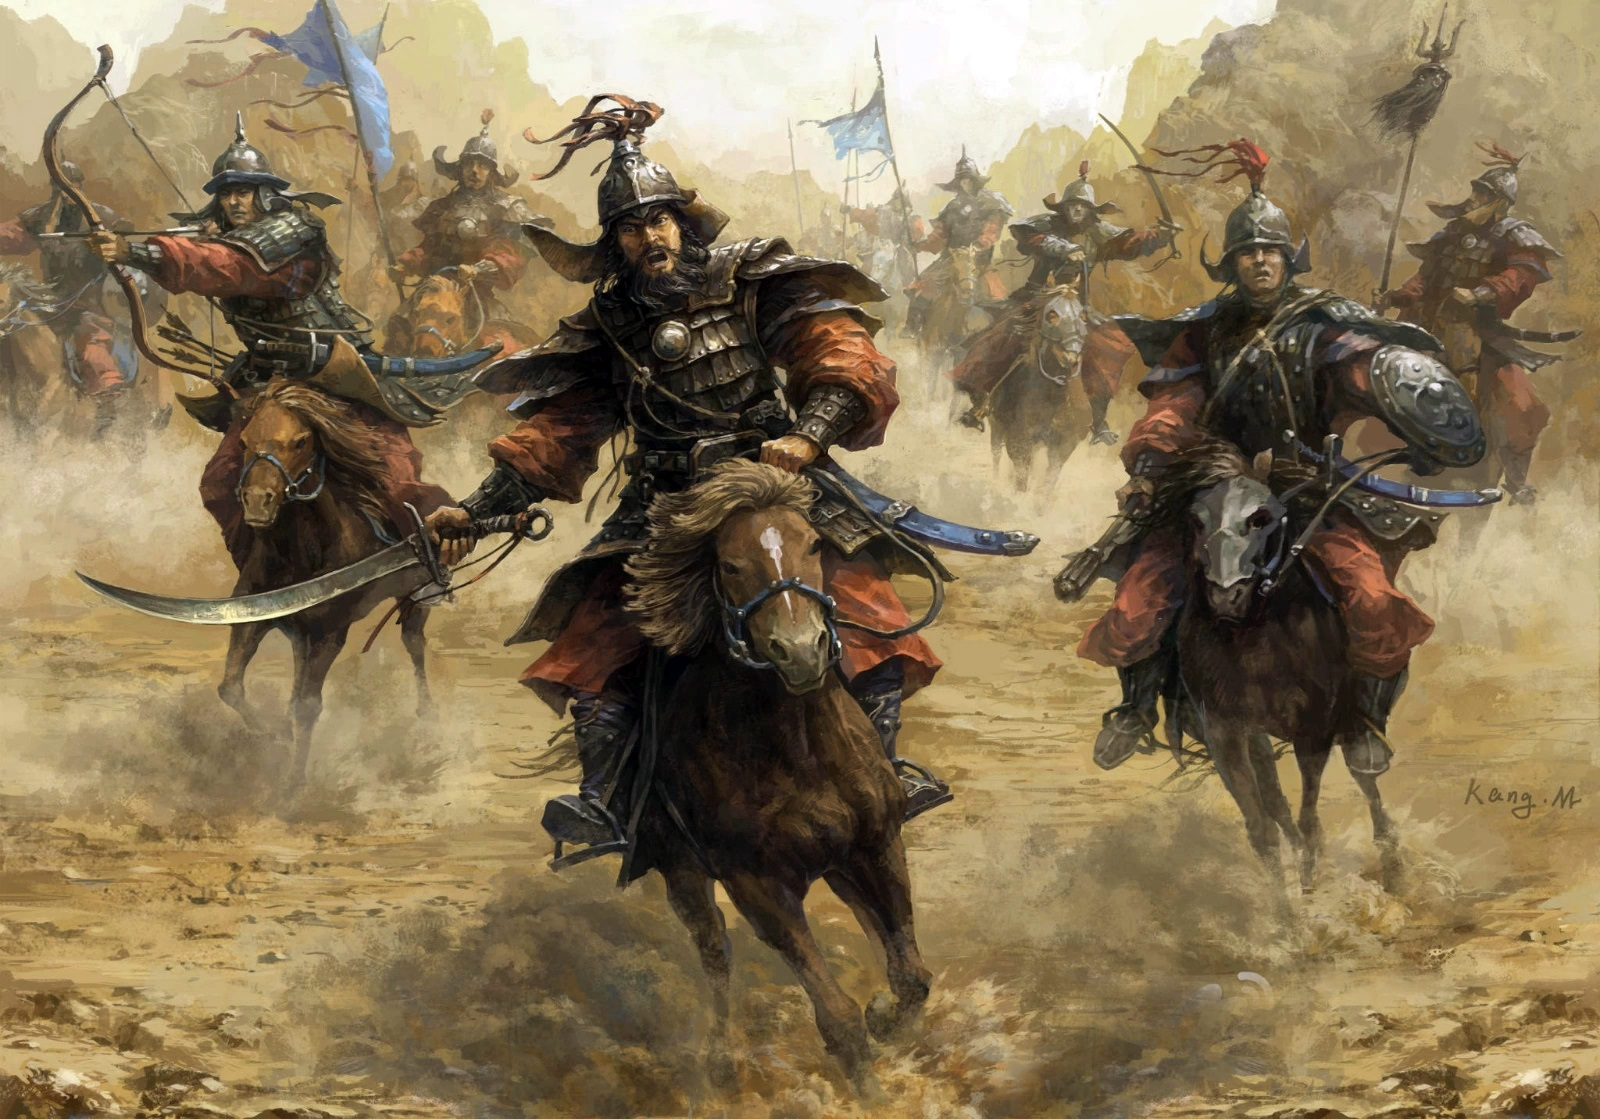
\includepdf[height=\paperheight]{./Images/Backmatter.jpg}
				\end{center}
			\end{figure}
		\end{document}